\documentclass[a4paper,titlepage,11pt,twosides,floatssmall]{mwrep}
\usepackage[left=2.5cm,right=2.5cm,top=2.5cm,bottom=2.5cm]{geometry}
\usepackage[OT1]{fontenc}
\usepackage{polski}
\usepackage{amsmath}
\usepackage{amsfonts}
\usepackage{amssymb}
\usepackage{graphicx}
\usepackage{url}
\usepackage{tikz}
\usepackage{caption}
\usetikzlibrary{arrows,calc,decorations.markings,math,arrows.meta}
\usepackage{rotating}
\usepackage[percent]{overpic}
\usepackage[utf8x]{inputenc}
\usepackage{xcolor}
\usepackage{pgfplots}
\usetikzlibrary{pgfplots.groupplots}
\usepackage{listings}
\usepackage{matlab-prettifier}
\usepackage{siunitx}
\definecolor{szary}{rgb}{0.95,0.95,0.95}
\sisetup{detect-weight,exponent-product=\cdot,output-decimal-marker={,},per-mode=symbol,binary-units=true,range-phrase={-},range-units=single}

\captionsetup{compatibility=false,justification=centering}


%poprawka kropki/przecinki na wykresach
\SendSettingsToPgf

%konfiguracje pakietu listings
\lstset{
	backgroundcolor=\color{szary},
	frame=single,
	breaklines=true,
    inputencoding=utf8x,
    extendedchars=\true,
    literate={ą}{{\k{a}}}1
             {Ą}{{\k{A}}}1
             {ę}{{\k{e}}}1
             {Ę}{{\k{E}}}1
             {ó}{{\'o}}1
             {Ó}{{\'O}}1
             {ś}{{\'s}}1
             {Ś}{{\'S}}1
             {ł}{{\l{}}}1
             {Ł}{{\L{}}}1
             {ż}{{\.z}}1
             {Ż}{{\.Z}}1
             {ź}{{\'z}}1
             {Ź}{{\'Z}}1
             {ć}{{\'c}}1
             {Ć}{{\'C}}1
             {ń}{{\'n}}1
             {Ń}{{\'N}}1
}
\lstdefinestyle{customlatex}{
	basicstyle=\footnotesize\ttfamily,
	%basicstyle=\small\ttfamily,
}
\lstdefinestyle{customc}{
	breaklines=true,
	frame=tb,
	language=C,
	xleftmargin=0pt,
	showstringspaces=false,
	basicstyle=\small\ttfamily,
	keywordstyle=\bfseries\color{green!40!black},
	commentstyle=\itshape\color{purple!40!black},
	identifierstyle=\color{blue},
	stringstyle=\color{orange},
}
\lstdefinestyle{custommatlab}{
	captionpos=t,
	breaklines=true,
	frame=tb,
	xleftmargin=0pt,
	language=matlab,
	showstringspaces=false,
	%basicstyle=\footnotesize\ttfamily,
	basicstyle=\scriptsize\ttfamily,
	keywordstyle=\bfseries\color{green!40!black},
	commentstyle=\itshape\color{purple!40!black},
	identifierstyle=\color{blue},
	stringstyle=\color{orange},
}

%wymiar tekstu (bez żywej paginy)
\textwidth 160mm \textheight 247mm

%ustawienia pakietu pgfplots
\pgfplotsset{
tick label style={font=\scriptsize},
label style={font=\small},
legend style={font=\small},
title style={font=\small}
}

\def\figurename{Rys.}
\def\tablename{Tab.}

%konfiguracja liczby pływających elementów
\setcounter{topnumber}{0}%2
\setcounter{bottomnumber}{3}%1
\setcounter{totalnumber}{5}%3
\renewcommand{\textfraction}{0.01}%0.2
\renewcommand{\topfraction}{0.95}%0.7
\renewcommand{\bottomfraction}{0.95}%0.3
\renewcommand{\floatpagefraction}{0.35}%0.5

\begin{document}
\frenchspacing
\pagestyle{uheadings}

%strona tytułowa
\title{\bf Sprawozdanie z projektu nr 3, zadanie nr 4\vskip 0.1cm}
\author{Mateusz Dziwulski, Emilia Gosk, Jakub Szczepański}
\date{2017}

\makeatletter
\renewcommand{\maketitle}{\begin{titlepage}
\begin{center}{\LARGE {\bf
Wydział Elektroniki i Technik Informacyjnych}}\\
\vspace{0.4cm}
{\LARGE {\bf Politechnika Warszawska}}\\
\vspace{0.3cm}
\end{center}
\vspace{5cm}
\begin{center}
{\bf \LARGE Projektowanie układów sterowania\\ (projekt grupowy) \vskip 0.1cm}
\end{center}
\vspace{1cm}
\begin{center}
{\bf \LARGE \@title}
\end{center}
\vspace{2cm}
\begin{center}
{\bf \Large \@author \par}
\end{center}
\vspace*{\stretch{6}}
\begin{center}
\bf{\large{Warszawa, \@date\vskip 0.1cm}}
\end{center}
\end{titlepage}
}
\makeatother

\maketitle

\tableofcontents
\bigskip
\bigskip

Dla prostoty i przejrzystości sprawozdania wykorzystane zostały oznaczenia pierwotnie wprowadzone w skrypcie z przedmiotu STP.

\chapter{Podpunkt 1}
Sprawdzenie poprawności podanych wartości punktu pracy odbywa się poprzez zasymulowanie odpowiedzi procesu w punkcie pracy ($\boldsymbol{U}_{\mathrm{pp}}$, $\boldsymbol{Y}_{\mathrm{pp}}$). Z rys. \ref{Z1} widzimy, że podane wartości są poprawne - gdy na wejściu modelu podajemy $u_1=u_2=0$, otrzymujemy na wyjściu oczekiwaną przez nas stałą wartość $y_1=y_2=\num{0}$.

\begin{figure}[ht]
\centering
% This file was created by matlab2tikz.
%
%The latest updates can be retrieved from
%  http://www.mathworks.com/matlabcentral/fileexchange/22022-matlab2tikz-matlab2tikz
%where you can also make suggestions and rate matlab2tikz.
%
\definecolor{mycolor1}{rgb}{0.00000,0.44700,0.74100}%
%
\begin{tikzpicture}

\begin{axis}[%
width=4.521in,
height=3.566in,
at={(0.758in,0.481in)},
scale only axis,
xmin=0,
xmax=250,
xtick={0,50,100,150,200,250},
xlabel style={font=\color{white!15!black}},
xlabel={k},
ymin=25,
ymax=40,
ytick={25,30,35,40},
ylabel style={font=\color{white!15!black}},
ylabel={y},
axis background/.style={fill=white}
]
\addplot [color=mycolor1, forget plot]
  table[row sep=crcr]{%
1	32.68\\
2	32.68\\
3	32.68\\
4	32.68\\
5	32.68\\
6	32.68\\
7	32.68\\
8	32.68\\
9	32.68\\
10	32.68\\
11	32.68\\
12	32.75\\
13	32.75\\
14	32.75\\
15	32.75\\
16	32.75\\
17	32.81\\
18	32.75\\
19	32.81\\
20	32.81\\
21	32.81\\
22	32.81\\
23	32.81\\
24	32.81\\
25	32.81\\
26	32.81\\
27	32.81\\
28	32.81\\
29	32.87\\
30	32.87\\
31	32.81\\
32	32.81\\
33	32.81\\
34	32.81\\
35	32.81\\
36	32.81\\
37	32.81\\
38	32.81\\
39	32.81\\
40	32.81\\
41	32.81\\
42	32.87\\
43	32.87\\
44	32.87\\
45	32.87\\
46	32.87\\
47	32.87\\
48	32.87\\
49	32.87\\
50	32.87\\
51	32.87\\
52	32.87\\
53	32.87\\
54	32.87\\
55	32.87\\
56	32.87\\
57	32.87\\
58	32.87\\
59	32.87\\
60	32.87\\
61	32.87\\
62	32.87\\
63	32.87\\
64	32.87\\
65	32.81\\
66	32.81\\
67	32.81\\
68	32.81\\
69	32.81\\
70	32.81\\
71	32.81\\
72	32.81\\
73	32.81\\
74	32.81\\
75	32.81\\
76	32.81\\
77	32.81\\
78	32.75\\
79	32.81\\
80	32.81\\
81	32.81\\
82	32.75\\
83	32.75\\
84	32.75\\
85	32.75\\
86	32.81\\
87	32.75\\
88	32.81\\
89	32.81\\
90	32.81\\
91	32.81\\
92	32.81\\
93	32.87\\
94	32.93\\
95	33\\
96	33.12\\
97	33.25\\
98	33.37\\
99	33.43\\
100	33.5\\
101	33.5\\
102	33.5\\
103	33.5\\
104	33.5\\
105	33.5\\
106	33.5\\
107	33.43\\
108	33.43\\
109	33.43\\
110	33.43\\
111	33.37\\
112	33.37\\
113	33.37\\
114	33.37\\
115	33.37\\
116	33.31\\
117	33.37\\
118	33.31\\
119	33.31\\
120	33.31\\
121	33.31\\
122	33.31\\
123	33.31\\
124	33.31\\
125	33.31\\
126	33.31\\
127	33.31\\
128	33.25\\
129	33.25\\
130	33.25\\
131	33.25\\
132	33.25\\
133	33.25\\
134	33.25\\
135	33.25\\
136	33.25\\
137	33.18\\
138	33.18\\
139	33.18\\
140	33.18\\
141	33.18\\
142	33.25\\
143	33.18\\
144	33.18\\
145	33.25\\
146	33.18\\
147	33.18\\
148	33.18\\
149	33.18\\
150	33.18\\
151	33.18\\
152	33.18\\
153	33.12\\
154	33.12\\
155	33.12\\
156	33.12\\
157	33.12\\
158	33.12\\
159	33.12\\
160	33.12\\
161	33.12\\
162	33.12\\
163	33.12\\
164	33.12\\
165	33.12\\
166	33.12\\
167	33.12\\
168	33.12\\
169	33.06\\
170	33.12\\
171	33.12\\
172	33.12\\
173	33.12\\
174	33.06\\
175	33.12\\
176	33.12\\
177	33.12\\
178	33.12\\
179	33.12\\
180	33.12\\
181	33.12\\
182	33.12\\
183	33.12\\
184	33.12\\
185	33.12\\
186	33.12\\
187	33.18\\
188	33.18\\
189	33.18\\
190	33.18\\
191	33.12\\
192	33.18\\
193	33.18\\
194	33.12\\
195	33.18\\
196	33.12\\
197	33.12\\
198	33.12\\
199	33.18\\
200	33.12\\
201	33.18\\
202	33.18\\
203	33.18\\
204	33.18\\
205	33.18\\
206	33.18\\
207	33.18\\
208	33.18\\
209	33.18\\
210	33.18\\
211	33.12\\
212	33.12\\
213	33.12\\
214	33.12\\
215	33.12\\
216	33.12\\
217	33.12\\
218	33.12\\
219	33.12\\
220	33.12\\
221	33.12\\
222	33.12\\
223	33.12\\
224	33.12\\
225	33.12\\
226	33.12\\
227	33.12\\
228	33.12\\
229	33.06\\
230	33.06\\
231	33.06\\
232	33.06\\
233	33.06\\
234	33.06\\
235	33.06\\
236	33.06\\
237	33\\
238	33\\
239	33\\
240	33\\
241	33\\
242	33\\
243	33\\
244	33\\
245	33.06\\
246	33.06\\
247	33.06\\
248	33.06\\
249	33.06\\
250	33.06\\
};
\end{axis}
\end{tikzpicture}%
\caption{Sprawdzenie poprawności punktu pracy}
\label{Z1}
\end{figure}


\chapter{Podpunkt 2}
Dla reprezentacji odpowiedzi skokowych wybranych zostało sześć różnych wartości zmian dla każdego z sygnałów sterujących, skok we wszystkich torach wystąpił w chwili $k=20$. Wykresy odpowiedzi skokowych zamieszczone zostały na rysunkach \ref{Z2U1} i \ref{Z2U2}.

\begin{figure}[ht]
\centering
% This file was created by matlab2tikz.
%
%The latest updates can be retrieved from
%  http://www.mathworks.com/matlabcentral/fileexchange/22022-matlab2tikz-matlab2tikz
%where you can also make suggestions and rate matlab2tikz.
%
%Z2 - odpowiedzi na skoki U1
\definecolor{mycolor1}{rgb}{0.00000,0.44700,0.74100}%
\definecolor{mycolor2}{rgb}{0.85000,0.32500,0.09800}%
\definecolor{mycolor3}{rgb}{0.92900,0.69400,0.12500}%
\definecolor{mycolor4}{rgb}{0.49400,0.18400,0.55600}%
\definecolor{mycolor5}{rgb}{0.46600,0.67400,0.18800}%
\definecolor{mycolor6}{rgb}{0.30100,0.74500,0.93300}%
%
\begin{tikzpicture}

\begin{axis}[%
width=5.167in,
height=0.612in,
at={(0.646in,0.494in)},
scale only axis,
xmin=0,
xmax=200,
xtick={0,20,40,60,80,100,120,140,160,180,200},
xlabel style={font=\color{white!15!black}},
xlabel={k},
ymin=-1,
ymax=1,
ytick={-1,0,1},
ylabel style={font=\color{white!15!black}},
ylabel={$\text{u}_\text{2}$},
axis background/.style={fill=white}
]
\addplot[const plot, color=mycolor1, forget plot] table[row sep=crcr] {%
1	0\\
2	0\\
3	0\\
4	0\\
5	0\\
6	0\\
7	0\\
8	0\\
9	0\\
10	0\\
11	0\\
12	0\\
13	0\\
14	0\\
15	0\\
16	0\\
17	0\\
18	0\\
19	0\\
20	0\\
21	0\\
22	0\\
23	0\\
24	0\\
25	0\\
26	0\\
27	0\\
28	0\\
29	0\\
30	0\\
31	0\\
32	0\\
33	0\\
34	0\\
35	0\\
36	0\\
37	0\\
38	0\\
39	0\\
40	0\\
41	0\\
42	0\\
43	0\\
44	0\\
45	0\\
46	0\\
47	0\\
48	0\\
49	0\\
50	0\\
51	0\\
52	0\\
53	0\\
54	0\\
55	0\\
56	0\\
57	0\\
58	0\\
59	0\\
60	0\\
61	0\\
62	0\\
63	0\\
64	0\\
65	0\\
66	0\\
67	0\\
68	0\\
69	0\\
70	0\\
71	0\\
72	0\\
73	0\\
74	0\\
75	0\\
76	0\\
77	0\\
78	0\\
79	0\\
80	0\\
81	0\\
82	0\\
83	0\\
84	0\\
85	0\\
86	0\\
87	0\\
88	0\\
89	0\\
90	0\\
91	0\\
92	0\\
93	0\\
94	0\\
95	0\\
96	0\\
97	0\\
98	0\\
99	0\\
100	0\\
101	0\\
102	0\\
103	0\\
104	0\\
105	0\\
106	0\\
107	0\\
108	0\\
109	0\\
110	0\\
111	0\\
112	0\\
113	0\\
114	0\\
115	0\\
116	0\\
117	0\\
118	0\\
119	0\\
120	0\\
121	0\\
122	0\\
123	0\\
124	0\\
125	0\\
126	0\\
127	0\\
128	0\\
129	0\\
130	0\\
131	0\\
132	0\\
133	0\\
134	0\\
135	0\\
136	0\\
137	0\\
138	0\\
139	0\\
140	0\\
141	0\\
142	0\\
143	0\\
144	0\\
145	0\\
146	0\\
147	0\\
148	0\\
149	0\\
150	0\\
151	0\\
152	0\\
153	0\\
154	0\\
155	0\\
156	0\\
157	0\\
158	0\\
159	0\\
160	0\\
161	0\\
162	0\\
163	0\\
164	0\\
165	0\\
166	0\\
167	0\\
168	0\\
169	0\\
170	0\\
171	0\\
172	0\\
173	0\\
174	0\\
175	0\\
176	0\\
177	0\\
178	0\\
179	0\\
180	0\\
181	0\\
182	0\\
183	0\\
184	0\\
185	0\\
186	0\\
187	0\\
188	0\\
189	0\\
190	0\\
191	0\\
192	0\\
193	0\\
194	0\\
195	0\\
196	0\\
197	0\\
198	0\\
199	0\\
200	0\\
};
\addplot[const plot, color=mycolor2, forget plot] table[row sep=crcr] {%
1	0\\
2	0\\
3	0\\
4	0\\
5	0\\
6	0\\
7	0\\
8	0\\
9	0\\
10	0\\
11	0\\
12	0\\
13	0\\
14	0\\
15	0\\
16	0\\
17	0\\
18	0\\
19	0\\
20	0\\
21	0\\
22	0\\
23	0\\
24	0\\
25	0\\
26	0\\
27	0\\
28	0\\
29	0\\
30	0\\
31	0\\
32	0\\
33	0\\
34	0\\
35	0\\
36	0\\
37	0\\
38	0\\
39	0\\
40	0\\
41	0\\
42	0\\
43	0\\
44	0\\
45	0\\
46	0\\
47	0\\
48	0\\
49	0\\
50	0\\
51	0\\
52	0\\
53	0\\
54	0\\
55	0\\
56	0\\
57	0\\
58	0\\
59	0\\
60	0\\
61	0\\
62	0\\
63	0\\
64	0\\
65	0\\
66	0\\
67	0\\
68	0\\
69	0\\
70	0\\
71	0\\
72	0\\
73	0\\
74	0\\
75	0\\
76	0\\
77	0\\
78	0\\
79	0\\
80	0\\
81	0\\
82	0\\
83	0\\
84	0\\
85	0\\
86	0\\
87	0\\
88	0\\
89	0\\
90	0\\
91	0\\
92	0\\
93	0\\
94	0\\
95	0\\
96	0\\
97	0\\
98	0\\
99	0\\
100	0\\
101	0\\
102	0\\
103	0\\
104	0\\
105	0\\
106	0\\
107	0\\
108	0\\
109	0\\
110	0\\
111	0\\
112	0\\
113	0\\
114	0\\
115	0\\
116	0\\
117	0\\
118	0\\
119	0\\
120	0\\
121	0\\
122	0\\
123	0\\
124	0\\
125	0\\
126	0\\
127	0\\
128	0\\
129	0\\
130	0\\
131	0\\
132	0\\
133	0\\
134	0\\
135	0\\
136	0\\
137	0\\
138	0\\
139	0\\
140	0\\
141	0\\
142	0\\
143	0\\
144	0\\
145	0\\
146	0\\
147	0\\
148	0\\
149	0\\
150	0\\
151	0\\
152	0\\
153	0\\
154	0\\
155	0\\
156	0\\
157	0\\
158	0\\
159	0\\
160	0\\
161	0\\
162	0\\
163	0\\
164	0\\
165	0\\
166	0\\
167	0\\
168	0\\
169	0\\
170	0\\
171	0\\
172	0\\
173	0\\
174	0\\
175	0\\
176	0\\
177	0\\
178	0\\
179	0\\
180	0\\
181	0\\
182	0\\
183	0\\
184	0\\
185	0\\
186	0\\
187	0\\
188	0\\
189	0\\
190	0\\
191	0\\
192	0\\
193	0\\
194	0\\
195	0\\
196	0\\
197	0\\
198	0\\
199	0\\
200	0\\
};
\addplot[const plot, color=mycolor3, forget plot] table[row sep=crcr] {%
1	0\\
2	0\\
3	0\\
4	0\\
5	0\\
6	0\\
7	0\\
8	0\\
9	0\\
10	0\\
11	0\\
12	0\\
13	0\\
14	0\\
15	0\\
16	0\\
17	0\\
18	0\\
19	0\\
20	0\\
21	0\\
22	0\\
23	0\\
24	0\\
25	0\\
26	0\\
27	0\\
28	0\\
29	0\\
30	0\\
31	0\\
32	0\\
33	0\\
34	0\\
35	0\\
36	0\\
37	0\\
38	0\\
39	0\\
40	0\\
41	0\\
42	0\\
43	0\\
44	0\\
45	0\\
46	0\\
47	0\\
48	0\\
49	0\\
50	0\\
51	0\\
52	0\\
53	0\\
54	0\\
55	0\\
56	0\\
57	0\\
58	0\\
59	0\\
60	0\\
61	0\\
62	0\\
63	0\\
64	0\\
65	0\\
66	0\\
67	0\\
68	0\\
69	0\\
70	0\\
71	0\\
72	0\\
73	0\\
74	0\\
75	0\\
76	0\\
77	0\\
78	0\\
79	0\\
80	0\\
81	0\\
82	0\\
83	0\\
84	0\\
85	0\\
86	0\\
87	0\\
88	0\\
89	0\\
90	0\\
91	0\\
92	0\\
93	0\\
94	0\\
95	0\\
96	0\\
97	0\\
98	0\\
99	0\\
100	0\\
101	0\\
102	0\\
103	0\\
104	0\\
105	0\\
106	0\\
107	0\\
108	0\\
109	0\\
110	0\\
111	0\\
112	0\\
113	0\\
114	0\\
115	0\\
116	0\\
117	0\\
118	0\\
119	0\\
120	0\\
121	0\\
122	0\\
123	0\\
124	0\\
125	0\\
126	0\\
127	0\\
128	0\\
129	0\\
130	0\\
131	0\\
132	0\\
133	0\\
134	0\\
135	0\\
136	0\\
137	0\\
138	0\\
139	0\\
140	0\\
141	0\\
142	0\\
143	0\\
144	0\\
145	0\\
146	0\\
147	0\\
148	0\\
149	0\\
150	0\\
151	0\\
152	0\\
153	0\\
154	0\\
155	0\\
156	0\\
157	0\\
158	0\\
159	0\\
160	0\\
161	0\\
162	0\\
163	0\\
164	0\\
165	0\\
166	0\\
167	0\\
168	0\\
169	0\\
170	0\\
171	0\\
172	0\\
173	0\\
174	0\\
175	0\\
176	0\\
177	0\\
178	0\\
179	0\\
180	0\\
181	0\\
182	0\\
183	0\\
184	0\\
185	0\\
186	0\\
187	0\\
188	0\\
189	0\\
190	0\\
191	0\\
192	0\\
193	0\\
194	0\\
195	0\\
196	0\\
197	0\\
198	0\\
199	0\\
200	0\\
};
\addplot[const plot, color=mycolor4, forget plot] table[row sep=crcr] {%
1	0\\
2	0\\
3	0\\
4	0\\
5	0\\
6	0\\
7	0\\
8	0\\
9	0\\
10	0\\
11	0\\
12	0\\
13	0\\
14	0\\
15	0\\
16	0\\
17	0\\
18	0\\
19	0\\
20	0\\
21	0\\
22	0\\
23	0\\
24	0\\
25	0\\
26	0\\
27	0\\
28	0\\
29	0\\
30	0\\
31	0\\
32	0\\
33	0\\
34	0\\
35	0\\
36	0\\
37	0\\
38	0\\
39	0\\
40	0\\
41	0\\
42	0\\
43	0\\
44	0\\
45	0\\
46	0\\
47	0\\
48	0\\
49	0\\
50	0\\
51	0\\
52	0\\
53	0\\
54	0\\
55	0\\
56	0\\
57	0\\
58	0\\
59	0\\
60	0\\
61	0\\
62	0\\
63	0\\
64	0\\
65	0\\
66	0\\
67	0\\
68	0\\
69	0\\
70	0\\
71	0\\
72	0\\
73	0\\
74	0\\
75	0\\
76	0\\
77	0\\
78	0\\
79	0\\
80	0\\
81	0\\
82	0\\
83	0\\
84	0\\
85	0\\
86	0\\
87	0\\
88	0\\
89	0\\
90	0\\
91	0\\
92	0\\
93	0\\
94	0\\
95	0\\
96	0\\
97	0\\
98	0\\
99	0\\
100	0\\
101	0\\
102	0\\
103	0\\
104	0\\
105	0\\
106	0\\
107	0\\
108	0\\
109	0\\
110	0\\
111	0\\
112	0\\
113	0\\
114	0\\
115	0\\
116	0\\
117	0\\
118	0\\
119	0\\
120	0\\
121	0\\
122	0\\
123	0\\
124	0\\
125	0\\
126	0\\
127	0\\
128	0\\
129	0\\
130	0\\
131	0\\
132	0\\
133	0\\
134	0\\
135	0\\
136	0\\
137	0\\
138	0\\
139	0\\
140	0\\
141	0\\
142	0\\
143	0\\
144	0\\
145	0\\
146	0\\
147	0\\
148	0\\
149	0\\
150	0\\
151	0\\
152	0\\
153	0\\
154	0\\
155	0\\
156	0\\
157	0\\
158	0\\
159	0\\
160	0\\
161	0\\
162	0\\
163	0\\
164	0\\
165	0\\
166	0\\
167	0\\
168	0\\
169	0\\
170	0\\
171	0\\
172	0\\
173	0\\
174	0\\
175	0\\
176	0\\
177	0\\
178	0\\
179	0\\
180	0\\
181	0\\
182	0\\
183	0\\
184	0\\
185	0\\
186	0\\
187	0\\
188	0\\
189	0\\
190	0\\
191	0\\
192	0\\
193	0\\
194	0\\
195	0\\
196	0\\
197	0\\
198	0\\
199	0\\
200	0\\
};
\addplot[const plot, color=mycolor5, forget plot] table[row sep=crcr] {%
1	0\\
2	0\\
3	0\\
4	0\\
5	0\\
6	0\\
7	0\\
8	0\\
9	0\\
10	0\\
11	0\\
12	0\\
13	0\\
14	0\\
15	0\\
16	0\\
17	0\\
18	0\\
19	0\\
20	0\\
21	0\\
22	0\\
23	0\\
24	0\\
25	0\\
26	0\\
27	0\\
28	0\\
29	0\\
30	0\\
31	0\\
32	0\\
33	0\\
34	0\\
35	0\\
36	0\\
37	0\\
38	0\\
39	0\\
40	0\\
41	0\\
42	0\\
43	0\\
44	0\\
45	0\\
46	0\\
47	0\\
48	0\\
49	0\\
50	0\\
51	0\\
52	0\\
53	0\\
54	0\\
55	0\\
56	0\\
57	0\\
58	0\\
59	0\\
60	0\\
61	0\\
62	0\\
63	0\\
64	0\\
65	0\\
66	0\\
67	0\\
68	0\\
69	0\\
70	0\\
71	0\\
72	0\\
73	0\\
74	0\\
75	0\\
76	0\\
77	0\\
78	0\\
79	0\\
80	0\\
81	0\\
82	0\\
83	0\\
84	0\\
85	0\\
86	0\\
87	0\\
88	0\\
89	0\\
90	0\\
91	0\\
92	0\\
93	0\\
94	0\\
95	0\\
96	0\\
97	0\\
98	0\\
99	0\\
100	0\\
101	0\\
102	0\\
103	0\\
104	0\\
105	0\\
106	0\\
107	0\\
108	0\\
109	0\\
110	0\\
111	0\\
112	0\\
113	0\\
114	0\\
115	0\\
116	0\\
117	0\\
118	0\\
119	0\\
120	0\\
121	0\\
122	0\\
123	0\\
124	0\\
125	0\\
126	0\\
127	0\\
128	0\\
129	0\\
130	0\\
131	0\\
132	0\\
133	0\\
134	0\\
135	0\\
136	0\\
137	0\\
138	0\\
139	0\\
140	0\\
141	0\\
142	0\\
143	0\\
144	0\\
145	0\\
146	0\\
147	0\\
148	0\\
149	0\\
150	0\\
151	0\\
152	0\\
153	0\\
154	0\\
155	0\\
156	0\\
157	0\\
158	0\\
159	0\\
160	0\\
161	0\\
162	0\\
163	0\\
164	0\\
165	0\\
166	0\\
167	0\\
168	0\\
169	0\\
170	0\\
171	0\\
172	0\\
173	0\\
174	0\\
175	0\\
176	0\\
177	0\\
178	0\\
179	0\\
180	0\\
181	0\\
182	0\\
183	0\\
184	0\\
185	0\\
186	0\\
187	0\\
188	0\\
189	0\\
190	0\\
191	0\\
192	0\\
193	0\\
194	0\\
195	0\\
196	0\\
197	0\\
198	0\\
199	0\\
200	0\\
};
\addplot[const plot, color=mycolor6, forget plot] table[row sep=crcr] {%
1	0\\
2	0\\
3	0\\
4	0\\
5	0\\
6	0\\
7	0\\
8	0\\
9	0\\
10	0\\
11	0\\
12	0\\
13	0\\
14	0\\
15	0\\
16	0\\
17	0\\
18	0\\
19	0\\
20	0\\
21	0\\
22	0\\
23	0\\
24	0\\
25	0\\
26	0\\
27	0\\
28	0\\
29	0\\
30	0\\
31	0\\
32	0\\
33	0\\
34	0\\
35	0\\
36	0\\
37	0\\
38	0\\
39	0\\
40	0\\
41	0\\
42	0\\
43	0\\
44	0\\
45	0\\
46	0\\
47	0\\
48	0\\
49	0\\
50	0\\
51	0\\
52	0\\
53	0\\
54	0\\
55	0\\
56	0\\
57	0\\
58	0\\
59	0\\
60	0\\
61	0\\
62	0\\
63	0\\
64	0\\
65	0\\
66	0\\
67	0\\
68	0\\
69	0\\
70	0\\
71	0\\
72	0\\
73	0\\
74	0\\
75	0\\
76	0\\
77	0\\
78	0\\
79	0\\
80	0\\
81	0\\
82	0\\
83	0\\
84	0\\
85	0\\
86	0\\
87	0\\
88	0\\
89	0\\
90	0\\
91	0\\
92	0\\
93	0\\
94	0\\
95	0\\
96	0\\
97	0\\
98	0\\
99	0\\
100	0\\
101	0\\
102	0\\
103	0\\
104	0\\
105	0\\
106	0\\
107	0\\
108	0\\
109	0\\
110	0\\
111	0\\
112	0\\
113	0\\
114	0\\
115	0\\
116	0\\
117	0\\
118	0\\
119	0\\
120	0\\
121	0\\
122	0\\
123	0\\
124	0\\
125	0\\
126	0\\
127	0\\
128	0\\
129	0\\
130	0\\
131	0\\
132	0\\
133	0\\
134	0\\
135	0\\
136	0\\
137	0\\
138	0\\
139	0\\
140	0\\
141	0\\
142	0\\
143	0\\
144	0\\
145	0\\
146	0\\
147	0\\
148	0\\
149	0\\
150	0\\
151	0\\
152	0\\
153	0\\
154	0\\
155	0\\
156	0\\
157	0\\
158	0\\
159	0\\
160	0\\
161	0\\
162	0\\
163	0\\
164	0\\
165	0\\
166	0\\
167	0\\
168	0\\
169	0\\
170	0\\
171	0\\
172	0\\
173	0\\
174	0\\
175	0\\
176	0\\
177	0\\
178	0\\
179	0\\
180	0\\
181	0\\
182	0\\
183	0\\
184	0\\
185	0\\
186	0\\
187	0\\
188	0\\
189	0\\
190	0\\
191	0\\
192	0\\
193	0\\
194	0\\
195	0\\
196	0\\
197	0\\
198	0\\
199	0\\
200	0\\
};
\end{axis}

\begin{axis}[%
width=5.167in,
height=0.612in,
at={(0.646in,1.53in)},
scale only axis,
xmin=0,
xmax=200,
xtick={0,20,40,60,80,100,120,140,160,180,200},
ymin=-2,
ymax=2,
ytick={-2,0,2},
ylabel style={font=\color{white!15!black}},
ylabel={$\text{u}_\text{1}$},
axis background/.style={fill=white}
]
\addplot[const plot, color=mycolor1, forget plot] table[row sep=crcr] {%
1	0\\
2	0\\
3	0\\
4	0\\
5	0\\
6	0\\
7	0\\
8	0\\
9	0\\
10	0\\
11	0\\
12	0\\
13	0\\
14	0\\
15	0\\
16	0\\
17	0\\
18	0\\
19	0\\
20	2\\
21	2\\
22	2\\
23	2\\
24	2\\
25	2\\
26	2\\
27	2\\
28	2\\
29	2\\
30	2\\
31	2\\
32	2\\
33	2\\
34	2\\
35	2\\
36	2\\
37	2\\
38	2\\
39	2\\
40	2\\
41	2\\
42	2\\
43	2\\
44	2\\
45	2\\
46	2\\
47	2\\
48	2\\
49	2\\
50	2\\
51	2\\
52	2\\
53	2\\
54	2\\
55	2\\
56	2\\
57	2\\
58	2\\
59	2\\
60	2\\
61	2\\
62	2\\
63	2\\
64	2\\
65	2\\
66	2\\
67	2\\
68	2\\
69	2\\
70	2\\
71	2\\
72	2\\
73	2\\
74	2\\
75	2\\
76	2\\
77	2\\
78	2\\
79	2\\
80	2\\
81	2\\
82	2\\
83	2\\
84	2\\
85	2\\
86	2\\
87	2\\
88	2\\
89	2\\
90	2\\
91	2\\
92	2\\
93	2\\
94	2\\
95	2\\
96	2\\
97	2\\
98	2\\
99	2\\
100	2\\
101	2\\
102	2\\
103	2\\
104	2\\
105	2\\
106	2\\
107	2\\
108	2\\
109	2\\
110	2\\
111	2\\
112	2\\
113	2\\
114	2\\
115	2\\
116	2\\
117	2\\
118	2\\
119	2\\
120	2\\
121	2\\
122	2\\
123	2\\
124	2\\
125	2\\
126	2\\
127	2\\
128	2\\
129	2\\
130	2\\
131	2\\
132	2\\
133	2\\
134	2\\
135	2\\
136	2\\
137	2\\
138	2\\
139	2\\
140	2\\
141	2\\
142	2\\
143	2\\
144	2\\
145	2\\
146	2\\
147	2\\
148	2\\
149	2\\
150	2\\
151	2\\
152	2\\
153	2\\
154	2\\
155	2\\
156	2\\
157	2\\
158	2\\
159	2\\
160	2\\
161	2\\
162	2\\
163	2\\
164	2\\
165	2\\
166	2\\
167	2\\
168	2\\
169	2\\
170	2\\
171	2\\
172	2\\
173	2\\
174	2\\
175	2\\
176	2\\
177	2\\
178	2\\
179	2\\
180	2\\
181	2\\
182	2\\
183	2\\
184	2\\
185	2\\
186	2\\
187	2\\
188	2\\
189	2\\
190	2\\
191	2\\
192	2\\
193	2\\
194	2\\
195	2\\
196	2\\
197	2\\
198	2\\
199	2\\
200	2\\
};
\addplot[const plot, color=mycolor2, forget plot] table[row sep=crcr] {%
1	0\\
2	0\\
3	0\\
4	0\\
5	0\\
6	0\\
7	0\\
8	0\\
9	0\\
10	0\\
11	0\\
12	0\\
13	0\\
14	0\\
15	0\\
16	0\\
17	0\\
18	0\\
19	0\\
20	1.2\\
21	1.2\\
22	1.2\\
23	1.2\\
24	1.2\\
25	1.2\\
26	1.2\\
27	1.2\\
28	1.2\\
29	1.2\\
30	1.2\\
31	1.2\\
32	1.2\\
33	1.2\\
34	1.2\\
35	1.2\\
36	1.2\\
37	1.2\\
38	1.2\\
39	1.2\\
40	1.2\\
41	1.2\\
42	1.2\\
43	1.2\\
44	1.2\\
45	1.2\\
46	1.2\\
47	1.2\\
48	1.2\\
49	1.2\\
50	1.2\\
51	1.2\\
52	1.2\\
53	1.2\\
54	1.2\\
55	1.2\\
56	1.2\\
57	1.2\\
58	1.2\\
59	1.2\\
60	1.2\\
61	1.2\\
62	1.2\\
63	1.2\\
64	1.2\\
65	1.2\\
66	1.2\\
67	1.2\\
68	1.2\\
69	1.2\\
70	1.2\\
71	1.2\\
72	1.2\\
73	1.2\\
74	1.2\\
75	1.2\\
76	1.2\\
77	1.2\\
78	1.2\\
79	1.2\\
80	1.2\\
81	1.2\\
82	1.2\\
83	1.2\\
84	1.2\\
85	1.2\\
86	1.2\\
87	1.2\\
88	1.2\\
89	1.2\\
90	1.2\\
91	1.2\\
92	1.2\\
93	1.2\\
94	1.2\\
95	1.2\\
96	1.2\\
97	1.2\\
98	1.2\\
99	1.2\\
100	1.2\\
101	1.2\\
102	1.2\\
103	1.2\\
104	1.2\\
105	1.2\\
106	1.2\\
107	1.2\\
108	1.2\\
109	1.2\\
110	1.2\\
111	1.2\\
112	1.2\\
113	1.2\\
114	1.2\\
115	1.2\\
116	1.2\\
117	1.2\\
118	1.2\\
119	1.2\\
120	1.2\\
121	1.2\\
122	1.2\\
123	1.2\\
124	1.2\\
125	1.2\\
126	1.2\\
127	1.2\\
128	1.2\\
129	1.2\\
130	1.2\\
131	1.2\\
132	1.2\\
133	1.2\\
134	1.2\\
135	1.2\\
136	1.2\\
137	1.2\\
138	1.2\\
139	1.2\\
140	1.2\\
141	1.2\\
142	1.2\\
143	1.2\\
144	1.2\\
145	1.2\\
146	1.2\\
147	1.2\\
148	1.2\\
149	1.2\\
150	1.2\\
151	1.2\\
152	1.2\\
153	1.2\\
154	1.2\\
155	1.2\\
156	1.2\\
157	1.2\\
158	1.2\\
159	1.2\\
160	1.2\\
161	1.2\\
162	1.2\\
163	1.2\\
164	1.2\\
165	1.2\\
166	1.2\\
167	1.2\\
168	1.2\\
169	1.2\\
170	1.2\\
171	1.2\\
172	1.2\\
173	1.2\\
174	1.2\\
175	1.2\\
176	1.2\\
177	1.2\\
178	1.2\\
179	1.2\\
180	1.2\\
181	1.2\\
182	1.2\\
183	1.2\\
184	1.2\\
185	1.2\\
186	1.2\\
187	1.2\\
188	1.2\\
189	1.2\\
190	1.2\\
191	1.2\\
192	1.2\\
193	1.2\\
194	1.2\\
195	1.2\\
196	1.2\\
197	1.2\\
198	1.2\\
199	1.2\\
200	1.2\\
};
\addplot[const plot, color=mycolor3, forget plot] table[row sep=crcr] {%
1	0\\
2	0\\
3	0\\
4	0\\
5	0\\
6	0\\
7	0\\
8	0\\
9	0\\
10	0\\
11	0\\
12	0\\
13	0\\
14	0\\
15	0\\
16	0\\
17	0\\
18	0\\
19	0\\
20	0.4\\
21	0.4\\
22	0.4\\
23	0.4\\
24	0.4\\
25	0.4\\
26	0.4\\
27	0.4\\
28	0.4\\
29	0.4\\
30	0.4\\
31	0.4\\
32	0.4\\
33	0.4\\
34	0.4\\
35	0.4\\
36	0.4\\
37	0.4\\
38	0.4\\
39	0.4\\
40	0.4\\
41	0.4\\
42	0.4\\
43	0.4\\
44	0.4\\
45	0.4\\
46	0.4\\
47	0.4\\
48	0.4\\
49	0.4\\
50	0.4\\
51	0.4\\
52	0.4\\
53	0.4\\
54	0.4\\
55	0.4\\
56	0.4\\
57	0.4\\
58	0.4\\
59	0.4\\
60	0.4\\
61	0.4\\
62	0.4\\
63	0.4\\
64	0.4\\
65	0.4\\
66	0.4\\
67	0.4\\
68	0.4\\
69	0.4\\
70	0.4\\
71	0.4\\
72	0.4\\
73	0.4\\
74	0.4\\
75	0.4\\
76	0.4\\
77	0.4\\
78	0.4\\
79	0.4\\
80	0.4\\
81	0.4\\
82	0.4\\
83	0.4\\
84	0.4\\
85	0.4\\
86	0.4\\
87	0.4\\
88	0.4\\
89	0.4\\
90	0.4\\
91	0.4\\
92	0.4\\
93	0.4\\
94	0.4\\
95	0.4\\
96	0.4\\
97	0.4\\
98	0.4\\
99	0.4\\
100	0.4\\
101	0.4\\
102	0.4\\
103	0.4\\
104	0.4\\
105	0.4\\
106	0.4\\
107	0.4\\
108	0.4\\
109	0.4\\
110	0.4\\
111	0.4\\
112	0.4\\
113	0.4\\
114	0.4\\
115	0.4\\
116	0.4\\
117	0.4\\
118	0.4\\
119	0.4\\
120	0.4\\
121	0.4\\
122	0.4\\
123	0.4\\
124	0.4\\
125	0.4\\
126	0.4\\
127	0.4\\
128	0.4\\
129	0.4\\
130	0.4\\
131	0.4\\
132	0.4\\
133	0.4\\
134	0.4\\
135	0.4\\
136	0.4\\
137	0.4\\
138	0.4\\
139	0.4\\
140	0.4\\
141	0.4\\
142	0.4\\
143	0.4\\
144	0.4\\
145	0.4\\
146	0.4\\
147	0.4\\
148	0.4\\
149	0.4\\
150	0.4\\
151	0.4\\
152	0.4\\
153	0.4\\
154	0.4\\
155	0.4\\
156	0.4\\
157	0.4\\
158	0.4\\
159	0.4\\
160	0.4\\
161	0.4\\
162	0.4\\
163	0.4\\
164	0.4\\
165	0.4\\
166	0.4\\
167	0.4\\
168	0.4\\
169	0.4\\
170	0.4\\
171	0.4\\
172	0.4\\
173	0.4\\
174	0.4\\
175	0.4\\
176	0.4\\
177	0.4\\
178	0.4\\
179	0.4\\
180	0.4\\
181	0.4\\
182	0.4\\
183	0.4\\
184	0.4\\
185	0.4\\
186	0.4\\
187	0.4\\
188	0.4\\
189	0.4\\
190	0.4\\
191	0.4\\
192	0.4\\
193	0.4\\
194	0.4\\
195	0.4\\
196	0.4\\
197	0.4\\
198	0.4\\
199	0.4\\
200	0.4\\
};
\addplot[const plot, color=mycolor4, forget plot] table[row sep=crcr] {%
1	0\\
2	0\\
3	0\\
4	0\\
5	0\\
6	0\\
7	0\\
8	0\\
9	0\\
10	0\\
11	0\\
12	0\\
13	0\\
14	0\\
15	0\\
16	0\\
17	0\\
18	0\\
19	0\\
20	-0.4\\
21	-0.4\\
22	-0.4\\
23	-0.4\\
24	-0.4\\
25	-0.4\\
26	-0.4\\
27	-0.4\\
28	-0.4\\
29	-0.4\\
30	-0.4\\
31	-0.4\\
32	-0.4\\
33	-0.4\\
34	-0.4\\
35	-0.4\\
36	-0.4\\
37	-0.4\\
38	-0.4\\
39	-0.4\\
40	-0.4\\
41	-0.4\\
42	-0.4\\
43	-0.4\\
44	-0.4\\
45	-0.4\\
46	-0.4\\
47	-0.4\\
48	-0.4\\
49	-0.4\\
50	-0.4\\
51	-0.4\\
52	-0.4\\
53	-0.4\\
54	-0.4\\
55	-0.4\\
56	-0.4\\
57	-0.4\\
58	-0.4\\
59	-0.4\\
60	-0.4\\
61	-0.4\\
62	-0.4\\
63	-0.4\\
64	-0.4\\
65	-0.4\\
66	-0.4\\
67	-0.4\\
68	-0.4\\
69	-0.4\\
70	-0.4\\
71	-0.4\\
72	-0.4\\
73	-0.4\\
74	-0.4\\
75	-0.4\\
76	-0.4\\
77	-0.4\\
78	-0.4\\
79	-0.4\\
80	-0.4\\
81	-0.4\\
82	-0.4\\
83	-0.4\\
84	-0.4\\
85	-0.4\\
86	-0.4\\
87	-0.4\\
88	-0.4\\
89	-0.4\\
90	-0.4\\
91	-0.4\\
92	-0.4\\
93	-0.4\\
94	-0.4\\
95	-0.4\\
96	-0.4\\
97	-0.4\\
98	-0.4\\
99	-0.4\\
100	-0.4\\
101	-0.4\\
102	-0.4\\
103	-0.4\\
104	-0.4\\
105	-0.4\\
106	-0.4\\
107	-0.4\\
108	-0.4\\
109	-0.4\\
110	-0.4\\
111	-0.4\\
112	-0.4\\
113	-0.4\\
114	-0.4\\
115	-0.4\\
116	-0.4\\
117	-0.4\\
118	-0.4\\
119	-0.4\\
120	-0.4\\
121	-0.4\\
122	-0.4\\
123	-0.4\\
124	-0.4\\
125	-0.4\\
126	-0.4\\
127	-0.4\\
128	-0.4\\
129	-0.4\\
130	-0.4\\
131	-0.4\\
132	-0.4\\
133	-0.4\\
134	-0.4\\
135	-0.4\\
136	-0.4\\
137	-0.4\\
138	-0.4\\
139	-0.4\\
140	-0.4\\
141	-0.4\\
142	-0.4\\
143	-0.4\\
144	-0.4\\
145	-0.4\\
146	-0.4\\
147	-0.4\\
148	-0.4\\
149	-0.4\\
150	-0.4\\
151	-0.4\\
152	-0.4\\
153	-0.4\\
154	-0.4\\
155	-0.4\\
156	-0.4\\
157	-0.4\\
158	-0.4\\
159	-0.4\\
160	-0.4\\
161	-0.4\\
162	-0.4\\
163	-0.4\\
164	-0.4\\
165	-0.4\\
166	-0.4\\
167	-0.4\\
168	-0.4\\
169	-0.4\\
170	-0.4\\
171	-0.4\\
172	-0.4\\
173	-0.4\\
174	-0.4\\
175	-0.4\\
176	-0.4\\
177	-0.4\\
178	-0.4\\
179	-0.4\\
180	-0.4\\
181	-0.4\\
182	-0.4\\
183	-0.4\\
184	-0.4\\
185	-0.4\\
186	-0.4\\
187	-0.4\\
188	-0.4\\
189	-0.4\\
190	-0.4\\
191	-0.4\\
192	-0.4\\
193	-0.4\\
194	-0.4\\
195	-0.4\\
196	-0.4\\
197	-0.4\\
198	-0.4\\
199	-0.4\\
200	-0.4\\
};
\addplot[const plot, color=mycolor5, forget plot] table[row sep=crcr] {%
1	0\\
2	0\\
3	0\\
4	0\\
5	0\\
6	0\\
7	0\\
8	0\\
9	0\\
10	0\\
11	0\\
12	0\\
13	0\\
14	0\\
15	0\\
16	0\\
17	0\\
18	0\\
19	0\\
20	-1.2\\
21	-1.2\\
22	-1.2\\
23	-1.2\\
24	-1.2\\
25	-1.2\\
26	-1.2\\
27	-1.2\\
28	-1.2\\
29	-1.2\\
30	-1.2\\
31	-1.2\\
32	-1.2\\
33	-1.2\\
34	-1.2\\
35	-1.2\\
36	-1.2\\
37	-1.2\\
38	-1.2\\
39	-1.2\\
40	-1.2\\
41	-1.2\\
42	-1.2\\
43	-1.2\\
44	-1.2\\
45	-1.2\\
46	-1.2\\
47	-1.2\\
48	-1.2\\
49	-1.2\\
50	-1.2\\
51	-1.2\\
52	-1.2\\
53	-1.2\\
54	-1.2\\
55	-1.2\\
56	-1.2\\
57	-1.2\\
58	-1.2\\
59	-1.2\\
60	-1.2\\
61	-1.2\\
62	-1.2\\
63	-1.2\\
64	-1.2\\
65	-1.2\\
66	-1.2\\
67	-1.2\\
68	-1.2\\
69	-1.2\\
70	-1.2\\
71	-1.2\\
72	-1.2\\
73	-1.2\\
74	-1.2\\
75	-1.2\\
76	-1.2\\
77	-1.2\\
78	-1.2\\
79	-1.2\\
80	-1.2\\
81	-1.2\\
82	-1.2\\
83	-1.2\\
84	-1.2\\
85	-1.2\\
86	-1.2\\
87	-1.2\\
88	-1.2\\
89	-1.2\\
90	-1.2\\
91	-1.2\\
92	-1.2\\
93	-1.2\\
94	-1.2\\
95	-1.2\\
96	-1.2\\
97	-1.2\\
98	-1.2\\
99	-1.2\\
100	-1.2\\
101	-1.2\\
102	-1.2\\
103	-1.2\\
104	-1.2\\
105	-1.2\\
106	-1.2\\
107	-1.2\\
108	-1.2\\
109	-1.2\\
110	-1.2\\
111	-1.2\\
112	-1.2\\
113	-1.2\\
114	-1.2\\
115	-1.2\\
116	-1.2\\
117	-1.2\\
118	-1.2\\
119	-1.2\\
120	-1.2\\
121	-1.2\\
122	-1.2\\
123	-1.2\\
124	-1.2\\
125	-1.2\\
126	-1.2\\
127	-1.2\\
128	-1.2\\
129	-1.2\\
130	-1.2\\
131	-1.2\\
132	-1.2\\
133	-1.2\\
134	-1.2\\
135	-1.2\\
136	-1.2\\
137	-1.2\\
138	-1.2\\
139	-1.2\\
140	-1.2\\
141	-1.2\\
142	-1.2\\
143	-1.2\\
144	-1.2\\
145	-1.2\\
146	-1.2\\
147	-1.2\\
148	-1.2\\
149	-1.2\\
150	-1.2\\
151	-1.2\\
152	-1.2\\
153	-1.2\\
154	-1.2\\
155	-1.2\\
156	-1.2\\
157	-1.2\\
158	-1.2\\
159	-1.2\\
160	-1.2\\
161	-1.2\\
162	-1.2\\
163	-1.2\\
164	-1.2\\
165	-1.2\\
166	-1.2\\
167	-1.2\\
168	-1.2\\
169	-1.2\\
170	-1.2\\
171	-1.2\\
172	-1.2\\
173	-1.2\\
174	-1.2\\
175	-1.2\\
176	-1.2\\
177	-1.2\\
178	-1.2\\
179	-1.2\\
180	-1.2\\
181	-1.2\\
182	-1.2\\
183	-1.2\\
184	-1.2\\
185	-1.2\\
186	-1.2\\
187	-1.2\\
188	-1.2\\
189	-1.2\\
190	-1.2\\
191	-1.2\\
192	-1.2\\
193	-1.2\\
194	-1.2\\
195	-1.2\\
196	-1.2\\
197	-1.2\\
198	-1.2\\
199	-1.2\\
200	-1.2\\
};
\addplot[const plot, color=mycolor6, forget plot] table[row sep=crcr] {%
1	0\\
2	0\\
3	0\\
4	0\\
5	0\\
6	0\\
7	0\\
8	0\\
9	0\\
10	0\\
11	0\\
12	0\\
13	0\\
14	0\\
15	0\\
16	0\\
17	0\\
18	0\\
19	0\\
20	-2\\
21	-2\\
22	-2\\
23	-2\\
24	-2\\
25	-2\\
26	-2\\
27	-2\\
28	-2\\
29	-2\\
30	-2\\
31	-2\\
32	-2\\
33	-2\\
34	-2\\
35	-2\\
36	-2\\
37	-2\\
38	-2\\
39	-2\\
40	-2\\
41	-2\\
42	-2\\
43	-2\\
44	-2\\
45	-2\\
46	-2\\
47	-2\\
48	-2\\
49	-2\\
50	-2\\
51	-2\\
52	-2\\
53	-2\\
54	-2\\
55	-2\\
56	-2\\
57	-2\\
58	-2\\
59	-2\\
60	-2\\
61	-2\\
62	-2\\
63	-2\\
64	-2\\
65	-2\\
66	-2\\
67	-2\\
68	-2\\
69	-2\\
70	-2\\
71	-2\\
72	-2\\
73	-2\\
74	-2\\
75	-2\\
76	-2\\
77	-2\\
78	-2\\
79	-2\\
80	-2\\
81	-2\\
82	-2\\
83	-2\\
84	-2\\
85	-2\\
86	-2\\
87	-2\\
88	-2\\
89	-2\\
90	-2\\
91	-2\\
92	-2\\
93	-2\\
94	-2\\
95	-2\\
96	-2\\
97	-2\\
98	-2\\
99	-2\\
100	-2\\
101	-2\\
102	-2\\
103	-2\\
104	-2\\
105	-2\\
106	-2\\
107	-2\\
108	-2\\
109	-2\\
110	-2\\
111	-2\\
112	-2\\
113	-2\\
114	-2\\
115	-2\\
116	-2\\
117	-2\\
118	-2\\
119	-2\\
120	-2\\
121	-2\\
122	-2\\
123	-2\\
124	-2\\
125	-2\\
126	-2\\
127	-2\\
128	-2\\
129	-2\\
130	-2\\
131	-2\\
132	-2\\
133	-2\\
134	-2\\
135	-2\\
136	-2\\
137	-2\\
138	-2\\
139	-2\\
140	-2\\
141	-2\\
142	-2\\
143	-2\\
144	-2\\
145	-2\\
146	-2\\
147	-2\\
148	-2\\
149	-2\\
150	-2\\
151	-2\\
152	-2\\
153	-2\\
154	-2\\
155	-2\\
156	-2\\
157	-2\\
158	-2\\
159	-2\\
160	-2\\
161	-2\\
162	-2\\
163	-2\\
164	-2\\
165	-2\\
166	-2\\
167	-2\\
168	-2\\
169	-2\\
170	-2\\
171	-2\\
172	-2\\
173	-2\\
174	-2\\
175	-2\\
176	-2\\
177	-2\\
178	-2\\
179	-2\\
180	-2\\
181	-2\\
182	-2\\
183	-2\\
184	-2\\
185	-2\\
186	-2\\
187	-2\\
188	-2\\
189	-2\\
190	-2\\
191	-2\\
192	-2\\
193	-2\\
194	-2\\
195	-2\\
196	-2\\
197	-2\\
198	-2\\
199	-2\\
200	-2\\
};
\end{axis}

\begin{axis}[%
width=5.167in,
height=1.974in,
at={(0.646in,2.566in)},
scale only axis,
xmin=0,
xmax=200,
xtick={0,20,40,60,80,100,120,140,160,180,200},
ymin=-3,
ymax=3,
ytick={-3,-2,-1,0,1,2,3},
ylabel style={font=\color{white!15!black}},
ylabel={$\text{y}_\text{2}$},
axis background/.style={fill=white}
]
\addplot [color=mycolor1, forget plot]
  table[row sep=crcr]{%
1	0\\
2	0\\
3	0\\
4	0\\
5	0\\
6	0\\
7	0\\
8	0\\
9	0\\
10	0\\
11	0\\
12	0\\
13	0\\
14	0\\
15	0\\
16	0\\
17	0\\
18	0\\
19	0\\
20	0\\
21	0\\
22	0.167906\\
23	0.3223847966\\
24	0.46450885926626\\
25	0.595265084924282\\
26	0.715561619678674\\
27	0.826234137139356\\
28	0.928051616609515\\
29	1.02172166094956\\
30	1.10789539076369\\
31	1.18717194864005\\
32	1.2601026444916\\
33	1.32719477057437\\
34	1.38891511248582\\
35	1.44569318035308\\
36	1.49792418249398\\
37	1.54597176206056\\
38	1.5901705155423\\
39	1.63082831050404\\
40	1.66822841855019\\
41	1.70263147823427\\
42	1.73427730146101\\
43	1.76338653584942\\
44	1.79016219453334\\
45	1.81479106396133\\
46	1.83744499941767\\
47	1.8582821172115\\
48	1.87744789176904\\
49	1.89507616520795\\
50	1.91129007636924\\
51	1.92620291572667\\
52	1.93991891208222\\
53	1.95253395648562\\
54	1.96413626838265\\
55	1.97480700859842\\
56	1.98462084339459\\
57	1.99364646350214\\
58	2.00194706172014\\
59	2.00958077238495\\
60	2.01660107575108\\
61	2.02305717008242\\
62	2.02899431402968\\
63	2.03445414166434\\
64	2.03947495235075\\
65	2.04409197746397\\
66	2.04833762580086\\
67	2.05224170938478\\
68	2.05583165122863\\
69	2.05913267649613\\
70	2.06216798838652\\
71	2.06495892996217\\
72	2.06752513304131\\
73	2.06988465518857\\
74	2.07205410575372\\
75	2.07404876183308\\
76	2.07588267495846\\
77	2.07756876925416\\
78	2.07911893174345\\
79	2.0805440954318\\
80	2.08185431574374\\
81	2.08305884084444\\
82	2.08416617633474\\
83	2.08518414476908\\
84	2.08611994041017\\
85	2.08698017960118\\
86	2.08777094710559\\
87	2.08849783873719\\
88	2.08916600057682\\
89	2.0897801650487\\
90	2.09034468410754\\
91	2.09086355976744\\
92	2.09134047218531\\
93	2.09177880549424\\
94	2.09218167156701\\
95	2.09255193187522\\
96	2.09289221759648\\
97	2.0932049481099\\
98	2.09349234800874\\
99	2.09375646274907\\
100	2.09399917304356\\
101	2.09422220810082\\
102	2.09442715780286\\
103	2.09461548390555\\
104	2.09478853034047\\
105	2.09494753269008\\
106	2.09509362690235\\
107	2.09522785730596\\
108	2.09535118398197\\
109	2.0954644895436\\
110	2.09556858537152\\
111	2.09566421734838\\
112	2.09575207113264\\
113	2.09583277700866\\
114	2.09590691434708\\
115	2.09597501570673\\
116	2.09603757060673\\
117	2.09609502899541\\
118	2.09614780444028\\
119	2.09619627706134\\
120	2.09624079622862\\
121	2.09628168304252\\
122	2.09631923261464\\
123	2.09635371616508\\
124	2.09638538295082\\
125	2.09641446203894\\
126	2.09644116393694\\
127	2.09646568209188\\
128	2.09648819426862\\
129	2.09650886381709\\
130	2.09652784083743\\
131	2.09654526325118\\
132	2.09656125778609\\
133	2.09657594088161\\
134	2.09658941952122\\
135	2.09660179199773\\
136	2.09661314861673\\
137	2.09662357234334\\
138	2.09663313939669\\
139	2.09664191979645\\
140	2.09664997786523\\
141	2.09665737269028\\
142	2.09666415854807\\
143	2.09667038529439\\
144	2.09667609872299\\
145	2.09668134089525\\
146	2.09668615044311\\
147	2.09669056284755\\
148	2.09669461069452\\
149	2.09669832391016\\
150	2.09670172997696\\
151	2.09670485413242\\
152	2.09670771955167\\
153	2.09671034751518\\
154	2.09671275756299\\
155	2.09671496763641\\
156	2.09671699420814\\
157	2.09671885240199\\
158	2.09672055610275\\
159	2.0967221180572\\
160	2.09672354996695\\
161	2.09672486257366\\
162	2.09672606573741\\
163	2.09672716850868\\
164	2.09672817919443\\
165	2.09672910541891\\
166	2.09672995417941\\
167	2.09673073189756\\
168	2.0967314444664\\
169	2.09673209729367\\
170	2.0967326953415\\
171	2.09673324316295\\
172	2.0967337449355\\
173	2.09673420449186\\
174	2.09673462534824\\
175	2.0967350107303\\
176	2.09673536359705\\
177	2.09673568666271\\
178	2.09673598241684\\
179	2.0967362531428\\
180	2.09673650093472\\
181	2.09673672771308\\
182	2.09673693523898\\
183	2.0967371251273\\
184	2.09673729885872\\
185	2.09673745779084\\
186	2.09673760316826\\
187	2.09673773613198\\
188	2.09673785772791\\
189	2.09673796891476\\
190	2.09673807057123\\
191	2.09673816350264\\
192	2.09673824844701\\
193	2.09673832608063\\
194	2.09673839702318\\
195	2.09673846184241\\
196	2.0967385210585\\
197	2.09673857514793\\
198	2.09673862454721\\
199	2.09673866965612\\
200	2.09673871084081\\
};
\addplot [color=mycolor2, forget plot]
  table[row sep=crcr]{%
1	0\\
2	0\\
3	0\\
4	0\\
5	0\\
6	0\\
7	0\\
8	0\\
9	0\\
10	0\\
11	0\\
12	0\\
13	0\\
14	0\\
15	0\\
16	0\\
17	0\\
18	0\\
19	0\\
20	0\\
21	0\\
22	0.1007436\\
23	0.19343087796\\
24	0.278705315559756\\
25	0.357159050954569\\
26	0.429336971807205\\
27	0.495740482283614\\
28	0.556830969965709\\
29	0.613032996569736\\
30	0.664737234458212\\
31	0.712303169184029\\
32	0.756061586694962\\
33	0.796316862344622\\
34	0.833349067491491\\
35	0.867415908211849\\
36	0.898754509496392\\
37	0.927583057236338\\
38	0.954102309325385\\
39	0.978496986302429\\
40	1.00093705113012\\
41	1.02157888694057\\
42	1.04056638087661\\
43	1.05803192150966\\
44	1.07409731672001\\
45	1.08887463837681\\
46	1.10246699965061\\
47	1.11496927032691\\
48	1.12646873506143\\
49	1.13704569912478\\
50	1.14677404582156\\
51	1.15572174943601\\
52	1.16395134724934\\
53	1.17152037389138\\
54	1.1784817610296\\
55	1.18488420515906\\
56	1.19077250603676\\
57	1.1961878781013\\
58	1.2011682370321\\
59	1.20574846343098\\
60	1.20996064545066\\
61	1.21383430204946\\
62	1.21739658841782\\
63	1.22067248499861\\
64	1.22368497141046\\
65	1.22645518647839\\
66	1.22900257548052\\
67	1.23134502563087\\
68	1.23349899073718\\
69	1.23547960589768\\
70	1.23730079303191\\
71	1.2389753579773\\
72	1.24051507982479\\
73	1.24193079311315\\
74	1.24323246345224\\
75	1.24442925709985\\
76	1.24552960497508\\
77	1.2465412615525\\
78	1.24747135904607\\
79	1.24832645725909\\
80	1.24911258944625\\
81	1.24983530450667\\
82	1.25049970580085\\
83	1.25111048686145\\
84	1.25167196424611\\
85	1.25218810776072\\
86	1.25266256826336\\
87	1.25309870324232\\
88	1.2534996003461\\
89	1.25386809902923\\
90	1.25420681046453\\
91	1.25451813586047\\
92	1.25480428331119\\
93	1.25506728329656\\
94	1.25530900294022\\
95	1.25553115912514\\
96	1.2557353305579\\
97	1.25592296886595\\
98	1.25609540880525\\
99	1.25625387764945\\
100	1.25639950382615\\
101	1.25653332486051\\
102	1.25665629468173\\
103	1.25676929034334\\
104	1.2568731182043\\
105	1.25696851961406\\
106	1.25705617614142\\
107	1.25713671438359\\
108	1.2572107103892\\
109	1.25727869372617\\
110	1.25734115122293\\
111	1.25739853040904\\
112	1.2574512426796\\
113	1.25749966620521\\
114	1.25754414860826\\
115	1.25758500942405\\
116	1.25762254236405\\
117	1.25765701739726\\
118	1.25768868266418\\
119	1.25771776623682\\
120	1.25774447773719\\
121	1.25776900982553\\
122	1.2577915395688\\
123	1.25781222969906\\
124	1.25783122977051\\
125	1.25784867722338\\
126	1.25786469836219\\
127	1.25787940925515\\
128	1.25789291656119\\
129	1.25790531829028\\
130	1.25791670450248\\
131	1.25792715795073\\
132	1.25793675467168\\
133	1.25794556452899\\
134	1.25795365171276\\
135	1.25796107519866\\
136	1.25796788917006\\
137	1.25797414340603\\
138	1.25797988363803\\
139	1.2579851518779\\
140	1.25798998671916\\
141	1.25799442361419\\
142	1.25799849512887\\
143	1.25800223117666\\
144	1.25800565923382\\
145	1.25800880453717\\
146	1.25801169026589\\
147	1.25801433770855\\
148	1.25801676641673\\
149	1.25801899434612\\
150	1.25802103798619\\
151	1.25802291247947\\
152	1.25802463173102\\
153	1.25802620850913\\
154	1.25802765453782\\
155	1.25802898058186\\
156	1.2580301965249\\
157	1.25803131144121\\
158	1.25803233366167\\
159	1.25803327083434\\
160	1.25803412998019\\
161	1.25803491754422\\
162	1.25803563944247\\
163	1.25803630110523\\
164	1.25803690751668\\
165	1.25803746325137\\
166	1.25803797250766\\
167	1.25803843913855\\
168	1.25803886667986\\
169	1.25803925837622\\
170	1.25803961720492\\
171	1.25803994589779\\
172	1.25804024696132\\
173	1.25804052269513\\
174	1.25804077520896\\
175	1.25804100643819\\
176	1.25804121815825\\
177	1.25804141199764\\
178	1.25804158945012\\
179	1.25804175188569\\
180	1.25804190056085\\
181	1.25804203662786\\
182	1.2580421611434\\
183	1.25804227507639\\
184	1.25804237931525\\
185	1.25804247467452\\
186	1.25804256190097\\
187	1.2580426416792\\
188	1.25804271463676\\
189	1.25804278134887\\
190	1.25804284234275\\
191	1.2580428981016\\
192	1.25804294906822\\
193	1.25804299564839\\
194	1.25804303821392\\
195	1.25804307710546\\
196	1.25804311263511\\
197	1.25804314508878\\
198	1.25804317472834\\
199	1.25804320179369\\
200	1.2580432265045\\
};
\addplot [color=mycolor3, forget plot]
  table[row sep=crcr]{%
1	0\\
2	0\\
3	0\\
4	0\\
5	0\\
6	0\\
7	0\\
8	0\\
9	0\\
10	0\\
11	0\\
12	0\\
13	0\\
14	0\\
15	0\\
16	0\\
17	0\\
18	0\\
19	0\\
20	0\\
21	0\\
22	0.0335812\\
23	0.06447695932\\
24	0.092901771853252\\
25	0.119053016984856\\
26	0.143112323935735\\
27	0.165246827427871\\
28	0.185610323321903\\
29	0.204344332189912\\
30	0.221579078152737\\
31	0.23743438972801\\
32	0.252020528898321\\
33	0.265438954114874\\
34	0.277783022497164\\
35	0.289138636070616\\
36	0.299584836498797\\
37	0.309194352412112\\
38	0.318034103108461\\
39	0.326165662100809\\
40	0.333645683710037\\
41	0.340526295646855\\
42	0.346855460292201\\
43	0.352677307169884\\
44	0.358032438906667\\
45	0.362958212792266\\
46	0.367488999883534\\
47	0.371656423442298\\
48	0.375489578353806\\
49	0.379015233041588\\
50	0.382258015273847\\
51	0.385240583145332\\
52	0.387983782416442\\
53	0.390506791297121\\
54	0.392827253676528\\
55	0.394961401719681\\
56	0.396924168678915\\
57	0.398729292700425\\
58	0.400389412344025\\
59	0.401916154476987\\
60	0.403320215150211\\
61	0.40461143401648\\
62	0.405798862805931\\
63	0.406890828332863\\
64	0.407894990470145\\
65	0.408818395492789\\
66	0.409667525160165\\
67	0.410448341876949\\
68	0.41116633024572\\
69	0.41182653529922\\
70	0.412433597677297\\
71	0.412991785992427\\
72	0.413505026608255\\
73	0.413976931037708\\
74	0.414410821150738\\
75	0.41480975236661\\
76	0.415176534991686\\
77	0.415513753850824\\
78	0.415823786348683\\
79	0.416108819086353\\
80	0.41637086314874\\
81	0.416611768168881\\
82	0.416833235266942\\
83	0.417036828953809\\
84	0.417223988082028\\
85	0.41739603592023\\
86	0.417554189421111\\
87	0.417699567747431\\
88	0.417833200115357\\
89	0.417956033009733\\
90	0.4180689368215\\
91	0.418172711953481\\
92	0.418268094437055\\
93	0.418355761098841\\
94	0.418436334313396\\
95	0.418510386375037\\
96	0.41857844351929\\
97	0.418640989621973\\
98	0.41869846960174\\
99	0.418751292549807\\
100	0.418799834608704\\
101	0.418844441620157\\
102	0.418885431560565\\
103	0.418923096781102\\
104	0.418957706068087\\
105	0.418989506538008\\
106	0.419018725380462\\
107	0.419045571461185\\
108	0.419070236796388\\
109	0.419092897908713\\
110	0.419113717074297\\
111	0.419132843469669\\
112	0.41915041422652\\
113	0.419166555401723\\
114	0.419181382869408\\
115	0.419195003141338\\
116	0.419207514121338\\
117	0.419219005799075\\
118	0.419229560888048\\
119	0.419239255412261\\
120	0.419248159245717\\
121	0.419256336608496\\
122	0.419263846522921\\
123	0.419270743233008\\
124	0.419277076590157\\
125	0.41928289240778\\
126	0.419288232787382\\
127	0.41929313641837\\
128	0.419297638853717\\
129	0.419301772763411\\
130	0.419305568167479\\
131	0.419309052650228\\
132	0.41931225155721\\
133	0.419315188176314\\
134	0.419317883904237\\
135	0.419320358399539\\
136	0.419322629723339\\
137	0.41932471446866\\
138	0.41932662787933\\
139	0.419328383959284\\
140	0.419329995573038\\
141	0.41933147453805\\
142	0.419332831709607\\
143	0.41933407705887\\
144	0.419335219744591\\
145	0.419336268179042\\
146	0.419337230088614\\
147	0.419338112569501\\
148	0.419338922138896\\
149	0.419339664782024\\
150	0.419340345995383\\
151	0.419340970826476\\
152	0.419341543910325\\
153	0.419342069503026\\
154	0.41934255151259\\
155	0.419342993527272\\
156	0.419343398841618\\
157	0.419343770480388\\
158	0.419344111220539\\
159	0.41934442361143\\
160	0.41934470999338\\
161	0.419344972514722\\
162	0.419345213147472\\
163	0.419345433701725\\
164	0.419345635838876\\
165	0.419345821083771\\
166	0.41934599083587\\
167	0.4193461463795\\
168	0.419346288893269\\
169	0.419346419458723\\
170	0.419346539068289\\
171	0.419346648632579\\
172	0.41934674898709\\
173	0.419346840898361\\
174	0.419346925069636\\
175	0.419347002146049\\
176	0.419347072719399\\
177	0.419347137332531\\
178	0.419347196483357\\
179	0.419347250628549\\
180	0.419347300186934\\
181	0.419347345542605\\
182	0.419347387047785\\
183	0.419347425025448\\
184	0.419347459771734\\
185	0.419347491558157\\
186	0.419347520633642\\
187	0.419347547226385\\
188	0.419347571545572\\
189	0.419347593782942\\
190	0.419347614114236\\
191	0.419347632700518\\
192	0.419347649689392\\
193	0.419347665216116\\
194	0.419347679404625\\
195	0.419347692368472\\
196	0.419347704211689\\
197	0.419347715029577\\
198	0.419347724909432\\
199	0.419347733931214\\
200	0.419347742168152\\
};
\addplot [color=mycolor4, forget plot]
  table[row sep=crcr]{%
1	0\\
2	0\\
3	0\\
4	0\\
5	0\\
6	0\\
7	0\\
8	0\\
9	0\\
10	0\\
11	0\\
12	0\\
13	0\\
14	0\\
15	0\\
16	0\\
17	0\\
18	0\\
19	0\\
20	0\\
21	0\\
22	-0.0335812\\
23	-0.0644769593200001\\
24	-0.0929017718532521\\
25	-0.119053016984856\\
26	-0.143112323935735\\
27	-0.165246827427871\\
28	-0.185610323321903\\
29	-0.204344332189912\\
30	-0.221579078152737\\
31	-0.23743438972801\\
32	-0.252020528898321\\
33	-0.265438954114874\\
34	-0.277783022497164\\
35	-0.289138636070616\\
36	-0.299584836498797\\
37	-0.309194352412112\\
38	-0.318034103108461\\
39	-0.326165662100809\\
40	-0.333645683710037\\
41	-0.340526295646855\\
42	-0.346855460292201\\
43	-0.352677307169884\\
44	-0.358032438906667\\
45	-0.362958212792266\\
46	-0.367488999883534\\
47	-0.371656423442298\\
48	-0.375489578353806\\
49	-0.379015233041588\\
50	-0.382258015273847\\
51	-0.385240583145332\\
52	-0.387983782416442\\
53	-0.390506791297121\\
54	-0.392827253676528\\
55	-0.394961401719681\\
56	-0.396924168678915\\
57	-0.398729292700425\\
58	-0.400389412344025\\
59	-0.401916154476987\\
60	-0.403320215150211\\
61	-0.40461143401648\\
62	-0.405798862805931\\
63	-0.406890828332863\\
64	-0.407894990470145\\
65	-0.408818395492789\\
66	-0.409667525160165\\
67	-0.410448341876949\\
68	-0.41116633024572\\
69	-0.41182653529922\\
70	-0.412433597677297\\
71	-0.412991785992427\\
72	-0.413505026608255\\
73	-0.413976931037708\\
74	-0.414410821150738\\
75	-0.41480975236661\\
76	-0.415176534991686\\
77	-0.415513753850824\\
78	-0.415823786348683\\
79	-0.416108819086353\\
80	-0.41637086314874\\
81	-0.416611768168881\\
82	-0.416833235266942\\
83	-0.417036828953809\\
84	-0.417223988082028\\
85	-0.41739603592023\\
86	-0.417554189421111\\
87	-0.417699567747431\\
88	-0.417833200115357\\
89	-0.417956033009733\\
90	-0.4180689368215\\
91	-0.418172711953481\\
92	-0.418268094437055\\
93	-0.418355761098841\\
94	-0.418436334313396\\
95	-0.418510386375037\\
96	-0.41857844351929\\
97	-0.418640989621973\\
98	-0.41869846960174\\
99	-0.418751292549807\\
100	-0.418799834608704\\
101	-0.418844441620157\\
102	-0.418885431560565\\
103	-0.418923096781102\\
104	-0.418957706068087\\
105	-0.418989506538008\\
106	-0.419018725380462\\
107	-0.419045571461185\\
108	-0.419070236796388\\
109	-0.419092897908713\\
110	-0.419113717074297\\
111	-0.419132843469669\\
112	-0.41915041422652\\
113	-0.419166555401723\\
114	-0.419181382869408\\
115	-0.419195003141338\\
116	-0.419207514121338\\
117	-0.419219005799075\\
118	-0.419229560888048\\
119	-0.419239255412261\\
120	-0.419248159245717\\
121	-0.419256336608496\\
122	-0.419263846522921\\
123	-0.419270743233008\\
124	-0.419277076590157\\
125	-0.41928289240778\\
126	-0.419288232787382\\
127	-0.41929313641837\\
128	-0.419297638853717\\
129	-0.419301772763411\\
130	-0.419305568167479\\
131	-0.419309052650228\\
132	-0.41931225155721\\
133	-0.419315188176314\\
134	-0.419317883904237\\
135	-0.419320358399539\\
136	-0.419322629723339\\
137	-0.41932471446866\\
138	-0.41932662787933\\
139	-0.419328383959284\\
140	-0.419329995573038\\
141	-0.41933147453805\\
142	-0.419332831709607\\
143	-0.41933407705887\\
144	-0.419335219744591\\
145	-0.419336268179042\\
146	-0.419337230088614\\
147	-0.419338112569501\\
148	-0.419338922138896\\
149	-0.419339664782024\\
150	-0.419340345995383\\
151	-0.419340970826476\\
152	-0.419341543910325\\
153	-0.419342069503026\\
154	-0.41934255151259\\
155	-0.419342993527272\\
156	-0.419343398841618\\
157	-0.419343770480388\\
158	-0.419344111220539\\
159	-0.41934442361143\\
160	-0.41934470999338\\
161	-0.419344972514722\\
162	-0.419345213147472\\
163	-0.419345433701725\\
164	-0.419345635838876\\
165	-0.419345821083771\\
166	-0.41934599083587\\
167	-0.4193461463795\\
168	-0.419346288893269\\
169	-0.419346419458723\\
170	-0.419346539068289\\
171	-0.419346648632579\\
172	-0.41934674898709\\
173	-0.419346840898361\\
174	-0.419346925069636\\
175	-0.419347002146049\\
176	-0.419347072719399\\
177	-0.419347137332531\\
178	-0.419347196483357\\
179	-0.419347250628549\\
180	-0.419347300186934\\
181	-0.419347345542605\\
182	-0.419347387047785\\
183	-0.419347425025448\\
184	-0.419347459771734\\
185	-0.419347491558157\\
186	-0.419347520633642\\
187	-0.419347547226385\\
188	-0.419347571545572\\
189	-0.419347593782942\\
190	-0.419347614114236\\
191	-0.419347632700518\\
192	-0.419347649689392\\
193	-0.419347665216116\\
194	-0.419347679404625\\
195	-0.419347692368472\\
196	-0.419347704211689\\
197	-0.419347715029577\\
198	-0.419347724909432\\
199	-0.419347733931214\\
200	-0.419347742168152\\
};
\addplot [color=mycolor5, forget plot]
  table[row sep=crcr]{%
1	0\\
2	0\\
3	0\\
4	0\\
5	0\\
6	0\\
7	0\\
8	0\\
9	0\\
10	0\\
11	0\\
12	0\\
13	0\\
14	0\\
15	0\\
16	0\\
17	0\\
18	0\\
19	0\\
20	0\\
21	0\\
22	-0.1007436\\
23	-0.19343087796\\
24	-0.278705315559756\\
25	-0.357159050954569\\
26	-0.429336971807205\\
27	-0.495740482283614\\
28	-0.556830969965709\\
29	-0.613032996569735\\
30	-0.664737234458211\\
31	-0.712303169184028\\
32	-0.756061586694962\\
33	-0.796316862344622\\
34	-0.833349067491491\\
35	-0.867415908211849\\
36	-0.898754509496392\\
37	-0.927583057236338\\
38	-0.954102309325386\\
39	-0.978496986302429\\
40	-1.00093705113012\\
41	-1.02157888694057\\
42	-1.04056638087661\\
43	-1.05803192150966\\
44	-1.07409731672001\\
45	-1.08887463837681\\
46	-1.10246699965061\\
47	-1.11496927032691\\
48	-1.12646873506143\\
49	-1.13704569912478\\
50	-1.14677404582156\\
51	-1.15572174943601\\
52	-1.16395134724934\\
53	-1.17152037389138\\
54	-1.1784817610296\\
55	-1.18488420515906\\
56	-1.19077250603676\\
57	-1.1961878781013\\
58	-1.2011682370321\\
59	-1.20574846343098\\
60	-1.20996064545066\\
61	-1.21383430204946\\
62	-1.21739658841782\\
63	-1.22067248499861\\
64	-1.22368497141046\\
65	-1.22645518647839\\
66	-1.22900257548052\\
67	-1.23134502563087\\
68	-1.23349899073718\\
69	-1.23547960589768\\
70	-1.23730079303191\\
71	-1.2389753579773\\
72	-1.24051507982479\\
73	-1.24193079311315\\
74	-1.24323246345224\\
75	-1.24442925709985\\
76	-1.24552960497508\\
77	-1.2465412615525\\
78	-1.24747135904607\\
79	-1.24832645725909\\
80	-1.24911258944625\\
81	-1.24983530450667\\
82	-1.25049970580085\\
83	-1.25111048686145\\
84	-1.25167196424611\\
85	-1.25218810776072\\
86	-1.25266256826336\\
87	-1.25309870324232\\
88	-1.2534996003461\\
89	-1.25386809902923\\
90	-1.25420681046453\\
91	-1.25451813586047\\
92	-1.25480428331119\\
93	-1.25506728329656\\
94	-1.25530900294022\\
95	-1.25553115912514\\
96	-1.2557353305579\\
97	-1.25592296886595\\
98	-1.25609540880525\\
99	-1.25625387764945\\
100	-1.25639950382615\\
101	-1.25653332486051\\
102	-1.25665629468173\\
103	-1.25676929034334\\
104	-1.2568731182043\\
105	-1.25696851961406\\
106	-1.25705617614142\\
107	-1.25713671438359\\
108	-1.2572107103892\\
109	-1.25727869372617\\
110	-1.25734115122293\\
111	-1.25739853040904\\
112	-1.2574512426796\\
113	-1.25749966620521\\
114	-1.25754414860826\\
115	-1.25758500942405\\
116	-1.25762254236405\\
117	-1.25765701739726\\
118	-1.25768868266418\\
119	-1.25771776623682\\
120	-1.25774447773719\\
121	-1.25776900982553\\
122	-1.2577915395688\\
123	-1.25781222969906\\
124	-1.25783122977051\\
125	-1.25784867722338\\
126	-1.25786469836219\\
127	-1.25787940925515\\
128	-1.25789291656119\\
129	-1.25790531829028\\
130	-1.25791670450248\\
131	-1.25792715795073\\
132	-1.25793675467168\\
133	-1.25794556452899\\
134	-1.25795365171276\\
135	-1.25796107519866\\
136	-1.25796788917006\\
137	-1.25797414340603\\
138	-1.25797988363803\\
139	-1.2579851518779\\
140	-1.25798998671916\\
141	-1.25799442361419\\
142	-1.25799849512887\\
143	-1.25800223117666\\
144	-1.25800565923382\\
145	-1.25800880453717\\
146	-1.25801169026589\\
147	-1.25801433770855\\
148	-1.25801676641673\\
149	-1.25801899434612\\
150	-1.25802103798619\\
151	-1.25802291247947\\
152	-1.25802463173102\\
153	-1.25802620850913\\
154	-1.25802765453782\\
155	-1.25802898058186\\
156	-1.2580301965249\\
157	-1.25803131144121\\
158	-1.25803233366167\\
159	-1.25803327083434\\
160	-1.25803412998019\\
161	-1.25803491754422\\
162	-1.25803563944247\\
163	-1.25803630110523\\
164	-1.25803690751668\\
165	-1.25803746325137\\
166	-1.25803797250766\\
167	-1.25803843913855\\
168	-1.25803886667986\\
169	-1.25803925837622\\
170	-1.25803961720492\\
171	-1.25803994589779\\
172	-1.25804024696132\\
173	-1.25804052269513\\
174	-1.25804077520896\\
175	-1.25804100643819\\
176	-1.25804121815825\\
177	-1.25804141199764\\
178	-1.25804158945012\\
179	-1.25804175188569\\
180	-1.25804190056085\\
181	-1.25804203662786\\
182	-1.2580421611434\\
183	-1.25804227507639\\
184	-1.25804237931525\\
185	-1.25804247467452\\
186	-1.25804256190097\\
187	-1.2580426416792\\
188	-1.25804271463676\\
189	-1.25804278134887\\
190	-1.25804284234275\\
191	-1.2580428981016\\
192	-1.25804294906822\\
193	-1.25804299564839\\
194	-1.25804303821392\\
195	-1.25804307710546\\
196	-1.25804311263511\\
197	-1.25804314508878\\
198	-1.25804317472834\\
199	-1.25804320179369\\
200	-1.2580432265045\\
};
\addplot [color=mycolor6, forget plot]
  table[row sep=crcr]{%
1	0\\
2	0\\
3	0\\
4	0\\
5	0\\
6	0\\
7	0\\
8	0\\
9	0\\
10	0\\
11	0\\
12	0\\
13	0\\
14	0\\
15	0\\
16	0\\
17	0\\
18	0\\
19	0\\
20	0\\
21	0\\
22	-0.167906\\
23	-0.3223847966\\
24	-0.46450885926626\\
25	-0.595265084924282\\
26	-0.715561619678674\\
27	-0.826234137139356\\
28	-0.928051616609515\\
29	-1.02172166094956\\
30	-1.10789539076369\\
31	-1.18717194864005\\
32	-1.2601026444916\\
33	-1.32719477057437\\
34	-1.38891511248582\\
35	-1.44569318035308\\
36	-1.49792418249398\\
37	-1.54597176206056\\
38	-1.5901705155423\\
39	-1.63082831050404\\
40	-1.66822841855019\\
41	-1.70263147823427\\
42	-1.73427730146101\\
43	-1.76338653584942\\
44	-1.79016219453334\\
45	-1.81479106396133\\
46	-1.83744499941767\\
47	-1.8582821172115\\
48	-1.87744789176904\\
49	-1.89507616520795\\
50	-1.91129007636924\\
51	-1.92620291572667\\
52	-1.93991891208222\\
53	-1.95253395648562\\
54	-1.96413626838265\\
55	-1.97480700859842\\
56	-1.98462084339459\\
57	-1.99364646350214\\
58	-2.00194706172014\\
59	-2.00958077238495\\
60	-2.01660107575108\\
61	-2.02305717008242\\
62	-2.02899431402968\\
63	-2.03445414166434\\
64	-2.03947495235075\\
65	-2.04409197746397\\
66	-2.04833762580086\\
67	-2.05224170938478\\
68	-2.05583165122863\\
69	-2.05913267649613\\
70	-2.06216798838652\\
71	-2.06495892996217\\
72	-2.06752513304131\\
73	-2.06988465518857\\
74	-2.07205410575372\\
75	-2.07404876183308\\
76	-2.07588267495846\\
77	-2.07756876925416\\
78	-2.07911893174345\\
79	-2.0805440954318\\
80	-2.08185431574374\\
81	-2.08305884084444\\
82	-2.08416617633474\\
83	-2.08518414476908\\
84	-2.08611994041017\\
85	-2.08698017960118\\
86	-2.08777094710559\\
87	-2.08849783873719\\
88	-2.08916600057682\\
89	-2.0897801650487\\
90	-2.09034468410754\\
91	-2.09086355976744\\
92	-2.09134047218531\\
93	-2.09177880549424\\
94	-2.09218167156701\\
95	-2.09255193187522\\
96	-2.09289221759648\\
97	-2.0932049481099\\
98	-2.09349234800874\\
99	-2.09375646274907\\
100	-2.09399917304356\\
101	-2.09422220810082\\
102	-2.09442715780286\\
103	-2.09461548390555\\
104	-2.09478853034047\\
105	-2.09494753269008\\
106	-2.09509362690235\\
107	-2.09522785730596\\
108	-2.09535118398197\\
109	-2.0954644895436\\
110	-2.09556858537152\\
111	-2.09566421734838\\
112	-2.09575207113264\\
113	-2.09583277700866\\
114	-2.09590691434708\\
115	-2.09597501570673\\
116	-2.09603757060673\\
117	-2.09609502899541\\
118	-2.09614780444028\\
119	-2.09619627706134\\
120	-2.09624079622862\\
121	-2.09628168304252\\
122	-2.09631923261464\\
123	-2.09635371616508\\
124	-2.09638538295082\\
125	-2.09641446203894\\
126	-2.09644116393694\\
127	-2.09646568209188\\
128	-2.09648819426862\\
129	-2.09650886381709\\
130	-2.09652784083743\\
131	-2.09654526325118\\
132	-2.09656125778609\\
133	-2.09657594088161\\
134	-2.09658941952122\\
135	-2.09660179199773\\
136	-2.09661314861673\\
137	-2.09662357234334\\
138	-2.09663313939669\\
139	-2.09664191979645\\
140	-2.09664997786523\\
141	-2.09665737269028\\
142	-2.09666415854807\\
143	-2.09667038529439\\
144	-2.09667609872299\\
145	-2.09668134089525\\
146	-2.09668615044311\\
147	-2.09669056284755\\
148	-2.09669461069452\\
149	-2.09669832391016\\
150	-2.09670172997696\\
151	-2.09670485413242\\
152	-2.09670771955167\\
153	-2.09671034751518\\
154	-2.09671275756299\\
155	-2.09671496763641\\
156	-2.09671699420814\\
157	-2.09671885240199\\
158	-2.09672055610275\\
159	-2.0967221180572\\
160	-2.09672354996695\\
161	-2.09672486257366\\
162	-2.09672606573741\\
163	-2.09672716850868\\
164	-2.09672817919443\\
165	-2.09672910541891\\
166	-2.09672995417941\\
167	-2.09673073189756\\
168	-2.0967314444664\\
169	-2.09673209729367\\
170	-2.0967326953415\\
171	-2.09673324316295\\
172	-2.0967337449355\\
173	-2.09673420449186\\
174	-2.09673462534824\\
175	-2.0967350107303\\
176	-2.09673536359705\\
177	-2.09673568666271\\
178	-2.09673598241684\\
179	-2.0967362531428\\
180	-2.09673650093472\\
181	-2.09673672771308\\
182	-2.09673693523898\\
183	-2.0967371251273\\
184	-2.09673729885872\\
185	-2.09673745779084\\
186	-2.09673760316826\\
187	-2.09673773613198\\
188	-2.09673785772791\\
189	-2.09673796891476\\
190	-2.09673807057123\\
191	-2.09673816350264\\
192	-2.09673824844701\\
193	-2.09673832608063\\
194	-2.09673839702318\\
195	-2.09673846184241\\
196	-2.0967385210585\\
197	-2.09673857514793\\
198	-2.09673862454721\\
199	-2.09673866965612\\
200	-2.09673871084081\\
};
\end{axis}

\begin{axis}[%
width=5.167in,
height=1.974in,
at={(0.646in,4.936in)},
scale only axis,
xmin=0,
xmax=200,
xtick={0,20,40,60,80,100,120,140,160,180,200},
ymin=-5,
ymax=5,
ytick={-5,-2.5,0,2.5,5},
yticklabels={{-5},{-2,5},{0},{2,5},{5}},
ylabel style={font=\color{white!15!black}},
ylabel={$\text{y}_\text{1}$},
axis background/.style={fill=white},
legend style={legend cell align=left, align=left, draw=white!15!black}
]
\addplot [color=mycolor1]
  table[row sep=crcr]{%
1	0\\
2	0\\
3	0\\
4	0\\
5	0\\
6	0\\
7	0\\
8	0\\
9	0\\
10	0\\
11	0\\
12	0\\
13	0\\
14	0\\
15	0\\
16	0\\
17	0\\
18	0\\
19	0\\
20	0\\
21	0\\
22	0\\
23	0\\
24	0\\
25	0\\
26	0.28564\\
27	0.554963424\\
28	0.8089009133184\\
29	1.04833028411065\\
30	1.27407947944406\\
31	1.48692936486659\\
32	1.68761637419735\\
33	1.87683501228364\\
34	2.05524022141347\\
35	2.22344961795949\\
36	2.3820456056751\\
37	2.53157737187725\\
38	2.67256277254201\\
39	2.80549011211564\\
40	2.93081982361138\\
41	3.04898605432503\\
42	3.16039816226392\\
43	3.26544212814738\\
44	3.36448188760316\\
45	3.45786058795708\\
46	3.54590177379106\\
47	3.62891050523098\\
48	3.70717441271915\\
49	3.78096469182794\\
50	3.85053704148143\\
51	3.91613254877019\\
52	3.97797852337156\\
53	4.03628928442271\\
54	4.09126690253713\\
55	4.14310189950646\\
56	4.19197390808801\\
57	4.23805229414484\\
58	4.28149674327793\\
59	4.32245781397035\\
60	4.36107745914933\\
61	4.39748951796492\\
62	4.43182017948208\\
63	4.46418841988743\\
64	4.49470641472072\\
65	4.52347992755571\\
66	4.55060867647434\\
67	4.57618667960129\\
68	4.6003025808945\\
69	4.62303995731874\\
70	4.64447760846538\\
71	4.66468982962083\\
72	4.68374666922913\\
73	4.70171417163994\\
74	4.7186546059828\\
75	4.73462668196013\\
76	4.74968575330648\\
77	4.76388400961876\\
78	4.77727065722194\\
79	4.78989208969687\\
80	4.80179204866096\\
81	4.81301177535875\\
82	4.82359015358766\\
83	4.83356384445409\\
84	4.84296741342679\\
85	4.85183345012785\\
86	4.86019268127628\\
87	4.8680740771756\\
88	4.8755049521145\\
89	4.88251105902843\\
90	4.88911667875017\\
91	4.89534470415872\\
92	4.90121671951802\\
93	4.90675307528058\\
94	4.91197295861513\\
95	4.91689445990283\\
96	4.92153463543229\\
97	4.92590956651093\\
98	4.93003441519735\\
99	4.93392347684787\\
100	4.93759022965946\\
101	4.94104738138063\\
102	4.9443069133522\\
103	4.94738012203065\\
104	4.95027765813782\\
105	4.95300956357281\\
106	4.95558530621379\\
107	4.95801381273055\\
108	4.96030349952134\\
109	4.96246230188131\\
110	4.96449770150363\\
111	4.9664167524085\\
112	4.96822610539007\\
113	4.96993203106588\\
114	4.97154044160874\\
115	4.97305691123634\\
116	4.97448669552966\\
117	4.97583474964704\\
118	4.97710574549715\\
119	4.97830408793025\\
120	4.97943393000396\\
121	4.98049918737633\\
122	4.98150355187629\\
123	4.98245050429824\\
124	4.98334332646536\\
125	4.98418511260332\\
126	4.9849787800638\\
127	4.98572707943513\\
128	4.98643260407488\\
129	4.98709779909757\\
130	4.98772496984863\\
131	4.98831628989399\\
132	4.9888738085529\\
133	4.98939945800023\\
134	4.98989505996271\\
135	4.99036233203245\\
136	4.99080289361955\\
137	4.99121827156443\\
138	4.99160990542936\\
139	4.99197915248748\\
140	4.9923272924267\\
141	4.99265553178464\\
142	4.99296500813011\\
143	4.99325679400553\\
144	4.99353190064402\\
145	4.993791281474\\
146	4.99403583542344\\
147	4.99426641003527\\
148	4.99448380440465\\
149	4.9946887719484\\
150	4.9948820230161\\
151	4.99506422735187\\
152	4.99523601641554\\
153	4.99539798557108\\
154	4.99555069614987\\
155	4.99569467739616\\
156	4.99583042830122\\
157	4.9959584193327\\
158	4.99607909406507\\
159	4.99619287071696\\
160	4.99630014360053\\
161	4.99640128448802\\
162	4.99649664390024\\
163	4.99658655232129\\
164	4.99667132134396\\
165	4.99675124474958\\
166	4.99682659952617\\
167	4.99689764682843\\
168	4.99696463288273\\
169	4.99702778984055\\
170	4.99708733658296\\
171	4.99714347947923\\
172	4.99719641310204\\
173	4.99724632090176\\
174	4.99729337584229\\
175	4.99733774100046\\
176	4.9973795701312\\
177	4.99741900820041\\
178	4.99745619188736\\
179	4.99749125005838\\
180	4.99752430421349\\
181	4.99755546890741\\
182	4.99758485214665\\
183	4.99761255576378\\
184	4.99763867577034\\
185	4.99766330268963\\
186	4.99768652187038\\
187	4.99770841378258\\
188	4.99772905429633\\
189	4.99774851494482\\
190	4.9977668631722\\
191	4.99778416256734\\
192	4.99780047308422\\
193	4.99781585124968\\
194	4.99783035035934\\
195	4.99784402066232\\
196	4.99785690953534\\
197	4.99786906164697\\
198	4.99788051911241\\
199	4.99789132163942\\
200	4.997901506666\\
};
\addlegendentry{$\text{U}_{\text{1s}}\text{=2}$}

\addplot [color=mycolor2]
  table[row sep=crcr]{%
1	0\\
2	0\\
3	0\\
4	0\\
5	0\\
6	0\\
7	0\\
8	0\\
9	0\\
10	0\\
11	0\\
12	0\\
13	0\\
14	0\\
15	0\\
16	0\\
17	0\\
18	0\\
19	0\\
20	0\\
21	0\\
22	0\\
23	0\\
24	0\\
25	0\\
26	0.171384\\
27	0.3329780544\\
28	0.48534054799104\\
29	0.628998170466392\\
30	0.764447687666434\\
31	0.892157618919953\\
32	1.01256982451841\\
33	1.12610100737018\\
34	1.23314413284808\\
35	1.3340697707757\\
36	1.42922736340506\\
37	1.51894642312635\\
38	1.60353766352521\\
39	1.68329406726939\\
40	1.75849189416683\\
41	1.82939163259502\\
42	1.89623889735835\\
43	1.95926527688843\\
44	2.0186891325619\\
45	2.07471635277425\\
46	2.12754106427464\\
47	2.17734630313859\\
48	2.22430464763149\\
49	2.26857881509677\\
50	2.31032222488886\\
51	2.34967952926212\\
52	2.38678711402294\\
53	2.42177357065363\\
54	2.45476014152228\\
55	2.48586113970388\\
56	2.51518434485281\\
57	2.54283137648691\\
58	2.56889804596676\\
59	2.59347468838222\\
60	2.61664647548961\\
61	2.63849371077896\\
62	2.65909210768926\\
63	2.67851305193247\\
64	2.69682384883244\\
65	2.71408795653344\\
66	2.73036520588462\\
67	2.74571200776079\\
68	2.76018154853671\\
69	2.77382397439126\\
70	2.78668656507924\\
71	2.79881389777252\\
72	2.81024800153749\\
73	2.82102850298398\\
74	2.83119276358969\\
75	2.84077600917609\\
76	2.8498114519839\\
77	2.85833040577127\\
78	2.86636239433317\\
79	2.87393525381813\\
80	2.88107522919658\\
81	2.88780706521525\\
82	2.8941540921526\\
83	2.90013830667245\\
84	2.90578044805607\\
85	2.91110007007671\\
86	2.91611560876577\\
87	2.92084444630536\\
88	2.9253029712687\\
89	2.92950663541706\\
90	2.93347000725011\\
91	2.93720682249523\\
92	2.94073003171081\\
93	2.94405184516835\\
94	2.94718377516908\\
95	2.95013667594169\\
96	2.95292078125937\\
97	2.95554573990655\\
98	2.9580206491184\\
99	2.96035408610871\\
100	2.96255413779567\\
101	2.96462842882837\\
102	2.96658414801131\\
103	2.96842807321837\\
104	2.97016659488268\\
105	2.97180573814367\\
106	2.97335118372826\\
107	2.97480828763832\\
108	2.97618209971279\\
109	2.97747738112878\\
110	2.97869862090217\\
111	2.97985005144509\\
112	2.98093566323403\\
113	2.98195921863952\\
114	2.98292426496524\\
115	2.9838341467418\\
116	2.98469201731779\\
117	2.98550084978822\\
118	2.98626344729828\\
119	2.98698245275814\\
120	2.98766035800236\\
121	2.98829951242579\\
122	2.98890213112577\\
123	2.98947030257894\\
124	2.99000599587921\\
125	2.99051106756198\\
126	2.99098726803827\\
127	2.99143624766107\\
128	2.99185956244492\\
129	2.99225867945853\\
130	2.99263498190917\\
131	2.99298977393638\\
132	2.99332428513173\\
133	2.99363967480013\\
134	2.99393703597762\\
135	2.99421739921946\\
136	2.99448173617173\\
137	2.99473096293866\\
138	2.99496594325761\\
139	2.99518749149248\\
140	2.99539637545601\\
141	2.99559331907078\\
142	2.99577900487806\\
143	2.99595407640331\\
144	2.9961191403864\\
145	2.99627476888439\\
146	2.99642150125406\\
147	2.99655984602115\\
148	2.99669028264278\\
149	2.99681326316903\\
150	2.99692921380965\\
151	2.99703853641111\\
152	2.99714160984932\\
153	2.99723879134264\\
154	2.99733041768991\\
155	2.99741680643769\\
156	2.99749825698073\\
157	2.99757505159961\\
158	2.99764745643903\\
159	2.99771572243017\\
160	2.99778008616031\\
161	2.9978407706928\\
162	2.99789798634013\\
163	2.99795193139276\\
164	2.99800279280636\\
165	2.99805074684973\\
166	2.99809595971569\\
167	2.99813858809704\\
168	2.99817877972962\\
169	2.99821667390431\\
170	2.99825240194976\\
171	2.99828608768752\\
172	2.9983178478612\\
173	2.99834779254103\\
174	2.99837602550535\\
175	2.99840264460025\\
176	2.99842774207869\\
177	2.99845140492022\\
178	2.99847371513239\\
179	2.998494750035\\
180	2.99851458252806\\
181	2.99853328134442\\
182	2.99855091128796\\
183	2.99856753345824\\
184	2.99858320546218\\
185	2.99859798161375\\
186	2.9986119131222\\
187	2.99862504826952\\
188	2.99863743257777\\
189	2.99864910896686\\
190	2.99866011790329\\
191	2.99867049754038\\
192	2.99868028385051\\
193	2.99868951074979\\
194	2.99869821021559\\
195	2.99870641239737\\
196	2.99871414572119\\
197	2.99872143698817\\
198	2.99872831146743\\
199	2.99873479298364\\
200	2.99874090399958\\
};
\addlegendentry{$\text{U}_{\text{1s}}\text{=1,2}$}

\addplot [color=mycolor3]
  table[row sep=crcr]{%
1	0\\
2	0\\
3	0\\
4	0\\
5	0\\
6	0\\
7	0\\
8	0\\
9	0\\
10	0\\
11	0\\
12	0\\
13	0\\
14	0\\
15	0\\
16	0\\
17	0\\
18	0\\
19	0\\
20	0\\
21	0\\
22	0\\
23	0\\
24	0\\
25	0\\
26	0.057128\\
27	0.1109926848\\
28	0.16178018266368\\
29	0.209666056822131\\
30	0.254815895888811\\
31	0.297385872973318\\
32	0.33752327483947\\
33	0.375367002456728\\
34	0.411048044282694\\
35	0.444689923591899\\
36	0.476409121135021\\
37	0.50631547437545\\
38	0.534512554508403\\
39	0.56109802242313\\
40	0.586163964722279\\
41	0.609797210865007\\
42	0.632079632452786\\
43	0.653088425629477\\
44	0.672896377520634\\
45	0.691572117591418\\
46	0.709180354758214\\
47	0.725782101046198\\
48	0.741434882543833\\
49	0.756192938365592\\
50	0.77010740829629\\
51	0.783226509754042\\
52	0.795595704674317\\
53	0.807257856884546\\
54	0.818253380507431\\
55	0.828620379901296\\
56	0.838394781617607\\
57	0.847610458828972\\
58	0.85629934865559\\
59	0.864491562794073\\
60	0.872215491829871\\
61	0.879497903592988\\
62	0.88636403589642\\
63	0.892837683977491\\
64	0.898941282944148\\
65	0.904695985511147\\
66	0.910121735294872\\
67	0.915237335920262\\
68	0.920060516178904\\
69	0.924607991463752\\
70	0.928895521693079\\
71	0.93293796592417\\
72	0.936749333845828\\
73	0.940342834327989\\
74	0.94373092119656\\
75	0.946925336392026\\
76	0.949937150661297\\
77	0.952776801923752\\
78	0.955454131444387\\
79	0.957978417939373\\
80	0.96035840973219\\
81	0.962602355071748\\
82	0.96471803071753\\
83	0.966712768890814\\
84	0.968593482685354\\
85	0.970366690025567\\
86	0.972038536255253\\
87	0.973614815435117\\
88	0.975100990422897\\
89	0.976502211805682\\
90	0.977823335750031\\
91	0.97906894083174\\
92	0.980243343903599\\
93	0.981350615056111\\
94	0.982394591723023\\
95	0.983378891980561\\
96	0.984306927086453\\
97	0.985181913302181\\
98	0.986006883039464\\
99	0.986784695369568\\
100	0.987518045931887\\
101	0.98820947627612\\
102	0.988861382670434\\
103	0.989476024406123\\
104	0.990055531627558\\
105	0.990601912714555\\
106	0.991117061242751\\
107	0.991602762546103\\
108	0.99206069990426\\
109	0.992492460376256\\
110	0.99289954030072\\
111	0.993283350481693\\
112	0.993645221078007\\
113	0.99398640621317\\
114	0.994308088321742\\
115	0.994611382247262\\
116	0.994897339105925\\
117	0.995166949929401\\
118	0.995421149099423\\
119	0.995660817586044\\
120	0.995886786000784\\
121	0.996099837475259\\
122	0.99630071037525\\
123	0.996490100859641\\
124	0.996668665293065\\
125	0.996837022520655\\
126	0.996995756012751\\
127	0.997145415887018\\
128	0.997286520814968\\
129	0.997419559819505\\
130	0.997544993969717\\
131	0.997663257978789\\
132	0.997774761710572\\
133	0.997879891600037\\
134	0.997979011992533\\
135	0.998072466406481\\
136	0.998160578723901\\
137	0.998243654312878\\
138	0.998321981085863\\
139	0.998395830497487\\
140	0.99846545848533\\
141	0.998531106356918\\
142	0.998593001626011\\
143	0.998651358801095\\
144	0.998706380128793\\
145	0.998758256294789\\
146	0.998807167084677\\
147	0.998853282007042\\
148	0.998896760880918\\
149	0.998937754389669\\
150	0.998976404603207\\
151	0.999012845470362\\
152	0.999047203283097\\
153	0.999079597114203\\
154	0.999110139229961\\
155	0.999138935479219\\
156	0.999166085660232\\
157	0.999191683866526\\
158	0.999215818813\\
159	0.999238574143378\\
160	0.999260028720091\\
161	0.99928025689759\\
162	0.999299328780033\\
163	0.999317310464243\\
164	0.999334264268777\\
165	0.9993502489499\\
166	0.999365319905218\\
167	0.999379529365668\\
168	0.999392926576529\\
169	0.999405557968092\\
170	0.999417467316574\\
171	0.999428695895828\\
172	0.999439282620389\\
173	0.999449264180333\\
174	0.99945867516844\\
175	0.999467548200074\\
176	0.999475914026222\\
177	0.999483801640063\\
178	0.999491238377453\\
179	0.999498250011658\\
180	0.999504860842679\\
181	0.999511093781463\\
182	0.999516970429312\\
183	0.999522511152737\\
184	0.99952773515405\\
185	0.999532660537908\\
186	0.999537304374058\\
187	0.999541682756498\\
188	0.999545810859249\\
189	0.999549702988946\\
190	0.999553372634422\\
191	0.999556832513452\\
192	0.999560094616828\\
193	0.999563170249919\\
194	0.999566070071852\\
195	0.999568804132447\\
196	0.999571381907051\\
197	0.999573812329378\\
198	0.999576103822465\\
199	0.999578264327868\\
200	0.999580301333183\\
};
\addlegendentry{$\text{U}_{\text{1s}}\text{=0,4}$}

\addplot [color=mycolor4]
  table[row sep=crcr]{%
1	0\\
2	0\\
3	0\\
4	0\\
5	0\\
6	0\\
7	0\\
8	0\\
9	0\\
10	0\\
11	0\\
12	0\\
13	0\\
14	0\\
15	0\\
16	0\\
17	0\\
18	0\\
19	0\\
20	0\\
21	0\\
22	0\\
23	0\\
24	0\\
25	0\\
26	-0.0571280000000001\\
27	-0.1109926848\\
28	-0.16178018266368\\
29	-0.209666056822131\\
30	-0.254815895888811\\
31	-0.297385872973318\\
32	-0.33752327483947\\
33	-0.375367002456728\\
34	-0.411048044282695\\
35	-0.4446899235919\\
36	-0.476409121135021\\
37	-0.506315474375451\\
38	-0.534512554508403\\
39	-0.56109802242313\\
40	-0.586163964722279\\
41	-0.609797210865008\\
42	-0.632079632452787\\
43	-0.653088425629478\\
44	-0.672896377520636\\
45	-0.69157211759142\\
46	-0.709180354758215\\
47	-0.7257821010462\\
48	-0.741434882543833\\
49	-0.756192938365593\\
50	-0.770107408296291\\
51	-0.783226509754043\\
52	-0.795595704674317\\
53	-0.807257856884546\\
54	-0.818253380507431\\
55	-0.828620379901296\\
56	-0.838394781617607\\
57	-0.847610458828972\\
58	-0.856299348655589\\
59	-0.864491562794073\\
60	-0.87221549182987\\
61	-0.879497903592987\\
62	-0.886364035896419\\
63	-0.89283768397749\\
64	-0.898941282944147\\
65	-0.904695985511146\\
66	-0.910121735294871\\
67	-0.915237335920261\\
68	-0.920060516178903\\
69	-0.924607991463751\\
70	-0.928895521693078\\
71	-0.932937965924169\\
72	-0.936749333845828\\
73	-0.940342834327989\\
74	-0.94373092119656\\
75	-0.946925336392025\\
76	-0.949937150661296\\
77	-0.952776801923751\\
78	-0.955454131444386\\
79	-0.957978417939372\\
80	-0.960358409732189\\
81	-0.962602355071747\\
82	-0.964718030717529\\
83	-0.966712768890813\\
84	-0.968593482685353\\
85	-0.970366690025566\\
86	-0.972038536255252\\
87	-0.973614815435117\\
88	-0.975100990422897\\
89	-0.976502211805682\\
90	-0.977823335750031\\
91	-0.97906894083174\\
92	-0.980243343903599\\
93	-0.981350615056111\\
94	-0.982394591723023\\
95	-0.983378891980562\\
96	-0.984306927086453\\
97	-0.985181913302181\\
98	-0.986006883039464\\
99	-0.986784695369568\\
100	-0.987518045931887\\
101	-0.98820947627612\\
102	-0.988861382670434\\
103	-0.989476024406123\\
104	-0.990055531627558\\
105	-0.990601912714556\\
106	-0.991117061242752\\
107	-0.991602762546103\\
108	-0.992060699904261\\
109	-0.992492460376256\\
110	-0.99289954030072\\
111	-0.993283350481693\\
112	-0.993645221078007\\
113	-0.99398640621317\\
114	-0.994308088321742\\
115	-0.994611382247262\\
116	-0.994897339105925\\
117	-0.995166949929401\\
118	-0.995421149099423\\
119	-0.995660817586044\\
120	-0.995886786000784\\
121	-0.996099837475259\\
122	-0.99630071037525\\
123	-0.996490100859641\\
124	-0.996668665293065\\
125	-0.996837022520655\\
126	-0.996995756012751\\
127	-0.997145415887018\\
128	-0.997286520814968\\
129	-0.997419559819505\\
130	-0.997544993969717\\
131	-0.997663257978789\\
132	-0.997774761710572\\
133	-0.997879891600037\\
134	-0.997979011992533\\
135	-0.998072466406481\\
136	-0.998160578723901\\
137	-0.998243654312878\\
138	-0.998321981085863\\
139	-0.998395830497487\\
140	-0.99846545848533\\
141	-0.998531106356918\\
142	-0.998593001626011\\
143	-0.998651358801095\\
144	-0.998706380128793\\
145	-0.998758256294789\\
146	-0.998807167084677\\
147	-0.998853282007042\\
148	-0.998896760880918\\
149	-0.998937754389669\\
150	-0.998976404603207\\
151	-0.999012845470362\\
152	-0.999047203283097\\
153	-0.999079597114203\\
154	-0.999110139229961\\
155	-0.999138935479219\\
156	-0.999166085660232\\
157	-0.999191683866526\\
158	-0.999215818813\\
159	-0.999238574143378\\
160	-0.999260028720091\\
161	-0.99928025689759\\
162	-0.999299328780033\\
163	-0.999317310464243\\
164	-0.999334264268777\\
165	-0.9993502489499\\
166	-0.999365319905218\\
167	-0.999379529365668\\
168	-0.999392926576529\\
169	-0.999405557968092\\
170	-0.999417467316574\\
171	-0.999428695895828\\
172	-0.999439282620389\\
173	-0.999449264180333\\
174	-0.99945867516844\\
175	-0.999467548200074\\
176	-0.999475914026222\\
177	-0.999483801640063\\
178	-0.999491238377453\\
179	-0.999498250011658\\
180	-0.999504860842679\\
181	-0.999511093781463\\
182	-0.999516970429312\\
183	-0.999522511152737\\
184	-0.99952773515405\\
185	-0.999532660537908\\
186	-0.999537304374058\\
187	-0.999541682756498\\
188	-0.999545810859249\\
189	-0.999549702988946\\
190	-0.999553372634422\\
191	-0.999556832513452\\
192	-0.999560094616828\\
193	-0.999563170249919\\
194	-0.999566070071852\\
195	-0.999568804132447\\
196	-0.999571381907051\\
197	-0.999573812329378\\
198	-0.999576103822465\\
199	-0.999578264327868\\
200	-0.999580301333183\\
};
\addlegendentry{$\text{U}_{\text{1s}}\text{=-0,4}$}

\addplot [color=mycolor5]
  table[row sep=crcr]{%
1	0\\
2	0\\
3	0\\
4	0\\
5	0\\
6	0\\
7	0\\
8	0\\
9	0\\
10	0\\
11	0\\
12	0\\
13	0\\
14	0\\
15	0\\
16	0\\
17	0\\
18	0\\
19	0\\
20	0\\
21	0\\
22	0\\
23	0\\
24	0\\
25	0\\
26	-0.171384\\
27	-0.3329780544\\
28	-0.48534054799104\\
29	-0.628998170466392\\
30	-0.764447687666433\\
31	-0.892157618919953\\
32	-1.01256982451841\\
33	-1.12610100737018\\
34	-1.23314413284808\\
35	-1.3340697707757\\
36	-1.42922736340506\\
37	-1.51894642312635\\
38	-1.60353766352521\\
39	-1.68329406726939\\
40	-1.75849189416683\\
41	-1.82939163259502\\
42	-1.89623889735835\\
43	-1.95926527688843\\
44	-2.0186891325619\\
45	-2.07471635277425\\
46	-2.12754106427463\\
47	-2.17734630313859\\
48	-2.22430464763149\\
49	-2.26857881509677\\
50	-2.31032222488886\\
51	-2.34967952926212\\
52	-2.38678711402294\\
53	-2.42177357065363\\
54	-2.45476014152228\\
55	-2.48586113970388\\
56	-2.51518434485281\\
57	-2.54283137648691\\
58	-2.56889804596677\\
59	-2.59347468838222\\
60	-2.61664647548961\\
61	-2.63849371077896\\
62	-2.65909210768926\\
63	-2.67851305193247\\
64	-2.69682384883245\\
65	-2.71408795653344\\
66	-2.73036520588462\\
67	-2.74571200776079\\
68	-2.76018154853672\\
69	-2.77382397439126\\
70	-2.78668656507924\\
71	-2.79881389777252\\
72	-2.81024800153749\\
73	-2.82102850298398\\
74	-2.83119276358969\\
75	-2.84077600917609\\
76	-2.8498114519839\\
77	-2.85833040577126\\
78	-2.86636239433317\\
79	-2.87393525381813\\
80	-2.88107522919658\\
81	-2.88780706521525\\
82	-2.8941540921526\\
83	-2.90013830667245\\
84	-2.90578044805607\\
85	-2.91110007007671\\
86	-2.91611560876576\\
87	-2.92084444630535\\
88	-2.9253029712687\\
89	-2.92950663541705\\
90	-2.9334700072501\\
91	-2.93720682249523\\
92	-2.9407300317108\\
93	-2.94405184516834\\
94	-2.94718377516908\\
95	-2.95013667594169\\
96	-2.95292078125937\\
97	-2.95554573990655\\
98	-2.9580206491184\\
99	-2.96035408610871\\
100	-2.96255413779567\\
101	-2.96462842882837\\
102	-2.96658414801131\\
103	-2.96842807321838\\
104	-2.97016659488268\\
105	-2.97180573814367\\
106	-2.97335118372826\\
107	-2.97480828763832\\
108	-2.97618209971279\\
109	-2.97747738112878\\
110	-2.97869862090217\\
111	-2.97985005144509\\
112	-2.98093566323403\\
113	-2.98195921863952\\
114	-2.98292426496524\\
115	-2.9838341467418\\
116	-2.98469201731779\\
117	-2.98550084978822\\
118	-2.98626344729828\\
119	-2.98698245275814\\
120	-2.98766035800236\\
121	-2.98829951242579\\
122	-2.98890213112576\\
123	-2.98947030257894\\
124	-2.99000599587921\\
125	-2.99051106756198\\
126	-2.99098726803827\\
127	-2.99143624766107\\
128	-2.99185956244492\\
129	-2.99225867945853\\
130	-2.99263498190917\\
131	-2.99298977393639\\
132	-2.99332428513174\\
133	-2.99363967480013\\
134	-2.99393703597762\\
135	-2.99421739921947\\
136	-2.99448173617173\\
137	-2.99473096293866\\
138	-2.99496594325762\\
139	-2.99518749149249\\
140	-2.99539637545602\\
141	-2.99559331907078\\
142	-2.99577900487806\\
143	-2.99595407640331\\
144	-2.99611914038641\\
145	-2.9962747688844\\
146	-2.99642150125406\\
147	-2.99655984602116\\
148	-2.99669028264279\\
149	-2.99681326316904\\
150	-2.99692921380966\\
151	-2.99703853641112\\
152	-2.99714160984932\\
153	-2.99723879134264\\
154	-2.99733041768992\\
155	-2.99741680643769\\
156	-2.99749825698073\\
157	-2.99757505159961\\
158	-2.99764745643904\\
159	-2.99771572243017\\
160	-2.99778008616031\\
161	-2.99784077069281\\
162	-2.99789798634014\\
163	-2.99795193139277\\
164	-2.99800279280636\\
165	-2.99805074684973\\
166	-2.99809595971569\\
167	-2.99813858809704\\
168	-2.99817877972962\\
169	-2.99821667390431\\
170	-2.99825240194976\\
171	-2.99828608768752\\
172	-2.9983178478612\\
173	-2.99834779254104\\
174	-2.99837602550536\\
175	-2.99840264460026\\
176	-2.9984277420787\\
177	-2.99845140492022\\
178	-2.99847371513239\\
179	-2.998494750035\\
180	-2.99851458252807\\
181	-2.99853328134442\\
182	-2.99855091128796\\
183	-2.99856753345824\\
184	-2.99858320546218\\
185	-2.99859798161375\\
186	-2.9986119131222\\
187	-2.99862504826952\\
188	-2.99863743257777\\
189	-2.99864910896686\\
190	-2.99866011790329\\
191	-2.99867049754038\\
192	-2.99868028385051\\
193	-2.99868951074978\\
194	-2.99869821021558\\
195	-2.99870641239736\\
196	-2.99871414572118\\
197	-2.99872143698816\\
198	-2.99872831146742\\
199	-2.99873479298363\\
200	-2.99874090399957\\
};
\addlegendentry{$\text{U}_{\text{1s}}\text{=-1,2}$}

\addplot [color=mycolor6]
  table[row sep=crcr]{%
1	0\\
2	0\\
3	0\\
4	0\\
5	0\\
6	0\\
7	0\\
8	0\\
9	0\\
10	0\\
11	0\\
12	0\\
13	0\\
14	0\\
15	0\\
16	0\\
17	0\\
18	0\\
19	0\\
20	0\\
21	0\\
22	0\\
23	0\\
24	0\\
25	0\\
26	-0.28564\\
27	-0.554963424\\
28	-0.8089009133184\\
29	-1.04833028411065\\
30	-1.27407947944406\\
31	-1.48692936486659\\
32	-1.68761637419735\\
33	-1.87683501228364\\
34	-2.05524022141347\\
35	-2.22344961795949\\
36	-2.3820456056751\\
37	-2.53157737187725\\
38	-2.67256277254201\\
39	-2.80549011211564\\
40	-2.93081982361138\\
41	-3.04898605432503\\
42	-3.16039816226392\\
43	-3.26544212814738\\
44	-3.36448188760316\\
45	-3.45786058795708\\
46	-3.54590177379106\\
47	-3.62891050523098\\
48	-3.70717441271915\\
49	-3.78096469182794\\
50	-3.85053704148143\\
51	-3.91613254877019\\
52	-3.97797852337156\\
53	-4.03628928442271\\
54	-4.09126690253713\\
55	-4.14310189950646\\
56	-4.19197390808801\\
57	-4.23805229414484\\
58	-4.28149674327793\\
59	-4.32245781397035\\
60	-4.36107745914933\\
61	-4.39748951796492\\
62	-4.43182017948208\\
63	-4.46418841988743\\
64	-4.49470641472072\\
65	-4.52347992755571\\
66	-4.55060867647434\\
67	-4.57618667960129\\
68	-4.6003025808945\\
69	-4.62303995731874\\
70	-4.64447760846538\\
71	-4.66468982962083\\
72	-4.68374666922913\\
73	-4.70171417163994\\
74	-4.7186546059828\\
75	-4.73462668196013\\
76	-4.74968575330648\\
77	-4.76388400961876\\
78	-4.77727065722194\\
79	-4.78989208969687\\
80	-4.80179204866096\\
81	-4.81301177535875\\
82	-4.82359015358766\\
83	-4.83356384445409\\
84	-4.84296741342679\\
85	-4.85183345012785\\
86	-4.86019268127628\\
87	-4.8680740771756\\
88	-4.8755049521145\\
89	-4.88251105902843\\
90	-4.88911667875017\\
91	-4.89534470415872\\
92	-4.90121671951802\\
93	-4.90675307528058\\
94	-4.91197295861513\\
95	-4.91689445990283\\
96	-4.92153463543229\\
97	-4.92590956651093\\
98	-4.93003441519735\\
99	-4.93392347684787\\
100	-4.93759022965946\\
101	-4.94104738138063\\
102	-4.9443069133522\\
103	-4.94738012203065\\
104	-4.95027765813782\\
105	-4.95300956357281\\
106	-4.95558530621379\\
107	-4.95801381273055\\
108	-4.96030349952134\\
109	-4.96246230188131\\
110	-4.96449770150363\\
111	-4.9664167524085\\
112	-4.96822610539007\\
113	-4.96993203106588\\
114	-4.97154044160874\\
115	-4.97305691123634\\
116	-4.97448669552966\\
117	-4.97583474964704\\
118	-4.97710574549715\\
119	-4.97830408793025\\
120	-4.97943393000396\\
121	-4.98049918737633\\
122	-4.98150355187629\\
123	-4.98245050429824\\
124	-4.98334332646536\\
125	-4.98418511260332\\
126	-4.9849787800638\\
127	-4.98572707943513\\
128	-4.98643260407488\\
129	-4.98709779909757\\
130	-4.98772496984863\\
131	-4.98831628989399\\
132	-4.9888738085529\\
133	-4.98939945800023\\
134	-4.98989505996271\\
135	-4.99036233203245\\
136	-4.99080289361955\\
137	-4.99121827156443\\
138	-4.99160990542936\\
139	-4.99197915248748\\
140	-4.9923272924267\\
141	-4.99265553178464\\
142	-4.99296500813011\\
143	-4.99325679400553\\
144	-4.99353190064402\\
145	-4.993791281474\\
146	-4.99403583542344\\
147	-4.99426641003527\\
148	-4.99448380440465\\
149	-4.9946887719484\\
150	-4.9948820230161\\
151	-4.99506422735187\\
152	-4.99523601641554\\
153	-4.99539798557108\\
154	-4.99555069614987\\
155	-4.99569467739616\\
156	-4.99583042830122\\
157	-4.9959584193327\\
158	-4.99607909406507\\
159	-4.99619287071696\\
160	-4.99630014360053\\
161	-4.99640128448802\\
162	-4.99649664390024\\
163	-4.99658655232129\\
164	-4.99667132134396\\
165	-4.99675124474958\\
166	-4.99682659952617\\
167	-4.99689764682843\\
168	-4.99696463288273\\
169	-4.99702778984055\\
170	-4.99708733658296\\
171	-4.99714347947923\\
172	-4.99719641310204\\
173	-4.99724632090176\\
174	-4.99729337584229\\
175	-4.99733774100046\\
176	-4.9973795701312\\
177	-4.99741900820041\\
178	-4.99745619188736\\
179	-4.99749125005838\\
180	-4.99752430421349\\
181	-4.99755546890741\\
182	-4.99758485214665\\
183	-4.99761255576378\\
184	-4.99763867577034\\
185	-4.99766330268963\\
186	-4.99768652187038\\
187	-4.99770841378258\\
188	-4.99772905429633\\
189	-4.99774851494482\\
190	-4.9977668631722\\
191	-4.99778416256734\\
192	-4.99780047308422\\
193	-4.99781585124968\\
194	-4.99783035035934\\
195	-4.99784402066232\\
196	-4.99785690953534\\
197	-4.99786906164697\\
198	-4.99788051911241\\
199	-4.99789132163942\\
200	-4.997901506666\\
};
\addlegendentry{$\text{U}_{\text{1s}}\text{=-2}$}

\end{axis}
\end{tikzpicture}%
\caption{Odpowiedzi dla skoków sygnału sterującego $u_1$} 
\label{Z2U1}
\end{figure}

\begin{figure}[ht]
\centering
% This file was created by matlab2tikz.
%
%The latest updates can be retrieved from
%  http://www.mathworks.com/matlabcentral/fileexchange/22022-matlab2tikz-matlab2tikz
%where you can also make suggestions and rate matlab2tikz.
%
%Z2 - odpowiedzi na skoki U2
\definecolor{mycolor1}{rgb}{0.00000,0.44700,0.74100}%
\definecolor{mycolor2}{rgb}{0.85000,0.32500,0.09800}%
\definecolor{mycolor3}{rgb}{0.92900,0.69400,0.12500}%
\definecolor{mycolor4}{rgb}{0.49400,0.18400,0.55600}%
\definecolor{mycolor5}{rgb}{0.46600,0.67400,0.18800}%
\definecolor{mycolor6}{rgb}{0.30100,0.74500,0.93300}%
%
\begin{tikzpicture}

\begin{axis}[%
width=5.167in,
height=0.612in,
at={(0.646in,0.494in)},
scale only axis,
xmin=0,
xmax=200,
xtick={0,20,40,60,80,100,120,140,160,180,200},
xlabel style={font=\color{white!15!black}},
xlabel={k},
ymin=-2,
ymax=2,
ytick={-2,0,2},
ylabel style={font=\color{white!15!black}},
ylabel={$\text{u}_\text{2}$},
axis background/.style={fill=white}
]
\addplot[const plot, color=mycolor1, forget plot] table[row sep=crcr] {%
1	0\\
2	0\\
3	0\\
4	0\\
5	0\\
6	0\\
7	0\\
8	0\\
9	0\\
10	0\\
11	0\\
12	0\\
13	0\\
14	0\\
15	0\\
16	0\\
17	0\\
18	0\\
19	0\\
20	2\\
21	2\\
22	2\\
23	2\\
24	2\\
25	2\\
26	2\\
27	2\\
28	2\\
29	2\\
30	2\\
31	2\\
32	2\\
33	2\\
34	2\\
35	2\\
36	2\\
37	2\\
38	2\\
39	2\\
40	2\\
41	2\\
42	2\\
43	2\\
44	2\\
45	2\\
46	2\\
47	2\\
48	2\\
49	2\\
50	2\\
51	2\\
52	2\\
53	2\\
54	2\\
55	2\\
56	2\\
57	2\\
58	2\\
59	2\\
60	2\\
61	2\\
62	2\\
63	2\\
64	2\\
65	2\\
66	2\\
67	2\\
68	2\\
69	2\\
70	2\\
71	2\\
72	2\\
73	2\\
74	2\\
75	2\\
76	2\\
77	2\\
78	2\\
79	2\\
80	2\\
81	2\\
82	2\\
83	2\\
84	2\\
85	2\\
86	2\\
87	2\\
88	2\\
89	2\\
90	2\\
91	2\\
92	2\\
93	2\\
94	2\\
95	2\\
96	2\\
97	2\\
98	2\\
99	2\\
100	2\\
101	2\\
102	2\\
103	2\\
104	2\\
105	2\\
106	2\\
107	2\\
108	2\\
109	2\\
110	2\\
111	2\\
112	2\\
113	2\\
114	2\\
115	2\\
116	2\\
117	2\\
118	2\\
119	2\\
120	2\\
121	2\\
122	2\\
123	2\\
124	2\\
125	2\\
126	2\\
127	2\\
128	2\\
129	2\\
130	2\\
131	2\\
132	2\\
133	2\\
134	2\\
135	2\\
136	2\\
137	2\\
138	2\\
139	2\\
140	2\\
141	2\\
142	2\\
143	2\\
144	2\\
145	2\\
146	2\\
147	2\\
148	2\\
149	2\\
150	2\\
151	2\\
152	2\\
153	2\\
154	2\\
155	2\\
156	2\\
157	2\\
158	2\\
159	2\\
160	2\\
161	2\\
162	2\\
163	2\\
164	2\\
165	2\\
166	2\\
167	2\\
168	2\\
169	2\\
170	2\\
171	2\\
172	2\\
173	2\\
174	2\\
175	2\\
176	2\\
177	2\\
178	2\\
179	2\\
180	2\\
181	2\\
182	2\\
183	2\\
184	2\\
185	2\\
186	2\\
187	2\\
188	2\\
189	2\\
190	2\\
191	2\\
192	2\\
193	2\\
194	2\\
195	2\\
196	2\\
197	2\\
198	2\\
199	2\\
200	2\\
};
\addplot[const plot, color=mycolor2, forget plot] table[row sep=crcr] {%
1	0\\
2	0\\
3	0\\
4	0\\
5	0\\
6	0\\
7	0\\
8	0\\
9	0\\
10	0\\
11	0\\
12	0\\
13	0\\
14	0\\
15	0\\
16	0\\
17	0\\
18	0\\
19	0\\
20	1.2\\
21	1.2\\
22	1.2\\
23	1.2\\
24	1.2\\
25	1.2\\
26	1.2\\
27	1.2\\
28	1.2\\
29	1.2\\
30	1.2\\
31	1.2\\
32	1.2\\
33	1.2\\
34	1.2\\
35	1.2\\
36	1.2\\
37	1.2\\
38	1.2\\
39	1.2\\
40	1.2\\
41	1.2\\
42	1.2\\
43	1.2\\
44	1.2\\
45	1.2\\
46	1.2\\
47	1.2\\
48	1.2\\
49	1.2\\
50	1.2\\
51	1.2\\
52	1.2\\
53	1.2\\
54	1.2\\
55	1.2\\
56	1.2\\
57	1.2\\
58	1.2\\
59	1.2\\
60	1.2\\
61	1.2\\
62	1.2\\
63	1.2\\
64	1.2\\
65	1.2\\
66	1.2\\
67	1.2\\
68	1.2\\
69	1.2\\
70	1.2\\
71	1.2\\
72	1.2\\
73	1.2\\
74	1.2\\
75	1.2\\
76	1.2\\
77	1.2\\
78	1.2\\
79	1.2\\
80	1.2\\
81	1.2\\
82	1.2\\
83	1.2\\
84	1.2\\
85	1.2\\
86	1.2\\
87	1.2\\
88	1.2\\
89	1.2\\
90	1.2\\
91	1.2\\
92	1.2\\
93	1.2\\
94	1.2\\
95	1.2\\
96	1.2\\
97	1.2\\
98	1.2\\
99	1.2\\
100	1.2\\
101	1.2\\
102	1.2\\
103	1.2\\
104	1.2\\
105	1.2\\
106	1.2\\
107	1.2\\
108	1.2\\
109	1.2\\
110	1.2\\
111	1.2\\
112	1.2\\
113	1.2\\
114	1.2\\
115	1.2\\
116	1.2\\
117	1.2\\
118	1.2\\
119	1.2\\
120	1.2\\
121	1.2\\
122	1.2\\
123	1.2\\
124	1.2\\
125	1.2\\
126	1.2\\
127	1.2\\
128	1.2\\
129	1.2\\
130	1.2\\
131	1.2\\
132	1.2\\
133	1.2\\
134	1.2\\
135	1.2\\
136	1.2\\
137	1.2\\
138	1.2\\
139	1.2\\
140	1.2\\
141	1.2\\
142	1.2\\
143	1.2\\
144	1.2\\
145	1.2\\
146	1.2\\
147	1.2\\
148	1.2\\
149	1.2\\
150	1.2\\
151	1.2\\
152	1.2\\
153	1.2\\
154	1.2\\
155	1.2\\
156	1.2\\
157	1.2\\
158	1.2\\
159	1.2\\
160	1.2\\
161	1.2\\
162	1.2\\
163	1.2\\
164	1.2\\
165	1.2\\
166	1.2\\
167	1.2\\
168	1.2\\
169	1.2\\
170	1.2\\
171	1.2\\
172	1.2\\
173	1.2\\
174	1.2\\
175	1.2\\
176	1.2\\
177	1.2\\
178	1.2\\
179	1.2\\
180	1.2\\
181	1.2\\
182	1.2\\
183	1.2\\
184	1.2\\
185	1.2\\
186	1.2\\
187	1.2\\
188	1.2\\
189	1.2\\
190	1.2\\
191	1.2\\
192	1.2\\
193	1.2\\
194	1.2\\
195	1.2\\
196	1.2\\
197	1.2\\
198	1.2\\
199	1.2\\
200	1.2\\
};
\addplot[const plot, color=mycolor3, forget plot] table[row sep=crcr] {%
1	0\\
2	0\\
3	0\\
4	0\\
5	0\\
6	0\\
7	0\\
8	0\\
9	0\\
10	0\\
11	0\\
12	0\\
13	0\\
14	0\\
15	0\\
16	0\\
17	0\\
18	0\\
19	0\\
20	0.4\\
21	0.4\\
22	0.4\\
23	0.4\\
24	0.4\\
25	0.4\\
26	0.4\\
27	0.4\\
28	0.4\\
29	0.4\\
30	0.4\\
31	0.4\\
32	0.4\\
33	0.4\\
34	0.4\\
35	0.4\\
36	0.4\\
37	0.4\\
38	0.4\\
39	0.4\\
40	0.4\\
41	0.4\\
42	0.4\\
43	0.4\\
44	0.4\\
45	0.4\\
46	0.4\\
47	0.4\\
48	0.4\\
49	0.4\\
50	0.4\\
51	0.4\\
52	0.4\\
53	0.4\\
54	0.4\\
55	0.4\\
56	0.4\\
57	0.4\\
58	0.4\\
59	0.4\\
60	0.4\\
61	0.4\\
62	0.4\\
63	0.4\\
64	0.4\\
65	0.4\\
66	0.4\\
67	0.4\\
68	0.4\\
69	0.4\\
70	0.4\\
71	0.4\\
72	0.4\\
73	0.4\\
74	0.4\\
75	0.4\\
76	0.4\\
77	0.4\\
78	0.4\\
79	0.4\\
80	0.4\\
81	0.4\\
82	0.4\\
83	0.4\\
84	0.4\\
85	0.4\\
86	0.4\\
87	0.4\\
88	0.4\\
89	0.4\\
90	0.4\\
91	0.4\\
92	0.4\\
93	0.4\\
94	0.4\\
95	0.4\\
96	0.4\\
97	0.4\\
98	0.4\\
99	0.4\\
100	0.4\\
101	0.4\\
102	0.4\\
103	0.4\\
104	0.4\\
105	0.4\\
106	0.4\\
107	0.4\\
108	0.4\\
109	0.4\\
110	0.4\\
111	0.4\\
112	0.4\\
113	0.4\\
114	0.4\\
115	0.4\\
116	0.4\\
117	0.4\\
118	0.4\\
119	0.4\\
120	0.4\\
121	0.4\\
122	0.4\\
123	0.4\\
124	0.4\\
125	0.4\\
126	0.4\\
127	0.4\\
128	0.4\\
129	0.4\\
130	0.4\\
131	0.4\\
132	0.4\\
133	0.4\\
134	0.4\\
135	0.4\\
136	0.4\\
137	0.4\\
138	0.4\\
139	0.4\\
140	0.4\\
141	0.4\\
142	0.4\\
143	0.4\\
144	0.4\\
145	0.4\\
146	0.4\\
147	0.4\\
148	0.4\\
149	0.4\\
150	0.4\\
151	0.4\\
152	0.4\\
153	0.4\\
154	0.4\\
155	0.4\\
156	0.4\\
157	0.4\\
158	0.4\\
159	0.4\\
160	0.4\\
161	0.4\\
162	0.4\\
163	0.4\\
164	0.4\\
165	0.4\\
166	0.4\\
167	0.4\\
168	0.4\\
169	0.4\\
170	0.4\\
171	0.4\\
172	0.4\\
173	0.4\\
174	0.4\\
175	0.4\\
176	0.4\\
177	0.4\\
178	0.4\\
179	0.4\\
180	0.4\\
181	0.4\\
182	0.4\\
183	0.4\\
184	0.4\\
185	0.4\\
186	0.4\\
187	0.4\\
188	0.4\\
189	0.4\\
190	0.4\\
191	0.4\\
192	0.4\\
193	0.4\\
194	0.4\\
195	0.4\\
196	0.4\\
197	0.4\\
198	0.4\\
199	0.4\\
200	0.4\\
};
\addplot[const plot, color=mycolor4, forget plot] table[row sep=crcr] {%
1	0\\
2	0\\
3	0\\
4	0\\
5	0\\
6	0\\
7	0\\
8	0\\
9	0\\
10	0\\
11	0\\
12	0\\
13	0\\
14	0\\
15	0\\
16	0\\
17	0\\
18	0\\
19	0\\
20	-0.4\\
21	-0.4\\
22	-0.4\\
23	-0.4\\
24	-0.4\\
25	-0.4\\
26	-0.4\\
27	-0.4\\
28	-0.4\\
29	-0.4\\
30	-0.4\\
31	-0.4\\
32	-0.4\\
33	-0.4\\
34	-0.4\\
35	-0.4\\
36	-0.4\\
37	-0.4\\
38	-0.4\\
39	-0.4\\
40	-0.4\\
41	-0.4\\
42	-0.4\\
43	-0.4\\
44	-0.4\\
45	-0.4\\
46	-0.4\\
47	-0.4\\
48	-0.4\\
49	-0.4\\
50	-0.4\\
51	-0.4\\
52	-0.4\\
53	-0.4\\
54	-0.4\\
55	-0.4\\
56	-0.4\\
57	-0.4\\
58	-0.4\\
59	-0.4\\
60	-0.4\\
61	-0.4\\
62	-0.4\\
63	-0.4\\
64	-0.4\\
65	-0.4\\
66	-0.4\\
67	-0.4\\
68	-0.4\\
69	-0.4\\
70	-0.4\\
71	-0.4\\
72	-0.4\\
73	-0.4\\
74	-0.4\\
75	-0.4\\
76	-0.4\\
77	-0.4\\
78	-0.4\\
79	-0.4\\
80	-0.4\\
81	-0.4\\
82	-0.4\\
83	-0.4\\
84	-0.4\\
85	-0.4\\
86	-0.4\\
87	-0.4\\
88	-0.4\\
89	-0.4\\
90	-0.4\\
91	-0.4\\
92	-0.4\\
93	-0.4\\
94	-0.4\\
95	-0.4\\
96	-0.4\\
97	-0.4\\
98	-0.4\\
99	-0.4\\
100	-0.4\\
101	-0.4\\
102	-0.4\\
103	-0.4\\
104	-0.4\\
105	-0.4\\
106	-0.4\\
107	-0.4\\
108	-0.4\\
109	-0.4\\
110	-0.4\\
111	-0.4\\
112	-0.4\\
113	-0.4\\
114	-0.4\\
115	-0.4\\
116	-0.4\\
117	-0.4\\
118	-0.4\\
119	-0.4\\
120	-0.4\\
121	-0.4\\
122	-0.4\\
123	-0.4\\
124	-0.4\\
125	-0.4\\
126	-0.4\\
127	-0.4\\
128	-0.4\\
129	-0.4\\
130	-0.4\\
131	-0.4\\
132	-0.4\\
133	-0.4\\
134	-0.4\\
135	-0.4\\
136	-0.4\\
137	-0.4\\
138	-0.4\\
139	-0.4\\
140	-0.4\\
141	-0.4\\
142	-0.4\\
143	-0.4\\
144	-0.4\\
145	-0.4\\
146	-0.4\\
147	-0.4\\
148	-0.4\\
149	-0.4\\
150	-0.4\\
151	-0.4\\
152	-0.4\\
153	-0.4\\
154	-0.4\\
155	-0.4\\
156	-0.4\\
157	-0.4\\
158	-0.4\\
159	-0.4\\
160	-0.4\\
161	-0.4\\
162	-0.4\\
163	-0.4\\
164	-0.4\\
165	-0.4\\
166	-0.4\\
167	-0.4\\
168	-0.4\\
169	-0.4\\
170	-0.4\\
171	-0.4\\
172	-0.4\\
173	-0.4\\
174	-0.4\\
175	-0.4\\
176	-0.4\\
177	-0.4\\
178	-0.4\\
179	-0.4\\
180	-0.4\\
181	-0.4\\
182	-0.4\\
183	-0.4\\
184	-0.4\\
185	-0.4\\
186	-0.4\\
187	-0.4\\
188	-0.4\\
189	-0.4\\
190	-0.4\\
191	-0.4\\
192	-0.4\\
193	-0.4\\
194	-0.4\\
195	-0.4\\
196	-0.4\\
197	-0.4\\
198	-0.4\\
199	-0.4\\
200	-0.4\\
};
\addplot[const plot, color=mycolor5, forget plot] table[row sep=crcr] {%
1	0\\
2	0\\
3	0\\
4	0\\
5	0\\
6	0\\
7	0\\
8	0\\
9	0\\
10	0\\
11	0\\
12	0\\
13	0\\
14	0\\
15	0\\
16	0\\
17	0\\
18	0\\
19	0\\
20	-1.2\\
21	-1.2\\
22	-1.2\\
23	-1.2\\
24	-1.2\\
25	-1.2\\
26	-1.2\\
27	-1.2\\
28	-1.2\\
29	-1.2\\
30	-1.2\\
31	-1.2\\
32	-1.2\\
33	-1.2\\
34	-1.2\\
35	-1.2\\
36	-1.2\\
37	-1.2\\
38	-1.2\\
39	-1.2\\
40	-1.2\\
41	-1.2\\
42	-1.2\\
43	-1.2\\
44	-1.2\\
45	-1.2\\
46	-1.2\\
47	-1.2\\
48	-1.2\\
49	-1.2\\
50	-1.2\\
51	-1.2\\
52	-1.2\\
53	-1.2\\
54	-1.2\\
55	-1.2\\
56	-1.2\\
57	-1.2\\
58	-1.2\\
59	-1.2\\
60	-1.2\\
61	-1.2\\
62	-1.2\\
63	-1.2\\
64	-1.2\\
65	-1.2\\
66	-1.2\\
67	-1.2\\
68	-1.2\\
69	-1.2\\
70	-1.2\\
71	-1.2\\
72	-1.2\\
73	-1.2\\
74	-1.2\\
75	-1.2\\
76	-1.2\\
77	-1.2\\
78	-1.2\\
79	-1.2\\
80	-1.2\\
81	-1.2\\
82	-1.2\\
83	-1.2\\
84	-1.2\\
85	-1.2\\
86	-1.2\\
87	-1.2\\
88	-1.2\\
89	-1.2\\
90	-1.2\\
91	-1.2\\
92	-1.2\\
93	-1.2\\
94	-1.2\\
95	-1.2\\
96	-1.2\\
97	-1.2\\
98	-1.2\\
99	-1.2\\
100	-1.2\\
101	-1.2\\
102	-1.2\\
103	-1.2\\
104	-1.2\\
105	-1.2\\
106	-1.2\\
107	-1.2\\
108	-1.2\\
109	-1.2\\
110	-1.2\\
111	-1.2\\
112	-1.2\\
113	-1.2\\
114	-1.2\\
115	-1.2\\
116	-1.2\\
117	-1.2\\
118	-1.2\\
119	-1.2\\
120	-1.2\\
121	-1.2\\
122	-1.2\\
123	-1.2\\
124	-1.2\\
125	-1.2\\
126	-1.2\\
127	-1.2\\
128	-1.2\\
129	-1.2\\
130	-1.2\\
131	-1.2\\
132	-1.2\\
133	-1.2\\
134	-1.2\\
135	-1.2\\
136	-1.2\\
137	-1.2\\
138	-1.2\\
139	-1.2\\
140	-1.2\\
141	-1.2\\
142	-1.2\\
143	-1.2\\
144	-1.2\\
145	-1.2\\
146	-1.2\\
147	-1.2\\
148	-1.2\\
149	-1.2\\
150	-1.2\\
151	-1.2\\
152	-1.2\\
153	-1.2\\
154	-1.2\\
155	-1.2\\
156	-1.2\\
157	-1.2\\
158	-1.2\\
159	-1.2\\
160	-1.2\\
161	-1.2\\
162	-1.2\\
163	-1.2\\
164	-1.2\\
165	-1.2\\
166	-1.2\\
167	-1.2\\
168	-1.2\\
169	-1.2\\
170	-1.2\\
171	-1.2\\
172	-1.2\\
173	-1.2\\
174	-1.2\\
175	-1.2\\
176	-1.2\\
177	-1.2\\
178	-1.2\\
179	-1.2\\
180	-1.2\\
181	-1.2\\
182	-1.2\\
183	-1.2\\
184	-1.2\\
185	-1.2\\
186	-1.2\\
187	-1.2\\
188	-1.2\\
189	-1.2\\
190	-1.2\\
191	-1.2\\
192	-1.2\\
193	-1.2\\
194	-1.2\\
195	-1.2\\
196	-1.2\\
197	-1.2\\
198	-1.2\\
199	-1.2\\
200	-1.2\\
};
\addplot[const plot, color=mycolor6, forget plot] table[row sep=crcr] {%
1	0\\
2	0\\
3	0\\
4	0\\
5	0\\
6	0\\
7	0\\
8	0\\
9	0\\
10	0\\
11	0\\
12	0\\
13	0\\
14	0\\
15	0\\
16	0\\
17	0\\
18	0\\
19	0\\
20	-2\\
21	-2\\
22	-2\\
23	-2\\
24	-2\\
25	-2\\
26	-2\\
27	-2\\
28	-2\\
29	-2\\
30	-2\\
31	-2\\
32	-2\\
33	-2\\
34	-2\\
35	-2\\
36	-2\\
37	-2\\
38	-2\\
39	-2\\
40	-2\\
41	-2\\
42	-2\\
43	-2\\
44	-2\\
45	-2\\
46	-2\\
47	-2\\
48	-2\\
49	-2\\
50	-2\\
51	-2\\
52	-2\\
53	-2\\
54	-2\\
55	-2\\
56	-2\\
57	-2\\
58	-2\\
59	-2\\
60	-2\\
61	-2\\
62	-2\\
63	-2\\
64	-2\\
65	-2\\
66	-2\\
67	-2\\
68	-2\\
69	-2\\
70	-2\\
71	-2\\
72	-2\\
73	-2\\
74	-2\\
75	-2\\
76	-2\\
77	-2\\
78	-2\\
79	-2\\
80	-2\\
81	-2\\
82	-2\\
83	-2\\
84	-2\\
85	-2\\
86	-2\\
87	-2\\
88	-2\\
89	-2\\
90	-2\\
91	-2\\
92	-2\\
93	-2\\
94	-2\\
95	-2\\
96	-2\\
97	-2\\
98	-2\\
99	-2\\
100	-2\\
101	-2\\
102	-2\\
103	-2\\
104	-2\\
105	-2\\
106	-2\\
107	-2\\
108	-2\\
109	-2\\
110	-2\\
111	-2\\
112	-2\\
113	-2\\
114	-2\\
115	-2\\
116	-2\\
117	-2\\
118	-2\\
119	-2\\
120	-2\\
121	-2\\
122	-2\\
123	-2\\
124	-2\\
125	-2\\
126	-2\\
127	-2\\
128	-2\\
129	-2\\
130	-2\\
131	-2\\
132	-2\\
133	-2\\
134	-2\\
135	-2\\
136	-2\\
137	-2\\
138	-2\\
139	-2\\
140	-2\\
141	-2\\
142	-2\\
143	-2\\
144	-2\\
145	-2\\
146	-2\\
147	-2\\
148	-2\\
149	-2\\
150	-2\\
151	-2\\
152	-2\\
153	-2\\
154	-2\\
155	-2\\
156	-2\\
157	-2\\
158	-2\\
159	-2\\
160	-2\\
161	-2\\
162	-2\\
163	-2\\
164	-2\\
165	-2\\
166	-2\\
167	-2\\
168	-2\\
169	-2\\
170	-2\\
171	-2\\
172	-2\\
173	-2\\
174	-2\\
175	-2\\
176	-2\\
177	-2\\
178	-2\\
179	-2\\
180	-2\\
181	-2\\
182	-2\\
183	-2\\
184	-2\\
185	-2\\
186	-2\\
187	-2\\
188	-2\\
189	-2\\
190	-2\\
191	-2\\
192	-2\\
193	-2\\
194	-2\\
195	-2\\
196	-2\\
197	-2\\
198	-2\\
199	-2\\
200	-2\\
};
\end{axis}

\begin{axis}[%
width=5.167in,
height=0.612in,
at={(0.646in,1.53in)},
scale only axis,
xmin=0,
xmax=200,
xtick={0,20,40,60,80,100,120,140,160,180,200},
ymin=-1,
ymax=1,
ytick={-1,0,1},
ylabel style={font=\color{white!15!black}},
ylabel={$\text{u}_\text{1}$},
axis background/.style={fill=white}
]
\addplot[const plot, color=mycolor1, forget plot] table[row sep=crcr] {%
1	0\\
2	0\\
3	0\\
4	0\\
5	0\\
6	0\\
7	0\\
8	0\\
9	0\\
10	0\\
11	0\\
12	0\\
13	0\\
14	0\\
15	0\\
16	0\\
17	0\\
18	0\\
19	0\\
20	0\\
21	0\\
22	0\\
23	0\\
24	0\\
25	0\\
26	0\\
27	0\\
28	0\\
29	0\\
30	0\\
31	0\\
32	0\\
33	0\\
34	0\\
35	0\\
36	0\\
37	0\\
38	0\\
39	0\\
40	0\\
41	0\\
42	0\\
43	0\\
44	0\\
45	0\\
46	0\\
47	0\\
48	0\\
49	0\\
50	0\\
51	0\\
52	0\\
53	0\\
54	0\\
55	0\\
56	0\\
57	0\\
58	0\\
59	0\\
60	0\\
61	0\\
62	0\\
63	0\\
64	0\\
65	0\\
66	0\\
67	0\\
68	0\\
69	0\\
70	0\\
71	0\\
72	0\\
73	0\\
74	0\\
75	0\\
76	0\\
77	0\\
78	0\\
79	0\\
80	0\\
81	0\\
82	0\\
83	0\\
84	0\\
85	0\\
86	0\\
87	0\\
88	0\\
89	0\\
90	0\\
91	0\\
92	0\\
93	0\\
94	0\\
95	0\\
96	0\\
97	0\\
98	0\\
99	0\\
100	0\\
101	0\\
102	0\\
103	0\\
104	0\\
105	0\\
106	0\\
107	0\\
108	0\\
109	0\\
110	0\\
111	0\\
112	0\\
113	0\\
114	0\\
115	0\\
116	0\\
117	0\\
118	0\\
119	0\\
120	0\\
121	0\\
122	0\\
123	0\\
124	0\\
125	0\\
126	0\\
127	0\\
128	0\\
129	0\\
130	0\\
131	0\\
132	0\\
133	0\\
134	0\\
135	0\\
136	0\\
137	0\\
138	0\\
139	0\\
140	0\\
141	0\\
142	0\\
143	0\\
144	0\\
145	0\\
146	0\\
147	0\\
148	0\\
149	0\\
150	0\\
151	0\\
152	0\\
153	0\\
154	0\\
155	0\\
156	0\\
157	0\\
158	0\\
159	0\\
160	0\\
161	0\\
162	0\\
163	0\\
164	0\\
165	0\\
166	0\\
167	0\\
168	0\\
169	0\\
170	0\\
171	0\\
172	0\\
173	0\\
174	0\\
175	0\\
176	0\\
177	0\\
178	0\\
179	0\\
180	0\\
181	0\\
182	0\\
183	0\\
184	0\\
185	0\\
186	0\\
187	0\\
188	0\\
189	0\\
190	0\\
191	0\\
192	0\\
193	0\\
194	0\\
195	0\\
196	0\\
197	0\\
198	0\\
199	0\\
200	0\\
};
\addplot[const plot, color=mycolor2, forget plot] table[row sep=crcr] {%
1	0\\
2	0\\
3	0\\
4	0\\
5	0\\
6	0\\
7	0\\
8	0\\
9	0\\
10	0\\
11	0\\
12	0\\
13	0\\
14	0\\
15	0\\
16	0\\
17	0\\
18	0\\
19	0\\
20	0\\
21	0\\
22	0\\
23	0\\
24	0\\
25	0\\
26	0\\
27	0\\
28	0\\
29	0\\
30	0\\
31	0\\
32	0\\
33	0\\
34	0\\
35	0\\
36	0\\
37	0\\
38	0\\
39	0\\
40	0\\
41	0\\
42	0\\
43	0\\
44	0\\
45	0\\
46	0\\
47	0\\
48	0\\
49	0\\
50	0\\
51	0\\
52	0\\
53	0\\
54	0\\
55	0\\
56	0\\
57	0\\
58	0\\
59	0\\
60	0\\
61	0\\
62	0\\
63	0\\
64	0\\
65	0\\
66	0\\
67	0\\
68	0\\
69	0\\
70	0\\
71	0\\
72	0\\
73	0\\
74	0\\
75	0\\
76	0\\
77	0\\
78	0\\
79	0\\
80	0\\
81	0\\
82	0\\
83	0\\
84	0\\
85	0\\
86	0\\
87	0\\
88	0\\
89	0\\
90	0\\
91	0\\
92	0\\
93	0\\
94	0\\
95	0\\
96	0\\
97	0\\
98	0\\
99	0\\
100	0\\
101	0\\
102	0\\
103	0\\
104	0\\
105	0\\
106	0\\
107	0\\
108	0\\
109	0\\
110	0\\
111	0\\
112	0\\
113	0\\
114	0\\
115	0\\
116	0\\
117	0\\
118	0\\
119	0\\
120	0\\
121	0\\
122	0\\
123	0\\
124	0\\
125	0\\
126	0\\
127	0\\
128	0\\
129	0\\
130	0\\
131	0\\
132	0\\
133	0\\
134	0\\
135	0\\
136	0\\
137	0\\
138	0\\
139	0\\
140	0\\
141	0\\
142	0\\
143	0\\
144	0\\
145	0\\
146	0\\
147	0\\
148	0\\
149	0\\
150	0\\
151	0\\
152	0\\
153	0\\
154	0\\
155	0\\
156	0\\
157	0\\
158	0\\
159	0\\
160	0\\
161	0\\
162	0\\
163	0\\
164	0\\
165	0\\
166	0\\
167	0\\
168	0\\
169	0\\
170	0\\
171	0\\
172	0\\
173	0\\
174	0\\
175	0\\
176	0\\
177	0\\
178	0\\
179	0\\
180	0\\
181	0\\
182	0\\
183	0\\
184	0\\
185	0\\
186	0\\
187	0\\
188	0\\
189	0\\
190	0\\
191	0\\
192	0\\
193	0\\
194	0\\
195	0\\
196	0\\
197	0\\
198	0\\
199	0\\
200	0\\
};
\addplot[const plot, color=mycolor3, forget plot] table[row sep=crcr] {%
1	0\\
2	0\\
3	0\\
4	0\\
5	0\\
6	0\\
7	0\\
8	0\\
9	0\\
10	0\\
11	0\\
12	0\\
13	0\\
14	0\\
15	0\\
16	0\\
17	0\\
18	0\\
19	0\\
20	0\\
21	0\\
22	0\\
23	0\\
24	0\\
25	0\\
26	0\\
27	0\\
28	0\\
29	0\\
30	0\\
31	0\\
32	0\\
33	0\\
34	0\\
35	0\\
36	0\\
37	0\\
38	0\\
39	0\\
40	0\\
41	0\\
42	0\\
43	0\\
44	0\\
45	0\\
46	0\\
47	0\\
48	0\\
49	0\\
50	0\\
51	0\\
52	0\\
53	0\\
54	0\\
55	0\\
56	0\\
57	0\\
58	0\\
59	0\\
60	0\\
61	0\\
62	0\\
63	0\\
64	0\\
65	0\\
66	0\\
67	0\\
68	0\\
69	0\\
70	0\\
71	0\\
72	0\\
73	0\\
74	0\\
75	0\\
76	0\\
77	0\\
78	0\\
79	0\\
80	0\\
81	0\\
82	0\\
83	0\\
84	0\\
85	0\\
86	0\\
87	0\\
88	0\\
89	0\\
90	0\\
91	0\\
92	0\\
93	0\\
94	0\\
95	0\\
96	0\\
97	0\\
98	0\\
99	0\\
100	0\\
101	0\\
102	0\\
103	0\\
104	0\\
105	0\\
106	0\\
107	0\\
108	0\\
109	0\\
110	0\\
111	0\\
112	0\\
113	0\\
114	0\\
115	0\\
116	0\\
117	0\\
118	0\\
119	0\\
120	0\\
121	0\\
122	0\\
123	0\\
124	0\\
125	0\\
126	0\\
127	0\\
128	0\\
129	0\\
130	0\\
131	0\\
132	0\\
133	0\\
134	0\\
135	0\\
136	0\\
137	0\\
138	0\\
139	0\\
140	0\\
141	0\\
142	0\\
143	0\\
144	0\\
145	0\\
146	0\\
147	0\\
148	0\\
149	0\\
150	0\\
151	0\\
152	0\\
153	0\\
154	0\\
155	0\\
156	0\\
157	0\\
158	0\\
159	0\\
160	0\\
161	0\\
162	0\\
163	0\\
164	0\\
165	0\\
166	0\\
167	0\\
168	0\\
169	0\\
170	0\\
171	0\\
172	0\\
173	0\\
174	0\\
175	0\\
176	0\\
177	0\\
178	0\\
179	0\\
180	0\\
181	0\\
182	0\\
183	0\\
184	0\\
185	0\\
186	0\\
187	0\\
188	0\\
189	0\\
190	0\\
191	0\\
192	0\\
193	0\\
194	0\\
195	0\\
196	0\\
197	0\\
198	0\\
199	0\\
200	0\\
};
\addplot[const plot, color=mycolor4, forget plot] table[row sep=crcr] {%
1	0\\
2	0\\
3	0\\
4	0\\
5	0\\
6	0\\
7	0\\
8	0\\
9	0\\
10	0\\
11	0\\
12	0\\
13	0\\
14	0\\
15	0\\
16	0\\
17	0\\
18	0\\
19	0\\
20	0\\
21	0\\
22	0\\
23	0\\
24	0\\
25	0\\
26	0\\
27	0\\
28	0\\
29	0\\
30	0\\
31	0\\
32	0\\
33	0\\
34	0\\
35	0\\
36	0\\
37	0\\
38	0\\
39	0\\
40	0\\
41	0\\
42	0\\
43	0\\
44	0\\
45	0\\
46	0\\
47	0\\
48	0\\
49	0\\
50	0\\
51	0\\
52	0\\
53	0\\
54	0\\
55	0\\
56	0\\
57	0\\
58	0\\
59	0\\
60	0\\
61	0\\
62	0\\
63	0\\
64	0\\
65	0\\
66	0\\
67	0\\
68	0\\
69	0\\
70	0\\
71	0\\
72	0\\
73	0\\
74	0\\
75	0\\
76	0\\
77	0\\
78	0\\
79	0\\
80	0\\
81	0\\
82	0\\
83	0\\
84	0\\
85	0\\
86	0\\
87	0\\
88	0\\
89	0\\
90	0\\
91	0\\
92	0\\
93	0\\
94	0\\
95	0\\
96	0\\
97	0\\
98	0\\
99	0\\
100	0\\
101	0\\
102	0\\
103	0\\
104	0\\
105	0\\
106	0\\
107	0\\
108	0\\
109	0\\
110	0\\
111	0\\
112	0\\
113	0\\
114	0\\
115	0\\
116	0\\
117	0\\
118	0\\
119	0\\
120	0\\
121	0\\
122	0\\
123	0\\
124	0\\
125	0\\
126	0\\
127	0\\
128	0\\
129	0\\
130	0\\
131	0\\
132	0\\
133	0\\
134	0\\
135	0\\
136	0\\
137	0\\
138	0\\
139	0\\
140	0\\
141	0\\
142	0\\
143	0\\
144	0\\
145	0\\
146	0\\
147	0\\
148	0\\
149	0\\
150	0\\
151	0\\
152	0\\
153	0\\
154	0\\
155	0\\
156	0\\
157	0\\
158	0\\
159	0\\
160	0\\
161	0\\
162	0\\
163	0\\
164	0\\
165	0\\
166	0\\
167	0\\
168	0\\
169	0\\
170	0\\
171	0\\
172	0\\
173	0\\
174	0\\
175	0\\
176	0\\
177	0\\
178	0\\
179	0\\
180	0\\
181	0\\
182	0\\
183	0\\
184	0\\
185	0\\
186	0\\
187	0\\
188	0\\
189	0\\
190	0\\
191	0\\
192	0\\
193	0\\
194	0\\
195	0\\
196	0\\
197	0\\
198	0\\
199	0\\
200	0\\
};
\addplot[const plot, color=mycolor5, forget plot] table[row sep=crcr] {%
1	0\\
2	0\\
3	0\\
4	0\\
5	0\\
6	0\\
7	0\\
8	0\\
9	0\\
10	0\\
11	0\\
12	0\\
13	0\\
14	0\\
15	0\\
16	0\\
17	0\\
18	0\\
19	0\\
20	0\\
21	0\\
22	0\\
23	0\\
24	0\\
25	0\\
26	0\\
27	0\\
28	0\\
29	0\\
30	0\\
31	0\\
32	0\\
33	0\\
34	0\\
35	0\\
36	0\\
37	0\\
38	0\\
39	0\\
40	0\\
41	0\\
42	0\\
43	0\\
44	0\\
45	0\\
46	0\\
47	0\\
48	0\\
49	0\\
50	0\\
51	0\\
52	0\\
53	0\\
54	0\\
55	0\\
56	0\\
57	0\\
58	0\\
59	0\\
60	0\\
61	0\\
62	0\\
63	0\\
64	0\\
65	0\\
66	0\\
67	0\\
68	0\\
69	0\\
70	0\\
71	0\\
72	0\\
73	0\\
74	0\\
75	0\\
76	0\\
77	0\\
78	0\\
79	0\\
80	0\\
81	0\\
82	0\\
83	0\\
84	0\\
85	0\\
86	0\\
87	0\\
88	0\\
89	0\\
90	0\\
91	0\\
92	0\\
93	0\\
94	0\\
95	0\\
96	0\\
97	0\\
98	0\\
99	0\\
100	0\\
101	0\\
102	0\\
103	0\\
104	0\\
105	0\\
106	0\\
107	0\\
108	0\\
109	0\\
110	0\\
111	0\\
112	0\\
113	0\\
114	0\\
115	0\\
116	0\\
117	0\\
118	0\\
119	0\\
120	0\\
121	0\\
122	0\\
123	0\\
124	0\\
125	0\\
126	0\\
127	0\\
128	0\\
129	0\\
130	0\\
131	0\\
132	0\\
133	0\\
134	0\\
135	0\\
136	0\\
137	0\\
138	0\\
139	0\\
140	0\\
141	0\\
142	0\\
143	0\\
144	0\\
145	0\\
146	0\\
147	0\\
148	0\\
149	0\\
150	0\\
151	0\\
152	0\\
153	0\\
154	0\\
155	0\\
156	0\\
157	0\\
158	0\\
159	0\\
160	0\\
161	0\\
162	0\\
163	0\\
164	0\\
165	0\\
166	0\\
167	0\\
168	0\\
169	0\\
170	0\\
171	0\\
172	0\\
173	0\\
174	0\\
175	0\\
176	0\\
177	0\\
178	0\\
179	0\\
180	0\\
181	0\\
182	0\\
183	0\\
184	0\\
185	0\\
186	0\\
187	0\\
188	0\\
189	0\\
190	0\\
191	0\\
192	0\\
193	0\\
194	0\\
195	0\\
196	0\\
197	0\\
198	0\\
199	0\\
200	0\\
};
\addplot[const plot, color=mycolor6, forget plot] table[row sep=crcr] {%
1	0\\
2	0\\
3	0\\
4	0\\
5	0\\
6	0\\
7	0\\
8	0\\
9	0\\
10	0\\
11	0\\
12	0\\
13	0\\
14	0\\
15	0\\
16	0\\
17	0\\
18	0\\
19	0\\
20	0\\
21	0\\
22	0\\
23	0\\
24	0\\
25	0\\
26	0\\
27	0\\
28	0\\
29	0\\
30	0\\
31	0\\
32	0\\
33	0\\
34	0\\
35	0\\
36	0\\
37	0\\
38	0\\
39	0\\
40	0\\
41	0\\
42	0\\
43	0\\
44	0\\
45	0\\
46	0\\
47	0\\
48	0\\
49	0\\
50	0\\
51	0\\
52	0\\
53	0\\
54	0\\
55	0\\
56	0\\
57	0\\
58	0\\
59	0\\
60	0\\
61	0\\
62	0\\
63	0\\
64	0\\
65	0\\
66	0\\
67	0\\
68	0\\
69	0\\
70	0\\
71	0\\
72	0\\
73	0\\
74	0\\
75	0\\
76	0\\
77	0\\
78	0\\
79	0\\
80	0\\
81	0\\
82	0\\
83	0\\
84	0\\
85	0\\
86	0\\
87	0\\
88	0\\
89	0\\
90	0\\
91	0\\
92	0\\
93	0\\
94	0\\
95	0\\
96	0\\
97	0\\
98	0\\
99	0\\
100	0\\
101	0\\
102	0\\
103	0\\
104	0\\
105	0\\
106	0\\
107	0\\
108	0\\
109	0\\
110	0\\
111	0\\
112	0\\
113	0\\
114	0\\
115	0\\
116	0\\
117	0\\
118	0\\
119	0\\
120	0\\
121	0\\
122	0\\
123	0\\
124	0\\
125	0\\
126	0\\
127	0\\
128	0\\
129	0\\
130	0\\
131	0\\
132	0\\
133	0\\
134	0\\
135	0\\
136	0\\
137	0\\
138	0\\
139	0\\
140	0\\
141	0\\
142	0\\
143	0\\
144	0\\
145	0\\
146	0\\
147	0\\
148	0\\
149	0\\
150	0\\
151	0\\
152	0\\
153	0\\
154	0\\
155	0\\
156	0\\
157	0\\
158	0\\
159	0\\
160	0\\
161	0\\
162	0\\
163	0\\
164	0\\
165	0\\
166	0\\
167	0\\
168	0\\
169	0\\
170	0\\
171	0\\
172	0\\
173	0\\
174	0\\
175	0\\
176	0\\
177	0\\
178	0\\
179	0\\
180	0\\
181	0\\
182	0\\
183	0\\
184	0\\
185	0\\
186	0\\
187	0\\
188	0\\
189	0\\
190	0\\
191	0\\
192	0\\
193	0\\
194	0\\
195	0\\
196	0\\
197	0\\
198	0\\
199	0\\
200	0\\
};
\end{axis}

\begin{axis}[%
width=5.167in,
height=1.974in,
at={(0.646in,2.566in)},
scale only axis,
xmin=0,
xmax=200,
xtick={0,20,40,60,80,100,120,140,160,180,200},
ymin=-3,
ymax=3,
ytick={-3,-2,-1,0,1,2,3},
ylabel style={font=\color{white!15!black}},
ylabel={$\text{y}_\text{2}$},
axis background/.style={fill=white}
]
\addplot [color=mycolor1, forget plot]
  table[row sep=crcr]{%
1	0\\
2	0\\
3	0\\
4	0\\
5	0\\
6	0\\
7	0\\
8	0\\
9	0\\
10	0\\
11	0\\
12	0\\
13	0\\
14	0\\
15	0\\
16	0\\
17	0\\
18	0\\
19	0\\
20	0\\
21	0\\
22	0\\
23	0.18613\\
24	0.359427243\\
25	0.5207750889173\\
26	0.670996202196154\\
27	0.810856713216963\\
28	0.941070095110651\\
29	1.06230077538341\\
30	1.17516750043855\\
31	1.28024646985286\\
32	1.37807425611895\\
33	1.46915052449644\\
34	1.55394056661874\\
35	1.63287766057382\\
36	1.70636526931124\\
37	1.7747790884213\\
38	1.83846895357927\\
39	1.89776061724713\\
40	1.95295740357109\\
41	2.00434174980421\\
42	2.05217664201551\\
43	2.09670695231762\\
44	2.13816068435182\\
45	2.17675013330934\\
46	2.21267296633946\\
47	2.24611322879553\\
48	2.27724228139769\\
49	2.30621967304445\\
50	2.33319395368168\\
51	2.35830343133683\\
52	2.3816768771448\\
53	2.40343418193098\\
54	2.42368696767267\\
55	2.44253915693315\\
56	2.4600875031512\\
57	2.47642208447111\\
58	2.49162676361509\\
59	2.50577961612825\\
60	2.51895332916705\\
61	2.53121557285334\\
62	2.54262934607774\\
63	2.55325329850687\\
64	2.56314203042896\\
65	2.57234637196009\\
66	2.58091364302927\\
67	2.58888789546303\\
68	2.59631013839988\\
69	2.60321854818048\\
70	2.60964866378078\\
71	2.61563356878223\\
72	2.6212040608049\\
73	2.62638880926572\\
74	2.63121450226508\\
75	2.63570598334968\\
76	2.63988637884829\\
77	2.64377721642906\\
78	2.64739853548281\\
79	2.65076898989477\\
80	2.65390594372893\\
81	2.65682556031296\\
82	2.65954288517824\\
83	2.66207192327816\\
84	2.66442571087881\\
85	2.66661638248923\\
86	2.66865523317281\\
87	2.67055277655826\\
88	2.67231879884651\\
89	2.67396240908943\\
90	2.67549208599755\\
91	2.67691572151587\\
92	2.67824066139082\\
93	2.67947374293561\\
94	2.68062133018751\\
95	2.68168934663659\\
96	2.68268330569377\\
97	2.6836083390539\\
98	2.68446922309928\\
99	2.68527040347873\\
100	2.68601601798816\\
101	2.68670991786994\\
102	2.68735568764003\\
103	2.68795666354471\\
104	2.68851595074141\\
105	2.68903643929175\\
106	2.68952081904886\\
107	2.68997159351524\\
108	2.69039109274242\\
109	2.69078148533848\\
110	2.69114478964504\\
111	2.69148288414129\\
112	2.6917975171282\\
113	2.69209031574291\\
114	2.69236279434934\\
115	2.69261636234836\\
116	2.69285233144753\\
117	2.69307192242766\\
118	2.69327627144127\\
119	2.69346643587495\\
120	2.69364339980609\\
121	2.69380807908186\\
122	2.69396132604654\\
123	2.69410393394164\\
124	2.69423664100139\\
125	2.69436013426458\\
126	2.69447505312256\\
127	2.69458199262144\\
128	2.6946815065357\\
129	2.69477411022886\\
130	2.69486028331603\\
131	2.69494047214206\\
132	2.69501509208798\\
133	2.69508452971773\\
134	2.69514914477609\\
135	2.69520927204822\\
136	2.69526522309036\\
137	2.69531728784062\\
138	2.69536573611811\\
139	2.6954108190182\\
140	2.69545277021109\\
141	2.69549180715038\\
142	2.69552813219785\\
143	2.69556193367028\\
144	2.69559338681373\\
145	2.69562265471026\\
146	2.69564988912178\\
147	2.69567523127543\\
148	2.69569881259445\\
149	2.69572075537843\\
150	2.69574117343635\\
151	2.69576017267576\\
152	2.69577785165105\\
153	2.69579430207375\\
154	2.69580960928739\\
155	2.69582385270948\\
156	2.69583710624275\\
157	2.69584943865796\\
158	2.69586091395009\\
159	2.69587159166982\\
160	2.69588152723209\\
161	2.69589077220311\\
162	2.69589937456763\\
163	2.69590737897751\\
164	2.69591482698314\\
165	2.69592175724878\\
166	2.69592820575292\\
167	2.69593420597478\\
168	2.69593978906784\\
169	2.69594498402137\\
170	2.69594981781067\\
171	2.69595431553694\\
172	2.69595850055745\\
173	2.69596239460664\\
174	2.69596601790884\\
175	2.6959693892831\\
176	2.69597252624088\\
177	2.69597544507681\\
178	2.69597816095322\\
179	2.6959806879788\\
180	2.69598303928181\\
181	2.69598522707817\\
182	2.6959872627348\\
183	2.6959891568287\\
184	2.69599091920171\\
185	2.69599255901169\\
186	2.69599408477997\\
187	2.69599550443561\\
188	2.69599682535654\\
189	2.69599805440786\\
190	2.69599919797746\\
191	2.69600026200923\\
192	2.69600125203382\\
193	2.69600217319747\\
194	2.69600303028861\\
195	2.69600382776284\\
196	2.69600456976596\\
197	2.69600526015557\\
198	2.69600590252106\\
199	2.69600650020226\\
200	2.69600705630682\\
};
\addplot [color=mycolor2, forget plot]
  table[row sep=crcr]{%
1	0\\
2	0\\
3	0\\
4	0\\
5	0\\
6	0\\
7	0\\
8	0\\
9	0\\
10	0\\
11	0\\
12	0\\
13	0\\
14	0\\
15	0\\
16	0\\
17	0\\
18	0\\
19	0\\
20	0\\
21	0\\
22	0\\
23	0.111678\\
24	0.2156563458\\
25	0.31246505335038\\
26	0.402597721317692\\
27	0.486514027930178\\
28	0.56464205706639\\
29	0.637380465230046\\
30	0.705100500263127\\
31	0.768147881911713\\
32	0.826844553671371\\
33	0.881490314697864\\
34	0.932364339971246\\
35	0.979726596344289\\
36	1.02381916158675\\
37	1.06486745305278\\
38	1.10308137214756\\
39	1.13865637034828\\
40	1.17177444214266\\
41	1.20260504988253\\
42	1.2313059852093\\
43	1.25802417139057\\
44	1.28289641061109\\
45	1.3060500799856\\
46	1.32760377980367\\
47	1.34766793727731\\
48	1.36634536883861\\
49	1.38373180382666\\
50	1.399916372209\\
51	1.41498205880209\\
52	1.42900612628687\\
53	1.44206050915858\\
54	1.45421218060359\\
55	1.46552349415988\\
56	1.47605250189071\\
57	1.48585325068265\\
58	1.49497605816904\\
59	1.50346776967694\\
60	1.51137199750021\\
61	1.51872934371199\\
62	1.52557760764663\\
63	1.53195197910411\\
64	1.53788521825736\\
65	1.54340782317604\\
66	1.54854818581755\\
67	1.5533327372778\\
68	1.55778608303991\\
69	1.56193112890827\\
70	1.56578919826845\\
71	1.56938014126932\\
72	1.57272243648292\\
73	1.57583328555941\\
74	1.57872870135903\\
75	1.58142359000979\\
76	1.58393182730895\\
77	1.58626632985742\\
78	1.58843912128967\\
79	1.59046139393684\\
80	1.59234356623734\\
81	1.59409533618775\\
82	1.59572573110692\\
83	1.59724315396687\\
84	1.59865542652727\\
85	1.59996982949352\\
86	1.60119313990367\\
87	1.60233166593494\\
88	1.60339127930788\\
89	1.60437744545364\\
90	1.60529525159851\\
91	1.6061494329095\\
92	1.60694439683447\\
93	1.60768424576134\\
94	1.60837279811248\\
95	1.60901360798193\\
96	1.60960998341624\\
97	1.61016500343232\\
98	1.61068153385955\\
99	1.61116224208721\\
100	1.61160961079288\\
101	1.61202595072194\\
102	1.61241341258399\\
103	1.6127739981268\\
104	1.61310957044482\\
105	1.61342186357503\\
106	1.61371249142929\\
107	1.61398295610912\\
108	1.61423465564543\\
109	1.61446889120306\\
110	1.614686873787\\
111	1.61488973048475\\
112	1.6150785102769\\
113	1.61525418944572\\
114	1.61541767660958\\
115	1.61556981740899\\
116	1.61571139886849\\
117	1.61584315345657\\
118	1.61596576286474\\
119	1.61607986152494\\
120	1.61618603988363\\
121	1.61628484744909\\
122	1.6163767956279\\
123	1.61646236036496\\
124	1.61654198460081\\
125	1.61661608055872\\
126	1.61668503187351\\
127	1.61674919557284\\
128	1.61680890392139\\
129	1.61686446613729\\
130	1.61691616998959\\
131	1.6169642832852\\
132	1.61700905525276\\
133	1.61705071783061\\
134	1.61708948686563\\
135	1.6171255632289\\
136	1.61715913385419\\
137	1.61719037270434\\
138	1.61721944167083\\
139	1.61724649141089\\
140	1.61727166212662\\
141	1.6172950842902\\
142	1.61731687931868\\
143	1.61733716020213\\
144	1.6173560320882\\
145	1.61737359282612\\
146	1.61738993347304\\
147	1.61740513876523\\
148	1.61741928755664\\
149	1.61743245322702\\
150	1.61744470406177\\
151	1.61745610360542\\
152	1.61746671099059\\
153	1.61747658124421\\
154	1.6174857655724\\
155	1.61749431162565\\
156	1.61750226374561\\
157	1.61750966319474\\
158	1.61751654837002\\
159	1.61752295500186\\
160	1.61752891633922\\
161	1.61753446332183\\
162	1.61753962474054\\
163	1.61754442738647\\
164	1.61754889618985\\
165	1.61755305434923\\
166	1.61755692345172\\
167	1.61756052358483\\
168	1.61756387344067\\
169	1.61756699041279\\
170	1.61756989068637\\
171	1.61757258932213\\
172	1.61757510033444\\
173	1.61757743676396\\
174	1.61757961074527\\
175	1.61758163356983\\
176	1.6175835157445\\
177	1.61758526704606\\
178	1.6175868965719\\
179	1.61758841278726\\
180	1.61758982356906\\
181	1.61759113624687\\
182	1.61759235764086\\
183	1.61759349409719\\
184	1.617594551521\\
185	1.61759553540699\\
186	1.61759645086796\\
187	1.61759730266134\\
188	1.6175980952139\\
189	1.61759883264469\\
190	1.61759951878646\\
191	1.61760015720551\\
192	1.61760075122027\\
193	1.61760130391846\\
194	1.61760181817315\\
195	1.61760229665768\\
196	1.61760274185956\\
197	1.61760315609332\\
198	1.61760354151261\\
199	1.61760390012133\\
200	1.61760423378407\\
};
\addplot [color=mycolor3, forget plot]
  table[row sep=crcr]{%
1	0\\
2	0\\
3	0\\
4	0\\
5	0\\
6	0\\
7	0\\
8	0\\
9	0\\
10	0\\
11	0\\
12	0\\
13	0\\
14	0\\
15	0\\
16	0\\
17	0\\
18	0\\
19	0\\
20	0\\
21	0\\
22	0\\
23	0.037226\\
24	0.0718854486\\
25	0.10415501778346\\
26	0.134199240439231\\
27	0.162171342643392\\
28	0.18821401902213\\
29	0.212460155076682\\
30	0.235033500087709\\
31	0.256049293970571\\
32	0.27561485122379\\
33	0.293830104899287\\
34	0.310788113323748\\
35	0.326575532114762\\
36	0.341273053862248\\
37	0.354955817684259\\
38	0.367693790715853\\
39	0.379552123449425\\
40	0.390591480714217\\
41	0.400868349960841\\
42	0.4104353284031\\
43	0.419341390463522\\
44	0.427632136870363\\
45	0.435350026661866\\
46	0.442534593267891\\
47	0.449222645759104\\
48	0.455448456279537\\
49	0.461243934608887\\
50	0.466638790736334\\
51	0.471660686267363\\
52	0.476335375428957\\
53	0.480686836386194\\
54	0.484737393534531\\
55	0.488507831386628\\
56	0.492017500630237\\
57	0.495284416894219\\
58	0.498325352723015\\
59	0.501155923225647\\
60	0.503790665833406\\
61	0.506243114570664\\
62	0.508525869215544\\
63	0.510650659701371\\
64	0.512628406085789\\
65	0.514469274392015\\
66	0.516182728605851\\
67	0.517777579092603\\
68	0.519262027679972\\
69	0.520643709636092\\
70	0.521929732756151\\
71	0.523126713756443\\
72	0.524240812160977\\
73	0.52527776185314\\
74	0.526242900453011\\
75	0.527141196669933\\
76	0.527977275769654\\
77	0.528755443285808\\
78	0.529479707096559\\
79	0.530153797978951\\
80	0.530781188745782\\
81	0.531365112062587\\
82	0.531908577035644\\
83	0.532414384655627\\
84	0.532885142175758\\
85	0.533323276497842\\
86	0.533731046634557\\
87	0.534110555311648\\
88	0.534463759769297\\
89	0.534792481817881\\
90	0.535098417199505\\
91	0.53538314430317\\
92	0.535648132278158\\
93	0.535894748587117\\
94	0.536124266037497\\
95	0.536337869327314\\
96	0.53653666113875\\
97	0.536721667810776\\
98	0.536893844619852\\
99	0.537054080695741\\
100	0.537203203597628\\
101	0.537341983573984\\
102	0.537471137528001\\
103	0.537591332708937\\
104	0.537703190148277\\
105	0.537807287858345\\
106	0.537904163809766\\
107	0.537994318703042\\
108	0.538078218548479\\
109	0.53815629706769\\
110	0.538228957929003\\
111	0.538296576828253\\
112	0.538359503425636\\
113	0.538418063148577\\
114	0.538472558869863\\
115	0.538523272469669\\
116	0.538570466289502\\
117	0.538614384485529\\
118	0.53865525428825\\
119	0.538693287174986\\
120	0.538728679961215\\
121	0.538761615816369\\
122	0.538792265209304\\
123	0.538820786788325\\
124	0.538847328200274\\
125	0.538872026852913\\
126	0.538895010624508\\
127	0.538916398524284\\
128	0.538936301307136\\
129	0.538954822045768\\
130	0.538972056663202\\
131	0.538988094428407\\
132	0.539003018417592\\
133	0.539016905943543\\
134	0.539029828955215\\
135	0.53904185440964\\
136	0.539053044618068\\
137	0.53906345756812\\
138	0.539073147223618\\
139	0.539082163803636\\
140	0.539090554042214\\
141	0.539098361430072\\
142	0.539105626439565\\
143	0.539112386734051\\
144	0.539118677362741\\
145	0.539124530942047\\
146	0.539129977824352\\
147	0.539135046255082\\
148	0.539139762518885\\
149	0.53914415107568\\
150	0.539148234687264\\
151	0.539152034535145\\
152	0.539155570330203\\
153	0.539158860414743\\
154	0.539161921857472\\
155	0.53916477054189\\
156	0.539167421248544\\
157	0.539169887731586\\
158	0.53917218279001\\
159	0.539174318333957\\
160	0.53917630544641\\
161	0.539178154440614\\
162	0.539179874913518\\
163	0.539181475795494\\
164	0.539182965396621\\
165	0.539184351449749\\
166	0.539185641150577\\
167	0.539186841194949\\
168	0.539187957813563\\
169	0.539188996804269\\
170	0.539189963562128\\
171	0.539190863107382\\
172	0.539191700111485\\
173	0.539192478921325\\
174	0.539193203581763\\
175	0.539193877856617\\
176	0.539194505248174\\
177	0.539195089015359\\
178	0.539195632190641\\
179	0.539196137595758\\
180	0.53919660785636\\
181	0.539197045415631\\
182	0.539197452546959\\
183	0.539197831365737\\
184	0.539198183840341\\
185	0.539198511802337\\
186	0.539198816955993\\
187	0.53919910088712\\
188	0.539199365071306\\
189	0.53919961088157\\
190	0.539199839595491\\
191	0.539200052401844\\
192	0.539200250406763\\
193	0.539200434639492\\
194	0.539200606057722\\
195	0.539200765552568\\
196	0.539200913953192\\
197	0.539201052031113\\
198	0.53920118050421\\
199	0.539201300040451\\
200	0.539201411261362\\
};
\addplot [color=mycolor4, forget plot]
  table[row sep=crcr]{%
1	0\\
2	0\\
3	0\\
4	0\\
5	0\\
6	0\\
7	0\\
8	0\\
9	0\\
10	0\\
11	0\\
12	0\\
13	0\\
14	0\\
15	0\\
16	0\\
17	0\\
18	0\\
19	0\\
20	0\\
21	0\\
22	0\\
23	-0.037226\\
24	-0.0718854486\\
25	-0.10415501778346\\
26	-0.134199240439231\\
27	-0.162171342643393\\
28	-0.18821401902213\\
29	-0.212460155076682\\
30	-0.235033500087709\\
31	-0.256049293970571\\
32	-0.27561485122379\\
33	-0.293830104899288\\
34	-0.310788113323748\\
35	-0.326575532114762\\
36	-0.341273053862247\\
37	-0.354955817684258\\
38	-0.367693790715852\\
39	-0.379552123449425\\
40	-0.390591480714217\\
41	-0.40086834996084\\
42	-0.410435328403099\\
43	-0.419341390463522\\
44	-0.427632136870362\\
45	-0.435350026661866\\
46	-0.44253459326789\\
47	-0.449222645759103\\
48	-0.455448456279537\\
49	-0.461243934608887\\
50	-0.466638790736334\\
51	-0.471660686267363\\
52	-0.476335375428957\\
53	-0.480686836386194\\
54	-0.484737393534531\\
55	-0.488507831386628\\
56	-0.492017500630238\\
57	-0.495284416894219\\
58	-0.498325352723015\\
59	-0.501155923225647\\
60	-0.503790665833406\\
61	-0.506243114570664\\
62	-0.508525869215544\\
63	-0.510650659701371\\
64	-0.512628406085789\\
65	-0.514469274392015\\
66	-0.51618272860585\\
67	-0.517777579092602\\
68	-0.519262027679972\\
69	-0.520643709636091\\
70	-0.52192973275615\\
71	-0.523126713756442\\
72	-0.524240812160976\\
73	-0.525277761853139\\
74	-0.52624290045301\\
75	-0.527141196669931\\
76	-0.527977275769652\\
77	-0.528755443285807\\
78	-0.529479707096557\\
79	-0.530153797978949\\
80	-0.53078118874578\\
81	-0.531365112062586\\
82	-0.531908577035643\\
83	-0.532414384655626\\
84	-0.532885142175757\\
85	-0.533323276497841\\
86	-0.533731046634557\\
87	-0.534110555311647\\
88	-0.534463759769296\\
89	-0.534792481817881\\
90	-0.535098417199504\\
91	-0.53538314430317\\
92	-0.535648132278158\\
93	-0.535894748587116\\
94	-0.536124266037496\\
95	-0.536337869327313\\
96	-0.536536661138749\\
97	-0.536721667810775\\
98	-0.536893844619851\\
99	-0.537054080695739\\
100	-0.537203203597627\\
101	-0.537341983573982\\
102	-0.537471137528\\
103	-0.537591332708935\\
104	-0.537703190148275\\
105	-0.537807287858344\\
106	-0.537904163809765\\
107	-0.537994318703041\\
108	-0.538078218548478\\
109	-0.538156297067689\\
110	-0.538228957929001\\
111	-0.538296576828251\\
112	-0.538359503425634\\
113	-0.538418063148575\\
114	-0.53847255886986\\
115	-0.538523272469666\\
116	-0.538570466289498\\
117	-0.538614384485525\\
118	-0.538655254288246\\
119	-0.538693287174981\\
120	-0.53872867996121\\
121	-0.538761615816364\\
122	-0.5387922652093\\
123	-0.538820786788321\\
124	-0.53884732820027\\
125	-0.538872026852909\\
126	-0.538895010624504\\
127	-0.538916398524281\\
128	-0.538936301307134\\
129	-0.538954822045766\\
130	-0.5389720566632\\
131	-0.538988094428405\\
132	-0.539003018417591\\
133	-0.539016905943542\\
134	-0.539029828955214\\
135	-0.53904185440964\\
136	-0.539053044618069\\
137	-0.539063457568121\\
138	-0.539073147223619\\
139	-0.539082163803638\\
140	-0.539090554042217\\
141	-0.539098361430076\\
142	-0.539105626439569\\
143	-0.539112386734055\\
144	-0.539118677362746\\
145	-0.539124530942052\\
146	-0.539129977824358\\
147	-0.539135046255088\\
148	-0.539139762518892\\
149	-0.539144151075688\\
150	-0.539148234687272\\
151	-0.539152034535154\\
152	-0.539155570330212\\
153	-0.539158860414752\\
154	-0.539161921857481\\
155	-0.539164770541899\\
156	-0.539167421248553\\
157	-0.539169887731595\\
158	-0.539172182790021\\
159	-0.539174318333968\\
160	-0.53917630544642\\
161	-0.539178154440625\\
162	-0.539179874913529\\
163	-0.539181475795505\\
164	-0.539182965396632\\
165	-0.539184351449761\\
166	-0.539185641150589\\
167	-0.539186841194961\\
168	-0.539187957813574\\
169	-0.53918899680428\\
170	-0.539189963562139\\
171	-0.539190863107393\\
172	-0.539191700111496\\
173	-0.539192478921335\\
174	-0.539193203581774\\
175	-0.539193877856628\\
176	-0.539194505248184\\
177	-0.53919508901537\\
178	-0.539195632190651\\
179	-0.539196137595768\\
180	-0.539196607856371\\
181	-0.539197045415641\\
182	-0.539197452546969\\
183	-0.539197831365747\\
184	-0.53919818384035\\
185	-0.539198511802346\\
186	-0.539198816956002\\
187	-0.53919910088713\\
188	-0.539199365071315\\
189	-0.539199610881578\\
190	-0.5391998395955\\
191	-0.539200052401852\\
192	-0.539200250406771\\
193	-0.5392004346395\\
194	-0.53920060605773\\
195	-0.539200765552575\\
196	-0.5392009139532\\
197	-0.539201052031121\\
198	-0.539201180504218\\
199	-0.539201300040459\\
200	-0.539201411261371\\
};
\addplot [color=mycolor5, forget plot]
  table[row sep=crcr]{%
1	0\\
2	0\\
3	0\\
4	0\\
5	0\\
6	0\\
7	0\\
8	0\\
9	0\\
10	0\\
11	0\\
12	0\\
13	0\\
14	0\\
15	0\\
16	0\\
17	0\\
18	0\\
19	0\\
20	0\\
21	0\\
22	0\\
23	-0.111678\\
24	-0.2156563458\\
25	-0.31246505335038\\
26	-0.402597721317692\\
27	-0.486514027930178\\
28	-0.56464205706639\\
29	-0.637380465230046\\
30	-0.705100500263127\\
31	-0.768147881911713\\
32	-0.826844553671371\\
33	-0.881490314697864\\
34	-0.932364339971246\\
35	-0.979726596344289\\
36	-1.02381916158674\\
37	-1.06486745305278\\
38	-1.10308137214756\\
39	-1.13865637034828\\
40	-1.17177444214266\\
41	-1.20260504988253\\
42	-1.2313059852093\\
43	-1.25802417139057\\
44	-1.28289641061109\\
45	-1.3060500799856\\
46	-1.32760377980367\\
47	-1.34766793727731\\
48	-1.36634536883861\\
49	-1.38373180382666\\
50	-1.399916372209\\
51	-1.41498205880209\\
52	-1.42900612628687\\
53	-1.44206050915858\\
54	-1.45421218060359\\
55	-1.46552349415988\\
56	-1.47605250189071\\
57	-1.48585325068265\\
58	-1.49497605816904\\
59	-1.50346776967693\\
60	-1.51137199750021\\
61	-1.51872934371198\\
62	-1.52557760764662\\
63	-1.53195197910411\\
64	-1.53788521825736\\
65	-1.54340782317604\\
66	-1.54854818581754\\
67	-1.5533327372778\\
68	-1.55778608303991\\
69	-1.56193112890826\\
70	-1.56578919826844\\
71	-1.56938014126932\\
72	-1.57272243648292\\
73	-1.57583328555941\\
74	-1.57872870135902\\
75	-1.58142359000979\\
76	-1.58393182730895\\
77	-1.58626632985741\\
78	-1.58843912128966\\
79	-1.59046139393684\\
80	-1.59234356623733\\
81	-1.59409533618775\\
82	-1.59572573110692\\
83	-1.59724315396687\\
84	-1.59865542652726\\
85	-1.59996982949351\\
86	-1.60119313990366\\
87	-1.60233166593493\\
88	-1.60339127930788\\
89	-1.60437744545363\\
90	-1.6052952515985\\
91	-1.6061494329095\\
92	-1.60694439683446\\
93	-1.60768424576134\\
94	-1.60837279811248\\
95	-1.60901360798193\\
96	-1.60960998341624\\
97	-1.61016500343232\\
98	-1.61068153385954\\
99	-1.61116224208721\\
100	-1.61160961079287\\
101	-1.61202595072194\\
102	-1.61241341258399\\
103	-1.6127739981268\\
104	-1.61310957044482\\
105	-1.61342186357502\\
106	-1.61371249142929\\
107	-1.61398295610912\\
108	-1.61423465564543\\
109	-1.61446889120306\\
110	-1.614686873787\\
111	-1.61488973048475\\
112	-1.6150785102769\\
113	-1.61525418944572\\
114	-1.61541767660958\\
115	-1.61556981740899\\
116	-1.61571139886849\\
117	-1.61584315345657\\
118	-1.61596576286474\\
119	-1.61607986152494\\
120	-1.61618603988363\\
121	-1.61628484744909\\
122	-1.6163767956279\\
123	-1.61646236036496\\
124	-1.61654198460081\\
125	-1.61661608055872\\
126	-1.61668503187351\\
127	-1.61674919557283\\
128	-1.61680890392139\\
129	-1.61686446613729\\
130	-1.61691616998959\\
131	-1.6169642832852\\
132	-1.61700905525276\\
133	-1.61705071783061\\
134	-1.61708948686562\\
135	-1.6171255632289\\
136	-1.61715913385419\\
137	-1.61719037270434\\
138	-1.61721944167083\\
139	-1.61724649141089\\
140	-1.61727166212662\\
141	-1.6172950842902\\
142	-1.61731687931868\\
143	-1.61733716020213\\
144	-1.6173560320882\\
145	-1.61737359282612\\
146	-1.61738993347304\\
147	-1.61740513876523\\
148	-1.61741928755664\\
149	-1.61743245322702\\
150	-1.61744470406177\\
151	-1.61745610360542\\
152	-1.61746671099059\\
153	-1.61747658124421\\
154	-1.6174857655724\\
155	-1.61749431162565\\
156	-1.61750226374561\\
157	-1.61750966319474\\
158	-1.61751654837002\\
159	-1.61752295500186\\
160	-1.61752891633922\\
161	-1.61753446332183\\
162	-1.61753962474054\\
163	-1.61754442738647\\
164	-1.61754889618985\\
165	-1.61755305434923\\
166	-1.61755692345172\\
167	-1.61756052358483\\
168	-1.61756387344068\\
169	-1.61756699041279\\
170	-1.61756989068637\\
171	-1.61757258932213\\
172	-1.61757510033444\\
173	-1.61757743676396\\
174	-1.61757961074527\\
175	-1.61758163356984\\
176	-1.61758351574451\\
177	-1.61758526704606\\
178	-1.6175868965719\\
179	-1.61758841278725\\
180	-1.61758982356906\\
181	-1.61759113624687\\
182	-1.61759235764086\\
183	-1.61759349409719\\
184	-1.617594551521\\
185	-1.61759553540699\\
186	-1.61759645086796\\
187	-1.61759730266134\\
188	-1.6175980952139\\
189	-1.61759883264469\\
190	-1.61759951878645\\
191	-1.61760015720551\\
192	-1.61760075122027\\
193	-1.61760130391845\\
194	-1.61760181817314\\
195	-1.61760229665768\\
196	-1.61760274185955\\
197	-1.61760315609332\\
198	-1.61760354151261\\
199	-1.61760390012133\\
200	-1.61760423378406\\
};
\addplot [color=mycolor6, forget plot]
  table[row sep=crcr]{%
1	0\\
2	0\\
3	0\\
4	0\\
5	0\\
6	0\\
7	0\\
8	0\\
9	0\\
10	0\\
11	0\\
12	0\\
13	0\\
14	0\\
15	0\\
16	0\\
17	0\\
18	0\\
19	0\\
20	0\\
21	0\\
22	0\\
23	-0.18613\\
24	-0.359427243\\
25	-0.5207750889173\\
26	-0.670996202196154\\
27	-0.810856713216963\\
28	-0.941070095110651\\
29	-1.06230077538341\\
30	-1.17516750043855\\
31	-1.28024646985286\\
32	-1.37807425611895\\
33	-1.46915052449644\\
34	-1.55394056661874\\
35	-1.63287766057382\\
36	-1.70636526931124\\
37	-1.7747790884213\\
38	-1.83846895357927\\
39	-1.89776061724713\\
40	-1.95295740357109\\
41	-2.00434174980421\\
42	-2.05217664201551\\
43	-2.09670695231762\\
44	-2.13816068435182\\
45	-2.17675013330934\\
46	-2.21267296633946\\
47	-2.24611322879553\\
48	-2.27724228139769\\
49	-2.30621967304445\\
50	-2.33319395368168\\
51	-2.35830343133683\\
52	-2.3816768771448\\
53	-2.40343418193098\\
54	-2.42368696767267\\
55	-2.44253915693315\\
56	-2.4600875031512\\
57	-2.47642208447111\\
58	-2.49162676361509\\
59	-2.50577961612825\\
60	-2.51895332916705\\
61	-2.53121557285334\\
62	-2.54262934607774\\
63	-2.55325329850687\\
64	-2.56314203042896\\
65	-2.57234637196009\\
66	-2.58091364302927\\
67	-2.58888789546303\\
68	-2.59631013839988\\
69	-2.60321854818048\\
70	-2.60964866378078\\
71	-2.61563356878223\\
72	-2.6212040608049\\
73	-2.62638880926572\\
74	-2.63121450226508\\
75	-2.63570598334968\\
76	-2.63988637884829\\
77	-2.64377721642906\\
78	-2.64739853548281\\
79	-2.65076898989477\\
80	-2.65390594372893\\
81	-2.65682556031296\\
82	-2.65954288517824\\
83	-2.66207192327816\\
84	-2.66442571087881\\
85	-2.66661638248923\\
86	-2.66865523317281\\
87	-2.67055277655826\\
88	-2.67231879884651\\
89	-2.67396240908943\\
90	-2.67549208599755\\
91	-2.67691572151587\\
92	-2.67824066139082\\
93	-2.67947374293561\\
94	-2.68062133018751\\
95	-2.68168934663659\\
96	-2.68268330569377\\
97	-2.6836083390539\\
98	-2.68446922309928\\
99	-2.68527040347873\\
100	-2.68601601798816\\
101	-2.68670991786994\\
102	-2.68735568764003\\
103	-2.68795666354471\\
104	-2.68851595074141\\
105	-2.68903643929175\\
106	-2.68952081904886\\
107	-2.68997159351524\\
108	-2.69039109274242\\
109	-2.69078148533848\\
110	-2.69114478964504\\
111	-2.69148288414129\\
112	-2.6917975171282\\
113	-2.69209031574291\\
114	-2.69236279434934\\
115	-2.69261636234836\\
116	-2.69285233144753\\
117	-2.69307192242766\\
118	-2.69327627144127\\
119	-2.69346643587495\\
120	-2.69364339980609\\
121	-2.69380807908186\\
122	-2.69396132604654\\
123	-2.69410393394164\\
124	-2.69423664100139\\
125	-2.69436013426458\\
126	-2.69447505312256\\
127	-2.69458199262144\\
128	-2.6946815065357\\
129	-2.69477411022886\\
130	-2.69486028331603\\
131	-2.69494047214206\\
132	-2.69501509208798\\
133	-2.69508452971773\\
134	-2.69514914477609\\
135	-2.69520927204822\\
136	-2.69526522309036\\
137	-2.69531728784062\\
138	-2.69536573611811\\
139	-2.6954108190182\\
140	-2.69545277021109\\
141	-2.69549180715038\\
142	-2.69552813219785\\
143	-2.69556193367028\\
144	-2.69559338681373\\
145	-2.69562265471026\\
146	-2.69564988912178\\
147	-2.69567523127543\\
148	-2.69569881259445\\
149	-2.69572075537843\\
150	-2.69574117343635\\
151	-2.69576017267576\\
152	-2.69577785165105\\
153	-2.69579430207375\\
154	-2.69580960928739\\
155	-2.69582385270948\\
156	-2.69583710624275\\
157	-2.69584943865796\\
158	-2.69586091395009\\
159	-2.69587159166982\\
160	-2.69588152723209\\
161	-2.69589077220311\\
162	-2.69589937456763\\
163	-2.69590737897751\\
164	-2.69591482698314\\
165	-2.69592175724878\\
166	-2.69592820575292\\
167	-2.69593420597478\\
168	-2.69593978906784\\
169	-2.69594498402137\\
170	-2.69594981781067\\
171	-2.69595431553694\\
172	-2.69595850055745\\
173	-2.69596239460664\\
174	-2.69596601790884\\
175	-2.6959693892831\\
176	-2.69597252624088\\
177	-2.69597544507681\\
178	-2.69597816095322\\
179	-2.6959806879788\\
180	-2.69598303928181\\
181	-2.69598522707817\\
182	-2.6959872627348\\
183	-2.6959891568287\\
184	-2.69599091920171\\
185	-2.69599255901169\\
186	-2.69599408477997\\
187	-2.69599550443561\\
188	-2.69599682535654\\
189	-2.69599805440786\\
190	-2.69599919797746\\
191	-2.69600026200923\\
192	-2.69600125203382\\
193	-2.69600217319747\\
194	-2.69600303028861\\
195	-2.69600382776284\\
196	-2.69600456976596\\
197	-2.69600526015557\\
198	-2.69600590252106\\
199	-2.69600650020226\\
200	-2.69600705630682\\
};
\end{axis}

\begin{axis}[%
width=5.167in,
height=1.974in,
at={(0.646in,4.936in)},
scale only axis,
xmin=0,
xmax=200,
xtick={0,20,40,60,80,100,120,140,160,180,200},
ymin=-3,
ymax=3,
ytick={-3,-2,-1,0,1,2,3},
ylabel style={font=\color{white!15!black}},
ylabel={$\text{y}_\text{1}$},
axis background/.style={fill=white},
legend style={legend cell align=left, align=left, draw=white!15!black}
]
\addplot [color=mycolor1]
  table[row sep=crcr]{%
1	0\\
2	0\\
3	0\\
4	0\\
5	0\\
6	0\\
7	0\\
8	0\\
9	0\\
10	0\\
11	0\\
12	0\\
13	0\\
14	0\\
15	0\\
16	0\\
17	0\\
18	0\\
19	0\\
20	0\\
21	0\\
22	0.43504\\
23	0.791206464\\
24	1.0827958285824\\
25	1.32151338968132\\
26	1.51694291943014\\
27	1.67693117056974\\
28	1.80790269399237\\
29	1.91511759930394\\
30	2.00288259927947\\
31	2.07472380493204\\
32	2.13352820342851\\
33	2.18165949470432\\
34	2.22105293395246\\
35	2.25329298491871\\
36	2.27967689933886\\
37	2.30126677323748\\
38	2.31893216852152\\
39	2.33338500979911\\
40	2.34520815645024\\
41	2.35487879623822\\
42	2.36278759899992\\
43	2.3692543988542\\
44	2.37454103409759\\
45	2.37886185992682\\
46	2.38239235576511\\
47	2.38527617252671\\
48	2.38763090256662\\
49	2.38955280381764\\
50	2.39112066765983\\
51	2.39239898571448\\
52	2.39344054262796\\
53	2.39428853888126\\
54	2.39497832880614\\
55	2.39553884355013\\
56	2.39599375609271\\
57	2.39636243506597\\
58	2.39666072565888\\
59	2.39690158894716\\
60	2.39709562530969\\
61	2.39725150294189\\
62	2.39737630866838\\
63	2.39747583513919\\
64	2.39755481594155\\
65	2.39761711806859\\
66	2.39766589947539\\
67	2.39770373805162\\
68	2.39773273719271\\
69	2.39775461221235\\
70	2.39777076107\\
71	2.39778232225746\\
72	2.39779022217314\\
73	2.39779521389034\\
74	2.39779790888045\\
75	2.39779880296901\\
76	2.39779829757085\\
77	2.39779671706086\\
78	2.39779432298162\\
79	2.39779132566212\\
80	2.39778789371749\\
81	2.39778416181461\\
82	2.39778023701846\\
83	2.39777620397732\\
84	2.39777212915767\\
85	2.39776806430182\\
86	2.39776404924953\\
87	2.39776011423954\\
88	2.39775628178571\\
89	2.39775256820535\\
90	2.39774898486325\\
91	2.3977455391833\\
92	2.39774223547026\\
93	2.39773907557648\\
94	2.3977360594419\\
95	2.39773318553083\\
96	2.39773045118434\\
97	2.39772785290396\\
98	2.39772538657935\\
99	2.39772304767044\\
100	2.39772083135246\\
101	2.39771873263081\\
102	2.3977167464316\\
103	2.39771486767222\\
104	2.39771309131605\\
105	2.3977114124141\\
106	2.39770982613635\\
107	2.3977083277946\\
108	2.39770691285875\\
109	2.39770557696766\\
110	2.39770431593579\\
111	2.39770312575653\\
112	2.39770200260291\\
113	2.39770094282627\\
114	2.39769994295343\\
115	2.39769899968258\\
116	2.39769810987851\\
117	2.39769727056702\\
118	2.39769647892905\\
119	2.3976957322945\\
120	2.39769502813592\\
121	2.39769436406217\\
122	2.39769373781212\\
123	2.39769314724839\\
124	2.39769259035133\\
125	2.39769206521303\\
126	2.39769157003166\\
127	2.39769110310593\\
128	2.39769066282976\\
129	2.39769024768725\\
130	2.39768985624781\\
131	2.39768948716148\\
132	2.39768913915461\\
133	2.39768881102559\\
134	2.39768850164088\\
135	2.39768820993126\\
136	2.39768793488822\\
137	2.39768767556055\\
138	2.39768743105115\\
139	2.39768720051399\\
140	2.3976869831512\\
141	2.39768677821037\\
142	2.39768658498199\\
143	2.397686402797\\
144	2.3976862310245\\
145	2.39768606906958\\
146	2.3976859163713\\
147	2.39768577240074\\
148	2.39768563665914\\
149	2.39768550867628\\
150	2.39768538800874\\
151	2.39768527423845\\
152	2.39768516697123\\
153	2.39768506583541\\
154	2.39768497048055\\
155	2.39768488057623\\
156	2.39768479581092\\
157	2.39768471589089\\
158	2.3976846405392\\
159	2.39768456949472\\
160	2.39768450251126\\
161	2.39768443935669\\
162	2.39768437981216\\
163	2.3976843236713\\
164	2.39768427073958\\
165	2.39768422083354\\
166	2.39768417378024\\
167	2.39768412941661\\
168	2.39768408758891\\
169	2.39768404815217\\
170	2.39768401096974\\
171	2.39768397591274\\
172	2.39768394285968\\
173	2.39768391169601\\
174	2.39768388231374\\
175	2.39768385461103\\
176	2.39768382849188\\
177	2.39768380386576\\
178	2.39768378064733\\
179	2.39768375875613\\
180	2.39768373811628\\
181	2.39768371865627\\
182	2.39768370030863\\
183	2.39768368300979\\
184	2.3976836666998\\
185	2.39768365132213\\
186	2.39768363682349\\
187	2.39768362315362\\
188	2.39768361026516\\
189	2.39768359811344\\
190	2.39768358665634\\
191	2.39768357585416\\
192	2.39768356566946\\
193	2.39768355606694\\
194	2.39768354701333\\
195	2.39768353847724\\
196	2.39768353042911\\
197	2.39768352284102\\
198	2.39768351568669\\
199	2.39768350894132\\
200	2.39768350258153\\
};
\addlegendentry{$\text{U}_{\text{2s}}\text{=2}$}

\addplot [color=mycolor2]
  table[row sep=crcr]{%
1	0\\
2	0\\
3	0\\
4	0\\
5	0\\
6	0\\
7	0\\
8	0\\
9	0\\
10	0\\
11	0\\
12	0\\
13	0\\
14	0\\
15	0\\
16	0\\
17	0\\
18	0\\
19	0\\
20	0\\
21	0\\
22	0.261024\\
23	0.4747238784\\
24	0.64967749714944\\
25	0.79290803380879\\
26	0.910165751658082\\
27	1.00615870234184\\
28	1.08474161639542\\
29	1.14907055958236\\
30	1.20172955956768\\
31	1.24483428295923\\
32	1.28011692205711\\
33	1.30899569682259\\
34	1.33263176037148\\
35	1.35197579095123\\
36	1.36780613960331\\
37	1.38076006394249\\
38	1.39135930111292\\
39	1.40003100587947\\
40	1.40712489387015\\
41	1.41292727774293\\
42	1.41767255939995\\
43	1.42155263931252\\
44	1.42472462045855\\
45	1.42731711595609\\
46	1.42943541345907\\
47	1.43116570351603\\
48	1.43257854153997\\
49	1.43373168229059\\
50	1.4346724005959\\
51	1.43543939142869\\
52	1.43606432557677\\
53	1.43657312332875\\
54	1.43698699728368\\
55	1.43732330613008\\
56	1.43759625365563\\
57	1.43781746103958\\
58	1.43799643539533\\
59	1.43814095336829\\
60	1.43825737518581\\
61	1.43835090176513\\
62	1.43842578520102\\
63	1.43848550108351\\
64	1.43853288956493\\
65	1.43857027084115\\
66	1.43859953968523\\
67	1.43862224283097\\
68	1.43863964231562\\
69	1.43865276732741\\
70	1.43866245664199\\
71	1.43866939335447\\
72	1.43867413330388\\
73	1.4386771283342\\
74	1.43867874532826\\
75	1.4386792817814\\
76	1.4386789785425\\
77	1.43867803023651\\
78	1.43867659378896\\
79	1.43867479539726\\
80	1.43867273623049\\
81	1.43867049708876\\
82	1.43866814221107\\
83	1.43866572238638\\
84	1.43866327749459\\
85	1.43866083858108\\
86	1.43865842954971\\
87	1.43865606854372\\
88	1.43865376907142\\
89	1.4386515409232\\
90	1.43864939091794\\
91	1.43864732350997\\
92	1.43864534128215\\
93	1.43864344534588\\
94	1.43864163566513\\
95	1.43863991131849\\
96	1.4386382707106\\
97	1.43863671174237\\
98	1.43863523194761\\
99	1.43863382860226\\
100	1.43863249881147\\
101	1.43863123957849\\
102	1.43863004785896\\
103	1.43862892060333\\
104	1.43862785478963\\
105	1.43862684744846\\
106	1.43862589568181\\
107	1.43862499667676\\
108	1.43862414771525\\
109	1.4386233461806\\
110	1.43862258956147\\
111	1.43862187545392\\
112	1.43862120156174\\
113	1.43862056569576\\
114	1.43861996577205\\
115	1.43861939980955\\
116	1.43861886592711\\
117	1.43861836234021\\
118	1.43861788735743\\
119	1.4386174393767\\
120	1.43861701688155\\
121	1.4386166184373\\
122	1.43861624268727\\
123	1.43861588834903\\
124	1.43861555421079\\
125	1.43861523912782\\
126	1.438614942019\\
127	1.43861466186355\\
128	1.43861439769785\\
129	1.43861414861235\\
130	1.43861391374868\\
131	1.43861369229689\\
132	1.43861348349276\\
133	1.43861328661535\\
134	1.43861310098452\\
135	1.43861292595875\\
136	1.43861276093292\\
137	1.43861260533632\\
138	1.43861245863069\\
139	1.43861232030839\\
140	1.43861218989071\\
141	1.43861206692622\\
142	1.43861195098919\\
143	1.43861184167819\\
144	1.43861173861469\\
145	1.43861164144174\\
146	1.43861154982277\\
147	1.43861146344043\\
148	1.43861138199548\\
149	1.43861130520576\\
150	1.43861123280523\\
151	1.43861116454306\\
152	1.43861110018273\\
153	1.43861103950124\\
154	1.43861098228832\\
155	1.43861092834573\\
156	1.43861087748654\\
157	1.43861082953453\\
158	1.43861078432351\\
159	1.43861074169682\\
160	1.43861070150675\\
161	1.43861066361401\\
162	1.43861062788728\\
163	1.43861059420277\\
164	1.43861056244374\\
165	1.43861053250011\\
166	1.43861050426813\\
167	1.43861047764996\\
168	1.43861045255333\\
169	1.43861042889129\\
170	1.43861040658183\\
171	1.43861038554763\\
172	1.4386103657158\\
173	1.4386103470176\\
174	1.43861032938824\\
175	1.43861031276661\\
176	1.43861029709512\\
177	1.43861028231945\\
178	1.43861026838839\\
179	1.43861025525367\\
180	1.43861024286976\\
181	1.43861023119375\\
182	1.43861022018517\\
183	1.43861020980587\\
184	1.43861020001987\\
185	1.43861019079327\\
186	1.43861018209408\\
187	1.43861017389217\\
188	1.43861016615909\\
189	1.43861015886806\\
190	1.4386101519938\\
191	1.43861014551249\\
192	1.43861013940167\\
193	1.43861013364016\\
194	1.43861012820799\\
195	1.43861012308634\\
196	1.43861011825746\\
197	1.43861011370461\\
198	1.43861010941201\\
199	1.43861010536478\\
200	1.43861010154891\\
};
\addlegendentry{$\text{U}_{\text{2s}}\text{=1,2}$}

\addplot [color=mycolor3]
  table[row sep=crcr]{%
1	0\\
2	0\\
3	0\\
4	0\\
5	0\\
6	0\\
7	0\\
8	0\\
9	0\\
10	0\\
11	0\\
12	0\\
13	0\\
14	0\\
15	0\\
16	0\\
17	0\\
18	0\\
19	0\\
20	0\\
21	0\\
22	0.087008\\
23	0.1582412928\\
24	0.21655916571648\\
25	0.264302677936263\\
26	0.303388583886027\\
27	0.335386234113948\\
28	0.361580538798473\\
29	0.383023519860787\\
30	0.400576519855893\\
31	0.414944760986408\\
32	0.426705640685701\\
33	0.436331898940864\\
34	0.444210586790492\\
35	0.450658596983741\\
36	0.45593537986777\\
37	0.460253354647495\\
38	0.463786433704304\\
39	0.466677001959821\\
40	0.469041631290047\\
41	0.470975759247643\\
42	0.472557519799983\\
43	0.473850879770839\\
44	0.474908206819516\\
45	0.475772371985362\\
46	0.476478471153021\\
47	0.477055234505341\\
48	0.477526180513323\\
49	0.477910560763526\\
50	0.478224133531963\\
51	0.478479797142895\\
52	0.478688108525589\\
53	0.478857707776249\\
54	0.478995665761226\\
55	0.479107768710023\\
56	0.47919875121854\\
57	0.479272487013191\\
58	0.479332145131773\\
59	0.479380317789429\\
60	0.479419125061934\\
61	0.479450300588376\\
62	0.479475261733672\\
63	0.479495167027834\\
64	0.479510963188307\\
65	0.479523423613715\\
66	0.479533179895075\\
67	0.479540747610321\\
68	0.479546547438539\\
69	0.479550922442467\\
70	0.479554152213995\\
71	0.479556464451487\\
72	0.479558044434624\\
73	0.479559042778063\\
74	0.479559581776084\\
75	0.479559760593796\\
76	0.479559659514166\\
77	0.479559343412167\\
78	0.479558864596318\\
79	0.479558265132418\\
80	0.479557578743493\\
81	0.479556832362916\\
82	0.479556047403687\\
83	0.479555240795457\\
84	0.479554425831528\\
85	0.479553612860358\\
86	0.479552809849901\\
87	0.479552022847903\\
88	0.479551256357137\\
89	0.479550513641065\\
90	0.479549796972645\\
91	0.479549107836654\\
92	0.479548447094047\\
93	0.47954781511529\\
94	0.479547211888375\\
95	0.479546637106161\\
96	0.479546090236864\\
97	0.479545570580787\\
98	0.479545077315865\\
99	0.479544609534084\\
100	0.479544166270487\\
101	0.479543746526158\\
102	0.479543349286315\\
103	0.47954297353444\\
104	0.479542618263205\\
105	0.479542282482817\\
106	0.479541965227266\\
107	0.479541665558916\\
108	0.479541382571746\\
109	0.479541115393528\\
110	0.479540863187153\\
111	0.479540625151301\\
112	0.479540400520577\\
113	0.479540188565251\\
114	0.479539988590681\\
115	0.479539799936512\\
116	0.479539621975698\\
117	0.4795394541134\\
118	0.479539295785805\\
119	0.479539146458894\\
120	0.479539005627178\\
121	0.479538872812429\\
122	0.479538747562418\\
123	0.479538629449673\\
124	0.47953851807026\\
125	0.4795384130426\\
126	0.479538314006327\\
127	0.47953822062118\\
128	0.479538132565946\\
129	0.479538049537445\\
130	0.479537971249555\\
131	0.47953789743229\\
132	0.479537827830916\\
133	0.479537762205111\\
134	0.479537700328169\\
135	0.479537641986245\\
136	0.479537586977637\\
137	0.479537535112103\\
138	0.479537486210224\\
139	0.479537440102791\\
140	0.479537396630233\\
141	0.479537355642067\\
142	0.479537316996391\\
143	0.479537280559393\\
144	0.479537246204892\\
145	0.479537213813909\\
146	0.479537183274253\\
147	0.479537154480139\\
148	0.479537127331821\\
149	0.479537101735248\\
150	0.479537077601739\\
151	0.479537054847683\\
152	0.479537033394239\\
153	0.479537013167074\\
154	0.479536994096101\\
155	0.479536976115237\\
156	0.479536959162176\\
157	0.47953694317817\\
158	0.479536928107831\\
159	0.479536913898936\\
160	0.479536900502243\\
161	0.47953688787133\\
162	0.479536875962422\\
163	0.479536864734252\\
164	0.479536854147906\\
165	0.479536844166699\\
166	0.479536834756039\\
167	0.479536825883313\\
168	0.479536817517773\\
169	0.479536809630426\\
170	0.479536802193939\\
171	0.479536795182539\\
172	0.479536788571927\\
173	0.479536782339195\\
174	0.47953677646274\\
175	0.479536770922198\\
176	0.479536765698368\\
177	0.479536760773145\\
178	0.479536756129459\\
179	0.479536751751219\\
180	0.47953674762325\\
181	0.479536743731246\\
182	0.479536740061719\\
183	0.479536736601952\\
184	0.479536733339953\\
185	0.479536730264419\\
186	0.479536727364691\\
187	0.479536724630718\\
188	0.479536722053026\\
189	0.479536719622682\\
190	0.479536717331262\\
191	0.479536715170826\\
192	0.479536713133886\\
193	0.479536711213383\\
194	0.479536709402661\\
195	0.479536707695444\\
196	0.479536706085816\\
197	0.479536704568199\\
198	0.479536703137332\\
199	0.479536701788258\\
200	0.4795367005163\\
};
\addlegendentry{$\text{U}_{\text{2s}}\text{=0,4}$}

\addplot [color=mycolor4]
  table[row sep=crcr]{%
1	0\\
2	0\\
3	0\\
4	0\\
5	0\\
6	0\\
7	0\\
8	0\\
9	0\\
10	0\\
11	0\\
12	0\\
13	0\\
14	0\\
15	0\\
16	0\\
17	0\\
18	0\\
19	0\\
20	0\\
21	0\\
22	-0.0870080000000001\\
23	-0.1582412928\\
24	-0.21655916571648\\
25	-0.264302677936264\\
26	-0.303388583886028\\
27	-0.335386234113948\\
28	-0.361580538798474\\
29	-0.383023519860787\\
30	-0.400576519855894\\
31	-0.414944760986409\\
32	-0.426705640685702\\
33	-0.436331898940864\\
34	-0.444210586790492\\
35	-0.450658596983742\\
36	-0.455935379867771\\
37	-0.460253354647496\\
38	-0.463786433704304\\
39	-0.466677001959822\\
40	-0.469041631290047\\
41	-0.470975759247643\\
42	-0.472557519799983\\
43	-0.47385087977084\\
44	-0.474908206819517\\
45	-0.475772371985363\\
46	-0.476478471153021\\
47	-0.477055234505341\\
48	-0.477526180513323\\
49	-0.477910560763527\\
50	-0.478224133531964\\
51	-0.478479797142895\\
52	-0.47868810852559\\
53	-0.478857707776249\\
54	-0.478995665761227\\
55	-0.479107768710023\\
56	-0.479198751218541\\
57	-0.479272487013192\\
58	-0.479332145131774\\
59	-0.479380317789429\\
60	-0.479419125061934\\
61	-0.479450300588376\\
62	-0.479475261733672\\
63	-0.479495167027834\\
64	-0.479510963188307\\
65	-0.479523423613715\\
66	-0.479533179895075\\
67	-0.47954074761032\\
68	-0.479546547438538\\
69	-0.479550922442466\\
70	-0.479554152213994\\
71	-0.479556464451486\\
72	-0.479558044434623\\
73	-0.479559042778063\\
74	-0.479559581776084\\
75	-0.479559760593796\\
76	-0.479559659514165\\
77	-0.479559343412167\\
78	-0.479558864596318\\
79	-0.479558265132418\\
80	-0.479557578743493\\
81	-0.479556832362917\\
82	-0.479556047403687\\
83	-0.479555240795458\\
84	-0.479554425831528\\
85	-0.479553612860359\\
86	-0.479552809849901\\
87	-0.479552022847904\\
88	-0.479551256357137\\
89	-0.479550513641066\\
90	-0.479549796972645\\
91	-0.479549107836655\\
92	-0.479548447094048\\
93	-0.479547815115291\\
94	-0.479547211888375\\
95	-0.479546637106162\\
96	-0.479546090236865\\
97	-0.479545570580788\\
98	-0.479545077315866\\
99	-0.479544609534085\\
100	-0.479544166270487\\
101	-0.479543746526159\\
102	-0.479543349286316\\
103	-0.47954297353444\\
104	-0.479542618263206\\
105	-0.479542282482817\\
106	-0.479541965227266\\
107	-0.479541665558916\\
108	-0.479541382571746\\
109	-0.479541115393528\\
110	-0.479540863187153\\
111	-0.479540625151301\\
112	-0.479540400520577\\
113	-0.479540188565251\\
114	-0.479539988590681\\
115	-0.479539799936513\\
116	-0.479539621975699\\
117	-0.4795394541134\\
118	-0.479539295785806\\
119	-0.479539146458895\\
120	-0.479539005627179\\
121	-0.47953887281243\\
122	-0.479538747562419\\
123	-0.479538629449674\\
124	-0.479538518070261\\
125	-0.479538413042601\\
126	-0.479538314006328\\
127	-0.479538220621181\\
128	-0.479538132565947\\
129	-0.479538049537446\\
130	-0.479537971249556\\
131	-0.479537897432291\\
132	-0.479537827830917\\
133	-0.479537762205111\\
134	-0.47953770032817\\
135	-0.479537641986246\\
136	-0.479537586977638\\
137	-0.479537535112104\\
138	-0.479537486210225\\
139	-0.479537440102792\\
140	-0.479537396630234\\
141	-0.479537355642069\\
142	-0.479537316996393\\
143	-0.479537280559394\\
144	-0.479537246204893\\
145	-0.47953721381391\\
146	-0.479537183274255\\
147	-0.479537154480141\\
148	-0.479537127331822\\
149	-0.479537101735249\\
150	-0.479537077601741\\
151	-0.479537054847684\\
152	-0.47953703339424\\
153	-0.479537013167076\\
154	-0.479536994096103\\
155	-0.479536976115239\\
156	-0.479536959162177\\
157	-0.479536943178172\\
158	-0.479536928107833\\
159	-0.479536913898937\\
160	-0.479536900502245\\
161	-0.479536887871331\\
162	-0.479536875962424\\
163	-0.479536864734253\\
164	-0.479536854147908\\
165	-0.4795368441667\\
166	-0.47953683475604\\
167	-0.479536825883314\\
168	-0.479536817517774\\
169	-0.479536809630427\\
170	-0.47953680219394\\
171	-0.47953679518254\\
172	-0.479536788571928\\
173	-0.479536782339196\\
174	-0.479536776462741\\
175	-0.479536770922199\\
176	-0.479536765698369\\
177	-0.479536760773145\\
178	-0.47953675612946\\
179	-0.47953675175122\\
180	-0.47953674762325\\
181	-0.479536743731247\\
182	-0.479536740061719\\
183	-0.479536736601952\\
184	-0.479536733339954\\
185	-0.479536730264419\\
186	-0.479536727364691\\
187	-0.479536724630718\\
188	-0.479536722053026\\
189	-0.479536719622682\\
190	-0.479536717331262\\
191	-0.479536715170826\\
192	-0.479536713133886\\
193	-0.479536711213383\\
194	-0.47953670940266\\
195	-0.479536707695443\\
196	-0.479536706085816\\
197	-0.479536704568198\\
198	-0.479536703137332\\
199	-0.479536701788257\\
200	-0.479536700516299\\
};
\addlegendentry{$\text{U}_{\text{2s}}\text{=-0,4}$}

\addplot [color=mycolor5]
  table[row sep=crcr]{%
1	0\\
2	0\\
3	0\\
4	0\\
5	0\\
6	0\\
7	0\\
8	0\\
9	0\\
10	0\\
11	0\\
12	0\\
13	0\\
14	0\\
15	0\\
16	0\\
17	0\\
18	0\\
19	0\\
20	0\\
21	0\\
22	-0.261024\\
23	-0.4747238784\\
24	-0.64967749714944\\
25	-0.79290803380879\\
26	-0.910165751658082\\
27	-1.00615870234184\\
28	-1.08474161639542\\
29	-1.14907055958236\\
30	-1.20172955956768\\
31	-1.24483428295923\\
32	-1.28011692205711\\
33	-1.30899569682259\\
34	-1.33263176037148\\
35	-1.35197579095123\\
36	-1.36780613960331\\
37	-1.38076006394249\\
38	-1.39135930111292\\
39	-1.40003100587947\\
40	-1.40712489387015\\
41	-1.41292727774293\\
42	-1.41767255939995\\
43	-1.42155263931252\\
44	-1.42472462045855\\
45	-1.42731711595609\\
46	-1.42943541345907\\
47	-1.43116570351603\\
48	-1.43257854153997\\
49	-1.43373168229059\\
50	-1.4346724005959\\
51	-1.43543939142869\\
52	-1.43606432557677\\
53	-1.43657312332875\\
54	-1.43698699728368\\
55	-1.43732330613008\\
56	-1.43759625365563\\
57	-1.43781746103958\\
58	-1.43799643539533\\
59	-1.43814095336829\\
60	-1.43825737518581\\
61	-1.43835090176513\\
62	-1.43842578520102\\
63	-1.43848550108351\\
64	-1.43853288956493\\
65	-1.43857027084115\\
66	-1.43859953968523\\
67	-1.43862224283097\\
68	-1.43863964231562\\
69	-1.43865276732741\\
70	-1.43866245664199\\
71	-1.43866939335447\\
72	-1.43867413330388\\
73	-1.4386771283342\\
74	-1.43867874532826\\
75	-1.4386792817814\\
76	-1.4386789785425\\
77	-1.43867803023651\\
78	-1.43867659378896\\
79	-1.43867479539726\\
80	-1.43867273623049\\
81	-1.43867049708876\\
82	-1.43866814221107\\
83	-1.43866572238638\\
84	-1.43866327749459\\
85	-1.43866083858108\\
86	-1.43865842954971\\
87	-1.43865606854372\\
88	-1.43865376907142\\
89	-1.4386515409232\\
90	-1.43864939091794\\
91	-1.43864732350997\\
92	-1.43864534128215\\
93	-1.43864344534588\\
94	-1.43864163566513\\
95	-1.43863991131849\\
96	-1.4386382707106\\
97	-1.43863671174237\\
98	-1.43863523194761\\
99	-1.43863382860226\\
100	-1.43863249881147\\
101	-1.43863123957849\\
102	-1.43863004785896\\
103	-1.43862892060333\\
104	-1.43862785478963\\
105	-1.43862684744846\\
106	-1.43862589568181\\
107	-1.43862499667676\\
108	-1.43862414771525\\
109	-1.4386233461806\\
110	-1.43862258956147\\
111	-1.43862187545392\\
112	-1.43862120156174\\
113	-1.43862056569576\\
114	-1.43861996577205\\
115	-1.43861939980955\\
116	-1.43861886592711\\
117	-1.43861836234021\\
118	-1.43861788735743\\
119	-1.4386174393767\\
120	-1.43861701688155\\
121	-1.4386166184373\\
122	-1.43861624268727\\
123	-1.43861588834903\\
124	-1.43861555421079\\
125	-1.43861523912782\\
126	-1.438614942019\\
127	-1.43861466186355\\
128	-1.43861439769785\\
129	-1.43861414861235\\
130	-1.43861391374868\\
131	-1.43861369229689\\
132	-1.43861348349276\\
133	-1.43861328661535\\
134	-1.43861310098452\\
135	-1.43861292595875\\
136	-1.43861276093292\\
137	-1.43861260533632\\
138	-1.43861245863069\\
139	-1.43861232030839\\
140	-1.43861218989071\\
141	-1.43861206692622\\
142	-1.43861195098919\\
143	-1.43861184167819\\
144	-1.43861173861469\\
145	-1.43861164144174\\
146	-1.43861154982277\\
147	-1.43861146344043\\
148	-1.43861138199548\\
149	-1.43861130520576\\
150	-1.43861123280523\\
151	-1.43861116454306\\
152	-1.43861110018273\\
153	-1.43861103950124\\
154	-1.43861098228832\\
155	-1.43861092834573\\
156	-1.43861087748654\\
157	-1.43861082953453\\
158	-1.43861078432351\\
159	-1.43861074169682\\
160	-1.43861070150675\\
161	-1.43861066361401\\
162	-1.43861062788728\\
163	-1.43861059420277\\
164	-1.43861056244374\\
165	-1.43861053250011\\
166	-1.43861050426813\\
167	-1.43861047764996\\
168	-1.43861045255333\\
169	-1.43861042889129\\
170	-1.43861040658183\\
171	-1.43861038554763\\
172	-1.4386103657158\\
173	-1.4386103470176\\
174	-1.43861032938824\\
175	-1.43861031276661\\
176	-1.43861029709512\\
177	-1.43861028231945\\
178	-1.43861026838839\\
179	-1.43861025525367\\
180	-1.43861024286976\\
181	-1.43861023119375\\
182	-1.43861022018517\\
183	-1.43861020980587\\
184	-1.43861020001987\\
185	-1.43861019079327\\
186	-1.43861018209408\\
187	-1.43861017389217\\
188	-1.43861016615909\\
189	-1.43861015886806\\
190	-1.4386101519938\\
191	-1.43861014551249\\
192	-1.43861013940167\\
193	-1.43861013364016\\
194	-1.43861012820799\\
195	-1.43861012308634\\
196	-1.43861011825746\\
197	-1.43861011370461\\
198	-1.43861010941201\\
199	-1.43861010536478\\
200	-1.43861010154891\\
};
\addlegendentry{$\text{U}_{\text{2s}}\text{=-1,2}$}

\addplot [color=mycolor6]
  table[row sep=crcr]{%
1	0\\
2	0\\
3	0\\
4	0\\
5	0\\
6	0\\
7	0\\
8	0\\
9	0\\
10	0\\
11	0\\
12	0\\
13	0\\
14	0\\
15	0\\
16	0\\
17	0\\
18	0\\
19	0\\
20	0\\
21	0\\
22	-0.43504\\
23	-0.791206464\\
24	-1.0827958285824\\
25	-1.32151338968132\\
26	-1.51694291943014\\
27	-1.67693117056974\\
28	-1.80790269399237\\
29	-1.91511759930394\\
30	-2.00288259927947\\
31	-2.07472380493204\\
32	-2.13352820342851\\
33	-2.18165949470432\\
34	-2.22105293395246\\
35	-2.25329298491871\\
36	-2.27967689933886\\
37	-2.30126677323748\\
38	-2.31893216852152\\
39	-2.33338500979911\\
40	-2.34520815645024\\
41	-2.35487879623822\\
42	-2.36278759899992\\
43	-2.3692543988542\\
44	-2.37454103409759\\
45	-2.37886185992682\\
46	-2.38239235576511\\
47	-2.38527617252671\\
48	-2.38763090256662\\
49	-2.38955280381764\\
50	-2.39112066765983\\
51	-2.39239898571448\\
52	-2.39344054262796\\
53	-2.39428853888126\\
54	-2.39497832880614\\
55	-2.39553884355013\\
56	-2.39599375609271\\
57	-2.39636243506597\\
58	-2.39666072565888\\
59	-2.39690158894716\\
60	-2.39709562530969\\
61	-2.39725150294189\\
62	-2.39737630866838\\
63	-2.39747583513919\\
64	-2.39755481594155\\
65	-2.39761711806859\\
66	-2.39766589947539\\
67	-2.39770373805162\\
68	-2.39773273719271\\
69	-2.39775461221235\\
70	-2.39777076107\\
71	-2.39778232225746\\
72	-2.39779022217314\\
73	-2.39779521389034\\
74	-2.39779790888045\\
75	-2.39779880296901\\
76	-2.39779829757085\\
77	-2.39779671706086\\
78	-2.39779432298162\\
79	-2.39779132566212\\
80	-2.39778789371749\\
81	-2.39778416181461\\
82	-2.39778023701846\\
83	-2.39777620397732\\
84	-2.39777212915767\\
85	-2.39776806430182\\
86	-2.39776404924953\\
87	-2.39776011423954\\
88	-2.39775628178571\\
89	-2.39775256820535\\
90	-2.39774898486325\\
91	-2.3977455391833\\
92	-2.39774223547026\\
93	-2.39773907557648\\
94	-2.3977360594419\\
95	-2.39773318553083\\
96	-2.39773045118434\\
97	-2.39772785290396\\
98	-2.39772538657935\\
99	-2.39772304767044\\
100	-2.39772083135246\\
101	-2.39771873263081\\
102	-2.3977167464316\\
103	-2.39771486767222\\
104	-2.39771309131605\\
105	-2.3977114124141\\
106	-2.39770982613635\\
107	-2.3977083277946\\
108	-2.39770691285875\\
109	-2.39770557696766\\
110	-2.39770431593579\\
111	-2.39770312575653\\
112	-2.39770200260291\\
113	-2.39770094282627\\
114	-2.39769994295343\\
115	-2.39769899968258\\
116	-2.39769810987851\\
117	-2.39769727056702\\
118	-2.39769647892905\\
119	-2.3976957322945\\
120	-2.39769502813592\\
121	-2.39769436406217\\
122	-2.39769373781212\\
123	-2.39769314724839\\
124	-2.39769259035133\\
125	-2.39769206521303\\
126	-2.39769157003166\\
127	-2.39769110310593\\
128	-2.39769066282976\\
129	-2.39769024768725\\
130	-2.39768985624781\\
131	-2.39768948716148\\
132	-2.39768913915461\\
133	-2.39768881102559\\
134	-2.39768850164088\\
135	-2.39768820993126\\
136	-2.39768793488822\\
137	-2.39768767556055\\
138	-2.39768743105115\\
139	-2.39768720051399\\
140	-2.3976869831512\\
141	-2.39768677821037\\
142	-2.39768658498199\\
143	-2.397686402797\\
144	-2.3976862310245\\
145	-2.39768606906958\\
146	-2.3976859163713\\
147	-2.39768577240074\\
148	-2.39768563665914\\
149	-2.39768550867628\\
150	-2.39768538800874\\
151	-2.39768527423845\\
152	-2.39768516697123\\
153	-2.39768506583541\\
154	-2.39768497048055\\
155	-2.39768488057623\\
156	-2.39768479581092\\
157	-2.39768471589089\\
158	-2.3976846405392\\
159	-2.39768456949472\\
160	-2.39768450251126\\
161	-2.39768443935669\\
162	-2.39768437981216\\
163	-2.3976843236713\\
164	-2.39768427073958\\
165	-2.39768422083354\\
166	-2.39768417378024\\
167	-2.39768412941661\\
168	-2.39768408758891\\
169	-2.39768404815217\\
170	-2.39768401096974\\
171	-2.39768397591274\\
172	-2.39768394285968\\
173	-2.39768391169601\\
174	-2.39768388231374\\
175	-2.39768385461103\\
176	-2.39768382849188\\
177	-2.39768380386576\\
178	-2.39768378064733\\
179	-2.39768375875613\\
180	-2.39768373811628\\
181	-2.39768371865627\\
182	-2.39768370030863\\
183	-2.39768368300979\\
184	-2.3976836666998\\
185	-2.39768365132213\\
186	-2.39768363682349\\
187	-2.39768362315362\\
188	-2.39768361026516\\
189	-2.39768359811344\\
190	-2.39768358665634\\
191	-2.39768357585416\\
192	-2.39768356566946\\
193	-2.39768355606694\\
194	-2.39768354701333\\
195	-2.39768353847724\\
196	-2.39768353042911\\
197	-2.39768352284102\\
198	-2.39768351568669\\
199	-2.39768350894132\\
200	-2.39768350258153\\
};
\addlegendentry{$\text{U}_{\text{2s}}\text{=-2}$}

\end{axis}
\end{tikzpicture}%
\caption{Odpowiedzi dla skoków sygnału sterującego $u_2$}
\label{Z2U2}
\end{figure}

Symulując odpowiedź układu dla różnych wartości sygnałów sterujących otrzymujemy charakterystyki statyczne $y_{i}(u_1,u_2)$ widoczne na rys. \ref{Z2Y1stat} i \ref{Z2Y2stat}.

\begin{figure}[ht]
\centering
% This file was created by matlab2tikz.
%
%The latest updates can be retrieved from
%  http://www.mathworks.com/matlabcentral/fileexchange/22022-matlab2tikz-matlab2tikz
%where you can also make suggestions and rate matlab2tikz.
%
%Z2 - charakterystyka statyczna Y1
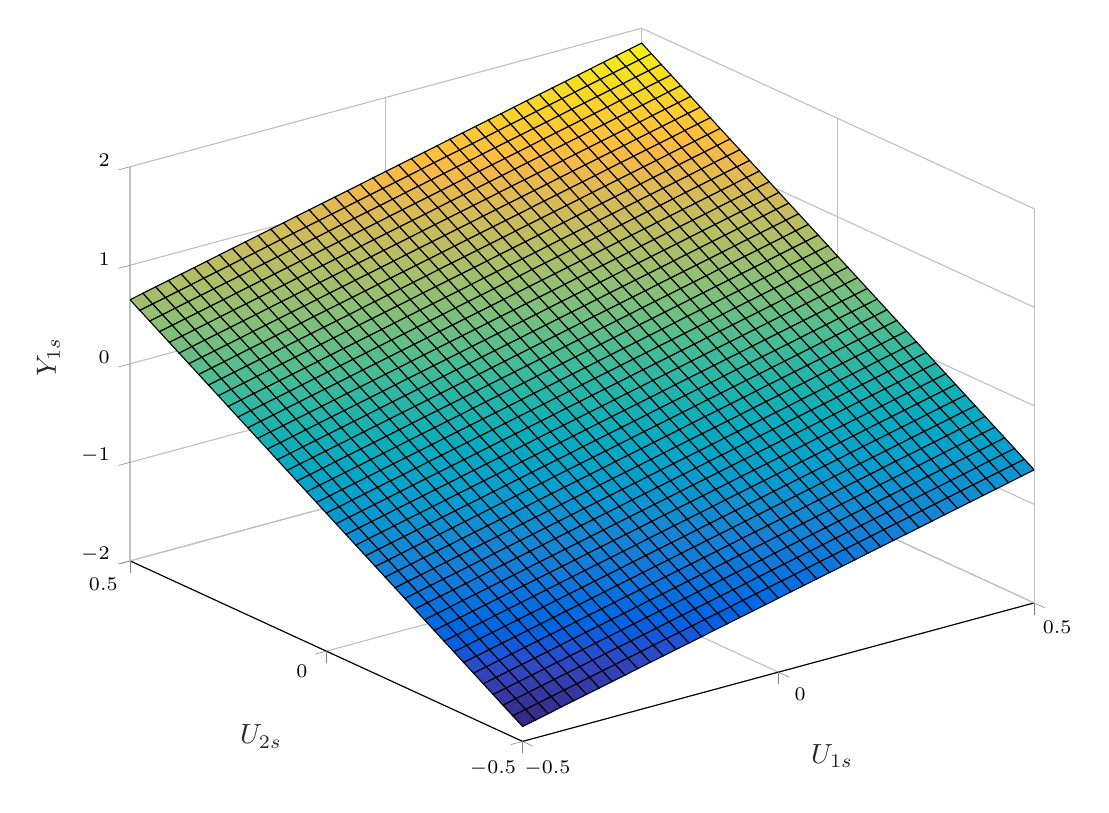
\begin{tikzpicture}

\begin{axis}[%
width=4.521in,
height=3.566in,
at={(0.758in,0.481in)},
scale only axis,
xmin=-0.5,
xmax=0.5,
xtick={-0.5,0,0.5},
tick align=outside,
xlabel style={font=\color{white!15!black}},
xlabel={$U_{1s}$},
ymin=-0.5,
ymax=0.5,
ytick={-0.5,0,0.5},
ylabel style={font=\color{white!15!black}},
ylabel={$U_{2s}$},
zmin=-2,
zmax=2,
zlabel style={font=\color{white!15!black}},
zlabel={$Y_{1s}$},
view={-37.5}{30},
axis background/.style={fill=white},
axis x line*=bottom,
axis y line*=left,
axis z line*=left,
xmajorgrids,
ymajorgrids,
zmajorgrids
]

\addplot3[%
surf,
shader=flat corner, draw=black, z buffer=sort, colormap={mymap}{[1pt] rgb(0pt)=(0.2081,0.1663,0.5292); rgb(1pt)=(0.211624,0.189781,0.577676); rgb(2pt)=(0.212252,0.213771,0.626971); rgb(3pt)=(0.2081,0.2386,0.677086); rgb(4pt)=(0.195905,0.264457,0.7279); rgb(5pt)=(0.170729,0.291938,0.779248); rgb(6pt)=(0.125271,0.324243,0.830271); rgb(7pt)=(0.0591333,0.359833,0.868333); rgb(8pt)=(0.0116952,0.38751,0.881957); rgb(9pt)=(0.00595714,0.408614,0.882843); rgb(10pt)=(0.0165143,0.4266,0.878633); rgb(11pt)=(0.0328524,0.443043,0.871957); rgb(12pt)=(0.0498143,0.458571,0.864057); rgb(13pt)=(0.0629333,0.47369,0.855438); rgb(14pt)=(0.0722667,0.488667,0.8467); rgb(15pt)=(0.0779429,0.503986,0.838371); rgb(16pt)=(0.0793476,0.520024,0.831181); rgb(17pt)=(0.0749429,0.537543,0.826271); rgb(18pt)=(0.0640571,0.556986,0.823957); rgb(19pt)=(0.0487714,0.577224,0.822829); rgb(20pt)=(0.0343429,0.596581,0.819852); rgb(21pt)=(0.0265,0.6137,0.8135); rgb(22pt)=(0.0238905,0.628662,0.803762); rgb(23pt)=(0.0230905,0.641786,0.791267); rgb(24pt)=(0.0227714,0.653486,0.776757); rgb(25pt)=(0.0266619,0.664195,0.760719); rgb(26pt)=(0.0383714,0.674271,0.743552); rgb(27pt)=(0.0589714,0.683757,0.725386); rgb(28pt)=(0.0843,0.692833,0.706167); rgb(29pt)=(0.113295,0.7015,0.685857); rgb(30pt)=(0.145271,0.709757,0.664629); rgb(31pt)=(0.180133,0.717657,0.642433); rgb(32pt)=(0.217829,0.725043,0.619262); rgb(33pt)=(0.258643,0.731714,0.595429); rgb(34pt)=(0.302171,0.737605,0.571186); rgb(35pt)=(0.348167,0.742433,0.547267); rgb(36pt)=(0.395257,0.7459,0.524443); rgb(37pt)=(0.44201,0.748081,0.503314); rgb(38pt)=(0.487124,0.749062,0.483976); rgb(39pt)=(0.530029,0.749114,0.466114); rgb(40pt)=(0.570857,0.748519,0.44939); rgb(41pt)=(0.609852,0.747314,0.433686); rgb(42pt)=(0.6473,0.7456,0.4188); rgb(43pt)=(0.683419,0.743476,0.404433); rgb(44pt)=(0.71841,0.741133,0.390476); rgb(45pt)=(0.752486,0.7384,0.376814); rgb(46pt)=(0.785843,0.735567,0.363271); rgb(47pt)=(0.818505,0.732733,0.34979); rgb(48pt)=(0.850657,0.7299,0.336029); rgb(49pt)=(0.882433,0.727433,0.3217); rgb(50pt)=(0.913933,0.725786,0.306276); rgb(51pt)=(0.944957,0.726114,0.288643); rgb(52pt)=(0.973895,0.731395,0.266648); rgb(53pt)=(0.993771,0.745457,0.240348); rgb(54pt)=(0.999043,0.765314,0.216414); rgb(55pt)=(0.995533,0.786057,0.196652); rgb(56pt)=(0.988,0.8066,0.179367); rgb(57pt)=(0.978857,0.827143,0.163314); rgb(58pt)=(0.9697,0.848138,0.147452); rgb(59pt)=(0.962586,0.870514,0.1309); rgb(60pt)=(0.958871,0.8949,0.113243); rgb(61pt)=(0.959824,0.921833,0.0948381); rgb(62pt)=(0.9661,0.951443,0.0755333); rgb(63pt)=(0.9763,0.9831,0.0538)}, mesh/rows=41]
table[row sep=crcr, point meta=\thisrow{c}] {%
%
x	y	z	c\\
-0.5	-0.5	-1.84891492565873	-1.84891492565873\\
-0.5	-0.475	-1.78644022257469	-1.78644022257469\\
-0.5	-0.45	-1.72396551949064	-1.72396551949064\\
-0.5	-0.425	-1.66149081640664	-1.66149081640664\\
-0.5	-0.4	-1.59901611332259	-1.59901611332259\\
-0.5	-0.375	-1.53654141023854	-1.53654141023854\\
-0.5	-0.35	-1.4740667071545	-1.4740667071545\\
-0.5	-0.325	-1.41159200407045	-1.41159200407045\\
-0.5	-0.3	-1.34911730098644	-1.34911730098644\\
-0.5	-0.275	-1.2866425979024	-1.2866425979024\\
-0.5	-0.25	-1.22416789481835	-1.22416789481835\\
-0.5	-0.225	-1.1616931917343	-1.1616931917343\\
-0.5	-0.2	-1.09921848865028	-1.09921848865028\\
-0.5	-0.175	-1.03674378556625	-1.03674378556625\\
-0.5	-0.15	-0.974269082482205	-0.974269082482205\\
-0.5	-0.125	-0.911794379398169	-0.911794379398169\\
-0.5	-0.1	-0.849319676314132	-0.849319676314132\\
-0.5	-0.075	-0.786844973230084	-0.786844973230084\\
-0.5	-0.05	-0.724370270146057	-0.724370270146057\\
-0.5	-0.025	-0.661895567062011	-0.661895567062011\\
-0.5	0	-0.599420863977985	-0.599420863977985\\
-0.5	0.025	-0.536946160893937	-0.536946160893937\\
-0.5	0.05	-0.474471457809902	-0.474471457809902\\
-0.5	0.0750000000000001	-0.411996754725867	-0.411996754725867\\
-0.5	0.1	-0.349522051641829	-0.349522051641829\\
-0.5	0.125	-0.287047348557794	-0.287047348557794\\
-0.5	0.15	-0.224572645473757	-0.224572645473757\\
-0.5	0.175	-0.162097942389717	-0.162097942389717\\
-0.5	0.2	-0.0996232393056797	-0.0996232393056797\\
-0.5	0.225	-0.0371485362216423	-0.0371485362216423\\
-0.5	0.25	0.0253261668623942	0.0253261668623942\\
-0.5	0.275	0.0878008699464331	0.0878008699464331\\
-0.5	0.3	0.150275573030469	0.150275573030469\\
-0.5	0.325	0.212750276114509	0.212750276114509\\
-0.5	0.35	0.275224979198545	0.275224979198545\\
-0.5	0.375	0.337699682282581	0.337699682282581\\
-0.5	0.4	0.400174385366618	0.400174385366618\\
-0.5	0.425	0.462649088450654	0.462649088450654\\
-0.5	0.45	0.52512379153469	0.52512379153469\\
-0.5	0.475	0.587598494618739	0.587598494618739\\
-0.5	0.5	0.650073197702764	0.650073197702764\\
-0.475	-0.5	-1.81894388245985	-1.81894388245985\\
-0.475	-0.475	-1.7564691793758	-1.7564691793758\\
-0.475	-0.45	-1.69399447629175	-1.69399447629175\\
-0.475	-0.425	-1.6315197732077	-1.6315197732077\\
-0.475	-0.4	-1.5690450701237	-1.5690450701237\\
-0.475	-0.375	-1.50657036703966	-1.50657036703966\\
-0.475	-0.35	-1.44409566395561	-1.44409566395561\\
-0.475	-0.325	-1.38162096087156	-1.38162096087156\\
-0.475	-0.3	-1.31914625778751	-1.31914625778751\\
-0.475	-0.275	-1.25667155470351	-1.25667155470351\\
-0.475	-0.25	-1.19419685161946	-1.19419685161946\\
-0.475	-0.225	-1.13172214853543	-1.13172214853543\\
-0.475	-0.2	-1.06924744545138	-1.06924744545138\\
-0.475	-0.175	-1.00677274236734	-1.00677274236734\\
-0.475	-0.15	-0.944298039283316	-0.944298039283316\\
-0.475	-0.125	-0.88182333619927	-0.88182333619927\\
-0.475	-0.1	-0.819348633115223	-0.819348633115223\\
-0.475	-0.075	-0.756873930031196	-0.756873930031196\\
-0.475	-0.05	-0.69439922694715	-0.69439922694715\\
-0.475	-0.025	-0.631924523863124	-0.631924523863124\\
-0.475	0	-0.569449820779078	-0.569449820779078\\
-0.475	0.025	-0.506975117695039	-0.506975117695039\\
-0.475	0.05	-0.444500414611004	-0.444500414611004\\
-0.475	0.0750000000000001	-0.382025711526967	-0.382025711526967\\
-0.475	0.1	-0.319551008442931	-0.319551008442931\\
-0.475	0.125	-0.257076305358895	-0.257076305358895\\
-0.475	0.15	-0.194601602274858	-0.194601602274858\\
-0.475	0.175	-0.13212689919082	-0.13212689919082\\
-0.475	0.2	-0.0696521961067818	-0.0696521961067818\\
-0.475	0.225	-0.00717749302274404	-0.00717749302274404\\
-0.475	0.25	0.0552972100612923	0.0552972100612923\\
-0.475	0.275	0.117771913145331	0.117771913145331\\
-0.475	0.3	0.180246616229368	0.180246616229368\\
-0.475	0.325	0.242721319313407	0.242721319313407\\
-0.475	0.35	0.305196022397444	0.305196022397444\\
-0.475	0.375	0.36767072548148	0.36767072548148\\
-0.475	0.4	0.430145428565515	0.430145428565515\\
-0.475	0.425	0.492620131649552	0.492620131649552\\
-0.475	0.45	0.555094834733588	0.555094834733588\\
-0.475	0.475	0.617569537817622	0.617569537817622\\
-0.475	0.5	0.680044240901671	0.680044240901671\\
-0.45	-0.5	-1.78897283926092	-1.78897283926092\\
-0.45	-0.475	-1.72649813617691	-1.72649813617691\\
-0.45	-0.45	-1.66402343309287	-1.66402343309287\\
-0.45	-0.425	-1.60154873000882	-1.60154873000882\\
-0.45	-0.4	-1.53907402692477	-1.53907402692477\\
-0.45	-0.375	-1.47659932384073	-1.47659932384073\\
-0.45	-0.35	-1.41412462075672	-1.41412462075672\\
-0.45	-0.325	-1.35164991767268	-1.35164991767268\\
-0.45	-0.3	-1.28917521458862	-1.28917521458862\\
-0.45	-0.275	-1.22670051150458	-1.22670051150458\\
-0.45	-0.25	-1.16422580842057	-1.16422580842057\\
-0.45	-0.225	-1.10175110533653	-1.10175110533653\\
-0.45	-0.2	-1.03927640225248	-1.03927640225248\\
-0.45	-0.175	-0.976801699168454	-0.976801699168454\\
-0.45	-0.15	-0.914326996084408	-0.914326996084408\\
-0.45	-0.125	-0.851852293000361	-0.851852293000361\\
-0.45	-0.1	-0.789377589916337	-0.789377589916337\\
-0.45	-0.075	-0.726902886832286	-0.726902886832286\\
-0.45	-0.05	-0.664428183748261	-0.664428183748261\\
-0.45	-0.025	-0.601953480664214	-0.601953480664214\\
-0.45	0	-0.539478777580178	-0.539478777580178\\
-0.45	0.025	-0.477004074496143	-0.477004074496143\\
-0.45	0.05	-0.414529371412106	-0.414529371412106\\
-0.45	0.0750000000000001	-0.352054668328069	-0.352054668328069\\
-0.45	0.1	-0.289579965244034	-0.289579965244034\\
-0.45	0.125	-0.227105262159996	-0.227105262159996\\
-0.45	0.15	-0.164630559075958	-0.164630559075958\\
-0.45	0.175	-0.10215585599192	-0.10215585599192\\
-0.45	0.2	-0.0396811529078823	-0.0396811529078823\\
-0.45	0.225	0.0227935501761555	0.0227935501761555\\
-0.45	0.25	0.085268253260192	0.085268253260192\\
-0.45	0.275	0.147742956344232	0.147742956344232\\
-0.45	0.3	0.210217659428268	0.210217659428268\\
-0.45	0.325	0.272692362512305	0.272692362512305\\
-0.45	0.35	0.335167065596342	0.335167065596342\\
-0.45	0.375	0.397641768680378	0.397641768680378\\
-0.45	0.4	0.460116471764413	0.460116471764413\\
-0.45	0.425	0.522591174848451	0.522591174848451\\
-0.45	0.45	0.585065877932487	0.585065877932487\\
-0.45	0.475	0.647540581016533	0.647540581016533\\
-0.45	0.5	0.710015284100558	0.710015284100558\\
-0.425	-0.5	-1.75900179606203	-1.75900179606203\\
-0.425	-0.475	-1.69652709297798	-1.69652709297798\\
-0.425	-0.45	-1.63405238989398	-1.63405238989398\\
-0.425	-0.425	-1.57157768680993	-1.57157768680993\\
-0.425	-0.4	-1.50910298372588	-1.50910298372588\\
-0.425	-0.375	-1.44662828064184	-1.44662828064184\\
-0.425	-0.35	-1.38415357755779	-1.38415357755779\\
-0.425	-0.325	-1.32167887447378	-1.32167887447378\\
-0.425	-0.3	-1.25920417138974	-1.25920417138974\\
-0.425	-0.275	-1.19672946830569	-1.19672946830569\\
-0.425	-0.25	-1.13425476522166	-1.13425476522166\\
-0.425	-0.225	-1.07178006213762	-1.07178006213762\\
-0.425	-0.2	-1.00930535905359	-1.00930535905359\\
-0.425	-0.175	-0.946830655969546	-0.946830655969546\\
-0.425	-0.15	-0.884355952885506	-0.884355952885506\\
-0.425	-0.125	-0.821881249801472	-0.821881249801472\\
-0.425	-0.1	-0.759406546717427	-0.759406546717427\\
-0.425	-0.075	-0.696931843633402	-0.696931843633402\\
-0.425	-0.05	-0.634457140549355	-0.634457140549355\\
-0.425	-0.025	-0.571982437465326	-0.571982437465326\\
-0.425	0	-0.50950773438128	-0.50950773438128\\
-0.425	0.025	-0.447033031297243	-0.447033031297243\\
-0.425	0.05	-0.384558328213208	-0.384558328213208\\
-0.425	0.0750000000000001	-0.322083625129171	-0.322083625129171\\
-0.425	0.1	-0.259608922045134	-0.259608922045134\\
-0.425	0.125	-0.197134218961098	-0.197134218961098\\
-0.425	0.15	-0.13465951587706	-0.13465951587706\\
-0.425	0.175	-0.0721848127930219	-0.0721848127930219\\
-0.425	0.2	-0.00971010970898402	-0.00971010970898402\\
-0.425	0.225	0.0527645933750538	0.0527645933750538\\
-0.425	0.25	0.11523929645909	0.11523929645909\\
-0.425	0.275	0.177713999543131	0.177713999543131\\
-0.425	0.3	0.240188702627167	0.240188702627167\\
-0.425	0.325	0.302663405711204	0.302663405711204\\
-0.425	0.35	0.365138108795239	0.365138108795239\\
-0.425	0.375	0.427612811879275	0.427612811879275\\
-0.425	0.4	0.490087514963312	0.490087514963312\\
-0.425	0.425	0.552562218047349	0.552562218047349\\
-0.425	0.45	0.615036921131393	0.615036921131393\\
-0.425	0.475	0.677511624215419	0.677511624215419\\
-0.425	0.5	0.739986327299468	0.739986327299468\\
-0.4	-0.5	-1.72903075286314	-1.72903075286314\\
-0.4	-0.475	-1.66655604977909	-1.66655604977909\\
-0.4	-0.45	-1.60408134669505	-1.60408134669505\\
-0.4	-0.425	-1.54160664361102	-1.54160664361102\\
-0.4	-0.4	-1.479131940527	-1.479131940527\\
-0.4	-0.375	-1.41665723744295	-1.41665723744295\\
-0.4	-0.35	-1.3541825343589	-1.3541825343589\\
-0.4	-0.325	-1.29170783127486	-1.29170783127486\\
-0.4	-0.3	-1.22923312819085	-1.22923312819085\\
-0.4	-0.275	-1.1667584251068	-1.1667584251068\\
-0.4	-0.25	-1.10428372202276	-1.10428372202276\\
-0.4	-0.225	-1.04180901893873	-1.04180901893873\\
-0.4	-0.2	-0.979334315854684	-0.979334315854684\\
-0.4	-0.175	-0.916859612770648	-0.916859612770648\\
-0.4	-0.15	-0.854384909686613	-0.854384909686613\\
-0.4	-0.125	-0.791910206602564	-0.791910206602564\\
-0.4	-0.1	-0.729435503518538	-0.729435503518538\\
-0.4	-0.075	-0.66696080043449	-0.66696080043449\\
-0.4	-0.05	-0.604486097350466	-0.604486097350466\\
-0.4	-0.025	-0.542011394266418	-0.542011394266418\\
-0.4	0	-0.479536691182381	-0.479536691182381\\
-0.4	0.025	-0.417061988098346	-0.417061988098346\\
-0.4	0.05	-0.35458728501431	-0.35458728501431\\
-0.4	0.0750000000000001	-0.292112581930272	-0.292112581930272\\
-0.4	0.1	-0.229637878846234	-0.229637878846234\\
-0.4	0.125	-0.167163175762198	-0.167163175762198\\
-0.4	0.15	-0.10468847267816	-0.10468847267816\\
-0.4	0.175	-0.0422137695941221	-0.0422137695941221\\
-0.4	0.2	0.0202609334899155	0.0202609334899155\\
-0.4	0.225	0.0827356365739534	0.0827356365739534\\
-0.4	0.25	0.14521033965799	0.14521033965799\\
-0.4	0.275	0.207685042742028	0.207685042742028\\
-0.4	0.3	0.270159745826065	0.270159745826065\\
-0.4	0.325	0.332634448910102	0.332634448910102\\
-0.4	0.35	0.395109151994138	0.395109151994138\\
-0.4	0.375	0.457583855078174	0.457583855078174\\
-0.4	0.4	0.520058558162216	0.520058558162216\\
-0.4	0.425	0.582533261246258	0.582533261246258\\
-0.4	0.45	0.645007964330283	0.645007964330283\\
-0.4	0.475	0.70748266741433	0.70748266741433\\
-0.4	0.5	0.769957370498358	0.769957370498358\\
-0.375	-0.5	-1.69905970966425	-1.69905970966425\\
-0.375	-0.475	-1.6365850065802	-1.6365850065802\\
-0.375	-0.45	-1.57411030349616	-1.57411030349616\\
-0.375	-0.425	-1.51163560041211	-1.51163560041211\\
-0.375	-0.4	-1.44916089732809	-1.44916089732809\\
-0.375	-0.375	-1.38668619424406	-1.38668619424406\\
-0.375	-0.35	-1.32421149116001	-1.32421149116001\\
-0.375	-0.325	-1.26173678807597	-1.26173678807597\\
-0.375	-0.3	-1.19926208499192	-1.19926208499192\\
-0.375	-0.275	-1.13678738190792	-1.13678738190792\\
-0.375	-0.25	-1.07431267882387	-1.07431267882387\\
-0.375	-0.225	-1.01183797573983	-1.01183797573983\\
-0.375	-0.2	-0.949363272655796	-0.949363272655796\\
-0.375	-0.175	-0.88688856957175	-0.88688856957175\\
-0.375	-0.15	-0.824413866487705	-0.824413866487705\\
-0.375	-0.125	-0.761939163403676	-0.761939163403676\\
-0.375	-0.1	-0.69946446031963	-0.69946446031963\\
-0.375	-0.075	-0.636989757235604	-0.636989757235604\\
-0.375	-0.05	-0.574515054151556	-0.574515054151556\\
-0.375	-0.025	-0.51204035106752	-0.51204035106752\\
-0.375	0	-0.449565647983483	-0.449565647983483\\
-0.375	0.025	-0.387090944899447	-0.387090944899447\\
-0.375	0.05	-0.32461624181541	-0.32461624181541\\
-0.375	0.0750000000000001	-0.262141538731374	-0.262141538731374\\
-0.375	0.1	-0.199666835647335	-0.199666835647335\\
-0.375	0.125	-0.137192132563299	-0.137192132563299\\
-0.375	0.15	-0.0747174294792614	-0.0747174294792614\\
-0.375	0.175	-0.012242726395224	-0.012242726395224\\
-0.375	0.2	0.0502319766888137	0.0502319766888137\\
-0.375	0.225	0.112706679772851	0.112706679772851\\
-0.375	0.25	0.175181382856888	0.175181382856888\\
-0.375	0.275	0.237656085940927	0.237656085940927\\
-0.375	0.3	0.300130789024964	0.300130789024964\\
-0.375	0.325	0.362605492109	0.362605492109\\
-0.375	0.35	0.425080195193036	0.425080195193036\\
-0.375	0.375	0.487554898277073	0.487554898277073\\
-0.375	0.4	0.550029601361114	0.550029601361114\\
-0.375	0.425	0.612504304445145	0.612504304445145\\
-0.375	0.45	0.674979007529193	0.674979007529193\\
-0.375	0.475	0.73745371061322	0.73745371061322\\
-0.375	0.5	0.799928413697264	0.799928413697264\\
-0.35	-0.5	-1.66908866646532	-1.66908866646532\\
-0.35	-0.475	-1.6066139633813	-1.6066139633813\\
-0.35	-0.45	-1.54413926029727	-1.54413926029727\\
-0.35	-0.425	-1.48166455721323	-1.48166455721323\\
-0.35	-0.4	-1.41918985412918	-1.41918985412918\\
-0.35	-0.375	-1.35671515104513	-1.35671515104513\\
-0.35	-0.35	-1.29424044796113	-1.29424044796113\\
-0.35	-0.325	-1.23176574487708	-1.23176574487708\\
-0.35	-0.3	-1.16929104179303	-1.16929104179303\\
-0.35	-0.275	-1.10681633870901	-1.10681633870901\\
-0.35	-0.25	-1.04434163562496	-1.04434163562496\\
-0.35	-0.225	-0.981866932540914	-0.981866932540914\\
-0.35	-0.2	-0.919392229456888	-0.919392229456888\\
-0.35	-0.175	-0.856917526372842	-0.856917526372842\\
-0.35	-0.15	-0.794442823288815	-0.794442823288815\\
-0.35	-0.125	-0.731968120204766	-0.731968120204766\\
-0.35	-0.1	-0.669493417120741	-0.669493417120741\\
-0.35	-0.075	-0.607018714036692	-0.607018714036692\\
-0.35	-0.05	-0.544544010952659	-0.544544010952659\\
-0.35	-0.025	-0.482069307868622	-0.482069307868622\\
-0.35	0	-0.419594604784585	-0.419594604784585\\
-0.35	0.025	-0.357119901700549	-0.357119901700549\\
-0.35	0.05	-0.294645198616513	-0.294645198616513\\
-0.35	0.0750000000000001	-0.232170495532472	-0.232170495532472\\
-0.35	0.1	-0.169695792448435	-0.169695792448435\\
-0.35	0.125	-0.107221089364398	-0.107221089364398\\
-0.35	0.15	-0.0447463862803607	-0.0447463862803607\\
-0.35	0.175	0.017728316803677	0.017728316803677\\
-0.35	0.2	0.0802030198877148	0.0802030198877148\\
-0.35	0.225	0.142677722971752	0.142677722971752\\
-0.35	0.25	0.205152426055789	0.205152426055789\\
-0.35	0.275	0.267627129139825	0.267627129139825\\
-0.35	0.3	0.330101832223861	0.330101832223861\\
-0.35	0.325	0.392576535307898	0.392576535307898\\
-0.35	0.35	0.455051238391938	0.455051238391938\\
-0.35	0.375	0.517525941475982	0.517525941475982\\
-0.35	0.4	0.580000644560008	0.580000644560008\\
-0.35	0.425	0.642475347644053	0.642475347644053\\
-0.35	0.45	0.704950050728078	0.704950050728078\\
-0.35	0.475	0.767424753812129	0.767424753812129\\
-0.35	0.5	0.829899456896175	0.829899456896175\\
-0.325	-0.5	-1.63911762326644	-1.63911762326644\\
-0.325	-0.475	-1.57664292018239	-1.57664292018239\\
-0.325	-0.45	-1.51416821709834	-1.51416821709834\\
-0.325	-0.425	-1.45169351401434	-1.45169351401434\\
-0.325	-0.4	-1.38921881093029	-1.38921881093029\\
-0.325	-0.375	-1.32674410784625	-1.32674410784625\\
-0.325	-0.35	-1.2642694047622	-1.2642694047622\\
-0.325	-0.325	-1.2017947016782	-1.2017947016782\\
-0.325	-0.3	-1.13931999859414	-1.13931999859414\\
-0.325	-0.275	-1.0768452955101	-1.0768452955101\\
-0.325	-0.25	-1.01437059242607	-1.01437059242607\\
-0.325	-0.225	-0.951895889342026	-0.951895889342026\\
-0.325	-0.2	-0.889421186257979	-0.889421186257979\\
-0.325	-0.175	-0.826946483173952	-0.826946483173952\\
-0.325	-0.15	-0.764471780089905	-0.764471780089905\\
-0.325	-0.125	-0.70199707700588	-0.70199707700588\\
-0.325	-0.1	-0.639522373921833	-0.639522373921833\\
-0.325	-0.075	-0.577047670837805	-0.577047670837805\\
-0.325	-0.05	-0.514572967753759	-0.514572967753759\\
-0.325	-0.025	-0.452098264669724	-0.452098264669724\\
-0.325	0	-0.389623561585687	-0.389623561585687\\
-0.325	0.025	-0.327148858501651	-0.327148858501651\\
-0.325	0.05	-0.264674155417612	-0.264674155417612\\
-0.325	0.0750000000000001	-0.202199452333573	-0.202199452333573\\
-0.325	0.1	-0.139724749249537	-0.139724749249537\\
-0.325	0.125	-0.0772500461655002	-0.0772500461655002\\
-0.325	0.15	-0.0147753430814626	-0.0147753430814626\\
-0.325	0.175	0.0476993600025753	0.0476993600025753\\
-0.325	0.2	0.110174063086613	0.110174063086613\\
-0.325	0.225	0.172648766170651	0.172648766170651\\
-0.325	0.25	0.235123469254687	0.235123469254687\\
-0.325	0.275	0.297598172338724	0.297598172338724\\
-0.325	0.3	0.36007287542276	0.36007287542276\\
-0.325	0.325	0.422547578506796	0.422547578506796\\
-0.325	0.35	0.485022281590837	0.485022281590837\\
-0.325	0.375	0.547496984674881	0.547496984674881\\
-0.325	0.4	0.609971687758918	0.609971687758918\\
-0.325	0.425	0.67244639084294	0.67244639084294\\
-0.325	0.45	0.73492109392699	0.73492109392699\\
-0.325	0.475	0.797395797011026	0.797395797011026\\
-0.325	0.5	0.859870500095061	0.859870500095061\\
-0.3	-0.5	-1.60914658006755	-1.60914658006755\\
-0.3	-0.475	-1.5466718769835	-1.5466718769835\\
-0.3	-0.45	-1.48419717389945	-1.48419717389945\\
-0.3	-0.425	-1.42172247081541	-1.42172247081541\\
-0.3	-0.4	-1.3592477677314	-1.3592477677314\\
-0.3	-0.375	-1.29677306464735	-1.29677306464735\\
-0.3	-0.35	-1.23429836156331	-1.23429836156331\\
-0.3	-0.325	-1.17182365847927	-1.17182365847927\\
-0.3	-0.3	-1.10934895539523	-1.10934895539523\\
-0.3	-0.275	-1.0468742523112	-1.0468742523112\\
-0.3	-0.25	-0.984399549227165	-0.984399549227165\\
-0.3	-0.225	-0.921924846143117	-0.921924846143117\\
-0.3	-0.2	-0.85945014305909	-0.85945014305909\\
-0.3	-0.175	-0.796975439975045	-0.796975439975045\\
-0.3	-0.15	-0.734500736891018	-0.734500736891018\\
-0.3	-0.125	-0.672026033806971	-0.672026033806971\\
-0.3	-0.1	-0.609551330722944	-0.609551330722944\\
-0.3	-0.075	-0.5470766276389	-0.5470766276389\\
-0.3	-0.05	-0.484601924554862	-0.484601924554862\\
-0.3	-0.025	-0.422127221470827	-0.422127221470827\\
-0.3	0	-0.359652518386788	-0.359652518386788\\
-0.3	0.025	-0.297177815302752	-0.297177815302752\\
-0.3	0.05	-0.234703112218711	-0.234703112218711\\
-0.3	0.0750000000000001	-0.172228409134675	-0.172228409134675\\
-0.3	0.1	-0.109753706050637	-0.109753706050637\\
-0.3	0.125	-0.0472790029666007	-0.0472790029666007\\
-0.3	0.15	0.015195700117437	0.015195700117437\\
-0.3	0.175	0.0776704032014743	0.0776704032014743\\
-0.3	0.2	0.140145106285512	0.140145106285512\\
-0.3	0.225	0.202619809369548	0.202619809369548\\
-0.3	0.25	0.265094512453584	0.265094512453584\\
-0.3	0.275	0.327569215537622	0.327569215537622\\
-0.3	0.3	0.390043918621658	0.390043918621658\\
-0.3	0.325	0.452518621705705	0.452518621705705\\
-0.3	0.35	0.514993324789741	0.514993324789741\\
-0.3	0.375	0.577468027873777	0.577468027873777\\
-0.3	0.4	0.639942730957804	0.639942730957804\\
-0.3	0.425	0.702417434041851	0.702417434041851\\
-0.3	0.45	0.764892137125885	0.764892137125885\\
-0.3	0.475	0.827366840209922	0.827366840209922\\
-0.3	0.5	0.889841543293971	0.889841543293971\\
-0.275	-0.5	-1.57917553686862	-1.57917553686862\\
-0.275	-0.475	-1.51670083378461	-1.51670083378461\\
-0.275	-0.45	-1.45422613070057	-1.45422613070057\\
-0.275	-0.425	-1.39175142761652	-1.39175142761652\\
-0.275	-0.4	-1.32927672453247	-1.32927672453247\\
-0.275	-0.375	-1.26680202144847	-1.26680202144847\\
-0.275	-0.35	-1.20432731836442	-1.20432731836442\\
-0.275	-0.325	-1.14185261528037	-1.14185261528037\\
-0.275	-0.3	-1.07937791219635	-1.07937791219635\\
-0.275	-0.275	-1.0169032091123	-1.0169032091123\\
-0.275	-0.25	-0.954428506028255	-0.954428506028255\\
-0.275	-0.225	-0.891953802944229	-0.891953802944229\\
-0.275	-0.2	-0.829479099860184	-0.829479099860184\\
-0.275	-0.175	-0.767004396776159	-0.767004396776159\\
-0.275	-0.15	-0.704529693692109	-0.704529693692109\\
-0.275	-0.125	-0.642054990608083	-0.642054990608083\\
-0.275	-0.1	-0.579580287524037	-0.579580287524037\\
-0.275	-0.075	-0.51710558444	-0.51710558444\\
-0.275	-0.05	-0.454630881355964	-0.454630881355964\\
-0.275	-0.025	-0.392156178271927	-0.392156178271927\\
-0.275	0	-0.329681475187891	-0.329681475187891\\
-0.275	0.025	-0.26720677210385	-0.26720677210385\\
-0.275	0.05	-0.204732069019813	-0.204732069019813\\
-0.275	0.0750000000000001	-0.142257365935777	-0.142257365935777\\
-0.275	0.1	-0.0797826628517389	-0.0797826628517389\\
-0.275	0.125	-0.0173079597677012	-0.0173079597677012\\
-0.275	0.15	0.0451667433163366	0.0451667433163366\\
-0.275	0.175	0.107641446400374	0.107641446400374\\
-0.275	0.2	0.17011614948441	0.17011614948441\\
-0.275	0.225	0.232590852568447	0.232590852568447\\
-0.275	0.25	0.295065555652484	0.295065555652484\\
-0.275	0.275	0.35754025873652	0.35754025873652\\
-0.275	0.3	0.42001496182056	0.42001496182056\\
-0.275	0.325	0.482489664904603	0.482489664904603\\
-0.275	0.35	0.544964367988639	0.544964367988639\\
-0.275	0.375	0.607439071072666	0.607439071072666\\
-0.275	0.4	0.669913774156712	0.669913774156712\\
-0.275	0.425	0.732388477240748	0.732388477240748\\
-0.275	0.45	0.794863180324784	0.794863180324784\\
-0.275	0.475	0.857337883408833	0.857337883408833\\
-0.275	0.5	0.919812586492858	0.919812586492858\\
-0.25	-0.5	-1.54920449366973	-1.54920449366973\\
-0.25	-0.475	-1.48672979058568	-1.48672979058568\\
-0.25	-0.45	-1.42425508750168	-1.42425508750168\\
-0.25	-0.425	-1.36178038441764	-1.36178038441764\\
-0.25	-0.4	-1.29930568133359	-1.29930568133359\\
-0.25	-0.375	-1.23683097824954	-1.23683097824954\\
-0.25	-0.35	-1.17435627516553	-1.17435627516553\\
-0.25	-0.325	-1.11188157208149	-1.11188157208149\\
-0.25	-0.3	-1.04940686899744	-1.04940686899744\\
-0.25	-0.275	-0.986932165913392	-0.986932165913392\\
-0.25	-0.25	-0.924457462829367	-0.924457462829367\\
-0.25	-0.225	-0.861982759745321	-0.861982759745321\\
-0.25	-0.2	-0.799508056661296	-0.799508056661296\\
-0.25	-0.175	-0.737033353577248	-0.737033353577248\\
-0.25	-0.15	-0.674558650493222	-0.674558650493222\\
-0.25	-0.125	-0.612083947409175	-0.612083947409175\\
-0.25	-0.1	-0.549609244325138	-0.549609244325138\\
-0.25	-0.075	-0.487134541241102	-0.487134541241102\\
-0.25	-0.05	-0.424659838157066	-0.424659838157066\\
-0.25	-0.025	-0.362185135073028	-0.362185135073028\\
-0.25	0	-0.299710431988993	-0.299710431988993\\
-0.25	0.025	-0.237235728904951	-0.237235728904951\\
-0.25	0.05	-0.174761025820915	-0.174761025820915\\
-0.25	0.0750000000000001	-0.112286322736878	-0.112286322736878\\
-0.25	0.1	-0.0498116196528399	-0.0498116196528399\\
-0.25	0.125	0.0126630834311971	0.0126630834311971\\
-0.25	0.15	0.0751377865152343	0.0751377865152343\\
-0.25	0.175	0.137612489599273	0.137612489599273\\
-0.25	0.2	0.200087192683309	0.200087192683309\\
-0.25	0.225	0.262561895767345	0.262561895767345\\
-0.25	0.25	0.325036598851382	0.325036598851382\\
-0.25	0.275	0.387511301935418	0.387511301935418\\
-0.25	0.3	0.449986005019465	0.449986005019465\\
-0.25	0.325	0.512460708103501	0.512460708103501\\
-0.25	0.35	0.574935411187527	0.574935411187527\\
-0.25	0.375	0.637410114271574	0.637410114271574\\
-0.25	0.4	0.699884817355599	0.699884817355599\\
-0.25	0.425	0.762359520439648	0.762359520439648\\
-0.25	0.45	0.824834223523694	0.824834223523694\\
-0.25	0.475	0.887308926607719	0.887308926607719\\
-0.25	0.5	0.949783629691767	0.949783629691767\\
-0.225	-0.5	-1.51923345047085	-1.51923345047085\\
-0.225	-0.475	-1.45675874738679	-1.45675874738679\\
-0.225	-0.45	-1.39428404430275	-1.39428404430275\\
-0.225	-0.425	-1.33180934121874	-1.33180934121874\\
-0.225	-0.4	-1.2693346381347	-1.2693346381347\\
-0.225	-0.375	-1.20685993505065	-1.20685993505065\\
-0.225	-0.35	-1.14438523196661	-1.14438523196661\\
-0.225	-0.325	-1.08191052888258	-1.08191052888258\\
-0.225	-0.3	-1.01943582579854	-1.01943582579854\\
-0.225	-0.275	-0.956961122714505	-0.956961122714505\\
-0.225	-0.25	-0.89448641963046	-0.89448641963046\\
-0.225	-0.225	-0.832011716546433	-0.832011716546433\\
-0.225	-0.2	-0.769537013462386	-0.769537013462386\\
-0.225	-0.175	-0.707062310378359	-0.707062310378359\\
-0.225	-0.15	-0.644587607294311	-0.644587607294311\\
-0.225	-0.125	-0.582112904210287	-0.582112904210287\\
-0.225	-0.1	-0.519638201126241	-0.519638201126241\\
-0.225	-0.075	-0.457163498042203	-0.457163498042203\\
-0.225	-0.05	-0.394688794958167	-0.394688794958167\\
-0.225	-0.025	-0.332214091874131	-0.332214091874131\\
-0.225	0	-0.269739388790089	-0.269739388790089\\
-0.225	0.025	-0.207264685706053	-0.207264685706053\\
-0.225	0.05	-0.144789982622017	-0.144789982622017\\
-0.225	0.0750000000000001	-0.0823152795379788	-0.0823152795379788\\
-0.225	0.1	-0.0198405764539411	-0.0198405764539411\\
-0.225	0.125	0.0426341266300967	0.0426341266300967\\
-0.225	0.15	0.105108829714134	0.105108829714134\\
-0.225	0.175	0.167583532798171	0.167583532798171\\
-0.225	0.2	0.230058235882207	0.230058235882207\\
-0.225	0.225	0.292532938966243	0.292532938966243\\
-0.225	0.25	0.355007642050279	0.355007642050279\\
-0.225	0.275	0.417482345134321	0.417482345134321\\
-0.225	0.3	0.479957048218362	0.479957048218362\\
-0.225	0.325	0.542431751302401	0.542431751302401\\
-0.225	0.35	0.604906454386435	0.604906454386435\\
-0.225	0.375	0.667381157470462	0.667381157470462\\
-0.225	0.4	0.729855860554508	0.729855860554508\\
-0.225	0.425	0.792330563638557	0.792330563638557\\
-0.225	0.45	0.85480526672258	0.85480526672258\\
-0.225	0.475	0.917279969806626	0.917279969806626\\
-0.225	0.5	0.979754672890654	0.979754672890654\\
-0.2	-0.5	-1.48926240727196	-1.48926240727196\\
-0.2	-0.475	-1.42678770418791	-1.42678770418791\\
-0.2	-0.45	-1.36431300110386	-1.36431300110386\\
-0.2	-0.425	-1.30183829801981	-1.30183829801981\\
-0.2	-0.4	-1.23936359493581	-1.23936359493581\\
-0.2	-0.375	-1.17688889185176	-1.17688889185176\\
-0.2	-0.35	-1.11441418876772	-1.11441418876772\\
-0.2	-0.325	-1.05193948568367	-1.05193948568367\\
-0.2	-0.3	-0.989464782599644	-0.989464782599644\\
-0.2	-0.275	-0.926990079515596	-0.926990079515596\\
-0.2	-0.25	-0.864515376431569	-0.864515376431569\\
-0.2	-0.225	-0.802040673347525	-0.802040673347525\\
-0.2	-0.2	-0.739565970263498	-0.739565970263498\\
-0.2	-0.175	-0.67709126717945	-0.67709126717945\\
-0.2	-0.15	-0.614616564095423	-0.614616564095423\\
-0.2	-0.125	-0.552141861011379	-0.552141861011379\\
-0.2	-0.1	-0.489667157927342	-0.489667157927342\\
-0.2	-0.075	-0.427192454843306	-0.427192454843306\\
-0.2	-0.05	-0.364717751759269	-0.364717751759269\\
-0.2	-0.025	-0.302243048675234	-0.302243048675234\\
-0.2	0	-0.239768345591191	-0.239768345591191\\
-0.2	0.025	-0.177293642507155	-0.177293642507155\\
-0.2	0.05	-0.114818939423116	-0.114818939423116\\
-0.2	0.0750000000000001	-0.0523442363390793	-0.0523442363390793\\
-0.2	0.1	0.0101304667449584	0.0101304667449584\\
-0.2	0.125	0.0726051698289961	0.0726051698289961\\
-0.2	0.15	0.135079872913032	0.135079872913032\\
-0.2	0.175	0.197554575997069	0.197554575997069\\
-0.2	0.2	0.260029279081111	0.260029279081111\\
-0.2	0.225	0.322503982165142	0.322503982165142\\
-0.2	0.25	0.384978685249184	0.384978685249184\\
-0.2	0.275	0.447453388333225	0.447453388333225\\
-0.2	0.3	0.509928091417262	0.509928091417262\\
-0.2	0.325	0.572402794501298	0.572402794501298\\
-0.2	0.35	0.634877497585325	0.634877497585325\\
-0.2	0.375	0.697352200669372	0.697352200669372\\
-0.2	0.4	0.759826903753417	0.759826903753417\\
-0.2	0.425	0.822301606837443	0.822301606837443\\
-0.2	0.45	0.884776309921491	0.884776309921491\\
-0.2	0.475	0.947251013005516	0.947251013005516\\
-0.2	0.5	1.00972571608956	1.00972571608956\\
-0.175	-0.5	-1.45929136407302	-1.45929136407302\\
-0.175	-0.475	-1.39681666098902	-1.39681666098902\\
-0.175	-0.45	-1.33434195790497	-1.33434195790497\\
-0.175	-0.425	-1.27186725482093	-1.27186725482093\\
-0.175	-0.4	-1.20939255173688	-1.20939255173688\\
-0.175	-0.375	-1.14691784865287	-1.14691784865287\\
-0.175	-0.35	-1.08444314556882	-1.08444314556882\\
-0.175	-0.325	-1.02196844248478	-1.02196844248478\\
-0.175	-0.3	-0.959493739400734	-0.959493739400734\\
-0.175	-0.275	-0.89701903631671	-0.89701903631671\\
-0.175	-0.25	-0.834544333232662	-0.834544333232662\\
-0.175	-0.225	-0.772069630148636	-0.772069630148636\\
-0.175	-0.2	-0.70959492706459	-0.70959492706459\\
-0.175	-0.175	-0.647120223980565	-0.647120223980565\\
-0.175	-0.15	-0.584645520896514	-0.584645520896514\\
-0.175	-0.125	-0.522170817812479	-0.522170817812479\\
-0.175	-0.1	-0.459696114728444	-0.459696114728444\\
-0.175	-0.075	-0.397221411644408	-0.397221411644408\\
-0.175	-0.05	-0.334746708560371	-0.334746708560371\\
-0.175	-0.025	-0.27227200547633	-0.27227200547633\\
-0.175	0	-0.209797302392293	-0.209797302392293\\
-0.175	0.025	-0.147322599308257	-0.147322599308257\\
-0.175	0.05	-0.0848478962242176	-0.0848478962242176\\
-0.175	0.0750000000000001	-0.0223731931401803	-0.0223731931401803\\
-0.175	0.1	0.0401015099438573	0.0401015099438573\\
-0.175	0.125	0.102576213027895	0.102576213027895\\
-0.175	0.15	0.165050916111931	0.165050916111931\\
-0.175	0.175	0.227525619195969	0.227525619195969\\
-0.175	0.2	0.290000322280003	0.290000322280003\\
-0.175	0.225	0.352475025364039	0.352475025364039\\
-0.175	0.25	0.414949728448088	0.414949728448088\\
-0.175	0.275	0.477424431532122	0.477424431532122\\
-0.175	0.3	0.539899134616159	0.539899134616159\\
-0.175	0.325	0.602373837700187	0.602373837700187\\
-0.175	0.35	0.664848540784231	0.664848540784231\\
-0.175	0.375	0.727323243868279	0.727323243868279\\
-0.175	0.4	0.789797946952308	0.789797946952308\\
-0.175	0.425	0.852272650036353	0.852272650036353\\
-0.175	0.45	0.914747353120378	0.914747353120378\\
-0.175	0.475	0.977222056204424	0.977222056204424\\
-0.175	0.5	1.03969675928845	1.03969675928845\\
-0.15	-0.5	-1.42932032087414	-1.42932032087414\\
-0.15	-0.475	-1.36684561779009	-1.36684561779009\\
-0.15	-0.45	-1.30437091470609	-1.30437091470609\\
-0.15	-0.425	-1.24189621162204	-1.24189621162204\\
-0.15	-0.4	-1.17942150853799	-1.17942150853799\\
-0.15	-0.375	-1.11694680545396	-1.11694680545396\\
-0.15	-0.35	-1.05447210236992	-1.05447210236992\\
-0.15	-0.325	-0.991997399285874	-0.991997399285874\\
-0.15	-0.3	-0.929522696201845	-0.929522696201845\\
-0.15	-0.275	-0.8670479931178	-0.8670479931178\\
-0.15	-0.25	-0.804573290033773	-0.804573290033773\\
-0.15	-0.225	-0.742098586949726	-0.742098586949726\\
-0.15	-0.2	-0.679623883865702	-0.679623883865702\\
-0.15	-0.175	-0.617149180781654	-0.617149180781654\\
-0.15	-0.15	-0.554674477697617	-0.554674477697617\\
-0.15	-0.125	-0.492199774613583	-0.492199774613583\\
-0.15	-0.1	-0.429725071529545	-0.429725071529545\\
-0.15	-0.075	-0.367250368445509	-0.367250368445509\\
-0.15	-0.05	-0.304775665361472	-0.304775665361472\\
-0.15	-0.025	-0.24230096227743	-0.24230096227743\\
-0.15	0	-0.179826259193394	-0.179826259193394\\
-0.15	0.025	-0.117351556109356	-0.117351556109356\\
-0.15	0.05	-0.0548768530253183	-0.0548768530253183\\
-0.15	0.0750000000000001	0.0075978500587185	0.0075978500587185\\
-0.15	0.1	0.0700725531427562	0.0700725531427562\\
-0.15	0.125	0.132547256226793	0.132547256226793\\
-0.15	0.15	0.195021959310829	0.195021959310829\\
-0.15	0.175	0.25749666239487	0.25749666239487\\
-0.15	0.2	0.319971365478902	0.319971365478902\\
-0.15	0.225	0.382446068562942	0.382446068562942\\
-0.15	0.25	0.444920771646986	0.444920771646986\\
-0.15	0.275	0.507395474731022	0.507395474731022\\
-0.15	0.3	0.569870177815047	0.569870177815047\\
-0.15	0.325	0.632344880899095	0.632344880899095\\
-0.15	0.35	0.694819583983141	0.694819583983141\\
-0.15	0.375	0.757294287067168	0.757294287067168\\
-0.15	0.4	0.819768990151213	0.819768990151213\\
-0.15	0.425	0.88224369323524	0.88224369323524\\
-0.15	0.45	0.944718396319286	0.944718396319286\\
-0.15	0.475	1.00719309940331	1.00719309940331\\
-0.15	0.5	1.06966780248736	1.06966780248736\\
-0.125	-0.5	-1.39934927767525	-1.39934927767525\\
-0.125	-0.475	-1.33687457459121	-1.33687457459121\\
-0.125	-0.45	-1.27439987150716	-1.27439987150716\\
-0.125	-0.425	-1.21192516842315	-1.21192516842315\\
-0.125	-0.4	-1.1494504653391	-1.1494504653391\\
-0.125	-0.375	-1.08697576225506	-1.08697576225506\\
-0.125	-0.35	-1.02450105917101	-1.02450105917101\\
-0.125	-0.325	-0.962026356086986	-0.962026356086986\\
-0.125	-0.3	-0.899551653002939	-0.899551653002939\\
-0.125	-0.275	-0.837076949918913	-0.837076949918913\\
-0.125	-0.25	-0.774602246834865	-0.774602246834865\\
-0.125	-0.225	-0.712127543750839	-0.712127543750839\\
-0.125	-0.2	-0.649652840666793	-0.649652840666793\\
-0.125	-0.175	-0.587178137582764	-0.587178137582764\\
-0.125	-0.15	-0.524703434498719	-0.524703434498719\\
-0.125	-0.125	-0.462228731414683	-0.462228731414683\\
-0.125	-0.1	-0.399754028330648	-0.399754028330648\\
-0.125	-0.075	-0.337279325246611	-0.337279325246611\\
-0.125	-0.05	-0.274804622162569	-0.274804622162569\\
-0.125	-0.025	-0.212329919078533	-0.212329919078533\\
-0.125	0	-0.149855215994496	-0.149855215994496\\
-0.125	0.025	-0.0873805129104573	-0.0873805129104573\\
-0.125	0.05	-0.0249058098264199	-0.0249058098264199\\
-0.125	0.0750000000000001	0.0375688932576171	0.0375688932576171\\
-0.125	0.1	0.100043596341654	0.100043596341654\\
-0.125	0.125	0.162518299425691	0.162518299425691\\
-0.125	0.15	0.224993002509732	0.224993002509732\\
-0.125	0.175	0.287467705593763	0.287467705593763\\
-0.125	0.2	0.349942408677806	0.349942408677806\\
-0.125	0.225	0.412417111761847	0.412417111761847\\
-0.125	0.25	0.474891814845883	0.474891814845883\\
-0.125	0.275	0.537366517929918	0.537366517929918\\
-0.125	0.3	0.599841221013959	0.599841221013959\\
-0.125	0.325	0.662315924098004	0.662315924098004\\
-0.125	0.35	0.724790627182029	0.724790627182029\\
-0.125	0.375	0.787265330266077	0.787265330266077\\
-0.125	0.4	0.8497400333501	0.8497400333501\\
-0.125	0.425	0.912214736434148	0.912214736434148\\
-0.125	0.45	0.974689439518172	0.974689439518172\\
-0.125	0.475	1.03716414260222	1.03716414260222\\
-0.125	0.5	1.09963884568625	1.09963884568625\\
-0.1	-0.5	-1.36937823447636	-1.36937823447636\\
-0.1	-0.475	-1.30690353139232	-1.30690353139232\\
-0.1	-0.45	-1.24442882830827	-1.24442882830827\\
-0.1	-0.425	-1.18195412522422	-1.18195412522422\\
-0.1	-0.4	-1.11947942214019	-1.11947942214019\\
-0.1	-0.375	-1.05700471905615	-1.05700471905615\\
-0.1	-0.35	-0.994530015972123	-0.994530015972123\\
-0.1	-0.325	-0.932055312888075	-0.932055312888075\\
-0.1	-0.3	-0.86958060980405	-0.86958060980405\\
-0.1	-0.275	-0.807105906720004	-0.807105906720004\\
-0.1	-0.25	-0.744631203635979	-0.744631203635979\\
-0.1	-0.225	-0.682156500551931	-0.682156500551931\\
-0.1	-0.2	-0.619681797467907	-0.619681797467907\\
-0.1	-0.175	-0.557207094383858	-0.557207094383858\\
-0.1	-0.15	-0.494732391299822	-0.494732391299822\\
-0.1	-0.125	-0.432257688215785	-0.432257688215785\\
-0.1	-0.1	-0.369782985131749	-0.369782985131749\\
-0.1	-0.075	-0.307308282047712	-0.307308282047712\\
-0.1	-0.05	-0.244833578963671	-0.244833578963671\\
-0.1	-0.025	-0.182358875879634	-0.182358875879634\\
-0.1	0	-0.119884172795596	-0.119884172795596\\
-0.1	0.025	-0.0574094697115579	-0.0574094697115579\\
-0.1	0.05	0.00506523337247922	0.00506523337247922\\
-0.1	0.0750000000000001	0.0675399364565162	0.0675399364565162\\
-0.1	0.1	0.130014639540555	0.130014639540555\\
-0.1	0.125	0.192489342624592	0.192489342624592\\
-0.1	0.15	0.254964045708631	0.254964045708631\\
-0.1	0.175	0.317438748792662	0.317438748792662\\
-0.1	0.2	0.379913451876708	0.379913451876708\\
-0.1	0.225	0.442388154960745	0.442388154960745\\
-0.1	0.25	0.504862858044781	0.504862858044781\\
-0.1	0.275	0.567337561128811	0.567337561128811\\
-0.1	0.3	0.629812264212864	0.629812264212864\\
-0.1	0.325	0.69228696729689	0.69228696729689\\
-0.1	0.35	0.754761670380937	0.754761670380937\\
-0.1	0.375	0.817236373464963	0.817236373464963\\
-0.1	0.4	0.879711076549009	0.879711076549009\\
-0.1	0.425	0.942185779633035	0.942185779633035\\
-0.1	0.45	1.00466048271708	1.00466048271708\\
-0.1	0.475	1.06713518580111	1.06713518580111\\
-0.1	0.5	1.12960988888514	1.12960988888514\\
-0.075	-0.5	-1.33940719127743	-1.33940719127743\\
-0.075	-0.475	-1.27693248819343	-1.27693248819343\\
-0.075	-0.45	-1.21445778510938	-1.21445778510938\\
-0.075	-0.425	-1.15198308202533	-1.15198308202533\\
-0.075	-0.4	-1.08950837894129	-1.08950837894129\\
-0.075	-0.375	-1.02703367585726	-1.02703367585726\\
-0.075	-0.35	-0.964558972773214	-0.964558972773214\\
-0.075	-0.325	-0.902084269689188	-0.902084269689188\\
-0.075	-0.3	-0.839609566605139	-0.839609566605139\\
-0.075	-0.275	-0.777134863521115	-0.777134863521115\\
-0.075	-0.25	-0.71466016043707	-0.71466016043707\\
-0.075	-0.225	-0.652185457353043	-0.652185457353043\\
-0.075	-0.2	-0.589710754268996	-0.589710754268996\\
-0.075	-0.175	-0.527236051184961	-0.527236051184961\\
-0.075	-0.15	-0.464761348100924	-0.464761348100924\\
-0.075	-0.125	-0.402286645016886	-0.402286645016886\\
-0.075	-0.1	-0.339811941932851	-0.339811941932851\\
-0.075	-0.075	-0.277337238848809	-0.277337238848809\\
-0.075	-0.05	-0.214862535764773	-0.214862535764773\\
-0.075	-0.025	-0.152387832680737	-0.152387832680737\\
-0.075	0	-0.0899131295966971	-0.0899131295966971\\
-0.075	0.025	-0.0274384265126589	-0.0274384265126589\\
-0.075	0.05	0.0350362765713781	0.0350362765713781\\
-0.075	0.0750000000000001	0.0975109796554158	0.0975109796554158\\
-0.075	0.1	0.159985682739453	0.159985682739453\\
-0.075	0.125	0.222460385823492	0.222460385823492\\
-0.075	0.15	0.284935088907523	0.284935088907523\\
-0.075	0.175	0.347409791991571	0.347409791991571\\
-0.075	0.2	0.409884495075607	0.409884495075607\\
-0.075	0.225	0.472359198159644	0.472359198159644\\
-0.075	0.25	0.53483390124368	0.53483390124368\\
-0.075	0.275	0.597308604327703	0.597308604327703\\
-0.075	0.3	0.659783307411753	0.659783307411753\\
-0.075	0.325	0.722258010495799	0.722258010495799\\
-0.075	0.35	0.784732713579827	0.784732713579827\\
-0.075	0.375	0.847207416663872	0.847207416663872\\
-0.075	0.4	0.909682119747897	0.909682119747897\\
-0.075	0.425	0.972156822831942	0.972156822831942\\
-0.075	0.45	1.03463152591597	1.03463152591597\\
-0.075	0.475	1.09710622900002	1.09710622900002\\
-0.075	0.5	1.15958093208406	1.15958093208406\\
-0.05	-0.5	-1.30943614807855	-1.30943614807855\\
-0.05	-0.475	-1.2469614449945	-1.2469614449945\\
-0.05	-0.45	-1.18448674191049	-1.18448674191049\\
-0.05	-0.425	-1.12201203882643	-1.12201203882643\\
-0.05	-0.4	-1.0595373357424	-1.0595373357424\\
-0.05	-0.375	-0.997062632658354	-0.997062632658354\\
-0.05	-0.35	-0.934587929574326	-0.934587929574326\\
-0.05	-0.325	-0.87211322649028	-0.87211322649028\\
-0.05	-0.3	-0.809638523406255	-0.809638523406255\\
-0.05	-0.275	-0.747163820322206	-0.747163820322206\\
-0.05	-0.25	-0.684689117238181	-0.684689117238181\\
-0.05	-0.225	-0.622214414154133	-0.622214414154133\\
-0.05	-0.2	-0.559739711070097	-0.559739711070097\\
-0.05	-0.175	-0.497265007986061	-0.497265007986061\\
-0.05	-0.15	-0.434790304902025	-0.434790304902025\\
-0.05	-0.125	-0.37231560181799	-0.37231560181799\\
-0.05	-0.1	-0.309840898733954	-0.309840898733954\\
-0.05	-0.075	-0.247366195649911	-0.247366195649911\\
-0.05	-0.05	-0.184891492565874	-0.184891492565874\\
-0.05	-0.025	-0.122416789481835	-0.122416789481835\\
-0.05	0	-0.0599420863977978	-0.0599420863977978\\
-0.05	0.025	0.00253261668623961	0.00253261668623961\\
-0.05	0.05	0.0650073197702776	0.0650073197702776\\
-0.05	0.0750000000000001	0.127482022854316	0.127482022854316\\
-0.05	0.1	0.189956725938354	0.189956725938354\\
-0.05	0.125	0.252431429022391	0.252431429022391\\
-0.05	0.15	0.314906132106432	0.314906132106432\\
-0.05	0.175	0.377380835190469	0.377380835190469\\
-0.05	0.2	0.439855538274504	0.439855538274504\\
-0.05	0.225	0.502330241358542	0.502330241358542\\
-0.05	0.25	0.564804944442572	0.564804944442572\\
-0.05	0.275	0.627279647526615	0.627279647526615\\
-0.05	0.3	0.689754350610661	0.689754350610661\\
-0.05	0.325	0.752229053694687	0.752229053694687\\
-0.05	0.35	0.814703756778733	0.814703756778733\\
-0.05	0.375	0.87717845986276	0.87717845986276\\
-0.05	0.4	0.939653162946807	0.939653162946807\\
-0.05	0.425	1.00212786603083	1.00212786603083\\
-0.05	0.45	1.06460256911488	1.06460256911488\\
-0.05	0.475	1.12707727219891	1.12707727219891\\
-0.05	0.5	1.18955197528295	1.18955197528295\\
-0.025	-0.5	-1.27946510487966	-1.27946510487966\\
-0.025	-0.475	-1.21699040179561	-1.21699040179561\\
-0.025	-0.45	-1.15451569871156	-1.15451569871156\\
-0.025	-0.425	-1.09204099562754	-1.09204099562754\\
-0.025	-0.4	-1.02956629254349	-1.02956629254349\\
-0.025	-0.375	-0.967091589459466	-0.967091589459466\\
-0.025	-0.35	-0.904616886375419	-0.904616886375419\\
-0.025	-0.325	-0.842142183291391	-0.842142183291391\\
-0.025	-0.3	-0.779667480207347	-0.779667480207347\\
-0.025	-0.275	-0.717192777123319	-0.717192777123319\\
-0.025	-0.25	-0.654718074039274	-0.654718074039274\\
-0.025	-0.225	-0.592243370955233	-0.592243370955233\\
-0.025	-0.2	-0.5297686678712	-0.5297686678712\\
-0.025	-0.175	-0.467293964787164	-0.467293964787164\\
-0.025	-0.15	-0.404819261703127	-0.404819261703127\\
-0.025	-0.125	-0.342344558619091	-0.342344558619091\\
-0.025	-0.1	-0.279869855535049	-0.279869855535049\\
-0.025	-0.075	-0.217395152451012	-0.217395152451012\\
-0.025	-0.05	-0.154920449366977	-0.154920449366977\\
-0.025	-0.025	-0.0924457462829372	-0.0924457462829372\\
-0.025	0	-0.0299710431988988	-0.0299710431988988\\
-0.025	0.025	0.0325036598851389	0.0325036598851389\\
-0.025	0.05	0.0949783629691771	0.0949783629691771\\
-0.025	0.0750000000000001	0.157453066053216	0.157453066053216\\
-0.025	0.1	0.219927769137252	0.219927769137252\\
-0.025	0.125	0.282402472221286	0.282402472221286\\
-0.025	0.15	0.34487717530533	0.34487717530533\\
-0.025	0.175	0.407351878389367	0.407351878389367\\
-0.025	0.2	0.469826581473403	0.469826581473403\\
-0.025	0.225	0.532301284557439	0.532301284557439\\
-0.025	0.25	0.594775987641474	0.594775987641474\\
-0.025	0.275	0.657250690725523	0.657250690725523\\
-0.025	0.3	0.719725393809548	0.719725393809548\\
-0.025	0.325	0.782200096893596	0.782200096893596\\
-0.025	0.35	0.84467479997762	0.84467479997762\\
-0.025	0.375	0.907149503061669	0.907149503061669\\
-0.025	0.4	0.969624206145694	0.969624206145694\\
-0.025	0.425	1.03209890922974	1.03209890922974\\
-0.025	0.45	1.09457361231377	1.09457361231377\\
-0.025	0.475	1.15704831539779	1.15704831539779\\
-0.025	0.5	1.21952301848184	1.21952301848184\\
0	-0.5	-1.24949406168077	-1.24949406168077\\
0	-0.475	-1.18701935859672	-1.18701935859672\\
0	-0.45	-1.12454465551267	-1.12454465551267\\
0	-0.425	-1.06206995242863	-1.06206995242863\\
0	-0.4	-0.999595249344603	-0.999595249344603\\
0	-0.375	-0.937120546260557	-0.937120546260557\\
0	-0.35	-0.87464584317653	-0.87464584317653\\
0	-0.325	-0.812171140092483	-0.812171140092483\\
0	-0.3	-0.749696437008459	-0.749696437008459\\
0	-0.275	-0.68722173392441	-0.68722173392441\\
0	-0.25	-0.624747030840386	-0.624747030840386\\
0	-0.225	-0.562272327756337	-0.562272327756337\\
0	-0.2	-0.499797624672301	-0.499797624672301\\
0	-0.175	-0.437322921588265	-0.437322921588265\\
0	-0.15	-0.374848218504228	-0.374848218504228\\
0	-0.125	-0.312373515420193	-0.312373515420193\\
0	-0.1	-0.249898812336151	-0.249898812336151\\
0	-0.075	-0.187424109252114	-0.187424109252114\\
0	-0.05	-0.124949406168075	-0.124949406168075\\
0	-0.025	-0.0624747030840377	-0.0624747030840377\\
0	0	0	0\\
0	0.025	0.0624747030840377	0.0624747030840377\\
0	0.05	0.124949406168075	0.124949406168075\\
0	0.0750000000000001	0.187424109252115	0.187424109252115\\
0	0.1	0.249898812336151	0.249898812336151\\
0	0.125	0.312373515420193	0.312373515420193\\
0	0.15	0.374848218504229	0.374848218504229\\
0	0.175	0.437322921588265	0.437322921588265\\
0	0.2	0.499797624672302	0.499797624672302\\
0	0.225	0.562272327756337	0.562272327756337\\
0	0.25	0.624747030840386	0.624747030840386\\
0	0.275	0.68722173392441	0.68722173392441\\
0	0.3	0.749696437008459	0.749696437008459\\
0	0.325	0.812171140092483	0.812171140092483\\
0	0.35	0.87464584317653	0.87464584317653\\
0	0.375	0.937120546260557	0.937120546260557\\
0	0.4	0.999595249344603	0.999595249344603\\
0	0.425	1.06206995242863	1.06206995242863\\
0	0.45	1.12454465551267	1.12454465551267\\
0	0.475	1.18701935859672	1.18701935859672\\
0	0.5	1.24949406168077	1.24949406168077\\
0.025	-0.5	-1.21952301848184	-1.21952301848184\\
0.025	-0.475	-1.15704831539779	-1.15704831539779\\
0.025	-0.45	-1.09457361231377	-1.09457361231377\\
0.025	-0.425	-1.03209890922974	-1.03209890922974\\
0.025	-0.4	-0.969624206145695	-0.969624206145695\\
0.025	-0.375	-0.907149503061668	-0.907149503061668\\
0.025	-0.35	-0.84467479997762	-0.84467479997762\\
0.025	-0.325	-0.782200096893596	-0.782200096893596\\
0.025	-0.3	-0.719725393809548	-0.719725393809548\\
0.025	-0.275	-0.657250690725521	-0.657250690725521\\
0.025	-0.25	-0.594775987641477	-0.594775987641477\\
0.025	-0.225	-0.532301284557439	-0.532301284557439\\
0.025	-0.2	-0.469826581473403	-0.469826581473403\\
0.025	-0.175	-0.407351878389367	-0.407351878389367\\
0.025	-0.15	-0.34487717530533	-0.34487717530533\\
0.025	-0.125	-0.282402472221286	-0.282402472221286\\
0.025	-0.1	-0.219927769137253	-0.219927769137253\\
0.025	-0.075	-0.15745306605321	-0.15745306605321\\
0.025	-0.05	-0.0949783629691773	-0.0949783629691773\\
0.025	-0.025	-0.032503659885138	-0.032503659885138\\
0.025	0	0.0299710431988988	0.0299710431988988\\
0.025	0.025	0.0924457462829372	0.0924457462829372\\
0.025	0.05	0.154920449366976	0.154920449366976\\
0.025	0.0750000000000001	0.217395152451013	0.217395152451013\\
0.025	0.1	0.279869855535049	0.279869855535049\\
0.025	0.125	0.342344558619091	0.342344558619091\\
0.025	0.15	0.404819261703127	0.404819261703127\\
0.025	0.175	0.467293964787163	0.467293964787163\\
0.025	0.2	0.5297686678712	0.5297686678712\\
0.025	0.225	0.592243370955247	0.592243370955247\\
0.025	0.25	0.654718074039273	0.654718074039273\\
0.025	0.275	0.717192777123319	0.717192777123319\\
0.025	0.3	0.779667480207343	0.779667480207343\\
0.025	0.325	0.842142183291391	0.842142183291391\\
0.025	0.35	0.904616886375419	0.904616886375419\\
0.025	0.375	0.967091589459466	0.967091589459466\\
0.025	0.4	1.02956629254349	1.02956629254349\\
0.025	0.425	1.09204099562754	1.09204099562754\\
0.025	0.45	1.15451569871156	1.15451569871156\\
0.025	0.475	1.21699040179561	1.21699040179561\\
0.025	0.5	1.27946510487966	1.27946510487966\\
0.05	-0.5	-1.18955197528295	-1.18955197528295\\
0.05	-0.475	-1.12707727219891	-1.12707727219891\\
0.05	-0.45	-1.06460256911488	-1.06460256911488\\
0.05	-0.425	-1.00212786603083	-1.00212786603083\\
0.05	-0.4	-0.939653162946807	-0.939653162946807\\
0.05	-0.375	-0.87717845986276	-0.87717845986276\\
0.05	-0.35	-0.814703756778733	-0.814703756778733\\
0.05	-0.325	-0.752229053694689	-0.752229053694689\\
0.05	-0.3	-0.689754350610661	-0.689754350610661\\
0.05	-0.275	-0.627279647526614	-0.627279647526614\\
0.05	-0.25	-0.564804944442572	-0.564804944442572\\
0.05	-0.225	-0.502330241358542	-0.502330241358542\\
0.05	-0.2	-0.439855538274506	-0.439855538274506\\
0.05	-0.175	-0.377380835190469	-0.377380835190469\\
0.05	-0.15	-0.314906132106422	-0.314906132106422\\
0.05	-0.125	-0.252431429022391	-0.252431429022391\\
0.05	-0.1	-0.189956725938355	-0.189956725938355\\
0.05	-0.075	-0.127482022854316	-0.127482022854316\\
0.05	-0.05	-0.0650073197702761	-0.0650073197702761\\
0.05	-0.025	-0.00253261668623928	-0.00253261668623928\\
0.05	0	0.0599420863977976	0.0599420863977976\\
0.05	0.025	0.122416789481836	0.122416789481836\\
0.05	0.05	0.184891492565874	0.184891492565874\\
0.05	0.0750000000000001	0.247366195649911	0.247366195649911\\
0.05	0.1	0.309840898733953	0.309840898733953\\
0.05	0.125	0.37231560181799	0.37231560181799\\
0.05	0.15	0.434790304902025	0.434790304902025\\
0.05	0.175	0.497265007986063	0.497265007986063\\
0.05	0.2	0.559739711070097	0.559739711070097\\
0.05	0.225	0.622214414154135	0.622214414154135\\
0.05	0.25	0.684689117238181	0.684689117238181\\
0.05	0.275	0.747163820322206	0.747163820322206\\
0.05	0.3	0.809638523406254	0.809638523406254\\
0.05	0.325	0.87211322649028	0.87211322649028\\
0.05	0.35	0.934587929574327	0.934587929574327\\
0.05	0.375	0.997062632658354	0.997062632658354\\
0.05	0.4	1.0595373357424	1.0595373357424\\
0.05	0.425	1.12201203882643	1.12201203882643\\
0.05	0.45	1.1844867419105	1.1844867419105\\
0.05	0.475	1.2469614449945	1.2469614449945\\
0.05	0.5	1.30943614807855	1.30943614807855\\
0.0750000000000001	-0.5	-1.15958093208406	-1.15958093208406\\
0.0750000000000001	-0.475	-1.09710622900002	-1.09710622900002\\
0.0750000000000001	-0.45	-1.03463152591597	-1.03463152591597\\
0.0750000000000001	-0.425	-0.972156822831942	-0.972156822831942\\
0.0750000000000001	-0.4	-0.909682119747897	-0.909682119747897\\
0.0750000000000001	-0.375	-0.847207416663872	-0.847207416663872\\
0.0750000000000001	-0.35	-0.784732713579827	-0.784732713579827\\
0.0750000000000001	-0.325	-0.722258010495799	-0.722258010495799\\
0.0750000000000001	-0.3	-0.659783307411753	-0.659783307411753\\
0.0750000000000001	-0.275	-0.597308604327703	-0.597308604327703\\
0.0750000000000001	-0.25	-0.534833901243679	-0.534833901243679\\
0.0750000000000001	-0.225	-0.472359198159644	-0.472359198159644\\
0.0750000000000001	-0.2	-0.409884495075606	-0.409884495075606\\
0.0750000000000001	-0.175	-0.34740979199157	-0.34740979199157\\
0.0750000000000001	-0.15	-0.284935088907523	-0.284935088907523\\
0.0750000000000001	-0.125	-0.222460385823493	-0.222460385823493\\
0.0750000000000001	-0.1	-0.159985682739451	-0.159985682739451\\
0.0750000000000001	-0.075	-0.0975109796554145	-0.0975109796554145\\
0.0750000000000001	-0.05	-0.0350362765713781	-0.0350362765713781\\
0.0750000000000001	-0.025	0.0274384265126596	0.0274384265126596\\
0.0750000000000001	0	0.0899131295966971	0.0899131295966971\\
0.0750000000000001	0.025	0.152387832680737	0.152387832680737\\
0.0750000000000001	0.05	0.214862535764773	0.214862535764773\\
0.0750000000000001	0.0750000000000001	0.277337238848809	0.277337238848809\\
0.0750000000000001	0.1	0.339811941932851	0.339811941932851\\
0.0750000000000001	0.125	0.402286645016886	0.402286645016886\\
0.0750000000000001	0.15	0.464761348100923	0.464761348100923\\
0.0750000000000001	0.175	0.527236051184961	0.527236051184961\\
0.0750000000000001	0.2	0.589710754268996	0.589710754268996\\
0.0750000000000001	0.225	0.652185457353044	0.652185457353044\\
0.0750000000000001	0.25	0.71466016043707	0.71466016043707\\
0.0750000000000001	0.275	0.777134863521115	0.777134863521115\\
0.0750000000000001	0.3	0.839609566605141	0.839609566605141\\
0.0750000000000001	0.325	0.90208426968919	0.90208426968919\\
0.0750000000000001	0.35	0.964558972773213	0.964558972773213\\
0.0750000000000001	0.375	1.02703367585726	1.02703367585726\\
0.0750000000000001	0.4	1.08950837894129	1.08950837894129\\
0.0750000000000001	0.425	1.15198308202534	1.15198308202534\\
0.0750000000000001	0.45	1.21445778510938	1.21445778510938\\
0.0750000000000001	0.475	1.27693248819343	1.27693248819343\\
0.0750000000000001	0.5	1.33940719127743	1.33940719127743\\
0.1	-0.5	-1.12960988888514	-1.12960988888514\\
0.1	-0.475	-1.06713518580111	-1.06713518580111\\
0.1	-0.45	-1.00466048271708	-1.00466048271708\\
0.1	-0.425	-0.942185779633035	-0.942185779633035\\
0.1	-0.4	-0.879711076549012	-0.879711076549012\\
0.1	-0.375	-0.817236373464963	-0.817236373464963\\
0.1	-0.35	-0.754761670380937	-0.754761670380937\\
0.1	-0.325	-0.69228696729689	-0.69228696729689\\
0.1	-0.3	-0.629812264212852	-0.629812264212852\\
0.1	-0.275	-0.567337561128814	-0.567337561128814\\
0.1	-0.25	-0.504862858044781	-0.504862858044781\\
0.1	-0.225	-0.442388154960745	-0.442388154960745\\
0.1	-0.2	-0.379913451876709	-0.379913451876709\\
0.1	-0.175	-0.317438748792662	-0.317438748792662\\
0.1	-0.15	-0.254964045708631	-0.254964045708631\\
0.1	-0.125	-0.192489342624589	-0.192489342624589\\
0.1	-0.1	-0.130014639540552	-0.130014639540552\\
0.1	-0.075	-0.0675399364565162	-0.0675399364565162\\
0.1	-0.05	-0.00506523337247888	-0.00506523337247888\\
0.1	-0.025	0.0574094697115592	0.0574094697115592\\
0.1	0	0.119884172795595	0.119884172795595\\
0.1	0.025	0.182358875879634	0.182358875879634\\
0.1	0.05	0.244833578963671	0.244833578963671\\
0.1	0.0750000000000001	0.307308282047712	0.307308282047712\\
0.1	0.1	0.369782985131749	0.369782985131749\\
0.1	0.125	0.432257688215785	0.432257688215785\\
0.1	0.15	0.494732391299822	0.494732391299822\\
0.1	0.175	0.557207094383858	0.557207094383858\\
0.1	0.2	0.619681797467907	0.619681797467907\\
0.1	0.225	0.68215650055193	0.68215650055193\\
0.1	0.25	0.744631203635979	0.744631203635979\\
0.1	0.275	0.807105906720005	0.807105906720005\\
0.1	0.3	0.86958060980405	0.86958060980405\\
0.1	0.325	0.932055312888077	0.932055312888077\\
0.1	0.35	0.994530015972126	0.994530015972126\\
0.1	0.375	1.05700471905615	1.05700471905615\\
0.1	0.4	1.11947942214019	1.11947942214019\\
0.1	0.425	1.18195412522422	1.18195412522422\\
0.1	0.45	1.24442882830827	1.24442882830827\\
0.1	0.475	1.30690353139232	1.30690353139232\\
0.1	0.5	1.36937823447636	1.36937823447636\\
0.125	-0.5	-1.09963884568625	-1.09963884568625\\
0.125	-0.475	-1.03716414260222	-1.03716414260222\\
0.125	-0.45	-0.974689439518174	-0.974689439518174\\
0.125	-0.425	-0.912214736434148	-0.912214736434148\\
0.125	-0.4	-0.8497400333501	-0.8497400333501\\
0.125	-0.375	-0.787265330266077	-0.787265330266077\\
0.125	-0.35	-0.724790627182029	-0.724790627182029\\
0.125	-0.325	-0.662315924097991	-0.662315924097991\\
0.125	-0.3	-0.599841221013959	-0.599841221013959\\
0.125	-0.275	-0.537366517929918	-0.537366517929918\\
0.125	-0.25	-0.474891814845883	-0.474891814845883\\
0.125	-0.225	-0.412417111761847	-0.412417111761847\\
0.125	-0.2	-0.349942408677799	-0.349942408677799\\
0.125	-0.175	-0.287467705593763	-0.287467705593763\\
0.125	-0.15	-0.22499300250973	-0.22499300250973\\
0.125	-0.125	-0.162518299425691	-0.162518299425691\\
0.125	-0.1	-0.100043596341654	-0.100043596341654\\
0.125	-0.075	-0.0375688932576171	-0.0375688932576171\\
0.125	-0.05	0.0249058098264199	0.0249058098264199\\
0.125	-0.025	0.0873805129104576	0.0873805129104576\\
0.125	0	0.149855215994496	0.149855215994496\\
0.125	0.025	0.212329919078533	0.212329919078533\\
0.125	0.05	0.274804622162569	0.274804622162569\\
0.125	0.0750000000000001	0.337279325246611	0.337279325246611\\
0.125	0.1	0.399754028330648	0.399754028330648\\
0.125	0.125	0.462228731414683	0.462228731414683\\
0.125	0.15	0.52470343449872	0.52470343449872\\
0.125	0.175	0.587178137582767	0.587178137582767\\
0.125	0.2	0.649652840666794	0.649652840666794\\
0.125	0.225	0.712127543750839	0.712127543750839\\
0.125	0.25	0.774602246834865	0.774602246834865\\
0.125	0.275	0.837076949918913	0.837076949918913\\
0.125	0.3	0.899551653002939	0.899551653002939\\
0.125	0.325	0.962026356086986	0.962026356086986\\
0.125	0.35	1.02450105917101	1.02450105917101\\
0.125	0.375	1.08697576225506	1.08697576225506\\
0.125	0.4	1.1494504653391	1.1494504653391\\
0.125	0.425	1.21192516842315	1.21192516842315\\
0.125	0.45	1.27439987150716	1.27439987150716\\
0.125	0.475	1.3368745745912	1.3368745745912\\
0.125	0.5	1.39934927767525	1.39934927767525\\
0.15	-0.5	-1.06966780248736	-1.06966780248736\\
0.15	-0.475	-1.00719309940331	-1.00719309940331\\
0.15	-0.45	-0.944718396319288	-0.944718396319288\\
0.15	-0.425	-0.882243693235239	-0.882243693235239\\
0.15	-0.4	-0.819768990151214	-0.819768990151214\\
0.15	-0.375	-0.757294287067166	-0.757294287067166\\
0.15	-0.35	-0.694819583983141	-0.694819583983141\\
0.15	-0.325	-0.632344880899093	-0.632344880899093\\
0.15	-0.3	-0.569870177815047	-0.569870177815047\\
0.15	-0.275	-0.507395474731021	-0.507395474731021\\
0.15	-0.25	-0.444920771646985	-0.444920771646985\\
0.15	-0.225	-0.382446068562938	-0.382446068562938\\
0.15	-0.2	-0.319971365478903	-0.319971365478903\\
0.15	-0.175	-0.257496662394871	-0.257496662394871\\
0.15	-0.15	-0.195021959310829	-0.195021959310829\\
0.15	-0.125	-0.132547256226793	-0.132547256226793\\
0.15	-0.1	-0.0700725531427562	-0.0700725531427562\\
0.15	-0.075	-0.00759785005871816	-0.00759785005871816\\
0.15	-0.05	0.0548768530253192	0.0548768530253192\\
0.15	-0.025	0.117351556109356	0.117351556109356\\
0.15	0	0.179826259193394	0.179826259193394\\
0.15	0.025	0.24230096227743	0.24230096227743\\
0.15	0.05	0.304775665361473	0.304775665361473\\
0.15	0.0750000000000001	0.367250368445509	0.367250368445509\\
0.15	0.1	0.429725071529546	0.429725071529546\\
0.15	0.125	0.492199774613583	0.492199774613583\\
0.15	0.15	0.554674477697617	0.554674477697617\\
0.15	0.175	0.617149180781654	0.617149180781654\\
0.15	0.2	0.679623883865702	0.679623883865702\\
0.15	0.225	0.742098586949726	0.742098586949726\\
0.15	0.25	0.804573290033773	0.804573290033773\\
0.15	0.275	0.8670479931178	0.8670479931178\\
0.15	0.3	0.929522696201845	0.929522696201845\\
0.15	0.325	0.991997399285872	0.991997399285872\\
0.15	0.35	1.05447210236992	1.05447210236992\\
0.15	0.375	1.11694680545397	1.11694680545397\\
0.15	0.4	1.17942150853799	1.17942150853799\\
0.15	0.425	1.24189621162204	1.24189621162204\\
0.15	0.45	1.30437091470609	1.30437091470609\\
0.15	0.475	1.36684561779009	1.36684561779009\\
0.15	0.5	1.42932032087414	1.42932032087414\\
0.175	-0.5	-1.03969675928845	-1.03969675928845\\
0.175	-0.475	-0.977222056204424	-0.977222056204424\\
0.175	-0.45	-0.914747353120379	-0.914747353120379\\
0.175	-0.425	-0.852272650036351	-0.852272650036351\\
0.175	-0.4	-0.789797946952305	-0.789797946952305\\
0.175	-0.375	-0.727323243868266	-0.727323243868266\\
0.175	-0.35	-0.664848540784232	-0.664848540784232\\
0.175	-0.325	-0.602373837700187	-0.602373837700187\\
0.175	-0.3	-0.539899134616159	-0.539899134616159\\
0.175	-0.275	-0.477424431532123	-0.477424431532123\\
0.175	-0.25	-0.414949728448082	-0.414949728448082\\
0.175	-0.225	-0.35247502536404	-0.35247502536404\\
0.175	-0.2	-0.290000322280003	-0.290000322280003\\
0.175	-0.175	-0.227525619195967	-0.227525619195967\\
0.175	-0.15	-0.165050916111931	-0.165050916111931\\
0.175	-0.125	-0.102576213027895	-0.102576213027895\\
0.175	-0.1	-0.0401015099438567	-0.0401015099438567\\
0.175	-0.075	0.022373193140181	0.022373193140181\\
0.175	-0.05	0.084847896224219	0.084847896224219\\
0.175	-0.025	0.147322599308257	0.147322599308257\\
0.175	0	0.209797302392293	0.209797302392293\\
0.175	0.025	0.27227200547633	0.27227200547633\\
0.175	0.05	0.334746708560371	0.334746708560371\\
0.175	0.0750000000000001	0.397221411644407	0.397221411644407\\
0.175	0.1	0.459696114728444	0.459696114728444\\
0.175	0.125	0.522170817812479	0.522170817812479\\
0.175	0.15	0.584645520896514	0.584645520896514\\
0.175	0.175	0.647120223980566	0.647120223980566\\
0.175	0.2	0.70959492706459	0.70959492706459\\
0.175	0.225	0.772069630148637	0.772069630148637\\
0.175	0.25	0.834544333232661	0.834544333232661\\
0.175	0.275	0.89701903631671	0.89701903631671\\
0.175	0.3	0.959493739400734	0.959493739400734\\
0.175	0.325	1.02196844248478	1.02196844248478\\
0.175	0.35	1.08444314556883	1.08444314556883\\
0.175	0.375	1.14691784865287	1.14691784865287\\
0.175	0.4	1.20939255173688	1.20939255173688\\
0.175	0.425	1.27186725482093	1.27186725482093\\
0.175	0.45	1.33434195790497	1.33434195790497\\
0.175	0.475	1.39681666098902	1.39681666098902\\
0.175	0.5	1.45929136407302	1.45929136407302\\
0.2	-0.5	-1.00972571608956	-1.00972571608956\\
0.2	-0.475	-0.947251013005516	-0.947251013005516\\
0.2	-0.45	-0.884776309921489	-0.884776309921489\\
0.2	-0.425	-0.822301606837443	-0.822301606837443\\
0.2	-0.4	-0.759826903753416	-0.759826903753416\\
0.2	-0.375	-0.697352200669372	-0.697352200669372\\
0.2	-0.35	-0.634877497585325	-0.634877497585325\\
0.2	-0.325	-0.572402794501298	-0.572402794501298\\
0.2	-0.3	-0.509928091417262	-0.509928091417262\\
0.2	-0.275	-0.447453388333224	-0.447453388333224\\
0.2	-0.25	-0.384978685249179	-0.384978685249179\\
0.2	-0.225	-0.322503982165141	-0.322503982165141\\
0.2	-0.2	-0.260029279081108	-0.260029279081108\\
0.2	-0.175	-0.197554575997069	-0.197554575997069\\
0.2	-0.15	-0.135079872913032	-0.135079872913032\\
0.2	-0.125	-0.0726051698289949	-0.0726051698289949\\
0.2	-0.1	-0.0101304667449578	-0.0101304667449578\\
0.2	-0.075	0.0523442363390801	0.0523442363390801\\
0.2	-0.05	0.114818939423118	0.114818939423118\\
0.2	-0.025	0.177293642507155	0.177293642507155\\
0.2	0	0.239768345591191	0.239768345591191\\
0.2	0.025	0.302243048675233	0.302243048675233\\
0.2	0.05	0.364717751759269	0.364717751759269\\
0.2	0.0750000000000001	0.427192454843306	0.427192454843306\\
0.2	0.1	0.489667157927342	0.489667157927342\\
0.2	0.125	0.552141861011379	0.552141861011379\\
0.2	0.15	0.614616564095423	0.614616564095423\\
0.2	0.175	0.677091267179451	0.677091267179451\\
0.2	0.2	0.739565970263498	0.739565970263498\\
0.2	0.225	0.802040673347524	0.802040673347524\\
0.2	0.25	0.864515376431571	0.864515376431571\\
0.2	0.275	0.926990079515597	0.926990079515597\\
0.2	0.3	0.989464782599644	0.989464782599644\\
0.2	0.325	1.05193948568369	1.05193948568369\\
0.2	0.35	1.11441418876772	1.11441418876772\\
0.2	0.375	1.17688889185176	1.17688889185176\\
0.2	0.4	1.23936359493581	1.23936359493581\\
0.2	0.425	1.30183829801981	1.30183829801981\\
0.2	0.45	1.36431300110386	1.36431300110386\\
0.2	0.475	1.42678770418791	1.42678770418791\\
0.2	0.5	1.48926240727196	1.48926240727196\\
0.225	-0.5	-0.979754672890654	-0.979754672890654\\
0.225	-0.475	-0.917279969806628	-0.917279969806628\\
0.225	-0.45	-0.854805266722582	-0.854805266722582\\
0.225	-0.425	-0.792330563638557	-0.792330563638557\\
0.225	-0.4	-0.729855860554508	-0.729855860554508\\
0.225	-0.375	-0.667381157470462	-0.667381157470462\\
0.225	-0.35	-0.604906454386435	-0.604906454386435\\
0.225	-0.325	-0.542431751302401	-0.542431751302401\\
0.225	-0.3	-0.479957048218362	-0.479957048218362\\
0.225	-0.275	-0.417482345134321	-0.417482345134321\\
0.225	-0.25	-0.355007642050281	-0.355007642050281\\
0.225	-0.225	-0.292532938966243	-0.292532938966243\\
0.225	-0.2	-0.230058235882207	-0.230058235882207\\
0.225	-0.175	-0.167583532798171	-0.167583532798171\\
0.225	-0.15	-0.105108829714134	-0.105108829714134\\
0.225	-0.125	-0.0426341266300966	-0.0426341266300966\\
0.225	-0.1	0.0198405764539411	0.0198405764539411\\
0.225	-0.075	0.0823152795379788	0.0823152795379788\\
0.225	-0.05	0.144789982622016	0.144789982622016\\
0.225	-0.025	0.207264685706053	0.207264685706053\\
0.225	0	0.269739388790089	0.269739388790089\\
0.225	0.025	0.332214091874131	0.332214091874131\\
0.225	0.05	0.394688794958168	0.394688794958168\\
0.225	0.0750000000000001	0.457163498042204	0.457163498042204\\
0.225	0.1	0.519638201126241	0.519638201126241\\
0.225	0.125	0.582112904210287	0.582112904210287\\
0.225	0.15	0.644587607294312	0.644587607294312\\
0.225	0.175	0.707062310378359	0.707062310378359\\
0.225	0.2	0.769537013462387	0.769537013462387\\
0.225	0.225	0.832011716546434	0.832011716546434\\
0.225	0.25	0.894486419630458	0.894486419630458\\
0.225	0.275	0.956961122714504	0.956961122714504\\
0.225	0.3	1.01943582579854	1.01943582579854\\
0.225	0.325	1.08191052888258	1.08191052888258\\
0.225	0.35	1.14438523196661	1.14438523196661\\
0.225	0.375	1.20685993505065	1.20685993505065\\
0.225	0.4	1.2693346381347	1.2693346381347\\
0.225	0.425	1.33180934121874	1.33180934121874\\
0.225	0.45	1.39428404430275	1.39428404430275\\
0.225	0.475	1.4567587473868	1.4567587473868\\
0.225	0.5	1.51923345047084	1.51923345047084\\
0.25	-0.5	-0.949783629691767	-0.949783629691767\\
0.25	-0.475	-0.887308926607721	-0.887308926607721\\
0.25	-0.45	-0.824834223523695	-0.824834223523695\\
0.25	-0.425	-0.762359520439648	-0.762359520439648\\
0.25	-0.4	-0.699884817355599	-0.699884817355599\\
0.25	-0.375	-0.637410114271574	-0.637410114271574\\
0.25	-0.35	-0.574935411187527	-0.574935411187527\\
0.25	-0.325	-0.512460708103502	-0.512460708103502\\
0.25	-0.3	-0.449986005019465	-0.449986005019465\\
0.25	-0.275	-0.387511301935418	-0.387511301935418\\
0.25	-0.25	-0.325036598851382	-0.325036598851382\\
0.25	-0.225	-0.262561895767345	-0.262561895767345\\
0.25	-0.2	-0.200087192683309	-0.200087192683309\\
0.25	-0.175	-0.137612489599272	-0.137612489599272\\
0.25	-0.15	-0.0751377865152343	-0.0751377865152343\\
0.25	-0.125	-0.0126630834311971	-0.0126630834311971\\
0.25	-0.1	0.0498116196528399	0.0498116196528399\\
0.25	-0.075	0.112286322736878	0.112286322736878\\
0.25	-0.05	0.174761025820915	0.174761025820915\\
0.25	-0.025	0.237235728904951	0.237235728904951\\
0.25	0	0.299710431988993	0.299710431988993\\
0.25	0.025	0.362185135073028	0.362185135073028\\
0.25	0.05	0.424659838157066	0.424659838157066\\
0.25	0.0750000000000001	0.487134541241102	0.487134541241102\\
0.25	0.1	0.549609244325138	0.549609244325138\\
0.25	0.125	0.612083947409175	0.612083947409175\\
0.25	0.15	0.674558650493222	0.674558650493222\\
0.25	0.175	0.737033353577248	0.737033353577248\\
0.25	0.2	0.799508056661296	0.799508056661296\\
0.25	0.225	0.861982759745321	0.861982759745321\\
0.25	0.25	0.924457462829367	0.924457462829367\\
0.25	0.275	0.986932165913392	0.986932165913392\\
0.25	0.3	1.04940686899744	1.04940686899744\\
0.25	0.325	1.11188157208149	1.11188157208149\\
0.25	0.35	1.17435627516553	1.17435627516553\\
0.25	0.375	1.23683097824954	1.23683097824954\\
0.25	0.4	1.29930568133359	1.29930568133359\\
0.25	0.425	1.36178038441764	1.36178038441764\\
0.25	0.45	1.42425508750168	1.42425508750168\\
0.25	0.475	1.48672979058568	1.48672979058568\\
0.25	0.5	1.54920449366973	1.54920449366973\\
0.275	-0.5	-0.919812586492858	-0.919812586492858\\
0.275	-0.475	-0.857337883408833	-0.857337883408833\\
0.275	-0.45	-0.794863180324784	-0.794863180324784\\
0.275	-0.425	-0.732388477240748	-0.732388477240748\\
0.275	-0.4	-0.669913774156712	-0.669913774156712\\
0.275	-0.375	-0.607439071072666	-0.607439071072666\\
0.275	-0.35	-0.544964367988639	-0.544964367988639\\
0.275	-0.325	-0.482489664904602	-0.482489664904602\\
0.275	-0.3	-0.42001496182056	-0.42001496182056\\
0.275	-0.275	-0.35754025873652	-0.35754025873652\\
0.275	-0.25	-0.295065555652484	-0.295065555652484\\
0.275	-0.225	-0.232590852568447	-0.232590852568447\\
0.275	-0.2	-0.17011614948441	-0.17011614948441\\
0.275	-0.175	-0.107641446400374	-0.107641446400374\\
0.275	-0.15	-0.0451667433163358	-0.0451667433163358\\
0.275	-0.125	0.0173079597677012	0.0173079597677012\\
0.275	-0.1	0.0797826628517389	0.0797826628517389\\
0.275	-0.075	0.142257365935776	0.142257365935776\\
0.275	-0.05	0.204732069019813	0.204732069019813\\
0.275	-0.025	0.26720677210385	0.26720677210385\\
0.275	0	0.329681475187891	0.329681475187891\\
0.275	0.025	0.392156178271927	0.392156178271927\\
0.275	0.05	0.454630881355964	0.454630881355964\\
0.275	0.0750000000000001	0.51710558444	0.51710558444\\
0.275	0.1	0.579580287524034	0.579580287524034\\
0.275	0.125	0.642054990608083	0.642054990608083\\
0.275	0.15	0.704529693692109	0.704529693692109\\
0.275	0.175	0.767004396776159	0.767004396776159\\
0.275	0.2	0.829479099860184	0.829479099860184\\
0.275	0.225	0.891953802944229	0.891953802944229\\
0.275	0.25	0.954428506028255	0.954428506028255\\
0.275	0.275	1.0169032091123	1.0169032091123\\
0.275	0.3	1.07937791219635	1.07937791219635\\
0.275	0.325	1.14185261528037	1.14185261528037\\
0.275	0.35	1.20432731836442	1.20432731836442\\
0.275	0.375	1.26680202144847	1.26680202144847\\
0.275	0.4	1.32927672453247	1.32927672453247\\
0.275	0.425	1.39175142761652	1.39175142761652\\
0.275	0.45	1.45422613070057	1.45422613070057\\
0.275	0.475	1.51670083378461	1.51670083378461\\
0.275	0.5	1.57917553686862	1.57917553686862\\
0.3	-0.5	-0.889841543293971	-0.889841543293971\\
0.3	-0.475	-0.827366840209923	-0.827366840209923\\
0.3	-0.45	-0.764892137125885	-0.764892137125885\\
0.3	-0.425	-0.702417434041849	-0.702417434041849\\
0.3	-0.4	-0.639942730957805	-0.639942730957805\\
0.3	-0.375	-0.577468027873777	-0.577468027873777\\
0.3	-0.35	-0.514993324789741	-0.514993324789741\\
0.3	-0.325	-0.452518621705694	-0.452518621705694\\
0.3	-0.3	-0.390043918621658	-0.390043918621658\\
0.3	-0.275	-0.327569215537621	-0.327569215537621\\
0.3	-0.25	-0.265094512453586	-0.265094512453586\\
0.3	-0.225	-0.202619809369549	-0.202619809369549\\
0.3	-0.2	-0.140145106285512	-0.140145106285512\\
0.3	-0.175	-0.0776704032014732	-0.0776704032014732\\
0.3	-0.15	-0.0151957001174363	-0.0151957001174363\\
0.3	-0.125	0.0472790029666015	0.0472790029666015\\
0.3	-0.1	0.109753706050638	0.109753706050638\\
0.3	-0.075	0.172228409134675	0.172228409134675\\
0.3	-0.05	0.234703112218711	0.234703112218711\\
0.3	-0.025	0.297177815302752	0.297177815302752\\
0.3	0	0.359652518386788	0.359652518386788\\
0.3	0.025	0.422127221470827	0.422127221470827\\
0.3	0.05	0.484601924554861	0.484601924554861\\
0.3	0.0750000000000001	0.547076627638898	0.547076627638898\\
0.3	0.1	0.609551330722945	0.609551330722945\\
0.3	0.125	0.672026033806971	0.672026033806971\\
0.3	0.15	0.734500736891018	0.734500736891018\\
0.3	0.175	0.796975439975045	0.796975439975045\\
0.3	0.2	0.85945014305909	0.85945014305909\\
0.3	0.225	0.921924846143115	0.921924846143115\\
0.3	0.25	0.984399549227165	0.984399549227165\\
0.3	0.275	1.04687425231121	1.04687425231121\\
0.3	0.3	1.10934895539523	1.10934895539523\\
0.3	0.325	1.17182365847927	1.17182365847927\\
0.3	0.35	1.23429836156331	1.23429836156331\\
0.3	0.375	1.29677306464735	1.29677306464735\\
0.3	0.4	1.3592477677314	1.3592477677314\\
0.3	0.425	1.42172247081541	1.42172247081541\\
0.3	0.45	1.48419717389945	1.48419717389945\\
0.3	0.475	1.5466718769835	1.5466718769835\\
0.3	0.5	1.60914658006755	1.60914658006755\\
0.325	-0.5	-0.859870500095061	-0.859870500095061\\
0.325	-0.475	-0.797395797011026	-0.797395797011026\\
0.325	-0.45	-0.73492109392699	-0.73492109392699\\
0.325	-0.425	-0.67244639084294	-0.67244639084294\\
0.325	-0.4	-0.609971687758918	-0.609971687758918\\
0.325	-0.375	-0.547496984674881	-0.547496984674881\\
0.325	-0.35	-0.485022281590837	-0.485022281590837\\
0.325	-0.325	-0.422547578506796	-0.422547578506796\\
0.325	-0.3	-0.36007287542276	-0.36007287542276\\
0.325	-0.275	-0.297598172338723	-0.297598172338723\\
0.325	-0.25	-0.235123469254687	-0.235123469254687\\
0.325	-0.225	-0.17264876617065	-0.17264876617065\\
0.325	-0.2	-0.110174063086613	-0.110174063086613\\
0.325	-0.175	-0.0476993600025753	-0.0476993600025753\\
0.325	-0.15	0.0147753430814626	0.0147753430814626\\
0.325	-0.125	0.0772500461655003	0.0772500461655003\\
0.325	-0.1	0.139724749249538	0.139724749249538\\
0.325	-0.075	0.202199452333574	0.202199452333574\\
0.325	-0.05	0.264674155417613	0.264674155417613\\
0.325	-0.025	0.327148858501652	0.327148858501652\\
0.325	0	0.389623561585687	0.389623561585687\\
0.325	0.025	0.452098264669724	0.452098264669724\\
0.325	0.05	0.51457296775376	0.51457296775376\\
0.325	0.0750000000000001	0.577047670837806	0.577047670837806\\
0.325	0.1	0.639522373921833	0.639522373921833\\
0.325	0.125	0.70199707700588	0.70199707700588\\
0.325	0.15	0.764471780089905	0.764471780089905\\
0.325	0.175	0.826946483173952	0.826946483173952\\
0.325	0.2	0.889421186257979	0.889421186257979\\
0.325	0.225	0.951895889342025	0.951895889342025\\
0.325	0.25	1.01437059242606	1.01437059242606\\
0.325	0.275	1.0768452955101	1.0768452955101\\
0.325	0.3	1.13931999859414	1.13931999859414\\
0.325	0.325	1.2017947016782	1.2017947016782\\
0.325	0.35	1.2642694047622	1.2642694047622\\
0.325	0.375	1.32674410784625	1.32674410784625\\
0.325	0.4	1.38921881093029	1.38921881093029\\
0.325	0.425	1.45169351401434	1.45169351401434\\
0.325	0.45	1.51416821709834	1.51416821709834\\
0.325	0.475	1.57664292018239	1.57664292018239\\
0.325	0.5	1.63911762326644	1.63911762326644\\
0.35	-0.5	-0.829899456896164	-0.829899456896164\\
0.35	-0.475	-0.767424753812129	-0.767424753812129\\
0.35	-0.45	-0.70495005072808	-0.70495005072808\\
0.35	-0.425	-0.642475347644055	-0.642475347644055\\
0.35	-0.4	-0.580000644560007	-0.580000644560007\\
0.35	-0.375	-0.517525941475976	-0.517525941475976\\
0.35	-0.35	-0.455051238391935	-0.455051238391935\\
0.35	-0.325	-0.392576535307898	-0.392576535307898\\
0.35	-0.3	-0.330101832223861	-0.330101832223861\\
0.35	-0.275	-0.267627129139825	-0.267627129139825\\
0.35	-0.25	-0.205152426055789	-0.205152426055789\\
0.35	-0.225	-0.142677722971749	-0.142677722971749\\
0.35	-0.2	-0.0802030198877134	-0.0802030198877134\\
0.35	-0.175	-0.0177283168036756	-0.0177283168036756\\
0.35	-0.15	0.0447463862803621	0.0447463862803621\\
0.35	-0.125	0.1072210893644	0.1072210893644\\
0.35	-0.1	0.169695792448438	0.169695792448438\\
0.35	-0.075	0.232170495532474	0.232170495532474\\
0.35	-0.05	0.294645198616513	0.294645198616513\\
0.35	-0.025	0.357119901700549	0.357119901700549\\
0.35	0	0.419594604784585	0.419594604784585\\
0.35	0.025	0.482069307868622	0.482069307868622\\
0.35	0.05	0.544544010952659	0.544544010952659\\
0.35	0.0750000000000001	0.607018714036695	0.607018714036695\\
0.35	0.1	0.669493417120741	0.669493417120741\\
0.35	0.125	0.731968120204765	0.731968120204765\\
0.35	0.15	0.794442823288814	0.794442823288814\\
0.35	0.175	0.856917526372842	0.856917526372842\\
0.35	0.2	0.919392229456888	0.919392229456888\\
0.35	0.225	0.981866932540926	0.981866932540926\\
0.35	0.25	1.04434163562496	1.04434163562496\\
0.35	0.275	1.10681633870901	1.10681633870901\\
0.35	0.3	1.16929104179303	1.16929104179303\\
0.35	0.325	1.23176574487708	1.23176574487708\\
0.35	0.35	1.29424044796113	1.29424044796113\\
0.35	0.375	1.35671515104513	1.35671515104513\\
0.35	0.4	1.41918985412918	1.41918985412918\\
0.35	0.425	1.48166455721323	1.48166455721323\\
0.35	0.45	1.54413926029727	1.54413926029727\\
0.35	0.475	1.60661396338132	1.60661396338132\\
0.35	0.5	1.66908866646532	1.66908866646532\\
0.375	-0.5	-0.799928413697264	-0.799928413697264\\
0.375	-0.475	-0.73745371061322	-0.73745371061322\\
0.375	-0.45	-0.674979007529194	-0.674979007529194\\
0.375	-0.425	-0.612504304445145	-0.612504304445145\\
0.375	-0.4	-0.550029601361114	-0.550029601361114\\
0.375	-0.375	-0.487554898277073	-0.487554898277073\\
0.375	-0.35	-0.425080195193036	-0.425080195193036\\
0.375	-0.325	-0.362605492109	-0.362605492109\\
0.375	-0.3	-0.300130789024964	-0.300130789024964\\
0.375	-0.275	-0.237656085940927	-0.237656085940927\\
0.375	-0.25	-0.175181382856888	-0.175181382856888\\
0.375	-0.225	-0.112706679772852	-0.112706679772852\\
0.375	-0.2	-0.0502319766888137	-0.0502319766888137\\
0.375	-0.175	0.012242726395224	0.012242726395224\\
0.375	-0.15	0.0747174294792614	0.0747174294792614\\
0.375	-0.125	0.137192132563299	0.137192132563299\\
0.375	-0.1	0.199666835647338	0.199666835647338\\
0.375	-0.075	0.262141538731374	0.262141538731374\\
0.375	-0.05	0.32461624181541	0.32461624181541\\
0.375	-0.025	0.387090944899447	0.387090944899447\\
0.375	0	0.449565647983483	0.449565647983483\\
0.375	0.025	0.51204035106752	0.51204035106752\\
0.375	0.05	0.574515054151556	0.574515054151556\\
0.375	0.0750000000000001	0.636989757235604	0.636989757235604\\
0.375	0.1	0.699464460319632	0.699464460319632\\
0.375	0.125	0.761939163403676	0.761939163403676\\
0.375	0.15	0.824413866487705	0.824413866487705\\
0.375	0.175	0.88688856957175	0.88688856957175\\
0.375	0.2	0.949363272655796	0.949363272655796\\
0.375	0.225	1.01183797573983	1.01183797573983\\
0.375	0.25	1.07431267882387	1.07431267882387\\
0.375	0.275	1.13678738190792	1.13678738190792\\
0.375	0.3	1.19926208499192	1.19926208499192\\
0.375	0.325	1.26173678807597	1.26173678807597\\
0.375	0.35	1.32421149116001	1.32421149116001\\
0.375	0.375	1.38668619424406	1.38668619424406\\
0.375	0.4	1.44916089732809	1.44916089732809\\
0.375	0.425	1.51163560041211	1.51163560041211\\
0.375	0.45	1.57411030349616	1.57411030349616\\
0.375	0.475	1.6365850065802	1.6365850065802\\
0.375	0.5	1.69905970966425	1.69905970966425\\
0.4	-0.5	-0.769957370498358	-0.769957370498358\\
0.4	-0.475	-0.707482667414332	-0.707482667414332\\
0.4	-0.45	-0.645007964330282	-0.645007964330282\\
0.4	-0.425	-0.582533261246258	-0.582533261246258\\
0.4	-0.4	-0.520058558162216	-0.520058558162216\\
0.4	-0.375	-0.457583855078174	-0.457583855078174\\
0.4	-0.35	-0.395109151994138	-0.395109151994138\\
0.4	-0.325	-0.332634448910102	-0.332634448910102\\
0.4	-0.3	-0.270159745826065	-0.270159745826065\\
0.4	-0.275	-0.207685042742028	-0.207685042742028\\
0.4	-0.25	-0.14521033965799	-0.14521033965799\\
0.4	-0.225	-0.0827356365739534	-0.0827356365739534\\
0.4	-0.2	-0.0202609334899155	-0.0202609334899155\\
0.4	-0.175	0.0422137695941221	0.0422137695941221\\
0.4	-0.15	0.10468847267816	0.10468847267816\\
0.4	-0.125	0.167163175762198	0.167163175762198\\
0.4	-0.1	0.229637878846236	0.229637878846236\\
0.4	-0.075	0.292112581930272	0.292112581930272\\
0.4	-0.05	0.35458728501431	0.35458728501431\\
0.4	-0.025	0.417061988098346	0.417061988098346\\
0.4	0	0.479536691182381	0.479536691182381\\
0.4	0.025	0.542011394266418	0.542011394266418\\
0.4	0.05	0.604486097350466	0.604486097350466\\
0.4	0.0750000000000001	0.66696080043449	0.66696080043449\\
0.4	0.1	0.729435503518538	0.729435503518538\\
0.4	0.125	0.791910206602564	0.791910206602564\\
0.4	0.15	0.854384909686613	0.854384909686613\\
0.4	0.175	0.916859612770648	0.916859612770648\\
0.4	0.2	0.979334315854684	0.979334315854684\\
0.4	0.225	1.04180901893873	1.04180901893873\\
0.4	0.25	1.10428372202276	1.10428372202276\\
0.4	0.275	1.1667584251068	1.1667584251068\\
0.4	0.3	1.22923312819085	1.22923312819085\\
0.4	0.325	1.29170783127486	1.29170783127486\\
0.4	0.35	1.3541825343589	1.3541825343589\\
0.4	0.375	1.41665723744295	1.41665723744295\\
0.4	0.4	1.479131940527	1.479131940527\\
0.4	0.425	1.54160664361102	1.54160664361102\\
0.4	0.45	1.60408134669505	1.60408134669505\\
0.4	0.475	1.66655604977909	1.66655604977909\\
0.4	0.5	1.72903075286314	1.72903075286314\\
0.425	-0.5	-0.739986327299469	-0.739986327299469\\
0.425	-0.475	-0.677511624215422	-0.677511624215422\\
0.425	-0.45	-0.615036921131393	-0.615036921131393\\
0.425	-0.425	-0.552562218047354	-0.552562218047354\\
0.425	-0.4	-0.490087514963318	-0.490087514963318\\
0.425	-0.375	-0.427612811879275	-0.427612811879275\\
0.425	-0.35	-0.365138108795239	-0.365138108795239\\
0.425	-0.325	-0.302663405711204	-0.302663405711204\\
0.425	-0.3	-0.240188702627167	-0.240188702627167\\
0.425	-0.275	-0.177713999543131	-0.177713999543131\\
0.425	-0.25	-0.115239296459092	-0.115239296459092\\
0.425	-0.225	-0.052764593375055	-0.052764593375055\\
0.425	-0.2	0.00971010970898266	0.00971010970898266\\
0.425	-0.175	0.0721848127930202	0.0721848127930202\\
0.425	-0.15	0.134659515877058	0.134659515877058\\
0.425	-0.125	0.197134218961095	0.197134218961095\\
0.425	-0.1	0.259608922045134	0.259608922045134\\
0.425	-0.075	0.322083625129172	0.322083625129172\\
0.425	-0.05	0.384558328213208	0.384558328213208\\
0.425	-0.025	0.447033031297244	0.447033031297244\\
0.425	0	0.509507734381281	0.509507734381281\\
0.425	0.025	0.571982437465327	0.571982437465327\\
0.425	0.05	0.634457140549355	0.634457140549355\\
0.425	0.0750000000000001	0.6969318436334	0.6969318436334\\
0.425	0.1	0.759406546717424	0.759406546717424\\
0.425	0.125	0.821881249801474	0.821881249801474\\
0.425	0.15	0.884355952885498	0.884355952885498\\
0.425	0.175	0.946830655969546	0.946830655969546\\
0.425	0.2	1.00930535905359	1.00930535905359\\
0.425	0.225	1.07178006213762	1.07178006213762\\
0.425	0.25	1.13425476522166	1.13425476522166\\
0.425	0.275	1.19672946830569	1.19672946830569\\
0.425	0.3	1.25920417138974	1.25920417138974\\
0.425	0.325	1.32167887447378	1.32167887447378\\
0.425	0.35	1.38415357755779	1.38415357755779\\
0.425	0.375	1.44662828064184	1.44662828064184\\
0.425	0.4	1.50910298372588	1.50910298372588\\
0.425	0.425	1.57157768680993	1.57157768680993\\
0.425	0.45	1.63405238989398	1.63405238989398\\
0.425	0.475	1.69652709297798	1.69652709297798\\
0.425	0.5	1.75900179606203	1.75900179606203\\
0.45	-0.5	-0.710015284100558	-0.710015284100558\\
0.45	-0.475	-0.647540581016533	-0.647540581016533\\
0.45	-0.45	-0.585065877932487	-0.585065877932487\\
0.45	-0.425	-0.522591174848456	-0.522591174848456\\
0.45	-0.4	-0.460116471764413	-0.460116471764413\\
0.45	-0.375	-0.397641768680378	-0.397641768680378\\
0.45	-0.35	-0.335167065596342	-0.335167065596342\\
0.45	-0.325	-0.272692362512305	-0.272692362512305\\
0.45	-0.3	-0.210217659428268	-0.210217659428268\\
0.45	-0.275	-0.14774295634423	-0.14774295634423\\
0.45	-0.25	-0.0852682532601933	-0.0852682532601933\\
0.45	-0.225	-0.0227935501761542	-0.0227935501761542\\
0.45	-0.2	0.0396811529078823	0.0396811529078823\\
0.45	-0.175	0.10215585599192	0.10215585599192\\
0.45	-0.15	0.164630559075958	0.164630559075958\\
0.45	-0.125	0.227105262159996	0.227105262159996\\
0.45	-0.1	0.289579965244034	0.289579965244034\\
0.45	-0.075	0.352054668328069	0.352054668328069\\
0.45	-0.05	0.414529371412106	0.414529371412106\\
0.45	-0.025	0.477004074496143	0.477004074496143\\
0.45	0	0.539478777580178	0.539478777580178\\
0.45	0.025	0.601953480664214	0.601953480664214\\
0.45	0.05	0.664428183748261	0.664428183748261\\
0.45	0.0750000000000001	0.726902886832287	0.726902886832287\\
0.45	0.1	0.789377589916337	0.789377589916337\\
0.45	0.125	0.851852293000361	0.851852293000361\\
0.45	0.15	0.914326996084408	0.914326996084408\\
0.45	0.175	0.976801699168454	0.976801699168454\\
0.45	0.2	1.03927640225248	1.03927640225248\\
0.45	0.225	1.10175110533653	1.10175110533653\\
0.45	0.25	1.16422580842057	1.16422580842057\\
0.45	0.275	1.22670051150458	1.22670051150458\\
0.45	0.3	1.28917521458862	1.28917521458862\\
0.45	0.325	1.35164991767268	1.35164991767268\\
0.45	0.35	1.41412462075672	1.41412462075672\\
0.45	0.375	1.47659932384075	1.47659932384075\\
0.45	0.4	1.53907402692477	1.53907402692477\\
0.45	0.425	1.60154873000882	1.60154873000882\\
0.45	0.45	1.66402343309287	1.66402343309287\\
0.45	0.475	1.72649813617691	1.72649813617691\\
0.45	0.5	1.78897283926092	1.78897283926092\\
0.475	-0.5	-0.68004424090167	-0.68004424090167\\
0.475	-0.475	-0.617569537817622	-0.617569537817622\\
0.475	-0.45	-0.555094834733593	-0.555094834733593\\
0.475	-0.425	-0.492620131649558	-0.492620131649558\\
0.475	-0.4	-0.430145428565515	-0.430145428565515\\
0.475	-0.375	-0.367670725481479	-0.367670725481479\\
0.475	-0.35	-0.305196022397443	-0.305196022397443\\
0.475	-0.325	-0.242721319313407	-0.242721319313407\\
0.475	-0.3	-0.18024661622937	-0.18024661622937\\
0.475	-0.275	-0.117771913145331	-0.117771913145331\\
0.475	-0.25	-0.055297210061295	-0.055297210061295\\
0.475	-0.225	0.00717749302274404	0.00717749302274404\\
0.475	-0.2	0.0696521961067804	0.0696521961067804\\
0.475	-0.175	0.132126899190818	0.132126899190818\\
0.475	-0.15	0.194601602274855	0.194601602274855\\
0.475	-0.125	0.257076305358895	0.257076305358895\\
0.475	-0.1	0.319551008442931	0.319551008442931\\
0.475	-0.075	0.382025711526967	0.382025711526967\\
0.475	-0.05	0.444500414611004	0.444500414611004\\
0.475	-0.025	0.506975117695039	0.506975117695039\\
0.475	0	0.569449820779074	0.569449820779074\\
0.475	0.025	0.631924523863124	0.631924523863124\\
0.475	0.05	0.69439922694715	0.69439922694715\\
0.475	0.0750000000000001	0.756873930031196	0.756873930031196\\
0.475	0.1	0.819348633115223	0.819348633115223\\
0.475	0.125	0.88182333619927	0.88182333619927\\
0.475	0.15	0.944298039283303	0.944298039283303\\
0.475	0.175	1.00677274236734	1.00677274236734\\
0.475	0.2	1.06924744545138	1.06924744545138\\
0.475	0.225	1.13172214853543	1.13172214853543\\
0.475	0.25	1.19419685161946	1.19419685161946\\
0.475	0.275	1.25667155470351	1.25667155470351\\
0.475	0.3	1.31914625778751	1.31914625778751\\
0.475	0.325	1.38162096087156	1.38162096087156\\
0.475	0.35	1.44409566395561	1.44409566395561\\
0.475	0.375	1.50657036703966	1.50657036703966\\
0.475	0.4	1.56904507012368	1.56904507012368\\
0.475	0.425	1.63151977320771	1.63151977320771\\
0.475	0.45	1.69399447629175	1.69399447629175\\
0.475	0.475	1.7564691793758	1.7564691793758\\
0.475	0.5	1.81894388245984	1.81894388245984\\
0.5	-0.5	-0.650073197702764	-0.650073197702764\\
0.5	-0.475	-0.587598494618739	-0.587598494618739\\
0.5	-0.45	-0.525123791534697	-0.525123791534697\\
0.5	-0.425	-0.462649088450654	-0.462649088450654\\
0.5	-0.4	-0.400174385366618	-0.400174385366618\\
0.5	-0.375	-0.337699682282581	-0.337699682282581\\
0.5	-0.35	-0.275224979198544	-0.275224979198544\\
0.5	-0.325	-0.212750276114509	-0.212750276114509\\
0.5	-0.3	-0.150275573030469	-0.150275573030469\\
0.5	-0.275	-0.0878008699464331	-0.0878008699464331\\
0.5	-0.25	-0.0253261668623942	-0.0253261668623942\\
0.5	-0.225	0.0371485362216423	0.0371485362216423\\
0.5	-0.2	0.0996232393056797	0.0996232393056797\\
0.5	-0.175	0.162097942389717	0.162097942389717\\
0.5	-0.15	0.224572645473757	0.224572645473757\\
0.5	-0.125	0.287047348557794	0.287047348557794\\
0.5	-0.1	0.34952205164183	0.34952205164183\\
0.5	-0.075	0.411996754725867	0.411996754725867\\
0.5	-0.05	0.474471457809902	0.474471457809902\\
0.5	-0.025	0.536946160893937	0.536946160893937\\
0.5	0	0.599420863977985	0.599420863977985\\
0.5	0.025	0.661895567062011	0.661895567062011\\
0.5	0.05	0.724370270146057	0.724370270146057\\
0.5	0.0750000000000001	0.786844973230084	0.786844973230084\\
0.5	0.1	0.849319676314132	0.849319676314132\\
0.5	0.125	0.911794379398169	0.911794379398169\\
0.5	0.15	0.974269082482205	0.974269082482205\\
0.5	0.175	1.03674378556625	1.03674378556625\\
0.5	0.2	1.09921848865028	1.09921848865028\\
0.5	0.225	1.1616931917343	1.1616931917343\\
0.5	0.25	1.22416789481835	1.22416789481835\\
0.5	0.275	1.2866425979024	1.2866425979024\\
0.5	0.3	1.34911730098644	1.34911730098644\\
0.5	0.325	1.41159200407047	1.41159200407047\\
0.5	0.35	1.4740667071545	1.4740667071545\\
0.5	0.375	1.53654141023854	1.53654141023854\\
0.5	0.4	1.59901611332259	1.59901611332259\\
0.5	0.425	1.66149081640664	1.66149081640664\\
0.5	0.45	1.72396551949064	1.72396551949064\\
0.5	0.475	1.78644022257469	1.78644022257469\\
0.5	0.5	1.84891492565873	1.84891492565873\\
};
\end{axis}
\end{tikzpicture}%
\caption{Charakterystyka statyczna pierwszego wyjścia procesu $y_1(u_1,u_2)$}
\label{Z2Y1stat}
\end{figure}

\begin{figure}[ht]
\centering
% This file was created by matlab2tikz.
%
%The latest updates can be retrieved from
%  http://www.mathworks.com/matlabcentral/fileexchange/22022-matlab2tikz-matlab2tikz
%where you can also make suggestions and rate matlab2tikz.
%
%Z2 - charakterystyka statyczna Y2
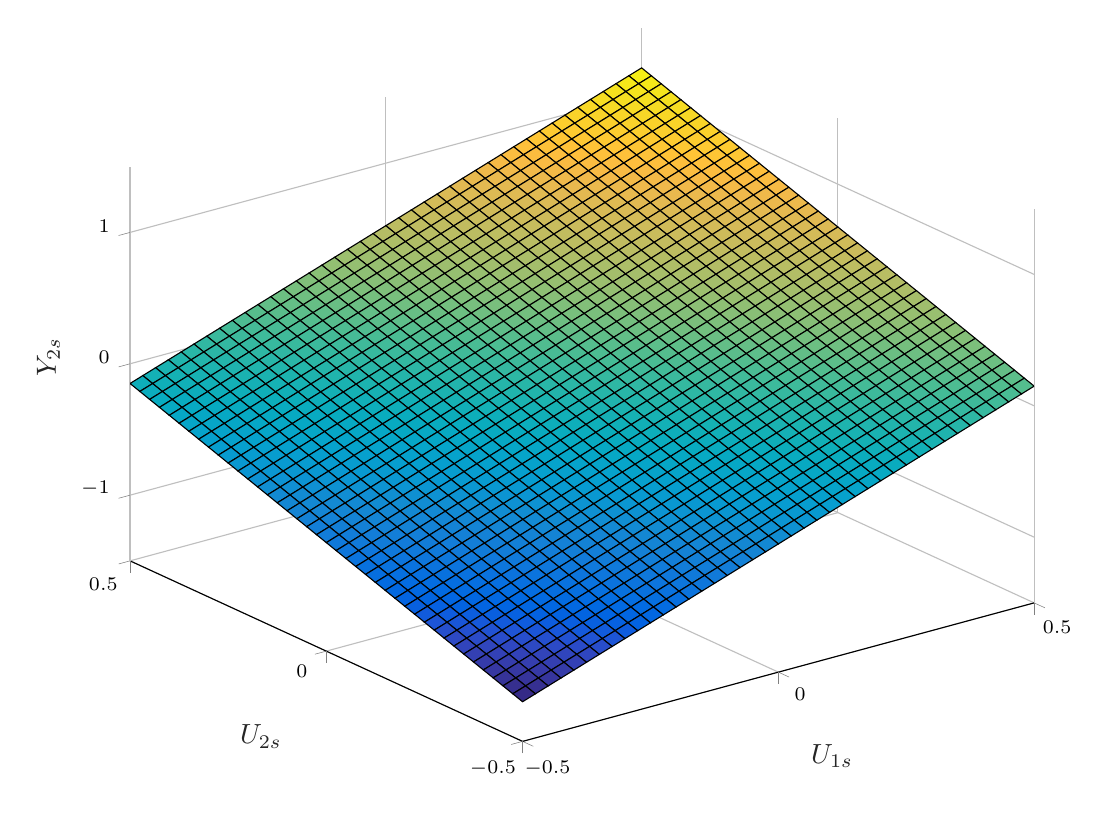
\begin{tikzpicture}

\begin{axis}[%
width=4.521in,
height=3.566in,
at={(0.758in,0.481in)},
scale only axis,
xmin=-0.5,
xmax=0.5,
xtick={-0.5,0,0.5},
tick align=outside,
xlabel style={font=\color{white!15!black}},
xlabel={$U_{1s}$},
ymin=-0.5,
ymax=0.5,
ytick={-0.5,0,0.5},
ylabel style={font=\color{white!15!black}},
ylabel={$U_{2s}$},
zmin=-1.5,
zmax=1.5,
zlabel style={font=\color{white!15!black}},
zlabel={$Y_{2s}$},
view={-37.5}{30},
axis background/.style={fill=white},
axis x line*=bottom,
axis y line*=left,
axis z line*=left,
xmajorgrids,
ymajorgrids,
zmajorgrids
]

\addplot3[%
surf,
shader=flat corner, draw=black, z buffer=sort, colormap={mymap}{[1pt] rgb(0pt)=(0.2081,0.1663,0.5292); rgb(1pt)=(0.211624,0.189781,0.577676); rgb(2pt)=(0.212252,0.213771,0.626971); rgb(3pt)=(0.2081,0.2386,0.677086); rgb(4pt)=(0.195905,0.264457,0.7279); rgb(5pt)=(0.170729,0.291938,0.779248); rgb(6pt)=(0.125271,0.324243,0.830271); rgb(7pt)=(0.0591333,0.359833,0.868333); rgb(8pt)=(0.0116952,0.38751,0.881957); rgb(9pt)=(0.00595714,0.408614,0.882843); rgb(10pt)=(0.0165143,0.4266,0.878633); rgb(11pt)=(0.0328524,0.443043,0.871957); rgb(12pt)=(0.0498143,0.458571,0.864057); rgb(13pt)=(0.0629333,0.47369,0.855438); rgb(14pt)=(0.0722667,0.488667,0.8467); rgb(15pt)=(0.0779429,0.503986,0.838371); rgb(16pt)=(0.0793476,0.520024,0.831181); rgb(17pt)=(0.0749429,0.537543,0.826271); rgb(18pt)=(0.0640571,0.556986,0.823957); rgb(19pt)=(0.0487714,0.577224,0.822829); rgb(20pt)=(0.0343429,0.596581,0.819852); rgb(21pt)=(0.0265,0.6137,0.8135); rgb(22pt)=(0.0238905,0.628662,0.803762); rgb(23pt)=(0.0230905,0.641786,0.791267); rgb(24pt)=(0.0227714,0.653486,0.776757); rgb(25pt)=(0.0266619,0.664195,0.760719); rgb(26pt)=(0.0383714,0.674271,0.743552); rgb(27pt)=(0.0589714,0.683757,0.725386); rgb(28pt)=(0.0843,0.692833,0.706167); rgb(29pt)=(0.113295,0.7015,0.685857); rgb(30pt)=(0.145271,0.709757,0.664629); rgb(31pt)=(0.180133,0.717657,0.642433); rgb(32pt)=(0.217829,0.725043,0.619262); rgb(33pt)=(0.258643,0.731714,0.595429); rgb(34pt)=(0.302171,0.737605,0.571186); rgb(35pt)=(0.348167,0.742433,0.547267); rgb(36pt)=(0.395257,0.7459,0.524443); rgb(37pt)=(0.44201,0.748081,0.503314); rgb(38pt)=(0.487124,0.749062,0.483976); rgb(39pt)=(0.530029,0.749114,0.466114); rgb(40pt)=(0.570857,0.748519,0.44939); rgb(41pt)=(0.609852,0.747314,0.433686); rgb(42pt)=(0.6473,0.7456,0.4188); rgb(43pt)=(0.683419,0.743476,0.404433); rgb(44pt)=(0.71841,0.741133,0.390476); rgb(45pt)=(0.752486,0.7384,0.376814); rgb(46pt)=(0.785843,0.735567,0.363271); rgb(47pt)=(0.818505,0.732733,0.34979); rgb(48pt)=(0.850657,0.7299,0.336029); rgb(49pt)=(0.882433,0.727433,0.3217); rgb(50pt)=(0.913933,0.725786,0.306276); rgb(51pt)=(0.944957,0.726114,0.288643); rgb(52pt)=(0.973895,0.731395,0.266648); rgb(53pt)=(0.993771,0.745457,0.240348); rgb(54pt)=(0.999043,0.765314,0.216414); rgb(55pt)=(0.995533,0.786057,0.196652); rgb(56pt)=(0.988,0.8066,0.179367); rgb(57pt)=(0.978857,0.827143,0.163314); rgb(58pt)=(0.9697,0.848138,0.147452); rgb(59pt)=(0.962586,0.870514,0.1309); rgb(60pt)=(0.958871,0.8949,0.113243); rgb(61pt)=(0.959824,0.921833,0.0948381); rgb(62pt)=(0.9661,0.951443,0.0755333); rgb(63pt)=(0.9763,0.9831,0.0538)}, mesh/rows=41]
table[row sep=crcr, point meta=\thisrow{c}] {%
%
x	y	z	c\\
-0.5	-0.5	-1.19818746145372	-1.19818746145372\\
-0.5	-0.475	-1.17197822434956	-1.17197822434956\\
-0.5	-0.45	-1.14576898724539	-1.14576898724539\\
-0.5	-0.425	-1.11955975014124	-1.11955975014124\\
-0.5	-0.4	-1.09335051303715	-1.09335051303715\\
-0.5	-0.375	-1.06714127593295	-1.06714127593295\\
-0.5	-0.35	-1.04093203882882	-1.04093203882882\\
-0.5	-0.325	-1.01472280172467	-1.01472280172467\\
-0.5	-0.3	-0.98851356462051	-0.98851356462051\\
-0.5	-0.275	-0.962304327516346	-0.962304327516346\\
-0.5	-0.25	-0.936095090412183	-0.936095090412183\\
-0.5	-0.225	-0.909885853308024	-0.909885853308024\\
-0.5	-0.2	-0.883676616203883	-0.883676616203883\\
-0.5	-0.175	-0.857467379099738	-0.857467379099738\\
-0.5	-0.15	-0.831258141995581	-0.831258141995581\\
-0.5	-0.125	-0.80504890489142	-0.80504890489142\\
-0.5	-0.1	-0.778839667787258	-0.778839667787258\\
-0.5	-0.075	-0.752630430683095	-0.752630430683095\\
-0.5	-0.05	-0.726421193578976	-0.726421193578976\\
-0.5	-0.025	-0.700211956474809	-0.700211956474809\\
-0.5	0	-0.674002719370652	-0.674002719370652\\
-0.5	0.025	-0.647793482266491	-0.647793482266491\\
-0.5	0.05	-0.62158424516233	-0.62158424516233\\
-0.5	0.0750000000000001	-0.595375008058168	-0.595375008058168\\
-0.5	0.1	-0.569165770954047	-0.569165770954047\\
-0.5	0.125	-0.542956533849886	-0.542956533849886\\
-0.5	0.15	-0.516747296745724	-0.516747296745724\\
-0.5	0.175	-0.490538059641561	-0.490538059641561\\
-0.5	0.2	-0.46432882253742	-0.46432882253742\\
-0.5	0.225	-0.43811958543326	-0.43811958543326\\
-0.5	0.25	-0.411910348329098	-0.411910348329098\\
-0.5	0.275	-0.385701111224957	-0.385701111224957\\
-0.5	0.3	-0.359491874120795	-0.359491874120795\\
-0.5	0.325	-0.333282637016634	-0.333282637016634\\
-0.5	0.35	-0.307073399912493	-0.307073399912493\\
-0.5	0.375	-0.280864162808332	-0.280864162808332\\
-0.5	0.4	-0.254654925704179	-0.254654925704179\\
-0.5	0.425	-0.228445688600018	-0.228445688600018\\
-0.5	0.45	-0.202236451495867	-0.202236451495867\\
-0.5	0.475	-0.176027214391716	-0.176027214391716\\
-0.5	0.5	-0.149817977287559	-0.149817977287559\\
-0.475	-0.5	-1.16448732548517	-1.16448732548517\\
-0.475	-0.475	-1.13827808838109	-1.13827808838109\\
-0.475	-0.45	-1.11206885127693	-1.11206885127693\\
-0.475	-0.425	-1.08585961417277	-1.08585961417277\\
-0.475	-0.4	-1.05965037706861	-1.05965037706861\\
-0.475	-0.375	-1.03344113996444	-1.03344113996444\\
-0.475	-0.35	-1.00723190286027	-1.00723190286027\\
-0.475	-0.325	-0.981022665756122	-0.981022665756122\\
-0.475	-0.3	-0.954813428651958	-0.954813428651958\\
-0.475	-0.275	-0.9286041915478	-0.9286041915478\\
-0.475	-0.25	-0.902394954443678	-0.902394954443678\\
-0.475	-0.225	-0.876185717339517	-0.876185717339517\\
-0.475	-0.2	-0.849976480235356	-0.849976480235356\\
-0.475	-0.175	-0.823767243131191	-0.823767243131191\\
-0.475	-0.15	-0.797558006027031	-0.797558006027031\\
-0.475	-0.125	-0.771348768922871	-0.771348768922871\\
-0.475	-0.1	-0.745139531818749	-0.745139531818749\\
-0.475	-0.075	-0.718930294714584	-0.718930294714584\\
-0.475	-0.05	-0.692721057610424	-0.692721057610424\\
-0.475	-0.025	-0.666511820506266	-0.666511820506266\\
-0.475	0	-0.640302583402101	-0.640302583402101\\
-0.475	0.025	-0.614093346297966	-0.614093346297966\\
-0.475	0.05	-0.587884109193818	-0.587884109193818\\
-0.475	0.0750000000000001	-0.561674872089658	-0.561674872089658\\
-0.475	0.1	-0.535465634985496	-0.535465634985496\\
-0.475	0.125	-0.509256397881335	-0.509256397881335\\
-0.475	0.15	-0.483047160777195	-0.483047160777195\\
-0.475	0.175	-0.456837923673034	-0.456837923673034\\
-0.475	0.2	-0.430628686568871	-0.430628686568871\\
-0.475	0.225	-0.40441944946473	-0.40441944946473\\
-0.475	0.25	-0.37821021236057	-0.37821021236057\\
-0.475	0.275	-0.352000975256407	-0.352000975256407\\
-0.475	0.3	-0.325791738152267	-0.325791738152267\\
-0.475	0.325	-0.299582501048105	-0.299582501048105\\
-0.475	0.35	-0.273373263943943	-0.273373263943943\\
-0.475	0.375	-0.247164026839804	-0.247164026839804\\
-0.475	0.4	-0.220954789735641	-0.220954789735641\\
-0.475	0.425	-0.19474555263149	-0.19474555263149\\
-0.475	0.45	-0.168536315527338	-0.168536315527338\\
-0.475	0.475	-0.142327078423178	-0.142327078423178\\
-0.475	0.5	-0.116117841319026	-0.116117841319026\\
-0.45	-0.5	-1.1307871895167	-1.1307871895167\\
-0.45	-0.475	-1.10457795241254	-1.10457795241254\\
-0.45	-0.45	-1.07836871530836	-1.07836871530836\\
-0.45	-0.425	-1.05215947820422	-1.05215947820422\\
-0.45	-0.4	-1.02595024110006	-1.02595024110006\\
-0.45	-0.375	-0.999741003995898	-0.999741003995898\\
-0.45	-0.35	-0.973531766891733	-0.973531766891733\\
-0.45	-0.325	-0.947322529787574	-0.947322529787574\\
-0.45	-0.3	-0.921113292683453	-0.921113292683453\\
-0.45	-0.275	-0.894904055579293	-0.894904055579293\\
-0.45	-0.25	-0.868694818475129	-0.868694818475129\\
-0.45	-0.225	-0.842485581370967	-0.842485581370967\\
-0.45	-0.2	-0.816276344266808	-0.816276344266808\\
-0.45	-0.175	-0.790067107162661	-0.790067107162661\\
-0.45	-0.15	-0.76385787005852	-0.76385787005852\\
-0.45	-0.125	-0.737648632954363	-0.737648632954363\\
-0.45	-0.1	-0.711439395850201	-0.711439395850201\\
-0.45	-0.075	-0.685230158746042	-0.685230158746042\\
-0.45	-0.05	-0.659020921641882	-0.659020921641882\\
-0.45	-0.025	-0.632811684537753	-0.632811684537753\\
-0.45	0	-0.606602447433596	-0.606602447433596\\
-0.45	0.025	-0.580393210329435	-0.580393210329435\\
-0.45	0.05	-0.554183973225275	-0.554183973225275\\
-0.45	0.0750000000000001	-0.527974736121122	-0.527974736121122\\
-0.45	0.1	-0.501765499016969	-0.501765499016969\\
-0.45	0.125	-0.475556261912808	-0.475556261912808\\
-0.45	0.15	-0.449347024808656	-0.449347024808656\\
-0.45	0.175	-0.423137787704503	-0.423137787704503\\
-0.45	0.2	-0.396928550600344	-0.396928550600344\\
-0.45	0.225	-0.370719313496202	-0.370719313496202\\
-0.45	0.25	-0.34451007639204	-0.34451007639204\\
-0.45	0.275	-0.318300839287879	-0.318300839287879\\
-0.45	0.3	-0.292091602183737	-0.292091602183737\\
-0.45	0.325	-0.265882365079576	-0.265882365079576\\
-0.45	0.35	-0.239673127975421	-0.239673127975421\\
-0.45	0.375	-0.213463890871264	-0.213463890871264\\
-0.45	0.4	-0.187254653767113	-0.187254653767113\\
-0.45	0.425	-0.161045416662961	-0.161045416662961\\
-0.45	0.45	-0.134836179558802	-0.134836179558802\\
-0.45	0.475	-0.108626942454648	-0.108626942454648\\
-0.45	0.5	-0.0824177053504948	-0.0824177053504948\\
-0.425	-0.5	-1.09708705354815	-1.09708705354815\\
-0.425	-0.475	-1.07087781644399	-1.07087781644399\\
-0.425	-0.45	-1.04466857933983	-1.04466857933983\\
-0.425	-0.425	-1.01845934223567	-1.01845934223567\\
-0.425	-0.4	-0.992250105131506	-0.992250105131506\\
-0.425	-0.375	-0.966040868027369	-0.966040868027369\\
-0.425	-0.35	-0.939831630923228	-0.939831630923228\\
-0.425	-0.325	-0.913622393819065	-0.913622393819065\\
-0.425	-0.3	-0.887413156714902	-0.887413156714902\\
-0.425	-0.275	-0.86120391961074	-0.86120391961074\\
-0.425	-0.25	-0.834994682506579	-0.834994682506579\\
-0.425	-0.225	-0.808785445402458	-0.808785445402458\\
-0.425	-0.2	-0.782576208298297	-0.782576208298297\\
-0.425	-0.175	-0.756366971194136	-0.756366971194136\\
-0.425	-0.15	-0.730157734089974	-0.730157734089974\\
-0.425	-0.125	-0.703948496985813	-0.703948496985813\\
-0.425	-0.1	-0.677739259881648	-0.677739259881648\\
-0.425	-0.075	-0.651530022777529	-0.651530022777529\\
-0.425	-0.05	-0.625320785673368	-0.625320785673368\\
-0.425	-0.025	-0.59911154856921	-0.59911154856921\\
-0.425	0	-0.572902311465044	-0.572902311465044\\
-0.425	0.025	-0.546693074360886	-0.546693074360886\\
-0.425	0.05	-0.520483837256742	-0.520483837256742\\
-0.425	0.0750000000000001	-0.494274600152582	-0.494274600152582\\
-0.425	0.1	-0.46806536304844	-0.46806536304844\\
-0.425	0.125	-0.44185612594428	-0.44185612594428\\
-0.425	0.15	-0.415646888840117	-0.415646888840117\\
-0.425	0.175	-0.389437651735976	-0.389437651735976\\
-0.425	0.2	-0.363228414631814	-0.363228414631814\\
-0.425	0.225	-0.337019177527653	-0.337019177527653\\
-0.425	0.25	-0.310809940423514	-0.310809940423514\\
-0.425	0.275	-0.284600703319352	-0.284600703319352\\
-0.425	0.3	-0.2583914662152	-0.2583914662152\\
-0.425	0.325	-0.232182229111038	-0.232182229111038\\
-0.425	0.35	-0.205972992006886	-0.205972992006886\\
-0.425	0.375	-0.179763754902735	-0.179763754902735\\
-0.425	0.4	-0.15355451779858	-0.15355451779858\\
-0.425	0.425	-0.127345280694423	-0.127345280694423\\
-0.425	0.45	-0.101136043590272	-0.101136043590272\\
-0.425	0.475	-0.0749268064861152	-0.0749268064861152\\
-0.425	0.5	-0.0487175693819614	-0.0487175693819614\\
-0.4	-0.5	-1.0633869175796	-1.0633869175796\\
-0.4	-0.475	-1.03717768047545	-1.03717768047545\\
-0.4	-0.45	-1.01096844337129	-1.01096844337129\\
-0.4	-0.425	-0.984759206267162	-0.984759206267162\\
-0.4	-0.4	-0.958549969162997	-0.958549969162997\\
-0.4	-0.375	-0.932340732058838	-0.932340732058838\\
-0.4	-0.35	-0.906131494954676	-0.906131494954676\\
-0.4	-0.325	-0.879922257850515	-0.879922257850515\\
-0.4	-0.3	-0.853713020746354	-0.853713020746354\\
-0.4	-0.275	-0.827503783642234	-0.827503783642234\\
-0.4	-0.25	-0.80129454653807	-0.80129454653807\\
-0.4	-0.225	-0.775085309433908	-0.775085309433908\\
-0.4	-0.2	-0.748876072329749	-0.748876072329749\\
-0.4	-0.175	-0.722666835225586	-0.722666835225586\\
-0.4	-0.15	-0.696457598121446	-0.696457598121446\\
-0.4	-0.125	-0.670248361017306	-0.670248361017306\\
-0.4	-0.1	-0.644039123913141	-0.644039123913141\\
-0.4	-0.075	-0.617829886808985	-0.617829886808985\\
-0.4	-0.05	-0.591620649704821	-0.591620649704821\\
-0.4	-0.025	-0.565411412600659	-0.565411412600659\\
-0.4	0	-0.539202175496527	-0.539202175496527\\
-0.4	0.025	-0.512992938392356	-0.512992938392356\\
-0.4	0.05	-0.486783701288215	-0.486783701288215\\
-0.4	0.0750000000000001	-0.460574464184051	-0.460574464184051\\
-0.4	0.1	-0.434365227079892	-0.434365227079892\\
-0.4	0.125	-0.408155989975751	-0.408155989975751\\
-0.4	0.15	-0.38194675287159	-0.38194675287159\\
-0.4	0.175	-0.355737515767437	-0.355737515767437\\
-0.4	0.2	-0.329528278663287	-0.329528278663287\\
-0.4	0.225	-0.303319041559125	-0.303319041559125\\
-0.4	0.25	-0.277109804454975	-0.277109804454975\\
-0.4	0.275	-0.250900567350824	-0.250900567350824\\
-0.4	0.3	-0.224691330246664	-0.224691330246664\\
-0.4	0.325	-0.19848209314251	-0.19848209314251\\
-0.4	0.35	-0.172272856038359	-0.172272856038359\\
-0.4	0.375	-0.146063618934202	-0.146063618934202\\
-0.4	0.4	-0.119854381830049	-0.119854381830049\\
-0.4	0.425	-0.0936451447258942	-0.0936451447258942\\
-0.4	0.45	-0.0674359076217389	-0.0674359076217389\\
-0.4	0.475	-0.041226670517584	-0.041226670517584\\
-0.4	0.5	-0.0150174334134301	-0.0150174334134301\\
-0.375	-0.5	-1.02968678161106	-1.02968678161106\\
-0.375	-0.475	-1.00347754450693	-1.00347754450693\\
-0.375	-0.45	-0.977268307402773	-0.977268307402773\\
-0.375	-0.425	-0.951059070298613	-0.951059070298613\\
-0.375	-0.4	-0.924849833194451	-0.924849833194451\\
-0.375	-0.375	-0.898640596090289	-0.898640596090289\\
-0.375	-0.35	-0.872431358986154	-0.872431358986154\\
-0.375	-0.325	-0.846222121882009	-0.846222121882009\\
-0.375	-0.3	-0.820012884777842	-0.820012884777842\\
-0.375	-0.275	-0.793803647673687	-0.793803647673687\\
-0.375	-0.25	-0.767594410569525	-0.767594410569525\\
-0.375	-0.225	-0.741385173465363	-0.741385173465363\\
-0.375	-0.2	-0.715175936361242	-0.715175936361242\\
-0.375	-0.175	-0.688966699257078	-0.688966699257078\\
-0.375	-0.15	-0.662757462152916	-0.662757462152916\\
-0.375	-0.125	-0.636548225048756	-0.636548225048756\\
-0.375	-0.1	-0.610338987944596	-0.610338987944596\\
-0.375	-0.075	-0.584129750840433	-0.584129750840433\\
-0.375	-0.05	-0.55792051373631	-0.55792051373631\\
-0.375	-0.025	-0.531711276632141	-0.531711276632141\\
-0.375	0	-0.505502039527989	-0.505502039527989\\
-0.375	0.025	-0.479292802423826	-0.479292802423826\\
-0.375	0.05	-0.453083565319686	-0.453083565319686\\
-0.375	0.0750000000000001	-0.426874328215525	-0.426874328215525\\
-0.375	0.1	-0.400665091111364	-0.400665091111364\\
-0.375	0.125	-0.374455854007222	-0.374455854007222\\
-0.375	0.15	-0.348246616903061	-0.348246616903061\\
-0.375	0.175	-0.322037379798899	-0.322037379798899\\
-0.375	0.2	-0.295828142694758	-0.295828142694758\\
-0.375	0.225	-0.269618905590597	-0.269618905590597\\
-0.375	0.25	-0.243409668486445	-0.243409668486445\\
-0.375	0.275	-0.217200431382284	-0.217200431382284\\
-0.375	0.3	-0.190991194278133	-0.190991194278133\\
-0.375	0.325	-0.16478195717398	-0.16478195717398\\
-0.375	0.35	-0.138572720069825	-0.138572720069825\\
-0.375	0.375	-0.112363482965668	-0.112363482965668\\
-0.375	0.4	-0.0861542458615169	-0.0861542458615169\\
-0.375	0.425	-0.0599450087573605	-0.0599450087573605\\
-0.375	0.45	-0.0337357716532067	-0.0337357716532067\\
-0.375	0.475	-0.0075265345490516	-0.0075265345490516\\
-0.375	0.5	0.0186827025551023	0.0186827025551023\\
-0.35	-0.5	-0.995986645642544	-0.995986645642544\\
-0.35	-0.475	-0.969777408538386	-0.969777408538386\\
-0.35	-0.45	-0.943568171434222	-0.943568171434222\\
-0.35	-0.425	-0.917358934330064	-0.917358934330064\\
-0.35	-0.4	-0.891149697225943	-0.891149697225943\\
-0.35	-0.375	-0.864940460121782	-0.864940460121782\\
-0.35	-0.35	-0.838731223017618	-0.838731223017618\\
-0.35	-0.325	-0.812521985913458	-0.812521985913458\\
-0.35	-0.3	-0.786312748809297	-0.786312748809297\\
-0.35	-0.275	-0.760103511705133	-0.760103511705133\\
-0.35	-0.25	-0.733894274601016	-0.733894274601016\\
-0.35	-0.225	-0.707685037496855	-0.707685037496855\\
-0.35	-0.2	-0.681475800392693	-0.681475800392693\\
-0.35	-0.175	-0.655266563288528	-0.655266563288528\\
-0.35	-0.15	-0.629057326184368	-0.629057326184368\\
-0.35	-0.125	-0.602848089080204	-0.602848089080204\\
-0.35	-0.1	-0.576638851976086	-0.576638851976086\\
-0.35	-0.075	-0.550429614871929	-0.550429614871929\\
-0.35	-0.05	-0.524220377767763	-0.524220377767763\\
-0.35	-0.025	-0.498011140663601	-0.498011140663601\\
-0.35	0	-0.47180190355946	-0.47180190355946\\
-0.35	0.025	-0.445592666455299	-0.445592666455299\\
-0.35	0.05	-0.419383429351138	-0.419383429351138\\
-0.35	0.0750000000000001	-0.393174192246996	-0.393174192246996\\
-0.35	0.1	-0.366964955142835	-0.366964955142835\\
-0.35	0.125	-0.340755718038674	-0.340755718038674\\
-0.35	0.15	-0.314546480934531	-0.314546480934531\\
-0.35	0.175	-0.28833724383037	-0.28833724383037\\
-0.35	0.2	-0.262128006726218	-0.262128006726218\\
-0.35	0.225	-0.235918769622069	-0.235918769622069\\
-0.35	0.25	-0.209709532517906	-0.209709532517906\\
-0.35	0.275	-0.183500295413755	-0.183500295413755\\
-0.35	0.3	-0.157291058309603	-0.157291058309603\\
-0.35	0.325	-0.131081821205447	-0.131081821205447\\
-0.35	0.35	-0.104872584101291	-0.104872584101291\\
-0.35	0.375	-0.0786633469971371	-0.0786633469971371\\
-0.35	0.4	-0.0524541098929833	-0.0524541098929833\\
-0.35	0.425	-0.0262448727888282	-0.0262448727888282\\
-0.35	0.45	-3.56356846743764e-05	-3.56356846743764e-05\\
-0.35	0.475	0.0261736014194807	0.0261736014194807\\
-0.35	0.5	0.0523828385236347	0.0523828385236347\\
-0.325	-0.5	-0.962286509673998	-0.962286509673998\\
-0.325	-0.475	-0.936077272569837	-0.936077272569837\\
-0.325	-0.45	-0.909868035465715	-0.909868035465715\\
-0.325	-0.425	-0.883658798361555	-0.883658798361555\\
-0.325	-0.4	-0.857449561257392	-0.857449561257392\\
-0.325	-0.375	-0.831240324153233	-0.831240324153233\\
-0.325	-0.35	-0.80503108704907	-0.80503108704907\\
-0.325	-0.325	-0.778821849944939	-0.778821849944939\\
-0.325	-0.3	-0.752612612840784	-0.752612612840784\\
-0.325	-0.275	-0.726403375736627	-0.726403375736627\\
-0.325	-0.25	-0.700194138632463	-0.700194138632463\\
-0.325	-0.225	-0.673984901528303	-0.673984901528303\\
-0.325	-0.2	-0.647775664424142	-0.647775664424142\\
-0.325	-0.175	-0.621566427320021	-0.621566427320021\\
-0.325	-0.15	-0.595357190215859	-0.595357190215859\\
-0.325	-0.125	-0.5691479531117	-0.5691479531117\\
-0.325	-0.1	-0.54293871600754	-0.54293871600754\\
-0.325	-0.075	-0.516729478903379	-0.516729478903379\\
-0.325	-0.05	-0.490520241799234	-0.490520241799234\\
-0.325	-0.025	-0.464311004695073	-0.464311004695073\\
-0.325	0	-0.438101767590912	-0.438101767590912\\
-0.325	0.025	-0.411892530486771	-0.411892530486771\\
-0.325	0.05	-0.385683293382609	-0.385683293382609\\
-0.325	0.0750000000000001	-0.359474056278457	-0.359474056278457\\
-0.325	0.1	-0.333264819174307	-0.333264819174307\\
-0.325	0.125	-0.307055582070144	-0.307055582070144\\
-0.325	0.15	-0.280846344966005	-0.280846344966005\\
-0.325	0.175	-0.254637107861843	-0.254637107861843\\
-0.325	0.2	-0.228427870757686	-0.228427870757686\\
-0.325	0.225	-0.202218633653529	-0.202218633653529\\
-0.325	0.25	-0.176009396549378	-0.176009396549378\\
-0.325	0.275	-0.149800159445227	-0.149800159445227\\
-0.325	0.3	-0.123590922341068	-0.123590922341068\\
-0.325	0.325	-0.0973816852369139	-0.0973816852369139\\
-0.325	0.35	-0.0711724481327571	-0.0711724481327571\\
-0.325	0.375	-0.0449632110286037	-0.0449632110286037\\
-0.325	0.4	-0.0187539739244504	-0.0187539739244504\\
-0.325	0.425	0.00745526317970474	0.00745526317970474\\
-0.325	0.45	0.0336645002838585	0.0336645002838585\\
-0.325	0.475	0.0598737373880144	0.0598737373880144\\
-0.325	0.5	0.0860829744921656	0.0860829744921656\\
-0.3	-0.5	-0.928586373705488	-0.928586373705488\\
-0.3	-0.475	-0.902377136601325	-0.902377136601325\\
-0.3	-0.45	-0.876167899497165	-0.876167899497165\\
-0.3	-0.425	-0.849958662393007	-0.849958662393007\\
-0.3	-0.4	-0.823749425288842	-0.823749425288842\\
-0.3	-0.375	-0.797540188184725	-0.797540188184725\\
-0.3	-0.35	-0.771330951080563	-0.771330951080563\\
-0.3	-0.325	-0.745121713976401	-0.745121713976401\\
-0.3	-0.3	-0.718912476872238	-0.718912476872238\\
-0.3	-0.275	-0.692703239768076	-0.692703239768076\\
-0.3	-0.25	-0.666494002663918	-0.666494002663918\\
-0.3	-0.225	-0.640284765559795	-0.640284765559795\\
-0.3	-0.2	-0.614075528455633	-0.614075528455633\\
-0.3	-0.175	-0.587866291351473	-0.587866291351473\\
-0.3	-0.15	-0.561657054247312	-0.561657054247312\\
-0.3	-0.125	-0.53544781714317	-0.53544781714317\\
-0.3	-0.1	-0.509238580039008	-0.509238580039008\\
-0.3	-0.075	-0.483029342934848	-0.483029342934848\\
-0.3	-0.05	-0.456820105830705	-0.456820105830705\\
-0.3	-0.025	-0.430610868726544	-0.430610868726544\\
-0.3	0	-0.404401631622384	-0.404401631622384\\
-0.3	0.025	-0.378192394518241	-0.378192394518241\\
-0.3	0.05	-0.351983157414079	-0.351983157414079\\
-0.3	0.0750000000000001	-0.325773920309918	-0.325773920309918\\
-0.3	0.1	-0.299564683205778	-0.299564683205778\\
-0.3	0.125	-0.273355446101616	-0.273355446101616\\
-0.3	0.15	-0.247146208997465	-0.247146208997465\\
-0.3	0.175	-0.220936971893304	-0.220936971893304\\
-0.3	0.2	-0.194727734789152	-0.194727734789152\\
-0.3	0.225	-0.168518497685001	-0.168518497685001\\
-0.3	0.25	-0.142309260580845	-0.142309260580845\\
-0.3	0.275	-0.116100023476688	-0.116100023476688\\
-0.3	0.3	-0.0898907863725367	-0.0898907863725367\\
-0.3	0.325	-0.0636815492683804	-0.0636815492683804\\
-0.3	0.35	-0.0374723121642265	-0.0374723121642265\\
-0.3	0.375	-0.0112630750600719	-0.0112630750600719\\
-0.3	0.4	0.0149461620440819	0.0149461620440819\\
-0.3	0.425	0.0411553991482377	0.0411553991482377\\
-0.3	0.45	0.0673646362523901	0.0673646362523901\\
-0.3	0.475	0.0935738733565477	0.0935738733565477\\
-0.3	0.5	0.119783110460699	0.119783110460699\\
-0.275	-0.5	-0.894886237736939	-0.894886237736939\\
-0.275	-0.475	-0.868677000632779	-0.868677000632779\\
-0.275	-0.45	-0.842467763528618	-0.842467763528618\\
-0.275	-0.425	-0.816258526424502	-0.816258526424502\\
-0.275	-0.4	-0.790049289320336	-0.790049289320336\\
-0.275	-0.375	-0.763840052216174	-0.763840052216174\\
-0.275	-0.35	-0.737630815112013	-0.737630815112013\\
-0.275	-0.325	-0.711421578007854	-0.711421578007854\\
-0.275	-0.3	-0.685212340903693	-0.685212340903693\\
-0.275	-0.275	-0.659003103799569	-0.659003103799569\\
-0.275	-0.25	-0.632793866695408	-0.632793866695408\\
-0.275	-0.225	-0.606584629591246	-0.606584629591246\\
-0.275	-0.2	-0.580375392487083	-0.580375392487083\\
-0.275	-0.175	-0.554166155382924	-0.554166155382924\\
-0.275	-0.15	-0.527956918278784	-0.527956918278784\\
-0.275	-0.125	-0.501747681174622	-0.501747681174622\\
-0.275	-0.1	-0.47553844407048	-0.47553844407048\\
-0.275	-0.075	-0.449329206966319	-0.449329206966319\\
-0.275	-0.05	-0.423119969862158	-0.423119969862158\\
-0.275	-0.025	-0.396910732758016	-0.396910732758016\\
-0.275	0	-0.370701495653853	-0.370701495653853\\
-0.275	0.025	-0.344492258549692	-0.344492258549692\\
-0.275	0.05	-0.31828302144555	-0.31828302144555\\
-0.275	0.0750000000000001	-0.292073784341391	-0.292073784341391\\
-0.275	0.1	-0.265864547237239	-0.265864547237239\\
-0.275	0.125	-0.239655310133087	-0.239655310133087\\
-0.275	0.15	-0.213446073028926	-0.213446073028926\\
-0.275	0.175	-0.187236835924775	-0.187236835924775\\
-0.275	0.2	-0.161027598820624	-0.161027598820624\\
-0.275	0.225	-0.134818361716465	-0.134818361716465\\
-0.275	0.25	-0.108609124612311	-0.108609124612311\\
-0.275	0.275	-0.0823998875081593	-0.0823998875081593\\
-0.275	0.3	-0.0561906504040032	-0.0561906504040032\\
-0.275	0.325	-0.0299814132998485	-0.0299814132998485\\
-0.275	0.35	-0.00377217619569408	-0.00377217619569408\\
-0.275	0.375	0.0224370609084606	0.0224370609084606\\
-0.275	0.4	0.048646298012615	0.048646298012615\\
-0.275	0.425	0.0748555351167686	0.0748555351167686\\
-0.275	0.45	0.101064772220925	0.101064772220925\\
-0.275	0.475	0.127274009325077	0.127274009325077\\
-0.275	0.5	0.153483246429233	0.153483246429233\\
-0.25	-0.5	-0.861186101768392	-0.861186101768392\\
-0.25	-0.475	-0.83497686466427	-0.83497686466427\\
-0.25	-0.45	-0.808767627560113	-0.808767627560113\\
-0.25	-0.425	-0.782558390455948	-0.782558390455948\\
-0.25	-0.4	-0.756349153351788	-0.756349153351788\\
-0.25	-0.375	-0.730139916247628	-0.730139916247628\\
-0.25	-0.35	-0.703930679143505	-0.703930679143505\\
-0.25	-0.325	-0.677721442039345	-0.677721442039345\\
-0.25	-0.3	-0.651512204935183	-0.651512204935183\\
-0.25	-0.275	-0.625302967831019	-0.625302967831019\\
-0.25	-0.25	-0.59909373072686	-0.59909373072686\\
-0.25	-0.225	-0.572884493622697	-0.572884493622697\\
-0.25	-0.2	-0.546675256518577	-0.546675256518577\\
-0.25	-0.175	-0.52046601941441	-0.52046601941441\\
-0.25	-0.15	-0.494256782310254	-0.494256782310254\\
-0.25	-0.125	-0.468047545206092	-0.468047545206092\\
-0.25	-0.1	-0.441838308101942	-0.441838308101942\\
-0.25	-0.075	-0.415629070997789	-0.415629070997789\\
-0.25	-0.05	-0.389419833893629	-0.389419833893629\\
-0.25	-0.025	-0.363210596789488	-0.363210596789488\\
-0.25	0	-0.337001359685326	-0.337001359685326\\
-0.25	0.025	-0.310792122581165	-0.310792122581165\\
-0.25	0.05	-0.284582885477023	-0.284582885477023\\
-0.25	0.0750000000000001	-0.258373648372861	-0.258373648372861\\
-0.25	0.1	-0.232164411268711	-0.232164411268711\\
-0.25	0.125	-0.205955174164549	-0.205955174164549\\
-0.25	0.15	-0.179745937060397	-0.179745937060397\\
-0.25	0.175	-0.153536699956246	-0.153536699956246\\
-0.25	0.2	-0.12732746285209	-0.12732746285209\\
-0.25	0.225	-0.101118225747933	-0.101118225747933\\
-0.25	0.25	-0.0749089886437794	-0.0749089886437794\\
-0.25	0.275	-0.0486997515396258	-0.0486997515396258\\
-0.25	0.3	-0.0224905144354709	-0.0224905144354709\\
-0.25	0.325	0.00371872266868377	0.00371872266868377\\
-0.25	0.35	0.0299279597728382	0.0299279597728382\\
-0.25	0.375	0.0561371968769922	0.0561371968769922\\
-0.25	0.4	0.082346433981146	0.082346433981146\\
-0.25	0.425	0.108555671085302	0.108555671085302\\
-0.25	0.45	0.134764908189456	0.134764908189456\\
-0.25	0.475	0.16097414529361	0.16097414529361\\
-0.25	0.5	0.187183382397761	0.187183382397761\\
-0.225	-0.5	-0.827485965799885	-0.827485965799885\\
-0.225	-0.475	-0.801276728695724	-0.801276728695724\\
-0.225	-0.45	-0.775067491591566	-0.775067491591566\\
-0.225	-0.425	-0.748858254487402	-0.748858254487402\\
-0.225	-0.4	-0.72264901738328	-0.72264901738328\\
-0.225	-0.375	-0.696439780279119	-0.696439780279119\\
-0.225	-0.35	-0.670230543174955	-0.670230543174955\\
-0.225	-0.325	-0.644021306070796	-0.644021306070796\\
-0.225	-0.3	-0.617812068966632	-0.617812068966632\\
-0.225	-0.275	-0.591602831862475	-0.591602831862475\\
-0.225	-0.25	-0.565393594758351	-0.565393594758351\\
-0.225	-0.225	-0.539184357654182	-0.539184357654182\\
-0.225	-0.2	-0.512975120550028	-0.512975120550028\\
-0.225	-0.175	-0.486765883445867	-0.486765883445867\\
-0.225	-0.15	-0.460556646341726	-0.460556646341726\\
-0.225	-0.125	-0.434347409237565	-0.434347409237565\\
-0.225	-0.1	-0.408138172133402	-0.408138172133402\\
-0.225	-0.075	-0.381928935029261	-0.381928935029261\\
-0.225	-0.05	-0.355719697925099	-0.355719697925099\\
-0.225	-0.025	-0.329510460820938	-0.329510460820938\\
-0.225	0	-0.303301223716798	-0.303301223716798\\
-0.225	0.025	-0.277091986612636	-0.277091986612636\\
-0.225	0.05	-0.250882749508485	-0.250882749508485\\
-0.225	0.0750000000000001	-0.224673512404328	-0.224673512404328\\
-0.225	0.1	-0.198464275300172	-0.198464275300172\\
-0.225	0.125	-0.17225503819602	-0.17225503819602\\
-0.225	0.15	-0.146045801091869	-0.146045801091869\\
-0.225	0.175	-0.119836563987713	-0.119836563987713\\
-0.225	0.2	-0.0936273268835564	-0.0936273268835564\\
-0.225	0.225	-0.067418089779401	-0.067418089779401\\
-0.225	0.25	-0.0412088526752476	-0.0412088526752476\\
-0.225	0.275	-0.0149996155710929	-0.0149996155710929\\
-0.225	0.3	0.0112096215330616	0.0112096215330616\\
-0.225	0.325	0.0374188586372156	0.0374188586372156\\
-0.225	0.35	0.0636280957413707	0.0636280957413707\\
-0.225	0.375	0.0898373328455232	0.0898373328455232\\
-0.225	0.4	0.116046569949679	0.116046569949679\\
-0.225	0.425	0.142255807053837	0.142255807053837\\
-0.225	0.45	0.168465044157987	0.168465044157987\\
-0.225	0.475	0.194674281262138	0.194674281262138\\
-0.225	0.5	0.220883518366299	0.220883518366299\\
-0.2	-0.5	-0.793785829831334	-0.793785829831334\\
-0.2	-0.475	-0.767576592727176	-0.767576592727176\\
-0.2	-0.45	-0.741367355623054	-0.741367355623054\\
-0.2	-0.425	-0.715158118518891	-0.715158118518891\\
-0.2	-0.4	-0.688948881414731	-0.688948881414731\\
-0.2	-0.375	-0.662739644310572	-0.662739644310572\\
-0.2	-0.35	-0.636530407206408	-0.636530407206408\\
-0.2	-0.325	-0.61032117010227	-0.61032117010227\\
-0.2	-0.3	-0.584111932998124	-0.584111932998124\\
-0.2	-0.275	-0.557902695893965	-0.557902695893965\\
-0.2	-0.25	-0.531693458789802	-0.531693458789802\\
-0.2	-0.225	-0.505484221685645	-0.505484221685645\\
-0.2	-0.2	-0.479274984581499	-0.479274984581499\\
-0.2	-0.175	-0.45306574747734	-0.45306574747734\\
-0.2	-0.15	-0.426856510373178	-0.426856510373178\\
-0.2	-0.125	-0.400647273269035	-0.400647273269035\\
-0.2	-0.1	-0.374438036164874	-0.374438036164874\\
-0.2	-0.075	-0.348228799060711	-0.348228799060711\\
-0.2	-0.05	-0.322019561956572	-0.322019561956572\\
-0.2	-0.025	-0.295810324852409	-0.295810324852409\\
-0.2	0	-0.26960108774826	-0.26960108774826\\
-0.2	0.025	-0.243391850644107	-0.243391850644107\\
-0.2	0.05	-0.217182613539946	-0.217182613539946\\
-0.2	0.0750000000000001	-0.190973376435795	-0.190973376435795\\
-0.2	0.1	-0.164764139331643	-0.164764139331643\\
-0.2	0.125	-0.138554902227482	-0.138554902227482\\
-0.2	0.15	-0.11234566512333	-0.11234566512333\\
-0.2	0.175	-0.086136428019179	-0.086136428019179\\
-0.2	0.2	-0.0599271909150227	-0.0599271909150227\\
-0.2	0.225	-0.0337179538108689	-0.0337179538108689\\
-0.2	0.25	-0.0075087167067144	-0.0075087167067144\\
-0.2	0.275	0.01870052039744	0.01870052039744\\
-0.2	0.3	0.0449097575015953	0.0449097575015953\\
-0.2	0.325	0.0711189946057488	0.0711189946057488\\
-0.2	0.35	0.0973282317099058	0.0973282317099058\\
-0.2	0.375	0.123537468814057	0.123537468814057\\
-0.2	0.4	0.149746705918213	0.149746705918213\\
-0.2	0.425	0.175955943022364	0.175955943022364\\
-0.2	0.45	0.202165180126521	0.202165180126521\\
-0.2	0.475	0.228374417230677	0.228374417230677\\
-0.2	0.5	0.254583654334829	0.254583654334829\\
-0.175	-0.5	-0.760085693862828	-0.760085693862828\\
-0.175	-0.475	-0.733876456758664	-0.733876456758664\\
-0.175	-0.45	-0.707667219654506	-0.707667219654506\\
-0.175	-0.425	-0.681457982550344	-0.681457982550344\\
-0.175	-0.4	-0.655248745446181	-0.655248745446181\\
-0.175	-0.375	-0.629039508342062	-0.629039508342062\\
-0.175	-0.35	-0.6028302712379	-0.6028302712379\\
-0.175	-0.325	-0.576621034133737	-0.576621034133737\\
-0.175	-0.3	-0.550411797029578	-0.550411797029578\\
-0.175	-0.275	-0.524202559925439	-0.524202559925439\\
-0.175	-0.25	-0.497993322821272	-0.497993322821272\\
-0.175	-0.225	-0.471784085717113	-0.471784085717113\\
-0.175	-0.2	-0.445574848612972	-0.445574848612972\\
-0.175	-0.175	-0.419365611508809	-0.419365611508809\\
-0.175	-0.15	-0.393156374404648	-0.393156374404648\\
-0.175	-0.125	-0.366947137300508	-0.366947137300508\\
-0.175	-0.1	-0.340737900196347	-0.340737900196347\\
-0.175	-0.075	-0.314528663092185	-0.314528663092185\\
-0.175	-0.05	-0.288319425988043	-0.288319425988043\\
-0.175	-0.025	-0.262110188883883	-0.262110188883883\\
-0.175	0	-0.23590095177973	-0.23590095177973\\
-0.175	0.025	-0.209691714675569	-0.209691714675569\\
-0.175	0.05	-0.183482477571418	-0.183482477571418\\
-0.175	0.0750000000000001	-0.157273240467266	-0.157273240467266\\
-0.175	0.1	-0.131064003363109	-0.131064003363109\\
-0.175	0.125	-0.104854766258953	-0.104854766258953\\
-0.175	0.15	-0.0786455291548015	-0.0786455291548015\\
-0.175	0.175	-0.0524362920506456	-0.0524362920506456\\
-0.175	0.2	-0.0262270549464917	-0.0262270549464917\\
-0.175	0.225	-1.78178423371882e-05	-1.78178423371882e-05\\
-0.175	0.25	0.0261914192618173	0.0261914192618173\\
-0.175	0.275	0.0524006563659725	0.0524006563659725\\
-0.175	0.3	0.0786098934701261	0.0786098934701261\\
-0.175	0.325	0.104819130574283	0.104819130574283\\
-0.175	0.35	0.131028367678435	0.131028367678435\\
-0.175	0.375	0.15723760478259	0.15723760478259\\
-0.175	0.4	0.183446841886741	0.183446841886741\\
-0.175	0.425	0.209656078990903	0.209656078990903\\
-0.175	0.45	0.235865316095055	0.235865316095055\\
-0.175	0.475	0.262074553199206	0.262074553199206\\
-0.175	0.5	0.288283790303369	0.288283790303369\\
-0.15	-0.5	-0.72638555789428	-0.72638555789428\\
-0.15	-0.475	-0.700176320790116	-0.700176320790116\\
-0.15	-0.45	-0.673967083685955	-0.673967083685955\\
-0.15	-0.425	-0.647757846581835	-0.647757846581835\\
-0.15	-0.4	-0.621548609477673	-0.621548609477673\\
-0.15	-0.375	-0.595339372373511	-0.595339372373511\\
-0.15	-0.35	-0.569130135269353	-0.569130135269353\\
-0.15	-0.325	-0.542920898165191	-0.542920898165191\\
-0.15	-0.3	-0.516711661061048	-0.516711661061048\\
-0.15	-0.275	-0.490502423956887	-0.490502423956887\\
-0.15	-0.25	-0.464293186852744	-0.464293186852744\\
-0.15	-0.225	-0.438083949748583	-0.438083949748583\\
-0.15	-0.2	-0.411874712644421	-0.411874712644421\\
-0.15	-0.175	-0.385665475540282	-0.385665475540282\\
-0.15	-0.15	-0.359456238436119	-0.359456238436119\\
-0.15	-0.125	-0.333247001331959	-0.333247001331959\\
-0.15	-0.1	-0.307037764227817	-0.307037764227817\\
-0.15	-0.075	-0.280828527123656	-0.280828527123656\\
-0.15	-0.05	-0.254619290019504	-0.254619290019504\\
-0.15	-0.025	-0.228410052915353	-0.228410052915353\\
-0.15	0	-0.202200815811192	-0.202200815811192\\
-0.15	0.025	-0.17599157870704	-0.17599157870704\\
-0.15	0.05	-0.149782341602889	-0.149782341602889\\
-0.15	0.0750000000000001	-0.123573104498732	-0.123573104498732\\
-0.15	0.1	-0.097363867394576	-0.097363867394576\\
-0.15	0.125	-0.0711546302904226	-0.0711546302904226\\
-0.15	0.15	-0.0449453931862684	-0.0449453931862684\\
-0.15	0.175	-0.0187361560821132	-0.0187361560821132\\
-0.15	0.2	0.00747308102204097	0.00747308102204097\\
-0.15	0.225	0.0336823181261951	0.0336823181261951\\
-0.15	0.25	0.0598915552303495	0.0598915552303495\\
-0.15	0.275	0.0861007923345031	0.0861007923345031\\
-0.15	0.3	0.11231002943866	0.11231002943866\\
-0.15	0.325	0.138519266542816	0.138519266542816\\
-0.15	0.35	0.164728503646968	0.164728503646968\\
-0.15	0.375	0.190937740751118	0.190937740751118\\
-0.15	0.4	0.217146977855281	0.217146977855281\\
-0.15	0.425	0.243356214959433	0.243356214959433\\
-0.15	0.45	0.269565452063588	0.269565452063588\\
-0.15	0.475	0.295774689167736	0.295774689167736\\
-0.15	0.5	0.321983926271895	0.321983926271895\\
-0.125	-0.5	-0.692685421925771	-0.692685421925771\\
-0.125	-0.475	-0.666476184821609	-0.666476184821609\\
-0.125	-0.45	-0.640266947717447	-0.640266947717447\\
-0.125	-0.425	-0.614057710613284	-0.614057710613284\\
-0.125	-0.4	-0.587848473509125	-0.587848473509125\\
-0.125	-0.375	-0.56163923640496	-0.56163923640496\\
-0.125	-0.35	-0.535429999300822	-0.535429999300822\\
-0.125	-0.325	-0.509220762196657	-0.509220762196657\\
-0.125	-0.3	-0.483011525092519	-0.483011525092519\\
-0.125	-0.275	-0.456802287988356	-0.456802287988356\\
-0.125	-0.25	-0.430593050884196	-0.430593050884196\\
-0.125	-0.225	-0.404383813780057	-0.404383813780057\\
-0.125	-0.2	-0.378174576675894	-0.378174576675894\\
-0.125	-0.175	-0.351965339571752	-0.351965339571752\\
-0.125	-0.15	-0.325756102467591	-0.325756102467591\\
-0.125	-0.125	-0.29954686536343	-0.29954686536343\\
-0.125	-0.1	-0.273337628259288	-0.273337628259288\\
-0.125	-0.075	-0.247128391155128	-0.247128391155128\\
-0.125	-0.05	-0.220919154050971	-0.220919154050971\\
-0.125	-0.025	-0.194709916946814	-0.194709916946814\\
-0.125	0	-0.168500679842663	-0.168500679842663\\
-0.125	0.025	-0.142291442738512	-0.142291442738512\\
-0.125	0.05	-0.116082205634355	-0.116082205634355\\
-0.125	0.0750000000000001	-0.0898729685301987	-0.0898729685301987\\
-0.125	0.1	-0.0636637314260448	-0.0636637314260448\\
-0.125	0.125	-0.0374544943218897	-0.0374544943218897\\
-0.125	0.15	-0.0112452572177354	-0.0112452572177354\\
-0.125	0.175	0.0149639798864191	0.0149639798864191\\
-0.125	0.2	0.041173216990573	0.041173216990573\\
-0.125	0.225	0.0673824540947281	0.0673824540947281\\
-0.125	0.25	0.0935916911988806	0.0935916911988806\\
-0.125	0.275	0.119800928303037	0.119800928303037\\
-0.125	0.3	0.146010165407194	0.146010165407194\\
-0.125	0.325	0.172219402511344	0.172219402511344\\
-0.125	0.35	0.198428639615496	0.198428639615496\\
-0.125	0.375	0.224637876719657	0.224637876719657\\
-0.125	0.4	0.25084711382381	0.25084711382381\\
-0.125	0.425	0.277056350927961	0.277056350927961\\
-0.125	0.45	0.303265588032121	0.303265588032121\\
-0.125	0.475	0.329474825136265	0.329474825136265\\
-0.125	0.5	0.355684062240425	0.355684062240425\\
-0.1	-0.5	-0.658985285957219	-0.658985285957219\\
-0.1	-0.475	-0.632776048853059	-0.632776048853059\\
-0.1	-0.45	-0.606566811748904	-0.606566811748904\\
-0.1	-0.425	-0.580357574644737	-0.580357574644737\\
-0.1	-0.4	-0.554148337540619	-0.554148337540619\\
-0.1	-0.375	-0.527939100436451	-0.527939100436451\\
-0.1	-0.35	-0.501729863332294	-0.501729863332294\\
-0.1	-0.325	-0.475520626228132	-0.475520626228132\\
-0.1	-0.3	-0.44931138912399	-0.44931138912399\\
-0.1	-0.275	-0.42310215201983	-0.42310215201983\\
-0.1	-0.25	-0.396892914915667	-0.396892914915667\\
-0.1	-0.225	-0.370683677811527	-0.370683677811527\\
-0.1	-0.2	-0.344474440707367	-0.344474440707367\\
-0.1	-0.175	-0.318265203603204	-0.318265203603204\\
-0.1	-0.15	-0.292055966499062	-0.292055966499062\\
-0.1	-0.125	-0.265846729394901	-0.265846729394901\\
-0.1	-0.1	-0.239637492290749	-0.239637492290749\\
-0.1	-0.075	-0.213428255186589	-0.213428255186589\\
-0.1	-0.05	-0.187219018082437	-0.187219018082437\\
-0.1	-0.025	-0.161009780978285	-0.161009780978285\\
-0.1	0	-0.13480054387413	-0.13480054387413\\
-0.1	0.025	-0.108591306769973	-0.108591306769973\\
-0.1	0.05	-0.0823820696658216	-0.0823820696658216\\
-0.1	0.0750000000000001	-0.0561728325616652	-0.0561728325616652\\
-0.1	0.1	-0.0299635954575113	-0.0299635954575113\\
-0.1	0.125	-0.0037543583533572	-0.0037543583533572\\
-0.1	0.15	0.0224548787507976	0.0224548787507976\\
-0.1	0.175	0.0486641158549529	0.0486641158549529\\
-0.1	0.2	0.0748733529591066	0.0748733529591066\\
-0.1	0.225	0.101082590063261	0.101082590063261\\
-0.1	0.25	0.127291827167414	0.127291827167414\\
-0.1	0.275	0.15350106427157	0.15350106427157\\
-0.1	0.3	0.179710301375722	0.179710301375722\\
-0.1	0.325	0.205919538479878	0.205919538479878\\
-0.1	0.35	0.232128775584035	0.232128775584035\\
-0.1	0.375	0.258338012688186	0.258338012688186\\
-0.1	0.4	0.28454724979235	0.28454724979235\\
-0.1	0.425	0.310756486896489	0.310756486896489\\
-0.1	0.45	0.33696572400065	0.33696572400065\\
-0.1	0.475	0.363174961104812	0.363174961104812\\
-0.1	0.5	0.389384198208954	0.389384198208954\\
-0.075	-0.5	-0.625285149988674	-0.625285149988674\\
-0.075	-0.475	-0.59907591288455	-0.59907591288455\\
-0.075	-0.45	-0.572866675780389	-0.572866675780389\\
-0.075	-0.425	-0.546657438676228	-0.546657438676228\\
-0.075	-0.4	-0.520448201572067	-0.520448201572067\\
-0.075	-0.375	-0.494238964467907	-0.494238964467907\\
-0.075	-0.35	-0.468029727363764	-0.468029727363764\\
-0.075	-0.325	-0.441820490259603	-0.441820490259603\\
-0.075	-0.3	-0.415611253155444	-0.415611253155444\\
-0.075	-0.275	-0.389402016051301	-0.389402016051301\\
-0.075	-0.25	-0.363192778947138	-0.363192778947138\\
-0.075	-0.225	-0.336983541842978	-0.336983541842978\\
-0.075	-0.2	-0.310774304738837	-0.310774304738837\\
-0.075	-0.175	-0.284565067634674	-0.284565067634674\\
-0.075	-0.15	-0.258355830530524	-0.258355830530524\\
-0.075	-0.125	-0.232146593426372	-0.232146593426372\\
-0.075	-0.1	-0.205937356322212	-0.205937356322212\\
-0.075	-0.075	-0.17972811921806	-0.17972811921806\\
-0.075	-0.05	-0.153518882113908	-0.153518882113908\\
-0.075	-0.025	-0.127309645009752	-0.127309645009752\\
-0.075	0	-0.101100407905596	-0.101100407905596\\
-0.075	0.025	-0.0748911708014444	-0.0748911708014444\\
-0.075	0.05	-0.048681933697288	-0.048681933697288\\
-0.075	0.0750000000000001	-0.0224726965931342	-0.0224726965931342\\
-0.075	0.1	0.00373654051102049	0.00373654051102049\\
-0.075	0.125	0.0299457776151749	0.0299457776151749\\
-0.075	0.15	0.0561550147193297	0.0561550147193297\\
-0.075	0.175	0.0823642518234839	0.0823642518234839\\
-0.075	0.2	0.108573488927641	0.108573488927641\\
-0.075	0.225	0.134782726031794	0.134782726031794\\
-0.075	0.25	0.160991963135947	0.160991963135947\\
-0.075	0.275	0.187201200240099	0.187201200240099\\
-0.075	0.3	0.213410437344262	0.213410437344262\\
-0.075	0.325	0.239619674448413	0.239619674448413\\
-0.075	0.35	0.265828911552563	0.265828911552563\\
-0.075	0.375	0.292038148656715	0.292038148656715\\
-0.075	0.4	0.318247385760876	0.318247385760876\\
-0.075	0.425	0.344456622865037	0.344456622865037\\
-0.075	0.45	0.370665859969178	0.370665859969178\\
-0.075	0.475	0.396875097073339	0.396875097073339\\
-0.075	0.5	0.423084334177482	0.423084334177482\\
-0.05	-0.5	-0.591585014020165	-0.591585014020165\\
-0.05	-0.475	-0.565375776916003	-0.565375776916003\\
-0.05	-0.45	-0.539166539811851	-0.539166539811851\\
-0.05	-0.425	-0.512957302707681	-0.512957302707681\\
-0.05	-0.4	-0.48674806560354	-0.48674806560354\\
-0.05	-0.375	-0.460538828499378	-0.460538828499378\\
-0.05	-0.35	-0.434329591395235	-0.434329591395235\\
-0.05	-0.325	-0.408120354291076	-0.408120354291076\\
-0.05	-0.3	-0.381911117186914	-0.381911117186914\\
-0.05	-0.275	-0.355701880082774	-0.355701880082774\\
-0.05	-0.25	-0.32949264297861	-0.32949264297861\\
-0.05	-0.225	-0.303283405874451	-0.303283405874451\\
-0.05	-0.2	-0.27707416877031	-0.27707416877031\\
-0.05	-0.175	-0.250864931666147	-0.250864931666147\\
-0.05	-0.15	-0.224655694561995	-0.224655694561995\\
-0.05	-0.125	-0.198446457457833	-0.198446457457833\\
-0.05	-0.1	-0.172237220353684	-0.172237220353684\\
-0.05	-0.075	-0.146027983249531	-0.146027983249531\\
-0.05	-0.05	-0.119818746145375	-0.119818746145375\\
-0.05	-0.025	-0.0936095090412186	-0.0936095090412186\\
-0.05	0	-0.067400271937065	-0.067400271937065\\
-0.05	0.025	-0.0411910348329108	-0.0411910348329108\\
-0.05	0.05	-0.0149817977287557	-0.0149817977287557\\
-0.05	0.0750000000000001	0.0112274393753988	0.0112274393753988\\
-0.05	0.1	0.0374366764795533	0.0374366764795533\\
-0.05	0.125	0.0636459135837071	0.0636459135837071\\
-0.05	0.15	0.0898551506878611	0.0898551506878611\\
-0.05	0.175	0.116064387792017	0.116064387792017\\
-0.05	0.2	0.142273624896173	0.142273624896173\\
-0.05	0.225	0.168482862000325	0.168482862000325\\
-0.05	0.25	0.194692099104477	0.194692099104477\\
-0.05	0.275	0.220901336208638	0.220901336208638\\
-0.05	0.3	0.24711057331279	0.24711057331279\\
-0.05	0.325	0.273319810416941	0.273319810416941\\
-0.05	0.35	0.299529047521102	0.299529047521102\\
-0.05	0.375	0.325738284625243	0.325738284625243\\
-0.05	0.4	0.351947521729404	0.351947521729404\\
-0.05	0.425	0.378156758833567	0.378156758833567\\
-0.05	0.45	0.404365995937708	0.404365995937708\\
-0.05	0.475	0.430575233041867	0.430575233041867\\
-0.05	0.5	0.456784470146031	0.456784470146031\\
-0.025	-0.5	-0.557884878051616	-0.557884878051616\\
-0.025	-0.475	-0.531675640947474	-0.531675640947474\\
-0.025	-0.45	-0.505466403843313	-0.505466403843313\\
-0.025	-0.425	-0.479257166739151	-0.479257166739151\\
-0.025	-0.4	-0.453047929635012	-0.453047929635012\\
-0.025	-0.375	-0.42683869253085	-0.42683869253085\\
-0.025	-0.35	-0.40062945542669	-0.40062945542669\\
-0.025	-0.325	-0.374420218322548	-0.374420218322548\\
-0.025	-0.3	-0.348210981218387	-0.348210981218387\\
-0.025	-0.275	-0.322001744114221	-0.322001744114221\\
-0.025	-0.25	-0.295792507010082	-0.295792507010082\\
-0.025	-0.225	-0.269583269905925	-0.269583269905925\\
-0.025	-0.2	-0.243374032801769	-0.243374032801769\\
-0.025	-0.175	-0.217164795697618	-0.217164795697618\\
-0.025	-0.15	-0.190955558593457	-0.190955558593457\\
-0.025	-0.125	-0.164746321489305	-0.164746321489305\\
-0.025	-0.1	-0.138537084385155	-0.138537084385155\\
-0.025	-0.075	-0.112327847280998	-0.112327847280998\\
-0.025	-0.05	-0.0861186101768414	-0.0861186101768414\\
-0.025	-0.025	-0.0599093730726873	-0.0599093730726873\\
-0.025	0	-0.0337001359685321	-0.0337001359685321\\
-0.025	0.025	-0.00749089886437787	-0.00749089886437787\\
-0.025	0.05	0.0187183382397767	0.0187183382397767\\
-0.025	0.0750000000000001	0.0449275753439306	0.0449275753439306\\
-0.025	0.1	0.0711368124480875	0.0711368124480875\\
-0.025	0.125	0.0973460495522385	0.0973460495522385\\
-0.025	0.15	0.123555286656395	0.123555286656395\\
-0.025	0.175	0.149764523760551	0.149764523760551\\
-0.025	0.2	0.175973760864702	0.175973760864702\\
-0.025	0.225	0.202182997968854	0.202182997968854\\
-0.025	0.25	0.228392235073015	0.228392235073015\\
-0.025	0.275	0.254601472177166	0.254601472177166\\
-0.025	0.3	0.280810709281327	0.280810709281327\\
-0.025	0.325	0.307019946385469	0.307019946385469\\
-0.025	0.35	0.333229183489629	0.333229183489629\\
-0.025	0.375	0.359438420593793	0.359438420593793\\
-0.025	0.4	0.385647657697933	0.385647657697933\\
-0.025	0.425	0.411856894802095	0.411856894802095\\
-0.025	0.45	0.438066131906256	0.438066131906256\\
-0.025	0.475	0.464275369010397	0.464275369010397\\
-0.025	0.5	0.490484606114559	0.490484606114559\\
0	-0.5	-0.524184742083088	-0.524184742083088\\
0	-0.475	-0.497975504978926	-0.497975504978926\\
0	-0.45	-0.471766267874785	-0.471766267874785\\
0	-0.425	-0.445557030770623	-0.445557030770623\\
0	-0.4	-0.419347793666461	-0.419347793666461\\
0	-0.375	-0.393138556562322	-0.393138556562322\\
0	-0.35	-0.366929319458159	-0.366929319458159\\
0	-0.325	-0.34072008235401	-0.34072008235401\\
0	-0.3	-0.314510845249858	-0.314510845249858\\
0	-0.275	-0.288301608145695	-0.288301608145695\\
0	-0.25	-0.262092371041544	-0.262092371041544\\
0	-0.225	-0.235883133937393	-0.235883133937393\\
0	-0.2	-0.20967389683323	-0.20967389683323\\
0	-0.175	-0.18346465972908	-0.18346465972908\\
0	-0.15	-0.157255422624928	-0.157255422624928\\
0	-0.125	-0.131046185520772	-0.131046185520772\\
0	-0.1	-0.104836948416615	-0.104836948416615\\
0	-0.075	-0.0786277113124644	-0.0786277113124644\\
0	-0.05	-0.0524184742083076	-0.0524184742083076\\
0	-0.025	-0.0262092371041538	-0.0262092371041538\\
0	0	0	0\\
0	0.025	0.0262092371041538	0.0262092371041538\\
0	0.05	0.0524184742083076	0.0524184742083076\\
0	0.0750000000000001	0.0786277113124644	0.0786277113124644\\
0	0.1	0.104836948416615	0.104836948416615\\
0	0.125	0.131046185520772	0.131046185520772\\
0	0.15	0.157255422624929	0.157255422624929\\
0	0.175	0.183464659729079	0.183464659729079\\
0	0.2	0.20967389683323	0.20967389683323\\
0	0.225	0.235883133937393	0.235883133937393\\
0	0.25	0.262092371041544	0.262092371041544\\
0	0.275	0.288301608145695	0.288301608145695\\
0	0.3	0.314510845249858	0.314510845249858\\
0	0.325	0.34072008235401	0.34072008235401\\
0	0.35	0.366929319458158	0.366929319458158\\
0	0.375	0.393138556562322	0.393138556562322\\
0	0.4	0.419347793666461	0.419347793666461\\
0	0.425	0.445557030770622	0.445557030770622\\
0	0.45	0.471766267874785	0.471766267874785\\
0	0.475	0.497975504978927	0.497975504978927\\
0	0.5	0.524184742083088	0.524184742083088\\
0.025	-0.5	-0.490484606114559	-0.490484606114559\\
0.025	-0.475	-0.464275369010399	-0.464275369010399\\
0.025	-0.45	-0.438066131906256	-0.438066131906256\\
0.025	-0.425	-0.411856894802094	-0.411856894802094\\
0.025	-0.4	-0.385647657697933	-0.385647657697933\\
0.025	-0.375	-0.359438420593792	-0.359438420593792\\
0.025	-0.35	-0.333229183489631	-0.333229183489631\\
0.025	-0.325	-0.307019946385468	-0.307019946385468\\
0.025	-0.3	-0.280810709281327	-0.280810709281327\\
0.025	-0.275	-0.254601472177166	-0.254601472177166\\
0.025	-0.25	-0.228392235073015	-0.228392235073015\\
0.025	-0.225	-0.202182997968854	-0.202182997968854\\
0.025	-0.2	-0.175973760864703	-0.175973760864703\\
0.025	-0.175	-0.149764523760552	-0.149764523760552\\
0.025	-0.15	-0.123555286656395	-0.123555286656395\\
0.025	-0.125	-0.0973460495522385	-0.0973460495522385\\
0.025	-0.1	-0.0711368124480875	-0.0711368124480875\\
0.025	-0.075	-0.0449275753439305	-0.0449275753439305\\
0.025	-0.05	-0.0187183382397767	-0.0187183382397767\\
0.025	-0.025	0.007490898864378	0.007490898864378\\
0.025	0	0.033700135968533	0.033700135968533\\
0.025	0.025	0.0599093730726873	0.0599093730726873\\
0.025	0.05	0.0861186101768418	0.0861186101768418\\
0.025	0.0750000000000001	0.112327847280998	0.112327847280998\\
0.025	0.1	0.138537084385155	0.138537084385155\\
0.025	0.125	0.164746321489305	0.164746321489305\\
0.025	0.15	0.190955558593457	0.190955558593457\\
0.025	0.175	0.217164795697619	0.217164795697619\\
0.025	0.2	0.24337403280177	0.24337403280177\\
0.025	0.225	0.269583269905925	0.269583269905925\\
0.025	0.25	0.295792507010082	0.295792507010082\\
0.025	0.275	0.322001744114221	0.322001744114221\\
0.025	0.3	0.348210981218385	0.348210981218385\\
0.025	0.325	0.374420218322548	0.374420218322548\\
0.025	0.35	0.40062945542669	0.40062945542669\\
0.025	0.375	0.42683869253085	0.42683869253085\\
0.025	0.4	0.453047929635011	0.453047929635011\\
0.025	0.425	0.479257166739153	0.479257166739153\\
0.025	0.45	0.505466403843313	0.505466403843313\\
0.025	0.475	0.531675640947476	0.531675640947476\\
0.025	0.5	0.557884878051616	0.557884878051616\\
0.05	-0.5	-0.456784470146031	-0.456784470146031\\
0.05	-0.475	-0.430575233041869	-0.430575233041869\\
0.05	-0.45	-0.404365995937708	-0.404365995937708\\
0.05	-0.425	-0.378156758833567	-0.378156758833567\\
0.05	-0.4	-0.351947521729406	-0.351947521729406\\
0.05	-0.375	-0.325738284625242	-0.325738284625242\\
0.05	-0.35	-0.299529047521103	-0.299529047521103\\
0.05	-0.325	-0.273319810416941	-0.273319810416941\\
0.05	-0.3	-0.24711057331279	-0.24711057331279\\
0.05	-0.275	-0.220901336208638	-0.220901336208638\\
0.05	-0.25	-0.194692099104477	-0.194692099104477\\
0.05	-0.225	-0.168482862000326	-0.168482862000326\\
0.05	-0.2	-0.142273624896175	-0.142273624896175\\
0.05	-0.175	-0.116064387792018	-0.116064387792018\\
0.05	-0.15	-0.0898551506878609	-0.0898551506878609\\
0.05	-0.125	-0.0636459135837074	-0.0636459135837074\\
0.05	-0.1	-0.0374366764795534	-0.0374366764795534\\
0.05	-0.075	-0.0112274393753985	-0.0112274393753985\\
0.05	-0.05	0.0149817977287561	0.0149817977287561\\
0.05	-0.025	0.0411910348329109	0.0411910348329109\\
0.05	0	0.067400271937066	0.067400271937066\\
0.05	0.025	0.0936095090412184	0.0936095090412184\\
0.05	0.05	0.119818746145375	0.119818746145375\\
0.05	0.0750000000000001	0.146027983249532	0.146027983249532\\
0.05	0.1	0.172237220353684	0.172237220353684\\
0.05	0.125	0.198446457457834	0.198446457457834\\
0.05	0.15	0.224655694561996	0.224655694561996\\
0.05	0.175	0.250864931666147	0.250864931666147\\
0.05	0.2	0.27707416877031	0.27707416877031\\
0.05	0.225	0.303283405874449	0.303283405874449\\
0.05	0.25	0.32949264297861	0.32949264297861\\
0.05	0.275	0.355701880082774	0.355701880082774\\
0.05	0.3	0.381911117186914	0.381911117186914\\
0.05	0.325	0.408120354291075	0.408120354291075\\
0.05	0.35	0.434329591395237	0.434329591395237\\
0.05	0.375	0.460538828499378	0.460538828499378\\
0.05	0.4	0.48674806560354	0.48674806560354\\
0.05	0.425	0.5129573027077	0.5129573027077\\
0.05	0.45	0.539166539811849	0.539166539811849\\
0.05	0.475	0.565375776916003	0.565375776916003\\
0.05	0.5	0.591585014020165	0.591585014020165\\
0.0750000000000001	-0.5	-0.423084334177482	-0.423084334177482\\
0.0750000000000001	-0.475	-0.396875097073338	-0.396875097073338\\
0.0750000000000001	-0.45	-0.370665859969179	-0.370665859969179\\
0.0750000000000001	-0.425	-0.344456622865019	-0.344456622865019\\
0.0750000000000001	-0.4	-0.318247385760877	-0.318247385760877\\
0.0750000000000001	-0.375	-0.292038148656713	-0.292038148656713\\
0.0750000000000001	-0.35	-0.265828911552563	-0.265828911552563\\
0.0750000000000001	-0.325	-0.239619674448412	-0.239619674448412\\
0.0750000000000001	-0.3	-0.21341043734426	-0.21341043734426\\
0.0750000000000001	-0.275	-0.187201200240099	-0.187201200240099\\
0.0750000000000001	-0.25	-0.160991963135947	-0.160991963135947\\
0.0750000000000001	-0.225	-0.134782726031794	-0.134782726031794\\
0.0750000000000001	-0.2	-0.108573488927641	-0.108573488927641\\
0.0750000000000001	-0.175	-0.0823642518234842	-0.0823642518234842\\
0.0750000000000001	-0.15	-0.05615501471933	-0.05615501471933\\
0.0750000000000001	-0.125	-0.0299457776151749	-0.0299457776151749\\
0.0750000000000001	-0.1	-0.00373654051102033	-0.00373654051102033\\
0.0750000000000001	-0.075	0.0224726965931342	0.0224726965931342\\
0.0750000000000001	-0.05	0.048681933697288	0.048681933697288\\
0.0750000000000001	-0.025	0.0748911708014444	0.0748911708014444\\
0.0750000000000001	0	0.101100407905596	0.101100407905596\\
0.0750000000000001	0.025	0.127309645009752	0.127309645009752\\
0.0750000000000001	0.05	0.153518882113909	0.153518882113909\\
0.0750000000000001	0.0750000000000001	0.17972811921806	0.17972811921806\\
0.0750000000000001	0.1	0.205937356322212	0.205937356322212\\
0.0750000000000001	0.125	0.232146593426373	0.232146593426373\\
0.0750000000000001	0.15	0.258355830530524	0.258355830530524\\
0.0750000000000001	0.175	0.284565067634674	0.284565067634674\\
0.0750000000000001	0.2	0.310774304738836	0.310774304738836\\
0.0750000000000001	0.225	0.336983541842978	0.336983541842978\\
0.0750000000000001	0.25	0.36319277894714	0.36319277894714\\
0.0750000000000001	0.275	0.389402016051301	0.389402016051301\\
0.0750000000000001	0.3	0.415611253155444	0.415611253155444\\
0.0750000000000001	0.325	0.441820490259603	0.441820490259603\\
0.0750000000000001	0.35	0.468029727363763	0.468029727363763\\
0.0750000000000001	0.375	0.494238964467907	0.494238964467907\\
0.0750000000000001	0.4	0.520448201572067	0.520448201572067\\
0.0750000000000001	0.425	0.546657438676231	0.546657438676231\\
0.0750000000000001	0.45	0.572866675780389	0.572866675780389\\
0.0750000000000001	0.475	0.599075912884552	0.599075912884552\\
0.0750000000000001	0.5	0.625285149988673	0.625285149988673\\
0.1	-0.5	-0.389384198208954	-0.389384198208954\\
0.1	-0.475	-0.363174961104813	-0.363174961104813\\
0.1	-0.45	-0.33696572400065	-0.33696572400065\\
0.1	-0.425	-0.310756486896489	-0.310756486896489\\
0.1	-0.4	-0.284547249792347	-0.284547249792347\\
0.1	-0.375	-0.258338012688185	-0.258338012688185\\
0.1	-0.35	-0.232128775584035	-0.232128775584035\\
0.1	-0.325	-0.205919538479873	-0.205919538479873\\
0.1	-0.3	-0.179710301375722	-0.179710301375722\\
0.1	-0.275	-0.153501064271571	-0.153501064271571\\
0.1	-0.25	-0.127291827167415	-0.127291827167415\\
0.1	-0.225	-0.101082590063258	-0.101082590063258\\
0.1	-0.2	-0.0748733529591067	-0.0748733529591067\\
0.1	-0.175	-0.0486641158549515	-0.0486641158549515\\
0.1	-0.15	-0.022454878750797	-0.022454878750797\\
0.1	-0.125	0.00375435835335751	0.00375435835335751\\
0.1	-0.1	0.0299635954575121	0.0299635954575121\\
0.1	-0.075	0.0561728325616666	0.0561728325616666\\
0.1	-0.05	0.0823820696658216	0.0823820696658216\\
0.1	-0.025	0.108591306769973	0.108591306769973\\
0.1	0	0.134800543874132	0.134800543874132\\
0.1	0.025	0.161009780978285	0.161009780978285\\
0.1	0.05	0.187219018082437	0.187219018082437\\
0.1	0.0750000000000001	0.213428255186588	0.213428255186588\\
0.1	0.1	0.239637492290749	0.239637492290749\\
0.1	0.125	0.265846729394901	0.265846729394901\\
0.1	0.15	0.292055966499062	0.292055966499062\\
0.1	0.175	0.318265203603204	0.318265203603204\\
0.1	0.2	0.344474440707365	0.344474440707365\\
0.1	0.225	0.370683677811527	0.370683677811527\\
0.1	0.25	0.396892914915668	0.396892914915668\\
0.1	0.275	0.42310215201983	0.42310215201983\\
0.1	0.3	0.449311389123992	0.449311389123992\\
0.1	0.325	0.475520626228132	0.475520626228132\\
0.1	0.35	0.501729863332294	0.501729863332294\\
0.1	0.375	0.527939100436451	0.527939100436451\\
0.1	0.4	0.554148337540619	0.554148337540619\\
0.1	0.425	0.58035757464474	0.58035757464474\\
0.1	0.45	0.606566811748899	0.606566811748899\\
0.1	0.475	0.632776048853059	0.632776048853059\\
0.1	0.5	0.658985285957219	0.658985285957219\\
0.125	-0.5	-0.355684062240425	-0.355684062240425\\
0.125	-0.475	-0.329474825136261	-0.329474825136261\\
0.125	-0.45	-0.303265588032121	-0.303265588032121\\
0.125	-0.425	-0.277056350927959	-0.277056350927959\\
0.125	-0.4	-0.25084711382381	-0.25084711382381\\
0.125	-0.375	-0.224637876719657	-0.224637876719657\\
0.125	-0.35	-0.198428639615497	-0.198428639615497\\
0.125	-0.325	-0.172219402511345	-0.172219402511345\\
0.125	-0.3	-0.146010165407194	-0.146010165407194\\
0.125	-0.275	-0.119800928303037	-0.119800928303037\\
0.125	-0.25	-0.0935916911988806	-0.0935916911988806\\
0.125	-0.225	-0.0673824540947281	-0.0673824540947281\\
0.125	-0.2	-0.041173216990573	-0.041173216990573\\
0.125	-0.175	-0.0149639798864192	-0.0149639798864192\\
0.125	-0.15	0.0112452572177354	0.0112452572177354\\
0.125	-0.125	0.0374544943218897	0.0374544943218897\\
0.125	-0.1	0.0636637314260448	0.0636637314260448\\
0.125	-0.075	0.0898729685301986	0.0898729685301986\\
0.125	-0.05	0.116082205634355	0.116082205634355\\
0.125	-0.025	0.142291442738512	0.142291442738512\\
0.125	0	0.168500679842663	0.168500679842663\\
0.125	0.025	0.194709916946814	0.194709916946814\\
0.125	0.05	0.220919154050972	0.220919154050972\\
0.125	0.0750000000000001	0.247128391155127	0.247128391155127\\
0.125	0.1	0.273337628259288	0.273337628259288\\
0.125	0.125	0.29954686536343	0.29954686536343\\
0.125	0.15	0.325756102467591	0.325756102467591\\
0.125	0.175	0.351965339571754	0.351965339571754\\
0.125	0.2	0.378174576675894	0.378174576675894\\
0.125	0.225	0.404383813780057	0.404383813780057\\
0.125	0.25	0.430593050884196	0.430593050884196\\
0.125	0.275	0.456802287988356	0.456802287988356\\
0.125	0.3	0.48301152509252	0.48301152509252\\
0.125	0.325	0.509220762196657	0.509220762196657\\
0.125	0.35	0.535429999300822	0.535429999300822\\
0.125	0.375	0.56163923640496	0.56163923640496\\
0.125	0.4	0.587848473509125	0.587848473509125\\
0.125	0.425	0.614057710613284	0.614057710613284\\
0.125	0.45	0.640266947717447	0.640266947717447\\
0.125	0.475	0.666476184821609	0.666476184821609\\
0.125	0.5	0.692685421925771	0.692685421925771\\
0.15	-0.5	-0.321983926271895	-0.321983926271895\\
0.15	-0.475	-0.295774689167736	-0.295774689167736\\
0.15	-0.45	-0.269565452063588	-0.269565452063588\\
0.15	-0.425	-0.243356214959433	-0.243356214959433\\
0.15	-0.4	-0.217146977855281	-0.217146977855281\\
0.15	-0.375	-0.190937740751118	-0.190937740751118\\
0.15	-0.35	-0.164728503646967	-0.164728503646967\\
0.15	-0.325	-0.138519266542815	-0.138519266542815\\
0.15	-0.3	-0.11231002943866	-0.11231002943866\\
0.15	-0.275	-0.0861007923345036	-0.0861007923345036\\
0.15	-0.25	-0.0598915552303498	-0.0598915552303498\\
0.15	-0.225	-0.0336823181261951	-0.0336823181261951\\
0.15	-0.2	-0.00747308102204064	-0.00747308102204064\\
0.15	-0.175	0.0187361560821132	0.0187361560821132\\
0.15	-0.15	0.0449453931862684	0.0449453931862684\\
0.15	-0.125	0.0711546302904244	0.0711546302904244\\
0.15	-0.1	0.097363867394576	0.097363867394576\\
0.15	-0.075	0.123573104498732	0.123573104498732\\
0.15	-0.05	0.149782341602889	0.149782341602889\\
0.15	-0.025	0.17599157870704	0.17599157870704\\
0.15	0	0.202200815811191	0.202200815811191\\
0.15	0.025	0.228410052915353	0.228410052915353\\
0.15	0.05	0.254619290019505	0.254619290019505\\
0.15	0.0750000000000001	0.280828527123656	0.280828527123656\\
0.15	0.1	0.307037764227818	0.307037764227818\\
0.15	0.125	0.333247001331958	0.333247001331958\\
0.15	0.15	0.35945623843612	0.35945623843612\\
0.15	0.175	0.38566547554028	0.38566547554028\\
0.15	0.2	0.411874712644423	0.411874712644423\\
0.15	0.225	0.438083949748583	0.438083949748583\\
0.15	0.25	0.464293186852744	0.464293186852744\\
0.15	0.275	0.490502423956887	0.490502423956887\\
0.15	0.3	0.516711661061049	0.516711661061049\\
0.15	0.325	0.542920898165193	0.542920898165193\\
0.15	0.35	0.569130135269348	0.569130135269348\\
0.15	0.375	0.595339372373511	0.595339372373511\\
0.15	0.4	0.621548609477673	0.621548609477673\\
0.15	0.425	0.647757846581835	0.647757846581835\\
0.15	0.45	0.673967083685955	0.673967083685955\\
0.15	0.475	0.700176320790113	0.700176320790113\\
0.15	0.5	0.72638555789428	0.72638555789428\\
0.175	-0.5	-0.288283790303369	-0.288283790303369\\
0.175	-0.475	-0.262074553199206	-0.262074553199206\\
0.175	-0.45	-0.235865316095055	-0.235865316095055\\
0.175	-0.425	-0.209656078990892	-0.209656078990892\\
0.175	-0.4	-0.183446841886741	-0.183446841886741\\
0.175	-0.375	-0.15723760478259	-0.15723760478259\\
0.175	-0.35	-0.131028367678435	-0.131028367678435\\
0.175	-0.325	-0.104819130574282	-0.104819130574282\\
0.175	-0.3	-0.0786098934701264	-0.0786098934701264\\
0.175	-0.275	-0.0524006563659724	-0.0524006563659724\\
0.175	-0.25	-0.0261914192618173	-0.0261914192618173\\
0.175	-0.225	1.78178423368739e-05	1.78178423368739e-05\\
0.175	-0.2	0.0262270549464916	0.0262270549464916\\
0.175	-0.175	0.0524362920506457	0.0524362920506457\\
0.175	-0.15	0.0786455291548017	0.0786455291548017\\
0.175	-0.125	0.104854766258953	0.104854766258953\\
0.175	-0.1	0.13106400336311	0.13106400336311\\
0.175	-0.075	0.157273240467266	0.157273240467266\\
0.175	-0.05	0.183482477571418	0.183482477571418\\
0.175	-0.025	0.209691714675569	0.209691714675569\\
0.175	0	0.23590095177973	0.23590095177973\\
0.175	0.025	0.262110188883881	0.262110188883881\\
0.175	0.05	0.288319425988043	0.288319425988043\\
0.175	0.0750000000000001	0.314528663092185	0.314528663092185\\
0.175	0.1	0.340737900196347	0.340737900196347\\
0.175	0.125	0.366947137300507	0.366947137300507\\
0.175	0.15	0.393156374404649	0.393156374404649\\
0.175	0.175	0.419365611508809	0.419365611508809\\
0.175	0.2	0.445574848612972	0.445574848612972\\
0.175	0.225	0.471784085717111	0.471784085717111\\
0.175	0.25	0.497993322821275	0.497993322821275\\
0.175	0.275	0.524202559925439	0.524202559925439\\
0.175	0.3	0.550411797029578	0.550411797029578\\
0.175	0.325	0.576621034133738	0.576621034133738\\
0.175	0.35	0.602830271237902	0.602830271237902\\
0.175	0.375	0.629039508342062	0.629039508342062\\
0.175	0.4	0.655248745446181	0.655248745446181\\
0.175	0.425	0.681457982550341	0.681457982550341\\
0.175	0.45	0.707667219654506	0.707667219654506\\
0.175	0.475	0.733876456758664	0.733876456758664\\
0.175	0.5	0.760085693862828	0.760085693862828\\
0.2	-0.5	-0.254583654334829	-0.254583654334829\\
0.2	-0.475	-0.228374417230677	-0.228374417230677\\
0.2	-0.45	-0.202165180126516	-0.202165180126516\\
0.2	-0.425	-0.175955943022364	-0.175955943022364\\
0.2	-0.4	-0.149746705918213	-0.149746705918213\\
0.2	-0.375	-0.123537468814057	-0.123537468814057\\
0.2	-0.35	-0.097328231709903	-0.097328231709903\\
0.2	-0.325	-0.0711189946057488	-0.0711189946057488\\
0.2	-0.3	-0.044909757501594	-0.044909757501594\\
0.2	-0.275	-0.0187005203974395	-0.0187005203974395\\
0.2	-0.25	0.00750871670671505	0.00750871670671505\\
0.2	-0.225	0.0337179538108695	0.0337179538108695\\
0.2	-0.2	0.0599271909150243	0.0599271909150243\\
0.2	-0.175	0.0861364280191785	0.0861364280191785\\
0.2	-0.15	0.112345665123331	0.112345665123331\\
0.2	-0.125	0.138554902227492	0.138554902227492\\
0.2	-0.1	0.164764139331643	0.164764139331643\\
0.2	-0.075	0.190973376435795	0.190973376435795\\
0.2	-0.05	0.217182613539946	0.217182613539946\\
0.2	-0.025	0.243391850644108	0.243391850644108\\
0.2	0	0.269601087748263	0.269601087748263\\
0.2	0.025	0.29581032485241	0.29581032485241\\
0.2	0.05	0.322019561956571	0.322019561956571\\
0.2	0.0750000000000001	0.348228799060725	0.348228799060725\\
0.2	0.1	0.374438036164874	0.374438036164874\\
0.2	0.125	0.400647273269035	0.400647273269035\\
0.2	0.15	0.426856510373177	0.426856510373177\\
0.2	0.175	0.453065747477339	0.453065747477339\\
0.2	0.2	0.479274984581499	0.479274984581499\\
0.2	0.225	0.505484221685643	0.505484221685643\\
0.2	0.25	0.531693458789802	0.531693458789802\\
0.2	0.275	0.557902695893965	0.557902695893965\\
0.2	0.3	0.584111932998125	0.584111932998125\\
0.2	0.325	0.610321170102288	0.610321170102288\\
0.2	0.35	0.636530407206408	0.636530407206408\\
0.2	0.375	0.662739644310572	0.662739644310572\\
0.2	0.4	0.688948881414731	0.688948881414731\\
0.2	0.425	0.715158118518891	0.715158118518891\\
0.2	0.45	0.741367355623053	0.741367355623053\\
0.2	0.475	0.767576592727174	0.767576592727174\\
0.2	0.5	0.793785829831336	0.793785829831336\\
0.225	-0.5	-0.2208835183663	-0.2208835183663\\
0.225	-0.475	-0.194674281262138	-0.194674281262138\\
0.225	-0.45	-0.168465044157987	-0.168465044157987\\
0.225	-0.425	-0.142255807053836	-0.142255807053836\\
0.225	-0.4	-0.116046569949679	-0.116046569949679\\
0.225	-0.375	-0.0898373328455231	-0.0898373328455231\\
0.225	-0.35	-0.0636280957413704	-0.0636280957413704\\
0.225	-0.325	-0.0374188586372153	-0.0374188586372153\\
0.225	-0.3	-0.0112096215330617	-0.0112096215330617\\
0.225	-0.275	0.0149996155710929	0.0149996155710929\\
0.225	-0.25	0.0412088526752474	0.0412088526752474\\
0.225	-0.225	0.0674180897794012	0.0674180897794012\\
0.225	-0.2	0.0936273268835564	0.0936273268835564\\
0.225	-0.175	0.11983656398771	0.11983656398771\\
0.225	-0.15	0.146045801091869	0.146045801091869\\
0.225	-0.125	0.172255038196021	0.172255038196021\\
0.225	-0.1	0.198464275300172	0.198464275300172\\
0.225	-0.075	0.224673512404328	0.224673512404328\\
0.225	-0.05	0.250882749508484	0.250882749508484\\
0.225	-0.025	0.277091986612636	0.277091986612636\\
0.225	0	0.303301223716797	0.303301223716797\\
0.225	0.025	0.329510460820937	0.329510460820937\\
0.225	0.05	0.355719697925101	0.355719697925101\\
0.225	0.0750000000000001	0.381928935029261	0.381928935029261\\
0.225	0.1	0.408138172133402	0.408138172133402\\
0.225	0.125	0.434347409237565	0.434347409237565\\
0.225	0.15	0.460556646341727	0.460556646341727\\
0.225	0.175	0.486765883445867	0.486765883445867\\
0.225	0.2	0.512975120550029	0.512975120550029\\
0.225	0.225	0.539184357654178	0.539184357654178\\
0.225	0.25	0.565393594758353	0.565393594758353\\
0.225	0.275	0.591602831862475	0.591602831862475\\
0.225	0.3	0.617812068966632	0.617812068966632\\
0.225	0.325	0.644021306070794	0.644021306070794\\
0.225	0.35	0.670230543174958	0.670230543174958\\
0.225	0.375	0.696439780279119	0.696439780279119\\
0.225	0.4	0.72264901738328	0.72264901738328\\
0.225	0.425	0.748858254487401	0.748858254487401\\
0.225	0.45	0.775067491591566	0.775067491591566\\
0.225	0.475	0.801276728695721	0.801276728695721\\
0.225	0.5	0.827485965799883	0.827485965799883\\
0.25	-0.5	-0.187183382397761	-0.187183382397761\\
0.25	-0.475	-0.16097414529361	-0.16097414529361\\
0.25	-0.45	-0.134764908189456	-0.134764908189456\\
0.25	-0.425	-0.108555671085303	-0.108555671085303\\
0.25	-0.4	-0.082346433981146	-0.082346433981146\\
0.25	-0.375	-0.0561371968769922	-0.0561371968769922\\
0.25	-0.35	-0.0299279597728384	-0.0299279597728384\\
0.25	-0.325	-0.00371872266868377	-0.00371872266868377\\
0.25	-0.3	0.0224905144354706	0.0224905144354706\\
0.25	-0.275	0.0486997515396258	0.0486997515396258\\
0.25	-0.25	0.0749089886437794	0.0749089886437794\\
0.25	-0.225	0.101118225747934	0.101118225747934\\
0.25	-0.2	0.12732746285209	0.12732746285209\\
0.25	-0.175	0.153536699956246	0.153536699956246\\
0.25	-0.15	0.179745937060398	0.179745937060398\\
0.25	-0.125	0.205955174164549	0.205955174164549\\
0.25	-0.1	0.23216441126871	0.23216441126871\\
0.25	-0.075	0.258373648372861	0.258373648372861\\
0.25	-0.05	0.284582885477022	0.284582885477022\\
0.25	-0.025	0.310792122581165	0.310792122581165\\
0.25	0	0.337001359685326	0.337001359685326\\
0.25	0.025	0.363210596789488	0.363210596789488\\
0.25	0.05	0.389419833893627	0.389419833893627\\
0.25	0.0750000000000001	0.41562907099779	0.41562907099779\\
0.25	0.1	0.441838308101944	0.441838308101944\\
0.25	0.125	0.468047545206092	0.468047545206092\\
0.25	0.15	0.494256782310256	0.494256782310256\\
0.25	0.175	0.52046601941441	0.52046601941441\\
0.25	0.2	0.546675256518575	0.546675256518575\\
0.25	0.225	0.572884493622697	0.572884493622697\\
0.25	0.25	0.59909373072686	0.59909373072686\\
0.25	0.275	0.625302967831019	0.625302967831019\\
0.25	0.3	0.651512204935183	0.651512204935183\\
0.25	0.325	0.677721442039342	0.677721442039342\\
0.25	0.35	0.703930679143507	0.703930679143507\\
0.25	0.375	0.730139916247628	0.730139916247628\\
0.25	0.4	0.756349153351788	0.756349153351788\\
0.25	0.425	0.782558390455951	0.782558390455951\\
0.25	0.45	0.808767627560113	0.808767627560113\\
0.25	0.475	0.83497686466427	0.83497686466427\\
0.25	0.5	0.861186101768392	0.861186101768392\\
0.275	-0.5	-0.153483246429233	-0.153483246429233\\
0.275	-0.475	-0.127274009325077	-0.127274009325077\\
0.275	-0.45	-0.101064772220925	-0.101064772220925\\
0.275	-0.425	-0.0748555351167686	-0.0748555351167686\\
0.275	-0.4	-0.048646298012615	-0.048646298012615\\
0.275	-0.375	-0.0224370609084606	-0.0224370609084606\\
0.275	-0.35	0.00377217619569408	0.00377217619569408\\
0.275	-0.325	0.0299814132998485	0.0299814132998485\\
0.275	-0.3	0.0561906504040031	0.0561906504040031\\
0.275	-0.275	0.0823998875081593	0.0823998875081593\\
0.275	-0.25	0.108609124612311	0.108609124612311\\
0.275	-0.225	0.134818361716465	0.134818361716465\\
0.275	-0.2	0.161027598820624	0.161027598820624\\
0.275	-0.175	0.187236835924775	0.187236835924775\\
0.275	-0.15	0.213446073028926	0.213446073028926\\
0.275	-0.125	0.239655310133087	0.239655310133087\\
0.275	-0.1	0.265864547237238	0.265864547237238\\
0.275	-0.075	0.292073784341392	0.292073784341392\\
0.275	-0.05	0.31828302144555	0.31828302144555\\
0.275	-0.025	0.344492258549694	0.344492258549694\\
0.275	0	0.370701495653853	0.370701495653853\\
0.275	0.025	0.396910732758016	0.396910732758016\\
0.275	0.05	0.423119969862158	0.423119969862158\\
0.275	0.0750000000000001	0.449329206966319	0.449329206966319\\
0.275	0.1	0.47553844407048	0.47553844407048\\
0.275	0.125	0.501747681174622	0.501747681174622\\
0.275	0.15	0.527956918278784	0.527956918278784\\
0.275	0.175	0.554166155382926	0.554166155382926\\
0.275	0.2	0.580375392487083	0.580375392487083\\
0.275	0.225	0.606584629591244	0.606584629591244\\
0.275	0.25	0.632793866695408	0.632793866695408\\
0.275	0.275	0.659003103799569	0.659003103799569\\
0.275	0.3	0.685212340903687	0.685212340903687\\
0.275	0.325	0.711421578007852	0.711421578007852\\
0.275	0.35	0.737630815112013	0.737630815112013\\
0.275	0.375	0.763840052216174	0.763840052216174\\
0.275	0.4	0.790049289320336	0.790049289320336\\
0.275	0.425	0.816258526424501	0.816258526424501\\
0.275	0.45	0.842467763528618	0.842467763528618\\
0.275	0.475	0.868677000632779	0.868677000632779\\
0.275	0.5	0.894886237736939	0.894886237736939\\
0.3	-0.5	-0.1197831104607	-0.1197831104607\\
0.3	-0.475	-0.0935738733565458	-0.0935738733565458\\
0.3	-0.45	-0.0673646362523901	-0.0673646362523901\\
0.3	-0.425	-0.0411553991482353	-0.0411553991482353\\
0.3	-0.4	-0.0149461620440813	-0.0149461620440813\\
0.3	-0.375	0.0112630750600726	0.0112630750600726\\
0.3	-0.35	0.0374723121642263	0.0374723121642263\\
0.3	-0.325	0.0636815492683814	0.0636815492683814\\
0.3	-0.3	0.0898907863725365	0.0898907863725365\\
0.3	-0.275	0.116100023476691	0.116100023476691\\
0.3	-0.25	0.142309260580849	0.142309260580849\\
0.3	-0.225	0.168518497685001	0.168518497685001\\
0.3	-0.2	0.194727734789152	0.194727734789152\\
0.3	-0.175	0.220936971893303	0.220936971893303\\
0.3	-0.15	0.247146208997465	0.247146208997465\\
0.3	-0.125	0.273355446101616	0.273355446101616\\
0.3	-0.1	0.299564683205778	0.299564683205778\\
0.3	-0.075	0.325773920309919	0.325773920309919\\
0.3	-0.05	0.35198315741408	0.35198315741408\\
0.3	-0.025	0.378192394518241	0.378192394518241\\
0.3	0	0.404401631622383	0.404401631622383\\
0.3	0.025	0.430610868726544	0.430610868726544\\
0.3	0.05	0.456820105830706	0.456820105830706\\
0.3	0.0750000000000001	0.483029342934846	0.483029342934846\\
0.3	0.1	0.509238580039009	0.509238580039009\\
0.3	0.125	0.535447817143169	0.535447817143169\\
0.3	0.15	0.561657054247312	0.561657054247312\\
0.3	0.175	0.587866291351474	0.587866291351474\\
0.3	0.2	0.614075528455636	0.614075528455636\\
0.3	0.225	0.640284765559797	0.640284765559797\\
0.3	0.25	0.666494002663916	0.666494002663916\\
0.3	0.275	0.692703239768075	0.692703239768075\\
0.3	0.3	0.71891247687224	0.71891247687224\\
0.3	0.325	0.745121713976401	0.745121713976401\\
0.3	0.35	0.77133095108056	0.77133095108056\\
0.3	0.375	0.797540188184725	0.797540188184725\\
0.3	0.4	0.823749425288846	0.823749425288846\\
0.3	0.425	0.849958662393007	0.849958662393007\\
0.3	0.45	0.876167899497165	0.876167899497165\\
0.3	0.475	0.902377136601325	0.902377136601325\\
0.3	0.5	0.928586373705488	0.928586373705488\\
0.325	-0.5	-0.0860829744921656	-0.0860829744921656\\
0.325	-0.475	-0.0598737373880128	-0.0598737373880128\\
0.325	-0.45	-0.033664500283858	-0.033664500283858\\
0.325	-0.425	-0.00745526317970284	-0.00745526317970284\\
0.325	-0.4	0.018753973924451	0.018753973924451\\
0.325	-0.375	0.0449632110286047	0.0449632110286047\\
0.325	-0.35	0.0711724481327572	0.0711724481327572\\
0.325	-0.325	0.0973816852369137	0.0973816852369137\\
0.325	-0.3	0.12359092234107	0.12359092234107\\
0.325	-0.275	0.149800159445226	0.149800159445226\\
0.325	-0.25	0.176009396549378	0.176009396549378\\
0.325	-0.225	0.20221863365353	0.20221863365353\\
0.325	-0.2	0.228427870757691	0.228427870757691\\
0.325	-0.175	0.254637107861843	0.254637107861843\\
0.325	-0.15	0.280846344966003	0.280846344966003\\
0.325	-0.125	0.307055582070145	0.307055582070145\\
0.325	-0.1	0.333264819174307	0.333264819174307\\
0.325	-0.075	0.359474056278467	0.359474056278467\\
0.325	-0.05	0.385683293382609	0.385683293382609\\
0.325	-0.025	0.41189253048677	0.41189253048677\\
0.325	0	0.438101767590924	0.438101767590924\\
0.325	0.025	0.464311004695073	0.464311004695073\\
0.325	0.05	0.490520241799234	0.490520241799234\\
0.325	0.0750000000000001	0.516729478903379	0.516729478903379\\
0.325	0.1	0.542938716007531	0.542938716007531\\
0.325	0.125	0.5691479531117	0.5691479531117\\
0.325	0.15	0.595357190215859	0.595357190215859\\
0.325	0.175	0.621566427320021	0.621566427320021\\
0.325	0.2	0.647775664424144	0.647775664424144\\
0.325	0.225	0.673984901528307	0.673984901528307\\
0.325	0.25	0.700194138632463	0.700194138632463\\
0.325	0.275	0.726403375736625	0.726403375736625\\
0.325	0.3	0.752612612840784	0.752612612840784\\
0.325	0.325	0.778821849944936	0.778821849944936\\
0.325	0.35	0.805031087049073	0.805031087049073\\
0.325	0.375	0.831240324153233	0.831240324153233\\
0.325	0.4	0.857449561257391	0.857449561257391\\
0.325	0.425	0.883658798361555	0.883658798361555\\
0.325	0.45	0.909868035465715	0.909868035465715\\
0.325	0.475	0.936077272569836	0.936077272569836\\
0.325	0.5	0.962286509673998	0.962286509673998\\
0.35	-0.5	-0.0523828385236347	-0.0523828385236347\\
0.35	-0.475	-0.0261736014194815	-0.0261736014194815\\
0.35	-0.45	3.56356846737479e-05	3.56356846737479e-05\\
0.35	-0.425	0.0262448727888288	0.0262448727888288\\
0.35	-0.4	0.0524541098929833	0.0524541098929833\\
0.35	-0.375	0.078663346997135	0.078663346997135\\
0.35	-0.35	0.104872584101291	0.104872584101291\\
0.35	-0.325	0.131081821205447	0.131081821205447\\
0.35	-0.3	0.157291058309604	0.157291058309604\\
0.35	-0.275	0.183500295413755	0.183500295413755\\
0.35	-0.25	0.209709532517907	0.209709532517907\\
0.35	-0.225	0.235918769622068	0.235918769622068\\
0.35	-0.2	0.262128006726219	0.262128006726219\\
0.35	-0.175	0.28833724383037	0.28833724383037\\
0.35	-0.15	0.314546480934532	0.314546480934532\\
0.35	-0.125	0.340755718038674	0.340755718038674\\
0.35	-0.1	0.366964955142836	0.366964955142836\\
0.35	-0.075	0.393174192246997	0.393174192246997\\
0.35	-0.05	0.419383429351138	0.419383429351138\\
0.35	-0.025	0.445592666455298	0.445592666455298\\
0.35	0	0.47180190355946	0.47180190355946\\
0.35	0.025	0.498011140663602	0.498011140663602\\
0.35	0.05	0.524220377767763	0.524220377767763\\
0.35	0.0750000000000001	0.550429614871925	0.550429614871925\\
0.35	0.1	0.576638851976086	0.576638851976086\\
0.35	0.125	0.602848089080204	0.602848089080204\\
0.35	0.15	0.629057326184367	0.629057326184367\\
0.35	0.175	0.65526656328853	0.65526656328853\\
0.35	0.2	0.681475800392694	0.681475800392694\\
0.35	0.225	0.707685037496851	0.707685037496851\\
0.35	0.25	0.733894274601014	0.733894274601014\\
0.35	0.275	0.760103511705133	0.760103511705133\\
0.35	0.3	0.786312748809298	0.786312748809298\\
0.35	0.325	0.812521985913458	0.812521985913458\\
0.35	0.35	0.838731223017618	0.838731223017618\\
0.35	0.375	0.864940460121779	0.864940460121779\\
0.35	0.4	0.891149697225943	0.891149697225943\\
0.35	0.425	0.917358934330064	0.917358934330064\\
0.35	0.45	0.943568171434222	0.943568171434222\\
0.35	0.475	0.969777408538388	0.969777408538388\\
0.35	0.5	0.99598664564255	0.99598664564255\\
0.375	-0.5	-0.0186827025551023	-0.0186827025551023\\
0.375	-0.475	0.00752653454905159	0.00752653454905159\\
0.375	-0.45	0.0337357716532067	0.0337357716532067\\
0.375	-0.425	0.0599450087573619	0.0599450087573619\\
0.375	-0.4	0.0861542458615169	0.0861542458615169\\
0.375	-0.375	0.112363482965668	0.112363482965668\\
0.375	-0.35	0.138572720069825	0.138572720069825\\
0.375	-0.325	0.164781957173981	0.164781957173981\\
0.375	-0.3	0.190991194278132	0.190991194278132\\
0.375	-0.275	0.217200431382284	0.217200431382284\\
0.375	-0.25	0.243409668486445	0.243409668486445\\
0.375	-0.225	0.269618905590597	0.269618905590597\\
0.375	-0.2	0.295828142694758	0.295828142694758\\
0.375	-0.175	0.3220373797989	0.3220373797989\\
0.375	-0.15	0.34824661690306	0.34824661690306\\
0.375	-0.125	0.374455854007222	0.374455854007222\\
0.375	-0.1	0.400665091111363	0.400665091111363\\
0.375	-0.075	0.426874328215523	0.426874328215523\\
0.375	-0.05	0.453083565319686	0.453083565319686\\
0.375	-0.025	0.479292802423826	0.479292802423826\\
0.375	0	0.505502039527989	0.505502039527989\\
0.375	0.025	0.531711276632143	0.531711276632143\\
0.375	0.05	0.55792051373631	0.55792051373631\\
0.375	0.0750000000000001	0.584129750840432	0.584129750840432\\
0.375	0.1	0.610338987944596	0.610338987944596\\
0.375	0.125	0.636548225048756	0.636548225048756\\
0.375	0.15	0.662757462152916	0.662757462152916\\
0.375	0.175	0.688966699257078	0.688966699257078\\
0.375	0.2	0.715175936361241	0.715175936361241\\
0.375	0.225	0.741385173465364	0.741385173465364\\
0.375	0.25	0.767594410569525	0.767594410569525\\
0.375	0.275	0.793803647673687	0.793803647673687\\
0.375	0.3	0.820012884777845	0.820012884777845\\
0.375	0.325	0.846222121882008	0.846222121882008\\
0.375	0.35	0.872431358986148	0.872431358986148\\
0.375	0.375	0.898640596090289	0.898640596090289\\
0.375	0.4	0.924849833194451	0.924849833194451\\
0.375	0.425	0.951059070298614	0.951059070298614\\
0.375	0.45	0.977268307402773	0.977268307402773\\
0.375	0.475	1.00347754450693	1.00347754450693\\
0.375	0.5	1.02968678161106	1.02968678161106\\
0.4	-0.5	0.0150174334134301	0.0150174334134301\\
0.4	-0.475	0.041226670517584	0.041226670517584\\
0.4	-0.45	0.0674359076217389	0.0674359076217389\\
0.4	-0.425	0.0936451447258942	0.0936451447258942\\
0.4	-0.4	0.119854381830049	0.119854381830049\\
0.4	-0.375	0.146063618934202	0.146063618934202\\
0.4	-0.35	0.172272856038359	0.172272856038359\\
0.4	-0.325	0.198482093142509	0.198482093142509\\
0.4	-0.3	0.224691330246667	0.224691330246667\\
0.4	-0.275	0.250900567350824	0.250900567350824\\
0.4	-0.25	0.277109804454975	0.277109804454975\\
0.4	-0.225	0.303319041559126	0.303319041559126\\
0.4	-0.2	0.329528278663287	0.329528278663287\\
0.4	-0.175	0.355737515767437	0.355737515767437\\
0.4	-0.15	0.38194675287159	0.38194675287159\\
0.4	-0.125	0.408155989975751	0.408155989975751\\
0.4	-0.1	0.434365227079892	0.434365227079892\\
0.4	-0.075	0.460574464184054	0.460574464184054\\
0.4	-0.05	0.486783701288215	0.486783701288215\\
0.4	-0.025	0.512992938392356	0.512992938392356\\
0.4	0	0.539202175496527	0.539202175496527\\
0.4	0.025	0.565411412600662	0.565411412600662\\
0.4	0.05	0.591620649704821	0.591620649704821\\
0.4	0.0750000000000001	0.617829886808979	0.617829886808979\\
0.4	0.1	0.644039123913141	0.644039123913141\\
0.4	0.125	0.670248361017306	0.670248361017306\\
0.4	0.15	0.696457598121446	0.696457598121446\\
0.4	0.175	0.722666835225586	0.722666835225586\\
0.4	0.2	0.748876072329749	0.748876072329749\\
0.4	0.225	0.77508530943391	0.77508530943391\\
0.4	0.25	0.80129454653807	0.80129454653807\\
0.4	0.275	0.827503783642234	0.827503783642234\\
0.4	0.3	0.853713020746353	0.853713020746353\\
0.4	0.325	0.879922257850515	0.879922257850515\\
0.4	0.35	0.906131494954678	0.906131494954678\\
0.4	0.375	0.932340732058838	0.932340732058838\\
0.4	0.4	0.958549969162997	0.958549969162997\\
0.4	0.425	0.984759206267162	0.984759206267162\\
0.4	0.45	1.01096844337129	1.01096844337129\\
0.4	0.475	1.03717768047545	1.03717768047545\\
0.4	0.5	1.0633869175796	1.0633869175796\\
0.425	-0.5	0.0487175693819623	0.0487175693819623\\
0.425	-0.475	0.0749268064861151	0.0749268064861151\\
0.425	-0.45	0.101136043590271	0.101136043590271\\
0.425	-0.425	0.127345280694427	0.127345280694427\\
0.425	-0.4	0.153554517798584	0.153554517798584\\
0.425	-0.375	0.179763754902736	0.179763754902736\\
0.425	-0.35	0.205972992006886	0.205972992006886\\
0.425	-0.325	0.232182229111043	0.232182229111043\\
0.425	-0.3	0.258391466215199	0.258391466215199\\
0.425	-0.275	0.284600703319351	0.284600703319351\\
0.425	-0.25	0.310809940423514	0.310809940423514\\
0.425	-0.225	0.337019177527656	0.337019177527656\\
0.425	-0.2	0.363228414631815	0.363228414631815\\
0.425	-0.175	0.389437651735976	0.389437651735976\\
0.425	-0.15	0.415646888840119	0.415646888840119\\
0.425	-0.125	0.44185612594428	0.44185612594428\\
0.425	-0.1	0.468065363048441	0.468065363048441\\
0.425	-0.075	0.494274600152582	0.494274600152582\\
0.425	-0.05	0.520483837256743	0.520483837256743\\
0.425	-0.025	0.546693074360886	0.546693074360886\\
0.425	0	0.572902311465044	0.572902311465044\\
0.425	0.025	0.59911154856921	0.59911154856921\\
0.425	0.05	0.62532078567337	0.62532078567337\\
0.425	0.0750000000000001	0.651530022777529	0.651530022777529\\
0.425	0.1	0.677739259881648	0.677739259881648\\
0.425	0.125	0.703948496985813	0.703948496985813\\
0.425	0.15	0.730157734089975	0.730157734089975\\
0.425	0.175	0.756366971194138	0.756366971194138\\
0.425	0.2	0.7825762082983	0.7825762082983\\
0.425	0.225	0.808785445402461	0.808785445402461\\
0.425	0.25	0.834994682506578	0.834994682506578\\
0.425	0.275	0.86120391961074	0.86120391961074\\
0.425	0.3	0.887413156714902	0.887413156714902\\
0.425	0.325	0.913622393819065	0.913622393819065\\
0.425	0.35	0.93983163092323	0.93983163092323\\
0.425	0.375	0.966040868027384	0.966040868027384\\
0.425	0.4	0.992250105131507	0.992250105131507\\
0.425	0.425	1.01845934223567	1.01845934223567\\
0.425	0.45	1.04466857933983	1.04466857933983\\
0.425	0.475	1.07087781644399	1.07087781644399\\
0.425	0.5	1.09708705354815	1.09708705354815\\
0.45	-0.5	0.082417705350494	0.082417705350494\\
0.45	-0.475	0.108626942454648	0.108626942454648\\
0.45	-0.45	0.134836179558802	0.134836179558802\\
0.45	-0.425	0.161045416662962	0.161045416662962\\
0.45	-0.4	0.187254653767113	0.187254653767113\\
0.45	-0.375	0.213463890871264	0.213463890871264\\
0.45	-0.35	0.239673127975425	0.239673127975425\\
0.45	-0.325	0.265882365079578	0.265882365079578\\
0.45	-0.3	0.292091602183737	0.292091602183737\\
0.45	-0.275	0.318300839287879	0.318300839287879\\
0.45	-0.25	0.344510076392041	0.344510076392041\\
0.45	-0.225	0.370719313496202	0.370719313496202\\
0.45	-0.2	0.396928550600344	0.396928550600344\\
0.45	-0.175	0.423137787704503	0.423137787704503\\
0.45	-0.15	0.449347024808655	0.449347024808655\\
0.45	-0.125	0.475556261912808	0.475556261912808\\
0.45	-0.1	0.501765499016969	0.501765499016969\\
0.45	-0.075	0.527974736121118	0.527974736121118\\
0.45	-0.05	0.554183973225272	0.554183973225272\\
0.45	-0.025	0.580393210329438	0.580393210329438\\
0.45	0	0.606602447433594	0.606602447433594\\
0.45	0.025	0.632811684537758	0.632811684537758\\
0.45	0.05	0.659020921641875	0.659020921641875\\
0.45	0.0750000000000001	0.68523015874604	0.68523015874604\\
0.45	0.1	0.711439395850201	0.711439395850201\\
0.45	0.125	0.737648632954363	0.737648632954363\\
0.45	0.15	0.76385787005852	0.76385787005852\\
0.45	0.175	0.790067107162661	0.790067107162661\\
0.45	0.2	0.816276344266806	0.816276344266806\\
0.45	0.225	0.842485581370967	0.842485581370967\\
0.45	0.25	0.868694818475129	0.868694818475129\\
0.45	0.275	0.894904055579293	0.894904055579293\\
0.45	0.3	0.921113292683452	0.921113292683452\\
0.45	0.325	0.947322529787573	0.947322529787573\\
0.45	0.35	0.973531766891733	0.973531766891733\\
0.45	0.375	0.999741003995895	0.999741003995895\\
0.45	0.4	1.02595024110006	1.02595024110006\\
0.45	0.425	1.05215947820422	1.05215947820422\\
0.45	0.45	1.07836871530836	1.07836871530836\\
0.45	0.475	1.10457795241254	1.10457795241254\\
0.45	0.5	1.1307871895167	1.1307871895167\\
0.475	-0.5	0.116117841319026	0.116117841319026\\
0.475	-0.475	0.142327078423177	0.142327078423177\\
0.475	-0.45	0.168536315527339	0.168536315527339\\
0.475	-0.425	0.19474555263149	0.19474555263149\\
0.475	-0.4	0.220954789735641	0.220954789735641\\
0.475	-0.375	0.247164026839802	0.247164026839802\\
0.475	-0.35	0.273373263943955	0.273373263943955\\
0.475	-0.325	0.299582501048104	0.299582501048104\\
0.475	-0.3	0.325791738152267	0.325791738152267\\
0.475	-0.275	0.352000975256408	0.352000975256408\\
0.475	-0.25	0.378210212360567	0.378210212360567\\
0.475	-0.225	0.40441944946473	0.40441944946473\\
0.475	-0.2	0.430628686568872	0.430628686568872\\
0.475	-0.175	0.456837923673034	0.456837923673034\\
0.475	-0.15	0.483047160777195	0.483047160777195\\
0.475	-0.125	0.509256397881334	0.509256397881334\\
0.475	-0.1	0.535465634985496	0.535465634985496\\
0.475	-0.075	0.561674872089658	0.561674872089658\\
0.475	-0.05	0.587884109193818	0.587884109193818\\
0.475	-0.025	0.614093346297962	0.614093346297962\\
0.475	0	0.640302583402101	0.640302583402101\\
0.475	0.025	0.666511820506266	0.666511820506266\\
0.475	0.05	0.692721057610424	0.692721057610424\\
0.475	0.0750000000000001	0.718930294714584	0.718930294714584\\
0.475	0.1	0.745139531818749	0.745139531818749\\
0.475	0.125	0.771348768922871	0.771348768922871\\
0.475	0.15	0.79755800602703	0.79755800602703\\
0.475	0.175	0.823767243131191	0.823767243131191\\
0.475	0.2	0.849976480235356	0.849976480235356\\
0.475	0.225	0.876185717339517	0.876185717339517\\
0.475	0.25	0.902394954443678	0.902394954443678\\
0.475	0.275	0.928604191547797	0.928604191547797\\
0.475	0.3	0.954813428651958	0.954813428651958\\
0.475	0.325	0.981022665756121	0.981022665756121\\
0.475	0.35	1.00723190286029	1.00723190286029\\
0.475	0.375	1.03344113996444	1.03344113996444\\
0.475	0.4	1.05965037706861	1.05965037706861\\
0.475	0.425	1.08585961417277	1.08585961417277\\
0.475	0.45	1.11206885127693	1.11206885127693\\
0.475	0.475	1.13827808838109	1.13827808838109\\
0.475	0.5	1.16448732548517	1.16448732548517\\
0.5	-0.5	0.149817977287559	0.149817977287559\\
0.5	-0.475	0.176027214391716	0.176027214391716\\
0.5	-0.45	0.202236451495867	0.202236451495867\\
0.5	-0.425	0.228445688600025	0.228445688600025\\
0.5	-0.4	0.254654925704179	0.254654925704179\\
0.5	-0.375	0.280864162808332	0.280864162808332\\
0.5	-0.35	0.307073399912493	0.307073399912493\\
0.5	-0.325	0.333282637016634	0.333282637016634\\
0.5	-0.3	0.359491874120795	0.359491874120795\\
0.5	-0.275	0.385701111224957	0.385701111224957\\
0.5	-0.25	0.411910348329098	0.411910348329098\\
0.5	-0.225	0.43811958543326	0.43811958543326\\
0.5	-0.2	0.46432882253742	0.46432882253742\\
0.5	-0.175	0.490538059641562	0.490538059641562\\
0.5	-0.15	0.516747296745724	0.516747296745724\\
0.5	-0.125	0.542956533849886	0.542956533849886\\
0.5	-0.1	0.569165770954045	0.569165770954045\\
0.5	-0.075	0.595375008058168	0.595375008058168\\
0.5	-0.05	0.62158424516233	0.62158424516233\\
0.5	-0.025	0.647793482266491	0.647793482266491\\
0.5	0	0.674002719370652	0.674002719370652\\
0.5	0.025	0.700211956474811	0.700211956474811\\
0.5	0.05	0.726421193578977	0.726421193578977\\
0.5	0.0750000000000001	0.752630430683095	0.752630430683095\\
0.5	0.1	0.778839667787255	0.778839667787255\\
0.5	0.125	0.80504890489142	0.80504890489142\\
0.5	0.15	0.831258141995581	0.831258141995581\\
0.5	0.175	0.857467379099738	0.857467379099738\\
0.5	0.2	0.883676616203883	0.883676616203883\\
0.5	0.225	0.909885853308024	0.909885853308024\\
0.5	0.25	0.936095090412183	0.936095090412183\\
0.5	0.275	0.962304327516346	0.962304327516346\\
0.5	0.3	0.988513564620511	0.988513564620511\\
0.5	0.325	1.01472280172467	1.01472280172467\\
0.5	0.35	1.04093203882882	1.04093203882882\\
0.5	0.375	1.06714127593295	1.06714127593295\\
0.5	0.4	1.09335051303715	1.09335051303715\\
0.5	0.425	1.11955975014123	1.11955975014123\\
0.5	0.45	1.14576898724539	1.14576898724539\\
0.5	0.475	1.17197822434956	1.17197822434956\\
0.5	0.5	1.19818746145372	1.19818746145372\\
};
\end{axis}
\end{tikzpicture}%
\caption{Charakterystyka statyczna drugiego wyjścia procesu $y_2(u_1,u_2)$}
\label{Z2Y2stat}
\end{figure}

Z otrzymanych wykresów można zauważyć, że właściwości statyczne i dynamiczne otrzymanego obiektu są liniowe. Na wszystkich torach jest to układ dynamicznie samostabilizujący się, a jego opóźnienie dla poszczególnych torów zgadzają się z opóźneniami podanymi w definicji modelu w treści zadania. Dodatkowo widzimy, że czas stabilizacji jest najkrótszy dla toru $u_2 \rightarrow y_1$.

Stosując wzór
\begin{equation}
K = \frac{ \triangle Y }{ \triangle U}
\end{equation}
otrzymujemy następujące wzmocnienia statyczne (przy zapisie $ K^{ij} $, gdzie $ i $ to numer wyjścia, a $ j $ - wejścia):
\begin{equation}
K^{11} = \num{2,5}, \quad K^{12} = \num{1,2}, \quad K^{21} = \num{1,05}, \quad K^{22} = \num{1,35}  
\end{equation}


\chapter{Podpunkt 3}
Na potrzeby algorytmu DMC wyznaczone zostały odpowiedzi skokowe wszystkich 4 torów procesu. Odpowiedzi wyznaczono dla skoku jednostkowego w chwili $ k=0 $, a ich wykresy widoczne są odpowiednio na rys. \ref{Z3} przy notacji $ s^{ij} $ gdzie $ i $ to numer zmiennej wyjściowej, a $ j $ wejściowej.

\begin{figure}[ht]
\centering
% This file was created by matlab2tikz.
%
%The latest updates can be retrieved from
%  http://www.mathworks.com/matlabcentral/fileexchange/22022-matlab2tikz-matlab2tikz
%where you can also make suggestions and rate matlab2tikz.
%
\definecolor{mycolor1}{rgb}{0.00000,0.44700,0.74100}%
\definecolor{mycolor2}{rgb}{0.85000,0.32500,0.09800}%
%
\begin{tikzpicture}

\begin{axis}[%
width=2.111in,
height=2.203in,
at={(0.889in,3.771in)},
scale only axis,
xmin=0,
xmax=400,
xtick={0,100,200,300,400},
ymin=0,
ymax=0.25,
ytick={0,0.05,0.1,0.15,0.2,0.25},
yticklabels={{0},{0,05},{0,1},{0,15},{0,2},{0,25}},
ylabel style={font=\color{white!15!black}},
ylabel={$s^{11}$},
axis background/.style={fill=white}
]
\addplot[const plot, color=mycolor1, forget plot] table[row sep=crcr] {%
1	0\\
2	0\\
3	0\\
4	0\\
5	0\\
6	0\\
7	0\\
8	0\\
9	0\\
10	0\\
11	0\\
12	0\\
13	0\\
14	0\\
15	0\\
16	0\\
17	0\\
18	0\\
19	0\\
20	8.7208e-05\\
21	0.0003426\\
22	0.00075709\\
23	0.001322\\
24	0.0020289\\
25	0.0028699\\
26	0.0038372\\
27	0.0049235\\
28	0.0061217\\
29	0.0074251\\
30	0.0088271\\
31	0.010322\\
32	0.011902\\
33	0.013564\\
34	0.015301\\
35	0.017108\\
36	0.01898\\
37	0.020913\\
38	0.022901\\
39	0.024941\\
40	0.027028\\
41	0.029158\\
42	0.031327\\
43	0.033533\\
44	0.03577\\
45	0.038037\\
46	0.040329\\
47	0.042644\\
48	0.04498\\
49	0.047332\\
50	0.049699\\
51	0.052079\\
52	0.054468\\
53	0.056865\\
54	0.059267\\
55	0.061673\\
56	0.06408\\
57	0.066487\\
58	0.068893\\
59	0.071294\\
60	0.073691\\
61	0.076081\\
62	0.078463\\
63	0.080837\\
64	0.083199\\
65	0.08555\\
66	0.087889\\
67	0.090214\\
68	0.092524\\
69	0.094819\\
70	0.097098\\
71	0.09936\\
72	0.1016\\
73	0.10383\\
74	0.10604\\
75	0.10822\\
76	0.11039\\
77	0.11254\\
78	0.11466\\
79	0.11676\\
80	0.11885\\
81	0.12091\\
82	0.12294\\
83	0.12496\\
84	0.12695\\
85	0.12892\\
86	0.13086\\
87	0.13278\\
88	0.13468\\
89	0.13656\\
90	0.13841\\
91	0.14023\\
92	0.14204\\
93	0.14381\\
94	0.14557\\
95	0.1473\\
96	0.14901\\
97	0.15069\\
98	0.15235\\
99	0.15398\\
100	0.15559\\
101	0.15718\\
102	0.15875\\
103	0.16029\\
104	0.1618\\
105	0.1633\\
106	0.16477\\
107	0.16622\\
108	0.16765\\
109	0.16905\\
110	0.17043\\
111	0.17179\\
112	0.17313\\
113	0.17445\\
114	0.17574\\
115	0.17701\\
116	0.17827\\
117	0.1795\\
118	0.18071\\
119	0.1819\\
120	0.18307\\
121	0.18422\\
122	0.18535\\
123	0.18646\\
124	0.18756\\
125	0.18863\\
126	0.18969\\
127	0.19072\\
128	0.19174\\
129	0.19274\\
130	0.19372\\
131	0.19469\\
132	0.19563\\
133	0.19656\\
134	0.19748\\
135	0.19837\\
136	0.19925\\
137	0.20012\\
138	0.20096\\
139	0.2018\\
140	0.20261\\
141	0.20342\\
142	0.2042\\
143	0.20498\\
144	0.20573\\
145	0.20648\\
146	0.20721\\
147	0.20792\\
148	0.20862\\
149	0.20931\\
150	0.20999\\
151	0.21065\\
152	0.2113\\
153	0.21193\\
154	0.21256\\
155	0.21317\\
156	0.21377\\
157	0.21436\\
158	0.21494\\
159	0.2155\\
160	0.21606\\
161	0.2166\\
162	0.21714\\
163	0.21766\\
164	0.21817\\
165	0.21867\\
166	0.21916\\
167	0.21965\\
168	0.22012\\
169	0.22058\\
170	0.22104\\
171	0.22148\\
172	0.22192\\
173	0.22234\\
174	0.22276\\
175	0.22317\\
176	0.22357\\
177	0.22396\\
178	0.22435\\
179	0.22472\\
180	0.22509\\
181	0.22546\\
182	0.22581\\
183	0.22616\\
184	0.2265\\
185	0.22683\\
186	0.22715\\
187	0.22747\\
188	0.22779\\
189	0.22809\\
190	0.22839\\
191	0.22868\\
192	0.22897\\
193	0.22925\\
194	0.22953\\
195	0.2298\\
196	0.23006\\
197	0.23032\\
198	0.23057\\
199	0.23082\\
200	0.23106\\
201	0.2313\\
202	0.23153\\
203	0.23175\\
204	0.23198\\
205	0.23219\\
206	0.23241\\
207	0.23261\\
208	0.23282\\
209	0.23302\\
210	0.23321\\
211	0.2334\\
212	0.23359\\
213	0.23377\\
214	0.23395\\
215	0.23413\\
216	0.2343\\
217	0.23446\\
218	0.23463\\
219	0.23479\\
220	0.23494\\
221	0.2351\\
222	0.23525\\
223	0.23539\\
224	0.23554\\
225	0.23568\\
226	0.23582\\
227	0.23595\\
228	0.23608\\
229	0.23621\\
230	0.23633\\
231	0.23646\\
232	0.23658\\
233	0.2367\\
234	0.23681\\
235	0.23692\\
236	0.23703\\
237	0.23714\\
238	0.23724\\
239	0.23735\\
240	0.23745\\
241	0.23755\\
242	0.23764\\
243	0.23774\\
244	0.23783\\
245	0.23792\\
246	0.23801\\
247	0.23809\\
248	0.23818\\
249	0.23826\\
250	0.23834\\
251	0.23842\\
252	0.23849\\
253	0.23857\\
254	0.23864\\
255	0.23871\\
256	0.23878\\
257	0.23885\\
258	0.23892\\
259	0.23898\\
260	0.23905\\
261	0.23911\\
262	0.23917\\
263	0.23923\\
264	0.23929\\
265	0.23935\\
266	0.2394\\
267	0.23946\\
268	0.23951\\
269	0.23956\\
270	0.23961\\
271	0.23966\\
272	0.23971\\
273	0.23976\\
274	0.2398\\
275	0.23985\\
276	0.23989\\
277	0.23994\\
278	0.23998\\
279	0.24002\\
280	0.24006\\
281	0.2401\\
282	0.24014\\
283	0.24018\\
284	0.24021\\
285	0.24025\\
286	0.24029\\
287	0.24032\\
288	0.24035\\
289	0.24039\\
290	0.24042\\
291	0.24045\\
292	0.24048\\
293	0.24051\\
294	0.24054\\
295	0.24057\\
296	0.2406\\
297	0.24062\\
298	0.24065\\
299	0.24068\\
300	0.2407\\
301	0.24073\\
302	0.24075\\
303	0.24077\\
304	0.2408\\
305	0.24082\\
306	0.24084\\
307	0.24086\\
308	0.24088\\
309	0.2409\\
310	0.24092\\
311	0.24094\\
312	0.24096\\
313	0.24098\\
314	0.241\\
315	0.24102\\
316	0.24104\\
317	0.24105\\
318	0.24107\\
319	0.24109\\
320	0.2411\\
321	0.24112\\
322	0.24113\\
323	0.24115\\
324	0.24116\\
325	0.24118\\
326	0.24119\\
327	0.2412\\
328	0.24122\\
329	0.24123\\
330	0.24124\\
331	0.24125\\
332	0.24127\\
333	0.24128\\
334	0.24129\\
335	0.2413\\
336	0.24131\\
337	0.24132\\
338	0.24133\\
339	0.24134\\
340	0.24135\\
341	0.24136\\
342	0.24137\\
343	0.24138\\
344	0.24139\\
345	0.2414\\
346	0.24141\\
347	0.24142\\
348	0.24142\\
349	0.24143\\
350	0.24144\\
};
\addplot[const plot, color=mycolor2, forget plot] table[row sep=crcr] {%
1	0\\
2	0\\
3	0\\
4	0\\
5	0\\
6	0\\
7	0\\
8	0\\
9	-0.00200000000000008\\
10	-0.00200000000000008\\
11	-0.00200000000000008\\
12	-0.00200000000000008\\
13	-0.00200000000000008\\
14	-0.00200000000000008\\
15	-0.00200000000000008\\
16	-0.00200000000000008\\
17	0\\
18	0\\
19	0\\
20	0\\
21	0\\
22	0.00199999999999984\\
23	0.00199999999999984\\
24	0.00399999999999992\\
25	0.00633333333333326\\
26	0.00633333333333326\\
27	0.00633333333333326\\
28	0.00833333333333333\\
29	0.0103333333333332\\
30	0.0123333333333332\\
31	0.0123333333333332\\
32	0.0146666666666666\\
33	0.0166666666666667\\
34	0.0186666666666665\\
35	0.0206666666666666\\
36	0.0229999999999999\\
37	0.025\\
38	0.0269999999999998\\
39	0.0289999999999999\\
40	0.0313333333333333\\
41	0.0353333333333332\\
42	0.0373333333333332\\
43	0.0396666666666666\\
44	0.0416666666666667\\
45	0.0456666666666666\\
46	0.0479999999999999\\
47	0.05\\
48	0.0519999999999998\\
49	0.0539999999999999\\
50	0.0583333333333333\\
51	0.0603333333333332\\
52	0.0623333333333332\\
53	0.0646666666666666\\
54	0.0666666666666667\\
55	0.0686666666666665\\
56	0.0706666666666666\\
57	0.075\\
58	0.075\\
59	0.0789999999999999\\
60	0.0813333333333333\\
61	0.0833333333333333\\
62	0.0853333333333332\\
63	0.0873333333333332\\
64	0.0896666666666666\\
65	0.0916666666666667\\
66	0.0956666666666666\\
67	0.0979999999999999\\
68	0.1\\
69	0.102\\
70	0.104\\
71	0.106333333333333\\
72	0.108333333333333\\
73	0.110333333333333\\
74	0.112333333333333\\
75	0.114666666666667\\
76	0.116666666666667\\
77	0.118666666666667\\
78	0.120666666666667\\
79	0.123\\
80	0.125\\
81	0.127\\
82	0.129\\
83	0.131333333333333\\
84	0.133333333333333\\
85	0.135333333333333\\
86	0.137333333333333\\
87	0.137333333333333\\
88	0.141666666666667\\
89	0.141666666666667\\
90	0.143666666666667\\
91	0.145666666666667\\
92	0.148\\
93	0.15\\
94	0.152\\
95	0.152\\
96	0.154\\
97	0.156333333333333\\
98	0.158333333333333\\
99	0.160333333333333\\
100	0.162333333333333\\
101	0.164666666666667\\
102	0.164666666666667\\
103	0.166666666666667\\
104	0.168666666666666\\
105	0.170666666666667\\
106	0.170666666666667\\
107	0.173\\
108	0.173\\
109	0.175\\
110	0.177\\
111	0.177\\
112	0.179\\
113	0.181333333333333\\
114	0.181333333333333\\
115	0.181333333333333\\
116	0.183333333333333\\
117	0.183333333333333\\
118	0.185333333333333\\
119	0.187333333333333\\
120	0.187333333333333\\
121	0.189666666666667\\
122	0.189666666666667\\
123	0.191666666666667\\
124	0.193666666666667\\
125	0.193666666666667\\
126	0.195666666666667\\
127	0.198\\
128	0.198\\
129	0.2\\
130	0.2\\
131	0.2\\
132	0.2\\
133	0.202\\
134	0.202\\
135	0.204\\
136	0.204\\
137	0.204\\
138	0.204\\
139	0.204\\
140	0.204\\
141	0.204\\
142	0.204\\
143	0.204\\
144	0.206333333333333\\
145	0.204\\
146	0.206333333333333\\
147	0.206333333333333\\
148	0.206333333333333\\
149	0.208333333333333\\
150	0.208333333333333\\
151	0.208333333333333\\
152	0.208333333333333\\
153	0.210333333333333\\
154	0.210333333333333\\
155	0.212333333333333\\
156	0.212333333333333\\
157	0.212333333333333\\
158	0.212333333333333\\
159	0.214666666666667\\
160	0.214666666666667\\
161	0.214666666666667\\
162	0.216666666666667\\
163	0.216666666666667\\
164	0.216666666666667\\
165	0.218666666666667\\
166	0.218666666666667\\
167	0.220666666666667\\
168	0.220666666666667\\
169	0.220666666666667\\
170	0.220666666666667\\
171	0.223\\
172	0.223\\
173	0.223\\
174	0.223\\
175	0.225\\
176	0.225\\
177	0.225\\
178	0.225\\
179	0.227\\
180	0.225\\
181	0.227\\
182	0.227\\
183	0.227\\
184	0.227\\
185	0.227\\
186	0.227\\
187	0.229\\
188	0.229\\
189	0.229\\
190	0.229\\
191	0.229\\
192	0.231333333333333\\
193	0.231333333333333\\
194	0.231333333333333\\
195	0.231333333333333\\
196	0.231333333333333\\
197	0.231333333333333\\
198	0.231333333333333\\
199	0.231333333333333\\
200	0.233333333333333\\
201	0.233333333333333\\
202	0.233333333333333\\
203	0.233333333333333\\
204	0.233333333333333\\
205	0.233333333333333\\
206	0.231333333333333\\
207	0.231333333333333\\
208	0.231333333333333\\
209	0.231333333333333\\
210	0.231333333333333\\
211	0.231333333333333\\
212	0.231333333333333\\
213	0.231333333333333\\
214	0.231333333333333\\
215	0.231333333333333\\
216	0.231333333333333\\
217	0.231333333333333\\
218	0.231333333333333\\
219	0.231333333333333\\
220	0.231333333333333\\
221	0.233333333333333\\
222	0.231333333333333\\
223	0.233333333333333\\
224	0.233333333333333\\
225	0.233333333333333\\
226	0.235333333333333\\
227	0.235333333333333\\
228	0.235333333333333\\
229	0.235333333333333\\
230	0.235333333333333\\
231	0.235333333333333\\
232	0.235333333333333\\
233	0.235333333333333\\
234	0.235333333333333\\
235	0.235333333333333\\
236	0.235333333333333\\
237	0.235333333333333\\
238	0.235333333333333\\
239	0.235333333333333\\
240	0.235333333333333\\
241	0.235333333333333\\
242	0.235333333333333\\
243	0.235333333333333\\
244	0.235333333333333\\
245	0.235333333333333\\
246	0.235333333333333\\
247	0.235333333333333\\
248	0.235333333333333\\
249	0.235333333333333\\
250	0.235333333333333\\
251	0.235333333333333\\
252	0.235333333333333\\
253	0.235333333333333\\
254	0.235333333333333\\
255	0.235333333333333\\
256	0.235333333333333\\
257	0.235333333333333\\
258	0.235333333333333\\
259	0.235333333333333\\
260	0.235333333333333\\
261	0.237333333333333\\
262	0.235333333333333\\
263	0.235333333333333\\
264	0.237333333333333\\
265	0.237333333333333\\
266	0.237333333333333\\
267	0.237333333333333\\
268	0.237333333333333\\
269	0.239666666666667\\
270	0.239666666666667\\
271	0.237333333333333\\
272	0.237333333333333\\
273	0.239666666666667\\
274	0.239666666666667\\
275	0.239666666666667\\
276	0.239666666666667\\
277	0.239666666666667\\
278	0.239666666666667\\
279	0.239666666666667\\
280	0.239666666666667\\
281	0.239666666666667\\
282	0.239666666666667\\
283	0.239666666666667\\
284	0.239666666666667\\
285	0.239666666666667\\
286	0.239666666666667\\
287	0.241666666666667\\
288	0.241666666666667\\
289	0.241666666666667\\
290	0.241666666666667\\
291	0.241666666666667\\
292	0.241666666666667\\
293	0.241666666666667\\
294	0.241666666666667\\
295	0.243666666666667\\
296	0.243666666666667\\
297	0.243666666666667\\
298	0.243666666666667\\
299	0.243666666666667\\
300	0.243666666666667\\
301	0.243666666666667\\
302	0.243666666666667\\
303	0.243666666666667\\
304	0.243666666666667\\
305	0.243666666666667\\
306	0.243666666666667\\
307	0.243666666666667\\
308	0.243666666666667\\
309	0.243666666666667\\
310	0.243666666666667\\
311	0.243666666666667\\
312	0.243666666666667\\
313	0.243666666666667\\
314	0.243666666666667\\
315	0.243666666666667\\
316	0.243666666666667\\
317	0.243666666666667\\
318	0.243666666666667\\
319	0.243666666666667\\
320	0.243666666666667\\
321	0.243666666666667\\
322	0.243666666666667\\
323	0.243666666666667\\
324	0.243666666666667\\
325	0.243666666666667\\
326	0.243666666666667\\
327	0.243666666666667\\
328	0.243666666666667\\
329	0.245666666666667\\
330	0.243666666666667\\
331	0.245666666666667\\
332	0.245666666666667\\
333	0.245666666666667\\
334	0.245666666666667\\
335	0.245666666666667\\
336	0.245666666666667\\
337	0.245666666666667\\
338	0.245666666666667\\
339	0.245666666666667\\
340	0.245666666666667\\
341	0.245666666666667\\
342	0.245666666666667\\
343	0.245666666666667\\
344	0.245666666666667\\
345	0.245666666666667\\
346	0.245666666666667\\
347	0.245666666666667\\
348	0.245666666666667\\
349	0.245666666666667\\
350	0.245666666666667\\
};
\end{axis}

\begin{axis}[%
width=2.111in,
height=2.203in,
at={(3.733in,3.771in)},
scale only axis,
xmin=0,
xmax=400,
xtick={0,100,200,300,400},
ymin=0,
ymax=0.25,
ytick={0,0.05,0.1,0.15,0.2,0.25},
yticklabels={{0},{0,05},{0,1},{0,15},{0,2},{0,25}},
ylabel style={font=\color{white!15!black}},
ylabel={$s^{12}$},
axis background/.style={fill=white},
legend style={legend cell align=left, align=left, draw=white!15!black}
]
\addplot[const plot, color=mycolor1] table[row sep=crcr] {%
1	0\\
2	0\\
3	0\\
4	0\\
5	0\\
6	0\\
7	0\\
8	0\\
9	0\\
10	0\\
11	0\\
12	0\\
13	0\\
14	0\\
15	0\\
16	0\\
17	0\\
18	0\\
19	0\\
20	0\\
21	0\\
22	5.8658e-06\\
23	2.3234e-05\\
24	5.1766e-05\\
25	9.1132e-05\\
26	0.00014101\\
27	0.00020108\\
28	0.00027103\\
29	0.00035056\\
30	0.00043938\\
31	0.0005372\\
32	0.00064373\\
33	0.0007587\\
34	0.00088184\\
35	0.0010129\\
36	0.0011516\\
37	0.0012977\\
38	0.0014509\\
39	0.001611\\
40	0.0017778\\
41	0.0019511\\
42	0.0021305\\
43	0.002316\\
44	0.0025073\\
45	0.0027041\\
46	0.0029063\\
47	0.0031136\\
48	0.003326\\
49	0.0035431\\
50	0.0037648\\
51	0.003991\\
52	0.0042214\\
53	0.0044558\\
54	0.0046942\\
55	0.0049363\\
56	0.005182\\
57	0.005431\\
58	0.0056834\\
59	0.0059389\\
60	0.0061973\\
61	0.0064586\\
62	0.0067225\\
63	0.0069891\\
64	0.007258\\
65	0.0075293\\
66	0.0078027\\
67	0.0080781\\
68	0.0083555\\
69	0.0086347\\
70	0.0089157\\
71	0.0091982\\
72	0.0094822\\
73	0.0097675\\
74	0.010054\\
75	0.010342\\
76	0.010631\\
77	0.010921\\
78	0.011212\\
79	0.011503\\
80	0.011796\\
81	0.012089\\
82	0.012382\\
83	0.012676\\
84	0.012971\\
85	0.013266\\
86	0.013561\\
87	0.013856\\
88	0.014151\\
89	0.014447\\
90	0.014742\\
91	0.015037\\
92	0.015332\\
93	0.015627\\
94	0.015922\\
95	0.016217\\
96	0.016511\\
97	0.016804\\
98	0.017097\\
99	0.01739\\
100	0.017682\\
101	0.017974\\
102	0.018264\\
103	0.018555\\
104	0.018844\\
105	0.019133\\
106	0.01942\\
107	0.019707\\
108	0.019993\\
109	0.020278\\
110	0.020563\\
111	0.020846\\
112	0.021128\\
113	0.021409\\
114	0.021689\\
115	0.021968\\
116	0.022245\\
117	0.022522\\
118	0.022797\\
119	0.023071\\
120	0.023344\\
121	0.023616\\
122	0.023886\\
123	0.024155\\
124	0.024423\\
125	0.024689\\
126	0.024954\\
127	0.025218\\
128	0.02548\\
129	0.025741\\
130	0.026\\
131	0.026258\\
132	0.026514\\
133	0.026769\\
134	0.027023\\
135	0.027275\\
136	0.027526\\
137	0.027775\\
138	0.028022\\
139	0.028268\\
140	0.028512\\
141	0.028755\\
142	0.028997\\
143	0.029236\\
144	0.029475\\
145	0.029711\\
146	0.029946\\
147	0.03018\\
148	0.030412\\
149	0.030642\\
150	0.030871\\
151	0.031098\\
152	0.031323\\
153	0.031547\\
154	0.03177\\
155	0.03199\\
156	0.032209\\
157	0.032427\\
158	0.032643\\
159	0.032857\\
160	0.03307\\
161	0.033281\\
162	0.03349\\
163	0.033698\\
164	0.033905\\
165	0.034109\\
166	0.034313\\
167	0.034514\\
168	0.034714\\
169	0.034912\\
170	0.035109\\
171	0.035304\\
172	0.035498\\
173	0.03569\\
174	0.035881\\
175	0.03607\\
176	0.036257\\
177	0.036443\\
178	0.036627\\
179	0.03681\\
180	0.036991\\
181	0.037171\\
182	0.037349\\
183	0.037526\\
184	0.037701\\
185	0.037875\\
186	0.038047\\
187	0.038218\\
188	0.038387\\
189	0.038555\\
190	0.038721\\
191	0.038886\\
192	0.039049\\
193	0.039211\\
194	0.039372\\
195	0.039531\\
196	0.039688\\
197	0.039844\\
198	0.039999\\
199	0.040153\\
200	0.040305\\
201	0.040455\\
202	0.040604\\
203	0.040752\\
204	0.040899\\
205	0.041044\\
206	0.041188\\
207	0.04133\\
208	0.041471\\
209	0.041611\\
210	0.04175\\
211	0.041887\\
212	0.042023\\
213	0.042158\\
214	0.042291\\
215	0.042423\\
216	0.042554\\
217	0.042683\\
218	0.042812\\
219	0.042939\\
220	0.043065\\
221	0.043189\\
222	0.043313\\
223	0.043435\\
224	0.043556\\
225	0.043676\\
226	0.043795\\
227	0.043912\\
228	0.044029\\
229	0.044144\\
230	0.044258\\
231	0.044371\\
232	0.044483\\
233	0.044593\\
234	0.044703\\
235	0.044812\\
236	0.044919\\
237	0.045025\\
238	0.045131\\
239	0.045235\\
240	0.045338\\
241	0.04544\\
242	0.045541\\
243	0.045641\\
244	0.04574\\
245	0.045838\\
246	0.045935\\
247	0.046032\\
248	0.046127\\
249	0.046221\\
250	0.046314\\
251	0.046406\\
252	0.046497\\
253	0.046587\\
254	0.046677\\
255	0.046765\\
256	0.046853\\
257	0.046939\\
258	0.047025\\
259	0.04711\\
260	0.047193\\
261	0.047276\\
262	0.047358\\
263	0.04744\\
264	0.04752\\
265	0.0476\\
266	0.047678\\
267	0.047756\\
268	0.047833\\
269	0.04791\\
270	0.047985\\
271	0.04806\\
272	0.048133\\
273	0.048206\\
274	0.048279\\
275	0.04835\\
276	0.048421\\
277	0.048491\\
278	0.04856\\
279	0.048628\\
280	0.048696\\
281	0.048763\\
282	0.048829\\
283	0.048895\\
284	0.04896\\
285	0.049024\\
286	0.049087\\
287	0.04915\\
288	0.049212\\
289	0.049273\\
290	0.049334\\
291	0.049394\\
292	0.049453\\
293	0.049512\\
294	0.04957\\
295	0.049627\\
296	0.049684\\
297	0.04974\\
298	0.049796\\
299	0.049851\\
300	0.049905\\
301	0.049959\\
302	0.050012\\
303	0.050064\\
304	0.050116\\
305	0.050168\\
306	0.050219\\
307	0.050269\\
308	0.050318\\
309	0.050368\\
310	0.050416\\
311	0.050464\\
312	0.050512\\
313	0.050559\\
314	0.050605\\
315	0.050651\\
316	0.050696\\
317	0.050741\\
318	0.050786\\
319	0.050829\\
320	0.050873\\
321	0.050916\\
322	0.050958\\
323	0.051\\
324	0.051041\\
325	0.051082\\
326	0.051123\\
327	0.051163\\
328	0.051202\\
329	0.051241\\
330	0.05128\\
331	0.051318\\
332	0.051356\\
333	0.051394\\
334	0.05143\\
335	0.051467\\
336	0.051503\\
337	0.051539\\
338	0.051574\\
339	0.051609\\
340	0.051643\\
341	0.051677\\
342	0.051711\\
343	0.051744\\
344	0.051777\\
345	0.05181\\
346	0.051842\\
347	0.051874\\
348	0.051905\\
349	0.051936\\
350	0.051967\\
};
\addlegendentry{Aproksymowana}

\addplot[const plot, color=mycolor2] table[row sep=crcr] {%
1	0.00300000000000011\\
2	0.00300000000000011\\
3	0.00300000000000011\\
4	0.00300000000000011\\
5	0.00300000000000011\\
6	0.00300000000000011\\
7	0.00300000000000011\\
8	0.00300000000000011\\
9	0.00300000000000011\\
10	0.00300000000000011\\
11	0.00300000000000011\\
12	0.00300000000000011\\
13	0.00300000000000011\\
14	0.00300000000000011\\
15	0.00300000000000011\\
16	0.00300000000000011\\
17	0.00300000000000011\\
18	0.00300000000000011\\
19	0.00300000000000011\\
20	0.00300000000000011\\
21	0.00300000000000011\\
22	0.00300000000000011\\
23	0.00300000000000011\\
24	0.00300000000000011\\
25	0.00300000000000011\\
26	0.00300000000000011\\
27	0.00300000000000011\\
28	0.00300000000000011\\
29	0.00300000000000011\\
30	0.00300000000000011\\
31	0.00300000000000011\\
32	0.00300000000000011\\
33	0.00300000000000011\\
34	0.00300000000000011\\
35	0.00600000000000023\\
36	0.00300000000000011\\
37	0.00300000000000011\\
38	0.00600000000000023\\
39	0.00600000000000023\\
40	0.00600000000000023\\
41	0.00300000000000011\\
42	0.00600000000000023\\
43	0.00600000000000023\\
44	0.00600000000000023\\
45	0.00600000000000023\\
46	0.00600000000000023\\
47	0.00300000000000011\\
48	0.00600000000000023\\
49	0.00600000000000023\\
50	0.00600000000000023\\
51	0.00899999999999999\\
52	0.00600000000000023\\
53	0.00600000000000023\\
54	0.00600000000000023\\
55	0.00600000000000023\\
56	0.00600000000000023\\
57	0.00600000000000023\\
58	0.00600000000000023\\
59	0.00600000000000023\\
60	0.00600000000000023\\
61	0.00600000000000023\\
62	0.00899999999999999\\
63	0.00600000000000023\\
64	0.00600000000000023\\
65	0.00600000000000023\\
66	0.00600000000000023\\
67	0.00600000000000023\\
68	0.00600000000000023\\
69	0.00899999999999999\\
70	0.00899999999999999\\
71	0.00899999999999999\\
72	0.00899999999999999\\
73	0.00899999999999999\\
74	0.00899999999999999\\
75	0.00899999999999999\\
76	0.00899999999999999\\
77	0.00899999999999999\\
78	0.00899999999999999\\
79	0.00899999999999999\\
80	0.00899999999999999\\
81	0.0120000000000001\\
82	0.0120000000000001\\
83	0.0120000000000001\\
84	0.0120000000000001\\
85	0.0120000000000001\\
86	0.0155000000000001\\
87	0.0155000000000001\\
88	0.0155000000000001\\
89	0.0155000000000001\\
90	0.0155000000000001\\
91	0.0155000000000001\\
92	0.0155000000000001\\
93	0.0185000000000002\\
94	0.0155000000000001\\
95	0.0155000000000001\\
96	0.0155000000000001\\
97	0.0155000000000001\\
98	0.0155000000000001\\
99	0.0155000000000001\\
100	0.0155000000000001\\
101	0.0155000000000001\\
102	0.0155000000000001\\
103	0.0155000000000001\\
104	0.0155000000000001\\
105	0.0185000000000002\\
106	0.0185000000000002\\
107	0.0185000000000002\\
108	0.0185000000000002\\
109	0.0185000000000002\\
110	0.0185000000000002\\
111	0.0185000000000002\\
112	0.0185000000000002\\
113	0.0215\\
114	0.0215\\
115	0.0215\\
116	0.0215\\
117	0.0245000000000001\\
118	0.0245000000000001\\
119	0.0245000000000001\\
120	0.0245000000000001\\
121	0.0245000000000001\\
122	0.0280000000000001\\
123	0.0280000000000001\\
124	0.0280000000000001\\
125	0.0280000000000001\\
126	0.0280000000000001\\
127	0.0280000000000001\\
128	0.0280000000000001\\
129	0.0280000000000001\\
130	0.0280000000000001\\
131	0.0280000000000001\\
132	0.0280000000000001\\
133	0.0310000000000002\\
134	0.0280000000000001\\
135	0.0280000000000001\\
136	0.0310000000000002\\
137	0.0280000000000001\\
138	0.0280000000000001\\
139	0.0280000000000001\\
140	0.0310000000000002\\
141	0.0310000000000002\\
142	0.0310000000000002\\
143	0.0280000000000001\\
144	0.0310000000000002\\
145	0.0310000000000002\\
146	0.0310000000000002\\
147	0.0310000000000002\\
148	0.0310000000000002\\
149	0.0310000000000002\\
150	0.0310000000000002\\
151	0.0310000000000002\\
152	0.0310000000000002\\
153	0.034\\
154	0.0310000000000002\\
155	0.034\\
156	0.034\\
157	0.034\\
158	0.034\\
159	0.034\\
160	0.034\\
161	0.034\\
162	0.034\\
163	0.034\\
164	0.0370000000000001\\
165	0.034\\
166	0.0370000000000001\\
167	0.0370000000000001\\
168	0.0370000000000001\\
169	0.0370000000000001\\
170	0.0370000000000001\\
171	0.0370000000000001\\
172	0.0370000000000001\\
173	0.0370000000000001\\
174	0.0370000000000001\\
175	0.0370000000000001\\
176	0.0370000000000001\\
177	0.0405000000000001\\
178	0.0370000000000001\\
179	0.0405000000000001\\
180	0.0405000000000001\\
181	0.0405000000000001\\
182	0.0405000000000001\\
183	0.0405000000000001\\
184	0.0405000000000001\\
185	0.0405000000000001\\
186	0.0405000000000001\\
187	0.0405000000000001\\
188	0.0405000000000001\\
189	0.0405000000000001\\
190	0.0405000000000001\\
191	0.0405000000000001\\
192	0.0405000000000001\\
193	0.0405000000000001\\
194	0.0405000000000001\\
195	0.0405000000000001\\
196	0.0405000000000001\\
197	0.0405000000000001\\
198	0.0405000000000001\\
199	0.0405000000000001\\
200	0.0405000000000001\\
201	0.0405000000000001\\
202	0.0405000000000001\\
203	0.0405000000000001\\
204	0.0405000000000001\\
205	0.0405000000000001\\
206	0.0405000000000001\\
207	0.0435000000000002\\
208	0.0405000000000001\\
209	0.0405000000000001\\
210	0.0405000000000001\\
211	0.0435000000000002\\
212	0.0435000000000002\\
213	0.0435000000000002\\
214	0.0405000000000001\\
215	0.0435000000000002\\
216	0.0405000000000001\\
217	0.0405000000000001\\
218	0.0435000000000002\\
219	0.0435000000000002\\
220	0.0435000000000002\\
221	0.0435000000000002\\
222	0.0435000000000002\\
223	0.0435000000000002\\
224	0.0435000000000002\\
225	0.0435000000000002\\
226	0.0435000000000002\\
227	0.0435000000000002\\
228	0.0435000000000002\\
229	0.0435000000000002\\
230	0.0465\\
231	0.0435000000000002\\
232	0.0465\\
233	0.0465\\
234	0.0435000000000002\\
235	0.0435000000000002\\
236	0.0435000000000002\\
237	0.0465\\
238	0.0465\\
239	0.0465\\
240	0.0465\\
241	0.0465\\
242	0.0465\\
243	0.0465\\
244	0.0465\\
245	0.0465\\
246	0.0465\\
247	0.0465\\
248	0.0465\\
249	0.0465\\
250	0.0495000000000001\\
251	0.0465\\
252	0.0495000000000001\\
253	0.0465\\
254	0.0495000000000001\\
255	0.0495000000000001\\
256	0.0495000000000001\\
257	0.0495000000000001\\
258	0.0465\\
259	0.0495000000000001\\
260	0.0465\\
261	0.0465\\
262	0.0465\\
263	0.0465\\
264	0.0465\\
265	0.0465\\
266	0.0465\\
267	0.0465\\
268	0.0465\\
269	0.0465\\
270	0.0465\\
271	0.0465\\
272	0.0465\\
273	0.0465\\
274	0.0465\\
275	0.0465\\
276	0.0465\\
277	0.0465\\
278	0.0465\\
279	0.0465\\
280	0.0465\\
281	0.0465\\
282	0.0465\\
283	0.0465\\
284	0.0465\\
285	0.0495000000000001\\
286	0.0495000000000001\\
287	0.0495000000000001\\
288	0.0495000000000001\\
289	0.0495000000000001\\
290	0.0530000000000001\\
291	0.0495000000000001\\
292	0.0495000000000001\\
293	0.0495000000000001\\
294	0.0495000000000001\\
295	0.0495000000000001\\
296	0.0495000000000001\\
297	0.0495000000000001\\
298	0.0495000000000001\\
299	0.0495000000000001\\
300	0.0495000000000001\\
301	0.0495000000000001\\
302	0.0495000000000001\\
303	0.0495000000000001\\
304	0.0495000000000001\\
305	0.0495000000000001\\
306	0.0495000000000001\\
307	0.0495000000000001\\
308	0.0495000000000001\\
309	0.0495000000000001\\
310	0.0495000000000001\\
311	0.0495000000000001\\
312	0.0495000000000001\\
313	0.0530000000000001\\
314	0.0530000000000001\\
315	0.0530000000000001\\
316	0.0495000000000001\\
317	0.0530000000000001\\
318	0.0530000000000001\\
319	0.0530000000000001\\
320	0.0530000000000001\\
321	0.0530000000000001\\
322	0.0530000000000001\\
323	0.0530000000000001\\
324	0.0530000000000001\\
325	0.0530000000000001\\
326	0.0530000000000001\\
327	0.0530000000000001\\
328	0.0530000000000001\\
329	0.0530000000000001\\
330	0.0530000000000001\\
331	0.0530000000000001\\
332	0.0530000000000001\\
333	0.0530000000000001\\
334	0.0530000000000001\\
335	0.0530000000000001\\
336	0.0530000000000001\\
337	0.0495000000000001\\
338	0.0495000000000001\\
339	0.0495000000000001\\
340	0.0495000000000001\\
341	0.0495000000000001\\
342	0.0495000000000001\\
343	0.0495000000000001\\
344	0.0495000000000001\\
345	0.0495000000000001\\
346	0.0495000000000001\\
347	0.0530000000000001\\
348	0.0495000000000001\\
349	0.0495000000000001\\
350	0.0530000000000001\\
};
\addlegendentry{Rzeczywista}

\end{axis}

\begin{axis}[%
width=2.111in,
height=2.203in,
at={(0.889in,0.71in)},
scale only axis,
xmin=0,
xmax=400,
xtick={0,100,200,300,400},
xlabel style={font=\color{white!15!black}},
xlabel={$k$},
ymin=0,
ymax=0.25,
ytick={0,0.05,0.1,0.15,0.2,0.25},
yticklabels={{0},{0,05},{0,1},{0,15},{0,2},{0,25}},
ylabel style={font=\color{white!15!black}},
ylabel={$s^{21}$},
axis background/.style={fill=white}
]
\addplot[const plot, color=mycolor1, forget plot] table[row sep=crcr] {%
1	0\\
2	0\\
3	0\\
4	0\\
5	0\\
6	0\\
7	0\\
8	0\\
9	0\\
10	0\\
11	0\\
12	0\\
13	0\\
14	0\\
15	0\\
16	0\\
17	0\\
18	0\\
19	0\\
20	0\\
21	0\\
22	5.8658e-06\\
23	2.3234e-05\\
24	5.1766e-05\\
25	9.1132e-05\\
26	0.00014101\\
27	0.00020108\\
28	0.00027103\\
29	0.00035056\\
30	0.00043938\\
31	0.0005372\\
32	0.00064373\\
33	0.0007587\\
34	0.00088184\\
35	0.0010129\\
36	0.0011516\\
37	0.0012977\\
38	0.0014509\\
39	0.001611\\
40	0.0017778\\
41	0.0019511\\
42	0.0021305\\
43	0.002316\\
44	0.0025073\\
45	0.0027041\\
46	0.0029063\\
47	0.0031136\\
48	0.003326\\
49	0.0035431\\
50	0.0037648\\
51	0.003991\\
52	0.0042214\\
53	0.0044558\\
54	0.0046942\\
55	0.0049363\\
56	0.005182\\
57	0.005431\\
58	0.0056834\\
59	0.0059389\\
60	0.0061973\\
61	0.0064586\\
62	0.0067225\\
63	0.0069891\\
64	0.007258\\
65	0.0075293\\
66	0.0078027\\
67	0.0080781\\
68	0.0083555\\
69	0.0086347\\
70	0.0089157\\
71	0.0091982\\
72	0.0094822\\
73	0.0097675\\
74	0.010054\\
75	0.010342\\
76	0.010631\\
77	0.010921\\
78	0.011212\\
79	0.011503\\
80	0.011796\\
81	0.012089\\
82	0.012382\\
83	0.012676\\
84	0.012971\\
85	0.013266\\
86	0.013561\\
87	0.013856\\
88	0.014151\\
89	0.014447\\
90	0.014742\\
91	0.015037\\
92	0.015332\\
93	0.015627\\
94	0.015922\\
95	0.016217\\
96	0.016511\\
97	0.016804\\
98	0.017097\\
99	0.01739\\
100	0.017682\\
101	0.017974\\
102	0.018264\\
103	0.018555\\
104	0.018844\\
105	0.019133\\
106	0.01942\\
107	0.019707\\
108	0.019993\\
109	0.020278\\
110	0.020563\\
111	0.020846\\
112	0.021128\\
113	0.021409\\
114	0.021689\\
115	0.021968\\
116	0.022245\\
117	0.022522\\
118	0.022797\\
119	0.023071\\
120	0.023344\\
121	0.023616\\
122	0.023886\\
123	0.024155\\
124	0.024423\\
125	0.024689\\
126	0.024954\\
127	0.025218\\
128	0.02548\\
129	0.025741\\
130	0.026\\
131	0.026258\\
132	0.026514\\
133	0.026769\\
134	0.027023\\
135	0.027275\\
136	0.027526\\
137	0.027775\\
138	0.028022\\
139	0.028268\\
140	0.028512\\
141	0.028755\\
142	0.028997\\
143	0.029236\\
144	0.029475\\
145	0.029711\\
146	0.029946\\
147	0.03018\\
148	0.030412\\
149	0.030642\\
150	0.030871\\
151	0.031098\\
152	0.031323\\
153	0.031547\\
154	0.03177\\
155	0.03199\\
156	0.032209\\
157	0.032427\\
158	0.032643\\
159	0.032857\\
160	0.03307\\
161	0.033281\\
162	0.03349\\
163	0.033698\\
164	0.033905\\
165	0.034109\\
166	0.034313\\
167	0.034514\\
168	0.034714\\
169	0.034912\\
170	0.035109\\
171	0.035304\\
172	0.035498\\
173	0.03569\\
174	0.035881\\
175	0.03607\\
176	0.036257\\
177	0.036443\\
178	0.036627\\
179	0.03681\\
180	0.036991\\
181	0.037171\\
182	0.037349\\
183	0.037526\\
184	0.037701\\
185	0.037875\\
186	0.038047\\
187	0.038218\\
188	0.038387\\
189	0.038555\\
190	0.038721\\
191	0.038886\\
192	0.039049\\
193	0.039211\\
194	0.039372\\
195	0.039531\\
196	0.039688\\
197	0.039844\\
198	0.039999\\
199	0.040153\\
200	0.040305\\
201	0.040455\\
202	0.040604\\
203	0.040752\\
204	0.040899\\
205	0.041044\\
206	0.041188\\
207	0.04133\\
208	0.041471\\
209	0.041611\\
210	0.04175\\
211	0.041887\\
212	0.042023\\
213	0.042158\\
214	0.042291\\
215	0.042423\\
216	0.042554\\
217	0.042683\\
218	0.042812\\
219	0.042939\\
220	0.043065\\
221	0.043189\\
222	0.043313\\
223	0.043435\\
224	0.043556\\
225	0.043676\\
226	0.043795\\
227	0.043912\\
228	0.044029\\
229	0.044144\\
230	0.044258\\
231	0.044371\\
232	0.044483\\
233	0.044593\\
234	0.044703\\
235	0.044812\\
236	0.044919\\
237	0.045025\\
238	0.045131\\
239	0.045235\\
240	0.045338\\
241	0.04544\\
242	0.045541\\
243	0.045641\\
244	0.04574\\
245	0.045838\\
246	0.045935\\
247	0.046032\\
248	0.046127\\
249	0.046221\\
250	0.046314\\
251	0.046406\\
252	0.046497\\
253	0.046587\\
254	0.046677\\
255	0.046765\\
256	0.046853\\
257	0.046939\\
258	0.047025\\
259	0.04711\\
260	0.047193\\
261	0.047276\\
262	0.047358\\
263	0.04744\\
264	0.04752\\
265	0.0476\\
266	0.047678\\
267	0.047756\\
268	0.047833\\
269	0.04791\\
270	0.047985\\
271	0.04806\\
272	0.048133\\
273	0.048206\\
274	0.048279\\
275	0.04835\\
276	0.048421\\
277	0.048491\\
278	0.04856\\
279	0.048628\\
280	0.048696\\
281	0.048763\\
282	0.048829\\
283	0.048895\\
284	0.04896\\
285	0.049024\\
286	0.049087\\
287	0.04915\\
288	0.049212\\
289	0.049273\\
290	0.049334\\
291	0.049394\\
292	0.049453\\
293	0.049512\\
294	0.04957\\
295	0.049627\\
296	0.049684\\
297	0.04974\\
298	0.049796\\
299	0.049851\\
300	0.049905\\
301	0.049959\\
302	0.050012\\
303	0.050064\\
304	0.050116\\
305	0.050168\\
306	0.050219\\
307	0.050269\\
308	0.050318\\
309	0.050368\\
310	0.050416\\
311	0.050464\\
312	0.050512\\
313	0.050559\\
314	0.050605\\
315	0.050651\\
316	0.050696\\
317	0.050741\\
318	0.050786\\
319	0.050829\\
320	0.050873\\
321	0.050916\\
322	0.050958\\
323	0.051\\
324	0.051041\\
325	0.051082\\
326	0.051123\\
327	0.051163\\
328	0.051202\\
329	0.051241\\
330	0.05128\\
331	0.051318\\
332	0.051356\\
333	0.051394\\
334	0.05143\\
335	0.051467\\
336	0.051503\\
337	0.051539\\
338	0.051574\\
339	0.051609\\
340	0.051643\\
341	0.051677\\
342	0.051711\\
343	0.051744\\
344	0.051777\\
345	0.05181\\
346	0.051842\\
347	0.051874\\
348	0.051905\\
349	0.051936\\
350	0.051967\\
};
\addplot[const plot, color=mycolor2, forget plot] table[row sep=crcr] {%
1	0.00300000000000011\\
2	0.00300000000000011\\
3	0.00300000000000011\\
4	0.00300000000000011\\
5	0.00300000000000011\\
6	0.00300000000000011\\
7	0.00300000000000011\\
8	0.00300000000000011\\
9	0.00300000000000011\\
10	0.00300000000000011\\
11	0.00300000000000011\\
12	0.00300000000000011\\
13	0.00300000000000011\\
14	0.00300000000000011\\
15	0.00300000000000011\\
16	0.00300000000000011\\
17	0.00300000000000011\\
18	0.00300000000000011\\
19	0.00300000000000011\\
20	0.00300000000000011\\
21	0.00300000000000011\\
22	0.00300000000000011\\
23	0.00300000000000011\\
24	0.00300000000000011\\
25	0.00300000000000011\\
26	0.00300000000000011\\
27	0.00300000000000011\\
28	0.00300000000000011\\
29	0.00300000000000011\\
30	0.00300000000000011\\
31	0.00300000000000011\\
32	0.00300000000000011\\
33	0.00300000000000011\\
34	0.00300000000000011\\
35	0.00600000000000023\\
36	0.00300000000000011\\
37	0.00300000000000011\\
38	0.00600000000000023\\
39	0.00600000000000023\\
40	0.00600000000000023\\
41	0.00300000000000011\\
42	0.00600000000000023\\
43	0.00600000000000023\\
44	0.00600000000000023\\
45	0.00600000000000023\\
46	0.00600000000000023\\
47	0.00300000000000011\\
48	0.00600000000000023\\
49	0.00600000000000023\\
50	0.00600000000000023\\
51	0.00899999999999999\\
52	0.00600000000000023\\
53	0.00600000000000023\\
54	0.00600000000000023\\
55	0.00600000000000023\\
56	0.00600000000000023\\
57	0.00600000000000023\\
58	0.00600000000000023\\
59	0.00600000000000023\\
60	0.00600000000000023\\
61	0.00600000000000023\\
62	0.00899999999999999\\
63	0.00600000000000023\\
64	0.00600000000000023\\
65	0.00600000000000023\\
66	0.00600000000000023\\
67	0.00600000000000023\\
68	0.00600000000000023\\
69	0.00899999999999999\\
70	0.00899999999999999\\
71	0.00899999999999999\\
72	0.00899999999999999\\
73	0.00899999999999999\\
74	0.00899999999999999\\
75	0.00899999999999999\\
76	0.00899999999999999\\
77	0.00899999999999999\\
78	0.00899999999999999\\
79	0.00899999999999999\\
80	0.00899999999999999\\
81	0.0120000000000001\\
82	0.0120000000000001\\
83	0.0120000000000001\\
84	0.0120000000000001\\
85	0.0120000000000001\\
86	0.0155000000000001\\
87	0.0155000000000001\\
88	0.0155000000000001\\
89	0.0155000000000001\\
90	0.0155000000000001\\
91	0.0155000000000001\\
92	0.0155000000000001\\
93	0.0185000000000002\\
94	0.0155000000000001\\
95	0.0155000000000001\\
96	0.0155000000000001\\
97	0.0155000000000001\\
98	0.0155000000000001\\
99	0.0155000000000001\\
100	0.0155000000000001\\
101	0.0155000000000001\\
102	0.0155000000000001\\
103	0.0155000000000001\\
104	0.0155000000000001\\
105	0.0185000000000002\\
106	0.0185000000000002\\
107	0.0185000000000002\\
108	0.0185000000000002\\
109	0.0185000000000002\\
110	0.0185000000000002\\
111	0.0185000000000002\\
112	0.0185000000000002\\
113	0.0215\\
114	0.0215\\
115	0.0215\\
116	0.0215\\
117	0.0245000000000001\\
118	0.0245000000000001\\
119	0.0245000000000001\\
120	0.0245000000000001\\
121	0.0245000000000001\\
122	0.0280000000000001\\
123	0.0280000000000001\\
124	0.0280000000000001\\
125	0.0280000000000001\\
126	0.0280000000000001\\
127	0.0280000000000001\\
128	0.0280000000000001\\
129	0.0280000000000001\\
130	0.0280000000000001\\
131	0.0280000000000001\\
132	0.0280000000000001\\
133	0.0310000000000002\\
134	0.0280000000000001\\
135	0.0280000000000001\\
136	0.0310000000000002\\
137	0.0280000000000001\\
138	0.0280000000000001\\
139	0.0280000000000001\\
140	0.0310000000000002\\
141	0.0310000000000002\\
142	0.0310000000000002\\
143	0.0280000000000001\\
144	0.0310000000000002\\
145	0.0310000000000002\\
146	0.0310000000000002\\
147	0.0310000000000002\\
148	0.0310000000000002\\
149	0.0310000000000002\\
150	0.0310000000000002\\
151	0.0310000000000002\\
152	0.0310000000000002\\
153	0.034\\
154	0.0310000000000002\\
155	0.034\\
156	0.034\\
157	0.034\\
158	0.034\\
159	0.034\\
160	0.034\\
161	0.034\\
162	0.034\\
163	0.034\\
164	0.0370000000000001\\
165	0.034\\
166	0.0370000000000001\\
167	0.0370000000000001\\
168	0.0370000000000001\\
169	0.0370000000000001\\
170	0.0370000000000001\\
171	0.0370000000000001\\
172	0.0370000000000001\\
173	0.0370000000000001\\
174	0.0370000000000001\\
175	0.0370000000000001\\
176	0.0370000000000001\\
177	0.0405000000000001\\
178	0.0370000000000001\\
179	0.0405000000000001\\
180	0.0405000000000001\\
181	0.0405000000000001\\
182	0.0405000000000001\\
183	0.0405000000000001\\
184	0.0405000000000001\\
185	0.0405000000000001\\
186	0.0405000000000001\\
187	0.0405000000000001\\
188	0.0405000000000001\\
189	0.0405000000000001\\
190	0.0405000000000001\\
191	0.0405000000000001\\
192	0.0405000000000001\\
193	0.0405000000000001\\
194	0.0405000000000001\\
195	0.0405000000000001\\
196	0.0405000000000001\\
197	0.0405000000000001\\
198	0.0405000000000001\\
199	0.0405000000000001\\
200	0.0405000000000001\\
201	0.0405000000000001\\
202	0.0405000000000001\\
203	0.0405000000000001\\
204	0.0405000000000001\\
205	0.0405000000000001\\
206	0.0405000000000001\\
207	0.0435000000000002\\
208	0.0405000000000001\\
209	0.0405000000000001\\
210	0.0405000000000001\\
211	0.0435000000000002\\
212	0.0435000000000002\\
213	0.0435000000000002\\
214	0.0405000000000001\\
215	0.0435000000000002\\
216	0.0405000000000001\\
217	0.0405000000000001\\
218	0.0435000000000002\\
219	0.0435000000000002\\
220	0.0435000000000002\\
221	0.0435000000000002\\
222	0.0435000000000002\\
223	0.0435000000000002\\
224	0.0435000000000002\\
225	0.0435000000000002\\
226	0.0435000000000002\\
227	0.0435000000000002\\
228	0.0435000000000002\\
229	0.0435000000000002\\
230	0.0465\\
231	0.0435000000000002\\
232	0.0465\\
233	0.0465\\
234	0.0435000000000002\\
235	0.0435000000000002\\
236	0.0435000000000002\\
237	0.0465\\
238	0.0465\\
239	0.0465\\
240	0.0465\\
241	0.0465\\
242	0.0465\\
243	0.0465\\
244	0.0465\\
245	0.0465\\
246	0.0465\\
247	0.0465\\
248	0.0465\\
249	0.0465\\
250	0.0495000000000001\\
251	0.0465\\
252	0.0495000000000001\\
253	0.0465\\
254	0.0495000000000001\\
255	0.0495000000000001\\
256	0.0495000000000001\\
257	0.0495000000000001\\
258	0.0465\\
259	0.0495000000000001\\
260	0.0465\\
261	0.0465\\
262	0.0465\\
263	0.0465\\
264	0.0465\\
265	0.0465\\
266	0.0465\\
267	0.0465\\
268	0.0465\\
269	0.0465\\
270	0.0465\\
271	0.0465\\
272	0.0465\\
273	0.0465\\
274	0.0465\\
275	0.0465\\
276	0.0465\\
277	0.0465\\
278	0.0465\\
279	0.0465\\
280	0.0465\\
281	0.0465\\
282	0.0465\\
283	0.0465\\
284	0.0465\\
285	0.0495000000000001\\
286	0.0495000000000001\\
287	0.0495000000000001\\
288	0.0495000000000001\\
289	0.0495000000000001\\
290	0.0530000000000001\\
291	0.0495000000000001\\
292	0.0495000000000001\\
293	0.0495000000000001\\
294	0.0495000000000001\\
295	0.0495000000000001\\
296	0.0495000000000001\\
297	0.0495000000000001\\
298	0.0495000000000001\\
299	0.0495000000000001\\
300	0.0495000000000001\\
301	0.0495000000000001\\
302	0.0495000000000001\\
303	0.0495000000000001\\
304	0.0495000000000001\\
305	0.0495000000000001\\
306	0.0495000000000001\\
307	0.0495000000000001\\
308	0.0495000000000001\\
309	0.0495000000000001\\
310	0.0495000000000001\\
311	0.0495000000000001\\
312	0.0495000000000001\\
313	0.0530000000000001\\
314	0.0530000000000001\\
315	0.0530000000000001\\
316	0.0495000000000001\\
317	0.0530000000000001\\
318	0.0530000000000001\\
319	0.0530000000000001\\
320	0.0530000000000001\\
321	0.0530000000000001\\
322	0.0530000000000001\\
323	0.0530000000000001\\
324	0.0530000000000001\\
325	0.0530000000000001\\
326	0.0530000000000001\\
327	0.0530000000000001\\
328	0.0530000000000001\\
329	0.0530000000000001\\
330	0.0530000000000001\\
331	0.0530000000000001\\
332	0.0530000000000001\\
333	0.0530000000000001\\
334	0.0530000000000001\\
335	0.0530000000000001\\
336	0.0530000000000001\\
337	0.0495000000000001\\
338	0.0495000000000001\\
339	0.0495000000000001\\
340	0.0495000000000001\\
341	0.0495000000000001\\
342	0.0495000000000001\\
343	0.0495000000000001\\
344	0.0495000000000001\\
345	0.0495000000000001\\
346	0.0495000000000001\\
347	0.0530000000000001\\
348	0.0495000000000001\\
349	0.0495000000000001\\
350	0.0530000000000001\\
};
\end{axis}

\begin{axis}[%
width=2.111in,
height=2.203in,
at={(3.733in,0.71in)},
scale only axis,
xmin=0,
xmax=400,
xtick={0,100,200,300,400},
xlabel style={font=\color{white!15!black}},
xlabel={$k$},
ymin=0,
ymax=0.25,
ytick={0,0.05,0.1,0.15,0.2,0.25},
yticklabels={{0},{0,05},{0,1},{0,15},{0,2},{0,25}},
ylabel style={font=\color{white!15!black}},
ylabel={$s^{22}$},
axis background/.style={fill=white}
]
\addplot[const plot, color=mycolor1, forget plot] table[row sep=crcr] {%
1	0\\
2	0\\
3	0\\
4	0\\
5	0\\
6	0\\
7	0\\
8	0\\
9	0\\
10	0\\
11	0\\
12	0\\
13	0\\
14	0\\
15	0\\
16	0\\
17	0\\
18	0\\
19	0\\
20	8.7208e-05\\
21	0.0003426\\
22	0.00075709\\
23	0.001322\\
24	0.0020289\\
25	0.0028699\\
26	0.0038372\\
27	0.0049235\\
28	0.0061217\\
29	0.0074251\\
30	0.0088271\\
31	0.010322\\
32	0.011902\\
33	0.013564\\
34	0.015301\\
35	0.017108\\
36	0.01898\\
37	0.020913\\
38	0.022901\\
39	0.024941\\
40	0.027028\\
41	0.029158\\
42	0.031327\\
43	0.033533\\
44	0.03577\\
45	0.038037\\
46	0.040329\\
47	0.042644\\
48	0.04498\\
49	0.047332\\
50	0.049699\\
51	0.052079\\
52	0.054468\\
53	0.056865\\
54	0.059267\\
55	0.061673\\
56	0.06408\\
57	0.066487\\
58	0.068893\\
59	0.071294\\
60	0.073691\\
61	0.076081\\
62	0.078463\\
63	0.080837\\
64	0.083199\\
65	0.08555\\
66	0.087889\\
67	0.090214\\
68	0.092524\\
69	0.094819\\
70	0.097098\\
71	0.09936\\
72	0.1016\\
73	0.10383\\
74	0.10604\\
75	0.10822\\
76	0.11039\\
77	0.11254\\
78	0.11466\\
79	0.11676\\
80	0.11885\\
81	0.12091\\
82	0.12294\\
83	0.12496\\
84	0.12695\\
85	0.12892\\
86	0.13086\\
87	0.13278\\
88	0.13468\\
89	0.13656\\
90	0.13841\\
91	0.14023\\
92	0.14204\\
93	0.14381\\
94	0.14557\\
95	0.1473\\
96	0.14901\\
97	0.15069\\
98	0.15235\\
99	0.15398\\
100	0.15559\\
101	0.15718\\
102	0.15875\\
103	0.16029\\
104	0.1618\\
105	0.1633\\
106	0.16477\\
107	0.16622\\
108	0.16765\\
109	0.16905\\
110	0.17043\\
111	0.17179\\
112	0.17313\\
113	0.17445\\
114	0.17574\\
115	0.17701\\
116	0.17827\\
117	0.1795\\
118	0.18071\\
119	0.1819\\
120	0.18307\\
121	0.18422\\
122	0.18535\\
123	0.18646\\
124	0.18756\\
125	0.18863\\
126	0.18969\\
127	0.19072\\
128	0.19174\\
129	0.19274\\
130	0.19372\\
131	0.19469\\
132	0.19563\\
133	0.19656\\
134	0.19748\\
135	0.19837\\
136	0.19925\\
137	0.20012\\
138	0.20096\\
139	0.2018\\
140	0.20261\\
141	0.20342\\
142	0.2042\\
143	0.20498\\
144	0.20573\\
145	0.20648\\
146	0.20721\\
147	0.20792\\
148	0.20862\\
149	0.20931\\
150	0.20999\\
151	0.21065\\
152	0.2113\\
153	0.21193\\
154	0.21256\\
155	0.21317\\
156	0.21377\\
157	0.21436\\
158	0.21494\\
159	0.2155\\
160	0.21606\\
161	0.2166\\
162	0.21714\\
163	0.21766\\
164	0.21817\\
165	0.21867\\
166	0.21916\\
167	0.21965\\
168	0.22012\\
169	0.22058\\
170	0.22104\\
171	0.22148\\
172	0.22192\\
173	0.22234\\
174	0.22276\\
175	0.22317\\
176	0.22357\\
177	0.22396\\
178	0.22435\\
179	0.22472\\
180	0.22509\\
181	0.22546\\
182	0.22581\\
183	0.22616\\
184	0.2265\\
185	0.22683\\
186	0.22715\\
187	0.22747\\
188	0.22779\\
189	0.22809\\
190	0.22839\\
191	0.22868\\
192	0.22897\\
193	0.22925\\
194	0.22953\\
195	0.2298\\
196	0.23006\\
197	0.23032\\
198	0.23057\\
199	0.23082\\
200	0.23106\\
201	0.2313\\
202	0.23153\\
203	0.23175\\
204	0.23198\\
205	0.23219\\
206	0.23241\\
207	0.23261\\
208	0.23282\\
209	0.23302\\
210	0.23321\\
211	0.2334\\
212	0.23359\\
213	0.23377\\
214	0.23395\\
215	0.23413\\
216	0.2343\\
217	0.23446\\
218	0.23463\\
219	0.23479\\
220	0.23494\\
221	0.2351\\
222	0.23525\\
223	0.23539\\
224	0.23554\\
225	0.23568\\
226	0.23582\\
227	0.23595\\
228	0.23608\\
229	0.23621\\
230	0.23633\\
231	0.23646\\
232	0.23658\\
233	0.2367\\
234	0.23681\\
235	0.23692\\
236	0.23703\\
237	0.23714\\
238	0.23724\\
239	0.23735\\
240	0.23745\\
241	0.23755\\
242	0.23764\\
243	0.23774\\
244	0.23783\\
245	0.23792\\
246	0.23801\\
247	0.23809\\
248	0.23818\\
249	0.23826\\
250	0.23834\\
251	0.23842\\
252	0.23849\\
253	0.23857\\
254	0.23864\\
255	0.23871\\
256	0.23878\\
257	0.23885\\
258	0.23892\\
259	0.23898\\
260	0.23905\\
261	0.23911\\
262	0.23917\\
263	0.23923\\
264	0.23929\\
265	0.23935\\
266	0.2394\\
267	0.23946\\
268	0.23951\\
269	0.23956\\
270	0.23961\\
271	0.23966\\
272	0.23971\\
273	0.23976\\
274	0.2398\\
275	0.23985\\
276	0.23989\\
277	0.23994\\
278	0.23998\\
279	0.24002\\
280	0.24006\\
281	0.2401\\
282	0.24014\\
283	0.24018\\
284	0.24021\\
285	0.24025\\
286	0.24029\\
287	0.24032\\
288	0.24035\\
289	0.24039\\
290	0.24042\\
291	0.24045\\
292	0.24048\\
293	0.24051\\
294	0.24054\\
295	0.24057\\
296	0.2406\\
297	0.24062\\
298	0.24065\\
299	0.24068\\
300	0.2407\\
301	0.24073\\
302	0.24075\\
303	0.24077\\
304	0.2408\\
305	0.24082\\
306	0.24084\\
307	0.24086\\
308	0.24088\\
309	0.2409\\
310	0.24092\\
311	0.24094\\
312	0.24096\\
313	0.24098\\
314	0.241\\
315	0.24102\\
316	0.24104\\
317	0.24105\\
318	0.24107\\
319	0.24109\\
320	0.2411\\
321	0.24112\\
322	0.24113\\
323	0.24115\\
324	0.24116\\
325	0.24118\\
326	0.24119\\
327	0.2412\\
328	0.24122\\
329	0.24123\\
330	0.24124\\
331	0.24125\\
332	0.24127\\
333	0.24128\\
334	0.24129\\
335	0.2413\\
336	0.24131\\
337	0.24132\\
338	0.24133\\
339	0.24134\\
340	0.24135\\
341	0.24136\\
342	0.24137\\
343	0.24138\\
344	0.24139\\
345	0.2414\\
346	0.24141\\
347	0.24142\\
348	0.24142\\
349	0.24143\\
350	0.24144\\
};
\addplot[const plot, color=mycolor2, forget plot] table[row sep=crcr] {%
1	0\\
2	0\\
3	0\\
4	0\\
5	0\\
6	0\\
7	0\\
8	0\\
9	-0.00200000000000008\\
10	-0.00200000000000008\\
11	-0.00200000000000008\\
12	-0.00200000000000008\\
13	-0.00200000000000008\\
14	-0.00200000000000008\\
15	-0.00200000000000008\\
16	-0.00200000000000008\\
17	0\\
18	0\\
19	0\\
20	0\\
21	0\\
22	0.00199999999999984\\
23	0.00199999999999984\\
24	0.00399999999999992\\
25	0.00633333333333326\\
26	0.00633333333333326\\
27	0.00633333333333326\\
28	0.00833333333333333\\
29	0.0103333333333332\\
30	0.0123333333333332\\
31	0.0123333333333332\\
32	0.0146666666666666\\
33	0.0166666666666667\\
34	0.0186666666666665\\
35	0.0206666666666666\\
36	0.0229999999999999\\
37	0.025\\
38	0.0269999999999998\\
39	0.0289999999999999\\
40	0.0313333333333333\\
41	0.0353333333333332\\
42	0.0373333333333332\\
43	0.0396666666666666\\
44	0.0416666666666667\\
45	0.0456666666666666\\
46	0.0479999999999999\\
47	0.05\\
48	0.0519999999999998\\
49	0.0539999999999999\\
50	0.0583333333333333\\
51	0.0603333333333332\\
52	0.0623333333333332\\
53	0.0646666666666666\\
54	0.0666666666666667\\
55	0.0686666666666665\\
56	0.0706666666666666\\
57	0.075\\
58	0.075\\
59	0.0789999999999999\\
60	0.0813333333333333\\
61	0.0833333333333333\\
62	0.0853333333333332\\
63	0.0873333333333332\\
64	0.0896666666666666\\
65	0.0916666666666667\\
66	0.0956666666666666\\
67	0.0979999999999999\\
68	0.1\\
69	0.102\\
70	0.104\\
71	0.106333333333333\\
72	0.108333333333333\\
73	0.110333333333333\\
74	0.112333333333333\\
75	0.114666666666667\\
76	0.116666666666667\\
77	0.118666666666667\\
78	0.120666666666667\\
79	0.123\\
80	0.125\\
81	0.127\\
82	0.129\\
83	0.131333333333333\\
84	0.133333333333333\\
85	0.135333333333333\\
86	0.137333333333333\\
87	0.137333333333333\\
88	0.141666666666667\\
89	0.141666666666667\\
90	0.143666666666667\\
91	0.145666666666667\\
92	0.148\\
93	0.15\\
94	0.152\\
95	0.152\\
96	0.154\\
97	0.156333333333333\\
98	0.158333333333333\\
99	0.160333333333333\\
100	0.162333333333333\\
101	0.164666666666667\\
102	0.164666666666667\\
103	0.166666666666667\\
104	0.168666666666666\\
105	0.170666666666667\\
106	0.170666666666667\\
107	0.173\\
108	0.173\\
109	0.175\\
110	0.177\\
111	0.177\\
112	0.179\\
113	0.181333333333333\\
114	0.181333333333333\\
115	0.181333333333333\\
116	0.183333333333333\\
117	0.183333333333333\\
118	0.185333333333333\\
119	0.187333333333333\\
120	0.187333333333333\\
121	0.189666666666667\\
122	0.189666666666667\\
123	0.191666666666667\\
124	0.193666666666667\\
125	0.193666666666667\\
126	0.195666666666667\\
127	0.198\\
128	0.198\\
129	0.2\\
130	0.2\\
131	0.2\\
132	0.2\\
133	0.202\\
134	0.202\\
135	0.204\\
136	0.204\\
137	0.204\\
138	0.204\\
139	0.204\\
140	0.204\\
141	0.204\\
142	0.204\\
143	0.204\\
144	0.206333333333333\\
145	0.204\\
146	0.206333333333333\\
147	0.206333333333333\\
148	0.206333333333333\\
149	0.208333333333333\\
150	0.208333333333333\\
151	0.208333333333333\\
152	0.208333333333333\\
153	0.210333333333333\\
154	0.210333333333333\\
155	0.212333333333333\\
156	0.212333333333333\\
157	0.212333333333333\\
158	0.212333333333333\\
159	0.214666666666667\\
160	0.214666666666667\\
161	0.214666666666667\\
162	0.216666666666667\\
163	0.216666666666667\\
164	0.216666666666667\\
165	0.218666666666667\\
166	0.218666666666667\\
167	0.220666666666667\\
168	0.220666666666667\\
169	0.220666666666667\\
170	0.220666666666667\\
171	0.223\\
172	0.223\\
173	0.223\\
174	0.223\\
175	0.225\\
176	0.225\\
177	0.225\\
178	0.225\\
179	0.227\\
180	0.225\\
181	0.227\\
182	0.227\\
183	0.227\\
184	0.227\\
185	0.227\\
186	0.227\\
187	0.229\\
188	0.229\\
189	0.229\\
190	0.229\\
191	0.229\\
192	0.231333333333333\\
193	0.231333333333333\\
194	0.231333333333333\\
195	0.231333333333333\\
196	0.231333333333333\\
197	0.231333333333333\\
198	0.231333333333333\\
199	0.231333333333333\\
200	0.233333333333333\\
201	0.233333333333333\\
202	0.233333333333333\\
203	0.233333333333333\\
204	0.233333333333333\\
205	0.233333333333333\\
206	0.231333333333333\\
207	0.231333333333333\\
208	0.231333333333333\\
209	0.231333333333333\\
210	0.231333333333333\\
211	0.231333333333333\\
212	0.231333333333333\\
213	0.231333333333333\\
214	0.231333333333333\\
215	0.231333333333333\\
216	0.231333333333333\\
217	0.231333333333333\\
218	0.231333333333333\\
219	0.231333333333333\\
220	0.231333333333333\\
221	0.233333333333333\\
222	0.231333333333333\\
223	0.233333333333333\\
224	0.233333333333333\\
225	0.233333333333333\\
226	0.235333333333333\\
227	0.235333333333333\\
228	0.235333333333333\\
229	0.235333333333333\\
230	0.235333333333333\\
231	0.235333333333333\\
232	0.235333333333333\\
233	0.235333333333333\\
234	0.235333333333333\\
235	0.235333333333333\\
236	0.235333333333333\\
237	0.235333333333333\\
238	0.235333333333333\\
239	0.235333333333333\\
240	0.235333333333333\\
241	0.235333333333333\\
242	0.235333333333333\\
243	0.235333333333333\\
244	0.235333333333333\\
245	0.235333333333333\\
246	0.235333333333333\\
247	0.235333333333333\\
248	0.235333333333333\\
249	0.235333333333333\\
250	0.235333333333333\\
251	0.235333333333333\\
252	0.235333333333333\\
253	0.235333333333333\\
254	0.235333333333333\\
255	0.235333333333333\\
256	0.235333333333333\\
257	0.235333333333333\\
258	0.235333333333333\\
259	0.235333333333333\\
260	0.235333333333333\\
261	0.237333333333333\\
262	0.235333333333333\\
263	0.235333333333333\\
264	0.237333333333333\\
265	0.237333333333333\\
266	0.237333333333333\\
267	0.237333333333333\\
268	0.237333333333333\\
269	0.239666666666667\\
270	0.239666666666667\\
271	0.237333333333333\\
272	0.237333333333333\\
273	0.239666666666667\\
274	0.239666666666667\\
275	0.239666666666667\\
276	0.239666666666667\\
277	0.239666666666667\\
278	0.239666666666667\\
279	0.239666666666667\\
280	0.239666666666667\\
281	0.239666666666667\\
282	0.239666666666667\\
283	0.239666666666667\\
284	0.239666666666667\\
285	0.239666666666667\\
286	0.239666666666667\\
287	0.241666666666667\\
288	0.241666666666667\\
289	0.241666666666667\\
290	0.241666666666667\\
291	0.241666666666667\\
292	0.241666666666667\\
293	0.241666666666667\\
294	0.241666666666667\\
295	0.243666666666667\\
296	0.243666666666667\\
297	0.243666666666667\\
298	0.243666666666667\\
299	0.243666666666667\\
300	0.243666666666667\\
301	0.243666666666667\\
302	0.243666666666667\\
303	0.243666666666667\\
304	0.243666666666667\\
305	0.243666666666667\\
306	0.243666666666667\\
307	0.243666666666667\\
308	0.243666666666667\\
309	0.243666666666667\\
310	0.243666666666667\\
311	0.243666666666667\\
312	0.243666666666667\\
313	0.243666666666667\\
314	0.243666666666667\\
315	0.243666666666667\\
316	0.243666666666667\\
317	0.243666666666667\\
318	0.243666666666667\\
319	0.243666666666667\\
320	0.243666666666667\\
321	0.243666666666667\\
322	0.243666666666667\\
323	0.243666666666667\\
324	0.243666666666667\\
325	0.243666666666667\\
326	0.243666666666667\\
327	0.243666666666667\\
328	0.243666666666667\\
329	0.245666666666667\\
330	0.243666666666667\\
331	0.245666666666667\\
332	0.245666666666667\\
333	0.245666666666667\\
334	0.245666666666667\\
335	0.245666666666667\\
336	0.245666666666667\\
337	0.245666666666667\\
338	0.245666666666667\\
339	0.245666666666667\\
340	0.245666666666667\\
341	0.245666666666667\\
342	0.245666666666667\\
343	0.245666666666667\\
344	0.245666666666667\\
345	0.245666666666667\\
346	0.245666666666667\\
347	0.245666666666667\\
348	0.245666666666667\\
349	0.245666666666667\\
350	0.245666666666667\\
};
\end{axis}
\end{tikzpicture}%
\caption{Odpowiedzi modelu na skok sygnałów sterujących}
\label{Z3}
\end{figure}


\chapter{Podpunkt 4}
\section{DMC}
Programy do symulacji cyfrowej algorytmów PID i DMC dla symulowanego procesu umieszczone zostały w plikach \verb+DMC.m+ oraz \verb+PID.m+.

W algorytmie DMC przed główną pętlą regulatora obliczane są kolejno macierze $ \boldsymbol{M} $, $ \boldsymbol{M}^\mathrm{p}$, oraz $ \boldsymbol{K} $. Parametr $ \lambda $ ustalono jako wspólny dla każdego z wejść i wyjść.


\begin{lstlisting}[style=Matlab-editor]
%inicjalizacja macierzy dUp
dup(1:(D-1)*nu,1)=0;

%generacja macierzy
M = zeros(N*ny,Nu*nu);

for i=1:N
	for j=1:Nu
		if (i>=j)
			M(1+(i-1)*ny:i*ny, 1+(j-1)*nu:j*nu)=...
			S(1:ny,1:nu,i-j+1);
		end; %znajduje miejsce na odpowiednie S_n (ny x nu) 
	end;	     %i je tam wpisuje
end;

Mp=zeros(N*ny,(D-1)*nu);
for i=1:N
	for j=1:D-1
		if i+j<=D
			Mp(1+(i-1)*ny:i*ny, 1+(j-1)*nu:j*nu)=...
			S(1:ny,1:nu,i+j)-S(1:ny,1:nu,j);
		else
			Mp(1+(i-1)*ny:i*ny, 1+(j-1)*nu:j*nu)=...
			S(1:ny,1:nu,D)-S(1:ny,1:nu,j);
		end; %analogicznie do macierzy M
	end;
end;

K=((M'*M+lambda*eye(Nu*nu))^-1)*M';
\end{lstlisting} 

Następnie, ponieważ do skutecznej regulacji nie jest nam potrzebne obliczenie predykcji sterowania w chwilach przyszłych, dla optymalizacji prędkości działania symulacji wykorzystywany jest tylko pierwszy wiersz macierzy $ \boldsymbol{K} $. Wyliczamy go tuż przed główną pętlą:


\begin{lstlisting}[style=Matlab-editor]
Ku=K(1:nu,:)*Mp; %pierwsze dwa rzedy K * Mp
Ke = zeros(nu,ny);
for j=1:ny %nu wierszy zawierajacych ny sum z K 
	Ke(:,j)=sum(K(1:nu,j:ny:end),2); %dla poszczegolnych wyjsc
end
\end{lstlisting}

Po tym zaczynamy główną pętlę symulacji:
\begin{lstlisting}[style=Matlab-editor]
for i=21:n
%zamiana indeksowania:  Y_N(i-K)=>Y(N+(i-K-1)*ny); 
%			U_N(i-K)=>U(N+(i-K-1)*nu); 
Y(1+(i-1)*ny)=symulacja_obiektu4y1(U(1+(i-7)*nu), U(1+(i-8)*nu),...
 U(2+(i-3)*nu), U(2+(i-4)*nu), Y(1+(i-2)*ny), Y(1+(i-3)*ny));
Y(2+(i-1)*ny)=symulacja_obiektu4y2(U(1+(i-3)*nu), U(1+(i-4)*nu),...
 U(2+(i-4)*nu), U(2+(i-5)*nu), Y(2+(i-2)*ny), Y(2+(i-3)*ny));

if zakl %dodanie ewentualnego zaklocenia
	Y(1+(i-1)*ny:i*ny) = Y(1+(i-1)*ny:i*ny) +...
			     Z(1+(i-1)*ny:i*ny);
end

if szum  %dodanie ewentualnego szumu pomiarowego
	Ypom(1+(i-1)*ny:i*ny) = awgn(Y(1+(i-1)*ny:i*ny),snr);
else
	Ypom(1+(i-1)*ny:i*ny) = Y(1+(i-1)*ny:i*ny);
end

e=Yzad(1+(i-1)*ny:i*ny)-Ypom(1+(i-1)*ny:i*ny); %uchyb
err = err + sum(e.^2);

du=Ke*e-Ku*dup; %regulator


for ni=D-1:-1:2 %przesuniecie dup
	dup(1+(ni-1)*nu:ni*nu)=dup(1+(ni-2)*nu:(ni-1)*nu);
end

dup(1:nu)=du;

%wyznaczenie nowego sterowania
U(1+(i-1)*nu:i*nu)=U(1+(i-2)*nu:(i-1)*nu)+dup(1:nu); 
end

\end{lstlisting}

\section{PID}
Algorytm PID zaimplementowano jako proste rozszerzenie jednowymiarowego regulatora:

\begin{lstlisting}[style=Matlab-editor]
%parametry regulatora (wektory 2x1)
r2 = K.*Td./Ts; 
r1 = K.*(Ts./(2.*Ti)-2.*Td./Ts - 1); 
r0 = K.*(1+Ts./(2.*Ti) + Td./Ts);


%glowna petla PID
for k=21:n 
Y(1,k) = symulacja_obiektu4y1(U(1,k-6), U(1,k-7),...
			 U(2,k-2), U(2,k-3), Y(1,k-1), Y(1,k-2));
Y(2,k) = symulacja_obiektu4y2(U(1,k-2), U(1,k-3),...
			 U(2,k-3), U(2,k-4), Y(2,k-1), Y(2,k-2));

if zakl %dodanie ewentualnych zaklocen
	Y(:,k) = Y(:,k) + Z(:,k);
end

if szum %dodanie ewentualnego szumu pomiarowego
	Ypom(:,k) = awgn(Y(:,k),snr);
else
	Ypom(:,k) = Y(:,k);
end

e(:,k)=Yzad(:,k)-Ypom(:,k); %blad wyjscia

du = r2.*e(:,k-2)+r1.*e(:,k-1)+r0.*e(:,k);

%du = du([2 1]); %obrocenie konfiguracji regulatora

U(:,k)=du(:)+U(:,k-1); 
end; 
\end{lstlisting}
	


\chapter{Podpunkt 5}

\section{DMC}
Parametr $ D = \num{100} $ wybrano na podstawie najdłużej stabilizującej się odpowiedzi skokowej. Dalsze parametry ustawiono wstępnie na $ N = N_\mathrm{u} = \num{100} $, $ \lambda = \num{1} $. Następnie kolejno zmienianio parametry celem uzyskania jak najlepszej regulacji. Kolejne kroki przedstawiono na poniższych rysunkach od \ref{Z5a} do \ref{Z5c}. Końcowe wartości to: $ N = \num{100} $, $ N_\mathrm{u} = \num{4} $, $ \lambda = \num{0,2} $.

\section{PID}
Początkowo zastosowano przydzielenie regulatorów od $ u_1 $ do $ y_1 $ i od $ u_2 $ do $ y_2 $. Proces dobierania parametrów rozpoczęto poprzez wyłączenie niestrojonego aktualnie regulatora, po czym ręczną optymalizację kolejnych parametrów (rys. \ref{Z5d} i \ref{Z5e}). Następnie połączono oba otrzymane regulatory do wspólnego systemu, otrzymując przebieg z rys. \ref{Z5f}. Jak widać nie był on zbyt gładki, z powodów trudności eksperymentalnego dobierania sześciu parametrów jednocześnie, zdecydowano się wykonać ich optymalizację funkcją \verb|fmincon| z przyjmując otrzymane wcześniej parametry jako dane początkowe. Końcowy przebieg widać na rys. \ref{Z5g}, a otrzymane parametry to $ K=\num{1,1576} $, $ T_i=\num{12,5191} $ i $ T_d=\num{1,4089} $ dla pierwszego z regulatorów oraz $ K=\num{0,8789} $, $ T_i=\num{7,9788} $ i $ T_d=\num{0,5366} $ dla drugiego.

Próba zamiany konfiguracji regulatorów (od $ u_1 $ do $ y_2 $ i od $ u_2 $ do $ y_1 $) zakończyła się rozbieżnością wyjścia symulacji, co widać na rysunkach od \ref{Z5h} do \ref{Z5j}.



\begin{figure}[ht]
\centering
% This file was created by matlab2tikz.
%
%The latest updates can be retrieved from
%  http://www.mathworks.com/matlabcentral/fileexchange/22022-matlab2tikz-matlab2tikz
%where you can also make suggestions and rate matlab2tikz.
%
%Z5 - DMC - Pierwsza iteracja: D=N=Nu=100,lam=1. Err=139.8460
\definecolor{mycolor1}{rgb}{0.00000,0.44700,0.74100}%
\definecolor{mycolor2}{rgb}{0.85000,0.32500,0.09800}%
%
\begin{tikzpicture}

\begin{axis}[%
width=5.167in,
height=0.612in,
at={(0.646in,0.494in)},
scale only axis,
xmin=0,
xmax=1200,
xtick={0,200,400,600,800,1000,1200},
xlabel style={font=\color{white!15!black}},
xlabel={$k$},
ymin=-2,
ymax=2,
ytick={-2,0,2},
ylabel style={font=\color{white!15!black}},
ylabel={$u_2$},
axis background/.style={fill=white}
]
\addplot[const plot, color=mycolor1, forget plot] table[row sep=crcr] {%
1	0\\
2	0\\
3	0\\
4	0\\
5	0\\
6	0\\
7	0\\
8	0\\
9	0\\
10	0\\
11	0\\
12	0\\
13	0\\
14	0\\
15	0\\
16	0\\
17	0\\
18	0\\
19	0\\
20	0\\
21	0.53970751710712\\
22	0.714224893971715\\
23	0.649614596404679\\
24	0.440454640532262\\
25	0.156980732204437\\
26	-0.137566091432838\\
27	-0.399636509038739\\
28	-0.606738143010503\\
29	-0.753243520205082\\
30	-0.84449273395492\\
31	-0.891354473135778\\
32	-0.906174212342849\\
33	-0.900265050182961\\
34	-0.882697299813343\\
35	-0.860001500414564\\
36	-0.836409487009695\\
37	-0.81433858046088\\
38	-0.79492214313284\\
39	-0.778476929119261\\
40	-0.764862225405561\\
41	-0.753726624113723\\
42	-0.744659535464566\\
43	-0.737272100968382\\
44	-0.731231518103475\\
45	-0.726268217701202\\
46	-0.722169681856872\\
47	-0.718769543786563\\
48	-0.715936649857387\\
49	-0.713566094084593\\
50	-0.711572665849197\\
51	-0.709886384897244\\
52	-0.708449541814157\\
53	-0.707214683472691\\
54	-0.706143120205013\\
55	-0.705203688576081\\
56	-0.704371633651485\\
57	-0.703627562519284\\
58	-0.702956469139168\\
59	-0.702346849414828\\
60	-0.70178992602475\\
61	-0.701278994431035\\
62	-0.7008088911095\\
63	-0.700375576095529\\
64	-0.699975815955352\\
65	-0.699606950422536\\
66	-0.699266725610654\\
67	-0.698953178099812\\
68	-0.69866455650683\\
69	-0.698399269766995\\
70	-0.698155853867712\\
71	-0.69793295095441\\
72	-0.697729296490114\\
73	-0.697543711496137\\
74	-0.697375097885129\\
75	-0.69722243559098\\
76	-0.697084780674351\\
77	-0.69696126389991\\
78	-0.696851089490157\\
79	-0.696753533896907\\
80	-0.69666794451993\\
81	-0.69659373835957\\
82	-0.696530400627454\\
83	-0.696477483363562\\
84	-0.6964346041235\\
85	-0.696401444809191\\
86	-0.696377750720369\\
87	-0.696363329902413\\
88	-0.696358052856007\\
89	-0.696361852652144\\
90	-0.696374725457733\\
91	-0.696396731418957\\
92	-0.696427995771354\\
93	-0.696468709954454\\
94	-0.696519132423992\\
95	-0.69657958881274\\
96	-0.696650471149021\\
97	-0.69673223607564\\
98	-0.696825402504066\\
99	-0.696930549950896\\
100	-0.697048319926977\\
101	-0.697179424028838\\
102	-0.697324663418086\\
103	-0.697484964419199\\
104	-0.697661432847865\\
105	-0.697855423821537\\
106	-0.698068612418022\\
107	-0.698303032158349\\
108	-0.698561022664119\\
109	-0.698844997445426\\
110	-0.699156914718982\\
111	-0.699497322324077\\
112	-0.699863874562753\\
113	-0.70024931505572\\
114	-0.700639121580147\\
115	-0.701009348479011\\
116	-0.701325690294655\\
117	-0.701545388312329\\
118	-0.70162418457168\\
119	-0.701531478842389\\
120	-0.701277471986636\\
121	-0.700949152347357\\
122	-0.700866761398032\\
123	-0.701046653058501\\
124	-0.701368829299401\\
125	-0.701681610430422\\
126	-0.701858346657684\\
127	-0.701825395252536\\
128	-0.701565317483389\\
129	-0.701104881822754\\
130	-0.700497230555503\\
131	-0.699804826677063\\
132	-0.699086643962753\\
133	-0.698390554155331\\
134	-0.697750312136641\\
135	-0.697185845963035\\
136	-0.69670546613713\\
137	-0.69630884779671\\
138	-0.695989999608506\\
139	-0.695739780639053\\
140	-0.695547796349284\\
141	-0.695403680471183\\
142	-0.69529786192021\\
143	-0.695221947606216\\
144	-0.695168846576389\\
145	-0.695132737548441\\
146	-0.695108953678568\\
147	-0.695093832801544\\
148	-0.695084561543545\\
149	-0.695079028082383\\
150	-0.695075689949496\\
151	-0.888582641810953\\
152	-0.986900917982439\\
153	-1.02809358048883\\
154	-1.04168167699667\\
155	-1.04684883777146\\
156	-1.05190506814371\\
157	-1.05899073835903\\
158	-1.06739648368413\\
159	-1.07559099311671\\
160	-1.08225400236432\\
161	-1.08664994873307\\
162	-1.08862969571185\\
163	-1.08846820977954\\
164	-1.08666731761708\\
165	-1.08378987678076\\
166	-1.080348924668\\
167	-1.07675059778841\\
168	-1.07327830163522\\
169	-1.07010293190942\\
170	-1.06730588767888\\
171	-1.06490534774752\\
172	-1.06288010011949\\
173	-1.06118829280196\\
174	-1.0597805660242\\
175	-1.05860821179716\\
176	-1.05762750734456\\
177	-1.05680142826858\\
178	-1.05609977196859\\
179	-1.05549845940912\\
180	-1.05497852372449\\
181	-1.05452508154836\\
182	-1.05412643066059\\
183	-1.05377332114494\\
184	-1.05345839449561\\
185	-1.05317576219502\\
186	-1.05292069021716\\
187	-1.05268935979253\\
188	-1.05247868183486\\
189	-1.05228614946307\\
190	-1.05210971863859\\
191	-1.05194771075741\\
192	-1.05179873332517\\
193	-1.05166161603711\\
194	-1.05153536011542\\
195	-1.05141909895709\\
196	-1.05131206823553\\
197	-1.05121358369264\\
198	-1.05112302499822\\
199	-1.05103982423957\\
200	-1.05096345781614\\
201	-1.05089344072867\\
202	-1.05082932245358\\
203	-1.05077068377439\\
204	-1.05071713410824\\
205	-1.05066830903071\\
206	-1.0506238678806\\
207	-1.05058349153122\\
208	-1.05054688063956\\
209	-1.05051375489798\\
210	-1.05048385394787\\
211	-1.05045694056578\\
212	-1.05043280637947\\
213	-1.05041127961874\\
214	-1.05039223326813\\
215	-1.05037559070442\\
216	-1.05036132511114\\
217	-1.05034944987727\\
218	-1.05034000147247\\
219	-1.05033303200486\\
220	-1.05032860777098\\
221	-1.05032680122669\\
222	-1.05032766416962\\
223	-1.05033113980947\\
224	-1.05033712551849\\
225	-1.05034555997574\\
226	-1.05035647997707\\
227	-1.05037003499845\\
228	-1.05038646717106\\
229	-1.05040607289139\\
230	-1.05042916221819\\
231	-1.05045602754001\\
232	-1.05048692718329\\
233	-1.05052208473538\\
234	-1.05056170156196\\
235	-1.05060597801557\\
236	-1.05065513738043\\
237	-1.05070944481217\\
238	-1.05076921079606\\
239	-1.05083476488279\\
240	-1.05090638141253\\
241	-1.05098413647275\\
242	-1.05106767769998\\
243	-1.05115590041563\\
244	-1.05124655072143\\
245	-1.05133582417779\\
246	-1.05141810061654\\
247	-1.05148604805655\\
248	-1.05153142605146\\
249	-1.05154708017788\\
250	-1.05153075515653\\
251	-1.05149265246882\\
252	-1.05146535946606\\
253	-1.05145800549401\\
254	-1.05146460322992\\
255	-1.05147162073954\\
256	-1.05146414238942\\
257	-1.05143094910244\\
258	-1.05136699741735\\
259	-1.05127347220714\\
260	-1.05115628462228\\
261	-1.05102395911445\\
262	-1.05088562092628\\
263	-1.05074948173884\\
264	-1.05062194923514\\
265	-1.05050730404383\\
266	-1.05040779631214\\
267	-1.05032399296964\\
268	-1.05025522851313\\
269	-1.05020005304652\\
270	-1.05015661455055\\
271	-1.05012294844799\\
272	-1.05009717281634\\
273	-1.05007760224963\\
274	-1.05006279952447\\
275	-1.05005158463875\\
276	-1.05004301800278\\
277	-1.05003637050946\\
278	-1.05003108914499\\
279	-1.0500267633878\\
280	-1.05002309511331\\
281	-1.05001987304476\\
282	-1.05001695180421\\
283	-1.05001423512543\\
284	-1.0500116626109\\
285	-1.05000919940797\\
286	-1.05000682825114\\
287	-1.05000454340932\\
288	-1.05000234616449\\
289	-1.05000024151765\\
290	-1.04999823587253\\
291	-1.04999633548778\\
292	-1.04999454552166\\
293	-1.0499928695205\\
294	-1.0499913092269\\
295	-1.04998986460671\\
296	-1.04998853401464\\
297	-1.04998731443702\\
298	-1.04998620176693\\
299	-1.04998519108064\\
300	-1.0499842768951\\
301	-1.0499834533954\\
302	-1.04998271462679\\
303	-1.04998205465076\\
304	-1.0499814676672\\
305	-1.04998094810625\\
306	-1.04998049069417\\
307	-1.04998009049714\\
308	-1.04997974294659\\
309	-1.04997944384857\\
310	-1.04997918937894\\
311	-1.04997897606583\\
312	-1.04997880076014\\
313	-1.04997866059554\\
314	-1.04997855293938\\
315	-1.04997847533633\\
316	-1.04997842544804\\
317	-1.04997840099503\\
318	-1.04997839971012\\
319	-1.04997841931225\\
320	-1.04997845749571\\
321	-1.04997851192278\\
322	-1.04997858021247\\
323	-1.04997865992732\\
324	-1.04997874858244\\
325	-1.04997884364494\\
326	-1.04997894250161\\
327	-1.04997904239672\\
328	-1.0499791403581\\
329	-1.0499792331331\\
330	-1.0499793171498\\
331	-1.04997938850644\\
332	-1.04997944298073\\
333	-1.04997947604168\\
334	-1.04997948284493\\
335	-1.04997945819782\\
336	-1.04997939649461\\
337	-1.04997929164453\\
338	-1.0499791370439\\
339	-1.04997892567279\\
340	-1.04997865041587\\
341	-1.04997830470166\\
342	-1.04997788350487\\
343	-1.04997738464907\\
344	-1.04997681018053\\
345	-1.04997616739097\\
346	-1.04997546893863\\
347	-1.04997473163099\\
348	-1.04997397404399\\
349	-1.0499732154669\\
350	-1.04997247577417\\
351	-1.0499717742811\\
352	-1.04997112506105\\
353	-1.04997052140403\\
354	-1.04996994388503\\
355	-1.04996937406579\\
356	-1.04996880483314\\
357	-1.04996824445319\\
358	-1.04996771464408\\
359	-1.0499672448244\\
360	-1.04996686514026\\
361	-1.04996660037601\\
362	-1.04996646595609\\
363	-1.04996646636506\\
364	-1.04996659567308\\
365	-1.04996683951782\\
366	-1.04996717781925\\
367	-1.04996758760381\\
368	-1.04996804549883\\
369	-1.04996852965625\\
370	-1.04996902103167\\
371	-1.04996950406264\\
372	-1.04996996685665\\
373	-1.04997040102362\\
374	-1.04997080128368\\
375	-1.0499711649598\\
376	-1.04997149143783\\
377	-1.0499717816497\\
378	-1.04997203761251\\
379	-1.04997226203927\\
380	-1.0499724580248\\
381	-1.0499726288031\\
382	-1.0499727775683\\
383	-1.04997290734982\\
384	-1.04997302093177\\
385	-1.04997312080761\\
386	-1.0499732091617\\
387	-1.04997328787075\\
388	-1.04997335851906\\
389	-1.04997342242292\\
390	-1.04997348066002\\
391	-1.04997353410114\\
392	-1.04997358344163\\
393	-1.0499736292314\\
394	-1.04997367190218\\
395	-1.04997371179169\\
396	-1.0499737491643\\
397	-1.04997378422835\\
398	-1.04997381715026\\
399	-1.0499738480658\\
400	-1.04997387708882\\
401	-0.275937171823402\\
402	0.11734333804524\\
403	0.282121747030628\\
404	0.336483283824846\\
405	0.357162927050779\\
406	0.377400758023424\\
407	0.405758063273922\\
408	0.439397043604651\\
409	0.472192048348873\\
410	0.498861602652394\\
411	0.516463063208463\\
412	0.524399538006519\\
413	0.523770604057621\\
414	0.516583339050841\\
415	0.505089001761437\\
416	0.491339622540714\\
417	0.476959673421087\\
418	0.46308274006259\\
419	0.450392399246008\\
420	0.439214264670465\\
421	0.429621086387788\\
422	0.421528063508307\\
423	0.414767843156502\\
424	0.409143045933616\\
425	0.404458901499683\\
426	0.400540580299903\\
427	0.397240044785884\\
428	0.394436542107977\\
429	0.392033810575223\\
430	0.389956033753982\\
431	0.388143725692287\\
432	0.386550121583987\\
433	0.385138262602848\\
434	0.383878752623879\\
435	0.382748072895729\\
436	0.38172732046324\\
437	0.380801251672667\\
438	0.379957540353051\\
439	0.379186188404016\\
440	0.378479048867595\\
441	0.37782943683739\\
442	0.377231812709269\\
443	0.376681527046674\\
444	0.376174618445733\\
445	0.375707656582408\\
446	0.375277622978895\\
447	0.374881822405836\\
448	0.374517818416599\\
449	0.374183387293068\\
450	0.373876485592529\\
451	0.373595227421992\\
452	0.373337868446492\\
453	0.373102794407812\\
454	0.37288851256263\\
455	0.372693644958164\\
456	0.37251692283576\\
457	0.372357181716645\\
458	0.37221335690539\\
459	0.372084479267627\\
460	0.371969671216913\\
461	0.371868142894932\\
462	0.371779188559101\\
463	0.371702183209147\\
464	0.371636579494012\\
465	0.371581904945576\\
466	0.371537759587662\\
467	0.37150381396777\\
468	0.371479807653903\\
469	0.371465548227271\\
470	0.37146091078066\\
471	0.371465837898733\\
472	0.371480340048993\\
473	0.371504496252973\\
474	0.371538454845365\\
475	0.371582434083431\\
476	0.371636722371623\\
477	0.371701677960944\\
478	0.371777728219991\\
479	0.371865368997859\\
480	0.371965165215445\\
481	0.372077754559117\\
482	0.372203856798301\\
483	0.372344291389626\\
484	0.37250000498614\\
485	0.372672107290665\\
486	0.372861907247648\\
487	0.373070930814243\\
488	0.373300886053536\\
489	0.373553522065717\\
490	0.373830308949403\\
491	0.374131854182233\\
492	0.374456979352671\\
493	0.374801428520907\\
494	0.375156288302619\\
495	0.375506392239886\\
496	0.375829270256949\\
497	0.376095574136827\\
498	0.376272299771361\\
499	0.376330772732928\\
500	0.376261907041609\\
501	0.376106440605271\\
502	0.375994655422726\\
503	0.375963004782523\\
504	0.375987480405795\\
505	0.376013901725112\\
506	0.375982559996974\\
507	0.375848539342692\\
508	0.375591632686421\\
509	0.37521655211725\\
510	0.374746920027066\\
511	0.374216816515906\\
512	0.373662728658146\\
513	0.373117492433336\\
514	0.372606730377761\\
515	0.3721475588272\\
516	0.371748973752114\\
517	0.371413239431081\\
518	0.37113769127925\\
519	0.370916527760472\\
520	0.370742339274704\\
521	0.370607266274091\\
522	0.370503780008271\\
523	0.370425137897385\\
524	0.370365590146696\\
525	0.370320415870296\\
526	0.370285855838694\\
527	0.370258992752183\\
528	0.370237613683082\\
529	0.370220075674988\\
530	0.370205185367786\\
531	0.370192096807783\\
532	0.370180227658609\\
533	0.370169192059162\\
534	0.370158747656587\\
535	0.370148754315433\\
536	0.370139142288934\\
537	0.370129888009888\\
538	0.370120996004961\\
539	0.370112485717582\\
540	0.370104382239874\\
541	0.370096710118154\\
542	0.370089489526932\\
543	0.370082734216957\\
544	0.370076450741867\\
545	0.370070638559295\\
546	0.370065290686027\\
547	0.370060394662253\\
548	0.370055933645576\\
549	0.370051887510446\\
550	0.370048233872914\\
551	0.370044948994615\\
552	0.370042008544806\\
553	0.370039388216561\\
554	0.370037064204347\\
555	0.370035013556713\\
556	0.370033214420885\\
557	0.370031646196896\\
558	0.370030289618143\\
559	0.370029126773735\\
560	0.370028141086023\\
561	0.370027317254533\\
562	0.370026641175513\\
563	0.370026099844286\\
564	0.370025681245923\\
565	0.370025374238177\\
566	0.370025168429328\\
567	0.370025054052505\\
568	0.37002502183722\\
569	0.37002506287831\\
570	0.370025168502261\\
571	0.370025330131087\\
572	0.370025539144554\\
573	0.370025786742614\\
574	0.370026063811312\\
575	0.370026360796895\\
576	0.370026667593951\\
577	0.370026973453389\\
578	0.370027266914228\\
579	0.370027535758598\\
580	0.37002776698179\\
581	0.370027946759057\\
582	0.370028060380213\\
583	0.370028092115931\\
584	0.370028024982315\\
585	0.370027840390837\\
586	0.370027517716833\\
587	0.370027033895775\\
588	0.370026363257667\\
589	0.370025477916261\\
590	0.370024349101012\\
591	0.370022949793887\\
592	0.370021258836274\\
593	0.370019266242283\\
594	0.370016978792228\\
595	0.370014424210961\\
596	0.370011651724202\\
597	0.37000872724524\\
598	0.370005723891112\\
599	0.370002717786587\\
600	0.369999787562568\\
601	-0.0926094334550525\\
602	-0.242198326072177\\
603	-0.186820459648993\\
604	-0.00754278311901915\\
605	0.235432596020232\\
606	0.487899045979232\\
607	0.712528610104044\\
608	0.890042194520941\\
609	1.01561636859032\\
610	1.09382847587251\\
611	1.13399463467477\\
612	1.14669674220107\\
613	1.14163175819027\\
614	1.12657421318918\\
615	1.1071216548824\\
616	1.08690129022307\\
617	1.06798501672556\\
618	1.05134419444053\\
619	1.03725023955833\\
620	1.02558246480857\\
621	1.01603960124136\\
622	1.00826966723361\\
623	1.00193932198393\\
624	0.996763285097728\\
625	0.992510486603263\\
626	0.988998765859341\\
627	0.98608552650894\\
628	0.98365835923388\\
629	0.9816273554815\\
630	0.979919489966813\\
631	0.978474792558825\\
632	0.977243810828506\\
633	0.976185882790543\\
634	0.975267857014556\\
635	0.974463031963753\\
636	0.973750197865145\\
637	0.973112739733954\\
638	0.9725378015913\\
639	0.972015528052126\\
640	0.971538400012333\\
641	0.971100674211394\\
642	0.970697927555802\\
643	0.970326699420961\\
644	0.969984220021509\\
645	0.96966821048194\\
646	0.96937673995884\\
647	0.969108126355773\\
648	0.968860869154243\\
649	0.96863360512878\\
650	0.968425079867887\\
651	0.968234129891227\\
652	0.968059671662925\\
653	0.967900694954452\\
654	0.967756258853673\\
655	0.967625489310678\\
656	0.96750757751739\\
657	0.967401778689723\\
658	0.967307410999917\\
659	0.967223854523252\\
660	0.96715055013906\\
661	0.967086998374973\\
662	0.967032758215235\\
663	0.966987445914589\\
664	0.966950733872496\\
665	0.966922349630517\\
666	0.966902075059181\\
667	0.966889745799104\\
668	0.96688525101247\\
669	0.966888533482194\\
670	0.966899590063233\\
671	0.966918472440759\\
672	0.96694528808286\\
673	0.966980201197319\\
674	0.967023433429319\\
675	0.967075264000954\\
676	0.967136029043093\\
677	0.967206120070496\\
678	0.967285981972831\\
679	0.967376111590451\\
680	0.967477058906662\\
681	0.967589433984816\\
682	0.967713923666554\\
683	0.967851322085999\\
684	0.968002577239002\\
685	0.968168850823261\\
686	0.968351578805681\\
687	0.968552504410674\\
688	0.968773633257668\\
689	0.969017034323717\\
690	0.969284386358549\\
691	0.969576159237637\\
692	0.969890342675148\\
693	0.970220717231985\\
694	0.970554835589946\\
695	0.970872173169365\\
696	0.971143325508405\\
697	0.971331642424073\\
698	0.971399188581958\\
699	0.971319735191863\\
700	0.97110202576037\\
701	0.970820621583446\\
702	0.970750015175759\\
703	0.970904223984606\\
704	0.971180392368425\\
705	0.971448509013158\\
706	0.971600016841145\\
707	0.971571793418056\\
708	0.971348891141212\\
709	0.970954254235308\\
710	0.970433432962724\\
711	0.969839966674635\\
712	0.969224403887161\\
713	0.968627777046418\\
714	0.968079018431072\\
715	0.967595208795386\\
716	0.967183471065482\\
717	0.966843526525362\\
718	0.966570239594888\\
719	0.966355775147955\\
720	0.966191223641453\\
721	0.966067699850699\\
722	0.965977000203156\\
723	0.965911930881079\\
724	0.965866414209646\\
725	0.965835460810441\\
726	0.965815070816452\\
727	0.96580210549521\\
728	0.965794153623392\\
729	0.965789405276582\\
730	0.965786538514607\\
731	0.965784620516496\\
732	0.965783022863387\\
733	0.965781349960215\\
734	0.965779379413641\\
735	0.965777013194897\\
736	0.965774238451133\\
737	0.96577109683968\\
738	0.965767661253307\\
739	0.965764018804647\\
740	0.965760258964585\\
741	0.965756465811575\\
742	0.965752713445113\\
743	0.965749063737785\\
744	0.965745565734514\\
745	0.965742256142827\\
746	0.965739160484686\\
747	0.965736294592177\\
748	0.965733666223081\\
749	0.965731276647185\\
750	0.965729122111578\\
751	0.965727195135188\\
752	0.965725485612237\\
753	0.965723981723884\\
754	0.965722670669428\\
755	0.965721539235238\\
756	0.965720574222639\\
757	0.96571976275657\\
758	0.965719092495883\\
759	0.965718551764312\\
760	0.965718129618806\\
761	0.965717815869492\\
762	0.965717601063049\\
763	0.965717476439009\\
764	0.965717433866371\\
765	0.965717465766036\\
766	0.965717565022968\\
767	0.965717724890616\\
768	0.965717938889109\\
769	0.965718200698069\\
770	0.965718504044705\\
771	0.965718842588124\\
772	0.965719209801752\\
773	0.965719598857138\\
774	0.965720002514217\\
775	0.965720413024685\\
776	0.965720822055986\\
777	0.965721220642186\\
778	0.965721599163867\\
779	0.965721947350694\\
780	0.965722254287432\\
781	0.965722508387824\\
782	0.965722697284276\\
783	0.965722807571364\\
784	0.965722824347295\\
785	0.965722730531734\\
786	0.965722506011856\\
787	0.965722126786323\\
788	0.96572156443012\\
789	0.96572078636003\\
790	0.965719757479005\\
791	0.965718443725912\\
792	0.965716817748201\\
793	0.965714866266544\\
794	0.965712597723504\\
795	0.965710047706286\\
796	0.965707278955436\\
797	0.965704373555677\\
798	0.965701418579124\\
799	0.965698499922119\\
800	0.965695701170437\\
801	-0.0663558799368605\\
802	-0.590732295128571\\
803	-0.810439069489984\\
804	-0.88292329448121\\
805	-0.910498374376693\\
806	-0.937484447967807\\
807	-0.975296512714236\\
808	-1.02015072049176\\
809	-1.06387938937389\\
810	-1.09944040826954\\
811	-1.12291013888383\\
812	-1.13349265809624\\
813	-1.13265405261363\\
814	-1.12307045634441\\
815	-1.10774361378031\\
816	-1.08940965454788\\
817	-1.07023464112295\\
818	-1.05173012098239\\
819	-1.03480762221196\\
820	-1.01990137632254\\
821	-1.00710844837616\\
822	-0.996315820063977\\
823	-0.987300389132434\\
824	-0.979799004984452\\
825	-0.973551984858774\\
826	-0.968326224985796\\
827	-0.963924337652703\\
828	-0.960185310025553\\
829	-0.956980781062346\\
830	-0.95420964832468\\
831	-0.951792582676597\\
832	-0.94966721664443\\
833	-0.94778425810826\\
834	-0.946104499648893\\
835	-0.944596571670348\\
836	-0.943235260396685\\
837	-0.942000232550438\\
838	-0.940875046197484\\
839	-0.939846364754825\\
840	-0.938903320949889\\
841	-0.938036997883639\\
842	-0.937240006547197\\
843	-0.936506145497116\\
844	-0.935830131207966\\
845	-0.935207388681516\\
846	-0.934633892363836\\
847	-0.934106047926794\\
848	-0.933620606243361\\
849	-0.933174601929823\\
850	-0.932765310038435\\
851	-0.932390215731294\\
852	-0.932046992940628\\
853	-0.93173348904949\\
854	-0.931447713476002\\
855	-0.931187828709793\\
856	-0.930952142847355\\
857	-0.930739103030358\\
858	-0.930547289437179\\
859	-0.930375409640997\\
860	-0.930222293251768\\
861	-0.93008688682313\\
862	-0.929968249042921\\
863	-0.929865546247564\\
864	-0.929778048312772\\
865	-0.929705124979776\\
866	-0.929646242679478\\
867	-0.929600961916409\\
868	-0.929568935268446\\
869	-0.929549906043562\\
870	-0.929543707607359\\
871	-0.929550263350684\\
872	-0.929569587203304\\
873	-0.929601784520622\\
874	-0.929647053087784\\
875	-0.929705683924818\\
876	-0.929778061579717\\
877	-0.92986466372236\\
878	-0.929966060168555\\
879	-0.930082912027715\\
880	-0.930215972489373\\
881	-0.930366091746911\\
882	-0.930534229420211\\
883	-0.930721478027038\\
884	-0.930929099660785\\
885	-0.931158573793016\\
886	-0.931411645526525\\
887	-0.931690349286791\\
888	-0.931996962276307\\
889	-0.932333816380572\\
890	-0.932702871449963\\
891	-0.933104937144334\\
892	-0.933538441917305\\
893	-0.933997710844599\\
894	-0.934470859088033\\
895	-0.934937664413511\\
896	-0.935368166491027\\
897	-0.935723234219764\\
898	-0.935958862073896\\
899	-0.936036817525828\\
900	-0.935944986049701\\
901	-0.935737685018477\\
902	-0.935588623954952\\
903	-0.935546407445208\\
904	-0.935579024625849\\
905	-0.935614234862593\\
906	-0.935572426570606\\
907	-0.93539371196922\\
908	-0.935051148381365\\
909	-0.934551018761527\\
910	-0.933924819906439\\
911	-0.933217992330729\\
912	-0.932479185933232\\
913	-0.931752182532605\\
914	-0.931071146022961\\
915	-0.930458898652461\\
916	-0.929927435433306\\
917	-0.929479775681471\\
918	-0.929112366776371\\
919	-0.928817473377614\\
920	-0.928585215951909\\
921	-0.928405114944979\\
922	-0.928267131796185\\
923	-0.928162276124527\\
924	-0.928082881235844\\
925	-0.928022652306431\\
926	-0.92797657672863\\
927	-0.927940764487265\\
928	-0.927912264757721\\
929	-0.927888886710154\\
930	-0.927869039011922\\
931	-0.927851593574557\\
932	-0.92783577383336\\
933	-0.927821065221793\\
934	-0.927807144545135\\
935	-0.927793824921946\\
936	-0.927781013341607\\
937	-0.927768678381451\\
938	-0.927756826088766\\
939	-0.927745482408001\\
940	-0.927734680820496\\
941	-0.927724454082786\\
942	-0.927714829123399\\
943	-0.927705824305474\\
944	-0.927697448394616\\
945	-0.927689700692996\\
946	-0.927682571912502\\
947	-0.927676045460226\\
948	-0.927670098897137\\
949	-0.927664705404119\\
950	-0.927659835148511\\
951	-0.927655456489664\\
952	-0.927651536995265\\
953	-0.927648044263189\\
954	-0.927644946558533\\
955	-0.927642213284085\\
956	-0.927639815306671\\
957	-0.927637725162832\\
958	-0.927635917166393\\
959	-0.927634367438405\\
960	-0.927633053877296\\
961	-0.927631956084231\\
962	-0.927631055255917\\
963	-0.927630334054472\\
964	-0.927629776461701\\
965	-0.927629367623018\\
966	-0.92762909368457\\
967	-0.927628941625647\\
968	-0.92762889908736\\
969	-0.927628954197857\\
970	-0.927629095394052\\
971	-0.927629311240089\\
972	-0.927629590243617\\
973	-0.927629920672342\\
974	-0.927630290375233\\
975	-0.927630686614665\\
976	-0.927631095917279\\
977	-0.927631503951311\\
978	-0.927631895435663\\
979	-0.927632254079932\\
980	-0.92763256254451\\
981	-0.927632802396348\\
982	-0.927632954021785\\
983	-0.927632996448311\\
984	-0.9276329070307\\
985	-0.927632660984283\\
986	-0.927632230809648\\
987	-0.927631585754372\\
988	-0.927630691592248\\
989	-0.927629511142276\\
990	-0.927628006044643\\
991	-0.927626140276483\\
992	-0.927623885627789\\
993	-0.927621228785803\\
994	-0.927618178792982\\
995	-0.927614772618073\\
996	-0.927611075897822\\
997	-0.927607176519169\\
998	-0.927603171974067\\
999	-0.927599163764694\\
1000	-0.927595256734578\\
1001	-1.3130969223288\\
1002	-1.43774876534913\\
1003	-1.39159536791808\\
1004	-1.24219235188389\\
1005	-1.03970798001996\\
1006	-0.829314383688378\\
1007	-0.642118265079473\\
1008	-0.494185724100601\\
1009	-0.389536541450647\\
1010	-0.324356525687972\\
1011	-0.290882459976513\\
1012	-0.280296230625094\\
1013	-0.284517077014593\\
1014	-0.297066172580541\\
1015	-0.313278770041268\\
1016	-0.330132023146241\\
1017	-0.345899151739458\\
1018	-0.359770486732164\\
1019	-0.371519658772853\\
1020	-0.381247075668271\\
1021	-0.389203660113413\\
1022	-0.395682627151038\\
1023	-0.400961688144151\\
1024	-0.405278531058035\\
1025	-0.408825691052218\\
1026	-0.411754963380042\\
1027	-0.414185186449844\\
1028	-0.416210052203492\\
1029	-0.417904507971579\\
1030	-0.419329435000617\\
1031	-0.420534836445642\\
1032	-0.421561950362709\\
1033	-0.422444688008776\\
1034	-0.423210699718001\\
1035	-0.423882258393158\\
1036	-0.42447705778751\\
1037	-0.425008959996802\\
1038	-0.425488692077226\\
1039	-0.42592447826635\\
1040	-0.426322593832583\\
1041	-0.426687832380379\\
1042	-0.427023885854173\\
1043	-0.42733364287957\\
1044	-0.42761941535809\\
1045	-0.427883105284022\\
1046	-0.42812632398868\\
1047	-0.428350475028113\\
1048	-0.42855681027979\\
1049	-0.428746466944231\\
1050	-0.428920491353293\\
1051	-0.429079853929754\\
1052	-0.429225458384895\\
1053	-0.429358147279156\\
1054	-0.42947870536806\\
1055	-0.429587861660184\\
1056	-0.429686290774924\\
1057	-0.42977461396099\\
1058	-0.429853399987173\\
1059	-0.4299231660195\\
1060	-0.429984378535586\\
1061	-0.430037454285901\\
1062	-0.430082761284978\\
1063	-0.43012061979821\\
1064	-0.430151303278748\\
1065	-0.430175039202237\\
1066	-0.43019200974416\\
1067	-0.430202352245815\\
1068	-0.430206159422176\\
1069	-0.430203479280517\\
1070	-0.430194314746042\\
1071	-0.430178623032255\\
1072	-0.430156314849651\\
1073	-0.430127253611379\\
1074	-0.430091254855128\\
1075	-0.430048086130442\\
1076	-0.429997467559209\\
1077	-0.429939073110186\\
1078	-0.429872532276865\\
1079	-0.429797431267939\\
1080	-0.4297133120172\\
1081	-0.429619666406041\\
1082	-0.42951592235176\\
1083	-0.429401418382971\\
1084	-0.429275364836442\\
1085	-0.429136793995744\\
1086	-0.428984509624637\\
1087	-0.428817059483288\\
1088	-0.428632772719397\\
1089	-0.428429925736013\\
1090	-0.428207120177931\\
1091	-0.42796396512996\\
1092	-0.427702136507203\\
1093	-0.427426817857168\\
1094	-0.427148382597987\\
1095	-0.426883935129333\\
1096	-0.426657979637741\\
1097	-0.426501058254222\\
1098	-0.426444783887831\\
1099	-0.42651101381746\\
1100	-0.426692461593536\\
1101	-0.426926992497597\\
1102	-0.426985862384155\\
1103	-0.426857389617503\\
1104	-0.42662728682531\\
1105	-0.426403896442248\\
1106	-0.42627768245815\\
1107	-0.426301246694719\\
1108	-0.426487045230841\\
1109	-0.426815957488571\\
1110	-0.427250024336302\\
1111	-0.427744628869796\\
1112	-0.428257646384938\\
1113	-0.428754882144749\\
1114	-0.429212224883064\\
1115	-0.42961543969138\\
1116	-0.429958590013951\\
1117	-0.430241907544982\\
1118	-0.430469671606081\\
1119	-0.430648411381733\\
1120	-0.430785551625114\\
1121	-0.430888497010591\\
1122	-0.430964084312746\\
1123	-0.43101830894202\\
1124	-0.431056236244361\\
1125	-0.431082024668049\\
1126	-0.431099008052719\\
1127	-0.431109802585751\\
1128	-0.431116418139827\\
1129	-0.431120363437897\\
1130	-0.431122740477545\\
1131	-0.431124326918604\\
1132	-0.431125646684277\\
1133	-0.431127029615661\\
1134	-0.43112866116425\\
1135	-0.431130623097715\\
1136	-0.431132926165396\\
1137	-0.431135535661032\\
1138	-0.431138390825693\\
1139	-0.431141419033887\\
1140	-0.431144545683783\\
1141	-0.431147700660676\\
1142	-0.431150822162747\\
1143	-0.431153858577147\\
1144	-0.431156768982661\\
1145	-0.431159522742545\\
1146	-0.43116209854552\\
1147	-0.431164483159794\\
1148	-0.431166670086862\\
1149	-0.431168658239443\\
1150	-0.431170450720107\\
1151	-0.431172053742095\\
1152	-0.43117347570933\\
1153	-0.431174726456243\\
1154	-0.431175816637992\\
1155	-0.431176757255928\\
1156	-0.431177559300642\\
1157	-0.431178233494423\\
1158	-0.431178790115715\\
1159	-0.431179238889752\\
1160	-0.431179588931409\\
1161	-0.43117984872843\\
1162	-0.431180026155155\\
1163	-0.431180128508853\\
1164	-0.431180162562488\\
1165	-0.431180134629303\\
1166	-0.431180050636002\\
1167	-0.431179916202379\\
1168	-0.431179736726146\\
1169	-0.431179517472258\\
1170	-0.431179263666165\\
1171	-0.431178980590222\\
1172	-0.431178673681673\\
1173	-0.431178348629473\\
1174	-0.431178011465743\\
1175	-0.43117766864627\\
1176	-0.431177327113853\\
1177	-0.431176994339208\\
1178	-0.431176678337718\\
1179	-0.431176387667265\\
1180	-0.431176131423182\\
1181	-0.431175919260001\\
1182	-0.431175761483341\\
1183	-0.431175669263615\\
1184	-0.431175655018103\\
1185	-0.431175732979386\\
1186	-0.431175919906913\\
1187	-0.431176235800294\\
1188	-0.431176704345212\\
1189	-0.431177352692132\\
1190	-0.43117821008593\\
1191	-0.431179304907724\\
1192	-0.431180659947621\\
1193	-0.431182286267519\\
1194	-0.431184176827247\\
1195	-0.431186301965677\\
1196	-0.431188609393582\\
1197	-0.431191030701417\\
1198	-0.431193493323472\\
1199	-0.431195925674023\\
1200	-0.431198258093157\\
};
\end{axis}

\begin{axis}[%
width=5.167in,
height=0.612in,
at={(0.646in,1.53in)},
scale only axis,
xmin=0,
xmax=1200,
xtick={0,200,400,600,800,1000,1200},
ymin=-2,
ymax=2,
ytick={-2,0,2},
ylabel style={font=\color{white!15!black}},
ylabel={$u_1$},
axis background/.style={fill=white}
]
\addplot[const plot, color=mycolor1, forget plot] table[row sep=crcr] {%
1	0\\
2	0\\
3	0\\
4	0\\
5	0\\
6	0\\
7	0\\
8	0\\
9	0\\
10	0\\
11	0\\
12	0\\
13	0\\
14	0\\
15	0\\
16	0\\
17	0\\
18	0\\
19	0\\
20	0\\
21	0.941308968876488\\
22	1.48095669831354\\
23	1.74164293627616\\
24	1.82238914001292\\
25	1.79671114515218\\
26	1.71537246533834\\
27	1.61097080353494\\
28	1.5028049939352\\
29	1.40116050151326\\
30	1.31066164682394\\
31	1.23266137220206\\
32	1.16680795985358\\
33	1.11198874945307\\
34	1.06684684246104\\
35	1.03003149441314\\
36	1.00029863603129\\
37	0.976537257885341\\
38	0.957765661441881\\
39	0.943119771356023\\
40	0.931842434626504\\
41	0.923275659301751\\
42	0.916854843304114\\
43	0.912103419062642\\
44	0.908626744837681\\
45	0.906104756774111\\
46	0.904283479437399\\
47	0.90296584450944\\
48	0.902002391413814\\
49	0.901282382731401\\
50	0.900725735599329\\
51	0.900276009564851\\
52	0.899894542586246\\
53	0.899555711140648\\
54	0.899243213751947\\
55	0.898947236333339\\
56	0.898662344662938\\
57	0.89838595510902\\
58	0.898117251372808\\
59	0.897856436350694\\
60	0.897604230066709\\
61	0.897361544560428\\
62	0.897129283512569\\
63	0.896908227992799\\
64	0.896698980260953\\
65	0.896501945510994\\
66	0.896317337339002\\
67	0.896145197025062\\
68	0.895985419845725\\
69	0.895837783891737\\
70	0.895701978488208\\
71	0.895577630471179\\
72	0.895464327388055\\
73	0.895361637248654\\
74	0.895269124824277\\
75	0.895186364723993\\
76	0.895112951608195\\
77	0.895048507959089\\
78	0.894992689838775\\
79	0.894945191045481\\
80	0.894905746040231\\
81	0.894874131969304\\
82	0.894850170059173\\
83	0.894833726615241\\
84	0.894824713817541\\
85	0.894823090478708\\
86	0.894828862914571\\
87	0.8948420860769\\
88	0.894862865110046\\
89	0.89489135751305\\
90	0.894927776102907\\
91	0.894972392959526\\
92	0.895025544450763\\
93	0.895087637235174\\
94	0.895159154759573\\
95	0.89524066315019\\
96	0.895332814512025\\
97	0.895436344543125\\
98	0.895552060210015\\
99	0.895680812382917\\
100	0.895823448414472\\
101	0.89598074155523\\
102	0.896153298923328\\
103	0.896341458536559\\
104	0.896545199208448\\
105	0.896764104139602\\
106	0.896997436626519\\
107	0.89724439756052\\
108	0.897504627453356\\
109	0.897778973310842\\
110	0.898070441246674\\
111	0.898385077789952\\
112	0.898732253897963\\
113	0.899123477316704\\
114	0.899568488426499\\
115	0.900067131573414\\
116	0.900595565593292\\
117	0.901086143870294\\
118	0.901478177668623\\
119	0.901736401622929\\
120	0.901851308022338\\
121	0.901831389898584\\
122	0.901391366158458\\
123	0.900530954965555\\
124	0.899377751632492\\
125	0.89809023947547\\
126	0.896806998949178\\
127	0.89562744372037\\
128	0.894610416833052\\
129	0.893781153022095\\
130	0.893140763416269\\
131	0.89267514500783\\
132	0.892362037103307\\
133	0.892176000626204\\
134	0.892091602699961\\
135	0.892085254111151\\
136	0.892136130825543\\
137	0.892226519950736\\
138	0.892341827359617\\
139	0.892470397678935\\
140	0.892603236058849\\
141	0.892733682931913\\
142	0.89285707164533\\
143	0.892970387943715\\
144	0.893071944761611\\
145	0.893161082459547\\
146	0.893237901873715\\
147	0.893303034782022\\
148	0.893357453633197\\
149	0.893402319874372\\
150	0.893438868180237\\
151	1.03122686427093\\
152	1.12350284037522\\
153	1.17859210843188\\
154	1.20541213646142\\
155	1.2123046740918\\
156	1.20634583363971\\
157	1.19306093541522\\
158	1.17644155025247\\
159	1.15914504293589\\
160	1.14277408981912\\
161	1.12816371908985\\
162	1.11563356771643\\
163	1.10518709037675\\
164	1.09665564037168\\
165	1.08979439150465\\
166	1.08434075200944\\
167	1.08004616181132\\
168	1.07669058393905\\
169	1.0740867554694\\
170	1.07207905651148\\
171	1.07054003373818\\
172	1.06936628256095\\
173	1.06847451527419\\
174	1.06779812549178\\
175	1.06728429331963\\
176	1.0668915658548\\
177	1.066587822426\\
178	1.0663485463628\\
179	1.06615534778298\\
180	1.0659947018381\\
181	1.06585687973431\\
182	1.06573505593049\\
183	1.0656245763161\\
184	1.06552237121136\\
185	1.06542649552132\\
186	1.06533577740026\\
187	1.06524955679406\\
188	1.06516749623831\\
189	1.06508944806415\\
190	1.06501536438781\\
191	1.06494523863158\\
192	1.06487906961092\\
193	1.06481684127554\\
194	1.06475851293466\\
195	1.06470401621273\\
196	1.06465325609111\\
197	1.06460611423397\\
198	1.06456245342018\\
199	1.06452212235124\\
200	1.06448496041551\\
201	1.06445080218884\\
202	1.06441948156151\\
203	1.06439083541767\\
204	1.06436470677312\\
205	1.06434094722512\\
206	1.06431941852134\\
207	1.06429999306319\\
208	1.06428255327793\\
209	1.06426699006137\\
210	1.06425320089378\\
211	1.06424108863742\\
212	1.06423056213832\\
213	1.06422153907246\\
214	1.06421394932603\\
215	1.06420773907076\\
216	1.06420287888055\\
217	1.06419938212337\\
218	1.0641973413371\\
219	1.06419693848653\\
220	1.0641984270029\\
221	1.06420209848237\\
222	1.06420824737541\\
223	1.0642172409453\\
224	1.06422946587313\\
225	1.06424525749064\\
226	1.06426485585923\\
227	1.06428839671581\\
228	1.0643159279399\\
229	1.06434743771275\\
230	1.06438288233932\\
231	1.06442220576725\\
232	1.06446534715069\\
233	1.06451223668502\\
234	1.06456278338258\\
235	1.06461686164636\\
236	1.06467430636022\\
237	1.06473492811073\\
238	1.06479855962375\\
239	1.06486513912976\\
240	1.06493482293534\\
241	1.0650080944761\\
242	1.06508579802376\\
243	1.06516897259016\\
244	1.0652583022962\\
245	1.06535295083213\\
246	1.06544854158996\\
247	1.06553413426634\\
248	1.0655994341352\\
249	1.06563815898746\\
250	1.06564894087802\\
251	1.06563491195249\\
252	1.065546164572\\
253	1.06537931668756\\
254	1.06515460971862\\
255	1.06490012941357\\
256	1.06464237302\\
257	1.06440176710966\\
258	1.06419144364835\\
259	1.0640178746417\\
260	1.06388234484071\\
261	1.06378260592348\\
262	1.0637143508969\\
263	1.0636723573723\\
264	1.06365127888259\\
265	1.06364613153055\\
266	1.06365254861652\\
267	1.06366687589394\\
268	1.06368616785687\\
269	1.06370812955079\\
270	1.06373103358918\\
271	1.06375363039578\\
272	1.06377506153697\\
273	1.06379478085997\\
274	1.06381248521368\\
275	1.06382805502271\\
276	1.06384150430184\\
277	1.06385293942638\\
278	1.06386252587406\\
279	1.06387046210975\\
280	1.06387695975442\\
281	1.06388222915968\\
282	1.06388646950876\\
283	1.06388986259018\\
284	1.06389256944572\\
285	1.06389472917401\\
286	1.06389645926912\\
287	1.06389785697891\\
288	1.06389900127357\\
289	1.06389995511267\\
290	1.06390076778495\\
291	1.06390147716736\\
292	1.06390211180673\\
293	1.06390269277156\\
294	1.06390323525268\\
295	1.06390374991364\\
296	1.0639042440054\\
297	1.06390472226803\\
298	1.06390518764592\\
299	1.06390564184377\\
300	1.06390608574961\\
301	1.0639065197489\\
302	1.06390694395112\\
303	1.06390735834727\\
304	1.06390776291401\\
305	1.06390815767751\\
306	1.06390854274796\\
307	1.06390891833339\\
308	1.06390928473988\\
309	1.06390964236369\\
310	1.06390999167899\\
311	1.06391033322378\\
312	1.06391066758384\\
313	1.06391099537296\\
314	1.06391131720599\\
315	1.06391163366319\\
316	1.06391194524701\\
317	1.06391225233237\\
318	1.06391255510804\\
319	1.06391285350051\\
320	1.06391314708913\\
321	1.06391343503125\\
322	1.06391371601439\\
323	1.06391398824332\\
324	1.06391424942872\\
325	1.06391449679362\\
326	1.06391472711067\\
327	1.06391493676742\\
328	1.06391512184768\\
329	1.0639152782167\\
330	1.06391540160387\\
331	1.06391548768329\\
332	1.06391553215615\\
333	1.06391553083658\\
334	1.06391547973506\\
335	1.06391537512189\\
336	1.06391521354307\\
337	1.06391499175867\\
338	1.06391470658773\\
339	1.06391435467988\\
340	1.06391393228984\\
341	1.06391343518946\\
342	1.06391285886953\\
343	1.06391219908378\\
344	1.06391145246821\\
345	1.06391061722161\\
346	1.06390969433497\\
347	1.06390869039151\\
348	1.06390762335316\\
349	1.06390652437895\\
350	1.06390543485232\\
351	1.06390440034258\\
352	1.06390346352049\\
353	1.06390267698307\\
354	1.06390209420838\\
355	1.06390175639432\\
356	1.06390168346196\\
357	1.06390187142553\\
358	1.0639022950711\\
359	1.06390291376816\\
360	1.06390367831013\\
361	1.06390453726077\\
362	1.06390544195935\\
363	1.0639063498975\\
364	1.06390722655563\\
365	1.06390804598515\\
366	1.06390879048763\\
367	1.06390944972356\\
368	1.06391001952355\\
369	1.06391050060315\\
370	1.063910897316\\
371	1.06391121652589\\
372	1.06391146663916\\
373	1.06391165681154\\
374	1.06391179632669\\
375	1.06391189413323\\
376	1.06391195852174\\
377	1.0639119969206\\
378	1.06391201578924\\
379	1.0639120205877\\
380	1.06391201580356\\
381	1.063912005019\\
382	1.06391199100354\\
383	1.06391197582037\\
384	1.06391196093699\\
385	1.06391194733318\\
386	1.06391193560129\\
387	1.06391192603609\\
388	1.06391191871239\\
389	1.06391191355013\\
390	1.06391191036737\\
391	1.06391190892199\\
392	1.06391190894355\\
393	1.06391191015655\\
394	1.06391191229667\\
395	1.06391191512127\\
396	1.06391191841548\\
397	1.06391192199486\\
398	1.06391192570564\\
399	1.0639119294233\\
400	1.06391193305005\\
401	0.51287776930513\\
402	0.143867933489779\\
403	-0.0764146106299617\\
404	-0.183636010194572\\
405	-0.211160049453134\\
406	-0.187288463413423\\
407	-0.134120285790289\\
408	-0.0676199727158462\\
409	0.00158447609493617\\
410	0.0670835005739028\\
411	0.125537870803376\\
412	0.17566970661819\\
413	0.21746568401596\\
414	0.251600747951313\\
415	0.279054455629055\\
416	0.300877346300051\\
417	0.318063772921101\\
418	0.331493952992221\\
419	0.341916977648927\\
420	0.349955345566881\\
421	0.356118876191304\\
422	0.360821186390925\\
423	0.364395421653582\\
424	0.367108000889482\\
425	0.36917019736403\\
426	0.370747817638693\\
427	0.371969341051647\\
428	0.372932832738867\\
429	0.373711852350998\\
430	0.374360500789947\\
431	0.374917695758876\\
432	0.375410742558653\\
433	0.375858260950964\\
434	0.376272532734954\\
435	0.376661340720571\\
436	0.377029373677594\\
437	0.377379271786543\\
438	0.377712383075315\\
439	0.378029294221004\\
440	0.378330190197403\\
441	0.378615087757486\\
442	0.378883978589121\\
443	0.379136909774762\\
444	0.379374022224811\\
445	0.379595562112593\\
446	0.379801875936389\\
447	0.379993396507917\\
448	0.38017062472373\\
449	0.380334110226141\\
450	0.380484432840213\\
451	0.380622185839566\\
452	0.380747961536836\\
453	0.380862339333481\\
454	0.380965876133004\\
455	0.381059098901962\\
456	0.381142499097618\\
457	0.381216528654937\\
458	0.381281597227174\\
459	0.38133807039362\\
460	0.381386268577603\\
461	0.381426466451589\\
462	0.38145889263995\\
463	0.381483729560794\\
464	0.38150111327381\\
465	0.381511133219863\\
466	0.381513831748783\\
467	0.38150920333377\\
468	0.381497193364808\\
469	0.381477696402724\\
470	0.381450553767673\\
471	0.381415550345016\\
472	0.381372410540701\\
473	0.38132079343958\\
474	0.381260287453942\\
475	0.381190405137032\\
476	0.381110579406208\\
477	0.381020163164347\\
478	0.380918435147594\\
479	0.380804615571122\\
480	0.380677895447913\\
481	0.380537482799366\\
482	0.380382666693849\\
483	0.38021289544354\\
484	0.380027857892362\\
485	0.379827546744228\\
486	0.379612271843025\\
487	0.379382582898438\\
488	0.379139061991955\\
489	0.37888196638273\\
490	0.378610754791288\\
491	0.378323629513002\\
492	0.378017382519154\\
493	0.377688043792559\\
494	0.377333066942891\\
495	0.376955981501141\\
496	0.376574465328145\\
497	0.376232433607854\\
498	0.375971199237905\\
499	0.375816004220653\\
500	0.375772413096206\\
501	0.3758279709621\\
502	0.376182364886258\\
503	0.376849164641975\\
504	0.377747433535848\\
505	0.378764847261578\\
506	0.379795427359825\\
507	0.380757471836268\\
508	0.381598452542053\\
509	0.382292477982704\\
510	0.382834403628025\\
511	0.383233216077034\\
512	0.38350613612968\\
513	0.383674046179885\\
514	0.38375832529023\\
515	0.383778902818996\\
516	0.383753240033578\\
517	0.383695949139357\\
518	0.383618808128187\\
519	0.383530993497143\\
520	0.383439412121309\\
521	0.38334906021051\\
522	0.383263369900799\\
523	0.383184524622778\\
524	0.383113736143494\\
525	0.383051482202106\\
526	0.382997706391673\\
527	0.382951983025646\\
528	0.382913650126522\\
529	0.382881913850884\\
530	0.382855927784899\\
531	0.382834850623368\\
532	0.38281788574904\\
533	0.382804306125382\\
534	0.382793467696428\\
535	0.382784814166877\\
536	0.382777875645245\\
537	0.382772263209684\\
538	0.382767661034808\\
539	0.38276381732602\\
540	0.382760534963612\\
541	0.382757662471355\\
542	0.382755085695096\\
543	0.382752720402334\\
544	0.382750505887076\\
545	0.382748399577136\\
546	0.382746372585178\\
547	0.382744406112514\\
548	0.382742488599347\\
549	0.382740613511566\\
550	0.382738777658278\\
551	0.382736979942788\\
552	0.382735220460788\\
553	0.382733499871308\\
554	0.382731818977782\\
555	0.382730178467549\\
556	0.382728578768099\\
557	0.382727019987047\\
558	0.38272550191029\\
559	0.382724024038981\\
560	0.382722585651045\\
561	0.382721185877023\\
562	0.382719823783201\\
563	0.382718498457409\\
564	0.382717209094726\\
565	0.382715955081677\\
566	0.382714736078549\\
567	0.382713552100288\\
568	0.382712403597114\\
569	0.382711291536735\\
570	0.382710217490591\\
571	0.382709183727149\\
572	0.382708193315404\\
573	0.382707250241322\\
574	0.382706359538394\\
575	0.382705527430378\\
576	0.382704761479353\\
577	0.382704070725334\\
578	0.382703465795738\\
579	0.382702958955535\\
580	0.382702564064813\\
581	0.3827022964136\\
582	0.382702172418191\\
583	0.382702209191716\\
584	0.3827024240436\\
585	0.38270283401058\\
586	0.382703455559982\\
587	0.382704304608634\\
588	0.382705396938061\\
589	0.382706748936047\\
590	0.382708378364402\\
591	0.382710304614719\\
592	0.382712547841636\\
593	0.382715126758562\\
594	0.382718056158662\\
595	0.38272134421175\\
596	0.382724987580201\\
597	0.382728960262133\\
598	0.382733190494029\\
599	0.382737553526584\\
600	0.382741883563425\\
601	-0.424090261077609\\
602	-0.886641730100525\\
603	-1.11008394690307\\
604	-1.17929266065745\\
605	-1.15728161001322\\
606	-1.08756245821227\\
607	-0.998076077961615\\
608	-0.905364226636832\\
609	-0.818242854855827\\
610	-0.740675469383446\\
611	-0.673821529547462\\
612	-0.617379368483639\\
613	-0.570395107445244\\
614	-0.531705552568306\\
615	-0.50015281916746\\
616	-0.47467049140959\\
617	-0.45430623417742\\
618	-0.438218574931458\\
619	-0.425666880537117\\
620	-0.416002180127185\\
621	-0.408660508054996\\
622	-0.403157953303713\\
623	-0.399086066000566\\
624	-0.396106618924501\\
625	-0.393945307415109\\
626	-0.392384471397804\\
627	-0.391255224878418\\
628	-0.390429484623447\\
629	-0.389812354680634\\
630	-0.389335210542748\\
631	-0.38894968900489\\
632	-0.388622662250262\\
633	-0.388332175510792\\
634	-0.38806426196202\\
635	-0.387810513448263\\
636	-0.387566274434474\\
637	-0.387329331558316\\
638	-0.387098985434492\\
639	-0.386875409654113\\
640	-0.386659220652831\\
641	-0.386451199210275\\
642	-0.386252118827772\\
643	-0.386062647891077\\
644	-0.385883301564884\\
645	-0.385714426186875\\
646	-0.385556203978845\\
647	-0.38540866958484\\
648	-0.385271732625744\\
649	-0.38514520239451\\
650	-0.38502881220632\\
651	-0.384922241908952\\
652	-0.384825137755444\\
653	-0.384737129320126\\
654	-0.38465784345651\\
655	-0.384586915493886\\
656	-0.384523997981518\\
657	-0.384468767340225\\
658	-0.384420928790474\\
659	-0.384380219908833\\
660	-0.384346413131756\\
661	-0.384319317485431\\
662	-0.384298779778717\\
663	-0.384284685457301\\
664	-0.384276959284489\\
665	-0.384275565990238\\
666	-0.38428051101717\\
667	-0.384291841491658\\
668	-0.384309647558558\\
669	-0.384334064235156\\
670	-0.384365273952044\\
671	-0.384403509935635\\
672	-0.384449060516644\\
673	-0.384502274276809\\
674	-0.384563565619923\\
675	-0.384633419823299\\
676	-0.384712395867869\\
677	-0.384801124395517\\
678	-0.384900297147483\\
679	-0.385010643511125\\
680	-0.38513288987523\\
681	-0.385267699130802\\
682	-0.385415591789228\\
683	-0.385576857724768\\
684	-0.385751478942701\\
685	-0.385939098371414\\
686	-0.386139084754784\\
687	-0.386350753364527\\
688	-0.386573796307001\\
689	-0.386808939843079\\
690	-0.387058760914524\\
691	-0.387328442551131\\
692	-0.387626017310474\\
693	-0.387961349298985\\
694	-0.38834278774678\\
695	-0.38877019956433\\
696	-0.389223149773255\\
697	-0.389643655819678\\
698	-0.389979698973681\\
699	-0.390201051853949\\
700	-0.39029956491328\\
701	-0.390282517621463\\
702	-0.389905382849968\\
703	-0.389167918355948\\
704	-0.388179490707576\\
705	-0.387075941763254\\
706	-0.385976053700304\\
707	-0.384965037154108\\
708	-0.384093328014957\\
709	-0.38338255520226\\
710	-0.38283367046792\\
711	-0.382434585117158\\
712	-0.382166218401288\\
713	-0.38200676547506\\
714	-0.381934427005874\\
715	-0.381928984098683\\
716	-0.38197258811934\\
717	-0.382050057187535\\
718	-0.382148882669422\\
719	-0.382259074847278\\
720	-0.382372924409339\\
721	-0.38248472365286\\
722	-0.382590473014516\\
723	-0.38268758919338\\
724	-0.382774626401788\\
725	-0.382851019428969\\
726	-0.382916854833473\\
727	-0.38297267420856\\
728	-0.383019311102515\\
729	-0.383057761023525\\
730	-0.383089082216916\\
731	-0.383114323687689\\
732	-0.383134476269697\\
733	-0.383150442351667\\
734	-0.383163020050629\\
735	-0.383172898052386\\
736	-0.383180657902495\\
737	-0.383186781137967\\
738	-0.383191659234382\\
739	-0.38319560486513\\
740	-0.38319886340992\\
741	-0.383201624003845\\
742	-0.38320402969154\\
743	-0.383206186453454\\
744	-0.38320817101535\\
745	-0.383210037449888\\
746	-0.383211822641579\\
747	-0.383213550722632\\
748	-0.383215236604734\\
749	-0.383216888736328\\
750	-0.383218511210943\\
751	-0.383220105342751\\
752	-0.383221670813227\\
753	-0.383223206479185\\
754	-0.383224710918782\\
755	-0.383226182779001\\
756	-0.383227620976232\\
757	-0.383229024790983\\
758	-0.383230393888686\\
759	-0.383231728290936\\
760	-0.383233028315233\\
761	-0.383234294496305\\
762	-0.383235527498138\\
763	-0.383236728022819\\
764	-0.383237896720034\\
765	-0.38323903409931\\
766	-0.383240140445739\\
767	-0.383241215738822\\
768	-0.383242259572981\\
769	-0.383243271077305\\
770	-0.383244248831046\\
771	-0.38324519077058\\
772	-0.383246094083188\\
773	-0.383246955083661\\
774	-0.383247769072022\\
775	-0.383248530175179\\
776	-0.383249231182597\\
777	-0.38324986339576\\
778	-0.383250416522244\\
779	-0.383250878654763\\
780	-0.383251236379309\\
781	-0.383251475048787\\
782	-0.383251579233407\\
783	-0.383251533312969\\
784	-0.383251322111075\\
785	-0.383250931399169\\
786	-0.383250348044225\\
787	-0.383249559576219\\
788	-0.383248553054068\\
789	-0.383247313342653\\
790	-0.383245821262907\\
791	-0.383244052431891\\
792	-0.383241977714559\\
793	-0.383239565630347\\
794	-0.383236785219691\\
795	-0.383233609483743\\
796	-0.383230022242844\\
797	-0.383226033735253\\
798	-0.383221711540197\\
799	-0.383217188997438\\
800	-0.383212649297429\\
801	0.351503926688153\\
802	0.843521018514119\\
803	1.13723443271943\\
804	1.2801987888984\\
805	1.31689894973527\\
806	1.28507047765704\\
807	1.21417877327067\\
808	1.12550989160696\\
809	1.03323467618431\\
810	0.945899417904868\\
811	0.867956641082998\\
812	0.801110390436449\\
813	0.7453786093531\\
814	0.699861515891158\\
815	0.66325314299305\\
816	0.634152846787215\\
817	0.611234867886706\\
818	0.593325601600066\\
819	0.579426257560988\\
820	0.568706819543432\\
821	0.560487499134182\\
822	0.554216770948132\\
823	0.549450401140432\\
824	0.545833123769018\\
825	0.543083201665359\\
826	0.540979522693859\\
827	0.53935074809635\\
828	0.538066095670921\\
829	0.537027461665372\\
830	0.536162691705125\\
831	0.535419879775767\\
832	0.534762606751262\\
833	0.534166037431214\\
834	0.533613789936366\\
835	0.533095483251675\\
836	0.532604863501672\\
837	0.532138409604456\\
838	0.531694324333484\\
839	0.531271826283441\\
840	0.530870670097881\\
841	0.530490834968571\\
842	0.530132333616065\\
843	0.529795104903433\\
844	0.529478962516067\\
845	0.529183579663699\\
846	0.528908495631855\\
847	0.528653134445548\\
848	0.528416829165313\\
849	0.528198847668015\\
850	0.527998417396136\\
851	0.527814747674081\\
852	0.527647048933039\\
853	0.5274945486661\\
854	0.527356504232531\\
855	0.527232212801813\\
856	0.527121018814995\\
857	0.527022319371815\\
858	0.526935567947222\\
859	0.526860276814306\\
860	0.526796018512414\\
861	0.526742426656011\\
862	0.526699196336718\\
863	0.526666084331366\\
864	0.526642909295559\\
865	0.526629552097466\\
866	0.526625956432156\\
867	0.526632129853696\\
868	0.526648145369795\\
869	0.526674143757593\\
870	0.526710336769305\\
871	0.526757011383764\\
872	0.526814535194235\\
873	0.526883362860875\\
874	0.526964043244452\\
875	0.52705722632115\\
876	0.5271636682186\\
877	0.527284231721313\\
878	0.527419878474548\\
879	0.527571648124265\\
880	0.527740619226501\\
881	0.527927847634521\\
882	0.528134281115629\\
883	0.528360655090642\\
884	0.528607384252209\\
885	0.528874478129546\\
886	0.529161523384022\\
887	0.529467786843037\\
888	0.529792492159246\\
889	0.530135296068442\\
890	0.530496920008537\\
891	0.530879760630664\\
892	0.531288094993422\\
893	0.531727216113665\\
894	0.532200518817215\\
895	0.532703296691726\\
896	0.53321197889445\\
897	0.533668011519578\\
898	0.53401631044351\\
899	0.53422321951758\\
900	0.534281319378118\\
901	0.534207216797539\\
902	0.533734662819153\\
903	0.532845565096507\\
904	0.53164784010455\\
905	0.530291254631677\\
906	0.528917114436277\\
907	0.527634356670073\\
908	0.526513019944333\\
909	0.525587627167553\\
910	0.524865038403811\\
911	0.524333271952496\\
912	0.523969366913872\\
913	0.523745480016758\\
914	0.523633105554735\\
915	0.52360567059618\\
916	0.523639892883036\\
917	0.523716288841107\\
918	0.523819153826005\\
919	0.523936251868379\\
920	0.524058373205628\\
921	0.52417885569347\\
922	0.524293122696769\\
923	0.524398262604453\\
924	0.524492659440684\\
925	0.524575676013257\\
926	0.524647387397329\\
927	0.524708361104136\\
928	0.52475947975242\\
929	0.524801801824405\\
930	0.524836455928198\\
931	0.524864563882936\\
932	0.524887187938047\\
933	0.524905297575856\\
934	0.524919751639411\\
935	0.524931291954619\\
936	0.524940545136168\\
937	0.524948029830949\\
938	0.524954167214371\\
939	0.524959293077392\\
940	0.524963670301095\\
941	0.524967500899023\\
942	0.524970937113133\\
943	0.524974091281935\\
944	0.524977044368369\\
945	0.524979853151105\\
946	0.524982556157476\\
947	0.52498517845936\\
948	0.524987735473714\\
949	0.524990235914264\\
950	0.524992684035469\\
951	0.524995081298441\\
952	0.52499742757384\\
953	0.524999721980986\\
954	0.52500196344674\\
955	0.525004151053056\\
956	0.525006284228802\\
957	0.525008362829867\\
958	0.525010387141642\\
959	0.525012357829691\\
960	0.525014275857644\\
961	0.525016142385981\\
962	0.525017958661068\\
963	0.525019725900639\\
964	0.525021445179405\\
965	0.525023117316697\\
966	0.525024742766627\\
967	0.525026321510181\\
968	0.525027852947688\\
969	0.525029335789202\\
970	0.525030767939512\\
971	0.525032146373776\\
972	0.525033466999549\\
973	0.525034724501569\\
974	0.525035912167732\\
975	0.52503702169881\\
976	0.525038043011096\\
977	0.525038964050293\\
978	0.525039770645601\\
979	0.525040446442885\\
980	0.525040972961294\\
981	0.525041329813527\\
982	0.525041495110759\\
983	0.525041446035244\\
984	0.525041159507716\\
985	0.525040612812721\\
986	0.525039783994257\\
987	0.525038651830574\\
988	0.525037195280583\\
989	0.525035392495117\\
990	0.525033219793258\\
991	0.525030651321337\\
992	0.525027660208595\\
993	0.52502422150624\\
994	0.525020315492796\\
995	0.52501593127826\\
996	0.525011073316182\\
997	0.525005776279383\\
998	0.525000135856364\\
999	0.524994318383401\\
1000	0.524988544926079\\
1001	-0.147380490182749\\
1002	-0.532848124271909\\
1003	-0.719056753315345\\
1004	-0.776735703781941\\
1005	-0.75839606649628\\
1006	-0.700297387238416\\
1007	-0.625723760285962\\
1008	-0.548460201214675\\
1009	-0.475853687014189\\
1010	-0.411207565890697\\
1011	-0.355488499272674\\
1012	-0.308445519462561\\
1013	-0.269284095619145\\
1014	-0.237035198469082\\
1015	-0.210734148830265\\
1016	-0.189492420110299\\
1017	-0.172516489240959\\
1018	-0.15910516519094\\
1019	-0.14864124745253\\
1020	-0.140583889227422\\
1021	-0.134463059657638\\
1022	-0.129875426715446\\
1023	-0.126480536169184\\
1024	-0.123996451556978\\
1025	-0.122194508121459\\
1026	-0.120893250628984\\
1027	-0.119951876383506\\
1028	-0.119263593385613\\
1029	-0.118749274362723\\
1030	-0.118351693339275\\
1031	-0.118030516603265\\
1032	-0.117758113641185\\
1033	-0.117516170933642\\
1034	-0.117293036742538\\
1035	-0.117081695780335\\
1036	-0.116878263300362\\
1037	-0.116680892278983\\
1038	-0.116488999246409\\
1039	-0.116302729555444\\
1040	-0.116122598479485\\
1041	-0.115949258766989\\
1042	-0.115783357347258\\
1043	-0.115625453597474\\
1044	-0.115475979114178\\
1045	-0.115335224617108\\
1046	-0.115203343822536\\
1047	-0.115080367201626\\
1048	-0.114966220773652\\
1049	-0.114860746697659\\
1050	-0.114763723585897\\
1051	-0.114674885289334\\
1052	-0.114593937487297\\
1053	-0.114520571813274\\
1054	-0.114454477514111\\
1055	-0.114395350805737\\
1056	-0.11434290218228\\
1057	-0.114296861978203\\
1058	-0.114256984491084\\
1059	-0.114223050958412\\
1060	-0.114194871654446\\
1061	-0.114172287339748\\
1062	-0.114155170261197\\
1063	-0.114143424867922\\
1064	-0.114136988381294\\
1065	-0.114135831337221\\
1066	-0.114139958208284\\
1067	-0.114149408212609\\
1068	-0.114164256425147\\
1069	-0.114184615321074\\
1070	-0.11421063689117\\
1071	-0.114242515458154\\
1072	-0.114280491264235\\
1073	-0.114324854756802\\
1074	-0.114375951227262\\
1075	-0.114434185016486\\
1076	-0.114500021868706\\
1077	-0.114573987224446\\
1078	-0.114656657414168\\
1079	-0.114748640108944\\
1080	-0.114850540445288\\
1081	-0.114962910605259\\
1082	-0.115086184078774\\
1083	-0.115220602114139\\
1084	-0.115366149357998\\
1085	-0.11552252784981\\
1086	-0.115689211100747\\
1087	-0.115865628022872\\
1088	-0.116051521519996\\
1089	-0.116247496255083\\
1090	-0.116455699088359\\
1091	-0.116680448581749\\
1092	-0.11692843786488\\
1093	-0.117207886324126\\
1094	-0.117525750930413\\
1095	-0.117881920064861\\
1096	-0.118259363917596\\
1097	-0.11860976313106\\
1098	-0.11888976835963\\
1099	-0.119074189957051\\
1100	-0.119156236808943\\
1101	-0.119141975728835\\
1102	-0.118827635143604\\
1103	-0.118213014633276\\
1104	-0.117389254830415\\
1105	-0.116469559415843\\
1106	-0.115552915854728\\
1107	-0.1147103353477\\
1108	-0.113983849979927\\
1109	-0.113391485699833\\
1110	-0.112934037029746\\
1111	-0.112601430929285\\
1112	-0.112377767108817\\
1113	-0.11224487469613\\
1114	-0.112184586982967\\
1115	-0.11218005395682\\
1116	-0.112216400590095\\
1117	-0.112280974018248\\
1118	-0.112363349040787\\
1119	-0.112455199588134\\
1120	-0.112550100021482\\
1121	-0.112643292843019\\
1122	-0.112731444162912\\
1123	-0.11281240047952\\
1124	-0.112884956388149\\
1125	-0.112948640458417\\
1126	-0.113003524546129\\
1127	-0.113050059828762\\
1128	-0.113088940884808\\
1129	-0.113120997343266\\
1130	-0.11314711117765\\
1131	-0.11316815670614\\
1132	-0.113184959799578\\
1133	-0.113198272639383\\
1134	-0.113208760517624\\
1135	-0.113216997528827\\
1136	-0.113223468472875\\
1137	-0.113228574793905\\
1138	-0.113232642867096\\
1139	-0.113235933380322\\
1140	-0.113238650924606\\
1141	-0.113240953202508\\
1142	-0.113242959491318\\
1143	-0.113244758166668\\
1144	-0.113246413212343\\
1145	-0.113247969723529\\
1146	-0.113249458462796\\
1147	-0.113250899558376\\
1148	-0.113252305448855\\
1149	-0.113253683182273\\
1150	-0.113255036174216\\
1151	-0.113256365521738\\
1152	-0.113257670959684\\
1153	-0.113258951534662\\
1154	-0.113260206060504\\
1155	-0.11326143340818\\
1156	-0.113262632673177\\
1157	-0.113263803254581\\
1158	-0.113264944872504\\
1159	-0.113266057544154\\
1160	-0.113267141533622\\
1161	-0.113268197286298\\
1162	-0.113269225355521\\
1163	-0.113270226326569\\
1164	-0.113271200741193\\
1165	-0.113272149024428\\
1166	-0.113273071414323\\
1167	-0.11327396789426\\
1168	-0.113274838126687\\
1169	-0.113275681386202\\
1170	-0.113276496489117\\
1171	-0.113277281715906\\
1172	-0.113278034722688\\
1173	-0.113278752438391\\
1174	-0.113279430946197\\
1175	-0.113280065351607\\
1176	-0.113280649645511\\
1177	-0.113281176578783\\
1178	-0.113281637574036\\
1179	-0.113282022708204\\
1180	-0.113282320802713\\
1181	-0.113282519651557\\
1182	-0.113282606396685\\
1183	-0.113282568021626\\
1184	-0.113282391880056\\
1185	-0.113282066115884\\
1186	-0.11328157978638\\
1187	-0.113280922501777\\
1188	-0.113280083480261\\
1189	-0.113279050112203\\
1190	-0.113277806418592\\
1191	-0.113276332084469\\
1192	-0.113274602835423\\
1193	-0.113272592443095\\
1194	-0.113270275113946\\
1195	-0.113267628355657\\
1196	-0.113264638692453\\
1197	-0.113261314663911\\
1198	-0.113257712593979\\
1199	-0.113253943607023\\
1200	-0.113250160369298\\
};
\end{axis}

\begin{axis}[%
width=5.167in,
height=1.974in,
at={(0.646in,2.566in)},
scale only axis,
xmin=0,
xmax=1200,
xtick={0,200,400,600,800,1000,1200},
ymin=-1.5,
ymax=1,
ytick={-1.5,-1,-0.5,0,0.5,1},
yticklabels={{-1,5},{-1},{-0,5},{0},{0,5},{1}},
ylabel style={font=\color{white!15!black}},
ylabel={$y_2$},
axis background/.style={fill=white}
]
\addplot [color=mycolor1, forget plot]
  table[row sep=crcr]{%
1	0\\
2	0\\
3	0\\
4	0\\
5	0\\
6	0\\
7	0\\
8	0\\
9	0\\
10	0\\
11	0\\
12	0\\
13	0\\
14	0\\
15	0\\
16	0\\
17	0\\
18	0\\
19	0\\
20	0\\
21	0\\
22	0\\
23	0.0790257118640878\\
24	0.247264776143504\\
25	0.44072993328374\\
26	0.620182590768991\\
27	0.764240650492255\\
28	0.863889922133935\\
29	0.919400930067514\\
30	0.936706307675489\\
31	0.924275585021928\\
32	0.890886782176884\\
33	0.84430701962951\\
34	0.790705050331639\\
35	0.734562152342876\\
36	0.678866614224559\\
37	0.625428512863521\\
38	0.575208664646195\\
39	0.528604395227588\\
40	0.485669944896855\\
41	0.446271058793823\\
42	0.410184294777208\\
43	0.377155204930009\\
44	0.346928873643799\\
45	0.319263637808852\\
46	0.293935673450118\\
47	0.270739327353186\\
48	0.249485934629574\\
49	0.230002428516355\\
50	0.212130201915493\\
51	0.19572425649849\\
52	0.180652517753099\\
53	0.16679518008581\\
54	0.154043991599489\\
55	0.14230144469781\\
56	0.131479883054168\\
57	0.121500560826076\\
58	0.112292698116645\\
59	0.103792572870096\\
60	0.0959426792705218\\
61	0.0886909707685384\\
62	0.0819901949687103\\
63	0.0757973191987233\\
64	0.0700730400104993\\
65	0.0647813668491183\\
66	0.0598892690842009\\
67	0.0553663758875983\\
68	0.0511847194957217\\
69	0.0473185137851243\\
70	0.0437439615286932\\
71	0.040439085020863\\
72	0.0373835758872248\\
73	0.0345586608090384\\
74	0.0319469806118924\\
75	0.029532480720425\\
76	0.0273003114012953\\
77	0.0252367365353319\\
78	0.0233290499023642\\
79	0.0215654981482371\\
80	0.0199352097473586\\
81	0.0184281293862606\\
82	0.0170349572815687\\
83	0.0157470930149331\\
84	0.0145565835220115\\
85	0.0134560749157333\\
86	0.0124387678585008\\
87	0.0114983762260205\\
88	0.0106290888292491\\
89	0.00982553398247393\\
90	0.00908274672665577\\
91	0.00839613853926685\\
92	0.00776146938552223\\
93	0.007174821990068\\
94	0.00663257822907707\\
95	0.00613139755253451\\
96	0.00566819733232547\\
97	0.00524013497502808\\
98	0.00484459151620239\\
99	0.00447915620263419\\
100	0.00414161125662466\\
101	0.00382991561214409\\
102	0.00354218597183513\\
103	0.00327667318280121\\
104	0.00303173188977771\\
105	0.00280578202623625\\
106	0.00259726236536009\\
107	0.00240457950415099\\
108	0.00222606057386341\\
109	0.0020599245050947\\
110	0.00190429383333791\\
111	0.00175727447347387\\
112	0.00161713043783433\\
113	0.00148256781216539\\
114	0.00135310928621585\\
115	0.00122947853393226\\
116	0.00111381670823682\\
117	0.00100942313999188\\
118	0.000919566747494528\\
119	0.000844799099179694\\
120	0.000784575615803825\\
121	0.000739656599570872\\
122	0.000712932561895859\\
123	0.000706989576247218\\
124	0.000692302451885271\\
125	0.000611922464043403\\
126	0.000422356114877534\\
127	0.000107775446412008\\
128	-0.000320773677107672\\
129	-0.000832972674007577\\
130	-0.00138898234599245\\
131	-0.00194819149965503\\
132	-0.00247541540646333\\
133	-0.0029442364812799\\
134	-0.00333792241437718\\
135	-0.00364866557930174\\
136	-0.00387589881851889\\
137	-0.00402429526267092\\
138	-0.00410185992462801\\
139	-0.00411833420256804\\
140	-0.00408399200756139\\
141	-0.00400881467146534\\
142	-0.00390198419165008\\
143	-0.00377161846969377\\
144	-0.00362467558365388\\
145	-0.00346696682552256\\
146	-0.00330323348260858\\
147	-0.00313725632088428\\
148	-0.00297197780593469\\
149	-0.00280962502002371\\
150	-0.00265182645825178\\
151	-0.00249971911274708\\
152	-0.00235404415478573\\
153	0.00935001223277464\\
154	0.00985810114948004\\
155	0.00560361000776079\\
156	-0.000176794643506888\\
157	-0.00648768025797722\\
158	-0.0135745896575637\\
159	-0.0219647902553461\\
160	-0.032008415369176\\
161	-0.0437415562615947\\
162	-0.0569224835412739\\
163	-0.0711362336899061\\
164	-0.0859047654685389\\
165	-0.100772439932191\\
166	-0.115358111370586\\
167	-0.129377080618552\\
168	-0.14264116030259\\
169	-0.155045769100436\\
170	-0.166551434191527\\
171	-0.177164795864025\\
172	-0.186922024422399\\
173	-0.195875865049139\\
174	-0.204086410850592\\
175	-0.211615096491069\\
176	-0.218521169560278\\
177	-0.224859895011146\\
178	-0.230681865875467\\
179	-0.236032951782207\\
180	-0.2409545685457\\
181	-0.24548407502603\\
182	-0.249655191734327\\
183	-0.253498392532131\\
184	-0.25704125338246\\
185	-0.260308758138726\\
186	-0.263323567353601\\
187	-0.266106256855081\\
188	-0.268675531465222\\
189	-0.271048417455682\\
190	-0.273240435923082\\
191	-0.275265758436052\\
192	-0.277137345977829\\
193	-0.278867072205444\\
194	-0.280465832192728\\
195	-0.281943637989947\\
196	-0.283309702443256\\
197	-0.284572512744286\\
198	-0.285739895126593\\
199	-0.286819072010396\\
200	-0.287816712744087\\
201	-0.288738978922682\\
202	-0.289591565097289\\
203	-0.290379735537492\\
204	-0.291108357577537\\
205	-0.29178193197076\\
206	-0.292404620596236\\
207	-0.292980271806422\\
208	-0.293512443672457\\
209	-0.294004425369634\\
210	-0.29445925694141\\
211	-0.29487974767486\\
212	-0.295268493301983\\
213	-0.295627892203022\\
214	-0.295960160739225\\
215	-0.296267347822481\\
216	-0.296551348921413\\
217	-0.296813919524568\\
218	-0.297056687527969\\
219	-0.297281163186055\\
220	-0.29748874446079\\
221	-0.297680719609871\\
222	-0.297858270478847\\
223	-0.298022478272227\\
224	-0.298174331154574\\
225	-0.298314722935653\\
226	-0.298444448189349\\
227	-0.298564209480824\\
228	-0.298674635818803\\
229	-0.298776305774038\\
230	-0.29886976886814\\
231	-0.298955561175279\\
232	-0.299034213887535\\
233	-0.299106255849991\\
234	-0.299172212367479\\
235	-0.299232602922411\\
236	-0.299287940013606\\
237	-0.299338730356358\\
238	-0.299385478363265\\
239	-0.299428690310355\\
240	-0.299468876070952\\
241	-0.299506544087609\\
242	-0.299542184904615\\
243	-0.299576239972452\\
244	-0.299609056750113\\
245	-0.299640839721202\\
246	-0.299671620910243\\
247	-0.29970129294675\\
248	-0.299729770630375\\
249	-0.29975736730218\\
250	-0.299784543955975\\
251	-0.299811469132335\\
252	-0.299837723461703\\
253	-0.299862419096834\\
254	-0.299889849014239\\
255	-0.29992726259331\\
256	-0.29998049738477\\
257	-0.300052034722047\\
258	-0.300140691375\\
259	-0.300242278353255\\
260	-0.300350782223609\\
261	-0.300459634274278\\
262	-0.300562766533653\\
263	-0.300655311314246\\
264	-0.300733929019999\\
265	-0.300796828600929\\
266	-0.300843578928235\\
267	-0.300874809903842\\
268	-0.300891883604241\\
269	-0.300896590125556\\
270	-0.300890898073679\\
271	-0.300876770054898\\
272	-0.300856040382868\\
273	-0.300830345018306\\
274	-0.300801091115954\\
275	-0.300769453887966\\
276	-0.300736390417956\\
277	-0.300702662551782\\
278	-0.30066886340595\\
279	-0.300635444044561\\
280	-0.300602738376573\\
281	-0.30057098534617\\
282	-0.300540348122899\\
283	-0.300510930352986\\
284	-0.30048278970613\\
285	-0.300455949017705\\
286	-0.30043040533582\\
287	-0.300406137167042\\
288	-0.300383110190244\\
289	-0.300361281682493\\
290	-0.300340603876202\\
291	-0.300321026443275\\
292	-0.300302498279052\\
293	-0.300284968736333\\
294	-0.300268388437597\\
295	-0.300252709772321\\
296	-0.300237887166322\\
297	-0.30022387719205\\
298	-0.300210638572934\\
299	-0.30019813212145\\
300	-0.300186320639646\\
301	-0.300175168802077\\
302	-0.300164643034442\\
303	-0.300154711396199\\
304	-0.300145343471881\\
305	-0.300136510273356\\
306	-0.300128184153649\\
307	-0.300120338731925\\
308	-0.30011294882864\\
309	-0.300105990409551\\
310	-0.300099440537129\\
311	-0.300093277327867\\
312	-0.30008747991398\\
313	-0.300082028408077\\
314	-0.300076903869566\\
315	-0.30007208827192\\
316	-0.300067564470369\\
317	-0.300063316169877\\
318	-0.300059327893341\\
319	-0.300055584950165\\
320	-0.300052073406123\\
321	-0.300048780056934\\
322	-0.300045692407901\\
323	-0.30004279865973\\
324	-0.300040087698149\\
325	-0.300037549083731\\
326	-0.300035173041669\\
327	-0.300032950452065\\
328	-0.300030872837305\\
329	-0.300028932341442\\
330	-0.300027121698128\\
331	-0.300025434186547\\
332	-0.300023863577415\\
333	-0.300022404072322\\
334	-0.300021050239454\\
335	-0.300019796947542\\
336	-0.300018639298686\\
337	-0.300017572560327\\
338	-0.300016592097643\\
339	-0.300015693310053\\
340	-0.300014871578648\\
341	-0.300014122233893\\
342	-0.300013440553328\\
343	-0.300012821796321\\
344	-0.300012261278575\\
345	-0.300011754488927\\
346	-0.300011297267664\\
347	-0.30001088604415\\
348	-0.300010518051484\\
349	-0.300010191305\\
350	-0.300009903988035\\
351	-0.300009653515631\\
352	-0.300009435824887\\
353	-0.300009245216381\\
354	-0.300009074695753\\
355	-0.300008914773596\\
356	-0.300008751667749\\
357	-0.300008567483094\\
358	-0.300008342395187\\
359	-0.300008057844848\\
360	-0.300007699642782\\
361	-0.30000726017494\\
362	-0.30000673933516\\
363	-0.300006144207829\\
364	-0.300005487787763\\
365	-0.300004787139475\\
366	-0.300004061391432\\
367	-0.300003329878892\\
368	-0.30000261063617\\
369	-0.300001919329246\\
370	-0.300001268631996\\
371	-0.300000667991171\\
372	-0.300000123695359\\
373	-0.299999639155511\\
374	-0.299999215311828\\
375	-0.299998851097003\\
376	-0.29999854390369\\
377	-0.299998290021129\\
378	-0.299998085020247\\
379	-0.299997924077557\\
380	-0.299997802236021\\
381	-0.299997714605998\\
382	-0.299997656512396\\
383	-0.299997623595474\\
384	-0.299997611873173\\
385	-0.299997617772569\\
386	-0.299997638137439\\
387	-0.299997670218107\\
388	-0.299997711648854\\
389	-0.299997760417264\\
390	-0.299997814829062\\
391	-0.29999787347117\\
392	-0.299997935175052\\
393	-0.299997998981798\\
394	-0.2999980641099\\
395	-0.299998129926277\\
396	-0.299998195920776\\
397	-0.299998261684174\\
398	-0.299998326889496\\
399	-0.299998391276403\\
400	-0.29999845463832\\
401	-0.299998516811956\\
402	-0.299998577668855\\
403	-0.34625960854816\\
404	-0.347764968519934\\
405	-0.330248241892718\\
406	-0.306655608332807\\
407	-0.280967950532181\\
408	-0.252202014851702\\
409	-0.218247511149233\\
410	-0.17770261958282\\
411	-0.130421674346897\\
412	-0.0773703139132778\\
413	-0.0202071583411126\\
414	0.0391568022816457\\
415	0.0989001206448078\\
416	0.157499253515418\\
417	0.213816375731635\\
418	0.267099643971719\\
419	0.316931577738901\\
420	0.363155073661339\\
421	0.405797428553695\\
422	0.445004011548149\\
423	0.480986447748937\\
424	0.513985714246925\\
425	0.544248118079972\\
426	0.57201118472286\\
427	0.597496478479975\\
428	0.620906847647098\\
429	0.642426220583391\\
430	0.662220685805141\\
431	0.680440080950841\\
432	0.697219668545382\\
433	0.712681703992166\\
434	0.726936831651294\\
435	0.740085308971255\\
436	0.75221808262139\\
437	0.763417743629087\\
438	0.773759383035632\\
439	0.783311362456411\\
440	0.792136008284506\\
441	0.800290234950045\\
442	0.807826101333549\\
443	0.814791304418116\\
444	0.821229614847904\\
445	0.827181259720254\\
446	0.832683258378717\\
447	0.837769717081901\\
448	0.842472088210369\\
449	0.84681939921742\\
450	0.850838455926848\\
451	0.854554024121486\\
452	0.85798899271985\\
453	0.861164521249255\\
454	0.864100173815037\\
455	0.866814041343246\\
456	0.8693228535334\\
457	0.871642081689795\\
458	0.873786033392539\\
459	0.875767939809333\\
460	0.87760003632508\\
461	0.879293637069876\\
462	0.880859203850139\\
463	0.88230640992756\\
464	0.883644199042186\\
465	0.884880840036584\\
466	0.886023977405206\\
467	0.887080678065194\\
468	0.88805747462034\\
469	0.888960405367475\\
470	0.889795051273203\\
471	0.890566570127617\\
472	0.891279728060236\\
473	0.891938928582286\\
474	0.892548239300926\\
475	0.893111416439514\\
476	0.893631927301276\\
477	0.894112970843339\\
478	0.894557496598529\\
479	0.894968222309542\\
480	0.89534765083609\\
481	0.895698087160248\\
482	0.896021656623607\\
483	0.896320325816324\\
484	0.896595927679773\\
485	0.896850192190193\\
486	0.897084783206294\\
487	0.897301340409101\\
488	0.897501522518413\\
489	0.897687044137126\\
490	0.897859694109138\\
491	0.89802131940128\\
492	0.898173757552258\\
493	0.898318706317971\\
494	0.898457536196883\\
495	0.898591085567432\\
496	0.898719533720071\\
497	0.898842524609967\\
498	0.898959805532079\\
499	0.899072726138197\\
500	0.899183229594319\\
501	0.899292088018577\\
502	0.899397717575623\\
503	0.899496654064209\\
504	0.899606148776098\\
505	0.899755270116971\\
506	0.899967430497345\\
507	0.900252608980889\\
508	0.900606118375761\\
509	0.901011241103032\\
510	0.901443955222234\\
511	0.901878011884161\\
512	0.902289160195737\\
513	0.902657946147277\\
514	0.902971024533626\\
515	0.903221241392954\\
516	0.903406880050579\\
517	0.903530466023817\\
518	0.903597451990937\\
519	0.903615001497954\\
520	0.903590991185847\\
521	0.903533272967718\\
522	0.903449185026979\\
523	0.903345271709451\\
524	0.903227161814162\\
525	0.903099556125452\\
526	0.90296628272836\\
527	0.90283038861588\\
528	0.902694245755226\\
529	0.902559657819654\\
530	0.902427959795159\\
531	0.902300106755084\\
532	0.902176750630556\\
533	0.902058305223489\\
534	0.901945000400002\\
535	0.901836926664562\\
536	0.901734071352987\\
537	0.901636347619697\\
538	0.901543617297321\\
539	0.901455708604257\\
540	0.901372429577209\\
541	0.90129357801156\\
542	0.901218948600842\\
543	0.90114833787632\\
544	0.901081547459266\\
545	0.901018386053395\\
546	0.900958670525299\\
547	0.900902226348551\\
548	0.900848887623917\\
549	0.900798496834502\\
550	0.900750904450679\\
551	0.900705968464725\\
552	0.900663553908203\\
553	0.90062353238511\\
554	0.900585781639418\\
555	0.900550185165659\\
556	0.900516631864628\\
557	0.900485015742198\\
558	0.900455235646951\\
559	0.900427195041275\\
560	0.900400801800319\\
561	0.900375968033488\\
562	0.900352609923666\\
563	0.900330647580081\\
564	0.900310004901429\\
565	0.90029060944654\\
566	0.900272392310532\\
567	0.900255288004889\\
568	0.900239234340365\\
569	0.900224172311967\\
570	0.90021004598556\\
571	0.900196802385893\\
572	0.900184391386083\\
573	0.900172765598821\\
574	0.900161880269835\\
575	0.90015169317439\\
576	0.90014216451782\\
577	0.900133256841125\\
578	0.900124934932488\\
579	0.90011716574485\\
580	0.900109918318433\\
581	0.900103163705101\\
582	0.900096874888902\\
583	0.900091026694269\\
584	0.900085595671072\\
585	0.900080559944896\\
586	0.900075899023069\\
587	0.900071593553149\\
588	0.900067625041336\\
589	0.900063975552718\\
590	0.900060627430354\\
591	0.900057563081009\\
592	0.90005476487606\\
593	0.900052215203692\\
594	0.900049896689001\\
595	0.900047792595842\\
596	0.90004588748915\\
597	0.900044168149196\\
598	0.900042624407773\\
599	0.90004124905203\\
600	0.900040035367567\\
601	0.900038973401294\\
602	0.900038047136768\\
603	0.832300909422739\\
604	0.688095268939645\\
605	0.522267310099402\\
606	0.368450056893746\\
607	0.244970950172187\\
608	0.159556359211819\\
609	0.11197433144843\\
610	0.0971396954936722\\
611	0.107792823390109\\
612	0.13640969721435\\
613	0.176332813173674\\
614	0.222274720452231\\
615	0.270394391583384\\
616	0.318130512661764\\
617	0.363931666351688\\
618	0.406974367706543\\
619	0.446918114381984\\
620	0.483716465254707\\
621	0.51748453358095\\
622	0.548413866240778\\
623	0.576722574996738\\
624	0.602629162618964\\
625	0.626340764573657\\
626	0.648049219489295\\
627	0.667930786651048\\
628	0.686147161055509\\
629	0.702846666305677\\
630	0.718165231476937\\
631	0.732227121259061\\
632	0.74514552364699\\
633	0.757023111684276\\
634	0.767952656759708\\
635	0.778017722500405\\
636	0.787293430257\\
637	0.795847265450439\\
638	0.803739887085848\\
639	0.811025906005043\\
640	0.817754606118197\\
641	0.82397059309025\\
642	0.829714364290665\\
643	0.835022801022942\\
644	0.839929588823248\\
645	0.844465574199638\\
646	0.84865906707453\\
647	0.852536097944304\\
648	0.856120637865384\\
649	0.859434788184081\\
650	0.862498945694011\\
651	0.865331947772487\\
652	0.867951201081306\\
653	0.870372796633032\\
654	0.872611613407929\\
655	0.874681412233113\\
656	0.876594921275418\\
657	0.878363914226397\\
658	0.879999282050099\\
659	0.881511099004949\\
660	0.882908683527886\\
661	0.884200654472858\\
662	0.885394983120542\\
663	0.886499041316892\\
664	0.887519646051443\\
665	0.888463100749379\\
666	0.889335233521853\\
667	0.890141432595074\\
668	0.890886679118286\\
669	0.891575577532305\\
670	0.892212383662223\\
671	0.892801030678919\\
672	0.893345153053752\\
673	0.893848108610088\\
674	0.894312998757429\\
675	0.894742686985451\\
676	0.895139815707432\\
677	0.895506821591152\\
678	0.895845949619991\\
679	0.896159266307261\\
680	0.896448672754547\\
681	0.896715918591342\\
682	0.896962618211152\\
683	0.897190271020134\\
684	0.897400287448084\\
685	0.897594021955622\\
686	0.89777281284742\\
687	0.89793802600015\\
688	0.898091095396758\\
689	0.898233547757079\\
690	0.89836699241981\\
691	0.898493052965594\\
692	0.898613217459952\\
693	0.898728595046404\\
694	0.898839594920926\\
695	0.898945596863368\\
696	0.899044765670193\\
697	0.899134273411894\\
698	0.89921131822404\\
699	0.899275427395557\\
700	0.899327067766567\\
701	0.899365587705253\\
702	0.899388509689537\\
703	0.899393617156686\\
704	0.899406217508444\\
705	0.899475124067104\\
706	0.899637617147089\\
707	0.899907263795722\\
708	0.900274596414442\\
709	0.900713627990999\\
710	0.901190211033393\\
711	0.901669536369415\\
712	0.902121446086479\\
713	0.9025232969414\\
714	0.902860747303024\\
715	0.903127105193523\\
716	0.903321884661104\\
717	0.903449091333064\\
718	0.903515586641314\\
719	0.903529720262691\\
720	0.903500298242532\\
721	0.9034358757901\\
722	0.903344322935183\\
723	0.903232597607477\\
724	0.903106663600055\\
725	0.902971501757536\\
726	0.902831175798929\\
727	0.902688926167718\\
728	0.902547274797071\\
729	0.90240813046925\\
730	0.902272888926482\\
731	0.902142524655712\\
732	0.90201767289901\\
733	0.901898701386255\\
734	0.901785771851042\\
735	0.901678891752994\\
736	0.90157795687987\\
737	0.901482785678101\\
738	0.901393146272642\\
739	0.901308777190099\\
740	0.901229402797492\\
741	0.901154744421066\\
742	0.901084528026383\\
743	0.90101848923538\\
744	0.900956376340012\\
745	0.900897951855846\\
746	0.900842993049778\\
747	0.900791291778842\\
748	0.900742653894073\\
749	0.900696898395046\\
750	0.900653856466316\\
751	0.900613370484889\\
752	0.900575293056159\\
753	0.90053948611264\\
754	0.900505820093354\\
755	0.900474173210486\\
756	0.900444430802519\\
757	0.900416484768533\\
758	0.900390233075792\\
759	0.90036557933168\\
760	0.900342432410864\\
761	0.900320706129001\\
762	0.900300318955119\\
763	0.900281193755742\\
764	0.900263257564881\\
765	0.90024644137495\\
766	0.90023067994461\\
767	0.900215911620297\\
768	0.900202078168888\\
769	0.90018912461952\\
770	0.90017699911309\\
771	0.900165652758378\\
772	0.900155039494218\\
773	0.900145115957579\\
774	0.900135841357885\\
775	0.900127177358402\\
776	0.900119087965886\\
777	0.900111539429827\\
778	0.90010450015228\\
779	0.900097940608277\\
780	0.900091833274779\\
781	0.900086152563175\\
782	0.900080874746413\\
783	0.900075977867776\\
784	0.900071441615056\\
785	0.900067247143232\\
786	0.900063376832658\\
787	0.900059813979869\\
788	0.900056542435157\\
789	0.90005354622335\\
790	0.900050809207136\\
791	0.900048314868189\\
792	0.900046046281576\\
793	0.900043986338952\\
794	0.9000421182446\\
795	0.900040426299727\\
796	0.900038897076472\\
797	0.90003752093581\\
798	0.900036293374492\\
799	0.90003521498113\\
800	0.900034288096808\\
801	0.90003351171395\\
802	0.900032877543744\\
803	0.96171366399115\\
804	0.963720325302963\\
805	0.940364268534709\\
806	0.90890700471602\\
807	0.874656294196831\\
808	0.836301039268944\\
809	0.79102743330921\\
810	0.736966317895766\\
811	0.673923437519946\\
812	0.603186310009351\\
813	0.526966460639008\\
814	0.447811933652522\\
815	0.368151399989824\\
816	0.290016333331001\\
817	0.214923916813578\\
818	0.143876685064313\\
819	0.077431345229253\\
820	0.0157974221268765\\
821	-0.0410614400225891\\
822	-0.0933390400776823\\
823	-0.141317530320447\\
824	-0.185318209452636\\
825	-0.225669491296156\\
826	-0.262688087510212\\
827	-0.296669432958959\\
828	-0.327884010968082\\
829	-0.356577080034423\\
830	-0.382970112817546\\
831	-0.407262913872845\\
832	-0.429635853344012\\
833	-0.450251957160005\\
834	-0.469258768183948\\
835	-0.486789978239671\\
836	-0.502966862915925\\
837	-0.517899555126302\\
838	-0.531688186086116\\
839	-0.544423912866782\\
840	-0.556189844163085\\
841	-0.567061871476691\\
842	-0.577109411170359\\
843	-0.586396062832278\\
844	-0.594980190169187\\
845	-0.602915431528799\\
846	-0.610251147740092\\
847	-0.617032815104834\\
848	-0.623302371090746\\
849	-0.629098519668804\\
850	-0.634457002433869\\
851	-0.639410840769261\\
852	-0.643990553453856\\
853	-0.648224353324461\\
854	-0.652138325927186\\
855	-0.655756592527992\\
856	-0.659101459398863\\
857	-0.662193554938667\\
858	-0.665051955910211\\
859	-0.667694303860943\\
860	-0.670136912629689\\
861	-0.672394867713828\\
862	-0.674482118170987\\
863	-0.676411561649659\\
864	-0.678195123078795\\
865	-0.679843827493647\\
866	-0.681367867430966\\
867	-0.682776665288939\\
868	-0.684078931014052\\
869	-0.685282715446866\\
870	-0.686395459629914\\
871	-0.68742404035256\\
872	-0.688374812179128\\
873	-0.689253646178587\\
874	-0.690065965549519\\
875	-0.690816778318883\\
876	-0.691510707297653\\
877	-0.692152017515892\\
878	-0.692744641453889\\
879	-0.693292202555644\\
880	-0.693798037772296\\
881	-0.69426522023597\\
882	-0.694696583575645\\
883	-0.695094749768601\\
884	-0.695462162609784\\
885	-0.695801128622305\\
886	-0.696113866186356\\
887	-0.696402561457517\\
888	-0.69666942598696\\
889	-0.696916745845198\\
890	-0.697146906097036\\
891	-0.697362369308508\\
892	-0.697565585476657\\
893	-0.697758818221666\\
894	-0.697943894819893\\
895	-0.698121933053912\\
896	-0.698293171922985\\
897	-0.698457136648371\\
898	-0.698613490242301\\
899	-0.698764032199701\\
900	-0.698911353376317\\
901	-0.699056483238034\\
902	-0.69919730998059\\
903	-0.699329214635295\\
904	-0.699475198867087\\
905	-0.699674020455698\\
906	-0.699956895804425\\
907	-0.700337130126046\\
908	-0.700808473556531\\
909	-0.701348635646344\\
910	-0.701925586738772\\
911	-0.702504327928599\\
912	-0.703052524244563\\
913	-0.703544236584714\\
914	-0.703961670975095\\
915	-0.704295288512694\\
916	-0.704542800106564\\
917	-0.704707573024203\\
918	-0.704796877514449\\
919	-0.704820265073405\\
920	-0.704788238065606\\
921	-0.704711265942013\\
922	-0.704599133218341\\
923	-0.70446056597926\\
924	-0.704303069582775\\
925	-0.704132912022368\\
926	-0.703955197669938\\
927	-0.703773989411047\\
928	-0.703592450061812\\
929	-0.703412984675817\\
930	-0.703237373353062\\
931	-0.703066889607837\\
932	-0.7029024027323\\
933	-0.702744464484288\\
934	-0.702593381349493\\
935	-0.702449273978068\\
936	-0.702312125446289\\
937	-0.702181819910255\\
938	-0.70205817308901\\
939	-0.701940955877779\\
940	-0.701829912260675\\
941	-0.701724772566682\\
942	-0.701625262990622\\
943	-0.701531112180505\\
944	-0.701442055574761\\
945	-0.701357838059353\\
946	-0.70127821540863\\
947	-0.701202954877528\\
948	-0.701131835228425\\
949	-0.701064646404456\\
950	-0.701001189002464\\
951	-0.700941273652181\\
952	-0.700884720372371\\
953	-0.700831357948007\\
954	-0.700781023353297\\
955	-0.700733561232127\\
956	-0.700688823438682\\
957	-0.700646668635578\\
958	-0.700606961943783\\
959	-0.70056957463718\\
960	-0.700534383874318\\
961	-0.700501272460234\\
962	-0.70047012863196\\
963	-0.700440845862238\\
964	-0.700413322676938\\
965	-0.700387462482571\\
966	-0.700363173401117\\
967	-0.700340368110121\\
968	-0.70031896368655\\
969	-0.700298881453434\\
970	-0.700280046828669\\
971	-0.700262389175718\\
972	-0.700245841656238\\
973	-0.70023034108501\\
974	-0.700215827787874\\
975	-0.700202245463699\\
976	-0.700189541051729\\
977	-0.700177664605687\\
978	-0.700166569175758\\
979	-0.70015621069866\\
980	-0.700146547894305\\
981	-0.700137542164919\\
982	-0.700129157489063\\
983	-0.700121360299213\\
984	-0.700114119328468\\
985	-0.700107405410899\\
986	-0.700101191222903\\
987	-0.700095450961167\\
988	-0.700090159967207\\
989	-0.700085294327688\\
990	-0.700080830499857\\
991	-0.70007674502586\\
992	-0.700073014400614\\
993	-0.700069615141402\\
994	-0.700066524081352\\
995	-0.70006371890523\\
996	-0.700061179032551\\
997	-0.700058886836576\\
998	-0.700056828759236\\
999	-0.700054995182904\\
1000	-0.700053377154523\\
1001	-0.700051961402755\\
1002	-0.700050726571764\\
1003	-0.756496579444983\\
1004	-0.876666368809967\\
1005	-1.01485485851895\\
1006	-1.14303440874543\\
1007	-1.24593199651837\\
1008	-1.31710880837557\\
1009	-1.35675797663959\\
1010	-1.36911702050362\\
1011	-1.36023556328725\\
1012	-1.33638361836701\\
1013	-1.30310916635805\\
1014	-1.26481852832334\\
1015	-1.224712707849\\
1016	-1.18492629848718\\
1017	-1.14675231515412\\
1018	-1.11087715121262\\
1019	-1.07758469404135\\
1020	-1.04691375411022\\
1021	-1.01876848530798\\
1022	-0.992989319499378\\
1023	-0.969394526237167\\
1024	-0.94780202784734\\
1025	-0.928039202033562\\
1026	-0.909946160537055\\
1027	-0.893375988339333\\
1028	-0.87819390111838\\
1029	-0.864276253974662\\
1030	-0.851509729635082\\
1031	-0.839790731741455\\
1032	-0.829024896382182\\
1033	-0.819126624845302\\
1034	-0.810018573077262\\
1035	-0.801631073710536\\
1036	-0.793901498224257\\
1037	-0.786773584900023\\
1038	-0.780196764030765\\
1039	-0.774125509110992\\
1040	-0.768518735505282\\
1041	-0.763339259555844\\
1042	-0.758553323306444\\
1043	-0.754130184008299\\
1044	-0.750041763591749\\
1045	-0.746262351132242\\
1046	-0.742768350593811\\
1047	-0.739538066338524\\
1048	-0.73655151964272\\
1049	-0.733790290453346\\
1050	-0.731237379645055\\
1051	-0.728877087982212\\
1052	-0.726694908794932\\
1053	-0.724677432032017\\
1054	-0.722812257867236\\
1055	-0.72108791843029\\
1056	-0.719493806534251\\
1057	-0.71802011049907\\
1058	-0.716657754344257\\
1059	-0.715398342756793\\
1060	-0.714234110343282\\
1061	-0.713157874755517\\
1062	-0.712162993341568\\
1063	-0.711243323023959\\
1064	-0.710393183145523\\
1065	-0.709607321054404\\
1066	-0.708880880224293\\
1067	-0.708209370726042\\
1068	-0.707588641883814\\
1069	-0.707014856964338\\
1070	-0.70648446976291\\
1071	-0.705994202965582\\
1072	-0.7055410281839\\
1073	-0.705122147575788\\
1074	-0.704734976981136\\
1075	-0.704377130507615\\
1076	-0.704046406492184\\
1077	-0.70374077472318\\
1078	-0.703458364720702\\
1079	-0.703197454722751\\
1080	-0.702956460801451\\
1081	-0.702733925244954\\
1082	-0.702528503025719\\
1083	-0.702338944925168\\
1084	-0.702164075856598\\
1085	-0.702002767358255\\
1086	-0.701853904415148\\
1087	-0.70171634901919\\
1088	-0.70158890639141\\
1089	-0.701470304457948\\
1090	-0.701359202283943\\
1091	-0.701254247056945\\
1092	-0.701154198887225\\
1093	-0.701058133649204\\
1094	-0.7009657105042\\
1095	-0.700877446457922\\
1096	-0.700794870999186\\
1097	-0.700720340884066\\
1098	-0.700656191141597\\
1099	-0.700602815831733\\
1100	-0.700559826046526\\
1101	-0.700527764933373\\
1102	-0.70050869722214\\
1103	-0.700504470203729\\
1104	-0.700493994583387\\
1105	-0.70043659287343\\
1106	-0.70030119852091\\
1107	-0.700076506143172\\
1108	-0.699770406023364\\
1109	-0.699404554749226\\
1110	-0.699007409413982\\
1111	-0.698607978575787\\
1112	-0.698231394751808\\
1113	-0.697896528180676\\
1114	-0.69761533097702\\
1115	-0.697393380381434\\
1116	-0.697231081750758\\
1117	-0.697125097250191\\
1118	-0.697069709003136\\
1119	-0.697057958743989\\
1120	-0.697082507745962\\
1121	-0.697136226195562\\
1122	-0.697212555184999\\
1123	-0.697305695850922\\
1124	-0.697410677772451\\
1125	-0.697523349676317\\
1126	-0.69764032460666\\
1127	-0.697758901732262\\
1128	-0.697876979051725\\
1129	-0.697992965598139\\
1130	-0.698105698013091\\
1131	-0.698214364055692\\
1132	-0.698318434254425\\
1133	-0.698417602122153\\
1134	-0.698511732884284\\
1135	-0.698600820368014\\
1136	-0.698684951491988\\
1137	-0.698764277649527\\
1138	-0.698838992184899\\
1139	-0.698909313117815\\
1140	-0.698975470272547\\
1141	-0.699037696008011\\
1142	-0.699096218814357\\
1143	-0.699151259129614\\
1144	-0.699203026826579\\
1145	-0.699251719917045\\
1146	-0.699297524111437\\
1147	-0.699340612952947\\
1148	-0.699381148314442\\
1149	-0.699419281103363\\
1150	-0.69945515206519\\
1151	-0.699488892611156\\
1152	-0.699520625622272\\
1153	-0.699550466201044\\
1154	-0.699578522355959\\
1155	-0.699604895613207\\
1156	-0.6996296815563\\
1157	-0.699652970297998\\
1158	-0.699674846891105\\
1159	-0.699695391685587\\
1160	-0.699714680639615\\
1161	-0.699732785591777\\
1162	-0.699749774501014\\
1163	-0.699765711660064\\
1164	-0.699780657887325\\
1165	-0.699794670701245\\
1166	-0.699807804480584\\
1167	-0.699820110613257\\
1168	-0.69983163763587\\
1169	-0.699842431365626\\
1170	-0.699852535025816\\
1171	-0.699861989365776\\
1172	-0.699870832775807\\
1173	-0.699879101397159\\
1174	-0.699886829226815\\
1175	-0.699894048216377\\
1176	-0.699900788364071\\
1177	-0.69990707779875\\
1178	-0.699912942855075\\
1179	-0.699918408139873\\
1180	-0.699923496591382\\
1181	-0.699928229535539\\
1182	-0.699932626746732\\
1183	-0.699936706523861\\
1184	-0.699940485795225\\
1185	-0.699943980266315\\
1186	-0.699947204621367\\
1187	-0.699950172781044\\
1188	-0.699952898204483\\
1189	-0.69995539420534\\
1190	-0.69995767423237\\
1191	-0.699959752051836\\
1192	-0.69996164176885\\
1193	-0.699963357641381\\
1194	-0.699964913666896\\
1195	-0.699966322928779\\
1196	-0.699967596617993\\
1197	-0.699968742768158\\
1198	-0.699969765133112\\
1199	-0.699970663223494\\
1200	-0.699971435089577\\
};
\addplot [color=mycolor2, dotted, forget plot]
  table[row sep=crcr]{%
1	0\\
2	0\\
3	0\\
4	0\\
5	0\\
6	0\\
7	0\\
8	0\\
9	0\\
10	0\\
11	0\\
12	0\\
13	0\\
14	0\\
15	0\\
16	0\\
17	0\\
18	0\\
19	0\\
20	0\\
21	0\\
22	0\\
23	0\\
24	0\\
25	0\\
26	0\\
27	0\\
28	0\\
29	0\\
30	0\\
31	0\\
32	0\\
33	0\\
34	0\\
35	0\\
36	0\\
37	0\\
38	0\\
39	0\\
40	0\\
41	0\\
42	0\\
43	0\\
44	0\\
45	0\\
46	0\\
47	0\\
48	0\\
49	0\\
50	0\\
51	0\\
52	0\\
53	0\\
54	0\\
55	0\\
56	0\\
57	0\\
58	0\\
59	0\\
60	0\\
61	0\\
62	0\\
63	0\\
64	0\\
65	0\\
66	0\\
67	0\\
68	0\\
69	0\\
70	0\\
71	0\\
72	0\\
73	0\\
74	0\\
75	0\\
76	0\\
77	0\\
78	0\\
79	0\\
80	0\\
81	0\\
82	0\\
83	0\\
84	0\\
85	0\\
86	0\\
87	0\\
88	0\\
89	0\\
90	0\\
91	0\\
92	0\\
93	0\\
94	0\\
95	0\\
96	0\\
97	0\\
98	0\\
99	0\\
100	0\\
101	0\\
102	0\\
103	0\\
104	0\\
105	0\\
106	0\\
107	0\\
108	0\\
109	0\\
110	0\\
111	0\\
112	0\\
113	0\\
114	0\\
115	0\\
116	0\\
117	0\\
118	0\\
119	0\\
120	0\\
121	0\\
122	0\\
123	0\\
124	0\\
125	0\\
126	0\\
127	0\\
128	0\\
129	0\\
130	0\\
131	0\\
132	0\\
133	0\\
134	0\\
135	0\\
136	0\\
137	0\\
138	0\\
139	0\\
140	0\\
141	0\\
142	0\\
143	0\\
144	0\\
145	0\\
146	0\\
147	0\\
148	0\\
149	0\\
150	0\\
151	-0.3\\
152	-0.3\\
153	-0.3\\
154	-0.3\\
155	-0.3\\
156	-0.3\\
157	-0.3\\
158	-0.3\\
159	-0.3\\
160	-0.3\\
161	-0.3\\
162	-0.3\\
163	-0.3\\
164	-0.3\\
165	-0.3\\
166	-0.3\\
167	-0.3\\
168	-0.3\\
169	-0.3\\
170	-0.3\\
171	-0.3\\
172	-0.3\\
173	-0.3\\
174	-0.3\\
175	-0.3\\
176	-0.3\\
177	-0.3\\
178	-0.3\\
179	-0.3\\
180	-0.3\\
181	-0.3\\
182	-0.3\\
183	-0.3\\
184	-0.3\\
185	-0.3\\
186	-0.3\\
187	-0.3\\
188	-0.3\\
189	-0.3\\
190	-0.3\\
191	-0.3\\
192	-0.3\\
193	-0.3\\
194	-0.3\\
195	-0.3\\
196	-0.3\\
197	-0.3\\
198	-0.3\\
199	-0.3\\
200	-0.3\\
201	-0.3\\
202	-0.3\\
203	-0.3\\
204	-0.3\\
205	-0.3\\
206	-0.3\\
207	-0.3\\
208	-0.3\\
209	-0.3\\
210	-0.3\\
211	-0.3\\
212	-0.3\\
213	-0.3\\
214	-0.3\\
215	-0.3\\
216	-0.3\\
217	-0.3\\
218	-0.3\\
219	-0.3\\
220	-0.3\\
221	-0.3\\
222	-0.3\\
223	-0.3\\
224	-0.3\\
225	-0.3\\
226	-0.3\\
227	-0.3\\
228	-0.3\\
229	-0.3\\
230	-0.3\\
231	-0.3\\
232	-0.3\\
233	-0.3\\
234	-0.3\\
235	-0.3\\
236	-0.3\\
237	-0.3\\
238	-0.3\\
239	-0.3\\
240	-0.3\\
241	-0.3\\
242	-0.3\\
243	-0.3\\
244	-0.3\\
245	-0.3\\
246	-0.3\\
247	-0.3\\
248	-0.3\\
249	-0.3\\
250	-0.3\\
251	-0.3\\
252	-0.3\\
253	-0.3\\
254	-0.3\\
255	-0.3\\
256	-0.3\\
257	-0.3\\
258	-0.3\\
259	-0.3\\
260	-0.3\\
261	-0.3\\
262	-0.3\\
263	-0.3\\
264	-0.3\\
265	-0.3\\
266	-0.3\\
267	-0.3\\
268	-0.3\\
269	-0.3\\
270	-0.3\\
271	-0.3\\
272	-0.3\\
273	-0.3\\
274	-0.3\\
275	-0.3\\
276	-0.3\\
277	-0.3\\
278	-0.3\\
279	-0.3\\
280	-0.3\\
281	-0.3\\
282	-0.3\\
283	-0.3\\
284	-0.3\\
285	-0.3\\
286	-0.3\\
287	-0.3\\
288	-0.3\\
289	-0.3\\
290	-0.3\\
291	-0.3\\
292	-0.3\\
293	-0.3\\
294	-0.3\\
295	-0.3\\
296	-0.3\\
297	-0.3\\
298	-0.3\\
299	-0.3\\
300	-0.3\\
301	-0.3\\
302	-0.3\\
303	-0.3\\
304	-0.3\\
305	-0.3\\
306	-0.3\\
307	-0.3\\
308	-0.3\\
309	-0.3\\
310	-0.3\\
311	-0.3\\
312	-0.3\\
313	-0.3\\
314	-0.3\\
315	-0.3\\
316	-0.3\\
317	-0.3\\
318	-0.3\\
319	-0.3\\
320	-0.3\\
321	-0.3\\
322	-0.3\\
323	-0.3\\
324	-0.3\\
325	-0.3\\
326	-0.3\\
327	-0.3\\
328	-0.3\\
329	-0.3\\
330	-0.3\\
331	-0.3\\
332	-0.3\\
333	-0.3\\
334	-0.3\\
335	-0.3\\
336	-0.3\\
337	-0.3\\
338	-0.3\\
339	-0.3\\
340	-0.3\\
341	-0.3\\
342	-0.3\\
343	-0.3\\
344	-0.3\\
345	-0.3\\
346	-0.3\\
347	-0.3\\
348	-0.3\\
349	-0.3\\
350	-0.3\\
351	-0.3\\
352	-0.3\\
353	-0.3\\
354	-0.3\\
355	-0.3\\
356	-0.3\\
357	-0.3\\
358	-0.3\\
359	-0.3\\
360	-0.3\\
361	-0.3\\
362	-0.3\\
363	-0.3\\
364	-0.3\\
365	-0.3\\
366	-0.3\\
367	-0.3\\
368	-0.3\\
369	-0.3\\
370	-0.3\\
371	-0.3\\
372	-0.3\\
373	-0.3\\
374	-0.3\\
375	-0.3\\
376	-0.3\\
377	-0.3\\
378	-0.3\\
379	-0.3\\
380	-0.3\\
381	-0.3\\
382	-0.3\\
383	-0.3\\
384	-0.3\\
385	-0.3\\
386	-0.3\\
387	-0.3\\
388	-0.3\\
389	-0.3\\
390	-0.3\\
391	-0.3\\
392	-0.3\\
393	-0.3\\
394	-0.3\\
395	-0.3\\
396	-0.3\\
397	-0.3\\
398	-0.3\\
399	-0.3\\
400	-0.3\\
401	0.9\\
402	0.9\\
403	0.9\\
404	0.9\\
405	0.9\\
406	0.9\\
407	0.9\\
408	0.9\\
409	0.9\\
410	0.9\\
411	0.9\\
412	0.9\\
413	0.9\\
414	0.9\\
415	0.9\\
416	0.9\\
417	0.9\\
418	0.9\\
419	0.9\\
420	0.9\\
421	0.9\\
422	0.9\\
423	0.9\\
424	0.9\\
425	0.9\\
426	0.9\\
427	0.9\\
428	0.9\\
429	0.9\\
430	0.9\\
431	0.9\\
432	0.9\\
433	0.9\\
434	0.9\\
435	0.9\\
436	0.9\\
437	0.9\\
438	0.9\\
439	0.9\\
440	0.9\\
441	0.9\\
442	0.9\\
443	0.9\\
444	0.9\\
445	0.9\\
446	0.9\\
447	0.9\\
448	0.9\\
449	0.9\\
450	0.9\\
451	0.9\\
452	0.9\\
453	0.9\\
454	0.9\\
455	0.9\\
456	0.9\\
457	0.9\\
458	0.9\\
459	0.9\\
460	0.9\\
461	0.9\\
462	0.9\\
463	0.9\\
464	0.9\\
465	0.9\\
466	0.9\\
467	0.9\\
468	0.9\\
469	0.9\\
470	0.9\\
471	0.9\\
472	0.9\\
473	0.9\\
474	0.9\\
475	0.9\\
476	0.9\\
477	0.9\\
478	0.9\\
479	0.9\\
480	0.9\\
481	0.9\\
482	0.9\\
483	0.9\\
484	0.9\\
485	0.9\\
486	0.9\\
487	0.9\\
488	0.9\\
489	0.9\\
490	0.9\\
491	0.9\\
492	0.9\\
493	0.9\\
494	0.9\\
495	0.9\\
496	0.9\\
497	0.9\\
498	0.9\\
499	0.9\\
500	0.9\\
501	0.9\\
502	0.9\\
503	0.9\\
504	0.9\\
505	0.9\\
506	0.9\\
507	0.9\\
508	0.9\\
509	0.9\\
510	0.9\\
511	0.9\\
512	0.9\\
513	0.9\\
514	0.9\\
515	0.9\\
516	0.9\\
517	0.9\\
518	0.9\\
519	0.9\\
520	0.9\\
521	0.9\\
522	0.9\\
523	0.9\\
524	0.9\\
525	0.9\\
526	0.9\\
527	0.9\\
528	0.9\\
529	0.9\\
530	0.9\\
531	0.9\\
532	0.9\\
533	0.9\\
534	0.9\\
535	0.9\\
536	0.9\\
537	0.9\\
538	0.9\\
539	0.9\\
540	0.9\\
541	0.9\\
542	0.9\\
543	0.9\\
544	0.9\\
545	0.9\\
546	0.9\\
547	0.9\\
548	0.9\\
549	0.9\\
550	0.9\\
551	0.9\\
552	0.9\\
553	0.9\\
554	0.9\\
555	0.9\\
556	0.9\\
557	0.9\\
558	0.9\\
559	0.9\\
560	0.9\\
561	0.9\\
562	0.9\\
563	0.9\\
564	0.9\\
565	0.9\\
566	0.9\\
567	0.9\\
568	0.9\\
569	0.9\\
570	0.9\\
571	0.9\\
572	0.9\\
573	0.9\\
574	0.9\\
575	0.9\\
576	0.9\\
577	0.9\\
578	0.9\\
579	0.9\\
580	0.9\\
581	0.9\\
582	0.9\\
583	0.9\\
584	0.9\\
585	0.9\\
586	0.9\\
587	0.9\\
588	0.9\\
589	0.9\\
590	0.9\\
591	0.9\\
592	0.9\\
593	0.9\\
594	0.9\\
595	0.9\\
596	0.9\\
597	0.9\\
598	0.9\\
599	0.9\\
600	0.9\\
601	0.9\\
602	0.9\\
603	0.9\\
604	0.9\\
605	0.9\\
606	0.9\\
607	0.9\\
608	0.9\\
609	0.9\\
610	0.9\\
611	0.9\\
612	0.9\\
613	0.9\\
614	0.9\\
615	0.9\\
616	0.9\\
617	0.9\\
618	0.9\\
619	0.9\\
620	0.9\\
621	0.9\\
622	0.9\\
623	0.9\\
624	0.9\\
625	0.9\\
626	0.9\\
627	0.9\\
628	0.9\\
629	0.9\\
630	0.9\\
631	0.9\\
632	0.9\\
633	0.9\\
634	0.9\\
635	0.9\\
636	0.9\\
637	0.9\\
638	0.9\\
639	0.9\\
640	0.9\\
641	0.9\\
642	0.9\\
643	0.9\\
644	0.9\\
645	0.9\\
646	0.9\\
647	0.9\\
648	0.9\\
649	0.9\\
650	0.9\\
651	0.9\\
652	0.9\\
653	0.9\\
654	0.9\\
655	0.9\\
656	0.9\\
657	0.9\\
658	0.9\\
659	0.9\\
660	0.9\\
661	0.9\\
662	0.9\\
663	0.9\\
664	0.9\\
665	0.9\\
666	0.9\\
667	0.9\\
668	0.9\\
669	0.9\\
670	0.9\\
671	0.9\\
672	0.9\\
673	0.9\\
674	0.9\\
675	0.9\\
676	0.9\\
677	0.9\\
678	0.9\\
679	0.9\\
680	0.9\\
681	0.9\\
682	0.9\\
683	0.9\\
684	0.9\\
685	0.9\\
686	0.9\\
687	0.9\\
688	0.9\\
689	0.9\\
690	0.9\\
691	0.9\\
692	0.9\\
693	0.9\\
694	0.9\\
695	0.9\\
696	0.9\\
697	0.9\\
698	0.9\\
699	0.9\\
700	0.9\\
701	0.9\\
702	0.9\\
703	0.9\\
704	0.9\\
705	0.9\\
706	0.9\\
707	0.9\\
708	0.9\\
709	0.9\\
710	0.9\\
711	0.9\\
712	0.9\\
713	0.9\\
714	0.9\\
715	0.9\\
716	0.9\\
717	0.9\\
718	0.9\\
719	0.9\\
720	0.9\\
721	0.9\\
722	0.9\\
723	0.9\\
724	0.9\\
725	0.9\\
726	0.9\\
727	0.9\\
728	0.9\\
729	0.9\\
730	0.9\\
731	0.9\\
732	0.9\\
733	0.9\\
734	0.9\\
735	0.9\\
736	0.9\\
737	0.9\\
738	0.9\\
739	0.9\\
740	0.9\\
741	0.9\\
742	0.9\\
743	0.9\\
744	0.9\\
745	0.9\\
746	0.9\\
747	0.9\\
748	0.9\\
749	0.9\\
750	0.9\\
751	0.9\\
752	0.9\\
753	0.9\\
754	0.9\\
755	0.9\\
756	0.9\\
757	0.9\\
758	0.9\\
759	0.9\\
760	0.9\\
761	0.9\\
762	0.9\\
763	0.9\\
764	0.9\\
765	0.9\\
766	0.9\\
767	0.9\\
768	0.9\\
769	0.9\\
770	0.9\\
771	0.9\\
772	0.9\\
773	0.9\\
774	0.9\\
775	0.9\\
776	0.9\\
777	0.9\\
778	0.9\\
779	0.9\\
780	0.9\\
781	0.9\\
782	0.9\\
783	0.9\\
784	0.9\\
785	0.9\\
786	0.9\\
787	0.9\\
788	0.9\\
789	0.9\\
790	0.9\\
791	0.9\\
792	0.9\\
793	0.9\\
794	0.9\\
795	0.9\\
796	0.9\\
797	0.9\\
798	0.9\\
799	0.9\\
800	0.9\\
801	-0.7\\
802	-0.7\\
803	-0.7\\
804	-0.7\\
805	-0.7\\
806	-0.7\\
807	-0.7\\
808	-0.7\\
809	-0.7\\
810	-0.7\\
811	-0.7\\
812	-0.7\\
813	-0.7\\
814	-0.7\\
815	-0.7\\
816	-0.7\\
817	-0.7\\
818	-0.7\\
819	-0.7\\
820	-0.7\\
821	-0.7\\
822	-0.7\\
823	-0.7\\
824	-0.7\\
825	-0.7\\
826	-0.7\\
827	-0.7\\
828	-0.7\\
829	-0.7\\
830	-0.7\\
831	-0.7\\
832	-0.7\\
833	-0.7\\
834	-0.7\\
835	-0.7\\
836	-0.7\\
837	-0.7\\
838	-0.7\\
839	-0.7\\
840	-0.7\\
841	-0.7\\
842	-0.7\\
843	-0.7\\
844	-0.7\\
845	-0.7\\
846	-0.7\\
847	-0.7\\
848	-0.7\\
849	-0.7\\
850	-0.7\\
851	-0.7\\
852	-0.7\\
853	-0.7\\
854	-0.7\\
855	-0.7\\
856	-0.7\\
857	-0.7\\
858	-0.7\\
859	-0.7\\
860	-0.7\\
861	-0.7\\
862	-0.7\\
863	-0.7\\
864	-0.7\\
865	-0.7\\
866	-0.7\\
867	-0.7\\
868	-0.7\\
869	-0.7\\
870	-0.7\\
871	-0.7\\
872	-0.7\\
873	-0.7\\
874	-0.7\\
875	-0.7\\
876	-0.7\\
877	-0.7\\
878	-0.7\\
879	-0.7\\
880	-0.7\\
881	-0.7\\
882	-0.7\\
883	-0.7\\
884	-0.7\\
885	-0.7\\
886	-0.7\\
887	-0.7\\
888	-0.7\\
889	-0.7\\
890	-0.7\\
891	-0.7\\
892	-0.7\\
893	-0.7\\
894	-0.7\\
895	-0.7\\
896	-0.7\\
897	-0.7\\
898	-0.7\\
899	-0.7\\
900	-0.7\\
901	-0.7\\
902	-0.7\\
903	-0.7\\
904	-0.7\\
905	-0.7\\
906	-0.7\\
907	-0.7\\
908	-0.7\\
909	-0.7\\
910	-0.7\\
911	-0.7\\
912	-0.7\\
913	-0.7\\
914	-0.7\\
915	-0.7\\
916	-0.7\\
917	-0.7\\
918	-0.7\\
919	-0.7\\
920	-0.7\\
921	-0.7\\
922	-0.7\\
923	-0.7\\
924	-0.7\\
925	-0.7\\
926	-0.7\\
927	-0.7\\
928	-0.7\\
929	-0.7\\
930	-0.7\\
931	-0.7\\
932	-0.7\\
933	-0.7\\
934	-0.7\\
935	-0.7\\
936	-0.7\\
937	-0.7\\
938	-0.7\\
939	-0.7\\
940	-0.7\\
941	-0.7\\
942	-0.7\\
943	-0.7\\
944	-0.7\\
945	-0.7\\
946	-0.7\\
947	-0.7\\
948	-0.7\\
949	-0.7\\
950	-0.7\\
951	-0.7\\
952	-0.7\\
953	-0.7\\
954	-0.7\\
955	-0.7\\
956	-0.7\\
957	-0.7\\
958	-0.7\\
959	-0.7\\
960	-0.7\\
961	-0.7\\
962	-0.7\\
963	-0.7\\
964	-0.7\\
965	-0.7\\
966	-0.7\\
967	-0.7\\
968	-0.7\\
969	-0.7\\
970	-0.7\\
971	-0.7\\
972	-0.7\\
973	-0.7\\
974	-0.7\\
975	-0.7\\
976	-0.7\\
977	-0.7\\
978	-0.7\\
979	-0.7\\
980	-0.7\\
981	-0.7\\
982	-0.7\\
983	-0.7\\
984	-0.7\\
985	-0.7\\
986	-0.7\\
987	-0.7\\
988	-0.7\\
989	-0.7\\
990	-0.7\\
991	-0.7\\
992	-0.7\\
993	-0.7\\
994	-0.7\\
995	-0.7\\
996	-0.7\\
997	-0.7\\
998	-0.7\\
999	-0.7\\
1000	-0.7\\
1001	-0.7\\
1002	-0.7\\
1003	-0.7\\
1004	-0.7\\
1005	-0.7\\
1006	-0.7\\
1007	-0.7\\
1008	-0.7\\
1009	-0.7\\
1010	-0.7\\
1011	-0.7\\
1012	-0.7\\
1013	-0.7\\
1014	-0.7\\
1015	-0.7\\
1016	-0.7\\
1017	-0.7\\
1018	-0.7\\
1019	-0.7\\
1020	-0.7\\
1021	-0.7\\
1022	-0.7\\
1023	-0.7\\
1024	-0.7\\
1025	-0.7\\
1026	-0.7\\
1027	-0.7\\
1028	-0.7\\
1029	-0.7\\
1030	-0.7\\
1031	-0.7\\
1032	-0.7\\
1033	-0.7\\
1034	-0.7\\
1035	-0.7\\
1036	-0.7\\
1037	-0.7\\
1038	-0.7\\
1039	-0.7\\
1040	-0.7\\
1041	-0.7\\
1042	-0.7\\
1043	-0.7\\
1044	-0.7\\
1045	-0.7\\
1046	-0.7\\
1047	-0.7\\
1048	-0.7\\
1049	-0.7\\
1050	-0.7\\
1051	-0.7\\
1052	-0.7\\
1053	-0.7\\
1054	-0.7\\
1055	-0.7\\
1056	-0.7\\
1057	-0.7\\
1058	-0.7\\
1059	-0.7\\
1060	-0.7\\
1061	-0.7\\
1062	-0.7\\
1063	-0.7\\
1064	-0.7\\
1065	-0.7\\
1066	-0.7\\
1067	-0.7\\
1068	-0.7\\
1069	-0.7\\
1070	-0.7\\
1071	-0.7\\
1072	-0.7\\
1073	-0.7\\
1074	-0.7\\
1075	-0.7\\
1076	-0.7\\
1077	-0.7\\
1078	-0.7\\
1079	-0.7\\
1080	-0.7\\
1081	-0.7\\
1082	-0.7\\
1083	-0.7\\
1084	-0.7\\
1085	-0.7\\
1086	-0.7\\
1087	-0.7\\
1088	-0.7\\
1089	-0.7\\
1090	-0.7\\
1091	-0.7\\
1092	-0.7\\
1093	-0.7\\
1094	-0.7\\
1095	-0.7\\
1096	-0.7\\
1097	-0.7\\
1098	-0.7\\
1099	-0.7\\
1100	-0.7\\
1101	-0.7\\
1102	-0.7\\
1103	-0.7\\
1104	-0.7\\
1105	-0.7\\
1106	-0.7\\
1107	-0.7\\
1108	-0.7\\
1109	-0.7\\
1110	-0.7\\
1111	-0.7\\
1112	-0.7\\
1113	-0.7\\
1114	-0.7\\
1115	-0.7\\
1116	-0.7\\
1117	-0.7\\
1118	-0.7\\
1119	-0.7\\
1120	-0.7\\
1121	-0.7\\
1122	-0.7\\
1123	-0.7\\
1124	-0.7\\
1125	-0.7\\
1126	-0.7\\
1127	-0.7\\
1128	-0.7\\
1129	-0.7\\
1130	-0.7\\
1131	-0.7\\
1132	-0.7\\
1133	-0.7\\
1134	-0.7\\
1135	-0.7\\
1136	-0.7\\
1137	-0.7\\
1138	-0.7\\
1139	-0.7\\
1140	-0.7\\
1141	-0.7\\
1142	-0.7\\
1143	-0.7\\
1144	-0.7\\
1145	-0.7\\
1146	-0.7\\
1147	-0.7\\
1148	-0.7\\
1149	-0.7\\
1150	-0.7\\
1151	-0.7\\
1152	-0.7\\
1153	-0.7\\
1154	-0.7\\
1155	-0.7\\
1156	-0.7\\
1157	-0.7\\
1158	-0.7\\
1159	-0.7\\
1160	-0.7\\
1161	-0.7\\
1162	-0.7\\
1163	-0.7\\
1164	-0.7\\
1165	-0.7\\
1166	-0.7\\
1167	-0.7\\
1168	-0.7\\
1169	-0.7\\
1170	-0.7\\
1171	-0.7\\
1172	-0.7\\
1173	-0.7\\
1174	-0.7\\
1175	-0.7\\
1176	-0.7\\
1177	-0.7\\
1178	-0.7\\
1179	-0.7\\
1180	-0.7\\
1181	-0.7\\
1182	-0.7\\
1183	-0.7\\
1184	-0.7\\
1185	-0.7\\
1186	-0.7\\
1187	-0.7\\
1188	-0.7\\
1189	-0.7\\
1190	-0.7\\
1191	-0.7\\
1192	-0.7\\
1193	-0.7\\
1194	-0.7\\
1195	-0.7\\
1196	-0.7\\
1197	-0.7\\
1198	-0.7\\
1199	-0.7\\
1200	-0.7\\
};
\end{axis}

\begin{axis}[%
width=5.167in,
height=1.974in,
at={(0.646in,4.936in)},
scale only axis,
xmin=0,
xmax=1200,
xtick={0,200,400,600,800,1000,1200},
ymin=-1,
ymax=3,
ytick={-1,0,1,2,3},
ylabel style={font=\color{white!15!black}},
ylabel={$y_1$},
axis background/.style={fill=white}
]
\addplot [color=mycolor1, forget plot]
  table[row sep=crcr]{%
1	0\\
2	0\\
3	0\\
4	0\\
5	0\\
6	0\\
7	0\\
8	0\\
9	0\\
10	0\\
11	0\\
12	0\\
13	0\\
14	0\\
15	0\\
16	0\\
17	0\\
18	0\\
19	0\\
20	0\\
21	0\\
22	0\\
23	0.117397179121141\\
24	0.251471057917859\\
25	0.347182130490091\\
26	0.380042182887052\\
27	0.479718540951583\\
28	0.591017671777631\\
29	0.687672255062418\\
30	0.76177251818657\\
31	0.815193780244847\\
32	0.853683697941182\\
33	0.883370594221883\\
34	0.90910155226641\\
35	0.933967962677985\\
36	0.959478972860536\\
37	0.985998970758539\\
38	1.0132153336942\\
39	1.04052040258399\\
40	1.06727063203839\\
41	1.09293074209773\\
42	1.11713041361941\\
43	1.1396648797757\\
44	1.1604662367693\\
45	1.17956469237496\\
46	1.19705141569074\\
47	1.2130486293843\\
48	1.2276885027983\\
49	1.24110007065735\\
50	1.25340238011018\\
51	1.26470188844653\\
52	1.27509240228243\\
53	1.2846562880406\\
54	1.29346612469661\\
55	1.30158633050051\\
56	1.30907455080768\\
57	1.31598275204703\\
58	1.32235804931339\\
59	1.32824332686346\\
60	1.33367771324464\\
61	1.33869696149108\\
62	1.34333376967274\\
63	1.34761806336911\\
64	1.35157725146829\\
65	1.35523646027897\\
66	1.35861874759019\\
67	1.36174529704689\\
68	1.36463559313072\\
69	1.36730757747403\\
70	1.36977778776365\\
71	1.37206148089339\\
72	1.37417274222583\\
73	1.3761245828353\\
74	1.37792902647645\\
75	1.37959718781372\\
76	1.381139343207\\
77	1.38256499511453\\
78	1.38388293096567\\
79	1.38510127718368\\
80	1.38622754890241\\
81	1.38726869581712\\
82	1.38823114453252\\
83	1.38912083771374\\
84	1.38994327030338\\
85	1.39070352303465\\
86	1.39140629344389\\
87	1.39205592456313\\
88	1.39265643145382\\
89	1.39321152572583\\
90	1.39372463817359\\
91	1.39419893965463\\
92	1.39463736034029\\
93	1.3950426074857\\
94	1.39541718190241\\
95	1.39576339337072\\
96	1.3960833752963\\
97	1.39637909897987\\
98	1.39665238790007\\
99	1.39690493235505\\
100	1.39713830460061\\
101	1.39735397417696\\
102	1.39755332236152\\
103	1.39773765359543\\
104	1.3979082003969\\
105	1.3980661169804\\
106	1.39821245613421\\
107	1.39834812483509\\
108	1.39847381796693\\
109	1.3985899379998\\
110	1.39869652311273\\
111	1.39879322769093\\
112	1.39887942600657\\
113	1.39895453705667\\
114	1.39901868507891\\
115	1.39907379775078\\
116	1.39912517584568\\
117	1.39918341132799\\
118	1.39926625322543\\
119	1.39939960426898\\
120	1.39961629586959\\
121	1.39995058564985\\
122	1.40042559550848\\
123	1.40103190841807\\
124	1.40168251089957\\
125	1.40229557353272\\
126	1.40282633838428\\
127	1.40326983540017\\
128	1.40360656309003\\
129	1.40382936487131\\
130	1.40394763334565\\
131	1.40398175462091\\
132	1.40395558146215\\
133	1.40389070221972\\
134	1.4038034962593\\
135	1.40370455809607\\
136	1.40359959093924\\
137	1.40349090727982\\
138	1.40337892748887\\
139	1.4032633518236\\
140	1.4031439066208\\
141	1.40302070555299\\
142	1.40289433053562\\
143	1.40276574706995\\
144	1.40263614938355\\
145	1.40250680040583\\
146	1.40237890223684\\
147	1.4022535101044\\
148	1.40213148832333\\
149	1.40201349947731\\
150	1.40190001592238\\
151	1.40179134367237\\
152	1.40168765107729\\
153	1.35949687979984\\
154	1.30355590415648\\
155	1.24878476435317\\
156	1.20097702598045\\
157	1.18037760893591\\
158	1.17802259555312\\
159	1.1863497072018\\
160	1.19985042474046\\
161	1.21499496666951\\
162	1.22982594791518\\
163	1.24347101888221\\
164	1.25571004821316\\
165	1.26665106335633\\
166	1.27651970492507\\
167	1.28554241821123\\
168	1.29389578060897\\
169	1.30169604355143\\
170	1.30900884703613\\
171	1.31586578804137\\
172	1.32228032530573\\
173	1.32825972234048\\
174	1.33381236589458\\
175	1.33895116002231\\
176	1.34369418618535\\
177	1.34806380029533\\
178	1.35208508180498\\
179	1.35578423476266\\
180	1.35918726195873\\
181	1.36231902909736\\
182	1.36520270947803\\
183	1.36785953679547\\
184	1.37030877475378\\
185	1.37256781893883\\
186	1.37465236478011\\
187	1.37657659628473\\
188	1.37835336853036\\
189	1.3799943706561\\
190	1.38151026514558\\
191	1.38291080434651\\
192	1.38420492751863\\
193	1.38540084229223\\
194	1.38650609407499\\
195	1.38752762622857\\
196	1.38847183307875\\
197	1.38934460718614\\
198	1.39015138183778\\
199	1.39089716941367\\
200	1.39158659610036\\
201	1.39222393332641\\
202	1.39281312624872\\
203	1.39335781960004\\
204	1.39386138120191\\
205	1.39432692344324\\
206	1.39475732301591\\
207	1.39515523917604\\
208	1.39552313075464\\
209	1.39586327206283\\
210	1.39617776772083\\
211	1.39646856628886\\
212	1.3967374724177\\
213	1.3969861571131\\
214	1.39721616569953\\
215	1.39742892326279\\
216	1.39762573781942\\
217	1.39780780219271\\
218	1.39797619638111\\
219	1.39813189258677\\
220	1.39827576415103\\
221	1.39840859570687\\
222	1.39853109363722\\
223	1.39864389978781\\
224	1.39874761478152\\
225	1.39884283934086\\
226	1.39893019363558\\
227	1.39901031072458\\
228	1.39908381443453\\
229	1.39915130805756\\
230	1.39921336305471\\
231	1.39927050826079\\
232	1.39932322254825\\
233	1.39937193256777\\
234	1.39941701498099\\
235	1.39945880101926\\
236	1.39949758061023\\
237	1.39953360361631\\
238	1.39956707677031\\
239	1.39959815663315\\
240	1.39962694142708\\
241	1.39965346801979\\
242	1.39967772455428\\
243	1.39969969365449\\
244	1.39971944437357\\
245	1.39973729052653\\
246	1.39975402486841\\
247	1.39977121769839\\
248	1.39979152953949\\
249	1.39981892678791\\
250	1.39985860771695\\
251	1.39991633438418\\
252	1.39999674028992\\
253	1.4000998074089\\
254	1.40021673999103\\
255	1.40033706174542\\
256	1.4004528216053\\
257	1.40056042300228\\
258	1.40065264312509\\
259	1.40072426852955\\
260	1.40077377329722\\
261	1.40080284617057\\
262	1.40081509748059\\
263	1.40081476068279\\
264	1.40080575687191\\
265	1.40079119958354\\
266	1.40077326382684\\
267	1.40075328933512\\
268	1.40073199343902\\
269	1.40070970150944\\
270	1.40068654107821\\
271	1.40066257788096\\
272	1.40063789386072\\
273	1.40061261880741\\
274	1.40058693113712\\
275	1.40056104223482\\
276	1.40053517533791\\
277	1.40050954593907\\
278	1.40048434719238\\
279	1.40045974126703\\
280	1.4004358560503\\
281	1.40041278588355\\
282	1.40039059486824\\
283	1.40036932146314\\
284	1.40034898341821\\
285	1.40032958243145\\
286	1.40031110820247\\
287	1.40029354176645\\
288	1.40027685812479\\
289	1.40026102825799\\
290	1.40024602063238\\
291	1.40023180231072\\
292	1.40021833976197\\
293	1.40020559944645\\
294	1.40019354823424\\
295	1.40018215369941\\
296	1.40017138432133\\
297	1.40016120961579\\
298	1.40015160021351\\
299	1.40014252789925\\
300	1.40013396562219\\
301	1.40012588748606\\
302	1.4001182687256\\
303	1.40011108567467\\
304	1.40010431572964\\
305	1.40009793731093\\
306	1.40009192982416\\
307	1.40008627362199\\
308	1.4000809499671\\
309	1.4000759409962\\
310	1.40007122968536\\
311	1.40006679981667\\
312	1.40006263594681\\
313	1.40005872337805\\
314	1.40005504813287\\
315	1.40005159693285\\
316	1.40004835718303\\
317	1.40004531696206\\
318	1.40004246501783\\
319	1.40003979076693\\
320	1.40003728429339\\
321	1.40003493634142\\
322	1.40003273829834\\
323	1.40003068216754\\
324	1.4000287605324\\
325	1.40002696651017\\
326	1.40002529369062\\
327	1.40002373606485\\
328	1.40002228795602\\
329	1.400020943963\\
330	1.40001969891769\\
331	1.40001854785442\\
332	1.40001748598889\\
333	1.4000165087039\\
334	1.40001561154039\\
335	1.4000147901945\\
336	1.40001404052482\\
337	1.40001335857567\\
338	1.40001274062196\\
339	1.40001218323516\\
340	1.40001168335807\\
341	1.40001123835821\\
342	1.40001084600898\\
343	1.40001050433138\\
344	1.40001021122792\\
345	1.40000996386751\\
346	1.40000975784748\\
347	1.4000095862652\\
348	1.40000943895224\\
349	1.40000930218545\\
350	1.40000915906243\\
351	1.40000899015184\\
352	1.40000877425671\\
353	1.40000848973579\\
354	1.40000811752496\\
355	1.40000764744285\\
356	1.40000708138684\\
357	1.40000643225474\\
358	1.4000057198341\\
359	1.40000496829146\\
360	1.40000420338229\\
361	1.40000344950772\\
362	1.40000272727483\\
363	1.40000205204162\\
364	1.40000143354806\\
365	1.40000087642979\\
366	1.40000038126696\\
367	1.39999994581855\\
368	1.39999956617571\\
369	1.39999923768024\\
370	1.39999895555631\\
371	1.39999871527579\\
372	1.39999851271667\\
373	1.39999834418508\\
374	1.39999820636444\\
375	1.39999809623938\\
376	1.39999801102406\\
377	1.39999794810933\\
378	1.39999790503199\\
379	1.39999787946304\\
380	1.39999786920888\\
381	1.39999787221925\\
382	1.39999788659672\\
383	1.39999791060429\\
384	1.39999794266928\\
385	1.39999798138273\\
386	1.39999802549496\\
387	1.39999807390765\\
388	1.39999812566366\\
389	1.3999981799354\\
390	1.39999823601245\\
391	1.39999829328919\\
392	1.39999835125274\\
393	1.39999840947162\\
394	1.39999846758516\\
395	1.39999852529396\\
396	1.39999858235125\\
397	1.39999863855523\\
398	1.39999869374234\\
399	1.39999874778146\\
400	1.39999880056879\\
401	1.39999885202362\\
402	1.39999890208463\\
403	1.56836742075901\\
404	1.79175681297882\\
405	2.01048657168286\\
406	2.20138190928174\\
407	2.28346249657464\\
408	2.29258327252005\\
409	2.25899257031518\\
410	2.20472366040501\\
411	2.14389485671165\\
412	2.08433489562743\\
413	2.02953239016563\\
414	1.98036710624452\\
415	1.9364062052831\\
416	1.8967464296705\\
417	1.86048133808706\\
418	1.82690399602569\\
419	1.79554880742491\\
420	1.7661526553779\\
421	1.73858862692613\\
422	1.71280239221518\\
423	1.68876443065725\\
424	1.66644075530625\\
425	1.64577933489961\\
426	1.6267074518704\\
427	1.60913531271952\\
428	1.59296225031739\\
429	1.57808311847034\\
430	1.56439359422917\\
431	1.55179392019324\\
432	1.54019112486183\\
433	1.52950001058637\\
434	1.51964327433067\\
435	1.51055109945377\\
436	1.50216048318377\\
437	1.49441448104624\\
438	1.4872614762959\\
439	1.48065452739286\\
440	1.47455081034563\\
441	1.46891115214291\\
442	1.46369964210673\\
443	1.45888330563753\\
444	1.45443182619635\\
445	1.45031730423172\\
446	1.44651404478183\\
447	1.44299836802328\\
448	1.43974843889596\\
449	1.43674411315423\\
450	1.43396679792309\\
451	1.43139932523969\\
452	1.42902583727322\\
453	1.4268316820383\\
454	1.42480331850684\\
455	1.42292823011012\\
456	1.42119484571653\\
457	1.41959246727273\\
458	1.4181112033991\\
459	1.41674190832649\\
460	1.415476125647\\
461	1.41430603642599\\
462	1.41322441128539\\
463	1.41222456611987\\
464	1.41130032114888\\
465	1.410445963042\\
466	1.40965620988316\\
467	1.40892617876365\\
468	1.40825135581447\\
469	1.40762756850671\\
470	1.40705096006318\\
471	1.4065179658348\\
472	1.40602529149877\\
473	1.40556989293076\\
474	1.40514895758641\\
475	1.40475988719838\\
476	1.40440028155547\\
477	1.40406792308772\\
478	1.4037607619531\\
479	1.40347690133596\\
480	1.40321458276601\\
481	1.40297217150147\\
482	1.40274814243927\\
483	1.40254106764791\\
484	1.40234960743081\\
485	1.40217250767643\\
486	1.40200860682023\\
487	1.4018568554825\\
488	1.40171634994971\\
489	1.4015863761181\\
490	1.4014664522868\\
491	1.40135634663311\\
492	1.40125602877239\\
493	1.40116549703768\\
494	1.40108440988185\\
495	1.40101145154135\\
496	1.40094339449496\\
497	1.40087390452891\\
498	1.40079228979412\\
499	1.40068263819422\\
500	1.40052411346439\\
501	1.40029362766058\\
502	1.39997261061031\\
503	1.39956110180554\\
504	1.39909425514671\\
505	1.39861395008563\\
506	1.39815196838965\\
507	1.39772267682859\\
508	1.39735494989835\\
509	1.39706962712679\\
510	1.39687280018179\\
511	1.39675770407856\\
512	1.39670988922673\\
513	1.39671241505878\\
514	1.39674959176063\\
515	1.39680896087281\\
516	1.39688181898734\\
517	1.39696280459223\\
518	1.39704904644546\\
519	1.39713924168757\\
520	1.39723287926066\\
521	1.39732969565396\\
522	1.39742936282028\\
523	1.39753136156083\\
524	1.3976349783614\\
525	1.39773936798352\\
526	1.39784363789941\\
527	1.39794692665597\\
528	1.39804846223019\\
529	1.39814759659842\\
530	1.3982438189113\\
531	1.3983367525393\\
532	1.3984261418397\\
533	1.39851183376061\\
534	1.39859375809902\\
535	1.39867190886821\\
536	1.39874632807871\\
537	1.39881709239801\\
538	1.39888430262458\\
539	1.39894807563254\\
540	1.39900853834154\\
541	1.3990658232714\\
542	1.39912006530003\\
543	1.39917139931985\\
544	1.39921995856139\\
545	1.39926587341339\\
546	1.39930927061502\\
547	1.39935027272835\\
548	1.39938899782199\\
549	1.39942555931261\\
550	1.39946006592194\\
551	1.39949262171592\\
552	1.39952332619936\\
553	1.39955227444556\\
554	1.39957955724533\\
555	1.39960526126451\\
556	1.39962946920221\\
557	1.39965225994526\\
558	1.39967370871607\\
559	1.39969388721306\\
560	1.39971286374328\\
561	1.39973070334797\\
562	1.39974746792171\\
563	1.39976321632605\\
564	1.39977800449845\\
565	1.39979188555733\\
566	1.39980490990352\\
567	1.39981712531873\\
568	1.39982857706098\\
569	1.39983930795693\\
570	1.39984935849108\\
571	1.39985876689125\\
572	1.39986756921016\\
573	1.39987579940285\\
574	1.39988348940008\\
575	1.39989066917852\\
576	1.39989736682954\\
577	1.39990360862945\\
578	1.39990941911559\\
579	1.39991482117358\\
580	1.39991983614137\\
581	1.39992448393436\\
582	1.39992878319291\\
583	1.39993275144694\\
584	1.39993640528399\\
585	1.3999397604969\\
586	1.39994283217856\\
587	1.39994563472819\\
588	1.39994818174335\\
589	1.3999504857995\\
590	1.39995255817071\\
591	1.39995440861791\\
592	1.39995604545389\\
593	1.39995747615902\\
594	1.39995870882529\\
595	1.3999597545957\\
596	1.39996063099651\\
597	1.39996136563277\\
598	1.39996199923614\\
599	1.3999625868068\\
600	1.39996319610003\\
601	1.39996390501499\\
602	1.39996479853314\\
603	1.29933980989326\\
604	1.18442085508964\\
605	1.10238469440547\\
606	1.0742212181363\\
607	0.988786952747514\\
608	0.893390561780024\\
609	0.810546794732169\\
610	0.747035353864616\\
611	0.701248725374571\\
612	0.668260264101399\\
613	0.642817060518158\\
614	0.620764433072632\\
615	0.599452599969395\\
616	0.577588004080372\\
617	0.554858321945565\\
618	0.531531531585517\\
619	0.508128502356802\\
620	0.485200863769045\\
621	0.463207445393485\\
622	0.442465680183891\\
623	0.423151097391075\\
624	0.405321913582069\\
625	0.388952248480912\\
626	0.373963968326156\\
627	0.360252321300286\\
628	0.347704029276954\\
629	0.336208500405389\\
630	0.325663703069715\\
631	0.315978396385949\\
632	0.30707218229113\\
633	0.29887446795857\\
634	0.29132304914307\\
635	0.284362715850338\\
636	0.277944062786029\\
637	0.272022551700196\\
638	0.266557802063383\\
639	0.261513059259632\\
640	0.256854787382686\\
641	0.252552343403335\\
642	0.248577702461342\\
643	0.244905215790658\\
644	0.241511391505308\\
645	0.2383746939704\\
646	0.235475360356878\\
647	0.232795234064629\\
648	0.230317614765832\\
649	0.228027124445036\\
650	0.225909588359012\\
651	0.223951929494696\\
652	0.222142074930955\\
653	0.220468872499821\\
654	0.21892201625236\\
655	0.217491979413566\\
656	0.216169953716143\\
657	0.21494779420408\\
658	0.213817968775337\\
659	0.212773511880867\\
660	0.21180798191391\\
661	0.210915421912338\\
662	0.210090323263021\\
663	0.209327592146141\\
664	0.208622518494028\\
665	0.207970747267432\\
666	0.207368251874984\\
667	0.206811309581013\\
668	0.206296478763729\\
669	0.205820577900123\\
670	0.205380666164756\\
671	0.204974025534854\\
672	0.204598144290777\\
673	0.20425070178549\\
674	0.203929554326102\\
675	0.203632721964138\\
676	0.203358375933608\\
677	0.203104826420548\\
678	0.202870510321374\\
679	0.202653978693519\\
680	0.202453883780437\\
681	0.20226896587467\\
682	0.202098040929938\\
683	0.201939990766851\\
684	0.201793758861237\\
685	0.20165835581291\\
686	0.201532879164466\\
687	0.201416551445395\\
688	0.201308776984395\\
689	0.201209210755951\\
690	0.201117819989549\\
691	0.201034900886737\\
692	0.200960989751753\\
693	0.200896584558249\\
694	0.200841578790456\\
695	0.200794320125099\\
696	0.200750265004578\\
697	0.200700334545178\\
698	0.200629315204625\\
699	0.200515004504515\\
700	0.200329261036496\\
701	0.200042720854814\\
702	0.199635564848093\\
703	0.199115864347517\\
704	0.198558201876293\\
705	0.198032716447363\\
706	0.197577771514356\\
707	0.197197626675374\\
708	0.196908997124649\\
709	0.196718016813687\\
710	0.196616634800145\\
711	0.196587377258453\\
712	0.19660979905346\\
713	0.196665396067378\\
714	0.196740129090886\\
715	0.196824917395014\\
716	0.196914872810535\\
717	0.197008013489124\\
718	0.197103979375527\\
719	0.197203027621646\\
720	0.197305392987907\\
721	0.197410978194787\\
722	0.197519284576089\\
723	0.197629484645924\\
724	0.197740554839806\\
725	0.197851412682966\\
726	0.197961027821101\\
727	0.198068495775079\\
728	0.198173075693172\\
729	0.198274199626414\\
730	0.198371462670561\\
731	0.198464602494774\\
732	0.198553474761611\\
733	0.198638028708801\\
734	0.198718285245308\\
735	0.198794318517991\\
736	0.1988662410308\\
737	0.198934191943674\\
738	0.198998328011421\\
739	0.19905881662387\\
740	0.199115830487464\\
741	0.199169543587765\\
742	0.19922012816188\\
743	0.199267752478067\\
744	0.199312579266754\\
745	0.199354764677433\\
746	0.19939445765563\\
747	0.199431799648098\\
748	0.199466924556208\\
749	0.199499958868702\\
750	0.199531021916273\\
751	0.199560226201598\\
752	0.199587677768966\\
753	0.19961347658722\\
754	0.199637716927772\\
755	0.199660487726071\\
756	0.199681872919922\\
757	0.199701951761709\\
758	0.199720799104108\\
759	0.199738485660407\\
760	0.199755078241489\\
761	0.199770639971902\\
762	0.199785230487549\\
763	0.199798906117374\\
764	0.199811720051227\\
765	0.199823722495747\\
766	0.199834960819814\\
767	0.19984547969074\\
768	0.199855321202095\\
769	0.199864524993681\\
770	0.199873128363946\\
771	0.199881166374903\\
772	0.1998886719496\\
773	0.199895675962347\\
774	0.199902207322437\\
775	0.199908293052985\\
776	0.199913958367822\\
777	0.199919226750997\\
778	0.199924120045031\\
779	0.199928658555131\\
780	0.199932861176235\\
781	0.199936745547023\\
782	0.199940328228889\\
783	0.199943624897697\\
784	0.199946650522302\\
785	0.199949419488452\\
786	0.199951945614207\\
787	0.199954242000678\\
788	0.199956320679032\\
789	0.199958192060872\\
790	0.199959864280394\\
791	0.199961342629465\\
792	0.199962629411393\\
793	0.19996372463332\\
794	0.199964627956107\\
795	0.199965342146697\\
796	0.199965877870562\\
797	0.199966259029148\\
798	0.199966527152282\\
799	0.199966743024228\\
800	0.199966984508145\\
801	0.199967342906318\\
802	0.199967918667639\\
803	-0.0245224794561833\\
804	-0.322373636883508\\
805	-0.614011502359803\\
806	-0.868536376354781\\
807	-0.977974554029281\\
808	-0.990132716107901\\
809	-0.945342084148506\\
810	-0.872980465060443\\
811	-0.791872380359644\\
812	-0.712456228853261\\
813	-0.639383554233322\\
814	-0.573827413455112\\
815	-0.515210703538507\\
816	-0.462329080556662\\
817	-0.413973945334429\\
818	-0.369202702025222\\
819	-0.327394537002485\\
820	-0.288198608642042\\
821	-0.251445681540326\\
822	-0.217063299168161\\
823	-0.185012085443041\\
824	-0.155246710390445\\
825	-0.127697785984399\\
826	-0.102268343319678\\
827	-0.0788386463304668\\
828	-0.0572744614780155\\
829	-0.0374355838361227\\
830	-0.0191829068559933\\
831	-0.00238341213028982\\
832	0.0130868701205431\\
833	0.0273415437745536\\
834	0.0404836858062877\\
835	0.0526063906024633\\
836	0.0637936667014486\\
837	0.0741214442685431\\
838	0.0836585492387515\\
839	0.0924675734029299\\
840	0.100605618005353\\
841	0.108124915888483\\
842	0.115073349740625\\
843	0.121494887151442\\
844	0.127429951348255\\
845	0.132915742669443\\
846	0.13798652180085\\
847	0.142673862413691\\
848	0.147006878364343\\
849	0.151012428989121\\
850	0.154715305055014\\
851	0.158138397391775\\
852	0.161302849947393\\
853	0.164228198847066\\
854	0.166932498916317\\
855	0.169432439012726\\
856	0.171743447384824\\
857	0.173879788142498\\
858	0.175854649787944\\
859	0.17768022662754\\
860	0.179367793768888\\
861	0.180927776306778\\
862	0.182369813217675\\
863	0.183702816413292\\
864	0.184935025347822\\
865	0.186074057527802\\
866	0.187126955235899\\
867	0.188100228748101\\
868	0.188999896296385\\
869	0.189831521005385\\
870	0.190600245012316\\
871	0.191310820965973\\
872	0.191967641095616\\
873	0.192574764047466\\
874	0.193135939708528\\
875	0.193654632276303\\
876	0.194134041885882\\
877	0.194577125162526\\
878	0.194986615105579\\
879	0.195365040690164\\
880	0.195714746441333\\
881	0.196037911922788\\
882	0.196336570522576\\
883	0.196612626075074\\
884	0.196867864775612\\
885	0.197103958712526\\
886	0.197322456583695\\
887	0.197524757512093\\
888	0.197712066404001\\
889	0.197885335358076\\
890	0.198045206609084\\
891	0.198191989229162\\
892	0.198325723716021\\
893	0.198446412287179\\
894	0.198554510342353\\
895	0.198651772240514\\
896	0.198742501346742\\
897	0.198835143266035\\
898	0.198943953750317\\
899	0.199090148828509\\
900	0.199301510016671\\
901	0.199608820987064\\
902	0.200036841630901\\
903	0.200585518874495\\
904	0.201207980369086\\
905	0.201848386324847\\
906	0.20246436052992\\
907	0.20303674681377\\
908	0.203527045458835\\
909	0.203907470155652\\
910	0.204169898539764\\
911	0.204323350581373\\
912	0.204387092509038\\
913	0.204383711948742\\
914	0.20433412892148\\
915	0.204254955012521\\
916	0.204157795082484\\
917	0.204049798119963\\
918	0.203934792727653\\
919	0.203814516296238\\
920	0.203689650441456\\
921	0.203560546676391\\
922	0.203427642524977\\
923	0.203291630346072\\
924	0.203153461556207\\
925	0.203014263179218\\
926	0.202875225270559\\
927	0.202737496435771\\
928	0.202602106026747\\
929	0.202469918052166\\
930	0.202341613613507\\
931	0.202217694846433\\
932	0.20209850256663\\
933	0.201984240799253\\
934	0.201875003102872\\
935	0.201770797413917\\
936	0.201671567672933\\
937	0.201577211612253\\
938	0.201487594791253\\
939	0.201402561337094\\
940	0.201321941985173\\
941	0.201245560006477\\
942	0.201173235530436\\
943	0.201104788669697\\
944	0.201040041755344\\
945	0.200978820909974\\
946	0.200920957124673\\
947	0.200866286962248\\
948	0.200814652978834\\
949	0.20076590393513\\
950	0.200719894853466\\
951	0.200676486965448\\
952	0.200635547585585\\
953	0.200596949938319\\
954	0.200560572959098\\
955	0.200526301084296\\
956	0.200494024040049\\
957	0.200463636636294\\
958	0.200435038569467\\
959	0.200408134235315\\
960	0.200382832551934\\
961	0.200359046792389\\
962	0.200336694425832\\
963	0.200315696965973\\
964	0.200295979825774\\
965	0.200277472177455\\
966	0.200260106817087\\
967	0.200243820033339\\
968	0.200228551480206\\
969	0.20021424405378\\
970	0.200200843773378\\
971	0.200188299667468\\
972	0.20017656366487\\
973	0.200165590491495\\
974	0.200155337572438\\
975	0.200145764938351\\
976	0.200136835133747\\
977	0.200128513123273\\
978	0.200120766190241\\
979	0.200113563820288\\
980	0.200106877562677\\
981	0.200100680863341\\
982	0.200094948868293\\
983	0.200089658204121\\
984	0.200084786753888\\
985	0.20008031346021\\
986	0.200076218198971\\
987	0.200072481770863\\
988	0.200069086045459\\
989	0.200066014255066\\
990	0.200063251367138\\
991	0.200060784366588\\
992	0.200058602169123\\
993	0.200056694800306\\
994	0.200055051470117\\
995	0.20005365732048\\
996	0.200052488982223\\
997	0.200051509647812\\
998	0.200050665007529\\
999	0.200049881727062\\
1000	0.200049069465419\\
1001	0.200048124356633\\
1002	0.200046933092003\\
1003	0.116190252033188\\
1004	0.0204211788255127\\
1005	-0.0479464083311186\\
1006	-0.0714209182062551\\
1007	-0.14262180074551\\
1008	-0.222124998604038\\
1009	-0.291168011500353\\
1010	-0.344100864724185\\
1011	-0.3822629419974\\
1012	-0.409759602696238\\
1013	-0.430968138635121\\
1014	-0.449350700313872\\
1015	-0.46711539931449\\
1016	-0.485340195120076\\
1017	-0.504285376918344\\
1018	-0.523727663763457\\
1019	-0.543233038404462\\
1020	-0.562341851131288\\
1021	-0.580671783352621\\
1022	-0.597958343457148\\
1023	-0.614055289195427\\
1024	-0.628914135605742\\
1025	-0.642556475807604\\
1026	-0.655047445492682\\
1027	-0.666474360526087\\
1028	-0.676931640757574\\
1029	-0.686511466303993\\
1030	-0.695298882573443\\
1031	-0.703369941449738\\
1032	-0.710791657803015\\
1033	-0.717622874078327\\
1034	-0.723915440808471\\
1035	-0.729715378560879\\
1036	-0.735063869269878\\
1037	-0.739998037684597\\
1038	-0.744551542560927\\
1039	-0.748755019935293\\
1040	-0.752636422568271\\
1041	-0.756221291579518\\
1042	-0.759532985475674\\
1043	-0.762592881978114\\
1044	-0.765420560792818\\
1045	-0.768033970884503\\
1046	-0.77044958342253\\
1047	-0.77268253066146\\
1048	-0.774746730963348\\
1049	-0.776655000481826\\
1050	-0.778419152406047\\
1051	-0.780050084949861\\
1052	-0.781557859415465\\
1053	-0.782951769669196\\
1054	-0.78424040427579\\
1055	-0.785431702388115\\
1056	-0.786533004318052\\
1057	-0.787551097546608\\
1058	-0.788492258782653\\
1059	-0.789362292556282\\
1060	-0.790166566735539\\
1061	-0.790910045281121\\
1062	-0.791597318498476\\
1063	-0.792232631005874\\
1064	-0.79281990760644\\
1065	-0.793362777228505\\
1066	-0.793864595079569\\
1067	-0.79432846314296\\
1068	-0.794757249132252\\
1069	-0.795153604006514\\
1070	-0.795519978140447\\
1071	-0.79585863623911\\
1072	-0.796171671089687\\
1073	-0.796461016255643\\
1074	-0.796728457844066\\
1075	-0.796975645515647\\
1076	-0.797204102954757\\
1077	-0.797415238063196\\
1078	-0.797610353163134\\
1079	-0.797790655456285\\
1080	-0.797957267837508\\
1081	-0.798111239842989\\
1082	-0.798253557973804\\
1083	-0.798385153857662\\
1084	-0.798506907758012\\
1085	-0.798619644015792\\
1086	-0.798724114532677\\
1087	-0.798820967066709\\
1088	-0.798910697888151\\
1089	-0.798993594407352\\
1090	-0.799069683834258\\
1091	-0.799138719248158\\
1092	-0.799200253655439\\
1093	-0.799253872015405\\
1094	-0.799299663034148\\
1095	-0.799339003586425\\
1096	-0.799375679888907\\
1097	-0.799417257554251\\
1098	-0.799476414339501\\
1099	-0.799571652011915\\
1100	-0.799726421314009\\
1101	-0.799965191617191\\
1102	-0.800304478108673\\
1103	-0.800737553798168\\
1104	-0.801202265588833\\
1105	-0.801640163241239\\
1106	-0.802019276150877\\
1107	-0.802336053681448\\
1108	-0.802576565705036\\
1109	-0.802735700027513\\
1110	-0.802820165462143\\
1111	-0.802844523489392\\
1112	-0.802825811921361\\
1113	-0.802779451251647\\
1114	-0.80271714135647\\
1115	-0.802646450125409\\
1116	-0.802571451673762\\
1117	-0.802493798163274\\
1118	-0.802413790209398\\
1119	-0.802331214016146\\
1120	-0.802245874365763\\
1121	-0.802157852658366\\
1122	-0.802067564705791\\
1123	-0.801975700267289\\
1124	-0.801883112441462\\
1125	-0.801790703368904\\
1126	-0.801699331715444\\
1127	-0.80160975121767\\
1128	-0.801522579229417\\
1129	-0.801438288997904\\
1130	-0.80135721788349\\
1131	-0.801279584423071\\
1132	-0.801205508816782\\
1133	-0.801135033279365\\
1134	-0.801068140295875\\
1135	-0.801004767984833\\
1136	-0.800944822500598\\
1137	-0.800888187785677\\
1138	-0.80083473312277\\
1139	-0.800784318935498\\
1140	-0.80073680122105\\
1141	-0.800692034915198\\
1142	-0.800649876415547\\
1143	-0.80061018543199\\
1144	-0.800572826294212\\
1145	-0.800537668820854\\
1146	-0.800504588838563\\
1147	-0.800473468427449\\
1148	-0.800444195959683\\
1149	-0.8004166659886\\
1150	-0.80039077903626\\
1151	-0.800366441318139\\
1152	-0.800343564434815\\
1153	-0.800322065052578\\
1154	-0.800301864588157\\
1155	-0.800282888907245\\
1156	-0.800265068042348\\
1157	-0.800248335932384\\
1158	-0.800232630184407\\
1159	-0.800217891856498\\
1160	-0.800204065260129\\
1161	-0.800191097779969\\
1162	-0.800178939709021\\
1163	-0.800167544097107\\
1164	-0.800156866610889\\
1165	-0.800146865403877\\
1166	-0.800137500995149\\
1167	-0.80012873615578\\
1168	-0.800120535802268\\
1169	-0.800112866896497\\
1170	-0.800105698352005\\
1171	-0.800099000946506\\
1172	-0.800092747240623\\
1173	-0.800086911502653\\
1174	-0.800081469638763\\
1175	-0.800076399127252\\
1176	-0.800071678954439\\
1177	-0.800067289548372\\
1178	-0.800063212705252\\
1179	-0.800059431502551\\
1180	-0.800055930193112\\
1181	-0.800052694076771\\
1182	-0.800049709351189\\
1183	-0.800046962952023\\
1184	-0.800044442404137\\
1185	-0.800042135718326\\
1186	-0.800040031378449\\
1187	-0.800038118465794\\
1188	-0.800036386953234\\
1189	-0.800034828163218\\
1190	-0.800033435315978\\
1191	-0.800032204000274\\
1192	-0.800031132295256\\
1193	-0.800030220193458\\
1194	-0.800029467975901\\
1195	-0.800028873335136\\
1196	-0.800028427381577\\
1197	-0.800028110195679\\
1198	-0.800027887167675\\
1199	-0.800027707642646\\
1200	-0.80002750673359\\
};
\addplot [color=mycolor2, dotted, forget plot]
  table[row sep=crcr]{%
1	0\\
2	0\\
3	0\\
4	0\\
5	0\\
6	0\\
7	0\\
8	0\\
9	0\\
10	0\\
11	0\\
12	0\\
13	0\\
14	0\\
15	0\\
16	0\\
17	0\\
18	0\\
19	0\\
20	0\\
21	1.4\\
22	1.4\\
23	1.4\\
24	1.4\\
25	1.4\\
26	1.4\\
27	1.4\\
28	1.4\\
29	1.4\\
30	1.4\\
31	1.4\\
32	1.4\\
33	1.4\\
34	1.4\\
35	1.4\\
36	1.4\\
37	1.4\\
38	1.4\\
39	1.4\\
40	1.4\\
41	1.4\\
42	1.4\\
43	1.4\\
44	1.4\\
45	1.4\\
46	1.4\\
47	1.4\\
48	1.4\\
49	1.4\\
50	1.4\\
51	1.4\\
52	1.4\\
53	1.4\\
54	1.4\\
55	1.4\\
56	1.4\\
57	1.4\\
58	1.4\\
59	1.4\\
60	1.4\\
61	1.4\\
62	1.4\\
63	1.4\\
64	1.4\\
65	1.4\\
66	1.4\\
67	1.4\\
68	1.4\\
69	1.4\\
70	1.4\\
71	1.4\\
72	1.4\\
73	1.4\\
74	1.4\\
75	1.4\\
76	1.4\\
77	1.4\\
78	1.4\\
79	1.4\\
80	1.4\\
81	1.4\\
82	1.4\\
83	1.4\\
84	1.4\\
85	1.4\\
86	1.4\\
87	1.4\\
88	1.4\\
89	1.4\\
90	1.4\\
91	1.4\\
92	1.4\\
93	1.4\\
94	1.4\\
95	1.4\\
96	1.4\\
97	1.4\\
98	1.4\\
99	1.4\\
100	1.4\\
101	1.4\\
102	1.4\\
103	1.4\\
104	1.4\\
105	1.4\\
106	1.4\\
107	1.4\\
108	1.4\\
109	1.4\\
110	1.4\\
111	1.4\\
112	1.4\\
113	1.4\\
114	1.4\\
115	1.4\\
116	1.4\\
117	1.4\\
118	1.4\\
119	1.4\\
120	1.4\\
121	1.4\\
122	1.4\\
123	1.4\\
124	1.4\\
125	1.4\\
126	1.4\\
127	1.4\\
128	1.4\\
129	1.4\\
130	1.4\\
131	1.4\\
132	1.4\\
133	1.4\\
134	1.4\\
135	1.4\\
136	1.4\\
137	1.4\\
138	1.4\\
139	1.4\\
140	1.4\\
141	1.4\\
142	1.4\\
143	1.4\\
144	1.4\\
145	1.4\\
146	1.4\\
147	1.4\\
148	1.4\\
149	1.4\\
150	1.4\\
151	1.4\\
152	1.4\\
153	1.4\\
154	1.4\\
155	1.4\\
156	1.4\\
157	1.4\\
158	1.4\\
159	1.4\\
160	1.4\\
161	1.4\\
162	1.4\\
163	1.4\\
164	1.4\\
165	1.4\\
166	1.4\\
167	1.4\\
168	1.4\\
169	1.4\\
170	1.4\\
171	1.4\\
172	1.4\\
173	1.4\\
174	1.4\\
175	1.4\\
176	1.4\\
177	1.4\\
178	1.4\\
179	1.4\\
180	1.4\\
181	1.4\\
182	1.4\\
183	1.4\\
184	1.4\\
185	1.4\\
186	1.4\\
187	1.4\\
188	1.4\\
189	1.4\\
190	1.4\\
191	1.4\\
192	1.4\\
193	1.4\\
194	1.4\\
195	1.4\\
196	1.4\\
197	1.4\\
198	1.4\\
199	1.4\\
200	1.4\\
201	1.4\\
202	1.4\\
203	1.4\\
204	1.4\\
205	1.4\\
206	1.4\\
207	1.4\\
208	1.4\\
209	1.4\\
210	1.4\\
211	1.4\\
212	1.4\\
213	1.4\\
214	1.4\\
215	1.4\\
216	1.4\\
217	1.4\\
218	1.4\\
219	1.4\\
220	1.4\\
221	1.4\\
222	1.4\\
223	1.4\\
224	1.4\\
225	1.4\\
226	1.4\\
227	1.4\\
228	1.4\\
229	1.4\\
230	1.4\\
231	1.4\\
232	1.4\\
233	1.4\\
234	1.4\\
235	1.4\\
236	1.4\\
237	1.4\\
238	1.4\\
239	1.4\\
240	1.4\\
241	1.4\\
242	1.4\\
243	1.4\\
244	1.4\\
245	1.4\\
246	1.4\\
247	1.4\\
248	1.4\\
249	1.4\\
250	1.4\\
251	1.4\\
252	1.4\\
253	1.4\\
254	1.4\\
255	1.4\\
256	1.4\\
257	1.4\\
258	1.4\\
259	1.4\\
260	1.4\\
261	1.4\\
262	1.4\\
263	1.4\\
264	1.4\\
265	1.4\\
266	1.4\\
267	1.4\\
268	1.4\\
269	1.4\\
270	1.4\\
271	1.4\\
272	1.4\\
273	1.4\\
274	1.4\\
275	1.4\\
276	1.4\\
277	1.4\\
278	1.4\\
279	1.4\\
280	1.4\\
281	1.4\\
282	1.4\\
283	1.4\\
284	1.4\\
285	1.4\\
286	1.4\\
287	1.4\\
288	1.4\\
289	1.4\\
290	1.4\\
291	1.4\\
292	1.4\\
293	1.4\\
294	1.4\\
295	1.4\\
296	1.4\\
297	1.4\\
298	1.4\\
299	1.4\\
300	1.4\\
301	1.4\\
302	1.4\\
303	1.4\\
304	1.4\\
305	1.4\\
306	1.4\\
307	1.4\\
308	1.4\\
309	1.4\\
310	1.4\\
311	1.4\\
312	1.4\\
313	1.4\\
314	1.4\\
315	1.4\\
316	1.4\\
317	1.4\\
318	1.4\\
319	1.4\\
320	1.4\\
321	1.4\\
322	1.4\\
323	1.4\\
324	1.4\\
325	1.4\\
326	1.4\\
327	1.4\\
328	1.4\\
329	1.4\\
330	1.4\\
331	1.4\\
332	1.4\\
333	1.4\\
334	1.4\\
335	1.4\\
336	1.4\\
337	1.4\\
338	1.4\\
339	1.4\\
340	1.4\\
341	1.4\\
342	1.4\\
343	1.4\\
344	1.4\\
345	1.4\\
346	1.4\\
347	1.4\\
348	1.4\\
349	1.4\\
350	1.4\\
351	1.4\\
352	1.4\\
353	1.4\\
354	1.4\\
355	1.4\\
356	1.4\\
357	1.4\\
358	1.4\\
359	1.4\\
360	1.4\\
361	1.4\\
362	1.4\\
363	1.4\\
364	1.4\\
365	1.4\\
366	1.4\\
367	1.4\\
368	1.4\\
369	1.4\\
370	1.4\\
371	1.4\\
372	1.4\\
373	1.4\\
374	1.4\\
375	1.4\\
376	1.4\\
377	1.4\\
378	1.4\\
379	1.4\\
380	1.4\\
381	1.4\\
382	1.4\\
383	1.4\\
384	1.4\\
385	1.4\\
386	1.4\\
387	1.4\\
388	1.4\\
389	1.4\\
390	1.4\\
391	1.4\\
392	1.4\\
393	1.4\\
394	1.4\\
395	1.4\\
396	1.4\\
397	1.4\\
398	1.4\\
399	1.4\\
400	1.4\\
401	1.4\\
402	1.4\\
403	1.4\\
404	1.4\\
405	1.4\\
406	1.4\\
407	1.4\\
408	1.4\\
409	1.4\\
410	1.4\\
411	1.4\\
412	1.4\\
413	1.4\\
414	1.4\\
415	1.4\\
416	1.4\\
417	1.4\\
418	1.4\\
419	1.4\\
420	1.4\\
421	1.4\\
422	1.4\\
423	1.4\\
424	1.4\\
425	1.4\\
426	1.4\\
427	1.4\\
428	1.4\\
429	1.4\\
430	1.4\\
431	1.4\\
432	1.4\\
433	1.4\\
434	1.4\\
435	1.4\\
436	1.4\\
437	1.4\\
438	1.4\\
439	1.4\\
440	1.4\\
441	1.4\\
442	1.4\\
443	1.4\\
444	1.4\\
445	1.4\\
446	1.4\\
447	1.4\\
448	1.4\\
449	1.4\\
450	1.4\\
451	1.4\\
452	1.4\\
453	1.4\\
454	1.4\\
455	1.4\\
456	1.4\\
457	1.4\\
458	1.4\\
459	1.4\\
460	1.4\\
461	1.4\\
462	1.4\\
463	1.4\\
464	1.4\\
465	1.4\\
466	1.4\\
467	1.4\\
468	1.4\\
469	1.4\\
470	1.4\\
471	1.4\\
472	1.4\\
473	1.4\\
474	1.4\\
475	1.4\\
476	1.4\\
477	1.4\\
478	1.4\\
479	1.4\\
480	1.4\\
481	1.4\\
482	1.4\\
483	1.4\\
484	1.4\\
485	1.4\\
486	1.4\\
487	1.4\\
488	1.4\\
489	1.4\\
490	1.4\\
491	1.4\\
492	1.4\\
493	1.4\\
494	1.4\\
495	1.4\\
496	1.4\\
497	1.4\\
498	1.4\\
499	1.4\\
500	1.4\\
501	1.4\\
502	1.4\\
503	1.4\\
504	1.4\\
505	1.4\\
506	1.4\\
507	1.4\\
508	1.4\\
509	1.4\\
510	1.4\\
511	1.4\\
512	1.4\\
513	1.4\\
514	1.4\\
515	1.4\\
516	1.4\\
517	1.4\\
518	1.4\\
519	1.4\\
520	1.4\\
521	1.4\\
522	1.4\\
523	1.4\\
524	1.4\\
525	1.4\\
526	1.4\\
527	1.4\\
528	1.4\\
529	1.4\\
530	1.4\\
531	1.4\\
532	1.4\\
533	1.4\\
534	1.4\\
535	1.4\\
536	1.4\\
537	1.4\\
538	1.4\\
539	1.4\\
540	1.4\\
541	1.4\\
542	1.4\\
543	1.4\\
544	1.4\\
545	1.4\\
546	1.4\\
547	1.4\\
548	1.4\\
549	1.4\\
550	1.4\\
551	1.4\\
552	1.4\\
553	1.4\\
554	1.4\\
555	1.4\\
556	1.4\\
557	1.4\\
558	1.4\\
559	1.4\\
560	1.4\\
561	1.4\\
562	1.4\\
563	1.4\\
564	1.4\\
565	1.4\\
566	1.4\\
567	1.4\\
568	1.4\\
569	1.4\\
570	1.4\\
571	1.4\\
572	1.4\\
573	1.4\\
574	1.4\\
575	1.4\\
576	1.4\\
577	1.4\\
578	1.4\\
579	1.4\\
580	1.4\\
581	1.4\\
582	1.4\\
583	1.4\\
584	1.4\\
585	1.4\\
586	1.4\\
587	1.4\\
588	1.4\\
589	1.4\\
590	1.4\\
591	1.4\\
592	1.4\\
593	1.4\\
594	1.4\\
595	1.4\\
596	1.4\\
597	1.4\\
598	1.4\\
599	1.4\\
600	1.4\\
601	0.2\\
602	0.2\\
603	0.2\\
604	0.2\\
605	0.2\\
606	0.2\\
607	0.2\\
608	0.2\\
609	0.2\\
610	0.2\\
611	0.2\\
612	0.2\\
613	0.2\\
614	0.2\\
615	0.2\\
616	0.2\\
617	0.2\\
618	0.2\\
619	0.2\\
620	0.2\\
621	0.2\\
622	0.2\\
623	0.2\\
624	0.2\\
625	0.2\\
626	0.2\\
627	0.2\\
628	0.2\\
629	0.2\\
630	0.2\\
631	0.2\\
632	0.2\\
633	0.2\\
634	0.2\\
635	0.2\\
636	0.2\\
637	0.2\\
638	0.2\\
639	0.2\\
640	0.2\\
641	0.2\\
642	0.2\\
643	0.2\\
644	0.2\\
645	0.2\\
646	0.2\\
647	0.2\\
648	0.2\\
649	0.2\\
650	0.2\\
651	0.2\\
652	0.2\\
653	0.2\\
654	0.2\\
655	0.2\\
656	0.2\\
657	0.2\\
658	0.2\\
659	0.2\\
660	0.2\\
661	0.2\\
662	0.2\\
663	0.2\\
664	0.2\\
665	0.2\\
666	0.2\\
667	0.2\\
668	0.2\\
669	0.2\\
670	0.2\\
671	0.2\\
672	0.2\\
673	0.2\\
674	0.2\\
675	0.2\\
676	0.2\\
677	0.2\\
678	0.2\\
679	0.2\\
680	0.2\\
681	0.2\\
682	0.2\\
683	0.2\\
684	0.2\\
685	0.2\\
686	0.2\\
687	0.2\\
688	0.2\\
689	0.2\\
690	0.2\\
691	0.2\\
692	0.2\\
693	0.2\\
694	0.2\\
695	0.2\\
696	0.2\\
697	0.2\\
698	0.2\\
699	0.2\\
700	0.2\\
701	0.2\\
702	0.2\\
703	0.2\\
704	0.2\\
705	0.2\\
706	0.2\\
707	0.2\\
708	0.2\\
709	0.2\\
710	0.2\\
711	0.2\\
712	0.2\\
713	0.2\\
714	0.2\\
715	0.2\\
716	0.2\\
717	0.2\\
718	0.2\\
719	0.2\\
720	0.2\\
721	0.2\\
722	0.2\\
723	0.2\\
724	0.2\\
725	0.2\\
726	0.2\\
727	0.2\\
728	0.2\\
729	0.2\\
730	0.2\\
731	0.2\\
732	0.2\\
733	0.2\\
734	0.2\\
735	0.2\\
736	0.2\\
737	0.2\\
738	0.2\\
739	0.2\\
740	0.2\\
741	0.2\\
742	0.2\\
743	0.2\\
744	0.2\\
745	0.2\\
746	0.2\\
747	0.2\\
748	0.2\\
749	0.2\\
750	0.2\\
751	0.2\\
752	0.2\\
753	0.2\\
754	0.2\\
755	0.2\\
756	0.2\\
757	0.2\\
758	0.2\\
759	0.2\\
760	0.2\\
761	0.2\\
762	0.2\\
763	0.2\\
764	0.2\\
765	0.2\\
766	0.2\\
767	0.2\\
768	0.2\\
769	0.2\\
770	0.2\\
771	0.2\\
772	0.2\\
773	0.2\\
774	0.2\\
775	0.2\\
776	0.2\\
777	0.2\\
778	0.2\\
779	0.2\\
780	0.2\\
781	0.2\\
782	0.2\\
783	0.2\\
784	0.2\\
785	0.2\\
786	0.2\\
787	0.2\\
788	0.2\\
789	0.2\\
790	0.2\\
791	0.2\\
792	0.2\\
793	0.2\\
794	0.2\\
795	0.2\\
796	0.2\\
797	0.2\\
798	0.2\\
799	0.2\\
800	0.2\\
801	0.2\\
802	0.2\\
803	0.2\\
804	0.2\\
805	0.2\\
806	0.2\\
807	0.2\\
808	0.2\\
809	0.2\\
810	0.2\\
811	0.2\\
812	0.2\\
813	0.2\\
814	0.2\\
815	0.2\\
816	0.2\\
817	0.2\\
818	0.2\\
819	0.2\\
820	0.2\\
821	0.2\\
822	0.2\\
823	0.2\\
824	0.2\\
825	0.2\\
826	0.2\\
827	0.2\\
828	0.2\\
829	0.2\\
830	0.2\\
831	0.2\\
832	0.2\\
833	0.2\\
834	0.2\\
835	0.2\\
836	0.2\\
837	0.2\\
838	0.2\\
839	0.2\\
840	0.2\\
841	0.2\\
842	0.2\\
843	0.2\\
844	0.2\\
845	0.2\\
846	0.2\\
847	0.2\\
848	0.2\\
849	0.2\\
850	0.2\\
851	0.2\\
852	0.2\\
853	0.2\\
854	0.2\\
855	0.2\\
856	0.2\\
857	0.2\\
858	0.2\\
859	0.2\\
860	0.2\\
861	0.2\\
862	0.2\\
863	0.2\\
864	0.2\\
865	0.2\\
866	0.2\\
867	0.2\\
868	0.2\\
869	0.2\\
870	0.2\\
871	0.2\\
872	0.2\\
873	0.2\\
874	0.2\\
875	0.2\\
876	0.2\\
877	0.2\\
878	0.2\\
879	0.2\\
880	0.2\\
881	0.2\\
882	0.2\\
883	0.2\\
884	0.2\\
885	0.2\\
886	0.2\\
887	0.2\\
888	0.2\\
889	0.2\\
890	0.2\\
891	0.2\\
892	0.2\\
893	0.2\\
894	0.2\\
895	0.2\\
896	0.2\\
897	0.2\\
898	0.2\\
899	0.2\\
900	0.2\\
901	0.2\\
902	0.2\\
903	0.2\\
904	0.2\\
905	0.2\\
906	0.2\\
907	0.2\\
908	0.2\\
909	0.2\\
910	0.2\\
911	0.2\\
912	0.2\\
913	0.2\\
914	0.2\\
915	0.2\\
916	0.2\\
917	0.2\\
918	0.2\\
919	0.2\\
920	0.2\\
921	0.2\\
922	0.2\\
923	0.2\\
924	0.2\\
925	0.2\\
926	0.2\\
927	0.2\\
928	0.2\\
929	0.2\\
930	0.2\\
931	0.2\\
932	0.2\\
933	0.2\\
934	0.2\\
935	0.2\\
936	0.2\\
937	0.2\\
938	0.2\\
939	0.2\\
940	0.2\\
941	0.2\\
942	0.2\\
943	0.2\\
944	0.2\\
945	0.2\\
946	0.2\\
947	0.2\\
948	0.2\\
949	0.2\\
950	0.2\\
951	0.2\\
952	0.2\\
953	0.2\\
954	0.2\\
955	0.2\\
956	0.2\\
957	0.2\\
958	0.2\\
959	0.2\\
960	0.2\\
961	0.2\\
962	0.2\\
963	0.2\\
964	0.2\\
965	0.2\\
966	0.2\\
967	0.2\\
968	0.2\\
969	0.2\\
970	0.2\\
971	0.2\\
972	0.2\\
973	0.2\\
974	0.2\\
975	0.2\\
976	0.2\\
977	0.2\\
978	0.2\\
979	0.2\\
980	0.2\\
981	0.2\\
982	0.2\\
983	0.2\\
984	0.2\\
985	0.2\\
986	0.2\\
987	0.2\\
988	0.2\\
989	0.2\\
990	0.2\\
991	0.2\\
992	0.2\\
993	0.2\\
994	0.2\\
995	0.2\\
996	0.2\\
997	0.2\\
998	0.2\\
999	0.2\\
1000	0.2\\
1001	-0.8\\
1002	-0.8\\
1003	-0.8\\
1004	-0.8\\
1005	-0.8\\
1006	-0.8\\
1007	-0.8\\
1008	-0.8\\
1009	-0.8\\
1010	-0.8\\
1011	-0.8\\
1012	-0.8\\
1013	-0.8\\
1014	-0.8\\
1015	-0.8\\
1016	-0.8\\
1017	-0.8\\
1018	-0.8\\
1019	-0.8\\
1020	-0.8\\
1021	-0.8\\
1022	-0.8\\
1023	-0.8\\
1024	-0.8\\
1025	-0.8\\
1026	-0.8\\
1027	-0.8\\
1028	-0.8\\
1029	-0.8\\
1030	-0.8\\
1031	-0.8\\
1032	-0.8\\
1033	-0.8\\
1034	-0.8\\
1035	-0.8\\
1036	-0.8\\
1037	-0.8\\
1038	-0.8\\
1039	-0.8\\
1040	-0.8\\
1041	-0.8\\
1042	-0.8\\
1043	-0.8\\
1044	-0.8\\
1045	-0.8\\
1046	-0.8\\
1047	-0.8\\
1048	-0.8\\
1049	-0.8\\
1050	-0.8\\
1051	-0.8\\
1052	-0.8\\
1053	-0.8\\
1054	-0.8\\
1055	-0.8\\
1056	-0.8\\
1057	-0.8\\
1058	-0.8\\
1059	-0.8\\
1060	-0.8\\
1061	-0.8\\
1062	-0.8\\
1063	-0.8\\
1064	-0.8\\
1065	-0.8\\
1066	-0.8\\
1067	-0.8\\
1068	-0.8\\
1069	-0.8\\
1070	-0.8\\
1071	-0.8\\
1072	-0.8\\
1073	-0.8\\
1074	-0.8\\
1075	-0.8\\
1076	-0.8\\
1077	-0.8\\
1078	-0.8\\
1079	-0.8\\
1080	-0.8\\
1081	-0.8\\
1082	-0.8\\
1083	-0.8\\
1084	-0.8\\
1085	-0.8\\
1086	-0.8\\
1087	-0.8\\
1088	-0.8\\
1089	-0.8\\
1090	-0.8\\
1091	-0.8\\
1092	-0.8\\
1093	-0.8\\
1094	-0.8\\
1095	-0.8\\
1096	-0.8\\
1097	-0.8\\
1098	-0.8\\
1099	-0.8\\
1100	-0.8\\
1101	-0.8\\
1102	-0.8\\
1103	-0.8\\
1104	-0.8\\
1105	-0.8\\
1106	-0.8\\
1107	-0.8\\
1108	-0.8\\
1109	-0.8\\
1110	-0.8\\
1111	-0.8\\
1112	-0.8\\
1113	-0.8\\
1114	-0.8\\
1115	-0.8\\
1116	-0.8\\
1117	-0.8\\
1118	-0.8\\
1119	-0.8\\
1120	-0.8\\
1121	-0.8\\
1122	-0.8\\
1123	-0.8\\
1124	-0.8\\
1125	-0.8\\
1126	-0.8\\
1127	-0.8\\
1128	-0.8\\
1129	-0.8\\
1130	-0.8\\
1131	-0.8\\
1132	-0.8\\
1133	-0.8\\
1134	-0.8\\
1135	-0.8\\
1136	-0.8\\
1137	-0.8\\
1138	-0.8\\
1139	-0.8\\
1140	-0.8\\
1141	-0.8\\
1142	-0.8\\
1143	-0.8\\
1144	-0.8\\
1145	-0.8\\
1146	-0.8\\
1147	-0.8\\
1148	-0.8\\
1149	-0.8\\
1150	-0.8\\
1151	-0.8\\
1152	-0.8\\
1153	-0.8\\
1154	-0.8\\
1155	-0.8\\
1156	-0.8\\
1157	-0.8\\
1158	-0.8\\
1159	-0.8\\
1160	-0.8\\
1161	-0.8\\
1162	-0.8\\
1163	-0.8\\
1164	-0.8\\
1165	-0.8\\
1166	-0.8\\
1167	-0.8\\
1168	-0.8\\
1169	-0.8\\
1170	-0.8\\
1171	-0.8\\
1172	-0.8\\
1173	-0.8\\
1174	-0.8\\
1175	-0.8\\
1176	-0.8\\
1177	-0.8\\
1178	-0.8\\
1179	-0.8\\
1180	-0.8\\
1181	-0.8\\
1182	-0.8\\
1183	-0.8\\
1184	-0.8\\
1185	-0.8\\
1186	-0.8\\
1187	-0.8\\
1188	-0.8\\
1189	-0.8\\
1190	-0.8\\
1191	-0.8\\
1192	-0.8\\
1193	-0.8\\
1194	-0.8\\
1195	-0.8\\
1196	-0.8\\
1197	-0.8\\
1198	-0.8\\
1199	-0.8\\
1200	-0.8\\
};
\end{axis}
\end{tikzpicture}%
\caption{Pierwsza iteracja DMC przy parametrach $ D=N=N_\mathrm{u}=100$, $\lambda=1$. \\Błąd $ E=\num{139,8460} $}
\label{Z5a}
\end{figure}

\begin{figure}[ht]
\centering
% This file was created by matlab2tikz.
%
%The latest updates can be retrieved from
%  http://www.mathworks.com/matlabcentral/fileexchange/22022-matlab2tikz-matlab2tikz
%where you can also make suggestions and rate matlab2tikz.
%
%Z5 - DMC - Druga iteracja: D=N=100,Nu=4,lam=1. Err=136.3094
\definecolor{mycolor1}{rgb}{0.00000,0.44700,0.74100}%
\definecolor{mycolor2}{rgb}{0.85000,0.32500,0.09800}%
%
\begin{tikzpicture}

\begin{axis}[%
width=5.167in,
height=0.612in,
at={(0.646in,0.494in)},
scale only axis,
xmin=0,
xmax=1200,
xtick={0,200,400,600,800,1000,1200},
xlabel style={font=\color{white!15!black}},
xlabel={k},
ymin=-2,
ymax=2,
ytick={-2,0,2},
ylabel style={font=\color{white!15!black}},
ylabel={$\text{u}_\text{2}$},
axis background/.style={fill=white}
]
\addplot[const plot, color=mycolor1, forget plot] table[row sep=crcr] {%
1	0\\
2	0\\
3	0\\
4	0\\
5	0\\
6	0\\
7	0\\
8	0\\
9	0\\
10	0\\
11	0\\
12	0\\
13	0\\
14	0\\
15	0\\
16	0\\
17	0\\
18	0\\
19	0\\
20	0\\
21	0.774297149870157\\
22	0.90016221005126\\
23	0.669329737404403\\
24	0.280217414823777\\
25	-0.142273669254085\\
26	-0.505680113701084\\
27	-0.765709592461174\\
28	-0.917863520220704\\
29	-0.981306747083994\\
30	-0.984009623853324\\
31	-0.952705614179733\\
32	-0.907909639677622\\
33	-0.86273341756189\\
34	-0.823897305067027\\
35	-0.793607213266717\\
36	-0.771435576452041\\
37	-0.755785578874063\\
38	-0.744831522275344\\
39	-0.737003938808403\\
40	-0.731155524079608\\
41	-0.72654404449358\\
42	-0.722736738544881\\
43	-0.719501768726733\\
44	-0.716719124905034\\
45	-0.714320737339832\\
46	-0.712257086825362\\
47	-0.710482710969589\\
48	-0.708952700123129\\
49	-0.70762409053467\\
50	-0.70645837223142\\
51	-0.705423285851686\\
52	-0.704493393940188\\
53	-0.703649607999535\\
54	-0.702878100052267\\
55	-0.702169013829863\\
56	-0.701515265491025\\
57	-0.700911582150815\\
58	-0.700353815312844\\
59	-0.699838498814807\\
60	-0.699362591892486\\
61	-0.698923345141916\\
62	-0.698518238105454\\
63	-0.698144952595536\\
64	-0.697801360132982\\
65	-0.697485512584997\\
66	-0.697195631880184\\
67	-0.696930098257112\\
68	-0.696687437908804\\
69	-0.696466311074771\\
70	-0.696265501302554\\
71	-0.696083906171105\\
72	-0.695920529435583\\
73	-0.695774474370165\\
74	-0.695644938030814\\
75	-0.695531206186443\\
76	-0.695432648729291\\
77	-0.695348715441631\\
78	-0.695278932049148\\
79	-0.695222896525835\\
80	-0.695180275632552\\
81	-0.695150801675888\\
82	-0.69513426947047\\
83	-0.695130533480357\\
84	-0.695139505105898\\
85	-0.695161150072799\\
86	-0.695195485870141\\
87	-0.695242579173455\\
88	-0.69530254317703\\
89	-0.695375534745417\\
90	-0.695461751277\\
91	-0.695561427151336\\
92	-0.695674829605951\\
93	-0.695802253856154\\
94	-0.695944017231863\\
95	-0.696100452056909\\
96	-0.696271896936603\\
97	-0.69645868604638\\
98	-0.696661135924795\\
99	-0.696879529164689\\
100	-0.697114094262331\\
101	-0.697364980720479\\
102	-0.697632228300901\\
103	-0.697915729076916\\
104	-0.698215180637078\\
105	-0.698530028425126\\
106	-0.698859394754131\\
107	-0.699201991486299\\
108	-0.699556012702232\\
109	-0.699919002867774\\
110	-0.700287695010051\\
111	-0.700657812197\\
112	-0.701023824127614\\
113	-0.70137864882365\\
114	-0.701713287194688\\
115	-0.702008650407258\\
116	-0.702232097444433\\
117	-0.702339574783327\\
118	-0.702280522106807\\
119	-0.702018021396396\\
120	-0.701574775450495\\
121	-0.701093495229237\\
122	-0.701230512865335\\
123	-0.701771394163146\\
124	-0.702298123593999\\
125	-0.702494522362615\\
126	-0.702229678665099\\
127	-0.701544007256625\\
128	-0.700581880251938\\
129	-0.699516703320597\\
130	-0.698496173967781\\
131	-0.697616026242602\\
132	-0.696917738637256\\
133	-0.696400519011317\\
134	-0.696038189989785\\
135	-0.695794540824731\\
136	-0.695634089602974\\
137	-0.695527809576901\\
138	-0.695454851570423\\
139	-0.695401788119543\\
140	-0.695360765564565\\
141	-0.695327527850605\\
142	-0.695299821535703\\
143	-0.695276338795846\\
144	-0.695256143260932\\
145	-0.695238434809836\\
146	-0.695222503371553\\
147	-0.695207757117343\\
148	-0.695193756496627\\
149	-0.695180224791229\\
150	-0.695167031581132\\
151	-0.871041947891242\\
152	-0.972070991437923\\
153	-1.02630865896572\\
154	-1.05592783644381\\
155	-1.07522522447523\\
156	-1.08893879662673\\
157	-1.0980215681819\\
158	-1.10259068339178\\
159	-1.10306060367472\\
160	-1.10030937869413\\
161	-1.09545988456487\\
162	-1.08960514664644\\
163	-1.08361973276132\\
164	-1.07808561674982\\
165	-1.07330694378548\\
166	-1.06937321854666\\
167	-1.06623596910357\\
168	-1.06377668239119\\
169	-1.06185617225075\\
170	-1.06034432210122\\
171	-1.05913387783214\\
172	-1.05814351944547\\
173	-1.05731504740973\\
174	-1.05660826256404\\
175	-1.05599572868614\\
176	-1.05545846847679\\
177	-1.05498288154607\\
178	-1.05455875894453\\
179	-1.05417810927548\\
180	-1.05383450421152\\
181	-1.0535227140891\\
182	-1.05323848350943\\
183	-1.05297836459806\\
184	-1.05273957211747\\
185	-1.05251985086286\\
186	-1.05231735705131\\
187	-1.05213055776824\\
188	-1.05195815079658\\
189	-1.05179900442702\\
190	-1.05165211469421\\
191	-1.05151657639191\\
192	-1.05139156408667\\
193	-1.05127631983682\\
194	-1.05117014508736\\
195	-1.05107239499289\\
196	-1.05098247407777\\
197	-1.05089983262168\\
198	-1.05082396346865\\
199	-1.05075439913393\\
200	-1.0506907091694\\
201	-1.05063249778178\\
202	-1.05057940170564\\
203	-1.05053108833205\\
204	-1.05048725409159\\
205	-1.0504476230912\\
206	-1.05041194600787\\
207	-1.05037999924768\\
208	-1.05035158438587\\
209	-1.05032652794632\\
210	-1.05030468173198\\
211	-1.05028592421537\\
212	-1.05027016328484\\
213	-1.05025734008056\\
214	-1.05024743284189\\
215	-1.05024045807164\\
216	-1.0502364676972\\
217	-1.05023553442674\\
218	-1.05023772523791\\
219	-1.05024310841743\\
220	-1.05025177617979\\
221	-1.05026383714468\\
222	-1.05027934447851\\
223	-1.05029796427017\\
224	-1.05031938145117\\
225	-1.05034359738017\\
226	-1.05037094771901\\
227	-1.05040194033685\\
228	-1.05043704944196\\
229	-1.05047656645163\\
230	-1.05052054633002\\
231	-1.05056883701339\\
232	-1.05062115421822\\
233	-1.05067716238558\\
234	-1.05073653480626\\
235	-1.05079898180458\\
236	-1.05086424846132\\
237	-1.0509320901259\\
238	-1.05100223535994\\
239	-1.05107434387971\\
240	-1.05114796360202\\
241	-1.05122248756891\\
242	-1.05129710910194\\
243	-1.05137077215748\\
244	-1.05144211328584\\
245	-1.05150842786858\\
246	-1.0515650912485\\
247	-1.05160565080736\\
248	-1.05162218911742\\
249	-1.05160757310624\\
250	-1.05156100280726\\
251	-1.05149811936122\\
252	-1.05148916703092\\
253	-1.051520691823\\
254	-1.05155311108164\\
255	-1.05155084632972\\
256	-1.05149405542518\\
257	-1.05138145326237\\
258	-1.05122602469395\\
259	-1.05104775923259\\
260	-1.0508668660029\\
261	-1.05069928594218\\
262	-1.05055483340445\\
263	-1.05043740071146\\
264	-1.05034634272105\\
265	-1.0502782358539\\
266	-1.05022846506812\\
267	-1.05019237420456\\
268	-1.05016593351648\\
269	-1.05014600662159\\
270	-1.05013034810085\\
271	-1.0501174585462\\
272	-1.0501063928813\\
273	-1.05009658051629\\
274	-1.05008768414452\\
275	-1.05007950233893\\
276	-1.05007190943162\\
277	-1.05006482202766\\
278	-1.05005818194111\\
279	-1.05005194783286\\
280	-1.05004609068959\\
281	-1.05004059063119\\
282	-1.05003543408616\\
283	-1.05003061119537\\
284	-1.0500261136061\\
285	-1.05002193282705\\
286	-1.0500180592073\\
287	-1.05001448148526\\
288	-1.05001118677821\\
289	-1.0500081608561\\
290	-1.05000538855635\\
291	-1.05000285422964\\
292	-1.0500005421462\\
293	-1.0499984368271\\
294	-1.04999652329076\\
295	-1.04999478722041\\
296	-1.0499932150663\\
297	-1.04999179409778\\
298	-1.04999051241949\\
299	-1.04998935896274\\
300	-1.04998832346056\\
301	-1.04998739641208\\
302	-1.04998656904028\\
303	-1.0499858332456\\
304	-1.04998518155716\\
305	-1.04998460708279\\
306	-1.04998410345851\\
307	-1.04998366479792\\
308	-1.04998328564154\\
309	-1.04998296090601\\
310	-1.04998268583291\\
311	-1.04998245593712\\
312	-1.04998226695501\\
313	-1.04998211479313\\
314	-1.04998199547866\\
315	-1.0499819051114\\
316	-1.04998183981854\\
317	-1.04998179571815\\
318	-1.04998176890911\\
319	-1.04998175550609\\
320	-1.04998175167866\\
321	-1.04998175364649\\
322	-1.04998175763085\\
323	-1.04998175981832\\
324	-1.04998175653079\\
325	-1.04998174424908\\
326	-1.04998171941356\\
327	-1.0499816781605\\
328	-1.0499816161753\\
329	-1.04998152874473\\
330	-1.04998141097491\\
331	-1.0499812580756\\
332	-1.04998106560919\\
333	-1.04998082964226\\
334	-1.04998054679037\\
335	-1.04998021418681\\
336	-1.04997982942516\\
337	-1.04997939052406\\
338	-1.0499788959493\\
339	-1.04997834471582\\
340	-1.04997773659761\\
341	-1.04997707250509\\
342	-1.04997635506834\\
343	-1.04997558939893\\
344	-1.04997478389485\\
345	-1.04997395073017\\
346	-1.04997310587475\\
347	-1.04997226759752\\
348	-1.04997145320528\\
349	-1.04997067948604\\
350	-1.04996996524773\\
351	-1.04996933038107\\
352	-1.04996878605369\\
353	-1.04996828764832\\
354	-1.04996778326239\\
355	-1.0499672568002\\
356	-1.04996673855838\\
357	-1.04996629010957\\
358	-1.04996597833451\\
359	-1.04996585232443\\
360	-1.04996593079748\\
361	-1.04996620116802\\
362	-1.0499666270899\\
363	-1.04996715976018\\
364	-1.0499677488477\\
365	-1.04996835051469\\
366	-1.04996893169565\\
367	-1.04996947104377\\
368	-1.04996995758647\\
369	-1.04997038823797\\
370	-1.04997076509762\\
371	-1.0499710931159\\
372	-1.04997137838078\\
373	-1.04997162703721\\
374	-1.04997184472035\\
375	-1.04997203633928\\
376	-1.04997220606106\\
377	-1.04997235738465\\
378	-1.04997249323765\\
379	-1.0499726160643\\
380	-1.04997272789575\\
381	-1.0499728304053\\
382	-1.04997292495475\\
383	-1.04997301263679\\
384	-1.04997309431616\\
385	-1.04997317066991\\
386	-1.04997324222544\\
387	-1.04997330939509\\
388	-1.04997337250573\\
389	-1.04997343182292\\
390	-1.0499734875695\\
391	-1.04997353993928\\
392	-1.04997358910655\\
393	-1.04997363523228\\
394	-1.0499736784681\\
395	-1.04997371895854\\
396	-1.04997375684227\\
397	-1.04997379225266\\
398	-1.04997382531798\\
399	-1.04997385616147\\
400	-1.04997388490118\\
401	-0.346422752358723\\
402	0.0577434044051164\\
403	0.274742231129289\\
404	0.393264911219381\\
405	0.47049793968044\\
406	0.525392991483051\\
407	0.561762004119302\\
408	0.580073517291843\\
409	0.581985408509628\\
410	0.571009958567459\\
411	0.551638787502977\\
412	0.528244132371312\\
413	0.50432441034919\\
414	0.482207666279289\\
415	0.463110629585149\\
416	0.447391464218012\\
417	0.434856422510743\\
418	0.425031586039529\\
419	0.417360337190163\\
420	0.411322329543573\\
421	0.406488659372352\\
422	0.402534152314684\\
423	0.399226109043894\\
424	0.396403825253316\\
425	0.393957642382075\\
426	0.391811732063103\\
427	0.389911768610742\\
428	0.38821698770005\\
429	0.386695491368339\\
430	0.385321630622031\\
431	0.384074548337799\\
432	0.382937282169137\\
433	0.381896098065483\\
434	0.380939911182295\\
435	0.380059755901909\\
436	0.37924831180713\\
437	0.378499501862986\\
438	0.377808172107793\\
439	0.377169851246527\\
440	0.37658057992361\\
441	0.376036795085218\\
442	0.375535254304254\\
443	0.375072986891016\\
444	0.374647261663509\\
445	0.374255564377886\\
446	0.373895580443584\\
447	0.373565180461491\\
448	0.373262407357326\\
449	0.372985464583758\\
450	0.372732705212848\\
451	0.372502621870966\\
452	0.372293837487594\\
453	0.372105096808822\\
454	0.371935258588217\\
455	0.371783288433209\\
456	0.371648252255226\\
457	0.371529310246879\\
458	0.371425711311338\\
459	0.371336787887452\\
460	0.371261951135378\\
461	0.371200686461777\\
462	0.371152549367806\\
463	0.371117161598686\\
464	0.371094207564641\\
465	0.371083430993009\\
466	0.37108463176258\\
467	0.371097662864163\\
468	0.371122427425262\\
469	0.371158875730151\\
470	0.371207002158325\\
471	0.371266841952915\\
472	0.371338467715528\\
473	0.371421985504241\\
474	0.37151753038661\\
475	0.371625261268654\\
476	0.371745354782777\\
477	0.371877997971112\\
478	0.372023379443902\\
479	0.372181678622999\\
480	0.372353052595504\\
481	0.372537619998472\\
482	0.372735441228284\\
483	0.372946494112511\\
484	0.373170643991607\\
485	0.373407606924901\\
486	0.373656904450695\\
487	0.373917807982417\\
488	0.374189270497701\\
489	0.374469842657924\\
490	0.374757569861206\\
491	0.375049865956733\\
492	0.37534335840133\\
493	0.375633698482491\\
494	0.375915328819078\\
495	0.376177344227863\\
496	0.376401171832851\\
497	0.376560936211227\\
498	0.376624910353516\\
499	0.376564511791624\\
500	0.376376497586989\\
501	0.376123396344159\\
502	0.376086156016707\\
503	0.37621093780578\\
504	0.376339393675855\\
505	0.376329196721986\\
506	0.376100968793038\\
507	0.375649562392632\\
508	0.37502691161893\\
509	0.374312970395818\\
510	0.373588571867194\\
511	0.372917476919112\\
512	0.372338940416371\\
513	0.371868529296653\\
514	0.3715036607802\\
515	0.371230638441\\
516	0.371031000085878\\
517	0.370886119125953\\
518	0.370779874690694\\
519	0.370699719434882\\
520	0.370636669934366\\
521	0.370584726878451\\
522	0.370540108354625\\
523	0.370500530469529\\
524	0.370464642536738\\
525	0.370431637462807\\
526	0.370401011264966\\
527	0.370372429124555\\
528	0.37034565712879\\
529	0.370320528818789\\
530	0.370296927101219\\
531	0.370274771473472\\
532	0.370254006720222\\
533	0.370234592522996\\
534	0.370216494630646\\
535	0.370199678273666\\
536	0.370184104073697\\
537	0.370169726233515\\
538	0.370156492488562\\
539	0.37014434519613\\
540	0.370133222988042\\
541	0.370123062547355\\
542	0.370113800227238\\
543	0.370105373369867\\
544	0.370097721285999\\
545	0.370090785919094\\
546	0.370084512248111\\
547	0.370078848490669\\
548	0.370073746162758\\
549	0.370069160040247\\
550	0.37006504805569\\
551	0.370061371153906\\
552	0.370058093122281\\
553	0.37005518040648\\
554	0.370052601918945\\
555	0.370050328845335\\
556	0.370048334452676\\
557	0.370046593901908\\
558	0.370045084066777\\
559	0.370043783360346\\
560	0.370042671569919\\
561	0.370041729700724\\
562	0.370040939828373\\
563	0.370040284959897\\
564	0.370039748903004\\
565	0.370039316143139\\
566	0.370038971727961\\
567	0.370038701158895\\
568	0.37003849028953\\
569	0.37003832523076\\
570	0.370038192262729\\
571	0.370038077753807\\
572	0.370037968087051\\
573	0.37003784959483\\
574	0.370037708502579\\
575	0.37003753088298\\
576	0.370037302622256\\
577	0.370037009400736\\
578	0.370036636690373\\
579	0.370036169772578\\
580	0.370035593780479\\
581	0.370034893770637\\
582	0.370034054830314\\
583	0.370033062227707\\
584	0.370031901614034\\
585	0.370030559288191\\
586	0.370029022536808\\
587	0.370027280065053\\
588	0.370025322536492\\
589	0.370023143261627\\
590	0.37002073915359\\
591	0.370018112230514\\
592	0.370015271870098\\
593	0.370012237751894\\
594	0.370009042976978\\
595	0.370005735945768\\
596	0.370002380379123\\
597	0.369999049293\\
598	0.369995811928334\\
599	0.36999273550628\\
600	0.369989895368214\\
601	-0.29369590010325\\
602	-0.401582400749216\\
603	-0.203727976477977\\
604	0.129794865627578\\
605	0.491927985521669\\
606	0.803417160691092\\
607	1.02629778662839\\
608	1.15671420067769\\
609	1.21109361365309\\
610	1.21341068688906\\
611	1.18657976750618\\
612	1.14818492868463\\
613	1.10946458999849\\
614	1.0761788563483\\
615	1.0502183333226\\
616	1.03121640378174\\
617	1.01780428313815\\
618	1.00841704329171\\
619	1.00170941375377\\
620	0.996697999163983\\
621	0.99274661910724\\
622	0.989484359509049\\
623	0.986712527092681\\
624	0.984328278575681\\
625	0.982273288108816\\
626	0.980505127332391\\
627	0.97898484248294\\
628	0.977673951290836\\
629	0.976535637465322\\
630	0.975536900587494\\
631	0.974650096473554\\
632	0.973853427041669\\
633	0.973130535097256\\
634	0.97246957155085\\
635	0.971862090883795\\
636	0.971302023344991\\
637	0.970784850971082\\
638	0.970307019218345\\
639	0.969865558155417\\
640	0.969457862307006\\
641	0.969081575818974\\
642	0.968734538998741\\
643	0.968414765475053\\
644	0.968120431446509\\
645	0.967849867666161\\
646	0.967601550630789\\
647	0.967374092510613\\
648	0.967166230559769\\
649	0.966976816909613\\
650	0.966804809364133\\
651	0.966649263448264\\
652	0.966509325674617\\
653	0.966384227837205\\
654	0.966273282093864\\
655	0.966175876621769\\
656	0.966091471683877\\
657	0.966019596000979\\
658	0.96595984336961\\
659	0.965911869495691\\
660	0.96587538902856\\
661	0.965850172783924\\
662	0.965836045141273\\
663	0.965832881594843\\
664	0.965840606429308\\
665	0.965859190483108\\
666	0.965888648953752\\
667	0.96592903919034\\
668	0.965980458408275\\
669	0.966043041249022\\
670	0.966116957093056\\
671	0.966202407016044\\
672	0.966299620255978\\
673	0.966408850031447\\
674	0.966530368517333\\
675	0.96666446074258\\
676	0.966811417123586\\
677	0.966971524284148\\
678	0.967145053736206\\
679	0.967332247901741\\
680	0.967533302841372\\
681	0.967748346914679\\
682	0.967977414425537\\
683	0.968220413095726\\
684	0.968477083953429\\
685	0.968746951909474\\
686	0.969029264910859\\
687	0.969322919092618\\
688	0.969626366776769\\
689	0.96993750346785\\
690	0.970253529140463\\
691	0.970570778070891\\
692	0.970884510190421\\
693	0.971188655381362\\
694	0.971475500235098\\
695	0.97172868292725\\
696	0.971920225399016\\
697	0.972012367357352\\
698	0.971961771174823\\
699	0.971736792569752\\
700	0.971356890800078\\
701	0.970944389260391\\
702	0.971061858054552\\
703	0.971525496132321\\
704	0.971977004250868\\
705	0.972145371926765\\
706	0.971918388993402\\
707	0.97133069650649\\
708	0.970506041603667\\
709	0.969593057089678\\
710	0.968718340054182\\
711	0.967963947485591\\
712	0.967365431762948\\
713	0.966922113552338\\
714	0.966611555042966\\
715	0.966402718660852\\
716	0.966265191750527\\
717	0.966174094772977\\
718	0.9661115575719\\
719	0.966066071430327\\
720	0.966030905109112\\
721	0.966002410943159\\
722	0.965978657703949\\
723	0.96595852461286\\
724	0.965941209214456\\
725	0.965926025786924\\
726	0.96591236575613\\
727	0.965899721870859\\
728	0.965887717384426\\
729	0.965876115107079\\
730	0.965864803238149\\
731	0.96585376564703\\
732	0.965843046844721\\
733	0.965832719908985\\
734	0.965822862039964\\
735	0.965813539069314\\
736	0.965804797950952\\
737	0.965796665144961\\
738	0.96578914861345\\
739	0.965782241506885\\
740	0.965775926199183\\
741	0.965770177902\\
742	0.965764967535403\\
743	0.96576026382082\\
744	0.965756034711099\\
745	0.96575224832156\\
746	0.965748873516765\\
747	0.965745880273285\\
748	0.965743239900223\\
749	0.965740925167498\\
750	0.96573891037011\\
751	0.96573717134405\\
752	0.965735685443419\\
753	0.965734431486096\\
754	0.965733389674669\\
755	0.96573254149915\\
756	0.965731869627543\\
757	0.965731357789537\\
758	0.965730990657565\\
759	0.965730753728314\\
760	0.965730633206811\\
761	0.965730615894309\\
762	0.965730689080614\\
763	0.965730840441108\\
764	0.965731057938442\\
765	0.965731329728843\\
766	0.965731644072931\\
767	0.965731989251036\\
768	0.965732353483095\\
769	0.965732724853364\\
770	0.965733091240356\\
771	0.965733440252604\\
772	0.965733759171137\\
773	0.965734034899793\\
774	0.965734253924909\\
775	0.965734402286282\\
776	0.965734465561829\\
777	0.965734428868955\\
778	0.965734276886327\\
779	0.965733993900605\\
780	0.965733563883648\\
781	0.96573297060692\\
782	0.965732197801198\\
783	0.965731229371354\\
784	0.965730049677948\\
785	0.965728643899705\\
786	0.965726998493708\\
787	0.965725101773393\\
788	0.965722944628281\\
789	0.965720521444499\\
790	0.96571783141477\\
791	0.965714880681172\\
792	0.965711685570802\\
793	0.96570827670337\\
794	0.965704703053906\\
795	0.965701033669504\\
796	0.965697355918067\\
797	0.965693763592475\\
798	0.96569033482858\\
799	0.9656871387812\\
800	0.965684255669796\\
801	0.0276135586356999\\
802	-0.511276739718794\\
803	-0.800610476129328\\
804	-0.958642860941567\\
805	-1.06162258717539\\
806	-1.13481830504844\\
807	-1.18331220275631\\
808	-1.2077286339557\\
809	-1.21027789074677\\
810	-1.19564300082526\\
811	-1.16981294675094\\
812	-1.13861763461902\\
813	-1.10672190360584\\
814	-1.07723006474875\\
815	-1.05176461145831\\
816	-1.03080321170584\\
817	-1.01408758890381\\
818	-1.00098586017996\\
819	-0.990755849874416\\
820	-0.982703731478344\\
821	-0.976257599489935\\
822	-0.97098385690482\\
823	-0.966572211328427\\
824	-0.962808368217495\\
825	-0.959546097639842\\
826	-0.956684279260216\\
827	-0.954150464979229\\
828	-0.951890290153706\\
829	-0.94986121348549\\
830	-0.948029027161446\\
831	-0.946365914056794\\
832	-0.94484925155607\\
833	-0.943460722785119\\
834	-0.942185544306332\\
835	-0.94101175926507\\
836	-0.939929605138806\\
837	-0.938930977784832\\
838	-0.938009004200378\\
839	-0.937157721856005\\
840	-0.936371850968963\\
841	-0.935646640257253\\
842	-0.934977765998146\\
843	-0.934361266815445\\
844	-0.933793500689046\\
845	-0.93327111485039\\
846	-0.932791022727682\\
847	-0.932350384658304\\
848	-0.931946590733723\\
849	-0.931577245078367\\
850	-0.931240151318109\\
851	-0.930933299165688\\
852	-0.930654852083462\\
853	-0.930403135966587\\
854	-0.930176628767192\\
855	-0.929973950968907\\
856	-0.929793856822797\\
857	-0.929635226265736\\
858	-0.929497057454928\\
859	-0.929378459863764\\
860	-0.929278647892237\\
861	-0.929196934949404\\
862	-0.929132727966193\\
863	-0.929085522295055\\
864	-0.929054896949244\\
865	-0.929040510129415\\
866	-0.929042094978868\\
867	-0.929059455501115\\
868	-0.929092462564193\\
869	-0.929141049904803\\
870	-0.929205210031352\\
871	-0.929284989907647\\
872	-0.929380486277456\\
873	-0.929491840463488\\
874	-0.929619232441376\\
875	-0.929762873948585\\
876	-0.929923000338104\\
877	-0.930099860825269\\
878	-0.930293706700561\\
879	-0.930504776988688\\
880	-0.930733280920856\\
881	-0.930979376448366\\
882	-0.931243143855836\\
883	-0.931524553324621\\
884	-0.931823425043017\\
885	-0.932139380149342\\
886	-0.932471780414486\\
887	-0.932819654106808\\
888	-0.933181604915561\\
889	-0.933555700116646\\
890	-0.933939333318369\\
891	-0.934329056091196\\
892	-0.934720371522557\\
893	-0.935107481194927\\
894	-0.935482975201161\\
895	-0.935832313314525\\
896	-0.936130731815104\\
897	-0.936343730359018\\
898	-0.936429006578829\\
899	-0.93634845087056\\
900	-0.936097739658848\\
901	-0.935760244735092\\
902	-0.935710563691198\\
903	-0.935876911801364\\
904	-0.93604815855204\\
905	-0.93603453476816\\
906	-0.935730202941117\\
907	-0.935128299985238\\
908	-0.93429807194939\\
909	-0.933346124950933\\
910	-0.932380237523698\\
911	-0.931485425085808\\
912	-0.93071402806477\\
913	-0.93008680259187\\
914	-0.929600304786704\\
915	-0.929236272268898\\
916	-0.928970088119014\\
917	-0.928776916162968\\
918	-0.928635261220902\\
919	-0.928528392909865\\
920	-0.928444332863045\\
921	-0.928375081651423\\
922	-0.928315596479921\\
923	-0.928262831992914\\
924	-0.928214987169752\\
925	-0.928170985822205\\
926	-0.928130155939011\\
927	-0.928092051082211\\
928	-0.928056359370727\\
929	-0.928022858873848\\
930	-0.92799139349026\\
931	-0.927961855912079\\
932	-0.927934172550953\\
933	-0.927908289681808\\
934	-0.927884161668239\\
935	-0.927861742180203\\
936	-0.927840978739172\\
937	-0.927821810304402\\
938	-0.927804167208309\\
939	-0.927787972608968\\
940	-0.927773144694099\\
941	-0.927759599050486\\
942	-0.927747250822943\\
943	-0.927736016473283\\
944	-0.927725815086807\\
945	-0.927716569258111\\
946	-0.927708205628423\\
947	-0.927700655156689\\
948	-0.927693853199372\\
949	-0.927687739459251\\
950	-0.927682257847917\\
951	-0.927677356293279\\
952	-0.927672986513308\\
953	-0.927669103770356\\
954	-0.927665666615823\\
955	-0.927662636632092\\
956	-0.927659978176712\\
957	-0.92765765813247\\
958	-0.927655645665943\\
959	-0.927653911996235\\
960	-0.927652430174921\\
961	-0.927651174877632\\
962	-0.927650122207299\\
963	-0.927649249508779\\
964	-0.927648535194406\\
965	-0.927647958579966\\
966	-0.927647499730569\\
967	-0.927647139316012\\
968	-0.927646858475299\\
969	-0.927646638690206\\
970	-0.92764646166793\\
971	-0.927646309233137\\
972	-0.927646163229983\\
973	-0.927646005435017\\
974	-0.927645817482236\\
975	-0.927645580802038\\
976	-0.927645276576318\\
977	-0.92764488571257\\
978	-0.927644388840603\\
979	-0.927643766336333\\
980	-0.927642998378143\\
981	-0.927642065042514\\
982	-0.927640946447061\\
983	-0.927639622950855\\
984	-0.927638075423877\\
985	-0.927636285599897\\
986	-0.927634236529882\\
987	-0.927631913156394\\
988	-0.927629303033392\\
989	-0.927626397244258\\
990	-0.927623191676024\\
991	-0.927619689022486\\
992	-0.927615901790232\\
993	-0.927611856221615\\
994	-0.927607596454229\\
995	-0.92760318702458\\
996	-0.927598712896123\\
997	-0.9275942714254\\
998	-0.927589954935135\\
999	-0.927585853054515\\
1000	-0.927582066239196\\
1001	-1.48064809352017\\
1002	-1.57054882354672\\
1003	-1.40566584489693\\
1004	-1.1277257973106\\
1005	-0.825943658298251\\
1006	-0.56636487612653\\
1007	-0.380627155078543\\
1008	-0.27194412719369\\
1009	-0.226626875742104\\
1010	-0.224696678628829\\
1011	-0.247058137610976\\
1012	-0.279057543449783\\
1013	-0.311329123602115\\
1014	-0.339072354495542\\
1015	-0.360711351583956\\
1016	-0.37655134261434\\
1017	-0.387732796430998\\
1018	-0.39555972471172\\
1019	-0.401153159474845\\
1020	-0.40533261506755\\
1021	-0.408628284758078\\
1022	-0.411349316387675\\
1023	-0.41366134095898\\
1024	-0.415650110060496\\
1025	-0.417364271126178\\
1026	-0.418839217250458\\
1027	-0.420107440239898\\
1028	-0.421201034037262\\
1029	-0.422150700079607\\
1030	-0.422983956330004\\
1031	-0.423723854120428\\
1032	-0.424388570330597\\
1033	-0.424991745434651\\
1034	-0.425543261176453\\
1035	-0.426050161363314\\
1036	-0.42651750869915\\
1037	-0.426949071733483\\
1038	-0.427347815425156\\
1039	-0.427716217024269\\
1040	-0.428056449697312\\
1041	-0.428370478341365\\
1042	-0.42866010421622\\
1043	-0.428926984032344\\
1044	-0.429172638944431\\
1045	-0.429398461250794\\
1046	-0.429605721746395\\
1047	-0.429795578119908\\
1048	-0.429969083780287\\
1049	-0.43012719636264\\
1050	-0.430270785398291\\
1051	-0.430400638940541\\
1052	-0.430517469175211\\
1053	-0.430621917175621\\
1054	-0.430714557000685\\
1055	-0.430795899315809\\
1056	-0.430866394671747\\
1057	-0.43092643652915\\
1058	-0.430976364078569\\
1059	-0.431016464880968\\
1060	-0.431046977341492\\
1061	-0.431068093026\\
1062	-0.431079958832366\\
1063	-0.431082679033943\\
1064	-0.431076317219175\\
1065	-0.431060898158243\\
1066	-0.431036409634775\\
1067	-0.431002804288249\\
1068	-0.430960001521241\\
1069	-0.430907889535821\\
1070	-0.430846327575629\\
1071	-0.430775148465239\\
1072	-0.430694161557045\\
1073	-0.430603156218843\\
1074	-0.430501906023485\\
1075	-0.430390173836746\\
1076	-0.430267718042061\\
1077	-0.430134300192981\\
1078	-0.429989694448115\\
1079	-0.429833699221505\\
1080	-0.429666151577099\\
1081	-0.429486945013034\\
1082	-0.429296051424529\\
1083	-0.429093548209229\\
1084	-0.428879651692634\\
1085	-0.428654758312715\\
1086	-0.428419495322143\\
1087	-0.428174783156868\\
1088	-0.427921912096545\\
1089	-0.427662636424937\\
1090	-0.427399290010173\\
1091	-0.427134928094446\\
1092	-0.426873501145135\\
1093	-0.426620067917276\\
1094	-0.426381056462524\\
1095	-0.426170101705743\\
1096	-0.426010518599948\\
1097	-0.42593377377308\\
1098	-0.425975981453687\\
1099	-0.426163511300493\\
1100	-0.426480146650837\\
1101	-0.426823950723905\\
1102	-0.426726114459311\\
1103	-0.426339804724816\\
1104	-0.425963603749879\\
1105	-0.425823353414481\\
1106	-0.426012562084653\\
1107	-0.426502361860771\\
1108	-0.427189629284681\\
1109	-0.427950502328765\\
1110	-0.428679481745813\\
1111	-0.429308185048218\\
1112	-0.429806983922548\\
1113	-0.430176443708194\\
1114	-0.430435262449122\\
1115	-0.430609305245249\\
1116	-0.430723916870926\\
1117	-0.430799831424493\\
1118	-0.430851941929349\\
1119	-0.43088984014841\\
1120	-0.430919136464168\\
1121	-0.4309428714251\\
1122	-0.430962655023499\\
1123	-0.430979421703896\\
1124	-0.430993840498756\\
1125	-0.431006483051563\\
1126	-0.431017856633432\\
1127	-0.431028384019918\\
1128	-0.431038379190326\\
1129	-0.431048039796831\\
1130	-0.431057458980473\\
1131	-0.431066650144163\\
1132	-0.431075576148633\\
1133	-0.431084176045839\\
1134	-0.431092385452649\\
1135	-0.431100149462362\\
1136	-0.431107428904054\\
1137	-0.431114201690227\\
1138	-0.431120461153884\\
1139	-0.43112621297644\\
1140	-0.431131471824676\\
1141	-0.431136258338201\\
1142	-0.431140596736535\\
1143	-0.431144513074294\\
1144	-0.431148034048857\\
1145	-0.431151186223954\\
1146	-0.431153995540247\\
1147	-0.431156487012672\\
1148	-0.431158684546397\\
1149	-0.431160610829713\\
1150	-0.431162287280322\\
1151	-0.431163734031981\\
1152	-0.431164969953489\\
1153	-0.431166012693916\\
1154	-0.431166878748469\\
1155	-0.431167583539548\\
1156	-0.431168141507935\\
1157	-0.431168566209717\\
1158	-0.431168870415419\\
1159	-0.43116906620874\\
1160	-0.43116916508317\\
1161	-0.43116917803542\\
1162	-0.431169115655151\\
1163	-0.431168988210804\\
1164	-0.431168805731516\\
1165	-0.431168578085195\\
1166	-0.431168315052843\\
1167	-0.431168026399113\\
1168	-0.431167721939053\\
1169	-0.431167411600837\\
1170	-0.431167105484135\\
1171	-0.431166813913624\\
1172	-0.431166547486912\\
1173	-0.431166317115915\\
1174	-0.431166134060429\\
1175	-0.431166009952307\\
1176	-0.431165956808206\\
1177	-0.431165987028428\\
1178	-0.431166113378737\\
1179	-0.43116634895139\\
1180	-0.431166707100765\\
1181	-0.431167201347993\\
1182	-0.431167845247837\\
1183	-0.431168652209681\\
1184	-0.431169635262844\\
1185	-0.431170806754499\\
1186	-0.431172177966164\\
1187	-0.431173758632041\\
1188	-0.431175556339247\\
1189	-0.431177575760743\\
1190	-0.431179817563718\\
1191	-0.431182276624025\\
1192	-0.431184939329891\\
1193	-0.431187780159041\\
1194	-0.431190758293246\\
1195	-0.431193816187871\\
1196	-0.431196881031411\\
1197	-0.43119987465884\\
1198	-0.431202731953434\\
1199	-0.431205395283553\\
1200	-0.43120779779794\\
};
\end{axis}

\begin{axis}[%
width=5.167in,
height=0.612in,
at={(0.646in,1.53in)},
scale only axis,
xmin=0,
xmax=1200,
xtick={0,200,400,600,800,1000,1200},
ymin=-5,
ymax=5,
ytick={-5,0,5},
ylabel style={font=\color{white!15!black}},
ylabel={$\text{u}_\text{1}$},
axis background/.style={fill=white}
]
\addplot[const plot, color=mycolor1, forget plot] table[row sep=crcr] {%
1	0\\
2	0\\
3	0\\
4	0\\
5	0\\
6	0\\
7	0\\
8	0\\
9	0\\
10	0\\
11	0\\
12	0\\
13	0\\
14	0\\
15	0\\
16	0\\
17	0\\
18	0\\
19	0\\
20	0\\
21	1.64783030696322\\
22	2.28581146827399\\
23	2.34911003146216\\
24	2.1472543207058\\
25	1.86972010773798\\
26	1.61322360226705\\
27	1.41355208687114\\
28	1.2728389891626\\
29	1.17887052992981\\
30	1.11655698787065\\
31	1.07336874469888\\
32	1.04091357790593\\
33	1.01450955434736\\
34	0.992034132325633\\
35	0.972773809593886\\
36	0.956580781903015\\
37	0.943386527403908\\
38	0.932999121336903\\
39	0.925076861382303\\
40	0.919183987120664\\
41	0.914864852973917\\
42	0.911703248287465\\
43	0.909355926697151\\
44	0.907562411362948\\
45	0.906138553812274\\
46	0.904961881526188\\
47	0.903954953554964\\
48	0.903070489657165\\
49	0.902279905045653\\
50	0.901565432161236\\
51	0.900915241220269\\
52	0.900320713597853\\
53	0.899775072002841\\
54	0.89927275836753\\
55	0.89880916132971\\
56	0.898380471187633\\
57	0.897983561698469\\
58	0.897615868479036\\
59	0.897275266297283\\
60	0.896959956860434\\
61	0.89666837664934\\
62	0.896399128693587\\
63	0.896150937044138\\
64	0.895922619597919\\
65	0.895713073886204\\
66	0.895521270842004\\
67	0.895346252692076\\
68	0.89518713241301\\
69	0.89504309331175\\
70	0.894913388101989\\
71	0.894797337345504\\
72	0.894694327375895\\
73	0.894603807904611\\
74	0.894525289500091\\
75	0.894458341083905\\
76	0.894402587535249\\
77	0.894357707452421\\
78	0.894323431091018\\
79	0.894299538482169\\
80	0.89428585772617\\
81	0.894282263453887\\
82	0.894288675447314\\
83	0.894305057409984\\
84	0.894331415876832\\
85	0.894367799251167\\
86	0.894414296953768\\
87	0.894471038665773\\
88	0.894538193643092\\
89	0.894615970075385\\
90	0.894704614457228\\
91	0.894804410932454\\
92	0.894915680564773\\
93	0.895038780478024\\
94	0.895174102797512\\
95	0.895322073309171\\
96	0.895483149735242\\
97	0.895657819502913\\
98	0.895846596855062\\
99	0.896050019118729\\
100	0.896268641905821\\
101	0.896503032970216\\
102	0.89675376438374\\
103	0.897021402617988\\
104	0.897306496026643\\
105	0.89760955910991\\
106	0.897931052804573\\
107	0.898271359874274\\
108	0.898630754268115\\
109	0.899009363063368\\
110	0.899407119299656\\
111	0.899823703635126\\
112	0.900258472294663\\
113	0.900710368217593\\
114	0.901177811624959\\
115	0.901650965179937\\
116	0.902088169599262\\
117	0.902381623025752\\
118	0.902454470704082\\
119	0.902296778374016\\
120	0.901955228941476\\
121	0.901502501131693\\
122	0.900049406974344\\
123	0.897930000861063\\
124	0.895747220366351\\
125	0.893944503621428\\
126	0.892704477403725\\
127	0.892005435474981\\
128	0.891719899982301\\
129	0.891697097308751\\
130	0.891811020726218\\
131	0.891977387147278\\
132	0.892150762315982\\
133	0.892313067815166\\
134	0.892461233463366\\
135	0.8925978694004\\
136	0.89272590482257\\
137	0.892846509213202\\
138	0.892959048661023\\
139	0.893061922174922\\
140	0.893153493941908\\
141	0.893232733837534\\
142	0.893299475117655\\
143	0.893354364511896\\
144	0.893398637830193\\
145	0.893433844111719\\
146	0.893461601275884\\
147	0.893483422593546\\
148	0.893500619798151\\
149	0.893514269230871\\
150	0.893525220230181\\
151	1.09890746789167\\
152	1.20598632450388\\
153	1.24668084540538\\
154	1.24736280638757\\
155	1.22753304368115\\
156	1.20009519664881\\
157	1.17254611713421\\
158	1.14849387684047\\
159	1.12908708475786\\
160	1.11414111481117\\
161	1.10290636221995\\
162	1.09452022473127\\
163	1.08822546976674\\
164	1.08344093144228\\
165	1.07975419063477\\
166	1.07688357559842\\
167	1.07463648017244\\
168	1.07287603429124\\
169	1.07149897575403\\
170	1.07042304258328\\
171	1.06958075803532\\
172	1.06891669616727\\
173	1.06838617672639\\
174	1.06795424632128\\
175	1.06759449036646\\
176	1.06728762927311\\
177	1.06702003083158\\
178	1.06678230056721\\
179	1.06656806854601\\
180	1.06637302769173\\
181	1.06619422433783\\
182	1.06602956733635\\
183	1.06587750728967\\
184	1.0657368370344\\
185	1.06560657209718\\
186	1.06548588031717\\
187	1.06537403988474\\
188	1.06527041307433\\
189	1.06517442855467\\
190	1.06508556863368\\
191	1.06500335969682\\
192	1.06492736499876\\
193	1.06485717931948\\
194	1.06479242510089\\
195	1.06473274970878\\
196	1.0646778234927\\
197	1.06462733836627\\
198	1.06458100669443\\
199	1.06453856034232\\
200	1.06449974979941\\
201	1.06446434333881\\
202	1.0644321262019\\
203	1.06440289981712\\
204	1.06437648107017\\
205	1.0643527016462\\
206	1.06433140746478\\
207	1.06431245822774\\
208	1.06429572710025\\
209	1.06428110058128\\
210	1.06426847885945\\
211	1.06425777775919\\
212	1.06424893404519\\
213	1.06424191419279\\
214	1.06423672109837\\
215	1.06423339404019\\
216	1.06423201081026\\
217	1.06423271680267\\
218	1.06423580347203\\
219	1.06424168376365\\
220	1.06425078119911\\
221	1.06426340806184\\
222	1.06427969161894\\
223	1.06430012843647\\
224	1.06432509951891\\
225	1.06435451991726\\
226	1.06438785425523\\
227	1.06442435440297\\
228	1.06446332191407\\
229	1.06450427726477\\
230	1.0645470096588\\
231	1.0645915378331\\
232	1.06463802974644\\
233	1.06468672096835\\
234	1.06473785383523\\
235	1.06479164293771\\
236	1.06484826208599\\
237	1.06490784390155\\
238	1.064970483687\\
239	1.0650362418491\\
240	1.06510514204457\\
241	1.06517716437083\\
242	1.0652522340446\\
243	1.06533020625485\\
244	1.06541084757092\\
245	1.06549286573195\\
246	1.0655708372862\\
247	1.06563042627799\\
248	1.06565938703736\\
249	1.06565301573816\\
250	1.06561469306381\\
251	1.06555367214717\\
252	1.06534533129332\\
253	1.06501866820947\\
254	1.06465031878323\\
255	1.06430905708654\\
256	1.06403560273696\\
257	1.06384278433819\\
258	1.06372414919734\\
259	1.06366374656044\\
260	1.0636436433694\\
261	1.06364829030435\\
262	1.06366621114468\\
263	1.0636899615909\\
264	1.06371526029969\\
265	1.06373993191343\\
266	1.06376301017183\\
267	1.06378412247296\\
268	1.0638031407324\\
269	1.0638200245606\\
270	1.06383477524619\\
271	1.06384743704135\\
272	1.06385810717077\\
273	1.06386693741761\\
274	1.06387412421969\\
275	1.06387989112385\\
276	1.06388446920647\\
277	1.06388807999202\\
278	1.06389092333362\\
279	1.06389317079174\\
280	1.06389496375216\\
281	1.0638964149259\\
282	1.06389761181056\\
283	1.06389862094247\\
284	1.06389949213456\\
285	1.06390026224617\\
286	1.06390095830193\\
287	1.06390159995135\\
288	1.06390220135115\\
289	1.06390277258417\\
290	1.06390332072448\\
291	1.0639038506395\\
292	1.06390436559714\\
293	1.06390486772647\\
294	1.06390535836601\\
295	1.06390583832423\\
296	1.0639063080706\\
297	1.06390676787224\\
298	1.06390721788823\\
299	1.06390765823198\\
300	1.06390808900999\\
301	1.06390851034381\\
302	1.06390892238043\\
303	1.06390932529481\\
304	1.06390971928739\\
305	1.06391010457829\\
306	1.06391048139923\\
307	1.06391084998365\\
308	1.06391121055481\\
309	1.06391156331116\\
310	1.0639119084087\\
311	1.06391224593969\\
312	1.06391257590614\\
313	1.0639128981828\\
314	1.06391321246377\\
315	1.06391351819679\\
316	1.06391381452158\\
317	1.06391410022468\\
318	1.06391437369412\\
319	1.06391463282247\\
320	1.06391487492816\\
321	1.06391509679572\\
322	1.06391529486978\\
323	1.06391546555148\\
324	1.06391560517144\\
325	1.06391571007136\\
326	1.06391577690221\\
327	1.06391580294847\\
328	1.06391578626577\\
329	1.06391572555798\\
330	1.06391561986206\\
331	1.06391546817477\\
332	1.06391526914256\\
333	1.06391502088069\\
334	1.06391472092918\\
335	1.06391436631389\\
336	1.06391395366805\\
337	1.06391347937506\\
338	1.06391293970943\\
339	1.0639123309735\\
340	1.06391164966988\\
341	1.06391089286106\\
342	1.06391005896906\\
343	1.06390914908571\\
344	1.06390816815065\\
345	1.06390712533452\\
346	1.06390603464086\\
347	1.06390491902713\\
348	1.06390382155486\\
349	1.06390280432165\\
350	1.06390193509907\\
351	1.06390126987728\\
352	1.06390083902287\\
353	1.06390072240101\\
354	1.06390098851815\\
355	1.06390164125993\\
356	1.06390261157313\\
357	1.06390378299735\\
358	1.06390502784454\\
359	1.06390623664168\\
360	1.0639073336152\\
361	1.0639082789278\\
362	1.06390906227689\\
363	1.06390969301551\\
364	1.06391019064776\\
365	1.0639105777135\\
366	1.06391087553176\\
367	1.06391110233358\\
368	1.06391127295611\\
369	1.06391139930765\\
370	1.0639114910399\\
371	1.06391155612282\\
372	1.06391160122212\\
373	1.06391163190075\\
374	1.06391165271417\\
375	1.06391166726869\\
376	1.06391167828905\\
377	1.06391168771435\\
378	1.06391169682052\\
379	1.06391170635692\\
380	1.06391171668143\\
381	1.06391172788168\\
382	1.06391173987498\\
383	1.06391175248435\\
384	1.06391176549235\\
385	1.06391177867618\\
386	1.06391179182853\\
387	1.06391180476838\\
388	1.06391181734529\\
389	1.06391182943966\\
390	1.06391184096077\\
391	1.06391185184374\\
392	1.06391186204605\\
393	1.06391187154396\\
394	1.06391188032909\\
395	1.06391188840525\\
396	1.06391189578557\\
397	1.06391190249005\\
398	1.06391190854337\\
399	1.06391191397319\\
400	1.06391191880869\\
401	0.242418555141823\\
402	-0.18586744584242\\
403	-0.348620811648647\\
404	-0.351327516848759\\
405	-0.271990050189711\\
406	-0.162222317665342\\
407	-0.0520112314041408\\
408	0.0442112960243912\\
409	0.121851108390727\\
410	0.181646916023288\\
411	0.226597287239563\\
412	0.260152737249797\\
413	0.285342270815883\\
414	0.304490603105728\\
415	0.319247446300015\\
416	0.330739512224101\\
417	0.339737243152513\\
418	0.346788132257181\\
419	0.352305238161761\\
420	0.356617616530427\\
421	0.359995180630993\\
422	0.362659639397836\\
423	0.364789718028671\\
424	0.366525233343646\\
425	0.367971845981392\\
426	0.369206675567122\\
427	0.370284251085645\\
428	0.371242149342693\\
429	0.372105847613836\\
430	0.37289257024005\\
431	0.37361412627731\\
432	0.374278872914364\\
433	0.374892998395536\\
434	0.375461319931471\\
435	0.375987761718855\\
436	0.376475636290006\\
437	0.376927812193507\\
438	0.377346818895031\\
439	0.377734917364798\\
440	0.378094150924314\\
441	0.378426383317262\\
442	0.378733327367626\\
443	0.379016566181862\\
444	0.379277568432927\\
445	0.379517699152437\\
446	0.379738227346645\\
447	0.379940331556421\\
448	0.380125104220603\\
449	0.380293555428823\\
450	0.380446616429779\\
451	0.380585143086933\\
452	0.380709919346917\\
453	0.380821660706836\\
454	0.380921017581018\\
455	0.381008578575354\\
456	0.381084873647989\\
457	0.381150377106056\\
458	0.381205510391458\\
459	0.381250644633255\\
460	0.381286102970666\\
461	0.381312162667581\\
462	0.381329057044582\\
463	0.381336977251623\\
464	0.381336073898543\\
465	0.381326458555705\\
466	0.381308205134838\\
467	0.381281351161059\\
468	0.381245898950134\\
469	0.381201816709381\\
470	0.381149039585582\\
471	0.381087470688423\\
472	0.381016982123535\\
473	0.380937416075397\\
474	0.380848585987717\\
475	0.380750277897946\\
476	0.380642251993775\\
477	0.380524244473431\\
478	0.380395969808865\\
479	0.380257123532264\\
480	0.380107385692497\\
481	0.379946425160266\\
482	0.379773905000029\\
483	0.379589489174974\\
484	0.379392850910148\\
485	0.379183683110966\\
486	0.378961711322345\\
487	0.378726709821464\\
488	0.37847852156877\\
489	0.378217082902768\\
490	0.37794245406075\\
491	0.377654856847875\\
492	0.377354721070539\\
493	0.377042741708583\\
494	0.376719949238985\\
495	0.376391588126024\\
496	0.376079406360477\\
497	0.375840782941849\\
498	0.375724720259628\\
499	0.375750041829177\\
500	0.375903225341433\\
501	0.376147253964199\\
502	0.376980607725017\\
503	0.3782872881264\\
504	0.37976074397187\\
505	0.381125871863135\\
506	0.382219786992031\\
507	0.382991169455621\\
508	0.383465825379164\\
509	0.383707553926192\\
510	0.383788084204152\\
511	0.383769611021333\\
512	0.383698037364819\\
513	0.383603139034083\\
514	0.383502040422809\\
515	0.383403442325752\\
516	0.383311209423169\\
517	0.383226831974269\\
518	0.383150822327584\\
519	0.383083342166477\\
520	0.383024386540206\\
521	0.382973778694078\\
522	0.382931130012316\\
523	0.382895833658443\\
524	0.382867104179527\\
525	0.38284404768115\\
526	0.382825740140572\\
527	0.382811295730246\\
528	0.382799915294483\\
529	0.382790912835204\\
530	0.382783723041237\\
531	0.38277789529096\\
532	0.382773079809332\\
533	0.382769010662557\\
534	0.382765488810068\\
535	0.38276236702898\\
536	0.382759537442534\\
537	0.382756921686244\\
538	0.382754463382655\\
539	0.382752122470643\\
540	0.382749870949643\\
541	0.382747689676249\\
542	0.382745565940873\\
543	0.3827434916304\\
544	0.382741461840462\\
545	0.3827394738393\\
546	0.382737526309013\\
547	0.382735618804914\\
548	0.382733751383841\\
549	0.382731924360321\\
550	0.382730138156694\\
551	0.382728393220041\\
552	0.382726689984911\\
553	0.382725028866233\\
554	0.38272341027129\\
555	0.382721834623164\\
556	0.382720302390699\\
557	0.382718814121809\\
558	0.382717370478262\\
559	0.382715972270883\\
560	0.382714620494641\\
561	0.3827133163634\\
562	0.38271206134427\\
563	0.382710857191591\\
564	0.382709705980612\\
565	0.382708610140943\\
566	0.382707572489857\\
567	0.382706596265505\\
568	0.382705685160079\\
569	0.382704843352927\\
570	0.382704075543532\\
571	0.382703386984227\\
572	0.382702783512394\\
573	0.382702271581788\\
574	0.382701858292492\\
575	0.382701551418839\\
576	0.382701359434437\\
577	0.382701291533213\\
578	0.382701357645093\\
579	0.382701568444595\\
580	0.382701935350215\\
581	0.38270247051198\\
582	0.382703186783939\\
583	0.382704097677651\\
584	0.382705217291859\\
585	0.382706560212483\\
586	0.382708141375813\\
587	0.382709975886255\\
588	0.382712078778165\\
589	0.382714464691601\\
590	0.38271714730835\\
591	0.382720137971956\\
592	0.38272344251262\\
593	0.382727056019478\\
594	0.382730958145384\\
595	0.382735111597694\\
596	0.38273945975796\\
597	0.382743910224353\\
598	0.382748290232267\\
599	0.382752350940041\\
600	0.38275582088265\\
601	-1.02966750160485\\
602	-1.57650677884587\\
603	-1.63076222836912\\
604	-1.45774411649153\\
605	-1.21986026319912\\
606	-1.00001000067212\\
607	-0.828867676756736\\
608	-0.708261432972753\\
609	-0.627721877838872\\
610	-0.574314661442427\\
611	-0.5372999516235\\
612	-0.509484373595118\\
613	-0.486854879216893\\
614	-0.46759222504869\\
615	-0.451084927893568\\
616	-0.437206383669601\\
617	-0.425897932286049\\
618	-0.416995126153972\\
619	-0.410205125204011\\
620	-0.405154459112623\\
621	-0.401452606408292\\
622	-0.398742841765889\\
623	-0.396730976270007\\
624	-0.395193762281907\\
625	-0.393973372681356\\
626	-0.392964841925053\\
627	-0.392101799814859\\
628	-0.391343725535731\\
629	-0.390666120841145\\
630	-0.390053757828211\\
631	-0.38949649703483\\
632	-0.388986950739027\\
633	-0.388519309127665\\
634	-0.388088807274183\\
635	-0.387691491692231\\
636	-0.387324096094806\\
637	-0.386983940121938\\
638	-0.386668825129802\\
639	-0.386376929013126\\
640	-0.386106710015883\\
641	-0.385856827720021\\
642	-0.385626084553066\\
643	-0.385413386750487\\
644	-0.38521772104885\\
645	-0.385038142491835\\
646	-0.384873769076676\\
647	-0.384723779937429\\
648	-0.384587414870343\\
649	-0.384463973967352\\
650	-0.38435281681882\\
651	-0.384253361173196\\
652	-0.384165081154093\\
653	-0.384087505205957\\
654	-0.384020213931752\\
655	-0.383962837945803\\
656	-0.383915055819996\\
657	-0.3838765921649\\
658	-0.383847215862645\\
659	-0.383826738454307\\
660	-0.383815012677813\\
661	-0.383811931149748\\
662	-0.383817425183657\\
663	-0.383831463736875\\
664	-0.383854052476918\\
665	-0.38388523295687\\
666	-0.383925081886904\\
667	-0.383973710486227\\
668	-0.38403126389635\\
669	-0.384097920632593\\
670	-0.384173892046043\\
671	-0.38425942176256\\
672	-0.384354785058594\\
673	-0.384460288125307\\
674	-0.384576267162186\\
675	-0.384703087228828\\
676	-0.38484114076802\\
677	-0.384990845694223\\
678	-0.385152642918127\\
679	-0.385326993149233\\
680	-0.385514372783161\\
681	-0.385715268637227\\
682	-0.385930171244938\\
683	-0.386159566355373\\
684	-0.386403924204191\\
685	-0.386663686026206\\
686	-0.386939247160966\\
687	-0.387230935957895\\
688	-0.387538987510465\\
689	-0.387863511032373\\
690	-0.388204449424461\\
691	-0.388561529258161\\
692	-0.388934199005868\\
693	-0.389321552864613\\
694	-0.38972223692944\\
695	-0.390127819295054\\
696	-0.390502591972128\\
697	-0.390754153177063\\
698	-0.390816627024081\\
699	-0.390681497803781\\
700	-0.39038877850498\\
701	-0.390000763954533\\
702	-0.388755291618394\\
703	-0.38693869239753\\
704	-0.385067768487408\\
705	-0.383522608336717\\
706	-0.382459748059511\\
707	-0.381860581667382\\
708	-0.381615842410958\\
709	-0.381596296356274\\
710	-0.381693938799015\\
711	-0.381836528405785\\
712	-0.381985122873743\\
713	-0.382124227626472\\
714	-0.3822512120585\\
715	-0.382368314151788\\
716	-0.382478045125795\\
717	-0.382581407680215\\
718	-0.382677858604909\\
719	-0.3827660256666\\
720	-0.382844506721682\\
721	-0.382912418748679\\
722	-0.38296961874184\\
723	-0.383016660943583\\
724	-0.383054604513772\\
725	-0.383084777091135\\
726	-0.383108565355783\\
727	-0.383127266294194\\
728	-0.383142004154792\\
729	-0.383153701431725\\
730	-0.383163086057101\\
731	-0.383170717780122\\
732	-0.383177020903915\\
733	-0.383182315494299\\
734	-0.383186843357138\\
735	-0.383190787930752\\
736	-0.383194288791419\\
737	-0.383197452046732\\
738	-0.383200357878951\\
739	-0.383203066220871\\
740	-0.383205621213856\\
741	-0.383208054822618\\
742	-0.383210389799388\\
743	-0.383212642093537\\
744	-0.383214822765605\\
745	-0.383216939459885\\
746	-0.383218997496514\\
747	-0.383221000650254\\
748	-0.383222951683646\\
749	-0.38322485269678\\
750	-0.383226705346308\\
751	-0.383228510975087\\
752	-0.383230270682939\\
753	-0.383231985359727\\
754	-0.383233655694778\\
755	-0.383235282171513\\
756	-0.383236865052789\\
757	-0.38323840436024\\
758	-0.383239899849667\\
759	-0.383241350983743\\
760	-0.383242756902852\\
761	-0.383244116394572\\
762	-0.383245427862142\\
763	-0.383246689292105\\
764	-0.383247898221193\\
765	-0.383249051702499\\
766	-0.383250146270927\\
767	-0.383251177907919\\
768	-0.383252142005492\\
769	-0.38325303332967\\
770	-0.383253845983479\\
771	-0.383254573369757\\
772	-0.383255208154178\\
773	-0.383255742228998\\
774	-0.38325616667825\\
775	-0.383256471745282\\
776	-0.383256646803815\\
777	-0.383256680333993\\
778	-0.383256559905264\\
779	-0.383256272168379\\
780	-0.38325580285934\\
781	-0.383255136818765\\
782	-0.383254258030944\\
783	-0.383253149687796\\
784	-0.383251794284082\\
785	-0.383250173751612\\
786	-0.383248269641859\\
787	-0.38324606336837\\
788	-0.383243536522795\\
789	-0.383240671311305\\
790	-0.383237451365233\\
791	-0.383233863873954\\
792	-0.383229904557329\\
793	-0.38322558557208\\
794	-0.383220941618158\\
795	-0.383216030228446\\
796	-0.383210933891048\\
797	-0.383205785252559\\
798	-0.383200834617893\\
799	-0.383196429124183\\
800	-0.38319291789418\\
801	0.712133942741316\\
802	1.28318309621975\\
803	1.5001871207639\\
804	1.50379369589397\\
805	1.39800625862145\\
806	1.2516438605704\\
807	1.1046897490428\\
808	0.976387133996928\\
809	0.872862033347663\\
810	0.793129749246088\\
811	0.733192245511157\\
812	0.688448763445671\\
813	0.654860500140049\\
814	0.629327697693\\
815	0.609650621752199\\
816	0.594326899734188\\
817	0.582329209986848\\
818	0.572927513600008\\
819	0.565571027631573\\
820	0.559820978038921\\
821	0.555317450026643\\
822	0.551764803717195\\
823	0.548924714087399\\
824	0.546610738022571\\
825	0.544681978558722\\
826	0.543035597970491\\
827	0.54159888346197\\
828	0.540321728458868\\
829	0.539170161558866\\
830	0.538121216941479\\
831	0.537159150179441\\
832	0.536272819861701\\
833	0.53545397670179\\
834	0.534696199456775\\
835	0.533994257458883\\
836	0.533343735432607\\
837	0.53274080990437\\
838	0.532182109336106\\
839	0.531664620017992\\
840	0.531185618285195\\
841	0.53074261976994\\
842	0.530333341203569\\
843	0.529955672158069\\
844	0.529607654674965\\
845	0.5292874688798\\
846	0.528993422830179\\
847	0.528723945105831\\
848	0.528477578992212\\
849	0.528252977466732\\
850	0.528048898510924\\
851	0.527864200511684\\
852	0.527697837674427\\
853	0.527548855461744\\
854	0.527416386111091\\
855	0.527299644292869\\
856	0.527197922961356\\
857	0.52711058943563\\
858	0.527037081732236\\
859	0.526976905158645\\
860	0.526929629167183\\
861	0.526894884462745\\
862	0.526872360353473\\
863	0.526861802330681\\
864	0.526863009862197\\
865	0.52687583438128\\
866	0.526900177451265\\
867	0.526935989083675\\
868	0.526983266184694\\
869	0.527042051101463\\
870	0.527112430235348\\
871	0.527194532684123\\
872	0.527288528868447\\
873	0.527394629090017\\
874	0.527513081958717\\
875	0.527644172613798\\
876	0.527788220648848\\
877	0.527945577631487\\
878	0.528116624085633\\
879	0.528301765775727\\
880	0.528501429097416\\
881	0.528716055336409\\
882	0.528946093504839\\
883	0.529191991400257\\
884	0.529454184453883\\
885	0.52973308183871\\
886	0.530029049190628\\
887	0.530342387152295\\
888	0.530673304774173\\
889	0.531021886592742\\
890	0.531388051943579\\
891	0.531771504746476\\
892	0.532171671609548\\
893	0.532587625623914\\
894	0.533017992637294\\
895	0.533455779982942\\
896	0.533871990473026\\
897	0.534190119120642\\
898	0.534344829996509\\
899	0.534311025990467\\
900	0.53410673813896\\
901	0.53378132384841\\
902	0.53267014487827\\
903	0.530927867593236\\
904	0.528963228545326\\
905	0.52714303373499\\
906	0.525684463960976\\
907	0.524655946117718\\
908	0.524023071576715\\
909	0.523700773609966\\
910	0.523593411786018\\
911	0.523618057950011\\
912	0.523713506524791\\
913	0.523840055164447\\
914	0.523974870431406\\
915	0.524106350689611\\
916	0.524229342717164\\
917	0.524341859365029\\
918	0.524443217473405\\
919	0.524533201496692\\
920	0.524611818101757\\
921	0.524679303048561\\
922	0.524736174594609\\
923	0.524783241971557\\
924	0.524821552575949\\
925	0.524852298397564\\
926	0.524876711595994\\
927	0.524895973396938\\
928	0.524911149452103\\
929	0.524923154521957\\
930	0.524932742435475\\
931	0.524940514086884\\
932	0.524946935894247\\
933	0.524952362475126\\
934	0.524957059245999\\
935	0.524961222524994\\
936	0.524964996162406\\
937	0.524968484653989\\
938	0.524971763175822\\
939	0.524974885146193\\
940	0.524977887900711\\
941	0.524980796964086\\
942	0.524983629281702\\
943	0.524986395669769\\
944	0.524989102665902\\
945	0.52499175391086\\
946	0.524994351160389\\
947	0.524996895006231\\
948	0.524999385371827\\
949	0.525001821837528\\
950	0.525004203840495\\
951	0.525006530785525\\
952	0.525008802094773\\
953	0.525011017217176\\
954	0.525013175612392\\
955	0.525015276719387\\
956	0.525017319916333\\
957	0.525019304475991\\
958	0.525021229519109\\
959	0.525023093967262\\
960	0.525024896495876\\
961	0.525026635487793\\
962	0.525028308987463\\
963	0.525029914655709\\
964	0.52503144972497\\
965	0.525032910954874\\
966	0.525034294587993\\
967	0.525035596305697\\
968	0.525036811184026\\
969	0.525037933649604\\
970	0.525038957435697\\
971	0.525039875538604\\
972	0.525040680174731\\
973	0.525041362738826\\
974	0.525041913764033\\
975	0.525042322884674\\
976	0.525042578802875\\
977	0.525042669260522\\
978	0.52504258101836\\
979	0.525042299844543\\
980	0.525041810515462\\
981	0.525041096832362\\
982	0.525040141658028\\
983	0.525038926978816\\
984	0.525037433998443\\
985	0.525035643271341\\
986	0.525033534885086\\
987	0.525031088703412\\
988	0.525028284683767\\
989	0.525025103309642\\
990	0.52502152634251\\
991	0.525017538661751\\
992	0.52501313249804\\
993	0.525008314403542\\
994	0.525003111512061\\
995	0.524997573551127\\
996	0.524991776015495\\
997	0.524985842110274\\
998	0.524980002189828\\
999	0.524974588043204\\
1000	0.52496996162228\\
1001	-0.652055225883329\\
1002	-1.10775834604722\\
1003	-1.15297222091763\\
1004	-1.00878814507806\\
1005	-0.81054593463246\\
1006	-0.627328964713586\\
1007	-0.484700201085908\\
1008	-0.384184201582931\\
1009	-0.317057422031317\\
1010	-0.272541894186133\\
1011	-0.241688103159071\\
1012	-0.218501659244464\\
1013	-0.199638274596546\\
1014	-0.183581743978873\\
1015	-0.169822302714748\\
1016	-0.158254262636608\\
1017	-0.148828582331811\\
1018	-0.141408093551956\\
1019	-0.135748659697352\\
1020	-0.131538971846354\\
1021	-0.12845352636149\\
1022	-0.126194994363666\\
1023	-0.124518170205369\\
1024	-0.123236974701052\\
1025	-0.122219853989853\\
1026	-0.121379313165355\\
1027	-0.120660026918239\\
1028	-0.120028216839216\\
1029	-0.119463461223838\\
1030	-0.118953067047187\\
1031	-0.118488583994131\\
1032	-0.118063856343256\\
1033	-0.11767404411453\\
1034	-0.11731517841792\\
1035	-0.116983966610432\\
1036	-0.116677688581248\\
1037	-0.116394112264321\\
1038	-0.116131406759016\\
1039	-0.115888054679643\\
1040	-0.115662772014436\\
1041	-0.115454442309137\\
1042	-0.115262067953485\\
1043	-0.115084737680598\\
1044	-0.11492160717414\\
1045	-0.114771888933978\\
1046	-0.114634847839403\\
1047	-0.11450979965661\\
1048	-0.114396110661411\\
1049	-0.11429319734888\\
1050	-0.114200525781096\\
1051	-0.114117610479616\\
1052	-0.114044012946784\\
1053	-0.113979339958876\\
1054	-0.113923241767617\\
1055	-0.113875410313017\\
1056	-0.113835577512979\\
1057	-0.113803513664541\\
1058	-0.113779025970989\\
1059	-0.113761957197278\\
1060	-0.113752184450545\\
1061	-0.113749618080304\\
1062	-0.113754200692204\\
1063	-0.113765906268753\\
1064	-0.113784739389578\\
1065	-0.113810734542434\\
1066	-0.113843955514252\\
1067	-0.113884494849156\\
1068	-0.113932473357528\\
1069	-0.113988039656879\\
1070	-0.11405136972139\\
1071	-0.114122666412269\\
1072	-0.114202158955408\\
1073	-0.114290102325908\\
1074	-0.114386776490485\\
1075	-0.114492485448305\\
1076	-0.1146075559979\\
1077	-0.1147323361419\\
1078	-0.114867193021867\\
1079	-0.115012510251531\\
1080	-0.115168684487412\\
1081	-0.115336121039814\\
1082	-0.115515228283156\\
1083	-0.115706410570684\\
1084	-0.115910059292643\\
1085	-0.11612654163633\\
1086	-0.116356186507819\\
1087	-0.116599266954647\\
1088	-0.116855978281482\\
1089	-0.117126410870731\\
1090	-0.117410516499637\\
1091	-0.117708066676212\\
1092	-0.118018601188269\\
1093	-0.118341364660452\\
1094	-0.118675228424197\\
1095	-0.119013165680125\\
1096	-0.119325419840362\\
1097	-0.119534989834028\\
1098	-0.119586979915648\\
1099	-0.119474295024023\\
1100	-0.119230281332709\\
1101	-0.118906853848025\\
1102	-0.117868880194302\\
1103	-0.116354972564243\\
1104	-0.114795802573679\\
1105	-0.113508113582316\\
1106	-0.112622354786616\\
1107	-0.112123022585745\\
1108	-0.11191906139487\\
1109	-0.111902774980164\\
1110	-0.111984157118925\\
1111	-0.112103003855185\\
1112	-0.112226860355445\\
1113	-0.112342811851589\\
1114	-0.112448664051979\\
1115	-0.112546280383163\\
1116	-0.112637752488515\\
1117	-0.112723915332709\\
1118	-0.112804315932144\\
1119	-0.11287781066199\\
1120	-0.112943231108652\\
1121	-0.112999841545853\\
1122	-0.113047522980238\\
1123	-0.113086737491239\\
1124	-0.113118367941306\\
1125	-0.113143520932517\\
1126	-0.113163352265544\\
1127	-0.113178942985256\\
1128	-0.113191230170157\\
1129	-0.113200982747384\\
1130	-0.113208807483677\\
1131	-0.113215170967535\\
1132	-0.113220426891128\\
1133	-0.113224842060008\\
1134	-0.113228618043946\\
1135	-0.113231907757174\\
1136	-0.113234827549427\\
1137	-0.113237465869866\\
1138	-0.113239889555592\\
1139	-0.113242148563495\\
1140	-0.113244279686844\\
1141	-0.113246309568814\\
1142	-0.11324825717356\\
1143	-0.113250135794925\\
1144	-0.113251954651969\\
1145	-0.113253720116481\\
1146	-0.113255436623301\\
1147	-0.113257107319459\\
1148	-0.113258734508562\\
1149	-0.113260319942305\\
1150	-0.113261865002995\\
1151	-0.113263370811568\\
1152	-0.113264838286527\\
1153	-0.113266268171477\\
1154	-0.113267661042927\\
1155	-0.113269017305795\\
1156	-0.113270337181152\\
1157	-0.113271620688981\\
1158	-0.113272867627652\\
1159	-0.113274077551155\\
1160	-0.113275249744789\\
1161	-0.113276383199727\\
1162	-0.113277476586736\\
1163	-0.113278528229211\\
1164	-0.11327953607559\\
1165	-0.113280497671167\\
1166	-0.113281410129317\\
1167	-0.113282270102109\\
1168	-0.113283073750358\\
1169	-0.113283816713168\\
1170	-0.113284494077116\\
1171	-0.113285100345283\\
1172	-0.113285629406464\\
1173	-0.113286074504989\\
1174	-0.113286428211743\\
1175	-0.113286682397145\\
1176	-0.113286828207069\\
1177	-0.113286856042918\\
1178	-0.113286755547396\\
1179	-0.113286515597884\\
1180	-0.113286124309764\\
1181	-0.113285569052606\\
1182	-0.113284836482755\\
1183	-0.113283912596669\\
1184	-0.113282782810309\\
1185	-0.113281432071018\\
1186	-0.113279845009729\\
1187	-0.113278006143005\\
1188	-0.113275900136411\\
1189	-0.113273512168194\\
1190	-0.113270828604795\\
1191	-0.113267838778184\\
1192	-0.113264539129457\\
1193	-0.113260939797328\\
1194	-0.113257069706536\\
1195	-0.113252976808963\\
1196	-0.113248729851793\\
1197	-0.113244439379747\\
1198	-0.113240313984407\\
1199	-0.113236642948609\\
1200	-0.113233717207109\\
};
\end{axis}

\begin{axis}[%
width=5.167in,
height=1.974in,
at={(0.646in,2.566in)},
scale only axis,
xmin=0,
xmax=1200,
xtick={0,200,400,600,800,1000,1200},
ymin=-1.5,
ymax=1.5,
ytick={-1.5,-1,-0.5,0,0.5,1,1.5},
yticklabels={{-1,5},{-1},{-0,5},{0},{0,5},{1},{1,5}},
ylabel style={font=\color{white!15!black}},
ylabel={$\text{y}_\text{2}$},
axis background/.style={fill=white}
]
\addplot [color=mycolor1, forget plot]
  table[row sep=crcr]{%
1	0\\
2	0\\
3	0\\
4	0\\
5	0\\
6	0\\
7	0\\
8	0\\
9	0\\
10	0\\
11	0\\
12	0\\
13	0\\
14	0\\
15	0\\
16	0\\
17	0\\
18	0\\
19	0\\
20	0\\
21	0\\
22	0\\
23	0.138340297760483\\
24	0.391238115859016\\
25	0.641733082559215\\
26	0.834633304523268\\
27	0.953162392068843\\
28	1.00148770682159\\
29	0.995049548932339\\
30	0.952446350679084\\
31	0.890313229943501\\
32	0.821030775627915\\
33	0.75243223570885\\
34	0.688594096859251\\
35	0.630994955720701\\
36	0.579603944451395\\
37	0.533700585703238\\
38	0.492391139628089\\
39	0.454872850683598\\
40	0.420526574704952\\
41	0.38891336829392\\
42	0.35973093964715\\
43	0.33276392270541\\
44	0.307844115598358\\
45	0.284825085617619\\
46	0.263569339832467\\
47	0.243944020769891\\
48	0.225821146532673\\
49	0.209079470087734\\
50	0.193606257761146\\
51	0.17929827365596\\
52	0.166061883519362\\
53	0.153812495795596\\
54	0.142473637996485\\
55	0.131975924588356\\
56	0.12225608542427\\
57	0.113256137952533\\
58	0.104922723027712\\
59	0.0972065872053644\\
60	0.090062179198087\\
61	0.0834473271256346\\
62	0.0773229692806545\\
63	0.0716529193179926\\
64	0.066403654178952\\
65	0.0615441185038302\\
66	0.0570455426640161\\
67	0.0528812732813509\\
68	0.0490266157631727\\
69	0.0454586884652083\\
70	0.0421562879522495\\
71	0.0390997646601324\\
72	0.036270908159565\\
73	0.0336528411995392\\
74	0.0312299217477764\\
75	0.0289876523203833\\
76	0.0269125959785436\\
77	0.0249922984507815\\
78	0.0232152159074931\\
79	0.0215706479684413\\
80	0.0200486755655848\\
81	0.018640103316081\\
82	0.0173364060866936\\
83	0.0161296794535623\\
84	0.0150125937819927\\
85	0.0139783516704887\\
86	0.0130206485221\\
87	0.0121336360244318\\
88	0.0113118883373796\\
89	0.0105503708048229\\
90	0.00984441102317848\\
91	0.00918967211598884\\
92	0.00858212807975472\\
93	0.00801804108223183\\
94	0.00749394061065079\\
95	0.00700660438408784\\
96	0.00655304096186072\\
97	0.00613047399875353\\
98	0.00573632811856646\\
99	0.00536821640050501\\
100	0.00502392949895013\\
101	0.00470142644700205\\
102	0.00439882722885254\\
103	0.00411440724670973\\
104	0.0038465938561293\\
105	0.00359396520095998\\
106	0.00335525164783984\\
107	0.00312934020289786\\
108	0.00291528239321361\\
109	0.00271230621655378\\
110	0.00251983290968193\\
111	0.00233749946391503\\
112	0.00216518803364072\\
113	0.00200306364783616\\
114	0.00185162195676965\\
115	0.00171174913887335\\
116	0.00158479657194403\\
117	0.00147203539736121\\
118	0.00137293849531498\\
119	0.00128105055337998\\
120	0.00118815292346565\\
121	0.001090668590747\\
122	0.0009928186915907\\
123	0.000902659790612123\\
124	0.000739820990733186\\
125	0.000397313378540033\\
126	-0.000153402082167668\\
127	-0.000862864513702331\\
128	-0.00164076647734975\\
129	-0.00239329574499374\\
130	-0.00304813150917123\\
131	-0.00356443113551057\\
132	-0.00393111182660448\\
133	-0.00415876899102525\\
134	-0.00426999884387198\\
135	-0.00429118238698341\\
136	-0.00424701648150945\\
137	-0.00415779150928453\\
138	-0.00403874073859656\\
139	-0.00390061049224191\\
140	-0.00375072552772187\\
141	-0.00359406910397685\\
142	-0.00343413894911375\\
143	-0.00327351837777497\\
144	-0.00311420298981784\\
145	-0.00295776129640159\\
146	-0.00280540533617223\\
147	-0.00265802648551177\\
148	-0.00251622748018466\\
149	-0.00238036232300166\\
150	-0.00225058387600526\\
151	-0.00212689379508984\\
152	-0.00200918891287156\\
153	0.0153444082269561\\
154	0.0239335772729215\\
155	0.0256708968157464\\
156	0.022008402079033\\
157	0.013909998466904\\
158	0.00204313447689893\\
159	-0.0127784181136143\\
160	-0.0295861346957178\\
161	-0.0473991729570445\\
162	-0.0653653768194292\\
163	-0.0828422572439861\\
164	-0.0994136194914265\\
165	-0.114861137479923\\
166	-0.129114591765729\\
167	-0.142199495435113\\
168	-0.154193111519332\\
169	-0.165193046933474\\
170	-0.175298057390954\\
171	-0.184598429085386\\
172	-0.193172723419968\\
173	-0.201088067610356\\
174	-0.208401961861628\\
175	-0.21516437638527\\
176	-0.221419543783638\\
177	-0.227207265103068\\
178	-0.232563768046361\\
179	-0.237522239875156\\
180	-0.242113162465719\\
181	-0.246364546817602\\
182	-0.250302126798698\\
183	-0.253949540894736\\
184	-0.257328510563041\\
185	-0.26045901356956\\
186	-0.263359447444663\\
187	-0.266046778805983\\
188	-0.268536676379555\\
189	-0.27084362765954\\
190	-0.272981040631662\\
191	-0.274961332721007\\
192	-0.276796009256058\\
193	-0.27849573349857\\
194	-0.280070389883935\\
195	-0.281529141696437\\
196	-0.282880484048346\\
197	-0.284132292768874\\
198	-0.285291869634075\\
199	-0.286365984262407\\
200	-0.287360912940422\\
201	-0.288282474609823\\
202	-0.289136064227385\\
203	-0.28992668369495\\
204	-0.290658970543792\\
205	-0.291337224544866\\
206	-0.291965432403578\\
207	-0.292547290685358\\
208	-0.293086227106743\\
209	-0.29358542031636\\
210	-0.294047818281026\\
211	-0.294476155381312\\
212	-0.294872968294672\\
213	-0.295240610666349\\
214	-0.29558126646881\\
215	-0.295896961978842\\
216	-0.296189576748441\\
217	-0.296460854210616\\
218	-0.296712411510797\\
219	-0.296945745981311\\
220	-0.297162233271656\\
221	-0.297363125323347\\
222	-0.297549558539041\\
223	-0.297722573698365\\
224	-0.297883139861657\\
225	-0.298032123211097\\
226	-0.298170268220397\\
227	-0.298298247178154\\
228	-0.298416732236898\\
229	-0.298526443803882\\
230	-0.298628158328162\\
231	-0.29872268228842\\
232	-0.298810810167218\\
233	-0.298893283898268\\
234	-0.29897076481129\\
235	-0.299043821453832\\
236	-0.299112930937359\\
237	-0.299178488667339\\
238	-0.299240821072908\\
239	-0.299300197226006\\
240	-0.299356837004335\\
241	-0.299410914995737\\
242	-0.299462560336969\\
243	-0.299511853101013\\
244	-0.299558817835036\\
245	-0.299603414594634\\
246	-0.299645527479364\\
247	-0.299685029939164\\
248	-0.299722006342733\\
249	-0.299757302073764\\
250	-0.299792112695257\\
251	-0.299827180510142\\
252	-0.299862218036859\\
253	-0.299896080986294\\
254	-0.299939607211965\\
255	-0.300006861286822\\
256	-0.300103160351226\\
257	-0.300223983725222\\
258	-0.300358443783762\\
259	-0.300493564601424\\
260	-0.300617776848801\\
261	-0.30072293318112\\
262	-0.30080486980379\\
263	-0.300862931131904\\
264	-0.300898971594221\\
265	-0.300916261878018\\
266	-0.300918567246922\\
267	-0.300909510500303\\
268	-0.300892220107639\\
269	-0.300869203210408\\
270	-0.300842364329851\\
271	-0.300813098287259\\
272	-0.300782405475693\\
273	-0.300750998856222\\
274	-0.300719389250446\\
275	-0.300687946792312\\
276	-0.300656942248781\\
277	-0.300626573824507\\
278	-0.300596984681673\\
279	-0.300568275058103\\
280	-0.3005405114049\\
281	-0.300513733808208\\
282	-0.30048796222347\\
283	-0.300463201680241\\
284	-0.300439446493078\\
285	-0.300416683521832\\
286	-0.300394894576484\\
287	-0.300374058107654\\
288	-0.300354150344523\\
289	-0.300335146036225\\
290	-0.300317018929155\\
291	-0.300299742081083\\
292	-0.300283288081608\\
293	-0.300267629222232\\
294	-0.300252737640051\\
295	-0.300238585446452\\
296	-0.300225144845101\\
297	-0.300212388240001\\
298	-0.300200288333275\\
299	-0.300188818212229\\
300	-0.30017795142561\\
301	-0.300167662049382\\
302	-0.300157924742571\\
303	-0.300148714793924\\
304	-0.300140008160085\\
305	-0.300131781496021\\
306	-0.300124012178348\\
307	-0.300116678322172\\
308	-0.300109758792023\\
309	-0.300103233207459\\
310	-0.300097081943906\\
311	-0.300091286129329\\
312	-0.300085827637303\\
313	-0.300080689077029\\
314	-0.300075853780926\\
315	-0.300071305790854\\
316	-0.300067029844487\\
317	-0.30006301136301\\
318	-0.300059236439852\\
319	-0.300055691829212\\
320	-0.300052364935257\\
321	-0.300049243808698\\
322	-0.300046317152901\\
323	-0.300043574329191\\
324	-0.300041005344557\\
325	-0.300038600810472\\
326	-0.300036351903459\\
327	-0.300034250337289\\
328	-0.30003228831433\\
329	-0.300030458434774\\
330	-0.300028753576628\\
331	-0.300027166781321\\
332	-0.300025691179012\\
333	-0.300024319970856\\
334	-0.300023046464801\\
335	-0.300021864146813\\
336	-0.300020766764416\\
337	-0.300019748402924\\
338	-0.300018803542834\\
339	-0.30001792709559\\
340	-0.300017114421611\\
341	-0.300016361337619\\
342	-0.30001566411858\\
343	-0.300015019489113\\
344	-0.300014424584039\\
345	-0.300013876857193\\
346	-0.300013373970893\\
347	-0.300012913739045\\
348	-0.300012494072584\\
349	-0.300012112588186\\
350	-0.300011765175758\\
351	-0.300011444467775\\
352	-0.300011139591794\\
353	-0.300010837642798\\
354	-0.300010526113744\\
355	-0.300010187912445\\
356	-0.300009797496235\\
357	-0.300009326243251\\
358	-0.300008752099033\\
359	-0.300008067333951\\
360	-0.300007281284666\\
361	-0.300006418017512\\
362	-0.300005510730142\\
363	-0.300004595219184\\
364	-0.300003704287016\\
365	-0.300002864094553\\
366	-0.300002092633017\\
367	-0.300001399922899\\
368	-0.300000789303334\\
369	-0.300000259183836\\
370	-0.299999804783881\\
371	-0.299999419583329\\
372	-0.299999096380724\\
373	-0.299998827975655\\
374	-0.299998607552686\\
375	-0.299998428860489\\
376	-0.299998286268451\\
377	-0.299998174760371\\
378	-0.299998089901546\\
379	-0.29999802779754\\
380	-0.299997985051501\\
381	-0.299997958721253\\
382	-0.299997946275679\\
383	-0.299997945550106\\
384	-0.299997954701328\\
385	-0.299997972163537\\
386	-0.299997996606701\\
387	-0.29999802689873\\
388	-0.299998062072296\\
389	-0.299998101296657\\
390	-0.29999814385435\\
391	-0.29999818912231\\
392	-0.299998236556765\\
393	-0.299998285681226\\
394	-0.299998336076926\\
395	-0.299998387375147\\
396	-0.299998439250988\\
397	-0.299998491418228\\
398	-0.299998543625023\\
399	-0.299998595650246\\
400	-0.299998647300329\\
401	-0.299998698406512\\
402	-0.29999874882241\\
403	-0.368965631140313\\
404	-0.402897239577091\\
405	-0.409442997783433\\
406	-0.394410140007797\\
407	-0.361653393244349\\
408	-0.313841682074852\\
409	-0.254229254030055\\
410	-0.186689398176385\\
411	-0.115144703393342\\
412	-0.0430030411847759\\
413	0.0271663586772652\\
414	0.0936994179497373\\
415	0.155723507836559\\
416	0.212958401273078\\
417	0.265506776841047\\
418	0.313678288819025\\
419	0.357863943387044\\
420	0.398459318783491\\
421	0.435826092562998\\
422	0.470279021059033\\
423	0.502087102344259\\
424	0.531480805486682\\
425	0.558660459165816\\
426	0.583803421761687\\
427	0.607069306125\\
428	0.628603412994195\\
429	0.648538863182899\\
430	0.666997938391771\\
431	0.684093019841255\\
432	0.699927363857134\\
433	0.714595829478416\\
434	0.728185592484062\\
435	0.740776839351717\\
436	0.752443421687902\\
437	0.763253454120248\\
438	0.773269846974578\\
439	0.782550773495977\\
440	0.791150077312521\\
441	0.799117628782558\\
442	0.806499639391453\\
443	0.813338942394747\\
444	0.819675246284753\\
445	0.825545365976615\\
446	0.83098343518781\\
447	0.836021102433241\\
448	0.840687712358226\\
449	0.845010473706018\\
450	0.849014614974846\\
451	0.852723528685171\\
452	0.856158905098771\\
453	0.859340856174886\\
454	0.862288030497296\\
455	0.865017719853368\\
456	0.867545958087619\\
457	0.869887612803452\\
458	0.872056470444582\\
459	0.874065315243216\\
460	0.875926002478526\\
461	0.877649526450603\\
462	0.879246083543274\\
463	0.880725130722804\\
464	0.882095439796682\\
465	0.88336514773544\\
466	0.884541803339706\\
467	0.885632410514048\\
468	0.886643468388765\\
469	0.887581008510992\\
470	0.888450629307633\\
471	0.889257528004791\\
472	0.890006530171553\\
473	0.890702117039902\\
474	0.891348450736936\\
475	0.891949397550101\\
476	0.892508549330472\\
477	0.893029243122934\\
478	0.893514579095001\\
479	0.893967436817713\\
480	0.894390489932023\\
481	0.894786219211872\\
482	0.89515692401009\\
483	0.895504732044629\\
484	0.895831607449399\\
485	0.896139356975148\\
486	0.896429634179852\\
487	0.896703941393433\\
488	0.896963629176161\\
489	0.897209892911334\\
490	0.897443766077844\\
491	0.897666109633163\\
492	0.897877596797794\\
493	0.898078692362665\\
494	0.898269625434734\\
495	0.898450354284931\\
496	0.898620521656519\\
497	0.898779716874237\\
498	0.898928362594976\\
499	0.899069915437953\\
500	0.899209222893092\\
501	0.899349309992714\\
502	0.899489073886081\\
503	0.89962397663487\\
504	0.899797402034867\\
505	0.900065634979544\\
506	0.900449965858629\\
507	0.900932329905712\\
508	0.901469191460764\\
509	0.902008659169078\\
510	0.902504466057285\\
511	0.902924031468911\\
512	0.903250707620535\\
513	0.903481878467294\\
514	0.903624967096621\\
515	0.903693060848699\\
516	0.903701224701379\\
517	0.903663953200407\\
518	0.903593763073315\\
519	0.903500685300564\\
520	0.903392339999882\\
521	0.903274308152506\\
522	0.903150592728521\\
523	0.903024046705116\\
524	0.902896714265741\\
525	0.902770076633144\\
526	0.902645217375122\\
527	0.902522929644041\\
528	0.902403786275095\\
529	0.902288188276021\\
530	0.902176401393364\\
531	0.902068585813926\\
532	0.901964821114904\\
533	0.90186512709509\\
534	0.901769480629255\\
535	0.901677828719168\\
536	0.901590098121782\\
537	0.901506202119285\\
538	0.901426045077937\\
539	0.901349525420055\\
540	0.901276537538954\\
541	0.901206973060468\\
542	0.901140721729247\\
543	0.901077672092999\\
544	0.901017712080685\\
545	0.900960729520358\\
546	0.900906612613698\\
547	0.900855250370556\\
548	0.900806533002056\\
549	0.900760352270573\\
550	0.90071660179631\\
551	0.900675177321757\\
552	0.900635976936374\\
553	0.900598901264421\\
554	0.900563853618917\\
555	0.900530740124638\\
556	0.900499469812855\\
557	0.900469954690324\\
558	0.900442109784906\\
559	0.900415853170096\\
560	0.90039110597064\\
561	0.900367792351355\\
562	0.900345839491181\\
563	0.900325177544389\\
564	0.900305739590751\\
565	0.900287461576367\\
566	0.900270282246664\\
567	0.900254143072987\\
568	0.900238988174022\\
569	0.900224764233209\\
570	0.900211420413135\\
571	0.900198908267853\\
572	0.900187181653955\\
573	0.90017619664115\\
574	0.900165911423084\\
575	0.900156286229034\\
576	0.900147283237147\\
577	0.900138866489828\\
578	0.900131001811909\\
579	0.90012365673226\\
580	0.900116800409514\\
581	0.900110403562666\\
582	0.900104438407378\\
583	0.900098878598927\\
584	0.900093699182883\\
585	0.900088876554766\\
586	0.900084388430149\\
587	0.900080213826913\\
588	0.900076333061675\\
589	0.900072727762749\\
590	0.900069380902433\\
591	0.900066276850416\\
592	0.900063401440836\\
593	0.900060742008878\\
594	0.900058287300377\\
595	0.90005602716361\\
596	0.900053952151445\\
597	0.900052053327601\\
598	0.900050322074599\\
599	0.900048748549787\\
600	0.900047315973111\\
601	0.900045994519728\\
602	0.900044740342905\\
603	0.781466103393369\\
604	0.564695271100806\\
605	0.349983921987583\\
606	0.184639290742558\\
607	0.0830410252014476\\
608	0.041617012659384\\
609	0.0471326789989094\\
610	0.0836465479951624\\
611	0.136900043273141\\
612	0.19628136412617\\
613	0.255076441052875\\
614	0.309791273706163\\
615	0.35915859806939\\
616	0.403204944157945\\
617	0.442547903976303\\
618	0.477953553526171\\
619	0.510109962550355\\
620	0.539547806857285\\
621	0.566643297502856\\
622	0.591655512884449\\
623	0.614769023627652\\
624	0.636127975454608\\
625	0.655857857066053\\
626	0.67407649698259\\
627	0.690897752936222\\
628	0.706431305922974\\
629	0.720781066362007\\
630	0.734043649500367\\
631	0.746307531454478\\
632	0.75765296000648\\
633	0.76815243352314\\
634	0.777871492458172\\
635	0.786869603844184\\
636	0.795200993898443\\
637	0.802915357406971\\
638	0.810058426896558\\
639	0.816672416269317\\
640	0.822796366604183\\
641	0.828466422724046\\
642	0.833716063907465\\
643	0.838576305106861\\
644	0.843075878689395\\
645	0.847241402052605\\
646	0.8510975335719\\
647	0.854667117849062\\
648	0.857971320664935\\
649	0.861029753967966\\
650	0.863860591352373\\
651	0.86648067462253\\
652	0.86890561212848\\
653	0.871149869577168\\
654	0.873226853989951\\
655	0.875148991412953\\
656	0.876927798913468\\
657	0.878573951326415\\
658	0.880097343156487\\
659	0.881507145995343\\
660	0.882811861777486\\
661	0.884019372170643\\
662	0.885136984373863\\
663	0.886171473577045\\
664	0.887129122317891\\
665	0.888015756955505\\
666	0.888836781463694\\
667	0.889597208731368\\
668	0.890301689542269\\
669	0.890954539391506\\
670	0.891559763282127\\
671	0.892121078630981\\
672	0.892641936399388\\
673	0.893125540550434\\
674	0.893574865920746\\
675	0.893992674580266\\
676	0.894381530738416\\
677	0.894743814238785\\
678	0.895081732666784\\
679	0.895397332074946\\
680	0.895692506308255\\
681	0.895969004886305\\
682	0.896228439369367\\
683	0.89647228810059\\
684	0.896701899175311\\
685	0.89691849143928\\
686	0.897123153258697\\
687	0.897316838734062\\
688	0.897500360944204\\
689	0.897674381703187\\
690	0.897839397186991\\
691	0.89799571863399\\
692	0.898143447137225\\
693	0.898282441319897\\
694	0.89841227640947\\
695	0.898532192889299\\
696	0.8986410324963\\
697	0.898737705740625\\
698	0.898822664503166\\
699	0.898901441982492\\
700	0.898981082824321\\
701	0.899064653159681\\
702	0.899148535035848\\
703	0.899225823054875\\
704	0.899365406861154\\
705	0.899658991611023\\
706	0.900131039771378\\
707	0.90073915680063\\
708	0.901405936865484\\
709	0.902050970033053\\
710	0.902612267530365\\
711	0.903054821749814\\
712	0.90336913333799\\
713	0.903564284062435\\
714	0.903659641910679\\
715	0.903677818827432\\
716	0.903639983117114\\
717	0.903563526067182\\
718	0.903461504309896\\
719	0.903343128572349\\
720	0.903214676879207\\
721	0.903080420330965\\
722	0.90294335678796\\
723	0.90280570039131\\
724	0.902669161579689\\
725	0.902535084757958\\
726	0.902404508815486\\
727	0.902278197812368\\
728	0.902156668419826\\
729	0.902040224121427\\
730	0.901928996002136\\
731	0.901822985546034\\
732	0.90172210439039\\
733	0.901626207506982\\
734	0.901535118330811\\
735	0.901448646075658\\
736	0.901366596533974\\
737	0.901288778067675\\
738	0.901215004434805\\
739	0.901145095778961\\
740	0.901078878711129\\
741	0.90101618605086\\
742	0.900956856518635\\
743	0.900900734492977\\
744	0.900847669848964\\
745	0.900797517854425\\
746	0.900750139092783\\
747	0.900705399389007\\
748	0.900663169726271\\
749	0.900623326149963\\
750	0.900585749661043\\
751	0.90055032610262\\
752	0.900516946043372\\
753	0.90048550466012\\
754	0.900455901620512\\
755	0.900428040965704\\
756	0.900401830992383\\
757	0.900377184133359\\
758	0.900354016836121\\
759	0.900332249439052\\
760	0.900311806045308\\
761	0.900292614394676\\
762	0.900274605733844\\
763	0.900257714685705\\
764	0.900241879118275\\
765	0.900227040013855\\
766	0.900213141339006\\
767	0.900200129915855\\
768	0.900187955295209\\
769	0.900176569631895\\
770	0.90016592756273\\
771	0.900155986087444\\
772	0.900146704452919\\
773	0.900138044041046\\
774	0.900129968260517\\
775	0.900122442442904\\
776	0.900115433743347\\
777	0.900108911046272\\
778	0.900102844876556\\
779	0.900097207316673\\
780	0.900091971930421\\
781	0.900087113693948\\
782	0.900082608934938\\
783	0.900078435280998\\
784	0.900074571618471\\
785	0.900070998063172\\
786	0.900067695944804\\
787	0.900064647807177\\
788	0.900061837426754\\
789	0.900059249852491\\
790	0.900056871470508\\
791	0.900054690095246\\
792	0.900052695072877\\
793	0.90005087732207\\
794	0.90004922915736\\
795	0.900047743769856\\
796	0.900046414627845\\
797	0.900045235291488\\
798	0.900044199239616\\
799	0.900043297447874\\
800	0.900042509400102\\
801	0.900041794512189\\
802	0.900041092803459\\
803	0.991996113071438\\
804	1.03723731982482\\
805	1.04596385867229\\
806	1.02591857715041\\
807	0.982240972498628\\
808	0.918489522698474\\
809	0.839003224946387\\
810	0.748946557303007\\
811	0.653549797969373\\
812	0.557356963895483\\
813	0.463793874783732\\
814	0.375079447588232\\
815	0.292377287524882\\
816	0.216061085282294\\
817	0.145993953055084\\
818	0.0817630088379293\\
819	0.0228468855093498\\
820	-0.0312818876051916\\
821	-0.081105582121643\\
822	-0.127043906758075\\
823	-0.16945555661052\\
824	-0.208647851859373\\
825	-0.244887922742882\\
826	-0.27841226992538\\
827	-0.309433731046572\\
828	-0.338146058713032\\
829	-0.364726763467295\\
830	-0.389338901590849\\
831	-0.412132326706604\\
832	-0.43324472403727\\
833	-0.452802580739711\\
834	-0.470922138159573\\
835	-0.487710317336066\\
836	-0.503265591791175\\
837	-0.517678784911633\\
838	-0.531033780347842\\
839	-0.543408145107742\\
840	-0.554873672946404\\
841	-0.565496859576949\\
842	-0.575339321928848\\
843	-0.584458172387247\\
844	-0.592906356786391\\
845	-0.600732962687987\\
846	-0.60798350257871\\
847	-0.614700175217944\\
848	-0.62092210743311\\
849	-0.626685578091911\\
850	-0.632024225658785\\
851	-0.636969240564776\\
852	-0.641549543513839\\
853	-0.645791950771146\\
854	-0.649721327408952\\
855	-0.653360729415596\\
856	-0.656731535502927\\
857	-0.659853569379137\\
858	-0.662745213189983\\
859	-0.665423512773182\\
860	-0.667904275318618\\
861	-0.670202159980694\\
862	-0.672330761947687\\
863	-0.674302690435599\\
864	-0.676129641039811\\
865	-0.677822462846238\\
866	-0.67939122067418\\
867	-0.680845252795297\\
868	-0.682193224446951\\
869	-0.683443177433245\\
870	-0.684602576083383\\
871	-0.685678349814266\\
872	-0.686676932522282\\
873	-0.687604299007965\\
874	-0.688465998616132\\
875	-0.689267186253215\\
876	-0.690012650922259\\
877	-0.690706841894214\\
878	-0.691353892611216\\
879	-0.691957642393034\\
880	-0.692521655991161\\
881	-0.69304924100541\\
882	-0.6935434631445\\
883	-0.694007159273921\\
884	-0.694442948150126\\
885	-0.694853238688275\\
886	-0.695240235549484\\
887	-0.695605941760677\\
888	-0.69595215799281\\
889	-0.696280478018264\\
890	-0.696592279741487\\
891	-0.696888711043545\\
892	-0.697170669495208\\
893	-0.697438774767185\\
894	-0.697693332291003\\
895	-0.697934286388832\\
896	-0.698161160682045\\
897	-0.698373407564974\\
898	-0.698571590532026\\
899	-0.698760318343434\\
900	-0.6989460542274\\
901	-0.699132831426515\\
902	-0.6993191792729\\
903	-0.699499046891818\\
904	-0.699730278955384\\
905	-0.700087921517067\\
906	-0.700600361225006\\
907	-0.701243511124546\\
908	-0.701959323032433\\
909	-0.702678607863108\\
910	-0.70333967581701\\
911	-0.703899085711194\\
912	-0.704334640437913\\
913	-0.70464285212163\\
914	-0.704833618602751\\
915	-0.704924390195218\\
916	-0.704935254121731\\
917	-0.704885537018252\\
918	-0.704791928369248\\
919	-0.704667803241341\\
920	-0.704523322120567\\
921	-0.704365926552544\\
922	-0.704200953988965\\
923	-0.704032208493825\\
924	-0.703862415690068\\
925	-0.703693550549112\\
926	-0.703527057807998\\
927	-0.703363994962678\\
928	-0.703205125737972\\
929	-0.703050984745073\\
930	-0.70290192624038\\
931	-0.702758163730708\\
932	-0.702619803242892\\
933	-0.70248687110095\\
934	-0.702359336400276\\
935	-0.702237128410129\\
936	-0.702120149411871\\
937	-0.702008283725952\\
938	-0.701901403790297\\
939	-0.701799374122692\\
940	-0.70170205387365\\
941	-0.701609298507994\\
942	-0.70152096098612\\
943	-0.701436892675896\\
944	-0.701356944123174\\
945	-0.70128096574189\\
946	-0.701208808446454\\
947	-0.701140324230863\\
948	-0.70107536669259\\
949	-0.701013791499009\\
950	-0.700955456795974\\
951	-0.700900223560258\\
952	-0.70084795589899\\
953	-0.700798521299948\\
954	-0.700751790836723\\
955	-0.700707639332609\\
956	-0.700665945486822\\
957	-0.70062659196642\\
958	-0.700589465467084\\
959	-0.70055445674578\\
960	-0.700521460628249\\
961	-0.700490375994104\\
962	-0.700461105742271\\
963	-0.700433556739302\\
964	-0.700407639752981\\
965	-0.700383269373446\\
966	-0.700360363923861\\
967	-0.700338845362514\\
968	-0.700318639178002\\
969	-0.700299674279051\\
970	-0.700281882880304\\
971	-0.700265200385345\\
972	-0.700249565268057\\
973	-0.700234918953348\\
974	-0.700221205698187\\
975	-0.700208372473843\\
976	-0.700196368850167\\
977	-0.70018514688276\\
978	-0.700174661003854\\
979	-0.700164867917783\\
980	-0.70015572650194\\
981	-0.700147197714239\\
982	-0.700139244508183\\
983	-0.700131831756791\\
984	-0.700124926186829\\
985	-0.700118496325021\\
986	-0.700112512458178\\
987	-0.700106946609537\\
988	-0.700101772533989\\
989	-0.700096965735364\\
990	-0.700092503509466\\
991	-0.700088365015282\\
992	-0.700084531364384\\
993	-0.700080985669726\\
994	-0.700077712925107\\
995	-0.700074699594233\\
996	-0.700071933080253\\
997	-0.700069401467451\\
998	-0.700067093265206\\
999	-0.700064995349404\\
1000	-0.700063085346177\\
1001	-0.700061323488791\\
1002	-0.700059651314921\\
1003	-0.798872497933443\\
1004	-0.979512098038305\\
1005	-1.15843523738834\\
1006	-1.29621899841943\\
1007	-1.3808800926479\\
1008	-1.4153950890132\\
1009	-1.41079273183283\\
1010	-1.38035766513661\\
1011	-1.33597224411343\\
1012	-1.28647992340527\\
1013	-1.23747607087466\\
1014	-1.19187263750153\\
1015	-1.15072590312348\\
1016	-1.11401391510314\\
1017	-1.08122210008557\\
1018	-1.05171209016371\\
1019	-1.02491047993838\\
1020	-1.00037499798915\\
1021	-0.977792078458576\\
1022	-0.956945760144531\\
1023	-0.937682171674027\\
1024	-0.919881132439491\\
1025	-0.90343801424865\\
1026	-0.888254577780134\\
1027	-0.874235898035162\\
1028	-0.861290535674609\\
1029	-0.849331864861877\\
1030	-0.838279343388522\\
1031	-0.828059215600759\\
1032	-0.818604586357382\\
1033	-0.809855021543711\\
1034	-0.801755888096121\\
1035	-0.794257616543185\\
1036	-0.787315006806543\\
1037	-0.780886636719289\\
1038	-0.774934387428149\\
1039	-0.769423073453568\\
1040	-0.764320154319606\\
1041	-0.759595503917456\\
1042	-0.755221218114581\\
1043	-0.751171446968623\\
1044	-0.747422243193624\\
1045	-0.743951422413685\\
1046	-0.740738433152559\\
1047	-0.737764235748569\\
1048	-0.735011189856607\\
1049	-0.732462950259172\\
1050	-0.730104370607102\\
1051	-0.727921414591938\\
1052	-0.725901073978494\\
1053	-0.724031292909972\\
1054	-0.722300897926421\\
1055	-0.720699533190773\\
1056	-0.719217600477892\\
1057	-0.717846203539769\\
1058	-0.716577096508714\\
1059	-0.715402636038953\\
1060	-0.714315736916862\\
1061	-0.713309830893251\\
1062	-0.712378828509952\\
1063	-0.711517083709248\\
1064	-0.710719361029418\\
1065	-0.709980805203689\\
1066	-0.709296912993331\\
1067	-0.708663507098685\\
1068	-0.708076712004596\\
1069	-0.707532931628934\\
1070	-0.707028828654867\\
1071	-0.706561305439093\\
1072	-0.70612748639977\\
1073	-0.705724701799256\\
1074	-0.705350472848415\\
1075	-0.7050024980712\\
1076	-0.704678640880834\\
1077	-0.70437691833244\\
1078	-0.704095491031741\\
1079	-0.703832654195897\\
1080	-0.703586829881138\\
1081	-0.703356560413174\\
1082	-0.703140503081121\\
1083	-0.702937426184723\\
1084	-0.702746206559049\\
1085	-0.702565828741786\\
1086	-0.702395385997352\\
1087	-0.702234083471143\\
1088	-0.70208124381857\\
1089	-0.701936315739965\\
1090	-0.701798885957305\\
1091	-0.701668695296119\\
1092	-0.701545659691005\\
1093	-0.701429897121963\\
1094	-0.701321761718982\\
1095	-0.701221886553161\\
1096	-0.70113123697536\\
1097	-0.701050721023593\\
1098	-0.700979962268944\\
1099	-0.700914349872158\\
1100	-0.70084801349061\\
1101	-0.700778398271487\\
1102	-0.70070851953109\\
1103	-0.700644132263597\\
1104	-0.700527829090778\\
1105	-0.700283189858088\\
1106	-0.699889830120826\\
1107	-0.699383079739253\\
1108	-0.698827444750393\\
1109	-0.698289934619751\\
1110	-0.697822207721022\\
1111	-0.697453437850743\\
1112	-0.697191541542389\\
1113	-0.697028950631985\\
1114	-0.696949524703412\\
1115	-0.696934419727131\\
1116	-0.696965994509738\\
1117	-0.697029755296798\\
1118	-0.697114820575915\\
1119	-0.697213513859917\\
1120	-0.69732060272727\\
1121	-0.697432527354886\\
1122	-0.697546789109108\\
1123	-0.697661542593758\\
1124	-0.697775362279717\\
1125	-0.697887127757507\\
1126	-0.697995973284047\\
1127	-0.698101262192853\\
1128	-0.698202564012476\\
1129	-0.698299625953889\\
1130	-0.698392338910399\\
1131	-0.698480701785556\\
1132	-0.698564788358961\\
1133	-0.698644719630652\\
1134	-0.698720642877112\\
1135	-0.698792717219234\\
1136	-0.698861104620868\\
1137	-0.698925964895665\\
1138	-0.698987453351265\\
1139	-0.699045719964937\\
1140	-0.699100909315831\\
1141	-0.699153160801281\\
1142	-0.699202608893872\\
1143	-0.69924938334455\\
1144	-0.699293609317893\\
1145	-0.699335407479242\\
1146	-0.699374894059571\\
1147	-0.6994121809177\\
1148	-0.69944737561019\\
1149	-0.699480581471708\\
1150	-0.699511897704239\\
1151	-0.699541419471879\\
1152	-0.699569237998243\\
1153	-0.699595440664527\\
1154	-0.699620111107458\\
1155	-0.699643329317231\\
1156	-0.699665171735962\\
1157	-0.699685711357327\\
1158	-0.699705017827883\\
1159	-0.699723157550326\\
1160	-0.699740193788688\\
1161	-0.69975618677522\\
1162	-0.69977119381857\\
1163	-0.69978526941279\\
1164	-0.699798465346634\\
1165	-0.699810830812659\\
1166	-0.699822412515652\\
1167	-0.699833254779927\\
1168	-0.699843399655131\\
1169	-0.699852887020172\\
1170	-0.699861754684973\\
1171	-0.699870038489744\\
1172	-0.699877772401501\\
1173	-0.69988498860756\\
1174	-0.699891717605751\\
1175	-0.699897988291058\\
1176	-0.699903828038415\\
1177	-0.699909262781313\\
1178	-0.699914317085856\\
1179	-0.699919014219836\\
1180	-0.699923376216327\\
1181	-0.699927423931189\\
1182	-0.699931177093767\\
1183	-0.699934654349932\\
1184	-0.699937873296422\\
1185	-0.699940850505255\\
1186	-0.699943601536732\\
1187	-0.699946140939275\\
1188	-0.699948482233998\\
1189	-0.699950637881518\\
1190	-0.699952619228085\\
1191	-0.699954436429638\\
1192	-0.699956098365642\\
1193	-0.699957612605135\\
1194	-0.699958985553928\\
1195	-0.699960222887358\\
1196	-0.699961330049776\\
1197	-0.699962312408957\\
1198	-0.699963175400403\\
1199	-0.699963926545495\\
1200	-0.69996458294194\\
};
\addplot [color=mycolor2, dotted, forget plot]
  table[row sep=crcr]{%
1	0\\
2	0\\
3	0\\
4	0\\
5	0\\
6	0\\
7	0\\
8	0\\
9	0\\
10	0\\
11	0\\
12	0\\
13	0\\
14	0\\
15	0\\
16	0\\
17	0\\
18	0\\
19	0\\
20	0\\
21	0\\
22	0\\
23	0\\
24	0\\
25	0\\
26	0\\
27	0\\
28	0\\
29	0\\
30	0\\
31	0\\
32	0\\
33	0\\
34	0\\
35	0\\
36	0\\
37	0\\
38	0\\
39	0\\
40	0\\
41	0\\
42	0\\
43	0\\
44	0\\
45	0\\
46	0\\
47	0\\
48	0\\
49	0\\
50	0\\
51	0\\
52	0\\
53	0\\
54	0\\
55	0\\
56	0\\
57	0\\
58	0\\
59	0\\
60	0\\
61	0\\
62	0\\
63	0\\
64	0\\
65	0\\
66	0\\
67	0\\
68	0\\
69	0\\
70	0\\
71	0\\
72	0\\
73	0\\
74	0\\
75	0\\
76	0\\
77	0\\
78	0\\
79	0\\
80	0\\
81	0\\
82	0\\
83	0\\
84	0\\
85	0\\
86	0\\
87	0\\
88	0\\
89	0\\
90	0\\
91	0\\
92	0\\
93	0\\
94	0\\
95	0\\
96	0\\
97	0\\
98	0\\
99	0\\
100	0\\
101	0\\
102	0\\
103	0\\
104	0\\
105	0\\
106	0\\
107	0\\
108	0\\
109	0\\
110	0\\
111	0\\
112	0\\
113	0\\
114	0\\
115	0\\
116	0\\
117	0\\
118	0\\
119	0\\
120	0\\
121	0\\
122	0\\
123	0\\
124	0\\
125	0\\
126	0\\
127	0\\
128	0\\
129	0\\
130	0\\
131	0\\
132	0\\
133	0\\
134	0\\
135	0\\
136	0\\
137	0\\
138	0\\
139	0\\
140	0\\
141	0\\
142	0\\
143	0\\
144	0\\
145	0\\
146	0\\
147	0\\
148	0\\
149	0\\
150	0\\
151	-0.3\\
152	-0.3\\
153	-0.3\\
154	-0.3\\
155	-0.3\\
156	-0.3\\
157	-0.3\\
158	-0.3\\
159	-0.3\\
160	-0.3\\
161	-0.3\\
162	-0.3\\
163	-0.3\\
164	-0.3\\
165	-0.3\\
166	-0.3\\
167	-0.3\\
168	-0.3\\
169	-0.3\\
170	-0.3\\
171	-0.3\\
172	-0.3\\
173	-0.3\\
174	-0.3\\
175	-0.3\\
176	-0.3\\
177	-0.3\\
178	-0.3\\
179	-0.3\\
180	-0.3\\
181	-0.3\\
182	-0.3\\
183	-0.3\\
184	-0.3\\
185	-0.3\\
186	-0.3\\
187	-0.3\\
188	-0.3\\
189	-0.3\\
190	-0.3\\
191	-0.3\\
192	-0.3\\
193	-0.3\\
194	-0.3\\
195	-0.3\\
196	-0.3\\
197	-0.3\\
198	-0.3\\
199	-0.3\\
200	-0.3\\
201	-0.3\\
202	-0.3\\
203	-0.3\\
204	-0.3\\
205	-0.3\\
206	-0.3\\
207	-0.3\\
208	-0.3\\
209	-0.3\\
210	-0.3\\
211	-0.3\\
212	-0.3\\
213	-0.3\\
214	-0.3\\
215	-0.3\\
216	-0.3\\
217	-0.3\\
218	-0.3\\
219	-0.3\\
220	-0.3\\
221	-0.3\\
222	-0.3\\
223	-0.3\\
224	-0.3\\
225	-0.3\\
226	-0.3\\
227	-0.3\\
228	-0.3\\
229	-0.3\\
230	-0.3\\
231	-0.3\\
232	-0.3\\
233	-0.3\\
234	-0.3\\
235	-0.3\\
236	-0.3\\
237	-0.3\\
238	-0.3\\
239	-0.3\\
240	-0.3\\
241	-0.3\\
242	-0.3\\
243	-0.3\\
244	-0.3\\
245	-0.3\\
246	-0.3\\
247	-0.3\\
248	-0.3\\
249	-0.3\\
250	-0.3\\
251	-0.3\\
252	-0.3\\
253	-0.3\\
254	-0.3\\
255	-0.3\\
256	-0.3\\
257	-0.3\\
258	-0.3\\
259	-0.3\\
260	-0.3\\
261	-0.3\\
262	-0.3\\
263	-0.3\\
264	-0.3\\
265	-0.3\\
266	-0.3\\
267	-0.3\\
268	-0.3\\
269	-0.3\\
270	-0.3\\
271	-0.3\\
272	-0.3\\
273	-0.3\\
274	-0.3\\
275	-0.3\\
276	-0.3\\
277	-0.3\\
278	-0.3\\
279	-0.3\\
280	-0.3\\
281	-0.3\\
282	-0.3\\
283	-0.3\\
284	-0.3\\
285	-0.3\\
286	-0.3\\
287	-0.3\\
288	-0.3\\
289	-0.3\\
290	-0.3\\
291	-0.3\\
292	-0.3\\
293	-0.3\\
294	-0.3\\
295	-0.3\\
296	-0.3\\
297	-0.3\\
298	-0.3\\
299	-0.3\\
300	-0.3\\
301	-0.3\\
302	-0.3\\
303	-0.3\\
304	-0.3\\
305	-0.3\\
306	-0.3\\
307	-0.3\\
308	-0.3\\
309	-0.3\\
310	-0.3\\
311	-0.3\\
312	-0.3\\
313	-0.3\\
314	-0.3\\
315	-0.3\\
316	-0.3\\
317	-0.3\\
318	-0.3\\
319	-0.3\\
320	-0.3\\
321	-0.3\\
322	-0.3\\
323	-0.3\\
324	-0.3\\
325	-0.3\\
326	-0.3\\
327	-0.3\\
328	-0.3\\
329	-0.3\\
330	-0.3\\
331	-0.3\\
332	-0.3\\
333	-0.3\\
334	-0.3\\
335	-0.3\\
336	-0.3\\
337	-0.3\\
338	-0.3\\
339	-0.3\\
340	-0.3\\
341	-0.3\\
342	-0.3\\
343	-0.3\\
344	-0.3\\
345	-0.3\\
346	-0.3\\
347	-0.3\\
348	-0.3\\
349	-0.3\\
350	-0.3\\
351	-0.3\\
352	-0.3\\
353	-0.3\\
354	-0.3\\
355	-0.3\\
356	-0.3\\
357	-0.3\\
358	-0.3\\
359	-0.3\\
360	-0.3\\
361	-0.3\\
362	-0.3\\
363	-0.3\\
364	-0.3\\
365	-0.3\\
366	-0.3\\
367	-0.3\\
368	-0.3\\
369	-0.3\\
370	-0.3\\
371	-0.3\\
372	-0.3\\
373	-0.3\\
374	-0.3\\
375	-0.3\\
376	-0.3\\
377	-0.3\\
378	-0.3\\
379	-0.3\\
380	-0.3\\
381	-0.3\\
382	-0.3\\
383	-0.3\\
384	-0.3\\
385	-0.3\\
386	-0.3\\
387	-0.3\\
388	-0.3\\
389	-0.3\\
390	-0.3\\
391	-0.3\\
392	-0.3\\
393	-0.3\\
394	-0.3\\
395	-0.3\\
396	-0.3\\
397	-0.3\\
398	-0.3\\
399	-0.3\\
400	-0.3\\
401	0.9\\
402	0.9\\
403	0.9\\
404	0.9\\
405	0.9\\
406	0.9\\
407	0.9\\
408	0.9\\
409	0.9\\
410	0.9\\
411	0.9\\
412	0.9\\
413	0.9\\
414	0.9\\
415	0.9\\
416	0.9\\
417	0.9\\
418	0.9\\
419	0.9\\
420	0.9\\
421	0.9\\
422	0.9\\
423	0.9\\
424	0.9\\
425	0.9\\
426	0.9\\
427	0.9\\
428	0.9\\
429	0.9\\
430	0.9\\
431	0.9\\
432	0.9\\
433	0.9\\
434	0.9\\
435	0.9\\
436	0.9\\
437	0.9\\
438	0.9\\
439	0.9\\
440	0.9\\
441	0.9\\
442	0.9\\
443	0.9\\
444	0.9\\
445	0.9\\
446	0.9\\
447	0.9\\
448	0.9\\
449	0.9\\
450	0.9\\
451	0.9\\
452	0.9\\
453	0.9\\
454	0.9\\
455	0.9\\
456	0.9\\
457	0.9\\
458	0.9\\
459	0.9\\
460	0.9\\
461	0.9\\
462	0.9\\
463	0.9\\
464	0.9\\
465	0.9\\
466	0.9\\
467	0.9\\
468	0.9\\
469	0.9\\
470	0.9\\
471	0.9\\
472	0.9\\
473	0.9\\
474	0.9\\
475	0.9\\
476	0.9\\
477	0.9\\
478	0.9\\
479	0.9\\
480	0.9\\
481	0.9\\
482	0.9\\
483	0.9\\
484	0.9\\
485	0.9\\
486	0.9\\
487	0.9\\
488	0.9\\
489	0.9\\
490	0.9\\
491	0.9\\
492	0.9\\
493	0.9\\
494	0.9\\
495	0.9\\
496	0.9\\
497	0.9\\
498	0.9\\
499	0.9\\
500	0.9\\
501	0.9\\
502	0.9\\
503	0.9\\
504	0.9\\
505	0.9\\
506	0.9\\
507	0.9\\
508	0.9\\
509	0.9\\
510	0.9\\
511	0.9\\
512	0.9\\
513	0.9\\
514	0.9\\
515	0.9\\
516	0.9\\
517	0.9\\
518	0.9\\
519	0.9\\
520	0.9\\
521	0.9\\
522	0.9\\
523	0.9\\
524	0.9\\
525	0.9\\
526	0.9\\
527	0.9\\
528	0.9\\
529	0.9\\
530	0.9\\
531	0.9\\
532	0.9\\
533	0.9\\
534	0.9\\
535	0.9\\
536	0.9\\
537	0.9\\
538	0.9\\
539	0.9\\
540	0.9\\
541	0.9\\
542	0.9\\
543	0.9\\
544	0.9\\
545	0.9\\
546	0.9\\
547	0.9\\
548	0.9\\
549	0.9\\
550	0.9\\
551	0.9\\
552	0.9\\
553	0.9\\
554	0.9\\
555	0.9\\
556	0.9\\
557	0.9\\
558	0.9\\
559	0.9\\
560	0.9\\
561	0.9\\
562	0.9\\
563	0.9\\
564	0.9\\
565	0.9\\
566	0.9\\
567	0.9\\
568	0.9\\
569	0.9\\
570	0.9\\
571	0.9\\
572	0.9\\
573	0.9\\
574	0.9\\
575	0.9\\
576	0.9\\
577	0.9\\
578	0.9\\
579	0.9\\
580	0.9\\
581	0.9\\
582	0.9\\
583	0.9\\
584	0.9\\
585	0.9\\
586	0.9\\
587	0.9\\
588	0.9\\
589	0.9\\
590	0.9\\
591	0.9\\
592	0.9\\
593	0.9\\
594	0.9\\
595	0.9\\
596	0.9\\
597	0.9\\
598	0.9\\
599	0.9\\
600	0.9\\
601	0.9\\
602	0.9\\
603	0.9\\
604	0.9\\
605	0.9\\
606	0.9\\
607	0.9\\
608	0.9\\
609	0.9\\
610	0.9\\
611	0.9\\
612	0.9\\
613	0.9\\
614	0.9\\
615	0.9\\
616	0.9\\
617	0.9\\
618	0.9\\
619	0.9\\
620	0.9\\
621	0.9\\
622	0.9\\
623	0.9\\
624	0.9\\
625	0.9\\
626	0.9\\
627	0.9\\
628	0.9\\
629	0.9\\
630	0.9\\
631	0.9\\
632	0.9\\
633	0.9\\
634	0.9\\
635	0.9\\
636	0.9\\
637	0.9\\
638	0.9\\
639	0.9\\
640	0.9\\
641	0.9\\
642	0.9\\
643	0.9\\
644	0.9\\
645	0.9\\
646	0.9\\
647	0.9\\
648	0.9\\
649	0.9\\
650	0.9\\
651	0.9\\
652	0.9\\
653	0.9\\
654	0.9\\
655	0.9\\
656	0.9\\
657	0.9\\
658	0.9\\
659	0.9\\
660	0.9\\
661	0.9\\
662	0.9\\
663	0.9\\
664	0.9\\
665	0.9\\
666	0.9\\
667	0.9\\
668	0.9\\
669	0.9\\
670	0.9\\
671	0.9\\
672	0.9\\
673	0.9\\
674	0.9\\
675	0.9\\
676	0.9\\
677	0.9\\
678	0.9\\
679	0.9\\
680	0.9\\
681	0.9\\
682	0.9\\
683	0.9\\
684	0.9\\
685	0.9\\
686	0.9\\
687	0.9\\
688	0.9\\
689	0.9\\
690	0.9\\
691	0.9\\
692	0.9\\
693	0.9\\
694	0.9\\
695	0.9\\
696	0.9\\
697	0.9\\
698	0.9\\
699	0.9\\
700	0.9\\
701	0.9\\
702	0.9\\
703	0.9\\
704	0.9\\
705	0.9\\
706	0.9\\
707	0.9\\
708	0.9\\
709	0.9\\
710	0.9\\
711	0.9\\
712	0.9\\
713	0.9\\
714	0.9\\
715	0.9\\
716	0.9\\
717	0.9\\
718	0.9\\
719	0.9\\
720	0.9\\
721	0.9\\
722	0.9\\
723	0.9\\
724	0.9\\
725	0.9\\
726	0.9\\
727	0.9\\
728	0.9\\
729	0.9\\
730	0.9\\
731	0.9\\
732	0.9\\
733	0.9\\
734	0.9\\
735	0.9\\
736	0.9\\
737	0.9\\
738	0.9\\
739	0.9\\
740	0.9\\
741	0.9\\
742	0.9\\
743	0.9\\
744	0.9\\
745	0.9\\
746	0.9\\
747	0.9\\
748	0.9\\
749	0.9\\
750	0.9\\
751	0.9\\
752	0.9\\
753	0.9\\
754	0.9\\
755	0.9\\
756	0.9\\
757	0.9\\
758	0.9\\
759	0.9\\
760	0.9\\
761	0.9\\
762	0.9\\
763	0.9\\
764	0.9\\
765	0.9\\
766	0.9\\
767	0.9\\
768	0.9\\
769	0.9\\
770	0.9\\
771	0.9\\
772	0.9\\
773	0.9\\
774	0.9\\
775	0.9\\
776	0.9\\
777	0.9\\
778	0.9\\
779	0.9\\
780	0.9\\
781	0.9\\
782	0.9\\
783	0.9\\
784	0.9\\
785	0.9\\
786	0.9\\
787	0.9\\
788	0.9\\
789	0.9\\
790	0.9\\
791	0.9\\
792	0.9\\
793	0.9\\
794	0.9\\
795	0.9\\
796	0.9\\
797	0.9\\
798	0.9\\
799	0.9\\
800	0.9\\
801	-0.7\\
802	-0.7\\
803	-0.7\\
804	-0.7\\
805	-0.7\\
806	-0.7\\
807	-0.7\\
808	-0.7\\
809	-0.7\\
810	-0.7\\
811	-0.7\\
812	-0.7\\
813	-0.7\\
814	-0.7\\
815	-0.7\\
816	-0.7\\
817	-0.7\\
818	-0.7\\
819	-0.7\\
820	-0.7\\
821	-0.7\\
822	-0.7\\
823	-0.7\\
824	-0.7\\
825	-0.7\\
826	-0.7\\
827	-0.7\\
828	-0.7\\
829	-0.7\\
830	-0.7\\
831	-0.7\\
832	-0.7\\
833	-0.7\\
834	-0.7\\
835	-0.7\\
836	-0.7\\
837	-0.7\\
838	-0.7\\
839	-0.7\\
840	-0.7\\
841	-0.7\\
842	-0.7\\
843	-0.7\\
844	-0.7\\
845	-0.7\\
846	-0.7\\
847	-0.7\\
848	-0.7\\
849	-0.7\\
850	-0.7\\
851	-0.7\\
852	-0.7\\
853	-0.7\\
854	-0.7\\
855	-0.7\\
856	-0.7\\
857	-0.7\\
858	-0.7\\
859	-0.7\\
860	-0.7\\
861	-0.7\\
862	-0.7\\
863	-0.7\\
864	-0.7\\
865	-0.7\\
866	-0.7\\
867	-0.7\\
868	-0.7\\
869	-0.7\\
870	-0.7\\
871	-0.7\\
872	-0.7\\
873	-0.7\\
874	-0.7\\
875	-0.7\\
876	-0.7\\
877	-0.7\\
878	-0.7\\
879	-0.7\\
880	-0.7\\
881	-0.7\\
882	-0.7\\
883	-0.7\\
884	-0.7\\
885	-0.7\\
886	-0.7\\
887	-0.7\\
888	-0.7\\
889	-0.7\\
890	-0.7\\
891	-0.7\\
892	-0.7\\
893	-0.7\\
894	-0.7\\
895	-0.7\\
896	-0.7\\
897	-0.7\\
898	-0.7\\
899	-0.7\\
900	-0.7\\
901	-0.7\\
902	-0.7\\
903	-0.7\\
904	-0.7\\
905	-0.7\\
906	-0.7\\
907	-0.7\\
908	-0.7\\
909	-0.7\\
910	-0.7\\
911	-0.7\\
912	-0.7\\
913	-0.7\\
914	-0.7\\
915	-0.7\\
916	-0.7\\
917	-0.7\\
918	-0.7\\
919	-0.7\\
920	-0.7\\
921	-0.7\\
922	-0.7\\
923	-0.7\\
924	-0.7\\
925	-0.7\\
926	-0.7\\
927	-0.7\\
928	-0.7\\
929	-0.7\\
930	-0.7\\
931	-0.7\\
932	-0.7\\
933	-0.7\\
934	-0.7\\
935	-0.7\\
936	-0.7\\
937	-0.7\\
938	-0.7\\
939	-0.7\\
940	-0.7\\
941	-0.7\\
942	-0.7\\
943	-0.7\\
944	-0.7\\
945	-0.7\\
946	-0.7\\
947	-0.7\\
948	-0.7\\
949	-0.7\\
950	-0.7\\
951	-0.7\\
952	-0.7\\
953	-0.7\\
954	-0.7\\
955	-0.7\\
956	-0.7\\
957	-0.7\\
958	-0.7\\
959	-0.7\\
960	-0.7\\
961	-0.7\\
962	-0.7\\
963	-0.7\\
964	-0.7\\
965	-0.7\\
966	-0.7\\
967	-0.7\\
968	-0.7\\
969	-0.7\\
970	-0.7\\
971	-0.7\\
972	-0.7\\
973	-0.7\\
974	-0.7\\
975	-0.7\\
976	-0.7\\
977	-0.7\\
978	-0.7\\
979	-0.7\\
980	-0.7\\
981	-0.7\\
982	-0.7\\
983	-0.7\\
984	-0.7\\
985	-0.7\\
986	-0.7\\
987	-0.7\\
988	-0.7\\
989	-0.7\\
990	-0.7\\
991	-0.7\\
992	-0.7\\
993	-0.7\\
994	-0.7\\
995	-0.7\\
996	-0.7\\
997	-0.7\\
998	-0.7\\
999	-0.7\\
1000	-0.7\\
1001	-0.7\\
1002	-0.7\\
1003	-0.7\\
1004	-0.7\\
1005	-0.7\\
1006	-0.7\\
1007	-0.7\\
1008	-0.7\\
1009	-0.7\\
1010	-0.7\\
1011	-0.7\\
1012	-0.7\\
1013	-0.7\\
1014	-0.7\\
1015	-0.7\\
1016	-0.7\\
1017	-0.7\\
1018	-0.7\\
1019	-0.7\\
1020	-0.7\\
1021	-0.7\\
1022	-0.7\\
1023	-0.7\\
1024	-0.7\\
1025	-0.7\\
1026	-0.7\\
1027	-0.7\\
1028	-0.7\\
1029	-0.7\\
1030	-0.7\\
1031	-0.7\\
1032	-0.7\\
1033	-0.7\\
1034	-0.7\\
1035	-0.7\\
1036	-0.7\\
1037	-0.7\\
1038	-0.7\\
1039	-0.7\\
1040	-0.7\\
1041	-0.7\\
1042	-0.7\\
1043	-0.7\\
1044	-0.7\\
1045	-0.7\\
1046	-0.7\\
1047	-0.7\\
1048	-0.7\\
1049	-0.7\\
1050	-0.7\\
1051	-0.7\\
1052	-0.7\\
1053	-0.7\\
1054	-0.7\\
1055	-0.7\\
1056	-0.7\\
1057	-0.7\\
1058	-0.7\\
1059	-0.7\\
1060	-0.7\\
1061	-0.7\\
1062	-0.7\\
1063	-0.7\\
1064	-0.7\\
1065	-0.7\\
1066	-0.7\\
1067	-0.7\\
1068	-0.7\\
1069	-0.7\\
1070	-0.7\\
1071	-0.7\\
1072	-0.7\\
1073	-0.7\\
1074	-0.7\\
1075	-0.7\\
1076	-0.7\\
1077	-0.7\\
1078	-0.7\\
1079	-0.7\\
1080	-0.7\\
1081	-0.7\\
1082	-0.7\\
1083	-0.7\\
1084	-0.7\\
1085	-0.7\\
1086	-0.7\\
1087	-0.7\\
1088	-0.7\\
1089	-0.7\\
1090	-0.7\\
1091	-0.7\\
1092	-0.7\\
1093	-0.7\\
1094	-0.7\\
1095	-0.7\\
1096	-0.7\\
1097	-0.7\\
1098	-0.7\\
1099	-0.7\\
1100	-0.7\\
1101	-0.7\\
1102	-0.7\\
1103	-0.7\\
1104	-0.7\\
1105	-0.7\\
1106	-0.7\\
1107	-0.7\\
1108	-0.7\\
1109	-0.7\\
1110	-0.7\\
1111	-0.7\\
1112	-0.7\\
1113	-0.7\\
1114	-0.7\\
1115	-0.7\\
1116	-0.7\\
1117	-0.7\\
1118	-0.7\\
1119	-0.7\\
1120	-0.7\\
1121	-0.7\\
1122	-0.7\\
1123	-0.7\\
1124	-0.7\\
1125	-0.7\\
1126	-0.7\\
1127	-0.7\\
1128	-0.7\\
1129	-0.7\\
1130	-0.7\\
1131	-0.7\\
1132	-0.7\\
1133	-0.7\\
1134	-0.7\\
1135	-0.7\\
1136	-0.7\\
1137	-0.7\\
1138	-0.7\\
1139	-0.7\\
1140	-0.7\\
1141	-0.7\\
1142	-0.7\\
1143	-0.7\\
1144	-0.7\\
1145	-0.7\\
1146	-0.7\\
1147	-0.7\\
1148	-0.7\\
1149	-0.7\\
1150	-0.7\\
1151	-0.7\\
1152	-0.7\\
1153	-0.7\\
1154	-0.7\\
1155	-0.7\\
1156	-0.7\\
1157	-0.7\\
1158	-0.7\\
1159	-0.7\\
1160	-0.7\\
1161	-0.7\\
1162	-0.7\\
1163	-0.7\\
1164	-0.7\\
1165	-0.7\\
1166	-0.7\\
1167	-0.7\\
1168	-0.7\\
1169	-0.7\\
1170	-0.7\\
1171	-0.7\\
1172	-0.7\\
1173	-0.7\\
1174	-0.7\\
1175	-0.7\\
1176	-0.7\\
1177	-0.7\\
1178	-0.7\\
1179	-0.7\\
1180	-0.7\\
1181	-0.7\\
1182	-0.7\\
1183	-0.7\\
1184	-0.7\\
1185	-0.7\\
1186	-0.7\\
1187	-0.7\\
1188	-0.7\\
1189	-0.7\\
1190	-0.7\\
1191	-0.7\\
1192	-0.7\\
1193	-0.7\\
1194	-0.7\\
1195	-0.7\\
1196	-0.7\\
1197	-0.7\\
1198	-0.7\\
1199	-0.7\\
1200	-0.7\\
};
\end{axis}

\begin{axis}[%
width=5.167in,
height=1.974in,
at={(0.646in,4.936in)},
scale only axis,
xmin=0,
xmax=1200,
xtick={0,200,400,600,800,1000,1200},
ymin=-1,
ymax=3,
ytick={-1,0,1,2,3},
ylabel style={font=\color{white!15!black}},
ylabel={$\text{y}_\text{1}$},
axis background/.style={fill=white}
]
\addplot [color=mycolor1, forget plot]
  table[row sep=crcr]{%
1	0\\
2	0\\
3	0\\
4	0\\
5	0\\
6	0\\
7	0\\
8	0\\
9	0\\
10	0\\
11	0\\
12	0\\
13	0\\
14	0\\
15	0\\
16	0\\
17	0\\
18	0\\
19	0\\
20	0\\
21	0\\
22	0\\
23	0.168425116039757\\
24	0.333692622907616\\
25	0.418784807134698\\
26	0.403807321999546\\
27	0.534985022842681\\
28	0.683670103286332\\
29	0.796744016191652\\
30	0.86516107659001\\
31	0.899768184220218\\
32	0.916160351762242\\
33	0.927160150063517\\
34	0.940457810765458\\
35	0.95906365019301\\
36	0.982844534668261\\
37	1.01011556863426\\
38	1.03882336145365\\
39	1.06722360667482\\
40	1.09414260550125\\
41	1.11897253128474\\
42	1.14153866933583\\
43	1.16193609509783\\
44	1.18038966996119\\
45	1.19715742505873\\
46	1.21247659871587\\
47	1.22654199086911\\
48	1.23950426833465\\
49	1.25147784567341\\
50	1.26255134572591\\
51	1.27279685500166\\
52	1.28227655358753\\
53	1.29104670927879\\
54	1.29915966225005\\
55	1.30666455937291\\
56	1.31360747092239\\
57	1.32003131072428\\
58	1.3259757830657\\
59	1.33147743716704\\
60	1.3365698275911\\
61	1.34128374393267\\
62	1.34564746798377\\
63	1.34968702598162\\
64	1.35342641698716\\
65	1.35688781016598\\
66	1.36009171160287\\
67	1.36305710528704\\
68	1.36580157404771\\
69	1.36834140568131\\
70	1.37069168826734\\
71	1.37286639735495\\
72	1.37487847663587\\
73	1.37673991299637\\
74	1.37846180642738\\
75	1.38005443508177\\
76	1.38152731571101\\
77	1.38288925972015\\
78	1.38414842510401\\
79	1.38531236454604\\
80	1.38638806996688\\
81	1.38738201380203\\
82	1.38830018727273\\
83	1.38914813589457\\
84	1.38993099244934\\
85	1.39065350762788\\
86	1.391320078538\\
87	1.39193477526007\\
88	1.39250136562513\\
89	1.39302333838486\\
90	1.39350392493998\\
91	1.39394611979305\\
92	1.39435269989378\\
93	1.39472624304984\\
94	1.39506914558436\\
95	1.39538363943353\\
96	1.39567180889429\\
97	1.3959356072548\\
98	1.39617687356917\\
99	1.39639734987535\\
100	1.39659869920196\\
101	1.39678252476858\\
102	1.39695039085726\\
103	1.39710384592355\\
104	1.39724444862687\\
105	1.39737379759794\\
106	1.39749356592946\\
107	1.39760554158402\\
108	1.39771167516666\\
109	1.39781413682087\\
110	1.39791538438725\\
111	1.39801824542944\\
112	1.39812601630135\\
113	1.39824258212502\\
114	1.39837256239929\\
115	1.39852148799795\\
116	1.39869601658595\\
117	1.39890587540341\\
118	1.39916619085645\\
119	1.39949891273871\\
120	1.39993289130695\\
121	1.4004984450522\\
122	1.40120940208672\\
123	1.40202980616541\\
124	1.40277377554472\\
125	1.4033304429904\\
126	1.40370277320322\\
127	1.40396953544024\\
128	1.40409533650966\\
129	1.40407306241818\\
130	1.40394143909184\\
131	1.40375889970301\\
132	1.4035761551394\\
133	1.40342244368306\\
134	1.40330506909003\\
135	1.40321637891529\\
136	1.40314241971688\\
137	1.40306972273138\\
138	1.4029889903865\\
139	1.40289600865131\\
140	1.40279078859561\\
141	1.40267597913579\\
142	1.40255530555683\\
143	1.40243242496939\\
144	1.40231029393762\\
145	1.40219096536833\\
146	1.40207566233454\\
147	1.40196498078582\\
148	1.40185911337133\\
149	1.40175803437493\\
150	1.40166162488091\\
151	1.40156974202955\\
152	1.40148224751358\\
153	1.36313990021241\\
154	1.30975957579422\\
155	1.25424677265537\\
156	1.20234424400232\\
157	1.18497515060499\\
158	1.18669700584842\\
159	1.19726670133531\\
160	1.2107650633753\\
161	1.22430747587908\\
162	1.23683844213328\\
163	1.24822312516696\\
164	1.25867004234447\\
165	1.26842670262324\\
166	1.27766025848339\\
167	1.28644183366785\\
168	1.29477505028432\\
169	1.3026330015014\\
170	1.30998687058555\\
171	1.31682168774785\\
172	1.3231410792606\\
173	1.32896506011207\\
174	1.33432475393191\\
175	1.33925677447555\\
176	1.34379872752849\\
177	1.34798630003146\\
178	1.35185180283252\\
179	1.35542377166539\\
180	1.35872719602564\\
181	1.36178402796566\\
182	1.3646137417309\\
183	1.36723382356237\\
184	1.36966014920946\\
185	1.37190725265501\\
186	1.37398850990524\\
187	1.37591626556306\\
188	1.37770192537076\\
189	1.37935603065701\\
190	1.38088832387105\\
191	1.38230780946316\\
192	1.38362281142607\\
193	1.38484102743286\\
194	1.38596957912665\\
195	1.38701505824111\\
196	1.38798356851542\\
197	1.38888076362709\\
198	1.38971188152573\\
199	1.39048177560875\\
200	1.39119494316186\\
201	1.39185555142917\\
202	1.39246746160601\\
203	1.39303425098151\\
204	1.39355923340462\\
205	1.39404547820904\\
206	1.39449582770644\\
207	1.3949129133404\\
208	1.39529917058211\\
209	1.39565685264014\\
210	1.39598804304922\\
211	1.39629466718766\\
212	1.39657850272758\\
213	1.39684118891985\\
214	1.39708423457837\\
215	1.39730902472527\\
216	1.39751682614941\\
217	1.39770879284055\\
218	1.39788597265755\\
219	1.39804931811566\\
220	1.3981997029377\\
221	1.39833793512462\\
222	1.39846476403632\\
223	1.39858089295607\\
224	1.39868701764948\\
225	1.39878392930459\\
226	1.3988724968252\\
227	1.39895357026858\\
228	1.39902788526313\\
229	1.39909609589239\\
230	1.39915878387999\\
231	1.39921644625173\\
232	1.39926949078538\\
233	1.39931825224194\\
234	1.39936302392405\\
235	1.3994040919595\\
236	1.39944176218058\\
237	1.3994763757888\\
238	1.39950831558901\\
239	1.39953800747335\\
240	1.39956592211421\\
241	1.39959258053429\\
242	1.39961856550335\\
243	1.39964453934054\\
244	1.39967126799763\\
245	1.39969965123578\\
246	1.39973075908845\\
247	1.39976608500337\\
248	1.39980787669985\\
249	1.39985938399719\\
250	1.3999249789887\\
251	1.40000962527931\\
252	1.40011677921655\\
253	1.40024371816672\\
254	1.40037083361889\\
255	1.40048377868121\\
256	1.40057930030791\\
257	1.40066329001698\\
258	1.4007267760055\\
259	1.40076432890941\\
260	1.40077777662917\\
261	1.40077370679928\\
262	1.40075979091437\\
263	1.40074220594419\\
264	1.40072462419732\\
265	1.40070838913194\\
266	1.40069327507741\\
267	1.4006783359333\\
268	1.40066256009376\\
269	1.40064524084786\\
270	1.40062609474563\\
271	1.40060521367193\\
272	1.40058293981793\\
273	1.40055973044179\\
274	1.40053605021134\\
275	1.4005123041884\\
276	1.40048880847471\\
277	1.40046578802575\\
278	1.40044338983906\\
279	1.40042170188361\\
280	1.40040077150886\\
281	1.40038062023275\\
282	1.40036125410472\\
283	1.40034267016248\\
284	1.40032486003262\\
285	1.40030781174577\\
286	1.40029151060754\\
287	1.40027593967123\\
288	1.4002610801018\\
289	1.40024691154346\\
290	1.40023341250406\\
291	1.40022056072956\\
292	1.4002083335376\\
293	1.40019670809074\\
294	1.40018566160447\\
295	1.40017517149675\\
296	1.40016521549112\\
297	1.40015577168729\\
298	1.40014681861081\\
299	1.40013833525044\\
300	1.40013030108892\\
301	1.40012269612971\\
302	1.400115500921\\
303	1.40010869657717\\
304	1.40010226479733\\
305	1.40009618788087\\
306	1.4000904487397\\
307	1.40008503090742\\
308	1.40007991854567\\
309	1.40007509644792\\
310	1.40007055004135\\
311	1.4000662653873\\
312	1.4000622291809\\
313	1.40005842875024\\
314	1.40005485205543\\
315	1.4000514876874\\
316	1.40004832486593\\
317	1.40004535343637\\
318	1.40004256386422\\
319	1.4000399472244\\
320	1.40003749517813\\
321	1.40003519992749\\
322	1.40003305415093\\
323	1.40003105093445\\
324	1.40002918370853\\
325	1.40002744617965\\
326	1.4000258322139\\
327	1.40002433572958\\
328	1.40002295066902\\
329	1.40002167106792\\
330	1.40002049113871\\
331	1.40001940533706\\
332	1.40001840841114\\
333	1.40001749543133\\
334	1.40001666179049\\
335	1.40001590316574\\
336	1.40001521544198\\
337	1.4000145946058\\
338	1.40001403662341\\
339	1.40001353731355\\
340	1.40001309222086\\
341	1.40001269648702\\
342	1.40001234470701\\
343	1.40001203074255\\
344	1.40001174745836\\
345	1.4000114863585\\
346	1.40001123713921\\
347	1.40001098727165\\
348	1.40001072178036\\
349	1.40001042359832\\
350	1.40001007478096\\
351	1.4000096575222\\
352	1.40000915458713\\
353	1.40000855053258\\
354	1.40000783657449\\
355	1.40000702498965\\
356	1.40000614874268\\
357	1.40000524935477\\
358	1.40000436242096\\
359	1.40000351926891\\
360	1.4000027461336\\
361	1.40000206063023\\
362	1.40000146921794\\
363	1.40000096769515\\
364	1.40000054438013\\
365	1.4000001843945\\
366	1.39999987346353\\
367	1.39999960030974\\
368	1.39999935747421\\
369	1.39999914092523\\
370	1.39999894901898\\
371	1.39999878133125\\
372	1.39999863770342\\
373	1.39999851764818\\
374	1.39999842010791\\
375	1.39999834347353\\
376	1.39999828574751\\
377	1.39999824475077\\
378	1.3999982183072\\
379	1.39999820437413\\
380	1.39999820111407\\
381	1.39999820691807\\
382	1.39999822039727\\
383	1.39999824035805\\
384	1.39999826577229\\
385	1.39999829574981\\
386	1.39999832951557\\
387	1.39999836639223\\
388	1.39999840578698\\
389	1.39999844718124\\
390	1.39999849012227\\
391	1.39999853421567\\
392	1.39999857911865\\
393	1.39999862453371\\
394	1.39999867020292\\
395	1.39999871590284\\
396	1.39999876144\\
397	1.39999880664707\\
398	1.39999885137964\\
399	1.39999889551353\\
400	1.39999893894242\\
401	1.39999898157598\\
402	1.39999902333813\\
403	1.55303551233465\\
404	1.76624044432759\\
405	1.98799131058505\\
406	2.1953165513507\\
407	2.2645229406674\\
408	2.25737981311\\
409	2.21485897420252\\
410	2.16063648841295\\
411	2.10625019950236\\
412	2.05592149191009\\
413	2.0101891342319\\
414	1.96821850291084\\
415	1.92901903331211\\
416	1.89192161102434\\
417	1.85664125949128\\
418	1.82316303017938\\
419	1.79159411055183\\
420	1.76204934691825\\
421	1.73458821625792\\
422	1.70919582911753\\
423	1.68579175845095\\
424	1.66425115942299\\
425	1.64442724299466\\
426	1.62616926783004\\
427	1.60933418331556\\
428	1.59379245806802\\
429	1.57942967553648\\
430	1.56614561801438\\
431	1.55385223098033\\
432	1.54247138407973\\
433	1.53193291144712\\
434	1.52217310119408\\
435	1.51313362005466\\
436	1.50476077777785\\
437	1.49700502039311\\
438	1.48982055960395\\
439	1.48316507457021\\
440	1.47699944934604\\
441	1.47128752893569\\
442	1.46599588870742\\
443	1.46109361742049\\
444	1.45655211564044\\
445	1.45234491082365\\
446	1.44844748921039\\
447	1.44483714362769\\
448	1.44149283566122\\
449	1.43839507042398\\
450	1.4355257822175\\
451	1.43286822961322\\
452	1.43040689876555\\
453	1.42812741403263\\
454	1.42601645518929\\
455	1.4240616806638\\
456	1.42225165632426\\
457	1.42057578941567\\
458	1.41902426729145\\
459	1.41758800060357\\
460	1.41625857062222\\
461	1.41502818037988\\
462	1.4138896093565\\
463	1.41283617144029\\
464	1.41186167591464\\
465	1.41096039123825\\
466	1.4101270114011\\
467	1.40935662465382\\
468	1.40864468441969\\
469	1.40798698220852\\
470	1.40737962235817\\
471	1.40681899843434\\
472	1.40630177112198\\
473	1.40582484744244\\
474	1.40538536112901\\
475	1.40498065398982\\
476	1.40460825807988\\
477	1.40426587849337\\
478	1.40395137657202\\
479	1.40366275330444\\
480	1.40339813266439\\
481	1.40315574460067\\
482	1.40293390734708\\
483	1.40273100866547\\
484	1.40254548556556\\
485	1.40237580195945\\
486	1.40222042360313\\
487	1.40207778954665\\
488	1.40194627915464\\
489	1.4018241735622\\
490	1.40170961019017\\
491	1.40160052864879\\
492	1.40149460599727\\
493	1.40138917888522\\
494	1.40128114956131\\
495	1.40116687207391\\
496	1.40104201418115\\
497	1.40090055109268\\
498	1.40073344598561\\
499	1.40052766036453\\
500	1.40026567338061\\
501	1.39992760397533\\
502	1.39949960474353\\
503	1.39899254770312\\
504	1.39848485102066\\
505	1.39803388845967\\
506	1.39765266013722\\
507	1.39731758946245\\
508	1.39706455455096\\
509	1.39691526507665\\
510	1.39686240284994\\
511	1.3968796118062\\
512	1.39693620135937\\
513	1.39700745980292\\
514	1.3970786947269\\
515	1.39714452966481\\
516	1.39720586511577\\
517	1.39726648367563\\
518	1.39733043028238\\
519	1.39740053056964\\
520	1.39747791736661\\
521	1.39756222237322\\
522	1.39765207624903\\
523	1.39774564954883\\
524	1.39784108333263\\
525	1.39793675721069\\
526	1.39803140674434\\
527	1.39812413217602\\
528	1.39821434566332\\
529	1.39830169554939\\
530	1.39838599271599\\
531	1.39846715142184\\
532	1.39854514784153\\
533	1.39861999423003\\
534	1.39869172451308\\
535	1.39876038701944\\
536	1.39882604099086\\
537	1.39888875468555\\
538	1.39894860391694\\
539	1.39900567057855\\
540	1.39906004110215\\
541	1.3991118049559\\
542	1.39916105330658\\
543	1.39920787792364\\
544	1.39925237034425\\
545	1.39929462127322\\
546	1.39933472016846\\
547	1.39937275495748\\
548	1.39940881183788\\
549	1.39944297512742\\
550	1.39947532714169\\
551	1.39950594808814\\
552	1.39953491597201\\
553	1.39956230651376\\
554	1.39958819307895\\
555	1.39961264662199\\
556	1.39963573564419\\
557	1.39965752616639\\
558	1.39967808171521\\
559	1.39969746332215\\
560	1.39971572953396\\
561	1.39973293643317\\
562	1.39974913766727\\
563	1.39976438448556\\
564	1.39977872578242\\
565	1.39979220814622\\
566	1.39980487591291\\
567	1.39981677122365\\
568	1.39982793408598\\
569	1.39983840243785\\
570	1.39984821221433\\
571	1.39985739741667\\
572	1.39986599018361\\
573	1.399874020865\\
574	1.39988151809787\\
575	1.39988850888537\\
576	1.39989501867909\\
577	1.39990107146551\\
578	1.39990668985759\\
579	1.39991189519285\\
580	1.39991670763933\\
581	1.39992114631161\\
582	1.39992522939907\\
583	1.39992897430941\\
584	1.39993239783077\\
585	1.39993551631669\\
586	1.39993834589871\\
587	1.39994090273268\\
588	1.39994320328564\\
589	1.39994526467159\\
590	1.39994710504606\\
591	1.39994874407491\\
592	1.39995020351438\\
593	1.39995150799184\\
594	1.39995268610289\\
595	1.39995377190043\\
596	1.39995480670344\\
597	1.39995584077126\\
598	1.39995693418404\\
599	1.39995815541098\\
600	1.3999595764419\\
601	1.39996126871225\\
602	1.39996330136509\\
603	1.25560135118789\\
604	1.11394636081944\\
605	1.0410134642911\\
606	1.05385482708701\\
607	0.941420407257759\\
608	0.813979610878103\\
609	0.717062496020601\\
610	0.658422402116239\\
611	0.628761916173986\\
612	0.614713858726183\\
613	0.605287471653567\\
614	0.593891174640617\\
615	0.577944756137033\\
616	0.557562387888111\\
617	0.534188311255043\\
618	0.509582605245397\\
619	0.485240405851145\\
620	0.462167747232695\\
621	0.44088562539804\\
622	0.421543796467591\\
623	0.404060769188104\\
624	0.388243809487053\\
625	0.373871754287385\\
626	0.360741264469746\\
627	0.348685377400578\\
628	0.337574958821335\\
629	0.327311947299332\\
630	0.317820387768467\\
631	0.309038498244717\\
632	0.300912987081698\\
633	0.293395629529297\\
634	0.286441566705939\\
635	0.280008676294215\\
636	0.274057472597797\\
637	0.268551175056499\\
638	0.263455753804404\\
639	0.258739883020696\\
640	0.254374803470016\\
641	0.250334125655492\\
642	0.246593609418659\\
643	0.243130947752022\\
644	0.239925571069088\\
645	0.23695847812692\\
646	0.234212093060237\\
647	0.231670144552304\\
648	0.229317562188871\\
649	0.227140385502938\\
650	0.225125682284626\\
651	0.223261473857678\\
652	0.22153666593801\\
653	0.21994098430938\\
654	0.218464914905702\\
655	0.217099648052473\\
656	0.215837026668216\\
657	0.214669498221326\\
658	0.213590070216999\\
659	0.212592268972933\\
660	0.211670101437961\\
661	0.210818019813983\\
662	0.210030888754981\\
663	0.209303954933415\\
664	0.208632818780894\\
665	0.208013408224834\\
666	0.207441954254986\\
667	0.206914968163185\\
668	0.206429220306533\\
669	0.205981720248829\\
670	0.205569698137534\\
671	0.20519058717397\\
672	0.204842007032681\\
673	0.20452174808169\\
674	0.204227756248324\\
675	0.203958118364899\\
676	0.203711047814144\\
677	0.203484870275064\\
678	0.203278009344993\\
679	0.203088971781687\\
680	0.202916332069069\\
681	0.202758715959824\\
682	0.202614782585375\\
683	0.202483204646121\\
684	0.202362646099102\\
685	0.202251736642306\\
686	0.202149042150089\\
687	0.202053030036469\\
688	0.201962028305386\\
689	0.201874176780422\\
690	0.201787368680243\\
691	0.201699180307047\\
692	0.201606786127385\\
693	0.201506855928471\\
694	0.201395430004291\\
695	0.201267767435469\\
696	0.201118161438846\\
697	0.200938274115854\\
698	0.200715139652711\\
699	0.200429943553607\\
700	0.200057956576877\\
701	0.199573190944441\\
702	0.19896379346413\\
703	0.198260583256317\\
704	0.197622887047893\\
705	0.197145733486326\\
706	0.196826581124044\\
707	0.19659791337827\\
708	0.196490067414574\\
709	0.196509141268292\\
710	0.196621941739689\\
711	0.196778383766983\\
712	0.196935001392992\\
713	0.197066733699951\\
714	0.197167320699515\\
715	0.197243321890086\\
716	0.197306697511403\\
717	0.197368992270468\\
718	0.197438175502647\\
719	0.197517859187352\\
720	0.197608033778687\\
721	0.197706428724636\\
722	0.197809850883401\\
723	0.197915165560076\\
724	0.198019838536096\\
725	0.198122110159108\\
726	0.198220932061396\\
727	0.198315793405496\\
728	0.198406529034956\\
729	0.198493160958959\\
730	0.198575791068701\\
731	0.198654541776932\\
732	0.198729531593902\\
733	0.19880087112001\\
734	0.198868667785632\\
735	0.198933031935457\\
736	0.198994080729041\\
737	0.199051939032644\\
738	0.199106737932022\\
739	0.199158611983401\\
740	0.199207696223604\\
741	0.199254123614233\\
742	0.199298023223396\\
743	0.199339519165949\\
744	0.199378730161355\\
745	0.199415769510813\\
746	0.199450745307039\\
747	0.199483760735742\\
748	0.199514914380737\\
749	0.199544300489742\\
750	0.199572009189036\\
751	0.199598126652563\\
752	0.199622735238033\\
753	0.199645913602852\\
754	0.199667736809996\\
755	0.199688276430257\\
756	0.199707600644206\\
757	0.199725774345035\\
758	0.199742859242199\\
759	0.199758913965315\\
760	0.199773994167676\\
761	0.199788152628884\\
762	0.199801439356307\\
763	0.199813901685184\\
764	0.19982558437733\\
765	0.19983652971845\\
766	0.19984677761406\\
767	0.199856365684095\\
768	0.199865329356256\\
769	0.199873701958236\\
770	0.199881514809003\\
771	0.199888797309435\\
772	0.199895577032679\\
773	0.199901879814776\\
774	0.199907729846207\\
775	0.199913149765226\\
776	0.19991816075402\\
777	0.199922782639011\\
778	0.199927033996847\\
779	0.199930932268001\\
780	0.199934493880245\\
781	0.199937734384734\\
782	0.199940668607965\\
783	0.199943310823503\\
784	0.199945674948099\\
785	0.199947774767726\\
786	0.199949624200051\\
787	0.19995123760112\\
788	0.199952630125423\\
789	0.19995381815022\\
790	0.199954819776968\\
791	0.199955655431643\\
792	0.199956348620954\\
793	0.199956926985212\\
794	0.199957423816848\\
795	0.199957880127131\\
796	0.199958347091173\\
797	0.199958888089963\\
798	0.199959579226363\\
799	0.199960505881557\\
800	0.199961753939502\\
801	0.199963403640029\\
802	0.1999655282467\\
803	-0.00408040982789759\\
804	-0.288350387168507\\
805	-0.584014500732271\\
806	-0.860444220145408\\
807	-0.952715481014461\\
808	-0.943187568378728\\
809	-0.886489688563635\\
810	-0.814190024144128\\
811	-0.741672413524201\\
812	-0.674565358427222\\
813	-0.613587158427459\\
814	-0.557624898576179\\
815	-0.505357742099664\\
816	-0.455893469804507\\
817	-0.408852070896248\\
818	-0.364213594813008\\
819	-0.322120954870715\\
820	-0.282727283767438\\
821	-0.246111889197088\\
822	-0.212254920275853\\
823	-0.181049137903798\\
824	-0.152328075005143\\
825	-0.125896002788733\\
826	-0.101551921620311\\
827	-0.0791050864000465\\
828	-0.0583827787517825\\
829	-0.0392324348504612\\
830	-0.0215204241081967\\
831	-0.00512933476789838\\
832	0.0100450117144242\\
833	0.0240961738140843\\
834	0.0371091041376834\\
835	0.0491615833504953\\
836	0.0603252010583249\\
837	0.0706660314946481\\
838	0.0802451276896264\\
839	0.0891189191177709\\
840	0.0973395618072604\\
841	0.104955263628692\\
842	0.112010591775286\\
843	0.118546762091923\\
844	0.124601907884393\\
845	0.130211326499488\\
846	0.135407703489816\\
847	0.140221315561637\\
848	0.144680214360466\\
849	0.148810393457691\\
850	0.152635940809617\\
851	0.156179178650932\\
852	0.159460792407439\\
853	0.162499949862877\\
854	0.165314411535728\\
855	0.167920633022297\\
856	0.170333859930411\\
857	0.172568215945111\\
858	0.174636784515485\\
859	0.176551684616299\\
860	0.17832414101025\\
861	0.179964549411635\\
862	0.181482536927978\\
863	0.18288701813235\\
864	0.184186247096231\\
865	0.185387865691325\\
866	0.186498948449205\\
867	0.187526044250434\\
868	0.188475215099911\\
869	0.189352072232737\\
870	0.19016180978497\\
871	0.190909236256191\\
872	0.191598803986142\\
873	0.192234636865932\\
874	0.192820556505814\\
875	0.19336010708684\\
876	0.19385657913328\\
877	0.194313032457387\\
878	0.194732318548754\\
879	0.195117102708361\\
880	0.195469886263758\\
881	0.195793029248465\\
882	0.196088773987738\\
883	0.196359270106833\\
884	0.196606601570121\\
885	0.196832816473671\\
886	0.197039960455008\\
887	0.19723011475755\\
888	0.197405440200798\\
889	0.19756822856945\\
890	0.19772096325588\\
891	0.197866391383906\\
892	0.198007610123398\\
893	0.198148170494529\\
894	0.198292202681151\\
895	0.198444567753846\\
896	0.19861104178005\\
897	0.198799657492188\\
898	0.199022463591369\\
899	0.199296844262774\\
900	0.199646160089171\\
901	0.200096918550031\\
902	0.20066758224421\\
903	0.20134365457357\\
904	0.202020577479943\\
905	0.202621852222553\\
906	0.203130145117994\\
907	0.203576891695831\\
908	0.203914254817207\\
909	0.204113288791962\\
910	0.204183751846936\\
911	0.20416078605944\\
912	0.204085312816104\\
913	0.203990281555424\\
914	0.203895282510008\\
915	0.203807484503915\\
916	0.203725686943126\\
917	0.203644846345473\\
918	0.203559569390048\\
919	0.203466088482741\\
920	0.203362893113743\\
921	0.203250474300633\\
922	0.203130657802083\\
923	0.203005882863021\\
924	0.202878628058995\\
925	0.202751053895313\\
926	0.202624846268429\\
927	0.202501204824666\\
928	0.202380913316169\\
929	0.202264440576033\\
930	0.202152038716994\\
931	0.202043822015914\\
932	0.2019398221968\\
933	0.201840022878966\\
934	0.201744378790275\\
935	0.201652825457306\\
936	0.201565283858696\\
937	0.201481662953484\\
938	0.201401861629349\\
939	0.201325770669265\\
940	0.201253274807163\\
941	0.201184254730359\\
942	0.201118588863169\\
943	0.201056154828021\\
944	0.200996830558658\\
945	0.200940495100041\\
946	0.200887029160993\\
947	0.200836315492039\\
948	0.200788239151201\\
949	0.200742687703875\\
950	0.200699551385773\\
951	0.200658723244134\\
952	0.200620099263049\\
953	0.200583578473545\\
954	0.200549063046995\\
955	0.200516458370209\\
956	0.200485673101266\\
957	0.200456619206135\\
958	0.200429211976943\\
959	0.200403370033298\\
960	0.200379015308408\\
961	0.200356073021756\\
962	0.200334471640079\\
963	0.200314142828227\\
964	0.200295021391341\\
965	0.200277045209611\\
966	0.200260155166703\\
967	0.200244295072815\\
968	0.200229411583143\\
969	0.200215454112399\\
970	0.200202374745874\\
971	0.200190128147349\\
972	0.200178671464002\\
973	0.200167964228265\\
974	0.200157968256368\\
975	0.2001486475431\\
976	0.200139968152043\\
977	0.200131898100282\\
978	0.200124407236249\\
979	0.200117467109015\\
980	0.200111050826915\\
981	0.200105132902907\\
982	0.200099689083506\\
983	0.200094696157453\\
984	0.20009013173953\\
985	0.200085974023992\\
986	0.200082201501031\\
987	0.200078792628428\\
988	0.200075725449054\\
989	0.200072977143152\\
990	0.200070523502304\\
991	0.200068338304383\\
992	0.200066392540161\\
993	0.200064653372386\\
994	0.200063082673039\\
995	0.200061635037939\\
996	0.200060255375125\\
997	0.20005887667255\\
998	0.200057418824211\\
999	0.200055790539248\\
1000	0.200053895833206\\
1001	0.200051639461343\\
1002	0.200048929236031\\
1003	0.0797420282274626\\
1004	-0.0383100212096472\\
1005	-0.0990945013376597\\
1006	-0.0884009888870609\\
1007	-0.182104159268609\\
1008	-0.288312532544324\\
1009	-0.369084122408373\\
1010	-0.417957585540387\\
1011	-0.442680613657805\\
1012	-0.45439246721029\\
1013	-0.462252147899864\\
1014	-0.47175274073703\\
1015	-0.485044551117375\\
1016	-0.502032559777628\\
1017	-0.521513330119202\\
1018	-0.542020194398554\\
1019	-0.562307241005567\\
1020	-0.581536122485283\\
1021	-0.599272679264282\\
1022	-0.615392116032748\\
1023	-0.629962346467187\\
1024	-0.643143991529753\\
1025	-0.655121367793234\\
1026	-0.66606394189361\\
1027	-0.676110868297031\\
1028	-0.685369777793769\\
1029	-0.693922405991629\\
1030	-0.701832064744448\\
1031	-0.709150253019832\\
1032	-0.715921392593429\\
1033	-0.722185681132425\\
1034	-0.727980509976096\\
1035	-0.733340988796022\\
1036	-0.738300029079157\\
1037	-0.742888287183538\\
1038	-0.747134126487708\\
1039	-0.751063656354034\\
1040	-0.754700846751893\\
1041	-0.758067692361389\\
1042	-0.761184396299129\\
1043	-0.764069550328928\\
1044	-0.766740298019918\\
1045	-0.769212475688952\\
1046	-0.771500731577772\\
1047	-0.773618626577273\\
1048	-0.775578720627395\\
1049	-0.777392648536825\\
1050	-0.779071188078061\\
1051	-0.780624322273968\\
1052	-0.782061297030315\\
1053	-0.783390674752243\\
1054	-0.784620384287131\\
1055	-0.785757767400402\\
1056	-0.786809621950376\\
1057	-0.787782241932817\\
1058	-0.788681454583043\\
1059	-0.789512654736736\\
1060	-0.790280836654409\\
1061	-0.790990623509248\\
1062	-0.79164629472689\\
1063	-0.792251811351944\\
1064	-0.79281083960218\\
1065	-0.793326772759026\\
1066	-0.793802751532804\\
1067	-0.794241683033284\\
1068	-0.794646258470402\\
1069	-0.795018969706137\\
1070	-0.795362124776514\\
1071	-0.795677862502311\\
1072	-0.795968166308545\\
1073	-0.796234877376322\\
1074	-0.796479707256462\\
1075	-0.796704250083031\\
1076	-0.796909994536842\\
1077	-0.797098335725036\\
1078	-0.797270587163579\\
1079	-0.797427993076143\\
1080	-0.797571741256314\\
1081	-0.797702976782111\\
1082	-0.797822816924012\\
1083	-0.797932367652345\\
1084	-0.798032742229712\\
1085	-0.798125082472333\\
1086	-0.798210583384864\\
1087	-0.798290522021249\\
1088	-0.798366291605603\\
1089	-0.798439442169172\\
1090	-0.798511729231265\\
1091	-0.798585172384445\\
1092	-0.79866212605084\\
1093	-0.798745365173385\\
1094	-0.798838189213301\\
1095	-0.798944548567508\\
1096	-0.799069198426681\\
1097	-0.799219086467232\\
1098	-0.799405016834486\\
1099	-0.799642667436519\\
1100	-0.799952644999367\\
1101	-0.800356604921315\\
1102	-0.80086442372606\\
1103	-0.801450417690309\\
1104	-0.801981813497655\\
1105	-0.80237941971919\\
1106	-0.802645353631067\\
1107	-0.802835878886021\\
1108	-0.802925714824821\\
1109	-0.80290978045945\\
1110	-0.802815737767193\\
1111	-0.802685325414361\\
1112	-0.802554766154341\\
1113	-0.802444945096735\\
1114	-0.802361079708812\\
1115	-0.802297704304823\\
1116	-0.802244852336039\\
1117	-0.802192903327328\\
1118	-0.802135216139234\\
1119	-0.802068780686821\\
1120	-0.801993604800466\\
1121	-0.801911580493601\\
1122	-0.801825368630213\\
1123	-0.801737581394066\\
1124	-0.801650330589006\\
1125	-0.801565082553141\\
1126	-0.801482710884176\\
1127	-0.801403641228967\\
1128	-0.801328011155909\\
1129	-0.801255802252052\\
1130	-0.80118692952882\\
1131	-0.801121290892351\\
1132	-0.801058787499926\\
1133	-0.800999327101818\\
1134	-0.800942820093038\\
1135	-0.800889174443968\\
1136	-0.800838292450298\\
1137	-0.800790069989911\\
1138	-0.800744397762132\\
1139	-0.800701163578428\\
1140	-0.80066025485379\\
1141	-0.800621560736408\\
1142	-0.800584973622723\\
1143	-0.800550390040375\\
1144	-0.800517711016461\\
1145	-0.800486842096389\\
1146	-0.800457693168847\\
1147	-0.800430178214361\\
1148	-0.800404215050824\\
1149	-0.800379725111792\\
1150	-0.800356633267426\\
1151	-0.800334867683392\\
1152	-0.800314359707303\\
1153	-0.800295043771959\\
1154	-0.800276857307005\\
1155	-0.800259740653613\\
1156	-0.800243636979408\\
1157	-0.800228492192681\\
1158	-0.800214254855933\\
1159	-0.800200876099217\\
1160	-0.800188309533803\\
1161	-0.800176511166583\\
1162	-0.800165439315462\\
1163	-0.800155054525878\\
1164	-0.800145319488484\\
1165	-0.800136198958015\\
1166	-0.800127659673286\\
1167	-0.800119670278317\\
1168	-0.800112201244487\\
1169	-0.800105224793645\\
1170	-0.80009871482199\\
1171	-0.800092646824507\\
1172	-0.800086997819625\\
1173	-0.800081746273662\\
1174	-0.800076872024502\\
1175	-0.800072356203779\\
1176	-0.800068181156716\\
1177	-0.80006433035851\\
1178	-0.800060788325973\\
1179	-0.800057540522844\\
1180	-0.800054573256868\\
1181	-0.800051873566373\\
1182	-0.800049429093615\\
1183	-0.80004722794166\\
1184	-0.800045258510939\\
1185	-0.800043509310877\\
1186	-0.800041968741165\\
1187	-0.800040624836193\\
1188	-0.800039464965006\\
1189	-0.800038475477717\\
1190	-0.800037641287681\\
1191	-0.800036945371271\\
1192	-0.80003636813775\\
1193	-0.800035886551949\\
1194	-0.800035472868928\\
1195	-0.800035092911805\\
1196	-0.800034704034376\\
1197	-0.800034253419543\\
1198	-0.800033677649446\\
1199	-0.800032905575209\\
1200	-0.800031865629991\\
};
\addplot [color=mycolor2, dotted, forget plot]
  table[row sep=crcr]{%
1	0\\
2	0\\
3	0\\
4	0\\
5	0\\
6	0\\
7	0\\
8	0\\
9	0\\
10	0\\
11	0\\
12	0\\
13	0\\
14	0\\
15	0\\
16	0\\
17	0\\
18	0\\
19	0\\
20	0\\
21	1.4\\
22	1.4\\
23	1.4\\
24	1.4\\
25	1.4\\
26	1.4\\
27	1.4\\
28	1.4\\
29	1.4\\
30	1.4\\
31	1.4\\
32	1.4\\
33	1.4\\
34	1.4\\
35	1.4\\
36	1.4\\
37	1.4\\
38	1.4\\
39	1.4\\
40	1.4\\
41	1.4\\
42	1.4\\
43	1.4\\
44	1.4\\
45	1.4\\
46	1.4\\
47	1.4\\
48	1.4\\
49	1.4\\
50	1.4\\
51	1.4\\
52	1.4\\
53	1.4\\
54	1.4\\
55	1.4\\
56	1.4\\
57	1.4\\
58	1.4\\
59	1.4\\
60	1.4\\
61	1.4\\
62	1.4\\
63	1.4\\
64	1.4\\
65	1.4\\
66	1.4\\
67	1.4\\
68	1.4\\
69	1.4\\
70	1.4\\
71	1.4\\
72	1.4\\
73	1.4\\
74	1.4\\
75	1.4\\
76	1.4\\
77	1.4\\
78	1.4\\
79	1.4\\
80	1.4\\
81	1.4\\
82	1.4\\
83	1.4\\
84	1.4\\
85	1.4\\
86	1.4\\
87	1.4\\
88	1.4\\
89	1.4\\
90	1.4\\
91	1.4\\
92	1.4\\
93	1.4\\
94	1.4\\
95	1.4\\
96	1.4\\
97	1.4\\
98	1.4\\
99	1.4\\
100	1.4\\
101	1.4\\
102	1.4\\
103	1.4\\
104	1.4\\
105	1.4\\
106	1.4\\
107	1.4\\
108	1.4\\
109	1.4\\
110	1.4\\
111	1.4\\
112	1.4\\
113	1.4\\
114	1.4\\
115	1.4\\
116	1.4\\
117	1.4\\
118	1.4\\
119	1.4\\
120	1.4\\
121	1.4\\
122	1.4\\
123	1.4\\
124	1.4\\
125	1.4\\
126	1.4\\
127	1.4\\
128	1.4\\
129	1.4\\
130	1.4\\
131	1.4\\
132	1.4\\
133	1.4\\
134	1.4\\
135	1.4\\
136	1.4\\
137	1.4\\
138	1.4\\
139	1.4\\
140	1.4\\
141	1.4\\
142	1.4\\
143	1.4\\
144	1.4\\
145	1.4\\
146	1.4\\
147	1.4\\
148	1.4\\
149	1.4\\
150	1.4\\
151	1.4\\
152	1.4\\
153	1.4\\
154	1.4\\
155	1.4\\
156	1.4\\
157	1.4\\
158	1.4\\
159	1.4\\
160	1.4\\
161	1.4\\
162	1.4\\
163	1.4\\
164	1.4\\
165	1.4\\
166	1.4\\
167	1.4\\
168	1.4\\
169	1.4\\
170	1.4\\
171	1.4\\
172	1.4\\
173	1.4\\
174	1.4\\
175	1.4\\
176	1.4\\
177	1.4\\
178	1.4\\
179	1.4\\
180	1.4\\
181	1.4\\
182	1.4\\
183	1.4\\
184	1.4\\
185	1.4\\
186	1.4\\
187	1.4\\
188	1.4\\
189	1.4\\
190	1.4\\
191	1.4\\
192	1.4\\
193	1.4\\
194	1.4\\
195	1.4\\
196	1.4\\
197	1.4\\
198	1.4\\
199	1.4\\
200	1.4\\
201	1.4\\
202	1.4\\
203	1.4\\
204	1.4\\
205	1.4\\
206	1.4\\
207	1.4\\
208	1.4\\
209	1.4\\
210	1.4\\
211	1.4\\
212	1.4\\
213	1.4\\
214	1.4\\
215	1.4\\
216	1.4\\
217	1.4\\
218	1.4\\
219	1.4\\
220	1.4\\
221	1.4\\
222	1.4\\
223	1.4\\
224	1.4\\
225	1.4\\
226	1.4\\
227	1.4\\
228	1.4\\
229	1.4\\
230	1.4\\
231	1.4\\
232	1.4\\
233	1.4\\
234	1.4\\
235	1.4\\
236	1.4\\
237	1.4\\
238	1.4\\
239	1.4\\
240	1.4\\
241	1.4\\
242	1.4\\
243	1.4\\
244	1.4\\
245	1.4\\
246	1.4\\
247	1.4\\
248	1.4\\
249	1.4\\
250	1.4\\
251	1.4\\
252	1.4\\
253	1.4\\
254	1.4\\
255	1.4\\
256	1.4\\
257	1.4\\
258	1.4\\
259	1.4\\
260	1.4\\
261	1.4\\
262	1.4\\
263	1.4\\
264	1.4\\
265	1.4\\
266	1.4\\
267	1.4\\
268	1.4\\
269	1.4\\
270	1.4\\
271	1.4\\
272	1.4\\
273	1.4\\
274	1.4\\
275	1.4\\
276	1.4\\
277	1.4\\
278	1.4\\
279	1.4\\
280	1.4\\
281	1.4\\
282	1.4\\
283	1.4\\
284	1.4\\
285	1.4\\
286	1.4\\
287	1.4\\
288	1.4\\
289	1.4\\
290	1.4\\
291	1.4\\
292	1.4\\
293	1.4\\
294	1.4\\
295	1.4\\
296	1.4\\
297	1.4\\
298	1.4\\
299	1.4\\
300	1.4\\
301	1.4\\
302	1.4\\
303	1.4\\
304	1.4\\
305	1.4\\
306	1.4\\
307	1.4\\
308	1.4\\
309	1.4\\
310	1.4\\
311	1.4\\
312	1.4\\
313	1.4\\
314	1.4\\
315	1.4\\
316	1.4\\
317	1.4\\
318	1.4\\
319	1.4\\
320	1.4\\
321	1.4\\
322	1.4\\
323	1.4\\
324	1.4\\
325	1.4\\
326	1.4\\
327	1.4\\
328	1.4\\
329	1.4\\
330	1.4\\
331	1.4\\
332	1.4\\
333	1.4\\
334	1.4\\
335	1.4\\
336	1.4\\
337	1.4\\
338	1.4\\
339	1.4\\
340	1.4\\
341	1.4\\
342	1.4\\
343	1.4\\
344	1.4\\
345	1.4\\
346	1.4\\
347	1.4\\
348	1.4\\
349	1.4\\
350	1.4\\
351	1.4\\
352	1.4\\
353	1.4\\
354	1.4\\
355	1.4\\
356	1.4\\
357	1.4\\
358	1.4\\
359	1.4\\
360	1.4\\
361	1.4\\
362	1.4\\
363	1.4\\
364	1.4\\
365	1.4\\
366	1.4\\
367	1.4\\
368	1.4\\
369	1.4\\
370	1.4\\
371	1.4\\
372	1.4\\
373	1.4\\
374	1.4\\
375	1.4\\
376	1.4\\
377	1.4\\
378	1.4\\
379	1.4\\
380	1.4\\
381	1.4\\
382	1.4\\
383	1.4\\
384	1.4\\
385	1.4\\
386	1.4\\
387	1.4\\
388	1.4\\
389	1.4\\
390	1.4\\
391	1.4\\
392	1.4\\
393	1.4\\
394	1.4\\
395	1.4\\
396	1.4\\
397	1.4\\
398	1.4\\
399	1.4\\
400	1.4\\
401	1.4\\
402	1.4\\
403	1.4\\
404	1.4\\
405	1.4\\
406	1.4\\
407	1.4\\
408	1.4\\
409	1.4\\
410	1.4\\
411	1.4\\
412	1.4\\
413	1.4\\
414	1.4\\
415	1.4\\
416	1.4\\
417	1.4\\
418	1.4\\
419	1.4\\
420	1.4\\
421	1.4\\
422	1.4\\
423	1.4\\
424	1.4\\
425	1.4\\
426	1.4\\
427	1.4\\
428	1.4\\
429	1.4\\
430	1.4\\
431	1.4\\
432	1.4\\
433	1.4\\
434	1.4\\
435	1.4\\
436	1.4\\
437	1.4\\
438	1.4\\
439	1.4\\
440	1.4\\
441	1.4\\
442	1.4\\
443	1.4\\
444	1.4\\
445	1.4\\
446	1.4\\
447	1.4\\
448	1.4\\
449	1.4\\
450	1.4\\
451	1.4\\
452	1.4\\
453	1.4\\
454	1.4\\
455	1.4\\
456	1.4\\
457	1.4\\
458	1.4\\
459	1.4\\
460	1.4\\
461	1.4\\
462	1.4\\
463	1.4\\
464	1.4\\
465	1.4\\
466	1.4\\
467	1.4\\
468	1.4\\
469	1.4\\
470	1.4\\
471	1.4\\
472	1.4\\
473	1.4\\
474	1.4\\
475	1.4\\
476	1.4\\
477	1.4\\
478	1.4\\
479	1.4\\
480	1.4\\
481	1.4\\
482	1.4\\
483	1.4\\
484	1.4\\
485	1.4\\
486	1.4\\
487	1.4\\
488	1.4\\
489	1.4\\
490	1.4\\
491	1.4\\
492	1.4\\
493	1.4\\
494	1.4\\
495	1.4\\
496	1.4\\
497	1.4\\
498	1.4\\
499	1.4\\
500	1.4\\
501	1.4\\
502	1.4\\
503	1.4\\
504	1.4\\
505	1.4\\
506	1.4\\
507	1.4\\
508	1.4\\
509	1.4\\
510	1.4\\
511	1.4\\
512	1.4\\
513	1.4\\
514	1.4\\
515	1.4\\
516	1.4\\
517	1.4\\
518	1.4\\
519	1.4\\
520	1.4\\
521	1.4\\
522	1.4\\
523	1.4\\
524	1.4\\
525	1.4\\
526	1.4\\
527	1.4\\
528	1.4\\
529	1.4\\
530	1.4\\
531	1.4\\
532	1.4\\
533	1.4\\
534	1.4\\
535	1.4\\
536	1.4\\
537	1.4\\
538	1.4\\
539	1.4\\
540	1.4\\
541	1.4\\
542	1.4\\
543	1.4\\
544	1.4\\
545	1.4\\
546	1.4\\
547	1.4\\
548	1.4\\
549	1.4\\
550	1.4\\
551	1.4\\
552	1.4\\
553	1.4\\
554	1.4\\
555	1.4\\
556	1.4\\
557	1.4\\
558	1.4\\
559	1.4\\
560	1.4\\
561	1.4\\
562	1.4\\
563	1.4\\
564	1.4\\
565	1.4\\
566	1.4\\
567	1.4\\
568	1.4\\
569	1.4\\
570	1.4\\
571	1.4\\
572	1.4\\
573	1.4\\
574	1.4\\
575	1.4\\
576	1.4\\
577	1.4\\
578	1.4\\
579	1.4\\
580	1.4\\
581	1.4\\
582	1.4\\
583	1.4\\
584	1.4\\
585	1.4\\
586	1.4\\
587	1.4\\
588	1.4\\
589	1.4\\
590	1.4\\
591	1.4\\
592	1.4\\
593	1.4\\
594	1.4\\
595	1.4\\
596	1.4\\
597	1.4\\
598	1.4\\
599	1.4\\
600	1.4\\
601	0.2\\
602	0.2\\
603	0.2\\
604	0.2\\
605	0.2\\
606	0.2\\
607	0.2\\
608	0.2\\
609	0.2\\
610	0.2\\
611	0.2\\
612	0.2\\
613	0.2\\
614	0.2\\
615	0.2\\
616	0.2\\
617	0.2\\
618	0.2\\
619	0.2\\
620	0.2\\
621	0.2\\
622	0.2\\
623	0.2\\
624	0.2\\
625	0.2\\
626	0.2\\
627	0.2\\
628	0.2\\
629	0.2\\
630	0.2\\
631	0.2\\
632	0.2\\
633	0.2\\
634	0.2\\
635	0.2\\
636	0.2\\
637	0.2\\
638	0.2\\
639	0.2\\
640	0.2\\
641	0.2\\
642	0.2\\
643	0.2\\
644	0.2\\
645	0.2\\
646	0.2\\
647	0.2\\
648	0.2\\
649	0.2\\
650	0.2\\
651	0.2\\
652	0.2\\
653	0.2\\
654	0.2\\
655	0.2\\
656	0.2\\
657	0.2\\
658	0.2\\
659	0.2\\
660	0.2\\
661	0.2\\
662	0.2\\
663	0.2\\
664	0.2\\
665	0.2\\
666	0.2\\
667	0.2\\
668	0.2\\
669	0.2\\
670	0.2\\
671	0.2\\
672	0.2\\
673	0.2\\
674	0.2\\
675	0.2\\
676	0.2\\
677	0.2\\
678	0.2\\
679	0.2\\
680	0.2\\
681	0.2\\
682	0.2\\
683	0.2\\
684	0.2\\
685	0.2\\
686	0.2\\
687	0.2\\
688	0.2\\
689	0.2\\
690	0.2\\
691	0.2\\
692	0.2\\
693	0.2\\
694	0.2\\
695	0.2\\
696	0.2\\
697	0.2\\
698	0.2\\
699	0.2\\
700	0.2\\
701	0.2\\
702	0.2\\
703	0.2\\
704	0.2\\
705	0.2\\
706	0.2\\
707	0.2\\
708	0.2\\
709	0.2\\
710	0.2\\
711	0.2\\
712	0.2\\
713	0.2\\
714	0.2\\
715	0.2\\
716	0.2\\
717	0.2\\
718	0.2\\
719	0.2\\
720	0.2\\
721	0.2\\
722	0.2\\
723	0.2\\
724	0.2\\
725	0.2\\
726	0.2\\
727	0.2\\
728	0.2\\
729	0.2\\
730	0.2\\
731	0.2\\
732	0.2\\
733	0.2\\
734	0.2\\
735	0.2\\
736	0.2\\
737	0.2\\
738	0.2\\
739	0.2\\
740	0.2\\
741	0.2\\
742	0.2\\
743	0.2\\
744	0.2\\
745	0.2\\
746	0.2\\
747	0.2\\
748	0.2\\
749	0.2\\
750	0.2\\
751	0.2\\
752	0.2\\
753	0.2\\
754	0.2\\
755	0.2\\
756	0.2\\
757	0.2\\
758	0.2\\
759	0.2\\
760	0.2\\
761	0.2\\
762	0.2\\
763	0.2\\
764	0.2\\
765	0.2\\
766	0.2\\
767	0.2\\
768	0.2\\
769	0.2\\
770	0.2\\
771	0.2\\
772	0.2\\
773	0.2\\
774	0.2\\
775	0.2\\
776	0.2\\
777	0.2\\
778	0.2\\
779	0.2\\
780	0.2\\
781	0.2\\
782	0.2\\
783	0.2\\
784	0.2\\
785	0.2\\
786	0.2\\
787	0.2\\
788	0.2\\
789	0.2\\
790	0.2\\
791	0.2\\
792	0.2\\
793	0.2\\
794	0.2\\
795	0.2\\
796	0.2\\
797	0.2\\
798	0.2\\
799	0.2\\
800	0.2\\
801	0.2\\
802	0.2\\
803	0.2\\
804	0.2\\
805	0.2\\
806	0.2\\
807	0.2\\
808	0.2\\
809	0.2\\
810	0.2\\
811	0.2\\
812	0.2\\
813	0.2\\
814	0.2\\
815	0.2\\
816	0.2\\
817	0.2\\
818	0.2\\
819	0.2\\
820	0.2\\
821	0.2\\
822	0.2\\
823	0.2\\
824	0.2\\
825	0.2\\
826	0.2\\
827	0.2\\
828	0.2\\
829	0.2\\
830	0.2\\
831	0.2\\
832	0.2\\
833	0.2\\
834	0.2\\
835	0.2\\
836	0.2\\
837	0.2\\
838	0.2\\
839	0.2\\
840	0.2\\
841	0.2\\
842	0.2\\
843	0.2\\
844	0.2\\
845	0.2\\
846	0.2\\
847	0.2\\
848	0.2\\
849	0.2\\
850	0.2\\
851	0.2\\
852	0.2\\
853	0.2\\
854	0.2\\
855	0.2\\
856	0.2\\
857	0.2\\
858	0.2\\
859	0.2\\
860	0.2\\
861	0.2\\
862	0.2\\
863	0.2\\
864	0.2\\
865	0.2\\
866	0.2\\
867	0.2\\
868	0.2\\
869	0.2\\
870	0.2\\
871	0.2\\
872	0.2\\
873	0.2\\
874	0.2\\
875	0.2\\
876	0.2\\
877	0.2\\
878	0.2\\
879	0.2\\
880	0.2\\
881	0.2\\
882	0.2\\
883	0.2\\
884	0.2\\
885	0.2\\
886	0.2\\
887	0.2\\
888	0.2\\
889	0.2\\
890	0.2\\
891	0.2\\
892	0.2\\
893	0.2\\
894	0.2\\
895	0.2\\
896	0.2\\
897	0.2\\
898	0.2\\
899	0.2\\
900	0.2\\
901	0.2\\
902	0.2\\
903	0.2\\
904	0.2\\
905	0.2\\
906	0.2\\
907	0.2\\
908	0.2\\
909	0.2\\
910	0.2\\
911	0.2\\
912	0.2\\
913	0.2\\
914	0.2\\
915	0.2\\
916	0.2\\
917	0.2\\
918	0.2\\
919	0.2\\
920	0.2\\
921	0.2\\
922	0.2\\
923	0.2\\
924	0.2\\
925	0.2\\
926	0.2\\
927	0.2\\
928	0.2\\
929	0.2\\
930	0.2\\
931	0.2\\
932	0.2\\
933	0.2\\
934	0.2\\
935	0.2\\
936	0.2\\
937	0.2\\
938	0.2\\
939	0.2\\
940	0.2\\
941	0.2\\
942	0.2\\
943	0.2\\
944	0.2\\
945	0.2\\
946	0.2\\
947	0.2\\
948	0.2\\
949	0.2\\
950	0.2\\
951	0.2\\
952	0.2\\
953	0.2\\
954	0.2\\
955	0.2\\
956	0.2\\
957	0.2\\
958	0.2\\
959	0.2\\
960	0.2\\
961	0.2\\
962	0.2\\
963	0.2\\
964	0.2\\
965	0.2\\
966	0.2\\
967	0.2\\
968	0.2\\
969	0.2\\
970	0.2\\
971	0.2\\
972	0.2\\
973	0.2\\
974	0.2\\
975	0.2\\
976	0.2\\
977	0.2\\
978	0.2\\
979	0.2\\
980	0.2\\
981	0.2\\
982	0.2\\
983	0.2\\
984	0.2\\
985	0.2\\
986	0.2\\
987	0.2\\
988	0.2\\
989	0.2\\
990	0.2\\
991	0.2\\
992	0.2\\
993	0.2\\
994	0.2\\
995	0.2\\
996	0.2\\
997	0.2\\
998	0.2\\
999	0.2\\
1000	0.2\\
1001	-0.8\\
1002	-0.8\\
1003	-0.8\\
1004	-0.8\\
1005	-0.8\\
1006	-0.8\\
1007	-0.8\\
1008	-0.8\\
1009	-0.8\\
1010	-0.8\\
1011	-0.8\\
1012	-0.8\\
1013	-0.8\\
1014	-0.8\\
1015	-0.8\\
1016	-0.8\\
1017	-0.8\\
1018	-0.8\\
1019	-0.8\\
1020	-0.8\\
1021	-0.8\\
1022	-0.8\\
1023	-0.8\\
1024	-0.8\\
1025	-0.8\\
1026	-0.8\\
1027	-0.8\\
1028	-0.8\\
1029	-0.8\\
1030	-0.8\\
1031	-0.8\\
1032	-0.8\\
1033	-0.8\\
1034	-0.8\\
1035	-0.8\\
1036	-0.8\\
1037	-0.8\\
1038	-0.8\\
1039	-0.8\\
1040	-0.8\\
1041	-0.8\\
1042	-0.8\\
1043	-0.8\\
1044	-0.8\\
1045	-0.8\\
1046	-0.8\\
1047	-0.8\\
1048	-0.8\\
1049	-0.8\\
1050	-0.8\\
1051	-0.8\\
1052	-0.8\\
1053	-0.8\\
1054	-0.8\\
1055	-0.8\\
1056	-0.8\\
1057	-0.8\\
1058	-0.8\\
1059	-0.8\\
1060	-0.8\\
1061	-0.8\\
1062	-0.8\\
1063	-0.8\\
1064	-0.8\\
1065	-0.8\\
1066	-0.8\\
1067	-0.8\\
1068	-0.8\\
1069	-0.8\\
1070	-0.8\\
1071	-0.8\\
1072	-0.8\\
1073	-0.8\\
1074	-0.8\\
1075	-0.8\\
1076	-0.8\\
1077	-0.8\\
1078	-0.8\\
1079	-0.8\\
1080	-0.8\\
1081	-0.8\\
1082	-0.8\\
1083	-0.8\\
1084	-0.8\\
1085	-0.8\\
1086	-0.8\\
1087	-0.8\\
1088	-0.8\\
1089	-0.8\\
1090	-0.8\\
1091	-0.8\\
1092	-0.8\\
1093	-0.8\\
1094	-0.8\\
1095	-0.8\\
1096	-0.8\\
1097	-0.8\\
1098	-0.8\\
1099	-0.8\\
1100	-0.8\\
1101	-0.8\\
1102	-0.8\\
1103	-0.8\\
1104	-0.8\\
1105	-0.8\\
1106	-0.8\\
1107	-0.8\\
1108	-0.8\\
1109	-0.8\\
1110	-0.8\\
1111	-0.8\\
1112	-0.8\\
1113	-0.8\\
1114	-0.8\\
1115	-0.8\\
1116	-0.8\\
1117	-0.8\\
1118	-0.8\\
1119	-0.8\\
1120	-0.8\\
1121	-0.8\\
1122	-0.8\\
1123	-0.8\\
1124	-0.8\\
1125	-0.8\\
1126	-0.8\\
1127	-0.8\\
1128	-0.8\\
1129	-0.8\\
1130	-0.8\\
1131	-0.8\\
1132	-0.8\\
1133	-0.8\\
1134	-0.8\\
1135	-0.8\\
1136	-0.8\\
1137	-0.8\\
1138	-0.8\\
1139	-0.8\\
1140	-0.8\\
1141	-0.8\\
1142	-0.8\\
1143	-0.8\\
1144	-0.8\\
1145	-0.8\\
1146	-0.8\\
1147	-0.8\\
1148	-0.8\\
1149	-0.8\\
1150	-0.8\\
1151	-0.8\\
1152	-0.8\\
1153	-0.8\\
1154	-0.8\\
1155	-0.8\\
1156	-0.8\\
1157	-0.8\\
1158	-0.8\\
1159	-0.8\\
1160	-0.8\\
1161	-0.8\\
1162	-0.8\\
1163	-0.8\\
1164	-0.8\\
1165	-0.8\\
1166	-0.8\\
1167	-0.8\\
1168	-0.8\\
1169	-0.8\\
1170	-0.8\\
1171	-0.8\\
1172	-0.8\\
1173	-0.8\\
1174	-0.8\\
1175	-0.8\\
1176	-0.8\\
1177	-0.8\\
1178	-0.8\\
1179	-0.8\\
1180	-0.8\\
1181	-0.8\\
1182	-0.8\\
1183	-0.8\\
1184	-0.8\\
1185	-0.8\\
1186	-0.8\\
1187	-0.8\\
1188	-0.8\\
1189	-0.8\\
1190	-0.8\\
1191	-0.8\\
1192	-0.8\\
1193	-0.8\\
1194	-0.8\\
1195	-0.8\\
1196	-0.8\\
1197	-0.8\\
1198	-0.8\\
1199	-0.8\\
1200	-0.8\\
};
\end{axis}
\end{tikzpicture}%
\caption{Druga iteracja DMC przy parametrach $ D=N=100$, $ N_\mathrm{u}=4 $, $\lambda=1$. \\Błąd $ E=\num{136,3094} $}
\label{Z5b}
\end{figure}

\begin{figure}[ht]
\centering
% This file was created by matlab2tikz.
%
%The latest updates can be retrieved from
%  http://www.mathworks.com/matlabcentral/fileexchange/22022-matlab2tikz-matlab2tikz
%where you can also make suggestions and rate matlab2tikz.
%
%Z5 - DMC - Trzecia iteracja: D=N=100,Nu=4,lam=0.2. Err=131.2531
\definecolor{mycolor1}{rgb}{0.00000,0.44700,0.74100}%
\definecolor{mycolor2}{rgb}{0.85000,0.32500,0.09800}%
%
\begin{tikzpicture}

\begin{axis}[%
width=5.167in,
height=0.612in,
at={(0.646in,0.494in)},
scale only axis,
xmin=0,
xmax=1200,
xtick={0,200,400,600,800,1000,1200},
xlabel style={font=\color{white!15!black}},
xlabel={k},
ymin=-2,
ymax=2,
ytick={-2,0,2},
ylabel style={font=\color{white!15!black}},
ylabel={$\text{u}_\text{2}$},
axis background/.style={fill=white}
]
\addplot[const plot, color=mycolor1, forget plot] table[row sep=crcr] {%
1	0\\
2	0\\
3	0\\
4	0\\
5	0\\
6	0\\
7	0\\
8	0\\
9	0\\
10	0\\
11	0\\
12	0\\
13	0\\
14	0\\
15	0\\
16	0\\
17	0\\
18	0\\
19	0\\
20	0\\
21	1.19606198317775\\
22	1.04228846561343\\
23	0.480307789524517\\
24	-0.128763338826539\\
25	-0.692957194904082\\
26	-1.04752041429274\\
27	-1.170438474591\\
28	-1.1375574900034\\
29	-1.04025184753072\\
30	-0.940711367491758\\
31	-0.865456142884453\\
32	-0.81712489909111\\
33	-0.788370888581334\\
34	-0.770859314987987\\
35	-0.758854784843046\\
36	-0.749457317923593\\
37	-0.741589856094122\\
38	-0.734975014842545\\
39	-0.729523838593881\\
40	-0.725105799822397\\
41	-0.721530227303365\\
42	-0.718595092955479\\
43	-0.716128948785457\\
44	-0.714006455678264\\
45	-0.712144078774689\\
46	-0.710487966747389\\
47	-0.709002311380494\\
48	-0.707661393449222\\
49	-0.706445242578194\\
50	-0.705337638046918\\
51	-0.704325231380311\\
52	-0.703397050882773\\
53	-0.702544082916929\\
54	-0.701758870369875\\
55	-0.701035154453392\\
56	-0.700367587692665\\
57	-0.699751523425983\\
58	-0.699182869490226\\
59	-0.698657987690916\\
60	-0.698173622711079\\
61	-0.697726849150722\\
62	-0.697315030052158\\
63	-0.696935783351748\\
64	-0.696586954315956\\
65	-0.696266592722209\\
66	-0.695972933831658\\
67	-0.695704382360859\\
68	-0.695459498804276\\
69	-0.695236987604765\\
70	-0.695035686800135\\
71	-0.694854558877544\\
72	-0.694692682641558\\
73	-0.694549245951074\\
74	-0.694423539212369\\
75	-0.694314949536715\\
76	-0.694222955485483\\
77	-0.694147122335923\\
78	-0.694087097808056\\
79	-0.69404260819785\\
80	-0.694013454864454\\
81	-0.693999511019931\\
82	-0.694000718768663\\
83	-0.694017086340609\\
84	-0.694048685457606\\
85	-0.694095648764871\\
86	-0.694158167250371\\
87	-0.694236487562473\\
88	-0.694330909120724\\
89	-0.694441780894937\\
90	-0.694569497703341\\
91	-0.694714495850249\\
92	-0.69487724788619\\
93	-0.69505825622735\\
94	-0.695258045314412\\
95	-0.695477151921266\\
96	-0.695716113138634\\
97	-0.695975451453091\\
98	-0.69625565621381\\
99	-0.696557160622658\\
100	-0.696880313191515\\
101	-0.697225342376197\\
102	-0.69759231280969\\
103	-0.697981071206995\\
104	-0.698391179585575\\
105	-0.698821832922042\\
106	-0.699271757726197\\
107	-0.699739087232148\\
108	-0.70022120795159\\
109	-0.700714571168076\\
110	-0.701214461526352\\
111	-0.70171471313037\\
112	-0.702207361437572\\
113	-0.702682216640021\\
114	-0.703126341050739\\
115	-0.703488170908852\\
116	-0.703689205803152\\
117	-0.703656293121068\\
118	-0.70333237136737\\
119	-0.702559771245311\\
120	-0.701345662403794\\
121	-0.700383424547627\\
122	-0.701338688160047\\
123	-0.702625489178748\\
124	-0.703087674495091\\
125	-0.702488525353639\\
126	-0.701080792600238\\
127	-0.699372987761608\\
128	-0.697830557250521\\
129	-0.696698178479453\\
130	-0.695997621942498\\
131	-0.69562391613016\\
132	-0.695445618857617\\
133	-0.695362036259808\\
134	-0.695316525767645\\
135	-0.695285561752151\\
136	-0.695262507063493\\
137	-0.695245982233848\\
138	-0.695234653236451\\
139	-0.695226328057322\\
140	-0.695218718173327\\
141	-0.695210213109689\\
142	-0.695200123711597\\
143	-0.695188493414039\\
144	-0.695175755544534\\
145	-0.695162441827714\\
146	-0.695149016874757\\
147	-0.695135823388188\\
148	-0.695123090642923\\
149	-0.695110964407207\\
150	-0.695099534946447\\
151	-1.0553136232416\\
152	-1.14050724927804\\
153	-1.12000830812201\\
154	-1.09251317390358\\
155	-1.09671104819331\\
156	-1.11281269553481\\
157	-1.12235544167355\\
158	-1.12039440568849\\
159	-1.1105176243143\\
160	-1.09816834875974\\
161	-1.0871005191612\\
162	-1.07875485862808\\
163	-1.07301758149472\\
164	-1.06916226484932\\
165	-1.06645847517011\\
166	-1.06440484161144\\
167	-1.06273065664444\\
168	-1.0613139012495\\
169	-1.0601021669681\\
170	-1.05906522586428\\
171	-1.05817611718167\\
172	-1.05740809116651\\
173	-1.05673684439171\\
174	-1.05614260326695\\
175	-1.05561057352888\\
176	-1.05513016317431\\
177	-1.05469378684971\\
178	-1.05429580385313\\
179	-1.05393178810952\\
180	-1.05359810316656\\
181	-1.05329167650794\\
182	-1.0530098763056\\
183	-1.05275043123559\\
184	-1.05251136709461\\
185	-1.05229095282114\\
186	-1.05208765553255\\
187	-1.0519001049381\\
188	-1.05172706633743\\
189	-1.05156742049094\\
190	-1.05142014845881\\
191	-1.05128431982583\\
192	-1.05115908321035\\
193	-1.05104365837305\\
194	-1.05093732952016\\
195	-1.05083943955324\\
196	-1.05074938509741\\
197	-1.05066661218228\\
198	-1.05059061247774\\
199	-1.05052092000939\\
200	-1.05045710829841\\
201	-1.05039878788802\\
202	-1.0503456042326\\
203	-1.05029723593687\\
204	-1.05025339334155\\
205	-1.0502138174593\\
206	-1.05017827927215\\
207	-1.05014657940768\\
208	-1.05011854821776\\
209	-1.05009404511924\\
210	-1.05007295803135\\
211	-1.05005520983552\\
212	-1.05004077101961\\
213	-1.05002966614844\\
214	-1.05002197879906\\
215	-1.05001789184545\\
216	-1.05001776321269\\
217	-1.0500219523479\\
218	-1.0500304835156\\
219	-1.05004323723206\\
220	-1.05006041064389\\
221	-1.05008249008833\\
222	-1.05010939255803\\
223	-1.05013931635977\\
224	-1.05017188194466\\
225	-1.05020830671676\\
226	-1.05025012616782\\
227	-1.05029826603653\\
228	-1.05035274075472\\
229	-1.05041289094716\\
230	-1.05047784850368\\
231	-1.05054691543125\\
232	-1.0506197117534\\
233	-1.05069612466033\\
234	-1.05077616987386\\
235	-1.05085986017672\\
236	-1.05094712162856\\
237	-1.05103775305899\\
238	-1.05113140599032\\
239	-1.05122756422853\\
240	-1.05132551210783\\
241	-1.05142428852596\\
242	-1.05152262735225\\
243	-1.05161888448643\\
244	-1.05171094994019\\
245	-1.05179110824675\\
246	-1.0518471082148\\
247	-1.05186662225207\\
248	-1.05184059891363\\
249	-1.05174439716322\\
250	-1.05156724610262\\
251	-1.05140401062603\\
252	-1.05145312546373\\
253	-1.05156081381128\\
254	-1.05158922357194\\
255	-1.05148820489743\\
256	-1.05126708760622\\
257	-1.05098448578326\\
258	-1.05070988633578\\
259	-1.05049017570285\\
260	-1.05033964839207\\
261	-1.05024868286753\\
262	-1.05019809491161\\
263	-1.05016994371584\\
264	-1.0501521420163\\
265	-1.05013843534113\\
266	-1.05012640897935\\
267	-1.05011545315205\\
268	-1.05010547949564\\
269	-1.05009639088204\\
270	-1.05008800016072\\
271	-1.05008010698902\\
272	-1.05007257022789\\
273	-1.05006532843451\\
274	-1.05005838109248\\
275	-1.05005175730769\\
276	-1.05004549034099\\
277	-1.05003960399964\\
278	-1.05003410895131\\
279	-1.05002900446337\\
280	-1.0500242818015\\
281	-1.05001992726159\\
282	-1.05001592423611\\
283	-1.05001225445447\\
284	-1.05000889873105\\
285	-1.05000583748152\\
286	-1.05000305113634\\
287	-1.05000052048724\\
288	-1.04999822696385\\
289	-1.04999615283415\\
290	-1.04999428133208\\
291	-1.04999259672428\\
292	-1.04999108433122\\
293	-1.04998973051695\\
294	-1.04998852265841\\
295	-1.0499874491017\\
296	-1.04998649911045\\
297	-1.04998566280947\\
298	-1.04998493112579\\
299	-1.04998429572873\\
300	-1.04998374897\\
301	-1.04998328382451\\
302	-1.04998289383229\\
303	-1.04998257304163\\
304	-1.04998231595329\\
305	-1.04998211746593\\
306	-1.04998197282317\\
307	-1.04998187756088\\
308	-1.04998182745213\\
309	-1.04998181844969\\
310	-1.04998184662906\\
311	-1.04998190812038\\
312	-1.04998199900064\\
313	-1.04998211518025\\
314	-1.04998225237649\\
315	-1.04998240615197\\
316	-1.04998257184548\\
317	-1.04998274429993\\
318	-1.04998291792103\\
319	-1.04998308748027\\
320	-1.04998324854195\\
321	-1.04998339685675\\
322	-1.04998352747456\\
323	-1.04998363491284\\
324	-1.04998371494287\\
325	-1.04998376367315\\
326	-1.04998377590043\\
327	-1.04998374482235\\
328	-1.0499836630183\\
329	-1.04998352372735\\
330	-1.0499833215986\\
331	-1.04998305267125\\
332	-1.04998271384923\\
333	-1.04998230230967\\
334	-1.0499818151604\\
335	-1.04998124943065\\
336	-1.04998060231262\\
337	-1.04997987152447\\
338	-1.04997905570498\\
339	-1.04997815464516\\
340	-1.04997716946848\\
341	-1.04997610377717\\
342	-1.04997496579835\\
343	-1.04997376986289\\
344	-1.04997253767913\\
345	-1.04997130449099\\
346	-1.04997013150811\\
347	-1.04996908354642\\
348	-1.04996817852325\\
349	-1.0499674053221\\
350	-1.04996678974749\\
351	-1.04996640125313\\
352	-1.04996622476964\\
353	-1.04996596452956\\
354	-1.04996551508193\\
355	-1.0499650314042\\
356	-1.04996475434894\\
357	-1.04996485392391\\
358	-1.04996535517356\\
359	-1.04996615571216\\
360	-1.04996709631253\\
361	-1.04996803191706\\
362	-1.04996887045752\\
363	-1.04996957626864\\
364	-1.04997015275847\\
365	-1.04997062115582\\
366	-1.04997100531905\\
367	-1.04997132478349\\
368	-1.04997159368011\\
369	-1.0499718221846\\
370	-1.04997201818198\\
371	-1.04997218823857\\
372	-1.04997233790807\\
373	-1.04997247172447\\
374	-1.04997259317886\\
375	-1.04997270480328\\
376	-1.04997280835043\\
377	-1.0499729050062\\
378	-1.04997299557958\\
379	-1.04997308064359\\
380	-1.04997316062689\\
381	-1.04997323586829\\
382	-1.04997330664832\\
383	-1.04997337320837\\
384	-1.04997343576331\\
385	-1.04997349451029\\
386	-1.04997354963475\\
387	-1.04997360131415\\
388	-1.04997364971995\\
389	-1.04997369501834\\
390	-1.04997373737023\\
391	-1.04997377693095\\
392	-1.04997381384977\\
393	-1.04997384826954\\
394	-1.04997388032637\\
395	-1.04997391014938\\
396	-1.04997393786067\\
397	-1.04997396357524\\
398	-1.04997398740106\\
399	-1.04997400943922\\
400	-1.04997402978409\\
401	0.390925021563027\\
402	0.731739115625391\\
403	0.64977980487514\\
404	0.539832622403751\\
405	0.556654460506204\\
406	0.621088498712033\\
407	0.659284184156827\\
408	0.651462149913434\\
409	0.611974704673433\\
410	0.562595014731324\\
411	0.518338998318316\\
412	0.484969699595414\\
413	0.462032120356556\\
414	0.446620705441817\\
415	0.435813849000086\\
416	0.42760618765278\\
417	0.420915003292653\\
418	0.415252324243484\\
419	0.410408613960121\\
420	0.406263051433716\\
421	0.402707878416155\\
422	0.399636175323651\\
423	0.396950803145345\\
424	0.394572738089144\\
425	0.392442870138487\\
426	0.390518895365324\\
427	0.388770534050941\\
428	0.387175283238451\\
429	0.385715497162884\\
430	0.38437668774766\\
431	0.383146622355088\\
432	0.382014831276059\\
433	0.380972287457129\\
434	0.380011153413025\\
435	0.379124565740241\\
436	0.378306455675344\\
437	0.377551407136389\\
438	0.376854549082389\\
439	0.376211475331443\\
440	0.375618184217827\\
441	0.375071031750259\\
442	0.374566693858751\\
443	0.374102134975957\\
444	0.373674581303338\\
445	0.373281497751878\\
446	0.372920567886751\\
447	0.372589676364\\
448	0.372286893358296\\
449	0.372010460570507\\
450	0.371758778704926\\
451	0.371530396325951\\
452	0.371323999843747\\
453	0.371138404292368\\
454	0.370972544671009\\
455	0.370825468453018\\
456	0.37069632892826\\
457	0.370584378965406\\
458	0.370488965107891\\
459	0.370409522088427\\
460	0.370345567858616\\
461	0.370296699150043\\
462	0.37026258749259\\
463	0.370242975569548\\
464	0.370237673794822\\
465	0.370246557029145\\
466	0.370269561379405\\
467	0.370306681032515\\
468	0.370357965063915\\
469	0.370423514139069\\
470	0.37050347700193\\
471	0.370598046620145\\
472	0.370707455831469\\
473	0.370831972306681\\
474	0.370971892608034\\
475	0.371127535076736\\
476	0.371299231226104\\
477	0.37148731524689\\
478	0.371692111145346\\
479	0.371913916929469\\
480	0.372152985130354\\
481	0.372409498788392\\
482	0.372683541841868\\
483	0.372975062620399\\
484	0.373283828858266\\
485	0.373609372291382\\
486	0.373950920472339\\
487	0.374307312913386\\
488	0.374676898026224\\
489	0.375057406544481\\
490	0.375445796158114\\
491	0.375838060920324\\
492	0.37622899756011\\
493	0.376611919089805\\
494	0.376978303966932\\
495	0.377297233939228\\
496	0.377519666944095\\
497	0.377596268301585\\
498	0.377490816132303\\
499	0.377104735224337\\
500	0.376394934049825\\
501	0.375740866286292\\
502	0.375936266324028\\
503	0.37636602332929\\
504	0.376478725881372\\
505	0.376073771894826\\
506	0.375188478132291\\
507	0.37405729851052\\
508	0.372958178280728\\
509	0.372078660855625\\
510	0.37147592196196\\
511	0.371111473204229\\
512	0.370908575525442\\
513	0.370795463582187\\
514	0.370723786295624\\
515	0.370668523848514\\
516	0.370620015565185\\
517	0.370575820598851\\
518	0.370535583865308\\
519	0.370498915322722\\
520	0.370465064937363\\
521	0.370433230001356\\
522	0.370402844711254\\
523	0.37037366213315\\
524	0.370345679117686\\
525	0.370319011077353\\
526	0.37029379011053\\
527	0.37027011056032\\
528	0.370248014263488\\
529	0.370227497500311\\
530	0.370208524581375\\
531	0.37019103996763\\
532	0.370174976527906\\
533	0.370160260492265\\
534	0.370146814436148\\
535	0.370134559337242\\
536	0.370123416220971\\
537	0.370113307538019\\
538	0.370104158262178\\
539	0.370095896683542\\
540	0.370088454910315\\
541	0.370081769127245\\
542	0.370075779672023\\
543	0.370070430986381\\
544	0.370065671485746\\
545	0.370061453377941\\
546	0.370057732451037\\
547	0.370054467843593\\
548	0.370051621806329\\
549	0.370049159461772\\
550	0.370047048566815\\
551	0.370045259281458\\
552	0.370043763945677\\
553	0.370042536865578\\
554	0.370041554109613\\
555	0.370040793315394\\
556	0.370040233506609\\
557	0.37003985491942\\
558	0.370039638837998\\
559	0.370039567438887\\
560	0.370039623643743\\
561	0.370039790979795\\
562	0.370040053447402\\
563	0.370040395394182\\
564	0.370040801395449\\
565	0.370041256140874\\
566	0.370041744327479\\
567	0.370042250559204\\
568	0.370042759253449\\
569	0.37004325455519\\
570	0.370043720259543\\
571	0.370044139743961\\
572	0.370044495911659\\
573	0.370044771148279\\
574	0.370044947294346\\
575	0.370045005636664\\
576	0.37004492692247\\
577	0.370044691401017\\
578	0.370044278898178\\
579	0.370043668930772\\
580	0.370042840868594\\
581	0.370041774153598\\
582	0.370040448587419\\
583	0.370038844700316\\
584	0.370036944216914\\
585	0.370034730636643\\
586	0.370032189949633\\
587	0.370029311512107\\
588	0.370026089108876\\
589	0.370022521565417\\
590	0.370018613324153\\
591	0.370014378965684\\
592	0.370009851742378\\
593	0.370005089431868\\
594	0.370000179364596\\
595	0.369995262998986\\
596	0.369990585604428\\
597	0.369986406806998\\
598	0.369982798568594\\
599	0.369979716653705\\
600	0.369977264459051\\
601	-0.655220265644443\\
602	-0.5234150904702\\
603	-0.0417184006246482\\
604	0.480340776778981\\
605	0.963933583520277\\
606	1.26784381354259\\
607	1.37320255627079\\
608	1.34502086693316\\
609	1.2616192391443\\
610	1.17630259628016\\
611	1.11180186640389\\
612	1.07037844586447\\
613	1.04573497983969\\
614	1.03072737079712\\
615	1.02043965211487\\
616	1.01238622189892\\
617	1.00564396560937\\
618	0.999975181622766\\
619	0.995303663011968\\
620	0.991517560585945\\
621	0.988453468136719\\
622	0.985938240956843\\
623	0.983824941763613\\
624	0.982006150998048\\
625	0.980410277483758\\
626	0.97899116995383\\
627	0.977718140397928\\
628	0.976569147004232\\
629	0.975527074601918\\
630	0.974578021432253\\
631	0.973710547301421\\
632	0.97291524902177\\
633	0.972184401584461\\
634	0.971511614038262\\
635	0.970891522496427\\
636	0.970319544151114\\
637	0.969791696859598\\
638	0.969304473739794\\
639	0.968854757004782\\
640	0.968439757027678\\
641	0.968056966945667\\
642	0.96770412710866\\
643	0.96737919632218\\
644	0.96708032822001\\
645	0.966805851704241\\
646	0.966554254635905\\
647	0.96632417009648\\
648	0.966114364664673\\
649	0.965923728277471\\
650	0.965751265356598\\
651	0.965596086970463\\
652	0.965457403865091\\
653	0.965334520239912\\
654	0.965226828171753\\
655	0.965133802608513\\
656	0.965054996866459\\
657	0.964990038573853\\
658	0.964938626009851\\
659	0.964900524791666\\
660	0.964875564865243\\
661	0.964863637755228\\
662	0.964864694028972\\
663	0.964878740926702\\
664	0.964905840105764\\
665	0.964946105440749\\
666	0.964999700813249\\
667	0.965066837814436\\
668	0.965147773270325\\
669	0.965242806482719\\
670	0.965352276057929\\
671	0.965476556169319\\
672	0.965616052067641\\
673	0.965771194613565\\
674	0.965942433558164\\
675	0.966130229237442\\
676	0.966335042273751\\
677	0.966557320787315\\
678	0.966797484511223\\
679	0.967055905068926\\
680	0.9673328815089\\
681	0.96762860999011\\
682	0.96794314626622\\
683	0.968276359316049\\
684	0.968627874100669\\
685	0.968997000979162\\
686	0.969382648766993\\
687	0.969783217750436\\
688	0.970196468151325\\
689	0.970619358537961\\
690	0.971047847458811\\
691	0.971476650075723\\
692	0.971898939739958\\
693	0.972305982262257\\
694	0.97268668794701\\
695	0.97299685888442\\
696	0.973169208432425\\
697	0.97314103345099\\
698	0.972863422890158\\
699	0.972201230641112\\
700	0.971160601656688\\
701	0.970335861190471\\
702	0.971154692018905\\
703	0.972257695640998\\
704	0.972653883855031\\
705	0.972140355448097\\
706	0.970933753855152\\
707	0.969469944881003\\
708	0.968147880847009\\
709	0.967177283847815\\
710	0.966576813862957\\
711	0.966256495913657\\
712	0.966103666575242\\
713	0.966032018341718\\
714	0.965993001787397\\
715	0.965966453076586\\
716	0.96594668384747\\
717	0.96593251204444\\
718	0.965922794385441\\
719	0.965915652071202\\
720	0.965909123523717\\
721	0.965901828312914\\
722	0.965893175685691\\
723	0.965883202805886\\
724	0.965872281022814\\
725	0.965860866026473\\
726	0.965849355987588\\
727	0.965838044593716\\
728	0.965827128319607\\
729	0.965816732072955\\
730	0.965806933196148\\
731	0.965797777490343\\
732	0.965789288261893\\
733	0.965781471438513\\
734	0.965774319159891\\
735	0.965767812974574\\
736	0.965761926860418\\
737	0.965756629912011\\
738	0.965751888524891\\
739	0.965747668025288\\
740	0.965743933803215\\
741	0.965740652058034\\
742	0.965737790267146\\
743	0.965735317465342\\
744	0.965733204395101\\
745	0.965731423566855\\
746	0.965729949254777\\
747	0.965728757446072\\
748	0.965727825757403\\
749	0.965727133329096\\
750	0.965726660705402\\
751	0.965726389706949\\
752	0.965726303299741\\
753	0.965726385463651\\
754	0.96572662106231\\
755	0.965726995715565\\
756	0.965727495675167\\
757	0.965728107704046\\
758	0.965728818959289\\
759	0.965729616878829\\
760	0.965730489071772\\
761	0.965731423212263\\
762	0.965732406936833\\
763	0.965733427745196\\
764	0.965734472904588\\
765	0.965735529357824\\
766	0.965736583635439\\
767	0.965737621772427\\
768	0.965738629230354\\
769	0.965739590825867\\
770	0.965740490666939\\
771	0.965741312098573\\
772	0.965742037660133\\
773	0.965742649056975\\
774	0.965743127149681\\
775	0.965743451964907\\
776	0.965743602732683\\
777	0.965743557956022\\
778	0.965743295519789\\
779	0.965742792847135\\
780	0.96574202711335\\
781	0.965740975528729\\
782	0.965739615704124\\
783	0.965737926115168\\
784	0.965735886683831\\
785	0.965733479499009\\
786	0.965730689701189\\
787	0.965727506560118\\
788	0.965723924778511\\
789	0.965719945055621\\
790	0.965715574637411\\
791	0.965710833800215\\
792	0.965705767560262\\
793	0.965700452027278\\
794	0.965694999389376\\
795	0.965689593156632\\
796	0.965684553779455\\
797	0.965680190583128\\
798	0.965676513842316\\
799	0.965673399570606\\
800	0.965670984880381\\
801	-0.955529114828413\\
802	-1.40994831539949\\
803	-1.30067028855663\\
804	-1.15407613405104\\
805	-1.17650739974829\\
806	-1.26242041333028\\
807	-1.31334704916743\\
808	-1.30291487514546\\
809	-1.25026093194805\\
810	-1.18441690622997\\
811	-1.12540465985479\\
812	-1.08090859543792\\
813	-1.05032213438162\\
814	-1.02977113995002\\
815	-1.01536002643663\\
816	-1.00441487391929\\
817	-0.995491982075689\\
818	-0.987940666854945\\
819	-0.981481502448109\\
820	-0.975953355754358\\
821	-0.971212514569116\\
822	-0.967116389791605\\
823	-0.963535439122779\\
824	-0.960364280107756\\
825	-0.957524087398131\\
826	-0.954958447858015\\
827	-0.952626983419014\\
828	-0.950499686795114\\
829	-0.948553028041827\\
830	-0.946767688142244\\
831	-0.945127355770062\\
832	-0.943618070463989\\
833	-0.942227795498922\\
834	-0.940946080364637\\
835	-0.939763773399177\\
836	-0.93867278249871\\
837	-0.937665885818333\\
838	-0.936736588239485\\
839	-0.935879014454233\\
840	-0.935087828504438\\
841	-0.934358171321206\\
842	-0.933685610374246\\
843	-0.9330660977639\\
844	-0.932495934574193\\
845	-0.931971740138716\\
846	-0.931490425293072\\
847	-0.931049168907368\\
848	-0.930645397133009\\
849	-0.930276764911097\\
850	-0.929941139387261\\
851	-0.929636584958442\\
852	-0.929361349739438\\
853	-0.929113853282221\\
854	-0.928892675412625\\
855	-0.928696546070996\\
856	-0.92852433605893\\
857	-0.928375048605432\\
858	-0.928247811674094\\
859	-0.92814187093874\\
860	-0.928056583358906\\
861	-0.927991411288642\\
862	-0.927945917052459\\
863	-0.927919757920973\\
864	-0.927912681415629\\
865	-0.927924520866782\\
866	-0.927955191142083\\
867	-0.928004684452157\\
868	-0.928073066127579\\
869	-0.928160470244459\\
870	-0.928267094954904\\
871	-0.928393197352214\\
872	-0.928539087667854\\
873	-0.928705122556552\\
874	-0.928891697175684\\
875	-0.929099235703326\\
876	-0.929328179863334\\
877	-0.929578974932684\\
878	-0.929852052591959\\
879	-0.930147809839979\\
880	-0.930466583022189\\
881	-0.93080861581282\\
882	-0.931174019734449\\
883	-0.931562725485123\\
884	-0.931974422960002\\
885	-0.932408487385702\\
886	-0.932863888412985\\
887	-0.933339078315227\\
888	-0.933831854586631\\
889	-0.934339191188079\\
890	-0.934857031410145\\
891	-0.935380033777322\\
892	-0.935901260528702\\
893	-0.93641179583156\\
894	-0.936900277994298\\
895	-0.937325483202618\\
896	-0.937622022755189\\
897	-0.937724118199298\\
898	-0.937583475151126\\
899	-0.937068661078305\\
900	-0.936122220939404\\
901	-0.935250093050967\\
902	-0.93551059051233\\
903	-0.936083566469633\\
904	-0.936233805428271\\
905	-0.935693837266317\\
906	-0.934513418001435\\
907	-0.933005154454074\\
908	-0.931539642329899\\
909	-0.930366940918277\\
910	-0.929563284687215\\
911	-0.929077354765679\\
912	-0.928806830736576\\
913	-0.928656023722864\\
914	-0.928560464182293\\
915	-0.92848679136906\\
916	-0.928422123786847\\
917	-0.928363206648278\\
918	-0.928309566342616\\
919	-0.928260682741448\\
920	-0.928215555788647\\
921	-0.928173115243656\\
922	-0.928132606775366\\
923	-0.928093701235618\\
924	-0.928056394531467\\
925	-0.928020840649282\\
926	-0.9279872158121\\
927	-0.927955645887815\\
928	-0.927926186720852\\
929	-0.927898833400217\\
930	-0.927873538377474\\
931	-0.927850227628984\\
932	-0.9278288116678\\
933	-0.927809192149668\\
934	-0.927791265853131\\
935	-0.927774927423045\\
936	-0.927760071565418\\
937	-0.927746594884779\\
938	-0.927734397348514\\
939	-0.927723383344874\\
940	-0.927713462352366\\
941	-0.92770454928457\\
942	-0.927696564592185\\
943	-0.927689434197987\\
944	-0.927683089323193\\
945	-0.927677466245841\\
946	-0.927672506017947\\
947	-0.927668154159138\\
948	-0.927664360338909\\
949	-0.927661078056225\\
950	-0.927658264322759\\
951	-0.927655879354214\\
952	-0.927653886272637\\
953	-0.927652250821455\\
954	-0.927650941094038\\
955	-0.927649927275969\\
956	-0.927649181400768\\
957	-0.927648677118572\\
958	-0.927648389477095\\
959	-0.927648294714162\\
960	-0.927648370061067\\
961	-0.927648593556092\\
962	-0.927648943867536\\
963	-0.927649400125782\\
964	-0.927649941764013\\
965	-0.927650548367384\\
966	-0.92765119953066\\
967	-0.927651874724536\\
968	-0.927652553171172\\
969	-0.927653213729737\\
970	-0.927653834793183\\
971	-0.927654394197847\\
972	-0.92765486914802\\
973	-0.927655236158178\\
974	-0.927655471016269\\
975	-0.927655548772242\\
976	-0.92765544375694\\
977	-0.927655129637548\\
978	-0.927654579517076\\
979	-0.927653766086804\\
980	-0.927652661842332\\
981	-0.927651239375843\\
982	-0.927649471759461\\
983	-0.927647333037181\\
984	-0.927644798845859\\
985	-0.927641847189095\\
986	-0.927638459391745\\
987	-0.927634621267055\\
988	-0.927630324533257\\
989	-0.927625567629553\\
990	-0.927620356484334\\
991	-0.927614710543326\\
992	-0.927608674147529\\
993	-0.927602324337578\\
994	-0.927595777556747\\
995	-0.927589222417567\\
996	-0.927582985945877\\
997	-0.927577414308626\\
998	-0.927572603452561\\
999	-0.927568494392994\\
1000	-0.927565224987327\\
1001	-1.78189315381767\\
1002	-1.67205399784954\\
1003	-1.27063785276995\\
1004	-0.835584660720285\\
1005	-0.432586480110745\\
1006	-0.179325570108681\\
1007	-0.0915274963070261\\
1008	-0.115016596433689\\
1009	-0.184524905156684\\
1010	-0.255630273044824\\
1011	-0.309389002895077\\
1012	-0.343915799841241\\
1013	-0.364458150486887\\
1014	-0.376969498997359\\
1015	-0.385546668226485\\
1016	-0.39226119987706\\
1017	-0.397882525390014\\
1018	-0.402608851936529\\
1019	-0.406503773494283\\
1020	-0.409660566073229\\
1021	-0.412215458434514\\
1022	-0.414312785977922\\
1023	-0.416075035743743\\
1024	-0.41759175429631\\
1025	-0.418922622901334\\
1026	-0.420106116144416\\
1027	-0.421167817650835\\
1028	-0.422126102612725\\
1029	-0.422995238642217\\
1030	-0.423786814256086\\
1031	-0.42451036588761\\
1032	-0.425173731959255\\
1033	-0.425783352071405\\
1034	-0.426344553879637\\
1035	-0.42686180899873\\
1036	-0.42733893804284\\
1037	-0.427779261002913\\
1038	-0.428185701767665\\
1039	-0.428560859934753\\
1040	-0.428907061590339\\
1041	-0.429226397136383\\
1042	-0.429520750913256\\
1043	-0.429791825160813\\
1044	-0.430041159705453\\
1045	-0.430270148258573\\
1046	-0.430480052007057\\
1047	-0.430672011062149\\
1048	-0.430847054229573\\
1049	-0.431006107460018\\
1050	-0.431150001245585\\
1051	-0.431279477153726\\
1052	-0.431395193637339\\
1053	-0.431497731224388\\
1054	-0.431587597167564\\
1055	-0.431665229619325\\
1056	-0.43173100138739\\
1057	-0.431785223318362\\
1058	-0.431828147352025\\
1059	-0.431859969285488\\
1060	-0.431880831284446\\
1061	-0.431890824178404\\
1062	-0.431889989577598\\
1063	-0.431878321851458\\
1064	-0.431855770012082\\
1065	-0.43182223955115\\
1066	-0.431777594285528\\
1067	-0.431721658275539\\
1068	-0.431654217891011\\
1069	-0.431575024114245\\
1070	-0.431483795186482\\
1071	-0.431380219726124\\
1072	-0.431263960473685\\
1073	-0.431134658851448\\
1074	-0.430991940566259\\
1075	-0.430835422533676\\
1076	-0.430664721462652\\
1077	-0.430479464514618\\
1078	-0.430279302542381\\
1079	-0.430063926526133\\
1080	-0.429833087960822\\
1081	-0.429586624116652\\
1082	-0.429324489299146\\
1083	-0.429046793485527\\
1084	-0.428753850020017\\
1085	-0.428446234424804\\
1086	-0.428124856840379\\
1087	-0.427791051166019\\
1088	-0.42744668465194\\
1089	-0.427094292529237\\
1090	-0.426737243284156\\
1091	-0.426379941415581\\
1092	-0.426028076018471\\
1093	-0.425688925436123\\
1094	-0.425371730540632\\
1095	-0.425113322055756\\
1096	-0.424969770936664\\
1097	-0.424993327848528\\
1098	-0.425224749406331\\
1099	-0.425776655206544\\
1100	-0.426643923457354\\
1101	-0.427331282664137\\
1102	-0.42664899610757\\
1103	-0.425729894283006\\
1104	-0.425399801075637\\
1105	-0.425827802080747\\
1106	-0.426833360783641\\
1107	-0.428053253041132\\
1108	-0.429155014800872\\
1109	-0.429963874613547\\
1110	-0.430464281534312\\
1111	-0.430731216013902\\
1112	-0.430858567067468\\
1113	-0.43091826091264\\
1114	-0.430950758324463\\
1115	-0.430972864642502\\
1116	-0.430989321519751\\
1117	-0.431001114750879\\
1118	-0.431009197438084\\
1119	-0.431015135398769\\
1120	-0.431020563309969\\
1121	-0.431026631479974\\
1122	-0.431033832096902\\
1123	-0.431042134047547\\
1124	-0.431051227713215\\
1125	-0.431060733191954\\
1126	-0.431070318528727\\
1127	-0.431079738859392\\
1128	-0.431088830354004\\
1129	-0.4310974888437\\
1130	-0.431105649815899\\
1131	-0.431113275057249\\
1132	-0.431120345111653\\
1133	-0.431126855014103\\
1134	-0.431132811296366\\
1135	-0.431138229321199\\
1136	-0.431143130763961\\
1137	-0.431147541372018\\
1138	-0.43115148914374\\
1139	-0.431155002969766\\
1140	-0.431158111688318\\
1141	-0.431160843463598\\
1142	-0.431163225395013\\
1143	-0.431165283284268\\
1144	-0.431167041510043\\
1145	-0.431168522977744\\
1146	-0.431169749123005\\
1147	-0.431170739953947\\
1148	-0.431171514120845\\
1149	-0.431172089004303\\
1150	-0.431172480815059\\
1151	-0.431172704700293\\
1152	-0.431172774852817\\
1153	-0.431172704620678\\
1154	-0.431172506615591\\
1155	-0.431172192819243\\
1156	-0.431171774686884\\
1157	-0.431171263247937\\
1158	-0.431170669203511\\
1159	-0.431170003020826\\
1160	-0.431169275024598\\
1161	-0.43116849548547\\
1162	-0.431167674705543\\
1163	-0.431166823101023\\
1164	-0.431165951281921\\
1165	-0.431165070128641\\
1166	-0.431164190865172\\
1167	-0.431163325128436\\
1168	-0.431162485033156\\
1169	-0.431161683231398\\
1170	-0.43116093296565\\
1171	-0.43116024811403\\
1172	-0.431159643225791\\
1173	-0.43115913354491\\
1174	-0.431158735019009\\
1175	-0.431158464290266\\
1176	-0.431158338664266\\
1177	-0.431158376051951\\
1178	-0.431158594878843\\
1179	-0.43115901395463\\
1180	-0.431159652294921\\
1181	-0.431160528885486\\
1182	-0.431161662377608\\
1183	-0.431163070701221\\
1184	-0.431164770580284\\
1185	-0.431166776932324\\
1186	-0.431169102131254\\
1187	-0.43117175510941\\
1188	-0.43117474027124\\
1189	-0.431178057023862\\
1190	-0.431181699318853\\
1191	-0.4311856502495\\
1192	-0.431189872293197\\
1193	-0.4311943020173\\
1194	-0.431198845925748\\
1195	-0.431203351089967\\
1196	-0.431207550466928\\
1197	-0.431211186286818\\
1198	-0.431214249991207\\
1199	-0.431216844908852\\
1200	-0.431218856788107\\
};
\end{axis}

\begin{axis}[%
width=5.167in,
height=0.612in,
at={(0.646in,1.53in)},
scale only axis,
xmin=0,
xmax=1200,
xtick={0,200,400,600,800,1000,1200},
ymin=-5,
ymax=5,
ytick={-5,0,5},
ylabel style={font=\color{white!15!black}},
ylabel={$\text{u}_\text{1}$},
axis background/.style={fill=white}
]
\addplot[const plot, color=mycolor1, forget plot] table[row sep=crcr] {%
1	0\\
2	0\\
3	0\\
4	0\\
5	0\\
6	0\\
7	0\\
8	0\\
9	0\\
10	0\\
11	0\\
12	0\\
13	0\\
14	0\\
15	0\\
16	0\\
17	0\\
18	0\\
19	0\\
20	0\\
21	2.71102913434861\\
22	3.07766902849977\\
23	2.61338354350553\\
24	2.05580478383125\\
25	1.64907467911723\\
26	1.40591246110458\\
27	1.26893035499709\\
28	1.18457049720317\\
29	1.12258008166979\\
30	1.07152232101309\\
31	1.02918879972566\\
32	0.995745833719333\\
33	0.97079495641601\\
34	0.952964046636833\\
35	0.940452826951445\\
36	0.931597385323106\\
37	0.925144218918827\\
38	0.920268075301373\\
39	0.916466392385285\\
40	0.913436463676392\\
41	0.910984555906588\\
42	0.908974165970084\\
43	0.907302119655333\\
44	0.90588896032206\\
45	0.904674504674434\\
46	0.903614395864019\\
47	0.902676613473724\\
48	0.901838164632617\\
49	0.901082342959173\\
50	0.900396713448057\\
51	0.899771754834502\\
52	0.899199987211784\\
53	0.898675412045066\\
54	0.898193137990555\\
55	0.897749116384082\\
56	0.897339946242691\\
57	0.896962728342642\\
58	0.896614956580633\\
59	0.896294438046903\\
60	0.8959992346715\\
61	0.895727620515111\\
62	0.895478050087677\\
63	0.895249134347714\\
64	0.895039622086452\\
65	0.894848385165989\\
66	0.894674406588654\\
67	0.89451677069609\\
68	0.894374654999787\\
69	0.89424732327964\\
70	0.894134119681882\\
71	0.894034463617493\\
72	0.893947845313895\\
73	0.893873821910523\\
74	0.893812014016174\\
75	0.893762102664916\\
76	0.893723826620577\\
77	0.89369697998887\\
78	0.893681410102162\\
79	0.893677015645905\\
80	0.893683744997986\\
81	0.893701594753112\\
82	0.893730608404162\\
83	0.893770875150925\\
84	0.893822528804165\\
85	0.893885746749075\\
86	0.893960748927101\\
87	0.894047796788285\\
88	0.894147192157684\\
89	0.894259275948559\\
90	0.894384426641437\\
91	0.894523058431338\\
92	0.894675618924636\\
93	0.894842586241424\\
94	0.895024465347671\\
95	0.895221783402784\\
96	0.895435083860724\\
97	0.895664919004552\\
98	0.895911840523103\\
99	0.896176387651211\\
100	0.896459072288195\\
101	0.896760360378766\\
102	0.89708064868089\\
103	0.89742023584999\\
104	0.897779286530326\\
105	0.898157786852835\\
106	0.898555489382432\\
107	0.898971845122404\\
108	0.899405919651592\\
109	0.899856289820137\\
110	0.900320916635535\\
111	0.900796989000795\\
112	0.901280731781477\\
113	0.901767170230917\\
114	0.902249841034692\\
115	0.902810543306975\\
116	0.903421416486073\\
117	0.90359489790195\\
118	0.90314995845795\\
119	0.902296779368381\\
120	0.90136439946622\\
121	0.900565663444176\\
122	0.897392280070625\\
123	0.893864863096736\\
124	0.891487744999626\\
125	0.890477057378921\\
126	0.890368680128533\\
127	0.89064776882385\\
128	0.891006813744564\\
129	0.891336944615697\\
130	0.891631666420197\\
131	0.891908343650458\\
132	0.89217413237478\\
133	0.892423267682197\\
134	0.892645653443558\\
135	0.892834268846278\\
136	0.892987713339116\\
137	0.893109125852042\\
138	0.893203857581504\\
139	0.893277518945211\\
140	0.893334938656501\\
141	0.893379887953333\\
142	0.893415210263382\\
143	0.893443062707428\\
144	0.893465120552766\\
145	0.893482708510741\\
146	0.893496876384931\\
147	0.893508446634991\\
148	0.893518052323791\\
149	0.893526172534944\\
150	0.893533165481999\\
151	1.2804288242703\\
152	1.37751105387981\\
153	1.34311574966634\\
154	1.27199070080388\\
155	1.20756326239218\\
156	1.16208482987378\\
157	1.13346045360375\\
158	1.11579690757091\\
159	1.10416152633926\\
160	1.09568504803748\\
161	1.08908062620964\\
162	1.08386937015457\\
163	1.07983954606543\\
164	1.0768057233138\\
165	1.07455957389481\\
166	1.07289506529816\\
167	1.07163899065748\\
168	1.07066355716456\\
169	1.06988273862738\\
170	1.06924132076104\\
171	1.06870378114474\\
172	1.0682461870274\\
173	1.06785138617637\\
174	1.06750652228805\\
175	1.06720180071921\\
176	1.06692978312265\\
177	1.06668486623518\\
178	1.06646283789882\\
179	1.06626050308236\\
180	1.06607539078195\\
181	1.06590554109313\\
182	1.06574935906303\\
183	1.06560551707035\\
184	1.06547288925231\\
185	1.06535050606839\\
186	1.06523752156539\\
187	1.06513318907684\\
188	1.06503684291189\\
189	1.06494788449548\\
190	1.06486577185544\\
191	1.06479001159909\\
192	1.06472015271055\\
193	1.06465578166591\\
194	1.06459651850544\\
195	1.06454201361281\\
196	1.06449194503217\\
197	1.06444601620804\\
198	1.06440395407001\\
199	1.0643655074084\\
200	1.0643304455049\\
201	1.06429855699482\\
202	1.06426964894852\\
203	1.06424354616768\\
204	1.06422009069985\\
205	1.06419914158099\\
206	1.06418057482266\\
207	1.06416428366622\\
208	1.06415017913368\\
209	1.06413819390663\\
210	1.06412828203285\\
211	1.06412038992723\\
212	1.06411445818738\\
213	1.06411051986218\\
214	1.06410876382987\\
215	1.06410948531358\\
216	1.06411280462171\\
217	1.06411879030935\\
218	1.06412839536312\\
219	1.06414294019663\\
220	1.06416312470436\\
221	1.06418867078395\\
222	1.06421864530871\\
223	1.06425446134548\\
224	1.06429610271739\\
225	1.06434178288165\\
226	1.06438950239563\\
227	1.06443819491607\\
228	1.06448781955361\\
229	1.06453888678193\\
230	1.06459198983675\\
231	1.06464757916338\\
232	1.06470594303779\\
233	1.06476726997692\\
234	1.06483170220993\\
235	1.06489935083308\\
236	1.06497028205785\\
237	1.0650444934398\\
238	1.06512189215363\\
239	1.06520227775964\\
240	1.06528532612727\\
241	1.06537056984128\\
242	1.06545737148785\\
243	1.0655448876674\\
244	1.06563202237309\\
245	1.06573023823807\\
246	1.06583676415763\\
247	1.06588218193795\\
248	1.06583135367312\\
249	1.0657033084903\\
250	1.06554374016951\\
251	1.06539726671462\\
252	1.06486012763555\\
253	1.06421954435727\\
254	1.06373537023039\\
255	1.06348131770834\\
256	1.06340642859984\\
257	1.06342823726933\\
258	1.06348451252238\\
259	1.06354398048635\\
260	1.06359708148904\\
261	1.06364378728088\\
262	1.06368583838892\\
263	1.06372391905821\\
264	1.06375767072959\\
265	1.06378652030502\\
266	1.06381027204111\\
267	1.06382924044888\\
268	1.06384409148551\\
269	1.06385561269461\\
270	1.0638645427877\\
271	1.06387149263758\\
272	1.06387693482303\\
273	1.06388122615644\\
274	1.06388463700311\\
275	1.06388737515329\\
276	1.06388960190433\\
277	1.06389144236171\\
278	1.06389299257561\\
279	1.06389432521804\\
280	1.06389549449522\\
281	1.06389654040492\\
282	1.06389749227305\\
283	1.06389837154499\\
284	1.06389919389789\\
285	1.06389997079788\\
286	1.06390071063699\\
287	1.06390141956523\\
288	1.06390210210375\\
289	1.06390276159874\\
290	1.06390340055699\\
291	1.06390402089226\\
292	1.06390462410406\\
293	1.06390521140575\\
294	1.06390578381506\\
295	1.06390634221705\\
296	1.06390688740706\\
297	1.06390742011909\\
298	1.06390794104368\\
299	1.06390845083789\\
300	1.06390895012958\\
301	1.06390943951714\\
302	1.06390991956574\\
303	1.06391039080063\\
304	1.06391085369798\\
305	1.06391130867152\\
306	1.06391175605581\\
307	1.06391219609424\\
308	1.06391262893395\\
309	1.06391305460679\\
310	1.0639134729682\\
311	1.06391388361564\\
312	1.06391428590547\\
313	1.06391467900766\\
314	1.06391506169057\\
315	1.06391543190591\\
316	1.06391578656214\\
317	1.06391612197074\\
318	1.06391643433451\\
319	1.06391671880026\\
320	1.06391696896832\\
321	1.06391717799169\\
322	1.06391734033465\\
323	1.06391745283486\\
324	1.06391751218904\\
325	1.06391751531537\\
326	1.0639174608763\\
327	1.06391734938437\\
328	1.06391718184087\\
329	1.06391695826495\\
330	1.06391667705193\\
331	1.06391633517138\\
332	1.06391592873461\\
333	1.06391545351476\\
334	1.0639149052679\\
335	1.06391427990694\\
336	1.06391357363999\\
337	1.06391278315151\\
338	1.06391190585028\\
339	1.06391094060475\\
340	1.06390988792619\\
341	1.0639087459917\\
342	1.0639075105063\\
343	1.06390618849538\\
344	1.06390480917578\\
345	1.06390341980147\\
346	1.0639020441207\\
347	1.06390069549185\\
348	1.06389951891631\\
349	1.06389872969958\\
350	1.06389846520185\\
351	1.06389870999063\\
352	1.06389931701803\\
353	1.06390050487219\\
354	1.06390228237323\\
355	1.06390435063629\\
356	1.06390633230078\\
357	1.06390797854538\\
358	1.06390921875894\\
359	1.06391010181448\\
360	1.06391071677815\\
361	1.06391114276654\\
362	1.06391143390056\\
363	1.06391162440612\\
364	1.06391173830346\\
365	1.0639117957252\\
366	1.06391181476582\\
367	1.06391181087113\\
368	1.06391179588948\\
369	1.06391177782987\\
370	1.06391176138772\\
371	1.06391174885238\\
372	1.06391174100521\\
373	1.06391173779888\\
374	1.06391173878369\\
375	1.06391174334052\\
376	1.06391175079862\\
377	1.06391176049696\\
378	1.06391177182016\\
379	1.06391178422124\\
380	1.06391179723401\\
381	1.06391181047652\\
382	1.06391182364719\\
383	1.06391183651619\\
384	1.06391184891468\\
385	1.06391186072386\\
386	1.06391187186482\\
387	1.06391188228982\\
388	1.06391189197498\\
389	1.06391190091434\\
390	1.06391190911501\\
391	1.06391191659327\\
392	1.06391192337159\\
393	1.06391192947617\\
394	1.06391193493517\\
395	1.06391193977734\\
396	1.06391194403104\\
397	1.06391194772348\\
398	1.06391195088029\\
399	1.06391195352519\\
400	1.06391195567979\\
401	-0.483646149941485\\
402	-0.871953191994015\\
403	-0.734352162737042\\
404	-0.44983377885134\\
405	-0.192107131273278\\
406	-0.0101775545736025\\
407	0.104334935768039\\
408	0.175003384231043\\
409	0.221558559326535\\
410	0.255477590484333\\
411	0.281907927192066\\
412	0.302765182422889\\
413	0.31889633154446\\
414	0.331043129676647\\
415	0.340038915694193\\
416	0.346707842010248\\
417	0.351742754870695\\
418	0.355654841313578\\
419	0.358788219351308\\
420	0.361363757073939\\
421	0.363523552981081\\
422	0.365363344837456\\
423	0.366951746295158\\
424	0.368340185222531\\
425	0.369567840720055\\
426	0.370664464494443\\
427	0.371652465601716\\
428	0.372548686241162\\
429	0.373365897534928\\
430	0.374113971781972\\
431	0.3748007340158\\
432	0.375432546432796\\
433	0.376014698700686\\
434	0.376551670072305\\
435	0.377047310947877\\
436	0.377504973629483\\
437	0.377927609340137\\
438	0.37831784129035\\
439	0.378678019946546\\
440	0.379010264919154\\
441	0.379316496909301\\
442	0.379598462414854\\
443	0.379857753210065\\
444	0.380095822009398\\
445	0.380313995333948\\
446	0.380513484330812\\
447	0.380695394107633\\
448	0.380860731839524\\
449	0.381010413657639\\
450	0.381145270767789\\
451	0.381266055130218\\
452	0.381373444694308\\
453	0.381468048065487\\
454	0.381550408146533\\
455	0.381621005808576\\
456	0.381680263427748\\
457	0.381728547907036\\
458	0.381766173161959\\
459	0.381793402298529\\
460	0.381810449681229\\
461	0.381817482946866\\
462	0.381814624925532\\
463	0.38180195541998\\
464	0.381779512831055\\
465	0.381747295655177\\
466	0.381705263899906\\
467	0.381653340467625\\
468	0.381591412555667\\
469	0.38151933312201\\
470	0.38143692247213\\
471	0.381343970034117\\
472	0.381240236404497\\
473	0.381125455765388\\
474	0.380999338795132\\
475	0.380861576220294\\
476	0.38071184318841\\
477	0.380549804679603\\
478	0.380375122222867\\
479	0.380187462241303\\
480	0.379986506422396\\
481	0.379771964597042\\
482	0.379543590718399\\
483	0.379301202662716\\
484	0.379044706734618\\
485	0.378774127955233\\
486	0.378489647450904\\
487	0.378191648552807\\
488	0.377880773575138\\
489	0.377557993676198\\
490	0.37722469474012\\
491	0.37688278286856\\
492	0.376534813867659\\
493	0.376184152087883\\
494	0.375835165161967\\
495	0.375441983145053\\
496	0.375015670156626\\
497	0.374833879105112\\
498	0.375037143126663\\
499	0.375549329251306\\
500	0.376187648258479\\
501	0.376773616444551\\
502	0.378922266338241\\
503	0.381484704793905\\
504	0.383421512639537\\
505	0.384437835668249\\
506	0.384737503361819\\
507	0.384650375862418\\
508	0.384425376241491\\
509	0.384187598821714\\
510	0.383975281535162\\
511	0.383788536931657\\
512	0.383620402681498\\
513	0.383468141745329\\
514	0.383333188413818\\
515	0.383217835208671\\
516	0.383122865280264\\
517	0.383047020787956\\
518	0.3829876381185\\
519	0.382941567314482\\
520	0.382905853741488\\
521	0.382878054110921\\
522	0.382856278298683\\
523	0.382839099234652\\
524	0.382825435626075\\
525	0.382814456471133\\
526	0.382805516733054\\
527	0.382798116138976\\
528	0.382791870637308\\
529	0.382786489693354\\
530	0.382781756644066\\
531	0.382777511673446\\
532	0.382773637671293\\
533	0.382770049073043\\
534	0.382766683416202\\
535	0.382763495117412\\
536	0.382760450930701\\
537	0.382757526625491\\
538	0.382754704540471\\
539	0.382751971774583\\
540	0.382749318851386\\
541	0.382746738740483\\
542	0.382744226149026\\
543	0.382741777015827\\
544	0.382739388155485\\
545	0.382737057012196\\
546	0.382734781493035\\
547	0.382732559858393\\
548	0.382730390653284\\
549	0.382728272667833\\
550	0.382726204918937\\
551	0.382724186647123\\
552	0.38272221732401\\
553	0.382720296667067\\
554	0.382718424659622\\
555	0.382716601575275\\
556	0.382714828005415\\
557	0.382713104888772\\
558	0.382711433542594\\
559	0.382709815695363\\
560	0.382708253520876\\
561	0.382706749673332\\
562	0.38270530732308\\
563	0.382703930192732\\
564	0.382702622593504\\
565	0.382701389461608\\
566	0.38270023639445\\
567	0.382699169686263\\
568	0.382698196362638\\
569	0.382697324213249\\
570	0.382696561821899\\
571	0.382695918592787\\
572	0.382695404771629\\
573	0.38269503145995\\
574	0.382694810620482\\
575	0.382694755071124\\
576	0.382694878464391\\
577	0.382695195248606\\
578	0.38269572060633\\
579	0.382696470364612\\
580	0.382697460870532\\
581	0.382698708824253\\
582	0.382700231060263\\
583	0.382702044265722\\
584	0.382704164622709\\
585	0.382706607358719\\
586	0.382709386186869\\
587	0.382712512613908\\
588	0.382715995090191\\
589	0.382719836260171\\
590	0.382724032390517\\
591	0.382728589365423\\
592	0.382733523254728\\
593	0.382738805114763\\
594	0.382744317456386\\
595	0.382749870814815\\
596	0.382755369881042\\
597	0.382760761007039\\
598	0.382765464049316\\
599	0.382768617704471\\
600	0.382769672490366\\
601	-1.94097056789039\\
602	-2.25523576563277\\
603	-1.85728153312181\\
604	-1.37936399516308\\
605	-1.03074646731972\\
606	-0.82232963876763\\
607	-0.70492299295268\\
608	-0.632619507196309\\
609	-0.579488400363772\\
610	-0.535727068097438\\
611	-0.499442899280637\\
612	-0.47077866688955\\
613	-0.449392965044798\\
614	-0.434109785959343\\
615	-0.423386115223735\\
616	-0.415795814899877\\
617	-0.410264515772924\\
618	-0.406084906006235\\
619	-0.402826250135872\\
620	-0.4002291042362\\
621	-0.398127420379442\\
622	-0.396404199030505\\
623	-0.394971004962904\\
624	-0.393759730687247\\
625	-0.392718788045579\\
626	-0.391810154199565\\
627	-0.391006380433344\\
628	-0.390287756110202\\
629	-0.389639959286092\\
630	-0.389052329519649\\
631	-0.388516704198143\\
632	-0.388026670765603\\
633	-0.387577086700377\\
634	-0.387163758745733\\
635	-0.386783216141866\\
636	-0.386432543444058\\
637	-0.386109255411839\\
638	-0.385811203860955\\
639	-0.385536509130806\\
640	-0.385283510047741\\
641	-0.385050727301842\\
642	-0.38483683627936\\
643	-0.384640646481322\\
644	-0.384461085559947\\
645	-0.384297186660325\\
646	-0.384148078190314\\
647	-0.384012975417042\\
648	-0.383891173462706\\
649	-0.383782041387926\\
650	-0.383685017132239\\
651	-0.383599603141108\\
652	-0.383525362553199\\
653	-0.383461915854071\\
654	-0.383408937925843\\
655	-0.383366155438614\\
656	-0.383333344540784\\
657	-0.383310328813126\\
658	-0.383296977456627\\
659	-0.383293203687524\\
660	-0.383298963314883\\
661	-0.383314253476828\\
662	-0.383339111511346\\
663	-0.38337361393633\\
664	-0.383417875511346\\
665	-0.383472048350366\\
666	-0.383536321050259\\
667	-0.383610917794046\\
668	-0.383696097380541\\
669	-0.383792152122658\\
670	-0.383899406545056\\
671	-0.384018215797354\\
672	-0.384148963681292\\
673	-0.384292060168305\\
674	-0.384447938256836\\
675	-0.384617049985644\\
676	-0.384799861378573\\
677	-0.384996846046395\\
678	-0.385208477110217\\
679	-0.385435217036229\\
680	-0.385677504879984\\
681	-0.385935740326565\\
682	-0.386210263776124\\
683	-0.386501331557025\\
684	-0.38680908514428\\
685	-0.387133513010164\\
686	-0.387474403429557\\
687	-0.387831286194018\\
688	-0.388203360729655\\
689	-0.388589407543883\\
690	-0.388987679239088\\
691	-0.389395766526824\\
692	-0.389810433721231\\
693	-0.39022741685282\\
694	-0.390641175873019\\
695	-0.391121823824048\\
696	-0.391645479147413\\
697	-0.391794229548926\\
698	-0.391412905757021\\
699	-0.390681661034945\\
700	-0.389882525665926\\
701	-0.389197934640796\\
702	-0.386477921569236\\
703	-0.383454440330403\\
704	-0.381416918218926\\
705	-0.380550610736081\\
706	-0.380457701881418\\
707	-0.380696899232775\\
708	-0.381004626539488\\
709	-0.381287569561125\\
710	-0.381540163286475\\
711	-0.381777292686946\\
712	-0.382005091931261\\
713	-0.382218619677603\\
714	-0.382409221948946\\
715	-0.382570880686611\\
716	-0.382702395154995\\
717	-0.382806455565249\\
718	-0.382887648335211\\
719	-0.382950782075331\\
720	-0.382999995391041\\
721	-0.383038520523616\\
722	-0.383068794497211\\
723	-0.383092666119088\\
724	-0.383111571218428\\
725	-0.38312664517906\\
726	-0.383138787773523\\
727	-0.383148703926227\\
728	-0.383156936235004\\
729	-0.383163895325422\\
730	-0.383169888227281\\
731	-0.383175143174325\\
732	-0.383179829717239\\
733	-0.383184074101834\\
734	-0.383187970614921\\
735	-0.383191589854254\\
736	-0.383194984790159\\
737	-0.383198195266168\\
738	-0.383201251374486\\
739	-0.383204175992636\\
740	-0.383206986678787\\
741	-0.38320969707348\\
742	-0.383212317924925\\
743	-0.383214857831876\\
744	-0.383217323777964\\
745	-0.383219721513754\\
746	-0.383222055828071\\
747	-0.383224330738788\\
748	-0.383226549624816\\
749	-0.383228715315025\\
750	-0.383230830145547\\
751	-0.383232895993817\\
752	-0.383234914295469\\
753	-0.383236886048535\\
754	-0.38323881180817\\
755	-0.383240691674193\\
756	-0.383242525273083\\
757	-0.383244311735608\\
758	-0.383246049670901\\
759	-0.383247737137595\\
760	-0.383249371612455\\
761	-0.383250949956873\\
762	-0.383252468381536\\
763	-0.383253922409553\\
764	-0.383255306838396\\
765	-0.383256615701001\\
766	-0.383257842226518\\
767	-0.383258978801272\\
768	-0.38326001693066\\
769	-0.383260947202885\\
770	-0.383261759255666\\
771	-0.383262441747304\\
772	-0.383262982333852\\
773	-0.383263367654493\\
774	-0.383263583327745\\
775	-0.383263613961632\\
776	-0.383263443181665\\
777	-0.383263053681286\\
778	-0.383262427300335\\
779	-0.383261545138294\\
780	-0.383260387710335\\
781	-0.383258935155836\\
782	-0.383257167510835\\
783	-0.383255065058137\\
784	-0.383252608771312\\
785	-0.383249780871873\\
786	-0.383246565522431\\
787	-0.383242949682758\\
788	-0.383238924160439\\
789	-0.383234487460378\\
790	-0.383229646009786\\
791	-0.383224389735339\\
792	-0.383218694015237\\
793	-0.383212604272888\\
794	-0.383206290637526\\
795	-0.383200005845061\\
796	-0.383193844461234\\
797	-0.383187848745629\\
798	-0.383182811395355\\
799	-0.383179832710536\\
800	-0.383179474121852\\
801	1.68022935757923\\
802	2.19796861838605\\
803	2.01449447706702\\
804	1.63512796505725\\
805	1.29148280120082\\
806	1.04890121501448\\
807	0.896210879609674\\
808	0.801981176602417\\
809	0.739904048591532\\
810	0.694676216077406\\
811	0.6594340891792\\
812	0.631623322916989\\
813	0.610114494262281\\
814	0.593918494578012\\
815	0.581924104802541\\
816	0.573032359515892\\
817	0.566319383713182\\
818	0.561103536647678\\
819	0.556925958055043\\
820	0.553492138058997\\
821	0.550612604252573\\
822	0.548159705040655\\
823	0.546041957615887\\
824	0.544190795080158\\
825	0.542553982871099\\
826	0.541091856474215\\
827	0.539774541482226\\
828	0.538579585666143\\
829	0.537489964464985\\
830	0.536492517911769\\
831	0.53557681521563\\
832	0.534734375559661\\
833	0.533958147748208\\
834	0.533242160787241\\
835	0.532581281863511\\
836	0.531971042059641\\
837	0.531407507042304\\
838	0.530887179680501\\
839	0.530406926385198\\
840	0.529963921274989\\
841	0.529555603586488\\
842	0.529179644752616\\
843	0.52883392245491\\
844	0.528516499709111\\
845	0.5282256076327\\
846	0.527959630967238\\
847	0.527717095715288\\
848	0.527496658439965\\
849	0.52729709689952\\
850	0.527117301773992\\
851	0.526956269301017\\
852	0.526813094681587\\
853	0.526686966148652\\
854	0.52657715961489\\
855	0.526483033832866\\
856	0.526404026012807\\
857	0.526339647851714\\
858	0.52628948193338\\
859	0.526253178462872\\
860	0.526230452301488\\
861	0.526221080269411\\
862	0.526224898683543\\
863	0.526241801097016\\
864	0.526271736205084\\
865	0.526314705878956\\
866	0.526370763284912\\
867	0.526440011040264\\
868	0.526522599350286\\
869	0.526618724060752\\
870	0.526728624548824\\
871	0.526852581360122\\
872	0.526990913481389\\
873	0.527143975115343\\
874	0.527312151796203\\
875	0.52749585564981\\
876	0.527695519559857\\
877	0.52791158994961\\
878	0.528144517824814\\
879	0.528394747645341\\
880	0.528662703497521\\
881	0.528948771922244\\
882	0.529253280610874\\
883	0.529576472006142\\
884	0.529918470631618\\
885	0.530279242713429\\
886	0.530658546337014\\
887	0.531055869984774\\
888	0.531470356829472\\
889	0.531900711595405\\
890	0.53234508609463\\
891	0.532800938633861\\
892	0.533264861343175\\
893	0.533732368335011\\
894	0.534197636230247\\
895	0.534721825652703\\
896	0.535290185892957\\
897	0.535532514885475\\
898	0.535261436864224\\
899	0.534578464946178\\
900	0.533727321737849\\
901	0.532945989364234\\
902	0.530081093669636\\
903	0.526664492513173\\
904	0.524082078392112\\
905	0.522726990143841\\
906	0.522327453346972\\
907	0.52244365094327\\
908	0.522743681392565\\
909	0.523060748856781\\
910	0.523343867299065\\
911	0.523592885671977\\
912	0.523817086807638\\
913	0.524020120139144\\
914	0.524200073449065\\
915	0.524353890282049\\
916	0.524480526749287\\
917	0.524581660347808\\
918	0.524660842972149\\
919	0.524722274968671\\
920	0.524769896211544\\
921	0.524806964720248\\
922	0.524836000897817\\
923	0.524858907684496\\
924	0.524877126936728\\
925	0.524891766752605\\
926	0.524903687248265\\
927	0.524913555499498\\
928	0.524921883603922\\
929	0.524929058957783\\
930	0.524935370453123\\
931	0.524941031180054\\
932	0.524946197283901\\
933	0.524950982846996\\
934	0.524955471147848\\
935	0.524959722959076\\
936	0.524963782603522\\
937	0.524967682383814\\
938	0.524971445843998\\
939	0.524975090181606\\
940	0.524978628028505\\
941	0.524982068755665\\
942	0.524985419417859\\
943	0.524988685428226\\
944	0.524991871032769\\
945	0.524994979638654\\
946	0.524998014036685\\
947	0.525000976547648\\
948	0.525003869113984\\
949	0.525006693352253\\
950	0.52500945057749\\
951	0.52501214180745\\
952	0.525014767752487\\
953	0.525017328795213\\
954	0.525019824962843\\
955	0.525022255894293\\
956	0.525024620803459\\
957	0.525026918439651\\
958	0.525029147045829\\
959	0.525031304315108\\
960	0.52503338734584\\
961	0.525035392595494\\
962	0.525037315833573\\
963	0.525039152093743\\
964	0.525040895625458\\
965	0.525042539845386\\
966	0.525044077289061\\
967	0.525045499563314\\
968	0.525046797300196\\
969	0.525047960113314\\
970	0.525048976557741\\
971	0.52504983409497\\
972	0.525050519064727\\
973	0.525051016665894\\
974	0.525051310949316\\
975	0.525051384825857\\
976	0.525051220093826\\
977	0.525050797490743\\
978	0.525050096775453\\
979	0.52504909684783\\
980	0.525047775914736\\
981	0.525046111712646\\
982	0.525044081799331\\
983	0.525041663929413\\
984	0.525038836531364\\
985	0.525035579306834\\
986	0.525031873977021\\
987	0.525027705205262\\
988	0.525023061730318\\
989	0.525017940032324\\
990	0.525012345095223\\
991	0.525006269079447\\
992	0.524999690564019\\
993	0.524992648144993\\
994	0.524985298477871\\
995	0.524977894184096\\
996	0.524970562341575\\
997	0.524963374476599\\
998	0.5249571041055\\
999	0.52495289962149\\
1000	0.524951493653422\\
1001	-1.41149657778092\\
1002	-1.67337897428396\\
1003	-1.3417401451248\\
1004	-0.943460117918396\\
1005	-0.65292757935183\\
1006	-0.479229707573285\\
1007	-0.381376561939672\\
1008	-0.321112902205623\\
1009	-0.27682932053887\\
1010	-0.240356208072925\\
1011	-0.210115703199591\\
1012	-0.18622631434769\\
1013	-0.16840323998847\\
1014	-0.155666265451605\\
1015	-0.146729370907476\\
1016	-0.140403951249423\\
1017	-0.135794564928868\\
1018	-0.132311682724175\\
1019	-0.129596288999485\\
1020	-0.127432139785684\\
1021	-0.125680841965363\\
1022	-0.124244889151619\\
1023	-0.123050585730729\\
1024	-0.122041179357584\\
1025	-0.121173685265726\\
1026	-0.1204164235695\\
1027	-0.119746526068538\\
1028	-0.119147572566344\\
1029	-0.11860763285167\\
1030	-0.118117827265379\\
1031	-0.117671356942536\\
1032	-0.117262880702644\\
1033	-0.116888115105266\\
1034	-0.116543567235299\\
1035	-0.116226345824812\\
1036	-0.115934022022264\\
1037	-0.115664525208978\\
1038	-0.115416065438784\\
1039	-0.11518707637911\\
1040	-0.114976173655375\\
1041	-0.114782124364918\\
1042	-0.114603824463559\\
1043	-0.114440281634773\\
1044	-0.114290602002147\\
1045	-0.114153979592289\\
1046	-0.114029687818085\\
1047	-0.113917072481637\\
1048	-0.113815545941347\\
1049	-0.113724582183808\\
1050	-0.113643712608838\\
1051	-0.113572522385748\\
1052	-0.11351064727583\\
1053	-0.11345777084303\\
1054	-0.113413621994224\\
1055	-0.113377972804002\\
1056	-0.113350636588302\\
1057	-0.113331466197678\\
1058	-0.113320352505223\\
1059	-0.113317223067041\\
1060	-0.11332204093474\\
1061	-0.113334803600033\\
1062	-0.113355542051414\\
1063	-0.113384319921765\\
1064	-0.113421232704009\\
1065	-0.113466407009144\\
1066	-0.113519999837342\\
1067	-0.113582197827961\\
1068	-0.113653216448146\\
1069	-0.113733299071952\\
1070	-0.113822715892221\\
1071	-0.113921762595437\\
1072	-0.114030758714906\\
1073	-0.114150045559354\\
1074	-0.114279983591449\\
1075	-0.114420949103168\\
1076	-0.11457333000102\\
1077	-0.114737520472517\\
1078	-0.114913914254489\\
1079	-0.115102896161475\\
1080	-0.115304831456245\\
1081	-0.115520052551254\\
1082	-0.115748842415876\\
1083	-0.115991413924763\\
1084	-0.116247884212506\\
1085	-0.116518242892603\\
1086	-0.116802312742954\\
1087	-0.117099701142866\\
1088	-0.117409740170666\\
1089	-0.11773141282393\\
1090	-0.118063262265838\\
1091	-0.118403280272352\\
1092	-0.118748770127396\\
1093	-0.119096178308454\\
1094	-0.119440888248806\\
1095	-0.119841328532821\\
1096	-0.1202776001954\\
1097	-0.120401446098759\\
1098	-0.120083561711215\\
1099	-0.119474079222622\\
1100	-0.118808030373699\\
1101	-0.118237451510694\\
1102	-0.115970709342853\\
1103	-0.113451100426233\\
1104	-0.111753148682541\\
1105	-0.111031234033078\\
1106	-0.110953840471808\\
1107	-0.111153218249149\\
1108	-0.111409712885349\\
1109	-0.111645555714076\\
1110	-0.111856104575734\\
1111	-0.11205376118479\\
1112	-0.112243636490766\\
1113	-0.112421612686221\\
1114	-0.112580478453087\\
1115	-0.112715219217696\\
1116	-0.112824834937148\\
1117	-0.112911568104652\\
1118	-0.112979241432713\\
1119	-0.113031862787924\\
1120	-0.113072881640217\\
1121	-0.113104992062209\\
1122	-0.11313022533977\\
1123	-0.113150122478004\\
1124	-0.113165880248697\\
1125	-0.113178444984962\\
1126	-0.113188566625293\\
1127	-0.113196832695551\\
1128	-0.113203695420147\\
1129	-0.113209497025029\\
1130	-0.113214493390866\\
1131	-0.113218874724294\\
1132	-0.113222782322467\\
1133	-0.113226321390968\\
1134	-0.113229570500652\\
1135	-0.113232588480568\\
1136	-0.113235419470122\\
1137	-0.113238096670086\\
1138	-0.113240645155712\\
1139	-0.1132430839907\\
1140	-0.113245427806625\\
1141	-0.113247687970987\\
1142	-0.113249873441531\\
1143	-0.113251991385205\\
1144	-0.113254047623342\\
1145	-0.113256046949936\\
1146	-0.113257993357661\\
1147	-0.113259890196791\\
1148	-0.113261740285121\\
1149	-0.113263545982023\\
1150	-0.113265309236158\\
1151	-0.113267031613807\\
1152	-0.113268714312937\\
1153	-0.113270358166681\\
1154	-0.113271963638939\\
1155	-0.113273530813982\\
1156	-0.113275059381466\\
1157	-0.113276548617783\\
1158	-0.113277997364476\\
1159	-0.11327940400419\\
1160	-0.113280766434558\\
1161	-0.113282082040295\\
1162	-0.113283347663773\\
1163	-0.113284559574328\\
1164	-0.113285713436564\\
1165	-0.113286804277974\\
1166	-0.113287826456261\\
1167	-0.113288773626846\\
1168	-0.113289638711151\\
1169	-0.113290413866426\\
1170	-0.113291090458048\\
1171	-0.113291659035457\\
1172	-0.113292109313182\\
1173	-0.113292430158716\\
1174	-0.113292609589396\\
1175	-0.113292634780939\\
1176	-0.113292492090822\\
1177	-0.113292167100363\\
1178	-0.113291644680173\\
1179	-0.113290909084565\\
1180	-0.113289944081651\\
1181	-0.11328873312713\\
1182	-0.113287259591366\\
1183	-0.113285507051152\\
1184	-0.113283459659709\\
1185	-0.113281102610979\\
1186	-0.11327842271722\\
1187	-0.113275409122283\\
1188	-0.113272054177021\\
1189	-0.113268356647086\\
1190	-0.113264321900265\\
1191	-0.113259941553752\\
1192	-0.113255195100167\\
1193	-0.113250120401552\\
1194	-0.113244859239421\\
1195	-0.113239622231427\\
1196	-0.113234488182423\\
1197	-0.113229492302448\\
1198	-0.113225295159008\\
1199	-0.113222813649494\\
1200	-0.113222515607963\\
};
\end{axis}

\begin{axis}[%
width=5.167in,
height=1.974in,
at={(0.646in,2.566in)},
scale only axis,
xmin=0,
xmax=1200,
xtick={0,200,400,600,800,1000,1200},
ymin=-1.5,
ymax=1.5,
ytick={-1.5,-1,-0.5,0,0.5,1,1.5},
yticklabels={{-1,5},{-1},{-0,5},{0},{0,5},{1},{1,5}},
ylabel style={font=\color{white!15!black}},
ylabel={$\text{y}_\text{2}$},
axis background/.style={fill=white}
]
\addplot [color=mycolor1, forget plot]
  table[row sep=crcr]{%
1	0\\
2	0\\
3	0\\
4	0\\
5	0\\
6	0\\
7	0\\
8	0\\
9	0\\
10	0\\
11	0\\
12	0\\
13	0\\
14	0\\
15	0\\
16	0\\
17	0\\
18	0\\
19	0\\
20	0\\
21	0\\
22	0\\
23	0.227599028915969\\
24	0.579089315524935\\
25	0.850407627969119\\
26	1.00189824847641\\
27	1.05077916098862\\
28	1.02251539555533\\
29	0.951142039985092\\
30	0.865778960214381\\
31	0.783877803214064\\
32	0.712193731716526\\
33	0.65102650732764\\
34	0.598187845702639\\
35	0.551348962655065\\
36	0.50889919004304\\
37	0.46995463762526\\
38	0.434080002587107\\
39	0.401030279301012\\
40	0.370605454340193\\
41	0.342601067422095\\
42	0.316808375648118\\
43	0.293028047484705\\
44	0.271080165709943\\
45	0.250806920760256\\
46	0.2320703634903\\
47	0.21474846192675\\
48	0.198731515212965\\
49	0.183919629194538\\
50	0.170221155863048\\
51	0.157551739147532\\
52	0.145833653317107\\
53	0.134995253662657\\
54	0.124970469750162\\
55	0.115698330100345\\
56	0.107122525315294\\
57	0.099191015108913\\
58	0.0918556783755015\\
59	0.0850720010891368\\
60	0.0787987956332196\\
61	0.0729979459776648\\
62	0.0676341745807049\\
63	0.0626748281711688\\
64	0.0580896804069551\\
65	0.0538507498659456\\
66	0.0499321320598021\\
67	0.0463098442958597\\
68	0.0429616823171078\\
69	0.0398670877495222\\
70	0.0370070254816147\\
71	0.0343638701886499\\
72	0.0319213012905056\\
73	0.0296642056974949\\
74	0.0275785877543084\\
75	0.0256514858407547\\
76	0.0238708951310314\\
77	0.0222256960521\\
78	0.0207055880171551\\
79	0.0193010280426627\\
80	0.0180031738873107\\
81	0.0168038313787545\\
82	0.0156954056194866\\
83	0.0146708557867308\\
84	0.0137236532631796\\
85	0.0128477428558333\\
86	0.0120375068793362\\
87	0.0112877318982103\\
88	0.0105935779394082\\
89	0.00995055000281221\\
90	0.00935447171285501\\
91	0.00880146096949776\\
92	0.00828790747157054\\
93	0.00781045200015125\\
94	0.00736596736446667\\
95	0.00695154092801135\\
96	0.00656445864848707\\
97	0.00620219058213406\\
98	0.00586237782146732\\
99	0.00554282085584184\\
100	0.00524146936725021\\
101	0.00495641350002006\\
102	0.0046858766734832\\
103	0.00442821004228319\\
104	0.0041818887510409\\
105	0.00394551018014055\\
106	0.00371779443930958\\
107	0.00349758743771682\\
108	0.00328386694628626\\
109	0.00307575217319591\\
110	0.00287251750123555\\
111	0.00267361119086842\\
112	0.00247868004162033\\
113	0.00228760123431754\\
114	0.00210052285686105\\
115	0.00191791495784682\\
116	0.00174063338906873\\
117	0.00157756381094525\\
118	0.00143937944731515\\
119	0.00130236181353436\\
120	0.0011364620422677\\
121	0.000937216876115579\\
122	0.000743087272023793\\
123	0.000607073404776828\\
124	0.00030320619275071\\
125	-0.000362149019188108\\
126	-0.00129529408652336\\
127	-0.00228455500969923\\
128	-0.00315118839337532\\
129	-0.00379638190588785\\
130	-0.00420159532847483\\
131	-0.00440203264257395\\
132	-0.00445369470241793\\
133	-0.00440919857623227\\
134	-0.00430709555644888\\
135	-0.00417147386390932\\
136	-0.00401617990747137\\
137	-0.0038493609378918\\
138	-0.00367646656260792\\
139	-0.00350162912603334\\
140	-0.00332806579593827\\
141	-0.00315813325728657\\
142	-0.00299338146322545\\
143	-0.00283469629061819\\
144	-0.0026824920072339\\
145	-0.00253689152600789\\
146	-0.00239785852127474\\
147	-0.00226527680491643\\
148	-0.0021389902133439\\
149	-0.00201881992284363\\
150	-0.00190457193829012\\
151	-0.00179604159667127\\
152	-0.00169301753582329\\
153	0.0308852510594885\\
154	0.0354865871794906\\
155	0.0285352317819229\\
156	0.0176457163747989\\
157	0.00439712162623702\\
158	-0.0123261096621975\\
159	-0.0319207679931227\\
160	-0.0526218485452032\\
161	-0.0727529870477282\\
162	-0.0913356415673414\\
163	-0.108077550306238\\
164	-0.123098850209711\\
165	-0.1366652803221\\
166	-0.14903090561262\\
167	-0.160383521991657\\
168	-0.170848355655206\\
169	-0.180510662142891\\
170	-0.189435912402916\\
171	-0.197681324572796\\
172	-0.205300212868113\\
173	-0.21234259362536\\
174	-0.218854693776378\\
175	-0.224878627276465\\
176	-0.23045251958023\\
177	-0.235610927151629\\
178	-0.240385333563422\\
179	-0.244804586283125\\
180	-0.248895232037145\\
181	-0.252681763674405\\
182	-0.256186808222944\\
183	-0.2594312814533\\
184	-0.26243452391061\\
185	-0.265214424947383\\
186	-0.267787536757865\\
187	-0.270169178873936\\
188	-0.272373533513574\\
189	-0.274413732485879\\
190	-0.276301936559355\\
191	-0.278049408202444\\
192	-0.279666578482876\\
193	-0.281163108758551\\
194	-0.282547947662052\\
195	-0.283829383789254\\
196	-0.285015094443316\\
197	-0.286112190746391\\
198	-0.287127259402572\\
199	-0.288066401371383\\
200	-0.288935267689177\\
201	-0.289739092655805\\
202	-0.29048272458575\\
203	-0.291170654306724\\
204	-0.29180704157427\\
205	-0.292395739557981\\
206	-0.292940317543301\\
207	-0.293444081982213\\
208	-0.293910096016438\\
209	-0.294341197587711\\
210	-0.294740016241432\\
211	-0.295108988470731\\
212	-0.295450371985262\\
213	-0.295766261395838\\
214	-0.296058603255533\\
215	-0.296329202982083\\
216	-0.296579726667438\\
217	-0.296811707511218\\
218	-0.297026579250677\\
219	-0.297225703807902\\
220	-0.297410302226428\\
221	-0.297581403249583\\
222	-0.297739896469668\\
223	-0.297886654002475\\
224	-0.298022613160129\\
225	-0.298148520992069\\
226	-0.298264908685919\\
227	-0.298372387252213\\
228	-0.298471806715113\\
229	-0.298564189046316\\
230	-0.298650572629856\\
231	-0.298731880202722\\
232	-0.298808857840119\\
233	-0.298882080389199\\
234	-0.298951993226807\\
235	-0.299018959473711\\
236	-0.299083294615565\\
237	-0.299145284504349\\
238	-0.299205190998098\\
239	-0.299263251360636\\
240	-0.299319675689236\\
241	-0.299374644015688\\
242	-0.299428302965937\\
243	-0.299480761240518\\
244	-0.299532083262284\\
245	-0.299582280612129\\
246	-0.299631301032417\\
247	-0.299677934284078\\
248	-0.299720576114964\\
249	-0.299762425340382\\
250	-0.299808203040528\\
251	-0.299859777260956\\
252	-0.299912694872794\\
253	-0.299958045839184\\
254	-0.300030286794228\\
255	-0.300155504102807\\
256	-0.300321803460954\\
257	-0.300499282315831\\
258	-0.300659953103515\\
259	-0.300785725518928\\
260	-0.300870521855382\\
261	-0.300917797385661\\
262	-0.300935926199457\\
263	-0.300934020562618\\
264	-0.30091950706596\\
265	-0.300897444383363\\
266	-0.300870891414744\\
267	-0.300841608477261\\
268	-0.300810658303074\\
269	-0.300778769296003\\
270	-0.300746498129844\\
271	-0.300714281224889\\
272	-0.300682447649737\\
273	-0.30065123005378\\
274	-0.300620782662316\\
275	-0.30059120267284\\
276	-0.300562549454488\\
277	-0.300534858545831\\
278	-0.300508150329219\\
279	-0.300482434799621\\
280	-0.300457714081777\\
281	-0.300433983908049\\
282	-0.300411234706631\\
283	-0.300389452543915\\
284	-0.300368619963767\\
285	-0.300348716708647\\
286	-0.300329720314902\\
287	-0.300311606594778\\
288	-0.300294350028992\\
289	-0.300277924093826\\
290	-0.300262301540712\\
291	-0.300247454639493\\
292	-0.300233355391484\\
293	-0.300219975715763\\
294	-0.300207287611019\\
295	-0.300195263295056\\
296	-0.300183875324028\\
297	-0.300173096693457\\
298	-0.30016290092299\\
299	-0.300153262126629\\
300	-0.300144155070071\\
301	-0.300135555216545\\
302	-0.300127438762468\\
303	-0.30011978266407\\
304	-0.30011256465607\\
305	-0.300105763263358\\
306	-0.300099357806558\\
307	-0.300093328402394\\
308	-0.300087655959665\\
309	-0.300082322170922\\
310	-0.300077309499628\\
311	-0.300072601164113\\
312	-0.300068181121872\\
313	-0.300064034055941\\
314	-0.300060145353869\\
315	-0.300056501072999\\
316	-0.30005308791522\\
317	-0.300049893235244\\
318	-0.300046905069979\\
319	-0.300044112120913\\
320	-0.300041503670832\\
321	-0.300039069591198\\
322	-0.300036800463982\\
323	-0.300034687641253\\
324	-0.300032723096369\\
325	-0.300030899115149\\
326	-0.300029208237405\\
327	-0.30002764333812\\
328	-0.300026197490035\\
329	-0.300024863674918\\
330	-0.300023634603812\\
331	-0.300022502764595\\
332	-0.300021460637828\\
333	-0.300020500949217\\
334	-0.30001961685376\\
335	-0.300018802013877\\
336	-0.300018050589921\\
337	-0.300017357184959\\
338	-0.300016716781116\\
339	-0.300016124687944\\
340	-0.300015576507794\\
341	-0.300015068079266\\
342	-0.300014595432036\\
343	-0.300014155096825\\
344	-0.300013744509846\\
345	-0.300013361428825\\
346	-0.30001300262484\\
347	-0.300012663151491\\
348	-0.300012339739587\\
349	-0.300012033988296\\
350	-0.300011741320242\\
351	-0.300011441268676\\
352	-0.300011102597734\\
353	-0.300010700404768\\
354	-0.300010230742791\\
355	-0.300009670443032\\
356	-0.300008970109236\\
357	-0.300008099443535\\
358	-0.300007076445398\\
359	-0.300005960925089\\
360	-0.300004829856339\\
361	-0.300003752642147\\
362	-0.300002776487067\\
363	-0.300001923587523\\
364	-0.300001196369445\\
365	-0.300000585518703\\
366	-0.300000076938601\\
367	-0.299999656071764\\
368	-0.299999309784995\\
369	-0.299999026757902\\
370	-0.29999879727331\\
371	-0.299998612937194\\
372	-0.299998466504189\\
373	-0.299998351790244\\
374	-0.299998263603896\\
375	-0.299998197652272\\
376	-0.299998150416429\\
377	-0.299998119013316\\
378	-0.299998101065157\\
379	-0.299998094589506\\
380	-0.299998097913791\\
381	-0.299998109611688\\
382	-0.299998128456125\\
383	-0.299998153383941\\
384	-0.299998183468547\\
385	-0.29999821789828\\
386	-0.29999825595905\\
387	-0.299998297020406\\
388	-0.299998340524308\\
389	-0.299998385976045\\
390	-0.299998432936789\\
391	-0.29999848101741\\
392	-0.299998529873214\\
393	-0.299998579199412\\
394	-0.299998628727143\\
395	-0.299998678219959\\
396	-0.299998727470675\\
397	-0.299998776298541\\
398	-0.299998824546686\\
399	-0.299998872079788\\
400	-0.299998918781961\\
401	-0.299998964554822\\
402	-0.299999009315724\\
403	-0.429921198778722\\
404	-0.447955967612409\\
405	-0.419799431512995\\
406	-0.37590888327657\\
407	-0.322599830653312\\
408	-0.25540925023967\\
409	-0.176749206984827\\
410	-0.0936789695973668\\
411	-0.0129032677375566\\
412	0.0616644345993636\\
413	0.128855769902998\\
414	0.189151941361125\\
415	0.243616536212997\\
416	0.293266421112176\\
417	0.338853362363474\\
418	0.380878823568492\\
419	0.419684362208045\\
420	0.455532374323496\\
421	0.48865222212244\\
422	0.519257630068845\\
423	0.547549109633851\\
424	0.573711993809306\\
425	0.597915143465\\
426	0.620311445919023\\
427	0.641039493661331\\
428	0.660225569446607\\
429	0.67798539413987\\
430	0.694425468877431\\
431	0.709644063224949\\
432	0.72373196810367\\
433	0.736773114737627\\
434	0.74884511946722\\
435	0.760019780554951\\
436	0.770363534985219\\
437	0.779937877096446\\
438	0.788799740608536\\
439	0.797001846860797\\
440	0.804593022886508\\
441	0.811618492959296\\
442	0.818120146756618\\
443	0.824136786670192\\
444	0.829704356272611\\
445	0.834856151582316\\
446	0.839623016528093\\
447	0.844033523857608\\
448	0.848114142624036\\
449	0.851889393296638\\
450	0.855381991447192\\
451	0.858612980856361\\
452	0.861601856828605\\
453	0.864366680470052\\
454	0.86692418462495\\
455	0.8692898720867\\
456	0.871478106589154\\
457	0.873502197118416\\
458	0.875374476091686\\
459	0.877106371849975\\
460	0.878708475841856\\
461	0.880190604861756\\
462	0.881561858706728\\
463	0.882830673604866\\
464	0.88400487174303\\
465	0.885091707188542\\
466	0.886097908467457\\
467	0.887029718035996\\
468	0.887892928861955\\
469	0.888692918317359\\
470	0.88943467956957\\
471	0.890122850643926\\
472	0.890761741316293\\
473	0.89135535797885\\
474	0.891907426607356\\
475	0.892421413943265\\
476	0.892900546989102\\
477	0.893347830900388\\
478	0.893766065341511\\
479	0.894157859356029\\
480	0.894525644783439\\
481	0.894871688233975\\
482	0.895198101609979\\
483	0.895506851136035\\
484	0.895799764829603\\
485	0.896078538308233\\
486	0.896344738787292\\
487	0.896599807072051\\
488	0.896845057287937\\
489	0.897081674020628\\
490	0.897310706450527\\
491	0.897533058960759\\
492	0.897749477569898\\
493	0.897960531385271\\
494	0.898166588083585\\
495	0.898367782195417\\
496	0.898563974689523\\
497	0.898750380153001\\
498	0.898920625982514\\
499	0.899087543333956\\
500	0.899270045866193\\
501	0.899475629967471\\
502	0.899686503250013\\
503	0.89986704241946\\
504	0.900155088219378\\
505	0.900654998167048\\
506	0.901319205345658\\
507	0.902028108388968\\
508	0.902669764669036\\
509	0.903171819560352\\
510	0.903509967943601\\
511	0.903698035847228\\
512	0.9037695238936\\
513	0.903760884816824\\
514	0.903701828126888\\
515	0.903612591201474\\
516	0.90350541190972\\
517	0.903387333422636\\
518	0.903262608244675\\
519	0.903134151276503\\
520	0.903004190240711\\
521	0.902874471617153\\
522	0.902746312276595\\
523	0.902620643234539\\
524	0.902498081653333\\
525	0.902379016446882\\
526	0.902263685096151\\
527	0.902152229656329\\
528	0.902044731468674\\
529	0.901941230248866\\
530	0.901841734167348\\
531	0.901746225771199\\
532	0.901654666346371\\
533	0.901566999695522\\
534	0.901483155502536\\
535	0.901403052223562\\
536	0.901326599473938\\
537	0.90125369996125\\
538	0.901184251059983\\
539	0.901118146123581\\
540	0.901055275605958\\
541	0.900995528037121\\
542	0.900938790877552\\
543	0.900884951265016\\
544	0.900833896663229\\
545	0.900785515420737\\
546	0.900739697248379\\
547	0.900696333623589\\
548	0.900655318129311\\
549	0.900616546734658\\
550	0.900579918023696\\
551	0.900545333378065\\
552	0.900512697118649\\
553	0.90048191661102\\
554	0.90045290233897\\
555	0.900425567949966\\
556	0.900399830276055\\
557	0.900375609333443\\
558	0.900352828303684\\
559	0.900331413499046\\
560	0.900311294314354\\
561	0.900292403167368\\
562	0.900274675429583\\
563	0.9002580493491\\
564	0.900242465967022\\
565	0.900227869028611\\
566	0.900214204890318\\
567	0.900201422423642\\
568	0.900189472916692\\
569	0.900178309974242\\
570	0.900167889416955\\
571	0.900158169180424\\
572	0.900149109214573\\
573	0.900140671383931\\
574	0.900132819369245\\
575	0.900125518570866\\
576	0.900118736014345\\
577	0.900112440258652\\
578	0.900106601307459\\
579	0.900101190523935\\
580	0.900096180549548\\
581	0.900091545227399\\
582	0.900087259530692\\
583	0.900083299496994\\
584	0.900079642169021\\
585	0.900076265542805\\
586	0.90007314852414\\
587	0.900070270894374\\
588	0.900067613286641\\
589	0.900065157173785\\
590	0.900062884869247\\
591	0.90006077939859\\
592	0.900058824393832\\
593	0.900057005396655\\
594	0.900055311530144\\
595	0.900053733205484\\
596	0.900052256918923\\
597	0.900050862345408\\
598	0.900049535924296\\
599	0.900048283624095\\
600	0.900047086759247\\
601	0.900045863133578\\
602	0.900044487515696\\
603	0.70495797811496\\
604	0.403678694256217\\
605	0.171117884662053\\
606	0.041265966808527\\
607	-0.000635452598898273\\
608	0.0235865296871045\\
609	0.0847592203776223\\
610	0.157923042168507\\
611	0.228119718025016\\
612	0.28955929718925\\
613	0.341984929844351\\
614	0.387272297913399\\
615	0.427417464801319\\
616	0.463800946750274\\
617	0.497180305678686\\
618	0.527928605697823\\
619	0.556255806299883\\
620	0.582333308650372\\
621	0.60633633080171\\
622	0.628443766218084\\
623	0.64882644572774\\
624	0.667638563293589\\
625	0.685015367054143\\
626	0.701075085030456\\
627	0.715922304499132\\
628	0.729651045231378\\
629	0.742346922836884\\
630	0.754088486041491\\
631	0.764948034325555\\
632	0.774992184819303\\
633	0.784282343005619\\
634	0.792875136964849\\
635	0.80082282470554\\
636	0.808173668557855\\
637	0.814972271948749\\
638	0.821259879298204\\
639	0.827074643497615\\
640	0.832451866454634\\
641	0.837424217487871\\
642	0.842021933104263\\
643	0.846273000596065\\
644	0.850203327174778\\
645	0.853836895964807\\
646	0.857195909979013\\
647	0.860300925082867\\
648	0.863170972864197\\
649	0.865823674240434\\
650	0.868275344553357\\
651	0.8705410908263\\
652	0.872634901793188\\
653	0.87456973125278\\
654	0.876357575253653\\
655	0.878009543573862\\
656	0.879535925922335\\
657	0.880946253255749\\
658	0.882249354574291\\
659	0.883453409531883\\
660	0.884565997170813\\
661	0.885594141067144\\
662	0.886544351151463\\
663	0.887422662449289\\
664	0.888234670966739\\
665	0.888985566929472\\
666	0.889680165566568\\
667	0.890322935615546\\
668	0.890918025710153\\
669	0.891469288798653\\
670	0.891980304727023\\
671	0.892454401108563\\
672	0.892894672588757\\
673	0.893303998601651\\
674	0.89368505970133\\
675	0.89404035253902\\
676	0.894372203542739\\
677	0.894682781341825\\
678	0.894974107962933\\
679	0.895248068806516\\
680	0.895506421393186\\
681	0.895750802846787\\
682	0.895982736054972\\
683	0.89620363441756\\
684	0.896414805056916\\
685	0.896617450321678\\
686	0.89681266736382\\
687	0.897001445507358\\
688	0.897184661052436\\
689	0.89736306906794\\
690	0.89753729161615\\
691	0.897707801720779\\
692	0.89787490222937\\
693	0.898038698523209\\
694	0.89819906378121\\
695	0.898355595212471\\
696	0.898507559332138\\
697	0.898647339975168\\
698	0.89876578882641\\
699	0.898883236234398\\
700	0.899025438614216\\
701	0.899196221901266\\
702	0.899362619983018\\
703	0.899479204760572\\
704	0.899739664777511\\
705	0.900309973310138\\
706	0.901109818295721\\
707	0.901957765486056\\
708	0.902700606764078\\
709	0.903253646061935\\
710	0.903600991552819\\
711	0.903772817455105\\
712	0.903817123612747\\
713	0.903779009411638\\
714	0.903691517951997\\
715	0.903575295600564\\
716	0.903442210233737\\
717	0.903299244915746\\
718	0.903151070582944\\
719	0.903001229186013\\
720	0.902852478304154\\
721	0.902706838003885\\
722	0.902565636896271\\
723	0.902429634401806\\
724	0.902299185713271\\
725	0.902174396292257\\
726	0.902055235106477\\
727	0.901941602663206\\
728	0.901833365196522\\
729	0.901730369508648\\
730	0.901632449389206\\
731	0.901539429476123\\
732	0.901451128658263\\
733	0.901367363240619\\
734	0.901287949574732\\
735	0.901212705967475\\
736	0.901141453912183\\
737	0.9010740188212\\
738	0.901010230454861\\
739	0.900949923191433\\
740	0.900892936219217\\
741	0.900839113684958\\
742	0.900788304807834\\
743	0.900740363959697\\
744	0.900695150711816\\
745	0.900652529850243\\
746	0.900612371363261\\
747	0.900574550404779\\
748	0.900538947237123\\
749	0.900505447156148\\
750	0.900473940401084\\
751	0.900444322051229\\
752	0.900416491911379\\
753	0.900390354387795\\
754	0.900365818356365\\
755	0.900342797024503\\
756	0.900321207788205\\
757	0.900300972085514\\
758	0.900282015247547\\
759	0.900264266348057\\
760	0.900247658052425\\
761	0.90023212646683\\
762	0.900217610988255\\
763	0.900204054155905\\
764	0.900191401504498\\
765	0.900179601419856\\
766	0.900168604997121\\
767	0.900158365901888\\
768	0.900148840234496\\
769	0.900139986397673\\
770	0.900131764967709\\
771	0.90012413856931\\
772	0.90011707175427\\
773	0.900110530884099\\
774	0.900104484016746\\
775	0.900098900797584\\
776	0.900093752354826\\
777	0.900089011199598\\
778	0.900084651130929\\
779	0.90008064714597\\
780	0.900076975355829\\
781	0.90007361290748\\
782	0.900070537912292\\
783	0.900067729381826\\
784	0.900065167171653\\
785	0.900062831934046\\
786	0.900060705080545\\
787	0.900058768755483\\
788	0.900057005821662\\
789	0.900055399859485\\
790	0.900053935180844\\
791	0.9000525966436\\
792	0.900051369519089\\
793	0.900050241476683\\
794	0.9000492048543\\
795	0.900048252746598\\
796	0.900047371430978\\
797	0.900046537425144\\
798	0.900045738304716\\
799	0.90004498914019\\
800	0.900044266574603\\
801	0.900043458521206\\
802	0.900042403957971\\
803	1.07327051960228\\
804	1.09731505673123\\
805	1.05977073377733\\
806	1.00124703830738\\
807	0.930164527106919\\
808	0.840572630982608\\
809	0.735687753434091\\
810	0.624922621673482\\
811	0.517217180456671\\
812	0.417789568709257\\
813	0.328197681156694\\
814	0.24779990356515\\
815	0.175178067495651\\
816	0.108976285305574\\
817	0.0481921381691688\\
818	-0.00784304922431465\\
819	-0.0595847373483368\\
820	-0.107382832361525\\
821	-0.1515431900537\\
822	-0.192350810588284\\
823	-0.230073071402538\\
824	-0.264957106749094\\
825	-0.297228083383377\\
826	-0.327089866089643\\
827	-0.354727256783709\\
828	-0.380308642014896\\
829	-0.403988323990348\\
830	-0.425908310542299\\
831	-0.446199632978006\\
832	-0.464983350207534\\
833	-0.482371374178744\\
834	-0.49846719642953\\
835	-0.513366550601074\\
836	-0.527158021587197\\
837	-0.539923603775312\\
838	-0.551739210466818\\
839	-0.562675138233742\\
840	-0.572796491049159\\
841	-0.582163569040599\\
842	-0.590832226062313\\
843	-0.598854199461011\\
844	-0.606277414712948\\
845	-0.613146267120995\\
846	-0.619501882444513\\
847	-0.625382358126737\\
848	-0.630822986630437\\
849	-0.635856462262939\\
850	-0.640513072754302\\
851	-0.644820876745082\\
852	-0.648805868242781\\
853	-0.652492129019005\\
854	-0.655901969841592\\
855	-0.659056061366333\\
856	-0.661973555449961\\
857	-0.66467219758872\\
858	-0.667168431134228\\
859	-0.669477493889883\\
860	-0.671613507646339\\
861	-0.673589561173156\\
862	-0.675417787145415\\
863	-0.677109433448506\\
864	-0.678674929271239\\
865	-0.680123946366639\\
866	-0.681465455831097\\
867	-0.682707780725623\\
868	-0.683858644837778\\
869	-0.684925217859034\\
870	-0.685914157229829\\
871	-0.686831646883105\\
872	-0.687683433096477\\
873	-0.688474857643207\\
874	-0.689210888412494\\
875	-0.689896147650094\\
876	-0.69053493795055\\
877	-0.691131266112047\\
878	-0.691688864943683\\
879	-0.692211213092345\\
880	-0.69270155293173\\
881	-0.69316290652882\\
882	-0.693598089672462\\
883	-0.694009723913597\\
884	-0.694400246526113\\
885	-0.69477191824975\\
886	-0.695126828620339\\
887	-0.695466898625714\\
888	-0.695793880345634\\
889	-0.696109353138432\\
890	-0.696414715821133\\
891	-0.696711174147861\\
892	-0.696999722718863\\
893	-0.697281120246788\\
894	-0.697555856864332\\
895	-0.697824111847637\\
896	-0.698085699730428\\
897	-0.698334239849882\\
898	-0.698561235222003\\
899	-0.698783793801543\\
900	-0.699027133523467\\
901	-0.699301249243558\\
902	-0.699582417271915\\
903	-0.699823139126447\\
904	-0.700207201565369\\
905	-0.700873747145614\\
906	-0.701759352642319\\
907	-0.70270454893916\\
908	-0.70356007871076\\
909	-0.704229469004116\\
910	-0.704680313380303\\
911	-0.704931047379387\\
912	-0.705026339581633\\
913	-0.705014794734139\\
914	-0.70493602646583\\
915	-0.704817018665147\\
916	-0.704674088977202\\
917	-0.704516628591009\\
918	-0.704350307664386\\
919	-0.704179012782659\\
920	-0.704005714222817\\
921	-0.703832740554914\\
922	-0.703661847503018\\
923	-0.703494276297215\\
924	-0.703330849687992\\
925	-0.70317208609499\\
926	-0.703018302034014\\
927	-0.702869686796901\\
928	-0.70272634873546\\
929	-0.702588340712645\\
930	-0.702455673542236\\
931	-0.702328323883546\\
932	-0.70220624005653\\
933	-0.702089347077738\\
934	-0.70197755114528\\
935	-0.701870743492595\\
936	-0.701768803570181\\
937	-0.701671601622293\\
938	-0.70157900078586\\
939	-0.701490858839401\\
940	-0.701407029697937\\
941	-0.701327364713495\\
942	-0.701251713813984\\
943	-0.701179926498724\\
944	-0.70111185270313\\
945	-0.701047343543718\\
946	-0.700986251954584\\
947	-0.700928433226348\\
948	-0.70087374545793\\
949	-0.700822049930634\\
950	-0.70077321141306\\
951	-0.700727098404517\\
952	-0.700683583323829\\
953	-0.700642542649854\\
954	-0.700603857019411\\
955	-0.700567411287847\\
956	-0.700533094556957\\
957	-0.700500800174521\\
958	-0.700470425709297\\
959	-0.700441872904926\\
960	-0.700415047615806\\
961	-0.700389859727705\\
962	-0.700366223065538\\
963	-0.700344055290504\\
964	-0.700323277788483\\
965	-0.700303815551416\\
966	-0.700285597053163\\
967	-0.700268554121173\\
968	-0.700252621805138\\
969	-0.700237738243662\\
970	-0.700223844529873\\
971	-0.700210884576798\\
972	-0.700198804983225\\
973	-0.700187554900741\\
974	-0.70017708590255\\
975	-0.700167351854662\\
976	-0.700158308790032\\
977	-0.700149914786188\\
978	-0.700142129846949\\
979	-0.700134915788821\\
980	-0.700128236132739\\
981	-0.700122056001848\\
982	-0.700116342026131\\
983	-0.700111062254747\\
984	-0.700106186077094\\
985	-0.700101684153685\\
986	-0.700097528358088\\
987	-0.700093691731305\\
988	-0.700090148450094\\
989	-0.700086873810863\\
990	-0.700083844230857\\
991	-0.700081037076874\\
992	-0.700078430524361\\
993	-0.70007600529504\\
994	-0.700073746885914\\
995	-0.700071642511567\\
996	-0.700069674166806\\
997	-0.700067814751539\\
998	-0.700066046185107\\
999	-0.700064376426118\\
1000	-0.700062780561672\\
1001	-0.700061148998708\\
1002	-0.700059314764558\\
1003	-0.862627879652295\\
1004	-1.11368984287571\\
1005	-1.30748562928665\\
1006	-1.41568946252026\\
1007	-1.45059974074821\\
1008	-1.43040586696918\\
1009	-1.37941893701842\\
1010	-1.31843926551878\\
1011	-1.2599326846098\\
1012	-1.20872456216498\\
1013	-1.16502913188541\\
1014	-1.1272833463587\\
1015	-1.09382373853669\\
1016	-1.06349975590345\\
1017	-1.03567997056498\\
1018	-1.01005338182007\\
1019	-0.986444925204193\\
1020	-0.964711682095437\\
1021	-0.944707564608482\\
1022	-0.926283431977694\\
1023	-0.909296871505952\\
1024	-0.893619343159571\\
1025	-0.879138102885718\\
1026	-0.865754596775698\\
1027	-0.853381643724043\\
1028	-0.841940873263472\\
1029	-0.831360921825098\\
1030	-0.821576317599398\\
1031	-0.812526798619124\\
1032	-0.804156839938916\\
1033	-0.796415261076426\\
1034	-0.789254863904425\\
1035	-0.782632093020649\\
1036	-0.776506723602748\\
1037	-0.77084158064126\\
1038	-0.765602288928621\\
1039	-0.76075705008158\\
1040	-0.756276442022531\\
1041	-0.752133236930086\\
1042	-0.748302234712254\\
1043	-0.744760109969518\\
1044	-0.74148527101533\\
1045	-0.738457729850791\\
1046	-0.735658982157665\\
1047	-0.733071896470298\\
1048	-0.730680611761916\\
1049	-0.728470442751702\\
1050	-0.726427792307445\\
1051	-0.724540070381063\\
1052	-0.722795618969067\\
1053	-0.721183642636645\\
1054	-0.719694144184014\\
1055	-0.718317865068296\\
1056	-0.717046230224972\\
1057	-0.715871296960699\\
1058	-0.71478570761458\\
1059	-0.713782645708201\\
1060	-0.712855795326042\\
1061	-0.711999303487605\\
1062	-0.711207745290732\\
1063	-0.710476091622437\\
1064	-0.709799679249252\\
1065	-0.709174183113666\\
1066	-0.708595590676923\\
1067	-0.708060178161285\\
1068	-0.70756448855707\\
1069	-0.707105311271292\\
1070	-0.706679663305891\\
1071	-0.706284771864265\\
1072	-0.705918058295382\\
1073	-0.705577123295231\\
1074	-0.705259733295933\\
1075	-0.70496380798373\\
1076	-0.704687408898392\\
1077	-0.704428729078742\\
1078	-0.704186083732147\\
1079	-0.703957901920414\\
1080	-0.703742719270934\\
1081	-0.703539171740695\\
1082	-0.703345990482488\\
1083	-0.703161997888045\\
1084	-0.702986104912929\\
1085	-0.702817309823674\\
1086	-0.702654698550518\\
1087	-0.702497446880625\\
1088	-0.702344824788776\\
1089	-0.702196203277265\\
1090	-0.702051064187662\\
1091	-0.701909013559132\\
1092	-0.701769799244678\\
1093	-0.70163333365995\\
1094	-0.701499722730572\\
1095	-0.701369302349419\\
1096	-0.701242683975747\\
1097	-0.701126214663627\\
1098	-0.701027518360951\\
1099	-0.700929653584774\\
1100	-0.700811157182546\\
1101	-0.700668841494877\\
1102	-0.700530179196532\\
1103	-0.700433028384999\\
1104	-0.700215983585839\\
1105	-0.699740735284095\\
1106	-0.69907421156925\\
1107	-0.698367608966652\\
1108	-0.697748602006763\\
1109	-0.697287771215024\\
1110	-0.696998359323833\\
1111	-0.696855219801651\\
1112	-0.696818350853953\\
1113	-0.696850167582823\\
1114	-0.696923132197829\\
1115	-0.697020037920672\\
1116	-0.697130993827243\\
1117	-0.697250180061304\\
1118	-0.697373703838476\\
1119	-0.697498613405767\\
1120	-0.697622610795316\\
1121	-0.697744012728512\\
1122	-0.697861712202373\\
1123	-0.697975076577683\\
1124	-0.698083810090398\\
1125	-0.698187825089104\\
1126	-0.698287147659378\\
1127	-0.698381860922192\\
1128	-0.698472076541085\\
1129	-0.698557922353539\\
1130	-0.698639537022384\\
1131	-0.698717066819977\\
1132	-0.698790662794537\\
1133	-0.698860478134341\\
1134	-0.698926665977407\\
1135	-0.698989377822371\\
1136	-0.699048762503867\\
1137	-0.699104965583232\\
1138	-0.699158128991999\\
1139	-0.699208390807773\\
1140	-0.699255885094838\\
1141	-0.699300741781056\\
1142	-0.699343086563342\\
1143	-0.6993830408412\\
1144	-0.699420721678091\\
1145	-0.699456241788916\\
1146	-0.699489709550711\\
1147	-0.699521229033362\\
1148	-0.699550900047461\\
1149	-0.699578818206879\\
1150	-0.699605075004037\\
1151	-0.699629757896138\\
1152	-0.699652950400758\\
1153	-0.699674732199323\\
1154	-0.699695179247082\\
1155	-0.699714363888292\\
1156	-0.69973235497543\\
1157	-0.699749217991395\\
1158	-0.699765015173733\\
1159	-0.699779805640087\\
1160	-0.699793645514102\\
1161	-0.699806588051199\\
1162	-0.699818683763625\\
1163	-0.699829980544343\\
1164	-0.69984052378934\\
1165	-0.699850356518033\\
1166	-0.699859519491469\\
1167	-0.699868051328097\\
1168	-0.699875988616907\\
1169	-0.699883366027769\\
1170	-0.699890216418828\\
1171	-0.699896570940831\\
1172	-0.699902459138268\\
1173	-0.699907909047216\\
1174	-0.699912947289764\\
1175	-0.699917599164889\\
1176	-0.699921888735633\\
1177	-0.699925838912396\\
1178	-0.699929471532139\\
1179	-0.699932807433212\\
1180	-0.69993586652551\\
1181	-0.699938667855567\\
1182	-0.699941229666122\\
1183	-0.699943569449634\\
1184	-0.69994570399511\\
1185	-0.699947649427531\\
1186	-0.69994942123905\\
1187	-0.699951034311066\\
1188	-0.699952502926149\\
1189	-0.699953840768769\\
1190	-0.699955060913712\\
1191	-0.699956175980677\\
1192	-0.699957198244684\\
1193	-0.699958137982271\\
1194	-0.699959001579367\\
1195	-0.699959794791068\\
1196	-0.699960529053256\\
1197	-0.699961223934593\\
1198	-0.699961889788404\\
1199	-0.699962514054942\\
1200	-0.699963116196333\\
};
\addplot [color=mycolor2, dotted, forget plot]
  table[row sep=crcr]{%
1	0\\
2	0\\
3	0\\
4	0\\
5	0\\
6	0\\
7	0\\
8	0\\
9	0\\
10	0\\
11	0\\
12	0\\
13	0\\
14	0\\
15	0\\
16	0\\
17	0\\
18	0\\
19	0\\
20	0\\
21	0\\
22	0\\
23	0\\
24	0\\
25	0\\
26	0\\
27	0\\
28	0\\
29	0\\
30	0\\
31	0\\
32	0\\
33	0\\
34	0\\
35	0\\
36	0\\
37	0\\
38	0\\
39	0\\
40	0\\
41	0\\
42	0\\
43	0\\
44	0\\
45	0\\
46	0\\
47	0\\
48	0\\
49	0\\
50	0\\
51	0\\
52	0\\
53	0\\
54	0\\
55	0\\
56	0\\
57	0\\
58	0\\
59	0\\
60	0\\
61	0\\
62	0\\
63	0\\
64	0\\
65	0\\
66	0\\
67	0\\
68	0\\
69	0\\
70	0\\
71	0\\
72	0\\
73	0\\
74	0\\
75	0\\
76	0\\
77	0\\
78	0\\
79	0\\
80	0\\
81	0\\
82	0\\
83	0\\
84	0\\
85	0\\
86	0\\
87	0\\
88	0\\
89	0\\
90	0\\
91	0\\
92	0\\
93	0\\
94	0\\
95	0\\
96	0\\
97	0\\
98	0\\
99	0\\
100	0\\
101	0\\
102	0\\
103	0\\
104	0\\
105	0\\
106	0\\
107	0\\
108	0\\
109	0\\
110	0\\
111	0\\
112	0\\
113	0\\
114	0\\
115	0\\
116	0\\
117	0\\
118	0\\
119	0\\
120	0\\
121	0\\
122	0\\
123	0\\
124	0\\
125	0\\
126	0\\
127	0\\
128	0\\
129	0\\
130	0\\
131	0\\
132	0\\
133	0\\
134	0\\
135	0\\
136	0\\
137	0\\
138	0\\
139	0\\
140	0\\
141	0\\
142	0\\
143	0\\
144	0\\
145	0\\
146	0\\
147	0\\
148	0\\
149	0\\
150	0\\
151	-0.3\\
152	-0.3\\
153	-0.3\\
154	-0.3\\
155	-0.3\\
156	-0.3\\
157	-0.3\\
158	-0.3\\
159	-0.3\\
160	-0.3\\
161	-0.3\\
162	-0.3\\
163	-0.3\\
164	-0.3\\
165	-0.3\\
166	-0.3\\
167	-0.3\\
168	-0.3\\
169	-0.3\\
170	-0.3\\
171	-0.3\\
172	-0.3\\
173	-0.3\\
174	-0.3\\
175	-0.3\\
176	-0.3\\
177	-0.3\\
178	-0.3\\
179	-0.3\\
180	-0.3\\
181	-0.3\\
182	-0.3\\
183	-0.3\\
184	-0.3\\
185	-0.3\\
186	-0.3\\
187	-0.3\\
188	-0.3\\
189	-0.3\\
190	-0.3\\
191	-0.3\\
192	-0.3\\
193	-0.3\\
194	-0.3\\
195	-0.3\\
196	-0.3\\
197	-0.3\\
198	-0.3\\
199	-0.3\\
200	-0.3\\
201	-0.3\\
202	-0.3\\
203	-0.3\\
204	-0.3\\
205	-0.3\\
206	-0.3\\
207	-0.3\\
208	-0.3\\
209	-0.3\\
210	-0.3\\
211	-0.3\\
212	-0.3\\
213	-0.3\\
214	-0.3\\
215	-0.3\\
216	-0.3\\
217	-0.3\\
218	-0.3\\
219	-0.3\\
220	-0.3\\
221	-0.3\\
222	-0.3\\
223	-0.3\\
224	-0.3\\
225	-0.3\\
226	-0.3\\
227	-0.3\\
228	-0.3\\
229	-0.3\\
230	-0.3\\
231	-0.3\\
232	-0.3\\
233	-0.3\\
234	-0.3\\
235	-0.3\\
236	-0.3\\
237	-0.3\\
238	-0.3\\
239	-0.3\\
240	-0.3\\
241	-0.3\\
242	-0.3\\
243	-0.3\\
244	-0.3\\
245	-0.3\\
246	-0.3\\
247	-0.3\\
248	-0.3\\
249	-0.3\\
250	-0.3\\
251	-0.3\\
252	-0.3\\
253	-0.3\\
254	-0.3\\
255	-0.3\\
256	-0.3\\
257	-0.3\\
258	-0.3\\
259	-0.3\\
260	-0.3\\
261	-0.3\\
262	-0.3\\
263	-0.3\\
264	-0.3\\
265	-0.3\\
266	-0.3\\
267	-0.3\\
268	-0.3\\
269	-0.3\\
270	-0.3\\
271	-0.3\\
272	-0.3\\
273	-0.3\\
274	-0.3\\
275	-0.3\\
276	-0.3\\
277	-0.3\\
278	-0.3\\
279	-0.3\\
280	-0.3\\
281	-0.3\\
282	-0.3\\
283	-0.3\\
284	-0.3\\
285	-0.3\\
286	-0.3\\
287	-0.3\\
288	-0.3\\
289	-0.3\\
290	-0.3\\
291	-0.3\\
292	-0.3\\
293	-0.3\\
294	-0.3\\
295	-0.3\\
296	-0.3\\
297	-0.3\\
298	-0.3\\
299	-0.3\\
300	-0.3\\
301	-0.3\\
302	-0.3\\
303	-0.3\\
304	-0.3\\
305	-0.3\\
306	-0.3\\
307	-0.3\\
308	-0.3\\
309	-0.3\\
310	-0.3\\
311	-0.3\\
312	-0.3\\
313	-0.3\\
314	-0.3\\
315	-0.3\\
316	-0.3\\
317	-0.3\\
318	-0.3\\
319	-0.3\\
320	-0.3\\
321	-0.3\\
322	-0.3\\
323	-0.3\\
324	-0.3\\
325	-0.3\\
326	-0.3\\
327	-0.3\\
328	-0.3\\
329	-0.3\\
330	-0.3\\
331	-0.3\\
332	-0.3\\
333	-0.3\\
334	-0.3\\
335	-0.3\\
336	-0.3\\
337	-0.3\\
338	-0.3\\
339	-0.3\\
340	-0.3\\
341	-0.3\\
342	-0.3\\
343	-0.3\\
344	-0.3\\
345	-0.3\\
346	-0.3\\
347	-0.3\\
348	-0.3\\
349	-0.3\\
350	-0.3\\
351	-0.3\\
352	-0.3\\
353	-0.3\\
354	-0.3\\
355	-0.3\\
356	-0.3\\
357	-0.3\\
358	-0.3\\
359	-0.3\\
360	-0.3\\
361	-0.3\\
362	-0.3\\
363	-0.3\\
364	-0.3\\
365	-0.3\\
366	-0.3\\
367	-0.3\\
368	-0.3\\
369	-0.3\\
370	-0.3\\
371	-0.3\\
372	-0.3\\
373	-0.3\\
374	-0.3\\
375	-0.3\\
376	-0.3\\
377	-0.3\\
378	-0.3\\
379	-0.3\\
380	-0.3\\
381	-0.3\\
382	-0.3\\
383	-0.3\\
384	-0.3\\
385	-0.3\\
386	-0.3\\
387	-0.3\\
388	-0.3\\
389	-0.3\\
390	-0.3\\
391	-0.3\\
392	-0.3\\
393	-0.3\\
394	-0.3\\
395	-0.3\\
396	-0.3\\
397	-0.3\\
398	-0.3\\
399	-0.3\\
400	-0.3\\
401	0.9\\
402	0.9\\
403	0.9\\
404	0.9\\
405	0.9\\
406	0.9\\
407	0.9\\
408	0.9\\
409	0.9\\
410	0.9\\
411	0.9\\
412	0.9\\
413	0.9\\
414	0.9\\
415	0.9\\
416	0.9\\
417	0.9\\
418	0.9\\
419	0.9\\
420	0.9\\
421	0.9\\
422	0.9\\
423	0.9\\
424	0.9\\
425	0.9\\
426	0.9\\
427	0.9\\
428	0.9\\
429	0.9\\
430	0.9\\
431	0.9\\
432	0.9\\
433	0.9\\
434	0.9\\
435	0.9\\
436	0.9\\
437	0.9\\
438	0.9\\
439	0.9\\
440	0.9\\
441	0.9\\
442	0.9\\
443	0.9\\
444	0.9\\
445	0.9\\
446	0.9\\
447	0.9\\
448	0.9\\
449	0.9\\
450	0.9\\
451	0.9\\
452	0.9\\
453	0.9\\
454	0.9\\
455	0.9\\
456	0.9\\
457	0.9\\
458	0.9\\
459	0.9\\
460	0.9\\
461	0.9\\
462	0.9\\
463	0.9\\
464	0.9\\
465	0.9\\
466	0.9\\
467	0.9\\
468	0.9\\
469	0.9\\
470	0.9\\
471	0.9\\
472	0.9\\
473	0.9\\
474	0.9\\
475	0.9\\
476	0.9\\
477	0.9\\
478	0.9\\
479	0.9\\
480	0.9\\
481	0.9\\
482	0.9\\
483	0.9\\
484	0.9\\
485	0.9\\
486	0.9\\
487	0.9\\
488	0.9\\
489	0.9\\
490	0.9\\
491	0.9\\
492	0.9\\
493	0.9\\
494	0.9\\
495	0.9\\
496	0.9\\
497	0.9\\
498	0.9\\
499	0.9\\
500	0.9\\
501	0.9\\
502	0.9\\
503	0.9\\
504	0.9\\
505	0.9\\
506	0.9\\
507	0.9\\
508	0.9\\
509	0.9\\
510	0.9\\
511	0.9\\
512	0.9\\
513	0.9\\
514	0.9\\
515	0.9\\
516	0.9\\
517	0.9\\
518	0.9\\
519	0.9\\
520	0.9\\
521	0.9\\
522	0.9\\
523	0.9\\
524	0.9\\
525	0.9\\
526	0.9\\
527	0.9\\
528	0.9\\
529	0.9\\
530	0.9\\
531	0.9\\
532	0.9\\
533	0.9\\
534	0.9\\
535	0.9\\
536	0.9\\
537	0.9\\
538	0.9\\
539	0.9\\
540	0.9\\
541	0.9\\
542	0.9\\
543	0.9\\
544	0.9\\
545	0.9\\
546	0.9\\
547	0.9\\
548	0.9\\
549	0.9\\
550	0.9\\
551	0.9\\
552	0.9\\
553	0.9\\
554	0.9\\
555	0.9\\
556	0.9\\
557	0.9\\
558	0.9\\
559	0.9\\
560	0.9\\
561	0.9\\
562	0.9\\
563	0.9\\
564	0.9\\
565	0.9\\
566	0.9\\
567	0.9\\
568	0.9\\
569	0.9\\
570	0.9\\
571	0.9\\
572	0.9\\
573	0.9\\
574	0.9\\
575	0.9\\
576	0.9\\
577	0.9\\
578	0.9\\
579	0.9\\
580	0.9\\
581	0.9\\
582	0.9\\
583	0.9\\
584	0.9\\
585	0.9\\
586	0.9\\
587	0.9\\
588	0.9\\
589	0.9\\
590	0.9\\
591	0.9\\
592	0.9\\
593	0.9\\
594	0.9\\
595	0.9\\
596	0.9\\
597	0.9\\
598	0.9\\
599	0.9\\
600	0.9\\
601	0.9\\
602	0.9\\
603	0.9\\
604	0.9\\
605	0.9\\
606	0.9\\
607	0.9\\
608	0.9\\
609	0.9\\
610	0.9\\
611	0.9\\
612	0.9\\
613	0.9\\
614	0.9\\
615	0.9\\
616	0.9\\
617	0.9\\
618	0.9\\
619	0.9\\
620	0.9\\
621	0.9\\
622	0.9\\
623	0.9\\
624	0.9\\
625	0.9\\
626	0.9\\
627	0.9\\
628	0.9\\
629	0.9\\
630	0.9\\
631	0.9\\
632	0.9\\
633	0.9\\
634	0.9\\
635	0.9\\
636	0.9\\
637	0.9\\
638	0.9\\
639	0.9\\
640	0.9\\
641	0.9\\
642	0.9\\
643	0.9\\
644	0.9\\
645	0.9\\
646	0.9\\
647	0.9\\
648	0.9\\
649	0.9\\
650	0.9\\
651	0.9\\
652	0.9\\
653	0.9\\
654	0.9\\
655	0.9\\
656	0.9\\
657	0.9\\
658	0.9\\
659	0.9\\
660	0.9\\
661	0.9\\
662	0.9\\
663	0.9\\
664	0.9\\
665	0.9\\
666	0.9\\
667	0.9\\
668	0.9\\
669	0.9\\
670	0.9\\
671	0.9\\
672	0.9\\
673	0.9\\
674	0.9\\
675	0.9\\
676	0.9\\
677	0.9\\
678	0.9\\
679	0.9\\
680	0.9\\
681	0.9\\
682	0.9\\
683	0.9\\
684	0.9\\
685	0.9\\
686	0.9\\
687	0.9\\
688	0.9\\
689	0.9\\
690	0.9\\
691	0.9\\
692	0.9\\
693	0.9\\
694	0.9\\
695	0.9\\
696	0.9\\
697	0.9\\
698	0.9\\
699	0.9\\
700	0.9\\
701	0.9\\
702	0.9\\
703	0.9\\
704	0.9\\
705	0.9\\
706	0.9\\
707	0.9\\
708	0.9\\
709	0.9\\
710	0.9\\
711	0.9\\
712	0.9\\
713	0.9\\
714	0.9\\
715	0.9\\
716	0.9\\
717	0.9\\
718	0.9\\
719	0.9\\
720	0.9\\
721	0.9\\
722	0.9\\
723	0.9\\
724	0.9\\
725	0.9\\
726	0.9\\
727	0.9\\
728	0.9\\
729	0.9\\
730	0.9\\
731	0.9\\
732	0.9\\
733	0.9\\
734	0.9\\
735	0.9\\
736	0.9\\
737	0.9\\
738	0.9\\
739	0.9\\
740	0.9\\
741	0.9\\
742	0.9\\
743	0.9\\
744	0.9\\
745	0.9\\
746	0.9\\
747	0.9\\
748	0.9\\
749	0.9\\
750	0.9\\
751	0.9\\
752	0.9\\
753	0.9\\
754	0.9\\
755	0.9\\
756	0.9\\
757	0.9\\
758	0.9\\
759	0.9\\
760	0.9\\
761	0.9\\
762	0.9\\
763	0.9\\
764	0.9\\
765	0.9\\
766	0.9\\
767	0.9\\
768	0.9\\
769	0.9\\
770	0.9\\
771	0.9\\
772	0.9\\
773	0.9\\
774	0.9\\
775	0.9\\
776	0.9\\
777	0.9\\
778	0.9\\
779	0.9\\
780	0.9\\
781	0.9\\
782	0.9\\
783	0.9\\
784	0.9\\
785	0.9\\
786	0.9\\
787	0.9\\
788	0.9\\
789	0.9\\
790	0.9\\
791	0.9\\
792	0.9\\
793	0.9\\
794	0.9\\
795	0.9\\
796	0.9\\
797	0.9\\
798	0.9\\
799	0.9\\
800	0.9\\
801	-0.7\\
802	-0.7\\
803	-0.7\\
804	-0.7\\
805	-0.7\\
806	-0.7\\
807	-0.7\\
808	-0.7\\
809	-0.7\\
810	-0.7\\
811	-0.7\\
812	-0.7\\
813	-0.7\\
814	-0.7\\
815	-0.7\\
816	-0.7\\
817	-0.7\\
818	-0.7\\
819	-0.7\\
820	-0.7\\
821	-0.7\\
822	-0.7\\
823	-0.7\\
824	-0.7\\
825	-0.7\\
826	-0.7\\
827	-0.7\\
828	-0.7\\
829	-0.7\\
830	-0.7\\
831	-0.7\\
832	-0.7\\
833	-0.7\\
834	-0.7\\
835	-0.7\\
836	-0.7\\
837	-0.7\\
838	-0.7\\
839	-0.7\\
840	-0.7\\
841	-0.7\\
842	-0.7\\
843	-0.7\\
844	-0.7\\
845	-0.7\\
846	-0.7\\
847	-0.7\\
848	-0.7\\
849	-0.7\\
850	-0.7\\
851	-0.7\\
852	-0.7\\
853	-0.7\\
854	-0.7\\
855	-0.7\\
856	-0.7\\
857	-0.7\\
858	-0.7\\
859	-0.7\\
860	-0.7\\
861	-0.7\\
862	-0.7\\
863	-0.7\\
864	-0.7\\
865	-0.7\\
866	-0.7\\
867	-0.7\\
868	-0.7\\
869	-0.7\\
870	-0.7\\
871	-0.7\\
872	-0.7\\
873	-0.7\\
874	-0.7\\
875	-0.7\\
876	-0.7\\
877	-0.7\\
878	-0.7\\
879	-0.7\\
880	-0.7\\
881	-0.7\\
882	-0.7\\
883	-0.7\\
884	-0.7\\
885	-0.7\\
886	-0.7\\
887	-0.7\\
888	-0.7\\
889	-0.7\\
890	-0.7\\
891	-0.7\\
892	-0.7\\
893	-0.7\\
894	-0.7\\
895	-0.7\\
896	-0.7\\
897	-0.7\\
898	-0.7\\
899	-0.7\\
900	-0.7\\
901	-0.7\\
902	-0.7\\
903	-0.7\\
904	-0.7\\
905	-0.7\\
906	-0.7\\
907	-0.7\\
908	-0.7\\
909	-0.7\\
910	-0.7\\
911	-0.7\\
912	-0.7\\
913	-0.7\\
914	-0.7\\
915	-0.7\\
916	-0.7\\
917	-0.7\\
918	-0.7\\
919	-0.7\\
920	-0.7\\
921	-0.7\\
922	-0.7\\
923	-0.7\\
924	-0.7\\
925	-0.7\\
926	-0.7\\
927	-0.7\\
928	-0.7\\
929	-0.7\\
930	-0.7\\
931	-0.7\\
932	-0.7\\
933	-0.7\\
934	-0.7\\
935	-0.7\\
936	-0.7\\
937	-0.7\\
938	-0.7\\
939	-0.7\\
940	-0.7\\
941	-0.7\\
942	-0.7\\
943	-0.7\\
944	-0.7\\
945	-0.7\\
946	-0.7\\
947	-0.7\\
948	-0.7\\
949	-0.7\\
950	-0.7\\
951	-0.7\\
952	-0.7\\
953	-0.7\\
954	-0.7\\
955	-0.7\\
956	-0.7\\
957	-0.7\\
958	-0.7\\
959	-0.7\\
960	-0.7\\
961	-0.7\\
962	-0.7\\
963	-0.7\\
964	-0.7\\
965	-0.7\\
966	-0.7\\
967	-0.7\\
968	-0.7\\
969	-0.7\\
970	-0.7\\
971	-0.7\\
972	-0.7\\
973	-0.7\\
974	-0.7\\
975	-0.7\\
976	-0.7\\
977	-0.7\\
978	-0.7\\
979	-0.7\\
980	-0.7\\
981	-0.7\\
982	-0.7\\
983	-0.7\\
984	-0.7\\
985	-0.7\\
986	-0.7\\
987	-0.7\\
988	-0.7\\
989	-0.7\\
990	-0.7\\
991	-0.7\\
992	-0.7\\
993	-0.7\\
994	-0.7\\
995	-0.7\\
996	-0.7\\
997	-0.7\\
998	-0.7\\
999	-0.7\\
1000	-0.7\\
1001	-0.7\\
1002	-0.7\\
1003	-0.7\\
1004	-0.7\\
1005	-0.7\\
1006	-0.7\\
1007	-0.7\\
1008	-0.7\\
1009	-0.7\\
1010	-0.7\\
1011	-0.7\\
1012	-0.7\\
1013	-0.7\\
1014	-0.7\\
1015	-0.7\\
1016	-0.7\\
1017	-0.7\\
1018	-0.7\\
1019	-0.7\\
1020	-0.7\\
1021	-0.7\\
1022	-0.7\\
1023	-0.7\\
1024	-0.7\\
1025	-0.7\\
1026	-0.7\\
1027	-0.7\\
1028	-0.7\\
1029	-0.7\\
1030	-0.7\\
1031	-0.7\\
1032	-0.7\\
1033	-0.7\\
1034	-0.7\\
1035	-0.7\\
1036	-0.7\\
1037	-0.7\\
1038	-0.7\\
1039	-0.7\\
1040	-0.7\\
1041	-0.7\\
1042	-0.7\\
1043	-0.7\\
1044	-0.7\\
1045	-0.7\\
1046	-0.7\\
1047	-0.7\\
1048	-0.7\\
1049	-0.7\\
1050	-0.7\\
1051	-0.7\\
1052	-0.7\\
1053	-0.7\\
1054	-0.7\\
1055	-0.7\\
1056	-0.7\\
1057	-0.7\\
1058	-0.7\\
1059	-0.7\\
1060	-0.7\\
1061	-0.7\\
1062	-0.7\\
1063	-0.7\\
1064	-0.7\\
1065	-0.7\\
1066	-0.7\\
1067	-0.7\\
1068	-0.7\\
1069	-0.7\\
1070	-0.7\\
1071	-0.7\\
1072	-0.7\\
1073	-0.7\\
1074	-0.7\\
1075	-0.7\\
1076	-0.7\\
1077	-0.7\\
1078	-0.7\\
1079	-0.7\\
1080	-0.7\\
1081	-0.7\\
1082	-0.7\\
1083	-0.7\\
1084	-0.7\\
1085	-0.7\\
1086	-0.7\\
1087	-0.7\\
1088	-0.7\\
1089	-0.7\\
1090	-0.7\\
1091	-0.7\\
1092	-0.7\\
1093	-0.7\\
1094	-0.7\\
1095	-0.7\\
1096	-0.7\\
1097	-0.7\\
1098	-0.7\\
1099	-0.7\\
1100	-0.7\\
1101	-0.7\\
1102	-0.7\\
1103	-0.7\\
1104	-0.7\\
1105	-0.7\\
1106	-0.7\\
1107	-0.7\\
1108	-0.7\\
1109	-0.7\\
1110	-0.7\\
1111	-0.7\\
1112	-0.7\\
1113	-0.7\\
1114	-0.7\\
1115	-0.7\\
1116	-0.7\\
1117	-0.7\\
1118	-0.7\\
1119	-0.7\\
1120	-0.7\\
1121	-0.7\\
1122	-0.7\\
1123	-0.7\\
1124	-0.7\\
1125	-0.7\\
1126	-0.7\\
1127	-0.7\\
1128	-0.7\\
1129	-0.7\\
1130	-0.7\\
1131	-0.7\\
1132	-0.7\\
1133	-0.7\\
1134	-0.7\\
1135	-0.7\\
1136	-0.7\\
1137	-0.7\\
1138	-0.7\\
1139	-0.7\\
1140	-0.7\\
1141	-0.7\\
1142	-0.7\\
1143	-0.7\\
1144	-0.7\\
1145	-0.7\\
1146	-0.7\\
1147	-0.7\\
1148	-0.7\\
1149	-0.7\\
1150	-0.7\\
1151	-0.7\\
1152	-0.7\\
1153	-0.7\\
1154	-0.7\\
1155	-0.7\\
1156	-0.7\\
1157	-0.7\\
1158	-0.7\\
1159	-0.7\\
1160	-0.7\\
1161	-0.7\\
1162	-0.7\\
1163	-0.7\\
1164	-0.7\\
1165	-0.7\\
1166	-0.7\\
1167	-0.7\\
1168	-0.7\\
1169	-0.7\\
1170	-0.7\\
1171	-0.7\\
1172	-0.7\\
1173	-0.7\\
1174	-0.7\\
1175	-0.7\\
1176	-0.7\\
1177	-0.7\\
1178	-0.7\\
1179	-0.7\\
1180	-0.7\\
1181	-0.7\\
1182	-0.7\\
1183	-0.7\\
1184	-0.7\\
1185	-0.7\\
1186	-0.7\\
1187	-0.7\\
1188	-0.7\\
1189	-0.7\\
1190	-0.7\\
1191	-0.7\\
1192	-0.7\\
1193	-0.7\\
1194	-0.7\\
1195	-0.7\\
1196	-0.7\\
1197	-0.7\\
1198	-0.7\\
1199	-0.7\\
1200	-0.7\\
};
\end{axis}

\begin{axis}[%
width=5.167in,
height=1.974in,
at={(0.646in,4.936in)},
scale only axis,
xmin=0,
xmax=1200,
xtick={0,200,400,600,800,1000,1200},
ymin=-2,
ymax=3,
ytick={-2,-1,0,1,2,3},
ylabel style={font=\color{white!15!black}},
ylabel={$\text{y}_\text{1}$},
axis background/.style={fill=white}
]
\addplot [color=mycolor1, forget plot]
  table[row sep=crcr]{%
1	0\\
2	0\\
3	0\\
4	0\\
5	0\\
6	0\\
7	0\\
8	0\\
9	0\\
10	0\\
11	0\\
12	0\\
13	0\\
14	0\\
15	0\\
16	0\\
17	0\\
18	0\\
19	0\\
20	0\\
21	0\\
22	0\\
23	0.260167402580825\\
24	0.439717170676858\\
25	0.464470125848117\\
26	0.352246777525309\\
27	0.524832057664327\\
28	0.689444664531865\\
29	0.783000623964169\\
30	0.827752723341013\\
31	0.855897087385098\\
32	0.885454549564783\\
33	0.92061958943158\\
34	0.958796353516693\\
35	0.99625509824289\\
36	1.03063962799321\\
37	1.061238475119\\
38	1.08835366474043\\
39	1.11262960830095\\
40	1.13465840809323\\
41	1.15485143621826\\
42	1.17345930056509\\
43	1.19063614875312\\
44	1.20649361597587\\
45	1.22112994125247\\
46	1.23463963635903\\
47	1.24711354658225\\
48	1.25863648426706\\
49	1.26928569597592\\
50	1.27913075385935\\
51	1.28823434939102\\
52	1.2966533475485\\
53	1.30443971654706\\
54	1.31164121520319\\
55	1.31830187096718\\
56	1.32446232558337\\
57	1.33016011227398\\
58	1.33542990030878\\
59	1.34030372081667\\
60	1.34481117646882\\
61	1.34897963437249\\
62	1.35283440193059\\
63	1.35639888662926\\
64	1.35969474146937\\
65	1.36274199788803\\
66	1.36555918777246\\
67	1.36816345582342\\
68	1.37057066323265\\
69	1.37279548344173\\
70	1.37485149063128\\
71	1.3767512415182\\
72	1.37850635098724\\
73	1.3801275620408\\
74	1.38162481051013\\
75	1.38300728493381\\
76	1.38428348197497\\
77	1.38546125771828\\
78	1.38654787516084\\
79	1.3875500481874\\
80	1.38847398229945\\
81	1.38932541234889\\
82	1.39010963751052\\
83	1.3908315537126\\
84	1.39149568373182\\
85	1.39210620514794\\
86	1.39266697634385\\
87	1.39318156072936\\
88	1.39365324936163\\
89	1.39408508213162\\
90	1.3944798676854\\
91	1.3948402022503\\
92	1.39516848754123\\
93	1.39546694793035\\
94	1.39573764707597\\
95	1.39598250422357\\
96	1.39620331041518\\
97	1.39640174487301\\
98	1.39657939186176\\
99	1.39673775838232\\
100	1.39687829310982\\
101	1.39700240706475\\
102	1.39711149659819\\
103	1.39720696938798\\
104	1.39729027428322\\
105	1.39736293600888\\
106	1.39742659595481\\
107	1.39748306053502\\
108	1.39753435892244\\
109	1.3975828123559\\
110	1.39763111769439\\
111	1.3976824484789\\
112	1.39774057747733\\
113	1.39781002556212\\
114	1.39789624283845\\
115	1.39800582924584\\
116	1.39814680345063\\
117	1.39833659581432\\
118	1.39860601079104\\
119	1.39899540062037\\
120	1.39954913702337\\
121	1.40034926612654\\
122	1.40145862586196\\
123	1.40270884577944\\
124	1.4035658764861\\
125	1.40395669735238\\
126	1.40411356203836\\
127	1.40430826562616\\
128	1.4043536603327\\
129	1.40423335801253\\
130	1.40404459012016\\
131	1.40386849772561\\
132	1.40372685006212\\
133	1.40360339616493\\
134	1.403476047225\\
135	1.40333378908741\\
136	1.40317774205669\\
137	1.40301512151142\\
138	1.40285338343806\\
139	1.40269737099754\\
140	1.40254909958932\\
141	1.40240876184052\\
142	1.40227581040968\\
143	1.40214962540247\\
144	1.40202975415809\\
145	1.40191590257377\\
146	1.40180785025591\\
147	1.40170538319618\\
148	1.40160826765453\\
149	1.40151625342549\\
150	1.40142908763099\\
151	1.40134652657269\\
152	1.40126834146033\\
153	1.32283822754619\\
154	1.24008470560339\\
155	1.17678319100183\\
156	1.13093010967918\\
157	1.14772480549215\\
158	1.17869121463194\\
159	1.20523935486645\\
160	1.22434927472767\\
161	1.23838052143328\\
162	1.25004462909379\\
163	1.26086485751521\\
164	1.27129122425413\\
165	1.28124543920602\\
166	1.29054385363052\\
167	1.29908499867587\\
168	1.30687321835165\\
169	1.31397630496854\\
170	1.32047962235408\\
171	1.32645951725937\\
172	1.33197534509717\\
173	1.33707174845543\\
174	1.34178384037796\\
175	1.34614147036984\\
176	1.35017160531084\\
177	1.35389925281143\\
178	1.35734765415595\\
179	1.36053827263692\\
180	1.36349081733128\\
181	1.36622334921426\\
182	1.36875243603673\\
183	1.3710933132035\\
184	1.37326002567399\\
185	1.37526554440935\\
186	1.37712186117428\\
187	1.3788400682506\\
188	1.3804304284117\\
189	1.38190243831965\\
190	1.38326488681227\\
191	1.38452590866029\\
192	1.38569303407769\\
193	1.38677323424957\\
194	1.3877729631897\\
195	1.38869819626278\\
196	1.38955446569001\\
197	1.390346893319\\
198	1.39108022089651\\
199	1.39175883804743\\
200	1.39238680813626\\
201	1.39296789216782\\
202	1.39350557086858\\
203	1.39400306507703\\
204	1.39446335456023\\
205	1.39488919536221\\
206	1.3952831357805\\
207	1.39564753105683\\
208	1.39598455685965\\
209	1.39629622162741\\
210	1.39658437783402\\
211	1.3968507324851\\
212	1.39709685692709\\
213	1.39732419454156\\
214	1.39753406535085\\
215	1.3977276698669\\
216	1.3979060920744\\
217	1.39807028985658\\
218	1.3982210712612\\
219	1.39835912718712\\
220	1.39848514249698\\
221	1.39859984134349\\
222	1.39870388598013\\
223	1.39879781438568\\
224	1.39888230892338\\
225	1.3989586083744\\
226	1.39902802681372\\
227	1.39909145861386\\
228	1.39914927982685\\
229	1.3992018869736\\
230	1.39924970745765\\
231	1.39929308121964\\
232	1.39933225409404\\
233	1.39936745200004\\
234	1.3993989414843\\
235	1.39942704198709\\
236	1.39945210895018\\
237	1.39947451733428\\
238	1.39949466048956\\
239	1.39951296369637\\
240	1.39952990528861\\
241	1.39954603964556\\
242	1.39956202037319\\
243	1.39957862508982\\
244	1.39959678440542\\
245	1.39961761756082\\
246	1.39964247672177\\
247	1.39967409650838\\
248	1.39971729646591\\
249	1.39977857854491\\
250	1.39986505865347\\
251	1.39998952164574\\
252	1.40016454903875\\
253	1.40037000063272\\
254	1.40054007696477\\
255	1.40065538803866\\
256	1.40073531786575\\
257	1.40081264612146\\
258	1.40085495638825\\
259	1.40085723579475\\
260	1.40083611225556\\
261	1.40080894322793\\
262	1.40078407954493\\
263	1.4007620382506\\
264	1.40074023808226\\
265	1.40071651071089\\
266	1.40069027014306\\
267	1.40066215310871\\
268	1.4006332279759\\
269	1.40060441683766\\
270	1.40057628225266\\
271	1.40054906648573\\
272	1.40052282188209\\
273	1.40049752663502\\
274	1.40047314986791\\
275	1.40044967304644\\
276	1.40042708828182\\
277	1.40040539041516\\
278	1.40038457124746\\
279	1.40036461766238\\
280	1.40034551233741\\
281	1.40032723529258\\
282	1.40030976519271\\
283	1.40029308007399\\
284	1.40027715760598\\
285	1.40026197512244\\
286	1.40024750960288\\
287	1.40023373769097\\
288	1.40022063576455\\
289	1.40020818003916\\
290	1.40019634668268\\
291	1.40018511192585\\
292	1.40017445216212\\
293	1.40016434403579\\
294	1.40015476451949\\
295	1.40014569098249\\
296	1.40013710125047\\
297	1.40012897365732\\
298	1.40012128708929\\
299	1.40011402102171\\
300	1.40010715554893\\
301	1.400100671408\\
302	1.40009454999683\\
303	1.40008877338744\\
304	1.4000833243351\\
305	1.40007818628396\\
306	1.40007334336981\\
307	1.40006878042051\\
308	1.40006448295442\\
309	1.4000604371774\\
310	1.40005662997939\\
311	1.40005304893104\\
312	1.40004968228024\\
313	1.40004651895192\\
314	1.40004354856056\\
315	1.40004076143288\\
316	1.40003814861404\\
317	1.40003570184281\\
318	1.40003341353799\\
319	1.40003127684428\\
320	1.40002928561812\\
321	1.40002743417038\\
322	1.40002571691219\\
323	1.40002412823916\\
324	1.40002266268725\\
325	1.40002131488546\\
326	1.40002007903917\\
327	1.40001894883633\\
328	1.40001791797453\\
329	1.40001698083221\\
330	1.40001613248858\\
331	1.4000153685096\\
332	1.40001468482951\\
333	1.40001407770263\\
334	1.40001354361335\\
335	1.40001307912478\\
336	1.40001268071511\\
337	1.40001234464131\\
338	1.40001206682877\\
339	1.40001184276061\\
340	1.40001166734155\\
341	1.40001153476141\\
342	1.4000114383674\\
343	1.40001137034194\\
344	1.40001132101614\\
345	1.40001127810363\\
346	1.40001122584735\\
347	1.40001114244025\\
348	1.40001099514479\\
349	1.40001074308558\\
350	1.40001035227631\\
351	1.40000980382617\\
352	1.40000908066659\\
353	1.40000815662835\\
354	1.40000703545802\\
355	1.40000581899661\\
356	1.40000464047301\\
357	1.4000035823617\\
358	1.40000264730116\\
359	1.40000183710415\\
360	1.40000115804835\\
361	1.40000060348261\\
362	1.40000015153393\\
363	1.39999977628875\\
364	1.39999945826824\\
365	1.39999918727401\\
366	1.39999895932692\\
367	1.39999877225624\\
368	1.39999862295264\\
369	1.39999850681816\\
370	1.39999841851484\\
371	1.39999835294024\\
372	1.39999830582864\\
373	1.3999982738835\\
374	1.39999825461544\\
375	1.39999824609519\\
376	1.39999824675053\\
377	1.39999825524429\\
378	1.39999827041663\\
379	1.39999829125997\\
380	1.39999831690331\\
381	1.39999834659552\\
382	1.39999837968668\\
383	1.39999841560997\\
384	1.39999845386649\\
385	1.39999849401376\\
386	1.39999853565765\\
387	1.3999985784465\\
388	1.39999862206687\\
389	1.39999866623984\\
390	1.39999871071797\\
391	1.39999875528243\\
392	1.39999879974047\\
393	1.39999884392307\\
394	1.39999888768289\\
395	1.39999893089227\\
396	1.39999897344152\\
397	1.39999901523727\\
398	1.39999905620092\\
399	1.39999909626726\\
400	1.39999913538314\\
401	1.39999917350623\\
402	1.39999921060391\\
403	1.7134236123774\\
404	2.04415749623191\\
405	2.29709844487898\\
406	2.48026003453749\\
407	2.41284420061448\\
408	2.28875453736301\\
409	2.18235033942203\\
410	2.10571080403499\\
411	2.04939715845377\\
412	2.00256270624073\\
413	1.95911387124919\\
414	1.91725006868041\\
415	1.8772839660957\\
416	1.83994968674915\\
417	1.80565265496468\\
418	1.7743750637383\\
419	1.74584533247396\\
420	1.71972161360975\\
421	1.69569814647096\\
422	1.67353715378948\\
423	1.65305972711423\\
424	1.63412509314772\\
425	1.61661354918018\\
426	1.60041693889008\\
427	1.58543495837618\\
428	1.57157438384396\\
429	1.5587491177328\\
430	1.5468800930813\\
431	1.53589484855123\\
432	1.52572690840727\\
433	1.51631513850417\\
434	1.50760317819517\\
435	1.49953897406565\\
436	1.49207440025859\\
437	1.48516493916228\\
438	1.4787694010629\\
439	1.47284967011203\\
440	1.46737047073822\\
441	1.46229915217809\\
442	1.45760548999105\\
443	1.45326150349554\\
444	1.44924128787337\\
445	1.44552085959555\\
446	1.44207801388172\\
447	1.43889219305792\\
448	1.43594436485101\\
449	1.43321690980096\\
450	1.43069351705255\\
451	1.42835908785137\\
452	1.42619964617371\\
453	1.42420225600195\\
454	1.42235494476065\\
455	1.42064663238541\\
456	1.41906706555125\\
457	1.41760675680753\\
458	1.41625692830283\\
459	1.41500945969911\\
460	1.41385683982894\\
461	1.4127921218594\\
462	1.41180888174699\\
463	1.41090117973571\\
464	1.41006352464895\\
465	1.40929084075242\\
466	1.4085784369887\\
467	1.40792197839497\\
468	1.40731745951823\\
469	1.40676117964536\\
470	1.40624971966977\\
471	1.4057799204223\\
472	1.40534886229641\\
473	1.40495384599764\\
474	1.4045923742421\\
475	1.40426213422001\\
476	1.40396098062755\\
477	1.40368691905261\\
478	1.40343808947709\\
479	1.40321274962866\\
480	1.40300925787638\\
481	1.40282605531675\\
482	1.40266164663579\\
483	1.40251457925782\\
484	1.40238342019824\\
485	1.40226672992256\\
486	1.40216303237252\\
487	1.40207078014619\\
488	1.40198831360548\\
489	1.40191381242339\\
490	1.40184523776278\\
491	1.40178026288701\\
492	1.40171618952358\\
493	1.40164984671572\\
494	1.40157746818103\\
495	1.40149454332056\\
496	1.40139563595226\\
497	1.40126978430794\\
498	1.40109769049566\\
499	1.40085333028917\\
500	1.40050822656361\\
501	1.40001122885208\\
502	1.3993120019504\\
503	1.39849109897453\\
504	1.39781171120098\\
505	1.39735139291666\\
506	1.39703260310708\\
507	1.39672421873153\\
508	1.39655590167819\\
509	1.39654770014712\\
510	1.39663309963842\\
511	1.3967426678786\\
512	1.3968429994472\\
513	1.39693202440017\\
514	1.39702006630941\\
515	1.39711579727263\\
516	1.3972215602802\\
517	1.39733480763999\\
518	1.39745126529666\\
519	1.3975672444636\\
520	1.3976804946412\\
521	1.39779004663732\\
522	1.39789569105394\\
523	1.39799751520144\\
524	1.39809564275651\\
525	1.39819014810055\\
526	1.39828106309506\\
527	1.3983684087332\\
528	1.39845221820985\\
529	1.39853254442142\\
530	1.39860945711278\\
531	1.3986830366746\\
532	1.39875336892746\\
533	1.39882054220878\\
534	1.39888464631902\\
535	1.39894577239289\\
536	1.39900401296813\\
537	1.39905946190724\\
538	1.39911221411347\\
539	1.39916236511284\\
540	1.39921001059227\\
541	1.39925524595468\\
542	1.39929816591709\\
543	1.39933886415616\\
544	1.39937743299654\\
545	1.39941396313707\\
546	1.39944854341128\\
547	1.39948126058069\\
548	1.39951219915978\\
549	1.39954144127143\\
550	1.39956906653086\\
551	1.39959515195598\\
552	1.39961977190153\\
553	1.39964299801465\\
554	1.39966489920919\\
555	1.3996855416566\\
556	1.399704988791\\
557	1.39972330132686\\
558	1.39974053728723\\
559	1.39975675204106\\
560	1.39977199834795\\
561	1.39978632640931\\
562	1.39979978392476\\
563	1.39981241615306\\
564	1.3998242659765\\
565	1.39983537396825\\
566	1.39984577846203\\
567	1.39985551562389\\
568	1.39986461952569\\
569	1.39987312222035\\
570	1.39988105381881\\
571	1.399888442569\\
572	1.39989531493727\\
573	1.3999016956928\\
574	1.39990760799578\\
575	1.39991307349049\\
576	1.39991811240453\\
577	1.39992274365571\\
578	1.39992698496862\\
579	1.39993085300317\\
580	1.3999343634978\\
581	1.39993753143061\\
582	1.39994037120225\\
583	1.39994289684502\\
584	1.39994512226331\\
585	1.39994706151147\\
586	1.39994872911604\\
587	1.39995014045031\\
588	1.39995131217032\\
589	1.39995226272281\\
590	1.39995301293676\\
591	1.39995358656622\\
592	1.39995401076234\\
593	1.3999543173178\\
594	1.39995454538292\\
595	1.39995474451954\\
596	1.39995497811685\\
597	1.39995533371694\\
598	1.39995594254501\\
599	1.39995696834466\\
600	1.39995854727448\\
601	1.39996075508508\\
602	1.39996366021536\\
603	1.1769667367032\\
604	1.02307143003208\\
605	1.00185948589994\\
606	1.09805564912374\\
607	0.95012964822062\\
608	0.809036874205407\\
609	0.728849297757276\\
610	0.690493076080515\\
611	0.666371557509223\\
612	0.641038400906399\\
613	0.610898441792603\\
614	0.578176775391329\\
615	0.546070365607584\\
616	0.516598824642758\\
617	0.490371990631161\\
618	0.467130997371044\\
619	0.446323510620778\\
620	0.427442035511089\\
621	0.410133987821025\\
622	0.394184577876388\\
623	0.379461692355202\\
624	0.365869653927076\\
625	0.353324265454492\\
626	0.341744523149839\\
627	0.331052564988822\\
628	0.321175699329428\\
629	0.312047718875611\\
630	0.303608993851237\\
631	0.295805791722554\\
632	0.288589373689528\\
633	0.281915197843644\\
634	0.275742330060102\\
635	0.270033034301509\\
636	0.264752476370298\\
637	0.259868486345853\\
638	0.255351348970918\\
639	0.251173610113206\\
640	0.247309897049619\\
641	0.243736753140024\\
642	0.24043248710081\\
643	0.237377036053454\\
644	0.234551840877427\\
645	0.231939732285266\\
646	0.22952482624637\\
647	0.227292427682087\\
648	0.225228941605465\\
649	0.223321791047969\\
650	0.221559341216808\\
651	0.219930829388027\\
652	0.218426300083931\\
653	0.217036545120379\\
654	0.215753048143932\\
655	0.21456793331105\\
656	0.213473917790933\\
657	0.212464267799746\\
658	0.211532757896972\\
659	0.210673633294955\\
660	0.209881574950659\\
661	0.209151667224697\\
662	0.208479367906954\\
663	0.207860480420833\\
664	0.207291128029234\\
665	0.206767729875019\\
666	0.206286978696675\\
667	0.205845820066371\\
668	0.20544143300223\\
669	0.205071211809526\\
670	0.204732749006325\\
671	0.204423819187579\\
672	0.204142363677643\\
673	0.203886475814022\\
674	0.203654386694583\\
675	0.203444451205604\\
676	0.203255134128308\\
677	0.203084996095834\\
678	0.202932679139742\\
679	0.202796891523755\\
680	0.202676391510574\\
681	0.202569969643113\\
682	0.202476429041717\\
683	0.202394563120415\\
684	0.20232313000406\\
685	0.202260822779325\\
686	0.202206234529867\\
687	0.202157816882203\\
688	0.202113830514862\\
689	0.202072285747928\\
690	0.202030870919616\\
691	0.201986865755174\\
692	0.201937036320782\\
693	0.201877507403783\\
694	0.201803607241276\\
695	0.201709678406529\\
696	0.20158884731039\\
697	0.201426173083952\\
698	0.201195251231903\\
699	0.200861493283105\\
700	0.200386865327224\\
701	0.199701041076176\\
702	0.198750158597571\\
703	0.19767853485521\\
704	0.196943926108682\\
705	0.196608921330136\\
706	0.196474446365696\\
707	0.19630753504692\\
708	0.196268601097389\\
709	0.196371692634267\\
710	0.196533469235939\\
711	0.196684382002949\\
712	0.196805771989969\\
713	0.196911568806948\\
714	0.197020705771417\\
715	0.197142623542368\\
716	0.197276361780048\\
717	0.197415735800128\\
718	0.197554354694536\\
719	0.197688067121585\\
720	0.19781514552595\\
721	0.197935424716238\\
722	0.198049373751636\\
723	0.198157523878491\\
724	0.198260263005219\\
725	0.198357843141793\\
726	0.198450453127989\\
727	0.198538276338717\\
728	0.198621513068727\\
729	0.198700377731835\\
730	0.198775087037665\\
731	0.198845849831939\\
732	0.198912862185983\\
733	0.198976306911348\\
734	0.199036355298408\\
735	0.199093169278764\\
736	0.199146903120713\\
737	0.199197704481809\\
738	0.199245714982839\\
739	0.199291070526994\\
740	0.199333901520685\\
741	0.199374333068245\\
742	0.199412485157928\\
743	0.199448472835067\\
744	0.199482406356715\\
745	0.199514391327451\\
746	0.199544528820544\\
747	0.199572915490274\\
748	0.199599643680461\\
749	0.199624801532556\\
750	0.199648473095056\\
751	0.199670738434842\\
752	0.199691673750439\\
753	0.199711351486852\\
754	0.199729840451585\\
755	0.199747205931336\\
756	0.199763509808914\\
757	0.19977881067988\\
758	0.199793163968466\\
759	0.199806622042334\\
760	0.199819234325815\\
761	0.19983104741131\\
762	0.199842105168613\\
763	0.199852448852007\\
764	0.199862117205045\\
765	0.199871146563029\\
766	0.1998795709533\\
767	0.199887422193524\\
768	0.1998947299883\\
769	0.199901522024507\\
770	0.199907824065954\\
771	0.19991366004804\\
772	0.199919052173287\\
773	0.19992402100882\\
774	0.199928585587056\\
775	0.199932763511156\\
776	0.199936571067021\\
777	0.199940023344014\\
778	0.19994313436692\\
779	0.199945917242124\\
780	0.199948384321494\\
781	0.199950547388027\\
782	0.199952417868004\\
783	0.199954007075147\\
784	0.199955326493132\\
785	0.199956388103804\\
786	0.199957204769499\\
787	0.199957790679121\\
788	0.199958161868907\\
789	0.199958336830294\\
790	0.199958337218795\\
791	0.199958188461051\\
792	0.199957920247223\\
793	0.19995756818605\\
794	0.199957177507595\\
795	0.199956806861829\\
796	0.199956532351042\\
797	0.19995646185913\\
798	0.199956761091513\\
799	0.199957630866458\\
800	0.199959216833307\\
801	0.199961575264876\\
802	0.199964764156725\\
803	-0.217930253484429\\
804	-0.658903683960643\\
805	-0.996152870434891\\
806	-1.2403632478389\\
807	-1.15047106927294\\
808	-0.985014384152562\\
809	-0.843138885181243\\
810	-0.740950183236237\\
811	-0.665863205296092\\
812	-0.603415579715192\\
813	-0.545482420655548\\
814	-0.489662869763714\\
815	-0.436373782433152\\
816	-0.386593978013336\\
817	-0.340864012057301\\
818	-0.299160123394457\\
819	-0.261120179002323\\
820	-0.226288355223928\\
821	-0.19425694774351\\
822	-0.164708902226386\\
823	-0.137405661102054\\
824	-0.112159517237602\\
825	-0.0888108598039387\\
826	-0.0672154744666264\\
827	-0.0472396176907874\\
828	-0.0287589868489\\
829	-0.0116587816617698\\
830	0.00416642338939225\\
831	0.0188132458013204\\
832	0.0323703218551383\\
833	0.0449191653990564\\
834	0.0565349253781198\\
835	0.067287007572826\\
836	0.0772395808645782\\
837	0.0864520030077934\\
838	0.0949791944436281\\
839	0.102871977024489\\
840	0.110177385478559\\
841	0.116938954713934\\
842	0.123196984476972\\
843	0.128988782781886\\
844	0.134348889784613\\
845	0.139309283896716\\
846	0.143899571851396\\
847	0.148147164232241\\
848	0.152077437754015\\
849	0.155713885397717\\
850	0.15907825536236\\
851	0.162190679694347\\
852	0.165069793378032\\
853	0.167732844607118\\
854	0.170195796899855\\
855	0.172473423669288\\
856	0.174579395812336\\
857	0.176526362838172\\
858	0.178326028017112\\
859	0.179989217995655\\
860	0.181525947291118\\
861	0.18294547805011\\
862	0.184256375428601\\
863	0.185466558927371\\
864	0.186583349995068\\
865	0.187613516191826\\
866	0.188563312189426\\
867	0.189438517869318\\
868	0.190244473767474\\
869	0.190986114105201\\
870	0.191667997637785\\
871	0.192294336548435\\
872	0.192869023613731\\
873	0.193395657869082\\
874	0.193877569009016\\
875	0.194317840768169\\
876	0.194719333545341\\
877	0.19508470655598\\
878	0.195416439829206\\
879	0.195716856405382\\
880	0.195988145141354\\
881	0.196232384594905\\
882	0.196451568540665\\
883	0.196647633770068\\
884	0.196822490952204\\
885	0.196978059485725\\
886	0.197116307460674\\
887	0.197239298081052\\
888	0.197349244183432\\
889	0.197448572835347\\
890	0.197540002423604\\
891	0.19762663516531\\
892	0.197712068613996\\
893	0.197800530511219\\
894	0.197897042283894\\
895	0.198007617665008\\
896	0.198139504362122\\
897	0.198307317400674\\
898	0.198536786503366\\
899	0.198862609648833\\
900	0.199322755153039\\
901	0.199985422464141\\
902	0.200917724308973\\
903	0.202012256030974\\
904	0.20291809565051\\
905	0.203531837418952\\
906	0.203956869989465\\
907	0.20436802544087\\
908	0.204592422860756\\
909	0.204603332565359\\
910	0.204489441400874\\
911	0.204343326323897\\
912	0.20420952829503\\
913	0.204090807444103\\
914	0.203973399043211\\
915	0.203845740230338\\
916	0.203704706924822\\
917	0.203553695964137\\
918	0.20339840601266\\
919	0.203243755371832\\
920	0.203092744612327\\
921	0.202946665880869\\
922	0.202805798259585\\
923	0.202670025223221\\
924	0.202539181768266\\
925	0.202413168630808\\
926	0.202291943251987\\
927	0.202175477574164\\
928	0.202063727279051\\
929	0.201956621786687\\
930	0.201854068058718\\
931	0.201755958867913\\
932	0.20166217975204\\
933	0.201572612897381\\
934	0.201487138543123\\
935	0.201405635152516\\
936	0.201327979320629\\
937	0.201254045878352\\
938	0.201183708270712\\
939	0.201116839113965\\
940	0.201053310811157\\
941	0.20099299614522\\
942	0.200935768814615\\
943	0.200881503905879\\
944	0.20083007830894\\
945	0.200781371082155\\
946	0.200735263771478\\
947	0.200691640685957\\
948	0.20065038913101\\
949	0.200611399601169\\
950	0.200574565934742\\
951	0.200539785433375\\
952	0.200506958949866\\
953	0.200475990947631\\
954	0.200446789535076\\
955	0.200419266477962\\
956	0.200393337192585\\
957	0.200368920722362\\
958	0.200345939700196\\
959	0.200324320298731\\
960	0.200303992170412\\
961	0.200284888379034\\
962	0.200266945324257\\
963	0.200250102660338\\
964	0.200234303210164\\
965	0.200219492875436\\
966	0.200205620543707\\
967	0.200192637992738\\
968	0.200180499792488\\
969	0.200169163204839\\
970	0.200158588080951\\
971	0.200148736755944\\
972	0.200139573940359\\
973	0.200131066607606\\
974	0.200123183876336\\
975	0.20011589688635\\
976	0.200109178666328\\
977	0.200103003991263\\
978	0.200097349227026\\
979	0.200092192159008\\
980	0.200087511801158\\
981	0.200083288181128\\
982	0.200079502096426\\
983	0.200076134835645\\
984	0.200073167857861\\
985	0.200070582422155\\
986	0.200068359158014\\
987	0.200066477565955\\
988	0.200064915436177\\
989	0.200063648171395\\
990	0.200062647998161\\
991	0.20006188324315\\
992	0.200061317703872\\
993	0.200060908989593\\
994	0.200060604899925\\
995	0.200060339353141\\
996	0.20006002783196\\
997	0.200059553616292\\
998	0.20005874174309\\
999	0.200057373892498\\
1000	0.200055268525743\\
1001	0.200052324649008\\
1002	0.200048451017996\\
1003	0.0142096488918832\\
1004	-0.114046178293339\\
1005	-0.13173336007482\\
1006	-0.0515801213383951\\
1007	-0.174860973737883\\
1008	-0.292446402074905\\
1009	-0.359276415239571\\
1010	-0.391245827975633\\
1011	-0.411351907789498\\
1012	-0.432466795324991\\
1013	-0.457586685685247\\
1014	-0.484857501777139\\
1015	-0.511615195499952\\
1016	-0.536176791264245\\
1017	-0.558034109522217\\
1018	-0.577402899134005\\
1019	-0.594743478554222\\
1020	-0.610478806501319\\
1021	-0.62490274744005\\
1022	-0.638194329789437\\
1023	-0.650463676603853\\
1024	-0.661790540611627\\
1025	-0.672245102855208\\
1026	-0.681894880154155\\
1027	-0.690804769151132\\
1028	-0.699035356297126\\
1029	-0.706641823098863\\
1030	-0.713673868610318\\
1031	-0.720176276475492\\
1032	-0.726189668014346\\
1033	-0.731751166415127\\
1034	-0.736894887789493\\
1035	-0.741652282685571\\
1036	-0.746052383031674\\
1037	-0.750122000155726\\
1038	-0.753885899501296\\
1039	-0.75736696194081\\
1040	-0.760586333566002\\
1041	-0.763563563484377\\
1042	-0.766316729446905\\
1043	-0.768862551994479\\
1044	-0.771216498348902\\
1045	-0.773392877367146\\
1046	-0.775404926703645\\
1047	-0.77726489307869\\
1048	-0.778984106341913\\
1049	-0.780573047879033\\
1050	-0.782041413825564\\
1051	-0.783398173499892\\
1052	-0.784651623431971\\
1053	-0.785809437333051\\
1054	-0.786878712323188\\
1055	-0.787866011706387\\
1056	-0.788777404558771\\
1057	-0.789618502373378\\
1058	-0.790394492985984\\
1059	-0.791110171989451\\
1060	-0.791769971829114\\
1061	-0.792377988758352\\
1062	-0.792938007821618\\
1063	-0.793453526021595\\
1064	-0.793927773817894\\
1065	-0.794363735096735\\
1066	-0.794764165744312\\
1067	-0.79513161095125\\
1068	-0.795468421371621\\
1069	-0.795776768257608\\
1070	-0.796058657690241\\
1071	-0.796315944027835\\
1072	-0.796550342697198\\
1073	-0.796763442458545\\
1074	-0.796956717283952\\
1075	-0.797131538001501\\
1076	-0.797289183873708\\
1077	-0.797430854300274\\
1078	-0.797557680862493\\
1079	-0.79767073996121\\
1080	-0.797771066343404\\
1081	-0.797859667866174\\
1082	-0.797937541913437\\
1083	-0.798005693962695\\
1084	-0.798065158900186\\
1085	-0.798117025806847\\
1086	-0.798162467089647\\
1087	-0.798202773019437\\
1088	-0.798239392964925\\
1089	-0.798273984891645\\
1090	-0.798308475036265\\
1091	-0.798345130084731\\
1092	-0.798386644694206\\
1093	-0.798436247820432\\
1094	-0.798497832070074\\
1095	-0.798576111238018\\
1096	-0.798676812347632\\
1097	-0.798812384911725\\
1098	-0.799004831208473\\
1099	-0.799282973149911\\
1100	-0.799678503480409\\
1101	-0.800250025193696\\
1102	-0.801042421396625\\
1103	-0.801935426728746\\
1104	-0.802547576854191\\
1105	-0.80282671399528\\
1106	-0.802938734172723\\
1107	-0.803077778124024\\
1108	-0.803110170645402\\
1109	-0.803024207432516\\
1110	-0.802889340624447\\
1111	-0.802763528913855\\
1112	-0.802662322283\\
1113	-0.802574113182024\\
1114	-0.802483123960346\\
1115	-0.802381487304131\\
1116	-0.802270003325943\\
1117	-0.802153825768745\\
1118	-0.802038280253799\\
1119	-0.801926826100543\\
1120	-0.80182090278659\\
1121	-0.801720647792823\\
1122	-0.801625670040197\\
1123	-0.801535526624818\\
1124	-0.801449894102168\\
1125	-0.801368562294677\\
1126	-0.801291373686283\\
1127	-0.801218175332825\\
1128	-0.801148800205332\\
1129	-0.801083069521568\\
1130	-0.801020802596994\\
1131	-0.800961825309942\\
1132	-0.800905974192663\\
1133	-0.800853096834827\\
1134	-0.800803050433723\\
1135	-0.800755699991337\\
1136	-0.800710916900663\\
1137	-0.800668578067888\\
1138	-0.800628565433538\\
1139	-0.800590765706078\\
1140	-0.800555070177556\\
1141	-0.800521374561074\\
1142	-0.800489578835556\\
1143	-0.800459587101257\\
1144	-0.800431307450724\\
1145	-0.80040465185548\\
1146	-0.800379536064923\\
1147	-0.80035587951261\\
1148	-0.800333605225708\\
1149	-0.800312639734823\\
1150	-0.800292912982733\\
1151	-0.800274358231511\\
1152	-0.800256911968074\\
1153	-0.800240513808395\\
1154	-0.80022510640076\\
1155	-0.80021063532844\\
1156	-0.800197049012202\\
1157	-0.800184298613037\\
1158	-0.800172337935501\\
1159	-0.800161123332024\\
1160	-0.800150613608484\\
1161	-0.800140769931317\\
1162	-0.800131555736364\\
1163	-0.800122936639571\\
1164	-0.800114880349622\\
1165	-0.800107356582489\\
1166	-0.800100336977815\\
1167	-0.800093795016963\\
1168	-0.800087705942465\\
1169	-0.800082046678522\\
1170	-0.800076795752093\\
1171	-0.800071933213971\\
1172	-0.800067440559134\\
1173	-0.800063300645478\\
1174	-0.800059497609871\\
1175	-0.800056016780253\\
1176	-0.800052844582268\\
1177	-0.800049968438644\\
1178	-0.800047376659198\\
1179	-0.800045058319005\\
1180	-0.800043003121813\\
1181	-0.800041201245334\\
1182	-0.800039643164438\\
1183	-0.800038319447703\\
1184	-0.800037220521995\\
1185	-0.800036336398985\\
1186	-0.800035656356579\\
1187	-0.800035168567241\\
1188	-0.800034859664081\\
1189	-0.800034714234384\\
1190	-0.800034714228976\\
1191	-0.800034838456478\\
1192	-0.800035062173146\\
1193	-0.800035355703846\\
1194	-0.80003568135665\\
1195	-0.80003599025762\\
1196	-0.800036218990816\\
1197	-0.800036277657578\\
1198	-0.800036028176778\\
1199	-0.800035303208697\\
1200	-0.800033981389777\\
};
\addplot [color=mycolor2, dotted, forget plot]
  table[row sep=crcr]{%
1	0\\
2	0\\
3	0\\
4	0\\
5	0\\
6	0\\
7	0\\
8	0\\
9	0\\
10	0\\
11	0\\
12	0\\
13	0\\
14	0\\
15	0\\
16	0\\
17	0\\
18	0\\
19	0\\
20	0\\
21	1.4\\
22	1.4\\
23	1.4\\
24	1.4\\
25	1.4\\
26	1.4\\
27	1.4\\
28	1.4\\
29	1.4\\
30	1.4\\
31	1.4\\
32	1.4\\
33	1.4\\
34	1.4\\
35	1.4\\
36	1.4\\
37	1.4\\
38	1.4\\
39	1.4\\
40	1.4\\
41	1.4\\
42	1.4\\
43	1.4\\
44	1.4\\
45	1.4\\
46	1.4\\
47	1.4\\
48	1.4\\
49	1.4\\
50	1.4\\
51	1.4\\
52	1.4\\
53	1.4\\
54	1.4\\
55	1.4\\
56	1.4\\
57	1.4\\
58	1.4\\
59	1.4\\
60	1.4\\
61	1.4\\
62	1.4\\
63	1.4\\
64	1.4\\
65	1.4\\
66	1.4\\
67	1.4\\
68	1.4\\
69	1.4\\
70	1.4\\
71	1.4\\
72	1.4\\
73	1.4\\
74	1.4\\
75	1.4\\
76	1.4\\
77	1.4\\
78	1.4\\
79	1.4\\
80	1.4\\
81	1.4\\
82	1.4\\
83	1.4\\
84	1.4\\
85	1.4\\
86	1.4\\
87	1.4\\
88	1.4\\
89	1.4\\
90	1.4\\
91	1.4\\
92	1.4\\
93	1.4\\
94	1.4\\
95	1.4\\
96	1.4\\
97	1.4\\
98	1.4\\
99	1.4\\
100	1.4\\
101	1.4\\
102	1.4\\
103	1.4\\
104	1.4\\
105	1.4\\
106	1.4\\
107	1.4\\
108	1.4\\
109	1.4\\
110	1.4\\
111	1.4\\
112	1.4\\
113	1.4\\
114	1.4\\
115	1.4\\
116	1.4\\
117	1.4\\
118	1.4\\
119	1.4\\
120	1.4\\
121	1.4\\
122	1.4\\
123	1.4\\
124	1.4\\
125	1.4\\
126	1.4\\
127	1.4\\
128	1.4\\
129	1.4\\
130	1.4\\
131	1.4\\
132	1.4\\
133	1.4\\
134	1.4\\
135	1.4\\
136	1.4\\
137	1.4\\
138	1.4\\
139	1.4\\
140	1.4\\
141	1.4\\
142	1.4\\
143	1.4\\
144	1.4\\
145	1.4\\
146	1.4\\
147	1.4\\
148	1.4\\
149	1.4\\
150	1.4\\
151	1.4\\
152	1.4\\
153	1.4\\
154	1.4\\
155	1.4\\
156	1.4\\
157	1.4\\
158	1.4\\
159	1.4\\
160	1.4\\
161	1.4\\
162	1.4\\
163	1.4\\
164	1.4\\
165	1.4\\
166	1.4\\
167	1.4\\
168	1.4\\
169	1.4\\
170	1.4\\
171	1.4\\
172	1.4\\
173	1.4\\
174	1.4\\
175	1.4\\
176	1.4\\
177	1.4\\
178	1.4\\
179	1.4\\
180	1.4\\
181	1.4\\
182	1.4\\
183	1.4\\
184	1.4\\
185	1.4\\
186	1.4\\
187	1.4\\
188	1.4\\
189	1.4\\
190	1.4\\
191	1.4\\
192	1.4\\
193	1.4\\
194	1.4\\
195	1.4\\
196	1.4\\
197	1.4\\
198	1.4\\
199	1.4\\
200	1.4\\
201	1.4\\
202	1.4\\
203	1.4\\
204	1.4\\
205	1.4\\
206	1.4\\
207	1.4\\
208	1.4\\
209	1.4\\
210	1.4\\
211	1.4\\
212	1.4\\
213	1.4\\
214	1.4\\
215	1.4\\
216	1.4\\
217	1.4\\
218	1.4\\
219	1.4\\
220	1.4\\
221	1.4\\
222	1.4\\
223	1.4\\
224	1.4\\
225	1.4\\
226	1.4\\
227	1.4\\
228	1.4\\
229	1.4\\
230	1.4\\
231	1.4\\
232	1.4\\
233	1.4\\
234	1.4\\
235	1.4\\
236	1.4\\
237	1.4\\
238	1.4\\
239	1.4\\
240	1.4\\
241	1.4\\
242	1.4\\
243	1.4\\
244	1.4\\
245	1.4\\
246	1.4\\
247	1.4\\
248	1.4\\
249	1.4\\
250	1.4\\
251	1.4\\
252	1.4\\
253	1.4\\
254	1.4\\
255	1.4\\
256	1.4\\
257	1.4\\
258	1.4\\
259	1.4\\
260	1.4\\
261	1.4\\
262	1.4\\
263	1.4\\
264	1.4\\
265	1.4\\
266	1.4\\
267	1.4\\
268	1.4\\
269	1.4\\
270	1.4\\
271	1.4\\
272	1.4\\
273	1.4\\
274	1.4\\
275	1.4\\
276	1.4\\
277	1.4\\
278	1.4\\
279	1.4\\
280	1.4\\
281	1.4\\
282	1.4\\
283	1.4\\
284	1.4\\
285	1.4\\
286	1.4\\
287	1.4\\
288	1.4\\
289	1.4\\
290	1.4\\
291	1.4\\
292	1.4\\
293	1.4\\
294	1.4\\
295	1.4\\
296	1.4\\
297	1.4\\
298	1.4\\
299	1.4\\
300	1.4\\
301	1.4\\
302	1.4\\
303	1.4\\
304	1.4\\
305	1.4\\
306	1.4\\
307	1.4\\
308	1.4\\
309	1.4\\
310	1.4\\
311	1.4\\
312	1.4\\
313	1.4\\
314	1.4\\
315	1.4\\
316	1.4\\
317	1.4\\
318	1.4\\
319	1.4\\
320	1.4\\
321	1.4\\
322	1.4\\
323	1.4\\
324	1.4\\
325	1.4\\
326	1.4\\
327	1.4\\
328	1.4\\
329	1.4\\
330	1.4\\
331	1.4\\
332	1.4\\
333	1.4\\
334	1.4\\
335	1.4\\
336	1.4\\
337	1.4\\
338	1.4\\
339	1.4\\
340	1.4\\
341	1.4\\
342	1.4\\
343	1.4\\
344	1.4\\
345	1.4\\
346	1.4\\
347	1.4\\
348	1.4\\
349	1.4\\
350	1.4\\
351	1.4\\
352	1.4\\
353	1.4\\
354	1.4\\
355	1.4\\
356	1.4\\
357	1.4\\
358	1.4\\
359	1.4\\
360	1.4\\
361	1.4\\
362	1.4\\
363	1.4\\
364	1.4\\
365	1.4\\
366	1.4\\
367	1.4\\
368	1.4\\
369	1.4\\
370	1.4\\
371	1.4\\
372	1.4\\
373	1.4\\
374	1.4\\
375	1.4\\
376	1.4\\
377	1.4\\
378	1.4\\
379	1.4\\
380	1.4\\
381	1.4\\
382	1.4\\
383	1.4\\
384	1.4\\
385	1.4\\
386	1.4\\
387	1.4\\
388	1.4\\
389	1.4\\
390	1.4\\
391	1.4\\
392	1.4\\
393	1.4\\
394	1.4\\
395	1.4\\
396	1.4\\
397	1.4\\
398	1.4\\
399	1.4\\
400	1.4\\
401	1.4\\
402	1.4\\
403	1.4\\
404	1.4\\
405	1.4\\
406	1.4\\
407	1.4\\
408	1.4\\
409	1.4\\
410	1.4\\
411	1.4\\
412	1.4\\
413	1.4\\
414	1.4\\
415	1.4\\
416	1.4\\
417	1.4\\
418	1.4\\
419	1.4\\
420	1.4\\
421	1.4\\
422	1.4\\
423	1.4\\
424	1.4\\
425	1.4\\
426	1.4\\
427	1.4\\
428	1.4\\
429	1.4\\
430	1.4\\
431	1.4\\
432	1.4\\
433	1.4\\
434	1.4\\
435	1.4\\
436	1.4\\
437	1.4\\
438	1.4\\
439	1.4\\
440	1.4\\
441	1.4\\
442	1.4\\
443	1.4\\
444	1.4\\
445	1.4\\
446	1.4\\
447	1.4\\
448	1.4\\
449	1.4\\
450	1.4\\
451	1.4\\
452	1.4\\
453	1.4\\
454	1.4\\
455	1.4\\
456	1.4\\
457	1.4\\
458	1.4\\
459	1.4\\
460	1.4\\
461	1.4\\
462	1.4\\
463	1.4\\
464	1.4\\
465	1.4\\
466	1.4\\
467	1.4\\
468	1.4\\
469	1.4\\
470	1.4\\
471	1.4\\
472	1.4\\
473	1.4\\
474	1.4\\
475	1.4\\
476	1.4\\
477	1.4\\
478	1.4\\
479	1.4\\
480	1.4\\
481	1.4\\
482	1.4\\
483	1.4\\
484	1.4\\
485	1.4\\
486	1.4\\
487	1.4\\
488	1.4\\
489	1.4\\
490	1.4\\
491	1.4\\
492	1.4\\
493	1.4\\
494	1.4\\
495	1.4\\
496	1.4\\
497	1.4\\
498	1.4\\
499	1.4\\
500	1.4\\
501	1.4\\
502	1.4\\
503	1.4\\
504	1.4\\
505	1.4\\
506	1.4\\
507	1.4\\
508	1.4\\
509	1.4\\
510	1.4\\
511	1.4\\
512	1.4\\
513	1.4\\
514	1.4\\
515	1.4\\
516	1.4\\
517	1.4\\
518	1.4\\
519	1.4\\
520	1.4\\
521	1.4\\
522	1.4\\
523	1.4\\
524	1.4\\
525	1.4\\
526	1.4\\
527	1.4\\
528	1.4\\
529	1.4\\
530	1.4\\
531	1.4\\
532	1.4\\
533	1.4\\
534	1.4\\
535	1.4\\
536	1.4\\
537	1.4\\
538	1.4\\
539	1.4\\
540	1.4\\
541	1.4\\
542	1.4\\
543	1.4\\
544	1.4\\
545	1.4\\
546	1.4\\
547	1.4\\
548	1.4\\
549	1.4\\
550	1.4\\
551	1.4\\
552	1.4\\
553	1.4\\
554	1.4\\
555	1.4\\
556	1.4\\
557	1.4\\
558	1.4\\
559	1.4\\
560	1.4\\
561	1.4\\
562	1.4\\
563	1.4\\
564	1.4\\
565	1.4\\
566	1.4\\
567	1.4\\
568	1.4\\
569	1.4\\
570	1.4\\
571	1.4\\
572	1.4\\
573	1.4\\
574	1.4\\
575	1.4\\
576	1.4\\
577	1.4\\
578	1.4\\
579	1.4\\
580	1.4\\
581	1.4\\
582	1.4\\
583	1.4\\
584	1.4\\
585	1.4\\
586	1.4\\
587	1.4\\
588	1.4\\
589	1.4\\
590	1.4\\
591	1.4\\
592	1.4\\
593	1.4\\
594	1.4\\
595	1.4\\
596	1.4\\
597	1.4\\
598	1.4\\
599	1.4\\
600	1.4\\
601	0.2\\
602	0.2\\
603	0.2\\
604	0.2\\
605	0.2\\
606	0.2\\
607	0.2\\
608	0.2\\
609	0.2\\
610	0.2\\
611	0.2\\
612	0.2\\
613	0.2\\
614	0.2\\
615	0.2\\
616	0.2\\
617	0.2\\
618	0.2\\
619	0.2\\
620	0.2\\
621	0.2\\
622	0.2\\
623	0.2\\
624	0.2\\
625	0.2\\
626	0.2\\
627	0.2\\
628	0.2\\
629	0.2\\
630	0.2\\
631	0.2\\
632	0.2\\
633	0.2\\
634	0.2\\
635	0.2\\
636	0.2\\
637	0.2\\
638	0.2\\
639	0.2\\
640	0.2\\
641	0.2\\
642	0.2\\
643	0.2\\
644	0.2\\
645	0.2\\
646	0.2\\
647	0.2\\
648	0.2\\
649	0.2\\
650	0.2\\
651	0.2\\
652	0.2\\
653	0.2\\
654	0.2\\
655	0.2\\
656	0.2\\
657	0.2\\
658	0.2\\
659	0.2\\
660	0.2\\
661	0.2\\
662	0.2\\
663	0.2\\
664	0.2\\
665	0.2\\
666	0.2\\
667	0.2\\
668	0.2\\
669	0.2\\
670	0.2\\
671	0.2\\
672	0.2\\
673	0.2\\
674	0.2\\
675	0.2\\
676	0.2\\
677	0.2\\
678	0.2\\
679	0.2\\
680	0.2\\
681	0.2\\
682	0.2\\
683	0.2\\
684	0.2\\
685	0.2\\
686	0.2\\
687	0.2\\
688	0.2\\
689	0.2\\
690	0.2\\
691	0.2\\
692	0.2\\
693	0.2\\
694	0.2\\
695	0.2\\
696	0.2\\
697	0.2\\
698	0.2\\
699	0.2\\
700	0.2\\
701	0.2\\
702	0.2\\
703	0.2\\
704	0.2\\
705	0.2\\
706	0.2\\
707	0.2\\
708	0.2\\
709	0.2\\
710	0.2\\
711	0.2\\
712	0.2\\
713	0.2\\
714	0.2\\
715	0.2\\
716	0.2\\
717	0.2\\
718	0.2\\
719	0.2\\
720	0.2\\
721	0.2\\
722	0.2\\
723	0.2\\
724	0.2\\
725	0.2\\
726	0.2\\
727	0.2\\
728	0.2\\
729	0.2\\
730	0.2\\
731	0.2\\
732	0.2\\
733	0.2\\
734	0.2\\
735	0.2\\
736	0.2\\
737	0.2\\
738	0.2\\
739	0.2\\
740	0.2\\
741	0.2\\
742	0.2\\
743	0.2\\
744	0.2\\
745	0.2\\
746	0.2\\
747	0.2\\
748	0.2\\
749	0.2\\
750	0.2\\
751	0.2\\
752	0.2\\
753	0.2\\
754	0.2\\
755	0.2\\
756	0.2\\
757	0.2\\
758	0.2\\
759	0.2\\
760	0.2\\
761	0.2\\
762	0.2\\
763	0.2\\
764	0.2\\
765	0.2\\
766	0.2\\
767	0.2\\
768	0.2\\
769	0.2\\
770	0.2\\
771	0.2\\
772	0.2\\
773	0.2\\
774	0.2\\
775	0.2\\
776	0.2\\
777	0.2\\
778	0.2\\
779	0.2\\
780	0.2\\
781	0.2\\
782	0.2\\
783	0.2\\
784	0.2\\
785	0.2\\
786	0.2\\
787	0.2\\
788	0.2\\
789	0.2\\
790	0.2\\
791	0.2\\
792	0.2\\
793	0.2\\
794	0.2\\
795	0.2\\
796	0.2\\
797	0.2\\
798	0.2\\
799	0.2\\
800	0.2\\
801	0.2\\
802	0.2\\
803	0.2\\
804	0.2\\
805	0.2\\
806	0.2\\
807	0.2\\
808	0.2\\
809	0.2\\
810	0.2\\
811	0.2\\
812	0.2\\
813	0.2\\
814	0.2\\
815	0.2\\
816	0.2\\
817	0.2\\
818	0.2\\
819	0.2\\
820	0.2\\
821	0.2\\
822	0.2\\
823	0.2\\
824	0.2\\
825	0.2\\
826	0.2\\
827	0.2\\
828	0.2\\
829	0.2\\
830	0.2\\
831	0.2\\
832	0.2\\
833	0.2\\
834	0.2\\
835	0.2\\
836	0.2\\
837	0.2\\
838	0.2\\
839	0.2\\
840	0.2\\
841	0.2\\
842	0.2\\
843	0.2\\
844	0.2\\
845	0.2\\
846	0.2\\
847	0.2\\
848	0.2\\
849	0.2\\
850	0.2\\
851	0.2\\
852	0.2\\
853	0.2\\
854	0.2\\
855	0.2\\
856	0.2\\
857	0.2\\
858	0.2\\
859	0.2\\
860	0.2\\
861	0.2\\
862	0.2\\
863	0.2\\
864	0.2\\
865	0.2\\
866	0.2\\
867	0.2\\
868	0.2\\
869	0.2\\
870	0.2\\
871	0.2\\
872	0.2\\
873	0.2\\
874	0.2\\
875	0.2\\
876	0.2\\
877	0.2\\
878	0.2\\
879	0.2\\
880	0.2\\
881	0.2\\
882	0.2\\
883	0.2\\
884	0.2\\
885	0.2\\
886	0.2\\
887	0.2\\
888	0.2\\
889	0.2\\
890	0.2\\
891	0.2\\
892	0.2\\
893	0.2\\
894	0.2\\
895	0.2\\
896	0.2\\
897	0.2\\
898	0.2\\
899	0.2\\
900	0.2\\
901	0.2\\
902	0.2\\
903	0.2\\
904	0.2\\
905	0.2\\
906	0.2\\
907	0.2\\
908	0.2\\
909	0.2\\
910	0.2\\
911	0.2\\
912	0.2\\
913	0.2\\
914	0.2\\
915	0.2\\
916	0.2\\
917	0.2\\
918	0.2\\
919	0.2\\
920	0.2\\
921	0.2\\
922	0.2\\
923	0.2\\
924	0.2\\
925	0.2\\
926	0.2\\
927	0.2\\
928	0.2\\
929	0.2\\
930	0.2\\
931	0.2\\
932	0.2\\
933	0.2\\
934	0.2\\
935	0.2\\
936	0.2\\
937	0.2\\
938	0.2\\
939	0.2\\
940	0.2\\
941	0.2\\
942	0.2\\
943	0.2\\
944	0.2\\
945	0.2\\
946	0.2\\
947	0.2\\
948	0.2\\
949	0.2\\
950	0.2\\
951	0.2\\
952	0.2\\
953	0.2\\
954	0.2\\
955	0.2\\
956	0.2\\
957	0.2\\
958	0.2\\
959	0.2\\
960	0.2\\
961	0.2\\
962	0.2\\
963	0.2\\
964	0.2\\
965	0.2\\
966	0.2\\
967	0.2\\
968	0.2\\
969	0.2\\
970	0.2\\
971	0.2\\
972	0.2\\
973	0.2\\
974	0.2\\
975	0.2\\
976	0.2\\
977	0.2\\
978	0.2\\
979	0.2\\
980	0.2\\
981	0.2\\
982	0.2\\
983	0.2\\
984	0.2\\
985	0.2\\
986	0.2\\
987	0.2\\
988	0.2\\
989	0.2\\
990	0.2\\
991	0.2\\
992	0.2\\
993	0.2\\
994	0.2\\
995	0.2\\
996	0.2\\
997	0.2\\
998	0.2\\
999	0.2\\
1000	0.2\\
1001	-0.8\\
1002	-0.8\\
1003	-0.8\\
1004	-0.8\\
1005	-0.8\\
1006	-0.8\\
1007	-0.8\\
1008	-0.8\\
1009	-0.8\\
1010	-0.8\\
1011	-0.8\\
1012	-0.8\\
1013	-0.8\\
1014	-0.8\\
1015	-0.8\\
1016	-0.8\\
1017	-0.8\\
1018	-0.8\\
1019	-0.8\\
1020	-0.8\\
1021	-0.8\\
1022	-0.8\\
1023	-0.8\\
1024	-0.8\\
1025	-0.8\\
1026	-0.8\\
1027	-0.8\\
1028	-0.8\\
1029	-0.8\\
1030	-0.8\\
1031	-0.8\\
1032	-0.8\\
1033	-0.8\\
1034	-0.8\\
1035	-0.8\\
1036	-0.8\\
1037	-0.8\\
1038	-0.8\\
1039	-0.8\\
1040	-0.8\\
1041	-0.8\\
1042	-0.8\\
1043	-0.8\\
1044	-0.8\\
1045	-0.8\\
1046	-0.8\\
1047	-0.8\\
1048	-0.8\\
1049	-0.8\\
1050	-0.8\\
1051	-0.8\\
1052	-0.8\\
1053	-0.8\\
1054	-0.8\\
1055	-0.8\\
1056	-0.8\\
1057	-0.8\\
1058	-0.8\\
1059	-0.8\\
1060	-0.8\\
1061	-0.8\\
1062	-0.8\\
1063	-0.8\\
1064	-0.8\\
1065	-0.8\\
1066	-0.8\\
1067	-0.8\\
1068	-0.8\\
1069	-0.8\\
1070	-0.8\\
1071	-0.8\\
1072	-0.8\\
1073	-0.8\\
1074	-0.8\\
1075	-0.8\\
1076	-0.8\\
1077	-0.8\\
1078	-0.8\\
1079	-0.8\\
1080	-0.8\\
1081	-0.8\\
1082	-0.8\\
1083	-0.8\\
1084	-0.8\\
1085	-0.8\\
1086	-0.8\\
1087	-0.8\\
1088	-0.8\\
1089	-0.8\\
1090	-0.8\\
1091	-0.8\\
1092	-0.8\\
1093	-0.8\\
1094	-0.8\\
1095	-0.8\\
1096	-0.8\\
1097	-0.8\\
1098	-0.8\\
1099	-0.8\\
1100	-0.8\\
1101	-0.8\\
1102	-0.8\\
1103	-0.8\\
1104	-0.8\\
1105	-0.8\\
1106	-0.8\\
1107	-0.8\\
1108	-0.8\\
1109	-0.8\\
1110	-0.8\\
1111	-0.8\\
1112	-0.8\\
1113	-0.8\\
1114	-0.8\\
1115	-0.8\\
1116	-0.8\\
1117	-0.8\\
1118	-0.8\\
1119	-0.8\\
1120	-0.8\\
1121	-0.8\\
1122	-0.8\\
1123	-0.8\\
1124	-0.8\\
1125	-0.8\\
1126	-0.8\\
1127	-0.8\\
1128	-0.8\\
1129	-0.8\\
1130	-0.8\\
1131	-0.8\\
1132	-0.8\\
1133	-0.8\\
1134	-0.8\\
1135	-0.8\\
1136	-0.8\\
1137	-0.8\\
1138	-0.8\\
1139	-0.8\\
1140	-0.8\\
1141	-0.8\\
1142	-0.8\\
1143	-0.8\\
1144	-0.8\\
1145	-0.8\\
1146	-0.8\\
1147	-0.8\\
1148	-0.8\\
1149	-0.8\\
1150	-0.8\\
1151	-0.8\\
1152	-0.8\\
1153	-0.8\\
1154	-0.8\\
1155	-0.8\\
1156	-0.8\\
1157	-0.8\\
1158	-0.8\\
1159	-0.8\\
1160	-0.8\\
1161	-0.8\\
1162	-0.8\\
1163	-0.8\\
1164	-0.8\\
1165	-0.8\\
1166	-0.8\\
1167	-0.8\\
1168	-0.8\\
1169	-0.8\\
1170	-0.8\\
1171	-0.8\\
1172	-0.8\\
1173	-0.8\\
1174	-0.8\\
1175	-0.8\\
1176	-0.8\\
1177	-0.8\\
1178	-0.8\\
1179	-0.8\\
1180	-0.8\\
1181	-0.8\\
1182	-0.8\\
1183	-0.8\\
1184	-0.8\\
1185	-0.8\\
1186	-0.8\\
1187	-0.8\\
1188	-0.8\\
1189	-0.8\\
1190	-0.8\\
1191	-0.8\\
1192	-0.8\\
1193	-0.8\\
1194	-0.8\\
1195	-0.8\\
1196	-0.8\\
1197	-0.8\\
1198	-0.8\\
1199	-0.8\\
1200	-0.8\\
};
\end{axis}
\end{tikzpicture}%
\caption{Ostatnia iteracja DMC przy parametrach $ D=N=100$, $ N_\mathrm{u}=4 $, $\lambda=\num{0,2}$. \\Błąd $ E=\num{131.2531} $}
\label{Z5c}
\end{figure}

\begin{figure}[ht]
\centering
% This file was created by matlab2tikz.
%
%The latest updates can be retrieved from
%  http://www.mathworks.com/matlabcentral/fileexchange/22022-matlab2tikz-matlab2tikz
%where you can also make suggestions and rate matlab2tikz.
%
%Z5 - PID - zoptymalizowany pierwszy regulator
\definecolor{mycolor1}{rgb}{0.00000,0.44700,0.74100}%
\definecolor{mycolor2}{rgb}{0.85000,0.32500,0.09800}%
%
\begin{tikzpicture}

\begin{axis}[%
width=5.167in,
height=0.612in,
at={(0.646in,0.494in)},
scale only axis,
xmin=0,
xmax=1200,
xtick={0,200,400,600,800,1000,1200},
xlabel style={font=\color{white!15!black}},
xlabel={k},
ymin=-1,
ymax=1,
ytick={-1,0,1},
ylabel style={font=\color{white!15!black}},
ylabel={$\text{u}_\text{2}$},
axis background/.style={fill=white}
]
\addplot[const plot, color=mycolor1, forget plot] table[row sep=crcr] {%
1	0\\
2	0\\
3	0\\
4	0\\
5	0\\
6	0\\
7	0\\
8	0\\
9	0\\
10	0\\
11	0\\
12	0\\
13	0\\
14	0\\
15	0\\
16	0\\
17	0\\
18	0\\
19	0\\
20	0\\
21	0\\
22	0\\
23	0\\
24	0\\
25	0\\
26	0\\
27	0\\
28	0\\
29	0\\
30	0\\
31	0\\
32	0\\
33	0\\
34	0\\
35	0\\
36	0\\
37	0\\
38	0\\
39	0\\
40	0\\
41	0\\
42	0\\
43	0\\
44	0\\
45	0\\
46	0\\
47	0\\
48	0\\
49	0\\
50	0\\
51	0\\
52	0\\
53	0\\
54	0\\
55	0\\
56	0\\
57	0\\
58	0\\
59	0\\
60	0\\
61	0\\
62	0\\
63	0\\
64	0\\
65	0\\
66	0\\
67	0\\
68	0\\
69	0\\
70	0\\
71	0\\
72	0\\
73	0\\
74	0\\
75	0\\
76	0\\
77	0\\
78	0\\
79	0\\
80	0\\
81	0\\
82	0\\
83	0\\
84	0\\
85	0\\
86	0\\
87	0\\
88	0\\
89	0\\
90	0\\
91	0\\
92	0\\
93	0\\
94	0\\
95	0\\
96	0\\
97	0\\
98	0\\
99	0\\
100	0\\
101	0\\
102	0\\
103	0\\
104	0\\
105	0\\
106	0\\
107	0\\
108	0\\
109	0\\
110	0\\
111	0\\
112	0\\
113	0\\
114	0\\
115	0\\
116	0\\
117	0\\
118	0\\
119	0\\
120	0\\
121	0\\
122	0\\
123	0\\
124	0\\
125	0\\
126	0\\
127	0\\
128	0\\
129	0\\
130	0\\
131	0\\
132	0\\
133	0\\
134	0\\
135	0\\
136	0\\
137	0\\
138	0\\
139	0\\
140	0\\
141	0\\
142	0\\
143	0\\
144	0\\
145	0\\
146	0\\
147	0\\
148	0\\
149	0\\
150	0\\
151	0\\
152	0\\
153	0\\
154	0\\
155	0\\
156	0\\
157	0\\
158	0\\
159	0\\
160	0\\
161	0\\
162	0\\
163	0\\
164	0\\
165	0\\
166	0\\
167	0\\
168	0\\
169	0\\
170	0\\
171	0\\
172	0\\
173	0\\
174	0\\
175	0\\
176	0\\
177	0\\
178	0\\
179	0\\
180	0\\
181	0\\
182	0\\
183	0\\
184	0\\
185	0\\
186	0\\
187	0\\
188	0\\
189	0\\
190	0\\
191	0\\
192	0\\
193	0\\
194	0\\
195	0\\
196	0\\
197	0\\
198	0\\
199	0\\
200	0\\
201	0\\
202	0\\
203	0\\
204	0\\
205	0\\
206	0\\
207	0\\
208	0\\
209	0\\
210	0\\
211	0\\
212	0\\
213	0\\
214	0\\
215	0\\
216	0\\
217	0\\
218	0\\
219	0\\
220	0\\
221	0\\
222	0\\
223	0\\
224	0\\
225	0\\
226	0\\
227	0\\
228	0\\
229	0\\
230	0\\
231	0\\
232	0\\
233	0\\
234	0\\
235	0\\
236	0\\
237	0\\
238	0\\
239	0\\
240	0\\
241	0\\
242	0\\
243	0\\
244	0\\
245	0\\
246	0\\
247	0\\
248	0\\
249	0\\
250	0\\
251	0\\
252	0\\
253	0\\
254	0\\
255	0\\
256	0\\
257	0\\
258	0\\
259	0\\
260	0\\
261	0\\
262	0\\
263	0\\
264	0\\
265	0\\
266	0\\
267	0\\
268	0\\
269	0\\
270	0\\
271	0\\
272	0\\
273	0\\
274	0\\
275	0\\
276	0\\
277	0\\
278	0\\
279	0\\
280	0\\
281	0\\
282	0\\
283	0\\
284	0\\
285	0\\
286	0\\
287	0\\
288	0\\
289	0\\
290	0\\
291	0\\
292	0\\
293	0\\
294	0\\
295	0\\
296	0\\
297	0\\
298	0\\
299	0\\
300	0\\
301	0\\
302	0\\
303	0\\
304	0\\
305	0\\
306	0\\
307	0\\
308	0\\
309	0\\
310	0\\
311	0\\
312	0\\
313	0\\
314	0\\
315	0\\
316	0\\
317	0\\
318	0\\
319	0\\
320	0\\
321	0\\
322	0\\
323	0\\
324	0\\
325	0\\
326	0\\
327	0\\
328	0\\
329	0\\
330	0\\
331	0\\
332	0\\
333	0\\
334	0\\
335	0\\
336	0\\
337	0\\
338	0\\
339	0\\
340	0\\
341	0\\
342	0\\
343	0\\
344	0\\
345	0\\
346	0\\
347	0\\
348	0\\
349	0\\
350	0\\
351	0\\
352	0\\
353	0\\
354	0\\
355	0\\
356	0\\
357	0\\
358	0\\
359	0\\
360	0\\
361	0\\
362	0\\
363	0\\
364	0\\
365	0\\
366	0\\
367	0\\
368	0\\
369	0\\
370	0\\
371	0\\
372	0\\
373	0\\
374	0\\
375	0\\
376	0\\
377	0\\
378	0\\
379	0\\
380	0\\
381	0\\
382	0\\
383	0\\
384	0\\
385	0\\
386	0\\
387	0\\
388	0\\
389	0\\
390	0\\
391	0\\
392	0\\
393	0\\
394	0\\
395	0\\
396	0\\
397	0\\
398	0\\
399	0\\
400	0\\
401	0\\
402	0\\
403	0\\
404	0\\
405	0\\
406	0\\
407	0\\
408	0\\
409	0\\
410	0\\
411	0\\
412	0\\
413	0\\
414	0\\
415	0\\
416	0\\
417	0\\
418	0\\
419	0\\
420	0\\
421	0\\
422	0\\
423	0\\
424	0\\
425	0\\
426	0\\
427	0\\
428	0\\
429	0\\
430	0\\
431	0\\
432	0\\
433	0\\
434	0\\
435	0\\
436	0\\
437	0\\
438	0\\
439	0\\
440	0\\
441	0\\
442	0\\
443	0\\
444	0\\
445	0\\
446	0\\
447	0\\
448	0\\
449	0\\
450	0\\
451	0\\
452	0\\
453	0\\
454	0\\
455	0\\
456	0\\
457	0\\
458	0\\
459	0\\
460	0\\
461	0\\
462	0\\
463	0\\
464	0\\
465	0\\
466	0\\
467	0\\
468	0\\
469	0\\
470	0\\
471	0\\
472	0\\
473	0\\
474	0\\
475	0\\
476	0\\
477	0\\
478	0\\
479	0\\
480	0\\
481	0\\
482	0\\
483	0\\
484	0\\
485	0\\
486	0\\
487	0\\
488	0\\
489	0\\
490	0\\
491	0\\
492	0\\
493	0\\
494	0\\
495	0\\
496	0\\
497	0\\
498	0\\
499	0\\
500	0\\
501	0\\
502	0\\
503	0\\
504	0\\
505	0\\
506	0\\
507	0\\
508	0\\
509	0\\
510	0\\
511	0\\
512	0\\
513	0\\
514	0\\
515	0\\
516	0\\
517	0\\
518	0\\
519	0\\
520	0\\
521	0\\
522	0\\
523	0\\
524	0\\
525	0\\
526	0\\
527	0\\
528	0\\
529	0\\
530	0\\
531	0\\
532	0\\
533	0\\
534	0\\
535	0\\
536	0\\
537	0\\
538	0\\
539	0\\
540	0\\
541	0\\
542	0\\
543	0\\
544	0\\
545	0\\
546	0\\
547	0\\
548	0\\
549	0\\
550	0\\
551	0\\
552	0\\
553	0\\
554	0\\
555	0\\
556	0\\
557	0\\
558	0\\
559	0\\
560	0\\
561	0\\
562	0\\
563	0\\
564	0\\
565	0\\
566	0\\
567	0\\
568	0\\
569	0\\
570	0\\
571	0\\
572	0\\
573	0\\
574	0\\
575	0\\
576	0\\
577	0\\
578	0\\
579	0\\
580	0\\
581	0\\
582	0\\
583	0\\
584	0\\
585	0\\
586	0\\
587	0\\
588	0\\
589	0\\
590	0\\
591	0\\
592	0\\
593	0\\
594	0\\
595	0\\
596	0\\
597	0\\
598	0\\
599	0\\
600	0\\
601	0\\
602	0\\
603	0\\
604	0\\
605	0\\
606	0\\
607	0\\
608	0\\
609	0\\
610	0\\
611	0\\
612	0\\
613	0\\
614	0\\
615	0\\
616	0\\
617	0\\
618	0\\
619	0\\
620	0\\
621	0\\
622	0\\
623	0\\
624	0\\
625	0\\
626	0\\
627	0\\
628	0\\
629	0\\
630	0\\
631	0\\
632	0\\
633	0\\
634	0\\
635	0\\
636	0\\
637	0\\
638	0\\
639	0\\
640	0\\
641	0\\
642	0\\
643	0\\
644	0\\
645	0\\
646	0\\
647	0\\
648	0\\
649	0\\
650	0\\
651	0\\
652	0\\
653	0\\
654	0\\
655	0\\
656	0\\
657	0\\
658	0\\
659	0\\
660	0\\
661	0\\
662	0\\
663	0\\
664	0\\
665	0\\
666	0\\
667	0\\
668	0\\
669	0\\
670	0\\
671	0\\
672	0\\
673	0\\
674	0\\
675	0\\
676	0\\
677	0\\
678	0\\
679	0\\
680	0\\
681	0\\
682	0\\
683	0\\
684	0\\
685	0\\
686	0\\
687	0\\
688	0\\
689	0\\
690	0\\
691	0\\
692	0\\
693	0\\
694	0\\
695	0\\
696	0\\
697	0\\
698	0\\
699	0\\
700	0\\
701	0\\
702	0\\
703	0\\
704	0\\
705	0\\
706	0\\
707	0\\
708	0\\
709	0\\
710	0\\
711	0\\
712	0\\
713	0\\
714	0\\
715	0\\
716	0\\
717	0\\
718	0\\
719	0\\
720	0\\
721	0\\
722	0\\
723	0\\
724	0\\
725	0\\
726	0\\
727	0\\
728	0\\
729	0\\
730	0\\
731	0\\
732	0\\
733	0\\
734	0\\
735	0\\
736	0\\
737	0\\
738	0\\
739	0\\
740	0\\
741	0\\
742	0\\
743	0\\
744	0\\
745	0\\
746	0\\
747	0\\
748	0\\
749	0\\
750	0\\
751	0\\
752	0\\
753	0\\
754	0\\
755	0\\
756	0\\
757	0\\
758	0\\
759	0\\
760	0\\
761	0\\
762	0\\
763	0\\
764	0\\
765	0\\
766	0\\
767	0\\
768	0\\
769	0\\
770	0\\
771	0\\
772	0\\
773	0\\
774	0\\
775	0\\
776	0\\
777	0\\
778	0\\
779	0\\
780	0\\
781	0\\
782	0\\
783	0\\
784	0\\
785	0\\
786	0\\
787	0\\
788	0\\
789	0\\
790	0\\
791	0\\
792	0\\
793	0\\
794	0\\
795	0\\
796	0\\
797	0\\
798	0\\
799	0\\
800	0\\
801	0\\
802	0\\
803	0\\
804	0\\
805	0\\
806	0\\
807	0\\
808	0\\
809	0\\
810	0\\
811	0\\
812	0\\
813	0\\
814	0\\
815	0\\
816	0\\
817	0\\
818	0\\
819	0\\
820	0\\
821	0\\
822	0\\
823	0\\
824	0\\
825	0\\
826	0\\
827	0\\
828	0\\
829	0\\
830	0\\
831	0\\
832	0\\
833	0\\
834	0\\
835	0\\
836	0\\
837	0\\
838	0\\
839	0\\
840	0\\
841	0\\
842	0\\
843	0\\
844	0\\
845	0\\
846	0\\
847	0\\
848	0\\
849	0\\
850	0\\
851	0\\
852	0\\
853	0\\
854	0\\
855	0\\
856	0\\
857	0\\
858	0\\
859	0\\
860	0\\
861	0\\
862	0\\
863	0\\
864	0\\
865	0\\
866	0\\
867	0\\
868	0\\
869	0\\
870	0\\
871	0\\
872	0\\
873	0\\
874	0\\
875	0\\
876	0\\
877	0\\
878	0\\
879	0\\
880	0\\
881	0\\
882	0\\
883	0\\
884	0\\
885	0\\
886	0\\
887	0\\
888	0\\
889	0\\
890	0\\
891	0\\
892	0\\
893	0\\
894	0\\
895	0\\
896	0\\
897	0\\
898	0\\
899	0\\
900	0\\
901	0\\
902	0\\
903	0\\
904	0\\
905	0\\
906	0\\
907	0\\
908	0\\
909	0\\
910	0\\
911	0\\
912	0\\
913	0\\
914	0\\
915	0\\
916	0\\
917	0\\
918	0\\
919	0\\
920	0\\
921	0\\
922	0\\
923	0\\
924	0\\
925	0\\
926	0\\
927	0\\
928	0\\
929	0\\
930	0\\
931	0\\
932	0\\
933	0\\
934	0\\
935	0\\
936	0\\
937	0\\
938	0\\
939	0\\
940	0\\
941	0\\
942	0\\
943	0\\
944	0\\
945	0\\
946	0\\
947	0\\
948	0\\
949	0\\
950	0\\
951	0\\
952	0\\
953	0\\
954	0\\
955	0\\
956	0\\
957	0\\
958	0\\
959	0\\
960	0\\
961	0\\
962	0\\
963	0\\
964	0\\
965	0\\
966	0\\
967	0\\
968	0\\
969	0\\
970	0\\
971	0\\
972	0\\
973	0\\
974	0\\
975	0\\
976	0\\
977	0\\
978	0\\
979	0\\
980	0\\
981	0\\
982	0\\
983	0\\
984	0\\
985	0\\
986	0\\
987	0\\
988	0\\
989	0\\
990	0\\
991	0\\
992	0\\
993	0\\
994	0\\
995	0\\
996	0\\
997	0\\
998	0\\
999	0\\
1000	0\\
1001	0\\
1002	0\\
1003	0\\
1004	0\\
1005	0\\
1006	0\\
1007	0\\
1008	0\\
1009	0\\
1010	0\\
1011	0\\
1012	0\\
1013	0\\
1014	0\\
1015	0\\
1016	0\\
1017	0\\
1018	0\\
1019	0\\
1020	0\\
1021	0\\
1022	0\\
1023	0\\
1024	0\\
1025	0\\
1026	0\\
1027	0\\
1028	0\\
1029	0\\
1030	0\\
1031	0\\
1032	0\\
1033	0\\
1034	0\\
1035	0\\
1036	0\\
1037	0\\
1038	0\\
1039	0\\
1040	0\\
1041	0\\
1042	0\\
1043	0\\
1044	0\\
1045	0\\
1046	0\\
1047	0\\
1048	0\\
1049	0\\
1050	0\\
1051	0\\
1052	0\\
1053	0\\
1054	0\\
1055	0\\
1056	0\\
1057	0\\
1058	0\\
1059	0\\
1060	0\\
1061	0\\
1062	0\\
1063	0\\
1064	0\\
1065	0\\
1066	0\\
1067	0\\
1068	0\\
1069	0\\
1070	0\\
1071	0\\
1072	0\\
1073	0\\
1074	0\\
1075	0\\
1076	0\\
1077	0\\
1078	0\\
1079	0\\
1080	0\\
1081	0\\
1082	0\\
1083	0\\
1084	0\\
1085	0\\
1086	0\\
1087	0\\
1088	0\\
1089	0\\
1090	0\\
1091	0\\
1092	0\\
1093	0\\
1094	0\\
1095	0\\
1096	0\\
1097	0\\
1098	0\\
1099	0\\
1100	0\\
1101	0\\
1102	0\\
1103	0\\
1104	0\\
1105	0\\
1106	0\\
1107	0\\
1108	0\\
1109	0\\
1110	0\\
1111	0\\
1112	0\\
1113	0\\
1114	0\\
1115	0\\
1116	0\\
1117	0\\
1118	0\\
1119	0\\
1120	0\\
1121	0\\
1122	0\\
1123	0\\
1124	0\\
1125	0\\
1126	0\\
1127	0\\
1128	0\\
1129	0\\
1130	0\\
1131	0\\
1132	0\\
1133	0\\
1134	0\\
1135	0\\
1136	0\\
1137	0\\
1138	0\\
1139	0\\
1140	0\\
1141	0\\
1142	0\\
1143	0\\
1144	0\\
1145	0\\
1146	0\\
1147	0\\
1148	0\\
1149	0\\
1150	0\\
1151	0\\
1152	0\\
1153	0\\
1154	0\\
1155	0\\
1156	0\\
1157	0\\
1158	0\\
1159	0\\
1160	0\\
1161	0\\
1162	0\\
1163	0\\
1164	0\\
1165	0\\
1166	0\\
1167	0\\
1168	0\\
1169	0\\
1170	0\\
1171	0\\
1172	0\\
1173	0\\
1174	0\\
1175	0\\
1176	0\\
1177	0\\
1178	0\\
1179	0\\
1180	0\\
1181	0\\
1182	0\\
1183	0\\
1184	0\\
1185	0\\
1186	0\\
1187	0\\
1188	0\\
1189	0\\
1190	0\\
1191	0\\
1192	0\\
1193	0\\
1194	0\\
1195	0\\
1196	0\\
1197	0\\
1198	0\\
1199	0\\
1200	0\\
};
\end{axis}

\begin{axis}[%
width=5.167in,
height=0.612in,
at={(0.646in,1.53in)},
scale only axis,
xmin=0,
xmax=1200,
xtick={0,200,400,600,800,1000,1200},
ymin=-5,
ymax=5,
ytick={-5,0,5},
ylabel style={font=\color{white!15!black}},
ylabel={$\text{u}_\text{1}$},
axis background/.style={fill=white}
]
\addplot[const plot, color=mycolor1, forget plot] table[row sep=crcr] {%
1	0\\
2	0\\
3	0\\
4	0\\
5	0\\
6	0\\
7	0\\
8	0\\
9	0\\
10	0\\
11	0\\
12	0\\
13	0\\
14	0\\
15	0\\
16	0\\
17	0\\
18	0\\
19	0\\
20	0\\
21	4.04677777777778\\
22	1.66833333333333\\
23	1.75388888888889\\
24	1.83944444444444\\
25	1.925\\
26	2.01055555555555\\
27	0.425483303354318\\
28	0.899624473019216\\
29	0.703842493357078\\
30	0.495014092392952\\
31	0.273138311669593\\
32	0.0382142190025044\\
33	0.479924760707463\\
34	0.303415734528762\\
35	0.334034664616538\\
36	0.398651100201447\\
37	0.499252065928138\\
38	0.637825028503243\\
39	0.531636284191393\\
40	0.616111495231412\\
41	0.640994443984996\\
42	0.647450716116703\\
43	0.629659122550962\\
44	0.581496012043637\\
45	0.614076520626762\\
46	0.583479692742815\\
47	0.565104257503952\\
48	0.550662853191224\\
49	0.545252921171624\\
50	0.554957110678564\\
51	0.538364812265344\\
52	0.543071136128426\\
53	0.547200747751523\\
54	0.552394841406671\\
55	0.555979028312935\\
56	0.554123079258636\\
57	0.561708119970818\\
58	0.562937015651797\\
59	0.563723504116392\\
60	0.563472398784259\\
61	0.563129825163734\\
62	0.564510906779194\\
63	0.562268421355039\\
64	0.561540270989982\\
65	0.560814178787601\\
66	0.560400311096778\\
67	0.560059975712909\\
68	0.559057396617383\\
69	0.559347527414618\\
70	0.559340107752159\\
71	0.559438284983203\\
72	0.559513985149497\\
73	0.559620228381857\\
74	0.560050116095785\\
75	0.560093778114538\\
76	0.560218519263992\\
77	0.560301386007955\\
78	0.560379735322612\\
79	0.560434905383994\\
80	0.560341360369335\\
81	0.560344640835679\\
82	0.560308280736434\\
83	0.560271123136325\\
84	0.5602238298781\\
85	0.56017472991844\\
86	0.560179012701773\\
87	0.560157091640796\\
88	0.560151137999439\\
89	0.560150922130129\\
90	0.56016042438385\\
91	0.560177700477626\\
92	0.5601802427041\\
93	0.560193091378503\\
94	0.560202670572856\\
95	0.560210863846634\\
96	0.560215182552873\\
97	0.560214998568928\\
98	0.560218454943156\\
99	0.560217363206421\\
100	0.560215811415645\\
101	0.560213492587497\\
102	0.560211630212427\\
103	0.560211045461612\\
104	0.560209032317029\\
105	0.560208434856032\\
106	0.560208228446743\\
107	0.560208605312168\\
108	0.560209171130407\\
109	0.56020951865468\\
110	0.560210576285252\\
111	0.560211377546659\\
112	0.560212136706431\\
113	0.560212715471594\\
114	0.560213189464162\\
115	0.560213697343815\\
116	0.560213886117948\\
117	0.560214049114924\\
118	0.560214133754281\\
119	0.560214201776777\\
120	0.56021424699025\\
121	0.560214226236354\\
122	0.560214279105772\\
123	0.560214330176757\\
124	0.560214403998963\\
125	0.560214485698304\\
126	0.560214579470822\\
127	0.560214705732386\\
128	0.560214815832783\\
129	0.560214929482334\\
130	0.560215036188172\\
131	0.560215138169553\\
132	0.560215231979197\\
133	0.560215306887851\\
134	0.560215377711637\\
135	0.560215438195601\\
136	0.560215491697313\\
137	0.560215537889482\\
138	0.560215578485727\\
139	0.560215618735931\\
140	0.560215654941586\\
141	0.560215689957529\\
142	0.560215723607389\\
143	0.560215756764874\\
144	0.56021578952787\\
145	0.560215820300925\\
146	0.560215850429213\\
147	0.560215879108134\\
148	0.560215906379834\\
149	0.560215931890948\\
150	0.560215955491796\\
151	0.560215977727944\\
152	0.560215998174799\\
153	0.560216017107933\\
154	0.560216034580183\\
155	0.560216050810117\\
156	0.56021606599216\\
157	0.560216080063442\\
158	0.56021609328902\\
159	0.560216105713929\\
160	0.560216117441296\\
161	0.560216128504158\\
162	0.560216138919179\\
163	0.56021614878604\\
164	0.560216158083192\\
165	0.560216166845735\\
166	0.560216175082495\\
167	0.56021618282016\\
168	0.560216190091121\\
169	0.56021619689461\\
170	0.560216203268636\\
171	0.560216209234099\\
172	0.560216214820556\\
173	0.560216220051657\\
174	0.5602162249474\\
175	0.560216229539168\\
176	0.560216233844747\\
177	0.56021623788558\\
178	0.560216241678503\\
179	0.560216245240361\\
180	0.560216248587831\\
181	0.56021625173163\\
182	0.560216254685064\\
183	0.560216257458794\\
184	0.560216260063623\\
185	0.560216262509175\\
186	0.560216264803893\\
187	0.560216266957374\\
188	0.560216268977647\\
189	0.560216270872883\\
190	0.560216272650581\\
191	0.560216274318021\\
192	0.560216275882395\\
193	0.560216277349959\\
194	0.560216278726942\\
195	0.560216280019025\\
196	0.560216281231613\\
197	0.560216282369707\\
198	0.560216283437846\\
199	0.560216284440435\\
200	0.560216285381472\\
201	0.560216286264738\\
202	0.560216287093735\\
203	0.560216287871754\\
204	0.560216288601929\\
205	0.560216289287149\\
206	0.56021628993017\\
207	0.560216290533565\\
208	0.560216291099775\\
209	0.560216291631093\\
210	0.560216292129661\\
211	0.560216292597511\\
212	0.560216293036537\\
213	0.560216293448529\\
214	0.560216293835155\\
215	0.560216294197981\\
216	0.560216294538479\\
217	0.560216294858025\\
218	0.560216295157909\\
219	0.56021629543934\\
220	0.560216295703454\\
221	0.560216295951314\\
222	0.560216296183919\\
223	0.560216296402206\\
224	0.560216296607055\\
225	0.560216296799291\\
226	0.560216296979691\\
227	0.560216297148984\\
228	0.560216297307852\\
229	0.560216297456938\\
230	0.560216297596846\\
231	0.56021629772814\\
232	0.56021629785135\\
233	0.560216297966975\\
234	0.560216298075483\\
235	0.560216298177312\\
236	0.560216298272872\\
237	0.56021629836255\\
238	0.560216298446708\\
239	0.560216298525686\\
240	0.560216298599803\\
241	0.560216298669356\\
242	0.560216298734627\\
243	0.56021629879588\\
244	0.560216298853363\\
245	0.560216298907305\\
246	0.560216298957927\\
247	0.560216299005433\\
248	0.560216299050015\\
249	0.560216299091852\\
250	0.560216299131113\\
251	0.560216299167958\\
252	0.560216299202534\\
253	0.560216299234982\\
254	0.560216299265431\\
255	0.560216299294006\\
256	0.560216299320823\\
257	0.560216299345988\\
258	0.560216299369605\\
259	0.560216299391767\\
260	0.560216299412566\\
261	0.560216299432085\\
262	0.560216299450402\\
263	0.560216299467591\\
264	0.560216299483723\\
265	0.560216299498862\\
266	0.560216299513068\\
267	0.560216299526399\\
268	0.56021629953891\\
269	0.56021629955065\\
270	0.560216299561668\\
271	0.560216299572007\\
272	0.560216299581709\\
273	0.560216299590816\\
274	0.560216299599361\\
275	0.560216299607381\\
276	0.560216299614906\\
277	0.560216299621968\\
278	0.560216299628596\\
279	0.560216299634815\\
280	0.56021629964065\\
281	0.560216299646126\\
282	0.560216299651266\\
283	0.560216299656089\\
284	0.560216299660616\\
285	0.560216299664863\\
286	0.560216299668849\\
287	0.560216299672589\\
288	0.5602162996761\\
289	0.560216299679395\\
290	0.560216299682487\\
291	0.560216299685388\\
292	0.560216299688112\\
293	0.560216299690667\\
294	0.560216299693064\\
295	0.560216299695315\\
296	0.560216299697427\\
297	0.560216299699409\\
298	0.560216299701269\\
299	0.560216299703015\\
300	0.560216299704653\\
301	0.560216299706191\\
302	0.560216299707633\\
303	0.560216299708987\\
304	0.560216299710258\\
305	0.56021629971145\\
306	0.560216299712568\\
307	0.560216299713617\\
308	0.560216299714602\\
309	0.560216299715527\\
310	0.560216299716395\\
311	0.560216299717208\\
312	0.560216299717972\\
313	0.560216299718689\\
314	0.560216299719363\\
315	0.560216299719994\\
316	0.560216299720587\\
317	0.560216299721144\\
318	0.560216299721665\\
319	0.560216299722155\\
320	0.560216299722613\\
321	0.560216299723044\\
322	0.560216299723449\\
323	0.560216299723828\\
324	0.560216299724184\\
325	0.560216299724519\\
326	0.560216299724833\\
327	0.560216299725127\\
328	0.560216299725404\\
329	0.560216299725664\\
330	0.560216299725907\\
331	0.560216299726136\\
332	0.560216299726352\\
333	0.560216299726554\\
334	0.560216299726743\\
335	0.560216299726921\\
336	0.560216299727089\\
337	0.560216299727245\\
338	0.560216299727391\\
339	0.560216299727528\\
340	0.560216299727658\\
341	0.56021629972778\\
342	0.560216299727893\\
343	0.560216299728\\
344	0.5602162997281\\
345	0.560216299728193\\
346	0.560216299728282\\
347	0.560216299728364\\
348	0.560216299728441\\
349	0.560216299728513\\
350	0.560216299728581\\
351	0.560216299728645\\
352	0.560216299728703\\
353	0.560216299728759\\
354	0.560216299728812\\
355	0.560216299728862\\
356	0.560216299728908\\
357	0.560216299728953\\
358	0.560216299728995\\
359	0.560216299729035\\
360	0.560216299729071\\
361	0.560216299729104\\
362	0.560216299729136\\
363	0.560216299729167\\
364	0.560216299729196\\
365	0.560216299729222\\
366	0.560216299729246\\
367	0.56021629972927\\
368	0.560216299729291\\
369	0.560216299729312\\
370	0.560216299729331\\
371	0.560216299729349\\
372	0.560216299729365\\
373	0.560216299729382\\
374	0.560216299729397\\
375	0.560216299729411\\
376	0.560216299729423\\
377	0.560216299729436\\
378	0.560216299729447\\
379	0.560216299729457\\
380	0.560216299729467\\
381	0.560216299729477\\
382	0.560216299729486\\
383	0.560216299729494\\
384	0.560216299729503\\
385	0.56021629972951\\
386	0.560216299729517\\
387	0.560216299729524\\
388	0.56021629972953\\
389	0.560216299729536\\
390	0.560216299729542\\
391	0.560216299729547\\
392	0.560216299729553\\
393	0.560216299729557\\
394	0.560216299729561\\
395	0.560216299729565\\
396	0.560216299729569\\
397	0.560216299729573\\
398	0.560216299729576\\
399	0.560216299729579\\
400	0.560216299729581\\
401	0.560216299729583\\
402	0.560216299729586\\
403	0.560216299729588\\
404	0.560216299729589\\
405	0.560216299729591\\
406	0.560216299729592\\
407	0.560216299729594\\
408	0.560216299729595\\
409	0.560216299729596\\
410	0.560216299729598\\
411	0.5602162997296\\
412	0.560216299729602\\
413	0.560216299729603\\
414	0.560216299729605\\
415	0.560216299729607\\
416	0.560216299729608\\
417	0.560216299729609\\
418	0.560216299729609\\
419	0.56021629972961\\
420	0.56021629972961\\
421	0.560216299729609\\
422	0.56021629972961\\
423	0.56021629972961\\
424	0.56021629972961\\
425	0.56021629972961\\
426	0.56021629972961\\
427	0.56021629972961\\
428	0.56021629972961\\
429	0.56021629972961\\
430	0.56021629972961\\
431	0.560216299729611\\
432	0.560216299729612\\
433	0.560216299729612\\
434	0.560216299729613\\
435	0.560216299729614\\
436	0.560216299729615\\
437	0.560216299729616\\
438	0.560216299729618\\
439	0.560216299729618\\
440	0.560216299729619\\
441	0.560216299729618\\
442	0.560216299729618\\
443	0.560216299729618\\
444	0.560216299729618\\
445	0.560216299729617\\
446	0.560216299729616\\
447	0.560216299729617\\
448	0.560216299729618\\
449	0.560216299729619\\
450	0.56021629972962\\
451	0.56021629972962\\
452	0.56021629972962\\
453	0.56021629972962\\
454	0.560216299729619\\
455	0.560216299729618\\
456	0.560216299729617\\
457	0.560216299729616\\
458	0.560216299729615\\
459	0.560216299729614\\
460	0.560216299729613\\
461	0.560216299729613\\
462	0.560216299729614\\
463	0.560216299729614\\
464	0.560216299729615\\
465	0.560216299729616\\
466	0.560216299729617\\
467	0.560216299729619\\
468	0.560216299729619\\
469	0.560216299729621\\
470	0.560216299729622\\
471	0.560216299729624\\
472	0.560216299729624\\
473	0.560216299729624\\
474	0.560216299729623\\
475	0.560216299729623\\
476	0.560216299729622\\
477	0.560216299729622\\
478	0.56021629972962\\
479	0.560216299729619\\
480	0.560216299729618\\
481	0.56021629972962\\
482	0.56021629972962\\
483	0.56021629972962\\
484	0.56021629972962\\
485	0.560216299729621\\
486	0.560216299729623\\
487	0.560216299729623\\
488	0.560216299729622\\
489	0.560216299729623\\
490	0.560216299729623\\
491	0.560216299729623\\
492	0.560216299729622\\
493	0.560216299729621\\
494	0.560216299729621\\
495	0.56021629972962\\
496	0.56021629972962\\
497	0.56021629972962\\
498	0.560216299729621\\
499	0.560216299729621\\
500	0.560216299729621\\
501	0.560216299729622\\
502	0.560216299729621\\
503	0.560216299729623\\
504	0.560216299729622\\
505	0.560216299729621\\
506	0.560216299729621\\
507	0.56021629972962\\
508	0.56021629972962\\
509	0.560216299729619\\
510	0.56021629972962\\
511	0.560216299729621\\
512	0.560216299729622\\
513	0.560216299729623\\
514	0.560216299729624\\
515	0.560216299729625\\
516	0.560216299729625\\
517	0.560216299729624\\
518	0.560216299729622\\
519	0.560216299729622\\
520	0.560216299729621\\
521	0.560216299729621\\
522	0.56021629972962\\
523	0.560216299729621\\
524	0.560216299729621\\
525	0.560216299729622\\
526	0.560216299729624\\
527	0.560216299729625\\
528	0.560216299729627\\
529	0.560216299729627\\
530	0.560216299729627\\
531	0.560216299729626\\
532	0.560216299729625\\
533	0.560216299729625\\
534	0.560216299729625\\
535	0.560216299729624\\
536	0.560216299729624\\
537	0.560216299729623\\
538	0.560216299729623\\
539	0.560216299729622\\
540	0.560216299729621\\
541	0.560216299729622\\
542	0.560216299729622\\
543	0.560216299729622\\
544	0.560216299729622\\
545	0.560216299729623\\
546	0.560216299729623\\
547	0.560216299729623\\
548	0.560216299729621\\
549	0.560216299729621\\
550	0.56021629972962\\
551	0.56021629972962\\
552	0.560216299729618\\
553	0.560216299729619\\
554	0.56021629972962\\
555	0.560216299729621\\
556	0.560216299729621\\
557	0.560216299729622\\
558	0.560216299729623\\
559	0.560216299729623\\
560	0.560216299729623\\
561	0.560216299729623\\
562	0.560216299729623\\
563	0.560216299729623\\
564	0.560216299729623\\
565	0.560216299729623\\
566	0.560216299729623\\
567	0.560216299729623\\
568	0.560216299729623\\
569	0.560216299729623\\
570	0.560216299729623\\
571	0.560216299729623\\
572	0.560216299729623\\
573	0.560216299729623\\
574	0.560216299729623\\
575	0.560216299729623\\
576	0.560216299729623\\
577	0.560216299729623\\
578	0.560216299729623\\
579	0.560216299729623\\
580	0.560216299729623\\
581	0.560216299729623\\
582	0.560216299729623\\
583	0.560216299729623\\
584	0.560216299729623\\
585	0.560216299729623\\
586	0.560216299729623\\
587	0.560216299729623\\
588	0.560216299729623\\
589	0.560216299729623\\
590	0.560216299729623\\
591	0.560216299729623\\
592	0.560216299729623\\
593	0.560216299729623\\
594	0.560216299729623\\
595	0.560216299729623\\
596	0.560216299729623\\
597	0.560216299729623\\
598	0.560216299729623\\
599	0.560216299729623\\
600	0.560216299729623\\
601	-2.90845036693704\\
602	-0.869783700270377\\
603	-0.94311703360371\\
604	-1.01645036693704\\
605	-1.08978370027038\\
606	-1.16311703360371\\
607	0.19551632542592\\
608	-0.210890391429706\\
609	-0.0430772660050163\\
610	0.135918506249949\\
611	0.326097746869971\\
612	0.527461254870333\\
613	0.148852219123224\\
614	0.300145670133539\\
615	0.273900872915447\\
616	0.21851535669981\\
617	0.132285957505502\\
618	0.0135091324411275\\
619	0.104528056136999\\
620	0.0321207323884114\\
621	0.0107924905996244\\
622	0.0052585430581612\\
623	0.0205084804002262\\
624	0.0617911465493615\\
625	0.0338649963352548\\
626	0.0600908488072095\\
627	0.0758412218690911\\
628	0.0882195684228576\\
629	0.0928566530110865\\
630	0.084538776290852\\
631	0.0987607463593256\\
632	0.0947267544766841\\
633	0.0911870873711728\\
634	0.086735007095331\\
635	0.0836628468899612\\
636	0.0852536603650754\\
637	0.07875219689749\\
638	0.0776988577423651\\
639	0.0770247247727111\\
640	0.0772399579145396\\
641	0.0775335924464175\\
642	0.0763498082045943\\
643	0.0782719385681564\\
644	0.0788960674524905\\
645	0.0795184321973894\\
646	0.0798731759323814\\
647	0.0801648919756979\\
648	0.0810242454861505\\
649	0.0807755619456631\\
650	0.0807819216563429\\
651	0.0806977697440186\\
652	0.0806328838871955\\
653	0.0805418182594586\\
654	0.0801733430760905\\
655	0.0801359184885881\\
656	0.0800289975033418\\
657	0.07995796886566\\
658	0.0798908123102392\\
659	0.0798435236861976\\
660	0.0799237051273337\\
661	0.0799208932990383\\
662	0.079952059098392\\
663	0.0799839084699141\\
664	0.080024445548392\\
665	0.0800665312281\\
666	0.0800628602709574\\
667	0.0800816497517946\\
668	0.0800867528729569\\
669	0.0800869379037939\\
670	0.0800787931148897\\
671	0.0800639850345106\\
672	0.0800618059832474\\
673	0.0800507928337585\\
674	0.080042582095743\\
675	0.0800355592896477\\
676	0.0800318575414434\\
677	0.0800320152419693\\
678	0.0800290526354876\\
679	0.080029988409832\\
680	0.0800313185162113\\
681	0.0800333060831967\\
682	0.0800349024046849\\
683	0.0800354036196693\\
684	0.0800371291721692\\
685	0.0800376412815941\\
686	0.0800378182038419\\
687	0.0800374951763346\\
688	0.0800370101892734\\
689	0.0800367123113254\\
690	0.0800358057708351\\
691	0.0800351189753435\\
692	0.0800344682669669\\
693	0.0800339721825407\\
694	0.0800335659031959\\
695	0.0800331305777783\\
696	0.0800329687713781\\
697	0.0800328290596837\\
698	0.0800327565116638\\
699	0.0800326982066669\\
700	0.0800326594522612\\
701	0.0800326772413146\\
702	0.0800326319246702\\
703	0.0800325881495398\\
704	0.0800325248733634\\
705	0.0800324548453575\\
706	0.080032374468914\\
707	0.0800322662447167\\
708	0.0800321718729485\\
709	0.080032074459048\\
710	0.0800319829969014\\
711	0.0800318955842891\\
712	0.0800318151760224\\
713	0.080031750968605\\
714	0.0800316902625025\\
715	0.0800316384191046\\
716	0.0800315925604937\\
717	0.0800315529672055\\
718	0.0800315181704248\\
719	0.0800314836702493\\
720	0.0800314526368309\\
721	0.0800314226231666\\
722	0.0800313937804309\\
723	0.0800313653597291\\
724	0.0800313372771617\\
725	0.0800313109002578\\
726	0.0800312850760115\\
727	0.0800312604940795\\
728	0.0800312371183356\\
729	0.0800312152516664\\
730	0.0800311950223675\\
731	0.080031175962811\\
732	0.0800311584369349\\
733	0.0800311422085336\\
734	0.0800311272323202\\
735	0.0800311133209467\\
736	0.0800311003077682\\
737	0.0800310882466691\\
738	0.0800310769104602\\
739	0.0800310662605393\\
740	0.0800310562085102\\
741	0.0800310467260581\\
742	0.0800310377988978\\
743	0.0800310293415897\\
744	0.0800310213726012\\
745	0.0800310138618495\\
746	0.0800310068017707\\
747	0.0800310001694858\\
748	0.0800309939372324\\
749	0.0800309881056699\\
750	0.0800309826422201\\
751	0.0800309775289651\\
752	0.0800309727405732\\
753	0.0800309682567708\\
754	0.0800309640604194\\
755	0.0800309601246184\\
756	0.0800309564341221\\
757	0.0800309529705515\\
758	0.0800309497194757\\
759	0.080030946666455\\
760	0.0800309437971963\\
761	0.0800309411025117\\
762	0.0800309385709972\\
763	0.0800309361935142\\
764	0.080030933960804\\
765	0.0800309318646163\\
766	0.0800309298977147\\
767	0.080030928051873\\
768	0.0800309263202101\\
769	0.0800309246957204\\
770	0.080030923171979\\
771	0.0800309217427438\\
772	0.0800309204018515\\
773	0.0800309191439395\\
774	0.0800309179636683\\
775	0.0800309168561696\\
776	0.0800309158168095\\
777	0.0800309148413012\\
778	0.0800309139257538\\
779	0.0800309130663925\\
780	0.0800309122597899\\
781	0.0800309115027049\\
782	0.0800309107921359\\
783	0.0800309101252629\\
784	0.0800309094993981\\
785	0.0800309089120653\\
786	0.0800309083609049\\
787	0.0800309078437085\\
788	0.080030907358386\\
789	0.0800309069029706\\
790	0.0800309064756271\\
791	0.0800309060746144\\
792	0.0800309056983058\\
793	0.0800309053451706\\
794	0.080030905013777\\
795	0.0800309047027834\\
796	0.080030904410927\\
797	0.08003090413703\\
798	0.0800309038799858\\
799	0.0800309036387582\\
800	0.0800309034123749\\
801	0.0800309031999227\\
802	0.0800309030005472\\
803	0.0800309028134443\\
804	0.0800309026378602\\
805	0.0800309024730862\\
806	0.0800309023184575\\
807	0.0800309021733499\\
808	0.0800309020371769\\
809	0.0800309019093886\\
810	0.0800309017894681\\
811	0.0800309016769306\\
812	0.0800309015713215\\
813	0.0800309014722137\\
814	0.0800309013792069\\
815	0.0800309012919252\\
816	0.0800309012100162\\
817	0.0800309011331492\\
818	0.0800309010610138\\
819	0.0800309009933189\\
820	0.0800309009297912\\
821	0.0800309008701743\\
822	0.0800309008142273\\
823	0.0800309007617247\\
824	0.0800309007124541\\
825	0.0800309006662167\\
826	0.0800309006228258\\
827	0.080030900582106\\
828	0.0800309005438932\\
829	0.0800309005080329\\
830	0.0800309004743801\\
831	0.0800309004427991\\
832	0.0800309004131621\\
833	0.0800309003853498\\
834	0.0800309003592494\\
835	0.0800309003347558\\
836	0.0800309003117702\\
837	0.0800309002901997\\
838	0.080030900269957\\
839	0.0800309002509603\\
840	0.0800309002331332\\
841	0.0800309002164036\\
842	0.0800309002007038\\
843	0.0800309001859705\\
844	0.0800309001721441\\
845	0.0800309001591691\\
846	0.0800309001469928\\
847	0.0800309001355659\\
848	0.0800309001248425\\
849	0.0800309001147793\\
850	0.0800309001053354\\
851	0.0800309000964729\\
852	0.080030900088156\\
853	0.0800309000803512\\
854	0.0800309000730269\\
855	0.0800309000661535\\
856	0.0800309000597032\\
857	0.08003090005365\\
858	0.0800309000479696\\
859	0.0800309000426388\\
860	0.0800309000376362\\
861	0.0800309000329416\\
862	0.080030900028536\\
863	0.0800309000244017\\
864	0.0800309000205218\\
865	0.0800309000168806\\
866	0.0800309000134636\\
867	0.080030900010257\\
868	0.0800309000072478\\
869	0.0800309000044238\\
870	0.0800309000017734\\
871	0.0800308999992864\\
872	0.0800308999969525\\
873	0.0800308999947623\\
874	0.0800308999927068\\
875	0.0800308999907777\\
876	0.0800308999889676\\
877	0.0800308999872688\\
878	0.0800308999856747\\
879	0.0800308999841786\\
880	0.0800308999827747\\
881	0.0800308999814574\\
882	0.080030899980221\\
883	0.0800308999790608\\
884	0.0800308999779719\\
885	0.0800308999769501\\
886	0.0800308999759912\\
887	0.0800308999750913\\
888	0.0800308999742468\\
889	0.0800308999734543\\
890	0.0800308999727106\\
891	0.0800308999720128\\
892	0.0800308999713578\\
893	0.0800308999707433\\
894	0.0800308999701667\\
895	0.0800308999696254\\
896	0.0800308999691177\\
897	0.080030899968641\\
898	0.0800308999681938\\
899	0.080030899967774\\
900	0.08003089996738\\
901	0.0800308999670103\\
902	0.0800308999666635\\
903	0.0800308999663378\\
904	0.0800308999660323\\
905	0.0800308999657455\\
906	0.0800308999654763\\
907	0.0800308999652238\\
908	0.080030899964987\\
909	0.0800308999647646\\
910	0.080030899964556\\
911	0.0800308999643602\\
912	0.0800308999641764\\
913	0.0800308999640039\\
914	0.0800308999638422\\
915	0.0800308999636903\\
916	0.0800308999635477\\
917	0.0800308999634139\\
918	0.0800308999632884\\
919	0.0800308999631705\\
920	0.0800308999630598\\
921	0.080030899962956\\
922	0.0800308999628585\\
923	0.080030899962767\\
924	0.0800308999626811\\
925	0.0800308999626004\\
926	0.0800308999625249\\
927	0.0800308999624541\\
928	0.0800308999623876\\
929	0.0800308999623252\\
930	0.0800308999622667\\
931	0.080030899962212\\
932	0.0800308999621605\\
933	0.0800308999621121\\
934	0.0800308999620667\\
935	0.0800308999620241\\
936	0.0800308999619841\\
937	0.0800308999619465\\
938	0.0800308999619112\\
939	0.080030899961878\\
940	0.080030899961847\\
941	0.0800308999618178\\
942	0.0800308999617903\\
943	0.0800308999617646\\
944	0.0800308999617407\\
945	0.0800308999617182\\
946	0.0800308999616972\\
947	0.0800308999616774\\
948	0.0800308999616589\\
949	0.0800308999616415\\
950	0.080030899961625\\
951	0.0800308999616095\\
952	0.0800308999615949\\
953	0.0800308999615814\\
954	0.0800308999615686\\
955	0.0800308999615566\\
956	0.0800308999615455\\
957	0.0800308999615351\\
958	0.0800308999615254\\
959	0.0800308999615162\\
960	0.0800308999615076\\
961	0.0800308999614995\\
962	0.0800308999614919\\
963	0.0800308999614847\\
964	0.0800308999614778\\
965	0.0800308999614716\\
966	0.0800308999614656\\
967	0.0800308999614599\\
968	0.0800308999614547\\
969	0.0800308999614497\\
970	0.0800308999614452\\
971	0.0800308999614409\\
972	0.0800308999614368\\
973	0.0800308999614331\\
974	0.0800308999614295\\
975	0.0800308999614261\\
976	0.0800308999614229\\
977	0.0800308999614199\\
978	0.080030899961417\\
979	0.0800308999614143\\
980	0.0800308999614118\\
981	0.0800308999614095\\
982	0.0800308999614074\\
983	0.0800308999614055\\
984	0.0800308999614038\\
985	0.080030899961402\\
986	0.0800308999614005\\
987	0.0800308999613989\\
988	0.0800308999613975\\
989	0.0800308999613961\\
990	0.0800308999613948\\
991	0.0800308999613935\\
992	0.0800308999613922\\
993	0.0800308999613912\\
994	0.0800308999613901\\
995	0.0800308999613891\\
996	0.0800308999613882\\
997	0.0800308999613873\\
998	0.0800308999613865\\
999	0.0800308999613857\\
1000	0.0800308999613851\\
1001	-2.81052465559417\\
1002	-1.11163576670528\\
1003	-1.17274687781639\\
1004	-1.23385798892751\\
1005	-1.29496910003862\\
1006	-1.35608021114973\\
1007	-0.223885745291704\\
1008	-0.56255800933806\\
1009	-0.422713738150819\\
1010	-0.273550594605016\\
1011	-0.115067894088331\\
1012	0.0527350292453032\\
1013	-0.262772500543954\\
1014	-0.136694624702025\\
1015	-0.158565289050436\\
1016	-0.204719885896801\\
1017	-0.276577718558724\\
1018	-0.37555840611237\\
1019	-0.299709303032477\\
1020	-0.360048739489634\\
1021	-0.377822274313623\\
1022	-0.382433897264842\\
1023	-0.369725616146454\\
1024	-0.335323394355508\\
1025	-0.358595186200597\\
1026	-0.336740309140635\\
1027	-0.323614998255733\\
1028	-0.313299709460928\\
1029	-0.30943547230407\\
1030	-0.316367036237599\\
1031	-0.304515394513871\\
1032	-0.307877054416073\\
1033	-0.310826777003999\\
1034	-0.314536843900534\\
1035	-0.317096977405009\\
1036	-0.31577129950908\\
1037	-0.321189185732068\\
1038	-0.322066968361339\\
1039	-0.322628745836051\\
1040	-0.322449384884527\\
1041	-0.322204689441295\\
1042	-0.323191176309481\\
1043	-0.321589401006512\\
1044	-0.3210692936029\\
1045	-0.320550656315484\\
1046	-0.320255036536324\\
1047	-0.32001193983356\\
1048	-0.319295811908183\\
1049	-0.319503048191922\\
1050	-0.319497748433022\\
1051	-0.319567875026626\\
1052	-0.319621946573978\\
1053	-0.319697834597092\\
1054	-0.320004897249899\\
1055	-0.320036084406151\\
1056	-0.32012518522719\\
1057	-0.320184375758592\\
1058	-0.320240339554776\\
1059	-0.320279746741478\\
1060	-0.320212928873865\\
1061	-0.320215272064111\\
1062	-0.320189300564651\\
1063	-0.320162759421715\\
1064	-0.320128978522984\\
1065	-0.320093907123227\\
1066	-0.320096966254179\\
1067	-0.320081308353481\\
1068	-0.320077055752512\\
1069	-0.320076901560148\\
1070	-0.320083688884235\\
1071	-0.320096028951218\\
1072	-0.320097844827271\\
1073	-0.320107022451845\\
1074	-0.320113864733525\\
1075	-0.320119717071937\\
1076	-0.320122801862107\\
1077	-0.320122670445002\\
1078	-0.320125139283737\\
1079	-0.320124359471783\\
1080	-0.320123251049799\\
1081	-0.320121594743978\\
1082	-0.320120264476071\\
1083	-0.320119846796917\\
1084	-0.320118408836501\\
1085	-0.320117982078648\\
1086	-0.320117834643441\\
1087	-0.32011810383303\\
1088	-0.320118507988915\\
1089	-0.320118756220538\\
1090	-0.320119511670946\\
1091	-0.320120084000523\\
1092	-0.320120626257503\\
1093	-0.320121039661192\\
1094	-0.320121378227313\\
1095	-0.320121740998495\\
1096	-0.320121875837162\\
1097	-0.320121992263574\\
1098	-0.320122052720257\\
1099	-0.320122101307755\\
1100	-0.320122133603093\\
1101	-0.320122118778883\\
1102	-0.320122156542753\\
1103	-0.320122193022028\\
1104	-0.320122245752176\\
1105	-0.320122304108847\\
1106	-0.320122371089217\\
1107	-0.320122461276047\\
1108	-0.320122539919187\\
1109	-0.320122621097437\\
1110	-0.320122697315892\\
1111	-0.320122770159735\\
1112	-0.320122837166624\\
1113	-0.320122890672805\\
1114	-0.320122941261224\\
1115	-0.320122984464055\\
1116	-0.320123022679564\\
1117	-0.32012305567397\\
1118	-0.320123084671288\\
1119	-0.320123113421434\\
1120	-0.320123139282616\\
1121	-0.320123164294003\\
1122	-0.320123188329616\\
1123	-0.320123212013535\\
1124	-0.320123235415674\\
1125	-0.320123257396428\\
1126	-0.320123278916634\\
1127	-0.320123299401577\\
1128	-0.320123318881363\\
1129	-0.320123337103588\\
1130	-0.320123353961337\\
1131	-0.3201233698443\\
1132	-0.320123384449197\\
1133	-0.320123397972864\\
1134	-0.320123410453042\\
1135	-0.320123422045853\\
1136	-0.320123432890169\\
1137	-0.320123442941084\\
1138	-0.320123452387925\\
1139	-0.320123461262859\\
1140	-0.32012346963955\\
1141	-0.320123477541593\\
1142	-0.320123484980893\\
1143	-0.32012349202865\\
1144	-0.320123498669474\\
1145	-0.320123504928434\\
1146	-0.320123510811833\\
1147	-0.320123516338737\\
1148	-0.320123521532282\\
1149	-0.320123526391918\\
1150	-0.320123530944793\\
1151	-0.320123535205838\\
1152	-0.320123539196164\\
1153	-0.320123542932666\\
1154	-0.320123546429626\\
1155	-0.320123549709461\\
1156	-0.320123552784874\\
1157	-0.320123555671184\\
1158	-0.320123558380414\\
1159	-0.320123560924599\\
1160	-0.320123563315647\\
1161	-0.320123565561218\\
1162	-0.320123567670814\\
1163	-0.320123569652049\\
1164	-0.320123571512641\\
1165	-0.320123573259464\\
1166	-0.320123574898549\\
1167	-0.32012357643675\\
1168	-0.320123577879802\\
1169	-0.320123579233544\\
1170	-0.320123580503328\\
1171	-0.320123581694358\\
1172	-0.320123582811768\\
1173	-0.320123583860028\\
1174	-0.320123584843587\\
1175	-0.320123585766503\\
1176	-0.320123586632637\\
1177	-0.320123587445561\\
1178	-0.320123588208517\\
1179	-0.320123588924651\\
1180	-0.320123589596819\\
1181	-0.320123590227723\\
1182	-0.320123590819864\\
1183	-0.320123591375591\\
1184	-0.320123591897144\\
1185	-0.320123592386587\\
1186	-0.320123592845887\\
1187	-0.320123593276884\\
1188	-0.320123593681319\\
1189	-0.320123594060832\\
1190	-0.320123594416951\\
1191	-0.320123594751129\\
1192	-0.32012359506472\\
1193	-0.320123595358999\\
1194	-0.320123595635161\\
1195	-0.320123595894323\\
1196	-0.320123596137537\\
1197	-0.320123596365784\\
1198	-0.320123596579988\\
1199	-0.320123596781012\\
1200	-0.320123596969665\\
};
\end{axis}

\begin{axis}[%
width=5.167in,
height=1.974in,
at={(0.646in,2.566in)},
scale only axis,
xmin=0,
xmax=1200,
xtick={0,200,400,600,800,1000,1200},
ymin=-1,
ymax=1,
ytick={-1,-0.5,0,0.5,1},
yticklabels={{-1},{-0,5},{0},{0,5},{1}},
ylabel style={font=\color{white!15!black}},
ylabel={$\text{y}_\text{2}$},
axis background/.style={fill=white}
]
\addplot [color=mycolor1, forget plot]
  table[row sep=crcr]{%
1	0\\
2	0\\
3	0\\
4	0\\
5	0\\
6	0\\
7	0\\
8	0\\
9	0\\
10	0\\
11	0\\
12	0\\
13	0\\
14	0\\
15	0\\
16	0\\
17	0\\
18	0\\
19	0\\
20	0\\
21	0\\
22	0\\
23	0.339739134777778\\
24	0.4526322689427\\
25	0.563677545962047\\
26	0.673022051664206\\
27	0.780801170969157\\
28	0.887139518239971\\
29	0.85189757734936\\
30	0.859273996810065\\
31	0.849619235072889\\
32	0.823200240658903\\
33	0.780262645469167\\
34	0.721032461932698\\
35	0.703618673714942\\
36	0.672776561688376\\
37	0.646969282957036\\
38	0.628648783629068\\
39	0.62023768300163\\
40	0.624131641604579\\
41	0.618798307550116\\
42	0.620982426843763\\
43	0.625079999536523\\
44	0.629391078920768\\
45	0.631862936626799\\
46	0.630092895690542\\
47	0.631198879298288\\
48	0.629647034496155\\
49	0.626675965638628\\
50	0.622729496425477\\
51	0.618643911056414\\
52	0.615699277005033\\
53	0.611596748145683\\
54	0.608217053000279\\
55	0.60545402636163\\
56	0.603347766728783\\
57	0.601710635120313\\
58	0.600048430881893\\
59	0.599155783331289\\
60	0.598437558031879\\
61	0.597842681131207\\
62	0.597274192953081\\
63	0.596722315753435\\
64	0.596330437766801\\
65	0.595781564468134\\
66	0.59521539133395\\
67	0.594633483073135\\
68	0.594063318210587\\
69	0.593510138493345\\
70	0.592916995276121\\
71	0.592395617624504\\
72	0.591915292529514\\
73	0.591481607508521\\
74	0.591088950383649\\
75	0.59073660830137\\
76	0.590448531573918\\
77	0.590187158972666\\
78	0.589957163945122\\
79	0.589752523542386\\
80	0.589570832331483\\
81	0.589408310232403\\
82	0.589250940092249\\
83	0.589106439350929\\
84	0.588970451477786\\
85	0.588842229182357\\
86	0.588720300873242\\
87	0.588604011798859\\
88	0.588497392821379\\
89	0.588397470872188\\
90	0.588305050956131\\
91	0.588220014839086\\
92	0.588142587847666\\
93	0.588072814009166\\
94	0.588008844190503\\
95	0.587951079293799\\
96	0.587898748392194\\
97	0.587851300308654\\
98	0.587808018991054\\
99	0.58776819289937\\
100	0.587731851017612\\
101	0.587698332561424\\
102	0.58766737278913\\
103	0.587638702359274\\
104	0.587612176188258\\
105	0.587587729739536\\
106	0.587565076465029\\
107	0.587544191506309\\
108	0.587524965979689\\
109	0.587507315853872\\
110	0.587491130720661\\
111	0.587476274819309\\
112	0.587462701195804\\
113	0.587450285521098\\
114	0.587438931405358\\
115	0.587428538565566\\
116	0.587419021095794\\
117	0.587410311609839\\
118	0.587402318484577\\
119	0.58739498205863\\
120	0.587388243036427\\
121	0.587382052056396\\
122	0.587376363193219\\
123	0.587371130579398\\
124	0.587366323742725\\
125	0.587361908323982\\
126	0.587357854780358\\
127	0.587354134690278\\
128	0.587350722264444\\
129	0.587347595496761\\
130	0.587344730063218\\
131	0.587342105246032\\
132	0.587339701109366\\
133	0.587337499503755\\
134	0.587335483447284\\
135	0.587333636420631\\
136	0.587331944474446\\
137	0.587330394254634\\
138	0.58732897376152\\
139	0.587327671931969\\
140	0.587326478735618\\
141	0.58732538538896\\
142	0.587324383504198\\
143	0.58732346560757\\
144	0.587322624811598\\
145	0.587321854856178\\
146	0.587321149993111\\
147	0.587320504802836\\
148	0.587319914414873\\
149	0.587319374283281\\
150	0.587318880231652\\
151	0.587318428390222\\
152	0.587318015188317\\
153	0.587317637388684\\
154	0.587317291979263\\
155	0.58731697621385\\
156	0.587316687572033\\
157	0.58731642375495\\
158	0.587316182665448\\
159	0.587315962370269\\
160	0.587315761114383\\
161	0.587315577288186\\
162	0.587315409420673\\
163	0.587315256162395\\
164	0.587315116274298\\
165	0.5873149886258\\
166	0.587314872175878\\
167	0.587314765970604\\
168	0.587314669133922\\
169	0.587314580862866\\
170	0.58731450042215\\
171	0.587314427135925\\
172	0.587314360386236\\
173	0.587314299606919\\
174	0.587314244280148\\
175	0.587314193932036\\
176	0.587314148128783\\
177	0.587314106474392\\
178	0.587314068606479\\
179	0.587314034193859\\
180	0.587314002933642\\
181	0.587313974548943\\
182	0.587313948786768\\
183	0.587313925415579\\
184	0.587313904223778\\
185	0.587313885017868\\
186	0.587313867621\\
187	0.587313851871527\\
188	0.587313837621671\\
189	0.587313824736499\\
190	0.587313813092748\\
191	0.58731380257789\\
192	0.587313793089207\\
193	0.587313784532974\\
194	0.587313776823724\\
195	0.587313769883497\\
196	0.58731376364123\\
197	0.587313758032146\\
198	0.587313752997225\\
199	0.587313748482701\\
200	0.587313744439591\\
201	0.587313740823302\\
202	0.58731373759323\\
203	0.587313734712427\\
204	0.587313732147272\\
205	0.587313729867184\\
206	0.587313727844362\\
207	0.587313726053537\\
208	0.587313724471754\\
209	0.587313723078165\\
210	0.58731372185385\\
211	0.587313720781644\\
212	0.587313719845982\\
213	0.587313719032757\\
214	0.58731371832919\\
215	0.587313717723714\\
216	0.587313717205861\\
217	0.587313716766166\\
218	0.587313716396075\\
219	0.587313716087862\\
220	0.587313715834555\\
221	0.587313715629866\\
222	0.587313715468129\\
223	0.587313715344243\\
224	0.587313715253617\\
225	0.587313715192127\\
226	0.587313715156069\\
227	0.587313715142125\\
228	0.587313715147318\\
229	0.587313715168987\\
230	0.587313715204755\\
231	0.587313715252501\\
232	0.587313715310336\\
233	0.587313715376581\\
234	0.587313715449746\\
235	0.587313715528511\\
236	0.58731371561171\\
237	0.587313715698314\\
238	0.587313715787421\\
239	0.587313715878239\\
240	0.587313715970077\\
241	0.587313716062334\\
242	0.58731371615449\\
243	0.587313716246096\\
244	0.587313716336768\\
245	0.58731371642618\\
246	0.587313716514057\\
247	0.58731371660017\\
248	0.587313716684329\\
249	0.587313716766381\\
250	0.587313716846206\\
251	0.587313716923709\\
252	0.587313716998821\\
253	0.587313717071495\\
254	0.587313717141703\\
255	0.587313717209431\\
256	0.587313717274681\\
257	0.587313717337467\\
258	0.587313717397814\\
259	0.587313717455754\\
260	0.587313717511329\\
261	0.587313717564586\\
262	0.587313717615576\\
263	0.587313717664357\\
264	0.587313717710987\\
265	0.58731371775553\\
266	0.587313717798048\\
267	0.587313717838609\\
268	0.587313717877277\\
269	0.587313717914119\\
270	0.587313717949203\\
271	0.587313717982594\\
272	0.587313718014358\\
273	0.58731371804456\\
274	0.587313718073263\\
275	0.587313718100531\\
276	0.587313718126423\\
277	0.587313718150999\\
278	0.587313718174318\\
279	0.587313718196435\\
280	0.587313718217405\\
281	0.587313718237282\\
282	0.587313718256115\\
283	0.587313718273955\\
284	0.587313718290848\\
285	0.58731371830684\\
286	0.587313718321975\\
287	0.587313718336296\\
288	0.587313718349842\\
289	0.587313718362652\\
290	0.587313718374764\\
291	0.587313718386212\\
292	0.587313718397031\\
293	0.587313718407254\\
294	0.58731371841691\\
295	0.58731371842603\\
296	0.587313718434642\\
297	0.587313718442773\\
298	0.587313718450448\\
299	0.587313718457691\\
300	0.587313718464526\\
301	0.587313718470974\\
302	0.587313718477057\\
303	0.587313718482794\\
304	0.587313718488205\\
305	0.587313718493306\\
306	0.587313718498116\\
307	0.587313718502649\\
308	0.587313718506922\\
309	0.587313718510948\\
310	0.587313718514743\\
311	0.587313718518317\\
312	0.587313718521685\\
313	0.587313718524857\\
314	0.587313718527844\\
315	0.587313718530658\\
316	0.587313718533307\\
317	0.587313718535802\\
318	0.587313718538151\\
319	0.587313718540361\\
320	0.587313718542442\\
321	0.587313718544401\\
322	0.587313718546244\\
323	0.587313718547978\\
324	0.58731371854961\\
325	0.587313718551146\\
326	0.587313718552591\\
327	0.58731371855395\\
328	0.587313718555229\\
329	0.587313718556432\\
330	0.587313718557563\\
331	0.587313718558627\\
332	0.587313718559628\\
333	0.587313718560569\\
334	0.587313718561455\\
335	0.587313718562287\\
336	0.58731371856307\\
337	0.587313718563806\\
338	0.587313718564497\\
339	0.587313718565148\\
340	0.587313718565759\\
341	0.587313718566333\\
342	0.587313718566873\\
343	0.587313718567381\\
344	0.587313718567857\\
345	0.587313718568305\\
346	0.587313718568726\\
347	0.587313718569122\\
348	0.587313718569494\\
349	0.587313718569843\\
350	0.587313718570172\\
351	0.58731371857048\\
352	0.58731371857077\\
353	0.587313718571042\\
354	0.587313718571298\\
355	0.587313718571538\\
356	0.587313718571764\\
357	0.587313718571975\\
358	0.587313718572174\\
359	0.587313718572361\\
360	0.587313718572537\\
361	0.587313718572702\\
362	0.587313718572857\\
363	0.587313718573003\\
364	0.587313718573139\\
365	0.587313718573268\\
366	0.587313718573388\\
367	0.587313718573501\\
368	0.587313718573608\\
369	0.587313718573708\\
370	0.587313718573801\\
371	0.587313718573889\\
372	0.587313718573971\\
373	0.587313718574049\\
374	0.587313718574121\\
375	0.587313718574189\\
376	0.587313718574254\\
377	0.587313718574314\\
378	0.58731371857437\\
379	0.587313718574424\\
380	0.587313718574473\\
381	0.58731371857452\\
382	0.587313718574564\\
383	0.587313718574606\\
384	0.587313718574644\\
385	0.587313718574681\\
386	0.587313718574715\\
387	0.587313718574747\\
388	0.587313718574778\\
389	0.587313718574806\\
390	0.587313718574833\\
391	0.587313718574858\\
392	0.587313718574882\\
393	0.587313718574905\\
394	0.587313718574926\\
395	0.587313718574945\\
396	0.587313718574964\\
397	0.587313718574981\\
398	0.587313718574997\\
399	0.587313718575012\\
400	0.587313718575026\\
401	0.587313718575039\\
402	0.587313718575051\\
403	0.587313718575063\\
404	0.587313718575074\\
405	0.587313718575084\\
406	0.587313718575093\\
407	0.587313718575102\\
408	0.58731371857511\\
409	0.587313718575117\\
410	0.587313718575124\\
411	0.587313718575131\\
412	0.587313718575137\\
413	0.587313718575143\\
414	0.587313718575149\\
415	0.587313718575154\\
416	0.587313718575159\\
417	0.587313718575164\\
418	0.587313718575168\\
419	0.587313718575173\\
420	0.587313718575177\\
421	0.58731371857518\\
422	0.587313718575183\\
423	0.587313718575187\\
424	0.58731371857519\\
425	0.587313718575192\\
426	0.587313718575195\\
427	0.587313718575198\\
428	0.5873137185752\\
429	0.587313718575202\\
430	0.587313718575204\\
431	0.587313718575206\\
432	0.587313718575208\\
433	0.587313718575209\\
434	0.587313718575211\\
435	0.587313718575212\\
436	0.587313718575213\\
437	0.587313718575214\\
438	0.587313718575215\\
439	0.587313718575216\\
440	0.587313718575217\\
441	0.587313718575218\\
442	0.587313718575219\\
443	0.587313718575219\\
444	0.58731371857522\\
445	0.587313718575221\\
446	0.587313718575222\\
447	0.587313718575222\\
448	0.587313718575223\\
449	0.587313718575223\\
450	0.587313718575223\\
451	0.587313718575224\\
452	0.587313718575225\\
453	0.587313718575225\\
454	0.587313718575225\\
455	0.587313718575226\\
456	0.587313718575226\\
457	0.587313718575226\\
458	0.587313718575227\\
459	0.587313718575227\\
460	0.587313718575227\\
461	0.587313718575227\\
462	0.587313718575227\\
463	0.587313718575227\\
464	0.587313718575227\\
465	0.587313718575227\\
466	0.587313718575227\\
467	0.587313718575227\\
468	0.587313718575227\\
469	0.587313718575228\\
470	0.587313718575228\\
471	0.587313718575229\\
472	0.58731371857523\\
473	0.587313718575231\\
474	0.587313718575231\\
475	0.587313718575232\\
476	0.587313718575232\\
477	0.587313718575233\\
478	0.587313718575233\\
479	0.587313718575233\\
480	0.587313718575233\\
481	0.587313718575233\\
482	0.587313718575233\\
483	0.587313718575233\\
484	0.587313718575233\\
485	0.587313718575233\\
486	0.587313718575233\\
487	0.587313718575233\\
488	0.587313718575233\\
489	0.587313718575233\\
490	0.587313718575233\\
491	0.587313718575233\\
492	0.587313718575233\\
493	0.587313718575233\\
494	0.587313718575232\\
495	0.587313718575232\\
496	0.587313718575232\\
497	0.587313718575232\\
498	0.587313718575232\\
499	0.587313718575232\\
500	0.587313718575231\\
501	0.587313718575231\\
502	0.587313718575231\\
503	0.587313718575231\\
504	0.587313718575231\\
505	0.587313718575231\\
506	0.587313718575231\\
507	0.587313718575231\\
508	0.587313718575231\\
509	0.587313718575231\\
510	0.587313718575232\\
511	0.587313718575232\\
512	0.587313718575231\\
513	0.587313718575232\\
514	0.587313718575232\\
515	0.587313718575232\\
516	0.587313718575232\\
517	0.587313718575233\\
518	0.587313718575233\\
519	0.587313718575233\\
520	0.587313718575234\\
521	0.587313718575234\\
522	0.587313718575233\\
523	0.587313718575233\\
524	0.587313718575233\\
525	0.587313718575233\\
526	0.587313718575232\\
527	0.587313718575232\\
528	0.587313718575232\\
529	0.587313718575232\\
530	0.587313718575233\\
531	0.587313718575233\\
532	0.587313718575234\\
533	0.587313718575234\\
534	0.587313718575234\\
535	0.587313718575234\\
536	0.587313718575233\\
537	0.587313718575233\\
538	0.587313718575233\\
539	0.587313718575232\\
540	0.587313718575232\\
541	0.587313718575232\\
542	0.587313718575231\\
543	0.587313718575231\\
544	0.58731371857523\\
545	0.58731371857523\\
546	0.58731371857523\\
547	0.58731371857523\\
548	0.587313718575229\\
549	0.587313718575229\\
550	0.587313718575229\\
551	0.587313718575229\\
552	0.587313718575229\\
553	0.587313718575229\\
554	0.587313718575229\\
555	0.587313718575228\\
556	0.587313718575228\\
557	0.587313718575228\\
558	0.587313718575229\\
559	0.587313718575229\\
560	0.587313718575229\\
561	0.58731371857523\\
562	0.58731371857523\\
563	0.58731371857523\\
564	0.58731371857523\\
565	0.58731371857523\\
566	0.58731371857523\\
567	0.58731371857523\\
568	0.58731371857523\\
569	0.58731371857523\\
570	0.58731371857523\\
571	0.58731371857523\\
572	0.58731371857523\\
573	0.58731371857523\\
574	0.58731371857523\\
575	0.58731371857523\\
576	0.58731371857523\\
577	0.58731371857523\\
578	0.58731371857523\\
579	0.58731371857523\\
580	0.58731371857523\\
581	0.58731371857523\\
582	0.58731371857523\\
583	0.58731371857523\\
584	0.58731371857523\\
585	0.58731371857523\\
586	0.58731371857523\\
587	0.58731371857523\\
588	0.58731371857523\\
589	0.58731371857523\\
590	0.58731371857523\\
591	0.58731371857523\\
592	0.58731371857523\\
593	0.58731371857523\\
594	0.58731371857523\\
595	0.58731371857523\\
596	0.58731371857523\\
597	0.58731371857523\\
598	0.58731371857523\\
599	0.58731371857523\\
600	0.58731371857523\\
601	0.58731371857523\\
602	0.58731371857523\\
603	0.296108745908563\\
604	0.19934320233863\\
605	0.104161536322046\\
606	0.0104376742916249\\
607	-0.0819444279697625\\
608	-0.173091582773317\\
609	-0.14288420486708\\
610	-0.149206850119113\\
611	-0.140931340058676\\
612	-0.118286487703831\\
613	-0.0814828346840579\\
614	-0.0307141059385126\\
615	-0.0157880017518654\\
616	0.0106480942709057\\
617	0.0327686188977687\\
618	0.0484719040360268\\
619	0.0556814188595446\\
620	0.0523437400570167\\
621	0.0569151692465568\\
622	0.0550430669948593\\
623	0.0515308618296362\\
624	0.0478356509288547\\
625	0.045716915752256\\
626	0.0472340936976201\\
627	0.0462861077481232\\
628	0.0476162604356657\\
629	0.0501628908849749\\
630	0.0535455787819619\\
631	0.0570475090983011\\
632	0.0595714811423423\\
633	0.0630879344503569\\
634	0.0659848160035603\\
635	0.0683531245509734\\
636	0.0701584899505562\\
637	0.0715617456149591\\
638	0.0729864921050337\\
639	0.0737516185769801\\
640	0.0743672402621895\\
641	0.07487713474848\\
642	0.0753644103297302\\
643	0.0758374479294268\\
644	0.076173343346542\\
645	0.0766438061739705\\
646	0.0771290974318424\\
647	0.077627875941113\\
648	0.0781165886804394\\
649	0.0785907427237904\\
650	0.0790991511956968\\
651	0.0795460463256548\\
652	0.0799577535499321\\
653	0.0803294835679268\\
654	0.0806660468178172\\
655	0.0809680543169137\\
656	0.0812149772261586\\
657	0.0814390108843743\\
658	0.0816361494794124\\
659	0.0818115555389001\\
660	0.081967290862532\\
661	0.0821065955188856\\
662	0.0822414842104467\\
663	0.0823653419887211\\
664	0.0824819030228435\\
665	0.082591807847497\\
666	0.0826963178267384\\
667	0.0827959941762096\\
668	0.082887381871193\\
669	0.0829730292562134\\
670	0.0830522463271199\\
671	0.0831251344274438\\
672	0.0831915004200901\\
673	0.0832513065673757\\
674	0.0833061378405155\\
675	0.083355650609119\\
676	0.083400505667638\\
677	0.0834411754535292\\
678	0.083478273725758\\
679	0.083512410375773\\
680	0.0835435605601379\\
681	0.0835722906654417\\
682	0.0835988276131224\\
683	0.0836234022672846\\
684	0.083646138985299\\
685	0.0836670930842031\\
686	0.0836865101766376\\
687	0.0837044115698257\\
688	0.0837208905926431\\
689	0.0837360192719148\\
690	0.0837498922432383\\
691	0.0837626258729687\\
692	0.0837742604074014\\
693	0.0837849024142922\\
694	0.0837946345134981\\
695	0.0838035426618905\\
696	0.0838117004931232\\
697	0.0838191657667987\\
698	0.0838260170170228\\
699	0.0838323053821198\\
700	0.0838380816868644\\
701	0.0838433882411768\\
702	0.083848264409614\\
703	0.0838527495071742\\
704	0.0838568696528938\\
705	0.0838606542975307\\
706	0.0838641287634937\\
707	0.0838673174121335\\
708	0.0838702423485628\\
709	0.0838729224351483\\
710	0.0838753785210423\\
711	0.0838776283643443\\
712	0.0838796890529153\\
713	0.0838815761434389\\
714	0.0838833041918426\\
715	0.0838848873575455\\
716	0.0838863375971321\\
717	0.083887666356971\\
718	0.0838888839224971\\
719	0.0838899997763981\\
720	0.0838910225161282\\
721	0.0838919596704057\\
722	0.0838928184287735\\
723	0.0838936051973118\\
724	0.083894325879574\\
725	0.0838949858413624\\
726	0.0838955900097062\\
727	0.083896143029942\\
728	0.0838966490767679\\
729	0.0838971120467041\\
730	0.0838975355195285\\
731	0.0838979228121828\\
732	0.0838982769852442\\
733	0.083898600813501\\
734	0.0838988968787187\\
735	0.0838991675347865\\
736	0.083899414942058\\
737	0.0838996410709867\\
738	0.0838998477191307\\
739	0.0839000365435698\\
740	0.0839002090486151\\
741	0.0839003666139266\\
742	0.0839005105003666\\
743	0.0839006418646051\\
744	0.0839007617686883\\
745	0.0839008711816867\\
746	0.0839009709959058\\
747	0.0839010620289978\\
748	0.0839011450318688\\
749	0.0839012206927738\\
750	0.0839012896419586\\
751	0.0839013524587233\\
752	0.0839014096727425\\
753	0.0839014617692996\\
754	0.0839015091922461\\
755	0.0839015523477703\\
756	0.0839015916077014\\
757	0.0839016273114644\\
758	0.0839016597696755\\
759	0.0839016892662068\\
760	0.0839017160606789\\
761	0.0839017403904211\\
762	0.0839017624722856\\
763	0.0839017825047329\\
764	0.0839018006691337\\
765	0.0839018171313427\\
766	0.0839018320429442\\
767	0.0839018455424932\\
768	0.0839018577566556\\
769	0.0839018688010887\\
770	0.0839018787814469\\
771	0.083901887794182\\
772	0.0839018959273387\\
773	0.0839019032612522\\
774	0.0839019098691803\\
775	0.0839019158179459\\
776	0.0839019211684611\\
777	0.0839019259762474\\
778	0.0839019302918936\\
779	0.0839019341614863\\
780	0.083901937627009\\
781	0.0839019407266863\\
782	0.0839019434953191\\
783	0.083901945964579\\
784	0.0839019481632837\\
785	0.0839019501176449\\
786	0.083901951851492\\
787	0.0839019533864846\\
788	0.083901954742299\\
789	0.0839019559368036\\
790	0.0839019569862163\\
791	0.0839019579052498\\
792	0.083901958707246\\
793	0.0839019594042962\\
794	0.0839019600073531\\
795	0.0839019605263325\\
796	0.0839019609702062\\
797	0.0839019613470877\\
798	0.0839019616643088\\
799	0.0839019619284912\\
800	0.0839019621456113\\
801	0.0839019623210586\\
802	0.0839019624596899\\
803	0.0839019625658783\\
804	0.0839019626435574\\
805	0.0839019626962628\\
806	0.0839019627271686\\
807	0.0839019627391211\\
808	0.0839019627346701\\
809	0.0839019627160966\\
810	0.0839019626854383\\
811	0.0839019626445131\\
812	0.08390196259494\\
813	0.0839019625381584\\
814	0.0839019624754458\\
815	0.0839019624079332\\
816	0.0839019623366203\\
817	0.083901962262388\\
818	0.0839019621860106\\
819	0.0839019621081666\\
820	0.0839019620294483\\
821	0.083901961950371\\
822	0.0839019618713808\\
823	0.0839019617928618\\
824	0.083901961715143\\
825	0.0839019616385042\\
826	0.0839019615631809\\
827	0.08390196148937\\
828	0.0839019614172333\\
829	0.0839019613469022\\
830	0.0839019612784808\\
831	0.0839019612120494\\
832	0.0839019611476672\\
833	0.0839019610853748\\
834	0.0839019610251971\\
835	0.0839019609671445\\
836	0.0839019609112157\\
837	0.0839019608573987\\
838	0.0839019608056727\\
839	0.0839019607560091\\
840	0.083901960708373\\
841	0.0839019606627243\\
842	0.083901960619018\\
843	0.0839019605772061\\
844	0.0839019605372372\\
845	0.0839019604990581\\
846	0.0839019604626137\\
847	0.083901960427848\\
848	0.0839019603947041\\
849	0.083901960363125\\
850	0.0839019603330534\\
851	0.0839019603044327\\
852	0.0839019602772066\\
853	0.0839019602513194\\
854	0.0839019602267168\\
855	0.0839019602033451\\
856	0.0839019601811521\\
857	0.0839019601600867\\
858	0.0839019601400993\\
859	0.0839019601211416\\
860	0.083901960103167\\
861	0.0839019600861301\\
862	0.0839019600699873\\
863	0.0839019600546964\\
864	0.0839019600402168\\
865	0.0839019600265093\\
866	0.0839019600135363\\
867	0.0839019600012617\\
868	0.083901959989651\\
869	0.0839019599786708\\
870	0.0839019599682894\\
871	0.0839019599584765\\
872	0.0839019599492028\\
873	0.0839019599404406\\
874	0.0839019599321634\\
875	0.083901959924346\\
876	0.0839019599169641\\
877	0.0839019599099949\\
878	0.0839019599034164\\
879	0.0839019598972079\\
880	0.0839019598913494\\
881	0.0839019598858221\\
882	0.0839019598806082\\
883	0.0839019598756905\\
884	0.0839019598710531\\
885	0.0839019598666804\\
886	0.083901959862558\\
887	0.0839019598586721\\
888	0.0839019598550096\\
889	0.0839019598515581\\
890	0.0839019598483058\\
891	0.0839019598452416\\
892	0.083901959842355\\
893	0.0839019598396359\\
894	0.0839019598370749\\
895	0.0839019598346632\\
896	0.0839019598323921\\
897	0.0839019598302538\\
898	0.0839019598282406\\
899	0.0839019598263455\\
900	0.0839019598245616\\
901	0.0839019598228826\\
902	0.0839019598213025\\
903	0.0839019598198156\\
904	0.0839019598184164\\
905	0.0839019598171\\
906	0.0839019598158614\\
907	0.0839019598146962\\
908	0.0839019598136001\\
909	0.0839019598125691\\
910	0.0839019598115994\\
911	0.0839019598106875\\
912	0.0839019598098298\\
913	0.0839019598090233\\
914	0.083901959808265\\
915	0.083901959807552\\
916	0.0839019598068816\\
917	0.0839019598062514\\
918	0.0839019598056589\\
919	0.0839019598051019\\
920	0.0839019598045784\\
921	0.0839019598040864\\
922	0.0839019598036239\\
923	0.0839019598031892\\
924	0.0839019598027807\\
925	0.0839019598023968\\
926	0.083901959802036\\
927	0.083901959801697\\
928	0.0839019598013784\\
929	0.0839019598010791\\
930	0.0839019598007978\\
931	0.0839019598005336\\
932	0.0839019598002854\\
933	0.0839019598000522\\
934	0.0839019597998331\\
935	0.0839019597996273\\
936	0.083901959799434\\
937	0.0839019597992525\\
938	0.083901959799082\\
939	0.0839019597989218\\
940	0.0839019597987714\\
941	0.0839019597986301\\
942	0.0839019597984974\\
943	0.0839019597983727\\
944	0.0839019597982557\\
945	0.0839019597981457\\
946	0.0839019597980425\\
947	0.0839019597979456\\
948	0.0839019597978546\\
949	0.0839019597977692\\
950	0.0839019597976889\\
951	0.0839019597976136\\
952	0.0839019597975429\\
953	0.0839019597974765\\
954	0.0839019597974141\\
955	0.0839019597973556\\
956	0.0839019597973006\\
957	0.083901959797249\\
958	0.0839019597972005\\
959	0.0839019597971551\\
960	0.0839019597971124\\
961	0.0839019597970723\\
962	0.0839019597970348\\
963	0.0839019597969995\\
964	0.0839019597969664\\
965	0.0839019597969354\\
966	0.0839019597969063\\
967	0.083901959796879\\
968	0.0839019597968533\\
969	0.0839019597968292\\
970	0.0839019597968066\\
971	0.0839019597967854\\
972	0.0839019597967654\\
973	0.0839019597967467\\
974	0.0839019597967292\\
975	0.0839019597967128\\
976	0.0839019597966973\\
977	0.0839019597966828\\
978	0.0839019597966692\\
979	0.0839019597966565\\
980	0.0839019597966445\\
981	0.0839019597966332\\
982	0.0839019597966226\\
983	0.0839019597966127\\
984	0.0839019597966034\\
985	0.0839019597965947\\
986	0.0839019597965865\\
987	0.0839019597965788\\
988	0.0839019597965715\\
989	0.0839019597965648\\
990	0.0839019597965585\\
991	0.0839019597965525\\
992	0.083901959796547\\
993	0.0839019597965418\\
994	0.0839019597965368\\
995	0.0839019597965322\\
996	0.0839019597965279\\
997	0.0839019597965238\\
998	0.0839019597965199\\
999	0.0839019597965163\\
1000	0.0839019597965129\\
1001	0.0839019597965096\\
1002	0.0839019597965067\\
1003	-0.158768850759052\\
1004	-0.239406803733999\\
1005	-0.318724858747821\\
1006	-0.396828077106507\\
1007	-0.473813162324332\\
1008	-0.54976912466063\\
1009	-0.524596309738767\\
1010	-0.52986518078213\\
1011	-0.522968922398434\\
1012	-0.504098212102732\\
1013	-0.473428501252922\\
1014	-0.431121227298303\\
1015	-0.418682807142765\\
1016	-0.39665272712379\\
1017	-0.378218956601405\\
1018	-0.365132885652858\\
1019	-0.359124956633261\\
1020	-0.361906355635369\\
1021	-0.358096831310753\\
1022	-0.359656916520502\\
1023	-0.362583754158189\\
1024	-0.365663096575507\\
1025	-0.367428709222674\\
1026	-0.366164394268204\\
1027	-0.366954382559452\\
1028	-0.365845921986501\\
1029	-0.36372372994541\\
1030	-0.360904823364588\\
1031	-0.357986548100972\\
1032	-0.355883238064272\\
1033	-0.352952860307593\\
1034	-0.350538792346591\\
1035	-0.348565201890414\\
1036	-0.347060730724095\\
1037	-0.34589135100376\\
1038	-0.344704062262032\\
1039	-0.344066456868743\\
1040	-0.343553438797736\\
1041	-0.343128526725827\\
1042	-0.342722463741452\\
1043	-0.342328265741705\\
1044	-0.342048352894109\\
1045	-0.341656300537919\\
1046	-0.341251891156359\\
1047	-0.340836242398634\\
1048	-0.340428981782529\\
1049	-0.340033853413069\\
1050	-0.339610179686481\\
1051	-0.339237767078182\\
1052	-0.338894677724618\\
1053	-0.338584902709622\\
1054	-0.338304433334714\\
1055	-0.3380527604188\\
1056	-0.337846991327762\\
1057	-0.337660296612583\\
1058	-0.337496014450051\\
1059	-0.337349842733811\\
1060	-0.337220063297451\\
1061	-0.337103976083824\\
1062	-0.336991568840856\\
1063	-0.336888354025628\\
1064	-0.336791219830526\\
1065	-0.336699632476648\\
1066	-0.33661254082728\\
1067	-0.336529477202721\\
1068	-0.336453320790235\\
1069	-0.336381947969385\\
1070	-0.33631593374363\\
1071	-0.336255193660027\\
1072	-0.336199888666155\\
1073	-0.336150050210084\\
1074	-0.336104357482468\\
1075	-0.336063096841965\\
1076	-0.336025717626533\\
1077	-0.335991826138291\\
1078	-0.335960910911433\\
1079	-0.335932463703088\\
1080	-0.335906505216117\\
1081	-0.335882563461697\\
1082	-0.33586044933863\\
1083	-0.335839970460161\\
1084	-0.335821023195149\\
1085	-0.335803561446063\\
1086	-0.335787380535701\\
1087	-0.335772462708044\\
1088	-0.335758730189029\\
1089	-0.335746122956303\\
1090	-0.335734562146867\\
1091	-0.335723950788758\\
1092	-0.335714255343397\\
1093	-0.335705387004321\\
1094	-0.33569727692165\\
1095	-0.335689853464656\\
1096	-0.335683055271962\\
1097	-0.335676834210566\\
1098	-0.335671124835379\\
1099	-0.335665884531131\\
1100	-0.335661070943844\\
1101	-0.33565664881525\\
1102	-0.335652585341553\\
1103	-0.335648847760253\\
1104	-0.335645414305487\\
1105	-0.335642260434956\\
1106	-0.335639365046654\\
1107	-0.335636707839454\\
1108	-0.33563427039243\\
1109	-0.335632036986942\\
1110	-0.335629990248698\\
1111	-0.335628115379279\\
1112	-0.335626398138803\\
1113	-0.335624825563367\\
1114	-0.33562338552303\\
1115	-0.335622066218278\\
1116	-0.335620857685289\\
1117	-0.335619750385423\\
1118	-0.335618735747485\\
1119	-0.335617805869234\\
1120	-0.335616953586125\\
1121	-0.335616172624227\\
1122	-0.335615456992253\\
1123	-0.335614801351805\\
1124	-0.335614200783253\\
1125	-0.335613650815095\\
1126	-0.335613147341475\\
1127	-0.335612686491279\\
1128	-0.33561226478559\\
1129	-0.33561187897731\\
1130	-0.33561152608329\\
1131	-0.335611203339411\\
1132	-0.335610908195193\\
1133	-0.335610638338313\\
1134	-0.335610391617298\\
1135	-0.335610166070575\\
1136	-0.335609959897848\\
1137	-0.335609771457074\\
1138	-0.335609599250288\\
1139	-0.335609441896589\\
1140	-0.335609298142384\\
1141	-0.335609166837958\\
1142	-0.335609046932591\\
1143	-0.335608937462392\\
1144	-0.335608837542323\\
1145	-0.335608746364824\\
1146	-0.335608663186309\\
1147	-0.335608587325399\\
1148	-0.335608518156339\\
1149	-0.335608455105585\\
1150	-0.335608397647931\\
1151	-0.335608345300627\\
1152	-0.335608297622278\\
1153	-0.33560825420848\\
1154	-0.335608214689358\\
1155	-0.335608178726421\\
1156	-0.335608146009812\\
1157	-0.335608116256676\\
1158	-0.335608089208167\\
1159	-0.335608064627724\\
1160	-0.335608042298997\\
1161	-0.335608022024213\\
1162	-0.335608003622659\\
1163	-0.335607986928953\\
1164	-0.335607971791953\\
1165	-0.335607958073446\\
1166	-0.335607945647111\\
1167	-0.335607934397487\\
1168	-0.335607924219019\\
1169	-0.335607915015325\\
1170	-0.33560790669836\\
1171	-0.335607899187747\\
1172	-0.335607892410116\\
1173	-0.335607886298522\\
1174	-0.335607880791915\\
1175	-0.33560787583461\\
1176	-0.335607871375848\\
1177	-0.335607867369359\\
1178	-0.335607863772987\\
1179	-0.335607860548327\\
1180	-0.335607857660391\\
1181	-0.335607855077327\\
1182	-0.335607852770133\\
1183	-0.335607850712416\\
1184	-0.335607848880162\\
1185	-0.335607847251528\\
1186	-0.335607845806655\\
1187	-0.335607844527495\\
1188	-0.335607843397649\\
1189	-0.335607842402228\\
1190	-0.335607841527718\\
1191	-0.335607840761856\\
1192	-0.335607840093526\\
1193	-0.335607839512651\\
1194	-0.335607839010103\\
1195	-0.335607838577621\\
1196	-0.335607838207726\\
1197	-0.335607837893658\\
1198	-0.335607837629307\\
1199	-0.335607837409155\\
1200	-0.335607837228221\\
};
\addplot [color=mycolor2, dotted, forget plot]
  table[row sep=crcr]{%
1	0\\
2	0\\
3	0\\
4	0\\
5	0\\
6	0\\
7	0\\
8	0\\
9	0\\
10	0\\
11	0\\
12	0\\
13	0\\
14	0\\
15	0\\
16	0\\
17	0\\
18	0\\
19	0\\
20	0\\
21	0\\
22	0\\
23	0\\
24	0\\
25	0\\
26	0\\
27	0\\
28	0\\
29	0\\
30	0\\
31	0\\
32	0\\
33	0\\
34	0\\
35	0\\
36	0\\
37	0\\
38	0\\
39	0\\
40	0\\
41	0\\
42	0\\
43	0\\
44	0\\
45	0\\
46	0\\
47	0\\
48	0\\
49	0\\
50	0\\
51	0\\
52	0\\
53	0\\
54	0\\
55	0\\
56	0\\
57	0\\
58	0\\
59	0\\
60	0\\
61	0\\
62	0\\
63	0\\
64	0\\
65	0\\
66	0\\
67	0\\
68	0\\
69	0\\
70	0\\
71	0\\
72	0\\
73	0\\
74	0\\
75	0\\
76	0\\
77	0\\
78	0\\
79	0\\
80	0\\
81	0\\
82	0\\
83	0\\
84	0\\
85	0\\
86	0\\
87	0\\
88	0\\
89	0\\
90	0\\
91	0\\
92	0\\
93	0\\
94	0\\
95	0\\
96	0\\
97	0\\
98	0\\
99	0\\
100	0\\
101	0\\
102	0\\
103	0\\
104	0\\
105	0\\
106	0\\
107	0\\
108	0\\
109	0\\
110	0\\
111	0\\
112	0\\
113	0\\
114	0\\
115	0\\
116	0\\
117	0\\
118	0\\
119	0\\
120	0\\
121	0\\
122	0\\
123	0\\
124	0\\
125	0\\
126	0\\
127	0\\
128	0\\
129	0\\
130	0\\
131	0\\
132	0\\
133	0\\
134	0\\
135	0\\
136	0\\
137	0\\
138	0\\
139	0\\
140	0\\
141	0\\
142	0\\
143	0\\
144	0\\
145	0\\
146	0\\
147	0\\
148	0\\
149	0\\
150	0\\
151	-0.3\\
152	-0.3\\
153	-0.3\\
154	-0.3\\
155	-0.3\\
156	-0.3\\
157	-0.3\\
158	-0.3\\
159	-0.3\\
160	-0.3\\
161	-0.3\\
162	-0.3\\
163	-0.3\\
164	-0.3\\
165	-0.3\\
166	-0.3\\
167	-0.3\\
168	-0.3\\
169	-0.3\\
170	-0.3\\
171	-0.3\\
172	-0.3\\
173	-0.3\\
174	-0.3\\
175	-0.3\\
176	-0.3\\
177	-0.3\\
178	-0.3\\
179	-0.3\\
180	-0.3\\
181	-0.3\\
182	-0.3\\
183	-0.3\\
184	-0.3\\
185	-0.3\\
186	-0.3\\
187	-0.3\\
188	-0.3\\
189	-0.3\\
190	-0.3\\
191	-0.3\\
192	-0.3\\
193	-0.3\\
194	-0.3\\
195	-0.3\\
196	-0.3\\
197	-0.3\\
198	-0.3\\
199	-0.3\\
200	-0.3\\
201	-0.3\\
202	-0.3\\
203	-0.3\\
204	-0.3\\
205	-0.3\\
206	-0.3\\
207	-0.3\\
208	-0.3\\
209	-0.3\\
210	-0.3\\
211	-0.3\\
212	-0.3\\
213	-0.3\\
214	-0.3\\
215	-0.3\\
216	-0.3\\
217	-0.3\\
218	-0.3\\
219	-0.3\\
220	-0.3\\
221	-0.3\\
222	-0.3\\
223	-0.3\\
224	-0.3\\
225	-0.3\\
226	-0.3\\
227	-0.3\\
228	-0.3\\
229	-0.3\\
230	-0.3\\
231	-0.3\\
232	-0.3\\
233	-0.3\\
234	-0.3\\
235	-0.3\\
236	-0.3\\
237	-0.3\\
238	-0.3\\
239	-0.3\\
240	-0.3\\
241	-0.3\\
242	-0.3\\
243	-0.3\\
244	-0.3\\
245	-0.3\\
246	-0.3\\
247	-0.3\\
248	-0.3\\
249	-0.3\\
250	-0.3\\
251	-0.3\\
252	-0.3\\
253	-0.3\\
254	-0.3\\
255	-0.3\\
256	-0.3\\
257	-0.3\\
258	-0.3\\
259	-0.3\\
260	-0.3\\
261	-0.3\\
262	-0.3\\
263	-0.3\\
264	-0.3\\
265	-0.3\\
266	-0.3\\
267	-0.3\\
268	-0.3\\
269	-0.3\\
270	-0.3\\
271	-0.3\\
272	-0.3\\
273	-0.3\\
274	-0.3\\
275	-0.3\\
276	-0.3\\
277	-0.3\\
278	-0.3\\
279	-0.3\\
280	-0.3\\
281	-0.3\\
282	-0.3\\
283	-0.3\\
284	-0.3\\
285	-0.3\\
286	-0.3\\
287	-0.3\\
288	-0.3\\
289	-0.3\\
290	-0.3\\
291	-0.3\\
292	-0.3\\
293	-0.3\\
294	-0.3\\
295	-0.3\\
296	-0.3\\
297	-0.3\\
298	-0.3\\
299	-0.3\\
300	-0.3\\
301	-0.3\\
302	-0.3\\
303	-0.3\\
304	-0.3\\
305	-0.3\\
306	-0.3\\
307	-0.3\\
308	-0.3\\
309	-0.3\\
310	-0.3\\
311	-0.3\\
312	-0.3\\
313	-0.3\\
314	-0.3\\
315	-0.3\\
316	-0.3\\
317	-0.3\\
318	-0.3\\
319	-0.3\\
320	-0.3\\
321	-0.3\\
322	-0.3\\
323	-0.3\\
324	-0.3\\
325	-0.3\\
326	-0.3\\
327	-0.3\\
328	-0.3\\
329	-0.3\\
330	-0.3\\
331	-0.3\\
332	-0.3\\
333	-0.3\\
334	-0.3\\
335	-0.3\\
336	-0.3\\
337	-0.3\\
338	-0.3\\
339	-0.3\\
340	-0.3\\
341	-0.3\\
342	-0.3\\
343	-0.3\\
344	-0.3\\
345	-0.3\\
346	-0.3\\
347	-0.3\\
348	-0.3\\
349	-0.3\\
350	-0.3\\
351	-0.3\\
352	-0.3\\
353	-0.3\\
354	-0.3\\
355	-0.3\\
356	-0.3\\
357	-0.3\\
358	-0.3\\
359	-0.3\\
360	-0.3\\
361	-0.3\\
362	-0.3\\
363	-0.3\\
364	-0.3\\
365	-0.3\\
366	-0.3\\
367	-0.3\\
368	-0.3\\
369	-0.3\\
370	-0.3\\
371	-0.3\\
372	-0.3\\
373	-0.3\\
374	-0.3\\
375	-0.3\\
376	-0.3\\
377	-0.3\\
378	-0.3\\
379	-0.3\\
380	-0.3\\
381	-0.3\\
382	-0.3\\
383	-0.3\\
384	-0.3\\
385	-0.3\\
386	-0.3\\
387	-0.3\\
388	-0.3\\
389	-0.3\\
390	-0.3\\
391	-0.3\\
392	-0.3\\
393	-0.3\\
394	-0.3\\
395	-0.3\\
396	-0.3\\
397	-0.3\\
398	-0.3\\
399	-0.3\\
400	-0.3\\
401	0.9\\
402	0.9\\
403	0.9\\
404	0.9\\
405	0.9\\
406	0.9\\
407	0.9\\
408	0.9\\
409	0.9\\
410	0.9\\
411	0.9\\
412	0.9\\
413	0.9\\
414	0.9\\
415	0.9\\
416	0.9\\
417	0.9\\
418	0.9\\
419	0.9\\
420	0.9\\
421	0.9\\
422	0.9\\
423	0.9\\
424	0.9\\
425	0.9\\
426	0.9\\
427	0.9\\
428	0.9\\
429	0.9\\
430	0.9\\
431	0.9\\
432	0.9\\
433	0.9\\
434	0.9\\
435	0.9\\
436	0.9\\
437	0.9\\
438	0.9\\
439	0.9\\
440	0.9\\
441	0.9\\
442	0.9\\
443	0.9\\
444	0.9\\
445	0.9\\
446	0.9\\
447	0.9\\
448	0.9\\
449	0.9\\
450	0.9\\
451	0.9\\
452	0.9\\
453	0.9\\
454	0.9\\
455	0.9\\
456	0.9\\
457	0.9\\
458	0.9\\
459	0.9\\
460	0.9\\
461	0.9\\
462	0.9\\
463	0.9\\
464	0.9\\
465	0.9\\
466	0.9\\
467	0.9\\
468	0.9\\
469	0.9\\
470	0.9\\
471	0.9\\
472	0.9\\
473	0.9\\
474	0.9\\
475	0.9\\
476	0.9\\
477	0.9\\
478	0.9\\
479	0.9\\
480	0.9\\
481	0.9\\
482	0.9\\
483	0.9\\
484	0.9\\
485	0.9\\
486	0.9\\
487	0.9\\
488	0.9\\
489	0.9\\
490	0.9\\
491	0.9\\
492	0.9\\
493	0.9\\
494	0.9\\
495	0.9\\
496	0.9\\
497	0.9\\
498	0.9\\
499	0.9\\
500	0.9\\
501	0.9\\
502	0.9\\
503	0.9\\
504	0.9\\
505	0.9\\
506	0.9\\
507	0.9\\
508	0.9\\
509	0.9\\
510	0.9\\
511	0.9\\
512	0.9\\
513	0.9\\
514	0.9\\
515	0.9\\
516	0.9\\
517	0.9\\
518	0.9\\
519	0.9\\
520	0.9\\
521	0.9\\
522	0.9\\
523	0.9\\
524	0.9\\
525	0.9\\
526	0.9\\
527	0.9\\
528	0.9\\
529	0.9\\
530	0.9\\
531	0.9\\
532	0.9\\
533	0.9\\
534	0.9\\
535	0.9\\
536	0.9\\
537	0.9\\
538	0.9\\
539	0.9\\
540	0.9\\
541	0.9\\
542	0.9\\
543	0.9\\
544	0.9\\
545	0.9\\
546	0.9\\
547	0.9\\
548	0.9\\
549	0.9\\
550	0.9\\
551	0.9\\
552	0.9\\
553	0.9\\
554	0.9\\
555	0.9\\
556	0.9\\
557	0.9\\
558	0.9\\
559	0.9\\
560	0.9\\
561	0.9\\
562	0.9\\
563	0.9\\
564	0.9\\
565	0.9\\
566	0.9\\
567	0.9\\
568	0.9\\
569	0.9\\
570	0.9\\
571	0.9\\
572	0.9\\
573	0.9\\
574	0.9\\
575	0.9\\
576	0.9\\
577	0.9\\
578	0.9\\
579	0.9\\
580	0.9\\
581	0.9\\
582	0.9\\
583	0.9\\
584	0.9\\
585	0.9\\
586	0.9\\
587	0.9\\
588	0.9\\
589	0.9\\
590	0.9\\
591	0.9\\
592	0.9\\
593	0.9\\
594	0.9\\
595	0.9\\
596	0.9\\
597	0.9\\
598	0.9\\
599	0.9\\
600	0.9\\
601	0.9\\
602	0.9\\
603	0.9\\
604	0.9\\
605	0.9\\
606	0.9\\
607	0.9\\
608	0.9\\
609	0.9\\
610	0.9\\
611	0.9\\
612	0.9\\
613	0.9\\
614	0.9\\
615	0.9\\
616	0.9\\
617	0.9\\
618	0.9\\
619	0.9\\
620	0.9\\
621	0.9\\
622	0.9\\
623	0.9\\
624	0.9\\
625	0.9\\
626	0.9\\
627	0.9\\
628	0.9\\
629	0.9\\
630	0.9\\
631	0.9\\
632	0.9\\
633	0.9\\
634	0.9\\
635	0.9\\
636	0.9\\
637	0.9\\
638	0.9\\
639	0.9\\
640	0.9\\
641	0.9\\
642	0.9\\
643	0.9\\
644	0.9\\
645	0.9\\
646	0.9\\
647	0.9\\
648	0.9\\
649	0.9\\
650	0.9\\
651	0.9\\
652	0.9\\
653	0.9\\
654	0.9\\
655	0.9\\
656	0.9\\
657	0.9\\
658	0.9\\
659	0.9\\
660	0.9\\
661	0.9\\
662	0.9\\
663	0.9\\
664	0.9\\
665	0.9\\
666	0.9\\
667	0.9\\
668	0.9\\
669	0.9\\
670	0.9\\
671	0.9\\
672	0.9\\
673	0.9\\
674	0.9\\
675	0.9\\
676	0.9\\
677	0.9\\
678	0.9\\
679	0.9\\
680	0.9\\
681	0.9\\
682	0.9\\
683	0.9\\
684	0.9\\
685	0.9\\
686	0.9\\
687	0.9\\
688	0.9\\
689	0.9\\
690	0.9\\
691	0.9\\
692	0.9\\
693	0.9\\
694	0.9\\
695	0.9\\
696	0.9\\
697	0.9\\
698	0.9\\
699	0.9\\
700	0.9\\
701	0.9\\
702	0.9\\
703	0.9\\
704	0.9\\
705	0.9\\
706	0.9\\
707	0.9\\
708	0.9\\
709	0.9\\
710	0.9\\
711	0.9\\
712	0.9\\
713	0.9\\
714	0.9\\
715	0.9\\
716	0.9\\
717	0.9\\
718	0.9\\
719	0.9\\
720	0.9\\
721	0.9\\
722	0.9\\
723	0.9\\
724	0.9\\
725	0.9\\
726	0.9\\
727	0.9\\
728	0.9\\
729	0.9\\
730	0.9\\
731	0.9\\
732	0.9\\
733	0.9\\
734	0.9\\
735	0.9\\
736	0.9\\
737	0.9\\
738	0.9\\
739	0.9\\
740	0.9\\
741	0.9\\
742	0.9\\
743	0.9\\
744	0.9\\
745	0.9\\
746	0.9\\
747	0.9\\
748	0.9\\
749	0.9\\
750	0.9\\
751	0.9\\
752	0.9\\
753	0.9\\
754	0.9\\
755	0.9\\
756	0.9\\
757	0.9\\
758	0.9\\
759	0.9\\
760	0.9\\
761	0.9\\
762	0.9\\
763	0.9\\
764	0.9\\
765	0.9\\
766	0.9\\
767	0.9\\
768	0.9\\
769	0.9\\
770	0.9\\
771	0.9\\
772	0.9\\
773	0.9\\
774	0.9\\
775	0.9\\
776	0.9\\
777	0.9\\
778	0.9\\
779	0.9\\
780	0.9\\
781	0.9\\
782	0.9\\
783	0.9\\
784	0.9\\
785	0.9\\
786	0.9\\
787	0.9\\
788	0.9\\
789	0.9\\
790	0.9\\
791	0.9\\
792	0.9\\
793	0.9\\
794	0.9\\
795	0.9\\
796	0.9\\
797	0.9\\
798	0.9\\
799	0.9\\
800	0.9\\
801	-0.7\\
802	-0.7\\
803	-0.7\\
804	-0.7\\
805	-0.7\\
806	-0.7\\
807	-0.7\\
808	-0.7\\
809	-0.7\\
810	-0.7\\
811	-0.7\\
812	-0.7\\
813	-0.7\\
814	-0.7\\
815	-0.7\\
816	-0.7\\
817	-0.7\\
818	-0.7\\
819	-0.7\\
820	-0.7\\
821	-0.7\\
822	-0.7\\
823	-0.7\\
824	-0.7\\
825	-0.7\\
826	-0.7\\
827	-0.7\\
828	-0.7\\
829	-0.7\\
830	-0.7\\
831	-0.7\\
832	-0.7\\
833	-0.7\\
834	-0.7\\
835	-0.7\\
836	-0.7\\
837	-0.7\\
838	-0.7\\
839	-0.7\\
840	-0.7\\
841	-0.7\\
842	-0.7\\
843	-0.7\\
844	-0.7\\
845	-0.7\\
846	-0.7\\
847	-0.7\\
848	-0.7\\
849	-0.7\\
850	-0.7\\
851	-0.7\\
852	-0.7\\
853	-0.7\\
854	-0.7\\
855	-0.7\\
856	-0.7\\
857	-0.7\\
858	-0.7\\
859	-0.7\\
860	-0.7\\
861	-0.7\\
862	-0.7\\
863	-0.7\\
864	-0.7\\
865	-0.7\\
866	-0.7\\
867	-0.7\\
868	-0.7\\
869	-0.7\\
870	-0.7\\
871	-0.7\\
872	-0.7\\
873	-0.7\\
874	-0.7\\
875	-0.7\\
876	-0.7\\
877	-0.7\\
878	-0.7\\
879	-0.7\\
880	-0.7\\
881	-0.7\\
882	-0.7\\
883	-0.7\\
884	-0.7\\
885	-0.7\\
886	-0.7\\
887	-0.7\\
888	-0.7\\
889	-0.7\\
890	-0.7\\
891	-0.7\\
892	-0.7\\
893	-0.7\\
894	-0.7\\
895	-0.7\\
896	-0.7\\
897	-0.7\\
898	-0.7\\
899	-0.7\\
900	-0.7\\
901	-0.7\\
902	-0.7\\
903	-0.7\\
904	-0.7\\
905	-0.7\\
906	-0.7\\
907	-0.7\\
908	-0.7\\
909	-0.7\\
910	-0.7\\
911	-0.7\\
912	-0.7\\
913	-0.7\\
914	-0.7\\
915	-0.7\\
916	-0.7\\
917	-0.7\\
918	-0.7\\
919	-0.7\\
920	-0.7\\
921	-0.7\\
922	-0.7\\
923	-0.7\\
924	-0.7\\
925	-0.7\\
926	-0.7\\
927	-0.7\\
928	-0.7\\
929	-0.7\\
930	-0.7\\
931	-0.7\\
932	-0.7\\
933	-0.7\\
934	-0.7\\
935	-0.7\\
936	-0.7\\
937	-0.7\\
938	-0.7\\
939	-0.7\\
940	-0.7\\
941	-0.7\\
942	-0.7\\
943	-0.7\\
944	-0.7\\
945	-0.7\\
946	-0.7\\
947	-0.7\\
948	-0.7\\
949	-0.7\\
950	-0.7\\
951	-0.7\\
952	-0.7\\
953	-0.7\\
954	-0.7\\
955	-0.7\\
956	-0.7\\
957	-0.7\\
958	-0.7\\
959	-0.7\\
960	-0.7\\
961	-0.7\\
962	-0.7\\
963	-0.7\\
964	-0.7\\
965	-0.7\\
966	-0.7\\
967	-0.7\\
968	-0.7\\
969	-0.7\\
970	-0.7\\
971	-0.7\\
972	-0.7\\
973	-0.7\\
974	-0.7\\
975	-0.7\\
976	-0.7\\
977	-0.7\\
978	-0.7\\
979	-0.7\\
980	-0.7\\
981	-0.7\\
982	-0.7\\
983	-0.7\\
984	-0.7\\
985	-0.7\\
986	-0.7\\
987	-0.7\\
988	-0.7\\
989	-0.7\\
990	-0.7\\
991	-0.7\\
992	-0.7\\
993	-0.7\\
994	-0.7\\
995	-0.7\\
996	-0.7\\
997	-0.7\\
998	-0.7\\
999	-0.7\\
1000	-0.7\\
1001	-0.7\\
1002	-0.7\\
1003	-0.7\\
1004	-0.7\\
1005	-0.7\\
1006	-0.7\\
1007	-0.7\\
1008	-0.7\\
1009	-0.7\\
1010	-0.7\\
1011	-0.7\\
1012	-0.7\\
1013	-0.7\\
1014	-0.7\\
1015	-0.7\\
1016	-0.7\\
1017	-0.7\\
1018	-0.7\\
1019	-0.7\\
1020	-0.7\\
1021	-0.7\\
1022	-0.7\\
1023	-0.7\\
1024	-0.7\\
1025	-0.7\\
1026	-0.7\\
1027	-0.7\\
1028	-0.7\\
1029	-0.7\\
1030	-0.7\\
1031	-0.7\\
1032	-0.7\\
1033	-0.7\\
1034	-0.7\\
1035	-0.7\\
1036	-0.7\\
1037	-0.7\\
1038	-0.7\\
1039	-0.7\\
1040	-0.7\\
1041	-0.7\\
1042	-0.7\\
1043	-0.7\\
1044	-0.7\\
1045	-0.7\\
1046	-0.7\\
1047	-0.7\\
1048	-0.7\\
1049	-0.7\\
1050	-0.7\\
1051	-0.7\\
1052	-0.7\\
1053	-0.7\\
1054	-0.7\\
1055	-0.7\\
1056	-0.7\\
1057	-0.7\\
1058	-0.7\\
1059	-0.7\\
1060	-0.7\\
1061	-0.7\\
1062	-0.7\\
1063	-0.7\\
1064	-0.7\\
1065	-0.7\\
1066	-0.7\\
1067	-0.7\\
1068	-0.7\\
1069	-0.7\\
1070	-0.7\\
1071	-0.7\\
1072	-0.7\\
1073	-0.7\\
1074	-0.7\\
1075	-0.7\\
1076	-0.7\\
1077	-0.7\\
1078	-0.7\\
1079	-0.7\\
1080	-0.7\\
1081	-0.7\\
1082	-0.7\\
1083	-0.7\\
1084	-0.7\\
1085	-0.7\\
1086	-0.7\\
1087	-0.7\\
1088	-0.7\\
1089	-0.7\\
1090	-0.7\\
1091	-0.7\\
1092	-0.7\\
1093	-0.7\\
1094	-0.7\\
1095	-0.7\\
1096	-0.7\\
1097	-0.7\\
1098	-0.7\\
1099	-0.7\\
1100	-0.7\\
1101	-0.7\\
1102	-0.7\\
1103	-0.7\\
1104	-0.7\\
1105	-0.7\\
1106	-0.7\\
1107	-0.7\\
1108	-0.7\\
1109	-0.7\\
1110	-0.7\\
1111	-0.7\\
1112	-0.7\\
1113	-0.7\\
1114	-0.7\\
1115	-0.7\\
1116	-0.7\\
1117	-0.7\\
1118	-0.7\\
1119	-0.7\\
1120	-0.7\\
1121	-0.7\\
1122	-0.7\\
1123	-0.7\\
1124	-0.7\\
1125	-0.7\\
1126	-0.7\\
1127	-0.7\\
1128	-0.7\\
1129	-0.7\\
1130	-0.7\\
1131	-0.7\\
1132	-0.7\\
1133	-0.7\\
1134	-0.7\\
1135	-0.7\\
1136	-0.7\\
1137	-0.7\\
1138	-0.7\\
1139	-0.7\\
1140	-0.7\\
1141	-0.7\\
1142	-0.7\\
1143	-0.7\\
1144	-0.7\\
1145	-0.7\\
1146	-0.7\\
1147	-0.7\\
1148	-0.7\\
1149	-0.7\\
1150	-0.7\\
1151	-0.7\\
1152	-0.7\\
1153	-0.7\\
1154	-0.7\\
1155	-0.7\\
1156	-0.7\\
1157	-0.7\\
1158	-0.7\\
1159	-0.7\\
1160	-0.7\\
1161	-0.7\\
1162	-0.7\\
1163	-0.7\\
1164	-0.7\\
1165	-0.7\\
1166	-0.7\\
1167	-0.7\\
1168	-0.7\\
1169	-0.7\\
1170	-0.7\\
1171	-0.7\\
1172	-0.7\\
1173	-0.7\\
1174	-0.7\\
1175	-0.7\\
1176	-0.7\\
1177	-0.7\\
1178	-0.7\\
1179	-0.7\\
1180	-0.7\\
1181	-0.7\\
1182	-0.7\\
1183	-0.7\\
1184	-0.7\\
1185	-0.7\\
1186	-0.7\\
1187	-0.7\\
1188	-0.7\\
1189	-0.7\\
1190	-0.7\\
1191	-0.7\\
1192	-0.7\\
1193	-0.7\\
1194	-0.7\\
1195	-0.7\\
1196	-0.7\\
1197	-0.7\\
1198	-0.7\\
1199	-0.7\\
1200	-0.7\\
};
\end{axis}

\begin{axis}[%
width=5.167in,
height=1.974in,
at={(0.646in,4.936in)},
scale only axis,
xmin=0,
xmax=1200,
xtick={0,200,400,600,800,1000,1200},
ymin=-1,
ymax=2,
ytick={-1,-0.5,0,0.5,1,1.5,2},
yticklabels={{-1},{-0,5},{0},{0,5},{1},{1,5},{2}},
ylabel style={font=\color{white!15!black}},
ylabel={$\text{y}_\text{1}$},
axis background/.style={fill=white}
]
\addplot [color=mycolor1, forget plot]
  table[row sep=crcr]{%
1	0\\
2	0\\
3	0\\
4	0\\
5	0\\
6	0\\
7	0\\
8	0\\
9	0\\
10	0\\
11	0\\
12	0\\
13	0\\
14	0\\
15	0\\
16	0\\
17	0\\
18	0\\
19	0\\
20	0\\
21	0\\
22	0\\
23	0\\
24	0\\
25	0\\
26	0\\
27	0.577960802222222\\
28	0.783217390305778\\
29	0.988965328323636\\
30	1.19517605353225\\
31	1.4018227221608\\
32	1.60888009551816\\
33	1.57772537193949\\
34	1.6160625412478\\
35	1.62424458981083\\
36	1.60213123999642\\
37	1.54959015467647\\
38	1.46649647642485\\
39	1.45123304276225\\
40	1.41163174112492\\
41	1.378665044437\\
42	1.35680978019858\\
43	1.35057074800354\\
44	1.36447917826279\\
45	1.36242733932425\\
46	1.37255746754031\\
47	1.38566273530679\\
48	1.39894144281464\\
49	1.40892054416205\\
50	1.41145081364086\\
51	1.41848953002606\\
52	1.42075618815635\\
53	1.4202688330416\\
54	1.41774665713975\\
55	1.41459579764067\\
56	1.41301079815271\\
57	1.40914657761522\\
58	1.40617521754868\\
59	1.40396337402429\\
60	1.40261970655742\\
61	1.40186470487773\\
62	1.40088778583763\\
63	1.40104998799068\\
64	1.40137845779637\\
65	1.40180050814253\\
66	1.40216259952144\\
67	1.4024550890913\\
68	1.40292812186647\\
69	1.4030538645133\\
70	1.40306842976432\\
71	1.40297846175073\\
72	1.40283452368443\\
73	1.40265020094417\\
74	1.40233321950461\\
75	1.40207578283733\\
76	1.40183199472604\\
77	1.40161615765213\\
78	1.40142346536724\\
79	1.40125695826376\\
80	1.40116136362866\\
81	1.40107746998219\\
82	1.40101618830019\\
83	1.40097024607429\\
84	1.40093812149712\\
85	1.40091571440548\\
86	1.40088122982718\\
87	1.40084918590727\\
88	1.40081378151872\\
89	1.40077509451022\\
90	1.40073186466287\\
91	1.40068409333131\\
92	1.40063966399199\\
93	1.40059464327317\\
94	1.40055134537828\\
95	1.40051049132958\\
96	1.40047332943379\\
97	1.40044075900279\\
98	1.40041041341576\\
99	1.4003836374847\\
100	1.40035976028894\\
101	1.4003384182368\\
102	1.40031891307592\\
103	1.40030049673216\\
104	1.4002836268576\\
105	1.40026756549163\\
106	1.40025220068772\\
107	1.40023738305709\\
108	1.40022314648915\\
109	1.40020964022263\\
110	1.40019661850211\\
111	1.40018425580436\\
112	1.40017257030513\\
113	1.40016160659718\\
114	1.40015135041054\\
115	1.40014173012843\\
116	1.4001328108201\\
117	1.40012451580691\\
118	1.40011680339266\\
119	1.40010961451278\\
120	1.40010290427789\\
121	1.40009665016724\\
122	1.40009078053321\\
123	1.40008526971502\\
124	1.40008008600934\\
125	1.40007520834272\\
126	1.40007061596215\\
127	1.40006628313719\\
128	1.4000622055444\\
129	1.40005836833643\\
130	1.40005476102097\\
131	1.40005137158138\\
132	1.40004818928734\\
133	1.40004520693778\\
134	1.4000424107953\\
135	1.40003979072264\\
136	1.4000373356635\\
137	1.40003503551046\\
138	1.40003288024153\\
139	1.40003085887523\\
140	1.40002896317373\\
141	1.40002718447679\\
142	1.40002551509872\\
143	1.40002394774641\\
144	1.40002247578839\\
145	1.40002109372203\\
146	1.40001979583109\\
147	1.40001857713381\\
148	1.40001743290802\\
149	1.4000163588263\\
150	1.40001535082259\\
151	1.40001440483541\\
152	1.40001351722756\\
153	1.40001268445487\\
154	1.40001190318176\\
155	1.40001117021288\\
156	1.40001048251415\\
157	1.40000983730284\\
158	1.40000923189465\\
159	1.4000086637981\\
160	1.40000813067164\\
161	1.40000763033883\\
162	1.40000716077537\\
163	1.40000672006373\\
164	1.40000630643383\\
165	1.40000591822322\\
166	1.4000055538792\\
167	1.40000521194255\\
168	1.40000489103986\\
169	1.40000458989045\\
170	1.40000430728377\\
171	1.4000040420835\\
172	1.40000379321953\\
173	1.40000355968672\\
174	1.40000334054203\\
175	1.40000313489622\\
176	1.40000294191629\\
177	1.40000276081986\\
178	1.4000025908735\\
179	1.40000243138906\\
180	1.40000228172062\\
181	1.40000214126362\\
182	1.40000200945064\\
183	1.40000188574974\\
184	1.40000176966178\\
185	1.40000166071859\\
186	1.40000155848112\\
187	1.40000146253695\\
188	1.40000137249915\\
189	1.40000128800442\\
190	1.40000120871177\\
191	1.40000113430108\\
192	1.40000106447175\\
193	1.4000009989417\\
194	1.40000093744614\\
195	1.40000087973661\\
196	1.40000082557987\\
197	1.40000077475709\\
198	1.40000072706298\\
199	1.40000068230485\\
200	1.40000064030194\\
201	1.40000060088462\\
202	1.40000056389373\\
203	1.40000052917994\\
204	1.40000049660308\\
205	1.40000046603163\\
206	1.40000043734217\\
207	1.40000041041887\\
208	1.40000038515301\\
209	1.40000036144256\\
210	1.40000033919178\\
211	1.40000031831081\\
212	1.40000029871532\\
213	1.40000028032616\\
214	1.40000026306906\\
215	1.40000024687434\\
216	1.40000023167657\\
217	1.40000021741439\\
218	1.4000002040302\\
219	1.40000019146994\\
220	1.4000001796829\\
221	1.40000016862147\\
222	1.40000015824098\\
223	1.40000014849952\\
224	1.40000013935776\\
225	1.40000013077876\\
226	1.4000001227279\\
227	1.40000011517266\\
228	1.40000010808253\\
229	1.40000010142887\\
230	1.40000009518482\\
231	1.40000008932516\\
232	1.40000008382623\\
233	1.40000007866582\\
234	1.40000007382308\\
235	1.40000006927847\\
236	1.40000006501363\\
237	1.40000006101134\\
238	1.40000005725543\\
239	1.40000005373073\\
240	1.40000005042302\\
241	1.40000004731894\\
242	1.40000004440594\\
243	1.40000004167227\\
244	1.40000003910689\\
245	1.40000003669944\\
246	1.40000003444019\\
247	1.40000003232002\\
248	1.40000003033037\\
249	1.40000002846321\\
250	1.40000002671099\\
251	1.40000002506664\\
252	1.40000002352351\\
253	1.40000002207539\\
254	1.40000002071641\\
255	1.40000001944109\\
256	1.40000001824428\\
257	1.40000001712114\\
258	1.40000001606715\\
259	1.40000001507804\\
260	1.40000001414983\\
261	1.40000001327875\\
262	1.4000000124613\\
263	1.40000001169417\\
264	1.40000001097427\\
265	1.40000001029868\\
266	1.40000000966468\\
267	1.40000000906972\\
268	1.40000000851138\\
269	1.40000000798741\\
270	1.4000000074957\\
271	1.40000000703426\\
272	1.40000000660122\\
273	1.40000000619484\\
274	1.40000000581348\\
275	1.4000000054556\\
276	1.40000000511975\\
277	1.40000000480457\\
278	1.4000000045088\\
279	1.40000000423123\\
280	1.40000000397076\\
281	1.40000000372631\\
282	1.40000000349692\\
283	1.40000000328165\\
284	1.40000000307962\\
285	1.40000000289004\\
286	1.40000000271213\\
287	1.40000000254517\\
288	1.40000000238849\\
289	1.40000000224145\\
290	1.40000000210346\\
291	1.40000000197397\\
292	1.40000000185245\\
293	1.40000000173841\\
294	1.4000000016314\\
295	1.40000000153097\\
296	1.40000000143672\\
297	1.40000000134827\\
298	1.40000000126527\\
299	1.40000000118738\\
300	1.40000000111428\\
301	1.40000000104569\\
302	1.40000000098131\\
303	1.4000000009209\\
304	1.40000000086421\\
305	1.40000000081101\\
306	1.40000000076108\\
307	1.40000000071423\\
308	1.40000000067026\\
309	1.400000000629\\
310	1.40000000059028\\
311	1.40000000055394\\
312	1.40000000051984\\
313	1.40000000048784\\
314	1.40000000045781\\
315	1.40000000042962\\
316	1.40000000040317\\
317	1.40000000037835\\
318	1.40000000035506\\
319	1.4000000003332\\
320	1.40000000031269\\
321	1.40000000029344\\
322	1.40000000027538\\
323	1.40000000025843\\
324	1.40000000024252\\
325	1.40000000022759\\
326	1.40000000021358\\
327	1.40000000020043\\
328	1.40000000018809\\
329	1.40000000017651\\
330	1.40000000016565\\
331	1.40000000015545\\
332	1.40000000014588\\
333	1.4000000001369\\
334	1.40000000012847\\
335	1.40000000012056\\
336	1.40000000011314\\
337	1.40000000010617\\
338	1.40000000009964\\
339	1.4000000000935\\
340	1.40000000008775\\
341	1.40000000008234\\
342	1.40000000007727\\
343	1.40000000007252\\
344	1.40000000006805\\
345	1.40000000006386\\
346	1.40000000005993\\
347	1.40000000005624\\
348	1.40000000005278\\
349	1.40000000004953\\
350	1.40000000004648\\
351	1.40000000004362\\
352	1.40000000004094\\
353	1.40000000003842\\
354	1.40000000003605\\
355	1.40000000003383\\
356	1.40000000003175\\
357	1.4000000000298\\
358	1.40000000002796\\
359	1.40000000002624\\
360	1.40000000002462\\
361	1.40000000002311\\
362	1.40000000002169\\
363	1.40000000002035\\
364	1.4000000000191\\
365	1.40000000001792\\
366	1.40000000001682\\
367	1.40000000001578\\
368	1.40000000001481\\
369	1.4000000000139\\
370	1.40000000001304\\
371	1.40000000001224\\
372	1.40000000001149\\
373	1.40000000001078\\
374	1.40000000001012\\
375	1.40000000000949\\
376	1.40000000000891\\
377	1.40000000000836\\
378	1.40000000000785\\
379	1.40000000000736\\
380	1.40000000000691\\
381	1.40000000000648\\
382	1.40000000000609\\
383	1.40000000000571\\
384	1.40000000000536\\
385	1.40000000000503\\
386	1.40000000000472\\
387	1.40000000000443\\
388	1.40000000000416\\
389	1.4000000000039\\
390	1.40000000000366\\
391	1.40000000000343\\
392	1.40000000000322\\
393	1.40000000000302\\
394	1.40000000000284\\
395	1.40000000000266\\
396	1.4000000000025\\
397	1.40000000000234\\
398	1.4000000000022\\
399	1.40000000000206\\
400	1.40000000000194\\
401	1.40000000000182\\
402	1.40000000000171\\
403	1.4000000000016\\
404	1.4000000000015\\
405	1.40000000000141\\
406	1.40000000000133\\
407	1.40000000000124\\
408	1.40000000000117\\
409	1.4000000000011\\
410	1.40000000000103\\
411	1.40000000000097\\
412	1.40000000000091\\
413	1.40000000000085\\
414	1.4000000000008\\
415	1.40000000000075\\
416	1.4000000000007\\
417	1.40000000000066\\
418	1.40000000000062\\
419	1.40000000000058\\
420	1.40000000000054\\
421	1.40000000000051\\
422	1.40000000000048\\
423	1.40000000000045\\
424	1.40000000000042\\
425	1.4000000000004\\
426	1.40000000000037\\
427	1.40000000000035\\
428	1.40000000000033\\
429	1.40000000000031\\
430	1.40000000000029\\
431	1.40000000000027\\
432	1.40000000000026\\
433	1.40000000000024\\
434	1.40000000000023\\
435	1.40000000000021\\
436	1.4000000000002\\
437	1.40000000000019\\
438	1.40000000000017\\
439	1.40000000000016\\
440	1.40000000000015\\
441	1.40000000000014\\
442	1.40000000000013\\
443	1.40000000000013\\
444	1.40000000000012\\
445	1.40000000000011\\
446	1.4000000000001\\
447	1.4000000000001\\
448	1.40000000000009\\
449	1.40000000000009\\
450	1.40000000000008\\
451	1.40000000000008\\
452	1.40000000000007\\
453	1.40000000000007\\
454	1.40000000000006\\
455	1.40000000000006\\
456	1.40000000000006\\
457	1.40000000000005\\
458	1.40000000000005\\
459	1.40000000000005\\
460	1.40000000000005\\
461	1.40000000000004\\
462	1.40000000000004\\
463	1.40000000000004\\
464	1.40000000000004\\
465	1.40000000000003\\
466	1.40000000000003\\
467	1.40000000000003\\
468	1.40000000000003\\
469	1.40000000000002\\
470	1.40000000000002\\
471	1.40000000000002\\
472	1.40000000000002\\
473	1.40000000000001\\
474	1.40000000000001\\
475	1.40000000000001\\
476	1.40000000000001\\
477	1.40000000000001\\
478	1.40000000000001\\
479	1.40000000000001\\
480	1.40000000000001\\
481	1.40000000000001\\
482	1.40000000000001\\
483	1.40000000000001\\
484	1.40000000000001\\
485	1.40000000000001\\
486	1.40000000000001\\
487	1.40000000000001\\
488	1.40000000000001\\
489	1.4\\
490	1.4\\
491	1.4\\
492	1.4\\
493	1.4\\
494	1.4\\
495	1.4\\
496	1.4\\
497	1.4\\
498	1.4\\
499	1.4\\
500	1.4\\
501	1.4\\
502	1.4\\
503	1.4\\
504	1.4\\
505	1.4\\
506	1.4\\
507	1.4\\
508	1.4\\
509	1.4\\
510	1.4\\
511	1.4\\
512	1.4\\
513	1.4\\
514	1.4\\
515	1.4\\
516	1.4\\
517	1.4\\
518	1.4\\
519	1.4\\
520	1.4\\
521	1.4\\
522	1.4\\
523	1.4\\
524	1.4\\
525	1.4\\
526	1.4\\
527	1.4\\
528	1.4\\
529	1.4\\
530	1.4\\
531	1.4\\
532	1.4\\
533	1.4\\
534	1.4\\
535	1.4\\
536	1.4\\
537	1.4\\
538	1.4\\
539	1.4\\
540	1.4\\
541	1.4\\
542	1.4\\
543	1.4\\
544	1.4\\
545	1.4\\
546	1.4\\
547	1.4\\
548	1.4\\
549	1.4\\
550	1.4\\
551	1.4\\
552	1.4\\
553	1.4\\
554	1.4\\
555	1.4\\
556	1.4\\
557	1.4\\
558	1.4\\
559	1.4\\
560	1.4\\
561	1.4\\
562	1.4\\
563	1.4\\
564	1.4\\
565	1.4\\
566	1.4\\
567	1.4\\
568	1.4\\
569	1.4\\
570	1.4\\
571	1.4\\
572	1.4\\
573	1.4\\
574	1.4\\
575	1.4\\
576	1.4\\
577	1.4\\
578	1.4\\
579	1.4\\
580	1.4\\
581	1.4\\
582	1.4\\
583	1.4\\
584	1.4\\
585	1.4\\
586	1.4\\
587	1.4\\
588	1.4\\
589	1.4\\
590	1.4\\
591	1.4\\
592	1.4\\
593	1.4\\
594	1.4\\
595	1.4\\
596	1.4\\
597	1.4\\
598	1.4\\
599	1.4\\
600	1.4\\
601	1.4\\
602	1.4\\
603	1.4\\
604	1.4\\
605	1.4\\
606	1.4\\
607	0.904605026666666\\
608	0.728670808309332\\
609	0.552315432865453\\
610	0.375563382686644\\
611	0.19843766671931\\
612	0.0209599181272885\\
613	0.0476639669090045\\
614	0.0148035360733172\\
615	0.0077903515907195\\
616	0.0267446514316378\\
617	0.071779867420164\\
618	0.143003020207269\\
619	0.156085963346646\\
620	0.190029936178642\\
621	0.218287104768288\\
622	0.237020188401216\\
623	0.242367930282681\\
624	0.230446418631892\\
625	0.232205137722067\\
626	0.223522170679732\\
627	0.21228908402275\\
628	0.200907334730304\\
629	0.19235381928967\\
630	0.190185016879259\\
631	0.184151831406233\\
632	0.182208981580272\\
633	0.182626714535768\\
634	0.184788579594502\\
635	0.187489316308001\\
636	0.188847887297677\\
637	0.192160076329812\\
638	0.194706956386847\\
639	0.1966028222649\\
640	0.197754537236501\\
641	0.198401681533376\\
642	0.199239040710602\\
643	0.199100010293703\\
644	0.198818464745972\\
645	0.198456707306401\\
646	0.198146343267337\\
647	0.197895637921742\\
648	0.197490181257308\\
649	0.197382401845746\\
650	0.197369917344865\\
651	0.197447032785084\\
652	0.197570408270484\\
653	0.197728399190707\\
654	0.19800009756748\\
655	0.198220757567999\\
656	0.198429718806247\\
657	0.198614722012458\\
658	0.198779886828076\\
659	0.198922607202487\\
660	0.199004545461149\\
661	0.199076454300981\\
662	0.199128981456977\\
663	0.199168360507752\\
664	0.199195895859616\\
665	0.199215101938161\\
666	0.199244660148134\\
667	0.1992721263652\\
668	0.199302472983958\\
669	0.199335633276959\\
670	0.199372687431829\\
671	0.199413634287453\\
672	0.199451716578299\\
673	0.199490305765857\\
674	0.199527418247189\\
675	0.199562436003222\\
676	0.199594289056753\\
677	0.199622206569035\\
678	0.199648217072202\\
679	0.199671167870255\\
680	0.199691634038048\\
681	0.199709927225595\\
682	0.199726645934927\\
683	0.199742431372434\\
684	0.19975689126491\\
685	0.199770658150027\\
686	0.19978382798195\\
687	0.199796528808211\\
688	0.199808731580727\\
689	0.199820308380603\\
690	0.199831469855334\\
691	0.199842066453402\\
692	0.199852082595605\\
693	0.199861480059558\\
694	0.199870271076678\\
695	0.199878517032771\\
696	0.199886162154204\\
697	0.199893272165503\\
698	0.199899882806292\\
699	0.199906044703337\\
700	0.199911796333242\\
701	0.19991715699951\\
702	0.199922188114395\\
703	0.199926911672844\\
704	0.19993135484914\\
705	0.199935535706244\\
706	0.199939472032444\\
707	0.199943185882412\\
708	0.199946680961947\\
709	0.199949969997344\\
710	0.199953061982025\\
711	0.199955967215957\\
712	0.199958694896569\\
713	0.199961251196185\\
714	0.199963647889745\\
715	0.199965893666305\\
716	0.199967998002716\\
717	0.199969969562464\\
718	0.199971816935829\\
719	0.19997354953552\\
720	0.199975174422522\\
721	0.199976699019896\\
722	0.199978129915383\\
723	0.199979473360217\\
724	0.199980735038525\\
725	0.199981919666829\\
726	0.199983032144776\\
727	0.199984076742448\\
728	0.19998505750741\\
729	0.199985978148884\\
730	0.199986842152065\\
731	0.199987652998221\\
732	0.199988413804947\\
733	0.199989127610115\\
734	0.199989797272779\\
735	0.199990425531819\\
736	0.199991014987876\\
737	0.199991568026142\\
738	0.199992086947442\\
739	0.199992573887346\\
740	0.199993030852878\\
741	0.199993459709576\\
742	0.199993862192538\\
743	0.199994239945374\\
744	0.199994594485287\\
745	0.199994927237241\\
746	0.199995239532116\\
747	0.19999553262067\\
748	0.199995807680121\\
749	0.199996065808189\\
750	0.199996308042482\\
751	0.199996535356998\\
752	0.199996748668976\\
753	0.199996948839955\\
754	0.19999713667826\\
755	0.199997312946102\\
756	0.19999747835747\\
757	0.199997633582978\\
758	0.199997779251288\\
759	0.19999791595223\\
760	0.199998044239469\\
761	0.199998164631179\\
762	0.199998277613734\\
763	0.19999838364308\\
764	0.199998483147042\\
765	0.199998576526921\\
766	0.199998664159041\\
767	0.199998746396899\\
768	0.199998823572157\\
769	0.199998895996213\\
770	0.199998963961341\\
771	0.199999027741929\\
772	0.199999087595648\\
773	0.199999143764262\\
774	0.199999196474735\\
775	0.199999245940054\\
776	0.199999292360114\\
777	0.199999335922492\\
778	0.199999376803162\\
779	0.199999415167272\\
780	0.199999451169768\\
781	0.199999484956042\\
782	0.199999516662514\\
783	0.199999546417194\\
784	0.199999574340218\\
785	0.199999600544314\\
786	0.199999625135279\\
787	0.199999648212398\\
788	0.199999669868852\\
789	0.199999690192093\\
790	0.199999709264188\\
791	0.199999727162163\\
792	0.1999997439583\\
793	0.199999759720436\\
794	0.19999977451223\\
795	0.199999788393423\\
796	0.199999801420078\\
797	0.199999813644804\\
798	0.19999982511697\\
799	0.199999835882907\\
800	0.199999845986089\\
801	0.199999855467316\\
802	0.199999864364875\\
803	0.199999872714695\\
804	0.199999880550495\\
805	0.199999887903916\\
806	0.199999894804655\\
807	0.199999901280576\\
808	0.199999907357833\\
809	0.199999913060967\\
810	0.19999991841301\\
811	0.199999923435576\\
812	0.199999928148947\\
813	0.199999932572159\\
814	0.199999936723073\\
815	0.199999940618454\\
816	0.199999944274032\\
817	0.19999994770457\\
818	0.199999950923921\\
819	0.199999953945087\\
820	0.199999956780267\\
821	0.199999959440912\\
822	0.199999961937764\\
823	0.199999964280909\\
824	0.199999966479807\\
825	0.19999996854334\\
826	0.199999970479839\\
827	0.199999972297126\\
828	0.199999974002539\\
829	0.199999975602965\\
830	0.199999977104868\\
831	0.199999978514312\\
832	0.19999997983699\\
833	0.199999981078242\\
834	0.199999982243082\\
835	0.199999983336213\\
836	0.19999998436205\\
837	0.199999985324736\\
838	0.199999986228158\\
839	0.199999987075964\\
840	0.199999987871579\\
841	0.199999988618215\\
842	0.199999989318887\\
843	0.199999989976426\\
844	0.199999990593486\\
845	0.199999991172559\\
846	0.199999991715984\\
847	0.199999992225955\\
848	0.199999992704532\\
849	0.199999993153647\\
850	0.199999993575115\\
851	0.199999993970636\\
852	0.199999994341809\\
853	0.199999994690132\\
854	0.199999995017012\\
855	0.199999995323769\\
856	0.199999995611642\\
857	0.199999995881793\\
858	0.199999996135314\\
859	0.199999996373227\\
860	0.199999996596494\\
861	0.199999996806017\\
862	0.199999997002641\\
863	0.199999997187161\\
864	0.199999997360322\\
865	0.199999997522822\\
866	0.19999999767532\\
867	0.199999997818429\\
868	0.199999997952728\\
869	0.19999999807876\\
870	0.199999998197033\\
871	0.199999998308026\\
872	0.199999998412185\\
873	0.199999998509932\\
874	0.199999998601662\\
875	0.199999998687745\\
876	0.199999998768529\\
877	0.19999999884434\\
878	0.199999998915483\\
879	0.199999998982247\\
880	0.199999999044901\\
881	0.199999999103697\\
882	0.199999999158875\\
883	0.199999999210655\\
884	0.199999999259248\\
885	0.199999999304849\\
886	0.199999999347643\\
887	0.199999999387803\\
888	0.19999999942549\\
889	0.199999999460858\\
890	0.199999999494048\\
891	0.199999999525195\\
892	0.199999999554424\\
893	0.199999999581854\\
894	0.199999999607595\\
895	0.199999999631752\\
896	0.199999999654422\\
897	0.199999999675696\\
898	0.19999999969566\\
899	0.199999999714395\\
900	0.199999999731977\\
901	0.199999999748477\\
902	0.199999999763961\\
903	0.199999999778492\\
904	0.199999999792128\\
905	0.199999999804925\\
906	0.199999999816934\\
907	0.199999999828204\\
908	0.19999999983878\\
909	0.199999999848704\\
910	0.199999999858018\\
911	0.199999999866759\\
912	0.199999999874961\\
913	0.199999999882659\\
914	0.199999999889882\\
915	0.199999999896661\\
916	0.199999999903023\\
917	0.199999999908993\\
918	0.199999999914595\\
919	0.199999999919853\\
920	0.199999999924787\\
921	0.199999999929417\\
922	0.199999999933762\\
923	0.19999999993784\\
924	0.199999999941667\\
925	0.199999999945258\\
926	0.199999999948628\\
927	0.199999999951791\\
928	0.199999999954758\\
929	0.199999999957544\\
930	0.199999999960157\\
931	0.19999999996261\\
932	0.199999999964912\\
933	0.199999999967072\\
934	0.199999999969099\\
935	0.199999999971001\\
936	0.199999999972786\\
937	0.199999999974461\\
938	0.199999999976034\\
939	0.199999999977509\\
940	0.199999999978894\\
941	0.199999999980193\\
942	0.199999999981412\\
943	0.199999999982557\\
944	0.199999999983631\\
945	0.199999999984638\\
946	0.199999999985584\\
947	0.199999999986471\\
948	0.199999999987304\\
949	0.199999999988086\\
950	0.199999999988819\\
951	0.199999999989507\\
952	0.199999999990153\\
953	0.199999999990759\\
954	0.199999999991328\\
955	0.199999999991862\\
956	0.199999999992363\\
957	0.199999999992833\\
958	0.199999999993274\\
959	0.199999999993688\\
960	0.199999999994077\\
961	0.199999999994441\\
962	0.199999999994783\\
963	0.199999999995104\\
964	0.199999999995406\\
965	0.199999999995689\\
966	0.199999999995954\\
967	0.199999999996203\\
968	0.199999999996437\\
969	0.199999999996656\\
970	0.199999999996862\\
971	0.199999999997055\\
972	0.199999999997237\\
973	0.199999999997407\\
974	0.199999999997566\\
975	0.199999999997716\\
976	0.199999999997857\\
977	0.199999999997989\\
978	0.199999999998113\\
979	0.199999999998229\\
980	0.199999999998338\\
981	0.19999999999844\\
982	0.199999999998536\\
983	0.199999999998626\\
984	0.199999999998711\\
985	0.19999999999879\\
986	0.199999999998865\\
987	0.199999999998934\\
988	0.199999999999\\
989	0.199999999999061\\
990	0.199999999999119\\
991	0.199999999999174\\
992	0.199999999999224\\
993	0.199999999999272\\
994	0.199999999999317\\
995	0.199999999999359\\
996	0.199999999999399\\
997	0.199999999999436\\
998	0.19999999999947\\
999	0.199999999999503\\
1000	0.199999999999534\\
1001	0.199999999999562\\
1002	0.199999999999589\\
1003	0.199999999999615\\
1004	0.199999999999638\\
1005	0.199999999999661\\
1006	0.199999999999682\\
1007	-0.212829144444743\\
1008	-0.359440993075836\\
1009	-0.506403805945717\\
1010	-0.653697181094708\\
1011	-0.801301944400804\\
1012	-0.949200068227475\\
1013	-0.926946694242698\\
1014	-0.954330386605758\\
1015	-0.960174707007911\\
1016	-0.944379457140468\\
1017	-0.906850110483353\\
1018	-0.847497483160755\\
1019	-0.836595030544599\\
1020	-0.808308386517927\\
1021	-0.784760746026547\\
1022	-0.769149842999101\\
1023	-0.764693391431206\\
1024	-0.774627984473524\\
1025	-0.773162385231705\\
1026	-0.780398191100312\\
1027	-0.789759096647792\\
1028	-0.799243887724826\\
1029	-0.806371817258682\\
1030	-0.808179152600687\\
1031	-0.813206807161538\\
1032	-0.814825848683168\\
1033	-0.814477737886918\\
1034	-0.812676183671302\\
1035	-0.810425569743383\\
1036	-0.809293427251984\\
1037	-0.806533269725201\\
1038	-0.80441086967767\\
1039	-0.802830981445956\\
1040	-0.80187121896962\\
1041	-0.801331932055556\\
1042	-0.800634132741198\\
1043	-0.800749991421946\\
1044	-0.80098461271172\\
1045	-0.801286077244694\\
1046	-0.801544713943912\\
1047	-0.80175363506524\\
1048	-0.802091515618934\\
1049	-0.802181331795234\\
1050	-0.802191735545967\\
1051	-0.802127472679117\\
1052	-0.802024659774616\\
1053	-0.801893000674429\\
1054	-0.80166658536045\\
1055	-0.801482702026683\\
1056	-0.801308567661475\\
1057	-0.801154398322966\\
1058	-0.801016760976617\\
1059	-0.800897827331272\\
1060	-0.800829545449053\\
1061	-0.800769621415859\\
1062	-0.800725848785862\\
1063	-0.800693032910214\\
1064	-0.800670086783661\\
1065	-0.800654081718206\\
1066	-0.800629449876562\\
1067	-0.80060656136234\\
1068	-0.800581272513374\\
1069	-0.800553638935873\\
1070	-0.800522760473481\\
1071	-0.800488638093794\\
1072	-0.800456902851422\\
1073	-0.800424745195123\\
1074	-0.800393818127347\\
1075	-0.800364636663986\\
1076	-0.800338092452709\\
1077	-0.800314827859141\\
1078	-0.800293152439835\\
1079	-0.80027402677479\\
1080	-0.800256971634964\\
1081	-0.800241727312008\\
1082	-0.800227795054231\\
1083	-0.800214640522975\\
1084	-0.800202590612578\\
1085	-0.800191118208314\\
1086	-0.800180143348377\\
1087	-0.800169559326493\\
1088	-0.800159390349396\\
1089	-0.800149743016166\\
1090	-0.800140441787224\\
1091	-0.800131611288834\\
1092	-0.800123264503665\\
1093	-0.800115433283703\\
1094	-0.800108107436104\\
1095	-0.800101235806026\\
1096	-0.800094864871497\\
1097	-0.800088939862081\\
1098	-0.800083430994757\\
1099	-0.800078296080553\\
1100	-0.800073503055631\\
1101	-0.800069035833741\\
1102	-0.800064843238003\\
1103	-0.800060906939296\\
1104	-0.800057204292382\\
1105	-0.800053720244796\\
1106	-0.800050439972963\\
1107	-0.800047345097989\\
1108	-0.800044432531711\\
1109	-0.80004169166888\\
1110	-0.800039115014979\\
1111	-0.800036693986703\\
1112	-0.800034420919527\\
1113	-0.800032290669847\\
1114	-0.800030293425214\\
1115	-0.800028421944748\\
1116	-0.800026668331072\\
1117	-0.800025025364615\\
1118	-0.800023485886811\\
1119	-0.800022042053735\\
1120	-0.800020687981233\\
1121	-0.800019417483421\\
1122	-0.800018225070516\\
1123	-0.800017105533153\\
1124	-0.800016054134564\\
1125	-0.80001506694431\\
1126	-0.800014139879354\\
1127	-0.800013269381293\\
1128	-0.800012452077158\\
1129	-0.80001168487593\\
1130	-0.80001096487328\\
1131	-0.800010289168149\\
1132	-0.800009655162544\\
1133	-0.800009060324905\\
1134	-0.800008502272685\\
1135	-0.800007978723485\\
1136	-0.800007487510104\\
1137	-0.800007026644883\\
1138	-0.800006594210465\\
1139	-0.800006188427212\\
1140	-0.800005807622603\\
1141	-0.800005450242021\\
1142	-0.800005114839552\\
1143	-0.800004800045523\\
1144	-0.800004504595595\\
1145	-0.8000042273023\\
1146	-0.80000396705657\\
1147	-0.800003722816109\\
1148	-0.8000034935999\\
1149	-0.800003278493176\\
1150	-0.800003076631265\\
1151	-0.800002887202502\\
1152	-0.80000270944252\\
1153	-0.800002542633371\\
1154	-0.80000238610145\\
1155	-0.800002239211582\\
1156	-0.800002101368775\\
1157	-0.800001972014185\\
1158	-0.800001850623926\\
1159	-0.800001736706474\\
1160	-0.800001629800441\\
1161	-0.800001529474016\\
1162	-0.800001435321887\\
1163	-0.800001346964098\\
1164	-0.80000126404413\\
1165	-0.800001186227564\\
1166	-0.800001113200798\\
1167	-0.800001044669249\\
1168	-0.800000980356534\\
1169	-0.800000920003155\\
1170	-0.800000863365548\\
1171	-0.800000810215058\\
1172	-0.800000760336959\\
1173	-0.800000713529781\\
1174	-0.800000669604387\\
1175	-0.800000628383288\\
1176	-0.800000589699904\\
1177	-0.800000553397922\\
1178	-0.800000519330697\\
1179	-0.800000487360606\\
1180	-0.800000457358526\\
1181	-0.800000429203298\\
1182	-0.800000402781238\\
1183	-0.800000377985672\\
1184	-0.800000354716486\\
1185	-0.800000332879739\\
1186	-0.800000312387269\\
1187	-0.800000293156337\\
1188	-0.800000275109292\\
1189	-0.800000258173258\\
1190	-0.800000242279845\\
1191	-0.800000227364867\\
1192	-0.800000213368086\\
1193	-0.800000200232972\\
1194	-0.800000187906476\\
1195	-0.800000176338815\\
1196	-0.800000165483269\\
1197	-0.800000155295997\\
1198	-0.800000145735858\\
1199	-0.800000136764244\\
1200	-0.800000128344925\\
};
\addplot [color=mycolor2, dotted, forget plot]
  table[row sep=crcr]{%
1	0\\
2	0\\
3	0\\
4	0\\
5	0\\
6	0\\
7	0\\
8	0\\
9	0\\
10	0\\
11	0\\
12	0\\
13	0\\
14	0\\
15	0\\
16	0\\
17	0\\
18	0\\
19	0\\
20	0\\
21	1.4\\
22	1.4\\
23	1.4\\
24	1.4\\
25	1.4\\
26	1.4\\
27	1.4\\
28	1.4\\
29	1.4\\
30	1.4\\
31	1.4\\
32	1.4\\
33	1.4\\
34	1.4\\
35	1.4\\
36	1.4\\
37	1.4\\
38	1.4\\
39	1.4\\
40	1.4\\
41	1.4\\
42	1.4\\
43	1.4\\
44	1.4\\
45	1.4\\
46	1.4\\
47	1.4\\
48	1.4\\
49	1.4\\
50	1.4\\
51	1.4\\
52	1.4\\
53	1.4\\
54	1.4\\
55	1.4\\
56	1.4\\
57	1.4\\
58	1.4\\
59	1.4\\
60	1.4\\
61	1.4\\
62	1.4\\
63	1.4\\
64	1.4\\
65	1.4\\
66	1.4\\
67	1.4\\
68	1.4\\
69	1.4\\
70	1.4\\
71	1.4\\
72	1.4\\
73	1.4\\
74	1.4\\
75	1.4\\
76	1.4\\
77	1.4\\
78	1.4\\
79	1.4\\
80	1.4\\
81	1.4\\
82	1.4\\
83	1.4\\
84	1.4\\
85	1.4\\
86	1.4\\
87	1.4\\
88	1.4\\
89	1.4\\
90	1.4\\
91	1.4\\
92	1.4\\
93	1.4\\
94	1.4\\
95	1.4\\
96	1.4\\
97	1.4\\
98	1.4\\
99	1.4\\
100	1.4\\
101	1.4\\
102	1.4\\
103	1.4\\
104	1.4\\
105	1.4\\
106	1.4\\
107	1.4\\
108	1.4\\
109	1.4\\
110	1.4\\
111	1.4\\
112	1.4\\
113	1.4\\
114	1.4\\
115	1.4\\
116	1.4\\
117	1.4\\
118	1.4\\
119	1.4\\
120	1.4\\
121	1.4\\
122	1.4\\
123	1.4\\
124	1.4\\
125	1.4\\
126	1.4\\
127	1.4\\
128	1.4\\
129	1.4\\
130	1.4\\
131	1.4\\
132	1.4\\
133	1.4\\
134	1.4\\
135	1.4\\
136	1.4\\
137	1.4\\
138	1.4\\
139	1.4\\
140	1.4\\
141	1.4\\
142	1.4\\
143	1.4\\
144	1.4\\
145	1.4\\
146	1.4\\
147	1.4\\
148	1.4\\
149	1.4\\
150	1.4\\
151	1.4\\
152	1.4\\
153	1.4\\
154	1.4\\
155	1.4\\
156	1.4\\
157	1.4\\
158	1.4\\
159	1.4\\
160	1.4\\
161	1.4\\
162	1.4\\
163	1.4\\
164	1.4\\
165	1.4\\
166	1.4\\
167	1.4\\
168	1.4\\
169	1.4\\
170	1.4\\
171	1.4\\
172	1.4\\
173	1.4\\
174	1.4\\
175	1.4\\
176	1.4\\
177	1.4\\
178	1.4\\
179	1.4\\
180	1.4\\
181	1.4\\
182	1.4\\
183	1.4\\
184	1.4\\
185	1.4\\
186	1.4\\
187	1.4\\
188	1.4\\
189	1.4\\
190	1.4\\
191	1.4\\
192	1.4\\
193	1.4\\
194	1.4\\
195	1.4\\
196	1.4\\
197	1.4\\
198	1.4\\
199	1.4\\
200	1.4\\
201	1.4\\
202	1.4\\
203	1.4\\
204	1.4\\
205	1.4\\
206	1.4\\
207	1.4\\
208	1.4\\
209	1.4\\
210	1.4\\
211	1.4\\
212	1.4\\
213	1.4\\
214	1.4\\
215	1.4\\
216	1.4\\
217	1.4\\
218	1.4\\
219	1.4\\
220	1.4\\
221	1.4\\
222	1.4\\
223	1.4\\
224	1.4\\
225	1.4\\
226	1.4\\
227	1.4\\
228	1.4\\
229	1.4\\
230	1.4\\
231	1.4\\
232	1.4\\
233	1.4\\
234	1.4\\
235	1.4\\
236	1.4\\
237	1.4\\
238	1.4\\
239	1.4\\
240	1.4\\
241	1.4\\
242	1.4\\
243	1.4\\
244	1.4\\
245	1.4\\
246	1.4\\
247	1.4\\
248	1.4\\
249	1.4\\
250	1.4\\
251	1.4\\
252	1.4\\
253	1.4\\
254	1.4\\
255	1.4\\
256	1.4\\
257	1.4\\
258	1.4\\
259	1.4\\
260	1.4\\
261	1.4\\
262	1.4\\
263	1.4\\
264	1.4\\
265	1.4\\
266	1.4\\
267	1.4\\
268	1.4\\
269	1.4\\
270	1.4\\
271	1.4\\
272	1.4\\
273	1.4\\
274	1.4\\
275	1.4\\
276	1.4\\
277	1.4\\
278	1.4\\
279	1.4\\
280	1.4\\
281	1.4\\
282	1.4\\
283	1.4\\
284	1.4\\
285	1.4\\
286	1.4\\
287	1.4\\
288	1.4\\
289	1.4\\
290	1.4\\
291	1.4\\
292	1.4\\
293	1.4\\
294	1.4\\
295	1.4\\
296	1.4\\
297	1.4\\
298	1.4\\
299	1.4\\
300	1.4\\
301	1.4\\
302	1.4\\
303	1.4\\
304	1.4\\
305	1.4\\
306	1.4\\
307	1.4\\
308	1.4\\
309	1.4\\
310	1.4\\
311	1.4\\
312	1.4\\
313	1.4\\
314	1.4\\
315	1.4\\
316	1.4\\
317	1.4\\
318	1.4\\
319	1.4\\
320	1.4\\
321	1.4\\
322	1.4\\
323	1.4\\
324	1.4\\
325	1.4\\
326	1.4\\
327	1.4\\
328	1.4\\
329	1.4\\
330	1.4\\
331	1.4\\
332	1.4\\
333	1.4\\
334	1.4\\
335	1.4\\
336	1.4\\
337	1.4\\
338	1.4\\
339	1.4\\
340	1.4\\
341	1.4\\
342	1.4\\
343	1.4\\
344	1.4\\
345	1.4\\
346	1.4\\
347	1.4\\
348	1.4\\
349	1.4\\
350	1.4\\
351	1.4\\
352	1.4\\
353	1.4\\
354	1.4\\
355	1.4\\
356	1.4\\
357	1.4\\
358	1.4\\
359	1.4\\
360	1.4\\
361	1.4\\
362	1.4\\
363	1.4\\
364	1.4\\
365	1.4\\
366	1.4\\
367	1.4\\
368	1.4\\
369	1.4\\
370	1.4\\
371	1.4\\
372	1.4\\
373	1.4\\
374	1.4\\
375	1.4\\
376	1.4\\
377	1.4\\
378	1.4\\
379	1.4\\
380	1.4\\
381	1.4\\
382	1.4\\
383	1.4\\
384	1.4\\
385	1.4\\
386	1.4\\
387	1.4\\
388	1.4\\
389	1.4\\
390	1.4\\
391	1.4\\
392	1.4\\
393	1.4\\
394	1.4\\
395	1.4\\
396	1.4\\
397	1.4\\
398	1.4\\
399	1.4\\
400	1.4\\
401	1.4\\
402	1.4\\
403	1.4\\
404	1.4\\
405	1.4\\
406	1.4\\
407	1.4\\
408	1.4\\
409	1.4\\
410	1.4\\
411	1.4\\
412	1.4\\
413	1.4\\
414	1.4\\
415	1.4\\
416	1.4\\
417	1.4\\
418	1.4\\
419	1.4\\
420	1.4\\
421	1.4\\
422	1.4\\
423	1.4\\
424	1.4\\
425	1.4\\
426	1.4\\
427	1.4\\
428	1.4\\
429	1.4\\
430	1.4\\
431	1.4\\
432	1.4\\
433	1.4\\
434	1.4\\
435	1.4\\
436	1.4\\
437	1.4\\
438	1.4\\
439	1.4\\
440	1.4\\
441	1.4\\
442	1.4\\
443	1.4\\
444	1.4\\
445	1.4\\
446	1.4\\
447	1.4\\
448	1.4\\
449	1.4\\
450	1.4\\
451	1.4\\
452	1.4\\
453	1.4\\
454	1.4\\
455	1.4\\
456	1.4\\
457	1.4\\
458	1.4\\
459	1.4\\
460	1.4\\
461	1.4\\
462	1.4\\
463	1.4\\
464	1.4\\
465	1.4\\
466	1.4\\
467	1.4\\
468	1.4\\
469	1.4\\
470	1.4\\
471	1.4\\
472	1.4\\
473	1.4\\
474	1.4\\
475	1.4\\
476	1.4\\
477	1.4\\
478	1.4\\
479	1.4\\
480	1.4\\
481	1.4\\
482	1.4\\
483	1.4\\
484	1.4\\
485	1.4\\
486	1.4\\
487	1.4\\
488	1.4\\
489	1.4\\
490	1.4\\
491	1.4\\
492	1.4\\
493	1.4\\
494	1.4\\
495	1.4\\
496	1.4\\
497	1.4\\
498	1.4\\
499	1.4\\
500	1.4\\
501	1.4\\
502	1.4\\
503	1.4\\
504	1.4\\
505	1.4\\
506	1.4\\
507	1.4\\
508	1.4\\
509	1.4\\
510	1.4\\
511	1.4\\
512	1.4\\
513	1.4\\
514	1.4\\
515	1.4\\
516	1.4\\
517	1.4\\
518	1.4\\
519	1.4\\
520	1.4\\
521	1.4\\
522	1.4\\
523	1.4\\
524	1.4\\
525	1.4\\
526	1.4\\
527	1.4\\
528	1.4\\
529	1.4\\
530	1.4\\
531	1.4\\
532	1.4\\
533	1.4\\
534	1.4\\
535	1.4\\
536	1.4\\
537	1.4\\
538	1.4\\
539	1.4\\
540	1.4\\
541	1.4\\
542	1.4\\
543	1.4\\
544	1.4\\
545	1.4\\
546	1.4\\
547	1.4\\
548	1.4\\
549	1.4\\
550	1.4\\
551	1.4\\
552	1.4\\
553	1.4\\
554	1.4\\
555	1.4\\
556	1.4\\
557	1.4\\
558	1.4\\
559	1.4\\
560	1.4\\
561	1.4\\
562	1.4\\
563	1.4\\
564	1.4\\
565	1.4\\
566	1.4\\
567	1.4\\
568	1.4\\
569	1.4\\
570	1.4\\
571	1.4\\
572	1.4\\
573	1.4\\
574	1.4\\
575	1.4\\
576	1.4\\
577	1.4\\
578	1.4\\
579	1.4\\
580	1.4\\
581	1.4\\
582	1.4\\
583	1.4\\
584	1.4\\
585	1.4\\
586	1.4\\
587	1.4\\
588	1.4\\
589	1.4\\
590	1.4\\
591	1.4\\
592	1.4\\
593	1.4\\
594	1.4\\
595	1.4\\
596	1.4\\
597	1.4\\
598	1.4\\
599	1.4\\
600	1.4\\
601	0.2\\
602	0.2\\
603	0.2\\
604	0.2\\
605	0.2\\
606	0.2\\
607	0.2\\
608	0.2\\
609	0.2\\
610	0.2\\
611	0.2\\
612	0.2\\
613	0.2\\
614	0.2\\
615	0.2\\
616	0.2\\
617	0.2\\
618	0.2\\
619	0.2\\
620	0.2\\
621	0.2\\
622	0.2\\
623	0.2\\
624	0.2\\
625	0.2\\
626	0.2\\
627	0.2\\
628	0.2\\
629	0.2\\
630	0.2\\
631	0.2\\
632	0.2\\
633	0.2\\
634	0.2\\
635	0.2\\
636	0.2\\
637	0.2\\
638	0.2\\
639	0.2\\
640	0.2\\
641	0.2\\
642	0.2\\
643	0.2\\
644	0.2\\
645	0.2\\
646	0.2\\
647	0.2\\
648	0.2\\
649	0.2\\
650	0.2\\
651	0.2\\
652	0.2\\
653	0.2\\
654	0.2\\
655	0.2\\
656	0.2\\
657	0.2\\
658	0.2\\
659	0.2\\
660	0.2\\
661	0.2\\
662	0.2\\
663	0.2\\
664	0.2\\
665	0.2\\
666	0.2\\
667	0.2\\
668	0.2\\
669	0.2\\
670	0.2\\
671	0.2\\
672	0.2\\
673	0.2\\
674	0.2\\
675	0.2\\
676	0.2\\
677	0.2\\
678	0.2\\
679	0.2\\
680	0.2\\
681	0.2\\
682	0.2\\
683	0.2\\
684	0.2\\
685	0.2\\
686	0.2\\
687	0.2\\
688	0.2\\
689	0.2\\
690	0.2\\
691	0.2\\
692	0.2\\
693	0.2\\
694	0.2\\
695	0.2\\
696	0.2\\
697	0.2\\
698	0.2\\
699	0.2\\
700	0.2\\
701	0.2\\
702	0.2\\
703	0.2\\
704	0.2\\
705	0.2\\
706	0.2\\
707	0.2\\
708	0.2\\
709	0.2\\
710	0.2\\
711	0.2\\
712	0.2\\
713	0.2\\
714	0.2\\
715	0.2\\
716	0.2\\
717	0.2\\
718	0.2\\
719	0.2\\
720	0.2\\
721	0.2\\
722	0.2\\
723	0.2\\
724	0.2\\
725	0.2\\
726	0.2\\
727	0.2\\
728	0.2\\
729	0.2\\
730	0.2\\
731	0.2\\
732	0.2\\
733	0.2\\
734	0.2\\
735	0.2\\
736	0.2\\
737	0.2\\
738	0.2\\
739	0.2\\
740	0.2\\
741	0.2\\
742	0.2\\
743	0.2\\
744	0.2\\
745	0.2\\
746	0.2\\
747	0.2\\
748	0.2\\
749	0.2\\
750	0.2\\
751	0.2\\
752	0.2\\
753	0.2\\
754	0.2\\
755	0.2\\
756	0.2\\
757	0.2\\
758	0.2\\
759	0.2\\
760	0.2\\
761	0.2\\
762	0.2\\
763	0.2\\
764	0.2\\
765	0.2\\
766	0.2\\
767	0.2\\
768	0.2\\
769	0.2\\
770	0.2\\
771	0.2\\
772	0.2\\
773	0.2\\
774	0.2\\
775	0.2\\
776	0.2\\
777	0.2\\
778	0.2\\
779	0.2\\
780	0.2\\
781	0.2\\
782	0.2\\
783	0.2\\
784	0.2\\
785	0.2\\
786	0.2\\
787	0.2\\
788	0.2\\
789	0.2\\
790	0.2\\
791	0.2\\
792	0.2\\
793	0.2\\
794	0.2\\
795	0.2\\
796	0.2\\
797	0.2\\
798	0.2\\
799	0.2\\
800	0.2\\
801	0.2\\
802	0.2\\
803	0.2\\
804	0.2\\
805	0.2\\
806	0.2\\
807	0.2\\
808	0.2\\
809	0.2\\
810	0.2\\
811	0.2\\
812	0.2\\
813	0.2\\
814	0.2\\
815	0.2\\
816	0.2\\
817	0.2\\
818	0.2\\
819	0.2\\
820	0.2\\
821	0.2\\
822	0.2\\
823	0.2\\
824	0.2\\
825	0.2\\
826	0.2\\
827	0.2\\
828	0.2\\
829	0.2\\
830	0.2\\
831	0.2\\
832	0.2\\
833	0.2\\
834	0.2\\
835	0.2\\
836	0.2\\
837	0.2\\
838	0.2\\
839	0.2\\
840	0.2\\
841	0.2\\
842	0.2\\
843	0.2\\
844	0.2\\
845	0.2\\
846	0.2\\
847	0.2\\
848	0.2\\
849	0.2\\
850	0.2\\
851	0.2\\
852	0.2\\
853	0.2\\
854	0.2\\
855	0.2\\
856	0.2\\
857	0.2\\
858	0.2\\
859	0.2\\
860	0.2\\
861	0.2\\
862	0.2\\
863	0.2\\
864	0.2\\
865	0.2\\
866	0.2\\
867	0.2\\
868	0.2\\
869	0.2\\
870	0.2\\
871	0.2\\
872	0.2\\
873	0.2\\
874	0.2\\
875	0.2\\
876	0.2\\
877	0.2\\
878	0.2\\
879	0.2\\
880	0.2\\
881	0.2\\
882	0.2\\
883	0.2\\
884	0.2\\
885	0.2\\
886	0.2\\
887	0.2\\
888	0.2\\
889	0.2\\
890	0.2\\
891	0.2\\
892	0.2\\
893	0.2\\
894	0.2\\
895	0.2\\
896	0.2\\
897	0.2\\
898	0.2\\
899	0.2\\
900	0.2\\
901	0.2\\
902	0.2\\
903	0.2\\
904	0.2\\
905	0.2\\
906	0.2\\
907	0.2\\
908	0.2\\
909	0.2\\
910	0.2\\
911	0.2\\
912	0.2\\
913	0.2\\
914	0.2\\
915	0.2\\
916	0.2\\
917	0.2\\
918	0.2\\
919	0.2\\
920	0.2\\
921	0.2\\
922	0.2\\
923	0.2\\
924	0.2\\
925	0.2\\
926	0.2\\
927	0.2\\
928	0.2\\
929	0.2\\
930	0.2\\
931	0.2\\
932	0.2\\
933	0.2\\
934	0.2\\
935	0.2\\
936	0.2\\
937	0.2\\
938	0.2\\
939	0.2\\
940	0.2\\
941	0.2\\
942	0.2\\
943	0.2\\
944	0.2\\
945	0.2\\
946	0.2\\
947	0.2\\
948	0.2\\
949	0.2\\
950	0.2\\
951	0.2\\
952	0.2\\
953	0.2\\
954	0.2\\
955	0.2\\
956	0.2\\
957	0.2\\
958	0.2\\
959	0.2\\
960	0.2\\
961	0.2\\
962	0.2\\
963	0.2\\
964	0.2\\
965	0.2\\
966	0.2\\
967	0.2\\
968	0.2\\
969	0.2\\
970	0.2\\
971	0.2\\
972	0.2\\
973	0.2\\
974	0.2\\
975	0.2\\
976	0.2\\
977	0.2\\
978	0.2\\
979	0.2\\
980	0.2\\
981	0.2\\
982	0.2\\
983	0.2\\
984	0.2\\
985	0.2\\
986	0.2\\
987	0.2\\
988	0.2\\
989	0.2\\
990	0.2\\
991	0.2\\
992	0.2\\
993	0.2\\
994	0.2\\
995	0.2\\
996	0.2\\
997	0.2\\
998	0.2\\
999	0.2\\
1000	0.2\\
1001	-0.8\\
1002	-0.8\\
1003	-0.8\\
1004	-0.8\\
1005	-0.8\\
1006	-0.8\\
1007	-0.8\\
1008	-0.8\\
1009	-0.8\\
1010	-0.8\\
1011	-0.8\\
1012	-0.8\\
1013	-0.8\\
1014	-0.8\\
1015	-0.8\\
1016	-0.8\\
1017	-0.8\\
1018	-0.8\\
1019	-0.8\\
1020	-0.8\\
1021	-0.8\\
1022	-0.8\\
1023	-0.8\\
1024	-0.8\\
1025	-0.8\\
1026	-0.8\\
1027	-0.8\\
1028	-0.8\\
1029	-0.8\\
1030	-0.8\\
1031	-0.8\\
1032	-0.8\\
1033	-0.8\\
1034	-0.8\\
1035	-0.8\\
1036	-0.8\\
1037	-0.8\\
1038	-0.8\\
1039	-0.8\\
1040	-0.8\\
1041	-0.8\\
1042	-0.8\\
1043	-0.8\\
1044	-0.8\\
1045	-0.8\\
1046	-0.8\\
1047	-0.8\\
1048	-0.8\\
1049	-0.8\\
1050	-0.8\\
1051	-0.8\\
1052	-0.8\\
1053	-0.8\\
1054	-0.8\\
1055	-0.8\\
1056	-0.8\\
1057	-0.8\\
1058	-0.8\\
1059	-0.8\\
1060	-0.8\\
1061	-0.8\\
1062	-0.8\\
1063	-0.8\\
1064	-0.8\\
1065	-0.8\\
1066	-0.8\\
1067	-0.8\\
1068	-0.8\\
1069	-0.8\\
1070	-0.8\\
1071	-0.8\\
1072	-0.8\\
1073	-0.8\\
1074	-0.8\\
1075	-0.8\\
1076	-0.8\\
1077	-0.8\\
1078	-0.8\\
1079	-0.8\\
1080	-0.8\\
1081	-0.8\\
1082	-0.8\\
1083	-0.8\\
1084	-0.8\\
1085	-0.8\\
1086	-0.8\\
1087	-0.8\\
1088	-0.8\\
1089	-0.8\\
1090	-0.8\\
1091	-0.8\\
1092	-0.8\\
1093	-0.8\\
1094	-0.8\\
1095	-0.8\\
1096	-0.8\\
1097	-0.8\\
1098	-0.8\\
1099	-0.8\\
1100	-0.8\\
1101	-0.8\\
1102	-0.8\\
1103	-0.8\\
1104	-0.8\\
1105	-0.8\\
1106	-0.8\\
1107	-0.8\\
1108	-0.8\\
1109	-0.8\\
1110	-0.8\\
1111	-0.8\\
1112	-0.8\\
1113	-0.8\\
1114	-0.8\\
1115	-0.8\\
1116	-0.8\\
1117	-0.8\\
1118	-0.8\\
1119	-0.8\\
1120	-0.8\\
1121	-0.8\\
1122	-0.8\\
1123	-0.8\\
1124	-0.8\\
1125	-0.8\\
1126	-0.8\\
1127	-0.8\\
1128	-0.8\\
1129	-0.8\\
1130	-0.8\\
1131	-0.8\\
1132	-0.8\\
1133	-0.8\\
1134	-0.8\\
1135	-0.8\\
1136	-0.8\\
1137	-0.8\\
1138	-0.8\\
1139	-0.8\\
1140	-0.8\\
1141	-0.8\\
1142	-0.8\\
1143	-0.8\\
1144	-0.8\\
1145	-0.8\\
1146	-0.8\\
1147	-0.8\\
1148	-0.8\\
1149	-0.8\\
1150	-0.8\\
1151	-0.8\\
1152	-0.8\\
1153	-0.8\\
1154	-0.8\\
1155	-0.8\\
1156	-0.8\\
1157	-0.8\\
1158	-0.8\\
1159	-0.8\\
1160	-0.8\\
1161	-0.8\\
1162	-0.8\\
1163	-0.8\\
1164	-0.8\\
1165	-0.8\\
1166	-0.8\\
1167	-0.8\\
1168	-0.8\\
1169	-0.8\\
1170	-0.8\\
1171	-0.8\\
1172	-0.8\\
1173	-0.8\\
1174	-0.8\\
1175	-0.8\\
1176	-0.8\\
1177	-0.8\\
1178	-0.8\\
1179	-0.8\\
1180	-0.8\\
1181	-0.8\\
1182	-0.8\\
1183	-0.8\\
1184	-0.8\\
1185	-0.8\\
1186	-0.8\\
1187	-0.8\\
1188	-0.8\\
1189	-0.8\\
1190	-0.8\\
1191	-0.8\\
1192	-0.8\\
1193	-0.8\\
1194	-0.8\\
1195	-0.8\\
1196	-0.8\\
1197	-0.8\\
1198	-0.8\\
1199	-0.8\\
1200	-0.8\\
};
\end{axis}
\end{tikzpicture}%
\caption{Dobranie parametrów pierwszego regulatora:\\
$ K=\num{1,1} $, $ T_i=\num{9} $, $ T_d=\num{0,8} $}
\label{Z5d}
\end{figure}

\begin{figure}[ht]
\centering
% This file was created by matlab2tikz.
%
%The latest updates can be retrieved from
%  http://www.mathworks.com/matlabcentral/fileexchange/22022-matlab2tikz-matlab2tikz
%where you can also make suggestions and rate matlab2tikz.
%
%Z5 - PID - zoptymalizowany drugi regulator
\definecolor{mycolor1}{rgb}{0.00000,0.44700,0.74100}%
\definecolor{mycolor2}{rgb}{0.85000,0.32500,0.09800}%
%
\begin{tikzpicture}

\begin{axis}[%
width=5.167in,
height=0.612in,
at={(0.646in,0.494in)},
scale only axis,
xmin=0,
xmax=1200,
xtick={0,200,400,600,800,1000,1200},
xlabel style={font=\color{white!15!black}},
xlabel={k},
ymin=-10,
ymax=10,
ytick={-10,0,10},
ylabel style={font=\color{white!15!black}},
ylabel={$\text{u}_\text{2}$},
axis background/.style={fill=white}
]
\addplot[const plot, color=mycolor1, forget plot] table[row sep=crcr] {%
1	0\\
2	0\\
3	0\\
4	0\\
5	0\\
6	0\\
7	0\\
8	0\\
9	0\\
10	0\\
11	0\\
12	0\\
13	0\\
14	0\\
15	0\\
16	0\\
17	0\\
18	0\\
19	0\\
20	0\\
21	0\\
22	0\\
23	0\\
24	0\\
25	0\\
26	0\\
27	0\\
28	0\\
29	0\\
30	0\\
31	0\\
32	0\\
33	0\\
34	0\\
35	0\\
36	0\\
37	0\\
38	0\\
39	0\\
40	0\\
41	0\\
42	0\\
43	0\\
44	0\\
45	0\\
46	0\\
47	0\\
48	0\\
49	0\\
50	0\\
51	0\\
52	0\\
53	0\\
54	0\\
55	0\\
56	0\\
57	0\\
58	0\\
59	0\\
60	0\\
61	0\\
62	0\\
63	0\\
64	0\\
65	0\\
66	0\\
67	0\\
68	0\\
69	0\\
70	0\\
71	0\\
72	0\\
73	0\\
74	0\\
75	0\\
76	0\\
77	0\\
78	0\\
79	0\\
80	0\\
81	0\\
82	0\\
83	0\\
84	0\\
85	0\\
86	0\\
87	0\\
88	0\\
89	0\\
90	0\\
91	0\\
92	0\\
93	0\\
94	0\\
95	0\\
96	0\\
97	0\\
98	0\\
99	0\\
100	0\\
101	0\\
102	0\\
103	0\\
104	0\\
105	0\\
106	0\\
107	0\\
108	0\\
109	0\\
110	0\\
111	0\\
112	0\\
113	0\\
114	0\\
115	0\\
116	0\\
117	0\\
118	0\\
119	0\\
120	0\\
121	0\\
122	0\\
123	0\\
124	0\\
125	0\\
126	0\\
127	0\\
128	0\\
129	0\\
130	0\\
131	0\\
132	0\\
133	0\\
134	0\\
135	0\\
136	0\\
137	0\\
138	0\\
139	0\\
140	0\\
141	0\\
142	0\\
143	0\\
144	0\\
145	0\\
146	0\\
147	0\\
148	0\\
149	0\\
150	0\\
151	-1.68475\\
152	-1.12125\\
153	-1.17875\\
154	-0.355736422736457\\
155	-0.182442463673081\\
156	0.133539883128637\\
157	0.00357569302754235\\
158	-0.0470778419975246\\
159	-0.226717837083248\\
160	-0.271530449802226\\
161	-0.315851479324673\\
162	-0.276118937023376\\
163	-0.250237591885371\\
164	-0.210736565716769\\
165	-0.201599296895201\\
166	-0.198009703778164\\
167	-0.209833467499791\\
168	-0.218219467293394\\
169	-0.226517536478594\\
170	-0.227810777596302\\
171	-0.227137127591581\\
172	-0.223866250182907\\
173	-0.221673212107589\\
174	-0.220139154816782\\
175	-0.220209143388749\\
176	-0.22076725083216\\
177	-0.221682144233814\\
178	-0.222245172306459\\
179	-0.222533216465584\\
180	-0.222462818103196\\
181	-0.222294979842552\\
182	-0.222102291338007\\
183	-0.222015674058359\\
184	-0.222010930569533\\
185	-0.222079612777202\\
186	-0.222159858301401\\
187	-0.222230046117523\\
188	-0.222268340149018\\
189	-0.222283805210331\\
190	-0.222284058478431\\
191	-0.222283619481432\\
192	-0.222287632189491\\
193	-0.222299059025489\\
194	-0.222314809004916\\
195	-0.22233212575071\\
196	-0.222347806661917\\
197	-0.222360924295141\\
198	-0.222371383592999\\
199	-0.222380211307956\\
200	-0.222388260708287\\
201	-0.222396243305188\\
202	-0.222404314343296\\
203	-0.222412399588285\\
204	-0.222420236571994\\
205	-0.222427638276309\\
206	-0.222434497918221\\
207	-0.222440838896641\\
208	-0.222446734788458\\
209	-0.222452281811276\\
210	-0.222457546572061\\
211	-0.222462566532152\\
212	-0.222467348526115\\
213	-0.222471888983632\\
214	-0.222476182977483\\
215	-0.22248023403212\\
216	-0.22248405294895\\
217	-0.222487656065605\\
218	-0.222491060276673\\
219	-0.222494280751021\\
220	-0.222497329360644\\
221	-0.2225002153866\\
222	-0.222502946400563\\
223	-0.222505529498202\\
224	-0.222507971835077\\
225	-0.22251028084741\\
226	-0.222512464013633\\
227	-0.222514528598686\\
228	-0.222516481402972\\
229	-0.222518328691022\\
230	-0.222520076212238\\
231	-0.222521729306177\\
232	-0.222523292997957\\
233	-0.222524772072245\\
234	-0.222526171100455\\
235	-0.222527494443945\\
236	-0.222528746242448\\
237	-0.222529930407754\\
238	-0.222531050625303\\
239	-0.222532110366192\\
240	-0.222533112903469\\
241	-0.222534061329411\\
242	-0.222534958569759\\
243	-0.222535807394661\\
244	-0.222536610426585\\
245	-0.222537370146844\\
246	-0.222538088901732\\
247	-0.222538768909039\\
248	-0.222539412264908\\
249	-0.222540020950834\\
250	-0.22254059684041\\
251	-0.222541141705602\\
252	-0.222541657222468\\
253	-0.222542144976373\\
254	-0.222542606466824\\
255	-0.222543043112033\\
256	-0.222543456253267\\
257	-0.222543847159026\\
258	-0.222544217029032\\
259	-0.222544566998006\\
260	-0.222544898139246\\
261	-0.222545211467978\\
262	-0.222545507944519\\
263	-0.222545788477253\\
264	-0.222546053925445\\
265	-0.2225463051019\\
266	-0.222546542775489\\
267	-0.22254676767353\\
268	-0.222546980484052\\
269	-0.222547181857923\\
270	-0.22254737241087\\
271	-0.222547552725381\\
272	-0.222547723352512\\
273	-0.222547884813582\\
274	-0.222548037601789\\
275	-0.222548182183729\\
276	-0.222548319000835\\
277	-0.222548448470741\\
278	-0.22254857098857\\
279	-0.222548686928149\\
280	-0.222548796643163\\
281	-0.22254890046824\\
282	-0.222548998719985\\
283	-0.222549091697952\\
284	-0.222549179685562\\
285	-0.222549262950981\\
286	-0.222549341747936\\
287	-0.222549416316498\\
288	-0.222549486883821\\
289	-0.222549553664832\\
290	-0.222549616862897\\
291	-0.222549676670443\\
292	-0.222549733269545\\
293	-0.222549786832489\\
294	-0.222549837522294\\
295	-0.222549885493215\\
296	-0.222549930891216\\
297	-0.222549973854411\\
298	-0.222550014513494\\
299	-0.222550052992133\\
300	-0.22255008940735\\
301	-0.222550123869882\\
302	-0.222550156484514\\
303	-0.222550187350403\\
304	-0.222550216561378\\
305	-0.222550244206231\\
306	-0.222550270368983\\
307	-0.222550295129144\\
308	-0.222550318561954\\
309	-0.222550340738613\\
310	-0.222550361726499\\
311	-0.222550381589373\\
312	-0.222550400387572\\
313	-0.222550418178194\\
314	-0.222550435015274\\
315	-0.222550450949947\\
316	-0.222550466030601\\
317	-0.222550480303031\\
318	-0.222550493810572\\
319	-0.222550506594235\\
320	-0.22255051869283\\
321	-0.222550530143086\\
322	-0.222550540979759\\
323	-0.222550551235744\\
324	-0.222550560942169\\
325	-0.222550570128494\\
326	-0.222550578822598\\
327	-0.222550587050864\\
328	-0.222550594838261\\
329	-0.22255060220842\\
330	-0.222550609183702\\
331	-0.222550615785272\\
332	-0.222550622033157\\
333	-0.222550627946313\\
334	-0.222550633542678\\
335	-0.222550638839228\\
336	-0.22255064385203\\
337	-0.22255064859629\\
338	-0.222550653086397\\
339	-0.22255065733597\\
340	-0.222550661357899\\
341	-0.222550665164379\\
342	-0.222550668766956\\
343	-0.222550672176554\\
344	-0.222550675403513\\
345	-0.222550678457619\\
346	-0.222550681348132\\
347	-0.222550684083817\\
348	-0.222550686672969\\
349	-0.222550689123438\\
350	-0.222550691442654\\
351	-0.22255069363765\\
352	-0.222550695715078\\
353	-0.222550697681238\\
354	-0.222550699542089\\
355	-0.222550701303274\\
356	-0.222550702970131\\
357	-0.222550704547713\\
358	-0.222550706040803\\
359	-0.222550707453925\\
360	-0.222550708791365\\
361	-0.222550710057175\\
362	-0.222550711255193\\
363	-0.222550712389049\\
364	-0.222550713462181\\
365	-0.222550714477841\\
366	-0.222550715439107\\
367	-0.222550716348892\\
368	-0.222550717209954\\
369	-0.222550718024903\\
370	-0.222550718796209\\
371	-0.222550719526209\\
372	-0.222550720217115\\
373	-0.222550720871021\\
374	-0.222550721489909\\
375	-0.222550722075654\\
376	-0.222550722630031\\
377	-0.22255072315472\\
378	-0.222550723651311\\
379	-0.222550724121309\\
380	-0.222550724566139\\
381	-0.222550724987147\\
382	-0.222550725385611\\
383	-0.222550725762736\\
384	-0.222550726119667\\
385	-0.222550726457483\\
386	-0.22255072677721\\
387	-0.222550727079816\\
388	-0.222550727366219\\
389	-0.222550727637284\\
390	-0.222550727893834\\
391	-0.222550728136646\\
392	-0.222550728366456\\
393	-0.222550728583959\\
394	-0.222550728789816\\
395	-0.222550728984649\\
396	-0.22255072916905\\
397	-0.222550729343577\\
398	-0.222550729508758\\
399	-0.222550729665095\\
400	-0.22255072981306\\
401	6.5164492700469\\
402	4.26244926991436\\
403	4.49244926978891\\
404	1.20039496061601\\
405	0.507219124250139\\
406	-0.75671026306309\\
407	-0.236853502759371\\
408	-0.034239362754372\\
409	0.684320617498353\\
410	0.863571068288927\\
411	1.04085518629795\\
412	0.881925017016312\\
413	0.778399636391943\\
414	0.620395531649057\\
415	0.583846456297976\\
416	0.569488083768488\\
417	0.616783138596938\\
418	0.650327137716405\\
419	0.683519414405196\\
420	0.688692378826809\\
421	0.685997778761337\\
422	0.672914269082552\\
423	0.664142116739549\\
424	0.658005887536828\\
425	0.658285841787316\\
426	0.660518271525581\\
427	0.66417784509871\\
428	0.666429957357599\\
429	0.667582133964105\\
430	0.667300540486165\\
431	0.666629187416719\\
432	0.665858433373112\\
433	0.665511964230453\\
434	0.665492990252366\\
435	0.665767719061482\\
436	0.666088701137872\\
437	0.666369452383045\\
438	0.66652262849074\\
439	0.666584488718691\\
440	0.666585501774718\\
441	0.666583745771225\\
442	0.666599796588794\\
443	0.666645503918906\\
444	0.666708503823474\\
445	0.666777770794217\\
446	0.666840494427273\\
447	0.666892964949027\\
448	0.666934802129912\\
449	0.666970112979764\\
450	0.66700231057164\\
451	0.667034240950309\\
452	0.667066525094278\\
453	0.667098866066227\\
454	0.667130213993483\\
455	0.667159820803572\\
456	0.66718725936443\\
457	0.667212623271688\\
458	0.667236206832878\\
459	0.667258394918395\\
460	0.667279453956084\\
461	0.667299533791292\\
462	0.667318661762265\\
463	0.667336823587717\\
464	0.66735399955875\\
465	0.667370203773163\\
466	0.667385479436573\\
467	0.667399891899485\\
468	0.667413508740252\\
469	0.66742639063432\\
470	0.667438585069673\\
471	0.667450129170522\\
472	0.667461053223563\\
473	0.667471385611454\\
474	0.667481154956437\\
475	0.66749039100338\\
476	0.667499123666016\\
477	0.667507382004089\\
478	0.667515193219211\\
479	0.667522582369493\\
480	0.667529572452548\\
481	0.667536184826587\\
482	0.667542439592084\\
483	0.6675483558877\\
484	0.667553951999087\\
485	0.667559245371668\\
486	0.667564252564377\\
487	0.667568989224363\\
488	0.667573470093392\\
489	0.667577709055844\\
490	0.66758171920391\\
491	0.667585512906692\\
492	0.667589101867145\\
493	0.66759249716587\\
494	0.667595709292726\\
495	0.667598748172967\\
496	0.667601623191769\\
497	0.667604343220287\\
498	0.667606916643089\\
499	0.667609351386157\\
500	0.667611654943856\\
501	0.667613834404054\\
502	0.667615896470977\\
503	0.667617847486088\\
504	0.667619693447413\\
505	0.667621440027791\\
506	0.667623092592293\\
507	0.667624656214919\\
508	0.667626135694551\\
509	0.667627535570081\\
510	0.667628860134692\\
511	0.66763011344929\\
512	0.667631299355142\\
513	0.667632421485784\\
514	0.667633483278272\\
515	0.66763448798383\\
516	0.667635438677937\\
517	0.667636338269869\\
518	0.667637189511733\\
519	0.667637995007003\\
520	0.667638757218584\\
521	0.667639478476437\\
522	0.667640160984778\\
523	0.667640806828889\\
524	0.667641417981556\\
525	0.667641996309163\\
526	0.667642543577444\\
527	0.667643061456936\\
528	0.667643551528125\\
529	0.667644015286322\\
530	0.66764445414626\\
531	0.667644869446459\\
532	0.667645262453337\\
533	0.667645634365105\\
534	0.667645986315458\\
535	0.667646319377046\\
536	0.667646634564783\\
537	0.667646932838955\\
538	0.667647215108167\\
539	0.667647482232139\\
540	0.667647735024333\\
541	0.667647974254454\\
542	0.667648200650805\\
543	0.667648414902524\\
544	0.667648617661693\\
545	0.66764880954533\\
546	0.667648991137284\\
547	0.667649162990019\\
548	0.667649325626304\\
549	0.667649479540815\\
550	0.667649625201644\\
551	0.667649763051734\\
552	0.667649893510226\\
553	0.667650016973746\\
554	0.667650133817615\\
555	0.667650244396997\\
556	0.667650349047978\\
557	0.667650448088597\\
558	0.667650541819813\\
559	0.667650630526427\\
560	0.667650714477949\\
561	0.667650793929421\\
562	0.667650869122194\\
563	0.667650940284663\\
564	0.667651007632965\\
565	0.667651071371635\\
566	0.667651131694235\\
567	0.667651188783937\\
568	0.667651242814084\\
569	0.66765129394872\\
570	0.667651342343088\\
571	0.667651388144099\\
572	0.667651431490784\\
573	0.667651472514715\\
574	0.667651511340406\\
575	0.667651548085697\\
576	0.667651582862102\\
577	0.667651615775157\\
578	0.667651646924739\\
579	0.667651676405366\\
580	0.667651704306489\\
581	0.667651730712761\\
582	0.667651755704296\\
583	0.667651779356913\\
584	0.667651801742368\\
585	0.667651822928563\\
586	0.667651842979768\\
587	0.667651861956802\\
588	0.667651879917227\\
589	0.667651896915517\\
590	0.667651913003227\\
591	0.667651928229147\\
592	0.667651942639452\\
593	0.667651956277842\\
594	0.667651969185676\\
595	0.667651981402095\\
596	0.667651992964144\\
597	0.667652003906881\\
598	0.667652014263485\\
599	0.66765202406536\\
600	0.667652033342222\\
601	0.667652042122198\\
602	0.667652050431909\\
603	0.667652058296546\\
604	0.667652065739952\\
605	0.667652072784689\\
606	0.667652079452114\\
607	0.667652085762441\\
608	0.667652091734796\\
609	0.667652097387286\\
610	0.667652102737042\\
611	0.667652107800282\\
612	0.667652112592352\\
613	0.667652117127777\\
614	0.667652121420304\\
615	0.667652125482942\\
616	0.667652129328004\\
617	0.667652132967145\\
618	0.667652136411394\\
619	0.66765213967119\\
620	0.667652142756411\\
621	0.667652145676409\\
622	0.667652148440031\\
623	0.667652151055653\\
624	0.667652153531202\\
625	0.667652155874181\\
626	0.667652158091688\\
627	0.667652160190445\\
628	0.667652162176811\\
629	0.667652164056804\\
630	0.667652165836121\\
631	0.667652167520156\\
632	0.667652169114009\\
633	0.667652170622513\\
634	0.667652172050235\\
635	0.667652173401503\\
636	0.66765217468041\\
637	0.667652175890832\\
638	0.667652177036438\\
639	0.667652178120698\\
640	0.667652179146897\\
641	0.667652180118144\\
642	0.667652181037383\\
643	0.667652181907398\\
644	0.667652182730826\\
645	0.667652183510162\\
646	0.667652184247766\\
647	0.667652184945872\\
648	0.667652185606597\\
649	0.667652186231941\\
650	0.667652186823799\\
651	0.667652187383965\\
652	0.667652187914136\\
653	0.667652188415919\\
654	0.667652188890832\\
655	0.667652189340316\\
656	0.667652189765732\\
657	0.667652190168368\\
658	0.667652190549446\\
659	0.667652190910117\\
660	0.667652191251476\\
661	0.667652191574556\\
662	0.667652191880337\\
663	0.667652192169745\\
664	0.667652192443655\\
665	0.667652192702899\\
666	0.667652192948261\\
667	0.667652193180485\\
668	0.667652193400274\\
669	0.667652193608295\\
670	0.667652193805178\\
671	0.667652193991519\\
672	0.667652194167883\\
673	0.667652194334805\\
674	0.667652194492788\\
675	0.667652194642312\\
676	0.667652194783829\\
677	0.66765219491777\\
678	0.667652195044538\\
679	0.667652195164518\\
680	0.667652195278074\\
681	0.667652195385549\\
682	0.66765219548727\\
683	0.667652195583545\\
684	0.667652195674664\\
685	0.667652195760905\\
686	0.667652195842528\\
687	0.66765219591978\\
688	0.667652195992895\\
689	0.667652196062095\\
690	0.667652196127589\\
691	0.667652196189578\\
692	0.667652196248247\\
693	0.667652196303776\\
694	0.667652196356332\\
695	0.667652196406074\\
696	0.667652196453152\\
697	0.66765219649771\\
698	0.667652196539881\\
699	0.667652196579795\\
700	0.66765219661757\\
701	0.667652196653323\\
702	0.667652196687162\\
703	0.66765219671919\\
704	0.667652196749502\\
705	0.667652196778191\\
706	0.667652196805344\\
707	0.667652196831043\\
708	0.667652196855366\\
709	0.667652196878387\\
710	0.667652196900175\\
711	0.667652196920797\\
712	0.667652196940314\\
713	0.667652196958787\\
714	0.667652196976271\\
715	0.667652196992818\\
716	0.66765219700848\\
717	0.667652197023303\\
718	0.667652197037332\\
719	0.66765219705061\\
720	0.667652197063176\\
721	0.667652197075071\\
722	0.667652197086327\\
723	0.667652197096982\\
724	0.667652197107066\\
725	0.667652197116611\\
726	0.667652197125644\\
727	0.667652197134193\\
728	0.667652197142284\\
729	0.667652197149943\\
730	0.667652197157192\\
731	0.667652197164053\\
732	0.667652197170546\\
733	0.667652197176693\\
734	0.667652197182509\\
735	0.667652197188015\\
736	0.667652197193225\\
737	0.667652197198156\\
738	0.667652197202822\\
739	0.667652197207238\\
740	0.667652197211417\\
741	0.667652197215374\\
742	0.667652197219118\\
743	0.667652197222664\\
744	0.667652197226019\\
745	0.667652197229194\\
746	0.667652197232199\\
747	0.667652197235045\\
748	0.667652197237737\\
749	0.667652197240285\\
750	0.667652197242696\\
751	0.667652197244978\\
752	0.667652197247139\\
753	0.667652197249184\\
754	0.66765219725112\\
755	0.667652197252951\\
756	0.667652197254683\\
757	0.667652197256322\\
758	0.667652197257874\\
759	0.667652197259344\\
760	0.667652197260735\\
761	0.66765219726205\\
762	0.667652197263296\\
763	0.667652197264476\\
764	0.667652197265593\\
765	0.667652197266651\\
766	0.667652197267651\\
767	0.667652197268597\\
768	0.667652197269492\\
769	0.667652197270338\\
770	0.66765219727114\\
771	0.667652197271898\\
772	0.667652197272616\\
773	0.667652197273296\\
774	0.667652197273939\\
775	0.667652197274548\\
776	0.667652197275125\\
777	0.66765219727567\\
778	0.667652197276186\\
779	0.667652197276674\\
780	0.667652197277137\\
781	0.667652197277574\\
782	0.667652197277988\\
783	0.66765219727838\\
784	0.667652197278752\\
785	0.667652197279103\\
786	0.667652197279436\\
787	0.667652197279751\\
788	0.66765219728005\\
789	0.667652197280333\\
790	0.667652197280601\\
791	0.667652197280854\\
792	0.667652197281093\\
793	0.667652197281319\\
794	0.667652197281532\\
795	0.667652197281735\\
796	0.667652197281927\\
797	0.667652197282108\\
798	0.66765219728228\\
799	0.667652197282443\\
800	0.667652197282598\\
801	-8.31768113605059\\
802	-5.31234780271711\\
803	-5.61901446938365\\
804	-1.22960872397797\\
805	-0.305374275639846\\
806	1.37986490730276\\
807	0.686722560097032\\
808	0.416570373296774\\
809	-0.541509600493655\\
810	-0.78051020166145\\
811	-1.01688902578108\\
812	-0.804982133507415\\
813	-0.666948292771317\\
814	-0.456276153205367\\
815	-0.407544052823609\\
816	-0.388399556199347\\
817	-0.451459629381298\\
818	-0.496184961613795\\
819	-0.540441330601472\\
820	-0.547338616562534\\
821	-0.543745816537305\\
822	-0.526301137024334\\
823	-0.514604933955923\\
824	-0.506423295071581\\
825	-0.506796567455368\\
826	-0.509773140486857\\
827	-0.514652571962306\\
828	-0.517655388349714\\
829	-0.519191623865018\\
830	-0.518816165932253\\
831	-0.517921028542122\\
832	-0.516893356517859\\
833	-0.516431397693049\\
834	-0.516406099085949\\
835	-0.516772404193495\\
836	-0.517200380322536\\
837	-0.517574715341831\\
838	-0.517778950176446\\
839	-0.517861430503431\\
840	-0.517862781266615\\
841	-0.517860439949273\\
842	-0.517881841058906\\
843	-0.517942784184218\\
844	-0.51802678407448\\
845	-0.518119140052038\\
846	-0.518202771578459\\
847	-0.518272732288972\\
848	-0.518328515210864\\
849	-0.518375596357294\\
850	-0.518418526492379\\
851	-0.518461100342513\\
852	-0.518504145879077\\
853	-0.518547267185678\\
854	-0.518589064432116\\
855	-0.518628540188456\\
856	-0.518665124945308\\
857	-0.518698943496876\\
858	-0.518730388253229\\
859	-0.518759972374919\\
860	-0.518788051099096\\
861	-0.518814824219578\\
862	-0.518840328187378\\
863	-0.518864543960801\\
864	-0.518887445261334\\
865	-0.518909050886062\\
866	-0.51892941844249\\
867	-0.518948635064642\\
868	-0.518966790857007\\
869	-0.518983966720187\\
870	-0.51900022597151\\
871	-0.519015618109936\\
872	-0.519030183517737\\
873	-0.519043960038472\\
874	-0.519056985835142\\
875	-0.519069300567579\\
876	-0.519080944120771\\
877	-0.519091955241047\\
878	-0.519102370197238\\
879	-0.519112222400164\\
880	-0.519121542513318\\
881	-0.519130359014321\\
882	-0.519138698703815\\
883	-0.519146587100017\\
884	-0.519154048583804\\
885	-0.519161106415747\\
886	-0.519167782674429\\
887	-0.519174098222722\\
888	-0.519180072716315\\
889	-0.51918572466772\\
890	-0.5191910715332\\
891	-0.519196129804891\\
892	-0.519200915086741\\
893	-0.519205442152888\\
894	-0.519209724989814\\
895	-0.519213776831193\\
896	-0.519217610190596\\
897	-0.519221236896234\\
898	-0.519224668127534\\
899	-0.519227914452473\\
900	-0.519230985863542\\
901	-0.519233891811233\\
902	-0.519236641234517\\
903	-0.519239242588678\\
904	-0.519241703871089\\
905	-0.519244032645539\\
906	-0.519246236065453\\
907	-0.519248320896169\\
908	-0.519250293536196\\
909	-0.519252160037392\\
910	-0.519253926124002\\
911	-0.519255597210571\\
912	-0.519257178418788\\
913	-0.519258674593369\\
914	-0.519260090317058\\
915	-0.519261429924822\\
916	-0.519262697517298\\
917	-0.519263896973524\\
918	-0.519265031962975\\
919	-0.519266105956949\\
920	-0.519267122239323\\
921	-0.519268083916713\\
922	-0.519268993928074\\
923	-0.519269855053782\\
924	-0.519270669924222\\
925	-0.5192714410279\\
926	-0.519272170719134\\
927	-0.519272861225303\\
928	-0.519273514653726\\
929	-0.519274132998149\\
930	-0.519274718144887\\
931	-0.519275271878632\\
932	-0.51927579588794\\
933	-0.519276291770429\\
934	-0.51927676103769\\
935	-0.519277205119925\\
936	-0.519277625370352\\
937	-0.519278023069352\\
938	-0.5192783994284\\
939	-0.519278755593788\\
940	-0.519279092650134\\
941	-0.519279411623709\\
942	-0.519279713485591\\
943	-0.519279999154625\\
944	-0.519280269500255\\
945	-0.519280525345171\\
946	-0.51928076746784\\
947	-0.519280996604881\\
948	-0.519281213453321\\
949	-0.519281418672726\\
950	-0.519281612887218\\
951	-0.519281796687386\\
952	-0.519281970632089\\
953	-0.519282135250159\\
954	-0.519282291042027\\
955	-0.519282438481242\\
956	-0.51928257801592\\
957	-0.519282710070112\\
958	-0.519282835045099\\
959	-0.519282953320615\\
960	-0.519283065256009\\
961	-0.519283171191334\\
962	-0.519283271448392\\
963	-0.519283366331709\\
964	-0.519283456129469\\
965	-0.519283541114385\\
966	-0.51928362154454\\
967	-0.519283697664163\\
968	-0.519283769704379\\
969	-0.519283837883912\\
970	-0.519283902409752\\
971	-0.519283963477781\\
972	-0.519284021273373\\
973	-0.519284075971961\\
974	-0.519284127739565\\
975	-0.519284176733299\\
976	-0.519284223101853\\
977	-0.519284266985939\\
978	-0.519284308518726\\
979	-0.519284347826238\\
980	-0.519284385027744\\
981	-0.519284420236114\\
982	-0.519284453558169\\
983	-0.519284485095001\\
984	-0.519284514942281\\
985	-0.51928454319055\\
986	-0.519284569925498\\
987	-0.519284595228219\\
988	-0.519284619175459\\
989	-0.519284641839851\\
990	-0.519284663290134\\
991	-0.519284683591364\\
992	-0.519284702805107\\
993	-0.519284720989631\\
994	-0.519284738200081\\
995	-0.519284754488646\\
996	-0.519284769904716\\
997	-0.519284784495037\\
998	-0.519284798303848\\
999	-0.519284811373017\\
1000	-0.519284823742171\\
1001	-0.519284835448811\\
1002	-0.519284846528428\\
1003	-0.519284857014612\\
1004	-0.519284866939155\\
1005	-0.51928487633214\\
1006	-0.519284885222043\\
1007	-0.519284893635814\\
1008	-0.519284901598957\\
1009	-0.519284909135611\\
1010	-0.519284916268622\\
1011	-0.519284923019609\\
1012	-0.519284929409038\\
1013	-0.519284935456272\\
1014	-0.519284941179642\\
1015	-0.519284946596494\\
1016	-0.519284951723246\\
1017	-0.519284956575435\\
1018	-0.519284961167769\\
1019	-0.519284965514166\\
1020	-0.519284969627797\\
1021	-0.519284973521129\\
1022	-0.519284977205961\\
1023	-0.519284980693459\\
1024	-0.519284983994194\\
1025	-0.519284987118167\\
1026	-0.519284990074844\\
1027	-0.519284992873187\\
1028	-0.519284995521673\\
1029	-0.51928499802833\\
1030	-0.519285000400754\\
1031	-0.519285002646133\\
1032	-0.519285004771272\\
1033	-0.519285006782609\\
1034	-0.519285008686238\\
1035	-0.519285010487928\\
1036	-0.519285012193139\\
1037	-0.519285013807036\\
1038	-0.51928501533451\\
1039	-0.519285016780189\\
1040	-0.519285018148455\\
1041	-0.519285019443453\\
1042	-0.519285020669105\\
1043	-0.519285021829127\\
1044	-0.519285022927031\\
1045	-0.519285023966145\\
1046	-0.519285024949617\\
1047	-0.519285025880425\\
1048	-0.519285026761391\\
1049	-0.519285027595183\\
1050	-0.519285028384328\\
1051	-0.519285029131217\\
1052	-0.519285029838112\\
1053	-0.519285030507156\\
1054	-0.519285031140374\\
1055	-0.519285031739686\\
1056	-0.519285032306906\\
1057	-0.519285032843753\\
1058	-0.519285033351854\\
1059	-0.519285033832749\\
1060	-0.519285034287894\\
1061	-0.519285034718669\\
1062	-0.519285035126378\\
1063	-0.519285035512255\\
1064	-0.51928503587747\\
1065	-0.519285036223129\\
1066	-0.519285036550279\\
1067	-0.519285036859912\\
1068	-0.519285037152966\\
1069	-0.519285037430327\\
1070	-0.519285037692839\\
1071	-0.519285037941293\\
1072	-0.519285038176445\\
1073	-0.519285038399005\\
1074	-0.519285038609649\\
1075	-0.519285038809013\\
1076	-0.519285038997703\\
1077	-0.519285039176289\\
1078	-0.519285039345314\\
1079	-0.519285039505287\\
1080	-0.519285039656695\\
1081	-0.519285039799994\\
1082	-0.51928503993562\\
1083	-0.519285040063985\\
1084	-0.519285040185477\\
1085	-0.519285040300465\\
1086	-0.519285040409295\\
1087	-0.519285040512299\\
1088	-0.519285040609788\\
1089	-0.519285040702056\\
1090	-0.519285040789384\\
1091	-0.519285040872035\\
1092	-0.519285040950261\\
1093	-0.519285041024299\\
1094	-0.519285041094372\\
1095	-0.519285041160693\\
1096	-0.519285041223463\\
1097	-0.519285041282872\\
1098	-0.5192850413391\\
1099	-0.519285041392318\\
1100	-0.519285041442687\\
1101	-0.519285041490357\\
1102	-0.519285041535476\\
1103	-0.519285041578179\\
1104	-0.519285041618596\\
1105	-0.51928504165685\\
1106	-0.519285041693055\\
1107	-0.519285041727321\\
1108	-0.519285041759753\\
1109	-0.519285041790448\\
1110	-0.519285041819498\\
1111	-0.519285041846994\\
1112	-0.519285041873019\\
1113	-0.51928504189765\\
1114	-0.519285041920962\\
1115	-0.519285041943025\\
1116	-0.519285041963906\\
1117	-0.519285041983671\\
1118	-0.519285042002377\\
1119	-0.519285042020082\\
1120	-0.519285042036838\\
1121	-0.519285042052698\\
1122	-0.519285042067706\\
1123	-0.519285042081911\\
1124	-0.519285042095356\\
1125	-0.519285042108082\\
1126	-0.519285042120127\\
1127	-0.519285042131526\\
1128	-0.519285042142315\\
1129	-0.519285042152526\\
1130	-0.519285042162191\\
1131	-0.519285042171339\\
1132	-0.519285042179996\\
1133	-0.51928504218819\\
1134	-0.519285042195945\\
1135	-0.519285042203285\\
1136	-0.519285042210232\\
1137	-0.519285042216806\\
1138	-0.51928504222303\\
1139	-0.519285042228919\\
1140	-0.519285042234493\\
1141	-0.51928504223977\\
1142	-0.519285042244764\\
1143	-0.51928504224949\\
1144	-0.519285042253963\\
1145	-0.519285042258195\\
1146	-0.519285042262201\\
1147	-0.519285042265992\\
1148	-0.519285042269582\\
1149	-0.51928504227298\\
1150	-0.519285042276197\\
1151	-0.519285042279241\\
1152	-0.519285042282121\\
1153	-0.519285042284846\\
1154	-0.519285042287425\\
1155	-0.519285042289866\\
1156	-0.519285042292178\\
1157	-0.519285042294366\\
1158	-0.519285042296437\\
1159	-0.519285042298397\\
1160	-0.519285042300251\\
1161	-0.519285042302006\\
1162	-0.519285042303668\\
1163	-0.51928504230524\\
1164	-0.519285042306728\\
1165	-0.519285042308136\\
1166	-0.519285042309468\\
1167	-0.51928504231073\\
1168	-0.519285042311923\\
1169	-0.519285042313053\\
1170	-0.519285042314121\\
1171	-0.519285042315133\\
1172	-0.519285042316091\\
1173	-0.519285042316998\\
1174	-0.519285042317857\\
1175	-0.519285042318669\\
1176	-0.519285042319439\\
1177	-0.519285042320166\\
1178	-0.519285042320854\\
1179	-0.519285042321505\\
1180	-0.519285042322122\\
1181	-0.519285042322705\\
1182	-0.519285042323257\\
1183	-0.51928504232378\\
1184	-0.519285042324275\\
1185	-0.519285042324744\\
1186	-0.519285042325188\\
1187	-0.519285042325608\\
1188	-0.519285042326007\\
1189	-0.519285042326384\\
1190	-0.519285042326741\\
1191	-0.519285042327078\\
1192	-0.519285042327396\\
1193	-0.519285042327697\\
1194	-0.519285042327981\\
1195	-0.519285042328251\\
1196	-0.519285042328506\\
1197	-0.519285042328749\\
1198	-0.519285042328977\\
1199	-0.519285042329194\\
1200	-0.519285042329399\\
};
\end{axis}

\begin{axis}[%
width=5.167in,
height=0.612in,
at={(0.646in,1.53in)},
scale only axis,
xmin=0,
xmax=1200,
xtick={0,200,400,600,800,1000,1200},
ymin=-1,
ymax=1,
ytick={-1,0,1},
ylabel style={font=\color{white!15!black}},
ylabel={$\text{u}_\text{1}$},
axis background/.style={fill=white}
]
\addplot[const plot, color=mycolor1, forget plot] table[row sep=crcr] {%
1	0\\
2	0\\
3	0\\
4	0\\
5	0\\
6	0\\
7	0\\
8	0\\
9	0\\
10	0\\
11	0\\
12	0\\
13	0\\
14	0\\
15	0\\
16	0\\
17	0\\
18	0\\
19	0\\
20	0\\
21	0\\
22	0\\
23	0\\
24	0\\
25	0\\
26	0\\
27	0\\
28	0\\
29	0\\
30	0\\
31	0\\
32	0\\
33	0\\
34	0\\
35	0\\
36	0\\
37	0\\
38	0\\
39	0\\
40	0\\
41	0\\
42	0\\
43	0\\
44	0\\
45	0\\
46	0\\
47	0\\
48	0\\
49	0\\
50	0\\
51	0\\
52	0\\
53	0\\
54	0\\
55	0\\
56	0\\
57	0\\
58	0\\
59	0\\
60	0\\
61	0\\
62	0\\
63	0\\
64	0\\
65	0\\
66	0\\
67	0\\
68	0\\
69	0\\
70	0\\
71	0\\
72	0\\
73	0\\
74	0\\
75	0\\
76	0\\
77	0\\
78	0\\
79	0\\
80	0\\
81	0\\
82	0\\
83	0\\
84	0\\
85	0\\
86	0\\
87	0\\
88	0\\
89	0\\
90	0\\
91	0\\
92	0\\
93	0\\
94	0\\
95	0\\
96	0\\
97	0\\
98	0\\
99	0\\
100	0\\
101	0\\
102	0\\
103	0\\
104	0\\
105	0\\
106	0\\
107	0\\
108	0\\
109	0\\
110	0\\
111	0\\
112	0\\
113	0\\
114	0\\
115	0\\
116	0\\
117	0\\
118	0\\
119	0\\
120	0\\
121	0\\
122	0\\
123	0\\
124	0\\
125	0\\
126	0\\
127	0\\
128	0\\
129	0\\
130	0\\
131	0\\
132	0\\
133	0\\
134	0\\
135	0\\
136	0\\
137	0\\
138	0\\
139	0\\
140	0\\
141	0\\
142	0\\
143	0\\
144	0\\
145	0\\
146	0\\
147	0\\
148	0\\
149	0\\
150	0\\
151	0\\
152	0\\
153	0\\
154	0\\
155	0\\
156	0\\
157	0\\
158	0\\
159	0\\
160	0\\
161	0\\
162	0\\
163	0\\
164	0\\
165	0\\
166	0\\
167	0\\
168	0\\
169	0\\
170	0\\
171	0\\
172	0\\
173	0\\
174	0\\
175	0\\
176	0\\
177	0\\
178	0\\
179	0\\
180	0\\
181	0\\
182	0\\
183	0\\
184	0\\
185	0\\
186	0\\
187	0\\
188	0\\
189	0\\
190	0\\
191	0\\
192	0\\
193	0\\
194	0\\
195	0\\
196	0\\
197	0\\
198	0\\
199	0\\
200	0\\
201	0\\
202	0\\
203	0\\
204	0\\
205	0\\
206	0\\
207	0\\
208	0\\
209	0\\
210	0\\
211	0\\
212	0\\
213	0\\
214	0\\
215	0\\
216	0\\
217	0\\
218	0\\
219	0\\
220	0\\
221	0\\
222	0\\
223	0\\
224	0\\
225	0\\
226	0\\
227	0\\
228	0\\
229	0\\
230	0\\
231	0\\
232	0\\
233	0\\
234	0\\
235	0\\
236	0\\
237	0\\
238	0\\
239	0\\
240	0\\
241	0\\
242	0\\
243	0\\
244	0\\
245	0\\
246	0\\
247	0\\
248	0\\
249	0\\
250	0\\
251	0\\
252	0\\
253	0\\
254	0\\
255	0\\
256	0\\
257	0\\
258	0\\
259	0\\
260	0\\
261	0\\
262	0\\
263	0\\
264	0\\
265	0\\
266	0\\
267	0\\
268	0\\
269	0\\
270	0\\
271	0\\
272	0\\
273	0\\
274	0\\
275	0\\
276	0\\
277	0\\
278	0\\
279	0\\
280	0\\
281	0\\
282	0\\
283	0\\
284	0\\
285	0\\
286	0\\
287	0\\
288	0\\
289	0\\
290	0\\
291	0\\
292	0\\
293	0\\
294	0\\
295	0\\
296	0\\
297	0\\
298	0\\
299	0\\
300	0\\
301	0\\
302	0\\
303	0\\
304	0\\
305	0\\
306	0\\
307	0\\
308	0\\
309	0\\
310	0\\
311	0\\
312	0\\
313	0\\
314	0\\
315	0\\
316	0\\
317	0\\
318	0\\
319	0\\
320	0\\
321	0\\
322	0\\
323	0\\
324	0\\
325	0\\
326	0\\
327	0\\
328	0\\
329	0\\
330	0\\
331	0\\
332	0\\
333	0\\
334	0\\
335	0\\
336	0\\
337	0\\
338	0\\
339	0\\
340	0\\
341	0\\
342	0\\
343	0\\
344	0\\
345	0\\
346	0\\
347	0\\
348	0\\
349	0\\
350	0\\
351	0\\
352	0\\
353	0\\
354	0\\
355	0\\
356	0\\
357	0\\
358	0\\
359	0\\
360	0\\
361	0\\
362	0\\
363	0\\
364	0\\
365	0\\
366	0\\
367	0\\
368	0\\
369	0\\
370	0\\
371	0\\
372	0\\
373	0\\
374	0\\
375	0\\
376	0\\
377	0\\
378	0\\
379	0\\
380	0\\
381	0\\
382	0\\
383	0\\
384	0\\
385	0\\
386	0\\
387	0\\
388	0\\
389	0\\
390	0\\
391	0\\
392	0\\
393	0\\
394	0\\
395	0\\
396	0\\
397	0\\
398	0\\
399	0\\
400	0\\
401	0\\
402	0\\
403	0\\
404	0\\
405	0\\
406	0\\
407	0\\
408	0\\
409	0\\
410	0\\
411	0\\
412	0\\
413	0\\
414	0\\
415	0\\
416	0\\
417	0\\
418	0\\
419	0\\
420	0\\
421	0\\
422	0\\
423	0\\
424	0\\
425	0\\
426	0\\
427	0\\
428	0\\
429	0\\
430	0\\
431	0\\
432	0\\
433	0\\
434	0\\
435	0\\
436	0\\
437	0\\
438	0\\
439	0\\
440	0\\
441	0\\
442	0\\
443	0\\
444	0\\
445	0\\
446	0\\
447	0\\
448	0\\
449	0\\
450	0\\
451	0\\
452	0\\
453	0\\
454	0\\
455	0\\
456	0\\
457	0\\
458	0\\
459	0\\
460	0\\
461	0\\
462	0\\
463	0\\
464	0\\
465	0\\
466	0\\
467	0\\
468	0\\
469	0\\
470	0\\
471	0\\
472	0\\
473	0\\
474	0\\
475	0\\
476	0\\
477	0\\
478	0\\
479	0\\
480	0\\
481	0\\
482	0\\
483	0\\
484	0\\
485	0\\
486	0\\
487	0\\
488	0\\
489	0\\
490	0\\
491	0\\
492	0\\
493	0\\
494	0\\
495	0\\
496	0\\
497	0\\
498	0\\
499	0\\
500	0\\
501	0\\
502	0\\
503	0\\
504	0\\
505	0\\
506	0\\
507	0\\
508	0\\
509	0\\
510	0\\
511	0\\
512	0\\
513	0\\
514	0\\
515	0\\
516	0\\
517	0\\
518	0\\
519	0\\
520	0\\
521	0\\
522	0\\
523	0\\
524	0\\
525	0\\
526	0\\
527	0\\
528	0\\
529	0\\
530	0\\
531	0\\
532	0\\
533	0\\
534	0\\
535	0\\
536	0\\
537	0\\
538	0\\
539	0\\
540	0\\
541	0\\
542	0\\
543	0\\
544	0\\
545	0\\
546	0\\
547	0\\
548	0\\
549	0\\
550	0\\
551	0\\
552	0\\
553	0\\
554	0\\
555	0\\
556	0\\
557	0\\
558	0\\
559	0\\
560	0\\
561	0\\
562	0\\
563	0\\
564	0\\
565	0\\
566	0\\
567	0\\
568	0\\
569	0\\
570	0\\
571	0\\
572	0\\
573	0\\
574	0\\
575	0\\
576	0\\
577	0\\
578	0\\
579	0\\
580	0\\
581	0\\
582	0\\
583	0\\
584	0\\
585	0\\
586	0\\
587	0\\
588	0\\
589	0\\
590	0\\
591	0\\
592	0\\
593	0\\
594	0\\
595	0\\
596	0\\
597	0\\
598	0\\
599	0\\
600	0\\
601	0\\
602	0\\
603	0\\
604	0\\
605	0\\
606	0\\
607	0\\
608	0\\
609	0\\
610	0\\
611	0\\
612	0\\
613	0\\
614	0\\
615	0\\
616	0\\
617	0\\
618	0\\
619	0\\
620	0\\
621	0\\
622	0\\
623	0\\
624	0\\
625	0\\
626	0\\
627	0\\
628	0\\
629	0\\
630	0\\
631	0\\
632	0\\
633	0\\
634	0\\
635	0\\
636	0\\
637	0\\
638	0\\
639	0\\
640	0\\
641	0\\
642	0\\
643	0\\
644	0\\
645	0\\
646	0\\
647	0\\
648	0\\
649	0\\
650	0\\
651	0\\
652	0\\
653	0\\
654	0\\
655	0\\
656	0\\
657	0\\
658	0\\
659	0\\
660	0\\
661	0\\
662	0\\
663	0\\
664	0\\
665	0\\
666	0\\
667	0\\
668	0\\
669	0\\
670	0\\
671	0\\
672	0\\
673	0\\
674	0\\
675	0\\
676	0\\
677	0\\
678	0\\
679	0\\
680	0\\
681	0\\
682	0\\
683	0\\
684	0\\
685	0\\
686	0\\
687	0\\
688	0\\
689	0\\
690	0\\
691	0\\
692	0\\
693	0\\
694	0\\
695	0\\
696	0\\
697	0\\
698	0\\
699	0\\
700	0\\
701	0\\
702	0\\
703	0\\
704	0\\
705	0\\
706	0\\
707	0\\
708	0\\
709	0\\
710	0\\
711	0\\
712	0\\
713	0\\
714	0\\
715	0\\
716	0\\
717	0\\
718	0\\
719	0\\
720	0\\
721	0\\
722	0\\
723	0\\
724	0\\
725	0\\
726	0\\
727	0\\
728	0\\
729	0\\
730	0\\
731	0\\
732	0\\
733	0\\
734	0\\
735	0\\
736	0\\
737	0\\
738	0\\
739	0\\
740	0\\
741	0\\
742	0\\
743	0\\
744	0\\
745	0\\
746	0\\
747	0\\
748	0\\
749	0\\
750	0\\
751	0\\
752	0\\
753	0\\
754	0\\
755	0\\
756	0\\
757	0\\
758	0\\
759	0\\
760	0\\
761	0\\
762	0\\
763	0\\
764	0\\
765	0\\
766	0\\
767	0\\
768	0\\
769	0\\
770	0\\
771	0\\
772	0\\
773	0\\
774	0\\
775	0\\
776	0\\
777	0\\
778	0\\
779	0\\
780	0\\
781	0\\
782	0\\
783	0\\
784	0\\
785	0\\
786	0\\
787	0\\
788	0\\
789	0\\
790	0\\
791	0\\
792	0\\
793	0\\
794	0\\
795	0\\
796	0\\
797	0\\
798	0\\
799	0\\
800	0\\
801	0\\
802	0\\
803	0\\
804	0\\
805	0\\
806	0\\
807	0\\
808	0\\
809	0\\
810	0\\
811	0\\
812	0\\
813	0\\
814	0\\
815	0\\
816	0\\
817	0\\
818	0\\
819	0\\
820	0\\
821	0\\
822	0\\
823	0\\
824	0\\
825	0\\
826	0\\
827	0\\
828	0\\
829	0\\
830	0\\
831	0\\
832	0\\
833	0\\
834	0\\
835	0\\
836	0\\
837	0\\
838	0\\
839	0\\
840	0\\
841	0\\
842	0\\
843	0\\
844	0\\
845	0\\
846	0\\
847	0\\
848	0\\
849	0\\
850	0\\
851	0\\
852	0\\
853	0\\
854	0\\
855	0\\
856	0\\
857	0\\
858	0\\
859	0\\
860	0\\
861	0\\
862	0\\
863	0\\
864	0\\
865	0\\
866	0\\
867	0\\
868	0\\
869	0\\
870	0\\
871	0\\
872	0\\
873	0\\
874	0\\
875	0\\
876	0\\
877	0\\
878	0\\
879	0\\
880	0\\
881	0\\
882	0\\
883	0\\
884	0\\
885	0\\
886	0\\
887	0\\
888	0\\
889	0\\
890	0\\
891	0\\
892	0\\
893	0\\
894	0\\
895	0\\
896	0\\
897	0\\
898	0\\
899	0\\
900	0\\
901	0\\
902	0\\
903	0\\
904	0\\
905	0\\
906	0\\
907	0\\
908	0\\
909	0\\
910	0\\
911	0\\
912	0\\
913	0\\
914	0\\
915	0\\
916	0\\
917	0\\
918	0\\
919	0\\
920	0\\
921	0\\
922	0\\
923	0\\
924	0\\
925	0\\
926	0\\
927	0\\
928	0\\
929	0\\
930	0\\
931	0\\
932	0\\
933	0\\
934	0\\
935	0\\
936	0\\
937	0\\
938	0\\
939	0\\
940	0\\
941	0\\
942	0\\
943	0\\
944	0\\
945	0\\
946	0\\
947	0\\
948	0\\
949	0\\
950	0\\
951	0\\
952	0\\
953	0\\
954	0\\
955	0\\
956	0\\
957	0\\
958	0\\
959	0\\
960	0\\
961	0\\
962	0\\
963	0\\
964	0\\
965	0\\
966	0\\
967	0\\
968	0\\
969	0\\
970	0\\
971	0\\
972	0\\
973	0\\
974	0\\
975	0\\
976	0\\
977	0\\
978	0\\
979	0\\
980	0\\
981	0\\
982	0\\
983	0\\
984	0\\
985	0\\
986	0\\
987	0\\
988	0\\
989	0\\
990	0\\
991	0\\
992	0\\
993	0\\
994	0\\
995	0\\
996	0\\
997	0\\
998	0\\
999	0\\
1000	0\\
1001	0\\
1002	0\\
1003	0\\
1004	0\\
1005	0\\
1006	0\\
1007	0\\
1008	0\\
1009	0\\
1010	0\\
1011	0\\
1012	0\\
1013	0\\
1014	0\\
1015	0\\
1016	0\\
1017	0\\
1018	0\\
1019	0\\
1020	0\\
1021	0\\
1022	0\\
1023	0\\
1024	0\\
1025	0\\
1026	0\\
1027	0\\
1028	0\\
1029	0\\
1030	0\\
1031	0\\
1032	0\\
1033	0\\
1034	0\\
1035	0\\
1036	0\\
1037	0\\
1038	0\\
1039	0\\
1040	0\\
1041	0\\
1042	0\\
1043	0\\
1044	0\\
1045	0\\
1046	0\\
1047	0\\
1048	0\\
1049	0\\
1050	0\\
1051	0\\
1052	0\\
1053	0\\
1054	0\\
1055	0\\
1056	0\\
1057	0\\
1058	0\\
1059	0\\
1060	0\\
1061	0\\
1062	0\\
1063	0\\
1064	0\\
1065	0\\
1066	0\\
1067	0\\
1068	0\\
1069	0\\
1070	0\\
1071	0\\
1072	0\\
1073	0\\
1074	0\\
1075	0\\
1076	0\\
1077	0\\
1078	0\\
1079	0\\
1080	0\\
1081	0\\
1082	0\\
1083	0\\
1084	0\\
1085	0\\
1086	0\\
1087	0\\
1088	0\\
1089	0\\
1090	0\\
1091	0\\
1092	0\\
1093	0\\
1094	0\\
1095	0\\
1096	0\\
1097	0\\
1098	0\\
1099	0\\
1100	0\\
1101	0\\
1102	0\\
1103	0\\
1104	0\\
1105	0\\
1106	0\\
1107	0\\
1108	0\\
1109	0\\
1110	0\\
1111	0\\
1112	0\\
1113	0\\
1114	0\\
1115	0\\
1116	0\\
1117	0\\
1118	0\\
1119	0\\
1120	0\\
1121	0\\
1122	0\\
1123	0\\
1124	0\\
1125	0\\
1126	0\\
1127	0\\
1128	0\\
1129	0\\
1130	0\\
1131	0\\
1132	0\\
1133	0\\
1134	0\\
1135	0\\
1136	0\\
1137	0\\
1138	0\\
1139	0\\
1140	0\\
1141	0\\
1142	0\\
1143	0\\
1144	0\\
1145	0\\
1146	0\\
1147	0\\
1148	0\\
1149	0\\
1150	0\\
1151	0\\
1152	0\\
1153	0\\
1154	0\\
1155	0\\
1156	0\\
1157	0\\
1158	0\\
1159	0\\
1160	0\\
1161	0\\
1162	0\\
1163	0\\
1164	0\\
1165	0\\
1166	0\\
1167	0\\
1168	0\\
1169	0\\
1170	0\\
1171	0\\
1172	0\\
1173	0\\
1174	0\\
1175	0\\
1176	0\\
1177	0\\
1178	0\\
1179	0\\
1180	0\\
1181	0\\
1182	0\\
1183	0\\
1184	0\\
1185	0\\
1186	0\\
1187	0\\
1188	0\\
1189	0\\
1190	0\\
1191	0\\
1192	0\\
1193	0\\
1194	0\\
1195	0\\
1196	0\\
1197	0\\
1198	0\\
1199	0\\
1200	0\\
};
\end{axis}

\begin{axis}[%
width=5.167in,
height=1.974in,
at={(0.646in,2.566in)},
scale only axis,
xmin=0,
xmax=1200,
xtick={0,200,400,600,800,1000,1200},
ymin=-1,
ymax=1.5,
ytick={-1,-0.5,0,0.5,1,1.5},
yticklabels={{-1},{-0,5},{0},{0,5},{1},{1,5}},
ylabel style={font=\color{white!15!black}},
ylabel={$\text{y}_\text{2}$},
axis background/.style={fill=white}
]
\addplot [color=mycolor1, forget plot]
  table[row sep=crcr]{%
1	0\\
2	0\\
3	0\\
4	0\\
5	0\\
6	0\\
7	0\\
8	0\\
9	0\\
10	0\\
11	0\\
12	0\\
13	0\\
14	0\\
15	0\\
16	0\\
17	0\\
18	0\\
19	0\\
20	0\\
21	0\\
22	0\\
23	0\\
24	0\\
25	0\\
26	0\\
27	0\\
28	0\\
29	0\\
30	0\\
31	0\\
32	0\\
33	0\\
34	0\\
35	0\\
36	0\\
37	0\\
38	0\\
39	0\\
40	0\\
41	0\\
42	0\\
43	0\\
44	0\\
45	0\\
46	0\\
47	0\\
48	0\\
49	0\\
50	0\\
51	0\\
52	0\\
53	0\\
54	0\\
55	0\\
56	0\\
57	0\\
58	0\\
59	0\\
60	0\\
61	0\\
62	0\\
63	0\\
64	0\\
65	0\\
66	0\\
67	0\\
68	0\\
69	0\\
70	0\\
71	0\\
72	0\\
73	0\\
74	0\\
75	0\\
76	0\\
77	0\\
78	0\\
79	0\\
80	0\\
81	0\\
82	0\\
83	0\\
84	0\\
85	0\\
86	0\\
87	0\\
88	0\\
89	0\\
90	0\\
91	0\\
92	0\\
93	0\\
94	0\\
95	0\\
96	0\\
97	0\\
98	0\\
99	0\\
100	0\\
101	0\\
102	0\\
103	0\\
104	0\\
105	0\\
106	0\\
107	0\\
108	0\\
109	0\\
110	0\\
111	0\\
112	0\\
113	0\\
114	0\\
115	0\\
116	0\\
117	0\\
118	0\\
119	0\\
120	0\\
121	0\\
122	0\\
123	0\\
124	0\\
125	0\\
126	0\\
127	0\\
128	0\\
129	0\\
130	0\\
131	0\\
132	0\\
133	0\\
134	0\\
135	0\\
136	0\\
137	0\\
138	0\\
139	0\\
140	0\\
141	0\\
142	0\\
143	0\\
144	0\\
145	0\\
146	0\\
147	0\\
148	0\\
149	0\\
150	0\\
151	0\\
152	0\\
153	0\\
154	-0.15679125875\\
155	-0.250330396322125\\
156	-0.34277052731146\\
157	-0.352241819190754\\
158	-0.344930174819811\\
159	-0.308713516720857\\
160	-0.28708695152923\\
161	-0.271663947787628\\
162	-0.274021211695665\\
163	-0.280385387244436\\
164	-0.290434534654919\\
165	-0.296092178486777\\
166	-0.298950154145899\\
167	-0.297934003324969\\
168	-0.296136683373009\\
169	-0.294128423548302\\
170	-0.293358287895841\\
171	-0.293421050446503\\
172	-0.294251160769037\\
173	-0.295143855939638\\
174	-0.295911809150296\\
175	-0.29632194320347\\
176	-0.296499268788749\\
177	-0.296521196797421\\
178	-0.296547752699329\\
179	-0.296624073926298\\
180	-0.296779960995538\\
181	-0.296977206634919\\
182	-0.297187390170703\\
183	-0.297376281237508\\
184	-0.297536297992503\\
185	-0.297667135569581\\
186	-0.297780693179229\\
187	-0.297885796650337\\
188	-0.297989876032272\\
189	-0.298094090845112\\
190	-0.29819750749135\\
191	-0.2982972236247\\
192	-0.298391379759422\\
193	-0.298478952736241\\
194	-0.298560340504422\\
195	-0.298636391670053\\
196	-0.298708171447152\\
197	-0.298776383403466\\
198	-0.298841425569849\\
199	-0.298903370012984\\
200	-0.298962197081297\\
201	-0.299017879228902\\
202	-0.299070485993448\\
203	-0.299120161187193\\
204	-0.299167104610217\\
205	-0.299211516445395\\
206	-0.29925357589722\\
207	-0.299293425140115\\
208	-0.299331178911734\\
209	-0.299366933888974\\
210	-0.299400782064677\\
211	-0.299432815755352\\
212	-0.299463129699728\\
213	-0.299491818148737\\
214	-0.299518972198375\\
215	-0.299544677167674\\
216	-0.299569012038572\\
217	-0.299592049775692\\
218	-0.299613858536237\\
219	-0.299634502686503\\
220	-0.299654043585719\\
221	-0.2996725398519\\
222	-0.299690047396417\\
223	-0.299706619309496\\
224	-0.299722305818867\\
225	-0.299737154332911\\
226	-0.299751209595241\\
227	-0.299764513878171\\
228	-0.299777107183064\\
229	-0.299789027404401\\
230	-0.299800310458463\\
231	-0.299810990379538\\
232	-0.299821099402615\\
233	-0.299830668042113\\
234	-0.29983972517477\\
235	-0.299848298125524\\
236	-0.299856412754193\\
237	-0.29986409353855\\
238	-0.299871363651834\\
239	-0.299878245033702\\
240	-0.299884758455586\\
241	-0.299890923581575\\
242	-0.299896759026119\\
243	-0.299902282409166\\
244	-0.299907510409029\\
245	-0.299912458812838\\
246	-0.299917142564469\\
247	-0.299921575809826\\
248	-0.299925771939543\\
249	-0.299929743629261\\
250	-0.299933502877671\\
251	-0.299937061042526\\
252	-0.299940428874768\\
253	-0.299943616550893\\
254	-0.299946633703623\\
255	-0.299949489450959\\
256	-0.299952192423682\\
257	-0.299954750791376\\
258	-0.299957172287047\\
259	-0.29995946423043\\
260	-0.299961633550043\\
261	-0.299963686804077\\
262	-0.299965630200164\\
263	-0.299967469614107\\
264	-0.299969210607602\\
265	-0.299970858445018\\
266	-0.299972418109283\\
267	-0.299973894316917\\
268	-0.299975291532268\\
269	-0.299976613980979\\
270	-0.299977865662747\\
271	-0.299979050363395\\
272	-0.299980171666299\\
273	-0.29998123296321\\
274	-0.299982237464492\\
275	-0.29998318820882\\
276	-0.299984088072353\\
277	-0.299984939777427\\
278	-0.299985745900768\\
279	-0.299986508881286\\
280	-0.299987231027435\\
281	-0.299987914524189\\
282	-0.299988561439649\\
283	-0.299989173731283\\
284	-0.299989753251848\\
285	-0.299990301754988\\
286	-0.299990820900529\\
287	-0.299991312259504\\
288	-0.299991777318893\\
289	-0.299992217486122\\
290	-0.299992634093321\\
291	-0.299993028401344\\
292	-0.299993401603584\\
293	-0.299993754829583\\
294	-0.299994089148445\\
295	-0.299994405572069\\
296	-0.299994705058211\\
297	-0.299994988513375\\
298	-0.299995256795561\\
299	-0.299995510716856\\
300	-0.29999575104589\\
301	-0.299995978510161\\
302	-0.299996193798239\\
303	-0.299996397561842\\
304	-0.299996590417815\\
305	-0.299996772949988\\
306	-0.299996945710949\\
307	-0.299997109223713\\
308	-0.299997263983303\\
309	-0.299997410458251\\
310	-0.299997549092011\\
311	-0.299997680304305\\
312	-0.299997804492391\\
313	-0.299997922032264\\
314	-0.299998033279798\\
315	-0.299998138571816\\
316	-0.299998238227117\\
317	-0.299998332547434\\
318	-0.29999842181835\\
319	-0.299998506310165\\
320	-0.299998586278709\\
321	-0.299998661966119\\
322	-0.29999873360157\\
323	-0.299998801401974\\
324	-0.299998865572628\\
325	-0.299998926307843\\
326	-0.299998983791526\\
327	-0.299999038197744\\
328	-0.299999089691242\\
329	-0.29999913842795\\
330	-0.299999184555449\\
331	-0.299999228213421\\
332	-0.299999269534069\\
333	-0.299999308642523\\
334	-0.299999345657211\\
335	-0.299999380690222\\
336	-0.299999413847647\\
337	-0.299999445229896\\
338	-0.299999474932003\\
339	-0.299999503043917\\
340	-0.299999529650769\\
341	-0.299999554833136\\
342	-0.299999578667278\\
343	-0.299999601225375\\
344	-0.299999622575743\\
345	-0.299999642783038\\
346	-0.299999661908459\\
347	-0.299999680009924\\
348	-0.299999697142255\\
349	-0.299999713357336\\
350	-0.299999728704273\\
351	-0.299999743229546\\
352	-0.299999756977145\\
353	-0.299999769988705\\
354	-0.299999782303632\\
355	-0.299999793959221\\
356	-0.299999804990775\\
357	-0.299999815431701\\
358	-0.299999825313621\\
359	-0.299999834666464\\
360	-0.299999843518556\\
361	-0.299999851896707\\
362	-0.29999985982629\\
363	-0.299999867331322\\
364	-0.299999874434533\\
365	-0.299999881157436\\
366	-0.299999887520392\\
367	-0.299999893542672\\
368	-0.299999899242518\\
369	-0.29999990463719\\
370	-0.299999909743029\\
371	-0.299999914575497\\
372	-0.299999919149232\\
373	-0.299999923478086\\
374	-0.29999992757517\\
375	-0.299999931452893\\
376	-0.299999935122999\\
377	-0.299999938596604\\
378	-0.29999994188423\\
379	-0.299999944995833\\
380	-0.299999947940837\\
381	-0.299999950728163\\
382	-0.299999953366252\\
383	-0.299999955863095\\
384	-0.299999958226254\\
385	-0.299999960462887\\
386	-0.299999962579768\\
387	-0.299999964583308\\
388	-0.299999966479576\\
389	-0.299999968274316\\
390	-0.299999969972962\\
391	-0.299999971580661\\
392	-0.299999973102282\\
393	-0.299999974542432\\
394	-0.299999975905476\\
395	-0.299999977195539\\
396	-0.299999978416531\\
397	-0.299999979572149\\
398	-0.299999980665893\\
399	-0.299999981701077\\
400	-0.299999982680835\\
401	-0.299999983608135\\
402	-0.299999984485786\\
403	-0.299999985316447\\
404	0.327165048897368\\
405	0.701321598441776\\
406	1.07108212169487\\
407	1.1089672885455\\
408	1.07972071043087\\
409	0.934854077437971\\
410	0.848347816106354\\
411	0.786655800605089\\
412	0.79608485573102\\
413	0.82154155744699\\
414	0.861738146635464\\
415	0.884368721533714\\
416	0.895800623763998\\
417	0.891736020095823\\
418	0.884546739924114\\
419	0.8765137002809\\
420	0.87343315734511\\
421	0.873684207239262\\
422	0.87700464823742\\
423	0.880575428643477\\
424	0.883647241224559\\
425	0.885287777189713\\
426	0.885997079296538\\
427	0.886084791109476\\
428	0.886191014507235\\
429	0.886496299216474\\
430	0.887119847305432\\
431	0.887908829685022\\
432	0.888749563659747\\
433	0.889505127767577\\
434	0.890145194636699\\
435	0.890668544802231\\
436	0.891122775105688\\
437	0.891543188862221\\
438	0.891959506268911\\
439	0.8923763654057\\
440	0.892790031882217\\
441	0.893188896312985\\
442	0.893565520754736\\
443	0.893915812570077\\
444	0.894241363555788\\
445	0.894545568135961\\
446	0.894832687166412\\
447	0.895105534917898\\
448	0.895365703513611\\
449	0.895613481220066\\
450	0.895848789430775\\
451	0.896071517961999\\
452	0.896281944964156\\
453	0.896480645686113\\
454	0.896668419328022\\
455	0.896846066621233\\
456	0.897014304383575\\
457	0.897173701312604\\
458	0.89732471635881\\
459	0.897467736229656\\
460	0.897603128896392\\
461	0.897731263624949\\
462	0.897852519370139\\
463	0.89796727313559\\
464	0.898075889305194\\
465	0.898178709154994\\
466	0.898276048612653\\
467	0.898368199536591\\
468	0.898455434555544\\
469	0.898538011134625\\
470	0.898616174710682\\
471	0.898690159755711\\
472	0.898760189915139\\
473	0.898826477549813\\
474	0.898889223570602\\
475	0.898948617610974\\
476	0.899004838645341\\
477	0.899058055762903\\
478	0.899108428969078\\
479	0.899156109841746\\
480	0.899201242045996\\
481	0.899243961718934\\
482	0.899284397800493\\
483	0.899322672348311\\
484	0.899358900869308\\
485	0.899393192663212\\
486	0.899425651169262\\
487	0.899456374298526\\
488	0.899485454743933\\
489	0.899512980264091\\
490	0.899539033944704\\
491	0.899563694442111\\
492	0.899587036214084\\
493	0.899609129740405\\
494	0.8996300417343\\
495	0.89964983534428\\
496	0.89966857034583\\
497	0.899686303322546\\
498	0.899703087836956\\
499	0.899718974591611\\
500	0.899734011581261\\
501	0.899748244236901\\
502	0.899761715562293\\
503	0.899774466263408\\
504	0.899786534871124\\
505	0.899797957857435\\
506	0.899808769745458\\
507	0.899819003213516\\
508	0.89982868919363\\
509	0.899837856964729\\
510	0.89984653424088\\
511	0.899854747254835\\
512	0.899862520837122\\
513	0.899869878490941\\
514	0.899876842463072\\
515	0.899883433810986\\
516	0.89988967246639\\
517	0.899895577295361\\
518	0.899901166155279\\
519	0.899906455948721\\
520	0.899911462674467\\
521	0.899916201475803\\
522	0.899920686686231\\
523	0.899924931872748\\
524	0.89992894987681\\
525	0.899932752853112\\
526	0.899936352306292\\
527	0.899939759125681\\
528	0.899942983618191\\
529	0.899946035539452\\
530	0.899948924123279\\
531	0.899951658109573\\
532	0.899954245770724\\
533	0.899956694936611\\
534	0.899959013018258\\
535	0.899961207030234\\
536	0.89996328361185\\
537	0.899965249047227\\
538	0.899967109284288\\
539	0.899968869952742\\
540	0.899970536381095\\
541	0.899972113612767\\
542	0.899973606421331\\
543	0.899975019324952\\
544	0.899976356600046\\
545	0.899977622294207\\
546	0.899978820238455\\
547	0.899979954058812\\
548	0.899981027187273\\
549	0.899982042872183\\
550	0.899983004188064\\
551	0.89998391404491\\
552	0.899984775196993\\
553	0.899985590251191\\
554	0.899986361674876\\
555	0.899987091803374\\
556	0.899987782847036\\
557	0.899988436897919\\
558	0.899989055936116\\
559	0.89998964183575\\
560	0.899990196370643\\
561	0.89999072121968\\
562	0.899991217971892\\
563	0.899991688131262\\
564	0.899992133121279\\
565	0.899992554289242\\
566	0.899992952910339\\
567	0.899993330191506\\
568	0.899993687275079\\
569	0.89999402524225\\
570	0.89999434511634\\
571	0.899994647865897\\
572	0.899994934407628\\
573	0.899995205609169\\
574	0.899995462291717\\
575	0.89999570523251\\
576	0.899995935167184\\
577	0.899996152791997\\
578	0.899996358765936\\
579	0.899996553712715\\
580	0.899996738222662\\
581	0.899996912854502\\
582	0.899997078137053\\
583	0.899997234570825\\
584	0.899997382629537\\
585	0.899997522761546\\
586	0.899997655391211\\
587	0.899997780920172\\
588	0.899997899728569\\
589	0.899998012176193\\
590	0.899998118603575\\
591	0.899998219333013\\
592	0.899998314669557\\
593	0.899998404901922\\
594	0.899998490303369\\
595	0.89999857113253\\
596	0.899998647634192\\
597	0.899998720040035\\
598	0.899998788569339\\
599	0.899998853429644\\
600	0.899998914817379\\
601	0.899998972918457\\
602	0.899999027908838\\
603	0.899999079955063\\
604	0.899999129214756\\
605	0.899999175837104\\
606	0.899999219963304\\
607	0.899999261726998\\
608	0.899999301254669\\
609	0.899999338666032\\
610	0.899999374074391\\
611	0.899999407586984\\
612	0.899999439305309\\
613	0.899999469325429\\
614	0.899999497738264\\
615	0.899999524629868\\
616	0.899999550081686\\
617	0.899999574170802\\
618	0.899999596970177\\
619	0.89999961854886\\
620	0.899999638972209\\
621	0.899999658302079\\
622	0.899999676597015\\
623	0.899999693912427\\
624	0.899999710300758\\
625	0.899999725811645\\
626	0.899999740492066\\
627	0.899999754386484\\
628	0.899999767536981\\
629	0.899999779983389\\
630	0.899999791763403\\
631	0.899999802912702\\
632	0.899999813465057\\
633	0.899999823452426\\
634	0.89999983290506\\
635	0.899999841851589\\
636	0.89999985031911\\
637	0.899999858333269\\
638	0.89999986591834\\
639	0.899999873097296\\
640	0.899999879891881\\
641	0.899999886322675\\
642	0.899999892409156\\
643	0.899999898169757\\
644	0.899999903621927\\
645	0.89999990878218\\
646	0.899999913666146\\
647	0.899999918288616\\
648	0.899999922663593\\
649	0.899999926804326\\
650	0.899999930723358\\
651	0.899999934432559\\
652	0.899999937943163\\
653	0.899999941265803\\
654	0.899999944410544\\
655	0.89999994738691\\
656	0.899999950203916\\
657	0.899999952870095\\
658	0.899999955393522\\
659	0.89999995778184\\
660	0.899999960042284\\
661	0.899999962181699\\
662	0.899999964206566\\
663	0.899999966123018\\
664	0.89999996793686\\
665	0.899999969653586\\
666	0.899999971278394\\
667	0.899999972816208\\
668	0.899999974271684\\
669	0.899999975649231\\
670	0.899999976953022\\
671	0.899999978187005\\
672	0.899999979354918\\
673	0.899999980460298\\
674	0.899999981506495\\
675	0.899999982496675\\
676	0.89999998343384\\
677	0.899999984320827\\
678	0.899999985160323\\
679	0.899999985954871\\
680	0.899999986706877\\
681	0.89999998741862\\
682	0.899999988092254\\
683	0.89999998872982\\
684	0.89999998933325\\
685	0.89999998990437\\
686	0.899999990444912\\
687	0.899999990956512\\
688	0.899999991440721\\
689	0.899999991899003\\
690	0.899999992332749\\
691	0.89999999274327\\
692	0.899999993131812\\
693	0.89999999349955\\
694	0.899999993847598\\
695	0.899999994177011\\
696	0.899999994488786\\
697	0.899999994783869\\
698	0.899999995063152\\
699	0.899999995327482\\
700	0.899999995577659\\
701	0.899999995814441\\
702	0.899999996038545\\
703	0.89999999625065\\
704	0.899999996451399\\
705	0.899999996641399\\
706	0.899999996821226\\
707	0.899999996991425\\
708	0.899999997152511\\
709	0.899999997304972\\
710	0.89999999744927\\
711	0.899999997585842\\
712	0.899999997715101\\
713	0.89999999783744\\
714	0.899999997953228\\
715	0.899999998062817\\
716	0.899999998166538\\
717	0.899999998264706\\
718	0.899999998357618\\
719	0.899999998445554\\
720	0.899999998528783\\
721	0.899999998607555\\
722	0.89999999868211\\
723	0.899999998752673\\
724	0.899999998819458\\
725	0.899999998882667\\
726	0.899999998942491\\
727	0.899999998999113\\
728	0.899999999052703\\
729	0.899999999103423\\
730	0.899999999151428\\
731	0.899999999196862\\
732	0.899999999239864\\
733	0.899999999280563\\
734	0.899999999319083\\
735	0.899999999355541\\
736	0.899999999390047\\
737	0.899999999422705\\
738	0.899999999453615\\
739	0.89999999948287\\
740	0.899999999510559\\
741	0.899999999536765\\
742	0.899999999561568\\
743	0.899999999585042\\
744	0.89999999960726\\
745	0.899999999628288\\
746	0.89999999964819\\
747	0.899999999667027\\
748	0.899999999684855\\
749	0.899999999701728\\
750	0.899999999717699\\
751	0.899999999732814\\
752	0.899999999747119\\
753	0.899999999760659\\
754	0.899999999773474\\
755	0.899999999785602\\
756	0.899999999797082\\
757	0.899999999807947\\
758	0.89999999981823\\
759	0.899999999827963\\
760	0.899999999837174\\
761	0.899999999845892\\
762	0.899999999854143\\
763	0.899999999861953\\
764	0.899999999869344\\
765	0.899999999876339\\
766	0.89999999988296\\
767	0.899999999889227\\
768	0.899999999895158\\
769	0.899999999900772\\
770	0.899999999906085\\
771	0.899999999911113\\
772	0.899999999915873\\
773	0.899999999920377\\
774	0.899999999924641\\
775	0.899999999928676\\
776	0.899999999932495\\
777	0.899999999936109\\
778	0.89999999993953\\
779	0.899999999942768\\
780	0.899999999945832\\
781	0.899999999948733\\
782	0.899999999951478\\
783	0.899999999954076\\
784	0.899999999956535\\
785	0.899999999958862\\
786	0.899999999961065\\
787	0.899999999963149\\
788	0.899999999965122\\
789	0.899999999966989\\
790	0.899999999968756\\
791	0.899999999970429\\
792	0.899999999972012\\
793	0.899999999973511\\
794	0.899999999974929\\
795	0.899999999976272\\
796	0.899999999977542\\
797	0.899999999978745\\
798	0.899999999979883\\
799	0.89999999998096\\
800	0.899999999981979\\
801	0.899999999982944\\
802	0.899999999983856\\
803	0.89999999998472\\
804	0.0637799533188715\\
805	-0.435095447065021\\
806	-0.92810947900741\\
807	-0.978623035696283\\
808	-0.939627599050595\\
809	-0.746472089188888\\
810	-0.631130408166292\\
811	-0.548874388210521\\
812	-0.561446462386193\\
813	-0.595388731979138\\
814	-0.648984184834579\\
815	-0.679158285270708\\
816	-0.694400822118934\\
817	-0.68898135107357\\
818	-0.679395644662738\\
819	-0.668684925597276\\
820	-0.66457753545048\\
821	-0.664912269053689\\
822	-0.6693395241069\\
823	-0.674100565016483\\
824	-0.678196315473053\\
825	-0.680383697089728\\
826	-0.681329433544305\\
827	-0.681446382923655\\
828	-0.68158801440028\\
829	-0.681995060943908\\
830	-0.682826458646325\\
831	-0.683878435389508\\
832	-0.684999414246845\\
833	-0.686006833269641\\
834	-0.686860255962789\\
835	-0.687558056373723\\
836	-0.688163696958373\\
837	-0.68872424880415\\
838	-0.689279338841013\\
839	-0.68983515117604\\
840	-0.690386706622531\\
841	-0.690918526000289\\
842	-0.691420692052036\\
843	-0.691887747928308\\
844	-0.692321816025182\\
845	-0.692727422241798\\
846	-0.693110247719577\\
847	-0.693474044819842\\
848	-0.693820936373815\\
849	-0.694151306737129\\
850	-0.694465051101402\\
851	-0.694762022555233\\
852	-0.695042591966086\\
853	-0.695307526332674\\
854	-0.695557891255417\\
855	-0.695794754376316\\
856	-0.696019071452668\\
857	-0.696231600748063\\
858	-0.696432954196658\\
859	-0.696623647408566\\
860	-0.696804171012276\\
861	-0.696975017362508\\
862	-0.697136691732479\\
863	-0.697289696793828\\
864	-0.697434518391865\\
865	-0.697571611561434\\
866	-0.697701397539526\\
867	-0.697824265470808\\
868	-0.697940578860358\\
869	-0.698050680995088\\
870	-0.698154899124219\\
871	-0.698253545877161\\
872	-0.698346919447899\\
873	-0.698435302984301\\
874	-0.698518964367597\\
875	-0.698598156442479\\
876	-0.698673117841561\\
877	-0.698744074017169\\
878	-0.698811238309918\\
879	-0.698874812823703\\
880	-0.698934989112025\\
881	-0.698991948691076\\
882	-0.699045863480811\\
883	-0.699096896224789\\
884	-0.699145200932283\\
885	-0.699190923336298\\
886	-0.699234201355856\\
887	-0.699275165539086\\
888	-0.69931393947659\\
889	-0.699350640179878\\
890	-0.699385378429919\\
891	-0.699418259101856\\
892	-0.699449381472749\\
893	-0.699478839515662\\
894	-0.699506722181589\\
895	-0.699533113668567\\
896	-0.699558093677262\\
897	-0.69958173765249\\
898	-0.699604117010976\\
899	-0.699625299356135\\
900	-0.699645348680987\\
901	-0.699664325560209\\
902	-0.699682287332164\\
903	-0.699699288271493\\
904	-0.699715379752716\\
905	-0.69973061040517\\
906	-0.699745026259691\\
907	-0.699758670887386\\
908	-0.699771585530963\\
909	-0.699783809229002\\
910	-0.699795378933607\\
911	-0.699806329621784\\
912	-0.699816694400914\\
913	-0.699826504608609\\
914	-0.699835789907244\\
915	-0.69984457837346\\
916	-0.69985289658287\\
917	-0.699860769690251\\
918	-0.699868221505452\\
919	-0.699875274565243\\
920	-0.699881950201342\\
921	-0.699888268604798\\
922	-0.699894248886954\\
923	-0.699899909137143\\
924	-0.699905266477312\\
925	-0.699910337113725\\
926	-0.699915136385904\\
927	-0.69991967881296\\
928	-0.699923978137447\\
929	-0.699928047366873\\
930	-0.699931898812997\\
931	-0.699935544129022\\
932	-0.699938994344805\\
933	-0.699942259900185\\
934	-0.699945350676534\\
935	-0.69994827602661\\
936	-0.699951044802832\\
937	-0.699953665384028\\
938	-0.699956145700767\\
939	-0.699958493259328\\
940	-0.699960715164389\\
941	-0.699962818140508\\
942	-0.699964808552455\\
943	-0.699966692424449\\
944	-0.699968475458379\\
945	-0.699970163051042\\
946	-0.699971760310462\\
947	-0.699973272071338\\
948	-0.699974702909664\\
949	-0.69997605715657\\
950	-0.699977338911416\\
951	-0.699978552054199\\
952	-0.69997970025728\\
953	-0.699980786996498\\
954	-0.699981815561683\\
955	-0.699982789066606\\
956	-0.6999837104584\\
957	-0.699984582526474\\
958	-0.699985407910956\\
959	-0.699986189110676\\
960	-0.699986928490729\\
961	-0.69998762828963\\
962	-0.699988290626087\\
963	-0.699988917505413\\
964	-0.699989510825593\\
965	-0.699990072383025\\
966	-0.699990603877963\\
967	-0.699991106919652\\
968	-0.699991583031208\\
969	-0.699992033654222\\
970	-0.699992460153122\\
971	-0.699992863819306\\
972	-0.699993245875049\\
973	-0.6999936074772\\
974	-0.699993949720688\\
975	-0.699994273641831\\
976	-0.699994580221477\\
977	-0.69999487038797\\
978	-0.699995145019962\\
979	-0.69999540494907\\
980	-0.699995650962397\\
981	-0.699995883804912\\
982	-0.699996104181706\\
983	-0.699996312760125\\
984	-0.699996510171792\\
985	-0.699996697014521\\
986	-0.69999687385412\\
987	-0.699997041226112\\
988	-0.69999719963735\\
989	-0.699997349567555\\
990	-0.699997491470768\\
991	-0.699997625776723\\
992	-0.699997752892149\\
993	-0.699997873202001\\
994	-0.699997987070627\\
995	-0.69999809484287\\
996	-0.699998196845112\\
997	-0.699998293386262\\
998	-0.699998384758691\\
999	-0.699998471239121\\
1000	-0.699998553089455\\
1001	-0.699998630557579\\
1002	-0.699998703878107\\
1003	-0.699998773273092\\
1004	-0.6999988389527\\
1005	-0.699998901115847\\
1006	-0.699998959950797\\
1007	-0.699999015635736\\
1008	-0.699999068339312\\
1009	-0.699999118221143\\
1010	-0.6999991654323\\
1011	-0.69999921011577\\
1012	-0.699999252406881\\
1013	-0.699999292433718\\
1014	-0.699999330317509\\
1015	-0.69999936617299\\
1016	-0.699999400108756\\
1017	-0.699999432227586\\
1018	-0.69999946262676\\
1019	-0.699999491398345\\
1020	-0.699999518629484\\
1021	-0.69999954440265\\
1022	-0.699999568795904\\
1023	-0.699999591883126\\
1024	-0.69999961373424\\
1025	-0.699999634415428\\
1026	-0.699999653989327\\
1027	-0.699999672515223\\
1028	-0.699999690049225\\
1029	-0.699999706644439\\
1030	-0.699999722351129\\
1031	-0.699999737216867\\
1032	-0.699999751286676\\
1033	-0.699999764603172\\
1034	-0.699999777206687\\
1035	-0.699999789135396\\
1036	-0.699999800425427\\
1037	-0.699999811110975\\
1038	-0.699999821224406\\
1039	-0.699999830796351\\
1040	-0.6999998398558\\
1041	-0.699999848430194\\
1042	-0.699999856545503\\
1043	-0.699999864226307\\
1044	-0.699999871495869\\
1045	-0.699999878376208\\
1046	-0.699999884888164\\
1047	-0.69999989105146\\
1048	-0.699999896884763\\
1049	-0.699999902405742\\
1050	-0.69999990763112\\
1051	-0.699999912576722\\
1052	-0.699999917257528\\
1053	-0.699999921687717\\
1054	-0.699999925880706\\
1055	-0.699999929849195\\
1056	-0.699999933605204\\
1057	-0.699999937160111\\
1058	-0.699999940524681\\
1059	-0.699999943709106\\
1060	-0.699999946723032\\
1061	-0.699999949575586\\
1062	-0.699999952275409\\
1063	-0.699999954830679\\
1064	-0.699999957249136\\
1065	-0.699999959538103\\
1066	-0.699999961704516\\
1067	-0.699999963754934\\
1068	-0.699999965695569\\
1069	-0.699999967532299\\
1070	-0.699999969270687\\
1071	-0.699999970915998\\
1072	-0.699999972473216\\
1073	-0.699999973947057\\
1074	-0.699999975341986\\
1075	-0.699999976662228\\
1076	-0.699999977911781\\
1077	-0.699999979094431\\
1078	-0.69999998021376\\
1079	-0.699999981273157\\
1080	-0.699999982275832\\
1081	-0.699999983224822\\
1082	-0.699999984123002\\
1083	-0.699999984973091\\
1084	-0.699999985777664\\
1085	-0.699999986539159\\
1086	-0.699999987259881\\
1087	-0.699999987942015\\
1088	-0.699999988587625\\
1089	-0.699999989198668\\
1090	-0.699999989776995\\
1091	-0.699999990324358\\
1092	-0.699999990842413\\
1093	-0.69999999133273\\
1094	-0.699999991796795\\
1095	-0.699999992236013\\
1096	-0.699999992651714\\
1097	-0.699999993045158\\
1098	-0.699999993417535\\
1099	-0.699999993769975\\
1100	-0.699999994103545\\
1101	-0.699999994419254\\
1102	-0.69999999471806\\
1103	-0.699999995000867\\
1104	-0.699999995268531\\
1105	-0.699999995521865\\
1106	-0.699999995761634\\
1107	-0.699999995988565\\
1108	-0.699999996203346\\
1109	-0.699999996406628\\
1110	-0.699999996599025\\
1111	-0.699999996781121\\
1112	-0.699999996953467\\
1113	-0.699999997116585\\
1114	-0.699999997270969\\
1115	-0.699999997417088\\
1116	-0.699999997555383\\
1117	-0.699999997686273\\
1118	-0.699999997810155\\
1119	-0.699999997927404\\
1120	-0.699999998038375\\
1121	-0.699999998143405\\
1122	-0.699999998242812\\
1123	-0.699999998336896\\
1124	-0.699999998425942\\
1125	-0.699999998510221\\
1126	-0.699999998589987\\
1127	-0.699999998665482\\
1128	-0.699999998736936\\
1129	-0.699999998804563\\
1130	-0.699999998868569\\
1131	-0.699999998929149\\
1132	-0.699999998986484\\
1133	-0.69999999904075\\
1134	-0.699999999092111\\
1135	-0.699999999140721\\
1136	-0.699999999186729\\
1137	-0.699999999230273\\
1138	-0.699999999271486\\
1139	-0.699999999310493\\
1140	-0.699999999347411\\
1141	-0.699999999382351\\
1142	-0.699999999415422\\
1143	-0.699999999446721\\
1144	-0.699999999476345\\
1145	-0.699999999504383\\
1146	-0.69999999953092\\
1147	-0.699999999556036\\
1148	-0.699999999579807\\
1149	-0.699999999602305\\
1150	-0.699999999623598\\
1151	-0.699999999643751\\
1152	-0.699999999662825\\
1153	-0.699999999680878\\
1154	-0.699999999697965\\
1155	-0.699999999714137\\
1156	-0.699999999729443\\
1157	-0.699999999743929\\
1158	-0.699999999757639\\
1159	-0.699999999770616\\
1160	-0.699999999782897\\
1161	-0.699999999794521\\
1162	-0.699999999805523\\
1163	-0.699999999815936\\
1164	-0.699999999825791\\
1165	-0.699999999835119\\
1166	-0.699999999843947\\
1167	-0.699999999852303\\
1168	-0.699999999860211\\
1169	-0.699999999867696\\
1170	-0.69999999987478\\
1171	-0.699999999881484\\
1172	-0.69999999988783\\
1173	-0.699999999893836\\
1174	-0.69999999989952\\
1175	-0.6999999999049\\
1176	-0.699999999909992\\
1177	-0.699999999914811\\
1178	-0.699999999919372\\
1179	-0.69999999992369\\
1180	-0.699999999927776\\
1181	-0.699999999931643\\
1182	-0.699999999935303\\
1183	-0.699999999938767\\
1184	-0.699999999942046\\
1185	-0.699999999945149\\
1186	-0.699999999948085\\
1187	-0.699999999950865\\
1188	-0.699999999953495\\
1189	-0.699999999955985\\
1190	-0.699999999958341\\
1191	-0.699999999960572\\
1192	-0.699999999962683\\
1193	-0.699999999964681\\
1194	-0.699999999966572\\
1195	-0.699999999968362\\
1196	-0.699999999970056\\
1197	-0.69999999997166\\
1198	-0.699999999973177\\
1199	-0.699999999974613\\
1200	-0.699999999975973\\
};
\addplot [color=mycolor2, dotted, forget plot]
  table[row sep=crcr]{%
1	0\\
2	0\\
3	0\\
4	0\\
5	0\\
6	0\\
7	0\\
8	0\\
9	0\\
10	0\\
11	0\\
12	0\\
13	0\\
14	0\\
15	0\\
16	0\\
17	0\\
18	0\\
19	0\\
20	0\\
21	0\\
22	0\\
23	0\\
24	0\\
25	0\\
26	0\\
27	0\\
28	0\\
29	0\\
30	0\\
31	0\\
32	0\\
33	0\\
34	0\\
35	0\\
36	0\\
37	0\\
38	0\\
39	0\\
40	0\\
41	0\\
42	0\\
43	0\\
44	0\\
45	0\\
46	0\\
47	0\\
48	0\\
49	0\\
50	0\\
51	0\\
52	0\\
53	0\\
54	0\\
55	0\\
56	0\\
57	0\\
58	0\\
59	0\\
60	0\\
61	0\\
62	0\\
63	0\\
64	0\\
65	0\\
66	0\\
67	0\\
68	0\\
69	0\\
70	0\\
71	0\\
72	0\\
73	0\\
74	0\\
75	0\\
76	0\\
77	0\\
78	0\\
79	0\\
80	0\\
81	0\\
82	0\\
83	0\\
84	0\\
85	0\\
86	0\\
87	0\\
88	0\\
89	0\\
90	0\\
91	0\\
92	0\\
93	0\\
94	0\\
95	0\\
96	0\\
97	0\\
98	0\\
99	0\\
100	0\\
101	0\\
102	0\\
103	0\\
104	0\\
105	0\\
106	0\\
107	0\\
108	0\\
109	0\\
110	0\\
111	0\\
112	0\\
113	0\\
114	0\\
115	0\\
116	0\\
117	0\\
118	0\\
119	0\\
120	0\\
121	0\\
122	0\\
123	0\\
124	0\\
125	0\\
126	0\\
127	0\\
128	0\\
129	0\\
130	0\\
131	0\\
132	0\\
133	0\\
134	0\\
135	0\\
136	0\\
137	0\\
138	0\\
139	0\\
140	0\\
141	0\\
142	0\\
143	0\\
144	0\\
145	0\\
146	0\\
147	0\\
148	0\\
149	0\\
150	0\\
151	-0.3\\
152	-0.3\\
153	-0.3\\
154	-0.3\\
155	-0.3\\
156	-0.3\\
157	-0.3\\
158	-0.3\\
159	-0.3\\
160	-0.3\\
161	-0.3\\
162	-0.3\\
163	-0.3\\
164	-0.3\\
165	-0.3\\
166	-0.3\\
167	-0.3\\
168	-0.3\\
169	-0.3\\
170	-0.3\\
171	-0.3\\
172	-0.3\\
173	-0.3\\
174	-0.3\\
175	-0.3\\
176	-0.3\\
177	-0.3\\
178	-0.3\\
179	-0.3\\
180	-0.3\\
181	-0.3\\
182	-0.3\\
183	-0.3\\
184	-0.3\\
185	-0.3\\
186	-0.3\\
187	-0.3\\
188	-0.3\\
189	-0.3\\
190	-0.3\\
191	-0.3\\
192	-0.3\\
193	-0.3\\
194	-0.3\\
195	-0.3\\
196	-0.3\\
197	-0.3\\
198	-0.3\\
199	-0.3\\
200	-0.3\\
201	-0.3\\
202	-0.3\\
203	-0.3\\
204	-0.3\\
205	-0.3\\
206	-0.3\\
207	-0.3\\
208	-0.3\\
209	-0.3\\
210	-0.3\\
211	-0.3\\
212	-0.3\\
213	-0.3\\
214	-0.3\\
215	-0.3\\
216	-0.3\\
217	-0.3\\
218	-0.3\\
219	-0.3\\
220	-0.3\\
221	-0.3\\
222	-0.3\\
223	-0.3\\
224	-0.3\\
225	-0.3\\
226	-0.3\\
227	-0.3\\
228	-0.3\\
229	-0.3\\
230	-0.3\\
231	-0.3\\
232	-0.3\\
233	-0.3\\
234	-0.3\\
235	-0.3\\
236	-0.3\\
237	-0.3\\
238	-0.3\\
239	-0.3\\
240	-0.3\\
241	-0.3\\
242	-0.3\\
243	-0.3\\
244	-0.3\\
245	-0.3\\
246	-0.3\\
247	-0.3\\
248	-0.3\\
249	-0.3\\
250	-0.3\\
251	-0.3\\
252	-0.3\\
253	-0.3\\
254	-0.3\\
255	-0.3\\
256	-0.3\\
257	-0.3\\
258	-0.3\\
259	-0.3\\
260	-0.3\\
261	-0.3\\
262	-0.3\\
263	-0.3\\
264	-0.3\\
265	-0.3\\
266	-0.3\\
267	-0.3\\
268	-0.3\\
269	-0.3\\
270	-0.3\\
271	-0.3\\
272	-0.3\\
273	-0.3\\
274	-0.3\\
275	-0.3\\
276	-0.3\\
277	-0.3\\
278	-0.3\\
279	-0.3\\
280	-0.3\\
281	-0.3\\
282	-0.3\\
283	-0.3\\
284	-0.3\\
285	-0.3\\
286	-0.3\\
287	-0.3\\
288	-0.3\\
289	-0.3\\
290	-0.3\\
291	-0.3\\
292	-0.3\\
293	-0.3\\
294	-0.3\\
295	-0.3\\
296	-0.3\\
297	-0.3\\
298	-0.3\\
299	-0.3\\
300	-0.3\\
301	-0.3\\
302	-0.3\\
303	-0.3\\
304	-0.3\\
305	-0.3\\
306	-0.3\\
307	-0.3\\
308	-0.3\\
309	-0.3\\
310	-0.3\\
311	-0.3\\
312	-0.3\\
313	-0.3\\
314	-0.3\\
315	-0.3\\
316	-0.3\\
317	-0.3\\
318	-0.3\\
319	-0.3\\
320	-0.3\\
321	-0.3\\
322	-0.3\\
323	-0.3\\
324	-0.3\\
325	-0.3\\
326	-0.3\\
327	-0.3\\
328	-0.3\\
329	-0.3\\
330	-0.3\\
331	-0.3\\
332	-0.3\\
333	-0.3\\
334	-0.3\\
335	-0.3\\
336	-0.3\\
337	-0.3\\
338	-0.3\\
339	-0.3\\
340	-0.3\\
341	-0.3\\
342	-0.3\\
343	-0.3\\
344	-0.3\\
345	-0.3\\
346	-0.3\\
347	-0.3\\
348	-0.3\\
349	-0.3\\
350	-0.3\\
351	-0.3\\
352	-0.3\\
353	-0.3\\
354	-0.3\\
355	-0.3\\
356	-0.3\\
357	-0.3\\
358	-0.3\\
359	-0.3\\
360	-0.3\\
361	-0.3\\
362	-0.3\\
363	-0.3\\
364	-0.3\\
365	-0.3\\
366	-0.3\\
367	-0.3\\
368	-0.3\\
369	-0.3\\
370	-0.3\\
371	-0.3\\
372	-0.3\\
373	-0.3\\
374	-0.3\\
375	-0.3\\
376	-0.3\\
377	-0.3\\
378	-0.3\\
379	-0.3\\
380	-0.3\\
381	-0.3\\
382	-0.3\\
383	-0.3\\
384	-0.3\\
385	-0.3\\
386	-0.3\\
387	-0.3\\
388	-0.3\\
389	-0.3\\
390	-0.3\\
391	-0.3\\
392	-0.3\\
393	-0.3\\
394	-0.3\\
395	-0.3\\
396	-0.3\\
397	-0.3\\
398	-0.3\\
399	-0.3\\
400	-0.3\\
401	0.9\\
402	0.9\\
403	0.9\\
404	0.9\\
405	0.9\\
406	0.9\\
407	0.9\\
408	0.9\\
409	0.9\\
410	0.9\\
411	0.9\\
412	0.9\\
413	0.9\\
414	0.9\\
415	0.9\\
416	0.9\\
417	0.9\\
418	0.9\\
419	0.9\\
420	0.9\\
421	0.9\\
422	0.9\\
423	0.9\\
424	0.9\\
425	0.9\\
426	0.9\\
427	0.9\\
428	0.9\\
429	0.9\\
430	0.9\\
431	0.9\\
432	0.9\\
433	0.9\\
434	0.9\\
435	0.9\\
436	0.9\\
437	0.9\\
438	0.9\\
439	0.9\\
440	0.9\\
441	0.9\\
442	0.9\\
443	0.9\\
444	0.9\\
445	0.9\\
446	0.9\\
447	0.9\\
448	0.9\\
449	0.9\\
450	0.9\\
451	0.9\\
452	0.9\\
453	0.9\\
454	0.9\\
455	0.9\\
456	0.9\\
457	0.9\\
458	0.9\\
459	0.9\\
460	0.9\\
461	0.9\\
462	0.9\\
463	0.9\\
464	0.9\\
465	0.9\\
466	0.9\\
467	0.9\\
468	0.9\\
469	0.9\\
470	0.9\\
471	0.9\\
472	0.9\\
473	0.9\\
474	0.9\\
475	0.9\\
476	0.9\\
477	0.9\\
478	0.9\\
479	0.9\\
480	0.9\\
481	0.9\\
482	0.9\\
483	0.9\\
484	0.9\\
485	0.9\\
486	0.9\\
487	0.9\\
488	0.9\\
489	0.9\\
490	0.9\\
491	0.9\\
492	0.9\\
493	0.9\\
494	0.9\\
495	0.9\\
496	0.9\\
497	0.9\\
498	0.9\\
499	0.9\\
500	0.9\\
501	0.9\\
502	0.9\\
503	0.9\\
504	0.9\\
505	0.9\\
506	0.9\\
507	0.9\\
508	0.9\\
509	0.9\\
510	0.9\\
511	0.9\\
512	0.9\\
513	0.9\\
514	0.9\\
515	0.9\\
516	0.9\\
517	0.9\\
518	0.9\\
519	0.9\\
520	0.9\\
521	0.9\\
522	0.9\\
523	0.9\\
524	0.9\\
525	0.9\\
526	0.9\\
527	0.9\\
528	0.9\\
529	0.9\\
530	0.9\\
531	0.9\\
532	0.9\\
533	0.9\\
534	0.9\\
535	0.9\\
536	0.9\\
537	0.9\\
538	0.9\\
539	0.9\\
540	0.9\\
541	0.9\\
542	0.9\\
543	0.9\\
544	0.9\\
545	0.9\\
546	0.9\\
547	0.9\\
548	0.9\\
549	0.9\\
550	0.9\\
551	0.9\\
552	0.9\\
553	0.9\\
554	0.9\\
555	0.9\\
556	0.9\\
557	0.9\\
558	0.9\\
559	0.9\\
560	0.9\\
561	0.9\\
562	0.9\\
563	0.9\\
564	0.9\\
565	0.9\\
566	0.9\\
567	0.9\\
568	0.9\\
569	0.9\\
570	0.9\\
571	0.9\\
572	0.9\\
573	0.9\\
574	0.9\\
575	0.9\\
576	0.9\\
577	0.9\\
578	0.9\\
579	0.9\\
580	0.9\\
581	0.9\\
582	0.9\\
583	0.9\\
584	0.9\\
585	0.9\\
586	0.9\\
587	0.9\\
588	0.9\\
589	0.9\\
590	0.9\\
591	0.9\\
592	0.9\\
593	0.9\\
594	0.9\\
595	0.9\\
596	0.9\\
597	0.9\\
598	0.9\\
599	0.9\\
600	0.9\\
601	0.9\\
602	0.9\\
603	0.9\\
604	0.9\\
605	0.9\\
606	0.9\\
607	0.9\\
608	0.9\\
609	0.9\\
610	0.9\\
611	0.9\\
612	0.9\\
613	0.9\\
614	0.9\\
615	0.9\\
616	0.9\\
617	0.9\\
618	0.9\\
619	0.9\\
620	0.9\\
621	0.9\\
622	0.9\\
623	0.9\\
624	0.9\\
625	0.9\\
626	0.9\\
627	0.9\\
628	0.9\\
629	0.9\\
630	0.9\\
631	0.9\\
632	0.9\\
633	0.9\\
634	0.9\\
635	0.9\\
636	0.9\\
637	0.9\\
638	0.9\\
639	0.9\\
640	0.9\\
641	0.9\\
642	0.9\\
643	0.9\\
644	0.9\\
645	0.9\\
646	0.9\\
647	0.9\\
648	0.9\\
649	0.9\\
650	0.9\\
651	0.9\\
652	0.9\\
653	0.9\\
654	0.9\\
655	0.9\\
656	0.9\\
657	0.9\\
658	0.9\\
659	0.9\\
660	0.9\\
661	0.9\\
662	0.9\\
663	0.9\\
664	0.9\\
665	0.9\\
666	0.9\\
667	0.9\\
668	0.9\\
669	0.9\\
670	0.9\\
671	0.9\\
672	0.9\\
673	0.9\\
674	0.9\\
675	0.9\\
676	0.9\\
677	0.9\\
678	0.9\\
679	0.9\\
680	0.9\\
681	0.9\\
682	0.9\\
683	0.9\\
684	0.9\\
685	0.9\\
686	0.9\\
687	0.9\\
688	0.9\\
689	0.9\\
690	0.9\\
691	0.9\\
692	0.9\\
693	0.9\\
694	0.9\\
695	0.9\\
696	0.9\\
697	0.9\\
698	0.9\\
699	0.9\\
700	0.9\\
701	0.9\\
702	0.9\\
703	0.9\\
704	0.9\\
705	0.9\\
706	0.9\\
707	0.9\\
708	0.9\\
709	0.9\\
710	0.9\\
711	0.9\\
712	0.9\\
713	0.9\\
714	0.9\\
715	0.9\\
716	0.9\\
717	0.9\\
718	0.9\\
719	0.9\\
720	0.9\\
721	0.9\\
722	0.9\\
723	0.9\\
724	0.9\\
725	0.9\\
726	0.9\\
727	0.9\\
728	0.9\\
729	0.9\\
730	0.9\\
731	0.9\\
732	0.9\\
733	0.9\\
734	0.9\\
735	0.9\\
736	0.9\\
737	0.9\\
738	0.9\\
739	0.9\\
740	0.9\\
741	0.9\\
742	0.9\\
743	0.9\\
744	0.9\\
745	0.9\\
746	0.9\\
747	0.9\\
748	0.9\\
749	0.9\\
750	0.9\\
751	0.9\\
752	0.9\\
753	0.9\\
754	0.9\\
755	0.9\\
756	0.9\\
757	0.9\\
758	0.9\\
759	0.9\\
760	0.9\\
761	0.9\\
762	0.9\\
763	0.9\\
764	0.9\\
765	0.9\\
766	0.9\\
767	0.9\\
768	0.9\\
769	0.9\\
770	0.9\\
771	0.9\\
772	0.9\\
773	0.9\\
774	0.9\\
775	0.9\\
776	0.9\\
777	0.9\\
778	0.9\\
779	0.9\\
780	0.9\\
781	0.9\\
782	0.9\\
783	0.9\\
784	0.9\\
785	0.9\\
786	0.9\\
787	0.9\\
788	0.9\\
789	0.9\\
790	0.9\\
791	0.9\\
792	0.9\\
793	0.9\\
794	0.9\\
795	0.9\\
796	0.9\\
797	0.9\\
798	0.9\\
799	0.9\\
800	0.9\\
801	-0.7\\
802	-0.7\\
803	-0.7\\
804	-0.7\\
805	-0.7\\
806	-0.7\\
807	-0.7\\
808	-0.7\\
809	-0.7\\
810	-0.7\\
811	-0.7\\
812	-0.7\\
813	-0.7\\
814	-0.7\\
815	-0.7\\
816	-0.7\\
817	-0.7\\
818	-0.7\\
819	-0.7\\
820	-0.7\\
821	-0.7\\
822	-0.7\\
823	-0.7\\
824	-0.7\\
825	-0.7\\
826	-0.7\\
827	-0.7\\
828	-0.7\\
829	-0.7\\
830	-0.7\\
831	-0.7\\
832	-0.7\\
833	-0.7\\
834	-0.7\\
835	-0.7\\
836	-0.7\\
837	-0.7\\
838	-0.7\\
839	-0.7\\
840	-0.7\\
841	-0.7\\
842	-0.7\\
843	-0.7\\
844	-0.7\\
845	-0.7\\
846	-0.7\\
847	-0.7\\
848	-0.7\\
849	-0.7\\
850	-0.7\\
851	-0.7\\
852	-0.7\\
853	-0.7\\
854	-0.7\\
855	-0.7\\
856	-0.7\\
857	-0.7\\
858	-0.7\\
859	-0.7\\
860	-0.7\\
861	-0.7\\
862	-0.7\\
863	-0.7\\
864	-0.7\\
865	-0.7\\
866	-0.7\\
867	-0.7\\
868	-0.7\\
869	-0.7\\
870	-0.7\\
871	-0.7\\
872	-0.7\\
873	-0.7\\
874	-0.7\\
875	-0.7\\
876	-0.7\\
877	-0.7\\
878	-0.7\\
879	-0.7\\
880	-0.7\\
881	-0.7\\
882	-0.7\\
883	-0.7\\
884	-0.7\\
885	-0.7\\
886	-0.7\\
887	-0.7\\
888	-0.7\\
889	-0.7\\
890	-0.7\\
891	-0.7\\
892	-0.7\\
893	-0.7\\
894	-0.7\\
895	-0.7\\
896	-0.7\\
897	-0.7\\
898	-0.7\\
899	-0.7\\
900	-0.7\\
901	-0.7\\
902	-0.7\\
903	-0.7\\
904	-0.7\\
905	-0.7\\
906	-0.7\\
907	-0.7\\
908	-0.7\\
909	-0.7\\
910	-0.7\\
911	-0.7\\
912	-0.7\\
913	-0.7\\
914	-0.7\\
915	-0.7\\
916	-0.7\\
917	-0.7\\
918	-0.7\\
919	-0.7\\
920	-0.7\\
921	-0.7\\
922	-0.7\\
923	-0.7\\
924	-0.7\\
925	-0.7\\
926	-0.7\\
927	-0.7\\
928	-0.7\\
929	-0.7\\
930	-0.7\\
931	-0.7\\
932	-0.7\\
933	-0.7\\
934	-0.7\\
935	-0.7\\
936	-0.7\\
937	-0.7\\
938	-0.7\\
939	-0.7\\
940	-0.7\\
941	-0.7\\
942	-0.7\\
943	-0.7\\
944	-0.7\\
945	-0.7\\
946	-0.7\\
947	-0.7\\
948	-0.7\\
949	-0.7\\
950	-0.7\\
951	-0.7\\
952	-0.7\\
953	-0.7\\
954	-0.7\\
955	-0.7\\
956	-0.7\\
957	-0.7\\
958	-0.7\\
959	-0.7\\
960	-0.7\\
961	-0.7\\
962	-0.7\\
963	-0.7\\
964	-0.7\\
965	-0.7\\
966	-0.7\\
967	-0.7\\
968	-0.7\\
969	-0.7\\
970	-0.7\\
971	-0.7\\
972	-0.7\\
973	-0.7\\
974	-0.7\\
975	-0.7\\
976	-0.7\\
977	-0.7\\
978	-0.7\\
979	-0.7\\
980	-0.7\\
981	-0.7\\
982	-0.7\\
983	-0.7\\
984	-0.7\\
985	-0.7\\
986	-0.7\\
987	-0.7\\
988	-0.7\\
989	-0.7\\
990	-0.7\\
991	-0.7\\
992	-0.7\\
993	-0.7\\
994	-0.7\\
995	-0.7\\
996	-0.7\\
997	-0.7\\
998	-0.7\\
999	-0.7\\
1000	-0.7\\
1001	-0.7\\
1002	-0.7\\
1003	-0.7\\
1004	-0.7\\
1005	-0.7\\
1006	-0.7\\
1007	-0.7\\
1008	-0.7\\
1009	-0.7\\
1010	-0.7\\
1011	-0.7\\
1012	-0.7\\
1013	-0.7\\
1014	-0.7\\
1015	-0.7\\
1016	-0.7\\
1017	-0.7\\
1018	-0.7\\
1019	-0.7\\
1020	-0.7\\
1021	-0.7\\
1022	-0.7\\
1023	-0.7\\
1024	-0.7\\
1025	-0.7\\
1026	-0.7\\
1027	-0.7\\
1028	-0.7\\
1029	-0.7\\
1030	-0.7\\
1031	-0.7\\
1032	-0.7\\
1033	-0.7\\
1034	-0.7\\
1035	-0.7\\
1036	-0.7\\
1037	-0.7\\
1038	-0.7\\
1039	-0.7\\
1040	-0.7\\
1041	-0.7\\
1042	-0.7\\
1043	-0.7\\
1044	-0.7\\
1045	-0.7\\
1046	-0.7\\
1047	-0.7\\
1048	-0.7\\
1049	-0.7\\
1050	-0.7\\
1051	-0.7\\
1052	-0.7\\
1053	-0.7\\
1054	-0.7\\
1055	-0.7\\
1056	-0.7\\
1057	-0.7\\
1058	-0.7\\
1059	-0.7\\
1060	-0.7\\
1061	-0.7\\
1062	-0.7\\
1063	-0.7\\
1064	-0.7\\
1065	-0.7\\
1066	-0.7\\
1067	-0.7\\
1068	-0.7\\
1069	-0.7\\
1070	-0.7\\
1071	-0.7\\
1072	-0.7\\
1073	-0.7\\
1074	-0.7\\
1075	-0.7\\
1076	-0.7\\
1077	-0.7\\
1078	-0.7\\
1079	-0.7\\
1080	-0.7\\
1081	-0.7\\
1082	-0.7\\
1083	-0.7\\
1084	-0.7\\
1085	-0.7\\
1086	-0.7\\
1087	-0.7\\
1088	-0.7\\
1089	-0.7\\
1090	-0.7\\
1091	-0.7\\
1092	-0.7\\
1093	-0.7\\
1094	-0.7\\
1095	-0.7\\
1096	-0.7\\
1097	-0.7\\
1098	-0.7\\
1099	-0.7\\
1100	-0.7\\
1101	-0.7\\
1102	-0.7\\
1103	-0.7\\
1104	-0.7\\
1105	-0.7\\
1106	-0.7\\
1107	-0.7\\
1108	-0.7\\
1109	-0.7\\
1110	-0.7\\
1111	-0.7\\
1112	-0.7\\
1113	-0.7\\
1114	-0.7\\
1115	-0.7\\
1116	-0.7\\
1117	-0.7\\
1118	-0.7\\
1119	-0.7\\
1120	-0.7\\
1121	-0.7\\
1122	-0.7\\
1123	-0.7\\
1124	-0.7\\
1125	-0.7\\
1126	-0.7\\
1127	-0.7\\
1128	-0.7\\
1129	-0.7\\
1130	-0.7\\
1131	-0.7\\
1132	-0.7\\
1133	-0.7\\
1134	-0.7\\
1135	-0.7\\
1136	-0.7\\
1137	-0.7\\
1138	-0.7\\
1139	-0.7\\
1140	-0.7\\
1141	-0.7\\
1142	-0.7\\
1143	-0.7\\
1144	-0.7\\
1145	-0.7\\
1146	-0.7\\
1147	-0.7\\
1148	-0.7\\
1149	-0.7\\
1150	-0.7\\
1151	-0.7\\
1152	-0.7\\
1153	-0.7\\
1154	-0.7\\
1155	-0.7\\
1156	-0.7\\
1157	-0.7\\
1158	-0.7\\
1159	-0.7\\
1160	-0.7\\
1161	-0.7\\
1162	-0.7\\
1163	-0.7\\
1164	-0.7\\
1165	-0.7\\
1166	-0.7\\
1167	-0.7\\
1168	-0.7\\
1169	-0.7\\
1170	-0.7\\
1171	-0.7\\
1172	-0.7\\
1173	-0.7\\
1174	-0.7\\
1175	-0.7\\
1176	-0.7\\
1177	-0.7\\
1178	-0.7\\
1179	-0.7\\
1180	-0.7\\
1181	-0.7\\
1182	-0.7\\
1183	-0.7\\
1184	-0.7\\
1185	-0.7\\
1186	-0.7\\
1187	-0.7\\
1188	-0.7\\
1189	-0.7\\
1190	-0.7\\
1191	-0.7\\
1192	-0.7\\
1193	-0.7\\
1194	-0.7\\
1195	-0.7\\
1196	-0.7\\
1197	-0.7\\
1198	-0.7\\
1199	-0.7\\
1200	-0.7\\
};
\end{axis}

\begin{axis}[%
width=5.167in,
height=1.974in,
at={(0.646in,4.936in)},
scale only axis,
xmin=0,
xmax=1200,
xtick={0,200,400,600,800,1000,1200},
ymin=-3,
ymax=3,
ytick={-3,-2,-1,0,1,2,3},
ylabel style={font=\color{white!15!black}},
ylabel={$\text{y}_\text{1}$},
axis background/.style={fill=white}
]
\addplot [color=mycolor1, forget plot]
  table[row sep=crcr]{%
1	0\\
2	0\\
3	0\\
4	0\\
5	0\\
6	0\\
7	0\\
8	0\\
9	0\\
10	0\\
11	0\\
12	0\\
13	0\\
14	0\\
15	0\\
16	0\\
17	0\\
18	0\\
19	0\\
20	0\\
21	0\\
22	0\\
23	0\\
24	0\\
25	0\\
26	0\\
27	0\\
28	0\\
29	0\\
30	0\\
31	0\\
32	0\\
33	0\\
34	0\\
35	0\\
36	0\\
37	0\\
38	0\\
39	0\\
40	0\\
41	0\\
42	0\\
43	0\\
44	0\\
45	0\\
46	0\\
47	0\\
48	0\\
49	0\\
50	0\\
51	0\\
52	0\\
53	0\\
54	0\\
55	0\\
56	0\\
57	0\\
58	0\\
59	0\\
60	0\\
61	0\\
62	0\\
63	0\\
64	0\\
65	0\\
66	0\\
67	0\\
68	0\\
69	0\\
70	0\\
71	0\\
72	0\\
73	0\\
74	0\\
75	0\\
76	0\\
77	0\\
78	0\\
79	0\\
80	0\\
81	0\\
82	0\\
83	0\\
84	0\\
85	0\\
86	0\\
87	0\\
88	0\\
89	0\\
90	0\\
91	0\\
92	0\\
93	0\\
94	0\\
95	0\\
96	0\\
97	0\\
98	0\\
99	0\\
100	0\\
101	0\\
102	0\\
103	0\\
104	0\\
105	0\\
106	0\\
107	0\\
108	0\\
109	0\\
110	0\\
111	0\\
112	0\\
113	0\\
114	0\\
115	0\\
116	0\\
117	0\\
118	0\\
119	0\\
120	0\\
121	0\\
122	0\\
123	0\\
124	0\\
125	0\\
126	0\\
127	0\\
128	0\\
129	0\\
130	0\\
131	0\\
132	0\\
133	0\\
134	0\\
135	0\\
136	0\\
137	0\\
138	0\\
139	0\\
140	0\\
141	0\\
142	0\\
143	0\\
144	0\\
145	0\\
146	0\\
147	0\\
148	0\\
149	0\\
150	0\\
151	0\\
152	0\\
153	-0.36646682\\
154	-0.543920025112\\
155	-0.701705114870099\\
156	-0.651857389443341\\
157	-0.57334704116319\\
158	-0.440333772680903\\
159	-0.359702237340676\\
160	-0.304705148971835\\
161	-0.298752849819932\\
162	-0.303626308497701\\
163	-0.317255973630822\\
164	-0.319771010812004\\
165	-0.316199378245789\\
166	-0.30468208289037\\
167	-0.293264494621191\\
168	-0.28313540798926\\
169	-0.277414061051759\\
170	-0.274553654738842\\
171	-0.274016441411376\\
172	-0.273857577489072\\
173	-0.273580653901543\\
174	-0.272642146265247\\
175	-0.271396472460152\\
176	-0.270042687807363\\
177	-0.268949330178111\\
178	-0.268175383853968\\
179	-0.267740568140918\\
180	-0.267506877614878\\
181	-0.267378047029845\\
182	-0.26725710790091\\
183	-0.26712144411547\\
184	-0.266968328984761\\
185	-0.266824007807926\\
186	-0.266704703779482\\
187	-0.266621860622015\\
188	-0.266571390339249\\
189	-0.266545242389716\\
190	-0.266532075397948\\
191	-0.266524575450648\\
192	-0.26651841114125\\
193	-0.26651319431722\\
194	-0.266509725842831\\
195	-0.266509305516769\\
196	-0.266512324885331\\
197	-0.26651850469766\\
198	-0.266526919470547\\
199	-0.26653660955923\\
200	-0.266546768431272\\
201	-0.266556958941968\\
202	-0.266567008643971\\
203	-0.266576930974853\\
204	-0.26658677056656\\
205	-0.266596547681339\\
206	-0.266606221692467\\
207	-0.266615718542311\\
208	-0.266624954263119\\
209	-0.266633865097758\\
210	-0.266642414756737\\
211	-0.266650594369079\\
212	-0.266658411075821\\
213	-0.266665878792156\\
214	-0.266673010321827\\
215	-0.266679815299552\\
216	-0.266686300474371\\
217	-0.266692472074996\\
218	-0.266698337490585\\
219	-0.266703906267961\\
220	-0.266709189844735\\
221	-0.266714200834086\\
222	-0.266718952097278\\
223	-0.266723456137708\\
224	-0.266727724796431\\
225	-0.266731769271021\\
226	-0.266735600247463\\
227	-0.266739228056027\\
228	-0.266742662746908\\
229	-0.266745914096412\\
230	-0.266748991557321\\
231	-0.266751904202632\\
232	-0.266754660683924\\
233	-0.266757269220086\\
234	-0.266759737608761\\
235	-0.266762073251729\\
236	-0.266764283181541\\
237	-0.266766374083941\\
238	-0.266768352313652\\
239	-0.266770223905859\\
240	-0.2667719945859\\
241	-0.266773669779759\\
242	-0.266775254626149\\
243	-0.266776753990113\\
244	-0.266778172477213\\
245	-0.26677951444748\\
246	-0.266780784028517\\
247	-0.266781985127608\\
248	-0.266783121442927\\
249	-0.266784196474101\\
250	-0.266785213532314\\
251	-0.266786175750069\\
252	-0.266787086090627\\
253	-0.26678794735706\\
254	-0.266788762200888\\
255	-0.266789533130261\\
256	-0.26679026251768\\
257	-0.266790952607293\\
258	-0.266791605521791\\
259	-0.266792223268948\\
260	-0.266792807747816\\
261	-0.266793360754607\\
262	-0.266793883988269\\
263	-0.266794379055764\\
264	-0.26679484747706\\
265	-0.266795290689851\\
266	-0.26679571005403\\
267	-0.266796106855897\\
268	-0.266796482312165\\
269	-0.266796837573724\\
270	-0.266797173729224\\
271	-0.266797491808446\\
272	-0.266797792785498\\
273	-0.266798077581841\\
274	-0.266798347069142\\
275	-0.266798602071972\\
276	-0.266798843370366\\
277	-0.266799071702236\\
278	-0.266799287765649\\
279	-0.266799492220994\\
280	-0.266799685693018\\
281	-0.266799868772757\\
282	-0.266800042019363\\
283	-0.266800205961832\\
284	-0.266800361100631\\
285	-0.266800507909245\\
286	-0.266800646835637\\
287	-0.266800778303626\\
288	-0.266800902714194\\
289	-0.26680102044672\\
290	-0.266801131860147\\
291	-0.266801237294088\\
292	-0.266801337069867\\
293	-0.266801431491508\\
294	-0.266801520846669\\
295	-0.266801605407528\\
296	-0.266801685431612\\
297	-0.266801761162594\\
298	-0.266801832831037\\
299	-0.266801900655103\\
300	-0.266801964841217\\
301	-0.266802025584705\\
302	-0.266802083070392\\
303	-0.266802137473162\\
304	-0.266802188958502\\
305	-0.266802237683\\
306	-0.266802283794831\\
307	-0.266802327434207\\
308	-0.266802368733804\\
309	-0.266802407819172\\
310	-0.266802444809114\\
311	-0.266802479816055\\
312	-0.266802512946377\\
313	-0.266802544300751\\
314	-0.266802573974442\\
315	-0.2668026020576\\
316	-0.266802628635532\\
317	-0.266802653788968\\
318	-0.266802677594303\\
319	-0.266802700123832\\
320	-0.266802721445968\\
321	-0.266802741625453\\
322	-0.266802760723556\\
323	-0.266802778798256\\
324	-0.266802795904422\\
325	-0.266802812093978\\
326	-0.266802827416064\\
327	-0.266802841917182\\
328	-0.266802855641341\\
329	-0.266802868630187\\
330	-0.266802880923134\\
331	-0.266802892557483\\
332	-0.266802903568531\\
333	-0.266802913989684\\
334	-0.266802923852558\\
335	-0.266802933187071\\
336	-0.266802942021538\\
337	-0.266802950382755\\
338	-0.266802958296084\\
339	-0.266802965785523\\
340	-0.266802972873786\\
341	-0.26680297958237\\
342	-0.266802985931617\\
343	-0.266802991940782\\
344	-0.266802997628084\\
345	-0.266803003010768\\
346	-0.266803008105154\\
347	-0.266803012926688\\
348	-0.266803017489987\\
349	-0.266803021808884\\
350	-0.266803025896474\\
351	-0.266803029765147\\
352	-0.266803033426629\\
353	-0.266803036892021\\
354	-0.266803040171825\\
355	-0.266803043275983\\
356	-0.266803046213902\\
357	-0.266803048994489\\
358	-0.266803051626169\\
359	-0.266803054116918\\
360	-0.266803056474285\\
361	-0.266803058705413\\
362	-0.266803060817065\\
363	-0.266803062815639\\
364	-0.26680306470719\\
365	-0.266803066497452\\
366	-0.266803068191849\\
367	-0.266803069795514\\
368	-0.266803071313307\\
369	-0.266803072749828\\
370	-0.266803074109427\\
371	-0.266803075396225\\
372	-0.266803076614121\\
373	-0.266803077766804\\
374	-0.266803078857766\\
375	-0.266803079890313\\
376	-0.266803080867573\\
377	-0.266803081792507\\
378	-0.266803082667916\\
379	-0.266803083496452\\
380	-0.266803084280626\\
381	-0.266803085022813\\
382	-0.266803085725261\\
383	-0.266803086390099\\
384	-0.266803087019339\\
385	-0.266803087614889\\
386	-0.266803088178552\\
387	-0.266803088712036\\
388	-0.266803089216956\\
389	-0.266803089694843\\
390	-0.266803090147143\\
391	-0.266803090575227\\
392	-0.266803090980392\\
393	-0.266803091363863\\
394	-0.266803091726804\\
395	-0.266803092070312\\
396	-0.266803092395429\\
397	-0.26680309270314\\
398	-0.266803092994376\\
399	-0.266803093270019\\
400	-0.266803093530905\\
401	-0.266803093777823\\
402	-0.266803094011522\\
403	1.19906418576729\\
404	1.90887700600595\\
405	2.54001736484021\\
406	2.34062646294565\\
407	2.02658506964755\\
408	1.49453199555042\\
409	1.17200585403051\\
410	0.952017500404668\\
411	0.928208303654632\\
412	0.947702138230908\\
413	1.00222079863581\\
414	1.01228094723979\\
415	0.99799441686064\\
416	0.951925235330793\\
417	0.9062548821517\\
418	0.865738535527082\\
419	0.842853147685371\\
420	0.831411522346903\\
421	0.829262668954889\\
422	0.82862721318792\\
423	0.82751951876421\\
424	0.823765488149373\\
425	0.818782792863071\\
426	0.813367654189525\\
427	0.808994223613465\\
428	0.805898438261\\
429	0.804159175355902\\
430	0.803224413201674\\
431	0.802709090814156\\
432	0.802225334253566\\
433	0.801682679069358\\
434	0.801070218506349\\
435	0.800492933760986\\
436	0.80001571761122\\
437	0.799684344947288\\
438	0.799482463783986\\
439	0.799377871955343\\
440	0.79932520395939\\
441	0.799295204142853\\
442	0.799270546879393\\
443	0.799249679558784\\
444	0.799235805638054\\
445	0.799234124311876\\
446	0.799246201765362\\
447	0.799270920995031\\
448	0.799304580067983\\
449	0.799343340405114\\
450	0.799383975876622\\
451	0.799424737903639\\
452	0.799464936696726\\
453	0.799504626006128\\
454	0.799543984359589\\
455	0.799583092806051\\
456	0.799621788838591\\
457	0.799659776226632\\
458	0.799696719099135\\
459	0.799732362427537\\
460	0.799766561053847\\
461	0.79979927949412\\
462	0.79983054631248\\
463	0.799860417169672\\
464	0.799888943280646\\
465	0.799916163184246\\
466	0.799942103876619\\
467	0.79996679027258\\
468	0.79999025192875\\
469	0.800012527032399\\
470	0.800033661333953\\
471	0.800053705286112\\
472	0.800072710333912\\
473	0.800090726490935\\
474	0.80010780112138\\
475	0.800123979015532\\
476	0.800139302917315\\
477	0.800153814147802\\
478	0.800167552907757\\
479	0.800180558302396\\
480	0.800192868142834\\
481	0.80020451872105\\
482	0.800215544643355\\
483	0.800225978785294\\
484	0.800235852337427\\
485	0.800245194906872\\
486	0.80025403462382\\
487	0.800262398231245\\
488	0.800270311148031\\
489	0.800277797514909\\
490	0.800284880233228\\
491	0.800291581006918\\
492	0.800297920390825\\
493	0.800303917845119\\
494	0.800309591792038\\
495	0.800314959671706\\
496	0.800320037994529\\
497	0.800324842389638\\
498	0.800329387649727\\
499	0.8003336877733\\
500	0.800337756005086\\
501	0.800341604875102\\
502	0.80034524623638\\
503	0.800348691301208\\
504	0.800351950675668\\
505	0.800355034392352\\
506	0.800357951941264\\
507	0.800360712298991\\
508	0.8003633239563\\
509	0.800365794944279\\
510	0.800368132859136\\
511	0.80037034488572\\
512	0.80037243781982\\
513	0.800374418089279\\
514	0.800376291773966\\
515	0.800378064624668\\
516	0.800379742080939\\
517	0.800381329287993\\
518	0.800382831112668\\
519	0.800384252158534\\
520	0.80038559678018\\
521	0.800386869096731\\
522	0.800388073004623\\
523	0.800389212189695\\
524	0.80039029013861\\
525	0.80039131014966\\
526	0.800392275342983\\
527	0.800393188670219\\
528	0.800394052923645\\
529	0.80039487074481\\
530	0.800395644632701\\
531	0.800396376951465\\
532	0.80039706993771\\
533	0.800397725707414\\
534	0.800398346262446\\
535	0.800398933496749\\
536	0.80039948920217\\
537	0.800400015073987\\
538	0.800400512716128\\
539	0.800400983646109\\
540	0.800401429299702\\
541	0.800401851035354\\
542	0.800402250138364\\
543	0.800402627824828\\
544	0.800402985245379\\
545	0.800403323488724\\
546	0.800403643584976\\
547	0.800403946508826\\
548	0.800404233182525\\
549	0.800404504478714\\
550	0.800404761223101\\
551	0.80040500419699\\
552	0.800405234139673\\
553	0.800405451750696\\
554	0.800405657691998\\
555	0.800405852589938\\
556	0.800406037037212\\
557	0.800406211594667\\
558	0.800406376793011\\
559	0.80040653313444\\
560	0.800406681094171\\
561	0.800406821121895\\
562	0.800406953643147\\
563	0.800407079060609\\
564	0.800407197755341\\
565	0.800407310087939\\
566	0.800407416399639\\
567	0.800407517013355\\
568	0.800407612234669\\
569	0.800407702352758\\
570	0.800407787641277\\
571	0.800407868359196\\
572	0.800407944751585\\
573	0.800408017050365\\
574	0.80040808547501\\
575	0.800408150233218\\
576	0.800408211521546\\
577	0.800408269526004\\
578	0.800408324422624\\
579	0.800408376377996\\
580	0.800408425549773\\
581	0.800408472087154\\
582	0.800408516131334\\
583	0.800408557815938\\
584	0.800408597267423\\
585	0.800408634605465\\
586	0.800408669943324\\
587	0.800408703388187\\
588	0.800408735041493\\
589	0.800408764999242\\
590	0.800408793352289\\
591	0.800408820186617\\
592	0.800408845583602\\
593	0.800408869620254\\
594	0.800408892369457\\
595	0.80040891390019\\
596	0.800408934277731\\
597	0.800408953563862\\
598	0.800408971817053\\
599	0.80040898909264\\
600	0.800409005442995\\
601	0.800409020917682\\
602	0.800409035563609\\
603	0.80040904942517\\
604	0.800409062544382\\
605	0.80040907496101\\
606	0.800409086712686\\
607	0.800409097835028\\
608	0.800409108361745\\
609	0.800409118324739\\
610	0.800409127754204\\
611	0.800409136678715\\
612	0.800409145125319\\
613	0.800409153119611\\
614	0.800409160685817\\
615	0.800409167846862\\
616	0.800409174624447\\
617	0.800409181039107\\
618	0.800409187110279\\
619	0.800409192856358\\
620	0.800409198294755\\
621	0.800409203441947\\
622	0.800409208313528\\
623	0.800409212924258\\
624	0.800409217288106\\
625	0.800409221418293\\
626	0.800409225327331\\
627	0.800409229027064\\
628	0.800409232528698\\
629	0.800409235842843\\
630	0.800409238979538\\
631	0.800409241948286\\
632	0.800409244758078\\
633	0.800409247417428\\
634	0.800409249934391\\
635	0.800409252316591\\
636	0.800409254571243\\
637	0.800409256705179\\
638	0.800409258724861\\
639	0.800409260636406\\
640	0.800409262445607\\
641	0.800409264157941\\
642	0.800409265778596\\
643	0.800409267312481\\
644	0.800409268764242\\
645	0.800409270138276\\
646	0.800409271438745\\
647	0.800409272669587\\
648	0.800409273834531\\
649	0.800409274937105\\
650	0.800409275980648\\
651	0.800409276968321\\
652	0.800409277903115\\
653	0.800409278787861\\
654	0.800409279625239\\
655	0.800409280417785\\
656	0.8004092811679\\
657	0.800409281877855\\
658	0.8004092825498\\
659	0.800409283185771\\
660	0.800409283787694\\
661	0.800409284357392\\
662	0.800409284896589\\
663	0.800409285406918\\
664	0.800409285889926\\
665	0.800409286347075\\
666	0.800409286779749\\
667	0.800409287189259\\
668	0.800409287576845\\
669	0.80040928794368\\
670	0.800409288290876\\
671	0.800409288619484\\
672	0.8004092889305\\
673	0.800409289224865\\
674	0.80040928950347\\
675	0.800409289767161\\
676	0.800409290016734\\
677	0.800409290252946\\
678	0.800409290476512\\
679	0.800409290688109\\
680	0.800409290888378\\
681	0.800409291077925\\
682	0.800409291257325\\
683	0.80040929142712\\
684	0.800409291587825\\
685	0.800409291739927\\
686	0.800409291883886\\
687	0.800409292020138\\
688	0.800409292149096\\
689	0.800409292271149\\
690	0.800409292386668\\
691	0.800409292496003\\
692	0.800409292599484\\
693	0.800409292697425\\
694	0.800409292790122\\
695	0.800409292877857\\
696	0.800409292960896\\
697	0.800409293039488\\
698	0.800409293113874\\
699	0.800409293184277\\
700	0.800409293250911\\
701	0.800409293313978\\
702	0.800409293373668\\
703	0.800409293430162\\
704	0.800409293483632\\
705	0.80040929353424\\
706	0.800409293582138\\
707	0.800409293627472\\
708	0.800409293670379\\
709	0.800409293710988\\
710	0.800409293749424\\
711	0.800409293785802\\
712	0.800409293820232\\
713	0.800409293852819\\
714	0.800409293883662\\
715	0.800409293912853\\
716	0.800409293940482\\
717	0.800409293966632\\
718	0.800409293991381\\
719	0.800409294014806\\
720	0.800409294036977\\
721	0.800409294057961\\
722	0.800409294077821\\
723	0.800409294096618\\
724	0.800409294114408\\
725	0.800409294131246\\
726	0.800409294147183\\
727	0.800409294162267\\
728	0.800409294176543\\
729	0.800409294190054\\
730	0.800409294202842\\
731	0.800409294214946\\
732	0.800409294226402\\
733	0.800409294237245\\
734	0.800409294247507\\
735	0.800409294257221\\
736	0.800409294266414\\
737	0.800409294275115\\
738	0.80040929428335\\
739	0.800409294291144\\
740	0.80040929429852\\
741	0.800409294305502\\
742	0.80040929431211\\
743	0.800409294318363\\
744	0.800409294324282\\
745	0.800409294329885\\
746	0.800409294335187\\
747	0.800409294340206\\
748	0.800409294344956\\
749	0.800409294349452\\
750	0.800409294353707\\
751	0.800409294357734\\
752	0.800409294361546\\
753	0.800409294365153\\
754	0.800409294368568\\
755	0.8004092943718\\
756	0.800409294374859\\
757	0.800409294377754\\
758	0.800409294380493\\
759	0.800409294383086\\
760	0.80040929438554\\
761	0.800409294387863\\
762	0.800409294390061\\
763	0.800409294392142\\
764	0.800409294394111\\
765	0.800409294395976\\
766	0.80040929439774\\
767	0.80040929439941\\
768	0.800409294400992\\
769	0.800409294402488\\
770	0.800409294403904\\
771	0.800409294405244\\
772	0.800409294406512\\
773	0.800409294407712\\
774	0.800409294408847\\
775	0.800409294409922\\
776	0.800409294410939\\
777	0.800409294411902\\
778	0.800409294412813\\
779	0.800409294413675\\
780	0.800409294414491\\
781	0.800409294415264\\
782	0.800409294415995\\
783	0.800409294416686\\
784	0.800409294417341\\
785	0.80040929441796\\
786	0.800409294418547\\
787	0.800409294419102\\
788	0.800409294419628\\
789	0.800409294420126\\
790	0.800409294420597\\
791	0.800409294421043\\
792	0.800409294421466\\
793	0.800409294421866\\
794	0.800409294422245\\
795	0.800409294422603\\
796	0.800409294422942\\
797	0.800409294423262\\
798	0.800409294423565\\
799	0.800409294423852\\
800	0.800409294424124\\
801	0.800409294424381\\
802	0.800409294424625\\
803	-1.15408041224181\\
804	-2.10049750617226\\
805	-2.94201798488191\\
806	-2.67616344927234\\
807	-2.25744159177801\\
808	-1.54803749320564\\
809	-1.1180026380576\\
810	-0.824684833423621\\
811	-0.792939237946656\\
812	-0.818931017561281\\
813	-0.891622564937789\\
814	-0.905036096570636\\
815	-0.885987389550703\\
816	-0.824561814321685\\
817	-0.76366801021929\\
818	-0.709646214848893\\
819	-0.679132364515461\\
820	-0.663876864179813\\
821	-0.661011726433246\\
822	-0.660164452180879\\
823	-0.658687526380646\\
824	-0.653682152320327\\
825	-0.647038558693086\\
826	-0.639818373878151\\
827	-0.633987133188747\\
828	-0.629859419459924\\
829	-0.627540402323604\\
830	-0.626294052851338\\
831	-0.625606956397781\\
832	-0.62496194771008\\
833	-0.624238407521023\\
834	-0.623421793490537\\
835	-0.62265208054738\\
836	-0.622015792395641\\
837	-0.621573962222447\\
838	-0.621304787380996\\
839	-0.621165331650125\\
840	-0.621095107693997\\
841	-0.621055107975033\\
842	-0.62102223165822\\
843	-0.620994408596697\\
844	-0.620975910066599\\
845	-0.620973668327585\\
846	-0.620989771626559\\
847	-0.621022730625627\\
848	-0.62106760941434\\
849	-0.621119289887298\\
850	-0.621173470538169\\
851	-0.621227819928531\\
852	-0.621281418339196\\
853	-0.621334337437216\\
854	-0.621386815259641\\
855	-0.62143895987178\\
856	-0.621490554597787\\
857	-0.621541204463608\\
858	-0.621590461641236\\
859	-0.621637986092631\\
860	-0.621683584273845\\
861	-0.621727208872992\\
862	-0.621768897975605\\
863	-0.621808725796049\\
864	-0.621846760620954\\
865	-0.621883053835478\\
866	-0.621917641434511\\
867	-0.621950556637835\\
868	-0.621981838854305\\
869	-0.622011539000307\\
870	-0.622039718076429\\
871	-0.622066443352964\\
872	-0.622091783423313\\
873	-0.622115804972271\\
874	-0.622138571152123\\
875	-0.622160141683265\\
876	-0.622180573557617\\
877	-0.622199921869957\\
878	-0.622218240221317\\
879	-0.622235580752003\\
880	-0.622251993876845\\
881	-0.622267527985164\\
882	-0.622282229218719\\
883	-0.622296141411582\\
884	-0.622309306151177\\
885	-0.622321762913672\\
886	-0.622333549205998\\
887	-0.622344700685462\\
888	-0.622355251243921\\
889	-0.622365233069022\\
890	-0.622374676695905\\
891	-0.62238361106315\\
892	-0.622392063577227\\
893	-0.622400060185035\\
894	-0.622407625449566\\
895	-0.622414782624321\\
896	-0.622421553723184\\
897	-0.622427959585001\\
898	-0.622434019933369\\
899	-0.622439753432963\\
900	-0.622445177743427\\
901	-0.622450309571457\\
902	-0.622455164721097\\
903	-0.62245975814207\\
904	-0.622464103975821\\
905	-0.622468215599143\\
906	-0.622472105665378\\
907	-0.622475786143312\\
908	-0.622479268353971\\
909	-0.622482563005474\\
910	-0.622485680226101\\
911	-0.622488629595654\\
912	-0.622491420175186\\
913	-0.622494060535158\\
914	-0.622496558782064\\
915	-0.62249892258362\\
916	-0.622501159192569\\
917	-0.622503275469197\\
918	-0.622505277902624\\
919	-0.622507172630944\\
920	-0.622508965460278\\
921	-0.622510661882791\\
922	-0.622512267093737\\
923	-0.622513786007565\\
924	-0.622515223273163\\
925	-0.622516583288254\\
926	-0.622517870213024\\
927	-0.622519087982993\\
928	-0.622520240321198\\
929	-0.622521330749705\\
930	-0.622522362600498\\
931	-0.622523339025772\\
932	-0.622524263007676\\
933	-0.62252513736751\\
934	-0.622525964774438\\
935	-0.622526747753714\\
936	-0.622527488694471\\
937	-0.622528189857079\\
938	-0.622528853380108\\
939	-0.622529481286914\\
940	-0.622530075491861\\
941	-0.622530637806213\\
942	-0.622531169943698\\
943	-0.622531673525782\\
944	-0.622532150086643\\
945	-0.622532601077887\\
946	-0.622533027873002\\
947	-0.622533431771575\\
948	-0.622533814003273\\
949	-0.622534175731621\\
950	-0.622534518057562\\
951	-0.622534842022835\\
952	-0.622535148613162\\
953	-0.62253543876127\\
954	-0.622535713349746\\
955	-0.622535973213735\\
956	-0.622536219143501\\
957	-0.622536451886836\\
958	-0.622536672151353\\
959	-0.622536880606648\\
960	-0.622537077886342\\
961	-0.622537264590023\\
962	-0.622537441285072\\
963	-0.622537608508401\\
964	-0.622537766768086\\
965	-0.622537916544924\\
966	-0.622538058293894\\
967	-0.622538192445552\\
968	-0.622538319407338\\
969	-0.622538439564822\\
970	-0.622538553282879\\
971	-0.6225386609068\\
972	-0.622538762763346\\
973	-0.622538859161743\\
974	-0.622538950394626\\
975	-0.622539036738926\\
976	-0.622539118456718\\
977	-0.622539195796015\\
978	-0.622539268991528\\
979	-0.622539338265376\\
980	-0.622539403827763\\
981	-0.622539465877621\\
982	-0.622539524603211\\
983	-0.622539580182697\\
984	-0.62253963278469\\
985	-0.62253968256876\\
986	-0.622539729685918\\
987	-0.62253977427908\\
988	-0.622539816483498\\
989	-0.622539856427175\\
990	-0.622539894231248\\
991	-0.622539930010362\\
992	-0.622539963873017\\
993	-0.622539995921894\\
994	-0.622540026254173\\
995	-0.622540054961823\\
996	-0.622540082131884\\
997	-0.622540107846732\\
998	-0.622540132184326\\
999	-0.622540155218449\\
1000	-0.622540177018929\\
1001	-0.62254019765185\\
1002	-0.622540217179758\\
1003	-0.622540235661846\\
1004	-0.622540253154135\\
1005	-0.622540269709643\\
1006	-0.62254028537855\\
1007	-0.622540300208343\\
1008	-0.62254031424397\\
1009	-0.622540327527965\\
1010	-0.622540340100589\\
1011	-0.622540351999941\\
1012	-0.622540363262083\\
1013	-0.622540373921141\\
1014	-0.622540384009417\\
1015	-0.62254039355748\\
1016	-0.622540402594262\\
1017	-0.622540411147144\\
1018	-0.622540419242042\\
1019	-0.622540426903483\\
1020	-0.62254043415468\\
1021	-0.622540441017604\\
1022	-0.622540447513047\\
1023	-0.622540453660689\\
1024	-0.622540459479155\\
1025	-0.622540464986073\\
1026	-0.622540470198127\\
1027	-0.622540475131105\\
1028	-0.622540479799953\\
1029	-0.622540484218814\\
1030	-0.622540488401076\\
1031	-0.622540492359406\\
1032	-0.622540496105797\\
1033	-0.622540499651597\\
1034	-0.622540503007548\\
1035	-0.622540506183815\\
1036	-0.622540509190019\\
1037	-0.622540512035267\\
1038	-0.622540514728176\\
1039	-0.622540517276904\\
1040	-0.622540519689171\\
1041	-0.622540521972284\\
1042	-0.622540524133158\\
1043	-0.622540526178339\\
1044	-0.62254052811402\\
1045	-0.622540529946066\\
1046	-0.622540531680025\\
1047	-0.622540533321149\\
1048	-0.622540534874408\\
1049	-0.622540536344506\\
1050	-0.622540537735897\\
1051	-0.622540539052794\\
1052	-0.622540540299187\\
1053	-0.622540541478849\\
1054	-0.622540542595354\\
1055	-0.622540543652082\\
1056	-0.622540544652236\\
1057	-0.622540545598843\\
1058	-0.62254054649477\\
1059	-0.622540547342732\\
1060	-0.622540548145295\\
1061	-0.622540548904891\\
1062	-0.62254054962382\\
1063	-0.622540550304259\\
1064	-0.62254055094827\\
1065	-0.622540551557802\\
1066	-0.622540552134701\\
1067	-0.622540552680714\\
1068	-0.622540553197496\\
1069	-0.62254055368661\\
1070	-0.622540554149539\\
1071	-0.622540554587684\\
1072	-0.622540555002371\\
1073	-0.622540555394858\\
1074	-0.622540555766333\\
1075	-0.62254055611792\\
1076	-0.622540556450684\\
1077	-0.622540556765634\\
1078	-0.622540557063722\\
1079	-0.622540557345852\\
1080	-0.622540557612877\\
1081	-0.622540557865607\\
1082	-0.622540558104807\\
1083	-0.6225405583312\\
1084	-0.622540558545473\\
1085	-0.622540558748275\\
1086	-0.622540558940219\\
1087	-0.622540559121887\\
1088	-0.62254055929383\\
1089	-0.622540559456568\\
1090	-0.622540559610593\\
1091	-0.622540559756373\\
1092	-0.622540559894347\\
1093	-0.622540560024936\\
1094	-0.622540560148533\\
1095	-0.622540560265513\\
1096	-0.62254056037623\\
1097	-0.62254056048102\\
1098	-0.6225405605802\\
1099	-0.62254056067407\\
1100	-0.622540560762915\\
1101	-0.622540560847003\\
1102	-0.622540560926589\\
1103	-0.622540561001915\\
1104	-0.622540561073208\\
1105	-0.622540561140684\\
1106	-0.622540561204548\\
1107	-0.622540561264994\\
1108	-0.622540561322204\\
1109	-0.622540561376351\\
1110	-0.6225405614276\\
1111	-0.622540561476104\\
1112	-0.622540561522012\\
1113	-0.622540561565462\\
1114	-0.622540561606586\\
1115	-0.622540561645509\\
1116	-0.622540561682348\\
1117	-0.622540561717214\\
1118	-0.622540561750214\\
1119	-0.622540561781447\\
1120	-0.622540561811008\\
1121	-0.622540561838987\\
1122	-0.622540561865468\\
1123	-0.622540561890531\\
1124	-0.622540561914252\\
1125	-0.622540561936703\\
1126	-0.622540561957952\\
1127	-0.622540561978064\\
1128	-0.622540561997098\\
1129	-0.622540562015114\\
1130	-0.622540562032165\\
1131	-0.622540562048304\\
1132	-0.622540562063578\\
1133	-0.622540562078035\\
1134	-0.622540562091718\\
1135	-0.622540562104668\\
1136	-0.622540562116925\\
1137	-0.622540562128526\\
1138	-0.622540562139506\\
1139	-0.622540562149898\\
1140	-0.622540562159734\\
1141	-0.622540562169043\\
1142	-0.622540562177853\\
1143	-0.622540562186193\\
1144	-0.622540562194085\\
1145	-0.622540562201556\\
1146	-0.622540562208626\\
1147	-0.622540562215318\\
1148	-0.622540562221651\\
1149	-0.622540562227644\\
1150	-0.622540562233317\\
1151	-0.622540562238687\\
1152	-0.622540562243769\\
1153	-0.62254056224858\\
1154	-0.622540562253133\\
1155	-0.622540562257442\\
1156	-0.62254056226152\\
1157	-0.622540562265379\\
1158	-0.622540562269032\\
1159	-0.62254056227249\\
1160	-0.622540562275763\\
1161	-0.62254056227886\\
1162	-0.622540562281792\\
1163	-0.622540562284567\\
1164	-0.622540562287193\\
1165	-0.622540562289679\\
1166	-0.622540562292031\\
1167	-0.622540562294257\\
1168	-0.622540562296364\\
1169	-0.622540562298359\\
1170	-0.622540562300246\\
1171	-0.622540562302032\\
1172	-0.622540562303722\\
1173	-0.622540562305322\\
1174	-0.622540562306837\\
1175	-0.62254056230827\\
1176	-0.622540562309627\\
1177	-0.622540562310912\\
1178	-0.622540562312128\\
1179	-0.622540562313278\\
1180	-0.622540562314367\\
1181	-0.622540562315398\\
1182	-0.622540562316373\\
1183	-0.622540562317296\\
1184	-0.622540562318169\\
1185	-0.622540562318996\\
1186	-0.622540562319778\\
1187	-0.622540562320519\\
1188	-0.62254056232122\\
1189	-0.622540562321884\\
1190	-0.622540562322513\\
1191	-0.622540562323108\\
1192	-0.622540562323671\\
1193	-0.622540562324204\\
1194	-0.622540562324709\\
1195	-0.622540562325186\\
1196	-0.622540562325637\\
1197	-0.622540562326064\\
1198	-0.622540562326468\\
1199	-0.62254056232685\\
1200	-0.622540562327212\\
};
\addplot [color=mycolor2, dotted, forget plot]
  table[row sep=crcr]{%
1	0\\
2	0\\
3	0\\
4	0\\
5	0\\
6	0\\
7	0\\
8	0\\
9	0\\
10	0\\
11	0\\
12	0\\
13	0\\
14	0\\
15	0\\
16	0\\
17	0\\
18	0\\
19	0\\
20	0\\
21	1.4\\
22	1.4\\
23	1.4\\
24	1.4\\
25	1.4\\
26	1.4\\
27	1.4\\
28	1.4\\
29	1.4\\
30	1.4\\
31	1.4\\
32	1.4\\
33	1.4\\
34	1.4\\
35	1.4\\
36	1.4\\
37	1.4\\
38	1.4\\
39	1.4\\
40	1.4\\
41	1.4\\
42	1.4\\
43	1.4\\
44	1.4\\
45	1.4\\
46	1.4\\
47	1.4\\
48	1.4\\
49	1.4\\
50	1.4\\
51	1.4\\
52	1.4\\
53	1.4\\
54	1.4\\
55	1.4\\
56	1.4\\
57	1.4\\
58	1.4\\
59	1.4\\
60	1.4\\
61	1.4\\
62	1.4\\
63	1.4\\
64	1.4\\
65	1.4\\
66	1.4\\
67	1.4\\
68	1.4\\
69	1.4\\
70	1.4\\
71	1.4\\
72	1.4\\
73	1.4\\
74	1.4\\
75	1.4\\
76	1.4\\
77	1.4\\
78	1.4\\
79	1.4\\
80	1.4\\
81	1.4\\
82	1.4\\
83	1.4\\
84	1.4\\
85	1.4\\
86	1.4\\
87	1.4\\
88	1.4\\
89	1.4\\
90	1.4\\
91	1.4\\
92	1.4\\
93	1.4\\
94	1.4\\
95	1.4\\
96	1.4\\
97	1.4\\
98	1.4\\
99	1.4\\
100	1.4\\
101	1.4\\
102	1.4\\
103	1.4\\
104	1.4\\
105	1.4\\
106	1.4\\
107	1.4\\
108	1.4\\
109	1.4\\
110	1.4\\
111	1.4\\
112	1.4\\
113	1.4\\
114	1.4\\
115	1.4\\
116	1.4\\
117	1.4\\
118	1.4\\
119	1.4\\
120	1.4\\
121	1.4\\
122	1.4\\
123	1.4\\
124	1.4\\
125	1.4\\
126	1.4\\
127	1.4\\
128	1.4\\
129	1.4\\
130	1.4\\
131	1.4\\
132	1.4\\
133	1.4\\
134	1.4\\
135	1.4\\
136	1.4\\
137	1.4\\
138	1.4\\
139	1.4\\
140	1.4\\
141	1.4\\
142	1.4\\
143	1.4\\
144	1.4\\
145	1.4\\
146	1.4\\
147	1.4\\
148	1.4\\
149	1.4\\
150	1.4\\
151	1.4\\
152	1.4\\
153	1.4\\
154	1.4\\
155	1.4\\
156	1.4\\
157	1.4\\
158	1.4\\
159	1.4\\
160	1.4\\
161	1.4\\
162	1.4\\
163	1.4\\
164	1.4\\
165	1.4\\
166	1.4\\
167	1.4\\
168	1.4\\
169	1.4\\
170	1.4\\
171	1.4\\
172	1.4\\
173	1.4\\
174	1.4\\
175	1.4\\
176	1.4\\
177	1.4\\
178	1.4\\
179	1.4\\
180	1.4\\
181	1.4\\
182	1.4\\
183	1.4\\
184	1.4\\
185	1.4\\
186	1.4\\
187	1.4\\
188	1.4\\
189	1.4\\
190	1.4\\
191	1.4\\
192	1.4\\
193	1.4\\
194	1.4\\
195	1.4\\
196	1.4\\
197	1.4\\
198	1.4\\
199	1.4\\
200	1.4\\
201	1.4\\
202	1.4\\
203	1.4\\
204	1.4\\
205	1.4\\
206	1.4\\
207	1.4\\
208	1.4\\
209	1.4\\
210	1.4\\
211	1.4\\
212	1.4\\
213	1.4\\
214	1.4\\
215	1.4\\
216	1.4\\
217	1.4\\
218	1.4\\
219	1.4\\
220	1.4\\
221	1.4\\
222	1.4\\
223	1.4\\
224	1.4\\
225	1.4\\
226	1.4\\
227	1.4\\
228	1.4\\
229	1.4\\
230	1.4\\
231	1.4\\
232	1.4\\
233	1.4\\
234	1.4\\
235	1.4\\
236	1.4\\
237	1.4\\
238	1.4\\
239	1.4\\
240	1.4\\
241	1.4\\
242	1.4\\
243	1.4\\
244	1.4\\
245	1.4\\
246	1.4\\
247	1.4\\
248	1.4\\
249	1.4\\
250	1.4\\
251	1.4\\
252	1.4\\
253	1.4\\
254	1.4\\
255	1.4\\
256	1.4\\
257	1.4\\
258	1.4\\
259	1.4\\
260	1.4\\
261	1.4\\
262	1.4\\
263	1.4\\
264	1.4\\
265	1.4\\
266	1.4\\
267	1.4\\
268	1.4\\
269	1.4\\
270	1.4\\
271	1.4\\
272	1.4\\
273	1.4\\
274	1.4\\
275	1.4\\
276	1.4\\
277	1.4\\
278	1.4\\
279	1.4\\
280	1.4\\
281	1.4\\
282	1.4\\
283	1.4\\
284	1.4\\
285	1.4\\
286	1.4\\
287	1.4\\
288	1.4\\
289	1.4\\
290	1.4\\
291	1.4\\
292	1.4\\
293	1.4\\
294	1.4\\
295	1.4\\
296	1.4\\
297	1.4\\
298	1.4\\
299	1.4\\
300	1.4\\
301	1.4\\
302	1.4\\
303	1.4\\
304	1.4\\
305	1.4\\
306	1.4\\
307	1.4\\
308	1.4\\
309	1.4\\
310	1.4\\
311	1.4\\
312	1.4\\
313	1.4\\
314	1.4\\
315	1.4\\
316	1.4\\
317	1.4\\
318	1.4\\
319	1.4\\
320	1.4\\
321	1.4\\
322	1.4\\
323	1.4\\
324	1.4\\
325	1.4\\
326	1.4\\
327	1.4\\
328	1.4\\
329	1.4\\
330	1.4\\
331	1.4\\
332	1.4\\
333	1.4\\
334	1.4\\
335	1.4\\
336	1.4\\
337	1.4\\
338	1.4\\
339	1.4\\
340	1.4\\
341	1.4\\
342	1.4\\
343	1.4\\
344	1.4\\
345	1.4\\
346	1.4\\
347	1.4\\
348	1.4\\
349	1.4\\
350	1.4\\
351	1.4\\
352	1.4\\
353	1.4\\
354	1.4\\
355	1.4\\
356	1.4\\
357	1.4\\
358	1.4\\
359	1.4\\
360	1.4\\
361	1.4\\
362	1.4\\
363	1.4\\
364	1.4\\
365	1.4\\
366	1.4\\
367	1.4\\
368	1.4\\
369	1.4\\
370	1.4\\
371	1.4\\
372	1.4\\
373	1.4\\
374	1.4\\
375	1.4\\
376	1.4\\
377	1.4\\
378	1.4\\
379	1.4\\
380	1.4\\
381	1.4\\
382	1.4\\
383	1.4\\
384	1.4\\
385	1.4\\
386	1.4\\
387	1.4\\
388	1.4\\
389	1.4\\
390	1.4\\
391	1.4\\
392	1.4\\
393	1.4\\
394	1.4\\
395	1.4\\
396	1.4\\
397	1.4\\
398	1.4\\
399	1.4\\
400	1.4\\
401	1.4\\
402	1.4\\
403	1.4\\
404	1.4\\
405	1.4\\
406	1.4\\
407	1.4\\
408	1.4\\
409	1.4\\
410	1.4\\
411	1.4\\
412	1.4\\
413	1.4\\
414	1.4\\
415	1.4\\
416	1.4\\
417	1.4\\
418	1.4\\
419	1.4\\
420	1.4\\
421	1.4\\
422	1.4\\
423	1.4\\
424	1.4\\
425	1.4\\
426	1.4\\
427	1.4\\
428	1.4\\
429	1.4\\
430	1.4\\
431	1.4\\
432	1.4\\
433	1.4\\
434	1.4\\
435	1.4\\
436	1.4\\
437	1.4\\
438	1.4\\
439	1.4\\
440	1.4\\
441	1.4\\
442	1.4\\
443	1.4\\
444	1.4\\
445	1.4\\
446	1.4\\
447	1.4\\
448	1.4\\
449	1.4\\
450	1.4\\
451	1.4\\
452	1.4\\
453	1.4\\
454	1.4\\
455	1.4\\
456	1.4\\
457	1.4\\
458	1.4\\
459	1.4\\
460	1.4\\
461	1.4\\
462	1.4\\
463	1.4\\
464	1.4\\
465	1.4\\
466	1.4\\
467	1.4\\
468	1.4\\
469	1.4\\
470	1.4\\
471	1.4\\
472	1.4\\
473	1.4\\
474	1.4\\
475	1.4\\
476	1.4\\
477	1.4\\
478	1.4\\
479	1.4\\
480	1.4\\
481	1.4\\
482	1.4\\
483	1.4\\
484	1.4\\
485	1.4\\
486	1.4\\
487	1.4\\
488	1.4\\
489	1.4\\
490	1.4\\
491	1.4\\
492	1.4\\
493	1.4\\
494	1.4\\
495	1.4\\
496	1.4\\
497	1.4\\
498	1.4\\
499	1.4\\
500	1.4\\
501	1.4\\
502	1.4\\
503	1.4\\
504	1.4\\
505	1.4\\
506	1.4\\
507	1.4\\
508	1.4\\
509	1.4\\
510	1.4\\
511	1.4\\
512	1.4\\
513	1.4\\
514	1.4\\
515	1.4\\
516	1.4\\
517	1.4\\
518	1.4\\
519	1.4\\
520	1.4\\
521	1.4\\
522	1.4\\
523	1.4\\
524	1.4\\
525	1.4\\
526	1.4\\
527	1.4\\
528	1.4\\
529	1.4\\
530	1.4\\
531	1.4\\
532	1.4\\
533	1.4\\
534	1.4\\
535	1.4\\
536	1.4\\
537	1.4\\
538	1.4\\
539	1.4\\
540	1.4\\
541	1.4\\
542	1.4\\
543	1.4\\
544	1.4\\
545	1.4\\
546	1.4\\
547	1.4\\
548	1.4\\
549	1.4\\
550	1.4\\
551	1.4\\
552	1.4\\
553	1.4\\
554	1.4\\
555	1.4\\
556	1.4\\
557	1.4\\
558	1.4\\
559	1.4\\
560	1.4\\
561	1.4\\
562	1.4\\
563	1.4\\
564	1.4\\
565	1.4\\
566	1.4\\
567	1.4\\
568	1.4\\
569	1.4\\
570	1.4\\
571	1.4\\
572	1.4\\
573	1.4\\
574	1.4\\
575	1.4\\
576	1.4\\
577	1.4\\
578	1.4\\
579	1.4\\
580	1.4\\
581	1.4\\
582	1.4\\
583	1.4\\
584	1.4\\
585	1.4\\
586	1.4\\
587	1.4\\
588	1.4\\
589	1.4\\
590	1.4\\
591	1.4\\
592	1.4\\
593	1.4\\
594	1.4\\
595	1.4\\
596	1.4\\
597	1.4\\
598	1.4\\
599	1.4\\
600	1.4\\
601	0.2\\
602	0.2\\
603	0.2\\
604	0.2\\
605	0.2\\
606	0.2\\
607	0.2\\
608	0.2\\
609	0.2\\
610	0.2\\
611	0.2\\
612	0.2\\
613	0.2\\
614	0.2\\
615	0.2\\
616	0.2\\
617	0.2\\
618	0.2\\
619	0.2\\
620	0.2\\
621	0.2\\
622	0.2\\
623	0.2\\
624	0.2\\
625	0.2\\
626	0.2\\
627	0.2\\
628	0.2\\
629	0.2\\
630	0.2\\
631	0.2\\
632	0.2\\
633	0.2\\
634	0.2\\
635	0.2\\
636	0.2\\
637	0.2\\
638	0.2\\
639	0.2\\
640	0.2\\
641	0.2\\
642	0.2\\
643	0.2\\
644	0.2\\
645	0.2\\
646	0.2\\
647	0.2\\
648	0.2\\
649	0.2\\
650	0.2\\
651	0.2\\
652	0.2\\
653	0.2\\
654	0.2\\
655	0.2\\
656	0.2\\
657	0.2\\
658	0.2\\
659	0.2\\
660	0.2\\
661	0.2\\
662	0.2\\
663	0.2\\
664	0.2\\
665	0.2\\
666	0.2\\
667	0.2\\
668	0.2\\
669	0.2\\
670	0.2\\
671	0.2\\
672	0.2\\
673	0.2\\
674	0.2\\
675	0.2\\
676	0.2\\
677	0.2\\
678	0.2\\
679	0.2\\
680	0.2\\
681	0.2\\
682	0.2\\
683	0.2\\
684	0.2\\
685	0.2\\
686	0.2\\
687	0.2\\
688	0.2\\
689	0.2\\
690	0.2\\
691	0.2\\
692	0.2\\
693	0.2\\
694	0.2\\
695	0.2\\
696	0.2\\
697	0.2\\
698	0.2\\
699	0.2\\
700	0.2\\
701	0.2\\
702	0.2\\
703	0.2\\
704	0.2\\
705	0.2\\
706	0.2\\
707	0.2\\
708	0.2\\
709	0.2\\
710	0.2\\
711	0.2\\
712	0.2\\
713	0.2\\
714	0.2\\
715	0.2\\
716	0.2\\
717	0.2\\
718	0.2\\
719	0.2\\
720	0.2\\
721	0.2\\
722	0.2\\
723	0.2\\
724	0.2\\
725	0.2\\
726	0.2\\
727	0.2\\
728	0.2\\
729	0.2\\
730	0.2\\
731	0.2\\
732	0.2\\
733	0.2\\
734	0.2\\
735	0.2\\
736	0.2\\
737	0.2\\
738	0.2\\
739	0.2\\
740	0.2\\
741	0.2\\
742	0.2\\
743	0.2\\
744	0.2\\
745	0.2\\
746	0.2\\
747	0.2\\
748	0.2\\
749	0.2\\
750	0.2\\
751	0.2\\
752	0.2\\
753	0.2\\
754	0.2\\
755	0.2\\
756	0.2\\
757	0.2\\
758	0.2\\
759	0.2\\
760	0.2\\
761	0.2\\
762	0.2\\
763	0.2\\
764	0.2\\
765	0.2\\
766	0.2\\
767	0.2\\
768	0.2\\
769	0.2\\
770	0.2\\
771	0.2\\
772	0.2\\
773	0.2\\
774	0.2\\
775	0.2\\
776	0.2\\
777	0.2\\
778	0.2\\
779	0.2\\
780	0.2\\
781	0.2\\
782	0.2\\
783	0.2\\
784	0.2\\
785	0.2\\
786	0.2\\
787	0.2\\
788	0.2\\
789	0.2\\
790	0.2\\
791	0.2\\
792	0.2\\
793	0.2\\
794	0.2\\
795	0.2\\
796	0.2\\
797	0.2\\
798	0.2\\
799	0.2\\
800	0.2\\
801	0.2\\
802	0.2\\
803	0.2\\
804	0.2\\
805	0.2\\
806	0.2\\
807	0.2\\
808	0.2\\
809	0.2\\
810	0.2\\
811	0.2\\
812	0.2\\
813	0.2\\
814	0.2\\
815	0.2\\
816	0.2\\
817	0.2\\
818	0.2\\
819	0.2\\
820	0.2\\
821	0.2\\
822	0.2\\
823	0.2\\
824	0.2\\
825	0.2\\
826	0.2\\
827	0.2\\
828	0.2\\
829	0.2\\
830	0.2\\
831	0.2\\
832	0.2\\
833	0.2\\
834	0.2\\
835	0.2\\
836	0.2\\
837	0.2\\
838	0.2\\
839	0.2\\
840	0.2\\
841	0.2\\
842	0.2\\
843	0.2\\
844	0.2\\
845	0.2\\
846	0.2\\
847	0.2\\
848	0.2\\
849	0.2\\
850	0.2\\
851	0.2\\
852	0.2\\
853	0.2\\
854	0.2\\
855	0.2\\
856	0.2\\
857	0.2\\
858	0.2\\
859	0.2\\
860	0.2\\
861	0.2\\
862	0.2\\
863	0.2\\
864	0.2\\
865	0.2\\
866	0.2\\
867	0.2\\
868	0.2\\
869	0.2\\
870	0.2\\
871	0.2\\
872	0.2\\
873	0.2\\
874	0.2\\
875	0.2\\
876	0.2\\
877	0.2\\
878	0.2\\
879	0.2\\
880	0.2\\
881	0.2\\
882	0.2\\
883	0.2\\
884	0.2\\
885	0.2\\
886	0.2\\
887	0.2\\
888	0.2\\
889	0.2\\
890	0.2\\
891	0.2\\
892	0.2\\
893	0.2\\
894	0.2\\
895	0.2\\
896	0.2\\
897	0.2\\
898	0.2\\
899	0.2\\
900	0.2\\
901	0.2\\
902	0.2\\
903	0.2\\
904	0.2\\
905	0.2\\
906	0.2\\
907	0.2\\
908	0.2\\
909	0.2\\
910	0.2\\
911	0.2\\
912	0.2\\
913	0.2\\
914	0.2\\
915	0.2\\
916	0.2\\
917	0.2\\
918	0.2\\
919	0.2\\
920	0.2\\
921	0.2\\
922	0.2\\
923	0.2\\
924	0.2\\
925	0.2\\
926	0.2\\
927	0.2\\
928	0.2\\
929	0.2\\
930	0.2\\
931	0.2\\
932	0.2\\
933	0.2\\
934	0.2\\
935	0.2\\
936	0.2\\
937	0.2\\
938	0.2\\
939	0.2\\
940	0.2\\
941	0.2\\
942	0.2\\
943	0.2\\
944	0.2\\
945	0.2\\
946	0.2\\
947	0.2\\
948	0.2\\
949	0.2\\
950	0.2\\
951	0.2\\
952	0.2\\
953	0.2\\
954	0.2\\
955	0.2\\
956	0.2\\
957	0.2\\
958	0.2\\
959	0.2\\
960	0.2\\
961	0.2\\
962	0.2\\
963	0.2\\
964	0.2\\
965	0.2\\
966	0.2\\
967	0.2\\
968	0.2\\
969	0.2\\
970	0.2\\
971	0.2\\
972	0.2\\
973	0.2\\
974	0.2\\
975	0.2\\
976	0.2\\
977	0.2\\
978	0.2\\
979	0.2\\
980	0.2\\
981	0.2\\
982	0.2\\
983	0.2\\
984	0.2\\
985	0.2\\
986	0.2\\
987	0.2\\
988	0.2\\
989	0.2\\
990	0.2\\
991	0.2\\
992	0.2\\
993	0.2\\
994	0.2\\
995	0.2\\
996	0.2\\
997	0.2\\
998	0.2\\
999	0.2\\
1000	0.2\\
1001	-0.8\\
1002	-0.8\\
1003	-0.8\\
1004	-0.8\\
1005	-0.8\\
1006	-0.8\\
1007	-0.8\\
1008	-0.8\\
1009	-0.8\\
1010	-0.8\\
1011	-0.8\\
1012	-0.8\\
1013	-0.8\\
1014	-0.8\\
1015	-0.8\\
1016	-0.8\\
1017	-0.8\\
1018	-0.8\\
1019	-0.8\\
1020	-0.8\\
1021	-0.8\\
1022	-0.8\\
1023	-0.8\\
1024	-0.8\\
1025	-0.8\\
1026	-0.8\\
1027	-0.8\\
1028	-0.8\\
1029	-0.8\\
1030	-0.8\\
1031	-0.8\\
1032	-0.8\\
1033	-0.8\\
1034	-0.8\\
1035	-0.8\\
1036	-0.8\\
1037	-0.8\\
1038	-0.8\\
1039	-0.8\\
1040	-0.8\\
1041	-0.8\\
1042	-0.8\\
1043	-0.8\\
1044	-0.8\\
1045	-0.8\\
1046	-0.8\\
1047	-0.8\\
1048	-0.8\\
1049	-0.8\\
1050	-0.8\\
1051	-0.8\\
1052	-0.8\\
1053	-0.8\\
1054	-0.8\\
1055	-0.8\\
1056	-0.8\\
1057	-0.8\\
1058	-0.8\\
1059	-0.8\\
1060	-0.8\\
1061	-0.8\\
1062	-0.8\\
1063	-0.8\\
1064	-0.8\\
1065	-0.8\\
1066	-0.8\\
1067	-0.8\\
1068	-0.8\\
1069	-0.8\\
1070	-0.8\\
1071	-0.8\\
1072	-0.8\\
1073	-0.8\\
1074	-0.8\\
1075	-0.8\\
1076	-0.8\\
1077	-0.8\\
1078	-0.8\\
1079	-0.8\\
1080	-0.8\\
1081	-0.8\\
1082	-0.8\\
1083	-0.8\\
1084	-0.8\\
1085	-0.8\\
1086	-0.8\\
1087	-0.8\\
1088	-0.8\\
1089	-0.8\\
1090	-0.8\\
1091	-0.8\\
1092	-0.8\\
1093	-0.8\\
1094	-0.8\\
1095	-0.8\\
1096	-0.8\\
1097	-0.8\\
1098	-0.8\\
1099	-0.8\\
1100	-0.8\\
1101	-0.8\\
1102	-0.8\\
1103	-0.8\\
1104	-0.8\\
1105	-0.8\\
1106	-0.8\\
1107	-0.8\\
1108	-0.8\\
1109	-0.8\\
1110	-0.8\\
1111	-0.8\\
1112	-0.8\\
1113	-0.8\\
1114	-0.8\\
1115	-0.8\\
1116	-0.8\\
1117	-0.8\\
1118	-0.8\\
1119	-0.8\\
1120	-0.8\\
1121	-0.8\\
1122	-0.8\\
1123	-0.8\\
1124	-0.8\\
1125	-0.8\\
1126	-0.8\\
1127	-0.8\\
1128	-0.8\\
1129	-0.8\\
1130	-0.8\\
1131	-0.8\\
1132	-0.8\\
1133	-0.8\\
1134	-0.8\\
1135	-0.8\\
1136	-0.8\\
1137	-0.8\\
1138	-0.8\\
1139	-0.8\\
1140	-0.8\\
1141	-0.8\\
1142	-0.8\\
1143	-0.8\\
1144	-0.8\\
1145	-0.8\\
1146	-0.8\\
1147	-0.8\\
1148	-0.8\\
1149	-0.8\\
1150	-0.8\\
1151	-0.8\\
1152	-0.8\\
1153	-0.8\\
1154	-0.8\\
1155	-0.8\\
1156	-0.8\\
1157	-0.8\\
1158	-0.8\\
1159	-0.8\\
1160	-0.8\\
1161	-0.8\\
1162	-0.8\\
1163	-0.8\\
1164	-0.8\\
1165	-0.8\\
1166	-0.8\\
1167	-0.8\\
1168	-0.8\\
1169	-0.8\\
1170	-0.8\\
1171	-0.8\\
1172	-0.8\\
1173	-0.8\\
1174	-0.8\\
1175	-0.8\\
1176	-0.8\\
1177	-0.8\\
1178	-0.8\\
1179	-0.8\\
1180	-0.8\\
1181	-0.8\\
1182	-0.8\\
1183	-0.8\\
1184	-0.8\\
1185	-0.8\\
1186	-0.8\\
1187	-0.8\\
1188	-0.8\\
1189	-0.8\\
1190	-0.8\\
1191	-0.8\\
1192	-0.8\\
1193	-0.8\\
1194	-0.8\\
1195	-0.8\\
1196	-0.8\\
1197	-0.8\\
1198	-0.8\\
1199	-0.8\\
1200	-0.8\\
};
\end{axis}
\end{tikzpicture}%
\caption{Dobranie parametrów drugiego regulatora:\\
$ K=\num{3,45} $, $ T_i=\num{9} $, $ T_d=\num{0,3} $}
\label{Z5e}
\end{figure}

\begin{figure}[ht]
\centering
% This file was created by matlab2tikz.
%
%The latest updates can be retrieved from
%  http://www.mathworks.com/matlabcentral/fileexchange/22022-matlab2tikz-matlab2tikz
%where you can also make suggestions and rate matlab2tikz.
%
%Z5 - PID - z�o�enie powy�szych regulator�w
\definecolor{mycolor1}{rgb}{0.00000,0.44700,0.74100}%
\definecolor{mycolor2}{rgb}{0.85000,0.32500,0.09800}%
%
\begin{tikzpicture}

\begin{axis}[%
width=5.167in,
height=0.612in,
at={(0.646in,0.494in)},
scale only axis,
xmin=0,
xmax=1200,
xtick={0,200,400,600,800,1000,1200},
xlabel style={font=\color{white!15!black}},
xlabel={k},
ymin=-10,
ymax=10,
ytick={-10,0,10},
ylabel style={font=\color{white!15!black}},
ylabel={$\text{u}_\text{2}$},
axis background/.style={fill=white}
]
\addplot[const plot, color=mycolor1, forget plot] table[row sep=crcr] {%
1	0\\
2	0\\
3	0\\
4	0\\
5	0\\
6	0\\
7	0\\
8	0\\
9	0\\
10	0\\
11	0\\
12	0\\
13	0\\
14	0\\
15	0\\
16	0\\
17	0\\
18	0\\
19	0\\
20	0\\
21	0\\
22	0\\
23	-1.90791835772287\\
24	-1.90376404217979\\
25	-2.3804415408669\\
26	-1.87552679735327\\
27	-2.35631256458188\\
28	-2.50488627683446\\
29	-2.45172323792587\\
30	-2.45029651540585\\
31	-2.52681846998712\\
32	-2.66716518982045\\
33	-2.53600049192462\\
34	-2.32144193957349\\
35	-2.23377974518882\\
36	-2.12180169242762\\
37	-1.97499833388975\\
38	-1.71465799175712\\
39	-1.52523723993152\\
40	-1.3463417570599\\
41	-1.13060603985684\\
42	-0.881559886308803\\
43	-0.648185180296689\\
44	-0.45919492357187\\
45	-0.2649458308502\\
46	-0.0641374303242732\\
47	0.114497282288106\\
48	0.258183863905353\\
49	0.378539261734886\\
50	0.491042696395518\\
51	0.576973059431029\\
52	0.628311636579232\\
53	0.651142606644196\\
54	0.654809502135563\\
55	0.635980797409133\\
56	0.587675184311339\\
57	0.514862196681142\\
58	0.424461672457171\\
59	0.317944783161294\\
60	0.193534634726346\\
61	0.0540610275930459\\
62	-0.0940052851877851\\
63	-0.247631429230253\\
64	-0.405891630706503\\
65	-0.566333775665173\\
66	-0.724230569806981\\
67	-0.876078016429071\\
68	-1.02039361477451\\
69	-1.15523693997858\\
70	-1.27764332238197\\
71	-1.38510740877713\\
72	-1.47654428475111\\
73	-1.55117679697801\\
74	-1.60777521394565\\
75	-1.64542150946533\\
76	-1.66410937764363\\
77	-1.66434739737787\\
78	-1.64656750251822\\
79	-1.61137273953853\\
80	-1.55994946733958\\
81	-1.49390029481879\\
82	-1.41488027356128\\
83	-1.32459767061871\\
84	-1.22504172169297\\
85	-1.11843469215452\\
86	-1.00699646949242\\
87	-0.892879174304349\\
88	-0.77826160531492\\
89	-0.665347893968046\\
90	-0.556227898093805\\
91	-0.452802175879377\\
92	-0.356816965413292\\
93	-0.269874322452732\\
94	-0.193363570618268\\
95	-0.128406253834894\\
96	-0.0758708251122515\\
97	-0.0363925197124795\\
98	-0.0103517307761365\\
99	0.00214966413065998\\
100	0.00127339919420599\\
101	-0.0125847532677119\\
102	-0.0388047260081873\\
103	-0.076545647237681\\
104	-0.124768941284251\\
105	-0.18227430086989\\
106	-0.247727360151755\\
107	-0.319680374480583\\
108	-0.396601005944978\\
109	-0.476909092364248\\
110	-0.559009450048407\\
111	-0.641318105449204\\
112	-0.722289629183702\\
113	-0.800447642465403\\
114	-0.874412241365072\\
115	-0.942921281437336\\
116	-1.00484904257803\\
117	-1.0592244908362\\
118	-1.1052463430589\\
119	-1.14229257455951\\
120	-1.16992589198277\\
121	-1.18789698639105\\
122	-1.19614467912386\\
123	-1.1947915810337\\
124	-1.18413594366556\\
125	-1.16464110935005\\
126	-1.13692262973515\\
127	-1.10173248631702\\
128	-1.05994081581263\\
129	-1.01251620620584\\
130	-0.960505039023526\\
131	-0.90500981637149\\
132	-0.847166793837152\\
133	-0.788123693248171\\
134	-0.729018038757746\\
135	-0.670956270827568\\
136	-0.614993879922461\\
137	-0.562117057504646\\
138	-0.513226278591006\\
139	-0.46912196808399\\
140	-0.430492361198693\\
141	-0.397903783415619\\
142	-0.371793543745433\\
143	-0.35246546555246\\
144	-0.340087998922389\\
145	-0.334694893236574\\
146	-0.336188394738048\\
147	-0.344344831786878\\
148	-0.358822377650203\\
149	-0.37917078304381\\
150	-0.404842868531192\\
151	-2.11995751631293\\
152	-1.59081385580697\\
153	-1.68590633806763\\
154	-0.902926828945101\\
155	-1.2707114743792\\
156	-1.2379320334492\\
157	-1.74961545430663\\
158	-1.70175161483544\\
159	-1.93018750756273\\
160	-1.85771353602607\\
161	-1.87777959205384\\
162	-1.77028291994876\\
163	-1.76601515910269\\
164	-1.76075560976505\\
165	-1.75968701606595\\
166	-1.69479078321988\\
167	-1.63423534031741\\
168	-1.55450727471171\\
169	-1.48394288965226\\
170	-1.38189688543493\\
171	-1.29337902363567\\
172	-1.20435977034397\\
173	-1.12233129947847\\
174	-1.02981268976837\\
175	-0.938892672660849\\
176	-0.856163279826726\\
177	-0.781755907165864\\
178	-0.711571036410034\\
179	-0.648496539377992\\
180	-0.596446155593939\\
181	-0.556580374753909\\
182	-0.524917009695865\\
183	-0.502959486799637\\
184	-0.492184024446292\\
185	-0.493624786229183\\
186	-0.504884614213901\\
187	-0.525165629173041\\
188	-0.554881457560124\\
189	-0.593671344154467\\
190	-0.639834335929426\\
191	-0.691785443968191\\
192	-0.748910883553153\\
193	-0.810451949641376\\
194	-0.874773376087276\\
195	-0.940283208256065\\
196	-1.00586050250279\\
197	-1.07060252886103\\
198	-1.13320115788838\\
199	-1.19233056093407\\
200	-1.2470275394796\\
201	-1.29656823714301\\
202	-1.34016980612451\\
203	-1.37705037149512\\
204	-1.40670302683175\\
205	-1.42887434510202\\
206	-1.44338259962095\\
207	-1.45010873489131\\
208	-1.44912157391326\\
209	-1.44070811487331\\
210	-1.42526001972067\\
211	-1.40323497177257\\
212	-1.37520903948636\\
213	-1.34189697047228\\
214	-1.30409142548457\\
215	-1.26261384189469\\
216	-1.21832805284141\\
217	-1.17214871323311\\
218	-1.12500561162704\\
219	-1.07780372397115\\
220	-1.03141681317074\\
221	-0.986690152667435\\
222	-0.944420025875651\\
223	-0.905326710833672\\
224	-0.870044924068982\\
225	-0.839124975402834\\
226	-0.813024875811357\\
227	-0.792096534909486\\
228	-0.776581258785927\\
229	-0.766613962766803\\
230	-0.76222522548515\\
231	-0.763339687792892\\
232	-0.769778813494407\\
233	-0.781269908553818\\
234	-0.797455461433854\\
235	-0.817900443206864\\
236	-0.842101208552512\\
237	-0.869498017953207\\
238	-0.899488299585263\\
239	-0.931438431706975\\
240	-0.964695484633327\\
241	-0.998600350124054\\
242	-1.03250102084015\\
243	-1.06576439375797\\
244	-1.09778696104574\\
245	-1.12800530029687\\
246	-1.15590591835954\\
247	-1.1810334522705\\
248	-1.20299719234982\\
249	-1.22147648563828\\
250	-1.23622497642219\\
251	-1.24707317566973\\
252	-1.25392927678462\\
253	-1.25677858329321\\
254	-1.25568170501302\\
255	-1.25077135873285\\
256	-1.24224776422331\\
257	-1.23037291867631\\
258	-1.21546399030753\\
259	-1.19788587684291\\
260	-1.17804300217121\\
261	-1.1563705907389\\
262	-1.13332567225912\\
263	-1.10937795483221\\
264	-1.08500068031252\\
265	-1.06066165318674\\
266	-1.03681465323209\\
267	-1.01389137308182\\
268	-0.992293980171045\\
269	-0.972388425682076\\
270	-0.954498631410972\\
271	-0.938901640850901\\
272	-0.925823777949576\\
273	-0.915437852131758\\
274	-0.907861446095241\\
275	-0.903156292864101\\
276	-0.901328713084946\\
277	-0.902331069061307\\
278	-0.906064185942799\\
279	-0.912380672039927\\
280	-0.921089046474446\\
281	-0.931958570019005\\
282	-0.94472467141116\\
283	-0.959094854149166\\
284	-0.974754958270476\\
285	-0.991375647322625\\
286	-1.00861899360583\\
287	-1.0261450379003\\
288	-1.04361820155547\\
289	-1.06071343372861\\
290	-1.07712198639327\\
291	-1.09255672093295\\
292	-1.10675686063261\\
293	-1.11949211516003\\
294	-1.1305661175669\\
295	-1.13981912970796\\
296	-1.14712998656919\\
297	-1.15241726439913\\
298	-1.15563967263242\\
299	-1.15679568461153\\
300	-1.15592243586253\\
301	-1.15309393116732\\
302	-1.14841861340529\\
303	-1.14203635784341\\
304	-1.13411496452939\\
305	-1.12484622855417\\
306	-1.11444167350838\\
307	-1.10312803746877\\
308	-1.09114260300225\\
309	-1.07872846289283\\
310	-1.06612981182943\\
311	-1.05358735130579\\
312	-1.04133389044178\\
313	-1.02959021938312\\
314	-1.01856132461767\\
315	-1.00843300720864\\
316	-0.999368955718011\\
317	-0.991508315611637\\
318	-0.984963786441505\\
319	-0.979820267353131\\
320	-0.976134060656248\\
321	-0.973932632489611\\
322	-0.97321491921014\\
323	-0.973952158259329\\
324	-0.976089213073917\\
325	-0.979546353242483\\
326	-0.984221443695776\\
327	-0.989992490384655\\
328	-0.996720484736741\\
329	-1.00425248524258\\
330	-1.01242487183887\\
331	-1.02106670735272\\
332	-1.03000314014135\\
333	-1.03905878316621\\
334	-1.04806100702074\\
335	-1.05684308781261\\
336	-1.06524715519503\\
337	-1.07312689113356\\
338	-1.08034993605715\\
339	-1.08679996574228\\
340	-1.09237840947435\\
341	-1.09700578757333\\
342	-1.10062265410696\\
343	-1.10319013839579\\
344	-1.10469008659439\\
345	-1.10512481207101\\
346	-1.10451647037147\\
347	-1.10290608112019\\
348	-1.10035222517376\\
349	-1.09692945060758\\
350	-1.09272642560264\\
351	-1.08784387994801\\
352	-1.0823923796388\\
353	-1.07648998090467\\
354	-1.07025981094008\\
355	-1.06382762263354\\
356	-1.0573193697347\\
357	-1.05085884719586\\
358	-1.04456543893494\\
359	-1.03855201205849\\
360	-1.03292299273625\\
361	-1.02777265452347\\
362	-1.02318364508172\\
363	-1.01922577205539\\
364	-1.01595506342789\\
365	-1.01341311211627\\
366	-1.01162670897321\\
367	-1.01060776285704\\
368	-1.01035350110337\\
369	-1.01084693868097\\
370	-1.01205759962623\\
371	-1.0139424701021\\
372	-1.01644715868556\\
373	-1.01950723630832\\
374	-1.02304972570185\\
375	-1.02699470826067\\
376	-1.03125701495537\\
377	-1.03574796730498\\
378	-1.0403771344484\\
379	-1.04505407301948\\
380	-1.0496900177981\\
381	-1.05419949293983\\
382	-1.0585018159296\\
383	-1.06252246920146\\
384	-1.06619431755184\\
385	-1.06945865297775\\
386	-1.07226605231836\\
387	-1.07457703699295\\
388	-1.0763625281309\\
389	-1.07760409440396\\
390	-1.07829399382186\\
391	-1.07843501456678\\
392	-1.07804012355401\\
393	-1.07713193475225\\
394	-1.07574201232386\\
395	-1.07391002630383\\
396	-1.07168278078891\\
397	-1.06911313642304\\
398	-1.06625885032143\\
399	-1.06318135746091\\
400	-1.059944517975\\
401	5.68238664526539\\
402	3.43174719491598\\
403	3.66507349034161\\
404	0.376250031081208\\
405	1.68383414043588\\
406	1.38575851903576\\
407	3.26534796594958\\
408	2.90969104616813\\
409	3.66516084469365\\
410	3.22570844435676\\
411	3.167680667665\\
412	2.61293082127864\\
413	2.48657258925396\\
414	2.3733257167747\\
415	2.29515898775514\\
416	1.98085833301535\\
417	1.70357493423244\\
418	1.3693517174297\\
419	1.09125860500242\\
420	0.706082958386376\\
421	0.392898160739923\\
422	0.0943137360796644\\
423	-0.161248141962214\\
424	-0.445495164229921\\
425	-0.712053801624225\\
426	-0.936692074478159\\
427	-1.12113097585831\\
428	-1.28408045936436\\
429	-1.41632115848631\\
430	-1.50450631605786\\
431	-1.54623579685015\\
432	-1.55957378498074\\
433	-1.54049873700813\\
434	-1.48492150933821\\
435	-1.39031582675841\\
436	-1.26765109034217\\
437	-1.12125069801725\\
438	-0.950329057837507\\
439	-0.756926373541262\\
440	-0.548168472609145\\
441	-0.330443962277357\\
442	-0.105990130540512\\
443	0.122630908654615\\
444	0.349589573324748\\
445	0.569448219588877\\
446	0.778848339041997\\
447	0.975472793706349\\
448	1.15552239366413\\
449	1.31523594394971\\
450	1.45237964875234\\
451	1.56572151661777\\
452	1.65380567516549\\
453	1.71516057096392\\
454	1.74936456048434\\
455	1.75693135972844\\
456	1.73855661511518\\
457	1.69505818181909\\
458	1.62785642007951\\
459	1.53907821751705\\
460	1.43108937252143\\
461	1.30633019876721\\
462	1.1675189765904\\
463	1.01773095106673\\
464	0.860156847693299\\
465	0.697911527354702\\
466	0.534097085211934\\
467	0.371848339818189\\
468	0.214204718399422\\
469	0.0639676075900462\\
470	-0.076306005783653\\
471	-0.204271710633467\\
472	-0.317857495991928\\
473	-0.415348836379015\\
474	-0.495403594240136\\
475	-0.557024178260104\\
476	-0.599566420257491\\
477	-0.622773033389577\\
478	-0.626771188559706\\
479	-0.612036895063482\\
480	-0.579369983426972\\
481	-0.529885934356112\\
482	-0.464992695018546\\
483	-0.386345053741537\\
484	-0.295800427257319\\
485	-0.195385557312219\\
486	-0.0872595507336072\\
487	0.0263348710350156\\
488	0.143120488521402\\
489	0.260826337304243\\
490	0.37722604262959\\
491	0.490179672370629\\
492	0.597674416003671\\
493	0.697857868061663\\
494	0.789065672818974\\
495	0.869847494128788\\
496	0.938989851023382\\
497	0.995532157815248\\
498	1.03877614858605\\
499	1.06829122757496\\
500	1.08391586489256\\
501	1.08575327596354\\
502	1.07416129963149\\
503	1.04973815304765\\
504	1.01330487235699\\
505	0.96588393080183\\
506	0.908674107943961\\
507	0.843022814741985\\
508	0.770396871408979\\
509	0.692351917026277\\
510	0.610500703384661\\
511	0.526481155758822\\
512	0.441925102764388\\
513	0.358428089960558\\
514	0.27752056863223\\
515	0.200641038539821\\
516	0.129111781186158\\
517	0.0641175296743718\\
518	0.00668724518166325\\
519	-0.0423207422482157\\
520	-0.0822299380972244\\
521	-0.112553117003539\\
522	-0.132996032912287\\
523	-0.143457460466349\\
524	-0.144025615094919\\
525	-0.134971100590592\\
526	-0.11673665346036\\
527	-0.0899239875482227\\
528	-0.0552780412463055\\
529	-0.0136689766811167\\
530	0.0339276520929926\\
531	0.0864521229875012\\
532	0.142782735865887\\
533	0.201758539838482\\
534	0.262202152046957\\
535	0.322942228184755\\
536	0.382835177564214\\
537	0.44078574668436\\
538	0.495766117763671\\
539	0.546833201223742\\
540	0.593143850193916\\
541	0.633967776415315\\
542	0.668697992188448\\
543	0.696858650181636\\
544	0.718110207591767\\
545	0.732251896563169\\
546	0.73922153229356\\
547	0.739092736479955\\
548	0.73206970049093\\
549	0.718479657137136\\
550	0.698763267736362\\
551	0.673463162715562\\
552	0.643210901670393\\
553	0.608712641915718\\
554	0.570733820676054\\
555	0.53008316501071\\
556	0.487596346951013\\
557	0.444119599502552\\
558	0.400493601187586\\
559	0.357537922651069\\
560	0.316036309758557\\
561	0.276723054433997\\
562	0.240270677231654\\
563	0.207279114595062\\
564	0.17826656996777\\
565	0.153662152394134\\
566	0.13380038947496\\
567	0.118917663994119\\
568	0.109150586062913\\
569	0.104536276140689\\
570	0.105014499367099\\
571	0.110431558731494\\
572	0.120545824296378\\
573	0.135034748599921\\
574	0.153503194896107\\
575	0.175492885293721\\
576	0.20049276037571\\
577	0.227950030757605\\
578	0.2572816943766\\
579	0.28788629104159\\
580	0.319155667818836\\
581	0.350486535050306\\
582	0.381291602984468\\
583	0.411010102817096\\
584	0.439117513015388\\
585	0.465134331734812\\
586	0.488633758494455\\
587	0.509248172557668\\
588	0.526674321150832\\
589	0.540677157229097\\
590	0.551092293451044\\
591	0.557827065837428\\
592	0.560860226758231\\
593	0.560240311947506\\
594	0.556082749755537\\
595	0.548565802417275\\
596	0.537925448392993\\
597	0.5244493315259\\
598	0.508469916626669\\
599	0.490357001958355\\
600	0.470509746837282\\
601	0.449348377129378\\
602	0.427305732813545\\
603	2.04017741240282\\
604	2.01411827608069\\
605	2.40061010732302\\
606	1.94654775321135\\
607	2.33855677282521\\
608	2.44733965230805\\
609	2.38503593869188\\
610	2.36916899178566\\
611	2.42242078300485\\
612	2.53285015694473\\
613	2.41314028871778\\
614	2.22459743925841\\
615	2.14748173839775\\
616	2.05214407684405\\
617	1.92948984803904\\
618	1.71192049766975\\
619	1.5573690974037\\
620	1.41385975684888\\
621	1.24055233509847\\
622	1.04020483716288\\
623	0.854513551161764\\
624	0.707786762813916\\
625	0.557161628503895\\
626	0.401209469491744\\
627	0.26424798692916\\
628	0.156925237869027\\
629	0.0689968636826911\\
630	-0.0130725726661792\\
631	-0.0734800514904889\\
632	-0.105568270489508\\
633	-0.114737112664539\\
634	-0.109146610382764\\
635	-0.0860570052211519\\
636	-0.0395635415310748\\
637	0.026032009556607\\
638	0.104792974638422\\
639	0.195488807676073\\
640	0.299707272641704\\
641	0.415119608906165\\
642	0.536305589596371\\
643	0.660817899650779\\
644	0.788037879107362\\
645	0.91605723586585\\
646	1.04103203553409\\
647	1.16017709637034\\
648	1.27244579025373\\
649	1.37640047145028\\
650	1.46972280078105\\
651	1.55048128424422\\
652	1.6179512510981\\
653	1.67165759812209\\
654	1.7107199045516\\
655	1.7345047815943\\
656	1.74313787500333\\
657	1.73716190903158\\
658	1.71702835425037\\
659	1.68330899945496\\
660	1.63704898892743\\
661	1.57962385470788\\
662	1.51242839724994\\
663	1.4368785229353\\
664	1.35460806083384\\
665	1.2674296545388\\
666	1.17713530137686\\
667	1.08544290369557\\
668	0.994080046060275\\
669	0.90478583249699\\
670	0.819194319885173\\
671	0.738773350551553\\
672	0.664857660045757\\
673	0.598660618680967\\
674	0.541218398344351\\
675	0.493345533424731\\
676	0.455650030310658\\
677	0.428552654543161\\
678	0.412270347998614\\
679	0.406797561128654\\
680	0.411920301839925\\
681	0.427242395015889\\
682	0.452194374377702\\
683	0.486036645049195\\
684	0.527879092506567\\
685	0.576711375803843\\
686	0.631425778632676\\
687	0.690833763178126\\
688	0.753689199338205\\
689	0.818718199180297\\
690	0.88464535223936\\
691	0.950214169739389\\
692	1.01420835764568\\
693	1.07547573645827\\
694	1.13294949038953\\
695	1.18566416824726\\
696	1.23276949456637\\
697	1.27354393033158\\
698	1.30740562472996\\
699	1.33391876814783\\
700	1.35279668003336\\
701	1.3639032118278\\
702	1.36725172399838\\
703	1.36300046953823\\
704	1.35144497513725\\
705	1.33300863040974\\
706	1.30823154408419\\
707	1.27775717600654\\
708	1.24231707992614\\
709	1.20271465594078\\
710	1.15980830155623\\
711	1.11449388649875\\
712	1.06768680134753\\
713	1.02030421579963\\
714	0.97324798293899\\
715	0.92738829128779\\
716	0.883548240557249\\
717	0.842489736212699\\
718	0.804901027097613\\
719	0.771385986856049\\
720	0.742455205624314\\
721	0.718519059239749\\
722	0.699882898631091\\
723	0.686744359640495\\
724	0.679192727938206\\
725	0.677210326853022\\
726	0.680675887647665\\
727	0.689369777955297\\
728	0.702980905357715\\
729	0.721115118776009\\
730	0.743304932074352\\
731	0.769020354287259\\
732	0.797680575315175\\
733	0.828666259316944\\
734	0.861332210908537\\
735	0.895020172227971\\
736	0.929071499704324\\
737	0.96283948194335\\
738	0.995701084179455\\
739	1.02706792060327\\
740	1.05639626800967\\
741	1.08319595707573\\
742	1.10703800904847\\
743	1.12756091387099\\
744	1.14447546993045\\
745	1.15756813343003\\
746	1.16670285764553\\
747	1.1718214324909\\
748	1.1729423605618\\
749	1.170158330863\\
750	1.16363237719293\\
751	1.153592831397\\
752	1.14032720027841\\
753	1.12417511046503\\
754	1.10552047932458\\
755	1.08478308075448\\
756	1.0624096809318\\
757	1.03886492156947\\
758	1.01462212800214\\
759	0.990154216248489\\
760	0.965924866379295\\
761	0.942380119444724\\
762	0.919940542795561\\
763	0.8989940941424\\
764	0.879889797990822\\
765	0.862932329500664\\
766	0.848377581090406\\
767	0.836429266722423\\
768	0.827236597915677\\
769	0.820893044453117\\
770	0.817436172051111\\
771	0.816848529403375\\
772	0.819059538235594\\
773	0.823948322547293\\
774	0.831347397437067\\
775	0.841047124123587\\
776	0.852800826143827\\
777	0.866330452329388\\
778	0.881332665168809\\
779	0.89748522866754\\
780	0.914453567818366\\
781	0.931897372223442\\
782	0.949477119192411\\
783	0.966860396687844\\
784	0.983727913641054\\
785	0.999779094204395\\
786	1.0147371632147\\
787	1.02835364228386\\
788	1.04041218924313\\
789	1.05073172785506\\
790	1.05916882947711\\
791	1.06561932342732\\
792	1.07001912788049\\
793	1.07234430792545\\
794	1.07261038166744\\
795	1.070870908718\\
796	1.06721540785007\\
797	1.06176666180539\\
798	1.05467747704614\\
799	1.04612697450074\\
800	1.03631649395784\\
801	-7.95986813369953\\
802	-4.96619452246372\\
803	-5.28508845010619\\
804	-0.908232856446388\\
805	-2.66020400191067\\
806	-2.2714114310291\\
807	-4.78612341129282\\
808	-4.32029882936758\\
809	-5.33561767937323\\
810	-4.75720827882974\\
811	-4.68673989122458\\
812	-3.95323903826635\\
813	-3.79009633514375\\
814	-3.64352868341013\\
815	-3.54277081237875\\
816	-3.12616661176422\\
817	-2.75790007697326\\
818	-2.31269706696197\\
819	-1.94133838163705\\
820	-1.42624608953033\\
821	-1.00624039852709\\
822	-0.604871630220602\\
823	-0.260120471728414\\
824	0.123527338554285\\
825	0.484135020363012\\
826	0.789280681675937\\
827	1.04114152459695\\
828	1.26454416263128\\
829	1.44707589443283\\
830	1.57082286268861\\
831	1.63247088851316\\
832	1.65599774628707\\
833	1.63594160646492\\
834	1.56676017507392\\
835	1.44500606083038\\
836	1.28523834765549\\
837	1.09316792228971\\
838	0.867707454343088\\
839	0.611551464178006\\
840	0.334189506786216\\
841	0.0441421918986678\\
842	-0.25559139250452\\
843	-0.561566172081364\\
844	-0.865968470151821\\
845	-1.16149632077109\\
846	-1.44361034192159\\
847	-1.70915146853632\\
848	-1.95297792155865\\
849	-2.16999354997654\\
850	-2.35713536413188\\
851	-2.51267441947587\\
852	-2.63458323033978\\
853	-2.72081498399345\\
854	-2.77072586737527\\
855	-2.784923770006\\
856	-2.76426502258367\\
857	-2.7097759319339\\
858	-2.6232941754339\\
859	-2.5076083182906\\
860	-2.36583495682468\\
861	-2.20119996138809\\
862	-2.01730998394264\\
863	-1.81825783124275\\
864	-1.6083003362888\\
865	-1.39160289854001\\
866	-1.17232311051546\\
867	-0.954670746859105\\
868	-0.74273614066507\\
869	-0.540299058484247\\
870	-0.350819194240244\\
871	-0.177477495111445\\
872	-0.0230952333152714\\
873	0.109980636260384\\
874	0.219898550757404\\
875	0.305266408664054\\
876	0.365164562127099\\
877	0.399191528618191\\
878	0.407461785489527\\
879	0.390559211749423\\
880	0.349504559476995\\
881	0.285745267664751\\
882	0.201125130258953\\
883	0.0978239060070907\\
884	-0.0217013288009126\\
885	-0.154760423946383\\
886	-0.298479415424104\\
887	-0.449865643790105\\
888	-0.605873492060471\\
889	-0.763459095263742\\
890	-0.919631937922043\\
891	-1.0715112429461\\
892	-1.21638088172499\\
893	-1.35173449501787\\
894	-1.47531315106854\\
895	-1.58514080966747\\
896	-1.6795556295435\\
897	-1.75723222069695\\
898	-1.81719506518832\\
899	-1.85882647939404\\
900	-1.88186926223272\\
901	-1.8864216670218\\
902	-1.87292457140513\\
903	-1.84214307230357\\
904	-1.79514357577466\\
905	-1.73326569700384\\
906	-1.65808906369383\\
907	-1.57139662614247\\
908	-1.47513580219239\\
909	-1.37137769657657\\
910	-1.2622747340451\\
911	-1.15001788773407\\
912	-1.03679471179066\\
913	-0.924748738753778\\
914	-0.815940639167139\\
915	-0.712311925121253\\
916	-0.615652057298661\\
917	-0.527569428432226\\
918	-0.449466461757511\\
919	-0.382519180114196\\
920	-0.327661645016106\\
921	-0.285575431993584\\
922	-0.25668409038052\\
923	-0.241152525112297\\
924	-0.238891246917733\\
925	-0.249565301155294\\
926	-0.27260752373005\\
927	-0.307235725649973\\
928	-0.352473408012714\\
929	-0.407173545059499\\
930	-0.470044881318409\\
931	-0.539680158275926\\
932	-0.614585701839956\\
933	-0.693211796801667\\
934	-0.773983250529815\\
935	-0.855329555056543\\
936	-0.935714099088284\\
937	-1.0136619220885\\
938	-1.08778553182801\\
939	-1.15680834955303\\
940	-1.21958541192222\\
941	-1.27512102699823\\
942	-1.32258314182428\\
943	-1.36131424206949\\
944	-1.39083867734048\\
945	-1.41086638000846\\
946	-1.42129301193686\\
947	-1.42219663575804\\
948	-1.41383107040133\\
949	-1.39661615072432\\
950	-1.37112516244377\\
951	-1.33806976659138\\
952	-1.29828276562854\\
953	-1.25269909519254\\
954	-1.20233544795225\\
955	-1.14826894897629\\
956	-1.09161530748313\\
957	-1.03350686831124\\
958	-0.97507097663858\\
959	-0.917409051355788\\
960	-0.861576737684036\\
961	-0.80856547926259\\
962	-0.75928581402074\\
963	-0.714552657070363\\
964	-0.67507278899432\\
965	-0.64143472060658\\
966	-0.614101056179715\\
967	-0.593403426907532\\
968	-0.579540016140721\\
969	-0.572575648912034\\
970	-0.572444371243151\\
971	-0.578954400306563\\
972	-0.59179528549907\\
973	-0.610547083702396\\
974	-0.634691320019932\\
975	-0.663623478425649\\
976	-0.696666745387575\\
977	-0.733086713966658\\
978	-0.77210674628796\\
979	-0.812923688581085\\
980	-0.854723635069094\\
981	-0.896697444690508\\
982	-0.938055727686645\\
983	-0.978043037050953\\
984	-1.01595102222196\\
985	-1.05113032868184\\
986	-1.08300105671482\\
987	-1.11106162482464\\
988	-1.13489591751501\\
989	-1.15417863261335\\
990	-1.16867877937889\\
991	-1.17826131458695\\
992	-1.18288693894534\\
993	-1.18261010994037\\
994	-1.17757535894849\\
995	-1.1680120296468\\
996	-1.15422758093388\\
997	-1.13659962032776\\
998	-1.11556685281489\\
999	-1.09161914513675\\
1000	-1.06528691634795\\
1001	-1.03713007207724\\
1002	-1.00772670226887\\
1003	0.385137066589479\\
1004	0.412315522734452\\
1005	0.782460462711611\\
1006	0.450442721376285\\
1007	0.820965383416751\\
1008	0.95219931032879\\
1009	0.936928562917767\\
1010	0.955849459987804\\
1011	1.02739099528881\\
1012	1.14123603205258\\
1013	1.05769800086199\\
1014	0.9110548427526\\
1015	0.851490836612039\\
1016	0.771041448480468\\
1017	0.662308593560179\\
1018	0.469238916055388\\
1019	0.323812104348519\\
1020	0.183164282902178\\
1021	0.0137812500209098\\
1022	-0.181461215850776\\
1023	-0.367193021090335\\
1024	-0.52250127526672\\
1025	-0.68242942230446\\
1026	-0.847486012127836\\
1027	-0.996730783589894\\
1028	-1.12063379081176\\
1029	-1.22710611150479\\
1030	-1.32684289109218\\
1031	-1.40614180526136\\
1032	-1.45898171225979\\
1033	-1.48945602484249\\
1034	-1.50403087550546\\
1035	-1.50016600957866\\
1036	-1.47276306957493\\
1037	-1.42530959653298\\
1038	-1.36273554029469\\
1039	-1.28612711724313\\
1040	-1.19429663751377\\
1041	-1.08939021279623\\
1042	-0.976194376823884\\
1043	-0.857075572027236\\
1044	-0.732925955433232\\
1045	-0.605753523199852\\
1046	-0.479211475423639\\
1047	-0.356093564013543\\
1048	-0.237758106927885\\
1049	-0.125893165835985\\
1050	-0.022915340524702\\
1051	0.0690954181808379\\
1052	0.149087508408653\\
1053	0.216247687149346\\
1054	0.269462268309709\\
1055	0.307866788263578\\
1056	0.331277733495191\\
1057	0.339911587311651\\
1058	0.333964135894746\\
1059	0.313788577137822\\
1060	0.280190398133405\\
1061	0.234307815129309\\
1062	0.177351026224177\\
1063	0.110601258370652\\
1064	0.0355713689502124\\
1065	-0.0460309947319277\\
1066	-0.132474597859732\\
1067	-0.222054764457063\\
1068	-0.31302966707352\\
1069	-0.403625269783539\\
1070	-0.492139179567545\\
1071	-0.576998437968622\\
1072	-0.656738725916257\\
1073	-0.730001223266926\\
1074	-0.795585510245774\\
1075	-0.852492591982584\\
1076	-0.899917816300325\\
1077	-0.937239737955757\\
1078	-0.964038226351934\\
1079	-0.980113600806959\\
1080	-0.985477745355322\\
1081	-0.98033426017635\\
1082	-0.965072282610519\\
1083	-0.940264278961064\\
1084	-0.906649342205719\\
1085	-0.86510682655364\\
1086	-0.816635466759543\\
1087	-0.76233708279614\\
1088	-0.703394124969412\\
1089	-0.641041192762776\\
1090	-0.576539113545959\\
1091	-0.511153496088773\\
1092	-0.446132334682025\\
1093	-0.382681243540545\\
1094	-0.321940847597254\\
1095	-0.2649685713239\\
1096	-0.212722367245928\\
1097	-0.166044853767324\\
1098	-0.12564990732126\\
1099	-0.0921134390512061\\
1100	-0.0658673080908588\\
1101	-0.0471951084554997\\
1102	-0.036230490560459\\
1103	-0.0329590231126354\\
1104	-0.0372231242926904\\
1105	-0.0487290639433727\\
1106	-0.0670559869550784\\
1107	-0.091667355654838\\
1108	-0.121924510330958\\
1109	-0.157101567557758\\
1110	-0.196401292229356\\
1111	-0.238971958030053\\
1112	-0.283924933708968\\
1113	-0.33035240568651\\
1114	-0.377344809603528\\
1115	-0.424007819442238\\
1116	-0.469478679580155\\
1117	-0.512941482301603\\
1118	-0.553641053457832\\
1119	-0.59089529755167\\
1120	-0.624105885554738\\
1121	-0.652767089306088\\
1122	-0.676472592281658\\
1123	-0.69492023146105\\
1124	-0.707914686598491\\
1125	-0.715368113008566\\
1126	-0.717298728690208\\
1127	-0.713827444463907\\
1128	-0.705172682801813\\
1129	-0.691643534245375\\
1130	-0.673631406573434\\
1131	-0.651600362534546\\
1132	-0.626076378410682\\
1133	-0.597635759052041\\
1134	-0.566892939760115\\
1135	-0.534487915939086\\
1136	-0.501073552922024\\
1137	-0.467303020787073\\
1138	-0.433817580893801\\
1139	-0.401234938648386\\
1140	-0.370138366945299\\
1141	-0.341066784814274\\
1142	-0.314505947836308\\
1143	-0.29088088079485\\
1144	-0.270549659595707\\
1145	-0.253798622340523\\
1146	-0.240839058018987\\
1147	-0.231805391142588\\
1148	-0.226754853819165\\
1149	-0.225668610283363\\
1150	-0.228454271664292\\
1151	-0.234949713618273\\
1152	-0.24492808826622\\
1153	-0.258103903428103\\
1154	-0.27414002541363\\
1155	-0.292655447817415\\
1156	-0.313233659138753\\
1157	-0.335431436106664\\
1158	-0.358787886467797\\
1159	-0.382833564960143\\
1160	-0.407099489853029\\
1161	-0.43112589448421\\
1162	-0.454470557911519\\
1163	-0.476716570885822\\
1164	-0.49747940794466\\
1165	-0.516413193214091\\
1166	-0.533216065825802\\
1167	-0.547634570256651\\
1168	-0.559467017189479\\
1169	-0.568565781348711\\
1170	-0.574838523634318\\
1171	-0.578248345297917\\
1172	-0.57881290160099\\
1173	-0.57660252108837\\
1174	-0.571737393917989\\
1175	-0.564383908267717\\
1176	-0.55475022748729\\
1177	-0.543081212226388\\
1178	-0.529652801070647\\
1179	-0.514765970107419\\
1180	-0.498740396272785\\
1181	-0.481907951318102\\
1182	-0.464606152806615\\
1183	-0.44717169576224\\
1184	-0.429934183562359\\
1185	-0.413210169569192\\
1186	-0.397297612023773\\
1187	-0.382470834091465\\
1188	-0.368976068890858\\
1189	-0.357027656133319\\
1190	-0.346804942931305\\
1191	-0.338449926681677\\
1192	-0.332065662982252\\
1193	-0.327715446587647\\
1194	-0.325422758736566\\
1195	-0.325171960051141\\
1196	-0.326909694865551\\
1197	-0.330546960514592\\
1198	-0.335961784006635\\
1199	-0.343002438791576\\
1200	-0.351491126153295\\
};
\end{axis}

\begin{axis}[%
width=5.167in,
height=0.612in,
at={(0.646in,1.53in)},
scale only axis,
xmin=0,
xmax=1200,
xtick={0,200,400,600,800,1000,1200},
ymin=-10,
ymax=10,
ytick={-10,0,10},
ylabel style={font=\color{white!15!black}},
ylabel={$\text{u}_\text{1}$},
axis background/.style={fill=white}
]
\addplot[const plot, color=mycolor1, forget plot] table[row sep=crcr] {%
1	0\\
2	0\\
3	0\\
4	0\\
5	0\\
6	0\\
7	0\\
8	0\\
9	0\\
10	0\\
11	0\\
12	0\\
13	0\\
14	0\\
15	0\\
16	0\\
17	0\\
18	0\\
19	0\\
20	0\\
21	4.04677777777778\\
22	1.66833333333333\\
23	1.75388888888889\\
24	1.83944444444444\\
25	3.12461062072071\\
26	3.48461662924015\\
27	2.45083653543235\\
28	2.90799540006916\\
29	3.21882114613131\\
30	3.36541431710519\\
31	2.88226152545106\\
32	2.60172650260156\\
33	2.87993116563106\\
34	2.73483710846577\\
35	2.42335634749437\\
36	2.05283241449678\\
37	1.96292021672935\\
38	1.82950541358694\\
39	1.4674259685181\\
40	1.14729534971315\\
41	0.926240819615739\\
42	0.759628363727377\\
43	0.489209733364076\\
44	0.205700731385275\\
45	0.019248904905062\\
46	-0.126433298540778\\
47	-0.284675515311453\\
48	-0.452776162915878\\
49	-0.55591390079339\\
50	-0.604697993874629\\
51	-0.644855078058483\\
52	-0.674118417227612\\
53	-0.664191104951432\\
54	-0.606092794886566\\
55	-0.528937246257256\\
56	-0.440759504551375\\
57	-0.327110695952466\\
58	-0.183898499980888\\
59	-0.0246604642064926\\
60	0.13880970392933\\
61	0.311493817679084\\
62	0.495809137183479\\
63	0.683491078670317\\
64	0.865760736125382\\
65	1.04179452959167\\
66	1.21304562715863\\
67	1.37482454460066\\
68	1.52112050930162\\
69	1.65020348585977\\
70	1.7627073231148\\
71	1.85695959738043\\
72	1.92972453630636\\
73	1.98012240740009\\
74	2.00921782872046\\
75	2.0174093683846\\
76	2.00414355537705\\
77	1.96989242893502\\
78	1.91659729067422\\
79	1.84615106735814\\
80	1.75990479740543\\
81	1.6595803053221\\
82	1.54775012791339\\
83	1.42712205087003\\
84	1.30001492509319\\
85	1.16875378050407\\
86	1.03601058512251\\
87	0.904499578235243\\
88	0.776592284141136\\
89	0.654428435160147\\
90	0.540146769016633\\
91	0.435770134612526\\
92	0.342969786999827\\
93	0.263067886969137\\
94	0.19717893553836\\
95	0.146195785641597\\
96	0.110664367007343\\
97	0.0907676888662043\\
98	0.0864147726528774\\
99	0.0972738893300822\\
100	0.122726972397001\\
101	0.161864510630818\\
102	0.213550714223971\\
103	0.276474843605872\\
104	0.349154496669084\\
105	0.429946873134339\\
106	0.517100842151747\\
107	0.608810627152111\\
108	0.703241118472488\\
109	0.798548413383717\\
110	0.892919936451073\\
111	0.984619025780625\\
112	1.07201271055248\\
113	1.15359039041636\\
114	1.22798924591662\\
115	1.29402219013537\\
116	1.35069547292895\\
117	1.39721684464938\\
118	1.4330036861272\\
119	1.45769144141141\\
120	1.47113540987499\\
121	1.47340475975139\\
122	1.46477395547749\\
123	1.4457134447322\\
124	1.41687640221553\\
125	1.37908025438354\\
126	1.33328576772295\\
127	1.28057568598985\\
128	1.2221318327548\\
129	1.15920981990563\\
130	1.09311283614013\\
131	1.02516613951596\\
132	0.956692169809545\\
133	0.888985832703589\\
134	0.823290695040112\\
135	0.760777211540419\\
136	0.702523216196679\\
137	0.649496443889799\\
138	0.602539365009825\\
139	0.56235694940677\\
140	0.529507547828639\\
141	0.504396682918053\\
142	0.487273712803899\\
143	0.478231553178997\\
144	0.477209455804889\\
145	0.483998563059111\\
146	0.498249977897012\\
147	0.519485221412889\\
148	0.547108885045017\\
149	0.580423117968698\\
150	0.618643566467926\\
151	0.660916463026793\\
152	0.706336562677387\\
153	1.81325824906401\\
154	1.75249513784611\\
155	1.97869522582903\\
156	1.64835802121376\\
157	1.91005843410097\\
158	1.96739710697655\\
159	1.91392185297773\\
160	1.90024340210062\\
161	1.93470921190284\\
162	2.00291283243103\\
163	1.91410810000599\\
164	1.78790767808504\\
165	1.74296203041712\\
166	1.68511881811207\\
167	1.60880085328213\\
168	1.47122448777973\\
169	1.38011009674472\\
170	1.29603378668182\\
171	1.19141827052493\\
172	1.06999200492667\\
173	0.960352677248461\\
174	0.876986302043153\\
175	0.789671076277089\\
176	0.698441770840043\\
177	0.620075925227992\\
178	0.560845298244988\\
179	0.513016763009384\\
180	0.467691497534085\\
181	0.435961330574683\\
182	0.421855321034575\\
183	0.421239287688787\\
184	0.42867203435592\\
185	0.446326554943959\\
186	0.478143860527986\\
187	0.520996045593632\\
188	0.570973861141588\\
189	0.627535238601155\\
190	0.691901945666595\\
191	0.762511709049549\\
192	0.835845234347266\\
193	0.910542213909866\\
194	0.986418390820452\\
195	1.06232541265995\\
196	1.13584105663942\\
197	1.20534260360677\\
198	1.27036242376649\\
199	1.33009666257891\\
200	1.38313813475086\\
201	1.42837218474873\\
202	1.46548730501789\\
203	1.4942856121207\\
204	1.51426547208208\\
205	1.52509319550996\\
206	1.52693236715344\\
207	1.52018681911942\\
208	1.5051644123036\\
209	1.48224117637254\\
210	1.45209745003392\\
211	1.41560714786632\\
212	1.37362951073983\\
213	1.32702377025467\\
214	1.27678596181591\\
215	1.22401661611159\\
216	1.1697866476348\\
217	1.11510999803689\\
218	1.06100554761077\\
219	1.00849728522992\\
220	0.958536129180288\\
221	0.911964142950414\\
222	0.869541631438571\\
223	0.83195583975064\\
224	0.799783718429023\\
225	0.773464918159199\\
226	0.75331513890444\\
227	0.739539942730825\\
228	0.732223434630997\\
229	0.731316607682517\\
230	0.736648059032936\\
231	0.747941637425998\\
232	0.764821433170772\\
233	0.786813225104798\\
234	0.813357258386747\\
235	0.84382756328902\\
236	0.877545564832514\\
237	0.913789475031148\\
238	0.951808385358352\\
239	0.990840558918335\\
240	1.030128919259\\
241	1.0689326388631\\
242	1.10653949917705\\
243	1.14228005626814\\
244	1.17553990939044\\
245	1.20576852044331\\
246	1.2324868134216\\
247	1.25529479719247\\
248	1.27387753361303\\
249	1.28800818434669\\
250	1.29754914238551\\
251	1.30245229703601\\
252	1.30275786861418\\
253	1.29859103874275\\
254	1.29015682624286\\
255	1.27773401627886\\
256	1.26166813075431\\
257	1.24236308895536\\
258	1.22027179465323\\
259	1.1958862411075\\
260	1.16972735108012\\
261	1.1423344668084\\
262	1.11425464488697\\
263	1.08603216387476\\
264	1.05819850020191\\
265	1.03126280491557\\
266	1.00570297779318\\
267	0.981957584422255\\
268	0.960418805977656\\
269	0.941426461547417\\
270	0.925263129362466\\
271	0.912150465998058\\
272	0.902246804116016\\
273	0.895646014459791\\
274	0.892377580400431\\
275	0.892407861143212\\
276	0.895642515266838\\
277	0.901930001306966\\
278	0.911066037147087\\
279	0.922798908358237\\
280	0.9368355187037\\
281	0.952848050300622\\
282	0.970481079583295\\
283	0.989359000280806\\
284	1.00909361450414\\
285	1.02929174854482\\
286	1.04956274444662\\
287	1.06952568767325\\
288	1.08881624724599\\
289	1.1070930144292\\
290	1.12404323321469\\
291	1.1393878303091\\
292	1.15288567208174\\
293	1.16433699294013\\
294	1.17358595373816\\
295	1.18052230549543\\
296	1.18508215319702\\
297	1.18724783225108\\
298	1.18704692498778\\
299	1.18455045906352\\
300	1.17987034467773\\
301	1.17315612084587\\
302	1.16459109128689\\
303	1.15438793898014\\
304	1.14278391602181\\
305	1.13003571111\\
306	1.11641409990201\\
307	1.10219848414993\\
308	1.08767142468391\\
309	1.07311327075304\\
310	1.05879698348996\\
311	1.04498324462288\\
312	1.03191593362773\\
313	1.01981804743547\\
314	1.00888812646213\\
315	0.999297239330051\\
316	0.99118656667936\\
317	0.984665612210748\\
318	0.979811056619102\\
319	0.976666257558413\\
320	0.975241386577506\\
321	0.975514182357906\\
322	0.97743128868792\\
323	0.980910135552081\\
324	0.985841312719939\\
325	0.992091377466921\\
326	0.999506031628178\\
327	1.00791359811839\\
328	1.01712872342212\\
329	1.02695623042838\\
330	1.03719504533685\\
331	1.04764212314615\\
332	1.05809629839712\\
333	1.06836199132412\\
334	1.07825270426278\\
335	1.08759424893597\\
336	1.0962276519521\\
337	1.1040116933591\\
338	1.11082504124201\\
339	1.11656795395622\\
340	1.1211635304736\\
341	1.12455849831741\\
342	1.12672353750459\\
343	1.12765314763195\\
344	1.12736507357743\\
345	1.12589931309516\\
346	1.12331673673632\\
347	1.11969735690857\\
348	1.11513828839775\\
349	1.10975144723752\\
350	1.10366103837032\\
351	1.09700088505681\\
352	1.08991165444309\\
353	1.08253803408882\\
354	1.07502591361779\\
355	1.06751962401756\\
356	1.06015928454438\\
357	1.05307830375805\\
358	1.04640107700871\\
359	1.04024091782262\\
360	1.03469825519862\\
361	1.02985912294731\\
362	1.02579396100383\\
363	1.02255674224834\\
364	1.02018443190036\\
365	1.01869678013635\\
366	1.01809644233431\\
367	1.01836941538479\\
368	1.01948577292969\\
369	1.02140067729069\\
370	1.02405564131015\\
371	1.0273800094178\\
372	1.03129262401211\\
373	1.03570364074534\\
374	1.04051645455383\\
375	1.04562969728986\\
376	1.05093926758593\\
377	1.0563403540993\\
378	1.0617294145123\\
379	1.06700607456081\\
380	1.07207491387303\\
381	1.07684710846078\\
382	1.08124190324144\\
383	1.08518789190219\\
384	1.08862408566374\\
385	1.09150075697005\\
386	1.09378004873438\\
387	1.09543634441976\\
388	1.09645639883599\\
389	1.09683923401053\\
390	1.09659580875746\\
391	1.09574847455269\\
392	1.09433023395915\\
393	1.09238382107387\\
394	1.08996062624172\\
395	1.08711948955876\\
396	1.08392538944307\\
397	1.08044805376532\\
398	1.07676052169689\\
399	1.07293768455404\\
400	1.06905483350541\\
401	1.06518624108954\\
402	1.06140380209152\\
403	-3.1793950524193\\
404	-2.7442130439097\\
405	-3.45538186147818\\
406	-1.94256103688141\\
407	-2.80356725045172\\
408	-2.85611402137886\\
409	-2.47744147631199\\
410	-2.27272981432164\\
411	-2.27775222524785\\
412	-2.43687785604387\\
413	-1.98870236033846\\
414	-1.41282432467812\\
415	-1.18455198703759\\
416	-0.927540165645583\\
417	-0.619309713660706\\
418	-0.0881366195979248\\
419	0.23608313578827\\
420	0.5123970756352\\
421	0.8527970418014\\
422	1.244341791069\\
423	1.57485794213027\\
424	1.78881519487729\\
425	2.00966021601493\\
426	2.23990709492796\\
427	2.41514031553617\\
428	2.51295741665084\\
429	2.56691552660979\\
430	2.61512725216375\\
431	2.61559129855805\\
432	2.55436623523217\\
433	2.44993716803619\\
434	2.32576086090334\\
435	2.17455658226954\\
436	1.98167240267077\\
437	1.76042064894682\\
438	1.52692149933177\\
439	1.2835088831647\\
440	1.02514978781701\\
441	0.757647352937836\\
442	0.49434965346614\\
443	0.239707342945908\\
444	-0.00676865679453126\\
445	-0.241916960699166\\
446	-0.457654004458289\\
447	-0.649232612419606\\
448	-0.816627819038808\\
449	-0.958534225577159\\
450	-1.07126004719106\\
451	-1.15227358957204\\
452	-1.20220999457844\\
453	-1.22207928818449\\
454	-1.21156547556126\\
455	-1.17088488289548\\
456	-1.10207845166802\\
457	-1.00796239284704\\
458	-0.890766148588037\\
459	-0.752776067770398\\
460	-0.597271481437926\\
461	-0.428077716750134\\
462	-0.248733427346761\\
463	-0.0625538311489768\\
464	0.126813412384998\\
465	0.31550504267036\\
466	0.499962820261161\\
467	0.677024093037055\\
468	0.843652691921762\\
469	0.996914669725053\\
470	1.13426581442247\\
471	1.25366847773712\\
472	1.3534563002688\\
473	1.43227246356655\\
474	1.4891921192867\\
475	1.52380482610291\\
476	1.53613694639564\\
477	1.52657397891851\\
478	1.49588557823901\\
479	1.44525439283099\\
480	1.37621815778083\\
481	1.29058700256726\\
482	1.19041447287775\\
483	1.07798588913885\\
484	0.955764565856518\\
485	0.826315010462557\\
486	0.692252004083046\\
487	0.556209444820177\\
488	0.420793081024307\\
489	0.288518890005559\\
490	0.161764829147957\\
491	0.0427400297508433\\
492	-0.0665475967584708\\
493	-0.164329837778953\\
494	-0.249108304943772\\
495	-0.319670373802532\\
496	-0.375100226651972\\
497	-0.414790334057179\\
498	-0.438447008572898\\
499	-0.446085286816854\\
500	-0.438017458530363\\
501	-0.414839699437946\\
502	-0.377414777889629\\
503	-0.326847923916646\\
504	-0.264457803463308\\
505	-0.191745927491698\\
506	-0.110364502673449\\
507	-0.0220813302718835\\
508	0.0712573343660822\\
509	0.16776366958808\\
510	0.265544166359613\\
511	0.362734986326902\\
512	0.457536358706611\\
513	0.548244591672093\\
514	0.63328090566715\\
515	0.711217206079342\\
516	0.78079866946784\\
517	0.840962428753684\\
518	0.890851868530478\\
519	0.929826638336977\\
520	0.957468537967524\\
521	0.973583125667352\\
522	0.978196957409552\\
523	0.971550724399719\\
524	0.954088681787809\\
525	0.926444623696671\\
526	0.889424648578671\\
527	0.843987148281203\\
528	0.791220562518215\\
529	0.732319375062515\\
530	0.668558784023061\\
531	0.601268550618459\\
532	0.531806586752456\\
533	0.46153279379976\\
534	0.391783600187004\\
535	0.323847640769572\\
536	0.258943023693261\\
537	0.198196577268088\\
538	0.142625392624956\\
539	0.0931209302553879\\
540	0.0504359247448227\\
541	0.015174262845483\\
542	-0.0122160666646483\\
543	-0.0314469150991792\\
544	-0.0423908191299698\\
545	-0.0450788148896626\\
546	-0.0396953496458663\\
547	-0.0265704737308583\\
548	-0.00616953536753784\\
549	0.0209193618798361\\
550	0.0539998410950706\\
551	0.0922833448132504\\
552	0.134906491656805\\
553	0.180949338549409\\
554	0.22945418205826\\
555	0.27944453072222\\
556	0.329943888298391\\
557	0.379994003243958\\
558	0.428672259142321\\
559	0.475107904835769\\
560	0.51849685339073\\
561	0.558114814409228\\
562	0.593328562081971\\
563	0.623605181144763\\
564	0.648519175055698\\
565	0.667757364448517\\
566	0.681121547416873\\
567	0.688528935474763\\
568	0.690010420052718\\
569	0.685706763610529\\
570	0.675862845711811\\
571	0.660820126896914\\
572	0.641007521736238\\
573	0.616930896833175\\
574	0.589161429222409\\
575	0.558323075157919\\
576	0.525079408714255\\
577	0.490120094057747\\
578	0.454147254661243\\
579	0.417861997165448\\
580	0.381951337319961\\
581	0.347075760891284\\
582	0.313857633978614\\
583	0.282870655211846\\
584	0.254630517333557\\
585	0.229586918296468\\
586	0.208117032824357\\
587	0.190520524943835\\
588	0.17701615089217\\
589	0.167739970671702\\
590	0.162745155947736\\
591	0.162003352509552\\
592	0.165407527642295\\
593	0.172776206979924\\
594	0.183858982157929\\
595	0.198343150213152\\
596	0.215861328477442\\
597	0.235999874918469\\
598	0.258307933662915\\
599	0.282306918880512\\
600	0.307500247325088\\
601	-3.13528353609482\\
602	-1.07054775775424\\
603	-1.11811825020889\\
604	-1.16646778898628\\
605	-2.24427882578959\\
606	-2.53072851774329\\
607	-1.62450459949846\\
608	-1.99854784188214\\
609	-2.24974904410357\\
610	-2.36297675794201\\
611	-1.93937217662235\\
612	-1.69248312383407\\
613	-1.92759063109083\\
614	-1.80292270714367\\
615	-1.53860853066154\\
616	-1.22652250448128\\
617	-1.15761387338677\\
618	-1.05384244683076\\
619	-0.756231163771354\\
620	-0.496434925516744\\
621	-0.323094229497892\\
622	-0.197606227022362\\
623	0.0160279530724795\\
624	0.240414782764599\\
625	0.381503378422143\\
626	0.487893230814135\\
627	0.605633829565951\\
628	0.732727353244499\\
629	0.805333137348452\\
630	0.832806123961888\\
631	0.854567219578076\\
632	0.868862264248583\\
633	0.851585182444379\\
634	0.795144982108795\\
635	0.72455999722574\\
636	0.646738353864688\\
637	0.549274331739182\\
638	0.428598924181154\\
639	0.296216400075298\\
640	0.16210120622881\\
641	0.0218171802008853\\
642	-0.126901242495944\\
643	-0.277186947581657\\
644	-0.421750449408576\\
645	-0.560134666945517\\
646	-0.69384253526271\\
647	-0.819115324679073\\
648	-0.931060265275452\\
649	-1.02844747952825\\
650	-1.11206241636842\\
651	-1.18069864283585\\
652	-1.23179082076967\\
653	-1.264770829017\\
654	-1.28071204429932\\
655	-1.28008956216903\\
656	-1.26253334741639\\
657	-1.22852215297585\\
658	-1.17976335219498\\
659	-1.11789216983511\\
660	-1.04404930509175\\
661	-0.959664402112946\\
662	-0.866869099564656\\
663	-0.767885920746787\\
664	-0.664581524840348\\
665	-0.558808275239374\\
666	-0.452699501852872\\
667	-0.348411757382779\\
668	-0.247798374892911\\
669	-0.152508166539809\\
670	-0.0641868779943807\\
671	0.0156177259861913\\
672	0.0856544547525572\\
673	0.144963296907377\\
674	0.192751181185435\\
675	0.228401249013626\\
676	0.251577850384556\\
677	0.262238242658199\\
678	0.260554746124105\\
679	0.246885054145586\\
680	0.221810533313343\\
681	0.18614025535009\\
682	0.140855217617477\\
683	0.0870648336553725\\
684	0.0260049909726396\\
685	-0.0409703673796484\\
686	-0.112432307492035\\
687	-0.186921066114172\\
688	-0.262965646617552\\
689	-0.33909912392059\\
690	-0.413890581008905\\
691	-0.485980771950217\\
692	-0.554103326643397\\
693	-0.617098156487002\\
694	-0.67393067753344\\
695	-0.723713306288161\\
696	-0.765718224102654\\
697	-0.799382227030728\\
698	-0.824311759195254\\
699	-0.840288448218629\\
700	-0.847269215977018\\
701	-0.845380008345831\\
702	-0.834907607691375\\
703	-0.816291117476008\\
704	-0.790110374828016\\
705	-0.757070192998391\\
706	-0.717982808687983\\
707	-0.673750220754968\\
708	-0.625345471410117\\
709	-0.573792109021167\\
710	-0.520143068012319\\
711	-0.465460326897881\\
712	-0.410795238835885\\
713	-0.357169115626886\\
714	-0.305554662711236\\
715	-0.2568591891464\\
716	-0.211909756494872\\
717	-0.171440030774403\\
718	-0.13607904664089\\
719	-0.106342381134328\\
720	-0.0826258700871776\\
721	-0.0652016640135035\\
722	-0.0542165704340993\\
723	-0.0496928245036232\\
724	-0.0515312728141551\\
725	-0.0595167209260424\\
726	-0.0733252164022549\\
727	-0.0925331572214631\\
728	-0.116628063759444\\
729	-0.14502071377798\\
730	-0.177058323210583\\
731	-0.212038528315264\\
732	-0.249223927613684\\
733	-0.287856878168696\\
734	-0.327174228561817\\
735	-0.366421723656848\\
736	-0.404867847543485\\
737	-0.441816859026181\\
738	-0.476620779133658\\
739	-0.508690135894751\\
740	-0.537503315547753\\
741	-0.562614387368712\\
742	-0.583659288720771\\
743	-0.600360298205093\\
744	-0.612528769375336\\
745	-0.620066126686687\\
746	-0.622963149423318\\
747	-0.6212976025212\\
748	-0.615230308873303\\
749	-0.604999783588457\\
750	-0.590915569272266\\
751	-0.573350431483511\\
752	-0.552731593863846\\
753	-0.529531205936876\\
754	-0.504256242870957\\
755	-0.477438040625461\\
756	-0.449621672716464\\
757	-0.42135537278564\\
758	-0.393180199287021\\
759	-0.365620127709096\\
760	-0.339172743279143\\
761	-0.314300691650597\\
762	-0.291424025937884\\
763	-0.270913567199006\\
764	-0.253085373485356\\
765	-0.238196389624215\\
766	-0.226441325630137\\
767	-0.217950786951121\\
768	-0.212790655763342\\
769	-0.210962699450076\\
770	-0.212406360134783\\
771	-0.217001658167792\\
772	-0.224573123533698\\
773	-0.234894652533486\\
774	-0.247695172756735\\
775	-0.26266498747054\\
776	-0.279462661476488\\
777	-0.297722304363368\\
778	-0.317061103792227\\
779	-0.337086960916594\\
780	-0.35740608229942\\
781	-0.377630387673331\\
782	-0.397384600362082\\
783	-0.416312896878151\\
784	-0.434085003934256\\
785	-0.450401644621829\\
786	-0.464999250486373\\
787	-0.477653872310863\\
788	-0.488184239287592\\
789	-0.49645393360685\\
790	-0.502372664972224\\
791	-0.505896646814302\\
792	-0.507028092703622\\
793	-0.505813867378965\\
794	-0.502343341634687\\
795	-0.496745513791916\\
796	-0.489185472397659\\
797	-0.479860284983883\\
798	-0.468994406036583\\
799	-0.456834703664407\\
800	-0.44364520875234\\
801	-0.42970169262057\\
802	-0.415286179401263\\
803	5.24887958233323\\
804	4.67860545131741\\
805	5.6368083232629\\
806	3.62951416995767\\
807	4.78696712016417\\
808	4.86595213019979\\
809	4.36930411912721\\
810	4.10379501608644\\
811	4.11700636037767\\
812	4.33466821988576\\
813	3.74150112273532\\
814	2.97691871663889\\
815	2.67463704177033\\
816	2.33285698126337\\
817	1.92162299137846\\
818	1.21200762666271\\
819	0.777263370002435\\
820	0.405402989996932\\
821	-0.0528034882637465\\
822	-0.579994437889291\\
823	-1.02648695479427\\
824	-1.31811303039672\\
825	-1.61933404585774\\
826	-1.93336407413543\\
827	-2.17417653246258\\
828	-2.31176369844634\\
829	-2.39073462311436\\
830	-2.46177870309108\\
831	-2.46877537405078\\
832	-2.39302777554343\\
833	-2.25908670443935\\
834	-2.09814555589821\\
835	-1.90042926648471\\
836	-1.64635021500982\\
837	-1.35362268151219\\
838	-1.04372117605554\\
839	-0.719754860917824\\
840	-0.375026213928482\\
841	-0.0173011227119793\\
842	0.335580367068404\\
843	0.677628395249665\\
844	1.00942777850234\\
845	1.32668600526461\\
846	1.61853934513111\\
847	1.87856610965748\\
848	2.10663632003567\\
849	2.30091011967745\\
850	2.45636510147757\\
851	2.56952683270944\\
852	2.6411463293518\\
853	2.67247915921236\\
854	2.66301913811312\\
855	2.6129775264931\\
856	2.52500731235499\\
857	2.4028051061744\\
858	2.24929589783648\\
859	2.06749187504061\\
860	1.86174088003236\\
861	1.63713055597006\\
862	1.39837802423297\\
863	1.14991388888166\\
864	0.89662288961245\\
865	0.643687409171078\\
866	0.395892434852356\\
867	0.157503779194757\\
868	-0.0673742642329285\\
869	-0.274767823015992\\
870	-0.461218121576858\\
871	-0.623938624642375\\
872	-0.760636063167181\\
873	-0.869429489971798\\
874	-0.949014872888114\\
875	-0.998776308565543\\
876	-1.01868377031897\\
877	-1.00919067108033\\
878	-0.971268224425799\\
879	-0.90644476413687\\
880	-0.816729257788436\\
881	-0.704501618927698\\
882	-0.572474476904694\\
883	-0.423677898222424\\
884	-0.261387758318284\\
885	-0.0890232585508901\\
886	0.0899212022932125\\
887	0.271917952372343\\
888	0.453469585785016\\
889	0.631191762105792\\
890	0.801878281814349\\
891	0.962542993614904\\
892	1.11046388937061\\
893	1.24323536447831\\
894	1.35880937274124\\
895	1.45551768011654\\
896	1.53208758342407\\
897	1.58765818964577\\
898	1.62178874971409\\
899	1.634452705487\\
900	1.62602319346182\\
901	1.5972559347868\\
902	1.5492667939881\\
903	1.48350011580212\\
904	1.40169042389347\\
905	1.30582191675802\\
906	1.19808576775697\\
907	1.08083337167526\\
908	0.956526756812015\\
909	0.827689223297014\\
910	0.6968572222737\\
911	0.566532833528965\\
912	0.43913743845275\\
913	0.316968498567391\\
914	0.202160508605193\\
915	0.0966499806058754\\
916	0.00214464038201267\\
917	-0.0799021969596494\\
918	-0.148311406731224\\
919	-0.202192119717684\\
920	-0.240950264811992\\
921	-0.264291377886548\\
922	-0.272217542955324\\
923	-0.265018811402197\\
924	-0.243259614113782\\
925	-0.207760498947526\\
926	-0.159575512691301\\
927	-0.0999658007585957\\
928	-0.0303701439211834\\
929	0.0476269341506115\\
930	0.132328911748058\\
931	0.221962191959082\\
932	0.314711453035705\\
933	0.408754738328816\\
934	0.502297682999174\\
935	0.593606279716285\\
936	0.681037581027659\\
937	0.763067806196077\\
938	0.838317422064248\\
939	0.90557283067913\\
940	0.963804341267377\\
941	1.01218018303804\\
942	1.05007641774001\\
943	1.07708269421058\\
944	1.09300385089535\\
945	1.09785744568568\\
946	1.09186737730163\\
947	1.07545383531037\\
948	1.04921987017192\\
949	1.01393492525391\\
950	0.97051572484802\\
951	0.920004954319717\\
952	0.86354819417667\\
953	0.802369586037473\\
954	0.737746720532956\\
955	0.670985240496092\\
956	0.603393643018896\\
957	0.536258744338168\\
958	0.470822246444284\\
959	0.408258812905477\\
960	0.349656021456325\\
961	0.295996514122071\\
962	0.248142615409454\\
963	0.206823636201488\\
964	0.172626024776559\\
965	0.145986467911597\\
966	0.127187986759288\\
967	0.11635901541253\\
968	0.113475394886156\\
969	0.118365162357867\\
970	0.1307159664827\\
971	0.150084895531775\\
972	0.175910466252277\\
973	0.207526488001431\\
974	0.2441774896255\\
975	0.285035376308196\\
976	0.329216970205992\\
977	0.375802081971385\\
978	0.42385176028031\\
979	0.472426373201226\\
980	0.520603188298514\\
981	0.567493137197026\\
982	0.612256474455717\\
983	0.654117069505326\\
984	0.692375103417293\\
985	0.726417978579949\\
986	0.755729288184676\\
987	0.779895733026414\\
988	0.798611914702709\\
989	0.811682976009616\\
990	0.819025100383643\\
991	0.820663921904978\\
992	0.816730934970741\\
993	0.807458027606216\\
994	0.793170293920294\\
995	0.774277308945357\\
996	0.751263072632384\\
997	0.724674848771929\\
998	0.695111138845067\\
999	0.663209040149249\\
1000	0.629631241963881\\
1001	-2.29550264248083\\
1002	-0.631517937860863\\
1003	-0.727197501733709\\
1004	-0.821904827990745\\
1005	-1.77190440310025\\
1006	-2.05894901469722\\
1007	-1.34780754035359\\
1008	-1.69856278447706\\
1009	-1.94136914631993\\
1010	-2.06315015911641\\
1011	-1.73118285078837\\
1012	-1.5398788441944\\
1013	-1.74355678990379\\
1014	-1.64078503340833\\
1015	-1.41517231840664\\
1016	-1.1435645405686\\
1017	-1.06881082216973\\
1018	-0.959699575969528\\
1019	-0.684323749981971\\
1020	-0.436375040209483\\
1021	-0.257091130181201\\
1022	-0.115050101450739\\
1023	0.102305320607339\\
1024	0.329692697406487\\
1025	0.487950831985303\\
1026	0.616810822745095\\
1027	0.753909629793132\\
1028	0.896888557985212\\
1029	0.99190870327085\\
1030	1.04619334673179\\
1031	1.09209541387583\\
1032	1.12773713017961\\
1033	1.13270142746296\\
1034	1.10042477064495\\
1035	1.05161088334813\\
1036	0.99196453889982\\
1037	0.911186859611132\\
1038	0.806430790675444\\
1039	0.687493360914264\\
1040	0.562973480867283\\
1041	0.429530410915266\\
1042	0.285692812676829\\
1043	0.137650974832706\\
1044	-0.00801196856816921\\
1045	-0.150376351037266\\
1046	-0.29013657742191\\
1047	-0.423594033677559\\
1048	-0.54610759416109\\
1049	-0.656101530983291\\
1050	-0.753702467668152\\
1051	-0.837409253790038\\
1052	-0.904628798097257\\
1053	-0.954480195604114\\
1054	-0.987504550330557\\
1055	-1.00380355933763\\
1056	-1.00283762162879\\
1057	-0.984839968647091\\
1058	-0.951134426319727\\
1059	-0.90305139355418\\
1060	-0.84157456893367\\
1061	-0.767991364727098\\
1062	-0.684233531185793\\
1063	-0.592363307449609\\
1064	-0.494195647308069\\
1065	-0.391576610971911\\
1066	-0.286622542113961\\
1067	-0.181497926474106\\
1068	-0.0781356725611871\\
1069	0.0216884993657779\\
1070	0.1161960626979\\
1071	0.203692540010685\\
1072	0.282740492154759\\
1073	0.352162119364911\\
1074	0.410942306221729\\
1075	0.458242298918281\\
1076	0.493492431159934\\
1077	0.516406304467592\\
1078	0.52691949094656\\
1079	0.525167464321578\\
1080	0.511519264412211\\
1081	0.486581673462075\\
1082	0.451152629579163\\
1083	0.406183973236357\\
1084	0.352777985143509\\
1085	0.292177737827732\\
1086	0.225727857539051\\
1087	0.154833737362443\\
1088	0.0809406793910952\\
1089	0.00551617056466956\\
1090	-0.0699820378994674\\
1091	-0.144141184480448\\
1092	-0.215616820845797\\
1093	-0.283149645179381\\
1094	-0.345587086410113\\
1095	-0.401906584062031\\
1096	-0.451231299020559\\
1097	-0.492838849442165\\
1098	-0.52616974323224\\
1099	-0.550835706320605\\
1100	-0.566622913202443\\
1101	-0.573489280556871\\
1102	-0.571559514272062\\
1103	-0.561119217847355\\
1104	-0.542605771783855\\
1105	-0.516595077905677\\
1106	-0.483786168849982\\
1107	-0.444985120576861\\
1108	-0.401087519993818\\
1109	-0.353058905783709\\
1110	-0.301914272238532\\
1111	-0.248697837250086\\
1112	-0.194463058676323\\
1113	-0.140252625863837\\
1114	-0.0870790025478347\\
1115	-0.0359063700988065\\
1116	0.012365814063216\\
1117	0.0569177634271686\\
1118	0.0970225679834191\\
1119	0.132057176399839\\
1120	0.16151098220535\\
1121	0.18499212857058\\
1122	0.202231528918619\\
1123	0.213084446587839\\
1124	0.217529616491273\\
1125	0.215666096184135\\
1126	0.207708025381799\\
1127	0.193977383816646\\
1128	0.174894889427279\\
1129	0.150969303142375\\
1130	0.122785428498703\\
1131	0.0909910411076638\\
1132	0.0562829872394698\\
1133	0.0193927497481971\\
1134	-0.0189282055283259\\
1135	-0.0579230299853309\\
1136	-0.0968437896342033\\
1137	-0.134965198644537\\
1138	-0.171597531859198\\
1139	-0.206098497874249\\
1140	-0.237883892543361\\
1141	-0.266436870418267\\
1142	-0.291315691347394\\
1143	-0.312159838185452\\
1144	-0.328694443748168\\
1145	-0.34073299510169\\
1146	-0.348178309414236\\
1147	-0.351021809655166\\
1148	-0.349341164771763\\
1149	-0.343296387241308\\
1150	-0.33312450304041\\
1151	-0.319132932284823\\
1152	-0.301691741931159\\
1153	-0.281224948968526\\
1154	-0.258201063071244\\
1155	-0.233123065837966\\
1156	-0.206518030155531\\
1157	-0.178926584874453\\
1158	-0.150892426033774\\
1159	-0.122952068622788\\
1160	-0.0956250235161271\\
1161	-0.0694045716011632\\
1162	-0.0447492906549095\\
1163	-0.0220754715549209\\
1164	-0.00175054014560273\\
1165	0.0159124206300797\\
1166	0.0306589771016892\\
1167	0.0422964327381294\\
1168	0.0506956745594494\\
1169	0.055791778763182\\
1170	0.0575833994124554\\
1171	0.0561309862728143\\
1172	0.0515538984742239\\
1173	0.0440264992885056\\
1174	0.0337733338999504\\
1175	0.0210635063787916\\
1176	0.00620438376415887\\
1177	-0.0104652359592118\\
1178	-0.0285823491088577\\
1179	-0.0477672185664552\\
1180	-0.0676309463522931\\
1181	-0.0877830021330908\\
1182	-0.107838568237785\\
1183	-0.127425569132181\\
1184	-0.146191262932577\\
1185	-0.163808284212604\\
1186	-0.179980040777634\\
1187	-0.194445381916828\\
1188	-0.206982471589781\\
1189	-0.217411816756753\\
1190	-0.225598418276534\\
1191	-0.231453029120467\\
1192	-0.234932521760629\\
1193	-0.236039383184793\\
1194	-0.234820371775492\\
1195	-0.231364384982687\\
1196	-0.225799600074434\\
1197	-0.218289962063144\\
1198	-0.209031103002009\\
1199	-0.198245785081505\\
1200	-0.186178966226485\\
};
\end{axis}

\begin{axis}[%
width=5.167in,
height=1.974in,
at={(0.646in,2.566in)},
scale only axis,
xmin=0,
xmax=1200,
xtick={0,200,400,600,800,1000,1200},
ymin=-1.5,
ymax=1.5,
ytick={-1.5,-1,-0.5,0,0.5,1,1.5},
yticklabels={{-1,5},{-1},{-0,5},{0},{0,5},{1},{1,5}},
ylabel style={font=\color{white!15!black}},
ylabel={$\text{y}_\text{2}$},
axis background/.style={fill=white}
]
\addplot [color=mycolor1, forget plot]
  table[row sep=crcr]{%
1	0\\
2	0\\
3	0\\
4	0\\
5	0\\
6	0\\
7	0\\
8	0\\
9	0\\
10	0\\
11	0\\
12	0\\
13	0\\
14	0\\
15	0\\
16	0\\
17	0\\
18	0\\
19	0\\
20	0\\
21	0\\
22	0\\
23	0.339739134777778\\
24	0.4526322689427\\
25	0.563677545962047\\
26	0.495461629702727\\
27	0.539019785193831\\
28	0.563134989578519\\
29	0.543337612133528\\
30	0.517242285914787\\
31	0.503596319066556\\
32	0.506370073149311\\
33	0.466753995221164\\
34	0.398015307092995\\
35	0.343484211202898\\
36	0.291721297702214\\
37	0.236544119210947\\
38	0.16177432111776\\
39	0.0949630472623987\\
40	0.0352397523265017\\
41	-0.0263926364996651\\
42	-0.0925567456711915\\
43	-0.15534250659896\\
44	-0.206836698867339\\
45	-0.253347760467156\\
46	-0.297602631032167\\
47	-0.335567039472729\\
48	-0.363693923198553\\
49	-0.383080190335326\\
50	-0.397184829804592\\
51	-0.404129457973343\\
52	-0.402038194227261\\
53	-0.391611377230736\\
54	-0.375055425963071\\
55	-0.352799575452298\\
56	-0.323953430513859\\
57	-0.289298630365245\\
58	-0.250553736816955\\
59	-0.208753775072348\\
60	-0.164068116760703\\
61	-0.117161577116683\\
62	-0.0695072392995618\\
63	-0.022213662652049\\
64	0.0241579991039822\\
65	0.0689957260602768\\
66	0.111284500319921\\
67	0.150113231011994\\
68	0.185000193754372\\
69	0.21555682843807\\
70	0.241259791622165\\
71	0.261635709733219\\
72	0.276498718861871\\
73	0.285830077225075\\
74	0.289592694345359\\
75	0.287799487022459\\
76	0.280643712101655\\
77	0.268470188581018\\
78	0.251654184777712\\
79	0.230599854532586\\
80	0.205812074519211\\
81	0.177889737419109\\
82	0.147455288617795\\
83	0.115128087143446\\
84	0.0815552473725354\\
85	0.0474135236252787\\
86	0.013367074683815\\
87	-0.0199593180411527\\
88	-0.0519719607428399\\
89	-0.0821043701680345\\
90	-0.109839775261168\\
91	-0.134731074355779\\
92	-0.156399584877888\\
93	-0.174530442151619\\
94	-0.188880931834722\\
95	-0.199290900997935\\
96	-0.205681162259112\\
97	-0.208046603442209\\
98	-0.206454970237092\\
99	-0.201048146354041\\
100	-0.192037441188486\\
101	-0.179694217259284\\
102	-0.164342650929214\\
103	-0.14635463995533\\
104	-0.126142184204515\\
105	-0.104146802997388\\
106	-0.0808296991620804\\
107	-0.0566637793032323\\
108	-0.0321251872381787\\
109	-0.00768352535102957\\
110	0.016207367686425\\
111	0.039116949259079\\
112	0.0606448214624151\\
113	0.080427658909332\\
114	0.0981453804330889\\
115	0.11352573817936\\
116	0.126347700225556\\
117	0.136444201276257\\
118	0.143703997237624\\
119	0.148072136665449\\
120	0.149549187832323\\
121	0.148189638223632\\
122	0.144099490317405\\
123	0.137432844245249\\
124	0.128387545556808\\
125	0.117200209364677\\
126	0.104140769270744\\
127	0.0895065211289804\\
128	0.07361573958141\\
129	0.0568011004664024\\
130	0.0394030863266591\\
131	0.0217634299739811\\
132	0.00421867224801665\\
133	-0.0129060040415095\\
134	-0.0293025169309805\\
135	-0.0446851375927307\\
136	-0.0587952009795222\\
137	-0.0714051858628695\\
138	-0.0823220792295623\\
139	-0.0913899910129849\\
140	-0.0984920125591181\\
141	-0.103551302063746\\
142	-0.106531382677941\\
143	-0.107435670563576\\
144	-0.106306275524903\\
145	-0.103222118554461\\
146	-0.0982964122206021\\
147	-0.0916735670206259\\
148	-0.0835256039804902\\
149	-0.0740481569439064\\
150	-0.0634561466870684\\
151	-0.0519792147158424\\
152	-0.03985701174893\\
153	-0.0273344351671151\\
154	-0.171448162816524\\
155	-0.16346535342528\\
156	-0.171019738245036\\
157	-0.0870919221101507\\
158	-0.0719455754713358\\
159	-0.0334689352158129\\
160	-0.0412883351786621\\
161	-0.0494271992806509\\
162	-0.0801208762536271\\
163	-0.0996989449697302\\
164	-0.114688205179396\\
165	-0.126728173662622\\
166	-0.148635768437101\\
167	-0.172659921896404\\
168	-0.200058333216121\\
169	-0.226133640999145\\
170	-0.256437177453223\\
171	-0.284856062732462\\
172	-0.311699618238502\\
173	-0.335801509427217\\
174	-0.359938188785673\\
175	-0.382979255506955\\
176	-0.403371606355748\\
177	-0.42060976887832\\
178	-0.435345069927593\\
179	-0.4473887734684\\
180	-0.456066263042298\\
181	-0.461037116375117\\
182	-0.463011459895239\\
183	-0.462085604575986\\
184	-0.458131166403929\\
185	-0.451020036142502\\
186	-0.441239586600459\\
187	-0.429202643503337\\
188	-0.415064734507415\\
189	-0.399019131480885\\
190	-0.381505068817514\\
191	-0.363016802438176\\
192	-0.343879060080406\\
193	-0.324368804086778\\
194	-0.304892025252647\\
195	-0.285880705615514\\
196	-0.267677792220904\\
197	-0.250542852213054\\
198	-0.234768048559495\\
199	-0.220650739300118\\
200	-0.208415475834625\\
201	-0.198209689948537\\
202	-0.190157859764978\\
203	-0.184371581034212\\
204	-0.180904929244769\\
205	-0.179743795738969\\
206	-0.18083665312566\\
207	-0.184108780326313\\
208	-0.18944600211961\\
209	-0.196684647214576\\
210	-0.205629748823082\\
211	-0.21606970248148\\
212	-0.227772912462213\\
213	-0.240483624221039\\
214	-0.253932033246613\\
215	-0.267847240351623\\
216	-0.281959639228594\\
217	-0.296000251977931\\
218	-0.309706817646682\\
219	-0.322832920369563\\
220	-0.335151952932129\\
221	-0.346457416697523\\
222	-0.356565996353696\\
223	-0.365322712595714\\
224	-0.372603555950186\\
225	-0.378315194980212\\
226	-0.382395227034657\\
227	-0.384813672870466\\
228	-0.385573222661862\\
229	-0.384707461524088\\
230	-0.382278795241438\\
231	-0.378376987151079\\
232	-0.373117193534368\\
233	-0.366636766775486\\
234	-0.359091656242251\\
235	-0.350653147023096\\
236	-0.341504549437331\\
237	-0.331837338567104\\
238	-0.321847091107459\\
239	-0.311729749633869\\
240	-0.301678142251792\\
241	-0.291878468109655\\
242	-0.282506863555033\\
243	-0.273726378047877\\
244	-0.265684402428926\\
245	-0.258510387427072\\
246	-0.252313862119456\\
247	-0.247182923130771\\
248	-0.243183247679939\\
249	-0.240357532776778\\
250	-0.238725317715372\\
251	-0.238283251476448\\
252	-0.239005827271829\\
253	-0.240846511378208\\
254	-0.243739198073487\\
255	-0.247599983609972\\
256	-0.252329247366285\\
257	-0.257813974912335\\
258	-0.263930247806991\\
259	-0.27054585858489\\
260	-0.27752301829758\\
261	-0.284721098760059\\
262	-0.291999342020145\\
263	-0.299219488704477\\
264	-0.30624828991912\\
265	-0.312959859601078\\
266	-0.319237819435967\\
267	-0.32497720064088\\
268	-0.3300860800382\\
269	-0.334486929333483\\
270	-0.338117656300112\\
271	-0.340932325169108\\
272	-0.342901554752619\\
273	-0.344012597885683\\
274	-0.344269107883108\\
275	-0.343690603638837\\
276	-0.342311653105417\\
277	-0.340180799787285\\
278	-0.337359258927943\\
279	-0.333919413199409\\
280	-0.329943142069128\\
281	-0.325520021662987\\
282	-0.320745432296326\\
283	-0.315718611002284\\
284	-0.310540687041682\\
285	-0.305312738087786\\
286	-0.300133902874622\\
287	-0.295099583615975\\
288	-0.290299769154429\\
289	-0.285817507003402\\
290	-0.281727548702241\\
291	-0.278095188697905\\
292	-0.274975312857146\\
293	-0.272411668551093\\
294	-0.270436363741591\\
295	-0.269069597845071\\
296	-0.268319622741229\\
297	-0.268182928159785\\
298	-0.268644641663716\\
299	-0.269679129627239\\
300	-0.271250782214555\\
301	-0.273314962471537\\
302	-0.275819097165752\\
303	-0.278703884954232\\
304	-0.281904595935675\\
305	-0.285352435701658\\
306	-0.288975946581946\\
307	-0.292702418841973\\
308	-0.296459285160429\\
309	-0.300175472796496\\
310	-0.303782689389592\\
311	-0.307216620252631\\
312	-0.310418017291137\\
313	-0.313333662273638\\
314	-0.315917190027331\\
315	-0.3181297601601\\
316	-0.319940569057819\\
317	-0.32132719712523\\
318	-0.322275789466052\\
319	-0.32278107136299\\
320	-0.322846202963341\\
321	-0.32248248045461\\
322	-0.321708893678994\\
323	-0.32055155253701\\
324	-0.319042996629946\\
325	-0.317221404361017\\
326	-0.315129719134276\\
327	-0.312814711339238\\
328	-0.310325995477329\\
329	-0.307715022073594\\
330	-0.305034063930346\\
331	-0.302335215829969\\
332	-0.299669425999345\\
333	-0.297085576533704\\
334	-0.294629628573941\\
335	-0.29234384637268\\
336	-0.290266112508227\\
337	-0.288429344453259\\
338	-0.28686102052076\\
339	-0.285582820937698\\
340	-0.284610387481922\\
341	-0.283953202804111\\
342	-0.283614588287865\\
343	-0.28359181711838\\
344	-0.283876337171719\\
345	-0.284454096437345\\
346	-0.285305961977435\\
347	-0.286408221934153\\
348	-0.287733158842202\\
349	-0.289249681505105\\
350	-0.290924001961315\\
351	-0.292720343606616\\
352	-0.294601666353086\\
353	-0.296530394787864\\
354	-0.298469135637886\\
355	-0.300381371435866\\
356	-0.302232118100139\\
357	-0.303988535164635\\
358	-0.305620478600374\\
359	-0.307100987528704\\
360	-0.30840669760929\\
361	-0.309518175461401\\
362	-0.310420170113221\\
363	-0.3111017791384\\
364	-0.311556528800028\\
365	-0.311782369148659\\
366	-0.311781586583513\\
367	-0.311560637857199\\
368	-0.311129910859288\\
369	-0.310503418730848\\
370	-0.309698434921758\\
371	-0.308735077689998\\
372	-0.307635853245342\\
373	-0.306425167251238\\
374	-0.305128814713861\\
375	-0.303773458406159\\
376	-0.302386105900536\\
377	-0.300993595023459\\
378	-0.299622097108908\\
379	-0.298296646828437\\
380	-0.297040706629361\\
381	-0.295875772937518\\
382	-0.294821030297083\\
383	-0.293893058548544\\
384	-0.293105597009741\\
385	-0.292469368446792\\
386	-0.291991964425148\\
387	-0.291677792438642\\
388	-0.291528084048539\\
389	-0.291540962146202\\
390	-0.291711564401654\\
391	-0.292032218993767\\
392	-0.292492667851695\\
393	-0.293080331884831\\
394	-0.29378061205086\\
395	-0.294577219616487\\
396	-0.29545252860879\\
397	-0.296387943239433\\
398	-0.297364273009336\\
399	-0.298362108265147\\
400	-0.299362189175897\\
401	-0.300345761421085\\
402	-0.301294912320463\\
403	-0.302192881679582\\
404	0.32414069273958\\
405	0.341822738785209\\
406	0.420468490103933\\
407	0.131128967512335\\
408	0.114050657242618\\
409	5.482223647367e-05\\
410	0.0670031257139349\\
411	0.130443131494306\\
412	0.278875075370012\\
413	0.377286347024823\\
414	0.451566505201101\\
415	0.508170109821534\\
416	0.598374148151545\\
417	0.691293105812383\\
418	0.792180646494378\\
419	0.882567178216162\\
420	0.985066134997056\\
421	1.07571221820972\\
422	1.15629574248697\\
423	1.22275897251856\\
424	1.28685698801648\\
425	1.34474580358647\\
426	1.39090550242543\\
427	1.4240082043121\\
428	1.44734172630379\\
429	1.46080970531014\\
430	1.462336699926\\
431	1.45113785597194\\
432	1.43057485708506\\
433	1.40149030983298\\
434	1.36375749193127\\
435	1.31717500760009\\
436	1.2639239575146\\
437	1.20580575163381\\
438	1.14351061667323\\
439	1.0777988229008\\
440	1.01033609755335\\
441	0.942933793858669\\
442	0.876655904995439\\
443	0.812312474053257\\
444	0.751174122799839\\
445	0.694568085068067\\
446	0.643426936435462\\
447	0.598320517948926\\
448	0.559929423929316\\
449	0.528945078271037\\
450	0.505767317715961\\
451	0.490496464216627\\
452	0.483158880432768\\
453	0.483755560121631\\
454	0.49209115681174\\
455	0.507738062438483\\
456	0.530165255308624\\
457	0.558799957537998\\
458	0.592966261765854\\
459	0.631847505655274\\
460	0.674560474569854\\
461	0.720214297709461\\
462	0.767896190396474\\
463	0.816652879559815\\
464	0.865528139632689\\
465	0.91361080149822\\
466	0.960039674966199\\
467	1.00399555728178\\
468	1.04471966756515\\
469	1.08154378084237\\
470	1.11389937719721\\
471	1.14131194440449\\
472	1.1634063222291\\
473	1.17992043246327\\
474	1.19070913401966\\
475	1.19573669518089\\
476	1.19507186544795\\
477	1.18888845094266\\
478	1.17746150938697\\
479	1.16115614921799\\
480	1.14041587277583\\
481	1.11575414903257\\
482	1.08774479107726\\
483	1.05700822531956\\
484	1.02419696653537\\
485	0.989983238525691\\
486	0.955047157040118\\
487	0.920063423748571\\
488	0.88568786032046\\
489	0.852545832427814\\
490	0.821222196111722\\
491	0.792251521916126\\
492	0.766108964103065\\
493	0.743202996181869\\
494	0.723870086381179\\
495	0.708370568146372\\
496	0.696885650170049\\
497	0.689516158562609\\
498	0.686283138448758\\
499	0.687129845884177\\
500	0.691924888462468\\
501	0.700466700026932\\
502	0.712489387446193\\
503	0.727669617797495\\
504	0.74563424414087\\
505	0.765968623952524\\
506	0.78822557652301\\
507	0.811934723195687\\
508	0.836611925451144\\
509	0.86176868057921\\
510	0.886921379729653\\
511	0.911600240762876\\
512	0.935357697214038\\
513	0.957776107487084\\
514	0.978474705497206\\
515	0.997115686548352\\
516	1.01340930546055\\
517	1.02711791370156\\
518	1.03805891445991\\
519	1.0461066189374\\
520	1.05119298347002\\
521	1.05330723751194\\
522	1.05249445245524\\
523	1.04885311559803\\
524	1.04253177537151\\
525	1.0337248403866\\
526	1.02266763956337\\
527	1.00963086214253\\
528	0.994914496365941\\
529	0.978841389935989\\
530	0.961750564800775\\
531	0.943990421661814\\
532	0.92591196373134\\
533	0.907862163178645\\
534	0.890177590281456\\
535	0.873178418860368\\
536	0.857162909526162\\
537	0.842402458818139\\
538	0.829137290338829\\
539	0.817572851188714\\
540	0.807876961385109\\
541	0.800177747428081\\
542	0.79456237596266\\
543	0.791076588934414\\
544	0.789725026488171\\
545	0.790472308878076\\
546	0.793244835297144\\
547	0.797933245815462\\
548	0.804395481811422\\
549	0.81246037058155\\
550	0.821931652040545\\
551	0.832592359741952\\
552	0.844209464422742\\
553	0.856538685808031\\
554	0.869329377850294\\
555	0.882329394013794\\
556	0.89528984232936\\
557	0.907969644498564\\
558	0.920139819351152\\
559	0.931587418420284\\
560	0.942119050015784\\
561	0.951563937650309\\
562	0.959776468866721\\
563	0.966638201299743\\
564	0.972059303928833\\
565	0.97597942265793\\
566	0.978367970397174\\
567	0.979223852571079\\
568	0.978574649239142\\
569	0.976475284571555\\
570	0.973006223114746\\
571	0.968271239999688\\
572	0.962394818878514\\
573	0.95551923680828\\
574	0.94780139946093\\
575	0.939409492898537\\
576	0.930519519702806\\
577	0.921311787486139\\
578	0.911967416764844\\
579	0.902664932905874\\
580	0.893577003449467\\
581	0.884867377653228\\
582	0.876688079707079\\
583	0.869176900863035\\
584	0.862455228851601\\
585	0.856626245563935\\
586	0.851773516215688\\
587	0.847959985230896\\
588	0.845227386049842\\
589	0.843596064125058\\
590	0.843065204668719\\
591	0.843613449389448\\
592	0.845199879634551\\
593	0.84776533714839\\
594	0.851234048166436\\
595	0.855515511869724\\
596	0.860506610391473\\
597	0.866093894644107\\
598	0.872155998249163\\
599	0.878566130814771\\
600	0.885194601708206\\
601	0.891911326289878\\
602	0.898588268268392\\
603	0.613896801680733\\
604	0.52336424435713\\
605	0.434026531627532\\
606	0.497854079370425\\
607	0.465301826336074\\
608	0.448768413073864\\
609	0.469168876464438\\
610	0.494218030012863\\
611	0.507817941134438\\
612	0.50655199723137\\
613	0.540830121263704\\
614	0.599296859883219\\
615	0.644842481190611\\
616	0.687315659187075\\
617	0.732070941439069\\
618	0.793041267158927\\
619	0.846686092498121\\
620	0.893833614910018\\
621	0.942283180178211\\
622	0.994374081826512\\
623	1.04341953427875\\
624	1.0827301971404\\
625	1.11780511958855\\
626	1.15107022133516\\
627	1.17915126316727\\
628	1.19908535075514\\
629	1.21188260434146\\
630	1.22056916058549\\
631	1.22358674084438\\
632	1.21936899069862\\
633	1.20854703660859\\
634	1.19303195200883\\
635	1.17320047177412\\
636	1.14828733008556\\
637	1.11894989260533\\
638	1.0866385959592\\
639	1.05220868980327\\
640	1.01576499734077\\
641	0.977829564044639\\
642	0.939610897645159\\
643	0.901999909982304\\
644	0.865414415398781\\
645	0.830313226469062\\
646	0.797499284490846\\
647	0.767686442776899\\
648	0.741221772452489\\
649	0.718374930757021\\
650	0.699534660087399\\
651	0.685051445319741\\
652	0.675034811081566\\
653	0.669457285866375\\
654	0.668314012962499\\
655	0.671564648765164\\
656	0.679021986356349\\
657	0.690376805896436\\
658	0.705301716434921\\
659	0.723452378069\\
660	0.744405666268467\\
661	0.767665026070988\\
662	0.792720352188018\\
663	0.819070196118725\\
664	0.846194609494346\\
665	0.873552729422436\\
666	0.900618119825841\\
667	0.926900823404956\\
668	0.951939326961824\\
669	0.975296301870562\\
670	0.996576965378094\\
671	1.01544528846996\\
672	1.03162206941952\\
673	1.04488019340675\\
674	1.05505104960272\\
675	1.06203281296312\\
676	1.06578852700713\\
677	1.06633974876031\\
678	1.06376516209664\\
679	1.05820144102365\\
680	1.04983908704914\\
681	1.03891438173601\\
682	1.02570327459381\\
683	1.010517213145\\
684	0.993696902622507\\
685	0.975603612980457\\
686	0.956611203743039\\
687	0.937099806968862\\
688	0.917449148327819\\
689	0.89803078655452\\
690	0.87920085997442\\
691	0.861294298701365\\
692	0.844619627030326\\
693	0.82945368946942\\
694	0.816037004175346\\
695	0.804570440789074\\
696	0.795212889755402\\
697	0.788079421239356\\
698	0.783240151917948\\
699	0.780720230262368\\
700	0.78050081601464\\
701	0.78252069272809\\
702	0.786678490594845\\
703	0.792835698254198\\
704	0.800820397246414\\
705	0.810431454466032\\
706	0.82144304894548\\
707	0.833609563431705\\
708	0.846670779886812\\
709	0.860357186042466\\
710	0.87439524886519\\
711	0.888512616261188\\
712	0.90244319068663\\
713	0.915931945052611\\
714	0.928739364241774\\
715	0.94064546388144\\
716	0.951453351652452\\
717	0.960992263591403\\
718	0.969120010670856\\
719	0.975724813991963\\
720	0.980726529633685\\
721	0.984077254592843\\
722	0.985761306376874\\
723	0.985794594840083\\
724	0.984223425493317\\
725	0.981122773880524\\
726	0.97659407087529\\
727	0.970762552410314\\
728	0.963774240820423\\
729	0.955792626711514\\
730	0.946995118246135\\
731	0.937569328829292\\
732	0.927709279597111\\
733	0.917611591898313\\
734	0.907471739651639\\
735	0.897480428376385\\
736	0.887820165918168\\
737	0.878662084779391\\
738	0.870163067754415\\
739	0.862463220954871\\
740	0.855683731838181\\
741	0.849925142111528\\
742	0.845266055906758\\
743	0.841762294402348\\
744	0.839446499987621\\
745	0.838328185026524\\
746	0.838394211739972\\
747	0.839609681667494\\
748	0.8419192063494\\
749	0.845248524866695\\
750	0.849506428247272\\
751	0.854586945899088\\
752	0.860371745666507\\
753	0.866732696682241\\
754	0.873534542572536\\
755	0.880637631856397\\
756	0.887900652815196\\
757	0.895183321630889\\
758	0.902348974939077\\
759	0.909267021041753\\
760	0.915815207942254\\
761	0.921881671031082\\
762	0.927366728451247\\
763	0.932184397760002\\
764	0.936263613438892\\
765	0.939549130999896\\
766	0.942002109718381\\
767	0.943600372241465\\
768	0.94433834539177\\
769	0.944226692330532\\
770	0.943291651737309\\
771	0.9415741046894\\
772	0.93912839441425\\
773	0.936020927993003\\
774	0.932328592350252\\
775	0.928137019416437\\
776	0.92353873717016\\
777	0.918631244356454\\
778	0.913515047033627\\
779	0.908291694731191\\
780	0.903061852931456\\
781	0.897923446863661\\
782	0.892969909274433\\
783	0.888288561967818\\
784	0.883959157559733\\
785	0.880052604144622\\
786	0.8766298915094\\
787	0.873741233234278\\
788	0.871425434577147\\
789	0.869709491536433\\
790	0.868608422013806\\
791	0.868125325634874\\
792	0.868251664610226\\
793	0.868967754104287\\
794	0.870243446991788\\
795	0.872038994678947\\
796	0.874306062896824\\
797	0.876988879077346\\
798	0.880025486128205\\
799	0.883349076150364\\
800	0.886889376900021\\
801	0.890574063584095\\
802	0.894330168883982\\
803	0.898085464906027\\
804	0.0655497453628636\\
805	0.0445184656148987\\
806	-0.0578753659689049\\
807	0.330256320161849\\
808	0.355211158624718\\
809	0.50919125541428\\
810	0.421682914566648\\
811	0.338596424858674\\
812	0.141910708624518\\
813	0.0116275767271445\\
814	-0.0867815083538275\\
815	-0.161925871858412\\
816	-0.282172301470431\\
817	-0.406332020058827\\
818	-0.54139656797003\\
819	-0.662721623433486\\
820	-0.80043585624393\\
821	-0.922559129217506\\
822	-1.03144889510475\\
823	-1.12166262455725\\
824	-1.20883963489278\\
825	-1.28781927516857\\
826	-1.35120579939054\\
827	-1.397193008741\\
828	-1.4301297948602\\
829	-1.44985426467236\\
830	-1.45356779250226\\
831	-1.44019510246566\\
832	-1.41419266793691\\
833	-1.37666162048454\\
834	-1.32741440097833\\
835	-1.26616787440604\\
836	-1.1958197160845\\
837	-1.11876557297587\\
838	-1.03592373667935\\
839	-0.948310030047079\\
840	-0.858151534267951\\
841	-0.767873253475245\\
842	-0.678907175559796\\
843	-0.592349804523598\\
844	-0.509914469551214\\
845	-0.433392267323687\\
846	-0.364049902403339\\
847	-0.302671765594823\\
848	-0.250190753345831\\
849	-0.207554537023304\\
850	-0.175321849406903\\
851	-0.153651440174744\\
852	-0.142602367491918\\
853	-0.142198369057182\\
854	-0.152199523968412\\
855	-0.17205402688129\\
856	-0.201069705165855\\
857	-0.238496003051363\\
858	-0.283441981838392\\
859	-0.334826042389826\\
860	-0.391474810815289\\
861	-0.452201673674059\\
862	-0.515787831164886\\
863	-0.58095764824148\\
864	-0.646428869560289\\
865	-0.710976843897075\\
866	-0.773441340081332\\
867	-0.832716178587136\\
868	-0.887774125642518\\
869	-0.937707408059016\\
870	-0.981740262601501\\
871	-1.01922169741969\\
872	-1.04963297622029\\
873	-1.07260627722946\\
874	-1.08793017296183\\
875	-1.09553991427448\\
876	-1.09551115649041\\
877	-1.08806099466535\\
878	-1.07354312517419\\
879	-1.05243310957926\\
880	-1.02531299136173\\
881	-0.992860177614852\\
882	-0.955834684947449\\
883	-0.91506086532644\\
884	-0.871408031266005\\
885	-0.82577390139928\\
886	-0.779068757359504\\
887	-0.732197579732751\\
888	-0.686041938467307\\
889	-0.641444374645558\\
890	-0.599194787779307\\
891	-0.560017173742525\\
892	-0.524557207907414\\
893	-0.493372306749293\\
894	-0.46692427109268\\
895	-0.445573522726295\\
896	-0.429574865207318\\
897	-0.419075563581118\\
898	-0.414115917008515\\
899	-0.414631702726697\\
900	-0.420458172631788\\
901	-0.431335852672156\\
902	-0.446918198101103\\
903	-0.466780664253964\\
904	-0.490430791717977\\
905	-0.517319245353599\\
906	-0.546851735689192\\
907	-0.578401480732482\\
908	-0.611321827202161\\
909	-0.64495884265151\\
910	-0.678663749552252\\
911	-0.711804948827763\\
912	-0.74377933848529\\
913	-0.774022743100505\\
914	-0.80201934580937\\
915	-0.827309977720296\\
916	-0.849499097200662\\
917	-0.868260357784249\\
918	-0.883340733063803\\
919	-0.894563172826634\\
920	-0.90182775996693\\
921	-0.90511137849952\\
922	-0.904465956525302\\
923	-0.900015367437468\\
924	-0.891951075410266\\
925	-0.880526633530906\\
926	-0.866051176277583\\
927	-0.848882063847696\\
928	-0.829416836247741\\
929	-0.808084641240854\\
930	-0.785337313240677\\
931	-0.761640284431237\\
932	-0.737463501932547\\
933	-0.713272517049733\\
934	-0.689519908377211\\
935	-0.6666371922025\\
936	-0.645027357802345\\
937	-0.625058147452918\\
938	-0.607056185127713\\
939	-0.591302040853308\\
940	-0.578026296882852\\
941	-0.567406659785823\\
942	-0.559566142188104\\
943	-0.554572318369994\\
944	-0.552437637569508\\
945	-0.553120758662998\\
946	-0.556528851850365\\
947	-0.562520797089483\\
948	-0.570911194340031\\
949	-0.581475087452445\\
950	-0.593953292870732\\
951	-0.608058216438268\\
952	-0.623480035924299\\
953	-0.639893123305798\\
954	-0.656962579810272\\
955	-0.674350758378591\\
956	-0.691723652120751\\
957	-0.708757033197176\\
958	-0.725142234408881\\
959	-0.740591475577479\\
960	-0.754842648167786\\
961	-0.767663484158507\\
962	-0.778855048713295\\
963	-0.788254510575661\\
964	-0.795737158969335\\
965	-0.801217650750345\\
966	-0.804650486367453\\
967	-0.806029727639897\\
968	-0.805387984188902\\
969	-0.802794708269435\\
970	-0.798353849524329\\
971	-0.792200931674569\\
972	-0.784499622213972\\
973	-0.775437873638022\\
974	-0.765223720502475\\
975	-0.754080820637343\\
976	-0.742243831118736\\
977	-0.729953710119118\\
978	-0.717453034547667\\
979	-0.704981420537101\\
980	-0.69277112943881\\
981	-0.681042936175005\\
982	-0.670002329707739\\
983	-0.659836107191841\\
984	-0.650709414271701\\
985	-0.642763274154773\\
986	-0.636112637747943\\
987	-0.630844976485386\\
988	-0.627019428719209\\
989	-0.624666499890804\\
990	-0.62378830634528\\
991	-0.624359342778553\\
992	-0.626327744089002\\
993	-0.629617003997098\\
994	-0.634128105330029\\
995	-0.639742010456476\\
996	-0.646322455089895\\
997	-0.653718984623369\\
998	-0.661770169356003\\
999	-0.670306933436393\\
1000	-0.679155932075935\\
1001	-0.688142912543068\\
1002	-0.697095996586027\\
1003	-0.948519635728028\\
1004	-1.0375522742182\\
1005	-1.12476016543529\\
1006	-1.08328639694304\\
1007	-1.12089590610121\\
1008	-1.14376230684911\\
1009	-1.13432617567078\\
1010	-1.11939379790447\\
1011	-1.11231518720134\\
1012	-1.11590596952419\\
1013	-1.08815934433806\\
1014	-1.03857171176774\\
1015	-0.99813188681153\\
1016	-0.958725131370698\\
1017	-0.91600772721064\\
1018	-0.858510261385179\\
1019	-0.806010893633691\\
1020	-0.757996600598217\\
1021	-0.708157401682172\\
1022	-0.654741801216172\\
1023	-0.603524538695807\\
1024	-0.560283074233382\\
1025	-0.520634657369807\\
1026	-0.482750617234442\\
1027	-0.449625476499223\\
1028	-0.423897576536715\\
1029	-0.404878236732299\\
1030	-0.390180185088516\\
1031	-0.381215932253298\\
1032	-0.379382610267979\\
1033	-0.384222920807762\\
1034	-0.394189123330312\\
1035	-0.408988112469978\\
1036	-0.429254761996511\\
1037	-0.45441545791802\\
1038	-0.483213867301286\\
1039	-0.514869330588215\\
1040	-0.549208075275063\\
1041	-0.58569231539228\\
1042	-0.623198269254537\\
1043	-0.660855451807034\\
1044	-0.698178975691526\\
1045	-0.73464393897986\\
1046	-0.769435646974267\\
1047	-0.801813432631804\\
1048	-0.831344799091338\\
1049	-0.857666885425327\\
1050	-0.880325153592614\\
1051	-0.898906732943836\\
1052	-0.913211318610067\\
1053	-0.923166238034824\\
1054	-0.928694845023327\\
1055	-0.929766023143036\\
1056	-0.92648775565593\\
1057	-0.919086839250072\\
1058	-0.907822439327241\\
1059	-0.892984837166403\\
1060	-0.874946414385413\\
1061	-0.854156353975628\\
1062	-0.831089635151106\\
1063	-0.806227182699837\\
1064	-0.780076945095676\\
1065	-0.753174181480999\\
1066	-0.726050149679121\\
1067	-0.699211771679587\\
1068	-0.673146313662538\\
1069	-0.648322901715846\\
1070	-0.625175207041409\\
1071	-0.604085982932176\\
1072	-0.58538680585859\\
1073	-0.56936028589731\\
1074	-0.55623313265279\\
1075	-0.546167845925724\\
1076	-0.539263105463602\\
1077	-0.535558075703836\\
1078	-0.535032799340793\\
1079	-0.537606952823473\\
1080	-0.543143030081753\\
1081	-0.551453002066547\\
1082	-0.562303596073658\\
1083	-0.575420179067584\\
1084	-0.590492574835173\\
1085	-0.607183116110896\\
1086	-0.625134269038082\\
1087	-0.643975023266966\\
1088	-0.663327705793338\\
1089	-0.682815791519856\\
1090	-0.702071358808071\\
1091	-0.720741362898692\\
1092	-0.738493428543818\\
1093	-0.755021689690455\\
1094	-0.770052063216407\\
1095	-0.783346350918844\\
1096	-0.794705424199016\\
1097	-0.803971889050849\\
1098	-0.811032031497137\\
1099	-0.815816686270293\\
1100	-0.818301120424733\\
1101	-0.818504224194487\\
1102	-0.816487022780833\\
1103	-0.812350358199483\\
1104	-0.806231797786659\\
1105	-0.798301994383008\\
1106	-0.78876060872092\\
1107	-0.777831778860385\\
1108	-0.765759200121284\\
1109	-0.752800991145474\\
1110	-0.739224482959498\\
1111	-0.725300981494076\\
1112	-0.711300569830855\\
1113	-0.697487078214059\\
1114	-0.684113339400322\\
1115	-0.671416789900121\\
1116	-0.659615465845955\\
1117	-0.648904468760207\\
1118	-0.639452972994764\\
1119	-0.631401809293508\\
1120	-0.624861638292602\\
1121	-0.619911733844588\\
1122	-0.616599392992264\\
1123	-0.614939965468794\\
1124	-0.614917476050327\\
1125	-0.616485810387894\\
1126	-0.61957043233289\\
1127	-0.624070587036313\\
1128	-0.629861930449202\\
1129	-0.636799522273216\\
1130	-0.644721119123541\\
1131	-0.653450699480338\\
1132	-0.662802145937445\\
1133	-0.672583009962406\\
1134	-0.682598287762815\\
1135	-0.692654137659833\\
1136	-0.702561470365414\\
1137	-0.712139347619985\\
1138	-0.721218131567112\\
1139	-0.729642333935226\\
1140	-0.737273120093558\\
1141	-0.743990430340332\\
1142	-0.74969468973316\\
1143	-0.754308086697533\\
1144	-0.757775408786573\\
1145	-0.760064432195756\\
1146	-0.761165870380833\\
1147	-0.761092895535279\\
1148	-0.759880254089759\\
1149	-0.757583004119681\\
1150	-0.754274908923018\\
1151	-0.750046526690404\\
1152	-0.745003040686228\\
1153	-0.739261877785729\\
1154	-0.732950165822798\\
1155	-0.726202081902379\\
1156	-0.719156144392144\\
1157	-0.711952500773341\\
1158	-0.704730262108802\\
1159	-0.6976249326358\\
1160	-0.690765979855175\\
1161	-0.684274586528097\\
1162	-0.678261621393997\\
1163	-0.672825860319226\\
1164	-0.668052484023965\\
1165	-0.664011872602945\\
1166	-0.660758710916857\\
1167	-0.658331412733724\\
1168	-0.656751865332766\\
1169	-0.656025490238302\\
1170	-0.656141609954552\\
1171	-0.65707410514513\\
1172	-0.658782341724196\\
1173	-0.661212342863976\\
1174	-0.664298177049606\\
1175	-0.667963530095461\\
1176	-0.672123426516364\\
1177	-0.676686063839979\\
1178	-0.68155472236729\\
1179	-0.686629712542871\\
1180	-0.691810322472066\\
1181	-0.6969967291854\\
1182	-0.702091838960896\\
1183	-0.707003024325873\\
1184	-0.71164372821243\\
1185	-0.715934909063765\\
1186	-0.719806304404996\\
1187	-0.723197494423283\\
1188	-0.726058751364788\\
1189	-0.728351664962924\\
1190	-0.73004953857603\\
1191	-0.731137555148521\\
1192	-0.731612716436727\\
1193	-0.731483563080588\\
1194	-0.730769686982668\\
1195	-0.729501051011346\\
1196	-0.727717134219142\\
1197	-0.72546592351116\\
1198	-0.722802774973299\\
1199	-0.719789169845857\\
1200	-0.71649139138686\\
};
\addplot [color=mycolor2, dotted, forget plot]
  table[row sep=crcr]{%
1	0\\
2	0\\
3	0\\
4	0\\
5	0\\
6	0\\
7	0\\
8	0\\
9	0\\
10	0\\
11	0\\
12	0\\
13	0\\
14	0\\
15	0\\
16	0\\
17	0\\
18	0\\
19	0\\
20	0\\
21	0\\
22	0\\
23	0\\
24	0\\
25	0\\
26	0\\
27	0\\
28	0\\
29	0\\
30	0\\
31	0\\
32	0\\
33	0\\
34	0\\
35	0\\
36	0\\
37	0\\
38	0\\
39	0\\
40	0\\
41	0\\
42	0\\
43	0\\
44	0\\
45	0\\
46	0\\
47	0\\
48	0\\
49	0\\
50	0\\
51	0\\
52	0\\
53	0\\
54	0\\
55	0\\
56	0\\
57	0\\
58	0\\
59	0\\
60	0\\
61	0\\
62	0\\
63	0\\
64	0\\
65	0\\
66	0\\
67	0\\
68	0\\
69	0\\
70	0\\
71	0\\
72	0\\
73	0\\
74	0\\
75	0\\
76	0\\
77	0\\
78	0\\
79	0\\
80	0\\
81	0\\
82	0\\
83	0\\
84	0\\
85	0\\
86	0\\
87	0\\
88	0\\
89	0\\
90	0\\
91	0\\
92	0\\
93	0\\
94	0\\
95	0\\
96	0\\
97	0\\
98	0\\
99	0\\
100	0\\
101	0\\
102	0\\
103	0\\
104	0\\
105	0\\
106	0\\
107	0\\
108	0\\
109	0\\
110	0\\
111	0\\
112	0\\
113	0\\
114	0\\
115	0\\
116	0\\
117	0\\
118	0\\
119	0\\
120	0\\
121	0\\
122	0\\
123	0\\
124	0\\
125	0\\
126	0\\
127	0\\
128	0\\
129	0\\
130	0\\
131	0\\
132	0\\
133	0\\
134	0\\
135	0\\
136	0\\
137	0\\
138	0\\
139	0\\
140	0\\
141	0\\
142	0\\
143	0\\
144	0\\
145	0\\
146	0\\
147	0\\
148	0\\
149	0\\
150	0\\
151	-0.3\\
152	-0.3\\
153	-0.3\\
154	-0.3\\
155	-0.3\\
156	-0.3\\
157	-0.3\\
158	-0.3\\
159	-0.3\\
160	-0.3\\
161	-0.3\\
162	-0.3\\
163	-0.3\\
164	-0.3\\
165	-0.3\\
166	-0.3\\
167	-0.3\\
168	-0.3\\
169	-0.3\\
170	-0.3\\
171	-0.3\\
172	-0.3\\
173	-0.3\\
174	-0.3\\
175	-0.3\\
176	-0.3\\
177	-0.3\\
178	-0.3\\
179	-0.3\\
180	-0.3\\
181	-0.3\\
182	-0.3\\
183	-0.3\\
184	-0.3\\
185	-0.3\\
186	-0.3\\
187	-0.3\\
188	-0.3\\
189	-0.3\\
190	-0.3\\
191	-0.3\\
192	-0.3\\
193	-0.3\\
194	-0.3\\
195	-0.3\\
196	-0.3\\
197	-0.3\\
198	-0.3\\
199	-0.3\\
200	-0.3\\
201	-0.3\\
202	-0.3\\
203	-0.3\\
204	-0.3\\
205	-0.3\\
206	-0.3\\
207	-0.3\\
208	-0.3\\
209	-0.3\\
210	-0.3\\
211	-0.3\\
212	-0.3\\
213	-0.3\\
214	-0.3\\
215	-0.3\\
216	-0.3\\
217	-0.3\\
218	-0.3\\
219	-0.3\\
220	-0.3\\
221	-0.3\\
222	-0.3\\
223	-0.3\\
224	-0.3\\
225	-0.3\\
226	-0.3\\
227	-0.3\\
228	-0.3\\
229	-0.3\\
230	-0.3\\
231	-0.3\\
232	-0.3\\
233	-0.3\\
234	-0.3\\
235	-0.3\\
236	-0.3\\
237	-0.3\\
238	-0.3\\
239	-0.3\\
240	-0.3\\
241	-0.3\\
242	-0.3\\
243	-0.3\\
244	-0.3\\
245	-0.3\\
246	-0.3\\
247	-0.3\\
248	-0.3\\
249	-0.3\\
250	-0.3\\
251	-0.3\\
252	-0.3\\
253	-0.3\\
254	-0.3\\
255	-0.3\\
256	-0.3\\
257	-0.3\\
258	-0.3\\
259	-0.3\\
260	-0.3\\
261	-0.3\\
262	-0.3\\
263	-0.3\\
264	-0.3\\
265	-0.3\\
266	-0.3\\
267	-0.3\\
268	-0.3\\
269	-0.3\\
270	-0.3\\
271	-0.3\\
272	-0.3\\
273	-0.3\\
274	-0.3\\
275	-0.3\\
276	-0.3\\
277	-0.3\\
278	-0.3\\
279	-0.3\\
280	-0.3\\
281	-0.3\\
282	-0.3\\
283	-0.3\\
284	-0.3\\
285	-0.3\\
286	-0.3\\
287	-0.3\\
288	-0.3\\
289	-0.3\\
290	-0.3\\
291	-0.3\\
292	-0.3\\
293	-0.3\\
294	-0.3\\
295	-0.3\\
296	-0.3\\
297	-0.3\\
298	-0.3\\
299	-0.3\\
300	-0.3\\
301	-0.3\\
302	-0.3\\
303	-0.3\\
304	-0.3\\
305	-0.3\\
306	-0.3\\
307	-0.3\\
308	-0.3\\
309	-0.3\\
310	-0.3\\
311	-0.3\\
312	-0.3\\
313	-0.3\\
314	-0.3\\
315	-0.3\\
316	-0.3\\
317	-0.3\\
318	-0.3\\
319	-0.3\\
320	-0.3\\
321	-0.3\\
322	-0.3\\
323	-0.3\\
324	-0.3\\
325	-0.3\\
326	-0.3\\
327	-0.3\\
328	-0.3\\
329	-0.3\\
330	-0.3\\
331	-0.3\\
332	-0.3\\
333	-0.3\\
334	-0.3\\
335	-0.3\\
336	-0.3\\
337	-0.3\\
338	-0.3\\
339	-0.3\\
340	-0.3\\
341	-0.3\\
342	-0.3\\
343	-0.3\\
344	-0.3\\
345	-0.3\\
346	-0.3\\
347	-0.3\\
348	-0.3\\
349	-0.3\\
350	-0.3\\
351	-0.3\\
352	-0.3\\
353	-0.3\\
354	-0.3\\
355	-0.3\\
356	-0.3\\
357	-0.3\\
358	-0.3\\
359	-0.3\\
360	-0.3\\
361	-0.3\\
362	-0.3\\
363	-0.3\\
364	-0.3\\
365	-0.3\\
366	-0.3\\
367	-0.3\\
368	-0.3\\
369	-0.3\\
370	-0.3\\
371	-0.3\\
372	-0.3\\
373	-0.3\\
374	-0.3\\
375	-0.3\\
376	-0.3\\
377	-0.3\\
378	-0.3\\
379	-0.3\\
380	-0.3\\
381	-0.3\\
382	-0.3\\
383	-0.3\\
384	-0.3\\
385	-0.3\\
386	-0.3\\
387	-0.3\\
388	-0.3\\
389	-0.3\\
390	-0.3\\
391	-0.3\\
392	-0.3\\
393	-0.3\\
394	-0.3\\
395	-0.3\\
396	-0.3\\
397	-0.3\\
398	-0.3\\
399	-0.3\\
400	-0.3\\
401	0.9\\
402	0.9\\
403	0.9\\
404	0.9\\
405	0.9\\
406	0.9\\
407	0.9\\
408	0.9\\
409	0.9\\
410	0.9\\
411	0.9\\
412	0.9\\
413	0.9\\
414	0.9\\
415	0.9\\
416	0.9\\
417	0.9\\
418	0.9\\
419	0.9\\
420	0.9\\
421	0.9\\
422	0.9\\
423	0.9\\
424	0.9\\
425	0.9\\
426	0.9\\
427	0.9\\
428	0.9\\
429	0.9\\
430	0.9\\
431	0.9\\
432	0.9\\
433	0.9\\
434	0.9\\
435	0.9\\
436	0.9\\
437	0.9\\
438	0.9\\
439	0.9\\
440	0.9\\
441	0.9\\
442	0.9\\
443	0.9\\
444	0.9\\
445	0.9\\
446	0.9\\
447	0.9\\
448	0.9\\
449	0.9\\
450	0.9\\
451	0.9\\
452	0.9\\
453	0.9\\
454	0.9\\
455	0.9\\
456	0.9\\
457	0.9\\
458	0.9\\
459	0.9\\
460	0.9\\
461	0.9\\
462	0.9\\
463	0.9\\
464	0.9\\
465	0.9\\
466	0.9\\
467	0.9\\
468	0.9\\
469	0.9\\
470	0.9\\
471	0.9\\
472	0.9\\
473	0.9\\
474	0.9\\
475	0.9\\
476	0.9\\
477	0.9\\
478	0.9\\
479	0.9\\
480	0.9\\
481	0.9\\
482	0.9\\
483	0.9\\
484	0.9\\
485	0.9\\
486	0.9\\
487	0.9\\
488	0.9\\
489	0.9\\
490	0.9\\
491	0.9\\
492	0.9\\
493	0.9\\
494	0.9\\
495	0.9\\
496	0.9\\
497	0.9\\
498	0.9\\
499	0.9\\
500	0.9\\
501	0.9\\
502	0.9\\
503	0.9\\
504	0.9\\
505	0.9\\
506	0.9\\
507	0.9\\
508	0.9\\
509	0.9\\
510	0.9\\
511	0.9\\
512	0.9\\
513	0.9\\
514	0.9\\
515	0.9\\
516	0.9\\
517	0.9\\
518	0.9\\
519	0.9\\
520	0.9\\
521	0.9\\
522	0.9\\
523	0.9\\
524	0.9\\
525	0.9\\
526	0.9\\
527	0.9\\
528	0.9\\
529	0.9\\
530	0.9\\
531	0.9\\
532	0.9\\
533	0.9\\
534	0.9\\
535	0.9\\
536	0.9\\
537	0.9\\
538	0.9\\
539	0.9\\
540	0.9\\
541	0.9\\
542	0.9\\
543	0.9\\
544	0.9\\
545	0.9\\
546	0.9\\
547	0.9\\
548	0.9\\
549	0.9\\
550	0.9\\
551	0.9\\
552	0.9\\
553	0.9\\
554	0.9\\
555	0.9\\
556	0.9\\
557	0.9\\
558	0.9\\
559	0.9\\
560	0.9\\
561	0.9\\
562	0.9\\
563	0.9\\
564	0.9\\
565	0.9\\
566	0.9\\
567	0.9\\
568	0.9\\
569	0.9\\
570	0.9\\
571	0.9\\
572	0.9\\
573	0.9\\
574	0.9\\
575	0.9\\
576	0.9\\
577	0.9\\
578	0.9\\
579	0.9\\
580	0.9\\
581	0.9\\
582	0.9\\
583	0.9\\
584	0.9\\
585	0.9\\
586	0.9\\
587	0.9\\
588	0.9\\
589	0.9\\
590	0.9\\
591	0.9\\
592	0.9\\
593	0.9\\
594	0.9\\
595	0.9\\
596	0.9\\
597	0.9\\
598	0.9\\
599	0.9\\
600	0.9\\
601	0.9\\
602	0.9\\
603	0.9\\
604	0.9\\
605	0.9\\
606	0.9\\
607	0.9\\
608	0.9\\
609	0.9\\
610	0.9\\
611	0.9\\
612	0.9\\
613	0.9\\
614	0.9\\
615	0.9\\
616	0.9\\
617	0.9\\
618	0.9\\
619	0.9\\
620	0.9\\
621	0.9\\
622	0.9\\
623	0.9\\
624	0.9\\
625	0.9\\
626	0.9\\
627	0.9\\
628	0.9\\
629	0.9\\
630	0.9\\
631	0.9\\
632	0.9\\
633	0.9\\
634	0.9\\
635	0.9\\
636	0.9\\
637	0.9\\
638	0.9\\
639	0.9\\
640	0.9\\
641	0.9\\
642	0.9\\
643	0.9\\
644	0.9\\
645	0.9\\
646	0.9\\
647	0.9\\
648	0.9\\
649	0.9\\
650	0.9\\
651	0.9\\
652	0.9\\
653	0.9\\
654	0.9\\
655	0.9\\
656	0.9\\
657	0.9\\
658	0.9\\
659	0.9\\
660	0.9\\
661	0.9\\
662	0.9\\
663	0.9\\
664	0.9\\
665	0.9\\
666	0.9\\
667	0.9\\
668	0.9\\
669	0.9\\
670	0.9\\
671	0.9\\
672	0.9\\
673	0.9\\
674	0.9\\
675	0.9\\
676	0.9\\
677	0.9\\
678	0.9\\
679	0.9\\
680	0.9\\
681	0.9\\
682	0.9\\
683	0.9\\
684	0.9\\
685	0.9\\
686	0.9\\
687	0.9\\
688	0.9\\
689	0.9\\
690	0.9\\
691	0.9\\
692	0.9\\
693	0.9\\
694	0.9\\
695	0.9\\
696	0.9\\
697	0.9\\
698	0.9\\
699	0.9\\
700	0.9\\
701	0.9\\
702	0.9\\
703	0.9\\
704	0.9\\
705	0.9\\
706	0.9\\
707	0.9\\
708	0.9\\
709	0.9\\
710	0.9\\
711	0.9\\
712	0.9\\
713	0.9\\
714	0.9\\
715	0.9\\
716	0.9\\
717	0.9\\
718	0.9\\
719	0.9\\
720	0.9\\
721	0.9\\
722	0.9\\
723	0.9\\
724	0.9\\
725	0.9\\
726	0.9\\
727	0.9\\
728	0.9\\
729	0.9\\
730	0.9\\
731	0.9\\
732	0.9\\
733	0.9\\
734	0.9\\
735	0.9\\
736	0.9\\
737	0.9\\
738	0.9\\
739	0.9\\
740	0.9\\
741	0.9\\
742	0.9\\
743	0.9\\
744	0.9\\
745	0.9\\
746	0.9\\
747	0.9\\
748	0.9\\
749	0.9\\
750	0.9\\
751	0.9\\
752	0.9\\
753	0.9\\
754	0.9\\
755	0.9\\
756	0.9\\
757	0.9\\
758	0.9\\
759	0.9\\
760	0.9\\
761	0.9\\
762	0.9\\
763	0.9\\
764	0.9\\
765	0.9\\
766	0.9\\
767	0.9\\
768	0.9\\
769	0.9\\
770	0.9\\
771	0.9\\
772	0.9\\
773	0.9\\
774	0.9\\
775	0.9\\
776	0.9\\
777	0.9\\
778	0.9\\
779	0.9\\
780	0.9\\
781	0.9\\
782	0.9\\
783	0.9\\
784	0.9\\
785	0.9\\
786	0.9\\
787	0.9\\
788	0.9\\
789	0.9\\
790	0.9\\
791	0.9\\
792	0.9\\
793	0.9\\
794	0.9\\
795	0.9\\
796	0.9\\
797	0.9\\
798	0.9\\
799	0.9\\
800	0.9\\
801	-0.7\\
802	-0.7\\
803	-0.7\\
804	-0.7\\
805	-0.7\\
806	-0.7\\
807	-0.7\\
808	-0.7\\
809	-0.7\\
810	-0.7\\
811	-0.7\\
812	-0.7\\
813	-0.7\\
814	-0.7\\
815	-0.7\\
816	-0.7\\
817	-0.7\\
818	-0.7\\
819	-0.7\\
820	-0.7\\
821	-0.7\\
822	-0.7\\
823	-0.7\\
824	-0.7\\
825	-0.7\\
826	-0.7\\
827	-0.7\\
828	-0.7\\
829	-0.7\\
830	-0.7\\
831	-0.7\\
832	-0.7\\
833	-0.7\\
834	-0.7\\
835	-0.7\\
836	-0.7\\
837	-0.7\\
838	-0.7\\
839	-0.7\\
840	-0.7\\
841	-0.7\\
842	-0.7\\
843	-0.7\\
844	-0.7\\
845	-0.7\\
846	-0.7\\
847	-0.7\\
848	-0.7\\
849	-0.7\\
850	-0.7\\
851	-0.7\\
852	-0.7\\
853	-0.7\\
854	-0.7\\
855	-0.7\\
856	-0.7\\
857	-0.7\\
858	-0.7\\
859	-0.7\\
860	-0.7\\
861	-0.7\\
862	-0.7\\
863	-0.7\\
864	-0.7\\
865	-0.7\\
866	-0.7\\
867	-0.7\\
868	-0.7\\
869	-0.7\\
870	-0.7\\
871	-0.7\\
872	-0.7\\
873	-0.7\\
874	-0.7\\
875	-0.7\\
876	-0.7\\
877	-0.7\\
878	-0.7\\
879	-0.7\\
880	-0.7\\
881	-0.7\\
882	-0.7\\
883	-0.7\\
884	-0.7\\
885	-0.7\\
886	-0.7\\
887	-0.7\\
888	-0.7\\
889	-0.7\\
890	-0.7\\
891	-0.7\\
892	-0.7\\
893	-0.7\\
894	-0.7\\
895	-0.7\\
896	-0.7\\
897	-0.7\\
898	-0.7\\
899	-0.7\\
900	-0.7\\
901	-0.7\\
902	-0.7\\
903	-0.7\\
904	-0.7\\
905	-0.7\\
906	-0.7\\
907	-0.7\\
908	-0.7\\
909	-0.7\\
910	-0.7\\
911	-0.7\\
912	-0.7\\
913	-0.7\\
914	-0.7\\
915	-0.7\\
916	-0.7\\
917	-0.7\\
918	-0.7\\
919	-0.7\\
920	-0.7\\
921	-0.7\\
922	-0.7\\
923	-0.7\\
924	-0.7\\
925	-0.7\\
926	-0.7\\
927	-0.7\\
928	-0.7\\
929	-0.7\\
930	-0.7\\
931	-0.7\\
932	-0.7\\
933	-0.7\\
934	-0.7\\
935	-0.7\\
936	-0.7\\
937	-0.7\\
938	-0.7\\
939	-0.7\\
940	-0.7\\
941	-0.7\\
942	-0.7\\
943	-0.7\\
944	-0.7\\
945	-0.7\\
946	-0.7\\
947	-0.7\\
948	-0.7\\
949	-0.7\\
950	-0.7\\
951	-0.7\\
952	-0.7\\
953	-0.7\\
954	-0.7\\
955	-0.7\\
956	-0.7\\
957	-0.7\\
958	-0.7\\
959	-0.7\\
960	-0.7\\
961	-0.7\\
962	-0.7\\
963	-0.7\\
964	-0.7\\
965	-0.7\\
966	-0.7\\
967	-0.7\\
968	-0.7\\
969	-0.7\\
970	-0.7\\
971	-0.7\\
972	-0.7\\
973	-0.7\\
974	-0.7\\
975	-0.7\\
976	-0.7\\
977	-0.7\\
978	-0.7\\
979	-0.7\\
980	-0.7\\
981	-0.7\\
982	-0.7\\
983	-0.7\\
984	-0.7\\
985	-0.7\\
986	-0.7\\
987	-0.7\\
988	-0.7\\
989	-0.7\\
990	-0.7\\
991	-0.7\\
992	-0.7\\
993	-0.7\\
994	-0.7\\
995	-0.7\\
996	-0.7\\
997	-0.7\\
998	-0.7\\
999	-0.7\\
1000	-0.7\\
1001	-0.7\\
1002	-0.7\\
1003	-0.7\\
1004	-0.7\\
1005	-0.7\\
1006	-0.7\\
1007	-0.7\\
1008	-0.7\\
1009	-0.7\\
1010	-0.7\\
1011	-0.7\\
1012	-0.7\\
1013	-0.7\\
1014	-0.7\\
1015	-0.7\\
1016	-0.7\\
1017	-0.7\\
1018	-0.7\\
1019	-0.7\\
1020	-0.7\\
1021	-0.7\\
1022	-0.7\\
1023	-0.7\\
1024	-0.7\\
1025	-0.7\\
1026	-0.7\\
1027	-0.7\\
1028	-0.7\\
1029	-0.7\\
1030	-0.7\\
1031	-0.7\\
1032	-0.7\\
1033	-0.7\\
1034	-0.7\\
1035	-0.7\\
1036	-0.7\\
1037	-0.7\\
1038	-0.7\\
1039	-0.7\\
1040	-0.7\\
1041	-0.7\\
1042	-0.7\\
1043	-0.7\\
1044	-0.7\\
1045	-0.7\\
1046	-0.7\\
1047	-0.7\\
1048	-0.7\\
1049	-0.7\\
1050	-0.7\\
1051	-0.7\\
1052	-0.7\\
1053	-0.7\\
1054	-0.7\\
1055	-0.7\\
1056	-0.7\\
1057	-0.7\\
1058	-0.7\\
1059	-0.7\\
1060	-0.7\\
1061	-0.7\\
1062	-0.7\\
1063	-0.7\\
1064	-0.7\\
1065	-0.7\\
1066	-0.7\\
1067	-0.7\\
1068	-0.7\\
1069	-0.7\\
1070	-0.7\\
1071	-0.7\\
1072	-0.7\\
1073	-0.7\\
1074	-0.7\\
1075	-0.7\\
1076	-0.7\\
1077	-0.7\\
1078	-0.7\\
1079	-0.7\\
1080	-0.7\\
1081	-0.7\\
1082	-0.7\\
1083	-0.7\\
1084	-0.7\\
1085	-0.7\\
1086	-0.7\\
1087	-0.7\\
1088	-0.7\\
1089	-0.7\\
1090	-0.7\\
1091	-0.7\\
1092	-0.7\\
1093	-0.7\\
1094	-0.7\\
1095	-0.7\\
1096	-0.7\\
1097	-0.7\\
1098	-0.7\\
1099	-0.7\\
1100	-0.7\\
1101	-0.7\\
1102	-0.7\\
1103	-0.7\\
1104	-0.7\\
1105	-0.7\\
1106	-0.7\\
1107	-0.7\\
1108	-0.7\\
1109	-0.7\\
1110	-0.7\\
1111	-0.7\\
1112	-0.7\\
1113	-0.7\\
1114	-0.7\\
1115	-0.7\\
1116	-0.7\\
1117	-0.7\\
1118	-0.7\\
1119	-0.7\\
1120	-0.7\\
1121	-0.7\\
1122	-0.7\\
1123	-0.7\\
1124	-0.7\\
1125	-0.7\\
1126	-0.7\\
1127	-0.7\\
1128	-0.7\\
1129	-0.7\\
1130	-0.7\\
1131	-0.7\\
1132	-0.7\\
1133	-0.7\\
1134	-0.7\\
1135	-0.7\\
1136	-0.7\\
1137	-0.7\\
1138	-0.7\\
1139	-0.7\\
1140	-0.7\\
1141	-0.7\\
1142	-0.7\\
1143	-0.7\\
1144	-0.7\\
1145	-0.7\\
1146	-0.7\\
1147	-0.7\\
1148	-0.7\\
1149	-0.7\\
1150	-0.7\\
1151	-0.7\\
1152	-0.7\\
1153	-0.7\\
1154	-0.7\\
1155	-0.7\\
1156	-0.7\\
1157	-0.7\\
1158	-0.7\\
1159	-0.7\\
1160	-0.7\\
1161	-0.7\\
1162	-0.7\\
1163	-0.7\\
1164	-0.7\\
1165	-0.7\\
1166	-0.7\\
1167	-0.7\\
1168	-0.7\\
1169	-0.7\\
1170	-0.7\\
1171	-0.7\\
1172	-0.7\\
1173	-0.7\\
1174	-0.7\\
1175	-0.7\\
1176	-0.7\\
1177	-0.7\\
1178	-0.7\\
1179	-0.7\\
1180	-0.7\\
1181	-0.7\\
1182	-0.7\\
1183	-0.7\\
1184	-0.7\\
1185	-0.7\\
1186	-0.7\\
1187	-0.7\\
1188	-0.7\\
1189	-0.7\\
1190	-0.7\\
1191	-0.7\\
1192	-0.7\\
1193	-0.7\\
1194	-0.7\\
1195	-0.7\\
1196	-0.7\\
1197	-0.7\\
1198	-0.7\\
1199	-0.7\\
1200	-0.7\\
};
\end{axis}

\begin{axis}[%
width=5.167in,
height=1.974in,
at={(0.646in,4.936in)},
scale only axis,
xmin=0,
xmax=1200,
xtick={0,200,400,600,800,1000,1200},
ymin=-4,
ymax=6,
ytick={-4,-2,0,2,4,6},
ylabel style={font=\color{white!15!black}},
ylabel={$\text{y}_\text{1}$},
axis background/.style={fill=white}
]
\addplot [color=mycolor1, forget plot]
  table[row sep=crcr]{%
1	0\\
2	0\\
3	0\\
4	0\\
5	0\\
6	0\\
7	0\\
8	0\\
9	0\\
10	0\\
11	0\\
12	0\\
13	0\\
14	0\\
15	0\\
16	0\\
17	0\\
18	0\\
19	0\\
20	0\\
21	0\\
22	0\\
23	0\\
24	0\\
25	-0.415010401171879\\
26	-0.753875021990368\\
27	-0.55702564614566\\
28	-0.553949404091883\\
29	-0.618298120915908\\
30	-0.665523115986202\\
31	-0.483460117071494\\
32	-0.235733952441714\\
33	-0.146562545395274\\
34	-0.0093751149870234\\
35	0.211710107371314\\
36	0.499631105260231\\
37	0.725081087138925\\
38	0.922777275619177\\
39	1.17850263135841\\
40	1.44964192626162\\
41	1.69015832613475\\
42	1.88810969256226\\
43	2.0918712526842\\
44	2.29939133498919\\
45	2.4712352445717\\
46	2.60361917592995\\
47	2.71352311123226\\
48	2.81082645362897\\
49	2.87592620511718\\
50	2.90123765960458\\
51	2.89880315966042\\
52	2.87575744893943\\
53	2.82709104627855\\
54	2.74718865595815\\
55	2.64336364880397\\
56	2.52335450809602\\
57	2.38721654747111\\
58	2.23390868042703\\
59	2.06784338309154\\
60	1.89605711810147\\
61	1.7212317144441\\
62	1.54422807375924\\
63	1.36847560086294\\
64	1.19907303817805\\
65	1.03927557882293\\
66	0.890359445721253\\
67	0.754494002690093\\
68	0.634803670135731\\
69	0.53344738817305\\
70	0.451132796396024\\
71	0.388466771404422\\
72	0.346522854030875\\
73	0.325820948946982\\
74	0.325860215126759\\
75	0.345759311839835\\
76	0.384753214876207\\
77	0.44180911700546\\
78	0.515244701080859\\
79	0.60303447913216\\
80	0.703174304247836\\
81	0.813587119594596\\
82	0.931901079848066\\
83	1.05556820381073\\
84	1.18212168693448\\
85	1.30919416612604\\
86	1.43440885140218\\
87	1.55541883827469\\
88	1.67006360006045\\
89	1.77642195821851\\
90	1.87275942935037\\
91	1.95753196697185\\
92	2.02946575680863\\
93	2.08759922461744\\
94	2.13125308275425\\
95	2.1600109634555\\
96	2.17374540774208\\
97	2.17263311585323\\
98	2.15712703584867\\
99	2.12792203000267\\
100	2.08594462632385\\
101	2.03234364754795\\
102	1.96845726114395\\
103	1.89577115625425\\
104	1.81588882240987\\
105	1.73050706540015\\
106	1.64138111352006\\
107	1.55028356382873\\
108	1.45897026115335\\
109	1.36915277077421\\
110	1.28246867394017\\
111	1.20044962075992\\
112	1.12449450806571\\
113	1.0558494923714\\
114	0.995590258509998\\
115	0.944605157433161\\
116	0.903582809449787\\
117	0.873005954453133\\
118	0.853149247499583\\
119	0.844079398496051\\
120	0.845659033569626\\
121	0.85755543188654\\
122	0.879252941026168\\
123	0.910067625781691\\
124	0.949164331336084\\
125	0.995576661308589\\
126	1.04822915114099\\
127	1.10596046543719\\
128	1.16754725927063\\
129	1.23172876752991\\
130	1.29723163597408\\
131	1.36279413091883\\
132	1.42718924432559\\
133	1.4892465783997\\
134	1.5478727091929\\
135	1.60206949078835\\
136	1.65094993509478\\
137	1.6937515773886\\
138	1.72984722821659\\
139	1.75875289318003\\
140	1.78013272235454\\
141	1.79380103990305\\
142	1.79972155918228\\
143	1.7980038426517\\
144	1.78889710165858\\
145	1.77278154722725\\
146	1.75015756234512\\
147	1.72163295071854\\
148	1.68790852466629\\
149	1.6497623515528\\
150	1.60803301417188\\
151	1.56360222689769\\
152	1.51737713398697\\
153	1.10380580694956\\
154	0.879273997872731\\
155	0.675315306869337\\
156	0.680731634267592\\
157	0.608699672367005\\
158	0.561733723791671\\
159	0.569359444048085\\
160	0.596295818160296\\
161	0.61776486208608\\
162	0.623779330542102\\
163	0.674574377260169\\
164	0.764498706678185\\
165	0.848236470211516\\
166	0.930898973632508\\
167	1.01755057087103\\
168	1.12599169237019\\
169	1.22933366634898\\
170	1.32495120015248\\
171	1.42094959418576\\
172	1.52096607218189\\
173	1.61723682447335\\
174	1.70010231898361\\
175	1.77441983539706\\
176	1.84331556091904\\
177	1.90300333121583\\
178	1.94920275816872\\
179	1.98226807521894\\
180	2.00577122993671\\
181	2.01825200244868\\
182	2.01766045607558\\
183	2.00445503438504\\
184	1.981063957372\\
185	1.94842930345183\\
186	1.90595669975202\\
187	1.85457434752987\\
188	1.79638819760591\\
189	1.7330118946801\\
190	1.66511500657678\\
191	1.59374126713337\\
192	1.52081720573085\\
193	1.4480192271865\\
194	1.37642913888013\\
195	1.30707737175683\\
196	1.24138199057234\\
197	1.18069051044614\\
198	1.12587939349892\\
199	1.07763607586754\\
200	1.03672709095285\\
201	1.00384972516182\\
202	0.979366507579994\\
203	0.963389167215185\\
204	0.955979447707237\\
205	0.957109251124657\\
206	0.96652433677609\\
207	0.983755030752567\\
208	1.00824361760691\\
209	1.03936698295262\\
210	1.07637008898759\\
211	1.11836656679497\\
212	1.16441389836792\\
213	1.213555307262\\
214	1.26479823533569\\
215	1.31711317143376\\
216	1.36948011588104\\
217	1.42092613481979\\
218	1.47052581268541\\
219	1.5174004643034\\
220	1.56074371360991\\
221	1.59984791897599\\
222	1.63410880158865\\
223	1.66302306893065\\
224	1.6861977142768\\
225	1.70336268993927\\
226	1.714371406\\
227	1.71919364527212\\
228	1.71791270497112\\
229	1.71072528849732\\
230	1.69793533471019\\
231	1.67994188832863\\
232	1.65722797747076\\
233	1.63035156528533\\
234	1.59993403580381\\
235	1.56664515897122\\
236	1.53118820489266\\
237	1.49428692266767\\
238	1.45667230376105\\
239	1.41906804112067\\
240	1.3821764714145\\
241	1.34666645796609\\
242	1.31316244459957\\
243	1.2822338291825\\
244	1.25438541279359\\
245	1.23004989897031\\
246	1.2095822218533\\
247	1.19325509975103\\
248	1.18125600127907\\
249	1.17368604636451\\
250	1.17056077118878\\
251	1.17181231165421\\
252	1.17729289921366\\
253	1.18677984448435\\
254	1.19998192832522\\
255	1.21654684230318\\
256	1.2360694424902\\
257	1.25810077709651\\
258	1.28215776581379\\
259	1.30773323811806\\
260	1.3343060695838\\
261	1.36135128467477\\
262	1.38834999302622\\
263	1.41479894068074\\
264	1.44021946293823\\
265	1.46416571031551\\
266	1.48623205134507\\
267	1.50605952603301\\
268	1.52334122757982\\
269	1.53782654671127\\
270	1.54932425357329\\
271	1.55770439224363\\
272	1.56289896990046\\
273	1.5649014601386\\
274	1.56376517525795\\
275	1.55960057308281\\
276	1.55257157055494\\
277	1.54289095790041\\
278	1.53081503040265\\
279	1.51663756358788\\
280	1.50068325924698\\
281	1.48330079690917\\
282	1.46485563430011\\
283	1.44572270095894\\
284	1.42627912311303\\
285	1.40689711284367\\
286	1.387937150597\\
287	1.36974158173845\\
288	1.35262873465676\\
289	1.33688765426145\\
290	1.32277353193298\\
291	1.31050389848706\\
292	1.30025562964581\\
293	1.29216279618526\\
294	1.28631537480916\\
295	1.28275881987709\\
296	1.28149447967449\\
297	1.2824808250861\\
298	1.28563544445541\\
299	1.29083774580761\\
300	1.29793229597854\\
301	1.30673271598263\\
302	1.31702604387442\\
303	1.32857747037589\\
304	1.34113534828101\\
305	1.3544363741764\\
306	1.36821084064798\\
307	1.38218785884218\\
308	1.39610045469177\\
309	1.40969044714054\\
310	1.42271302334\\
311	1.43494093392875\\
312	1.44616824082943\\
313	1.45621356024442\\
314	1.46492275456151\\
315	1.47217103851932\\
316	1.47786447694186\\
317	1.48194086335403\\
318	1.48436998064209\\
319	1.48515325644589\\
320	1.4843228369385\\
321	1.48194011284329\\
322	1.47809374080015\\
323	1.47289721139863\\
324	1.4664860222193\\
325	1.45901451994969\\
326	1.4506524799968\\
327	1.44158149497801\\
328	1.43199124501956\\
329	1.42207572293003\\
330	1.41202948607876\\
331	1.4020440042663\\
332	1.39230416911295\\
333	1.38298502561173\\
334	1.37424878061485\\
335	1.3662421362886\\
336	1.35909398913381\\
337	1.35291352718423\\
338	1.34778874962594\\
339	1.34378542449639\\
340	1.34094649148921\\
341	1.33929190837382\\
342	1.3388189312899\\
343	1.33950281134506\\
344	1.34129788266256\\
345	1.34413901041752\\
346	1.34794336156641\\
347	1.35261245600372\\
348	1.35803445184006\\
349	1.36408661543713\\
350	1.37063792478527\\
351	1.3775517537787\\
352	1.38468858492232\\
353	1.39190869896407\\
354	1.39907479184242\\
355	1.40605447210695\\
356	1.41272259553536\\
357	1.41896339794314\\
358	1.42467239206248\\
359	1.42975799974616\\
360	1.43414289651591\\
361	1.43776505150383\\
362	1.44057845201019\\
363	1.44255350810147\\
364	1.4436771387823\\
365	1.44395254718246\\
366	1.44339869780043\\
367	1.44204951404276\\
368	1.43995281900724\\
369	1.43716904660417\\
370	1.43376975363196\\
371	1.42983596627289\\
372	1.42545639661821\\
373	1.42072556624845\\
374	1.41574187457942\\
375	1.41060564964455\\
376	1.405417218242\\
377	1.40027503096275\\
378	1.39527387558124\\
379	1.39050320968658\\
380	1.38604564032626\\
381	1.38197557489721\\
382	1.37835806363003\\
383	1.37524784985278\\
384	1.37268863987758\\
385	1.37071259991231\\
386	1.36934008294592\\
387	1.36857958417458\\
388	1.36842791930508\\
389	1.36887061606766\\
390	1.36988250556063\\
391	1.37142849669472\\
392	1.37346451405869\\
393	1.37593857703315\\
394	1.37879199596978\\
395	1.38196065975296\\
396	1.38537638808288\\
397	1.38896832136752\\
398	1.39266432117888\\
399	1.39639235479984\\
400	1.40008183843827\\
401	1.40366491517993\\
402	1.40707764565163\\
403	2.8761283716236\\
404	3.58884237579106\\
405	4.22255545968281\\
406	4.02537007911963\\
407	4.14767205684387\\
408	4.18222768376035\\
409	4.01344363604507\\
410	3.78460111159579\\
411	3.59658671604252\\
412	3.49071933021807\\
413	3.22700937502192\\
414	2.8285883422519\\
415	2.47682344561225\\
416	2.15096085670635\\
417	1.83003962098382\\
418	1.44178392188902\\
419	1.0923344031815\\
420	0.790474331811158\\
421	0.501801485049746\\
422	0.209567333487702\\
423	-0.0575438083040474\\
424	-0.263386847555915\\
425	-0.429955987122802\\
426	-0.572343121008609\\
427	-0.67796381943914\\
428	-0.732182757454907\\
429	-0.738784735206208\\
430	-0.71426615950768\\
431	-0.654798767263007\\
432	-0.55396738594134\\
433	-0.415135452550344\\
434	-0.249269256586026\\
435	-0.0610986956442103\\
436	0.151093638943971\\
437	0.383240126046535\\
438	0.626865366596775\\
439	0.875758751343696\\
440	1.12776858256727\\
441	1.37951122796732\\
442	1.62431428862462\\
443	1.85672206939535\\
444	2.0738439647213\\
445	2.27314941836374\\
446	2.45067775199543\\
447	2.60283548840828\\
448	2.72796237234938\\
449	2.82516737698825\\
450	2.89322110025026\\
451	2.93111544016037\\
452	2.93909393322765\\
453	2.91828675695877\\
454	2.86988131002295\\
455	2.79525888703744\\
456	2.6965208724686\\
457	2.57643087977143\\
458	2.43789431753701\\
459	2.28386119250156\\
460	2.11758982469722\\
461	1.94264626322137\\
462	1.76260935900536\\
463	1.5809127964063\\
464	1.40094428664661\\
465	1.22606651517563\\
466	1.05945031368556\\
467	0.903945806320092\\
468	0.762103831301546\\
469	0.63620370476919\\
470	0.52817639959247\\
471	0.43952471773174\\
472	0.371330535982305\\
473	0.324289478769885\\
474	0.298697840828332\\
475	0.294424547774491\\
476	0.310929965960793\\
477	0.347312862370046\\
478	0.402337986757306\\
479	0.474449950864545\\
480	0.561808480710196\\
481	0.662344511664899\\
482	0.77380920573034\\
483	0.893811625276561\\
484	1.01986328167676\\
485	1.14943389213236\\
486	1.28000382818308\\
487	1.40910660407809\\
488	1.53436997567512\\
489	1.65356029044138\\
490	1.76462325311189\\
491	1.86571561267612\\
492	1.95523120087944\\
493	2.03182508617028\\
494	2.09443317958164\\
495	2.14228374927585\\
496	2.1749020709172\\
497	2.19211095204121\\
498	2.19402668235154\\
499	2.1810485926732\\
500	2.15384274523697\\
501	2.11332173946714\\
502	2.06062122122629\\
503	1.99707251600367\\
504	1.92417178724686\\
505	1.84354718950563\\
506	1.75692495595524\\
507	1.66609453285981\\
508	1.57287316531623\\
509	1.47907098504284\\
510	1.38645749097219\\
511	1.29672976674312\\
512	1.21148276021171\\
513	1.13218227209857\\
514	1.06014126470584\\
515	0.996499751870988\\
516	0.942208396986128\\
517	0.898016065127924\\
518	0.86446156463031\\
519	0.841869595509134\\
520	0.830350773095743\\
521	0.829805612168231\\
522	0.839932349763306\\
523	0.86023835892051\\
524	0.890054790638789\\
525	0.928554066686701\\
526	0.974769848811754\\
527	1.02761905406609\\
528	1.08592542359749\\
529	1.14844414731457\\
530	1.21388706955215\\
531	1.28094799980897\\
532	1.34832764271372\\
533	1.41475768217914\\
534	1.47902359962863\\
535	1.53998584400154\\
536	1.59659900142428\\
537	1.64792865664702\\
538	1.69316569832915\\
539	1.73163787851327\\
540	1.7628184877975\\
541	1.78633206226868\\
542	1.80195709978422\\
543	1.80962582264702\\
544	1.80942107553835\\
545	1.80157049610686\\
546	1.78643814406966\\
547	1.76451381892099\\
548	1.73640033223903\\
549	1.70279902964436\\
550	1.66449388213942\\
551	1.62233448544065\\
552	1.57721831660372\\
553	1.53007260026535\\
554	1.48183613405258\\
555	1.4334414142173\\
556	1.38579738737909\\
557	1.33977313280727\\
558	1.29618275346663\\
559	1.25577172389125\\
560	1.21920490883806\\
561	1.1870564291352\\
562	1.15980151145031\\
563	1.13781041788923\\
564	1.12134450987289\\
565	1.11055445921196\\
566	1.10548057869107\\
567	1.10605520570425\\
568	1.11210703609248\\
569	1.1233672717826\\
570	1.13947741573569\\
571	1.15999852167059\\
572	1.18442168436657\\
573	1.21217953925146\\
574	1.24265852765373\\
575	1.27521167670862\\
576	1.30917164045387\\
577	1.34386375098178\\
578	1.37861883544424\\
579	1.4127855660171\\
580	1.44574212529345\\
581	1.47690698856018\\
582	1.50574864655176\\
583	1.53179411708353\\
584	1.55463612091717\\
585	1.57393882572416\\
586	1.58944209150328\\
587	1.60096418070332\\
588	1.6084029260428\\
589	1.61173537804504\\
590	1.61101598209295\\
591	1.60637336087101\\
592	1.59800580196926\\
593	1.58617557178953\\
594	1.57120219538618\\
595	1.55345485722787\\
596	1.53334408989051\\
597	1.51131292625288\\
598	1.48782769580279\\
599	1.46336864717779\\
600	1.43842057713477\\
601	1.41346364090082\\
602	1.38896451049504\\
603	1.36536803637211\\
604	1.34308955391524\\
605	1.67823116123639\\
606	1.95013825902114\\
607	1.76518408343956\\
608	1.74888055833287\\
609	1.79311191236783\\
610	1.82553407345404\\
611	1.66436098328793\\
612	1.44985466907944\\
613	1.37415862757471\\
614	1.26011581157912\\
615	1.07682426862014\\
616	0.838716806623843\\
617	0.656395295129895\\
618	0.49983434977569\\
619	0.295208717858645\\
620	0.0787258830064552\\
621	-0.110490092541571\\
622	-0.262548655834389\\
623	-0.419262609426658\\
624	-0.579217868198366\\
625	-0.708947594600543\\
626	-0.805526735892417\\
627	-0.88380616245743\\
628	-0.952523996035948\\
629	-0.995116897938679\\
630	-1.00528849708509\\
631	-0.993528332473446\\
632	-0.96608008383711\\
633	-0.918737472238117\\
634	-0.846733844312717\\
635	-0.756343456280511\\
636	-0.654165196136984\\
637	-0.54017439476553\\
638	-0.413371055197314\\
639	-0.277397128767494\\
640	-0.138114708621853\\
641	0.00237165920825619\\
642	0.143538888043\\
643	0.282678379186191\\
644	0.415661963564357\\
645	0.539948100578474\\
646	0.654693123443751\\
647	0.758284707108528\\
648	0.848284267427875\\
649	0.923068876947318\\
650	0.982243766973399\\
651	1.0254812155371\\
652	1.05203113358853\\
653	1.06159306526975\\
654	1.05471456246264\\
655	1.03224095750428\\
656	0.994888646839604\\
657	0.943574016562646\\
658	0.879740894912662\\
659	0.805098773814201\\
660	0.721311677658609\\
661	0.630080728105426\\
662	0.533336528054879\\
663	0.433140032625639\\
664	0.33146488103228\\
665	0.230184875950008\\
666	0.13117061791602\\
667	0.0362592441953571\\
668	-0.0528762232830803\\
669	-0.134768814374015\\
670	-0.208109094669366\\
671	-0.271745130557714\\
672	-0.324747842284101\\
673	-0.366444218216567\\
674	-0.396389143577078\\
675	-0.414346637299807\\
676	-0.42031032987684\\
677	-0.414515124781731\\
678	-0.397412267347815\\
679	-0.369639319563798\\
680	-0.332011189402387\\
681	-0.285512314230473\\
682	-0.231269020163842\\
683	-0.170514640199803\\
684	-0.104565341145993\\
685	-0.0348007414991266\\
686	0.0373641298152064\\
687	0.110511933690659\\
688	0.183250003050172\\
689	0.254231544956934\\
690	0.322178628865127\\
691	0.385907065601694\\
692	0.444346909694136\\
693	0.496557165265344\\
694	0.541738664276296\\
695	0.579246345912814\\
696	0.608597891067565\\
697	0.62947721689946\\
698	0.641734831405063\\
699	0.645386442310553\\
700	0.640608655775772\\
701	0.627730786543856\\
702	0.607223810294663\\
703	0.579687696076419\\
704	0.545836957429834\\
705	0.506483981715248\\
706	0.462520738045976\\
707	0.414899847135206\\
708	0.364615296988959\\
709	0.312682721583961\\
710	0.260119628738834\\
711	0.207926284264372\\
712	0.157067632510429\\
713	0.108456317863333\\
714	0.0629370299496035\\
715	0.0212725998473823\\
716	-0.0158678728260368\\
717	-0.0479188160732735\\
718	-0.0744258485313761\\
719	-0.095051148051005\\
720	-0.109576430095488\\
721	-0.117903598486615\\
722	-0.120053174129992\\
723	-0.116160563935637\\
724	-0.106470258710269\\
725	-0.0913281441583774\\
726	-0.071172155956379\\
727	-0.0465214926364276\\
728	-0.0179646028889785\\
729	0.0138537909359441\\
730	0.0482463436196047\\
731	0.0844971370641761\\
732	0.121875869966828\\
733	0.159651920541165\\
734	0.197108012731745\\
735	0.233553238530384\\
736	0.268335218558771\\
737	0.30085120152193\\
738	0.330557920348248\\
739	0.35698005299738\\
740	0.379717172693353\\
741	0.398449103402232\\
742	0.412939623783779\\
743	0.423038495016588\\
744	0.428681823427149\\
745	0.429890800361246\\
746	0.426768888351524\\
747	0.41949754885714\\
748	0.408330633143378\\
749	0.393587580262406\\
750	0.375645583121348\\
751	0.354930897534959\\
752	0.331909480971069\\
753	0.307077155610745\\
754	0.280949493228014\\
755	0.254051618400903\\
756	0.226908122780572\\
757	0.200033276056267\\
758	0.173921708290305\\
759	0.14903972415908\\
760	0.125817393319346\\
761	0.104641542791422\\
762	0.085849756809795\\
763	0.0697254675595834\\
764	0.0564941974345026\\
765	0.0463209903570273\\
766	0.0393090464496555\\
767	0.0354995513448611\\
768	0.0348726693002858\\
769	0.0373496484845785\\
770	0.0427959675226352\\
771	0.0510254348961678\\
772	0.0618051374638023\\
773	0.0748611214755006\\
774	0.0898846791131333\\
775	0.106539105862783\\
776	0.124466789028012\\
777	0.143296485485969\\
778	0.162650647305553\\
779	0.182152656966267\\
780	0.201433839520166\\
781	0.220140126980588\\
782	0.237938260278013\\
783	0.254521426025579\\
784	0.269614238811754\\
785	0.282976994505572\\
786	0.294409135808394\\
787	0.303751887680872\\
788	0.310890036988045\\
789	0.315752847426466\\
790	0.318314117214988\\
791	0.318591402840998\\
792	0.316644447075376\\
793	0.312572863252934\\
794	0.306513140237939\\
795	0.29863504336024\\
796	0.289137495755428\\
797	0.278244031851922\\
798	0.266197920136536\\
799	0.253257055750743\\
800	0.239688724913054\\
801	0.225764342658313\\
802	0.211754262998465\\
803	-1.75656695022743\\
804	-2.71638355663645\\
805	-3.57063341006248\\
806	-3.31661926141697\\
807	-3.48803390079941\\
808	-3.54175884151433\\
809	-3.32354641016466\\
810	-3.02433374956362\\
811	-2.77855208484866\\
812	-2.64123021361365\\
813	-2.29234076782453\\
814	-1.76270640693769\\
815	-1.29415242369417\\
816	-0.859030399009496\\
817	-0.429435722883234\\
818	0.0909374310613171\\
819	0.560489361921992\\
820	0.96741524529026\\
821	1.35747812870329\\
822	1.75289237621839\\
823	2.11528728399713\\
824	2.3963390623342\\
825	2.62524018951946\\
826	2.82197983990878\\
827	2.96964769595957\\
828	3.04860357145142\\
829	3.06377433545315\\
830	3.03704459250018\\
831	2.96321012716815\\
832	2.83362981245095\\
833	2.65271425519916\\
834	2.43502578300627\\
835	2.18682681376121\\
836	1.90579902657364\\
837	1.59735322933569\\
838	1.27279281213433\\
839	0.940416494956432\\
840	0.603125402923835\\
841	0.265476519958124\\
842	-0.0635760958472675\\
843	-0.376690023783949\\
844	-0.669933904418579\\
845	-0.939849086532082\\
846	-1.18106452169963\\
847	-1.38869503820382\\
848	-1.56043122900982\\
849	-1.69498930255152\\
850	-1.79063606805983\\
851	-1.84593687564412\\
852	-1.86113099366496\\
853	-1.8376463983038\\
854	-1.77699517018614\\
855	-1.6809568345503\\
856	-1.55228086212219\\
857	-1.39461022083625\\
858	-1.21178794697615\\
859	-1.00772781267118\\
860	-0.786765991435966\\
861	-0.553660111742855\\
862	-0.313195649646708\\
863	-0.0699747422828613\\
864	0.171452291133312\\
865	0.406559912627113\\
866	0.631070830996722\\
867	0.841128947116068\\
868	1.03327201954604\\
869	1.20439593596304\\
870	1.35185846751457\\
871	1.47358704219199\\
872	1.56807040549808\\
873	1.63431367257423\\
874	1.6718569851561\\
875	1.68081403495651\\
876	1.66184801940369\\
877	1.61610994559333\\
878	1.54520263907312\\
879	1.45116288011211\\
880	1.33641489152323\\
881	1.20369588020927\\
882	1.05599085804763\\
883	0.896482430943768\\
884	0.728491268864908\\
885	0.555401485927703\\
886	0.380590295207638\\
887	0.207370818979224\\
888	0.0389366404433515\\
889	-0.121698075187594\\
890	-0.271753759662628\\
891	-0.408728577286118\\
892	-0.5304340724024\\
893	-0.635028328746428\\
894	-0.721043070781607\\
895	-0.787399964546171\\
896	-0.833417736850535\\
897	-0.858813747384022\\
898	-0.863699401291539\\
899	-0.848566965740548\\
900	-0.814268475695896\\
901	-0.761989364720872\\
902	-0.693217597062629\\
903	-0.609707522806822\\
904	-0.513438987695018\\
905	-0.406573656016284\\
906	-0.291409800332659\\
907	-0.170335711193815\\
908	-0.0457822709906606\\
909	0.0798239001989543\\
910	0.204105530633085\\
911	0.324777546121497\\
912	0.439687237863014\\
913	0.546850874047108\\
914	0.64448592790411\\
915	0.731038560798268\\
916	0.805206177889146\\
917	0.865954715000636\\
918	0.91253032993586\\
919	0.944465462589612\\
920	0.961579427712038\\
921	0.963973682563801\\
922	0.952021922312439\\
923	0.926355325209554\\
924	0.887843424284292\\
925	0.837571103296062\\
926	0.776812212364967\\
927	0.707000374711936\\
928	0.62969764067187\\
929	0.546561653271897\\
930	0.459311960860129\\
931	0.369696115072134\\
932	0.279456206932172\\
933	0.190296467305506\\
934	0.103852499028065\\
935	0.0216626584578518\\
936	-0.0548579353759503\\
937	-0.124440344308736\\
938	-0.185981367216253\\
939	-0.238559446340607\\
940	-0.281446729567079\\
941	-0.314117167429135\\
942	-0.336250606059412\\
943	-0.347732917141712\\
944	-0.34865227571479\\
945	-0.339291762213631\\
946	-0.320118530672896\\
947	-0.291769845014749\\
948	-0.255036334277513\\
949	-0.210842857506705\\
950	-0.160227403063834\\
951	-0.104318473414981\\
952	-0.0443114218176918\\
953	0.0185557875827914\\
954	0.0830269274357137\\
955	0.147851504238036\\
956	0.211807965760721\\
957	0.273725707735638\\
958	0.332505503033468\\
959	0.387138016302677\\
960	0.436720112180447\\
961	0.480468715025456\\
962	0.517732030966816\\
963	0.547997997538068\\
964	0.570899881630593\\
965	0.586219002173104\\
966	0.593884608499029\\
967	0.593970997568759\\
968	0.586692002332898\\
969	0.572393028930456\\
970	0.55154086126834\\
971	0.524711487026281\\
972	0.492576228815895\\
973	0.455886487834014\\
974	0.415457424598253\\
975	0.372150911996763\\
976	0.32685809991581\\
977	0.280481928314637\\
978	0.233919917032071\\
979	0.188047546116379\\
980	0.143702520494847\\
981	0.101670187909652\\
982	0.0626703498612942\\
983	0.0273456724614797\\
984	-0.00374813169283802\\
985	-0.0301502174832374\\
986	-0.0515005232970636\\
987	-0.0675436353421632\\
988	-0.0781305863489993\\
989	-0.0832186137646632\\
990	-0.0828689399633868\\
991	-0.0772426721832574\\
992	-0.0665949522622054\\
993	-0.0512675152614594\\
994	-0.031679841278799\\
995	-0.00831910580452946\\
996	0.0182708494106029\\
997	0.0475012910087564\\
998	0.0787508729500094\\
999	0.111378175894053\\
1000	0.144734265287105\\
1001	0.178175032924255\\
1002	0.211073097490251\\
1003	0.242829054206044\\
1004	0.272881881839262\\
1005	0.597154337371996\\
1006	0.864363344270198\\
1007	0.745851622602938\\
1008	0.762355683086128\\
1009	0.823373786062957\\
1010	0.868336318601365\\
1011	0.745596198102623\\
1012	0.572003367927638\\
1013	0.507763092280996\\
1014	0.405445910829658\\
1015	0.239610283685292\\
1016	0.0226934283888843\\
1017	-0.15263725925666\\
1018	-0.310826335386433\\
1019	-0.512753797055512\\
1020	-0.72755505757483\\
1021	-0.921898777552319\\
1022	-1.08679324056842\\
1023	-1.25632584907832\\
1024	-1.42856892780198\\
1025	-1.57490529789236\\
1026	-1.69220339918887\\
1027	-1.79219107239338\\
1028	-1.88155912957085\\
1029	-1.94598018711449\\
1030	-1.97975694051548\\
1031	-1.9912609213298\\
1032	-1.98541064249457\\
1033	-1.95850441168266\\
1034	-1.90646281899197\\
1035	-1.83449593971703\\
1036	-1.74817092589446\\
1037	-1.64761811629271\\
1038	-1.53223271984935\\
1039	-1.40534940086297\\
1040	-1.27221648279103\\
1041	-1.13500594589451\\
1042	-0.994617456222066\\
1043	-0.853807545865318\\
1044	-0.716540983463446\\
1045	-0.585475085651706\\
1046	-0.461856513446894\\
1047	-0.347566435706326\\
1048	-0.245158654987478\\
1049	-0.156482047713617\\
1050	-0.0823282512260448\\
1051	-0.0233915704789973\\
1052	0.0193298704420736\\
1053	0.0452663983301507\\
1054	0.0546132088319209\\
1055	0.0478750690877023\\
1056	0.0255127065689145\\
1057	-0.0117823419702268\\
1058	-0.0628153291592578\\
1059	-0.126108097982113\\
1060	-0.200161122231525\\
1061	-0.283388495852225\\
1062	-0.373962335072094\\
1063	-0.469900922140275\\
1064	-0.569256319151872\\
1065	-0.670131577278168\\
1066	-0.770607392805329\\
1067	-0.8687747728809\\
1068	-0.962851477110338\\
1069	-1.0512245015165\\
1070	-1.13241701740151\\
1071	-1.20509541016964\\
1072	-1.26813038365227\\
1073	-1.32063074551455\\
1074	-1.36192540258075\\
1075	-1.39155247660643\\
1076	-1.40928033286659\\
1077	-1.41512042204027\\
1078	-1.40930875410637\\
1079	-1.39228223577247\\
1080	-1.36467166190094\\
1081	-1.32729479383552\\
1082	-1.28113207533803\\
1083	-1.22729551913887\\
1084	-1.16700578327276\\
1085	-1.10157257847702\\
1086	-1.03236728135132\\
1087	-0.960790844956793\\
1088	-0.888246419088727\\
1089	-0.816116501130365\\
1090	-0.745738417245706\\
1091	-0.678378152112246\\
1092	-0.615207853797279\\
1093	-0.557288297237607\\
1094	-0.505553094067803\\
1095	-0.460793712987109\\
1096	-0.423647928897628\\
1097	-0.394593016936623\\
1098	-0.373942084440443\\
1099	-0.361842427128237\\
1100	-0.358276916127568\\
1101	-0.363069254997043\\
1102	-0.375892259187217\\
1103	-0.396278125481346\\
1104	-0.423630813071419\\
1105	-0.457240879154105\\
1106	-0.496302233938508\\
1107	-0.539929951239175\\
1108	-0.587178845112264\\
1109	-0.637062821357852\\
1110	-0.68857461585679\\
1111	-0.740705259756001\\
1112	-0.792462880884641\\
1113	-0.842890712116756\\
1114	-0.891084045382045\\
1115	-0.936205700811733\\
1116	-0.977499705963299\\
1117	-1.01430307892492\\
1118	-1.04605560536388\\
1119	-1.07230741822534\\
1120	-1.09272425035877\\
1121	-1.10709036992761\\
1122	-1.11530925263537\\
1123	-1.11740201727748\\
1124	-1.11350368214619\\
1125	-1.10385738822251\\
1126	-1.08880678293732\\
1127	-1.06878675247722\\
1128	-1.04431270112782\\
1129	-1.01596862134465\\
1130	-0.984394228213849\\
1131	-0.950271426014006\\
1132	-0.914310366780219\\
1133	-0.877235370915765\\
1134	-0.839770985523287\\
1135	-0.802628439808595\\
1136	-0.766492733375564\\
1137	-0.732010577913378\\
1138	-0.699779397467276\\
1139	-0.670337565408514\\
1140	-0.644156022729002\\
1141	-0.62163139273021\\
1142	-0.603080679928188\\
1143	-0.588737609150288\\
1144	-0.578750625632355\\
1145	-0.573182544709673\\
1146	-0.572011811278249\\
1147	-0.575135300960156\\
1148	-0.58237256657553\\
1149	-0.593471408532289\\
1150	-0.608114627433322\\
1151	-0.625927799799431\\
1152	-0.64648790256985\\
1153	-0.669332600556924\\
1154	-0.69397000431954\\
1155	-0.7198887030827\\
1156	-0.746567877514947\\
1157	-0.773487300843921\\
1158	-0.800137044439266\\
1159	-0.826026715044976\\
1160	-0.850694064461837\\
1161	-0.873712828503496\\
1162	-0.894699670527684\\
1163	-0.913320125295041\\
1164	-0.92929346057417\\
1165	-0.942396396360706\\
1166	-0.952465644606135\\
1167	-0.959399255538373\\
1168	-0.963156779390475\\
1169	-0.963758274181409\\
1170	-0.961282210853793\\
1171	-0.955862346262757\\
1172	-0.947683651826707\\
1173	-0.936977400777575\\
1174	-0.924015529720764\\
1175	-0.9091044005039\\
1176	-0.892578096040937\\
1177	-0.874791388640354\\
1178	-0.856112521551203\\
1179	-0.83691594393584\\
1180	-0.817575136376178\\
1181	-0.798455658429642\\
1182	-0.779908541852603\\
1183	-0.762264143134602\\
1184	-0.745826557179548\\
1185	-0.730868680589232\\
1186	-0.717627998344376\\
1187	-0.706303152059514\\
1188	-0.697051331731184\\
1189	-0.689986516318704\\
1190	-0.685178571910209\\
1191	-0.68265319994878\\
1192	-0.682392712322322\\
1193	-0.684337595328362\\
1194	-0.688388810860509\\
1195	-0.694410770852481\\
1196	-0.702234910251991\\
1197	-0.711663774735991\\
1198	-0.722475532140257\\
1199	-0.734428811244273\\
1200	-0.747267768173676\\
};
\addplot [color=mycolor2, dotted, forget plot]
  table[row sep=crcr]{%
1	0\\
2	0\\
3	0\\
4	0\\
5	0\\
6	0\\
7	0\\
8	0\\
9	0\\
10	0\\
11	0\\
12	0\\
13	0\\
14	0\\
15	0\\
16	0\\
17	0\\
18	0\\
19	0\\
20	0\\
21	1.4\\
22	1.4\\
23	1.4\\
24	1.4\\
25	1.4\\
26	1.4\\
27	1.4\\
28	1.4\\
29	1.4\\
30	1.4\\
31	1.4\\
32	1.4\\
33	1.4\\
34	1.4\\
35	1.4\\
36	1.4\\
37	1.4\\
38	1.4\\
39	1.4\\
40	1.4\\
41	1.4\\
42	1.4\\
43	1.4\\
44	1.4\\
45	1.4\\
46	1.4\\
47	1.4\\
48	1.4\\
49	1.4\\
50	1.4\\
51	1.4\\
52	1.4\\
53	1.4\\
54	1.4\\
55	1.4\\
56	1.4\\
57	1.4\\
58	1.4\\
59	1.4\\
60	1.4\\
61	1.4\\
62	1.4\\
63	1.4\\
64	1.4\\
65	1.4\\
66	1.4\\
67	1.4\\
68	1.4\\
69	1.4\\
70	1.4\\
71	1.4\\
72	1.4\\
73	1.4\\
74	1.4\\
75	1.4\\
76	1.4\\
77	1.4\\
78	1.4\\
79	1.4\\
80	1.4\\
81	1.4\\
82	1.4\\
83	1.4\\
84	1.4\\
85	1.4\\
86	1.4\\
87	1.4\\
88	1.4\\
89	1.4\\
90	1.4\\
91	1.4\\
92	1.4\\
93	1.4\\
94	1.4\\
95	1.4\\
96	1.4\\
97	1.4\\
98	1.4\\
99	1.4\\
100	1.4\\
101	1.4\\
102	1.4\\
103	1.4\\
104	1.4\\
105	1.4\\
106	1.4\\
107	1.4\\
108	1.4\\
109	1.4\\
110	1.4\\
111	1.4\\
112	1.4\\
113	1.4\\
114	1.4\\
115	1.4\\
116	1.4\\
117	1.4\\
118	1.4\\
119	1.4\\
120	1.4\\
121	1.4\\
122	1.4\\
123	1.4\\
124	1.4\\
125	1.4\\
126	1.4\\
127	1.4\\
128	1.4\\
129	1.4\\
130	1.4\\
131	1.4\\
132	1.4\\
133	1.4\\
134	1.4\\
135	1.4\\
136	1.4\\
137	1.4\\
138	1.4\\
139	1.4\\
140	1.4\\
141	1.4\\
142	1.4\\
143	1.4\\
144	1.4\\
145	1.4\\
146	1.4\\
147	1.4\\
148	1.4\\
149	1.4\\
150	1.4\\
151	1.4\\
152	1.4\\
153	1.4\\
154	1.4\\
155	1.4\\
156	1.4\\
157	1.4\\
158	1.4\\
159	1.4\\
160	1.4\\
161	1.4\\
162	1.4\\
163	1.4\\
164	1.4\\
165	1.4\\
166	1.4\\
167	1.4\\
168	1.4\\
169	1.4\\
170	1.4\\
171	1.4\\
172	1.4\\
173	1.4\\
174	1.4\\
175	1.4\\
176	1.4\\
177	1.4\\
178	1.4\\
179	1.4\\
180	1.4\\
181	1.4\\
182	1.4\\
183	1.4\\
184	1.4\\
185	1.4\\
186	1.4\\
187	1.4\\
188	1.4\\
189	1.4\\
190	1.4\\
191	1.4\\
192	1.4\\
193	1.4\\
194	1.4\\
195	1.4\\
196	1.4\\
197	1.4\\
198	1.4\\
199	1.4\\
200	1.4\\
201	1.4\\
202	1.4\\
203	1.4\\
204	1.4\\
205	1.4\\
206	1.4\\
207	1.4\\
208	1.4\\
209	1.4\\
210	1.4\\
211	1.4\\
212	1.4\\
213	1.4\\
214	1.4\\
215	1.4\\
216	1.4\\
217	1.4\\
218	1.4\\
219	1.4\\
220	1.4\\
221	1.4\\
222	1.4\\
223	1.4\\
224	1.4\\
225	1.4\\
226	1.4\\
227	1.4\\
228	1.4\\
229	1.4\\
230	1.4\\
231	1.4\\
232	1.4\\
233	1.4\\
234	1.4\\
235	1.4\\
236	1.4\\
237	1.4\\
238	1.4\\
239	1.4\\
240	1.4\\
241	1.4\\
242	1.4\\
243	1.4\\
244	1.4\\
245	1.4\\
246	1.4\\
247	1.4\\
248	1.4\\
249	1.4\\
250	1.4\\
251	1.4\\
252	1.4\\
253	1.4\\
254	1.4\\
255	1.4\\
256	1.4\\
257	1.4\\
258	1.4\\
259	1.4\\
260	1.4\\
261	1.4\\
262	1.4\\
263	1.4\\
264	1.4\\
265	1.4\\
266	1.4\\
267	1.4\\
268	1.4\\
269	1.4\\
270	1.4\\
271	1.4\\
272	1.4\\
273	1.4\\
274	1.4\\
275	1.4\\
276	1.4\\
277	1.4\\
278	1.4\\
279	1.4\\
280	1.4\\
281	1.4\\
282	1.4\\
283	1.4\\
284	1.4\\
285	1.4\\
286	1.4\\
287	1.4\\
288	1.4\\
289	1.4\\
290	1.4\\
291	1.4\\
292	1.4\\
293	1.4\\
294	1.4\\
295	1.4\\
296	1.4\\
297	1.4\\
298	1.4\\
299	1.4\\
300	1.4\\
301	1.4\\
302	1.4\\
303	1.4\\
304	1.4\\
305	1.4\\
306	1.4\\
307	1.4\\
308	1.4\\
309	1.4\\
310	1.4\\
311	1.4\\
312	1.4\\
313	1.4\\
314	1.4\\
315	1.4\\
316	1.4\\
317	1.4\\
318	1.4\\
319	1.4\\
320	1.4\\
321	1.4\\
322	1.4\\
323	1.4\\
324	1.4\\
325	1.4\\
326	1.4\\
327	1.4\\
328	1.4\\
329	1.4\\
330	1.4\\
331	1.4\\
332	1.4\\
333	1.4\\
334	1.4\\
335	1.4\\
336	1.4\\
337	1.4\\
338	1.4\\
339	1.4\\
340	1.4\\
341	1.4\\
342	1.4\\
343	1.4\\
344	1.4\\
345	1.4\\
346	1.4\\
347	1.4\\
348	1.4\\
349	1.4\\
350	1.4\\
351	1.4\\
352	1.4\\
353	1.4\\
354	1.4\\
355	1.4\\
356	1.4\\
357	1.4\\
358	1.4\\
359	1.4\\
360	1.4\\
361	1.4\\
362	1.4\\
363	1.4\\
364	1.4\\
365	1.4\\
366	1.4\\
367	1.4\\
368	1.4\\
369	1.4\\
370	1.4\\
371	1.4\\
372	1.4\\
373	1.4\\
374	1.4\\
375	1.4\\
376	1.4\\
377	1.4\\
378	1.4\\
379	1.4\\
380	1.4\\
381	1.4\\
382	1.4\\
383	1.4\\
384	1.4\\
385	1.4\\
386	1.4\\
387	1.4\\
388	1.4\\
389	1.4\\
390	1.4\\
391	1.4\\
392	1.4\\
393	1.4\\
394	1.4\\
395	1.4\\
396	1.4\\
397	1.4\\
398	1.4\\
399	1.4\\
400	1.4\\
401	1.4\\
402	1.4\\
403	1.4\\
404	1.4\\
405	1.4\\
406	1.4\\
407	1.4\\
408	1.4\\
409	1.4\\
410	1.4\\
411	1.4\\
412	1.4\\
413	1.4\\
414	1.4\\
415	1.4\\
416	1.4\\
417	1.4\\
418	1.4\\
419	1.4\\
420	1.4\\
421	1.4\\
422	1.4\\
423	1.4\\
424	1.4\\
425	1.4\\
426	1.4\\
427	1.4\\
428	1.4\\
429	1.4\\
430	1.4\\
431	1.4\\
432	1.4\\
433	1.4\\
434	1.4\\
435	1.4\\
436	1.4\\
437	1.4\\
438	1.4\\
439	1.4\\
440	1.4\\
441	1.4\\
442	1.4\\
443	1.4\\
444	1.4\\
445	1.4\\
446	1.4\\
447	1.4\\
448	1.4\\
449	1.4\\
450	1.4\\
451	1.4\\
452	1.4\\
453	1.4\\
454	1.4\\
455	1.4\\
456	1.4\\
457	1.4\\
458	1.4\\
459	1.4\\
460	1.4\\
461	1.4\\
462	1.4\\
463	1.4\\
464	1.4\\
465	1.4\\
466	1.4\\
467	1.4\\
468	1.4\\
469	1.4\\
470	1.4\\
471	1.4\\
472	1.4\\
473	1.4\\
474	1.4\\
475	1.4\\
476	1.4\\
477	1.4\\
478	1.4\\
479	1.4\\
480	1.4\\
481	1.4\\
482	1.4\\
483	1.4\\
484	1.4\\
485	1.4\\
486	1.4\\
487	1.4\\
488	1.4\\
489	1.4\\
490	1.4\\
491	1.4\\
492	1.4\\
493	1.4\\
494	1.4\\
495	1.4\\
496	1.4\\
497	1.4\\
498	1.4\\
499	1.4\\
500	1.4\\
501	1.4\\
502	1.4\\
503	1.4\\
504	1.4\\
505	1.4\\
506	1.4\\
507	1.4\\
508	1.4\\
509	1.4\\
510	1.4\\
511	1.4\\
512	1.4\\
513	1.4\\
514	1.4\\
515	1.4\\
516	1.4\\
517	1.4\\
518	1.4\\
519	1.4\\
520	1.4\\
521	1.4\\
522	1.4\\
523	1.4\\
524	1.4\\
525	1.4\\
526	1.4\\
527	1.4\\
528	1.4\\
529	1.4\\
530	1.4\\
531	1.4\\
532	1.4\\
533	1.4\\
534	1.4\\
535	1.4\\
536	1.4\\
537	1.4\\
538	1.4\\
539	1.4\\
540	1.4\\
541	1.4\\
542	1.4\\
543	1.4\\
544	1.4\\
545	1.4\\
546	1.4\\
547	1.4\\
548	1.4\\
549	1.4\\
550	1.4\\
551	1.4\\
552	1.4\\
553	1.4\\
554	1.4\\
555	1.4\\
556	1.4\\
557	1.4\\
558	1.4\\
559	1.4\\
560	1.4\\
561	1.4\\
562	1.4\\
563	1.4\\
564	1.4\\
565	1.4\\
566	1.4\\
567	1.4\\
568	1.4\\
569	1.4\\
570	1.4\\
571	1.4\\
572	1.4\\
573	1.4\\
574	1.4\\
575	1.4\\
576	1.4\\
577	1.4\\
578	1.4\\
579	1.4\\
580	1.4\\
581	1.4\\
582	1.4\\
583	1.4\\
584	1.4\\
585	1.4\\
586	1.4\\
587	1.4\\
588	1.4\\
589	1.4\\
590	1.4\\
591	1.4\\
592	1.4\\
593	1.4\\
594	1.4\\
595	1.4\\
596	1.4\\
597	1.4\\
598	1.4\\
599	1.4\\
600	1.4\\
601	0.2\\
602	0.2\\
603	0.2\\
604	0.2\\
605	0.2\\
606	0.2\\
607	0.2\\
608	0.2\\
609	0.2\\
610	0.2\\
611	0.2\\
612	0.2\\
613	0.2\\
614	0.2\\
615	0.2\\
616	0.2\\
617	0.2\\
618	0.2\\
619	0.2\\
620	0.2\\
621	0.2\\
622	0.2\\
623	0.2\\
624	0.2\\
625	0.2\\
626	0.2\\
627	0.2\\
628	0.2\\
629	0.2\\
630	0.2\\
631	0.2\\
632	0.2\\
633	0.2\\
634	0.2\\
635	0.2\\
636	0.2\\
637	0.2\\
638	0.2\\
639	0.2\\
640	0.2\\
641	0.2\\
642	0.2\\
643	0.2\\
644	0.2\\
645	0.2\\
646	0.2\\
647	0.2\\
648	0.2\\
649	0.2\\
650	0.2\\
651	0.2\\
652	0.2\\
653	0.2\\
654	0.2\\
655	0.2\\
656	0.2\\
657	0.2\\
658	0.2\\
659	0.2\\
660	0.2\\
661	0.2\\
662	0.2\\
663	0.2\\
664	0.2\\
665	0.2\\
666	0.2\\
667	0.2\\
668	0.2\\
669	0.2\\
670	0.2\\
671	0.2\\
672	0.2\\
673	0.2\\
674	0.2\\
675	0.2\\
676	0.2\\
677	0.2\\
678	0.2\\
679	0.2\\
680	0.2\\
681	0.2\\
682	0.2\\
683	0.2\\
684	0.2\\
685	0.2\\
686	0.2\\
687	0.2\\
688	0.2\\
689	0.2\\
690	0.2\\
691	0.2\\
692	0.2\\
693	0.2\\
694	0.2\\
695	0.2\\
696	0.2\\
697	0.2\\
698	0.2\\
699	0.2\\
700	0.2\\
701	0.2\\
702	0.2\\
703	0.2\\
704	0.2\\
705	0.2\\
706	0.2\\
707	0.2\\
708	0.2\\
709	0.2\\
710	0.2\\
711	0.2\\
712	0.2\\
713	0.2\\
714	0.2\\
715	0.2\\
716	0.2\\
717	0.2\\
718	0.2\\
719	0.2\\
720	0.2\\
721	0.2\\
722	0.2\\
723	0.2\\
724	0.2\\
725	0.2\\
726	0.2\\
727	0.2\\
728	0.2\\
729	0.2\\
730	0.2\\
731	0.2\\
732	0.2\\
733	0.2\\
734	0.2\\
735	0.2\\
736	0.2\\
737	0.2\\
738	0.2\\
739	0.2\\
740	0.2\\
741	0.2\\
742	0.2\\
743	0.2\\
744	0.2\\
745	0.2\\
746	0.2\\
747	0.2\\
748	0.2\\
749	0.2\\
750	0.2\\
751	0.2\\
752	0.2\\
753	0.2\\
754	0.2\\
755	0.2\\
756	0.2\\
757	0.2\\
758	0.2\\
759	0.2\\
760	0.2\\
761	0.2\\
762	0.2\\
763	0.2\\
764	0.2\\
765	0.2\\
766	0.2\\
767	0.2\\
768	0.2\\
769	0.2\\
770	0.2\\
771	0.2\\
772	0.2\\
773	0.2\\
774	0.2\\
775	0.2\\
776	0.2\\
777	0.2\\
778	0.2\\
779	0.2\\
780	0.2\\
781	0.2\\
782	0.2\\
783	0.2\\
784	0.2\\
785	0.2\\
786	0.2\\
787	0.2\\
788	0.2\\
789	0.2\\
790	0.2\\
791	0.2\\
792	0.2\\
793	0.2\\
794	0.2\\
795	0.2\\
796	0.2\\
797	0.2\\
798	0.2\\
799	0.2\\
800	0.2\\
801	0.2\\
802	0.2\\
803	0.2\\
804	0.2\\
805	0.2\\
806	0.2\\
807	0.2\\
808	0.2\\
809	0.2\\
810	0.2\\
811	0.2\\
812	0.2\\
813	0.2\\
814	0.2\\
815	0.2\\
816	0.2\\
817	0.2\\
818	0.2\\
819	0.2\\
820	0.2\\
821	0.2\\
822	0.2\\
823	0.2\\
824	0.2\\
825	0.2\\
826	0.2\\
827	0.2\\
828	0.2\\
829	0.2\\
830	0.2\\
831	0.2\\
832	0.2\\
833	0.2\\
834	0.2\\
835	0.2\\
836	0.2\\
837	0.2\\
838	0.2\\
839	0.2\\
840	0.2\\
841	0.2\\
842	0.2\\
843	0.2\\
844	0.2\\
845	0.2\\
846	0.2\\
847	0.2\\
848	0.2\\
849	0.2\\
850	0.2\\
851	0.2\\
852	0.2\\
853	0.2\\
854	0.2\\
855	0.2\\
856	0.2\\
857	0.2\\
858	0.2\\
859	0.2\\
860	0.2\\
861	0.2\\
862	0.2\\
863	0.2\\
864	0.2\\
865	0.2\\
866	0.2\\
867	0.2\\
868	0.2\\
869	0.2\\
870	0.2\\
871	0.2\\
872	0.2\\
873	0.2\\
874	0.2\\
875	0.2\\
876	0.2\\
877	0.2\\
878	0.2\\
879	0.2\\
880	0.2\\
881	0.2\\
882	0.2\\
883	0.2\\
884	0.2\\
885	0.2\\
886	0.2\\
887	0.2\\
888	0.2\\
889	0.2\\
890	0.2\\
891	0.2\\
892	0.2\\
893	0.2\\
894	0.2\\
895	0.2\\
896	0.2\\
897	0.2\\
898	0.2\\
899	0.2\\
900	0.2\\
901	0.2\\
902	0.2\\
903	0.2\\
904	0.2\\
905	0.2\\
906	0.2\\
907	0.2\\
908	0.2\\
909	0.2\\
910	0.2\\
911	0.2\\
912	0.2\\
913	0.2\\
914	0.2\\
915	0.2\\
916	0.2\\
917	0.2\\
918	0.2\\
919	0.2\\
920	0.2\\
921	0.2\\
922	0.2\\
923	0.2\\
924	0.2\\
925	0.2\\
926	0.2\\
927	0.2\\
928	0.2\\
929	0.2\\
930	0.2\\
931	0.2\\
932	0.2\\
933	0.2\\
934	0.2\\
935	0.2\\
936	0.2\\
937	0.2\\
938	0.2\\
939	0.2\\
940	0.2\\
941	0.2\\
942	0.2\\
943	0.2\\
944	0.2\\
945	0.2\\
946	0.2\\
947	0.2\\
948	0.2\\
949	0.2\\
950	0.2\\
951	0.2\\
952	0.2\\
953	0.2\\
954	0.2\\
955	0.2\\
956	0.2\\
957	0.2\\
958	0.2\\
959	0.2\\
960	0.2\\
961	0.2\\
962	0.2\\
963	0.2\\
964	0.2\\
965	0.2\\
966	0.2\\
967	0.2\\
968	0.2\\
969	0.2\\
970	0.2\\
971	0.2\\
972	0.2\\
973	0.2\\
974	0.2\\
975	0.2\\
976	0.2\\
977	0.2\\
978	0.2\\
979	0.2\\
980	0.2\\
981	0.2\\
982	0.2\\
983	0.2\\
984	0.2\\
985	0.2\\
986	0.2\\
987	0.2\\
988	0.2\\
989	0.2\\
990	0.2\\
991	0.2\\
992	0.2\\
993	0.2\\
994	0.2\\
995	0.2\\
996	0.2\\
997	0.2\\
998	0.2\\
999	0.2\\
1000	0.2\\
1001	-0.8\\
1002	-0.8\\
1003	-0.8\\
1004	-0.8\\
1005	-0.8\\
1006	-0.8\\
1007	-0.8\\
1008	-0.8\\
1009	-0.8\\
1010	-0.8\\
1011	-0.8\\
1012	-0.8\\
1013	-0.8\\
1014	-0.8\\
1015	-0.8\\
1016	-0.8\\
1017	-0.8\\
1018	-0.8\\
1019	-0.8\\
1020	-0.8\\
1021	-0.8\\
1022	-0.8\\
1023	-0.8\\
1024	-0.8\\
1025	-0.8\\
1026	-0.8\\
1027	-0.8\\
1028	-0.8\\
1029	-0.8\\
1030	-0.8\\
1031	-0.8\\
1032	-0.8\\
1033	-0.8\\
1034	-0.8\\
1035	-0.8\\
1036	-0.8\\
1037	-0.8\\
1038	-0.8\\
1039	-0.8\\
1040	-0.8\\
1041	-0.8\\
1042	-0.8\\
1043	-0.8\\
1044	-0.8\\
1045	-0.8\\
1046	-0.8\\
1047	-0.8\\
1048	-0.8\\
1049	-0.8\\
1050	-0.8\\
1051	-0.8\\
1052	-0.8\\
1053	-0.8\\
1054	-0.8\\
1055	-0.8\\
1056	-0.8\\
1057	-0.8\\
1058	-0.8\\
1059	-0.8\\
1060	-0.8\\
1061	-0.8\\
1062	-0.8\\
1063	-0.8\\
1064	-0.8\\
1065	-0.8\\
1066	-0.8\\
1067	-0.8\\
1068	-0.8\\
1069	-0.8\\
1070	-0.8\\
1071	-0.8\\
1072	-0.8\\
1073	-0.8\\
1074	-0.8\\
1075	-0.8\\
1076	-0.8\\
1077	-0.8\\
1078	-0.8\\
1079	-0.8\\
1080	-0.8\\
1081	-0.8\\
1082	-0.8\\
1083	-0.8\\
1084	-0.8\\
1085	-0.8\\
1086	-0.8\\
1087	-0.8\\
1088	-0.8\\
1089	-0.8\\
1090	-0.8\\
1091	-0.8\\
1092	-0.8\\
1093	-0.8\\
1094	-0.8\\
1095	-0.8\\
1096	-0.8\\
1097	-0.8\\
1098	-0.8\\
1099	-0.8\\
1100	-0.8\\
1101	-0.8\\
1102	-0.8\\
1103	-0.8\\
1104	-0.8\\
1105	-0.8\\
1106	-0.8\\
1107	-0.8\\
1108	-0.8\\
1109	-0.8\\
1110	-0.8\\
1111	-0.8\\
1112	-0.8\\
1113	-0.8\\
1114	-0.8\\
1115	-0.8\\
1116	-0.8\\
1117	-0.8\\
1118	-0.8\\
1119	-0.8\\
1120	-0.8\\
1121	-0.8\\
1122	-0.8\\
1123	-0.8\\
1124	-0.8\\
1125	-0.8\\
1126	-0.8\\
1127	-0.8\\
1128	-0.8\\
1129	-0.8\\
1130	-0.8\\
1131	-0.8\\
1132	-0.8\\
1133	-0.8\\
1134	-0.8\\
1135	-0.8\\
1136	-0.8\\
1137	-0.8\\
1138	-0.8\\
1139	-0.8\\
1140	-0.8\\
1141	-0.8\\
1142	-0.8\\
1143	-0.8\\
1144	-0.8\\
1145	-0.8\\
1146	-0.8\\
1147	-0.8\\
1148	-0.8\\
1149	-0.8\\
1150	-0.8\\
1151	-0.8\\
1152	-0.8\\
1153	-0.8\\
1154	-0.8\\
1155	-0.8\\
1156	-0.8\\
1157	-0.8\\
1158	-0.8\\
1159	-0.8\\
1160	-0.8\\
1161	-0.8\\
1162	-0.8\\
1163	-0.8\\
1164	-0.8\\
1165	-0.8\\
1166	-0.8\\
1167	-0.8\\
1168	-0.8\\
1169	-0.8\\
1170	-0.8\\
1171	-0.8\\
1172	-0.8\\
1173	-0.8\\
1174	-0.8\\
1175	-0.8\\
1176	-0.8\\
1177	-0.8\\
1178	-0.8\\
1179	-0.8\\
1180	-0.8\\
1181	-0.8\\
1182	-0.8\\
1183	-0.8\\
1184	-0.8\\
1185	-0.8\\
1186	-0.8\\
1187	-0.8\\
1188	-0.8\\
1189	-0.8\\
1190	-0.8\\
1191	-0.8\\
1192	-0.8\\
1193	-0.8\\
1194	-0.8\\
1195	-0.8\\
1196	-0.8\\
1197	-0.8\\
1198	-0.8\\
1199	-0.8\\
1200	-0.8\\
};
\end{axis}
\end{tikzpicture}%
\caption{Złożenie dwóch regulatorów z poprzednich rysunków.}
\label{Z5f}
\end{figure}

\begin{figure}[ht]
\centering
% This file was created by matlab2tikz.
%
%The latest updates can be retrieved from
%  http://www.mathworks.com/matlabcentral/fileexchange/22022-matlab2tikz-matlab2tikz
%where you can also make suggestions and rate matlab2tikz.
%
%Z5 - PID - zoptymalizowany regulator PID. Err = 138.5093
\definecolor{mycolor1}{rgb}{0.00000,0.44700,0.74100}%
\definecolor{mycolor2}{rgb}{0.85000,0.32500,0.09800}%
%
\begin{tikzpicture}

\begin{axis}[%
width=5.167in,
height=0.612in,
at={(0.646in,0.494in)},
scale only axis,
xmin=0,
xmax=1200,
xtick={0,200,400,600,800,1000,1200},
xlabel style={font=\color{white!15!black}},
xlabel={k},
ymin=-2,
ymax=2,
ytick={-2,0,2},
ylabel style={font=\color{white!15!black}},
ylabel={$\text{u}_\text{2}$},
axis background/.style={fill=white}
]
\addplot[const plot, color=mycolor1, forget plot] table[row sep=crcr] {%
1	0\\
2	0\\
3	0\\
4	0\\
5	0\\
6	0\\
7	0\\
8	0\\
9	0\\
10	0\\
11	0\\
12	0\\
13	0\\
14	0\\
15	0\\
16	0\\
17	0\\
18	0\\
19	0\\
20	0\\
21	0\\
22	0\\
23	-0.965821503556561\\
24	-0.691566374519789\\
25	-0.813724360823141\\
26	-0.77301981311008\\
27	-1.01917285415859\\
28	-1.11345252186073\\
29	-0.658849181611151\\
30	-0.802417115222005\\
31	-0.787544299628453\\
32	-0.845110473253372\\
33	-0.657180285987205\\
34	-0.576152752883054\\
35	-0.815256285896108\\
36	-0.756327821712289\\
37	-0.739465989156288\\
38	-0.680722770732916\\
39	-0.806955411761578\\
40	-0.869679056030504\\
41	-0.742779160502922\\
42	-0.75817494576363\\
43	-0.77974021733571\\
44	-0.829649350579629\\
45	-0.748855336858861\\
46	-0.698610190485448\\
47	-0.760767404408061\\
48	-0.758724278830886\\
49	-0.734030029320719\\
50	-0.686340098292819\\
51	-0.725673168246945\\
52	-0.753902294650131\\
53	-0.71490665051051\\
54	-0.701097546025073\\
55	-0.711251522408201\\
56	-0.741003430605682\\
57	-0.71550350778333\\
58	-0.691219113406452\\
59	-0.707634535296429\\
60	-0.718010930317301\\
61	-0.709393407971524\\
62	-0.685016675343935\\
63	-0.694987840361112\\
64	-0.70875530328967\\
65	-0.698506283310966\\
66	-0.686450708974293\\
67	-0.688044202459968\\
68	-0.702320484444448\\
69	-0.696275928205649\\
70	-0.685122968484429\\
71	-0.688159470686272\\
72	-0.696020792015646\\
73	-0.695256497673698\\
74	-0.685014651105638\\
75	-0.686631523829365\\
76	-0.693478899406949\\
77	-0.692451342045077\\
78	-0.68644287911881\\
79	-0.685654231407146\\
80	-0.691928258062078\\
81	-0.691722419353542\\
82	-0.687128866117958\\
83	-0.686783122248392\\
84	-0.69077647820347\\
85	-0.691967794899378\\
86	-0.688162645027536\\
87	-0.687755654424155\\
88	-0.69081654105402\\
89	-0.691827403611468\\
90	-0.689511238307046\\
91	-0.688562566569608\\
92	-0.691095316219013\\
93	-0.692035032657496\\
94	-0.690433955306158\\
95	-0.689684498910866\\
96	-0.691341721101679\\
97	-0.692475495044145\\
98	-0.691259164885032\\
99	-0.690659461941047\\
100	-0.69183438202298\\
101	-0.692784696663703\\
102	-0.692075756978883\\
103	-0.691438545334755\\
104	-0.692336371474159\\
105	-0.693103957268208\\
106	-0.692673809080674\\
107	-0.692160300864167\\
108	-0.692731822584846\\
109	-0.693427526192654\\
110	-0.693137369764698\\
111	-0.692744074780817\\
112	-0.693114215130832\\
113	-0.693672649905668\\
114	-0.693535858698689\\
115	-0.693193732012349\\
116	-0.69345191037266\\
117	-0.693881944706145\\
118	-0.693832740875035\\
119	-0.693566043940155\\
120	-0.693715945498185\\
121	-0.694066016185\\
122	-0.694053946198351\\
123	-0.693856884991845\\
124	-0.693938155424297\\
125	-0.694208341183873\\
126	-0.694231751769668\\
127	-0.694076900824553\\
128	-0.694123218765922\\
129	-0.69432464470332\\
130	-0.694366399989652\\
131	-0.694251639037864\\
132	-0.694269104223158\\
133	-0.694423721485789\\
134	-0.694468329429783\\
135	-0.694387888077413\\
136	-0.69438815507089\\
137	-0.694503679423159\\
138	-0.694550161309515\\
139	-0.694492381695103\\
140	-0.694486142523062\\
141	-0.694570038661113\\
142	-0.69461499679931\\
143	-0.694575518774586\\
144	-0.694565146692186\\
145	-0.694627076705552\\
146	-0.694666889364445\\
147	-0.694641992076658\\
148	-0.694630186866213\\
149	-0.694675272535796\\
150	-0.694710280516034\\
151	-1.24959725064521\\
152	-0.983139132367833\\
153	-0.999694387904147\\
154	-0.920726978943785\\
155	-1.0233084579506\\
156	-1.01925927655004\\
157	-1.05400053023497\\
158	-1.05179030058809\\
159	-1.08203790566321\\
160	-1.0989641813591\\
161	-1.07348599521233\\
162	-1.07940591939622\\
163	-1.07580322321272\\
164	-1.08363646610018\\
165	-1.06833278251626\\
166	-1.05758848204655\\
167	-1.07060199450453\\
168	-1.06868162842171\\
169	-1.06877683322237\\
170	-1.06142660357207\\
171	-1.06983155276223\\
172	-1.07638731269143\\
173	-1.06948656593936\\
174	-1.06866247122263\\
175	-1.06853733210376\\
176	-1.07330042549902\\
177	-1.06770302670886\\
178	-1.06215710558911\\
179	-1.06407931942688\\
180	-1.06389610111931\\
181	-1.06213274365597\\
182	-1.05682233321586\\
183	-1.05790602628176\\
184	-1.05965556666429\\
185	-1.05723551218907\\
186	-1.05512954796582\\
187	-1.05456360375603\\
188	-1.05666576118898\\
189	-1.05506649497782\\
190	-1.05269538075895\\
191	-1.05274981648121\\
192	-1.05333574394359\\
193	-1.05288459482631\\
194	-1.05059600583541\\
195	-1.0504873748175\\
196	-1.05121702509818\\
197	-1.05067604963619\\
198	-1.04948471227393\\
199	-1.04900995627995\\
200	-1.04989185493166\\
201	-1.0496347823261\\
202	-1.04872688784611\\
203	-1.048532657965\\
204	-1.04901038985243\\
205	-1.04913161360566\\
206	-1.04836164592492\\
207	-1.0482161578016\\
208	-1.04862155033187\\
209	-1.04871168454615\\
210	-1.04829311232108\\
211	-1.04806651355031\\
212	-1.04846502301491\\
213	-1.04858477165153\\
214	-1.04831655347943\\
215	-1.0481880727951\\
216	-1.04845063676187\\
217	-1.04865520314322\\
218	-1.04845803750771\\
219	-1.04837991495214\\
220	-1.04858389815713\\
221	-1.04875953618462\\
222	-1.04866952580058\\
223	-1.04858187440908\\
224	-1.04875724702678\\
225	-1.04890527560773\\
226	-1.04886499630973\\
227	-1.04880766218082\\
228	-1.04892681997244\\
229	-1.04907209838083\\
230	-1.04905129942382\\
231	-1.04901700646083\\
232	-1.04910330521096\\
233	-1.04922257732377\\
234	-1.04922810602404\\
235	-1.04919653793199\\
236	-1.04926445519807\\
237	-1.04935788442186\\
238	-1.04937432231905\\
239	-1.04935259144539\\
240	-1.04939775676258\\
241	-1.04947608068361\\
242	-1.0494934015876\\
243	-1.04948037696709\\
244	-1.04951061914549\\
245	-1.04957186652384\\
246	-1.04959207911901\\
247	-1.04958164870311\\
248	-1.04960357772675\\
249	-1.04964968128621\\
250	-1.04966970165214\\
251	-1.04966281539717\\
252	-1.04967670260715\\
253	-1.04971262823609\\
254	-1.04972986325464\\
255	-1.04972622164549\\
256	-1.04973471550949\\
257	-1.04976181356058\\
258	-1.04977720328473\\
259	-1.04977493362597\\
260	-1.04978060011291\\
261	-1.04980047810625\\
262	-1.0498138718031\\
263	-1.04981292187377\\
264	-1.04981630184035\\
265	-1.04983121352037\\
266	-1.04984225053902\\
267	-1.0498424705414\\
268	-1.04984438841208\\
269	-1.04985543087542\\
270	-1.04986464382176\\
271	-1.04986541449255\\
272	-1.04986668996155\\
273	-1.04987473031875\\
274	-1.04988239848644\\
275	-1.04988357637546\\
276	-1.04988442217354\\
277	-1.04989039578361\\
278	-1.04989662986185\\
279	-1.04989812537498\\
280	-1.04989873586319\\
281	-1.04990318752541\\
282	-1.04990828379711\\
283	-1.04990988320771\\
284	-1.04991045518143\\
285	-1.04991376276241\\
286	-1.0499179395068\\
287	-1.04991955772716\\
288	-1.0499201224451\\
289	-1.04992263725663\\
290	-1.04992602726975\\
291	-1.04992762299386\\
292	-1.04992819262101\\
293	-1.04993013512509\\
294	-1.04993289486665\\
295	-1.04993440187062\\
296	-1.04993499803317\\
297	-1.04993651240616\\
298	-1.04993876690288\\
299	-1.04994015626903\\
300	-1.0499407639626\\
301	-1.04994197228608\\
302	-1.04994380782615\\
303	-1.04994507205277\\
304	-1.04994567367942\\
305	-1.04994665595589\\
306	-1.04994815346895\\
307	-1.04994928244383\\
308	-1.04994986974055\\
309	-1.04995067750183\\
310	-1.04995190323877\\
311	-1.04995289774647\\
312	-1.04995345834142\\
313	-1.04995413313786\\
314	-1.04995513614307\\
315	-1.04995600477956\\
316	-1.04995652862045\\
317	-1.04995709915332\\
318	-1.04995792152876\\
319	-1.04995867271272\\
320	-1.04995915545152\\
321	-1.04995964094723\\
322	-1.04996031732809\\
323	-1.0499609617215\\
324	-1.04996140036102\\
325	-1.04996181633219\\
326	-1.04996237346248\\
327	-1.04996292332794\\
328	-1.04996331672461\\
329	-1.04996367483624\\
330	-1.04996413484975\\
331	-1.04996460157275\\
332	-1.04996495103581\\
333	-1.04996525988823\\
334	-1.0499656409391\\
335	-1.0499660353867\\
336	-1.04996634316144\\
337	-1.04996660996098\\
338	-1.04996692639843\\
339	-1.04996725887253\\
340	-1.04996752782926\\
341	-1.04996775850269\\
342	-1.04996802202764\\
343	-1.0499683016336\\
344	-1.04996853526944\\
345	-1.04996873463227\\
346	-1.04996895480299\\
347	-1.04996918956815\\
348	-1.04996939149676\\
349	-1.04996956372026\\
350	-1.04996974819317\\
351	-1.04996994518455\\
352	-1.04997011893867\\
353	-1.04997026762709\\
354	-1.04997042262348\\
355	-1.04997058788427\\
356	-1.04997073688714\\
357	-1.04997086512309\\
358	-1.04997099572387\\
359	-1.04997113439018\\
360	-1.04997126181875\\
361	-1.04997137230228\\
362	-1.04997148262262\\
363	-1.04997159905675\\
364	-1.04997170778722\\
365	-1.04997180288224\\
366	-1.04997189628185\\
367	-1.04997199414195\\
368	-1.04997208676147\\
369	-1.0499721685218\\
370	-1.04997224776074\\
371	-1.0499723301017\\
372	-1.04997240889861\\
373	-1.04997247912085\\
374	-1.04997254646362\\
375	-1.04997261583746\\
376	-1.04997268281049\\
377	-1.04997274306496\\
378	-1.0499728003806\\
379	-1.04997285890927\\
380	-1.04997291579653\\
381	-1.04997296744886\\
382	-1.04997301628978\\
383	-1.04997306573519\\
384	-1.04997311403694\\
385	-1.04997315827582\\
386	-1.04997319993426\\
387	-1.04997324176174\\
388	-1.04997328276474\\
389	-1.04997332062368\\
390	-1.04997335618056\\
391	-1.04997339160831\\
392	-1.0499734264134\\
393	-1.04997345878803\\
394	-1.04997348915232\\
395	-1.04997351919387\\
396	-1.04997354873984\\
397	-1.04997357640558\\
398	-1.04997360234387\\
399	-1.04997362784457\\
400	-1.04997365292963\\
401	1.16963522219829\\
402	0.103845269547855\\
403	0.169937893392355\\
404	-0.146052777263661\\
405	0.264306198153451\\
406	0.248146124300765\\
407	0.387018762324083\\
408	0.3780768596623\\
409	0.499079896639073\\
410	0.56681508979279\\
411	0.464836168779788\\
412	0.488432166135374\\
413	0.474021363149441\\
414	0.505376815221521\\
415	0.444115331670239\\
416	0.401069226237789\\
417	0.4531153653455\\
418	0.445449889763826\\
419	0.44579728627664\\
420	0.416340614607416\\
421	0.449947643092921\\
422	0.476181382948303\\
423	0.448554316102524\\
424	0.44521305870043\\
425	0.444697556663814\\
426	0.463756123358782\\
427	0.441349165483374\\
428	0.419129461606051\\
429	0.426802819020194\\
430	0.426072725065255\\
431	0.41900649932808\\
432	0.397736192400759\\
433	0.402055820126804\\
434	0.409054316395744\\
435	0.399364441334247\\
436	0.390917835220155\\
437	0.388639941005701\\
438	0.397047136797773\\
439	0.390642644239999\\
440	0.381140134805934\\
441	0.381345122987483\\
442	0.383686242373545\\
443	0.381875753671277\\
444	0.372707109297955\\
445	0.372261284013616\\
446	0.375176626855214\\
447	0.373007908309428\\
448	0.368231244389355\\
449	0.366322383008584\\
450	0.369846380810176\\
451	0.368814065158851\\
452	0.365173501310986\\
453	0.364388134724493\\
454	0.366295376569198\\
455	0.366776831534242\\
456	0.363689808716834\\
457	0.363100668311839\\
458	0.364718642028006\\
459	0.365076186890132\\
460	0.363396182881181\\
461	0.362483720294485\\
462	0.3640743576205\\
463	0.364550723789419\\
464	0.363473257676496\\
465	0.362954245589105\\
466	0.364001361461039\\
467	0.364817300963452\\
468	0.364024925676636\\
469	0.363708183533606\\
470	0.364521271060511\\
471	0.365221755997657\\
472	0.364858694242556\\
473	0.364504547443677\\
474	0.365203495413355\\
475	0.365793771583615\\
476	0.365630179659163\\
477	0.365397900166657\\
478	0.365872284688614\\
479	0.366451765019703\\
480	0.366366527485632\\
481	0.366226911808786\\
482	0.366570140060851\\
483	0.367045779747691\\
484	0.367066198821895\\
485	0.366937897382773\\
486	0.367207857248641\\
487	0.3675802928105\\
488	0.367644626812177\\
489	0.367556017859219\\
490	0.367735202490984\\
491	0.368047368544442\\
492	0.368115460273134\\
493	0.368061960096692\\
494	0.36818165935295\\
495	0.368425656228792\\
496	0.36850549945975\\
497	0.368462610245736\\
498	0.368549239203709\\
499	0.368732784190616\\
500	0.368812010884629\\
501	0.368783491557586\\
502	0.368838112226584\\
503	0.368981056076236\\
504	0.369049268146197\\
505	0.369033886929121\\
506	0.369067071869398\\
507	0.369174803985573\\
508	0.369235741132013\\
509	0.369225979597356\\
510	0.369247973505758\\
511	0.369326912864026\\
512	0.369379955512996\\
513	0.369375582152517\\
514	0.369388531463405\\
515	0.369447682806987\\
516	0.369491374751324\\
517	0.369491771824009\\
518	0.369498959376062\\
519	0.369542701727064\\
520	0.369579162150793\\
521	0.369581837398344\\
522	0.369586529067093\\
523	0.369618322390888\\
524	0.369648659078749\\
525	0.369653026223856\\
526	0.3696560618114\\
527	0.369679639920989\\
528	0.369704287729085\\
529	0.36970997812421\\
530	0.369712125550208\\
531	0.369729660832129\\
532	0.369749798196647\\
533	0.369755948459086\\
534	0.369757986778411\\
535	0.369770984660219\\
536	0.369787478985952\\
537	0.369793741750796\\
538	0.369795789087556\\
539	0.369805649491961\\
540	0.369819027070469\\
541	0.369825231287022\\
542	0.369827330442006\\
543	0.369834930546211\\
544	0.369845813011884\\
545	0.369851688928164\\
546	0.369853921446917\\
547	0.369859833880019\\
548	0.369868717717146\\
549	0.369874145601767\\
550	0.369876447274408\\
551	0.369881156820042\\
552	0.369888384056375\\
553	0.369893330495295\\
554	0.369895627389615\\
555	0.369899450989879\\
556	0.369905342646697\\
557	0.369909764323469\\
558	0.369912020398466\\
559	0.369915161533086\\
560	0.36991998028504\\
561	0.369923877918029\\
562	0.36992604116319\\
563	0.369928663754978\\
564	0.369932603769773\\
565	0.369936009695401\\
566	0.369938037771344\\
567	0.36994025466915\\
568	0.369943482621139\\
569	0.369946428778041\\
570	0.369948302493421\\
571	0.369950188926894\\
572	0.369952841862872\\
573	0.369955369424261\\
574	0.369957075269683\\
575	0.369958691855919\\
576	0.369960875465692\\
577	0.369963032227244\\
578	0.369964564342559\\
579	0.36996595651728\\
580	0.369967758229743\\
581	0.369969588664622\\
582	0.369970951198498\\
583	0.369972152318673\\
584	0.36997364379987\\
585	0.369975190464802\\
586	0.369976391476668\\
587	0.369977429477492\\
588	0.369978667308488\\
589	0.369979970633225\\
590	0.369981020822991\\
591	0.369981918653447\\
592	0.369982948938315\\
593	0.369984044680148\\
594	0.369984957373449\\
595	0.369985733650232\\
596	0.369986594022794\\
597	0.369987513723645\\
598	0.369988302812393\\
599	0.369988973671372\\
600	0.36998969424427\\
601	0.369990465687485\\
602	0.369991144824509\\
603	1.197838727264\\
604	0.962763507594975\\
605	1.06747099994185\\
606	1.03258197008821\\
607	1.24357079084291\\
608	1.32438244440248\\
609	0.934722981109517\\
610	1.05778170808742\\
611	1.04503401121891\\
612	1.09437687630499\\
613	0.933294314121367\\
614	0.863842567965163\\
615	1.06878882428313\\
616	1.01827907657681\\
617	1.00382645992811\\
618	0.953475491932194\\
619	1.06167521747208\\
620	1.11543865029001\\
621	1.00666763316193\\
622	1.01986432855474\\
623	1.03834912103287\\
624	1.08112864082428\\
625	1.01187690018919\\
626	0.968809893653836\\
627	1.0220877407232\\
628	1.02033671382632\\
629	0.99917044292837\\
630	0.958293581530464\\
631	0.992007843086468\\
632	1.01620442768161\\
633	0.982779782996496\\
634	0.970943596487979\\
635	0.97964717749772\\
636	1.00514897561363\\
637	0.983292062268133\\
638	0.962477027311371\\
639	0.976547536723365\\
640	0.985441728317746\\
641	0.978055418935136\\
642	0.957161212672316\\
643	0.965708051936224\\
644	0.977508852913198\\
645	0.968724095939582\\
646	0.958390861936631\\
647	0.959756821510278\\
648	0.971993735843875\\
649	0.966812787192955\\
650	0.95725320542236\\
651	0.959856013846799\\
652	0.966594375743157\\
653	0.965939350883506\\
654	0.957160708458199\\
655	0.958546678108936\\
656	0.964415931062135\\
657	0.963535239519291\\
658	0.958385199107607\\
659	0.957709282537273\\
660	0.963087082800618\\
661	0.962910710804919\\
662	0.958973439497567\\
663	0.958677144903451\\
664	0.962100075369832\\
665	0.963121256052353\\
666	0.959859750040681\\
667	0.959510949795855\\
668	0.962134612975382\\
669	0.963001110958338\\
670	0.961015869784223\\
671	0.960202764208314\\
672	0.962373731821068\\
673	0.963179240852062\\
674	0.961806925718161\\
675	0.961164569991467\\
676	0.962585079745001\\
677	0.963556918195868\\
678	0.962514380859206\\
679	0.962000379980898\\
680	0.963007483009299\\
681	0.96382206587744\\
682	0.963214429982001\\
683	0.962668274311031\\
684	0.963437864042716\\
685	0.96409581813745\\
686	0.96372714240698\\
687	0.963287014428905\\
688	0.963776911067366\\
689	0.964373248410805\\
690	0.964124562238423\\
691	0.963787470922492\\
692	0.964104751889682\\
693	0.964583427293889\\
694	0.964466194152751\\
695	0.964172958608013\\
696	0.964394269535714\\
697	0.96476288491264\\
698	0.964720724222207\\
699	0.96449214039154\\
700	0.964620640395153\\
701	0.964920713366512\\
702	0.964910379607364\\
703	0.964741481535473\\
704	0.964811152951386\\
705	0.965042751305498\\
706	0.965062827697025\\
707	0.964930108139103\\
708	0.964969818648477\\
709	0.965142478457794\\
710	0.965178277372913\\
711	0.965079919210384\\
712	0.965094897396877\\
713	0.965227434159222\\
714	0.965265676927695\\
715	0.965196734324934\\
716	0.965196970019471\\
717	0.965295997442167\\
718	0.965335845355348\\
719	0.9652863260438\\
720	0.965280984014866\\
721	0.965352900575203\\
722	0.965391441488708\\
723	0.965357608355155\\
724	0.965348722970386\\
725	0.965401810601259\\
726	0.965435940311768\\
727	0.965414604187251\\
728	0.965404489672831\\
729	0.96544313859318\\
730	0.965473149332712\\
731	0.965460077751809\\
732	0.965450965087646\\
733	0.96547847782888\\
734	0.965504412619954\\
735	0.965497327344028\\
736	0.965489472418423\\
737	0.965509266433502\\
738	0.965530904834522\\
739	0.965528200301666\\
740	0.965521751522179\\
741	0.965535931342893\\
742	0.965553866045953\\
743	0.965553869137454\\
744	0.965549051157383\\
745	0.965559068132756\\
746	0.96557383243989\\
747	0.965575526895871\\
748	0.96557210011172\\
749	0.965579261510602\\
750	0.965591207972438\\
751	0.965593943435662\\
752	0.965591650013287\\
753	0.965596809462992\\
754	0.965606425765\\
755	0.965609627878181\\
756	0.965608300322827\\
757	0.965612020465627\\
758	0.9656197384628\\
759	0.965623059018025\\
760	0.965622463065137\\
761	0.965625204666141\\
762	0.965631346825175\\
763	0.965634591716662\\
764	0.965634519649602\\
765	0.965636588722105\\
766	0.965641463236204\\
767	0.965644488076611\\
768	0.965644795060814\\
769	0.965646386441392\\
770	0.965650254576445\\
771	0.965652987463517\\
772	0.965653542316109\\
773	0.965654804705146\\
774	0.965657866277903\\
775	0.965660287741675\\
776	0.965660985734018\\
777	0.965662017685195\\
778	0.965664442020028\\
779	0.965666549844562\\
780	0.965667320408633\\
781	0.96566818278838\\
782	0.965670108178977\\
783	0.965671918101665\\
784	0.965672707742096\\
785	0.965673444750644\\
786	0.965674977201731\\
787	0.965676517330886\\
788	0.965677287858188\\
789	0.965677928876554\\
790	0.965679153423139\\
791	0.965680453485552\\
792	0.965681182059478\\
793	0.965681745177899\\
794	0.965682729381409\\
795	0.965683819857052\\
796	0.965684492618071\\
797	0.965684990961659\\
798	0.965685786463215\\
799	0.965686697504626\\
800	0.96568730712927\\
801	-1.99379078165559\\
802	-0.572736893887045\\
803	-0.660859662470714\\
804	-0.23953825191278\\
805	-0.786683185534347\\
806	-0.765135915406813\\
807	-0.950298826757911\\
808	-0.93837583263605\\
809	-1.09971288827558\\
810	-1.19002606326219\\
811	-1.05405366585369\\
812	-1.08551459476326\\
813	-1.06629989994473\\
814	-1.10810682447631\\
815	-1.0264244294446\\
816	-0.969029273408423\\
817	-1.03842386770032\\
818	-1.02820294560028\\
819	-1.02866579497389\\
820	-0.989389931173002\\
821	-1.03419907467301\\
822	-1.06917715254901\\
823	-1.03234077600314\\
824	-1.02788550673298\\
825	-1.02719797011797\\
826	-1.05260918806311\\
827	-1.02273300507261\\
828	-0.993106511018466\\
829	-1.00333747831325\\
830	-1.00236384636037\\
831	-0.992942012669105\\
832	-0.964581413677428\\
833	-0.97034076355202\\
834	-0.979671944288808\\
835	-0.966751944296463\\
836	-0.955489641192531\\
837	-0.952452314963986\\
838	-0.963661783270369\\
839	-0.955122320361995\\
840	-0.942452170395995\\
841	-0.942725371660051\\
842	-0.945846756243673\\
843	-0.943432654214637\\
844	-0.931207678426164\\
845	-0.930613144005483\\
846	-0.934500175253508\\
847	-0.931608452011872\\
848	-0.925239467887165\\
849	-0.922694232408324\\
850	-0.927392816716188\\
851	-0.92601631278077\\
852	-0.921162143838666\\
853	-0.92011491345935\\
854	-0.922657834371348\\
855	-0.923299704138876\\
856	-0.919183602713313\\
857	-0.918398017751737\\
858	-0.920555257441951\\
859	-0.921031924510913\\
860	-0.918791859021661\\
861	-0.91757518695444\\
862	-0.919695986387925\\
863	-0.920331090899946\\
864	-0.918894418465567\\
865	-0.918202354980686\\
866	-0.91959846625153\\
867	-0.920686342805955\\
868	-0.919629799250801\\
869	-0.919207435863744\\
870	-0.920291515462008\\
871	-0.921225459002218\\
872	-0.920741340066958\\
873	-0.920269109696878\\
874	-0.921201008489669\\
875	-0.921988012421438\\
876	-0.921769858822425\\
877	-0.921460123257778\\
878	-0.922092608658347\\
879	-0.922865222723259\\
880	-0.922751546348562\\
881	-0.922565366881452\\
882	-0.923022981161037\\
883	-0.923657144924235\\
884	-0.923684348006537\\
885	-0.92351325790874\\
886	-0.923873184365901\\
887	-0.924369745935423\\
888	-0.924455505622273\\
889	-0.924337342019194\\
890	-0.924576237717998\\
891	-0.924992442756457\\
892	-0.925083215598012\\
893	-0.925011866412516\\
894	-0.925171450756728\\
895	-0.925496765955046\\
896	-0.925603209882948\\
897	-0.925546010964146\\
898	-0.925661503704868\\
899	-0.925906218427991\\
900	-0.926011842355735\\
901	-0.925973805261264\\
902	-0.926046622107483\\
903	-0.926237203724272\\
904	-0.92632814322521\\
905	-0.926307625293383\\
906	-0.926351862730716\\
907	-0.926495496857623\\
908	-0.926576737936651\\
909	-0.926563714347679\\
910	-0.926593031747\\
911	-0.926698276800687\\
912	-0.92676899313715\\
913	-0.926763155000333\\
914	-0.926780414080785\\
915	-0.926859276200134\\
916	-0.926917525996465\\
917	-0.926918049475537\\
918	-0.926927627189346\\
919	-0.92698594491226\\
920	-0.927034553587827\\
921	-0.927038115517073\\
922	-0.92704436622255\\
923	-0.927086752701062\\
924	-0.927127197167053\\
925	-0.927133015711749\\
926	-0.927137059023\\
927	-0.927168492559003\\
928	-0.927201352508858\\
929	-0.927208936026941\\
930	-0.927211795732367\\
931	-0.927235172742596\\
932	-0.927262019327128\\
933	-0.92727021654637\\
934	-0.927272931296422\\
935	-0.9272902589333\\
936	-0.927312248609416\\
937	-0.927320596295551\\
938	-0.927323323512627\\
939	-0.927336468267704\\
940	-0.927354302687037\\
941	-0.927362572703528\\
942	-0.927365369390064\\
943	-0.927375500771352\\
944	-0.927390008719805\\
945	-0.927397841338702\\
946	-0.927400816166347\\
947	-0.927408697626676\\
948	-0.927420541032252\\
949	-0.927427776561819\\
950	-0.92743084386982\\
951	-0.92743712174239\\
952	-0.92744675659861\\
953	-0.927453350444347\\
954	-0.927456411615827\\
955	-0.927461508451682\\
956	-0.927469362749862\\
957	-0.927475257120385\\
958	-0.92747826406605\\
959	-0.927482451138666\\
960	-0.927488875080092\\
961	-0.927494070902478\\
962	-0.927496954245454\\
963	-0.927500450090554\\
964	-0.92750570253857\\
965	-0.927510242901881\\
966	-0.927512946164488\\
967	-0.927515901223271\\
968	-0.927520204387385\\
969	-0.927524131854181\\
970	-0.927526629426503\\
971	-0.927529143984737\\
972	-0.927532680574427\\
973	-0.927536050023347\\
974	-0.92753832387457\\
975	-0.927540478737614\\
976	-0.927543389655918\\
977	-0.927546264798366\\
978	-0.927548307099373\\
979	-0.927550162833308\\
980	-0.927552564637836\\
981	-0.927555004757594\\
982	-0.927556821026661\\
983	-0.927558422094749\\
984	-0.927560410328072\\
985	-0.927562472155707\\
986	-0.927564073127418\\
987	-0.927565456765758\\
988	-0.927567106858928\\
989	-0.927568844290776\\
990	-0.927570244222034\\
991	-0.927571441020026\\
992	-0.927572814436299\\
993	-0.927574275140225\\
994	-0.927575491790323\\
995	-0.927576526562348\\
996	-0.927577673472605\\
997	-0.927578899497242\\
998	-0.927579951381724\\
999	-0.927580845635553\\
1000	-0.927581806183548\\
1001	-0.927582834567165\\
1002	-0.927583739883833\\
1003	-0.237712009673119\\
1004	-0.433609337189114\\
1005	-0.346354495101932\\
1006	-0.375429948498979\\
1007	-0.199607014061278\\
1008	-0.132265073870269\\
1009	-0.456982468840022\\
1010	-0.354434608912155\\
1011	-0.365058622859999\\
1012	-0.323940501347056\\
1013	-0.458176956563236\\
1014	-0.516054332567699\\
1015	-0.345266589086734\\
1016	-0.387358835038919\\
1017	-0.399403511287432\\
1018	-0.441363435688096\\
1019	-0.351197688682028\\
1020	-0.306395497747309\\
1021	-0.39703870936764\\
1022	-0.386042130507879\\
1023	-0.370638730329955\\
1024	-0.334989699658752\\
1025	-0.392700070880371\\
1026	-0.428589810116816\\
1027	-0.384192113612752\\
1028	-0.38565178708475\\
1029	-0.403290841576519\\
1030	-0.43735537441346\\
1031	-0.409260593177239\\
1032	-0.389097185447403\\
1033	-0.416951474449572\\
1034	-0.42681537214122\\
1035	-0.419562762055851\\
1036	-0.398311615696992\\
1037	-0.416526064047501\\
1038	-0.43387227361475\\
1039	-0.422147169275171\\
1040	-0.414735643461273\\
1041	-0.420891200979741\\
1042	-0.438303334135325\\
1043	-0.431181241892602\\
1044	-0.42134749771911\\
1045	-0.428668382631214\\
1046	-0.437279661027551\\
1047	-0.436141595381098\\
1048	-0.425944386013327\\
1049	-0.430262058891635\\
1050	-0.438228589317025\\
1051	-0.43605978214649\\
1052	-0.430444667893248\\
1053	-0.430990705165511\\
1054	-0.438306420771181\\
1055	-0.437151616651614\\
1056	-0.43226073258863\\
1057	-0.432994797990821\\
1058	-0.437286651426449\\
1059	-0.437850060776639\\
1060	-0.433368697320285\\
1061	-0.433515806527658\\
1062	-0.436796996013326\\
1063	-0.437044032294749\\
1064	-0.434191707078416\\
1065	-0.433340836013197\\
1066	-0.436058868220271\\
1067	-0.436349640904222\\
1068	-0.434163354721391\\
1069	-0.433441369173421\\
1070	-0.435095830779082\\
1071	-0.435773508939421\\
1072	-0.433964454490531\\
1073	-0.433293278848625\\
1074	-0.434436954692228\\
1075	-0.434972327970365\\
1076	-0.433788642610273\\
1077	-0.432978847022537\\
1078	-0.433847696097609\\
1079	-0.43427609562277\\
1080	-0.433436905213866\\
1081	-0.432758145649113\\
1082	-0.433264566718788\\
1083	-0.433719752202981\\
1084	-0.433078480435891\\
1085	-0.432530236080251\\
1086	-0.432837515066611\\
1087	-0.433204335872148\\
1088	-0.432796133902367\\
1089	-0.432299229368141\\
1090	-0.432506509736626\\
1091	-0.432787459613043\\
1092	-0.432523097389945\\
1093	-0.432124238103653\\
1094	-0.432221968056672\\
1095	-0.432466365457235\\
1096	-0.432281972591747\\
1097	-0.431974824565708\\
1098	-0.432009988850944\\
1099	-0.432200504713517\\
1100	-0.43209344943989\\
1101	-0.431843415455666\\
1102	-0.431852052795925\\
1103	-0.431992826175261\\
1104	-0.431934790589935\\
1105	-0.431741814838634\\
1106	-0.431725106555321\\
1107	-0.431835727468367\\
1108	-0.431802655777315\\
1109	-0.43165879211272\\
1110	-0.431628978465095\\
1111	-0.431710961727694\\
1112	-0.431698497296416\\
1113	-0.431588066632268\\
1114	-0.431556213663378\\
1115	-0.431613681273797\\
1116	-0.431613499686033\\
1117	-0.43153099102195\\
1118	-0.43149779806767\\
1119	-0.431539077315253\\
1120	-0.431543541641992\\
1121	-0.431483623273847\\
1122	-0.43145151747163\\
1123	-0.431479722956919\\
1124	-0.431487138214431\\
1125	-0.431442908838816\\
1126	-0.431414477322986\\
1127	-0.431432266975772\\
1128	-0.43144070491749\\
1129	-0.4314085062808\\
1130	-0.431383505778523\\
1131	-0.431394406899303\\
1132	-0.431402008610073\\
1133	-0.431379088826461\\
1134	-0.431357483701771\\
1135	-0.431363395032126\\
1136	-0.43136994747189\\
1137	-0.431353458854684\\
1138	-0.431335432992979\\
1139	-0.431337692679404\\
1140	-0.431343072345877\\
1141	-0.431331261281338\\
1142	-0.431316320929337\\
1143	-0.431316323389174\\
1144	-0.431320343216772\\
1145	-0.431312000386207\\
1146	-0.431299701259139\\
1147	-0.431298293504824\\
1148	-0.43130115328714\\
1149	-0.43129518941825\\
1150	-0.431285237837759\\
1151	-0.431282961943683\\
1152	-0.4312848766482\\
1153	-0.431280580485881\\
1154	-0.431272570144425\\
1155	-0.431269904835361\\
1156	-0.431271014131119\\
1157	-0.431267916892938\\
1158	-0.431261487994049\\
1159	-0.431258723523072\\
1160	-0.431259222707297\\
1161	-0.431256940495777\\
1162	-0.431251824387696\\
1163	-0.431249122577615\\
1164	-0.431249184812918\\
1165	-0.431247462679614\\
1166	-0.431243402594762\\
1167	-0.431240883826286\\
1168	-0.431240629863886\\
1169	-0.431239305498389\\
1170	-0.431236083766421\\
1171	-0.431233808007449\\
1172	-0.43123334721391\\
1173	-0.431232296744771\\
1174	-0.431229746895404\\
1175	-0.431227730412964\\
1176	-0.431227150102635\\
1177	-0.43122629144061\\
1178	-0.431224272407438\\
1179	-0.431222517083987\\
1180	-0.431221876098052\\
1181	-0.431221158554219\\
1182	-0.431219555124254\\
1183	-0.431218047875842\\
1184	-0.431217390823176\\
1185	-0.431216777592229\\
1186	-0.431215501455269\\
1187	-0.431214218884338\\
1188	-0.431213577614575\\
1189	-0.431213044236393\\
1190	-0.431212024553012\\
1191	-0.431210941909427\\
1192	-0.431210335477459\\
1193	-0.431209866897355\\
1194	-0.431209047386045\\
1195	-0.431208139288744\\
1196	-0.431207579262384\\
1197	-0.43120716456025\\
1198	-0.431206502203521\\
1199	-0.431205743541516\\
1200	-0.431205236039167\\
};
\end{axis}

\begin{axis}[%
width=5.167in,
height=0.612in,
at={(0.646in,1.53in)},
scale only axis,
xmin=0,
xmax=1200,
xtick={0,200,400,600,800,1000,1200},
ymin=-10,
ymax=10,
ytick={-10,0,10},
ylabel style={font=\color{white!15!black}},
ylabel={$\text{u}_\text{1}$},
axis background/.style={fill=white}
]
\addplot[const plot, color=mycolor1, forget plot] table[row sep=crcr] {%
1	0\\
2	0\\
3	0\\
4	0\\
5	0\\
6	0\\
7	0\\
8	0\\
9	0\\
10	0\\
11	0\\
12	0\\
13	0\\
14	0\\
15	0\\
16	0\\
17	0\\
18	0\\
19	0\\
20	0\\
21	6.21964274080303\\
22	1.71773004640909\\
23	1.78245674401514\\
24	1.8471834416212\\
25	2.84523636373215\\
26	2.73348598372198\\
27	-0.972998602864825\\
28	1.10922229379015\\
29	1.19788416129112\\
30	1.15251447356071\\
31	-0.0178041715878434\\
32	-0.0882536008538221\\
33	2.00067306342729\\
34	1.00221413859682\\
35	0.744153772499896\\
36	0.644431778476511\\
37	1.56776251458461\\
38	1.69121460903991\\
39	0.487669705054064\\
40	0.909269239503115\\
41	1.17483777965438\\
42	1.32658951774258\\
43	0.664925446926163\\
44	0.507221775687964\\
45	1.18285166852295\\
46	1.02512288249883\\
47	0.785387835711267\\
48	0.602687366714252\\
49	1.0195974128069\\
50	1.15343456230437\\
51	0.758022002388371\\
52	0.772455851974966\\
53	0.941144163454038\\
54	1.10046846849114\\
55	0.842320932424567\\
56	0.726116747667542\\
57	0.94937950278475\\
58	0.98802607557565\\
59	0.876069594045927\\
60	0.745198800443823\\
61	0.89434334344106\\
62	0.98549985782616\\
63	0.860027308300053\\
64	0.804419880930941\\
65	0.870100956080695\\
66	0.968269369765049\\
67	0.885095769070105\\
68	0.815099087121436\\
69	0.882044898783377\\
70	0.934770635376519\\
71	0.899997671716324\\
72	0.82986584335895\\
73	0.873849870223772\\
74	0.926185692160324\\
75	0.893802684803024\\
76	0.851808847102249\\
77	0.868525676983966\\
78	0.91785190901441\\
79	0.897602841450022\\
80	0.860950422730415\\
81	0.875258657110582\\
82	0.90701671841164\\
83	0.901722812071368\\
84	0.869100489829823\\
85	0.877423699325298\\
86	0.903201821034302\\
87	0.89943778685507\\
88	0.877853131385024\\
89	0.87827225147428\\
90	0.900125215115964\\
91	0.898868170014125\\
92	0.882225218044084\\
93	0.881828572063034\\
94	0.896568106584095\\
95	0.899066979799713\\
96	0.885518298915376\\
97	0.884247736782334\\
98	0.895190109454616\\
99	0.897804836364293\\
100	0.88869008743325\\
101	0.885757646453057\\
102	0.894330390953279\\
103	0.896904129714821\\
104	0.890379663434744\\
105	0.887606384530084\\
106	0.893342503202813\\
107	0.896392855290377\\
108	0.891458407791267\\
109	0.889005449205739\\
110	0.892971906549873\\
111	0.895647738788772\\
112	0.892418235448942\\
113	0.889958982266326\\
114	0.892844626537954\\
115	0.895065609431421\\
116	0.892932578413135\\
117	0.890848487717667\\
118	0.892687893604956\\
119	0.89468337083435\\
120	0.893205652800387\\
121	0.89152811175892\\
122	0.892681971519042\\
123	0.894313047885927\\
124	0.893427196697085\\
125	0.892002620978552\\
126	0.892754431232336\\
127	0.894031967386068\\
128	0.89353345763657\\
129	0.892398789183676\\
130	0.892813661382328\\
131	0.89385027106908\\
132	0.893569318190695\\
133	0.892700910912479\\
134	0.892898254198087\\
135	0.893704621671443\\
136	0.893594589981263\\
137	0.892914372112036\\
138	0.892995956814649\\
139	0.893602189493049\\
140	0.893597896865095\\
141	0.893082485602034\\
142	0.893080353787835\\
143	0.893542896359658\\
144	0.893587691401042\\
145	0.893210348493562\\
146	0.893160156416503\\
147	0.893504552327104\\
148	0.893580093508393\\
149	0.893302006036177\\
150	0.893234695132005\\
151	0.893483453339036\\
152	0.893572215498655\\
153	1.42960458916727\\
154	1.2229230880232\\
155	1.26186946637969\\
156	1.20869543594473\\
157	1.32241105503653\\
158	1.34215799833216\\
159	1.05795499831003\\
160	1.13718119375348\\
161	1.12028967825298\\
162	1.14603223801855\\
163	1.03350469336277\\
164	0.992388910568597\\
165	1.13274767673514\\
166	1.09280116949602\\
167	1.08094371380803\\
168	1.04724732547502\\
169	1.11966248019138\\
170	1.14927808268256\\
171	1.07110824776239\\
172	1.08049909456753\\
173	1.0922308280937\\
174	1.1185113894415\\
175	1.06973320095747\\
176	1.04319372789397\\
177	1.08159468722363\\
178	1.08012928115084\\
179	1.06630377803741\\
180	1.04114185068874\\
181	1.06670735727094\\
182	1.08320039493229\\
183	1.06066159633843\\
184	1.05448045573935\\
185	1.06208868097982\\
186	1.07963244459621\\
187	1.0646597583941\\
188	1.05196097421171\\
189	1.06306792497191\\
190	1.06952258185082\\
191	1.0647351224027\\
192	1.05169741101907\\
193	1.05900155678935\\
194	1.06751972469193\\
195	1.06177901836282\\
196	1.05563256476208\\
197	1.05763722035266\\
198	1.06638085120781\\
199	1.06289590256819\\
200	1.05694746612814\\
201	1.05945689773912\\
202	1.06431706578785\\
203	1.063858989317\\
204	1.05819534319841\\
205	1.05968606582216\\
206	1.06387613694177\\
207	1.06323977879571\\
208	1.05991341394077\\
209	1.05982075829849\\
210	1.06362638897895\\
211	1.06342345980372\\
212	1.06081643502664\\
213	1.06083652943202\\
214	1.06324315016711\\
215	1.06383499624433\\
216	1.06160162554502\\
217	1.06149129025983\\
218	1.06330562175412\\
219	1.06378838153325\\
220	1.06238372842227\\
221	1.06189072423122\\
222	1.06337595694002\\
223	1.06381941416078\\
224	1.06281529645089\\
225	1.06239560969138\\
226	1.06335356057417\\
227	1.0639202583725\\
228	1.06313102821395\\
229	1.0627738751016\\
230	1.06343916452011\\
231	1.06391078438463\\
232	1.06341876010916\\
233	1.06302487537396\\
234	1.06352571586122\\
235	1.06390284006571\\
236	1.06358130380337\\
237	1.06325319909899\\
238	1.06356376241058\\
239	1.0639119398495\\
240	1.06368094711009\\
241	1.06342212813745\\
242	1.06361636071169\\
243	1.06389601980334\\
244	1.06376405534248\\
245	1.0635363047291\\
246	1.06366778500988\\
247	1.06388203440864\\
248	1.06381063571376\\
249	1.06362954045448\\
250	1.06370064705568\\
251	1.06387643745544\\
252	1.06383494620081\\
253	1.06369797020572\\
254	1.0637315720939\\
255	1.06386741064037\\
256	1.0638536691545\\
257	1.06374467276833\\
258	1.06376024587061\\
259	1.06386104257635\\
260	1.06386389014301\\
261	1.06378132083627\\
262	1.06378205100975\\
263	1.06385947804627\\
264	1.06386866781389\\
265	1.06380885424012\\
266	1.06380114531733\\
267	1.0638587692894\\
268	1.06387274427417\\
269	1.06382844611582\\
270	1.06381825598414\\
271	1.06385963165962\\
272	1.06387560785883\\
273	1.06384386650341\\
274	1.06383231421478\\
275	1.0638625051418\\
276	1.06387768511189\\
277	1.06385599930162\\
278	1.06384443452309\\
279	1.06386600639442\\
280	1.06388006568238\\
281	1.06386525798245\\
282	1.06385504561629\\
283	1.06386992247726\\
284	1.06388249723775\\
285	1.06387277149327\\
286	1.06386396398723\\
287	1.06387424755376\\
288	1.06388487968386\\
289	1.06387895462477\\
290	1.06387155586747\\
291	1.06387852229139\\
292	1.06388738656204\\
293	1.0638839701523\\
294	1.06387806510706\\
295	1.06388258883859\\
296	1.0638898817202\\
297	1.06388816010769\\
298	1.06388353318551\\
299	1.06388642631588\\
300	1.06389226188403\\
301	1.06389169813645\\
302	1.06388813064904\\
303	1.06388992003174\\
304	1.06389453665346\\
305	1.06389466401824\\
306	1.06389200796668\\
307	1.06389303621729\\
308	1.06389665865022\\
309	1.06389717878174\\
310	1.06389524600167\\
311	1.06389579680903\\
312	1.06389859142736\\
313	1.06389932303231\\
314	1.06389794651713\\
315	1.06389820494567\\
316	1.06390034037274\\
317	1.06390114459353\\
318	1.06390020314249\\
319	1.06390028235107\\
320	1.06390190422077\\
321	1.06390269821055\\
322	1.06390208208583\\
323	1.06390206665478\\
324	1.06390328491798\\
325	1.06390402713755\\
326	1.06390364627209\\
327	1.06390358867754\\
328	1.06390449715659\\
329	1.06390516216651\\
330	1.06390495148634\\
331	1.0639048799221\\
332	1.06390555493867\\
333	1.06390613306269\\
334	1.06390604073052\\
335	1.06390597327338\\
336	1.06390647190017\\
337	1.06390696493748\\
338	1.06390695102914\\
339	1.0639068967979\\
340	1.06390726403591\\
341	1.0639076774335\\
342	1.06390771396963\\
343	1.06390767540617\\
344	1.06390794621121\\
345	1.06390828808386\\
346	1.06390835462179\\
347	1.06390833177183\\
348	1.06390853179317\\
349	1.06390881190588\\
350	1.06390889377019\\
351	1.06390888504116\\
352	1.06390903352525\\
353	1.06390926120555\\
354	1.0639093487577\\
355	1.06390935145164\\
356	1.06390946278407\\
357	1.06390964664188\\
358	1.06390973356091\\
359	1.06390974498941\\
360	1.06390982949037\\
361	1.06390997737192\\
362	1.0639100596604\\
363	1.06391007734754\\
364	1.0639101424785\\
365	1.06391026109291\\
366	1.06391033658221\\
367	1.06391035828674\\
368	1.06391040944608\\
369	1.06391050442595\\
370	1.0639105721223\\
371	1.06391059603405\\
372	1.06391063701254\\
373	1.06391071307327\\
374	1.06391077272603\\
375	1.06391079744976\\
376	1.06391083091532\\
377	1.06391089189898\\
378	1.06391094377417\\
379	1.06391096824969\\
380	1.06391099609127\\
381	1.06391104509073\\
382	1.06391108974425\\
383	1.06391111322769\\
384	1.06391113675997\\
385	1.06391117626186\\
386	1.06391121438581\\
387	1.06391123639439\\
388	1.06391125653882\\
389	1.0639112885169\\
390	1.063911320862\\
391	1.06391134110697\\
392	1.0639113585218\\
393	1.0639113845314\\
394	1.06391141184294\\
395	1.06391143018869\\
396	1.06391144534662\\
397	1.06391146661364\\
398	1.0639114895909\\
399	1.06391150601517\\
400	1.0639115192644\\
401	1.06391153675033\\
402	1.06391155603118\\
403	-1.08101809366621\\
404	-0.254590197549909\\
405	-0.409655453842201\\
406	-0.196612317658768\\
407	-0.652030207223135\\
408	-0.731312909279777\\
409	0.406010237699685\\
410	0.0894280493007298\\
411	0.156611821413957\\
412	0.0533774247764229\\
413	0.503838852987615\\
414	0.668589748879481\\
415	0.106899254411605\\
416	0.266456349650276\\
417	0.314125033514774\\
418	0.449154584889505\\
419	0.159332070791694\\
420	0.0406766410582253\\
421	0.353514281305655\\
422	0.316153519511766\\
423	0.269128266534767\\
424	0.163849622503206\\
425	0.359062495806487\\
426	0.465385834528283\\
427	0.311726992869445\\
428	0.317464388391968\\
429	0.372827340498256\\
430	0.473606722512043\\
431	0.371319216390065\\
432	0.305249988618809\\
433	0.395439917612284\\
434	0.420267749807958\\
435	0.389827806923499\\
436	0.31957883330869\\
437	0.379486797109042\\
438	0.430362012165034\\
439	0.385938189744131\\
440	0.360064329936555\\
441	0.379220577683339\\
442	0.431432464735035\\
443	0.402226159760768\\
444	0.368112909668234\\
445	0.391075803634115\\
446	0.415707566753102\\
447	0.407702094491732\\
448	0.372698508522474\\
449	0.386634826189413\\
450	0.410462817462338\\
451	0.400438973769189\\
452	0.380978013110571\\
453	0.382805248042308\\
454	0.405485006630408\\
455	0.399535546152325\\
456	0.382761488154128\\
457	0.385301452907115\\
458	0.398625198261427\\
459	0.399008083288721\\
460	0.383776595485353\\
461	0.384583086519903\\
462	0.395024338546028\\
463	0.394954723178546\\
464	0.385322733537085\\
465	0.382950726339792\\
466	0.39189355394493\\
467	0.39234409632054\\
468	0.38508367689787\\
469	0.383148769276108\\
470	0.388773944764095\\
471	0.390753658612406\\
472	0.384811286380052\\
473	0.383034349290067\\
474	0.387055386777591\\
475	0.388740458585851\\
476	0.384908303017269\\
477	0.382639109682226\\
478	0.38579917549405\\
479	0.387232916598267\\
480	0.38457208583938\\
481	0.382683822756736\\
482	0.384654067398997\\
483	0.386233717497211\\
484	0.384231077615638\\
485	0.382721310734008\\
486	0.384008915906501\\
487	0.385324597682842\\
488	0.384083266962811\\
489	0.382689699799834\\
490	0.383614662574354\\
491	0.384652508912966\\
492	0.383876570911077\\
493	0.382757398889614\\
494	0.383285934329586\\
495	0.384198949298108\\
496	0.383674008489972\\
497	0.382816717213805\\
498	0.383102782881571\\
499	0.383828731846839\\
500	0.383545225414246\\
501	0.382841946294611\\
502	0.383008248002033\\
503	0.383557369809794\\
504	0.383423795857826\\
505	0.382880447769029\\
506	0.382935664388418\\
507	0.383372594339979\\
508	0.383311038716186\\
509	0.382907940291932\\
510	0.382896746290767\\
511	0.383227755746978\\
512	0.383225474353241\\
513	0.382915905598696\\
514	0.382879308287153\\
515	0.38311913123011\\
516	0.383150513740348\\
517	0.382920185240523\\
518	0.382864424710073\\
519	0.383042060409259\\
520	0.383083283523874\\
521	0.382917959697707\\
522	0.382854179184034\\
523	0.382981491478612\\
524	0.38302808866126\\
525	0.382907503954174\\
526	0.382846897260186\\
527	0.382933913806702\\
528	0.382980496273304\\
529	0.382894380502411\\
530	0.38283824753967\\
531	0.382897695350034\\
532	0.382938812959078\\
533	0.38287946541954\\
534	0.382829262601294\\
535	0.382868339391411\\
536	0.382903791019025\\
537	0.382862802427155\\
538	0.382820362623398\\
539	0.382844203382898\\
540	0.382873981145529\\
541	0.382846245959191\\
542	0.38281087028968\\
543	0.382824650637188\\
544	0.382848421328294\\
545	0.382830441801794\\
546	0.382801344527891\\
547	0.382808325499755\\
548	0.38282695713657\\
549	0.382815485595482\\
550	0.382792210585415\\
551	0.382794544158369\\
552	0.382808916245986\\
553	0.382801846344887\\
554	0.382783440367544\\
555	0.382782996768326\\
556	0.382793705251329\\
557	0.382789667785703\\
558	0.38277523212521\\
559	0.382773207184297\\
560	0.382781007975606\\
561	0.382778869510702\\
562	0.382767739051794\\
563	0.382764859822272\\
564	0.38277042361375\\
565	0.382769445192874\\
566	0.382760945872946\\
567	0.382757769243891\\
568	0.382761583011454\\
569	0.382761313227913\\
570	0.382754862972816\\
571	0.382751721477207\\
572	0.382754225938155\\
573	0.382754327597911\\
574	0.382749487077851\\
575	0.38274654778509\\
576	0.382748104640049\\
577	0.382748368851469\\
578	0.382744763247225\\
579	0.38274212865255\\
580	0.38274299935867\\
581	0.382743314241663\\
582	0.382740638721498\\
583	0.382738348134272\\
584	0.382738740982686\\
585	0.382739035011545\\
586	0.382737061715203\\
587	0.382735108440708\\
588	0.382735183893272\\
589	0.382735421268286\\
590	0.382733970592316\\
591	0.382732333264554\\
592	0.382732203861819\\
593	0.382732375394902\\
594	0.38273130788299\\
595	0.382729954401032\\
596	0.382729702422665\\
597	0.382729808424892\\
598	0.382729021812138\\
599	0.382727913422533\\
600	0.382727597987471\\
601	-4.94839470401138\\
602	-1.08961297693279\\
603	-1.14509390379584\\
604	-1.20057427030935\\
605	-2.0560482038815\\
606	-1.9602625993421\\
607	1.21672346265177\\
608	-0.568037644894852\\
609	-0.644033568200885\\
610	-0.605145594016836\\
611	0.397984089391535\\
612	0.458368992725784\\
613	-1.33213963992175\\
614	-0.47631795769542\\
615	-0.255123826063128\\
616	-0.169648126831262\\
617	-0.961074552540974\\
618	-1.0668908320194\\
619	-0.0352812885954337\\
620	-0.396652583523177\\
621	-0.624282851061747\\
622	-0.754355928123438\\
623	-0.187215595404195\\
624	-0.0520412540708258\\
625	-0.63115268511399\\
626	-0.495956712230862\\
627	-0.290469769065984\\
628	-0.13386957064316\\
629	-0.49122113274503\\
630	-0.605938797045112\\
631	-0.26701393814527\\
632	-0.279385984479861\\
633	-0.4239760563839\\
634	-0.56053983732933\\
635	-0.33927067568064\\
636	-0.239667238376695\\
637	-0.431035399421366\\
638	-0.464161111083695\\
639	-0.368198537954634\\
640	-0.256023698942481\\
641	-0.383861957247983\\
642	-0.461996179766251\\
643	-0.354448382000978\\
644	-0.306784979982256\\
645	-0.363083115747831\\
646	-0.447227528984894\\
647	-0.375935954427821\\
648	-0.315938888594271\\
649	-0.373321076842828\\
650	-0.418514616662073\\
651	-0.388709287572741\\
652	-0.328596367435177\\
653	-0.366297018642624\\
654	-0.411156339582293\\
655	-0.383399532587784\\
656	-0.347404877863122\\
657	-0.361733639107118\\
658	-0.404013306043245\\
659	-0.386657009317984\\
660	-0.355240703373462\\
661	-0.367504947862376\\
662	-0.394726177888621\\
663	-0.390188583054505\\
664	-0.362226636849064\\
665	-0.36936085425722\\
666	-0.39145641747697\\
667	-0.38823013534156\\
668	-0.369729039125757\\
669	-0.370088317601385\\
670	-0.388819455805925\\
671	-0.387742016287342\\
672	-0.373476659889983\\
673	-0.373136705736273\\
674	-0.385770615594725\\
675	-0.387912530370384\\
676	-0.376299401303513\\
677	-0.375210372150466\\
678	-0.384589568852703\\
679	-0.386830783251016\\
680	-0.379018163101286\\
681	-0.376504662868882\\
682	-0.383852747057137\\
683	-0.386058825793836\\
684	-0.380466444431378\\
685	-0.378089365807707\\
686	-0.383006054091699\\
687	-0.385620656045025\\
688	-0.381391145019547\\
689	-0.379288624061147\\
690	-0.382688457723811\\
691	-0.384982040559145\\
692	-0.382213907819144\\
693	-0.380105989253971\\
694	-0.382579409913097\\
695	-0.384483120095396\\
696	-0.382654818749821\\
697	-0.380868466117226\\
698	-0.382445109448617\\
699	-0.38415552754201\\
700	-0.382888921345991\\
701	-0.381451038213486\\
702	-0.382440069213009\\
703	-0.383838142413036\\
704	-0.383078849234958\\
705	-0.381857792133246\\
706	-0.382502208085467\\
707	-0.383597245708009\\
708	-0.38316995828411\\
709	-0.382197391944217\\
710	-0.382553002824241\\
711	-0.383441531096685\\
712	-0.383200719985719\\
713	-0.382456376508142\\
714	-0.382625533149615\\
715	-0.383316710139156\\
716	-0.38322240205584\\
717	-0.382639362936394\\
718	-0.38270929717366\\
719	-0.383228929354737\\
720	-0.38322525403668\\
721	-0.38278347700229\\
722	-0.382781653570597\\
723	-0.383178122203815\\
724	-0.383216521424199\\
725	-0.382893088084136\\
726	-0.382850069579873\\
727	-0.383145269132019\\
728	-0.383210021672189\\
729	-0.382971663902078\\
730	-0.382913971636396\\
731	-0.383127195572795\\
732	-0.383203279943332\\
733	-0.383031817515181\\
734	-0.382967937027104\\
735	-0.383122276981151\\
736	-0.383196635906071\\
737	-0.383077618160749\\
738	-0.383014418967537\\
739	-0.383123949781982\\
740	-0.38319307586928\\
741	-0.38311115600901\\
742	-0.383054550635129\\
743	-0.383129817887075\\
744	-0.383191480894306\\
745	-0.38313674538717\\
746	-0.383087687965089\\
747	-0.383138872079321\\
748	-0.38319115668003\\
749	-0.383156464350935\\
750	-0.383115102767974\\
751	-0.383149023987594\\
752	-0.38319244316206\\
753	-0.383171374396455\\
754	-0.383137860199282\\
755	-0.383159314078695\\
756	-0.383194766441421\\
757	-0.383182979417275\\
758	-0.383156358771185\\
759	-0.383169417043027\\
760	-0.38319763223899\\
761	-0.38319217195566\\
762	-0.383171369530012\\
763	-0.383178812472715\\
764	-0.383200941419316\\
765	-0.383199432155518\\
766	-0.383183592167255\\
767	-0.383187281789573\\
768	-0.383204441190071\\
769	-0.383205293941585\\
770	-0.383193458295048\\
771	-0.383194831717764\\
772	-0.383207911846116\\
773	-0.383210114095754\\
774	-0.383201418566858\\
775	-0.383201433157322\\
776	-0.383211279149293\\
777	-0.38321409685786\\
778	-0.383207869044306\\
779	-0.383207123891803\\
780	-0.383214462082823\\
781	-0.383217436814811\\
782	-0.383213089176908\\
783	-0.383212002453585\\
784	-0.383217396796225\\
785	-0.38322027453676\\
786	-0.383217322971852\\
787	-0.383216151214566\\
788	-0.38322006953726\\
789	-0.38322269710601\\
790	-0.383220775933138\\
791	-0.383219656078475\\
792	-0.383222474484032\\
793	-0.383224780596755\\
794	-0.383223600516597\\
795	-0.383222609837527\\
796	-0.383224612231821\\
797	-0.383226583854083\\
798	-0.383225920910089\\
799	-0.383225091892367\\
800	-0.383226498204517\\
801	-0.383228147520176\\
802	-0.383227838595352\\
803	2.47667904649962\\
804	1.37477422196625\\
805	1.58152656104075\\
806	1.29746914314838\\
807	1.90469352774263\\
808	2.01040313679164\\
809	0.493971191221192\\
810	0.916080723763137\\
811	0.826502758072389\\
812	0.964148171990269\\
813	0.363532066838659\\
814	0.143864066033738\\
815	0.89278501042811\\
816	0.680041914325352\\
817	0.616482981239367\\
818	0.43644339436945\\
819	0.822873608076574\\
820	0.981080644301854\\
821	0.56396324933265\\
822	0.613777396346986\\
823	0.676477858047997\\
824	0.816849246167699\\
825	0.556564991886965\\
826	0.414800339067148\\
827	0.619678865786161\\
828	0.612028911093634\\
829	0.53821131246255\\
830	0.40383861342341\\
831	0.540221987148809\\
832	0.628314224691375\\
833	0.508060730882495\\
834	0.474956782253344\\
835	0.515543377470751\\
836	0.609208627098302\\
837	0.529331144615452\\
838	0.461497371927412\\
839	0.520729121332413\\
840	0.555227563503604\\
841	0.529685747169718\\
842	0.460069765216347\\
843	0.499011479667245\\
844	0.544495782328196\\
845	0.513878472142433\\
846	0.481036007891715\\
847	0.491709938738728\\
848	0.538381360152515\\
849	0.519799511420792\\
850	0.488028760435171\\
851	0.501393850171884\\
852	0.527341773944137\\
853	0.524905389026951\\
854	0.494665630445586\\
855	0.502598208727312\\
856	0.524963597590664\\
857	0.52157692162896\\
858	0.503811860809904\\
859	0.503301312909104\\
860	0.52360994308938\\
861	0.522534577156152\\
862	0.508612852260951\\
863	0.508705640408101\\
864	0.521548274442972\\
865	0.52471091512963\\
866	0.512787099145179\\
867	0.512186346393663\\
868	0.521866888151239\\
869	0.52444673629762\\
870	0.516946464553248\\
871	0.514306819508108\\
872	0.522229966352806\\
873	0.52459919244962\\
874	0.519237778069733\\
875	0.516990992106987\\
876	0.522100518075437\\
877	0.525126089981707\\
878	0.520912643351741\\
879	0.519000967907204\\
880	0.522548728795888\\
881	0.525066396963219\\
882	0.522439383083299\\
883	0.520333165024213\\
884	0.523003339382652\\
885	0.525016348545201\\
886	0.52329952432517\\
887	0.521545266492619\\
888	0.52320036322824\\
889	0.525058441523102\\
890	0.523825143521929\\
891	0.522441335140036\\
892	0.523475909446542\\
893	0.524968129256352\\
894	0.524263403501005\\
895	0.523046038883794\\
896	0.523745951383171\\
897	0.524888998270642\\
898	0.524507567559342\\
899	0.523539625968219\\
900	0.523917626998786\\
901	0.524855325515194\\
902	0.524633581731927\\
903	0.523901411142706\\
904	0.524079503140563\\
905	0.524803961268049\\
906	0.524730332285963\\
907	0.524147752089787\\
908	0.524229820500209\\
909	0.524767279911127\\
910	0.524782199533139\\
911	0.524340847732121\\
912	0.524343884596508\\
913	0.52475663849522\\
914	0.524805430113052\\
915	0.52448566123742\\
916	0.524443813571793\\
917	0.524750914410397\\
918	0.524825257744207\\
919	0.52458840596262\\
920	0.524533438086482\\
921	0.524753866554748\\
922	0.524838903828633\\
923	0.524669150569856\\
924	0.524607017791341\\
925	0.524767794556615\\
926	0.524848600595407\\
927	0.524732575549234\\
928	0.52467046284684\\
929	0.524785281424615\\
930	0.524860122927264\\
931	0.524780856658369\\
932	0.524726030827311\\
933	0.5248051587709\\
934	0.52487209378271\\
935	0.52481998926375\\
936	0.524772718415674\\
937	0.524827368057361\\
938	0.524883952693574\\
939	0.524852163210341\\
940	0.524812457809419\\
941	0.524849436498837\\
942	0.524896602551609\\
943	0.524878227227635\\
944	0.524846531507849\\
945	0.524870502871262\\
946	0.524909297951983\\
947	0.524899988695398\\
948	0.524875145264361\\
949	0.52489043950419\\
950	0.524921471754983\\
951	0.524918359227021\\
952	0.524899195379987\\
953	0.524908620930588\\
954	0.524933161298069\\
955	0.524933751832456\\
956	0.524919472949628\\
957	0.52492485539426\\
958	0.524944102142487\\
959	0.524946801272871\\
960	0.524936399447115\\
961	0.524939250012366\\
962	0.524954089941587\\
963	0.524957928242224\\
964	0.524950509197784\\
965	0.524951813142123\\
966	0.524963144985429\\
967	0.524967379919356\\
968	0.524962294337943\\
969	0.524962653522157\\
970	0.524971253363913\\
971	0.524975441538496\\
972	0.524972101782466\\
973	0.524971965785819\\
974	0.52497841938674\\
975	0.524982338029853\\
976	0.524980261819276\\
977	0.524979909152918\\
978	0.524984716261433\\
979	0.524988228701853\\
980	0.524987067416606\\
981	0.524986647244497\\
982	0.524990214293928\\
983	0.524993268109943\\
984	0.524992744019505\\
985	0.524992351701094\\
986	0.524994982497424\\
987	0.524997586607514\\
988	0.524997485755078\\
989	0.524997169016301\\
990	0.52499910302423\\
991	0.525001285909776\\
992	0.525001458234765\\
993	0.525001229320393\\
994	0.525002652476042\\
995	0.525004456932672\\
996	0.525004792723323\\
997	0.525004651213443\\
998	0.525005699865202\\
999	0.525007177559419\\
1000	0.525007597985781\\
1001	-3.91759442289314\\
1002	-0.701941721931191\\
1003	-0.748173877041234\\
1004	-0.794406779279692\\
1005	-1.5073017233252\\
1006	-1.42747944281255\\
1007	1.22001051617006\\
1008	-0.267289672429036\\
1009	-0.330619528725523\\
1010	-0.298212169574291\\
1011	0.537730498201559\\
1012	0.588051948011965\\
1013	-0.904038442214519\\
1014	-0.190853158204483\\
1015	-0.00652370152288317\\
1016	0.0647066883208901\\
1017	-0.59481515882118\\
1018	-0.682994961675013\\
1019	0.176680468709435\\
1020	-0.124461702099394\\
1021	-0.314153396204946\\
1022	-0.422547283302638\\
1023	0.0500703092887481\\
1024	0.162716100703999\\
1025	-0.319876554179187\\
1026	-0.207212963080546\\
1027	-0.0359733242708093\\
1028	0.0945272821097425\\
1029	-0.203265482641478\\
1030	-0.298863303164006\\
1031	-0.0164255038023131\\
1032	-0.0267351627264175\\
1033	-0.147226692975737\\
1034	-0.261029646823616\\
1035	-0.0766383430313589\\
1036	0.00636484555189587\\
1037	-0.153108437355608\\
1038	-0.180713028451226\\
1039	-0.10074394600519\\
1040	-0.00726463850569128\\
1041	-0.113796350170764\\
1042	-0.17890805641415\\
1043	-0.0892846710088355\\
1044	-0.0495649371843141\\
1045	-0.0964798957528813\\
1046	-0.166600113065584\\
1047	-0.107190287398391\\
1048	-0.0571925372943701\\
1049	-0.105010888928305\\
1050	-0.14267206095843\\
1051	-0.117834138681033\\
1052	-0.0677398747914458\\
1053	-0.0991569611870999\\
1054	-0.136539631167524\\
1055	-0.113408836370888\\
1056	-0.0834131536235069\\
1057	-0.0953536798562107\\
1058	-0.13058665010834\\
1059	-0.116122967898928\\
1060	-0.0899425982168304\\
1061	-0.100162707522532\\
1062	-0.12284699086912\\
1063	-0.119065576980822\\
1064	-0.0957638591990524\\
1065	-0.101708958396015\\
1066	-0.120121862049827\\
1067	-0.117433222384307\\
1068	-0.102015561952139\\
1069	-0.102314889874471\\
1070	-0.117924114279052\\
1071	-0.117026187980883\\
1072	-0.105138323813107\\
1073	-0.104854967775877\\
1074	-0.115383175892695\\
1075	-0.117168054076144\\
1076	-0.107490390244649\\
1077	-0.106582813732556\\
1078	-0.114398767384941\\
1079	-0.116266402930775\\
1080	-0.109755838931453\\
1081	-0.107661210760369\\
1082	-0.113784576396563\\
1083	-0.11562293864372\\
1084	-0.110962581183659\\
1085	-0.108981644245071\\
1086	-0.113078851692172\\
1087	-0.115257655350376\\
1088	-0.111733029462012\\
1089	-0.109980896228305\\
1090	-0.11281406260715\\
1091	-0.114725354893496\\
1092	-0.112418549491054\\
1093	-0.110661923099706\\
1094	-0.112723082538457\\
1095	-0.114309484815306\\
1096	-0.112785876626399\\
1097	-0.111297225991007\\
1098	-0.112611074390533\\
1099	-0.114036403218802\\
1100	-0.112980877991361\\
1101	-0.111782622141378\\
1102	-0.112606796556298\\
1103	-0.113771840783001\\
1104	-0.113139079481685\\
1105	-0.112121514999494\\
1106	-0.112658512774848\\
1107	-0.113571029756259\\
1108	-0.113214942503028\\
1109	-0.112404456212358\\
1110	-0.112700785314587\\
1111	-0.113441213228561\\
1112	-0.113240525080327\\
1113	-0.112620226678295\\
1114	-0.112761179164566\\
1115	-0.113337149440117\\
1116	-0.113258548985233\\
1117	-0.112772672722136\\
1118	-0.112830941521545\\
1119	-0.113263959303235\\
1120	-0.113260887705248\\
1121	-0.112892731406648\\
1122	-0.112891203566576\\
1123	-0.113221586356804\\
1124	-0.113253578188524\\
1125	-0.112984042957671\\
1126	-0.112948187106967\\
1127	-0.113194180110475\\
1128	-0.113248134156433\\
1129	-0.113049496354791\\
1130	-0.113001413411674\\
1131	-0.113179094357978\\
1132	-0.11324249254211\\
1133	-0.113099601809012\\
1134	-0.11304636290546\\
1135	-0.113174974686362\\
1136	-0.113236935803486\\
1137	-0.113137749778533\\
1138	-0.113085079382645\\
1139	-0.113176350916812\\
1140	-0.113233952020356\\
1141	-0.113165681583163\\
1142	-0.113118506687302\\
1143	-0.113181225855095\\
1144	-0.113232608308156\\
1145	-0.113186992078686\\
1146	-0.113146107697748\\
1147	-0.11318875810005\\
1148	-0.113232325711125\\
1149	-0.11320341262258\\
1150	-0.11316894191424\\
1151	-0.113197207012705\\
1152	-0.113233387192193\\
1153	-0.113215827491642\\
1154	-0.11318789667489\\
1155	-0.113205772701084\\
1156	-0.113235314232165\\
1157	-0.113225489671779\\
1158	-0.113203303824662\\
1159	-0.113214183834391\\
1160	-0.11323769470155\\
1161	-0.113233142727552\\
1162	-0.113215805690265\\
1163	-0.113222006535291\\
1164	-0.113240445791192\\
1165	-0.113239186590691\\
1166	-0.113225985167255\\
1167	-0.113229058481319\\
1168	-0.113243356673489\\
1169	-0.113244066037976\\
1170	-0.113234201778331\\
1171	-0.113235345127642\\
1172	-0.113246244118177\\
1173	-0.113248078250789\\
1174	-0.113240830936671\\
1175	-0.113240842097879\\
1176	-0.113249046138523\\
1177	-0.113251393312276\\
1178	-0.113246202581589\\
1179	-0.113245580770545\\
1180	-0.113251695116866\\
1181	-0.113254173278659\\
1182	-0.11325054949214\\
1183	-0.113249643164083\\
1184	-0.113254137756096\\
1185	-0.11325653520687\\
1186	-0.113254074926182\\
1187	-0.113253097843408\\
1188	-0.11325636252067\\
1189	-0.113258551593126\\
1190	-0.113256950067576\\
1191	-0.113256016328179\\
1192	-0.113258364494773\\
1193	-0.11326028577089\\
1194	-0.113259301903611\\
1195	-0.113258475888305\\
1196	-0.113260144119715\\
1197	-0.113261786725123\\
1198	-0.113261233873656\\
1199	-0.113260542642445\\
1200	-0.113261714202056\\
};
\end{axis}

\begin{axis}[%
width=5.167in,
height=1.974in,
at={(0.646in,2.566in)},
scale only axis,
xmin=0,
xmax=1200,
xtick={0,200,400,600,800,1000,1200},
ymin=-1.5,
ymax=1,
ytick={-1.5,-1,-0.5,0,0.5,1},
yticklabels={{-1,5},{-1},{-0,5},{0},{0,5},{1}},
ylabel style={font=\color{white!15!black}},
ylabel={$\text{y}_\text{2}$},
axis background/.style={fill=white}
]
\addplot [color=mycolor1, forget plot]
  table[row sep=crcr]{%
1	0\\
2	0\\
3	0\\
4	0\\
5	0\\
6	0\\
7	0\\
8	0\\
9	0\\
10	0\\
11	0\\
12	0\\
13	0\\
14	0\\
15	0\\
16	0\\
17	0\\
18	0\\
19	0\\
20	0\\
21	0\\
22	0\\
23	0.522157667018637\\
24	0.624610053526771\\
25	0.724299473584591\\
26	0.73156219089358\\
27	0.846561419823559\\
28	0.930968065067933\\
29	0.7005149704521\\
30	0.639755072732955\\
31	0.581680177841274\\
32	0.56586688069\\
33	0.439351502443343\\
34	0.317946557988907\\
35	0.375837013046561\\
36	0.362308043094241\\
37	0.335504536621235\\
38	0.280087266247329\\
39	0.311733209876389\\
40	0.352499217272567\\
41	0.294184823664386\\
42	0.264011239009511\\
43	0.252421886450638\\
44	0.265978303268378\\
45	0.221291262122086\\
46	0.164749596648053\\
47	0.164615065762731\\
48	0.158540180654656\\
49	0.137370912499902\\
50	0.096702373966622\\
51	0.0943489675003784\\
52	0.105601129564221\\
53	0.0871122395485188\\
54	0.0676242764964474\\
55	0.0611624257158652\\
56	0.0721309558123022\\
57	0.0617903300416775\\
58	0.0415482352331809\\
59	0.0388634375043086\\
60	0.0419469585972332\\
61	0.0376114071911574\\
62	0.0211016285224077\\
63	0.0174449504263971\\
64	0.0225039688747231\\
65	0.0188727183498849\\
66	0.00994133124966213\\
67	0.00595227797879259\\
68	0.0114591024908786\\
69	0.0106581725738854\\
70	0.00390268645503279\\
71	0.00198318015690595\\
72	0.00519539301241452\\
73	0.00626554428270845\\
74	0.00108758851365577\\
75	-0.000711139293819635\\
76	0.00209471677821187\\
77	0.00290764620555078\\
78	-1.27731939056055e-05\\
79	-0.00192802271153925\\
80	0.000544675317786775\\
81	0.00167811749022279\\
82	-0.000277295314104074\\
83	-0.00145311648969545\\
84	0.000149497358169257\\
85	0.00160636214703322\\
86	0.000244253398168349\\
87	-0.000677656420233017\\
88	0.00052722179178252\\
89	0.00167245518932186\\
90	0.000954461300384145\\
91	4.70159702641781e-05\\
92	0.000952162193421044\\
93	0.00189343074201845\\
94	0.00145144783255486\\
95	0.000777657753422179\\
96	0.00130685815487895\\
97	0.00215076706733073\\
98	0.00185948138951641\\
99	0.00133135106840123\\
100	0.00165759326187229\\
101	0.00228837587413426\\
102	0.00215862302022962\\
103	0.00168367985608388\\
104	0.00187674658038682\\
105	0.00233430136322303\\
106	0.00226556867280044\\
107	0.00188543655937113\\
108	0.00194443238470247\\
109	0.00229274059171636\\
110	0.00224522005141482\\
111	0.00194150249758989\\
112	0.0019289222526969\\
113	0.00216697986520643\\
114	0.00214989684811603\\
115	0.00189220263739913\\
116	0.00184402918085886\\
117	0.00199704610979889\\
118	0.00198900980113018\\
119	0.00178149964041002\\
120	0.0017036754390679\\
121	0.00180252012740558\\
122	0.00179272708353265\\
123	0.00162781330103399\\
124	0.00153918281951817\\
125	0.00159422627756312\\
126	0.00158748130632197\\
127	0.00145305380021403\\
128	0.00136627689456634\\
129	0.00139024012653199\\
130	0.00138363772935257\\
131	0.0012770268040828\\
132	0.00119407754831788\\
133	0.00119981376326934\\
134	0.00119112907508058\\
135	0.00110774296958123\\
136	0.00103237989493221\\
137	0.00102566445655789\\
138	0.00101682880023566\\
139	0.000950807543854001\\
140	0.000885455173794771\\
141	0.000871120252789927\\
142	0.000862177090076169\\
143	0.000810600524238385\\
144	0.000754554682896313\\
145	0.000736987709530081\\
146	0.000727608567178482\\
147	0.000687699550639472\\
148	0.000640488325428738\\
149	0.000621716402331404\\
150	0.000612557618463676\\
151	0.000581400015418823\\
152	0.000542449099695562\\
153	0.00052378510510255\\
154	-0.0511269486180585\\
155	-0.0294174794704954\\
156	-0.0285929929711065\\
157	-0.0174717908377449\\
158	-0.021408257950097\\
159	-0.015358254135137\\
160	-0.011597817449343\\
161	-0.0320422812711386\\
162	-0.0472462471092564\\
163	-0.0644733827777022\\
164	-0.0760365822527671\\
165	-0.0968758116826845\\
166	-0.11935983409479\\
167	-0.129168789501053\\
168	-0.140295845111613\\
169	-0.150674044944705\\
170	-0.164386607807358\\
171	-0.170873390146852\\
172	-0.174481991303948\\
173	-0.183790489815314\\
174	-0.192443201068268\\
175	-0.200125966008806\\
176	-0.204442589008048\\
177	-0.212515376519777\\
178	-0.222235396604114\\
179	-0.228468446552593\\
180	-0.233875999303286\\
181	-0.239555853010025\\
182	-0.247123102160376\\
183	-0.251970613743656\\
184	-0.254926879887052\\
185	-0.259084915684644\\
186	-0.263562169090339\\
187	-0.267236298715633\\
188	-0.268949003184437\\
189	-0.271611608442536\\
190	-0.275096617655293\\
191	-0.27758589797978\\
192	-0.279205943462791\\
193	-0.280895166462762\\
194	-0.283562752569287\\
195	-0.285471256641979\\
196	-0.286482635383084\\
197	-0.287693358100296\\
198	-0.289321293231217\\
199	-0.290726100440744\\
200	-0.291241837685158\\
201	-0.291904608160373\\
202	-0.292974480241547\\
203	-0.293834262616969\\
204	-0.294198022340856\\
205	-0.294490746361961\\
206	-0.295220339572996\\
207	-0.29581337197349\\
208	-0.296021281270976\\
209	-0.296197047326359\\
210	-0.296626213207386\\
211	-0.297068032666179\\
212	-0.297165192966534\\
213	-0.297234410378459\\
214	-0.297497066075978\\
215	-0.297774996910384\\
216	-0.297841028655532\\
217	-0.297828392488817\\
218	-0.297993206835753\\
219	-0.298179244936297\\
220	-0.298218049951688\\
221	-0.298195942850131\\
222	-0.298287051120416\\
223	-0.298431904953326\\
224	-0.298457652704818\\
225	-0.298436679166263\\
226	-0.298494310753751\\
227	-0.298599531150968\\
228	-0.298630468346945\\
229	-0.298608482110109\\
230	-0.298649949779797\\
231	-0.298729836141352\\
232	-0.298761739045613\\
233	-0.298750396393483\\
234	-0.2987788323119\\
235	-0.298846762312652\\
236	-0.298879024119967\\
237	-0.298878343716535\\
238	-0.298902509062843\\
239	-0.298959260260026\\
240	-0.298994772170879\\
241	-0.299000469018856\\
242	-0.299023772549947\\
243	-0.299071766527748\\
244	-0.299107530638723\\
245	-0.299119230709477\\
246	-0.299140495881257\\
247	-0.299182572247765\\
248	-0.299216513650884\\
249	-0.299232226372617\\
250	-0.299252277070309\\
251	-0.29928848954355\\
252	-0.299320634496622\\
253	-0.299337833301765\\
254	-0.299357003054821\\
255	-0.299387893726439\\
256	-0.299417280750051\\
257	-0.299434967854982\\
258	-0.299452491899959\\
259	-0.299478958279008\\
260	-0.299504906127193\\
261	-0.299522133661776\\
262	-0.299537906963332\\
263	-0.299560223683943\\
264	-0.299582871785374\\
265	-0.299598780030562\\
266	-0.299612872392686\\
267	-0.299631467192893\\
268	-0.299650886376943\\
269	-0.299665214632251\\
270	-0.299677509238551\\
271	-0.299692964895309\\
272	-0.299709299389258\\
273	-0.299721938315367\\
274	-0.299732517571638\\
275	-0.299745240367243\\
276	-0.299758856951266\\
277	-0.299769751584171\\
278	-0.29977879294196\\
279	-0.299789181843925\\
280	-0.299800427050656\\
281	-0.299809697405944\\
282	-0.299817336152336\\
283	-0.299825805936438\\
284	-0.29983500277246\\
285	-0.299842817547641\\
286	-0.299849224946133\\
287	-0.299856107095719\\
288	-0.299863595976483\\
289	-0.299870116973308\\
290	-0.299875477061652\\
291	-0.299881055599427\\
292	-0.299887134169054\\
293	-0.29989254450216\\
294	-0.299897011140419\\
295	-0.299901540817448\\
296	-0.299906460195499\\
297	-0.299910935400052\\
298	-0.299914650705497\\
299	-0.29991833559376\\
300	-0.299922317847208\\
301	-0.299926008440673\\
302	-0.299929101313597\\
303	-0.299932106157727\\
304	-0.299935334862741\\
305	-0.299938375791792\\
306	-0.299940951860884\\
307	-0.299943413414177\\
308	-0.299946036124144\\
309	-0.299948543728744\\
310	-0.299950691994923\\
311	-0.299952718060107\\
312	-0.299954856068493\\
313	-0.299956925757696\\
314	-0.29995872153781\\
315	-0.299960396810963\\
316	-0.299962147156694\\
317	-0.299963858422562\\
318	-0.299965362648804\\
319	-0.299966754993598\\
320	-0.299968193956413\\
321	-0.299969612353888\\
322	-0.299970874829577\\
323	-0.299972037494635\\
324	-0.299973225879153\\
325	-0.299974404248371\\
326	-0.29997546610669\\
327	-0.29997644085963\\
328	-0.299977426761145\\
329	-0.299978408067296\\
330	-0.299979302718184\\
331	-0.299980122912345\\
332	-0.299980944109772\\
333	-0.299981763321821\\
334	-0.299982518094928\\
335	-0.29998321029019\\
336	-0.299983896821229\\
337	-0.299984582173845\\
338	-0.299985219681948\\
339	-0.299985805139017\\
340	-0.2999863809596\\
341	-0.299986955417372\\
342	-0.299987494314015\\
343	-0.299987990335829\\
344	-0.299988474576956\\
345	-0.299988956920669\\
346	-0.299989412684705\\
347	-0.299989833433089\\
348	-0.299990241549461\\
349	-0.299990647131468\\
350	-0.299991032721714\\
351	-0.299991389867681\\
352	-0.299991734436842\\
353	-0.29999207588378\\
354	-0.299992402161067\\
355	-0.299992705437877\\
356	-0.299992996744691\\
357	-0.29999328450063\\
358	-0.299993560598873\\
359	-0.299993818170498\\
360	-0.299994064700427\\
361	-0.299994307419918\\
362	-0.299994541057128\\
363	-0.299994759800576\\
364	-0.299994968600417\\
365	-0.299995173483982\\
366	-0.299995371186299\\
367	-0.299995556928132\\
368	-0.299995733873223\\
369	-0.299995906934466\\
370	-0.299996074225108\\
371	-0.299996231914631\\
372	-0.299996381928654\\
373	-0.299996528197428\\
374	-0.299996669757669\\
375	-0.299996803603542\\
376	-0.299996930827967\\
377	-0.29999705451978\\
378	-0.299997174315848\\
379	-0.299997287902356\\
380	-0.299997395827486\\
381	-0.299997500482157\\
382	-0.299997601872736\\
383	-0.299997698252922\\
384	-0.299997789826489\\
385	-0.299997878418708\\
386	-0.299997964247699\\
387	-0.299998046020488\\
388	-0.299998123735654\\
389	-0.299998198767334\\
390	-0.299998271440963\\
391	-0.299998340817939\\
392	-0.299998406784609\\
393	-0.299998470361934\\
394	-0.299998531914554\\
395	-0.299998590776335\\
396	-0.299998646781146\\
397	-0.299998700677934\\
398	-0.299998752828801\\
399	-0.299998802773029\\
400	-0.299998850329529\\
401	-0.29999889604041\\
402	-0.299998940241763\\
403	-0.299998982624744\\
404	-0.0934311208525755\\
405	-0.180366128275522\\
406	-0.183791901162686\\
407	-0.228346626273468\\
408	-0.212634407888639\\
409	-0.236909993861811\\
410	-0.252055885278431\\
411	-0.1703415995054\\
412	-0.109557248065335\\
413	-0.0407081723221595\\
414	0.00546051016086307\\
415	0.0887606757989652\\
416	0.178667634530843\\
417	0.21785630308212\\
418	0.262296665260718\\
419	0.303759779010698\\
420	0.358583165075075\\
421	0.384492626979556\\
422	0.398872289422701\\
423	0.436063267418919\\
424	0.470649601484217\\
425	0.501350133937172\\
426	0.51857251127826\\
427	0.550826666557777\\
428	0.589684570945612\\
429	0.614591717289933\\
430	0.636186272165241\\
431	0.658874106272997\\
432	0.689123120268981\\
433	0.708492383698468\\
434	0.720288507454568\\
435	0.736893813465605\\
436	0.754784939811974\\
437	0.76946400095103\\
438	0.776291243401204\\
439	0.786918911568545\\
440	0.800843036693465\\
441	0.810785344473536\\
442	0.817246218859253\\
443	0.82398387156718\\
444	0.834640123663705\\
445	0.842261476939737\\
446	0.846291086530286\\
447	0.851117734739927\\
448	0.857617057188463\\
449	0.863225389500588\\
450	0.865275168432669\\
451	0.867912544695642\\
452	0.872181144298902\\
453	0.875610854456974\\
454	0.877054929630525\\
455	0.878214268094573\\
456	0.881123131474814\\
457	0.883487098588471\\
458	0.884309561530998\\
459	0.885002881974974\\
460	0.886711273641766\\
461	0.88847146704671\\
462	0.888852398433514\\
463	0.88912105147218\\
464	0.890164506253263\\
465	0.891270077866993\\
466	0.891527700662149\\
467	0.891470225683944\\
468	0.892123291532058\\
469	0.892862104990402\\
470	0.89301181938958\\
471	0.892917543564214\\
472	0.893276644316177\\
473	0.89385143044512\\
474	0.893949748697842\\
475	0.893860917925582\\
476	0.894086864254053\\
477	0.894503737194392\\
478	0.894623511601775\\
479	0.894531396503995\\
480	0.894693342168937\\
481	0.89500942188185\\
482	0.895133647247772\\
483	0.895084751710498\\
484	0.895195138214716\\
485	0.895463866779796\\
486	0.895590025215416\\
487	0.89558432185074\\
488	0.895678116532141\\
489	0.895902543466727\\
490	0.8960421244177\\
491	0.896062387649685\\
492	0.896153157128096\\
493	0.896342915163973\\
494	0.896483863922469\\
495	0.896528525812333\\
496	0.896611503967083\\
497	0.896777904116087\\
498	0.896911868041425\\
499	0.896972905938469\\
500	0.897051336131355\\
501	0.897194551432569\\
502	0.89732159075877\\
503	0.897388847712375\\
504	0.897464018816871\\
505	0.897586180892089\\
506	0.897702411677984\\
507	0.89777185398042\\
508	0.897840667914956\\
509	0.897945334599813\\
510	0.898047999523737\\
511	0.898115799884527\\
512	0.898177802987255\\
513	0.898266044697555\\
514	0.898355673899594\\
515	0.898418363313899\\
516	0.898473806088271\\
517	0.898547309315049\\
518	0.898624162552472\\
519	0.89868067284846\\
520	0.898729063505354\\
521	0.898790138138638\\
522	0.898854772174819\\
523	0.898904644603947\\
524	0.898946291870756\\
525	0.898996544687562\\
526	0.899050409401747\\
527	0.89909340605525\\
528	0.899129001959315\\
529	0.899170013001501\\
530	0.899214479758415\\
531	0.899251065446989\\
532	0.899281136029229\\
533	0.899314550778463\\
534	0.899350898957509\\
535	0.899381735569086\\
536	0.899406953058692\\
537	0.89943408574886\\
538	0.899463666178618\\
539	0.899489389993706\\
540	0.899510479659567\\
541	0.899532456350963\\
542	0.899556450327909\\
543	0.899577784541634\\
544	0.899595352592754\\
545	0.899613183702138\\
546	0.899632587756608\\
547	0.899650226647232\\
548	0.899664833722666\\
549	0.899679328194462\\
550	0.899695023788804\\
551	0.899709562746378\\
552	0.899721717804692\\
553	0.899733528344158\\
554	0.899746243956965\\
555	0.899758217088122\\
556	0.89976833700729\\
557	0.899778005272775\\
558	0.899788326131585\\
559	0.899798193962207\\
560	0.899806629961057\\
561	0.899814582595401\\
562	0.899822989608393\\
563	0.899831129657953\\
564	0.899838178940452\\
565	0.899844750833011\\
566	0.899851628507594\\
567	0.899858355236396\\
568	0.899864258078962\\
569	0.899869717364623\\
570	0.899875367700547\\
571	0.899880940337694\\
572	0.899885893019122\\
573	0.899890449863523\\
574	0.899895113413311\\
575	0.899899740768726\\
576	0.899903905326309\\
577	0.899907724389889\\
578	0.899911591256857\\
579	0.899915443015339\\
580	0.899918950965848\\
581	0.899922163608982\\
582	0.899925382963139\\
583	0.899928597143815\\
584	0.899931555999015\\
585	0.899934266712521\\
586	0.899936957043245\\
587	0.899939645000243\\
588	0.899942143672916\\
589	0.899944436010137\\
590	0.899946691722811\\
591	0.899948943962111\\
592	0.899951055756308\\
593	0.89995299766031\\
594	0.899954894068421\\
595	0.899956784558907\\
596	0.899958570273947\\
597	0.899960217311368\\
598	0.899961815200799\\
599	0.899963404366723\\
600	0.89996491488687\\
601	0.899966312821219\\
602	0.899967661620943\\
603	0.452405284540663\\
604	0.364590231206039\\
605	0.2791433438509\\
606	0.272919297683879\\
607	0.174349656936682\\
608	0.102002185110837\\
609	0.299534417080986\\
610	0.351615294108435\\
611	0.401394725757076\\
612	0.41494989526469\\
613	0.523392504033682\\
614	0.627454701930851\\
615	0.577835113879826\\
616	0.589432147813628\\
617	0.612407308713162\\
618	0.65990851838747\\
619	0.632784101140799\\
620	0.597842463894448\\
621	0.647826846801743\\
622	0.67369050614611\\
623	0.683624809236652\\
624	0.672005577393215\\
625	0.710309279136096\\
626	0.758774061410361\\
627	0.758889857494476\\
628	0.764097370619551\\
629	0.78224290192387\\
630	0.81710207129195\\
631	0.819119686184617\\
632	0.809475372506517\\
633	0.8253233694879\\
634	0.842027695888421\\
635	0.847566771595341\\
636	0.838165510096949\\
637	0.847029223413591\\
638	0.864379894241603\\
639	0.866681442826828\\
640	0.864038708970903\\
641	0.867755167180871\\
642	0.881906663928949\\
643	0.885041208004588\\
644	0.880705147170526\\
645	0.883817877766398\\
646	0.891473571346792\\
647	0.894892970554089\\
648	0.890173039157039\\
649	0.890859745771507\\
650	0.896650348325976\\
651	0.898295818106415\\
652	0.895542665595868\\
653	0.89462555875663\\
654	0.899063964416359\\
655	0.90060588268877\\
656	0.898201009690449\\
657	0.897504353642196\\
658	0.900007704356234\\
659	0.901649475453834\\
660	0.899530144243751\\
661	0.898558741729598\\
662	0.900234923764555\\
663	0.901242879725028\\
664	0.899869316129473\\
665	0.898620676209761\\
666	0.899788294795609\\
667	0.900578595998913\\
668	0.899545932724246\\
669	0.898564390146746\\
670	0.899179895753051\\
671	0.899957784876915\\
672	0.899182021235967\\
673	0.898375292714562\\
674	0.898754205146787\\
675	0.899331806511708\\
676	0.898878270706988\\
677	0.898154982311283\\
678	0.898404715213258\\
679	0.898857455318432\\
680	0.898577873993403\\
681	0.89803725595804\\
682	0.898148523256689\\
683	0.8985556658476\\
684	0.898390226698165\\
685	0.897998081744786\\
686	0.898057038487221\\
687	0.898382907224772\\
688	0.898332379007586\\
689	0.898033867257146\\
690	0.898074635733185\\
691	0.898335000126699\\
692	0.898345816899967\\
693	0.898141799953165\\
694	0.898156473663959\\
695	0.898377384250572\\
696	0.898418704457109\\
697	0.898287574677941\\
698	0.898294489425881\\
699	0.898472380668578\\
700	0.898539111522254\\
701	0.898454410973934\\
702	0.89846282754848\\
703	0.898604203830784\\
704	0.898680193575201\\
705	0.898633033438495\\
706	0.898638834023243\\
707	0.898754075997105\\
708	0.898828473871676\\
709	0.898807950953345\\
710	0.898813626477204\\
711	0.898905022932858\\
712	0.898976137336437\\
713	0.898971235045573\\
714	0.898978692962\\
715	0.899050180102405\\
716	0.899114789829398\\
717	0.899120558232562\\
718	0.899128143484274\\
719	0.899184744488084\\
720	0.899240771709067\\
721	0.899253069267037\\
722	0.899260744909152\\
723	0.899304963064228\\
724	0.899353011642006\\
725	0.899368077973357\\
726	0.899376125816306\\
727	0.89941034178018\\
728	0.899450816452263\\
729	0.899466914272578\\
730	0.899474771963592\\
731	0.899501485494559\\
732	0.899534878728733\\
733	0.899550882911162\\
734	0.899558396145814\\
735	0.899579207558816\\
736	0.899606596740832\\
737	0.89962157666904\\
738	0.899628785343314\\
739	0.899644977101677\\
740	0.899667291891974\\
741	0.899680912082687\\
742	0.899687662901487\\
743	0.899700404159427\\
744	0.899718427274064\\
745	0.899730586878106\\
746	0.899736827752953\\
747	0.899746930587\\
748	0.899761470711536\\
749	0.899772116310712\\
750	0.899777871941768\\
751	0.899785942360686\\
752	0.899797671683403\\
753	0.899806888302638\\
754	0.899812139602215\\
755	0.899818680173105\\
756	0.899828132348084\\
757	0.899836058865502\\
758	0.899840809969914\\
759	0.899846177724686\\
760	0.899853817508744\\
761	0.899860584018302\\
762	0.899864865256537\\
763	0.899869318023815\\
764	0.899875518939528\\
765	0.899881269098511\\
766	0.899885101452594\\
767	0.899888841713003\\
768	0.899893893008215\\
769	0.899898768059915\\
770	0.899902177178858\\
771	0.899905350993348\\
772	0.899909487832708\\
773	0.899913610062593\\
774	0.899916629392883\\
775	0.899919342463103\\
776	0.899922750340993\\
777	0.899926230508389\\
778	0.899928891139232\\
779	0.899931225741955\\
780	0.899934047541742\\
781	0.89993698412339\\
782	0.899939317094249\\
783	0.899941335213577\\
784	0.899943684283506\\
785	0.899946160627764\\
786	0.899948198093085\\
787	0.899949946933425\\
788	0.899951912589958\\
789	0.899954000297611\\
790	0.899955772603553\\
791	0.899957290471388\\
792	0.899958942359331\\
793	0.899960702853789\\
794	0.899962238656402\\
795	0.89996355669245\\
796	0.899964950263823\\
797	0.899966435154536\\
798	0.89996776174387\\
799	0.89996890564147\\
800	0.899970085271182\\
801	0.899971338140205\\
802	0.899972480638571\\
803	0.899973472473138\\
804	0.624550604095465\\
805	0.740464953332483\\
806	0.745033581855893\\
807	0.804440692919742\\
808	0.78349187419879\\
809	0.815860171762569\\
810	0.83605549223563\\
811	0.727103813046306\\
812	0.646058697786485\\
813	0.554260648103829\\
814	0.492703088130841\\
815	0.381636806979225\\
816	0.261761447917475\\
817	0.209510497053353\\
818	0.150257264501324\\
819	0.0949736357984001\\
820	0.0218762881440291\\
821	-0.0126691471439608\\
822	-0.0318415325411302\\
823	-0.0814290529474726\\
824	-0.127543737315188\\
825	-0.168477345286607\\
826	-0.19144009089864\\
827	-0.23444524423473\\
828	-0.286255417687972\\
829	-0.31946457714374\\
830	-0.34825695589927\\
831	-0.378507069163241\\
832	-0.418838775022632\\
833	-0.444664146545963\\
834	-0.460392004381594\\
835	-0.482532127615124\\
836	-0.506386695179894\\
837	-0.525958510919507\\
838	-0.535061239648859\\
839	-0.549231220031142\\
840	-0.567796491330885\\
841	-0.581052675893962\\
842	-0.58966695301645\\
843	-0.598650281380375\\
844	-0.612858421759877\\
845	-0.623020034145846\\
846	-0.628392658173177\\
847	-0.634828010852302\\
848	-0.64349360671665\\
849	-0.650971219810465\\
850	-0.653704097928681\\
851	-0.657220447360968\\
852	-0.662911770367834\\
853	-0.667484578226202\\
854	-0.669409875377068\\
855	-0.670955530038304\\
856	-0.674833892191335\\
857	-0.677985729951819\\
858	-0.679082231215195\\
859	-0.680006547598202\\
860	-0.682284298584288\\
861	-0.684631122257073\\
862	-0.685138932120864\\
863	-0.68549704161214\\
864	-0.686888225304026\\
865	-0.688362234820545\\
866	-0.688705647956329\\
867	-0.688628934029497\\
868	-0.689499612166721\\
869	-0.690484623485297\\
870	-0.690684171269538\\
871	-0.690558401444761\\
872	-0.691037137259895\\
873	-0.69180345626436\\
874	-0.691934486481961\\
875	-0.691815986879518\\
876	-0.692117192989274\\
877	-0.692672970268359\\
878	-0.692832617725416\\
879	-0.692709747679622\\
880	-0.692925627715178\\
881	-0.693347021858731\\
882	-0.693512611607133\\
883	-0.693447375022616\\
884	-0.693594516470771\\
885	-0.693952782429876\\
886	-0.694120956136284\\
887	-0.694113315405799\\
888	-0.69423834037049\\
889	-0.69453754318528\\
890	-0.694723619135998\\
891	-0.694750605894943\\
892	-0.694871602335463\\
893	-0.695124584811148\\
894	-0.695312489234866\\
895	-0.695372012105124\\
896	-0.695482624452073\\
897	-0.69570446722436\\
898	-0.695883062563808\\
899	-0.695964424001758\\
900	-0.696068976103118\\
901	-0.69625990928253\\
902	-0.696429275252215\\
903	-0.696518932080943\\
904	-0.696619141892334\\
905	-0.696782007122458\\
906	-0.69693696462606\\
907	-0.697029538077775\\
908	-0.697121274360282\\
909	-0.697260814979319\\
910	-0.697397687155708\\
911	-0.697488073758325\\
912	-0.697570731233519\\
913	-0.697688374084793\\
914	-0.697807867419551\\
915	-0.697891441477125\\
916	-0.697965353811436\\
917	-0.698063347227247\\
918	-0.698165807750207\\
919	-0.698241144730262\\
920	-0.698305655916129\\
921	-0.698387079474646\\
922	-0.698473249270241\\
923	-0.698539737249653\\
924	-0.698595258677145\\
925	-0.69866225451281\\
926	-0.698734066526138\\
927	-0.698791388073114\\
928	-0.698838842235029\\
929	-0.6988935168698\\
930	-0.698952799393535\\
931	-0.699001574068174\\
932	-0.69904166217296\\
933	-0.699086209411241\\
934	-0.699134668119561\\
935	-0.699175778279384\\
936	-0.699209396479557\\
937	-0.699245568487118\\
938	-0.699285004344127\\
939	-0.699319298227069\\
940	-0.699347413417262\\
941	-0.699376711483162\\
942	-0.699408699430901\\
943	-0.699437141181194\\
944	-0.699460561528741\\
945	-0.699484332768946\\
946	-0.699510201412272\\
947	-0.699533716635477\\
948	-0.699553189564185\\
949	-0.699572512480486\\
950	-0.69959343701534\\
951	-0.699612819480681\\
952	-0.699629023521027\\
953	-0.699644768309661\\
954	-0.699661719966481\\
955	-0.699677681744397\\
956	-0.699691172664673\\
957	-0.699704061470706\\
958	-0.69971782048947\\
959	-0.699730975553336\\
960	-0.699742221586485\\
961	-0.699752823210683\\
962	-0.699764030748221\\
963	-0.699774882405222\\
964	-0.699784279773049\\
965	-0.699793040686482\\
966	-0.699802209373223\\
967	-0.699811176859351\\
968	-0.699819045887661\\
969	-0.69982632356252\\
970	-0.699833856025471\\
971	-0.699841284941668\\
972	-0.69984788729908\\
973	-0.699853961921251\\
974	-0.69986017886357\\
975	-0.699866347590793\\
976	-0.699871899295964\\
977	-0.699876990382884\\
978	-0.699882145247056\\
979	-0.699887280004189\\
980	-0.699891956386333\\
981	-0.699896239059745\\
982	-0.699900530714722\\
983	-0.699904815503812\\
984	-0.699908759889373\\
985	-0.69991237344869\\
986	-0.699915959859508\\
987	-0.699919543132727\\
988	-0.69992287405284\\
989	-0.699925929884032\\
990	-0.699928936906797\\
991	-0.699931939321734\\
992	-0.699934754498728\\
993	-0.69993734317679\\
994	-0.699939871214358\\
995	-0.699942391381655\\
996	-0.699944771867306\\
997	-0.69994696746765\\
998	-0.699949097554964\\
999	-0.699951216027898\\
1000	-0.699953229655968\\
1001	-0.699955093185149\\
1002	-0.699956891216508\\
1003	-1.07292843636169\\
1004	-1.146110416043\\
1005	-1.21731872696913\\
1006	-1.22250790200627\\
1007	-1.30465171062592\\
1008	-1.3649436128792\\
1009	-1.20033560332186\\
1010	-1.15693696237423\\
1011	-1.11545616142113\\
1012	-1.10416216866508\\
1013	-1.01379518242335\\
1014	-0.927078453975928\\
1015	-0.968429848128989\\
1016	-0.95876732991853\\
1017	-0.939622936989319\\
1018	-0.900040095189855\\
1019	-0.92264524350889\\
1020	-0.951764693117451\\
1021	-0.910112377263113\\
1022	-0.888560599006806\\
1023	-0.880283252977806\\
1024	-0.889967146361541\\
1025	-0.858048529266469\\
1026	-0.817662288657949\\
1027	-0.817566840228091\\
1028	-0.813228261444478\\
1029	-0.7981079479135\\
1030	-0.769059554436128\\
1031	-0.767379095501708\\
1032	-0.775416882890484\\
1033	-0.762211035396141\\
1034	-0.74829153911157\\
1035	-0.743676393267559\\
1036	-0.751511505163368\\
1037	-0.744125770206004\\
1038	-0.729667536101789\\
1039	-0.727750214539451\\
1040	-0.729953108489831\\
1041	-0.72685664769975\\
1042	-0.71506429242808\\
1043	-0.712452710850215\\
1044	-0.716066616311231\\
1045	-0.713473172731361\\
1046	-0.707093902350584\\
1047	-0.704244859443638\\
1048	-0.708178577330209\\
1049	-0.707606744818527\\
1050	-0.702781645377982\\
1051	-0.701410807622202\\
1052	-0.703705475718188\\
1053	-0.704470090338672\\
1054	-0.700771760934208\\
1055	-0.699487157419965\\
1056	-0.701491535608429\\
1057	-0.702072386915656\\
1058	-0.699986551800636\\
1059	-0.698618687931485\\
1060	-0.700385066431262\\
1061	-0.701194827078527\\
1062	-0.699798255502464\\
1063	-0.698958528853198\\
1064	-0.700103393555008\\
1065	-0.7011441463353\\
1066	-0.700171340554104\\
1067	-0.699512957230072\\
1068	-0.700373703802501\\
1069	-0.701191842364355\\
1070	-0.700679099259293\\
1071	-0.700031029121168\\
1072	-0.700677663420299\\
1073	-0.701350095531713\\
1074	-0.701034486683845\\
1075	-0.700553297384335\\
1076	-0.700931383704328\\
1077	-0.701534258567035\\
1078	-0.701326276635925\\
1079	-0.700949116638884\\
1080	-0.701182219881712\\
1081	-0.701632849241538\\
1082	-0.701540236038736\\
1083	-0.701201055507191\\
1084	-0.701339022448588\\
1085	-0.701665907093978\\
1086	-0.701616869645881\\
1087	-0.701345401644289\\
1088	-0.701387594351708\\
1089	-0.701636436771714\\
1090	-0.701602542296744\\
1091	-0.701385647925152\\
1092	-0.701376706967378\\
1093	-0.701546791356514\\
1094	-0.701534630691665\\
1095	-0.701350603168683\\
1096	-0.701316231777995\\
1097	-0.701425566360694\\
1098	-0.701419861443351\\
1099	-0.701271673746473\\
1100	-0.701216117551001\\
1101	-0.701286752186371\\
1102	-0.70127978719745\\
1103	-0.701162020447407\\
1104	-0.701098740634643\\
1105	-0.701138084011243\\
1106	-0.701133291743248\\
1107	-0.701037296620024\\
1108	-0.700975336670247\\
1109	-0.700992475919045\\
1110	-0.700987781684457\\
1111	-0.700911651902195\\
1112	-0.700852422484527\\
1113	-0.700856539062922\\
1114	-0.700850354240616\\
1115	-0.700790810513538\\
1116	-0.700736996816504\\
1117	-0.700732216488553\\
1118	-0.700725921077861\\
1119	-0.700678778174759\\
1120	-0.700632112445479\\
1121	-0.70062188719008\\
1122	-0.700615512645731\\
1123	-0.700578685132032\\
1124	-0.700538664765636\\
1125	-0.700526128825594\\
1126	-0.700519440873007\\
1127	-0.700490945410647\\
1128	-0.700457233647987\\
1129	-0.700443835263181\\
1130	-0.700437303012252\\
1131	-0.700415056931448\\
1132	-0.700387243826697\\
1133	-0.700373921030371\\
1134	-0.700367673478601\\
1135	-0.700350343576777\\
1136	-0.700327531686137\\
1137	-0.700315060355474\\
1138	-0.700309064605399\\
1139	-0.700295582497731\\
1140	-0.700276997425474\\
1141	-0.700265657439101\\
1142	-0.70026004153373\\
1143	-0.700249433209821\\
1144	-0.70023442296597\\
1145	-0.700224298627938\\
1146	-0.700219106227132\\
1147	-0.700210695198941\\
1148	-0.70019858611155\\
1149	-0.700189722160857\\
1150	-0.700184932896278\\
1151	-0.700178214362846\\
1152	-0.700168446473075\\
1153	-0.700160772246099\\
1154	-0.700156402207249\\
1155	-0.700150957538325\\
1156	-0.700143086303048\\
1157	-0.700136486230144\\
1158	-0.70013253212594\\
1159	-0.700128063944494\\
1160	-0.700121702209916\\
1161	-0.700116068017458\\
1162	-0.700112504706411\\
1163	-0.700108798282603\\
1164	-0.700103634902143\\
1165	-0.700098846993215\\
1166	-0.700095657103252\\
1167	-0.700092543811663\\
1168	-0.700088337849538\\
1169	-0.700084278621433\\
1170	-0.700081440874542\\
1171	-0.70007879909006\\
1172	-0.700075354664373\\
1173	-0.700071922297718\\
1174	-0.700069408903713\\
1175	-0.700067150620272\\
1176	-0.700064313227871\\
1177	-0.700061415495767\\
1178	-0.700059200616711\\
1179	-0.700057257337314\\
1180	-0.700054907973032\\
1181	-0.700052462873313\\
1182	-0.700050520702375\\
1183	-0.700048840830653\\
1184	-0.700046885092395\\
1185	-0.700044823220723\\
1186	-0.700043127013112\\
1187	-0.700041671260654\\
1188	-0.700040034764699\\
1189	-0.700038296498578\\
1190	-0.700036821008916\\
1191	-0.700035557495047\\
1192	-0.700034182243809\\
1193	-0.700032716435254\\
1194	-0.700031437820202\\
1195	-0.70003034062959\\
1196	-0.70002918044692\\
1197	-0.700027944120591\\
1198	-0.700026839669706\\
1199	-0.700025887421279\\
1200	-0.700024905356942\\
};
\addplot [color=mycolor2, dotted, forget plot]
  table[row sep=crcr]{%
1	0\\
2	0\\
3	0\\
4	0\\
5	0\\
6	0\\
7	0\\
8	0\\
9	0\\
10	0\\
11	0\\
12	0\\
13	0\\
14	0\\
15	0\\
16	0\\
17	0\\
18	0\\
19	0\\
20	0\\
21	0\\
22	0\\
23	0\\
24	0\\
25	0\\
26	0\\
27	0\\
28	0\\
29	0\\
30	0\\
31	0\\
32	0\\
33	0\\
34	0\\
35	0\\
36	0\\
37	0\\
38	0\\
39	0\\
40	0\\
41	0\\
42	0\\
43	0\\
44	0\\
45	0\\
46	0\\
47	0\\
48	0\\
49	0\\
50	0\\
51	0\\
52	0\\
53	0\\
54	0\\
55	0\\
56	0\\
57	0\\
58	0\\
59	0\\
60	0\\
61	0\\
62	0\\
63	0\\
64	0\\
65	0\\
66	0\\
67	0\\
68	0\\
69	0\\
70	0\\
71	0\\
72	0\\
73	0\\
74	0\\
75	0\\
76	0\\
77	0\\
78	0\\
79	0\\
80	0\\
81	0\\
82	0\\
83	0\\
84	0\\
85	0\\
86	0\\
87	0\\
88	0\\
89	0\\
90	0\\
91	0\\
92	0\\
93	0\\
94	0\\
95	0\\
96	0\\
97	0\\
98	0\\
99	0\\
100	0\\
101	0\\
102	0\\
103	0\\
104	0\\
105	0\\
106	0\\
107	0\\
108	0\\
109	0\\
110	0\\
111	0\\
112	0\\
113	0\\
114	0\\
115	0\\
116	0\\
117	0\\
118	0\\
119	0\\
120	0\\
121	0\\
122	0\\
123	0\\
124	0\\
125	0\\
126	0\\
127	0\\
128	0\\
129	0\\
130	0\\
131	0\\
132	0\\
133	0\\
134	0\\
135	0\\
136	0\\
137	0\\
138	0\\
139	0\\
140	0\\
141	0\\
142	0\\
143	0\\
144	0\\
145	0\\
146	0\\
147	0\\
148	0\\
149	0\\
150	0\\
151	-0.3\\
152	-0.3\\
153	-0.3\\
154	-0.3\\
155	-0.3\\
156	-0.3\\
157	-0.3\\
158	-0.3\\
159	-0.3\\
160	-0.3\\
161	-0.3\\
162	-0.3\\
163	-0.3\\
164	-0.3\\
165	-0.3\\
166	-0.3\\
167	-0.3\\
168	-0.3\\
169	-0.3\\
170	-0.3\\
171	-0.3\\
172	-0.3\\
173	-0.3\\
174	-0.3\\
175	-0.3\\
176	-0.3\\
177	-0.3\\
178	-0.3\\
179	-0.3\\
180	-0.3\\
181	-0.3\\
182	-0.3\\
183	-0.3\\
184	-0.3\\
185	-0.3\\
186	-0.3\\
187	-0.3\\
188	-0.3\\
189	-0.3\\
190	-0.3\\
191	-0.3\\
192	-0.3\\
193	-0.3\\
194	-0.3\\
195	-0.3\\
196	-0.3\\
197	-0.3\\
198	-0.3\\
199	-0.3\\
200	-0.3\\
201	-0.3\\
202	-0.3\\
203	-0.3\\
204	-0.3\\
205	-0.3\\
206	-0.3\\
207	-0.3\\
208	-0.3\\
209	-0.3\\
210	-0.3\\
211	-0.3\\
212	-0.3\\
213	-0.3\\
214	-0.3\\
215	-0.3\\
216	-0.3\\
217	-0.3\\
218	-0.3\\
219	-0.3\\
220	-0.3\\
221	-0.3\\
222	-0.3\\
223	-0.3\\
224	-0.3\\
225	-0.3\\
226	-0.3\\
227	-0.3\\
228	-0.3\\
229	-0.3\\
230	-0.3\\
231	-0.3\\
232	-0.3\\
233	-0.3\\
234	-0.3\\
235	-0.3\\
236	-0.3\\
237	-0.3\\
238	-0.3\\
239	-0.3\\
240	-0.3\\
241	-0.3\\
242	-0.3\\
243	-0.3\\
244	-0.3\\
245	-0.3\\
246	-0.3\\
247	-0.3\\
248	-0.3\\
249	-0.3\\
250	-0.3\\
251	-0.3\\
252	-0.3\\
253	-0.3\\
254	-0.3\\
255	-0.3\\
256	-0.3\\
257	-0.3\\
258	-0.3\\
259	-0.3\\
260	-0.3\\
261	-0.3\\
262	-0.3\\
263	-0.3\\
264	-0.3\\
265	-0.3\\
266	-0.3\\
267	-0.3\\
268	-0.3\\
269	-0.3\\
270	-0.3\\
271	-0.3\\
272	-0.3\\
273	-0.3\\
274	-0.3\\
275	-0.3\\
276	-0.3\\
277	-0.3\\
278	-0.3\\
279	-0.3\\
280	-0.3\\
281	-0.3\\
282	-0.3\\
283	-0.3\\
284	-0.3\\
285	-0.3\\
286	-0.3\\
287	-0.3\\
288	-0.3\\
289	-0.3\\
290	-0.3\\
291	-0.3\\
292	-0.3\\
293	-0.3\\
294	-0.3\\
295	-0.3\\
296	-0.3\\
297	-0.3\\
298	-0.3\\
299	-0.3\\
300	-0.3\\
301	-0.3\\
302	-0.3\\
303	-0.3\\
304	-0.3\\
305	-0.3\\
306	-0.3\\
307	-0.3\\
308	-0.3\\
309	-0.3\\
310	-0.3\\
311	-0.3\\
312	-0.3\\
313	-0.3\\
314	-0.3\\
315	-0.3\\
316	-0.3\\
317	-0.3\\
318	-0.3\\
319	-0.3\\
320	-0.3\\
321	-0.3\\
322	-0.3\\
323	-0.3\\
324	-0.3\\
325	-0.3\\
326	-0.3\\
327	-0.3\\
328	-0.3\\
329	-0.3\\
330	-0.3\\
331	-0.3\\
332	-0.3\\
333	-0.3\\
334	-0.3\\
335	-0.3\\
336	-0.3\\
337	-0.3\\
338	-0.3\\
339	-0.3\\
340	-0.3\\
341	-0.3\\
342	-0.3\\
343	-0.3\\
344	-0.3\\
345	-0.3\\
346	-0.3\\
347	-0.3\\
348	-0.3\\
349	-0.3\\
350	-0.3\\
351	-0.3\\
352	-0.3\\
353	-0.3\\
354	-0.3\\
355	-0.3\\
356	-0.3\\
357	-0.3\\
358	-0.3\\
359	-0.3\\
360	-0.3\\
361	-0.3\\
362	-0.3\\
363	-0.3\\
364	-0.3\\
365	-0.3\\
366	-0.3\\
367	-0.3\\
368	-0.3\\
369	-0.3\\
370	-0.3\\
371	-0.3\\
372	-0.3\\
373	-0.3\\
374	-0.3\\
375	-0.3\\
376	-0.3\\
377	-0.3\\
378	-0.3\\
379	-0.3\\
380	-0.3\\
381	-0.3\\
382	-0.3\\
383	-0.3\\
384	-0.3\\
385	-0.3\\
386	-0.3\\
387	-0.3\\
388	-0.3\\
389	-0.3\\
390	-0.3\\
391	-0.3\\
392	-0.3\\
393	-0.3\\
394	-0.3\\
395	-0.3\\
396	-0.3\\
397	-0.3\\
398	-0.3\\
399	-0.3\\
400	-0.3\\
401	0.9\\
402	0.9\\
403	0.9\\
404	0.9\\
405	0.9\\
406	0.9\\
407	0.9\\
408	0.9\\
409	0.9\\
410	0.9\\
411	0.9\\
412	0.9\\
413	0.9\\
414	0.9\\
415	0.9\\
416	0.9\\
417	0.9\\
418	0.9\\
419	0.9\\
420	0.9\\
421	0.9\\
422	0.9\\
423	0.9\\
424	0.9\\
425	0.9\\
426	0.9\\
427	0.9\\
428	0.9\\
429	0.9\\
430	0.9\\
431	0.9\\
432	0.9\\
433	0.9\\
434	0.9\\
435	0.9\\
436	0.9\\
437	0.9\\
438	0.9\\
439	0.9\\
440	0.9\\
441	0.9\\
442	0.9\\
443	0.9\\
444	0.9\\
445	0.9\\
446	0.9\\
447	0.9\\
448	0.9\\
449	0.9\\
450	0.9\\
451	0.9\\
452	0.9\\
453	0.9\\
454	0.9\\
455	0.9\\
456	0.9\\
457	0.9\\
458	0.9\\
459	0.9\\
460	0.9\\
461	0.9\\
462	0.9\\
463	0.9\\
464	0.9\\
465	0.9\\
466	0.9\\
467	0.9\\
468	0.9\\
469	0.9\\
470	0.9\\
471	0.9\\
472	0.9\\
473	0.9\\
474	0.9\\
475	0.9\\
476	0.9\\
477	0.9\\
478	0.9\\
479	0.9\\
480	0.9\\
481	0.9\\
482	0.9\\
483	0.9\\
484	0.9\\
485	0.9\\
486	0.9\\
487	0.9\\
488	0.9\\
489	0.9\\
490	0.9\\
491	0.9\\
492	0.9\\
493	0.9\\
494	0.9\\
495	0.9\\
496	0.9\\
497	0.9\\
498	0.9\\
499	0.9\\
500	0.9\\
501	0.9\\
502	0.9\\
503	0.9\\
504	0.9\\
505	0.9\\
506	0.9\\
507	0.9\\
508	0.9\\
509	0.9\\
510	0.9\\
511	0.9\\
512	0.9\\
513	0.9\\
514	0.9\\
515	0.9\\
516	0.9\\
517	0.9\\
518	0.9\\
519	0.9\\
520	0.9\\
521	0.9\\
522	0.9\\
523	0.9\\
524	0.9\\
525	0.9\\
526	0.9\\
527	0.9\\
528	0.9\\
529	0.9\\
530	0.9\\
531	0.9\\
532	0.9\\
533	0.9\\
534	0.9\\
535	0.9\\
536	0.9\\
537	0.9\\
538	0.9\\
539	0.9\\
540	0.9\\
541	0.9\\
542	0.9\\
543	0.9\\
544	0.9\\
545	0.9\\
546	0.9\\
547	0.9\\
548	0.9\\
549	0.9\\
550	0.9\\
551	0.9\\
552	0.9\\
553	0.9\\
554	0.9\\
555	0.9\\
556	0.9\\
557	0.9\\
558	0.9\\
559	0.9\\
560	0.9\\
561	0.9\\
562	0.9\\
563	0.9\\
564	0.9\\
565	0.9\\
566	0.9\\
567	0.9\\
568	0.9\\
569	0.9\\
570	0.9\\
571	0.9\\
572	0.9\\
573	0.9\\
574	0.9\\
575	0.9\\
576	0.9\\
577	0.9\\
578	0.9\\
579	0.9\\
580	0.9\\
581	0.9\\
582	0.9\\
583	0.9\\
584	0.9\\
585	0.9\\
586	0.9\\
587	0.9\\
588	0.9\\
589	0.9\\
590	0.9\\
591	0.9\\
592	0.9\\
593	0.9\\
594	0.9\\
595	0.9\\
596	0.9\\
597	0.9\\
598	0.9\\
599	0.9\\
600	0.9\\
601	0.9\\
602	0.9\\
603	0.9\\
604	0.9\\
605	0.9\\
606	0.9\\
607	0.9\\
608	0.9\\
609	0.9\\
610	0.9\\
611	0.9\\
612	0.9\\
613	0.9\\
614	0.9\\
615	0.9\\
616	0.9\\
617	0.9\\
618	0.9\\
619	0.9\\
620	0.9\\
621	0.9\\
622	0.9\\
623	0.9\\
624	0.9\\
625	0.9\\
626	0.9\\
627	0.9\\
628	0.9\\
629	0.9\\
630	0.9\\
631	0.9\\
632	0.9\\
633	0.9\\
634	0.9\\
635	0.9\\
636	0.9\\
637	0.9\\
638	0.9\\
639	0.9\\
640	0.9\\
641	0.9\\
642	0.9\\
643	0.9\\
644	0.9\\
645	0.9\\
646	0.9\\
647	0.9\\
648	0.9\\
649	0.9\\
650	0.9\\
651	0.9\\
652	0.9\\
653	0.9\\
654	0.9\\
655	0.9\\
656	0.9\\
657	0.9\\
658	0.9\\
659	0.9\\
660	0.9\\
661	0.9\\
662	0.9\\
663	0.9\\
664	0.9\\
665	0.9\\
666	0.9\\
667	0.9\\
668	0.9\\
669	0.9\\
670	0.9\\
671	0.9\\
672	0.9\\
673	0.9\\
674	0.9\\
675	0.9\\
676	0.9\\
677	0.9\\
678	0.9\\
679	0.9\\
680	0.9\\
681	0.9\\
682	0.9\\
683	0.9\\
684	0.9\\
685	0.9\\
686	0.9\\
687	0.9\\
688	0.9\\
689	0.9\\
690	0.9\\
691	0.9\\
692	0.9\\
693	0.9\\
694	0.9\\
695	0.9\\
696	0.9\\
697	0.9\\
698	0.9\\
699	0.9\\
700	0.9\\
701	0.9\\
702	0.9\\
703	0.9\\
704	0.9\\
705	0.9\\
706	0.9\\
707	0.9\\
708	0.9\\
709	0.9\\
710	0.9\\
711	0.9\\
712	0.9\\
713	0.9\\
714	0.9\\
715	0.9\\
716	0.9\\
717	0.9\\
718	0.9\\
719	0.9\\
720	0.9\\
721	0.9\\
722	0.9\\
723	0.9\\
724	0.9\\
725	0.9\\
726	0.9\\
727	0.9\\
728	0.9\\
729	0.9\\
730	0.9\\
731	0.9\\
732	0.9\\
733	0.9\\
734	0.9\\
735	0.9\\
736	0.9\\
737	0.9\\
738	0.9\\
739	0.9\\
740	0.9\\
741	0.9\\
742	0.9\\
743	0.9\\
744	0.9\\
745	0.9\\
746	0.9\\
747	0.9\\
748	0.9\\
749	0.9\\
750	0.9\\
751	0.9\\
752	0.9\\
753	0.9\\
754	0.9\\
755	0.9\\
756	0.9\\
757	0.9\\
758	0.9\\
759	0.9\\
760	0.9\\
761	0.9\\
762	0.9\\
763	0.9\\
764	0.9\\
765	0.9\\
766	0.9\\
767	0.9\\
768	0.9\\
769	0.9\\
770	0.9\\
771	0.9\\
772	0.9\\
773	0.9\\
774	0.9\\
775	0.9\\
776	0.9\\
777	0.9\\
778	0.9\\
779	0.9\\
780	0.9\\
781	0.9\\
782	0.9\\
783	0.9\\
784	0.9\\
785	0.9\\
786	0.9\\
787	0.9\\
788	0.9\\
789	0.9\\
790	0.9\\
791	0.9\\
792	0.9\\
793	0.9\\
794	0.9\\
795	0.9\\
796	0.9\\
797	0.9\\
798	0.9\\
799	0.9\\
800	0.9\\
801	-0.7\\
802	-0.7\\
803	-0.7\\
804	-0.7\\
805	-0.7\\
806	-0.7\\
807	-0.7\\
808	-0.7\\
809	-0.7\\
810	-0.7\\
811	-0.7\\
812	-0.7\\
813	-0.7\\
814	-0.7\\
815	-0.7\\
816	-0.7\\
817	-0.7\\
818	-0.7\\
819	-0.7\\
820	-0.7\\
821	-0.7\\
822	-0.7\\
823	-0.7\\
824	-0.7\\
825	-0.7\\
826	-0.7\\
827	-0.7\\
828	-0.7\\
829	-0.7\\
830	-0.7\\
831	-0.7\\
832	-0.7\\
833	-0.7\\
834	-0.7\\
835	-0.7\\
836	-0.7\\
837	-0.7\\
838	-0.7\\
839	-0.7\\
840	-0.7\\
841	-0.7\\
842	-0.7\\
843	-0.7\\
844	-0.7\\
845	-0.7\\
846	-0.7\\
847	-0.7\\
848	-0.7\\
849	-0.7\\
850	-0.7\\
851	-0.7\\
852	-0.7\\
853	-0.7\\
854	-0.7\\
855	-0.7\\
856	-0.7\\
857	-0.7\\
858	-0.7\\
859	-0.7\\
860	-0.7\\
861	-0.7\\
862	-0.7\\
863	-0.7\\
864	-0.7\\
865	-0.7\\
866	-0.7\\
867	-0.7\\
868	-0.7\\
869	-0.7\\
870	-0.7\\
871	-0.7\\
872	-0.7\\
873	-0.7\\
874	-0.7\\
875	-0.7\\
876	-0.7\\
877	-0.7\\
878	-0.7\\
879	-0.7\\
880	-0.7\\
881	-0.7\\
882	-0.7\\
883	-0.7\\
884	-0.7\\
885	-0.7\\
886	-0.7\\
887	-0.7\\
888	-0.7\\
889	-0.7\\
890	-0.7\\
891	-0.7\\
892	-0.7\\
893	-0.7\\
894	-0.7\\
895	-0.7\\
896	-0.7\\
897	-0.7\\
898	-0.7\\
899	-0.7\\
900	-0.7\\
901	-0.7\\
902	-0.7\\
903	-0.7\\
904	-0.7\\
905	-0.7\\
906	-0.7\\
907	-0.7\\
908	-0.7\\
909	-0.7\\
910	-0.7\\
911	-0.7\\
912	-0.7\\
913	-0.7\\
914	-0.7\\
915	-0.7\\
916	-0.7\\
917	-0.7\\
918	-0.7\\
919	-0.7\\
920	-0.7\\
921	-0.7\\
922	-0.7\\
923	-0.7\\
924	-0.7\\
925	-0.7\\
926	-0.7\\
927	-0.7\\
928	-0.7\\
929	-0.7\\
930	-0.7\\
931	-0.7\\
932	-0.7\\
933	-0.7\\
934	-0.7\\
935	-0.7\\
936	-0.7\\
937	-0.7\\
938	-0.7\\
939	-0.7\\
940	-0.7\\
941	-0.7\\
942	-0.7\\
943	-0.7\\
944	-0.7\\
945	-0.7\\
946	-0.7\\
947	-0.7\\
948	-0.7\\
949	-0.7\\
950	-0.7\\
951	-0.7\\
952	-0.7\\
953	-0.7\\
954	-0.7\\
955	-0.7\\
956	-0.7\\
957	-0.7\\
958	-0.7\\
959	-0.7\\
960	-0.7\\
961	-0.7\\
962	-0.7\\
963	-0.7\\
964	-0.7\\
965	-0.7\\
966	-0.7\\
967	-0.7\\
968	-0.7\\
969	-0.7\\
970	-0.7\\
971	-0.7\\
972	-0.7\\
973	-0.7\\
974	-0.7\\
975	-0.7\\
976	-0.7\\
977	-0.7\\
978	-0.7\\
979	-0.7\\
980	-0.7\\
981	-0.7\\
982	-0.7\\
983	-0.7\\
984	-0.7\\
985	-0.7\\
986	-0.7\\
987	-0.7\\
988	-0.7\\
989	-0.7\\
990	-0.7\\
991	-0.7\\
992	-0.7\\
993	-0.7\\
994	-0.7\\
995	-0.7\\
996	-0.7\\
997	-0.7\\
998	-0.7\\
999	-0.7\\
1000	-0.7\\
1001	-0.7\\
1002	-0.7\\
1003	-0.7\\
1004	-0.7\\
1005	-0.7\\
1006	-0.7\\
1007	-0.7\\
1008	-0.7\\
1009	-0.7\\
1010	-0.7\\
1011	-0.7\\
1012	-0.7\\
1013	-0.7\\
1014	-0.7\\
1015	-0.7\\
1016	-0.7\\
1017	-0.7\\
1018	-0.7\\
1019	-0.7\\
1020	-0.7\\
1021	-0.7\\
1022	-0.7\\
1023	-0.7\\
1024	-0.7\\
1025	-0.7\\
1026	-0.7\\
1027	-0.7\\
1028	-0.7\\
1029	-0.7\\
1030	-0.7\\
1031	-0.7\\
1032	-0.7\\
1033	-0.7\\
1034	-0.7\\
1035	-0.7\\
1036	-0.7\\
1037	-0.7\\
1038	-0.7\\
1039	-0.7\\
1040	-0.7\\
1041	-0.7\\
1042	-0.7\\
1043	-0.7\\
1044	-0.7\\
1045	-0.7\\
1046	-0.7\\
1047	-0.7\\
1048	-0.7\\
1049	-0.7\\
1050	-0.7\\
1051	-0.7\\
1052	-0.7\\
1053	-0.7\\
1054	-0.7\\
1055	-0.7\\
1056	-0.7\\
1057	-0.7\\
1058	-0.7\\
1059	-0.7\\
1060	-0.7\\
1061	-0.7\\
1062	-0.7\\
1063	-0.7\\
1064	-0.7\\
1065	-0.7\\
1066	-0.7\\
1067	-0.7\\
1068	-0.7\\
1069	-0.7\\
1070	-0.7\\
1071	-0.7\\
1072	-0.7\\
1073	-0.7\\
1074	-0.7\\
1075	-0.7\\
1076	-0.7\\
1077	-0.7\\
1078	-0.7\\
1079	-0.7\\
1080	-0.7\\
1081	-0.7\\
1082	-0.7\\
1083	-0.7\\
1084	-0.7\\
1085	-0.7\\
1086	-0.7\\
1087	-0.7\\
1088	-0.7\\
1089	-0.7\\
1090	-0.7\\
1091	-0.7\\
1092	-0.7\\
1093	-0.7\\
1094	-0.7\\
1095	-0.7\\
1096	-0.7\\
1097	-0.7\\
1098	-0.7\\
1099	-0.7\\
1100	-0.7\\
1101	-0.7\\
1102	-0.7\\
1103	-0.7\\
1104	-0.7\\
1105	-0.7\\
1106	-0.7\\
1107	-0.7\\
1108	-0.7\\
1109	-0.7\\
1110	-0.7\\
1111	-0.7\\
1112	-0.7\\
1113	-0.7\\
1114	-0.7\\
1115	-0.7\\
1116	-0.7\\
1117	-0.7\\
1118	-0.7\\
1119	-0.7\\
1120	-0.7\\
1121	-0.7\\
1122	-0.7\\
1123	-0.7\\
1124	-0.7\\
1125	-0.7\\
1126	-0.7\\
1127	-0.7\\
1128	-0.7\\
1129	-0.7\\
1130	-0.7\\
1131	-0.7\\
1132	-0.7\\
1133	-0.7\\
1134	-0.7\\
1135	-0.7\\
1136	-0.7\\
1137	-0.7\\
1138	-0.7\\
1139	-0.7\\
1140	-0.7\\
1141	-0.7\\
1142	-0.7\\
1143	-0.7\\
1144	-0.7\\
1145	-0.7\\
1146	-0.7\\
1147	-0.7\\
1148	-0.7\\
1149	-0.7\\
1150	-0.7\\
1151	-0.7\\
1152	-0.7\\
1153	-0.7\\
1154	-0.7\\
1155	-0.7\\
1156	-0.7\\
1157	-0.7\\
1158	-0.7\\
1159	-0.7\\
1160	-0.7\\
1161	-0.7\\
1162	-0.7\\
1163	-0.7\\
1164	-0.7\\
1165	-0.7\\
1166	-0.7\\
1167	-0.7\\
1168	-0.7\\
1169	-0.7\\
1170	-0.7\\
1171	-0.7\\
1172	-0.7\\
1173	-0.7\\
1174	-0.7\\
1175	-0.7\\
1176	-0.7\\
1177	-0.7\\
1178	-0.7\\
1179	-0.7\\
1180	-0.7\\
1181	-0.7\\
1182	-0.7\\
1183	-0.7\\
1184	-0.7\\
1185	-0.7\\
1186	-0.7\\
1187	-0.7\\
1188	-0.7\\
1189	-0.7\\
1190	-0.7\\
1191	-0.7\\
1192	-0.7\\
1193	-0.7\\
1194	-0.7\\
1195	-0.7\\
1196	-0.7\\
1197	-0.7\\
1198	-0.7\\
1199	-0.7\\
1200	-0.7\\
};
\end{axis}

\begin{axis}[%
width=5.167in,
height=1.974in,
at={(0.646in,4.936in)},
scale only axis,
xmin=0,
xmax=1200,
xtick={0,200,400,600,800,1000,1200},
ymin=-2,
ymax=3,
ytick={-2,-1,0,1,2,3},
ylabel style={font=\color{white!15!black}},
ylabel={$\text{y}_\text{1}$},
axis background/.style={fill=white}
]
\addplot [color=mycolor1, forget plot]
  table[row sep=crcr]{%
1	0\\
2	0\\
3	0\\
4	0\\
5	0\\
6	0\\
7	0\\
8	0\\
9	0\\
10	0\\
11	0\\
12	0\\
13	0\\
14	0\\
15	0\\
16	0\\
17	0\\
18	0\\
19	0\\
20	0\\
21	0\\
22	0\\
23	0\\
24	0\\
25	-0.210085493453623\\
26	-0.322426132673996\\
27	0.447320038897194\\
28	0.553710034103485\\
29	0.620674601135551\\
30	0.68816461132129\\
31	1.00855655010002\\
32	1.26372884172995\\
33	0.982298350915344\\
34	1.00475741865444\\
35	1.08344838908809\\
36	1.16696659729613\\
37	1.02287761248498\\
38	0.893219766673081\\
39	1.07420515397583\\
40	1.11558104741685\\
41	1.08914260413959\\
42	1.03880747875654\\
43	1.15454501576089\\
44	1.27757526971284\\
45	1.2171018771014\\
46	1.21010766750564\\
47	1.26091125047622\\
48	1.34078481813563\\
49	1.30620285099217\\
50	1.25166206510731\\
51	1.30216511171875\\
52	1.33701507833462\\
53	1.32528778100035\\
54	1.28159194489858\\
55	1.30884874943319\\
56	1.35596685373473\\
57	1.34076560347302\\
58	1.32152176772938\\
59	1.33340975803231\\
60	1.37228939346876\\
61	1.36755287231414\\
62	1.34389413258659\\
63	1.35535012564198\\
64	1.37674296634661\\
65	1.37790786200788\\
66	1.35689601694624\\
67	1.36063891683016\\
68	1.37955246968335\\
69	1.37858307964531\\
70	1.36622599698964\\
71	1.36533171546041\\
72	1.38082210068451\\
73	1.38249465460346\\
74	1.37212442280887\\
75	1.37208959690797\\
76	1.38180701737566\\
77	1.38536830953824\\
78	1.37703237628238\\
79	1.37570884557603\\
80	1.38324007958837\\
81	1.38572345632286\\
82	1.38054686859637\\
83	1.37814013814231\\
84	1.38394360615697\\
85	1.38649827534995\\
86	1.38271201360546\\
87	1.38095920393992\\
88	1.38472895677278\\
89	1.38756139885843\\
90	1.38485154901301\\
91	1.38330249947702\\
92	1.3860851281448\\
93	1.38836230552526\\
94	1.38683761491755\\
95	1.38529264242105\\
96	1.38736105377499\\
97	1.38929726675479\\
98	1.38836721611697\\
99	1.38721684909973\\
100	1.38855691775921\\
101	1.39031999340221\\
102	1.38978556451351\\
103	1.38892013994994\\
104	1.38986864035199\\
105	1.39129473821449\\
106	1.39114125212876\\
107	1.39043413578519\\
108	1.39112521212654\\
109	1.39227712301156\\
110	1.39231043644674\\
111	1.39181260807247\\
112	1.39225923257625\\
113	1.39322127526418\\
114	1.39334864021975\\
115	1.39301144630656\\
116	1.39331672853893\\
117	1.39407954195609\\
118	1.39428719652865\\
119	1.39404994597763\\
120	1.39427029543177\\
121	1.39486931356925\\
122	1.39510279780758\\
123	1.39495804851802\\
124	1.39510363931212\\
125	1.39558215424345\\
126	1.3958102418371\\
127	1.39573374747313\\
128	1.39583419245635\\
129	1.3962067011217\\
130	1.39642629884351\\
131	1.39639139071621\\
132	1.39646655493093\\
133	1.39675398724147\\
134	1.39695438826935\\
135	1.39695171563271\\
136	1.39700624364872\\
137	1.39723054765185\\
138	1.39740569507799\\
139	1.39742483286146\\
140	1.39746664990956\\
141	1.39763973292694\\
142	1.39779185815305\\
143	1.39782241733257\\
144	1.39785743340005\\
145	1.39799037786623\\
146	1.39812020116668\\
147	1.39815756265243\\
148	1.39818716462018\\
149	1.39829036071155\\
150	1.39839907337161\\
151	1.39843956005715\\
152	1.39846554598602\\
153	1.27784329067432\\
154	1.23707287165846\\
155	1.20006704900448\\
156	1.18694610161305\\
157	1.15393291496411\\
158	1.12780956090865\\
159	1.1754338800113\\
160	1.19490474777628\\
161	1.21513737158572\\
162	1.22612209587217\\
163	1.26132610819257\\
164	1.29787194174991\\
165	1.2941739451749\\
166	1.30155177478114\\
167	1.31066235494395\\
168	1.32586615564422\\
169	1.32150055079801\\
170	1.31244585444575\\
171	1.32430430510289\\
172	1.331685052943\\
173	1.33517441538985\\
174	1.33249545446455\\
175	1.34221063654342\\
176	1.35591906220019\\
177	1.35779912309171\\
178	1.35994854751751\\
179	1.36505555288566\\
180	1.37483270430305\\
181	1.37651865508258\\
182	1.37428842190853\\
183	1.37799182962269\\
184	1.38233134584644\\
185	1.38398885648766\\
186	1.38142348932807\\
187	1.38310349742199\\
188	1.38737125763187\\
189	1.38813609378283\\
190	1.38736822375171\\
191	1.38801351336464\\
192	1.3915467463033\\
193	1.39258480397081\\
194	1.39150676152426\\
195	1.39209581417396\\
196	1.3939940965051\\
197	1.39499913740593\\
198	1.39382097737113\\
199	1.39380468122606\\
200	1.39519614296809\\
201	1.39570293052504\\
202	1.3950257559177\\
203	1.39468343098456\\
204	1.39576226368863\\
205	1.3962629231408\\
206	1.3957262557008\\
207	1.39551993518273\\
208	1.39616381447923\\
209	1.39669734770882\\
210	1.39626683113016\\
211	1.3960352619727\\
212	1.39649332144165\\
213	1.39686161204375\\
214	1.39662296792358\\
215	1.3963496721597\\
216	1.39668971571725\\
217	1.39699867067721\\
218	1.39684835463737\\
219	1.39666212091118\\
220	1.39687629751765\\
221	1.39717703185551\\
222	1.39709290176398\\
223	1.39696156543732\\
224	1.39712277517683\\
225	1.39736555141562\\
226	1.39735559255687\\
227	1.39724824046266\\
228	1.3973757069845\\
229	1.39757699986733\\
230	1.39760025837672\\
231	1.39753615063751\\
232	1.39762547311378\\
233	1.39780442832039\\
234	1.39784593541793\\
235	1.39781393993827\\
236	1.39788557353792\\
237	1.3980340276027\\
238	1.39809358061244\\
239	1.39807877348173\\
240	1.39813989044173\\
241	1.39826238050417\\
242	1.39832667884552\\
243	1.39832835308356\\
244	1.39837668320211\\
245	1.39848032726084\\
246	1.39854264531707\\
247	1.39855534133376\\
248	1.39859576878238\\
249	1.39868082868274\\
250	1.39874100484857\\
251	1.3987587207999\\
252	1.39879398552977\\
253	1.39886326105725\\
254	1.39891839140498\\
255	1.39893954943776\\
256	1.3989692133038\\
257	1.39902625493037\\
258	1.39907476470993\\
259	1.39909732206779\\
260	1.39912263736221\\
261	1.39916894092792\\
262	1.39921142265309\\
263	1.39923339222298\\
264	1.39925543230215\\
265	1.39929282697495\\
266	1.39932937786088\\
267	1.39935022283806\\
268	1.39936914425364\\
269	1.39939957331854\\
270	1.39943045746977\\
271	1.39944974723416\\
272	1.3994660405757\\
273	1.39949070519865\\
274	1.39951671515133\\
275	1.3995340460839\\
276	1.39954820313812\\
277	1.39956818075096\\
278	1.39958994590425\\
279	1.39960533817644\\
280	1.39961758214495\\
281	1.39963388488418\\
282	1.39965196365025\\
283	1.39966551086622\\
284	1.39967610809266\\
285	1.39968944876365\\
286	1.39970445822673\\
287	1.39971623949107\\
288	1.39972544945484\\
289	1.39973640256244\\
290	1.39974885326865\\
291	1.39975904047604\\
292	1.39976703254889\\
293	1.39977609401825\\
294	1.39978640654321\\
295	1.39979518286043\\
296	1.39980211659931\\
297	1.39980965440874\\
298	1.39981821126518\\
299	1.39982573457183\\
300	1.39983175839995\\
301	1.39983805902237\\
302	1.39984517342741\\
303	1.39985160550091\\
304	1.39985683325707\\
305	1.39986213286645\\
306	1.39986805660885\\
307	1.39987354764844\\
308	1.39987807990791\\
309	1.39988255934452\\
310	1.3998875055144\\
311	1.39989218386036\\
312	1.39989611180879\\
313	1.39989991228699\\
314	1.39990405414576\\
315	1.39990803553742\\
316	1.3999114351761\\
317	1.39991467194134\\
318	1.39991814837487\\
319	1.39992153485742\\
320	1.39992447281019\\
321	1.39992723721507\\
322	1.39993016283482\\
323	1.39993304116459\\
324	1.39993557712214\\
325	1.39993794246321\\
326	1.39994041071603\\
327	1.39994285607682\\
328	1.39994504172449\\
329	1.39994706874101\\
330	1.39994915530318\\
331	1.39995123255695\\
332	1.39995311330825\\
333	1.39995485201906\\
334	1.39995661926045\\
335	1.39995838345922\\
336	1.39995999964263\\
337	1.39996149158774\\
338	1.39996299089723\\
339	1.39996448908722\\
340	1.39996587599394\\
341	1.39996715636981\\
342	1.39996843003203\\
343	1.39996970241455\\
344	1.39997089097924\\
345	1.39997198963646\\
346	1.39997307282352\\
347	1.39997415350004\\
348	1.39997517092\\
349	1.39997611327905\\
350	1.39997703534367\\
351	1.39997795330373\\
352	1.39997882330943\\
353	1.39997963122515\\
354	1.39998041668671\\
355	1.39998119658864\\
356	1.39998193983844\\
357	1.39998263211734\\
358	1.39998330158782\\
359	1.39998396433704\\
360	1.3999845988061\\
361	1.39998519164171\\
362	1.39998576250386\\
363	1.39998632583296\\
364	1.39998686708932\\
365	1.39998737446772\\
366	1.39998786139893\\
367	1.39998834035641\\
368	1.39998880184486\\
369	1.39998923584071\\
370	1.39998965127552\\
371	1.39999005861456\\
372	1.39999045192874\\
373	1.39999082295553\\
374	1.39999117745041\\
375	1.39999152398021\\
376	1.39999185908782\\
377	1.39999217612739\\
378	1.39999247865177\\
379	1.39999277353784\\
380	1.39999305898916\\
381	1.39999332978006\\
382	1.39999358796704\\
383	1.39999383897821\\
384	1.39999408209745\\
385	1.39999431329748\\
386	1.39999453365019\\
387	1.39999474737277\\
388	1.39999495442276\\
389	1.39999515175513\\
390	1.39999533981634\\
391	1.39999552183694\\
392	1.39999569816513\\
393	1.39999586654416\\
394	1.39999602704133\\
395	1.3999961820993\\
396	1.39999633226754\\
397	1.39999647590772\\
398	1.39999661287501\\
399	1.39999674499251\\
400	1.39999687288891\\
401	1.39999699540142\\
402	1.39999711228193\\
403	1.88280655253158\\
404	2.0462511622539\\
405	2.19443559773185\\
406	2.24701471048873\\
407	2.37931659054208\\
408	2.48411084614684\\
409	2.29376780003991\\
410	2.21597175179819\\
411	2.13523738213084\\
412	2.09154579138435\\
413	1.95087352921766\\
414	1.80477076894107\\
415	1.81971834721997\\
416	1.79041011784289\\
417	1.7540983489447\\
418	1.69335792402529\\
419	1.71094475618477\\
420	1.74733010890872\\
421	1.70001301136813\\
422	1.67055892306569\\
423	1.65670230220834\\
424	1.66755443978602\\
425	1.62879688584956\\
426	1.57402626190953\\
427	1.56658862318259\\
428	1.55810258927962\\
429	1.53776472528799\\
430	1.49871362677493\\
431	1.49203813350306\\
432	1.50105071288164\\
433	1.48631523958646\\
434	1.46900918797214\\
435	1.46243625194843\\
436	1.47277302606449\\
437	1.46612036306884\\
438	1.44909601438282\\
439	1.44608482329024\\
440	1.44921835720228\\
441	1.44669493747803\\
442	1.43260367813437\\
443	1.42849231635384\\
444	1.43285578722413\\
445	1.43054885404607\\
446	1.42299267619329\\
447	1.41900741219958\\
448	1.42376258400391\\
449	1.42386970214273\\
450	1.41833642213027\\
451	1.41633920623387\\
452	1.41908328623741\\
453	1.42048817349558\\
454	1.41620140310533\\
455	1.41422451251993\\
456	1.4164007193569\\
457	1.41725614418306\\
458	1.41470555395216\\
459	1.41259361483432\\
460	1.41434041539977\\
461	1.41529219242931\\
462	1.4134816152072\\
463	1.41202760690513\\
464	1.41300295981321\\
465	1.41411769529376\\
466	1.41277627492093\\
467	1.41155699129951\\
468	1.4121757587843\\
469	1.41293889939894\\
470	1.41209837685812\\
471	1.41090971522257\\
472	1.41126101871853\\
473	1.41180174105516\\
474	1.41117082760113\\
475	1.41021204173636\\
476	1.41026439148917\\
477	1.41070678875586\\
478	1.41020887616527\\
479	1.4094143270501\\
480	1.40933190840529\\
481	1.40959931419395\\
482	1.40925226393912\\
483	1.40854559441235\\
484	1.40838858584932\\
485	1.40852584561189\\
486	1.4082480674009\\
487	1.40766212738411\\
488	1.40743159035555\\
489	1.40749866691734\\
490	1.40726167623757\\
491	1.4067784876856\\
492	1.40652783280714\\
493	1.40652777899829\\
494	1.40634083628031\\
495	1.40593207609353\\
496	1.40568837930932\\
497	1.40564322276786\\
498	1.40548694807653\\
499	1.40515169879797\\
500	1.40491575180433\\
501	1.40484965886849\\
502	1.4047132286211\\
503	1.40444040426972\\
504	1.40422394495559\\
505	1.40414336053378\\
506	1.40402864505312\\
507	1.40380414227806\\
508	1.40361357266512\\
509	1.40352677997379\\
510	1.40342887143342\\
511	1.40324679252509\\
512	1.40307982973234\\
513	1.40299487150567\\
514	1.40290956347226\\
515	1.40276266603472\\
516	1.40261899518008\\
517	1.40253809793009\\
518	1.40246483865427\\
519	1.40234541386239\\
520	1.40222404142273\\
521	1.40214899440097\\
522	1.40208588510455\\
523	1.40198918388055\\
524	1.40188699328786\\
525	1.40181946724857\\
526	1.40176459499625\\
527	1.40168635555693\\
528	1.4016008749261\\
529	1.40154083667317\\
530	1.40149335481854\\
531	1.40142956990604\\
532	1.40135860462651\\
533	1.40130571987249\\
534	1.40126460230329\\
535	1.40121245619752\\
536	1.40115357130005\\
537	1.40110755757605\\
538	1.40107179974993\\
539	1.4010290249106\\
540	1.40098020675001\\
541	1.40094040523237\\
542	1.40090935802047\\
543	1.40087399688188\\
544	1.40083358757247\\
545	1.40079928997908\\
546	1.40077233924167\\
547	1.40074294227533\\
548	1.40070943265995\\
549	1.40068002817276\\
550	1.4006566006771\\
551	1.40063204114426\\
552	1.40060419623483\\
553	1.40057905533329\\
554	1.4005587131034\\
555	1.40053806268201\\
556	1.40051489062366\\
557	1.40049342746928\\
558	1.40047578296835\\
559	1.400458332285\\
560	1.40043899380752\\
561	1.40042070776982\\
562	1.40040540880071\\
563	1.40039060493972\\
564	1.40037441819479\\
565	1.40035885715775\\
566	1.40034561037831\\
567	1.40033300254763\\
568	1.40031942156725\\
569	1.40030618658742\\
570	1.40029473456795\\
571	1.40028396604837\\
572	1.4002725405729\\
573	1.40026129249899\\
574	1.40025140418667\\
575	1.4002421892025\\
576	1.40023255244096\\
577	1.40022299725188\\
578	1.4002144724644\\
579	1.40020657437537\\
580	1.40019842960045\\
581	1.40019031357498\\
582	1.40018297623994\\
583	1.40017620035415\\
584	1.40016930319244\\
585	1.40016241100761\\
586	1.40015610456243\\
587	1.40015028930727\\
588	1.40014443856327\\
589	1.40013858620234\\
590	1.40013317352765\\
591	1.40012818202596\\
592	1.40012321228333\\
593	1.40011824249741\\
594	1.4001136033001\\
595	1.40010931947963\\
596	1.40010509322683\\
597	1.40010087264469\\
598	1.40009690107059\\
599	1.40009322608659\\
600	1.40008962862364\\
601	1.40008604387657\\
602	1.40008264750457\\
603	1.40007949635489\\
604	1.40007643191696\\
605	1.58014666668427\\
606	1.67643574148668\\
607	1.01665060822939\\
608	0.925456571878858\\
609	0.868055783904722\\
610	0.81020472668877\\
611	0.535580752044758\\
612	0.316859417746821\\
613	0.558083353422934\\
614	0.538830610767113\\
615	0.471379227903609\\
616	0.399790292536952\\
617	0.523293266884324\\
618	0.634426761561663\\
619	0.479294736127609\\
620	0.443828063759082\\
621	0.466487996481153\\
622	0.50963085411682\\
623	0.410425803115977\\
624	0.304969916610404\\
625	0.356802900498801\\
626	0.36279662901706\\
627	0.319249463506217\\
628	0.250785225135383\\
629	0.280425760263787\\
630	0.327173890918567\\
631	0.283884508439436\\
632	0.254012101072879\\
633	0.264063090514498\\
634	0.301515715216018\\
635	0.278151837567525\\
636	0.237764031214172\\
637	0.250792840160456\\
638	0.267286748245174\\
639	0.257096272097123\\
640	0.223770136466117\\
641	0.227829301355331\\
642	0.248107532805259\\
643	0.238287453002312\\
644	0.219950106110777\\
645	0.218951018971491\\
646	0.236960585700533\\
647	0.233751825164295\\
648	0.217539673950077\\
649	0.218370064091027\\
650	0.228961349995562\\
651	0.229727398843326\\
652	0.216449469684796\\
653	0.215015412638296\\
654	0.223903757539631\\
655	0.223933200529449\\
656	0.215603593783558\\
657	0.21255068312104\\
658	0.21969540657215\\
659	0.220829513756429\\
660	0.214373838231107\\
661	0.212244910332214\\
662	0.216681676971816\\
663	0.218744292336631\\
664	0.213769607850167\\
665	0.211579619199959\\
666	0.214824723525134\\
667	0.216326879074186\\
668	0.21309542064463\\
669	0.210667381052393\\
670	0.212989885494123\\
671	0.214317426785394\\
672	0.211932110301251\\
673	0.20998004606938\\
674	0.211286732851808\\
675	0.21261081132681\\
676	0.210837711423412\\
677	0.209177931532616\\
678	0.209974955117313\\
679	0.210960827426687\\
680	0.209812047127517\\
681	0.208300695512743\\
682	0.208758638766832\\
683	0.209500297791978\\
684	0.208687169498138\\
685	0.207464677165288\\
686	0.207596118485383\\
687	0.208202104445932\\
688	0.207609644176911\\
689	0.206622187318383\\
690	0.206593532203645\\
691	0.207020145264748\\
692	0.206637231206018\\
693	0.205812533922499\\
694	0.20570327808057\\
695	0.205992218771035\\
696	0.205730468933464\\
697	0.205076552735375\\
698	0.204898489887516\\
699	0.205101777036711\\
700	0.204912838411213\\
701	0.204399329373041\\
702	0.204199137606983\\
703	0.204323148357641\\
704	0.204198298552092\\
705	0.203788087533603\\
706	0.203592530664834\\
707	0.203658046055712\\
708	0.203571901160917\\
709	0.203252560807309\\
710	0.20306428881568\\
711	0.203094166414802\\
712	0.203029697999999\\
713	0.202783287188102\\
714	0.202611476192702\\
715	0.202613729810238\\
716	0.202566955747932\\
717	0.202374660842746\\
718	0.202224501492773\\
719	0.202208065953167\\
720	0.202172192277714\\
721	0.20202380613099\\
722	0.201893384955935\\
723	0.201867164326978\\
724	0.201837124558281\\
725	0.201723147196166\\
726	0.201611846101563\\
727	0.201579798912762\\
728	0.201554403633381\\
729	0.201465928555598\\
730	0.201372725829032\\
731	0.201338003297491\\
732	0.20131571074755\\
733	0.201247055510328\\
734	0.201169289921668\\
735	0.201134764507754\\
736	0.201114343370278\\
737	0.201060962718933\\
738	0.200996502156568\\
739	0.200963457606355\\
740	0.200944728644505\\
741	0.200902706072547\\
742	0.20084971610952\\
743	0.200818908678053\\
744	0.200801646677834\\
745	0.200768309235328\\
746	0.200724793779552\\
747	0.200696821892801\\
748	0.200680801349016\\
749	0.200654144620162\\
750	0.200618454707661\\
751	0.200593449447682\\
752	0.200578687316199\\
753	0.200557083804951\\
754	0.200527880597618\\
755	0.200505774335354\\
756	0.200492259873799\\
757	0.200474561130175\\
758	0.200450635405609\\
759	0.20043131810358\\
760	0.200418997190997\\
761	0.200404361323685\\
762	0.20038472464963\\
763	0.200367978439296\\
764	0.200356834486084\\
765	0.20034459904008\\
766	0.200328463770691\\
767	0.200314029041165\\
768	0.200304025073229\\
769	0.200293707888852\\
770	0.200280412027515\\
771	0.200268040777261\\
772	0.200259112249418\\
773	0.200250355846527\\
774	0.200239363931902\\
775	0.200228805621201\\
776	0.200220888536071\\
777	0.200213411086281\\
778	0.200204298159229\\
779	0.200195313364979\\
780	0.20018833565921\\
781	0.200181922045411\\
782	0.200174341132861\\
783	0.200166716059478\\
784	0.20016059675933\\
785	0.200155080253049\\
786	0.200148751606849\\
787	0.20014229314819\\
788	0.200136952332502\\
789	0.200132197163033\\
790	0.20012689758661\\
791	0.200121433814153\\
792	0.200116792820816\\
793	0.200112688919702\\
794	0.200108237356888\\
795	0.200103619490451\\
796	0.200099601297246\\
797	0.200096058291294\\
798	0.200092308029569\\
799	0.200088407240944\\
800	0.200084939683782\\
801	0.200081881002242\\
802	0.200078713573171\\
803	-0.443670351343704\\
804	-0.661599336072083\\
805	-0.859181083537744\\
806	-0.929289115547803\\
807	-1.10569427734511\\
808	-1.24542238891772\\
809	-0.991633817936528\\
810	-0.887907914600996\\
811	-0.780264330777555\\
812	-0.722010964995871\\
813	-0.534449808247241\\
814	-0.339647963658804\\
815	-0.359579962911678\\
816	-0.320504110042228\\
817	-0.272090019395513\\
818	-0.191104348029403\\
819	-0.214555059807068\\
820	-0.263070388977496\\
821	-0.199982302886177\\
822	-0.160711515634241\\
823	-0.142237376906014\\
824	-0.156708194968127\\
825	-0.10503263978601\\
826	-0.0320062756989568\\
827	-0.022090572159727\\
828	-0.0107769692424905\\
829	0.016339167006763\\
830	0.0684063302353209\\
831	0.0773060148940977\\
832	0.0652882980149508\\
833	0.084934724782676\\
834	0.108008633642877\\
835	0.116771723011185\\
836	0.102988553715252\\
837	0.111858024916334\\
838	0.134556450402706\\
839	0.138570671264091\\
840	0.134391942127425\\
841	0.137755863107745\\
842	0.156543605602149\\
843	0.16202482615619\\
844	0.156206283204251\\
845	0.159281647863107\\
846	0.169356036123645\\
847	0.174669215522446\\
848	0.168328491584356\\
849	0.168185200502495\\
850	0.175562466609177\\
851	0.178224990792765\\
852	0.174565796531236\\
853	0.172692214677347\\
854	0.178407532029174\\
855	0.181043019884384\\
856	0.178141052716066\\
857	0.177000145743811\\
858	0.18040061099839\\
859	0.183216217955055\\
860	0.180886845926733\\
861	0.179617519256112\\
862	0.182031347344176\\
863	0.183969759416338\\
864	0.18266902969206\\
865	0.181182467767281\\
866	0.182970793450271\\
867	0.184596278560257\\
868	0.183771034680424\\
869	0.182753302384908\\
870	0.183873798548847\\
871	0.185458487760051\\
872	0.184989895356501\\
873	0.184268751916757\\
874	0.185109798589093\\
875	0.186388015217857\\
876	0.186318055713312\\
877	0.185728038958249\\
878	0.186391776186412\\
879	0.187451034709242\\
880	0.187560790134529\\
881	0.187204118038931\\
882	0.187666726888394\\
883	0.188608833269925\\
884	0.188818062106707\\
885	0.188634937397721\\
886	0.189005201810749\\
887	0.189786353108287\\
888	0.190093637074591\\
889	0.190004106467528\\
890	0.190320003129844\\
891	0.190964167477185\\
892	0.191298289860143\\
893	0.191298280480651\\
894	0.191547459872023\\
895	0.192092399193866\\
896	0.192417256560217\\
897	0.192477396147125\\
898	0.192685696231423\\
899	0.193132631922419\\
900	0.193447166828656\\
901	0.193535231825953\\
902	0.193717082379773\\
903	0.194080794144355\\
904	0.194369354500112\\
905	0.194476750185928\\
906	0.194629656020629\\
907	0.194928946959196\\
908	0.195182995398585\\
909	0.195298676196613\\
910	0.195429179863199\\
911	0.19567191242225\\
912	0.195894491648951\\
913	0.196007732816202\\
914	0.196121441852306\\
915	0.196317271564801\\
916	0.196508800453279\\
917	0.19661663237194\\
918	0.196714281555148\\
919	0.196873486005681\\
920	0.197035288429001\\
921	0.197135324633612\\
922	0.197219444909832\\
923	0.19734835547773\\
924	0.197484586157817\\
925	0.197574598297284\\
926	0.197647739599619\\
927	0.197752038044358\\
928	0.197865992229974\\
929	0.197946023987487\\
930	0.198009314625458\\
931	0.198094343430047\\
932	0.198188946759055\\
933	0.198259443358551\\
934	0.198314251010587\\
935	0.198383764018393\\
936	0.198462262682223\\
937	0.198523600329153\\
938	0.198571263983061\\
939	0.198628284197072\\
940	0.198693362685915\\
941	0.198746419454221\\
942	0.198787804272275\\
943	0.198834941452407\\
944	0.19888880996505\\
945	0.198934529926192\\
946	0.198970454468987\\
947	0.199009641040291\\
948	0.199054311517373\\
949	0.199093508835796\\
950	0.199124737164306\\
951	0.19915747520661\\
952	0.199194594069637\\
953	0.199228107884825\\
954	0.199255223754448\\
955	0.199282750827014\\
956	0.199313640353667\\
957	0.199342251595087\\
958	0.199365771540333\\
959	0.199389033300802\\
960	0.199414812351338\\
961	0.199439188365622\\
962	0.199459581828157\\
963	0.199479315349383\\
964	0.199500892912776\\
965	0.199521636384352\\
966	0.199539294355311\\
967	0.19955610056711\\
968	0.199574204479483\\
969	0.199591847216207\\
970	0.199607112822901\\
971	0.199621467243192\\
972	0.19963669774739\\
973	0.1996516918515\\
974	0.199664873068623\\
975	0.199677156639837\\
976	0.199690002702362\\
977	0.199702740117148\\
978	0.199714103772856\\
979	0.199724631937026\\
980	0.199735489119138\\
981	0.199746308067279\\
982	0.199756088855197\\
983	0.199765121134739\\
984	0.199774315203568\\
985	0.1997835027207\\
986	0.199791909331642\\
987	0.199799661099762\\
988	0.199807460261306\\
989	0.199815261650563\\
990	0.199822476859787\\
991	0.199829130570819\\
992	0.199835755333607\\
993	0.199842380215358\\
994	0.19984856437059\\
995	0.199854274746134\\
996	0.199859908419142\\
997	0.1998655345835\\
998	0.199870828786888\\
999	0.199875727584642\\
1000	0.199880523067306\\
1001	0.199885301639972\\
1002	0.199889829088352\\
1003	0.19989402961441\\
1004	0.199898114564254\\
1005	0.349963240835126\\
1006	0.430210422567024\\
1007	-0.119604671628176\\
1008	-0.195594043654444\\
1009	-0.243422427826665\\
1010	-0.291626275978555\\
1011	-0.520474577774171\\
1012	-0.702737531488131\\
1013	-0.501712820600086\\
1014	-0.517752194938041\\
1015	-0.573957392073216\\
1016	-0.633610722665538\\
1017	-0.530687526769815\\
1018	-0.438072378004433\\
1019	-0.56734539723426\\
1020	-0.596897446216013\\
1021	-0.578010724250303\\
1022	-0.542055016334671\\
1023	-0.624722755604772\\
1024	-0.712599664705888\\
1025	-0.669402581173699\\
1026	-0.664404973208358\\
1027	-0.700691597478391\\
1028	-0.757742572342094\\
1029	-0.733039632937304\\
1030	-0.69408044322444\\
1031	-0.730152639193724\\
1032	-0.755044129594189\\
1033	-0.746666182676197\\
1034	-0.715453606000828\\
1035	-0.734921549267297\\
1036	-0.768576191912038\\
1037	-0.757717044090167\\
1038	-0.743970369690559\\
1039	-0.752460764676398\\
1040	-0.780230954637852\\
1041	-0.776846778281451\\
1042	-0.759946760933348\\
1043	-0.768128737074755\\
1044	-0.783408502724364\\
1045	-0.784239764383995\\
1046	-0.76923052223243\\
1047	-0.77190327480945\\
1048	-0.785412242942434\\
1049	-0.784719134173009\\
1050	-0.775891981077887\\
1051	-0.77525257113585\\
1052	-0.786316524007236\\
1053	-0.787510619646177\\
1054	-0.780102744408862\\
1055	-0.780077325182195\\
1056	-0.787017820987487\\
1057	-0.789561101856356\\
1058	-0.78360638099983\\
1059	-0.782660538422681\\
1060	-0.788039548610869\\
1061	-0.789812963542774\\
1062	-0.786114989570787\\
1063	-0.784395501210791\\
1064	-0.788540457820747\\
1065	-0.790364858682923\\
1066	-0.787660035577484\\
1067	-0.786407691771108\\
1068	-0.789100050153874\\
1069	-0.791122913691023\\
1070	-0.789187008065304\\
1071	-0.788080256906137\\
1072	-0.790067573946066\\
1073	-0.791693865405282\\
1074	-0.790604546236452\\
1075	-0.789500749623826\\
1076	-0.790977951845753\\
1077	-0.792360736149389\\
1078	-0.791696197414163\\
1079	-0.790874297986167\\
1080	-0.791831289906386\\
1081	-0.793090437801955\\
1082	-0.792708518057297\\
1083	-0.792090179752346\\
1084	-0.792767509480429\\
1085	-0.793785987200524\\
1086	-0.793676196743009\\
1087	-0.793170961992485\\
1088	-0.793664442492205\\
1089	-0.794487096452343\\
1090	-0.79451075747227\\
1091	-0.794155036507859\\
1092	-0.794473929965555\\
1093	-0.795160984321538\\
1094	-0.795251844809882\\
1095	-0.795010881822196\\
1096	-0.79522883478075\\
1097	-0.795773600029376\\
1098	-0.795921827127895\\
1099	-0.795752268515899\\
1100	-0.795909570784482\\
1101	-0.796337354342467\\
1102	-0.796504045592651\\
1103	-0.79640057316971\\
1104	-0.796504489683598\\
1105	-0.79684621226296\\
1106	-0.797009061033208\\
1107	-0.796954353941991\\
1108	-0.797026034780704\\
1109	-0.797292049464353\\
1110	-0.797448844496828\\
1111	-0.797423851929977\\
1112	-0.797477484741098\\
1113	-0.797682739866895\\
1114	-0.797825831889235\\
1115	-0.797823873256153\\
1116	-0.797862774166324\\
1117	-0.798022945547363\\
1118	-0.798148006882406\\
1119	-0.798161634437344\\
1120	-0.798191463111751\\
1121	-0.798315054814668\\
1122	-0.798423678200418\\
1123	-0.798445470132212\\
1124	-0.798470446954981\\
1125	-0.798565374012364\\
1126	-0.798658072975488\\
1127	-0.798684729013997\\
1128	-0.798705843731354\\
1129	-0.798779526851572\\
1130	-0.798857151495979\\
1131	-0.79888604435223\\
1132	-0.798904580540382\\
1133	-0.798961753920311\\
1134	-0.799026520809786\\
1135	-0.799055255680281\\
1136	-0.799072238393253\\
1137	-0.799116688744738\\
1138	-0.799170373677258\\
1139	-0.79919787984747\\
1140	-0.799213457559574\\
1141	-0.799248447784828\\
1142	-0.799292578629571\\
1143	-0.799318225097522\\
1144	-0.799332584728484\\
1145	-0.799360341558147\\
1146	-0.799396581026068\\
1147	-0.799419868430509\\
1148	-0.79943319725454\\
1149	-0.799455390414579\\
1150	-0.799485112046223\\
1151	-0.799505930578458\\
1152	-0.799518213914228\\
1153	-0.799536199122174\\
1154	-0.799560518107686\\
1155	-0.799578923636244\\
1156	-0.799590169965593\\
1157	-0.799604903811842\\
1158	-0.799624827403164\\
1159	-0.799640911209057\\
1160	-0.799651165231963\\
1161	-0.799663348907815\\
1162	-0.79967970042895\\
1163	-0.799693643713892\\
1164	-0.799702918913306\\
1165	-0.799713104136479\\
1166	-0.799726539643864\\
1167	-0.799738558447271\\
1168	-0.79974688534361\\
1169	-0.799755473634064\\
1170	-0.799766544522862\\
1171	-0.799776845254366\\
1172	-0.799784277386913\\
1173	-0.799791566406208\\
1174	-0.799800718665103\\
1175	-0.799809509887572\\
1176	-0.79981610037573\\
1177	-0.799822324777447\\
1178	-0.799829912343711\\
1179	-0.799837393388633\\
1180	-0.799843202104673\\
1181	-0.79984854097964\\
1182	-0.799854852830932\\
1183	-0.799861201701211\\
1184	-0.799866295969344\\
1185	-0.799870888110081\\
1186	-0.799876157227838\\
1187	-0.799881534708772\\
1188	-0.799885980998749\\
1189	-0.799889939421437\\
1190	-0.799894351681703\\
1191	-0.799898900930691\\
1192	-0.799902764682403\\
1193	-0.799906181003258\\
1194	-0.799909887182917\\
1195	-0.799913732084226\\
1196	-0.79991707738748\\
1197	-0.799920026825844\\
1198	-0.79992314909729\\
1199	-0.799926396923163\\
1200	-0.799929283833386\\
};
\addplot [color=mycolor2, dotted, forget plot]
  table[row sep=crcr]{%
1	0\\
2	0\\
3	0\\
4	0\\
5	0\\
6	0\\
7	0\\
8	0\\
9	0\\
10	0\\
11	0\\
12	0\\
13	0\\
14	0\\
15	0\\
16	0\\
17	0\\
18	0\\
19	0\\
20	0\\
21	1.4\\
22	1.4\\
23	1.4\\
24	1.4\\
25	1.4\\
26	1.4\\
27	1.4\\
28	1.4\\
29	1.4\\
30	1.4\\
31	1.4\\
32	1.4\\
33	1.4\\
34	1.4\\
35	1.4\\
36	1.4\\
37	1.4\\
38	1.4\\
39	1.4\\
40	1.4\\
41	1.4\\
42	1.4\\
43	1.4\\
44	1.4\\
45	1.4\\
46	1.4\\
47	1.4\\
48	1.4\\
49	1.4\\
50	1.4\\
51	1.4\\
52	1.4\\
53	1.4\\
54	1.4\\
55	1.4\\
56	1.4\\
57	1.4\\
58	1.4\\
59	1.4\\
60	1.4\\
61	1.4\\
62	1.4\\
63	1.4\\
64	1.4\\
65	1.4\\
66	1.4\\
67	1.4\\
68	1.4\\
69	1.4\\
70	1.4\\
71	1.4\\
72	1.4\\
73	1.4\\
74	1.4\\
75	1.4\\
76	1.4\\
77	1.4\\
78	1.4\\
79	1.4\\
80	1.4\\
81	1.4\\
82	1.4\\
83	1.4\\
84	1.4\\
85	1.4\\
86	1.4\\
87	1.4\\
88	1.4\\
89	1.4\\
90	1.4\\
91	1.4\\
92	1.4\\
93	1.4\\
94	1.4\\
95	1.4\\
96	1.4\\
97	1.4\\
98	1.4\\
99	1.4\\
100	1.4\\
101	1.4\\
102	1.4\\
103	1.4\\
104	1.4\\
105	1.4\\
106	1.4\\
107	1.4\\
108	1.4\\
109	1.4\\
110	1.4\\
111	1.4\\
112	1.4\\
113	1.4\\
114	1.4\\
115	1.4\\
116	1.4\\
117	1.4\\
118	1.4\\
119	1.4\\
120	1.4\\
121	1.4\\
122	1.4\\
123	1.4\\
124	1.4\\
125	1.4\\
126	1.4\\
127	1.4\\
128	1.4\\
129	1.4\\
130	1.4\\
131	1.4\\
132	1.4\\
133	1.4\\
134	1.4\\
135	1.4\\
136	1.4\\
137	1.4\\
138	1.4\\
139	1.4\\
140	1.4\\
141	1.4\\
142	1.4\\
143	1.4\\
144	1.4\\
145	1.4\\
146	1.4\\
147	1.4\\
148	1.4\\
149	1.4\\
150	1.4\\
151	1.4\\
152	1.4\\
153	1.4\\
154	1.4\\
155	1.4\\
156	1.4\\
157	1.4\\
158	1.4\\
159	1.4\\
160	1.4\\
161	1.4\\
162	1.4\\
163	1.4\\
164	1.4\\
165	1.4\\
166	1.4\\
167	1.4\\
168	1.4\\
169	1.4\\
170	1.4\\
171	1.4\\
172	1.4\\
173	1.4\\
174	1.4\\
175	1.4\\
176	1.4\\
177	1.4\\
178	1.4\\
179	1.4\\
180	1.4\\
181	1.4\\
182	1.4\\
183	1.4\\
184	1.4\\
185	1.4\\
186	1.4\\
187	1.4\\
188	1.4\\
189	1.4\\
190	1.4\\
191	1.4\\
192	1.4\\
193	1.4\\
194	1.4\\
195	1.4\\
196	1.4\\
197	1.4\\
198	1.4\\
199	1.4\\
200	1.4\\
201	1.4\\
202	1.4\\
203	1.4\\
204	1.4\\
205	1.4\\
206	1.4\\
207	1.4\\
208	1.4\\
209	1.4\\
210	1.4\\
211	1.4\\
212	1.4\\
213	1.4\\
214	1.4\\
215	1.4\\
216	1.4\\
217	1.4\\
218	1.4\\
219	1.4\\
220	1.4\\
221	1.4\\
222	1.4\\
223	1.4\\
224	1.4\\
225	1.4\\
226	1.4\\
227	1.4\\
228	1.4\\
229	1.4\\
230	1.4\\
231	1.4\\
232	1.4\\
233	1.4\\
234	1.4\\
235	1.4\\
236	1.4\\
237	1.4\\
238	1.4\\
239	1.4\\
240	1.4\\
241	1.4\\
242	1.4\\
243	1.4\\
244	1.4\\
245	1.4\\
246	1.4\\
247	1.4\\
248	1.4\\
249	1.4\\
250	1.4\\
251	1.4\\
252	1.4\\
253	1.4\\
254	1.4\\
255	1.4\\
256	1.4\\
257	1.4\\
258	1.4\\
259	1.4\\
260	1.4\\
261	1.4\\
262	1.4\\
263	1.4\\
264	1.4\\
265	1.4\\
266	1.4\\
267	1.4\\
268	1.4\\
269	1.4\\
270	1.4\\
271	1.4\\
272	1.4\\
273	1.4\\
274	1.4\\
275	1.4\\
276	1.4\\
277	1.4\\
278	1.4\\
279	1.4\\
280	1.4\\
281	1.4\\
282	1.4\\
283	1.4\\
284	1.4\\
285	1.4\\
286	1.4\\
287	1.4\\
288	1.4\\
289	1.4\\
290	1.4\\
291	1.4\\
292	1.4\\
293	1.4\\
294	1.4\\
295	1.4\\
296	1.4\\
297	1.4\\
298	1.4\\
299	1.4\\
300	1.4\\
301	1.4\\
302	1.4\\
303	1.4\\
304	1.4\\
305	1.4\\
306	1.4\\
307	1.4\\
308	1.4\\
309	1.4\\
310	1.4\\
311	1.4\\
312	1.4\\
313	1.4\\
314	1.4\\
315	1.4\\
316	1.4\\
317	1.4\\
318	1.4\\
319	1.4\\
320	1.4\\
321	1.4\\
322	1.4\\
323	1.4\\
324	1.4\\
325	1.4\\
326	1.4\\
327	1.4\\
328	1.4\\
329	1.4\\
330	1.4\\
331	1.4\\
332	1.4\\
333	1.4\\
334	1.4\\
335	1.4\\
336	1.4\\
337	1.4\\
338	1.4\\
339	1.4\\
340	1.4\\
341	1.4\\
342	1.4\\
343	1.4\\
344	1.4\\
345	1.4\\
346	1.4\\
347	1.4\\
348	1.4\\
349	1.4\\
350	1.4\\
351	1.4\\
352	1.4\\
353	1.4\\
354	1.4\\
355	1.4\\
356	1.4\\
357	1.4\\
358	1.4\\
359	1.4\\
360	1.4\\
361	1.4\\
362	1.4\\
363	1.4\\
364	1.4\\
365	1.4\\
366	1.4\\
367	1.4\\
368	1.4\\
369	1.4\\
370	1.4\\
371	1.4\\
372	1.4\\
373	1.4\\
374	1.4\\
375	1.4\\
376	1.4\\
377	1.4\\
378	1.4\\
379	1.4\\
380	1.4\\
381	1.4\\
382	1.4\\
383	1.4\\
384	1.4\\
385	1.4\\
386	1.4\\
387	1.4\\
388	1.4\\
389	1.4\\
390	1.4\\
391	1.4\\
392	1.4\\
393	1.4\\
394	1.4\\
395	1.4\\
396	1.4\\
397	1.4\\
398	1.4\\
399	1.4\\
400	1.4\\
401	1.4\\
402	1.4\\
403	1.4\\
404	1.4\\
405	1.4\\
406	1.4\\
407	1.4\\
408	1.4\\
409	1.4\\
410	1.4\\
411	1.4\\
412	1.4\\
413	1.4\\
414	1.4\\
415	1.4\\
416	1.4\\
417	1.4\\
418	1.4\\
419	1.4\\
420	1.4\\
421	1.4\\
422	1.4\\
423	1.4\\
424	1.4\\
425	1.4\\
426	1.4\\
427	1.4\\
428	1.4\\
429	1.4\\
430	1.4\\
431	1.4\\
432	1.4\\
433	1.4\\
434	1.4\\
435	1.4\\
436	1.4\\
437	1.4\\
438	1.4\\
439	1.4\\
440	1.4\\
441	1.4\\
442	1.4\\
443	1.4\\
444	1.4\\
445	1.4\\
446	1.4\\
447	1.4\\
448	1.4\\
449	1.4\\
450	1.4\\
451	1.4\\
452	1.4\\
453	1.4\\
454	1.4\\
455	1.4\\
456	1.4\\
457	1.4\\
458	1.4\\
459	1.4\\
460	1.4\\
461	1.4\\
462	1.4\\
463	1.4\\
464	1.4\\
465	1.4\\
466	1.4\\
467	1.4\\
468	1.4\\
469	1.4\\
470	1.4\\
471	1.4\\
472	1.4\\
473	1.4\\
474	1.4\\
475	1.4\\
476	1.4\\
477	1.4\\
478	1.4\\
479	1.4\\
480	1.4\\
481	1.4\\
482	1.4\\
483	1.4\\
484	1.4\\
485	1.4\\
486	1.4\\
487	1.4\\
488	1.4\\
489	1.4\\
490	1.4\\
491	1.4\\
492	1.4\\
493	1.4\\
494	1.4\\
495	1.4\\
496	1.4\\
497	1.4\\
498	1.4\\
499	1.4\\
500	1.4\\
501	1.4\\
502	1.4\\
503	1.4\\
504	1.4\\
505	1.4\\
506	1.4\\
507	1.4\\
508	1.4\\
509	1.4\\
510	1.4\\
511	1.4\\
512	1.4\\
513	1.4\\
514	1.4\\
515	1.4\\
516	1.4\\
517	1.4\\
518	1.4\\
519	1.4\\
520	1.4\\
521	1.4\\
522	1.4\\
523	1.4\\
524	1.4\\
525	1.4\\
526	1.4\\
527	1.4\\
528	1.4\\
529	1.4\\
530	1.4\\
531	1.4\\
532	1.4\\
533	1.4\\
534	1.4\\
535	1.4\\
536	1.4\\
537	1.4\\
538	1.4\\
539	1.4\\
540	1.4\\
541	1.4\\
542	1.4\\
543	1.4\\
544	1.4\\
545	1.4\\
546	1.4\\
547	1.4\\
548	1.4\\
549	1.4\\
550	1.4\\
551	1.4\\
552	1.4\\
553	1.4\\
554	1.4\\
555	1.4\\
556	1.4\\
557	1.4\\
558	1.4\\
559	1.4\\
560	1.4\\
561	1.4\\
562	1.4\\
563	1.4\\
564	1.4\\
565	1.4\\
566	1.4\\
567	1.4\\
568	1.4\\
569	1.4\\
570	1.4\\
571	1.4\\
572	1.4\\
573	1.4\\
574	1.4\\
575	1.4\\
576	1.4\\
577	1.4\\
578	1.4\\
579	1.4\\
580	1.4\\
581	1.4\\
582	1.4\\
583	1.4\\
584	1.4\\
585	1.4\\
586	1.4\\
587	1.4\\
588	1.4\\
589	1.4\\
590	1.4\\
591	1.4\\
592	1.4\\
593	1.4\\
594	1.4\\
595	1.4\\
596	1.4\\
597	1.4\\
598	1.4\\
599	1.4\\
600	1.4\\
601	0.2\\
602	0.2\\
603	0.2\\
604	0.2\\
605	0.2\\
606	0.2\\
607	0.2\\
608	0.2\\
609	0.2\\
610	0.2\\
611	0.2\\
612	0.2\\
613	0.2\\
614	0.2\\
615	0.2\\
616	0.2\\
617	0.2\\
618	0.2\\
619	0.2\\
620	0.2\\
621	0.2\\
622	0.2\\
623	0.2\\
624	0.2\\
625	0.2\\
626	0.2\\
627	0.2\\
628	0.2\\
629	0.2\\
630	0.2\\
631	0.2\\
632	0.2\\
633	0.2\\
634	0.2\\
635	0.2\\
636	0.2\\
637	0.2\\
638	0.2\\
639	0.2\\
640	0.2\\
641	0.2\\
642	0.2\\
643	0.2\\
644	0.2\\
645	0.2\\
646	0.2\\
647	0.2\\
648	0.2\\
649	0.2\\
650	0.2\\
651	0.2\\
652	0.2\\
653	0.2\\
654	0.2\\
655	0.2\\
656	0.2\\
657	0.2\\
658	0.2\\
659	0.2\\
660	0.2\\
661	0.2\\
662	0.2\\
663	0.2\\
664	0.2\\
665	0.2\\
666	0.2\\
667	0.2\\
668	0.2\\
669	0.2\\
670	0.2\\
671	0.2\\
672	0.2\\
673	0.2\\
674	0.2\\
675	0.2\\
676	0.2\\
677	0.2\\
678	0.2\\
679	0.2\\
680	0.2\\
681	0.2\\
682	0.2\\
683	0.2\\
684	0.2\\
685	0.2\\
686	0.2\\
687	0.2\\
688	0.2\\
689	0.2\\
690	0.2\\
691	0.2\\
692	0.2\\
693	0.2\\
694	0.2\\
695	0.2\\
696	0.2\\
697	0.2\\
698	0.2\\
699	0.2\\
700	0.2\\
701	0.2\\
702	0.2\\
703	0.2\\
704	0.2\\
705	0.2\\
706	0.2\\
707	0.2\\
708	0.2\\
709	0.2\\
710	0.2\\
711	0.2\\
712	0.2\\
713	0.2\\
714	0.2\\
715	0.2\\
716	0.2\\
717	0.2\\
718	0.2\\
719	0.2\\
720	0.2\\
721	0.2\\
722	0.2\\
723	0.2\\
724	0.2\\
725	0.2\\
726	0.2\\
727	0.2\\
728	0.2\\
729	0.2\\
730	0.2\\
731	0.2\\
732	0.2\\
733	0.2\\
734	0.2\\
735	0.2\\
736	0.2\\
737	0.2\\
738	0.2\\
739	0.2\\
740	0.2\\
741	0.2\\
742	0.2\\
743	0.2\\
744	0.2\\
745	0.2\\
746	0.2\\
747	0.2\\
748	0.2\\
749	0.2\\
750	0.2\\
751	0.2\\
752	0.2\\
753	0.2\\
754	0.2\\
755	0.2\\
756	0.2\\
757	0.2\\
758	0.2\\
759	0.2\\
760	0.2\\
761	0.2\\
762	0.2\\
763	0.2\\
764	0.2\\
765	0.2\\
766	0.2\\
767	0.2\\
768	0.2\\
769	0.2\\
770	0.2\\
771	0.2\\
772	0.2\\
773	0.2\\
774	0.2\\
775	0.2\\
776	0.2\\
777	0.2\\
778	0.2\\
779	0.2\\
780	0.2\\
781	0.2\\
782	0.2\\
783	0.2\\
784	0.2\\
785	0.2\\
786	0.2\\
787	0.2\\
788	0.2\\
789	0.2\\
790	0.2\\
791	0.2\\
792	0.2\\
793	0.2\\
794	0.2\\
795	0.2\\
796	0.2\\
797	0.2\\
798	0.2\\
799	0.2\\
800	0.2\\
801	0.2\\
802	0.2\\
803	0.2\\
804	0.2\\
805	0.2\\
806	0.2\\
807	0.2\\
808	0.2\\
809	0.2\\
810	0.2\\
811	0.2\\
812	0.2\\
813	0.2\\
814	0.2\\
815	0.2\\
816	0.2\\
817	0.2\\
818	0.2\\
819	0.2\\
820	0.2\\
821	0.2\\
822	0.2\\
823	0.2\\
824	0.2\\
825	0.2\\
826	0.2\\
827	0.2\\
828	0.2\\
829	0.2\\
830	0.2\\
831	0.2\\
832	0.2\\
833	0.2\\
834	0.2\\
835	0.2\\
836	0.2\\
837	0.2\\
838	0.2\\
839	0.2\\
840	0.2\\
841	0.2\\
842	0.2\\
843	0.2\\
844	0.2\\
845	0.2\\
846	0.2\\
847	0.2\\
848	0.2\\
849	0.2\\
850	0.2\\
851	0.2\\
852	0.2\\
853	0.2\\
854	0.2\\
855	0.2\\
856	0.2\\
857	0.2\\
858	0.2\\
859	0.2\\
860	0.2\\
861	0.2\\
862	0.2\\
863	0.2\\
864	0.2\\
865	0.2\\
866	0.2\\
867	0.2\\
868	0.2\\
869	0.2\\
870	0.2\\
871	0.2\\
872	0.2\\
873	0.2\\
874	0.2\\
875	0.2\\
876	0.2\\
877	0.2\\
878	0.2\\
879	0.2\\
880	0.2\\
881	0.2\\
882	0.2\\
883	0.2\\
884	0.2\\
885	0.2\\
886	0.2\\
887	0.2\\
888	0.2\\
889	0.2\\
890	0.2\\
891	0.2\\
892	0.2\\
893	0.2\\
894	0.2\\
895	0.2\\
896	0.2\\
897	0.2\\
898	0.2\\
899	0.2\\
900	0.2\\
901	0.2\\
902	0.2\\
903	0.2\\
904	0.2\\
905	0.2\\
906	0.2\\
907	0.2\\
908	0.2\\
909	0.2\\
910	0.2\\
911	0.2\\
912	0.2\\
913	0.2\\
914	0.2\\
915	0.2\\
916	0.2\\
917	0.2\\
918	0.2\\
919	0.2\\
920	0.2\\
921	0.2\\
922	0.2\\
923	0.2\\
924	0.2\\
925	0.2\\
926	0.2\\
927	0.2\\
928	0.2\\
929	0.2\\
930	0.2\\
931	0.2\\
932	0.2\\
933	0.2\\
934	0.2\\
935	0.2\\
936	0.2\\
937	0.2\\
938	0.2\\
939	0.2\\
940	0.2\\
941	0.2\\
942	0.2\\
943	0.2\\
944	0.2\\
945	0.2\\
946	0.2\\
947	0.2\\
948	0.2\\
949	0.2\\
950	0.2\\
951	0.2\\
952	0.2\\
953	0.2\\
954	0.2\\
955	0.2\\
956	0.2\\
957	0.2\\
958	0.2\\
959	0.2\\
960	0.2\\
961	0.2\\
962	0.2\\
963	0.2\\
964	0.2\\
965	0.2\\
966	0.2\\
967	0.2\\
968	0.2\\
969	0.2\\
970	0.2\\
971	0.2\\
972	0.2\\
973	0.2\\
974	0.2\\
975	0.2\\
976	0.2\\
977	0.2\\
978	0.2\\
979	0.2\\
980	0.2\\
981	0.2\\
982	0.2\\
983	0.2\\
984	0.2\\
985	0.2\\
986	0.2\\
987	0.2\\
988	0.2\\
989	0.2\\
990	0.2\\
991	0.2\\
992	0.2\\
993	0.2\\
994	0.2\\
995	0.2\\
996	0.2\\
997	0.2\\
998	0.2\\
999	0.2\\
1000	0.2\\
1001	-0.8\\
1002	-0.8\\
1003	-0.8\\
1004	-0.8\\
1005	-0.8\\
1006	-0.8\\
1007	-0.8\\
1008	-0.8\\
1009	-0.8\\
1010	-0.8\\
1011	-0.8\\
1012	-0.8\\
1013	-0.8\\
1014	-0.8\\
1015	-0.8\\
1016	-0.8\\
1017	-0.8\\
1018	-0.8\\
1019	-0.8\\
1020	-0.8\\
1021	-0.8\\
1022	-0.8\\
1023	-0.8\\
1024	-0.8\\
1025	-0.8\\
1026	-0.8\\
1027	-0.8\\
1028	-0.8\\
1029	-0.8\\
1030	-0.8\\
1031	-0.8\\
1032	-0.8\\
1033	-0.8\\
1034	-0.8\\
1035	-0.8\\
1036	-0.8\\
1037	-0.8\\
1038	-0.8\\
1039	-0.8\\
1040	-0.8\\
1041	-0.8\\
1042	-0.8\\
1043	-0.8\\
1044	-0.8\\
1045	-0.8\\
1046	-0.8\\
1047	-0.8\\
1048	-0.8\\
1049	-0.8\\
1050	-0.8\\
1051	-0.8\\
1052	-0.8\\
1053	-0.8\\
1054	-0.8\\
1055	-0.8\\
1056	-0.8\\
1057	-0.8\\
1058	-0.8\\
1059	-0.8\\
1060	-0.8\\
1061	-0.8\\
1062	-0.8\\
1063	-0.8\\
1064	-0.8\\
1065	-0.8\\
1066	-0.8\\
1067	-0.8\\
1068	-0.8\\
1069	-0.8\\
1070	-0.8\\
1071	-0.8\\
1072	-0.8\\
1073	-0.8\\
1074	-0.8\\
1075	-0.8\\
1076	-0.8\\
1077	-0.8\\
1078	-0.8\\
1079	-0.8\\
1080	-0.8\\
1081	-0.8\\
1082	-0.8\\
1083	-0.8\\
1084	-0.8\\
1085	-0.8\\
1086	-0.8\\
1087	-0.8\\
1088	-0.8\\
1089	-0.8\\
1090	-0.8\\
1091	-0.8\\
1092	-0.8\\
1093	-0.8\\
1094	-0.8\\
1095	-0.8\\
1096	-0.8\\
1097	-0.8\\
1098	-0.8\\
1099	-0.8\\
1100	-0.8\\
1101	-0.8\\
1102	-0.8\\
1103	-0.8\\
1104	-0.8\\
1105	-0.8\\
1106	-0.8\\
1107	-0.8\\
1108	-0.8\\
1109	-0.8\\
1110	-0.8\\
1111	-0.8\\
1112	-0.8\\
1113	-0.8\\
1114	-0.8\\
1115	-0.8\\
1116	-0.8\\
1117	-0.8\\
1118	-0.8\\
1119	-0.8\\
1120	-0.8\\
1121	-0.8\\
1122	-0.8\\
1123	-0.8\\
1124	-0.8\\
1125	-0.8\\
1126	-0.8\\
1127	-0.8\\
1128	-0.8\\
1129	-0.8\\
1130	-0.8\\
1131	-0.8\\
1132	-0.8\\
1133	-0.8\\
1134	-0.8\\
1135	-0.8\\
1136	-0.8\\
1137	-0.8\\
1138	-0.8\\
1139	-0.8\\
1140	-0.8\\
1141	-0.8\\
1142	-0.8\\
1143	-0.8\\
1144	-0.8\\
1145	-0.8\\
1146	-0.8\\
1147	-0.8\\
1148	-0.8\\
1149	-0.8\\
1150	-0.8\\
1151	-0.8\\
1152	-0.8\\
1153	-0.8\\
1154	-0.8\\
1155	-0.8\\
1156	-0.8\\
1157	-0.8\\
1158	-0.8\\
1159	-0.8\\
1160	-0.8\\
1161	-0.8\\
1162	-0.8\\
1163	-0.8\\
1164	-0.8\\
1165	-0.8\\
1166	-0.8\\
1167	-0.8\\
1168	-0.8\\
1169	-0.8\\
1170	-0.8\\
1171	-0.8\\
1172	-0.8\\
1173	-0.8\\
1174	-0.8\\
1175	-0.8\\
1176	-0.8\\
1177	-0.8\\
1178	-0.8\\
1179	-0.8\\
1180	-0.8\\
1181	-0.8\\
1182	-0.8\\
1183	-0.8\\
1184	-0.8\\
1185	-0.8\\
1186	-0.8\\
1187	-0.8\\
1188	-0.8\\
1189	-0.8\\
1190	-0.8\\
1191	-0.8\\
1192	-0.8\\
1193	-0.8\\
1194	-0.8\\
1195	-0.8\\
1196	-0.8\\
1197	-0.8\\
1198	-0.8\\
1199	-0.8\\
1200	-0.8\\
};
\end{axis}
\end{tikzpicture}%
\caption{Zoptymalizowana regulacja PID.\\Błąd $ E=138.5093 $}
\label{Z5g}
\end{figure}

\begin{figure}[ht]
\centering
% This file was created by matlab2tikz.
%
%The latest updates can be retrieved from
%  http://www.mathworks.com/matlabcentral/fileexchange/22022-matlab2tikz-matlab2tikz
%where you can also make suggestions and rate matlab2tikz.
%
%Z5 - PID - zamiana kana��w - optymalizacja reg1: 0.3,1,0.5
\definecolor{mycolor1}{rgb}{0.00000,0.44700,0.74100}%
\definecolor{mycolor2}{rgb}{0.85000,0.32500,0.09800}%
%
\begin{tikzpicture}

\begin{axis}[%
width=5.167in,
height=0.612in,
at={(0.646in,0.494in)},
scale only axis,
xmin=0,
xmax=1200,
xtick={0,200,400,600,800,1000,1200},
xlabel style={font=\color{white!15!black}},
xlabel={k},
ymin=-2,
ymax=2,
ytick={-2,0,2},
ylabel style={font=\color{white!15!black}},
ylabel={$\text{u}_\text{2}$},
axis background/.style={fill=white}
]
\addplot[const plot, color=mycolor1, forget plot] table[row sep=crcr] {%
1	0\\
2	0\\
3	0\\
4	0\\
5	0\\
6	0\\
7	0\\
8	0\\
9	0\\
10	0\\
11	0\\
12	0\\
13	0\\
14	0\\
15	0\\
16	0\\
17	0\\
18	0\\
19	0\\
20	0\\
21	0.945\\
22	0.735\\
23	0.80624943\\
24	0.964321508388\\
25	1.08366271288432\\
26	1.17457603672606\\
27	1.24841096946119\\
28	1.30601735137859\\
29	1.34802451107581\\
30	1.37612083327013\\
31	1.39218122372858\\
32	1.39804285488454\\
33	1.39549862410676\\
34	1.38626170173429\\
35	1.37192406563029\\
36	1.35392877799345\\
37	1.33355366627217\\
38	1.31190328351678\\
39	1.28990777401436\\
40	1.26832745323037\\
41	1.24776185467179\\
42	1.22866208228822\\
43	1.21134543654461\\
44	1.19601141273611\\
45	1.18275830140378\\
46	1.17159975116942\\
47	1.16248077976956\\
48	1.15529283632802\\
49	1.14988762487489\\
50	1.14608949444457\\
51	1.1437062840277\\
52	1.14253858100288\\
53	1.14238740966422\\
54	1.143060412665\\
55	1.14437662345025\\
56	1.14616995306868\\
57	1.14829153127008\\
58	1.15061105069657\\
59	1.15301726546431\\
60	1.15541779267309\\
61	1.15773835848104\\
62	1.15992162036195\\
63	1.16192568494459\\
64	1.16372242722899\\
65	1.16529570268115\\
66	1.16663952930908\\
67	1.16775630279339\\
68	1.16865509445475\\
69	1.16935006956331\\
70	1.16985905242202\\
71	1.17020225490013\\
72	1.17040117670818\\
73	1.17047767868727\\
74	1.17045322469089\\
75	1.17034828318731\\
76	1.17018187640488\\
77	1.16997126256171\\
78	1.16973173533888\\
79	1.16947652414133\\
80	1.1692167787128\\
81	1.16896162220709\\
82	1.16871825774985\\
83	1.16849211474741\\
84	1.16828702261699\\
85	1.16810540114291\\
86	1.1679484582367\\
87	1.16781638743665\\
88	1.16770855897959\\
89	1.16762369967726\\
90	1.16756005810854\\
91	1.16751555277851\\
92	1.16748790188779\\
93	1.16747473419825\\
94	1.16747368117603\\
95	1.16748245114734\\
96	1.16749888662571\\
97	1.16752100627464\\
98	1.16754703316858\\
99	1.16757541112384\\
100	1.16760481090271\\
101	1.16763412806222\\
102	1.16766247413861\\
103	1.16768916273942\\
104	1.16771369197049\\
105	1.16773572446323\\
106	1.16775506609721\\
107	1.1677716443418\\
108	1.16778548697276\\
109	1.16779670176148\\
110	1.16780545758746\\
111	1.16781196729265\\
112	1.16781647247918\\
113	1.16781923035198\\
114	1.16782050262345\\
115	1.16782054642924\\
116	1.16781960715063\\
117	1.16781791299934\\
118	1.1678156711931\\
119	1.16781306553347\\
120	1.16781025519005\\
121	1.16780737449496\\
122	1.16780453355809\\
123	1.16780181952431\\
124	1.16779929830849\\
125	1.16779701666095\\
126	1.16779500443413\\
127	1.16779327694027\\
128	1.16779183730798\\
129	1.16779067876401\\
130	1.16778978678276\\
131	1.1677891410617\\
132	1.16778871729435\\
133	1.16778848872425\\
134	1.16778842747368\\
135	1.167788505649\\
136	1.1677886962313\\
137	1.16778897376595\\
138	1.16778931486849\\
139	1.16778969856664\\
140	1.16779010649944\\
141	1.16779052299512\\
142	1.16779093504876\\
143	1.16779133221995\\
144	1.16779170646921\\
145	1.16779205195028\\
146	1.16779236477336\\
147	1.16779264275249\\
148	1.16779288514794\\
149	1.16779309241303\\
150	1.16779326595209\\
151	1.16779340789546\\
152	1.16779352089496\\
153	1.16779360794251\\
154	1.16779367221314\\
155	1.16779371693238\\
156	1.16779374526783\\
157	1.16779376024333\\
158	1.16779376467418\\
159	1.16779376112144\\
160	1.16779375186287\\
161	1.1677937388784\\
162	1.16779372384762\\
163	1.16779370815709\\
164	1.16779369291545\\
165	1.16779367897407\\
166	1.16779366695189\\
167	1.16779365726249\\
168	1.16779365014243\\
169	1.16779364567945\\
170	1.16779364383991\\
171	1.16779364449456\\
172	1.16779364744234\\
173	1.16779365243169\\
174	1.16779365917924\\
175	1.1677936673859\\
176	1.16779367675015\\
177	1.16779368697889\\
178	1.16779369779578\\
179	1.16779370894745\\
180	1.16779372020768\\
181	1.16779373137995\\
182	1.16779374229844\\
183	1.16779375282789\\
184	1.16779376286246\\
185	1.1677937723239\\
186	1.16779378115911\\
187	1.1677937893374\\
188	1.16779379684754\\
189	1.16779380369475\\
190	1.16779380989771\\
191	1.16779381548575\\
192	1.16779382049617\\
193	1.16779382497187\\
194	1.1677938289592\\
195	1.16779383250613\\
196	1.16779383566067\\
197	1.16779383846964\\
198	1.16779384097767\\
199	1.16779384322642\\
200	1.16779384525406\\
201	1.16779384709498\\
202	1.16779384877962\\
203	1.16779385033444\\
204	1.16779385178204\\
205	1.16779385314137\\
206	1.16779385442798\\
207	1.16779385565435\\
208	1.16779385683019\\
209	1.16779385796285\\
210	1.16779385905762\\
211	1.16779386011811\\
212	1.16779386114655\\
213	1.16779386214409\\
214	1.16779386311107\\
215	1.16779386404727\\
216	1.16779386495208\\
217	1.16779386582469\\
218	1.16779386666424\\
219	1.16779386746991\\
220	1.16779386824101\\
221	1.16779386897704\\
222	1.16779386967774\\
223	1.16779387034306\\
224	1.16779387097325\\
225	1.16779387156876\\
226	1.16779387213032\\
227	1.16779387265882\\
228	1.16779387315535\\
229	1.16779387362116\\
230	1.1677938740576\\
231	1.1677938744661\\
232	1.16779387484819\\
233	1.16779387520538\\
234	1.16779387553921\\
235	1.16779387585121\\
236	1.16779387614286\\
237	1.16779387641559\\
238	1.16779387667077\\
239	1.1677938769097\\
240	1.16779387713361\\
241	1.16779387734362\\
242	1.16779387754079\\
243	1.16779387772609\\
244	1.1677938779004\\
245	1.16779387806454\\
246	1.16779387821925\\
247	1.16779387836517\\
248	1.16779387850293\\
249	1.16779387863305\\
250	1.16779387875603\\
251	1.1677938788723\\
252	1.16779387898228\\
253	1.16779387908631\\
254	1.16779387918475\\
255	1.16779387927787\\
256	1.16779387936598\\
257	1.16779387944932\\
258	1.16779387952813\\
259	1.16779387960265\\
260	1.16779387967308\\
261	1.16779387973963\\
262	1.16779387980248\\
263	1.16779387986183\\
264	1.16779387991785\\
265	1.16779387997071\\
266	1.16779388002056\\
267	1.16779388006757\\
268	1.16779388011188\\
269	1.16779388015365\\
270	1.167793880193\\
271	1.16779388023007\\
272	1.16779388026499\\
273	1.16779388029788\\
274	1.16779388032886\\
275	1.16779388035803\\
276	1.16779388038551\\
277	1.16779388041138\\
278	1.16779388043575\\
279	1.16779388045871\\
280	1.16779388048034\\
281	1.16779388050071\\
282	1.16779388051991\\
283	1.167793880538\\
284	1.16779388055505\\
285	1.16779388057113\\
286	1.16779388058628\\
287	1.16779388060057\\
288	1.16779388061404\\
289	1.16779388062675\\
290	1.16779388063873\\
291	1.16779388065004\\
292	1.1677938806607\\
293	1.16779388067075\\
294	1.16779388068024\\
295	1.16779388068919\\
296	1.16779388069763\\
297	1.1677938807056\\
298	1.16779388071311\\
299	1.16779388072019\\
300	1.16779388072688\\
301	1.16779388073318\\
302	1.16779388073913\\
303	1.16779388074474\\
304	1.16779388075003\\
305	1.16779388075502\\
306	1.16779388075972\\
307	1.16779388076416\\
308	1.16779388076834\\
309	1.16779388077228\\
310	1.167793880776\\
311	1.16779388077951\\
312	1.16779388078281\\
313	1.16779388078593\\
314	1.16779388078886\\
315	1.16779388079163\\
316	1.16779388079425\\
317	1.16779388079671\\
318	1.16779388079903\\
319	1.16779388080122\\
320	1.16779388080328\\
321	1.16779388080522\\
322	1.16779388080706\\
323	1.16779388080879\\
324	1.16779388081042\\
325	1.16779388081195\\
326	1.1677938808134\\
327	1.16779388081477\\
328	1.16779388081606\\
329	1.16779388081727\\
330	1.16779388081842\\
331	1.1677938808195\\
332	1.16779388082052\\
333	1.16779388082148\\
334	1.16779388082239\\
335	1.16779388082324\\
336	1.16779388082405\\
337	1.16779388082481\\
338	1.16779388082552\\
339	1.1677938808262\\
340	1.16779388082683\\
341	1.16779388082743\\
342	1.167793880828\\
343	1.16779388082853\\
344	1.16779388082904\\
345	1.16779388082951\\
346	1.16779388082996\\
347	1.16779388083038\\
348	1.16779388083078\\
349	1.16779388083115\\
350	1.16779388083151\\
351	1.16779388083184\\
352	1.16779388083216\\
353	1.16779388083245\\
354	1.16779388083273\\
355	1.167793880833\\
356	1.16779388083324\\
357	1.16779388083348\\
358	1.1677938808337\\
359	1.16779388083391\\
360	1.1677938808341\\
361	1.16779388083429\\
362	1.16779388083446\\
363	1.16779388083463\\
364	1.16779388083478\\
365	1.16779388083493\\
366	1.16779388083507\\
367	1.1677938808352\\
368	1.16779388083532\\
369	1.16779388083544\\
370	1.16779388083555\\
371	1.16779388083565\\
372	1.16779388083575\\
373	1.16779388083584\\
374	1.16779388083592\\
375	1.16779388083601\\
376	1.16779388083608\\
377	1.16779388083615\\
378	1.16779388083622\\
379	1.16779388083629\\
380	1.16779388083635\\
381	1.1677938808364\\
382	1.16779388083646\\
383	1.16779388083651\\
384	1.16779388083656\\
385	1.1677938808366\\
386	1.16779388083665\\
387	1.16779388083669\\
388	1.16779388083672\\
389	1.16779388083676\\
390	1.16779388083679\\
391	1.16779388083682\\
392	1.16779388083685\\
393	1.16779388083688\\
394	1.16779388083691\\
395	1.16779388083693\\
396	1.16779388083696\\
397	1.16779388083698\\
398	1.167793880837\\
399	1.16779388083702\\
400	1.16779388083704\\
401	1.16779388083706\\
402	1.16779388083707\\
403	1.16779388083709\\
404	1.1677938808371\\
405	1.16779388083712\\
406	1.16779388083713\\
407	1.16779388083714\\
408	1.16779388083716\\
409	1.16779388083717\\
410	1.16779388083718\\
411	1.16779388083719\\
412	1.1677938808372\\
413	1.16779388083721\\
414	1.16779388083721\\
415	1.16779388083722\\
416	1.16779388083723\\
417	1.16779388083724\\
418	1.16779388083724\\
419	1.16779388083725\\
420	1.16779388083725\\
421	1.16779388083726\\
422	1.16779388083727\\
423	1.16779388083727\\
424	1.16779388083727\\
425	1.16779388083728\\
426	1.16779388083728\\
427	1.16779388083729\\
428	1.16779388083729\\
429	1.16779388083729\\
430	1.1677938808373\\
431	1.1677938808373\\
432	1.1677938808373\\
433	1.16779388083731\\
434	1.16779388083731\\
435	1.16779388083731\\
436	1.16779388083731\\
437	1.16779388083731\\
438	1.16779388083732\\
439	1.16779388083732\\
440	1.16779388083732\\
441	1.16779388083732\\
442	1.16779388083732\\
443	1.16779388083732\\
444	1.16779388083733\\
445	1.16779388083733\\
446	1.16779388083733\\
447	1.16779388083733\\
448	1.16779388083733\\
449	1.16779388083733\\
450	1.16779388083733\\
451	1.16779388083733\\
452	1.16779388083733\\
453	1.16779388083734\\
454	1.16779388083734\\
455	1.16779388083734\\
456	1.16779388083734\\
457	1.16779388083734\\
458	1.16779388083734\\
459	1.16779388083734\\
460	1.16779388083734\\
461	1.16779388083734\\
462	1.16779388083734\\
463	1.16779388083734\\
464	1.16779388083734\\
465	1.16779388083734\\
466	1.16779388083734\\
467	1.16779388083734\\
468	1.16779388083734\\
469	1.16779388083734\\
470	1.16779388083734\\
471	1.16779388083734\\
472	1.16779388083734\\
473	1.16779388083734\\
474	1.16779388083734\\
475	1.16779388083735\\
476	1.16779388083735\\
477	1.16779388083735\\
478	1.16779388083735\\
479	1.16779388083735\\
480	1.16779388083735\\
481	1.16779388083735\\
482	1.16779388083735\\
483	1.16779388083735\\
484	1.16779388083735\\
485	1.16779388083735\\
486	1.16779388083735\\
487	1.16779388083735\\
488	1.16779388083735\\
489	1.16779388083735\\
490	1.16779388083735\\
491	1.16779388083735\\
492	1.16779388083735\\
493	1.16779388083735\\
494	1.16779388083735\\
495	1.16779388083735\\
496	1.16779388083735\\
497	1.16779388083735\\
498	1.16779388083735\\
499	1.16779388083735\\
500	1.16779388083735\\
501	1.16779388083735\\
502	1.16779388083735\\
503	1.16779388083735\\
504	1.16779388083735\\
505	1.16779388083735\\
506	1.16779388083735\\
507	1.16779388083735\\
508	1.16779388083735\\
509	1.16779388083735\\
510	1.16779388083735\\
511	1.16779388083735\\
512	1.16779388083735\\
513	1.16779388083735\\
514	1.16779388083735\\
515	1.16779388083735\\
516	1.16779388083735\\
517	1.16779388083735\\
518	1.16779388083735\\
519	1.16779388083735\\
520	1.16779388083735\\
521	1.16779388083735\\
522	1.16779388083735\\
523	1.16779388083735\\
524	1.16779388083735\\
525	1.16779388083735\\
526	1.16779388083735\\
527	1.16779388083735\\
528	1.16779388083735\\
529	1.16779388083735\\
530	1.16779388083735\\
531	1.16779388083735\\
532	1.16779388083735\\
533	1.16779388083735\\
534	1.16779388083735\\
535	1.16779388083735\\
536	1.16779388083735\\
537	1.16779388083735\\
538	1.16779388083735\\
539	1.16779388083735\\
540	1.16779388083735\\
541	1.16779388083735\\
542	1.16779388083735\\
543	1.16779388083735\\
544	1.16779388083735\\
545	1.16779388083735\\
546	1.16779388083735\\
547	1.16779388083735\\
548	1.16779388083735\\
549	1.16779388083735\\
550	1.16779388083735\\
551	1.16779388083735\\
552	1.16779388083735\\
553	1.16779388083735\\
554	1.16779388083735\\
555	1.16779388083735\\
556	1.16779388083735\\
557	1.16779388083735\\
558	1.16779388083735\\
559	1.16779388083735\\
560	1.16779388083735\\
561	1.16779388083735\\
562	1.16779388083735\\
563	1.16779388083735\\
564	1.16779388083735\\
565	1.16779388083735\\
566	1.16779388083735\\
567	1.16779388083735\\
568	1.16779388083735\\
569	1.16779388083735\\
570	1.16779388083735\\
571	1.16779388083735\\
572	1.16779388083735\\
573	1.16779388083735\\
574	1.16779388083735\\
575	1.16779388083735\\
576	1.16779388083735\\
577	1.16779388083735\\
578	1.16779388083735\\
579	1.16779388083735\\
580	1.16779388083735\\
581	1.16779388083735\\
582	1.16779388083735\\
583	1.16779388083735\\
584	1.16779388083735\\
585	1.16779388083735\\
586	1.16779388083735\\
587	1.16779388083735\\
588	1.16779388083735\\
589	1.16779388083735\\
590	1.16779388083735\\
591	1.16779388083735\\
592	1.16779388083735\\
593	1.16779388083735\\
594	1.16779388083735\\
595	1.16779388083735\\
596	1.16779388083735\\
597	1.16779388083735\\
598	1.16779388083735\\
599	1.16779388083735\\
600	1.16779388083735\\
601	0.35779388083735\\
602	0.53779388083735\\
603	0.476722940837351\\
604	0.341232587933351\\
605	0.238940126936505\\
606	0.161014420786445\\
607	0.0977273355849045\\
608	0.0483504367985614\\
609	0.0123442999152317\\
610	-0.0117382619656151\\
611	-0.0255043109300008\\
612	-0.0305285662065386\\
613	-0.0283477969684437\\
614	-0.0204304349348982\\
615	-0.00814103256004042\\
616	0.0072834997001096\\
617	0.0247478811754956\\
618	0.0433053521086893\\
619	0.0621586459679035\\
620	0.0806560637827467\\
621	0.098283719690109\\
622	0.114654953161735\\
623	0.129497792370547\\
624	0.142641241349256\\
625	0.154001051062687\\
626	0.163565522692136\\
627	0.171381783892017\\
628	0.17754287827048\\
629	0.182175916658876\\
630	0.185431457027721\\
631	0.187474208813611\\
632	0.188475097120601\\
633	0.188604672553739\\
634	0.18802781283878\\
635	0.186899632165712\\
636	0.185362492492773\\
637	0.183543996891574\\
638	0.181555837383152\\
639	0.179493367582229\\
640	0.177435772831846\\
641	0.175446716425029\\
642	0.173575349098534\\
643	0.171857579456276\\
644	0.170317514641076\\
645	0.168968992824938\\
646	0.167817141429568\\
647	0.166859907014441\\
648	0.166089514161854\\
649	0.165493821211656\\
650	0.165057550189905\\
651	0.164763376637236\\
652	0.164592872230344\\
653	0.164527299105407\\
654	0.164548259673732\\
655	0.164638209533942\\
656	0.164780843918881\\
657	0.164961370070175\\
658	0.165166679118312\\
659	0.165385431573357\\
660	0.165608070512101\\
661	0.165826776088421\\
662	0.166035374194625\\
663	0.166229211053859\\
664	0.166405004308509\\
665	0.166560679857714\\
666	0.166695202348757\\
667	0.166808405891653\\
668	0.166900830283418\\
669	0.166973566828274\\
670	0.167028116744317\\
671	0.167066264170056\\
672	0.167089964933531\\
673	0.167101251524568\\
674	0.167102154115036\\
675	0.167094636996776\\
676	0.167080549443886\\
677	0.1670615897448\\
678	0.167039280978571\\
679	0.167014957016913\\
680	0.166989757206457\\
681	0.16696462821259\\
682	0.166940331575684\\
683	0.166917455632134\\
684	0.166896430576928\\
685	0.166877545583157\\
686	0.166860967039745\\
687	0.166846757115813\\
688	0.166834892003559\\
689	0.166825279327516\\
690	0.166817774333814\\
691	0.166812194586508\\
692	0.166808332998053\\
693	0.166805969107085\\
694	0.166804878588682\\
695	0.16680484104086\\
696	0.166805646136811\\
697	0.166807098266487\\
698	0.166809019814698\\
699	0.166811253237235\\
700	0.166813662103025\\
701	0.166816131270246\\
702	0.166818566358991\\
703	0.166820892673657\\
704	0.166823053715785\\
705	0.166825009413685\\
706	0.166826734179528\\
707	0.166828214888553\\
708	0.166829448859083\\
709	0.166830441896772\\
710	0.166831206452133\\
711	0.166831759927322\\
712	0.166832123156477\\
713	0.166832319073705\\
714	0.166832371574198\\
715	0.16683230456678\\
716	0.166832141210522\\
717	0.166831903323681\\
718	0.166831610950072\\
719	0.166831282065946\\
720	0.16683093240926\\
721	0.166830575412961\\
722	0.166830222224123\\
723	0.166829881791676\\
724	0.166829561006598\\
725	0.166829264879969\\
726	0.166828996745894\\
727	0.166828758478075\\
728	0.16682855071054\\
729	0.166828373054756\\
730	0.166828224306987\\
731	0.166828102641242\\
732	0.166828005784533\\
733	0.16682793117234\\
734	0.166827876083237\\
735	0.166827837752458\\
736	0.166827813464927\\
737	0.166827800628787\\
738	0.166827796830912\\
739	0.16682779987612\\
740	0.166827807812036\\
741	0.166827818941581\\
742	0.166827831825113\\
743	0.166827845274132\\
744	0.166827858338403\\
745	0.166827870288153\\
746	0.166827880592882\\
747	0.166827888898076\\
748	0.166827895000986\\
749	0.166827898826396\\
750	0.16682790040315\\
751	0.166827899842018\\
752	0.166827897315345\\
753	0.166827893038763\\
754	0.166827887255146\\
755	0.166827880220871\\
756	0.16682787219437\\
757	0.166827863426879\\
758	0.166827854155257\\
759	0.166827844596685\\
760	0.166827834945055\\
761	0.166827825368824\\
762	0.16682781601012\\
763	0.16682780698488\\
764	0.166827798383815\\
765	0.166827790274008\\
766	0.166827782700972\\
767	0.166827775691011\\
768	0.166827769253749\\
769	0.166827763384715\\
770	0.16682775806789\\
771	0.166827753278143\\
772	0.166827748983494\\
773	0.166827745147179\\
774	0.166827741729467\\
775	0.166827738689248\\
776	0.166827735985357\\
777	0.166827733577662\\
778	0.166827731427922\\
779	0.166827729500428\\
780	0.166827727762449\\
781	0.166827726184512\\
782	0.166827724740537\\
783	0.166827723407837\\
784	0.166827722167037\\
785	0.166827721001895\\
786	0.166827719899083\\
787	0.166827718847912\\
788	0.166827717840045\\
789	0.166827716869195\\
790	0.166827715930819\\
791	0.166827715021827\\
792	0.166827714140309\\
793	0.166827713285276\\
794	0.166827712456433\\
795	0.16682771165398\\
796	0.166827710878432\\
797	0.166827710130479\\
798	0.166827709410864\\
799	0.16682770872029\\
800	0.166827708059346\\
801	0.166827707428461\\
802	0.166827706827868\\
803	0.166827706257589\\
804	0.166827705717431\\
805	0.166827705206986\\
806	0.166827704725654\\
807	0.166827704272654\\
808	0.166827703847053\\
809	0.16682770344779\\
810	0.166827703073703\\
811	0.166827702723552\\
812	0.166827702396051\\
813	0.166827702089887\\
814	0.166827701803743\\
815	0.166827701536316\\
816	0.166827701286332\\
817	0.166827701052564\\
818	0.166827700833837\\
819	0.166827700629037\\
820	0.16682770043712\\
821	0.166827700257111\\
822	0.166827700088108\\
823	0.166827699929279\\
824	0.166827699779865\\
825	0.166827699639171\\
826	0.166827699506569\\
827	0.166827699381488\\
828	0.166827699263414\\
829	0.166827699151882\\
830	0.166827699046473\\
831	0.166827698946807\\
832	0.166827698852543\\
833	0.166827698763368\\
834	0.166827698678998\\
835	0.166827698599174\\
836	0.166827698523657\\
837	0.166827698452224\\
838	0.166827698384669\\
839	0.166827698320798\\
840	0.166827698260428\\
841	0.166827698203387\\
842	0.16682769814951\\
843	0.166827698098639\\
844	0.166827698050624\\
845	0.16682769800532\\
846	0.166827697962588\\
847	0.166827697922295\\
848	0.166827697884311\\
849	0.166827697848514\\
850	0.166827697814784\\
851	0.166827697783008\\
852	0.166827697753076\\
853	0.166827697724885\\
854	0.166827697698334\\
855	0.166827697673329\\
856	0.166827697649779\\
857	0.1668276976276\\
858	0.16682769760671\\
859	0.166827697587033\\
860	0.166827697568496\\
861	0.166827697551032\\
862	0.166827697534576\\
863	0.166827697519068\\
864	0.166827697504451\\
865	0.166827697490673\\
866	0.166827697477684\\
867	0.166827697465437\\
868	0.166827697453888\\
869	0.166827697442997\\
870	0.166827697432725\\
871	0.166827697423037\\
872	0.166827697413898\\
873	0.166827697405278\\
874	0.166827697397146\\
875	0.166827697389475\\
876	0.166827697382239\\
877	0.166827697375412\\
878	0.166827697368973\\
879	0.166827697362899\\
880	0.166827697357169\\
881	0.166827697351765\\
882	0.166827697346668\\
883	0.16682769734186\\
884	0.166827697337326\\
885	0.166827697333051\\
886	0.166827697329019\\
887	0.166827697325217\\
888	0.166827697321632\\
889	0.166827697318252\\
890	0.166827697315065\\
891	0.16682769731206\\
892	0.166827697309227\\
893	0.166827697306556\\
894	0.166827697304038\\
895	0.166827697301664\\
896	0.166827697299426\\
897	0.166827697297316\\
898	0.166827697295326\\
899	0.166827697293451\\
900	0.166827697291683\\
901	0.166827697290016\\
902	0.166827697288444\\
903	0.166827697286962\\
904	0.166827697285565\\
905	0.166827697284247\\
906	0.166827697283005\\
907	0.166827697281834\\
908	0.16682769728073\\
909	0.166827697279688\\
910	0.166827697278706\\
911	0.166827697277781\\
912	0.166827697276907\\
913	0.166827697276084\\
914	0.166827697275308\\
915	0.166827697274576\\
916	0.166827697273886\\
917	0.166827697273235\\
918	0.166827697272621\\
919	0.166827697272042\\
920	0.166827697271496\\
921	0.166827697270982\\
922	0.166827697270496\\
923	0.166827697270039\\
924	0.166827697269607\\
925	0.1668276972692\\
926	0.166827697268817\\
927	0.166827697268455\\
928	0.166827697268114\\
929	0.166827697267792\\
930	0.166827697267489\\
931	0.166827697267203\\
932	0.166827697266933\\
933	0.166827697266679\\
934	0.166827697266439\\
935	0.166827697266213\\
936	0.166827697266\\
937	0.166827697265799\\
938	0.166827697265609\\
939	0.16682769726543\\
940	0.166827697265262\\
941	0.166827697265103\\
942	0.166827697264953\\
943	0.166827697264812\\
944	0.166827697264679\\
945	0.166827697264553\\
946	0.166827697264435\\
947	0.166827697264323\\
948	0.166827697264218\\
949	0.166827697264119\\
950	0.166827697264025\\
951	0.166827697263937\\
952	0.166827697263853\\
953	0.166827697263775\\
954	0.166827697263701\\
955	0.166827697263631\\
956	0.166827697263565\\
957	0.166827697263503\\
958	0.166827697263445\\
959	0.16682769726339\\
960	0.166827697263338\\
961	0.166827697263289\\
962	0.166827697263242\\
963	0.166827697263199\\
964	0.166827697263158\\
965	0.166827697263119\\
966	0.166827697263082\\
967	0.166827697263048\\
968	0.166827697263015\\
969	0.166827697262985\\
970	0.166827697262956\\
971	0.166827697262929\\
972	0.166827697262903\\
973	0.166827697262879\\
974	0.166827697262856\\
975	0.166827697262834\\
976	0.166827697262814\\
977	0.166827697262795\\
978	0.166827697262777\\
979	0.16682769726276\\
980	0.166827697262744\\
981	0.166827697262729\\
982	0.166827697262715\\
983	0.166827697262701\\
984	0.166827697262689\\
985	0.166827697262677\\
986	0.166827697262665\\
987	0.166827697262655\\
988	0.166827697262645\\
989	0.166827697262635\\
990	0.166827697262626\\
991	0.166827697262618\\
992	0.16682769726261\\
993	0.166827697262603\\
994	0.166827697262596\\
995	0.166827697262589\\
996	0.166827697262582\\
997	0.166827697262577\\
998	0.166827697262571\\
999	0.166827697262566\\
1000	0.166827697262561\\
1001	-0.508172302737444\\
1002	-0.358172302737448\\
1003	-0.409064752737453\\
1004	-0.521973380157456\\
1005	-0.607217097654832\\
1006	-0.672155186113219\\
1007	-0.724894423781173\\
1008	-0.766041839436462\\
1009	-0.796046953505907\\
1010	-0.816115755073282\\
1011	-0.827587462543606\\
1012	-0.831774341940724\\
1013	-0.829957034242314\\
1014	-0.823359232547695\\
1015	-0.813118063901982\\
1016	-0.800264287018526\\
1017	-0.785710635789039\\
1018	-0.770246076678046\\
1019	-0.754534998462036\\
1020	-0.739120483616335\\
1021	-0.724430770360201\\
1022	-0.710788075800514\\
1023	-0.698419043126505\\
1024	-0.687466168977582\\
1025	-0.677999660883058\\
1026	-0.670029267858518\\
1027	-0.663515716858618\\
1028	-0.658381471543233\\
1029	-0.65452060621957\\
1030	-0.6518076559122\\
1031	-0.650105362757292\\
1032	-0.649271289168135\\
1033	-0.64916330964052\\
1034	-0.649644026069653\\
1035	-0.650584176630544\\
1036	-0.651865126357993\\
1037	-0.653380539358993\\
1038	-0.655037338949345\\
1039	-0.656756063783447\\
1040	-0.658470726075433\\
1041	-0.660128273081115\\
1042	-0.661687745853194\\
1043	-0.663119220555076\\
1044	-0.664402607901076\\
1045	-0.665526376081192\\
1046	-0.666486252244\\
1047	-0.667283947589939\\
1048	-0.667925941633762\\
1049	-0.668422352425594\\
1050	-0.668785911610387\\
1051	-0.669031056237612\\
1052	-0.669173143243356\\
1053	-0.669227787514137\\
1054	-0.669210320373867\\
1055	-0.669135362157025\\
1056	-0.669016500169576\\
1057	-0.668866061710166\\
1058	-0.668694970836718\\
1059	-0.668512677124181\\
1060	-0.668327144675228\\
1061	-0.668144890028295\\
1062	-0.667971058273125\\
1063	-0.667809527557097\\
1064	-0.667663033178223\\
1065	-0.667533303553885\\
1066	-0.667421201478016\\
1067	-0.66732686519227\\
1068	-0.667249844865799\\
1069	-0.667189231078418\\
1070	-0.667143772815049\\
1071	-0.6671119832936\\
1072	-0.667092232657372\\
1073	-0.667082827164841\\
1074	-0.667082075006117\\
1075	-0.667088339271335\\
1076	-0.667100078898743\\
1077	-0.667115878647981\\
1078	-0.667134469286505\\
1079	-0.667154739254553\\
1080	-0.6671757390966\\
1081	-0.667196679924822\\
1082	-0.667216927122244\\
1083	-0.667235990408535\\
1084	-0.667253511287874\\
1085	-0.667269248782683\\
1086	-0.667283064235527\\
1087	-0.667294905838802\\
1088	-0.667304793432348\\
1089	-0.667312803995717\\
1090	-0.667319058157135\\
1091	-0.667323707946557\\
1092	-0.667326925936936\\
1093	-0.667328895846077\\
1094	-0.667329804611413\\
1095	-0.667329835901264\\
1096	-0.667329164987972\\
1097	-0.667327954879909\\
1098	-0.667326353589733\\
1099	-0.667324492404286\\
1100	-0.667322485016127\\
1101	-0.667320427376777\\
1102	-0.667318398136156\\
1103	-0.667316459540601\\
1104	-0.667314658672161\\
1105	-0.667313028923911\\
1106	-0.667311591619041\\
1107	-0.667310357694854\\
1108	-0.667309329386079\\
1109	-0.667308501854671\\
1110	-0.667307864725203\\
1111	-0.667307403495878\\
1112	-0.667307100804916\\
1113	-0.667306937540559\\
1114	-0.667306893790148\\
1115	-0.667306949629663\\
1116	-0.667307085759878\\
1117	-0.667307283998912\\
1118	-0.667307527643585\\
1119	-0.667307801713691\\
1120	-0.667308093094262\\
1121	-0.667308390591179\\
1122	-0.66730868491521\\
1123	-0.667308968608917\\
1124	-0.667309235929815\\
1125	-0.667309482702006\\
1126	-0.667309706147069\\
1127	-0.667309904703584\\
1128	-0.667310077843197\\
1129	-0.667310225889683\\
1130	-0.667310349846158\\
1131	-0.667310451234279\\
1132	-0.667310531948203\\
1133	-0.66731059412503\\
1134	-0.667310640032616\\
1135	-0.667310671974932\\
1136	-0.667310692214542\\
1137	-0.667310702911325\\
1138	-0.667310706076221\\
1139	-0.667310703538547\\
1140	-0.667310696925285\\
1141	-0.667310687650663\\
1142	-0.667310676914387\\
1143	-0.667310665706871\\
1144	-0.667310654819979\\
1145	-0.667310644861854\\
1146	-0.66731063627458\\
1147	-0.667310629353585\\
1148	-0.667310624267827\\
1149	-0.667310621079985\\
1150	-0.667310619766023\\
1151	-0.667310620233633\\
1152	-0.667310622339194\\
1153	-0.667310625903013\\
1154	-0.667310630722694\\
1155	-0.66731063658459\\
1156	-0.667310643273341\\
1157	-0.667310650579583\\
1158	-0.667310658305935\\
1159	-0.667310666271411\\
1160	-0.667310674314436\\
1161	-0.667310682294629\\
1162	-0.667310690093549\\
1163	-0.667310697614582\\
1164	-0.667310704782137\\
1165	-0.667310711540309\\
1166	-0.667310717851172\\
1167	-0.667310723692806\\
1168	-0.667310729057191\\
1169	-0.667310733948053\\
1170	-0.66731073837874\\
1171	-0.667310742370196\\
1172	-0.667310745949069\\
1173	-0.667310749145999\\
1174	-0.667310751994092\\
1175	-0.667310754527608\\
1176	-0.66731075678085\\
1177	-0.667310758787263\\
1178	-0.667310760578712\\
1179	-0.667310762184957\\
1180	-0.667310763633274\\
1181	-0.66731076494822\\
1182	-0.667310766151533\\
1183	-0.667310767262116\\
1184	-0.667310768296116\\
1185	-0.667310769267067\\
1186	-0.667310770186078\\
1187	-0.667310771062054\\
1188	-0.667310771901942\\
1189	-0.667310772710984\\
1190	-0.667310773492964\\
1191	-0.667310774250457\\
1192	-0.667310774985056\\
1193	-0.667310775697584\\
1194	-0.667310776388286\\
1195	-0.667310777056997\\
1196	-0.667310777703287\\
1197	-0.667310778326581\\
1198	-0.667310778926261\\
1199	-0.66731077950174\\
1200	-0.667310780052527\\
};
\end{axis}

\begin{axis}[%
width=5.167in,
height=0.612in,
at={(0.646in,1.53in)},
scale only axis,
xmin=0,
xmax=1200,
xtick={0,200,400,600,800,1000,1200},
ymin=-1,
ymax=1,
ytick={-1,0,1},
ylabel style={font=\color{white!15!black}},
ylabel={$\text{u}_\text{1}$},
axis background/.style={fill=white}
]
\addplot[const plot, color=mycolor1, forget plot] table[row sep=crcr] {%
1	0\\
2	0\\
3	0\\
4	0\\
5	0\\
6	0\\
7	0\\
8	0\\
9	0\\
10	0\\
11	0\\
12	0\\
13	0\\
14	0\\
15	0\\
16	0\\
17	0\\
18	0\\
19	0\\
20	0\\
21	0\\
22	0\\
23	0\\
24	0\\
25	0\\
26	0\\
27	0\\
28	0\\
29	0\\
30	0\\
31	0\\
32	0\\
33	0\\
34	0\\
35	0\\
36	0\\
37	0\\
38	0\\
39	0\\
40	0\\
41	0\\
42	0\\
43	0\\
44	0\\
45	0\\
46	0\\
47	0\\
48	0\\
49	0\\
50	0\\
51	0\\
52	0\\
53	0\\
54	0\\
55	0\\
56	0\\
57	0\\
58	0\\
59	0\\
60	0\\
61	0\\
62	0\\
63	0\\
64	0\\
65	0\\
66	0\\
67	0\\
68	0\\
69	0\\
70	0\\
71	0\\
72	0\\
73	0\\
74	0\\
75	0\\
76	0\\
77	0\\
78	0\\
79	0\\
80	0\\
81	0\\
82	0\\
83	0\\
84	0\\
85	0\\
86	0\\
87	0\\
88	0\\
89	0\\
90	0\\
91	0\\
92	0\\
93	0\\
94	0\\
95	0\\
96	0\\
97	0\\
98	0\\
99	0\\
100	0\\
101	0\\
102	0\\
103	0\\
104	0\\
105	0\\
106	0\\
107	0\\
108	0\\
109	0\\
110	0\\
111	0\\
112	0\\
113	0\\
114	0\\
115	0\\
116	0\\
117	0\\
118	0\\
119	0\\
120	0\\
121	0\\
122	0\\
123	0\\
124	0\\
125	0\\
126	0\\
127	0\\
128	0\\
129	0\\
130	0\\
131	0\\
132	0\\
133	0\\
134	0\\
135	0\\
136	0\\
137	0\\
138	0\\
139	0\\
140	0\\
141	0\\
142	0\\
143	0\\
144	0\\
145	0\\
146	0\\
147	0\\
148	0\\
149	0\\
150	0\\
151	0\\
152	0\\
153	0\\
154	0\\
155	0\\
156	0\\
157	0\\
158	0\\
159	0\\
160	0\\
161	0\\
162	0\\
163	0\\
164	0\\
165	0\\
166	0\\
167	0\\
168	0\\
169	0\\
170	0\\
171	0\\
172	0\\
173	0\\
174	0\\
175	0\\
176	0\\
177	0\\
178	0\\
179	0\\
180	0\\
181	0\\
182	0\\
183	0\\
184	0\\
185	0\\
186	0\\
187	0\\
188	0\\
189	0\\
190	0\\
191	0\\
192	0\\
193	0\\
194	0\\
195	0\\
196	0\\
197	0\\
198	0\\
199	0\\
200	0\\
201	0\\
202	0\\
203	0\\
204	0\\
205	0\\
206	0\\
207	0\\
208	0\\
209	0\\
210	0\\
211	0\\
212	0\\
213	0\\
214	0\\
215	0\\
216	0\\
217	0\\
218	0\\
219	0\\
220	0\\
221	0\\
222	0\\
223	0\\
224	0\\
225	0\\
226	0\\
227	0\\
228	0\\
229	0\\
230	0\\
231	0\\
232	0\\
233	0\\
234	0\\
235	0\\
236	0\\
237	0\\
238	0\\
239	0\\
240	0\\
241	0\\
242	0\\
243	0\\
244	0\\
245	0\\
246	0\\
247	0\\
248	0\\
249	0\\
250	0\\
251	0\\
252	0\\
253	0\\
254	0\\
255	0\\
256	0\\
257	0\\
258	0\\
259	0\\
260	0\\
261	0\\
262	0\\
263	0\\
264	0\\
265	0\\
266	0\\
267	0\\
268	0\\
269	0\\
270	0\\
271	0\\
272	0\\
273	0\\
274	0\\
275	0\\
276	0\\
277	0\\
278	0\\
279	0\\
280	0\\
281	0\\
282	0\\
283	0\\
284	0\\
285	0\\
286	0\\
287	0\\
288	0\\
289	0\\
290	0\\
291	0\\
292	0\\
293	0\\
294	0\\
295	0\\
296	0\\
297	0\\
298	0\\
299	0\\
300	0\\
301	0\\
302	0\\
303	0\\
304	0\\
305	0\\
306	0\\
307	0\\
308	0\\
309	0\\
310	0\\
311	0\\
312	0\\
313	0\\
314	0\\
315	0\\
316	0\\
317	0\\
318	0\\
319	0\\
320	0\\
321	0\\
322	0\\
323	0\\
324	0\\
325	0\\
326	0\\
327	0\\
328	0\\
329	0\\
330	0\\
331	0\\
332	0\\
333	0\\
334	0\\
335	0\\
336	0\\
337	0\\
338	0\\
339	0\\
340	0\\
341	0\\
342	0\\
343	0\\
344	0\\
345	0\\
346	0\\
347	0\\
348	0\\
349	0\\
350	0\\
351	0\\
352	0\\
353	0\\
354	0\\
355	0\\
356	0\\
357	0\\
358	0\\
359	0\\
360	0\\
361	0\\
362	0\\
363	0\\
364	0\\
365	0\\
366	0\\
367	0\\
368	0\\
369	0\\
370	0\\
371	0\\
372	0\\
373	0\\
374	0\\
375	0\\
376	0\\
377	0\\
378	0\\
379	0\\
380	0\\
381	0\\
382	0\\
383	0\\
384	0\\
385	0\\
386	0\\
387	0\\
388	0\\
389	0\\
390	0\\
391	0\\
392	0\\
393	0\\
394	0\\
395	0\\
396	0\\
397	0\\
398	0\\
399	0\\
400	0\\
401	0\\
402	0\\
403	0\\
404	0\\
405	0\\
406	0\\
407	0\\
408	0\\
409	0\\
410	0\\
411	0\\
412	0\\
413	0\\
414	0\\
415	0\\
416	0\\
417	0\\
418	0\\
419	0\\
420	0\\
421	0\\
422	0\\
423	0\\
424	0\\
425	0\\
426	0\\
427	0\\
428	0\\
429	0\\
430	0\\
431	0\\
432	0\\
433	0\\
434	0\\
435	0\\
436	0\\
437	0\\
438	0\\
439	0\\
440	0\\
441	0\\
442	0\\
443	0\\
444	0\\
445	0\\
446	0\\
447	0\\
448	0\\
449	0\\
450	0\\
451	0\\
452	0\\
453	0\\
454	0\\
455	0\\
456	0\\
457	0\\
458	0\\
459	0\\
460	0\\
461	0\\
462	0\\
463	0\\
464	0\\
465	0\\
466	0\\
467	0\\
468	0\\
469	0\\
470	0\\
471	0\\
472	0\\
473	0\\
474	0\\
475	0\\
476	0\\
477	0\\
478	0\\
479	0\\
480	0\\
481	0\\
482	0\\
483	0\\
484	0\\
485	0\\
486	0\\
487	0\\
488	0\\
489	0\\
490	0\\
491	0\\
492	0\\
493	0\\
494	0\\
495	0\\
496	0\\
497	0\\
498	0\\
499	0\\
500	0\\
501	0\\
502	0\\
503	0\\
504	0\\
505	0\\
506	0\\
507	0\\
508	0\\
509	0\\
510	0\\
511	0\\
512	0\\
513	0\\
514	0\\
515	0\\
516	0\\
517	0\\
518	0\\
519	0\\
520	0\\
521	0\\
522	0\\
523	0\\
524	0\\
525	0\\
526	0\\
527	0\\
528	0\\
529	0\\
530	0\\
531	0\\
532	0\\
533	0\\
534	0\\
535	0\\
536	0\\
537	0\\
538	0\\
539	0\\
540	0\\
541	0\\
542	0\\
543	0\\
544	0\\
545	0\\
546	0\\
547	0\\
548	0\\
549	0\\
550	0\\
551	0\\
552	0\\
553	0\\
554	0\\
555	0\\
556	0\\
557	0\\
558	0\\
559	0\\
560	0\\
561	0\\
562	0\\
563	0\\
564	0\\
565	0\\
566	0\\
567	0\\
568	0\\
569	0\\
570	0\\
571	0\\
572	0\\
573	0\\
574	0\\
575	0\\
576	0\\
577	0\\
578	0\\
579	0\\
580	0\\
581	0\\
582	0\\
583	0\\
584	0\\
585	0\\
586	0\\
587	0\\
588	0\\
589	0\\
590	0\\
591	0\\
592	0\\
593	0\\
594	0\\
595	0\\
596	0\\
597	0\\
598	0\\
599	0\\
600	0\\
601	0\\
602	0\\
603	0\\
604	0\\
605	0\\
606	0\\
607	0\\
608	0\\
609	0\\
610	0\\
611	0\\
612	0\\
613	0\\
614	0\\
615	0\\
616	0\\
617	0\\
618	0\\
619	0\\
620	0\\
621	0\\
622	0\\
623	0\\
624	0\\
625	0\\
626	0\\
627	0\\
628	0\\
629	0\\
630	0\\
631	0\\
632	0\\
633	0\\
634	0\\
635	0\\
636	0\\
637	0\\
638	0\\
639	0\\
640	0\\
641	0\\
642	0\\
643	0\\
644	0\\
645	0\\
646	0\\
647	0\\
648	0\\
649	0\\
650	0\\
651	0\\
652	0\\
653	0\\
654	0\\
655	0\\
656	0\\
657	0\\
658	0\\
659	0\\
660	0\\
661	0\\
662	0\\
663	0\\
664	0\\
665	0\\
666	0\\
667	0\\
668	0\\
669	0\\
670	0\\
671	0\\
672	0\\
673	0\\
674	0\\
675	0\\
676	0\\
677	0\\
678	0\\
679	0\\
680	0\\
681	0\\
682	0\\
683	0\\
684	0\\
685	0\\
686	0\\
687	0\\
688	0\\
689	0\\
690	0\\
691	0\\
692	0\\
693	0\\
694	0\\
695	0\\
696	0\\
697	0\\
698	0\\
699	0\\
700	0\\
701	0\\
702	0\\
703	0\\
704	0\\
705	0\\
706	0\\
707	0\\
708	0\\
709	0\\
710	0\\
711	0\\
712	0\\
713	0\\
714	0\\
715	0\\
716	0\\
717	0\\
718	0\\
719	0\\
720	0\\
721	0\\
722	0\\
723	0\\
724	0\\
725	0\\
726	0\\
727	0\\
728	0\\
729	0\\
730	0\\
731	0\\
732	0\\
733	0\\
734	0\\
735	0\\
736	0\\
737	0\\
738	0\\
739	0\\
740	0\\
741	0\\
742	0\\
743	0\\
744	0\\
745	0\\
746	0\\
747	0\\
748	0\\
749	0\\
750	0\\
751	0\\
752	0\\
753	0\\
754	0\\
755	0\\
756	0\\
757	0\\
758	0\\
759	0\\
760	0\\
761	0\\
762	0\\
763	0\\
764	0\\
765	0\\
766	0\\
767	0\\
768	0\\
769	0\\
770	0\\
771	0\\
772	0\\
773	0\\
774	0\\
775	0\\
776	0\\
777	0\\
778	0\\
779	0\\
780	0\\
781	0\\
782	0\\
783	0\\
784	0\\
785	0\\
786	0\\
787	0\\
788	0\\
789	0\\
790	0\\
791	0\\
792	0\\
793	0\\
794	0\\
795	0\\
796	0\\
797	0\\
798	0\\
799	0\\
800	0\\
801	0\\
802	0\\
803	0\\
804	0\\
805	0\\
806	0\\
807	0\\
808	0\\
809	0\\
810	0\\
811	0\\
812	0\\
813	0\\
814	0\\
815	0\\
816	0\\
817	0\\
818	0\\
819	0\\
820	0\\
821	0\\
822	0\\
823	0\\
824	0\\
825	0\\
826	0\\
827	0\\
828	0\\
829	0\\
830	0\\
831	0\\
832	0\\
833	0\\
834	0\\
835	0\\
836	0\\
837	0\\
838	0\\
839	0\\
840	0\\
841	0\\
842	0\\
843	0\\
844	0\\
845	0\\
846	0\\
847	0\\
848	0\\
849	0\\
850	0\\
851	0\\
852	0\\
853	0\\
854	0\\
855	0\\
856	0\\
857	0\\
858	0\\
859	0\\
860	0\\
861	0\\
862	0\\
863	0\\
864	0\\
865	0\\
866	0\\
867	0\\
868	0\\
869	0\\
870	0\\
871	0\\
872	0\\
873	0\\
874	0\\
875	0\\
876	0\\
877	0\\
878	0\\
879	0\\
880	0\\
881	0\\
882	0\\
883	0\\
884	0\\
885	0\\
886	0\\
887	0\\
888	0\\
889	0\\
890	0\\
891	0\\
892	0\\
893	0\\
894	0\\
895	0\\
896	0\\
897	0\\
898	0\\
899	0\\
900	0\\
901	0\\
902	0\\
903	0\\
904	0\\
905	0\\
906	0\\
907	0\\
908	0\\
909	0\\
910	0\\
911	0\\
912	0\\
913	0\\
914	0\\
915	0\\
916	0\\
917	0\\
918	0\\
919	0\\
920	0\\
921	0\\
922	0\\
923	0\\
924	0\\
925	0\\
926	0\\
927	0\\
928	0\\
929	0\\
930	0\\
931	0\\
932	0\\
933	0\\
934	0\\
935	0\\
936	0\\
937	0\\
938	0\\
939	0\\
940	0\\
941	0\\
942	0\\
943	0\\
944	0\\
945	0\\
946	0\\
947	0\\
948	0\\
949	0\\
950	0\\
951	0\\
952	0\\
953	0\\
954	0\\
955	0\\
956	0\\
957	0\\
958	0\\
959	0\\
960	0\\
961	0\\
962	0\\
963	0\\
964	0\\
965	0\\
966	0\\
967	0\\
968	0\\
969	0\\
970	0\\
971	0\\
972	0\\
973	0\\
974	0\\
975	0\\
976	0\\
977	0\\
978	0\\
979	0\\
980	0\\
981	0\\
982	0\\
983	0\\
984	0\\
985	0\\
986	0\\
987	0\\
988	0\\
989	0\\
990	0\\
991	0\\
992	0\\
993	0\\
994	0\\
995	0\\
996	0\\
997	0\\
998	0\\
999	0\\
1000	0\\
1001	0\\
1002	0\\
1003	0\\
1004	0\\
1005	0\\
1006	0\\
1007	0\\
1008	0\\
1009	0\\
1010	0\\
1011	0\\
1012	0\\
1013	0\\
1014	0\\
1015	0\\
1016	0\\
1017	0\\
1018	0\\
1019	0\\
1020	0\\
1021	0\\
1022	0\\
1023	0\\
1024	0\\
1025	0\\
1026	0\\
1027	0\\
1028	0\\
1029	0\\
1030	0\\
1031	0\\
1032	0\\
1033	0\\
1034	0\\
1035	0\\
1036	0\\
1037	0\\
1038	0\\
1039	0\\
1040	0\\
1041	0\\
1042	0\\
1043	0\\
1044	0\\
1045	0\\
1046	0\\
1047	0\\
1048	0\\
1049	0\\
1050	0\\
1051	0\\
1052	0\\
1053	0\\
1054	0\\
1055	0\\
1056	0\\
1057	0\\
1058	0\\
1059	0\\
1060	0\\
1061	0\\
1062	0\\
1063	0\\
1064	0\\
1065	0\\
1066	0\\
1067	0\\
1068	0\\
1069	0\\
1070	0\\
1071	0\\
1072	0\\
1073	0\\
1074	0\\
1075	0\\
1076	0\\
1077	0\\
1078	0\\
1079	0\\
1080	0\\
1081	0\\
1082	0\\
1083	0\\
1084	0\\
1085	0\\
1086	0\\
1087	0\\
1088	0\\
1089	0\\
1090	0\\
1091	0\\
1092	0\\
1093	0\\
1094	0\\
1095	0\\
1096	0\\
1097	0\\
1098	0\\
1099	0\\
1100	0\\
1101	0\\
1102	0\\
1103	0\\
1104	0\\
1105	0\\
1106	0\\
1107	0\\
1108	0\\
1109	0\\
1110	0\\
1111	0\\
1112	0\\
1113	0\\
1114	0\\
1115	0\\
1116	0\\
1117	0\\
1118	0\\
1119	0\\
1120	0\\
1121	0\\
1122	0\\
1123	0\\
1124	0\\
1125	0\\
1126	0\\
1127	0\\
1128	0\\
1129	0\\
1130	0\\
1131	0\\
1132	0\\
1133	0\\
1134	0\\
1135	0\\
1136	0\\
1137	0\\
1138	0\\
1139	0\\
1140	0\\
1141	0\\
1142	0\\
1143	0\\
1144	0\\
1145	0\\
1146	0\\
1147	0\\
1148	0\\
1149	0\\
1150	0\\
1151	0\\
1152	0\\
1153	0\\
1154	0\\
1155	0\\
1156	0\\
1157	0\\
1158	0\\
1159	0\\
1160	0\\
1161	0\\
1162	0\\
1163	0\\
1164	0\\
1165	0\\
1166	0\\
1167	0\\
1168	0\\
1169	0\\
1170	0\\
1171	0\\
1172	0\\
1173	0\\
1174	0\\
1175	0\\
1176	0\\
1177	0\\
1178	0\\
1179	0\\
1180	0\\
1181	0\\
1182	0\\
1183	0\\
1184	0\\
1185	0\\
1186	0\\
1187	0\\
1188	0\\
1189	0\\
1190	0\\
1191	0\\
1192	0\\
1193	0\\
1194	0\\
1195	0\\
1196	0\\
1197	0\\
1198	0\\
1199	0\\
1200	0\\
};
\end{axis}

\begin{axis}[%
width=5.167in,
height=1.974in,
at={(0.646in,2.566in)},
scale only axis,
xmin=0,
xmax=1200,
xtick={0,200,400,600,800,1000,1200},
ymin=-1,
ymax=2,
ytick={-1,-0.5,0,0.5,1,1.5,2},
yticklabels={{-1},{-0,5},{0},{0,5},{1},{1,5},{2}},
ylabel style={font=\color{white!15!black}},
ylabel={$\text{y}_\text{2}$},
axis background/.style={fill=white}
]
\addplot [color=mycolor1, forget plot]
  table[row sep=crcr]{%
1	0\\
2	0\\
3	0\\
4	0\\
5	0\\
6	0\\
7	0\\
8	0\\
9	0\\
10	0\\
11	0\\
12	0\\
13	0\\
14	0\\
15	0\\
16	0\\
17	0\\
18	0\\
19	0\\
20	0\\
21	0\\
22	0\\
23	0\\
24	0.087946425\\
25	0.1502857223175\\
26	0.214957197201374\\
27	0.289879792271656\\
28	0.370741854747787\\
29	0.454487802397785\\
30	0.539328951708765\\
31	0.623679045175007\\
32	0.706119785339523\\
33	0.785487825576106\\
34	0.860874558764766\\
35	0.931605047773749\\
36	0.997217797450774\\
37	1.05744261991856\\
38	1.11217616529756\\
39	1.1614565580361\\
40	1.20543826212814\\
41	1.24436793024012\\
42	1.27856181180408\\
43	1.30838514462092\\
44	1.33423380912981\\
45	1.35651839713875\\
46	1.37565074028494\\
47	1.39203285645205\\
48	1.40604820355153\\
49	1.41805507814346\\
50	1.42838195970018\\
51	1.43732457808763\\
52	1.44514447017087\\
53	1.45206878946007\\
54	1.45829113858248\\
55	1.46397320638019\\
56	1.46924700801845\\
57	1.47421754623314\\
58	1.47896573351077\\
59	1.48355143752358\\
60	1.48801653465601\\
61	1.49238787824989\\
62	1.49668010871693\\
63	1.5008982515165\\
64	1.50504006590529\\
65	1.50909812217563\\
66	1.51306159775101\\
67	1.51691779302118\\
68	1.52065337625699\\
69	1.5242553734803\\
70	1.52771192394203\\
71	1.53101282507344\\
72	1.53414989262254\\
73	1.53711716237654\\
74	1.53991095960459\\
75	1.54252986132585\\
76	1.54497457489636\\
77	1.54724775437764\\
78	1.54935377384463\\
79	1.5512984743368\\
80	1.55308889865909\\
81	1.55473302578517\\
82	1.55623951427414\\
83	1.5576174619326\\
84	1.55887618697612\\
85	1.56002503418841\\
86	1.56107320805609\\
87	1.56202963357286\\
88	1.56290284435453\\
89	1.56370089687182\\
90	1.56443130897718\\
91	1.56510102045289\\
92	1.5657163730207\\
93	1.56628310710496\\
94	1.56680637260886\\
95	1.56729075102608\\
96	1.5677402863471\\
97	1.56815852241081\\
98	1.56854854458301\\
99	1.56891302389684\\
100	1.56925426205526\\
101	1.56957423596055\\
102	1.56987464069301\\
103	1.5701569301029\\
104	1.5704223544024\\
105	1.57067199434405\\
106	1.57090679174679\\
107	1.57112757628032\\
108	1.57133508854225\\
109	1.57152999956221\\
110	1.5717129269437\\
111	1.57188444791051\\
112	1.5720451095615\\
113	1.57219543665895\\
114	1.57233593728243\\
115	1.57246710667652\\
116	1.57258942960719\\
117	1.57270338152162\\
118	1.57280942878136\\
119	1.57290802821015\\
120	1.57299962616773\\
121	1.57308465733064\\
122	1.57316354333058\\
123	1.57323669137269\\
124	1.57330449292912\\
125	1.57336732257926\\
126	1.57342553704617\\
127	1.57347947446045\\
128	1.57352945386643\\
129	1.57357577497292\\
130	1.5736187181401\\
131	1.57365854458616\\
132	1.57369549679179\\
133	1.57372979907633\\
134	1.57376165831783\\
135	1.5737912647881\\
136	1.57381879307455\\
137	1.57384440306183\\
138	1.57386824094844\\
139	1.57389044027592\\
140	1.57391112295091\\
141	1.57393040024378\\
142	1.57394837374985\\
143	1.57396513630283\\
144	1.5739807728322\\
145	1.57399536115933\\
146	1.57400897272896\\
147	1.57402167327482\\
148	1.57403352341997\\
149	1.57404457921348\\
150	1.57405489260646\\
151	1.57406451187122\\
152	1.57407348196778\\
153	1.57408184486249\\
154	1.57408963980363\\
155	1.57409690355884\\
156	1.57410367061924\\
157	1.57410997337475\\
158	1.57411584226488\\
159	1.57412130590897\\
160	1.57412639121939\\
161	1.57413112350079\\
162	1.57413552653827\\
163	1.5741396226766\\
164	1.57414343289266\\
165	1.57414697686252\\
166	1.57415027302461\\
167	1.57415333863983\\
168	1.57415618984936\\
169	1.57415884173091\\
170	1.57416130835338\\
171	1.57416360283046\\
172	1.57416573737316\\
173	1.57416772334113\\
174	1.57416957129291\\
175	1.57417129103484\\
176	1.57417289166862\\
177	1.57417438163722\\
178	1.57417576876918\\
179	1.57417706032107\\
180	1.57417826301791\\
181	1.5741793830917\\
182	1.57418042631777\\
183	1.57418139804902\\
184	1.57418230324803\\
185	1.57418314651701\\
186	1.57418393212567\\
187	1.57418466403708\\
188	1.57418534593154\\
189	1.57418598122855\\
190	1.574186573107\\
191	1.57418712452376\\
192	1.57418763823059\\
193	1.57418811678968\\
194	1.57418856258778\\
195	1.57418897784919\\
196	1.57418936464754\\
197	1.57418972491658\\
198	1.57419006046009\\
199	1.57419037296088\\
200	1.57419066398914\\
201	1.57419093501\\
202	1.57419118739064\\
203	1.57419142240669\\
204	1.57419164124831\\
205	1.57419184502575\\
206	1.57419203477451\\
207	1.57419221146019\\
208	1.57419237598303\\
209	1.57419252918213\\
210	1.57419267183939\\
211	1.57419280468324\\
212	1.57419292839218\\
213	1.57419304359799\\
214	1.57419315088888\\
215	1.57419325081234\\
216	1.57419334387792\\
217	1.57419343055975\\
218	1.57419351129899\\
219	1.57419358650605\\
220	1.57419365656273\\
221	1.57419372182418\\
222	1.57419378262081\\
223	1.57419383925996\\
224	1.57419389202755\\
225	1.5741939411896\\
226	1.57419398699362\\
227	1.57419402966992\\
228	1.57419406943286\\
229	1.57419410648191\\
230	1.5741941410028\\
231	1.57419417316842\\
232	1.57419420313973\\
233	1.57419423106666\\
234	1.57419425708882\\
235	1.57419428133626\\
236	1.5741943039301\\
237	1.57419432498322\\
238	1.57419434460076\\
239	1.57419436288069\\
240	1.5741943799143\\
241	1.57419439578666\\
242	1.57419441057705\\
243	1.57419442435932\\
244	1.57419443720233\\
245	1.57419444917021\\
246	1.57419446032275\\
247	1.57419447071563\\
248	1.57419448040076\\
249	1.57419448942651\\
250	1.57419449783791\\
251	1.57419450567696\\
252	1.57419451298276\\
253	1.57419451979175\\
254	1.57419452613785\\
255	1.57419453205269\\
256	1.57419453756573\\
257	1.57419454270438\\
258	1.5741945474942\\
259	1.574194551959\\
260	1.57419455612094\\
261	1.57419456000067\\
262	1.57419456361742\\
263	1.57419456698911\\
264	1.57419457013243\\
265	1.57419457306293\\
266	1.57419457579507\\
267	1.57419457834236\\
268	1.57419458071735\\
269	1.57419458293176\\
270	1.57419458499649\\
271	1.57419458692171\\
272	1.57419458871688\\
273	1.57419459039083\\
274	1.57419459195177\\
275	1.57419459340738\\
276	1.57419459476478\\
277	1.57419459603064\\
278	1.57419459721115\\
279	1.5741945983121\\
280	1.57419459933886\\
281	1.57419460029647\\
282	1.57419460118959\\
283	1.5741946020226\\
284	1.57419460279956\\
285	1.57419460352426\\
286	1.57419460420023\\
287	1.57419460483076\\
288	1.57419460541893\\
289	1.57419460596759\\
290	1.57419460647942\\
291	1.5741946069569\\
292	1.57419460740234\\
293	1.57419460781792\\
294	1.57419460820564\\
295	1.57419460856738\\
296	1.5741946089049\\
297	1.57419460921982\\
298	1.57419460951367\\
299	1.57419460978787\\
300	1.57419461004373\\
301	1.5741946102825\\
302	1.57419461050532\\
303	1.57419461071326\\
304	1.57419461090732\\
305	1.57419461108845\\
306	1.57419461125749\\
307	1.57419461141527\\
308	1.57419461156254\\
309	1.5741946117\\
310	1.57419461182832\\
311	1.5741946119481\\
312	1.57419461205992\\
313	1.57419461216431\\
314	1.57419461226176\\
315	1.57419461235274\\
316	1.57419461243769\\
317	1.574194612517\\
318	1.57419461259105\\
319	1.5741946126602\\
320	1.57419461272477\\
321	1.57419461278506\\
322	1.57419461284136\\
323	1.57419461289394\\
324	1.57419461294305\\
325	1.57419461298891\\
326	1.57419461303174\\
327	1.57419461307175\\
328	1.57419461310912\\
329	1.57419461314402\\
330	1.57419461317662\\
331	1.57419461320708\\
332	1.57419461323553\\
333	1.57419461326211\\
334	1.57419461328694\\
335	1.57419461331014\\
336	1.57419461333182\\
337	1.57419461335207\\
338	1.574194613371\\
339	1.57419461338868\\
340	1.57419461340521\\
341	1.57419461342065\\
342	1.57419461343508\\
343	1.57419461344857\\
344	1.57419461346117\\
345	1.57419461347296\\
346	1.57419461348397\\
347	1.57419461349426\\
348	1.57419461350389\\
349	1.57419461351288\\
350	1.57419461352129\\
351	1.57419461352915\\
352	1.57419461353651\\
353	1.57419461354338\\
354	1.5741946135498\\
355	1.57419461355581\\
356	1.57419461356143\\
357	1.57419461356668\\
358	1.5741946135716\\
359	1.57419461357619\\
360	1.57419461358049\\
361	1.57419461358451\\
362	1.57419461358826\\
363	1.57419461359178\\
364	1.57419461359507\\
365	1.57419461359815\\
366	1.57419461360102\\
367	1.57419461360372\\
368	1.57419461360624\\
369	1.57419461360859\\
370	1.5741946136108\\
371	1.57419461361286\\
372	1.57419461361479\\
373	1.5741946136166\\
374	1.57419461361829\\
375	1.57419461361987\\
376	1.57419461362135\\
377	1.57419461362274\\
378	1.57419461362404\\
379	1.57419461362525\\
380	1.57419461362639\\
381	1.57419461362745\\
382	1.57419461362845\\
383	1.57419461362938\\
384	1.57419461363025\\
385	1.57419461363107\\
386	1.57419461363184\\
387	1.57419461363255\\
388	1.57419461363323\\
389	1.57419461363386\\
390	1.57419461363445\\
391	1.574194613635\\
392	1.57419461363551\\
393	1.574194613636\\
394	1.57419461363645\\
395	1.57419461363688\\
396	1.57419461363727\\
397	1.57419461363765\\
398	1.57419461363799\\
399	1.57419461363832\\
400	1.57419461363863\\
401	1.57419461363891\\
402	1.57419461363918\\
403	1.57419461363943\\
404	1.57419461363967\\
405	1.57419461363989\\
406	1.5741946136401\\
407	1.57419461364029\\
408	1.57419461364047\\
409	1.57419461364064\\
410	1.5741946136408\\
411	1.57419461364095\\
412	1.57419461364109\\
413	1.57419461364122\\
414	1.57419461364135\\
415	1.57419461364146\\
416	1.57419461364157\\
417	1.57419461364167\\
418	1.57419461364177\\
419	1.57419461364185\\
420	1.57419461364194\\
421	1.57419461364202\\
422	1.57419461364209\\
423	1.57419461364216\\
424	1.57419461364223\\
425	1.57419461364229\\
426	1.57419461364235\\
427	1.5741946136424\\
428	1.57419461364245\\
429	1.5741946136425\\
430	1.57419461364254\\
431	1.57419461364259\\
432	1.57419461364263\\
433	1.57419461364266\\
434	1.5741946136427\\
435	1.57419461364273\\
436	1.57419461364276\\
437	1.57419461364279\\
438	1.57419461364282\\
439	1.57419461364285\\
440	1.57419461364287\\
441	1.57419461364289\\
442	1.57419461364291\\
443	1.57419461364293\\
444	1.57419461364295\\
445	1.57419461364297\\
446	1.57419461364298\\
447	1.574194613643\\
448	1.57419461364301\\
449	1.57419461364303\\
450	1.57419461364304\\
451	1.57419461364305\\
452	1.57419461364306\\
453	1.57419461364307\\
454	1.57419461364308\\
455	1.57419461364309\\
456	1.5741946136431\\
457	1.5741946136431\\
458	1.57419461364311\\
459	1.57419461364312\\
460	1.57419461364312\\
461	1.57419461364313\\
462	1.57419461364313\\
463	1.57419461364314\\
464	1.57419461364314\\
465	1.57419461364315\\
466	1.57419461364315\\
467	1.57419461364316\\
468	1.57419461364316\\
469	1.57419461364316\\
470	1.57419461364317\\
471	1.57419461364317\\
472	1.57419461364317\\
473	1.57419461364317\\
474	1.57419461364318\\
475	1.57419461364318\\
476	1.57419461364318\\
477	1.57419461364318\\
478	1.57419461364318\\
479	1.57419461364319\\
480	1.57419461364319\\
481	1.57419461364319\\
482	1.57419461364319\\
483	1.57419461364319\\
484	1.57419461364319\\
485	1.5741946136432\\
486	1.5741946136432\\
487	1.5741946136432\\
488	1.5741946136432\\
489	1.5741946136432\\
490	1.5741946136432\\
491	1.5741946136432\\
492	1.5741946136432\\
493	1.5741946136432\\
494	1.5741946136432\\
495	1.5741946136432\\
496	1.5741946136432\\
497	1.5741946136432\\
498	1.5741946136432\\
499	1.5741946136432\\
500	1.57419461364321\\
501	1.57419461364321\\
502	1.57419461364321\\
503	1.57419461364321\\
504	1.57419461364321\\
505	1.57419461364321\\
506	1.57419461364321\\
507	1.57419461364321\\
508	1.57419461364321\\
509	1.57419461364321\\
510	1.57419461364321\\
511	1.57419461364321\\
512	1.57419461364321\\
513	1.57419461364321\\
514	1.57419461364321\\
515	1.57419461364321\\
516	1.57419461364321\\
517	1.57419461364321\\
518	1.57419461364321\\
519	1.57419461364321\\
520	1.57419461364321\\
521	1.57419461364321\\
522	1.57419461364321\\
523	1.57419461364321\\
524	1.57419461364321\\
525	1.57419461364321\\
526	1.57419461364321\\
527	1.57419461364321\\
528	1.57419461364321\\
529	1.57419461364321\\
530	1.57419461364321\\
531	1.57419461364321\\
532	1.57419461364321\\
533	1.57419461364321\\
534	1.57419461364321\\
535	1.57419461364321\\
536	1.57419461364321\\
537	1.57419461364321\\
538	1.57419461364321\\
539	1.57419461364321\\
540	1.57419461364321\\
541	1.57419461364321\\
542	1.57419461364321\\
543	1.57419461364321\\
544	1.57419461364321\\
545	1.57419461364321\\
546	1.57419461364321\\
547	1.57419461364321\\
548	1.57419461364321\\
549	1.57419461364321\\
550	1.57419461364321\\
551	1.57419461364321\\
552	1.57419461364321\\
553	1.57419461364321\\
554	1.57419461364321\\
555	1.57419461364321\\
556	1.57419461364321\\
557	1.57419461364321\\
558	1.57419461364321\\
559	1.57419461364321\\
560	1.57419461364321\\
561	1.57419461364321\\
562	1.57419461364321\\
563	1.57419461364321\\
564	1.57419461364321\\
565	1.57419461364321\\
566	1.57419461364321\\
567	1.57419461364321\\
568	1.57419461364321\\
569	1.57419461364321\\
570	1.57419461364321\\
571	1.57419461364321\\
572	1.57419461364321\\
573	1.57419461364321\\
574	1.57419461364321\\
575	1.57419461364321\\
576	1.57419461364321\\
577	1.57419461364321\\
578	1.57419461364321\\
579	1.57419461364321\\
580	1.57419461364321\\
581	1.57419461364321\\
582	1.57419461364321\\
583	1.57419461364321\\
584	1.57419461364321\\
585	1.57419461364321\\
586	1.57419461364321\\
587	1.57419461364321\\
588	1.57419461364321\\
589	1.57419461364321\\
590	1.57419461364321\\
591	1.57419461364321\\
592	1.57419461364321\\
593	1.57419461364321\\
594	1.57419461364321\\
595	1.57419461364321\\
596	1.57419461364321\\
597	1.57419461364321\\
598	1.57419461364321\\
599	1.57419461364321\\
600	1.57419461364321\\
601	1.57419461364321\\
602	1.57419461364321\\
603	1.57419461364321\\
604	1.49881196364321\\
605	1.44537828022821\\
606	1.38994558747061\\
607	1.32572622026751\\
608	1.25641588100225\\
609	1.1846336401594\\
610	1.1119126550357\\
611	1.03961257492178\\
612	0.968949083352194\\
613	0.90091933457798\\
614	0.836302134701986\\
615	0.775676001265716\\
616	0.719436501542552\\
617	0.66781522514159\\
618	0.620900757673882\\
619	0.578660421040845\\
620	0.540961817533383\\
621	0.507593530580261\\
622	0.478284489239723\\
623	0.452721632539574\\
624	0.4305656343891\\
625	0.411464558952864\\
626	0.3950654076847\\
627	0.381023593827178\\
628	0.369010439170483\\
629	0.358718832377395\\
630	0.349867219614496\\
631	0.342202118139542\\
632	0.335499353496763\\
633	0.329564222677449\\
634	0.324230780572525\\
635	0.319360436745917\\
636	0.314840035341691\\
637	0.310579574014815\\
638	0.30650969920542\\
639	0.302579095765865\\
640	0.298751869652358\\
641	0.295005003714745\\
642	0.291325949028706\\
643	0.287710398057647\\
644	0.284160271438682\\
645	0.280681937492681\\
646	0.277284672713784\\
647	0.273979362482212\\
648	0.270777433994367\\
649	0.26769000780296\\
650	0.264727250264338\\
651	0.261897906437413\\
652	0.259208991395326\\
653	0.256665617320469\\
654	0.254270933982139\\
655	0.252026161078208\\
656	0.249930692303484\\
657	0.2479822527481\\
658	0.246177093204969\\
659	0.244510207068818\\
660	0.242975557649719\\
661	0.241566305827361\\
662	0.240275029979674\\
663	0.239093931986711\\
664	0.238015024806554\\
665	0.237030298624583\\
666	0.236131863880863\\
667	0.23531207058077\\
668	0.234563604196485\\
669	0.233879559181665\\
670	0.233253491662783\\
671	0.23267945325504\\
672	0.232152008196917\\
673	0.231666236124686\\
674	0.231217722835634\\
675	0.230802541335156\\
676	0.230417225345712\\
677	0.230058737291102\\
678	0.229724432572074\\
679	0.229412021731646\\
680	0.229119531881576\\
681	0.228845268534185\\
682	0.228587778763504\\
683	0.228345816412171\\
684	0.228118309869737\\
685	0.227904332776892\\
686	0.227703077860258\\
687	0.227513833974379\\
688	0.227335966321296\\
689	0.227168899732761\\
690	0.227012104834337\\
691	0.22686508686279\\
692	0.226727376876223\\
693	0.226598525078411\\
694	0.226478095972571\\
695	0.226365665063346\\
696	0.226260816837062\\
697	0.226163143767553\\
698	0.226072246116343\\
699	0.225987732320241\\
700	0.225909219785169\\
701	0.225836335931247\\
702	0.225768719359869\\
703	0.225706021038061\\
704	0.225647905418261\\
705	0.225594051432434\\
706	0.22554415331794\\
707	0.225497921248558\\
708	0.225455081757715\\
709	0.225415377952148\\
710	0.225378569523142\\
711	0.225344432569372\\
712	0.225312759250264\\
713	0.225283357292086\\
714	0.225256049370799\\
715	0.225230672396279\\
716	0.225207076722183\\
717	0.225185125304518\\
718	0.225164692830275\\
719	0.225145664835297\\
720	0.225127936828157\\
721	0.225111413434271\\
722	0.225096007571921\\
723	0.225081639669371\\
724	0.225068236929911\\
725	0.22505573264951\\
726	0.225044065589831\\
727	0.225033179407662\\
728	0.225023022140388\\
729	0.225013545745954\\
730	0.225004705694828\\
731	0.224996460610747\\
732	0.224988771956552\\
733	0.224981603761084\\
734	0.224974922382967\\
735	0.224968696307075\\
736	0.224962895969587\\
737	0.224957493607723\\
738	0.224952463130469\\
739	0.224947780006961\\
740	0.22494342116946\\
741	0.224939364928254\\
742	0.22493559089613\\
743	0.224932079920419\\
744	0.224928814020945\\
745	0.224925776332492\\
746	0.224922951050698\\
747	0.224920323380519\\
748	0.224917879486629\\
749	0.224915606445303\\
750	0.224913492197478\\
751	0.224911525502835\\
752	0.224909695894807\\
753	0.224907993636548\\
754	0.224906409677881\\
755	0.224904935613367\\
756	0.224903563641559\\
757	0.224902286525618\\
758	0.224901097555359\\
759	0.224899990510887\\
760	0.224898959627884\\
761	0.224897999564635\\
762	0.224897105370859\\
763	0.224896272458355\\
764	0.224895496573489\\
765	0.224894773771512\\
766	0.22489410039266\\
767	0.224893473040017\\
768	0.22489288855905\\
769	0.224892344018763\\
770	0.224891836694374\\
771	0.224891364051436\\
772	0.224890923731294\\
773	0.224890513537792\\
774	0.224890131425132\\
775	0.224889775486779\\
776	0.22488944394534\\
777	0.224889135143305\\
778	0.224888847534585\\
779	0.224888579676762\\
780	0.224888330223973\\
781	0.224888097920374\\
782	0.224887881594117\\
783	0.224887680151788\\
784	0.224887492573251\\
785	0.224887317906876\\
786	0.224887155265086\\
787	0.224887003820216\\
788	0.224886862800634\\
789	0.224886731487123\\
790	0.224886609209475\\
791	0.224886495343311\\
792	0.224886389307078\\
793	0.224886290559238\\
794	0.224886198595623\\
795	0.224886112946942\\
796	0.224886033176446\\
797	0.224885958877729\\
798	0.224885889672665\\
799	0.224885825209471\\
800	0.224885765160892\\
801	0.224885709222499\\
802	0.224885657111103\\
803	0.224885608563263\\
804	0.224885563333899\\
805	0.224885521194999\\
806	0.224885481934411\\
807	0.224885445354722\\
808	0.224885411272209\\
809	0.224885379515874\\
810	0.22488534992654\\
811	0.224885322356014\\
812	0.224885296666314\\
813	0.224885272728945\\
814	0.224885250424237\\
815	0.224885229640723\\
816	0.224885210274569\\
817	0.224885192229039\\
818	0.224885175414006\\
819	0.224885159745495\\
820	0.224885145145255\\
821	0.224885131540372\\
822	0.2248851188629\\
823	0.22488510704952\\
824	0.224885096041229\\
825	0.224885085783044\\
826	0.22488507622373\\
827	0.224885067315543\\
828	0.224885059013999\\
829	0.224885051277647\\
830	0.224885044067869\\
831	0.224885037348683\\
832	0.224885031086568\\
833	0.224885025250297\\
834	0.224885019810778\\
835	0.224885014740913\\
836	0.224885010015457\\
837	0.224885005610898\\
838	0.224885001505335\\
839	0.224884997678366\\
840	0.22488499411099\\
841	0.224884990785507\\
842	0.224884987685433\\
843	0.22488498479541\\
844	0.224884982101135\\
845	0.224884979589284\\
846	0.224884977247446\\
847	0.224884975064058\\
848	0.22488497302835\\
849	0.224884971130285\\
850	0.224884969360515\\
851	0.22488496771033\\
852	0.224884966171613\\
853	0.224884964736801\\
854	0.224884963398849\\
855	0.224884962151188\\
856	0.224884960987699\\
857	0.224884959902679\\
858	0.224884958890812\\
859	0.224884957947145\\
860	0.224884957067061\\
861	0.224884956246256\\
862	0.224884955480719\\
863	0.224884954766711\\
864	0.224884954100747\\
865	0.224884953479579\\
866	0.224884952900177\\
867	0.224884952359721\\
868	0.224884951855578\\
869	0.224884951385295\\
870	0.224884950946586\\
871	0.22488495053732\\
872	0.224884950155509\\
873	0.224884949799301\\
874	0.22488494946697\\
875	0.224884949156904\\
876	0.224884948867605\\
877	0.224884948597671\\
878	0.2248849483458\\
879	0.224884948110775\\
880	0.224884947891462\\
881	0.224884947686805\\
882	0.224884947495817\\
883	0.224884947317581\\
884	0.224884947151238\\
885	0.224884946995991\\
886	0.224884946851095\\
887	0.224884946715855\\
888	0.224884946589623\\
889	0.224884946471795\\
890	0.224884946361809\\
891	0.224884946259138\\
892	0.224884946163294\\
893	0.224884946073818\\
894	0.224884945990286\\
895	0.2248849459123\\
896	0.224884945839489\\
897	0.224884945771508\\
898	0.224884945708033\\
899	0.224884945648764\\
900	0.224884945593421\\
901	0.224884945541741\\
902	0.224884945493481\\
903	0.224884945448412\\
904	0.224884945406323\\
905	0.224884945367013\\
906	0.2248849453303\\
907	0.224884945296009\\
908	0.224884945263981\\
909	0.224884945234064\\
910	0.224884945206118\\
911	0.224884945180012\\
912	0.224884945155625\\
913	0.224884945132843\\
914	0.224884945111558\\
915	0.224884945091672\\
916	0.224884945073092\\
917	0.224884945055732\\
918	0.22488494503951\\
919	0.224884945024352\\
920	0.224884945010188\\
921	0.224884944996951\\
922	0.22488494498458\\
923	0.224884944973019\\
924	0.224884944962214\\
925	0.224884944952114\\
926	0.224884944942674\\
927	0.224884944933851\\
928	0.224884944925602\\
929	0.224884944917892\\
930	0.224884944910684\\
931	0.224884944903945\\
932	0.224884944897644\\
933	0.224884944891754\\
934	0.224884944886246\\
935	0.224884944881096\\
936	0.224884944876281\\
937	0.224884944871778\\
938	0.224884944867566\\
939	0.224884944863628\\
940	0.224884944859945\\
941	0.2248849448565\\
942	0.224884944853278\\
943	0.224884944850264\\
944	0.224884944847445\\
945	0.224884944844808\\
946	0.224884944842341\\
947	0.224884944840033\\
948	0.224884944837874\\
949	0.224884944835853\\
950	0.224884944833963\\
951	0.224884944832195\\
952	0.22488494483054\\
953	0.224884944828991\\
954	0.224884944827542\\
955	0.224884944826185\\
956	0.224884944824916\\
957	0.224884944823728\\
958	0.224884944822616\\
959	0.224884944821575\\
960	0.2248849448206\\
961	0.224884944819688\\
962	0.224884944818835\\
963	0.224884944818035\\
964	0.224884944817287\\
965	0.224884944816586\\
966	0.22488494481593\\
967	0.224884944815316\\
968	0.224884944814741\\
969	0.224884944814202\\
970	0.224884944813697\\
971	0.224884944813225\\
972	0.224884944812782\\
973	0.224884944812368\\
974	0.22488494481198\\
975	0.224884944811616\\
976	0.224884944811275\\
977	0.224884944810956\\
978	0.224884944810657\\
979	0.224884944810377\\
980	0.224884944810115\\
981	0.224884944809869\\
982	0.224884944809639\\
983	0.224884944809423\\
984	0.22488494480922\\
985	0.224884944809031\\
986	0.224884944808853\\
987	0.224884944808687\\
988	0.224884944808531\\
989	0.224884944808384\\
990	0.224884944808247\\
991	0.224884944808119\\
992	0.224884944807998\\
993	0.224884944807885\\
994	0.224884944807779\\
995	0.22488494480768\\
996	0.224884944807587\\
997	0.2248849448075\\
998	0.224884944807418\\
999	0.224884944807341\\
1000	0.224884944807269\\
1001	0.224884944807202\\
1002	0.224884944807139\\
1003	0.224884944807079\\
1004	0.162066069807024\\
1005	0.117538000294472\\
1006	0.071344089663084\\
1007	0.0178279503271224\\
1008	-0.0399306657272996\\
1009	-0.0997491997630533\\
1010	-0.160350020699505\\
1011	-0.220600087461142\\
1012	-0.27948633043583\\
1013	-0.336177787747707\\
1014	-0.390025454311065\\
1015	-0.440547232174651\\
1016	-0.487413481943981\\
1017	-0.530431212278141\\
1018	-0.569526601834587\\
1019	-0.604726882362139\\
1020	-0.636142385285045\\
1021	-0.663949291079332\\
1022	-0.688373492196465\\
1023	-0.709675872779939\\
1024	-0.728139204572017\\
1025	-0.744056767435563\\
1026	-0.757722726825714\\
1027	-0.769424238373661\\
1028	-0.779435200587587\\
1029	-0.788011539581838\\
1030	-0.795387883550932\\
1031	-0.801775468113404\\
1032	-0.807361105315729\\
1033	-0.812307047665167\\
1034	-0.816751582752611\\
1035	-0.820810202608126\\
1036	-0.824577203778322\\
1037	-0.828127588217392\\
1038	-0.831519150558561\\
1039	-0.834794653424863\\
1040	-0.837984008519457\\
1041	-0.841106396800807\\
1042	-0.844172275705844\\
1043	-0.847185234848397\\
1044	-0.850143673697539\\
1045	-0.85304228531921\\
1046	-0.855873339301628\\
1047	-0.858627764494608\\
1048	-0.861296038234482\\
1049	-0.863868893393991\\
1050	-0.866337858009512\\
1051	-0.868695644531952\\
1052	-0.870936407067027\\
1053	-0.873055885462744\\
1054	-0.875051454911355\\
1055	-0.876922098997966\\
1056	-0.878668322976905\\
1057	-0.880292022606394\\
1058	-0.881796322225671\\
1059	-0.883185394005799\\
1060	-0.884464268521717\\
1061	-0.88563864504035\\
1062	-0.886714708246758\\
1063	-0.887698956574228\\
1064	-0.888598045891027\\
1065	-0.889418651042671\\
1066	-0.890167346662439\\
1067	-0.890850507745851\\
1068	-0.891474229732756\\
1069	-0.892044267245107\\
1070	-0.892565990177509\\
1071	-0.893044355517296\\
1072	-0.893483893065733\\
1073	-0.893888703125926\\
1074	-0.894262464200137\\
1075	-0.894608448783869\\
1076	-0.89492954544174\\
1077	-0.895228285487249\\
1078	-0.895506872753106\\
1079	-0.895767215120131\\
1080	-0.896010956661856\\
1081	-0.89623950945135\\
1082	-0.896454084260251\\
1083	-0.896655719553029\\
1084	-0.896845308338392\\
1085	-0.89702362258243\\
1086	-0.897191335012958\\
1087	-0.897349038251191\\
1088	-0.897497261295427\\
1089	-0.897636483452541\\
1090	-0.897767145867894\\
1091	-0.897889660844183\\
1092	-0.898004419166322\\
1093	-0.898111795664499\\
1094	-0.898212153252699\\
1095	-0.898305845677053\\
1096	-0.898393219198956\\
1097	-0.898474613423548\\
1098	-0.898550361466222\\
1099	-0.898620789629641\\
1100	-0.898686216742201\\
1101	-0.898746953287137\\
1102	-0.898803300429952\\
1103	-0.898855549031458\\
1104	-0.898903978714625\\
1105	-0.898948857036147\\
1106	-0.898990438798226\\
1107	-0.899028965522711\\
1108	-0.899064665098413\\
1109	-0.899097751603052\\
1110	-0.89912842529389\\
1111	-0.899156872755365\\
1112	-0.899183267187955\\
1113	-0.899207768819769\\
1114	-0.899230525420842\\
1115	-0.899251672899608\\
1116	-0.899271335961355\\
1117	-0.899289628809409\\
1118	-0.899306655871278\\
1119	-0.89932251253376\\
1120	-0.899337285873043\\
1121	-0.899351055367948\\
1122	-0.899363893586573\\
1123	-0.899375866838698\\
1124	-0.899387035788248\\
1125	-0.899397456021915\\
1126	-0.899407178571647\\
1127	-0.899416250390121\\
1128	-0.899424714779517\\
1129	-0.899432611774878\\
1130	-0.899439978484149\\
1131	-0.89944684938755\\
1132	-0.89945325659938\\
1133	-0.899459230095603\\
1134	-0.899464797910701\\
1135	-0.899469986307278\\
1136	-0.899474819921851\\
1137	-0.899479321890071\\
1138	-0.899483513954449\\
1139	-0.899487416557373\\
1140	-0.899491048921957\\
1141	-0.899494429122962\\
1142	-0.899497574149733\\
1143	-0.899500499962825\\
1144	-0.89950322154572\\
1145	-0.899505752952765\\
1146	-0.89950810735426\\
1147	-0.899510297079409\\
1148	-0.899512333657651\\
1149	-0.899514227858756\\
1150	-0.899515989731944\\
1151	-0.899517628644147\\
1152	-0.899519153317503\\
1153	-0.899520571866054\\
1154	-0.899521891831609\\
1155	-0.899523120218705\\
1156	-0.899524263528545\\
1157	-0.89952532779183\\
1158	-0.899526318600379\\
1159	-0.899527241137439\\
1160	-0.899528100206609\\
1161	-0.899528900259316\\
1162	-0.899529645420797\\
1163	-0.899530339514551\\
1164	-0.899530986085272\\
1165	-0.899531588420254\\
1166	-0.899532149569297\\
1167	-0.899532672363166\\
1168	-0.899533159430638\\
1169	-0.899533613214211\\
1170	-0.899534035984536\\
1171	-0.899534429853651\\
1172	-0.899534796787102\\
1173	-0.89953513861502\\
1174	-0.899535457042237\\
1175	-0.899535753657532\\
1176	-0.899536029942065\\
1177	-0.899536287277094\\
1178	-0.899536526951027\\
1179	-0.89953675016588\\
1180	-0.899536958043205\\
1181	-0.899537151629537\\
1182	-0.899537331901417\\
1183	-0.899537499770025\\
1184	-0.899537656085473\\
1185	-0.899537801640785\\
1186	-0.89953793717561\\
1187	-0.899538063379668\\
1188	-0.899538180895986\\
1189	-0.899538290323913\\
1190	-0.899538392221952\\
1191	-0.899538487110422\\
1192	-0.89953857547395\\
1193	-0.899538657763816\\
1194	-0.899538734400163\\
1195	-0.899538805774064\\
1196	-0.899538872249477\\
1197	-0.899538934165075\\
1198	-0.899538991835961\\
1199	-0.89953904555529\\
1200	-0.899539095595772\\
};
\addplot [color=mycolor2, dotted, forget plot]
  table[row sep=crcr]{%
1	0\\
2	0\\
3	0\\
4	0\\
5	0\\
6	0\\
7	0\\
8	0\\
9	0\\
10	0\\
11	0\\
12	0\\
13	0\\
14	0\\
15	0\\
16	0\\
17	0\\
18	0\\
19	0\\
20	0\\
21	0\\
22	0\\
23	0\\
24	0\\
25	0\\
26	0\\
27	0\\
28	0\\
29	0\\
30	0\\
31	0\\
32	0\\
33	0\\
34	0\\
35	0\\
36	0\\
37	0\\
38	0\\
39	0\\
40	0\\
41	0\\
42	0\\
43	0\\
44	0\\
45	0\\
46	0\\
47	0\\
48	0\\
49	0\\
50	0\\
51	0\\
52	0\\
53	0\\
54	0\\
55	0\\
56	0\\
57	0\\
58	0\\
59	0\\
60	0\\
61	0\\
62	0\\
63	0\\
64	0\\
65	0\\
66	0\\
67	0\\
68	0\\
69	0\\
70	0\\
71	0\\
72	0\\
73	0\\
74	0\\
75	0\\
76	0\\
77	0\\
78	0\\
79	0\\
80	0\\
81	0\\
82	0\\
83	0\\
84	0\\
85	0\\
86	0\\
87	0\\
88	0\\
89	0\\
90	0\\
91	0\\
92	0\\
93	0\\
94	0\\
95	0\\
96	0\\
97	0\\
98	0\\
99	0\\
100	0\\
101	0\\
102	0\\
103	0\\
104	0\\
105	0\\
106	0\\
107	0\\
108	0\\
109	0\\
110	0\\
111	0\\
112	0\\
113	0\\
114	0\\
115	0\\
116	0\\
117	0\\
118	0\\
119	0\\
120	0\\
121	0\\
122	0\\
123	0\\
124	0\\
125	0\\
126	0\\
127	0\\
128	0\\
129	0\\
130	0\\
131	0\\
132	0\\
133	0\\
134	0\\
135	0\\
136	0\\
137	0\\
138	0\\
139	0\\
140	0\\
141	0\\
142	0\\
143	0\\
144	0\\
145	0\\
146	0\\
147	0\\
148	0\\
149	0\\
150	0\\
151	-0.3\\
152	-0.3\\
153	-0.3\\
154	-0.3\\
155	-0.3\\
156	-0.3\\
157	-0.3\\
158	-0.3\\
159	-0.3\\
160	-0.3\\
161	-0.3\\
162	-0.3\\
163	-0.3\\
164	-0.3\\
165	-0.3\\
166	-0.3\\
167	-0.3\\
168	-0.3\\
169	-0.3\\
170	-0.3\\
171	-0.3\\
172	-0.3\\
173	-0.3\\
174	-0.3\\
175	-0.3\\
176	-0.3\\
177	-0.3\\
178	-0.3\\
179	-0.3\\
180	-0.3\\
181	-0.3\\
182	-0.3\\
183	-0.3\\
184	-0.3\\
185	-0.3\\
186	-0.3\\
187	-0.3\\
188	-0.3\\
189	-0.3\\
190	-0.3\\
191	-0.3\\
192	-0.3\\
193	-0.3\\
194	-0.3\\
195	-0.3\\
196	-0.3\\
197	-0.3\\
198	-0.3\\
199	-0.3\\
200	-0.3\\
201	-0.3\\
202	-0.3\\
203	-0.3\\
204	-0.3\\
205	-0.3\\
206	-0.3\\
207	-0.3\\
208	-0.3\\
209	-0.3\\
210	-0.3\\
211	-0.3\\
212	-0.3\\
213	-0.3\\
214	-0.3\\
215	-0.3\\
216	-0.3\\
217	-0.3\\
218	-0.3\\
219	-0.3\\
220	-0.3\\
221	-0.3\\
222	-0.3\\
223	-0.3\\
224	-0.3\\
225	-0.3\\
226	-0.3\\
227	-0.3\\
228	-0.3\\
229	-0.3\\
230	-0.3\\
231	-0.3\\
232	-0.3\\
233	-0.3\\
234	-0.3\\
235	-0.3\\
236	-0.3\\
237	-0.3\\
238	-0.3\\
239	-0.3\\
240	-0.3\\
241	-0.3\\
242	-0.3\\
243	-0.3\\
244	-0.3\\
245	-0.3\\
246	-0.3\\
247	-0.3\\
248	-0.3\\
249	-0.3\\
250	-0.3\\
251	-0.3\\
252	-0.3\\
253	-0.3\\
254	-0.3\\
255	-0.3\\
256	-0.3\\
257	-0.3\\
258	-0.3\\
259	-0.3\\
260	-0.3\\
261	-0.3\\
262	-0.3\\
263	-0.3\\
264	-0.3\\
265	-0.3\\
266	-0.3\\
267	-0.3\\
268	-0.3\\
269	-0.3\\
270	-0.3\\
271	-0.3\\
272	-0.3\\
273	-0.3\\
274	-0.3\\
275	-0.3\\
276	-0.3\\
277	-0.3\\
278	-0.3\\
279	-0.3\\
280	-0.3\\
281	-0.3\\
282	-0.3\\
283	-0.3\\
284	-0.3\\
285	-0.3\\
286	-0.3\\
287	-0.3\\
288	-0.3\\
289	-0.3\\
290	-0.3\\
291	-0.3\\
292	-0.3\\
293	-0.3\\
294	-0.3\\
295	-0.3\\
296	-0.3\\
297	-0.3\\
298	-0.3\\
299	-0.3\\
300	-0.3\\
301	-0.3\\
302	-0.3\\
303	-0.3\\
304	-0.3\\
305	-0.3\\
306	-0.3\\
307	-0.3\\
308	-0.3\\
309	-0.3\\
310	-0.3\\
311	-0.3\\
312	-0.3\\
313	-0.3\\
314	-0.3\\
315	-0.3\\
316	-0.3\\
317	-0.3\\
318	-0.3\\
319	-0.3\\
320	-0.3\\
321	-0.3\\
322	-0.3\\
323	-0.3\\
324	-0.3\\
325	-0.3\\
326	-0.3\\
327	-0.3\\
328	-0.3\\
329	-0.3\\
330	-0.3\\
331	-0.3\\
332	-0.3\\
333	-0.3\\
334	-0.3\\
335	-0.3\\
336	-0.3\\
337	-0.3\\
338	-0.3\\
339	-0.3\\
340	-0.3\\
341	-0.3\\
342	-0.3\\
343	-0.3\\
344	-0.3\\
345	-0.3\\
346	-0.3\\
347	-0.3\\
348	-0.3\\
349	-0.3\\
350	-0.3\\
351	-0.3\\
352	-0.3\\
353	-0.3\\
354	-0.3\\
355	-0.3\\
356	-0.3\\
357	-0.3\\
358	-0.3\\
359	-0.3\\
360	-0.3\\
361	-0.3\\
362	-0.3\\
363	-0.3\\
364	-0.3\\
365	-0.3\\
366	-0.3\\
367	-0.3\\
368	-0.3\\
369	-0.3\\
370	-0.3\\
371	-0.3\\
372	-0.3\\
373	-0.3\\
374	-0.3\\
375	-0.3\\
376	-0.3\\
377	-0.3\\
378	-0.3\\
379	-0.3\\
380	-0.3\\
381	-0.3\\
382	-0.3\\
383	-0.3\\
384	-0.3\\
385	-0.3\\
386	-0.3\\
387	-0.3\\
388	-0.3\\
389	-0.3\\
390	-0.3\\
391	-0.3\\
392	-0.3\\
393	-0.3\\
394	-0.3\\
395	-0.3\\
396	-0.3\\
397	-0.3\\
398	-0.3\\
399	-0.3\\
400	-0.3\\
401	0.9\\
402	0.9\\
403	0.9\\
404	0.9\\
405	0.9\\
406	0.9\\
407	0.9\\
408	0.9\\
409	0.9\\
410	0.9\\
411	0.9\\
412	0.9\\
413	0.9\\
414	0.9\\
415	0.9\\
416	0.9\\
417	0.9\\
418	0.9\\
419	0.9\\
420	0.9\\
421	0.9\\
422	0.9\\
423	0.9\\
424	0.9\\
425	0.9\\
426	0.9\\
427	0.9\\
428	0.9\\
429	0.9\\
430	0.9\\
431	0.9\\
432	0.9\\
433	0.9\\
434	0.9\\
435	0.9\\
436	0.9\\
437	0.9\\
438	0.9\\
439	0.9\\
440	0.9\\
441	0.9\\
442	0.9\\
443	0.9\\
444	0.9\\
445	0.9\\
446	0.9\\
447	0.9\\
448	0.9\\
449	0.9\\
450	0.9\\
451	0.9\\
452	0.9\\
453	0.9\\
454	0.9\\
455	0.9\\
456	0.9\\
457	0.9\\
458	0.9\\
459	0.9\\
460	0.9\\
461	0.9\\
462	0.9\\
463	0.9\\
464	0.9\\
465	0.9\\
466	0.9\\
467	0.9\\
468	0.9\\
469	0.9\\
470	0.9\\
471	0.9\\
472	0.9\\
473	0.9\\
474	0.9\\
475	0.9\\
476	0.9\\
477	0.9\\
478	0.9\\
479	0.9\\
480	0.9\\
481	0.9\\
482	0.9\\
483	0.9\\
484	0.9\\
485	0.9\\
486	0.9\\
487	0.9\\
488	0.9\\
489	0.9\\
490	0.9\\
491	0.9\\
492	0.9\\
493	0.9\\
494	0.9\\
495	0.9\\
496	0.9\\
497	0.9\\
498	0.9\\
499	0.9\\
500	0.9\\
501	0.9\\
502	0.9\\
503	0.9\\
504	0.9\\
505	0.9\\
506	0.9\\
507	0.9\\
508	0.9\\
509	0.9\\
510	0.9\\
511	0.9\\
512	0.9\\
513	0.9\\
514	0.9\\
515	0.9\\
516	0.9\\
517	0.9\\
518	0.9\\
519	0.9\\
520	0.9\\
521	0.9\\
522	0.9\\
523	0.9\\
524	0.9\\
525	0.9\\
526	0.9\\
527	0.9\\
528	0.9\\
529	0.9\\
530	0.9\\
531	0.9\\
532	0.9\\
533	0.9\\
534	0.9\\
535	0.9\\
536	0.9\\
537	0.9\\
538	0.9\\
539	0.9\\
540	0.9\\
541	0.9\\
542	0.9\\
543	0.9\\
544	0.9\\
545	0.9\\
546	0.9\\
547	0.9\\
548	0.9\\
549	0.9\\
550	0.9\\
551	0.9\\
552	0.9\\
553	0.9\\
554	0.9\\
555	0.9\\
556	0.9\\
557	0.9\\
558	0.9\\
559	0.9\\
560	0.9\\
561	0.9\\
562	0.9\\
563	0.9\\
564	0.9\\
565	0.9\\
566	0.9\\
567	0.9\\
568	0.9\\
569	0.9\\
570	0.9\\
571	0.9\\
572	0.9\\
573	0.9\\
574	0.9\\
575	0.9\\
576	0.9\\
577	0.9\\
578	0.9\\
579	0.9\\
580	0.9\\
581	0.9\\
582	0.9\\
583	0.9\\
584	0.9\\
585	0.9\\
586	0.9\\
587	0.9\\
588	0.9\\
589	0.9\\
590	0.9\\
591	0.9\\
592	0.9\\
593	0.9\\
594	0.9\\
595	0.9\\
596	0.9\\
597	0.9\\
598	0.9\\
599	0.9\\
600	0.9\\
601	0.9\\
602	0.9\\
603	0.9\\
604	0.9\\
605	0.9\\
606	0.9\\
607	0.9\\
608	0.9\\
609	0.9\\
610	0.9\\
611	0.9\\
612	0.9\\
613	0.9\\
614	0.9\\
615	0.9\\
616	0.9\\
617	0.9\\
618	0.9\\
619	0.9\\
620	0.9\\
621	0.9\\
622	0.9\\
623	0.9\\
624	0.9\\
625	0.9\\
626	0.9\\
627	0.9\\
628	0.9\\
629	0.9\\
630	0.9\\
631	0.9\\
632	0.9\\
633	0.9\\
634	0.9\\
635	0.9\\
636	0.9\\
637	0.9\\
638	0.9\\
639	0.9\\
640	0.9\\
641	0.9\\
642	0.9\\
643	0.9\\
644	0.9\\
645	0.9\\
646	0.9\\
647	0.9\\
648	0.9\\
649	0.9\\
650	0.9\\
651	0.9\\
652	0.9\\
653	0.9\\
654	0.9\\
655	0.9\\
656	0.9\\
657	0.9\\
658	0.9\\
659	0.9\\
660	0.9\\
661	0.9\\
662	0.9\\
663	0.9\\
664	0.9\\
665	0.9\\
666	0.9\\
667	0.9\\
668	0.9\\
669	0.9\\
670	0.9\\
671	0.9\\
672	0.9\\
673	0.9\\
674	0.9\\
675	0.9\\
676	0.9\\
677	0.9\\
678	0.9\\
679	0.9\\
680	0.9\\
681	0.9\\
682	0.9\\
683	0.9\\
684	0.9\\
685	0.9\\
686	0.9\\
687	0.9\\
688	0.9\\
689	0.9\\
690	0.9\\
691	0.9\\
692	0.9\\
693	0.9\\
694	0.9\\
695	0.9\\
696	0.9\\
697	0.9\\
698	0.9\\
699	0.9\\
700	0.9\\
701	0.9\\
702	0.9\\
703	0.9\\
704	0.9\\
705	0.9\\
706	0.9\\
707	0.9\\
708	0.9\\
709	0.9\\
710	0.9\\
711	0.9\\
712	0.9\\
713	0.9\\
714	0.9\\
715	0.9\\
716	0.9\\
717	0.9\\
718	0.9\\
719	0.9\\
720	0.9\\
721	0.9\\
722	0.9\\
723	0.9\\
724	0.9\\
725	0.9\\
726	0.9\\
727	0.9\\
728	0.9\\
729	0.9\\
730	0.9\\
731	0.9\\
732	0.9\\
733	0.9\\
734	0.9\\
735	0.9\\
736	0.9\\
737	0.9\\
738	0.9\\
739	0.9\\
740	0.9\\
741	0.9\\
742	0.9\\
743	0.9\\
744	0.9\\
745	0.9\\
746	0.9\\
747	0.9\\
748	0.9\\
749	0.9\\
750	0.9\\
751	0.9\\
752	0.9\\
753	0.9\\
754	0.9\\
755	0.9\\
756	0.9\\
757	0.9\\
758	0.9\\
759	0.9\\
760	0.9\\
761	0.9\\
762	0.9\\
763	0.9\\
764	0.9\\
765	0.9\\
766	0.9\\
767	0.9\\
768	0.9\\
769	0.9\\
770	0.9\\
771	0.9\\
772	0.9\\
773	0.9\\
774	0.9\\
775	0.9\\
776	0.9\\
777	0.9\\
778	0.9\\
779	0.9\\
780	0.9\\
781	0.9\\
782	0.9\\
783	0.9\\
784	0.9\\
785	0.9\\
786	0.9\\
787	0.9\\
788	0.9\\
789	0.9\\
790	0.9\\
791	0.9\\
792	0.9\\
793	0.9\\
794	0.9\\
795	0.9\\
796	0.9\\
797	0.9\\
798	0.9\\
799	0.9\\
800	0.9\\
801	-0.7\\
802	-0.7\\
803	-0.7\\
804	-0.7\\
805	-0.7\\
806	-0.7\\
807	-0.7\\
808	-0.7\\
809	-0.7\\
810	-0.7\\
811	-0.7\\
812	-0.7\\
813	-0.7\\
814	-0.7\\
815	-0.7\\
816	-0.7\\
817	-0.7\\
818	-0.7\\
819	-0.7\\
820	-0.7\\
821	-0.7\\
822	-0.7\\
823	-0.7\\
824	-0.7\\
825	-0.7\\
826	-0.7\\
827	-0.7\\
828	-0.7\\
829	-0.7\\
830	-0.7\\
831	-0.7\\
832	-0.7\\
833	-0.7\\
834	-0.7\\
835	-0.7\\
836	-0.7\\
837	-0.7\\
838	-0.7\\
839	-0.7\\
840	-0.7\\
841	-0.7\\
842	-0.7\\
843	-0.7\\
844	-0.7\\
845	-0.7\\
846	-0.7\\
847	-0.7\\
848	-0.7\\
849	-0.7\\
850	-0.7\\
851	-0.7\\
852	-0.7\\
853	-0.7\\
854	-0.7\\
855	-0.7\\
856	-0.7\\
857	-0.7\\
858	-0.7\\
859	-0.7\\
860	-0.7\\
861	-0.7\\
862	-0.7\\
863	-0.7\\
864	-0.7\\
865	-0.7\\
866	-0.7\\
867	-0.7\\
868	-0.7\\
869	-0.7\\
870	-0.7\\
871	-0.7\\
872	-0.7\\
873	-0.7\\
874	-0.7\\
875	-0.7\\
876	-0.7\\
877	-0.7\\
878	-0.7\\
879	-0.7\\
880	-0.7\\
881	-0.7\\
882	-0.7\\
883	-0.7\\
884	-0.7\\
885	-0.7\\
886	-0.7\\
887	-0.7\\
888	-0.7\\
889	-0.7\\
890	-0.7\\
891	-0.7\\
892	-0.7\\
893	-0.7\\
894	-0.7\\
895	-0.7\\
896	-0.7\\
897	-0.7\\
898	-0.7\\
899	-0.7\\
900	-0.7\\
901	-0.7\\
902	-0.7\\
903	-0.7\\
904	-0.7\\
905	-0.7\\
906	-0.7\\
907	-0.7\\
908	-0.7\\
909	-0.7\\
910	-0.7\\
911	-0.7\\
912	-0.7\\
913	-0.7\\
914	-0.7\\
915	-0.7\\
916	-0.7\\
917	-0.7\\
918	-0.7\\
919	-0.7\\
920	-0.7\\
921	-0.7\\
922	-0.7\\
923	-0.7\\
924	-0.7\\
925	-0.7\\
926	-0.7\\
927	-0.7\\
928	-0.7\\
929	-0.7\\
930	-0.7\\
931	-0.7\\
932	-0.7\\
933	-0.7\\
934	-0.7\\
935	-0.7\\
936	-0.7\\
937	-0.7\\
938	-0.7\\
939	-0.7\\
940	-0.7\\
941	-0.7\\
942	-0.7\\
943	-0.7\\
944	-0.7\\
945	-0.7\\
946	-0.7\\
947	-0.7\\
948	-0.7\\
949	-0.7\\
950	-0.7\\
951	-0.7\\
952	-0.7\\
953	-0.7\\
954	-0.7\\
955	-0.7\\
956	-0.7\\
957	-0.7\\
958	-0.7\\
959	-0.7\\
960	-0.7\\
961	-0.7\\
962	-0.7\\
963	-0.7\\
964	-0.7\\
965	-0.7\\
966	-0.7\\
967	-0.7\\
968	-0.7\\
969	-0.7\\
970	-0.7\\
971	-0.7\\
972	-0.7\\
973	-0.7\\
974	-0.7\\
975	-0.7\\
976	-0.7\\
977	-0.7\\
978	-0.7\\
979	-0.7\\
980	-0.7\\
981	-0.7\\
982	-0.7\\
983	-0.7\\
984	-0.7\\
985	-0.7\\
986	-0.7\\
987	-0.7\\
988	-0.7\\
989	-0.7\\
990	-0.7\\
991	-0.7\\
992	-0.7\\
993	-0.7\\
994	-0.7\\
995	-0.7\\
996	-0.7\\
997	-0.7\\
998	-0.7\\
999	-0.7\\
1000	-0.7\\
1001	-0.7\\
1002	-0.7\\
1003	-0.7\\
1004	-0.7\\
1005	-0.7\\
1006	-0.7\\
1007	-0.7\\
1008	-0.7\\
1009	-0.7\\
1010	-0.7\\
1011	-0.7\\
1012	-0.7\\
1013	-0.7\\
1014	-0.7\\
1015	-0.7\\
1016	-0.7\\
1017	-0.7\\
1018	-0.7\\
1019	-0.7\\
1020	-0.7\\
1021	-0.7\\
1022	-0.7\\
1023	-0.7\\
1024	-0.7\\
1025	-0.7\\
1026	-0.7\\
1027	-0.7\\
1028	-0.7\\
1029	-0.7\\
1030	-0.7\\
1031	-0.7\\
1032	-0.7\\
1033	-0.7\\
1034	-0.7\\
1035	-0.7\\
1036	-0.7\\
1037	-0.7\\
1038	-0.7\\
1039	-0.7\\
1040	-0.7\\
1041	-0.7\\
1042	-0.7\\
1043	-0.7\\
1044	-0.7\\
1045	-0.7\\
1046	-0.7\\
1047	-0.7\\
1048	-0.7\\
1049	-0.7\\
1050	-0.7\\
1051	-0.7\\
1052	-0.7\\
1053	-0.7\\
1054	-0.7\\
1055	-0.7\\
1056	-0.7\\
1057	-0.7\\
1058	-0.7\\
1059	-0.7\\
1060	-0.7\\
1061	-0.7\\
1062	-0.7\\
1063	-0.7\\
1064	-0.7\\
1065	-0.7\\
1066	-0.7\\
1067	-0.7\\
1068	-0.7\\
1069	-0.7\\
1070	-0.7\\
1071	-0.7\\
1072	-0.7\\
1073	-0.7\\
1074	-0.7\\
1075	-0.7\\
1076	-0.7\\
1077	-0.7\\
1078	-0.7\\
1079	-0.7\\
1080	-0.7\\
1081	-0.7\\
1082	-0.7\\
1083	-0.7\\
1084	-0.7\\
1085	-0.7\\
1086	-0.7\\
1087	-0.7\\
1088	-0.7\\
1089	-0.7\\
1090	-0.7\\
1091	-0.7\\
1092	-0.7\\
1093	-0.7\\
1094	-0.7\\
1095	-0.7\\
1096	-0.7\\
1097	-0.7\\
1098	-0.7\\
1099	-0.7\\
1100	-0.7\\
1101	-0.7\\
1102	-0.7\\
1103	-0.7\\
1104	-0.7\\
1105	-0.7\\
1106	-0.7\\
1107	-0.7\\
1108	-0.7\\
1109	-0.7\\
1110	-0.7\\
1111	-0.7\\
1112	-0.7\\
1113	-0.7\\
1114	-0.7\\
1115	-0.7\\
1116	-0.7\\
1117	-0.7\\
1118	-0.7\\
1119	-0.7\\
1120	-0.7\\
1121	-0.7\\
1122	-0.7\\
1123	-0.7\\
1124	-0.7\\
1125	-0.7\\
1126	-0.7\\
1127	-0.7\\
1128	-0.7\\
1129	-0.7\\
1130	-0.7\\
1131	-0.7\\
1132	-0.7\\
1133	-0.7\\
1134	-0.7\\
1135	-0.7\\
1136	-0.7\\
1137	-0.7\\
1138	-0.7\\
1139	-0.7\\
1140	-0.7\\
1141	-0.7\\
1142	-0.7\\
1143	-0.7\\
1144	-0.7\\
1145	-0.7\\
1146	-0.7\\
1147	-0.7\\
1148	-0.7\\
1149	-0.7\\
1150	-0.7\\
1151	-0.7\\
1152	-0.7\\
1153	-0.7\\
1154	-0.7\\
1155	-0.7\\
1156	-0.7\\
1157	-0.7\\
1158	-0.7\\
1159	-0.7\\
1160	-0.7\\
1161	-0.7\\
1162	-0.7\\
1163	-0.7\\
1164	-0.7\\
1165	-0.7\\
1166	-0.7\\
1167	-0.7\\
1168	-0.7\\
1169	-0.7\\
1170	-0.7\\
1171	-0.7\\
1172	-0.7\\
1173	-0.7\\
1174	-0.7\\
1175	-0.7\\
1176	-0.7\\
1177	-0.7\\
1178	-0.7\\
1179	-0.7\\
1180	-0.7\\
1181	-0.7\\
1182	-0.7\\
1183	-0.7\\
1184	-0.7\\
1185	-0.7\\
1186	-0.7\\
1187	-0.7\\
1188	-0.7\\
1189	-0.7\\
1190	-0.7\\
1191	-0.7\\
1192	-0.7\\
1193	-0.7\\
1194	-0.7\\
1195	-0.7\\
1196	-0.7\\
1197	-0.7\\
1198	-0.7\\
1199	-0.7\\
1200	-0.7\\
};
\end{axis}

\begin{axis}[%
width=5.167in,
height=1.974in,
at={(0.646in,4.936in)},
scale only axis,
xmin=0,
xmax=1200,
xtick={0,200,400,600,800,1000,1200},
ymin=-1,
ymax=2,
ytick={-1,-0.5,0,0.5,1,1.5,2},
yticklabels={{-1},{-0,5},{0},{0,5},{1},{1,5},{2}},
ylabel style={font=\color{white!15!black}},
ylabel={$\text{y}_\text{1}$},
axis background/.style={fill=white}
]
\addplot [color=mycolor1, forget plot]
  table[row sep=crcr]{%
1	0\\
2	0\\
3	0\\
4	0\\
5	0\\
6	0\\
7	0\\
8	0\\
9	0\\
10	0\\
11	0\\
12	0\\
13	0\\
14	0\\
15	0\\
16	0\\
17	0\\
18	0\\
19	0\\
20	0\\
21	0\\
22	0\\
23	0.2055564\\
24	0.32816585424\\
25	0.444042526298784\\
26	0.573291857900385\\
27	0.705063840211928\\
28	0.832716635388629\\
29	0.953281351755292\\
30	1.0645122998329\\
31	1.16470792796608\\
32	1.25284254735731\\
33	1.32848437623368\\
34	1.39167965712306\\
35	1.44285635608951\\
36	1.48273760633151\\
37	1.51226182239693\\
38	1.53251126567912\\
39	1.54465001032387\\
40	1.54987140681102\\
41	1.549354823823\\
42	1.54423122962108\\
43	1.53555698227275\\
44	1.52429505969954\\
45	1.5113028754113\\
46	1.49732578450196\\
47	1.48299537924531\\
48	1.46883169773087\\
49	1.45524851601111\\
50	1.44256095825219\\
51	1.43099473506903\\
52	1.42069640293498\\
53	1.4117441233175\\
54	1.40415848571208\\
55	1.3979130413807\\
56	1.3929442723067\\
57	1.38916079116655\\
58	1.38645163199096\\
59	1.38469354707383\\
60	1.38375727337755\\
61	1.3835127712687\\
62	1.38383347022593\\
63	1.38459958070096\\
64	1.38570054922387\\
65	1.38703674584777\\
66	1.38852047989529\\
67	1.39007644248143\\
68	1.39164167321073\\
69	1.39316514451238\\
70	1.39460705096413\\
71	1.39593788327937\\
72	1.39713735793808\\
73	1.3981932642015\\
74	1.39910028086102\\
75	1.39985880585699\\
76	1.40047383312021\\
77	1.40095390283\\
78	1.40131014388373\\
79	1.4015554208187\\
80	1.40170359176126\\
81	1.40176887920464\\
82	1.40176535151509\\
83	1.40170650998667\\
84	1.401604973948\\
85	1.40147225479284\\
86	1.40131860877913\\
87	1.4011529579333\\
88	1.40098286832339\\
89	1.40081457524318\\
90	1.40065304540344\\
91	1.40050206698505\\
92	1.4003643593072\\
93	1.4002416948481\\
94	1.40013502737739\\
95	1.40004462097868\\
96	1.39997017572715\\
97	1.39991094671461\\
98	1.39986585396663\\
99	1.39983358155973\\
100	1.39981266491544\\
101	1.39980156581898\\
102	1.39979873518464\\
103	1.39980266397159\\
104	1.3998119229483\\
105	1.39982519221946\\
106	1.39984128157419\\
107	1.39985914279746\\
108	1.39987787511805\\
109	1.39989672495472\\
110	1.39991508107592\\
111	1.39993246621633\\
112	1.39994852610247\\
113	1.39996301673606\\
114	1.39997579067414\\
115	1.39998678293267\\
116	1.39999599703084\\
117	1.40000349158805\\
118	1.40000936778835\\
119	1.40001375793867\\
120	1.40001681526862\\
121	1.400018705052\\
122	1.40001959707287\\
123	1.40001965941228\\
124	1.40001905349495\\
125	1.40001793030696\\
126	1.40001642767641\\
127	1.40001466849601\\
128	1.40001275976085\\
129	1.40001079229314\\
130	1.40000884102939\\
131	1.40000696575164\\
132	1.40000521215354\\
133	1.40000361314263\\
134	1.40000219029212\\
135	1.40000095536725\\
136	1.39999991186377\\
137	1.39999905650783\\
138	1.39999838067746\\
139	1.39999787171616\\
140	1.39999751411822\\
141	1.39999729057333\\
142	1.39999718286502\\
143	1.39999717262289\\
144	1.39999724193352\\
145	1.3999973738181\\
146	1.39999755258783\\
147	1.3999977640895\\
148	1.39999799585486\\
149	1.39999823716789\\
150	1.39999847906369\\
151	1.3999987142723\\
152	1.39999893712007\\
153	1.39999914339972\\
154	1.39999933021945\\
155	1.39999949583983\\
156	1.39999963950603\\
157	1.39999976128153\\
158	1.39999986188829\\
159	1.39999994255722\\
160	1.40000000489154\\
161	1.40000005074492\\
162	1.40000008211539\\
163	1.40000010105517\\
164	1.40000010959637\\
165	1.4000001096916\\
166	1.40000010316865\\
167	1.40000009169786\\
168	1.40000007677066\\
169	1.40000005968803\\
170	1.40000004155699\\
171	1.40000002329401\\
172	1.4000000056336\\
173	1.39999998914099\\
174	1.39999997422768\\
175	1.39999996116872\\
176	1.39999995012095\\
177	1.39999994114137\\
178	1.39999993420512\\
179	1.39999992922244\\
180	1.39999992605443\\
181	1.39999992452726\\
182	1.3999999244447\\
183	1.3999999255989\\
184	1.39999992777941\\
185	1.3999999307806\\
186	1.39999993440735\\
187	1.3999999384794\\
188	1.39999994283431\\
189	1.39999994732931\\
190	1.39999995184211\\
191	1.39999995627097\\
192	1.39999996053407\\
193	1.39999996456832\\
194	1.39999996832787\\
195	1.39999997178233\\
196	1.39999997491485\\
197	1.39999997772011\\
198	1.39999998020238\\
199	1.39999998237361\\
200	1.39999998425166\\
201	1.39999998585868\\
202	1.39999998721967\\
203	1.3999999883612\\
204	1.39999998931035\\
205	1.39999999009385\\
206	1.39999999073734\\
207	1.39999999126487\\
208	1.39999999169847\\
209	1.39999999205796\\
210	1.39999999236074\\
211	1.39999999262183\\
212	1.39999999285385\\
213	1.39999999306717\\
214	1.39999999327004\\
215	1.39999999346879\\
216	1.39999999366805\\
217	1.39999999387095\\
218	1.39999999407936\\
219	1.3999999942941\\
220	1.39999999451514\\
221	1.39999999474182\\
222	1.39999999497299\\
223	1.39999999520718\\
224	1.39999999544273\\
225	1.39999999567789\\
226	1.39999999591095\\
227	1.39999999614024\\
228	1.39999999636427\\
229	1.39999999658169\\
230	1.39999999679138\\
231	1.3999999969924\\
232	1.39999999718405\\
233	1.39999999736582\\
234	1.39999999753741\\
235	1.3999999976987\\
236	1.39999999784971\\
237	1.39999999799063\\
238	1.39999999812174\\
239	1.39999999824342\\
240	1.39999999835615\\
241	1.39999999846043\\
242	1.39999999855679\\
243	1.39999999864582\\
244	1.39999999872807\\
245	1.3999999988041\\
246	1.39999999887446\\
247	1.39999999893966\\
248	1.39999999900019\\
249	1.3999999990565\\
250	1.39999999910901\\
251	1.39999999915808\\
252	1.39999999920406\\
253	1.39999999924724\\
254	1.39999999928789\\
255	1.39999999932623\\
256	1.39999999936248\\
257	1.39999999939679\\
258	1.39999999942933\\
259	1.39999999946021\\
260	1.39999999948955\\
261	1.39999999951743\\
262	1.39999999954394\\
263	1.39999999956914\\
264	1.3999999995931\\
265	1.39999999961587\\
266	1.39999999963749\\
267	1.39999999965801\\
268	1.39999999967748\\
269	1.39999999969593\\
270	1.39999999971341\\
271	1.39999999972994\\
272	1.39999999974556\\
273	1.39999999976032\\
274	1.39999999977425\\
275	1.39999999978739\\
276	1.39999999979978\\
277	1.39999999981144\\
278	1.39999999982242\\
279	1.39999999983275\\
280	1.39999999984247\\
281	1.39999999985161\\
282	1.39999999986021\\
283	1.39999999986829\\
284	1.39999999987589\\
285	1.39999999988303\\
286	1.39999999988975\\
287	1.39999999989607\\
288	1.39999999990201\\
289	1.3999999999076\\
290	1.39999999991287\\
291	1.39999999991783\\
292	1.3999999999225\\
293	1.3999999999269\\
294	1.39999999993104\\
295	1.39999999993495\\
296	1.39999999993864\\
297	1.39999999994211\\
298	1.39999999994539\\
299	1.39999999994849\\
300	1.39999999995141\\
301	1.39999999995416\\
302	1.39999999995676\\
303	1.39999999995922\\
304	1.39999999996154\\
305	1.39999999996372\\
306	1.39999999996579\\
307	1.39999999996774\\
308	1.39999999996958\\
309	1.39999999997131\\
310	1.39999999997295\\
311	1.3999999999745\\
312	1.39999999997595\\
313	1.39999999997733\\
314	1.39999999997863\\
315	1.39999999997985\\
316	1.399999999981\\
317	1.39999999998209\\
318	1.39999999998311\\
319	1.39999999998408\\
320	1.39999999998499\\
321	1.39999999998585\\
322	1.39999999998666\\
323	1.39999999998742\\
324	1.39999999998814\\
325	1.39999999998882\\
326	1.39999999998946\\
327	1.39999999999006\\
328	1.39999999999063\\
329	1.39999999999116\\
330	1.39999999999167\\
331	1.39999999999214\\
332	1.39999999999259\\
333	1.39999999999301\\
334	1.39999999999341\\
335	1.39999999999379\\
336	1.39999999999414\\
337	1.39999999999447\\
338	1.39999999999479\\
339	1.39999999999509\\
340	1.39999999999537\\
341	1.39999999999563\\
342	1.39999999999588\\
343	1.39999999999612\\
344	1.39999999999634\\
345	1.39999999999655\\
346	1.39999999999675\\
347	1.39999999999693\\
348	1.39999999999711\\
349	1.39999999999727\\
350	1.39999999999743\\
351	1.39999999999757\\
352	1.39999999999771\\
353	1.39999999999784\\
354	1.39999999999796\\
355	1.39999999999808\\
356	1.39999999999819\\
357	1.3999999999983\\
358	1.39999999999839\\
359	1.39999999999848\\
360	1.39999999999857\\
361	1.39999999999865\\
362	1.39999999999873\\
363	1.3999999999988\\
364	1.39999999999887\\
365	1.39999999999894\\
366	1.399999999999\\
367	1.39999999999905\\
368	1.39999999999911\\
369	1.39999999999916\\
370	1.39999999999921\\
371	1.39999999999925\\
372	1.39999999999929\\
373	1.39999999999933\\
374	1.39999999999937\\
375	1.39999999999941\\
376	1.39999999999944\\
377	1.39999999999947\\
378	1.3999999999995\\
379	1.39999999999953\\
380	1.39999999999956\\
381	1.39999999999958\\
382	1.39999999999961\\
383	1.39999999999963\\
384	1.39999999999965\\
385	1.39999999999967\\
386	1.39999999999969\\
387	1.39999999999971\\
388	1.39999999999973\\
389	1.39999999999974\\
390	1.39999999999976\\
391	1.39999999999977\\
392	1.39999999999978\\
393	1.3999999999998\\
394	1.39999999999981\\
395	1.39999999999982\\
396	1.39999999999983\\
397	1.39999999999984\\
398	1.39999999999985\\
399	1.39999999999986\\
400	1.39999999999986\\
401	1.39999999999987\\
402	1.39999999999988\\
403	1.39999999999989\\
404	1.39999999999989\\
405	1.3999999999999\\
406	1.3999999999999\\
407	1.39999999999991\\
408	1.39999999999991\\
409	1.39999999999992\\
410	1.39999999999992\\
411	1.39999999999993\\
412	1.39999999999993\\
413	1.39999999999993\\
414	1.39999999999994\\
415	1.39999999999994\\
416	1.39999999999995\\
417	1.39999999999995\\
418	1.39999999999995\\
419	1.39999999999996\\
420	1.39999999999996\\
421	1.39999999999996\\
422	1.39999999999996\\
423	1.39999999999997\\
424	1.39999999999997\\
425	1.39999999999997\\
426	1.39999999999997\\
427	1.39999999999997\\
428	1.39999999999997\\
429	1.39999999999998\\
430	1.39999999999998\\
431	1.39999999999998\\
432	1.39999999999998\\
433	1.39999999999998\\
434	1.39999999999998\\
435	1.39999999999998\\
436	1.39999999999998\\
437	1.39999999999999\\
438	1.39999999999999\\
439	1.39999999999999\\
440	1.39999999999999\\
441	1.39999999999999\\
442	1.39999999999999\\
443	1.39999999999999\\
444	1.39999999999999\\
445	1.39999999999999\\
446	1.39999999999999\\
447	1.39999999999999\\
448	1.39999999999999\\
449	1.39999999999999\\
450	1.39999999999999\\
451	1.39999999999999\\
452	1.39999999999999\\
453	1.39999999999999\\
454	1.39999999999999\\
455	1.4\\
456	1.4\\
457	1.4\\
458	1.4\\
459	1.4\\
460	1.4\\
461	1.4\\
462	1.4\\
463	1.4\\
464	1.4\\
465	1.4\\
466	1.4\\
467	1.4\\
468	1.4\\
469	1.4\\
470	1.4\\
471	1.4\\
472	1.4\\
473	1.4\\
474	1.4\\
475	1.4\\
476	1.4\\
477	1.4\\
478	1.4\\
479	1.4\\
480	1.4\\
481	1.4\\
482	1.4\\
483	1.4\\
484	1.4\\
485	1.4\\
486	1.4\\
487	1.4\\
488	1.4\\
489	1.4\\
490	1.4\\
491	1.4\\
492	1.4\\
493	1.4\\
494	1.4\\
495	1.4\\
496	1.4\\
497	1.4\\
498	1.4\\
499	1.4\\
500	1.4\\
501	1.4\\
502	1.4\\
503	1.4\\
504	1.4\\
505	1.4\\
506	1.4\\
507	1.4\\
508	1.4\\
509	1.4\\
510	1.4\\
511	1.4\\
512	1.4\\
513	1.4\\
514	1.4\\
515	1.4\\
516	1.4\\
517	1.4\\
518	1.4\\
519	1.4\\
520	1.4\\
521	1.4\\
522	1.4\\
523	1.4\\
524	1.4\\
525	1.4\\
526	1.4\\
527	1.4\\
528	1.4\\
529	1.4\\
530	1.4\\
531	1.4\\
532	1.4\\
533	1.4\\
534	1.4\\
535	1.4\\
536	1.4\\
537	1.4\\
538	1.4\\
539	1.4\\
540	1.4\\
541	1.4\\
542	1.4\\
543	1.4\\
544	1.4\\
545	1.4\\
546	1.4\\
547	1.4\\
548	1.4\\
549	1.4\\
550	1.4\\
551	1.4\\
552	1.4\\
553	1.4\\
554	1.4\\
555	1.4\\
556	1.4\\
557	1.4\\
558	1.4\\
559	1.4\\
560	1.4\\
561	1.4\\
562	1.4\\
563	1.4\\
564	1.4\\
565	1.4\\
566	1.4\\
567	1.4\\
568	1.4\\
569	1.4\\
570	1.4\\
571	1.4\\
572	1.4\\
573	1.4\\
574	1.4\\
575	1.4\\
576	1.4\\
577	1.4\\
578	1.4\\
579	1.4\\
580	1.4\\
581	1.4\\
582	1.4\\
583	1.4\\
584	1.4\\
585	1.4\\
586	1.4\\
587	1.4\\
588	1.4\\
589	1.4\\
590	1.4\\
591	1.4\\
592	1.4\\
593	1.4\\
594	1.4\\
595	1.4\\
596	1.4\\
597	1.4\\
598	1.4\\
599	1.4\\
600	1.4\\
601	1.4\\
602	1.4\\
603	1.2238088\\
604	1.11871498208\\
605	1.01939212031533\\
606	0.908606978942525\\
607	0.795659565532631\\
608	0.686242883952602\\
609	0.582901698495462\\
610	0.487560885857515\\
611	0.401678918886218\\
612	0.326134959408019\\
613	0.261299106085415\\
614	0.207131722465951\\
615	0.163265980494706\\
616	0.129082051715848\\
617	0.103775580802632\\
618	0.0864189151321831\\
619	0.076014276865255\\
620	0.0715387941619811\\
621	0.0719815795802898\\
622	0.0763732317533617\\
623	0.0838083009090725\\
624	0.0934613774003963\\
625	0.10459753536174\\
626	0.116577898998322\\
627	0.128861103504019\\
628	0.141001401944971\\
629	0.152644129133333\\
630	0.163519178640982\\
631	0.173433084226549\\
632	0.182260226055731\\
633	0.189933608585\\
634	0.196435583675356\\
635	0.201788821673684\\
636	0.206047766594253\\
637	0.209290750428672\\
638	0.211612886864889\\
639	0.213119816793858\\
640	0.213922337104962\\
641	0.214131910341117\\
642	0.213857025520633\\
643	0.213200359399179\\
644	0.212256672093825\\
645	0.211111360701913\\
646	0.209839588661184\\
647	0.20850590644449\\
648	0.20716428010509\\
649	0.205858447560815\\
650	0.204622527745032\\
651	0.203481814331964\\
652	0.20245369319593\\
653	0.20154863068443\\
654	0.200771187833409\\
655	0.200121023551145\\
656	0.19959385732553\\
657	0.199182369002853\\
658	0.198877019528232\\
659	0.198666782155394\\
660	0.19853977849035\\
661	0.198483817824594\\
662	0.19848684155849\\
663	0.198537277154285\\
664	0.198624308044575\\
665	0.19873806732042\\
666	0.198869763903602\\
667	0.199011750342889\\
668	0.199157541437092\\
669	0.199301792648708\\
670	0.199440246797057\\
671	0.199569656869957\\
672	0.199687692022404\\
673	0.199792832987347\\
674	0.199884262247958\\
675	0.199961753446847\\
676	0.200025563662446\\
677	0.200076331387482\\
678	0.200114982314322\\
679	0.200142644377376\\
680	0.200160572929623\\
681	0.200170086440878\\
682	0.200172512698879\\
683	0.200169145167203\\
684	0.200161208901459\\
685	0.200149835240465\\
686	0.200136044364975\\
687	0.200120734745032\\
688	0.200104678470241\\
689	0.200088521467382\\
690	0.200072787649214\\
691	0.200057886100287\\
692	0.200044120483595\\
693	0.200031699940516\\
694	0.200020750850741\\
695	0.200011328914856\\
696	0.20000343111642\\
697	0.199997007210243\\
698	0.19999197046713\\
699	0.199988207481144\\
700	0.199985586912614\\
701	0.199983967098286\\
702	0.199983202508973\\
703	0.199983149075186\\
704	0.199983668432902\\
705	0.199984631165465\\
706	0.19998591913451\\
707	0.199987427003417\\
708	0.199989063062128\\
709	0.199990749463024\\
710	0.199992421974808\\
711	0.199994029355733\\
712	0.199995532439827\\
713	0.199996903020607\\
714	0.199998122606755\\
715	0.19999918111379\\
716	0.200000075545345\\
717	0.200000808707577\\
718	0.200001387990749\\
719	0.200001824243291\\
720	0.200002130755816\\
721	0.200002322365719\\
722	0.200002414687128\\
723	0.200002423466092\\
724	0.200002364056985\\
725	0.200002251013058\\
726	0.200002097781856\\
727	0.200001916494715\\
728	0.200001717838693\\
729	0.20000151099895\\
730	0.200001303659696\\
731	0.20000110205231\\
732	0.200000911039936\\
733	0.20000073422881\\
734	0.200000574097615\\
735	0.200000432137286\\
736	0.200000308994828\\
737	0.200000204615832\\
738	0.200000118381463\\
739	0.200000049236666\\
740	0.199999995807252\\
741	0.199999956504352\\
742	0.199999929615382\\
743	0.199999913381282\\
744	0.199999906060256\\
745	0.199999905978631\\
746	0.199999911569726\\
747	0.199999921401838\\
748	0.199999934196576\\
749	0.199999948838835\\
750	0.199999964379721\\
751	0.199999980033706\\
752	0.199999995171206\\
753	0.200000009307726\\
754	0.200000022090563\\
755	0.200000033283957\\
756	0.200000042753477\\
757	0.200000050450255\\
758	0.200000056395614\\
759	0.200000060666484\\
760	0.200000063381919\\
761	0.200000064690917\\
762	0.200000064761682\\
763	0.200000063772374\\
764	0.200000061903361\\
765	0.200000059330915\\
766	0.20000005622227\\
767	0.200000052731939\\
768	0.200000048999157\\
769	0.200000045146307\\
770	0.200000041278194\\
771	0.200000037482023\\
772	0.200000033827939\\
773	0.200000030370012\\
774	0.200000027147541\\
775	0.200000024186573\\
776	0.200000021501558\\
777	0.20000001909705\\
778	0.20000001696939\\
779	0.200000015108335\\
780	0.200000013498576\\
781	0.200000012121128\\
782	0.200000010954567\\
783	0.200000009976117\\
784	0.200000009162559\\
785	0.200000008490988\\
786	0.200000007939423\\
787	0.200000007487257\\
788	0.200000007115594\\
789	0.200000006807464\\
790	0.200000006547935\\
791	0.200000006324146\\
792	0.200000006125272\\
793	0.200000005942428\\
794	0.200000005768539\\
795	0.200000005598178\\
796	0.200000005427382\\
797	0.200000005253466\\
798	0.200000005074829\\
799	0.200000004890768\\
800	0.200000004701303\\
801	0.200000004507007\\
802	0.200000004308863\\
803	0.200000004108131\\
804	0.200000003906234\\
805	0.200000003704664\\
806	0.200000003504904\\
807	0.200000003308365\\
808	0.200000003116341\\
809	0.200000002929978\\
810	0.200000002750247\\
811	0.200000002577943\\
812	0.200000002413674\\
813	0.200000002257869\\
814	0.200000002110791\\
815	0.200000001972547\\
816	0.200000001843107\\
817	0.200000001722322\\
818	0.200000001609942\\
819	0.200000001505637\\
820	0.200000001409015\\
821	0.200000001319637\\
822	0.200000001237037\\
823	0.20000000116073\\
824	0.200000001090231\\
825	0.20000000102506\\
826	0.200000000964751\\
827	0.200000000908863\\
828	0.200000000856979\\
829	0.200000000808712\\
830	0.200000000763708\\
831	0.200000000721646\\
832	0.200000000682237\\
833	0.200000000645225\\
834	0.200000000610384\\
835	0.200000000577516\\
836	0.200000000546448\\
837	0.200000000517034\\
838	0.200000000489147\\
839	0.200000000462677\\
840	0.200000000437532\\
841	0.200000000413632\\
842	0.20000000039091\\
843	0.200000000369307\\
844	0.200000000348771\\
845	0.200000000329256\\
846	0.200000000310721\\
847	0.200000000293128\\
848	0.200000000276441\\
849	0.200000000260626\\
850	0.200000000245651\\
851	0.200000000231482\\
852	0.200000000218087\\
853	0.200000000205435\\
854	0.200000000193495\\
855	0.200000000182233\\
856	0.20000000017162\\
857	0.200000000161623\\
858	0.200000000152212\\
859	0.200000000143356\\
860	0.200000000135025\\
861	0.20000000012719\\
862	0.200000000119823\\
863	0.200000000112896\\
864	0.200000000106384\\
865	0.200000000100261\\
866	0.200000000094502\\
867	0.200000000089087\\
868	0.200000000083992\\
869	0.200000000079197\\
870	0.200000000074684\\
871	0.200000000070435\\
872	0.200000000066433\\
873	0.200000000062662\\
874	0.200000000059109\\
875	0.200000000055758\\
876	0.200000000052599\\
877	0.20000000004962\\
878	0.200000000046809\\
879	0.200000000044156\\
880	0.200000000041653\\
881	0.200000000039291\\
882	0.200000000037061\\
883	0.200000000034956\\
884	0.20000000003297\\
885	0.200000000031094\\
886	0.200000000029324\\
887	0.200000000027654\\
888	0.200000000026077\\
889	0.200000000024589\\
890	0.200000000023185\\
891	0.20000000002186\\
892	0.200000000020611\\
893	0.200000000019432\\
894	0.200000000018321\\
895	0.200000000017272\\
896	0.200000000016284\\
897	0.200000000015352\\
898	0.200000000014473\\
899	0.200000000013645\\
900	0.200000000012864\\
901	0.200000000012128\\
902	0.200000000011434\\
903	0.20000000001078\\
904	0.200000000010164\\
905	0.200000000009583\\
906	0.200000000009036\\
907	0.200000000008519\\
908	0.200000000008033\\
909	0.200000000007574\\
910	0.200000000007142\\
911	0.200000000006734\\
912	0.20000000000635\\
913	0.200000000005988\\
914	0.200000000005646\\
915	0.200000000005324\\
916	0.200000000005021\\
917	0.200000000004734\\
918	0.200000000004464\\
919	0.20000000000421\\
920	0.20000000000397\\
921	0.200000000003743\\
922	0.20000000000353\\
923	0.200000000003328\\
924	0.200000000003139\\
925	0.20000000000296\\
926	0.200000000002791\\
927	0.200000000002632\\
928	0.200000000002481\\
929	0.20000000000234\\
930	0.200000000002206\\
931	0.20000000000208\\
932	0.200000000001962\\
933	0.20000000000185\\
934	0.200000000001744\\
935	0.200000000001645\\
936	0.200000000001551\\
937	0.200000000001462\\
938	0.200000000001379\\
939	0.2000000000013\\
940	0.200000000001226\\
941	0.200000000001156\\
942	0.20000000000109\\
943	0.200000000001027\\
944	0.200000000000969\\
945	0.200000000000914\\
946	0.200000000000861\\
947	0.200000000000812\\
948	0.200000000000766\\
949	0.200000000000722\\
950	0.200000000000681\\
951	0.200000000000642\\
952	0.200000000000605\\
953	0.200000000000571\\
954	0.200000000000538\\
955	0.200000000000508\\
956	0.200000000000479\\
957	0.200000000000451\\
958	0.200000000000426\\
959	0.200000000000401\\
960	0.200000000000378\\
961	0.200000000000357\\
962	0.200000000000336\\
963	0.200000000000317\\
964	0.200000000000299\\
965	0.200000000000282\\
966	0.200000000000266\\
967	0.200000000000251\\
968	0.200000000000236\\
969	0.200000000000223\\
970	0.20000000000021\\
971	0.200000000000198\\
972	0.200000000000187\\
973	0.200000000000176\\
974	0.200000000000166\\
975	0.200000000000157\\
976	0.200000000000148\\
977	0.200000000000139\\
978	0.200000000000131\\
979	0.200000000000124\\
980	0.200000000000117\\
981	0.20000000000011\\
982	0.200000000000104\\
983	0.200000000000098\\
984	0.200000000000092\\
985	0.200000000000087\\
986	0.200000000000082\\
987	0.200000000000077\\
988	0.200000000000073\\
989	0.200000000000069\\
990	0.200000000000065\\
991	0.200000000000061\\
992	0.200000000000058\\
993	0.200000000000054\\
994	0.200000000000051\\
995	0.200000000000049\\
996	0.200000000000046\\
997	0.200000000000043\\
998	0.200000000000041\\
999	0.200000000000039\\
1000	0.200000000000036\\
1001	0.200000000000034\\
1002	0.200000000000032\\
1003	0.0531740000000304\\
1004	-0.0344041815999713\\
1005	-0.117173233070533\\
1006	-0.209494184214535\\
1007	-0.303617028722782\\
1008	-0.394797596706141\\
1009	-0.480915251253759\\
1010	-0.56036592845205\\
1011	-0.631934234261465\\
1012	-0.694887533826632\\
1013	-0.748917411595469\\
1014	-0.794056897945025\\
1015	-0.830611682921063\\
1016	-0.859098290236779\\
1017	-0.880187015997793\\
1018	-0.894650904056501\\
1019	-0.903321435945609\\
1020	-0.907051004865005\\
1021	-0.906682017016415\\
1022	-0.903022306872189\\
1023	-0.896826415909097\\
1024	-0.888782185499661\\
1025	-0.879502053865209\\
1026	-0.869518417501391\\
1027	-0.859282413746644\\
1028	-0.849165498379184\\
1029	-0.839463225722216\\
1030	-0.830400684465843\\
1031	-0.822139096477871\\
1032	-0.814783144953553\\
1033	-0.808388659512496\\
1034	-0.8029703469372\\
1035	-0.798509315271927\\
1036	-0.794960194504786\\
1037	-0.792257707976104\\
1038	-0.790322594279257\\
1039	-0.78906681933845\\
1040	-0.788398052412529\\
1041	-0.788223408049067\\
1042	-0.788452478732804\\
1043	-0.788999700500683\\
1044	-0.789786106588477\\
1045	-0.790740532748405\\
1046	-0.791800342782344\\
1047	-0.79291174462959\\
1048	-0.794029766579089\\
1049	-0.795117960365985\\
1050	-0.796147893545805\\
1051	-0.797098488056694\\
1052	-0.797955255670055\\
1053	-0.798709474429639\\
1054	-0.799357343472156\\
1055	-0.799899147040709\\
1056	-0.800338452228722\\
1057	-0.800681359164287\\
1058	-0.800935817059804\\
1059	-0.801111014870503\\
1060	-0.80121685125804\\
1061	-0.80126348514617\\
1062	-0.801260965367923\\
1063	-0.801218935704761\\
1064	-0.801146409962852\\
1065	-0.801051610566315\\
1066	-0.800941863413664\\
1067	-0.800823541380925\\
1068	-0.800702048802422\\
1069	-0.800581839459409\\
1070	-0.800466461002452\\
1071	-0.800358619275036\\
1072	-0.800260256647996\\
1073	-0.80017263917721\\
1074	-0.800096448126701\\
1075	-0.800031872127627\\
1076	-0.799978696947961\\
1077	-0.799936390510431\\
1078	-0.799904181404732\\
1079	-0.79988112968552\\
1080	-0.799866189225315\\
1081	-0.799858261299269\\
1082	-0.799856239417602\\
1083	-0.799859045693999\\
1084	-0.799865659248785\\
1085	-0.799875137299613\\
1086	-0.799886629695854\\
1087	-0.799899387712474\\
1088	-0.799912767941466\\
1089	-0.799926232110515\\
1090	-0.799939343625655\\
1091	-0.799951761583094\\
1092	-0.799963232930337\\
1093	-0.799973583382903\\
1094	-0.799982707624382\\
1095	-0.799990559237619\\
1096	-0.799997140736315\\
1097	-0.800002493991463\\
1098	-0.80000669127739\\
1099	-0.800009827099045\\
1100	-0.800012010906154\\
1101	-0.800013360751427\\
1102	-0.800013997909189\\
1103	-0.800014042437345\\
1104	-0.800013609639249\\
1105	-0.800012807362114\\
1106	-0.800011734054576\\
1107	-0.800010477497153\\
1108	-0.800009114114895\\
1109	-0.800007708780815\\
1110	-0.800006315020995\\
1111	-0.800004975536891\\
1112	-0.800003722966812\\
1113	-0.800002580816163\\
1114	-0.800001564494373\\
1115	-0.800000682405176\\
1116	-0.799999937045547\\
1117	-0.79999932607702\\
1118	-0.799998843341043\\
1119	-0.799998479797258\\
1120	-0.799998224370153\\
1121	-0.799998064695234\\
1122	-0.799997987760726\\
1123	-0.799997980444923\\
1124	-0.799998029952512\\
1125	-0.799998124155784\\
1126	-0.799998251848452\\
1127	-0.79999840292107\\
1128	-0.799998568467755\\
1129	-0.799998740834208\\
1130	-0.799998913616919\\
1131	-0.799999081623075\\
1132	-0.799999240800053\\
1133	-0.799999388142658\\
1134	-0.799999521585321\\
1135	-0.799999639885595\\
1136	-0.79999974250431\\
1137	-0.799999829486807\\
1138	-0.79999990134878\\
1139	-0.799999958969445\\
1140	-0.800000003493956\\
1141	-0.800000036246373\\
1142	-0.800000058653848\\
1143	-0.800000072182265\\
1144	-0.80000007828312\\
1145	-0.800000078351141\\
1146	-0.800000073691895\\
1147	-0.800000065498468\\
1148	-0.800000054836186\\
1149	-0.800000042634304\\
1150	-0.800000029683565\\
1151	-0.800000016638578\\
1152	-0.800000004023995\\
1153	-0.799999992243561\\
1154	-0.799999981591197\\
1155	-0.799999972263368\\
1156	-0.799999964372102\\
1157	-0.79999995795812\\
1158	-0.799999953003655\\
1159	-0.799999949444596\\
1160	-0.799999947181734\\
1161	-0.799999946090903\\
1162	-0.799999946031932\\
1163	-0.799999946856356\\
1164	-0.799999948413866\\
1165	-0.799999950557571\\
1166	-0.799999953148109\\
1167	-0.799999956056718\\
1168	-0.79999995916737\\
1169	-0.799999962378078\\
1170	-0.799999965601506\\
1171	-0.799999968764982\\
1172	-0.799999971810052\\
1173	-0.799999974691657\\
1174	-0.79999997737705\\
1175	-0.799999979844523\\
1176	-0.799999982082036\\
1177	-0.799999984085793\\
1178	-0.799999985858843\\
1179	-0.799999987409722\\
1180	-0.799999988751187\\
1181	-0.799999989899061\\
1182	-0.799999990871195\\
1183	-0.79999999168657\\
1184	-0.799999992364535\\
1185	-0.799999992924177\\
1186	-0.799999993383815\\
1187	-0.79999999376062\\
1188	-0.799999994070338\\
1189	-0.799999994327113\\
1190	-0.799999994543388\\
1191	-0.799999994729878\\
1192	-0.799999994895607\\
1193	-0.799999995047977\\
1194	-0.799999995192884\\
1195	-0.799999995334851\\
1196	-0.799999995477181\\
1197	-0.799999995622111\\
1198	-0.799999995770975\\
1199	-0.799999995924358\\
1200	-0.799999996082246\\
};
\addplot [color=mycolor2, dotted, forget plot]
  table[row sep=crcr]{%
1	0\\
2	0\\
3	0\\
4	0\\
5	0\\
6	0\\
7	0\\
8	0\\
9	0\\
10	0\\
11	0\\
12	0\\
13	0\\
14	0\\
15	0\\
16	0\\
17	0\\
18	0\\
19	0\\
20	0\\
21	1.4\\
22	1.4\\
23	1.4\\
24	1.4\\
25	1.4\\
26	1.4\\
27	1.4\\
28	1.4\\
29	1.4\\
30	1.4\\
31	1.4\\
32	1.4\\
33	1.4\\
34	1.4\\
35	1.4\\
36	1.4\\
37	1.4\\
38	1.4\\
39	1.4\\
40	1.4\\
41	1.4\\
42	1.4\\
43	1.4\\
44	1.4\\
45	1.4\\
46	1.4\\
47	1.4\\
48	1.4\\
49	1.4\\
50	1.4\\
51	1.4\\
52	1.4\\
53	1.4\\
54	1.4\\
55	1.4\\
56	1.4\\
57	1.4\\
58	1.4\\
59	1.4\\
60	1.4\\
61	1.4\\
62	1.4\\
63	1.4\\
64	1.4\\
65	1.4\\
66	1.4\\
67	1.4\\
68	1.4\\
69	1.4\\
70	1.4\\
71	1.4\\
72	1.4\\
73	1.4\\
74	1.4\\
75	1.4\\
76	1.4\\
77	1.4\\
78	1.4\\
79	1.4\\
80	1.4\\
81	1.4\\
82	1.4\\
83	1.4\\
84	1.4\\
85	1.4\\
86	1.4\\
87	1.4\\
88	1.4\\
89	1.4\\
90	1.4\\
91	1.4\\
92	1.4\\
93	1.4\\
94	1.4\\
95	1.4\\
96	1.4\\
97	1.4\\
98	1.4\\
99	1.4\\
100	1.4\\
101	1.4\\
102	1.4\\
103	1.4\\
104	1.4\\
105	1.4\\
106	1.4\\
107	1.4\\
108	1.4\\
109	1.4\\
110	1.4\\
111	1.4\\
112	1.4\\
113	1.4\\
114	1.4\\
115	1.4\\
116	1.4\\
117	1.4\\
118	1.4\\
119	1.4\\
120	1.4\\
121	1.4\\
122	1.4\\
123	1.4\\
124	1.4\\
125	1.4\\
126	1.4\\
127	1.4\\
128	1.4\\
129	1.4\\
130	1.4\\
131	1.4\\
132	1.4\\
133	1.4\\
134	1.4\\
135	1.4\\
136	1.4\\
137	1.4\\
138	1.4\\
139	1.4\\
140	1.4\\
141	1.4\\
142	1.4\\
143	1.4\\
144	1.4\\
145	1.4\\
146	1.4\\
147	1.4\\
148	1.4\\
149	1.4\\
150	1.4\\
151	1.4\\
152	1.4\\
153	1.4\\
154	1.4\\
155	1.4\\
156	1.4\\
157	1.4\\
158	1.4\\
159	1.4\\
160	1.4\\
161	1.4\\
162	1.4\\
163	1.4\\
164	1.4\\
165	1.4\\
166	1.4\\
167	1.4\\
168	1.4\\
169	1.4\\
170	1.4\\
171	1.4\\
172	1.4\\
173	1.4\\
174	1.4\\
175	1.4\\
176	1.4\\
177	1.4\\
178	1.4\\
179	1.4\\
180	1.4\\
181	1.4\\
182	1.4\\
183	1.4\\
184	1.4\\
185	1.4\\
186	1.4\\
187	1.4\\
188	1.4\\
189	1.4\\
190	1.4\\
191	1.4\\
192	1.4\\
193	1.4\\
194	1.4\\
195	1.4\\
196	1.4\\
197	1.4\\
198	1.4\\
199	1.4\\
200	1.4\\
201	1.4\\
202	1.4\\
203	1.4\\
204	1.4\\
205	1.4\\
206	1.4\\
207	1.4\\
208	1.4\\
209	1.4\\
210	1.4\\
211	1.4\\
212	1.4\\
213	1.4\\
214	1.4\\
215	1.4\\
216	1.4\\
217	1.4\\
218	1.4\\
219	1.4\\
220	1.4\\
221	1.4\\
222	1.4\\
223	1.4\\
224	1.4\\
225	1.4\\
226	1.4\\
227	1.4\\
228	1.4\\
229	1.4\\
230	1.4\\
231	1.4\\
232	1.4\\
233	1.4\\
234	1.4\\
235	1.4\\
236	1.4\\
237	1.4\\
238	1.4\\
239	1.4\\
240	1.4\\
241	1.4\\
242	1.4\\
243	1.4\\
244	1.4\\
245	1.4\\
246	1.4\\
247	1.4\\
248	1.4\\
249	1.4\\
250	1.4\\
251	1.4\\
252	1.4\\
253	1.4\\
254	1.4\\
255	1.4\\
256	1.4\\
257	1.4\\
258	1.4\\
259	1.4\\
260	1.4\\
261	1.4\\
262	1.4\\
263	1.4\\
264	1.4\\
265	1.4\\
266	1.4\\
267	1.4\\
268	1.4\\
269	1.4\\
270	1.4\\
271	1.4\\
272	1.4\\
273	1.4\\
274	1.4\\
275	1.4\\
276	1.4\\
277	1.4\\
278	1.4\\
279	1.4\\
280	1.4\\
281	1.4\\
282	1.4\\
283	1.4\\
284	1.4\\
285	1.4\\
286	1.4\\
287	1.4\\
288	1.4\\
289	1.4\\
290	1.4\\
291	1.4\\
292	1.4\\
293	1.4\\
294	1.4\\
295	1.4\\
296	1.4\\
297	1.4\\
298	1.4\\
299	1.4\\
300	1.4\\
301	1.4\\
302	1.4\\
303	1.4\\
304	1.4\\
305	1.4\\
306	1.4\\
307	1.4\\
308	1.4\\
309	1.4\\
310	1.4\\
311	1.4\\
312	1.4\\
313	1.4\\
314	1.4\\
315	1.4\\
316	1.4\\
317	1.4\\
318	1.4\\
319	1.4\\
320	1.4\\
321	1.4\\
322	1.4\\
323	1.4\\
324	1.4\\
325	1.4\\
326	1.4\\
327	1.4\\
328	1.4\\
329	1.4\\
330	1.4\\
331	1.4\\
332	1.4\\
333	1.4\\
334	1.4\\
335	1.4\\
336	1.4\\
337	1.4\\
338	1.4\\
339	1.4\\
340	1.4\\
341	1.4\\
342	1.4\\
343	1.4\\
344	1.4\\
345	1.4\\
346	1.4\\
347	1.4\\
348	1.4\\
349	1.4\\
350	1.4\\
351	1.4\\
352	1.4\\
353	1.4\\
354	1.4\\
355	1.4\\
356	1.4\\
357	1.4\\
358	1.4\\
359	1.4\\
360	1.4\\
361	1.4\\
362	1.4\\
363	1.4\\
364	1.4\\
365	1.4\\
366	1.4\\
367	1.4\\
368	1.4\\
369	1.4\\
370	1.4\\
371	1.4\\
372	1.4\\
373	1.4\\
374	1.4\\
375	1.4\\
376	1.4\\
377	1.4\\
378	1.4\\
379	1.4\\
380	1.4\\
381	1.4\\
382	1.4\\
383	1.4\\
384	1.4\\
385	1.4\\
386	1.4\\
387	1.4\\
388	1.4\\
389	1.4\\
390	1.4\\
391	1.4\\
392	1.4\\
393	1.4\\
394	1.4\\
395	1.4\\
396	1.4\\
397	1.4\\
398	1.4\\
399	1.4\\
400	1.4\\
401	1.4\\
402	1.4\\
403	1.4\\
404	1.4\\
405	1.4\\
406	1.4\\
407	1.4\\
408	1.4\\
409	1.4\\
410	1.4\\
411	1.4\\
412	1.4\\
413	1.4\\
414	1.4\\
415	1.4\\
416	1.4\\
417	1.4\\
418	1.4\\
419	1.4\\
420	1.4\\
421	1.4\\
422	1.4\\
423	1.4\\
424	1.4\\
425	1.4\\
426	1.4\\
427	1.4\\
428	1.4\\
429	1.4\\
430	1.4\\
431	1.4\\
432	1.4\\
433	1.4\\
434	1.4\\
435	1.4\\
436	1.4\\
437	1.4\\
438	1.4\\
439	1.4\\
440	1.4\\
441	1.4\\
442	1.4\\
443	1.4\\
444	1.4\\
445	1.4\\
446	1.4\\
447	1.4\\
448	1.4\\
449	1.4\\
450	1.4\\
451	1.4\\
452	1.4\\
453	1.4\\
454	1.4\\
455	1.4\\
456	1.4\\
457	1.4\\
458	1.4\\
459	1.4\\
460	1.4\\
461	1.4\\
462	1.4\\
463	1.4\\
464	1.4\\
465	1.4\\
466	1.4\\
467	1.4\\
468	1.4\\
469	1.4\\
470	1.4\\
471	1.4\\
472	1.4\\
473	1.4\\
474	1.4\\
475	1.4\\
476	1.4\\
477	1.4\\
478	1.4\\
479	1.4\\
480	1.4\\
481	1.4\\
482	1.4\\
483	1.4\\
484	1.4\\
485	1.4\\
486	1.4\\
487	1.4\\
488	1.4\\
489	1.4\\
490	1.4\\
491	1.4\\
492	1.4\\
493	1.4\\
494	1.4\\
495	1.4\\
496	1.4\\
497	1.4\\
498	1.4\\
499	1.4\\
500	1.4\\
501	1.4\\
502	1.4\\
503	1.4\\
504	1.4\\
505	1.4\\
506	1.4\\
507	1.4\\
508	1.4\\
509	1.4\\
510	1.4\\
511	1.4\\
512	1.4\\
513	1.4\\
514	1.4\\
515	1.4\\
516	1.4\\
517	1.4\\
518	1.4\\
519	1.4\\
520	1.4\\
521	1.4\\
522	1.4\\
523	1.4\\
524	1.4\\
525	1.4\\
526	1.4\\
527	1.4\\
528	1.4\\
529	1.4\\
530	1.4\\
531	1.4\\
532	1.4\\
533	1.4\\
534	1.4\\
535	1.4\\
536	1.4\\
537	1.4\\
538	1.4\\
539	1.4\\
540	1.4\\
541	1.4\\
542	1.4\\
543	1.4\\
544	1.4\\
545	1.4\\
546	1.4\\
547	1.4\\
548	1.4\\
549	1.4\\
550	1.4\\
551	1.4\\
552	1.4\\
553	1.4\\
554	1.4\\
555	1.4\\
556	1.4\\
557	1.4\\
558	1.4\\
559	1.4\\
560	1.4\\
561	1.4\\
562	1.4\\
563	1.4\\
564	1.4\\
565	1.4\\
566	1.4\\
567	1.4\\
568	1.4\\
569	1.4\\
570	1.4\\
571	1.4\\
572	1.4\\
573	1.4\\
574	1.4\\
575	1.4\\
576	1.4\\
577	1.4\\
578	1.4\\
579	1.4\\
580	1.4\\
581	1.4\\
582	1.4\\
583	1.4\\
584	1.4\\
585	1.4\\
586	1.4\\
587	1.4\\
588	1.4\\
589	1.4\\
590	1.4\\
591	1.4\\
592	1.4\\
593	1.4\\
594	1.4\\
595	1.4\\
596	1.4\\
597	1.4\\
598	1.4\\
599	1.4\\
600	1.4\\
601	0.2\\
602	0.2\\
603	0.2\\
604	0.2\\
605	0.2\\
606	0.2\\
607	0.2\\
608	0.2\\
609	0.2\\
610	0.2\\
611	0.2\\
612	0.2\\
613	0.2\\
614	0.2\\
615	0.2\\
616	0.2\\
617	0.2\\
618	0.2\\
619	0.2\\
620	0.2\\
621	0.2\\
622	0.2\\
623	0.2\\
624	0.2\\
625	0.2\\
626	0.2\\
627	0.2\\
628	0.2\\
629	0.2\\
630	0.2\\
631	0.2\\
632	0.2\\
633	0.2\\
634	0.2\\
635	0.2\\
636	0.2\\
637	0.2\\
638	0.2\\
639	0.2\\
640	0.2\\
641	0.2\\
642	0.2\\
643	0.2\\
644	0.2\\
645	0.2\\
646	0.2\\
647	0.2\\
648	0.2\\
649	0.2\\
650	0.2\\
651	0.2\\
652	0.2\\
653	0.2\\
654	0.2\\
655	0.2\\
656	0.2\\
657	0.2\\
658	0.2\\
659	0.2\\
660	0.2\\
661	0.2\\
662	0.2\\
663	0.2\\
664	0.2\\
665	0.2\\
666	0.2\\
667	0.2\\
668	0.2\\
669	0.2\\
670	0.2\\
671	0.2\\
672	0.2\\
673	0.2\\
674	0.2\\
675	0.2\\
676	0.2\\
677	0.2\\
678	0.2\\
679	0.2\\
680	0.2\\
681	0.2\\
682	0.2\\
683	0.2\\
684	0.2\\
685	0.2\\
686	0.2\\
687	0.2\\
688	0.2\\
689	0.2\\
690	0.2\\
691	0.2\\
692	0.2\\
693	0.2\\
694	0.2\\
695	0.2\\
696	0.2\\
697	0.2\\
698	0.2\\
699	0.2\\
700	0.2\\
701	0.2\\
702	0.2\\
703	0.2\\
704	0.2\\
705	0.2\\
706	0.2\\
707	0.2\\
708	0.2\\
709	0.2\\
710	0.2\\
711	0.2\\
712	0.2\\
713	0.2\\
714	0.2\\
715	0.2\\
716	0.2\\
717	0.2\\
718	0.2\\
719	0.2\\
720	0.2\\
721	0.2\\
722	0.2\\
723	0.2\\
724	0.2\\
725	0.2\\
726	0.2\\
727	0.2\\
728	0.2\\
729	0.2\\
730	0.2\\
731	0.2\\
732	0.2\\
733	0.2\\
734	0.2\\
735	0.2\\
736	0.2\\
737	0.2\\
738	0.2\\
739	0.2\\
740	0.2\\
741	0.2\\
742	0.2\\
743	0.2\\
744	0.2\\
745	0.2\\
746	0.2\\
747	0.2\\
748	0.2\\
749	0.2\\
750	0.2\\
751	0.2\\
752	0.2\\
753	0.2\\
754	0.2\\
755	0.2\\
756	0.2\\
757	0.2\\
758	0.2\\
759	0.2\\
760	0.2\\
761	0.2\\
762	0.2\\
763	0.2\\
764	0.2\\
765	0.2\\
766	0.2\\
767	0.2\\
768	0.2\\
769	0.2\\
770	0.2\\
771	0.2\\
772	0.2\\
773	0.2\\
774	0.2\\
775	0.2\\
776	0.2\\
777	0.2\\
778	0.2\\
779	0.2\\
780	0.2\\
781	0.2\\
782	0.2\\
783	0.2\\
784	0.2\\
785	0.2\\
786	0.2\\
787	0.2\\
788	0.2\\
789	0.2\\
790	0.2\\
791	0.2\\
792	0.2\\
793	0.2\\
794	0.2\\
795	0.2\\
796	0.2\\
797	0.2\\
798	0.2\\
799	0.2\\
800	0.2\\
801	0.2\\
802	0.2\\
803	0.2\\
804	0.2\\
805	0.2\\
806	0.2\\
807	0.2\\
808	0.2\\
809	0.2\\
810	0.2\\
811	0.2\\
812	0.2\\
813	0.2\\
814	0.2\\
815	0.2\\
816	0.2\\
817	0.2\\
818	0.2\\
819	0.2\\
820	0.2\\
821	0.2\\
822	0.2\\
823	0.2\\
824	0.2\\
825	0.2\\
826	0.2\\
827	0.2\\
828	0.2\\
829	0.2\\
830	0.2\\
831	0.2\\
832	0.2\\
833	0.2\\
834	0.2\\
835	0.2\\
836	0.2\\
837	0.2\\
838	0.2\\
839	0.2\\
840	0.2\\
841	0.2\\
842	0.2\\
843	0.2\\
844	0.2\\
845	0.2\\
846	0.2\\
847	0.2\\
848	0.2\\
849	0.2\\
850	0.2\\
851	0.2\\
852	0.2\\
853	0.2\\
854	0.2\\
855	0.2\\
856	0.2\\
857	0.2\\
858	0.2\\
859	0.2\\
860	0.2\\
861	0.2\\
862	0.2\\
863	0.2\\
864	0.2\\
865	0.2\\
866	0.2\\
867	0.2\\
868	0.2\\
869	0.2\\
870	0.2\\
871	0.2\\
872	0.2\\
873	0.2\\
874	0.2\\
875	0.2\\
876	0.2\\
877	0.2\\
878	0.2\\
879	0.2\\
880	0.2\\
881	0.2\\
882	0.2\\
883	0.2\\
884	0.2\\
885	0.2\\
886	0.2\\
887	0.2\\
888	0.2\\
889	0.2\\
890	0.2\\
891	0.2\\
892	0.2\\
893	0.2\\
894	0.2\\
895	0.2\\
896	0.2\\
897	0.2\\
898	0.2\\
899	0.2\\
900	0.2\\
901	0.2\\
902	0.2\\
903	0.2\\
904	0.2\\
905	0.2\\
906	0.2\\
907	0.2\\
908	0.2\\
909	0.2\\
910	0.2\\
911	0.2\\
912	0.2\\
913	0.2\\
914	0.2\\
915	0.2\\
916	0.2\\
917	0.2\\
918	0.2\\
919	0.2\\
920	0.2\\
921	0.2\\
922	0.2\\
923	0.2\\
924	0.2\\
925	0.2\\
926	0.2\\
927	0.2\\
928	0.2\\
929	0.2\\
930	0.2\\
931	0.2\\
932	0.2\\
933	0.2\\
934	0.2\\
935	0.2\\
936	0.2\\
937	0.2\\
938	0.2\\
939	0.2\\
940	0.2\\
941	0.2\\
942	0.2\\
943	0.2\\
944	0.2\\
945	0.2\\
946	0.2\\
947	0.2\\
948	0.2\\
949	0.2\\
950	0.2\\
951	0.2\\
952	0.2\\
953	0.2\\
954	0.2\\
955	0.2\\
956	0.2\\
957	0.2\\
958	0.2\\
959	0.2\\
960	0.2\\
961	0.2\\
962	0.2\\
963	0.2\\
964	0.2\\
965	0.2\\
966	0.2\\
967	0.2\\
968	0.2\\
969	0.2\\
970	0.2\\
971	0.2\\
972	0.2\\
973	0.2\\
974	0.2\\
975	0.2\\
976	0.2\\
977	0.2\\
978	0.2\\
979	0.2\\
980	0.2\\
981	0.2\\
982	0.2\\
983	0.2\\
984	0.2\\
985	0.2\\
986	0.2\\
987	0.2\\
988	0.2\\
989	0.2\\
990	0.2\\
991	0.2\\
992	0.2\\
993	0.2\\
994	0.2\\
995	0.2\\
996	0.2\\
997	0.2\\
998	0.2\\
999	0.2\\
1000	0.2\\
1001	-0.8\\
1002	-0.8\\
1003	-0.8\\
1004	-0.8\\
1005	-0.8\\
1006	-0.8\\
1007	-0.8\\
1008	-0.8\\
1009	-0.8\\
1010	-0.8\\
1011	-0.8\\
1012	-0.8\\
1013	-0.8\\
1014	-0.8\\
1015	-0.8\\
1016	-0.8\\
1017	-0.8\\
1018	-0.8\\
1019	-0.8\\
1020	-0.8\\
1021	-0.8\\
1022	-0.8\\
1023	-0.8\\
1024	-0.8\\
1025	-0.8\\
1026	-0.8\\
1027	-0.8\\
1028	-0.8\\
1029	-0.8\\
1030	-0.8\\
1031	-0.8\\
1032	-0.8\\
1033	-0.8\\
1034	-0.8\\
1035	-0.8\\
1036	-0.8\\
1037	-0.8\\
1038	-0.8\\
1039	-0.8\\
1040	-0.8\\
1041	-0.8\\
1042	-0.8\\
1043	-0.8\\
1044	-0.8\\
1045	-0.8\\
1046	-0.8\\
1047	-0.8\\
1048	-0.8\\
1049	-0.8\\
1050	-0.8\\
1051	-0.8\\
1052	-0.8\\
1053	-0.8\\
1054	-0.8\\
1055	-0.8\\
1056	-0.8\\
1057	-0.8\\
1058	-0.8\\
1059	-0.8\\
1060	-0.8\\
1061	-0.8\\
1062	-0.8\\
1063	-0.8\\
1064	-0.8\\
1065	-0.8\\
1066	-0.8\\
1067	-0.8\\
1068	-0.8\\
1069	-0.8\\
1070	-0.8\\
1071	-0.8\\
1072	-0.8\\
1073	-0.8\\
1074	-0.8\\
1075	-0.8\\
1076	-0.8\\
1077	-0.8\\
1078	-0.8\\
1079	-0.8\\
1080	-0.8\\
1081	-0.8\\
1082	-0.8\\
1083	-0.8\\
1084	-0.8\\
1085	-0.8\\
1086	-0.8\\
1087	-0.8\\
1088	-0.8\\
1089	-0.8\\
1090	-0.8\\
1091	-0.8\\
1092	-0.8\\
1093	-0.8\\
1094	-0.8\\
1095	-0.8\\
1096	-0.8\\
1097	-0.8\\
1098	-0.8\\
1099	-0.8\\
1100	-0.8\\
1101	-0.8\\
1102	-0.8\\
1103	-0.8\\
1104	-0.8\\
1105	-0.8\\
1106	-0.8\\
1107	-0.8\\
1108	-0.8\\
1109	-0.8\\
1110	-0.8\\
1111	-0.8\\
1112	-0.8\\
1113	-0.8\\
1114	-0.8\\
1115	-0.8\\
1116	-0.8\\
1117	-0.8\\
1118	-0.8\\
1119	-0.8\\
1120	-0.8\\
1121	-0.8\\
1122	-0.8\\
1123	-0.8\\
1124	-0.8\\
1125	-0.8\\
1126	-0.8\\
1127	-0.8\\
1128	-0.8\\
1129	-0.8\\
1130	-0.8\\
1131	-0.8\\
1132	-0.8\\
1133	-0.8\\
1134	-0.8\\
1135	-0.8\\
1136	-0.8\\
1137	-0.8\\
1138	-0.8\\
1139	-0.8\\
1140	-0.8\\
1141	-0.8\\
1142	-0.8\\
1143	-0.8\\
1144	-0.8\\
1145	-0.8\\
1146	-0.8\\
1147	-0.8\\
1148	-0.8\\
1149	-0.8\\
1150	-0.8\\
1151	-0.8\\
1152	-0.8\\
1153	-0.8\\
1154	-0.8\\
1155	-0.8\\
1156	-0.8\\
1157	-0.8\\
1158	-0.8\\
1159	-0.8\\
1160	-0.8\\
1161	-0.8\\
1162	-0.8\\
1163	-0.8\\
1164	-0.8\\
1165	-0.8\\
1166	-0.8\\
1167	-0.8\\
1168	-0.8\\
1169	-0.8\\
1170	-0.8\\
1171	-0.8\\
1172	-0.8\\
1173	-0.8\\
1174	-0.8\\
1175	-0.8\\
1176	-0.8\\
1177	-0.8\\
1178	-0.8\\
1179	-0.8\\
1180	-0.8\\
1181	-0.8\\
1182	-0.8\\
1183	-0.8\\
1184	-0.8\\
1185	-0.8\\
1186	-0.8\\
1187	-0.8\\
1188	-0.8\\
1189	-0.8\\
1190	-0.8\\
1191	-0.8\\
1192	-0.8\\
1193	-0.8\\
1194	-0.8\\
1195	-0.8\\
1196	-0.8\\
1197	-0.8\\
1198	-0.8\\
1199	-0.8\\
1200	-0.8\\
};
\end{axis}
\end{tikzpicture}%
\caption{Dobranie parametrów pierwszego regulatora po zamianie konfiguracji.}
\label{Z5h}
\end{figure}

\begin{figure}[ht]
\centering
% This file was created by matlab2tikz.
%
%The latest updates can be retrieved from
%  http://www.mathworks.com/matlabcentral/fileexchange/22022-matlab2tikz-matlab2tikz
%where you can also make suggestions and rate matlab2tikz.
%
%Z5 - PID - zamiana kana��w - optymalizacja reg2: 4.45,6,0.1
\definecolor{mycolor1}{rgb}{0.00000,0.44700,0.74100}%
\definecolor{mycolor2}{rgb}{0.85000,0.32500,0.09800}%
%
\begin{tikzpicture}

\begin{axis}[%
width=5.167in,
height=0.612in,
at={(0.646in,0.494in)},
scale only axis,
xmin=0,
xmax=1200,
xtick={0,200,400,600,800,1000,1200},
xlabel style={font=\color{white!15!black}},
xlabel={k},
ymin=-1,
ymax=1,
ytick={-1,0,1},
ylabel style={font=\color{white!15!black}},
ylabel={$\text{u}_\text{2}$},
axis background/.style={fill=white}
]
\addplot[const plot, color=mycolor1, forget plot] table[row sep=crcr] {%
1	0\\
2	0\\
3	0\\
4	0\\
5	0\\
6	0\\
7	0\\
8	0\\
9	0\\
10	0\\
11	0\\
12	0\\
13	0\\
14	0\\
15	0\\
16	0\\
17	0\\
18	0\\
19	0\\
20	0\\
21	0\\
22	0\\
23	0\\
24	0\\
25	0\\
26	0\\
27	0\\
28	0\\
29	0\\
30	0\\
31	0\\
32	0\\
33	0\\
34	0\\
35	0\\
36	0\\
37	0\\
38	0\\
39	0\\
40	0\\
41	0\\
42	0\\
43	0\\
44	0\\
45	0\\
46	0\\
47	0\\
48	0\\
49	0\\
50	0\\
51	0\\
52	0\\
53	0\\
54	0\\
55	0\\
56	0\\
57	0\\
58	0\\
59	0\\
60	0\\
61	0\\
62	0\\
63	0\\
64	0\\
65	0\\
66	0\\
67	0\\
68	0\\
69	0\\
70	0\\
71	0\\
72	0\\
73	0\\
74	0\\
75	0\\
76	0\\
77	0\\
78	0\\
79	0\\
80	0\\
81	0\\
82	0\\
83	0\\
84	0\\
85	0\\
86	0\\
87	0\\
88	0\\
89	0\\
90	0\\
91	0\\
92	0\\
93	0\\
94	0\\
95	0\\
96	0\\
97	0\\
98	0\\
99	0\\
100	0\\
101	0\\
102	0\\
103	0\\
104	0\\
105	0\\
106	0\\
107	0\\
108	0\\
109	0\\
110	0\\
111	0\\
112	0\\
113	0\\
114	0\\
115	0\\
116	0\\
117	0\\
118	0\\
119	0\\
120	0\\
121	0\\
122	0\\
123	0\\
124	0\\
125	0\\
126	0\\
127	0\\
128	0\\
129	0\\
130	0\\
131	0\\
132	0\\
133	0\\
134	0\\
135	0\\
136	0\\
137	0\\
138	0\\
139	0\\
140	0\\
141	0\\
142	0\\
143	0\\
144	0\\
145	0\\
146	0\\
147	0\\
148	0\\
149	0\\
150	0\\
151	0\\
152	0\\
153	0\\
154	0\\
155	0\\
156	0\\
157	0\\
158	0\\
159	0\\
160	0\\
161	0\\
162	0\\
163	0\\
164	0\\
165	0\\
166	0\\
167	0\\
168	0\\
169	0\\
170	0\\
171	0\\
172	0\\
173	0\\
174	0\\
175	0\\
176	0\\
177	0\\
178	0\\
179	0\\
180	0\\
181	0\\
182	0\\
183	0\\
184	0\\
185	0\\
186	0\\
187	0\\
188	0\\
189	0\\
190	0\\
191	0\\
192	0\\
193	0\\
194	0\\
195	0\\
196	0\\
197	0\\
198	0\\
199	0\\
200	0\\
201	0\\
202	0\\
203	0\\
204	0\\
205	0\\
206	0\\
207	0\\
208	0\\
209	0\\
210	0\\
211	0\\
212	0\\
213	0\\
214	0\\
215	0\\
216	0\\
217	0\\
218	0\\
219	0\\
220	0\\
221	0\\
222	0\\
223	0\\
224	0\\
225	0\\
226	0\\
227	0\\
228	0\\
229	0\\
230	0\\
231	0\\
232	0\\
233	0\\
234	0\\
235	0\\
236	0\\
237	0\\
238	0\\
239	0\\
240	0\\
241	0\\
242	0\\
243	0\\
244	0\\
245	0\\
246	0\\
247	0\\
248	0\\
249	0\\
250	0\\
251	0\\
252	0\\
253	0\\
254	0\\
255	0\\
256	0\\
257	0\\
258	0\\
259	0\\
260	0\\
261	0\\
262	0\\
263	0\\
264	0\\
265	0\\
266	0\\
267	0\\
268	0\\
269	0\\
270	0\\
271	0\\
272	0\\
273	0\\
274	0\\
275	0\\
276	0\\
277	0\\
278	0\\
279	0\\
280	0\\
281	0\\
282	0\\
283	0\\
284	0\\
285	0\\
286	0\\
287	0\\
288	0\\
289	0\\
290	0\\
291	0\\
292	0\\
293	0\\
294	0\\
295	0\\
296	0\\
297	0\\
298	0\\
299	0\\
300	0\\
301	0\\
302	0\\
303	0\\
304	0\\
305	0\\
306	0\\
307	0\\
308	0\\
309	0\\
310	0\\
311	0\\
312	0\\
313	0\\
314	0\\
315	0\\
316	0\\
317	0\\
318	0\\
319	0\\
320	0\\
321	0\\
322	0\\
323	0\\
324	0\\
325	0\\
326	0\\
327	0\\
328	0\\
329	0\\
330	0\\
331	0\\
332	0\\
333	0\\
334	0\\
335	0\\
336	0\\
337	0\\
338	0\\
339	0\\
340	0\\
341	0\\
342	0\\
343	0\\
344	0\\
345	0\\
346	0\\
347	0\\
348	0\\
349	0\\
350	0\\
351	0\\
352	0\\
353	0\\
354	0\\
355	0\\
356	0\\
357	0\\
358	0\\
359	0\\
360	0\\
361	0\\
362	0\\
363	0\\
364	0\\
365	0\\
366	0\\
367	0\\
368	0\\
369	0\\
370	0\\
371	0\\
372	0\\
373	0\\
374	0\\
375	0\\
376	0\\
377	0\\
378	0\\
379	0\\
380	0\\
381	0\\
382	0\\
383	0\\
384	0\\
385	0\\
386	0\\
387	0\\
388	0\\
389	0\\
390	0\\
391	0\\
392	0\\
393	0\\
394	0\\
395	0\\
396	0\\
397	0\\
398	0\\
399	0\\
400	0\\
401	0\\
402	0\\
403	0\\
404	0\\
405	0\\
406	0\\
407	0\\
408	0\\
409	0\\
410	0\\
411	0\\
412	0\\
413	0\\
414	0\\
415	0\\
416	0\\
417	0\\
418	0\\
419	0\\
420	0\\
421	0\\
422	0\\
423	0\\
424	0\\
425	0\\
426	0\\
427	0\\
428	0\\
429	0\\
430	0\\
431	0\\
432	0\\
433	0\\
434	0\\
435	0\\
436	0\\
437	0\\
438	0\\
439	0\\
440	0\\
441	0\\
442	0\\
443	0\\
444	0\\
445	0\\
446	0\\
447	0\\
448	0\\
449	0\\
450	0\\
451	0\\
452	0\\
453	0\\
454	0\\
455	0\\
456	0\\
457	0\\
458	0\\
459	0\\
460	0\\
461	0\\
462	0\\
463	0\\
464	0\\
465	0\\
466	0\\
467	0\\
468	0\\
469	0\\
470	0\\
471	0\\
472	0\\
473	0\\
474	0\\
475	0\\
476	0\\
477	0\\
478	0\\
479	0\\
480	0\\
481	0\\
482	0\\
483	0\\
484	0\\
485	0\\
486	0\\
487	0\\
488	0\\
489	0\\
490	0\\
491	0\\
492	0\\
493	0\\
494	0\\
495	0\\
496	0\\
497	0\\
498	0\\
499	0\\
500	0\\
501	0\\
502	0\\
503	0\\
504	0\\
505	0\\
506	0\\
507	0\\
508	0\\
509	0\\
510	0\\
511	0\\
512	0\\
513	0\\
514	0\\
515	0\\
516	0\\
517	0\\
518	0\\
519	0\\
520	0\\
521	0\\
522	0\\
523	0\\
524	0\\
525	0\\
526	0\\
527	0\\
528	0\\
529	0\\
530	0\\
531	0\\
532	0\\
533	0\\
534	0\\
535	0\\
536	0\\
537	0\\
538	0\\
539	0\\
540	0\\
541	0\\
542	0\\
543	0\\
544	0\\
545	0\\
546	0\\
547	0\\
548	0\\
549	0\\
550	0\\
551	0\\
552	0\\
553	0\\
554	0\\
555	0\\
556	0\\
557	0\\
558	0\\
559	0\\
560	0\\
561	0\\
562	0\\
563	0\\
564	0\\
565	0\\
566	0\\
567	0\\
568	0\\
569	0\\
570	0\\
571	0\\
572	0\\
573	0\\
574	0\\
575	0\\
576	0\\
577	0\\
578	0\\
579	0\\
580	0\\
581	0\\
582	0\\
583	0\\
584	0\\
585	0\\
586	0\\
587	0\\
588	0\\
589	0\\
590	0\\
591	0\\
592	0\\
593	0\\
594	0\\
595	0\\
596	0\\
597	0\\
598	0\\
599	0\\
600	0\\
601	0\\
602	0\\
603	0\\
604	0\\
605	0\\
606	0\\
607	0\\
608	0\\
609	0\\
610	0\\
611	0\\
612	0\\
613	0\\
614	0\\
615	0\\
616	0\\
617	0\\
618	0\\
619	0\\
620	0\\
621	0\\
622	0\\
623	0\\
624	0\\
625	0\\
626	0\\
627	0\\
628	0\\
629	0\\
630	0\\
631	0\\
632	0\\
633	0\\
634	0\\
635	0\\
636	0\\
637	0\\
638	0\\
639	0\\
640	0\\
641	0\\
642	0\\
643	0\\
644	0\\
645	0\\
646	0\\
647	0\\
648	0\\
649	0\\
650	0\\
651	0\\
652	0\\
653	0\\
654	0\\
655	0\\
656	0\\
657	0\\
658	0\\
659	0\\
660	0\\
661	0\\
662	0\\
663	0\\
664	0\\
665	0\\
666	0\\
667	0\\
668	0\\
669	0\\
670	0\\
671	0\\
672	0\\
673	0\\
674	0\\
675	0\\
676	0\\
677	0\\
678	0\\
679	0\\
680	0\\
681	0\\
682	0\\
683	0\\
684	0\\
685	0\\
686	0\\
687	0\\
688	0\\
689	0\\
690	0\\
691	0\\
692	0\\
693	0\\
694	0\\
695	0\\
696	0\\
697	0\\
698	0\\
699	0\\
700	0\\
701	0\\
702	0\\
703	0\\
704	0\\
705	0\\
706	0\\
707	0\\
708	0\\
709	0\\
710	0\\
711	0\\
712	0\\
713	0\\
714	0\\
715	0\\
716	0\\
717	0\\
718	0\\
719	0\\
720	0\\
721	0\\
722	0\\
723	0\\
724	0\\
725	0\\
726	0\\
727	0\\
728	0\\
729	0\\
730	0\\
731	0\\
732	0\\
733	0\\
734	0\\
735	0\\
736	0\\
737	0\\
738	0\\
739	0\\
740	0\\
741	0\\
742	0\\
743	0\\
744	0\\
745	0\\
746	0\\
747	0\\
748	0\\
749	0\\
750	0\\
751	0\\
752	0\\
753	0\\
754	0\\
755	0\\
756	0\\
757	0\\
758	0\\
759	0\\
760	0\\
761	0\\
762	0\\
763	0\\
764	0\\
765	0\\
766	0\\
767	0\\
768	0\\
769	0\\
770	0\\
771	0\\
772	0\\
773	0\\
774	0\\
775	0\\
776	0\\
777	0\\
778	0\\
779	0\\
780	0\\
781	0\\
782	0\\
783	0\\
784	0\\
785	0\\
786	0\\
787	0\\
788	0\\
789	0\\
790	0\\
791	0\\
792	0\\
793	0\\
794	0\\
795	0\\
796	0\\
797	0\\
798	0\\
799	0\\
800	0\\
801	0\\
802	0\\
803	0\\
804	0\\
805	0\\
806	0\\
807	0\\
808	0\\
809	0\\
810	0\\
811	0\\
812	0\\
813	0\\
814	0\\
815	0\\
816	0\\
817	0\\
818	0\\
819	0\\
820	0\\
821	0\\
822	0\\
823	0\\
824	0\\
825	0\\
826	0\\
827	0\\
828	0\\
829	0\\
830	0\\
831	0\\
832	0\\
833	0\\
834	0\\
835	0\\
836	0\\
837	0\\
838	0\\
839	0\\
840	0\\
841	0\\
842	0\\
843	0\\
844	0\\
845	0\\
846	0\\
847	0\\
848	0\\
849	0\\
850	0\\
851	0\\
852	0\\
853	0\\
854	0\\
855	0\\
856	0\\
857	0\\
858	0\\
859	0\\
860	0\\
861	0\\
862	0\\
863	0\\
864	0\\
865	0\\
866	0\\
867	0\\
868	0\\
869	0\\
870	0\\
871	0\\
872	0\\
873	0\\
874	0\\
875	0\\
876	0\\
877	0\\
878	0\\
879	0\\
880	0\\
881	0\\
882	0\\
883	0\\
884	0\\
885	0\\
886	0\\
887	0\\
888	0\\
889	0\\
890	0\\
891	0\\
892	0\\
893	0\\
894	0\\
895	0\\
896	0\\
897	0\\
898	0\\
899	0\\
900	0\\
901	0\\
902	0\\
903	0\\
904	0\\
905	0\\
906	0\\
907	0\\
908	0\\
909	0\\
910	0\\
911	0\\
912	0\\
913	0\\
914	0\\
915	0\\
916	0\\
917	0\\
918	0\\
919	0\\
920	0\\
921	0\\
922	0\\
923	0\\
924	0\\
925	0\\
926	0\\
927	0\\
928	0\\
929	0\\
930	0\\
931	0\\
932	0\\
933	0\\
934	0\\
935	0\\
936	0\\
937	0\\
938	0\\
939	0\\
940	0\\
941	0\\
942	0\\
943	0\\
944	0\\
945	0\\
946	0\\
947	0\\
948	0\\
949	0\\
950	0\\
951	0\\
952	0\\
953	0\\
954	0\\
955	0\\
956	0\\
957	0\\
958	0\\
959	0\\
960	0\\
961	0\\
962	0\\
963	0\\
964	0\\
965	0\\
966	0\\
967	0\\
968	0\\
969	0\\
970	0\\
971	0\\
972	0\\
973	0\\
974	0\\
975	0\\
976	0\\
977	0\\
978	0\\
979	0\\
980	0\\
981	0\\
982	0\\
983	0\\
984	0\\
985	0\\
986	0\\
987	0\\
988	0\\
989	0\\
990	0\\
991	0\\
992	0\\
993	0\\
994	0\\
995	0\\
996	0\\
997	0\\
998	0\\
999	0\\
1000	0\\
1001	0\\
1002	0\\
1003	0\\
1004	0\\
1005	0\\
1006	0\\
1007	0\\
1008	0\\
1009	0\\
1010	0\\
1011	0\\
1012	0\\
1013	0\\
1014	0\\
1015	0\\
1016	0\\
1017	0\\
1018	0\\
1019	0\\
1020	0\\
1021	0\\
1022	0\\
1023	0\\
1024	0\\
1025	0\\
1026	0\\
1027	0\\
1028	0\\
1029	0\\
1030	0\\
1031	0\\
1032	0\\
1033	0\\
1034	0\\
1035	0\\
1036	0\\
1037	0\\
1038	0\\
1039	0\\
1040	0\\
1041	0\\
1042	0\\
1043	0\\
1044	0\\
1045	0\\
1046	0\\
1047	0\\
1048	0\\
1049	0\\
1050	0\\
1051	0\\
1052	0\\
1053	0\\
1054	0\\
1055	0\\
1056	0\\
1057	0\\
1058	0\\
1059	0\\
1060	0\\
1061	0\\
1062	0\\
1063	0\\
1064	0\\
1065	0\\
1066	0\\
1067	0\\
1068	0\\
1069	0\\
1070	0\\
1071	0\\
1072	0\\
1073	0\\
1074	0\\
1075	0\\
1076	0\\
1077	0\\
1078	0\\
1079	0\\
1080	0\\
1081	0\\
1082	0\\
1083	0\\
1084	0\\
1085	0\\
1086	0\\
1087	0\\
1088	0\\
1089	0\\
1090	0\\
1091	0\\
1092	0\\
1093	0\\
1094	0\\
1095	0\\
1096	0\\
1097	0\\
1098	0\\
1099	0\\
1100	0\\
1101	0\\
1102	0\\
1103	0\\
1104	0\\
1105	0\\
1106	0\\
1107	0\\
1108	0\\
1109	0\\
1110	0\\
1111	0\\
1112	0\\
1113	0\\
1114	0\\
1115	0\\
1116	0\\
1117	0\\
1118	0\\
1119	0\\
1120	0\\
1121	0\\
1122	0\\
1123	0\\
1124	0\\
1125	0\\
1126	0\\
1127	0\\
1128	0\\
1129	0\\
1130	0\\
1131	0\\
1132	0\\
1133	0\\
1134	0\\
1135	0\\
1136	0\\
1137	0\\
1138	0\\
1139	0\\
1140	0\\
1141	0\\
1142	0\\
1143	0\\
1144	0\\
1145	0\\
1146	0\\
1147	0\\
1148	0\\
1149	0\\
1150	0\\
1151	0\\
1152	0\\
1153	0\\
1154	0\\
1155	0\\
1156	0\\
1157	0\\
1158	0\\
1159	0\\
1160	0\\
1161	0\\
1162	0\\
1163	0\\
1164	0\\
1165	0\\
1166	0\\
1167	0\\
1168	0\\
1169	0\\
1170	0\\
1171	0\\
1172	0\\
1173	0\\
1174	0\\
1175	0\\
1176	0\\
1177	0\\
1178	0\\
1179	0\\
1180	0\\
1181	0\\
1182	0\\
1183	0\\
1184	0\\
1185	0\\
1186	0\\
1187	0\\
1188	0\\
1189	0\\
1190	0\\
1191	0\\
1192	0\\
1193	0\\
1194	0\\
1195	0\\
1196	0\\
1197	0\\
1198	0\\
1199	0\\
1200	0\\
};
\end{axis}

\begin{axis}[%
width=5.167in,
height=0.612in,
at={(0.646in,1.53in)},
scale only axis,
xmin=0,
xmax=1200,
xtick={0,200,400,600,800,1000,1200},
ymin=-10,
ymax=10,
ytick={-10,0,10},
ylabel style={font=\color{white!15!black}},
ylabel={$\text{u}_\text{1}$},
axis background/.style={fill=white}
]
\addplot[const plot, color=mycolor1, forget plot] table[row sep=crcr] {%
1	0\\
2	0\\
3	0\\
4	0\\
5	0\\
6	0\\
7	0\\
8	0\\
9	0\\
10	0\\
11	0\\
12	0\\
13	0\\
14	0\\
15	0\\
16	0\\
17	0\\
18	0\\
19	0\\
20	0\\
21	0\\
22	0\\
23	0\\
24	0\\
25	0\\
26	0\\
27	0\\
28	0\\
29	0\\
30	0\\
31	0\\
32	0\\
33	0\\
34	0\\
35	0\\
36	0\\
37	0\\
38	0\\
39	0\\
40	0\\
41	0\\
42	0\\
43	0\\
44	0\\
45	0\\
46	0\\
47	0\\
48	0\\
49	0\\
50	0\\
51	0\\
52	0\\
53	0\\
54	0\\
55	0\\
56	0\\
57	0\\
58	0\\
59	0\\
60	0\\
61	0\\
62	0\\
63	0\\
64	0\\
65	0\\
66	0\\
67	0\\
68	0\\
69	0\\
70	0\\
71	0\\
72	0\\
73	0\\
74	0\\
75	0\\
76	0\\
77	0\\
78	0\\
79	0\\
80	0\\
81	0\\
82	0\\
83	0\\
84	0\\
85	0\\
86	0\\
87	0\\
88	0\\
89	0\\
90	0\\
91	0\\
92	0\\
93	0\\
94	0\\
95	0\\
96	0\\
97	0\\
98	0\\
99	0\\
100	0\\
101	0\\
102	0\\
103	0\\
104	0\\
105	0\\
106	0\\
107	0\\
108	0\\
109	0\\
110	0\\
111	0\\
112	0\\
113	0\\
114	0\\
115	0\\
116	0\\
117	0\\
118	0\\
119	0\\
120	0\\
121	0\\
122	0\\
123	0\\
124	0\\
125	0\\
126	0\\
127	0\\
128	0\\
129	0\\
130	0\\
131	0\\
132	0\\
133	0\\
134	0\\
135	0\\
136	0\\
137	0\\
138	0\\
139	0\\
140	0\\
141	0\\
142	0\\
143	0\\
144	0\\
145	0\\
146	0\\
147	0\\
148	0\\
149	0\\
150	0\\
151	-1.657625\\
152	-1.501875\\
153	-0.844193696858698\\
154	-0.392499891234771\\
155	-0.232517313584496\\
156	-0.228341543103795\\
157	-0.261650095820241\\
158	-0.283947383764509\\
159	-0.290497329734634\\
160	-0.289430773566936\\
161	-0.287144726485367\\
162	-0.285889383724441\\
163	-0.285612225540856\\
164	-0.285737046269618\\
165	-0.285894109905268\\
166	-0.285976149735432\\
167	-0.286000416157763\\
168	-0.286003905205333\\
169	-0.286006969923583\\
170	-0.286014258362537\\
171	-0.286024013408479\\
172	-0.286033993172358\\
173	-0.286043163028556\\
174	-0.286051400285285\\
175	-0.286058895005788\\
176	-0.286065824561672\\
177	-0.286072281684396\\
178	-0.286078304719833\\
179	-0.286083914907386\\
180	-0.286089133893726\\
181	-0.286093986498103\\
182	-0.286098498442047\\
183	-0.286102694266056\\
184	-0.286106596566685\\
185	-0.286110226056655\\
186	-0.286113601848963\\
187	-0.286116741688121\\
188	-0.286119662088884\\
189	-0.286122378422641\\
190	-0.286124904987752\\
191	-0.286127255078506\\
192	-0.286129441053932\\
193	-0.286131474404029\\
194	-0.286133365811664\\
195	-0.286135125209811\\
196	-0.286136761834446\\
197	-0.28613828427359\\
198	-0.286139700512877\\
199	-0.286141017977922\\
200	-0.286142243573715\\
201	-0.286143383721238\\
202	-0.2861444443915\\
203	-0.286145431137168\\
204	-0.286146349121963\\
205	-0.286147203147988\\
206	-0.286147997681125\\
207	-0.286148736874646\\
208	-0.286149424591161\\
209	-0.286150064423011\\
210	-0.286150659711238\\
211	-0.286151213563213\\
212	-0.286151728869019\\
213	-0.286152208316695\\
214	-0.286152654406392\\
215	-0.286153069463543\\
216	-0.286153455651106\\
217	-0.286153814980943\\
218	-0.286154149324407\\
219	-0.286154460422175\\
220	-0.286154749893401\\
221	-0.286155019244217\\
222	-0.286155269875641\\
223	-0.286155503090937\\
224	-0.286155720102445\\
225	-0.286155922037944\\
226	-0.286156109946561\\
227	-0.286156284804271\\
228	-0.286156447519012\\
229	-0.286156598935432\\
230	-0.286156739839316\\
231	-0.286156870961694\\
232	-0.286156992982668\\
233	-0.286157106534964\\
234	-0.286157212207244\\
235	-0.286157310547176\\
236	-0.286157402064298\\
237	-0.286157487232678\\
238	-0.286157566493386\\
239	-0.286157640256797\\
240	-0.286157708904732\\
241	-0.286157772792447\\
242	-0.286157832250487\\
243	-0.286157887586406\\
244	-0.286157939086373\\
245	-0.286157987016655\\
246	-0.28615803162501\\
247	-0.286158073141973\\
248	-0.286158111782054\\
249	-0.286158147744859\\
250	-0.286158181216121\\
251	-0.286158212368671\\
252	-0.286158241363334\\
253	-0.286158268349764\\
254	-0.286158293467221\\
255	-0.286158316845295\\
256	-0.286158338604577\\
257	-0.286158358857289\\
258	-0.28615837770786\\
259	-0.286158395253472\\
260	-0.286158411584561\\
261	-0.286158426785291\\
262	-0.286158440933983\\
263	-0.286158454103526\\
264	-0.286158466361751\\
265	-0.286158477771785\\
266	-0.286158488392378\\
267	-0.286158498278205\\
268	-0.286158507480149\\
269	-0.286158516045566\\
270	-0.28615852401853\\
271	-0.286158531440059\\
272	-0.286158538348327\\
273	-0.286158544778863\\
274	-0.286158550764735\\
275	-0.28615855633672\\
276	-0.286158561523459\\
277	-0.286158566351612\\
278	-0.286158570845992\\
279	-0.286158575029692\\
280	-0.286158578924207\\
281	-0.286158582549542\\
282	-0.286158585924319\\
283	-0.286158589065867\\
284	-0.286158591990319\\
285	-0.286158594712688\\
286	-0.286158597246948\\
287	-0.28615859960611\\
288	-0.286158601802278\\
289	-0.286158603846724\\
290	-0.286158605749936\\
291	-0.286158607521678\\
292	-0.286158609171039\\
293	-0.286158610706478\\
294	-0.286158612135869\\
295	-0.286158613466541\\
296	-0.286158614705317\\
297	-0.286158615858547\\
298	-0.286158616932143\\
299	-0.286158617931608\\
300	-0.286158618862064\\
301	-0.286158619728279\\
302	-0.28615862053469\\
303	-0.286158621285429\\
304	-0.286158621984342\\
305	-0.286158622635009\\
306	-0.286158623240762\\
307	-0.286158623804703\\
308	-0.28615862432972\\
309	-0.286158624818501\\
310	-0.286158625273548\\
311	-0.286158625697192\\
312	-0.2861586260916\\
313	-0.28615862645879\\
314	-0.286158626800644\\
315	-0.286158627118909\\
316	-0.286158627415214\\
317	-0.286158627691075\\
318	-0.286158627947903\\
319	-0.286158628187012\\
320	-0.286158628409626\\
321	-0.286158628616882\\
322	-0.286158628809841\\
323	-0.28615862898949\\
324	-0.286158629156746\\
325	-0.286158629312465\\
326	-0.286158629457445\\
327	-0.286158629592425\\
328	-0.286158629718095\\
329	-0.286158629835098\\
330	-0.286158629944031\\
331	-0.286158630045453\\
332	-0.28615863013988\\
333	-0.286158630227796\\
334	-0.286158630309649\\
335	-0.286158630385859\\
336	-0.286158630456813\\
337	-0.286158630522875\\
338	-0.286158630584381\\
339	-0.286158630641647\\
340	-0.286158630694964\\
341	-0.286158630744606\\
342	-0.286158630790826\\
343	-0.28615863083386\\
344	-0.286158630873926\\
345	-0.28615863091123\\
346	-0.286158630945963\\
347	-0.286158630978302\\
348	-0.286158631008412\\
349	-0.286158631036446\\
350	-0.286158631062549\\
351	-0.286158631086852\\
352	-0.28615863110948\\
353	-0.286158631130548\\
354	-0.286158631150164\\
355	-0.286158631168428\\
356	-0.286158631185434\\
357	-0.286158631201267\\
358	-0.28615863121601\\
359	-0.286158631229736\\
360	-0.286158631242517\\
361	-0.286158631254417\\
362	-0.286158631265497\\
363	-0.286158631275813\\
364	-0.286158631285418\\
365	-0.286158631294361\\
366	-0.286158631302689\\
367	-0.286158631310443\\
368	-0.286158631317663\\
369	-0.286158631324385\\
370	-0.286158631330644\\
371	-0.286158631336472\\
372	-0.286158631341898\\
373	-0.28615863134695\\
374	-0.286158631351654\\
375	-0.286158631356035\\
376	-0.286158631360113\\
377	-0.28615863136391\\
378	-0.286158631367445\\
379	-0.286158631370737\\
380	-0.286158631373802\\
381	-0.286158631376657\\
382	-0.286158631379315\\
383	-0.28615863138179\\
384	-0.286158631384094\\
385	-0.286158631386239\\
386	-0.286158631388236\\
387	-0.286158631390095\\
388	-0.286158631391827\\
389	-0.28615863139344\\
390	-0.286158631394942\\
391	-0.28615863139634\\
392	-0.286158631397642\\
393	-0.286158631398855\\
394	-0.286158631399984\\
395	-0.286158631401035\\
396	-0.286158631402013\\
397	-0.286158631402924\\
398	-0.286158631403772\\
399	-0.286158631404562\\
400	-0.286158631405299\\
401	6.34434136859402\\
402	5.72134136859338\\
403	3.09061615602757\\
404	1.28384093353131\\
405	0.6439106229297\\
406	0.627207541006415\\
407	0.760441751871755\\
408	0.849630903648409\\
409	0.875830687528521\\
410	0.871564462857369\\
411	0.862420274530759\\
412	0.857398903486745\\
413	0.856290270752114\\
414	0.856789553666892\\
415	0.857417808209236\\
416	0.857745967529653\\
417	0.857843033218755\\
418	0.857856989408831\\
419	0.857869248281643\\
420	0.857898402037285\\
421	0.85793742222089\\
422	0.857977341276256\\
423	0.858014020700903\\
424	0.858046969727689\\
425	0.858076948609578\\
426	0.858104666832998\\
427	0.858130495323788\\
428	0.858154587465434\\
429	0.858177028215552\\
430	0.858197904160825\\
431	0.858217314578251\\
432	0.858235362353955\\
433	0.858252145649923\\
434	0.858267754852373\\
435	0.858282272812193\\
436	0.858295775981364\\
437	0.858308335337939\\
438	0.858320016940946\\
439	0.85833088227593\\
440	0.858340988536333\\
441	0.858350388899308\\
442	0.858359132800981\\
443	0.858367266201336\\
444	0.858374831831847\\
445	0.858381869424407\\
446	0.858388415922919\\
447	0.85839450567947\\
448	0.858400170636597\\
449	0.858405440496757\\
450	0.858410342879909\\
451	0.858414903469983\\
452	0.858419146151014\\
453	0.858423093133666\\
454	0.858426765072828\\
455	0.85843018117691\\
456	0.858433359309443\\
457	0.858436316083518\\
458	0.858439066949565\\
459	0.858441626276955\\
460	0.858444007429855\\
461	0.858446222837744\\
462	0.858448284060964\\
463	0.858450201851662\\
464	0.858451986210441\\
465	0.858453646439036\\
466	0.858455191189279\\
467	0.858456628508623\\
468	0.858457965882473\\
469	0.858459210273543\\
470	0.858460368158443\\
471	0.8584614455617\\
472	0.858462448087393\\
473	0.85846338094857\\
474	0.858464248994597\\
475	0.858465056736586\\
476	0.85846580837105\\
477	0.858466507801892\\
478	0.858467158660853\\
479	0.858467764326531\\
480	0.858468327942063\\
481	0.858468852431573\\
482	0.858469340515466\\
483	0.858469794724651\\
484	0.858470217413768\\
485	0.858470610773495\\
486	0.858470976841982\\
487	0.858471317515498\\
488	0.858471634558325\\
489	0.858471929611964\\
490	0.8584722042037\\
491	0.85847245975456\\
492	0.858472697586721\\
493	0.858472918930401\\
494	0.858473124930268\\
495	0.858473316651397\\
496	0.858473495084815\\
497	0.858473661152662\\
498	0.858473815712985\\
499	0.8584739595642\\
500	0.858474093449248\\
501	0.858474218059451\\
502	0.858474334038104\\
503	0.858474441983825\\
504	0.858474542453655\\
505	0.858474635965952\\
506	0.858474723003085\\
507	0.858474804013933\\
508	0.858474879416216\\
509	0.858474949598664\\
510	0.858475014923025\\
511	0.858475075725942\\
512	0.858475132320708\\
513	0.858475184998874\\
514	0.85847523403177\\
515	0.858475279671905\\
516	0.858475322154275\\
517	0.858475361697581\\
518	0.858475398505356\\
519	0.858475432767026\\
520	0.858475464658882\\
521	0.858475494344996\\
522	0.858475521978069\\
523	0.858475547700216\\
524	0.858475571643706\\
525	0.858475593931643\\
526	0.858475614678599\\
527	0.858475633991212\\
528	0.858475651968731\\
529	0.858475668703532\\
530	0.858475684281591\\
531	0.858475698782933\\
532	0.858475712282039\\
533	0.858475724848232\\
534	0.858475736546036\\
535	0.858475747435512\\
536	0.858475757572556\\
537	0.8584757670092\\
538	0.858475775793874\\
539	0.858475783971654\\
540	0.858475791584499\\
541	0.858475798671467\\
542	0.858475805268909\\
543	0.858475811410664\\
544	0.858475817128227\\
545	0.858475822450916\\
546	0.858475827406022\\
547	0.858475832018947\\
548	0.858475836313335\\
549	0.858475840311198\\
550	0.858475844033021\\
551	0.858475847497878\\
552	0.858475850723522\\
553	0.858475853726478\\
554	0.858475856522129\\
555	0.858475859124795\\
556	0.858475861547807\\
557	0.858475863803572\\
558	0.858475865903641\\
559	0.858475867858765\\
560	0.858475869678957\\
561	0.858475871373533\\
562	0.858475872951166\\
563	0.858475874419931\\
564	0.858475875787344\\
565	0.858475877060403\\
566	0.858475878245623\\
567	0.858475879349067\\
568	0.858475880376379\\
569	0.858475881332815\\
570	0.858475882223269\\
571	0.858475883052294\\
572	0.85847588382413\\
573	0.858475884542723\\
574	0.858475885211748\\
575	0.858475885834625\\
576	0.85847588641454\\
577	0.858475886954457\\
578	0.858475887457136\\
579	0.858475887925147\\
580	0.858475888360881\\
581	0.858475888766564\\
582	0.858475889144271\\
583	0.858475889495933\\
584	0.858475889823346\\
585	0.858475890128181\\
586	0.858475890411997\\
587	0.858475890676244\\
588	0.858475890922272\\
589	0.858475891151336\\
590	0.858475891364609\\
591	0.858475891563177\\
592	0.858475891748056\\
593	0.858475891920189\\
594	0.858475892080456\\
595	0.858475892229674\\
596	0.858475892368606\\
597	0.858475892497962\\
598	0.858475892618401\\
599	0.858475892730537\\
600	0.858475892834945\\
601	0.858475892932156\\
602	0.858475893022667\\
603	0.85847589310694\\
604	0.858475893185407\\
605	0.858475893258464\\
606	0.858475893326485\\
607	0.858475893389819\\
608	0.858475893448788\\
609	0.858475893503693\\
610	0.858475893554816\\
611	0.858475893602417\\
612	0.858475893646737\\
613	0.858475893688003\\
614	0.858475893726425\\
615	0.8584758937622\\
616	0.858475893795511\\
617	0.858475893826526\\
618	0.858475893855403\\
619	0.85847589388229\\
620	0.858475893907324\\
621	0.858475893930634\\
622	0.858475893952338\\
623	0.858475893972547\\
624	0.858475893991364\\
625	0.858475894008885\\
626	0.858475894025198\\
627	0.858475894040388\\
628	0.858475894054531\\
629	0.8584758940677\\
630	0.858475894079962\\
631	0.858475894091379\\
632	0.85847589410201\\
633	0.858475894111909\\
634	0.858475894121126\\
635	0.858475894129707\\
636	0.858475894137697\\
637	0.858475894145136\\
638	0.858475894152063\\
639	0.858475894158514\\
640	0.858475894164521\\
641	0.858475894170113\\
642	0.858475894175319\\
643	0.858475894180166\\
644	0.858475894184681\\
645	0.858475894188885\\
646	0.858475894192799\\
647	0.858475894196444\\
648	0.858475894199838\\
649	0.858475894202999\\
650	0.858475894205942\\
651	0.858475894208682\\
652	0.858475894211232\\
653	0.858475894213607\\
654	0.858475894215818\\
655	0.858475894217877\\
656	0.858475894219795\\
657	0.858475894221579\\
658	0.858475894223241\\
659	0.858475894224789\\
660	0.858475894226231\\
661	0.858475894227574\\
662	0.858475894228824\\
663	0.858475894229988\\
664	0.858475894231073\\
665	0.858475894232083\\
666	0.858475894233024\\
667	0.858475894233899\\
668	0.858475894234712\\
669	0.858475894235471\\
670	0.858475894236179\\
671	0.858475894236837\\
672	0.85847589423745\\
673	0.85847589423802\\
674	0.858475894238551\\
675	0.858475894239046\\
676	0.858475894239506\\
677	0.858475894239934\\
678	0.858475894240332\\
679	0.858475894240704\\
680	0.858475894241051\\
681	0.858475894241374\\
682	0.858475894241674\\
683	0.858475894241953\\
684	0.858475894242213\\
685	0.858475894242457\\
686	0.858475894242684\\
687	0.858475894242894\\
688	0.858475894243089\\
689	0.858475894243271\\
690	0.858475894243439\\
691	0.858475894243597\\
692	0.858475894243745\\
693	0.858475894243882\\
694	0.858475894244011\\
695	0.85847589424413\\
696	0.858475894244241\\
697	0.858475894244343\\
698	0.858475894244439\\
699	0.858475894244529\\
700	0.858475894244612\\
701	0.858475894244689\\
702	0.858475894244761\\
703	0.858475894244829\\
704	0.858475894244892\\
705	0.858475894244952\\
706	0.858475894245006\\
707	0.858475894245057\\
708	0.858475894245104\\
709	0.858475894245148\\
710	0.858475894245189\\
711	0.858475894245227\\
712	0.858475894245263\\
713	0.858475894245296\\
714	0.858475894245327\\
715	0.858475894245355\\
716	0.858475894245381\\
717	0.858475894245405\\
718	0.858475894245427\\
719	0.858475894245447\\
720	0.858475894245465\\
721	0.858475894245483\\
722	0.858475894245502\\
723	0.858475894245518\\
724	0.858475894245534\\
725	0.858475894245548\\
726	0.858475894245562\\
727	0.858475894245575\\
728	0.858475894245586\\
729	0.858475894245597\\
730	0.858475894245607\\
731	0.858475894245616\\
732	0.858475894245625\\
733	0.858475894245633\\
734	0.858475894245642\\
735	0.858475894245649\\
736	0.858475894245655\\
737	0.858475894245662\\
738	0.858475894245667\\
739	0.858475894245673\\
740	0.858475894245678\\
741	0.858475894245682\\
742	0.858475894245686\\
743	0.858475894245689\\
744	0.858475894245693\\
745	0.858475894245695\\
746	0.858475894245697\\
747	0.8584758942457\\
748	0.858475894245702\\
749	0.858475894245703\\
750	0.858475894245705\\
751	0.858475894245708\\
752	0.858475894245711\\
753	0.858475894245714\\
754	0.858475894245716\\
755	0.858475894245719\\
756	0.85847589424572\\
757	0.858475894245723\\
758	0.858475894245725\\
759	0.858475894245727\\
760	0.858475894245728\\
761	0.858475894245728\\
762	0.858475894245727\\
763	0.858475894245727\\
764	0.858475894245727\\
765	0.858475894245727\\
766	0.858475894245727\\
767	0.858475894245728\\
768	0.858475894245728\\
769	0.858475894245728\\
770	0.858475894245727\\
771	0.858475894245728\\
772	0.858475894245727\\
773	0.858475894245727\\
774	0.858475894245727\\
775	0.858475894245726\\
776	0.858475894245726\\
777	0.858475894245726\\
778	0.858475894245727\\
779	0.858475894245728\\
780	0.858475894245729\\
781	0.858475894245729\\
782	0.85847589424573\\
783	0.858475894245731\\
784	0.858475894245732\\
785	0.858475894245733\\
786	0.858475894245733\\
787	0.858475894245733\\
788	0.858475894245733\\
789	0.858475894245733\\
790	0.858475894245733\\
791	0.858475894245733\\
792	0.858475894245734\\
793	0.858475894245734\\
794	0.858475894245734\\
795	0.858475894245734\\
796	0.858475894245734\\
797	0.858475894245734\\
798	0.858475894245733\\
799	0.858475894245732\\
800	0.858475894245733\\
801	-7.98219077242093\\
802	-7.15152410575427\\
803	-3.64389048900065\\
804	-1.23485685900638\\
805	-0.381616444871577\\
806	-0.359345668974503\\
807	-0.536991283462221\\
808	-0.655910152498316\\
809	-0.690843197672313\\
810	-0.685154898111254\\
811	-0.672962647009554\\
812	-0.666267485617951\\
813	-0.66478930863883\\
814	-0.665455019192228\\
815	-0.66629269191569\\
816	-0.666730237676562\\
817	-0.666859658595658\\
818	-0.666878266849365\\
819	-0.666894612013367\\
820	-0.666933483687792\\
821	-0.666985510599482\\
822	-0.66703873600684\\
823	-0.66708764190656\\
824	-0.667131573942452\\
825	-0.667171545785135\\
826	-0.667208503416515\\
827	-0.667242941404377\\
828	-0.66727506426004\\
829	-0.66730498526032\\
830	-0.667332819854131\\
831	-0.667358700410807\\
832	-0.667382764111847\\
833	-0.667405141839898\\
834	-0.667425954109918\\
835	-0.66744531138976\\
836	-0.667463315615398\\
837	-0.667480061424236\\
838	-0.667495636894978\\
839	-0.667510124008351\\
840	-0.667523599022277\\
841	-0.66753613283963\\
842	-0.667547791375244\\
843	-0.667558635909097\\
844	-0.667568723416488\\
845	-0.667578106873272\\
846	-0.667586835537992\\
847	-0.667594955213429\\
848	-0.66760250848963\\
849	-0.667609534969873\\
850	-0.667616071480771\\
851	-0.667622152267562\\
852	-0.667627809175628\\
853	-0.667633071819186\\
854	-0.667637967738088\\
855	-0.66764252254355\\
856	-0.667646760053613\\
857	-0.667650702419063\\
858	-0.667654370240474\\
859	-0.66765778267701\\
860	-0.667660957547558\\
861	-0.667663911424756\\
862	-0.667666659722394\\
863	-0.667669216776666\\
864	-0.667671595921713\\
865	-0.667673809559848\\
866	-0.667675869226846\\
867	-0.667677785652645\\
868	-0.667679568817787\\
869	-0.667681228005888\\
870	-0.667682771852427\\
871	-0.667684208390107\\
872	-0.667685545091037\\
873	-0.667686788905945\\
874	-0.667687946300651\\
875	-0.667689023289974\\
876	-0.667690025469264\\
877	-0.667690958043723\\
878	-0.667691825855674\\
879	-0.667692633409913\\
880	-0.667693384897291\\
881	-0.66769408421664\\
882	-0.667694734995167\\
883	-0.667695340607418\\
884	-0.667695904192912\\
885	-0.667696428672551\\
886	-0.667696916763868\\
887	-0.667697370995224\\
888	-0.667697793718995\\
889	-0.667698187123851\\
890	-0.667698553246167\\
891	-0.667698893980648\\
892	-0.667699211090197\\
893	-0.667699506215106\\
894	-0.667699780881596\\
895	-0.667700036509768\\
896	-0.667700274420994\\
897	-0.667700495844792\\
898	-0.667700701925224\\
899	-0.667700893726846\\
900	-0.667701072240243\\
901	-0.667701238387179\\
902	-0.667701393025384\\
903	-0.667701536953012\\
904	-0.667701670912786\\
905	-0.667701795595848\\
906	-0.667701911645357\\
907	-0.667702019659822\\
908	-0.6677021201962\\
909	-0.667702213772796\\
910	-0.66770230087194\\
911	-0.667702381942497\\
912	-0.667702457402185\\
913	-0.667702527639741\\
914	-0.667702593016937\\
915	-0.667702653870452\\
916	-0.667702710513612\\
917	-0.667702763238018\\
918	-0.667702812315052\\
919	-0.667702857997279\\
920	-0.667702900519754\\
921	-0.66770294010124\\
922	-0.667702976945336\\
923	-0.667703011241531\\
924	-0.667703043166184\\
925	-0.667703072883433\\
926	-0.667703100546044\\
927	-0.667703126296197\\
928	-0.667703150266224\\
929	-0.667703172579294\\
930	-0.667703193350041\\
931	-0.667703212685164\\
932	-0.667703230683971\\
933	-0.667703247438895\\
934	-0.667703263035968\\
935	-0.667703277555267\\
936	-0.667703291071324\\
937	-0.667703303653515\\
938	-0.667703315366413\\
939	-0.667703326270121\\
940	-0.667703336420585\\
941	-0.667703345869876\\
942	-0.667703354666467\\
943	-0.667703362855473\\
944	-0.66770337047889\\
945	-0.667703377575809\\
946	-0.667703384182615\\
947	-0.667703390333178\\
948	-0.667703396059028\\
949	-0.66770340138951\\
950	-0.667703406351941\\
951	-0.667703410971752\\
952	-0.66770341527261\\
953	-0.667703419276552\\
954	-0.667703423004088\\
955	-0.66770342647431\\
956	-0.667703429704992\\
957	-0.66770343271268\\
958	-0.667703435512773\\
959	-0.667703438119608\\
960	-0.667703440546529\\
961	-0.667703442805963\\
962	-0.667703444909473\\
963	-0.667703446867826\\
964	-0.667703448691043\\
965	-0.667703450388455\\
966	-0.667703451968748\\
967	-0.667703453440006\\
968	-0.667703454809756\\
969	-0.667703456085006\\
970	-0.667703457272278\\
971	-0.667703458377644\\
972	-0.667703459406759\\
973	-0.667703460364884\\
974	-0.667703461256917\\
975	-0.667703462087422\\
976	-0.667703462860643\\
977	-0.667703463580533\\
978	-0.667703464250773\\
979	-0.667703464874788\\
980	-0.667703465455767\\
981	-0.66770346599668\\
982	-0.667703466500291\\
983	-0.667703466969173\\
984	-0.667703467405722\\
985	-0.667703467812168\\
986	-0.66770346819059\\
987	-0.66770346854292\\
988	-0.667703468870956\\
989	-0.667703469176374\\
990	-0.667703469460737\\
991	-0.667703469725495\\
992	-0.667703469972\\
993	-0.667703470201512\\
994	-0.667703470415202\\
995	-0.667703470614161\\
996	-0.667703470799404\\
997	-0.667703470971878\\
998	-0.667703471132463\\
999	-0.66770347128198\\
1000	-0.667703471421191\\
1001	-0.667703471550806\\
1002	-0.667703471671487\\
1003	-0.667703471783851\\
1004	-0.66770347188847\\
1005	-0.667703471985881\\
1006	-0.667703472076576\\
1007	-0.667703472161021\\
1008	-0.667703472239646\\
1009	-0.667703472312854\\
1010	-0.667703472381018\\
1011	-0.667703472444485\\
1012	-0.667703472503578\\
1013	-0.667703472558599\\
1014	-0.667703472609828\\
1015	-0.667703472657526\\
1016	-0.667703472701939\\
1017	-0.667703472743292\\
1018	-0.667703472781795\\
1019	-0.667703472817645\\
1020	-0.667703472851025\\
1021	-0.667703472882106\\
1022	-0.667703472911044\\
1023	-0.66770347293799\\
1024	-0.667703472963079\\
1025	-0.66770347298644\\
1026	-0.667703473008192\\
1027	-0.667703473028444\\
1028	-0.667703473047302\\
1029	-0.667703473064859\\
1030	-0.667703473081206\\
1031	-0.667703473096428\\
1032	-0.667703473110601\\
1033	-0.6677034731238\\
1034	-0.667703473136089\\
1035	-0.667703473147532\\
1036	-0.667703473158187\\
1037	-0.667703473168107\\
1038	-0.667703473177345\\
1039	-0.667703473185947\\
1040	-0.667703473193956\\
1041	-0.667703473201412\\
1042	-0.667703473208355\\
1043	-0.667703473214819\\
1044	-0.667703473220839\\
1045	-0.667703473226443\\
1046	-0.667703473231662\\
1047	-0.667703473236523\\
1048	-0.667703473241047\\
1049	-0.66770347324526\\
1050	-0.667703473249183\\
1051	-0.667703473252836\\
1052	-0.667703473256237\\
1053	-0.667703473259405\\
1054	-0.667703473262354\\
1055	-0.6677034732651\\
1056	-0.667703473267656\\
1057	-0.667703473270036\\
1058	-0.667703473272253\\
1059	-0.667703473274317\\
1060	-0.66770347327624\\
1061	-0.66770347327803\\
1062	-0.667703473279696\\
1063	-0.667703473281247\\
1064	-0.667703473282692\\
1065	-0.667703473284037\\
1066	-0.66770347328529\\
1067	-0.667703473286456\\
1068	-0.667703473287542\\
1069	-0.667703473288553\\
1070	-0.667703473289496\\
1071	-0.667703473290374\\
1072	-0.667703473291191\\
1073	-0.667703473291951\\
1074	-0.667703473292657\\
1075	-0.667703473293316\\
1076	-0.667703473293931\\
1077	-0.667703473294503\\
1078	-0.667703473295036\\
1079	-0.667703473295532\\
1080	-0.667703473295993\\
1081	-0.667703473296422\\
1082	-0.667703473296823\\
1083	-0.667703473297197\\
1084	-0.667703473297544\\
1085	-0.667703473297867\\
1086	-0.667703473298167\\
1087	-0.667703473298446\\
1088	-0.667703473298707\\
1089	-0.667703473298951\\
1090	-0.667703473299179\\
1091	-0.66770347329939\\
1092	-0.667703473299586\\
1093	-0.667703473299769\\
1094	-0.667703473299938\\
1095	-0.667703473300096\\
1096	-0.667703473300242\\
1097	-0.66770347330038\\
1098	-0.667703473300509\\
1099	-0.667703473300629\\
1100	-0.667703473300741\\
1101	-0.667703473300845\\
1102	-0.667703473300942\\
1103	-0.667703473301031\\
1104	-0.667703473301115\\
1105	-0.667703473301193\\
1106	-0.667703473301265\\
1107	-0.667703473301333\\
1108	-0.667703473301395\\
1109	-0.667703473301454\\
1110	-0.667703473301508\\
1111	-0.667703473301558\\
1112	-0.667703473301605\\
1113	-0.667703473301648\\
1114	-0.667703473301688\\
1115	-0.667703473301727\\
1116	-0.667703473301762\\
1117	-0.667703473301794\\
1118	-0.667703473301825\\
1119	-0.667703473301853\\
1120	-0.667703473301879\\
1121	-0.667703473301902\\
1122	-0.667703473301924\\
1123	-0.667703473301944\\
1124	-0.667703473301964\\
1125	-0.667703473301983\\
1126	-0.667703473302\\
1127	-0.667703473302015\\
1128	-0.667703473302029\\
1129	-0.667703473302042\\
1130	-0.667703473302054\\
1131	-0.667703473302068\\
1132	-0.66770347330208\\
1133	-0.667703473302091\\
1134	-0.667703473302102\\
1135	-0.667703473302111\\
1136	-0.667703473302119\\
1137	-0.667703473302127\\
1138	-0.667703473302133\\
1139	-0.667703473302139\\
1140	-0.667703473302147\\
1141	-0.667703473302155\\
1142	-0.667703473302162\\
1143	-0.667703473302166\\
1144	-0.667703473302171\\
1145	-0.667703473302174\\
1146	-0.667703473302178\\
1147	-0.667703473302183\\
1148	-0.667703473302187\\
1149	-0.66770347330219\\
1150	-0.667703473302193\\
1151	-0.667703473302196\\
1152	-0.667703473302198\\
1153	-0.667703473302201\\
1154	-0.667703473302203\\
1155	-0.667703473302204\\
1156	-0.667703473302205\\
1157	-0.667703473302207\\
1158	-0.667703473302209\\
1159	-0.667703473302212\\
1160	-0.667703473302213\\
1161	-0.667703473302214\\
1162	-0.667703473302216\\
1163	-0.667703473302217\\
1164	-0.667703473302218\\
1165	-0.667703473302219\\
1166	-0.667703473302219\\
1167	-0.667703473302219\\
1168	-0.667703473302219\\
1169	-0.667703473302221\\
1170	-0.667703473302221\\
1171	-0.667703473302222\\
1172	-0.667703473302222\\
1173	-0.667703473302224\\
1174	-0.667703473302224\\
1175	-0.667703473302224\\
1176	-0.667703473302223\\
1177	-0.667703473302223\\
1178	-0.667703473302224\\
1179	-0.667703473302226\\
1180	-0.667703473302228\\
1181	-0.66770347330223\\
1182	-0.667703473302231\\
1183	-0.667703473302233\\
1184	-0.667703473302235\\
1185	-0.667703473302236\\
1186	-0.667703473302236\\
1187	-0.667703473302236\\
1188	-0.667703473302236\\
1189	-0.667703473302236\\
1190	-0.667703473302236\\
1191	-0.667703473302235\\
1192	-0.667703473302235\\
1193	-0.667703473302236\\
1194	-0.667703473302236\\
1195	-0.667703473302237\\
1196	-0.667703473302237\\
1197	-0.667703473302236\\
1198	-0.667703473302236\\
1199	-0.667703473302236\\
1200	-0.667703473302236\\
};
\end{axis}

\begin{axis}[%
width=5.167in,
height=1.974in,
at={(0.646in,2.566in)},
scale only axis,
xmin=0,
xmax=1200,
xtick={0,200,400,600,800,1000,1200},
ymin=-1,
ymax=1,
ytick={-1,-0.5,0,0.5,1},
yticklabels={{-1},{-0,5},{0},{0,5},{1}},
ylabel style={font=\color{white!15!black}},
ylabel={$\text{y}_\text{2}$},
axis background/.style={fill=white}
]
\addplot [color=mycolor1, forget plot]
  table[row sep=crcr]{%
1	0\\
2	0\\
3	0\\
4	0\\
5	0\\
6	0\\
7	0\\
8	0\\
9	0\\
10	0\\
11	0\\
12	0\\
13	0\\
14	0\\
15	0\\
16	0\\
17	0\\
18	0\\
19	0\\
20	0\\
21	0\\
22	0\\
23	0\\
24	0\\
25	0\\
26	0\\
27	0\\
28	0\\
29	0\\
30	0\\
31	0\\
32	0\\
33	0\\
34	0\\
35	0\\
36	0\\
37	0\\
38	0\\
39	0\\
40	0\\
41	0\\
42	0\\
43	0\\
44	0\\
45	0\\
46	0\\
47	0\\
48	0\\
49	0\\
50	0\\
51	0\\
52	0\\
53	0\\
54	0\\
55	0\\
56	0\\
57	0\\
58	0\\
59	0\\
60	0\\
61	0\\
62	0\\
63	0\\
64	0\\
65	0\\
66	0\\
67	0\\
68	0\\
69	0\\
70	0\\
71	0\\
72	0\\
73	0\\
74	0\\
75	0\\
76	0\\
77	0\\
78	0\\
79	0\\
80	0\\
81	0\\
82	0\\
83	0\\
84	0\\
85	0\\
86	0\\
87	0\\
88	0\\
89	0\\
90	0\\
91	0\\
92	0\\
93	0\\
94	0\\
95	0\\
96	0\\
97	0\\
98	0\\
99	0\\
100	0\\
101	0\\
102	0\\
103	0\\
104	0\\
105	0\\
106	0\\
107	0\\
108	0\\
109	0\\
110	0\\
111	0\\
112	0\\
113	0\\
114	0\\
115	0\\
116	0\\
117	0\\
118	0\\
119	0\\
120	0\\
121	0\\
122	0\\
123	0\\
124	0\\
125	0\\
126	0\\
127	0\\
128	0\\
129	0\\
130	0\\
131	0\\
132	0\\
133	0\\
134	0\\
135	0\\
136	0\\
137	0\\
138	0\\
139	0\\
140	0\\
141	0\\
142	0\\
143	0\\
144	0\\
145	0\\
146	0\\
147	0\\
148	0\\
149	0\\
150	0\\
151	0\\
152	0\\
153	-0.139162591625\\
154	-0.254120869482037\\
155	-0.30467071444277\\
156	-0.313255239149485\\
157	-0.307720125312748\\
158	-0.302275030240743\\
159	-0.300059860169378\\
160	-0.299892064074008\\
161	-0.300286013512979\\
162	-0.300557467144025\\
163	-0.300613937910811\\
164	-0.300559239703149\\
165	-0.300484470723968\\
166	-0.300425064866471\\
167	-0.300382576512926\\
168	-0.300349425021044\\
169	-0.300320079181425\\
170	-0.300292551435525\\
171	-0.300266717625622\\
172	-0.300242849807353\\
173	-0.300221047104447\\
174	-0.300201209089778\\
175	-0.300183153330903\\
176	-0.30016669872721\\
177	-0.300151691865341\\
178	-0.300138003930633\\
179	-0.30012552181187\\
180	-0.300114142444894\\
181	-0.300103770726749\\
182	-0.30009431905627\\
183	-0.300085707133651\\
184	-0.300077861576214\\
185	-0.300070715381399\\
186	-0.300064207360653\\
187	-0.300058281616194\\
188	-0.300052887076536\\
189	-0.300047977082128\\
190	-0.300043509009779\\
191	-0.300039443928786\\
192	-0.300035746285272\\
193	-0.300032383612723\\
194	-0.300029326266956\\
195	-0.300026547183652\\
196	-0.300024021656579\\
197	-0.300021727134738\\
198	-0.300019643036793\\
199	-0.300017750581317\\
200	-0.300016032631526\\
201	-0.300014473553262\\
202	-0.300013059085106\\
203	-0.300011776219612\\
204	-0.300010613094684\\
205	-0.300009558894279\\
206	-0.3000086037576\\
207	-0.300007738696092\\
208	-0.300006955517558\\
209	-0.3000062467568\\
210	-0.300005605612219\\
211	-0.300005025887882\\
212	-0.300004501940568\\
213	-0.300004028631391\\
214	-0.300003601281598\\
215	-0.300003215632179\\
216	-0.300002867806981\\
217	-0.300002554279008\\
218	-0.300002271839646\\
219	-0.300002017570556\\
220	-0.30000178881801\\
221	-0.30000158316946\\
222	-0.300001398432144\\
223	-0.300001232613561\\
224	-0.300001083903647\\
225	-0.300000950658505\\
226	-0.300000831385572\\
227	-0.300000724730067\\
228	-0.300000629462644\\
229	-0.30000054446812\\
230	-0.3000004687352\\
231	-0.300000401347104\\
232	-0.300000341473019\\
233	-0.300000288360317\\
234	-0.300000241327447\\
235	-0.30000019975747\\
236	-0.300000163092157\\
237	-0.300000130826623\\
238	-0.300000102504432\\
239	-0.30000007771314\\
240	-0.300000056080236\\
241	-0.300000037269452\\
242	-0.300000020977397\\
243	-0.300000006930498\\
244	-0.299999994882218\\
245	-0.299999984610521\\
246	-0.299999975915569\\
247	-0.299999968617629\\
248	-0.299999962555169\\
249	-0.299999957583127\\
250	-0.299999953571341\\
251	-0.299999950403119\\
252	-0.299999947973944\\
253	-0.299999946190296\\
254	-0.299999944968583\\
255	-0.299999944234174\\
256	-0.299999943920518\\
257	-0.299999943968348\\
258	-0.299999944324954\\
259	-0.299999944943538\\
260	-0.29999994578261\\
261	-0.299999946805457\\
262	-0.299999947979659\\
263	-0.299999949276642\\
264	-0.299999950671288\\
265	-0.299999952141572\\
266	-0.299999953668237\\
267	-0.299999955234502\\
268	-0.299999956825798\\
269	-0.299999958429526\\
270	-0.299999960034848\\
271	-0.299999961632487\\
272	-0.299999963214554\\
273	-0.299999964774396\\
274	-0.299999966306446\\
275	-0.299999967806103\\
276	-0.299999969269618\\
277	-0.299999970693985\\
278	-0.299999972076859\\
279	-0.299999973416467\\
280	-0.299999974711536\\
281	-0.29999997596123\\
282	-0.29999997716509\\
283	-0.299999978322981\\
284	-0.299999979435048\\
285	-0.299999980501672\\
286	-0.299999981523435\\
287	-0.299999982501086\\
288	-0.299999983435518\\
289	-0.299999984327733\\
290	-0.299999985178829\\
291	-0.299999985989974\\
292	-0.299999986762394\\
293	-0.299999987497354\\
294	-0.299999988196147\\
295	-0.299999988860082\\
296	-0.299999989490474\\
297	-0.299999990088637\\
298	-0.299999990655876\\
299	-0.299999991193481\\
300	-0.299999991702721\\
301	-0.299999992184842\\
302	-0.29999999264106\\
303	-0.299999993072563\\
304	-0.299999993480505\\
305	-0.299999993866005\\
306	-0.299999994230146\\
307	-0.299999994573975\\
308	-0.299999994898501\\
309	-0.299999995204696\\
310	-0.299999995493493\\
311	-0.299999995765789\\
312	-0.299999996022444\\
313	-0.299999996264279\\
314	-0.299999996492083\\
315	-0.299999996706606\\
316	-0.299999996908568\\
317	-0.299999997098651\\
318	-0.299999997277509\\
319	-0.299999997445761\\
320	-0.299999997603999\\
321	-0.299999997752783\\
322	-0.299999997892646\\
323	-0.299999998024094\\
324	-0.299999998147608\\
325	-0.299999998263642\\
326	-0.299999998372627\\
327	-0.299999998474973\\
328	-0.299999998571065\\
329	-0.299999998661269\\
330	-0.299999998745931\\
331	-0.299999998825378\\
332	-0.299999998899919\\
333	-0.299999998969846\\
334	-0.299999999035433\\
335	-0.299999999096941\\
336	-0.299999999154615\\
337	-0.299999999208686\\
338	-0.299999999259372\\
339	-0.299999999306879\\
340	-0.299999999351399\\
341	-0.299999999393117\\
342	-0.299999999432202\\
343	-0.299999999468816\\
344	-0.299999999503112\\
345	-0.299999999535233\\
346	-0.299999999565314\\
347	-0.29999999959348\\
348	-0.29999999961985\\
349	-0.299999999644538\\
350	-0.299999999667647\\
351	-0.299999999689276\\
352	-0.299999999709519\\
353	-0.299999999728462\\
354	-0.299999999746187\\
355	-0.299999999762771\\
356	-0.299999999778286\\
357	-0.299999999792799\\
358	-0.299999999806375\\
359	-0.299999999819072\\
360	-0.299999999830947\\
361	-0.299999999842052\\
362	-0.299999999852436\\
363	-0.299999999862145\\
364	-0.299999999871223\\
365	-0.299999999879709\\
366	-0.299999999887642\\
367	-0.299999999895058\\
368	-0.299999999901988\\
369	-0.299999999908466\\
370	-0.29999999991452\\
371	-0.299999999920177\\
372	-0.299999999925464\\
373	-0.299999999930403\\
374	-0.299999999935018\\
375	-0.29999999993933\\
376	-0.299999999943359\\
377	-0.299999999947122\\
378	-0.299999999950637\\
379	-0.29999999995392\\
380	-0.299999999956987\\
381	-0.299999999959851\\
382	-0.299999999962526\\
383	-0.299999999965024\\
384	-0.299999999967357\\
385	-0.299999999969535\\
386	-0.299999999971569\\
387	-0.299999999973468\\
388	-0.299999999975241\\
389	-0.299999999976897\\
390	-0.299999999978442\\
391	-0.299999999979885\\
392	-0.299999999981232\\
393	-0.299999999982489\\
394	-0.299999999983662\\
395	-0.299999999984757\\
396	-0.29999999998578\\
397	-0.299999999986734\\
398	-0.299999999987625\\
399	-0.299999999988456\\
400	-0.299999999989231\\
401	-0.299999999989954\\
402	-0.29999999999063\\
403	0.25665036650874\\
404	0.716483477936302\\
405	0.918682857778685\\
406	0.953020956605032\\
407	0.930880501257605\\
408	0.90910012096914\\
409	0.900239440683267\\
410	0.899568256301398\\
411	0.901144054056917\\
412	0.902229868580767\\
413	0.902455751647592\\
414	0.902236958816653\\
415	0.901937882899653\\
416	0.901700259469414\\
417	0.901530306054995\\
418	0.901397700087245\\
419	0.901280316728561\\
420	0.901170205744766\\
421	0.901066870504974\\
422	0.900971399231729\\
423	0.900884188419947\\
424	0.900804836361127\\
425	0.900732613325491\\
426	0.900666794910589\\
427	0.900606767462995\\
428	0.900552015724055\\
429	0.900502087248897\\
430	0.9004565697809\\
431	0.900415082908231\\
432	0.900377276226228\\
433	0.900342828535675\\
434	0.900311446305854\\
435	0.900282861526526\\
436	0.900256829443481\\
437	0.900233126465586\\
438	0.900211548306897\\
439	0.900191908329214\\
440	0.900174036039771\\
441	0.900157775715754\\
442	0.900142985141655\\
443	0.90012953445142\\
444	0.900117305068317\\
445	0.900106188735065\\
446	0.900096086626743\\
447	0.900086908539351\\
448	0.900078572147541\\
449	0.900071002325612\\
450	0.900064130526426\\
451	0.900057894213346\\
452	0.900052236340705\\
453	0.900047104878707\\
454	0.900042452378981\\
455	0.900038235577345\\
456	0.900034415030613\\
457	0.900030954784564\\
458	0.900027822070415\\
459	0.900024987027369\\
460	0.900022422449037\\
461	0.900020103551677\\
462	0.900018007762409\\
463	0.900016114525693\\
464	0.90001440512651\\
465	0.900012862528827\\
466	0.900011471228028\\
467	0.900010217116131\\
468	0.900009087358675\\
469	0.900008070282308\\
470	0.900007155272117\\
471	0.900006332677911\\
472	0.900005593728644\\
473	0.90000493045431\\
474	0.900004335614646\\
475	0.900003802634077\\
476	0.900003325542339\\
477	0.900002898920315\\
478	0.90000251785062\\
479	0.900002177872522\\
480	0.90000187494084\\
481	0.90000160538845\\
482	0.90000136589211\\
483	0.900001153441299\\
484	0.900000965309818\\
485	0.900000799029905\\
486	0.900000652368652\\
487	0.900000523306516\\
488	0.900000410017752\\
489	0.900000310852581\\
490	0.900000224320964\\
491	0.900000149077826\\
492	0.900000083909604\\
493	0.900000027722008\\
494	0.899999979528888\\
495	0.899999938442098\\
496	0.899999903662288\\
497	0.899999874470527\\
498	0.899999850220686\\
499	0.899999830332518\\
500	0.899999814285374\\
501	0.899999801612486\\
502	0.899999791895785\\
503	0.899999784761191\\
504	0.899999779874339\\
505	0.899999776936703\\
506	0.899999775682079\\
507	0.899999775873394\\
508	0.899999777299821\\
509	0.899999779774154\\
510	0.899999783130441\\
511	0.899999787221832\\
512	0.899999791918638\\
513	0.899999797106571\\
514	0.899999802685157\\
515	0.899999808566293\\
516	0.899999814672953\\
517	0.899999820938014\\
518	0.899999827303195\\
519	0.89999983371811\\
520	0.899999840139396\\
521	0.89999984652995\\
522	0.89999985285822\\
523	0.899999859097585\\
524	0.899999865225785\\
525	0.899999871224415\\
526	0.899999877078472\\
527	0.899999882775943\\
528	0.899999888307438\\
529	0.899999893665868\\
530	0.899999898846144\\
531	0.89999990384492\\
532	0.899999908660361\\
533	0.899999913291927\\
534	0.899999917740195\\
535	0.899999922006689\\
536	0.89999992609374\\
537	0.899999930004347\\
538	0.899999933742072\\
539	0.899999937310933\\
540	0.899999940715316\\
541	0.899999943959899\\
542	0.89999994704958\\
543	0.89999994998942\\
544	0.899999952784591\\
545	0.899999955440329\\
546	0.899999957961897\\
547	0.899999960354549\\
548	0.899999962623505\\
549	0.899999964773924\\
550	0.899999966810884\\
551	0.899999968739366\\
552	0.89999997056424\\
553	0.899999972290254\\
554	0.899999973922022\\
555	0.899999975464021\\
556	0.899999976920586\\
557	0.899999978295902\\
558	0.899999979594006\\
559	0.899999980818784\\
560	0.899999981973972\\
561	0.899999983063156\\
562	0.899999984089773\\
563	0.899999985057115\\
564	0.89999998596833\\
565	0.899999986826425\\
566	0.899999987634271\\
567	0.899999988394605\\
568	0.899999989110036\\
569	0.899999989783045\\
570	0.899999990415995\\
571	0.89999999101113\\
572	0.899999991570583\\
573	0.899999992096376\\
574	0.899999992590431\\
575	0.899999993054567\\
576	0.89999999349051\\
577	0.899999993899892\\
578	0.89999999428426\\
579	0.899999994645077\\
580	0.899999994983726\\
581	0.899999995301515\\
582	0.899999995599679\\
583	0.899999995879385\\
584	0.899999996141733\\
585	0.899999996387765\\
586	0.899999996618461\\
587	0.899999996834745\\
588	0.899999997037489\\
589	0.899999997227516\\
590	0.899999997405599\\
591	0.899999997572467\\
592	0.899999997728807\\
593	0.899999997875265\\
594	0.89999999801245\\
595	0.899999998140934\\
596	0.899999998261254\\
597	0.899999998373918\\
598	0.899999998479401\\
599	0.899999998578151\\
600	0.899999998670587\\
601	0.899999998757105\\
602	0.899999998838076\\
603	0.899999998913847\\
604	0.899999998984747\\
605	0.899999999051083\\
606	0.899999999113143\\
607	0.899999999171198\\
608	0.899999999225501\\
609	0.899999999276291\\
610	0.89999999932379\\
611	0.89999999936821\\
612	0.899999999409745\\
613	0.899999999448582\\
614	0.899999999484891\\
615	0.899999999518836\\
616	0.899999999550568\\
617	0.89999999958023\\
618	0.899999999607953\\
619	0.899999999633865\\
620	0.899999999658081\\
621	0.89999999968071\\
622	0.899999999701856\\
623	0.899999999721614\\
624	0.899999999740075\\
625	0.899999999757322\\
626	0.899999999773435\\
627	0.899999999788487\\
628	0.899999999802547\\
629	0.89999999981568\\
630	0.899999999827947\\
631	0.899999999839404\\
632	0.899999999850103\\
633	0.899999999860095\\
634	0.899999999869426\\
635	0.89999999987814\\
636	0.899999999886276\\
637	0.899999999893872\\
638	0.899999999900965\\
639	0.899999999907587\\
640	0.899999999913768\\
641	0.899999999919539\\
642	0.899999999924927\\
643	0.899999999929956\\
644	0.89999999993465\\
645	0.899999999939031\\
646	0.89999999994312\\
647	0.899999999946936\\
648	0.899999999950498\\
649	0.899999999953822\\
650	0.899999999956924\\
651	0.899999999959819\\
652	0.89999999996252\\
653	0.899999999965041\\
654	0.899999999967393\\
655	0.899999999969588\\
656	0.899999999971635\\
657	0.899999999973546\\
658	0.899999999975328\\
659	0.899999999976991\\
660	0.899999999978542\\
661	0.899999999979989\\
662	0.899999999981339\\
663	0.899999999982598\\
664	0.899999999983772\\
665	0.899999999984868\\
666	0.89999999998589\\
667	0.899999999986843\\
668	0.899999999987732\\
669	0.899999999988561\\
670	0.899999999989335\\
671	0.899999999990056\\
672	0.899999999990728\\
673	0.899999999991356\\
674	0.899999999991941\\
675	0.899999999992487\\
676	0.899999999992996\\
677	0.89999999999347\\
678	0.899999999993913\\
679	0.899999999994325\\
680	0.89999999999471\\
681	0.899999999995068\\
682	0.899999999995403\\
683	0.899999999995715\\
684	0.899999999996005\\
685	0.899999999996276\\
686	0.899999999996529\\
687	0.899999999996764\\
688	0.899999999996984\\
689	0.899999999997189\\
690	0.89999999999738\\
691	0.899999999997558\\
692	0.899999999997724\\
693	0.899999999997879\\
694	0.899999999998023\\
695	0.899999999998157\\
696	0.899999999998282\\
697	0.899999999998399\\
698	0.899999999998508\\
699	0.89999999999861\\
700	0.899999999998704\\
701	0.899999999998792\\
702	0.899999999998875\\
703	0.899999999998951\\
704	0.899999999999022\\
705	0.899999999999089\\
706	0.899999999999151\\
707	0.899999999999208\\
708	0.899999999999262\\
709	0.899999999999313\\
710	0.899999999999359\\
711	0.899999999999403\\
712	0.899999999999444\\
713	0.899999999999482\\
714	0.899999999999517\\
715	0.89999999999955\\
716	0.899999999999581\\
717	0.89999999999961\\
718	0.899999999999636\\
719	0.899999999999662\\
720	0.899999999999685\\
721	0.899999999999707\\
722	0.899999999999726\\
723	0.899999999999745\\
724	0.899999999999762\\
725	0.899999999999778\\
726	0.899999999999793\\
727	0.899999999999807\\
728	0.899999999999821\\
729	0.899999999999833\\
730	0.899999999999844\\
731	0.899999999999855\\
732	0.899999999999865\\
733	0.899999999999874\\
734	0.899999999999882\\
735	0.89999999999989\\
736	0.899999999999898\\
737	0.899999999999905\\
738	0.899999999999911\\
739	0.899999999999917\\
740	0.899999999999923\\
741	0.899999999999928\\
742	0.899999999999933\\
743	0.899999999999938\\
744	0.899999999999942\\
745	0.899999999999946\\
746	0.89999999999995\\
747	0.899999999999954\\
748	0.899999999999957\\
749	0.89999999999996\\
750	0.899999999999963\\
751	0.899999999999965\\
752	0.899999999999968\\
753	0.89999999999997\\
754	0.899999999999971\\
755	0.899999999999973\\
756	0.899999999999975\\
757	0.899999999999977\\
758	0.899999999999978\\
759	0.899999999999979\\
760	0.899999999999981\\
761	0.899999999999982\\
762	0.899999999999984\\
763	0.899999999999985\\
764	0.899999999999986\\
765	0.899999999999987\\
766	0.899999999999988\\
767	0.899999999999989\\
768	0.89999999999999\\
769	0.899999999999991\\
770	0.899999999999992\\
771	0.899999999999992\\
772	0.899999999999993\\
773	0.899999999999994\\
774	0.899999999999994\\
775	0.899999999999995\\
776	0.899999999999995\\
777	0.899999999999996\\
778	0.899999999999996\\
779	0.899999999999996\\
780	0.899999999999996\\
781	0.899999999999996\\
782	0.899999999999996\\
783	0.899999999999997\\
784	0.899999999999997\\
785	0.899999999999997\\
786	0.899999999999997\\
787	0.899999999999997\\
788	0.899999999999997\\
789	0.899999999999998\\
790	0.899999999999998\\
791	0.899999999999998\\
792	0.899999999999998\\
793	0.899999999999998\\
794	0.899999999999998\\
795	0.899999999999998\\
796	0.899999999999998\\
797	0.899999999999999\\
798	0.899999999999999\\
799	0.899999999999999\\
800	0.899999999999999\\
801	0.899999999999999\\
802	0.899999999999999\\
803	0.157799511333332\\
804	-0.455311303904201\\
805	-0.72491047702811\\
806	-0.770694608797255\\
807	-0.741174001667989\\
808	-0.712133494617296\\
809	-0.700319254236686\\
810	-0.699424341728044\\
811	-0.701525405402553\\
812	-0.70297315810147\\
813	-0.703274335524324\\
814	-0.70298261175013\\
815	-0.702583843861162\\
816	-0.702267012621183\\
817	-0.702040408068941\\
818	-0.701863600112237\\
819	-0.701707088967602\\
820	-0.701560274322799\\
821	-0.701422494003317\\
822	-0.701295198972549\\
823	-0.701178917890382\\
824	-0.701073115145484\\
825	-0.700976817764817\\
826	-0.700889059878451\\
827	-0.700809023281816\\
828	-0.700736020963378\\
829	-0.700669449663305\\
830	-0.700608759706104\\
831	-0.700553443875998\\
832	-0.700503034966772\\
833	-0.700457104712805\\
834	-0.700415261739808\\
835	-0.700377148700793\\
836	-0.700342439256817\\
837	-0.700310835286369\\
838	-0.70028206440819\\
839	-0.700255877771347\\
840	-0.700232048052154\\
841	-0.700210367620191\\
842	-0.70019064685478\\
843	-0.700172712601186\\
844	-0.700156406757096\\
845	-0.700141584979472\\
846	-0.700128115501751\\
847	-0.700115878051934\\
848	-0.70010476286289\\
849	-0.700094669767018\\
850	-0.700085507368136\\
851	-0.700077192284058\\
852	-0.700069648453897\\
853	-0.700062806504593\\
854	-0.700056603171649\\
855	-0.700050980769489\\
856	-0.7000458867072\\
857	-0.700041273045822\\
858	-0.700037096093641\\
859	-0.700033316036263\\
860	-0.700029896598502\\
861	-0.70002680473537\\
862	-0.700024010349693\\
863	-0.700021486034084\\
864	-0.700019206835186\\
865	-0.700017150038287\\
866	-0.700015294970566\\
867	-0.700013622821378\\
868	-0.700012116478114\\
869	-0.700010760376298\\
870	-0.700009540362719\\
871	-0.700008443570451\\
872	-0.700007458304769\\
873	-0.700006573938995\\
874	-0.70000578081945\\
875	-0.700005070178696\\
876	-0.700004434056384\\
877	-0.700003865227024\\
878	-0.700003357134101\\
879	-0.700002903829976\\
880	-0.70000249992107\\
881	-0.700002140517887\\
882	-0.700001821189436\\
883	-0.700001537921691\\
884	-0.700001287079719\\
885	-0.700001065373171\\
886	-0.700000869824836\\
887	-0.700000697741991\\
888	-0.700000546690307\\
889	-0.700000414470081\\
890	-0.700000299094593\\
891	-0.700000198770411\\
892	-0.70000011187945\\
893	-0.700000036962657\\
894	-0.699999972705165\\
895	-0.699999917922779\\
896	-0.699999871549701\\
897	-0.699999832627354\\
898	-0.699999800294233\\
899	-0.699999773776677\\
900	-0.699999752380486\\
901	-0.699999735483303\\
902	-0.699999722527703\\
903	-0.699999713014911\\
904	-0.699999706499109\\
905	-0.699999702582262\\
906	-0.699999700909431\\
907	-0.699999701164519\\
908	-0.699999703066422\\
909	-0.699999706365534\\
910	-0.699999710840583\\
911	-0.699999716295771\\
912	-0.699999722558179\\
913	-0.699999729475425\\
914	-0.699999736913539\\
915	-0.699999744755054\\
916	-0.699999752897268\\
917	-0.699999761250682\\
918	-0.699999769737591\\
919	-0.69999977829081\\
920	-0.699999786852526\\
921	-0.699999795373264\\
922	-0.699999803810958\\
923	-0.699999812130112\\
924	-0.699999820301045\\
925	-0.699999828299219\\
926	-0.699999836104628\\
927	-0.699999843701255\\
928	-0.699999851076582\\
929	-0.699999858221154\\
930	-0.699999865128189\\
931	-0.699999871793225\\
932	-0.699999878213812\\
933	-0.699999884389234\\
934	-0.699999890320258\\
935	-0.699999896008918\\
936	-0.699999901458318\\
937	-0.699999906672462\\
938	-0.699999911656096\\
939	-0.699999916414576\\
940	-0.699999920953754\\
941	-0.699999925279864\\
942	-0.699999929399438\\
943	-0.699999933319225\\
944	-0.69999993704612\\
945	-0.699999940587104\\
946	-0.699999943949195\\
947	-0.699999947139399\\
948	-0.699999950164674\\
949	-0.699999953031899\\
950	-0.699999955747845\\
951	-0.699999958319155\\
952	-0.69999996075232\\
953	-0.699999963053671\\
954	-0.699999965229362\\
955	-0.699999967285361\\
956	-0.699999969227448\\
957	-0.699999971061202\\
958	-0.699999972792007\\
959	-0.699999974425045\\
960	-0.699999975965296\\
961	-0.699999977417541\\
962	-0.699999978786363\\
963	-0.699999980076153\\
964	-0.699999981291106\\
965	-0.699999982435233\\
966	-0.699999983512361\\
967	-0.69999998452614\\
968	-0.699999985480047\\
969	-0.699999986377393\\
970	-0.699999987221327\\
971	-0.69999998801484\\
972	-0.699999988760776\\
973	-0.699999989461834\\
974	-0.699999990120574\\
975	-0.699999990739422\\
976	-0.699999991320679\\
977	-0.699999991866522\\
978	-0.699999992379012\\
979	-0.699999992860102\\
980	-0.699999993311634\\
981	-0.699999993735352\\
982	-0.699999994132904\\
983	-0.699999994505844\\
984	-0.699999994855643\\
985	-0.699999995183686\\
986	-0.69999999549128\\
987	-0.699999995779659\\
988	-0.699999996049985\\
989	-0.699999996303354\\
990	-0.699999996540798\\
991	-0.699999996763289\\
992	-0.699999996971742\\
993	-0.69999999716702\\
994	-0.699999997349933\\
995	-0.699999997521244\\
996	-0.699999997681672\\
997	-0.69999999783189\\
998	-0.699999997972534\\
999	-0.6999999981042\\
1000	-0.699999998227448\\
1001	-0.699999998342805\\
1002	-0.699999998450766\\
1003	-0.699999998551796\\
1004	-0.69999999864633\\
1005	-0.699999998734777\\
1006	-0.699999998817524\\
1007	-0.69999999889493\\
1008	-0.699999998967334\\
1009	-0.699999999035054\\
1010	-0.699999999098387\\
1011	-0.699999999157613\\
1012	-0.699999999212994\\
1013	-0.699999999264776\\
1014	-0.699999999313189\\
1015	-0.699999999358449\\
1016	-0.699999999400758\\
1017	-0.699999999440307\\
1018	-0.699999999477272\\
1019	-0.69999999951182\\
1020	-0.699999999544108\\
1021	-0.69999999957428\\
1022	-0.699999999602475\\
1023	-0.699999999628819\\
1024	-0.699999999653433\\
1025	-0.699999999676429\\
1026	-0.699999999697913\\
1027	-0.699999999717982\\
1028	-0.699999999736729\\
1029	-0.699999999754241\\
1030	-0.699999999770597\\
1031	-0.699999999785873\\
1032	-0.699999999800139\\
1033	-0.699999999813462\\
1034	-0.699999999825903\\
1035	-0.69999999983752\\
1036	-0.699999999848368\\
1037	-0.699999999858496\\
1038	-0.699999999867953\\
1039	-0.699999999876781\\
1040	-0.699999999885024\\
1041	-0.699999999892718\\
1042	-0.699999999899901\\
1043	-0.699999999906606\\
1044	-0.699999999912865\\
1045	-0.699999999918707\\
1046	-0.699999999924159\\
1047	-0.699999999929248\\
1048	-0.699999999933997\\
1049	-0.699999999938429\\
1050	-0.699999999942565\\
1051	-0.699999999946425\\
1052	-0.699999999950027\\
1053	-0.699999999953388\\
1054	-0.699999999956524\\
1055	-0.69999999995945\\
1056	-0.69999999996218\\
1057	-0.699999999964727\\
1058	-0.699999999967103\\
1059	-0.699999999969321\\
1060	-0.699999999971389\\
1061	-0.699999999973318\\
1062	-0.699999999975118\\
1063	-0.699999999976797\\
1064	-0.699999999978363\\
1065	-0.699999999979824\\
1066	-0.699999999981187\\
1067	-0.699999999982458\\
1068	-0.699999999983643\\
1069	-0.699999999984749\\
1070	-0.69999999998578\\
1071	-0.699999999986742\\
1072	-0.699999999987639\\
1073	-0.699999999988475\\
1074	-0.699999999989255\\
1075	-0.699999999989983\\
1076	-0.699999999990661\\
1077	-0.699999999991294\\
1078	-0.699999999991883\\
1079	-0.699999999992433\\
1080	-0.699999999992946\\
1081	-0.699999999993425\\
1082	-0.69999999999387\\
1083	-0.699999999994286\\
1084	-0.699999999994674\\
1085	-0.699999999995035\\
1086	-0.699999999995372\\
1087	-0.699999999995687\\
1088	-0.69999999999598\\
1089	-0.699999999996252\\
1090	-0.699999999996507\\
1091	-0.699999999996744\\
1092	-0.699999999996965\\
1093	-0.699999999997171\\
1094	-0.699999999997364\\
1095	-0.699999999997543\\
1096	-0.69999999999771\\
1097	-0.699999999997866\\
1098	-0.699999999998011\\
1099	-0.699999999998146\\
1100	-0.699999999998272\\
1101	-0.699999999998389\\
1102	-0.699999999998499\\
1103	-0.699999999998601\\
1104	-0.699999999998696\\
1105	-0.699999999998785\\
1106	-0.699999999998868\\
1107	-0.699999999998945\\
1108	-0.699999999999017\\
1109	-0.699999999999084\\
1110	-0.699999999999146\\
1111	-0.699999999999205\\
1112	-0.699999999999259\\
1113	-0.69999999999931\\
1114	-0.699999999999357\\
1115	-0.699999999999401\\
1116	-0.699999999999441\\
1117	-0.69999999999948\\
1118	-0.699999999999515\\
1119	-0.699999999999548\\
1120	-0.699999999999579\\
1121	-0.699999999999608\\
1122	-0.699999999999635\\
1123	-0.69999999999966\\
1124	-0.699999999999684\\
1125	-0.699999999999705\\
1126	-0.699999999999726\\
1127	-0.699999999999744\\
1128	-0.699999999999762\\
1129	-0.699999999999779\\
1130	-0.699999999999794\\
1131	-0.699999999999808\\
1132	-0.699999999999821\\
1133	-0.699999999999833\\
1134	-0.699999999999844\\
1135	-0.699999999999855\\
1136	-0.699999999999865\\
1137	-0.699999999999874\\
1138	-0.699999999999883\\
1139	-0.699999999999891\\
1140	-0.699999999999898\\
1141	-0.699999999999905\\
1142	-0.699999999999911\\
1143	-0.699999999999917\\
1144	-0.699999999999923\\
1145	-0.699999999999928\\
1146	-0.699999999999933\\
1147	-0.699999999999938\\
1148	-0.699999999999942\\
1149	-0.699999999999946\\
1150	-0.69999999999995\\
1151	-0.699999999999953\\
1152	-0.699999999999956\\
1153	-0.699999999999959\\
1154	-0.699999999999962\\
1155	-0.699999999999965\\
1156	-0.699999999999968\\
1157	-0.69999999999997\\
1158	-0.699999999999972\\
1159	-0.699999999999974\\
1160	-0.699999999999975\\
1161	-0.699999999999977\\
1162	-0.699999999999979\\
1163	-0.69999999999998\\
1164	-0.699999999999981\\
1165	-0.699999999999983\\
1166	-0.699999999999984\\
1167	-0.699999999999985\\
1168	-0.699999999999987\\
1169	-0.699999999999987\\
1170	-0.699999999999988\\
1171	-0.699999999999989\\
1172	-0.69999999999999\\
1173	-0.69999999999999\\
1174	-0.699999999999991\\
1175	-0.699999999999992\\
1176	-0.699999999999993\\
1177	-0.699999999999993\\
1178	-0.699999999999994\\
1179	-0.699999999999994\\
1180	-0.699999999999994\\
1181	-0.699999999999994\\
1182	-0.699999999999994\\
1183	-0.699999999999994\\
1184	-0.699999999999994\\
1185	-0.699999999999995\\
1186	-0.699999999999995\\
1187	-0.699999999999995\\
1188	-0.699999999999996\\
1189	-0.699999999999996\\
1190	-0.699999999999996\\
1191	-0.699999999999997\\
1192	-0.699999999999997\\
1193	-0.699999999999997\\
1194	-0.699999999999997\\
1195	-0.699999999999997\\
1196	-0.699999999999998\\
1197	-0.699999999999998\\
1198	-0.699999999999998\\
1199	-0.699999999999998\\
1200	-0.699999999999998\\
};
\addplot [color=mycolor2, dotted, forget plot]
  table[row sep=crcr]{%
1	0\\
2	0\\
3	0\\
4	0\\
5	0\\
6	0\\
7	0\\
8	0\\
9	0\\
10	0\\
11	0\\
12	0\\
13	0\\
14	0\\
15	0\\
16	0\\
17	0\\
18	0\\
19	0\\
20	0\\
21	0\\
22	0\\
23	0\\
24	0\\
25	0\\
26	0\\
27	0\\
28	0\\
29	0\\
30	0\\
31	0\\
32	0\\
33	0\\
34	0\\
35	0\\
36	0\\
37	0\\
38	0\\
39	0\\
40	0\\
41	0\\
42	0\\
43	0\\
44	0\\
45	0\\
46	0\\
47	0\\
48	0\\
49	0\\
50	0\\
51	0\\
52	0\\
53	0\\
54	0\\
55	0\\
56	0\\
57	0\\
58	0\\
59	0\\
60	0\\
61	0\\
62	0\\
63	0\\
64	0\\
65	0\\
66	0\\
67	0\\
68	0\\
69	0\\
70	0\\
71	0\\
72	0\\
73	0\\
74	0\\
75	0\\
76	0\\
77	0\\
78	0\\
79	0\\
80	0\\
81	0\\
82	0\\
83	0\\
84	0\\
85	0\\
86	0\\
87	0\\
88	0\\
89	0\\
90	0\\
91	0\\
92	0\\
93	0\\
94	0\\
95	0\\
96	0\\
97	0\\
98	0\\
99	0\\
100	0\\
101	0\\
102	0\\
103	0\\
104	0\\
105	0\\
106	0\\
107	0\\
108	0\\
109	0\\
110	0\\
111	0\\
112	0\\
113	0\\
114	0\\
115	0\\
116	0\\
117	0\\
118	0\\
119	0\\
120	0\\
121	0\\
122	0\\
123	0\\
124	0\\
125	0\\
126	0\\
127	0\\
128	0\\
129	0\\
130	0\\
131	0\\
132	0\\
133	0\\
134	0\\
135	0\\
136	0\\
137	0\\
138	0\\
139	0\\
140	0\\
141	0\\
142	0\\
143	0\\
144	0\\
145	0\\
146	0\\
147	0\\
148	0\\
149	0\\
150	0\\
151	-0.3\\
152	-0.3\\
153	-0.3\\
154	-0.3\\
155	-0.3\\
156	-0.3\\
157	-0.3\\
158	-0.3\\
159	-0.3\\
160	-0.3\\
161	-0.3\\
162	-0.3\\
163	-0.3\\
164	-0.3\\
165	-0.3\\
166	-0.3\\
167	-0.3\\
168	-0.3\\
169	-0.3\\
170	-0.3\\
171	-0.3\\
172	-0.3\\
173	-0.3\\
174	-0.3\\
175	-0.3\\
176	-0.3\\
177	-0.3\\
178	-0.3\\
179	-0.3\\
180	-0.3\\
181	-0.3\\
182	-0.3\\
183	-0.3\\
184	-0.3\\
185	-0.3\\
186	-0.3\\
187	-0.3\\
188	-0.3\\
189	-0.3\\
190	-0.3\\
191	-0.3\\
192	-0.3\\
193	-0.3\\
194	-0.3\\
195	-0.3\\
196	-0.3\\
197	-0.3\\
198	-0.3\\
199	-0.3\\
200	-0.3\\
201	-0.3\\
202	-0.3\\
203	-0.3\\
204	-0.3\\
205	-0.3\\
206	-0.3\\
207	-0.3\\
208	-0.3\\
209	-0.3\\
210	-0.3\\
211	-0.3\\
212	-0.3\\
213	-0.3\\
214	-0.3\\
215	-0.3\\
216	-0.3\\
217	-0.3\\
218	-0.3\\
219	-0.3\\
220	-0.3\\
221	-0.3\\
222	-0.3\\
223	-0.3\\
224	-0.3\\
225	-0.3\\
226	-0.3\\
227	-0.3\\
228	-0.3\\
229	-0.3\\
230	-0.3\\
231	-0.3\\
232	-0.3\\
233	-0.3\\
234	-0.3\\
235	-0.3\\
236	-0.3\\
237	-0.3\\
238	-0.3\\
239	-0.3\\
240	-0.3\\
241	-0.3\\
242	-0.3\\
243	-0.3\\
244	-0.3\\
245	-0.3\\
246	-0.3\\
247	-0.3\\
248	-0.3\\
249	-0.3\\
250	-0.3\\
251	-0.3\\
252	-0.3\\
253	-0.3\\
254	-0.3\\
255	-0.3\\
256	-0.3\\
257	-0.3\\
258	-0.3\\
259	-0.3\\
260	-0.3\\
261	-0.3\\
262	-0.3\\
263	-0.3\\
264	-0.3\\
265	-0.3\\
266	-0.3\\
267	-0.3\\
268	-0.3\\
269	-0.3\\
270	-0.3\\
271	-0.3\\
272	-0.3\\
273	-0.3\\
274	-0.3\\
275	-0.3\\
276	-0.3\\
277	-0.3\\
278	-0.3\\
279	-0.3\\
280	-0.3\\
281	-0.3\\
282	-0.3\\
283	-0.3\\
284	-0.3\\
285	-0.3\\
286	-0.3\\
287	-0.3\\
288	-0.3\\
289	-0.3\\
290	-0.3\\
291	-0.3\\
292	-0.3\\
293	-0.3\\
294	-0.3\\
295	-0.3\\
296	-0.3\\
297	-0.3\\
298	-0.3\\
299	-0.3\\
300	-0.3\\
301	-0.3\\
302	-0.3\\
303	-0.3\\
304	-0.3\\
305	-0.3\\
306	-0.3\\
307	-0.3\\
308	-0.3\\
309	-0.3\\
310	-0.3\\
311	-0.3\\
312	-0.3\\
313	-0.3\\
314	-0.3\\
315	-0.3\\
316	-0.3\\
317	-0.3\\
318	-0.3\\
319	-0.3\\
320	-0.3\\
321	-0.3\\
322	-0.3\\
323	-0.3\\
324	-0.3\\
325	-0.3\\
326	-0.3\\
327	-0.3\\
328	-0.3\\
329	-0.3\\
330	-0.3\\
331	-0.3\\
332	-0.3\\
333	-0.3\\
334	-0.3\\
335	-0.3\\
336	-0.3\\
337	-0.3\\
338	-0.3\\
339	-0.3\\
340	-0.3\\
341	-0.3\\
342	-0.3\\
343	-0.3\\
344	-0.3\\
345	-0.3\\
346	-0.3\\
347	-0.3\\
348	-0.3\\
349	-0.3\\
350	-0.3\\
351	-0.3\\
352	-0.3\\
353	-0.3\\
354	-0.3\\
355	-0.3\\
356	-0.3\\
357	-0.3\\
358	-0.3\\
359	-0.3\\
360	-0.3\\
361	-0.3\\
362	-0.3\\
363	-0.3\\
364	-0.3\\
365	-0.3\\
366	-0.3\\
367	-0.3\\
368	-0.3\\
369	-0.3\\
370	-0.3\\
371	-0.3\\
372	-0.3\\
373	-0.3\\
374	-0.3\\
375	-0.3\\
376	-0.3\\
377	-0.3\\
378	-0.3\\
379	-0.3\\
380	-0.3\\
381	-0.3\\
382	-0.3\\
383	-0.3\\
384	-0.3\\
385	-0.3\\
386	-0.3\\
387	-0.3\\
388	-0.3\\
389	-0.3\\
390	-0.3\\
391	-0.3\\
392	-0.3\\
393	-0.3\\
394	-0.3\\
395	-0.3\\
396	-0.3\\
397	-0.3\\
398	-0.3\\
399	-0.3\\
400	-0.3\\
401	0.9\\
402	0.9\\
403	0.9\\
404	0.9\\
405	0.9\\
406	0.9\\
407	0.9\\
408	0.9\\
409	0.9\\
410	0.9\\
411	0.9\\
412	0.9\\
413	0.9\\
414	0.9\\
415	0.9\\
416	0.9\\
417	0.9\\
418	0.9\\
419	0.9\\
420	0.9\\
421	0.9\\
422	0.9\\
423	0.9\\
424	0.9\\
425	0.9\\
426	0.9\\
427	0.9\\
428	0.9\\
429	0.9\\
430	0.9\\
431	0.9\\
432	0.9\\
433	0.9\\
434	0.9\\
435	0.9\\
436	0.9\\
437	0.9\\
438	0.9\\
439	0.9\\
440	0.9\\
441	0.9\\
442	0.9\\
443	0.9\\
444	0.9\\
445	0.9\\
446	0.9\\
447	0.9\\
448	0.9\\
449	0.9\\
450	0.9\\
451	0.9\\
452	0.9\\
453	0.9\\
454	0.9\\
455	0.9\\
456	0.9\\
457	0.9\\
458	0.9\\
459	0.9\\
460	0.9\\
461	0.9\\
462	0.9\\
463	0.9\\
464	0.9\\
465	0.9\\
466	0.9\\
467	0.9\\
468	0.9\\
469	0.9\\
470	0.9\\
471	0.9\\
472	0.9\\
473	0.9\\
474	0.9\\
475	0.9\\
476	0.9\\
477	0.9\\
478	0.9\\
479	0.9\\
480	0.9\\
481	0.9\\
482	0.9\\
483	0.9\\
484	0.9\\
485	0.9\\
486	0.9\\
487	0.9\\
488	0.9\\
489	0.9\\
490	0.9\\
491	0.9\\
492	0.9\\
493	0.9\\
494	0.9\\
495	0.9\\
496	0.9\\
497	0.9\\
498	0.9\\
499	0.9\\
500	0.9\\
501	0.9\\
502	0.9\\
503	0.9\\
504	0.9\\
505	0.9\\
506	0.9\\
507	0.9\\
508	0.9\\
509	0.9\\
510	0.9\\
511	0.9\\
512	0.9\\
513	0.9\\
514	0.9\\
515	0.9\\
516	0.9\\
517	0.9\\
518	0.9\\
519	0.9\\
520	0.9\\
521	0.9\\
522	0.9\\
523	0.9\\
524	0.9\\
525	0.9\\
526	0.9\\
527	0.9\\
528	0.9\\
529	0.9\\
530	0.9\\
531	0.9\\
532	0.9\\
533	0.9\\
534	0.9\\
535	0.9\\
536	0.9\\
537	0.9\\
538	0.9\\
539	0.9\\
540	0.9\\
541	0.9\\
542	0.9\\
543	0.9\\
544	0.9\\
545	0.9\\
546	0.9\\
547	0.9\\
548	0.9\\
549	0.9\\
550	0.9\\
551	0.9\\
552	0.9\\
553	0.9\\
554	0.9\\
555	0.9\\
556	0.9\\
557	0.9\\
558	0.9\\
559	0.9\\
560	0.9\\
561	0.9\\
562	0.9\\
563	0.9\\
564	0.9\\
565	0.9\\
566	0.9\\
567	0.9\\
568	0.9\\
569	0.9\\
570	0.9\\
571	0.9\\
572	0.9\\
573	0.9\\
574	0.9\\
575	0.9\\
576	0.9\\
577	0.9\\
578	0.9\\
579	0.9\\
580	0.9\\
581	0.9\\
582	0.9\\
583	0.9\\
584	0.9\\
585	0.9\\
586	0.9\\
587	0.9\\
588	0.9\\
589	0.9\\
590	0.9\\
591	0.9\\
592	0.9\\
593	0.9\\
594	0.9\\
595	0.9\\
596	0.9\\
597	0.9\\
598	0.9\\
599	0.9\\
600	0.9\\
601	0.9\\
602	0.9\\
603	0.9\\
604	0.9\\
605	0.9\\
606	0.9\\
607	0.9\\
608	0.9\\
609	0.9\\
610	0.9\\
611	0.9\\
612	0.9\\
613	0.9\\
614	0.9\\
615	0.9\\
616	0.9\\
617	0.9\\
618	0.9\\
619	0.9\\
620	0.9\\
621	0.9\\
622	0.9\\
623	0.9\\
624	0.9\\
625	0.9\\
626	0.9\\
627	0.9\\
628	0.9\\
629	0.9\\
630	0.9\\
631	0.9\\
632	0.9\\
633	0.9\\
634	0.9\\
635	0.9\\
636	0.9\\
637	0.9\\
638	0.9\\
639	0.9\\
640	0.9\\
641	0.9\\
642	0.9\\
643	0.9\\
644	0.9\\
645	0.9\\
646	0.9\\
647	0.9\\
648	0.9\\
649	0.9\\
650	0.9\\
651	0.9\\
652	0.9\\
653	0.9\\
654	0.9\\
655	0.9\\
656	0.9\\
657	0.9\\
658	0.9\\
659	0.9\\
660	0.9\\
661	0.9\\
662	0.9\\
663	0.9\\
664	0.9\\
665	0.9\\
666	0.9\\
667	0.9\\
668	0.9\\
669	0.9\\
670	0.9\\
671	0.9\\
672	0.9\\
673	0.9\\
674	0.9\\
675	0.9\\
676	0.9\\
677	0.9\\
678	0.9\\
679	0.9\\
680	0.9\\
681	0.9\\
682	0.9\\
683	0.9\\
684	0.9\\
685	0.9\\
686	0.9\\
687	0.9\\
688	0.9\\
689	0.9\\
690	0.9\\
691	0.9\\
692	0.9\\
693	0.9\\
694	0.9\\
695	0.9\\
696	0.9\\
697	0.9\\
698	0.9\\
699	0.9\\
700	0.9\\
701	0.9\\
702	0.9\\
703	0.9\\
704	0.9\\
705	0.9\\
706	0.9\\
707	0.9\\
708	0.9\\
709	0.9\\
710	0.9\\
711	0.9\\
712	0.9\\
713	0.9\\
714	0.9\\
715	0.9\\
716	0.9\\
717	0.9\\
718	0.9\\
719	0.9\\
720	0.9\\
721	0.9\\
722	0.9\\
723	0.9\\
724	0.9\\
725	0.9\\
726	0.9\\
727	0.9\\
728	0.9\\
729	0.9\\
730	0.9\\
731	0.9\\
732	0.9\\
733	0.9\\
734	0.9\\
735	0.9\\
736	0.9\\
737	0.9\\
738	0.9\\
739	0.9\\
740	0.9\\
741	0.9\\
742	0.9\\
743	0.9\\
744	0.9\\
745	0.9\\
746	0.9\\
747	0.9\\
748	0.9\\
749	0.9\\
750	0.9\\
751	0.9\\
752	0.9\\
753	0.9\\
754	0.9\\
755	0.9\\
756	0.9\\
757	0.9\\
758	0.9\\
759	0.9\\
760	0.9\\
761	0.9\\
762	0.9\\
763	0.9\\
764	0.9\\
765	0.9\\
766	0.9\\
767	0.9\\
768	0.9\\
769	0.9\\
770	0.9\\
771	0.9\\
772	0.9\\
773	0.9\\
774	0.9\\
775	0.9\\
776	0.9\\
777	0.9\\
778	0.9\\
779	0.9\\
780	0.9\\
781	0.9\\
782	0.9\\
783	0.9\\
784	0.9\\
785	0.9\\
786	0.9\\
787	0.9\\
788	0.9\\
789	0.9\\
790	0.9\\
791	0.9\\
792	0.9\\
793	0.9\\
794	0.9\\
795	0.9\\
796	0.9\\
797	0.9\\
798	0.9\\
799	0.9\\
800	0.9\\
801	-0.7\\
802	-0.7\\
803	-0.7\\
804	-0.7\\
805	-0.7\\
806	-0.7\\
807	-0.7\\
808	-0.7\\
809	-0.7\\
810	-0.7\\
811	-0.7\\
812	-0.7\\
813	-0.7\\
814	-0.7\\
815	-0.7\\
816	-0.7\\
817	-0.7\\
818	-0.7\\
819	-0.7\\
820	-0.7\\
821	-0.7\\
822	-0.7\\
823	-0.7\\
824	-0.7\\
825	-0.7\\
826	-0.7\\
827	-0.7\\
828	-0.7\\
829	-0.7\\
830	-0.7\\
831	-0.7\\
832	-0.7\\
833	-0.7\\
834	-0.7\\
835	-0.7\\
836	-0.7\\
837	-0.7\\
838	-0.7\\
839	-0.7\\
840	-0.7\\
841	-0.7\\
842	-0.7\\
843	-0.7\\
844	-0.7\\
845	-0.7\\
846	-0.7\\
847	-0.7\\
848	-0.7\\
849	-0.7\\
850	-0.7\\
851	-0.7\\
852	-0.7\\
853	-0.7\\
854	-0.7\\
855	-0.7\\
856	-0.7\\
857	-0.7\\
858	-0.7\\
859	-0.7\\
860	-0.7\\
861	-0.7\\
862	-0.7\\
863	-0.7\\
864	-0.7\\
865	-0.7\\
866	-0.7\\
867	-0.7\\
868	-0.7\\
869	-0.7\\
870	-0.7\\
871	-0.7\\
872	-0.7\\
873	-0.7\\
874	-0.7\\
875	-0.7\\
876	-0.7\\
877	-0.7\\
878	-0.7\\
879	-0.7\\
880	-0.7\\
881	-0.7\\
882	-0.7\\
883	-0.7\\
884	-0.7\\
885	-0.7\\
886	-0.7\\
887	-0.7\\
888	-0.7\\
889	-0.7\\
890	-0.7\\
891	-0.7\\
892	-0.7\\
893	-0.7\\
894	-0.7\\
895	-0.7\\
896	-0.7\\
897	-0.7\\
898	-0.7\\
899	-0.7\\
900	-0.7\\
901	-0.7\\
902	-0.7\\
903	-0.7\\
904	-0.7\\
905	-0.7\\
906	-0.7\\
907	-0.7\\
908	-0.7\\
909	-0.7\\
910	-0.7\\
911	-0.7\\
912	-0.7\\
913	-0.7\\
914	-0.7\\
915	-0.7\\
916	-0.7\\
917	-0.7\\
918	-0.7\\
919	-0.7\\
920	-0.7\\
921	-0.7\\
922	-0.7\\
923	-0.7\\
924	-0.7\\
925	-0.7\\
926	-0.7\\
927	-0.7\\
928	-0.7\\
929	-0.7\\
930	-0.7\\
931	-0.7\\
932	-0.7\\
933	-0.7\\
934	-0.7\\
935	-0.7\\
936	-0.7\\
937	-0.7\\
938	-0.7\\
939	-0.7\\
940	-0.7\\
941	-0.7\\
942	-0.7\\
943	-0.7\\
944	-0.7\\
945	-0.7\\
946	-0.7\\
947	-0.7\\
948	-0.7\\
949	-0.7\\
950	-0.7\\
951	-0.7\\
952	-0.7\\
953	-0.7\\
954	-0.7\\
955	-0.7\\
956	-0.7\\
957	-0.7\\
958	-0.7\\
959	-0.7\\
960	-0.7\\
961	-0.7\\
962	-0.7\\
963	-0.7\\
964	-0.7\\
965	-0.7\\
966	-0.7\\
967	-0.7\\
968	-0.7\\
969	-0.7\\
970	-0.7\\
971	-0.7\\
972	-0.7\\
973	-0.7\\
974	-0.7\\
975	-0.7\\
976	-0.7\\
977	-0.7\\
978	-0.7\\
979	-0.7\\
980	-0.7\\
981	-0.7\\
982	-0.7\\
983	-0.7\\
984	-0.7\\
985	-0.7\\
986	-0.7\\
987	-0.7\\
988	-0.7\\
989	-0.7\\
990	-0.7\\
991	-0.7\\
992	-0.7\\
993	-0.7\\
994	-0.7\\
995	-0.7\\
996	-0.7\\
997	-0.7\\
998	-0.7\\
999	-0.7\\
1000	-0.7\\
1001	-0.7\\
1002	-0.7\\
1003	-0.7\\
1004	-0.7\\
1005	-0.7\\
1006	-0.7\\
1007	-0.7\\
1008	-0.7\\
1009	-0.7\\
1010	-0.7\\
1011	-0.7\\
1012	-0.7\\
1013	-0.7\\
1014	-0.7\\
1015	-0.7\\
1016	-0.7\\
1017	-0.7\\
1018	-0.7\\
1019	-0.7\\
1020	-0.7\\
1021	-0.7\\
1022	-0.7\\
1023	-0.7\\
1024	-0.7\\
1025	-0.7\\
1026	-0.7\\
1027	-0.7\\
1028	-0.7\\
1029	-0.7\\
1030	-0.7\\
1031	-0.7\\
1032	-0.7\\
1033	-0.7\\
1034	-0.7\\
1035	-0.7\\
1036	-0.7\\
1037	-0.7\\
1038	-0.7\\
1039	-0.7\\
1040	-0.7\\
1041	-0.7\\
1042	-0.7\\
1043	-0.7\\
1044	-0.7\\
1045	-0.7\\
1046	-0.7\\
1047	-0.7\\
1048	-0.7\\
1049	-0.7\\
1050	-0.7\\
1051	-0.7\\
1052	-0.7\\
1053	-0.7\\
1054	-0.7\\
1055	-0.7\\
1056	-0.7\\
1057	-0.7\\
1058	-0.7\\
1059	-0.7\\
1060	-0.7\\
1061	-0.7\\
1062	-0.7\\
1063	-0.7\\
1064	-0.7\\
1065	-0.7\\
1066	-0.7\\
1067	-0.7\\
1068	-0.7\\
1069	-0.7\\
1070	-0.7\\
1071	-0.7\\
1072	-0.7\\
1073	-0.7\\
1074	-0.7\\
1075	-0.7\\
1076	-0.7\\
1077	-0.7\\
1078	-0.7\\
1079	-0.7\\
1080	-0.7\\
1081	-0.7\\
1082	-0.7\\
1083	-0.7\\
1084	-0.7\\
1085	-0.7\\
1086	-0.7\\
1087	-0.7\\
1088	-0.7\\
1089	-0.7\\
1090	-0.7\\
1091	-0.7\\
1092	-0.7\\
1093	-0.7\\
1094	-0.7\\
1095	-0.7\\
1096	-0.7\\
1097	-0.7\\
1098	-0.7\\
1099	-0.7\\
1100	-0.7\\
1101	-0.7\\
1102	-0.7\\
1103	-0.7\\
1104	-0.7\\
1105	-0.7\\
1106	-0.7\\
1107	-0.7\\
1108	-0.7\\
1109	-0.7\\
1110	-0.7\\
1111	-0.7\\
1112	-0.7\\
1113	-0.7\\
1114	-0.7\\
1115	-0.7\\
1116	-0.7\\
1117	-0.7\\
1118	-0.7\\
1119	-0.7\\
1120	-0.7\\
1121	-0.7\\
1122	-0.7\\
1123	-0.7\\
1124	-0.7\\
1125	-0.7\\
1126	-0.7\\
1127	-0.7\\
1128	-0.7\\
1129	-0.7\\
1130	-0.7\\
1131	-0.7\\
1132	-0.7\\
1133	-0.7\\
1134	-0.7\\
1135	-0.7\\
1136	-0.7\\
1137	-0.7\\
1138	-0.7\\
1139	-0.7\\
1140	-0.7\\
1141	-0.7\\
1142	-0.7\\
1143	-0.7\\
1144	-0.7\\
1145	-0.7\\
1146	-0.7\\
1147	-0.7\\
1148	-0.7\\
1149	-0.7\\
1150	-0.7\\
1151	-0.7\\
1152	-0.7\\
1153	-0.7\\
1154	-0.7\\
1155	-0.7\\
1156	-0.7\\
1157	-0.7\\
1158	-0.7\\
1159	-0.7\\
1160	-0.7\\
1161	-0.7\\
1162	-0.7\\
1163	-0.7\\
1164	-0.7\\
1165	-0.7\\
1166	-0.7\\
1167	-0.7\\
1168	-0.7\\
1169	-0.7\\
1170	-0.7\\
1171	-0.7\\
1172	-0.7\\
1173	-0.7\\
1174	-0.7\\
1175	-0.7\\
1176	-0.7\\
1177	-0.7\\
1178	-0.7\\
1179	-0.7\\
1180	-0.7\\
1181	-0.7\\
1182	-0.7\\
1183	-0.7\\
1184	-0.7\\
1185	-0.7\\
1186	-0.7\\
1187	-0.7\\
1188	-0.7\\
1189	-0.7\\
1190	-0.7\\
1191	-0.7\\
1192	-0.7\\
1193	-0.7\\
1194	-0.7\\
1195	-0.7\\
1196	-0.7\\
1197	-0.7\\
1198	-0.7\\
1199	-0.7\\
1200	-0.7\\
};
\end{axis}

\begin{axis}[%
width=5.167in,
height=1.974in,
at={(0.646in,4.936in)},
scale only axis,
xmin=0,
xmax=1200,
xtick={0,200,400,600,800,1000,1200},
ymin=-2,
ymax=3,
ytick={-2,-1,0,1,2,3},
ylabel style={font=\color{white!15!black}},
ylabel={$\text{y}_\text{1}$},
axis background/.style={fill=white}
]
\addplot [color=mycolor1, forget plot]
  table[row sep=crcr]{%
1	0\\
2	0\\
3	0\\
4	0\\
5	0\\
6	0\\
7	0\\
8	0\\
9	0\\
10	0\\
11	0\\
12	0\\
13	0\\
14	0\\
15	0\\
16	0\\
17	0\\
18	0\\
19	0\\
20	0\\
21	0\\
22	0\\
23	0\\
24	0\\
25	0\\
26	0\\
27	0\\
28	0\\
29	0\\
30	0\\
31	0\\
32	0\\
33	0\\
34	0\\
35	0\\
36	0\\
37	0\\
38	0\\
39	0\\
40	0\\
41	0\\
42	0\\
43	0\\
44	0\\
45	0\\
46	0\\
47	0\\
48	0\\
49	0\\
50	0\\
51	0\\
52	0\\
53	0\\
54	0\\
55	0\\
56	0\\
57	0\\
58	0\\
59	0\\
60	0\\
61	0\\
62	0\\
63	0\\
64	0\\
65	0\\
66	0\\
67	0\\
68	0\\
69	0\\
70	0\\
71	0\\
72	0\\
73	0\\
74	0\\
75	0\\
76	0\\
77	0\\
78	0\\
79	0\\
80	0\\
81	0\\
82	0\\
83	0\\
84	0\\
85	0\\
86	0\\
87	0\\
88	0\\
89	0\\
90	0\\
91	0\\
92	0\\
93	0\\
94	0\\
95	0\\
96	0\\
97	0\\
98	0\\
99	0\\
100	0\\
101	0\\
102	0\\
103	0\\
104	0\\
105	0\\
106	0\\
107	0\\
108	0\\
109	0\\
110	0\\
111	0\\
112	0\\
113	0\\
114	0\\
115	0\\
116	0\\
117	0\\
118	0\\
119	0\\
120	0\\
121	0\\
122	0\\
123	0\\
124	0\\
125	0\\
126	0\\
127	0\\
128	0\\
129	0\\
130	0\\
131	0\\
132	0\\
133	0\\
134	0\\
135	0\\
136	0\\
137	0\\
138	0\\
139	0\\
140	0\\
141	0\\
142	0\\
143	0\\
144	0\\
145	0\\
146	0\\
147	0\\
148	0\\
149	0\\
150	0\\
151	0\\
152	0\\
153	0\\
154	0\\
155	0\\
156	0\\
157	-0.2367420025\\
158	-0.437716407854\\
159	-0.533279367861066\\
160	-0.558870641709542\\
161	-0.560149292065556\\
162	-0.560756702037235\\
163	-0.566085048855787\\
164	-0.574292298004677\\
165	-0.582965158899441\\
166	-0.590989391864524\\
167	-0.598227998127992\\
168	-0.604873159474124\\
169	-0.611098564707578\\
170	-0.616985674816959\\
171	-0.622558480702257\\
172	-0.627824273507388\\
173	-0.632792383694787\\
174	-0.637476886020073\\
175	-0.641893952704759\\
176	-0.646059491538821\\
177	-0.649988246929489\\
178	-0.653693797719702\\
179	-0.657188796685434\\
180	-0.660485154089175\\
181	-0.663594125103571\\
182	-0.666526345702642\\
183	-0.669291856178991\\
184	-0.67190012759903\\
185	-0.6743600920387\\
186	-0.676680173566608\\
187	-0.678868317830207\\
188	-0.680932019609485\\
189	-0.682878348484111\\
190	-0.684713972912997\\
191	-0.686445182936609\\
192	-0.688077911614478\\
193	-0.689617755264018\\
194	-0.691069992557125\\
195	-0.692439602533288\\
196	-0.693731281589633\\
197	-0.694949459506795\\
198	-0.69609831456623\\
199	-0.697181787810953\\
200	-0.698203596498386\\
201	-0.699167246791121\\
202	-0.700076045728757\\
203	-0.700933112521557\\
204	-0.701741389204342\\
205	-0.702503650686864\\
206	-0.703222514234836\\
207	-0.703900448413847\\
208	-0.704539781526579\\
209	-0.705142709571981\\
210	-0.705711303753473\\
211	-0.706247517561696\\
212	-0.706753193455877\\
213	-0.707230069166529\\
214	-0.707679783640916\\
215	-0.708103882651494\\
216	-0.708503824086406\\
217	-0.708880982940029\\
218	-0.70923665602054\\
219	-0.709572066390534\\
220	-0.709888367555799\\
221	-0.710186647416502\\
222	-0.710467931994255\\
223	-0.710733188947731\\
224	-0.710983330888828\\
225	-0.711219218510661\\
226	-0.711441663538051\\
227	-0.711651431510565\\
228	-0.71184924440759\\
229	-0.712035783124404\\
230	-0.712211689807675\\
231	-0.712377570058366\\
232	-0.712533995009555\\
233	-0.712681503286271\\
234	-0.712820602854021\\
235	-0.712951772762334\\
236	-0.713075464789268\\
237	-0.713192104992502\\
238	-0.713302095172302\\
239	-0.713405814251375\\
240	-0.713503619576317\\
241	-0.713595848145104\\
242	-0.713682817764823\\
243	-0.713764828143611\\
244	-0.71384216192052\\
245	-0.713915085636851\\
246	-0.713983850652258\\
247	-0.714048694008782\\
248	-0.714109839245747\\
249	-0.71416749716833\\
250	-0.71422186657242\\
251	-0.71427313492826\\
252	-0.714321479025205\\
253	-0.714367065579805\\
254	-0.714410051809309\\
255	-0.714450585972538\\
256	-0.714488807879989\\
257	-0.714524849374921\\
258	-0.714558834787067\\
259	-0.714590881360532\\
260	-0.714621099657339\\
261	-0.714649593938016\\
262	-0.714676462520515\\
263	-0.714701798118713\\
264	-0.714725688161642\\
265	-0.714748215094547\\
266	-0.714769456662813\\
267	-0.714789486179717\\
268	-0.714808372778951\\
269	-0.714826181652762\\
270	-0.714842974276526\\
271	-0.714858808620549\\
272	-0.714873739349796\\
273	-0.714887818012255\\
274	-0.714901093216564\\
275	-0.714913610799533\\
276	-0.714925413984116\\
277	-0.714936543528395\\
278	-0.714947037866063\\
279	-0.714956933238925\\
280	-0.714966263821831\\
281	-0.714975061840507\\
282	-0.714983357682664\\
283	-0.714991180002783\\
284	-0.714998555820923\\
285	-0.715005510615909\\
286	-0.715012068413199\\
287	-0.715018251867752\\
288	-0.715024082342172\\
289	-0.715029579980397\\
290	-0.71503476377719\\
291	-0.715039651643669\\
292	-0.715044260469102\\
293	-0.715048606179183\\
294	-0.715052703790979\\
295	-0.715056567464755\\
296	-0.715060210552837\\
297	-0.715063645645692\\
298	-0.715066884615381\\
299	-0.715069938656536\\
300	-0.715072818325\\
301	-0.715075533574266\\
302	-0.71507809378983\\
303	-0.715080507821599\\
304	-0.715082784014441\\
305	-0.715084930236994\\
306	-0.715086953908838\\
307	-0.715088862026111\\
308	-0.715090661185667\\
309	-0.715092357607858\\
310	-0.715093957158014\\
311	-0.715095465366699\\
312	-0.715096887448809\\
313	-0.715098228321591\\
314	-0.715099492621619\\
315	-0.715100684720813\\
316	-0.71510180874154\\
317	-0.715102868570854\\
318	-0.715103867873928\\
319	-0.715104810106708\\
320	-0.715105698527862\\
321	-0.71510653621003\\
322	-0.715107326050448\\
323	-0.715108070780953\\
324	-0.715108772977424\\
325	-0.715109435068687\\
326	-0.715110059344903\\
327	-0.715110647965482\\
328	-0.715111202966551\\
329	-0.715111726267987\\
330	-0.715112219680053\\
331	-0.715112684909654\\
332	-0.715113123566239\\
333	-0.715113537167361\\
334	-0.715113927143926\\
335	-0.715114294845135\\
336	-0.715114641543154\\
337	-0.715114968437505\\
338	-0.715115276659219\\
339	-0.715115567274741\\
340	-0.715115841289622\\
341	-0.715116099651989\\
342	-0.715116343255831\\
343	-0.715116572944085\\
344	-0.71511678951155\\
345	-0.715116993707639\\
346	-0.715117186238968\\
347	-0.715117367771799\\
348	-0.715117538934347\\
349	-0.715117700318948\\
350	-0.715117852484111\\
351	-0.715117995956449\\
352	-0.715118131232498\\
353	-0.715118258780438\\
354	-0.715118379041709\\
355	-0.71511849243254\\
356	-0.715118599345386\\
357	-0.715118700150288\\
358	-0.715118795196154\\
359	-0.715118884811962\\
360	-0.715118969307901\\
361	-0.715119048976443\\
362	-0.715119124093353\\
363	-0.715119194918649\\
364	-0.715119261697493\\
365	-0.715119324661047\\
366	-0.715119384027267\\
367	-0.71511944000166\\
368	-0.715119492777994\\
369	-0.71511954253897\\
370	-0.715119589456853\\
371	-0.715119633694065\\
372	-0.715119675403754\\
373	-0.715119714730316\\
374	-0.715119751809902\\
375	-0.715119786770882\\
376	-0.715119819734297\\
377	-0.71511985081427\\
378	-0.715119880118406\\
379	-0.715119907748164\\
380	-0.715119933799205\\
381	-0.715119958361727\\
382	-0.715119981520774\\
383	-0.715120003356532\\
384	-0.715120023944607\\
385	-0.715120043356285\\
386	-0.715120061658778\\
387	-0.715120078915462\\
388	-0.715120095186088\\
389	-0.715120110526997\\
390	-0.715120124991309\\
391	-0.715120138629111\\
392	-0.715120151487625\\
393	-0.715120163611379\\
394	-0.715120175042356\\
395	-0.715120185820138\\
396	-0.715120195982049\\
397	-0.715120205563279\\
398	-0.715120214597006\\
399	-0.715120223114516\\
400	-0.715120231145304\\
401	-0.715120238717181\\
402	-0.71512024585637\\
403	-0.715120252587595\\
404	-0.715120258934167\\
405	-0.715120264918065\\
406	-0.715120270560013\\
407	0.231847734120449\\
408	1.0357453505209\\
409	1.41799718582023\\
410	1.52036227675544\\
411	1.5254768739756\\
412	1.52790650989866\\
413	1.54921989343571\\
414	1.58204888650768\\
415	1.61674032676452\\
416	1.64883725549249\\
417	1.677791677593\\
418	1.70437232019294\\
419	1.7292739385013\\
420	1.75282237646341\\
421	1.77511359767066\\
422	1.79617676669061\\
423	1.81604920536541\\
424	1.83478721271031\\
425	1.85245547760462\\
426	1.86911763120183\\
427	1.88483265112486\\
428	1.89965485273977\\
429	1.9136348471451\\
430	1.92682027538577\\
431	1.9392561581476\\
432	1.95098503932219\\
433	1.96204708007571\\
434	1.97248016466981\\
435	1.98232002140451\\
436	1.99160034655068\\
437	2.00035292269479\\
438	2.00860772895364\\
439	2.01639304364294\\
440	2.02373554059552\\
441	2.03066037997061\\
442	2.03719129400384\\
443	2.04335066796252\\
444	2.04915961653201\\
445	2.05463805586818\\
446	2.05980477155757\\
447	2.06467748272087\\
448	2.06927290248213\\
449	2.07360679501178\\
450	2.07769402933795\\
451	2.08154863010954\\
452	2.08518382548355\\
453	2.08861209229974\\
454	2.09184519869616\\
455	2.09489424431065\\
456	2.09776969820498\\
457	2.10048143464048\\
458	2.1030387668269\\
459	2.10545047875911\\
460	2.10772485524994\\
461	2.10986971026113\\
462	2.11189241362882\\
463	2.11379991627435\\
464	2.11559877398607\\
465	2.11729516985319\\
466	2.11889493542765\\
467	2.1204035706864\\
468	2.1218262628616\\
469	2.12316790420313\\
470	2.12443310873365\\
471	2.12562622805339\\
472	2.12675136624835\\
473	2.12781239395285\\
474	2.12881296161408\\
475	2.12975651200415\\
476	2.13064629202201\\
477	2.13148536382561\\
478	2.13227661533219\\
479	2.13302277012259\\
480	2.1337263967832\\
481	2.13438991771764\\
482	2.13501561745798\\
483	2.1356056505041\\
484	2.13616204871783\\
485	2.13668672829709\\
486	2.13718149635392\\
487	2.13764805711886\\
488	2.1380880177928\\
489	2.13850289406643\\
490	2.13889411532597\\
491	2.13926302956318\\
492	2.1396109080063\\
493	2.13993894948773\\
494	2.14024828456358\\
495	2.14053997939893\\
496	2.14081503943229\\
497	2.14107441283174\\
498	2.14131899375448\\
499	2.14154962542112\\
500	2.14176710301515\\
501	2.14197217641746\\
502	2.14216555278538\\
503	2.14234789898506\\
504	2.14251984388543\\
505	2.14268198052171\\
506	2.14283486813582\\
507	2.14297903410076\\
508	2.1431149757354\\
509	2.14324316201611\\
510	2.14336403519094\\
511	2.14347801230196\\
512	2.14358548662093\\
513	2.14368682900333\\
514	2.14378238916525\\
515	2.14387249688764\\
516	2.14395746315199\\
517	2.1440375812114\\
518	2.14411312760059\\
519	2.14418436308854\\
520	2.14425153357671\\
521	2.14431487094631\\
522	2.14437459385718\\
523	2.14443090850125\\
524	2.14448400931304\\
525	2.14453407963979\\
526	2.14458129237329\\
527	2.14462581054585\\
528	2.14466778789223\\
529	2.14470736937962\\
530	2.14474469170743\\
531	2.14477988377853\\
532	2.14481306714376\\
533	2.14484435642103\\
534	2.14487385969058\\
535	2.14490167886768\\
536	2.14492791005415\\
537	2.14495264386984\\
538	2.14497596576513\\
539	2.14499795631578\\
540	2.14501869150083\\
541	2.14503824296475\\
542	2.1450566782646\\
543	2.14507406110314\\
544	2.14509045154865\\
545	2.14510590624218\\
546	2.14512047859301\\
547	2.14513421896303\\
548	2.14514717484046\\
549	2.14515939100383\\
550	2.14517090967651\\
551	2.14518177067246\\
552	2.14519201153367\\
553	2.14520166765976\\
554	2.1452107724302\\
555	2.14521935731954\\
556	2.14522745200609\\
557	2.1452350844744\\
558	2.14524228111189\\
559	2.14524906679996\\
560	2.14525546499993\\
561	2.14526149783405\\
562	2.14526718616191\\
563	2.14527254965249\\
564	2.14527760685209\\
565	2.14528237524838\\
566	2.14528687133083\\
567	2.14529111064765\\
568	2.14529510785954\\
569	2.14529887679028\\
570	2.14530243047453\\
571	2.14530578120286\\
572	2.14530894056421\\
573	2.14531191948592\\
574	2.14531472827152\\
575	2.14531737663631\\
576	2.14531987374091\\
577	2.14532222822299\\
578	2.14532444822704\\
579	2.14532654143258\\
580	2.14532851508064\\
581	2.14533037599885\\
582	2.14533213062501\\
583	2.14533378502933\\
584	2.14533534493543\\
585	2.14533681574011\\
586	2.14533820253204\\
587	2.14533951010931\\
588	2.14534074299604\\
589	2.14534190545801\\
590	2.14534300151742\\
591	2.14534403496678\\
592	2.14534500938205\\
593	2.14534592813497\\
594	2.14534679440474\\
595	2.14534761118901\\
596	2.14534838131424\\
597	2.14534910744549\\
598	2.14534979209561\\
599	2.14535043763395\\
600	2.14535104629454\\
601	2.14535162018384\\
602	2.14535216128798\\
603	2.14535267147969\\
604	2.14535315252472\\
605	2.145353606088\\
606	2.14535403373934\\
607	2.14535443695891\\
608	2.14535481714233\\
609	2.14535517560553\\
610	2.14535551358925\\
611	2.14535583226338\\
612	2.14535613273099\\
613	2.14535641603214\\
614	2.14535668314749\\
615	2.14535693500168\\
616	2.14535717246653\\
617	2.14535739636408\\
618	2.14535760746939\\
619	2.14535780651328\\
620	2.14535799418479\\
621	2.14535817113362\\
622	2.14535833797235\\
623	2.14535849527859\\
624	2.14535864359691\\
625	2.14535878344082\\
626	2.14535891529446\\
627	2.14535903961434\\
628	2.14535915683087\\
629	2.14535926734989\\
630	2.14535937155404\\
631	2.14535946980412\\
632	2.1453595624403\\
633	2.14535964978333\\
634	2.14535973213562\\
635	2.14535980978233\\
636	2.14535988299229\\
637	2.14535995201902\\
638	2.14536001710152\\
639	2.14536007846515\\
640	2.14536013632239\\
641	2.14536019087359\\
642	2.14536024230765\\
643	2.14536029080266\\
644	2.14536033652656\\
645	2.14536037963768\\
646	2.14536042028532\\
647	2.14536045861024\\
648	2.14536049474515\\
649	2.14536052881518\\
650	2.14536056093833\\
651	2.14536059122583\\
652	2.14536061978259\\
653	2.14536064670748\\
654	2.14536067209377\\
655	2.14536069602936\\
656	2.14536071859715\\
657	2.14536073987529\\
658	2.14536075993749\\
659	2.14536077885322\\
660	2.145360796688\\
661	2.14536081350358\\
662	2.14536082935822\\
663	2.14536084430682\\
664	2.14536085840116\\
665	2.14536087169005\\
666	2.14536088421951\\
667	2.14536089603296\\
668	2.14536090717129\\
669	2.1453609176731\\
670	2.14536092757474\\
671	2.14536093691053\\
672	2.1453609457128\\
673	2.14536095401203\\
674	2.14536096183697\\
675	2.14536096921473\\
676	2.14536097617086\\
677	2.14536098272944\\
678	2.14536098891322\\
679	2.14536099474359\\
680	2.14536100024076\\
681	2.14536100542376\\
682	2.14536101031056\\
683	2.14536101491808\\
684	2.14536101926228\\
685	2.1453610233582\\
686	2.14536102722004\\
687	2.14536103086118\\
688	2.14536103429422\\
689	2.14536103753106\\
690	2.14536104058291\\
691	2.14536104346034\\
692	2.14536104617332\\
693	2.14536104873126\\
694	2.145361051143\\
695	2.14536105341691\\
696	2.14536105556085\\
697	2.14536105758227\\
698	2.14536105948816\\
699	2.14536106128513\\
700	2.14536106297939\\
701	2.14536106457682\\
702	2.14536106608295\\
703	2.14536106750301\\
704	2.1453610688419\\
705	2.14536107010427\\
706	2.14536107129449\\
707	2.14536107241669\\
708	2.14536107347475\\
709	2.14536107447234\\
710	2.14536107541291\\
711	2.14536107629973\\
712	2.14536107713586\\
713	2.1453610779242\\
714	2.14536107866749\\
715	2.14536107936829\\
716	2.14536108002904\\
717	2.14536108065203\\
718	2.14536108123941\\
719	2.14536108179321\\
720	2.14536108231537\\
721	2.14536108280768\\
722	2.14536108327185\\
723	2.1453610837095\\
724	2.14536108412213\\
725	2.14536108451117\\
726	2.14536108487798\\
727	2.14536108522382\\
728	2.1453610855499\\
729	2.14536108585734\\
730	2.14536108614721\\
731	2.14536108642051\\
732	2.14536108667819\\
733	2.14536108692114\\
734	2.14536108715021\\
735	2.14536108736618\\
736	2.14536108756981\\
737	2.1453610877618\\
738	2.14536108794282\\
739	2.14536108811349\\
740	2.14536108827441\\
741	2.14536108842613\\
742	2.14536108856917\\
743	2.14536108870404\\
744	2.14536108883121\\
745	2.1453610889511\\
746	2.14536108906414\\
747	2.14536108917072\\
748	2.14536108927121\\
749	2.14536108936596\\
750	2.14536108945529\\
751	2.14536108953951\\
752	2.14536108961892\\
753	2.14536108969379\\
754	2.14536108976438\\
755	2.14536108983094\\
756	2.14536108989369\\
757	2.14536108995286\\
758	2.14536109000864\\
759	2.14536109006123\\
760	2.14536109011082\\
761	2.14536109015758\\
762	2.14536109020166\\
763	2.14536109024322\\
764	2.14536109028241\\
765	2.14536109031936\\
766	2.14536109035419\\
767	2.14536109038704\\
768	2.145361090418\\
769	2.1453610904472\\
770	2.14536109047473\\
771	2.14536109050068\\
772	2.14536109052515\\
773	2.14536109054822\\
774	2.14536109056997\\
775	2.14536109059048\\
776	2.14536109060982\\
777	2.14536109062805\\
778	2.14536109064524\\
779	2.14536109066145\\
780	2.14536109067673\\
781	2.14536109069113\\
782	2.14536109070472\\
783	2.14536109071752\\
784	2.1453610907296\\
785	2.14536109074098\\
786	2.14536109075172\\
787	2.14536109076184\\
788	2.14536109077138\\
789	2.14536109078038\\
790	2.14536109078886\\
791	2.14536109079686\\
792	2.1453610908044\\
793	2.14536109081151\\
794	2.14536109081821\\
795	2.14536109082454\\
796	2.1453610908305\\
797	2.14536109083611\\
798	2.14536109084141\\
799	2.14536109084641\\
800	2.14536109085112\\
801	2.14536109085556\\
802	2.14536109085975\\
803	2.14536109086369\\
804	2.14536109086741\\
805	2.14536109087092\\
806	2.14536109087423\\
807	0.882737077544016\\
808	-0.189126417674376\\
809	-0.698795537709287\\
810	-0.835282331565213\\
811	-0.842101800128161\\
812	-0.845341319974791\\
813	-0.873759169671543\\
814	-0.917531165130223\\
815	-0.963786423233688\\
816	-1.00658233237896\\
817	-1.04518823244906\\
818	-1.08062909296013\\
819	-1.11383125420368\\
820	-1.14522917478559\\
821	-1.17495080617248\\
822	-1.20303503446522\\
823	-1.22953162213014\\
824	-1.25451563453051\\
825	-1.27807332351442\\
826	-1.3002895306284\\
827	-1.321242892711\\
828	-1.3410058302579\\
829	-1.35964582474095\\
830	-1.37722639756009\\
831	-1.39380757630278\\
832	-1.40944608616378\\
833	-1.4241954753703\\
834	-1.43810625627653\\
835	-1.45122606662083\\
836	-1.46359983476911\\
837	-1.47526993750777\\
838	-1.48627634699675\\
839	-1.49665676766095\\
840	-1.50644676461455\\
841	-1.51567988474007\\
842	-1.52438777102164\\
843	-1.53260027048548\\
844	-1.54034553604835\\
845	-1.54765012258756\\
846	-1.55453907755442\\
847	-1.56103602644565\\
848	-1.56716325342903\\
849	-1.57294177740062\\
850	-1.57839142373335\\
851	-1.58353089196104\\
852	-1.58837781962822\\
853	-1.59294884252294\\
854	-1.5972596514976\\
855	-1.60132504607087\\
856	-1.60515898499321\\
857	-1.60877463394778\\
858	-1.61218441054887\\
859	-1.61540002679087\\
860	-1.61843252909203\\
861	-1.62129233606909\\
862	-1.62398927417127\\
863	-1.62653261129463\\
864	-1.62893108849125\\
865	-1.6311929498809\\
866	-1.63332597086701\\
867	-1.63533748475291\\
868	-1.63723440784888\\
869	-1.63902326315544\\
870	-1.64071020270344\\
871	-1.64230102862713\\
872	-1.64380121304174\\
873	-1.64521591679355\\
874	-1.646550007146\\
875	-1.64780807446239\\
876	-1.64899444794175\\
877	-1.65011321046178\\
878	-1.6511682125792\\
879	-1.65216308573549\\
880	-1.65310125471289\\
881	-1.6539859493832\\
882	-1.65482021578951\\
883	-1.65560692659862\\
884	-1.65634879095992\\
885	-1.65704836380422\\
886	-1.65770805461451\\
887	-1.65833013569839\\
888	-1.65891674999063\\
889	-1.65946991841233\\
890	-1.659991546812\\
891	-1.66048343251217\\
892	-1.66094727048398\\
893	-1.66138465917083\\
894	-1.66179710598099\\
895	-1.66218603246807\\
896	-1.66255277921689\\
897	-1.66289861045166\\
898	-1.66322471838213\\
899	-1.66353222730255\\
900	-1.66382219745769\\
901	-1.66409562868882\\
902	-1.66435346387251\\
903	-1.6645965921637\\
904	-1.66482585205438\\
905	-1.66504203425826\\
906	-1.66524588443132\\
907	-1.66543810573761\\
908	-1.66561936126905\\
909	-1.66579027632752\\
910	-1.66595144057716\\
911	-1.66610341007409\\
912	-1.66624670918074\\
913	-1.66638183237113\\
914	-1.66650924593341\\
915	-1.66662938957557\\
916	-1.66674267793965\\
917	-1.66684950202979\\
918	-1.66695023055904\\
919	-1.66704521121936\\
920	-1.66713477187943\\
921	-1.66721922171421\\
922	-1.66729885227019\\
923	-1.66737393846996\\
924	-1.66744473955961\\
925	-1.6675115000021\\
926	-1.66757445031988\\
927	-1.66763380788936\\
928	-1.66768977769026\\
929	-1.66774255301219\\
930	-1.66779231612102\\
931	-1.66783923888729\\
932	-1.66788348337879\\
933	-1.66792520241942\\
934	-1.66796454011617\\
935	-1.66800163235609\\
936	-1.66803660727497\\
937	-1.66806958569926\\
938	-1.66810068156283\\
939	-1.66813000230003\\
940	-1.66815764921626\\
941	-1.66818371783748\\
942	-1.66820829823979\\
943	-1.66823147536022\\
944	-1.66825332928979\\
945	-1.66827393554993\\
946	-1.66829336535304\\
947	-1.66831168584826\\
948	-1.66832896035327\\
949	-1.66834524857276\\
950	-1.66836060680457\\
951	-1.66837508813398\\
952	-1.66838874261699\\
953	-1.66840161745309\\
954	-1.66841375714825\\
955	-1.66842520366853\\
956	-1.66843599658504\\
957	-1.66844617321049\\
958	-1.66845576872812\\
959	-1.66846481631314\\
960	-1.66847334724731\\
961	-1.66848139102695\\
962	-1.66848897546488\\
963	-1.66849612678638\\
964	-1.66850286971987\\
965	-1.66850922758223\\
966	-1.66851522235944\\
967	-1.66852087478246\\
968	-1.66852620439885\\
969	-1.66853122964035\\
970	-1.6685359678865\\
971	-1.66854043552473\\
972	-1.66854464800696\\
973	-1.66854861990298\\
974	-1.66855236495083\\
975	-1.66855589610424\\
976	-1.66855922557738\\
977	-1.66856236488714\\
978	-1.66856532489285\\
979	-1.66856811583384\\
980	-1.66857074736486\\
981	-1.6685732285894\\
982	-1.66857556809119\\
983	-1.66857777396384\\
984	-1.66857985383884\\
985	-1.66858181491196\\
986	-1.66858366396806\\
987	-1.6685854074046\\
988	-1.66858705125374\\
989	-1.66858860120319\\
990	-1.66859006261589\\
991	-1.66859144054851\\
992	-1.668592739769\\
993	-1.66859396477302\\
994	-1.6685951197995\\
995	-1.6685962088453\\
996	-1.66859723567906\\
997	-1.66859820385416\\
998	-1.66859911672108\\
999	-1.66859997743895\\
1000	-1.66860078898649\\
1001	-1.66860155417229\\
1002	-1.66860227564455\\
1003	-1.66860295590023\\
1004	-1.66860359729368\\
1005	-1.66860420204477\\
1006	-1.66860477224662\\
1007	-1.66860530987277\\
1008	-1.66860581678405\\
1009	-1.66860629473503\\
1010	-1.66860674538003\\
1011	-1.66860717027892\\
1012	-1.66860757090244\\
1013	-1.66860794863735\\
1014	-1.66860830479119\\
1015	-1.6686086405968\\
1016	-1.66860895721664\\
1017	-1.66860925574674\\
1018	-1.66860953722052\\
1019	-1.66860980261239\\
1020	-1.66861005284109\\
1021	-1.66861028877289\\
1022	-1.66861051122456\\
1023	-1.66861072096623\\
1024	-1.66861091872401\\
1025	-1.66861110518258\\
1026	-1.66861128098745\\
1027	-1.66861144674731\\
1028	-1.66861160303603\\
1029	-1.66861175039474\\
1030	-1.66861188933363\\
1031	-1.66861202033374\\
1032	-1.66861214384866\\
1033	-1.66861226030604\\
1034	-1.66861237010911\\
1035	-1.66861247363805\\
1036	-1.66861257125135\\
1037	-1.668612663287\\
1038	-1.66861275006367\\
1039	-1.66861283188185\\
1040	-1.66861290902485\\
1041	-1.66861298175979\\
1042	-1.66861305033853\\
1043	-1.66861311499855\\
1044	-1.66861317596376\\
1045	-1.66861323344527\\
1046	-1.66861328764213\\
1047	-1.66861333874202\\
1048	-1.6686133869219\\
1049	-1.66861343234862\\
1050	-1.66861347517949\\
1051	-1.66861351556283\\
1052	-1.66861355363851\\
1053	-1.66861358953837\\
1054	-1.66861362338676\\
1055	-1.66861365530088\\
1056	-1.66861368539127\\
1057	-1.66861371376214\\
1058	-1.66861374051173\\
1059	-1.66861376573271\\
1060	-1.66861378951241\\
1061	-1.6686138119332\\
1062	-1.66861383307272\\
1063	-1.66861385300418\\
1064	-1.66861387179664\\
1065	-1.66861388951516\\
1066	-1.66861390622112\\
1067	-1.66861392197237\\
1068	-1.66861393682349\\
1069	-1.6686139508259\\
1070	-1.6686139640281\\
1071	-1.66861397647582\\
1072	-1.66861398821217\\
1073	-1.66861399927782\\
1074	-1.66861400971107\\
1075	-1.66861401954808\\
1076	-1.66861402882292\\
1077	-1.6686140375677\\
1078	-1.66861404581273\\
1079	-1.66861405358656\\
1080	-1.66861406091612\\
1081	-1.6686140678268\\
1082	-1.66861407434253\\
1083	-1.66861408048589\\
1084	-1.66861408627815\\
1085	-1.66861409173938\\
1086	-1.6686140968885\\
1087	-1.66861410174335\\
1088	-1.66861410632074\\
1089	-1.66861411063652\\
1090	-1.66861411470565\\
1091	-1.66861411854223\\
1092	-1.66861412215954\\
1093	-1.66861412557012\\
1094	-1.66861412878578\\
1095	-1.66861413181765\\
1096	-1.66861413467625\\
1097	-1.66861413737147\\
1098	-1.66861413991266\\
1099	-1.66861414230861\\
1100	-1.66861414456763\\
1101	-1.66861414669753\\
1102	-1.66861414870571\\
1103	-1.66861415059912\\
1104	-1.66861415238431\\
1105	-1.66861415406747\\
1106	-1.66861415565444\\
1107	-1.6686141571507\\
1108	-1.66861415856145\\
1109	-1.66861415989157\\
1110	-1.66861416114566\\
1111	-1.66861416232808\\
1112	-1.66861416344293\\
1113	-1.66861416449405\\
1114	-1.6686141654851\\
1115	-1.6686141664195\\
1116	-1.6686141673005\\
1117	-1.66861416813115\\
1118	-1.66861416891432\\
1119	-1.66861416965273\\
1120	-1.66861417034894\\
1121	-1.66861417100535\\
1122	-1.66861417162425\\
1123	-1.66861417220777\\
1124	-1.66861417275794\\
1125	-1.66861417327667\\
1126	-1.66861417376575\\
1127	-1.66861417422687\\
1128	-1.66861417466164\\
1129	-1.66861417507156\\
1130	-1.66861417545805\\
1131	-1.66861417582246\\
1132	-1.66861417616603\\
1133	-1.66861417648996\\
1134	-1.66861417679539\\
1135	-1.66861417708335\\
1136	-1.66861417735485\\
1137	-1.66861417761084\\
1138	-1.6686141778522\\
1139	-1.66861417807976\\
1140	-1.66861417829431\\
1141	-1.6686141784966\\
1142	-1.66861417868733\\
1143	-1.66861417886716\\
1144	-1.66861417903671\\
1145	-1.66861417919657\\
1146	-1.66861417934729\\
1147	-1.66861417948939\\
1148	-1.66861417962338\\
1149	-1.6686141797497\\
1150	-1.66861417986881\\
1151	-1.66861417998111\\
1152	-1.66861418008698\\
1153	-1.66861418018681\\
1154	-1.66861418028093\\
1155	-1.66861418036968\\
1156	-1.66861418045335\\
1157	-1.66861418053223\\
1158	-1.66861418060661\\
1159	-1.66861418067674\\
1160	-1.66861418074286\\
1161	-1.6686141808052\\
1162	-1.66861418086397\\
1163	-1.66861418091939\\
1164	-1.66861418097164\\
1165	-1.6686141810209\\
1166	-1.66861418106735\\
1167	-1.66861418111114\\
1168	-1.66861418115243\\
1169	-1.66861418119136\\
1170	-1.66861418122806\\
1171	-1.66861418126267\\
1172	-1.6686141812953\\
1173	-1.66861418132606\\
1174	-1.66861418135506\\
1175	-1.66861418138241\\
1176	-1.66861418140819\\
1177	-1.6686141814325\\
1178	-1.66861418145542\\
1179	-1.66861418147703\\
1180	-1.66861418149741\\
1181	-1.66861418151662\\
1182	-1.66861418153473\\
1183	-1.66861418155181\\
1184	-1.66861418156791\\
1185	-1.66861418158309\\
1186	-1.6686141815974\\
1187	-1.6686141816109\\
1188	-1.66861418162362\\
1189	-1.66861418163562\\
1190	-1.66861418164693\\
1191	-1.6686141816576\\
1192	-1.66861418166765\\
1193	-1.66861418167713\\
1194	-1.66861418168607\\
1195	-1.6686141816945\\
1196	-1.66861418170244\\
1197	-1.66861418170993\\
1198	-1.668614181717\\
1199	-1.66861418172366\\
1200	-1.66861418172994\\
};
\addplot [color=mycolor2, dotted, forget plot]
  table[row sep=crcr]{%
1	0\\
2	0\\
3	0\\
4	0\\
5	0\\
6	0\\
7	0\\
8	0\\
9	0\\
10	0\\
11	0\\
12	0\\
13	0\\
14	0\\
15	0\\
16	0\\
17	0\\
18	0\\
19	0\\
20	0\\
21	1.4\\
22	1.4\\
23	1.4\\
24	1.4\\
25	1.4\\
26	1.4\\
27	1.4\\
28	1.4\\
29	1.4\\
30	1.4\\
31	1.4\\
32	1.4\\
33	1.4\\
34	1.4\\
35	1.4\\
36	1.4\\
37	1.4\\
38	1.4\\
39	1.4\\
40	1.4\\
41	1.4\\
42	1.4\\
43	1.4\\
44	1.4\\
45	1.4\\
46	1.4\\
47	1.4\\
48	1.4\\
49	1.4\\
50	1.4\\
51	1.4\\
52	1.4\\
53	1.4\\
54	1.4\\
55	1.4\\
56	1.4\\
57	1.4\\
58	1.4\\
59	1.4\\
60	1.4\\
61	1.4\\
62	1.4\\
63	1.4\\
64	1.4\\
65	1.4\\
66	1.4\\
67	1.4\\
68	1.4\\
69	1.4\\
70	1.4\\
71	1.4\\
72	1.4\\
73	1.4\\
74	1.4\\
75	1.4\\
76	1.4\\
77	1.4\\
78	1.4\\
79	1.4\\
80	1.4\\
81	1.4\\
82	1.4\\
83	1.4\\
84	1.4\\
85	1.4\\
86	1.4\\
87	1.4\\
88	1.4\\
89	1.4\\
90	1.4\\
91	1.4\\
92	1.4\\
93	1.4\\
94	1.4\\
95	1.4\\
96	1.4\\
97	1.4\\
98	1.4\\
99	1.4\\
100	1.4\\
101	1.4\\
102	1.4\\
103	1.4\\
104	1.4\\
105	1.4\\
106	1.4\\
107	1.4\\
108	1.4\\
109	1.4\\
110	1.4\\
111	1.4\\
112	1.4\\
113	1.4\\
114	1.4\\
115	1.4\\
116	1.4\\
117	1.4\\
118	1.4\\
119	1.4\\
120	1.4\\
121	1.4\\
122	1.4\\
123	1.4\\
124	1.4\\
125	1.4\\
126	1.4\\
127	1.4\\
128	1.4\\
129	1.4\\
130	1.4\\
131	1.4\\
132	1.4\\
133	1.4\\
134	1.4\\
135	1.4\\
136	1.4\\
137	1.4\\
138	1.4\\
139	1.4\\
140	1.4\\
141	1.4\\
142	1.4\\
143	1.4\\
144	1.4\\
145	1.4\\
146	1.4\\
147	1.4\\
148	1.4\\
149	1.4\\
150	1.4\\
151	1.4\\
152	1.4\\
153	1.4\\
154	1.4\\
155	1.4\\
156	1.4\\
157	1.4\\
158	1.4\\
159	1.4\\
160	1.4\\
161	1.4\\
162	1.4\\
163	1.4\\
164	1.4\\
165	1.4\\
166	1.4\\
167	1.4\\
168	1.4\\
169	1.4\\
170	1.4\\
171	1.4\\
172	1.4\\
173	1.4\\
174	1.4\\
175	1.4\\
176	1.4\\
177	1.4\\
178	1.4\\
179	1.4\\
180	1.4\\
181	1.4\\
182	1.4\\
183	1.4\\
184	1.4\\
185	1.4\\
186	1.4\\
187	1.4\\
188	1.4\\
189	1.4\\
190	1.4\\
191	1.4\\
192	1.4\\
193	1.4\\
194	1.4\\
195	1.4\\
196	1.4\\
197	1.4\\
198	1.4\\
199	1.4\\
200	1.4\\
201	1.4\\
202	1.4\\
203	1.4\\
204	1.4\\
205	1.4\\
206	1.4\\
207	1.4\\
208	1.4\\
209	1.4\\
210	1.4\\
211	1.4\\
212	1.4\\
213	1.4\\
214	1.4\\
215	1.4\\
216	1.4\\
217	1.4\\
218	1.4\\
219	1.4\\
220	1.4\\
221	1.4\\
222	1.4\\
223	1.4\\
224	1.4\\
225	1.4\\
226	1.4\\
227	1.4\\
228	1.4\\
229	1.4\\
230	1.4\\
231	1.4\\
232	1.4\\
233	1.4\\
234	1.4\\
235	1.4\\
236	1.4\\
237	1.4\\
238	1.4\\
239	1.4\\
240	1.4\\
241	1.4\\
242	1.4\\
243	1.4\\
244	1.4\\
245	1.4\\
246	1.4\\
247	1.4\\
248	1.4\\
249	1.4\\
250	1.4\\
251	1.4\\
252	1.4\\
253	1.4\\
254	1.4\\
255	1.4\\
256	1.4\\
257	1.4\\
258	1.4\\
259	1.4\\
260	1.4\\
261	1.4\\
262	1.4\\
263	1.4\\
264	1.4\\
265	1.4\\
266	1.4\\
267	1.4\\
268	1.4\\
269	1.4\\
270	1.4\\
271	1.4\\
272	1.4\\
273	1.4\\
274	1.4\\
275	1.4\\
276	1.4\\
277	1.4\\
278	1.4\\
279	1.4\\
280	1.4\\
281	1.4\\
282	1.4\\
283	1.4\\
284	1.4\\
285	1.4\\
286	1.4\\
287	1.4\\
288	1.4\\
289	1.4\\
290	1.4\\
291	1.4\\
292	1.4\\
293	1.4\\
294	1.4\\
295	1.4\\
296	1.4\\
297	1.4\\
298	1.4\\
299	1.4\\
300	1.4\\
301	1.4\\
302	1.4\\
303	1.4\\
304	1.4\\
305	1.4\\
306	1.4\\
307	1.4\\
308	1.4\\
309	1.4\\
310	1.4\\
311	1.4\\
312	1.4\\
313	1.4\\
314	1.4\\
315	1.4\\
316	1.4\\
317	1.4\\
318	1.4\\
319	1.4\\
320	1.4\\
321	1.4\\
322	1.4\\
323	1.4\\
324	1.4\\
325	1.4\\
326	1.4\\
327	1.4\\
328	1.4\\
329	1.4\\
330	1.4\\
331	1.4\\
332	1.4\\
333	1.4\\
334	1.4\\
335	1.4\\
336	1.4\\
337	1.4\\
338	1.4\\
339	1.4\\
340	1.4\\
341	1.4\\
342	1.4\\
343	1.4\\
344	1.4\\
345	1.4\\
346	1.4\\
347	1.4\\
348	1.4\\
349	1.4\\
350	1.4\\
351	1.4\\
352	1.4\\
353	1.4\\
354	1.4\\
355	1.4\\
356	1.4\\
357	1.4\\
358	1.4\\
359	1.4\\
360	1.4\\
361	1.4\\
362	1.4\\
363	1.4\\
364	1.4\\
365	1.4\\
366	1.4\\
367	1.4\\
368	1.4\\
369	1.4\\
370	1.4\\
371	1.4\\
372	1.4\\
373	1.4\\
374	1.4\\
375	1.4\\
376	1.4\\
377	1.4\\
378	1.4\\
379	1.4\\
380	1.4\\
381	1.4\\
382	1.4\\
383	1.4\\
384	1.4\\
385	1.4\\
386	1.4\\
387	1.4\\
388	1.4\\
389	1.4\\
390	1.4\\
391	1.4\\
392	1.4\\
393	1.4\\
394	1.4\\
395	1.4\\
396	1.4\\
397	1.4\\
398	1.4\\
399	1.4\\
400	1.4\\
401	1.4\\
402	1.4\\
403	1.4\\
404	1.4\\
405	1.4\\
406	1.4\\
407	1.4\\
408	1.4\\
409	1.4\\
410	1.4\\
411	1.4\\
412	1.4\\
413	1.4\\
414	1.4\\
415	1.4\\
416	1.4\\
417	1.4\\
418	1.4\\
419	1.4\\
420	1.4\\
421	1.4\\
422	1.4\\
423	1.4\\
424	1.4\\
425	1.4\\
426	1.4\\
427	1.4\\
428	1.4\\
429	1.4\\
430	1.4\\
431	1.4\\
432	1.4\\
433	1.4\\
434	1.4\\
435	1.4\\
436	1.4\\
437	1.4\\
438	1.4\\
439	1.4\\
440	1.4\\
441	1.4\\
442	1.4\\
443	1.4\\
444	1.4\\
445	1.4\\
446	1.4\\
447	1.4\\
448	1.4\\
449	1.4\\
450	1.4\\
451	1.4\\
452	1.4\\
453	1.4\\
454	1.4\\
455	1.4\\
456	1.4\\
457	1.4\\
458	1.4\\
459	1.4\\
460	1.4\\
461	1.4\\
462	1.4\\
463	1.4\\
464	1.4\\
465	1.4\\
466	1.4\\
467	1.4\\
468	1.4\\
469	1.4\\
470	1.4\\
471	1.4\\
472	1.4\\
473	1.4\\
474	1.4\\
475	1.4\\
476	1.4\\
477	1.4\\
478	1.4\\
479	1.4\\
480	1.4\\
481	1.4\\
482	1.4\\
483	1.4\\
484	1.4\\
485	1.4\\
486	1.4\\
487	1.4\\
488	1.4\\
489	1.4\\
490	1.4\\
491	1.4\\
492	1.4\\
493	1.4\\
494	1.4\\
495	1.4\\
496	1.4\\
497	1.4\\
498	1.4\\
499	1.4\\
500	1.4\\
501	1.4\\
502	1.4\\
503	1.4\\
504	1.4\\
505	1.4\\
506	1.4\\
507	1.4\\
508	1.4\\
509	1.4\\
510	1.4\\
511	1.4\\
512	1.4\\
513	1.4\\
514	1.4\\
515	1.4\\
516	1.4\\
517	1.4\\
518	1.4\\
519	1.4\\
520	1.4\\
521	1.4\\
522	1.4\\
523	1.4\\
524	1.4\\
525	1.4\\
526	1.4\\
527	1.4\\
528	1.4\\
529	1.4\\
530	1.4\\
531	1.4\\
532	1.4\\
533	1.4\\
534	1.4\\
535	1.4\\
536	1.4\\
537	1.4\\
538	1.4\\
539	1.4\\
540	1.4\\
541	1.4\\
542	1.4\\
543	1.4\\
544	1.4\\
545	1.4\\
546	1.4\\
547	1.4\\
548	1.4\\
549	1.4\\
550	1.4\\
551	1.4\\
552	1.4\\
553	1.4\\
554	1.4\\
555	1.4\\
556	1.4\\
557	1.4\\
558	1.4\\
559	1.4\\
560	1.4\\
561	1.4\\
562	1.4\\
563	1.4\\
564	1.4\\
565	1.4\\
566	1.4\\
567	1.4\\
568	1.4\\
569	1.4\\
570	1.4\\
571	1.4\\
572	1.4\\
573	1.4\\
574	1.4\\
575	1.4\\
576	1.4\\
577	1.4\\
578	1.4\\
579	1.4\\
580	1.4\\
581	1.4\\
582	1.4\\
583	1.4\\
584	1.4\\
585	1.4\\
586	1.4\\
587	1.4\\
588	1.4\\
589	1.4\\
590	1.4\\
591	1.4\\
592	1.4\\
593	1.4\\
594	1.4\\
595	1.4\\
596	1.4\\
597	1.4\\
598	1.4\\
599	1.4\\
600	1.4\\
601	0.2\\
602	0.2\\
603	0.2\\
604	0.2\\
605	0.2\\
606	0.2\\
607	0.2\\
608	0.2\\
609	0.2\\
610	0.2\\
611	0.2\\
612	0.2\\
613	0.2\\
614	0.2\\
615	0.2\\
616	0.2\\
617	0.2\\
618	0.2\\
619	0.2\\
620	0.2\\
621	0.2\\
622	0.2\\
623	0.2\\
624	0.2\\
625	0.2\\
626	0.2\\
627	0.2\\
628	0.2\\
629	0.2\\
630	0.2\\
631	0.2\\
632	0.2\\
633	0.2\\
634	0.2\\
635	0.2\\
636	0.2\\
637	0.2\\
638	0.2\\
639	0.2\\
640	0.2\\
641	0.2\\
642	0.2\\
643	0.2\\
644	0.2\\
645	0.2\\
646	0.2\\
647	0.2\\
648	0.2\\
649	0.2\\
650	0.2\\
651	0.2\\
652	0.2\\
653	0.2\\
654	0.2\\
655	0.2\\
656	0.2\\
657	0.2\\
658	0.2\\
659	0.2\\
660	0.2\\
661	0.2\\
662	0.2\\
663	0.2\\
664	0.2\\
665	0.2\\
666	0.2\\
667	0.2\\
668	0.2\\
669	0.2\\
670	0.2\\
671	0.2\\
672	0.2\\
673	0.2\\
674	0.2\\
675	0.2\\
676	0.2\\
677	0.2\\
678	0.2\\
679	0.2\\
680	0.2\\
681	0.2\\
682	0.2\\
683	0.2\\
684	0.2\\
685	0.2\\
686	0.2\\
687	0.2\\
688	0.2\\
689	0.2\\
690	0.2\\
691	0.2\\
692	0.2\\
693	0.2\\
694	0.2\\
695	0.2\\
696	0.2\\
697	0.2\\
698	0.2\\
699	0.2\\
700	0.2\\
701	0.2\\
702	0.2\\
703	0.2\\
704	0.2\\
705	0.2\\
706	0.2\\
707	0.2\\
708	0.2\\
709	0.2\\
710	0.2\\
711	0.2\\
712	0.2\\
713	0.2\\
714	0.2\\
715	0.2\\
716	0.2\\
717	0.2\\
718	0.2\\
719	0.2\\
720	0.2\\
721	0.2\\
722	0.2\\
723	0.2\\
724	0.2\\
725	0.2\\
726	0.2\\
727	0.2\\
728	0.2\\
729	0.2\\
730	0.2\\
731	0.2\\
732	0.2\\
733	0.2\\
734	0.2\\
735	0.2\\
736	0.2\\
737	0.2\\
738	0.2\\
739	0.2\\
740	0.2\\
741	0.2\\
742	0.2\\
743	0.2\\
744	0.2\\
745	0.2\\
746	0.2\\
747	0.2\\
748	0.2\\
749	0.2\\
750	0.2\\
751	0.2\\
752	0.2\\
753	0.2\\
754	0.2\\
755	0.2\\
756	0.2\\
757	0.2\\
758	0.2\\
759	0.2\\
760	0.2\\
761	0.2\\
762	0.2\\
763	0.2\\
764	0.2\\
765	0.2\\
766	0.2\\
767	0.2\\
768	0.2\\
769	0.2\\
770	0.2\\
771	0.2\\
772	0.2\\
773	0.2\\
774	0.2\\
775	0.2\\
776	0.2\\
777	0.2\\
778	0.2\\
779	0.2\\
780	0.2\\
781	0.2\\
782	0.2\\
783	0.2\\
784	0.2\\
785	0.2\\
786	0.2\\
787	0.2\\
788	0.2\\
789	0.2\\
790	0.2\\
791	0.2\\
792	0.2\\
793	0.2\\
794	0.2\\
795	0.2\\
796	0.2\\
797	0.2\\
798	0.2\\
799	0.2\\
800	0.2\\
801	0.2\\
802	0.2\\
803	0.2\\
804	0.2\\
805	0.2\\
806	0.2\\
807	0.2\\
808	0.2\\
809	0.2\\
810	0.2\\
811	0.2\\
812	0.2\\
813	0.2\\
814	0.2\\
815	0.2\\
816	0.2\\
817	0.2\\
818	0.2\\
819	0.2\\
820	0.2\\
821	0.2\\
822	0.2\\
823	0.2\\
824	0.2\\
825	0.2\\
826	0.2\\
827	0.2\\
828	0.2\\
829	0.2\\
830	0.2\\
831	0.2\\
832	0.2\\
833	0.2\\
834	0.2\\
835	0.2\\
836	0.2\\
837	0.2\\
838	0.2\\
839	0.2\\
840	0.2\\
841	0.2\\
842	0.2\\
843	0.2\\
844	0.2\\
845	0.2\\
846	0.2\\
847	0.2\\
848	0.2\\
849	0.2\\
850	0.2\\
851	0.2\\
852	0.2\\
853	0.2\\
854	0.2\\
855	0.2\\
856	0.2\\
857	0.2\\
858	0.2\\
859	0.2\\
860	0.2\\
861	0.2\\
862	0.2\\
863	0.2\\
864	0.2\\
865	0.2\\
866	0.2\\
867	0.2\\
868	0.2\\
869	0.2\\
870	0.2\\
871	0.2\\
872	0.2\\
873	0.2\\
874	0.2\\
875	0.2\\
876	0.2\\
877	0.2\\
878	0.2\\
879	0.2\\
880	0.2\\
881	0.2\\
882	0.2\\
883	0.2\\
884	0.2\\
885	0.2\\
886	0.2\\
887	0.2\\
888	0.2\\
889	0.2\\
890	0.2\\
891	0.2\\
892	0.2\\
893	0.2\\
894	0.2\\
895	0.2\\
896	0.2\\
897	0.2\\
898	0.2\\
899	0.2\\
900	0.2\\
901	0.2\\
902	0.2\\
903	0.2\\
904	0.2\\
905	0.2\\
906	0.2\\
907	0.2\\
908	0.2\\
909	0.2\\
910	0.2\\
911	0.2\\
912	0.2\\
913	0.2\\
914	0.2\\
915	0.2\\
916	0.2\\
917	0.2\\
918	0.2\\
919	0.2\\
920	0.2\\
921	0.2\\
922	0.2\\
923	0.2\\
924	0.2\\
925	0.2\\
926	0.2\\
927	0.2\\
928	0.2\\
929	0.2\\
930	0.2\\
931	0.2\\
932	0.2\\
933	0.2\\
934	0.2\\
935	0.2\\
936	0.2\\
937	0.2\\
938	0.2\\
939	0.2\\
940	0.2\\
941	0.2\\
942	0.2\\
943	0.2\\
944	0.2\\
945	0.2\\
946	0.2\\
947	0.2\\
948	0.2\\
949	0.2\\
950	0.2\\
951	0.2\\
952	0.2\\
953	0.2\\
954	0.2\\
955	0.2\\
956	0.2\\
957	0.2\\
958	0.2\\
959	0.2\\
960	0.2\\
961	0.2\\
962	0.2\\
963	0.2\\
964	0.2\\
965	0.2\\
966	0.2\\
967	0.2\\
968	0.2\\
969	0.2\\
970	0.2\\
971	0.2\\
972	0.2\\
973	0.2\\
974	0.2\\
975	0.2\\
976	0.2\\
977	0.2\\
978	0.2\\
979	0.2\\
980	0.2\\
981	0.2\\
982	0.2\\
983	0.2\\
984	0.2\\
985	0.2\\
986	0.2\\
987	0.2\\
988	0.2\\
989	0.2\\
990	0.2\\
991	0.2\\
992	0.2\\
993	0.2\\
994	0.2\\
995	0.2\\
996	0.2\\
997	0.2\\
998	0.2\\
999	0.2\\
1000	0.2\\
1001	-0.8\\
1002	-0.8\\
1003	-0.8\\
1004	-0.8\\
1005	-0.8\\
1006	-0.8\\
1007	-0.8\\
1008	-0.8\\
1009	-0.8\\
1010	-0.8\\
1011	-0.8\\
1012	-0.8\\
1013	-0.8\\
1014	-0.8\\
1015	-0.8\\
1016	-0.8\\
1017	-0.8\\
1018	-0.8\\
1019	-0.8\\
1020	-0.8\\
1021	-0.8\\
1022	-0.8\\
1023	-0.8\\
1024	-0.8\\
1025	-0.8\\
1026	-0.8\\
1027	-0.8\\
1028	-0.8\\
1029	-0.8\\
1030	-0.8\\
1031	-0.8\\
1032	-0.8\\
1033	-0.8\\
1034	-0.8\\
1035	-0.8\\
1036	-0.8\\
1037	-0.8\\
1038	-0.8\\
1039	-0.8\\
1040	-0.8\\
1041	-0.8\\
1042	-0.8\\
1043	-0.8\\
1044	-0.8\\
1045	-0.8\\
1046	-0.8\\
1047	-0.8\\
1048	-0.8\\
1049	-0.8\\
1050	-0.8\\
1051	-0.8\\
1052	-0.8\\
1053	-0.8\\
1054	-0.8\\
1055	-0.8\\
1056	-0.8\\
1057	-0.8\\
1058	-0.8\\
1059	-0.8\\
1060	-0.8\\
1061	-0.8\\
1062	-0.8\\
1063	-0.8\\
1064	-0.8\\
1065	-0.8\\
1066	-0.8\\
1067	-0.8\\
1068	-0.8\\
1069	-0.8\\
1070	-0.8\\
1071	-0.8\\
1072	-0.8\\
1073	-0.8\\
1074	-0.8\\
1075	-0.8\\
1076	-0.8\\
1077	-0.8\\
1078	-0.8\\
1079	-0.8\\
1080	-0.8\\
1081	-0.8\\
1082	-0.8\\
1083	-0.8\\
1084	-0.8\\
1085	-0.8\\
1086	-0.8\\
1087	-0.8\\
1088	-0.8\\
1089	-0.8\\
1090	-0.8\\
1091	-0.8\\
1092	-0.8\\
1093	-0.8\\
1094	-0.8\\
1095	-0.8\\
1096	-0.8\\
1097	-0.8\\
1098	-0.8\\
1099	-0.8\\
1100	-0.8\\
1101	-0.8\\
1102	-0.8\\
1103	-0.8\\
1104	-0.8\\
1105	-0.8\\
1106	-0.8\\
1107	-0.8\\
1108	-0.8\\
1109	-0.8\\
1110	-0.8\\
1111	-0.8\\
1112	-0.8\\
1113	-0.8\\
1114	-0.8\\
1115	-0.8\\
1116	-0.8\\
1117	-0.8\\
1118	-0.8\\
1119	-0.8\\
1120	-0.8\\
1121	-0.8\\
1122	-0.8\\
1123	-0.8\\
1124	-0.8\\
1125	-0.8\\
1126	-0.8\\
1127	-0.8\\
1128	-0.8\\
1129	-0.8\\
1130	-0.8\\
1131	-0.8\\
1132	-0.8\\
1133	-0.8\\
1134	-0.8\\
1135	-0.8\\
1136	-0.8\\
1137	-0.8\\
1138	-0.8\\
1139	-0.8\\
1140	-0.8\\
1141	-0.8\\
1142	-0.8\\
1143	-0.8\\
1144	-0.8\\
1145	-0.8\\
1146	-0.8\\
1147	-0.8\\
1148	-0.8\\
1149	-0.8\\
1150	-0.8\\
1151	-0.8\\
1152	-0.8\\
1153	-0.8\\
1154	-0.8\\
1155	-0.8\\
1156	-0.8\\
1157	-0.8\\
1158	-0.8\\
1159	-0.8\\
1160	-0.8\\
1161	-0.8\\
1162	-0.8\\
1163	-0.8\\
1164	-0.8\\
1165	-0.8\\
1166	-0.8\\
1167	-0.8\\
1168	-0.8\\
1169	-0.8\\
1170	-0.8\\
1171	-0.8\\
1172	-0.8\\
1173	-0.8\\
1174	-0.8\\
1175	-0.8\\
1176	-0.8\\
1177	-0.8\\
1178	-0.8\\
1179	-0.8\\
1180	-0.8\\
1181	-0.8\\
1182	-0.8\\
1183	-0.8\\
1184	-0.8\\
1185	-0.8\\
1186	-0.8\\
1187	-0.8\\
1188	-0.8\\
1189	-0.8\\
1190	-0.8\\
1191	-0.8\\
1192	-0.8\\
1193	-0.8\\
1194	-0.8\\
1195	-0.8\\
1196	-0.8\\
1197	-0.8\\
1198	-0.8\\
1199	-0.8\\
1200	-0.8\\
};
\end{axis}
\end{tikzpicture}%
\caption{Dobranie parametrów drugiego regulatora po zamianie konfiguracji.}
\label{Z5i}
\end{figure}

\begin{figure}[ht]
\centering
% This file was created by matlab2tikz.
%
%The latest updates can be retrieved from
%  http://www.mathworks.com/matlabcentral/fileexchange/22022-matlab2tikz-matlab2tikz
%where you can also make suggestions and rate matlab2tikz.
%
%Z5 - PID - zamiana kana��w - proba laczenia regulatorow regulatorow
\definecolor{mycolor1}{rgb}{0.00000,0.44700,0.74100}%
\definecolor{mycolor2}{rgb}{0.85000,0.32500,0.09800}%
%
\begin{tikzpicture}

\begin{axis}[%
width=5.167in,
height=0.612in,
at={(0.646in,0.494in)},
scale only axis,
xmin=0,
xmax=1200,
xtick={0,200,400,600,800,1000,1200},
xlabel style={font=\color{white!15!black}},
xlabel={k},
ymin=0,
ymax=2e+22,
ytick={0,1e+22,2e+22},
ylabel style={font=\color{white!15!black}},
ylabel={$\text{u}_\text{2}$},
axis background/.style={fill=white}
]
\addplot[const plot, color=mycolor1, forget plot] table[row sep=crcr] {%
1	0\\
2	0\\
3	0\\
4	0\\
5	0\\
6	0\\
7	0\\
8	0\\
9	0\\
10	0\\
11	0\\
12	0\\
13	0\\
14	0\\
15	0\\
16	0\\
17	0\\
18	0\\
19	0\\
20	0\\
21	0.945\\
22	0.735\\
23	0.80624943\\
24	0.964321508388\\
25	1.08366271288432\\
26	1.17457603672606\\
27	1.24841096946119\\
28	1.30601735137859\\
29	1.34802451107581\\
30	1.42296721199636\\
31	1.50159224480595\\
32	1.57631708700583\\
33	1.65661014860409\\
34	1.74687323491172\\
35	1.84676777533368\\
36	1.95512349182717\\
37	2.0707536415368\\
38	2.19229656113223\\
39	2.32049967039823\\
40	2.45570923335952\\
41	2.59729818865598\\
42	2.7447958019303\\
43	2.89823967170526\\
44	3.05790894250275\\
45	3.22412549569608\\
46	3.39720784609682\\
47	3.57745870573242\\
48	3.76525206441769\\
49	3.96104574138924\\
50	4.16531229575692\\
51	4.37850324578035\\
52	4.60106139317812\\
53	4.83343747492487\\
54	5.07609364893275\\
55	5.32950063628177\\
56	5.59413500678473\\
57	5.87048249359061\\
58	6.15904529718722\\
59	6.46034718763593\\
60	6.77493527936182\\
61	7.10338115627905\\
62	7.44628278458396\\
63	7.80426671051635\\
64	8.17798979880102\\
65	8.5681403085666\\
66	8.97543866117826\\
67	9.40063833512036\\
68	9.84452697741503\\
69	10.3079275934805\\
70	10.7916997531662\\
71	11.2967408796634\\
72	11.8239876970173\\
73	12.3744178503989\\
74	12.9490516679318\\
75	13.5489540334546\\
76	14.175236363464\\
77	14.8290586937125\\
78	15.5116318748207\\
79	16.2242198686057\\
80	16.9681421383953\\
81	17.7447761333009\\
82	18.5555598711459\\
83	19.4019946256359\\
84	20.2856477227945\\
85	21.2081554519954\\
86	22.171226098192\\
87	23.1766431029483\\
88	24.2262683620224\\
89	25.3220456669563\\
90	26.4660042979454\\
91	27.6602627753356\\
92	28.907032777244\\
93	30.2086232308891\\
94	31.5674445852927\\
95	32.986013273163\\
96	34.4669563700372\\
97	36.0130164591068\\
98	37.627056710526\\
99	39.3120661844076\\
100	41.0711653671426\\
101	42.9076119511513\\
102	44.8248068686662\\
103	46.8263005906582\\
104	48.9157997025425\\
105	51.0971737688312\\
106	53.3744624994586\\
107	55.7518832310702\\
108	58.2338387371612\\
109	60.8249253815568\\
110	63.5299416303617\\
111	66.3538969381658\\
112	69.3020210249802\\
113	72.3797735610969\\
114	75.5928542778165\\
115	78.9472135227702\\
116	82.4490632793865\\
117	86.1048886709048\\
118	89.9214599702405\\
119	93.905845137936\\
120	98.0654229114138\\
121	102.407896469769\\
122	106.941307699402\\
123	111.674052086911\\
124	116.614894266817\\
125	121.772984252922\\
126	127.157874383349\\
127	132.779537010652\\
128	138.648382969758\\
129	144.775280857931\\
130	151.171577162474\\
131	157.849117273448\\
132	164.820267420303\\
133	172.097937573074\\
134	179.69560535052\\
135	187.627340979518\\
136	195.907833351907\\
137	204.552417227043\\
138	213.577101630459\\
139	222.998599501198\\
140	232.834358642733\\
141	243.102594034802\\
142	253.822321565979\\
143	265.013393249465\\
144	276.696533987307\\
145	288.89337995113\\
146	301.626518650473\\
147	314.919530762905\\
148	328.797033803414\\
149	343.284727713928\\
150	358.409442457396\\
151	374.199187704567\\
152	390.683204705495\\
153	407.89202044182\\
154	425.857504160104\\
155	444.612926390941\\
156	464.193020563115\\
157	484.793848178612\\
158	506.233808980708\\
159	528.558337693122\\
160	551.855921428774\\
161	576.181003062214\\
162	601.573740800958\\
163	628.076348124168\\
164	655.736005361909\\
165	684.603875566522\\
166	714.741974166381\\
167	746.208283525667\\
168	779.058821187951\\
169	813.353633190112\\
170	849.157119274422\\
171	886.536470224604\\
172	925.561123707949\\
173	966.303043560839\\
174	1008.83712752377\\
175	1053.24188745336\\
176	1099.59953799226\\
177	1147.99583752376\\
178	1198.52021026239\\
179	1251.26604246008\\
180	1306.33092422688\\
181	1363.81681043794\\
182	1423.83016631784\\
183	1486.48213519346\\
184	1551.88874821596\\
185	1620.17115295105\\
186	1691.45583530358\\
187	1765.87484108082\\
188	1843.56601294123\\
189	1924.67324600222\\
190	2009.34675709919\\
191	2097.74336425133\\
192	2190.02677655661\\
193	2286.36789694931\\
194	2386.94513960005\\
195	2491.94476188493\\
196	2601.56121044416\\
197	2715.99748175494\\
198	2835.46549828646\\
199	2960.18650122131\\
200	3090.39146044365\\
201	3226.32150241114\\
202	3368.22835665901\\
203	3516.37482184555\\
204	3671.03525229556\\
205	3832.49606596953\\
206	4001.05627478202\\
207	4177.02803824251\\
208	4360.73724145559\\
209	4552.52409856555\\
210	4752.74378276564\\
211	4961.76708403106\\
212	5179.98109578546\\
213	5407.78993176868\\
214	5645.61547443173\\
215	5893.89815624294\\
216	6153.09777534871\\
217	6423.6943470966\\
218	6706.18899299617\\
219	7001.10486876366\\
220	7308.98813316923\\
221	7630.4089594812\\
222	7965.96259138048\\
223	8316.27044530128\\
224	8681.98126123997\\
225	9063.77230416397\\
226	9462.35061824607\\
227	9878.4543362471\\
228	10312.8540464722\\
229	10766.3542198323\\
230	11239.7946996534\\
231	11734.0522569935\\
232	12250.0422143462\\
233	12788.7201407391\\
234	13351.0836213654\\
235	13938.1741050262\\
236	14551.0788328038\\
237	15190.9328515396\\
238	15858.921115843\\
239	16556.2806825263\\
240	17284.3030015272\\
241	18044.3363075635\\
242	18837.7881169479\\
243	19666.1278341871\\
244	20530.8894731929\\
245	21433.6744981439\\
246	22376.1547892592\\
247	23360.075738977\\
248	24387.2594842711\\
249	25459.608281092\\
250	26579.1080271809\\
251	27747.8319397818\\
252	28967.9443950615\\
253	30241.7049363479\\
254	31571.47245861\\
255	32959.7095769285\\
256	34408.9871870471\\
257	35921.9892264504\\
258	37501.5176447852\\
259	39150.49759283\\
260	40871.9828396232\\
261	42669.1614277804\\
262	44545.3615774752\\
263	46504.0578500164\\
264	48548.8775824374\\
265	50683.6076050117\\
266	52912.2012541373\\
267	55238.7856935755\\
268	57667.6695576033\\
269	60203.3509302335\\
270	62850.5256752792\\
271	65614.0961326903\\
272	68499.1801972645\\
273	71511.1207965494\\
274	74655.4957854837\\
275	77938.1282761057\\
276	81365.0974214554\\
277	84942.7496736432\\
278	88677.7105369335\\
279	92576.8968376086\\
280	96647.5295333363\\
281	100897.147085762\\
282	105333.619421092\\
283	109965.162504519\\
284	114800.353555484\\
285	119848.146931948\\
286	125117.890713094\\
287	130619.344011164\\
288	136362.695044498\\
289	142358.580005235\\
290	148618.102756629\\
291	155152.855396446\\
292	161974.939724534\\
293	169096.989654314\\
294	176532.194609705\\
295	184294.323950796\\
296	192397.752473522\\
297	200857.487030546\\
298	209689.194322665\\
299	218909.229912186\\
300	228534.668512023\\
301	238583.335606599\\
302	249073.840463108\\
303	260025.610594276\\
304	271458.927736447\\
305	283394.965409612\\
306	295855.828128945\\
307	308864.592340471\\
308	322445.349156652\\
309	336623.248971056\\
310	351424.548034728\\
311	366876.657080503\\
312	383008.19208533\\
313	399849.027264597\\
314	417430.350396609\\
315	435784.720579673\\
316	454946.128528744\\
317	474950.059523312\\
318	495833.559123079\\
319	517635.301773156\\
320	540395.662425808\\
321	564156.791311391\\
322	588962.691996953\\
323	614859.302877059\\
324	641894.582247743\\
325	670118.59712115\\
326	699583.615945334\\
327	730344.20540093\\
328	762457.331453956\\
329	795982.464851873\\
330	830981.691258308\\
331	867519.826230351\\
332	905664.535251398\\
333	945486.459041808\\
334	987059.344379436\\
335	1030460.18067233\\
336	1075769.34253648\\
337	1123070.73864271\\
338	1172451.96710832\\
339	1224004.47772123\\
340	1277823.74129719\\
341	1334009.42648344\\
342	1392665.58433652\\
343	1453900.8410159\\
344	1517828.59895021\\
345	1584567.24684886\\
346	1654240.37894769\\
347	1726977.0238949\\
348	1802911.88370101\\
349	1882185.58319536\\
350	1964944.93045127\\
351	2051343.18866186\\
352	2141540.35997042\\
353	2235703.48178053\\
354	2334006.93609499\\
355	2436632.77245632\\
356	2543771.04508682\\
357	2655620.16485265\\
358	2772387.2667037\\
359	2894288.59326969\\
360	3021549.89532293\\
361	3154406.84984935\\
362	3293105.49650196\\
363	3437902.69324517\\
364	3589066.59203364\\
365	3746877.13540662\\
366	3911626.57491746\\
367	4083620.01235838\\
368	4263175.9647827\\
369	4450626.95437107\\
370	4646320.12423392\\
371	4850617.88129067\\
372	5063898.56741614\\
373	5286557.16009719\\
374	5519006.00389705\\
375	5761675.57408199\\
376	6015015.27382446\\
377	6279494.26645915\\
378	6555602.3443331\\
379	6843850.83585905\\
380	7144773.55245162\\
381	7458927.7771002\\
382	7786895.29640904\\
383	8129283.47801609\\
384	8486726.39538556\\
385	8859886.00205748\\
386	9249453.3575287\\
387	9656149.90703563\\
388	10080728.8176088\\
389	10523976.3728735\\
390	10986713.4291791\\
391	11469796.9357549\\
392	11974121.521706\\
393	12500621.1527897\\
394	13050270.8610395\\
395	13624088.5504409\\
396	14223136.8820017\\
397	14848525.241709\\
398	15501411.7950166\\
399	16183005.6316678\\
400	16894569.0048255\\
401	17637419.6686568\\
402	18412933.3186998\\
403	19222546.1395342\\
404	20067757.4644709\\
405	20950132.5521888\\
406	21871305.4854591\\
407	22832981.5581225\\
408	23836942.5905586\\
409	24885047.8093318\\
410	25979238.0265859\\
411	27121539.543303\\
412	28314067.8232041\\
413	29559031.3453433\\
414	30858735.6826878\\
415	32215587.7761262\\
416	33632100.3648172\\
417	35110896.6995667\\
418	36654715.3930199\\
419	38266415.4677776\\
420	39948981.6502044\\
421	41705529.9046127\\
422	43539313.2064353\\
423	45453727.5658529\\
424	47452318.3158156\\
425	49538786.6755277\\
426	51716996.6050153\\
427	53990981.9620922\\
428	56364953.9728651\\
429	58843309.0300396\\
430	61430636.8343858\\
431	64131728.8945487\\
432	66951587.4006829\\
433	69895434.4881964\\
434	72968721.9086806\\
435	76177141.1260304\\
436	79526633.8565556\\
437	83023403.0725791\\
438	86673924.4898386\\
439	90484958.559954\\
440	94463562.9901908\\
441	98617105.8137223\\
442	102953279.034595\\
443	107480112.872661\\
444	112205990.634848\\
445	117139664.240323\\
446	122290270.42828\\
447	127667347.678402\\
448	133280853.8753\\
449	139141184.749657\\
450	145259193.130227\\
451	151646209.042341\\
452	158314060.69014\\
453	165275096.361388\\
454	172542207.295446\\
455	180128851.556732\\
456	188049078.957906\\
457	196317557.078909\\
458	204949598.430065\\
459	213961188.809528\\
460	223369016.907611\\
461	233190505.212803\\
462	243443842.276716\\
463	254148016.397724\\
464	265322850.785655\\
465	276989040.272668\\
466	289168189.63831\\
467	301882853.619701\\
468	315156578.680972\\
469	329013946.619291\\
470	343480620.088235\\
471	358583390.12282\\
472	374350225.75419\\
473	390810325.805862\\
474	407994172.967432\\
475	425933590.245893\\
476	444661799.899114\\
477	464213484.960595\\
478	484624853.469471\\
479	505933705.524677\\
480	528179503.287489\\
481	551403444.062048\\
482	575648536.589223\\
483	600959680.695103\\
484	627383750.441611\\
485	654969680.933238\\
486	683768558.940642\\
487	713833717.508961\\
488	745220834.726018\\
489	777988036.833357\\
490	812196005.87104\\
491	847908092.055566\\
492	885190431.099023\\
493	924112066.686742\\
494	964745078.340259\\
495	1007164714.90239\\
496	1051449533.89163\\
497	1097681546.98389\\
498	1145946371.89109\\
499	1196333390.91781\\
500	1248935916.48959\\
501	1303851363.95956\\
502	1361181432.01327\\
503	1421032291.0059\\
504	1483514779.58066\\
505	1548744609.93239\\
506	1616842582.09663\\
507	1687934807.66084\\
508	1762152943.31228\\
509	1839634434.65481\\
510	1920522770.74639\\
511	2004967749.82839\\
512	2093125756.73916\\
513	2185160052.52518\\
514	2281241076.78656\\
515	2381546763.31652\\
516	2486262869.6194\\
517	2595583320.91767\\
518	2709710569.28469\\
519	2828855968.56858\\
520	2953240165.80136\\
521	3083093509.81827\\
522	3218656477.84401\\
523	3360180120.83586\\
524	3507926528.40847\\
525	3662169314.20131\\
526	3823194122.58754\\
527	3991299157.66289\\
528	4166795735.49392\\
529	4350008860.64869\\
530	4541277828.07717\\
531	4740956851.4564\\
532	4949415719.16367\\
533	5167040479.09285\\
534	5394234153.58187\\
535	5631417485.77541\\
536	5879029718.80502\\
537	6137529409.22965\\
538	6407395276.24293\\
539	6689127088.21994\\
540	6983246588.24528\\
541	7290298460.33637\\
542	7610851338.15141\\
543	7945498858.05\\
544	8294860758.45664\\
545	8659584027.56295\\
546	9040344101.49423\\
547	9437846115.15896\\
548	9852826208.09813\\
549	10286052887.7522\\
550	10738328452.671\\
551	11210490478.3015\\
552	11703413368.1053\\
553	12218009972.8791\\
554	12755233281.2756\\
555	13316078184.6563\\
556	13901583319.5452\\
557	14512832991.094\\
558	15150959181.122\\
559	15817143644.4493\\
560	16512620097.4047\\
561	17238676502.5625\\
562	17996657453.9385\\
563	18787966667.0622\\
564	19614069578.5374\\
565	20476496059.9046\\
566	21376843250.8319\\
567	22316778516.8797\\
568	23298042537.3189\\
569	24322452528.7186\\
570	25391905610.2757\\
571	26508382317.1156\\
572	27673950268.0734\\
573	28890767994.7462\\
574	30161088938.9078\\
575	31487265625.6889\\
576	32871754020.2517\\
577	34317118076.0258\\
578	35826034482.9298\\
579	37401297624.3703\\
580	39045824752.2\\
581	40762661389.2172\\
582	42554986969.2121\\
583	44426120725.0044\\
584	46379527835.3775\\
585	48418825842.291\\
586	50547791350.2579\\
587	52770367020.291\\
588	55090668871.3718\\
589	57512993902.964\\
590	60041828052.6869\\
591	62681854503.8858\\
592	65437962358.485\\
593	68315255691.1838\\
594	71319063001.7643\\
595	74454947083.0141\\
596	77728715322.5408\\
597	81146430457.5536\\
598	84714421802.5318\\
599	88439296970.5706\\
600	92327954110.112\\
601	96387594678.9131\\
602	100625736783.947\\
603	105050229098.647\\
604	109669265402.405\\
605	114491399753.289\\
606	119525562329.367\\
607	124781075966.741\\
608	130267673424.652\\
609	135995515409.699\\
610	141975209392.557\\
611	148217829252.207\\
612	154734935783.719\\
613	161538598107.859\\
614	168641416022.078\\
615	176056543334.255\\
616	183797712222.412\\
617	191879258665.53\\
618	200316148992.545\\
619	209124007598.703\\
620	218319145880.594\\
621	227918592443.464\\
622	237940124636.717\\
623	248402301476.044\\
624	259324498013.122\\
625	270726941216.539\\
626	282630747430.409\\
627	295057961480.016\\
628	308031597496.94\\
629	321575681539.249\\
630	335715296085.689\\
631	350476626486.281\\
632	365887009455.334\\
633	381974983696.69\\
634	398770342754.95\\
635	416304190190.556\\
636	434608997180.906\\
637	453718662654.188\\
638	473668576067.274\\
639	494495682943.953\\
640	516238553294.863\\
641	538937453045.833\\
642	562634418606.916\\
643	587373334720.202\\
644	613200015730.589\\
645	640162290430.007\\
646	668310090632.228\\
647	697695543642.292\\
648	728373068791.788\\
649	760399478218.782\\
650	793834082079.006\\
651	828738798383.165\\
652	865178267663.771\\
653	903219972683.845\\
654	942934363409.194\\
655	984394987475.687\\
656	1027678626393.15\\
657	1072865437738.12\\
658	1120039103598.78\\
659	1169286985546.99\\
660	1220700286424.41\\
661	1274374219242.31\\
662	1330408183507.88\\
663	1388905949303.58\\
664	1449975849460.37\\
665	1513730980180.86\\
666	1580289410483.68\\
667	1649774400857.2\\
668	1722314631527.33\\
669	1798044440762.23\\
670	1877104073655.23\\
671	1959639941846.69\\
672	2045804894665.76\\
673	2135758502194.19\\
674	2229667350776.38\\
675	2327705351523\\
676	2430054062379.39\\
677	2536903024355.24\\
678	2648450112538.26\\
679	2764901902541.83\\
680	2886474053065.26\\
681	3013391705275.14\\
682	3145889899747.42\\
683	3284214011742.37\\
684	3428620205618.42\\
685	3579375909226.54\\
686	3736760309163.63\\
687	3901064867802.05\\
688	4072593863052.89\\
689	4251664951862.49\\
690	4438609758485.79\\
691	4633774488625.9\\
692	4837520570577.32\\
693	5050225324560.04\\
694	5272282661484.11\\
695	5504103812438.82\\
696	5746118090257.26\\
697	5998773684566.8\\
698	6262538491797.69\\
699	6537900981687.05\\
700	6825371101882.77\\
701	7125481222322.74\\
702	7438787121138.13\\
703	7765869013906.75\\
704	8107332628162.35\\
705	8463810325149.92\\
706	8835962270904.37\\
707	9224477658821.18\\
708	9630075985983.35\\
709	10053508385608.1\\
710	10495559018080.9\\
711	10957046523153.4\\
712	11438825535993.1\\
713	11941788269895.1\\
714	12466866168583.8\\
715	13015031631166.6\\
716	13587299812933.6\\
717	14184730505337.9\\
718	14808430098637.9\\
719	15459553630837.2\\
720	16139306926715.8\\
721	16848948830913.3\\
722	17589793539201.4\\
723	18363213032261.4\\
724	19170639616474.1\\
725	20013568576428.3\\
726	20893560944059.3\\
727	21812246389545.5\\
728	22771326239317.7\\
729	23772576626769.2\\
730	24817851781501.9\\
731	25909087463200.4\\
732	27048304546492.3\\
733	28237612763434\\
734	29479214610553.3\\
735	30775409427683.4\\
736	32128597656142.4\\
737	33541285284144.6\\
738	35016088487674.4\\
739	36555738475420.1\\
740	38163086546736.8\\
741	39841109372007.6\\
742	41592914505181.7\\
743	43421746138696.5\\
744	45330991111443.1\\
745	47324185180900.6\\
746	49405019571055.3\\
747	51577347808229.1\\
748	53845192857479.8\\
749	56212754572785.7\\
750	58684417474814.5\\
751	61264758870677.9\\
752	63958557330711.1\\
753	66770801537973.9\\
754	69706699526862.7\\
755	72771688327942.1\\
756	75971444036858.3\\
757	79311892325979.7\\
758	82799219418232.4\\
759	86439883543453.3\\
760	90240626898476.1\\
761	94208488133100.1\\
762	98350815385063.9\\
763	102675279888165\\
764	107189890178725\\
765	111903006926709\\
766	116823358418968\\
767	121960056723277\\
768	127322614563099\\
769	132920962934329\\
770	138765469496649\\
771	144866957773538\\
772	151236727196508\\
773	157886574030678\\
774	164828813220447\\
775	172076301195706\\
776	179642459680842\\
777	187541300550621\\
778	195787451778969\\
779	204396184528726\\
780	213383441432527\\
781	222765866117179\\
782	232560834026236\\
783	242786484597821\\
784	253461754857303\\
785	264606414487045\\
786	276241102438151\\
787	288387365152032\\
788	301067696462556\\
789	314305579252702\\
790	328125528942833\\
791	342553138891149\\
792	357615127790386\\
793	373339389148532\\
794	389755042945210\\
795	406892489559377\\
796	424783466068202\\
797	443461105021414\\
798	462959995799927\\
799	483316248672404\\
800	504567561668364\\
801	526753290391692\\
802	549914520903834\\
803	574094145811648\\
804	599336943700822\\
805	625689662061965\\
806	653201103862937\\
807	681922217927751\\
808	711906193289408\\
809	743208557691416\\
810	775887280420396\\
811	810002879660209\\
812	845618534566435\\
813	882800202268727\\
814	921616740017752\\
815	962140032702886\\
816	1.00444512597686e+15\\
817	1.04861036523383e+15\\
818	1.09471754069835e+15\\
819	1.14285203889379e+15\\
820	1.19310300077085e+15\\
821	1.24556348678896e+15\\
822	1.30033064925618e+15\\
823	1.357505912247e+15\\
824	1.41719515943095e+15\\
825	1.47950893016006e+15\\
826	1.54456262417824e+15\\
827	1.61247671533167e+15\\
828	1.68337697467602e+15\\
829	1.7573947033936e+15\\
830	1.83466697595188e+15\\
831	1.9153368939536e+15\\
832	1.99955385114866e+15\\
833	2.08747381009843e+15\\
834	2.17925959100508e+15\\
835	2.27508117324054e+15\\
836	2.37511601013368e+15\\
837	2.47954935759864e+15\\
838	2.58857461721282e+15\\
839	2.70239369437998e+15\\
840	2.82121737224168e+15\\
841	2.94526570202954e+15\\
842	3.07476841058118e+15\\
843	3.20996532577457e+15\\
844	3.35110682066863e+15\\
845	3.49845427717261e+15\\
846	3.6522805701029e+15\\
847	3.81287057252371e+15\\
848	3.9805216833075e+15\\
849	4.15554437789212e+15\\
850	4.33826278325457e+15\\
851	4.52901527816636e+15\\
852	4.72815511984181e+15\\
853	4.9360510981401e+15\\
854	5.15308821853231e+15\\
855	5.37966841509849e+15\\
856	5.61621129487497e+15\\
857	5.86315491493052e+15\\
858	6.12095659361036e+15\\
859	6.39009375745039e+15\\
860	6.67106482533011e+15\\
861	6.96439013150147e+15\\
862	7.27061288920319e+15\\
863	7.59030019664491e+15\\
864	7.92404408722436e+15\\
865	8.27246262592226e+15\\
866	8.63620105390549e+15\\
867	9.01593298345826e+15\\
868	9.41236164545414e+15\\
869	9.8262211916791e+15\\
870	1.02582780544175e+16\\
871	1.07093323658189e+16\\
872	1.11802194396736e+16\\
873	1.16718113183423e+16\\
874	1.21850183877037e+16\\
875	1.27207910631101e+16\\
876	1.32801215494758e+16\\
877	1.38640456787545e+16\\
878	1.44736448282116e+16\\
879	1.51100479230414e+16\\
880	1.57744335270399e+16\\
881	1.64680320252032e+16\\
882	1.71921279022948e+16\\
883	1.79480621216012e+16\\
884	1.873723460828e+16\\
885	1.95611068419014e+16\\
886	2.04212045629827e+16\\
887	2.13191205985278e+16\\
888	2.22565178118067e+16\\
889	2.32351321818347e+16\\
890	2.42567760182565e+16\\
891	2.53233413175876e+16\\
892	2.64368032670291e+16\\
893	2.7599223902345e+16\\
894	2.88127559265742e+16\\
895	3.00796466966523e+16\\
896	3.14022423853226e+16\\
897	3.27829923260468e+16\\
898	3.42244535489596e+16\\
899	3.57292955162687e+16\\
900	3.73003050658691e+16\\
901	3.89403915723272e+16\\
902	4.06525923347925e+16\\
903	4.24400782018141e+16\\
904	4.43061594434797e+16\\
905	4.62542918817509e+16\\
906	4.82880832903485e+16\\
907	5.04113000760389e+16\\
908	5.26278742536956e+16\\
909	5.49419107280525e+16\\
910	5.73576948956345e+16\\
911	5.98797005809432e+16\\
912	6.25125983215952e+16\\
913	6.52612640177559e+16\\
914	6.81307879618874e+16\\
915	7.11264842655323e+16\\
916	7.4253900700591e+16\\
917	7.75188289733186e+16\\
918	8.09273154500662e+16\\
919	8.44856723546316e+16\\
920	8.82004894579551e+16\\
921	9.20786462818079e+16\\
922	9.61273248390754e+16\\
923	1.00354022934227e+17\\
924	1.04766568048605e+17\\
925	1.09373131836247e+17\\
926	1.14182245257087e+17\\
927	1.19202814375558e+17\\
928	1.24444136853858e+17\\
929	1.29915919170421e+17\\
930	1.35628294595481e+17\\
931	1.41591841957015e+17\\
932	1.47817605231824e+17\\
933	1.54317113998027e+17\\
934	1.6110240478685e+17\\
935	1.68186043373244e+17\\
936	1.75581148046622e+17\\
937	1.83301413904801e+17\\
938	1.91361138216145e+17\\
939	1.9977524689688e+17\\
940	2.085593221526e+17\\
941	2.17729631335179e+17\\
942	2.27303157068502e+17\\
943	2.3729762869883e+17\\
944	2.47731555128015e+17\\
945	2.58624259090405e+17\\
946	2.69995912936878e+17\\
947	2.81867575992304e+17\\
948	2.94261233555605e+17\\
949	3.07199837614634e+17\\
950	3.20707349351284e+17\\
951	3.3480878351554e+17\\
952	3.49530254750635e+17\\
953	3.64899025955135e+17\\
954	3.80943558771472e+17\\
955	3.97693566294465e+17\\
956	4.15180068097411e+17\\
957	4.33435447677671e+17\\
958	4.52493512428118e+17\\
959	4.72389556245525e+17\\
960	4.93160424891824e+17\\
961	5.14844584229285e+17\\
962	5.37482191455992e+17\\
963	5.61115169473513e+17\\
964	5.85787284524511e+17\\
965	6.11544227244062e+17\\
966	6.38433697274781e+17\\
967	6.66505491602454e+17\\
968	6.95811596775777e+17\\
969	7.26406285180973e+17\\
970	7.58346215549581e+17\\
971	7.91690537885553e+17\\
972	8.26501003005978e+17\\
973	8.62842076898281e+17\\
974	9.00781060105688e+17\\
975	9.40388212362043e+17\\
976	9.81736882706794e+17\\
977	1.0249036453211e+18\\
978	1.06996844133664e+18\\
979	1.11701472687971e+18\\
980	1.16612962762476e+18\\
981	1.21740410014371e+18\\
982	1.27093310034965e+18\\
983	1.32681575934704e+18\\
984	1.38515556701398e+18\\
985	1.44606056365658e+18\\
986	1.50964354009032e+18\\
987	1.5760222465189e+18\\
988	1.64531961059753e+18\\
989	1.71766396508435e+18\\
990	1.79318928550169e+18\\
991	1.87203543824717e+18\\
992	1.95434843961429e+18\\
993	2.04028072620198e+18\\
994	2.12999143721417e+18\\
995	2.22364670917179e+18\\
996	2.32141998358342e+18\\
997	2.42349232814398e+18\\
998	2.53005277205656e+18\\
999	2.64129865609823e+18\\
1000	2.75743599807822e+18\\
1001	2.87867987436512e+18\\
1002	3.00525481818988e+18\\
1003	3.137395235462e+18\\
1004	3.27534583886915e+18\\
1005	3.41936210106397e+18\\
1006	3.5697107277775e+18\\
1007	3.72667015173524e+18\\
1008	3.89053104829058e+18\\
1009	4.06159687373061e+18\\
1010	4.24018442725101e+18\\
1011	4.42662443764094e+18\\
1012	4.62126217576431e+18\\
1013	4.82445809397173e+18\\
1014	5.03658849362725e+18\\
1015	5.25804622198612e+18\\
1016	5.48924139971413e+18\\
1017	5.7306021803958e+18\\
1018	5.98257554343798e+18\\
1019	6.24562812183733e+18\\
1020	6.52024706634439e+18\\
1021	6.806940947625e+18\\
1022	7.1062406980893e+18\\
1023	7.41870059513299e+18\\
1024	7.74489928761135e+18\\
1025	8.08544086744715e+18\\
1026	8.44095598835695e+18\\
1027	8.81210303376754e+18\\
1028	9.19956933608541e+18\\
1029	9.60407244957725e+18\\
1030	1.00263614792187e+19\\
1031	1.04672184679726e+19\\
1032	1.09274598450647e+19\\
1033	1.1407937937941e+19\\
1034	1.19095425507046e+19\\
1035	1.24332026119562e+19\\
1036	1.29798878950905e+19\\
1037	1.35506108142324e+19\\
1038	1.41464282991415e+19\\
1039	1.47684437525547e+19\\
1040	1.54178090935936e+19\\
1041	1.6095726891019e+19\\
1042	1.68034525902855e+19\\
1043	1.7542296838518e+19\\
1044	1.83136279117178e+19\\
1045	1.91188742486918e+19\\
1046	1.99595270963984e+19\\
1047	2.08371432716088e+19\\
1048	2.17533480439973e+19\\
1049	2.27098381460017e+19\\
1050	2.3708384915025e+19\\
1051	2.47508375738003e+19\\
1052	2.58391266549926e+19\\
1053	2.69752675763786e+19\\
1054	2.81613643732275e+19\\
1055	2.93996135947934e+19\\
1056	3.06923083721351e+19\\
1057	3.20418426647984e+19\\
1058	3.34507156942223e+19\\
1059	3.49215365720832e+19\\
1060	3.64570291321445e+19\\
1061	3.80600369745627e+19\\
1062	3.97335287319906e+19\\
1063	4.14806035672292e+19\\
1064	4.3304496912611e+19\\
1065	4.52085864617423e+19\\
1066	4.71963984247011e+19\\
1067	4.92716140582752e+19\\
1068	5.14380764833327e+19\\
1069	5.36997978019519e+19\\
1070	5.60609665274886e+19\\
1071	5.85259553413433e+19\\
1072	6.10993291907904e+19\\
1073	6.37858537428684e+19\\
1074	6.65905042099852e+19\\
1075	6.95184745635835e+19\\
1076	7.25751871529294e+19\\
1077	7.57663027468366e+19\\
1078	7.90977310169237e+19\\
1079	8.25756414818172e+19\\
1080	8.62064749325703e+19\\
1081	8.99969553604529e+19\\
1082	9.39541024092059e+19\\
1083	9.80852443748174e+19\\
1084	1.02398031776896e+20\\
1085	1.06900451526777e+20\\
1086	1.11600841718593e+20\\
1087	1.16507907070708e+20\\
1088	1.21630735046107e+20\\
1089	1.26978812681596e+20\\
1090	1.32562044156979e+20\\
1091	1.38390769136746e+20\\
1092	1.44475781918243e+20\\
1093	1.50828351421781e+20\\
1094	1.57460242059708e+20\\
1095	1.64383735523092e+20\\
1096	1.71611653526349e+20\\
1097	1.79157381551965e+20\\
1098	1.87034893639248e+20\\
1099	1.95258778263057e+20\\
1100	2.03844265350393e+20\\
1101	2.12807254484923e+20\\
1102	2.22164344351636e+20\\
1103	2.31932863476179e+20\\
1104	2.421309023158e+20\\
1105	2.52777346761319e+20\\
1106	2.63891913112168e+20\\
1107	2.75495184589288e+20\\
1108	2.87608649453481e+20\\
1109	3.0025474079982e+20\\
1110	3.13456878101814e+20\\
1111	3.27239510582257e+20\\
1112	3.41628162491086e+20\\
1113	3.56649480374097e+20\\
1114	3.72331282420056e+20\\
1115	3.88702609977592e+20\\
1116	4.05793781337278e+20\\
1117	4.23636447878492e+20\\
1118	4.42263652685059e+20\\
1119	4.61709891738191e+20\\
1120	4.82011177800083e+20\\
1121	5.03205107106448e+20\\
1122	5.25330928991515e+20\\
1123	5.48429618574418e+20\\
1124	5.72543952641592e+20\\
1125	5.97718588865704e+20\\
1126	6.24000148507822e+20\\
1127	6.51437302755978e+20\\
1128	6.80080862860026e+20\\
1129	7.09983874229703e+20\\
1130	7.41201714670169e+20\\
1131	7.73792196936934e+20\\
1132	8.07815675800117e+20\\
1133	8.43335159816279e+20\\
1134	8.80416428014859e+20\\
1135	9.19128151715277e+20\\
1136	9.59542021700308e+20\\
1137	1.00173288098125e+21\\
1138	1.04577886340073e+21\\
1139	1.0917615383299e+21\\
1140	1.13976606172784e+21\\
1141	1.18988133384311e+21\\
1142	1.24220016384936e+21\\
1143	1.29681944171993e+21\\
1144	1.35384031765972e+21\\
1145	1.41336838942674e+21\\
1146	1.47551389789e+21\\
1147	1.54039193118617e+21\\
1148	1.60812263785288e+21\\
1149	1.67883144933351e+21\\
1150	1.75264931226538e+21\\
1151	1.82971293098173e+21\\
1152	1.91016502067632e+21\\
1153	1.99415457169976e+21\\
1154	2.08183712547676e+21\\
1155	2.17337506255551e+21\\
1156	2.26893790332251e+21\\
1157	2.36870262193966e+21\\
1158	2.4728539740853e+21\\
1159	2.58158483910575e+21\\
1160	2.69509657721131e+21\\
1161	2.81359940237802e+21\\
1162	2.93731277164591e+21\\
1163	3.06646579153452e+21\\
1164	3.2012976423285e+21\\
1165	3.3420580210189e+21\\
1166	3.48900760372053e+21\\
1167	3.64241852842173e+21\\
1168	3.80257489896047e+21\\
1169	3.96977331116027e+21\\
1170	4.14432340210012e+21\\
1171	4.32654842353573e+21\\
1172	4.51678584053401e+21\\
1173	4.71538795642928e+21\\
1174	4.92272256525883e+21\\
1175	5.13917363288577e+21\\
1176	5.36514200807082e+21\\
1177	5.60104616480975e+21\\
1178	5.84732297731118e+21\\
1179	6.10442852905011e+21\\
1180	6.37283895739521e+21\\
1181	6.65305133537435e+21\\
1182	6.94558459221104e+21\\
1183	7.25098047433673e+21\\
1184	7.56980454865865e+21\\
1185	7.90264724994102e+21\\
1186	8.25012497423948e+21\\
1187	8.61288122041357e+21\\
1188	8.99158778183128e+21\\
1189	9.38694599047255e+21\\
1190	9.79968801573583e+21\\
1191	1.02305782203528e+22\\
1192	1.06804145759224e+22\\
1193	1.11500301406856e+22\\
1194	1.16402946022777e+22\\
1195	1.21521158883149e+22\\
1196	1.26864418477982e+22\\
1197	1.32442620064483e+22\\
1198	1.3826609399222e+22\\
1199	1.44345624834042e+22\\
1200	1.50692471358179e+22\\
};
\end{axis}

\begin{axis}[%
width=5.167in,
height=0.612in,
at={(0.646in,1.53in)},
scale only axis,
xmin=0,
xmax=1200,
xtick={0,200,400,600,800,1000,1200},
ymin=-2e+22,
ymax=0,
ytick={-2e+22,-1e+22,0},
ylabel style={font=\color{white!15!black}},
ylabel={$\text{u}_\text{1}$},
axis background/.style={fill=white}
]
\addplot[const plot, color=mycolor1, forget plot] table[row sep=crcr] {%
1	0\\
2	0\\
3	0\\
4	0\\
5	0\\
6	0\\
7	0\\
8	0\\
9	0\\
10	0\\
11	0\\
12	0\\
13	0\\
14	0\\
15	0\\
16	0\\
17	0\\
18	0\\
19	0\\
20	0\\
21	0\\
22	0\\
23	0\\
24	-0.48594064246875\\
25	-0.784732382542653\\
26	-0.916902344531195\\
27	-1.02822480701205\\
28	-1.15358611381276\\
29	-1.27824534753727\\
30	-1.38788062868746\\
31	-1.47716333994294\\
32	-1.54637372492448\\
33	-1.6219336336303\\
34	-1.71053242340399\\
35	-1.80535418767915\\
36	-1.90413901416369\\
37	-2.00977076549976\\
38	-2.12510535320804\\
39	-2.25094519293646\\
40	-2.3865251022653\\
41	-2.53036445694734\\
42	-2.68191891008801\\
43	-2.84139466223437\\
44	-3.00879286880763\\
45	-3.18380045496845\\
46	-3.36619032390313\\
47	-3.55602908524023\\
48	-3.75361321489419\\
49	-3.95933543188117\\
50	-4.17359500684993\\
51	-4.39681048719824\\
52	-4.62946215883688\\
53	-4.87208504658182\\
54	-5.12523097633478\\
55	-5.3894466247221\\
56	-5.66527592061838\\
57	-5.95326983144421\\
58	-6.25399147730186\\
59	-6.56801574639715\\
60	-6.895929247693\\
61	-7.23833430373573\\
62	-7.59585493265175\\
63	-7.96914148215174\\
64	-8.35887328649047\\
65	-8.76576059504104\\
66	-9.19054666048645\\
67	-9.63400990860573\\
68	-10.0969657604229\\
69	-10.5802679823528\\
70	-11.0848098233451\\
71	-11.6115252291282\\
72	-12.1613902158675\\
73	-12.7354243527482\\
74	-13.3346923281622\\
75	-13.960305637557\\
76	-14.6134244398551\\
77	-15.2952595930447\\
78	-16.007074848383\\
79	-16.750189181051\\
80	-17.5259792491203\\
81	-18.3358819807101\\
82	-19.1813972872048\\
83	-20.0640908972419\\
84	-20.9855973078647\\
85	-21.9476228540517\\
86	-22.9519489016626\\
87	-24.0004351702338\\
88	-25.0950231922798\\
89	-26.2377399162882\\
90	-27.4307014615574\\
91	-28.6761170337673\\
92	-29.976293010365\\
93	-31.3336372047298\\
94	-32.7506633179976\\
95	-34.2299955875022\\
96	-35.7743736409386\\
97	-37.3866575655085\\
98	-39.0698332014797\\
99	-40.8270176698418\\
100	-42.6614651440938\\
101	-44.5765728766225\\
102	-46.5758874906038\\
103	-48.6631115488663\\
104	-50.8421104116971\\
105	-53.1169193961448\\
106	-55.4917512499792\\
107	-57.9710039540905\\
108	-60.5592688677494\\
109	-63.2613392318118\\
110	-66.082219045629\\
111	-69.0271323341301\\
112	-72.1015328222698\\
113	-75.3111140347893\\
114	-78.661819840023\\
115	-82.1598554573024\\
116	-85.8116989483584\\
117	-89.6241132140177\\
118	-93.604158518417\\
119	-97.7592055639318\\
120	-102.096949141034\\
121	-106.625422378353\\
122	-111.35301161933\\
123	-116.288471953005\\
124	-121.440943427703\\
125	-126.819967977631\\
126	-132.435507093743\\
127	-138.297960271577\\
128	-144.41818427025\\
129	-150.807513218248\\
130	-157.477779603274\\
131	-164.441336185002\\
132	-171.71107887133\\
133	-179.300470600494\\
134	-187.223566273272\\
135	-195.495038781452\\
136	-204.13020618076\\
137	-213.145060058585\\
138	-222.556295149015\\
139	-232.381340250053\\
140	-242.638390500248\\
141	-253.346441074523\\
142	-264.525322361609\\
143	-276.195736688219\\
144	-288.379296657972\\
145	-301.098565176081\\
146	-314.37709723391\\
147	-328.239483530797\\
148	-342.711396013909\\
149	-357.819635420484\\
150	-373.592180910492\\
151	-391.715866881632\\
152	-408.750187062624\\
153	-426.038419681832\\
154	-444.321717829022\\
155	-463.720500828397\\
156	-484.135085410805\\
157	-505.48496288028\\
158	-527.761114101101\\
159	-551.000015219551\\
160	-575.334994649388\\
161	-600.773303391641\\
162	-627.304099669801\\
163	-654.966819313021\\
164	-683.828358332696\\
165	-713.954136440545\\
166	-745.401828849863\\
167	-778.226703606651\\
168	-812.486774836546\\
169	-848.248611042238\\
170	-885.582972064989\\
171	-924.560525609579\\
172	-965.252934830032\\
173	-1007.73522523985\\
174	-1052.08648245785\\
175	-1098.38940542131\\
176	-1146.72992157317\\
177	-1197.19725317908\\
178	-1249.88444396765\\
179	-1304.88881686166\\
180	-1362.31211102254\\
181	-1422.26053251324\\
182	-1484.84492623344\\
183	-1550.18104074483\\
184	-1618.38978668372\\
185	-1689.59745504041\\
186	-1763.93591864481\\
187	-1841.54285473787\\
188	-1922.56199953081\\
189	-2007.14341898241\\
190	-2095.44378347841\\
191	-2187.6266497877\\
192	-2283.862758432\\
193	-2384.33034924147\\
194	-2489.21549307761\\
195	-2598.71243751057\\
196	-2713.02396664069\\
197	-2832.3617768379\\
198	-2956.94686974016\\
199	-3087.00996283372\\
200	-3222.79191774414\\
201	-3364.54418686114\\
202	-3512.52927932469\\
203	-3667.02124742463\\
204	-3828.30619432604\\
205	-3996.68280399056\\
206	-4172.46289426\\
207	-4355.97199418525\\
208	-4547.54994673567\\
209	-4747.55153803095\\
210	-4956.34715425864\\
211	-5174.32346749128\\
212	-5401.88415168073\\
213	-5639.4506301642\\
214	-5887.46285606725\\
215	-6146.38012704309\\
216	-6416.68193585007\\
217	-6698.86885833816\\
218	-6993.46348048611\\
219	-7301.01136620343\\
220	-7622.08206768643\\
221	-7957.27018019695\\
222	-8307.19644321571\\
223	-8672.50889000938\\
224	-9053.8840477401\\
225	-9452.02819034042\\
226	-9867.67864647409\\
227	-10301.6051650055\\
228	-10754.6113405073\\
229	-11227.536101446\\
230	-11721.2552638035\\
231	-12236.6831530101\\
232	-12774.7742971943\\
233	-13336.5251948853\\
234	-13922.9761604407\\
235	-14535.2132506184\\
236	-15174.37027586\\
237	-15841.6309000092\\
238	-16538.2308323563\\
239	-17265.4601160651\\
240	-18024.6655172226\\
241	-18817.2530189338\\
242	-19644.6904250823\\
243	-20508.5100785768\\
244	-21410.3116991187\\
245	-22351.7653457459\\
246	-23334.6145096381\\
247	-24360.6793429129\\
248	-25431.8600293911\\
249	-26550.1403035734\\
250	-27717.5911243462\\
251	-28936.3745102194\\
252	-30208.7475431986\\
253	-31537.0665487066\\
254	-32923.7914592959\\
255	-34371.4903702316\\
256	-35882.8442953833\\
257	-37460.652132232\\
258	-39107.8358451875\\
259	-40827.4458768155\\
260	-42622.6667969943\\
261	-44496.8232004649\\
262	-46453.385863694\\
263	-48495.9781724539\\
264	-50628.3828320212\\
265	-52854.5488724215\\
266	-55178.5989616936\\
267	-57604.8370407159\\
268	-60137.7562937348\\
269	-62782.0474693556\\
270	-65542.6075674055\\
271	-68424.5489077558\\
272	-71433.2085978987\\
273	-74574.1584168118\\
274	-77853.2151334127\\
275	-81276.4512787157\\
276	-84850.2063916362\\
277	-88581.0987592717\\
278	-92476.0376734007\\
279	-96542.2362258961\\
280	-100787.224666752\\
281	-105218.864349457\\
282	-109845.362289548\\
283	-114675.286363294\\
284	-119717.581174668\\
285	-124981.584619982\\
286	-130477.045180871\\
287	-136214.13997764\\
288	-142203.493616416\\
289	-148456.197865008\\
290	-154983.832193899\\
291	-161798.485220439\\
292	-168912.777095919\\
293	-176339.882877006\\
294	-184093.556924815\\
295	-192188.158376806\\
296	-200638.677738667\\
297	-209460.764645445\\
298	-218670.75684332\\
299	-228285.71044571\\
300	-238323.431519724\\
301	-248802.509061467\\
302	-259742.349421262\\
303	-271163.212242541\\
304	-283086.247980965\\
305	-295533.537073243\\
306	-308528.13082821\\
307	-322094.09411586\\
308	-336256.54993342\\
309	-351041.725930981\\
310	-366477.002982846\\
311	-382590.965894559\\
312	-399413.456339503\\
313	-416975.628123112\\
314	-435310.004877044\\
315	-454450.540290143\\
316	-474432.680987756\\
317	-495293.432175831\\
318	-517071.426171377\\
319	-539806.993946192\\
320	-563542.239816355\\
321	-588321.119415796\\
322	-614189.521098353\\
323	-641195.350919052\\
324	-669388.621352003\\
325	-698821.543909202\\
326	-729548.625831759\\
327	-761626.77103262\\
328	-795115.38547772\\
329	-830076.487200722\\
330	-866574.821155084\\
331	-904677.979116141\\
332	-944456.524855261\\
333	-985984.12481788\\
334	-1029337.68454742\\
335	-1074597.49110776\\
336	-1121847.36176793\\
337	-1171174.79922453\\
338	-1222671.15364918\\
339	-1276431.79186117\\
340	-1332556.27393864\\
341	-1391148.53759522\\
342	-1452317.09066382\\
343	-1516175.21204373\\
344	-1582841.16148343\\
345	-1652438.39858749\\
346	-1725095.81145311\\
347	-1800947.95535978\\
348	-1880135.30195415\\
349	-1962804.49939135\\
350	-2049108.64391483\\
351	-2139207.5633774\\
352	-2233268.11322867\\
353	-2331464.48551702\\
354	-2433978.53147825\\
355	-2541000.09830846\\
356	-2652727.38074469\\
357	-2769367.28810459\\
358	-2891135.82746462\\
359	-3018258.50368661\\
360	-3150970.73703336\\
361	-3289518.29914671\\
362	-3434157.7681955\\
363	-3585157.00403625\\
364	-3742795.64426661\\
365	-3907365.6220901\\
366	-4079171.70695132\\
367	-4258532.06894272\\
368	-4445778.86802831\\
369	-4641258.86917525\\
370	-4845334.08453284\\
371	-5058382.44384781\\
372	-5280798.49435777\\
373	-5512994.13145869\\
374	-5755399.3614998\\
375	-6008463.09811836\\
376	-6272653.99358908\\
377	-6548461.30672785\\
378	-6836395.80895696\\
379	-7136990.73020988\\
380	-7450802.7464272\\
381	-7778413.01047261\\
382	-8120428.22837803\\
383	-8477481.78291098\\
384	-8850234.90654499\\
385	-9239377.90600529\\
386	-9645631.44065748\\
387	-10069747.8571067\\
388	-10512512.5824787\\
389	-10974745.5789638\\
390	-11457302.8623155\\
391	-11961078.0871189\\
392	-12487004.2017617\\
393	-13036055.1761743\\
394	-13609247.8055386\\
395	-14207643.5933049\\
396	-14832350.7170055\\
397	-15484526.0805036\\
398	-16165377.4564801\\
399	-16876165.7231247\\
400	-17618207.1991737\\
401	-18392869.4511192\\
402	-19201600.9831039\\
403	-20045894.2494391\\
404	-20927309.972091\\
405	-21847480.1109282\\
406	-22808109.2843385\\
407	-23810976.9681882\\
408	-24857940.5814023\\
409	-25950939.0296547\\
410	-27091996.0908971\\
411	-28283225.055928\\
412	-29526832.2101409\\
413	-30825120.6458128\\
414	-32180494.6187954\\
415	-33595464.117231\\
416	-35072649.5353927\\
417	-36614786.5055067\\
418	-38224730.9437044\\
419	-39905464.31613\\
420	-41660099.1783048\\
421	-43491884.9569702\\
422	-45404213.9639198\\
423	-47400627.6693323\\
424	-49484823.2580341\\
425	-51660660.4787412\\
426	-53932168.7941334\\
427	-56303554.8434438\\
428	-58779210.2313471\\
429	-61363719.6596927\\
430	-64061869.41815\\
431	-66878656.2485572\\
432	-69819296.5985557\\
433	-72889236.2817644\\
434	-76094160.5627823\\
435	-79440004.6858317\\
436	-82932964.8664497\\
437	-86579509.7664332\\
438	-90386392.4732456\\
439	-94360663.0061357\\
440	-98509681.3721798\\
441	-102841131.196415\\
442	-107363033.951273\\
443	-112083763.811661\\
444	-117012063.163206\\
445	-122157058.792396\\
446	-127528278.788605\\
447	-133135670.189294\\
448	-138989617.401063\\
449	-145100961.430676\\
450	-151481019.961666\\
451	-158141608.313715\\
452	-165095061.323601\\
453	-172354256.188259\\
454	-179932636.312242\\
455	-187844236.203746\\
456	-196103707.465312\\
457	-204726345.927339\\
458	-213728119.974643\\
459	-223125700.118536\\
460	-232936489.869173\\
461	-243178657.965366\\
462	-253871172.021517\\
463	-265033833.654015\\
464	-276687315.152124\\
465	-288853197.761284\\
466	-301554011.649723\\
467	-314813277.63239\\
468	-328655550.729483\\
469	-343106465.640231\\
470	-358192784.216155\\
471	-373942445.021713\\
472	-390384615.074122\\
473	-407549743.85816\\
474	-425469619.715998\\
475	-444177428.716472\\
476	-463707816.112831\\
477	-484096950.502763\\
478	-505382590.809529\\
479	-527604156.208243\\
480	-550802799.126792\\
481	-575021481.456591\\
482	-600305054.114316\\
483	-626700340.101938\\
484	-654256221.218902\\
485	-683023728.587011\\
486	-713056137.155674\\
487	-744409064.362534\\
488	-777140573.132175\\
489	-811311279.403668\\
490	-846984464.386073\\
491	-884226191.7498\\
492	-923105429.97084\\
493	-963694180.054452\\
494	-1006067608.87484\\
495	-1050304188.37771\\
496	-1096485840.90362\\
497	-1144698090.90105\\
498	-1195030223.31036\\
499	-1247575448.9118\\
500	-1302431076.94388\\
501	-1359698695.31169\\
502	-1419484358.71897\\
503	-1481898785.07232\\
504	-1547057560.52119\\
505	-1615081353.51355\\
506	-1686096138.26342\\
507	-1760233428.04433\\
508	-1837630518.74055\\
509	-1918430743.10728\\
510	-2002783736.21058\\
511	-2090845712.53865\\
512	-2182779755.29762\\
513	-2278756118.42761\\
514	-2378952541.89841\\
515	-2483554580.86858\\
516	-2592755949.3177\\
517	-2706758878.78794\\
518	-2825774492.89951\\
519	-2950023198.33346\\
520	-3079735093.00587\\
521	-3215150392.18942\\
522	-3356519873.37138\\
523	-3504105340.67202\\
524	-3658180109.68324\\
525	-3819029513.62558\\
526	-3986951431.76082\\
527	-4162256841.03871\\
528	-4345270391.99958\\
529	-4536331009.99917\\
530	-4735792522.86927\\
531	-4944024316.17645\\
532	-5161412017.29231\\
533	-5388358209.54223\\
534	-5625283177.75509\\
535	-5872625686.59455\\
536	-6130843793.11358\\
537	-6400415695.03661\\
538	-6681840616.34068\\
539	-6975639731.77524\\
540	-7282357132.03302\\
541	-7602560831.35913\\
542	-7936843819.46467\\
543	-8285825159.69258\\
544	-8650151135.4698\\
545	-9030496447.16851\\
546	-9427565461.59325\\
547	-9842093516.40762\\
548	-10274848281.9164\\
549	-10726631182.725\\
550	-11198278881.9087\\
551	-11690664830.441\\
552	-12204700884.7493\\
553	-12741338995.3952\\
554	-13301572970.0043\\
555	-13886440313.713\\
556	-14497024150.5386\\
557	-15134455229.2319\\
558	-15799914017.3263\\
559	-16494632887.2627\\
560	-17219898398.6367\\
561	-17977053680.797\\
562	-18767500920.2046\\
563	-19592703957.162\\
564	-20454190996.7198\\
565	-21353557438.7804\\
566	-22292468832.6418\\
567	-23272663961.4515\\
568	-24295958062.2835\\
569	-25364246187.801\\
570	-26479506715.7313\\
571	-27643805012.6507\\
572	-28859297258.8662\\
573	-30128234441.4757\\
574	-31452966523.0026\\
575	-32835946793.3244\\
576	-34279736412.9545\\
577	-35787009156.0908\\
578	-37360556362.2163\\
579	-39003292105.4189\\
580	-40718258591.0068\\
581	-42508631789.4104\\
582	-44377727317.8067\\
583	-46329006580.3573\\
584	-48366083178.4307\\
585	-50492729602.6817\\
586	-52712884219.3794\\
587	-55030658563.923\\
588	-57450344955.0514\\
589	-59976424443.8487\\
590	-62613575112.265\\
591	-65366680736.5222\\
592	-68240839831.4474\\
593	-71241375092.4837\\
594	-74373843252.8647\\
595	-77644045374.2059\\
596	-81058037589.5727\\
597	-84622142318.9173\\
598	-88342959977.657\\
599	-92227381200.0756\\
600	-96282599600.1859\\
601	-100516125093.684\\
602	-104935797805.666\\
603	-109549802589.868\\
604	-114366684185.892\\
605	-119395363044.743\\
606	-124645151847.141\\
607	-130125772750.302\\
608	-135847375392.731\\
609	-141820555690.43\\
610	-148056375459.583\\
611	-154566382902.076\\
612	-161362633991.781\\
613	-168457714801.16\\
614	-175864764809.634\\
615	-183597501236.759\\
616	-191670244445.322\\
617	-200097944461.424\\
618	-208896208660.642\\
619	-218081330671.552\\
620	-227670320550.125\\
621	-237680936280.888\\
622	-248131716663.182\\
623	-259042015643.424\\
624	-270432038156.953\\
625	-282322877545.832\\
626	-294736554621.902\\
627	-307696058447.434\\
628	-321225388908.891\\
629	-335349601162.657\\
630	-350094852035.031\\
631	-365488448462.419\\
632	-381558898061.433\\
633	-398335961922.543\\
634	-415850709725.057\\
635	-434135577275.499\\
636	-453224426575.926\\
637	-473152608533.449\\
638	-493957028427.072\\
639	-515676214253.089\\
640	-538350388075.629\\
641	-562021540514.45\\
642	-586733508507.96\\
643	-612532056495.457\\
644	-639464961168.932\\
645	-667582099951.396\\
646	-696935543365.576\\
647	-727579651464.043\\
648	-759571174499.358\\
649	-792969358020.656\\
650	-827836052591.308\\
651	-864235828330.844\\
652	-902236094493.263\\
653	-941907224303.17\\
654	-983322685280.94\\
655	-1026559175298.24\\
656	-1071696764615.91\\
657	-1118819044167.16\\
658	-1168013280360.82\\
659	-1219370576691.25\\
660	-1272986042454.09\\
661	-1328958968880.59\\
662	-1387393013016.37\\
663	-1448396389685.36\\
664	-1512082071894.4\\
665	-1578568000049.44\\
666	-1647977300371.12\\
667	-1720438512913.87\\
668	-1796085829611.07\\
669	-1875059342786.99\\
670	-1957505304595.66\\
671	-2043576397867.35\\
672	-2133432018864\\
673	-2227238572467.38\\
674	-2325169780346.66\\
675	-2427407002675.96\\
676	-2534139573997.82\\
677	-2645565153854.48\\
678	-2761890092836.34\\
679	-2883329814725.51\\
680	-3010109215442.16\\
681	-3142463079532.37\\
682	-3280636514968.94\\
683	-3424885407070.28\\
684	-3575476892378.01\\
685	-3732689853370.84\\
686	-3896815434930.97\\
687	-4068157583519.33\\
688	-4247033610058.32\\
689	-4433774777564.31\\
690	-4628726914618.3\\
691	-4832251055810.67\\
692	-5044724110346.2\\
693	-5266539560047.52\\
694	-5498108188049.56\\
695	-5739858839534.65\\
696	-5992239215916.84\\
697	-6255716703946.45\\
698	-6530779241270.17\\
699	-6817936220049.53\\
700	-7117719430311.43\\
701	-7430684044777.54\\
702	-7757409646996.38\\
703	-8098501304682.25\\
704	-8454590690248.58\\
705	-8826337250610.91\\
706	-9214429428425.86\\
707	-9619585937027.7\\
708	-10042557091423.7\\
709	-10484126197812.8\\
710	-10945111004201.7\\
711	-11426365214803.4\\
712	-11928780071024.2\\
713	-12453286001966.1\\
714	-13000854347501.6\\
715	-13572499157111.4\\
716	-14169279067816.7\\
717	-14792299264684.5\\
718	-15442713527534.5\\
719	-16121726367640.8\\
720	-16830595258382.7\\
721	-17570632963977.5\\
722	-18343209970606.7\\
723	-19149757024438.9\\
724	-19991767781248.3\\
725	-20870801572536.8\\
726	-21788486293282\\
727	-22746521416658.4\\
728	-23746681141315.9\\
729	-24790817677042.9\\
730	-25880864674899.3\\
731	-27018840808172.6\\
732	-28206853510786.4\\
733	-29447102880087.4\\
734	-30741885751236.3\\
735	-32093599950748.7\\
736	-33504748737063.8\\
737	-34977945436364\\
738	-36515918282229.5\\
739	-38121515468093.1\\
740	-39797710421848.6\\
741	-41547607312384.4\\
742	-43374446798236.6\\
743	-45281612029010.2\\
744	-47272634910681.1\\
745	-49351202646382.3\\
746	-51521164564786.9\\
747	-53786539248733.7\\
748	-56151521977297.1\\
749	-58620492495083\\
750	-61198023123139.1\\
751	-63888887226500.4\\
752	-66698068054050.4\\
753	-69630767967069.9\\
754	-72692418073562\\
755	-75888688286197.6\\
756	-79225497822505.8\\
757	-82709026166755.5\\
758	-86345724513829.1\\
759	-90142327716280.2\\
760	-94105866756701.4\\
761	-98243681768499.8\\
762	-102563435629192\\
763	-107073128151394\\
764	-111781110897789\\
765	-116696102647497\\
766	-121827205542512\\
767	-127183921944078\\
768	-132776172030252\\
769	-138614312167214\\
770	-144709154088371\\
771	-151071984916757\\
772	-157714588067811\\
773	-164649265071252\\
774	-171888858352453\\
775	-179446775015507\\
776	-187337011672034\\
777	-195574180361698\\
778	-204173535612450\\
779	-213151002690600\\
780	-222523207093045\\
781	-232307505336253\\
782	-242522017099041\\
783	-253185658778667\\
784	-264318178522361\\
785	-275940192799203\\
786	-288073224580049\\
787	-300739743196218\\
788	-313963205950765\\
789	-327768101559390\\
790	-342179995501428\\
791	-357225577364920\\
792	-372932710273440\\
793	-389330482486193\\
794	-406449261266978\\
795	-424320749121746\\
796	-442978042508914\\
797	-462455693131157\\
798	-482789771922195\\
799	-504017935847056\\
800	-526179497639536\\
801	-549315498606013\\
802	-573468784630378\\
803	-598684085520978\\
804	-625008097846350\\
805	-652489571413245\\
806	-681179399547083\\
807	-711130713342011\\
808	-742398980055127\\
809	-775042105827061\\
810	-809120542919174\\
811	-844697401665943\\
812	-881838567349872\\
813	-920612822215372\\
814	-961091972847556\\
815	-1.00335098315187e+15\\
816	-1.04746811318077e+15\\
817	-1.09352506406467e+15\\
818	-1.14160712931531e+15\\
819	-1.19180335278212e+15\\
820	-1.24420669355367e+15\\
821	-1.29891419810996e+15\\
822	-1.35602718004416e+15\\
823	-1.41565140768663e+15\\
824	-1.4778972999788e+15\\
825	-1.54288013095956e+15\\
826	-1.61072024324284e+15\\
827	-1.68154327088179e+15\\
828	-1.75548037203227e+15\\
829	-1.83266847184641e+15\\
830	-1.91325051604628e+15\\
831	-1.99737573564703e+15\\
832	-2.08519992331994e+15\\
833	-2.17688572190698e+15\\
834	-2.27260292562143e+15\\
835	-2.37252879449213e+15\\
836	-2.47684838263379e+15\\
837	-2.58575488095134e+15\\
838	-2.69944997491284e+15\\
839	-2.81814421805361e+15\\
840	-2.9420574219033e+15\\
841	-3.07141906305791e+15\\
842	-3.20646870815073e+15\\
843	-3.34745645750912e+15\\
844	-3.49464340831882e+15\\
845	-3.64830213815347e+15\\
846	-3.80871720976485e+15\\
847	-3.97618569806861e+15\\
848	-4.15101774030145e+15\\
849	-4.33353711036865e+15\\
850	-4.52408181844544e+15\\
851	-4.72300473694281e+15\\
852	-4.93067425399685e+15\\
853	-5.14747495569192e+15\\
854	-5.37380833828096e+15\\
855	-5.61009355172206e+15\\
856	-5.85676817590807e+15\\
857	-6.11428903102702e+15\\
858	-6.38313302355372e+15\\
859	-6.66379802943961e+15\\
860	-6.95680381613615e+15\\
861	-7.26269300515947e+15\\
862	-7.58203207697873e+15\\
863	-7.91541242008922e+15\\
864	-8.263451426213e+15\\
865	-8.6267936336553e+15\\
866	-9.00611192093395e+15\\
867	-9.4021087528926e+15\\
868	-9.81551748160514e+15\\
869	-1.02471037044807e+16\\
870	-1.06976666820842e+16\\
871	-1.1168040818298e+16\\
872	-1.16590972055667e+16\\
873	-1.21717452380845e+16\\
874	-1.2706934295916e+16\\
875	-1.32656555031656e+16\\
876	-1.38489435634547e+16\\
877	-1.44578786761036e+16\\
878	-1.50935885365675e+16\\
879	-1.5757250424832e+16\\
880	-1.64500933856338e+16\\
881	-1.71734005045464e+16\\
882	-1.79285112841438e+16\\
883	-1.87168241246442e+16\\
884	-1.9539798913627e+16\\
885	-2.0398959729619e+16\\
886	-2.12958976645568e+16\\
887	-2.22322737703521e+16\\
888	-2.32098221350168e+16\\
889	-2.42303530940455e+16\\
890	-2.52957565830004e+16\\
891	-2.64080056375099e+16\\
892	-2.75691600471606e+16\\
893	-2.87813701700506e+16\\
894	-3.00468809150677e+16\\
895	-3.13680358992678e+16\\
896	-3.27472817880516e+16\\
897	-3.41871728261791e+16\\
898	-3.56903755680106e+16\\
899	-3.72596738157367e+16\\
900	-3.88979737747399e+16\\
901	-4.06083094356374e+16\\
902	-4.23938481929707e+16\\
903	-4.42578967109477e+16\\
904	-4.62039070471008e+16\\
905	-4.82354830451999e+16\\
906	-5.03563870092618e+16\\
907	-5.25705466710133e+16\\
908	-5.48820624637125e+16\\
909	-5.72952151157987e+16\\
910	-5.98144735784332e+16\\
911	-6.24445033016123e+16\\
912	-6.51901748741798e+16\\
913	-6.80565730437384e+16\\
914	-7.10490061331651e+16\\
915	-7.41730158711682e+16\\
916	-7.74343876550928e+16\\
917	-8.08391612649787e+16\\
918	-8.43936420487136e+16\\
919	-8.81044125989954e+16\\
920	-9.19783449437271e+16\\
921	-9.60226132724221e+16\\
922	-1.00244707222186e+17\\
923	-1.04652445747879e+17\\
924	-1.09253991602151e+17\\
925	-1.14057866452155e+17\\
926	-1.19072966660939e+17\\
927	-1.24308579762754e+17\\
928	-1.29774401662758e+17\\
929	-1.35480554593006e+17\\
930	-1.41437605857951e+17\\
931	-1.4765658740418e+17\\
932	-1.54149016250636e+17\\
933	-1.60926915817141e+17\\
934	-1.68002838190739e+17\\
935	-1.7538988737108e+17\\
936	-1.83101743537901e+17\\
937	-1.91152688385541e+17\\
938	-1.99557631571413e+17\\
939	-2.08332138327404e+17\\
940	-2.1749245828535e+17\\
941	-2.27055555569951e+17\\
942	-2.37039140214876e+17\\
943	-2.47461700960219e+17\\
944	-2.58342539492057e+17\\
945	-2.69701806187513e+17\\
946	-2.81560537431517e+17\\
947	-2.93940694574389e+17\\
948	-3.06865204602365e+17\\
949	-3.20358002596405e+17\\
950	-3.34444076057906e+17\\
951	-3.49149511183404e+17\\
952	-3.64501541173966e+17\\
953	-3.80528596668738e+17\\
954	-3.97260358396041e+17\\
955	-4.14727812139529e+17\\
956	-4.32963306121195e+17\\
957	-4.52000610907493e+17\\
958	-4.71874981949529e+17\\
959	-4.92623224873116e+17\\
960	-5.14283763639636e+17\\
961	-5.36896711703905e+17\\
962	-5.60503946300842e+17\\
963	-5.85149185998511e+17\\
964	-6.10878071661145e+17\\
965	-6.37738250972101e+17\\
966	-6.65779466673272e+17\\
967	-6.9505364868437e+17\\
968	-7.25615010272664e+17\\
969	-7.57520148451295e+17\\
970	-7.90828148792074e+17\\
971	-8.25600694846877e+17\\
972	-8.6190218238028e+17\\
973	-8.99799838624979e+17\\
974	-9.39363846780836e+17\\
975	-9.80667475988136e+17\\
976	-1.02378721701573e+18\\
977	-1.06880292391535e+18\\
978	-1.11579796190448e+18\\
979	-1.16485936175152e+18\\
980	-1.2160779809493e+18\\
981	-1.26954867197539e+18\\
982	-1.32537045795064e+18\\
983	-1.38364671602157e+18\\
984	-1.44448536880591e+18\\
985	-1.50799908425598e+18\\
986	-1.57430548431014e+18\\
987	-1.64352736271838e+18\\
988	-1.7157929124459e+18\\
989	-1.79123596307537e+18\\
990	-1.86999622864785e+18\\
991	-1.95221956640117e+18\\
992	-2.03805824688499e+18\\
993	-2.12767123595274e+18\\
994	-2.22122448915276e+18\\
995	-2.31889125906364e+18\\
996	-2.42085241614313e+18\\
997	-2.52729678368466e+18\\
998	-2.63842148750187e+18\\
999	-2.75443232098861e+18\\
1000	-2.87554412623063e+18\\
1001	-3.00198119187466e+18\\
1002	-3.13397766849168e+18\\
1003	-3.27177800220363e+18\\
1004	-3.41563738737661e+18\\
1005	-3.56582223921891e+18\\
1006	-3.72261068715905e+18\\
1007	-3.88629308991754e+18\\
1008	-4.05717257322631e+18\\
1009	-4.23556559119144e+18\\
1010	-4.42180251233898e+18\\
1011	-4.61622823142902e+18\\
1012	-4.81920280817117e+18\\
1013	-5.03110213402411e+18\\
1014	-5.25231862831428e+18\\
1015	-5.48326196496273e+18\\
1016	-5.72435983116596e+18\\
1017	-5.97605871943582e+18\\
1018	-6.23882475446529e+18\\
1019	-6.51314455635126e+18\\
1020	-6.79952614177312e+18\\
1021	-7.09849986479598e+18\\
1022	-7.41061939904074e+18\\
1023	-7.73646276304005e+18\\
1024	-8.07663339067891e+18\\
1025	-8.43176124870231e+18\\
1026	-8.80250400335948e+18\\
1027	-9.1895482383452e+18\\
1028	-9.59361072629377e+18\\
1029	-1.00154397561803e+19\\
1030	-1.04558165190874e+19\\
1031	-1.09155565549041e+19\\
1032	-1.13955112626354e+19\\
1033	-1.18965694771202e+19\\
1034	-1.24196591150765e+19\\
1035	-1.2965748893524e+19\\
1036	-1.35358501237644e+19\\
1037	-1.41310185842427e+19\\
1038	-1.47523564757586e+19\\
1039	-1.5401014462647e+19\\
1040	-1.607819380371e+19\\
1041	-1.67851485768444e+19\\
1042	-1.75231880014861e+19\\
1043	-1.82936788631725e+19\\
1044	-1.9098048044711e+19\\
1045	-1.99377851686435e+19\\
1046	-2.08144453558995e+19\\
1047	-2.17296521057461e+19\\
1048	-2.26851003023689e+19\\
1049	-2.36825593536518e+19\\
1050	-2.47238764679683e+19\\
1051	-2.58109800750527e+19\\
1052	-2.69458833972855e+19\\
1053	-2.81306881780088e+19\\
1054	-2.9367588573774e+19\\
1055	-3.06588752177305e+19\\
1056	-3.2006939461682e+19\\
1057	-3.34142778046641e+19\\
1058	-3.48834965162456e+19\\
1059	-3.64173164631157e+19\\
1060	-3.80185781478955e+19\\
1061	-3.96902469695036e+19\\
1062	-4.1435418714821e+19\\
1063	-4.32573252918212e+19\\
1064	-4.51593407147862e+19\\
1065	-4.7144987352691e+19\\
1066	-4.92179424523274e+19\\
1067	-5.13820449482492e+19\\
1068	-5.36413025721489e+19\\
1069	-5.59998992748316e+19\\
1070	-5.84622029745326e+19\\
1071	-6.10327736459259e+19\\
1072	-6.37163717648053e+19\\
1073	-6.65179671240761e+19\\
1074	-6.94427480373842e+19\\
1075	-7.24961309474263e+19\\
1076	-7.56837704567367e+19\\
1077	-7.9011569799524e+19\\
1078	-8.24856917739539e+19\\
1079	-8.61125701551206e+19\\
1080	-8.98989216098456e+19\\
1081	-9.38517581353666e+19\\
1082	-9.79784000449533e+19\\
1083	-1.02286489524498e+20\\
1084	-1.06784004785187e+20\\
1085	-1.11479274838461e+20\\
1086	-1.16380994920627e+20\\
1087	-1.21498242595691e+20\\
1088	-1.26840494566222e+20\\
1089	-1.32417644223394e+20\\
1090	-1.38240019968693e+20\\
1091	-1.44318404341228e+20\\
1092	-1.50664053986067e+20\\
1093	-1.57288720500575e+20\\
1094	-1.64204672197365e+20\\
1095	-1.7142471682415e+20\\
1096	-1.78962225282598e+20\\
1097	-1.86831156390089e+20\\
1098	-1.95046082730242e+20\\
1099	-2.0362221764009e+20\\
1100	-2.1257544338387e+20\\
1101	-2.2192234056561e+20\\
1102	-2.31680218834984e+20\\
1103	-2.4186714894329e+20\\
1104	-2.52501996208933e+20\\
1105	-2.63604455454365e+20\\
1106	-2.7519508747921e+20\\
1107	-2.8729535713709e+20\\
1108	-2.99927673086692e+20\\
1109	-3.13115429290675e+20\\
1110	-3.26883048339276e+20\\
1111	-3.41256026678847e+20\\
1112	-3.56260981829083e+20\\
1113	-3.71925701676376e+20\\
1114	-3.88279195934592e+20\\
1115	-4.05351749868565e+20\\
1116	-4.23174980379807e+20\\
1117	-4.41781894558283e+20\\
1118	-4.61206950808708e+20\\
1119	-4.81486122664549e+20\\
1120	-5.02656965407912e+20\\
1121	-5.24758685618695e+20\\
1122	-5.47832213781804e+20\\
1123	-5.71920280086891e+20\\
1124	-5.97067493560985e+20\\
1125	-6.2332042468058e+20\\
1126	-6.50727691616147e+20\\
1127	-6.79340050268807e+20\\
1128	-7.09210488265893e+20\\
1129	-7.4039432308948e+20\\
1130	-7.72949304519602e+20\\
1131	-8.06935721581878e+20\\
1132	-8.42416514197606e+20\\
1133	-8.79457389743077e+20\\
1134	-9.18126944733991e+20\\
1135	-9.584967918603e+20\\
1136	-1.00064169260675e+21\\
1137	-1.04463969570473e+21\\
1138	-1.0905722816718e+21\\
1139	-1.13852451370659e+21\\
1140	-1.18858519521857e+21\\
1141	-1.24084703428426e+21\\
1142	-1.2954068153347e+21\\
1143	-1.3523655783918e+21\\
1144	-1.41182880618583e+21\\
1145	-1.47390661950037e+21\\
1146	-1.53871398110647e+21\\
1147	-1.60637090866389e+21\\
1148	-1.67700269698343e+21\\
1149	-1.75074015006214e+21\\
1150	-1.82771982332114e+21\\
1151	-1.90808427649441e+21\\
1152	-1.99198233763727e+21\\
1153	-2.07956937874303e+21\\
1154	-2.17100760347864e+21\\
1155	-2.2664663475719e+21\\
1156	-2.36612239240665e+21\\
1157	-2.47016029240671e+21\\
1158	-2.57877271681479e+21\\
1159	-2.69216080649935e+21\\
1160	-2.81053454645021e+21\\
1161	-2.93411315465267e+21\\
1162	-3.06312548806038e+21\\
1163	-3.19781046641871e+21\\
1164	-3.3384175147236e+21\\
1165	-3.48520702513518e+21\\
1166	-3.63845083920166e+21\\
1167	-3.79843275128651e+21\\
1168	-3.96544903413118e+21\\
1169	-4.13980898752676e+21\\
1170	-4.32183551111059e+21\\
1171	-4.51186570234862e+21\\
1172	-4.7102514808109e+21\\
1173	-4.91736023989639e+21\\
1174	-5.1335755272139e+21\\
1175	-5.35929775487931e+21\\
1176	-5.59494494104432e+21\\
1177	-5.84095348403019e+21\\
1178	-6.09777897049982e+21\\
1179	-6.36589701916511e+21\\
1180	-6.64580416159189e+21\\
1181	-6.93801876173368e+21\\
1182	-7.24308197589717e+21\\
1183	-7.56155875491711e+21\\
1184	-7.89403889039668e+21\\
1185	-8.24113810695086e+21\\
1186	-8.6034992024754e+21\\
1187	-8.98179323855326e+21\\
1188	-9.37672078320294e+21\\
1189	-9.78901320827022e+21\\
1190	-1.02194340438659e+22\\
1191	-1.06687803923578e+22\\
1192	-1.1137884404536e+22\\
1193	-1.16276148206844e+22\\
1194	-1.21388785794129e+22\\
1195	-1.267262249723e+22\\
1196	-1.32298350219651e+22\\
1197	-1.38115480632895e+22\\
1198	-1.44188389037235e+22\\
1199	-1.5052832193672e+22\\
1200	-1.57147020341792e+22\\
};
\end{axis}

\begin{axis}[%
width=5.167in,
height=1.974in,
at={(0.646in,2.566in)},
scale only axis,
xmin=0,
xmax=1200,
xtick={0,200,400,600,800,1000,1200},
ymin=-5e+20,
ymax=1.5e+21,
ytick={-5e+20,0,5e+20,1e+21,1.5e+21},
yticklabels={{-5e+20},{0},{5e+20},{1e+21},{1,5e+21}},
ylabel style={font=\color{white!15!black}},
ylabel={$\text{y}_\text{2}$},
axis background/.style={fill=white}
]
\addplot [color=mycolor1, forget plot]
  table[row sep=crcr]{%
1	0\\
2	0\\
3	0\\
4	0\\
5	0\\
6	0\\
7	0\\
8	0\\
9	0\\
10	0\\
11	0\\
12	0\\
13	0\\
14	0\\
15	0\\
16	0\\
17	0\\
18	0\\
19	0\\
20	0\\
21	0\\
22	0\\
23	0\\
24	0.087946425\\
25	0.1502857223175\\
26	0.174161022444195\\
27	0.186465391726251\\
28	0.198620966002084\\
29	0.209809700475362\\
30	0.217372718209492\\
31	0.220160697523782\\
32	0.218359704157887\\
33	0.217089567845685\\
34	0.2183499832677\\
35	0.221059657990086\\
36	0.224538155325032\\
37	0.229146202627253\\
38	0.23538296299217\\
39	0.24336475157709\\
40	0.252854703609591\\
41	0.263445481270837\\
42	0.274899075290216\\
43	0.287156560017489\\
44	0.30015470078649\\
45	0.313776942832231\\
46	0.327921525844994\\
47	0.342549057593902\\
48	0.357674437107256\\
49	0.373337726631712\\
50	0.389581538534815\\
51	0.406449524792637\\
52	0.423993748720998\\
53	0.442274041047155\\
54	0.461350508831169\\
55	0.481278337686947\\
56	0.502107719486632\\
57	0.523885947008162\\
58	0.546658871463867\\
59	0.570471164417885\\
60	0.595366430576387\\
61	0.621388020185325\\
62	0.648580259597\\
63	0.676989422642167\\
64	0.706664237250862\\
65	0.737656151387977\\
66	0.770019571260577\\
67	0.803812093838984\\
68	0.839094659940478\\
69	0.875931598819724\\
70	0.914390613741521\\
71	0.954542772969508\\
72	0.996462531082972\\
73	1.04022777346139\\
74	1.08591987664615\\
75	1.13362378922704\\
76	1.18342814111424\\
77	1.23542538247571\\
78	1.2897119468341\\
79	1.34638843180435\\
80	1.40555979376474\\
81	1.46733555490736\\
82	1.53183002120104\\
83	1.59916250934095\\
84	1.66945758111896\\
85	1.7428452846836\\
86	1.81946140305415\\
87	1.89944771062464\\
88	1.98295223844494\\
89	2.07012954911745\\
90	2.16114102227393\\
91	2.25615515168666\\
92	2.35534785504681\\
93	2.45890279734838\\
94	2.567011728723\\
95	2.67987483751296\\
96	2.79770111933456\\
97	2.92070876285549\\
98	3.04912555298822\\
99	3.18318929219589\\
100	3.32314824062347\\
101	3.46926157579844\\
102	3.62179987268617\\
103	3.78104560493047\\
104	3.94729366815946\\
105	4.12085192629003\\
106	4.30204178181913\\
107	4.4911987711456\\
108	4.68867318602104\\
109	4.89483072228263\\
110	5.11005315707521\\
111	5.33473905582512\\
112	5.56930451028412\\
113	5.81418390901863\\
114	6.06983074177871\\
115	6.33671843924217\\
116	6.61534124969317\\
117	6.90621515426136\\
118	7.20987882241786\\
119	7.52689460949771\\
120	7.85784959809543\\
121	8.20335668526123\\
122	8.56405571750977\\
123	8.94061467574214\\
124	9.33373091227396\\
125	9.74413244225938\\
126	10.1725792919016\\
127	10.6198649059463\\
128	11.0868176170632\\
129	11.5743021798378\\
130	12.0832213722135\\
131	12.614517667349\\
132	13.1691749789888\\
133	13.7482204835779\\
134	14.3527265224955\\
135	14.9838125879309\\
136	15.642647396079\\
137	16.3304510514951\\
138	17.0484973066169\\
139	17.7981159206387\\
140	18.5806951221053\\
141	19.3976841797871\\
142	20.250596086597\\
143	21.1410103615188\\
144	22.0705759747372\\
145	23.0410144013852\\
146	24.0541228095654\\
147	25.111777388548\\
148	26.2159368233091\\
149	27.3686459218451\\
150	28.5720394019785\\
151	29.8283458446706\\
152	31.1398918211591\\
153	32.3699436099419\\
154	33.6844037834768\\
155	35.1261236207347\\
156	36.6754235640051\\
157	38.3073429994625\\
158	40.0106841935343\\
159	41.7854515973931\\
160	43.6509822424855\\
161	45.6056116251499\\
162	47.6411296918547\\
163	49.7579224155149\\
164	51.9627042536229\\
165	54.2624911987487\\
166	56.6624753274166\\
167	59.1667708159714\\
168	61.7795390905424\\
169	64.5062180844012\\
170	67.3528449368535\\
171	70.3251314514492\\
172	73.4285338443663\\
173	76.668709500301\\
174	80.0517033219584\\
175	83.5838708778613\\
176	87.2717755292876\\
177	91.1221699164815\\
178	95.1420755855829\\
179	99.3388606081037\\
180	103.720253629218\\
181	108.294331100055\\
182	113.069522995625\\
183	118.054637937949\\
184	123.258888598183\\
185	128.691908175435\\
186	134.363761292955\\
187	140.284957079973\\
188	146.466467516814\\
189	152.919748331757\\
190	159.656759612645\\
191	166.689986306184\\
192	174.032460112926\\
193	181.697783428922\\
194	189.700154936197\\
195	198.054396266822\\
196	206.775979610238\\
197	215.881056500497\\
198	225.386487985119\\
199	235.309876173713\\
200	245.669597096815\\
201	256.484834888564\\
202	267.775617392513\\
203	279.56285330149\\
204	291.868370911521\\
205	304.714958551868\\
206	318.126406763561\\
207	332.127552316779\\
208	346.744324163603\\
209	362.003791418553\\
210	377.934213456146\\
211	394.565092217526\\
212	411.92722682392\\
213	430.052770599374\\
214	448.975290608291\\
215	468.729829816471\\
216	489.352971988914\\
217	510.882909443226\\
218	533.359513783246\\
219	556.824409743186\\
220	581.321052278305\\
221	606.894807044352\\
222	633.593034414524\\
223	661.46517718947\\
224	690.562852162879\\
225	720.93994571231\\
226	752.652713592442\\
227	785.759885115714\\
228	820.32277191346\\
229	856.405381479101\\
230	894.074535703808\\
231	933.399994624201\\
232	974.45458561135\\
233	1017.31433824032\\
234	1062.05862509007\\
235	1108.77030873441\\
236	1157.53589519624\\
237	1208.44569414926\\
238	1261.59398616372\\
239	1317.07919730605\\
240	1375.00408141552\\
241	1435.4759103956\\
242	1498.60667287246\\
243	1564.51328158831\\
244	1633.31778991379\\
245	1705.14761788039\\
246	1780.13578815144\\
247	1858.4211723686\\
248	1940.14874833025\\
249	2025.46986847787\\
250	2114.54254018776\\
251	2207.53171838706\\
252	2304.60961103612\\
253	2405.95599804281\\
254	2511.75856419939\\
255	2622.21324675868\\
256	2737.52459829291\\
257	2857.90616550754\\
258	2983.58088471137\\
259	3114.78149467543\\
260	3251.75096764514\\
261	3394.74295930402\\
262	3544.02227852223\\
263	3699.86537775978\\
264	3862.56086503274\\
265	4032.41003839045\\
266	4209.72744389363\\
267	4394.84145812656\\
268	4588.09489632234\\
269	4789.84564722721\\
270	5000.46733587967\\
271	5220.35001553198\\
272	5449.90088999522\\
273	5689.54506774569\\
274	5939.7263491893\\
275	6200.9080485417\\
276	6473.57385184641\\
277	6758.22871271971\\
278	7055.39978748137\\
279	7365.63741140276\\
280	7689.51611788049\\
281	8027.63570242281\\
282	8380.62233341932\\
283	8749.12971175095\\
284	9133.84028138781\\
285	9535.46649321669\\
286	9954.75212443883\\
287	10392.4736559814\\
288	10849.4417104732\\
289	11326.5025534482\\
290	11824.5396605567\\
291	12344.4753536858\\
292	12887.2725090206\\
293	13453.9363402079\\
294	14045.5162599253\\
295	14663.1078233038\\
296	15307.8547568007\\
297	15980.9510762836\\
298	16683.6432982445\\
299	17417.2327482413\\
300	18183.0779708408\\
301	18982.5972455266\\
302	19817.2712132302\\
303	20688.6456183513\\
304	21598.3341713429\\
305	22548.0215371648\\
306	23539.4664551377\\
307	24574.5049959775\\
308	25655.0539620403\\
309	26783.1144370753\\
310	27960.7754920602\\
311	29190.2180539805\\
312	30473.7189447191\\
313	31813.6550975341\\
314	33212.5079589355\\
315	34672.86808411\\
316	36197.4399344068\\
317	37789.0468857673\\
318	39450.6364573746\\
319	41185.2857702051\\
320	42996.2072455927\\
321	44886.754554356\\
322	46860.4288275086\\
323	48920.8851400528\\
324	51071.9392798635\\
325	53317.5748142\\
326	55661.9504669292\\
327	58109.4078201249\\
328	60664.4793543044\\
329	63331.8968421923\\
330	66116.6001115571\\
331	69023.7461933469\\
332	72058.7188720674\\
333	75227.1386560876\\
334	78534.8731863382\\
335	81988.0481026775\\
336	85593.05838805\\
337	89356.5802114446\\
338	93285.5832915852\\
339	97387.3438042506\\
340	101669.457857126\\
341	106139.855557141\\
342	110806.815696347\\
343	115678.981083526\\
344	120765.374549929\\
345	126075.415658785\\
346	131618.938149523\\
347	137406.208149007\\
348	143447.943183526\\
349	149755.332026727\\
350	156340.055420259\\
351	163214.307705511\\
352	170390.819406473\\
353	177882.880805578\\
354	185704.366556161\\
355	193869.761377121\\
356	202394.186877376\\
357	211293.429559786\\
358	220583.970056392\\
359	230283.013649133\\
360	240408.522132548\\
361	250979.247077472\\
362	262014.764557338\\
363	273535.511401376\\
364	285562.823041863\\
365	298118.973025514\\
366	311227.21426217\\
367	324911.822087186\\
368	339198.13921727\\
369	354112.622683008\\
370	369682.892825015\\
371	385937.784444425\\
372	402907.400202468\\
373	420623.166368005\\
374	439117.891016277\\
375	458425.824786639\\
376	478582.724311797\\
377	499625.918436016\\
378	521594.377344933\\
379	544528.784734983\\
380	568471.613156111\\
381	593467.202667278\\
382	619561.842950438\\
383	646803.859035049\\
384	675243.700791867\\
385	704934.036361773\\
386	735929.849692637\\
387	768288.542364859\\
388	802070.039894162\\
389	837336.902708493\\
390	874154.442004551\\
391	912590.84069851\\
392	952717.279694914\\
393	994608.069707589\\
394	1038340.7888767\\
395	1083996.42643678\\
396	1131659.53270184\\
397	1181418.37564528\\
398	1233365.10436456\\
399	1287595.91973346\\
400	1344211.25255774\\
401	1403315.94956442\\
402	1465019.46756889\\
403	1529436.63282986\\
404	1596686.08589851\\
405	1666892.20530989\\
406	1740185.09615685\\
407	1816700.6018886\\
408	1896580.47952046\\
409	1979972.67231544\\
410	2067031.55124094\\
411	2157918.3623302\\
412	2252801.4674598\\
413	2351856.59551427\\
414	2455267.17689386\\
415	2563224.70736945\\
416	2675929.11127\\
417	2793589.1087796\\
418	2916422.59799919\\
419	3044657.05358891\\
420	3178529.95078106\\
421	3318289.20890671\\
422	3464193.65028432\\
423	3616513.47774977\\
424	3775530.7743453\\
425	3941540.02606522\\
426	4114848.66767724\\
427	4295777.65218787\\
428	4484662.04495127\\
429	4681851.64392309\\
430	4887711.6274545\\
431	5102623.23067943\\
432	5326984.45156624\\
433	5561210.78793764\\
434	5805736.0069006\\
435	6061012.94814801\\
436	6327514.36260666\\
437	6605733.78795347\\
438	6896186.46260937\\
439	7199410.27991416\\
440	7515966.78426115\\
441	7846442.21103568\\
442	8191448.57227752\\
443	8551624.79007532\\
444	8927637.87979378\\
445	9320184.18532719\\
446	9729990.66866789\\
447	10157816.2561767\\
448	10604453.2440485\\
449	11070728.7655748\\
450	11557506.3229231\\
451	12065687.3862675\\
452	12596213.063234\\
453	13150065.8417502\\
454	13728271.4095288\\
455	14331900.5535528\\
456	14962071.1430808\\
457	15619950.1998454\\
458	16306756.0592767\\
459	17023760.626755\\
460	17772291.7330707\\
461	18553735.5934522\\
462	19369539.374718\\
463	20221213.8753047\\
464	21110336.3231362\\
465	22038553.2965138\\
466	23007583.7734379\\
467	24019222.3150073\\
468	25075342.388792\\
469	26177899.8383338\\
470	27328936.5052007\\
471	28530584.0103013\\
472	29785067.7014639\\
473	31094710.7745891\\
474	32461938.5760084\\
475	33889283.0940178\\
476	35379387.6479016\\
477	36935011.7831327\\
478	38559036.3818134\\
479	40254468.9978214\\
480	42024449.4265409\\
481	43872255.5194933\\
482	45801309.2546366\\
483	47815183.0735743\\
484	49917606.49741\\
485	52112473.0334991\\
486	54403847.3858906\\
487	56795972.9828086\\
488	59293279.8351166\\
489	61900392.7403167\\
490	64622139.8472769\\
491	67463561.5975472\\
492	70429920.0598242\\
493	73526708.6748495\\
494	76759662.4287896\\
495	80134768.4739369\\
496	83658277.2164008\\
497	87336713.8913227\\
498	91176890.6470494\\
499	95185919.1606467\\
500	99371223.8081133\\
501	103740555.413687\\
502	108302005.603703\\
503	113064021.791593\\
504	118035422.821765\\
505	123225415.301347\\
506	128643610.65003\\
507	134300042.899592\\
508	140205187.276061\\
509	146369979.598932\\
510	152805836.533366\\
511	159524676.732871\\
512	166538942.911621\\
513	173861624.887297\\
514	181506283.637109\\
515	189487076.41156\\
516	197818782.952456\\
517	206516832.863718\\
518	215597334.185678\\
519	225077103.225791\\
520	234973695.700983\\
521	245305439.24933\\
522	256091467.371274\\
523	267351754.86321\\
524	279107154.809099\\
525	291379437.198583\\
526	304191329.243133\\
527	317566557.464889\\
528	331529891.636143\\
529	346107190.650821\\
530	361325450.412934\\
531	377212853.830669\\
532	393798823.008714\\
533	411114073.735459\\
534	429190672.366\\
535	448062095.20627\\
536	467763290.508275\\
537	488330743.191256\\
538	509802542.408614\\
539	532218452.085755\\
540	555619984.559453\\
541	580050477.455131\\
542	605555173.944414\\
543	632181306.531593\\
544	659978184.524159\\
545	688997285.3494\\
546	719292349.886171\\
547	750919481.988375\\
548	783937252.384481\\
549	818406807.14547\\
550	854391980.922101\\
551	891959415.161197\\
552	931178681.51987\\
553	972122410.706245\\
554	1014866426.98529\\
555	1059489888.59882\\
556	1106075434.35978\\
557	1154709336.69217\\
558	1205481661.40023\\
559	1258486434.46248\\
560	1313821816.1598\\
561	1371590282.85982\\
562	1431898816.7943\\
563	1494859104.18107\\
564	1560587742.0573\\
565	1629206454.20714\\
566	1700842316.58373\\
567	1775627992.64294\\
568	1853701979.02467\\
569	1935208862.0367\\
570	2020299585.41614\\
571	2109131729.8642\\
572	2201869804.87212\\
573	2298685553.3786\\
574	2399758269.82295\\
575	2505275132.18296\\
576	2615431548.61243\\
577	2730431519.32026\\
578	2850488014.36128\\
579	2975823368.03849\\
580	3106669690.64705\\
581	3243269298.32261\\
582	3385875161.78993\\
583	3534751374.84291\\
584	3690173643.42357\\
585	3852429796.20577\\
586	4021820317.62913\\
587	4198658904.3704\\
588	4383273046.28269\\
589	4576004632.87853\\
590	4777210586.47984\\
591	4987263523.20736\\
592	5206552443.03369\\
593	5435483450.17774\\
594	5674480505.17486\\
595	5923986210.01523\\
596	6184462627.80475\\
597	6456392138.4661\\
598	6740278332.06493\\
599	7036646941.41528\\
600	7346046815.69162\\
601	7669050936.85023\\
602	8006257480.74258\\
603	8358290924.88549\\
604	8725803204.86444\\
605	9109474921.91044\\
606	9510016603.05574\\
607	9928170017.02102\\
608	10364709547.9546\\
609	10820443629.5227\\
610	11296216242.0499\\
611	11792908475.4952\\
612	12311440161.1554\\
613	12852771575.1102\\
614	13417905216.5774\\
615	14007887664.4562\\
616	14623811515.4973\\
617	15266817407.6983\\
618	15938096132.6673\\
619	16638890840.8677\\
620	17370499343.8252\\
621	18134276517.5635\\
622	18931636811.7178\\
623	19764056868.9734\\
624	20633078259.6817\\
625	21540310336.7156\\
626	22487433215.8528\\
627	23476200887.2052\\
628	24508444463.4584\\
629	25586075570.9343\\
630	26711089889.7591\\
631	27885570849.691\\
632	29111693488.4531\\
633	30391728479.716\\
634	31728046338.1902\\
635	33123121809.6156\\
636	34579538453.7776\\
637	36099993429.0378\\
638	37687302487.2391\\
639	39344405188.2359\\
640	41074370343.7064\\
641	42880401700.3279\\
642	44765843872.8395\\
643	46734188537.9818\\
644	48789080900.7811\\
645	50934326445.1563\\
646	53173897981.3472\\
647	55511943003.2179\\
648	57952791369.0583\\
649	60500963320.1095\\
650	63161177851.6616\\
651	65938361452.2275\\
652	68837657226.9754\\
653	71864434422.3175\\
654	75024298369.2926\\
655	78323100864.1569\\
656	81766951005.4076\\
657	85362226507.3076\\
658	89115585510.8641\\
659	93033978914.1326\\
660	97124663244.6831\\
661	101395214098.064\\
662	105853540167.154\\
663	110507897888.383\\
664	115366906731.937\\
665	120439565164.28\\
666	125735267312.542\\
667	131263820361.628\\
668	137035462716.284\\
669	143060882961.745\\
670	149351239658.07\\
671	155918182004.84\\
672	162773871414.473\\
673	169931004034.11\\
674	177402834257.793\\
675	185203199272.459\\
676	193346544683.22\\
677	201847951265.386\\
678	210723162892.757\\
679	219988615693.929\\
680	229661468490.585\\
681	239759634574.164\\
682	250301814879.728\\
683	261307532618.492\\
684	272797169433.128\\
685	284792003142.817\\
686	297314247147.937\\
687	310387091567.373\\
688	324034746184.621\\
689	338282485282.224\\
690	353156694447.571\\
691	368684919436.737\\
692	384895917186.849\\
693	401819709071.466\\
694	419487636497.577\\
695	437932418947.191\\
696	457188214571.007\\
697	477290683446.368\\
698	498277053616.658\\
699	520186190034.438\\
700	543058666535.991\\
701	566936840980.583\\
702	591864933693.573\\
703	617889109358.648\\
704	645057562510.854\\
705	673420606788.724\\
706	703030768110.814\\
707	733942881949.181\\
708	766214194879.964\\
709	799904470599.121\\
710	835076100599.651\\
711	871794219715.274\\
712	910126826744.541\\
713	950144910378.758\\
714	991922580666.943\\
715	1035537206261.25\\
716	1081069557697.09\\
717	1128603956973.16\\
718	1178228433708.58\\
719	1230034888166.17\\
720	1284119261443.82\\
721	1340581713149.14\\
722	1399526806886.48\\
723	1461063703899.68\\
724	1525306365229.35\\
725	1592373762758.9\\
726	1662390099540.2\\
727	1735485039807.02\\
728	1811793949101.99\\
729	1891458144961.94\\
730	1974625158625.84\\
731	2061449008249.98\\
732	2152090484136.31\\
733	2246717446502.28\\
734	2345505136343.53\\
735	2448636499965.1\\
736	2556302527782.3\\
737	2668702608018.52\\
738	2786044895955.04\\
739	2908546699416.75\\
740	3036434881207.53\\
741	3169946279240.64\\
742	3309328145142.19\\
743	3454838602139.9\\
744	3606747123085.04\\
745	3765335029493.06\\
746	3930896012526.82\\
747	4103736676887.31\\
748	4284177108619.25\\
749	4472551467882.9\\
750	4669208607789.91\\
751	4874512720449.3\\
752	5088844011419.92\\
753	5312599403818.46\\
754	5546193273386.87\\
755	5790058215880.66\\
756	6044645848198.99\\
757	6310427644740.36\\
758	6587895810532.59\\
759	6877564192754.26\\
760	7179969232335.44\\
761	7495670957400.19\\
762	7825254020390.46\\
763	8169328780792.12\\
764	8528532435468.27\\
765	8903530198692.98\\
766	9295016534070.94\\
767	9703716440624.32\\
768	10130386795428.6\\
769	10575817755283.8\\
770	11040834220017\\
771	11526297360125.7\\
772	12033106211591.7\\
773	12562199340818.3\\
774	13114556582774.6\\
775	13691200855565.5\\
776	14293200054788.3\\
777	14921669031183.2\\
778	15577771655241.1\\
779	16262722972591.6\\
780	16977791454163.3\\
781	17724301345282.4\\
782	18503635118061.5\\
783	19317236031618.8\\
784	20166610804869.9\\
785	21053332406842.1\\
786	21979042969677\\
787	22945456829718.4\\
788	23954363702315.8\\
789	25007631996223.3\\
790	26107212273731.7\\
791	27255140862942.1\\
792	28453543628870.9\\
793	29704639910368.3\\
794	31010746630143.3\\
795	32374282585505.4\\
796	33797772927769\\
797	35283853838616.2\\
798	36835277412079.3\\
799	38454916751181.4\\
800	40145771288676.6\\
801	41910972341741.4\\
802	43753788910904.6\\
803	45677633733954.7\\
804	47686069606038.8\\
805	49782815977650.7\\
806	51971755842733.6\\
807	54256942929651\\
808	56642609208343.6\\
809	59133172727573.1\\
810	61733245796768.9\\
811	64447643527628.1\\
812	67281392751288.1\\
813	70239741327586.2\\
814	73328167863644.1\\
815	76552391859777.2\\
816	79918384301517.3\\
817	83432378717364.3\\
818	87100882722744.7\\
819	90930690071555.9\\
820	94928893237613.8\\
821	99102896549304.5\\
822	103460429901764\\
823	108009563071978\\
824	112758720663315\\
825	117716697707171\\
826	122892675950603\\
827	128296240860145\\
828	133937399373257\\
829	139826598430323\\
830	145974744321477\\
831	152393222884120\\
832	159093920588510\\
833	166089246550481\\
834	173392155512062\\
835	181016171832541\\
836	188975414534416\\
837	197284623450614\\
838	205959186521389\\
839	215015168291466\\
840	224469339660196\\
841	234339208939821\\
842	244643054279358\\
843	255399957514164\\
844	266629839503849\\
845	278353497023998\\
846	290592641280012\\
847	303369938114387\\
848	316709049981912\\
849	330634679770496\\
850	345172616548790\\
851	360349783325330\\
852	376194286907628\\
853	392735469953565\\
854	410003965311468\\
855	428031752749511\\
856	446852218179496\\
857	466500215484689\\
858	487012131066214\\
859	508425951227540\\
860	530781332521845\\
861	554119675192546\\
862	578484199842985\\
863	603920027477270\\
864	630474263060495\\
865	658196082753085\\
866	687136824980812\\
867	717350085509148\\
868	748891816698008\\
869	781820431120714\\
870	816196909739052\\
871	852084914834773\\
872	889550907906657\\
873	928664272751500\\
874	969497443956932\\
875	1.01212604104405e+15\\
876	1.05662900850825e+15\\
877	1.10308876201767e+15\\
878	1.15159134103991e+15\\
879	1.20222656817969e+15\\
880	1.25508821552266e+15\\
881	1.31027417829316e+15\\
882	1.36788665614781e+15\\
883	1.42803234244046e+15\\
884	1.49082262180913e+15\\
885	1.55637377645073e+15\\
886	1.62480720146574e+15\\
887	1.69624962967146e+15\\
888	1.77083336630032e+15\\
889	1.84869653401774e+15\\
890	1.9299833287135e+15\\
891	2.01484428654005e+15\\
892	2.10343656269256e+15\\
893	2.19592422244683e+15\\
894	2.29247854499405e+15\\
895	2.39327834063513e+15\\
896	2.498510281922e+15\\
897	2.60836924935916e+15\\
898	2.72305869230553e+15\\
899	2.84279100574524e+15\\
900	2.96778792362486e+15\\
901	3.09828092948557e+15\\
902	3.23451168515077e+15\\
903	3.37673247826302e+15\\
904	3.52520668949904e+15\\
905	3.68020928032808e+15\\
906	3.84202730221689e+15\\
907	4.01096042822436e+15\\
908	4.18732150797026e+15\\
909	4.37143714700583e+15\\
910	4.56364831165912e+15\\
911	4.7643109604754e+15\\
912	4.97379670342167e+15\\
913	5.19249349007643e+15\\
914	5.42080632807888e+15\\
915	5.65915803316828e+15\\
916	5.90799001220231e+15\\
917	6.1677630806046e+15\\
918	6.43895831575527e+15\\
919	6.72207794790487e+15\\
920	7.01764629026158e+15\\
921	7.32621070997421e+15\\
922	7.64834264180906e+15\\
923	7.98463864639796e+15\\
924	8.33572151501729e+15\\
925	8.70224142294378e+15\\
926	9.08487713352328e+15\\
927	9.48433725518205e+15\\
928	9.90136155370864e+15\\
929	1.03367223222365e+16\\
930	1.07912258114645e+16\\
931	1.12657137227636e+16\\
932	1.17610647669359e+16\\
933	1.22781962915111e+16\\
934	1.28180659795952e+16\\
935	1.33816736234174e+16\\
936	1.39700629758593e+16\\
937	1.45843236833955e+16\\
938	1.5225593304025e+16\\
939	1.58950594139309e+16\\
940	1.65939618067693e+16\\
941	1.73235947896605e+16\\
942	1.80853095801347e+16\\
943	1.88805168084701e+16\\
944	1.97106891300596e+16\\
945	2.05773639526412e+16\\
946	2.14821462834454e+16\\
947	2.24267117015303e+16\\
948	2.34128094608101e+16\\
949	2.44422657295227e+16\\
950	2.55169869721362e+16\\
951	2.66389634799573e+16\\
952	2.78102730569797e+16\\
953	2.90330848677979e+16\\
954	3.0309663454714e+16\\
955	3.16423729314751e+16\\
956	3.30336813614084e+16\\
957	3.44861653280625e+16\\
958	3.60025147068185e+16\\
959	3.75855376463076e+16\\
960	3.92381657688612e+16\\
961	4.09634595996229e+16\\
962	4.27646142343784e+16\\
963	4.46449652565975e+16\\
964	4.66079949146481e+16\\
965	4.86573385706207e+16\\
966	5.07967914327063e+16\\
967	5.30303155835954e+16\\
968	5.53620473179145e+16\\
969	5.7796304802288e+16\\
970	6.03375960722114e+16\\
971	6.29906273805452e+16\\
972	6.57603119130906e+16\\
973	6.86517788873869e+16\\
974	7.16703830515811e+16\\
975	7.48217146009614e+16\\
976	7.81116095305174e+16\\
977	8.15461604427015e+16\\
978	8.51317278304042e+16\\
979	8.88749518560401e+16\\
980	9.27827646485575e+16\\
981	9.68624031411451e+16\\
982	1.0112142247341e+17\\
983	1.05567709982845e+17\\
984	1.10209499811501e+17\\
985	1.15055388154912e+17\\
986	1.20114349181502e+17\\
987	1.25395751651983e+17\\
988	1.30909376269487e+17\\
989	1.3666543379259e+17\\
990	1.42674583944758e+17\\
991	1.48947955155238e+17\\
992	1.5549716516795e+17\\
993	1.62334342556556e+17\\
994	1.69472149185525e+17\\
995	1.76923803658828e+17\\
996	1.84703105799646e+17\\
997	1.92824462206463e+17\\
998	2.01302912932841e+17\\
999	2.10154159340313e+17\\
1000	2.19394593175946e+17\\
1001	2.29041326928453e+17\\
1002	2.39112225519048e+17\\
1003	2.49625939385742e+17\\
1004	2.60601939022354e+17\\
1005	2.72060551036187e+17\\
1006	2.84022995791157e+17\\
1007	2.96511426706086e+17\\
1008	3.09548971280923e+17\\
1009	3.23159773926888e+17\\
1010	3.37369040679844e+17\\
1011	3.52203085879705e+17\\
1012	3.67689380902337e+17\\
1013	3.83856605034176e+17\\
1014	4.00734698583803e+17\\
1015	4.18354918328822e+17\\
1016	4.36749895400721e+17\\
1017	4.55953695714921e+17\\
1018	4.76001883057925e+17\\
1019	4.96931584948388e+17\\
1020	5.18781561394089e+17\\
1021	5.41592276672132e+17\\
1022	5.6540597426531e+17\\
1023	5.90266755093396e+17\\
1024	6.16220659184259e+17\\
1025	6.43315750936031e+17\\
1026	6.71602208128243e+17\\
1027	7.01132414846753e+17\\
1028	7.3196105849457e+17\\
1029	7.64145231068221e+17\\
1030	7.97744534887215e+17\\
1031	8.32821192972418e+17\\
1032	8.69440164277728e+17\\
1033	9.07669263988481e+17\\
1034	9.47579289109333e+17\\
1035	9.89244149574225e+17\\
1036	1.03274100512123e+18\\
1037	1.07815040818574e+18\\
1038	1.12555645307667e+18\\
1039	1.17504693171184e+18\\
1040	1.22671349620112e+18\\
1041	1.28065182857821e+18\\
1042	1.33696181799553e+18\\
1043	1.39574774571039e+18\\
1044	1.45711847820484e+18\\
1045	1.5211876687971e+18\\
1046	1.58807396811767e+18\\
1047	1.65790124384016e+18\\
1048	1.73079881007348e+18\\
1049	1.80690166684053e+18\\
1050	1.8863507500866e+18\\
1051	1.96929319268059e+18\\
1052	2.05588259689248e+18\\
1053	2.14627931885148e+18\\
1054	2.24065076551183e+18\\
1055	2.33917170467604e+18\\
1056	2.44202458864986e+18\\
1057	2.54939989212823e+18\\
1058	2.66149646493806e+18\\
1059	2.77852190029101e+18\\
1060	2.90069291922821e+18\\
1061	3.02823577196905e+18\\
1062	3.16138665690712e+18\\
1063	3.30039215802926e+18\\
1064	3.44550970156799e+18\\
1065	3.59700803273265e+18\\
1066	3.75516771340251e+18\\
1067	3.92028164170317e+18\\
1068	4.09265559442872e+18\\
1069	4.27260879331408e+18\\
1070	4.46047449620616e+18\\
1071	4.65660061422878e+18\\
1072	4.86135035608409e+18\\
1073	5.0751029006839e+18\\
1074	5.29825409935639e+18\\
1075	5.53121720892871e+18\\
1076	5.77442365704308e+18\\
1077	6.02832384112374e+18\\
1078	6.29338796247414e+18\\
1079	6.57010689704941e+18\\
1080	6.85899310451633e+18\\
1081	7.16058157728461e+18\\
1082	7.4754308312668e+18\\
1083	7.80412394020172e+18\\
1084	8.1472696154569e+18\\
1085	8.50550333330963e+18\\
1086	8.8794885117944e+18\\
1087	9.26991773929607e+18\\
1088	9.67751405716393e+18\\
1089	1.01030322987221e+19\\
1090	1.05472604871561e+19\\
1091	1.10110212948636e+19\\
1092	1.14951735669734e+19\\
1093	1.20006139118524e+19\\
1094	1.25282783615476e+19\\
1095	1.30791441052363e+19\\
1096	1.3654231298897e+19\\
1097	1.42546049545503e+19\\
1098	1.48813769125695e+19\\
1099	1.55357079007135e+19\\
1100	1.62188096836946e+19\\
1101	1.69319473072627e+19\\
1102	1.76764414409611e+19\\
1103	1.8453670823893e+19\\
1104	1.92650748180277e+19\\
1105	2.01121560737749e+19\\
1106	2.09964833127648e+19\\
1107	2.19196942329845e+19\\
1108	2.28834985416549e+19\\
1109	2.38896811214608e+19\\
1110	2.49401053360002e+19\\
1111	2.60367164805735e+19\\
1112	2.71815453847033e+19\\
1113	2.83767121730555e+19\\
1114	2.96244301917282e+19\\
1115	3.09270101071783e+19\\
1116	3.22868641853769e+19\\
1117	3.37065107591187e+19\\
1118	3.51885788917571e+19\\
1119	3.67358132460041e+19\\
1120	3.83510791668093e+19\\
1121	4.00373679877323e+19\\
1122	4.1797802570635e+19\\
1123	4.36356430889536e+19\\
1124	4.5554293065259e+19\\
1125	4.75573056742881e+19\\
1126	4.96483903231178e+19\\
1127	5.18314195206677e+19\\
1128	5.41104360492538e+19\\
1129	5.64896604514732e+19\\
1130	5.89734988462867e+19\\
1131	6.15665510887714e+19\\
1132	6.42736192886573e+19\\
1133	6.70997167034211e+19\\
1134	7.00500770224078e+19\\
1135	7.31301640591739e+19\\
1136	7.63456818699991e+19\\
1137	7.97025853173091e+19\\
1138	8.32070910975676e+19\\
1139	8.68656892540643e+19\\
1140	9.06851551959162e+19\\
1141	9.46725622455432e+19\\
1142	9.88352947378521e+19\\
1143	1.03181061695391e+20\\
1144	1.07717911104793e+20\\
1145	1.12454244820961e+20\\
1146	1.17398834126574e+20\\
1147	1.22560835975752e+20\\
1148	1.27949809951946e+20\\
1149	1.33575735971465e+20\\
1150	1.39449032765422e+20\\
1151	1.45580577174331e+20\\
1152	1.51981724291073e+20\\
1153	1.5866432848956e+20\\
1154	1.6564076537801e+20\\
1155	1.72923954717511e+20\\
1156	1.80527384348307e+20\\
1157	1.88465135168119e+20\\
1158	1.96751907208755e+20\\
1159	2.05403046859306e+20\\
1160	2.14434575286337e+20\\
1161	2.23863218103712e+20\\
1162	2.33706436346989e+20\\
1163	2.43982458809761e+20\\
1164	2.54710315801808e+20\\
1165	2.65909874391597e+20\\
1166	2.77601875198387e+20\\
1167	2.89807970802064e+20\\
1168	3.02550765841867e+20\\
1169	3.15853858878225e+20\\
1170	3.29741886095271e+20\\
1171	3.44240566924928e+20\\
1172	3.59376751677092e+20\\
1173	3.7517847126409e+20\\
1174	3.91674989111523e+20\\
1175	4.08896855351613e+20\\
1176	4.26875963399418e+20\\
1177	4.45645609016695e+20\\
1178	4.65240551972788e+20\\
1179	4.85697080416731e+20\\
1180	5.07053078079776e+20\\
1181	5.2934809443281e+20\\
1182	5.52623417928568e+20\\
1183	5.76922152464301e+20\\
1184	6.02289297206483e+20\\
1185	6.28771829925401e+20\\
1186	6.56418793993939e+20\\
1187	6.85281389211695e+20\\
1188	7.15413066622596e+20\\
1189	7.46869627501643e+20\\
1190	7.79709326694069e+20\\
1191	8.139929804983e+20\\
1192	8.49784079292515e+20\\
1193	8.8714890511336e+20\\
1194	9.26156654404581e+20\\
1195	9.66879566162888e+20\\
1196	1.00939305571836e+21\\
1197	1.05377585439716e+21\\
1198	1.10011015532516e+21\\
1199	1.14848176564256e+21\\
1200	1.19898026541132e+21\\
};
\addplot [color=mycolor2, dotted, forget plot]
  table[row sep=crcr]{%
1	0\\
2	0\\
3	0\\
4	0\\
5	0\\
6	0\\
7	0\\
8	0\\
9	0\\
10	0\\
11	0\\
12	0\\
13	0\\
14	0\\
15	0\\
16	0\\
17	0\\
18	0\\
19	0\\
20	0\\
21	0\\
22	0\\
23	0\\
24	0\\
25	0\\
26	0\\
27	0\\
28	0\\
29	0\\
30	0\\
31	0\\
32	0\\
33	0\\
34	0\\
35	0\\
36	0\\
37	0\\
38	0\\
39	0\\
40	0\\
41	0\\
42	0\\
43	0\\
44	0\\
45	0\\
46	0\\
47	0\\
48	0\\
49	0\\
50	0\\
51	0\\
52	0\\
53	0\\
54	0\\
55	0\\
56	0\\
57	0\\
58	0\\
59	0\\
60	0\\
61	0\\
62	0\\
63	0\\
64	0\\
65	0\\
66	0\\
67	0\\
68	0\\
69	0\\
70	0\\
71	0\\
72	0\\
73	0\\
74	0\\
75	0\\
76	0\\
77	0\\
78	0\\
79	0\\
80	0\\
81	0\\
82	0\\
83	0\\
84	0\\
85	0\\
86	0\\
87	0\\
88	0\\
89	0\\
90	0\\
91	0\\
92	0\\
93	0\\
94	0\\
95	0\\
96	0\\
97	0\\
98	0\\
99	0\\
100	0\\
101	0\\
102	0\\
103	0\\
104	0\\
105	0\\
106	0\\
107	0\\
108	0\\
109	0\\
110	0\\
111	0\\
112	0\\
113	0\\
114	0\\
115	0\\
116	0\\
117	0\\
118	0\\
119	0\\
120	0\\
121	0\\
122	0\\
123	0\\
124	0\\
125	0\\
126	0\\
127	0\\
128	0\\
129	0\\
130	0\\
131	0\\
132	0\\
133	0\\
134	0\\
135	0\\
136	0\\
137	0\\
138	0\\
139	0\\
140	0\\
141	0\\
142	0\\
143	0\\
144	0\\
145	0\\
146	0\\
147	0\\
148	0\\
149	0\\
150	0\\
151	-0.3\\
152	-0.3\\
153	-0.3\\
154	-0.3\\
155	-0.3\\
156	-0.3\\
157	-0.3\\
158	-0.3\\
159	-0.3\\
160	-0.3\\
161	-0.3\\
162	-0.3\\
163	-0.3\\
164	-0.3\\
165	-0.3\\
166	-0.3\\
167	-0.3\\
168	-0.3\\
169	-0.3\\
170	-0.3\\
171	-0.3\\
172	-0.3\\
173	-0.3\\
174	-0.3\\
175	-0.3\\
176	-0.3\\
177	-0.3\\
178	-0.3\\
179	-0.3\\
180	-0.3\\
181	-0.3\\
182	-0.3\\
183	-0.3\\
184	-0.3\\
185	-0.3\\
186	-0.3\\
187	-0.3\\
188	-0.3\\
189	-0.3\\
190	-0.3\\
191	-0.3\\
192	-0.3\\
193	-0.3\\
194	-0.3\\
195	-0.3\\
196	-0.3\\
197	-0.3\\
198	-0.3\\
199	-0.3\\
200	-0.3\\
201	-0.3\\
202	-0.3\\
203	-0.3\\
204	-0.3\\
205	-0.3\\
206	-0.3\\
207	-0.3\\
208	-0.3\\
209	-0.3\\
210	-0.3\\
211	-0.3\\
212	-0.3\\
213	-0.3\\
214	-0.3\\
215	-0.3\\
216	-0.3\\
217	-0.3\\
218	-0.3\\
219	-0.3\\
220	-0.3\\
221	-0.3\\
222	-0.3\\
223	-0.3\\
224	-0.3\\
225	-0.3\\
226	-0.3\\
227	-0.3\\
228	-0.3\\
229	-0.3\\
230	-0.3\\
231	-0.3\\
232	-0.3\\
233	-0.3\\
234	-0.3\\
235	-0.3\\
236	-0.3\\
237	-0.3\\
238	-0.3\\
239	-0.3\\
240	-0.3\\
241	-0.3\\
242	-0.3\\
243	-0.3\\
244	-0.3\\
245	-0.3\\
246	-0.3\\
247	-0.3\\
248	-0.3\\
249	-0.3\\
250	-0.3\\
251	-0.3\\
252	-0.3\\
253	-0.3\\
254	-0.3\\
255	-0.3\\
256	-0.3\\
257	-0.3\\
258	-0.3\\
259	-0.3\\
260	-0.3\\
261	-0.3\\
262	-0.3\\
263	-0.3\\
264	-0.3\\
265	-0.3\\
266	-0.3\\
267	-0.3\\
268	-0.3\\
269	-0.3\\
270	-0.3\\
271	-0.3\\
272	-0.3\\
273	-0.3\\
274	-0.3\\
275	-0.3\\
276	-0.3\\
277	-0.3\\
278	-0.3\\
279	-0.3\\
280	-0.3\\
281	-0.3\\
282	-0.3\\
283	-0.3\\
284	-0.3\\
285	-0.3\\
286	-0.3\\
287	-0.3\\
288	-0.3\\
289	-0.3\\
290	-0.3\\
291	-0.3\\
292	-0.3\\
293	-0.3\\
294	-0.3\\
295	-0.3\\
296	-0.3\\
297	-0.3\\
298	-0.3\\
299	-0.3\\
300	-0.3\\
301	-0.3\\
302	-0.3\\
303	-0.3\\
304	-0.3\\
305	-0.3\\
306	-0.3\\
307	-0.3\\
308	-0.3\\
309	-0.3\\
310	-0.3\\
311	-0.3\\
312	-0.3\\
313	-0.3\\
314	-0.3\\
315	-0.3\\
316	-0.3\\
317	-0.3\\
318	-0.3\\
319	-0.3\\
320	-0.3\\
321	-0.3\\
322	-0.3\\
323	-0.3\\
324	-0.3\\
325	-0.3\\
326	-0.3\\
327	-0.3\\
328	-0.3\\
329	-0.3\\
330	-0.3\\
331	-0.3\\
332	-0.3\\
333	-0.3\\
334	-0.3\\
335	-0.3\\
336	-0.3\\
337	-0.3\\
338	-0.3\\
339	-0.3\\
340	-0.3\\
341	-0.3\\
342	-0.3\\
343	-0.3\\
344	-0.3\\
345	-0.3\\
346	-0.3\\
347	-0.3\\
348	-0.3\\
349	-0.3\\
350	-0.3\\
351	-0.3\\
352	-0.3\\
353	-0.3\\
354	-0.3\\
355	-0.3\\
356	-0.3\\
357	-0.3\\
358	-0.3\\
359	-0.3\\
360	-0.3\\
361	-0.3\\
362	-0.3\\
363	-0.3\\
364	-0.3\\
365	-0.3\\
366	-0.3\\
367	-0.3\\
368	-0.3\\
369	-0.3\\
370	-0.3\\
371	-0.3\\
372	-0.3\\
373	-0.3\\
374	-0.3\\
375	-0.3\\
376	-0.3\\
377	-0.3\\
378	-0.3\\
379	-0.3\\
380	-0.3\\
381	-0.3\\
382	-0.3\\
383	-0.3\\
384	-0.3\\
385	-0.3\\
386	-0.3\\
387	-0.3\\
388	-0.3\\
389	-0.3\\
390	-0.3\\
391	-0.3\\
392	-0.3\\
393	-0.3\\
394	-0.3\\
395	-0.3\\
396	-0.3\\
397	-0.3\\
398	-0.3\\
399	-0.3\\
400	-0.3\\
401	0.9\\
402	0.9\\
403	0.9\\
404	0.9\\
405	0.9\\
406	0.9\\
407	0.9\\
408	0.9\\
409	0.9\\
410	0.9\\
411	0.9\\
412	0.9\\
413	0.9\\
414	0.9\\
415	0.9\\
416	0.9\\
417	0.9\\
418	0.9\\
419	0.9\\
420	0.9\\
421	0.9\\
422	0.9\\
423	0.9\\
424	0.9\\
425	0.9\\
426	0.9\\
427	0.9\\
428	0.9\\
429	0.9\\
430	0.9\\
431	0.9\\
432	0.9\\
433	0.9\\
434	0.9\\
435	0.9\\
436	0.9\\
437	0.9\\
438	0.9\\
439	0.9\\
440	0.9\\
441	0.9\\
442	0.9\\
443	0.9\\
444	0.9\\
445	0.9\\
446	0.9\\
447	0.9\\
448	0.9\\
449	0.9\\
450	0.9\\
451	0.9\\
452	0.9\\
453	0.9\\
454	0.9\\
455	0.9\\
456	0.9\\
457	0.9\\
458	0.9\\
459	0.9\\
460	0.9\\
461	0.9\\
462	0.9\\
463	0.9\\
464	0.9\\
465	0.9\\
466	0.9\\
467	0.9\\
468	0.9\\
469	0.9\\
470	0.9\\
471	0.9\\
472	0.9\\
473	0.9\\
474	0.9\\
475	0.9\\
476	0.9\\
477	0.9\\
478	0.9\\
479	0.9\\
480	0.9\\
481	0.9\\
482	0.9\\
483	0.9\\
484	0.9\\
485	0.9\\
486	0.9\\
487	0.9\\
488	0.9\\
489	0.9\\
490	0.9\\
491	0.9\\
492	0.9\\
493	0.9\\
494	0.9\\
495	0.9\\
496	0.9\\
497	0.9\\
498	0.9\\
499	0.9\\
500	0.9\\
501	0.9\\
502	0.9\\
503	0.9\\
504	0.9\\
505	0.9\\
506	0.9\\
507	0.9\\
508	0.9\\
509	0.9\\
510	0.9\\
511	0.9\\
512	0.9\\
513	0.9\\
514	0.9\\
515	0.9\\
516	0.9\\
517	0.9\\
518	0.9\\
519	0.9\\
520	0.9\\
521	0.9\\
522	0.9\\
523	0.9\\
524	0.9\\
525	0.9\\
526	0.9\\
527	0.9\\
528	0.9\\
529	0.9\\
530	0.9\\
531	0.9\\
532	0.9\\
533	0.9\\
534	0.9\\
535	0.9\\
536	0.9\\
537	0.9\\
538	0.9\\
539	0.9\\
540	0.9\\
541	0.9\\
542	0.9\\
543	0.9\\
544	0.9\\
545	0.9\\
546	0.9\\
547	0.9\\
548	0.9\\
549	0.9\\
550	0.9\\
551	0.9\\
552	0.9\\
553	0.9\\
554	0.9\\
555	0.9\\
556	0.9\\
557	0.9\\
558	0.9\\
559	0.9\\
560	0.9\\
561	0.9\\
562	0.9\\
563	0.9\\
564	0.9\\
565	0.9\\
566	0.9\\
567	0.9\\
568	0.9\\
569	0.9\\
570	0.9\\
571	0.9\\
572	0.9\\
573	0.9\\
574	0.9\\
575	0.9\\
576	0.9\\
577	0.9\\
578	0.9\\
579	0.9\\
580	0.9\\
581	0.9\\
582	0.9\\
583	0.9\\
584	0.9\\
585	0.9\\
586	0.9\\
587	0.9\\
588	0.9\\
589	0.9\\
590	0.9\\
591	0.9\\
592	0.9\\
593	0.9\\
594	0.9\\
595	0.9\\
596	0.9\\
597	0.9\\
598	0.9\\
599	0.9\\
600	0.9\\
601	0.9\\
602	0.9\\
603	0.9\\
604	0.9\\
605	0.9\\
606	0.9\\
607	0.9\\
608	0.9\\
609	0.9\\
610	0.9\\
611	0.9\\
612	0.9\\
613	0.9\\
614	0.9\\
615	0.9\\
616	0.9\\
617	0.9\\
618	0.9\\
619	0.9\\
620	0.9\\
621	0.9\\
622	0.9\\
623	0.9\\
624	0.9\\
625	0.9\\
626	0.9\\
627	0.9\\
628	0.9\\
629	0.9\\
630	0.9\\
631	0.9\\
632	0.9\\
633	0.9\\
634	0.9\\
635	0.9\\
636	0.9\\
637	0.9\\
638	0.9\\
639	0.9\\
640	0.9\\
641	0.9\\
642	0.9\\
643	0.9\\
644	0.9\\
645	0.9\\
646	0.9\\
647	0.9\\
648	0.9\\
649	0.9\\
650	0.9\\
651	0.9\\
652	0.9\\
653	0.9\\
654	0.9\\
655	0.9\\
656	0.9\\
657	0.9\\
658	0.9\\
659	0.9\\
660	0.9\\
661	0.9\\
662	0.9\\
663	0.9\\
664	0.9\\
665	0.9\\
666	0.9\\
667	0.9\\
668	0.9\\
669	0.9\\
670	0.9\\
671	0.9\\
672	0.9\\
673	0.9\\
674	0.9\\
675	0.9\\
676	0.9\\
677	0.9\\
678	0.9\\
679	0.9\\
680	0.9\\
681	0.9\\
682	0.9\\
683	0.9\\
684	0.9\\
685	0.9\\
686	0.9\\
687	0.9\\
688	0.9\\
689	0.9\\
690	0.9\\
691	0.9\\
692	0.9\\
693	0.9\\
694	0.9\\
695	0.9\\
696	0.9\\
697	0.9\\
698	0.9\\
699	0.9\\
700	0.9\\
701	0.9\\
702	0.9\\
703	0.9\\
704	0.9\\
705	0.9\\
706	0.9\\
707	0.9\\
708	0.9\\
709	0.9\\
710	0.9\\
711	0.9\\
712	0.9\\
713	0.9\\
714	0.9\\
715	0.9\\
716	0.9\\
717	0.9\\
718	0.9\\
719	0.9\\
720	0.9\\
721	0.9\\
722	0.9\\
723	0.9\\
724	0.9\\
725	0.9\\
726	0.9\\
727	0.9\\
728	0.9\\
729	0.9\\
730	0.9\\
731	0.9\\
732	0.9\\
733	0.9\\
734	0.9\\
735	0.9\\
736	0.9\\
737	0.9\\
738	0.9\\
739	0.9\\
740	0.9\\
741	0.9\\
742	0.9\\
743	0.9\\
744	0.9\\
745	0.9\\
746	0.9\\
747	0.9\\
748	0.9\\
749	0.9\\
750	0.9\\
751	0.9\\
752	0.9\\
753	0.9\\
754	0.9\\
755	0.9\\
756	0.9\\
757	0.9\\
758	0.9\\
759	0.9\\
760	0.9\\
761	0.9\\
762	0.9\\
763	0.9\\
764	0.9\\
765	0.9\\
766	0.9\\
767	0.9\\
768	0.9\\
769	0.9\\
770	0.9\\
771	0.9\\
772	0.9\\
773	0.9\\
774	0.9\\
775	0.9\\
776	0.9\\
777	0.9\\
778	0.9\\
779	0.9\\
780	0.9\\
781	0.9\\
782	0.9\\
783	0.9\\
784	0.9\\
785	0.9\\
786	0.9\\
787	0.9\\
788	0.9\\
789	0.9\\
790	0.9\\
791	0.9\\
792	0.9\\
793	0.9\\
794	0.9\\
795	0.9\\
796	0.9\\
797	0.9\\
798	0.9\\
799	0.9\\
800	0.9\\
801	-0.7\\
802	-0.7\\
803	-0.7\\
804	-0.7\\
805	-0.7\\
806	-0.7\\
807	-0.7\\
808	-0.7\\
809	-0.7\\
810	-0.7\\
811	-0.7\\
812	-0.7\\
813	-0.7\\
814	-0.7\\
815	-0.7\\
816	-0.7\\
817	-0.7\\
818	-0.7\\
819	-0.7\\
820	-0.7\\
821	-0.7\\
822	-0.7\\
823	-0.7\\
824	-0.7\\
825	-0.7\\
826	-0.7\\
827	-0.7\\
828	-0.7\\
829	-0.7\\
830	-0.7\\
831	-0.7\\
832	-0.7\\
833	-0.7\\
834	-0.7\\
835	-0.7\\
836	-0.7\\
837	-0.7\\
838	-0.7\\
839	-0.7\\
840	-0.7\\
841	-0.7\\
842	-0.7\\
843	-0.7\\
844	-0.7\\
845	-0.7\\
846	-0.7\\
847	-0.7\\
848	-0.7\\
849	-0.7\\
850	-0.7\\
851	-0.7\\
852	-0.7\\
853	-0.7\\
854	-0.7\\
855	-0.7\\
856	-0.7\\
857	-0.7\\
858	-0.7\\
859	-0.7\\
860	-0.7\\
861	-0.7\\
862	-0.7\\
863	-0.7\\
864	-0.7\\
865	-0.7\\
866	-0.7\\
867	-0.7\\
868	-0.7\\
869	-0.7\\
870	-0.7\\
871	-0.7\\
872	-0.7\\
873	-0.7\\
874	-0.7\\
875	-0.7\\
876	-0.7\\
877	-0.7\\
878	-0.7\\
879	-0.7\\
880	-0.7\\
881	-0.7\\
882	-0.7\\
883	-0.7\\
884	-0.7\\
885	-0.7\\
886	-0.7\\
887	-0.7\\
888	-0.7\\
889	-0.7\\
890	-0.7\\
891	-0.7\\
892	-0.7\\
893	-0.7\\
894	-0.7\\
895	-0.7\\
896	-0.7\\
897	-0.7\\
898	-0.7\\
899	-0.7\\
900	-0.7\\
901	-0.7\\
902	-0.7\\
903	-0.7\\
904	-0.7\\
905	-0.7\\
906	-0.7\\
907	-0.7\\
908	-0.7\\
909	-0.7\\
910	-0.7\\
911	-0.7\\
912	-0.7\\
913	-0.7\\
914	-0.7\\
915	-0.7\\
916	-0.7\\
917	-0.7\\
918	-0.7\\
919	-0.7\\
920	-0.7\\
921	-0.7\\
922	-0.7\\
923	-0.7\\
924	-0.7\\
925	-0.7\\
926	-0.7\\
927	-0.7\\
928	-0.7\\
929	-0.7\\
930	-0.7\\
931	-0.7\\
932	-0.7\\
933	-0.7\\
934	-0.7\\
935	-0.7\\
936	-0.7\\
937	-0.7\\
938	-0.7\\
939	-0.7\\
940	-0.7\\
941	-0.7\\
942	-0.7\\
943	-0.7\\
944	-0.7\\
945	-0.7\\
946	-0.7\\
947	-0.7\\
948	-0.7\\
949	-0.7\\
950	-0.7\\
951	-0.7\\
952	-0.7\\
953	-0.7\\
954	-0.7\\
955	-0.7\\
956	-0.7\\
957	-0.7\\
958	-0.7\\
959	-0.7\\
960	-0.7\\
961	-0.7\\
962	-0.7\\
963	-0.7\\
964	-0.7\\
965	-0.7\\
966	-0.7\\
967	-0.7\\
968	-0.7\\
969	-0.7\\
970	-0.7\\
971	-0.7\\
972	-0.7\\
973	-0.7\\
974	-0.7\\
975	-0.7\\
976	-0.7\\
977	-0.7\\
978	-0.7\\
979	-0.7\\
980	-0.7\\
981	-0.7\\
982	-0.7\\
983	-0.7\\
984	-0.7\\
985	-0.7\\
986	-0.7\\
987	-0.7\\
988	-0.7\\
989	-0.7\\
990	-0.7\\
991	-0.7\\
992	-0.7\\
993	-0.7\\
994	-0.7\\
995	-0.7\\
996	-0.7\\
997	-0.7\\
998	-0.7\\
999	-0.7\\
1000	-0.7\\
1001	-0.7\\
1002	-0.7\\
1003	-0.7\\
1004	-0.7\\
1005	-0.7\\
1006	-0.7\\
1007	-0.7\\
1008	-0.7\\
1009	-0.7\\
1010	-0.7\\
1011	-0.7\\
1012	-0.7\\
1013	-0.7\\
1014	-0.7\\
1015	-0.7\\
1016	-0.7\\
1017	-0.7\\
1018	-0.7\\
1019	-0.7\\
1020	-0.7\\
1021	-0.7\\
1022	-0.7\\
1023	-0.7\\
1024	-0.7\\
1025	-0.7\\
1026	-0.7\\
1027	-0.7\\
1028	-0.7\\
1029	-0.7\\
1030	-0.7\\
1031	-0.7\\
1032	-0.7\\
1033	-0.7\\
1034	-0.7\\
1035	-0.7\\
1036	-0.7\\
1037	-0.7\\
1038	-0.7\\
1039	-0.7\\
1040	-0.7\\
1041	-0.7\\
1042	-0.7\\
1043	-0.7\\
1044	-0.7\\
1045	-0.7\\
1046	-0.7\\
1047	-0.7\\
1048	-0.7\\
1049	-0.7\\
1050	-0.7\\
1051	-0.7\\
1052	-0.7\\
1053	-0.7\\
1054	-0.7\\
1055	-0.7\\
1056	-0.7\\
1057	-0.7\\
1058	-0.7\\
1059	-0.7\\
1060	-0.7\\
1061	-0.7\\
1062	-0.7\\
1063	-0.7\\
1064	-0.7\\
1065	-0.7\\
1066	-0.7\\
1067	-0.7\\
1068	-0.7\\
1069	-0.7\\
1070	-0.7\\
1071	-0.7\\
1072	-0.7\\
1073	-0.7\\
1074	-0.7\\
1075	-0.7\\
1076	-0.7\\
1077	-0.7\\
1078	-0.7\\
1079	-0.7\\
1080	-0.7\\
1081	-0.7\\
1082	-0.7\\
1083	-0.7\\
1084	-0.7\\
1085	-0.7\\
1086	-0.7\\
1087	-0.7\\
1088	-0.7\\
1089	-0.7\\
1090	-0.7\\
1091	-0.7\\
1092	-0.7\\
1093	-0.7\\
1094	-0.7\\
1095	-0.7\\
1096	-0.7\\
1097	-0.7\\
1098	-0.7\\
1099	-0.7\\
1100	-0.7\\
1101	-0.7\\
1102	-0.7\\
1103	-0.7\\
1104	-0.7\\
1105	-0.7\\
1106	-0.7\\
1107	-0.7\\
1108	-0.7\\
1109	-0.7\\
1110	-0.7\\
1111	-0.7\\
1112	-0.7\\
1113	-0.7\\
1114	-0.7\\
1115	-0.7\\
1116	-0.7\\
1117	-0.7\\
1118	-0.7\\
1119	-0.7\\
1120	-0.7\\
1121	-0.7\\
1122	-0.7\\
1123	-0.7\\
1124	-0.7\\
1125	-0.7\\
1126	-0.7\\
1127	-0.7\\
1128	-0.7\\
1129	-0.7\\
1130	-0.7\\
1131	-0.7\\
1132	-0.7\\
1133	-0.7\\
1134	-0.7\\
1135	-0.7\\
1136	-0.7\\
1137	-0.7\\
1138	-0.7\\
1139	-0.7\\
1140	-0.7\\
1141	-0.7\\
1142	-0.7\\
1143	-0.7\\
1144	-0.7\\
1145	-0.7\\
1146	-0.7\\
1147	-0.7\\
1148	-0.7\\
1149	-0.7\\
1150	-0.7\\
1151	-0.7\\
1152	-0.7\\
1153	-0.7\\
1154	-0.7\\
1155	-0.7\\
1156	-0.7\\
1157	-0.7\\
1158	-0.7\\
1159	-0.7\\
1160	-0.7\\
1161	-0.7\\
1162	-0.7\\
1163	-0.7\\
1164	-0.7\\
1165	-0.7\\
1166	-0.7\\
1167	-0.7\\
1168	-0.7\\
1169	-0.7\\
1170	-0.7\\
1171	-0.7\\
1172	-0.7\\
1173	-0.7\\
1174	-0.7\\
1175	-0.7\\
1176	-0.7\\
1177	-0.7\\
1178	-0.7\\
1179	-0.7\\
1180	-0.7\\
1181	-0.7\\
1182	-0.7\\
1183	-0.7\\
1184	-0.7\\
1185	-0.7\\
1186	-0.7\\
1187	-0.7\\
1188	-0.7\\
1189	-0.7\\
1190	-0.7\\
1191	-0.7\\
1192	-0.7\\
1193	-0.7\\
1194	-0.7\\
1195	-0.7\\
1196	-0.7\\
1197	-0.7\\
1198	-0.7\\
1199	-0.7\\
1200	-0.7\\
};
\end{axis}

\begin{axis}[%
width=5.167in,
height=1.974in,
at={(0.646in,4.936in)},
scale only axis,
xmin=0,
xmax=1200,
xtick={0,200,400,600,800,1000,1200},
ymin=-4e+21,
ymax=1e+21,
ytick={-4e+21,-3e+21,-2e+21,-1e+21,0,1e+21},
ylabel style={font=\color{white!15!black}},
ylabel={$\text{y}_\text{1}$},
axis background/.style={fill=white}
]
\addplot [color=mycolor1, forget plot]
  table[row sep=crcr]{%
1	0\\
2	0\\
3	0\\
4	0\\
5	0\\
6	0\\
7	0\\
8	0\\
9	0\\
10	0\\
11	0\\
12	0\\
13	0\\
14	0\\
15	0\\
16	0\\
17	0\\
18	0\\
19	0\\
20	0\\
21	0\\
22	0\\
23	0.2055564\\
24	0.32816585424\\
25	0.444042526298784\\
26	0.573291857900385\\
27	0.705063840211928\\
28	0.832716635388629\\
29	0.953281351755292\\
30	0.995110257275511\\
31	0.987194850246114\\
32	0.96470789936372\\
33	0.932492593041445\\
34	0.888342123173981\\
35	0.834429530791329\\
36	0.775623717714311\\
37	0.716934160247817\\
38	0.662578736732936\\
39	0.612361630317509\\
40	0.564763201527083\\
41	0.519455106471302\\
42	0.476479835713148\\
43	0.435282167032591\\
44	0.394806764874743\\
45	0.353947226249723\\
46	0.311825306359786\\
47	0.267882741090821\\
48	0.221721941935888\\
49	0.172980893034526\\
50	0.121371999711168\\
51	0.0667358249302644\\
52	0.0090182344538477\\
53	-0.051787830816889\\
54	-0.115683858915517\\
55	-0.182681217347035\\
56	-0.252801803169795\\
57	-0.326080902543481\\
58	-0.40257630702821\\
59	-0.482374922939168\\
60	-0.565591868210733\\
61	-0.652365468606424\\
62	-0.742852710284426\\
63	-0.837226327903873\\
64	-0.935672586251911\\
65	-1.03838888155888\\
66	-1.1455813392921\\
67	-1.25746313243024\\
68	-1.37425381446221\\
69	-1.496179367804\\
70	-1.62347258338571\\
71	-1.75637362585068\\
72	-1.89513079061478\\
73	-2.0400014339017\\
74	-2.19125298269235\\
75	-2.34916392010893\\
76	-2.51402469524664\\
77	-2.68613855969528\\
78	-2.86582234708573\\
79	-3.05340720329208\\
80	-3.24923927167373\\
81	-3.45368034525758\\
82	-3.66710850545237\\
83	-3.8899187672755\\
84	-4.12252374596321\\
85	-4.36535435472278\\
86	-4.61886054082062\\
87	-4.8835120659503\\
88	-5.15979933516587\\
89	-5.44823427653429\\
90	-5.74935127197049\\
91	-6.0637081389713\\
92	-6.39188716291636\\
93	-6.73449617979215\\
94	-7.09216970941813\\
95	-7.46557013955937\\
96	-7.85538896175591\\
97	-8.26234806022281\\
98	-8.68720105566859\\
99	-9.13073470628343\\
100	-9.5937703684715\\
101	-10.077165520167\\
102	-10.5818153497943\\
103	-11.108654414107\\
104	-11.6586583682729\\
105	-12.2328457716769\\
106	-12.8322799730058\\
107	-13.458071078279\\
108	-14.1113780055843\\
109	-14.7934106303984\\
110	-15.5054320254938\\
111	-16.2487607995808\\
112	-17.0247735389931\\
113	-17.8349073569064\\
114	-18.6806625547694\\
115	-19.5636054008395\\
116	-20.4853710309303\\
117	-21.4476664767171\\
118	-22.4522738271826\\
119	-23.5010535290459\\
120	-24.5959478322754\\
121	-25.7389843870646\\
122	-26.9322799989318\\
123	-28.1780445489012\\
124	-29.4785850860298\\
125	-30.836310099865\\
126	-32.2537339807499\\
127	-33.7334816762412\\
128	-35.278293552267\\
129	-36.8910304680301\\
130	-38.5746790740562\\
131	-40.3323573432014\\
132	-42.1673203448593\\
133	-44.0829662730648\\
134	-46.0828427396547\\
135	-48.1706533441396\\
136	-50.3502645324547\\
137	-52.6257127572881\\
138	-55.0012119532486\\
139	-57.4811613407142\\
140	-60.0701535728143\\
141	-62.7729832406319\\
142	-65.5946557523769\\
143	-68.5403966029741\\
144	-71.6156610512324\\
145	-74.826144222516\\
146	-78.1777916556279\\
147	-81.6768103134367\\
148	-85.3296800776386\\
149	-89.1431657489411\\
150	-93.124329574892\\
151	-97.2805443285549\\
152	-101.619506962251\\
153	-106.149252861651\\
154	-110.878170726624\\
155	-115.815018106379\\
156	-120.968937617704\\
157	-126.586215878798\\
158	-132.404307580435\\
159	-138.329211411308\\
160	-144.426505001261\\
161	-150.767681238648\\
162	-157.389812237408\\
163	-164.309478588856\\
164	-171.537827262703\\
165	-179.087013510646\\
166	-186.983017136786\\
167	-195.246213991023\\
168	-203.887050464952\\
169	-212.915206575466\\
170	-222.344320547532\\
171	-232.190893969268\\
172	-242.472362731454\\
173	-253.206445800829\\
174	-264.41139693211\\
175	-276.107005419758\\
176	-288.314831008246\\
177	-301.05767924056\\
178	-314.35927231055\\
179	-328.244337898846\\
180	-342.738783466937\\
181	-357.869749928338\\
182	-373.665577082521\\
183	-390.155770355848\\
184	-407.371037690834\\
185	-425.343377367825\\
186	-444.106159072193\\
187	-463.694183409564\\
188	-484.143741409832\\
189	-505.492688446276\\
190	-527.780528358803\\
191	-551.048498539667\\
192	-575.339651989433\\
193	-600.698938847523\\
194	-627.173291263879\\
195	-654.811712478993\\
196	-683.665368852203\\
197	-713.787684252067\\
198	-745.234437605662\\
199	-778.063864716886\\
200	-812.336764936404\\
201	-848.116612777711\\
202	-885.46967453121\\
203	-924.465130135512\\
204	-965.175200670295\\
205	-1007.6752817575\\
206	-1052.04408305383\\
207	-1098.36377400392\\
208	-1146.72013607432\\
209	-1197.20272173348\\
210	-1249.90502045618\\
211	-1304.92463203217\\
212	-1362.36344747273\\
213	-1422.32783783492\\
214	-1484.92885131117\\
215	-1550.28241895177\\
216	-1618.50956940389\\
217	-1689.73665306751\\
218	-1764.09557608756\\
219	-1841.72404462145\\
220	-1922.76581984\\
221	-2007.37098413856\\
222	-2095.69621905422\\
223	-2187.90509540587\\
224	-2284.16837619595\\
225	-2384.6643328354\\
226	-2489.5790752778\\
227	-2599.10689667349\\
228	-2713.45063318135\\
229	-2832.82203960392\\
230	-2957.44218154068\\
231	-3087.54184478512\\
232	-3223.36196272324\\
233	-3365.1540625245\\
234	-3513.18073095127\\
235	-3667.71610064918\\
236	-3829.04635781897\\
237	-3997.47027220986\\
238	-4173.29975041617\\
239	-4356.86041350176\\
240	-4548.49220002223\\
241	-4748.54999556161\\
242	-4957.40428994963\\
243	-5175.44186337655\\
244	-5403.06650267645\\
245	-5640.69974910531\\
246	-5888.78167899888\\
247	-6147.77171875599\\
248	-6418.14949565656\\
249	-6700.41572608996\\
250	-6995.09314283871\\
251	-7302.72746313463\\
252	-7623.88839928021\\
253	-7959.17071370692\\
254	-8309.19532042407\\
255	-8674.61043489821\\
256	-9056.09277449251\\
257	-9454.34881168915\\
258	-9870.11608241558\\
259	-10304.1645518977\\
260	-10757.2980405691\\
261	-11230.3557126777\\
262	-11724.2136303453\\
263	-12239.7863759598\\
264	-12778.0287459025\\
265	-13339.9375187496\\
266	-13926.5533012196\\
267	-14538.9624552882\\
268	-15178.2991100365\\
269	-15845.7472619612\\
270	-16542.5429676338\\
271	-17269.9766327712\\
272	-18029.3954019561\\
273	-18822.205653433\\
274	-19649.8756035996\\
275	-20513.9380260175\\
276	-21415.9930899766\\
277	-22357.7113238714\\
278	-23340.8367088759\\
279	-24367.1899086464\\
280	-25438.6716410343\\
281	-26557.2661980521\\
282	-27725.0451206111\\
283	-28944.1710348378\\
284	-30216.9016570706\\
285	-31545.5939749569\\
286	-32932.7086123914\\
287	-34380.8143863795\\
288	-35892.5930642661\\
289	-37470.8443301376\\
290	-39118.4909695961\\
291	-40838.5842825072\\
292	-42634.3097337446\\
293	-44508.9928523972\\
294	-46466.105390363\\
295	-48509.2717517352\\
296	-50642.2757048862\\
297	-52869.0673896819\\
298	-55193.7706328008\\
299	-57620.690584706\\
300	-60154.3216924139\\
301	-62799.3560228235\\
302	-65560.6919520207\\
303	-68443.4432366493\\
304	-71452.9484841488\\
305	-74594.7810393962\\
306	-77874.759306061\\
307	-81298.9575217888\\
308	-84873.7170071667\\
309	-88605.6579093037\\
310	-92501.6914617739\\
311	-96569.0327836265\\
312	-100815.214241166\\
313	-105248.099397245\\
314	-109875.897573911\\
315	-114707.179055357\\
316	-119750.890959361\\
317	-125016.373806567\\
318	-130513.378818335\\
319	-136252.085975162\\
320	-142243.122869126\\
321	-148497.584385279\\
322	-155027.053248414\\
323	-161843.621473279\\
324	-168959.912757949\\
325	-176389.105861823\\
326	-184144.959011561\\
327	-192241.83538013\\
328	-200694.729686168\\
329	-209519.295962916\\
330	-218731.876548132\\
331	-228349.532348707\\
332	-238390.074435987\\
333	-248872.097030351\\
334	-259815.011936106\\
335	-271239.08449048\\
336	-283165.471093282\\
337	-295616.258386735\\
338	-308614.50415804\\
339	-322184.280040413\\
340	-336350.716091678\\
341	-351140.047332976\\
342	-366579.662333764\\
343	-382698.153933095\\
344	-399525.372191091\\
345	-417092.47966869\\
346	-435432.009138031\\
347	-454577.923830342\\
348	-474565.680332934\\
349	-495432.294251743\\
350	-517216.40876105\\
351	-539958.366167318\\
352	-563700.282619675\\
353	-588486.126105396\\
354	-614361.797874835\\
355	-641375.217446595\\
356	-669576.411350353\\
357	-699017.605771691\\
358	-729753.323270499\\
359	-761840.483752068\\
360	-795338.509877857\\
361	-830309.437111154\\
362	-866818.028601415\\
363	-904931.895120051\\
364	-944721.620269755\\
365	-986260.891199272\\
366	-1029626.63506565\\
367	-1074899.16149674\\
368	-1122162.31131768\\
369	-1171503.61181694\\
370	-1223014.4388393\\
371	-1276790.18600605\\
372	-1332930.44137581\\
373	-1391539.17187301\\
374	-1452724.91582571\\
375	-1516600.98396925\\
376	-1583285.66928798\\
377	-1652902.4660837\\
378	-1725580.29867646\\
379	-1801453.76016136\\
380	-1880663.36166335\\
381	-1963355.79255174\\
382	-2049684.19209633\\
383	-2139808.43306815\\
384	-2233895.41781008\\
385	-2332119.38732561\\
386	-2434662.24395825\\
387	-2541713.88825898\\
388	-2653472.57066575\\
389	-2770145.25864622\\
390	-2891948.01998377\\
391	-3019106.42291637\\
392	-3151855.95386962\\
393	-3290442.45355732\\
394	-3435122.57225735\\
395	-3586164.2451059\\
396	-3743847.18829029\\
397	-3908463.4170593\\
398	-4080317.78651031\\
399	-4259728.55615469\\
400	-4447027.97930706\\
401	-4642562.91838985\\
402	-4846695.48729268\\
403	-5059803.72197612\\
404	-5282282.2805618\\
405	-5514543.17420528\\
406	-5757016.5301053\\
407	-6010150.44109433\\
408	-6274414.78119609\\
409	-6550299.36434326\\
410	-6838314.88663469\\
411	-7138994.48724113\\
412	-7452894.89760683\\
413	-7780597.41702597\\
414	-8122708.92905011\\
415	-8479862.99969929\\
416	-8852720.99959682\\
417	-9241973.40667723\\
418	-9648341.10234495\\
419	-10072576.6699098\\
420	-10515465.7694798\\
421	-10977828.5974166\\
422	-11460521.4131072\\
423	-11964438.1274165\\
424	-12490511.9572578\\
425	-13039717.1499629\\
426	-13613070.7867105\\
427	-14211634.6683321\\
428	-14836517.2831612\\
429	-15488875.8596783\\
430	-16169918.5090851\\
431	-16880906.4625993\\
432	-17623156.4074861\\
433	-18398042.9257923\\
434	-19207001.0400252\\
435	-20051528.8705673\\
436	-20933190.4099787\\
437	-21853618.4193862\\
438	-22814517.4522364\\
439	-23817667.0109549\\
440	-24864924.8423759\\
441	-25958230.3780817\\
442	-27099608.3260405\\
443	-28291172.4201843\\
444	-29535129.3348556\\
445	-30833782.7713703\\
446	-32189537.7242685\\
447	-33604904.9351597\\
448	-35082505.5424058\\
449	-36625075.9352494\\
450	-38235472.8213763\\
451	-39916678.5172965\\
452	-41671806.4713413\\
453	-43504107.0295055\\
454	-45416973.4548108\\
455	-47413948.211339\\
456	-49498729.5245706\\
457	-51675178.2301809\\
458	-53947324.9239752\\
459	-56319377.4262051\\
460	-58795728.574089\\
461	-61380964.3569681\\
462	-64079872.4091637\\
463	-66897450.8762635\\
464	-69838917.6712571\\
465	-72909720.1376618\\
466	-76115545.1375341\\
467	-79462329.5830487\\
468	-82956271.4311498\\
469	-86603841.1616336\\
470	-90411793.7599214\\
471	-94387181.2267108\\
472	-98537365.637675\\
473	-102870032.777394\\
474	-107393206.372765\\
475	-112115262.952259\\
476	-117044947.358526\\
477	-122191388.943092\\
478	-127564118.473139\\
479	-133173085.781656\\
480	-139028678.193685\\
481	-145141739.762743\\
482	-151523591.353086\\
483	-158186051.604967\\
484	-165141458.821749\\
485	-172402693.819377\\
486	-179983203.780542\\
487	-187897027.157707\\
488	-196158819.671116\\
489	-204783881.449923\\
490	-213788185.366717\\
491	-223188406.617912\\
492	-233001953.60477\\
493	-243247000.172267\\
494	-253942519.265491\\
495	-265108318.065901\\
496	-276765074.672529\\
497	-288934376.396036\\
498	-301638759.736556\\
499	-314901752.119358\\
500	-328747915.465612\\
501	-343202891.678953\\
502	-358293450.132086\\
503	-374047537.241357\\
504	-390494328.221115\\
505	-407664281.113699\\
506	-425589193.195114\\
507	-444302259.860847\\
508	-463838136.100892\\
509	-484233000.677803\\
510	-505524623.126656\\
511	-527752433.700975\\
512	-550957596.394176\\
513	-575183085.171737\\
514	-600473763.555288\\
515	-626876467.705995\\
516	-654440093.161102\\
517	-683215685.38426\\
518	-713256534.297335\\
519	-744618272.968761\\
520	-777358980.641198\\
521	-811539290.289292\\
522	-847222500.906732\\
523	-884474694.73054\\
524	-923364859.619692\\
525	-963965016.814698\\
526	-1006350354.31474\\
527	-1050599366.1194\\
528	-1096793997.59277\\
529	-1145019797.21923\\
530	-1195366075.03188\\
531	-1247926068.00704\\
532	-1302797112.73114\\
533	-1360080825.65965\\
534	-1419883291.30206\\
535	-1482315258.68124\\
536	-1547492346.43114\\
537	-1615535256.91252\\
538	-1686569999.74335\\
539	-1760728125.15781\\
540	-1838146967.62597\\
541	-1918969900.18544\\
542	-2003346599.9559\\
543	-2091433325.32826\\
544	-2183393205.34175\\
545	-2279396541.78486\\
546	-2379621124.57965\\
547	-2484252561.03331\\
548	-2593484619.56704\\
549	-2707519588.5584\\
550	-2826568650.96204\\
551	-2950852275.40238\\
552	-3080600624.46248\\
553	-3216053980.92542\\
554	-3357463192.75729\\
555	-3505090137.65608\\
556	-3659208208.02665\\
557	-3820102817.27993\\
558	-3988071928.39405\\
559	-4163426605.7161\\
560	-4346491591.02658\\
561	-4537605904.93324\\
562	-4737123474.70806\\
563	-4945413789.73018\\
564	-5162862585.74837\\
565	-5389872559.23053\\
566	-5626864113.12287\\
567	-5874276135.40004\\
568	-6132566811.8479\\
569	-6402214474.58415\\
570	-6683718487.88833\\
571	-6977600172.98148\\
572	-7284403773.46823\\
573	-7604697463.22912\\
574	-7939074398.62976\\
575	-8288153816.99544\\
576	-8652582183.38534\\
577	-9033034387.79027\\
578	-9430214994.97086\\
579	-9844859549.2509\\
580	-10277735936.6822\\
581	-10729645807.1034\\
582	-11201426058.7267\\
583	-11693950388.0012\\
584	-12208130907.6237\\
585	-12744919835.693\\
586	-13305311259.1356\\
587	-13890342974.6696\\
588	-14501098410.7149\\
589	-15138708633.8091\\
590	-15804354443.2459\\
591	-16499268557.8133\\
592	-17224737898.6835\\
593	-17982105972.6797\\
594	-18772775360.335\\
595	-19598210313.3516\\
596	-20459939466.2685\\
597	-21359558667.3612\\
598	-22298733934.0158\\
599	-23279204538.0495\\
600	-24302786226.6927\\
601	-25371374585.1966\\
602	-26486948547.2939\\
603	-27651574060.1905\\
604	-28867407909.9214\\
605	-30136701716.2701\\
606	-31461806102.2135\\
607	-32845175047.0954\\
608	-34289370431.215\\
609	-35797066780.2087\\
610	-37371056217.9791\\
611	-39014253637.6143\\
612	-40729702099.4373\\
613	-42520578466.4614\\
614	-44390199287.6869\\
615	-46342026940.0742\\
616	-48379676040.567\\
617	-50506920140.0498\\
618	-52727698711.6385\\
619	-55046124446.2429\\
620	-57466490868.9192\\
621	-59993280290.111\\
622	-62631172106.5025\\
623	-65385051466.8574\\
624	-68260018318.8946\\
625	-71261396853.9532\\
626	-74394745366.9369\\
627	-77665866549.7982\\
628	-81080818237.6249\\
629	-84645924627.2297\\
630	-88367787989.0182\\
631	-92253300893.8264\\
632	-96309658977.369\\
633	-100544374265.937\\
634	-104965289088.027\\
635	-109580590597.654\\
636	-114398825936.262\\
637	-119428918061.292\\
638	-124680182270.73\\
639	-130162343454.242\\
640	-135885554102.831\\
641	-141860413110.375\\
642	-148097985401.871\\
643	-154609822424.722\\
644	-161407983541.024\\
645	-168505058360.468\\
646	-175914190055.216\\
647	-183649099699.92\\
648	-191724111681.979\\
649	-200154180229.068\\
650	-208954917103.083\\
651	-218142620511.781\\
652	-227734305291.659\\
653	-237747734417.968\\
654	-248201451900.215\\
655	-259114817124.074\\
656	-270508040703.303\\
657	-282402221908.062\\
658	-294819387738.948\\
659	-307782533719.104\\
660	-321315666479.951\\
661	-335443848219.406\\
662	-350193243114.912\\
663	-365591165777.251\\
664	-381666131834.849\\
665	-398447910742.269\\
666	-415967580910.681\\
667	-434257587262.404\\
668	-453351801316.116\\
669	-473285583913.988\\
670	-494095850706.929\\
671	-515821140519.188\\
672	-538501686718.951\\
673	-562179491727.07\\
674	-586898404801.94\\
675	-612704203244.553\\
676	-639644677174.118\\
677	-667769718031.258\\
678	-697131410972.661\\
679	-727784131328.316\\
680	-759784645299.942\\
681	-793192215087.114\\
682	-828068708635.761\\
683	-864478714212.276\\
684	-902489660015.438\\
685	-942171939047.627\\
686	-983599039476.62\\
687	-1026847680729.35\\
688	-1071997955569.68\\
689	-1119133478423.34\\
690	-1168341540224.63\\
691	-1219713270071.7\\
692	-1273343803989.86\\
693	-1329332461115.27\\
694	-1387782927625.45\\
695	-1448803448757.18\\
696	-1512507029267.34\\
697	-1579011642708.01\\
698	-1648440449903.36\\
699	-1720922027032.88\\
700	-1796590603743.43\\
701	-1875586311730.96\\
702	-1958055444252.42\\
703	-2044150727048.21\\
704	-2134031601177.21\\
705	-2227864518287.82\\
706	-2325823248872.16\\
707	-2428089204074.02\\
708	-2534851771646.76\\
709	-2646308666683.09\\
710	-2762666297766.43\\
711	-2884140149221.86\\
712	-3010955180174.56\\
713	-3143346241154.74\\
714	-3281558509020.65\\
715	-3425847941005.02\\
716	-3576481748725.83\\
717	-3733738893039.29\\
718	-3897910600651.28\\
719	-4069300903444.22\\
720	-4248227201517.96\\
721	-4435020850987.43\\
722	-4630027777625.7\\
723	-4833609117488.76\\
724	-5046141885708.41\\
725	-5268019674691.88\\
726	-5499653383021.1\\
727	-5741471976401.54\\
728	-5993923282069.82\\
729	-6257474818131.21\\
730	-6532614659362.95\\
731	-6819852341086.78\\
732	-7119719802784.52\\
733	-7432772373204.23\\
734	-7759589798781.32\\
735	-8100777317279.03\\
736	-8456966778636.78\\
737	-8828817815101.85\\
738	-9217019062811.63\\
739	-9622289437088.46\\
740	-10045379463809\\
741	-10487072669313.7\\
742	-10948187031429.8\\
743	-11429576494296.7\\
744	-11932132549796.1\\
745	-12456785888519\\
746	-13004508123324.3\\
747	-13576313588682.4\\
748	-14173261219135.3\\
749	-14796456510352.4\\
750	-15447053566413.2\\
751	-16126257237109\\
752	-16835325349220.9\\
753	-17575571035907.1\\
754	-18348365168512.3\\
755	-19155138895303.6\\
756	-19997386291834.1\\
757	-20876667127842\\
758	-21794609755810.5\\
759	-22752914126536.2\\
760	-23753354937291.9\\
761	-24797784918413.2\\
762	-25888138264395.7\\
763	-27026434215857.2\\
764	-28214780798997.2\\
765	-29455378729480.4\\
766	-30750525487972.7\\
767	-32102619574877.9\\
768	-33514164952154\\
769	-34987775680435.6\\
770	-36526180760049.1\\
771	-38132229184886.8\\
772	-39808895218498.6\\
773	-41559283902172\\
774	-43386636805201.9\\
775	-45294338027997.6\\
776	-47285920469146.2\\
777	-49365072368036.7\\
778	-51535644135162.3\\
779	-53801655482749\\
780	-56167302868917.6\\
781	-58636967269162.6\\
782	-61215222289542.6\\
783	-63906842636604.5\\
784	-66716812959730.5\\
785	-69650337082279\\
786	-72712847638618.4\\
787	-75910016134898.8\\
788	-79247763452193.1\\
789	-82732270811460.1\\
790	-86369991220633.7\\
791	-90167661425038.7\\
792	-94132314383263.6\\
793	-98271292291595.2\\
794	-102592260181135\\
795	-107103220112776\\
796	-111812525996333\\
797	-116728899061265\\
798	-121861444007640\\
799	-127219665867260\\
800	-132813487606159\\
801	-138653268501083\\
802	-144749823323982\\
803	-151114442370036\\
804	-157758912366310\\
805	-164695538299760\\
806	-171937166205009\\
807	-179497206954101\\
808	-187389661092277\\
809	-195629144765788\\
810	-204230916789736\\
811	-213210906906087\\
812	-222585745284188\\
813	-232372793318402\\
814	-242590175779925\\
815	-253256814382300\\
816	-264392462822801\\
817	-276017743364586\\
818	-288154185027352\\
819	-300824263457226\\
820	-314051442549733\\
821	-327860217902909\\
822	-342276162181043\\
823	-357325972473053\\
824	-373037519733194\\
825	-389439900395673\\
826	-406563490258743\\
827	-424440000738064\\
828	-443102537593521\\
829	-462585662238243\\
830	-482925455743368\\
831	-504159585657082\\
832	-526327375761680\\
833	-549469878897830\\
834	-573629952990900\\
835	-598852340420150\\
836	-625183750877773\\
837	-652672947871225\\
838	-681370839029046\\
839	-711330570377413\\
840	-742607624762007\\
841	-775259924597471\\
842	-809347939134744\\
843	-844934796444905\\
844	-882086400326940\\
845	-920871552355903\\
846	-961362079297518\\
847	-1.00363296612517e+15\\
848	-1.04776249488564e+15\\
849	-1.09383238967069e+15\\
850	-1.14192796796308e+15\\
851	-1.19213829863722e+15\\
852	-1.24455636690701e+15\\
853	-1.29927924652653e+15\\
854	-1.35640827956221e+15\\
855	-1.4160492640697e+15\\
856	-1.4783126500227e+15\\
857	-1.54331374385683e+15\\
858	-1.61117292200728e+15\\
859	-1.68201585383555e+15\\
860	-1.75597373435831e+15\\
861	-1.83318352720934e+15\\
862	-1.91378821828433e+15\\
863	-1.99793708053851e+15\\
864	-2.0857859504273e+15\\
865	-2.17749751650202e+15\\
866	-2.27324162069512e+15\\
867	-2.37319557285281e+15\\
868	-2.47754447909764e+15\\
869	-2.58648158462914e+15\\
870	-2.7002086315973e+15\\
871	-2.81893623271166e+15\\
872	-2.94288426127796e+15\\
873	-3.07228225838459e+15\\
874	-3.20736985799294e+15\\
875	-3.34839723071885e+15\\
876	-3.49562554712715e+15\\
877	-3.649327461397e+15\\
878	-3.80978761625404e+15\\
879	-3.97730317010421e+15\\
880	-4.15218434734557e+15\\
881	-4.33475501287719e+15\\
882	-4.52535327186909e+15\\
883	-4.72433209590396e+15\\
884	-4.93205997665014e+15\\
885	-5.14892160827652e+15\\
886	-5.37531859987304e+15\\
887	-5.61167021919617e+15\\
888	-5.85841416911678e+15\\
889	-6.11600739820818e+15\\
890	-6.38492694697556e+15\\
891	-6.66567083129401e+15\\
892	-6.95875896469107e+15\\
893	-7.26473412118188e+15\\
894	-7.58416294043995e+15\\
895	-7.9176369771651e+15\\
896	-8.26577379659193e+15\\
897	-8.62921811816747e+15\\
898	-9.00864300951616e+15\\
899	-9.4047511329032e+15\\
900	-9.81827604650465e+15\\
901	-1.0249983562894e+16\\
902	-1.07006731672615e+16\\
903	-1.11711794979912e+16\\
904	-1.16623738923406e+16\\
905	-1.21751660000813e+16\\
906	-1.27105054680926e+16\\
907	-1.32693836990258e+16\\
908	-1.38528356872966e+16\\
909	-1.44619419358057e+16\\
910	-1.50978304569373e+16\\
911	-1.57616788615412e+16\\
912	-1.64547165397664e+16\\
913	-1.71782269377861e+16\\
914	-1.79335499346298e+16\\
915	-1.87220843235239e+16\\
916	-1.95452904023364e+16\\
917	-2.04046926779228e+16\\
918	-2.13018826893822e+16\\
919	-2.22385219554502e+16\\
920	-2.32163450514892e+16\\
921	-2.42371628217724e+16\\
922	-2.53028657330118e+16\\
923	-2.64154273753402e+16\\
924	-2.757690811723e+16\\
925	-2.87894589211184e+16\\
926	-3.00553253268053e+16\\
927	-3.13768516099994e+16\\
928	-3.27564851237152e+16\\
929	-3.41967808305608e+16\\
930	-3.57004060343082e+16\\
931	-3.7270145319511e+16\\
932	-3.89089057083153e+16\\
933	-4.06197220440147e+16\\
934	-4.2405762611319e+16\\
935	-4.42703350037451e+16\\
936	-4.62168922489957e+16\\
937	-4.82490392036694e+16\\
938	-5.03705392291455e+16\\
939	-5.25853211610052e+16\\
940	-5.48974865848973e+16\\
941	-5.73113174323222e+16\\
942	-5.98312839104006e+16\\
943	-6.24620527803127e+16\\
944	-6.52084959997383e+16\\
945	-6.80756997453039e+16\\
946	-7.10689738317437e+16\\
947	-7.41938615452204e+16\\
948	-7.7456149909014e+16\\
949	-8.08618804005914e+16\\
950	-8.4417360139903e+16\\
951	-8.81291735696263e+16\\
952	-9.20041946489876e+16\\
953	-9.60495995837431e+16\\
954	-1.00272880115895e+17\\
955	-1.04681857397752e+17\\
956	-1.09284696476034e+17\\
957	-1.14089921412833e+17\\
958	-1.19106431071444e+17\\
959	-1.24343515596294e+17\\
960	-1.29810873617493e+17\\
961	-1.35518630211859e+17\\
962	-1.41477355653693e+17\\
963	-1.47698084990014e+17\\
964	-1.54192338476522e+17\\
965	-1.60972142912116e+17\\
966	-1.68050053911492e+17\\
967	-1.75439179157065e+17\\
968	-1.83153202673266e+17\\
969	-1.9120641016818e+17\\
970	-1.99613715489446e+17\\
971	-2.08390688243424e+17\\
972	-2.17553582628765e+17\\
973	-2.27119367537788e+17\\
974	-2.37105757981411e+17\\
975	-2.47531247895827e+17\\
976	-2.5841514439168e+17\\
977	-2.6977760350918e+17\\
978	-2.8163966754535e+17\\
979	-2.94023304022553e+17\\
980	-3.06951446370452e+17\\
981	-3.20448036396753e+17\\
982	-3.34538068625369e+17\\
983	-3.49247636584132e+17\\
984	-3.64603981127763e+17\\
985	-3.80635540885587e+17\\
986	-3.97372004927434e+17\\
987	-4.14844367745239e+17\\
988	-4.33084986652179e+17\\
989	-4.5212764170563e+17\\
990	-4.7200759826493e+17\\
991	-4.92761672299793e+17\\
992	-5.14428298570315e+17\\
993	-5.37047601804845e+17\\
994	-5.60661471007533e+17\\
995	-5.85313637033162e+17\\
996	-6.11049753572927e+17\\
997	-6.37917481701149e+17\\
998	-6.65966578139482e+17\\
999	-6.95248987402083e+17\\
1000	-7.25818937992385e+17\\
1001	-7.57733042829623e+17\\
1002	-7.91050404091085e+17\\
1003	-8.25832722664269e+17\\
1004	-8.62144412411616e+17\\
1005	-9.00052719459442e+17\\
1006	-9.39627846731982e+17\\
1007	-9.80943083961169e+17\\
1008	-1.02407494341291e+18\\
1009	-1.06910330158122e+18\\
1010	-1.11611154711264e+18\\
1011	-1.1651867352348e+18\\
1012	-1.21641974897525e+18\\
1013	-1.26990546746899e+18\\
1014	-1.32574294166646e+18\\
1015	-1.38403557776741e+18\\
1016	-1.44489132872027e+18\\
1017	-1.50842289414172e+18\\
1018	-1.57474792902671e+18\\
1019	-1.64398926163535e+18\\
1020	-1.71627512096033e+18\\
1021	-1.79173937419595e+18\\
1022	-1.87052177464869e+18\\
1023	-1.95276822054825e+18\\
1024	-2.03863102523861e+18\\
1025	-2.12826919924915e+18\\
1026	-2.22184874476855e+18\\
1027	-2.31954296306652e+18\\
1028	-2.42153277543286e+18\\
1029	-2.52800705822813e+18\\
1030	-2.63916299266645e+18\\
1031	-2.75520642997807e+18\\
1032	-2.87635227262826e+18\\
1033	-3.00282487229808e+18\\
1034	-3.13485844536446e+18\\
1035	-3.27269750664879e+18\\
1036	-3.4165973222373e+18\\
1037	-3.56682438221193e+18\\
1038	-3.72365689416703e+18\\
1039	-3.88738529842588e+18\\
1040	-4.05831280591122e+18\\
1041	-4.23675595966579e+18\\
1042	-4.4230452210628e+18\\
1043	-4.61752558179199e+18\\
1044	-4.82055720275457e+18\\
1045	-5.03251608105022e+18\\
1046	-5.25379474629139e+18\\
1047	-5.48480298753437e+18\\
1048	-5.72596861217339e+18\\
1049	-5.97773823820311e+18\\
1050	-6.24057812131674e+18\\
1051	-6.51497501837147e+18\\
1052	-6.80143708882032e+18\\
1053	-7.10049483577974e+18\\
1054	-7.41270208847575e+18\\
1055	-7.73863702788801e+18\\
1056	-8.07890325749131e+18\\
1057	-8.43413092107726e+18\\
1058	-8.8049778697264e+18\\
1059	-9.19213088009184e+18\\
1060	-9.59630692625052e+18\\
1061	-1.00182545074776e+19\\
1062	-1.04587550344025e+19\\
1063	-1.09186242761147e+19\\
1064	-1.13987138708973e+19\\
1065	-1.18999129033884e+19\\
1066	-1.2423149551089e+19\\
1067	-1.29693928032681e+19\\
1068	-1.35396542554474e+19\\
1069	-1.41349899827894e+19\\
1070	-1.47565024958575e+19\\
1071	-1.54053427823707e+19\\
1072	-1.60827124387344e+19\\
1073	-1.67898658952929e+19\\
1074	-1.75281127394268e+19\\
1075	-1.82988201407964e+19\\
1076	-1.91034153832221e+19\\
1077	-1.99433885078911e+19\\
1078	-2.0820295072786e+19\\
1079	-2.1735759033444e+19\\
1080	-2.26914757503831e+19\\
1081	-2.36892151287636e+19\\
1082	-2.47308248961009e+19\\
1083	-2.58182340240972e+19\\
1084	-2.69534563009318e+19\\
1085	-2.81385940606231e+19\\
1086	-2.93758420763708e+19\\
1087	-3.06674916250868e+19\\
1088	-3.20159347306432e+19\\
1089	-3.34236685936946e+19\\
1090	-3.4893300216279e+19\\
1091	-3.64275512297613e+19\\
1092	-3.80292629350608e+19\\
1093	-3.97014015644955e+19\\
1094	-4.144706377499e+19\\
1095	-4.32694823828172e+19\\
1096	-4.51720323504962e+19\\
1097	-4.71582370369326e+19\\
1098	-4.92317747223763e+19\\
1099	-5.13964854202799e+19\\
1100	-5.36563779886735e+19\\
1101	-5.6015637554225e+19\\
1102	-5.84786332627346e+19\\
1103	-6.10499263704171e+19\\
1104	-6.37342786909562e+19\\
1105	-6.65366614139738e+19\\
1106	-6.94622643112457e+19\\
1107	-7.25165053477122e+19\\
1108	-7.5705040715084e+19\\
1109	-7.90337753066218e+19\\
1110	-8.25088736524913e+19\\
1111	-8.6136771335943e+19\\
1112	-8.99241869114584e+19\\
1113	-9.38781343469353e+19\\
1114	-9.80059360129532e+19\\
1115	-1.02315236243174e+20\\
1116	-1.06814015490989e+20\\
1117	-1.11510605108634e+20\\
1118	-1.16413702776138e+20\\
1119	-1.21532388608675e+20\\
1120	-1.26876141972159e+20\\
1121	-1.32454859038214e+20\\
1122	-1.38278871111031e+20\\
1123	-1.44358963760058e+20\\
1124	-1.50706396793944e+20\\
1125	-1.57332925112739e+20\\
1126	-1.64250820476954e+20\\
1127	-1.7147289423381e+20\\
1128	-1.79012521042748e+20\\
1129	-1.8688366364415e+20\\
1130	-1.95100898717133e+20\\
1131	-2.03679443874305e+20\\
1132	-2.12635185843472e+20\\
1133	-2.21984709888496e+20\\
1134	-2.31745330523776e+20\\
1135	-2.41935123579235e+20\\
1136	-2.5257295967521e+20\\
1137	-2.63678539169211e+20\\
1138	-2.75272428639293e+20\\
1139	-2.87376098971586e+20\\
1140	-3.00011965122535e+20\\
1141	-3.13203427629464e+20\\
1142	-3.26974915946367e+20\\
1143	-3.41351933685147e+20\\
1144	-3.56361105846118e+20\\
1145	-3.72030228125215e+20\\
1146	-3.88388318389228e+20\\
1147	-4.05465670414399e+20\\
1148	-4.23293909987891e+20\\
1149	-4.41906053476022e+20\\
1150	-4.6133656896774e+20\\
1151	-4.81621440106556e+20\\
1152	-5.02798232729158e+20\\
1153	-5.24906164434109e+20\\
1154	-5.47986177209469e+20\\
1155	-5.72081013253831e+20\\
1156	-5.97235294131201e+20\\
1157	-6.23495603406296e+20\\
1158	-6.50910572913297e+20\\
1159	-6.79530972817823e+20\\
1160	-7.09409805638915e+20\\
1161	-7.40602404405141e+20\\
1162	-7.73166535126601e+20\\
1163	-8.07162503772616e+20\\
1164	-8.42653267953195e+20\\
1165	-8.79704553511111e+20\\
1166	-9.18384976240509e+20\\
1167	-9.5876616895746e+20\\
1168	-1.00092291415777e+21\\
1169	-1.04493328250773e+21\\
1170	-1.09087877742429e+21\\
1171	-1.13884448601235e+21\\
1172	-1.18891923663877e+21\\
1173	-1.2411957634349e+21\\
1174	-1.29577087803216e+21\\
1175	-1.35274564884889e+21\\
1176	-1.41222558826036e+21\\
1177	-1.47432084799859e+21\\
1178	-1.53914642314395e+21\\
1179	-1.60682236508609e+21\\
1180	-1.6774740038488e+21\\
1181	-1.75123218019048e+21\\
1182	-1.82823348790991e+21\\
1183	-1.90862052680626e+21\\
1184	-1.99254216676165e+21\\
1185	-2.08015382343533e+21\\
1186	-2.17161774608017e+21\\
1187	-2.26710331801427e+21\\
1188	-2.36678737030434e+21\\
1189	-2.47085450924159e+21\\
1190	-2.57949745821673e+21\\
1191	-2.6929174146271e+21\\
1192	-2.81132442247694e+21\\
1193	-2.93493776136085e+21\\
1194	-3.06398635255071e+21\\
1195	-3.19870918293819e+21\\
1196	-3.33935574761792e+21\\
1197	-3.48618651193098e+21\\
1198	-3.63947339382423e+21\\
1199	-3.79950026741906e+21\\
1200	-3.96656348872178e+21\\
};
\addplot [color=mycolor2, dotted, forget plot]
  table[row sep=crcr]{%
1	0\\
2	0\\
3	0\\
4	0\\
5	0\\
6	0\\
7	0\\
8	0\\
9	0\\
10	0\\
11	0\\
12	0\\
13	0\\
14	0\\
15	0\\
16	0\\
17	0\\
18	0\\
19	0\\
20	0\\
21	1.4\\
22	1.4\\
23	1.4\\
24	1.4\\
25	1.4\\
26	1.4\\
27	1.4\\
28	1.4\\
29	1.4\\
30	1.4\\
31	1.4\\
32	1.4\\
33	1.4\\
34	1.4\\
35	1.4\\
36	1.4\\
37	1.4\\
38	1.4\\
39	1.4\\
40	1.4\\
41	1.4\\
42	1.4\\
43	1.4\\
44	1.4\\
45	1.4\\
46	1.4\\
47	1.4\\
48	1.4\\
49	1.4\\
50	1.4\\
51	1.4\\
52	1.4\\
53	1.4\\
54	1.4\\
55	1.4\\
56	1.4\\
57	1.4\\
58	1.4\\
59	1.4\\
60	1.4\\
61	1.4\\
62	1.4\\
63	1.4\\
64	1.4\\
65	1.4\\
66	1.4\\
67	1.4\\
68	1.4\\
69	1.4\\
70	1.4\\
71	1.4\\
72	1.4\\
73	1.4\\
74	1.4\\
75	1.4\\
76	1.4\\
77	1.4\\
78	1.4\\
79	1.4\\
80	1.4\\
81	1.4\\
82	1.4\\
83	1.4\\
84	1.4\\
85	1.4\\
86	1.4\\
87	1.4\\
88	1.4\\
89	1.4\\
90	1.4\\
91	1.4\\
92	1.4\\
93	1.4\\
94	1.4\\
95	1.4\\
96	1.4\\
97	1.4\\
98	1.4\\
99	1.4\\
100	1.4\\
101	1.4\\
102	1.4\\
103	1.4\\
104	1.4\\
105	1.4\\
106	1.4\\
107	1.4\\
108	1.4\\
109	1.4\\
110	1.4\\
111	1.4\\
112	1.4\\
113	1.4\\
114	1.4\\
115	1.4\\
116	1.4\\
117	1.4\\
118	1.4\\
119	1.4\\
120	1.4\\
121	1.4\\
122	1.4\\
123	1.4\\
124	1.4\\
125	1.4\\
126	1.4\\
127	1.4\\
128	1.4\\
129	1.4\\
130	1.4\\
131	1.4\\
132	1.4\\
133	1.4\\
134	1.4\\
135	1.4\\
136	1.4\\
137	1.4\\
138	1.4\\
139	1.4\\
140	1.4\\
141	1.4\\
142	1.4\\
143	1.4\\
144	1.4\\
145	1.4\\
146	1.4\\
147	1.4\\
148	1.4\\
149	1.4\\
150	1.4\\
151	1.4\\
152	1.4\\
153	1.4\\
154	1.4\\
155	1.4\\
156	1.4\\
157	1.4\\
158	1.4\\
159	1.4\\
160	1.4\\
161	1.4\\
162	1.4\\
163	1.4\\
164	1.4\\
165	1.4\\
166	1.4\\
167	1.4\\
168	1.4\\
169	1.4\\
170	1.4\\
171	1.4\\
172	1.4\\
173	1.4\\
174	1.4\\
175	1.4\\
176	1.4\\
177	1.4\\
178	1.4\\
179	1.4\\
180	1.4\\
181	1.4\\
182	1.4\\
183	1.4\\
184	1.4\\
185	1.4\\
186	1.4\\
187	1.4\\
188	1.4\\
189	1.4\\
190	1.4\\
191	1.4\\
192	1.4\\
193	1.4\\
194	1.4\\
195	1.4\\
196	1.4\\
197	1.4\\
198	1.4\\
199	1.4\\
200	1.4\\
201	1.4\\
202	1.4\\
203	1.4\\
204	1.4\\
205	1.4\\
206	1.4\\
207	1.4\\
208	1.4\\
209	1.4\\
210	1.4\\
211	1.4\\
212	1.4\\
213	1.4\\
214	1.4\\
215	1.4\\
216	1.4\\
217	1.4\\
218	1.4\\
219	1.4\\
220	1.4\\
221	1.4\\
222	1.4\\
223	1.4\\
224	1.4\\
225	1.4\\
226	1.4\\
227	1.4\\
228	1.4\\
229	1.4\\
230	1.4\\
231	1.4\\
232	1.4\\
233	1.4\\
234	1.4\\
235	1.4\\
236	1.4\\
237	1.4\\
238	1.4\\
239	1.4\\
240	1.4\\
241	1.4\\
242	1.4\\
243	1.4\\
244	1.4\\
245	1.4\\
246	1.4\\
247	1.4\\
248	1.4\\
249	1.4\\
250	1.4\\
251	1.4\\
252	1.4\\
253	1.4\\
254	1.4\\
255	1.4\\
256	1.4\\
257	1.4\\
258	1.4\\
259	1.4\\
260	1.4\\
261	1.4\\
262	1.4\\
263	1.4\\
264	1.4\\
265	1.4\\
266	1.4\\
267	1.4\\
268	1.4\\
269	1.4\\
270	1.4\\
271	1.4\\
272	1.4\\
273	1.4\\
274	1.4\\
275	1.4\\
276	1.4\\
277	1.4\\
278	1.4\\
279	1.4\\
280	1.4\\
281	1.4\\
282	1.4\\
283	1.4\\
284	1.4\\
285	1.4\\
286	1.4\\
287	1.4\\
288	1.4\\
289	1.4\\
290	1.4\\
291	1.4\\
292	1.4\\
293	1.4\\
294	1.4\\
295	1.4\\
296	1.4\\
297	1.4\\
298	1.4\\
299	1.4\\
300	1.4\\
301	1.4\\
302	1.4\\
303	1.4\\
304	1.4\\
305	1.4\\
306	1.4\\
307	1.4\\
308	1.4\\
309	1.4\\
310	1.4\\
311	1.4\\
312	1.4\\
313	1.4\\
314	1.4\\
315	1.4\\
316	1.4\\
317	1.4\\
318	1.4\\
319	1.4\\
320	1.4\\
321	1.4\\
322	1.4\\
323	1.4\\
324	1.4\\
325	1.4\\
326	1.4\\
327	1.4\\
328	1.4\\
329	1.4\\
330	1.4\\
331	1.4\\
332	1.4\\
333	1.4\\
334	1.4\\
335	1.4\\
336	1.4\\
337	1.4\\
338	1.4\\
339	1.4\\
340	1.4\\
341	1.4\\
342	1.4\\
343	1.4\\
344	1.4\\
345	1.4\\
346	1.4\\
347	1.4\\
348	1.4\\
349	1.4\\
350	1.4\\
351	1.4\\
352	1.4\\
353	1.4\\
354	1.4\\
355	1.4\\
356	1.4\\
357	1.4\\
358	1.4\\
359	1.4\\
360	1.4\\
361	1.4\\
362	1.4\\
363	1.4\\
364	1.4\\
365	1.4\\
366	1.4\\
367	1.4\\
368	1.4\\
369	1.4\\
370	1.4\\
371	1.4\\
372	1.4\\
373	1.4\\
374	1.4\\
375	1.4\\
376	1.4\\
377	1.4\\
378	1.4\\
379	1.4\\
380	1.4\\
381	1.4\\
382	1.4\\
383	1.4\\
384	1.4\\
385	1.4\\
386	1.4\\
387	1.4\\
388	1.4\\
389	1.4\\
390	1.4\\
391	1.4\\
392	1.4\\
393	1.4\\
394	1.4\\
395	1.4\\
396	1.4\\
397	1.4\\
398	1.4\\
399	1.4\\
400	1.4\\
401	1.4\\
402	1.4\\
403	1.4\\
404	1.4\\
405	1.4\\
406	1.4\\
407	1.4\\
408	1.4\\
409	1.4\\
410	1.4\\
411	1.4\\
412	1.4\\
413	1.4\\
414	1.4\\
415	1.4\\
416	1.4\\
417	1.4\\
418	1.4\\
419	1.4\\
420	1.4\\
421	1.4\\
422	1.4\\
423	1.4\\
424	1.4\\
425	1.4\\
426	1.4\\
427	1.4\\
428	1.4\\
429	1.4\\
430	1.4\\
431	1.4\\
432	1.4\\
433	1.4\\
434	1.4\\
435	1.4\\
436	1.4\\
437	1.4\\
438	1.4\\
439	1.4\\
440	1.4\\
441	1.4\\
442	1.4\\
443	1.4\\
444	1.4\\
445	1.4\\
446	1.4\\
447	1.4\\
448	1.4\\
449	1.4\\
450	1.4\\
451	1.4\\
452	1.4\\
453	1.4\\
454	1.4\\
455	1.4\\
456	1.4\\
457	1.4\\
458	1.4\\
459	1.4\\
460	1.4\\
461	1.4\\
462	1.4\\
463	1.4\\
464	1.4\\
465	1.4\\
466	1.4\\
467	1.4\\
468	1.4\\
469	1.4\\
470	1.4\\
471	1.4\\
472	1.4\\
473	1.4\\
474	1.4\\
475	1.4\\
476	1.4\\
477	1.4\\
478	1.4\\
479	1.4\\
480	1.4\\
481	1.4\\
482	1.4\\
483	1.4\\
484	1.4\\
485	1.4\\
486	1.4\\
487	1.4\\
488	1.4\\
489	1.4\\
490	1.4\\
491	1.4\\
492	1.4\\
493	1.4\\
494	1.4\\
495	1.4\\
496	1.4\\
497	1.4\\
498	1.4\\
499	1.4\\
500	1.4\\
501	1.4\\
502	1.4\\
503	1.4\\
504	1.4\\
505	1.4\\
506	1.4\\
507	1.4\\
508	1.4\\
509	1.4\\
510	1.4\\
511	1.4\\
512	1.4\\
513	1.4\\
514	1.4\\
515	1.4\\
516	1.4\\
517	1.4\\
518	1.4\\
519	1.4\\
520	1.4\\
521	1.4\\
522	1.4\\
523	1.4\\
524	1.4\\
525	1.4\\
526	1.4\\
527	1.4\\
528	1.4\\
529	1.4\\
530	1.4\\
531	1.4\\
532	1.4\\
533	1.4\\
534	1.4\\
535	1.4\\
536	1.4\\
537	1.4\\
538	1.4\\
539	1.4\\
540	1.4\\
541	1.4\\
542	1.4\\
543	1.4\\
544	1.4\\
545	1.4\\
546	1.4\\
547	1.4\\
548	1.4\\
549	1.4\\
550	1.4\\
551	1.4\\
552	1.4\\
553	1.4\\
554	1.4\\
555	1.4\\
556	1.4\\
557	1.4\\
558	1.4\\
559	1.4\\
560	1.4\\
561	1.4\\
562	1.4\\
563	1.4\\
564	1.4\\
565	1.4\\
566	1.4\\
567	1.4\\
568	1.4\\
569	1.4\\
570	1.4\\
571	1.4\\
572	1.4\\
573	1.4\\
574	1.4\\
575	1.4\\
576	1.4\\
577	1.4\\
578	1.4\\
579	1.4\\
580	1.4\\
581	1.4\\
582	1.4\\
583	1.4\\
584	1.4\\
585	1.4\\
586	1.4\\
587	1.4\\
588	1.4\\
589	1.4\\
590	1.4\\
591	1.4\\
592	1.4\\
593	1.4\\
594	1.4\\
595	1.4\\
596	1.4\\
597	1.4\\
598	1.4\\
599	1.4\\
600	1.4\\
601	0.2\\
602	0.2\\
603	0.2\\
604	0.2\\
605	0.2\\
606	0.2\\
607	0.2\\
608	0.2\\
609	0.2\\
610	0.2\\
611	0.2\\
612	0.2\\
613	0.2\\
614	0.2\\
615	0.2\\
616	0.2\\
617	0.2\\
618	0.2\\
619	0.2\\
620	0.2\\
621	0.2\\
622	0.2\\
623	0.2\\
624	0.2\\
625	0.2\\
626	0.2\\
627	0.2\\
628	0.2\\
629	0.2\\
630	0.2\\
631	0.2\\
632	0.2\\
633	0.2\\
634	0.2\\
635	0.2\\
636	0.2\\
637	0.2\\
638	0.2\\
639	0.2\\
640	0.2\\
641	0.2\\
642	0.2\\
643	0.2\\
644	0.2\\
645	0.2\\
646	0.2\\
647	0.2\\
648	0.2\\
649	0.2\\
650	0.2\\
651	0.2\\
652	0.2\\
653	0.2\\
654	0.2\\
655	0.2\\
656	0.2\\
657	0.2\\
658	0.2\\
659	0.2\\
660	0.2\\
661	0.2\\
662	0.2\\
663	0.2\\
664	0.2\\
665	0.2\\
666	0.2\\
667	0.2\\
668	0.2\\
669	0.2\\
670	0.2\\
671	0.2\\
672	0.2\\
673	0.2\\
674	0.2\\
675	0.2\\
676	0.2\\
677	0.2\\
678	0.2\\
679	0.2\\
680	0.2\\
681	0.2\\
682	0.2\\
683	0.2\\
684	0.2\\
685	0.2\\
686	0.2\\
687	0.2\\
688	0.2\\
689	0.2\\
690	0.2\\
691	0.2\\
692	0.2\\
693	0.2\\
694	0.2\\
695	0.2\\
696	0.2\\
697	0.2\\
698	0.2\\
699	0.2\\
700	0.2\\
701	0.2\\
702	0.2\\
703	0.2\\
704	0.2\\
705	0.2\\
706	0.2\\
707	0.2\\
708	0.2\\
709	0.2\\
710	0.2\\
711	0.2\\
712	0.2\\
713	0.2\\
714	0.2\\
715	0.2\\
716	0.2\\
717	0.2\\
718	0.2\\
719	0.2\\
720	0.2\\
721	0.2\\
722	0.2\\
723	0.2\\
724	0.2\\
725	0.2\\
726	0.2\\
727	0.2\\
728	0.2\\
729	0.2\\
730	0.2\\
731	0.2\\
732	0.2\\
733	0.2\\
734	0.2\\
735	0.2\\
736	0.2\\
737	0.2\\
738	0.2\\
739	0.2\\
740	0.2\\
741	0.2\\
742	0.2\\
743	0.2\\
744	0.2\\
745	0.2\\
746	0.2\\
747	0.2\\
748	0.2\\
749	0.2\\
750	0.2\\
751	0.2\\
752	0.2\\
753	0.2\\
754	0.2\\
755	0.2\\
756	0.2\\
757	0.2\\
758	0.2\\
759	0.2\\
760	0.2\\
761	0.2\\
762	0.2\\
763	0.2\\
764	0.2\\
765	0.2\\
766	0.2\\
767	0.2\\
768	0.2\\
769	0.2\\
770	0.2\\
771	0.2\\
772	0.2\\
773	0.2\\
774	0.2\\
775	0.2\\
776	0.2\\
777	0.2\\
778	0.2\\
779	0.2\\
780	0.2\\
781	0.2\\
782	0.2\\
783	0.2\\
784	0.2\\
785	0.2\\
786	0.2\\
787	0.2\\
788	0.2\\
789	0.2\\
790	0.2\\
791	0.2\\
792	0.2\\
793	0.2\\
794	0.2\\
795	0.2\\
796	0.2\\
797	0.2\\
798	0.2\\
799	0.2\\
800	0.2\\
801	0.2\\
802	0.2\\
803	0.2\\
804	0.2\\
805	0.2\\
806	0.2\\
807	0.2\\
808	0.2\\
809	0.2\\
810	0.2\\
811	0.2\\
812	0.2\\
813	0.2\\
814	0.2\\
815	0.2\\
816	0.2\\
817	0.2\\
818	0.2\\
819	0.2\\
820	0.2\\
821	0.2\\
822	0.2\\
823	0.2\\
824	0.2\\
825	0.2\\
826	0.2\\
827	0.2\\
828	0.2\\
829	0.2\\
830	0.2\\
831	0.2\\
832	0.2\\
833	0.2\\
834	0.2\\
835	0.2\\
836	0.2\\
837	0.2\\
838	0.2\\
839	0.2\\
840	0.2\\
841	0.2\\
842	0.2\\
843	0.2\\
844	0.2\\
845	0.2\\
846	0.2\\
847	0.2\\
848	0.2\\
849	0.2\\
850	0.2\\
851	0.2\\
852	0.2\\
853	0.2\\
854	0.2\\
855	0.2\\
856	0.2\\
857	0.2\\
858	0.2\\
859	0.2\\
860	0.2\\
861	0.2\\
862	0.2\\
863	0.2\\
864	0.2\\
865	0.2\\
866	0.2\\
867	0.2\\
868	0.2\\
869	0.2\\
870	0.2\\
871	0.2\\
872	0.2\\
873	0.2\\
874	0.2\\
875	0.2\\
876	0.2\\
877	0.2\\
878	0.2\\
879	0.2\\
880	0.2\\
881	0.2\\
882	0.2\\
883	0.2\\
884	0.2\\
885	0.2\\
886	0.2\\
887	0.2\\
888	0.2\\
889	0.2\\
890	0.2\\
891	0.2\\
892	0.2\\
893	0.2\\
894	0.2\\
895	0.2\\
896	0.2\\
897	0.2\\
898	0.2\\
899	0.2\\
900	0.2\\
901	0.2\\
902	0.2\\
903	0.2\\
904	0.2\\
905	0.2\\
906	0.2\\
907	0.2\\
908	0.2\\
909	0.2\\
910	0.2\\
911	0.2\\
912	0.2\\
913	0.2\\
914	0.2\\
915	0.2\\
916	0.2\\
917	0.2\\
918	0.2\\
919	0.2\\
920	0.2\\
921	0.2\\
922	0.2\\
923	0.2\\
924	0.2\\
925	0.2\\
926	0.2\\
927	0.2\\
928	0.2\\
929	0.2\\
930	0.2\\
931	0.2\\
932	0.2\\
933	0.2\\
934	0.2\\
935	0.2\\
936	0.2\\
937	0.2\\
938	0.2\\
939	0.2\\
940	0.2\\
941	0.2\\
942	0.2\\
943	0.2\\
944	0.2\\
945	0.2\\
946	0.2\\
947	0.2\\
948	0.2\\
949	0.2\\
950	0.2\\
951	0.2\\
952	0.2\\
953	0.2\\
954	0.2\\
955	0.2\\
956	0.2\\
957	0.2\\
958	0.2\\
959	0.2\\
960	0.2\\
961	0.2\\
962	0.2\\
963	0.2\\
964	0.2\\
965	0.2\\
966	0.2\\
967	0.2\\
968	0.2\\
969	0.2\\
970	0.2\\
971	0.2\\
972	0.2\\
973	0.2\\
974	0.2\\
975	0.2\\
976	0.2\\
977	0.2\\
978	0.2\\
979	0.2\\
980	0.2\\
981	0.2\\
982	0.2\\
983	0.2\\
984	0.2\\
985	0.2\\
986	0.2\\
987	0.2\\
988	0.2\\
989	0.2\\
990	0.2\\
991	0.2\\
992	0.2\\
993	0.2\\
994	0.2\\
995	0.2\\
996	0.2\\
997	0.2\\
998	0.2\\
999	0.2\\
1000	0.2\\
1001	-0.8\\
1002	-0.8\\
1003	-0.8\\
1004	-0.8\\
1005	-0.8\\
1006	-0.8\\
1007	-0.8\\
1008	-0.8\\
1009	-0.8\\
1010	-0.8\\
1011	-0.8\\
1012	-0.8\\
1013	-0.8\\
1014	-0.8\\
1015	-0.8\\
1016	-0.8\\
1017	-0.8\\
1018	-0.8\\
1019	-0.8\\
1020	-0.8\\
1021	-0.8\\
1022	-0.8\\
1023	-0.8\\
1024	-0.8\\
1025	-0.8\\
1026	-0.8\\
1027	-0.8\\
1028	-0.8\\
1029	-0.8\\
1030	-0.8\\
1031	-0.8\\
1032	-0.8\\
1033	-0.8\\
1034	-0.8\\
1035	-0.8\\
1036	-0.8\\
1037	-0.8\\
1038	-0.8\\
1039	-0.8\\
1040	-0.8\\
1041	-0.8\\
1042	-0.8\\
1043	-0.8\\
1044	-0.8\\
1045	-0.8\\
1046	-0.8\\
1047	-0.8\\
1048	-0.8\\
1049	-0.8\\
1050	-0.8\\
1051	-0.8\\
1052	-0.8\\
1053	-0.8\\
1054	-0.8\\
1055	-0.8\\
1056	-0.8\\
1057	-0.8\\
1058	-0.8\\
1059	-0.8\\
1060	-0.8\\
1061	-0.8\\
1062	-0.8\\
1063	-0.8\\
1064	-0.8\\
1065	-0.8\\
1066	-0.8\\
1067	-0.8\\
1068	-0.8\\
1069	-0.8\\
1070	-0.8\\
1071	-0.8\\
1072	-0.8\\
1073	-0.8\\
1074	-0.8\\
1075	-0.8\\
1076	-0.8\\
1077	-0.8\\
1078	-0.8\\
1079	-0.8\\
1080	-0.8\\
1081	-0.8\\
1082	-0.8\\
1083	-0.8\\
1084	-0.8\\
1085	-0.8\\
1086	-0.8\\
1087	-0.8\\
1088	-0.8\\
1089	-0.8\\
1090	-0.8\\
1091	-0.8\\
1092	-0.8\\
1093	-0.8\\
1094	-0.8\\
1095	-0.8\\
1096	-0.8\\
1097	-0.8\\
1098	-0.8\\
1099	-0.8\\
1100	-0.8\\
1101	-0.8\\
1102	-0.8\\
1103	-0.8\\
1104	-0.8\\
1105	-0.8\\
1106	-0.8\\
1107	-0.8\\
1108	-0.8\\
1109	-0.8\\
1110	-0.8\\
1111	-0.8\\
1112	-0.8\\
1113	-0.8\\
1114	-0.8\\
1115	-0.8\\
1116	-0.8\\
1117	-0.8\\
1118	-0.8\\
1119	-0.8\\
1120	-0.8\\
1121	-0.8\\
1122	-0.8\\
1123	-0.8\\
1124	-0.8\\
1125	-0.8\\
1126	-0.8\\
1127	-0.8\\
1128	-0.8\\
1129	-0.8\\
1130	-0.8\\
1131	-0.8\\
1132	-0.8\\
1133	-0.8\\
1134	-0.8\\
1135	-0.8\\
1136	-0.8\\
1137	-0.8\\
1138	-0.8\\
1139	-0.8\\
1140	-0.8\\
1141	-0.8\\
1142	-0.8\\
1143	-0.8\\
1144	-0.8\\
1145	-0.8\\
1146	-0.8\\
1147	-0.8\\
1148	-0.8\\
1149	-0.8\\
1150	-0.8\\
1151	-0.8\\
1152	-0.8\\
1153	-0.8\\
1154	-0.8\\
1155	-0.8\\
1156	-0.8\\
1157	-0.8\\
1158	-0.8\\
1159	-0.8\\
1160	-0.8\\
1161	-0.8\\
1162	-0.8\\
1163	-0.8\\
1164	-0.8\\
1165	-0.8\\
1166	-0.8\\
1167	-0.8\\
1168	-0.8\\
1169	-0.8\\
1170	-0.8\\
1171	-0.8\\
1172	-0.8\\
1173	-0.8\\
1174	-0.8\\
1175	-0.8\\
1176	-0.8\\
1177	-0.8\\
1178	-0.8\\
1179	-0.8\\
1180	-0.8\\
1181	-0.8\\
1182	-0.8\\
1183	-0.8\\
1184	-0.8\\
1185	-0.8\\
1186	-0.8\\
1187	-0.8\\
1188	-0.8\\
1189	-0.8\\
1190	-0.8\\
1191	-0.8\\
1192	-0.8\\
1193	-0.8\\
1194	-0.8\\
1195	-0.8\\
1196	-0.8\\
1197	-0.8\\
1198	-0.8\\
1199	-0.8\\
1200	-0.8\\
};
\end{axis}
\end{tikzpicture}%
\caption{Nieudana próba regulacji po złożeniu powyższych regulatorów.}
\label{Z5j}
\end{figure}


\chapter{Podpunkt 6}
W tym zadaniu do pomiaru sygnału wyjściowego dodawany jest gaussowski biały szum o zadanym stosunku sygnału do szumu SNR za pomocą funkcji \verb|awgn|. Można zauważyć, że dla stosunkowo małego szumu ($ \mathrm{SNR}>20 $) nie wpływa on znacząco na przebieg, ale większy przejawia się już wyraźnie zarówno w przebiegu funkcji jak i w wartości błędu. 

\begin{figure}[ht]
\centering
% This file was created by matlab2tikz.
%
%The latest updates can be retrieved from
%  http://www.mathworks.com/matlabcentral/fileexchange/22022-matlab2tikz-matlab2tikz
%where you can also make suggestions and rate matlab2tikz.
%
%Z6 - PID - snr 30, err 135.1366
\definecolor{mycolor1}{rgb}{0.00000,0.44700,0.74100}%
\definecolor{mycolor2}{rgb}{0.85000,0.32500,0.09800}%
\definecolor{mycolor3}{rgb}{0.92900,0.69400,0.12500}%
%
\begin{tikzpicture}

\begin{axis}[%
width=5.167in,
height=0.612in,
at={(0.646in,0.494in)},
scale only axis,
xmin=0,
xmax=1200,
xtick={0,200,400,600,800,1000,1200},
xlabel style={font=\color{white!15!black}},
xlabel={$k$},
ymin=-2,
ymax=2,
ytick={-2,0,2},
ylabel style={font=\color{white!15!black}},
ylabel={$u_2$},
axis background/.style={fill=white}
]
\addplot[const plot, color=mycolor1, forget plot] table[row sep=crcr] {%
1	0\\
2	0\\
3	0\\
4	0\\
5	0\\
6	0\\
7	0\\
8	0\\
9	0\\
10	0\\
11	0\\
12	0\\
13	0\\
14	0\\
15	0\\
16	0\\
17	0\\
18	0\\
19	0\\
20	0\\
21	1.10572722225055\\
22	1.08885718195174\\
23	0.472572420836372\\
24	-0.0790953404015391\\
25	-0.72107061237058\\
26	-1.09825861742958\\
27	-1.14167893836224\\
28	-1.13490375840578\\
29	-1.02650780857282\\
30	-0.92208299172268\\
31	-0.904433825917813\\
32	-0.810063303159051\\
33	-0.859338948163167\\
34	-0.781272288888058\\
35	-0.671227351683024\\
36	-0.782982807750392\\
37	-0.703419697925128\\
38	-0.691542472311126\\
39	-0.767996571292705\\
40	-0.749513982176952\\
41	-0.617494721948947\\
42	-0.716145240285191\\
43	-0.673388420110247\\
44	-0.659942033546476\\
45	-0.696831004616901\\
46	-0.726494629665168\\
47	-0.724410025734766\\
48	-0.717050633819678\\
49	-0.682920500200847\\
50	-0.73400185989457\\
51	-0.713235793016267\\
52	-0.647807222415291\\
53	-0.709909138020132\\
54	-0.718049780676565\\
55	-0.74583203718957\\
56	-0.681968569770586\\
57	-0.713685136964289\\
58	-0.603111219603285\\
59	-0.761443403605706\\
60	-0.660508125043114\\
61	-0.626061152863976\\
62	-0.836589150216182\\
63	-0.759698228475575\\
64	-0.699847155727952\\
65	-0.728542530612433\\
66	-0.779499475097546\\
67	-0.663969324846347\\
68	-0.682791313818656\\
69	-0.669805775336547\\
70	-0.601514443198262\\
71	-0.633849660617428\\
72	-0.650496945329223\\
73	-0.812104900641719\\
74	-0.633776397594122\\
75	-0.675890754907633\\
76	-0.679892600362549\\
77	-0.689293064367041\\
78	-0.786747122896263\\
79	-0.747051536386206\\
80	-0.7882213902469\\
81	-0.706211452715674\\
82	-0.759177102437617\\
83	-0.742597423070538\\
84	-0.715696840690163\\
85	-0.651006874989057\\
86	-0.598478219667379\\
87	-0.612645686632655\\
88	-0.703516593033603\\
89	-0.651770993042157\\
90	-0.802331409742078\\
91	-0.76439555566908\\
92	-0.78071725387701\\
93	-0.671724114832544\\
94	-0.721741584000011\\
95	-0.703018547794454\\
96	-0.665521304935851\\
97	-0.732700780188491\\
98	-0.662791960326787\\
99	-0.66336190384746\\
100	-0.62000139315222\\
101	-0.602287354428652\\
102	-0.644186537320975\\
103	-0.689619209484532\\
104	-0.704638137461857\\
105	-0.691600324786852\\
106	-0.699745628776639\\
107	-0.743958845314701\\
108	-0.725856727290198\\
109	-0.741341147220309\\
110	-0.736579307925729\\
111	-0.817431843891353\\
112	-0.77709124120212\\
113	-0.713884200787055\\
114	-0.683216565508221\\
115	-0.716170835461695\\
116	-0.667718261685342\\
117	-0.610162099309702\\
118	-0.683110467357607\\
119	-0.663899150515523\\
120	-0.629250636360786\\
121	-0.755835670194546\\
122	-0.731920972586693\\
123	-0.747222854556505\\
124	-0.748346535995294\\
125	-0.721474536253149\\
126	-0.776106147436867\\
127	-0.853615171648347\\
128	-0.802525156360728\\
129	-0.749582506316475\\
130	-0.792619111846391\\
131	-0.693599785415178\\
132	-0.650514106756687\\
133	-0.632573124552628\\
134	-0.653634012391072\\
135	-0.66981269191514\\
136	-0.705769105953331\\
137	-0.661814796882962\\
138	-0.784960395202848\\
139	-0.653099426672339\\
140	-0.752599284424062\\
141	-0.704143605509457\\
142	-0.720195247138234\\
143	-0.718901482343216\\
144	-0.710940528150733\\
145	-0.693606436082729\\
146	-0.678855996784185\\
147	-0.755347659174034\\
148	-0.739336505341728\\
149	-0.686958508154882\\
150	-0.67231164337209\\
151	-1.0535907425123\\
152	-1.05471971414531\\
153	-1.01641596258719\\
154	-1.00731607075984\\
155	-1.03295823847796\\
156	-1.12711591703529\\
157	-1.08144120187537\\
158	-1.11990510104116\\
159	-1.14361320347471\\
160	-1.09583455133893\\
161	-1.19671422845053\\
162	-1.02969652385738\\
163	-1.02545275011153\\
164	-1.04952140618382\\
165	-1.12319006347803\\
166	-1.08248094748997\\
167	-1.0398945533186\\
168	-0.97839560474163\\
169	-1.02223479923308\\
170	-1.1138214263585\\
171	-1.07780991828303\\
172	-1.12298346934783\\
173	-1.01016685224704\\
174	-1.00782506409964\\
175	-1.0622878460731\\
176	-1.13075551440377\\
177	-1.06856736525073\\
178	-1.10009660369437\\
179	-1.0399273569102\\
180	-0.995825554139811\\
181	-1.06657298203076\\
182	-1.14035406838007\\
183	-1.05204126203544\\
184	-0.987079524757946\\
185	-1.04099907211032\\
186	-1.03449982502626\\
187	-1.01146040166861\\
188	-0.990567282223768\\
189	-1.07222279590168\\
190	-0.993698633767324\\
191	-1.01976660164031\\
192	-1.05356474788672\\
193	-0.998729953167154\\
194	-1.02675635475025\\
195	-1.07094924807856\\
196	-1.0934970907515\\
197	-1.1616782496531\\
198	-1.02290973174554\\
199	-1.04772386341911\\
200	-1.15863576817413\\
201	-1.1323976695463\\
202	-1.03150506794433\\
203	-1.11580213581908\\
204	-1.1982145287082\\
205	-1.0558281116251\\
206	-1.06103254610648\\
207	-1.01104743345278\\
208	-0.90804268182839\\
209	-1.0625012543702\\
210	-1.06946761167213\\
211	-1.08869115817745\\
212	-1.07382731438729\\
213	-1.06190257666396\\
214	-1.09540843073525\\
215	-0.985720359707184\\
216	-1.04911136287256\\
217	-1.05556728710684\\
218	-1.07883579749367\\
219	-1.00431689139433\\
220	-1.01809825892681\\
221	-1.04767887847353\\
222	-1.07697990939936\\
223	-1.11008759812077\\
224	-0.987588410442364\\
225	-1.08619612735676\\
226	-1.05048349821946\\
227	-1.03982284390406\\
228	-0.958181545002526\\
229	-1.15936101278541\\
230	-1.14164598891447\\
231	-1.10143647481556\\
232	-0.96869418153491\\
233	-0.957562159454442\\
234	-1.03224745830667\\
235	-1.06138680237596\\
236	-1.04205559048767\\
237	-1.12547692132057\\
238	-1.14507002825252\\
239	-1.14626729555593\\
240	-1.06402868975376\\
241	-1.01105280622817\\
242	-0.966707540259819\\
243	-0.999760116963124\\
244	-1.13638386940349\\
245	-1.02295420300528\\
246	-1.10433850748269\\
247	-1.04797625327506\\
248	-1.04432215793184\\
249	-1.13632855798505\\
250	-1.03765555773919\\
251	-0.994741809633625\\
252	-1.04855758514984\\
253	-1.15838418536651\\
254	-1.12931543692203\\
255	-0.961487263181981\\
256	-0.956342043055287\\
257	-1.0407908916085\\
258	-0.940321235864995\\
259	-1.02384897810605\\
260	-1.03372490091796\\
261	-1.09933988072445\\
262	-1.11397821028558\\
263	-1.07737521759211\\
264	-1.10369728249865\\
265	-1.08452325229099\\
266	-1.02573862927659\\
267	-1.00459705379791\\
268	-1.07032232769783\\
269	-1.13247469123633\\
270	-1.11398649883584\\
271	-1.04758505910543\\
272	-1.00486110786724\\
273	-1.00271712711456\\
274	-1.03036955674259\\
275	-1.08632077139482\\
276	-1.06313121555108\\
277	-0.930392111712874\\
278	-1.07087863985884\\
279	-1.01719573962522\\
280	-0.988439984822703\\
281	-0.969633341467439\\
282	-0.939997321890326\\
283	-1.00197536589666\\
284	-0.96580329560851\\
285	-1.05428468574496\\
286	-1.048963633439\\
287	-1.14071464011353\\
288	-1.04787223566092\\
289	-1.00253196437977\\
290	-1.08082928655924\\
291	-1.0014806113909\\
292	-0.943939052587674\\
293	-1.11672596005881\\
294	-1.00835701552711\\
295	-1.09409732301347\\
296	-1.04464096223468\\
297	-1.0017088218413\\
298	-1.06394910881853\\
299	-1.08229909824637\\
300	-1.07910443845304\\
301	-1.07270696895614\\
302	-1.12755920121389\\
303	-1.10026255605904\\
304	-1.00143166597306\\
305	-1.03115203986714\\
306	-1.05754621432194\\
307	-1.13607212697315\\
308	-1.14607711689486\\
309	-1.01696884267429\\
310	-1.08115838183308\\
311	-1.13937725025236\\
312	-1.08571776104597\\
313	-1.18912228969735\\
314	-1.08478750512573\\
315	-1.06145479352904\\
316	-1.05335687530919\\
317	-1.02861260092072\\
318	-1.05613227064469\\
319	-1.05426475653958\\
320	-0.983711241054512\\
321	-1.08429416591752\\
322	-1.09090470801982\\
323	-1.00890198772359\\
324	-0.991745224017943\\
325	-1.0773450183925\\
326	-1.05627213309351\\
327	-1.0349676211886\\
328	-1.00172857934031\\
329	-0.960977273171443\\
330	-1.14641297601249\\
331	-1.03318758221796\\
332	-1.03826466452695\\
333	-1.10121412164455\\
334	-1.12714766703696\\
335	-1.08555608259379\\
336	-0.939358880419039\\
337	-0.95407965777445\\
338	-0.961049619405918\\
339	-0.996270099845319\\
340	-1.07184049169855\\
341	-0.985049949738921\\
342	-1.0808373137877\\
343	-1.00434104316416\\
344	-1.13425035037345\\
345	-1.1603669279246\\
346	-1.08952425182674\\
347	-1.11229022713272\\
348	-1.0994273419331\\
349	-1.12965164567745\\
350	-0.993006889727452\\
351	-0.989761565469733\\
352	-1.06391498102131\\
353	-1.04464176140803\\
354	-1.05498296541881\\
355	-1.19641079389069\\
356	-1.04881488487668\\
357	-0.996934518782866\\
358	-0.946191106220356\\
359	-1.1040168386717\\
360	-1.10525572313474\\
361	-1.1126137135447\\
362	-1.10529376770847\\
363	-1.07184881556822\\
364	-1.00536580059655\\
365	-0.985909173730539\\
366	-1.07555536554496\\
367	-1.03113170204375\\
368	-1.03107616905121\\
369	-0.990254525584738\\
370	-1.11461677965984\\
371	-1.09014525502271\\
372	-0.954650670833395\\
373	-0.931314896248185\\
374	-0.997557455455976\\
375	-1.02512117081514\\
376	-1.02437452722131\\
377	-1.10161998642304\\
378	-1.02408394065587\\
379	-1.04888512576377\\
380	-1.06702177325242\\
381	-0.982249551780594\\
382	-1.04947595391235\\
383	-1.10273712926522\\
384	-1.0754274103714\\
385	-1.0087971454498\\
386	-1.01972707818581\\
387	-1.09664839703444\\
388	-1.06583460888269\\
389	-0.974864873451964\\
390	-1.02999986241575\\
391	-0.995337648358582\\
392	-1.04148699271069\\
393	-1.0131218002783\\
394	-1.0552644950687\\
395	-1.04324231948973\\
396	-1.03588525549888\\
397	-1.03698699619706\\
398	-1.08792347285121\\
399	-1.1949358270304\\
400	-1.10618113055537\\
401	0.439345547811749\\
402	0.748989762782945\\
403	0.558479402668935\\
404	0.548182654568173\\
405	0.571837842553175\\
406	0.542181353380151\\
407	0.645551424993629\\
408	0.700095554289283\\
409	0.671786026066577\\
410	0.552556016616086\\
411	0.436914698016799\\
412	0.492548774978366\\
413	0.458568522477232\\
414	0.502383258232544\\
415	0.419514656380468\\
416	0.391537828201527\\
417	0.35775386139097\\
418	0.396196896871279\\
419	0.427408809974926\\
420	0.409112123373219\\
421	0.382240061310955\\
422	0.445180187607276\\
423	0.460574868454567\\
424	0.525820665786919\\
425	0.372037249361019\\
426	0.313325893725214\\
427	0.424990501489045\\
428	0.458451623528656\\
429	0.494554018138978\\
430	0.281898959287054\\
431	0.350509756695148\\
432	0.349958894356124\\
433	0.419994105695487\\
434	0.443126151745301\\
435	0.38093786296193\\
436	0.422480498279777\\
437	0.43893297892456\\
438	0.381541113987514\\
439	0.345542859880126\\
440	0.335776488206467\\
441	0.405025484623633\\
442	0.353663247857984\\
443	0.412621439308456\\
444	0.414242079399868\\
445	0.383928044860403\\
446	0.386503031251113\\
447	0.414500872282337\\
448	0.33205779040733\\
449	0.399429557219239\\
450	0.305880812124227\\
451	0.368801345045523\\
452	0.351961640228511\\
453	0.398213019214858\\
454	0.379765251256069\\
455	0.349898936136967\\
456	0.305099025136064\\
457	0.370014020551535\\
458	0.348834591043323\\
459	0.341578588093215\\
460	0.415473138262898\\
461	0.399387340314096\\
462	0.289834316812818\\
463	0.362004111739241\\
464	0.39235156694589\\
465	0.519160773080719\\
466	0.370281203688076\\
467	0.307566429832953\\
468	0.385655533825983\\
469	0.370767574183399\\
470	0.44108554902912\\
471	0.454203049654734\\
472	0.397019065287359\\
473	0.297181646187023\\
474	0.339017921939751\\
475	0.374852036154024\\
476	0.29131545841043\\
477	0.351369920490842\\
478	0.369375613918865\\
479	0.28499710460659\\
480	0.402837400480744\\
481	0.425235258768853\\
482	0.383682938474037\\
483	0.331765722990473\\
484	0.381005464546752\\
485	0.337376631264646\\
486	0.399059354878126\\
487	0.437364740931335\\
488	0.3853001560731\\
489	0.420604717751066\\
490	0.386192288303555\\
491	0.298213303843692\\
492	0.293509687853545\\
493	0.362749854652602\\
494	0.378888629567484\\
495	0.464821699082167\\
496	0.408949695519528\\
497	0.391524452481495\\
498	0.486541835545885\\
499	0.413842378000768\\
500	0.404756836044609\\
501	0.395487725042409\\
502	0.375860555806146\\
503	0.239993026504419\\
504	0.388490068273236\\
505	0.380456903477664\\
506	0.446012205461111\\
507	0.371344425089202\\
508	0.326673793891289\\
509	0.383970178091074\\
510	0.395888248078691\\
511	0.362706017166699\\
512	0.410874401476755\\
513	0.322755431063674\\
514	0.329725948225799\\
515	0.393460667657583\\
516	0.497714542816003\\
517	0.465114662353196\\
518	0.421878798721279\\
519	0.346671997359606\\
520	0.293770141236542\\
521	0.289589720108777\\
522	0.372543312683322\\
523	0.342717655001592\\
524	0.425467216160846\\
525	0.353235116128915\\
526	0.235562045333338\\
527	0.349068369107348\\
528	0.318086824488348\\
529	0.354544683035547\\
530	0.268414516328343\\
531	0.440327929613061\\
532	0.390797977471523\\
533	0.385683465711348\\
534	0.396408083013807\\
535	0.515048288389318\\
536	0.453825344411187\\
537	0.366521719240254\\
538	0.292320702016909\\
539	0.239362354043101\\
540	0.366331056896963\\
541	0.437308939548577\\
542	0.358268292336855\\
543	0.409514148426889\\
544	0.345653748688613\\
545	0.360355551349747\\
546	0.386470131714034\\
547	0.443113159186691\\
548	0.485741899882945\\
549	0.281373945999537\\
550	0.311742040092804\\
551	0.353417661605004\\
552	0.384073934971453\\
553	0.386983802633836\\
554	0.361471277070695\\
555	0.393976259617116\\
556	0.357641478332267\\
557	0.428006282714388\\
558	0.449145258862283\\
559	0.339087775968547\\
560	0.32507408667614\\
561	0.294481880284509\\
562	0.385566674692738\\
563	0.358940752042434\\
564	0.382071684459448\\
565	0.362169565773001\\
566	0.283933016308285\\
567	0.344126243487574\\
568	0.358627723290023\\
569	0.445171256738961\\
570	0.432643598548214\\
571	0.358877202950456\\
572	0.355591962156669\\
573	0.398777674141093\\
574	0.396029531753507\\
575	0.373750201751638\\
576	0.388587446666566\\
577	0.39528260667262\\
578	0.446561488267225\\
579	0.474678097721127\\
580	0.457478805403262\\
581	0.372363804982718\\
582	0.330254099143803\\
583	0.356932729000724\\
584	0.350605572889078\\
585	0.329645900810409\\
586	0.286613729278473\\
587	0.362909567598434\\
588	0.3442337143609\\
589	0.415907368976728\\
590	0.279045193556047\\
591	0.361590787858798\\
592	0.313132189315666\\
593	0.396756060147843\\
594	0.373188860215065\\
595	0.30933233167728\\
596	0.310514488920085\\
597	0.425996279569386\\
598	0.385461836482279\\
599	0.445898123275069\\
600	0.366175974054178\\
601	-0.676734761703967\\
602	-0.44413500724354\\
603	-0.132884626342319\\
604	0.409633816609952\\
605	1.0134544801953\\
606	1.30267409897493\\
607	1.44304000352875\\
608	1.33990258660945\\
609	1.23065880078028\\
610	1.14852833474734\\
611	1.20224618503728\\
612	1.09849467054805\\
613	0.95823002642853\\
614	1.1059282590878\\
615	0.969825068132947\\
616	0.882403216420257\\
617	0.962845069871166\\
618	1.05676354691554\\
619	1.05417173337906\\
620	1.09030642154633\\
621	1.04485525646229\\
622	1.11520399120364\\
623	1.03082024022898\\
624	0.997645520395041\\
625	0.906471537865806\\
626	0.96221652283573\\
627	0.971914998707937\\
628	1.00593570616905\\
629	0.963787393392644\\
630	1.04536679496689\\
631	0.958660607853236\\
632	0.982370650702762\\
633	0.91093130821164\\
634	1.03599043480252\\
635	1.02418253660972\\
636	1.02026067857348\\
637	0.966997812821209\\
638	0.940760386625176\\
639	0.889083024272634\\
640	0.992991414091952\\
641	1.00719754009193\\
642	0.977268737613328\\
643	0.953727315816798\\
644	0.98942485586495\\
645	1.04190312828732\\
646	0.962258264959447\\
647	0.992537718804417\\
648	0.89271008943612\\
649	0.889975542347717\\
650	0.986205670617469\\
651	0.9767128167492\\
652	0.934784169306148\\
653	1.0013579829775\\
654	0.925929141062182\\
655	1.01442171771681\\
656	0.995274237420614\\
657	0.983328511546197\\
658	0.956694557300223\\
659	0.987842912064922\\
660	0.957936277131381\\
661	0.952815741759346\\
662	1.10149460397201\\
663	0.919430515672904\\
664	0.945198088882361\\
665	0.934755154074945\\
666	0.988018426265501\\
667	0.936587268126581\\
668	0.92635925794108\\
669	0.890526376771238\\
670	0.954113446871831\\
671	1.00999070631029\\
672	1.13227647992416\\
673	0.965193989511631\\
674	0.96151645020251\\
675	0.925805110658267\\
676	0.867356444918503\\
677	0.957073201983413\\
678	0.930679168786124\\
679	1.00988692923889\\
680	0.865652271705087\\
681	0.88172896528262\\
682	1.02741411381336\\
683	0.989755596980147\\
684	1.07588947038609\\
685	0.957677396956478\\
686	0.94382354513099\\
687	0.974943743858827\\
688	1.03098781534017\\
689	0.95714926315645\\
690	0.930336715272651\\
691	0.942732443574545\\
692	0.946799673040967\\
693	0.930635942791901\\
694	0.960910968965582\\
695	1.00189333238842\\
696	0.978996280611722\\
697	0.954532305767202\\
698	0.981275416425433\\
699	0.963563973544947\\
700	0.894257511523772\\
701	0.965588230407748\\
702	1.07601819272479\\
703	1.04587636837903\\
704	0.99872679046852\\
705	0.956004092131434\\
706	0.979903411638551\\
707	0.963827581232425\\
708	0.96861306065033\\
709	0.977746081382384\\
710	0.963473030907975\\
711	0.978334219654526\\
712	0.993834161137708\\
713	0.968439935236862\\
714	0.937665216557022\\
715	1.02799611533792\\
716	0.982992061237189\\
717	0.983860992967162\\
718	1.00464398082822\\
719	1.03592857555342\\
720	0.947932472461026\\
721	0.988961564702764\\
722	0.935653502047526\\
723	0.954002982700473\\
724	0.967435923458802\\
725	0.968527894150798\\
726	0.961033894757308\\
727	0.975344957066317\\
728	0.960163619605055\\
729	0.972547133880967\\
730	0.964306062041976\\
731	0.907600711646134\\
732	0.932522223341655\\
733	0.956016142796071\\
734	0.915849881344849\\
735	1.07798739953524\\
736	1.00837406144973\\
737	0.891135742646896\\
738	0.958308896168257\\
739	0.930975049079623\\
740	0.942675667619752\\
741	0.949778778432785\\
742	0.915119644223874\\
743	0.920606020620818\\
744	1.02398707739467\\
745	1.00441958569958\\
746	1.0121571478709\\
747	0.983536045511941\\
748	1.02494430423361\\
749	0.927505938885956\\
750	0.95590567886472\\
751	0.948381197521711\\
752	0.912690912192097\\
753	0.885941768741606\\
754	0.970704566248429\\
755	0.93629254906521\\
756	0.892876460653326\\
757	0.980777983060886\\
758	1.03671723101432\\
759	0.974990823149406\\
760	0.973277586698506\\
761	1.03018598027962\\
762	0.961589057358514\\
763	0.953900678210865\\
764	0.955673220004796\\
765	0.934897732875015\\
766	1.10628293165338\\
767	1.00805189094753\\
768	1.03872633206077\\
769	0.954778192253815\\
770	0.902497299143038\\
771	0.888609135769088\\
772	0.912794393889834\\
773	0.997672306321994\\
774	0.980450747201163\\
775	0.923876971303528\\
776	0.875088267471498\\
777	0.922983799868589\\
778	0.918826069884645\\
779	0.946765415674135\\
780	0.990520033664133\\
781	0.972643752406811\\
782	0.988945361113675\\
783	1.10476725364177\\
784	0.948669639742278\\
785	0.949568511061644\\
786	0.906852931507849\\
787	0.934131588989223\\
788	0.984593112948178\\
789	0.982849643303469\\
790	0.950078930680491\\
791	0.981460100729667\\
792	0.967727163319633\\
793	1.01084163171499\\
794	0.988481275314601\\
795	0.919907243667711\\
796	1.06615124840142\\
797	1.10192281864161\\
798	1.03159236710065\\
799	0.877857611563035\\
800	1.02026363325358\\
801	-0.919202751015272\\
802	-1.45622580681584\\
803	-1.3064062156894\\
804	-1.18008510275092\\
805	-1.23210228971448\\
806	-1.28067986832177\\
807	-1.24090300936601\\
808	-1.29988713122338\\
809	-1.24564785132284\\
810	-1.16183905807199\\
811	-1.13895750549935\\
812	-1.14488595389074\\
813	-1.05889780074598\\
814	-1.00874958584451\\
815	-0.958610414053615\\
816	-0.905363155189234\\
817	-0.993308936806225\\
818	-1.01835416139236\\
819	-0.954027645713001\\
820	-0.951315522724216\\
821	-0.973872510462672\\
822	-0.94750177419148\\
823	-1.0081557618472\\
824	-0.987802429846384\\
825	-0.938916589611204\\
826	-1.15561237319841\\
827	-0.984749703118023\\
828	-0.888612715211481\\
829	-0.908644558146551\\
830	-0.897718250692097\\
831	-1.0110605644848\\
832	-0.987103612420348\\
833	-0.990072596754384\\
834	-0.994485061164307\\
835	-0.99567034402394\\
836	-0.925032288281206\\
837	-0.913499834831104\\
838	-0.939492920304523\\
839	-1.02781984686023\\
840	-0.985158516565579\\
841	-0.885632085184638\\
842	-0.850594874167227\\
843	-0.875177135641965\\
844	-0.913266642209523\\
845	-0.955600430210773\\
846	-0.982090557872455\\
847	-0.896949069347641\\
848	-0.863275476370817\\
849	-0.879071297321067\\
850	-0.939224032443801\\
851	-1.01419097907439\\
852	-1.02437131350433\\
853	-0.969545808674305\\
854	-0.982891348063649\\
855	-0.947161931842791\\
856	-0.889308035782078\\
857	-0.932971588506198\\
858	-0.916771464183775\\
859	-0.945857945279354\\
860	-0.844557032641144\\
861	-0.866247973007631\\
862	-0.888251550599192\\
863	-0.941652051407575\\
864	-0.934246082598256\\
865	-1.04379423476546\\
866	-0.928573770768268\\
867	-0.863255743697339\\
868	-0.929438673691903\\
869	-0.984553465578933\\
870	-0.933394399637745\\
871	-0.957479719523563\\
872	-0.89860517260565\\
873	-1.01114547342638\\
874	-0.906553266472041\\
875	-0.882614133230195\\
876	-0.840618251633448\\
877	-0.920490881515909\\
878	-0.950759987916834\\
879	-1.00189838761452\\
880	-0.90866374141126\\
881	-0.845552549257483\\
882	-0.957194710832852\\
883	-0.918643058404101\\
884	-0.829976982790924\\
885	-0.949811294722899\\
886	-0.899977022592366\\
887	-0.940834967541491\\
888	-0.950199860296833\\
889	-1.04612837081476\\
890	-0.949811041742806\\
891	-0.910379014039501\\
892	-0.888488455019355\\
893	-0.859932218768634\\
894	-0.940419675396158\\
895	-0.93605199664978\\
896	-1.05779875874377\\
897	-1.02549565327159\\
898	-0.909660468018414\\
899	-0.940910603279855\\
900	-0.940571851377414\\
901	-0.955636674078936\\
902	-0.978541070232712\\
903	-0.942505639057821\\
904	-0.961439456368677\\
905	-0.93586028795575\\
906	-0.99984622347008\\
907	-0.953855847172452\\
908	-0.861161114405578\\
909	-0.830149892421337\\
910	-0.881604307663715\\
911	-0.848923981732994\\
912	-0.93555861012309\\
913	-0.996241609389484\\
914	-0.938919125652984\\
915	-1.02398642572891\\
916	-0.979928593967207\\
917	-0.882368449254789\\
918	-0.880642146313451\\
919	-0.876328613809206\\
920	-0.910671543117701\\
921	-0.855156683378642\\
922	-0.973884181676288\\
923	-1.00261886738673\\
924	-0.895893621502086\\
925	-0.935536537859661\\
926	-0.846911293044124\\
927	-0.955478124713918\\
928	-1.03813373415096\\
929	-0.969904686832411\\
930	-0.933970127336465\\
931	-0.990243345541203\\
932	-1.00625260589578\\
933	-0.830875200739517\\
934	-0.877209200609016\\
935	-0.917912282843693\\
936	-0.888868952194489\\
937	-0.8808860051638\\
938	-0.978945474785786\\
939	-0.998471641990619\\
940	-0.932465951906058\\
941	-0.896894286420089\\
942	-0.859683973306493\\
943	-0.867726186009497\\
944	-0.915641003797189\\
945	-0.929101411181909\\
946	-0.953310541740308\\
947	-0.947181995859872\\
948	-0.938730635365724\\
949	-0.937218276147116\\
950	-0.987053200284951\\
951	-0.953189878207962\\
952	-0.881328514370652\\
953	-0.900071850961837\\
954	-0.97345019915485\\
955	-0.888834978686552\\
956	-0.915893932970424\\
957	-0.944844909232694\\
958	-1.05293657462475\\
959	-1.0293333517065\\
960	-0.997788252751835\\
961	-0.899606867208173\\
962	-0.978242139877452\\
963	-0.926562128660359\\
964	-0.985472541044793\\
965	-0.87128230717594\\
966	-0.934860914368414\\
967	-0.921852594591119\\
968	-0.838424946670438\\
969	-0.864154543543214\\
970	-0.994631909739687\\
971	-0.932065468899698\\
972	-1.00195474264101\\
973	-0.980272941814826\\
974	-0.943595134870646\\
975	-0.944653910854415\\
976	-0.951092704613108\\
977	-0.954690261808526\\
978	-0.917046249394462\\
979	-0.888471858096849\\
980	-0.837842907731933\\
981	-0.865924239110046\\
982	-0.975144181224785\\
983	-0.95379613277785\\
984	-0.951804668823894\\
985	-0.968299392312948\\
986	-1.01380368728895\\
987	-0.991435530456161\\
988	-0.913995487083642\\
989	-0.937711035215603\\
990	-0.867080032979786\\
991	-0.949438395874202\\
992	-0.891105492848918\\
993	-0.98104649784419\\
994	-0.939348669046719\\
995	-1.02576257806806\\
996	-0.90041281372015\\
997	-0.827829312542041\\
998	-0.853398604954458\\
999	-0.889312788180425\\
1000	-1.01080334701723\\
1001	-1.82418393210439\\
1002	-1.68801148593177\\
1003	-1.14547519581987\\
1004	-0.763482196798404\\
1005	-0.33039541513786\\
1006	-0.0323903740805845\\
1007	-0.0534036110519374\\
1008	-0.151197544011384\\
1009	-0.24334107523501\\
1010	-0.394282195253396\\
1011	-0.463378717177373\\
1012	-0.403006209741912\\
1013	-0.270345058934786\\
1014	-0.357284002560451\\
1015	-0.359665364400278\\
1016	-0.411474274802548\\
1017	-0.409005220587916\\
1018	-0.417218331307569\\
1019	-0.444020245168911\\
1020	-0.380545824189343\\
1021	-0.449936273991893\\
1022	-0.50653367899014\\
1023	-0.4200974840597\\
1024	-0.43838564151334\\
1025	-0.329329465301367\\
1026	-0.371933373145392\\
1027	-0.424794194394469\\
1028	-0.464052406174782\\
1029	-0.540913893725938\\
1030	-0.492949412336206\\
1031	-0.465442031271241\\
1032	-0.450907907791365\\
1033	-0.44098137550202\\
1034	-0.437963703837461\\
1035	-0.445876701033813\\
1036	-0.452817847878448\\
1037	-0.426063901610175\\
1038	-0.430645623103488\\
1039	-0.389466955056009\\
1040	-0.392741804493289\\
1041	-0.415605296705738\\
1042	-0.32875974049457\\
1043	-0.392907942278091\\
1044	-0.392758907364176\\
1045	-0.458535045677584\\
1046	-0.424502615595464\\
1047	-0.443794478933381\\
1048	-0.476165500185328\\
1049	-0.498318497840903\\
1050	-0.405595455946495\\
1051	-0.343504561238618\\
1052	-0.375281555341491\\
1053	-0.305897579557976\\
1054	-0.476957041156814\\
1055	-0.442956811565245\\
1056	-0.482408585874419\\
1057	-0.404296061890412\\
1058	-0.36710468997056\\
1059	-0.483778055291741\\
1060	-0.368869515503899\\
1061	-0.422354482489806\\
1062	-0.463198173521771\\
1063	-0.480294527006987\\
1064	-0.419379475510099\\
1065	-0.427018683262161\\
1066	-0.51269228216393\\
1067	-0.51469982544178\\
1068	-0.498921349775253\\
1069	-0.486696521349856\\
1070	-0.482476925295212\\
1071	-0.376296401555195\\
1072	-0.40854067018618\\
1073	-0.44711001987161\\
1074	-0.338522072963417\\
1075	-0.421217416346852\\
1076	-0.441836474641157\\
1077	-0.388760407091343\\
1078	-0.401675532879753\\
1079	-0.410507349438884\\
1080	-0.459611081453303\\
1081	-0.359170703264674\\
1082	-0.422983935196989\\
1083	-0.434853515175699\\
1084	-0.497055402646987\\
1085	-0.383796502903616\\
1086	-0.473762166557417\\
1087	-0.444226314919367\\
1088	-0.380082269362089\\
1089	-0.457496558409562\\
1090	-0.397958858740744\\
1091	-0.450232306526012\\
1092	-0.428388860539455\\
1093	-0.451483374996345\\
1094	-0.408421614856233\\
1095	-0.306612958757601\\
1096	-0.434928911203906\\
1097	-0.484411228422093\\
1098	-0.450821703723738\\
1099	-0.386033537597629\\
1100	-0.426686665878573\\
1101	-0.566884259677769\\
1102	-0.468942167596791\\
1103	-0.391055891105159\\
1104	-0.24918044274707\\
1105	-0.361963437128762\\
1106	-0.397301398487233\\
1107	-0.358216059834263\\
1108	-0.358713862901285\\
1109	-0.404902024591543\\
1110	-0.4557959949089\\
1111	-0.458348350242975\\
1112	-0.476393950875511\\
1113	-0.533754159175145\\
1114	-0.441303015915924\\
1115	-0.388616273117253\\
1116	-0.427838816110439\\
1117	-0.429596202390044\\
1118	-0.393563709247982\\
1119	-0.487220586601593\\
1120	-0.487805808009164\\
1121	-0.402062331201381\\
1122	-0.443761705070394\\
1123	-0.423379622940354\\
1124	-0.435230497641837\\
1125	-0.389079581475635\\
1126	-0.491192199420387\\
1127	-0.541541340574468\\
1128	-0.456442311584139\\
1129	-0.431632119434739\\
1130	-0.388149306153255\\
1131	-0.329260268593603\\
1132	-0.409167497727762\\
1133	-0.505826781697839\\
1134	-0.524128520199238\\
1135	-0.39751199820295\\
1136	-0.431844980854375\\
1137	-0.398302328658764\\
1138	-0.326451116689252\\
1139	-0.439161297278007\\
1140	-0.453597220243621\\
1141	-0.433266462674734\\
1142	-0.451214753109423\\
1143	-0.425713464039539\\
1144	-0.378057306388661\\
1145	-0.391655172394222\\
1146	-0.425497917775201\\
1147	-0.436031188589455\\
1148	-0.482514269419887\\
1149	-0.439532244987101\\
1150	-0.413172899278517\\
1151	-0.450599991120695\\
1152	-0.424993198027731\\
1153	-0.520570016278232\\
1154	-0.446779413146391\\
1155	-0.403324396698872\\
1156	-0.368508100796735\\
1157	-0.384085490837245\\
1158	-0.405200454289042\\
1159	-0.424940128271905\\
1160	-0.45189715377911\\
1161	-0.51916533481629\\
1162	-0.43694140648514\\
1163	-0.457749380977666\\
1164	-0.330028454322295\\
1165	-0.396153659405086\\
1166	-0.450571333217591\\
1167	-0.385473696396492\\
1168	-0.397109835941191\\
1169	-0.429592882206736\\
1170	-0.433975178211155\\
1171	-0.466985145198517\\
1172	-0.466555618594819\\
1173	-0.325065666678552\\
1174	-0.402253891459733\\
1175	-0.525275421119471\\
1176	-0.465311478564714\\
1177	-0.398771333852857\\
1178	-0.506442438727008\\
1179	-0.387084386629244\\
1180	-0.349340068480638\\
1181	-0.444635280230676\\
1182	-0.518377525891963\\
1183	-0.392555353185157\\
1184	-0.334361368670507\\
1185	-0.417797607930015\\
1186	-0.445335957008629\\
1187	-0.382596859286275\\
1188	-0.494232338391237\\
1189	-0.417458153435953\\
1190	-0.45433557644537\\
1191	-0.379086144140288\\
1192	-0.4065603501441\\
1193	-0.394883617012498\\
1194	-0.382169575663499\\
1195	-0.474686704762364\\
1196	-0.475694333059017\\
1197	-0.522050104166009\\
1198	-0.501891513531633\\
1199	-0.402571128086768\\
1200	-0.385250746370772\\
};
\end{axis}

\begin{axis}[%
width=5.167in,
height=0.612in,
at={(0.646in,1.53in)},
scale only axis,
xmin=0,
xmax=1200,
xtick={0,200,400,600,800,1000,1200},
ymin=-5,
ymax=5,
ytick={-5,0,5},
ylabel style={font=\color{white!15!black}},
ylabel={$u_1$},
axis background/.style={fill=white}
]
\addplot[const plot, color=mycolor1, forget plot] table[row sep=crcr] {%
1	0\\
2	0\\
3	0\\
4	0\\
5	0\\
6	0\\
7	0\\
8	0\\
9	0\\
10	0\\
11	0\\
12	0\\
13	0\\
14	0\\
15	0\\
16	0\\
17	0\\
18	0\\
19	0\\
20	0\\
21	2.6848275071953\\
22	3.16813536379129\\
23	2.58076168488196\\
24	1.9590442416117\\
25	1.65677394908494\\
26	1.409979837131\\
27	1.39925117002048\\
28	1.26145567694947\\
29	1.20054303944532\\
30	1.09550146426539\\
31	0.820786953836658\\
32	0.888585947863973\\
33	0.875449906736243\\
34	1.14041009481628\\
35	1.0280473604437\\
36	0.947796691605148\\
37	0.847767985774234\\
38	0.92217926735988\\
39	1.0419497699504\\
40	0.822442256997361\\
41	0.790562862591231\\
42	0.917854486403779\\
43	0.751370701640417\\
44	0.779360426726301\\
45	1.03160199508163\\
46	0.886200611616755\\
47	0.882866383743228\\
48	1.02584548787441\\
49	0.998237083190501\\
50	0.910750136454332\\
51	0.886595167742471\\
52	0.878199372328802\\
53	0.832549026277015\\
54	1.00065868811261\\
55	1.04725805378067\\
56	0.852680424676977\\
57	0.7950409950397\\
58	0.83887800638092\\
59	0.823862975418116\\
60	0.923315370532433\\
61	0.807774992485221\\
62	0.916004282295398\\
63	0.9284158939088\\
64	1.03652550405985\\
65	0.835561008468713\\
66	0.90150725793383\\
67	0.931929632786954\\
68	0.897670907378175\\
69	0.890360105207529\\
70	0.85647051567466\\
71	0.862343477530788\\
72	0.939570248467805\\
73	0.809115244458227\\
74	1.03020054526779\\
75	0.992381035659152\\
76	0.940538366602382\\
77	0.825401062671818\\
78	0.896099363354558\\
79	0.961086563409771\\
80	0.959349020320789\\
81	0.849977244835102\\
82	0.781121007771819\\
83	0.929253423594395\\
84	0.780631959673722\\
85	0.936136915544024\\
86	0.961996617210423\\
87	1.02477326453895\\
88	0.849219987794858\\
89	0.935473762581788\\
90	0.943607595128476\\
91	0.941916623774646\\
92	0.909254974134616\\
93	0.812849297084917\\
94	0.920710665944997\\
95	0.701284286943663\\
96	0.822871133715232\\
97	0.827418912498783\\
98	1.00721709934573\\
99	0.920942517763032\\
100	0.732346476343466\\
101	0.768436621550247\\
102	0.917474030915874\\
103	0.915652263726004\\
104	0.971122484678849\\
105	1.08306779216059\\
106	1.04730574841158\\
107	0.845216963124482\\
108	0.768877869371513\\
109	0.944772380202868\\
110	0.961303933217748\\
111	0.871061865959795\\
112	0.963013977769338\\
113	0.927021613854906\\
114	0.908341547103817\\
115	0.859438431579595\\
116	0.825600086814148\\
117	0.947680048495638\\
118	0.839727533189983\\
119	0.87650152674575\\
120	0.852229297537461\\
121	0.89685125197221\\
122	1.14981764295229\\
123	1.05455737444281\\
124	1.08893799013892\\
125	0.984150207048019\\
126	0.733388062683456\\
127	0.768362427561893\\
128	0.821523543872218\\
129	0.875187373800657\\
130	0.936393023868137\\
131	0.949923150028828\\
132	0.837249882968058\\
133	0.984675432498684\\
134	0.860884372110087\\
135	0.979384721684887\\
136	1.06405328131064\\
137	0.97477682878588\\
138	0.940620278230532\\
139	0.914190891600381\\
140	0.684262447580154\\
141	0.794730543245951\\
142	0.755522369736397\\
143	0.887406547903994\\
144	0.940899020114526\\
145	0.887648008738726\\
146	1.00323017894392\\
147	0.980542030205237\\
148	0.913727373004104\\
149	0.741037865823833\\
150	0.721345018040548\\
151	1.07490684956699\\
152	1.40710910190287\\
153	1.4457266381972\\
154	1.29222754086791\\
155	1.05416797142084\\
156	1.16195884038111\\
157	1.31779583896911\\
158	1.2574447743488\\
159	1.14925731256507\\
160	1.07260167994562\\
161	0.947387972006131\\
162	1.20725501621932\\
163	1.05661381550246\\
164	1.02641295703094\\
165	0.981473388087408\\
166	1.04075804589915\\
167	1.10524749128279\\
168	1.20061773153978\\
169	0.9951997330746\\
170	0.98046029179945\\
171	1.0831373156336\\
172	1.12693701867115\\
173	1.14225173404395\\
174	1.05543137970763\\
175	1.03416864873539\\
176	0.908707970315805\\
177	1.06172296695655\\
178	1.09966495246609\\
179	1.18610344066368\\
180	1.05253645441105\\
181	1.01042816097555\\
182	0.975127518706911\\
183	1.134701321236\\
184	1.07522851685592\\
185	1.02639147320342\\
186	0.925772518065775\\
187	1.1270619585685\\
188	1.07733945947438\\
189	1.00645739571069\\
190	1.00153719514199\\
191	1.11231763708075\\
192	0.909713982344333\\
193	1.10564146180808\\
194	1.12675511236775\\
195	1.28756477660614\\
196	1.24612900165106\\
197	1.17064510347081\\
198	1.11721155172213\\
199	1.07086312227135\\
200	1.0624601157995\\
201	1.00347990346447\\
202	0.939091310564209\\
203	1.08643359500419\\
204	1.15542922540328\\
205	0.99395317013797\\
206	1.17697007514102\\
207	0.94101512648697\\
208	1.12784250221092\\
209	0.958594503034703\\
210	1.07068013355973\\
211	1.19118190408998\\
212	1.11168508315976\\
213	1.12058235881023\\
214	0.971284563098999\\
215	1.07309436239732\\
216	1.01747525139922\\
217	0.906749859264083\\
218	0.99357401810022\\
219	0.951773896187026\\
220	1.16505255001995\\
221	1.23062138247801\\
222	1.14633742835541\\
223	0.986111809476251\\
224	1.05572399649608\\
225	1.00892147138144\\
226	1.10460801623941\\
227	1.18441614605381\\
228	1.11249802397212\\
229	0.940126241316748\\
230	0.887683767437832\\
231	1.09764554168\\
232	1.08156644655184\\
233	1.15181926944365\\
234	1.01383772037979\\
235	1.09027577358791\\
236	1.23378463986657\\
237	1.0087299654195\\
238	1.15480342695809\\
239	1.01238889225028\\
240	1.0452263293027\\
241	1.10331007271332\\
242	1.11979971908419\\
243	1.14197192601909\\
244	1.11524659449339\\
245	0.98579741224284\\
246	0.996951757342646\\
247	0.916577850952857\\
248	1.16288759730658\\
249	1.11296663335012\\
250	1.22073195119872\\
251	1.18109260148473\\
252	1.04802059724616\\
253	0.934897284758253\\
254	1.01638903258904\\
255	0.989658149233182\\
256	1.03274532580317\\
257	0.967419563397692\\
258	1.07585297055077\\
259	1.04260773587219\\
260	1.00285965699264\\
261	1.08071446211991\\
262	1.20274296818706\\
263	1.27938759278291\\
264	1.04460328645699\\
265	0.935988642341535\\
266	1.14455234132536\\
267	1.11734287840008\\
268	1.03564224081219\\
269	1.04783646028695\\
270	0.940366773042487\\
271	1.12501472884829\\
272	1.04536154193595\\
273	0.993624749318673\\
274	1.09093528651196\\
275	0.922284818014513\\
276	0.808296654038069\\
277	0.88345170076887\\
278	1.01946002101697\\
279	1.01745139061876\\
280	1.09057507727757\\
281	1.23975618532911\\
282	1.16539426267508\\
283	1.12987838665834\\
284	1.12871307378281\\
285	0.958979747532213\\
286	1.04498071349536\\
287	1.01878684149748\\
288	1.09506235245118\\
289	1.14720628532948\\
290	1.16817284298998\\
291	1.08083405142203\\
292	0.985301530837096\\
293	1.0548182075303\\
294	1.02059464772869\\
295	1.09569315835053\\
296	1.12319012109102\\
297	1.12326237029278\\
298	1.0374897880597\\
299	1.05925994262543\\
300	1.08991947779932\\
301	1.1035337723176\\
302	1.22178668183547\\
303	1.19926859816322\\
304	1.02207429088899\\
305	1.04060438375743\\
306	0.975085446816066\\
307	1.16853966237557\\
308	1.0785612953433\\
309	1.08966257299681\\
310	1.13724085718511\\
311	1.14727867384047\\
312	1.112089681007\\
313	1.05622559078219\\
314	1.07586761288541\\
315	1.07177980653843\\
316	1.07797188280715\\
317	1.05837847428542\\
318	0.958748247285776\\
319	1.10084442425533\\
320	0.937229778853961\\
321	0.980391054369778\\
322	1.00183225595302\\
323	1.085080438127\\
324	1.03028790672492\\
325	1.04782084556308\\
326	1.09330165375808\\
327	0.978651027260376\\
328	1.07956021161574\\
329	1.11359545323191\\
330	1.05064893049989\\
331	1.00601364663677\\
332	1.21950894572733\\
333	1.02907967532054\\
334	0.932294186933229\\
335	1.00977787336527\\
336	1.09897585838782\\
337	1.11551395145901\\
338	1.16620432868402\\
339	1.16122918044058\\
340	1.10900418996666\\
341	1.09089153298536\\
342	1.03792861967394\\
343	1.18314404860748\\
344	1.09959426120583\\
345	1.07279331281033\\
346	1.03587143870795\\
347	1.00822648600883\\
348	1.06448454242637\\
349	0.977640088170169\\
350	1.01343932921806\\
351	1.14654052584924\\
352	1.13261603207707\\
353	1.04688972006579\\
354	1.15114436763513\\
355	1.00358696236961\\
356	1.04956968714377\\
357	1.1155929334231\\
358	1.10446864705883\\
359	1.0408601323623\\
360	1.05483318450444\\
361	0.972124287930509\\
362	1.06930242829574\\
363	1.04054147516296\\
364	1.05188375492264\\
365	1.20150105483332\\
366	1.04435980159784\\
367	1.00349429452834\\
368	1.09835976828641\\
369	1.11048871570583\\
370	1.00976261430081\\
371	1.00381852419931\\
372	1.04618632302036\\
373	1.03988516021717\\
374	0.981357079132653\\
375	0.944493425462995\\
376	1.03112379534019\\
377	1.08702446321525\\
378	1.15186804704818\\
379	1.01654264999667\\
380	1.02861022768402\\
381	1.16322603081742\\
382	1.19370802490043\\
383	1.16217354960542\\
384	1.12321278506933\\
385	0.971767680882846\\
386	0.926736141122084\\
387	0.98443656369163\\
388	0.889707468641077\\
389	1.01180110709172\\
390	0.999749283717633\\
391	1.14575363970151\\
392	1.21052426262795\\
393	1.15602613494489\\
394	1.07051430061868\\
395	1.09694100891895\\
396	0.986989066212691\\
397	1.09593569613732\\
398	1.00876835517738\\
399	1.04345486098718\\
400	1.22984952318743\\
401	-0.371613619980715\\
402	-0.726615914528501\\
403	-0.739285575329809\\
404	-0.556065421595473\\
405	-0.19791933979753\\
406	0.0539961121324842\\
407	0.0500930470532047\\
408	0.0766931572154274\\
409	0.238637505871683\\
410	0.231049516739326\\
411	0.248683448018792\\
412	0.371974099649176\\
413	0.409108077340631\\
414	0.447672188983781\\
415	0.450702853606379\\
416	0.207548495914856\\
417	0.27269156463173\\
418	0.35189150986178\\
419	0.416929452680172\\
420	0.235044487061142\\
421	0.193817471275464\\
422	0.221255765677282\\
423	0.392390437058317\\
424	0.343261609957133\\
425	0.47182857947765\\
426	0.450723286879114\\
427	0.382200036287905\\
428	0.36701756665806\\
429	0.320085937481213\\
430	0.405715753863898\\
431	0.402153321538546\\
432	0.327762037913262\\
433	0.315471253790874\\
434	0.365893724478314\\
435	0.539725871232705\\
436	0.276885114533651\\
437	0.303855252407509\\
438	0.370568803151147\\
439	0.257750347996279\\
440	0.386209578718294\\
441	0.388878887018453\\
442	0.433979279912529\\
443	0.484921231292505\\
444	0.276922825409699\\
445	0.393204645545427\\
446	0.361238023853869\\
447	0.422288678859991\\
448	0.287163596299172\\
449	0.467773556327944\\
450	0.348618095623788\\
451	0.353494103510224\\
452	0.507457719515767\\
453	0.412898582878222\\
454	0.356878673251743\\
455	0.454416912443757\\
456	0.413760398283811\\
457	0.454343734035401\\
458	0.290444438302217\\
459	0.224245062648125\\
460	0.366449369939849\\
461	0.424114691399627\\
462	0.536536636650675\\
463	0.480873697148763\\
464	0.28764494957365\\
465	0.301955960077009\\
466	0.390018481599072\\
467	0.258026484283811\\
468	0.313839994326972\\
469	0.423158221365326\\
470	0.435042565951129\\
471	0.523990579847473\\
472	0.256862494764914\\
473	0.31905389652353\\
474	0.374464633849482\\
475	0.367535001137476\\
476	0.465752064619825\\
477	0.435530727095066\\
478	0.439971958232024\\
479	0.267246068914897\\
480	0.430581333455139\\
481	0.425770845742431\\
482	0.221021602787117\\
483	0.260352676950974\\
484	0.419005812826198\\
485	0.391095043700897\\
486	0.443493338740016\\
487	0.347478484056677\\
488	0.494349145429058\\
489	0.409559567543408\\
490	0.349852978426098\\
491	0.370343459066918\\
492	0.210304729027861\\
493	0.356823915640538\\
494	0.262008721665591\\
495	0.437328885237147\\
496	0.422192652698464\\
497	0.46782480307706\\
498	0.357982887459702\\
499	0.427166644074575\\
500	0.398748360658422\\
501	0.323150158699195\\
502	0.387834686580858\\
503	0.21469030678717\\
504	0.328727051494902\\
505	0.324911130230506\\
506	0.424793620595172\\
507	0.473893901968152\\
508	0.34034320714542\\
509	0.204159306160356\\
510	0.457578525126193\\
511	0.413244933249824\\
512	0.468491914783285\\
513	0.467538786206298\\
514	0.265490573642188\\
515	0.379610853263529\\
516	0.287371220125834\\
517	0.431661142698517\\
518	0.551040716328447\\
519	0.451092266129579\\
520	0.448981949412127\\
521	0.376289490064142\\
522	0.466448838044865\\
523	0.406944689400188\\
524	0.344874723713608\\
525	0.31400915991576\\
526	0.4052586287578\\
527	0.389212492563734\\
528	0.35321134417053\\
529	0.316885804023016\\
530	0.490005443643044\\
531	0.427213473621262\\
532	0.286924808139481\\
533	0.360288298922899\\
534	0.364943464184396\\
535	0.370546075745245\\
536	0.395671666548358\\
537	0.361851899074911\\
538	0.445221874823806\\
539	0.301454710280849\\
540	0.531607613743482\\
541	0.391423543084607\\
542	0.356227262340778\\
543	0.276678797158929\\
544	0.282776791387852\\
545	0.466578343811292\\
546	0.503131787940787\\
547	0.289920150335501\\
548	0.446418179727682\\
549	0.403137331137702\\
550	0.381233132851571\\
551	0.355129717942029\\
552	0.370906021862618\\
553	0.208787920867251\\
554	0.327729035752206\\
555	0.351953451675966\\
556	0.447109615437459\\
557	0.391314643200081\\
558	0.554038642934321\\
559	0.342550224998663\\
560	0.405591031424803\\
561	0.298198323371929\\
562	0.531901216833526\\
563	0.389514745260603\\
564	0.398385487252763\\
565	0.295697442423214\\
566	0.31941104452513\\
567	0.390881820355557\\
568	0.407329925220564\\
569	0.461256184088519\\
570	0.288557746166898\\
571	0.414969881229659\\
572	0.381871719885745\\
573	0.237557895569155\\
574	0.248513437276427\\
575	0.315420221627139\\
576	0.366018976908586\\
577	0.326808559006625\\
578	0.495073884620171\\
579	0.428123530763116\\
580	0.442532496828883\\
581	0.433108145009311\\
582	0.376586890136974\\
583	0.530115825791483\\
584	0.428664037431157\\
585	0.491281413717299\\
586	0.391674601198435\\
587	0.371946306151487\\
588	0.329104295186864\\
589	0.416500363566861\\
590	0.52021362416703\\
591	0.359201521580781\\
592	0.389550046216455\\
593	0.358050838633061\\
594	0.26845317449235\\
595	0.372088402697683\\
596	0.453471664731619\\
597	0.358353757562858\\
598	0.404506322167188\\
599	0.455932959934377\\
600	0.379113471874691\\
601	-1.96344156851328\\
602	-2.26911007090123\\
603	-1.83658857551664\\
604	-1.37458876383256\\
605	-1.0391333802078\\
606	-0.830332211703655\\
607	-0.667502753919532\\
608	-0.68370504865599\\
609	-0.55139359686687\\
610	-0.521559194913619\\
611	-0.553447083966187\\
612	-0.361681055652157\\
613	-0.469145598647725\\
614	-0.440872306777867\\
615	-0.609317534401964\\
616	-0.636076501370336\\
617	-0.556473539844254\\
618	-0.379726875803357\\
619	-0.260875494853761\\
620	-0.316542877989354\\
621	-0.418357414926595\\
622	-0.306692857220009\\
623	-0.431281957186628\\
624	-0.498541195790862\\
625	-0.468480976928656\\
626	-0.467353734323657\\
627	-0.318796486691035\\
628	-0.372586305386578\\
629	-0.392706060579469\\
630	-0.446379437522034\\
631	-0.356676861291675\\
632	-0.428480163208751\\
633	-0.341878613872003\\
634	-0.352822974427989\\
635	-0.375249060437076\\
636	-0.353043458358818\\
637	-0.397127986657949\\
638	-0.433631954207956\\
639	-0.540380669921112\\
640	-0.496120920182569\\
641	-0.287066657995829\\
642	-0.353045656341858\\
643	-0.432242050648512\\
644	-0.33066623693318\\
645	-0.348891894425504\\
646	-0.368859121063421\\
647	-0.346601836208678\\
648	-0.313489415793711\\
649	-0.441646183031307\\
650	-0.320305237118223\\
651	-0.323181524734564\\
652	-0.434367225878351\\
653	-0.448029468435985\\
654	-0.427530461353319\\
655	-0.418163411663118\\
656	-0.473803235698859\\
657	-0.289830403716452\\
658	-0.377398789747404\\
659	-0.344615429270346\\
660	-0.409718585265273\\
661	-0.467284686841417\\
662	-0.482056920012825\\
663	-0.366248459544537\\
664	-0.265616395449876\\
665	-0.37265089178897\\
666	-0.228427205754225\\
667	-0.454009079282636\\
668	-0.282678699714541\\
669	-0.426451322443276\\
670	-0.3521557618378\\
671	-0.453582983147124\\
672	-0.488252615924955\\
673	-0.376529034244046\\
674	-0.429267287278285\\
675	-0.28125756711965\\
676	-0.358123327116673\\
677	-0.31952349823654\\
678	-0.408517804112888\\
679	-0.32247379472106\\
680	-0.578604709269289\\
681	-0.318873111389828\\
682	-0.333347283528991\\
683	-0.340786835799404\\
684	-0.342646697579232\\
685	-0.380848742199766\\
686	-0.286690190044521\\
687	-0.51148149772916\\
688	-0.475375973446661\\
689	-0.433806452371374\\
690	-0.422617318620972\\
691	-0.340653660945782\\
692	-0.35951674009188\\
693	-0.33854477656767\\
694	-0.307891807855411\\
695	-0.469504166476867\\
696	-0.375074957324026\\
697	-0.439070383876859\\
698	-0.455604809962211\\
699	-0.53164121767599\\
700	-0.470566057746135\\
701	-0.332125673727625\\
702	-0.283284403243582\\
703	-0.238137352496088\\
704	-0.409629754365073\\
705	-0.360751857340925\\
706	-0.332014017065118\\
707	-0.356320305728765\\
708	-0.419291723559719\\
709	-0.400939457363573\\
710	-0.395064600870132\\
711	-0.399864786010919\\
712	-0.28923157662569\\
713	-0.471133840390445\\
714	-0.432740613131695\\
715	-0.42510634403885\\
716	-0.471642729032697\\
717	-0.298497373163521\\
718	-0.385768485247194\\
719	-0.474183512860813\\
720	-0.434892023481057\\
721	-0.395204908664043\\
722	-0.338455158583593\\
723	-0.249854041421689\\
724	-0.283428465483669\\
725	-0.450942696700141\\
726	-0.422728723702704\\
727	-0.439526036192476\\
728	-0.502742009744675\\
729	-0.362019572654587\\
730	-0.275076254293454\\
731	-0.403316978714929\\
732	-0.343434235942461\\
733	-0.42049056843334\\
734	-0.325610756218079\\
735	-0.299989600917635\\
736	-0.352937835585921\\
737	-0.396759480062156\\
738	-0.470225124542441\\
739	-0.333822561010517\\
740	-0.281892730730289\\
741	-0.483769573816032\\
742	-0.489099817543152\\
743	-0.331433154097204\\
744	-0.37716441389735\\
745	-0.336306479613911\\
746	-0.445428517590974\\
747	-0.319885928273189\\
748	-0.464155426141319\\
749	-0.435369770893757\\
750	-0.229587667100293\\
751	-0.422222260227273\\
752	-0.352141630589463\\
753	-0.390496813185171\\
754	-0.35038078187939\\
755	-0.34138248341478\\
756	-0.415237024256348\\
757	-0.383740695894227\\
758	-0.30654748035963\\
759	-0.297469823664615\\
760	-0.347376912377249\\
761	-0.402746930555273\\
762	-0.492578624306737\\
763	-0.517587976762172\\
764	-0.375264719565576\\
765	-0.384199830835917\\
766	-0.35856716688332\\
767	-0.50062450735521\\
768	-0.386788115658627\\
769	-0.321734938413537\\
770	-0.329720846060903\\
771	-0.304099322471324\\
772	-0.445864657708427\\
773	-0.377421408180212\\
774	-0.341844729299245\\
775	-0.383732315237713\\
776	-0.329437384058206\\
777	-0.360861165432426\\
778	-0.25186827357989\\
779	-0.399077990475214\\
780	-0.424345219569104\\
781	-0.544040507485625\\
782	-0.523716352766324\\
783	-0.370427830426754\\
784	-0.39638938032036\\
785	-0.348828686238574\\
786	-0.290859938844975\\
787	-0.342639683214243\\
788	-0.280088046157772\\
789	-0.22196979505677\\
790	-0.446825393097014\\
791	-0.535932727170011\\
792	-0.604845478496813\\
793	-0.508843927156989\\
794	-0.443774189257497\\
795	-0.290028708091784\\
796	-0.414657807384464\\
797	-0.342298280975478\\
798	-0.289792042071404\\
799	-0.389764250205867\\
800	-0.458082796577528\\
801	1.65753183573731\\
802	2.15665929299825\\
803	2.09705104620182\\
804	1.78028103273178\\
805	1.28925312280785\\
806	1.03301518637296\\
807	0.990188950557834\\
808	0.735865238671116\\
809	0.816438300586096\\
810	0.629233588052959\\
811	0.547774711677783\\
812	0.547284261130242\\
813	0.592988163183435\\
814	0.564928039739942\\
815	0.519858680957623\\
816	0.646374783199402\\
817	0.657152349069073\\
818	0.541879108200714\\
819	0.674682010812893\\
820	0.521472967219901\\
821	0.506828320920059\\
822	0.50218149731659\\
823	0.545715037222574\\
824	0.609587763581115\\
825	0.592792289576156\\
826	0.370881338923641\\
827	0.568916004224449\\
828	0.505011913987138\\
829	0.536975147496699\\
830	0.61046079214516\\
831	0.731240601381148\\
832	0.516858531348782\\
833	0.586394101040715\\
834	0.644468784862512\\
835	0.560208044821459\\
836	0.506082069796375\\
837	0.446225779955957\\
838	0.468687410207764\\
839	0.533908119402783\\
840	0.579056397510959\\
841	0.490621143954448\\
842	0.448288800193304\\
843	0.369171467218016\\
844	0.47884854113347\\
845	0.609678782141691\\
846	0.601022023536196\\
847	0.530277818200693\\
848	0.608888985047314\\
849	0.596715355902678\\
850	0.596220828369056\\
851	0.636136128706481\\
852	0.43870975966801\\
853	0.491725443646062\\
854	0.501196503216235\\
855	0.599660547095786\\
856	0.525833889425255\\
857	0.490299887820369\\
858	0.473843253688794\\
859	0.434429059133517\\
860	0.527592916084097\\
861	0.67084868113188\\
862	0.448370412393043\\
863	0.581996992776382\\
864	0.538219417880627\\
865	0.436617403137504\\
866	0.498417100633798\\
867	0.594793773353289\\
868	0.555602827028355\\
869	0.63227405249552\\
870	0.585400828498395\\
871	0.579586841262851\\
872	0.397182289569341\\
873	0.410354700552761\\
874	0.40384328071533\\
875	0.420786554740135\\
876	0.621062460229316\\
877	0.673296295672428\\
878	0.502541392319497\\
879	0.439429843598827\\
880	0.483933471825683\\
881	0.461856970635528\\
882	0.51775995058006\\
883	0.569747471289998\\
884	0.543465712493944\\
885	0.530304926602928\\
886	0.462013119356545\\
887	0.510924883664762\\
888	0.730648674205449\\
889	0.462175775413589\\
890	0.497207384048993\\
891	0.637980260815719\\
892	0.636471759940149\\
893	0.553682430047957\\
894	0.465451067723311\\
895	0.48526027030613\\
896	0.435636984064615\\
897	0.640570496942412\\
898	0.561776202469163\\
899	0.592940135170768\\
900	0.547214396105756\\
901	0.412242438395536\\
902	0.606407287015716\\
903	0.43267859686633\\
904	0.482619424924962\\
905	0.443642112867755\\
906	0.653434472903727\\
907	0.490677468577333\\
908	0.524089507553307\\
909	0.482022507671147\\
910	0.627837670098054\\
911	0.587736133482529\\
912	0.44879325508822\\
913	0.45188821540328\\
914	0.660884440564298\\
915	0.556182403486879\\
916	0.399171970616535\\
917	0.466051902055561\\
918	0.590787157319235\\
919	0.603692843852482\\
920	0.567036726454427\\
921	0.351168513820236\\
922	0.459242337904452\\
923	0.619562891839418\\
924	0.652524230231455\\
925	0.621820950876301\\
926	0.473393934712964\\
927	0.563314455225013\\
928	0.494036190242339\\
929	0.572401525439603\\
930	0.581632564970666\\
931	0.322805766689297\\
932	0.407412926390527\\
933	0.512972070198516\\
934	0.442559958986903\\
935	0.534179797680624\\
936	0.555714728540172\\
937	0.529750469188973\\
938	0.593006759158807\\
939	0.49439704626315\\
940	0.534521365912046\\
941	0.49471042132856\\
942	0.472584674468694\\
943	0.539863583039702\\
944	0.441025530657276\\
945	0.620692863692369\\
946	0.619436461829892\\
947	0.552059024727956\\
948	0.450764165390613\\
949	0.413274616179269\\
950	0.528680159631866\\
951	0.485160525945789\\
952	0.584422849511189\\
953	0.538545933260074\\
954	0.525615976127215\\
955	0.638922760059959\\
956	0.692723597359898\\
957	0.65024664366244\\
958	0.422374573909378\\
959	0.593757124703161\\
960	0.454980954374327\\
961	0.49675270372866\\
962	0.550129411315319\\
963	0.468818143506151\\
964	0.62599791942489\\
965	0.589385342165083\\
966	0.436908722682557\\
967	0.361602683876325\\
968	0.487985324582869\\
969	0.637349455072344\\
970	0.696314663934502\\
971	0.704494393967155\\
972	0.526768806749781\\
973	0.48009673581656\\
974	0.465881821113251\\
975	0.429071152535769\\
976	0.514844286354874\\
977	0.462981323416822\\
978	0.57272575696103\\
979	0.525345905369909\\
980	0.522976421969827\\
981	0.533130828591278\\
982	0.589258875167183\\
983	0.59552625070321\\
984	0.474484314341413\\
985	0.634079933859912\\
986	0.509108494433992\\
987	0.588163330726573\\
988	0.448485164989986\\
989	0.571499767863503\\
990	0.622897372447516\\
991	0.425245848077871\\
992	0.539576807391485\\
993	0.483182723453277\\
994	0.500238166764773\\
995	0.39689368251739\\
996	0.547842025175211\\
997	0.440370696728796\\
998	0.501131294895986\\
999	0.517407432067819\\
1000	0.414635100601172\\
1001	-1.3726378524664\\
1002	-1.6661455786443\\
1003	-1.36314564328283\\
1004	-1.06907911063598\\
1005	-0.557943587780295\\
1006	-0.354967308331461\\
1007	-0.229023507444902\\
1008	-0.26371005527981\\
1009	-0.340061781217495\\
1010	-0.128307717044188\\
1011	-0.187238000385181\\
1012	-0.224904994652943\\
1013	-0.277796893210424\\
1014	-0.166743194259383\\
1015	-0.0725675525510344\\
1016	-0.157811575764364\\
1017	-0.0762803336541292\\
1018	-0.0106708322954411\\
1019	-0.192166228099381\\
1020	-0.0129668681584409\\
1021	-0.258408811729381\\
1022	-0.269495480100835\\
1023	-0.000776635325949904\\
1024	-0.148848404901171\\
1025	-0.0750330383704866\\
1026	-0.258674678843729\\
1027	-0.0813475867184783\\
1028	0.00473151659541671\\
1029	0.000604410772195363\\
1030	-0.0825748886605488\\
1031	-0.13223479306872\\
1032	-0.158518519975047\\
1033	-0.202530958741847\\
1034	-0.125205767512867\\
1035	-0.0962045138210894\\
1036	-0.104512092072066\\
1037	-0.14418498563198\\
1038	-0.119075537909479\\
1039	-0.20173733651013\\
1040	-0.106409820832718\\
1041	-0.0698210646362578\\
1042	-0.0922069595103593\\
1043	-0.258764879354909\\
1044	-0.173978297961734\\
1045	0.0182751350923441\\
1046	-0.00119536945821523\\
1047	-0.139135791084459\\
1048	-0.199179465243331\\
1049	-0.241763202826\\
1050	-0.0804003796543042\\
1051	-0.0409958429212156\\
1052	-0.164976311608164\\
1053	-0.0649688446048471\\
1054	-0.0661972911148506\\
1055	-0.0937609313499498\\
1056	-0.169743669581134\\
1057	-0.0815610405916907\\
1058	-0.0293959468894357\\
1059	-0.158614986855468\\
1060	-0.0637852275403016\\
1061	-0.0544007466761003\\
1062	-0.0160259157327754\\
1063	-0.166844104595617\\
1064	-0.133181304897099\\
1065	-0.113294829225028\\
1066	-0.0802001130554208\\
1067	-0.173508989155427\\
1068	-0.039647635699631\\
1069	-0.0847245452340901\\
1070	-0.172195163676471\\
1071	-0.0765025956096682\\
1072	-0.125744409179251\\
1073	-0.10882504797919\\
1074	-0.106061507843916\\
1075	-0.180808995026135\\
1076	-0.32664145282499\\
1077	-0.0785612872127339\\
1078	0.0354690521767872\\
1079	-0.0372427160673067\\
1080	0.028970173885551\\
1081	-0.273447588552803\\
1082	-0.214650887364033\\
1083	-0.224336579577047\\
1084	-0.189789226883774\\
1085	-0.193040345429008\\
1086	-0.0472521550351978\\
1087	-0.141113406847121\\
1088	-0.106377850545152\\
1089	-0.0811928471412788\\
1090	-0.169015298412182\\
1091	-0.130900163150515\\
1092	0.0180894788123597\\
1093	0.0375291735606328\\
1094	-0.0958189168654037\\
1095	-0.128585535283038\\
1096	-0.205174282657193\\
1097	-0.0187101673772709\\
1098	-0.195825991343517\\
1099	-0.210809748366969\\
1100	-0.11408053698275\\
1101	-0.255950589243829\\
1102	-0.0926597845585823\\
1103	-0.12899698189919\\
1104	-0.123466554826666\\
1105	-0.126810482139729\\
1106	-0.249880081320636\\
1107	-0.056254989652558\\
1108	-0.0148914902672645\\
1109	0.116103323142379\\
1110	-0.0659457641173624\\
1111	-0.0894906000449381\\
1112	-0.233086134155958\\
1113	-0.11283591921034\\
1114	-0.103692696885829\\
1115	-0.101347133445342\\
1116	-0.109107053978489\\
1117	-0.020477635750252\\
1118	-0.18002205417561\\
1119	-0.176729299919986\\
1120	-0.127760640310874\\
1121	-0.0628331643664645\\
1122	-0.0431425468477529\\
1123	-0.1527940641286\\
1124	-0.098083036467242\\
1125	0.051962639316971\\
1126	-0.0882715319164181\\
1127	-0.279093612272224\\
1128	-0.108756820054614\\
1129	-0.173462011449552\\
1130	-0.327426818369017\\
1131	-0.117047213631999\\
1132	-0.0380032229717605\\
1133	-0.138806133303318\\
1134	0.00734085302907525\\
1135	0.00595242758117565\\
1136	-0.0984527103680993\\
1137	-0.196999272373714\\
1138	-0.153188282447099\\
1139	-0.139314508389147\\
1140	-0.204331672520307\\
1141	-0.0541327488192479\\
1142	0.0322140757039548\\
1143	-0.0441913110761537\\
1144	-0.122823699063993\\
1145	-0.166344645696743\\
1146	-0.129013364004083\\
1147	-0.114391436507713\\
1148	-0.0978606236951871\\
1149	-0.103423556712342\\
1150	-0.122080784290955\\
1151	-0.153740883218184\\
1152	-0.160731053150634\\
1153	-0.206314723144051\\
1154	-0.162692227501322\\
1155	-0.12026197140684\\
1156	-0.154153739057856\\
1157	0.0354863461335628\\
1158	0.0987100209385359\\
1159	-0.0869003227305933\\
1160	-0.238019043400055\\
1161	-0.177019003642428\\
1162	-0.165106511556026\\
1163	-0.108220081441802\\
1164	-0.127203685809288\\
1165	-0.0958735292008727\\
1166	-0.0594414254635031\\
1167	-0.193304937935166\\
1168	-0.0714148646597202\\
1169	-0.21310147890854\\
1170	-0.146326185888059\\
1171	-0.11880684102733\\
1172	-0.127429715376202\\
1173	-0.1042594645257\\
1174	-0.0376593490845531\\
1175	-0.120016209436761\\
1176	-0.136009610656437\\
1177	-0.0448683742233107\\
1178	0.0160076884374412\\
1179	-0.0386938509771227\\
1180	-0.0363726145678939\\
1181	-0.251875315183555\\
1182	-0.331029192313371\\
1183	-0.124787019172856\\
1184	-0.0786197249093817\\
1185	-0.026569592051322\\
1186	-0.130327419384355\\
1187	0.0151687263423288\\
1188	-0.0698783934570367\\
1189	-0.256753281752343\\
1190	-0.0769070217458006\\
1191	0.0326622181479087\\
1192	-0.114647011887841\\
1193	-0.163347783324864\\
1194	-0.148399707034337\\
1195	-0.138775799463471\\
1196	-0.0807937907409237\\
1197	-0.00710374879334338\\
1198	-0.223215800988018\\
1199	-0.13979454718444\\
1200	-0.143966287265801\\
};
\end{axis}

\begin{axis}[%
width=5.167in,
height=1.974in,
at={(0.646in,2.566in)},
scale only axis,
xmin=0,
xmax=1200,
xtick={0,200,400,600,800,1000,1200},
ymin=-1.5,
ymax=1.5,
ytick={-1.5,-1,-0.5,0,0.5,1,1.5},
yticklabels={{-1,5},{-1},{-0,5},{0},{0,5},{1},{1,5}},
ylabel style={font=\color{white!15!black}},
ylabel={$y_2$},
axis background/.style={fill=white}
]
\addplot [color=mycolor1, forget plot]
  table[row sep=crcr]{%
1	0\\
2	0\\
3	0\\
4	0\\
5	0\\
6	0\\
7	0\\
8	0\\
9	0\\
10	0\\
11	0\\
12	0\\
13	0\\
14	0\\
15	0\\
16	0\\
17	0\\
18	0\\
19	0\\
20	0\\
21	0\\
22	0\\
23	0.225399323711567\\
24	0.576253433330171\\
25	0.84930108460482\\
26	0.991998490005936\\
27	1.04689605209735\\
28	1.01667820317728\\
29	0.951971287163916\\
30	0.875603234214628\\
31	0.799673047332759\\
32	0.729987572837832\\
33	0.651620680930171\\
34	0.586116210947145\\
35	0.53286054780724\\
36	0.500996203763489\\
37	0.468972367436034\\
38	0.442591291946217\\
39	0.399241696399501\\
40	0.3726352010982\\
41	0.359049551236838\\
42	0.320770339155339\\
43	0.284297470441682\\
44	0.273455499498842\\
45	0.240217698008149\\
46	0.215767861179333\\
47	0.21555990327044\\
48	0.199611169335694\\
49	0.181750070954067\\
50	0.177347466084023\\
51	0.171510474934448\\
52	0.161836407234327\\
53	0.14606320116262\\
54	0.132642048704972\\
55	0.122444615630576\\
56	0.1213648195695\\
57	0.123432836432846\\
58	0.106319534321906\\
59	0.0915622296260624\\
60	0.0786703241678526\\
61	0.075766660568391\\
62	0.0667551789660062\\
63	0.0580381810321502\\
64	0.0623023894591044\\
65	0.0477028861913673\\
66	0.0503130024144743\\
67	0.0413150787609867\\
68	0.035872897454133\\
69	0.0286206768380223\\
70	0.0297188053273257\\
71	0.0283842299649016\\
72	0.0255195552600314\\
73	0.0297457053613972\\
74	0.0371903685916273\\
75	0.031581774373191\\
76	0.0299657410464468\\
77	0.0417559825232551\\
78	0.044380504773747\\
79	0.0367587812337281\\
80	0.0348049473074911\\
81	0.0293821365534516\\
82	0.0278306794161416\\
83	0.0133274260342532\\
84	0.00173531184775428\\
85	-0.00143196356158574\\
86	-0.0153428877410073\\
87	-0.0126241108862799\\
88	-0.00194217183424066\\
89	0.0181007110327289\\
90	0.0205902963230536\\
91	0.0217493682043666\\
92	0.0282994794491425\\
93	0.0202111845126187\\
94	0.0134402038345513\\
95	-0.00247267700255248\\
96	0.00200305397303685\\
97	-0.0169205272955995\\
98	-0.0223995512177844\\
99	-0.0235670723517615\\
100	-0.0157584355335898\\
101	-0.00934262127691355\\
102	-0.0192837210844561\\
103	-0.0213257848407389\\
104	-0.00896313215857812\\
105	-0.00154804839262882\\
106	0.00574659334081576\\
107	0.0204524452951451\\
108	0.0321724088083518\\
109	0.0252249300987141\\
110	0.00829520367923607\\
111	0.00911231585331475\\
112	0.00977508428629381\\
113	0.00320268120259998\\
114	-0.00268998675605244\\
115	-0.00749983245537907\\
116	-0.0076821896773153\\
117	-0.00910291441909857\\
118	-0.0162876515115207\\
119	-0.00814539484602229\\
120	-0.00431635277219606\\
121	-0.00439485822139661\\
122	-0.00469838385105387\\
123	0.00203003337926133\\
124	0.0177469998210544\\
125	0.026370561663957\\
126	0.0357308974623371\\
127	0.0353916884812011\\
128	0.0164811921873746\\
129	-0.0030813566744011\\
130	-0.0239008528069505\\
131	-0.0339409788336428\\
132	-0.0331955720772786\\
133	-0.0354018461962243\\
134	-0.0377410652582566\\
135	-0.0234658814973903\\
136	-0.018973054042781\\
137	-0.00675628736752415\\
138	0.0101526534826453\\
139	0.0149134381536217\\
140	0.0205217678155115\\
141	0.0120521292552505\\
142	-0.00285166951728041\\
143	-0.0164885326820264\\
144	-0.0278622273599015\\
145	-0.0287404604332452\\
146	-0.0249464185080376\\
147	-0.025192721340724\\
148	-0.0141012676813122\\
149	-0.00440968861306875\\
150	-0.0081883048900773\\
151	-0.0247204695115362\\
152	-0.0367375275263481\\
153	-0.0167203363376804\\
154	-0.00585746243607772\\
155	0.00692038773532994\\
156	0.00902422879182537\\
157	-0.00844735662477751\\
158	-0.018099227064555\\
159	-0.0229090918429902\\
160	-0.0284795806027752\\
161	-0.0465266412282473\\
162	-0.0720536139089711\\
163	-0.101890819384793\\
164	-0.117130848906562\\
165	-0.128560844550396\\
166	-0.141330205108211\\
167	-0.159191855257175\\
168	-0.17762231396713\\
169	-0.185561852497152\\
170	-0.181027471511322\\
171	-0.188455896563151\\
172	-0.20061729327032\\
173	-0.211763572162692\\
174	-0.215134064788944\\
175	-0.221250515449856\\
176	-0.22380414651734\\
177	-0.22773224076617\\
178	-0.246955914364026\\
179	-0.258231767372758\\
180	-0.259762326583691\\
181	-0.256904493033233\\
182	-0.259973839317564\\
183	-0.262245901423671\\
184	-0.273854892266984\\
185	-0.278050750963778\\
186	-0.278803114395786\\
187	-0.277568854617237\\
188	-0.289849800031565\\
189	-0.283654856301334\\
190	-0.279987963471815\\
191	-0.280599353312684\\
192	-0.289132951824711\\
193	-0.280421301572911\\
194	-0.291803131573793\\
195	-0.288962574766843\\
196	-0.279499697255689\\
197	-0.259869609861003\\
198	-0.249400030056414\\
199	-0.248247989942977\\
200	-0.258084175598151\\
201	-0.258240766489251\\
202	-0.261378587539231\\
203	-0.279544936763606\\
204	-0.299341544225847\\
205	-0.295879601657206\\
206	-0.294721731472062\\
207	-0.314945336133475\\
208	-0.305078679284046\\
209	-0.316281437037166\\
210	-0.306244975306527\\
211	-0.301576188652079\\
212	-0.302086233387345\\
213	-0.293097516702008\\
214	-0.293307278705376\\
215	-0.291405281580984\\
216	-0.301097196713005\\
217	-0.304589206062497\\
218	-0.302301406647297\\
219	-0.315314756619796\\
220	-0.320592463214363\\
221	-0.331123174735203\\
222	-0.315995409724193\\
223	-0.297801194658742\\
224	-0.290854677917704\\
225	-0.300638880586592\\
226	-0.306904891234361\\
227	-0.305257878815392\\
228	-0.304815763027388\\
229	-0.294420745829869\\
230	-0.289899003463449\\
231	-0.292597822522167\\
232	-0.318109333420558\\
233	-0.322421250170327\\
234	-0.324085861893065\\
235	-0.307408014647854\\
236	-0.302514983545976\\
237	-0.298445157131675\\
238	-0.285346825801912\\
239	-0.290404242074826\\
240	-0.290550210762629\\
241	-0.30454279956525\\
242	-0.314864448621256\\
243	-0.311918937698249\\
244	-0.302891987802872\\
245	-0.288541905701475\\
246	-0.280560976131976\\
247	-0.296743475362235\\
248	-0.300225953978929\\
249	-0.317715970809749\\
250	-0.307933828355744\\
251	-0.302773761833197\\
252	-0.297527651644916\\
253	-0.286927260655388\\
254	-0.284327153371863\\
255	-0.29637274879497\\
256	-0.310826871420695\\
257	-0.323769345782208\\
258	-0.316508779113877\\
259	-0.314725487378793\\
260	-0.311734205711229\\
261	-0.302410433752717\\
262	-0.304828037769719\\
263	-0.301414224666987\\
264	-0.29412572888804\\
265	-0.282406368077899\\
266	-0.287998131286189\\
267	-0.304738215764303\\
268	-0.300898017842703\\
269	-0.294207408661789\\
270	-0.292910004938059\\
271	-0.296756686070641\\
272	-0.315120784365988\\
273	-0.314874859720423\\
274	-0.315212273839217\\
275	-0.315874265380302\\
276	-0.308055738610924\\
277	-0.31753792631752\\
278	-0.341014214349268\\
279	-0.354180146210058\\
280	-0.342529825527643\\
281	-0.344925605039115\\
282	-0.336019353129787\\
283	-0.31259269243134\\
284	-0.295472613792898\\
285	-0.279870696474546\\
286	-0.271282627842644\\
287	-0.274235540742498\\
288	-0.277902692807071\\
289	-0.283011505104944\\
290	-0.289870460797112\\
291	-0.283278808314673\\
292	-0.271247104713568\\
293	-0.274761940718473\\
294	-0.278679454936063\\
295	-0.271055803915846\\
296	-0.282902205524445\\
297	-0.277501725453222\\
298	-0.278177134138538\\
299	-0.274252720142784\\
300	-0.273855353624162\\
301	-0.277417764426072\\
302	-0.279858740547966\\
303	-0.280710660956347\\
304	-0.271011309342738\\
305	-0.269113485037741\\
306	-0.279787896380106\\
307	-0.278906337522009\\
308	-0.286307726957056\\
309	-0.2793127814568\\
310	-0.287747794951676\\
311	-0.295596035688397\\
312	-0.286899586835372\\
313	-0.283983496057517\\
314	-0.289695883815647\\
315	-0.294728688877145\\
316	-0.307353772129719\\
317	-0.309727558085344\\
318	-0.309229506391488\\
319	-0.309647272973556\\
320	-0.316070510066097\\
321	-0.312565422182889\\
322	-0.322887766337816\\
323	-0.322179206158811\\
324	-0.329000779139182\\
325	-0.328925095770869\\
326	-0.325851073016614\\
327	-0.319895432267701\\
328	-0.318491820054967\\
329	-0.324885086502163\\
330	-0.320310255021644\\
331	-0.310126277326713\\
332	-0.302192095888172\\
333	-0.315802783214914\\
334	-0.299966504692786\\
335	-0.301835274413164\\
336	-0.317524235837168\\
337	-0.327918445484667\\
338	-0.326196585528287\\
339	-0.309644585070428\\
340	-0.291405242426144\\
341	-0.275589320175123\\
342	-0.268613207397228\\
343	-0.270703593739578\\
344	-0.269031786121822\\
345	-0.264161070704804\\
346	-0.259621335072742\\
347	-0.269749376374669\\
348	-0.284698185899348\\
349	-0.294299706486\\
350	-0.300568252835875\\
351	-0.312489025844592\\
352	-0.323306265802014\\
353	-0.309437754831151\\
354	-0.297470525723606\\
355	-0.300485556145127\\
356	-0.292721699187948\\
357	-0.298916998148425\\
358	-0.313917956972388\\
359	-0.308585021268246\\
360	-0.29976729876323\\
361	-0.292203465459732\\
362	-0.298643294025451\\
363	-0.311680895422851\\
364	-0.316253586530168\\
365	-0.322249168417919\\
366	-0.323744392890091\\
367	-0.306378475807855\\
368	-0.301720863701923\\
369	-0.309131705598202\\
370	-0.303871030598923\\
371	-0.297980276407315\\
372	-0.297192319144101\\
373	-0.308474622639319\\
374	-0.313086908945553\\
375	-0.305286334538362\\
376	-0.300746630272033\\
377	-0.305708186219552\\
378	-0.305520224387878\\
379	-0.300571038957236\\
380	-0.297749111154106\\
381	-0.299364591155867\\
382	-0.302128440321166\\
383	-0.295066933213845\\
384	-0.278148873858135\\
385	-0.271425913562685\\
386	-0.273479896862338\\
387	-0.285607897440388\\
388	-0.294378652745597\\
389	-0.298583395116705\\
390	-0.317539410235722\\
391	-0.321918305540592\\
392	-0.318513636407885\\
393	-0.308180987930937\\
394	-0.289998901144744\\
395	-0.28209414160675\\
396	-0.279364556692945\\
397	-0.278531228818063\\
398	-0.28589606827576\\
399	-0.28284676954591\\
400	-0.287459700686358\\
401	-0.29353129695696\\
402	-0.293479533942022\\
403	-0.41977724341\\
404	-0.421999906034062\\
405	-0.394756817052844\\
406	-0.370293762436739\\
407	-0.317247333239169\\
408	-0.243771299861528\\
409	-0.178004776874476\\
410	-0.104507716908005\\
411	-0.0170525480523727\\
412	0.0612761743282595\\
413	0.124756003988192\\
414	0.183584603723676\\
415	0.246663762400703\\
416	0.30544481188211\\
417	0.364446718230815\\
418	0.391197932378297\\
419	0.419142129092086\\
420	0.448762489523309\\
421	0.485394987894321\\
422	0.507091558342378\\
423	0.522254767724345\\
424	0.53632953351767\\
425	0.569775167698939\\
426	0.598171750712269\\
427	0.641474199043099\\
428	0.665586402037894\\
429	0.676727320492581\\
430	0.696196021684029\\
431	0.713490591697115\\
432	0.740179423375621\\
433	0.744893853534549\\
434	0.749385278480167\\
435	0.752517903989837\\
436	0.766228095727419\\
437	0.795732058291384\\
438	0.795180173910339\\
439	0.80088530628875\\
440	0.813385590466199\\
441	0.810201655722942\\
442	0.81476692937492\\
443	0.818301488952853\\
444	0.831792165263602\\
445	0.843778991456206\\
446	0.842852187787537\\
447	0.851991626188797\\
448	0.85497063931682\\
449	0.863115403387548\\
450	0.86190919081856\\
451	0.86835448555643\\
452	0.870526679849257\\
453	0.864274967434077\\
454	0.877251964075613\\
455	0.879701086401382\\
456	0.881552839347696\\
457	0.889773062511256\\
458	0.891165921729641\\
459	0.891675655383065\\
460	0.8843712593161\\
461	0.8701378147057\\
462	0.868298583311372\\
463	0.878310554556382\\
464	0.895525757227631\\
465	0.896537497783404\\
466	0.887889110146984\\
467	0.883963592544093\\
468	0.89958295541315\\
469	0.889180627109534\\
470	0.878459130457465\\
471	0.884975537024465\\
472	0.890603214124628\\
473	0.909795932928516\\
474	0.906323753285226\\
475	0.903112023037434\\
476	0.895536724291541\\
477	0.891794294174966\\
478	0.899895825563281\\
479	0.897041412066083\\
480	0.900294513616395\\
481	0.890447064324959\\
482	0.887251150956636\\
483	0.894791231186448\\
484	0.886667559585805\\
485	0.878692377647217\\
486	0.879859672114227\\
487	0.883135533641643\\
488	0.886503799371165\\
489	0.887252305230247\\
490	0.903871239628503\\
491	0.907269481489791\\
492	0.908682567330291\\
493	0.908549080616961\\
494	0.886812881026743\\
495	0.87859703254286\\
496	0.869442078525464\\
497	0.877236516462147\\
498	0.89114780385214\\
499	0.902678550032106\\
500	0.90248029046322\\
501	0.916964723242583\\
502	0.921251528781227\\
503	0.918033099789468\\
504	0.919658282374939\\
505	0.904798563434087\\
506	0.888043349339933\\
507	0.885976149265767\\
508	0.891723599534838\\
509	0.907236946717254\\
510	0.903418304603537\\
511	0.88430273102968\\
512	0.893266438610046\\
513	0.898906445221093\\
514	0.905663122510152\\
515	0.91626459784023\\
516	0.900887870863679\\
517	0.896910426080814\\
518	0.891390298310644\\
519	0.908147888853757\\
520	0.930679682133899\\
521	0.939078587987667\\
522	0.939662927611703\\
523	0.929128328853894\\
524	0.926519020239418\\
525	0.926748150137243\\
526	0.91896917664736\\
527	0.916888625850125\\
528	0.915966618043615\\
529	0.902795960563047\\
530	0.8980765297345\\
531	0.887784904715287\\
532	0.896195886136914\\
533	0.890640450015818\\
534	0.889656241303673\\
535	0.890388740119321\\
536	0.891009016597792\\
537	0.893072229116375\\
538	0.908154501643331\\
539	0.913646507114498\\
540	0.917652939147161\\
541	0.902348069400594\\
542	0.902569785337519\\
543	0.902682504012582\\
544	0.906438014391752\\
545	0.89593277470949\\
546	0.891536382445431\\
547	0.897020211772263\\
548	0.906475311060521\\
549	0.899694620619906\\
550	0.911883285842226\\
551	0.923505058201934\\
552	0.913451687344881\\
553	0.904732161844051\\
554	0.901846538333291\\
555	0.88841540174641\\
556	0.886328388605834\\
557	0.884083582308059\\
558	0.893020678977401\\
559	0.893200249546167\\
560	0.913559024459268\\
561	0.916559140450903\\
562	0.914444086556018\\
563	0.902134741157469\\
564	0.90752807123423\\
565	0.908930937648024\\
566	0.908505269667821\\
567	0.901633730622546\\
568	0.89546324851762\\
569	0.888496970026023\\
570	0.888982542373928\\
571	0.895286022808285\\
572	0.894637191779975\\
573	0.903572187309743\\
574	0.902215336880365\\
575	0.888531780488781\\
576	0.880865013195171\\
577	0.879201853453379\\
578	0.879870647348156\\
579	0.878574886655426\\
580	0.892147363025296\\
581	0.903807040794144\\
582	0.918432702192979\\
583	0.929592748280765\\
584	0.927265455191714\\
585	0.934073686440316\\
586	0.934240532478348\\
587	0.939031143421094\\
588	0.933090423650838\\
589	0.921909302610057\\
590	0.91503129423369\\
591	0.914292512450057\\
592	0.928961841236346\\
593	0.916250727869294\\
594	0.914689459832133\\
595	0.906093631310114\\
596	0.898391155502009\\
597	0.897846948713024\\
598	0.898244390200986\\
599	0.89067710370157\\
600	0.898284567738083\\
601	0.90589854174435\\
602	0.912102246320871\\
603	0.713809651809614\\
604	0.408650023883036\\
605	0.184779885185473\\
606	0.0458079022216152\\
607	-0.00378271241125822\\
608	0.0245165307685707\\
609	0.091945124780515\\
610	0.166731551085069\\
611	0.23816526058023\\
612	0.297159347590453\\
613	0.341873056111106\\
614	0.404730560010558\\
615	0.444516702429405\\
616	0.470923427382368\\
617	0.495127374207464\\
618	0.502918008615332\\
619	0.508898000872148\\
620	0.536881848610307\\
621	0.581575288241072\\
622	0.618089327027212\\
623	0.646783627014949\\
624	0.678630090306463\\
625	0.704251682280558\\
626	0.714614796680527\\
627	0.723768889820448\\
628	0.723937174432266\\
629	0.74178540948303\\
630	0.75468165901791\\
631	0.768115887424972\\
632	0.77216792033848\\
633	0.791087937431649\\
634	0.794545468474855\\
635	0.80725218161891\\
636	0.811445028352543\\
637	0.825049871893849\\
638	0.838452341053928\\
639	0.846816770902168\\
640	0.846579534084902\\
641	0.834985534861347\\
642	0.823224163236537\\
643	0.83957052148464\\
644	0.850449262239015\\
645	0.851091112005145\\
646	0.858050094212365\\
647	0.866250073415651\\
648	0.87704349400002\\
649	0.881522703927916\\
650	0.891245902737271\\
651	0.880177018427598\\
652	0.879855908730277\\
653	0.888206920641742\\
654	0.88570794156145\\
655	0.878383119373815\\
656	0.879539482953403\\
657	0.874418581898323\\
658	0.873239483638881\\
659	0.885878686124387\\
660	0.889080858773495\\
661	0.892322690736119\\
662	0.892731778671698\\
663	0.885517721910838\\
664	0.877157070222948\\
665	0.893012766278269\\
666	0.899246952975477\\
667	0.89833999131985\\
668	0.908617060728735\\
669	0.904057314010407\\
670	0.909482700594929\\
671	0.901421122206702\\
672	0.896867281881998\\
673	0.89000675633119\\
674	0.885981326542654\\
675	0.903092324286211\\
676	0.899034106781957\\
677	0.907376536759177\\
678	0.905264530044674\\
679	0.901075785138335\\
680	0.897996752000057\\
681	0.899927029746628\\
682	0.88754048646805\\
683	0.884578933900767\\
684	0.882036160197788\\
685	0.892554609901191\\
686	0.898650046996495\\
687	0.909101719696387\\
688	0.91574179826524\\
689	0.901680715649245\\
690	0.894648849455004\\
691	0.896895933741663\\
692	0.89309868440989\\
693	0.893978226377651\\
694	0.894318168941783\\
695	0.896746258950279\\
696	0.900031278935722\\
697	0.892269915221689\\
698	0.896870802861577\\
699	0.893642295739141\\
700	0.887022743015927\\
701	0.877027389129296\\
702	0.871328168011785\\
703	0.871255563153154\\
704	0.88185496107382\\
705	0.905679747910826\\
706	0.910515284618999\\
707	0.914758766992082\\
708	0.917124845502094\\
709	0.919465012178713\\
710	0.914840897968855\\
711	0.91256135577132\\
712	0.911801705196369\\
713	0.909375686268975\\
714	0.917803987811743\\
715	0.911734824565395\\
716	0.907031663146984\\
717	0.900474788461291\\
718	0.898904270064829\\
719	0.907864673413012\\
720	0.908870156219751\\
721	0.904314439015912\\
722	0.906361699929808\\
723	0.903446427397005\\
724	0.909311321319848\\
725	0.917193345996662\\
726	0.923287651870132\\
727	0.916056958372019\\
728	0.911865724545609\\
729	0.905894802133037\\
730	0.896411655693809\\
731	0.898089403856937\\
732	0.908070337368135\\
733	0.905719364421785\\
734	0.903297361606093\\
735	0.896852637294346\\
736	0.901038756429847\\
737	0.903293242269499\\
738	0.915961265363993\\
739	0.917578170280153\\
740	0.902027030759177\\
741	0.905339046626897\\
742	0.910193500020155\\
743	0.898764477330102\\
744	0.888441404173763\\
745	0.888942177012862\\
746	0.88602690300047\\
747	0.896357635613183\\
748	0.894950364811777\\
749	0.904960707014477\\
750	0.899445184674264\\
751	0.900658266484294\\
752	0.910040832185742\\
753	0.905098417889327\\
754	0.905721210868275\\
755	0.899732638531788\\
756	0.895046163692925\\
757	0.899299503810314\\
758	0.893823434360144\\
759	0.887366287575228\\
760	0.896021048132134\\
761	0.909980914261119\\
762	0.9129744572176\\
763	0.910935882017864\\
764	0.906827233160137\\
765	0.894633474630642\\
766	0.894642528379475\\
767	0.894053007465161\\
768	0.893719107794421\\
769	0.897405122638687\\
770	0.901358732456799\\
771	0.913348671042713\\
772	0.915962015582434\\
773	0.915626440901002\\
774	0.902046255473845\\
775	0.897462640682767\\
776	0.904076128042252\\
777	0.905076984638357\\
778	0.905306372465551\\
779	0.898295052452159\\
780	0.90536133301888\\
781	0.899081579971827\\
782	0.893745723582127\\
783	0.882853886576578\\
784	0.872915082506593\\
785	0.878175649067205\\
786	0.891648917018781\\
787	0.893660792092644\\
788	0.900441879837395\\
789	0.898340398579109\\
790	0.904136511364373\\
791	0.919016150848232\\
792	0.913691638594908\\
793	0.898283948321704\\
794	0.881230036294683\\
795	0.872341290618787\\
796	0.873643115096577\\
797	0.885715753145671\\
798	0.880000329401673\\
799	0.894377183985747\\
800	0.915445211850421\\
801	0.920023359194317\\
802	0.904244203969299\\
803	1.08048246099374\\
804	1.10407814033723\\
805	1.06885461766868\\
806	1.021430391674\\
807	0.946281881379652\\
808	0.849011660095927\\
809	0.749695221193433\\
810	0.639031735031179\\
811	0.537007610147286\\
812	0.431031071935941\\
813	0.333203615664186\\
814	0.244176400834929\\
815	0.164543454195549\\
816	0.095979281624572\\
817	0.032989350254831\\
818	-0.0103612610958667\\
819	-0.0449712517167801\\
820	-0.0951666957234971\\
821	-0.133076785950863\\
822	-0.17536574375639\\
823	-0.215681505801534\\
824	-0.255661336129908\\
825	-0.286729104988939\\
826	-0.315934396635976\\
827	-0.342698125919773\\
828	-0.381733056263136\\
829	-0.421445368701786\\
830	-0.447907551796932\\
831	-0.460877757866284\\
832	-0.468643865738895\\
833	-0.46478135835084\\
834	-0.48990151667574\\
835	-0.505180658241157\\
836	-0.514832819168886\\
837	-0.531381353344411\\
838	-0.551436319334742\\
839	-0.568503146353897\\
840	-0.581326661990804\\
841	-0.590131249310142\\
842	-0.602746762964334\\
843	-0.617977438385275\\
844	-0.626395943985486\\
845	-0.637526839113019\\
846	-0.640815548300872\\
847	-0.636397725802868\\
848	-0.637034376056167\\
849	-0.646100313992678\\
850	-0.640015586201978\\
851	-0.632309137871812\\
852	-0.626699289864005\\
853	-0.623772346458071\\
854	-0.644680625941884\\
855	-0.660536828060915\\
856	-0.669352676959528\\
857	-0.670499299611924\\
858	-0.67449663358028\\
859	-0.675801452803473\\
860	-0.682413871009925\\
861	-0.690312662112372\\
862	-0.692461602232063\\
863	-0.673010667360785\\
864	-0.675732121670331\\
865	-0.669013774785621\\
866	-0.671452187984191\\
867	-0.681567280020416\\
868	-0.695901667740966\\
869	-0.690407843597017\\
870	-0.682569493851524\\
871	-0.675017970503617\\
872	-0.6771444744865\\
873	-0.674893573770574\\
874	-0.690386222972898\\
875	-0.698087693736814\\
876	-0.716163498315924\\
877	-0.721724951501634\\
878	-0.70777399433214\\
879	-0.686596322353156\\
880	-0.688792500731678\\
881	-0.698928220299203\\
882	-0.709307203251605\\
883	-0.712113780922636\\
884	-0.704109018054201\\
885	-0.702686245432051\\
886	-0.700032622063556\\
887	-0.690439061190195\\
888	-0.698402467909488\\
889	-0.697018659788029\\
890	-0.681081699055764\\
891	-0.689853346906902\\
892	-0.703941729553951\\
893	-0.69624918607239\\
894	-0.685648757676163\\
895	-0.680787473466938\\
896	-0.681022037139773\\
897	-0.686996440905733\\
898	-0.696271021653593\\
899	-0.698942107862234\\
900	-0.705144881286032\\
901	-0.697549108426247\\
902	-0.697276492190707\\
903	-0.708328358342713\\
904	-0.703600069731404\\
905	-0.715984106630291\\
906	-0.719871381373254\\
907	-0.728482212473754\\
908	-0.716430691575432\\
909	-0.724953521306856\\
910	-0.725767774233669\\
911	-0.721428792376823\\
912	-0.702220402699901\\
913	-0.692588953522617\\
914	-0.692297436090884\\
915	-0.699748731849965\\
916	-0.694717065574469\\
917	-0.693615830135327\\
918	-0.713709885248438\\
919	-0.722577637975746\\
920	-0.711228576313089\\
921	-0.699483450237113\\
922	-0.691296431537356\\
923	-0.70502553972742\\
924	-0.703398909993801\\
925	-0.699418313084358\\
926	-0.695715917095959\\
927	-0.685033595457331\\
928	-0.691319647541979\\
929	-0.681313111835022\\
930	-0.687942321388993\\
931	-0.695187657862555\\
932	-0.694844277858783\\
933	-0.712950780804031\\
934	-0.727741321966457\\
935	-0.734032660383696\\
936	-0.729478852445266\\
937	-0.721793007489597\\
938	-0.716640987052602\\
939	-0.711362929118354\\
940	-0.700409835392818\\
941	-0.707688362370553\\
942	-0.712888757704525\\
943	-0.7149441554394\\
944	-0.715380994226602\\
945	-0.706633994853288\\
946	-0.707559438025718\\
947	-0.697726579769483\\
948	-0.690031612635586\\
949	-0.690869300896029\\
950	-0.699605755241319\\
951	-0.710027996260278\\
952	-0.709800626976354\\
953	-0.717893618570205\\
954	-0.713915643235113\\
955	-0.707441573431043\\
956	-0.704261935740831\\
957	-0.698622875149588\\
958	-0.681090484527812\\
959	-0.671001607491469\\
960	-0.683532400677429\\
961	-0.690751210747954\\
962	-0.706974911605095\\
963	-0.715553643100601\\
964	-0.709883949078972\\
965	-0.718763508700211\\
966	-0.708963077689666\\
967	-0.708482488355465\\
968	-0.710255866307496\\
969	-0.724048296770547\\
970	-0.724909306172545\\
971	-0.705377137858683\\
972	-0.684746407521713\\
973	-0.677150675338897\\
974	-0.679328144897954\\
975	-0.691753111213011\\
976	-0.702430902053938\\
977	-0.711975391481842\\
978	-0.713657167576856\\
979	-0.720161466584565\\
980	-0.71727712803247\\
981	-0.715110803143133\\
982	-0.710630888184222\\
983	-0.700890999306701\\
984	-0.689729129562158\\
985	-0.689032033993562\\
986	-0.696616246154289\\
987	-0.690035201955234\\
988	-0.696028520217751\\
989	-0.699177310537767\\
990	-0.711799889122174\\
991	-0.705930992542017\\
992	-0.698392714926714\\
993	-0.701473112690511\\
994	-0.702297010258973\\
995	-0.702374038925581\\
996	-0.709335960076321\\
997	-0.720584706241221\\
998	-0.726305393540114\\
999	-0.729015845083489\\
1000	-0.719609033109565\\
1001	-0.711851734739134\\
1002	-0.71660355744893\\
1003	-0.882289740398177\\
1004	-1.13515256031349\\
1005	-1.33059896180236\\
1006	-1.43594746182654\\
1007	-1.45451336666908\\
1008	-1.41395257993634\\
1009	-1.33760784959962\\
1010	-1.27125984382903\\
1011	-1.22484207596615\\
1012	-1.1722095066368\\
1013	-1.14220072573245\\
1014	-1.12379978093384\\
1015	-1.1054051812034\\
1016	-1.06648314122186\\
1017	-1.03041598198222\\
1018	-1.00428884742394\\
1019	-0.977930476424\\
1020	-0.947718509799783\\
1021	-0.935713524841992\\
1022	-0.911931259783976\\
1023	-0.904602369746454\\
1024	-0.905046525433444\\
1025	-0.888046171736534\\
1026	-0.876741810168646\\
1027	-0.861710950175354\\
1028	-0.853042767797966\\
1029	-0.833933915567693\\
1030	-0.81389278343921\\
1031	-0.799366021379189\\
1032	-0.800095388318753\\
1033	-0.80051173674114\\
1034	-0.800529466970752\\
1035	-0.802848791282283\\
1036	-0.797515603439509\\
1037	-0.789835128265705\\
1038	-0.784145482357014\\
1039	-0.782842351089445\\
1040	-0.777010719648819\\
1041	-0.778951663870147\\
1042	-0.768851066706851\\
1043	-0.756701490536256\\
1044	-0.749450528572642\\
1045	-0.748629118661041\\
1046	-0.746588687884686\\
1047	-0.728495962525264\\
1048	-0.719548898818325\\
1049	-0.719744916173346\\
1050	-0.726739983246582\\
1051	-0.739763060792533\\
1052	-0.740292404159087\\
1053	-0.728895302176024\\
1054	-0.72299413650965\\
1055	-0.712020286777295\\
1056	-0.69550387245714\\
1057	-0.698409366941771\\
1058	-0.70434943123043\\
1059	-0.706096531616245\\
1060	-0.696108117767459\\
1061	-0.694274918261958\\
1062	-0.695418660239583\\
1063	-0.685046800531787\\
1064	-0.677196071186198\\
1065	-0.686431096295275\\
1066	-0.693730067409145\\
1067	-0.693159125299853\\
1068	-0.690552588515391\\
1069	-0.703956264319902\\
1070	-0.70532009210882\\
1071	-0.708970247578068\\
1072	-0.718592019869136\\
1073	-0.719059221853255\\
1074	-0.713775368366919\\
1075	-0.710417159909274\\
1076	-0.710646119380596\\
1077	-0.707029746180094\\
1078	-0.72353348323087\\
1079	-0.719793401034921\\
1080	-0.701845938318126\\
1081	-0.692591417271264\\
1082	-0.679308258324667\\
1083	-0.697025509142688\\
1084	-0.699073643728978\\
1085	-0.707635925501209\\
1086	-0.713714344812045\\
1087	-0.725377352253872\\
1088	-0.713399952981595\\
1089	-0.718583771637119\\
1090	-0.717734731330242\\
1091	-0.708882705145487\\
1092	-0.715262424177179\\
1093	-0.712420737965385\\
1094	-0.702129362367537\\
1095	-0.689018423907672\\
1096	-0.690298673511559\\
1097	-0.69024221732328\\
1098	-0.687121941040963\\
1099	-0.680412489701631\\
1100	-0.693728220940409\\
1101	-0.704175034054511\\
1102	-0.699661239063675\\
1103	-0.711158961460716\\
1104	-0.721077440635145\\
1105	-0.724283504671561\\
1106	-0.719554960238273\\
1107	-0.702233893092078\\
1108	-0.706936204830227\\
1109	-0.69823475727999\\
1110	-0.683098467844952\\
1111	-0.658162299274261\\
1112	-0.654747790874486\\
1113	-0.658316257943589\\
1114	-0.673941443385441\\
1115	-0.679949620031209\\
1116	-0.690111478101464\\
1117	-0.690777765202848\\
1118	-0.687153835288356\\
1119	-0.679989051898996\\
1120	-0.686957852008461\\
1121	-0.689744070612354\\
1122	-0.696879765352941\\
1123	-0.698113934329591\\
1124	-0.68967813469879\\
1125	-0.694972574499992\\
1126	-0.693367885629113\\
1127	-0.680389977661184\\
1128	-0.675932976164782\\
1129	-0.697313034936604\\
1130	-0.707433986923438\\
1131	-0.714370199839647\\
1132	-0.731385633848498\\
1133	-0.725322012854402\\
1134	-0.70757309911147\\
1135	-0.707032444434283\\
1136	-0.703240494494564\\
1137	-0.701651536148987\\
1138	-0.697264437718517\\
1139	-0.704653572928843\\
1140	-0.704647248538015\\
1141	-0.696750868349055\\
1142	-0.70532370111443\\
1143	-0.701958069818995\\
1144	-0.689747520414203\\
1145	-0.686602645248702\\
1146	-0.687960007179197\\
1147	-0.68842231966975\\
1148	-0.686925427780179\\
1149	-0.687434258783444\\
1150	-0.687496077258489\\
1151	-0.692357854190808\\
1152	-0.694455843115954\\
1153	-0.696601494845523\\
1154	-0.702628378851904\\
1155	-0.709639474364461\\
1156	-0.721317044007083\\
1157	-0.721724205272738\\
1158	-0.72091068624869\\
1159	-0.700966574467773\\
1160	-0.678691315869114\\
1161	-0.675697862286577\\
1162	-0.687445689342468\\
1163	-0.695641427689598\\
1164	-0.708469319907114\\
1165	-0.707937822573821\\
1166	-0.710982489848137\\
1167	-0.699291621581405\\
1168	-0.691522819903692\\
1169	-0.700645094229346\\
1170	-0.692771864015896\\
1171	-0.698462918110512\\
1172	-0.701087634634509\\
1173	-0.701606912652906\\
1174	-0.705891599669165\\
1175	-0.707892512896138\\
1176	-0.691014916525897\\
1177	-0.689477203499315\\
1178	-0.70083345128391\\
1179	-0.698156377099352\\
1180	-0.684428067947251\\
1181	-0.686377471542104\\
1182	-0.676947993630045\\
1183	-0.682803967833879\\
1184	-0.703622130780652\\
1185	-0.712343761349123\\
1186	-0.704876613255895\\
1187	-0.688179574709514\\
1188	-0.689195321955771\\
1189	-0.680472128496058\\
1190	-0.673770570521043\\
1191	-0.693640021232054\\
1192	-0.689751488665197\\
1193	-0.680397763710478\\
1194	-0.677185038323712\\
1195	-0.680824597193894\\
1196	-0.68181304250657\\
1197	-0.680702086464035\\
1198	-0.683382106186907\\
1199	-0.679812567728718\\
1200	-0.699040370203333\\
};
\addplot [color=mycolor2, dotted, forget plot]
  table[row sep=crcr]{%
1	0\\
2	0\\
3	0\\
4	0\\
5	0\\
6	0\\
7	0\\
8	0\\
9	0\\
10	0\\
11	0\\
12	0\\
13	0\\
14	0\\
15	0\\
16	0\\
17	0\\
18	0\\
19	0\\
20	0\\
21	0\\
22	0\\
23	0\\
24	0\\
25	0\\
26	0\\
27	0\\
28	0\\
29	0\\
30	0\\
31	0\\
32	0\\
33	0\\
34	0\\
35	0\\
36	0\\
37	0\\
38	0\\
39	0\\
40	0\\
41	0\\
42	0\\
43	0\\
44	0\\
45	0\\
46	0\\
47	0\\
48	0\\
49	0\\
50	0\\
51	0\\
52	0\\
53	0\\
54	0\\
55	0\\
56	0\\
57	0\\
58	0\\
59	0\\
60	0\\
61	0\\
62	0\\
63	0\\
64	0\\
65	0\\
66	0\\
67	0\\
68	0\\
69	0\\
70	0\\
71	0\\
72	0\\
73	0\\
74	0\\
75	0\\
76	0\\
77	0\\
78	0\\
79	0\\
80	0\\
81	0\\
82	0\\
83	0\\
84	0\\
85	0\\
86	0\\
87	0\\
88	0\\
89	0\\
90	0\\
91	0\\
92	0\\
93	0\\
94	0\\
95	0\\
96	0\\
97	0\\
98	0\\
99	0\\
100	0\\
101	0\\
102	0\\
103	0\\
104	0\\
105	0\\
106	0\\
107	0\\
108	0\\
109	0\\
110	0\\
111	0\\
112	0\\
113	0\\
114	0\\
115	0\\
116	0\\
117	0\\
118	0\\
119	0\\
120	0\\
121	0\\
122	0\\
123	0\\
124	0\\
125	0\\
126	0\\
127	0\\
128	0\\
129	0\\
130	0\\
131	0\\
132	0\\
133	0\\
134	0\\
135	0\\
136	0\\
137	0\\
138	0\\
139	0\\
140	0\\
141	0\\
142	0\\
143	0\\
144	0\\
145	0\\
146	0\\
147	0\\
148	0\\
149	0\\
150	0\\
151	-0.3\\
152	-0.3\\
153	-0.3\\
154	-0.3\\
155	-0.3\\
156	-0.3\\
157	-0.3\\
158	-0.3\\
159	-0.3\\
160	-0.3\\
161	-0.3\\
162	-0.3\\
163	-0.3\\
164	-0.3\\
165	-0.3\\
166	-0.3\\
167	-0.3\\
168	-0.3\\
169	-0.3\\
170	-0.3\\
171	-0.3\\
172	-0.3\\
173	-0.3\\
174	-0.3\\
175	-0.3\\
176	-0.3\\
177	-0.3\\
178	-0.3\\
179	-0.3\\
180	-0.3\\
181	-0.3\\
182	-0.3\\
183	-0.3\\
184	-0.3\\
185	-0.3\\
186	-0.3\\
187	-0.3\\
188	-0.3\\
189	-0.3\\
190	-0.3\\
191	-0.3\\
192	-0.3\\
193	-0.3\\
194	-0.3\\
195	-0.3\\
196	-0.3\\
197	-0.3\\
198	-0.3\\
199	-0.3\\
200	-0.3\\
201	-0.3\\
202	-0.3\\
203	-0.3\\
204	-0.3\\
205	-0.3\\
206	-0.3\\
207	-0.3\\
208	-0.3\\
209	-0.3\\
210	-0.3\\
211	-0.3\\
212	-0.3\\
213	-0.3\\
214	-0.3\\
215	-0.3\\
216	-0.3\\
217	-0.3\\
218	-0.3\\
219	-0.3\\
220	-0.3\\
221	-0.3\\
222	-0.3\\
223	-0.3\\
224	-0.3\\
225	-0.3\\
226	-0.3\\
227	-0.3\\
228	-0.3\\
229	-0.3\\
230	-0.3\\
231	-0.3\\
232	-0.3\\
233	-0.3\\
234	-0.3\\
235	-0.3\\
236	-0.3\\
237	-0.3\\
238	-0.3\\
239	-0.3\\
240	-0.3\\
241	-0.3\\
242	-0.3\\
243	-0.3\\
244	-0.3\\
245	-0.3\\
246	-0.3\\
247	-0.3\\
248	-0.3\\
249	-0.3\\
250	-0.3\\
251	-0.3\\
252	-0.3\\
253	-0.3\\
254	-0.3\\
255	-0.3\\
256	-0.3\\
257	-0.3\\
258	-0.3\\
259	-0.3\\
260	-0.3\\
261	-0.3\\
262	-0.3\\
263	-0.3\\
264	-0.3\\
265	-0.3\\
266	-0.3\\
267	-0.3\\
268	-0.3\\
269	-0.3\\
270	-0.3\\
271	-0.3\\
272	-0.3\\
273	-0.3\\
274	-0.3\\
275	-0.3\\
276	-0.3\\
277	-0.3\\
278	-0.3\\
279	-0.3\\
280	-0.3\\
281	-0.3\\
282	-0.3\\
283	-0.3\\
284	-0.3\\
285	-0.3\\
286	-0.3\\
287	-0.3\\
288	-0.3\\
289	-0.3\\
290	-0.3\\
291	-0.3\\
292	-0.3\\
293	-0.3\\
294	-0.3\\
295	-0.3\\
296	-0.3\\
297	-0.3\\
298	-0.3\\
299	-0.3\\
300	-0.3\\
301	-0.3\\
302	-0.3\\
303	-0.3\\
304	-0.3\\
305	-0.3\\
306	-0.3\\
307	-0.3\\
308	-0.3\\
309	-0.3\\
310	-0.3\\
311	-0.3\\
312	-0.3\\
313	-0.3\\
314	-0.3\\
315	-0.3\\
316	-0.3\\
317	-0.3\\
318	-0.3\\
319	-0.3\\
320	-0.3\\
321	-0.3\\
322	-0.3\\
323	-0.3\\
324	-0.3\\
325	-0.3\\
326	-0.3\\
327	-0.3\\
328	-0.3\\
329	-0.3\\
330	-0.3\\
331	-0.3\\
332	-0.3\\
333	-0.3\\
334	-0.3\\
335	-0.3\\
336	-0.3\\
337	-0.3\\
338	-0.3\\
339	-0.3\\
340	-0.3\\
341	-0.3\\
342	-0.3\\
343	-0.3\\
344	-0.3\\
345	-0.3\\
346	-0.3\\
347	-0.3\\
348	-0.3\\
349	-0.3\\
350	-0.3\\
351	-0.3\\
352	-0.3\\
353	-0.3\\
354	-0.3\\
355	-0.3\\
356	-0.3\\
357	-0.3\\
358	-0.3\\
359	-0.3\\
360	-0.3\\
361	-0.3\\
362	-0.3\\
363	-0.3\\
364	-0.3\\
365	-0.3\\
366	-0.3\\
367	-0.3\\
368	-0.3\\
369	-0.3\\
370	-0.3\\
371	-0.3\\
372	-0.3\\
373	-0.3\\
374	-0.3\\
375	-0.3\\
376	-0.3\\
377	-0.3\\
378	-0.3\\
379	-0.3\\
380	-0.3\\
381	-0.3\\
382	-0.3\\
383	-0.3\\
384	-0.3\\
385	-0.3\\
386	-0.3\\
387	-0.3\\
388	-0.3\\
389	-0.3\\
390	-0.3\\
391	-0.3\\
392	-0.3\\
393	-0.3\\
394	-0.3\\
395	-0.3\\
396	-0.3\\
397	-0.3\\
398	-0.3\\
399	-0.3\\
400	-0.3\\
401	0.9\\
402	0.9\\
403	0.9\\
404	0.9\\
405	0.9\\
406	0.9\\
407	0.9\\
408	0.9\\
409	0.9\\
410	0.9\\
411	0.9\\
412	0.9\\
413	0.9\\
414	0.9\\
415	0.9\\
416	0.9\\
417	0.9\\
418	0.9\\
419	0.9\\
420	0.9\\
421	0.9\\
422	0.9\\
423	0.9\\
424	0.9\\
425	0.9\\
426	0.9\\
427	0.9\\
428	0.9\\
429	0.9\\
430	0.9\\
431	0.9\\
432	0.9\\
433	0.9\\
434	0.9\\
435	0.9\\
436	0.9\\
437	0.9\\
438	0.9\\
439	0.9\\
440	0.9\\
441	0.9\\
442	0.9\\
443	0.9\\
444	0.9\\
445	0.9\\
446	0.9\\
447	0.9\\
448	0.9\\
449	0.9\\
450	0.9\\
451	0.9\\
452	0.9\\
453	0.9\\
454	0.9\\
455	0.9\\
456	0.9\\
457	0.9\\
458	0.9\\
459	0.9\\
460	0.9\\
461	0.9\\
462	0.9\\
463	0.9\\
464	0.9\\
465	0.9\\
466	0.9\\
467	0.9\\
468	0.9\\
469	0.9\\
470	0.9\\
471	0.9\\
472	0.9\\
473	0.9\\
474	0.9\\
475	0.9\\
476	0.9\\
477	0.9\\
478	0.9\\
479	0.9\\
480	0.9\\
481	0.9\\
482	0.9\\
483	0.9\\
484	0.9\\
485	0.9\\
486	0.9\\
487	0.9\\
488	0.9\\
489	0.9\\
490	0.9\\
491	0.9\\
492	0.9\\
493	0.9\\
494	0.9\\
495	0.9\\
496	0.9\\
497	0.9\\
498	0.9\\
499	0.9\\
500	0.9\\
501	0.9\\
502	0.9\\
503	0.9\\
504	0.9\\
505	0.9\\
506	0.9\\
507	0.9\\
508	0.9\\
509	0.9\\
510	0.9\\
511	0.9\\
512	0.9\\
513	0.9\\
514	0.9\\
515	0.9\\
516	0.9\\
517	0.9\\
518	0.9\\
519	0.9\\
520	0.9\\
521	0.9\\
522	0.9\\
523	0.9\\
524	0.9\\
525	0.9\\
526	0.9\\
527	0.9\\
528	0.9\\
529	0.9\\
530	0.9\\
531	0.9\\
532	0.9\\
533	0.9\\
534	0.9\\
535	0.9\\
536	0.9\\
537	0.9\\
538	0.9\\
539	0.9\\
540	0.9\\
541	0.9\\
542	0.9\\
543	0.9\\
544	0.9\\
545	0.9\\
546	0.9\\
547	0.9\\
548	0.9\\
549	0.9\\
550	0.9\\
551	0.9\\
552	0.9\\
553	0.9\\
554	0.9\\
555	0.9\\
556	0.9\\
557	0.9\\
558	0.9\\
559	0.9\\
560	0.9\\
561	0.9\\
562	0.9\\
563	0.9\\
564	0.9\\
565	0.9\\
566	0.9\\
567	0.9\\
568	0.9\\
569	0.9\\
570	0.9\\
571	0.9\\
572	0.9\\
573	0.9\\
574	0.9\\
575	0.9\\
576	0.9\\
577	0.9\\
578	0.9\\
579	0.9\\
580	0.9\\
581	0.9\\
582	0.9\\
583	0.9\\
584	0.9\\
585	0.9\\
586	0.9\\
587	0.9\\
588	0.9\\
589	0.9\\
590	0.9\\
591	0.9\\
592	0.9\\
593	0.9\\
594	0.9\\
595	0.9\\
596	0.9\\
597	0.9\\
598	0.9\\
599	0.9\\
600	0.9\\
601	0.9\\
602	0.9\\
603	0.9\\
604	0.9\\
605	0.9\\
606	0.9\\
607	0.9\\
608	0.9\\
609	0.9\\
610	0.9\\
611	0.9\\
612	0.9\\
613	0.9\\
614	0.9\\
615	0.9\\
616	0.9\\
617	0.9\\
618	0.9\\
619	0.9\\
620	0.9\\
621	0.9\\
622	0.9\\
623	0.9\\
624	0.9\\
625	0.9\\
626	0.9\\
627	0.9\\
628	0.9\\
629	0.9\\
630	0.9\\
631	0.9\\
632	0.9\\
633	0.9\\
634	0.9\\
635	0.9\\
636	0.9\\
637	0.9\\
638	0.9\\
639	0.9\\
640	0.9\\
641	0.9\\
642	0.9\\
643	0.9\\
644	0.9\\
645	0.9\\
646	0.9\\
647	0.9\\
648	0.9\\
649	0.9\\
650	0.9\\
651	0.9\\
652	0.9\\
653	0.9\\
654	0.9\\
655	0.9\\
656	0.9\\
657	0.9\\
658	0.9\\
659	0.9\\
660	0.9\\
661	0.9\\
662	0.9\\
663	0.9\\
664	0.9\\
665	0.9\\
666	0.9\\
667	0.9\\
668	0.9\\
669	0.9\\
670	0.9\\
671	0.9\\
672	0.9\\
673	0.9\\
674	0.9\\
675	0.9\\
676	0.9\\
677	0.9\\
678	0.9\\
679	0.9\\
680	0.9\\
681	0.9\\
682	0.9\\
683	0.9\\
684	0.9\\
685	0.9\\
686	0.9\\
687	0.9\\
688	0.9\\
689	0.9\\
690	0.9\\
691	0.9\\
692	0.9\\
693	0.9\\
694	0.9\\
695	0.9\\
696	0.9\\
697	0.9\\
698	0.9\\
699	0.9\\
700	0.9\\
701	0.9\\
702	0.9\\
703	0.9\\
704	0.9\\
705	0.9\\
706	0.9\\
707	0.9\\
708	0.9\\
709	0.9\\
710	0.9\\
711	0.9\\
712	0.9\\
713	0.9\\
714	0.9\\
715	0.9\\
716	0.9\\
717	0.9\\
718	0.9\\
719	0.9\\
720	0.9\\
721	0.9\\
722	0.9\\
723	0.9\\
724	0.9\\
725	0.9\\
726	0.9\\
727	0.9\\
728	0.9\\
729	0.9\\
730	0.9\\
731	0.9\\
732	0.9\\
733	0.9\\
734	0.9\\
735	0.9\\
736	0.9\\
737	0.9\\
738	0.9\\
739	0.9\\
740	0.9\\
741	0.9\\
742	0.9\\
743	0.9\\
744	0.9\\
745	0.9\\
746	0.9\\
747	0.9\\
748	0.9\\
749	0.9\\
750	0.9\\
751	0.9\\
752	0.9\\
753	0.9\\
754	0.9\\
755	0.9\\
756	0.9\\
757	0.9\\
758	0.9\\
759	0.9\\
760	0.9\\
761	0.9\\
762	0.9\\
763	0.9\\
764	0.9\\
765	0.9\\
766	0.9\\
767	0.9\\
768	0.9\\
769	0.9\\
770	0.9\\
771	0.9\\
772	0.9\\
773	0.9\\
774	0.9\\
775	0.9\\
776	0.9\\
777	0.9\\
778	0.9\\
779	0.9\\
780	0.9\\
781	0.9\\
782	0.9\\
783	0.9\\
784	0.9\\
785	0.9\\
786	0.9\\
787	0.9\\
788	0.9\\
789	0.9\\
790	0.9\\
791	0.9\\
792	0.9\\
793	0.9\\
794	0.9\\
795	0.9\\
796	0.9\\
797	0.9\\
798	0.9\\
799	0.9\\
800	0.9\\
801	-0.7\\
802	-0.7\\
803	-0.7\\
804	-0.7\\
805	-0.7\\
806	-0.7\\
807	-0.7\\
808	-0.7\\
809	-0.7\\
810	-0.7\\
811	-0.7\\
812	-0.7\\
813	-0.7\\
814	-0.7\\
815	-0.7\\
816	-0.7\\
817	-0.7\\
818	-0.7\\
819	-0.7\\
820	-0.7\\
821	-0.7\\
822	-0.7\\
823	-0.7\\
824	-0.7\\
825	-0.7\\
826	-0.7\\
827	-0.7\\
828	-0.7\\
829	-0.7\\
830	-0.7\\
831	-0.7\\
832	-0.7\\
833	-0.7\\
834	-0.7\\
835	-0.7\\
836	-0.7\\
837	-0.7\\
838	-0.7\\
839	-0.7\\
840	-0.7\\
841	-0.7\\
842	-0.7\\
843	-0.7\\
844	-0.7\\
845	-0.7\\
846	-0.7\\
847	-0.7\\
848	-0.7\\
849	-0.7\\
850	-0.7\\
851	-0.7\\
852	-0.7\\
853	-0.7\\
854	-0.7\\
855	-0.7\\
856	-0.7\\
857	-0.7\\
858	-0.7\\
859	-0.7\\
860	-0.7\\
861	-0.7\\
862	-0.7\\
863	-0.7\\
864	-0.7\\
865	-0.7\\
866	-0.7\\
867	-0.7\\
868	-0.7\\
869	-0.7\\
870	-0.7\\
871	-0.7\\
872	-0.7\\
873	-0.7\\
874	-0.7\\
875	-0.7\\
876	-0.7\\
877	-0.7\\
878	-0.7\\
879	-0.7\\
880	-0.7\\
881	-0.7\\
882	-0.7\\
883	-0.7\\
884	-0.7\\
885	-0.7\\
886	-0.7\\
887	-0.7\\
888	-0.7\\
889	-0.7\\
890	-0.7\\
891	-0.7\\
892	-0.7\\
893	-0.7\\
894	-0.7\\
895	-0.7\\
896	-0.7\\
897	-0.7\\
898	-0.7\\
899	-0.7\\
900	-0.7\\
901	-0.7\\
902	-0.7\\
903	-0.7\\
904	-0.7\\
905	-0.7\\
906	-0.7\\
907	-0.7\\
908	-0.7\\
909	-0.7\\
910	-0.7\\
911	-0.7\\
912	-0.7\\
913	-0.7\\
914	-0.7\\
915	-0.7\\
916	-0.7\\
917	-0.7\\
918	-0.7\\
919	-0.7\\
920	-0.7\\
921	-0.7\\
922	-0.7\\
923	-0.7\\
924	-0.7\\
925	-0.7\\
926	-0.7\\
927	-0.7\\
928	-0.7\\
929	-0.7\\
930	-0.7\\
931	-0.7\\
932	-0.7\\
933	-0.7\\
934	-0.7\\
935	-0.7\\
936	-0.7\\
937	-0.7\\
938	-0.7\\
939	-0.7\\
940	-0.7\\
941	-0.7\\
942	-0.7\\
943	-0.7\\
944	-0.7\\
945	-0.7\\
946	-0.7\\
947	-0.7\\
948	-0.7\\
949	-0.7\\
950	-0.7\\
951	-0.7\\
952	-0.7\\
953	-0.7\\
954	-0.7\\
955	-0.7\\
956	-0.7\\
957	-0.7\\
958	-0.7\\
959	-0.7\\
960	-0.7\\
961	-0.7\\
962	-0.7\\
963	-0.7\\
964	-0.7\\
965	-0.7\\
966	-0.7\\
967	-0.7\\
968	-0.7\\
969	-0.7\\
970	-0.7\\
971	-0.7\\
972	-0.7\\
973	-0.7\\
974	-0.7\\
975	-0.7\\
976	-0.7\\
977	-0.7\\
978	-0.7\\
979	-0.7\\
980	-0.7\\
981	-0.7\\
982	-0.7\\
983	-0.7\\
984	-0.7\\
985	-0.7\\
986	-0.7\\
987	-0.7\\
988	-0.7\\
989	-0.7\\
990	-0.7\\
991	-0.7\\
992	-0.7\\
993	-0.7\\
994	-0.7\\
995	-0.7\\
996	-0.7\\
997	-0.7\\
998	-0.7\\
999	-0.7\\
1000	-0.7\\
1001	-0.7\\
1002	-0.7\\
1003	-0.7\\
1004	-0.7\\
1005	-0.7\\
1006	-0.7\\
1007	-0.7\\
1008	-0.7\\
1009	-0.7\\
1010	-0.7\\
1011	-0.7\\
1012	-0.7\\
1013	-0.7\\
1014	-0.7\\
1015	-0.7\\
1016	-0.7\\
1017	-0.7\\
1018	-0.7\\
1019	-0.7\\
1020	-0.7\\
1021	-0.7\\
1022	-0.7\\
1023	-0.7\\
1024	-0.7\\
1025	-0.7\\
1026	-0.7\\
1027	-0.7\\
1028	-0.7\\
1029	-0.7\\
1030	-0.7\\
1031	-0.7\\
1032	-0.7\\
1033	-0.7\\
1034	-0.7\\
1035	-0.7\\
1036	-0.7\\
1037	-0.7\\
1038	-0.7\\
1039	-0.7\\
1040	-0.7\\
1041	-0.7\\
1042	-0.7\\
1043	-0.7\\
1044	-0.7\\
1045	-0.7\\
1046	-0.7\\
1047	-0.7\\
1048	-0.7\\
1049	-0.7\\
1050	-0.7\\
1051	-0.7\\
1052	-0.7\\
1053	-0.7\\
1054	-0.7\\
1055	-0.7\\
1056	-0.7\\
1057	-0.7\\
1058	-0.7\\
1059	-0.7\\
1060	-0.7\\
1061	-0.7\\
1062	-0.7\\
1063	-0.7\\
1064	-0.7\\
1065	-0.7\\
1066	-0.7\\
1067	-0.7\\
1068	-0.7\\
1069	-0.7\\
1070	-0.7\\
1071	-0.7\\
1072	-0.7\\
1073	-0.7\\
1074	-0.7\\
1075	-0.7\\
1076	-0.7\\
1077	-0.7\\
1078	-0.7\\
1079	-0.7\\
1080	-0.7\\
1081	-0.7\\
1082	-0.7\\
1083	-0.7\\
1084	-0.7\\
1085	-0.7\\
1086	-0.7\\
1087	-0.7\\
1088	-0.7\\
1089	-0.7\\
1090	-0.7\\
1091	-0.7\\
1092	-0.7\\
1093	-0.7\\
1094	-0.7\\
1095	-0.7\\
1096	-0.7\\
1097	-0.7\\
1098	-0.7\\
1099	-0.7\\
1100	-0.7\\
1101	-0.7\\
1102	-0.7\\
1103	-0.7\\
1104	-0.7\\
1105	-0.7\\
1106	-0.7\\
1107	-0.7\\
1108	-0.7\\
1109	-0.7\\
1110	-0.7\\
1111	-0.7\\
1112	-0.7\\
1113	-0.7\\
1114	-0.7\\
1115	-0.7\\
1116	-0.7\\
1117	-0.7\\
1118	-0.7\\
1119	-0.7\\
1120	-0.7\\
1121	-0.7\\
1122	-0.7\\
1123	-0.7\\
1124	-0.7\\
1125	-0.7\\
1126	-0.7\\
1127	-0.7\\
1128	-0.7\\
1129	-0.7\\
1130	-0.7\\
1131	-0.7\\
1132	-0.7\\
1133	-0.7\\
1134	-0.7\\
1135	-0.7\\
1136	-0.7\\
1137	-0.7\\
1138	-0.7\\
1139	-0.7\\
1140	-0.7\\
1141	-0.7\\
1142	-0.7\\
1143	-0.7\\
1144	-0.7\\
1145	-0.7\\
1146	-0.7\\
1147	-0.7\\
1148	-0.7\\
1149	-0.7\\
1150	-0.7\\
1151	-0.7\\
1152	-0.7\\
1153	-0.7\\
1154	-0.7\\
1155	-0.7\\
1156	-0.7\\
1157	-0.7\\
1158	-0.7\\
1159	-0.7\\
1160	-0.7\\
1161	-0.7\\
1162	-0.7\\
1163	-0.7\\
1164	-0.7\\
1165	-0.7\\
1166	-0.7\\
1167	-0.7\\
1168	-0.7\\
1169	-0.7\\
1170	-0.7\\
1171	-0.7\\
1172	-0.7\\
1173	-0.7\\
1174	-0.7\\
1175	-0.7\\
1176	-0.7\\
1177	-0.7\\
1178	-0.7\\
1179	-0.7\\
1180	-0.7\\
1181	-0.7\\
1182	-0.7\\
1183	-0.7\\
1184	-0.7\\
1185	-0.7\\
1186	-0.7\\
1187	-0.7\\
1188	-0.7\\
1189	-0.7\\
1190	-0.7\\
1191	-0.7\\
1192	-0.7\\
1193	-0.7\\
1194	-0.7\\
1195	-0.7\\
1196	-0.7\\
1197	-0.7\\
1198	-0.7\\
1199	-0.7\\
1200	-0.7\\
};
\addplot [color=mycolor3, forget plot]
  table[row sep=crcr]{%
1	0\\
2	0\\
3	0\\
4	0\\
5	0\\
6	0\\
7	0\\
8	0\\
9	0\\
10	0\\
11	0\\
12	0\\
13	0\\
14	0\\
15	0\\
16	0\\
17	0\\
18	0\\
19	0\\
20	0\\
21	0\\
22	0\\
23	0.227599028915969\\
24	0.579089315524935\\
25	0.850407627969119\\
26	1.00189824847641\\
27	1.05077916098862\\
28	1.02251539555533\\
29	0.951142039985092\\
30	0.865778960214381\\
31	0.783877803214064\\
32	0.712193731716526\\
33	0.65102650732764\\
34	0.598187845702639\\
35	0.551348962655065\\
36	0.50889919004304\\
37	0.46995463762526\\
38	0.434080002587107\\
39	0.401030279301012\\
40	0.370605454340193\\
41	0.342601067422095\\
42	0.316808375648118\\
43	0.293028047484705\\
44	0.271080165709943\\
45	0.250806920760256\\
46	0.2320703634903\\
47	0.21474846192675\\
48	0.198731515212965\\
49	0.183919629194538\\
50	0.170221155863048\\
51	0.157551739147532\\
52	0.145833653317107\\
53	0.134995253662657\\
54	0.124970469750162\\
55	0.115698330100345\\
56	0.107122525315294\\
57	0.099191015108913\\
58	0.0918556783755015\\
59	0.0850720010891368\\
60	0.0787987956332196\\
61	0.0729979459776648\\
62	0.0676341745807049\\
63	0.0626748281711688\\
64	0.0580896804069551\\
65	0.0538507498659456\\
66	0.0499321320598021\\
67	0.0463098442958597\\
68	0.0429616823171078\\
69	0.0398670877495222\\
70	0.0370070254816147\\
71	0.0343638701886499\\
72	0.0319213012905056\\
73	0.0296642056974949\\
74	0.0275785877543084\\
75	0.0256514858407547\\
76	0.0238708951310314\\
77	0.0222256960521\\
78	0.0207055880171551\\
79	0.0193010280426627\\
80	0.0180031738873107\\
81	0.0168038313787545\\
82	0.0156954056194866\\
83	0.0146708557867308\\
84	0.0137236532631796\\
85	0.0128477428558333\\
86	0.0120375068793362\\
87	0.0112877318982103\\
88	0.0105935779394082\\
89	0.00995055000281221\\
90	0.00935447171285501\\
91	0.00880146096949776\\
92	0.00828790747157054\\
93	0.00781045200015125\\
94	0.00736596736446667\\
95	0.00695154092801135\\
96	0.00656445864848707\\
97	0.00620219058213406\\
98	0.00586237782146732\\
99	0.00554282085584184\\
100	0.00524146936725021\\
101	0.00495641350002006\\
102	0.0046858766734832\\
103	0.00442821004228319\\
104	0.0041818887510409\\
105	0.00394551018014055\\
106	0.00371779443930958\\
107	0.00349758743771682\\
108	0.00328386694628626\\
109	0.00307575217319591\\
110	0.00287251750123555\\
111	0.00267361119086842\\
112	0.00247868004162033\\
113	0.00228760123431754\\
114	0.00210052285686105\\
115	0.00191791495784682\\
116	0.00174063338906873\\
117	0.00157756381094525\\
118	0.00143937944731515\\
119	0.00130236181353436\\
120	0.0011364620422677\\
121	0.000937216876115579\\
122	0.000743087272023793\\
123	0.000607073404776828\\
124	0.00030320619275071\\
125	-0.000362149019188108\\
126	-0.00129529408652336\\
127	-0.00228455500969923\\
128	-0.00315118839337532\\
129	-0.00379638190588785\\
130	-0.00420159532847483\\
131	-0.00440203264257395\\
132	-0.00445369470241793\\
133	-0.00440919857623227\\
134	-0.00430709555644888\\
135	-0.00417147386390932\\
136	-0.00401617990747137\\
137	-0.0038493609378918\\
138	-0.00367646656260792\\
139	-0.00350162912603334\\
140	-0.00332806579593827\\
141	-0.00315813325728657\\
142	-0.00299338146322545\\
143	-0.00283469629061819\\
144	-0.0026824920072339\\
145	-0.00253689152600789\\
146	-0.00239785852127474\\
147	-0.00226527680491643\\
148	-0.0021389902133439\\
149	-0.00201881992284363\\
150	-0.00190457193829012\\
151	-0.00179604159667127\\
152	-0.00169301753582329\\
153	0.0308852510594885\\
154	0.0354865871794906\\
155	0.0285352317819229\\
156	0.0176457163747989\\
157	0.00439712162623702\\
158	-0.0123261096621975\\
159	-0.0319207679931227\\
160	-0.0526218485452032\\
161	-0.0727529870477282\\
162	-0.0913356415673414\\
163	-0.108077550306238\\
164	-0.123098850209711\\
165	-0.1366652803221\\
166	-0.14903090561262\\
167	-0.160383521991657\\
168	-0.170848355655206\\
169	-0.180510662142891\\
170	-0.189435912402916\\
171	-0.197681324572796\\
172	-0.205300212868113\\
173	-0.21234259362536\\
174	-0.218854693776378\\
175	-0.224878627276465\\
176	-0.23045251958023\\
177	-0.235610927151629\\
178	-0.240385333563422\\
179	-0.244804586283125\\
180	-0.248895232037145\\
181	-0.252681763674405\\
182	-0.256186808222944\\
183	-0.2594312814533\\
184	-0.26243452391061\\
185	-0.265214424947383\\
186	-0.267787536757865\\
187	-0.270169178873936\\
188	-0.272373533513574\\
189	-0.274413732485879\\
190	-0.276301936559355\\
191	-0.278049408202444\\
192	-0.279666578482876\\
193	-0.281163108758551\\
194	-0.282547947662052\\
195	-0.283829383789254\\
196	-0.285015094443316\\
197	-0.286112190746391\\
198	-0.287127259402572\\
199	-0.288066401371383\\
200	-0.288935267689177\\
201	-0.289739092655805\\
202	-0.29048272458575\\
203	-0.291170654306724\\
204	-0.29180704157427\\
205	-0.292395739557981\\
206	-0.292940317543301\\
207	-0.293444081982213\\
208	-0.293910096016438\\
209	-0.294341197587711\\
210	-0.294740016241432\\
211	-0.295108988470731\\
212	-0.295450371985262\\
213	-0.295766261395838\\
214	-0.296058603255533\\
215	-0.296329202982083\\
216	-0.296579726667438\\
217	-0.296811707511218\\
218	-0.297026579250677\\
219	-0.297225703807902\\
220	-0.297410302226428\\
221	-0.297581403249583\\
222	-0.297739896469668\\
223	-0.297886654002475\\
224	-0.298022613160129\\
225	-0.298148520992069\\
226	-0.298264908685919\\
227	-0.298372387252213\\
228	-0.298471806715113\\
229	-0.298564189046316\\
230	-0.298650572629856\\
231	-0.298731880202722\\
232	-0.298808857840119\\
233	-0.298882080389199\\
234	-0.298951993226807\\
235	-0.299018959473711\\
236	-0.299083294615565\\
237	-0.299145284504349\\
238	-0.299205190998098\\
239	-0.299263251360636\\
240	-0.299319675689236\\
241	-0.299374644015688\\
242	-0.299428302965937\\
243	-0.299480761240518\\
244	-0.299532083262284\\
245	-0.299582280612129\\
246	-0.299631301032417\\
247	-0.299677934284078\\
248	-0.299720576114964\\
249	-0.299762425340382\\
250	-0.299808203040528\\
251	-0.299859777260956\\
252	-0.299912694872794\\
253	-0.299958045839184\\
254	-0.300030286794228\\
255	-0.300155504102807\\
256	-0.300321803460954\\
257	-0.300499282315831\\
258	-0.300659953103515\\
259	-0.300785725518928\\
260	-0.300870521855382\\
261	-0.300917797385661\\
262	-0.300935926199457\\
263	-0.300934020562618\\
264	-0.30091950706596\\
265	-0.300897444383363\\
266	-0.300870891414744\\
267	-0.300841608477261\\
268	-0.300810658303074\\
269	-0.300778769296003\\
270	-0.300746498129844\\
271	-0.300714281224889\\
272	-0.300682447649737\\
273	-0.30065123005378\\
274	-0.300620782662316\\
275	-0.30059120267284\\
276	-0.300562549454488\\
277	-0.300534858545831\\
278	-0.300508150329219\\
279	-0.300482434799621\\
280	-0.300457714081777\\
281	-0.300433983908049\\
282	-0.300411234706631\\
283	-0.300389452543915\\
284	-0.300368619963767\\
285	-0.300348716708647\\
286	-0.300329720314902\\
287	-0.300311606594778\\
288	-0.300294350028992\\
289	-0.300277924093826\\
290	-0.300262301540712\\
291	-0.300247454639493\\
292	-0.300233355391484\\
293	-0.300219975715763\\
294	-0.300207287611019\\
295	-0.300195263295056\\
296	-0.300183875324028\\
297	-0.300173096693457\\
298	-0.30016290092299\\
299	-0.300153262126629\\
300	-0.300144155070071\\
301	-0.300135555216545\\
302	-0.300127438762468\\
303	-0.30011978266407\\
304	-0.30011256465607\\
305	-0.300105763263358\\
306	-0.300099357806558\\
307	-0.300093328402394\\
308	-0.300087655959665\\
309	-0.300082322170922\\
310	-0.300077309499628\\
311	-0.300072601164113\\
312	-0.300068181121872\\
313	-0.300064034055941\\
314	-0.300060145353869\\
315	-0.300056501072999\\
316	-0.30005308791522\\
317	-0.300049893235244\\
318	-0.300046905069979\\
319	-0.300044112120913\\
320	-0.300041503670832\\
321	-0.300039069591198\\
322	-0.300036800463982\\
323	-0.300034687641253\\
324	-0.300032723096369\\
325	-0.300030899115149\\
326	-0.300029208237405\\
327	-0.30002764333812\\
328	-0.300026197490035\\
329	-0.300024863674918\\
330	-0.300023634603812\\
331	-0.300022502764595\\
332	-0.300021460637828\\
333	-0.300020500949217\\
334	-0.30001961685376\\
335	-0.300018802013877\\
336	-0.300018050589921\\
337	-0.300017357184959\\
338	-0.300016716781116\\
339	-0.300016124687944\\
340	-0.300015576507794\\
341	-0.300015068079266\\
342	-0.300014595432036\\
343	-0.300014155096825\\
344	-0.300013744509846\\
345	-0.300013361428825\\
346	-0.30001300262484\\
347	-0.300012663151491\\
348	-0.300012339739587\\
349	-0.300012033988296\\
350	-0.300011741320242\\
351	-0.300011441268676\\
352	-0.300011102597734\\
353	-0.300010700404768\\
354	-0.300010230742791\\
355	-0.300009670443032\\
356	-0.300008970109236\\
357	-0.300008099443535\\
358	-0.300007076445398\\
359	-0.300005960925089\\
360	-0.300004829856339\\
361	-0.300003752642147\\
362	-0.300002776487067\\
363	-0.300001923587523\\
364	-0.300001196369445\\
365	-0.300000585518703\\
366	-0.300000076938601\\
367	-0.299999656071764\\
368	-0.299999309784995\\
369	-0.299999026757902\\
370	-0.29999879727331\\
371	-0.299998612937194\\
372	-0.299998466504189\\
373	-0.299998351790244\\
374	-0.299998263603896\\
375	-0.299998197652272\\
376	-0.299998150416429\\
377	-0.299998119013316\\
378	-0.299998101065157\\
379	-0.299998094589506\\
380	-0.299998097913791\\
381	-0.299998109611688\\
382	-0.299998128456125\\
383	-0.299998153383941\\
384	-0.299998183468547\\
385	-0.29999821789828\\
386	-0.29999825595905\\
387	-0.299998297020406\\
388	-0.299998340524308\\
389	-0.299998385976045\\
390	-0.299998432936789\\
391	-0.29999848101741\\
392	-0.299998529873214\\
393	-0.299998579199412\\
394	-0.299998628727143\\
395	-0.299998678219959\\
396	-0.299998727470675\\
397	-0.299998776298541\\
398	-0.299998824546686\\
399	-0.299998872079788\\
400	-0.299998918781961\\
401	-0.299998964554822\\
402	-0.299999009315724\\
403	-0.429921198778722\\
404	-0.447955967612409\\
405	-0.419799431512995\\
406	-0.37590888327657\\
407	-0.322599830653312\\
408	-0.25540925023967\\
409	-0.176749206984827\\
410	-0.0936789695973668\\
411	-0.0129032677375566\\
412	0.0616644345993636\\
413	0.128855769902998\\
414	0.189151941361125\\
415	0.243616536212997\\
416	0.293266421112176\\
417	0.338853362363474\\
418	0.380878823568492\\
419	0.419684362208045\\
420	0.455532374323496\\
421	0.48865222212244\\
422	0.519257630068845\\
423	0.547549109633851\\
424	0.573711993809306\\
425	0.597915143465\\
426	0.620311445919023\\
427	0.641039493661331\\
428	0.660225569446607\\
429	0.67798539413987\\
430	0.694425468877431\\
431	0.709644063224949\\
432	0.72373196810367\\
433	0.736773114737627\\
434	0.74884511946722\\
435	0.760019780554951\\
436	0.770363534985219\\
437	0.779937877096446\\
438	0.788799740608536\\
439	0.797001846860797\\
440	0.804593022886508\\
441	0.811618492959296\\
442	0.818120146756618\\
443	0.824136786670192\\
444	0.829704356272611\\
445	0.834856151582316\\
446	0.839623016528093\\
447	0.844033523857608\\
448	0.848114142624036\\
449	0.851889393296638\\
450	0.855381991447192\\
451	0.858612980856361\\
452	0.861601856828605\\
453	0.864366680470052\\
454	0.86692418462495\\
455	0.8692898720867\\
456	0.871478106589154\\
457	0.873502197118416\\
458	0.875374476091686\\
459	0.877106371849975\\
460	0.878708475841856\\
461	0.880190604861756\\
462	0.881561858706728\\
463	0.882830673604866\\
464	0.88400487174303\\
465	0.885091707188542\\
466	0.886097908467457\\
467	0.887029718035996\\
468	0.887892928861955\\
469	0.888692918317359\\
470	0.88943467956957\\
471	0.890122850643926\\
472	0.890761741316293\\
473	0.89135535797885\\
474	0.891907426607356\\
475	0.892421413943265\\
476	0.892900546989102\\
477	0.893347830900388\\
478	0.893766065341511\\
479	0.894157859356029\\
480	0.894525644783439\\
481	0.894871688233975\\
482	0.895198101609979\\
483	0.895506851136035\\
484	0.895799764829603\\
485	0.896078538308233\\
486	0.896344738787292\\
487	0.896599807072051\\
488	0.896845057287937\\
489	0.897081674020628\\
490	0.897310706450527\\
491	0.897533058960759\\
492	0.897749477569898\\
493	0.897960531385271\\
494	0.898166588083585\\
495	0.898367782195417\\
496	0.898563974689523\\
497	0.898750380153001\\
498	0.898920625982514\\
499	0.899087543333956\\
500	0.899270045866193\\
501	0.899475629967471\\
502	0.899686503250013\\
503	0.89986704241946\\
504	0.900155088219378\\
505	0.900654998167048\\
506	0.901319205345658\\
507	0.902028108388968\\
508	0.902669764669036\\
509	0.903171819560352\\
510	0.903509967943601\\
511	0.903698035847228\\
512	0.9037695238936\\
513	0.903760884816824\\
514	0.903701828126888\\
515	0.903612591201474\\
516	0.90350541190972\\
517	0.903387333422636\\
518	0.903262608244675\\
519	0.903134151276503\\
520	0.903004190240711\\
521	0.902874471617153\\
522	0.902746312276595\\
523	0.902620643234539\\
524	0.902498081653333\\
525	0.902379016446882\\
526	0.902263685096151\\
527	0.902152229656329\\
528	0.902044731468674\\
529	0.901941230248866\\
530	0.901841734167348\\
531	0.901746225771199\\
532	0.901654666346371\\
533	0.901566999695522\\
534	0.901483155502536\\
535	0.901403052223562\\
536	0.901326599473938\\
537	0.90125369996125\\
538	0.901184251059983\\
539	0.901118146123581\\
540	0.901055275605958\\
541	0.900995528037121\\
542	0.900938790877552\\
543	0.900884951265016\\
544	0.900833896663229\\
545	0.900785515420737\\
546	0.900739697248379\\
547	0.900696333623589\\
548	0.900655318129311\\
549	0.900616546734658\\
550	0.900579918023696\\
551	0.900545333378065\\
552	0.900512697118649\\
553	0.90048191661102\\
554	0.90045290233897\\
555	0.900425567949966\\
556	0.900399830276055\\
557	0.900375609333443\\
558	0.900352828303684\\
559	0.900331413499046\\
560	0.900311294314354\\
561	0.900292403167368\\
562	0.900274675429583\\
563	0.9002580493491\\
564	0.900242465967022\\
565	0.900227869028611\\
566	0.900214204890318\\
567	0.900201422423642\\
568	0.900189472916692\\
569	0.900178309974242\\
570	0.900167889416955\\
571	0.900158169180424\\
572	0.900149109214573\\
573	0.900140671383931\\
574	0.900132819369245\\
575	0.900125518570866\\
576	0.900118736014345\\
577	0.900112440258652\\
578	0.900106601307459\\
579	0.900101190523935\\
580	0.900096180549548\\
581	0.900091545227399\\
582	0.900087259530692\\
583	0.900083299496994\\
584	0.900079642169021\\
585	0.900076265542805\\
586	0.90007314852414\\
587	0.900070270894374\\
588	0.900067613286641\\
589	0.900065157173785\\
590	0.900062884869247\\
591	0.90006077939859\\
592	0.900058824393832\\
593	0.900057005396655\\
594	0.900055311530144\\
595	0.900053733205484\\
596	0.900052256918923\\
597	0.900050862345408\\
598	0.900049535924296\\
599	0.900048283624095\\
600	0.900047086759247\\
601	0.900045863133578\\
602	0.900044487515696\\
603	0.70495797811496\\
604	0.403678694256217\\
605	0.171117884662053\\
606	0.041265966808527\\
607	-0.000635452598898273\\
608	0.0235865296871045\\
609	0.0847592203776223\\
610	0.157923042168507\\
611	0.228119718025016\\
612	0.28955929718925\\
613	0.341984929844351\\
614	0.387272297913399\\
615	0.427417464801319\\
616	0.463800946750274\\
617	0.497180305678686\\
618	0.527928605697823\\
619	0.556255806299883\\
620	0.582333308650372\\
621	0.60633633080171\\
622	0.628443766218084\\
623	0.64882644572774\\
624	0.667638563293589\\
625	0.685015367054143\\
626	0.701075085030456\\
627	0.715922304499132\\
628	0.729651045231378\\
629	0.742346922836884\\
630	0.754088486041491\\
631	0.764948034325555\\
632	0.774992184819303\\
633	0.784282343005619\\
634	0.792875136964849\\
635	0.80082282470554\\
636	0.808173668557855\\
637	0.814972271948749\\
638	0.821259879298204\\
639	0.827074643497615\\
640	0.832451866454634\\
641	0.837424217487871\\
642	0.842021933104263\\
643	0.846273000596065\\
644	0.850203327174778\\
645	0.853836895964807\\
646	0.857195909979013\\
647	0.860300925082867\\
648	0.863170972864197\\
649	0.865823674240434\\
650	0.868275344553357\\
651	0.8705410908263\\
652	0.872634901793188\\
653	0.87456973125278\\
654	0.876357575253653\\
655	0.878009543573862\\
656	0.879535925922335\\
657	0.880946253255749\\
658	0.882249354574291\\
659	0.883453409531883\\
660	0.884565997170813\\
661	0.885594141067144\\
662	0.886544351151463\\
663	0.887422662449289\\
664	0.888234670966739\\
665	0.888985566929472\\
666	0.889680165566568\\
667	0.890322935615546\\
668	0.890918025710153\\
669	0.891469288798653\\
670	0.891980304727023\\
671	0.892454401108563\\
672	0.892894672588757\\
673	0.893303998601651\\
674	0.89368505970133\\
675	0.89404035253902\\
676	0.894372203542739\\
677	0.894682781341825\\
678	0.894974107962933\\
679	0.895248068806516\\
680	0.895506421393186\\
681	0.895750802846787\\
682	0.895982736054972\\
683	0.89620363441756\\
684	0.896414805056916\\
685	0.896617450321678\\
686	0.89681266736382\\
687	0.897001445507358\\
688	0.897184661052436\\
689	0.89736306906794\\
690	0.89753729161615\\
691	0.897707801720779\\
692	0.89787490222937\\
693	0.898038698523209\\
694	0.89819906378121\\
695	0.898355595212471\\
696	0.898507559332138\\
697	0.898647339975168\\
698	0.89876578882641\\
699	0.898883236234398\\
700	0.899025438614216\\
701	0.899196221901266\\
702	0.899362619983018\\
703	0.899479204760572\\
704	0.899739664777511\\
705	0.900309973310138\\
706	0.901109818295721\\
707	0.901957765486056\\
708	0.902700606764078\\
709	0.903253646061935\\
710	0.903600991552819\\
711	0.903772817455105\\
712	0.903817123612747\\
713	0.903779009411638\\
714	0.903691517951997\\
715	0.903575295600564\\
716	0.903442210233737\\
717	0.903299244915746\\
718	0.903151070582944\\
719	0.903001229186013\\
720	0.902852478304154\\
721	0.902706838003885\\
722	0.902565636896271\\
723	0.902429634401806\\
724	0.902299185713271\\
725	0.902174396292257\\
726	0.902055235106477\\
727	0.901941602663206\\
728	0.901833365196522\\
729	0.901730369508648\\
730	0.901632449389206\\
731	0.901539429476123\\
732	0.901451128658263\\
733	0.901367363240619\\
734	0.901287949574732\\
735	0.901212705967475\\
736	0.901141453912183\\
737	0.9010740188212\\
738	0.901010230454861\\
739	0.900949923191433\\
740	0.900892936219217\\
741	0.900839113684958\\
742	0.900788304807834\\
743	0.900740363959697\\
744	0.900695150711816\\
745	0.900652529850243\\
746	0.900612371363261\\
747	0.900574550404779\\
748	0.900538947237123\\
749	0.900505447156148\\
750	0.900473940401084\\
751	0.900444322051229\\
752	0.900416491911379\\
753	0.900390354387795\\
754	0.900365818356365\\
755	0.900342797024503\\
756	0.900321207788205\\
757	0.900300972085514\\
758	0.900282015247547\\
759	0.900264266348057\\
760	0.900247658052425\\
761	0.90023212646683\\
762	0.900217610988255\\
763	0.900204054155905\\
764	0.900191401504498\\
765	0.900179601419856\\
766	0.900168604997121\\
767	0.900158365901888\\
768	0.900148840234496\\
769	0.900139986397673\\
770	0.900131764967709\\
771	0.90012413856931\\
772	0.90011707175427\\
773	0.900110530884099\\
774	0.900104484016746\\
775	0.900098900797584\\
776	0.900093752354826\\
777	0.900089011199598\\
778	0.900084651130929\\
779	0.90008064714597\\
780	0.900076975355829\\
781	0.90007361290748\\
782	0.900070537912292\\
783	0.900067729381826\\
784	0.900065167171653\\
785	0.900062831934046\\
786	0.900060705080545\\
787	0.900058768755483\\
788	0.900057005821662\\
789	0.900055399859485\\
790	0.900053935180844\\
791	0.9000525966436\\
792	0.900051369519089\\
793	0.900050241476683\\
794	0.9000492048543\\
795	0.900048252746598\\
796	0.900047371430978\\
797	0.900046537425144\\
798	0.900045738304716\\
799	0.90004498914019\\
800	0.900044266574603\\
801	0.900043458521206\\
802	0.900042403957971\\
803	1.07327051960228\\
804	1.09731505673123\\
805	1.05977073377733\\
806	1.00124703830738\\
807	0.930164527106919\\
808	0.840572630982608\\
809	0.735687753434091\\
810	0.624922621673482\\
811	0.517217180456671\\
812	0.417789568709257\\
813	0.328197681156694\\
814	0.24779990356515\\
815	0.175178067495651\\
816	0.108976285305574\\
817	0.0481921381691688\\
818	-0.00784304922431465\\
819	-0.0595847373483368\\
820	-0.107382832361525\\
821	-0.1515431900537\\
822	-0.192350810588284\\
823	-0.230073071402538\\
824	-0.264957106749094\\
825	-0.297228083383377\\
826	-0.327089866089643\\
827	-0.354727256783709\\
828	-0.380308642014896\\
829	-0.403988323990348\\
830	-0.425908310542299\\
831	-0.446199632978006\\
832	-0.464983350207534\\
833	-0.482371374178744\\
834	-0.49846719642953\\
835	-0.513366550601074\\
836	-0.527158021587197\\
837	-0.539923603775312\\
838	-0.551739210466818\\
839	-0.562675138233742\\
840	-0.572796491049159\\
841	-0.582163569040599\\
842	-0.590832226062313\\
843	-0.598854199461011\\
844	-0.606277414712948\\
845	-0.613146267120995\\
846	-0.619501882444513\\
847	-0.625382358126737\\
848	-0.630822986630437\\
849	-0.635856462262939\\
850	-0.640513072754302\\
851	-0.644820876745082\\
852	-0.648805868242781\\
853	-0.652492129019005\\
854	-0.655901969841592\\
855	-0.659056061366333\\
856	-0.661973555449961\\
857	-0.66467219758872\\
858	-0.667168431134228\\
859	-0.669477493889883\\
860	-0.671613507646339\\
861	-0.673589561173156\\
862	-0.675417787145415\\
863	-0.677109433448506\\
864	-0.678674929271239\\
865	-0.680123946366639\\
866	-0.681465455831097\\
867	-0.682707780725623\\
868	-0.683858644837778\\
869	-0.684925217859034\\
870	-0.685914157229829\\
871	-0.686831646883105\\
872	-0.687683433096477\\
873	-0.688474857643207\\
874	-0.689210888412494\\
875	-0.689896147650094\\
876	-0.69053493795055\\
877	-0.691131266112047\\
878	-0.691688864943683\\
879	-0.692211213092345\\
880	-0.69270155293173\\
881	-0.69316290652882\\
882	-0.693598089672462\\
883	-0.694009723913597\\
884	-0.694400246526113\\
885	-0.69477191824975\\
886	-0.695126828620339\\
887	-0.695466898625714\\
888	-0.695793880345634\\
889	-0.696109353138432\\
890	-0.696414715821133\\
891	-0.696711174147861\\
892	-0.696999722718863\\
893	-0.697281120246788\\
894	-0.697555856864332\\
895	-0.697824111847637\\
896	-0.698085699730428\\
897	-0.698334239849882\\
898	-0.698561235222003\\
899	-0.698783793801543\\
900	-0.699027133523467\\
901	-0.699301249243558\\
902	-0.699582417271915\\
903	-0.699823139126447\\
904	-0.700207201565369\\
905	-0.700873747145614\\
906	-0.701759352642319\\
907	-0.70270454893916\\
908	-0.70356007871076\\
909	-0.704229469004116\\
910	-0.704680313380303\\
911	-0.704931047379387\\
912	-0.705026339581633\\
913	-0.705014794734139\\
914	-0.70493602646583\\
915	-0.704817018665147\\
916	-0.704674088977202\\
917	-0.704516628591009\\
918	-0.704350307664386\\
919	-0.704179012782659\\
920	-0.704005714222817\\
921	-0.703832740554914\\
922	-0.703661847503018\\
923	-0.703494276297215\\
924	-0.703330849687992\\
925	-0.70317208609499\\
926	-0.703018302034014\\
927	-0.702869686796901\\
928	-0.70272634873546\\
929	-0.702588340712645\\
930	-0.702455673542236\\
931	-0.702328323883546\\
932	-0.70220624005653\\
933	-0.702089347077738\\
934	-0.70197755114528\\
935	-0.701870743492595\\
936	-0.701768803570181\\
937	-0.701671601622293\\
938	-0.70157900078586\\
939	-0.701490858839401\\
940	-0.701407029697937\\
941	-0.701327364713495\\
942	-0.701251713813984\\
943	-0.701179926498724\\
944	-0.70111185270313\\
945	-0.701047343543718\\
946	-0.700986251954584\\
947	-0.700928433226348\\
948	-0.70087374545793\\
949	-0.700822049930634\\
950	-0.70077321141306\\
951	-0.700727098404517\\
952	-0.700683583323829\\
953	-0.700642542649854\\
954	-0.700603857019411\\
955	-0.700567411287847\\
956	-0.700533094556957\\
957	-0.700500800174521\\
958	-0.700470425709297\\
959	-0.700441872904926\\
960	-0.700415047615806\\
961	-0.700389859727705\\
962	-0.700366223065538\\
963	-0.700344055290504\\
964	-0.700323277788483\\
965	-0.700303815551416\\
966	-0.700285597053163\\
967	-0.700268554121173\\
968	-0.700252621805138\\
969	-0.700237738243662\\
970	-0.700223844529873\\
971	-0.700210884576798\\
972	-0.700198804983225\\
973	-0.700187554900741\\
974	-0.70017708590255\\
975	-0.700167351854662\\
976	-0.700158308790032\\
977	-0.700149914786188\\
978	-0.700142129846949\\
979	-0.700134915788821\\
980	-0.700128236132739\\
981	-0.700122056001848\\
982	-0.700116342026131\\
983	-0.700111062254747\\
984	-0.700106186077094\\
985	-0.700101684153685\\
986	-0.700097528358088\\
987	-0.700093691731305\\
988	-0.700090148450094\\
989	-0.700086873810863\\
990	-0.700083844230857\\
991	-0.700081037076874\\
992	-0.700078430524361\\
993	-0.70007600529504\\
994	-0.700073746885914\\
995	-0.700071642511567\\
996	-0.700069674166806\\
997	-0.700067814751539\\
998	-0.700066046185107\\
999	-0.700064376426118\\
1000	-0.700062780561672\\
1001	-0.700061148998708\\
1002	-0.700059314764558\\
1003	-0.862627879652295\\
1004	-1.11368984287571\\
1005	-1.30748562928665\\
1006	-1.41568946252026\\
1007	-1.45059974074821\\
1008	-1.43040586696918\\
1009	-1.37941893701842\\
1010	-1.31843926551878\\
1011	-1.2599326846098\\
1012	-1.20872456216498\\
1013	-1.16502913188541\\
1014	-1.1272833463587\\
1015	-1.09382373853669\\
1016	-1.06349975590345\\
1017	-1.03567997056498\\
1018	-1.01005338182007\\
1019	-0.986444925204193\\
1020	-0.964711682095437\\
1021	-0.944707564608482\\
1022	-0.926283431977694\\
1023	-0.909296871505952\\
1024	-0.893619343159571\\
1025	-0.879138102885718\\
1026	-0.865754596775698\\
1027	-0.853381643724043\\
1028	-0.841940873263472\\
1029	-0.831360921825098\\
1030	-0.821576317599398\\
1031	-0.812526798619124\\
1032	-0.804156839938916\\
1033	-0.796415261076426\\
1034	-0.789254863904425\\
1035	-0.782632093020649\\
1036	-0.776506723602748\\
1037	-0.77084158064126\\
1038	-0.765602288928621\\
1039	-0.76075705008158\\
1040	-0.756276442022531\\
1041	-0.752133236930086\\
1042	-0.748302234712254\\
1043	-0.744760109969518\\
1044	-0.74148527101533\\
1045	-0.738457729850791\\
1046	-0.735658982157665\\
1047	-0.733071896470298\\
1048	-0.730680611761916\\
1049	-0.728470442751702\\
1050	-0.726427792307445\\
1051	-0.724540070381063\\
1052	-0.722795618969067\\
1053	-0.721183642636645\\
1054	-0.719694144184014\\
1055	-0.718317865068296\\
1056	-0.717046230224972\\
1057	-0.715871296960699\\
1058	-0.71478570761458\\
1059	-0.713782645708201\\
1060	-0.712855795326042\\
1061	-0.711999303487605\\
1062	-0.711207745290732\\
1063	-0.710476091622437\\
1064	-0.709799679249252\\
1065	-0.709174183113666\\
1066	-0.708595590676923\\
1067	-0.708060178161285\\
1068	-0.70756448855707\\
1069	-0.707105311271292\\
1070	-0.706679663305891\\
1071	-0.706284771864265\\
1072	-0.705918058295382\\
1073	-0.705577123295231\\
1074	-0.705259733295933\\
1075	-0.70496380798373\\
1076	-0.704687408898392\\
1077	-0.704428729078742\\
1078	-0.704186083732147\\
1079	-0.703957901920414\\
1080	-0.703742719270934\\
1081	-0.703539171740695\\
1082	-0.703345990482488\\
1083	-0.703161997888045\\
1084	-0.702986104912929\\
1085	-0.702817309823674\\
1086	-0.702654698550518\\
1087	-0.702497446880625\\
1088	-0.702344824788776\\
1089	-0.702196203277265\\
1090	-0.702051064187662\\
1091	-0.701909013559132\\
1092	-0.701769799244678\\
1093	-0.70163333365995\\
1094	-0.701499722730572\\
1095	-0.701369302349419\\
1096	-0.701242683975747\\
1097	-0.701126214663627\\
1098	-0.701027518360951\\
1099	-0.700929653584774\\
1100	-0.700811157182546\\
1101	-0.700668841494877\\
1102	-0.700530179196532\\
1103	-0.700433028384999\\
1104	-0.700215983585839\\
1105	-0.699740735284095\\
1106	-0.69907421156925\\
1107	-0.698367608966652\\
1108	-0.697748602006763\\
1109	-0.697287771215024\\
1110	-0.696998359323833\\
1111	-0.696855219801651\\
1112	-0.696818350853953\\
1113	-0.696850167582823\\
1114	-0.696923132197829\\
1115	-0.697020037920672\\
1116	-0.697130993827243\\
1117	-0.697250180061304\\
1118	-0.697373703838476\\
1119	-0.697498613405767\\
1120	-0.697622610795316\\
1121	-0.697744012728512\\
1122	-0.697861712202373\\
1123	-0.697975076577683\\
1124	-0.698083810090398\\
1125	-0.698187825089104\\
1126	-0.698287147659378\\
1127	-0.698381860922192\\
1128	-0.698472076541085\\
1129	-0.698557922353539\\
1130	-0.698639537022384\\
1131	-0.698717066819977\\
1132	-0.698790662794537\\
1133	-0.698860478134341\\
1134	-0.698926665977407\\
1135	-0.698989377822371\\
1136	-0.699048762503867\\
1137	-0.699104965583232\\
1138	-0.699158128991999\\
1139	-0.699208390807773\\
1140	-0.699255885094838\\
1141	-0.699300741781056\\
1142	-0.699343086563342\\
1143	-0.6993830408412\\
1144	-0.699420721678091\\
1145	-0.699456241788916\\
1146	-0.699489709550711\\
1147	-0.699521229033362\\
1148	-0.699550900047461\\
1149	-0.699578818206879\\
1150	-0.699605075004037\\
1151	-0.699629757896138\\
1152	-0.699652950400758\\
1153	-0.699674732199323\\
1154	-0.699695179247082\\
1155	-0.699714363888292\\
1156	-0.69973235497543\\
1157	-0.699749217991395\\
1158	-0.699765015173733\\
1159	-0.699779805640087\\
1160	-0.699793645514102\\
1161	-0.699806588051199\\
1162	-0.699818683763625\\
1163	-0.699829980544343\\
1164	-0.69984052378934\\
1165	-0.699850356518033\\
1166	-0.699859519491469\\
1167	-0.699868051328097\\
1168	-0.699875988616907\\
1169	-0.699883366027769\\
1170	-0.699890216418828\\
1171	-0.699896570940831\\
1172	-0.699902459138268\\
1173	-0.699907909047216\\
1174	-0.699912947289764\\
1175	-0.699917599164889\\
1176	-0.699921888735633\\
1177	-0.699925838912396\\
1178	-0.699929471532139\\
1179	-0.699932807433212\\
1180	-0.69993586652551\\
1181	-0.699938667855567\\
1182	-0.699941229666122\\
1183	-0.699943569449634\\
1184	-0.69994570399511\\
1185	-0.699947649427531\\
1186	-0.69994942123905\\
1187	-0.699951034311066\\
1188	-0.699952502926149\\
1189	-0.699953840768769\\
1190	-0.699955060913712\\
1191	-0.699956175980677\\
1192	-0.699957198244684\\
1193	-0.699958137982271\\
1194	-0.699959001579367\\
1195	-0.699959794791068\\
1196	-0.699960529053256\\
1197	-0.699961223934593\\
1198	-0.699961889788404\\
1199	-0.699962514054942\\
1200	-0.699963116196333\\
};
\end{axis}

\begin{axis}[%
width=5.167in,
height=1.974in,
at={(0.646in,4.936in)},
scale only axis,
xmin=0,
xmax=1200,
xtick={0,200,400,600,800,1000,1200},
ymin=-2,
ymax=3,
ytick={-2,-1,0,1,2,3},
ylabel style={font=\color{white!15!black}},
ylabel={$y_1$},
axis background/.style={fill=white},
legend style={legend cell align=left, align=left, draw=white!15!black}
]
\addplot [color=mycolor1]
  table[row sep=crcr]{%
1	0\\
2	0\\
3	0\\
4	0\\
5	0\\
6	0\\
7	0\\
8	0\\
9	0\\
10	0\\
11	0\\
12	0\\
13	0\\
14	0\\
15	0\\
16	0\\
17	0\\
18	0\\
19	0\\
20	0\\
21	0\\
22	0\\
23	0.240517785383939\\
24	0.433759691666902\\
25	0.457910308197455\\
26	0.357680245383773\\
27	0.519423318043086\\
28	0.686435855212491\\
29	0.783300533454764\\
30	0.815277516447482\\
31	0.848548387733067\\
32	0.883053209885087\\
33	0.927900006674427\\
34	0.978747964318795\\
35	1.01104084485295\\
36	1.04788336527079\\
37	1.06882962511159\\
38	1.07221376099228\\
39	1.09242936593612\\
40	1.15107150971179\\
41	1.17267411669537\\
42	1.18683812234081\\
43	1.21513674759646\\
44	1.22784172483637\\
45	1.26631580284922\\
46	1.27308461076614\\
47	1.26564014903885\\
48	1.27032167984736\\
49	1.25219152002667\\
50	1.24127718011599\\
51	1.27471311472572\\
52	1.27366715103163\\
53	1.27753278839099\\
54	1.31593298657418\\
55	1.33300527076212\\
56	1.33513610492484\\
57	1.32811714730675\\
58	1.33532270806074\\
59	1.32789893147883\\
60	1.36916322527548\\
61	1.37746439532916\\
62	1.38142428417213\\
63	1.38330283170879\\
64	1.34369666174739\\
65	1.32511056628271\\
66	1.33615165541131\\
67	1.32330164195633\\
68	1.31591048949048\\
69	1.33750869480301\\
70	1.36746129925713\\
71	1.36889485498401\\
72	1.3934066126602\\
73	1.41107359721565\\
74	1.41783437702051\\
75	1.38732910097819\\
76	1.3963225036621\\
77	1.39477972986219\\
78	1.40322940765743\\
79	1.39041959929834\\
80	1.38889036225865\\
81	1.39345464274647\\
82	1.38259682293783\\
83	1.37584703778161\\
84	1.36755722876683\\
85	1.37364885158255\\
86	1.38538306853653\\
87	1.39448832180545\\
88	1.40258270491464\\
89	1.42516517569313\\
90	1.40329018328651\\
91	1.41680328390746\\
92	1.3996417448028\\
93	1.40405213865942\\
94	1.38132557838318\\
95	1.39778779883116\\
96	1.40217336921033\\
97	1.41032943848649\\
98	1.42116097923313\\
99	1.4016925661029\\
100	1.41469804672656\\
101	1.39422435921518\\
102	1.40068943412796\\
103	1.40927545863802\\
104	1.43180976585265\\
105	1.4302436037937\\
106	1.39929319294928\\
107	1.37910326047163\\
108	1.38004883479752\\
109	1.37166659272522\\
110	1.37731146915268\\
111	1.39614721950595\\
112	1.41098500844025\\
113	1.37933845018253\\
114	1.35022092892734\\
115	1.36287990268581\\
116	1.38315826385368\\
117	1.38082885216865\\
118	1.40205420700554\\
119	1.42793260844085\\
120	1.43100307754752\\
121	1.43077539832596\\
122	1.43248599189117\\
123	1.42242612373562\\
124	1.4048560774918\\
125	1.39131207937893\\
126	1.37614379516512\\
127	1.37516549421797\\
128	1.39866752756711\\
129	1.39198466757558\\
130	1.40512873547196\\
131	1.41549383260505\\
132	1.37982541912113\\
133	1.37367264955698\\
134	1.38293457028279\\
135	1.40051385044249\\
136	1.41853729758477\\
137	1.43229289863999\\
138	1.42043431953812\\
139	1.44009127673127\\
140	1.41315335315803\\
141	1.43586379102425\\
142	1.4462137219572\\
143	1.45521135314922\\
144	1.45520289178503\\
145	1.45203506674505\\
146	1.41817948138953\\
147	1.40578522282912\\
148	1.39122320212639\\
149	1.37889514684596\\
150	1.37980910623135\\
151	1.38518509271576\\
152	1.40912723553294\\
153	1.34445842161632\\
154	1.28312068766623\\
155	1.21670237970272\\
156	1.15855352607421\\
157	1.15274509587182\\
158	1.17828272535176\\
159	1.22367154030428\\
160	1.23974160724599\\
161	1.21969322859961\\
162	1.23045689748187\\
163	1.24280462787717\\
164	1.2864260214959\\
165	1.31201080568594\\
166	1.31900358088875\\
167	1.29156402006274\\
168	1.31354828561074\\
169	1.32247113418011\\
170	1.33916262143032\\
171	1.33664204439431\\
172	1.32210794967313\\
173	1.32734634107278\\
174	1.33666194685427\\
175	1.34234401451516\\
176	1.34444740701559\\
177	1.34782718462124\\
178	1.34268394453508\\
179	1.35565019303059\\
180	1.34865844998481\\
181	1.35300219240712\\
182	1.34787174368378\\
183	1.3475702084972\\
184	1.33698779167998\\
185	1.36082947028249\\
186	1.37783240490466\\
187	1.37393180129944\\
188	1.36628961298786\\
189	1.38643481838675\\
190	1.40048849086615\\
191	1.38762650985448\\
192	1.37928820904147\\
193	1.39326631548238\\
194	1.39168360832494\\
195	1.39265531216314\\
196	1.38583146966311\\
197	1.38559283079822\\
198	1.35271012266822\\
199	1.33643476849784\\
200	1.35742277506454\\
201	1.39359819397992\\
202	1.39736539985747\\
203	1.39859555105163\\
204	1.41561413017139\\
205	1.40524356335204\\
206	1.37741949989703\\
207	1.37684397732309\\
208	1.36467425543975\\
209	1.38419292822435\\
210	1.43275043028885\\
211	1.41736791874987\\
212	1.4279696378318\\
213	1.40066835135218\\
214	1.40583913266367\\
215	1.38955105243528\\
216	1.38293061517434\\
217	1.41867708927847\\
218	1.4250289484385\\
219	1.43078700967495\\
220	1.40992670320771\\
221	1.42171378510631\\
222	1.42045153878798\\
223	1.39621073419255\\
224	1.37952330777453\\
225	1.35152548359988\\
226	1.38387109808777\\
227	1.40031646660242\\
228	1.41260536313972\\
229	1.40352446175913\\
230	1.42229031861884\\
231	1.38702906679071\\
232	1.3746802071418\\
233	1.38546932346626\\
234	1.4150320779558\\
235	1.417768301134\\
236	1.39390404242043\\
237	1.39485091316655\\
238	1.39827533187964\\
239	1.39337983886112\\
240	1.36703905900591\\
241	1.35522544794266\\
242	1.38444075488898\\
243	1.39075945059797\\
244	1.42529590001102\\
245	1.42755270471825\\
246	1.40327059355584\\
247	1.41590365495017\\
248	1.41149905512483\\
249	1.42417803262641\\
250	1.43273892675004\\
251	1.4019065080779\\
252	1.3980468716295\\
253	1.39136261723453\\
254	1.40663558126671\\
255	1.38991783449438\\
256	1.39875450534261\\
257	1.43950831001101\\
258	1.45680597125144\\
259	1.43579646402157\\
260	1.44947379222428\\
261	1.43766445706732\\
262	1.43056546392759\\
263	1.40056118439854\\
264	1.38658428784416\\
265	1.37866169214767\\
266	1.36047254793836\\
267	1.35988283516784\\
268	1.39006407539061\\
269	1.43290616422559\\
270	1.42395142842205\\
271	1.38700624395961\\
272	1.38809268405945\\
273	1.40090506562861\\
274	1.40982416472554\\
275	1.41864391389148\\
276	1.40406621852282\\
277	1.4040165134785\\
278	1.39873518347431\\
279	1.41551199323235\\
280	1.4113070510953\\
281	1.3959743093226\\
282	1.37089529719694\\
283	1.36080766831573\\
284	1.37562330858897\\
285	1.37375964925784\\
286	1.39029778495064\\
287	1.40696036481666\\
288	1.4147872379359\\
289	1.39828594787281\\
290	1.40617489500776\\
291	1.39952578519307\\
292	1.38752181435031\\
293	1.39103006897908\\
294	1.41667534018586\\
295	1.4082857368747\\
296	1.42961774935145\\
297	1.41787061269572\\
298	1.40562105138159\\
299	1.41340463276332\\
300	1.40121207804288\\
301	1.3972263834572\\
302	1.39922168101853\\
303	1.40334484561405\\
304	1.38356585561186\\
305	1.37586662928858\\
306	1.39530462524999\\
307	1.40711447649726\\
308	1.42856470402969\\
309	1.42852383532275\\
310	1.40314865119856\\
311	1.41198072930684\\
312	1.39516119130538\\
313	1.39450564873119\\
314	1.39447624568816\\
315	1.3735390425562\\
316	1.38607899281021\\
317	1.40387859182288\\
318	1.41633053161022\\
319	1.42438292138997\\
320	1.42723194421909\\
321	1.42920460380201\\
322	1.44680642233432\\
323	1.43641927764384\\
324	1.41178688473257\\
325	1.4275499139372\\
326	1.42126371989509\\
327	1.40117876679327\\
328	1.39080548006237\\
329	1.39773117288538\\
330	1.40324015750188\\
331	1.41855626862714\\
332	1.39703578973168\\
333	1.38827106589742\\
334	1.39293512953404\\
335	1.3883275061977\\
336	1.37091035204577\\
337	1.35913669147224\\
338	1.41082254113103\\
339	1.42561290552774\\
340	1.42171531946509\\
341	1.41958348963624\\
342	1.41330157641528\\
343	1.43019126155981\\
344	1.43146290950913\\
345	1.45031256386387\\
346	1.43171216695977\\
347	1.40887786802359\\
348	1.39833168807393\\
349	1.40483143607894\\
350	1.40297723682049\\
351	1.39142253082297\\
352	1.40628175324608\\
353	1.41442663638999\\
354	1.41177577017516\\
355	1.4012382770255\\
356	1.39378700537977\\
357	1.37497647580102\\
358	1.3911516211804\\
359	1.40456458916363\\
360	1.44101697877989\\
361	1.41687486176388\\
362	1.40212803746762\\
363	1.39749304559418\\
364	1.39450449207905\\
365	1.39080770436757\\
366	1.40363768756965\\
367	1.40624294372972\\
368	1.40098786861829\\
369	1.40229816470325\\
370	1.40454679886707\\
371	1.43640672071532\\
372	1.41543384216704\\
373	1.39726129341746\\
374	1.42421951781787\\
375	1.45366330154882\\
376	1.44972161159039\\
377	1.43856816488828\\
378	1.43452481957602\\
379	1.41320250951575\\
380	1.40384892774448\\
381	1.38411305330292\\
382	1.37439158382418\\
383	1.39251507307498\\
384	1.40266062325083\\
385	1.38183584642852\\
386	1.37173032790581\\
387	1.39671130021709\\
388	1.42108830334984\\
389	1.42218831128151\\
390	1.4259101414154\\
391	1.4280114765746\\
392	1.40946630058853\\
393	1.40752919521577\\
394	1.38100917919255\\
395	1.3799362005419\\
396	1.36753620242318\\
397	1.3800407544986\\
398	1.40295388735159\\
399	1.4165590121696\\
400	1.40614370851871\\
401	1.37823640280071\\
402	1.35957583481476\\
403	1.69464251515065\\
404	2.02447911012723\\
405	2.2570597432015\\
406	2.47155204731061\\
407	2.42659999028883\\
408	2.30708806660188\\
409	2.19952559302606\\
410	2.12061416729459\\
411	2.07701932815629\\
412	2.03511103982076\\
413	1.96422473687786\\
414	1.91177791987563\\
415	1.87532560474925\\
416	1.84807811308889\\
417	1.80461242202126\\
418	1.77553450015437\\
419	1.74714106566785\\
420	1.73602705512469\\
421	1.73319529654633\\
422	1.69132330258662\\
423	1.65539081398058\\
424	1.64731199986294\\
425	1.65128630528974\\
426	1.64197708242633\\
427	1.59105683547438\\
428	1.53605157291878\\
429	1.5360267747618\\
430	1.53579364881341\\
431	1.56049880241315\\
432	1.53249044173058\\
433	1.51530064761615\\
434	1.4982926056714\\
435	1.49202062437716\\
436	1.50248625677537\\
437	1.49697117325264\\
438	1.49075991668113\\
439	1.48607714307308\\
440	1.47540302711773\\
441	1.4830859573324\\
442	1.45225394871066\\
443	1.44366133681698\\
444	1.43332479726991\\
445	1.42119453519251\\
446	1.42760386644488\\
447	1.42669281217966\\
448	1.43304678704981\\
449	1.45250714785901\\
450	1.42254515395174\\
451	1.42723389131557\\
452	1.4062940533277\\
453	1.41111735059528\\
454	1.39277359711982\\
455	1.41184516224898\\
456	1.407966853473\\
457	1.39832869512625\\
458	1.40214365125109\\
459	1.4081052207129\\
460	1.40079714923455\\
461	1.40656755194099\\
462	1.42272427130402\\
463	1.4386267512638\\
464	1.40548393550273\\
465	1.38270132155995\\
466	1.38800186257303\\
467	1.42789364929577\\
468	1.44499565921603\\
469	1.44012589920865\\
470	1.42710574220714\\
471	1.41331232533221\\
472	1.42831767184097\\
473	1.42468191073866\\
474	1.41496967678246\\
475	1.39976562283308\\
476	1.39897124068603\\
477	1.41983671388181\\
478	1.38313418511323\\
479	1.37268556142107\\
480	1.3748532991922\\
481	1.35722205686807\\
482	1.38226574991814\\
483	1.40489553821244\\
484	1.41596326016708\\
485	1.39003219130207\\
486	1.40069141194786\\
487	1.40011140181197\\
488	1.3845468671828\\
489	1.38281578155658\\
490	1.3906598344556\\
491	1.40163461428878\\
492	1.41093326484471\\
493	1.38692270301921\\
494	1.38667195500211\\
495	1.39150802937581\\
496	1.39091732382523\\
497	1.41143352141021\\
498	1.39300002203482\\
499	1.39199809364799\\
500	1.39803112479672\\
501	1.41025667622687\\
502	1.41740837709927\\
503	1.42870346769188\\
504	1.41968847535642\\
505	1.39228457347391\\
506	1.39898822428783\\
507	1.39227398906177\\
508	1.4092563754194\\
509	1.38237649806146\\
510	1.36404528939963\\
511	1.36024897186235\\
512	1.37326468185892\\
513	1.38479480943988\\
514	1.38752693107718\\
515	1.35055836320675\\
516	1.35503218954678\\
517	1.36792142791603\\
518	1.40985310801555\\
519	1.43870022806002\\
520	1.42568422899253\\
521	1.41291927027508\\
522	1.37788030415308\\
523	1.36734361149586\\
524	1.39491029388795\\
525	1.3998705167556\\
526	1.42283057300192\\
527	1.4166288753375\\
528	1.39857476441921\\
529	1.40134203245326\\
530	1.38822763829661\\
531	1.38012335077736\\
532	1.36639944446133\\
533	1.39057799017479\\
534	1.39446661746046\\
535	1.39071963836185\\
536	1.41347139271991\\
537	1.4508395710273\\
538	1.44875982659325\\
539	1.43669767854326\\
540	1.41090670403318\\
541	1.37873978443524\\
542	1.3833974524772\\
543	1.39806372930862\\
544	1.40441526918698\\
545	1.40135932042939\\
546	1.41635251936092\\
547	1.41448644492942\\
548	1.41365511272503\\
549	1.41335045294518\\
550	1.42128315579657\\
551	1.40783281750966\\
552	1.41026515482462\\
553	1.39304478817059\\
554	1.40623429111267\\
555	1.41262702111171\\
556	1.4094928591952\\
557	1.41017305869773\\
558	1.40452587626042\\
559	1.39181229836001\\
560	1.39988542677512\\
561	1.38519806221894\\
562	1.38337484300651\\
563	1.36862566076068\\
564	1.39990252737602\\
565	1.39268037916557\\
566	1.40003859876358\\
567	1.38679359678507\\
568	1.39077973699866\\
569	1.389503365195\\
570	1.39290266831088\\
571	1.40002372212202\\
572	1.40486303929646\\
573	1.40184919276573\\
574	1.40121116410982\\
575	1.41825981214474\\
576	1.40835968931074\\
577	1.41172401220683\\
578	1.41358153998479\\
579	1.39592911810508\\
580	1.3916189655295\\
581	1.40152638606912\\
582	1.41220176074515\\
583	1.39685618403777\\
584	1.39849636521672\\
585	1.39843460194878\\
586	1.40009796894202\\
587	1.39678356052864\\
588	1.37762894051264\\
589	1.40040255466619\\
590	1.40315502293129\\
591	1.43065009399033\\
592	1.4109423940337\\
593	1.40985539407612\\
594	1.39187140879663\\
595	1.40665008658828\\
596	1.42888263502859\\
597	1.41245956481832\\
598	1.40288168453237\\
599	1.41551701273897\\
600	1.40355364400095\\
601	1.41946255921026\\
602	1.4264913923039\\
603	1.1929885237283\\
604	1.05843362910682\\
605	1.02360170740776\\
606	1.10329927314403\\
607	0.96507468518404\\
608	0.829381736925053\\
609	0.765776877895511\\
610	0.722664663264204\\
611	0.687097468771796\\
612	0.652860270541347\\
613	0.647374321504912\\
614	0.609200800469183\\
615	0.557749585131728\\
616	0.546266924798229\\
617	0.497816511996841\\
618	0.461345857587987\\
619	0.432157579475036\\
620	0.429427738669956\\
621	0.399961239929929\\
622	0.374426566787526\\
623	0.3493917039478\\
624	0.365561310855101\\
625	0.376895290894215\\
626	0.372622175015722\\
627	0.335285280156023\\
628	0.33148981958787\\
629	0.313451889671432\\
630	0.294979481958017\\
631	0.272375124040855\\
632	0.26985106877059\\
633	0.268347225689471\\
634	0.265534312050065\\
635	0.244753714584102\\
636	0.246860112541884\\
637	0.257481802228563\\
638	0.255391763354015\\
639	0.25349345919632\\
640	0.245290489082798\\
641	0.224522818538268\\
642	0.23326572121372\\
643	0.237584881913234\\
644	0.228961861942939\\
645	0.200477555336322\\
646	0.188352806622113\\
647	0.217757940157226\\
648	0.216962364643922\\
649	0.212186935446548\\
650	0.200231362023009\\
651	0.188256444003289\\
652	0.197162892811003\\
653	0.20580851909735\\
654	0.209116468643945\\
655	0.209175191621586\\
656	0.208978747097993\\
657	0.228707531183175\\
658	0.225755399629795\\
659	0.217703508992172\\
660	0.206980070781952\\
661	0.205484266810292\\
662	0.189191736312535\\
663	0.19944651188062\\
664	0.229460894141064\\
665	0.21924282917882\\
666	0.207887699366448\\
667	0.187606885076039\\
668	0.178995015443664\\
669	0.175635802203047\\
670	0.18552075290997\\
671	0.172777082883757\\
672	0.196991401130491\\
673	0.199515982277426\\
674	0.25125666815937\\
675	0.238462322003062\\
676	0.236872967115118\\
677	0.213763000088982\\
678	0.175798410578217\\
679	0.178273252277915\\
680	0.167202025255445\\
681	0.195736593356963\\
682	0.178645454140325\\
683	0.174090429628928\\
684	0.190428433178765\\
685	0.207349162016226\\
686	0.204362291427751\\
687	0.209703201365031\\
688	0.210211682336392\\
689	0.21722509231002\\
690	0.235599623406036\\
691	0.229759582114921\\
692	0.232514073485101\\
693	0.206955582082061\\
694	0.189589164932751\\
695	0.176091634184296\\
696	0.172358476150682\\
697	0.189304478798495\\
698	0.196374320842412\\
699	0.200322575569273\\
700	0.214580513799479\\
701	0.200646069325653\\
702	0.186033382005129\\
703	0.180597684862978\\
704	0.196814904334728\\
705	0.191447514711581\\
706	0.183013079889409\\
707	0.185306263882242\\
708	0.200605664664713\\
709	0.218125169737214\\
710	0.211743505265341\\
711	0.215015668640476\\
712	0.21911749070564\\
713	0.223145549834622\\
714	0.221247010133141\\
715	0.216074570598757\\
716	0.205635753266044\\
717	0.215827811568171\\
718	0.229886262326316\\
719	0.217287486896622\\
720	0.215336572493241\\
721	0.220769032843749\\
722	0.198748498567396\\
723	0.212906251405232\\
724	0.202124937147217\\
725	0.184705394643987\\
726	0.177450306408824\\
727	0.176673122204935\\
728	0.182514999459316\\
729	0.204074230373885\\
730	0.216150604709272\\
731	0.206590311083513\\
732	0.199710921855657\\
733	0.178629998042903\\
734	0.156791254959592\\
735	0.162082572654162\\
736	0.170669396103932\\
737	0.196735889388125\\
738	0.21117688267543\\
739	0.187262588311297\\
740	0.195205313460541\\
741	0.200500141512513\\
742	0.20128938652078\\
743	0.197670226681479\\
744	0.176321247775042\\
745	0.177880070115828\\
746	0.209935907585241\\
747	0.204838141055158\\
748	0.199652652165953\\
749	0.209781748875198\\
750	0.22153816669068\\
751	0.215924074107324\\
752	0.20275859676898\\
753	0.20712826745605\\
754	0.183484756828599\\
755	0.16094334102962\\
756	0.189433973853172\\
757	0.180579818242012\\
758	0.173136424475058\\
759	0.181211759666286\\
760	0.205536818452537\\
761	0.213848507708284\\
762	0.210399753618407\\
763	0.223772352420939\\
764	0.230740577848685\\
765	0.237359813286242\\
766	0.237414336178753\\
767	0.225445656322401\\
768	0.239504954967909\\
769	0.223925021552641\\
770	0.23569663672107\\
771	0.225990901102263\\
772	0.210357324422253\\
773	0.174725656528789\\
774	0.165003524159469\\
775	0.184865490689453\\
776	0.19745771950723\\
777	0.200126818332837\\
778	0.172855918513026\\
779	0.16953154877089\\
780	0.171077611847738\\
781	0.173155187860607\\
782	0.192061009090675\\
783	0.200062526583142\\
784	0.226016560823369\\
785	0.253641423603093\\
786	0.238165049008222\\
787	0.207647337628346\\
788	0.17325729381476\\
789	0.170445027400596\\
790	0.175788359676892\\
791	0.186471535272615\\
792	0.197113303376181\\
793	0.206986694379066\\
794	0.221729404455506\\
795	0.253259469936963\\
796	0.244805805013043\\
797	0.208809820894427\\
798	0.198377917674858\\
799	0.207343833026231\\
800	0.206623971211775\\
801	0.193768251378792\\
802	0.198407488972503\\
803	-0.209668863413016\\
804	-0.652108229695107\\
805	-0.994176195424409\\
806	-1.25653576480732\\
807	-1.18172826476542\\
808	-1.02340758487376\\
809	-0.850518972561551\\
810	-0.727435186145646\\
811	-0.653266798019292\\
812	-0.589701921431435\\
813	-0.523347593004217\\
814	-0.492824753482133\\
815	-0.429113022581972\\
816	-0.383326764304041\\
817	-0.340975835423065\\
818	-0.290961859165351\\
819	-0.259016661185372\\
820	-0.238112651075357\\
821	-0.209975218232032\\
822	-0.165809813708486\\
823	-0.128446138033035\\
824	-0.104081156938248\\
825	-0.0761593521143783\\
826	-0.0663236609059696\\
827	-0.0482692590676965\\
828	-0.0801707985079694\\
829	-0.0619346599660791\\
830	-0.0152834559911084\\
831	0.0188773452370418\\
832	0.019797943446716\\
833	0.0223850497397572\\
834	0.0224064803822668\\
835	0.0269249999686604\\
836	0.0412751787761442\\
837	0.0723706070326827\\
838	0.0869380104808591\\
839	0.111614961152167\\
840	0.135984534713446\\
841	0.127157873753029\\
842	0.122314373580976\\
843	0.131275318328117\\
844	0.148215296055377\\
845	0.165294387678949\\
846	0.177882342189827\\
847	0.167567108445301\\
848	0.146893751529211\\
849	0.136041999055039\\
850	0.147661986590768\\
851	0.172027149348885\\
852	0.179599616073373\\
853	0.161069405532787\\
854	0.155241606419502\\
855	0.162362925778846\\
856	0.16661187103068\\
857	0.184867000337484\\
858	0.186137766457443\\
859	0.183577353681494\\
860	0.185718728428007\\
861	0.194773157312884\\
862	0.215013671477591\\
863	0.221742258749759\\
864	0.219437718766261\\
865	0.199376236691518\\
866	0.196292695424546\\
867	0.190565651139756\\
868	0.181863098833968\\
869	0.206628924054803\\
870	0.207304316466301\\
871	0.181569522798487\\
872	0.178852454567176\\
873	0.18473881305416\\
874	0.198085405415623\\
875	0.196030575189569\\
876	0.212281063133893\\
877	0.230900080479352\\
878	0.23000845415322\\
879	0.211287226785754\\
880	0.186323741881037\\
881	0.155065893289877\\
882	0.176663992829112\\
883	0.217488309105993\\
884	0.205008129567198\\
885	0.193744648334737\\
886	0.208652441621911\\
887	0.191000420460558\\
888	0.194379837007675\\
889	0.195739364316368\\
890	0.192035984674708\\
891	0.16671048290807\\
892	0.157367277654401\\
893	0.164252071296497\\
894	0.205928729184611\\
895	0.211717741041209\\
896	0.202774186284882\\
897	0.216017305730621\\
898	0.202196268298979\\
899	0.187975219592029\\
900	0.189243163986613\\
901	0.185045573183932\\
902	0.173751895128004\\
903	0.188822000980922\\
904	0.186979121250717\\
905	0.198299553765273\\
906	0.197980357539952\\
907	0.184196462697825\\
908	0.184509546822454\\
909	0.171313406028685\\
910	0.186002372880842\\
911	0.19839290031738\\
912	0.22584815452509\\
913	0.234534287823242\\
914	0.226897006909714\\
915	0.201391943033352\\
916	0.213016983488693\\
917	0.200146394935939\\
918	0.180375513506059\\
919	0.18435634270473\\
920	0.216484167952857\\
921	0.231200245315333\\
922	0.213786290891642\\
923	0.218779994513394\\
924	0.213802494681793\\
925	0.206537729348405\\
926	0.219946620418028\\
927	0.192119257754939\\
928	0.200832547193771\\
929	0.206130903076961\\
930	0.198987240873852\\
931	0.205867482941852\\
932	0.199716834626227\\
933	0.194157872049606\\
934	0.176763832521525\\
935	0.211138226405116\\
936	0.231226302396596\\
937	0.202682140103444\\
938	0.193905472186162\\
939	0.201441950763657\\
940	0.176126961314316\\
941	0.162897314752961\\
942	0.169859014313598\\
943	0.18030898887334\\
944	0.206212013361677\\
945	0.212914644430507\\
946	0.213213916258692\\
947	0.205088835943302\\
948	0.189534522638389\\
949	0.186900592600598\\
950	0.17286637089903\\
951	0.185989790890552\\
952	0.187603647192369\\
953	0.188427019418731\\
954	0.190729067835612\\
955	0.181823080088531\\
956	0.173106075518469\\
957	0.178370824260777\\
958	0.190399334857779\\
959	0.188618074179913\\
960	0.162138153844163\\
961	0.161864336563496\\
962	0.17827896158627\\
963	0.209935365769672\\
964	0.188210247954259\\
965	0.203993270122213\\
966	0.185294026408897\\
967	0.199283700981284\\
968	0.203851835007447\\
969	0.199114919091556\\
970	0.234679269002311\\
971	0.254670385432804\\
972	0.2218325820677\\
973	0.195997408092246\\
974	0.174656448325641\\
975	0.182610712801626\\
976	0.207584794972558\\
977	0.231959268134759\\
978	0.228095711921397\\
979	0.217127356695052\\
980	0.213141388680171\\
981	0.209486403864641\\
982	0.227831382559416\\
983	0.229040629280836\\
984	0.220749244064055\\
985	0.212655080374447\\
986	0.206053434280929\\
987	0.19840327966177\\
988	0.19033680039316\\
989	0.190563010335163\\
990	0.191425496800559\\
991	0.208675549004221\\
992	0.222115213673456\\
993	0.225976689131662\\
994	0.222791736418289\\
995	0.216573686808611\\
996	0.228552146930062\\
997	0.192865997065533\\
998	0.205184097223772\\
999	0.223088147079856\\
1000	0.233700150779643\\
1001	0.219251302682136\\
1002	0.200188054960379\\
1003	-0.00724810553534119\\
1004	-0.140262541594992\\
1005	-0.12914500741907\\
1006	-0.0516427242085278\\
1007	-0.151079875578498\\
1008	-0.243014013417384\\
1009	-0.316301011299352\\
1010	-0.384827431365828\\
1011	-0.410339291619895\\
1012	-0.447093408038011\\
1013	-0.481963898324899\\
1014	-0.507395663239631\\
1015	-0.515652239843088\\
1016	-0.517513958233032\\
1017	-0.530283456754273\\
1018	-0.560610972188604\\
1019	-0.596164924415241\\
1020	-0.615632717723646\\
1021	-0.626161740618933\\
1022	-0.633563790224762\\
1023	-0.644975795047589\\
1024	-0.65760728196638\\
1025	-0.674232460615675\\
1026	-0.668658967053871\\
1027	-0.674541726880613\\
1028	-0.693725805971743\\
1029	-0.68606465921869\\
1030	-0.708026037841853\\
1031	-0.733438010143546\\
1032	-0.769911839520455\\
1033	-0.771602148498723\\
1034	-0.757344800133036\\
1035	-0.74240059655949\\
1036	-0.739857603081852\\
1037	-0.746620624835735\\
1038	-0.75833144499336\\
1039	-0.769709796217313\\
1040	-0.771007507167071\\
1041	-0.759512703371502\\
1042	-0.751997371046571\\
1043	-0.756628163100806\\
1044	-0.738782271917586\\
1045	-0.750277510004236\\
1046	-0.747834301415781\\
1047	-0.754915714087947\\
1048	-0.755858446561605\\
1049	-0.784399233708473\\
1050	-0.805448678836151\\
1051	-0.801132918571959\\
1052	-0.77782922112469\\
1053	-0.763044471390376\\
1054	-0.767082216844258\\
1055	-0.763059383319948\\
1056	-0.7762701344822\\
1057	-0.773408033759616\\
1058	-0.796037445714533\\
1059	-0.784248147319329\\
1060	-0.765811449709989\\
1061	-0.779233967643927\\
1062	-0.775815693742318\\
1063	-0.773155302368577\\
1064	-0.771883056715325\\
1065	-0.791592069971431\\
1066	-0.78188371780783\\
1067	-0.773470424495185\\
1068	-0.778829580247133\\
1069	-0.803657043320033\\
1070	-0.816969275365035\\
1071	-0.82292732033513\\
1072	-0.822334705718225\\
1073	-0.811656573887163\\
1074	-0.79206616498199\\
1075	-0.789665389029602\\
1076	-0.776250281032436\\
1077	-0.770836056806702\\
1078	-0.777400576610433\\
1079	-0.769195855733104\\
1080	-0.764953764446877\\
1081	-0.774085394071643\\
1082	-0.814403603766062\\
1083	-0.793976944115706\\
1084	-0.774072471789768\\
1085	-0.767989357017176\\
1086	-0.765775790195779\\
1087	-0.780112187224152\\
1088	-0.806115646942423\\
1089	-0.824238029300267\\
1090	-0.822127376776954\\
1091	-0.838918543605383\\
1092	-0.820097268653103\\
1093	-0.828013581203147\\
1094	-0.825079429966297\\
1095	-0.823767868480083\\
1096	-0.825106675112507\\
1097	-0.799451455166067\\
1098	-0.785194057983412\\
1099	-0.778973804121634\\
1100	-0.782884986355573\\
1101	-0.776460537998791\\
1102	-0.79136187908071\\
1103	-0.809142995502162\\
1104	-0.826003011549463\\
1105	-0.826553232290751\\
1106	-0.784054054263665\\
1107	-0.793966392794939\\
1108	-0.788880497092395\\
1109	-0.780802867947807\\
1110	-0.773585345494564\\
1111	-0.778175566593648\\
1112	-0.81061639790986\\
1113	-0.812293470472769\\
1114	-0.810339615313839\\
1115	-0.800506865681765\\
1116	-0.794136714728815\\
1117	-0.780082529098869\\
1118	-0.797335132439405\\
1119	-0.796949549216489\\
1120	-0.787508780923236\\
1121	-0.799672210243833\\
1122	-0.810688013225645\\
1123	-0.788367399854859\\
1124	-0.800349654681243\\
1125	-0.806576363386387\\
1126	-0.808444997105268\\
1127	-0.790913613780392\\
1128	-0.795044663758852\\
1129	-0.823826948920257\\
1130	-0.821868086596295\\
1131	-0.793223516771724\\
1132	-0.777478679998221\\
1133	-0.778819447087946\\
1134	-0.776154962153103\\
1135	-0.804221218232084\\
1136	-0.854299061442109\\
1137	-0.841505330545254\\
1138	-0.827057585836526\\
1139	-0.820784080294823\\
1140	-0.77947667938256\\
1141	-0.768093121364419\\
1142	-0.774699543906911\\
1143	-0.789608242324052\\
1144	-0.80106532694588\\
1145	-0.803652340260125\\
1146	-0.805137370627653\\
1147	-0.78943454778791\\
1148	-0.770429329358393\\
1149	-0.765430489213634\\
1150	-0.781542622507935\\
1151	-0.791922707795052\\
1152	-0.79043171401049\\
1153	-0.795616454626995\\
1154	-0.792003406384814\\
1155	-0.810405517039965\\
1156	-0.811972217959779\\
1157	-0.808548648191468\\
1158	-0.799943961136498\\
1159	-0.803650918688206\\
1160	-0.806661310122952\\
1161	-0.808106776843662\\
1162	-0.819946086402386\\
1163	-0.817742299080523\\
1164	-0.786183591031846\\
1165	-0.787582898484386\\
1166	-0.782239765424325\\
1167	-0.785943871825218\\
1168	-0.800299756032373\\
1169	-0.790676964564941\\
1170	-0.78788887377815\\
1171	-0.788390597326896\\
1172	-0.784177894488408\\
1173	-0.806029398507236\\
1174	-0.807850270435546\\
1175	-0.797988921462791\\
1176	-0.798916837457735\\
1177	-0.822970081636278\\
1178	-0.830800245941092\\
1179	-0.819533065420558\\
1180	-0.823905697936113\\
1181	-0.811809991242187\\
1182	-0.796051079216238\\
1183	-0.79121065585092\\
1184	-0.793307206631355\\
1185	-0.773174441981054\\
1186	-0.742510112555449\\
1187	-0.765167673701692\\
1188	-0.80373626412845\\
1189	-0.796181868168464\\
1190	-0.807773657875892\\
1191	-0.792393630397304\\
1192	-0.801024653330614\\
1193	-0.771257851085332\\
1194	-0.762726989611734\\
1195	-0.77924783388714\\
1196	-0.767028853134406\\
1197	-0.760863185836759\\
1198	-0.774528862290491\\
1199	-0.802969185134582\\
1200	-0.820798371512732\\
};
\addlegendentry{Z zakłóceniami}

\addplot [color=mycolor2, dotted, forget plot]
  table[row sep=crcr]{%
1	0\\
2	0\\
3	0\\
4	0\\
5	0\\
6	0\\
7	0\\
8	0\\
9	0\\
10	0\\
11	0\\
12	0\\
13	0\\
14	0\\
15	0\\
16	0\\
17	0\\
18	0\\
19	0\\
20	0\\
21	1.4\\
22	1.4\\
23	1.4\\
24	1.4\\
25	1.4\\
26	1.4\\
27	1.4\\
28	1.4\\
29	1.4\\
30	1.4\\
31	1.4\\
32	1.4\\
33	1.4\\
34	1.4\\
35	1.4\\
36	1.4\\
37	1.4\\
38	1.4\\
39	1.4\\
40	1.4\\
41	1.4\\
42	1.4\\
43	1.4\\
44	1.4\\
45	1.4\\
46	1.4\\
47	1.4\\
48	1.4\\
49	1.4\\
50	1.4\\
51	1.4\\
52	1.4\\
53	1.4\\
54	1.4\\
55	1.4\\
56	1.4\\
57	1.4\\
58	1.4\\
59	1.4\\
60	1.4\\
61	1.4\\
62	1.4\\
63	1.4\\
64	1.4\\
65	1.4\\
66	1.4\\
67	1.4\\
68	1.4\\
69	1.4\\
70	1.4\\
71	1.4\\
72	1.4\\
73	1.4\\
74	1.4\\
75	1.4\\
76	1.4\\
77	1.4\\
78	1.4\\
79	1.4\\
80	1.4\\
81	1.4\\
82	1.4\\
83	1.4\\
84	1.4\\
85	1.4\\
86	1.4\\
87	1.4\\
88	1.4\\
89	1.4\\
90	1.4\\
91	1.4\\
92	1.4\\
93	1.4\\
94	1.4\\
95	1.4\\
96	1.4\\
97	1.4\\
98	1.4\\
99	1.4\\
100	1.4\\
101	1.4\\
102	1.4\\
103	1.4\\
104	1.4\\
105	1.4\\
106	1.4\\
107	1.4\\
108	1.4\\
109	1.4\\
110	1.4\\
111	1.4\\
112	1.4\\
113	1.4\\
114	1.4\\
115	1.4\\
116	1.4\\
117	1.4\\
118	1.4\\
119	1.4\\
120	1.4\\
121	1.4\\
122	1.4\\
123	1.4\\
124	1.4\\
125	1.4\\
126	1.4\\
127	1.4\\
128	1.4\\
129	1.4\\
130	1.4\\
131	1.4\\
132	1.4\\
133	1.4\\
134	1.4\\
135	1.4\\
136	1.4\\
137	1.4\\
138	1.4\\
139	1.4\\
140	1.4\\
141	1.4\\
142	1.4\\
143	1.4\\
144	1.4\\
145	1.4\\
146	1.4\\
147	1.4\\
148	1.4\\
149	1.4\\
150	1.4\\
151	1.4\\
152	1.4\\
153	1.4\\
154	1.4\\
155	1.4\\
156	1.4\\
157	1.4\\
158	1.4\\
159	1.4\\
160	1.4\\
161	1.4\\
162	1.4\\
163	1.4\\
164	1.4\\
165	1.4\\
166	1.4\\
167	1.4\\
168	1.4\\
169	1.4\\
170	1.4\\
171	1.4\\
172	1.4\\
173	1.4\\
174	1.4\\
175	1.4\\
176	1.4\\
177	1.4\\
178	1.4\\
179	1.4\\
180	1.4\\
181	1.4\\
182	1.4\\
183	1.4\\
184	1.4\\
185	1.4\\
186	1.4\\
187	1.4\\
188	1.4\\
189	1.4\\
190	1.4\\
191	1.4\\
192	1.4\\
193	1.4\\
194	1.4\\
195	1.4\\
196	1.4\\
197	1.4\\
198	1.4\\
199	1.4\\
200	1.4\\
201	1.4\\
202	1.4\\
203	1.4\\
204	1.4\\
205	1.4\\
206	1.4\\
207	1.4\\
208	1.4\\
209	1.4\\
210	1.4\\
211	1.4\\
212	1.4\\
213	1.4\\
214	1.4\\
215	1.4\\
216	1.4\\
217	1.4\\
218	1.4\\
219	1.4\\
220	1.4\\
221	1.4\\
222	1.4\\
223	1.4\\
224	1.4\\
225	1.4\\
226	1.4\\
227	1.4\\
228	1.4\\
229	1.4\\
230	1.4\\
231	1.4\\
232	1.4\\
233	1.4\\
234	1.4\\
235	1.4\\
236	1.4\\
237	1.4\\
238	1.4\\
239	1.4\\
240	1.4\\
241	1.4\\
242	1.4\\
243	1.4\\
244	1.4\\
245	1.4\\
246	1.4\\
247	1.4\\
248	1.4\\
249	1.4\\
250	1.4\\
251	1.4\\
252	1.4\\
253	1.4\\
254	1.4\\
255	1.4\\
256	1.4\\
257	1.4\\
258	1.4\\
259	1.4\\
260	1.4\\
261	1.4\\
262	1.4\\
263	1.4\\
264	1.4\\
265	1.4\\
266	1.4\\
267	1.4\\
268	1.4\\
269	1.4\\
270	1.4\\
271	1.4\\
272	1.4\\
273	1.4\\
274	1.4\\
275	1.4\\
276	1.4\\
277	1.4\\
278	1.4\\
279	1.4\\
280	1.4\\
281	1.4\\
282	1.4\\
283	1.4\\
284	1.4\\
285	1.4\\
286	1.4\\
287	1.4\\
288	1.4\\
289	1.4\\
290	1.4\\
291	1.4\\
292	1.4\\
293	1.4\\
294	1.4\\
295	1.4\\
296	1.4\\
297	1.4\\
298	1.4\\
299	1.4\\
300	1.4\\
301	1.4\\
302	1.4\\
303	1.4\\
304	1.4\\
305	1.4\\
306	1.4\\
307	1.4\\
308	1.4\\
309	1.4\\
310	1.4\\
311	1.4\\
312	1.4\\
313	1.4\\
314	1.4\\
315	1.4\\
316	1.4\\
317	1.4\\
318	1.4\\
319	1.4\\
320	1.4\\
321	1.4\\
322	1.4\\
323	1.4\\
324	1.4\\
325	1.4\\
326	1.4\\
327	1.4\\
328	1.4\\
329	1.4\\
330	1.4\\
331	1.4\\
332	1.4\\
333	1.4\\
334	1.4\\
335	1.4\\
336	1.4\\
337	1.4\\
338	1.4\\
339	1.4\\
340	1.4\\
341	1.4\\
342	1.4\\
343	1.4\\
344	1.4\\
345	1.4\\
346	1.4\\
347	1.4\\
348	1.4\\
349	1.4\\
350	1.4\\
351	1.4\\
352	1.4\\
353	1.4\\
354	1.4\\
355	1.4\\
356	1.4\\
357	1.4\\
358	1.4\\
359	1.4\\
360	1.4\\
361	1.4\\
362	1.4\\
363	1.4\\
364	1.4\\
365	1.4\\
366	1.4\\
367	1.4\\
368	1.4\\
369	1.4\\
370	1.4\\
371	1.4\\
372	1.4\\
373	1.4\\
374	1.4\\
375	1.4\\
376	1.4\\
377	1.4\\
378	1.4\\
379	1.4\\
380	1.4\\
381	1.4\\
382	1.4\\
383	1.4\\
384	1.4\\
385	1.4\\
386	1.4\\
387	1.4\\
388	1.4\\
389	1.4\\
390	1.4\\
391	1.4\\
392	1.4\\
393	1.4\\
394	1.4\\
395	1.4\\
396	1.4\\
397	1.4\\
398	1.4\\
399	1.4\\
400	1.4\\
401	1.4\\
402	1.4\\
403	1.4\\
404	1.4\\
405	1.4\\
406	1.4\\
407	1.4\\
408	1.4\\
409	1.4\\
410	1.4\\
411	1.4\\
412	1.4\\
413	1.4\\
414	1.4\\
415	1.4\\
416	1.4\\
417	1.4\\
418	1.4\\
419	1.4\\
420	1.4\\
421	1.4\\
422	1.4\\
423	1.4\\
424	1.4\\
425	1.4\\
426	1.4\\
427	1.4\\
428	1.4\\
429	1.4\\
430	1.4\\
431	1.4\\
432	1.4\\
433	1.4\\
434	1.4\\
435	1.4\\
436	1.4\\
437	1.4\\
438	1.4\\
439	1.4\\
440	1.4\\
441	1.4\\
442	1.4\\
443	1.4\\
444	1.4\\
445	1.4\\
446	1.4\\
447	1.4\\
448	1.4\\
449	1.4\\
450	1.4\\
451	1.4\\
452	1.4\\
453	1.4\\
454	1.4\\
455	1.4\\
456	1.4\\
457	1.4\\
458	1.4\\
459	1.4\\
460	1.4\\
461	1.4\\
462	1.4\\
463	1.4\\
464	1.4\\
465	1.4\\
466	1.4\\
467	1.4\\
468	1.4\\
469	1.4\\
470	1.4\\
471	1.4\\
472	1.4\\
473	1.4\\
474	1.4\\
475	1.4\\
476	1.4\\
477	1.4\\
478	1.4\\
479	1.4\\
480	1.4\\
481	1.4\\
482	1.4\\
483	1.4\\
484	1.4\\
485	1.4\\
486	1.4\\
487	1.4\\
488	1.4\\
489	1.4\\
490	1.4\\
491	1.4\\
492	1.4\\
493	1.4\\
494	1.4\\
495	1.4\\
496	1.4\\
497	1.4\\
498	1.4\\
499	1.4\\
500	1.4\\
501	1.4\\
502	1.4\\
503	1.4\\
504	1.4\\
505	1.4\\
506	1.4\\
507	1.4\\
508	1.4\\
509	1.4\\
510	1.4\\
511	1.4\\
512	1.4\\
513	1.4\\
514	1.4\\
515	1.4\\
516	1.4\\
517	1.4\\
518	1.4\\
519	1.4\\
520	1.4\\
521	1.4\\
522	1.4\\
523	1.4\\
524	1.4\\
525	1.4\\
526	1.4\\
527	1.4\\
528	1.4\\
529	1.4\\
530	1.4\\
531	1.4\\
532	1.4\\
533	1.4\\
534	1.4\\
535	1.4\\
536	1.4\\
537	1.4\\
538	1.4\\
539	1.4\\
540	1.4\\
541	1.4\\
542	1.4\\
543	1.4\\
544	1.4\\
545	1.4\\
546	1.4\\
547	1.4\\
548	1.4\\
549	1.4\\
550	1.4\\
551	1.4\\
552	1.4\\
553	1.4\\
554	1.4\\
555	1.4\\
556	1.4\\
557	1.4\\
558	1.4\\
559	1.4\\
560	1.4\\
561	1.4\\
562	1.4\\
563	1.4\\
564	1.4\\
565	1.4\\
566	1.4\\
567	1.4\\
568	1.4\\
569	1.4\\
570	1.4\\
571	1.4\\
572	1.4\\
573	1.4\\
574	1.4\\
575	1.4\\
576	1.4\\
577	1.4\\
578	1.4\\
579	1.4\\
580	1.4\\
581	1.4\\
582	1.4\\
583	1.4\\
584	1.4\\
585	1.4\\
586	1.4\\
587	1.4\\
588	1.4\\
589	1.4\\
590	1.4\\
591	1.4\\
592	1.4\\
593	1.4\\
594	1.4\\
595	1.4\\
596	1.4\\
597	1.4\\
598	1.4\\
599	1.4\\
600	1.4\\
601	0.2\\
602	0.2\\
603	0.2\\
604	0.2\\
605	0.2\\
606	0.2\\
607	0.2\\
608	0.2\\
609	0.2\\
610	0.2\\
611	0.2\\
612	0.2\\
613	0.2\\
614	0.2\\
615	0.2\\
616	0.2\\
617	0.2\\
618	0.2\\
619	0.2\\
620	0.2\\
621	0.2\\
622	0.2\\
623	0.2\\
624	0.2\\
625	0.2\\
626	0.2\\
627	0.2\\
628	0.2\\
629	0.2\\
630	0.2\\
631	0.2\\
632	0.2\\
633	0.2\\
634	0.2\\
635	0.2\\
636	0.2\\
637	0.2\\
638	0.2\\
639	0.2\\
640	0.2\\
641	0.2\\
642	0.2\\
643	0.2\\
644	0.2\\
645	0.2\\
646	0.2\\
647	0.2\\
648	0.2\\
649	0.2\\
650	0.2\\
651	0.2\\
652	0.2\\
653	0.2\\
654	0.2\\
655	0.2\\
656	0.2\\
657	0.2\\
658	0.2\\
659	0.2\\
660	0.2\\
661	0.2\\
662	0.2\\
663	0.2\\
664	0.2\\
665	0.2\\
666	0.2\\
667	0.2\\
668	0.2\\
669	0.2\\
670	0.2\\
671	0.2\\
672	0.2\\
673	0.2\\
674	0.2\\
675	0.2\\
676	0.2\\
677	0.2\\
678	0.2\\
679	0.2\\
680	0.2\\
681	0.2\\
682	0.2\\
683	0.2\\
684	0.2\\
685	0.2\\
686	0.2\\
687	0.2\\
688	0.2\\
689	0.2\\
690	0.2\\
691	0.2\\
692	0.2\\
693	0.2\\
694	0.2\\
695	0.2\\
696	0.2\\
697	0.2\\
698	0.2\\
699	0.2\\
700	0.2\\
701	0.2\\
702	0.2\\
703	0.2\\
704	0.2\\
705	0.2\\
706	0.2\\
707	0.2\\
708	0.2\\
709	0.2\\
710	0.2\\
711	0.2\\
712	0.2\\
713	0.2\\
714	0.2\\
715	0.2\\
716	0.2\\
717	0.2\\
718	0.2\\
719	0.2\\
720	0.2\\
721	0.2\\
722	0.2\\
723	0.2\\
724	0.2\\
725	0.2\\
726	0.2\\
727	0.2\\
728	0.2\\
729	0.2\\
730	0.2\\
731	0.2\\
732	0.2\\
733	0.2\\
734	0.2\\
735	0.2\\
736	0.2\\
737	0.2\\
738	0.2\\
739	0.2\\
740	0.2\\
741	0.2\\
742	0.2\\
743	0.2\\
744	0.2\\
745	0.2\\
746	0.2\\
747	0.2\\
748	0.2\\
749	0.2\\
750	0.2\\
751	0.2\\
752	0.2\\
753	0.2\\
754	0.2\\
755	0.2\\
756	0.2\\
757	0.2\\
758	0.2\\
759	0.2\\
760	0.2\\
761	0.2\\
762	0.2\\
763	0.2\\
764	0.2\\
765	0.2\\
766	0.2\\
767	0.2\\
768	0.2\\
769	0.2\\
770	0.2\\
771	0.2\\
772	0.2\\
773	0.2\\
774	0.2\\
775	0.2\\
776	0.2\\
777	0.2\\
778	0.2\\
779	0.2\\
780	0.2\\
781	0.2\\
782	0.2\\
783	0.2\\
784	0.2\\
785	0.2\\
786	0.2\\
787	0.2\\
788	0.2\\
789	0.2\\
790	0.2\\
791	0.2\\
792	0.2\\
793	0.2\\
794	0.2\\
795	0.2\\
796	0.2\\
797	0.2\\
798	0.2\\
799	0.2\\
800	0.2\\
801	0.2\\
802	0.2\\
803	0.2\\
804	0.2\\
805	0.2\\
806	0.2\\
807	0.2\\
808	0.2\\
809	0.2\\
810	0.2\\
811	0.2\\
812	0.2\\
813	0.2\\
814	0.2\\
815	0.2\\
816	0.2\\
817	0.2\\
818	0.2\\
819	0.2\\
820	0.2\\
821	0.2\\
822	0.2\\
823	0.2\\
824	0.2\\
825	0.2\\
826	0.2\\
827	0.2\\
828	0.2\\
829	0.2\\
830	0.2\\
831	0.2\\
832	0.2\\
833	0.2\\
834	0.2\\
835	0.2\\
836	0.2\\
837	0.2\\
838	0.2\\
839	0.2\\
840	0.2\\
841	0.2\\
842	0.2\\
843	0.2\\
844	0.2\\
845	0.2\\
846	0.2\\
847	0.2\\
848	0.2\\
849	0.2\\
850	0.2\\
851	0.2\\
852	0.2\\
853	0.2\\
854	0.2\\
855	0.2\\
856	0.2\\
857	0.2\\
858	0.2\\
859	0.2\\
860	0.2\\
861	0.2\\
862	0.2\\
863	0.2\\
864	0.2\\
865	0.2\\
866	0.2\\
867	0.2\\
868	0.2\\
869	0.2\\
870	0.2\\
871	0.2\\
872	0.2\\
873	0.2\\
874	0.2\\
875	0.2\\
876	0.2\\
877	0.2\\
878	0.2\\
879	0.2\\
880	0.2\\
881	0.2\\
882	0.2\\
883	0.2\\
884	0.2\\
885	0.2\\
886	0.2\\
887	0.2\\
888	0.2\\
889	0.2\\
890	0.2\\
891	0.2\\
892	0.2\\
893	0.2\\
894	0.2\\
895	0.2\\
896	0.2\\
897	0.2\\
898	0.2\\
899	0.2\\
900	0.2\\
901	0.2\\
902	0.2\\
903	0.2\\
904	0.2\\
905	0.2\\
906	0.2\\
907	0.2\\
908	0.2\\
909	0.2\\
910	0.2\\
911	0.2\\
912	0.2\\
913	0.2\\
914	0.2\\
915	0.2\\
916	0.2\\
917	0.2\\
918	0.2\\
919	0.2\\
920	0.2\\
921	0.2\\
922	0.2\\
923	0.2\\
924	0.2\\
925	0.2\\
926	0.2\\
927	0.2\\
928	0.2\\
929	0.2\\
930	0.2\\
931	0.2\\
932	0.2\\
933	0.2\\
934	0.2\\
935	0.2\\
936	0.2\\
937	0.2\\
938	0.2\\
939	0.2\\
940	0.2\\
941	0.2\\
942	0.2\\
943	0.2\\
944	0.2\\
945	0.2\\
946	0.2\\
947	0.2\\
948	0.2\\
949	0.2\\
950	0.2\\
951	0.2\\
952	0.2\\
953	0.2\\
954	0.2\\
955	0.2\\
956	0.2\\
957	0.2\\
958	0.2\\
959	0.2\\
960	0.2\\
961	0.2\\
962	0.2\\
963	0.2\\
964	0.2\\
965	0.2\\
966	0.2\\
967	0.2\\
968	0.2\\
969	0.2\\
970	0.2\\
971	0.2\\
972	0.2\\
973	0.2\\
974	0.2\\
975	0.2\\
976	0.2\\
977	0.2\\
978	0.2\\
979	0.2\\
980	0.2\\
981	0.2\\
982	0.2\\
983	0.2\\
984	0.2\\
985	0.2\\
986	0.2\\
987	0.2\\
988	0.2\\
989	0.2\\
990	0.2\\
991	0.2\\
992	0.2\\
993	0.2\\
994	0.2\\
995	0.2\\
996	0.2\\
997	0.2\\
998	0.2\\
999	0.2\\
1000	0.2\\
1001	-0.8\\
1002	-0.8\\
1003	-0.8\\
1004	-0.8\\
1005	-0.8\\
1006	-0.8\\
1007	-0.8\\
1008	-0.8\\
1009	-0.8\\
1010	-0.8\\
1011	-0.8\\
1012	-0.8\\
1013	-0.8\\
1014	-0.8\\
1015	-0.8\\
1016	-0.8\\
1017	-0.8\\
1018	-0.8\\
1019	-0.8\\
1020	-0.8\\
1021	-0.8\\
1022	-0.8\\
1023	-0.8\\
1024	-0.8\\
1025	-0.8\\
1026	-0.8\\
1027	-0.8\\
1028	-0.8\\
1029	-0.8\\
1030	-0.8\\
1031	-0.8\\
1032	-0.8\\
1033	-0.8\\
1034	-0.8\\
1035	-0.8\\
1036	-0.8\\
1037	-0.8\\
1038	-0.8\\
1039	-0.8\\
1040	-0.8\\
1041	-0.8\\
1042	-0.8\\
1043	-0.8\\
1044	-0.8\\
1045	-0.8\\
1046	-0.8\\
1047	-0.8\\
1048	-0.8\\
1049	-0.8\\
1050	-0.8\\
1051	-0.8\\
1052	-0.8\\
1053	-0.8\\
1054	-0.8\\
1055	-0.8\\
1056	-0.8\\
1057	-0.8\\
1058	-0.8\\
1059	-0.8\\
1060	-0.8\\
1061	-0.8\\
1062	-0.8\\
1063	-0.8\\
1064	-0.8\\
1065	-0.8\\
1066	-0.8\\
1067	-0.8\\
1068	-0.8\\
1069	-0.8\\
1070	-0.8\\
1071	-0.8\\
1072	-0.8\\
1073	-0.8\\
1074	-0.8\\
1075	-0.8\\
1076	-0.8\\
1077	-0.8\\
1078	-0.8\\
1079	-0.8\\
1080	-0.8\\
1081	-0.8\\
1082	-0.8\\
1083	-0.8\\
1084	-0.8\\
1085	-0.8\\
1086	-0.8\\
1087	-0.8\\
1088	-0.8\\
1089	-0.8\\
1090	-0.8\\
1091	-0.8\\
1092	-0.8\\
1093	-0.8\\
1094	-0.8\\
1095	-0.8\\
1096	-0.8\\
1097	-0.8\\
1098	-0.8\\
1099	-0.8\\
1100	-0.8\\
1101	-0.8\\
1102	-0.8\\
1103	-0.8\\
1104	-0.8\\
1105	-0.8\\
1106	-0.8\\
1107	-0.8\\
1108	-0.8\\
1109	-0.8\\
1110	-0.8\\
1111	-0.8\\
1112	-0.8\\
1113	-0.8\\
1114	-0.8\\
1115	-0.8\\
1116	-0.8\\
1117	-0.8\\
1118	-0.8\\
1119	-0.8\\
1120	-0.8\\
1121	-0.8\\
1122	-0.8\\
1123	-0.8\\
1124	-0.8\\
1125	-0.8\\
1126	-0.8\\
1127	-0.8\\
1128	-0.8\\
1129	-0.8\\
1130	-0.8\\
1131	-0.8\\
1132	-0.8\\
1133	-0.8\\
1134	-0.8\\
1135	-0.8\\
1136	-0.8\\
1137	-0.8\\
1138	-0.8\\
1139	-0.8\\
1140	-0.8\\
1141	-0.8\\
1142	-0.8\\
1143	-0.8\\
1144	-0.8\\
1145	-0.8\\
1146	-0.8\\
1147	-0.8\\
1148	-0.8\\
1149	-0.8\\
1150	-0.8\\
1151	-0.8\\
1152	-0.8\\
1153	-0.8\\
1154	-0.8\\
1155	-0.8\\
1156	-0.8\\
1157	-0.8\\
1158	-0.8\\
1159	-0.8\\
1160	-0.8\\
1161	-0.8\\
1162	-0.8\\
1163	-0.8\\
1164	-0.8\\
1165	-0.8\\
1166	-0.8\\
1167	-0.8\\
1168	-0.8\\
1169	-0.8\\
1170	-0.8\\
1171	-0.8\\
1172	-0.8\\
1173	-0.8\\
1174	-0.8\\
1175	-0.8\\
1176	-0.8\\
1177	-0.8\\
1178	-0.8\\
1179	-0.8\\
1180	-0.8\\
1181	-0.8\\
1182	-0.8\\
1183	-0.8\\
1184	-0.8\\
1185	-0.8\\
1186	-0.8\\
1187	-0.8\\
1188	-0.8\\
1189	-0.8\\
1190	-0.8\\
1191	-0.8\\
1192	-0.8\\
1193	-0.8\\
1194	-0.8\\
1195	-0.8\\
1196	-0.8\\
1197	-0.8\\
1198	-0.8\\
1199	-0.8\\
1200	-0.8\\
};
\addplot [color=mycolor3]
  table[row sep=crcr]{%
1	0\\
2	0\\
3	0\\
4	0\\
5	0\\
6	0\\
7	0\\
8	0\\
9	0\\
10	0\\
11	0\\
12	0\\
13	0\\
14	0\\
15	0\\
16	0\\
17	0\\
18	0\\
19	0\\
20	0\\
21	0\\
22	0\\
23	0.260167402580825\\
24	0.439717170676858\\
25	0.464470125848117\\
26	0.352246777525309\\
27	0.524832057664327\\
28	0.689444664531865\\
29	0.783000623964169\\
30	0.827752723341013\\
31	0.855897087385098\\
32	0.885454549564783\\
33	0.92061958943158\\
34	0.958796353516693\\
35	0.99625509824289\\
36	1.03063962799321\\
37	1.061238475119\\
38	1.08835366474043\\
39	1.11262960830095\\
40	1.13465840809323\\
41	1.15485143621826\\
42	1.17345930056509\\
43	1.19063614875312\\
44	1.20649361597587\\
45	1.22112994125247\\
46	1.23463963635903\\
47	1.24711354658225\\
48	1.25863648426706\\
49	1.26928569597592\\
50	1.27913075385935\\
51	1.28823434939102\\
52	1.2966533475485\\
53	1.30443971654706\\
54	1.31164121520319\\
55	1.31830187096718\\
56	1.32446232558337\\
57	1.33016011227398\\
58	1.33542990030878\\
59	1.34030372081667\\
60	1.34481117646882\\
61	1.34897963437249\\
62	1.35283440193059\\
63	1.35639888662926\\
64	1.35969474146937\\
65	1.36274199788803\\
66	1.36555918777246\\
67	1.36816345582342\\
68	1.37057066323265\\
69	1.37279548344173\\
70	1.37485149063128\\
71	1.3767512415182\\
72	1.37850635098724\\
73	1.3801275620408\\
74	1.38162481051013\\
75	1.38300728493381\\
76	1.38428348197497\\
77	1.38546125771828\\
78	1.38654787516084\\
79	1.3875500481874\\
80	1.38847398229945\\
81	1.38932541234889\\
82	1.39010963751052\\
83	1.3908315537126\\
84	1.39149568373182\\
85	1.39210620514794\\
86	1.39266697634385\\
87	1.39318156072936\\
88	1.39365324936163\\
89	1.39408508213162\\
90	1.3944798676854\\
91	1.3948402022503\\
92	1.39516848754123\\
93	1.39546694793035\\
94	1.39573764707597\\
95	1.39598250422357\\
96	1.39620331041518\\
97	1.39640174487301\\
98	1.39657939186176\\
99	1.39673775838232\\
100	1.39687829310982\\
101	1.39700240706475\\
102	1.39711149659819\\
103	1.39720696938798\\
104	1.39729027428322\\
105	1.39736293600888\\
106	1.39742659595481\\
107	1.39748306053502\\
108	1.39753435892244\\
109	1.3975828123559\\
110	1.39763111769439\\
111	1.3976824484789\\
112	1.39774057747733\\
113	1.39781002556212\\
114	1.39789624283845\\
115	1.39800582924584\\
116	1.39814680345063\\
117	1.39833659581432\\
118	1.39860601079104\\
119	1.39899540062037\\
120	1.39954913702337\\
121	1.40034926612654\\
122	1.40145862586196\\
123	1.40270884577944\\
124	1.4035658764861\\
125	1.40395669735238\\
126	1.40411356203836\\
127	1.40430826562616\\
128	1.4043536603327\\
129	1.40423335801253\\
130	1.40404459012016\\
131	1.40386849772561\\
132	1.40372685006212\\
133	1.40360339616493\\
134	1.403476047225\\
135	1.40333378908741\\
136	1.40317774205669\\
137	1.40301512151142\\
138	1.40285338343806\\
139	1.40269737099754\\
140	1.40254909958932\\
141	1.40240876184052\\
142	1.40227581040968\\
143	1.40214962540247\\
144	1.40202975415809\\
145	1.40191590257377\\
146	1.40180785025591\\
147	1.40170538319618\\
148	1.40160826765453\\
149	1.40151625342549\\
150	1.40142908763099\\
151	1.40134652657269\\
152	1.40126834146033\\
153	1.32283822754619\\
154	1.24008470560339\\
155	1.17678319100183\\
156	1.13093010967918\\
157	1.14772480549215\\
158	1.17869121463194\\
159	1.20523935486645\\
160	1.22434927472767\\
161	1.23838052143328\\
162	1.25004462909379\\
163	1.26086485751521\\
164	1.27129122425413\\
165	1.28124543920602\\
166	1.29054385363052\\
167	1.29908499867587\\
168	1.30687321835165\\
169	1.31397630496854\\
170	1.32047962235408\\
171	1.32645951725937\\
172	1.33197534509717\\
173	1.33707174845543\\
174	1.34178384037796\\
175	1.34614147036984\\
176	1.35017160531084\\
177	1.35389925281143\\
178	1.35734765415595\\
179	1.36053827263692\\
180	1.36349081733128\\
181	1.36622334921426\\
182	1.36875243603673\\
183	1.3710933132035\\
184	1.37326002567399\\
185	1.37526554440935\\
186	1.37712186117428\\
187	1.3788400682506\\
188	1.3804304284117\\
189	1.38190243831965\\
190	1.38326488681227\\
191	1.38452590866029\\
192	1.38569303407769\\
193	1.38677323424957\\
194	1.3877729631897\\
195	1.38869819626278\\
196	1.38955446569001\\
197	1.390346893319\\
198	1.39108022089651\\
199	1.39175883804743\\
200	1.39238680813626\\
201	1.39296789216782\\
202	1.39350557086858\\
203	1.39400306507703\\
204	1.39446335456023\\
205	1.39488919536221\\
206	1.3952831357805\\
207	1.39564753105683\\
208	1.39598455685965\\
209	1.39629622162741\\
210	1.39658437783402\\
211	1.3968507324851\\
212	1.39709685692709\\
213	1.39732419454156\\
214	1.39753406535085\\
215	1.3977276698669\\
216	1.3979060920744\\
217	1.39807028985658\\
218	1.3982210712612\\
219	1.39835912718712\\
220	1.39848514249698\\
221	1.39859984134349\\
222	1.39870388598013\\
223	1.39879781438568\\
224	1.39888230892338\\
225	1.3989586083744\\
226	1.39902802681372\\
227	1.39909145861386\\
228	1.39914927982685\\
229	1.3992018869736\\
230	1.39924970745765\\
231	1.39929308121964\\
232	1.39933225409404\\
233	1.39936745200004\\
234	1.3993989414843\\
235	1.39942704198709\\
236	1.39945210895018\\
237	1.39947451733428\\
238	1.39949466048956\\
239	1.39951296369637\\
240	1.39952990528861\\
241	1.39954603964556\\
242	1.39956202037319\\
243	1.39957862508982\\
244	1.39959678440542\\
245	1.39961761756082\\
246	1.39964247672177\\
247	1.39967409650838\\
248	1.39971729646591\\
249	1.39977857854491\\
250	1.39986505865347\\
251	1.39998952164574\\
252	1.40016454903875\\
253	1.40037000063272\\
254	1.40054007696477\\
255	1.40065538803866\\
256	1.40073531786575\\
257	1.40081264612146\\
258	1.40085495638825\\
259	1.40085723579475\\
260	1.40083611225556\\
261	1.40080894322793\\
262	1.40078407954493\\
263	1.4007620382506\\
264	1.40074023808226\\
265	1.40071651071089\\
266	1.40069027014306\\
267	1.40066215310871\\
268	1.4006332279759\\
269	1.40060441683766\\
270	1.40057628225266\\
271	1.40054906648573\\
272	1.40052282188209\\
273	1.40049752663502\\
274	1.40047314986791\\
275	1.40044967304644\\
276	1.40042708828182\\
277	1.40040539041516\\
278	1.40038457124746\\
279	1.40036461766238\\
280	1.40034551233741\\
281	1.40032723529258\\
282	1.40030976519271\\
283	1.40029308007399\\
284	1.40027715760598\\
285	1.40026197512244\\
286	1.40024750960288\\
287	1.40023373769097\\
288	1.40022063576455\\
289	1.40020818003916\\
290	1.40019634668268\\
291	1.40018511192585\\
292	1.40017445216212\\
293	1.40016434403579\\
294	1.40015476451949\\
295	1.40014569098249\\
296	1.40013710125047\\
297	1.40012897365732\\
298	1.40012128708929\\
299	1.40011402102171\\
300	1.40010715554893\\
301	1.400100671408\\
302	1.40009454999683\\
303	1.40008877338744\\
304	1.4000833243351\\
305	1.40007818628396\\
306	1.40007334336981\\
307	1.40006878042051\\
308	1.40006448295442\\
309	1.4000604371774\\
310	1.40005662997939\\
311	1.40005304893104\\
312	1.40004968228024\\
313	1.40004651895192\\
314	1.40004354856056\\
315	1.40004076143288\\
316	1.40003814861404\\
317	1.40003570184281\\
318	1.40003341353799\\
319	1.40003127684428\\
320	1.40002928561812\\
321	1.40002743417038\\
322	1.40002571691219\\
323	1.40002412823916\\
324	1.40002266268725\\
325	1.40002131488546\\
326	1.40002007903917\\
327	1.40001894883633\\
328	1.40001791797453\\
329	1.40001698083221\\
330	1.40001613248858\\
331	1.4000153685096\\
332	1.40001468482951\\
333	1.40001407770263\\
334	1.40001354361335\\
335	1.40001307912478\\
336	1.40001268071511\\
337	1.40001234464131\\
338	1.40001206682877\\
339	1.40001184276061\\
340	1.40001166734155\\
341	1.40001153476141\\
342	1.4000114383674\\
343	1.40001137034194\\
344	1.40001132101614\\
345	1.40001127810363\\
346	1.40001122584735\\
347	1.40001114244025\\
348	1.40001099514479\\
349	1.40001074308558\\
350	1.40001035227631\\
351	1.40000980382617\\
352	1.40000908066659\\
353	1.40000815662835\\
354	1.40000703545802\\
355	1.40000581899661\\
356	1.40000464047301\\
357	1.4000035823617\\
358	1.40000264730116\\
359	1.40000183710415\\
360	1.40000115804835\\
361	1.40000060348261\\
362	1.40000015153393\\
363	1.39999977628875\\
364	1.39999945826824\\
365	1.39999918727401\\
366	1.39999895932692\\
367	1.39999877225624\\
368	1.39999862295264\\
369	1.39999850681816\\
370	1.39999841851484\\
371	1.39999835294024\\
372	1.39999830582864\\
373	1.3999982738835\\
374	1.39999825461544\\
375	1.39999824609519\\
376	1.39999824675053\\
377	1.39999825524429\\
378	1.39999827041663\\
379	1.39999829125997\\
380	1.39999831690331\\
381	1.39999834659552\\
382	1.39999837968668\\
383	1.39999841560997\\
384	1.39999845386649\\
385	1.39999849401376\\
386	1.39999853565765\\
387	1.3999985784465\\
388	1.39999862206687\\
389	1.39999866623984\\
390	1.39999871071797\\
391	1.39999875528243\\
392	1.39999879974047\\
393	1.39999884392307\\
394	1.39999888768289\\
395	1.39999893089227\\
396	1.39999897344152\\
397	1.39999901523727\\
398	1.39999905620092\\
399	1.39999909626726\\
400	1.39999913538314\\
401	1.39999917350623\\
402	1.39999921060391\\
403	1.7134236123774\\
404	2.04415749623191\\
405	2.29709844487898\\
406	2.48026003453749\\
407	2.41284420061448\\
408	2.28875453736301\\
409	2.18235033942203\\
410	2.10571080403499\\
411	2.04939715845377\\
412	2.00256270624073\\
413	1.95911387124919\\
414	1.91725006868041\\
415	1.8772839660957\\
416	1.83994968674915\\
417	1.80565265496468\\
418	1.7743750637383\\
419	1.74584533247396\\
420	1.71972161360975\\
421	1.69569814647096\\
422	1.67353715378948\\
423	1.65305972711423\\
424	1.63412509314772\\
425	1.61661354918018\\
426	1.60041693889008\\
427	1.58543495837618\\
428	1.57157438384396\\
429	1.5587491177328\\
430	1.5468800930813\\
431	1.53589484855123\\
432	1.52572690840727\\
433	1.51631513850417\\
434	1.50760317819517\\
435	1.49953897406565\\
436	1.49207440025859\\
437	1.48516493916228\\
438	1.4787694010629\\
439	1.47284967011203\\
440	1.46737047073822\\
441	1.46229915217809\\
442	1.45760548999105\\
443	1.45326150349554\\
444	1.44924128787337\\
445	1.44552085959555\\
446	1.44207801388172\\
447	1.43889219305792\\
448	1.43594436485101\\
449	1.43321690980096\\
450	1.43069351705255\\
451	1.42835908785137\\
452	1.42619964617371\\
453	1.42420225600195\\
454	1.42235494476065\\
455	1.42064663238541\\
456	1.41906706555125\\
457	1.41760675680753\\
458	1.41625692830283\\
459	1.41500945969911\\
460	1.41385683982894\\
461	1.4127921218594\\
462	1.41180888174699\\
463	1.41090117973571\\
464	1.41006352464895\\
465	1.40929084075242\\
466	1.4085784369887\\
467	1.40792197839497\\
468	1.40731745951823\\
469	1.40676117964536\\
470	1.40624971966977\\
471	1.4057799204223\\
472	1.40534886229641\\
473	1.40495384599764\\
474	1.4045923742421\\
475	1.40426213422001\\
476	1.40396098062755\\
477	1.40368691905261\\
478	1.40343808947709\\
479	1.40321274962866\\
480	1.40300925787638\\
481	1.40282605531675\\
482	1.40266164663579\\
483	1.40251457925782\\
484	1.40238342019824\\
485	1.40226672992256\\
486	1.40216303237252\\
487	1.40207078014619\\
488	1.40198831360548\\
489	1.40191381242339\\
490	1.40184523776278\\
491	1.40178026288701\\
492	1.40171618952358\\
493	1.40164984671572\\
494	1.40157746818103\\
495	1.40149454332056\\
496	1.40139563595226\\
497	1.40126978430794\\
498	1.40109769049566\\
499	1.40085333028917\\
500	1.40050822656361\\
501	1.40001122885208\\
502	1.3993120019504\\
503	1.39849109897453\\
504	1.39781171120098\\
505	1.39735139291666\\
506	1.39703260310708\\
507	1.39672421873153\\
508	1.39655590167819\\
509	1.39654770014712\\
510	1.39663309963842\\
511	1.3967426678786\\
512	1.3968429994472\\
513	1.39693202440017\\
514	1.39702006630941\\
515	1.39711579727263\\
516	1.3972215602802\\
517	1.39733480763999\\
518	1.39745126529666\\
519	1.3975672444636\\
520	1.3976804946412\\
521	1.39779004663732\\
522	1.39789569105394\\
523	1.39799751520144\\
524	1.39809564275651\\
525	1.39819014810055\\
526	1.39828106309506\\
527	1.3983684087332\\
528	1.39845221820985\\
529	1.39853254442142\\
530	1.39860945711278\\
531	1.3986830366746\\
532	1.39875336892746\\
533	1.39882054220878\\
534	1.39888464631902\\
535	1.39894577239289\\
536	1.39900401296813\\
537	1.39905946190724\\
538	1.39911221411347\\
539	1.39916236511284\\
540	1.39921001059227\\
541	1.39925524595468\\
542	1.39929816591709\\
543	1.39933886415616\\
544	1.39937743299654\\
545	1.39941396313707\\
546	1.39944854341128\\
547	1.39948126058069\\
548	1.39951219915978\\
549	1.39954144127143\\
550	1.39956906653086\\
551	1.39959515195598\\
552	1.39961977190153\\
553	1.39964299801465\\
554	1.39966489920919\\
555	1.3996855416566\\
556	1.399704988791\\
557	1.39972330132686\\
558	1.39974053728723\\
559	1.39975675204106\\
560	1.39977199834795\\
561	1.39978632640931\\
562	1.39979978392476\\
563	1.39981241615306\\
564	1.3998242659765\\
565	1.39983537396825\\
566	1.39984577846203\\
567	1.39985551562389\\
568	1.39986461952569\\
569	1.39987312222035\\
570	1.39988105381881\\
571	1.399888442569\\
572	1.39989531493727\\
573	1.3999016956928\\
574	1.39990760799578\\
575	1.39991307349049\\
576	1.39991811240453\\
577	1.39992274365571\\
578	1.39992698496862\\
579	1.39993085300317\\
580	1.3999343634978\\
581	1.39993753143061\\
582	1.39994037120225\\
583	1.39994289684502\\
584	1.39994512226331\\
585	1.39994706151147\\
586	1.39994872911604\\
587	1.39995014045031\\
588	1.39995131217032\\
589	1.39995226272281\\
590	1.39995301293676\\
591	1.39995358656622\\
592	1.39995401076234\\
593	1.3999543173178\\
594	1.39995454538292\\
595	1.39995474451954\\
596	1.39995497811685\\
597	1.39995533371694\\
598	1.39995594254501\\
599	1.39995696834466\\
600	1.39995854727448\\
601	1.39996075508508\\
602	1.39996366021536\\
603	1.1769667367032\\
604	1.02307143003208\\
605	1.00185948589994\\
606	1.09805564912374\\
607	0.95012964822062\\
608	0.809036874205407\\
609	0.728849297757276\\
610	0.690493076080515\\
611	0.666371557509223\\
612	0.641038400906399\\
613	0.610898441792603\\
614	0.578176775391329\\
615	0.546070365607584\\
616	0.516598824642758\\
617	0.490371990631161\\
618	0.467130997371044\\
619	0.446323510620778\\
620	0.427442035511089\\
621	0.410133987821025\\
622	0.394184577876388\\
623	0.379461692355202\\
624	0.365869653927076\\
625	0.353324265454492\\
626	0.341744523149839\\
627	0.331052564988822\\
628	0.321175699329428\\
629	0.312047718875611\\
630	0.303608993851237\\
631	0.295805791722554\\
632	0.288589373689528\\
633	0.281915197843644\\
634	0.275742330060102\\
635	0.270033034301509\\
636	0.264752476370298\\
637	0.259868486345853\\
638	0.255351348970918\\
639	0.251173610113206\\
640	0.247309897049619\\
641	0.243736753140024\\
642	0.24043248710081\\
643	0.237377036053454\\
644	0.234551840877427\\
645	0.231939732285266\\
646	0.22952482624637\\
647	0.227292427682087\\
648	0.225228941605465\\
649	0.223321791047969\\
650	0.221559341216808\\
651	0.219930829388027\\
652	0.218426300083931\\
653	0.217036545120379\\
654	0.215753048143932\\
655	0.21456793331105\\
656	0.213473917790933\\
657	0.212464267799746\\
658	0.211532757896972\\
659	0.210673633294955\\
660	0.209881574950659\\
661	0.209151667224697\\
662	0.208479367906954\\
663	0.207860480420833\\
664	0.207291128029234\\
665	0.206767729875019\\
666	0.206286978696675\\
667	0.205845820066371\\
668	0.20544143300223\\
669	0.205071211809526\\
670	0.204732749006325\\
671	0.204423819187579\\
672	0.204142363677643\\
673	0.203886475814022\\
674	0.203654386694583\\
675	0.203444451205604\\
676	0.203255134128308\\
677	0.203084996095834\\
678	0.202932679139742\\
679	0.202796891523755\\
680	0.202676391510574\\
681	0.202569969643113\\
682	0.202476429041717\\
683	0.202394563120415\\
684	0.20232313000406\\
685	0.202260822779325\\
686	0.202206234529867\\
687	0.202157816882203\\
688	0.202113830514862\\
689	0.202072285747928\\
690	0.202030870919616\\
691	0.201986865755174\\
692	0.201937036320782\\
693	0.201877507403783\\
694	0.201803607241276\\
695	0.201709678406529\\
696	0.20158884731039\\
697	0.201426173083952\\
698	0.201195251231903\\
699	0.200861493283105\\
700	0.200386865327224\\
701	0.199701041076176\\
702	0.198750158597571\\
703	0.19767853485521\\
704	0.196943926108682\\
705	0.196608921330136\\
706	0.196474446365696\\
707	0.19630753504692\\
708	0.196268601097389\\
709	0.196371692634267\\
710	0.196533469235939\\
711	0.196684382002949\\
712	0.196805771989969\\
713	0.196911568806948\\
714	0.197020705771417\\
715	0.197142623542368\\
716	0.197276361780048\\
717	0.197415735800128\\
718	0.197554354694536\\
719	0.197688067121585\\
720	0.19781514552595\\
721	0.197935424716238\\
722	0.198049373751636\\
723	0.198157523878491\\
724	0.198260263005219\\
725	0.198357843141793\\
726	0.198450453127989\\
727	0.198538276338717\\
728	0.198621513068727\\
729	0.198700377731835\\
730	0.198775087037665\\
731	0.198845849831939\\
732	0.198912862185983\\
733	0.198976306911348\\
734	0.199036355298408\\
735	0.199093169278764\\
736	0.199146903120713\\
737	0.199197704481809\\
738	0.199245714982839\\
739	0.199291070526994\\
740	0.199333901520685\\
741	0.199374333068245\\
742	0.199412485157928\\
743	0.199448472835067\\
744	0.199482406356715\\
745	0.199514391327451\\
746	0.199544528820544\\
747	0.199572915490274\\
748	0.199599643680461\\
749	0.199624801532556\\
750	0.199648473095056\\
751	0.199670738434842\\
752	0.199691673750439\\
753	0.199711351486852\\
754	0.199729840451585\\
755	0.199747205931336\\
756	0.199763509808914\\
757	0.19977881067988\\
758	0.199793163968466\\
759	0.199806622042334\\
760	0.199819234325815\\
761	0.19983104741131\\
762	0.199842105168613\\
763	0.199852448852007\\
764	0.199862117205045\\
765	0.199871146563029\\
766	0.1998795709533\\
767	0.199887422193524\\
768	0.1998947299883\\
769	0.199901522024507\\
770	0.199907824065954\\
771	0.19991366004804\\
772	0.199919052173287\\
773	0.19992402100882\\
774	0.199928585587056\\
775	0.199932763511156\\
776	0.199936571067021\\
777	0.199940023344014\\
778	0.19994313436692\\
779	0.199945917242124\\
780	0.199948384321494\\
781	0.199950547388027\\
782	0.199952417868004\\
783	0.199954007075147\\
784	0.199955326493132\\
785	0.199956388103804\\
786	0.199957204769499\\
787	0.199957790679121\\
788	0.199958161868907\\
789	0.199958336830294\\
790	0.199958337218795\\
791	0.199958188461051\\
792	0.199957920247223\\
793	0.19995756818605\\
794	0.199957177507595\\
795	0.199956806861829\\
796	0.199956532351042\\
797	0.19995646185913\\
798	0.199956761091513\\
799	0.199957630866458\\
800	0.199959216833307\\
801	0.199961575264876\\
802	0.199964764156725\\
803	-0.217930253484429\\
804	-0.658903683960643\\
805	-0.996152870434891\\
806	-1.2403632478389\\
807	-1.15047106927294\\
808	-0.985014384152562\\
809	-0.843138885181243\\
810	-0.740950183236237\\
811	-0.665863205296092\\
812	-0.603415579715192\\
813	-0.545482420655548\\
814	-0.489662869763714\\
815	-0.436373782433152\\
816	-0.386593978013336\\
817	-0.340864012057301\\
818	-0.299160123394457\\
819	-0.261120179002323\\
820	-0.226288355223928\\
821	-0.19425694774351\\
822	-0.164708902226386\\
823	-0.137405661102054\\
824	-0.112159517237602\\
825	-0.0888108598039387\\
826	-0.0672154744666264\\
827	-0.0472396176907874\\
828	-0.0287589868489\\
829	-0.0116587816617698\\
830	0.00416642338939225\\
831	0.0188132458013204\\
832	0.0323703218551383\\
833	0.0449191653990564\\
834	0.0565349253781198\\
835	0.067287007572826\\
836	0.0772395808645782\\
837	0.0864520030077934\\
838	0.0949791944436281\\
839	0.102871977024489\\
840	0.110177385478559\\
841	0.116938954713934\\
842	0.123196984476972\\
843	0.128988782781886\\
844	0.134348889784613\\
845	0.139309283896716\\
846	0.143899571851396\\
847	0.148147164232241\\
848	0.152077437754015\\
849	0.155713885397717\\
850	0.15907825536236\\
851	0.162190679694347\\
852	0.165069793378032\\
853	0.167732844607118\\
854	0.170195796899855\\
855	0.172473423669288\\
856	0.174579395812336\\
857	0.176526362838172\\
858	0.178326028017112\\
859	0.179989217995655\\
860	0.181525947291118\\
861	0.18294547805011\\
862	0.184256375428601\\
863	0.185466558927371\\
864	0.186583349995068\\
865	0.187613516191826\\
866	0.188563312189426\\
867	0.189438517869318\\
868	0.190244473767474\\
869	0.190986114105201\\
870	0.191667997637785\\
871	0.192294336548435\\
872	0.192869023613731\\
873	0.193395657869082\\
874	0.193877569009016\\
875	0.194317840768169\\
876	0.194719333545341\\
877	0.19508470655598\\
878	0.195416439829206\\
879	0.195716856405382\\
880	0.195988145141354\\
881	0.196232384594905\\
882	0.196451568540665\\
883	0.196647633770068\\
884	0.196822490952204\\
885	0.196978059485725\\
886	0.197116307460674\\
887	0.197239298081052\\
888	0.197349244183432\\
889	0.197448572835347\\
890	0.197540002423604\\
891	0.19762663516531\\
892	0.197712068613996\\
893	0.197800530511219\\
894	0.197897042283894\\
895	0.198007617665008\\
896	0.198139504362122\\
897	0.198307317400674\\
898	0.198536786503366\\
899	0.198862609648833\\
900	0.199322755153039\\
901	0.199985422464141\\
902	0.200917724308973\\
903	0.202012256030974\\
904	0.20291809565051\\
905	0.203531837418952\\
906	0.203956869989465\\
907	0.20436802544087\\
908	0.204592422860756\\
909	0.204603332565359\\
910	0.204489441400874\\
911	0.204343326323897\\
912	0.20420952829503\\
913	0.204090807444103\\
914	0.203973399043211\\
915	0.203845740230338\\
916	0.203704706924822\\
917	0.203553695964137\\
918	0.20339840601266\\
919	0.203243755371832\\
920	0.203092744612327\\
921	0.202946665880869\\
922	0.202805798259585\\
923	0.202670025223221\\
924	0.202539181768266\\
925	0.202413168630808\\
926	0.202291943251987\\
927	0.202175477574164\\
928	0.202063727279051\\
929	0.201956621786687\\
930	0.201854068058718\\
931	0.201755958867913\\
932	0.20166217975204\\
933	0.201572612897381\\
934	0.201487138543123\\
935	0.201405635152516\\
936	0.201327979320629\\
937	0.201254045878352\\
938	0.201183708270712\\
939	0.201116839113965\\
940	0.201053310811157\\
941	0.20099299614522\\
942	0.200935768814615\\
943	0.200881503905879\\
944	0.20083007830894\\
945	0.200781371082155\\
946	0.200735263771478\\
947	0.200691640685957\\
948	0.20065038913101\\
949	0.200611399601169\\
950	0.200574565934742\\
951	0.200539785433375\\
952	0.200506958949866\\
953	0.200475990947631\\
954	0.200446789535076\\
955	0.200419266477962\\
956	0.200393337192585\\
957	0.200368920722362\\
958	0.200345939700196\\
959	0.200324320298731\\
960	0.200303992170412\\
961	0.200284888379034\\
962	0.200266945324257\\
963	0.200250102660338\\
964	0.200234303210164\\
965	0.200219492875436\\
966	0.200205620543707\\
967	0.200192637992738\\
968	0.200180499792488\\
969	0.200169163204839\\
970	0.200158588080951\\
971	0.200148736755944\\
972	0.200139573940359\\
973	0.200131066607606\\
974	0.200123183876336\\
975	0.20011589688635\\
976	0.200109178666328\\
977	0.200103003991263\\
978	0.200097349227026\\
979	0.200092192159008\\
980	0.200087511801158\\
981	0.200083288181128\\
982	0.200079502096426\\
983	0.200076134835645\\
984	0.200073167857861\\
985	0.200070582422155\\
986	0.200068359158014\\
987	0.200066477565955\\
988	0.200064915436177\\
989	0.200063648171395\\
990	0.200062647998161\\
991	0.20006188324315\\
992	0.200061317703872\\
993	0.200060908989593\\
994	0.200060604899925\\
995	0.200060339353141\\
996	0.20006002783196\\
997	0.200059553616292\\
998	0.20005874174309\\
999	0.200057373892498\\
1000	0.200055268525743\\
1001	0.200052324649008\\
1002	0.200048451017996\\
1003	0.0142096488918832\\
1004	-0.114046178293339\\
1005	-0.13173336007482\\
1006	-0.0515801213383951\\
1007	-0.174860973737883\\
1008	-0.292446402074905\\
1009	-0.359276415239571\\
1010	-0.391245827975633\\
1011	-0.411351907789498\\
1012	-0.432466795324991\\
1013	-0.457586685685247\\
1014	-0.484857501777139\\
1015	-0.511615195499952\\
1016	-0.536176791264245\\
1017	-0.558034109522217\\
1018	-0.577402899134005\\
1019	-0.594743478554222\\
1020	-0.610478806501319\\
1021	-0.62490274744005\\
1022	-0.638194329789437\\
1023	-0.650463676603853\\
1024	-0.661790540611627\\
1025	-0.672245102855208\\
1026	-0.681894880154155\\
1027	-0.690804769151132\\
1028	-0.699035356297126\\
1029	-0.706641823098863\\
1030	-0.713673868610318\\
1031	-0.720176276475492\\
1032	-0.726189668014346\\
1033	-0.731751166415127\\
1034	-0.736894887789493\\
1035	-0.741652282685571\\
1036	-0.746052383031674\\
1037	-0.750122000155726\\
1038	-0.753885899501296\\
1039	-0.75736696194081\\
1040	-0.760586333566002\\
1041	-0.763563563484377\\
1042	-0.766316729446905\\
1043	-0.768862551994479\\
1044	-0.771216498348902\\
1045	-0.773392877367146\\
1046	-0.775404926703645\\
1047	-0.77726489307869\\
1048	-0.778984106341913\\
1049	-0.780573047879033\\
1050	-0.782041413825564\\
1051	-0.783398173499892\\
1052	-0.784651623431971\\
1053	-0.785809437333051\\
1054	-0.786878712323188\\
1055	-0.787866011706387\\
1056	-0.788777404558771\\
1057	-0.789618502373378\\
1058	-0.790394492985984\\
1059	-0.791110171989451\\
1060	-0.791769971829114\\
1061	-0.792377988758352\\
1062	-0.792938007821618\\
1063	-0.793453526021595\\
1064	-0.793927773817894\\
1065	-0.794363735096735\\
1066	-0.794764165744312\\
1067	-0.79513161095125\\
1068	-0.795468421371621\\
1069	-0.795776768257608\\
1070	-0.796058657690241\\
1071	-0.796315944027835\\
1072	-0.796550342697198\\
1073	-0.796763442458545\\
1074	-0.796956717283952\\
1075	-0.797131538001501\\
1076	-0.797289183873708\\
1077	-0.797430854300274\\
1078	-0.797557680862493\\
1079	-0.79767073996121\\
1080	-0.797771066343404\\
1081	-0.797859667866174\\
1082	-0.797937541913437\\
1083	-0.798005693962695\\
1084	-0.798065158900186\\
1085	-0.798117025806847\\
1086	-0.798162467089647\\
1087	-0.798202773019437\\
1088	-0.798239392964925\\
1089	-0.798273984891645\\
1090	-0.798308475036265\\
1091	-0.798345130084731\\
1092	-0.798386644694206\\
1093	-0.798436247820432\\
1094	-0.798497832070074\\
1095	-0.798576111238018\\
1096	-0.798676812347632\\
1097	-0.798812384911725\\
1098	-0.799004831208473\\
1099	-0.799282973149911\\
1100	-0.799678503480409\\
1101	-0.800250025193696\\
1102	-0.801042421396625\\
1103	-0.801935426728746\\
1104	-0.802547576854191\\
1105	-0.80282671399528\\
1106	-0.802938734172723\\
1107	-0.803077778124024\\
1108	-0.803110170645402\\
1109	-0.803024207432516\\
1110	-0.802889340624447\\
1111	-0.802763528913855\\
1112	-0.802662322283\\
1113	-0.802574113182024\\
1114	-0.802483123960346\\
1115	-0.802381487304131\\
1116	-0.802270003325943\\
1117	-0.802153825768745\\
1118	-0.802038280253799\\
1119	-0.801926826100543\\
1120	-0.80182090278659\\
1121	-0.801720647792823\\
1122	-0.801625670040197\\
1123	-0.801535526624818\\
1124	-0.801449894102168\\
1125	-0.801368562294677\\
1126	-0.801291373686283\\
1127	-0.801218175332825\\
1128	-0.801148800205332\\
1129	-0.801083069521568\\
1130	-0.801020802596994\\
1131	-0.800961825309942\\
1132	-0.800905974192663\\
1133	-0.800853096834827\\
1134	-0.800803050433723\\
1135	-0.800755699991337\\
1136	-0.800710916900663\\
1137	-0.800668578067888\\
1138	-0.800628565433538\\
1139	-0.800590765706078\\
1140	-0.800555070177556\\
1141	-0.800521374561074\\
1142	-0.800489578835556\\
1143	-0.800459587101257\\
1144	-0.800431307450724\\
1145	-0.80040465185548\\
1146	-0.800379536064923\\
1147	-0.80035587951261\\
1148	-0.800333605225708\\
1149	-0.800312639734823\\
1150	-0.800292912982733\\
1151	-0.800274358231511\\
1152	-0.800256911968074\\
1153	-0.800240513808395\\
1154	-0.80022510640076\\
1155	-0.80021063532844\\
1156	-0.800197049012202\\
1157	-0.800184298613037\\
1158	-0.800172337935501\\
1159	-0.800161123332024\\
1160	-0.800150613608484\\
1161	-0.800140769931317\\
1162	-0.800131555736364\\
1163	-0.800122936639571\\
1164	-0.800114880349622\\
1165	-0.800107356582489\\
1166	-0.800100336977815\\
1167	-0.800093795016963\\
1168	-0.800087705942465\\
1169	-0.800082046678522\\
1170	-0.800076795752093\\
1171	-0.800071933213971\\
1172	-0.800067440559134\\
1173	-0.800063300645478\\
1174	-0.800059497609871\\
1175	-0.800056016780253\\
1176	-0.800052844582268\\
1177	-0.800049968438644\\
1178	-0.800047376659198\\
1179	-0.800045058319005\\
1180	-0.800043003121813\\
1181	-0.800041201245334\\
1182	-0.800039643164438\\
1183	-0.800038319447703\\
1184	-0.800037220521995\\
1185	-0.800036336398985\\
1186	-0.800035656356579\\
1187	-0.800035168567241\\
1188	-0.800034859664081\\
1189	-0.800034714234384\\
1190	-0.800034714228976\\
1191	-0.800034838456478\\
1192	-0.800035062173146\\
1193	-0.800035355703846\\
1194	-0.80003568135665\\
1195	-0.80003599025762\\
1196	-0.800036218990816\\
1197	-0.800036277657578\\
1198	-0.800036028176778\\
1199	-0.800035303208697\\
1200	-0.800033981389777\\
};
\addlegendentry{Bez zakłóceń}

\end{axis}
\end{tikzpicture}%

\caption{Symulacja DMC po dodaniu szumu o $ \mathrm{SNR}=30 $.\\Błąd $ E = \num{135,1366} $}
\label{Z6a}
\end{figure}

\begin{figure}[ht]
\centering
% This file was created by matlab2tikz.
%
%The latest updates can be retrieved from
%  http://www.mathworks.com/matlabcentral/fileexchange/22022-matlab2tikz-matlab2tikz
%where you can also make suggestions and rate matlab2tikz.
%
%dmc snr 20 err 163.1662
\definecolor{mycolor1}{rgb}{0.00000,0.44700,0.74100}%
\definecolor{mycolor2}{rgb}{0.85000,0.32500,0.09800}%
\definecolor{mycolor3}{rgb}{0.92900,0.69400,0.12500}%
%
\begin{tikzpicture}

\begin{axis}[%
width=5.167in,
height=0.612in,
at={(0.646in,0.494in)},
scale only axis,
xmin=0,
xmax=1200,
xtick={0,200,400,600,800,1000,1200},
xlabel style={font=\color{white!15!black}},
xlabel={$k$},
ymin=-2,
ymax=2,
ytick={-2,0,2},
ylabel style={font=\color{white!15!black}},
ylabel={$u_2$},
axis background/.style={fill=white}
]
\addplot[const plot, color=mycolor1, forget plot] table[row sep=crcr] {%
1	0\\
2	0\\
3	0\\
4	0\\
5	0\\
6	0\\
7	0\\
8	0\\
9	0\\
10	0\\
11	0\\
12	0\\
13	0\\
14	0\\
15	0\\
16	0\\
17	0\\
18	0\\
19	0\\
20	0\\
21	0.929923866076313\\
22	1.08556428171473\\
23	0.594905860409583\\
24	-0.136810797107825\\
25	-1.41311435928228\\
26	-1.43761218801053\\
27	-1.22730414322347\\
28	-1.0421588706366\\
29	-1.0544506902177\\
30	-1.18379590991131\\
31	-0.748554408290267\\
32	-0.923244238142564\\
33	-0.881184905635177\\
34	-0.701477609764366\\
35	-0.538574800878418\\
36	-0.539135191740374\\
37	-0.431348440306279\\
38	-0.572018617544626\\
39	-0.731461568110443\\
40	-0.723226744970781\\
41	-0.739716624158109\\
42	-0.865517984638369\\
43	-0.692057689022062\\
44	-0.751502942781067\\
45	-0.934766830610889\\
46	-0.661009406951228\\
47	-0.449111234260936\\
48	-0.879389686589205\\
49	-0.804642335301644\\
50	-0.917774351748522\\
51	-0.729380918627935\\
52	-0.960076482336023\\
53	-0.95661763683376\\
54	-0.515467697677278\\
55	-0.841262484923667\\
56	-0.808301624656106\\
57	-0.83497378117125\\
58	-0.531819616212006\\
59	-0.667227534922748\\
60	-0.788096290344494\\
61	-0.987256986424515\\
62	-0.997046472536957\\
63	-0.755006902528425\\
64	-0.700747657763522\\
65	-0.492062827073124\\
66	-0.503425880038896\\
67	-1.0446933021725\\
68	-0.745715831168438\\
69	-0.438569663848074\\
70	-0.375837080900217\\
71	-0.643647571902388\\
72	-0.680204402523202\\
73	-0.656483479112204\\
74	-0.782692382617206\\
75	-0.77433283893065\\
76	-0.305827595627119\\
77	-0.546917648181084\\
78	-0.732893047935907\\
79	-0.557136399404828\\
80	-0.427031462923678\\
81	-0.91793497328674\\
82	-0.604266512348894\\
83	-0.391691314775618\\
84	-0.531666823245649\\
85	-0.338337695024803\\
86	-0.376413308648422\\
87	-0.531178857763372\\
88	-0.752835349938404\\
89	-0.788005195879281\\
90	-0.81041217645061\\
91	-0.782709578802518\\
92	-0.608422682208492\\
93	-0.607320758280368\\
94	-0.638622745928751\\
95	-0.773522699111044\\
96	-0.950054617377459\\
97	-0.787196215532022\\
98	-0.873076662292766\\
99	-0.87408348641011\\
100	-0.653743342176796\\
101	-0.526053291875604\\
102	-0.847404014309032\\
103	-0.969309375382226\\
104	-0.530484050320183\\
105	-0.740637359297792\\
106	-0.363790637896527\\
107	-0.601081141575418\\
108	-0.905380714746458\\
109	-0.869478554221327\\
110	-0.865290819208187\\
111	-0.726219426265958\\
112	-0.651020702788261\\
113	-0.937392961184691\\
114	-0.881668806700173\\
115	-0.866976762899794\\
116	-0.717759823287763\\
117	-0.687191553791328\\
118	-0.819523267314023\\
119	-0.916329850475862\\
120	-0.739328797119012\\
121	-0.524628802723508\\
122	-0.704736157880948\\
123	-0.704250518414915\\
124	-0.548438348055916\\
125	-0.56460778698861\\
126	-0.788280173906345\\
127	-0.591334353997966\\
128	-0.489047916186195\\
129	-0.66622478554638\\
130	-0.899269048389542\\
131	-0.889762079760763\\
132	-0.846045446133991\\
133	-0.489684783557406\\
134	-0.639949288068426\\
135	-0.740226206150591\\
136	-0.62623590760789\\
137	-0.533632205566274\\
138	-0.63659699222363\\
139	-0.395536632403806\\
140	-0.784131469797012\\
141	-0.819874737026554\\
142	-0.819844194363504\\
143	-0.566038859622642\\
144	-0.860903972226233\\
145	-0.792406137330703\\
146	-0.651594621650938\\
147	-0.757207864741018\\
148	-0.65929730604037\\
149	-0.606535045093711\\
150	-0.868561415717091\\
151	-0.886186557356\\
152	-0.854399175409993\\
153	-0.743321229023767\\
154	-0.773909688338217\\
155	-1.03262505384274\\
156	-1.24348499035269\\
157	-1.14111461118766\\
158	-0.971123822822293\\
159	-1.0314642838394\\
160	-1.10741752486902\\
161	-1.26852567624693\\
162	-1.30503080003026\\
163	-1.22815131261696\\
164	-0.912014750360084\\
165	-0.895972613079342\\
166	-0.742906393864927\\
167	-1.15719432537541\\
168	-1.05109581431161\\
169	-0.847842292832444\\
170	-0.553233824169465\\
171	-0.94581065148903\\
172	-1.33210572970505\\
173	-1.29245036244827\\
174	-1.23709683798957\\
175	-1.22285916961371\\
176	-1.0766360172717\\
177	-1.03897894132245\\
178	-0.705605844176139\\
179	-0.806753862408517\\
180	-1.23887993924\\
181	-1.06598084311234\\
182	-1.15627003870493\\
183	-1.24993760545916\\
184	-1.0457777090861\\
185	-1.03983216675902\\
186	-0.935794647084456\\
187	-0.92552474530032\\
188	-1.0752818266532\\
189	-1.51295764408396\\
190	-1.01303063285781\\
191	-0.887517728149742\\
192	-1.14315290412756\\
193	-1.28235036340832\\
194	-1.17427238690944\\
195	-1.20969790887738\\
196	-1.22530761467754\\
197	-0.786543850730896\\
198	-1.05294846005643\\
199	-1.06621257942283\\
200	-0.877977663166817\\
201	-0.863441867291695\\
202	-0.972297023203885\\
203	-1.07158093680847\\
204	-0.843097591904081\\
205	-0.913992778694336\\
206	-0.89024089023429\\
207	-0.968820018186182\\
208	-1.03521337884329\\
209	-1.1516371574877\\
210	-1.14385542471473\\
211	-1.51915061605045\\
212	-1.18830314497986\\
213	-1.18395378229989\\
214	-1.25953207592652\\
215	-1.01385180302367\\
216	-0.938914579817274\\
217	-0.887646381916411\\
218	-0.974307794499883\\
219	-1.06438550520164\\
220	-1.26388040843637\\
221	-1.28605796313325\\
222	-0.912396230663281\\
223	-1.06951963430102\\
224	-1.20922979968988\\
225	-1.28116243192217\\
226	-1.17766245350481\\
227	-0.729982103215089\\
228	-0.970595496228294\\
229	-0.867516399401527\\
230	-0.800533407704914\\
231	-0.928278042096039\\
232	-1.0742820443279\\
233	-1.1788470435259\\
234	-1.2917430786733\\
235	-1.1152185644352\\
236	-0.937714222357753\\
237	-0.991965836123395\\
238	-0.537403886144763\\
239	-0.790931162345564\\
240	-1.14546019882183\\
241	-1.2754783603541\\
242	-1.10804819262532\\
243	-1.23002656946\\
244	-1.32181918194231\\
245	-1.15966044122425\\
246	-0.848582473431838\\
247	-1.03344693915156\\
248	-1.01301999085528\\
249	-1.09742847895149\\
250	-1.16061038098288\\
251	-1.31094629945705\\
252	-1.10085868274462\\
253	-0.909108439603791\\
254	-1.13827193355334\\
255	-1.34823496813425\\
256	-1.28164358125581\\
257	-1.23193804214909\\
258	-1.15917182930147\\
259	-1.00043489223089\\
260	-0.857663362339467\\
261	-0.962272395898666\\
262	-1.0997815296017\\
263	-1.16554491553316\\
264	-1.06564495622197\\
265	-1.08232612643769\\
266	-0.983830472916469\\
267	-1.05194834221932\\
268	-1.07709364539095\\
269	-0.700958911719673\\
270	-1.10983113981182\\
271	-1.13232015452848\\
272	-1.06046518370539\\
273	-1.04788928123149\\
274	-1.34671073271542\\
275	-0.778328584410477\\
276	-0.75659402714429\\
277	-1.01635444095686\\
278	-1.23140774448403\\
279	-1.33611740953855\\
280	-1.46795574518519\\
281	-0.703621846957713\\
282	-0.766344216642786\\
283	-0.957666149353382\\
284	-1.19653781260732\\
285	-0.977422486053935\\
286	-0.957220038083822\\
287	-0.736296454061973\\
288	-0.792359485408475\\
289	-1.06912431752242\\
290	-1.07833425971257\\
291	-1.1648995169981\\
292	-1.1479886160404\\
293	-1.22755450965065\\
294	-0.91667644789793\\
295	-0.817183652880381\\
296	-0.8787207691603\\
297	-1.07601145486701\\
298	-1.10548346889014\\
299	-1.06851300869437\\
300	-1.12967310670452\\
301	-0.902912230027083\\
302	-1.21997792265983\\
303	-1.02324427768028\\
304	-1.02048832102026\\
305	-0.936573850292132\\
306	-1.22570676916643\\
307	-1.25868343965461\\
308	-0.901803432622596\\
309	-0.690074987945575\\
310	-1.08612630857273\\
311	-1.08547778983038\\
312	-0.912237646110067\\
313	-0.887630987369716\\
314	-1.10539085419929\\
315	-0.981705705723099\\
316	-0.918186755214464\\
317	-1.15402186112606\\
318	-1.248521295355\\
319	-1.19228206541155\\
320	-1.26198330515895\\
321	-1.24909835120017\\
322	-1.00931174776014\\
323	-1.04495219657812\\
324	-1.06318461562532\\
325	-1.16684620013849\\
326	-1.13197086427883\\
327	-0.957854461963805\\
328	-0.880195474880537\\
329	-1.13002542610285\\
330	-1.41708118343175\\
331	-1.25435565418301\\
332	-1.14649383789479\\
333	-0.814545458022598\\
334	-1.04459283147585\\
335	-0.926198548721838\\
336	-1.04152440021379\\
337	-0.942852718641815\\
338	-0.895238908758102\\
339	-0.793406738607161\\
340	-0.711677500544487\\
341	-0.892187141576875\\
342	-1.07490566582375\\
343	-1.12691666447871\\
344	-1.33819469655849\\
345	-1.21578509153629\\
346	-1.04232031415574\\
347	-1.43234098821548\\
348	-0.933431766220058\\
349	-1.05988930292644\\
350	-0.898304872215888\\
351	-0.907336782527963\\
352	-0.760916556347345\\
353	-0.93869908838866\\
354	-0.947203629713732\\
355	-1.13068222312444\\
356	-1.03347348508495\\
357	-1.16725265282908\\
358	-1.35365720246471\\
359	-1.07804732818914\\
360	-0.702470626863716\\
361	-0.708402205628193\\
362	-0.911857409731376\\
363	-0.900024823771199\\
364	-1.12509645499858\\
365	-1.11386154778904\\
366	-1.31596093953343\\
367	-1.14391707326227\\
368	-0.844592368446549\\
369	-1.07233513681484\\
370	-1.07468387276576\\
371	-1.27417373237445\\
372	-1.11973782889196\\
373	-1.01155432373355\\
374	-0.822398509180307\\
375	-0.596308991085544\\
376	-0.79902050589499\\
377	-1.00274016982845\\
378	-1.13773575393111\\
379	-1.26050727858423\\
380	-1.20379674641834\\
381	-1.20967282693561\\
382	-1.037391327792\\
383	-0.963560001823986\\
384	-0.73416501495409\\
385	-0.931005303724434\\
386	-0.836758964079966\\
387	-0.579752866288841\\
388	-0.696733767009069\\
389	-0.940782145936334\\
390	-1.34991435094082\\
391	-1.14055218539452\\
392	-0.946880555014644\\
393	-1.03465678933863\\
394	-1.34624834368383\\
395	-0.995844330274019\\
396	-1.5072381658376\\
397	-1.08739099994314\\
398	-1.03535435408557\\
399	-1.01362397640175\\
400	-0.614332895201945\\
401	0.433200214688079\\
402	0.653340945608782\\
403	0.390941767651401\\
404	0.444103648992949\\
405	0.606401581642325\\
406	0.690683544016812\\
407	0.675477788396784\\
408	0.85467435764681\\
409	0.573737366974952\\
410	0.257194722789386\\
411	0.417683863551811\\
412	0.760233405995522\\
413	0.203701453063896\\
414	0.458371160950348\\
415	0.602657974814144\\
416	0.58938381518702\\
417	0.47760907984972\\
418	0.219851770885372\\
419	0.483023375536759\\
420	0.143231002187698\\
421	0.512798791646752\\
422	0.604774143583857\\
423	0.440884836322044\\
424	0.461161337087095\\
425	0.582095694756011\\
426	0.595893853417057\\
427	0.431424892839462\\
428	0.375284935657414\\
429	0.471346813345024\\
430	0.413538717103652\\
431	0.485723756785091\\
432	0.575456168082525\\
433	0.482563967826867\\
434	0.342304406918102\\
435	0.293529281840121\\
436	0.230816613069462\\
437	0.222889758452652\\
438	0.271012147379554\\
439	0.325613214739448\\
440	0.64991969866054\\
441	0.282739183070547\\
442	0.309138356057648\\
443	0.789501214938387\\
444	0.429223797496006\\
445	0.336401399714753\\
446	0.574788196386194\\
447	0.231678135940658\\
448	0.709417279431241\\
449	0.435608766372852\\
450	0.192281135234986\\
451	0.337601087720789\\
452	0.531884616424267\\
453	0.541914449799127\\
454	0.444164962538597\\
455	0.347201896368439\\
456	0.349249860513571\\
457	0.105038123507318\\
458	0.471093668922962\\
459	0.808326873913459\\
460	0.109923441006121\\
461	0.42469159669007\\
462	0.488912263150145\\
463	0.493317939176641\\
464	0.518525209052239\\
465	0.498105795854385\\
466	0.137642156839967\\
467	0.226411278461537\\
468	0.440698878161634\\
469	0.319492545677751\\
470	0.149135852936658\\
471	0.248102774442604\\
472	0.159838609559768\\
473	0.445623006957688\\
474	0.554209587784533\\
475	0.567114830913972\\
476	0.24239998876439\\
477	0.361903449435842\\
478	0.634754657525727\\
479	0.517602814636465\\
480	0.0280095382318394\\
481	0.0197655756797478\\
482	0.198055566568703\\
483	0.213315775042146\\
484	0.51026111418071\\
485	0.482737215651049\\
486	0.631028305520718\\
487	0.459946492856526\\
488	0.531215623569446\\
489	0.241749900428817\\
490	0.480229650441755\\
491	0.317238096031938\\
492	0.526205107461274\\
493	0.412960171969989\\
494	0.598839764413185\\
495	0.523890204830024\\
496	0.467382088964146\\
497	0.489544253429051\\
498	0.0274984729828669\\
499	0.0221225088076364\\
500	0.0760339667911573\\
501	0.439004490621817\\
502	0.428277901615258\\
503	0.339215926580874\\
504	0.234728064135939\\
505	0.393576772451749\\
506	0.406515419125508\\
507	0.327484066788962\\
508	0.254057786010372\\
509	0.319361220387412\\
510	0.0803067628206168\\
511	0.31483917022251\\
512	0.470828940618488\\
513	0.217557321957239\\
514	0.574767994352332\\
515	0.86436662137616\\
516	0.71446999426561\\
517	0.43304843355317\\
518	0.0369805203471982\\
519	0.349229205655258\\
520	0.489009173968136\\
521	0.532722759771052\\
522	0.621747663124366\\
523	0.526480442773835\\
524	0.476339290550613\\
525	0.377299717285555\\
526	0.329915163866407\\
527	0.469819468007044\\
528	-0.0353772308527838\\
529	0.13104240845923\\
530	0.252870581406747\\
531	0.441635565810748\\
532	0.485233153137625\\
533	0.375379286827194\\
534	0.320584485218199\\
535	0.605183656721285\\
536	0.216629972874616\\
537	0.322068526141508\\
538	0.496906617794741\\
539	0.321604038575152\\
540	-0.160354672874106\\
541	0.49175160699419\\
542	0.611030975269161\\
543	0.67650824722089\\
544	0.186397502742585\\
545	0.405546151892428\\
546	0.123085737665256\\
547	0.154922916182889\\
548	0.322238319154381\\
549	0.427473117655648\\
550	0.459921883443436\\
551	0.438295370174084\\
552	0.267868426833916\\
553	0.30493052429987\\
554	0.345812639907173\\
555	0.363788332185191\\
556	0.310462209209412\\
557	0.256032526941369\\
558	0.570538201129959\\
559	0.686920697518373\\
560	0.271342099481625\\
561	0.231988890786054\\
562	0.575959576139726\\
563	0.473596744429025\\
564	0.511130514977263\\
565	0.434590743642609\\
566	0.341105062476099\\
567	0.643791319406081\\
568	0.197034513492214\\
569	0.312278212361511\\
570	0.662343801942254\\
571	0.50089489509014\\
572	0.434508523797989\\
573	0.541496484572045\\
574	0.375966986608175\\
575	0.501999026957729\\
576	0.512699707104851\\
577	0.205102482762534\\
578	0.484236095118833\\
579	0.0861714195890952\\
580	0.096406693482796\\
581	0.27409963383648\\
582	0.230115322000521\\
583	0.138828403670859\\
584	0.448341051780745\\
585	0.568918714272804\\
586	0.452648607254542\\
587	0.437157036545006\\
588	0.348275096723604\\
589	0.534544967184881\\
590	0.327213030678804\\
591	0.413496729317262\\
592	0.396205843342073\\
593	0.397076878174832\\
594	0.170937757115364\\
595	0.0798735480291252\\
596	0.549212195722516\\
597	0.471048541357674\\
598	0.378253969152238\\
599	0.174655097633577\\
600	0.314783859702284\\
601	-0.631941044065308\\
602	-0.522112011405658\\
603	-0.209826786790666\\
604	0.577722779937878\\
605	1.08438399652963\\
606	1.46874300057829\\
607	1.49816498598307\\
608	1.14012811004585\\
609	1.36417022064655\\
610	1.17872394512615\\
611	1.28710670338076\\
612	1.03820692341037\\
613	1.07634871706412\\
614	0.958164759879015\\
615	1.51131185769098\\
616	1.20221982999017\\
617	1.21083092196742\\
618	1.07892077783526\\
619	1.04000891888056\\
620	1.02592589510816\\
621	0.896657101489337\\
622	0.810936923349168\\
623	1.18443582153904\\
624	0.859019582992515\\
625	0.967751352784377\\
626	1.17967709845424\\
627	1.35844662562497\\
628	0.985049866412212\\
629	0.578477855657585\\
630	1.11531863641354\\
631	0.753580943238655\\
632	0.991545963993533\\
633	0.907092594153681\\
634	0.978942010795138\\
635	1.05088341576696\\
636	0.939889865242213\\
637	0.88714251856703\\
638	1.15803937572189\\
639	1.01858108006123\\
640	0.723936946830545\\
641	0.998292541381876\\
642	1.05917101341954\\
643	0.867542517502093\\
644	0.901090876778333\\
645	0.771599761381428\\
646	0.762782892278714\\
647	0.87847209678874\\
648	0.974164430103922\\
649	1.0886983081206\\
650	1.1115429799089\\
651	0.870047262141969\\
652	0.818042357792574\\
653	0.841925885397495\\
654	0.835348052648227\\
655	1.16873939217861\\
656	1.37704526552573\\
657	0.953656581898259\\
658	0.858822747583643\\
659	0.91774946598554\\
660	0.693903496300128\\
661	0.969808152043026\\
662	1.01948465542552\\
663	0.673665721964041\\
664	0.943755008960071\\
665	0.89993899424997\\
666	1.03576483645286\\
667	0.707322540242868\\
668	1.01271564749219\\
669	0.958302921833755\\
670	1.17198822998737\\
671	1.05239145719678\\
672	0.967729683718666\\
673	0.816036314294956\\
674	0.871193408874439\\
675	0.776275143801293\\
676	0.988599575668398\\
677	1.01013547933101\\
678	0.835324947149444\\
679	1.09748834465529\\
680	1.10127932601816\\
681	1.14645104543421\\
682	1.12001884225015\\
683	0.962110838542166\\
684	0.904144696149345\\
685	0.922261251184086\\
686	0.743872753867142\\
687	0.902479537023919\\
688	0.985796451846054\\
689	1.47183632762495\\
690	1.25614149244782\\
691	1.06509415824683\\
692	0.933407545210191\\
693	0.819804277480448\\
694	0.457142620052815\\
695	0.775628476525878\\
696	1.04495454283606\\
697	1.23293422523687\\
698	0.964931606474346\\
699	0.918599151649665\\
700	0.704250579551851\\
701	1.12882579230055\\
702	1.01131028350372\\
703	0.953973400365875\\
704	0.8253864571578\\
705	1.07345173429894\\
706	1.09541159749061\\
707	0.895455466416913\\
708	0.91260336956852\\
709	1.02967736947488\\
710	1.17056274504566\\
711	0.922844820518654\\
712	0.784163417721967\\
713	0.934451841765219\\
714	1.05403474587025\\
715	0.897410263526852\\
716	0.919605092680542\\
717	0.697097963599734\\
718	0.990883697587392\\
719	1.08990267877108\\
720	1.25820694900458\\
721	1.08432127301916\\
722	0.768229812896858\\
723	0.978485418957139\\
724	0.940590725773733\\
725	0.879196547291219\\
726	0.728539422088696\\
727	1.26241782494748\\
728	0.872881421362028\\
729	0.873099079105176\\
730	1.05499991742144\\
731	1.00645900438048\\
732	1.06968552502995\\
733	1.26688970061552\\
734	0.911204827511676\\
735	0.703201211038754\\
736	1.17071966418066\\
737	1.32935803299832\\
738	0.962772076923887\\
739	0.947369680127731\\
740	0.992887658144873\\
741	0.797310183737481\\
742	0.658161320716867\\
743	0.811397313823926\\
744	0.930678162236734\\
745	0.94532879276699\\
746	1.15166337877933\\
747	0.773450144605576\\
748	1.07249123477393\\
749	1.08433067753647\\
750	0.945916710619365\\
751	0.997461294541792\\
752	1.13775442991142\\
753	1.20898686289424\\
754	1.11856986483529\\
755	1.00190354374963\\
756	0.977590104767424\\
757	0.944733556092665\\
758	0.981721130270999\\
759	1.15454504334132\\
760	1.16804585380545\\
761	1.12590374781749\\
762	1.32653249692928\\
763	0.700321986188904\\
764	0.698784344522952\\
765	1.00621776589711\\
766	1.14279656813721\\
767	1.22758118451581\\
768	1.34113616407565\\
769	0.792734293947906\\
770	0.692332837533398\\
771	0.973167468329177\\
772	0.89582359200315\\
773	1.01837310526339\\
774	1.02865385709122\\
775	0.95920232192126\\
776	0.836966304774826\\
777	0.974584448583458\\
778	0.806640397610123\\
779	1.04681311890717\\
780	1.02766941994368\\
781	1.09893436085139\\
782	0.919027405323372\\
783	1.14008357310371\\
784	1.18193089132129\\
785	1.0252152626912\\
786	0.999792005249003\\
787	0.980949599809614\\
788	0.965833790252542\\
789	0.12836486916202\\
790	0.58181769736578\\
791	1.20325120103458\\
792	1.13836457670145\\
793	1.01086151184292\\
794	1.1465647704777\\
795	0.855993447638121\\
796	0.836110479586274\\
797	0.808373549407622\\
798	1.10483408848093\\
799	1.2777393707246\\
800	1.15776780640271\\
801	-1.06654238021833\\
802	-1.44521750036916\\
803	-1.17547129402524\\
804	-1.26782933004382\\
805	-1.39975137270748\\
806	-1.53941143169219\\
807	-1.22341584257082\\
808	-1.35645575733723\\
809	-1.37528889104455\\
810	-1.1846226484101\\
811	-0.827822968653146\\
812	-0.99954264887404\\
813	-1.03236466294147\\
814	-1.07072535244722\\
815	-0.851777406562441\\
816	-1.0008197062078\\
817	-0.747944041088029\\
818	-0.901464869863257\\
819	-0.946384472639283\\
820	-1.00793583988199\\
821	-0.900069276174674\\
822	-1.04527049374982\\
823	-1.12791187065881\\
824	-1.0520061524268\\
825	-0.991505817846299\\
826	-1.19094452054878\\
827	-1.01660844744364\\
828	-0.859927263273553\\
829	-0.978118243185956\\
830	-1.05259569988353\\
831	-0.689773864688013\\
832	-0.870793561259661\\
833	-1.34656918238716\\
834	-1.01430949829875\\
835	-1.01300886279261\\
836	-1.08333869251062\\
837	-0.736758190462943\\
838	-0.615186379132504\\
839	-0.936832325536757\\
840	-1.10430061824611\\
841	-1.20644272570668\\
842	-0.90794175552994\\
843	-0.738390766284717\\
844	-0.68922355742309\\
845	-1.1094527274804\\
846	-1.02722838685639\\
847	-1.0620794118392\\
848	-1.21828813208922\\
849	-0.69885584731822\\
850	-0.900469378071213\\
851	-0.838930996481769\\
852	-0.729980565091256\\
853	-0.820035794881209\\
854	-0.741410688104004\\
855	-0.930336659451015\\
856	-0.679566054634381\\
857	-0.796404266366978\\
858	-0.766993244881361\\
859	-0.771448577755032\\
860	-1.11065887754038\\
861	-0.771789070403613\\
862	-1.05950675411212\\
863	-1.17292674635774\\
864	-0.988248234883526\\
865	-1.10559772620243\\
866	-0.941330866664117\\
867	-1.00911894084599\\
868	-0.90660118191944\\
869	-0.689756652185474\\
870	-1.15022507850592\\
871	-0.914155654661204\\
872	-1.05514913796885\\
873	-0.986676141073218\\
874	-0.998347719466354\\
875	-1.02965569045338\\
876	-0.868847836279641\\
877	-0.894949838237911\\
878	-0.95178321260495\\
879	-0.790024305605713\\
880	-0.998401966366929\\
881	-0.876978115075711\\
882	-1.07767143943288\\
883	-1.04327648753925\\
884	-1.1015170102311\\
885	-0.79720543415549\\
886	-0.950185610852893\\
887	-0.952448567982291\\
888	-0.848911500018121\\
889	-0.709640836218146\\
890	-0.950034183923026\\
891	-0.853195758240574\\
892	-0.908242822893775\\
893	-0.873172834586716\\
894	-0.791041630285298\\
895	-0.828557741435318\\
896	-0.936382973211603\\
897	-0.80403866897993\\
898	-0.842349089774891\\
899	-1.17674451620961\\
900	-0.942881103124314\\
901	-1.08827614490051\\
902	-1.11403741574839\\
903	-0.990731845987517\\
904	-0.905183853491763\\
905	-1.10579527936824\\
906	-0.790611764892743\\
907	-0.858809134599574\\
908	-0.874464719413718\\
909	-1.03654256196271\\
910	-0.926022818785468\\
911	-0.610315225368785\\
912	-0.560638627252965\\
913	-0.713386563816395\\
914	-1.28035323921093\\
915	-0.753409838781715\\
916	-0.723625303826262\\
917	-1.01220950904922\\
918	-0.979984346655168\\
919	-0.830238924050533\\
920	-0.893226898101089\\
921	-1.09213012846532\\
922	-1.32245553121857\\
923	-1.00850477772689\\
924	-0.864490678460725\\
925	-0.990598988769734\\
926	-0.997910084676537\\
927	-0.83783174592937\\
928	-0.904647425385742\\
929	-0.975338373476449\\
930	-0.772413791498904\\
931	-0.92971256793281\\
932	-0.99070068312998\\
933	-0.690723566524254\\
934	-0.721447797217271\\
935	-0.937504037868486\\
936	-1.23398712265855\\
937	-1.02143719871668\\
938	-1.12825891271622\\
939	-0.918583561501151\\
940	-0.87598580759559\\
941	-1.0638979615322\\
942	-0.701152283987947\\
943	-1.01266756159678\\
944	-1.08338700818898\\
945	-0.88800827166241\\
946	-0.781639371017995\\
947	-0.908442801162229\\
948	-1.15440935355426\\
949	-1.06948365461837\\
950	-1.03132216966301\\
951	-1.15317291759509\\
952	-0.882764519412399\\
953	-0.79027576332184\\
954	-1.19072270126028\\
955	-1.05717865746618\\
956	-0.796085602936748\\
957	-0.774425094205452\\
958	-0.550297992696884\\
959	-0.623276913420515\\
960	-0.705802663063253\\
961	-0.780702502528779\\
962	-0.942565537891739\\
963	-1.0545593282576\\
964	-0.818017641667083\\
965	-0.782003605508232\\
966	-1.0251007251395\\
967	-1.18336582023115\\
968	-1.26576333635712\\
969	-0.840936415934438\\
970	-0.786207863482745\\
971	-1.15023646866445\\
972	-0.880643568541366\\
973	-0.804419302344946\\
974	-0.749280585615539\\
975	-0.984479512923751\\
976	-1.11871343488494\\
977	-0.861651366929132\\
978	-0.843545058883324\\
979	-1.12568995354634\\
980	-1.19394957946949\\
981	-0.891569024221932\\
982	-0.689293759426668\\
983	-0.918440293672855\\
984	-1.14388489510258\\
985	-1.04446500246226\\
986	-1.32636663994985\\
987	-1.00620280686518\\
988	-0.847125596252736\\
989	-1.05578849175443\\
990	-0.853261396905689\\
991	-0.809883563921651\\
992	-1.07373309038738\\
993	-1.07849886824412\\
994	-1.07270132760372\\
995	-0.66648383296144\\
996	-0.678577498116014\\
997	-0.693202514182351\\
998	-0.8105333919714\\
999	-0.919871835432929\\
1000	-0.801108265985399\\
1001	-1.61776906307237\\
1002	-1.52627030363617\\
1003	-1.38972106100886\\
1004	-0.968983072810073\\
1005	-0.226555870310015\\
1006	-0.118878781511565\\
1007	-0.0284182551272508\\
1008	-0.206146350859382\\
1009	-0.205052305872454\\
1010	0.0210853754047673\\
1011	-0.220418708803166\\
1012	-0.353270147818765\\
1013	-0.707164172202181\\
1014	-0.670402215952338\\
1015	-0.471883253286559\\
1016	-0.324216748081994\\
1017	-0.580364460208219\\
1018	-0.558369406631166\\
1019	-0.465476393132718\\
1020	-0.425040183150387\\
1021	-0.586761217517293\\
1022	-0.520161867453287\\
1023	-0.463788050128767\\
1024	-0.518987967376556\\
1025	-0.380265910242311\\
1026	-0.555948737741544\\
1027	-0.312614853887086\\
1028	-0.144521221406012\\
1029	-0.854605874536917\\
1030	-0.588188285274575\\
1031	-0.451423866756313\\
1032	-0.347004448975744\\
1033	-0.425126398629709\\
1034	-0.325162873176651\\
1035	-0.553897724399671\\
1036	-0.507568833443348\\
1037	-0.347986894418675\\
1038	-0.546576139765991\\
1039	-0.630995627822246\\
1040	-0.382361456625616\\
1041	-0.51928231078401\\
1042	-0.617266453987376\\
1043	-0.430995662517927\\
1044	-0.477503580480203\\
1045	-0.308740336626487\\
1046	-0.502305187507683\\
1047	-0.537947692388691\\
1048	-0.548688849814077\\
1049	0.0149912171101355\\
1050	-0.306497158603296\\
1051	-0.703493027406728\\
1052	-0.486435445337746\\
1053	-0.461704536921061\\
1054	-0.247623414987769\\
1055	-0.41400098309551\\
1056	-0.448119810268769\\
1057	-0.264837520034964\\
1058	-0.249192137404813\\
1059	-0.497891628643583\\
1060	-0.426906216923656\\
1061	-0.666213227435063\\
1062	-0.803345781922451\\
1063	-0.801216592905513\\
1064	-0.63638965426828\\
1065	-0.420270353037008\\
1066	-0.322014753652927\\
1067	-0.308910440617897\\
1068	-0.484497735026111\\
1069	-0.400462541570806\\
1070	-0.243806962500937\\
1071	-0.163990922069542\\
1072	-0.364400249342364\\
1073	-0.617230595372731\\
1074	-0.745017230512901\\
1075	-0.340640320738471\\
1076	-0.549017454608535\\
1077	-0.562402017688842\\
1078	-0.185931405373288\\
1079	-0.408766018085404\\
1080	-0.274890740138399\\
1081	-0.297831269586214\\
1082	-0.650671506324697\\
1083	-0.562593073752542\\
1084	-0.587470789581459\\
1085	-0.768896229771437\\
1086	-0.635138679228574\\
1087	-0.291802578806801\\
1088	-0.468630716012376\\
1089	-0.461266457794999\\
1090	-0.590796871131658\\
1091	-0.441544127608192\\
1092	-0.551384891794068\\
1093	-0.377343690480032\\
1094	-0.437744053940479\\
1095	-0.405371255601223\\
1096	0.00539633037719167\\
1097	-0.382594027149252\\
1098	-0.395615699326719\\
1099	-0.62698563058459\\
1100	-0.453025420257917\\
1101	-0.326388944236132\\
1102	-0.641621171841729\\
1103	-0.137626207714003\\
1104	-0.44670509164935\\
1105	-0.223441744924334\\
1106	-0.455047306002214\\
1107	-0.560805903456103\\
1108	-0.389712915101195\\
1109	-0.547620521543247\\
1110	-0.405221084789088\\
1111	-0.285855284872797\\
1112	-0.599008049335065\\
1113	-0.706327349899087\\
1114	-0.323048107727475\\
1115	-0.135642683701452\\
1116	-0.161977330608998\\
1117	-0.286900908406265\\
1118	-0.607923307744217\\
1119	-0.6108456040597\\
1120	-0.717434498177722\\
1121	-0.400404335142687\\
1122	-0.164138196180882\\
1123	-0.48652285500271\\
1124	-0.287659438955232\\
1125	-0.344337202125218\\
1126	-0.14423344032856\\
1127	-0.526723619006779\\
1128	-0.660566715931352\\
1129	-0.491821938005682\\
1130	-0.309832728118743\\
1131	-0.419018491867862\\
1132	-0.367467263703268\\
1133	-0.475327884132429\\
1134	0.0524964343812045\\
1135	-0.229662575153584\\
1136	-0.434703481540546\\
1137	-0.692386537131526\\
1138	-0.307460120326572\\
1139	-0.484794223342807\\
1140	-0.357102663589442\\
1141	-0.343122408796776\\
1142	-0.647350238918707\\
1143	-0.643333076075832\\
1144	-0.391466150564609\\
1145	-0.34306724559582\\
1146	-0.144514288750749\\
1147	-0.554454511248863\\
1148	-0.287182519938402\\
1149	-0.369767812078502\\
1150	-0.550715278171801\\
1151	-0.405851284451558\\
1152	-0.607214111347425\\
1153	-0.472692445036604\\
1154	-0.352550307524865\\
1155	-0.50921311479512\\
1156	-0.267571790414862\\
1157	-0.464236421241628\\
1158	-0.286187625354926\\
1159	-0.392910685406703\\
1160	-0.393881754550316\\
1161	-0.285215302397833\\
1162	-0.0837380135087759\\
1163	-0.532893656557439\\
1164	-0.533612468062523\\
1165	-0.422045196163553\\
1166	-0.461797020809758\\
1167	-0.420149946135652\\
1168	-0.077975516435683\\
1169	-0.284131630783167\\
1170	-0.520355316709213\\
1171	-0.31868290639861\\
1172	-0.374651165174614\\
1173	-0.571452736042861\\
1174	-0.452657882188044\\
1175	-0.741962451580945\\
1176	-0.69011913746083\\
1177	-0.612319564622967\\
1178	-0.813094445490466\\
1179	-0.517756122378445\\
1180	-0.395722848340927\\
1181	-0.516191224208774\\
1182	-0.443101168916527\\
1183	-0.654018064420055\\
1184	-0.385099278679309\\
1185	-0.189539257381993\\
1186	-0.216348177384973\\
1187	-0.123066467682762\\
1188	-0.347545513412657\\
1189	-0.560309341801554\\
1190	-0.440424711895507\\
1191	-0.393431445568385\\
1192	-0.413178108903854\\
1193	-0.582965300218338\\
1194	-0.496031014312643\\
1195	-0.661368269956684\\
1196	-0.181032174255571\\
1197	-0.256400739303509\\
1198	-0.361832600992837\\
1199	-0.379013010201017\\
1200	-0.328293372227663\\
};
\end{axis}

\begin{axis}[%
width=5.167in,
height=0.612in,
at={(0.646in,1.53in)},
scale only axis,
xmin=0,
xmax=1200,
xtick={0,200,400,600,800,1000,1200},
ymin=-5,
ymax=5,
ytick={-5,0,5},
ylabel style={font=\color{white!15!black}},
ylabel={$u_1$},
axis background/.style={fill=white}
]
\addplot[const plot, color=mycolor1, forget plot] table[row sep=crcr] {%
1	0\\
2	0\\
3	0\\
4	0\\
5	0\\
6	0\\
7	0\\
8	0\\
9	0\\
10	0\\
11	0\\
12	0\\
13	0\\
14	0\\
15	0\\
16	0\\
17	0\\
18	0\\
19	0\\
20	0\\
21	2.84341624953986\\
22	3.67153370730355\\
23	2.46686966981619\\
24	2.02642574123502\\
25	1.22712836174653\\
26	1.97739399077881\\
27	1.28821106626548\\
28	0.96349781166104\\
29	1.23637593499907\\
30	0.990637666148819\\
31	0.714842216478123\\
32	0.993433994295829\\
33	1.06176722440535\\
34	0.835749227986627\\
35	0.776661398994023\\
36	0.604426602900013\\
37	1.0115050258203\\
38	1.76802443807529\\
39	0.952241154526725\\
40	0.331075791098306\\
41	0.710703222000414\\
42	0.88521325720897\\
43	1.13639402970867\\
44	1.11219913287079\\
45	0.882537708007092\\
46	1.0700575385515\\
47	1.01148151121807\\
48	1.0595551711554\\
49	1.07717325878467\\
50	1.04823171540411\\
51	1.05889987319173\\
52	0.854669754605993\\
53	0.49745716776423\\
54	0.944822121915323\\
55	1.38895210984116\\
56	1.17796544711406\\
57	0.989024686338005\\
58	0.741295646429849\\
59	1.048700660007\\
60	0.818207527794628\\
61	0.51769602437787\\
62	0.913052833677714\\
63	1.14695569304145\\
64	0.729679568488758\\
65	0.60822616428258\\
66	1.03582888080923\\
67	1.11399258973015\\
68	1.09276542581064\\
69	0.650651007974786\\
70	0.607850831307713\\
71	0.509068615572966\\
72	0.742697389840437\\
73	0.80138093086041\\
74	0.960766263048029\\
75	0.647047569908098\\
76	1.23725465149308\\
77	0.637179698802104\\
78	0.696860605555558\\
79	0.405825701291787\\
80	0.785925537807739\\
81	0.574763130201639\\
82	0.623249451627001\\
83	1.11556927140311\\
84	0.905714251173579\\
85	0.656408756034644\\
86	0.943338174703697\\
87	1.4282138032532\\
88	1.06909887614754\\
89	1.36674241840702\\
90	0.8886079488044\\
91	0.799353005115943\\
92	1.14061935193178\\
93	0.944686606293828\\
94	0.983081962643484\\
95	1.34507568608039\\
96	0.792763132438905\\
97	0.647026081315673\\
98	0.535732947444646\\
99	1.1084313034157\\
100	0.933426237184052\\
101	0.823476387280211\\
102	1.38305131044692\\
103	0.694583726955608\\
104	0.915427850955738\\
105	0.981680562483529\\
106	0.825738366920418\\
107	1.12143448248247\\
108	0.858203743707949\\
109	0.863694777806881\\
110	1.0403059639841\\
111	1.20769276154109\\
112	1.00642115195669\\
113	0.822257294923468\\
114	1.15912129882057\\
115	0.731937311919129\\
116	0.768007452111133\\
117	0.862062566204895\\
118	0.939151158320243\\
119	0.637208755455107\\
120	0.94764940479144\\
121	0.755407277635327\\
122	0.712782018227848\\
123	0.920366374327695\\
124	0.772743861099305\\
125	0.906112457772084\\
126	1.25129153371054\\
127	1.10409092167449\\
128	0.875736179883536\\
129	0.808452871028848\\
130	0.487096053999739\\
131	1.2121085160575\\
132	0.738060390572488\\
133	1.09422308520972\\
134	0.994077634577849\\
135	0.985766078610048\\
136	0.631389069989355\\
137	0.876671309149184\\
138	0.931368916659137\\
139	0.492546586557529\\
140	1.02776725946919\\
141	1.29648348686187\\
142	0.917148001873946\\
143	0.615042799562814\\
144	1.0127221141298\\
145	0.921567991290835\\
146	1.03116111909843\\
147	0.90877658225546\\
148	0.903437884153114\\
149	0.173496731213337\\
150	0.338207161501844\\
151	0.886812295173363\\
152	1.55999051341916\\
153	1.28002576199771\\
154	1.14083676827267\\
155	1.37727714339522\\
156	1.41384987025604\\
157	1.01554656633491\\
158	0.985849465599045\\
159	1.52908620228066\\
160	1.25323507209868\\
161	1.02586906172857\\
162	1.16774748518147\\
163	0.974955573118849\\
164	1.12402017622035\\
165	0.658964618115293\\
166	0.751699956811388\\
167	0.983735027385039\\
168	1.17140759358971\\
169	1.76438648384823\\
170	1.3886363038429\\
171	0.896239982449347\\
172	0.928464319902116\\
173	0.748577694239762\\
174	0.934589574688338\\
175	1.01036758716414\\
176	0.944675342284813\\
177	1.27819476330752\\
178	1.53750276482624\\
179	1.35758472515708\\
180	1.02083561507007\\
181	1.10475370526774\\
182	0.934703424519926\\
183	0.969986817262251\\
184	1.18066782494614\\
185	1.62837479297129\\
186	1.08840568306512\\
187	0.784562004252714\\
188	0.807659964807864\\
189	0.676903909078766\\
190	1.55422637962631\\
191	1.44363573497542\\
192	1.13753666162724\\
193	1.22990265820272\\
194	1.14306554556484\\
195	0.853884894158626\\
196	0.795521092458414\\
197	0.888516853314763\\
198	0.567211063709326\\
199	1.04226622979887\\
200	1.01959528603151\\
201	1.20216258319243\\
202	0.753453317483449\\
203	0.932280510482787\\
204	1.04657509255205\\
205	1.19713240424814\\
206	1.47933604161846\\
207	1.32766718142801\\
208	0.895691829128003\\
209	1.06765234377266\\
210	1.53719578792974\\
211	0.78629967275047\\
212	1.06704282001571\\
213	1.49567850576781\\
214	1.05037746740586\\
215	1.19568739070358\\
216	1.07978092596587\\
217	0.945282145400856\\
218	1.08915191176255\\
219	1.4022662626035\\
220	1.16472076772319\\
221	0.98142018990319\\
222	1.09854706257335\\
223	1.06765899006366\\
224	0.71235846240564\\
225	0.741838412946164\\
226	0.801094923389601\\
227	1.01187965596799\\
228	1.19163533266571\\
229	1.14041673617883\\
230	1.02075969839548\\
231	1.12730964509285\\
232	1.06697838571942\\
233	0.964755491021265\\
234	0.750149254971038\\
235	0.61431142753793\\
236	0.946301144119736\\
237	1.15844177468406\\
238	1.48954876730553\\
239	1.55270415847223\\
240	0.824422218282251\\
241	0.876009103049264\\
242	1.30032010201469\\
243	1.48846345647957\\
244	1.35954113360935\\
245	1.21788164074855\\
246	0.741986121716333\\
247	1.14182127958456\\
248	0.887604060675175\\
249	1.1137374728129\\
250	1.35970634554505\\
251	1.43987821360089\\
252	1.29564338553309\\
253	1.1697447984625\\
254	1.07291390881656\\
255	0.756966445551656\\
256	1.05617830547533\\
257	0.862464408718544\\
258	0.916046512736455\\
259	1.3108012445391\\
260	1.15418030857299\\
261	0.940151722234452\\
262	1.07059850909028\\
263	0.800836257289531\\
264	0.895541130024723\\
265	1.06364584642439\\
266	1.26307398565351\\
267	1.02386670573925\\
268	0.63692274213918\\
269	0.913692661084288\\
270	1.02733953627025\\
271	1.27982772924717\\
272	1.19425328903705\\
273	1.16295756950101\\
274	1.43878363696223\\
275	1.14278996784047\\
276	1.08090318966743\\
277	1.03660663182888\\
278	1.09509617795975\\
279	1.04153951378543\\
280	0.83717860697558\\
281	0.965999200284777\\
282	0.622867534493863\\
283	0.972655250928519\\
284	0.683965492948282\\
285	1.22372146887812\\
286	1.19582763215361\\
287	1.14009815141273\\
288	0.883605382713472\\
289	1.42437695251128\\
290	1.25648688685951\\
291	0.880154873982224\\
292	0.762134340548795\\
293	0.915119817681581\\
294	1.04954851863821\\
295	1.30754318518764\\
296	1.19674650183565\\
297	0.863113896777652\\
298	0.733677462997852\\
299	0.791224102414188\\
300	1.20325186440588\\
301	1.25067571323322\\
302	0.913191603576931\\
303	1.26976066379871\\
304	1.34306111581281\\
305	0.668684467084681\\
306	0.962632901147276\\
307	1.33997874719377\\
308	1.01868959029693\\
309	1.45217010539808\\
310	1.03514726907767\\
311	0.854054193279307\\
312	0.75426707566813\\
313	1.04781047772148\\
314	0.999946142118482\\
315	1.32251138856433\\
316	1.20145921121243\\
317	0.92084184528128\\
318	1.05615745226396\\
319	1.12270115616062\\
320	1.11852786581606\\
321	1.18721059857632\\
322	1.09560453614205\\
323	0.660391725331207\\
324	1.09835947555033\\
325	1.28490253390197\\
326	0.995264666607153\\
327	1.28730059856694\\
328	1.41759964117439\\
329	0.959650313799062\\
330	1.05682288640591\\
331	0.895640185212361\\
332	0.947751713086132\\
333	1.25730921086622\\
334	0.860626118480123\\
335	0.763228416838438\\
336	1.08511700076267\\
337	1.44179677009743\\
338	1.08589462130812\\
339	0.790554502186323\\
340	1.22646643850989\\
341	1.12114909708583\\
342	1.40211447105392\\
343	1.40405088896678\\
344	0.876563501608774\\
345	0.841542970188257\\
346	1.2350545127956\\
347	1.09663031665323\\
348	0.906187871256579\\
349	0.987125931955756\\
350	0.920875018090939\\
351	0.317029343811802\\
352	0.8570558933633\\
353	1.30236665859379\\
354	1.11794835057703\\
355	1.07011398378984\\
356	0.951850056765248\\
357	0.986413538373496\\
358	0.789881691778495\\
359	0.915311863827234\\
360	1.38593806433343\\
361	1.32224557496498\\
362	0.972991553178369\\
363	1.16998652789691\\
364	1.18441063097999\\
365	1.32155076708024\\
366	1.25624140664114\\
367	1.08881188466622\\
368	1.05239302314142\\
369	0.888971064938676\\
370	0.760245265823098\\
371	0.63392064296467\\
372	0.805870159152765\\
373	1.25384563638761\\
374	0.983367135095157\\
375	1.2753701761657\\
376	1.43566983677472\\
377	1.17032122164811\\
378	1.39772894503969\\
379	0.977000024562451\\
380	0.650972780632397\\
381	0.901615101009398\\
382	0.905804155168379\\
383	0.951588001443303\\
384	1.12171965379928\\
385	0.813395978269734\\
386	0.934906484838802\\
387	0.750143116214794\\
388	1.08988368976783\\
389	1.33273028341515\\
390	1.50923501044545\\
391	1.27842595365651\\
392	1.31681267562367\\
393	1.30346891881774\\
394	0.893128279620507\\
395	0.854634386746087\\
396	0.930420894958274\\
397	0.894047899850118\\
398	0.733639555616771\\
399	1.24414494890563\\
400	1.1955507757834\\
401	-0.486202714268279\\
402	-0.830780215938709\\
403	-0.802743176670858\\
404	-0.226953498234822\\
405	-0.223758380328708\\
406	0.276013689510373\\
407	0.211989575621533\\
408	0.0819268434920006\\
409	0.0714116239750744\\
410	0.0463678356993997\\
411	-0.0547063527492087\\
412	0.293097798407661\\
413	0.639392236281128\\
414	0.22962457690281\\
415	0.0201976956611551\\
416	0.674651323442424\\
417	0.666349066891509\\
418	0.188124067763281\\
419	-0.093973640685189\\
420	0.420103027161511\\
421	0.167952413745262\\
422	0.358152481458213\\
423	0.414211654014613\\
424	0.320486109614154\\
425	0.452612210571721\\
426	0.02512691354056\\
427	0.40423039898417\\
428	0.652081622133229\\
429	0.386858311428959\\
430	0.317989881941242\\
431	0.363517717871356\\
432	0.13921508798484\\
433	0.34683395349167\\
434	0.679285187553593\\
435	0.694903634246505\\
436	0.222031185035479\\
437	0.334043332454688\\
438	0.455477964859496\\
439	0.788985030154661\\
440	0.398183135879709\\
441	-0.000408338141699993\\
442	0.103369235609713\\
443	0.135466303354082\\
444	0.18801517533948\\
445	0.496827464875248\\
446	0.672156365683416\\
447	0.326382201124487\\
448	0.341328452106031\\
449	0.499353929744899\\
450	0.236993392468974\\
451	0.614311114673331\\
452	0.54988093583752\\
453	0.343401239712042\\
454	0.242809297588843\\
455	0.301954993603479\\
456	0.365638314020038\\
457	0.216420950178003\\
458	0.172781676290485\\
459	0.436024157345539\\
460	0.0424332928859271\\
461	0.202738526262143\\
462	0.740806679093037\\
463	0.0339066663024004\\
464	0.426309930583527\\
465	0.9716605205981\\
466	0.877394481227115\\
467	0.573791886511496\\
468	0.456070089664197\\
469	0.543098203193953\\
470	-0.0390417910096922\\
471	0.0367073149461503\\
472	0.422746055237596\\
473	0.270026825953817\\
474	0.510200949367227\\
475	0.338938971794148\\
476	0.477515119870285\\
477	0.424777004577969\\
478	0.697051083289305\\
479	0.608730747714786\\
480	0.413364721796281\\
481	-0.0729539780184399\\
482	0.39449601755483\\
483	0.40072254520765\\
484	0.0513385477039274\\
485	0.189777415139694\\
486	0.446019907744879\\
487	0.089590293905122\\
488	0.630794614782488\\
489	0.111618872177722\\
490	0.189653363636961\\
491	0.108904665324628\\
492	0.21420350599638\\
493	0.364593500560447\\
494	0.75388861533713\\
495	0.664574605762595\\
496	0.490879140523387\\
497	0.544593033511545\\
498	0.453860309105964\\
499	0.902878933155674\\
500	0.180643989571461\\
501	0.214783478077094\\
502	0.0359988236264088\\
503	0.493907571597009\\
504	0.46838812408768\\
505	0.264489078250108\\
506	0.556221421699313\\
507	0.709763557632579\\
508	0.308495896769609\\
509	0.352764267299032\\
510	-0.360071225473442\\
511	0.794361328379809\\
512	0.371617074401761\\
513	-0.0417241192117506\\
514	0.184759840080702\\
515	0.414063400045884\\
516	0.413062243240004\\
517	0.275827473796725\\
518	0.27063356485326\\
519	0.397584268207551\\
520	0.117501683446169\\
521	0.200891973113908\\
522	0.457990858702964\\
523	0.307893673909376\\
524	0.742833814434375\\
525	0.675235810831304\\
526	0.569106540804264\\
527	0.958555843732566\\
528	0.208196497858299\\
529	0.0373261753530721\\
530	0.263680895452351\\
531	0.248181220297954\\
532	0.420072941642626\\
533	0.618063783165355\\
534	-0.217998666283586\\
535	0.0483398417054076\\
536	0.328018339865101\\
537	1.09147787476295\\
538	0.878784629399416\\
539	0.254520386437319\\
540	0.181631976473456\\
541	0.0707542009063343\\
542	0.291326811716682\\
543	0.408875271208431\\
544	0.675804385630209\\
545	0.586356722571691\\
546	0.33087545529823\\
547	0.385316229745258\\
548	0.162499741101408\\
549	0.215204573142991\\
550	0.635457455731612\\
551	0.435206038772607\\
552	0.453058931482383\\
553	0.339514640857036\\
554	0.314461732157345\\
555	0.618727239458079\\
556	0.0901660055158862\\
557	-0.0958100926169974\\
558	0.265743379133552\\
559	0.488277896204409\\
560	0.62137356817765\\
561	0.507581381933931\\
562	-0.142327116978058\\
563	0.361462389241842\\
564	0.164409346425492\\
565	0.717557547236128\\
566	0.641725740159097\\
567	0.443250858873288\\
568	0.369666188948992\\
569	-0.139188544003942\\
570	0.358499331608694\\
571	0.373882644986781\\
572	-0.000264924831563707\\
573	0.735472899531367\\
574	0.219304806752941\\
575	0.619887720891346\\
576	0.802272498875906\\
577	0.328832217251536\\
578	0.625651644400373\\
579	0.673270343608941\\
580	0.193732339402949\\
581	-0.128305464522376\\
582	0.497439119756567\\
583	0.262374188324849\\
584	0.227097003606146\\
585	0.142294096180685\\
586	0.315711476526311\\
587	0.184416259862562\\
588	0.416666846953169\\
589	0.704590955841996\\
590	0.233472190231182\\
591	0.511215502284899\\
592	0.576387211685337\\
593	0.473413398431015\\
594	0.480722415002425\\
595	0.525852932279286\\
596	0.74368085139122\\
597	0.240919496737994\\
598	0.573159949161006\\
599	0.265817391389146\\
600	0.0910736916773301\\
601	-1.96645097977071\\
602	-2.08917403654784\\
603	-2.35386644755499\\
604	-1.74755997497824\\
605	-1.42301500463073\\
606	-0.903038730410568\\
607	-0.665323254875085\\
608	-0.0912906907653825\\
609	-0.221931102862104\\
610	-1.11910646241131\\
611	-0.876487968986832\\
612	-0.619962250143727\\
613	-0.495779543605723\\
614	-0.152999805660049\\
615	0.00398509518310619\\
616	-0.464927433821442\\
617	-0.583551106131621\\
618	-0.330771644378721\\
619	-0.340894509854698\\
620	-0.427387669862839\\
621	-0.799863536169278\\
622	-0.858819204855482\\
623	-0.181890243801528\\
624	-0.261925003164457\\
625	-0.263160265630474\\
626	-0.613937961739822\\
627	-0.52804871261951\\
628	-0.161250578694713\\
629	-0.114613935746892\\
630	-0.588720696899957\\
631	-0.601683245934312\\
632	-0.231235836211066\\
633	-0.386133264745959\\
634	-0.492825318704985\\
635	-0.347425227319792\\
636	0.00764997803382894\\
637	-0.18579042403255\\
638	-0.349487554769653\\
639	-0.467830669246685\\
640	-0.618160650975955\\
641	-0.737546870531851\\
642	-0.223309347590553\\
643	-0.0606282725987476\\
644	-0.629186486372312\\
645	-0.442509250317209\\
646	-0.207141222756624\\
647	-0.476544891668319\\
648	-0.529747954915315\\
649	-0.253516261908766\\
650	-0.371666495780043\\
651	-0.689378154112003\\
652	-0.983891375462121\\
653	-0.308549563172407\\
654	-0.6718925435225\\
655	-0.0201273406311258\\
656	0.0730298019290051\\
657	-0.0989907350260051\\
658	-0.614628839537129\\
659	-0.675614238999378\\
660	-0.295016541856396\\
661	-0.346099113498457\\
662	-0.13717473739722\\
663	-0.289819502781997\\
664	-0.340150138522556\\
665	-0.0536838093616063\\
666	-0.381244433656354\\
667	-0.777789811882699\\
668	-0.761528847558791\\
669	-0.445393966751469\\
670	-0.126823320923997\\
671	-0.128573617312262\\
672	0.00658264228590011\\
673	-0.730472283669037\\
674	-0.457651446781267\\
675	-0.565321621622847\\
676	-0.535263932404131\\
677	-0.249525901079399\\
678	-0.557903229233265\\
679	-0.0887912767850138\\
680	-0.297737242058086\\
681	-0.456356153396684\\
682	-0.472428037641074\\
683	-0.337074575705194\\
684	-0.437354292628959\\
685	-0.365150960013942\\
686	-0.299198590583037\\
687	-0.509624454481649\\
688	-0.558083377711364\\
689	-0.357551961587952\\
690	-0.0774632867793468\\
691	-0.315414535309126\\
692	-0.529822717614976\\
693	-0.270942832923356\\
694	-0.220762646993808\\
695	-0.41233568657447\\
696	-0.345070641230173\\
697	-0.641697470566452\\
698	-0.353365024016002\\
699	-0.213054373658651\\
700	-0.421759712722185\\
701	-0.858707823975306\\
702	-0.278623211967159\\
703	-0.384857178897059\\
704	-0.292154612871354\\
705	-0.45567948017167\\
706	-0.380828313453276\\
707	-0.48781020918405\\
708	-0.462642669225169\\
709	-0.274873337852228\\
710	-0.540406401562512\\
711	-0.317536051104358\\
712	-0.0973571650061124\\
713	-0.449426521710207\\
714	-0.413652106827022\\
715	-0.34218960688874\\
716	-0.248818871964174\\
717	-0.576309647291358\\
718	-0.681406737272092\\
719	-0.275838131346515\\
720	-0.489114514787959\\
721	0.0405118540072399\\
722	0.142298391075625\\
723	0.174494785926759\\
724	-0.504650947015907\\
725	-0.785855357990179\\
726	-0.758066999578369\\
727	-0.489141436893388\\
728	-0.215716138906802\\
729	-0.36739592456476\\
730	-0.710971253465756\\
731	-0.859886969552594\\
732	-0.484517743959148\\
733	-0.57235281622631\\
734	-0.551486874992419\\
735	-0.487606813510619\\
736	-0.35441928194327\\
737	0.10653065723314\\
738	-0.0994585256941004\\
739	-0.0213769529481046\\
740	-0.452032406618268\\
741	-0.588306339458201\\
742	-0.167331852861925\\
743	-0.454596400114204\\
744	-0.460012071858369\\
745	-0.380685607649684\\
746	-0.362676573530821\\
747	-0.219818791480647\\
748	-0.418676023070381\\
749	-0.445281923117435\\
750	-0.302591666195568\\
751	-0.433251612371139\\
752	-0.507502930541732\\
753	-0.452120951206008\\
754	-0.455351730162997\\
755	-0.308155453861979\\
756	-0.135415754330761\\
757	-0.541034870999822\\
758	-0.883080920167981\\
759	-0.602528824945744\\
760	-0.465216148016215\\
761	-0.303169937143292\\
762	-0.329231358372924\\
763	-0.194044975368574\\
764	-0.785944020376112\\
765	-0.470621201445896\\
766	-0.437942831024687\\
767	0.0600233646653627\\
768	-0.242574259381334\\
769	-0.883478281444937\\
770	-0.414095231298831\\
771	0.0851520312005192\\
772	-0.314327844814094\\
773	-0.484017439525008\\
774	-0.675619604940537\\
775	-0.189538166037094\\
776	-0.673493379080246\\
777	-0.263452255886412\\
778	-0.379127525391213\\
779	-0.465683258422472\\
780	-0.496595317311287\\
781	-0.805669053293134\\
782	-0.263364635167382\\
783	-0.211697179739208\\
784	-0.127753605332209\\
785	-0.249596609787638\\
786	-0.186110667919647\\
787	-0.306333931652059\\
788	-0.300569615087188\\
789	-0.682726197142984\\
790	-0.555260856783892\\
791	-0.188035439358338\\
792	-0.120812587570232\\
793	-0.425299825598089\\
794	-0.49412633491031\\
795	-0.303774869223652\\
796	-0.434694471404933\\
797	-0.459991206105518\\
798	-0.0781100219830149\\
799	-0.512557502097939\\
800	-0.269699696319573\\
801	1.46061826479342\\
802	1.94434672316337\\
803	2.39393454688612\\
804	2.06156337255296\\
805	0.944763699168314\\
806	0.78707772762044\\
807	1.11948024142062\\
808	0.881997252501556\\
809	0.693335524384415\\
810	0.49469629342561\\
811	0.247967297358223\\
812	0.940899394867955\\
813	0.910377291823462\\
814	0.248290534964576\\
815	0.604504858698954\\
816	0.482540328988487\\
817	0.552673571055815\\
818	0.610391810462663\\
819	0.64811426464945\\
820	0.855005455017145\\
821	1.03344542384263\\
822	0.32285555558319\\
823	0.416751593938297\\
824	0.569918184584077\\
825	0.305574934972653\\
826	0.432234471742895\\
827	0.47806169510745\\
828	0.845099956466704\\
829	1.0543065413208\\
830	0.528018283701653\\
831	0.219247132539152\\
832	0.641598501610207\\
833	0.137289804468558\\
834	0.306819488459697\\
835	0.628461263190752\\
836	0.91277485029294\\
837	0.836278422036845\\
838	0.275615952864004\\
839	0.275961965394948\\
840	0.536921059149768\\
841	0.457351931478942\\
842	0.633701206893762\\
843	0.343673271071325\\
844	0.632016128586564\\
845	0.775549338967834\\
846	0.376082464123561\\
847	0.792280343936029\\
848	0.0775208955410035\\
849	0.340829492105767\\
850	0.379025334627364\\
851	0.228016816019612\\
852	0.42401827566199\\
853	0.304135074405139\\
854	0.579079462242654\\
855	0.536124253665422\\
856	0.764766542385426\\
857	0.927830503452465\\
858	0.364153415975028\\
859	0.826558113483716\\
860	0.463591338221001\\
861	0.580964638261778\\
862	0.31223056703241\\
863	0.708556881965871\\
864	0.760329316565467\\
865	0.578980243499914\\
866	0.706235685918788\\
867	-0.219243442681674\\
868	0.213169005267641\\
869	0.593474577750198\\
870	0.832406466338607\\
871	0.895800783381417\\
872	0.972299515685409\\
873	0.446923684218753\\
874	0.286836594444568\\
875	0.176433139637881\\
876	0.70046666003744\\
877	0.13725068949557\\
878	0.631673984989035\\
879	1.06882392860665\\
880	0.532522221506651\\
881	0.616505692218887\\
882	0.591006903270172\\
883	0.316410045295218\\
884	0.118744318433898\\
885	0.55925945964626\\
886	0.447210009107513\\
887	0.396402925443192\\
888	-0.134310181342162\\
889	0.552676538674712\\
890	0.872730554436856\\
891	0.685937059295433\\
892	0.711147109757668\\
893	0.798354795498481\\
894	0.880655509920046\\
895	0.646119378305175\\
896	0.250121737321157\\
897	0.376123336153912\\
898	0.865815981322914\\
899	0.315465834241488\\
900	0.339763706350797\\
901	0.132978932773603\\
902	0.278544560688684\\
903	0.77129836144522\\
904	0.487972164316061\\
905	0.556442980012813\\
906	0.590068276544751\\
907	0.553979116735443\\
908	0.376052907958862\\
909	0.523284124888622\\
910	0.575228040337301\\
911	0.679712063260758\\
912	0.688597695519884\\
913	0.343398669760636\\
914	0.0949956838394223\\
915	0.723661925961652\\
916	0.426493195499658\\
917	0.746763162337345\\
918	0.629181090841867\\
919	0.665480423909623\\
920	0.83145486727724\\
921	0.720263927227571\\
922	0.376477350642726\\
923	0.361224715151933\\
924	0.696410744018509\\
925	0.29530981505202\\
926	0.543612200045376\\
927	0.173633722649048\\
928	0.43001243847017\\
929	0.69817179938908\\
930	0.577609966330559\\
931	0.544043825085881\\
932	0.676575853417386\\
933	0.713347157941819\\
934	1.17647394829071\\
935	0.717227408141325\\
936	0.189044552358011\\
937	0.275458254109664\\
938	0.512857586651376\\
939	0.774857752337565\\
940	0.18894001572541\\
941	0.331770931737136\\
942	0.45973322193309\\
943	0.532392802088736\\
944	0.534501522227431\\
945	0.856976073517414\\
946	0.634147940420573\\
947	0.926962955880684\\
948	0.623327444994964\\
949	-0.00902326626857941\\
950	0.193418768666332\\
951	0.432451282127666\\
952	0.311215602153547\\
953	0.603188789607365\\
954	0.16380001836959\\
955	0.150120114688114\\
956	0.641979324170785\\
957	0.988626396331168\\
958	0.5904308563834\\
959	0.178315099655742\\
960	0.85844382135938\\
961	0.710867996280809\\
962	0.514256048767949\\
963	0.567949623967146\\
964	0.587072914420718\\
965	0.857667457849425\\
966	0.312893251339315\\
967	0.368596524773533\\
968	0.409959986853599\\
969	0.551089439481256\\
970	0.450999937813312\\
971	0.408165708944671\\
972	0.468426159892174\\
973	0.372898058737374\\
974	0.492929804080446\\
975	0.697229694711033\\
976	0.623772867246879\\
977	0.783945238419908\\
978	0.819627443507959\\
979	0.640119125355378\\
980	0.349537681418839\\
981	0.467879958619841\\
982	0.816602019740815\\
983	0.94964150890451\\
984	0.352378023888809\\
985	0.448830448654642\\
986	0.286462090484047\\
987	0.551973267861846\\
988	0.790841233855986\\
989	0.51749739259847\\
990	0.824386460072151\\
991	0.631505485283887\\
992	0.308837423133982\\
993	0.486923002991939\\
994	0.0669488149457528\\
995	0.515623297434828\\
996	0.633534054581185\\
997	0.160534926296979\\
998	0.281559050845698\\
999	0.196045985988879\\
1000	0.424289836882721\\
1001	-1.21292121016004\\
1002	-1.54860347515998\\
1003	-1.40602508717961\\
1004	-1.29561225559812\\
1005	-1.11866481452686\\
1006	-0.525919643154834\\
1007	-0.0412588084987777\\
1008	-0.12847776925754\\
1009	-0.142932907561726\\
1010	-0.16208300842033\\
1011	-0.101946571765636\\
1012	-0.442160466167422\\
1013	0.26385499507484\\
1014	0.363530718442\\
1015	-0.315864374314521\\
1016	-0.273159159255342\\
1017	-0.131786914743964\\
1018	0.435877717268747\\
1019	-0.262095336981541\\
1020	-0.203124491753958\\
1021	-0.118199651428166\\
1022	-0.423117592405296\\
1023	-0.0972233673510781\\
1024	0.0197210405538155\\
1025	0.106844705525249\\
1026	0.0162632565790672\\
1027	0.113213370067357\\
1028	-0.474831818672298\\
1029	-0.195517676949641\\
1030	-0.0591505065383245\\
1031	0.0276353097675808\\
1032	-0.0557975763835352\\
1033	-0.585977748086351\\
1034	-0.154918200693275\\
1035	0.111613781230884\\
1036	-0.559793192500071\\
1037	-0.0112797864335147\\
1038	0.298396496366565\\
1039	-0.238895337587592\\
1040	-0.308531810895429\\
1041	-0.151393898468191\\
1042	0.145575298723208\\
1043	-0.156847548201385\\
1044	-0.0569936673217464\\
1045	-0.0275554875099469\\
1046	-0.632066227186746\\
1047	-0.296746525773561\\
1048	-0.297655642496858\\
1049	0.33493225006913\\
1050	-0.0113930254080722\\
1051	-0.286939434353243\\
1052	-0.206041749198635\\
1053	0.461895371697534\\
1054	-0.176609915038703\\
1055	-0.260822158763707\\
1056	0.000456361184775378\\
1057	-0.131027311101088\\
1058	0.136965335096851\\
1059	0.0668894941533539\\
1060	0.1117539635594\\
1061	0.351753633298256\\
1062	0.0382755795225312\\
1063	-0.227934254921466\\
1064	0.0964932162719834\\
1065	-0.745195215894044\\
1066	-0.433844382316541\\
1067	-0.350674310296871\\
1068	-0.126555552334137\\
1069	-0.130367751122943\\
1070	0.176846912015062\\
1071	-0.107080194946278\\
1072	-0.17766798811746\\
1073	-0.0707098648530812\\
1074	-0.0515119857655803\\
1075	-0.065915272205555\\
1076	0.0651622591316376\\
1077	-0.370224406238758\\
1078	-0.28247796981989\\
1079	-0.288254015433938\\
1080	0.0600629997407308\\
1081	0.358636691291215\\
1082	0.201608714560782\\
1083	0.257813166038308\\
1084	-0.182272797516446\\
1085	-0.271756022517353\\
1086	0.126687999464759\\
1087	-0.0474388412007979\\
1088	-0.0128272061190212\\
1089	0.0248583200390895\\
1090	-0.287038708081406\\
1091	-0.543956278616896\\
1092	-0.47417247017978\\
1093	-0.457730203823686\\
1094	-0.0359276307057456\\
1095	-0.219508738699544\\
1096	0.14177421829788\\
1097	0.0243686592360879\\
1098	-0.26052460643333\\
1099	-0.589381093742507\\
1100	-0.391545840888342\\
1101	0.24550768949005\\
1102	0.11252859519358\\
1103	-0.110067622143361\\
1104	-0.39483088599958\\
1105	0.0023323725793174\\
1106	0.266211021344144\\
1107	-0.095414743347546\\
1108	-0.288894431851902\\
1109	-0.321091774673914\\
1110	-0.103527355801682\\
1111	-0.160321332343667\\
1112	-0.0597597494719108\\
1113	-0.465849450042555\\
1114	0.0651298979953042\\
1115	0.127729965913038\\
1116	-0.0212893680941939\\
1117	-0.339637311378828\\
1118	-0.214550794678464\\
1119	-0.302024952532691\\
1120	0.0205481989249973\\
1121	-0.0250862734147757\\
1122	-0.716049558788278\\
1123	0.194022195534696\\
1124	0.0969328266301269\\
1125	0.312313710428553\\
1126	0.273007459402823\\
1127	-0.242747659512107\\
1128	-0.363058817037199\\
1129	-0.520718603056279\\
1130	-0.448315202402977\\
1131	-0.325024817641833\\
1132	-0.25313529905887\\
1133	0.047911172845211\\
1134	0.190063517480763\\
1135	0.452226971632783\\
1136	-0.188960452726078\\
1137	-0.490665079987436\\
1138	-0.0413307924004641\\
1139	0.304281322509586\\
1140	-0.0727447871409395\\
1141	-0.185760698227054\\
1142	-0.311725555540819\\
1143	-0.190644594478664\\
1144	-0.248765841667091\\
1145	-0.341437121349276\\
1146	-0.0614843895815138\\
1147	-0.106017845795936\\
1148	0.256272893844532\\
1149	-0.152397654636993\\
1150	-0.277990379945411\\
1151	-0.198625841289896\\
1152	-0.138044763196539\\
1153	-0.199586054159309\\
1154	-0.388770339890059\\
1155	0.0304156068601037\\
1156	-0.0647131865960659\\
1157	-0.471920095718286\\
1158	-0.324306593438481\\
1159	-0.0538083656668014\\
1160	0.0600883011706058\\
1161	-0.401696172661905\\
1162	-0.412788690395871\\
1163	0.155884493933399\\
1164	-0.101641791840299\\
1165	0.109674226727367\\
1166	-0.199852242148666\\
1167	-0.508446299013394\\
1168	0.162129125445942\\
1169	0.0183822564187415\\
1170	0.279548998789908\\
1171	0.227010253339859\\
1172	0.012437331046807\\
1173	-0.0114758722539636\\
1174	-0.103940312428769\\
1175	-0.107317054578572\\
1176	0.396538234295992\\
1177	0.158865466989412\\
1178	-0.253490508619366\\
1179	-0.19668662893387\\
1180	-0.302635722446005\\
1181	-0.26508043382057\\
1182	-0.119771498772424\\
1183	-0.673909324285586\\
1184	-0.430630883735629\\
1185	-0.0446174551517419\\
1186	-0.221930202182389\\
1187	0.290313286887696\\
1188	0.132152852637509\\
1189	-0.0105692705410345\\
1190	-0.481958747236977\\
1191	0.128085871377796\\
1192	-0.23582433395056\\
1193	-0.403630580590775\\
1194	-0.146016012730305\\
1195	-0.0108655853737424\\
1196	-0.196915384028847\\
1197	-0.429583307271479\\
1198	-0.458864283653908\\
1199	-0.482038827347776\\
1200	0.297411615030554\\
};
\end{axis}

\begin{axis}[%
width=5.167in,
height=1.974in,
at={(0.646in,2.566in)},
scale only axis,
xmin=0,
xmax=1200,
xtick={0,200,400,600,800,1000,1200},
ymin=-2,
ymax=2,
ytick={-2,-1,0,1,2},
ylabel style={font=\color{white!15!black}},
ylabel={$y_2$},
axis background/.style={fill=white}
]
\addplot [color=mycolor1, forget plot]
  table[row sep=crcr]{%
1	0\\
2	0\\
3	0\\
4	0\\
5	0\\
6	0\\
7	0\\
8	0\\
9	0\\
10	0\\
11	0\\
12	0\\
13	0\\
14	0\\
15	0\\
16	0\\
17	0\\
18	0\\
19	0\\
20	0\\
21	0\\
22	0\\
23	0.23871332439762\\
24	0.614403394156548\\
25	0.87435175937155\\
26	1.03191604975482\\
27	1.04214559222807\\
28	0.995447021260939\\
29	0.890738554426668\\
30	0.785195582220452\\
31	0.727033955343558\\
32	0.650824115400109\\
33	0.544643977521847\\
34	0.509904045469251\\
35	0.466988734368448\\
36	0.411862792237639\\
37	0.372410767958721\\
38	0.336535434175995\\
39	0.337559813875889\\
40	0.411959110703756\\
41	0.398859991691743\\
42	0.319704292287316\\
43	0.279243534966863\\
44	0.254889936433684\\
45	0.241619337908758\\
46	0.24316558021861\\
47	0.219621505278516\\
48	0.19644358002601\\
49	0.195300961533649\\
50	0.217935214295493\\
51	0.200346201739584\\
52	0.188389886617163\\
53	0.167553721843048\\
54	0.14846594815221\\
55	0.0793553469341396\\
56	0.0533301651809434\\
57	0.107433249223502\\
58	0.109355217090545\\
59	0.098160383069972\\
60	0.0644578921740033\\
61	0.0873293103248668\\
62	0.0765985998200529\\
63	0.030276268222728\\
64	0.00221668995632197\\
65	-0.00516849636718844\\
66	-0.0247540246839315\\
67	-0.0479368294625098\\
68	-0.0139057462732535\\
69	0.0231601974955259\\
70	0.00532932836656313\\
71	-0.0207165913631527\\
72	-0.0197058908243325\\
73	-0.0209319476448707\\
74	-0.0270272385871784\\
75	-0.031066290267172\\
76	-0.0191900817769076\\
77	-0.0463189510622534\\
78	-0.0210543161381062\\
79	-0.00467437476581543\\
80	-0.00663214563713204\\
81	-0.0500505376686066\\
82	-0.0418049514484247\\
83	-0.0397278566013117\\
84	-0.0791960277753917\\
85	-0.0452684189060286\\
86	-0.0118306644199449\\
87	-0.0147518815353441\\
88	0.0247504412881354\\
89	0.0985570825193393\\
90	0.122149442981395\\
91	0.148278846049834\\
92	0.128736901773518\\
93	0.100986555372596\\
94	0.106481662552967\\
95	0.111148592939265\\
96	0.118798422728053\\
97	0.153343013766921\\
98	0.12619734909076\\
99	0.0724151526658126\\
100	0.0284325241460981\\
101	0.027929218198392\\
102	0.0124759350699325\\
103	0.00934249470114823\\
104	0.0653691781416381\\
105	0.0293858492156856\\
106	0.00330902717479018\\
107	0.0254391767271669\\
108	0.0133398019337386\\
109	0.0620648812473407\\
110	0.0630614848207982\\
111	0.0362022252766026\\
112	0.0294237473454745\\
113	0.0374475645606796\\
114	0.0407098290772331\\
115	0.0352372532173669\\
116	0.0318984930543123\\
117	-0.00208235024135854\\
118	-0.0291087904827222\\
119	-0.0323231306876775\\
120	-0.0259336153125613\\
121	-0.0576600211606923\\
122	-0.0698766380139995\\
123	-0.0809569808833871\\
124	-0.0747290087459909\\
125	-0.0680947540670346\\
126	-0.0743017741402113\\
127	-0.0542797918344556\\
128	-0.00819218372754033\\
129	0.00119857787502103\\
130	0.0089177544110275\\
131	0.0200193474625144\\
132	-0.0130096356824618\\
133	-0.00419095689426199\\
134	-0.0352035514387056\\
135	-0.0299553855173268\\
136	-0.000500309022481812\\
137	0.0121610969367049\\
138	-0.0152005374872777\\
139	-0.0092086414944964\\
140	0.00959863540321163\\
141	-0.0193474537982988\\
142	0.0214446576317266\\
143	0.0456690775599188\\
144	0.0326633353864774\\
145	-0.00481089311352908\\
146	0.0175800464030936\\
147	0.00321797509654225\\
148	0.00539992472303904\\
149	0.0101403288411223\\
150	0.0042785575133949\\
151	-0.053341262832058\\
152	-0.0875686606672499\\
153	-0.0972896150158196\\
154	-0.0515356758474227\\
155	-0.0301694966937213\\
156	-0.0119982043746381\\
157	0.0217080510992753\\
158	0.0316663607066431\\
159	-0.0125422015204559\\
160	-0.0466847723379596\\
161	-0.0170336578989145\\
162	-0.0186913199062859\\
163	-0.046587431667994\\
164	-0.0756126366686728\\
165	-0.12232297962044\\
166	-0.146060226913365\\
167	-0.177843304497422\\
168	-0.197782131493462\\
169	-0.182362068701763\\
170	-0.190781419162617\\
171	-0.139115822245605\\
172	-0.104330384533551\\
173	-0.0861497466024861\\
174	-0.102860206676265\\
175	-0.169324260020674\\
176	-0.211597424946366\\
177	-0.239336831742434\\
178	-0.269326095852379\\
179	-0.255553064474601\\
180	-0.217684252504409\\
181	-0.166956259421434\\
182	-0.15765855607265\\
183	-0.182089799900222\\
184	-0.203023629066349\\
185	-0.227798727427021\\
186	-0.241784484317746\\
187	-0.198312090208728\\
188	-0.203115017022778\\
189	-0.223373229360043\\
190	-0.239021875144642\\
191	-0.278234824682014\\
192	-0.281451941012076\\
193	-0.247676491349693\\
194	-0.230577309396588\\
195	-0.23071440130025\\
196	-0.251191695213433\\
197	-0.28449273165434\\
198	-0.3234416870062\\
199	-0.353063868764455\\
200	-0.366606611740365\\
201	-0.36366478870735\\
202	-0.364078448457513\\
203	-0.331611219740517\\
204	-0.337862480407633\\
205	-0.338534596765784\\
206	-0.338725873313002\\
207	-0.305033521016036\\
208	-0.25673989570386\\
209	-0.222716095078111\\
210	-0.234860899921046\\
211	-0.237735868641787\\
212	-0.211826239183229\\
213	-0.250451606217393\\
214	-0.297475104808274\\
215	-0.274467762906122\\
216	-0.290410408459365\\
217	-0.300029887634454\\
218	-0.295933156989065\\
219	-0.296403187051838\\
220	-0.279836220891662\\
221	-0.246180240280611\\
222	-0.243451587758557\\
223	-0.27490479671134\\
224	-0.29628662735342\\
225	-0.283997811606699\\
226	-0.31696513087656\\
227	-0.357819021818148\\
228	-0.397264629517309\\
229	-0.406430582418339\\
230	-0.358191662799397\\
231	-0.34012046490829\\
232	-0.323837970986526\\
233	-0.293471568799422\\
234	-0.2822257110865\\
235	-0.29393689266664\\
236	-0.332505265035089\\
237	-0.390049624860201\\
238	-0.398947253867844\\
239	-0.372859764650758\\
240	-0.325979643798762\\
241	-0.235177093681573\\
242	-0.235844928679187\\
243	-0.264892903933165\\
244	-0.268245635232461\\
245	-0.240225730463547\\
246	-0.236703855598962\\
247	-0.254100723917519\\
248	-0.295249922042742\\
249	-0.270686696146761\\
250	-0.286404447138171\\
251	-0.279955336126937\\
252	-0.261183879366051\\
253	-0.243108838625309\\
254	-0.252686921833122\\
255	-0.252771490835255\\
256	-0.243154819314596\\
257	-0.281982332610616\\
258	-0.312196007748506\\
259	-0.350339972081034\\
260	-0.376502382140965\\
261	-0.360788190901819\\
262	-0.344751284757138\\
263	-0.334557027190534\\
264	-0.323702923157615\\
265	-0.349027593604383\\
266	-0.370513126757602\\
267	-0.366953069935444\\
268	-0.348461861253816\\
269	-0.342358262926374\\
270	-0.375460042921412\\
271	-0.384989308603999\\
272	-0.349208266473577\\
273	-0.332755054540996\\
274	-0.326953157809994\\
275	-0.31763299276992\\
276	-0.284729902645145\\
277	-0.307103226640534\\
278	-0.280280098704612\\
279	-0.256988183293528\\
280	-0.254512491565034\\
281	-0.276722405696622\\
282	-0.324257386708713\\
283	-0.369738857851335\\
284	-0.369665256993668\\
285	-0.345664301726367\\
286	-0.365311894778104\\
287	-0.360210237682044\\
288	-0.337623260800468\\
289	-0.319562386752309\\
290	-0.303825106815074\\
291	-0.248850591463559\\
292	-0.237889738147355\\
293	-0.260322689804496\\
294	-0.298997026088716\\
295	-0.320315915570364\\
296	-0.336175450888645\\
297	-0.300374560315195\\
298	-0.267345387884495\\
299	-0.270467693029771\\
300	-0.302420496110874\\
301	-0.329794954871115\\
302	-0.317039461614158\\
303	-0.307060870051364\\
304	-0.305215572648656\\
305	-0.302956670492327\\
306	-0.276616270149202\\
307	-0.308726760273169\\
308	-0.305765500088975\\
309	-0.29816812853248\\
310	-0.321422369527555\\
311	-0.273433845245665\\
312	-0.244428982165503\\
313	-0.269439862258037\\
314	-0.300833902056876\\
315	-0.289011714749324\\
316	-0.279741864953851\\
317	-0.264260626851713\\
318	-0.248764145051199\\
319	-0.252115677024492\\
320	-0.265686146671832\\
321	-0.281527434617176\\
322	-0.291452998935474\\
323	-0.30146608979061\\
324	-0.31739090642239\\
325	-0.346456383279536\\
326	-0.339678786464891\\
327	-0.319453168290805\\
328	-0.334802776758452\\
329	-0.321263387258276\\
330	-0.281722149658691\\
331	-0.276437860616251\\
332	-0.286473829531188\\
333	-0.336028806205204\\
334	-0.362466172168419\\
335	-0.35093471604461\\
336	-0.342784452394043\\
337	-0.364577380830332\\
338	-0.346547308245317\\
339	-0.31059018133779\\
340	-0.29817660769053\\
341	-0.306992162068071\\
342	-0.268862553634991\\
343	-0.234757600649571\\
344	-0.196265500026267\\
345	-0.177575870672669\\
346	-0.209583424355311\\
347	-0.261760217134921\\
348	-0.265669958107914\\
349	-0.264929645683836\\
350	-0.316528262075862\\
351	-0.311169393170409\\
352	-0.323425125467807\\
353	-0.370352657597884\\
354	-0.368860717061426\\
355	-0.316326517321909\\
356	-0.299731534565281\\
357	-0.289184028910711\\
358	-0.306411968123079\\
359	-0.310434982313803\\
360	-0.343098873046736\\
361	-0.380117491164374\\
362	-0.349345670392097\\
363	-0.291452981623441\\
364	-0.267700320172812\\
365	-0.247912367704773\\
366	-0.227295408202226\\
367	-0.21765570360623\\
368	-0.21335804890134\\
369	-0.24238182080602\\
370	-0.256443537885728\\
371	-0.255358316161964\\
372	-0.286161049635895\\
373	-0.325371300764169\\
374	-0.365621606493811\\
375	-0.350918685653778\\
376	-0.350102146657428\\
377	-0.307188032096538\\
378	-0.232971507032957\\
379	-0.205381217882888\\
380	-0.179653592665203\\
381	-0.203880657813806\\
382	-0.265117314884631\\
383	-0.295402727266275\\
384	-0.323650172936218\\
385	-0.329943168786546\\
386	-0.314570802744444\\
387	-0.304880607130032\\
388	-0.303770420077901\\
389	-0.309400309050806\\
390	-0.26195982721257\\
391	-0.20838125502851\\
392	-0.166700660843126\\
393	-0.185795460949996\\
394	-0.181066348958764\\
395	-0.159978462790095\\
396	-0.183151863132241\\
397	-0.236751956657766\\
398	-0.247458808470181\\
399	-0.307936760554462\\
400	-0.338478762175657\\
401	-0.318917703429904\\
402	-0.302962377510603\\
403	-0.392274323845149\\
404	-0.405439921353113\\
405	-0.39322289875587\\
406	-0.35645183586747\\
407	-0.316174025822588\\
408	-0.220854660372991\\
409	-0.12940485803103\\
410	-0.0563209338046256\\
411	0.0278895942806964\\
412	0.0783970550579249\\
413	0.0878229922538921\\
414	0.141144979713504\\
415	0.251798513021527\\
416	0.268358804069969\\
417	0.290026741331776\\
418	0.378886003755612\\
419	0.459369400581822\\
420	0.483468396802809\\
421	0.458414763662446\\
422	0.503165306397459\\
423	0.491955779305501\\
424	0.532037293422555\\
425	0.58258946024631\\
426	0.606453831805133\\
427	0.641663596899087\\
428	0.649699854045631\\
429	0.690585313510748\\
430	0.734071462270254\\
431	0.746763363805091\\
432	0.76170289837034\\
433	0.774085589488651\\
434	0.773487738558821\\
435	0.798907036840163\\
436	0.841826112562534\\
437	0.869724312350695\\
438	0.85115176672832\\
439	0.837580242092056\\
440	0.834438863873925\\
441	0.86391359638962\\
442	0.863248353367084\\
443	0.859359168624341\\
444	0.830658425969884\\
445	0.809341105475957\\
446	0.838813546408684\\
447	0.858789200633467\\
448	0.883310094744441\\
449	0.898988931833293\\
450	0.882946335957133\\
451	0.925756754778252\\
452	0.9179794301764\\
453	0.919894486254563\\
454	0.9295580209503\\
455	0.939145495105106\\
456	0.940607681613604\\
457	0.937973990829724\\
458	0.931915285281096\\
459	0.913943931229925\\
460	0.870964322407819\\
461	0.887287838422767\\
462	0.900743214010875\\
463	0.862018766814654\\
464	0.900545809483954\\
465	0.882655329880155\\
466	0.899645389334602\\
467	0.963500938523509\\
468	1.01254944990975\\
469	0.998725102660706\\
470	0.984092856982821\\
471	0.997699340732858\\
472	0.950117309870263\\
473	0.896769471312438\\
474	0.889062090392323\\
475	0.860809193214974\\
476	0.881367397150658\\
477	0.896108884803991\\
478	0.922710440097225\\
479	0.912740674440912\\
480	0.937403743400818\\
481	0.978061051604324\\
482	0.988431651964005\\
483	0.911710885039876\\
484	0.879220536998552\\
485	0.866080675475501\\
486	0.825925111368106\\
487	0.828109900510093\\
488	0.849256177151139\\
489	0.852733146285328\\
490	0.885732438724795\\
491	0.879230220372522\\
492	0.853017755276809\\
493	0.844166382907388\\
494	0.829799286561582\\
495	0.848585022922101\\
496	0.888161818718432\\
497	0.934397735575659\\
498	0.955590894948231\\
499	0.974460016645175\\
500	0.986319251814149\\
501	0.991998985960764\\
502	0.935683997621877\\
503	0.891371859315585\\
504	0.869071887175954\\
505	0.886091508944016\\
506	0.891393704313027\\
507	0.869407745932365\\
508	0.888327273796847\\
509	0.919872469426647\\
510	0.907906625079915\\
511	0.893749919311155\\
512	0.826854179257057\\
513	0.839948823101693\\
514	0.838060081178484\\
515	0.816125276453774\\
516	0.791535737817502\\
517	0.821285152181583\\
518	0.87577608112279\\
519	0.900970559734783\\
520	0.897865339546611\\
521	0.868835431044786\\
522	0.847293502116328\\
523	0.847451279326847\\
524	0.873362210095552\\
525	0.893035449041282\\
526	0.939015074116061\\
527	0.971093656069166\\
528	0.982537415766108\\
529	1.02130326327542\\
530	1.00690060685824\\
531	0.932344464798169\\
532	0.897775407092048\\
533	0.875744843223134\\
534	0.887354983740873\\
535	0.918798769742346\\
536	0.867436230616857\\
537	0.837441881899133\\
538	0.859756726382866\\
539	0.90846159480344\\
540	0.945053180207748\\
541	0.942526060105705\\
542	0.917895191034664\\
543	0.841011265042197\\
544	0.848930832946588\\
545	0.877343107202253\\
546	0.932254680562083\\
547	0.929970208452466\\
548	0.92660672877642\\
549	0.90182636873662\\
550	0.863023455507031\\
551	0.847109318664901\\
552	0.877519238296254\\
553	0.891791434400344\\
554	0.90452154283447\\
555	0.890923489977997\\
556	0.879661125722721\\
557	0.898595304139099\\
558	0.873306826892287\\
559	0.829476250481097\\
560	0.814395089739439\\
561	0.848375710777585\\
562	0.90187711336329\\
563	0.90320737129176\\
564	0.846093447591998\\
565	0.867706937000106\\
566	0.86173964902052\\
567	0.906278149450641\\
568	0.933894410473128\\
569	0.933980604799796\\
570	0.955993965842629\\
571	0.892206370392867\\
572	0.885807855981446\\
573	0.913705728413881\\
574	0.893216053927748\\
575	0.930048412070558\\
576	0.930578213739802\\
577	0.9494187876269\\
578	0.993742990011783\\
579	0.995853779499125\\
580	0.994175107372748\\
581	1.02237139259213\\
582	0.971076277516611\\
583	0.89745435158199\\
584	0.898479376428143\\
585	0.875488276445879\\
586	0.842734350088893\\
587	0.834057356701322\\
588	0.851960505209547\\
589	0.846810919929241\\
590	0.860217071600756\\
591	0.888517082546688\\
592	0.892307178248866\\
593	0.899979004676931\\
594	0.920477509732009\\
595	0.929114148388022\\
596	0.937766243436393\\
597	0.928481126114622\\
598	0.929529568542683\\
599	0.931665379475321\\
600	0.954451336226533\\
601	0.941085363329904\\
602	0.895175698650252\\
603	0.693039558370894\\
604	0.408612652447953\\
605	0.133918527939526\\
606	-0.0396719721589496\\
607	-0.0992887034395202\\
608	-0.0629396725006602\\
609	0.0271153755891001\\
610	0.162117257928237\\
611	0.243198873171212\\
612	0.264041842678152\\
613	0.28722335050662\\
614	0.340817014918003\\
615	0.378096401981049\\
616	0.44512685325245\\
617	0.509393642523977\\
618	0.580898793477456\\
619	0.608775648301351\\
620	0.656886771033149\\
621	0.688443260906936\\
622	0.706847775025973\\
623	0.69139596110097\\
624	0.660368321321596\\
625	0.680698898842524\\
626	0.727379119849898\\
627	0.74026025875228\\
628	0.732747601824582\\
629	0.752849051368748\\
630	0.819065777486918\\
631	0.849607267254169\\
632	0.800106062213192\\
633	0.803056123920533\\
634	0.803402533978741\\
635	0.812675838628489\\
636	0.804460335673149\\
637	0.815773286184181\\
638	0.862739730591785\\
639	0.879504179952701\\
640	0.876276833759202\\
641	0.888529675863208\\
642	0.874431317325617\\
643	0.824085599143555\\
644	0.846232814779174\\
645	0.885992580394265\\
646	0.857125273775524\\
647	0.849274203799211\\
648	0.849713804177033\\
649	0.826504913882785\\
650	0.811279568416605\\
651	0.829326115545772\\
652	0.84672895627991\\
653	0.838365996498605\\
654	0.78365583007974\\
655	0.785101604171654\\
656	0.758026786448717\\
657	0.787131654667105\\
658	0.852665734688847\\
659	0.918160382706619\\
660	0.896177863586431\\
661	0.861993979750658\\
662	0.867870228391032\\
663	0.848114249583467\\
664	0.872886647639324\\
665	0.887519515019941\\
666	0.864654967106118\\
667	0.892525707665591\\
668	0.886607977853818\\
669	0.860484298489723\\
670	0.807361089892972\\
671	0.813216154484312\\
672	0.840381930104943\\
673	0.885150254616718\\
674	0.926806876052749\\
675	0.895486715587945\\
676	0.875474570825318\\
677	0.853016805858511\\
678	0.825971281239355\\
679	0.844671411631373\\
680	0.838054931232439\\
681	0.855163504253241\\
682	0.877656961310138\\
683	0.885560319637501\\
684	0.895850511058168\\
685	0.914420417387724\\
686	0.908549088039361\\
687	0.903799563726378\\
688	0.906579581161208\\
689	0.874820156079897\\
690	0.856063818841205\\
691	0.863346117339703\\
692	0.938832353063819\\
693	0.968766310790583\\
694	0.960802362265852\\
695	0.963014265522827\\
696	0.958611015752987\\
697	0.904535942778351\\
698	0.889523515564743\\
699	0.875690046210024\\
700	0.90476891715526\\
701	0.918651311651995\\
702	0.909586034370223\\
703	0.844562739818973\\
704	0.872684420908158\\
705	0.878888756500374\\
706	0.887096641341102\\
707	0.868943376466477\\
708	0.881471217764088\\
709	0.886183040535001\\
710	0.874159524933441\\
711	0.880380019703559\\
712	0.874652106395198\\
713	0.901274011139616\\
714	0.921407220276934\\
715	0.89740738097315\\
716	0.892119040232176\\
717	0.904352370324782\\
718	0.908964977613306\\
719	0.887708186265368\\
720	0.838575880075415\\
721	0.854492900754345\\
722	0.860497837788611\\
723	0.926298258470713\\
724	0.979510423166258\\
725	1.00186397773422\\
726	0.98475950611533\\
727	0.941897472599839\\
728	0.899052180868113\\
729	0.868098649215442\\
730	0.912021998335843\\
731	0.903772379523105\\
732	0.867261834692308\\
733	0.83800790646093\\
734	0.838192603832524\\
735	0.836919311711325\\
736	0.855960678823343\\
737	0.846043573574606\\
738	0.828660353112651\\
739	0.894584564563411\\
740	0.952916543634273\\
741	0.979379831135119\\
742	0.966094673044102\\
743	0.946610489718157\\
744	0.945818860389546\\
745	0.907817640936915\\
746	0.886326757779995\\
747	0.884160798106737\\
748	0.885022348091296\\
749	0.917006295517257\\
750	0.894746869863195\\
751	0.899668976248136\\
752	0.917403851939643\\
753	0.909998448198653\\
754	0.901726354763281\\
755	0.911853838594366\\
756	0.92770343016282\\
757	0.946463446201976\\
758	0.967493620494051\\
759	0.950523765009134\\
760	0.903109848723661\\
761	0.886423785137217\\
762	0.898666931310379\\
763	0.924953496010592\\
764	0.943192444947767\\
765	0.990103275955276\\
766	0.925600470259278\\
767	0.892228796097462\\
768	0.892547757629496\\
769	0.947363476325093\\
770	0.980427677351311\\
771	0.967832005618784\\
772	0.944935669175893\\
773	0.956177975223465\\
774	0.9587730213393\\
775	0.939681928164104\\
776	0.917325379968901\\
777	0.938543354388089\\
778	0.911002693181387\\
779	0.908670282884579\\
780	0.909455848336432\\
781	0.887270128464445\\
782	0.886431482408323\\
783	0.85800624325642\\
784	0.884065256314222\\
785	0.89575556436967\\
786	0.934058443841336\\
787	0.963122940514629\\
788	0.98079915850393\\
789	0.984619434223432\\
790	0.9868539205883\\
791	0.95539049791644\\
792	0.859162430547053\\
793	0.842761098199606\\
794	0.890777761115709\\
795	0.903645660616458\\
796	0.898045532697337\\
797	0.921563251551906\\
798	0.905362500495476\\
799	0.886366737270574\\
800	0.898240104799554\\
801	0.90013279916843\\
802	0.938520357615552\\
803	1.10827041222915\\
804	1.09823662723019\\
805	1.08939785928597\\
806	1.07611312700353\\
807	0.959622616911073\\
808	0.825055293522702\\
809	0.714275921438588\\
810	0.619931684464292\\
811	0.50347310437643\\
812	0.376423064409517\\
813	0.255171601133242\\
814	0.233896125625071\\
815	0.195121661113512\\
816	0.100021614054025\\
817	0.0380951478528606\\
818	-0.0094944821498128\\
819	-0.0617366418048276\\
820	-0.0820168186966415\\
821	-0.112090107922713\\
822	-0.127001221118356\\
823	-0.131915169745795\\
824	-0.186533436057383\\
825	-0.24275021836764\\
826	-0.289764998452283\\
827	-0.348662215439684\\
828	-0.386985837929519\\
829	-0.437268341487891\\
830	-0.436984343789444\\
831	-0.404857847289592\\
832	-0.430583200989694\\
833	-0.487319279207682\\
834	-0.470570438976285\\
835	-0.514230001545015\\
836	-0.584521717835108\\
837	-0.59182816545382\\
838	-0.574740672565043\\
839	-0.572153537027585\\
840	-0.58481541929314\\
841	-0.584977758529495\\
842	-0.592894035496556\\
843	-0.622531812397503\\
844	-0.644754959026777\\
845	-0.662111337462809\\
846	-0.638104950428013\\
847	-0.599229358291851\\
848	-0.635905481219765\\
849	-0.62729856304717\\
850	-0.682771307421514\\
851	-0.726407809514165\\
852	-0.715323219398884\\
853	-0.73632690179386\\
854	-0.733453431013087\\
855	-0.730657069814992\\
856	-0.713198763337642\\
857	-0.693346498234567\\
858	-0.673314853564435\\
859	-0.6179079041569\\
860	-0.624917578113414\\
861	-0.589733950030141\\
862	-0.588150309307232\\
863	-0.608319452967787\\
864	-0.618165304656803\\
865	-0.620626852947123\\
866	-0.629301955673119\\
867	-0.635624890600354\\
868	-0.641773244420445\\
869	-0.710046479727332\\
870	-0.742890821650516\\
871	-0.731731820537467\\
872	-0.681205534365508\\
873	-0.672010146580214\\
874	-0.635406424158962\\
875	-0.65894747062932\\
876	-0.687808181185656\\
877	-0.724770992380499\\
878	-0.717760516811553\\
879	-0.743719320034132\\
880	-0.728442510299398\\
881	-0.682928060051714\\
882	-0.671036688135486\\
883	-0.672285046050291\\
884	-0.664345180652132\\
885	-0.698712739211488\\
886	-0.743877335722059\\
887	-0.753973463058877\\
888	-0.744506158415817\\
889	-0.754133110470083\\
890	-0.807758842329029\\
891	-0.789791037422504\\
892	-0.733327502087404\\
893	-0.719195767582664\\
894	-0.695091239681992\\
895	-0.670640744892527\\
896	-0.637959000438141\\
897	-0.61988902777661\\
898	-0.639871815128371\\
899	-0.657631764638725\\
900	-0.620578375891629\\
901	-0.636153389249344\\
902	-0.679506640381388\\
903	-0.71527867264502\\
904	-0.749530320256626\\
905	-0.742248797523907\\
906	-0.748050786328962\\
907	-0.739729932077901\\
908	-0.747881108042234\\
909	-0.729246001696631\\
910	-0.7332186511807\\
911	-0.725885000465248\\
912	-0.729797537016395\\
913	-0.714447413131357\\
914	-0.67018417970659\\
915	-0.653481773952198\\
916	-0.672821066259459\\
917	-0.690418424569637\\
918	-0.682929059696636\\
919	-0.646222235766065\\
920	-0.64900272368189\\
921	-0.645646357542513\\
922	-0.614778077398119\\
923	-0.601505083585523\\
924	-0.636666041164163\\
925	-0.691934828070283\\
926	-0.685851980684929\\
927	-0.700600498241056\\
928	-0.704981315609975\\
929	-0.740808888049564\\
930	-0.737409415753004\\
931	-0.717878102240784\\
932	-0.716576043279631\\
933	-0.699352839769482\\
934	-0.686850370164168\\
935	-0.677940534973904\\
936	-0.603011370193253\\
937	-0.57524282092974\\
938	-0.613947893264059\\
939	-0.66993391546038\\
940	-0.682071303007496\\
941	-0.681281668580719\\
942	-0.710431965065202\\
943	-0.721267448143553\\
944	-0.737911421814023\\
945	-0.71349278385418\\
946	-0.719587262966472\\
947	-0.704786692281435\\
948	-0.691844135213349\\
949	-0.645394237038137\\
950	-0.639785666280663\\
951	-0.710580778940861\\
952	-0.751045833759421\\
953	-0.764782954275496\\
954	-0.799018456136332\\
955	-0.781036862269468\\
956	-0.792680682541155\\
957	-0.841628008976245\\
958	-0.833181571004504\\
959	-0.772097666309573\\
960	-0.747126359687814\\
961	-0.73769694068676\\
962	-0.678303219235394\\
963	-0.643420817047424\\
964	-0.634602971685847\\
965	-0.636935674822958\\
966	-0.647962180249753\\
967	-0.61354956333227\\
968	-0.624191564215912\\
969	-0.651817729685332\\
970	-0.688635882431478\\
971	-0.718626848892093\\
972	-0.715446577359647\\
973	-0.710923248565633\\
974	-0.735431572579374\\
975	-0.741144645617717\\
976	-0.729171531077259\\
977	-0.695740120710069\\
978	-0.692857858295316\\
979	-0.689325546630936\\
980	-0.659363166851771\\
981	-0.645110670485641\\
982	-0.682566134136743\\
983	-0.713654345619765\\
984	-0.685105005281426\\
985	-0.628781967200709\\
986	-0.648164692880065\\
987	-0.678868888263484\\
988	-0.711716424012632\\
989	-0.745984429409592\\
990	-0.728046749534015\\
991	-0.719716227906574\\
992	-0.705570961531029\\
993	-0.689989241857766\\
994	-0.698579478142249\\
995	-0.7159253265551\\
996	-0.76770566405247\\
997	-0.777254561832307\\
998	-0.738438359090008\\
999	-0.743239681146383\\
1000	-0.738570924943361\\
1001	-0.752121877655191\\
1002	-0.755488669077939\\
1003	-0.884987880976347\\
1004	-1.1081986546946\\
1005	-1.29380258355925\\
1006	-1.44316903163603\\
1007	-1.52698039847906\\
1008	-1.48517315309812\\
1009	-1.39518167463981\\
1010	-1.31041869778147\\
1011	-1.24928430387578\\
1012	-1.19388628886437\\
1013	-1.11621061993396\\
1014	-1.0949812289987\\
1015	-1.02804203313589\\
1016	-0.990694612841808\\
1017	-1.01000769250813\\
1018	-1.00573239219196\\
1019	-0.975999289622204\\
1020	-0.924498188895954\\
1021	-0.933624115750029\\
1022	-0.928363666892057\\
1023	-0.912479094023301\\
1024	-0.938331255961304\\
1025	-0.928553951724842\\
1026	-0.904421792452717\\
1027	-0.879917102355332\\
1028	-0.852006647609664\\
1029	-0.834341029806447\\
1030	-0.844806684413624\\
1031	-0.815089565380798\\
1032	-0.841976430865073\\
1033	-0.834981891390574\\
1034	-0.822874372920198\\
1035	-0.846434932315868\\
1036	-0.838999848274263\\
1037	-0.800380139604917\\
1038	-0.842307092975993\\
1039	-0.830573156575396\\
1040	-0.778929217840117\\
1041	-0.794841817169322\\
1042	-0.823237592050118\\
1043	-0.813167082972247\\
1044	-0.791584153557582\\
1045	-0.806255975010668\\
1046	-0.794156050097721\\
1047	-0.784800967975258\\
1048	-0.811212222771704\\
1049	-0.825176862441821\\
1050	-0.841432593633275\\
1051	-0.804330246623038\\
1052	-0.746868432389921\\
1053	-0.746529424482221\\
1054	-0.77621416213736\\
1055	-0.727509266166208\\
1056	-0.734021257008475\\
1057	-0.727151757187373\\
1058	-0.714154085005347\\
1059	-0.716369546254883\\
1060	-0.678849756365821\\
1061	-0.648567380428542\\
1062	-0.639892660157039\\
1063	-0.605232655600315\\
1064	-0.621930859104129\\
1065	-0.672648963108404\\
1066	-0.692244022115739\\
1067	-0.765934450887128\\
1068	-0.787627028643746\\
1069	-0.791372978127974\\
1070	-0.774603923571656\\
1071	-0.77565545904852\\
1072	-0.743021865163498\\
1073	-0.722179604910593\\
1074	-0.70127109440712\\
1075	-0.691409489517093\\
1076	-0.704183898007608\\
1077	-0.72923219171936\\
1078	-0.703951135176421\\
1079	-0.736511311568914\\
1080	-0.760444252735432\\
1081	-0.748016248769654\\
1082	-0.727788608751074\\
1083	-0.671612598130251\\
1084	-0.63507176393894\\
1085	-0.629432555580039\\
1086	-0.653226628666517\\
1087	-0.685071994116757\\
1088	-0.697947583522617\\
1089	-0.71228293786437\\
1090	-0.690773357983988\\
1091	-0.68407298437298\\
1092	-0.703399790027161\\
1093	-0.754789876878158\\
1094	-0.782440440812805\\
1095	-0.816678914727244\\
1096	-0.796643212490643\\
1097	-0.799131830892383\\
1098	-0.768036411491133\\
1099	-0.710984275954676\\
1100	-0.718032433838773\\
1101	-0.753281376464369\\
1102	-0.79059631697605\\
1103	-0.75545606349595\\
1104	-0.722512881504893\\
1105	-0.740106986491686\\
1106	-0.733506761563031\\
1107	-0.722534261795666\\
1108	-0.669525637503964\\
1109	-0.672457614452521\\
1110	-0.701281034799183\\
1111	-0.71472576518988\\
1112	-0.723486001550566\\
1113	-0.723186130733229\\
1114	-0.70332907285818\\
1115	-0.748145632960699\\
1116	-0.754970081945443\\
1117	-0.720602135498717\\
1118	-0.683918503443358\\
1119	-0.679028957992698\\
1120	-0.675387614589802\\
1121	-0.709136330048456\\
1122	-0.713594077598284\\
1123	-0.73165086999614\\
1124	-0.77706759963691\\
1125	-0.720414890673138\\
1126	-0.706160574857198\\
1127	-0.656522207614114\\
1128	-0.619284695045108\\
1129	-0.609626697371705\\
1130	-0.646163276856696\\
1131	-0.70560691194105\\
1132	-0.738778528509527\\
1133	-0.742082564844069\\
1134	-0.749128988990366\\
1135	-0.725541345892081\\
1136	-0.701891705634916\\
1137	-0.609064147123992\\
1138	-0.603265242466724\\
1139	-0.642181334507818\\
1140	-0.664305215852392\\
1141	-0.620142888953697\\
1142	-0.627572373761396\\
1143	-0.632105157208248\\
1144	-0.645505063030893\\
1145	-0.675925485128775\\
1146	-0.708678907629632\\
1147	-0.723390922707464\\
1148	-0.708882091636672\\
1149	-0.680709467476745\\
1150	-0.662243266346363\\
1151	-0.654847261770709\\
1152	-0.66614547608522\\
1153	-0.686683786839972\\
1154	-0.687166409399026\\
1155	-0.711511886893164\\
1156	-0.737475778371236\\
1157	-0.715040273417987\\
1158	-0.716888032332693\\
1159	-0.730375079421842\\
1160	-0.748528684058336\\
1161	-0.725999443087423\\
1162	-0.705504053606175\\
1163	-0.72548739258559\\
1164	-0.734674526673616\\
1165	-0.67650779757087\\
1166	-0.686088456226294\\
1167	-0.677387976999067\\
1168	-0.685134383957459\\
1169	-0.721892052933342\\
1170	-0.695600469949327\\
1171	-0.651650471635092\\
1172	-0.608138938435092\\
1173	-0.594400577961281\\
1174	-0.581154585677127\\
1175	-0.57611544628518\\
1176	-0.597550856967403\\
1177	-0.606695904692172\\
1178	-0.599794011860135\\
1179	-0.608925569122332\\
1180	-0.644980500581225\\
1181	-0.692245061234771\\
1182	-0.717509180941534\\
1183	-0.726284350924085\\
1184	-0.733283109978505\\
1185	-0.779484167624888\\
1186	-0.821160220038737\\
1187	-0.802252652819537\\
1188	-0.781437486559707\\
1189	-0.721478530108787\\
1190	-0.670660511767472\\
1191	-0.656450796696853\\
1192	-0.702677539135284\\
1193	-0.682983729360699\\
1194	-0.691057440326273\\
1195	-0.714376705397549\\
1196	-0.729993092451435\\
1197	-0.72508685637812\\
1198	-0.751641993348852\\
1199	-0.751132073015122\\
1200	-0.759854476340035\\
};
\addplot [color=mycolor2, dotted, forget plot]
  table[row sep=crcr]{%
1	0\\
2	0\\
3	0\\
4	0\\
5	0\\
6	0\\
7	0\\
8	0\\
9	0\\
10	0\\
11	0\\
12	0\\
13	0\\
14	0\\
15	0\\
16	0\\
17	0\\
18	0\\
19	0\\
20	0\\
21	0\\
22	0\\
23	0\\
24	0\\
25	0\\
26	0\\
27	0\\
28	0\\
29	0\\
30	0\\
31	0\\
32	0\\
33	0\\
34	0\\
35	0\\
36	0\\
37	0\\
38	0\\
39	0\\
40	0\\
41	0\\
42	0\\
43	0\\
44	0\\
45	0\\
46	0\\
47	0\\
48	0\\
49	0\\
50	0\\
51	0\\
52	0\\
53	0\\
54	0\\
55	0\\
56	0\\
57	0\\
58	0\\
59	0\\
60	0\\
61	0\\
62	0\\
63	0\\
64	0\\
65	0\\
66	0\\
67	0\\
68	0\\
69	0\\
70	0\\
71	0\\
72	0\\
73	0\\
74	0\\
75	0\\
76	0\\
77	0\\
78	0\\
79	0\\
80	0\\
81	0\\
82	0\\
83	0\\
84	0\\
85	0\\
86	0\\
87	0\\
88	0\\
89	0\\
90	0\\
91	0\\
92	0\\
93	0\\
94	0\\
95	0\\
96	0\\
97	0\\
98	0\\
99	0\\
100	0\\
101	0\\
102	0\\
103	0\\
104	0\\
105	0\\
106	0\\
107	0\\
108	0\\
109	0\\
110	0\\
111	0\\
112	0\\
113	0\\
114	0\\
115	0\\
116	0\\
117	0\\
118	0\\
119	0\\
120	0\\
121	0\\
122	0\\
123	0\\
124	0\\
125	0\\
126	0\\
127	0\\
128	0\\
129	0\\
130	0\\
131	0\\
132	0\\
133	0\\
134	0\\
135	0\\
136	0\\
137	0\\
138	0\\
139	0\\
140	0\\
141	0\\
142	0\\
143	0\\
144	0\\
145	0\\
146	0\\
147	0\\
148	0\\
149	0\\
150	0\\
151	-0.3\\
152	-0.3\\
153	-0.3\\
154	-0.3\\
155	-0.3\\
156	-0.3\\
157	-0.3\\
158	-0.3\\
159	-0.3\\
160	-0.3\\
161	-0.3\\
162	-0.3\\
163	-0.3\\
164	-0.3\\
165	-0.3\\
166	-0.3\\
167	-0.3\\
168	-0.3\\
169	-0.3\\
170	-0.3\\
171	-0.3\\
172	-0.3\\
173	-0.3\\
174	-0.3\\
175	-0.3\\
176	-0.3\\
177	-0.3\\
178	-0.3\\
179	-0.3\\
180	-0.3\\
181	-0.3\\
182	-0.3\\
183	-0.3\\
184	-0.3\\
185	-0.3\\
186	-0.3\\
187	-0.3\\
188	-0.3\\
189	-0.3\\
190	-0.3\\
191	-0.3\\
192	-0.3\\
193	-0.3\\
194	-0.3\\
195	-0.3\\
196	-0.3\\
197	-0.3\\
198	-0.3\\
199	-0.3\\
200	-0.3\\
201	-0.3\\
202	-0.3\\
203	-0.3\\
204	-0.3\\
205	-0.3\\
206	-0.3\\
207	-0.3\\
208	-0.3\\
209	-0.3\\
210	-0.3\\
211	-0.3\\
212	-0.3\\
213	-0.3\\
214	-0.3\\
215	-0.3\\
216	-0.3\\
217	-0.3\\
218	-0.3\\
219	-0.3\\
220	-0.3\\
221	-0.3\\
222	-0.3\\
223	-0.3\\
224	-0.3\\
225	-0.3\\
226	-0.3\\
227	-0.3\\
228	-0.3\\
229	-0.3\\
230	-0.3\\
231	-0.3\\
232	-0.3\\
233	-0.3\\
234	-0.3\\
235	-0.3\\
236	-0.3\\
237	-0.3\\
238	-0.3\\
239	-0.3\\
240	-0.3\\
241	-0.3\\
242	-0.3\\
243	-0.3\\
244	-0.3\\
245	-0.3\\
246	-0.3\\
247	-0.3\\
248	-0.3\\
249	-0.3\\
250	-0.3\\
251	-0.3\\
252	-0.3\\
253	-0.3\\
254	-0.3\\
255	-0.3\\
256	-0.3\\
257	-0.3\\
258	-0.3\\
259	-0.3\\
260	-0.3\\
261	-0.3\\
262	-0.3\\
263	-0.3\\
264	-0.3\\
265	-0.3\\
266	-0.3\\
267	-0.3\\
268	-0.3\\
269	-0.3\\
270	-0.3\\
271	-0.3\\
272	-0.3\\
273	-0.3\\
274	-0.3\\
275	-0.3\\
276	-0.3\\
277	-0.3\\
278	-0.3\\
279	-0.3\\
280	-0.3\\
281	-0.3\\
282	-0.3\\
283	-0.3\\
284	-0.3\\
285	-0.3\\
286	-0.3\\
287	-0.3\\
288	-0.3\\
289	-0.3\\
290	-0.3\\
291	-0.3\\
292	-0.3\\
293	-0.3\\
294	-0.3\\
295	-0.3\\
296	-0.3\\
297	-0.3\\
298	-0.3\\
299	-0.3\\
300	-0.3\\
301	-0.3\\
302	-0.3\\
303	-0.3\\
304	-0.3\\
305	-0.3\\
306	-0.3\\
307	-0.3\\
308	-0.3\\
309	-0.3\\
310	-0.3\\
311	-0.3\\
312	-0.3\\
313	-0.3\\
314	-0.3\\
315	-0.3\\
316	-0.3\\
317	-0.3\\
318	-0.3\\
319	-0.3\\
320	-0.3\\
321	-0.3\\
322	-0.3\\
323	-0.3\\
324	-0.3\\
325	-0.3\\
326	-0.3\\
327	-0.3\\
328	-0.3\\
329	-0.3\\
330	-0.3\\
331	-0.3\\
332	-0.3\\
333	-0.3\\
334	-0.3\\
335	-0.3\\
336	-0.3\\
337	-0.3\\
338	-0.3\\
339	-0.3\\
340	-0.3\\
341	-0.3\\
342	-0.3\\
343	-0.3\\
344	-0.3\\
345	-0.3\\
346	-0.3\\
347	-0.3\\
348	-0.3\\
349	-0.3\\
350	-0.3\\
351	-0.3\\
352	-0.3\\
353	-0.3\\
354	-0.3\\
355	-0.3\\
356	-0.3\\
357	-0.3\\
358	-0.3\\
359	-0.3\\
360	-0.3\\
361	-0.3\\
362	-0.3\\
363	-0.3\\
364	-0.3\\
365	-0.3\\
366	-0.3\\
367	-0.3\\
368	-0.3\\
369	-0.3\\
370	-0.3\\
371	-0.3\\
372	-0.3\\
373	-0.3\\
374	-0.3\\
375	-0.3\\
376	-0.3\\
377	-0.3\\
378	-0.3\\
379	-0.3\\
380	-0.3\\
381	-0.3\\
382	-0.3\\
383	-0.3\\
384	-0.3\\
385	-0.3\\
386	-0.3\\
387	-0.3\\
388	-0.3\\
389	-0.3\\
390	-0.3\\
391	-0.3\\
392	-0.3\\
393	-0.3\\
394	-0.3\\
395	-0.3\\
396	-0.3\\
397	-0.3\\
398	-0.3\\
399	-0.3\\
400	-0.3\\
401	0.9\\
402	0.9\\
403	0.9\\
404	0.9\\
405	0.9\\
406	0.9\\
407	0.9\\
408	0.9\\
409	0.9\\
410	0.9\\
411	0.9\\
412	0.9\\
413	0.9\\
414	0.9\\
415	0.9\\
416	0.9\\
417	0.9\\
418	0.9\\
419	0.9\\
420	0.9\\
421	0.9\\
422	0.9\\
423	0.9\\
424	0.9\\
425	0.9\\
426	0.9\\
427	0.9\\
428	0.9\\
429	0.9\\
430	0.9\\
431	0.9\\
432	0.9\\
433	0.9\\
434	0.9\\
435	0.9\\
436	0.9\\
437	0.9\\
438	0.9\\
439	0.9\\
440	0.9\\
441	0.9\\
442	0.9\\
443	0.9\\
444	0.9\\
445	0.9\\
446	0.9\\
447	0.9\\
448	0.9\\
449	0.9\\
450	0.9\\
451	0.9\\
452	0.9\\
453	0.9\\
454	0.9\\
455	0.9\\
456	0.9\\
457	0.9\\
458	0.9\\
459	0.9\\
460	0.9\\
461	0.9\\
462	0.9\\
463	0.9\\
464	0.9\\
465	0.9\\
466	0.9\\
467	0.9\\
468	0.9\\
469	0.9\\
470	0.9\\
471	0.9\\
472	0.9\\
473	0.9\\
474	0.9\\
475	0.9\\
476	0.9\\
477	0.9\\
478	0.9\\
479	0.9\\
480	0.9\\
481	0.9\\
482	0.9\\
483	0.9\\
484	0.9\\
485	0.9\\
486	0.9\\
487	0.9\\
488	0.9\\
489	0.9\\
490	0.9\\
491	0.9\\
492	0.9\\
493	0.9\\
494	0.9\\
495	0.9\\
496	0.9\\
497	0.9\\
498	0.9\\
499	0.9\\
500	0.9\\
501	0.9\\
502	0.9\\
503	0.9\\
504	0.9\\
505	0.9\\
506	0.9\\
507	0.9\\
508	0.9\\
509	0.9\\
510	0.9\\
511	0.9\\
512	0.9\\
513	0.9\\
514	0.9\\
515	0.9\\
516	0.9\\
517	0.9\\
518	0.9\\
519	0.9\\
520	0.9\\
521	0.9\\
522	0.9\\
523	0.9\\
524	0.9\\
525	0.9\\
526	0.9\\
527	0.9\\
528	0.9\\
529	0.9\\
530	0.9\\
531	0.9\\
532	0.9\\
533	0.9\\
534	0.9\\
535	0.9\\
536	0.9\\
537	0.9\\
538	0.9\\
539	0.9\\
540	0.9\\
541	0.9\\
542	0.9\\
543	0.9\\
544	0.9\\
545	0.9\\
546	0.9\\
547	0.9\\
548	0.9\\
549	0.9\\
550	0.9\\
551	0.9\\
552	0.9\\
553	0.9\\
554	0.9\\
555	0.9\\
556	0.9\\
557	0.9\\
558	0.9\\
559	0.9\\
560	0.9\\
561	0.9\\
562	0.9\\
563	0.9\\
564	0.9\\
565	0.9\\
566	0.9\\
567	0.9\\
568	0.9\\
569	0.9\\
570	0.9\\
571	0.9\\
572	0.9\\
573	0.9\\
574	0.9\\
575	0.9\\
576	0.9\\
577	0.9\\
578	0.9\\
579	0.9\\
580	0.9\\
581	0.9\\
582	0.9\\
583	0.9\\
584	0.9\\
585	0.9\\
586	0.9\\
587	0.9\\
588	0.9\\
589	0.9\\
590	0.9\\
591	0.9\\
592	0.9\\
593	0.9\\
594	0.9\\
595	0.9\\
596	0.9\\
597	0.9\\
598	0.9\\
599	0.9\\
600	0.9\\
601	0.9\\
602	0.9\\
603	0.9\\
604	0.9\\
605	0.9\\
606	0.9\\
607	0.9\\
608	0.9\\
609	0.9\\
610	0.9\\
611	0.9\\
612	0.9\\
613	0.9\\
614	0.9\\
615	0.9\\
616	0.9\\
617	0.9\\
618	0.9\\
619	0.9\\
620	0.9\\
621	0.9\\
622	0.9\\
623	0.9\\
624	0.9\\
625	0.9\\
626	0.9\\
627	0.9\\
628	0.9\\
629	0.9\\
630	0.9\\
631	0.9\\
632	0.9\\
633	0.9\\
634	0.9\\
635	0.9\\
636	0.9\\
637	0.9\\
638	0.9\\
639	0.9\\
640	0.9\\
641	0.9\\
642	0.9\\
643	0.9\\
644	0.9\\
645	0.9\\
646	0.9\\
647	0.9\\
648	0.9\\
649	0.9\\
650	0.9\\
651	0.9\\
652	0.9\\
653	0.9\\
654	0.9\\
655	0.9\\
656	0.9\\
657	0.9\\
658	0.9\\
659	0.9\\
660	0.9\\
661	0.9\\
662	0.9\\
663	0.9\\
664	0.9\\
665	0.9\\
666	0.9\\
667	0.9\\
668	0.9\\
669	0.9\\
670	0.9\\
671	0.9\\
672	0.9\\
673	0.9\\
674	0.9\\
675	0.9\\
676	0.9\\
677	0.9\\
678	0.9\\
679	0.9\\
680	0.9\\
681	0.9\\
682	0.9\\
683	0.9\\
684	0.9\\
685	0.9\\
686	0.9\\
687	0.9\\
688	0.9\\
689	0.9\\
690	0.9\\
691	0.9\\
692	0.9\\
693	0.9\\
694	0.9\\
695	0.9\\
696	0.9\\
697	0.9\\
698	0.9\\
699	0.9\\
700	0.9\\
701	0.9\\
702	0.9\\
703	0.9\\
704	0.9\\
705	0.9\\
706	0.9\\
707	0.9\\
708	0.9\\
709	0.9\\
710	0.9\\
711	0.9\\
712	0.9\\
713	0.9\\
714	0.9\\
715	0.9\\
716	0.9\\
717	0.9\\
718	0.9\\
719	0.9\\
720	0.9\\
721	0.9\\
722	0.9\\
723	0.9\\
724	0.9\\
725	0.9\\
726	0.9\\
727	0.9\\
728	0.9\\
729	0.9\\
730	0.9\\
731	0.9\\
732	0.9\\
733	0.9\\
734	0.9\\
735	0.9\\
736	0.9\\
737	0.9\\
738	0.9\\
739	0.9\\
740	0.9\\
741	0.9\\
742	0.9\\
743	0.9\\
744	0.9\\
745	0.9\\
746	0.9\\
747	0.9\\
748	0.9\\
749	0.9\\
750	0.9\\
751	0.9\\
752	0.9\\
753	0.9\\
754	0.9\\
755	0.9\\
756	0.9\\
757	0.9\\
758	0.9\\
759	0.9\\
760	0.9\\
761	0.9\\
762	0.9\\
763	0.9\\
764	0.9\\
765	0.9\\
766	0.9\\
767	0.9\\
768	0.9\\
769	0.9\\
770	0.9\\
771	0.9\\
772	0.9\\
773	0.9\\
774	0.9\\
775	0.9\\
776	0.9\\
777	0.9\\
778	0.9\\
779	0.9\\
780	0.9\\
781	0.9\\
782	0.9\\
783	0.9\\
784	0.9\\
785	0.9\\
786	0.9\\
787	0.9\\
788	0.9\\
789	0.9\\
790	0.9\\
791	0.9\\
792	0.9\\
793	0.9\\
794	0.9\\
795	0.9\\
796	0.9\\
797	0.9\\
798	0.9\\
799	0.9\\
800	0.9\\
801	-0.7\\
802	-0.7\\
803	-0.7\\
804	-0.7\\
805	-0.7\\
806	-0.7\\
807	-0.7\\
808	-0.7\\
809	-0.7\\
810	-0.7\\
811	-0.7\\
812	-0.7\\
813	-0.7\\
814	-0.7\\
815	-0.7\\
816	-0.7\\
817	-0.7\\
818	-0.7\\
819	-0.7\\
820	-0.7\\
821	-0.7\\
822	-0.7\\
823	-0.7\\
824	-0.7\\
825	-0.7\\
826	-0.7\\
827	-0.7\\
828	-0.7\\
829	-0.7\\
830	-0.7\\
831	-0.7\\
832	-0.7\\
833	-0.7\\
834	-0.7\\
835	-0.7\\
836	-0.7\\
837	-0.7\\
838	-0.7\\
839	-0.7\\
840	-0.7\\
841	-0.7\\
842	-0.7\\
843	-0.7\\
844	-0.7\\
845	-0.7\\
846	-0.7\\
847	-0.7\\
848	-0.7\\
849	-0.7\\
850	-0.7\\
851	-0.7\\
852	-0.7\\
853	-0.7\\
854	-0.7\\
855	-0.7\\
856	-0.7\\
857	-0.7\\
858	-0.7\\
859	-0.7\\
860	-0.7\\
861	-0.7\\
862	-0.7\\
863	-0.7\\
864	-0.7\\
865	-0.7\\
866	-0.7\\
867	-0.7\\
868	-0.7\\
869	-0.7\\
870	-0.7\\
871	-0.7\\
872	-0.7\\
873	-0.7\\
874	-0.7\\
875	-0.7\\
876	-0.7\\
877	-0.7\\
878	-0.7\\
879	-0.7\\
880	-0.7\\
881	-0.7\\
882	-0.7\\
883	-0.7\\
884	-0.7\\
885	-0.7\\
886	-0.7\\
887	-0.7\\
888	-0.7\\
889	-0.7\\
890	-0.7\\
891	-0.7\\
892	-0.7\\
893	-0.7\\
894	-0.7\\
895	-0.7\\
896	-0.7\\
897	-0.7\\
898	-0.7\\
899	-0.7\\
900	-0.7\\
901	-0.7\\
902	-0.7\\
903	-0.7\\
904	-0.7\\
905	-0.7\\
906	-0.7\\
907	-0.7\\
908	-0.7\\
909	-0.7\\
910	-0.7\\
911	-0.7\\
912	-0.7\\
913	-0.7\\
914	-0.7\\
915	-0.7\\
916	-0.7\\
917	-0.7\\
918	-0.7\\
919	-0.7\\
920	-0.7\\
921	-0.7\\
922	-0.7\\
923	-0.7\\
924	-0.7\\
925	-0.7\\
926	-0.7\\
927	-0.7\\
928	-0.7\\
929	-0.7\\
930	-0.7\\
931	-0.7\\
932	-0.7\\
933	-0.7\\
934	-0.7\\
935	-0.7\\
936	-0.7\\
937	-0.7\\
938	-0.7\\
939	-0.7\\
940	-0.7\\
941	-0.7\\
942	-0.7\\
943	-0.7\\
944	-0.7\\
945	-0.7\\
946	-0.7\\
947	-0.7\\
948	-0.7\\
949	-0.7\\
950	-0.7\\
951	-0.7\\
952	-0.7\\
953	-0.7\\
954	-0.7\\
955	-0.7\\
956	-0.7\\
957	-0.7\\
958	-0.7\\
959	-0.7\\
960	-0.7\\
961	-0.7\\
962	-0.7\\
963	-0.7\\
964	-0.7\\
965	-0.7\\
966	-0.7\\
967	-0.7\\
968	-0.7\\
969	-0.7\\
970	-0.7\\
971	-0.7\\
972	-0.7\\
973	-0.7\\
974	-0.7\\
975	-0.7\\
976	-0.7\\
977	-0.7\\
978	-0.7\\
979	-0.7\\
980	-0.7\\
981	-0.7\\
982	-0.7\\
983	-0.7\\
984	-0.7\\
985	-0.7\\
986	-0.7\\
987	-0.7\\
988	-0.7\\
989	-0.7\\
990	-0.7\\
991	-0.7\\
992	-0.7\\
993	-0.7\\
994	-0.7\\
995	-0.7\\
996	-0.7\\
997	-0.7\\
998	-0.7\\
999	-0.7\\
1000	-0.7\\
1001	-0.7\\
1002	-0.7\\
1003	-0.7\\
1004	-0.7\\
1005	-0.7\\
1006	-0.7\\
1007	-0.7\\
1008	-0.7\\
1009	-0.7\\
1010	-0.7\\
1011	-0.7\\
1012	-0.7\\
1013	-0.7\\
1014	-0.7\\
1015	-0.7\\
1016	-0.7\\
1017	-0.7\\
1018	-0.7\\
1019	-0.7\\
1020	-0.7\\
1021	-0.7\\
1022	-0.7\\
1023	-0.7\\
1024	-0.7\\
1025	-0.7\\
1026	-0.7\\
1027	-0.7\\
1028	-0.7\\
1029	-0.7\\
1030	-0.7\\
1031	-0.7\\
1032	-0.7\\
1033	-0.7\\
1034	-0.7\\
1035	-0.7\\
1036	-0.7\\
1037	-0.7\\
1038	-0.7\\
1039	-0.7\\
1040	-0.7\\
1041	-0.7\\
1042	-0.7\\
1043	-0.7\\
1044	-0.7\\
1045	-0.7\\
1046	-0.7\\
1047	-0.7\\
1048	-0.7\\
1049	-0.7\\
1050	-0.7\\
1051	-0.7\\
1052	-0.7\\
1053	-0.7\\
1054	-0.7\\
1055	-0.7\\
1056	-0.7\\
1057	-0.7\\
1058	-0.7\\
1059	-0.7\\
1060	-0.7\\
1061	-0.7\\
1062	-0.7\\
1063	-0.7\\
1064	-0.7\\
1065	-0.7\\
1066	-0.7\\
1067	-0.7\\
1068	-0.7\\
1069	-0.7\\
1070	-0.7\\
1071	-0.7\\
1072	-0.7\\
1073	-0.7\\
1074	-0.7\\
1075	-0.7\\
1076	-0.7\\
1077	-0.7\\
1078	-0.7\\
1079	-0.7\\
1080	-0.7\\
1081	-0.7\\
1082	-0.7\\
1083	-0.7\\
1084	-0.7\\
1085	-0.7\\
1086	-0.7\\
1087	-0.7\\
1088	-0.7\\
1089	-0.7\\
1090	-0.7\\
1091	-0.7\\
1092	-0.7\\
1093	-0.7\\
1094	-0.7\\
1095	-0.7\\
1096	-0.7\\
1097	-0.7\\
1098	-0.7\\
1099	-0.7\\
1100	-0.7\\
1101	-0.7\\
1102	-0.7\\
1103	-0.7\\
1104	-0.7\\
1105	-0.7\\
1106	-0.7\\
1107	-0.7\\
1108	-0.7\\
1109	-0.7\\
1110	-0.7\\
1111	-0.7\\
1112	-0.7\\
1113	-0.7\\
1114	-0.7\\
1115	-0.7\\
1116	-0.7\\
1117	-0.7\\
1118	-0.7\\
1119	-0.7\\
1120	-0.7\\
1121	-0.7\\
1122	-0.7\\
1123	-0.7\\
1124	-0.7\\
1125	-0.7\\
1126	-0.7\\
1127	-0.7\\
1128	-0.7\\
1129	-0.7\\
1130	-0.7\\
1131	-0.7\\
1132	-0.7\\
1133	-0.7\\
1134	-0.7\\
1135	-0.7\\
1136	-0.7\\
1137	-0.7\\
1138	-0.7\\
1139	-0.7\\
1140	-0.7\\
1141	-0.7\\
1142	-0.7\\
1143	-0.7\\
1144	-0.7\\
1145	-0.7\\
1146	-0.7\\
1147	-0.7\\
1148	-0.7\\
1149	-0.7\\
1150	-0.7\\
1151	-0.7\\
1152	-0.7\\
1153	-0.7\\
1154	-0.7\\
1155	-0.7\\
1156	-0.7\\
1157	-0.7\\
1158	-0.7\\
1159	-0.7\\
1160	-0.7\\
1161	-0.7\\
1162	-0.7\\
1163	-0.7\\
1164	-0.7\\
1165	-0.7\\
1166	-0.7\\
1167	-0.7\\
1168	-0.7\\
1169	-0.7\\
1170	-0.7\\
1171	-0.7\\
1172	-0.7\\
1173	-0.7\\
1174	-0.7\\
1175	-0.7\\
1176	-0.7\\
1177	-0.7\\
1178	-0.7\\
1179	-0.7\\
1180	-0.7\\
1181	-0.7\\
1182	-0.7\\
1183	-0.7\\
1184	-0.7\\
1185	-0.7\\
1186	-0.7\\
1187	-0.7\\
1188	-0.7\\
1189	-0.7\\
1190	-0.7\\
1191	-0.7\\
1192	-0.7\\
1193	-0.7\\
1194	-0.7\\
1195	-0.7\\
1196	-0.7\\
1197	-0.7\\
1198	-0.7\\
1199	-0.7\\
1200	-0.7\\
};
\addplot [color=mycolor3, forget plot]
  table[row sep=crcr]{%
1	0\\
2	0\\
3	0\\
4	0\\
5	0\\
6	0\\
7	0\\
8	0\\
9	0\\
10	0\\
11	0\\
12	0\\
13	0\\
14	0\\
15	0\\
16	0\\
17	0\\
18	0\\
19	0\\
20	0\\
21	0\\
22	0\\
23	0.227599028915969\\
24	0.579089315524935\\
25	0.850407627969119\\
26	1.00189824847641\\
27	1.05077916098862\\
28	1.02251539555533\\
29	0.951142039985092\\
30	0.865778960214381\\
31	0.783877803214064\\
32	0.712193731716526\\
33	0.65102650732764\\
34	0.598187845702639\\
35	0.551348962655065\\
36	0.50889919004304\\
37	0.46995463762526\\
38	0.434080002587107\\
39	0.401030279301012\\
40	0.370605454340193\\
41	0.342601067422095\\
42	0.316808375648118\\
43	0.293028047484705\\
44	0.271080165709943\\
45	0.250806920760256\\
46	0.2320703634903\\
47	0.21474846192675\\
48	0.198731515212965\\
49	0.183919629194538\\
50	0.170221155863048\\
51	0.157551739147532\\
52	0.145833653317107\\
53	0.134995253662657\\
54	0.124970469750162\\
55	0.115698330100345\\
56	0.107122525315294\\
57	0.099191015108913\\
58	0.0918556783755015\\
59	0.0850720010891368\\
60	0.0787987956332196\\
61	0.0729979459776648\\
62	0.0676341745807049\\
63	0.0626748281711688\\
64	0.0580896804069551\\
65	0.0538507498659456\\
66	0.0499321320598021\\
67	0.0463098442958597\\
68	0.0429616823171078\\
69	0.0398670877495222\\
70	0.0370070254816147\\
71	0.0343638701886499\\
72	0.0319213012905056\\
73	0.0296642056974949\\
74	0.0275785877543084\\
75	0.0256514858407547\\
76	0.0238708951310314\\
77	0.0222256960521\\
78	0.0207055880171551\\
79	0.0193010280426627\\
80	0.0180031738873107\\
81	0.0168038313787545\\
82	0.0156954056194866\\
83	0.0146708557867308\\
84	0.0137236532631796\\
85	0.0128477428558333\\
86	0.0120375068793362\\
87	0.0112877318982103\\
88	0.0105935779394082\\
89	0.00995055000281221\\
90	0.00935447171285501\\
91	0.00880146096949776\\
92	0.00828790747157054\\
93	0.00781045200015125\\
94	0.00736596736446667\\
95	0.00695154092801135\\
96	0.00656445864848707\\
97	0.00620219058213406\\
98	0.00586237782146732\\
99	0.00554282085584184\\
100	0.00524146936725021\\
101	0.00495641350002006\\
102	0.0046858766734832\\
103	0.00442821004228319\\
104	0.0041818887510409\\
105	0.00394551018014055\\
106	0.00371779443930958\\
107	0.00349758743771682\\
108	0.00328386694628626\\
109	0.00307575217319591\\
110	0.00287251750123555\\
111	0.00267361119086842\\
112	0.00247868004162033\\
113	0.00228760123431754\\
114	0.00210052285686105\\
115	0.00191791495784682\\
116	0.00174063338906873\\
117	0.00157756381094525\\
118	0.00143937944731515\\
119	0.00130236181353436\\
120	0.0011364620422677\\
121	0.000937216876115579\\
122	0.000743087272023793\\
123	0.000607073404776828\\
124	0.00030320619275071\\
125	-0.000362149019188108\\
126	-0.00129529408652336\\
127	-0.00228455500969923\\
128	-0.00315118839337532\\
129	-0.00379638190588785\\
130	-0.00420159532847483\\
131	-0.00440203264257395\\
132	-0.00445369470241793\\
133	-0.00440919857623227\\
134	-0.00430709555644888\\
135	-0.00417147386390932\\
136	-0.00401617990747137\\
137	-0.0038493609378918\\
138	-0.00367646656260792\\
139	-0.00350162912603334\\
140	-0.00332806579593827\\
141	-0.00315813325728657\\
142	-0.00299338146322545\\
143	-0.00283469629061819\\
144	-0.0026824920072339\\
145	-0.00253689152600789\\
146	-0.00239785852127474\\
147	-0.00226527680491643\\
148	-0.0021389902133439\\
149	-0.00201881992284363\\
150	-0.00190457193829012\\
151	-0.00179604159667127\\
152	-0.00169301753582329\\
153	0.0308852510594885\\
154	0.0354865871794906\\
155	0.0285352317819229\\
156	0.0176457163747989\\
157	0.00439712162623702\\
158	-0.0123261096621975\\
159	-0.0319207679931227\\
160	-0.0526218485452032\\
161	-0.0727529870477282\\
162	-0.0913356415673414\\
163	-0.108077550306238\\
164	-0.123098850209711\\
165	-0.1366652803221\\
166	-0.14903090561262\\
167	-0.160383521991657\\
168	-0.170848355655206\\
169	-0.180510662142891\\
170	-0.189435912402916\\
171	-0.197681324572796\\
172	-0.205300212868113\\
173	-0.21234259362536\\
174	-0.218854693776378\\
175	-0.224878627276465\\
176	-0.23045251958023\\
177	-0.235610927151629\\
178	-0.240385333563422\\
179	-0.244804586283125\\
180	-0.248895232037145\\
181	-0.252681763674405\\
182	-0.256186808222944\\
183	-0.2594312814533\\
184	-0.26243452391061\\
185	-0.265214424947383\\
186	-0.267787536757865\\
187	-0.270169178873936\\
188	-0.272373533513574\\
189	-0.274413732485879\\
190	-0.276301936559355\\
191	-0.278049408202444\\
192	-0.279666578482876\\
193	-0.281163108758551\\
194	-0.282547947662052\\
195	-0.283829383789254\\
196	-0.285015094443316\\
197	-0.286112190746391\\
198	-0.287127259402572\\
199	-0.288066401371383\\
200	-0.288935267689177\\
201	-0.289739092655805\\
202	-0.29048272458575\\
203	-0.291170654306724\\
204	-0.29180704157427\\
205	-0.292395739557981\\
206	-0.292940317543301\\
207	-0.293444081982213\\
208	-0.293910096016438\\
209	-0.294341197587711\\
210	-0.294740016241432\\
211	-0.295108988470731\\
212	-0.295450371985262\\
213	-0.295766261395838\\
214	-0.296058603255533\\
215	-0.296329202982083\\
216	-0.296579726667438\\
217	-0.296811707511218\\
218	-0.297026579250677\\
219	-0.297225703807902\\
220	-0.297410302226428\\
221	-0.297581403249583\\
222	-0.297739896469668\\
223	-0.297886654002475\\
224	-0.298022613160129\\
225	-0.298148520992069\\
226	-0.298264908685919\\
227	-0.298372387252213\\
228	-0.298471806715113\\
229	-0.298564189046316\\
230	-0.298650572629856\\
231	-0.298731880202722\\
232	-0.298808857840119\\
233	-0.298882080389199\\
234	-0.298951993226807\\
235	-0.299018959473711\\
236	-0.299083294615565\\
237	-0.299145284504349\\
238	-0.299205190998098\\
239	-0.299263251360636\\
240	-0.299319675689236\\
241	-0.299374644015688\\
242	-0.299428302965937\\
243	-0.299480761240518\\
244	-0.299532083262284\\
245	-0.299582280612129\\
246	-0.299631301032417\\
247	-0.299677934284078\\
248	-0.299720576114964\\
249	-0.299762425340382\\
250	-0.299808203040528\\
251	-0.299859777260956\\
252	-0.299912694872794\\
253	-0.299958045839184\\
254	-0.300030286794228\\
255	-0.300155504102807\\
256	-0.300321803460954\\
257	-0.300499282315831\\
258	-0.300659953103515\\
259	-0.300785725518928\\
260	-0.300870521855382\\
261	-0.300917797385661\\
262	-0.300935926199457\\
263	-0.300934020562618\\
264	-0.30091950706596\\
265	-0.300897444383363\\
266	-0.300870891414744\\
267	-0.300841608477261\\
268	-0.300810658303074\\
269	-0.300778769296003\\
270	-0.300746498129844\\
271	-0.300714281224889\\
272	-0.300682447649737\\
273	-0.30065123005378\\
274	-0.300620782662316\\
275	-0.30059120267284\\
276	-0.300562549454488\\
277	-0.300534858545831\\
278	-0.300508150329219\\
279	-0.300482434799621\\
280	-0.300457714081777\\
281	-0.300433983908049\\
282	-0.300411234706631\\
283	-0.300389452543915\\
284	-0.300368619963767\\
285	-0.300348716708647\\
286	-0.300329720314902\\
287	-0.300311606594778\\
288	-0.300294350028992\\
289	-0.300277924093826\\
290	-0.300262301540712\\
291	-0.300247454639493\\
292	-0.300233355391484\\
293	-0.300219975715763\\
294	-0.300207287611019\\
295	-0.300195263295056\\
296	-0.300183875324028\\
297	-0.300173096693457\\
298	-0.30016290092299\\
299	-0.300153262126629\\
300	-0.300144155070071\\
301	-0.300135555216545\\
302	-0.300127438762468\\
303	-0.30011978266407\\
304	-0.30011256465607\\
305	-0.300105763263358\\
306	-0.300099357806558\\
307	-0.300093328402394\\
308	-0.300087655959665\\
309	-0.300082322170922\\
310	-0.300077309499628\\
311	-0.300072601164113\\
312	-0.300068181121872\\
313	-0.300064034055941\\
314	-0.300060145353869\\
315	-0.300056501072999\\
316	-0.30005308791522\\
317	-0.300049893235244\\
318	-0.300046905069979\\
319	-0.300044112120913\\
320	-0.300041503670832\\
321	-0.300039069591198\\
322	-0.300036800463982\\
323	-0.300034687641253\\
324	-0.300032723096369\\
325	-0.300030899115149\\
326	-0.300029208237405\\
327	-0.30002764333812\\
328	-0.300026197490035\\
329	-0.300024863674918\\
330	-0.300023634603812\\
331	-0.300022502764595\\
332	-0.300021460637828\\
333	-0.300020500949217\\
334	-0.30001961685376\\
335	-0.300018802013877\\
336	-0.300018050589921\\
337	-0.300017357184959\\
338	-0.300016716781116\\
339	-0.300016124687944\\
340	-0.300015576507794\\
341	-0.300015068079266\\
342	-0.300014595432036\\
343	-0.300014155096825\\
344	-0.300013744509846\\
345	-0.300013361428825\\
346	-0.30001300262484\\
347	-0.300012663151491\\
348	-0.300012339739587\\
349	-0.300012033988296\\
350	-0.300011741320242\\
351	-0.300011441268676\\
352	-0.300011102597734\\
353	-0.300010700404768\\
354	-0.300010230742791\\
355	-0.300009670443032\\
356	-0.300008970109236\\
357	-0.300008099443535\\
358	-0.300007076445398\\
359	-0.300005960925089\\
360	-0.300004829856339\\
361	-0.300003752642147\\
362	-0.300002776487067\\
363	-0.300001923587523\\
364	-0.300001196369445\\
365	-0.300000585518703\\
366	-0.300000076938601\\
367	-0.299999656071764\\
368	-0.299999309784995\\
369	-0.299999026757902\\
370	-0.29999879727331\\
371	-0.299998612937194\\
372	-0.299998466504189\\
373	-0.299998351790244\\
374	-0.299998263603896\\
375	-0.299998197652272\\
376	-0.299998150416429\\
377	-0.299998119013316\\
378	-0.299998101065157\\
379	-0.299998094589506\\
380	-0.299998097913791\\
381	-0.299998109611688\\
382	-0.299998128456125\\
383	-0.299998153383941\\
384	-0.299998183468547\\
385	-0.29999821789828\\
386	-0.29999825595905\\
387	-0.299998297020406\\
388	-0.299998340524308\\
389	-0.299998385976045\\
390	-0.299998432936789\\
391	-0.29999848101741\\
392	-0.299998529873214\\
393	-0.299998579199412\\
394	-0.299998628727143\\
395	-0.299998678219959\\
396	-0.299998727470675\\
397	-0.299998776298541\\
398	-0.299998824546686\\
399	-0.299998872079788\\
400	-0.299998918781961\\
401	-0.299998964554822\\
402	-0.299999009315724\\
403	-0.429921198778722\\
404	-0.447955967612409\\
405	-0.419799431512995\\
406	-0.37590888327657\\
407	-0.322599830653312\\
408	-0.25540925023967\\
409	-0.176749206984827\\
410	-0.0936789695973668\\
411	-0.0129032677375566\\
412	0.0616644345993636\\
413	0.128855769902998\\
414	0.189151941361125\\
415	0.243616536212997\\
416	0.293266421112176\\
417	0.338853362363474\\
418	0.380878823568492\\
419	0.419684362208045\\
420	0.455532374323496\\
421	0.48865222212244\\
422	0.519257630068845\\
423	0.547549109633851\\
424	0.573711993809306\\
425	0.597915143465\\
426	0.620311445919023\\
427	0.641039493661331\\
428	0.660225569446607\\
429	0.67798539413987\\
430	0.694425468877431\\
431	0.709644063224949\\
432	0.72373196810367\\
433	0.736773114737627\\
434	0.74884511946722\\
435	0.760019780554951\\
436	0.770363534985219\\
437	0.779937877096446\\
438	0.788799740608536\\
439	0.797001846860797\\
440	0.804593022886508\\
441	0.811618492959296\\
442	0.818120146756618\\
443	0.824136786670192\\
444	0.829704356272611\\
445	0.834856151582316\\
446	0.839623016528093\\
447	0.844033523857608\\
448	0.848114142624036\\
449	0.851889393296638\\
450	0.855381991447192\\
451	0.858612980856361\\
452	0.861601856828605\\
453	0.864366680470052\\
454	0.86692418462495\\
455	0.8692898720867\\
456	0.871478106589154\\
457	0.873502197118416\\
458	0.875374476091686\\
459	0.877106371849975\\
460	0.878708475841856\\
461	0.880190604861756\\
462	0.881561858706728\\
463	0.882830673604866\\
464	0.88400487174303\\
465	0.885091707188542\\
466	0.886097908467457\\
467	0.887029718035996\\
468	0.887892928861955\\
469	0.888692918317359\\
470	0.88943467956957\\
471	0.890122850643926\\
472	0.890761741316293\\
473	0.89135535797885\\
474	0.891907426607356\\
475	0.892421413943265\\
476	0.892900546989102\\
477	0.893347830900388\\
478	0.893766065341511\\
479	0.894157859356029\\
480	0.894525644783439\\
481	0.894871688233975\\
482	0.895198101609979\\
483	0.895506851136035\\
484	0.895799764829603\\
485	0.896078538308233\\
486	0.896344738787292\\
487	0.896599807072051\\
488	0.896845057287937\\
489	0.897081674020628\\
490	0.897310706450527\\
491	0.897533058960759\\
492	0.897749477569898\\
493	0.897960531385271\\
494	0.898166588083585\\
495	0.898367782195417\\
496	0.898563974689523\\
497	0.898750380153001\\
498	0.898920625982514\\
499	0.899087543333956\\
500	0.899270045866193\\
501	0.899475629967471\\
502	0.899686503250013\\
503	0.89986704241946\\
504	0.900155088219378\\
505	0.900654998167048\\
506	0.901319205345658\\
507	0.902028108388968\\
508	0.902669764669036\\
509	0.903171819560352\\
510	0.903509967943601\\
511	0.903698035847228\\
512	0.9037695238936\\
513	0.903760884816824\\
514	0.903701828126888\\
515	0.903612591201474\\
516	0.90350541190972\\
517	0.903387333422636\\
518	0.903262608244675\\
519	0.903134151276503\\
520	0.903004190240711\\
521	0.902874471617153\\
522	0.902746312276595\\
523	0.902620643234539\\
524	0.902498081653333\\
525	0.902379016446882\\
526	0.902263685096151\\
527	0.902152229656329\\
528	0.902044731468674\\
529	0.901941230248866\\
530	0.901841734167348\\
531	0.901746225771199\\
532	0.901654666346371\\
533	0.901566999695522\\
534	0.901483155502536\\
535	0.901403052223562\\
536	0.901326599473938\\
537	0.90125369996125\\
538	0.901184251059983\\
539	0.901118146123581\\
540	0.901055275605958\\
541	0.900995528037121\\
542	0.900938790877552\\
543	0.900884951265016\\
544	0.900833896663229\\
545	0.900785515420737\\
546	0.900739697248379\\
547	0.900696333623589\\
548	0.900655318129311\\
549	0.900616546734658\\
550	0.900579918023696\\
551	0.900545333378065\\
552	0.900512697118649\\
553	0.90048191661102\\
554	0.90045290233897\\
555	0.900425567949966\\
556	0.900399830276055\\
557	0.900375609333443\\
558	0.900352828303684\\
559	0.900331413499046\\
560	0.900311294314354\\
561	0.900292403167368\\
562	0.900274675429583\\
563	0.9002580493491\\
564	0.900242465967022\\
565	0.900227869028611\\
566	0.900214204890318\\
567	0.900201422423642\\
568	0.900189472916692\\
569	0.900178309974242\\
570	0.900167889416955\\
571	0.900158169180424\\
572	0.900149109214573\\
573	0.900140671383931\\
574	0.900132819369245\\
575	0.900125518570866\\
576	0.900118736014345\\
577	0.900112440258652\\
578	0.900106601307459\\
579	0.900101190523935\\
580	0.900096180549548\\
581	0.900091545227399\\
582	0.900087259530692\\
583	0.900083299496994\\
584	0.900079642169021\\
585	0.900076265542805\\
586	0.90007314852414\\
587	0.900070270894374\\
588	0.900067613286641\\
589	0.900065157173785\\
590	0.900062884869247\\
591	0.90006077939859\\
592	0.900058824393832\\
593	0.900057005396655\\
594	0.900055311530144\\
595	0.900053733205484\\
596	0.900052256918923\\
597	0.900050862345408\\
598	0.900049535924296\\
599	0.900048283624095\\
600	0.900047086759247\\
601	0.900045863133578\\
602	0.900044487515696\\
603	0.70495797811496\\
604	0.403678694256217\\
605	0.171117884662053\\
606	0.041265966808527\\
607	-0.000635452598898273\\
608	0.0235865296871045\\
609	0.0847592203776223\\
610	0.157923042168507\\
611	0.228119718025016\\
612	0.28955929718925\\
613	0.341984929844351\\
614	0.387272297913399\\
615	0.427417464801319\\
616	0.463800946750274\\
617	0.497180305678686\\
618	0.527928605697823\\
619	0.556255806299883\\
620	0.582333308650372\\
621	0.60633633080171\\
622	0.628443766218084\\
623	0.64882644572774\\
624	0.667638563293589\\
625	0.685015367054143\\
626	0.701075085030456\\
627	0.715922304499132\\
628	0.729651045231378\\
629	0.742346922836884\\
630	0.754088486041491\\
631	0.764948034325555\\
632	0.774992184819303\\
633	0.784282343005619\\
634	0.792875136964849\\
635	0.80082282470554\\
636	0.808173668557855\\
637	0.814972271948749\\
638	0.821259879298204\\
639	0.827074643497615\\
640	0.832451866454634\\
641	0.837424217487871\\
642	0.842021933104263\\
643	0.846273000596065\\
644	0.850203327174778\\
645	0.853836895964807\\
646	0.857195909979013\\
647	0.860300925082867\\
648	0.863170972864197\\
649	0.865823674240434\\
650	0.868275344553357\\
651	0.8705410908263\\
652	0.872634901793188\\
653	0.87456973125278\\
654	0.876357575253653\\
655	0.878009543573862\\
656	0.879535925922335\\
657	0.880946253255749\\
658	0.882249354574291\\
659	0.883453409531883\\
660	0.884565997170813\\
661	0.885594141067144\\
662	0.886544351151463\\
663	0.887422662449289\\
664	0.888234670966739\\
665	0.888985566929472\\
666	0.889680165566568\\
667	0.890322935615546\\
668	0.890918025710153\\
669	0.891469288798653\\
670	0.891980304727023\\
671	0.892454401108563\\
672	0.892894672588757\\
673	0.893303998601651\\
674	0.89368505970133\\
675	0.89404035253902\\
676	0.894372203542739\\
677	0.894682781341825\\
678	0.894974107962933\\
679	0.895248068806516\\
680	0.895506421393186\\
681	0.895750802846787\\
682	0.895982736054972\\
683	0.89620363441756\\
684	0.896414805056916\\
685	0.896617450321678\\
686	0.89681266736382\\
687	0.897001445507358\\
688	0.897184661052436\\
689	0.89736306906794\\
690	0.89753729161615\\
691	0.897707801720779\\
692	0.89787490222937\\
693	0.898038698523209\\
694	0.89819906378121\\
695	0.898355595212471\\
696	0.898507559332138\\
697	0.898647339975168\\
698	0.89876578882641\\
699	0.898883236234398\\
700	0.899025438614216\\
701	0.899196221901266\\
702	0.899362619983018\\
703	0.899479204760572\\
704	0.899739664777511\\
705	0.900309973310138\\
706	0.901109818295721\\
707	0.901957765486056\\
708	0.902700606764078\\
709	0.903253646061935\\
710	0.903600991552819\\
711	0.903772817455105\\
712	0.903817123612747\\
713	0.903779009411638\\
714	0.903691517951997\\
715	0.903575295600564\\
716	0.903442210233737\\
717	0.903299244915746\\
718	0.903151070582944\\
719	0.903001229186013\\
720	0.902852478304154\\
721	0.902706838003885\\
722	0.902565636896271\\
723	0.902429634401806\\
724	0.902299185713271\\
725	0.902174396292257\\
726	0.902055235106477\\
727	0.901941602663206\\
728	0.901833365196522\\
729	0.901730369508648\\
730	0.901632449389206\\
731	0.901539429476123\\
732	0.901451128658263\\
733	0.901367363240619\\
734	0.901287949574732\\
735	0.901212705967475\\
736	0.901141453912183\\
737	0.9010740188212\\
738	0.901010230454861\\
739	0.900949923191433\\
740	0.900892936219217\\
741	0.900839113684958\\
742	0.900788304807834\\
743	0.900740363959697\\
744	0.900695150711816\\
745	0.900652529850243\\
746	0.900612371363261\\
747	0.900574550404779\\
748	0.900538947237123\\
749	0.900505447156148\\
750	0.900473940401084\\
751	0.900444322051229\\
752	0.900416491911379\\
753	0.900390354387795\\
754	0.900365818356365\\
755	0.900342797024503\\
756	0.900321207788205\\
757	0.900300972085514\\
758	0.900282015247547\\
759	0.900264266348057\\
760	0.900247658052425\\
761	0.90023212646683\\
762	0.900217610988255\\
763	0.900204054155905\\
764	0.900191401504498\\
765	0.900179601419856\\
766	0.900168604997121\\
767	0.900158365901888\\
768	0.900148840234496\\
769	0.900139986397673\\
770	0.900131764967709\\
771	0.90012413856931\\
772	0.90011707175427\\
773	0.900110530884099\\
774	0.900104484016746\\
775	0.900098900797584\\
776	0.900093752354826\\
777	0.900089011199598\\
778	0.900084651130929\\
779	0.90008064714597\\
780	0.900076975355829\\
781	0.90007361290748\\
782	0.900070537912292\\
783	0.900067729381826\\
784	0.900065167171653\\
785	0.900062831934046\\
786	0.900060705080545\\
787	0.900058768755483\\
788	0.900057005821662\\
789	0.900055399859485\\
790	0.900053935180844\\
791	0.9000525966436\\
792	0.900051369519089\\
793	0.900050241476683\\
794	0.9000492048543\\
795	0.900048252746598\\
796	0.900047371430978\\
797	0.900046537425144\\
798	0.900045738304716\\
799	0.90004498914019\\
800	0.900044266574603\\
801	0.900043458521206\\
802	0.900042403957971\\
803	1.07327051960228\\
804	1.09731505673123\\
805	1.05977073377733\\
806	1.00124703830738\\
807	0.930164527106919\\
808	0.840572630982608\\
809	0.735687753434091\\
810	0.624922621673482\\
811	0.517217180456671\\
812	0.417789568709257\\
813	0.328197681156694\\
814	0.24779990356515\\
815	0.175178067495651\\
816	0.108976285305574\\
817	0.0481921381691688\\
818	-0.00784304922431465\\
819	-0.0595847373483368\\
820	-0.107382832361525\\
821	-0.1515431900537\\
822	-0.192350810588284\\
823	-0.230073071402538\\
824	-0.264957106749094\\
825	-0.297228083383377\\
826	-0.327089866089643\\
827	-0.354727256783709\\
828	-0.380308642014896\\
829	-0.403988323990348\\
830	-0.425908310542299\\
831	-0.446199632978006\\
832	-0.464983350207534\\
833	-0.482371374178744\\
834	-0.49846719642953\\
835	-0.513366550601074\\
836	-0.527158021587197\\
837	-0.539923603775312\\
838	-0.551739210466818\\
839	-0.562675138233742\\
840	-0.572796491049159\\
841	-0.582163569040599\\
842	-0.590832226062313\\
843	-0.598854199461011\\
844	-0.606277414712948\\
845	-0.613146267120995\\
846	-0.619501882444513\\
847	-0.625382358126737\\
848	-0.630822986630437\\
849	-0.635856462262939\\
850	-0.640513072754302\\
851	-0.644820876745082\\
852	-0.648805868242781\\
853	-0.652492129019005\\
854	-0.655901969841592\\
855	-0.659056061366333\\
856	-0.661973555449961\\
857	-0.66467219758872\\
858	-0.667168431134228\\
859	-0.669477493889883\\
860	-0.671613507646339\\
861	-0.673589561173156\\
862	-0.675417787145415\\
863	-0.677109433448506\\
864	-0.678674929271239\\
865	-0.680123946366639\\
866	-0.681465455831097\\
867	-0.682707780725623\\
868	-0.683858644837778\\
869	-0.684925217859034\\
870	-0.685914157229829\\
871	-0.686831646883105\\
872	-0.687683433096477\\
873	-0.688474857643207\\
874	-0.689210888412494\\
875	-0.689896147650094\\
876	-0.69053493795055\\
877	-0.691131266112047\\
878	-0.691688864943683\\
879	-0.692211213092345\\
880	-0.69270155293173\\
881	-0.69316290652882\\
882	-0.693598089672462\\
883	-0.694009723913597\\
884	-0.694400246526113\\
885	-0.69477191824975\\
886	-0.695126828620339\\
887	-0.695466898625714\\
888	-0.695793880345634\\
889	-0.696109353138432\\
890	-0.696414715821133\\
891	-0.696711174147861\\
892	-0.696999722718863\\
893	-0.697281120246788\\
894	-0.697555856864332\\
895	-0.697824111847637\\
896	-0.698085699730428\\
897	-0.698334239849882\\
898	-0.698561235222003\\
899	-0.698783793801543\\
900	-0.699027133523467\\
901	-0.699301249243558\\
902	-0.699582417271915\\
903	-0.699823139126447\\
904	-0.700207201565369\\
905	-0.700873747145614\\
906	-0.701759352642319\\
907	-0.70270454893916\\
908	-0.70356007871076\\
909	-0.704229469004116\\
910	-0.704680313380303\\
911	-0.704931047379387\\
912	-0.705026339581633\\
913	-0.705014794734139\\
914	-0.70493602646583\\
915	-0.704817018665147\\
916	-0.704674088977202\\
917	-0.704516628591009\\
918	-0.704350307664386\\
919	-0.704179012782659\\
920	-0.704005714222817\\
921	-0.703832740554914\\
922	-0.703661847503018\\
923	-0.703494276297215\\
924	-0.703330849687992\\
925	-0.70317208609499\\
926	-0.703018302034014\\
927	-0.702869686796901\\
928	-0.70272634873546\\
929	-0.702588340712645\\
930	-0.702455673542236\\
931	-0.702328323883546\\
932	-0.70220624005653\\
933	-0.702089347077738\\
934	-0.70197755114528\\
935	-0.701870743492595\\
936	-0.701768803570181\\
937	-0.701671601622293\\
938	-0.70157900078586\\
939	-0.701490858839401\\
940	-0.701407029697937\\
941	-0.701327364713495\\
942	-0.701251713813984\\
943	-0.701179926498724\\
944	-0.70111185270313\\
945	-0.701047343543718\\
946	-0.700986251954584\\
947	-0.700928433226348\\
948	-0.70087374545793\\
949	-0.700822049930634\\
950	-0.70077321141306\\
951	-0.700727098404517\\
952	-0.700683583323829\\
953	-0.700642542649854\\
954	-0.700603857019411\\
955	-0.700567411287847\\
956	-0.700533094556957\\
957	-0.700500800174521\\
958	-0.700470425709297\\
959	-0.700441872904926\\
960	-0.700415047615806\\
961	-0.700389859727705\\
962	-0.700366223065538\\
963	-0.700344055290504\\
964	-0.700323277788483\\
965	-0.700303815551416\\
966	-0.700285597053163\\
967	-0.700268554121173\\
968	-0.700252621805138\\
969	-0.700237738243662\\
970	-0.700223844529873\\
971	-0.700210884576798\\
972	-0.700198804983225\\
973	-0.700187554900741\\
974	-0.70017708590255\\
975	-0.700167351854662\\
976	-0.700158308790032\\
977	-0.700149914786188\\
978	-0.700142129846949\\
979	-0.700134915788821\\
980	-0.700128236132739\\
981	-0.700122056001848\\
982	-0.700116342026131\\
983	-0.700111062254747\\
984	-0.700106186077094\\
985	-0.700101684153685\\
986	-0.700097528358088\\
987	-0.700093691731305\\
988	-0.700090148450094\\
989	-0.700086873810863\\
990	-0.700083844230857\\
991	-0.700081037076874\\
992	-0.700078430524361\\
993	-0.70007600529504\\
994	-0.700073746885914\\
995	-0.700071642511567\\
996	-0.700069674166806\\
997	-0.700067814751539\\
998	-0.700066046185107\\
999	-0.700064376426118\\
1000	-0.700062780561672\\
1001	-0.700061148998708\\
1002	-0.700059314764558\\
1003	-0.862627879652295\\
1004	-1.11368984287571\\
1005	-1.30748562928665\\
1006	-1.41568946252026\\
1007	-1.45059974074821\\
1008	-1.43040586696918\\
1009	-1.37941893701842\\
1010	-1.31843926551878\\
1011	-1.2599326846098\\
1012	-1.20872456216498\\
1013	-1.16502913188541\\
1014	-1.1272833463587\\
1015	-1.09382373853669\\
1016	-1.06349975590345\\
1017	-1.03567997056498\\
1018	-1.01005338182007\\
1019	-0.986444925204193\\
1020	-0.964711682095437\\
1021	-0.944707564608482\\
1022	-0.926283431977694\\
1023	-0.909296871505952\\
1024	-0.893619343159571\\
1025	-0.879138102885718\\
1026	-0.865754596775698\\
1027	-0.853381643724043\\
1028	-0.841940873263472\\
1029	-0.831360921825098\\
1030	-0.821576317599398\\
1031	-0.812526798619124\\
1032	-0.804156839938916\\
1033	-0.796415261076426\\
1034	-0.789254863904425\\
1035	-0.782632093020649\\
1036	-0.776506723602748\\
1037	-0.77084158064126\\
1038	-0.765602288928621\\
1039	-0.76075705008158\\
1040	-0.756276442022531\\
1041	-0.752133236930086\\
1042	-0.748302234712254\\
1043	-0.744760109969518\\
1044	-0.74148527101533\\
1045	-0.738457729850791\\
1046	-0.735658982157665\\
1047	-0.733071896470298\\
1048	-0.730680611761916\\
1049	-0.728470442751702\\
1050	-0.726427792307445\\
1051	-0.724540070381063\\
1052	-0.722795618969067\\
1053	-0.721183642636645\\
1054	-0.719694144184014\\
1055	-0.718317865068296\\
1056	-0.717046230224972\\
1057	-0.715871296960699\\
1058	-0.71478570761458\\
1059	-0.713782645708201\\
1060	-0.712855795326042\\
1061	-0.711999303487605\\
1062	-0.711207745290732\\
1063	-0.710476091622437\\
1064	-0.709799679249252\\
1065	-0.709174183113666\\
1066	-0.708595590676923\\
1067	-0.708060178161285\\
1068	-0.70756448855707\\
1069	-0.707105311271292\\
1070	-0.706679663305891\\
1071	-0.706284771864265\\
1072	-0.705918058295382\\
1073	-0.705577123295231\\
1074	-0.705259733295933\\
1075	-0.70496380798373\\
1076	-0.704687408898392\\
1077	-0.704428729078742\\
1078	-0.704186083732147\\
1079	-0.703957901920414\\
1080	-0.703742719270934\\
1081	-0.703539171740695\\
1082	-0.703345990482488\\
1083	-0.703161997888045\\
1084	-0.702986104912929\\
1085	-0.702817309823674\\
1086	-0.702654698550518\\
1087	-0.702497446880625\\
1088	-0.702344824788776\\
1089	-0.702196203277265\\
1090	-0.702051064187662\\
1091	-0.701909013559132\\
1092	-0.701769799244678\\
1093	-0.70163333365995\\
1094	-0.701499722730572\\
1095	-0.701369302349419\\
1096	-0.701242683975747\\
1097	-0.701126214663627\\
1098	-0.701027518360951\\
1099	-0.700929653584774\\
1100	-0.700811157182546\\
1101	-0.700668841494877\\
1102	-0.700530179196532\\
1103	-0.700433028384999\\
1104	-0.700215983585839\\
1105	-0.699740735284095\\
1106	-0.69907421156925\\
1107	-0.698367608966652\\
1108	-0.697748602006763\\
1109	-0.697287771215024\\
1110	-0.696998359323833\\
1111	-0.696855219801651\\
1112	-0.696818350853953\\
1113	-0.696850167582823\\
1114	-0.696923132197829\\
1115	-0.697020037920672\\
1116	-0.697130993827243\\
1117	-0.697250180061304\\
1118	-0.697373703838476\\
1119	-0.697498613405767\\
1120	-0.697622610795316\\
1121	-0.697744012728512\\
1122	-0.697861712202373\\
1123	-0.697975076577683\\
1124	-0.698083810090398\\
1125	-0.698187825089104\\
1126	-0.698287147659378\\
1127	-0.698381860922192\\
1128	-0.698472076541085\\
1129	-0.698557922353539\\
1130	-0.698639537022384\\
1131	-0.698717066819977\\
1132	-0.698790662794537\\
1133	-0.698860478134341\\
1134	-0.698926665977407\\
1135	-0.698989377822371\\
1136	-0.699048762503867\\
1137	-0.699104965583232\\
1138	-0.699158128991999\\
1139	-0.699208390807773\\
1140	-0.699255885094838\\
1141	-0.699300741781056\\
1142	-0.699343086563342\\
1143	-0.6993830408412\\
1144	-0.699420721678091\\
1145	-0.699456241788916\\
1146	-0.699489709550711\\
1147	-0.699521229033362\\
1148	-0.699550900047461\\
1149	-0.699578818206879\\
1150	-0.699605075004037\\
1151	-0.699629757896138\\
1152	-0.699652950400758\\
1153	-0.699674732199323\\
1154	-0.699695179247082\\
1155	-0.699714363888292\\
1156	-0.69973235497543\\
1157	-0.699749217991395\\
1158	-0.699765015173733\\
1159	-0.699779805640087\\
1160	-0.699793645514102\\
1161	-0.699806588051199\\
1162	-0.699818683763625\\
1163	-0.699829980544343\\
1164	-0.69984052378934\\
1165	-0.699850356518033\\
1166	-0.699859519491469\\
1167	-0.699868051328097\\
1168	-0.699875988616907\\
1169	-0.699883366027769\\
1170	-0.699890216418828\\
1171	-0.699896570940831\\
1172	-0.699902459138268\\
1173	-0.699907909047216\\
1174	-0.699912947289764\\
1175	-0.699917599164889\\
1176	-0.699921888735633\\
1177	-0.699925838912396\\
1178	-0.699929471532139\\
1179	-0.699932807433212\\
1180	-0.69993586652551\\
1181	-0.699938667855567\\
1182	-0.699941229666122\\
1183	-0.699943569449634\\
1184	-0.69994570399511\\
1185	-0.699947649427531\\
1186	-0.69994942123905\\
1187	-0.699951034311066\\
1188	-0.699952502926149\\
1189	-0.699953840768769\\
1190	-0.699955060913712\\
1191	-0.699956175980677\\
1192	-0.699957198244684\\
1193	-0.699958137982271\\
1194	-0.699959001579367\\
1195	-0.699959794791068\\
1196	-0.699960529053256\\
1197	-0.699961223934593\\
1198	-0.699961889788404\\
1199	-0.699962514054942\\
1200	-0.699963116196333\\
};
\end{axis}

\begin{axis}[%
width=5.167in,
height=1.974in,
at={(0.646in,4.936in)},
scale only axis,
xmin=0,
xmax=1200,
xtick={0,200,400,600,800,1000,1200},
ymin=-2,
ymax=3,
ytick={-2,-1,0,1,2,3},
ylabel style={font=\color{white!15!black}},
ylabel={$y_1$},
axis background/.style={fill=white},
legend style={legend cell align=left, align=left, draw=white!15!black}
]
\addplot [color=mycolor1]
  table[row sep=crcr]{%
1	0\\
2	0\\
3	0\\
4	0\\
5	0\\
6	0\\
7	0\\
8	0\\
9	0\\
10	0\\
11	0\\
12	0\\
13	0\\
14	0\\
15	0\\
16	0\\
17	0\\
18	0\\
19	0\\
20	0\\
21	0\\
22	0\\
23	0.20227703934892\\
24	0.401735790143393\\
25	0.45830267319741\\
26	0.345447751988565\\
27	0.381525396116599\\
28	0.574431425145051\\
29	0.668293006124486\\
30	0.75981961273976\\
31	0.745293941727945\\
32	0.824051300161113\\
33	0.909048270481293\\
34	0.904925451550043\\
35	0.953967237058135\\
36	1.0070014810928\\
37	1.05049003090391\\
38	1.12466312254126\\
39	1.2224993455392\\
40	1.24461324163474\\
41	1.22020221362019\\
42	1.17693225759619\\
43	1.19255475457239\\
44	1.28994220525381\\
45	1.30800295471403\\
46	1.22280701844703\\
47	1.15796359725814\\
48	1.18717210737391\\
49	1.29409496865729\\
50	1.29002191256113\\
51	1.27484466395862\\
52	1.26494939384551\\
53	1.29312430898176\\
54	1.27529077503983\\
55	1.26708830456807\\
56	1.35546161878753\\
57	1.3610330545418\\
58	1.34620161608479\\
59	1.27607515474147\\
60	1.34106374146483\\
61	1.42917187001086\\
62	1.45363011763997\\
63	1.40785471389532\\
64	1.33376660524369\\
65	1.36611658526315\\
66	1.37359362415252\\
67	1.38008934758631\\
68	1.43209095858925\\
69	1.39045356503376\\
70	1.36606385923496\\
71	1.3921776328967\\
72	1.48292921292125\\
73	1.5126815720758\\
74	1.5298414821195\\
75	1.48909964082202\\
76	1.417347644599\\
77	1.34100076251854\\
78	1.40700995018995\\
79	1.41475911140302\\
80	1.40234932879686\\
81	1.38743812329905\\
82	1.48397963882525\\
83	1.37737655393277\\
84	1.36266223617992\\
85	1.35239667362425\\
86	1.35994164774077\\
87	1.37731611763459\\
88	1.38578059065441\\
89	1.42606752775375\\
90	1.38649200498554\\
91	1.31241999846959\\
92	1.28495539245675\\
93	1.34007518975464\\
94	1.38261958376626\\
95	1.46400971666843\\
96	1.4644185670917\\
97	1.42254634332568\\
98	1.39691361552084\\
99	1.38782695141891\\
100	1.36791839223658\\
101	1.40446746541304\\
102	1.41114660687462\\
103	1.42104927735918\\
104	1.33839450118999\\
105	1.31934384635687\\
106	1.37808662575511\\
107	1.36531893234019\\
108	1.51532935662265\\
109	1.49677913968746\\
110	1.44281954188105\\
111	1.41594452910645\\
112	1.37378494679243\\
113	1.4101206065429\\
114	1.42233833865643\\
115	1.3696602675899\\
116	1.36286858838995\\
117	1.38659155576192\\
118	1.41475102076134\\
119	1.41932077532552\\
120	1.44022372480511\\
121	1.37920263436419\\
122	1.36903010090649\\
123	1.41782990358381\\
124	1.42844843239875\\
125	1.39439080887057\\
126	1.43963373710657\\
127	1.44639470432134\\
128	1.39443335998834\\
129	1.42102529018421\\
130	1.44448118598013\\
131	1.4420639280104\\
132	1.43904954652103\\
133	1.42408579191644\\
134	1.39221052996306\\
135	1.43325189606435\\
136	1.38635294358649\\
137	1.42218300302623\\
138	1.41438805625756\\
139	1.4760584557428\\
140	1.49337562175792\\
141	1.56035093815404\\
142	1.48135761307968\\
143	1.43889514505997\\
144	1.41154159644928\\
145	1.3822679877106\\
146	1.36337262205717\\
147	1.40385578287815\\
148	1.42074011796878\\
149	1.36858778059978\\
150	1.398762693673\\
151	1.42405445623362\\
152	1.40380782550326\\
153	1.36823123560149\\
154	1.34526636279024\\
155	1.24629128855356\\
156	1.16910503518677\\
157	1.11862865084174\\
158	1.12848533525357\\
159	1.13163030316911\\
160	1.15839905036895\\
161	1.2051805016412\\
162	1.24035712746704\\
163	1.18558250022732\\
164	1.12937152153196\\
165	1.17790166241822\\
166	1.25686529783799\\
167	1.29693704626845\\
168	1.38342437598225\\
169	1.33921249172954\\
170	1.34644564515594\\
171	1.33191891692335\\
172	1.39076427167977\\
173	1.38211849896936\\
174	1.31762398267783\\
175	1.36128428144839\\
176	1.36888897102863\\
177	1.31393778363948\\
178	1.3023297518155\\
179	1.27304256053099\\
180	1.34280339032947\\
181	1.38699831569679\\
182	1.31950603094724\\
183	1.34804761519791\\
184	1.39336244658479\\
185	1.3932830580303\\
186	1.39472535699153\\
187	1.40810873033554\\
188	1.41788317087735\\
189	1.43058936367929\\
190	1.43670937301079\\
191	1.41250022137657\\
192	1.43417164704318\\
193	1.43554669803598\\
194	1.37871834596301\\
195	1.27832515543021\\
196	1.3379887468404\\
197	1.37233923196376\\
198	1.35987778630545\\
199	1.45903382400876\\
200	1.47218562660484\\
201	1.43941680426764\\
202	1.44068228658252\\
203	1.45286875921279\\
204	1.38993719523411\\
205	1.37581710310738\\
206	1.41080056205011\\
207	1.44976968940652\\
208	1.42568673539506\\
209	1.40922322596269\\
210	1.39590016879183\\
211	1.38157034973617\\
212	1.41488266424669\\
213	1.34673802326543\\
214	1.30595755506013\\
215	1.29488315502111\\
216	1.33647638914992\\
217	1.32509080713483\\
218	1.36673499269878\\
219	1.47305729023775\\
220	1.48512304120598\\
221	1.49530427305351\\
222	1.44546121044695\\
223	1.38023433765947\\
224	1.42590946812526\\
225	1.47380411038837\\
226	1.45421348477277\\
227	1.39733486559709\\
228	1.38768876410287\\
229	1.47264871505396\\
230	1.43847082502467\\
231	1.43020455949689\\
232	1.44047121192966\\
233	1.44658836046302\\
234	1.44490616522111\\
235	1.41608718710684\\
236	1.35240697082091\\
237	1.35323655011785\\
238	1.38518668765883\\
239	1.38507775666832\\
240	1.45152781744635\\
241	1.42598597448791\\
242	1.36787425183253\\
243	1.32113264447509\\
244	1.36922178614422\\
245	1.39944911771314\\
246	1.30922774063665\\
247	1.27358455215071\\
248	1.36941776983121\\
249	1.43899482087885\\
250	1.48952902640636\\
251	1.49713235955346\\
252	1.42368170597708\\
253	1.381430024988\\
254	1.35717255734463\\
255	1.40769974602926\\
256	1.43494611278833\\
257	1.4279576231283\\
258	1.42218785664979\\
259	1.41345726815747\\
260	1.40905692707491\\
261	1.39384787883576\\
262	1.44862839886244\\
263	1.44218048054391\\
264	1.41038134545772\\
265	1.42335331110298\\
266	1.43744342284436\\
267	1.41587887863005\\
268	1.43551663014674\\
269	1.39795841371303\\
270	1.37020671965781\\
271	1.45022177994424\\
272	1.4553422293132\\
273	1.42407915444597\\
274	1.35800290019582\\
275	1.33850850726107\\
276	1.27146479026579\\
277	1.37610386918092\\
278	1.4585984746931\\
279	1.46771951012585\\
280	1.46965594420289\\
281	1.41283092027889\\
282	1.32980345608882\\
283	1.42161685940481\\
284	1.49057405304853\\
285	1.49793263636024\\
286	1.42201964175622\\
287	1.42155940042343\\
288	1.37473526112856\\
289	1.42659598850588\\
290	1.41446260184502\\
291	1.41519510412772\\
292	1.41351562573053\\
293	1.38835322039114\\
294	1.33664076169175\\
295	1.35141756095068\\
296	1.41409900208189\\
297	1.43687576042694\\
298	1.42196901652143\\
299	1.38348266949798\\
300	1.3625566129844\\
301	1.39061776712997\\
302	1.38932689027773\\
303	1.39256580258736\\
304	1.30431673957582\\
305	1.2775343686864\\
306	1.31084557233806\\
307	1.36648400456428\\
308	1.30493394835868\\
309	1.29607201162505\\
310	1.38114220985522\\
311	1.4058165187569\\
312	1.37487398071486\\
313	1.40221036119514\\
314	1.42179314841791\\
315	1.50448650932883\\
316	1.47238197543056\\
317	1.44645597097527\\
318	1.420940572893\\
319	1.38527187338689\\
320	1.32878900791658\\
321	1.34010413789195\\
322	1.32193707771744\\
323	1.27237447513101\\
324	1.300743279698\\
325	1.32572668758944\\
326	1.34280483219522\\
327	1.34509175219298\\
328	1.34366957021249\\
329	1.31867411536136\\
330	1.37036108650722\\
331	1.38586798752465\\
332	1.29890586475261\\
333	1.30358980254359\\
334	1.35352095162251\\
335	1.40730661430408\\
336	1.41281427212532\\
337	1.4195495203601\\
338	1.40408395717092\\
339	1.45487447602474\\
340	1.45355440676263\\
341	1.45687947930444\\
342	1.51800877433612\\
343	1.58040276615866\\
344	1.54786773522375\\
345	1.46798565814206\\
346	1.41388245479624\\
347	1.38418707625372\\
348	1.43870928609666\\
349	1.40468761054167\\
350	1.41561986198271\\
351	1.38798563187335\\
352	1.45224646669108\\
353	1.48589223734128\\
354	1.51824455647996\\
355	1.51438917697356\\
356	1.49831009068969\\
357	1.35630086900054\\
358	1.32506040622792\\
359	1.33106946809438\\
360	1.27425399825851\\
361	1.28244367267176\\
362	1.3546005505218\\
363	1.41583394445795\\
364	1.39285127236369\\
365	1.39029215887345\\
366	1.40468956743256\\
367	1.41650670122438\\
368	1.33751170483013\\
369	1.33707842667497\\
370	1.40614448212114\\
371	1.43511535873092\\
372	1.45367008858066\\
373	1.40480477344542\\
374	1.39328458518118\\
375	1.38348849585208\\
376	1.39480587623899\\
377	1.4296981221121\\
378	1.43129193666893\\
379	1.44830101338746\\
380	1.39844099336061\\
381	1.3717905129564\\
382	1.38959916433516\\
383	1.37199356574807\\
384	1.42941741718807\\
385	1.43821165680153\\
386	1.44676248722819\\
387	1.43909031930443\\
388	1.45113721045333\\
389	1.52090468560429\\
390	1.57529441300184\\
391	1.52422875457218\\
392	1.40675109993394\\
393	1.32808045486064\\
394	1.34949569906876\\
395	1.38409373179468\\
396	1.37554777800372\\
397	1.42030939003332\\
398	1.35512322465267\\
399	1.39555481814855\\
400	1.3852640183533\\
401	1.37246168136831\\
402	1.45557498586179\\
403	1.74377856885905\\
404	2.00169739967624\\
405	2.22300456897284\\
406	2.41250448615397\\
407	2.36538088551081\\
408	2.26856217782313\\
409	2.15808578788611\\
410	2.15926419805321\\
411	2.08189004845505\\
412	2.00444772371156\\
413	1.96000529511642\\
414	1.97200372384849\\
415	1.8498406431408\\
416	1.79256910230446\\
417	1.75363003298324\\
418	1.75825768012897\\
419	1.78366746922537\\
420	1.69269939784577\\
421	1.64094959925714\\
422	1.61008008562402\\
423	1.66801793528636\\
424	1.67079009441408\\
425	1.59206413513768\\
426	1.5956708454327\\
427	1.58882151360524\\
428	1.6088175781902\\
429	1.59649104222122\\
430	1.56092059347119\\
431	1.5700145461579\\
432	1.50471375351277\\
433	1.51434725541659\\
434	1.57751021586469\\
435	1.57587094314607\\
436	1.5339436245822\\
437	1.49406265489093\\
438	1.41517859850814\\
439	1.37402090998002\\
440	1.39771005326045\\
441	1.43657696326045\\
442	1.47674040016858\\
443	1.44239479555964\\
444	1.43618379738292\\
445	1.58426212211118\\
446	1.57821026722116\\
447	1.49571057761955\\
448	1.48737149825568\\
449	1.4052907956042\\
450	1.44517647717416\\
451	1.45921901854649\\
452	1.44532676098442\\
453	1.42164569848257\\
454	1.44567483346273\\
455	1.48944106186044\\
456	1.46872228043841\\
457	1.48196164580416\\
458	1.48828910097268\\
459	1.41371870164066\\
460	1.4169603030782\\
461	1.49872245212098\\
462	1.42134836774636\\
463	1.4048822708904\\
464	1.39623104873783\\
465	1.42418791932106\\
466	1.39770103061179\\
467	1.38876587304788\\
468	1.3773548916284\\
469	1.29351527375259\\
470	1.32173836866156\\
471	1.39786507350171\\
472	1.42075528715624\\
473	1.42644136431518\\
474	1.3979775161338\\
475	1.44990754427301\\
476	1.43504837595309\\
477	1.42820871811114\\
478	1.40062853253179\\
479	1.38296575654442\\
480	1.46014137321097\\
481	1.47574104854974\\
482	1.40099356958352\\
483	1.33216267289777\\
484	1.3541375564392\\
485	1.36828441535667\\
486	1.4201285933556\\
487	1.38703411334622\\
488	1.45024112910761\\
489	1.46573634913495\\
490	1.44420369153612\\
491	1.37735349892622\\
492	1.40786498104818\\
493	1.34798585088958\\
494	1.41680531945287\\
495	1.37933811537996\\
496	1.3957211826035\\
497	1.37842074189069\\
498	1.36285844798288\\
499	1.37437579340993\\
500	1.33964258565292\\
501	1.30488574211615\\
502	1.26893646498888\\
503	1.32831684859633\\
504	1.36465502104531\\
505	1.44039454464911\\
506	1.38565074271355\\
507	1.37605614390467\\
508	1.3421229135944\\
509	1.3562119824134\\
510	1.35027607089103\\
511	1.33207083209184\\
512	1.30469703840254\\
513	1.35839126302238\\
514	1.38467605170835\\
515	1.35568703368433\\
516	1.30699218286225\\
517	1.48154719196107\\
518	1.53926744742329\\
519	1.46612504130159\\
520	1.34496494472792\\
521	1.34341255853437\\
522	1.37361590603581\\
523	1.38937740621662\\
524	1.41953119684285\\
525	1.44023975650785\\
526	1.40722929796535\\
527	1.36649261462876\\
528	1.35718759152539\\
529	1.3608940564138\\
530	1.31569072656856\\
531	1.31250284345106\\
532	1.32689647943128\\
533	1.43881727294994\\
534	1.44292865170603\\
535	1.39427142145038\\
536	1.36830293535689\\
537	1.40458139029132\\
538	1.3720086143012\\
539	1.39742800371883\\
540	1.34119950656208\\
541	1.28433277241104\\
542	1.16748210564721\\
543	1.32256718887077\\
544	1.45851958966016\\
545	1.50378507780775\\
546	1.42112196401746\\
547	1.38143768226022\\
548	1.3134214101679\\
549	1.28009319302708\\
550	1.32813056300995\\
551	1.38306859210899\\
552	1.40221037504886\\
553	1.41980979389183\\
554	1.36521215785933\\
555	1.33204446450362\\
556	1.37091242927718\\
557	1.38277144232723\\
558	1.38433660119552\\
559	1.3587328103475\\
560	1.40169441191468\\
561	1.50433571482372\\
562	1.42665040822799\\
563	1.32248361118667\\
564	1.35522842937002\\
565	1.39001588328233\\
566	1.44816649759309\\
567	1.46758831247745\\
568	1.37276092361068\\
569	1.4236793770356\\
570	1.3402695614425\\
571	1.37276748959506\\
572	1.47140474767384\\
573	1.49368105290356\\
574	1.48815008707181\\
575	1.43402780955096\\
576	1.41558664902104\\
577	1.43024792495702\\
578	1.39155498064367\\
579	1.391799465047\\
580	1.38615593732301\\
581	1.34975502147476\\
582	1.35306522134835\\
583	1.3346060410427\\
584	1.35127184026047\\
585	1.3561383198782\\
586	1.36383824591575\\
587	1.34647165671093\\
588	1.38693780794774\\
589	1.38536627691095\\
590	1.35765119424114\\
591	1.36080198175991\\
592	1.33912802523659\\
593	1.32077783466961\\
594	1.33224804486927\\
595	1.3843196685604\\
596	1.31687391837501\\
597	1.27919233828306\\
598	1.36247699809419\\
599	1.40268916465671\\
600	1.41816578318011\\
601	1.39472344766772\\
602	1.43955210788981\\
603	1.20467181563804\\
604	1.08060251582378\\
605	1.00601903493463\\
606	1.0886480639586\\
607	0.967042464322513\\
608	0.891784342659447\\
609	0.757198769656641\\
610	0.61183762742601\\
611	0.557287218186997\\
612	0.523428861993899\\
613	0.540654862796476\\
614	0.574954758851723\\
615	0.595645928613577\\
616	0.459228287797617\\
617	0.487059790684557\\
618	0.468980183276811\\
619	0.468654421350486\\
620	0.486013181657307\\
621	0.517773860772558\\
622	0.47991435558815\\
623	0.4013610667304\\
624	0.350047421853695\\
625	0.388114740666283\\
626	0.336227760105919\\
627	0.262748054785102\\
628	0.232291636064573\\
629	0.334355659836442\\
630	0.329192020273536\\
631	0.238634584790691\\
632	0.233302624358714\\
633	0.158308472170063\\
634	0.198612465621876\\
635	0.224098482991732\\
636	0.197666501379642\\
637	0.185928107987799\\
638	0.201178697359397\\
639	0.182958013760716\\
640	0.211705974905545\\
641	0.223759651215606\\
642	0.221023244040643\\
643	0.257861071864214\\
644	0.281078701037905\\
645	0.241611683864185\\
646	0.193131681401701\\
647	0.103675936619151\\
648	0.0955593353909816\\
649	0.140394760600566\\
650	0.122505895441647\\
651	0.154811382106081\\
652	0.218795582872679\\
653	0.183358201288569\\
654	0.133660040699044\\
655	0.135001797479556\\
656	0.120227118316654\\
657	0.135472386414123\\
658	0.145753687789536\\
659	0.148167198649485\\
660	0.0798304867778494\\
661	0.125424361475321\\
662	0.134812691894965\\
663	0.186619278582952\\
664	0.171322861564522\\
665	0.0705565242441966\\
666	0.0960200373276651\\
667	0.101939069841827\\
668	0.167052390268759\\
669	0.131655857996028\\
670	0.163489602569127\\
671	0.21921893404821\\
672	0.270179508952664\\
673	0.228756349136541\\
674	0.171249896534355\\
675	0.129540329223821\\
676	0.152100125906378\\
677	0.154579797259671\\
678	0.226692951407288\\
679	0.191880019484894\\
680	0.157591391749496\\
681	0.169663763605378\\
682	0.181337517089367\\
683	0.238925295212201\\
684	0.238892203915321\\
685	0.268508675023214\\
686	0.255789808591567\\
687	0.228129190107052\\
688	0.162953852136338\\
689	0.16179196294278\\
690	0.165501947450723\\
691	0.283607269955151\\
692	0.343169509087668\\
693	0.321839326902866\\
694	0.266507940872269\\
695	0.222106358961389\\
696	0.147570141563927\\
697	0.127467369546516\\
698	0.140057524417621\\
699	0.225449415329406\\
700	0.246202021149145\\
701	0.228501758334013\\
702	0.176185908146335\\
703	0.183777148234933\\
704	0.20075748604827\\
705	0.222764881584428\\
706	0.186000709956153\\
707	0.146579443340937\\
708	0.193353958037371\\
709	0.175183529692087\\
710	0.177469181363634\\
711	0.183276998143675\\
712	0.228188332396538\\
713	0.196010041829529\\
714	0.141399800285725\\
715	0.155047421139049\\
716	0.156554209549533\\
717	0.15295686418031\\
718	0.187793819196151\\
719	0.122959633030255\\
720	0.13767225173088\\
721	0.180945725841627\\
722	0.267098574767546\\
723	0.255427151728712\\
724	0.158551487353419\\
725	0.177682657650014\\
726	0.156918716477444\\
727	0.200569844861224\\
728	0.225923554703263\\
729	0.376615120795969\\
730	0.32751059681216\\
731	0.243872363866664\\
732	0.210814374915448\\
733	0.204436966653835\\
734	0.250035878461018\\
735	0.311579591389113\\
736	0.235645798977769\\
737	0.100983687089253\\
738	0.137759864323616\\
739	0.188680996709107\\
740	0.150968047858957\\
741	0.123743785920349\\
742	0.12951086391422\\
743	0.159067692476944\\
744	0.133210075968036\\
745	0.161951859754105\\
746	0.156425409477994\\
747	0.134118709513031\\
748	0.217024567380199\\
749	0.165451571059079\\
750	0.186035904234819\\
751	0.215314203908761\\
752	0.211760905774562\\
753	0.240797574147454\\
754	0.269531191553155\\
755	0.303906063661079\\
756	0.331492408037417\\
757	0.311374128903011\\
758	0.277951311427528\\
759	0.249035773713245\\
760	0.23174642122824\\
761	0.275017989656404\\
762	0.339541408164388\\
763	0.329737199814692\\
764	0.313518746249289\\
765	0.195218403155903\\
766	0.114247864139356\\
767	0.137209052108673\\
768	0.184147368856673\\
769	0.261893507595448\\
770	0.269585391562817\\
771	0.194785164333385\\
772	0.115513583708531\\
773	0.182589488508235\\
774	0.186077689099517\\
775	0.126811614699432\\
776	0.138795305197473\\
777	0.20485866701923\\
778	0.184209988604779\\
779	0.174318423661721\\
780	0.100553908428881\\
781	0.156760118365544\\
782	0.133336684254749\\
783	0.183263895781803\\
784	0.171080974931672\\
785	0.197224805017705\\
786	0.222154613936513\\
787	0.16268994182157\\
788	0.178896377549207\\
789	0.198433183455889\\
790	0.226862432811149\\
791	0.055578638560463\\
792	0.0256129629112755\\
793	0.122627009441985\\
794	0.189970072577244\\
795	0.164030804634027\\
796	0.184909259677953\\
797	0.188217622743248\\
798	0.19986063769993\\
799	0.164514473195989\\
800	0.189209559501379\\
801	0.27203842918037\\
802	0.296371324656827\\
803	-0.172234655427511\\
804	-0.585180146890404\\
805	-0.921239546288123\\
806	-1.18439415392224\\
807	-1.17956929832775\\
808	-1.10448662765183\\
809	-0.870918187523525\\
810	-0.711213934783437\\
811	-0.707631680861385\\
812	-0.67120340512392\\
813	-0.50537934367203\\
814	-0.424702074332549\\
815	-0.381686059344546\\
816	-0.376110533373846\\
817	-0.356012945089843\\
818	-0.274424437640413\\
819	-0.146022283753728\\
820	-0.159061044374451\\
821	-0.131142907617071\\
822	-0.135143674137278\\
823	-0.103378046840306\\
824	-0.0979962481771851\\
825	-0.102594320707866\\
826	-0.0562507470997851\\
827	0.0278223996655219\\
828	-0.0379916858490885\\
829	-0.0435049192290116\\
830	0.00680976160075619\\
831	-0.0138073861871053\\
832	-0.0319276699257834\\
833	0.0379983280132635\\
834	0.108439764680043\\
835	0.0991468533505305\\
836	0.0986261807591805\\
837	0.0544593629353302\\
838	0.0579169634040422\\
839	0.0665048142463491\\
840	0.117505727887337\\
841	0.131934427573353\\
842	0.150519334013948\\
843	0.140079914186554\\
844	0.122093218624463\\
845	0.139732532479659\\
846	0.197840619175291\\
847	0.143216526719573\\
848	0.140698269808606\\
849	0.0919424050617012\\
850	0.0562615851697758\\
851	0.162852632082246\\
852	0.153941851875959\\
853	0.216848403681146\\
854	0.194872764495028\\
855	0.186847145773336\\
856	0.199912847148033\\
857	0.145870380137081\\
858	0.17952966464729\\
859	0.163654614730798\\
860	0.193352008341228\\
861	0.212636405786675\\
862	0.188488808932075\\
863	0.270900263894953\\
864	0.203059283220313\\
865	0.186223445843\\
866	0.166461772263457\\
867	0.140447736795768\\
868	0.117571281381885\\
869	0.136943916804725\\
870	0.185985159927649\\
871	0.251608918530922\\
872	0.224097717903433\\
873	0.123710057470936\\
874	0.0589913802931896\\
875	0.0700434809587207\\
876	0.112545599867696\\
877	0.15558495441473\\
878	0.243506186416964\\
879	0.2425249972006\\
880	0.204484542841779\\
881	0.188023401795702\\
882	0.197640047635456\\
883	0.154724703290577\\
884	0.139612901454019\\
885	0.199385510326186\\
886	0.168913208816602\\
887	0.221934402462747\\
888	0.229707458506773\\
889	0.197117879328491\\
890	0.160571095327767\\
891	0.216434260234721\\
892	0.194688354785965\\
893	0.189471283497138\\
894	0.0953768876559133\\
895	0.112737874040278\\
896	0.19201117978601\\
897	0.229149670599679\\
898	0.243059687688357\\
899	0.299303822993996\\
900	0.353725408767413\\
901	0.298176152867738\\
902	0.24863169468169\\
903	0.188943817720062\\
904	0.201465461670751\\
905	0.165844538333087\\
906	0.154569603279888\\
907	0.0686485635043499\\
908	0.0806670067686171\\
909	0.142041980562459\\
910	0.153381905257057\\
911	0.136843414091414\\
912	0.153033732200756\\
913	0.231240706889304\\
914	0.281374346064385\\
915	0.307735181213957\\
916	0.213676158681971\\
917	0.267386473992859\\
918	0.322066738292596\\
919	0.257707310597164\\
920	0.17320621138801\\
921	0.218827096186534\\
922	0.204058803325491\\
923	0.19296777951803\\
924	0.121282795603318\\
925	0.138027805050476\\
926	0.209258390192772\\
927	0.229555658347838\\
928	0.198500626038246\\
929	0.202465731010723\\
930	0.23571284811022\\
931	0.19306873095559\\
932	0.233283556433828\\
933	0.179335760042466\\
934	0.152130521027693\\
935	0.231931154398036\\
936	0.276726350107231\\
937	0.262643035027634\\
938	0.20592901543982\\
939	0.213690602228425\\
940	0.266158619006173\\
941	0.300369352302496\\
942	0.264657841217571\\
943	0.19982970077553\\
944	0.25444254774956\\
945	0.268193088334049\\
946	0.184449546175815\\
947	0.17222586863244\\
948	0.199978842759611\\
949	0.204320739096493\\
950	0.154855059525208\\
951	0.179094568793772\\
952	0.181331776427635\\
953	0.200104148676981\\
954	0.237653264577514\\
955	0.199157430129044\\
956	0.09913563093695\\
957	0.0743017176458728\\
958	0.0919052503227753\\
959	0.14912352825736\\
960	0.183745651243863\\
961	0.188146883084338\\
962	0.238037098047777\\
963	0.315154981448119\\
964	0.29524237496216\\
965	0.197172257489575\\
966	0.259530827791857\\
967	0.303802735579525\\
968	0.262564765012007\\
969	0.201835561309165\\
970	0.137678921715652\\
971	0.217259410125696\\
972	0.222302039223146\\
973	0.150999841980332\\
974	0.154199443808475\\
975	0.191484583943555\\
976	0.220259249320388\\
977	0.185282522463268\\
978	0.134110371019315\\
979	0.133724083580037\\
980	0.152074542381996\\
981	0.134755946188751\\
982	0.0987218807126866\\
983	0.159852527027993\\
984	0.263704971648343\\
985	0.278320715183752\\
986	0.201346186136065\\
987	0.173208921455773\\
988	0.137320031567977\\
989	0.201503698040998\\
990	0.210353826626555\\
991	0.18199525565416\\
992	0.177589674363386\\
993	0.216523762360604\\
994	0.225290542700374\\
995	0.196787631583211\\
996	0.217839833661476\\
997	0.30066805447884\\
998	0.320851087904559\\
999	0.354928382496087\\
1000	0.29605196803419\\
1001	0.279497504195348\\
1002	0.308420671083232\\
1003	0.0888116007672409\\
1004	-0.0603868722387604\\
1005	-0.169114015475403\\
1006	-0.139362990790856\\
1007	-0.188336211729023\\
1008	-0.282926990983083\\
1009	-0.354545964677256\\
1010	-0.465805050429098\\
1011	-0.5574610027194\\
1012	-0.520104083541511\\
1013	-0.482544645097541\\
1014	-0.493711346378732\\
1015	-0.583974159269747\\
1016	-0.654825536695745\\
1017	-0.663488167421397\\
1018	-0.688270751357083\\
1019	-0.670629858515345\\
1020	-0.631420939450939\\
1021	-0.668959957938468\\
1022	-0.690072255729461\\
1023	-0.726558821705061\\
1024	-0.662336825957029\\
1025	-0.688495819759742\\
1026	-0.71768746566436\\
1027	-0.702187942575763\\
1028	-0.772494264195877\\
1029	-0.737150089808528\\
1030	-0.655362988209791\\
1031	-0.728736044449516\\
1032	-0.740661087581685\\
1033	-0.705482326276437\\
1034	-0.734963825173251\\
1035	-0.743812769642446\\
1036	-0.712059897713904\\
1037	-0.723100594211984\\
1038	-0.73213460413105\\
1039	-0.78028025683926\\
1040	-0.81048924065894\\
1041	-0.816508836530584\\
1042	-0.85945141618425\\
1043	-0.854383767889251\\
1044	-0.825447394366901\\
1045	-0.830717397689438\\
1046	-0.857779247065835\\
1047	-0.824549984908566\\
1048	-0.797801214483032\\
1049	-0.822301687687681\\
1050	-0.831513406156639\\
1051	-0.711484238021728\\
1052	-0.768249140663348\\
1053	-0.86274538476731\\
1054	-0.896090288931061\\
1055	-0.830569888556251\\
1056	-0.771344280832464\\
1057	-0.796547788926893\\
1058	-0.816190128000584\\
1059	-0.698535223898067\\
1060	-0.679592471455048\\
1061	-0.731720549304843\\
1062	-0.724560670132758\\
1063	-0.787650000289926\\
1064	-0.831413414486307\\
1065	-0.872560189229673\\
1066	-0.861242771767456\\
1067	-0.767307329221342\\
1068	-0.706354854943562\\
1069	-0.690162253473315\\
1070	-0.672109034272576\\
1071	-0.756659480684607\\
1072	-0.759814052371935\\
1073	-0.739397960681063\\
1074	-0.738677512668557\\
1075	-0.793811146035883\\
1076	-0.823109197934615\\
1077	-0.794463662240742\\
1078	-0.826530412776541\\
1079	-0.841776078439\\
1080	-0.76900830510975\\
1081	-0.759038544462269\\
1082	-0.702421025569622\\
1083	-0.720336523477643\\
1084	-0.804205921351285\\
1085	-0.857678977317315\\
1086	-0.860187550471295\\
1087	-0.855775248846557\\
1088	-0.837099677385063\\
1089	-0.733969715034215\\
1090	-0.745019721929995\\
1091	-0.767549037901827\\
1092	-0.761023333745072\\
1093	-0.744562632872568\\
1094	-0.749803460317385\\
1095	-0.710021813389571\\
1096	-0.733682594586495\\
1097	-0.786866269190649\\
1098	-0.739571054314202\\
1099	-0.789655765033329\\
1100	-0.779331408027849\\
1101	-0.845677898642226\\
1102	-0.812165498415129\\
1103	-0.769059168261056\\
1104	-0.840495969103599\\
1105	-0.838986999577363\\
1106	-0.885074632184054\\
1107	-0.787620038532305\\
1108	-0.770019115101852\\
1109	-0.805988632307242\\
1110	-0.838674221153614\\
1111	-0.847905135395431\\
1112	-0.784325922402978\\
1113	-0.750943282031186\\
1114	-0.819163815349347\\
1115	-0.906202476696529\\
1116	-0.866646784723076\\
1117	-0.801172380692785\\
1118	-0.73953012244912\\
1119	-0.773013278744719\\
1120	-0.800470991872107\\
1121	-0.810933679239748\\
1122	-0.859357113579546\\
1123	-0.873802898659669\\
1124	-0.820410633851959\\
1125	-0.86090597362675\\
1126	-0.807783142362895\\
1127	-0.780292607931527\\
1128	-0.811070141373856\\
1129	-0.799979197544951\\
1130	-0.827628174875879\\
1131	-0.778626437336479\\
1132	-0.69678253847868\\
1133	-0.72057384799121\\
1134	-0.748933005158452\\
1135	-0.823008543175118\\
1136	-0.765897504504831\\
1137	-0.768597138823865\\
1138	-0.8083190208\\
1139	-0.855616991022985\\
1140	-0.786592568571271\\
1141	-0.725188816198026\\
1142	-0.728386527207891\\
1143	-0.772684818823017\\
1144	-0.817842927188305\\
1145	-0.803106336465885\\
1146	-0.782583224954195\\
1147	-0.770991216322704\\
1148	-0.737926481754446\\
1149	-0.786499767344287\\
1150	-0.777834249852896\\
1151	-0.804293073590687\\
1152	-0.829194917892202\\
1153	-0.823108853173513\\
1154	-0.809726800585878\\
1155	-0.82101949053576\\
1156	-0.822851484270422\\
1157	-0.85005926495968\\
1158	-0.812508808819842\\
1159	-0.833568805667611\\
1160	-0.840413732908294\\
1161	-0.813957034182348\\
1162	-0.80299093805241\\
1163	-0.827294164246834\\
1164	-0.788337400257462\\
1165	-0.818601263679055\\
1166	-0.825384318316697\\
1167	-0.868825309942335\\
1168	-0.919231753153035\\
1169	-0.874765912415091\\
1170	-0.794910022115338\\
1171	-0.743292087336334\\
1172	-0.792023995951393\\
1173	-0.833280319621233\\
1174	-0.790020117036728\\
1175	-0.812234212580493\\
1176	-0.764449294941145\\
1177	-0.788459156102308\\
1178	-0.821531596931212\\
1179	-0.833292728807472\\
1180	-0.898519382257561\\
1181	-0.888593010826983\\
1182	-0.78242810500254\\
1183	-0.747164297770448\\
1184	-0.757493626688253\\
1185	-0.807451920266496\\
1186	-0.807504079127466\\
1187	-0.763894911163267\\
1188	-0.716611890765744\\
1189	-0.737326446363043\\
1190	-0.778738205799808\\
1191	-0.80925419873983\\
1192	-0.831788140923673\\
1193	-0.768401375247722\\
1194	-0.735762664353729\\
1195	-0.761970302134184\\
1196	-0.8302355044996\\
1197	-0.84180847487185\\
1198	-0.79441020797172\\
1199	-0.798304722125525\\
1200	-0.792816213236952\\
};
\addlegendentry{Z zakłóceniami}

\addplot [color=mycolor2, dotted, forget plot]
  table[row sep=crcr]{%
1	0\\
2	0\\
3	0\\
4	0\\
5	0\\
6	0\\
7	0\\
8	0\\
9	0\\
10	0\\
11	0\\
12	0\\
13	0\\
14	0\\
15	0\\
16	0\\
17	0\\
18	0\\
19	0\\
20	0\\
21	1.4\\
22	1.4\\
23	1.4\\
24	1.4\\
25	1.4\\
26	1.4\\
27	1.4\\
28	1.4\\
29	1.4\\
30	1.4\\
31	1.4\\
32	1.4\\
33	1.4\\
34	1.4\\
35	1.4\\
36	1.4\\
37	1.4\\
38	1.4\\
39	1.4\\
40	1.4\\
41	1.4\\
42	1.4\\
43	1.4\\
44	1.4\\
45	1.4\\
46	1.4\\
47	1.4\\
48	1.4\\
49	1.4\\
50	1.4\\
51	1.4\\
52	1.4\\
53	1.4\\
54	1.4\\
55	1.4\\
56	1.4\\
57	1.4\\
58	1.4\\
59	1.4\\
60	1.4\\
61	1.4\\
62	1.4\\
63	1.4\\
64	1.4\\
65	1.4\\
66	1.4\\
67	1.4\\
68	1.4\\
69	1.4\\
70	1.4\\
71	1.4\\
72	1.4\\
73	1.4\\
74	1.4\\
75	1.4\\
76	1.4\\
77	1.4\\
78	1.4\\
79	1.4\\
80	1.4\\
81	1.4\\
82	1.4\\
83	1.4\\
84	1.4\\
85	1.4\\
86	1.4\\
87	1.4\\
88	1.4\\
89	1.4\\
90	1.4\\
91	1.4\\
92	1.4\\
93	1.4\\
94	1.4\\
95	1.4\\
96	1.4\\
97	1.4\\
98	1.4\\
99	1.4\\
100	1.4\\
101	1.4\\
102	1.4\\
103	1.4\\
104	1.4\\
105	1.4\\
106	1.4\\
107	1.4\\
108	1.4\\
109	1.4\\
110	1.4\\
111	1.4\\
112	1.4\\
113	1.4\\
114	1.4\\
115	1.4\\
116	1.4\\
117	1.4\\
118	1.4\\
119	1.4\\
120	1.4\\
121	1.4\\
122	1.4\\
123	1.4\\
124	1.4\\
125	1.4\\
126	1.4\\
127	1.4\\
128	1.4\\
129	1.4\\
130	1.4\\
131	1.4\\
132	1.4\\
133	1.4\\
134	1.4\\
135	1.4\\
136	1.4\\
137	1.4\\
138	1.4\\
139	1.4\\
140	1.4\\
141	1.4\\
142	1.4\\
143	1.4\\
144	1.4\\
145	1.4\\
146	1.4\\
147	1.4\\
148	1.4\\
149	1.4\\
150	1.4\\
151	1.4\\
152	1.4\\
153	1.4\\
154	1.4\\
155	1.4\\
156	1.4\\
157	1.4\\
158	1.4\\
159	1.4\\
160	1.4\\
161	1.4\\
162	1.4\\
163	1.4\\
164	1.4\\
165	1.4\\
166	1.4\\
167	1.4\\
168	1.4\\
169	1.4\\
170	1.4\\
171	1.4\\
172	1.4\\
173	1.4\\
174	1.4\\
175	1.4\\
176	1.4\\
177	1.4\\
178	1.4\\
179	1.4\\
180	1.4\\
181	1.4\\
182	1.4\\
183	1.4\\
184	1.4\\
185	1.4\\
186	1.4\\
187	1.4\\
188	1.4\\
189	1.4\\
190	1.4\\
191	1.4\\
192	1.4\\
193	1.4\\
194	1.4\\
195	1.4\\
196	1.4\\
197	1.4\\
198	1.4\\
199	1.4\\
200	1.4\\
201	1.4\\
202	1.4\\
203	1.4\\
204	1.4\\
205	1.4\\
206	1.4\\
207	1.4\\
208	1.4\\
209	1.4\\
210	1.4\\
211	1.4\\
212	1.4\\
213	1.4\\
214	1.4\\
215	1.4\\
216	1.4\\
217	1.4\\
218	1.4\\
219	1.4\\
220	1.4\\
221	1.4\\
222	1.4\\
223	1.4\\
224	1.4\\
225	1.4\\
226	1.4\\
227	1.4\\
228	1.4\\
229	1.4\\
230	1.4\\
231	1.4\\
232	1.4\\
233	1.4\\
234	1.4\\
235	1.4\\
236	1.4\\
237	1.4\\
238	1.4\\
239	1.4\\
240	1.4\\
241	1.4\\
242	1.4\\
243	1.4\\
244	1.4\\
245	1.4\\
246	1.4\\
247	1.4\\
248	1.4\\
249	1.4\\
250	1.4\\
251	1.4\\
252	1.4\\
253	1.4\\
254	1.4\\
255	1.4\\
256	1.4\\
257	1.4\\
258	1.4\\
259	1.4\\
260	1.4\\
261	1.4\\
262	1.4\\
263	1.4\\
264	1.4\\
265	1.4\\
266	1.4\\
267	1.4\\
268	1.4\\
269	1.4\\
270	1.4\\
271	1.4\\
272	1.4\\
273	1.4\\
274	1.4\\
275	1.4\\
276	1.4\\
277	1.4\\
278	1.4\\
279	1.4\\
280	1.4\\
281	1.4\\
282	1.4\\
283	1.4\\
284	1.4\\
285	1.4\\
286	1.4\\
287	1.4\\
288	1.4\\
289	1.4\\
290	1.4\\
291	1.4\\
292	1.4\\
293	1.4\\
294	1.4\\
295	1.4\\
296	1.4\\
297	1.4\\
298	1.4\\
299	1.4\\
300	1.4\\
301	1.4\\
302	1.4\\
303	1.4\\
304	1.4\\
305	1.4\\
306	1.4\\
307	1.4\\
308	1.4\\
309	1.4\\
310	1.4\\
311	1.4\\
312	1.4\\
313	1.4\\
314	1.4\\
315	1.4\\
316	1.4\\
317	1.4\\
318	1.4\\
319	1.4\\
320	1.4\\
321	1.4\\
322	1.4\\
323	1.4\\
324	1.4\\
325	1.4\\
326	1.4\\
327	1.4\\
328	1.4\\
329	1.4\\
330	1.4\\
331	1.4\\
332	1.4\\
333	1.4\\
334	1.4\\
335	1.4\\
336	1.4\\
337	1.4\\
338	1.4\\
339	1.4\\
340	1.4\\
341	1.4\\
342	1.4\\
343	1.4\\
344	1.4\\
345	1.4\\
346	1.4\\
347	1.4\\
348	1.4\\
349	1.4\\
350	1.4\\
351	1.4\\
352	1.4\\
353	1.4\\
354	1.4\\
355	1.4\\
356	1.4\\
357	1.4\\
358	1.4\\
359	1.4\\
360	1.4\\
361	1.4\\
362	1.4\\
363	1.4\\
364	1.4\\
365	1.4\\
366	1.4\\
367	1.4\\
368	1.4\\
369	1.4\\
370	1.4\\
371	1.4\\
372	1.4\\
373	1.4\\
374	1.4\\
375	1.4\\
376	1.4\\
377	1.4\\
378	1.4\\
379	1.4\\
380	1.4\\
381	1.4\\
382	1.4\\
383	1.4\\
384	1.4\\
385	1.4\\
386	1.4\\
387	1.4\\
388	1.4\\
389	1.4\\
390	1.4\\
391	1.4\\
392	1.4\\
393	1.4\\
394	1.4\\
395	1.4\\
396	1.4\\
397	1.4\\
398	1.4\\
399	1.4\\
400	1.4\\
401	1.4\\
402	1.4\\
403	1.4\\
404	1.4\\
405	1.4\\
406	1.4\\
407	1.4\\
408	1.4\\
409	1.4\\
410	1.4\\
411	1.4\\
412	1.4\\
413	1.4\\
414	1.4\\
415	1.4\\
416	1.4\\
417	1.4\\
418	1.4\\
419	1.4\\
420	1.4\\
421	1.4\\
422	1.4\\
423	1.4\\
424	1.4\\
425	1.4\\
426	1.4\\
427	1.4\\
428	1.4\\
429	1.4\\
430	1.4\\
431	1.4\\
432	1.4\\
433	1.4\\
434	1.4\\
435	1.4\\
436	1.4\\
437	1.4\\
438	1.4\\
439	1.4\\
440	1.4\\
441	1.4\\
442	1.4\\
443	1.4\\
444	1.4\\
445	1.4\\
446	1.4\\
447	1.4\\
448	1.4\\
449	1.4\\
450	1.4\\
451	1.4\\
452	1.4\\
453	1.4\\
454	1.4\\
455	1.4\\
456	1.4\\
457	1.4\\
458	1.4\\
459	1.4\\
460	1.4\\
461	1.4\\
462	1.4\\
463	1.4\\
464	1.4\\
465	1.4\\
466	1.4\\
467	1.4\\
468	1.4\\
469	1.4\\
470	1.4\\
471	1.4\\
472	1.4\\
473	1.4\\
474	1.4\\
475	1.4\\
476	1.4\\
477	1.4\\
478	1.4\\
479	1.4\\
480	1.4\\
481	1.4\\
482	1.4\\
483	1.4\\
484	1.4\\
485	1.4\\
486	1.4\\
487	1.4\\
488	1.4\\
489	1.4\\
490	1.4\\
491	1.4\\
492	1.4\\
493	1.4\\
494	1.4\\
495	1.4\\
496	1.4\\
497	1.4\\
498	1.4\\
499	1.4\\
500	1.4\\
501	1.4\\
502	1.4\\
503	1.4\\
504	1.4\\
505	1.4\\
506	1.4\\
507	1.4\\
508	1.4\\
509	1.4\\
510	1.4\\
511	1.4\\
512	1.4\\
513	1.4\\
514	1.4\\
515	1.4\\
516	1.4\\
517	1.4\\
518	1.4\\
519	1.4\\
520	1.4\\
521	1.4\\
522	1.4\\
523	1.4\\
524	1.4\\
525	1.4\\
526	1.4\\
527	1.4\\
528	1.4\\
529	1.4\\
530	1.4\\
531	1.4\\
532	1.4\\
533	1.4\\
534	1.4\\
535	1.4\\
536	1.4\\
537	1.4\\
538	1.4\\
539	1.4\\
540	1.4\\
541	1.4\\
542	1.4\\
543	1.4\\
544	1.4\\
545	1.4\\
546	1.4\\
547	1.4\\
548	1.4\\
549	1.4\\
550	1.4\\
551	1.4\\
552	1.4\\
553	1.4\\
554	1.4\\
555	1.4\\
556	1.4\\
557	1.4\\
558	1.4\\
559	1.4\\
560	1.4\\
561	1.4\\
562	1.4\\
563	1.4\\
564	1.4\\
565	1.4\\
566	1.4\\
567	1.4\\
568	1.4\\
569	1.4\\
570	1.4\\
571	1.4\\
572	1.4\\
573	1.4\\
574	1.4\\
575	1.4\\
576	1.4\\
577	1.4\\
578	1.4\\
579	1.4\\
580	1.4\\
581	1.4\\
582	1.4\\
583	1.4\\
584	1.4\\
585	1.4\\
586	1.4\\
587	1.4\\
588	1.4\\
589	1.4\\
590	1.4\\
591	1.4\\
592	1.4\\
593	1.4\\
594	1.4\\
595	1.4\\
596	1.4\\
597	1.4\\
598	1.4\\
599	1.4\\
600	1.4\\
601	0.2\\
602	0.2\\
603	0.2\\
604	0.2\\
605	0.2\\
606	0.2\\
607	0.2\\
608	0.2\\
609	0.2\\
610	0.2\\
611	0.2\\
612	0.2\\
613	0.2\\
614	0.2\\
615	0.2\\
616	0.2\\
617	0.2\\
618	0.2\\
619	0.2\\
620	0.2\\
621	0.2\\
622	0.2\\
623	0.2\\
624	0.2\\
625	0.2\\
626	0.2\\
627	0.2\\
628	0.2\\
629	0.2\\
630	0.2\\
631	0.2\\
632	0.2\\
633	0.2\\
634	0.2\\
635	0.2\\
636	0.2\\
637	0.2\\
638	0.2\\
639	0.2\\
640	0.2\\
641	0.2\\
642	0.2\\
643	0.2\\
644	0.2\\
645	0.2\\
646	0.2\\
647	0.2\\
648	0.2\\
649	0.2\\
650	0.2\\
651	0.2\\
652	0.2\\
653	0.2\\
654	0.2\\
655	0.2\\
656	0.2\\
657	0.2\\
658	0.2\\
659	0.2\\
660	0.2\\
661	0.2\\
662	0.2\\
663	0.2\\
664	0.2\\
665	0.2\\
666	0.2\\
667	0.2\\
668	0.2\\
669	0.2\\
670	0.2\\
671	0.2\\
672	0.2\\
673	0.2\\
674	0.2\\
675	0.2\\
676	0.2\\
677	0.2\\
678	0.2\\
679	0.2\\
680	0.2\\
681	0.2\\
682	0.2\\
683	0.2\\
684	0.2\\
685	0.2\\
686	0.2\\
687	0.2\\
688	0.2\\
689	0.2\\
690	0.2\\
691	0.2\\
692	0.2\\
693	0.2\\
694	0.2\\
695	0.2\\
696	0.2\\
697	0.2\\
698	0.2\\
699	0.2\\
700	0.2\\
701	0.2\\
702	0.2\\
703	0.2\\
704	0.2\\
705	0.2\\
706	0.2\\
707	0.2\\
708	0.2\\
709	0.2\\
710	0.2\\
711	0.2\\
712	0.2\\
713	0.2\\
714	0.2\\
715	0.2\\
716	0.2\\
717	0.2\\
718	0.2\\
719	0.2\\
720	0.2\\
721	0.2\\
722	0.2\\
723	0.2\\
724	0.2\\
725	0.2\\
726	0.2\\
727	0.2\\
728	0.2\\
729	0.2\\
730	0.2\\
731	0.2\\
732	0.2\\
733	0.2\\
734	0.2\\
735	0.2\\
736	0.2\\
737	0.2\\
738	0.2\\
739	0.2\\
740	0.2\\
741	0.2\\
742	0.2\\
743	0.2\\
744	0.2\\
745	0.2\\
746	0.2\\
747	0.2\\
748	0.2\\
749	0.2\\
750	0.2\\
751	0.2\\
752	0.2\\
753	0.2\\
754	0.2\\
755	0.2\\
756	0.2\\
757	0.2\\
758	0.2\\
759	0.2\\
760	0.2\\
761	0.2\\
762	0.2\\
763	0.2\\
764	0.2\\
765	0.2\\
766	0.2\\
767	0.2\\
768	0.2\\
769	0.2\\
770	0.2\\
771	0.2\\
772	0.2\\
773	0.2\\
774	0.2\\
775	0.2\\
776	0.2\\
777	0.2\\
778	0.2\\
779	0.2\\
780	0.2\\
781	0.2\\
782	0.2\\
783	0.2\\
784	0.2\\
785	0.2\\
786	0.2\\
787	0.2\\
788	0.2\\
789	0.2\\
790	0.2\\
791	0.2\\
792	0.2\\
793	0.2\\
794	0.2\\
795	0.2\\
796	0.2\\
797	0.2\\
798	0.2\\
799	0.2\\
800	0.2\\
801	0.2\\
802	0.2\\
803	0.2\\
804	0.2\\
805	0.2\\
806	0.2\\
807	0.2\\
808	0.2\\
809	0.2\\
810	0.2\\
811	0.2\\
812	0.2\\
813	0.2\\
814	0.2\\
815	0.2\\
816	0.2\\
817	0.2\\
818	0.2\\
819	0.2\\
820	0.2\\
821	0.2\\
822	0.2\\
823	0.2\\
824	0.2\\
825	0.2\\
826	0.2\\
827	0.2\\
828	0.2\\
829	0.2\\
830	0.2\\
831	0.2\\
832	0.2\\
833	0.2\\
834	0.2\\
835	0.2\\
836	0.2\\
837	0.2\\
838	0.2\\
839	0.2\\
840	0.2\\
841	0.2\\
842	0.2\\
843	0.2\\
844	0.2\\
845	0.2\\
846	0.2\\
847	0.2\\
848	0.2\\
849	0.2\\
850	0.2\\
851	0.2\\
852	0.2\\
853	0.2\\
854	0.2\\
855	0.2\\
856	0.2\\
857	0.2\\
858	0.2\\
859	0.2\\
860	0.2\\
861	0.2\\
862	0.2\\
863	0.2\\
864	0.2\\
865	0.2\\
866	0.2\\
867	0.2\\
868	0.2\\
869	0.2\\
870	0.2\\
871	0.2\\
872	0.2\\
873	0.2\\
874	0.2\\
875	0.2\\
876	0.2\\
877	0.2\\
878	0.2\\
879	0.2\\
880	0.2\\
881	0.2\\
882	0.2\\
883	0.2\\
884	0.2\\
885	0.2\\
886	0.2\\
887	0.2\\
888	0.2\\
889	0.2\\
890	0.2\\
891	0.2\\
892	0.2\\
893	0.2\\
894	0.2\\
895	0.2\\
896	0.2\\
897	0.2\\
898	0.2\\
899	0.2\\
900	0.2\\
901	0.2\\
902	0.2\\
903	0.2\\
904	0.2\\
905	0.2\\
906	0.2\\
907	0.2\\
908	0.2\\
909	0.2\\
910	0.2\\
911	0.2\\
912	0.2\\
913	0.2\\
914	0.2\\
915	0.2\\
916	0.2\\
917	0.2\\
918	0.2\\
919	0.2\\
920	0.2\\
921	0.2\\
922	0.2\\
923	0.2\\
924	0.2\\
925	0.2\\
926	0.2\\
927	0.2\\
928	0.2\\
929	0.2\\
930	0.2\\
931	0.2\\
932	0.2\\
933	0.2\\
934	0.2\\
935	0.2\\
936	0.2\\
937	0.2\\
938	0.2\\
939	0.2\\
940	0.2\\
941	0.2\\
942	0.2\\
943	0.2\\
944	0.2\\
945	0.2\\
946	0.2\\
947	0.2\\
948	0.2\\
949	0.2\\
950	0.2\\
951	0.2\\
952	0.2\\
953	0.2\\
954	0.2\\
955	0.2\\
956	0.2\\
957	0.2\\
958	0.2\\
959	0.2\\
960	0.2\\
961	0.2\\
962	0.2\\
963	0.2\\
964	0.2\\
965	0.2\\
966	0.2\\
967	0.2\\
968	0.2\\
969	0.2\\
970	0.2\\
971	0.2\\
972	0.2\\
973	0.2\\
974	0.2\\
975	0.2\\
976	0.2\\
977	0.2\\
978	0.2\\
979	0.2\\
980	0.2\\
981	0.2\\
982	0.2\\
983	0.2\\
984	0.2\\
985	0.2\\
986	0.2\\
987	0.2\\
988	0.2\\
989	0.2\\
990	0.2\\
991	0.2\\
992	0.2\\
993	0.2\\
994	0.2\\
995	0.2\\
996	0.2\\
997	0.2\\
998	0.2\\
999	0.2\\
1000	0.2\\
1001	-0.8\\
1002	-0.8\\
1003	-0.8\\
1004	-0.8\\
1005	-0.8\\
1006	-0.8\\
1007	-0.8\\
1008	-0.8\\
1009	-0.8\\
1010	-0.8\\
1011	-0.8\\
1012	-0.8\\
1013	-0.8\\
1014	-0.8\\
1015	-0.8\\
1016	-0.8\\
1017	-0.8\\
1018	-0.8\\
1019	-0.8\\
1020	-0.8\\
1021	-0.8\\
1022	-0.8\\
1023	-0.8\\
1024	-0.8\\
1025	-0.8\\
1026	-0.8\\
1027	-0.8\\
1028	-0.8\\
1029	-0.8\\
1030	-0.8\\
1031	-0.8\\
1032	-0.8\\
1033	-0.8\\
1034	-0.8\\
1035	-0.8\\
1036	-0.8\\
1037	-0.8\\
1038	-0.8\\
1039	-0.8\\
1040	-0.8\\
1041	-0.8\\
1042	-0.8\\
1043	-0.8\\
1044	-0.8\\
1045	-0.8\\
1046	-0.8\\
1047	-0.8\\
1048	-0.8\\
1049	-0.8\\
1050	-0.8\\
1051	-0.8\\
1052	-0.8\\
1053	-0.8\\
1054	-0.8\\
1055	-0.8\\
1056	-0.8\\
1057	-0.8\\
1058	-0.8\\
1059	-0.8\\
1060	-0.8\\
1061	-0.8\\
1062	-0.8\\
1063	-0.8\\
1064	-0.8\\
1065	-0.8\\
1066	-0.8\\
1067	-0.8\\
1068	-0.8\\
1069	-0.8\\
1070	-0.8\\
1071	-0.8\\
1072	-0.8\\
1073	-0.8\\
1074	-0.8\\
1075	-0.8\\
1076	-0.8\\
1077	-0.8\\
1078	-0.8\\
1079	-0.8\\
1080	-0.8\\
1081	-0.8\\
1082	-0.8\\
1083	-0.8\\
1084	-0.8\\
1085	-0.8\\
1086	-0.8\\
1087	-0.8\\
1088	-0.8\\
1089	-0.8\\
1090	-0.8\\
1091	-0.8\\
1092	-0.8\\
1093	-0.8\\
1094	-0.8\\
1095	-0.8\\
1096	-0.8\\
1097	-0.8\\
1098	-0.8\\
1099	-0.8\\
1100	-0.8\\
1101	-0.8\\
1102	-0.8\\
1103	-0.8\\
1104	-0.8\\
1105	-0.8\\
1106	-0.8\\
1107	-0.8\\
1108	-0.8\\
1109	-0.8\\
1110	-0.8\\
1111	-0.8\\
1112	-0.8\\
1113	-0.8\\
1114	-0.8\\
1115	-0.8\\
1116	-0.8\\
1117	-0.8\\
1118	-0.8\\
1119	-0.8\\
1120	-0.8\\
1121	-0.8\\
1122	-0.8\\
1123	-0.8\\
1124	-0.8\\
1125	-0.8\\
1126	-0.8\\
1127	-0.8\\
1128	-0.8\\
1129	-0.8\\
1130	-0.8\\
1131	-0.8\\
1132	-0.8\\
1133	-0.8\\
1134	-0.8\\
1135	-0.8\\
1136	-0.8\\
1137	-0.8\\
1138	-0.8\\
1139	-0.8\\
1140	-0.8\\
1141	-0.8\\
1142	-0.8\\
1143	-0.8\\
1144	-0.8\\
1145	-0.8\\
1146	-0.8\\
1147	-0.8\\
1148	-0.8\\
1149	-0.8\\
1150	-0.8\\
1151	-0.8\\
1152	-0.8\\
1153	-0.8\\
1154	-0.8\\
1155	-0.8\\
1156	-0.8\\
1157	-0.8\\
1158	-0.8\\
1159	-0.8\\
1160	-0.8\\
1161	-0.8\\
1162	-0.8\\
1163	-0.8\\
1164	-0.8\\
1165	-0.8\\
1166	-0.8\\
1167	-0.8\\
1168	-0.8\\
1169	-0.8\\
1170	-0.8\\
1171	-0.8\\
1172	-0.8\\
1173	-0.8\\
1174	-0.8\\
1175	-0.8\\
1176	-0.8\\
1177	-0.8\\
1178	-0.8\\
1179	-0.8\\
1180	-0.8\\
1181	-0.8\\
1182	-0.8\\
1183	-0.8\\
1184	-0.8\\
1185	-0.8\\
1186	-0.8\\
1187	-0.8\\
1188	-0.8\\
1189	-0.8\\
1190	-0.8\\
1191	-0.8\\
1192	-0.8\\
1193	-0.8\\
1194	-0.8\\
1195	-0.8\\
1196	-0.8\\
1197	-0.8\\
1198	-0.8\\
1199	-0.8\\
1200	-0.8\\
};
\addplot [color=mycolor3]
  table[row sep=crcr]{%
1	0\\
2	0\\
3	0\\
4	0\\
5	0\\
6	0\\
7	0\\
8	0\\
9	0\\
10	0\\
11	0\\
12	0\\
13	0\\
14	0\\
15	0\\
16	0\\
17	0\\
18	0\\
19	0\\
20	0\\
21	0\\
22	0\\
23	0.260167402580825\\
24	0.439717170676858\\
25	0.464470125848117\\
26	0.352246777525309\\
27	0.524832057664327\\
28	0.689444664531865\\
29	0.783000623964169\\
30	0.827752723341013\\
31	0.855897087385098\\
32	0.885454549564783\\
33	0.92061958943158\\
34	0.958796353516693\\
35	0.99625509824289\\
36	1.03063962799321\\
37	1.061238475119\\
38	1.08835366474043\\
39	1.11262960830095\\
40	1.13465840809323\\
41	1.15485143621826\\
42	1.17345930056509\\
43	1.19063614875312\\
44	1.20649361597587\\
45	1.22112994125247\\
46	1.23463963635903\\
47	1.24711354658225\\
48	1.25863648426706\\
49	1.26928569597592\\
50	1.27913075385935\\
51	1.28823434939102\\
52	1.2966533475485\\
53	1.30443971654706\\
54	1.31164121520319\\
55	1.31830187096718\\
56	1.32446232558337\\
57	1.33016011227398\\
58	1.33542990030878\\
59	1.34030372081667\\
60	1.34481117646882\\
61	1.34897963437249\\
62	1.35283440193059\\
63	1.35639888662926\\
64	1.35969474146937\\
65	1.36274199788803\\
66	1.36555918777246\\
67	1.36816345582342\\
68	1.37057066323265\\
69	1.37279548344173\\
70	1.37485149063128\\
71	1.3767512415182\\
72	1.37850635098724\\
73	1.3801275620408\\
74	1.38162481051013\\
75	1.38300728493381\\
76	1.38428348197497\\
77	1.38546125771828\\
78	1.38654787516084\\
79	1.3875500481874\\
80	1.38847398229945\\
81	1.38932541234889\\
82	1.39010963751052\\
83	1.3908315537126\\
84	1.39149568373182\\
85	1.39210620514794\\
86	1.39266697634385\\
87	1.39318156072936\\
88	1.39365324936163\\
89	1.39408508213162\\
90	1.3944798676854\\
91	1.3948402022503\\
92	1.39516848754123\\
93	1.39546694793035\\
94	1.39573764707597\\
95	1.39598250422357\\
96	1.39620331041518\\
97	1.39640174487301\\
98	1.39657939186176\\
99	1.39673775838232\\
100	1.39687829310982\\
101	1.39700240706475\\
102	1.39711149659819\\
103	1.39720696938798\\
104	1.39729027428322\\
105	1.39736293600888\\
106	1.39742659595481\\
107	1.39748306053502\\
108	1.39753435892244\\
109	1.3975828123559\\
110	1.39763111769439\\
111	1.3976824484789\\
112	1.39774057747733\\
113	1.39781002556212\\
114	1.39789624283845\\
115	1.39800582924584\\
116	1.39814680345063\\
117	1.39833659581432\\
118	1.39860601079104\\
119	1.39899540062037\\
120	1.39954913702337\\
121	1.40034926612654\\
122	1.40145862586196\\
123	1.40270884577944\\
124	1.4035658764861\\
125	1.40395669735238\\
126	1.40411356203836\\
127	1.40430826562616\\
128	1.4043536603327\\
129	1.40423335801253\\
130	1.40404459012016\\
131	1.40386849772561\\
132	1.40372685006212\\
133	1.40360339616493\\
134	1.403476047225\\
135	1.40333378908741\\
136	1.40317774205669\\
137	1.40301512151142\\
138	1.40285338343806\\
139	1.40269737099754\\
140	1.40254909958932\\
141	1.40240876184052\\
142	1.40227581040968\\
143	1.40214962540247\\
144	1.40202975415809\\
145	1.40191590257377\\
146	1.40180785025591\\
147	1.40170538319618\\
148	1.40160826765453\\
149	1.40151625342549\\
150	1.40142908763099\\
151	1.40134652657269\\
152	1.40126834146033\\
153	1.32283822754619\\
154	1.24008470560339\\
155	1.17678319100183\\
156	1.13093010967918\\
157	1.14772480549215\\
158	1.17869121463194\\
159	1.20523935486645\\
160	1.22434927472767\\
161	1.23838052143328\\
162	1.25004462909379\\
163	1.26086485751521\\
164	1.27129122425413\\
165	1.28124543920602\\
166	1.29054385363052\\
167	1.29908499867587\\
168	1.30687321835165\\
169	1.31397630496854\\
170	1.32047962235408\\
171	1.32645951725937\\
172	1.33197534509717\\
173	1.33707174845543\\
174	1.34178384037796\\
175	1.34614147036984\\
176	1.35017160531084\\
177	1.35389925281143\\
178	1.35734765415595\\
179	1.36053827263692\\
180	1.36349081733128\\
181	1.36622334921426\\
182	1.36875243603673\\
183	1.3710933132035\\
184	1.37326002567399\\
185	1.37526554440935\\
186	1.37712186117428\\
187	1.3788400682506\\
188	1.3804304284117\\
189	1.38190243831965\\
190	1.38326488681227\\
191	1.38452590866029\\
192	1.38569303407769\\
193	1.38677323424957\\
194	1.3877729631897\\
195	1.38869819626278\\
196	1.38955446569001\\
197	1.390346893319\\
198	1.39108022089651\\
199	1.39175883804743\\
200	1.39238680813626\\
201	1.39296789216782\\
202	1.39350557086858\\
203	1.39400306507703\\
204	1.39446335456023\\
205	1.39488919536221\\
206	1.3952831357805\\
207	1.39564753105683\\
208	1.39598455685965\\
209	1.39629622162741\\
210	1.39658437783402\\
211	1.3968507324851\\
212	1.39709685692709\\
213	1.39732419454156\\
214	1.39753406535085\\
215	1.3977276698669\\
216	1.3979060920744\\
217	1.39807028985658\\
218	1.3982210712612\\
219	1.39835912718712\\
220	1.39848514249698\\
221	1.39859984134349\\
222	1.39870388598013\\
223	1.39879781438568\\
224	1.39888230892338\\
225	1.3989586083744\\
226	1.39902802681372\\
227	1.39909145861386\\
228	1.39914927982685\\
229	1.3992018869736\\
230	1.39924970745765\\
231	1.39929308121964\\
232	1.39933225409404\\
233	1.39936745200004\\
234	1.3993989414843\\
235	1.39942704198709\\
236	1.39945210895018\\
237	1.39947451733428\\
238	1.39949466048956\\
239	1.39951296369637\\
240	1.39952990528861\\
241	1.39954603964556\\
242	1.39956202037319\\
243	1.39957862508982\\
244	1.39959678440542\\
245	1.39961761756082\\
246	1.39964247672177\\
247	1.39967409650838\\
248	1.39971729646591\\
249	1.39977857854491\\
250	1.39986505865347\\
251	1.39998952164574\\
252	1.40016454903875\\
253	1.40037000063272\\
254	1.40054007696477\\
255	1.40065538803866\\
256	1.40073531786575\\
257	1.40081264612146\\
258	1.40085495638825\\
259	1.40085723579475\\
260	1.40083611225556\\
261	1.40080894322793\\
262	1.40078407954493\\
263	1.4007620382506\\
264	1.40074023808226\\
265	1.40071651071089\\
266	1.40069027014306\\
267	1.40066215310871\\
268	1.4006332279759\\
269	1.40060441683766\\
270	1.40057628225266\\
271	1.40054906648573\\
272	1.40052282188209\\
273	1.40049752663502\\
274	1.40047314986791\\
275	1.40044967304644\\
276	1.40042708828182\\
277	1.40040539041516\\
278	1.40038457124746\\
279	1.40036461766238\\
280	1.40034551233741\\
281	1.40032723529258\\
282	1.40030976519271\\
283	1.40029308007399\\
284	1.40027715760598\\
285	1.40026197512244\\
286	1.40024750960288\\
287	1.40023373769097\\
288	1.40022063576455\\
289	1.40020818003916\\
290	1.40019634668268\\
291	1.40018511192585\\
292	1.40017445216212\\
293	1.40016434403579\\
294	1.40015476451949\\
295	1.40014569098249\\
296	1.40013710125047\\
297	1.40012897365732\\
298	1.40012128708929\\
299	1.40011402102171\\
300	1.40010715554893\\
301	1.400100671408\\
302	1.40009454999683\\
303	1.40008877338744\\
304	1.4000833243351\\
305	1.40007818628396\\
306	1.40007334336981\\
307	1.40006878042051\\
308	1.40006448295442\\
309	1.4000604371774\\
310	1.40005662997939\\
311	1.40005304893104\\
312	1.40004968228024\\
313	1.40004651895192\\
314	1.40004354856056\\
315	1.40004076143288\\
316	1.40003814861404\\
317	1.40003570184281\\
318	1.40003341353799\\
319	1.40003127684428\\
320	1.40002928561812\\
321	1.40002743417038\\
322	1.40002571691219\\
323	1.40002412823916\\
324	1.40002266268725\\
325	1.40002131488546\\
326	1.40002007903917\\
327	1.40001894883633\\
328	1.40001791797453\\
329	1.40001698083221\\
330	1.40001613248858\\
331	1.4000153685096\\
332	1.40001468482951\\
333	1.40001407770263\\
334	1.40001354361335\\
335	1.40001307912478\\
336	1.40001268071511\\
337	1.40001234464131\\
338	1.40001206682877\\
339	1.40001184276061\\
340	1.40001166734155\\
341	1.40001153476141\\
342	1.4000114383674\\
343	1.40001137034194\\
344	1.40001132101614\\
345	1.40001127810363\\
346	1.40001122584735\\
347	1.40001114244025\\
348	1.40001099514479\\
349	1.40001074308558\\
350	1.40001035227631\\
351	1.40000980382617\\
352	1.40000908066659\\
353	1.40000815662835\\
354	1.40000703545802\\
355	1.40000581899661\\
356	1.40000464047301\\
357	1.4000035823617\\
358	1.40000264730116\\
359	1.40000183710415\\
360	1.40000115804835\\
361	1.40000060348261\\
362	1.40000015153393\\
363	1.39999977628875\\
364	1.39999945826824\\
365	1.39999918727401\\
366	1.39999895932692\\
367	1.39999877225624\\
368	1.39999862295264\\
369	1.39999850681816\\
370	1.39999841851484\\
371	1.39999835294024\\
372	1.39999830582864\\
373	1.3999982738835\\
374	1.39999825461544\\
375	1.39999824609519\\
376	1.39999824675053\\
377	1.39999825524429\\
378	1.39999827041663\\
379	1.39999829125997\\
380	1.39999831690331\\
381	1.39999834659552\\
382	1.39999837968668\\
383	1.39999841560997\\
384	1.39999845386649\\
385	1.39999849401376\\
386	1.39999853565765\\
387	1.3999985784465\\
388	1.39999862206687\\
389	1.39999866623984\\
390	1.39999871071797\\
391	1.39999875528243\\
392	1.39999879974047\\
393	1.39999884392307\\
394	1.39999888768289\\
395	1.39999893089227\\
396	1.39999897344152\\
397	1.39999901523727\\
398	1.39999905620092\\
399	1.39999909626726\\
400	1.39999913538314\\
401	1.39999917350623\\
402	1.39999921060391\\
403	1.7134236123774\\
404	2.04415749623191\\
405	2.29709844487898\\
406	2.48026003453749\\
407	2.41284420061448\\
408	2.28875453736301\\
409	2.18235033942203\\
410	2.10571080403499\\
411	2.04939715845377\\
412	2.00256270624073\\
413	1.95911387124919\\
414	1.91725006868041\\
415	1.8772839660957\\
416	1.83994968674915\\
417	1.80565265496468\\
418	1.7743750637383\\
419	1.74584533247396\\
420	1.71972161360975\\
421	1.69569814647096\\
422	1.67353715378948\\
423	1.65305972711423\\
424	1.63412509314772\\
425	1.61661354918018\\
426	1.60041693889008\\
427	1.58543495837618\\
428	1.57157438384396\\
429	1.5587491177328\\
430	1.5468800930813\\
431	1.53589484855123\\
432	1.52572690840727\\
433	1.51631513850417\\
434	1.50760317819517\\
435	1.49953897406565\\
436	1.49207440025859\\
437	1.48516493916228\\
438	1.4787694010629\\
439	1.47284967011203\\
440	1.46737047073822\\
441	1.46229915217809\\
442	1.45760548999105\\
443	1.45326150349554\\
444	1.44924128787337\\
445	1.44552085959555\\
446	1.44207801388172\\
447	1.43889219305792\\
448	1.43594436485101\\
449	1.43321690980096\\
450	1.43069351705255\\
451	1.42835908785137\\
452	1.42619964617371\\
453	1.42420225600195\\
454	1.42235494476065\\
455	1.42064663238541\\
456	1.41906706555125\\
457	1.41760675680753\\
458	1.41625692830283\\
459	1.41500945969911\\
460	1.41385683982894\\
461	1.4127921218594\\
462	1.41180888174699\\
463	1.41090117973571\\
464	1.41006352464895\\
465	1.40929084075242\\
466	1.4085784369887\\
467	1.40792197839497\\
468	1.40731745951823\\
469	1.40676117964536\\
470	1.40624971966977\\
471	1.4057799204223\\
472	1.40534886229641\\
473	1.40495384599764\\
474	1.4045923742421\\
475	1.40426213422001\\
476	1.40396098062755\\
477	1.40368691905261\\
478	1.40343808947709\\
479	1.40321274962866\\
480	1.40300925787638\\
481	1.40282605531675\\
482	1.40266164663579\\
483	1.40251457925782\\
484	1.40238342019824\\
485	1.40226672992256\\
486	1.40216303237252\\
487	1.40207078014619\\
488	1.40198831360548\\
489	1.40191381242339\\
490	1.40184523776278\\
491	1.40178026288701\\
492	1.40171618952358\\
493	1.40164984671572\\
494	1.40157746818103\\
495	1.40149454332056\\
496	1.40139563595226\\
497	1.40126978430794\\
498	1.40109769049566\\
499	1.40085333028917\\
500	1.40050822656361\\
501	1.40001122885208\\
502	1.3993120019504\\
503	1.39849109897453\\
504	1.39781171120098\\
505	1.39735139291666\\
506	1.39703260310708\\
507	1.39672421873153\\
508	1.39655590167819\\
509	1.39654770014712\\
510	1.39663309963842\\
511	1.3967426678786\\
512	1.3968429994472\\
513	1.39693202440017\\
514	1.39702006630941\\
515	1.39711579727263\\
516	1.3972215602802\\
517	1.39733480763999\\
518	1.39745126529666\\
519	1.3975672444636\\
520	1.3976804946412\\
521	1.39779004663732\\
522	1.39789569105394\\
523	1.39799751520144\\
524	1.39809564275651\\
525	1.39819014810055\\
526	1.39828106309506\\
527	1.3983684087332\\
528	1.39845221820985\\
529	1.39853254442142\\
530	1.39860945711278\\
531	1.3986830366746\\
532	1.39875336892746\\
533	1.39882054220878\\
534	1.39888464631902\\
535	1.39894577239289\\
536	1.39900401296813\\
537	1.39905946190724\\
538	1.39911221411347\\
539	1.39916236511284\\
540	1.39921001059227\\
541	1.39925524595468\\
542	1.39929816591709\\
543	1.39933886415616\\
544	1.39937743299654\\
545	1.39941396313707\\
546	1.39944854341128\\
547	1.39948126058069\\
548	1.39951219915978\\
549	1.39954144127143\\
550	1.39956906653086\\
551	1.39959515195598\\
552	1.39961977190153\\
553	1.39964299801465\\
554	1.39966489920919\\
555	1.3996855416566\\
556	1.399704988791\\
557	1.39972330132686\\
558	1.39974053728723\\
559	1.39975675204106\\
560	1.39977199834795\\
561	1.39978632640931\\
562	1.39979978392476\\
563	1.39981241615306\\
564	1.3998242659765\\
565	1.39983537396825\\
566	1.39984577846203\\
567	1.39985551562389\\
568	1.39986461952569\\
569	1.39987312222035\\
570	1.39988105381881\\
571	1.399888442569\\
572	1.39989531493727\\
573	1.3999016956928\\
574	1.39990760799578\\
575	1.39991307349049\\
576	1.39991811240453\\
577	1.39992274365571\\
578	1.39992698496862\\
579	1.39993085300317\\
580	1.3999343634978\\
581	1.39993753143061\\
582	1.39994037120225\\
583	1.39994289684502\\
584	1.39994512226331\\
585	1.39994706151147\\
586	1.39994872911604\\
587	1.39995014045031\\
588	1.39995131217032\\
589	1.39995226272281\\
590	1.39995301293676\\
591	1.39995358656622\\
592	1.39995401076234\\
593	1.3999543173178\\
594	1.39995454538292\\
595	1.39995474451954\\
596	1.39995497811685\\
597	1.39995533371694\\
598	1.39995594254501\\
599	1.39995696834466\\
600	1.39995854727448\\
601	1.39996075508508\\
602	1.39996366021536\\
603	1.1769667367032\\
604	1.02307143003208\\
605	1.00185948589994\\
606	1.09805564912374\\
607	0.95012964822062\\
608	0.809036874205407\\
609	0.728849297757276\\
610	0.690493076080515\\
611	0.666371557509223\\
612	0.641038400906399\\
613	0.610898441792603\\
614	0.578176775391329\\
615	0.546070365607584\\
616	0.516598824642758\\
617	0.490371990631161\\
618	0.467130997371044\\
619	0.446323510620778\\
620	0.427442035511089\\
621	0.410133987821025\\
622	0.394184577876388\\
623	0.379461692355202\\
624	0.365869653927076\\
625	0.353324265454492\\
626	0.341744523149839\\
627	0.331052564988822\\
628	0.321175699329428\\
629	0.312047718875611\\
630	0.303608993851237\\
631	0.295805791722554\\
632	0.288589373689528\\
633	0.281915197843644\\
634	0.275742330060102\\
635	0.270033034301509\\
636	0.264752476370298\\
637	0.259868486345853\\
638	0.255351348970918\\
639	0.251173610113206\\
640	0.247309897049619\\
641	0.243736753140024\\
642	0.24043248710081\\
643	0.237377036053454\\
644	0.234551840877427\\
645	0.231939732285266\\
646	0.22952482624637\\
647	0.227292427682087\\
648	0.225228941605465\\
649	0.223321791047969\\
650	0.221559341216808\\
651	0.219930829388027\\
652	0.218426300083931\\
653	0.217036545120379\\
654	0.215753048143932\\
655	0.21456793331105\\
656	0.213473917790933\\
657	0.212464267799746\\
658	0.211532757896972\\
659	0.210673633294955\\
660	0.209881574950659\\
661	0.209151667224697\\
662	0.208479367906954\\
663	0.207860480420833\\
664	0.207291128029234\\
665	0.206767729875019\\
666	0.206286978696675\\
667	0.205845820066371\\
668	0.20544143300223\\
669	0.205071211809526\\
670	0.204732749006325\\
671	0.204423819187579\\
672	0.204142363677643\\
673	0.203886475814022\\
674	0.203654386694583\\
675	0.203444451205604\\
676	0.203255134128308\\
677	0.203084996095834\\
678	0.202932679139742\\
679	0.202796891523755\\
680	0.202676391510574\\
681	0.202569969643113\\
682	0.202476429041717\\
683	0.202394563120415\\
684	0.20232313000406\\
685	0.202260822779325\\
686	0.202206234529867\\
687	0.202157816882203\\
688	0.202113830514862\\
689	0.202072285747928\\
690	0.202030870919616\\
691	0.201986865755174\\
692	0.201937036320782\\
693	0.201877507403783\\
694	0.201803607241276\\
695	0.201709678406529\\
696	0.20158884731039\\
697	0.201426173083952\\
698	0.201195251231903\\
699	0.200861493283105\\
700	0.200386865327224\\
701	0.199701041076176\\
702	0.198750158597571\\
703	0.19767853485521\\
704	0.196943926108682\\
705	0.196608921330136\\
706	0.196474446365696\\
707	0.19630753504692\\
708	0.196268601097389\\
709	0.196371692634267\\
710	0.196533469235939\\
711	0.196684382002949\\
712	0.196805771989969\\
713	0.196911568806948\\
714	0.197020705771417\\
715	0.197142623542368\\
716	0.197276361780048\\
717	0.197415735800128\\
718	0.197554354694536\\
719	0.197688067121585\\
720	0.19781514552595\\
721	0.197935424716238\\
722	0.198049373751636\\
723	0.198157523878491\\
724	0.198260263005219\\
725	0.198357843141793\\
726	0.198450453127989\\
727	0.198538276338717\\
728	0.198621513068727\\
729	0.198700377731835\\
730	0.198775087037665\\
731	0.198845849831939\\
732	0.198912862185983\\
733	0.198976306911348\\
734	0.199036355298408\\
735	0.199093169278764\\
736	0.199146903120713\\
737	0.199197704481809\\
738	0.199245714982839\\
739	0.199291070526994\\
740	0.199333901520685\\
741	0.199374333068245\\
742	0.199412485157928\\
743	0.199448472835067\\
744	0.199482406356715\\
745	0.199514391327451\\
746	0.199544528820544\\
747	0.199572915490274\\
748	0.199599643680461\\
749	0.199624801532556\\
750	0.199648473095056\\
751	0.199670738434842\\
752	0.199691673750439\\
753	0.199711351486852\\
754	0.199729840451585\\
755	0.199747205931336\\
756	0.199763509808914\\
757	0.19977881067988\\
758	0.199793163968466\\
759	0.199806622042334\\
760	0.199819234325815\\
761	0.19983104741131\\
762	0.199842105168613\\
763	0.199852448852007\\
764	0.199862117205045\\
765	0.199871146563029\\
766	0.1998795709533\\
767	0.199887422193524\\
768	0.1998947299883\\
769	0.199901522024507\\
770	0.199907824065954\\
771	0.19991366004804\\
772	0.199919052173287\\
773	0.19992402100882\\
774	0.199928585587056\\
775	0.199932763511156\\
776	0.199936571067021\\
777	0.199940023344014\\
778	0.19994313436692\\
779	0.199945917242124\\
780	0.199948384321494\\
781	0.199950547388027\\
782	0.199952417868004\\
783	0.199954007075147\\
784	0.199955326493132\\
785	0.199956388103804\\
786	0.199957204769499\\
787	0.199957790679121\\
788	0.199958161868907\\
789	0.199958336830294\\
790	0.199958337218795\\
791	0.199958188461051\\
792	0.199957920247223\\
793	0.19995756818605\\
794	0.199957177507595\\
795	0.199956806861829\\
796	0.199956532351042\\
797	0.19995646185913\\
798	0.199956761091513\\
799	0.199957630866458\\
800	0.199959216833307\\
801	0.199961575264876\\
802	0.199964764156725\\
803	-0.217930253484429\\
804	-0.658903683960643\\
805	-0.996152870434891\\
806	-1.2403632478389\\
807	-1.15047106927294\\
808	-0.985014384152562\\
809	-0.843138885181243\\
810	-0.740950183236237\\
811	-0.665863205296092\\
812	-0.603415579715192\\
813	-0.545482420655548\\
814	-0.489662869763714\\
815	-0.436373782433152\\
816	-0.386593978013336\\
817	-0.340864012057301\\
818	-0.299160123394457\\
819	-0.261120179002323\\
820	-0.226288355223928\\
821	-0.19425694774351\\
822	-0.164708902226386\\
823	-0.137405661102054\\
824	-0.112159517237602\\
825	-0.0888108598039387\\
826	-0.0672154744666264\\
827	-0.0472396176907874\\
828	-0.0287589868489\\
829	-0.0116587816617698\\
830	0.00416642338939225\\
831	0.0188132458013204\\
832	0.0323703218551383\\
833	0.0449191653990564\\
834	0.0565349253781198\\
835	0.067287007572826\\
836	0.0772395808645782\\
837	0.0864520030077934\\
838	0.0949791944436281\\
839	0.102871977024489\\
840	0.110177385478559\\
841	0.116938954713934\\
842	0.123196984476972\\
843	0.128988782781886\\
844	0.134348889784613\\
845	0.139309283896716\\
846	0.143899571851396\\
847	0.148147164232241\\
848	0.152077437754015\\
849	0.155713885397717\\
850	0.15907825536236\\
851	0.162190679694347\\
852	0.165069793378032\\
853	0.167732844607118\\
854	0.170195796899855\\
855	0.172473423669288\\
856	0.174579395812336\\
857	0.176526362838172\\
858	0.178326028017112\\
859	0.179989217995655\\
860	0.181525947291118\\
861	0.18294547805011\\
862	0.184256375428601\\
863	0.185466558927371\\
864	0.186583349995068\\
865	0.187613516191826\\
866	0.188563312189426\\
867	0.189438517869318\\
868	0.190244473767474\\
869	0.190986114105201\\
870	0.191667997637785\\
871	0.192294336548435\\
872	0.192869023613731\\
873	0.193395657869082\\
874	0.193877569009016\\
875	0.194317840768169\\
876	0.194719333545341\\
877	0.19508470655598\\
878	0.195416439829206\\
879	0.195716856405382\\
880	0.195988145141354\\
881	0.196232384594905\\
882	0.196451568540665\\
883	0.196647633770068\\
884	0.196822490952204\\
885	0.196978059485725\\
886	0.197116307460674\\
887	0.197239298081052\\
888	0.197349244183432\\
889	0.197448572835347\\
890	0.197540002423604\\
891	0.19762663516531\\
892	0.197712068613996\\
893	0.197800530511219\\
894	0.197897042283894\\
895	0.198007617665008\\
896	0.198139504362122\\
897	0.198307317400674\\
898	0.198536786503366\\
899	0.198862609648833\\
900	0.199322755153039\\
901	0.199985422464141\\
902	0.200917724308973\\
903	0.202012256030974\\
904	0.20291809565051\\
905	0.203531837418952\\
906	0.203956869989465\\
907	0.20436802544087\\
908	0.204592422860756\\
909	0.204603332565359\\
910	0.204489441400874\\
911	0.204343326323897\\
912	0.20420952829503\\
913	0.204090807444103\\
914	0.203973399043211\\
915	0.203845740230338\\
916	0.203704706924822\\
917	0.203553695964137\\
918	0.20339840601266\\
919	0.203243755371832\\
920	0.203092744612327\\
921	0.202946665880869\\
922	0.202805798259585\\
923	0.202670025223221\\
924	0.202539181768266\\
925	0.202413168630808\\
926	0.202291943251987\\
927	0.202175477574164\\
928	0.202063727279051\\
929	0.201956621786687\\
930	0.201854068058718\\
931	0.201755958867913\\
932	0.20166217975204\\
933	0.201572612897381\\
934	0.201487138543123\\
935	0.201405635152516\\
936	0.201327979320629\\
937	0.201254045878352\\
938	0.201183708270712\\
939	0.201116839113965\\
940	0.201053310811157\\
941	0.20099299614522\\
942	0.200935768814615\\
943	0.200881503905879\\
944	0.20083007830894\\
945	0.200781371082155\\
946	0.200735263771478\\
947	0.200691640685957\\
948	0.20065038913101\\
949	0.200611399601169\\
950	0.200574565934742\\
951	0.200539785433375\\
952	0.200506958949866\\
953	0.200475990947631\\
954	0.200446789535076\\
955	0.200419266477962\\
956	0.200393337192585\\
957	0.200368920722362\\
958	0.200345939700196\\
959	0.200324320298731\\
960	0.200303992170412\\
961	0.200284888379034\\
962	0.200266945324257\\
963	0.200250102660338\\
964	0.200234303210164\\
965	0.200219492875436\\
966	0.200205620543707\\
967	0.200192637992738\\
968	0.200180499792488\\
969	0.200169163204839\\
970	0.200158588080951\\
971	0.200148736755944\\
972	0.200139573940359\\
973	0.200131066607606\\
974	0.200123183876336\\
975	0.20011589688635\\
976	0.200109178666328\\
977	0.200103003991263\\
978	0.200097349227026\\
979	0.200092192159008\\
980	0.200087511801158\\
981	0.200083288181128\\
982	0.200079502096426\\
983	0.200076134835645\\
984	0.200073167857861\\
985	0.200070582422155\\
986	0.200068359158014\\
987	0.200066477565955\\
988	0.200064915436177\\
989	0.200063648171395\\
990	0.200062647998161\\
991	0.20006188324315\\
992	0.200061317703872\\
993	0.200060908989593\\
994	0.200060604899925\\
995	0.200060339353141\\
996	0.20006002783196\\
997	0.200059553616292\\
998	0.20005874174309\\
999	0.200057373892498\\
1000	0.200055268525743\\
1001	0.200052324649008\\
1002	0.200048451017996\\
1003	0.0142096488918832\\
1004	-0.114046178293339\\
1005	-0.13173336007482\\
1006	-0.0515801213383951\\
1007	-0.174860973737883\\
1008	-0.292446402074905\\
1009	-0.359276415239571\\
1010	-0.391245827975633\\
1011	-0.411351907789498\\
1012	-0.432466795324991\\
1013	-0.457586685685247\\
1014	-0.484857501777139\\
1015	-0.511615195499952\\
1016	-0.536176791264245\\
1017	-0.558034109522217\\
1018	-0.577402899134005\\
1019	-0.594743478554222\\
1020	-0.610478806501319\\
1021	-0.62490274744005\\
1022	-0.638194329789437\\
1023	-0.650463676603853\\
1024	-0.661790540611627\\
1025	-0.672245102855208\\
1026	-0.681894880154155\\
1027	-0.690804769151132\\
1028	-0.699035356297126\\
1029	-0.706641823098863\\
1030	-0.713673868610318\\
1031	-0.720176276475492\\
1032	-0.726189668014346\\
1033	-0.731751166415127\\
1034	-0.736894887789493\\
1035	-0.741652282685571\\
1036	-0.746052383031674\\
1037	-0.750122000155726\\
1038	-0.753885899501296\\
1039	-0.75736696194081\\
1040	-0.760586333566002\\
1041	-0.763563563484377\\
1042	-0.766316729446905\\
1043	-0.768862551994479\\
1044	-0.771216498348902\\
1045	-0.773392877367146\\
1046	-0.775404926703645\\
1047	-0.77726489307869\\
1048	-0.778984106341913\\
1049	-0.780573047879033\\
1050	-0.782041413825564\\
1051	-0.783398173499892\\
1052	-0.784651623431971\\
1053	-0.785809437333051\\
1054	-0.786878712323188\\
1055	-0.787866011706387\\
1056	-0.788777404558771\\
1057	-0.789618502373378\\
1058	-0.790394492985984\\
1059	-0.791110171989451\\
1060	-0.791769971829114\\
1061	-0.792377988758352\\
1062	-0.792938007821618\\
1063	-0.793453526021595\\
1064	-0.793927773817894\\
1065	-0.794363735096735\\
1066	-0.794764165744312\\
1067	-0.79513161095125\\
1068	-0.795468421371621\\
1069	-0.795776768257608\\
1070	-0.796058657690241\\
1071	-0.796315944027835\\
1072	-0.796550342697198\\
1073	-0.796763442458545\\
1074	-0.796956717283952\\
1075	-0.797131538001501\\
1076	-0.797289183873708\\
1077	-0.797430854300274\\
1078	-0.797557680862493\\
1079	-0.79767073996121\\
1080	-0.797771066343404\\
1081	-0.797859667866174\\
1082	-0.797937541913437\\
1083	-0.798005693962695\\
1084	-0.798065158900186\\
1085	-0.798117025806847\\
1086	-0.798162467089647\\
1087	-0.798202773019437\\
1088	-0.798239392964925\\
1089	-0.798273984891645\\
1090	-0.798308475036265\\
1091	-0.798345130084731\\
1092	-0.798386644694206\\
1093	-0.798436247820432\\
1094	-0.798497832070074\\
1095	-0.798576111238018\\
1096	-0.798676812347632\\
1097	-0.798812384911725\\
1098	-0.799004831208473\\
1099	-0.799282973149911\\
1100	-0.799678503480409\\
1101	-0.800250025193696\\
1102	-0.801042421396625\\
1103	-0.801935426728746\\
1104	-0.802547576854191\\
1105	-0.80282671399528\\
1106	-0.802938734172723\\
1107	-0.803077778124024\\
1108	-0.803110170645402\\
1109	-0.803024207432516\\
1110	-0.802889340624447\\
1111	-0.802763528913855\\
1112	-0.802662322283\\
1113	-0.802574113182024\\
1114	-0.802483123960346\\
1115	-0.802381487304131\\
1116	-0.802270003325943\\
1117	-0.802153825768745\\
1118	-0.802038280253799\\
1119	-0.801926826100543\\
1120	-0.80182090278659\\
1121	-0.801720647792823\\
1122	-0.801625670040197\\
1123	-0.801535526624818\\
1124	-0.801449894102168\\
1125	-0.801368562294677\\
1126	-0.801291373686283\\
1127	-0.801218175332825\\
1128	-0.801148800205332\\
1129	-0.801083069521568\\
1130	-0.801020802596994\\
1131	-0.800961825309942\\
1132	-0.800905974192663\\
1133	-0.800853096834827\\
1134	-0.800803050433723\\
1135	-0.800755699991337\\
1136	-0.800710916900663\\
1137	-0.800668578067888\\
1138	-0.800628565433538\\
1139	-0.800590765706078\\
1140	-0.800555070177556\\
1141	-0.800521374561074\\
1142	-0.800489578835556\\
1143	-0.800459587101257\\
1144	-0.800431307450724\\
1145	-0.80040465185548\\
1146	-0.800379536064923\\
1147	-0.80035587951261\\
1148	-0.800333605225708\\
1149	-0.800312639734823\\
1150	-0.800292912982733\\
1151	-0.800274358231511\\
1152	-0.800256911968074\\
1153	-0.800240513808395\\
1154	-0.80022510640076\\
1155	-0.80021063532844\\
1156	-0.800197049012202\\
1157	-0.800184298613037\\
1158	-0.800172337935501\\
1159	-0.800161123332024\\
1160	-0.800150613608484\\
1161	-0.800140769931317\\
1162	-0.800131555736364\\
1163	-0.800122936639571\\
1164	-0.800114880349622\\
1165	-0.800107356582489\\
1166	-0.800100336977815\\
1167	-0.800093795016963\\
1168	-0.800087705942465\\
1169	-0.800082046678522\\
1170	-0.800076795752093\\
1171	-0.800071933213971\\
1172	-0.800067440559134\\
1173	-0.800063300645478\\
1174	-0.800059497609871\\
1175	-0.800056016780253\\
1176	-0.800052844582268\\
1177	-0.800049968438644\\
1178	-0.800047376659198\\
1179	-0.800045058319005\\
1180	-0.800043003121813\\
1181	-0.800041201245334\\
1182	-0.800039643164438\\
1183	-0.800038319447703\\
1184	-0.800037220521995\\
1185	-0.800036336398985\\
1186	-0.800035656356579\\
1187	-0.800035168567241\\
1188	-0.800034859664081\\
1189	-0.800034714234384\\
1190	-0.800034714228976\\
1191	-0.800034838456478\\
1192	-0.800035062173146\\
1193	-0.800035355703846\\
1194	-0.80003568135665\\
1195	-0.80003599025762\\
1196	-0.800036218990816\\
1197	-0.800036277657578\\
1198	-0.800036028176778\\
1199	-0.800035303208697\\
1200	-0.800033981389777\\
};
\addlegendentry{Bez zakłóceń}

\end{axis}
\end{tikzpicture}%
\caption{Symulacja DMC po dodaniu szumu o $ \mathrm{SNR}=20 $.\\Błąd $ E = \num{163,1662} $}
\label{Z6b}
\end{figure}

\begin{figure}[ht]
\centering
% This file was created by matlab2tikz.
%
%The latest updates can be retrieved from
%  http://www.mathworks.com/matlabcentral/fileexchange/22022-matlab2tikz-matlab2tikz
%where you can also make suggestions and rate matlab2tikz.
%
%Z6 - PID - snr 15, err 240.7911
\definecolor{mycolor1}{rgb}{0.00000,0.44700,0.74100}%
\definecolor{mycolor2}{rgb}{0.85000,0.32500,0.09800}%
\definecolor{mycolor3}{rgb}{0.92900,0.69400,0.12500}%
%
\begin{tikzpicture}

\begin{axis}[%
width=5.167in,
height=0.612in,
at={(0.646in,0.494in)},
scale only axis,
xmin=0,
xmax=1200,
xtick={0,200,400,600,800,1000,1200},
xlabel style={font=\color{white!15!black}},
xlabel={k},
ymin=-5,
ymax=5,
ytick={-5,0,5},
ylabel style={font=\color{white!15!black}},
ylabel={$\text{u}_\text{2}$},
axis background/.style={fill=white}
]
\addplot[const plot, color=mycolor1, forget plot] table[row sep=crcr] {%
1	0\\
2	0\\
3	0\\
4	0\\
5	0\\
6	0\\
7	0\\
8	0\\
9	0\\
10	0\\
11	0\\
12	0\\
13	0\\
14	0\\
15	0\\
16	0\\
17	0\\
18	0\\
19	0\\
20	0\\
21	1.47990695672354\\
22	1.07357140975986\\
23	0.275518383742617\\
24	0.221431166214507\\
25	-1.12963150542379\\
26	-1.43285975129603\\
27	-1.39386102668447\\
28	-1.02054422373572\\
29	-0.913191322787159\\
30	-0.971141828767204\\
31	-0.682848286485695\\
32	-0.295604143011154\\
33	-0.512015901385692\\
34	-0.814227406744753\\
35	-1.11949530623207\\
36	-1.29985142754795\\
37	-0.707432168513819\\
38	-0.703178394714025\\
39	-1.15492652445867\\
40	-1.01821405386097\\
41	-0.417758156831228\\
42	-0.430104026985554\\
43	-0.836928047420987\\
44	-0.91606399572577\\
45	-0.620968605661014\\
46	-0.238772452451868\\
47	-0.671596655674562\\
48	-1.29653549492227\\
49	-0.918976572564046\\
50	-0.872361981308451\\
51	-0.817305078135693\\
52	-0.43025325939366\\
53	-0.837784414130413\\
54	-1.07374317148719\\
55	-1.10564422111861\\
56	-0.641646592480004\\
57	-0.962842942762299\\
58	-0.753293176656944\\
59	-0.792056295128826\\
60	-0.931312359905008\\
61	-0.647805819889932\\
62	-0.979583803234803\\
63	-0.839897186163171\\
64	-0.0440075771997083\\
65	0.253960369256646\\
66	-0.60421873423021\\
67	-0.646521240178535\\
68	-0.97472645408956\\
69	-1.35209878108462\\
70	-1.56870555273387\\
71	-0.871720296339796\\
72	-0.177259376233737\\
73	-0.144493843063457\\
74	-0.746631280395927\\
75	-0.644617568541298\\
76	-0.476578639360656\\
77	-0.761147128981159\\
78	-0.604273426352558\\
79	-0.338936233163101\\
80	-1.03490063799838\\
81	-0.409269706424567\\
82	-0.784679550289768\\
83	-0.629539405515518\\
84	-0.683766557033865\\
85	-1.08401804200152\\
86	-0.357534829128752\\
87	-0.735174618984034\\
88	-0.609224459431062\\
89	-0.750455883725774\\
90	-1.08435619448001\\
91	-1.02651090754788\\
92	-1.13888827856772\\
93	-1.0798296242277\\
94	-0.750117002450755\\
95	-1.0017095027723\\
96	-0.350682589166457\\
97	-0.629820120074149\\
98	-0.50286424577695\\
99	-0.513540210677027\\
100	-0.76679823891811\\
101	-1.05565371695406\\
102	-0.584512358386953\\
103	-0.325680059896003\\
104	-0.848550915905591\\
105	-0.460780833849504\\
106	-0.681553194948079\\
107	-0.806417656643714\\
108	-0.45974232317375\\
109	-0.331583322313203\\
110	-0.834815846635408\\
111	-0.486621483983548\\
112	-0.608901651664713\\
113	-1.23921071191732\\
114	-0.92421726483187\\
115	-0.796082827824705\\
116	-1.11643147394808\\
117	-1.0875276655649\\
118	-1.15085181913526\\
119	-0.746273367045071\\
120	-0.898000752921419\\
121	-0.743420328006\\
122	-1.10235068169226\\
123	-0.586457600504386\\
124	-0.576974286774337\\
125	-0.524288416295728\\
126	-0.652966703152561\\
127	-1.14980193467429\\
128	-1.02961248348237\\
129	-0.937058592534112\\
130	-0.285568374941627\\
131	-0.594907366550117\\
132	-0.457644640814437\\
133	-0.443315899431714\\
134	-0.338908607073735\\
135	-0.732464221270945\\
136	-1.659861629718\\
137	-0.592905053250824\\
138	-0.187213915322792\\
139	-0.486860705598566\\
140	-0.778605921352263\\
141	-0.242105802202751\\
142	-0.246662265393407\\
143	-0.678455455761627\\
144	-0.741621931938806\\
145	0.15375509217618\\
146	-0.88245264012299\\
147	-0.890863751084498\\
148	-0.731549388110813\\
149	-0.863598839720571\\
150	-0.581214901207056\\
151	-1.04590022110441\\
152	-1.08214433185191\\
153	-1.12742826609947\\
154	-1.39347853264995\\
155	-1.23979336683157\\
156	-1.38878624984606\\
157	-1.58637286203295\\
158	-1.8488403505523\\
159	-1.12227825198475\\
160	-1.11290721087525\\
161	-1.4804223127311\\
162	-1.17219612956167\\
163	-0.698199430679389\\
164	-0.669715952117691\\
165	-1.17345655328431\\
166	-1.23096813948533\\
167	-0.995053219266198\\
168	-0.95008505880324\\
169	-1.00425658190319\\
170	-1.11919553079857\\
171	-0.754849826516871\\
172	-0.962037136173453\\
173	-1.1920663443521\\
174	-1.45982366801605\\
175	-1.15816146994583\\
176	-0.964363420235648\\
177	-0.814414516398495\\
178	-0.866497120998062\\
179	-1.36564040591311\\
180	-1.36780065967149\\
181	-1.11343422236568\\
182	-1.22820774552742\\
183	-1.27254131888015\\
184	-0.720726396849444\\
185	-0.847370609204272\\
186	-1.21242237506555\\
187	-1.07909799732465\\
188	-0.863054071417015\\
189	-0.713866734940731\\
190	-0.975991500889412\\
191	-1.0043143656751\\
192	-0.969178729137228\\
193	-0.858004682055909\\
194	-1.1000055484125\\
195	-0.995509022150114\\
196	-0.815884966247695\\
197	-1.08806488800706\\
198	-1.42390931047103\\
199	-0.875598611811999\\
200	-0.987464985985186\\
201	-0.933097383945066\\
202	-1.04462825994937\\
203	-0.527690807191598\\
204	-0.882244073266598\\
205	-1.09817150661375\\
206	-1.02939206138905\\
207	-1.24108799916222\\
208	-1.38871363070585\\
209	-1.23803607050781\\
210	-1.07422380371744\\
211	-0.796187275557741\\
212	-1.3323542045403\\
213	-1.40171538452145\\
214	-1.09599541022201\\
215	-0.77731433359093\\
216	-1.10179574600249\\
217	-0.982627659178676\\
218	-1.36754508999658\\
219	-0.42124215395188\\
220	-0.849287135104294\\
221	-0.965121864606999\\
222	-1.2987989972505\\
223	-1.27485601332856\\
224	-1.3117231917487\\
225	-1.28237750789245\\
226	-1.10254283007951\\
227	-1.42964748420788\\
228	-1.61636690405738\\
229	-1.51025884109204\\
230	-1.25935066718124\\
231	-1.14327368302184\\
232	-0.952676346176036\\
233	-0.410669775676056\\
234	-0.560825798795915\\
235	-1.15463734356283\\
236	-0.562973194357367\\
237	-0.826355925501048\\
238	-1.09307463983984\\
239	-1.14541242665895\\
240	-0.983347447042323\\
241	-1.13264301600692\\
242	-1.47284891955935\\
243	-1.09975389152154\\
244	-0.998586287003336\\
245	-0.564256748631924\\
246	-0.837104974847324\\
247	-1.30798666700683\\
248	-1.54331318199522\\
249	-0.951314286727014\\
250	-0.827832092110251\\
251	-0.653755681008485\\
252	-1.10429492200072\\
253	-1.20517138315656\\
254	-1.04605764738651\\
255	-0.963390651633199\\
256	-1.28872919028292\\
257	-1.48763544149204\\
258	-1.53085716041923\\
259	-0.834683668566849\\
260	-0.794756736178779\\
261	-1.29883158675362\\
262	-1.04426711693669\\
263	-0.838523315308296\\
264	-0.704042246764614\\
265	-1.15228523259904\\
266	-1.30907409831659\\
267	-1.2729552452012\\
268	-0.958934904477261\\
269	-0.822183730340387\\
270	-1.24904064714155\\
271	-1.06527646174284\\
272	-1.17264590422488\\
273	-0.687729010691357\\
274	-0.743049315683158\\
275	-1.04211051146193\\
276	-0.74823050428722\\
277	-0.746292961852447\\
278	-1.38181056275061\\
279	-1.0481281434495\\
280	-0.470585301973656\\
281	-0.703693625580163\\
282	-0.708071023834741\\
283	-0.829608300923388\\
284	-1.03723684475509\\
285	-1.63721389288224\\
286	-0.975428857201212\\
287	-0.590691267145397\\
288	-0.662614235350209\\
289	-1.21108202420143\\
290	-1.28234460787133\\
291	-1.21112960378626\\
292	-1.51896311889216\\
293	-0.831696663231538\\
294	-0.999528832648552\\
295	-0.556022532457855\\
296	-1.28998825880797\\
297	-1.35195958091693\\
298	-1.67941855407204\\
299	-1.39219220450584\\
300	-1.14110165474486\\
301	-0.667921707774771\\
302	-1.23440988692354\\
303	-1.22236178608237\\
304	-1.3662869068286\\
305	-1.20054610332372\\
306	-0.909846348521352\\
307	-0.827995564784833\\
308	-1.06046167961841\\
309	-0.801454346203113\\
310	-1.11427566167535\\
311	-1.09161486747905\\
312	-1.31789370625489\\
313	-1.55756447662843\\
314	-0.624934062572689\\
315	-0.451639876442685\\
316	-0.753684562692998\\
317	-1.01748875165307\\
318	-1.10099193583455\\
319	-1.04070201736845\\
320	-0.858126468102257\\
321	-0.803625724417523\\
322	-1.27868669441653\\
323	-0.750836801326391\\
324	-0.885268676311974\\
325	-0.921813698307381\\
326	-0.755558996555063\\
327	-1.5708698799638\\
328	-1.25924119979038\\
329	-1.15104343651047\\
330	-1.96108281578656\\
331	-1.36978858059288\\
332	-1.08866968209964\\
333	-0.785651261332054\\
334	-0.845867067764548\\
335	-1.14375877579474\\
336	-0.561671267393942\\
337	-0.818224818661611\\
338	-1.21711686501415\\
339	-1.57924995633317\\
340	-1.23137635334924\\
341	-1.14577957620581\\
342	-0.772513049655883\\
343	-1.08039839469475\\
344	-1.20173420006448\\
345	-1.08074118355112\\
346	-1.02244732285019\\
347	-1.14422672152579\\
348	-1.08281455028902\\
349	-0.869231093523578\\
350	-0.533879954687733\\
351	-0.834793115291448\\
352	-0.919200439599871\\
353	-1.53944292261363\\
354	-0.899833896271758\\
355	-0.722470051162272\\
356	-0.743315643100632\\
357	-1.42780047833896\\
358	-0.746021410924521\\
359	-1.20296835909111\\
360	-0.6423761766605\\
361	-0.591171008941588\\
362	-0.7298350752497\\
363	-0.875209558465701\\
364	-0.922499104970376\\
365	-0.812422667738275\\
366	-0.592134905283682\\
367	-1.17138398872881\\
368	-1.0791428350879\\
369	-0.98755645678601\\
370	-0.6099592901883\\
371	-1.12543401397401\\
372	-1.69200327377559\\
373	-1.70889925250822\\
374	-0.735197008759572\\
375	-0.853557983483039\\
376	-0.651513742467472\\
377	-1.08853251129818\\
378	-1.26463906835233\\
379	-1.12006614615566\\
380	-1.156855572415\\
381	-1.06533686145598\\
382	-0.623364244627288\\
383	-0.722401774501619\\
384	-1.28118488336779\\
385	-0.8752911626938\\
386	-1.06301685648138\\
387	-0.74812238175313\\
388	-1.08809866313122\\
389	-0.823568028252229\\
390	-0.692288725607441\\
391	-1.19751390086417\\
392	-1.64083202744805\\
393	-1.09584869454285\\
394	-0.100089111191949\\
395	-0.990335784104943\\
396	-1.38427900171713\\
397	-0.790714753048712\\
398	-1.48816752966101\\
399	-0.860972139565454\\
400	-0.999466983296246\\
401	0.367096937014866\\
402	0.646723735959989\\
403	0.735288894989032\\
404	0.522761555370169\\
405	0.120459326641444\\
406	0.395882907782936\\
407	0.691441918700848\\
408	0.739108915180106\\
409	0.675975333847651\\
410	1.14359892248932\\
411	1.05800086969699\\
412	0.126122790999458\\
413	0.306020238959469\\
414	0.140133779075113\\
415	0.533849755338439\\
416	0.75858990720556\\
417	0.581988624329942\\
418	0.697015977578317\\
419	-0.0697140010026426\\
420	-0.205025972203602\\
421	0.0544897255408617\\
422	0.179404492605463\\
423	0.444686856807645\\
424	0.430026339064658\\
425	0.991480723228695\\
426	0.917361935580174\\
427	0.216205940668229\\
428	-0.135059033787341\\
429	0.727289725593991\\
430	0.9872153924331\\
431	0.831182975370678\\
432	0.503233639985956\\
433	0.360205571298218\\
434	0.117314053670565\\
435	0.309886168167511\\
436	0.614319186022262\\
437	0.578950951983495\\
438	0.0567801875960474\\
439	-0.164598880281235\\
440	0.171619844917049\\
441	0.281343011267815\\
442	0.27175647318963\\
443	0.658262075406696\\
444	0.455553735794622\\
445	0.991267548369978\\
446	0.532504040511819\\
447	0.425639637147764\\
448	0.309650443855273\\
449	0.427626851102804\\
450	0.344226262551535\\
451	1.07612620402106\\
452	0.436052591709893\\
453	0.508433482256901\\
454	-0.355611755109321\\
455	-0.0970671012310779\\
456	0.295906366349078\\
457	0.34198504971835\\
458	0.317381428657988\\
459	-0.0948032778231592\\
460	0.550858222662811\\
461	0.393849471946976\\
462	0.128361873607334\\
463	0.40704195435104\\
464	0.755019774566372\\
465	1.33733745364058\\
466	0.785581729735269\\
467	-0.00124244045774935\\
468	-0.159780668693709\\
469	-0.0316133362069961\\
470	0.331204252684877\\
471	0.388877620736829\\
472	0.0521613479766522\\
473	-0.144594728389756\\
474	-0.0499299862338626\\
475	0.160543994284178\\
476	0.316280901211223\\
477	0.355573441638131\\
478	0.589623917820363\\
479	0.515868137371628\\
480	0.460230184973272\\
481	0.364418488232076\\
482	0.461799324487781\\
483	0.0513411693016105\\
484	-0.0641408071864822\\
485	0.285717377031305\\
486	0.578358865331727\\
487	0.833585986534235\\
488	0.589281149469067\\
489	0.273258504437641\\
490	0.593715495161731\\
491	0.706799514846089\\
492	0.410407264229464\\
493	0.310599997041821\\
494	0.78288710178205\\
495	0.882004905333767\\
496	0.456553910186717\\
497	0.326231695966114\\
498	0.434245224639399\\
499	0.303542344486482\\
500	0.277455541807492\\
501	1.0795269235564\\
502	0.638074922032386\\
503	0.150103574615289\\
504	0.40460834558532\\
505	0.340159525727758\\
506	0.404188732385759\\
507	0.417566720556619\\
508	0.245216239094915\\
509	1.1920525305336\\
510	0.543030888685967\\
511	0.281763037866857\\
512	0.59887867697854\\
513	0.418585309494583\\
514	0.188684535315019\\
515	0.189208215686259\\
516	0.301801236958232\\
517	0.89572072541325\\
518	0.153047014339838\\
519	0.297443214455358\\
520	0.207548443263033\\
521	0.342317334801042\\
522	-0.0977440615680941\\
523	-0.393282371998343\\
524	0.172190356116545\\
525	0.161351536844288\\
526	0.781074796204801\\
527	0.911389204972059\\
528	0.403603163336406\\
529	0.600095311748768\\
530	0.440458802476865\\
531	0.287029839980823\\
532	0.633147377860861\\
533	-0.298185781078331\\
534	-0.0582958025961409\\
535	0.303664413532228\\
536	0.696386620752928\\
537	0.328030678516244\\
538	0.192314228678491\\
539	0.701148729270745\\
540	0.0827061648411564\\
541	0.424439385793822\\
542	0.608999775384063\\
543	0.740973451612086\\
544	0.231217995808566\\
545	0.605183840317786\\
546	0.3662399134438\\
547	0.612879706278813\\
548	0.258959249177041\\
549	0.186391093378459\\
550	0.66372153279576\\
551	0.82192663441415\\
552	0.683577142078541\\
553	0.314883706550699\\
554	0.376112594170553\\
555	0.0976503301746485\\
556	-0.171748637826786\\
557	0.2012557627201\\
558	0.860812757122914\\
559	0.90158070806581\\
560	1.11638817702033\\
561	0.332579183193482\\
562	0.461505796468867\\
563	-0.158607298530029\\
564	-0.150056198236056\\
565	0.0348967569389141\\
566	0.634474389921684\\
567	0.433651298650986\\
568	0.56491908986949\\
569	0.670694869535566\\
570	0.0648887335330798\\
571	0.0180342863068331\\
572	0.177724354066146\\
573	0.306319502641879\\
574	0.354315137104706\\
575	0.52651984570247\\
576	0.902323512023128\\
577	0.495025846972933\\
578	0.0761049788776394\\
579	0.6286772745911\\
580	0.294530038139262\\
581	0.33982156837659\\
582	-0.0103038523303056\\
583	-0.541541962584488\\
584	0.181085295687802\\
585	0.431153330447444\\
586	0.736055332414326\\
587	0.94521991584429\\
588	0.584363090188132\\
589	0.166288846439008\\
590	0.753132807262637\\
591	0.50901652091754\\
592	0.235010182039444\\
593	0.000180623974488842\\
594	-0.353902549871938\\
595	0.385328238906927\\
596	0.203520025455845\\
597	0.249010816183531\\
598	0.613739139490739\\
599	1.00433456045857\\
600	0.151203345721934\\
601	-0.533984714110021\\
602	-0.392062570322668\\
603	0.0157067745959728\\
604	0.686221369464996\\
605	0.783141494707217\\
606	1.39060302997694\\
607	2.0749994687619\\
608	1.24377298170654\\
609	1.14962590299268\\
610	1.13282450758497\\
611	1.51581729346737\\
612	0.710504229285773\\
613	0.857541030874039\\
614	0.820718162172212\\
615	1.27277925098997\\
616	0.889924751346493\\
617	0.829394391777749\\
618	0.872791456356205\\
619	0.508937570972353\\
620	1.00249691214084\\
621	1.09996555894727\\
622	0.886578459548711\\
623	0.735270049075955\\
624	0.679597945747628\\
625	1.04842208891453\\
626	0.882555577902746\\
627	0.978345754290727\\
628	0.908506953081063\\
629	1.32365447364717\\
630	0.795805937082948\\
631	1.06996320953448\\
632	1.96664127282916\\
633	0.837210618682273\\
634	1.20848919895006\\
635	1.02907998227664\\
636	1.10494901100291\\
637	1.08522929642451\\
638	1.21995049048883\\
639	0.935162703699086\\
640	1.55136058179981\\
641	1.14773569844962\\
642	1.3073083806544\\
643	1.53041343269881\\
644	0.853473801383263\\
645	0.781005513639237\\
646	0.563058316834804\\
647	0.764451914638982\\
648	0.908317263411901\\
649	0.659059601182107\\
650	0.148965072406732\\
651	0.394209866656942\\
652	1.09517988345123\\
653	1.04706426042726\\
654	1.1470158907068\\
655	0.808755102179201\\
656	0.989622968667857\\
657	0.924417803661948\\
658	0.859258284898124\\
659	1.26874549442245\\
660	1.47685703219316\\
661	1.70953286927524\\
662	1.01985199757794\\
663	1.04403068780469\\
664	0.982318680483977\\
665	0.999370951014865\\
666	0.68277437176746\\
667	1.05523085249751\\
668	0.884451475684149\\
669	1.28581721338918\\
670	0.944899994535884\\
671	0.811231162244651\\
672	0.840410242845041\\
673	1.15597269128038\\
674	1.52393043921646\\
675	1.30342545825271\\
676	1.1211082333266\\
677	0.623628430861953\\
678	0.777894268872406\\
679	0.939171819308227\\
680	0.549197212563068\\
681	0.615326200527079\\
682	0.769186602282299\\
683	0.684677595016311\\
684	1.44146829155422\\
685	1.26320800914306\\
686	1.28383671053884\\
687	1.16479331115644\\
688	1.0223042775386\\
689	0.734096815616615\\
690	0.739310467591124\\
691	0.968239559092411\\
692	0.699067947127784\\
693	0.563196384901631\\
694	1.10860488012631\\
695	0.745914202490734\\
696	0.693474991221992\\
697	0.983455662165191\\
698	1.027676614542\\
699	1.29182258072908\\
700	1.21364260346263\\
701	1.30332908890032\\
702	1.10293760234394\\
703	0.872866057521205\\
704	1.17861502147899\\
705	1.02734387198895\\
706	0.781540070214109\\
707	0.797713936712414\\
708	1.27662613303902\\
709	1.32750707570517\\
710	0.632914525236394\\
711	1.09385081581822\\
712	0.421536532831344\\
713	0.990451801257555\\
714	1.43758627433875\\
715	0.822429835168071\\
716	1.5028419995564\\
717	0.861723577612417\\
718	0.558524819616281\\
719	0.444375186180876\\
720	0.857296791083805\\
721	1.43998027684135\\
722	1.4683057384052\\
723	1.0958236627923\\
724	1.38673115795256\\
725	0.930323541965769\\
726	0.78090193260855\\
727	1.15935623612652\\
728	0.821057825905419\\
729	1.01810522953854\\
730	0.829887378064523\\
731	0.294543325882786\\
732	0.387704781879414\\
733	1.09915677292898\\
734	1.28136007854683\\
735	1.7720695555088\\
736	1.39050479637243\\
737	1.02282583181813\\
738	0.53299373273189\\
739	1.18058740507839\\
740	1.34378598220391\\
741	1.50450370184321\\
742	0.751762605712247\\
743	0.704404142040576\\
744	0.926963010013023\\
745	0.92622658170393\\
746	0.928587863459136\\
747	0.725744763619289\\
748	1.02660626757805\\
749	1.11280618184741\\
750	0.481535501362914\\
751	0.704806447896461\\
752	1.53829340458167\\
753	1.46250032324504\\
754	0.768294876779661\\
755	0.807824723768535\\
756	0.444559209601426\\
757	1.07664719124492\\
758	0.9029510473249\\
759	0.685810376141931\\
760	0.858739839236598\\
761	0.866230077651981\\
762	0.559571200100733\\
763	1.44533039833346\\
764	1.30382757541873\\
765	1.27559905041181\\
766	1.05189035746402\\
767	0.501631851981719\\
768	0.928512514215203\\
769	0.704390231496918\\
770	0.92141464580702\\
771	0.882560556844126\\
772	1.15935637329609\\
773	1.20491903242709\\
774	1.08875596736431\\
775	1.00891684427825\\
776	1.32430288654059\\
777	1.26285884143019\\
778	0.879676683556148\\
779	1.45601374236175\\
780	1.34834036806407\\
781	0.794365513559107\\
782	1.05308355412785\\
783	0.405475776580987\\
784	0.732892094494149\\
785	1.10293967347656\\
786	0.563419986660151\\
787	1.06445308865014\\
788	1.17449921105613\\
789	0.929827066007882\\
790	1.52075682805042\\
791	1.08305563141416\\
792	0.949608071177252\\
793	0.584400670674178\\
794	0.719270318019721\\
795	0.675289927761893\\
796	0.539272869600524\\
797	0.910892955855784\\
798	0.881209982412509\\
799	1.07661942849131\\
800	1.54851653771207\\
801	-0.914954750044925\\
802	-1.39614674394204\\
803	-0.977865680992839\\
804	-1.11869306190707\\
805	-1.70591945465203\\
806	-1.67429894108428\\
807	-1.60087380023646\\
808	-1.34260347070836\\
809	-1.43077181103595\\
810	-1.98616483647908\\
811	-0.808232403450121\\
812	-0.852064434853458\\
813	-1.69052265307516\\
814	-1.41043020344584\\
815	-1.06859265287709\\
816	-0.985823281045693\\
817	-1.12514647858607\\
818	-0.837418888423447\\
819	-0.904828188288749\\
820	-0.823453450756238\\
821	-1.46872984863483\\
822	-1.02000361945772\\
823	-1.12907944666265\\
824	-0.73809449718158\\
825	-0.922477427096123\\
826	-0.895375368355413\\
827	-1.19480881049244\\
828	-0.482848621197771\\
829	-0.62372746909279\\
830	-1.21001214891068\\
831	-1.59986523294786\\
832	-0.875271581330716\\
833	-0.758160184246475\\
834	-0.743334532315037\\
835	-0.982914565043662\\
836	-1.18075141106955\\
837	-1.62536900693704\\
838	-1.18165588375649\\
839	-1.08520688550126\\
840	-0.815498767706657\\
841	-0.9965012534849\\
842	-0.730462816826015\\
843	-0.728924956716511\\
844	-0.985174991758962\\
845	-0.912367225830701\\
846	-1.3892240772915\\
847	-0.849079546616277\\
848	-0.796499937409843\\
849	-0.60123255791389\\
850	-0.229375367902123\\
851	-0.570415289537135\\
852	-0.945841630240515\\
853	-1.07363318966237\\
854	-0.387816778388674\\
855	-0.55051007296755\\
856	-0.737916363891335\\
857	-1.14768218887216\\
858	-1.31096387292189\\
859	-1.44769621908287\\
860	-1.20263139520822\\
861	-0.809832519137298\\
862	-1.12128643756732\\
863	-0.400868146744616\\
864	-0.192862341365995\\
865	-0.480611237562582\\
866	-0.303885186401689\\
867	-0.753394897316791\\
868	-0.891054017947941\\
869	-0.717543663007494\\
870	-0.831680793836258\\
871	-1.35572738918254\\
872	-1.27852107658269\\
873	-0.961746182573794\\
874	-0.856401543230132\\
875	-0.774878294424387\\
876	-1.025649651479\\
877	-0.601780622522741\\
878	-0.820992135747961\\
879	-0.620358821932632\\
880	-0.869198298106122\\
881	-1.24830701301935\\
882	-0.869946302020564\\
883	-0.785123034220668\\
884	-0.843215247237445\\
885	-0.692285792394751\\
886	-0.847102495494096\\
887	-1.24649235274042\\
888	-1.14827098403175\\
889	-0.741274402081018\\
890	-0.56582487223673\\
891	-0.805529612837429\\
892	-1.29608309784928\\
893	-0.818063016041546\\
894	-1.08391041381235\\
895	-1.29846430973533\\
896	-1.36146301743384\\
897	-0.663092013018776\\
898	-1.10829739113599\\
899	-0.9862602958479\\
900	-0.709114372492115\\
901	-1.10025895522654\\
902	-1.41311912630816\\
903	-1.03940445354399\\
904	-0.46078817799947\\
905	-0.408613260598655\\
906	-0.730780337702576\\
907	-1.14913927323813\\
908	-0.926737119802241\\
909	-1.02498472431527\\
910	-0.687576767346333\\
911	-0.387938107794915\\
912	-0.666921668813772\\
913	-1.06919851661995\\
914	-1.42184953760534\\
915	-1.07005791917983\\
916	-1.3853078526084\\
917	-0.81229993484814\\
918	-0.86347128744602\\
919	-1.26261341147906\\
920	-1.25061541722087\\
921	-1.07402923414823\\
922	-0.927635453416763\\
923	-0.859787127825016\\
924	-0.614585839372854\\
925	-0.824196423308346\\
926	-0.78418714444045\\
927	-0.891396224681984\\
928	-1.00653925959377\\
929	-1.19089255875082\\
930	-0.713902561371504\\
931	-0.864928981879622\\
932	-1.2288876964116\\
933	-1.08001824651868\\
934	-1.21175179216193\\
935	-1.48100581887756\\
936	-1.15497276771864\\
937	-0.818052846196262\\
938	-0.458407266690949\\
939	-1.04156634481793\\
940	-0.812826341959803\\
941	-0.991387296907331\\
942	-0.918930938484321\\
943	-1.17873438490612\\
944	-0.999959738509342\\
945	-0.861710628845416\\
946	-0.465078592389336\\
947	-1.18927281048085\\
948	-1.3514110283147\\
949	-0.607416364775016\\
950	-0.836894013728553\\
951	-0.891770492309658\\
952	-0.808010341546082\\
953	-0.66637932354157\\
954	-0.870153979914988\\
955	-0.87365272710835\\
956	-0.748368024209503\\
957	-1.37988164995509\\
958	-0.885149673591791\\
959	-0.785428072196979\\
960	-0.561747757350418\\
961	-0.688101055253708\\
962	-0.923877788658609\\
963	-1.09155842933718\\
964	-1.51802129388148\\
965	-1.91618948491668\\
966	-0.728675951080944\\
967	-0.644700299607482\\
968	-0.521513432718973\\
969	-0.540252478273157\\
970	-0.635575338843997\\
971	-0.711555116935242\\
972	-1.05228511776406\\
973	-0.751994034164674\\
974	-0.916041006424112\\
975	-0.350000156069443\\
976	-0.692979801934679\\
977	-1.23738012047092\\
978	-0.627316692713707\\
979	-1.31179213641776\\
980	-1.0902063439483\\
981	-1.05547178511733\\
982	-1.56213488480702\\
983	-1.19201340614539\\
984	-0.987622081030576\\
985	-0.749361046206261\\
986	-0.88807767093249\\
987	-0.454858490058775\\
988	-0.93509021260299\\
989	-1.03725771180575\\
990	-1.32370639328382\\
991	-1.05882704979329\\
992	-1.0692485970676\\
993	-1.08511572896141\\
994	-1.08270925800784\\
995	-1.22463746152897\\
996	-1.47344086235471\\
997	-1.36849128771345\\
998	-0.817826363171557\\
999	-0.49023407477861\\
1000	-0.847967510236598\\
1001	-1.77090803283684\\
1002	-1.22889582920971\\
1003	-1.31198400651668\\
1004	-0.530434833627843\\
1005	0.14764700676066\\
1006	-0.13376999188448\\
1007	0.0120209334489784\\
1008	-0.172659680865895\\
1009	-0.157276446738503\\
1010	-0.654394464962873\\
1011	-0.414340501843286\\
1012	-0.58537148586894\\
1013	-0.145329189957299\\
1014	-0.510813606910672\\
1015	-0.293411725344392\\
1016	-0.0848166458030172\\
1017	-0.161724470986157\\
1018	-0.439976612321903\\
1019	-0.660152394544553\\
1020	-0.220681480629326\\
1021	-0.245358003171685\\
1022	-0.859959282688244\\
1023	-0.643921800509352\\
1024	-0.320891077574723\\
1025	-0.160316095220573\\
1026	-0.707385205844308\\
1027	-0.339281859381524\\
1028	-0.347636697413525\\
1029	-0.607071947903877\\
1030	-0.422804635577895\\
1031	-0.748148947158072\\
1032	-0.566162403512492\\
1033	-1.04257177561074\\
1034	-0.81258552302754\\
1035	-0.153069147216442\\
1036	-0.701440557499644\\
1037	-0.388342594499873\\
1038	0.036852960548818\\
1039	-0.337232323131889\\
1040	-0.865709055382172\\
1041	-0.892358411077513\\
1042	-0.2233693832439\\
1043	-0.418928357325328\\
1044	-0.120562779360035\\
1045	0.161335169016579\\
1046	-0.524648347025794\\
1047	-0.547472221955576\\
1048	-1.12761289696162\\
1049	-0.590263634191627\\
1050	-0.374928775289553\\
1051	-0.0901388417067442\\
1052	-0.716868730817707\\
1053	-0.488678224614744\\
1054	-0.474486539775942\\
1055	0.168859870996382\\
1056	-0.463342031871017\\
1057	-0.713915834111902\\
1058	-0.597108780088201\\
1059	-0.626569162769785\\
1060	-0.626528555691144\\
1061	-0.35280882104826\\
1062	-0.654240146682429\\
1063	0.0184324028509706\\
1064	-0.493773400344295\\
1065	-0.589921230700963\\
1066	-0.185041072989541\\
1067	-0.234846074476057\\
1068	-0.402483338650967\\
1069	-0.0371777837021124\\
1070	-0.205075913069119\\
1071	0.0397136602421284\\
1072	-0.0701806776945116\\
1073	-0.632912700344554\\
1074	-0.8006790802793\\
1075	-0.157453991673002\\
1076	-0.0109477504866969\\
1077	-0.230778057028037\\
1078	-0.392553424439371\\
1079	-0.636434858870386\\
1080	-0.445042452646454\\
1081	-0.293861035863088\\
1082	-0.135821374317874\\
1083	-0.249552500288609\\
1084	-1.30502788843795\\
1085	-0.932436172512656\\
1086	-0.411613183113101\\
1087	-0.317630056369908\\
1088	-0.761227768088465\\
1089	-0.351859343680668\\
1090	0.0748709346987271\\
1091	-0.192175977236379\\
1092	-0.457046265080474\\
1093	-0.59170274921809\\
1094	-0.596603952371934\\
1095	-0.677899573985134\\
1096	-0.908530311709658\\
1097	-0.131973088795\\
1098	-0.447324565918618\\
1099	-0.0864789311614687\\
1100	-0.237987865972042\\
1101	-0.265459899733183\\
1102	0.132668639177953\\
1103	-0.388377280013984\\
1104	-0.261271640946268\\
1105	-0.44359020861441\\
1106	-0.96688061893173\\
1107	-0.574412639490047\\
1108	-0.373145204601318\\
1109	-0.333502720221403\\
1110	-0.306330374344506\\
1111	-0.247858571083468\\
1112	0.105742471711261\\
1113	0.194994481533202\\
1114	-0.338168511990275\\
1115	-0.248771528167283\\
1116	-0.0263606070171856\\
1117	0.320816481647462\\
1118	-0.518840732006965\\
1119	-0.458405199610819\\
1120	-0.690516767280988\\
1121	-1.10325445541468\\
1122	-0.390349829901966\\
1123	-0.42217229110831\\
1124	-0.423869059395721\\
1125	-0.866900558822125\\
1126	-0.658707021937292\\
1127	-0.731757686616203\\
1128	-0.294652063025733\\
1129	0.0402050152623528\\
1130	-0.174139053129469\\
1131	-0.245093084518437\\
1132	-0.485904639580233\\
1133	-0.944210598587484\\
1134	-0.715719322661208\\
1135	-0.427853255916679\\
1136	-0.300968302188815\\
1137	-0.251654395165589\\
1138	-0.321963601426054\\
1139	-0.481307161157081\\
1140	0.221146197225477\\
1141	0.156427949211288\\
1142	-0.186847020193456\\
1143	-0.320291141153488\\
1144	-0.595124778991558\\
1145	-0.318929119952475\\
1146	-0.35914478757255\\
1147	-0.295797006219724\\
1148	0.205703004037494\\
1149	-0.390524174828064\\
1150	-0.791256061145952\\
1151	-0.301978518093338\\
1152	-0.945795067776556\\
1153	-0.983942830881319\\
1154	-0.942206503353554\\
1155	-0.280454588836841\\
1156	-0.694735224376083\\
1157	-0.74953419209134\\
1158	-0.095199261936858\\
1159	-0.258412877264381\\
1160	-0.583996679040218\\
1161	-0.563628122520882\\
1162	-0.356237051382736\\
1163	-0.343083334044633\\
1164	-0.366842122742258\\
1165	-0.985591352318208\\
1166	-0.422018283327261\\
1167	-1.02468163793181\\
1168	-1.02549646798369\\
1169	-0.56001077874525\\
1170	-0.664664387696525\\
1171	0.141751672283822\\
1172	-0.289679853105621\\
1173	-0.389937792686971\\
1174	-0.149859583272308\\
1175	-0.713360584130056\\
1176	-0.179350945938277\\
1177	-0.818660861306266\\
1178	-0.725173459918083\\
1179	-0.424067206211099\\
1180	-0.296220620555821\\
1181	-0.032621678573158\\
1182	-0.357846436294088\\
1183	-0.00911646004233685\\
1184	-0.27208481319471\\
1185	-0.527522064537405\\
1186	-0.357944464840566\\
1187	-0.397668611422498\\
1188	-0.0625035906539126\\
1189	-0.226171242782546\\
1190	-0.543588494062885\\
1191	-0.774137575544851\\
1192	-0.565334225702563\\
1193	-0.706917297000229\\
1194	-0.84858858594753\\
1195	-0.385266894800365\\
1196	-0.972164694005953\\
1197	-0.606432959417429\\
1198	-0.620236053344985\\
1199	-0.825439560077484\\
1200	-0.294048611936975\\
};
\end{axis}

\begin{axis}[%
width=5.167in,
height=0.612in,
at={(0.646in,1.53in)},
scale only axis,
xmin=0,
xmax=1200,
xtick={0,200,400,600,800,1000,1200},
ymin=-5,
ymax=5,
ytick={-5,0,5},
ylabel style={font=\color{white!15!black}},
ylabel={$\text{u}_\text{1}$},
axis background/.style={fill=white}
]
\addplot[const plot, color=mycolor1, forget plot] table[row sep=crcr] {%
1	0\\
2	0\\
3	0\\
4	0\\
5	0\\
6	0\\
7	0\\
8	0\\
9	0\\
10	0\\
11	0\\
12	0\\
13	0\\
14	0\\
15	0\\
16	0\\
17	0\\
18	0\\
19	0\\
20	0\\
21	2.33773552729119\\
22	2.99284056765355\\
23	3.03153503211231\\
24	2.79949999128273\\
25	1.84567286668779\\
26	1.41521833377968\\
27	1.12258405295348\\
28	0.570427104777826\\
29	1.05372422875537\\
30	1.59264600700315\\
31	0.857024122974769\\
32	0.956571222953287\\
33	1.09142777992097\\
34	0.881118023496066\\
35	1.48304371785217\\
36	1.20656872655428\\
37	0.895268079941502\\
38	0.68342097781673\\
39	0.974453597424068\\
40	1.1549692115089\\
41	0.917828485678371\\
42	0.262418861065048\\
43	0.572697733238906\\
44	1.60885117816438\\
45	0.721931853376053\\
46	1.35834465320065\\
47	1.01139229364879\\
48	1.0869524414527\\
49	1.16796885780068\\
50	0.853305907309963\\
51	1.42821338471094\\
52	0.978225720131871\\
53	1.57608927545123\\
54	0.59559463495651\\
55	0.647817441110156\\
56	0.858568948926912\\
57	1.12521155565468\\
58	0.896050254515929\\
59	0.387564209060667\\
60	0.437039008376399\\
61	0.54053930560567\\
62	0.513937272382264\\
63	1.41492704561037\\
64	1.41918703493271\\
65	0.983725339308748\\
66	0.320192281789238\\
67	1.10973499254655\\
68	1.3788425798656\\
69	0.919606270458913\\
70	0.432494581688956\\
71	0.517449569596265\\
72	1.26557692060996\\
73	1.50720916404811\\
74	1.11688517840731\\
75	0.47931016184187\\
76	-0.0397799774139813\\
77	1.0054302165606\\
78	0.346161739441012\\
79	0.743184830974442\\
80	1.0631988150575\\
81	1.11591240474475\\
82	1.63078960104843\\
83	1.25662054357968\\
84	1.54348946163243\\
85	0.485094171174216\\
86	0.942783790975312\\
87	1.08652097848244\\
88	1.10487599754869\\
89	1.00966365013578\\
90	1.4250934802666\\
91	1.2152261177935\\
92	0.478907976600527\\
93	-0.359207309650996\\
94	0.857919001219973\\
95	0.33165965833553\\
96	2.01243772200637\\
97	1.40597563184203\\
98	0.189982333984919\\
99	0.751214813729429\\
100	1.14353842494288\\
101	0.741275487286944\\
102	0.639325103630021\\
103	0.992372196700558\\
104	0.791039826394081\\
105	0.530169133116941\\
106	0.99864567553561\\
107	1.69694267205134\\
108	0.677953095237616\\
109	0.321260621033954\\
110	1.01863179010804\\
111	0.950323785157156\\
112	1.3371597991766\\
113	2.20550188992171\\
114	1.36653925383015\\
115	1.28795137245602\\
116	1.21887108714158\\
117	0.668349600883952\\
118	0.149994495245999\\
119	-0.0274880229080701\\
120	0.827001851549239\\
121	0.898690593664244\\
122	1.415538335999\\
123	1.58932959336139\\
124	1.14239644467541\\
125	1.1298070791197\\
126	0.375679360441562\\
127	1.05117358855391\\
128	0.163236849210536\\
129	0.980577230913956\\
130	0.651946099053423\\
131	0.775562638178477\\
132	0.45110736121934\\
133	1.01603781956373\\
134	0.528401991466187\\
135	0.623746796700018\\
136	1.30741407158751\\
137	1.05353688136474\\
138	1.26735984395234\\
139	0.204091493066182\\
140	-0.447495080661864\\
141	0.258999333133842\\
142	1.60007547311555\\
143	2.00172418033847\\
144	1.7125433159887\\
145	0.403339558596889\\
146	0.314258795361692\\
147	0.761088366936296\\
148	0.236445567304033\\
149	1.16385724953856\\
150	1.47418951526268\\
151	1.70631635113267\\
152	2.12573842559776\\
153	2.1680519445556\\
154	1.26778265647417\\
155	1.52470387370672\\
156	0.933230744603027\\
157	1.66401057498259\\
158	0.87775909804108\\
159	0.103993259200784\\
160	1.30975773808493\\
161	0.50104274782748\\
162	1.14745416444757\\
163	1.31477635567398\\
164	1.61760177414774\\
165	1.4791921134384\\
166	0.390474602191291\\
167	1.1150702466209\\
168	0.768076548548459\\
169	1.21780622030365\\
170	1.18829929022379\\
171	1.836252293198\\
172	1.2010644629971\\
173	0.868500457480782\\
174	0.86014450507325\\
175	0.964065025933706\\
176	1.58203060790061\\
177	1.34823069237632\\
178	0.754004555432035\\
179	0.466545256685756\\
180	0.686125779544019\\
181	0.84351542158572\\
182	1.61690927234347\\
183	0.963970864095865\\
184	0.926661561424544\\
185	1.87768765990649\\
186	1.46474483578275\\
187	0.181384102181133\\
188	0.943066373591733\\
189	1.0060003737883\\
190	0.903740964473634\\
191	1.25916200675676\\
192	0.82184250005323\\
193	0.849318122191098\\
194	1.2260829181785\\
195	1.08159311865803\\
196	1.7003448341851\\
197	1.37203961791534\\
198	0.747893191944708\\
199	1.03678048950512\\
200	0.740864167988501\\
201	0.709676305016256\\
202	0.72244041272334\\
203	0.743593110141798\\
204	1.25145234402971\\
205	1.30994247681319\\
206	0.0649402947746294\\
207	1.56493319759742\\
208	1.37849005474069\\
209	1.30010348906651\\
210	1.50861855970527\\
211	1.83872914737315\\
212	0.87332284146493\\
213	0.978631788490967\\
214	0.899110828069255\\
215	0.0685564682148693\\
216	1.18361978108451\\
217	1.43375233862576\\
218	1.05435047171094\\
219	0.501736626336726\\
220	0.832193661634465\\
221	1.84063139356337\\
222	1.89426346228919\\
223	1.66958914150239\\
224	1.67872562946566\\
225	1.01683818452384\\
226	1.50738461179851\\
227	0.715111276815073\\
228	0.874232350511967\\
229	0.495336710511719\\
230	-0.0469883761580225\\
231	1.22137058585866\\
232	1.22604783616001\\
233	1.02271743534818\\
234	0.162121796139194\\
235	0.940991842836258\\
236	0.776780519408259\\
237	1.62361898918471\\
238	1.92369952791032\\
239	0.924310126407857\\
240	1.32870056651162\\
241	1.0889790892671\\
242	0.712974738165143\\
243	0.0886747380961921\\
244	1.55668749151745\\
245	1.65843154227824\\
246	1.58366494350789\\
247	1.38264200450637\\
248	0.822471480190995\\
249	1.06040689799887\\
250	0.844737887153173\\
251	1.16930536301842\\
252	1.42437721652509\\
253	0.791020355819138\\
254	1.22177142424179\\
255	0.882283368619981\\
256	1.28140384135497\\
257	1.60217568668877\\
258	0.934416936786331\\
259	0.485853056002185\\
260	1.15255546075466\\
261	0.867981574454914\\
262	0.690170647778833\\
263	1.42848790905648\\
264	1.22849254095698\\
265	1.52233213199179\\
266	0.823386194121842\\
267	1.06103222212409\\
268	0.746329383042519\\
269	1.18685809944278\\
270	0.560638789322943\\
271	0.741271255905386\\
272	0.836440425723698\\
273	0.772003850511416\\
274	0.810153817738629\\
275	0.751984059625624\\
276	1.03887975040307\\
277	0.871525487054191\\
278	1.03988121326002\\
279	0.361741020443855\\
280	0.884502370680558\\
281	0.938117406394257\\
282	1.46411914166486\\
283	1.06007518466161\\
284	1.95688528934697\\
285	0.879936557172658\\
286	1.06716519627637\\
287	0.794554935764782\\
288	0.478904221646864\\
289	1.19694017187608\\
290	1.4582692182212\\
291	1.70618090499218\\
292	1.30308592836609\\
293	1.13433642547731\\
294	1.04021637054104\\
295	1.47926745555829\\
296	0.568774842657884\\
297	0.854474750509202\\
298	1.4809917383433\\
299	1.60182708536648\\
300	1.92254845985077\\
301	1.47549597702639\\
302	0.374616769434709\\
303	0.14476214881083\\
304	0.431977181880823\\
305	1.3266008994369\\
306	1.48863425967803\\
307	1.47109998129751\\
308	1.11029932003711\\
309	0.994839948994557\\
310	0.944395484401401\\
311	1.08177171415837\\
312	0.908609279202263\\
313	0.962104424649236\\
314	0.911611228247769\\
315	1.37256877315429\\
316	0.668353106331567\\
317	0.588797450729871\\
318	0.329626225631375\\
319	0.644601027941957\\
320	0.908798493738467\\
321	0.895143003617346\\
322	1.23937709270621\\
323	2.02856817837018\\
324	1.17543815018771\\
325	1.81509846347235\\
326	1.90760735239369\\
327	0.586574253819353\\
328	0.64438371822977\\
329	1.20909446608506\\
330	1.2450181571933\\
331	1.36483050516448\\
332	1.23797785496391\\
333	0.362658453970805\\
334	0.464858472718152\\
335	0.94749406133464\\
336	1.5023690455992\\
337	1.57918243406409\\
338	1.21582438753725\\
339	1.15320375818831\\
340	1.04687332235686\\
341	1.11393477629067\\
342	1.21018819837541\\
343	0.821763119107738\\
344	1.68316016030479\\
345	1.03055380646159\\
346	1.21846179452767\\
347	0.993876515286444\\
348	0.769092808840258\\
349	1.09146427902951\\
350	1.0508238125363\\
351	0.778874520500483\\
352	-0.214104347309767\\
353	0.523691361463195\\
354	1.0245838583582\\
355	2.05568215292526\\
356	1.44392439076427\\
357	0.943944928324894\\
358	0.370806764326817\\
359	0.953178405427462\\
360	1.27914435174427\\
361	0.682385878127348\\
362	0.742698620640121\\
363	0.52622433514329\\
364	0.545762231752694\\
365	0.602103153434591\\
366	1.81808654824065\\
367	1.69595250681924\\
368	1.09704159242913\\
369	1.4826132695705\\
370	1.56824698117827\\
371	0.953145788957935\\
372	0.895894951453115\\
373	1.43484376383302\\
374	1.24502007111049\\
375	0.067206830269523\\
376	0.962198348917093\\
377	1.03913564869844\\
378	0.388020542919048\\
379	0.897050903867554\\
380	1.38650135095615\\
381	1.64759215730483\\
382	0.670578652328415\\
383	0.452760254881874\\
384	1.67960935370436\\
385	1.4456790383423\\
386	0.750382925562363\\
387	0.895110353773767\\
388	0.933359278837713\\
389	1.34994129561668\\
390	1.27600876157074\\
391	1.18297488502004\\
392	0.698423800129834\\
393	0.866910848157788\\
394	1.1447052870954\\
395	1.28310355060153\\
396	0.519209187053344\\
397	1.10365514725477\\
398	1.52145831487073\\
399	0.963741283816557\\
400	1.84552071206893\\
401	-0.396536715952589\\
402	-0.801668198921354\\
403	-0.900992466659454\\
404	-0.740446978183856\\
405	-0.562407035173287\\
406	-0.575608627613714\\
407	0.314427094659137\\
408	0.913373772284138\\
409	0.17520152463265\\
410	-0.01886237863625\\
411	0.49911049914567\\
412	0.148805484605288\\
413	-0.0919361604974486\\
414	0.535910909083046\\
415	0.269791645008666\\
416	1.2100301332537\\
417	0.49343995969487\\
418	0.990361664558937\\
419	0.563651558278305\\
420	-0.248929417930752\\
421	0.304050130456305\\
422	0.501536396806433\\
423	-0.12725768786247\\
424	0.258049272996622\\
425	0.0894275061475067\\
426	-0.440093140479945\\
427	-0.0766134496321602\\
428	-0.0387476183375137\\
429	0.393314843688529\\
430	-0.0186379727927132\\
431	0.444129113380365\\
432	1.24226453790415\\
433	0.620442950479847\\
434	1.24934013989134\\
435	0.840180228354876\\
436	0.648923568151676\\
437	0.460018165832368\\
438	0.895177218844008\\
439	-0.165080431781992\\
440	-1.04829828452363\\
441	0.0547658864210985\\
442	0.254969156055018\\
443	0.896531056343089\\
444	-0.281468438833899\\
445	0.0792428994534008\\
446	0.702283730307441\\
447	-0.398999984774925\\
448	0.210750598369803\\
449	0.629942341819519\\
450	0.712082453537241\\
451	1.21193516673434\\
452	0.995162103688565\\
453	0.771561519572793\\
454	0.914894968951769\\
455	-0.0300189898173371\\
456	0.227331327879697\\
457	0.661016371022856\\
458	0.0362447769397397\\
459	0.0261113496508937\\
460	0.244838829571213\\
461	-0.10483300700572\\
462	0.887323772649057\\
463	0.59988884560061\\
464	0.71650176518453\\
465	0.564941768819332\\
466	0.31345645545927\\
467	0.597637031770262\\
468	0.787820146229378\\
469	0.777156457543609\\
470	1.03774708270527\\
471	0.331571201806224\\
472	0.906998729523902\\
473	0.205944806822962\\
474	-0.313963186913285\\
475	0.640280678119465\\
476	0.36854722683805\\
477	-0.475178147878024\\
478	0.0658902350935476\\
479	1.13501443841074\\
480	0.375951927130023\\
481	0.600158278830029\\
482	-0.700630662246337\\
483	0.0574041049572722\\
484	0.44149427239695\\
485	-0.455091814464347\\
486	0.194958024415742\\
487	0.754667328128396\\
488	0.164151024483853\\
489	0.00186209339528726\\
490	0.391039311848807\\
491	0.408034251301941\\
492	-0.16872277351777\\
493	0.989483695004554\\
494	1.01480979849045\\
495	0.0261176551407711\\
496	0.270833370435692\\
497	0.778648159012797\\
498	0.541023938977121\\
499	0.329744432187906\\
500	-0.333112204046448\\
501	-0.333450171355124\\
502	0.022273997618897\\
503	0.799210017659358\\
504	0.303691238498865\\
505	0.690538565987475\\
506	0.977421431507331\\
507	-0.63878102425896\\
508	-0.532788210126686\\
509	0.170304101598994\\
510	0.648712135868668\\
511	0.626644315321837\\
512	1.04408494046783\\
513	0.788624852353148\\
514	0.590973772322679\\
515	0.326486075222461\\
516	0.592351979698721\\
517	1.03754050419102\\
518	0.479977536329798\\
519	0.619398011538549\\
520	0.694563162176761\\
521	0.172560373554455\\
522	1.01398747227009\\
523	0.477272822397456\\
524	-0.391071916022209\\
525	-0.55399790841767\\
526	-0.725438968637423\\
527	0.526138504658649\\
528	1.05144734687583\\
529	0.534790897655912\\
530	0.632626284473712\\
531	0.599304242056526\\
532	0.171964473025747\\
533	0.0708464724322839\\
534	0.123687505728349\\
535	0.520505304691893\\
536	1.28820672317427\\
537	0.118565453978827\\
538	-0.547169823373378\\
539	-0.547035843112858\\
540	0.595369226699209\\
541	1.75390877752516\\
542	1.04190133329052\\
543	0.465222521561674\\
544	0.0500349272839694\\
545	-0.0108163954260573\\
546	0.0571080026197291\\
547	-0.539264713624735\\
548	0.32886535090942\\
549	-0.00611547496403697\\
550	0.526965945467152\\
551	0.923976338868519\\
552	0.532167667040596\\
553	0.404200454978973\\
554	0.371387031307802\\
555	0.364488469924284\\
556	0.255013165350209\\
557	0.239724439435535\\
558	1.16397631560599\\
559	-0.476667915099778\\
560	0.172425179034948\\
561	0.116787651168477\\
562	1.07843107695032\\
563	0.646413010396119\\
564	-0.0312779336845339\\
565	-0.335626049188326\\
566	0.729430508053606\\
567	0.429184397566155\\
568	0.667248470898357\\
569	0.349288497497486\\
570	0.0180153589315565\\
571	-0.0640987241652021\\
572	1.42569615370943\\
573	1.41068576507449\\
574	0.652059588609968\\
575	-0.199555528682134\\
576	0.463713364898029\\
577	1.23339103393378\\
578	0.628739498778661\\
579	0.433823536955103\\
580	-0.488664001201948\\
581	-0.378030144684756\\
582	-0.0316233842810696\\
583	0.0540013011656985\\
584	0.216930841952122\\
585	-0.0167474442664393\\
586	0.637308680675568\\
587	0.196712729480925\\
588	1.01011236844901\\
589	0.40792697217134\\
590	0.519135182294898\\
591	1.14864829465393\\
592	1.03951381954829\\
593	0.200034091635091\\
594	0.56533915634236\\
595	0.0795026761131017\\
596	0.990368381700468\\
597	0.213633552054478\\
598	-0.366433189346015\\
599	0.1349345706098\\
600	0.043874789616112\\
601	-1.90253740887789\\
602	-1.35336658287025\\
603	-2.14466259868648\\
604	-2.03331145942057\\
605	-1.14559079959543\\
606	-0.229386075920322\\
607	-0.0241801057477198\\
608	-0.850729200783932\\
609	-0.918434603176493\\
610	-0.0105377646257214\\
611	-0.467846671379401\\
612	-0.030052508821214\\
613	-1.22716464552014\\
614	-0.455838821460933\\
615	-0.823489636440018\\
616	-0.222996441302494\\
617	-0.137431644765651\\
618	-0.213622532359176\\
619	-0.502564506535272\\
620	-0.429859621910778\\
621	0.654602865295517\\
622	-0.153076856138775\\
623	-0.100031157461209\\
624	-0.687806414097485\\
625	-1.10894127237937\\
626	-0.896403717661928\\
627	-0.836797030742791\\
628	-0.225139323610005\\
629	-0.637459744946032\\
630	-0.44609770363248\\
631	-0.546451066868185\\
632	-0.234074962428378\\
633	-0.57747878640684\\
634	-1.1816440847531\\
635	-0.375749639786963\\
636	-0.437657439165704\\
637	-0.40673616669102\\
638	-0.551108203958499\\
639	-0.711806653546936\\
640	-0.52293671160026\\
641	-0.383784405710782\\
642	0.461377116015634\\
643	0.0858809270195187\\
644	-0.354204622945303\\
645	0.0768089279250101\\
646	0.060059682711502\\
647	-0.0154600731609002\\
648	0.0160939070195844\\
649	-0.511816125772376\\
650	-0.677467962734579\\
651	-0.41340941285356\\
652	-0.905224692071887\\
653	-0.0470882374206697\\
654	-0.345050654674808\\
655	-0.846708665703859\\
656	-0.853039856531407\\
657	-0.698270896080914\\
658	-0.607345885328084\\
659	-0.323869470336471\\
660	-0.486972093387884\\
661	-0.431261898679195\\
662	-0.432454899648816\\
663	0.0156752935654508\\
664	-0.313465830564385\\
665	-0.191657436688657\\
666	-0.795968602689088\\
667	-0.0518488454832465\\
668	-0.48563236782356\\
669	-0.565364420387561\\
670	-0.626704933419101\\
671	-0.591267036012722\\
672	-0.546131861213117\\
673	-0.107760693345644\\
674	-0.387178171075417\\
675	-0.415869697639989\\
676	0.242446416462746\\
677	-0.312215850909426\\
678	-0.481986472506658\\
679	-0.555759286487043\\
680	-0.269626420827393\\
681	-0.454728603641093\\
682	-0.623842721579679\\
683	-1.05113386835951\\
684	-0.586951847922824\\
685	-0.708856944126194\\
686	-0.0559246708096853\\
687	-0.0824811940013237\\
688	-0.0648149907264268\\
689	-0.204647576524006\\
690	-0.82983284542929\\
691	0.20253497473682\\
692	0.522468321415477\\
693	-0.977185719999081\\
694	0.0190520651369527\\
695	-0.486342542356334\\
696	-0.368128360846229\\
697	-0.33453448617896\\
698	-0.692753950561295\\
699	-0.926369853128717\\
700	0.00628964723164005\\
701	-0.374831383555115\\
702	-0.16532121171819\\
703	-0.757767951446769\\
704	-0.338228181165454\\
705	-0.375025832186748\\
706	-0.182977335557161\\
707	-0.0689131281953227\\
708	-0.538517844756911\\
709	-1.09441488529876\\
710	-0.505356260732862\\
711	-0.0270818153775094\\
712	-0.857265038487052\\
713	-0.298931549878755\\
714	-0.033990811528502\\
715	0.146968256227117\\
716	-0.0559048517275562\\
717	-0.107759637148866\\
718	-1.4751242171502\\
719	-0.937120240658527\\
720	-1.46605062583634\\
721	0.0860292219934466\\
722	-0.306166531353362\\
723	0.0786279200719587\\
724	0.262533398413673\\
725	-0.133319911029901\\
726	-0.27539623724388\\
727	0.179288547644912\\
728	-0.213680869483105\\
729	-1.29334612422116\\
730	-0.182586384009641\\
731	-0.734480625617833\\
732	-0.987937408710161\\
733	-1.20103689676311\\
734	-0.628547527296022\\
735	0.316081509846928\\
736	-0.212198458027807\\
737	0.271652914317578\\
738	-0.775994098785043\\
739	-0.535395235831796\\
740	0.11159806576324\\
741	-0.0319032628067112\\
742	-0.697594223708831\\
743	-1.31304718208166\\
744	-0.594819022114793\\
745	-0.1313899187429\\
746	-0.0359668239574656\\
747	-0.364411519799228\\
748	-0.328868368926264\\
749	-0.420220573139719\\
750	-1.1469606174493\\
751	-0.77658741406642\\
752	0.00191988221238248\\
753	0.110831507920371\\
754	-0.0898149767204073\\
755	-0.143590002063234\\
756	-0.35923884984672\\
757	-0.826894228296821\\
758	-0.173072977779636\\
759	0.234654721344889\\
760	-0.931887093711775\\
761	-1.56803733500186\\
762	-0.685653597179065\\
763	0.26928214104443\\
764	-0.141126461215887\\
765	0.213651206500269\\
766	0.152457878580729\\
767	-0.685521827536405\\
768	-0.0831391458105402\\
769	-1.39602145002446\\
770	-1.23743840765883\\
771	-0.239646314850245\\
772	-0.179737631465774\\
773	-0.177964862684194\\
774	-0.74211055102921\\
775	-0.498646893366859\\
776	-0.237079990278503\\
777	0.177050321826781\\
778	-0.506842589175425\\
779	-0.18412838024398\\
780	0.00558541700460946\\
781	-0.575532139286673\\
782	-0.0345904855251823\\
783	-0.128905690324668\\
784	-1.19605583891373\\
785	-0.673217859178728\\
786	-0.435185904140523\\
787	-0.415410709634927\\
788	-0.209293220092971\\
789	-0.414838241638763\\
790	-0.191562528442309\\
791	-0.533143677741678\\
792	0.302612911678305\\
793	0.121223134603371\\
794	-0.136197018067743\\
795	-0.573176733278061\\
796	-1.01179296566866\\
797	-0.426396445254485\\
798	-0.781899541268262\\
799	-0.373241182009141\\
800	-0.189944008787119\\
801	2.26637466268836\\
802	1.705338693923\\
803	1.8036869541876\\
804	1.98582693458113\\
805	1.34185462372069\\
806	0.88667496548445\\
807	0.948107407814768\\
808	1.90154482620039\\
809	1.1910999770238\\
810	0.816658797455903\\
811	0.617592890096738\\
812	1.14625667833406\\
813	0.359954926393067\\
814	0.931152691137475\\
815	0.179574077583577\\
816	0.136635812169881\\
817	0.336998635982717\\
818	0.660475782927223\\
819	0.841042747213743\\
820	1.28974824841518\\
821	0.239743819153783\\
822	0.646538341773681\\
823	0.369965425056353\\
824	0.293131180101148\\
825	0.657786726983491\\
826	0.308616531293503\\
827	-0.18746177638468\\
828	0.518891685904874\\
829	0.669352987229804\\
830	0.252197310425229\\
831	0.240229374622964\\
832	0.721288817049818\\
833	1.6590736938718\\
834	0.975091970259642\\
835	0.529414020631477\\
836	0.750246016546309\\
837	0.638733229613015\\
838	0.466065561454495\\
839	0.00321717624883011\\
840	0.366341891267788\\
841	0.13430771514276\\
842	0.0551751958188397\\
843	0.265669815589764\\
844	0.232925489226754\\
845	0.760381005972784\\
846	0.346052647726734\\
847	0.56021247441794\\
848	0.600252962249362\\
849	0.826217640248301\\
850	0.299259722088034\\
851	-0.223771078030566\\
852	1.03772462050733\\
853	0.389555078076531\\
854	0.827088096443079\\
855	0.945845952703961\\
856	1.77436476358767\\
857	0.77158759822455\\
858	0.497695159091351\\
859	0.419976450742961\\
860	-0.829956850731914\\
861	-0.357567846872714\\
862	-0.204650151487388\\
863	0.883452231715434\\
864	0.720554331496158\\
865	-0.18860228608427\\
866	0.173713646160566\\
867	0.377469129700181\\
868	0.11465634941413\\
869	0.526526199191564\\
870	1.36094995433415\\
871	0.571661390748676\\
872	0.130922866474389\\
873	0.514416824054568\\
874	1.12144591663179\\
875	1.05392150904963\\
876	0.266220486810794\\
877	0.712431125562905\\
878	1.13995923865099\\
879	0.666750921500889\\
880	-0.382664323225262\\
881	-0.0294044878956055\\
882	0.242379541817526\\
883	0.857285880766911\\
884	0.0322453439981056\\
885	0.120164409205471\\
886	0.300441376573345\\
887	1.15546442080194\\
888	1.39122044973516\\
889	0.838748711448532\\
890	0.0573599321827575\\
891	0.366951355315465\\
892	0.308842726609275\\
893	1.54177247700852\\
894	0.833292666749492\\
895	1.07214168433469\\
896	0.666288745013179\\
897	0.905306541990798\\
898	0.146674782629356\\
899	0.0656977469216065\\
900	0.0764678032635109\\
901	-0.0423433289727689\\
902	0.145776175162266\\
903	0.661880524015112\\
904	0.393137391769058\\
905	0.885776764937028\\
906	0.7264702974108\\
907	0.0219390784972266\\
908	0.231480718207782\\
909	0.652159062705915\\
910	0.68716888441547\\
911	0.947801433093461\\
912	0.724782398977117\\
913	1.10907519861131\\
914	0.760769312495992\\
915	0.309946535131707\\
916	0.739918503142606\\
917	0.820784939801152\\
918	1.07718472094879\\
919	-0.16014745691071\\
920	-0.260881735290686\\
921	0.0918041659384929\\
922	1.12666585532117\\
923	1.55817807342122\\
924	0.237852203505724\\
925	0.575212111600003\\
926	0.229173795302779\\
927	0.25051207035585\\
928	0.560239491386372\\
929	0.995135027924325\\
930	1.15517378338987\\
931	0.748589544773039\\
932	0.729313165132761\\
933	0.190686994662426\\
934	0.0463036903079329\\
935	-0.156198398992122\\
936	0.289686606821437\\
937	0.702783234094369\\
938	0.641714772252841\\
939	0.519192665834422\\
940	0.322981711927655\\
941	-0.154649975226443\\
942	0.722826614452993\\
943	0.717941510406568\\
944	0.92430088147999\\
945	1.23994947547534\\
946	0.355870229039574\\
947	0.459699545753849\\
948	0.320747152509167\\
949	0.241778658672748\\
950	0.0709387977972527\\
951	0.212420913339543\\
952	1.19299238255186\\
953	0.628547830236794\\
954	-0.102291432843453\\
955	-0.181552735825852\\
956	1.13912536087944\\
957	0.0711259587787736\\
958	0.398871968986715\\
959	0.500880898168591\\
960	0.835556928920685\\
961	1.11962492110697\\
962	0.936348716313212\\
963	0.920536151171248\\
964	0.384575251038477\\
965	-0.0226110844480216\\
966	0.202597890544902\\
967	0.546639574333222\\
968	0.452072845783712\\
969	0.691220626223344\\
970	0.530407371234517\\
971	-0.150802963531311\\
972	-0.464428286622845\\
973	0.33265805933528\\
974	0.787751599697421\\
975	0.769008597703104\\
976	0.740825191912815\\
977	0.844437012449132\\
978	0.823443945364803\\
979	1.27472284352099\\
980	0.916184553380203\\
981	0.970159303028645\\
982	0.312688249363128\\
983	0.0368057537383342\\
984	-0.00135856555617306\\
985	1.25477056907968\\
986	0.422449829765354\\
987	0.31716508755618\\
988	1.12417152355278\\
989	0.600018342768671\\
990	0.53716910293583\\
991	0.357663922903227\\
992	0.791084093797034\\
993	0.948502827525557\\
994	0.596934946286905\\
995	0.260122329697507\\
996	0.652936215676125\\
997	0.0423825834540074\\
998	0.103212588391605\\
999	0.664999948891823\\
1000	0.625525898871574\\
1001	-1.86761838736769\\
1002	-1.89943777119272\\
1003	-1.20157611107033\\
1004	-1.46307337443315\\
1005	-0.623655455481555\\
1006	-0.537035714556189\\
1007	-1.21899622463054\\
1008	0.0343398326320157\\
1009	0.031804476664514\\
1010	0.503938793080415\\
1011	0.264746528907366\\
1012	0.358256459081109\\
1013	-0.288714511431711\\
1014	-0.901813143429927\\
1015	-0.583080869265108\\
1016	-0.353406005590468\\
1017	-0.04344967481254\\
1018	-0.278199866486978\\
1019	-0.00530709185364631\\
1020	0.425075708811521\\
1021	-0.703369848356017\\
1022	0.00253777699180302\\
1023	-0.374221940246245\\
1024	0.126586040314101\\
1025	-0.275331730538501\\
1026	-0.536477138523705\\
1027	-0.0653666137787268\\
1028	1.06042404367188\\
1029	0.915199332909005\\
1030	0.660567983028132\\
1031	-0.092579543988767\\
1032	-0.594753900752482\\
1033	-0.435520636313459\\
1034	-1.04068868388167\\
1035	0.216610953234444\\
1036	-0.512842033036649\\
1037	-0.14437729014357\\
1038	-0.00126325663058324\\
1039	-0.308231053897886\\
1040	-0.854911953666401\\
1041	-0.427688168234399\\
1042	0.360932569616589\\
1043	0.721559094267246\\
1044	0.518646905586622\\
1045	0.00879479222829638\\
1046	-0.0975395185104835\\
1047	-0.284325540396953\\
1048	-0.705702227115516\\
1049	0.239301833133693\\
1050	0.0644075376948116\\
1051	-1.20356529608433\\
1052	-0.0746345329967686\\
1053	0.489762668102652\\
1054	0.516396743297704\\
1055	0.210177150229278\\
1056	0.322531665922875\\
1057	-0.753936659554116\\
1058	0.217424512049923\\
1059	-0.896076696187007\\
1060	-0.174748914746373\\
1061	-0.0773594018817354\\
1062	-0.34542966699935\\
1063	0.338220318204976\\
1064	-0.91908118302344\\
1065	-0.565069370434438\\
1066	-0.350858272120444\\
1067	-0.460148026585277\\
1068	-1.03562820073042\\
1069	-0.209994108906613\\
1070	0.266789273945594\\
1071	0.766505450171706\\
1072	-0.072500894697799\\
1073	-0.312054664253315\\
1074	-0.302815050867373\\
1075	-0.33660225222712\\
1076	-0.262333137655437\\
1077	-0.211678687264226\\
1078	0.0231809719007085\\
1079	-0.864275097289838\\
1080	-0.584491034302826\\
1081	0.74856494765199\\
1082	1.04104986449842\\
1083	0.578665600013168\\
1084	-0.436820852902451\\
1085	-0.378885236811606\\
1086	-0.191856436998693\\
1087	-0.663443770465922\\
1088	0.351231322153019\\
1089	-0.0541957204391734\\
1090	0.545902897211096\\
1091	-0.0196861313079335\\
1092	-0.102851616147269\\
1093	-0.955279843441399\\
1094	-0.436469386578201\\
1095	0.64635609223259\\
1096	-0.2322074564255\\
1097	-0.322137788436328\\
1098	-0.242592450231947\\
1099	-0.464974325199567\\
1100	-1.09039915102392\\
1101	-0.419103303999917\\
1102	1.06063173766574\\
1103	0.841240540349478\\
1104	-0.565424776922743\\
1105	-0.177687501540807\\
1106	0.0830291672724983\\
1107	0.277684556137544\\
1108	-0.340912182544646\\
1109	-0.98087336529681\\
1110	-0.73126185279484\\
1111	-0.520987674303579\\
1112	-0.606486545808829\\
1113	0.344973280741892\\
1114	0.161017949837685\\
1115	-0.121476589856335\\
1116	-0.221941606282077\\
1117	-0.256296638044517\\
1118	-0.14576834246456\\
1119	-0.386440545383897\\
1120	-0.103436964286058\\
1121	0.541987964732887\\
1122	0.447926608523106\\
1123	0.749733933024938\\
1124	-0.977968903785357\\
1125	0.0173424880811782\\
1126	-0.131721690026093\\
1127	-0.194174739446214\\
1128	0.30805905848042\\
1129	-0.213919414170221\\
1130	0.157311747045829\\
1131	-0.320839069978107\\
1132	-0.67056858706887\\
1133	-0.489362723075882\\
1134	0.219407285365833\\
1135	-0.0493318217624006\\
1136	-0.278275526875018\\
1137	0.532594594338066\\
1138	-0.239756307263258\\
1139	-0.314240098656641\\
1140	-0.155392910518009\\
1141	-0.67663443788747\\
1142	-0.683640044695779\\
1143	-0.565855324112051\\
1144	0.658987240450959\\
1145	-0.0117266500523385\\
1146	-0.214533693264637\\
1147	-0.0292600520045469\\
1148	0.332457570121369\\
1149	0.516163925101756\\
1150	0.0188906635472116\\
1151	-0.350917539655329\\
1152	-0.209262670999399\\
1153	0.118811723166021\\
1154	0.117681609866619\\
1155	-0.0202129342239425\\
1156	-0.0986805945297956\\
1157	-0.00937090228202536\\
1158	-0.557718774873917\\
1159	0.267966518683514\\
1160	-0.356931060350946\\
1161	-0.0395679477612575\\
1162	0.116585655400097\\
1163	0.396951826281757\\
1164	0.477289948619289\\
1165	-0.520135727405473\\
1166	-0.374237625444907\\
1167	0.399987270085238\\
1168	-0.638571107603762\\
1169	-0.30842556023848\\
1170	-0.783834999513503\\
1171	-0.445452878277811\\
1172	-0.668192939899941\\
1173	-0.0237241217692292\\
1174	0.868479895576627\\
1175	0.502589507349916\\
1176	0.0310842164923595\\
1177	-1.0258936854616\\
1178	-0.358642525475269\\
1179	0.535602220678482\\
1180	-0.517411804196015\\
1181	-0.898728951908474\\
1182	-0.226105269835452\\
1183	0.628085493135113\\
1184	0.679541246101185\\
1185	-0.0759397876212673\\
1186	-0.279311640898715\\
1187	0.00585525150037336\\
1188	-0.430336411986575\\
1189	0.00900961401856804\\
1190	0.421213954153284\\
1191	0.258092751670871\\
1192	0.0215037881813893\\
1193	-0.0946473785384765\\
1194	0.0336548375987299\\
1195	0.759704496970997\\
1196	-0.734850505582444\\
1197	-0.543354032561011\\
1198	-0.49520249099491\\
1199	-0.265579036479653\\
1200	0.498393720138342\\
};
\end{axis}

\begin{axis}[%
width=5.167in,
height=1.974in,
at={(0.646in,2.566in)},
scale only axis,
xmin=0,
xmax=1200,
xtick={0,200,400,600,800,1000,1200},
ymin=-2,
ymax=2,
ytick={-2,-1,0,1,2},
ylabel style={font=\color{white!15!black}},
ylabel={$\text{y}_\text{2}$},
axis background/.style={fill=white}
]
\addplot [color=mycolor1, forget plot]
  table[row sep=crcr]{%
1	0\\
2	0\\
3	0\\
4	0\\
5	0\\
6	0\\
7	0\\
8	0\\
9	0\\
10	0\\
11	0\\
12	0\\
13	0\\
14	0\\
15	0\\
16	0\\
17	0\\
18	0\\
19	0\\
20	0\\
21	0\\
22	0\\
23	0.196259910722677\\
24	0.5695507706162\\
25	0.87993972149091\\
26	1.07274893276837\\
27	1.1651321484766\\
28	1.08829191050706\\
29	0.963458472497014\\
30	0.8043140306015\\
31	0.731794218807546\\
32	0.719371723859796\\
33	0.640030192262748\\
34	0.601452331253518\\
35	0.612900839394328\\
36	0.585644654664443\\
37	0.582760976959179\\
38	0.527976966221884\\
39	0.43386623712211\\
40	0.383711183215316\\
41	0.362149168611615\\
42	0.315199352438862\\
43	0.264145769762525\\
44	0.217546931634984\\
45	0.199738529109246\\
46	0.232621849074425\\
47	0.180764801080344\\
48	0.213598398629033\\
49	0.250226758471059\\
50	0.250361030372489\\
51	0.199028538671921\\
52	0.159789599687009\\
53	0.175998072178081\\
54	0.158030946168733\\
55	0.227560457590702\\
56	0.171541654603947\\
57	0.102245429474577\\
58	0.0528040490780176\\
59	0.0724689213817702\\
60	0.0415204057729899\\
61	-0.0103861558133917\\
62	-0.0576093752627303\\
63	-0.105378977121658\\
64	-0.125368260169556\\
65	-0.0988817387166069\\
66	-0.0613903538774388\\
67	0.0105387020912747\\
68	0.0494865506953121\\
69	0.0727376037792218\\
70	0.112834960661674\\
71	0.080630222876733\\
72	-0.0253478997117172\\
73	-0.136575362666598\\
74	-0.11210692495376\\
75	-0.00477476143690644\\
76	0.0648781603498145\\
77	0.0200100986357675\\
78	-0.0554024199522315\\
79	-0.0213362019648128\\
80	-0.0715953524159839\\
81	-0.0699828665920966\\
82	-0.0168511216207882\\
83	-0.0279581443613294\\
84	0.0628886041226541\\
85	0.0804044722490198\\
86	0.1349199689193\\
87	0.0912199365706938\\
88	0.0521764260307031\\
89	0.0955100000168782\\
90	0.10212638307654\\
91	0.11188204395292\\
92	0.142663911657919\\
93	0.122214217016476\\
94	0.0465530509361025\\
95	-0.104204309855946\\
96	-0.135646374006294\\
97	-0.178398087455576\\
98	-0.100005704223259\\
99	-0.0184354248651969\\
100	-0.0709961964296777\\
101	-0.0602836704961927\\
102	-0.0182256879369086\\
103	-0.0366416077653514\\
104	-0.0890721514073527\\
105	-0.064162737219745\\
106	-0.0338913837106341\\
107	-0.0761807478071484\\
108	-0.0398142898912906\\
109	0.031986160471288\\
110	0.000896325504684249\\
111	-0.0255000992395773\\
112	0.0209406677033466\\
113	0.0114666788486072\\
114	0.0674561857236758\\
115	0.180682671992393\\
116	0.155816635677239\\
117	0.155060156322558\\
118	0.160257817026707\\
119	0.0889243915612939\\
120	-0.0179392707160807\\
121	-0.137399523735867\\
122	-0.13830659980732\\
123	-0.147189351489781\\
124	-0.0976903643957561\\
125	-0.0709029175065419\\
126	-0.0360798007442417\\
127	-0.00397759515744012\\
128	-0.0326193934135208\\
129	-0.0139673230643984\\
130	-0.117470994519479\\
131	-0.133293285880789\\
132	-0.167073985774933\\
133	-0.127279885019191\\
134	-0.146153237875898\\
135	-0.10312794860208\\
136	-0.102832868298034\\
137	-0.0845321633609423\\
138	-0.0465313266953444\\
139	-0.1192284496736\\
140	-0.0698509376042743\\
141	-0.0757541132348331\\
142	-0.163193986273175\\
143	-0.211247227035927\\
144	-0.0930225381962797\\
145	0.0495182733277583\\
146	0.116634371975162\\
147	0.0625554726387588\\
148	0.0885504823436633\\
149	0.054370246600163\\
150	-0.0221993794185219\\
151	-0.000242934409307574\\
152	0.033622661908847\\
153	0.110319913181185\\
154	0.172926781410779\\
155	0.230300914454274\\
156	0.202877107000988\\
157	0.174022246828484\\
158	0.111445347609957\\
159	0.100885986201112\\
160	0.00618283779271303\\
161	-0.171087011314741\\
162	-0.166305874213226\\
163	-0.229085486202619\\
164	-0.266915429010287\\
165	-0.259491176972735\\
166	-0.183277118386614\\
167	-0.121782273636956\\
168	-0.203137313485567\\
169	-0.222698701073351\\
170	-0.248108542371671\\
171	-0.229523776502508\\
172	-0.21987752954132\\
173	-0.16729581756003\\
174	-0.138449431393501\\
175	-0.158842709654286\\
176	-0.199676869635189\\
177	-0.253640916694097\\
178	-0.223796747467903\\
179	-0.198051334361017\\
180	-0.210209744552194\\
181	-0.250141296259173\\
182	-0.31473271597906\\
183	-0.36150452511918\\
184	-0.3162697218095\\
185	-0.340200421944203\\
186	-0.369640758299645\\
187	-0.26572976197581\\
188	-0.216201375186321\\
189	-0.312125269500031\\
190	-0.32419128450675\\
191	-0.30992015540235\\
192	-0.291285587434447\\
193	-0.268352859372648\\
194	-0.28655265225919\\
195	-0.297701729928632\\
196	-0.265928646633861\\
197	-0.271184495650772\\
198	-0.214444752537456\\
199	-0.173069800895048\\
200	-0.212532240601207\\
201	-0.255934016548576\\
202	-0.270110078345293\\
203	-0.296019675872012\\
204	-0.313689850859926\\
205	-0.3384611117158\\
206	-0.270537179103887\\
207	-0.235629284892326\\
208	-0.328026906709209\\
209	-0.280831670439286\\
210	-0.27281047786033\\
211	-0.286010630638191\\
212	-0.267020813199326\\
213	-0.206802688916293\\
214	-0.206602948304486\\
215	-0.247219281676912\\
216	-0.29802922161676\\
217	-0.386411621643574\\
218	-0.344476361866955\\
219	-0.314785142445539\\
220	-0.308276320373685\\
221	-0.384425185013957\\
222	-0.338995609351533\\
223	-0.251701661893966\\
224	-0.1774799251824\\
225	-0.159055526634286\\
226	-0.139401993446971\\
227	-0.180566783846556\\
228	-0.174794827370707\\
229	-0.219481931856231\\
230	-0.277699234412849\\
231	-0.380801733145752\\
232	-0.511835113754043\\
233	-0.502932047048992\\
234	-0.483636700157187\\
235	-0.46518246215117\\
236	-0.46978452870785\\
237	-0.421836928591004\\
238	-0.44621220515692\\
239	-0.342568036705035\\
240	-0.246005646418226\\
241	-0.265670801330424\\
242	-0.254755474713782\\
243	-0.249875520946468\\
244	-0.290791993852294\\
245	-0.412611823259059\\
246	-0.367167652889856\\
247	-0.307430339009631\\
248	-0.218250284726678\\
249	-0.177955189464345\\
250	-0.231533441861316\\
251	-0.283049936150037\\
252	-0.293976461787993\\
253	-0.265163539822166\\
254	-0.200796771812953\\
255	-0.236273880880637\\
256	-0.242224697353399\\
257	-0.261575615375064\\
258	-0.23818527746661\\
259	-0.219934841652863\\
260	-0.27797631680553\\
261	-0.373504113244432\\
262	-0.341091815014983\\
263	-0.331160039527035\\
264	-0.383554540788881\\
265	-0.34631509427343\\
266	-0.309649776605903\\
267	-0.238478235243209\\
268	-0.273018253731571\\
269	-0.29954854091799\\
270	-0.347280880862127\\
271	-0.325197408945164\\
272	-0.344598504058461\\
273	-0.386749940370767\\
274	-0.400635467543335\\
275	-0.428806802420615\\
276	-0.406498394748932\\
277	-0.395605636742425\\
278	-0.38901461372633\\
279	-0.369663547725933\\
280	-0.337256274305195\\
281	-0.423245623596449\\
282	-0.427816623267509\\
283	-0.373801023906354\\
284	-0.301074341786087\\
285	-0.268204692667548\\
286	-0.173722473304423\\
287	-0.19641281404259\\
288	-0.257509959542947\\
289	-0.275729789785945\\
290	-0.283169529626045\\
291	-0.236015617658881\\
292	-0.221427444472314\\
293	-0.19410042394974\\
294	-0.196501782836985\\
295	-0.241760755259387\\
296	-0.227875384796282\\
297	-0.193651594467228\\
298	-0.197306500176097\\
299	-0.244515253231946\\
300	-0.241428828741835\\
301	-0.259272160160314\\
302	-0.222696470739303\\
303	-0.203532888482616\\
304	-0.234331341649547\\
305	-0.334239709136048\\
306	-0.401091896935225\\
307	-0.40102857927763\\
308	-0.372222309246334\\
309	-0.320228234751358\\
310	-0.294851176615579\\
311	-0.30254853496702\\
312	-0.289736381389918\\
313	-0.29523986379693\\
314	-0.31278422422695\\
315	-0.345518651855913\\
316	-0.402435118618294\\
317	-0.3297897853626\\
318	-0.305440373687844\\
319	-0.317177767371141\\
320	-0.373991366962127\\
321	-0.407586331388916\\
322	-0.410785697004709\\
323	-0.397898473228697\\
324	-0.351896150320386\\
325	-0.28731126745901\\
326	-0.250674465506419\\
327	-0.175501141396076\\
328	-0.10185537532888\\
329	-0.129458787415418\\
330	-0.225641048455755\\
331	-0.238336067985033\\
332	-0.237182918132077\\
333	-0.30157356011545\\
334	-0.31738219144228\\
335	-0.379524009877523\\
336	-0.39988264097974\\
337	-0.383356072884785\\
338	-0.34903377957312\\
339	-0.256901761225931\\
340	-0.225983355430938\\
341	-0.239683115671366\\
342	-0.295107205156913\\
343	-0.308643672824346\\
344	-0.305205071969377\\
345	-0.299968553816661\\
346	-0.251156231488253\\
347	-0.272335412095648\\
348	-0.264917265213546\\
349	-0.271520435471301\\
350	-0.307739183754083\\
351	-0.308350242810924\\
352	-0.292447258845465\\
353	-0.269218472194433\\
354	-0.358667435080466\\
355	-0.386677283353167\\
356	-0.428017228428543\\
357	-0.320503915916641\\
358	-0.256288645101602\\
359	-0.240800526520325\\
360	-0.338090527348521\\
361	-0.315701617466919\\
362	-0.309975207082193\\
363	-0.302835818149445\\
364	-0.286050530533562\\
365	-0.301272262108669\\
366	-0.326922932737604\\
367	-0.350116316159938\\
368	-0.259101817517975\\
369	-0.164983144441184\\
370	-0.182228282372695\\
371	-0.157408278898992\\
372	-0.119015399381437\\
373	-0.100241798320448\\
374	-0.135408508580606\\
375	-0.175456769887923\\
376	-0.230589838353964\\
377	-0.290319415435882\\
378	-0.280842118745618\\
379	-0.246694147050585\\
380	-0.310249213800877\\
381	-0.342488205794563\\
382	-0.317887669558475\\
383	-0.276874798636949\\
384	-0.312793576707577\\
385	-0.323036559095749\\
386	-0.238265335936476\\
387	-0.231631180165812\\
388	-0.246434473098973\\
389	-0.265245917062954\\
390	-0.250109157244504\\
391	-0.232594114568631\\
392	-0.198179205569578\\
393	-0.161941628740503\\
394	-0.216009620799222\\
395	-0.293114301762167\\
396	-0.290697790251919\\
397	-0.184263591958809\\
398	-0.23237426693601\\
399	-0.264264886235827\\
400	-0.20372196794984\\
401	-0.259544637797408\\
402	-0.179029083301036\\
403	-0.305912543684793\\
404	-0.329479340221435\\
405	-0.33207119127705\\
406	-0.311139569918712\\
407	-0.295137185525981\\
408	-0.317713416729204\\
409	-0.23738013454972\\
410	-0.0846997759350838\\
411	-0.000548116717934116\\
412	0.055886730248009\\
413	0.195846996264361\\
414	0.288681216291881\\
415	0.268408850623454\\
416	0.319419766043043\\
417	0.328952218364201\\
418	0.453483130260525\\
419	0.529385940933458\\
420	0.625266470262058\\
421	0.6888914057636\\
422	0.608465128757716\\
423	0.568083830841089\\
424	0.57132191344877\\
425	0.53308591499265\\
426	0.555024246843707\\
427	0.560034888599683\\
428	0.572749960338585\\
429	0.608928499881316\\
430	0.580867070702895\\
431	0.558589723973754\\
432	0.583364039162089\\
433	0.66971061581201\\
434	0.802380769017941\\
435	0.842248958586199\\
436	0.918573596282565\\
437	0.93183960107889\\
438	0.945659981806034\\
439	0.970812820476917\\
440	1.02747499583567\\
441	0.942222018382907\\
442	0.76870729686981\\
443	0.732432311411729\\
444	0.725928412032393\\
445	0.772887771813219\\
446	0.753131675480061\\
447	0.746737938995306\\
448	0.84314964987168\\
449	0.797372903758889\\
450	0.79665653373623\\
451	0.820430001198047\\
452	0.860091023712942\\
453	0.930822997983944\\
454	1.04576565435562\\
455	1.07388127385483\\
456	1.11851694570172\\
457	0.999915560509696\\
458	0.935646670503448\\
459	0.94900241060664\\
460	0.913068715428102\\
461	0.876861045819042\\
462	0.823520158909763\\
463	0.804725396051385\\
464	0.856358128265718\\
465	0.855087611290234\\
466	0.889431241027617\\
467	0.940776855043723\\
468	1.02153531513159\\
469	1.0693495182506\\
470	1.05645000234865\\
471	1.02846867634353\\
472	1.03593589978373\\
473	1.01686434927427\\
474	1.05297371909018\\
475	0.996043672659234\\
476	0.881399090354673\\
477	0.8643557003754\\
478	0.845093446003477\\
479	0.770915867364268\\
480	0.751803078837083\\
481	0.845845949510448\\
482	0.862101947155941\\
483	0.890927415527524\\
484	0.799477808148849\\
485	0.788086256640844\\
486	0.771792469594962\\
487	0.670493126406559\\
488	0.664039258947893\\
489	0.73232345066911\\
490	0.769622554473298\\
491	0.76811717928469\\
492	0.770245202489629\\
493	0.803362723232538\\
494	0.796180104618103\\
495	0.859566475030955\\
496	0.910737322353098\\
497	0.918677630340669\\
498	0.956153979077856\\
499	0.994147288265949\\
500	0.997030975282236\\
501	0.991870714467619\\
502	0.919301988527139\\
503	0.849938416135057\\
504	0.890472287540782\\
505	0.952583044068157\\
506	0.922889704274185\\
507	0.951396306463163\\
508	0.995657509588422\\
509	0.906537810160405\\
510	0.834646384288557\\
511	0.811466282901672\\
512	0.918221763604864\\
513	0.954972360522787\\
514	0.999579793186413\\
515	1.04847817618803\\
516	1.06022553439159\\
517	1.02737051875079\\
518	1.0192175231259\\
519	1.05929664424686\\
520	1.10449588675943\\
521	1.08914817074033\\
522	1.09446076372332\\
523	1.04701316869271\\
524	1.08631466810395\\
525	1.0363866714981\\
526	0.889526742195273\\
527	0.792571448233345\\
528	0.687816186425078\\
529	0.754034718927979\\
530	0.871682271359735\\
531	0.889884237610305\\
532	0.933162407032892\\
533	0.95555655639738\\
534	0.92605546600855\\
535	0.922525632390983\\
536	0.837292445832962\\
537	0.813794523985109\\
538	0.889888638230376\\
539	0.898228411042456\\
540	0.816110638023178\\
541	0.727917181729154\\
542	0.789879129730475\\
543	0.886967003892518\\
544	0.94803188870597\\
545	0.973058087170801\\
546	0.973774444795237\\
547	0.922266949116019\\
548	0.915217171543037\\
549	0.836655254057118\\
550	0.860179329224149\\
551	0.820985661661817\\
552	0.822771495891773\\
553	0.901949037506359\\
554	0.956910991871922\\
555	0.984287236062834\\
556	0.972663374430891\\
557	0.966948418166011\\
558	0.926517394807102\\
559	0.862616223489001\\
560	0.915532236574808\\
561	0.887685555410948\\
562	0.920865719513956\\
563	0.967231939197229\\
564	1.01838161107463\\
565	1.04102092137263\\
566	0.947237615582328\\
567	0.835555877035603\\
568	0.838843301526234\\
569	0.87210297188725\\
570	0.90428126851056\\
571	0.919465117919019\\
572	0.915654004163714\\
573	0.849156741536719\\
574	0.908330649212474\\
575	0.975992302586903\\
576	0.986330000140793\\
577	0.928764799056333\\
578	0.94751779053167\\
579	1.06454394085477\\
580	1.08409895482858\\
581	1.04683729714268\\
582	0.986196052421409\\
583	0.908846467779985\\
584	0.870871314666514\\
585	0.810483464054174\\
586	0.718754738312546\\
587	0.681069628779256\\
588	0.724461399637394\\
589	0.755915301653226\\
590	0.873055296874101\\
591	0.897320984958084\\
592	0.890291349359653\\
593	0.991060952807082\\
594	1.05228199417548\\
595	1.01274258290531\\
596	0.985002344694321\\
597	0.885335070017356\\
598	0.938164154649029\\
599	0.904709227705062\\
600	0.829343020422821\\
601	0.835971956044607\\
602	0.871089590035253\\
603	0.661287000199573\\
604	0.450368233131331\\
605	0.202175963461435\\
606	0.0204223063337771\\
607	-0.0101058885459928\\
608	0.0482134795361666\\
609	0.176165841450209\\
610	0.289309583542255\\
611	0.31210852348924\\
612	0.401314511491609\\
613	0.444052196618735\\
614	0.556330259748058\\
615	0.485096618233887\\
616	0.498023079920911\\
617	0.475797772535351\\
618	0.547958425779188\\
619	0.586481291405758\\
620	0.610040273477337\\
621	0.611570438721342\\
622	0.585333171813979\\
623	0.697903151235263\\
624	0.742991971878477\\
625	0.7694081048263\\
626	0.730380696561665\\
627	0.653871486312194\\
628	0.63553002540992\\
629	0.608491851220664\\
630	0.643961299318658\\
631	0.635652376701068\\
632	0.682798328438753\\
633	0.669134002411718\\
634	0.70823388506773\\
635	0.799044742663579\\
636	0.727884367371773\\
637	0.764510852287427\\
638	0.776589572624233\\
639	0.797431016892407\\
640	0.802794858180441\\
641	0.806890843293125\\
642	0.800256357959687\\
643	0.863116730027398\\
644	0.954912986796125\\
645	1.02281326739938\\
646	1.06937352061112\\
647	1.08587854093116\\
648	1.09266780313145\\
649	1.07198775611966\\
650	1.07384743780456\\
651	1.04436346031012\\
652	0.980034785041223\\
653	0.895199878728683\\
654	0.797837485424927\\
655	0.845004533868586\\
656	0.859128360489784\\
657	0.83946542479541\\
658	0.789611191122479\\
659	0.773453595295612\\
660	0.760231211293064\\
661	0.765806683515154\\
662	0.795290972551474\\
663	0.846825364015853\\
664	0.916343679759234\\
665	0.954490983641477\\
666	0.964197173513104\\
667	0.97762687919937\\
668	0.940788079264245\\
669	0.939875150538062\\
670	0.936930715861285\\
671	0.911690887225708\\
672	0.920550233341179\\
673	0.900246570386078\\
674	0.872843367531652\\
675	0.886945172303194\\
676	0.905668888195885\\
677	0.954904946242841\\
678	1.0354897081156\\
679	1.04637323601874\\
680	0.995904965851943\\
681	0.957189905450154\\
682	0.960345262096503\\
683	0.911342276939773\\
684	0.85774644917709\\
685	0.786515539871646\\
686	0.751901400774223\\
687	0.779994164480641\\
688	0.844603060319843\\
689	0.904052328810603\\
690	0.949467459423571\\
691	0.966421943921106\\
692	0.902725309580586\\
693	0.930994210818841\\
694	1.00490875819626\\
695	0.921955624354342\\
696	0.91634617046613\\
697	0.919112815941639\\
698	0.898014568931438\\
699	0.87634438827679\\
700	0.853081505887321\\
701	0.816256639197335\\
702	0.885374331970693\\
703	0.910071440171522\\
704	0.959001128267985\\
705	0.935975834518629\\
706	0.928717090360031\\
707	0.947275510584257\\
708	0.966588861492522\\
709	0.971083371131194\\
710	0.937070213274995\\
711	0.903481360356935\\
712	0.927075729813222\\
713	0.924633482819299\\
714	0.895190886644179\\
715	0.85251150998011\\
716	0.887841044531498\\
717	0.977182021232526\\
718	0.985585488659559\\
719	1.05210900733437\\
720	0.939385739956544\\
721	0.852464722092654\\
722	0.717005074591712\\
723	0.760562632751511\\
724	0.821855027541002\\
725	0.913706544197534\\
726	0.979499785301118\\
727	1.03396629048124\\
728	1.03005972984992\\
729	1.05062241129492\\
730	1.07151550215051\\
731	0.968763495950413\\
732	0.985611224252432\\
733	0.937272173308204\\
734	0.821514734164182\\
735	0.705074067997548\\
736	0.711644646032836\\
737	0.814147469342812\\
738	0.91014029718826\\
739	1.00441412597617\\
740	0.969374256294791\\
741	0.911740398438525\\
742	0.972790284023544\\
743	1.03228831207609\\
744	1.04644221003313\\
745	0.938225423048815\\
746	0.894231009445577\\
747	0.913026317795813\\
748	0.938166547234238\\
749	0.933853238355809\\
750	0.91391063571421\\
751	0.915610106530925\\
752	0.864229088295734\\
753	0.789432201257973\\
754	0.80622775411682\\
755	0.908132279878172\\
756	0.978602110271121\\
757	0.97480799379071\\
758	0.956637341933767\\
759	0.866655091495113\\
760	0.897028811655112\\
761	0.943170639096561\\
762	0.867424273444114\\
763	0.760147483382945\\
764	0.73614751743814\\
765	0.765633384546946\\
766	0.840365523195134\\
767	0.926297444102067\\
768	0.997969013680029\\
769	0.973059171157012\\
770	0.949571642030316\\
771	0.856968876484677\\
772	0.764198894666305\\
773	0.782557223275268\\
774	0.800846589918055\\
775	0.843528777341058\\
776	0.839910367892168\\
777	0.846474458322439\\
778	0.867169712263094\\
779	0.950365156331899\\
780	0.964131598342758\\
781	0.968498014510647\\
782	1.04193623895231\\
783	1.05115273901729\\
784	1.05380581519603\\
785	1.07213173391603\\
786	0.939141858493208\\
787	0.890496395002651\\
788	0.89988969095034\\
789	0.86010712556484\\
790	0.88700204665149\\
791	0.904839259411067\\
792	0.917437292389399\\
793	0.955293152468735\\
794	1.02010828130932\\
795	1.05216194398893\\
796	1.02598014971529\\
797	0.977315129624259\\
798	0.891351853702027\\
799	0.848450683069784\\
800	0.813301679613958\\
801	0.812501666152746\\
802	0.845302613866115\\
803	1.12577883635236\\
804	1.1081004925311\\
805	1.05337527023676\\
806	1.05494965220284\\
807	0.987521151522163\\
808	0.830886628057784\\
809	0.692661510670181\\
810	0.65033710054186\\
811	0.573975393299019\\
812	0.462655819670291\\
813	0.290423185765439\\
814	0.284084281324917\\
815	0.207613814870356\\
816	0.106627155202042\\
817	-0.0246896930566014\\
818	-0.118289545015708\\
819	-0.180452786660414\\
820	-0.223901499725229\\
821	-0.222498135092456\\
822	-0.190035188295253\\
823	-0.241024719907239\\
824	-0.314013863079509\\
825	-0.363450187358188\\
826	-0.425842550670708\\
827	-0.416642634624279\\
828	-0.454620967373194\\
829	-0.528847658768899\\
830	-0.565826098564642\\
831	-0.521376703124096\\
832	-0.528274153967929\\
833	-0.590015593083619\\
834	-0.643156445490039\\
835	-0.546694075761833\\
836	-0.504479911150065\\
837	-0.501568548658004\\
838	-0.502530399441875\\
839	-0.531326084912983\\
840	-0.614024052366842\\
841	-0.688435970528955\\
842	-0.717691189717136\\
843	-0.739124723326794\\
844	-0.782184444731463\\
845	-0.779417750193903\\
846	-0.779249164415315\\
847	-0.758445722388707\\
848	-0.767377073648119\\
849	-0.801977567123424\\
850	-0.780655322621186\\
851	-0.737061647225803\\
852	-0.722862426696591\\
853	-0.718753960637118\\
854	-0.640101321847268\\
855	-0.656786516894332\\
856	-0.647398291422751\\
857	-0.565189474278937\\
858	-0.434644457288738\\
859	-0.415872961824982\\
860	-0.459651911308725\\
861	-0.521996826394862\\
862	-0.697506429786402\\
863	-0.797111066737739\\
864	-0.839658636413972\\
865	-0.816317093620243\\
866	-0.74167718437419\\
867	-0.729426464459818\\
868	-0.713794190359409\\
869	-0.665481181076214\\
870	-0.684396173352613\\
871	-0.679997298859562\\
872	-0.589858757036431\\
873	-0.583736998871037\\
874	-0.663922800200602\\
875	-0.698896350650213\\
876	-0.651091461830744\\
877	-0.603078336655115\\
878	-0.617436683829047\\
879	-0.616430646711215\\
880	-0.540335539300615\\
881	-0.530177379039733\\
882	-0.590229250254403\\
883	-0.63874441004007\\
884	-0.695880133286799\\
885	-0.662033108831128\\
886	-0.692267355788055\\
887	-0.718026079827318\\
888	-0.712525945315436\\
889	-0.649920188048523\\
890	-0.609696693053902\\
891	-0.61033976204558\\
892	-0.638934793204223\\
893	-0.622767490393976\\
894	-0.634753849684565\\
895	-0.587869645267406\\
896	-0.560176641241591\\
897	-0.53931602381344\\
898	-0.574370300861551\\
899	-0.592830745189396\\
900	-0.608959057218077\\
901	-0.67173000216729\\
902	-0.71739798663067\\
903	-0.743636267906935\\
904	-0.788137866966972\\
905	-0.815039549310768\\
906	-0.828051803114954\\
907	-0.744879159489033\\
908	-0.676341408419944\\
909	-0.701863591637788\\
910	-0.746505817302594\\
911	-0.731822629490804\\
912	-0.724531096397271\\
913	-0.664654120791616\\
914	-0.600161992154058\\
915	-0.533997254139616\\
916	-0.539595116280233\\
917	-0.615632517952087\\
918	-0.617318783684459\\
919	-0.641585820646852\\
920	-0.589537576711189\\
921	-0.650148428660011\\
922	-0.751435047159204\\
923	-0.814230465033076\\
924	-0.768988545800064\\
925	-0.677609549950492\\
926	-0.698008442043909\\
927	-0.665508725431309\\
928	-0.683797954525244\\
929	-0.69498205033176\\
930	-0.689086559629241\\
931	-0.657828381510797\\
932	-0.632872706677526\\
933	-0.59992105248467\\
934	-0.585036087248363\\
935	-0.650362431050984\\
936	-0.709039806966859\\
937	-0.79241901763429\\
938	-0.85701447142255\\
939	-0.851938290013441\\
940	-0.821185806003287\\
941	-0.769498877886374\\
942	-0.792125826050417\\
943	-0.831828112497422\\
944	-0.811140377288662\\
945	-0.785802238073321\\
946	-0.769296609958567\\
947	-0.711195765994289\\
948	-0.719119684794142\\
949	-0.680661156131296\\
950	-0.723822535437734\\
951	-0.785512186200572\\
952	-0.787780079410917\\
953	-0.798962007755592\\
954	-0.731913612386423\\
955	-0.709761945190056\\
956	-0.737418754719505\\
957	-0.788208581005581\\
958	-0.724341434733231\\
959	-0.743544059581963\\
960	-0.792302604200707\\
961	-0.783049878577761\\
962	-0.737111526744839\\
963	-0.650034793858434\\
964	-0.596701283405601\\
965	-0.570692524503625\\
966	-0.607410834909933\\
967	-0.715281596368333\\
968	-0.833312494051457\\
969	-0.803506890116789\\
970	-0.775922096733695\\
971	-0.7186488310445\\
972	-0.680745656801941\\
973	-0.71153074814385\\
974	-0.772977081003261\\
975	-0.794120980814865\\
976	-0.747601624140092\\
977	-0.721502883680619\\
978	-0.647216982812257\\
979	-0.601547630013953\\
980	-0.611802558422851\\
981	-0.526990290197454\\
982	-0.542521533243859\\
983	-0.532137049142031\\
984	-0.574766105028929\\
985	-0.684468301164806\\
986	-0.754832635863344\\
987	-0.695341601964947\\
988	-0.688331705307471\\
989	-0.703407207642249\\
990	-0.609142973864567\\
991	-0.61060789537287\\
992	-0.626762521520222\\
993	-0.683479150207666\\
994	-0.675032922206348\\
995	-0.655126367416361\\
996	-0.667916862815239\\
997	-0.707858910887362\\
998	-0.724948442676812\\
999	-0.815332645049626\\
1000	-0.884101536163369\\
1001	-0.84930439013389\\
1002	-0.789871978534761\\
1003	-0.977228210596404\\
1004	-1.23800943269998\\
1005	-1.36970545848126\\
1006	-1.52074194974728\\
1007	-1.51675108561867\\
1008	-1.44213835172844\\
1009	-1.45571487590586\\
1010	-1.34856961111175\\
1011	-1.266454709864\\
1012	-1.14915458838744\\
1013	-1.10692882176509\\
1014	-1.0377933382703\\
1015	-1.04408391113307\\
1016	-1.06025467175646\\
1017	-1.08180972674788\\
1018	-1.06196348136439\\
1019	-0.997894524514183\\
1020	-0.965251370443712\\
1021	-0.937759107079603\\
1022	-0.896695564186713\\
1023	-0.912859262657774\\
1024	-0.870412376821561\\
1025	-0.919885848562134\\
1026	-0.903602762760207\\
1027	-0.892404675638893\\
1028	-0.888847221376159\\
1029	-0.896552748405076\\
1030	-0.775075374704505\\
1031	-0.676094526295806\\
1032	-0.630385423576136\\
1033	-0.634525036826874\\
1034	-0.710687593371428\\
1035	-0.750711096248846\\
1036	-0.882727987711106\\
1037	-0.87776613374782\\
1038	-0.873325237679539\\
1039	-0.888907591085061\\
1040	-0.862250592940837\\
1041	-0.823753062782668\\
1042	-0.868447450325491\\
1043	-0.922712416477419\\
1044	-0.909293317237183\\
1045	-0.804795128991987\\
1046	-0.743558633866737\\
1047	-0.70214984197726\\
1048	-0.646340839543559\\
1049	-0.673852199461406\\
1050	-0.736748557606125\\
1051	-0.769372489523293\\
1052	-0.764752085443247\\
1053	-0.847002133340469\\
1054	-0.801257495457144\\
1055	-0.769695194448411\\
1056	-0.71743698237603\\
1057	-0.693746471671117\\
1058	-0.602632052666994\\
1059	-0.667340728497306\\
1060	-0.668669479539628\\
1061	-0.752781789253236\\
1062	-0.772491502075876\\
1063	-0.782604735421055\\
1064	-0.789089208934144\\
1065	-0.765570657234241\\
1066	-0.787061127509452\\
1067	-0.824255363401376\\
1068	-0.849475357959195\\
1069	-0.844305257298959\\
1070	-0.892204037428411\\
1071	-0.882337497293654\\
1072	-0.799200676317596\\
1073	-0.695977922626846\\
1074	-0.648459410086997\\
1075	-0.634637233438753\\
1076	-0.673216720139848\\
1077	-0.727460132909582\\
1078	-0.711719457645947\\
1079	-0.679109529605359\\
1080	-0.649474309730775\\
1081	-0.711646384674941\\
1082	-0.768106603744851\\
1083	-0.690623786413927\\
1084	-0.580793142892034\\
1085	-0.503776688346176\\
1086	-0.528521436172547\\
1087	-0.644549594378738\\
1088	-0.701910166010369\\
1089	-0.746341145423762\\
1090	-0.693252412940362\\
1091	-0.71959993673698\\
1092	-0.655697535712273\\
1093	-0.604566298213404\\
1094	-0.588820573405727\\
1095	-0.670321425109271\\
1096	-0.714341707552648\\
1097	-0.664585587219572\\
1098	-0.700317676908176\\
1099	-0.76246235205069\\
1100	-0.741164149190238\\
1101	-0.769232161583269\\
1102	-0.813973160746136\\
1103	-0.8125025719884\\
1104	-0.689282529449342\\
1105	-0.557129065009543\\
1106	-0.601577877361697\\
1107	-0.598114143860422\\
1108	-0.5898973812493\\
1109	-0.614780887642952\\
1110	-0.653698624045043\\
1111	-0.724670689595576\\
1112	-0.765274522695424\\
1113	-0.782363726447517\\
1114	-0.799714600771328\\
1115	-0.702731547540258\\
1116	-0.620129019832701\\
1117	-0.616899243628772\\
1118	-0.614061175059854\\
1119	-0.593561431697382\\
1120	-0.53281460260103\\
1121	-0.574640735252496\\
1122	-0.584011413002447\\
1123	-0.560240466758761\\
1124	-0.585095088308456\\
1125	-0.517089395164868\\
1126	-0.602553301267685\\
1127	-0.597836720814123\\
1128	-0.647295105098294\\
1129	-0.679169547089815\\
1130	-0.673384369927074\\
1131	-0.671516284773607\\
1132	-0.607310289759819\\
1133	-0.607838395179408\\
1134	-0.644052156374381\\
1135	-0.684421090113324\\
1136	-0.704820355773211\\
1137	-0.72545724112925\\
1138	-0.737172091998108\\
1139	-0.668048586647976\\
1140	-0.664557538000821\\
1141	-0.673955172422968\\
1142	-0.683992990479596\\
1143	-0.671682578384531\\
1144	-0.666310825441292\\
1145	-0.682881987627678\\
1146	-0.607562370740358\\
1147	-0.620143899211513\\
1148	-0.623316590101484\\
1149	-0.614396724161134\\
1150	-0.569943302165282\\
1151	-0.466899820277974\\
1152	-0.468771213656539\\
1153	-0.538923860751687\\
1154	-0.546534692015492\\
1155	-0.585869393605873\\
1156	-0.626325482262054\\
1157	-0.671856624731578\\
1158	-0.659280447828271\\
1159	-0.678583353046608\\
1160	-0.74773189670014\\
1161	-0.681428806843536\\
1162	-0.687679924024382\\
1163	-0.696884044230225\\
1164	-0.690491013600558\\
1165	-0.641883949799877\\
1166	-0.589087789996014\\
1167	-0.626348574589469\\
1168	-0.705884475142591\\
1169	-0.662172104042584\\
1170	-0.765174490989233\\
1171	-0.832863822593585\\
1172	-0.892257650453636\\
1173	-0.928244816284386\\
1174	-0.90512242017917\\
1175	-0.869177180039707\\
1176	-0.770308010956161\\
1177	-0.687612954278639\\
1178	-0.703212215328208\\
1179	-0.756860213469971\\
1180	-0.809389331045696\\
1181	-0.77431118021591\\
1182	-0.802666055530539\\
1183	-0.848789114396223\\
1184	-0.810018243735835\\
1185	-0.732441413865742\\
1186	-0.624198057772946\\
1187	-0.612062440196043\\
1188	-0.641598234437789\\
1189	-0.629176876961794\\
1190	-0.658009544208692\\
1191	-0.61644883031642\\
1192	-0.558483183698427\\
1193	-0.548226150185777\\
1194	-0.5802832245395\\
1195	-0.600495662596912\\
1196	-0.621654754160122\\
1197	-0.593644523446431\\
1198	-0.650644762529866\\
1199	-0.741543039367869\\
1200	-0.787613980721477\\
};
\addplot [color=mycolor2, dotted, forget plot]
  table[row sep=crcr]{%
1	0\\
2	0\\
3	0\\
4	0\\
5	0\\
6	0\\
7	0\\
8	0\\
9	0\\
10	0\\
11	0\\
12	0\\
13	0\\
14	0\\
15	0\\
16	0\\
17	0\\
18	0\\
19	0\\
20	0\\
21	0\\
22	0\\
23	0\\
24	0\\
25	0\\
26	0\\
27	0\\
28	0\\
29	0\\
30	0\\
31	0\\
32	0\\
33	0\\
34	0\\
35	0\\
36	0\\
37	0\\
38	0\\
39	0\\
40	0\\
41	0\\
42	0\\
43	0\\
44	0\\
45	0\\
46	0\\
47	0\\
48	0\\
49	0\\
50	0\\
51	0\\
52	0\\
53	0\\
54	0\\
55	0\\
56	0\\
57	0\\
58	0\\
59	0\\
60	0\\
61	0\\
62	0\\
63	0\\
64	0\\
65	0\\
66	0\\
67	0\\
68	0\\
69	0\\
70	0\\
71	0\\
72	0\\
73	0\\
74	0\\
75	0\\
76	0\\
77	0\\
78	0\\
79	0\\
80	0\\
81	0\\
82	0\\
83	0\\
84	0\\
85	0\\
86	0\\
87	0\\
88	0\\
89	0\\
90	0\\
91	0\\
92	0\\
93	0\\
94	0\\
95	0\\
96	0\\
97	0\\
98	0\\
99	0\\
100	0\\
101	0\\
102	0\\
103	0\\
104	0\\
105	0\\
106	0\\
107	0\\
108	0\\
109	0\\
110	0\\
111	0\\
112	0\\
113	0\\
114	0\\
115	0\\
116	0\\
117	0\\
118	0\\
119	0\\
120	0\\
121	0\\
122	0\\
123	0\\
124	0\\
125	0\\
126	0\\
127	0\\
128	0\\
129	0\\
130	0\\
131	0\\
132	0\\
133	0\\
134	0\\
135	0\\
136	0\\
137	0\\
138	0\\
139	0\\
140	0\\
141	0\\
142	0\\
143	0\\
144	0\\
145	0\\
146	0\\
147	0\\
148	0\\
149	0\\
150	0\\
151	-0.3\\
152	-0.3\\
153	-0.3\\
154	-0.3\\
155	-0.3\\
156	-0.3\\
157	-0.3\\
158	-0.3\\
159	-0.3\\
160	-0.3\\
161	-0.3\\
162	-0.3\\
163	-0.3\\
164	-0.3\\
165	-0.3\\
166	-0.3\\
167	-0.3\\
168	-0.3\\
169	-0.3\\
170	-0.3\\
171	-0.3\\
172	-0.3\\
173	-0.3\\
174	-0.3\\
175	-0.3\\
176	-0.3\\
177	-0.3\\
178	-0.3\\
179	-0.3\\
180	-0.3\\
181	-0.3\\
182	-0.3\\
183	-0.3\\
184	-0.3\\
185	-0.3\\
186	-0.3\\
187	-0.3\\
188	-0.3\\
189	-0.3\\
190	-0.3\\
191	-0.3\\
192	-0.3\\
193	-0.3\\
194	-0.3\\
195	-0.3\\
196	-0.3\\
197	-0.3\\
198	-0.3\\
199	-0.3\\
200	-0.3\\
201	-0.3\\
202	-0.3\\
203	-0.3\\
204	-0.3\\
205	-0.3\\
206	-0.3\\
207	-0.3\\
208	-0.3\\
209	-0.3\\
210	-0.3\\
211	-0.3\\
212	-0.3\\
213	-0.3\\
214	-0.3\\
215	-0.3\\
216	-0.3\\
217	-0.3\\
218	-0.3\\
219	-0.3\\
220	-0.3\\
221	-0.3\\
222	-0.3\\
223	-0.3\\
224	-0.3\\
225	-0.3\\
226	-0.3\\
227	-0.3\\
228	-0.3\\
229	-0.3\\
230	-0.3\\
231	-0.3\\
232	-0.3\\
233	-0.3\\
234	-0.3\\
235	-0.3\\
236	-0.3\\
237	-0.3\\
238	-0.3\\
239	-0.3\\
240	-0.3\\
241	-0.3\\
242	-0.3\\
243	-0.3\\
244	-0.3\\
245	-0.3\\
246	-0.3\\
247	-0.3\\
248	-0.3\\
249	-0.3\\
250	-0.3\\
251	-0.3\\
252	-0.3\\
253	-0.3\\
254	-0.3\\
255	-0.3\\
256	-0.3\\
257	-0.3\\
258	-0.3\\
259	-0.3\\
260	-0.3\\
261	-0.3\\
262	-0.3\\
263	-0.3\\
264	-0.3\\
265	-0.3\\
266	-0.3\\
267	-0.3\\
268	-0.3\\
269	-0.3\\
270	-0.3\\
271	-0.3\\
272	-0.3\\
273	-0.3\\
274	-0.3\\
275	-0.3\\
276	-0.3\\
277	-0.3\\
278	-0.3\\
279	-0.3\\
280	-0.3\\
281	-0.3\\
282	-0.3\\
283	-0.3\\
284	-0.3\\
285	-0.3\\
286	-0.3\\
287	-0.3\\
288	-0.3\\
289	-0.3\\
290	-0.3\\
291	-0.3\\
292	-0.3\\
293	-0.3\\
294	-0.3\\
295	-0.3\\
296	-0.3\\
297	-0.3\\
298	-0.3\\
299	-0.3\\
300	-0.3\\
301	-0.3\\
302	-0.3\\
303	-0.3\\
304	-0.3\\
305	-0.3\\
306	-0.3\\
307	-0.3\\
308	-0.3\\
309	-0.3\\
310	-0.3\\
311	-0.3\\
312	-0.3\\
313	-0.3\\
314	-0.3\\
315	-0.3\\
316	-0.3\\
317	-0.3\\
318	-0.3\\
319	-0.3\\
320	-0.3\\
321	-0.3\\
322	-0.3\\
323	-0.3\\
324	-0.3\\
325	-0.3\\
326	-0.3\\
327	-0.3\\
328	-0.3\\
329	-0.3\\
330	-0.3\\
331	-0.3\\
332	-0.3\\
333	-0.3\\
334	-0.3\\
335	-0.3\\
336	-0.3\\
337	-0.3\\
338	-0.3\\
339	-0.3\\
340	-0.3\\
341	-0.3\\
342	-0.3\\
343	-0.3\\
344	-0.3\\
345	-0.3\\
346	-0.3\\
347	-0.3\\
348	-0.3\\
349	-0.3\\
350	-0.3\\
351	-0.3\\
352	-0.3\\
353	-0.3\\
354	-0.3\\
355	-0.3\\
356	-0.3\\
357	-0.3\\
358	-0.3\\
359	-0.3\\
360	-0.3\\
361	-0.3\\
362	-0.3\\
363	-0.3\\
364	-0.3\\
365	-0.3\\
366	-0.3\\
367	-0.3\\
368	-0.3\\
369	-0.3\\
370	-0.3\\
371	-0.3\\
372	-0.3\\
373	-0.3\\
374	-0.3\\
375	-0.3\\
376	-0.3\\
377	-0.3\\
378	-0.3\\
379	-0.3\\
380	-0.3\\
381	-0.3\\
382	-0.3\\
383	-0.3\\
384	-0.3\\
385	-0.3\\
386	-0.3\\
387	-0.3\\
388	-0.3\\
389	-0.3\\
390	-0.3\\
391	-0.3\\
392	-0.3\\
393	-0.3\\
394	-0.3\\
395	-0.3\\
396	-0.3\\
397	-0.3\\
398	-0.3\\
399	-0.3\\
400	-0.3\\
401	0.9\\
402	0.9\\
403	0.9\\
404	0.9\\
405	0.9\\
406	0.9\\
407	0.9\\
408	0.9\\
409	0.9\\
410	0.9\\
411	0.9\\
412	0.9\\
413	0.9\\
414	0.9\\
415	0.9\\
416	0.9\\
417	0.9\\
418	0.9\\
419	0.9\\
420	0.9\\
421	0.9\\
422	0.9\\
423	0.9\\
424	0.9\\
425	0.9\\
426	0.9\\
427	0.9\\
428	0.9\\
429	0.9\\
430	0.9\\
431	0.9\\
432	0.9\\
433	0.9\\
434	0.9\\
435	0.9\\
436	0.9\\
437	0.9\\
438	0.9\\
439	0.9\\
440	0.9\\
441	0.9\\
442	0.9\\
443	0.9\\
444	0.9\\
445	0.9\\
446	0.9\\
447	0.9\\
448	0.9\\
449	0.9\\
450	0.9\\
451	0.9\\
452	0.9\\
453	0.9\\
454	0.9\\
455	0.9\\
456	0.9\\
457	0.9\\
458	0.9\\
459	0.9\\
460	0.9\\
461	0.9\\
462	0.9\\
463	0.9\\
464	0.9\\
465	0.9\\
466	0.9\\
467	0.9\\
468	0.9\\
469	0.9\\
470	0.9\\
471	0.9\\
472	0.9\\
473	0.9\\
474	0.9\\
475	0.9\\
476	0.9\\
477	0.9\\
478	0.9\\
479	0.9\\
480	0.9\\
481	0.9\\
482	0.9\\
483	0.9\\
484	0.9\\
485	0.9\\
486	0.9\\
487	0.9\\
488	0.9\\
489	0.9\\
490	0.9\\
491	0.9\\
492	0.9\\
493	0.9\\
494	0.9\\
495	0.9\\
496	0.9\\
497	0.9\\
498	0.9\\
499	0.9\\
500	0.9\\
501	0.9\\
502	0.9\\
503	0.9\\
504	0.9\\
505	0.9\\
506	0.9\\
507	0.9\\
508	0.9\\
509	0.9\\
510	0.9\\
511	0.9\\
512	0.9\\
513	0.9\\
514	0.9\\
515	0.9\\
516	0.9\\
517	0.9\\
518	0.9\\
519	0.9\\
520	0.9\\
521	0.9\\
522	0.9\\
523	0.9\\
524	0.9\\
525	0.9\\
526	0.9\\
527	0.9\\
528	0.9\\
529	0.9\\
530	0.9\\
531	0.9\\
532	0.9\\
533	0.9\\
534	0.9\\
535	0.9\\
536	0.9\\
537	0.9\\
538	0.9\\
539	0.9\\
540	0.9\\
541	0.9\\
542	0.9\\
543	0.9\\
544	0.9\\
545	0.9\\
546	0.9\\
547	0.9\\
548	0.9\\
549	0.9\\
550	0.9\\
551	0.9\\
552	0.9\\
553	0.9\\
554	0.9\\
555	0.9\\
556	0.9\\
557	0.9\\
558	0.9\\
559	0.9\\
560	0.9\\
561	0.9\\
562	0.9\\
563	0.9\\
564	0.9\\
565	0.9\\
566	0.9\\
567	0.9\\
568	0.9\\
569	0.9\\
570	0.9\\
571	0.9\\
572	0.9\\
573	0.9\\
574	0.9\\
575	0.9\\
576	0.9\\
577	0.9\\
578	0.9\\
579	0.9\\
580	0.9\\
581	0.9\\
582	0.9\\
583	0.9\\
584	0.9\\
585	0.9\\
586	0.9\\
587	0.9\\
588	0.9\\
589	0.9\\
590	0.9\\
591	0.9\\
592	0.9\\
593	0.9\\
594	0.9\\
595	0.9\\
596	0.9\\
597	0.9\\
598	0.9\\
599	0.9\\
600	0.9\\
601	0.9\\
602	0.9\\
603	0.9\\
604	0.9\\
605	0.9\\
606	0.9\\
607	0.9\\
608	0.9\\
609	0.9\\
610	0.9\\
611	0.9\\
612	0.9\\
613	0.9\\
614	0.9\\
615	0.9\\
616	0.9\\
617	0.9\\
618	0.9\\
619	0.9\\
620	0.9\\
621	0.9\\
622	0.9\\
623	0.9\\
624	0.9\\
625	0.9\\
626	0.9\\
627	0.9\\
628	0.9\\
629	0.9\\
630	0.9\\
631	0.9\\
632	0.9\\
633	0.9\\
634	0.9\\
635	0.9\\
636	0.9\\
637	0.9\\
638	0.9\\
639	0.9\\
640	0.9\\
641	0.9\\
642	0.9\\
643	0.9\\
644	0.9\\
645	0.9\\
646	0.9\\
647	0.9\\
648	0.9\\
649	0.9\\
650	0.9\\
651	0.9\\
652	0.9\\
653	0.9\\
654	0.9\\
655	0.9\\
656	0.9\\
657	0.9\\
658	0.9\\
659	0.9\\
660	0.9\\
661	0.9\\
662	0.9\\
663	0.9\\
664	0.9\\
665	0.9\\
666	0.9\\
667	0.9\\
668	0.9\\
669	0.9\\
670	0.9\\
671	0.9\\
672	0.9\\
673	0.9\\
674	0.9\\
675	0.9\\
676	0.9\\
677	0.9\\
678	0.9\\
679	0.9\\
680	0.9\\
681	0.9\\
682	0.9\\
683	0.9\\
684	0.9\\
685	0.9\\
686	0.9\\
687	0.9\\
688	0.9\\
689	0.9\\
690	0.9\\
691	0.9\\
692	0.9\\
693	0.9\\
694	0.9\\
695	0.9\\
696	0.9\\
697	0.9\\
698	0.9\\
699	0.9\\
700	0.9\\
701	0.9\\
702	0.9\\
703	0.9\\
704	0.9\\
705	0.9\\
706	0.9\\
707	0.9\\
708	0.9\\
709	0.9\\
710	0.9\\
711	0.9\\
712	0.9\\
713	0.9\\
714	0.9\\
715	0.9\\
716	0.9\\
717	0.9\\
718	0.9\\
719	0.9\\
720	0.9\\
721	0.9\\
722	0.9\\
723	0.9\\
724	0.9\\
725	0.9\\
726	0.9\\
727	0.9\\
728	0.9\\
729	0.9\\
730	0.9\\
731	0.9\\
732	0.9\\
733	0.9\\
734	0.9\\
735	0.9\\
736	0.9\\
737	0.9\\
738	0.9\\
739	0.9\\
740	0.9\\
741	0.9\\
742	0.9\\
743	0.9\\
744	0.9\\
745	0.9\\
746	0.9\\
747	0.9\\
748	0.9\\
749	0.9\\
750	0.9\\
751	0.9\\
752	0.9\\
753	0.9\\
754	0.9\\
755	0.9\\
756	0.9\\
757	0.9\\
758	0.9\\
759	0.9\\
760	0.9\\
761	0.9\\
762	0.9\\
763	0.9\\
764	0.9\\
765	0.9\\
766	0.9\\
767	0.9\\
768	0.9\\
769	0.9\\
770	0.9\\
771	0.9\\
772	0.9\\
773	0.9\\
774	0.9\\
775	0.9\\
776	0.9\\
777	0.9\\
778	0.9\\
779	0.9\\
780	0.9\\
781	0.9\\
782	0.9\\
783	0.9\\
784	0.9\\
785	0.9\\
786	0.9\\
787	0.9\\
788	0.9\\
789	0.9\\
790	0.9\\
791	0.9\\
792	0.9\\
793	0.9\\
794	0.9\\
795	0.9\\
796	0.9\\
797	0.9\\
798	0.9\\
799	0.9\\
800	0.9\\
801	-0.7\\
802	-0.7\\
803	-0.7\\
804	-0.7\\
805	-0.7\\
806	-0.7\\
807	-0.7\\
808	-0.7\\
809	-0.7\\
810	-0.7\\
811	-0.7\\
812	-0.7\\
813	-0.7\\
814	-0.7\\
815	-0.7\\
816	-0.7\\
817	-0.7\\
818	-0.7\\
819	-0.7\\
820	-0.7\\
821	-0.7\\
822	-0.7\\
823	-0.7\\
824	-0.7\\
825	-0.7\\
826	-0.7\\
827	-0.7\\
828	-0.7\\
829	-0.7\\
830	-0.7\\
831	-0.7\\
832	-0.7\\
833	-0.7\\
834	-0.7\\
835	-0.7\\
836	-0.7\\
837	-0.7\\
838	-0.7\\
839	-0.7\\
840	-0.7\\
841	-0.7\\
842	-0.7\\
843	-0.7\\
844	-0.7\\
845	-0.7\\
846	-0.7\\
847	-0.7\\
848	-0.7\\
849	-0.7\\
850	-0.7\\
851	-0.7\\
852	-0.7\\
853	-0.7\\
854	-0.7\\
855	-0.7\\
856	-0.7\\
857	-0.7\\
858	-0.7\\
859	-0.7\\
860	-0.7\\
861	-0.7\\
862	-0.7\\
863	-0.7\\
864	-0.7\\
865	-0.7\\
866	-0.7\\
867	-0.7\\
868	-0.7\\
869	-0.7\\
870	-0.7\\
871	-0.7\\
872	-0.7\\
873	-0.7\\
874	-0.7\\
875	-0.7\\
876	-0.7\\
877	-0.7\\
878	-0.7\\
879	-0.7\\
880	-0.7\\
881	-0.7\\
882	-0.7\\
883	-0.7\\
884	-0.7\\
885	-0.7\\
886	-0.7\\
887	-0.7\\
888	-0.7\\
889	-0.7\\
890	-0.7\\
891	-0.7\\
892	-0.7\\
893	-0.7\\
894	-0.7\\
895	-0.7\\
896	-0.7\\
897	-0.7\\
898	-0.7\\
899	-0.7\\
900	-0.7\\
901	-0.7\\
902	-0.7\\
903	-0.7\\
904	-0.7\\
905	-0.7\\
906	-0.7\\
907	-0.7\\
908	-0.7\\
909	-0.7\\
910	-0.7\\
911	-0.7\\
912	-0.7\\
913	-0.7\\
914	-0.7\\
915	-0.7\\
916	-0.7\\
917	-0.7\\
918	-0.7\\
919	-0.7\\
920	-0.7\\
921	-0.7\\
922	-0.7\\
923	-0.7\\
924	-0.7\\
925	-0.7\\
926	-0.7\\
927	-0.7\\
928	-0.7\\
929	-0.7\\
930	-0.7\\
931	-0.7\\
932	-0.7\\
933	-0.7\\
934	-0.7\\
935	-0.7\\
936	-0.7\\
937	-0.7\\
938	-0.7\\
939	-0.7\\
940	-0.7\\
941	-0.7\\
942	-0.7\\
943	-0.7\\
944	-0.7\\
945	-0.7\\
946	-0.7\\
947	-0.7\\
948	-0.7\\
949	-0.7\\
950	-0.7\\
951	-0.7\\
952	-0.7\\
953	-0.7\\
954	-0.7\\
955	-0.7\\
956	-0.7\\
957	-0.7\\
958	-0.7\\
959	-0.7\\
960	-0.7\\
961	-0.7\\
962	-0.7\\
963	-0.7\\
964	-0.7\\
965	-0.7\\
966	-0.7\\
967	-0.7\\
968	-0.7\\
969	-0.7\\
970	-0.7\\
971	-0.7\\
972	-0.7\\
973	-0.7\\
974	-0.7\\
975	-0.7\\
976	-0.7\\
977	-0.7\\
978	-0.7\\
979	-0.7\\
980	-0.7\\
981	-0.7\\
982	-0.7\\
983	-0.7\\
984	-0.7\\
985	-0.7\\
986	-0.7\\
987	-0.7\\
988	-0.7\\
989	-0.7\\
990	-0.7\\
991	-0.7\\
992	-0.7\\
993	-0.7\\
994	-0.7\\
995	-0.7\\
996	-0.7\\
997	-0.7\\
998	-0.7\\
999	-0.7\\
1000	-0.7\\
1001	-0.7\\
1002	-0.7\\
1003	-0.7\\
1004	-0.7\\
1005	-0.7\\
1006	-0.7\\
1007	-0.7\\
1008	-0.7\\
1009	-0.7\\
1010	-0.7\\
1011	-0.7\\
1012	-0.7\\
1013	-0.7\\
1014	-0.7\\
1015	-0.7\\
1016	-0.7\\
1017	-0.7\\
1018	-0.7\\
1019	-0.7\\
1020	-0.7\\
1021	-0.7\\
1022	-0.7\\
1023	-0.7\\
1024	-0.7\\
1025	-0.7\\
1026	-0.7\\
1027	-0.7\\
1028	-0.7\\
1029	-0.7\\
1030	-0.7\\
1031	-0.7\\
1032	-0.7\\
1033	-0.7\\
1034	-0.7\\
1035	-0.7\\
1036	-0.7\\
1037	-0.7\\
1038	-0.7\\
1039	-0.7\\
1040	-0.7\\
1041	-0.7\\
1042	-0.7\\
1043	-0.7\\
1044	-0.7\\
1045	-0.7\\
1046	-0.7\\
1047	-0.7\\
1048	-0.7\\
1049	-0.7\\
1050	-0.7\\
1051	-0.7\\
1052	-0.7\\
1053	-0.7\\
1054	-0.7\\
1055	-0.7\\
1056	-0.7\\
1057	-0.7\\
1058	-0.7\\
1059	-0.7\\
1060	-0.7\\
1061	-0.7\\
1062	-0.7\\
1063	-0.7\\
1064	-0.7\\
1065	-0.7\\
1066	-0.7\\
1067	-0.7\\
1068	-0.7\\
1069	-0.7\\
1070	-0.7\\
1071	-0.7\\
1072	-0.7\\
1073	-0.7\\
1074	-0.7\\
1075	-0.7\\
1076	-0.7\\
1077	-0.7\\
1078	-0.7\\
1079	-0.7\\
1080	-0.7\\
1081	-0.7\\
1082	-0.7\\
1083	-0.7\\
1084	-0.7\\
1085	-0.7\\
1086	-0.7\\
1087	-0.7\\
1088	-0.7\\
1089	-0.7\\
1090	-0.7\\
1091	-0.7\\
1092	-0.7\\
1093	-0.7\\
1094	-0.7\\
1095	-0.7\\
1096	-0.7\\
1097	-0.7\\
1098	-0.7\\
1099	-0.7\\
1100	-0.7\\
1101	-0.7\\
1102	-0.7\\
1103	-0.7\\
1104	-0.7\\
1105	-0.7\\
1106	-0.7\\
1107	-0.7\\
1108	-0.7\\
1109	-0.7\\
1110	-0.7\\
1111	-0.7\\
1112	-0.7\\
1113	-0.7\\
1114	-0.7\\
1115	-0.7\\
1116	-0.7\\
1117	-0.7\\
1118	-0.7\\
1119	-0.7\\
1120	-0.7\\
1121	-0.7\\
1122	-0.7\\
1123	-0.7\\
1124	-0.7\\
1125	-0.7\\
1126	-0.7\\
1127	-0.7\\
1128	-0.7\\
1129	-0.7\\
1130	-0.7\\
1131	-0.7\\
1132	-0.7\\
1133	-0.7\\
1134	-0.7\\
1135	-0.7\\
1136	-0.7\\
1137	-0.7\\
1138	-0.7\\
1139	-0.7\\
1140	-0.7\\
1141	-0.7\\
1142	-0.7\\
1143	-0.7\\
1144	-0.7\\
1145	-0.7\\
1146	-0.7\\
1147	-0.7\\
1148	-0.7\\
1149	-0.7\\
1150	-0.7\\
1151	-0.7\\
1152	-0.7\\
1153	-0.7\\
1154	-0.7\\
1155	-0.7\\
1156	-0.7\\
1157	-0.7\\
1158	-0.7\\
1159	-0.7\\
1160	-0.7\\
1161	-0.7\\
1162	-0.7\\
1163	-0.7\\
1164	-0.7\\
1165	-0.7\\
1166	-0.7\\
1167	-0.7\\
1168	-0.7\\
1169	-0.7\\
1170	-0.7\\
1171	-0.7\\
1172	-0.7\\
1173	-0.7\\
1174	-0.7\\
1175	-0.7\\
1176	-0.7\\
1177	-0.7\\
1178	-0.7\\
1179	-0.7\\
1180	-0.7\\
1181	-0.7\\
1182	-0.7\\
1183	-0.7\\
1184	-0.7\\
1185	-0.7\\
1186	-0.7\\
1187	-0.7\\
1188	-0.7\\
1189	-0.7\\
1190	-0.7\\
1191	-0.7\\
1192	-0.7\\
1193	-0.7\\
1194	-0.7\\
1195	-0.7\\
1196	-0.7\\
1197	-0.7\\
1198	-0.7\\
1199	-0.7\\
1200	-0.7\\
};
\addplot [color=mycolor3, forget plot]
  table[row sep=crcr]{%
1	0\\
2	0\\
3	0\\
4	0\\
5	0\\
6	0\\
7	0\\
8	0\\
9	0\\
10	0\\
11	0\\
12	0\\
13	0\\
14	0\\
15	0\\
16	0\\
17	0\\
18	0\\
19	0\\
20	0\\
21	0\\
22	0\\
23	0.227599028915969\\
24	0.579089315524935\\
25	0.850407627969119\\
26	1.00189824847641\\
27	1.05077916098862\\
28	1.02251539555533\\
29	0.951142039985092\\
30	0.865778960214381\\
31	0.783877803214064\\
32	0.712193731716526\\
33	0.65102650732764\\
34	0.598187845702639\\
35	0.551348962655065\\
36	0.50889919004304\\
37	0.46995463762526\\
38	0.434080002587107\\
39	0.401030279301012\\
40	0.370605454340193\\
41	0.342601067422095\\
42	0.316808375648118\\
43	0.293028047484705\\
44	0.271080165709943\\
45	0.250806920760256\\
46	0.2320703634903\\
47	0.21474846192675\\
48	0.198731515212965\\
49	0.183919629194538\\
50	0.170221155863048\\
51	0.157551739147532\\
52	0.145833653317107\\
53	0.134995253662657\\
54	0.124970469750162\\
55	0.115698330100345\\
56	0.107122525315294\\
57	0.099191015108913\\
58	0.0918556783755015\\
59	0.0850720010891368\\
60	0.0787987956332196\\
61	0.0729979459776648\\
62	0.0676341745807049\\
63	0.0626748281711688\\
64	0.0580896804069551\\
65	0.0538507498659456\\
66	0.0499321320598021\\
67	0.0463098442958597\\
68	0.0429616823171078\\
69	0.0398670877495222\\
70	0.0370070254816147\\
71	0.0343638701886499\\
72	0.0319213012905056\\
73	0.0296642056974949\\
74	0.0275785877543084\\
75	0.0256514858407547\\
76	0.0238708951310314\\
77	0.0222256960521\\
78	0.0207055880171551\\
79	0.0193010280426627\\
80	0.0180031738873107\\
81	0.0168038313787545\\
82	0.0156954056194866\\
83	0.0146708557867308\\
84	0.0137236532631796\\
85	0.0128477428558333\\
86	0.0120375068793362\\
87	0.0112877318982103\\
88	0.0105935779394082\\
89	0.00995055000281221\\
90	0.00935447171285501\\
91	0.00880146096949776\\
92	0.00828790747157054\\
93	0.00781045200015125\\
94	0.00736596736446667\\
95	0.00695154092801135\\
96	0.00656445864848707\\
97	0.00620219058213406\\
98	0.00586237782146732\\
99	0.00554282085584184\\
100	0.00524146936725021\\
101	0.00495641350002006\\
102	0.0046858766734832\\
103	0.00442821004228319\\
104	0.0041818887510409\\
105	0.00394551018014055\\
106	0.00371779443930958\\
107	0.00349758743771682\\
108	0.00328386694628626\\
109	0.00307575217319591\\
110	0.00287251750123555\\
111	0.00267361119086842\\
112	0.00247868004162033\\
113	0.00228760123431754\\
114	0.00210052285686105\\
115	0.00191791495784682\\
116	0.00174063338906873\\
117	0.00157756381094525\\
118	0.00143937944731515\\
119	0.00130236181353436\\
120	0.0011364620422677\\
121	0.000937216876115579\\
122	0.000743087272023793\\
123	0.000607073404776828\\
124	0.00030320619275071\\
125	-0.000362149019188108\\
126	-0.00129529408652336\\
127	-0.00228455500969923\\
128	-0.00315118839337532\\
129	-0.00379638190588785\\
130	-0.00420159532847483\\
131	-0.00440203264257395\\
132	-0.00445369470241793\\
133	-0.00440919857623227\\
134	-0.00430709555644888\\
135	-0.00417147386390932\\
136	-0.00401617990747137\\
137	-0.0038493609378918\\
138	-0.00367646656260792\\
139	-0.00350162912603334\\
140	-0.00332806579593827\\
141	-0.00315813325728657\\
142	-0.00299338146322545\\
143	-0.00283469629061819\\
144	-0.0026824920072339\\
145	-0.00253689152600789\\
146	-0.00239785852127474\\
147	-0.00226527680491643\\
148	-0.0021389902133439\\
149	-0.00201881992284363\\
150	-0.00190457193829012\\
151	-0.00179604159667127\\
152	-0.00169301753582329\\
153	0.0308852510594885\\
154	0.0354865871794906\\
155	0.0285352317819229\\
156	0.0176457163747989\\
157	0.00439712162623702\\
158	-0.0123261096621975\\
159	-0.0319207679931227\\
160	-0.0526218485452032\\
161	-0.0727529870477282\\
162	-0.0913356415673414\\
163	-0.108077550306238\\
164	-0.123098850209711\\
165	-0.1366652803221\\
166	-0.14903090561262\\
167	-0.160383521991657\\
168	-0.170848355655206\\
169	-0.180510662142891\\
170	-0.189435912402916\\
171	-0.197681324572796\\
172	-0.205300212868113\\
173	-0.21234259362536\\
174	-0.218854693776378\\
175	-0.224878627276465\\
176	-0.23045251958023\\
177	-0.235610927151629\\
178	-0.240385333563422\\
179	-0.244804586283125\\
180	-0.248895232037145\\
181	-0.252681763674405\\
182	-0.256186808222944\\
183	-0.2594312814533\\
184	-0.26243452391061\\
185	-0.265214424947383\\
186	-0.267787536757865\\
187	-0.270169178873936\\
188	-0.272373533513574\\
189	-0.274413732485879\\
190	-0.276301936559355\\
191	-0.278049408202444\\
192	-0.279666578482876\\
193	-0.281163108758551\\
194	-0.282547947662052\\
195	-0.283829383789254\\
196	-0.285015094443316\\
197	-0.286112190746391\\
198	-0.287127259402572\\
199	-0.288066401371383\\
200	-0.288935267689177\\
201	-0.289739092655805\\
202	-0.29048272458575\\
203	-0.291170654306724\\
204	-0.29180704157427\\
205	-0.292395739557981\\
206	-0.292940317543301\\
207	-0.293444081982213\\
208	-0.293910096016438\\
209	-0.294341197587711\\
210	-0.294740016241432\\
211	-0.295108988470731\\
212	-0.295450371985262\\
213	-0.295766261395838\\
214	-0.296058603255533\\
215	-0.296329202982083\\
216	-0.296579726667438\\
217	-0.296811707511218\\
218	-0.297026579250677\\
219	-0.297225703807902\\
220	-0.297410302226428\\
221	-0.297581403249583\\
222	-0.297739896469668\\
223	-0.297886654002475\\
224	-0.298022613160129\\
225	-0.298148520992069\\
226	-0.298264908685919\\
227	-0.298372387252213\\
228	-0.298471806715113\\
229	-0.298564189046316\\
230	-0.298650572629856\\
231	-0.298731880202722\\
232	-0.298808857840119\\
233	-0.298882080389199\\
234	-0.298951993226807\\
235	-0.299018959473711\\
236	-0.299083294615565\\
237	-0.299145284504349\\
238	-0.299205190998098\\
239	-0.299263251360636\\
240	-0.299319675689236\\
241	-0.299374644015688\\
242	-0.299428302965937\\
243	-0.299480761240518\\
244	-0.299532083262284\\
245	-0.299582280612129\\
246	-0.299631301032417\\
247	-0.299677934284078\\
248	-0.299720576114964\\
249	-0.299762425340382\\
250	-0.299808203040528\\
251	-0.299859777260956\\
252	-0.299912694872794\\
253	-0.299958045839184\\
254	-0.300030286794228\\
255	-0.300155504102807\\
256	-0.300321803460954\\
257	-0.300499282315831\\
258	-0.300659953103515\\
259	-0.300785725518928\\
260	-0.300870521855382\\
261	-0.300917797385661\\
262	-0.300935926199457\\
263	-0.300934020562618\\
264	-0.30091950706596\\
265	-0.300897444383363\\
266	-0.300870891414744\\
267	-0.300841608477261\\
268	-0.300810658303074\\
269	-0.300778769296003\\
270	-0.300746498129844\\
271	-0.300714281224889\\
272	-0.300682447649737\\
273	-0.30065123005378\\
274	-0.300620782662316\\
275	-0.30059120267284\\
276	-0.300562549454488\\
277	-0.300534858545831\\
278	-0.300508150329219\\
279	-0.300482434799621\\
280	-0.300457714081777\\
281	-0.300433983908049\\
282	-0.300411234706631\\
283	-0.300389452543915\\
284	-0.300368619963767\\
285	-0.300348716708647\\
286	-0.300329720314902\\
287	-0.300311606594778\\
288	-0.300294350028992\\
289	-0.300277924093826\\
290	-0.300262301540712\\
291	-0.300247454639493\\
292	-0.300233355391484\\
293	-0.300219975715763\\
294	-0.300207287611019\\
295	-0.300195263295056\\
296	-0.300183875324028\\
297	-0.300173096693457\\
298	-0.30016290092299\\
299	-0.300153262126629\\
300	-0.300144155070071\\
301	-0.300135555216545\\
302	-0.300127438762468\\
303	-0.30011978266407\\
304	-0.30011256465607\\
305	-0.300105763263358\\
306	-0.300099357806558\\
307	-0.300093328402394\\
308	-0.300087655959665\\
309	-0.300082322170922\\
310	-0.300077309499628\\
311	-0.300072601164113\\
312	-0.300068181121872\\
313	-0.300064034055941\\
314	-0.300060145353869\\
315	-0.300056501072999\\
316	-0.30005308791522\\
317	-0.300049893235244\\
318	-0.300046905069979\\
319	-0.300044112120913\\
320	-0.300041503670832\\
321	-0.300039069591198\\
322	-0.300036800463982\\
323	-0.300034687641253\\
324	-0.300032723096369\\
325	-0.300030899115149\\
326	-0.300029208237405\\
327	-0.30002764333812\\
328	-0.300026197490035\\
329	-0.300024863674918\\
330	-0.300023634603812\\
331	-0.300022502764595\\
332	-0.300021460637828\\
333	-0.300020500949217\\
334	-0.30001961685376\\
335	-0.300018802013877\\
336	-0.300018050589921\\
337	-0.300017357184959\\
338	-0.300016716781116\\
339	-0.300016124687944\\
340	-0.300015576507794\\
341	-0.300015068079266\\
342	-0.300014595432036\\
343	-0.300014155096825\\
344	-0.300013744509846\\
345	-0.300013361428825\\
346	-0.30001300262484\\
347	-0.300012663151491\\
348	-0.300012339739587\\
349	-0.300012033988296\\
350	-0.300011741320242\\
351	-0.300011441268676\\
352	-0.300011102597734\\
353	-0.300010700404768\\
354	-0.300010230742791\\
355	-0.300009670443032\\
356	-0.300008970109236\\
357	-0.300008099443535\\
358	-0.300007076445398\\
359	-0.300005960925089\\
360	-0.300004829856339\\
361	-0.300003752642147\\
362	-0.300002776487067\\
363	-0.300001923587523\\
364	-0.300001196369445\\
365	-0.300000585518703\\
366	-0.300000076938601\\
367	-0.299999656071764\\
368	-0.299999309784995\\
369	-0.299999026757902\\
370	-0.29999879727331\\
371	-0.299998612937194\\
372	-0.299998466504189\\
373	-0.299998351790244\\
374	-0.299998263603896\\
375	-0.299998197652272\\
376	-0.299998150416429\\
377	-0.299998119013316\\
378	-0.299998101065157\\
379	-0.299998094589506\\
380	-0.299998097913791\\
381	-0.299998109611688\\
382	-0.299998128456125\\
383	-0.299998153383941\\
384	-0.299998183468547\\
385	-0.29999821789828\\
386	-0.29999825595905\\
387	-0.299998297020406\\
388	-0.299998340524308\\
389	-0.299998385976045\\
390	-0.299998432936789\\
391	-0.29999848101741\\
392	-0.299998529873214\\
393	-0.299998579199412\\
394	-0.299998628727143\\
395	-0.299998678219959\\
396	-0.299998727470675\\
397	-0.299998776298541\\
398	-0.299998824546686\\
399	-0.299998872079788\\
400	-0.299998918781961\\
401	-0.299998964554822\\
402	-0.299999009315724\\
403	-0.429921198778722\\
404	-0.447955967612409\\
405	-0.419799431512995\\
406	-0.37590888327657\\
407	-0.322599830653312\\
408	-0.25540925023967\\
409	-0.176749206984827\\
410	-0.0936789695973668\\
411	-0.0129032677375566\\
412	0.0616644345993636\\
413	0.128855769902998\\
414	0.189151941361125\\
415	0.243616536212997\\
416	0.293266421112176\\
417	0.338853362363474\\
418	0.380878823568492\\
419	0.419684362208045\\
420	0.455532374323496\\
421	0.48865222212244\\
422	0.519257630068845\\
423	0.547549109633851\\
424	0.573711993809306\\
425	0.597915143465\\
426	0.620311445919023\\
427	0.641039493661331\\
428	0.660225569446607\\
429	0.67798539413987\\
430	0.694425468877431\\
431	0.709644063224949\\
432	0.72373196810367\\
433	0.736773114737627\\
434	0.74884511946722\\
435	0.760019780554951\\
436	0.770363534985219\\
437	0.779937877096446\\
438	0.788799740608536\\
439	0.797001846860797\\
440	0.804593022886508\\
441	0.811618492959296\\
442	0.818120146756618\\
443	0.824136786670192\\
444	0.829704356272611\\
445	0.834856151582316\\
446	0.839623016528093\\
447	0.844033523857608\\
448	0.848114142624036\\
449	0.851889393296638\\
450	0.855381991447192\\
451	0.858612980856361\\
452	0.861601856828605\\
453	0.864366680470052\\
454	0.86692418462495\\
455	0.8692898720867\\
456	0.871478106589154\\
457	0.873502197118416\\
458	0.875374476091686\\
459	0.877106371849975\\
460	0.878708475841856\\
461	0.880190604861756\\
462	0.881561858706728\\
463	0.882830673604866\\
464	0.88400487174303\\
465	0.885091707188542\\
466	0.886097908467457\\
467	0.887029718035996\\
468	0.887892928861955\\
469	0.888692918317359\\
470	0.88943467956957\\
471	0.890122850643926\\
472	0.890761741316293\\
473	0.89135535797885\\
474	0.891907426607356\\
475	0.892421413943265\\
476	0.892900546989102\\
477	0.893347830900388\\
478	0.893766065341511\\
479	0.894157859356029\\
480	0.894525644783439\\
481	0.894871688233975\\
482	0.895198101609979\\
483	0.895506851136035\\
484	0.895799764829603\\
485	0.896078538308233\\
486	0.896344738787292\\
487	0.896599807072051\\
488	0.896845057287937\\
489	0.897081674020628\\
490	0.897310706450527\\
491	0.897533058960759\\
492	0.897749477569898\\
493	0.897960531385271\\
494	0.898166588083585\\
495	0.898367782195417\\
496	0.898563974689523\\
497	0.898750380153001\\
498	0.898920625982514\\
499	0.899087543333956\\
500	0.899270045866193\\
501	0.899475629967471\\
502	0.899686503250013\\
503	0.89986704241946\\
504	0.900155088219378\\
505	0.900654998167048\\
506	0.901319205345658\\
507	0.902028108388968\\
508	0.902669764669036\\
509	0.903171819560352\\
510	0.903509967943601\\
511	0.903698035847228\\
512	0.9037695238936\\
513	0.903760884816824\\
514	0.903701828126888\\
515	0.903612591201474\\
516	0.90350541190972\\
517	0.903387333422636\\
518	0.903262608244675\\
519	0.903134151276503\\
520	0.903004190240711\\
521	0.902874471617153\\
522	0.902746312276595\\
523	0.902620643234539\\
524	0.902498081653333\\
525	0.902379016446882\\
526	0.902263685096151\\
527	0.902152229656329\\
528	0.902044731468674\\
529	0.901941230248866\\
530	0.901841734167348\\
531	0.901746225771199\\
532	0.901654666346371\\
533	0.901566999695522\\
534	0.901483155502536\\
535	0.901403052223562\\
536	0.901326599473938\\
537	0.90125369996125\\
538	0.901184251059983\\
539	0.901118146123581\\
540	0.901055275605958\\
541	0.900995528037121\\
542	0.900938790877552\\
543	0.900884951265016\\
544	0.900833896663229\\
545	0.900785515420737\\
546	0.900739697248379\\
547	0.900696333623589\\
548	0.900655318129311\\
549	0.900616546734658\\
550	0.900579918023696\\
551	0.900545333378065\\
552	0.900512697118649\\
553	0.90048191661102\\
554	0.90045290233897\\
555	0.900425567949966\\
556	0.900399830276055\\
557	0.900375609333443\\
558	0.900352828303684\\
559	0.900331413499046\\
560	0.900311294314354\\
561	0.900292403167368\\
562	0.900274675429583\\
563	0.9002580493491\\
564	0.900242465967022\\
565	0.900227869028611\\
566	0.900214204890318\\
567	0.900201422423642\\
568	0.900189472916692\\
569	0.900178309974242\\
570	0.900167889416955\\
571	0.900158169180424\\
572	0.900149109214573\\
573	0.900140671383931\\
574	0.900132819369245\\
575	0.900125518570866\\
576	0.900118736014345\\
577	0.900112440258652\\
578	0.900106601307459\\
579	0.900101190523935\\
580	0.900096180549548\\
581	0.900091545227399\\
582	0.900087259530692\\
583	0.900083299496994\\
584	0.900079642169021\\
585	0.900076265542805\\
586	0.90007314852414\\
587	0.900070270894374\\
588	0.900067613286641\\
589	0.900065157173785\\
590	0.900062884869247\\
591	0.90006077939859\\
592	0.900058824393832\\
593	0.900057005396655\\
594	0.900055311530144\\
595	0.900053733205484\\
596	0.900052256918923\\
597	0.900050862345408\\
598	0.900049535924296\\
599	0.900048283624095\\
600	0.900047086759247\\
601	0.900045863133578\\
602	0.900044487515696\\
603	0.70495797811496\\
604	0.403678694256217\\
605	0.171117884662053\\
606	0.041265966808527\\
607	-0.000635452598898273\\
608	0.0235865296871045\\
609	0.0847592203776223\\
610	0.157923042168507\\
611	0.228119718025016\\
612	0.28955929718925\\
613	0.341984929844351\\
614	0.387272297913399\\
615	0.427417464801319\\
616	0.463800946750274\\
617	0.497180305678686\\
618	0.527928605697823\\
619	0.556255806299883\\
620	0.582333308650372\\
621	0.60633633080171\\
622	0.628443766218084\\
623	0.64882644572774\\
624	0.667638563293589\\
625	0.685015367054143\\
626	0.701075085030456\\
627	0.715922304499132\\
628	0.729651045231378\\
629	0.742346922836884\\
630	0.754088486041491\\
631	0.764948034325555\\
632	0.774992184819303\\
633	0.784282343005619\\
634	0.792875136964849\\
635	0.80082282470554\\
636	0.808173668557855\\
637	0.814972271948749\\
638	0.821259879298204\\
639	0.827074643497615\\
640	0.832451866454634\\
641	0.837424217487871\\
642	0.842021933104263\\
643	0.846273000596065\\
644	0.850203327174778\\
645	0.853836895964807\\
646	0.857195909979013\\
647	0.860300925082867\\
648	0.863170972864197\\
649	0.865823674240434\\
650	0.868275344553357\\
651	0.8705410908263\\
652	0.872634901793188\\
653	0.87456973125278\\
654	0.876357575253653\\
655	0.878009543573862\\
656	0.879535925922335\\
657	0.880946253255749\\
658	0.882249354574291\\
659	0.883453409531883\\
660	0.884565997170813\\
661	0.885594141067144\\
662	0.886544351151463\\
663	0.887422662449289\\
664	0.888234670966739\\
665	0.888985566929472\\
666	0.889680165566568\\
667	0.890322935615546\\
668	0.890918025710153\\
669	0.891469288798653\\
670	0.891980304727023\\
671	0.892454401108563\\
672	0.892894672588757\\
673	0.893303998601651\\
674	0.89368505970133\\
675	0.89404035253902\\
676	0.894372203542739\\
677	0.894682781341825\\
678	0.894974107962933\\
679	0.895248068806516\\
680	0.895506421393186\\
681	0.895750802846787\\
682	0.895982736054972\\
683	0.89620363441756\\
684	0.896414805056916\\
685	0.896617450321678\\
686	0.89681266736382\\
687	0.897001445507358\\
688	0.897184661052436\\
689	0.89736306906794\\
690	0.89753729161615\\
691	0.897707801720779\\
692	0.89787490222937\\
693	0.898038698523209\\
694	0.89819906378121\\
695	0.898355595212471\\
696	0.898507559332138\\
697	0.898647339975168\\
698	0.89876578882641\\
699	0.898883236234398\\
700	0.899025438614216\\
701	0.899196221901266\\
702	0.899362619983018\\
703	0.899479204760572\\
704	0.899739664777511\\
705	0.900309973310138\\
706	0.901109818295721\\
707	0.901957765486056\\
708	0.902700606764078\\
709	0.903253646061935\\
710	0.903600991552819\\
711	0.903772817455105\\
712	0.903817123612747\\
713	0.903779009411638\\
714	0.903691517951997\\
715	0.903575295600564\\
716	0.903442210233737\\
717	0.903299244915746\\
718	0.903151070582944\\
719	0.903001229186013\\
720	0.902852478304154\\
721	0.902706838003885\\
722	0.902565636896271\\
723	0.902429634401806\\
724	0.902299185713271\\
725	0.902174396292257\\
726	0.902055235106477\\
727	0.901941602663206\\
728	0.901833365196522\\
729	0.901730369508648\\
730	0.901632449389206\\
731	0.901539429476123\\
732	0.901451128658263\\
733	0.901367363240619\\
734	0.901287949574732\\
735	0.901212705967475\\
736	0.901141453912183\\
737	0.9010740188212\\
738	0.901010230454861\\
739	0.900949923191433\\
740	0.900892936219217\\
741	0.900839113684958\\
742	0.900788304807834\\
743	0.900740363959697\\
744	0.900695150711816\\
745	0.900652529850243\\
746	0.900612371363261\\
747	0.900574550404779\\
748	0.900538947237123\\
749	0.900505447156148\\
750	0.900473940401084\\
751	0.900444322051229\\
752	0.900416491911379\\
753	0.900390354387795\\
754	0.900365818356365\\
755	0.900342797024503\\
756	0.900321207788205\\
757	0.900300972085514\\
758	0.900282015247547\\
759	0.900264266348057\\
760	0.900247658052425\\
761	0.90023212646683\\
762	0.900217610988255\\
763	0.900204054155905\\
764	0.900191401504498\\
765	0.900179601419856\\
766	0.900168604997121\\
767	0.900158365901888\\
768	0.900148840234496\\
769	0.900139986397673\\
770	0.900131764967709\\
771	0.90012413856931\\
772	0.90011707175427\\
773	0.900110530884099\\
774	0.900104484016746\\
775	0.900098900797584\\
776	0.900093752354826\\
777	0.900089011199598\\
778	0.900084651130929\\
779	0.90008064714597\\
780	0.900076975355829\\
781	0.90007361290748\\
782	0.900070537912292\\
783	0.900067729381826\\
784	0.900065167171653\\
785	0.900062831934046\\
786	0.900060705080545\\
787	0.900058768755483\\
788	0.900057005821662\\
789	0.900055399859485\\
790	0.900053935180844\\
791	0.9000525966436\\
792	0.900051369519089\\
793	0.900050241476683\\
794	0.9000492048543\\
795	0.900048252746598\\
796	0.900047371430978\\
797	0.900046537425144\\
798	0.900045738304716\\
799	0.90004498914019\\
800	0.900044266574603\\
801	0.900043458521206\\
802	0.900042403957971\\
803	1.07327051960228\\
804	1.09731505673123\\
805	1.05977073377733\\
806	1.00124703830738\\
807	0.930164527106919\\
808	0.840572630982608\\
809	0.735687753434091\\
810	0.624922621673482\\
811	0.517217180456671\\
812	0.417789568709257\\
813	0.328197681156694\\
814	0.24779990356515\\
815	0.175178067495651\\
816	0.108976285305574\\
817	0.0481921381691688\\
818	-0.00784304922431465\\
819	-0.0595847373483368\\
820	-0.107382832361525\\
821	-0.1515431900537\\
822	-0.192350810588284\\
823	-0.230073071402538\\
824	-0.264957106749094\\
825	-0.297228083383377\\
826	-0.327089866089643\\
827	-0.354727256783709\\
828	-0.380308642014896\\
829	-0.403988323990348\\
830	-0.425908310542299\\
831	-0.446199632978006\\
832	-0.464983350207534\\
833	-0.482371374178744\\
834	-0.49846719642953\\
835	-0.513366550601074\\
836	-0.527158021587197\\
837	-0.539923603775312\\
838	-0.551739210466818\\
839	-0.562675138233742\\
840	-0.572796491049159\\
841	-0.582163569040599\\
842	-0.590832226062313\\
843	-0.598854199461011\\
844	-0.606277414712948\\
845	-0.613146267120995\\
846	-0.619501882444513\\
847	-0.625382358126737\\
848	-0.630822986630437\\
849	-0.635856462262939\\
850	-0.640513072754302\\
851	-0.644820876745082\\
852	-0.648805868242781\\
853	-0.652492129019005\\
854	-0.655901969841592\\
855	-0.659056061366333\\
856	-0.661973555449961\\
857	-0.66467219758872\\
858	-0.667168431134228\\
859	-0.669477493889883\\
860	-0.671613507646339\\
861	-0.673589561173156\\
862	-0.675417787145415\\
863	-0.677109433448506\\
864	-0.678674929271239\\
865	-0.680123946366639\\
866	-0.681465455831097\\
867	-0.682707780725623\\
868	-0.683858644837778\\
869	-0.684925217859034\\
870	-0.685914157229829\\
871	-0.686831646883105\\
872	-0.687683433096477\\
873	-0.688474857643207\\
874	-0.689210888412494\\
875	-0.689896147650094\\
876	-0.69053493795055\\
877	-0.691131266112047\\
878	-0.691688864943683\\
879	-0.692211213092345\\
880	-0.69270155293173\\
881	-0.69316290652882\\
882	-0.693598089672462\\
883	-0.694009723913597\\
884	-0.694400246526113\\
885	-0.69477191824975\\
886	-0.695126828620339\\
887	-0.695466898625714\\
888	-0.695793880345634\\
889	-0.696109353138432\\
890	-0.696414715821133\\
891	-0.696711174147861\\
892	-0.696999722718863\\
893	-0.697281120246788\\
894	-0.697555856864332\\
895	-0.697824111847637\\
896	-0.698085699730428\\
897	-0.698334239849882\\
898	-0.698561235222003\\
899	-0.698783793801543\\
900	-0.699027133523467\\
901	-0.699301249243558\\
902	-0.699582417271915\\
903	-0.699823139126447\\
904	-0.700207201565369\\
905	-0.700873747145614\\
906	-0.701759352642319\\
907	-0.70270454893916\\
908	-0.70356007871076\\
909	-0.704229469004116\\
910	-0.704680313380303\\
911	-0.704931047379387\\
912	-0.705026339581633\\
913	-0.705014794734139\\
914	-0.70493602646583\\
915	-0.704817018665147\\
916	-0.704674088977202\\
917	-0.704516628591009\\
918	-0.704350307664386\\
919	-0.704179012782659\\
920	-0.704005714222817\\
921	-0.703832740554914\\
922	-0.703661847503018\\
923	-0.703494276297215\\
924	-0.703330849687992\\
925	-0.70317208609499\\
926	-0.703018302034014\\
927	-0.702869686796901\\
928	-0.70272634873546\\
929	-0.702588340712645\\
930	-0.702455673542236\\
931	-0.702328323883546\\
932	-0.70220624005653\\
933	-0.702089347077738\\
934	-0.70197755114528\\
935	-0.701870743492595\\
936	-0.701768803570181\\
937	-0.701671601622293\\
938	-0.70157900078586\\
939	-0.701490858839401\\
940	-0.701407029697937\\
941	-0.701327364713495\\
942	-0.701251713813984\\
943	-0.701179926498724\\
944	-0.70111185270313\\
945	-0.701047343543718\\
946	-0.700986251954584\\
947	-0.700928433226348\\
948	-0.70087374545793\\
949	-0.700822049930634\\
950	-0.70077321141306\\
951	-0.700727098404517\\
952	-0.700683583323829\\
953	-0.700642542649854\\
954	-0.700603857019411\\
955	-0.700567411287847\\
956	-0.700533094556957\\
957	-0.700500800174521\\
958	-0.700470425709297\\
959	-0.700441872904926\\
960	-0.700415047615806\\
961	-0.700389859727705\\
962	-0.700366223065538\\
963	-0.700344055290504\\
964	-0.700323277788483\\
965	-0.700303815551416\\
966	-0.700285597053163\\
967	-0.700268554121173\\
968	-0.700252621805138\\
969	-0.700237738243662\\
970	-0.700223844529873\\
971	-0.700210884576798\\
972	-0.700198804983225\\
973	-0.700187554900741\\
974	-0.70017708590255\\
975	-0.700167351854662\\
976	-0.700158308790032\\
977	-0.700149914786188\\
978	-0.700142129846949\\
979	-0.700134915788821\\
980	-0.700128236132739\\
981	-0.700122056001848\\
982	-0.700116342026131\\
983	-0.700111062254747\\
984	-0.700106186077094\\
985	-0.700101684153685\\
986	-0.700097528358088\\
987	-0.700093691731305\\
988	-0.700090148450094\\
989	-0.700086873810863\\
990	-0.700083844230857\\
991	-0.700081037076874\\
992	-0.700078430524361\\
993	-0.70007600529504\\
994	-0.700073746885914\\
995	-0.700071642511567\\
996	-0.700069674166806\\
997	-0.700067814751539\\
998	-0.700066046185107\\
999	-0.700064376426118\\
1000	-0.700062780561672\\
1001	-0.700061148998708\\
1002	-0.700059314764558\\
1003	-0.862627879652295\\
1004	-1.11368984287571\\
1005	-1.30748562928665\\
1006	-1.41568946252026\\
1007	-1.45059974074821\\
1008	-1.43040586696918\\
1009	-1.37941893701842\\
1010	-1.31843926551878\\
1011	-1.2599326846098\\
1012	-1.20872456216498\\
1013	-1.16502913188541\\
1014	-1.1272833463587\\
1015	-1.09382373853669\\
1016	-1.06349975590345\\
1017	-1.03567997056498\\
1018	-1.01005338182007\\
1019	-0.986444925204193\\
1020	-0.964711682095437\\
1021	-0.944707564608482\\
1022	-0.926283431977694\\
1023	-0.909296871505952\\
1024	-0.893619343159571\\
1025	-0.879138102885718\\
1026	-0.865754596775698\\
1027	-0.853381643724043\\
1028	-0.841940873263472\\
1029	-0.831360921825098\\
1030	-0.821576317599398\\
1031	-0.812526798619124\\
1032	-0.804156839938916\\
1033	-0.796415261076426\\
1034	-0.789254863904425\\
1035	-0.782632093020649\\
1036	-0.776506723602748\\
1037	-0.77084158064126\\
1038	-0.765602288928621\\
1039	-0.76075705008158\\
1040	-0.756276442022531\\
1041	-0.752133236930086\\
1042	-0.748302234712254\\
1043	-0.744760109969518\\
1044	-0.74148527101533\\
1045	-0.738457729850791\\
1046	-0.735658982157665\\
1047	-0.733071896470298\\
1048	-0.730680611761916\\
1049	-0.728470442751702\\
1050	-0.726427792307445\\
1051	-0.724540070381063\\
1052	-0.722795618969067\\
1053	-0.721183642636645\\
1054	-0.719694144184014\\
1055	-0.718317865068296\\
1056	-0.717046230224972\\
1057	-0.715871296960699\\
1058	-0.71478570761458\\
1059	-0.713782645708201\\
1060	-0.712855795326042\\
1061	-0.711999303487605\\
1062	-0.711207745290732\\
1063	-0.710476091622437\\
1064	-0.709799679249252\\
1065	-0.709174183113666\\
1066	-0.708595590676923\\
1067	-0.708060178161285\\
1068	-0.70756448855707\\
1069	-0.707105311271292\\
1070	-0.706679663305891\\
1071	-0.706284771864265\\
1072	-0.705918058295382\\
1073	-0.705577123295231\\
1074	-0.705259733295933\\
1075	-0.70496380798373\\
1076	-0.704687408898392\\
1077	-0.704428729078742\\
1078	-0.704186083732147\\
1079	-0.703957901920414\\
1080	-0.703742719270934\\
1081	-0.703539171740695\\
1082	-0.703345990482488\\
1083	-0.703161997888045\\
1084	-0.702986104912929\\
1085	-0.702817309823674\\
1086	-0.702654698550518\\
1087	-0.702497446880625\\
1088	-0.702344824788776\\
1089	-0.702196203277265\\
1090	-0.702051064187662\\
1091	-0.701909013559132\\
1092	-0.701769799244678\\
1093	-0.70163333365995\\
1094	-0.701499722730572\\
1095	-0.701369302349419\\
1096	-0.701242683975747\\
1097	-0.701126214663627\\
1098	-0.701027518360951\\
1099	-0.700929653584774\\
1100	-0.700811157182546\\
1101	-0.700668841494877\\
1102	-0.700530179196532\\
1103	-0.700433028384999\\
1104	-0.700215983585839\\
1105	-0.699740735284095\\
1106	-0.69907421156925\\
1107	-0.698367608966652\\
1108	-0.697748602006763\\
1109	-0.697287771215024\\
1110	-0.696998359323833\\
1111	-0.696855219801651\\
1112	-0.696818350853953\\
1113	-0.696850167582823\\
1114	-0.696923132197829\\
1115	-0.697020037920672\\
1116	-0.697130993827243\\
1117	-0.697250180061304\\
1118	-0.697373703838476\\
1119	-0.697498613405767\\
1120	-0.697622610795316\\
1121	-0.697744012728512\\
1122	-0.697861712202373\\
1123	-0.697975076577683\\
1124	-0.698083810090398\\
1125	-0.698187825089104\\
1126	-0.698287147659378\\
1127	-0.698381860922192\\
1128	-0.698472076541085\\
1129	-0.698557922353539\\
1130	-0.698639537022384\\
1131	-0.698717066819977\\
1132	-0.698790662794537\\
1133	-0.698860478134341\\
1134	-0.698926665977407\\
1135	-0.698989377822371\\
1136	-0.699048762503867\\
1137	-0.699104965583232\\
1138	-0.699158128991999\\
1139	-0.699208390807773\\
1140	-0.699255885094838\\
1141	-0.699300741781056\\
1142	-0.699343086563342\\
1143	-0.6993830408412\\
1144	-0.699420721678091\\
1145	-0.699456241788916\\
1146	-0.699489709550711\\
1147	-0.699521229033362\\
1148	-0.699550900047461\\
1149	-0.699578818206879\\
1150	-0.699605075004037\\
1151	-0.699629757896138\\
1152	-0.699652950400758\\
1153	-0.699674732199323\\
1154	-0.699695179247082\\
1155	-0.699714363888292\\
1156	-0.69973235497543\\
1157	-0.699749217991395\\
1158	-0.699765015173733\\
1159	-0.699779805640087\\
1160	-0.699793645514102\\
1161	-0.699806588051199\\
1162	-0.699818683763625\\
1163	-0.699829980544343\\
1164	-0.69984052378934\\
1165	-0.699850356518033\\
1166	-0.699859519491469\\
1167	-0.699868051328097\\
1168	-0.699875988616907\\
1169	-0.699883366027769\\
1170	-0.699890216418828\\
1171	-0.699896570940831\\
1172	-0.699902459138268\\
1173	-0.699907909047216\\
1174	-0.699912947289764\\
1175	-0.699917599164889\\
1176	-0.699921888735633\\
1177	-0.699925838912396\\
1178	-0.699929471532139\\
1179	-0.699932807433212\\
1180	-0.69993586652551\\
1181	-0.699938667855567\\
1182	-0.699941229666122\\
1183	-0.699943569449634\\
1184	-0.69994570399511\\
1185	-0.699947649427531\\
1186	-0.69994942123905\\
1187	-0.699951034311066\\
1188	-0.699952502926149\\
1189	-0.699953840768769\\
1190	-0.699955060913712\\
1191	-0.699956175980677\\
1192	-0.699957198244684\\
1193	-0.699958137982271\\
1194	-0.699959001579367\\
1195	-0.699959794791068\\
1196	-0.699960529053256\\
1197	-0.699961223934593\\
1198	-0.699961889788404\\
1199	-0.699962514054942\\
1200	-0.699963116196333\\
};
\end{axis}

\begin{axis}[%
width=5.167in,
height=1.974in,
at={(0.646in,4.936in)},
scale only axis,
xmin=0,
xmax=1200,
xtick={0,200,400,600,800,1000,1200},
ymin=-2,
ymax=3,
ytick={-2,-1,0,1,2,3},
ylabel style={font=\color{white!15!black}},
ylabel={$\text{y}_\text{1}$},
axis background/.style={fill=white},
legend style={legend cell align=left, align=left, draw=white!15!black}
]
\addplot [color=mycolor1]
  table[row sep=crcr]{%
1	0\\
2	0\\
3	0\\
4	0\\
5	0\\
6	0\\
7	0\\
8	0\\
9	0\\
10	0\\
11	0\\
12	0\\
13	0\\
14	0\\
15	0\\
16	0\\
17	0\\
18	0\\
19	0\\
20	0\\
21	0\\
22	0\\
23	0.321909361226505\\
24	0.497069866963578\\
25	0.466878389840572\\
26	0.430391803811317\\
27	0.440509170530037\\
28	0.517853541262159\\
29	0.64589320918201\\
30	0.847282572058392\\
31	0.940898965773112\\
32	0.965779087618534\\
33	1.02047407960834\\
34	1.078081330323\\
35	1.14443046485388\\
36	1.21594648764137\\
37	1.11821430073656\\
38	1.01445473772861\\
39	1.08059147930946\\
40	1.11081106976811\\
41	1.12441282658763\\
42	1.13756727466723\\
43	1.24067983959542\\
44	1.29247362955959\\
45	1.28449113176581\\
46	1.28842318046051\\
47	1.32695584946412\\
48	1.34853412009838\\
49	1.30521544670538\\
50	1.27678578410622\\
51	1.22261870602367\\
52	1.27644676724618\\
53	1.2915329377293\\
54	1.40081560599481\\
55	1.41638704594297\\
56	1.33730132474502\\
57	1.34632123904165\\
58	1.39924223327577\\
59	1.45847623052092\\
60	1.42348615584619\\
61	1.38681865271553\\
62	1.35088857125777\\
63	1.41956847023204\\
64	1.37406869061967\\
65	1.29350429530203\\
66	1.39770151309373\\
67	1.55402167564608\\
68	1.48527325320316\\
69	1.54209394773234\\
70	1.52780103873551\\
71	1.38129744778265\\
72	1.1206857800812\\
73	1.16107087053252\\
74	1.38761520857746\\
75	1.52315838421941\\
76	1.43348013928011\\
77	1.38564868526677\\
78	1.48315939094999\\
79	1.54252548293828\\
80	1.58031846138813\\
81	1.58118979348266\\
82	1.34815842179178\\
83	1.42578139345173\\
84	1.31606371283136\\
85	1.30739696167836\\
86	1.3324930270012\\
87	1.27756124638053\\
88	1.46890743221746\\
89	1.50359868115471\\
90	1.60657199003531\\
91	1.51993287932171\\
92	1.43328010870602\\
93	1.3955908743215\\
94	1.34559587222802\\
95	1.30676981536692\\
96	1.40703900302252\\
97	1.41274544070915\\
98	1.45798592906757\\
99	1.30543087108686\\
100	1.35846338306114\\
101	1.32381203412951\\
102	1.47051642202283\\
103	1.46166341036453\\
104	1.3917904020128\\
105	1.45754770938132\\
106	1.45091032084617\\
107	1.47671885440765\\
108	1.43222896927352\\
109	1.41439556979972\\
110	1.44830709892508\\
111	1.46487059630871\\
112	1.42953338946214\\
113	1.57840105188086\\
114	1.54272823117791\\
115	1.32114957720318\\
116	1.29745497527476\\
117	1.29873170891365\\
118	1.28654465180282\\
119	1.41486489069684\\
120	1.40926341879838\\
121	1.4882054429017\\
122	1.5149342779298\\
123	1.49527540875383\\
124	1.32057277884207\\
125	1.2490893744591\\
126	1.29707206565343\\
127	1.35661899133788\\
128	1.45111379428171\\
129	1.45431417233522\\
130	1.43089786162342\\
131	1.43312047063812\\
132	1.47160917672553\\
133	1.52144129483528\\
134	1.4670159626209\\
135	1.52819509451954\\
136	1.55524757301959\\
137	1.50473697598831\\
138	1.21307166456635\\
139	1.2791817390309\\
140	1.35450687503855\\
141	1.35841528179907\\
142	1.3916421686342\\
143	1.50749401370838\\
144	1.63512555548854\\
145	1.50068086010757\\
146	1.27140582498759\\
147	1.35611025496027\\
148	1.38220110384274\\
149	1.4740223678281\\
150	1.56374719947163\\
151	1.4363587852264\\
152	1.37155755123367\\
153	1.27097957417699\\
154	1.10407124408043\\
155	1.07907062970552\\
156	1.05117198904518\\
157	1.10618692773691\\
158	1.1934673887146\\
159	1.24933091073416\\
160	1.13027197302875\\
161	1.23124918958492\\
162	1.23954390403769\\
163	1.26787254379865\\
164	1.25605327308317\\
165	1.23467758890934\\
166	1.37780891361605\\
167	1.27454389593097\\
168	1.25983138275764\\
169	1.32505419078516\\
170	1.43638802764898\\
171	1.50598091244307\\
172	1.38943313548546\\
173	1.46401659279264\\
174	1.43129373687862\\
175	1.41333623688088\\
176	1.33909838801795\\
177	1.43870894678601\\
178	1.48529292132174\\
179	1.51010451120192\\
180	1.51346142666495\\
181	1.41814889919366\\
182	1.42566575359025\\
183	1.46260773905605\\
184	1.38721678392693\\
185	1.26821487814202\\
186	1.3108766264446\\
187	1.33397222200278\\
188	1.38034546668355\\
189	1.3643949279554\\
190	1.39116678732579\\
191	1.57897001704245\\
192	1.63134170431447\\
193	1.49121991180048\\
194	1.4762510702115\\
195	1.49495136339668\\
196	1.44204375983717\\
197	1.46948873515186\\
198	1.47230058999194\\
199	1.41508189816019\\
200	1.34548285801185\\
201	1.39050682369032\\
202	1.49202233092682\\
203	1.55162599298394\\
204	1.49209503815189\\
205	1.59077320797681\\
206	1.55137152909255\\
207	1.46168351604754\\
208	1.3988230204838\\
209	1.29869728658003\\
210	1.25220796222919\\
211	1.2596284104666\\
212	1.12866618471799\\
213	1.27892253983142\\
214	1.26903743268041\\
215	1.24111795267931\\
216	1.31923795436231\\
217	1.50778793908967\\
218	1.46721023041554\\
219	1.47057325570071\\
220	1.37598235612888\\
221	1.38221989838092\\
222	1.43540333080434\\
223	1.49221136621169\\
224	1.418970997434\\
225	1.28518164145207\\
226	1.2049199031044\\
227	1.28614032325807\\
228	1.41401901435556\\
229	1.43019611997477\\
230	1.41402647275052\\
231	1.33883162818969\\
232	1.39911983283788\\
233	1.36664667403498\\
234	1.3959194110922\\
235	1.47864009733754\\
236	1.42478538867712\\
237	1.41225008541068\\
238	1.5345899011003\\
239	1.55155258572661\\
240	1.38386090483425\\
241	1.33054788683411\\
242	1.29754386297728\\
243	1.35499189274781\\
244	1.38212574157187\\
245	1.35868779820027\\
246	1.4165511036762\\
247	1.5287797473262\\
248	1.50771232510832\\
249	1.29230257865999\\
250	1.25715056854526\\
251	1.38142791739036\\
252	1.51035661690576\\
253	1.63411153683059\\
254	1.56238809524938\\
255	1.51045185885117\\
256	1.47100515822962\\
257	1.49852894951573\\
258	1.48822118266598\\
259	1.35199502249971\\
260	1.28694857158457\\
261	1.33896691621953\\
262	1.44341413779094\\
263	1.46856038473057\\
264	1.45811039496668\\
265	1.42684915235435\\
266	1.51456960180908\\
267	1.44954613834951\\
268	1.33299431725895\\
269	1.34412401427832\\
270	1.39970638426384\\
271	1.5197207786185\\
272	1.4331510647953\\
273	1.43119263853659\\
274	1.3607921860363\\
275	1.46550168523104\\
276	1.45186688003907\\
277	1.39233241827216\\
278	1.41571497157041\\
279	1.42267960262639\\
280	1.29124606940871\\
281	1.24449491997148\\
282	1.36856461247774\\
283	1.39660779176465\\
284	1.4407034609028\\
285	1.35465737744068\\
286	1.30275814752934\\
287	1.13636502025564\\
288	1.21917215201023\\
289	1.32223910276568\\
290	1.5206509650664\\
291	1.42738460226806\\
292	1.3595778721243\\
293	1.28140723915146\\
294	1.10127487473591\\
295	1.19638808920825\\
296	1.27889237504807\\
297	1.48655173801985\\
298	1.45150075827337\\
299	1.38953969061584\\
300	1.25521812360609\\
301	1.26977876188821\\
302	1.21345195289733\\
303	1.30168140822545\\
304	1.33638901032549\\
305	1.39222681316259\\
306	1.46169629795248\\
307	1.50519018800823\\
308	1.45246721150619\\
309	1.38009450432737\\
310	1.29384609907132\\
311	1.39598392424737\\
312	1.43985619258977\\
313	1.48593328628446\\
314	1.42988788909708\\
315	1.31556376197339\\
316	1.4157536129369\\
317	1.55243270539155\\
318	1.57382617807553\\
319	1.53845686550383\\
320	1.48211138016979\\
321	1.51213575989733\\
322	1.48139569202127\\
323	1.4494569240767\\
324	1.27469793698015\\
325	1.27904046292189\\
326	1.28499624821114\\
327	1.27891552085112\\
328	1.35802543932177\\
329	1.36309526612141\\
330	1.3318381687758\\
331	1.42359487789928\\
332	1.34938823761266\\
333	1.24310369811768\\
334	1.2157566944644\\
335	1.33177703507691\\
336	1.42112103354283\\
337	1.44941025900569\\
338	1.58586107631974\\
339	1.51902277270522\\
340	1.37874528380215\\
341	1.24325029146604\\
342	1.28560655232669\\
343	1.35817714696533\\
344	1.45608061749164\\
345	1.46254156818206\\
346	1.42723605303858\\
347	1.43326957141278\\
348	1.46492249367735\\
349	1.41084933859943\\
350	1.49793787884112\\
351	1.53303000583674\\
352	1.65990531977471\\
353	1.66803665455674\\
354	1.62193230236451\\
355	1.48915965982201\\
356	1.51369840967969\\
357	1.53272970471007\\
358	1.39638243172216\\
359	1.21836896880052\\
360	1.2839905300046\\
361	1.38647285693495\\
362	1.52407076708404\\
363	1.58363744827514\\
364	1.51829264950102\\
365	1.50420766247719\\
366	1.52782674500865\\
367	1.49060583668903\\
368	1.51053764866073\\
369	1.36523407386938\\
370	1.26085175829874\\
371	1.19590567136597\\
372	1.39250499091568\\
373	1.43977077056552\\
374	1.28249575440371\\
375	1.20657893671493\\
376	1.37666427993258\\
377	1.41157725554194\\
378	1.47375258884045\\
379	1.50349664871289\\
380	1.46909286106163\\
381	1.30707367849719\\
382	1.27610908300925\\
383	1.28042366798305\\
384	1.28730652812981\\
385	1.33274406580758\\
386	1.31662202774599\\
387	1.43609944984506\\
388	1.36486713332683\\
389	1.33728424533701\\
390	1.40583432492868\\
391	1.49828947759419\\
392	1.51059247673383\\
393	1.42604274103678\\
394	1.26333336126453\\
395	1.30646665099095\\
396	1.55360695023923\\
397	1.55315321317752\\
398	1.4001454137224\\
399	1.4215888689226\\
400	1.32400301634322\\
401	1.40230093074876\\
402	1.3315174366521\\
403	1.64483539180784\\
404	2.02329187123635\\
405	2.28151824289943\\
406	2.57101248471491\\
407	2.4144085773752\\
408	2.2617823804368\\
409	2.15479517616801\\
410	2.06844030134227\\
411	1.98205315916059\\
412	1.98849859722785\\
413	2.080669976791\\
414	2.03438718710149\\
415	1.93650169801372\\
416	1.78541276768782\\
417	1.81115138087502\\
418	1.83066433284682\\
419	1.76723909660191\\
420	1.81950669406447\\
421	1.65875051289281\\
422	1.62843937467431\\
423	1.57105746005441\\
424	1.62207850292656\\
425	1.66929012366767\\
426	1.58931593949753\\
427	1.71111399639731\\
428	1.81967880172982\\
429	1.66669320583595\\
430	1.50934046276792\\
431	1.54073267591233\\
432	1.54126532707438\\
433	1.5445482055314\\
434	1.47349316591152\\
435	1.43921880962319\\
436	1.30083788100955\\
437	1.28949184393331\\
438	1.4629312819771\\
439	1.52495383828078\\
440	1.55652459981413\\
441	1.49123040277477\\
442	1.49090371636944\\
443	1.49102542826908\\
444	1.55114066425197\\
445	1.54067545906441\\
446	1.35030273234864\\
447	1.44193909414398\\
448	1.44027243547018\\
449	1.5056621964217\\
450	1.37556759204685\\
451	1.33462654306998\\
452	1.36739907951403\\
453	1.40290686332256\\
454	1.36667448099029\\
455	1.41103114579412\\
456	1.27706251588862\\
457	1.30206043901619\\
458	1.39255997747884\\
459	1.45552338354141\\
460	1.52839167787848\\
461	1.37182642773701\\
462	1.41199660904872\\
463	1.46889171895463\\
464	1.3726213326188\\
465	1.34578795500021\\
466	1.42379357565093\\
467	1.56170212587473\\
468	1.68756030711068\\
469	1.58776295169167\\
470	1.49195927389409\\
471	1.42534488298101\\
472	1.41639131902478\\
473	1.46016643710562\\
474	1.45305386452923\\
475	1.40923274274507\\
476	1.43693868031627\\
477	1.41461327363015\\
478	1.50936034549711\\
479	1.5026971199701\\
480	1.46839096733693\\
481	1.54613183291953\\
482	1.56219935583059\\
483	1.43233438379872\\
484	1.40792621710646\\
485	1.44534887973586\\
486	1.35575809773156\\
487	1.38961101371202\\
488	1.29831114826245\\
489	1.36720421875186\\
490	1.41977657752601\\
491	1.26760893817813\\
492	1.29116664486741\\
493	1.41293289410245\\
494	1.37180158933802\\
495	1.29029694919543\\
496	1.37623119372118\\
497	1.47214602542748\\
498	1.37753897502937\\
499	1.42860433937798\\
500	1.51000612446901\\
501	1.41923263200726\\
502	1.36817795584869\\
503	1.57204201327117\\
504	1.61673535053195\\
505	1.52010097459422\\
506	1.40084691838902\\
507	1.2766085679893\\
508	1.22779978146865\\
509	1.29687002511383\\
510	1.25437197419725\\
511	1.48068340243897\\
512	1.57252765175666\\
513	1.37152921884425\\
514	1.27323576961214\\
515	1.23900885304318\\
516	1.22767713260026\\
517	1.2223115665435\\
518	1.30819030777388\\
519	1.48441669708147\\
520	1.44684529954402\\
521	1.41368844963053\\
522	1.40401090249174\\
523	1.49280516902773\\
524	1.4016455364153\\
525	1.28359207482198\\
526	1.32404987280745\\
527	1.28477526411062\\
528	1.50259296121843\\
529	1.64281813612573\\
530	1.52325219823684\\
531	1.42953096532197\\
532	1.27627281376584\\
533	1.2768067749827\\
534	1.43148998567815\\
535	1.29478220018859\\
536	1.25213130151219\\
537	1.2958636262373\\
538	1.35987785200886\\
539	1.31374076382497\\
540	1.24844849332238\\
541	1.35805755665468\\
542	1.42590553242668\\
543	1.40517360127314\\
544	1.32801824159796\\
545	1.27682272075721\\
546	1.27139036071695\\
547	1.51911869785704\\
548	1.59387809067355\\
549	1.63788811962303\\
550	1.53826828764327\\
551	1.4254651696716\\
552	1.43918267617752\\
553	1.39382287996978\\
554	1.43450624626037\\
555	1.3400148873832\\
556	1.34639450584067\\
557	1.35181504849354\\
558	1.25257147318139\\
559	1.23748710511945\\
560	1.3647669805475\\
561	1.47707206410079\\
562	1.60018852634473\\
563	1.5264417212428\\
564	1.62408107041081\\
565	1.34929270185472\\
566	1.20344107654353\\
567	1.11326701129821\\
568	1.30334188446089\\
569	1.36698635505114\\
570	1.3558424932103\\
571	1.3189412085238\\
572	1.29676776054507\\
573	1.23283417670768\\
574	1.25077950963911\\
575	1.25371788583514\\
576	1.21897282560756\\
577	1.21011991695287\\
578	1.49014616171928\\
579	1.64825626702605\\
580	1.5964352267187\\
581	1.55628728879294\\
582	1.53385758594084\\
583	1.63609276837658\\
584	1.57170178271407\\
585	1.37846896732042\\
586	1.24496197586397\\
587	1.18879520735933\\
588	1.2444846113032\\
589	1.34063121857135\\
590	1.35887735943403\\
591	1.24744536763088\\
592	1.37119510349315\\
593	1.36234711117069\\
594	1.40938565430643\\
595	1.32308268460029\\
596	1.19217916474753\\
597	1.33852539149771\\
598	1.41702247439521\\
599	1.38238012323682\\
600	1.48109632695657\\
601	1.57979155036555\\
602	1.5986625723345\\
603	1.36421131001567\\
604	1.11601573960751\\
605	1.05880372300091\\
606	1.14020283901895\\
607	0.943981462373698\\
608	0.953764294879131\\
609	0.969524897352509\\
610	0.776988137068992\\
611	0.689418481323278\\
612	0.726492561427144\\
613	0.86833278769156\\
614	0.693812829451356\\
615	0.56101534460634\\
616	0.561217383044276\\
617	0.598499103373584\\
618	0.604021268997439\\
619	0.428163186407226\\
620	0.386102279712311\\
621	0.217017938818597\\
622	0.262365609140679\\
623	0.334753467090012\\
624	0.339971874525386\\
625	0.271779486616067\\
626	0.210716630005664\\
627	0.393816623849222\\
628	0.409619524109907\\
629	0.45298551905053\\
630	0.392193251937231\\
631	0.364833687836383\\
632	0.243199820639198\\
633	0.201607524793588\\
634	0.4414379161328\\
635	0.336039557274916\\
636	0.353180036965247\\
637	0.312855262639825\\
638	0.338235110953913\\
639	0.308652122392662\\
640	0.224162890859507\\
641	0.194328081121041\\
642	0.296363815617977\\
643	0.296617630924884\\
644	0.311556121022577\\
645	0.347407753462322\\
646	0.251790192393492\\
647	0.176540457084506\\
648	0.189683716779599\\
649	0.206981671738659\\
650	0.198349193329104\\
651	0.199080139023769\\
652	0.0944081439119842\\
653	0.0585924896908643\\
654	0.191814581817345\\
655	0.220826093189356\\
656	0.238770763064374\\
657	0.210990312496611\\
658	0.155801945049793\\
659	0.208815095719147\\
660	0.201109466819128\\
661	0.21224102258669\\
662	0.256836054090568\\
663	0.357573926557796\\
664	0.297755760269446\\
665	0.291181606071099\\
666	0.250953948656164\\
667	0.228558353738026\\
668	0.141112330078717\\
669	0.214448062143768\\
670	0.198194567090658\\
671	0.291165230388017\\
672	0.210462196421498\\
673	0.214309864098443\\
674	0.168187054823347\\
675	0.185958358337023\\
676	0.268747978446829\\
677	0.289672846907276\\
678	0.270494201198126\\
679	0.207067907865909\\
680	0.154565164614934\\
681	0.143054624746601\\
682	0.142777980958322\\
683	0.0893507226748865\\
684	0.0559615003272736\\
685	-0.00223736962560767\\
686	0.152456305862278\\
687	0.216005126029527\\
688	0.247074856869081\\
689	0.181373672837259\\
690	0.151329094200409\\
691	0.0439675746872621\\
692	0.0457843090292236\\
693	0.100450629451651\\
694	0.095473148972237\\
695	0.0481203229923731\\
696	0.0421121780232488\\
697	0.0978726443883997\\
698	0.188697721636118\\
699	0.127891809453277\\
700	0.218443921406123\\
701	0.284617024965304\\
702	0.336082050389535\\
703	0.40217826073907\\
704	0.36181151387738\\
705	0.23925453229282\\
706	0.328732993252725\\
707	0.321866143644792\\
708	0.29274090332284\\
709	0.191556044618831\\
710	0.265841506238987\\
711	0.333343944278496\\
712	0.265118496880364\\
713	0.329381580087859\\
714	0.17406843441986\\
715	0.088020040104293\\
716	0.186039287349326\\
717	0.19904833400982\\
718	0.245978573355422\\
719	0.216414318390533\\
720	0.16620015520876\\
721	0.132786598132146\\
722	0.175785517641118\\
723	0.335697486484647\\
724	0.28163430710928\\
725	0.212842781861215\\
726	0.134617872408033\\
727	0.174494139664879\\
728	0.128735592637798\\
729	0.231127998095097\\
730	0.276889944880473\\
731	0.312668266958171\\
732	0.285009183715379\\
733	0.212372018072546\\
734	0.126539453935827\\
735	0.0588095400735082\\
736	0.184353854031887\\
737	0.318464057243253\\
738	0.302489218394843\\
739	0.168303466300721\\
740	0.0197971143313019\\
741	0.17107423413292\\
742	0.268978045814844\\
743	0.457028234921121\\
744	0.309818486676672\\
745	0.206276050834438\\
746	0.259910317258651\\
747	0.292368261555505\\
748	0.230512962687238\\
749	0.0418259560998202\\
750	0.0387735161570385\\
751	0.118303196247634\\
752	0.0652050027378041\\
753	0.0302467121321171\\
754	0.188642391639577\\
755	0.290020954370063\\
756	0.11776469410089\\
757	0.0249123544006166\\
758	-0.0249277974140619\\
759	0.0954735182567247\\
760	0.137232081946247\\
761	0.122023052748349\\
762	0.120634999832447\\
763	0.0545172903958813\\
764	0.0189368622384783\\
765	0.244645034724382\\
766	0.242989211212973\\
767	0.134265348876886\\
768	0.10155127124232\\
769	0.0872498393307768\\
770	0.122748304924338\\
771	0.15867665689694\\
772	0.237515493239007\\
773	0.183174562150193\\
774	0.278782011122801\\
775	0.18435062839411\\
776	0.0857466449125207\\
777	0.115363107964401\\
778	0.220515905171756\\
779	0.298087426443522\\
780	0.202037478591992\\
781	0.277646311432664\\
782	0.35224648557862\\
783	0.35543942966774\\
784	0.327274517441096\\
785	0.207321310454038\\
786	0.211157831388139\\
787	0.218676543205847\\
788	0.180914147365389\\
789	0.251505569065156\\
790	0.184803712627784\\
791	0.136470010876265\\
792	0.254398104603213\\
793	0.258034677206136\\
794	0.261275480760199\\
795	0.158650114532335\\
796	0.135526998935583\\
797	0.0618953681671564\\
798	0.088773795160722\\
799	0.178064299669002\\
800	0.216378622263383\\
801	0.231228571175206\\
802	0.278832566304769\\
803	-0.146518446952058\\
804	-0.65119946068376\\
805	-0.922281027632498\\
806	-1.14825289818501\\
807	-1.10653211385768\\
808	-1.09862180704637\\
809	-1.02775968357371\\
810	-0.853402571692186\\
811	-0.786377183556436\\
812	-0.895336816678145\\
813	-0.706888113808597\\
814	-0.412946049321908\\
815	-0.426955221867328\\
816	-0.416057179175509\\
817	-0.353782309512859\\
818	-0.205818101228837\\
819	-0.214635913362886\\
820	-0.0797093996021991\\
821	-0.0830222665747584\\
822	-0.0797401600694006\\
823	-0.194814891324123\\
824	-0.147340493126632\\
825	-0.102672036213201\\
826	0.0897565039713867\\
827	0.0715296034654868\\
828	0.11546155003026\\
829	0.0491644831364201\\
830	0.136107448271026\\
831	0.224842191061402\\
832	0.122898770299503\\
833	-0.119759719688803\\
834	-0.0720703559240553\\
835	0.0150167610720928\\
836	0.0336488596616677\\
837	-0.00884204353207261\\
838	-0.0218685391595221\\
839	0.0095325369441601\\
840	0.0552706982265462\\
841	0.0579029511448179\\
842	0.149769465449209\\
843	0.173132585906743\\
844	0.226742868907187\\
845	0.203003405007356\\
846	0.169726382086602\\
847	0.122226228532096\\
848	-0.0385902366727997\\
849	-0.0306049176124936\\
850	-0.0210303083041709\\
851	0.100522450074591\\
852	0.227245860571891\\
853	0.285230761098153\\
854	0.258512982132342\\
855	0.24347798243842\\
856	0.311324038575665\\
857	0.253316008539265\\
858	0.332683206770871\\
859	0.226502843981203\\
860	0.164992083612669\\
861	0.108149035661812\\
862	0.241291174090332\\
863	0.314798401274623\\
864	0.27133523747105\\
865	0.37953693128877\\
866	0.331756664836629\\
867	0.272427735783801\\
868	0.268860357146847\\
869	0.31187387384788\\
870	0.302154298492778\\
871	0.2070053415926\\
872	0.144533624749099\\
873	0.00408830344124544\\
874	-0.13217868418866\\
875	-0.121184628786045\\
876	0.032331657345781\\
877	0.0801103651977448\\
878	0.00384593649405662\\
879	0.0825546267516991\\
880	0.187316464238011\\
881	0.319083248720272\\
882	0.27045038165994\\
883	0.207466968949753\\
884	0.302998391582498\\
885	0.343181722235311\\
886	0.215643533369138\\
887	0.177857918086476\\
888	0.142627320613797\\
889	0.110652924471377\\
890	-0.00492987558003868\\
891	-0.00644429666344548\\
892	0.050268760442134\\
893	0.164252885974744\\
894	0.197418189677786\\
895	0.265971484980402\\
896	0.158266212300134\\
897	0.0590513769577543\\
898	-0.0467793889866242\\
899	0.191091382752625\\
900	0.206393123257945\\
901	0.284534041304298\\
902	0.359737191518896\\
903	0.37156190528441\\
904	0.210212767846644\\
905	0.139451629388704\\
906	0.199572445122224\\
907	0.234552983887184\\
908	0.209744791164292\\
909	0.165827343499621\\
910	0.143065658582872\\
911	0.171668576458753\\
912	0.252813677766117\\
913	0.287660165559604\\
914	0.276572145195588\\
915	0.235435239465312\\
916	0.13313648984576\\
917	0.166663337657213\\
918	0.101641806690312\\
919	0.23147924922288\\
920	0.287059788767525\\
921	0.184755902890384\\
922	0.16022858140107\\
923	0.193218719790878\\
924	0.293057312016786\\
925	0.221502304153754\\
926	0.188094477251657\\
927	0.150745034356203\\
928	0.268993094958335\\
929	0.415227329872213\\
930	0.339467790233837\\
931	0.279205558093766\\
932	0.284227983675083\\
933	0.252423398618272\\
934	0.186066734961282\\
935	0.226650072022052\\
936	0.262182963611803\\
937	0.185117714243284\\
938	0.192861152612779\\
939	0.197738123488622\\
940	0.251840335834736\\
941	0.130731287019949\\
942	0.132342160962808\\
943	0.149777190894563\\
944	0.174605581970093\\
945	0.123153013208851\\
946	0.0918240527162615\\
947	0.0244871365325313\\
948	0.169142317219933\\
949	0.133771304148516\\
950	0.103101103818668\\
951	0.292417084793893\\
952	0.283910012962285\\
953	0.276113014028364\\
954	0.26643367082197\\
955	0.27399930629373\\
956	0.206259847529374\\
957	0.162305564217914\\
958	0.288639086410637\\
959	0.186784238357085\\
960	0.108591894322099\\
961	0.0438349796967996\\
962	0.216209872362651\\
963	0.18953546470624\\
964	0.155798067651636\\
965	0.105087334087771\\
966	0.0192968506022163\\
967	-0.090390096251713\\
968	0.0631928617681933\\
969	0.212298030101177\\
970	0.291277023016984\\
971	0.290477003221704\\
972	0.29098445860777\\
973	0.318321920502427\\
974	0.253820906565648\\
975	0.299508306576629\\
976	0.281579335458191\\
977	0.293011488297622\\
978	0.171152862108038\\
979	0.0501007905443302\\
980	0.147076101490182\\
981	0.0814530956498314\\
982	0.0777422678135958\\
983	0.10206515013528\\
984	0.0153299748125927\\
985	0.0950927950807679\\
986	0.167131870813451\\
987	0.292000635414815\\
988	0.277105904420158\\
989	0.314634823013277\\
990	0.2257389563923\\
991	0.300304142486676\\
992	0.193177236696793\\
993	0.145554814932842\\
994	0.215334798729561\\
995	0.204485043866512\\
996	0.187595666717449\\
997	0.116565158474646\\
998	0.0623561070409468\\
999	0.0673550851322787\\
1000	0.147646083576776\\
1001	0.236549448308849\\
1002	0.281661999684703\\
1003	0.0319845364448214\\
1004	-0.0553989947194525\\
1005	-0.0727112336382286\\
1006	0.0799645983652842\\
1007	-0.00197183975160635\\
1008	-0.177480198428658\\
1009	-0.230583758955446\\
1010	-0.377667007698349\\
1011	-0.404088336826538\\
1012	-0.534160084026925\\
1013	-0.696248867420962\\
1014	-0.709068911618942\\
1015	-0.622644873933871\\
1016	-0.562529890852152\\
1017	-0.490465230379036\\
1018	-0.367814171359595\\
1019	-0.370229452181403\\
1020	-0.525829964275958\\
1021	-0.671683481723863\\
1022	-0.672217101402953\\
1023	-0.638655084775752\\
1024	-0.777517434917615\\
1025	-0.808574803745032\\
1026	-0.700575010144924\\
1027	-0.729162113767624\\
1028	-0.782058211948847\\
1029	-0.797248764928656\\
1030	-0.744910202313874\\
1031	-0.81166424273977\\
1032	-0.866669983720067\\
1033	-0.922779030696977\\
1034	-0.767146196726803\\
1035	-0.743003157988022\\
1036	-0.692262255538638\\
1037	-0.603017206373958\\
1038	-0.723176633962851\\
1039	-0.741706102232254\\
1040	-0.75836644305572\\
1041	-0.69166009639673\\
1042	-0.850714968603564\\
1043	-0.941887780651645\\
1044	-0.851374567139438\\
1045	-0.861867828622953\\
1046	-0.887398933822559\\
1047	-0.799210990271841\\
1048	-0.768506984015274\\
1049	-0.687474544257862\\
1050	-0.76108906424501\\
1051	-0.766541697375444\\
1052	-0.738259944979206\\
1053	-0.680690377185648\\
1054	-0.834185037855527\\
1055	-0.786607280616779\\
1056	-0.763495190789894\\
1057	-0.783120552272788\\
1058	-0.795503149646977\\
1059	-0.778405208183155\\
1060	-0.724117133505865\\
1061	-0.718896141962512\\
1062	-0.693703179099033\\
1063	-0.760701283947521\\
1064	-0.755279120761394\\
1065	-0.75847578756786\\
1066	-0.784451145103132\\
1067	-0.814037989109706\\
1068	-0.787990335600579\\
1069	-0.684155086362459\\
1070	-0.807103102981319\\
1071	-0.792425089251614\\
1072	-0.793903691961019\\
1073	-0.760813170111377\\
1074	-0.844900870029446\\
1075	-0.933232504551131\\
1076	-0.973448567831667\\
1077	-0.786162307191336\\
1078	-0.703509764987975\\
1079	-0.716460524214955\\
1080	-0.763850596338287\\
1081	-0.863110317150676\\
1082	-0.8951733904557\\
1083	-0.882850586011304\\
1084	-0.80540221339877\\
1085	-0.889843217175454\\
1086	-1.16091328959782\\
1087	-1.1180491948864\\
1088	-0.910515236963654\\
1089	-0.764628350617669\\
1090	-0.874574422495825\\
1091	-0.873831357519855\\
1092	-0.7588504567043\\
1093	-0.791705523174119\\
1094	-0.741128324204725\\
1095	-0.77818336458394\\
1096	-0.722838494382661\\
1097	-0.764363105326333\\
1098	-0.859473321482279\\
1099	-0.890764307442705\\
1100	-0.926561423503868\\
1101	-0.72831187504203\\
1102	-0.710498421202463\\
1103	-0.717173610876551\\
1104	-0.628572245999682\\
1105	-0.703394989664199\\
1106	-0.832404968881952\\
1107	-0.898630686729041\\
1108	-0.85929482429685\\
1109	-0.7505395350655\\
1110	-0.801283947975829\\
1111	-0.787428943308368\\
1112	-0.734172019937582\\
1113	-0.646589312071344\\
1114	-0.579602137318201\\
1115	-0.60138409360477\\
1116	-0.715265631472592\\
1117	-0.769422903697458\\
1118	-0.783669168809229\\
1119	-0.591171785691883\\
1120	-0.63244580465423\\
1121	-0.687230738118705\\
1122	-0.796078548245117\\
1123	-0.980864903985908\\
1124	-0.962832093737243\\
1125	-0.9888534581029\\
1126	-0.973895223873705\\
1127	-0.964389570974611\\
1128	-0.911942932491657\\
1129	-0.831378676481146\\
1130	-0.901922333174532\\
1131	-0.76102600791005\\
1132	-0.711340575584822\\
1133	-0.695542467904533\\
1134	-0.664864679283308\\
1135	-0.806593619768642\\
1136	-0.822191195247862\\
1137	-0.836203304537556\\
1138	-0.874325841646056\\
1139	-0.879189364154107\\
1140	-0.803697681605308\\
1141	-0.808454878067844\\
1142	-0.69090677216809\\
1143	-0.495733502395701\\
1144	-0.509176363912394\\
1145	-0.562471119222564\\
1146	-0.646994287356582\\
1147	-0.731320138805416\\
1148	-0.820067264503632\\
1149	-0.871639194622558\\
1150	-0.636725975597346\\
1151	-0.654652568754551\\
1152	-0.782994996040557\\
1153	-0.756451633037766\\
1154	-0.821014960652047\\
1155	-0.847549960108404\\
1156	-0.920052467892052\\
1157	-0.886574616861481\\
1158	-0.933997818545323\\
1159	-0.940041124438694\\
1160	-0.79903113673418\\
1161	-0.735231026396104\\
1162	-0.764123440395902\\
1163	-0.771133210149828\\
1164	-0.809001743263312\\
1165	-0.727931711063792\\
1166	-0.749546842275757\\
1167	-0.861529210674415\\
1168	-0.807424864353771\\
1169	-0.850566052402261\\
1170	-0.866210273986603\\
1171	-0.910892566131665\\
1172	-0.958297395342461\\
1173	-0.716921789155698\\
1174	-0.753217833180094\\
1175	-0.76822074026788\\
1176	-0.80034794669932\\
1177	-0.913257007561672\\
1178	-0.927003616161539\\
1179	-0.994558400820838\\
1180	-0.899426395456664\\
1181	-0.789951777954705\\
1182	-0.729043920492674\\
1183	-0.770966427669292\\
1184	-0.797753341513389\\
1185	-0.620324971549767\\
1186	-0.670769624518034\\
1187	-0.82955921645228\\
1188	-0.840413479206134\\
1189	-0.73703065952343\\
1190	-0.558011525188909\\
1191	-0.540716675508698\\
1192	-0.624629215111751\\
1193	-0.706339428625814\\
1194	-0.788439953518001\\
1195	-0.829862647819499\\
1196	-0.833733902716652\\
1197	-0.750234350259561\\
1198	-0.837558246417525\\
1199	-0.844843993009515\\
1200	-0.83637635864982\\
};
\addlegendentry{Z zakłóceniami}

\addplot [color=mycolor2, dotted, forget plot]
  table[row sep=crcr]{%
1	0\\
2	0\\
3	0\\
4	0\\
5	0\\
6	0\\
7	0\\
8	0\\
9	0\\
10	0\\
11	0\\
12	0\\
13	0\\
14	0\\
15	0\\
16	0\\
17	0\\
18	0\\
19	0\\
20	0\\
21	1.4\\
22	1.4\\
23	1.4\\
24	1.4\\
25	1.4\\
26	1.4\\
27	1.4\\
28	1.4\\
29	1.4\\
30	1.4\\
31	1.4\\
32	1.4\\
33	1.4\\
34	1.4\\
35	1.4\\
36	1.4\\
37	1.4\\
38	1.4\\
39	1.4\\
40	1.4\\
41	1.4\\
42	1.4\\
43	1.4\\
44	1.4\\
45	1.4\\
46	1.4\\
47	1.4\\
48	1.4\\
49	1.4\\
50	1.4\\
51	1.4\\
52	1.4\\
53	1.4\\
54	1.4\\
55	1.4\\
56	1.4\\
57	1.4\\
58	1.4\\
59	1.4\\
60	1.4\\
61	1.4\\
62	1.4\\
63	1.4\\
64	1.4\\
65	1.4\\
66	1.4\\
67	1.4\\
68	1.4\\
69	1.4\\
70	1.4\\
71	1.4\\
72	1.4\\
73	1.4\\
74	1.4\\
75	1.4\\
76	1.4\\
77	1.4\\
78	1.4\\
79	1.4\\
80	1.4\\
81	1.4\\
82	1.4\\
83	1.4\\
84	1.4\\
85	1.4\\
86	1.4\\
87	1.4\\
88	1.4\\
89	1.4\\
90	1.4\\
91	1.4\\
92	1.4\\
93	1.4\\
94	1.4\\
95	1.4\\
96	1.4\\
97	1.4\\
98	1.4\\
99	1.4\\
100	1.4\\
101	1.4\\
102	1.4\\
103	1.4\\
104	1.4\\
105	1.4\\
106	1.4\\
107	1.4\\
108	1.4\\
109	1.4\\
110	1.4\\
111	1.4\\
112	1.4\\
113	1.4\\
114	1.4\\
115	1.4\\
116	1.4\\
117	1.4\\
118	1.4\\
119	1.4\\
120	1.4\\
121	1.4\\
122	1.4\\
123	1.4\\
124	1.4\\
125	1.4\\
126	1.4\\
127	1.4\\
128	1.4\\
129	1.4\\
130	1.4\\
131	1.4\\
132	1.4\\
133	1.4\\
134	1.4\\
135	1.4\\
136	1.4\\
137	1.4\\
138	1.4\\
139	1.4\\
140	1.4\\
141	1.4\\
142	1.4\\
143	1.4\\
144	1.4\\
145	1.4\\
146	1.4\\
147	1.4\\
148	1.4\\
149	1.4\\
150	1.4\\
151	1.4\\
152	1.4\\
153	1.4\\
154	1.4\\
155	1.4\\
156	1.4\\
157	1.4\\
158	1.4\\
159	1.4\\
160	1.4\\
161	1.4\\
162	1.4\\
163	1.4\\
164	1.4\\
165	1.4\\
166	1.4\\
167	1.4\\
168	1.4\\
169	1.4\\
170	1.4\\
171	1.4\\
172	1.4\\
173	1.4\\
174	1.4\\
175	1.4\\
176	1.4\\
177	1.4\\
178	1.4\\
179	1.4\\
180	1.4\\
181	1.4\\
182	1.4\\
183	1.4\\
184	1.4\\
185	1.4\\
186	1.4\\
187	1.4\\
188	1.4\\
189	1.4\\
190	1.4\\
191	1.4\\
192	1.4\\
193	1.4\\
194	1.4\\
195	1.4\\
196	1.4\\
197	1.4\\
198	1.4\\
199	1.4\\
200	1.4\\
201	1.4\\
202	1.4\\
203	1.4\\
204	1.4\\
205	1.4\\
206	1.4\\
207	1.4\\
208	1.4\\
209	1.4\\
210	1.4\\
211	1.4\\
212	1.4\\
213	1.4\\
214	1.4\\
215	1.4\\
216	1.4\\
217	1.4\\
218	1.4\\
219	1.4\\
220	1.4\\
221	1.4\\
222	1.4\\
223	1.4\\
224	1.4\\
225	1.4\\
226	1.4\\
227	1.4\\
228	1.4\\
229	1.4\\
230	1.4\\
231	1.4\\
232	1.4\\
233	1.4\\
234	1.4\\
235	1.4\\
236	1.4\\
237	1.4\\
238	1.4\\
239	1.4\\
240	1.4\\
241	1.4\\
242	1.4\\
243	1.4\\
244	1.4\\
245	1.4\\
246	1.4\\
247	1.4\\
248	1.4\\
249	1.4\\
250	1.4\\
251	1.4\\
252	1.4\\
253	1.4\\
254	1.4\\
255	1.4\\
256	1.4\\
257	1.4\\
258	1.4\\
259	1.4\\
260	1.4\\
261	1.4\\
262	1.4\\
263	1.4\\
264	1.4\\
265	1.4\\
266	1.4\\
267	1.4\\
268	1.4\\
269	1.4\\
270	1.4\\
271	1.4\\
272	1.4\\
273	1.4\\
274	1.4\\
275	1.4\\
276	1.4\\
277	1.4\\
278	1.4\\
279	1.4\\
280	1.4\\
281	1.4\\
282	1.4\\
283	1.4\\
284	1.4\\
285	1.4\\
286	1.4\\
287	1.4\\
288	1.4\\
289	1.4\\
290	1.4\\
291	1.4\\
292	1.4\\
293	1.4\\
294	1.4\\
295	1.4\\
296	1.4\\
297	1.4\\
298	1.4\\
299	1.4\\
300	1.4\\
301	1.4\\
302	1.4\\
303	1.4\\
304	1.4\\
305	1.4\\
306	1.4\\
307	1.4\\
308	1.4\\
309	1.4\\
310	1.4\\
311	1.4\\
312	1.4\\
313	1.4\\
314	1.4\\
315	1.4\\
316	1.4\\
317	1.4\\
318	1.4\\
319	1.4\\
320	1.4\\
321	1.4\\
322	1.4\\
323	1.4\\
324	1.4\\
325	1.4\\
326	1.4\\
327	1.4\\
328	1.4\\
329	1.4\\
330	1.4\\
331	1.4\\
332	1.4\\
333	1.4\\
334	1.4\\
335	1.4\\
336	1.4\\
337	1.4\\
338	1.4\\
339	1.4\\
340	1.4\\
341	1.4\\
342	1.4\\
343	1.4\\
344	1.4\\
345	1.4\\
346	1.4\\
347	1.4\\
348	1.4\\
349	1.4\\
350	1.4\\
351	1.4\\
352	1.4\\
353	1.4\\
354	1.4\\
355	1.4\\
356	1.4\\
357	1.4\\
358	1.4\\
359	1.4\\
360	1.4\\
361	1.4\\
362	1.4\\
363	1.4\\
364	1.4\\
365	1.4\\
366	1.4\\
367	1.4\\
368	1.4\\
369	1.4\\
370	1.4\\
371	1.4\\
372	1.4\\
373	1.4\\
374	1.4\\
375	1.4\\
376	1.4\\
377	1.4\\
378	1.4\\
379	1.4\\
380	1.4\\
381	1.4\\
382	1.4\\
383	1.4\\
384	1.4\\
385	1.4\\
386	1.4\\
387	1.4\\
388	1.4\\
389	1.4\\
390	1.4\\
391	1.4\\
392	1.4\\
393	1.4\\
394	1.4\\
395	1.4\\
396	1.4\\
397	1.4\\
398	1.4\\
399	1.4\\
400	1.4\\
401	1.4\\
402	1.4\\
403	1.4\\
404	1.4\\
405	1.4\\
406	1.4\\
407	1.4\\
408	1.4\\
409	1.4\\
410	1.4\\
411	1.4\\
412	1.4\\
413	1.4\\
414	1.4\\
415	1.4\\
416	1.4\\
417	1.4\\
418	1.4\\
419	1.4\\
420	1.4\\
421	1.4\\
422	1.4\\
423	1.4\\
424	1.4\\
425	1.4\\
426	1.4\\
427	1.4\\
428	1.4\\
429	1.4\\
430	1.4\\
431	1.4\\
432	1.4\\
433	1.4\\
434	1.4\\
435	1.4\\
436	1.4\\
437	1.4\\
438	1.4\\
439	1.4\\
440	1.4\\
441	1.4\\
442	1.4\\
443	1.4\\
444	1.4\\
445	1.4\\
446	1.4\\
447	1.4\\
448	1.4\\
449	1.4\\
450	1.4\\
451	1.4\\
452	1.4\\
453	1.4\\
454	1.4\\
455	1.4\\
456	1.4\\
457	1.4\\
458	1.4\\
459	1.4\\
460	1.4\\
461	1.4\\
462	1.4\\
463	1.4\\
464	1.4\\
465	1.4\\
466	1.4\\
467	1.4\\
468	1.4\\
469	1.4\\
470	1.4\\
471	1.4\\
472	1.4\\
473	1.4\\
474	1.4\\
475	1.4\\
476	1.4\\
477	1.4\\
478	1.4\\
479	1.4\\
480	1.4\\
481	1.4\\
482	1.4\\
483	1.4\\
484	1.4\\
485	1.4\\
486	1.4\\
487	1.4\\
488	1.4\\
489	1.4\\
490	1.4\\
491	1.4\\
492	1.4\\
493	1.4\\
494	1.4\\
495	1.4\\
496	1.4\\
497	1.4\\
498	1.4\\
499	1.4\\
500	1.4\\
501	1.4\\
502	1.4\\
503	1.4\\
504	1.4\\
505	1.4\\
506	1.4\\
507	1.4\\
508	1.4\\
509	1.4\\
510	1.4\\
511	1.4\\
512	1.4\\
513	1.4\\
514	1.4\\
515	1.4\\
516	1.4\\
517	1.4\\
518	1.4\\
519	1.4\\
520	1.4\\
521	1.4\\
522	1.4\\
523	1.4\\
524	1.4\\
525	1.4\\
526	1.4\\
527	1.4\\
528	1.4\\
529	1.4\\
530	1.4\\
531	1.4\\
532	1.4\\
533	1.4\\
534	1.4\\
535	1.4\\
536	1.4\\
537	1.4\\
538	1.4\\
539	1.4\\
540	1.4\\
541	1.4\\
542	1.4\\
543	1.4\\
544	1.4\\
545	1.4\\
546	1.4\\
547	1.4\\
548	1.4\\
549	1.4\\
550	1.4\\
551	1.4\\
552	1.4\\
553	1.4\\
554	1.4\\
555	1.4\\
556	1.4\\
557	1.4\\
558	1.4\\
559	1.4\\
560	1.4\\
561	1.4\\
562	1.4\\
563	1.4\\
564	1.4\\
565	1.4\\
566	1.4\\
567	1.4\\
568	1.4\\
569	1.4\\
570	1.4\\
571	1.4\\
572	1.4\\
573	1.4\\
574	1.4\\
575	1.4\\
576	1.4\\
577	1.4\\
578	1.4\\
579	1.4\\
580	1.4\\
581	1.4\\
582	1.4\\
583	1.4\\
584	1.4\\
585	1.4\\
586	1.4\\
587	1.4\\
588	1.4\\
589	1.4\\
590	1.4\\
591	1.4\\
592	1.4\\
593	1.4\\
594	1.4\\
595	1.4\\
596	1.4\\
597	1.4\\
598	1.4\\
599	1.4\\
600	1.4\\
601	0.2\\
602	0.2\\
603	0.2\\
604	0.2\\
605	0.2\\
606	0.2\\
607	0.2\\
608	0.2\\
609	0.2\\
610	0.2\\
611	0.2\\
612	0.2\\
613	0.2\\
614	0.2\\
615	0.2\\
616	0.2\\
617	0.2\\
618	0.2\\
619	0.2\\
620	0.2\\
621	0.2\\
622	0.2\\
623	0.2\\
624	0.2\\
625	0.2\\
626	0.2\\
627	0.2\\
628	0.2\\
629	0.2\\
630	0.2\\
631	0.2\\
632	0.2\\
633	0.2\\
634	0.2\\
635	0.2\\
636	0.2\\
637	0.2\\
638	0.2\\
639	0.2\\
640	0.2\\
641	0.2\\
642	0.2\\
643	0.2\\
644	0.2\\
645	0.2\\
646	0.2\\
647	0.2\\
648	0.2\\
649	0.2\\
650	0.2\\
651	0.2\\
652	0.2\\
653	0.2\\
654	0.2\\
655	0.2\\
656	0.2\\
657	0.2\\
658	0.2\\
659	0.2\\
660	0.2\\
661	0.2\\
662	0.2\\
663	0.2\\
664	0.2\\
665	0.2\\
666	0.2\\
667	0.2\\
668	0.2\\
669	0.2\\
670	0.2\\
671	0.2\\
672	0.2\\
673	0.2\\
674	0.2\\
675	0.2\\
676	0.2\\
677	0.2\\
678	0.2\\
679	0.2\\
680	0.2\\
681	0.2\\
682	0.2\\
683	0.2\\
684	0.2\\
685	0.2\\
686	0.2\\
687	0.2\\
688	0.2\\
689	0.2\\
690	0.2\\
691	0.2\\
692	0.2\\
693	0.2\\
694	0.2\\
695	0.2\\
696	0.2\\
697	0.2\\
698	0.2\\
699	0.2\\
700	0.2\\
701	0.2\\
702	0.2\\
703	0.2\\
704	0.2\\
705	0.2\\
706	0.2\\
707	0.2\\
708	0.2\\
709	0.2\\
710	0.2\\
711	0.2\\
712	0.2\\
713	0.2\\
714	0.2\\
715	0.2\\
716	0.2\\
717	0.2\\
718	0.2\\
719	0.2\\
720	0.2\\
721	0.2\\
722	0.2\\
723	0.2\\
724	0.2\\
725	0.2\\
726	0.2\\
727	0.2\\
728	0.2\\
729	0.2\\
730	0.2\\
731	0.2\\
732	0.2\\
733	0.2\\
734	0.2\\
735	0.2\\
736	0.2\\
737	0.2\\
738	0.2\\
739	0.2\\
740	0.2\\
741	0.2\\
742	0.2\\
743	0.2\\
744	0.2\\
745	0.2\\
746	0.2\\
747	0.2\\
748	0.2\\
749	0.2\\
750	0.2\\
751	0.2\\
752	0.2\\
753	0.2\\
754	0.2\\
755	0.2\\
756	0.2\\
757	0.2\\
758	0.2\\
759	0.2\\
760	0.2\\
761	0.2\\
762	0.2\\
763	0.2\\
764	0.2\\
765	0.2\\
766	0.2\\
767	0.2\\
768	0.2\\
769	0.2\\
770	0.2\\
771	0.2\\
772	0.2\\
773	0.2\\
774	0.2\\
775	0.2\\
776	0.2\\
777	0.2\\
778	0.2\\
779	0.2\\
780	0.2\\
781	0.2\\
782	0.2\\
783	0.2\\
784	0.2\\
785	0.2\\
786	0.2\\
787	0.2\\
788	0.2\\
789	0.2\\
790	0.2\\
791	0.2\\
792	0.2\\
793	0.2\\
794	0.2\\
795	0.2\\
796	0.2\\
797	0.2\\
798	0.2\\
799	0.2\\
800	0.2\\
801	0.2\\
802	0.2\\
803	0.2\\
804	0.2\\
805	0.2\\
806	0.2\\
807	0.2\\
808	0.2\\
809	0.2\\
810	0.2\\
811	0.2\\
812	0.2\\
813	0.2\\
814	0.2\\
815	0.2\\
816	0.2\\
817	0.2\\
818	0.2\\
819	0.2\\
820	0.2\\
821	0.2\\
822	0.2\\
823	0.2\\
824	0.2\\
825	0.2\\
826	0.2\\
827	0.2\\
828	0.2\\
829	0.2\\
830	0.2\\
831	0.2\\
832	0.2\\
833	0.2\\
834	0.2\\
835	0.2\\
836	0.2\\
837	0.2\\
838	0.2\\
839	0.2\\
840	0.2\\
841	0.2\\
842	0.2\\
843	0.2\\
844	0.2\\
845	0.2\\
846	0.2\\
847	0.2\\
848	0.2\\
849	0.2\\
850	0.2\\
851	0.2\\
852	0.2\\
853	0.2\\
854	0.2\\
855	0.2\\
856	0.2\\
857	0.2\\
858	0.2\\
859	0.2\\
860	0.2\\
861	0.2\\
862	0.2\\
863	0.2\\
864	0.2\\
865	0.2\\
866	0.2\\
867	0.2\\
868	0.2\\
869	0.2\\
870	0.2\\
871	0.2\\
872	0.2\\
873	0.2\\
874	0.2\\
875	0.2\\
876	0.2\\
877	0.2\\
878	0.2\\
879	0.2\\
880	0.2\\
881	0.2\\
882	0.2\\
883	0.2\\
884	0.2\\
885	0.2\\
886	0.2\\
887	0.2\\
888	0.2\\
889	0.2\\
890	0.2\\
891	0.2\\
892	0.2\\
893	0.2\\
894	0.2\\
895	0.2\\
896	0.2\\
897	0.2\\
898	0.2\\
899	0.2\\
900	0.2\\
901	0.2\\
902	0.2\\
903	0.2\\
904	0.2\\
905	0.2\\
906	0.2\\
907	0.2\\
908	0.2\\
909	0.2\\
910	0.2\\
911	0.2\\
912	0.2\\
913	0.2\\
914	0.2\\
915	0.2\\
916	0.2\\
917	0.2\\
918	0.2\\
919	0.2\\
920	0.2\\
921	0.2\\
922	0.2\\
923	0.2\\
924	0.2\\
925	0.2\\
926	0.2\\
927	0.2\\
928	0.2\\
929	0.2\\
930	0.2\\
931	0.2\\
932	0.2\\
933	0.2\\
934	0.2\\
935	0.2\\
936	0.2\\
937	0.2\\
938	0.2\\
939	0.2\\
940	0.2\\
941	0.2\\
942	0.2\\
943	0.2\\
944	0.2\\
945	0.2\\
946	0.2\\
947	0.2\\
948	0.2\\
949	0.2\\
950	0.2\\
951	0.2\\
952	0.2\\
953	0.2\\
954	0.2\\
955	0.2\\
956	0.2\\
957	0.2\\
958	0.2\\
959	0.2\\
960	0.2\\
961	0.2\\
962	0.2\\
963	0.2\\
964	0.2\\
965	0.2\\
966	0.2\\
967	0.2\\
968	0.2\\
969	0.2\\
970	0.2\\
971	0.2\\
972	0.2\\
973	0.2\\
974	0.2\\
975	0.2\\
976	0.2\\
977	0.2\\
978	0.2\\
979	0.2\\
980	0.2\\
981	0.2\\
982	0.2\\
983	0.2\\
984	0.2\\
985	0.2\\
986	0.2\\
987	0.2\\
988	0.2\\
989	0.2\\
990	0.2\\
991	0.2\\
992	0.2\\
993	0.2\\
994	0.2\\
995	0.2\\
996	0.2\\
997	0.2\\
998	0.2\\
999	0.2\\
1000	0.2\\
1001	-0.8\\
1002	-0.8\\
1003	-0.8\\
1004	-0.8\\
1005	-0.8\\
1006	-0.8\\
1007	-0.8\\
1008	-0.8\\
1009	-0.8\\
1010	-0.8\\
1011	-0.8\\
1012	-0.8\\
1013	-0.8\\
1014	-0.8\\
1015	-0.8\\
1016	-0.8\\
1017	-0.8\\
1018	-0.8\\
1019	-0.8\\
1020	-0.8\\
1021	-0.8\\
1022	-0.8\\
1023	-0.8\\
1024	-0.8\\
1025	-0.8\\
1026	-0.8\\
1027	-0.8\\
1028	-0.8\\
1029	-0.8\\
1030	-0.8\\
1031	-0.8\\
1032	-0.8\\
1033	-0.8\\
1034	-0.8\\
1035	-0.8\\
1036	-0.8\\
1037	-0.8\\
1038	-0.8\\
1039	-0.8\\
1040	-0.8\\
1041	-0.8\\
1042	-0.8\\
1043	-0.8\\
1044	-0.8\\
1045	-0.8\\
1046	-0.8\\
1047	-0.8\\
1048	-0.8\\
1049	-0.8\\
1050	-0.8\\
1051	-0.8\\
1052	-0.8\\
1053	-0.8\\
1054	-0.8\\
1055	-0.8\\
1056	-0.8\\
1057	-0.8\\
1058	-0.8\\
1059	-0.8\\
1060	-0.8\\
1061	-0.8\\
1062	-0.8\\
1063	-0.8\\
1064	-0.8\\
1065	-0.8\\
1066	-0.8\\
1067	-0.8\\
1068	-0.8\\
1069	-0.8\\
1070	-0.8\\
1071	-0.8\\
1072	-0.8\\
1073	-0.8\\
1074	-0.8\\
1075	-0.8\\
1076	-0.8\\
1077	-0.8\\
1078	-0.8\\
1079	-0.8\\
1080	-0.8\\
1081	-0.8\\
1082	-0.8\\
1083	-0.8\\
1084	-0.8\\
1085	-0.8\\
1086	-0.8\\
1087	-0.8\\
1088	-0.8\\
1089	-0.8\\
1090	-0.8\\
1091	-0.8\\
1092	-0.8\\
1093	-0.8\\
1094	-0.8\\
1095	-0.8\\
1096	-0.8\\
1097	-0.8\\
1098	-0.8\\
1099	-0.8\\
1100	-0.8\\
1101	-0.8\\
1102	-0.8\\
1103	-0.8\\
1104	-0.8\\
1105	-0.8\\
1106	-0.8\\
1107	-0.8\\
1108	-0.8\\
1109	-0.8\\
1110	-0.8\\
1111	-0.8\\
1112	-0.8\\
1113	-0.8\\
1114	-0.8\\
1115	-0.8\\
1116	-0.8\\
1117	-0.8\\
1118	-0.8\\
1119	-0.8\\
1120	-0.8\\
1121	-0.8\\
1122	-0.8\\
1123	-0.8\\
1124	-0.8\\
1125	-0.8\\
1126	-0.8\\
1127	-0.8\\
1128	-0.8\\
1129	-0.8\\
1130	-0.8\\
1131	-0.8\\
1132	-0.8\\
1133	-0.8\\
1134	-0.8\\
1135	-0.8\\
1136	-0.8\\
1137	-0.8\\
1138	-0.8\\
1139	-0.8\\
1140	-0.8\\
1141	-0.8\\
1142	-0.8\\
1143	-0.8\\
1144	-0.8\\
1145	-0.8\\
1146	-0.8\\
1147	-0.8\\
1148	-0.8\\
1149	-0.8\\
1150	-0.8\\
1151	-0.8\\
1152	-0.8\\
1153	-0.8\\
1154	-0.8\\
1155	-0.8\\
1156	-0.8\\
1157	-0.8\\
1158	-0.8\\
1159	-0.8\\
1160	-0.8\\
1161	-0.8\\
1162	-0.8\\
1163	-0.8\\
1164	-0.8\\
1165	-0.8\\
1166	-0.8\\
1167	-0.8\\
1168	-0.8\\
1169	-0.8\\
1170	-0.8\\
1171	-0.8\\
1172	-0.8\\
1173	-0.8\\
1174	-0.8\\
1175	-0.8\\
1176	-0.8\\
1177	-0.8\\
1178	-0.8\\
1179	-0.8\\
1180	-0.8\\
1181	-0.8\\
1182	-0.8\\
1183	-0.8\\
1184	-0.8\\
1185	-0.8\\
1186	-0.8\\
1187	-0.8\\
1188	-0.8\\
1189	-0.8\\
1190	-0.8\\
1191	-0.8\\
1192	-0.8\\
1193	-0.8\\
1194	-0.8\\
1195	-0.8\\
1196	-0.8\\
1197	-0.8\\
1198	-0.8\\
1199	-0.8\\
1200	-0.8\\
};
\addplot [color=mycolor3]
  table[row sep=crcr]{%
1	0\\
2	0\\
3	0\\
4	0\\
5	0\\
6	0\\
7	0\\
8	0\\
9	0\\
10	0\\
11	0\\
12	0\\
13	0\\
14	0\\
15	0\\
16	0\\
17	0\\
18	0\\
19	0\\
20	0\\
21	0\\
22	0\\
23	0.260167402580825\\
24	0.439717170676858\\
25	0.464470125848117\\
26	0.352246777525309\\
27	0.524832057664327\\
28	0.689444664531865\\
29	0.783000623964169\\
30	0.827752723341013\\
31	0.855897087385098\\
32	0.885454549564783\\
33	0.92061958943158\\
34	0.958796353516693\\
35	0.99625509824289\\
36	1.03063962799321\\
37	1.061238475119\\
38	1.08835366474043\\
39	1.11262960830095\\
40	1.13465840809323\\
41	1.15485143621826\\
42	1.17345930056509\\
43	1.19063614875312\\
44	1.20649361597587\\
45	1.22112994125247\\
46	1.23463963635903\\
47	1.24711354658225\\
48	1.25863648426706\\
49	1.26928569597592\\
50	1.27913075385935\\
51	1.28823434939102\\
52	1.2966533475485\\
53	1.30443971654706\\
54	1.31164121520319\\
55	1.31830187096718\\
56	1.32446232558337\\
57	1.33016011227398\\
58	1.33542990030878\\
59	1.34030372081667\\
60	1.34481117646882\\
61	1.34897963437249\\
62	1.35283440193059\\
63	1.35639888662926\\
64	1.35969474146937\\
65	1.36274199788803\\
66	1.36555918777246\\
67	1.36816345582342\\
68	1.37057066323265\\
69	1.37279548344173\\
70	1.37485149063128\\
71	1.3767512415182\\
72	1.37850635098724\\
73	1.3801275620408\\
74	1.38162481051013\\
75	1.38300728493381\\
76	1.38428348197497\\
77	1.38546125771828\\
78	1.38654787516084\\
79	1.3875500481874\\
80	1.38847398229945\\
81	1.38932541234889\\
82	1.39010963751052\\
83	1.3908315537126\\
84	1.39149568373182\\
85	1.39210620514794\\
86	1.39266697634385\\
87	1.39318156072936\\
88	1.39365324936163\\
89	1.39408508213162\\
90	1.3944798676854\\
91	1.3948402022503\\
92	1.39516848754123\\
93	1.39546694793035\\
94	1.39573764707597\\
95	1.39598250422357\\
96	1.39620331041518\\
97	1.39640174487301\\
98	1.39657939186176\\
99	1.39673775838232\\
100	1.39687829310982\\
101	1.39700240706475\\
102	1.39711149659819\\
103	1.39720696938798\\
104	1.39729027428322\\
105	1.39736293600888\\
106	1.39742659595481\\
107	1.39748306053502\\
108	1.39753435892244\\
109	1.3975828123559\\
110	1.39763111769439\\
111	1.3976824484789\\
112	1.39774057747733\\
113	1.39781002556212\\
114	1.39789624283845\\
115	1.39800582924584\\
116	1.39814680345063\\
117	1.39833659581432\\
118	1.39860601079104\\
119	1.39899540062037\\
120	1.39954913702337\\
121	1.40034926612654\\
122	1.40145862586196\\
123	1.40270884577944\\
124	1.4035658764861\\
125	1.40395669735238\\
126	1.40411356203836\\
127	1.40430826562616\\
128	1.4043536603327\\
129	1.40423335801253\\
130	1.40404459012016\\
131	1.40386849772561\\
132	1.40372685006212\\
133	1.40360339616493\\
134	1.403476047225\\
135	1.40333378908741\\
136	1.40317774205669\\
137	1.40301512151142\\
138	1.40285338343806\\
139	1.40269737099754\\
140	1.40254909958932\\
141	1.40240876184052\\
142	1.40227581040968\\
143	1.40214962540247\\
144	1.40202975415809\\
145	1.40191590257377\\
146	1.40180785025591\\
147	1.40170538319618\\
148	1.40160826765453\\
149	1.40151625342549\\
150	1.40142908763099\\
151	1.40134652657269\\
152	1.40126834146033\\
153	1.32283822754619\\
154	1.24008470560339\\
155	1.17678319100183\\
156	1.13093010967918\\
157	1.14772480549215\\
158	1.17869121463194\\
159	1.20523935486645\\
160	1.22434927472767\\
161	1.23838052143328\\
162	1.25004462909379\\
163	1.26086485751521\\
164	1.27129122425413\\
165	1.28124543920602\\
166	1.29054385363052\\
167	1.29908499867587\\
168	1.30687321835165\\
169	1.31397630496854\\
170	1.32047962235408\\
171	1.32645951725937\\
172	1.33197534509717\\
173	1.33707174845543\\
174	1.34178384037796\\
175	1.34614147036984\\
176	1.35017160531084\\
177	1.35389925281143\\
178	1.35734765415595\\
179	1.36053827263692\\
180	1.36349081733128\\
181	1.36622334921426\\
182	1.36875243603673\\
183	1.3710933132035\\
184	1.37326002567399\\
185	1.37526554440935\\
186	1.37712186117428\\
187	1.3788400682506\\
188	1.3804304284117\\
189	1.38190243831965\\
190	1.38326488681227\\
191	1.38452590866029\\
192	1.38569303407769\\
193	1.38677323424957\\
194	1.3877729631897\\
195	1.38869819626278\\
196	1.38955446569001\\
197	1.390346893319\\
198	1.39108022089651\\
199	1.39175883804743\\
200	1.39238680813626\\
201	1.39296789216782\\
202	1.39350557086858\\
203	1.39400306507703\\
204	1.39446335456023\\
205	1.39488919536221\\
206	1.3952831357805\\
207	1.39564753105683\\
208	1.39598455685965\\
209	1.39629622162741\\
210	1.39658437783402\\
211	1.3968507324851\\
212	1.39709685692709\\
213	1.39732419454156\\
214	1.39753406535085\\
215	1.3977276698669\\
216	1.3979060920744\\
217	1.39807028985658\\
218	1.3982210712612\\
219	1.39835912718712\\
220	1.39848514249698\\
221	1.39859984134349\\
222	1.39870388598013\\
223	1.39879781438568\\
224	1.39888230892338\\
225	1.3989586083744\\
226	1.39902802681372\\
227	1.39909145861386\\
228	1.39914927982685\\
229	1.3992018869736\\
230	1.39924970745765\\
231	1.39929308121964\\
232	1.39933225409404\\
233	1.39936745200004\\
234	1.3993989414843\\
235	1.39942704198709\\
236	1.39945210895018\\
237	1.39947451733428\\
238	1.39949466048956\\
239	1.39951296369637\\
240	1.39952990528861\\
241	1.39954603964556\\
242	1.39956202037319\\
243	1.39957862508982\\
244	1.39959678440542\\
245	1.39961761756082\\
246	1.39964247672177\\
247	1.39967409650838\\
248	1.39971729646591\\
249	1.39977857854491\\
250	1.39986505865347\\
251	1.39998952164574\\
252	1.40016454903875\\
253	1.40037000063272\\
254	1.40054007696477\\
255	1.40065538803866\\
256	1.40073531786575\\
257	1.40081264612146\\
258	1.40085495638825\\
259	1.40085723579475\\
260	1.40083611225556\\
261	1.40080894322793\\
262	1.40078407954493\\
263	1.4007620382506\\
264	1.40074023808226\\
265	1.40071651071089\\
266	1.40069027014306\\
267	1.40066215310871\\
268	1.4006332279759\\
269	1.40060441683766\\
270	1.40057628225266\\
271	1.40054906648573\\
272	1.40052282188209\\
273	1.40049752663502\\
274	1.40047314986791\\
275	1.40044967304644\\
276	1.40042708828182\\
277	1.40040539041516\\
278	1.40038457124746\\
279	1.40036461766238\\
280	1.40034551233741\\
281	1.40032723529258\\
282	1.40030976519271\\
283	1.40029308007399\\
284	1.40027715760598\\
285	1.40026197512244\\
286	1.40024750960288\\
287	1.40023373769097\\
288	1.40022063576455\\
289	1.40020818003916\\
290	1.40019634668268\\
291	1.40018511192585\\
292	1.40017445216212\\
293	1.40016434403579\\
294	1.40015476451949\\
295	1.40014569098249\\
296	1.40013710125047\\
297	1.40012897365732\\
298	1.40012128708929\\
299	1.40011402102171\\
300	1.40010715554893\\
301	1.400100671408\\
302	1.40009454999683\\
303	1.40008877338744\\
304	1.4000833243351\\
305	1.40007818628396\\
306	1.40007334336981\\
307	1.40006878042051\\
308	1.40006448295442\\
309	1.4000604371774\\
310	1.40005662997939\\
311	1.40005304893104\\
312	1.40004968228024\\
313	1.40004651895192\\
314	1.40004354856056\\
315	1.40004076143288\\
316	1.40003814861404\\
317	1.40003570184281\\
318	1.40003341353799\\
319	1.40003127684428\\
320	1.40002928561812\\
321	1.40002743417038\\
322	1.40002571691219\\
323	1.40002412823916\\
324	1.40002266268725\\
325	1.40002131488546\\
326	1.40002007903917\\
327	1.40001894883633\\
328	1.40001791797453\\
329	1.40001698083221\\
330	1.40001613248858\\
331	1.4000153685096\\
332	1.40001468482951\\
333	1.40001407770263\\
334	1.40001354361335\\
335	1.40001307912478\\
336	1.40001268071511\\
337	1.40001234464131\\
338	1.40001206682877\\
339	1.40001184276061\\
340	1.40001166734155\\
341	1.40001153476141\\
342	1.4000114383674\\
343	1.40001137034194\\
344	1.40001132101614\\
345	1.40001127810363\\
346	1.40001122584735\\
347	1.40001114244025\\
348	1.40001099514479\\
349	1.40001074308558\\
350	1.40001035227631\\
351	1.40000980382617\\
352	1.40000908066659\\
353	1.40000815662835\\
354	1.40000703545802\\
355	1.40000581899661\\
356	1.40000464047301\\
357	1.4000035823617\\
358	1.40000264730116\\
359	1.40000183710415\\
360	1.40000115804835\\
361	1.40000060348261\\
362	1.40000015153393\\
363	1.39999977628875\\
364	1.39999945826824\\
365	1.39999918727401\\
366	1.39999895932692\\
367	1.39999877225624\\
368	1.39999862295264\\
369	1.39999850681816\\
370	1.39999841851484\\
371	1.39999835294024\\
372	1.39999830582864\\
373	1.3999982738835\\
374	1.39999825461544\\
375	1.39999824609519\\
376	1.39999824675053\\
377	1.39999825524429\\
378	1.39999827041663\\
379	1.39999829125997\\
380	1.39999831690331\\
381	1.39999834659552\\
382	1.39999837968668\\
383	1.39999841560997\\
384	1.39999845386649\\
385	1.39999849401376\\
386	1.39999853565765\\
387	1.3999985784465\\
388	1.39999862206687\\
389	1.39999866623984\\
390	1.39999871071797\\
391	1.39999875528243\\
392	1.39999879974047\\
393	1.39999884392307\\
394	1.39999888768289\\
395	1.39999893089227\\
396	1.39999897344152\\
397	1.39999901523727\\
398	1.39999905620092\\
399	1.39999909626726\\
400	1.39999913538314\\
401	1.39999917350623\\
402	1.39999921060391\\
403	1.7134236123774\\
404	2.04415749623191\\
405	2.29709844487898\\
406	2.48026003453749\\
407	2.41284420061448\\
408	2.28875453736301\\
409	2.18235033942203\\
410	2.10571080403499\\
411	2.04939715845377\\
412	2.00256270624073\\
413	1.95911387124919\\
414	1.91725006868041\\
415	1.8772839660957\\
416	1.83994968674915\\
417	1.80565265496468\\
418	1.7743750637383\\
419	1.74584533247396\\
420	1.71972161360975\\
421	1.69569814647096\\
422	1.67353715378948\\
423	1.65305972711423\\
424	1.63412509314772\\
425	1.61661354918018\\
426	1.60041693889008\\
427	1.58543495837618\\
428	1.57157438384396\\
429	1.5587491177328\\
430	1.5468800930813\\
431	1.53589484855123\\
432	1.52572690840727\\
433	1.51631513850417\\
434	1.50760317819517\\
435	1.49953897406565\\
436	1.49207440025859\\
437	1.48516493916228\\
438	1.4787694010629\\
439	1.47284967011203\\
440	1.46737047073822\\
441	1.46229915217809\\
442	1.45760548999105\\
443	1.45326150349554\\
444	1.44924128787337\\
445	1.44552085959555\\
446	1.44207801388172\\
447	1.43889219305792\\
448	1.43594436485101\\
449	1.43321690980096\\
450	1.43069351705255\\
451	1.42835908785137\\
452	1.42619964617371\\
453	1.42420225600195\\
454	1.42235494476065\\
455	1.42064663238541\\
456	1.41906706555125\\
457	1.41760675680753\\
458	1.41625692830283\\
459	1.41500945969911\\
460	1.41385683982894\\
461	1.4127921218594\\
462	1.41180888174699\\
463	1.41090117973571\\
464	1.41006352464895\\
465	1.40929084075242\\
466	1.4085784369887\\
467	1.40792197839497\\
468	1.40731745951823\\
469	1.40676117964536\\
470	1.40624971966977\\
471	1.4057799204223\\
472	1.40534886229641\\
473	1.40495384599764\\
474	1.4045923742421\\
475	1.40426213422001\\
476	1.40396098062755\\
477	1.40368691905261\\
478	1.40343808947709\\
479	1.40321274962866\\
480	1.40300925787638\\
481	1.40282605531675\\
482	1.40266164663579\\
483	1.40251457925782\\
484	1.40238342019824\\
485	1.40226672992256\\
486	1.40216303237252\\
487	1.40207078014619\\
488	1.40198831360548\\
489	1.40191381242339\\
490	1.40184523776278\\
491	1.40178026288701\\
492	1.40171618952358\\
493	1.40164984671572\\
494	1.40157746818103\\
495	1.40149454332056\\
496	1.40139563595226\\
497	1.40126978430794\\
498	1.40109769049566\\
499	1.40085333028917\\
500	1.40050822656361\\
501	1.40001122885208\\
502	1.3993120019504\\
503	1.39849109897453\\
504	1.39781171120098\\
505	1.39735139291666\\
506	1.39703260310708\\
507	1.39672421873153\\
508	1.39655590167819\\
509	1.39654770014712\\
510	1.39663309963842\\
511	1.3967426678786\\
512	1.3968429994472\\
513	1.39693202440017\\
514	1.39702006630941\\
515	1.39711579727263\\
516	1.3972215602802\\
517	1.39733480763999\\
518	1.39745126529666\\
519	1.3975672444636\\
520	1.3976804946412\\
521	1.39779004663732\\
522	1.39789569105394\\
523	1.39799751520144\\
524	1.39809564275651\\
525	1.39819014810055\\
526	1.39828106309506\\
527	1.3983684087332\\
528	1.39845221820985\\
529	1.39853254442142\\
530	1.39860945711278\\
531	1.3986830366746\\
532	1.39875336892746\\
533	1.39882054220878\\
534	1.39888464631902\\
535	1.39894577239289\\
536	1.39900401296813\\
537	1.39905946190724\\
538	1.39911221411347\\
539	1.39916236511284\\
540	1.39921001059227\\
541	1.39925524595468\\
542	1.39929816591709\\
543	1.39933886415616\\
544	1.39937743299654\\
545	1.39941396313707\\
546	1.39944854341128\\
547	1.39948126058069\\
548	1.39951219915978\\
549	1.39954144127143\\
550	1.39956906653086\\
551	1.39959515195598\\
552	1.39961977190153\\
553	1.39964299801465\\
554	1.39966489920919\\
555	1.3996855416566\\
556	1.399704988791\\
557	1.39972330132686\\
558	1.39974053728723\\
559	1.39975675204106\\
560	1.39977199834795\\
561	1.39978632640931\\
562	1.39979978392476\\
563	1.39981241615306\\
564	1.3998242659765\\
565	1.39983537396825\\
566	1.39984577846203\\
567	1.39985551562389\\
568	1.39986461952569\\
569	1.39987312222035\\
570	1.39988105381881\\
571	1.399888442569\\
572	1.39989531493727\\
573	1.3999016956928\\
574	1.39990760799578\\
575	1.39991307349049\\
576	1.39991811240453\\
577	1.39992274365571\\
578	1.39992698496862\\
579	1.39993085300317\\
580	1.3999343634978\\
581	1.39993753143061\\
582	1.39994037120225\\
583	1.39994289684502\\
584	1.39994512226331\\
585	1.39994706151147\\
586	1.39994872911604\\
587	1.39995014045031\\
588	1.39995131217032\\
589	1.39995226272281\\
590	1.39995301293676\\
591	1.39995358656622\\
592	1.39995401076234\\
593	1.3999543173178\\
594	1.39995454538292\\
595	1.39995474451954\\
596	1.39995497811685\\
597	1.39995533371694\\
598	1.39995594254501\\
599	1.39995696834466\\
600	1.39995854727448\\
601	1.39996075508508\\
602	1.39996366021536\\
603	1.1769667367032\\
604	1.02307143003208\\
605	1.00185948589994\\
606	1.09805564912374\\
607	0.95012964822062\\
608	0.809036874205407\\
609	0.728849297757276\\
610	0.690493076080515\\
611	0.666371557509223\\
612	0.641038400906399\\
613	0.610898441792603\\
614	0.578176775391329\\
615	0.546070365607584\\
616	0.516598824642758\\
617	0.490371990631161\\
618	0.467130997371044\\
619	0.446323510620778\\
620	0.427442035511089\\
621	0.410133987821025\\
622	0.394184577876388\\
623	0.379461692355202\\
624	0.365869653927076\\
625	0.353324265454492\\
626	0.341744523149839\\
627	0.331052564988822\\
628	0.321175699329428\\
629	0.312047718875611\\
630	0.303608993851237\\
631	0.295805791722554\\
632	0.288589373689528\\
633	0.281915197843644\\
634	0.275742330060102\\
635	0.270033034301509\\
636	0.264752476370298\\
637	0.259868486345853\\
638	0.255351348970918\\
639	0.251173610113206\\
640	0.247309897049619\\
641	0.243736753140024\\
642	0.24043248710081\\
643	0.237377036053454\\
644	0.234551840877427\\
645	0.231939732285266\\
646	0.22952482624637\\
647	0.227292427682087\\
648	0.225228941605465\\
649	0.223321791047969\\
650	0.221559341216808\\
651	0.219930829388027\\
652	0.218426300083931\\
653	0.217036545120379\\
654	0.215753048143932\\
655	0.21456793331105\\
656	0.213473917790933\\
657	0.212464267799746\\
658	0.211532757896972\\
659	0.210673633294955\\
660	0.209881574950659\\
661	0.209151667224697\\
662	0.208479367906954\\
663	0.207860480420833\\
664	0.207291128029234\\
665	0.206767729875019\\
666	0.206286978696675\\
667	0.205845820066371\\
668	0.20544143300223\\
669	0.205071211809526\\
670	0.204732749006325\\
671	0.204423819187579\\
672	0.204142363677643\\
673	0.203886475814022\\
674	0.203654386694583\\
675	0.203444451205604\\
676	0.203255134128308\\
677	0.203084996095834\\
678	0.202932679139742\\
679	0.202796891523755\\
680	0.202676391510574\\
681	0.202569969643113\\
682	0.202476429041717\\
683	0.202394563120415\\
684	0.20232313000406\\
685	0.202260822779325\\
686	0.202206234529867\\
687	0.202157816882203\\
688	0.202113830514862\\
689	0.202072285747928\\
690	0.202030870919616\\
691	0.201986865755174\\
692	0.201937036320782\\
693	0.201877507403783\\
694	0.201803607241276\\
695	0.201709678406529\\
696	0.20158884731039\\
697	0.201426173083952\\
698	0.201195251231903\\
699	0.200861493283105\\
700	0.200386865327224\\
701	0.199701041076176\\
702	0.198750158597571\\
703	0.19767853485521\\
704	0.196943926108682\\
705	0.196608921330136\\
706	0.196474446365696\\
707	0.19630753504692\\
708	0.196268601097389\\
709	0.196371692634267\\
710	0.196533469235939\\
711	0.196684382002949\\
712	0.196805771989969\\
713	0.196911568806948\\
714	0.197020705771417\\
715	0.197142623542368\\
716	0.197276361780048\\
717	0.197415735800128\\
718	0.197554354694536\\
719	0.197688067121585\\
720	0.19781514552595\\
721	0.197935424716238\\
722	0.198049373751636\\
723	0.198157523878491\\
724	0.198260263005219\\
725	0.198357843141793\\
726	0.198450453127989\\
727	0.198538276338717\\
728	0.198621513068727\\
729	0.198700377731835\\
730	0.198775087037665\\
731	0.198845849831939\\
732	0.198912862185983\\
733	0.198976306911348\\
734	0.199036355298408\\
735	0.199093169278764\\
736	0.199146903120713\\
737	0.199197704481809\\
738	0.199245714982839\\
739	0.199291070526994\\
740	0.199333901520685\\
741	0.199374333068245\\
742	0.199412485157928\\
743	0.199448472835067\\
744	0.199482406356715\\
745	0.199514391327451\\
746	0.199544528820544\\
747	0.199572915490274\\
748	0.199599643680461\\
749	0.199624801532556\\
750	0.199648473095056\\
751	0.199670738434842\\
752	0.199691673750439\\
753	0.199711351486852\\
754	0.199729840451585\\
755	0.199747205931336\\
756	0.199763509808914\\
757	0.19977881067988\\
758	0.199793163968466\\
759	0.199806622042334\\
760	0.199819234325815\\
761	0.19983104741131\\
762	0.199842105168613\\
763	0.199852448852007\\
764	0.199862117205045\\
765	0.199871146563029\\
766	0.1998795709533\\
767	0.199887422193524\\
768	0.1998947299883\\
769	0.199901522024507\\
770	0.199907824065954\\
771	0.19991366004804\\
772	0.199919052173287\\
773	0.19992402100882\\
774	0.199928585587056\\
775	0.199932763511156\\
776	0.199936571067021\\
777	0.199940023344014\\
778	0.19994313436692\\
779	0.199945917242124\\
780	0.199948384321494\\
781	0.199950547388027\\
782	0.199952417868004\\
783	0.199954007075147\\
784	0.199955326493132\\
785	0.199956388103804\\
786	0.199957204769499\\
787	0.199957790679121\\
788	0.199958161868907\\
789	0.199958336830294\\
790	0.199958337218795\\
791	0.199958188461051\\
792	0.199957920247223\\
793	0.19995756818605\\
794	0.199957177507595\\
795	0.199956806861829\\
796	0.199956532351042\\
797	0.19995646185913\\
798	0.199956761091513\\
799	0.199957630866458\\
800	0.199959216833307\\
801	0.199961575264876\\
802	0.199964764156725\\
803	-0.217930253484429\\
804	-0.658903683960643\\
805	-0.996152870434891\\
806	-1.2403632478389\\
807	-1.15047106927294\\
808	-0.985014384152562\\
809	-0.843138885181243\\
810	-0.740950183236237\\
811	-0.665863205296092\\
812	-0.603415579715192\\
813	-0.545482420655548\\
814	-0.489662869763714\\
815	-0.436373782433152\\
816	-0.386593978013336\\
817	-0.340864012057301\\
818	-0.299160123394457\\
819	-0.261120179002323\\
820	-0.226288355223928\\
821	-0.19425694774351\\
822	-0.164708902226386\\
823	-0.137405661102054\\
824	-0.112159517237602\\
825	-0.0888108598039387\\
826	-0.0672154744666264\\
827	-0.0472396176907874\\
828	-0.0287589868489\\
829	-0.0116587816617698\\
830	0.00416642338939225\\
831	0.0188132458013204\\
832	0.0323703218551383\\
833	0.0449191653990564\\
834	0.0565349253781198\\
835	0.067287007572826\\
836	0.0772395808645782\\
837	0.0864520030077934\\
838	0.0949791944436281\\
839	0.102871977024489\\
840	0.110177385478559\\
841	0.116938954713934\\
842	0.123196984476972\\
843	0.128988782781886\\
844	0.134348889784613\\
845	0.139309283896716\\
846	0.143899571851396\\
847	0.148147164232241\\
848	0.152077437754015\\
849	0.155713885397717\\
850	0.15907825536236\\
851	0.162190679694347\\
852	0.165069793378032\\
853	0.167732844607118\\
854	0.170195796899855\\
855	0.172473423669288\\
856	0.174579395812336\\
857	0.176526362838172\\
858	0.178326028017112\\
859	0.179989217995655\\
860	0.181525947291118\\
861	0.18294547805011\\
862	0.184256375428601\\
863	0.185466558927371\\
864	0.186583349995068\\
865	0.187613516191826\\
866	0.188563312189426\\
867	0.189438517869318\\
868	0.190244473767474\\
869	0.190986114105201\\
870	0.191667997637785\\
871	0.192294336548435\\
872	0.192869023613731\\
873	0.193395657869082\\
874	0.193877569009016\\
875	0.194317840768169\\
876	0.194719333545341\\
877	0.19508470655598\\
878	0.195416439829206\\
879	0.195716856405382\\
880	0.195988145141354\\
881	0.196232384594905\\
882	0.196451568540665\\
883	0.196647633770068\\
884	0.196822490952204\\
885	0.196978059485725\\
886	0.197116307460674\\
887	0.197239298081052\\
888	0.197349244183432\\
889	0.197448572835347\\
890	0.197540002423604\\
891	0.19762663516531\\
892	0.197712068613996\\
893	0.197800530511219\\
894	0.197897042283894\\
895	0.198007617665008\\
896	0.198139504362122\\
897	0.198307317400674\\
898	0.198536786503366\\
899	0.198862609648833\\
900	0.199322755153039\\
901	0.199985422464141\\
902	0.200917724308973\\
903	0.202012256030974\\
904	0.20291809565051\\
905	0.203531837418952\\
906	0.203956869989465\\
907	0.20436802544087\\
908	0.204592422860756\\
909	0.204603332565359\\
910	0.204489441400874\\
911	0.204343326323897\\
912	0.20420952829503\\
913	0.204090807444103\\
914	0.203973399043211\\
915	0.203845740230338\\
916	0.203704706924822\\
917	0.203553695964137\\
918	0.20339840601266\\
919	0.203243755371832\\
920	0.203092744612327\\
921	0.202946665880869\\
922	0.202805798259585\\
923	0.202670025223221\\
924	0.202539181768266\\
925	0.202413168630808\\
926	0.202291943251987\\
927	0.202175477574164\\
928	0.202063727279051\\
929	0.201956621786687\\
930	0.201854068058718\\
931	0.201755958867913\\
932	0.20166217975204\\
933	0.201572612897381\\
934	0.201487138543123\\
935	0.201405635152516\\
936	0.201327979320629\\
937	0.201254045878352\\
938	0.201183708270712\\
939	0.201116839113965\\
940	0.201053310811157\\
941	0.20099299614522\\
942	0.200935768814615\\
943	0.200881503905879\\
944	0.20083007830894\\
945	0.200781371082155\\
946	0.200735263771478\\
947	0.200691640685957\\
948	0.20065038913101\\
949	0.200611399601169\\
950	0.200574565934742\\
951	0.200539785433375\\
952	0.200506958949866\\
953	0.200475990947631\\
954	0.200446789535076\\
955	0.200419266477962\\
956	0.200393337192585\\
957	0.200368920722362\\
958	0.200345939700196\\
959	0.200324320298731\\
960	0.200303992170412\\
961	0.200284888379034\\
962	0.200266945324257\\
963	0.200250102660338\\
964	0.200234303210164\\
965	0.200219492875436\\
966	0.200205620543707\\
967	0.200192637992738\\
968	0.200180499792488\\
969	0.200169163204839\\
970	0.200158588080951\\
971	0.200148736755944\\
972	0.200139573940359\\
973	0.200131066607606\\
974	0.200123183876336\\
975	0.20011589688635\\
976	0.200109178666328\\
977	0.200103003991263\\
978	0.200097349227026\\
979	0.200092192159008\\
980	0.200087511801158\\
981	0.200083288181128\\
982	0.200079502096426\\
983	0.200076134835645\\
984	0.200073167857861\\
985	0.200070582422155\\
986	0.200068359158014\\
987	0.200066477565955\\
988	0.200064915436177\\
989	0.200063648171395\\
990	0.200062647998161\\
991	0.20006188324315\\
992	0.200061317703872\\
993	0.200060908989593\\
994	0.200060604899925\\
995	0.200060339353141\\
996	0.20006002783196\\
997	0.200059553616292\\
998	0.20005874174309\\
999	0.200057373892498\\
1000	0.200055268525743\\
1001	0.200052324649008\\
1002	0.200048451017996\\
1003	0.0142096488918832\\
1004	-0.114046178293339\\
1005	-0.13173336007482\\
1006	-0.0515801213383951\\
1007	-0.174860973737883\\
1008	-0.292446402074905\\
1009	-0.359276415239571\\
1010	-0.391245827975633\\
1011	-0.411351907789498\\
1012	-0.432466795324991\\
1013	-0.457586685685247\\
1014	-0.484857501777139\\
1015	-0.511615195499952\\
1016	-0.536176791264245\\
1017	-0.558034109522217\\
1018	-0.577402899134005\\
1019	-0.594743478554222\\
1020	-0.610478806501319\\
1021	-0.62490274744005\\
1022	-0.638194329789437\\
1023	-0.650463676603853\\
1024	-0.661790540611627\\
1025	-0.672245102855208\\
1026	-0.681894880154155\\
1027	-0.690804769151132\\
1028	-0.699035356297126\\
1029	-0.706641823098863\\
1030	-0.713673868610318\\
1031	-0.720176276475492\\
1032	-0.726189668014346\\
1033	-0.731751166415127\\
1034	-0.736894887789493\\
1035	-0.741652282685571\\
1036	-0.746052383031674\\
1037	-0.750122000155726\\
1038	-0.753885899501296\\
1039	-0.75736696194081\\
1040	-0.760586333566002\\
1041	-0.763563563484377\\
1042	-0.766316729446905\\
1043	-0.768862551994479\\
1044	-0.771216498348902\\
1045	-0.773392877367146\\
1046	-0.775404926703645\\
1047	-0.77726489307869\\
1048	-0.778984106341913\\
1049	-0.780573047879033\\
1050	-0.782041413825564\\
1051	-0.783398173499892\\
1052	-0.784651623431971\\
1053	-0.785809437333051\\
1054	-0.786878712323188\\
1055	-0.787866011706387\\
1056	-0.788777404558771\\
1057	-0.789618502373378\\
1058	-0.790394492985984\\
1059	-0.791110171989451\\
1060	-0.791769971829114\\
1061	-0.792377988758352\\
1062	-0.792938007821618\\
1063	-0.793453526021595\\
1064	-0.793927773817894\\
1065	-0.794363735096735\\
1066	-0.794764165744312\\
1067	-0.79513161095125\\
1068	-0.795468421371621\\
1069	-0.795776768257608\\
1070	-0.796058657690241\\
1071	-0.796315944027835\\
1072	-0.796550342697198\\
1073	-0.796763442458545\\
1074	-0.796956717283952\\
1075	-0.797131538001501\\
1076	-0.797289183873708\\
1077	-0.797430854300274\\
1078	-0.797557680862493\\
1079	-0.79767073996121\\
1080	-0.797771066343404\\
1081	-0.797859667866174\\
1082	-0.797937541913437\\
1083	-0.798005693962695\\
1084	-0.798065158900186\\
1085	-0.798117025806847\\
1086	-0.798162467089647\\
1087	-0.798202773019437\\
1088	-0.798239392964925\\
1089	-0.798273984891645\\
1090	-0.798308475036265\\
1091	-0.798345130084731\\
1092	-0.798386644694206\\
1093	-0.798436247820432\\
1094	-0.798497832070074\\
1095	-0.798576111238018\\
1096	-0.798676812347632\\
1097	-0.798812384911725\\
1098	-0.799004831208473\\
1099	-0.799282973149911\\
1100	-0.799678503480409\\
1101	-0.800250025193696\\
1102	-0.801042421396625\\
1103	-0.801935426728746\\
1104	-0.802547576854191\\
1105	-0.80282671399528\\
1106	-0.802938734172723\\
1107	-0.803077778124024\\
1108	-0.803110170645402\\
1109	-0.803024207432516\\
1110	-0.802889340624447\\
1111	-0.802763528913855\\
1112	-0.802662322283\\
1113	-0.802574113182024\\
1114	-0.802483123960346\\
1115	-0.802381487304131\\
1116	-0.802270003325943\\
1117	-0.802153825768745\\
1118	-0.802038280253799\\
1119	-0.801926826100543\\
1120	-0.80182090278659\\
1121	-0.801720647792823\\
1122	-0.801625670040197\\
1123	-0.801535526624818\\
1124	-0.801449894102168\\
1125	-0.801368562294677\\
1126	-0.801291373686283\\
1127	-0.801218175332825\\
1128	-0.801148800205332\\
1129	-0.801083069521568\\
1130	-0.801020802596994\\
1131	-0.800961825309942\\
1132	-0.800905974192663\\
1133	-0.800853096834827\\
1134	-0.800803050433723\\
1135	-0.800755699991337\\
1136	-0.800710916900663\\
1137	-0.800668578067888\\
1138	-0.800628565433538\\
1139	-0.800590765706078\\
1140	-0.800555070177556\\
1141	-0.800521374561074\\
1142	-0.800489578835556\\
1143	-0.800459587101257\\
1144	-0.800431307450724\\
1145	-0.80040465185548\\
1146	-0.800379536064923\\
1147	-0.80035587951261\\
1148	-0.800333605225708\\
1149	-0.800312639734823\\
1150	-0.800292912982733\\
1151	-0.800274358231511\\
1152	-0.800256911968074\\
1153	-0.800240513808395\\
1154	-0.80022510640076\\
1155	-0.80021063532844\\
1156	-0.800197049012202\\
1157	-0.800184298613037\\
1158	-0.800172337935501\\
1159	-0.800161123332024\\
1160	-0.800150613608484\\
1161	-0.800140769931317\\
1162	-0.800131555736364\\
1163	-0.800122936639571\\
1164	-0.800114880349622\\
1165	-0.800107356582489\\
1166	-0.800100336977815\\
1167	-0.800093795016963\\
1168	-0.800087705942465\\
1169	-0.800082046678522\\
1170	-0.800076795752093\\
1171	-0.800071933213971\\
1172	-0.800067440559134\\
1173	-0.800063300645478\\
1174	-0.800059497609871\\
1175	-0.800056016780253\\
1176	-0.800052844582268\\
1177	-0.800049968438644\\
1178	-0.800047376659198\\
1179	-0.800045058319005\\
1180	-0.800043003121813\\
1181	-0.800041201245334\\
1182	-0.800039643164438\\
1183	-0.800038319447703\\
1184	-0.800037220521995\\
1185	-0.800036336398985\\
1186	-0.800035656356579\\
1187	-0.800035168567241\\
1188	-0.800034859664081\\
1189	-0.800034714234384\\
1190	-0.800034714228976\\
1191	-0.800034838456478\\
1192	-0.800035062173146\\
1193	-0.800035355703846\\
1194	-0.80003568135665\\
1195	-0.80003599025762\\
1196	-0.800036218990816\\
1197	-0.800036277657578\\
1198	-0.800036028176778\\
1199	-0.800035303208697\\
1200	-0.800033981389777\\
};
\addlegendentry{Bez zakłóceń}

\end{axis}
\end{tikzpicture}%

\caption{Symulacja DMC po dodaniu szumu o $ \mathrm{SNR}=15 $.\\Błąd $ E = \num{240,7911} $}
\label{Z6c}
\end{figure}

\begin{figure}[ht]
\centering
% This file was created by matlab2tikz.
%
%The latest updates can be retrieved from
%  http://www.mathworks.com/matlabcentral/fileexchange/22022-matlab2tikz-matlab2tikz
%where you can also make suggestions and rate matlab2tikz.
%
%Z6 - PID - snr 30, err 142.995
\definecolor{mycolor1}{rgb}{0.00000,0.44700,0.74100}%
\definecolor{mycolor2}{rgb}{0.85000,0.32500,0.09800}%
\definecolor{mycolor3}{rgb}{0.92900,0.69400,0.12500}%
%
\begin{tikzpicture}

\begin{axis}[%
width=5.167in,
height=0.612in,
at={(0.646in,0.494in)},
scale only axis,
xmin=0,
xmax=1200,
xtick={0,200,400,600,800,1000,1200},
xlabel style={font=\color{white!15!black}},
xlabel={k},
ymin=-2,
ymax=2,
ytick={-2,0,2},
ylabel style={font=\color{white!15!black}},
ylabel={$\text{u}_\text{2}$},
axis background/.style={fill=white}
]
\addplot[const plot, color=mycolor1, forget plot] table[row sep=crcr] {%
1	0\\
2	0\\
3	0\\
4	0\\
5	0\\
6	0\\
7	0\\
8	0\\
9	0\\
10	0\\
11	0\\
12	0\\
13	0\\
14	0\\
15	0\\
16	0\\
17	0\\
18	0\\
19	0\\
20	0\\
21	0.11249591510586\\
22	-0.104135763232651\\
23	-0.94844740460601\\
24	-0.761680870558968\\
25	-0.659145772699281\\
26	-0.85345273988221\\
27	-0.980166419152743\\
28	-1.11772884112511\\
29	-0.652010316511928\\
30	-0.798232252537465\\
31	-0.817071228481354\\
32	-0.715440809408798\\
33	-0.801067045892536\\
34	-0.568476633335433\\
35	-0.815936105756938\\
36	-0.740623537935433\\
37	-0.743915038531439\\
38	-0.666211816550847\\
39	-0.788750079101126\\
40	-0.896532421115328\\
41	-0.747507069921641\\
42	-0.731877335108975\\
43	-0.738551718442789\\
44	-0.818747517745667\\
45	-0.733354882086475\\
46	-0.824349217312845\\
47	-0.708282012160987\\
48	-0.71193745679286\\
49	-0.818202261196547\\
50	-0.69045304502898\\
51	-0.752643770405175\\
52	-0.857112173904307\\
53	-0.700098731960388\\
54	-0.668954732316622\\
55	-0.675591149549511\\
56	-0.817718868105684\\
57	-0.868887702633178\\
58	-0.637418236945769\\
59	-0.620549597046117\\
60	-0.796259211465146\\
61	-0.624268503586144\\
62	-0.797633244369313\\
63	-0.652008716672426\\
64	-0.757573107936952\\
65	-0.786567847980298\\
66	-0.722080893160587\\
67	-0.742412399123927\\
68	-0.542713317771252\\
69	-0.798344160458511\\
70	-0.750754371657987\\
71	-0.786987530236888\\
72	-0.627601846431976\\
73	-0.544373119133615\\
74	-0.754965686323708\\
75	-0.609352594087369\\
76	-0.841035874809681\\
77	-0.634137317619898\\
78	-0.741301545361622\\
79	-0.655336877859231\\
80	-0.600862093278789\\
81	-0.750849438013342\\
82	-0.654745724420044\\
83	-0.649119338374621\\
84	-0.607098000637881\\
85	-0.697080552995105\\
86	-0.588532925470962\\
87	-0.709843525285696\\
88	-0.672117874194828\\
89	-0.763464308713312\\
90	-0.671060400125384\\
91	-0.595886585554034\\
92	-0.731097834303573\\
93	-0.794551722709561\\
94	-0.71314222947179\\
95	-0.581925604742625\\
96	-0.727700435783657\\
97	-0.644147744931343\\
98	-0.871915106507015\\
99	-0.661753309035208\\
100	-0.689187514026063\\
101	-0.660298660971955\\
102	-0.830925364259303\\
103	-0.713890925177395\\
104	-0.579203121538386\\
105	-0.774436000936921\\
106	-0.723733309767265\\
107	-0.728568899333624\\
108	-0.640447177641933\\
109	-0.659758094778006\\
110	-0.686189179455423\\
111	-0.647767309114605\\
112	-0.541299426483716\\
113	-0.75784818522155\\
114	-0.677555213796368\\
115	-0.645938823041197\\
116	-0.674898676023682\\
117	-0.713268653752918\\
118	-0.779237762291832\\
119	-0.638101444258807\\
120	-0.633549171726514\\
121	-0.778970761906588\\
122	-0.710929184862649\\
123	-0.529996150334596\\
124	-0.600677279281582\\
125	-0.881419116828136\\
126	-0.615410205689596\\
127	-0.722003006154404\\
128	-0.618484798203141\\
129	-0.713257918082174\\
130	-0.761658240349226\\
131	-0.673727006205074\\
132	-0.71718290847103\\
133	-0.654303425104421\\
134	-0.783315732481684\\
135	-0.633977498546822\\
136	-0.675282738165631\\
137	-0.675382496039479\\
138	-0.678268376829502\\
139	-0.779815022558243\\
140	-0.645829429837299\\
141	-0.553152432022188\\
142	-0.85354517463693\\
143	-0.805796904433469\\
144	-0.664094062834082\\
145	-0.630132973644716\\
146	-0.750989890802144\\
147	-0.617197102432735\\
148	-0.78361384101244\\
149	-0.595742521161857\\
150	-0.783508719641334\\
151	-1.2515400455925\\
152	-0.915039543677195\\
153	-1.04067922747571\\
154	-0.872714023307704\\
155	-1.05420877000784\\
156	-1.03537317096079\\
157	-0.98813960197986\\
158	-0.986882756958273\\
159	-1.12199255384834\\
160	-1.15556594143478\\
161	-0.959840372813119\\
162	-1.16735489697062\\
163	-1.2693149580965\\
164	-0.998661254377893\\
165	-1.10762888718013\\
166	-1.10769643267114\\
167	-0.997932713169256\\
168	-1.08535579151702\\
169	-1.15991311571827\\
170	-1.00854234389722\\
171	-1.1709922986462\\
172	-1.1122415816606\\
173	-1.1532128328462\\
174	-1.03457616673746\\
175	-1.14765385508565\\
176	-1.02816374346405\\
177	-1.07318215069649\\
178	-0.986307164457169\\
179	-1.18014737663533\\
180	-0.935391301410968\\
181	-1.062349536257\\
182	-0.995428016966937\\
183	-1.08737992373906\\
184	-1.02835445879661\\
185	-1.06331685920632\\
186	-1.02253357967084\\
187	-1.05003213590584\\
188	-1.06750414598607\\
189	-1.06261424605639\\
190	-1.19013080422983\\
191	-1.06212373406695\\
192	-1.03163435142406\\
193	-0.993783158349293\\
194	-1.0986495247586\\
195	-1.11142939904564\\
196	-1.03553167746829\\
197	-1.03740648205102\\
198	-1.10842374932538\\
199	-1.09930307352969\\
200	-1.01423743997568\\
201	-1.13977137471447\\
202	-1.1064132981672\\
203	-1.01226912567309\\
204	-0.969839745482408\\
205	-1.15761556425497\\
206	-0.949183505477144\\
207	-1.18046775722834\\
208	-0.950666956186735\\
209	-1.06029114787654\\
210	-1.09168743739305\\
211	-0.996609663625062\\
212	-1.10092320674688\\
213	-0.959857312763938\\
214	-1.09248816045481\\
215	-1.0902676206619\\
216	-1.0989581985226\\
217	-1.06580140795351\\
218	-1.01751214695229\\
219	-1.02544607467282\\
220	-1.16606917265636\\
221	-0.990991029696819\\
222	-1.14753737475949\\
223	-1.06926375445082\\
224	-1.08369670225132\\
225	-1.0776372066528\\
226	-0.98659959768976\\
227	-1.11209412086354\\
228	-1.01987379436366\\
229	-1.05332676961037\\
230	-0.855804138816276\\
231	-1.23806619609589\\
232	-0.949373391118031\\
233	-1.04155786344911\\
234	-1.04880685252484\\
235	-1.06721252855245\\
236	-1.03861450320809\\
237	-1.01513054482488\\
238	-1.00870110701698\\
239	-1.10357104605347\\
240	-1.0778902533856\\
241	-1.12415985103376\\
242	-1.05042819673782\\
243	-1.06092815254654\\
244	-1.02076682503192\\
245	-1.09848757173562\\
246	-0.955087514171352\\
247	-1.07551146905325\\
248	-1.02730643881573\\
249	-1.11172360695001\\
250	-1.08519369195103\\
251	-1.00489677183558\\
252	-1.02613451038637\\
253	-0.932770554601502\\
254	-1.00700449313258\\
255	-1.0574807450733\\
256	-1.09068359422225\\
257	-0.96114092765053\\
258	-1.00105262046103\\
259	-1.17511462825113\\
260	-1.08278059573629\\
261	-0.991549764728971\\
262	-1.11235037538806\\
263	-0.906195407323886\\
264	-1.15447258554162\\
265	-0.955002925027695\\
266	-1.13064705932246\\
267	-1.08019837126686\\
268	-1.00045886540476\\
269	-1.13315747617263\\
270	-0.999489627088458\\
271	-0.995754953634317\\
272	-1.06283020352411\\
273	-0.974217594060368\\
274	-1.07354455140781\\
275	-1.13058464029027\\
276	-1.03443605172435\\
277	-0.968049263886275\\
278	-1.07947202748077\\
279	-1.08174945280963\\
280	-1.09240845830618\\
281	-1.0026517639689\\
282	-1.01593436050426\\
283	-1.11970674084877\\
284	-1.00317632364386\\
285	-1.13652978584088\\
286	-0.964557954828594\\
287	-1.00217565726945\\
288	-1.12115569513419\\
289	-1.05830635202814\\
290	-0.959375223150676\\
291	-1.19089765137188\\
292	-0.961181573317007\\
293	-1.22293776293912\\
294	-1.03426248082465\\
295	-0.966630415693462\\
296	-0.946707444716231\\
297	-1.21988920960187\\
298	-1.02953215847308\\
299	-0.997688508249932\\
300	-1.05910448639009\\
301	-1.17178948794492\\
302	-1.07628431365868\\
303	-0.985566279665831\\
304	-1.09009889832561\\
305	-1.12530395668022\\
306	-1.01427696913932\\
307	-1.06252517107582\\
308	-0.947997278802329\\
309	-1.1297960388811\\
310	-1.12381190524478\\
311	-1.06833857970671\\
312	-0.97681303850191\\
313	-1.06501405715162\\
314	-1.02820313047701\\
315	-0.955528923519124\\
316	-1.09641395373964\\
317	-1.17566663433817\\
318	-0.982503352266001\\
319	-1.16461029341086\\
320	-0.957692456911523\\
321	-1.05171057788029\\
322	-1.00989296101526\\
323	-1.07714372300515\\
324	-1.05955210748021\\
325	-1.03641287069173\\
326	-1.12628593652191\\
327	-1.00746226713603\\
328	-1.06004853507017\\
329	-0.90483593178968\\
330	-1.12922749392596\\
331	-1.18513144468792\\
332	-0.973445821429829\\
333	-1.0647779928213\\
334	-0.941501976614254\\
335	-1.1217806704555\\
336	-1.06344419379236\\
337	-0.948925778204235\\
338	-1.09021700638194\\
339	-1.17235024051233\\
340	-0.978968338332621\\
341	-1.04155993451366\\
342	-0.955019643894523\\
343	-1.10737732573619\\
344	-1.14915515888381\\
345	-0.941894440298431\\
346	-1.06226435429438\\
347	-1.02620072696254\\
348	-1.12347901088356\\
349	-1.01239593097619\\
350	-0.961021307859672\\
351	-1.00265070735262\\
352	-1.05934458965617\\
353	-1.10959401969643\\
354	-1.03929352632136\\
355	-1.00363745551195\\
356	-1.0456358418698\\
357	-0.990153549228401\\
358	-1.17269225295939\\
359	-1.05337316197652\\
360	-1.04012721477955\\
361	-0.876469975741983\\
362	-1.04302832882191\\
363	-1.18550178448503\\
364	-0.934393514988343\\
365	-1.0757212343511\\
366	-1.06694301703456\\
367	-1.14573894335379\\
368	-1.08242483626534\\
369	-0.933767566338515\\
370	-0.966644206027369\\
371	-1.07191997799226\\
372	-1.11515953078738\\
373	-1.16130623274222\\
374	-1.04948660614902\\
375	-0.874610257177401\\
376	-1.10314713756002\\
377	-1.1433192846267\\
378	-1.04132064377728\\
379	-1.03726100154183\\
380	-0.969000268848553\\
381	-1.01157218334859\\
382	-1.05824441984772\\
383	-1.17611356677957\\
384	-0.923312163753107\\
385	-1.04665423581025\\
386	-1.13434348943305\\
387	-1.01282806608786\\
388	-1.0521945120572\\
389	-1.0124236257973\\
390	-0.990786501073957\\
391	-1.03040793592713\\
392	-1.05069147758121\\
393	-0.975492562862945\\
394	-1.12361657945486\\
395	-1.08191226511175\\
396	-1.12493380548012\\
397	-1.04861982093853\\
398	-0.967007676550319\\
399	-1.19099676106208\\
400	-0.961437395034125\\
401	1.15511598796265\\
402	0.2553926378577\\
403	0.0404376193101559\\
404	-0.0831443296470233\\
405	0.294961068970998\\
406	0.365052491363136\\
407	0.359697182276719\\
408	0.363668642564017\\
409	0.474625767313704\\
410	0.646539724619793\\
411	0.406706991697315\\
412	0.505428617319506\\
413	0.487288241804712\\
414	0.548250442723185\\
415	0.332079875738491\\
416	0.373864968634069\\
417	0.424527508873383\\
418	0.525986438173847\\
419	0.482672050143434\\
420	0.357247448069404\\
421	0.400801225824887\\
422	0.634239643932071\\
423	0.458615122496286\\
424	0.4298262553661\\
425	0.283942966094898\\
426	0.521820081455542\\
427	0.503088027799859\\
428	0.364344282610636\\
429	0.352593574704867\\
430	0.541349316336785\\
431	0.327736821478824\\
432	0.440030360432468\\
433	0.238950360892976\\
434	0.461329805136732\\
435	0.417368663952797\\
436	0.416494669448034\\
437	0.379806662271085\\
438	0.381542685456484\\
439	0.386672238200789\\
440	0.332090377106101\\
441	0.389924093874761\\
442	0.446615666898976\\
443	0.429330873362445\\
444	0.408420860446795\\
445	0.257579232925796\\
446	0.435335918715133\\
447	0.375929426037828\\
448	0.358219795471487\\
449	0.337213038486017\\
450	0.285684969559225\\
451	0.392551305444733\\
452	0.386201127775938\\
453	0.382076990566631\\
454	0.312325395721457\\
455	0.315931262218505\\
456	0.469409144400689\\
457	0.376286864391418\\
458	0.332012510959409\\
459	0.357719888174554\\
460	0.316719178099274\\
461	0.489060269735691\\
462	0.459183937686045\\
463	0.239656907112167\\
464	0.337639482014253\\
465	0.357887179146625\\
466	0.378166585725248\\
467	0.277595015304809\\
468	0.41593766647491\\
469	0.318639023378901\\
470	0.484827098092699\\
471	0.298342254821191\\
472	0.360050311292838\\
473	0.48464416946409\\
474	0.383094320487293\\
475	0.377489422782854\\
476	0.237669532961479\\
477	0.493486802874017\\
478	0.333372891990909\\
479	0.481840933253535\\
480	0.330097508128675\\
481	0.31823669534975\\
482	0.324803084050658\\
483	0.264248482064354\\
484	0.413299059018769\\
485	0.477637973166476\\
486	0.28822935839294\\
487	0.322420722621507\\
488	0.425476147784268\\
489	0.283792132900097\\
490	0.378737249194028\\
491	0.250143538740417\\
492	0.423113179922719\\
493	0.342835838302113\\
494	0.328330494407829\\
495	0.266368416489317\\
496	0.441025697627619\\
497	0.432593059648386\\
498	0.330324369870797\\
499	0.270669240475943\\
500	0.544289345389189\\
501	0.259248325013429\\
502	0.44004438499666\\
503	0.425191255671134\\
504	0.495627379230338\\
505	0.346989380251593\\
506	0.325705093730223\\
507	0.423102654210137\\
508	0.395712124888383\\
509	0.459967768853394\\
510	0.383488702252406\\
511	0.425589561137229\\
512	0.441791809795614\\
513	0.374663800528474\\
514	0.282919558889584\\
515	0.421099181714051\\
516	0.359520116431354\\
517	0.315979562149212\\
518	0.474923353138834\\
519	0.387253519678885\\
520	0.302441630806809\\
521	0.398155684325377\\
522	0.350627963569747\\
523	0.177758294651842\\
524	0.46300965343869\\
525	0.453326750425403\\
526	0.386202197395685\\
527	0.312676641901991\\
528	0.300625248671032\\
529	0.409924850287257\\
530	0.277463260988685\\
531	0.370181552030099\\
532	0.3798431571032\\
533	0.349363892380875\\
534	0.353050277722626\\
535	0.405691809505511\\
536	0.37645688284375\\
537	0.36203726584506\\
538	0.334295583807426\\
539	0.364830620941917\\
540	0.369562033252398\\
541	0.452390369138454\\
542	0.264653885887264\\
543	0.426751531872308\\
544	0.307406523810352\\
545	0.418199794445555\\
546	0.223516658138007\\
547	0.341555829358611\\
548	0.377524954176751\\
549	0.548897875624776\\
550	0.305786264668014\\
551	0.320132047391898\\
552	0.274578491117074\\
553	0.526042804250681\\
554	0.302568967261529\\
555	0.284316401648108\\
556	0.325923280328453\\
557	0.357326064642082\\
558	0.327157591534638\\
559	0.460722993549674\\
560	0.199981417901964\\
561	0.468994013084162\\
562	0.361413999049895\\
563	0.437276535484458\\
564	0.321294644924969\\
565	0.410881049470706\\
566	0.355401449225227\\
567	0.392084961350382\\
568	0.292593427748767\\
569	0.347143101077792\\
570	0.435329292972159\\
571	0.304231657711112\\
572	0.424104297380406\\
573	0.324195458727107\\
574	0.301649482050597\\
575	0.383110737164128\\
576	0.379491640463921\\
577	0.42616141290815\\
578	0.369104347407666\\
579	0.414054545432097\\
580	0.287084211593278\\
581	0.328205692813993\\
582	0.401363821992245\\
583	0.402243462138806\\
584	0.304219928598644\\
585	0.374180146838992\\
586	0.406770163284104\\
587	0.355080800374107\\
588	0.454073031782575\\
589	0.336018808844479\\
590	0.4192265239939\\
591	0.34304381360042\\
592	0.343673200980471\\
593	0.506458902298275\\
594	0.448487452250414\\
595	0.358189463125224\\
596	0.402036763238173\\
597	0.325673095216504\\
598	0.354692680462405\\
599	0.411981363397768\\
600	0.390428273509969\\
601	0.415893335065429\\
602	0.325970363708821\\
603	1.27965978572622\\
604	1.006135909799\\
605	1.03857057385928\\
606	1.13881811849374\\
607	1.27853620697764\\
608	1.33329511313733\\
609	0.799203447425304\\
610	1.11019500183109\\
611	1.04251940673481\\
612	1.11492995239615\\
613	1.02898831638018\\
614	0.785905293601004\\
615	1.16254282402448\\
616	1.00138067079333\\
617	1.04521401766388\\
618	0.800283724354642\\
619	1.10618770901312\\
620	1.17726435194148\\
621	0.985307937769397\\
622	0.936995164489727\\
623	1.0948604477457\\
624	1.13050973300075\\
625	0.925819787671304\\
626	1.02545053006861\\
627	0.933137427525646\\
628	1.07549882761408\\
629	0.88684028084041\\
630	0.991953948272332\\
631	1.02297516747933\\
632	0.951059373929123\\
633	0.956810648177568\\
634	0.938781250701055\\
635	1.07629885164145\\
636	0.947148879964739\\
637	1.07228677391296\\
638	0.835653181300863\\
639	1.04379984012807\\
640	0.875918147485397\\
641	0.994616385298524\\
642	0.98141041486264\\
643	1.05454498103598\\
644	0.852401436013123\\
645	1.02670843261677\\
646	0.786539602890856\\
647	0.86212533141514\\
648	0.991181513665627\\
649	0.928807975318419\\
650	0.968208417024621\\
651	0.980332670340658\\
652	0.985742130256514\\
653	0.98200479844425\\
654	0.947683547732477\\
655	0.929903135838082\\
656	1.09648169961158\\
657	0.904757988538956\\
658	0.933032574998295\\
659	1.01644543567568\\
660	0.8463517445143\\
661	1.06218887214479\\
662	0.903095282527562\\
663	1.03511697470847\\
664	0.877351896529625\\
665	0.946255757771931\\
666	0.994501625260958\\
667	0.869741908092336\\
668	1.0359003761961\\
669	0.917759217455427\\
670	0.873323713655764\\
671	0.981139608656354\\
672	0.876455085191559\\
673	1.10779677084941\\
674	0.881590897516561\\
675	0.887337563793953\\
676	1.03889437207964\\
677	0.898518062861065\\
678	0.957933563132069\\
679	0.958028262443082\\
680	1.01931812645568\\
681	0.927896118239891\\
682	0.967289641440381\\
683	0.928435122299803\\
684	0.956911500383478\\
685	0.960439041458175\\
686	0.811521062644835\\
687	1.13082014333215\\
688	0.871213989135036\\
689	1.14486513974792\\
690	0.747092988933557\\
691	0.914281168461827\\
692	0.995409001434301\\
693	0.883367686081212\\
694	1.07443687807851\\
695	0.953037467907229\\
696	1.14494022849957\\
697	0.86955804438533\\
698	0.923961801285599\\
699	0.891748497412297\\
700	0.922124368410266\\
701	0.984217892594327\\
702	0.889407452633263\\
703	0.99327953599442\\
704	0.919459541736407\\
705	1.11606090036279\\
706	0.901248627082996\\
707	1.00586458331568\\
708	0.945873553659421\\
709	0.774234146594792\\
710	1.04189477265133\\
711	0.895657473647615\\
712	1.13391239434709\\
713	0.845461137166359\\
714	0.948492633933602\\
715	0.995838531104314\\
716	1.04758095899302\\
717	0.831231733095956\\
718	0.977703638231445\\
719	1.04506331122399\\
720	1.02504512557999\\
721	1.01910862905977\\
722	0.905601331189425\\
723	0.890402732638567\\
724	1.14934452347514\\
725	0.866206939155528\\
726	0.94039512049869\\
727	0.962729605708052\\
728	0.991381031072756\\
729	1.02419497484673\\
730	0.895587168047516\\
731	0.987202048867603\\
732	0.911849282103917\\
733	0.956533583629626\\
734	0.933379429040194\\
735	1.00808972065641\\
736	1.04135278031976\\
737	0.886830656015922\\
738	0.910161763173688\\
739	0.890888023611267\\
740	1.05301013674563\\
741	0.968885994973147\\
742	1.0762798863979\\
743	0.87854250835365\\
744	0.969919647107316\\
745	0.992167034928406\\
746	0.901817830155535\\
747	0.931431595673972\\
748	1.02781664507815\\
749	0.968697978156986\\
750	0.874777778885323\\
751	0.883758915330424\\
752	0.967682569097932\\
753	0.973565364339015\\
754	0.936392838590095\\
755	0.974773773785077\\
756	0.95710073458266\\
757	0.98377370617736\\
758	0.885055335978863\\
759	0.93007421263898\\
760	1.1315384272693\\
761	0.869273641390238\\
762	0.95708825015934\\
763	0.951872458170215\\
764	1.00710757844098\\
765	0.988680508951538\\
766	0.951333740407749\\
767	0.97370452279865\\
768	0.996323579590053\\
769	0.974293242778245\\
770	0.95703866835405\\
771	0.954674477639955\\
772	0.96649729656313\\
773	1.04130939811313\\
774	0.983828423031444\\
775	0.88039698024218\\
776	1.00613128374643\\
777	0.898906169822629\\
778	1.02881355628592\\
779	0.911857750286695\\
780	1.06470447763294\\
781	1.00013672424617\\
782	0.909399097984795\\
783	1.01071704293286\\
784	1.01626457916707\\
785	0.980504754711309\\
786	0.969731816824505\\
787	0.888825789095226\\
788	1.03834239111716\\
789	0.996807060391114\\
790	0.957884809127765\\
791	0.957424642230479\\
792	1.07062687238366\\
793	0.945718921182731\\
794	0.965850962522985\\
795	1.03851976689396\\
796	0.834215357912386\\
797	0.955860815183917\\
798	1.06448136495615\\
799	0.866286070211695\\
800	0.828480958207584\\
801	-1.8907454399753\\
802	-0.54820617264435\\
803	-0.696541224694713\\
804	-0.272480209359698\\
805	-0.798661031973911\\
806	-0.676829703493753\\
807	-1.01294267953191\\
808	-0.891089485688891\\
809	-1.10301482195275\\
810	-1.20115184323898\\
811	-1.01392552045895\\
812	-1.04118107310176\\
813	-1.08446956976567\\
814	-0.947247218876733\\
815	-1.21861161694436\\
816	-0.850851437618619\\
817	-1.2497217159521\\
818	-0.95055094932748\\
819	-1.0389739061965\\
820	-0.959887005487078\\
821	-1.04670324345996\\
822	-1.07870122522439\\
823	-0.991517994988928\\
824	-0.999713830756129\\
825	-1.05719014074901\\
826	-1.14971755693454\\
827	-0.88270478592794\\
828	-1.05038861413985\\
829	-1.04480516033963\\
830	-1.12402052112415\\
831	-0.821860916818645\\
832	-1.0173035597184\\
833	-1.02475784580098\\
834	-1.01966893261903\\
835	-0.920195048730418\\
836	-0.952950926518052\\
837	-0.92969535907511\\
838	-0.99404053132286\\
839	-0.935149277695984\\
840	-1.07246502660353\\
841	-0.789276002578188\\
842	-0.982495717254613\\
843	-1.01107815947455\\
844	-0.874529369005252\\
845	-0.81273160531178\\
846	-1.14859885171811\\
847	-0.84139121693655\\
848	-0.933648172834697\\
849	-0.950423860893813\\
850	-0.965566279660131\\
851	-0.932156974217994\\
852	-0.926793592193498\\
853	-0.838663767123295\\
854	-1.02975755287093\\
855	-0.866629536036667\\
856	-0.940535640804648\\
857	-0.810159306846571\\
858	-0.768661291605434\\
859	-1.01572055436967\\
860	-0.887942073759329\\
861	-0.981483354976659\\
862	-0.871104775307543\\
863	-0.956696060991592\\
864	-0.826085447051612\\
865	-0.929766260234609\\
866	-0.800337800491665\\
867	-1.12861426521164\\
868	-0.868181843980487\\
869	-0.822459088389824\\
870	-0.925825502975731\\
871	-1.00786370804728\\
872	-0.967525410318127\\
873	-0.914572919403478\\
874	-0.878294572808628\\
875	-0.816760910277293\\
876	-1.07696275911418\\
877	-0.840340599900542\\
878	-0.974484417171061\\
879	-0.927993990690219\\
880	-0.956922907153322\\
881	-0.731673063298397\\
882	-1.04544985017203\\
883	-0.914133234613146\\
884	-0.972360318242493\\
885	-0.97441445564655\\
886	-0.771015067372266\\
887	-1.04075250391453\\
888	-0.929739577733082\\
889	-0.966438792034652\\
890	-0.878732886521797\\
891	-0.950051254576688\\
892	-0.933266164204719\\
893	-0.9071899475301\\
894	-0.89340505776424\\
895	-0.973156417251243\\
896	-0.845268701533668\\
897	-0.872962887329719\\
898	-0.928571425657435\\
899	-1.0312142684295\\
900	-0.871128621084792\\
901	-0.977310777512755\\
902	-0.837261310736474\\
903	-1.03301064440493\\
904	-0.9037929894118\\
905	-1.0302284847087\\
906	-0.894163980425581\\
907	-1.01107504415865\\
908	-0.898239658448371\\
909	-0.93409424049885\\
910	-0.881109500580503\\
911	-1.021664175077\\
912	-0.873260880893573\\
913	-0.905156893793838\\
914	-0.919733700113698\\
915	-1.18266409547857\\
916	-0.862887165537131\\
917	-0.924101467273685\\
918	-0.75614568648807\\
919	-1.15706785772019\\
920	-0.955786516777849\\
921	-0.832884783048132\\
922	-0.952689473423801\\
923	-0.881344800031211\\
924	-0.90340461246051\\
925	-1.02743958375358\\
926	-0.784429723892129\\
927	-0.875478542402414\\
928	-0.9354358267329\\
929	-0.984528872413694\\
930	-0.903577779617265\\
931	-0.882471202262038\\
932	-0.785671480418251\\
933	-0.959944669842535\\
934	-0.977638273465186\\
935	-0.874288319989203\\
936	-0.993162406606163\\
937	-0.828436248134837\\
938	-0.904939477597541\\
939	-0.902206820623371\\
940	-0.914717893642534\\
941	-0.983767924767343\\
942	-0.955888020328727\\
943	-0.845644800253803\\
944	-0.996595195632743\\
945	-0.881922226226915\\
946	-0.999839859694528\\
947	-0.766861510500552\\
948	-1.06023882619104\\
949	-0.895090290434142\\
950	-0.865753136716954\\
951	-1.01163187940953\\
952	-0.865797005523096\\
953	-0.875011917650722\\
954	-0.99674299459349\\
955	-0.88630049225431\\
956	-1.01220992357651\\
957	-0.870167009010075\\
958	-0.869328702539413\\
959	-0.917276965155448\\
960	-0.979230203438434\\
961	-0.9220841066637\\
962	-0.994038541524334\\
963	-0.887012376334379\\
964	-0.822729559592385\\
965	-0.992686006726235\\
966	-0.804644887572497\\
967	-1.02297894562034\\
968	-0.977706280092266\\
969	-0.884254719567888\\
970	-0.952844798328416\\
971	-0.991630030781577\\
972	-0.987109226474196\\
973	-0.890022818992375\\
974	-0.725433227564086\\
975	-0.975415791606999\\
976	-0.948333691447612\\
977	-1.03426229938379\\
978	-0.777926509879981\\
979	-0.985056335454262\\
980	-0.846078861488815\\
981	-0.996361734261962\\
982	-0.915477404690641\\
983	-1.04961175700352\\
984	-0.858016254137501\\
985	-1.05050510213531\\
986	-0.812743445599189\\
987	-0.999859664590528\\
988	-0.909443354411288\\
989	-0.95340692380441\\
990	-0.921218944244588\\
991	-1.01153979958605\\
992	-0.841322131750946\\
993	-0.991920554807234\\
994	-0.936733593138492\\
995	-0.882564567639367\\
996	-0.962794294259929\\
997	-0.917613792189132\\
998	-0.965311601981654\\
999	-0.977669577156354\\
1000	-0.877700387508895\\
1001	-0.971742142387982\\
1002	-0.967674777304127\\
1003	-0.230582301580359\\
1004	-0.344053635911343\\
1005	-0.399608755972281\\
1006	-0.33990730291908\\
1007	-0.109875199783814\\
1008	-0.178310162411975\\
1009	-0.451514982721183\\
1010	-0.415733645860234\\
1011	-0.169179690326793\\
1012	-0.407371138654665\\
1013	-0.333985449083412\\
1014	-0.575495059728047\\
1015	-0.334780630357537\\
1016	-0.360214226762259\\
1017	-0.463661759797418\\
1018	-0.420292024842272\\
1019	-0.430550928162697\\
1020	-0.280842617271606\\
1021	-0.464734314526734\\
1022	-0.354245459058669\\
1023	-0.238732137514137\\
1024	-0.418787983552473\\
1025	-0.452043006029144\\
1026	-0.51438164280757\\
1027	-0.218405355679012\\
1028	-0.374278687860075\\
1029	-0.409957416749794\\
1030	-0.413040872708581\\
1031	-0.468509194857562\\
1032	-0.361446800235041\\
1033	-0.448639888794227\\
1034	-0.326487619816671\\
1035	-0.45183089792966\\
1036	-0.436487611665348\\
1037	-0.385506070790693\\
1038	-0.462067738438201\\
1039	-0.325683828673523\\
1040	-0.402412056285001\\
1041	-0.410967478158856\\
1042	-0.465748795309178\\
1043	-0.439599766577639\\
1044	-0.344192763164239\\
1045	-0.476975921168566\\
1046	-0.473604208112435\\
1047	-0.354679742995794\\
1048	-0.450617875992934\\
1049	-0.378669066664737\\
1050	-0.453112053124107\\
1051	-0.409097849712764\\
1052	-0.509193745540577\\
1053	-0.364688926869703\\
1054	-0.348624639511085\\
1055	-0.553401425348587\\
1056	-0.407415951705997\\
1057	-0.479619156515782\\
1058	-0.391140705927719\\
1059	-0.403664860256193\\
1060	-0.47175689242243\\
1061	-0.338228622181655\\
1062	-0.42573401650305\\
1063	-0.401378891773173\\
1064	-0.48002534284808\\
1065	-0.461279612580511\\
1066	-0.374366518354619\\
1067	-0.503563528380192\\
1068	-0.381604891225534\\
1069	-0.46601523792501\\
1070	-0.377593245939977\\
1071	-0.391362143020407\\
1072	-0.46934401731538\\
1073	-0.491104501508364\\
1074	-0.37637662899647\\
1075	-0.468761214054093\\
1076	-0.293522464192651\\
1077	-0.618244970485768\\
1078	-0.302935952777234\\
1079	-0.431430133776459\\
1080	-0.479803300877458\\
1081	-0.481781424462263\\
1082	-0.467668092929077\\
1083	-0.291618909646007\\
1084	-0.489224900537031\\
1085	-0.421152427716751\\
1086	-0.259910175027942\\
1087	-0.551762278609502\\
1088	-0.463324050322161\\
1089	-0.40756805185782\\
1090	-0.36288819445585\\
1091	-0.499388369928779\\
1092	-0.52390783646682\\
1093	-0.437483550811482\\
1094	-0.305490907637858\\
1095	-0.398540651228633\\
1096	-0.352647810321968\\
1097	-0.496010358325197\\
1098	-0.440753272141761\\
1099	-0.497203190092784\\
1100	-0.472901506352326\\
1101	-0.392975961049622\\
1102	-0.399865562312004\\
1103	-0.367158569441066\\
1104	-0.561442646900866\\
1105	-0.378761737955821\\
1106	-0.428310460176565\\
1107	-0.463773057569402\\
1108	-0.425498422292007\\
1109	-0.461483158996256\\
1110	-0.378551011673857\\
1111	-0.4619948845807\\
1112	-0.352629633284354\\
1113	-0.33729446901255\\
1114	-0.428818175652701\\
1115	-0.427020840274217\\
1116	-0.448081002272583\\
1117	-0.32273705256151\\
1118	-0.456219441366996\\
1119	-0.337204488358819\\
1120	-0.541940915648662\\
1121	-0.334774215293681\\
1122	-0.398204844976225\\
1123	-0.461179612323955\\
1124	-0.463899909473658\\
1125	-0.469446312688252\\
1126	-0.398521399377503\\
1127	-0.433710222488634\\
1128	-0.362671044925381\\
1129	-0.408253563960233\\
1130	-0.457093929220455\\
1131	-0.373393276467887\\
1132	-0.524336117221457\\
1133	-0.471495761175333\\
1134	-0.312751692175237\\
1135	-0.471541801972078\\
1136	-0.473356998662585\\
1137	-0.428389702511891\\
1138	-0.352058082844112\\
1139	-0.458290453395459\\
1140	-0.513831520292253\\
1141	-0.456337776277353\\
1142	-0.288475205202008\\
1143	-0.431674051317778\\
1144	-0.441942089262159\\
1145	-0.448930009073071\\
1146	-0.405273363031708\\
1147	-0.510859704885598\\
1148	-0.457118239446398\\
1149	-0.333539420045989\\
1150	-0.376589804368252\\
1151	-0.471912714529442\\
1152	-0.495234885020564\\
1153	-0.403111846529523\\
1154	-0.428642224013996\\
1155	-0.50388747026\\
1156	-0.404787156386173\\
1157	-0.390203124369978\\
1158	-0.474689324244414\\
1159	-0.449629193117871\\
1160	-0.424284400359265\\
1161	-0.432282152770996\\
1162	-0.500389561688026\\
1163	-0.395755228332102\\
1164	-0.577142775786219\\
1165	-0.237734056313275\\
1166	-0.40366568797417\\
1167	-0.559955741642402\\
1168	-0.419231072332341\\
1169	-0.429561341772127\\
1170	-0.450852623903655\\
1171	-0.41749657435479\\
1172	-0.415225345400034\\
1173	-0.427840800761894\\
1174	-0.489127476510006\\
1175	-0.377828389760014\\
1176	-0.409004227762657\\
1177	-0.449146776900408\\
1178	-0.550295309238549\\
1179	-0.348738297477531\\
1180	-0.483146679033526\\
1181	-0.303269054109382\\
1182	-0.428162645675299\\
1183	-0.466709359909873\\
1184	-0.539346912267711\\
1185	-0.382539602637135\\
1186	-0.376978139547618\\
1187	-0.48153373676476\\
1188	-0.333246519321744\\
1189	-0.495402239142532\\
1190	-0.406322866943217\\
1191	-0.501057647725792\\
1192	-0.471568749289878\\
1193	-0.386832038562223\\
1194	-0.41644176305615\\
1195	-0.450549110459105\\
1196	-0.471619602165255\\
1197	-0.312465620441791\\
1198	-0.477361369624828\\
1199	-0.388771826853177\\
1200	-0.299797829484613\\
};
\end{axis}

\begin{axis}[%
width=5.167in,
height=0.612in,
at={(0.646in,1.53in)},
scale only axis,
xmin=0,
xmax=1200,
xtick={0,200,400,600,800,1000,1200},
ymin=-10,
ymax=10,
ytick={-10,0,10},
ylabel style={font=\color{white!15!black}},
ylabel={$\text{u}_\text{1}$},
axis background/.style={fill=white}
]
\addplot[const plot, color=mycolor1, forget plot] table[row sep=crcr] {%
1	0\\
2	0\\
3	0\\
4	0\\
5	0\\
6	0\\
7	0\\
8	0\\
9	0\\
10	0\\
11	0\\
12	0\\
13	0\\
14	0\\
15	0\\
16	0\\
17	0\\
18	0\\
19	0\\
20	0\\
21	6.30435842686595\\
22	1.82501849338345\\
23	1.38285080536408\\
24	2.1430545298576\\
25	2.64390026751088\\
26	2.77349624641483\\
27	-1.08901221019355\\
28	1.13975184005441\\
29	1.23894004285969\\
30	0.906490072468113\\
31	0.403985261274885\\
32	-0.176252431772036\\
33	2.10344015380061\\
34	1.03027647139435\\
35	0.78622909822948\\
36	0.881040099688974\\
37	1.11891036445225\\
38	1.85187838493541\\
39	0.561674188408334\\
40	0.690493561514749\\
41	1.26345204119297\\
42	0.988107448786322\\
43	0.780296782815649\\
44	0.744791393697018\\
45	0.988343033109158\\
46	1.06979176172987\\
47	0.875087553545541\\
48	0.674240335065547\\
49	1.05493601819492\\
50	1.11792598114223\\
51	0.913439895849906\\
52	0.625477031320043\\
53	1.22018160789455\\
54	1.0366681255825\\
55	0.845397008275802\\
56	0.67830040668552\\
57	0.845020159169196\\
58	1.34560894097363\\
59	0.48390307894182\\
60	1.08522311047568\\
61	0.722703651940062\\
62	1.18876053510977\\
63	0.904661052701977\\
64	0.745252243870472\\
65	1.02542184042541\\
66	0.739356492087111\\
67	1.16156188728089\\
68	0.394469302530164\\
69	1.11300600192602\\
70	0.913535404030432\\
71	0.783617560357847\\
72	1.12297959111089\\
73	0.76678819855198\\
74	1.1549228597743\\
75	0.530002680135098\\
76	0.905024936606335\\
77	0.817867839890507\\
78	0.849047599587027\\
79	0.977731727747929\\
80	0.538644113270336\\
81	1.01162594142051\\
82	0.609457481131032\\
83	1.11414679306476\\
84	0.65636935236315\\
85	1.05705869472735\\
86	0.938363033097694\\
87	0.820012855079716\\
88	0.736636475343787\\
89	1.02485900905601\\
90	1.03839661324408\\
91	0.845234243970407\\
92	0.928534561351514\\
93	0.73919295065106\\
94	1.04087683385674\\
95	1.085490818575\\
96	0.835455051166354\\
97	0.721272168725847\\
98	1.01091176279574\\
99	0.814046151515859\\
100	1.23265809481411\\
101	0.835795059538833\\
102	0.724431643939312\\
103	1.02525566997911\\
104	1.05843489885787\\
105	0.694358973216612\\
106	0.591507469636305\\
107	1.27737566728642\\
108	0.853056255353902\\
109	0.834297137049032\\
110	0.624103317987374\\
111	1.04645893903065\\
112	1.15739052398924\\
113	0.491529181864732\\
114	0.724819656651748\\
115	1.07059701950543\\
116	1.05799300691582\\
117	0.678372337581283\\
118	0.498817336631448\\
119	1.26667228295501\\
120	1.05116928457902\\
121	0.655236542760272\\
122	0.789495220262215\\
123	1.15484724657208\\
124	1.13786149567785\\
125	0.644434688917242\\
126	0.507109677460876\\
127	1.37183756268719\\
128	1.01764863068865\\
129	0.647241875966707\\
130	0.732515116908187\\
131	0.897245483008002\\
132	1.32363681689101\\
133	0.617000645734902\\
134	0.710153986584701\\
135	0.947817757536934\\
136	0.9150994731554\\
137	1.05784246589139\\
138	0.755162522973371\\
139	0.835527539618281\\
140	1.26200970995185\\
141	0.998408214901238\\
142	0.53400561357607\\
143	0.822023072049837\\
144	1.10488728426117\\
145	0.971573385614614\\
146	0.966180642344091\\
147	0.577116353576817\\
148	1.21861013758622\\
149	0.982187848048\\
150	0.717980008648225\\
151	0.861955189044204\\
152	0.755084835412384\\
153	1.64586538272791\\
154	1.07769274370256\\
155	1.19397906630824\\
156	1.29086274871105\\
157	1.19838989710901\\
158	1.41424482387831\\
159	0.968922111596057\\
160	1.26634837993699\\
161	1.17683791916817\\
162	0.872779962026938\\
163	1.0295574590611\\
164	1.33751235833357\\
165	1.22006737122623\\
166	0.771322495055515\\
167	1.17712454352783\\
168	1.41983363320973\\
169	0.867070731608443\\
170	1.38139831985391\\
171	0.891463190479496\\
172	1.35284863901103\\
173	1.06709913177851\\
174	0.852603902111033\\
175	1.36196734191302\\
176	0.727422516450924\\
177	1.09573962436477\\
178	0.77310153811266\\
179	1.31257161211586\\
180	1.05439087260732\\
181	0.962467486318664\\
182	0.986434684349214\\
183	1.32659993768006\\
184	1.00431579804793\\
185	0.967368061158273\\
186	1.04158442041574\\
187	0.812656062455435\\
188	1.44595569965801\\
189	0.74025547644966\\
190	1.08308589344721\\
191	1.2153969176983\\
192	0.989904518477384\\
193	1.50339700322903\\
194	0.75823583028064\\
195	1.18349787596296\\
196	1.20059240509322\\
197	1.14395971293142\\
198	0.839899183929817\\
199	1.19067800394605\\
200	1.16655501554007\\
201	0.799169959639598\\
202	1.2325416207459\\
203	1.31378333300893\\
204	0.896426994096963\\
205	0.767932921192376\\
206	1.2890097116174\\
207	1.1985538628629\\
208	0.837502801081391\\
209	1.1678840082629\\
210	1.03181442074974\\
211	1.08172084015197\\
212	1.10548994464811\\
213	0.880691615977837\\
214	1.2452663810422\\
215	0.886022705636534\\
216	0.782591891579835\\
217	1.2085721149681\\
218	1.3443825405157\\
219	1.07027438550817\\
220	1.1227616362727\\
221	0.983885841097974\\
222	1.3505267809339\\
223	0.870054892936485\\
224	0.924282014044376\\
225	1.22211989227672\\
226	1.0858741866511\\
227	1.00019894772626\\
228	0.847471760946807\\
229	1.34741349454081\\
230	0.929743971261326\\
231	1.27168370710835\\
232	0.751142605913811\\
233	1.06319518716502\\
234	1.30454631385275\\
235	0.888662238642725\\
236	1.00418665610699\\
237	1.28562751056776\\
238	1.24974298227226\\
239	1.05060440673368\\
240	0.682365120806979\\
241	1.25693823340102\\
242	1.21860875937522\\
243	1.01129720197209\\
244	0.90716097934044\\
245	1.05454616066817\\
246	1.29851285493058\\
247	0.957825154621676\\
248	0.952978629769011\\
249	1.03657900126536\\
250	0.727910473228754\\
251	1.1132273658537\\
252	1.14557786130004\\
253	1.19082654177093\\
254	1.20389195235543\\
255	0.89057242492047\\
256	1.09458704384167\\
257	1.30202214378279\\
258	0.906966351199944\\
259	0.956658452223369\\
260	1.04834359601249\\
261	1.10836803202835\\
262	1.18844693902885\\
263	0.872500351684673\\
264	1.45267213273121\\
265	0.764846280395227\\
266	1.22853881015881\\
267	0.805700849076174\\
268	1.17199034908723\\
269	1.16615614838406\\
270	0.808745782991586\\
271	1.31009294379042\\
272	0.905850601497484\\
273	1.57315106004191\\
274	0.678565194082017\\
275	0.99044975429901\\
276	1.37418224725748\\
277	0.784057475817259\\
278	1.16785915000369\\
279	0.628822492354559\\
280	1.16330360283855\\
281	1.28827913298573\\
282	0.837762646433991\\
283	1.07276250455378\\
284	1.18350272598996\\
285	1.29630657623264\\
286	1.16097486748063\\
287	1.18749028145561\\
288	0.613272054858787\\
289	1.09373888837175\\
290	1.21260626466144\\
291	1.26103422353806\\
292	0.648164636503\\
293	1.10840028126952\\
294	1.2021221082379\\
295	1.26741612198215\\
296	0.750352238905149\\
297	0.895034023133685\\
298	1.28554989175429\\
299	0.949905361669485\\
300	1.15005170128059\\
301	0.972731171427165\\
302	1.19879586792082\\
303	1.2913665481418\\
304	0.936164243360893\\
305	1.26043418130285\\
306	0.89240586240723\\
307	1.17813000713001\\
308	0.943773489642183\\
309	0.988650224892212\\
310	0.954556340764876\\
311	1.11934674586302\\
312	1.20523213695854\\
313	1.02657574963282\\
314	1.23629844745704\\
315	1.02793870757125\\
316	0.898475509280154\\
317	1.15241310454824\\
318	0.930766367981751\\
319	1.30818354081413\\
320	1.00532681894465\\
321	1.02880805030868\\
322	1.05666068983374\\
323	0.988985104707411\\
324	1.02698078463302\\
325	1.16152411728169\\
326	1.01251384914093\\
327	0.9874898041344\\
328	1.25433251080899\\
329	1.17106966485162\\
330	0.879884282238076\\
331	0.660985729424519\\
332	1.20492828237989\\
333	1.37924382691594\\
334	0.730566681199421\\
335	1.0825683173287\\
336	1.19463544266312\\
337	1.52714084426923\\
338	0.865782112890317\\
339	0.956379618579188\\
340	1.20583143225368\\
341	1.16636440651138\\
342	1.22992492883338\\
343	0.553577470020421\\
344	1.27827407349409\\
345	0.953914155682682\\
346	0.945530172544924\\
347	1.00699000355682\\
348	0.870621045781418\\
349	1.29266312302157\\
350	1.01705736184243\\
351	1.13093068534197\\
352	0.881888184606254\\
353	1.33349735735537\\
354	1.03282759966534\\
355	1.02181376697192\\
356	1.3246061905591\\
357	0.715533468115388\\
358	1.20041621312462\\
359	0.860121154887344\\
360	1.13990034666027\\
361	1.31365044968784\\
362	0.787733871502446\\
363	1.01819493935034\\
364	1.03888728066652\\
365	1.52972216707963\\
366	0.795098754586535\\
367	0.949843768368106\\
368	1.14011787324682\\
369	1.15305237256667\\
370	1.16506644813152\\
371	0.855421373449708\\
372	1.13054770666355\\
373	1.22423683202665\\
374	0.872975734317683\\
375	1.02549611418654\\
376	1.189700622229\\
377	0.879733473367217\\
378	1.08294728415772\\
379	0.900801121676997\\
380	1.32231766652508\\
381	1.29999038647428\\
382	0.822401754472157\\
383	1.0639078973108\\
384	1.17055519865535\\
385	1.23851904275777\\
386	0.578831686535412\\
387	0.710307611091783\\
388	1.43467500493359\\
389	1.16811282205534\\
390	0.964015230326672\\
391	0.838078239744684\\
392	1.39501187558873\\
393	1.2148825459535\\
394	1.10334391562189\\
395	0.583935709924741\\
396	1.47507085646382\\
397	1.19142020508409\\
398	0.899392153898482\\
399	1.0870010957972\\
400	0.715773159119769\\
401	1.57238551847307\\
402	0.992724301724845\\
403	-1.57494796402013\\
404	-0.220234225801872\\
405	-0.432536607680361\\
406	0.20410558169526\\
407	-0.988775958881112\\
408	-1.06591153841312\\
409	1.02940831603865\\
410	0.0064299795673497\\
411	0.0699947357752881\\
412	-0.218332541744525\\
413	0.640992735421157\\
414	1.39115765174018\\
415	-0.488438848713549\\
416	-0.018412409878265\\
417	0.404034701316733\\
418	0.702257131786304\\
419	0.291414835532155\\
420	-0.567491888258169\\
421	0.604545958164411\\
422	0.719771693967921\\
423	0.283644732418746\\
424	-0.265816156511933\\
425	0.243062163367069\\
426	1.01602701795539\\
427	0.278010857320784\\
428	-0.0987687629235402\\
429	0.38310800025043\\
430	0.775727492760364\\
431	0.464322952669567\\
432	-0.0909423579817804\\
433	0.798892561156121\\
434	0.15922973782903\\
435	0.5866745227837\\
436	0.200565338553273\\
437	0.155781540396748\\
438	0.655221271656701\\
439	0.0145697277032378\\
440	0.539509139843057\\
441	0.381536443808529\\
442	0.29263944091361\\
443	0.573619774934998\\
444	0.431454191716404\\
445	0.360161561866372\\
446	0.378205627796063\\
447	0.445036024316019\\
448	0.488208523260295\\
449	0.15806854804929\\
450	0.600527353642945\\
451	0.340282618246992\\
452	0.567788130468181\\
453	0.530921545959572\\
454	-0.146572516943858\\
455	0.424334715292331\\
456	0.566996257193278\\
457	0.372934364194821\\
458	0.438523707354965\\
459	-0.153747968336082\\
460	0.94331978009579\\
461	0.746814432575509\\
462	0.374609751137118\\
463	-0.0146310473723801\\
464	0.32709195448365\\
465	0.780139241945496\\
466	0.0561013590909902\\
467	0.283201353988755\\
468	0.217616500141695\\
469	0.68596206595518\\
470	0.360910660059959\\
471	0.22618646813734\\
472	0.191968392672726\\
473	0.494880642744701\\
474	0.728271846090211\\
475	-0.0314918111626272\\
476	0.510283747614567\\
477	0.241074470122015\\
478	0.676868137755976\\
479	0.242687494303586\\
480	0.337975835199133\\
481	0.600611326251492\\
482	0.208782452548192\\
483	0.553509874089817\\
484	0.346227153364162\\
485	0.279102336445471\\
486	0.292005692427415\\
487	0.565435603430617\\
488	0.354238125752883\\
489	0.347521267527624\\
490	0.506492749710724\\
491	0.579162647980142\\
492	0.252456042752894\\
493	0.477192271149668\\
494	0.265883716243216\\
495	0.388492383014964\\
496	0.630623873230456\\
497	0.220686555885884\\
498	0.301124374709133\\
499	0.449463431947383\\
500	0.489785913612224\\
501	0.335874522536391\\
502	0.187093981540791\\
503	0.285915209238099\\
504	0.701832292607925\\
505	0.116190606829755\\
506	0.167862824223976\\
507	0.398712560973259\\
508	0.352520907172635\\
509	0.416668364110756\\
510	0.123143861402102\\
511	0.227044622297342\\
512	0.906332719658006\\
513	0.269231422986636\\
514	0.229383561029036\\
515	0.547024967824084\\
516	0.455599882142127\\
517	0.549093214571303\\
518	0.296994262468322\\
519	0.222808697825973\\
520	0.680876144819541\\
521	0.119911991520663\\
522	0.223273054492129\\
523	0.355204682042066\\
524	0.645333122471081\\
525	0.430968259858385\\
526	0.150083026808532\\
527	0.419346923937538\\
528	0.655812917925774\\
529	0.606414151143011\\
530	0.266086860996556\\
531	0.175907984957138\\
532	0.595345770153776\\
533	0.583313101555352\\
534	0.204682564545345\\
535	0.156154415866386\\
536	0.271267798385743\\
537	0.807878459593103\\
538	0.183598325612461\\
539	-0.0342742803140351\\
540	0.471802087828541\\
541	0.814723718122282\\
542	0.533105386244542\\
543	-0.0272089945824237\\
544	0.520576174677598\\
545	0.461157069519485\\
546	0.79846028915365\\
547	-0.399337850266792\\
548	0.836803547476014\\
549	0.451674922775481\\
550	0.492139548195364\\
551	0.00224361618977065\\
552	0.0964546403141403\\
553	1.03206775756327\\
554	0.196518949937731\\
555	0.188195895736536\\
556	0.493568665131466\\
557	0.432610391704532\\
558	0.622039065532558\\
559	0.159602535255379\\
560	0.31875554655434\\
561	0.626979370654039\\
562	0.533526509769075\\
563	-0.0259822376114041\\
564	0.395722584080774\\
565	0.536491257641772\\
566	0.423812228995536\\
567	0.291112500707878\\
568	0.140845897442047\\
569	0.485210811910316\\
570	0.448700082272475\\
571	0.570855881051065\\
572	0.12154715114995\\
573	0.565468537178556\\
574	0.332800671159586\\
575	0.275954864017238\\
576	0.551351127368561\\
577	0.210111751278619\\
578	0.551425045986096\\
579	0.317738927438389\\
580	0.235797516202906\\
581	0.504512586458598\\
582	0.342264119555622\\
583	0.43268307416491\\
584	0.423154323453409\\
585	0.313148480531332\\
586	0.404565780621811\\
587	0.507673898710401\\
588	0.373267768638119\\
589	0.188212728819794\\
590	0.226012305539959\\
591	0.588598388207854\\
592	0.376899809689174\\
593	0.34510315207096\\
594	0.189239585963119\\
595	0.585793296850684\\
596	0.300288268022328\\
597	0.167439186332424\\
598	0.537505978619532\\
599	0.421278902111919\\
600	0.476021023422166\\
601	-5.42243694810013\\
602	-0.820029112629589\\
603	-1.18799864842253\\
604	-1.26724719880515\\
605	-2.29928987220269\\
606	-1.87756624972193\\
607	1.68067456605657\\
608	-0.591269734067037\\
609	-0.743949931453509\\
610	-0.933680963442974\\
611	0.857947024159186\\
612	0.643451175090376\\
613	-1.58864412828291\\
614	-0.6357656745703\\
615	-0.223322072636635\\
616	0.0326080006924194\\
617	-1.20196345748607\\
618	-1.33549414194047\\
619	0.339316398701278\\
620	-0.314747044082223\\
621	-0.801959620885203\\
622	-0.800694678629823\\
623	-0.0387116627048363\\
624	-0.113035902010094\\
625	-0.591491802416718\\
626	-0.807725291266405\\
627	0.175011982613873\\
628	-0.327686228136\\
629	-0.372428682164899\\
630	-0.558013739543848\\
631	-0.231111766397572\\
632	-0.307365621595695\\
633	-0.760296720624936\\
634	-0.440852100806945\\
635	-0.211406090119278\\
636	-0.353679272093256\\
637	-0.617899782831705\\
638	-0.190493186290376\\
639	-0.406366651693326\\
640	-0.179305576043342\\
641	-0.663782764837142\\
642	-0.188337525128737\\
643	-0.180334915738026\\
644	-0.249188964123608\\
645	-0.646093833875108\\
646	-0.316508153040426\\
647	-0.294333322920924\\
648	-0.341595278392807\\
649	-0.514506317728104\\
650	-0.369552797651225\\
651	0.117713414453716\\
652	-0.729148220956919\\
653	-0.286631058152814\\
654	-0.559043487337187\\
655	-0.493197125180746\\
656	-0.165788505761915\\
657	-0.575833272093107\\
658	-0.277770797945806\\
659	-0.594045954237724\\
660	-0.290118163411701\\
661	-0.351296285917717\\
662	-0.225559233839733\\
663	-0.338629150571024\\
664	-0.411544390674336\\
665	-0.123218981298283\\
666	-0.597517212296505\\
667	-0.139394888386451\\
668	-0.336781084896838\\
669	-0.60107902175673\\
670	-0.388995955288761\\
671	-0.508041200382226\\
672	-0.137183198883225\\
673	-0.771964279184116\\
674	-0.118334673352106\\
675	-0.484275190297326\\
676	-0.406285118301181\\
677	0.0704972805203427\\
678	-0.78919389182816\\
679	0.0255276179155135\\
680	-0.693050679815668\\
681	-0.233650473007675\\
682	-0.603479962072168\\
683	-0.368891570662668\\
684	-0.085358250300682\\
685	-0.835381705718196\\
686	-0.0742345502408912\\
687	-0.545360869310801\\
688	0.0531404056451088\\
689	-0.669991022417758\\
690	-0.467257568200408\\
691	-0.4569932292944\\
692	-0.35220715476134\\
693	-0.217116214351334\\
694	-0.738298096632917\\
695	0.192638421074976\\
696	-0.767674211878915\\
697	0.011632708488108\\
698	-0.811012646573836\\
699	-0.47512574206328\\
700	0.184512249763679\\
701	-0.941601370996203\\
702	-0.114932852519529\\
703	-0.625465121426418\\
704	0.0062058350073565\\
705	-0.588082444143863\\
706	-0.4295627549998\\
707	-0.092744216211781\\
708	-0.548156835024326\\
709	-0.326788437283715\\
710	-0.773341086440684\\
711	0.0995495866125781\\
712	-0.241481105414775\\
713	-0.541939433500103\\
714	-0.541825563786704\\
715	-0.229944831033034\\
716	-0.010812346036599\\
717	-0.95578130884403\\
718	-0.5975642708703\\
719	-0.149431621256801\\
720	-0.232131291272933\\
721	-0.54731462460161\\
722	-0.667426346742504\\
723	-0.0707381206021279\\
724	-0.0510834456874923\\
725	-0.808294025926599\\
726	-0.38947438514183\\
727	-0.316422915349714\\
728	-0.184546992408475\\
729	-0.565142572333986\\
730	-0.467972556927906\\
731	-0.334143070375271\\
732	-0.5171064111243\\
733	-0.384743106944446\\
734	-0.189869622746772\\
735	-0.293934519489722\\
736	-0.36052203711046\\
737	-0.292320764392173\\
738	-0.584703269502262\\
739	-0.391862728355818\\
740	-0.233755657098586\\
741	-0.736147454452411\\
742	-0.0694741683561951\\
743	-0.666680515146315\\
744	-0.421689254766136\\
745	-0.137734663961076\\
746	-0.694614115021042\\
747	-0.21517243068529\\
748	-0.400666976136223\\
749	-0.122614694867158\\
750	-0.508192851755407\\
751	-0.554747719998261\\
752	0.0448314034250414\\
753	-0.613628158142257\\
754	-0.3309090305894\\
755	-0.203302070429253\\
756	-0.316826656368013\\
757	-0.471397621403809\\
758	-0.673031342567209\\
759	-0.0558019571197255\\
760	-0.341353981769653\\
761	-0.461185576030785\\
762	-0.602876234566474\\
763	-0.493841023408676\\
764	-0.0638821375394778\\
765	-0.414723244547425\\
766	-0.701525277035242\\
767	-0.199869313766101\\
768	-0.427234091161137\\
769	-0.3251220188293\\
770	-0.483039064818888\\
771	-0.470766639332371\\
772	-0.0340169340643802\\
773	-0.542201076737971\\
774	-0.541746081976261\\
775	-0.241273699356783\\
776	-0.520848505183709\\
777	-0.177622845952523\\
778	-0.851737643592412\\
779	-0.236069492465897\\
780	-0.0300328091573698\\
781	-0.509252260559288\\
782	-0.413349929338869\\
783	-0.711844117296782\\
784	0.0100628784282375\\
785	-0.535327091325779\\
786	-0.462997994672554\\
787	-0.600803839612059\\
788	-0.429317529999823\\
789	-0.0792850911078019\\
790	-0.676038683945744\\
791	-0.576798146682159\\
792	-0.0910028675152246\\
793	-0.216451606347546\\
794	-0.377519449586021\\
795	-0.217524703681376\\
796	-0.524656413581745\\
797	-0.157424968857532\\
798	-0.133962467828263\\
799	-0.779776073572811\\
800	-0.676218160013258\\
801	-0.0507088342749639\\
802	-0.36586020014919\\
803	2.24827178964623\\
804	1.19093866304968\\
805	1.73985946813878\\
806	1.71762586098793\\
807	1.5198596980903\\
808	1.88504649196736\\
809	0.661145009975025\\
810	1.0461857078888\\
811	0.726727707617567\\
812	0.574465880906886\\
813	0.8029121017076\\
814	-0.000689560717326732\\
815	1.23348896263294\\
816	0.236390569265546\\
817	0.572165679628958\\
818	0.622980075384356\\
819	0.804426024577178\\
820	1.09473692002933\\
821	0.35471996951355\\
822	0.753719627337001\\
823	0.906204984197978\\
824	0.694223731472078\\
825	0.529614204588978\\
826	0.443645514935413\\
827	0.655728904591861\\
828	0.606055514485823\\
829	0.240361807492812\\
830	0.702278020551987\\
831	0.402099521285797\\
832	0.874950964874433\\
833	0.0911375642511565\\
834	0.597807368205333\\
835	0.911540085734149\\
836	0.745758038235655\\
837	0.120428405925843\\
838	0.465687200822208\\
839	0.696285317430207\\
840	0.664114539420542\\
841	0.27585331607954\\
842	0.458447919805957\\
843	0.655561303089133\\
844	0.727123248950848\\
845	0.40234621706602\\
846	0.116137622080078\\
847	0.589153302488817\\
848	0.639094775825578\\
849	0.448894522045089\\
850	0.639924932521631\\
851	0.164552725730938\\
852	0.693374543454176\\
853	0.481542662800263\\
854	0.60136649346624\\
855	0.406914612453205\\
856	0.503600864629335\\
857	0.642828706979461\\
858	0.682086248415819\\
859	0.136642282578068\\
860	0.425174360794595\\
861	0.695308619061816\\
862	-0.0264146505688814\\
863	0.801295175452344\\
864	0.464490762133339\\
865	0.806090650298519\\
866	0.516564868388242\\
867	0.421297013085016\\
868	0.467033309627586\\
869	0.885619734981302\\
870	0.519945691661253\\
871	0.305595947119472\\
872	0.259441272315577\\
873	0.684944498596298\\
874	0.913872499718083\\
875	0.100893626075932\\
876	0.480046917907019\\
877	0.839783580882817\\
878	0.595603720618219\\
879	0.120409784635081\\
880	0.535242195169822\\
881	0.611764803752217\\
882	0.810656836819346\\
883	0.0217924902439615\\
884	0.475438984449346\\
885	1.13698743495512\\
886	0.434329337937401\\
887	0.57649817181446\\
888	0.181889893671535\\
889	0.874611880078181\\
890	0.457815276933132\\
891	0.185126426767125\\
892	0.669629351798383\\
893	0.378491073985047\\
894	0.69130050551463\\
895	0.10628053338747\\
896	0.902882276431918\\
897	0.864186796639218\\
898	0.345332281470001\\
899	0.184851554275746\\
900	0.510135166232194\\
901	0.846347982601808\\
902	0.470704753631023\\
903	0.353850298470781\\
904	0.581489457489053\\
905	0.763842172749532\\
906	0.492705174947515\\
907	0.658486238829044\\
908	0.499647808936413\\
909	0.840725891108033\\
910	0.47878865679702\\
911	0.344239627484542\\
912	0.255721921961698\\
913	0.926782757553404\\
914	0.397025464585346\\
915	0.277501727850303\\
916	0.443999140399128\\
917	0.904591442501496\\
918	0.594696575833659\\
919	0.365015341231967\\
920	0.297213742497942\\
921	0.823988379570193\\
922	0.529125254664579\\
923	0.546803752573363\\
924	0.426819479965371\\
925	0.482941407342401\\
926	0.533149712743375\\
927	0.590013281927702\\
928	0.0601639924956604\\
929	0.542037408270049\\
930	0.472235929127954\\
931	0.820398939492194\\
932	0.359822175861144\\
933	0.222922236083848\\
934	0.714917313966221\\
935	0.617723063965212\\
936	0.441697481862402\\
937	0.585421832399119\\
938	0.222641698487872\\
939	1.05327678574457\\
940	0.335643890572107\\
941	0.505785143791878\\
942	0.540837215399825\\
943	0.279685737507457\\
944	0.938005417465479\\
945	0.117750896926907\\
946	0.604935733258174\\
947	0.731081304648159\\
948	0.513683548956174\\
949	0.577100922825937\\
950	0.441981116918428\\
951	0.523926982343316\\
952	0.582316433947179\\
953	0.345516951293802\\
954	0.618126875239129\\
955	0.507843357678912\\
956	0.409742393214467\\
957	0.517756638306565\\
958	0.594346644653126\\
959	0.320040257330407\\
960	0.686621985658263\\
961	0.49473272504902\\
962	0.704698595138666\\
963	0.401137806097294\\
964	0.676769359341455\\
965	0.77703886565792\\
966	0.344298256038483\\
967	0.44187591976942\\
968	0.223683180942696\\
969	0.814718398749288\\
970	0.585537291626773\\
971	0.209999650062987\\
972	0.560654072560727\\
973	0.594822475160965\\
974	0.688363144501718\\
975	0.511781020884269\\
976	0.41258755484938\\
977	0.710426414143755\\
978	0.549022408362745\\
979	0.318914303465235\\
980	0.657778024865174\\
981	0.454874386020908\\
982	0.683237538059739\\
983	0.290804045473755\\
984	0.588765788222338\\
985	0.711956514572302\\
986	0.454164915638642\\
987	0.610260302018278\\
988	0.207611000431637\\
989	0.666946034881572\\
990	0.509334554070975\\
991	0.517076431159972\\
992	0.391109626924706\\
993	0.500885883654067\\
994	0.882693230342692\\
995	0.612568941309699\\
996	0.480607581628425\\
997	0.517436731179129\\
998	0.473317585690919\\
999	0.554051531788037\\
1000	0.265053892250756\\
1001	-3.72301110868704\\
1002	-0.859581970296742\\
1003	-0.753092491369115\\
1004	-0.716266698168738\\
1005	-1.50856343393902\\
1006	-1.44405050792571\\
1007	0.96438115443272\\
1008	0.0729842070366686\\
1009	-0.648957058163327\\
1010	-0.0894194047477983\\
1011	0.431493738594327\\
1012	0.766628712141903\\
1013	-1.00555586979703\\
1014	-0.336459193759427\\
1015	0.323445574949581\\
1016	-0.0954340373764556\\
1017	-0.681614963395177\\
1018	-0.767276662438551\\
1019	0.573428769561424\\
1020	-0.202839266523915\\
1021	-0.567082832051244\\
1022	-0.362617609316743\\
1023	0.0134521958815285\\
1024	0.406147116746013\\
1025	-0.73765597591598\\
1026	-0.0619113376157591\\
1027	0.286727448226736\\
1028	-0.0300825439336816\\
1029	-0.136742308699251\\
1030	-0.565904703301518\\
1031	0.209884395253459\\
1032	-0.116660380274985\\
1033	-0.192103687348755\\
1034	-0.239748164078107\\
1035	-0.440623374617936\\
1036	0.268820680526998\\
1037	-0.325555455823836\\
1038	-0.26517865555383\\
1039	-0.0657012762981937\\
1040	-0.0234857151735268\\
1041	-0.0132501368279848\\
1042	-0.0698282325218682\\
1043	-0.288440292035082\\
1044	0.365631746738289\\
1045	-0.359956000050372\\
1046	0.00344870466172725\\
1047	-0.131493979415063\\
1048	-0.291562492296806\\
1049	0.0986862927592495\\
1050	-0.234327915550291\\
1051	0.0264263360450286\\
1052	-0.621589344285189\\
1053	0.487229515226399\\
1054	-0.383878857462166\\
1055	-0.0578463869302063\\
1056	-0.278143079279527\\
1057	-0.00791494355657063\\
1058	0.137387064547501\\
1059	-0.400327082942457\\
1060	0.111844585989497\\
1061	-0.218018208500133\\
1062	0.00809852313452361\\
1063	-0.019446829306231\\
1064	-0.530375315011069\\
1065	0.255556567023465\\
1066	-0.375972762135642\\
1067	-0.207167298699588\\
1068	0.022830784172232\\
1069	-0.251306164526113\\
1070	0.185160839332577\\
1071	-0.153707537120675\\
1072	-0.153961817469362\\
1073	0.0407799079162036\\
1074	-0.609270040505732\\
1075	0.434193029753679\\
1076	-0.350449084598755\\
1077	-0.187279339647067\\
1078	-0.0364592807125231\\
1079	-0.244185687343781\\
1080	0.118064951556777\\
1081	-0.701059064305901\\
1082	0.461991796420191\\
1083	-0.137503183415047\\
1084	-0.345976511740849\\
1085	0.168011017778043\\
1086	-0.217052378497222\\
1087	0.345010087017636\\
1088	-0.852642654173604\\
1089	0.0971090854996625\\
1090	-0.00606218974462616\\
1091	-0.316732855757355\\
1092	-0.040669868941813\\
1093	-0.396296130454118\\
1094	0.283834352659754\\
1095	-0.102595655455173\\
1096	-0.506721917494183\\
1097	-0.0508502455054646\\
1098	-0.171763023478902\\
1099	-0.107875203764202\\
1100	-0.34737213410091\\
1101	0.104684447550198\\
1102	0.20261115285534\\
1103	-0.104258484887304\\
1104	-0.393040968900911\\
1105	-0.208784277191712\\
1106	0.177987824684351\\
1107	-0.120440662531309\\
1108	-0.276115406000214\\
1109	-0.0356195895742465\\
1110	-0.298279468534194\\
1111	0.0945044699515231\\
1112	-0.211630066170951\\
1113	-0.0348253762263232\\
1114	-0.0808501917916362\\
1115	-0.506602035307374\\
1116	0.100112429697713\\
1117	-0.236178845798236\\
1118	0.0844128223064223\\
1119	-0.2250462296106\\
1120	-0.186501815561568\\
1121	0.0660114793368893\\
1122	0.0330189325103339\\
1123	-0.257449812283096\\
1124	-0.256393102262762\\
1125	0.0274757700967884\\
1126	-0.0361331183326122\\
1127	-0.13247358694916\\
1128	-0.231835296487089\\
1129	0.0408142727483834\\
1130	-0.151532677377887\\
1131	-0.240981328100416\\
1132	-0.329059914796123\\
1133	-0.0475635527393408\\
1134	0.128730566052986\\
1135	-0.262771698048243\\
1136	-0.204006067309769\\
1137	-0.0667781086005885\\
1138	0.105615970423879\\
1139	0.109360443708754\\
1140	-0.443902259436033\\
1141	0.0730083213177562\\
1142	0.0774619135333432\\
1143	-0.275781133597884\\
1144	-0.364324300433066\\
1145	0.101356303108223\\
1146	-0.455486252712826\\
1147	-0.201805248234084\\
1148	-0.242142352970744\\
1149	0.150914224680351\\
1150	-0.107978590028089\\
1151	-0.18963393064955\\
1152	-0.0322288194973702\\
1153	0.0411023511815835\\
1154	-0.0711728353623908\\
1155	0.0705545566795767\\
1156	-0.248053126232063\\
1157	0.201040349556926\\
1158	-0.195405992032046\\
1159	-0.33866553795231\\
1160	-0.132807028501657\\
1161	-0.212236370477563\\
1162	0.104419370736562\\
1163	-0.446151580710122\\
1164	-0.0955523938946981\\
1165	0.0992067852760057\\
1166	0.0563725835208668\\
1167	-0.167292835513492\\
1168	-0.290602235967729\\
1169	-0.146392752472916\\
1170	0.0956294644120657\\
1171	-0.218938265668397\\
1172	0.00573568671147986\\
1173	-0.27449699083683\\
1174	-0.109213008408389\\
1175	-0.0739826285852958\\
1176	0.00395552666016673\\
1177	0.0977911336255103\\
1178	-0.388658079047709\\
1179	-0.165158023660701\\
1180	0.184904062938843\\
1181	-0.271079158694888\\
1182	-0.031773881714046\\
1183	-0.743042656691127\\
1184	-0.0447491581507227\\
1185	0.275071592754094\\
1186	-0.284070253280528\\
1187	0.0895263408496128\\
1188	-0.574461134836477\\
1189	0.573469010468925\\
1190	-0.34549079466686\\
1191	-0.329962049647237\\
1192	0.0775246336210675\\
1193	-0.0315552831211724\\
1194	0.0740267209270483\\
1195	-0.836478148083332\\
1196	0.0503259638675516\\
1197	0.0411683369744658\\
1198	-0.185316719529644\\
1199	-0.391089174805041\\
1200	-0.251823643673439\\
};
\end{axis}

\begin{axis}[%
width=5.167in,
height=1.974in,
at={(0.646in,2.566in)},
scale only axis,
xmin=0,
xmax=1200,
xtick={0,200,400,600,800,1000,1200},
ymin=-1.5,
ymax=1,
ytick={-1.5,-1,-0.5,0,0.5,1},
yticklabels={{-1,5},{-1},{-0,5},{0},{0,5},{1}},
ylabel style={font=\color{white!15!black}},
ylabel={$\text{y}_\text{2}$},
axis background/.style={fill=white}
]
\addplot [color=mycolor1, forget plot]
  table[row sep=crcr]{%
1	0\\
2	0\\
3	0\\
4	0\\
5	0\\
6	0\\
7	0\\
8	0\\
9	0\\
10	0\\
11	0\\
12	0\\
13	0\\
14	0\\
15	0\\
16	0\\
17	0\\
18	0\\
19	0\\
20	0\\
21	0\\
22	0\\
23	0.529269803010677\\
24	0.650630061473008\\
25	0.705114541206329\\
26	0.740368007742447\\
27	0.831253389974785\\
28	0.93457409097948\\
29	0.686714989616741\\
30	0.633269423716007\\
31	0.578818461797941\\
32	0.543264248740622\\
33	0.454408298492298\\
34	0.321716452758182\\
35	0.400019555799972\\
36	0.373672348759435\\
37	0.350199120576008\\
38	0.313408110071367\\
39	0.30616826684123\\
40	0.36046911875443\\
41	0.309090810839285\\
42	0.261076819264707\\
43	0.254703546246519\\
44	0.239231648497787\\
45	0.208821782877505\\
46	0.177087130362346\\
47	0.160723084545047\\
48	0.160230295794918\\
49	0.134843292912979\\
50	0.105222160588123\\
51	0.109519132987187\\
52	0.108801510328369\\
53	0.102689151180755\\
54	0.0670716273194191\\
55	0.0744148032766956\\
56	0.0801837128239617\\
57	0.072313258019379\\
58	0.0504408410010466\\
59	0.031093815655\\
60	0.0504185169177177\\
61	0.0172146914351646\\
62	0.0387864239499242\\
63	0.0119267656168686\\
64	0.0422429193321726\\
65	0.0302281438469912\\
66	0.0192389709997533\\
67	0.0228771325764961\\
68	-0.000550052202252679\\
69	0.0192574817166183\\
70	-0.0288242105312435\\
71	0.00581396961985392\\
72	-0.00268016915562292\\
73	-0.0170735223297044\\
74	-0.00524205747547718\\
75	-0.00950545052971268\\
76	0.0269930804844318\\
77	-0.0113204125792614\\
78	-0.00159287656553286\\
79	-0.0214267995922802\\
80	-0.0179511569660465\\
81	-0.0138497591580005\\
82	-0.0389802811048058\\
83	-0.0172737066421642\\
84	-0.0449226264628023\\
85	-0.0191053375761025\\
86	-0.0332168354124059\\
87	-0.00860356915621225\\
88	-0.00421116198636825\\
89	-1.58296042809293e-05\\
90	-0.0143452638855334\\
91	0.000148095679786021\\
92	0.00612757640193915\\
93	0.0039271676012218\\
94	0.0159079481798951\\
95	-0.00145668111933232\\
96	0.00193601255277033\\
97	0.0162647222329478\\
98	0.0206448666892112\\
99	0.00163516614505945\\
100	0.0161931774606777\\
101	-0.00809311039327498\\
102	0.024072844603378\\
103	0.0178322422046196\\
104	0.005435733398163\\
105	0.00344133967988506\\
106	0.015141450739833\\
107	0.00786297371367069\\
108	-0.0255109541420447\\
109	0.00600090643989437\\
110	-0.00110456685630885\\
111	-0.00104364104227561\\
112	-0.020366751984588\\
113	-0.00510625233314476\\
114	0.0218330783022929\\
115	0.000674487775861682\\
116	-0.0192051118725688\\
117	-0.00107146696972107\\
118	0.0175061817673429\\
119	7.42650834459098e-05\\
120	-0.0345999366323967\\
121	-0.00820802455897247\\
122	0.0110197759842611\\
123	-0.00405121510538978\\
124	-0.020123591836876\\
125	0.00199674646703459\\
126	0.037740053689312\\
127	0.0227886635731177\\
128	-0.0285411715395767\\
129	0.0213748358917462\\
130	0.0277201713348473\\
131	0.0120565692371617\\
132	-0.00394541050593926\\
133	-0.00937430248098886\\
134	0.0295319588278739\\
135	0.00197505756226822\\
136	-0.009735231258807\\
137	-0.0125257148813164\\
138	-0.00403922340595049\\
139	0.0119706558633821\\
140	0.0012957429038086\\
141	-0.00203283942236653\\
142	0.0212692736000484\\
143	0.0329528027482632\\
144	0.0133884127808622\\
145	-0.0082465766526684\\
146	-0.000137210350354522\\
147	0.0092037135811701\\
148	0.0205433543910462\\
149	-0.0128644771244163\\
150	0.0226471282157656\\
151	0.0200656664120083\\
152	0.0128998262495249\\
153	0.001024934477014\\
154	-0.0625243688034173\\
155	-0.0154597535008994\\
156	-0.0317345659125912\\
157	-0.0216135397730868\\
158	-0.0211658006255085\\
159	-0.0270500061135278\\
160	-0.0101928868512042\\
161	-0.0321341979781403\\
162	-0.0400925912191245\\
163	-0.0583481664808334\\
164	-0.0827637582466378\\
165	-0.111463579075601\\
166	-0.12179655484044\\
167	-0.116351932208968\\
168	-0.159230756757042\\
169	-0.16479887168046\\
170	-0.139497973175085\\
171	-0.17080586143336\\
172	-0.163499703799729\\
173	-0.184019549136543\\
174	-0.17931084971351\\
175	-0.19369379924803\\
176	-0.228866726147838\\
177	-0.207576742175\\
178	-0.251805585534569\\
179	-0.250591355335327\\
180	-0.280753551713729\\
181	-0.255177790835058\\
182	-0.271318547807493\\
183	-0.271266101219425\\
184	-0.280917482824582\\
185	-0.255044885505345\\
186	-0.266818224034932\\
187	-0.275318551638941\\
188	-0.28015726020941\\
189	-0.300063944902969\\
190	-0.267757636596146\\
191	-0.298922611566826\\
192	-0.298391818983277\\
193	-0.298688524206556\\
194	-0.306133973939941\\
195	-0.267049991843152\\
196	-0.29010788256472\\
197	-0.285322531003029\\
198	-0.280728693679099\\
199	-0.274257279218053\\
200	-0.293986404614218\\
201	-0.289283095815217\\
202	-0.286191013805531\\
203	-0.306318004824701\\
204	-0.300090421290942\\
205	-0.284522615135231\\
206	-0.296523102701632\\
207	-0.314349597018256\\
208	-0.304386865322933\\
209	-0.283523003134321\\
210	-0.316048186467847\\
211	-0.296979649861941\\
212	-0.300946825912625\\
213	-0.303334580216372\\
214	-0.294724998499454\\
215	-0.315321712792234\\
216	-0.29058465885987\\
217	-0.310229192242291\\
218	-0.336823090888263\\
219	-0.326374985907937\\
220	-0.302319252053053\\
221	-0.298712675423836\\
222	-0.291683854619789\\
223	-0.309931782163798\\
224	-0.279761217573729\\
225	-0.306836734400591\\
226	-0.320003178818692\\
227	-0.308461791366453\\
228	-0.308738187070132\\
229	-0.307725741157055\\
230	-0.33121400325459\\
231	-0.302322897261232\\
232	-0.313874685292489\\
233	-0.277405655545574\\
234	-0.322919286478369\\
235	-0.311925300602338\\
236	-0.29001437839575\\
237	-0.305434330324496\\
238	-0.311633158277051\\
239	-0.291063604206931\\
240	-0.272952125035935\\
241	-0.272372022966508\\
242	-0.311541363248402\\
243	-0.297010600903878\\
244	-0.291194395004087\\
245	-0.296460098978436\\
246	-0.311017932560629\\
247	-0.308305228698573\\
248	-0.292523840175686\\
249	-0.293306035818058\\
250	-0.305535038616703\\
251	-0.305307383964378\\
252	-0.3388425108942\\
253	-0.334941362489506\\
254	-0.321194609902996\\
255	-0.306671577918217\\
256	-0.283496387883944\\
257	-0.295265675280317\\
258	-0.293626926617207\\
259	-0.277811884314555\\
260	-0.284422086344589\\
261	-0.289960323793378\\
262	-0.30351839573371\\
263	-0.302502055120647\\
264	-0.286391208924836\\
265	-0.309277008424797\\
266	-0.26250909887692\\
267	-0.300185067739994\\
268	-0.277474276790954\\
269	-0.308329560415956\\
270	-0.301363278707801\\
271	-0.2880565866415\\
272	-0.318118873129089\\
273	-0.291337029168879\\
274	-0.300232470021632\\
275	-0.258582937244338\\
276	-0.287138865728212\\
277	-0.29639795378814\\
278	-0.278042811266527\\
279	-0.301839596946826\\
280	-0.285318554606339\\
281	-0.325659498580251\\
282	-0.318152729088015\\
283	-0.301783246533831\\
284	-0.316237320700046\\
285	-0.310993140800657\\
286	-0.306496283007212\\
287	-0.282120007868744\\
288	-0.283416452387994\\
289	-0.266470303450623\\
290	-0.302496481011082\\
291	-0.306331873491984\\
292	-0.294111101079971\\
293	-0.269603856909727\\
294	-0.319962229325081\\
295	-0.306427877580802\\
296	-0.310372550212423\\
297	-0.291140884992752\\
298	-0.310535854303553\\
299	-0.314285622390111\\
300	-0.310266462527861\\
301	-0.317211403589481\\
302	-0.3038068035597\\
303	-0.312017860969515\\
304	-0.311089099774508\\
305	-0.293698371059484\\
306	-0.299093028642936\\
307	-0.286484116970159\\
308	-0.309092412234607\\
309	-0.295641848307005\\
310	-0.307382431434667\\
311	-0.303761456496504\\
312	-0.320097008066104\\
313	-0.320814665272369\\
314	-0.309170191324871\\
315	-0.304944426783802\\
316	-0.29157050923335\\
317	-0.293341601605805\\
318	-0.299047086121795\\
319	-0.295987033702121\\
320	-0.319204843960969\\
321	-0.291031419543996\\
322	-0.30740486942632\\
323	-0.301353729806806\\
324	-0.302090691164057\\
325	-0.304555141269186\\
326	-0.309845291708204\\
327	-0.301806002904573\\
328	-0.304772211328126\\
329	-0.317948193229136\\
330	-0.29668544843084\\
331	-0.288955463528042\\
332	-0.29185063620315\\
333	-0.333620868269963\\
334	-0.331675046665709\\
335	-0.295688178376321\\
336	-0.32544885579341\\
337	-0.311816917452669\\
338	-0.306528455671626\\
339	-0.268396120945916\\
340	-0.278190571194525\\
341	-0.292639092597076\\
342	-0.292679854422494\\
343	-0.27816077914796\\
344	-0.265211744338533\\
345	-0.302015571284145\\
346	-0.289116801629187\\
347	-0.308433197661761\\
348	-0.307723161659626\\
349	-0.312995641041951\\
350	-0.325953595936088\\
351	-0.311473556007894\\
352	-0.311029479639193\\
353	-0.296238532953944\\
354	-0.307321444306307\\
355	-0.284838381722266\\
356	-0.294090858043081\\
357	-0.297054977434077\\
358	-0.271035840203955\\
359	-0.302095841407372\\
360	-0.28480385405661\\
361	-0.314396753999184\\
362	-0.30716690210762\\
363	-0.28470007499742\\
364	-0.292942002134492\\
365	-0.29650121418233\\
366	-0.311304407405976\\
367	-0.260499544221722\\
368	-0.288467948352389\\
369	-0.300428851899342\\
370	-0.302817871891473\\
371	-0.298142163491721\\
372	-0.279029316034822\\
373	-0.290377849174975\\
374	-0.287438628620553\\
375	-0.280926455096287\\
376	-0.308794592254838\\
377	-0.31134078186166\\
378	-0.283617653029605\\
379	-0.305218531208786\\
380	-0.311833181232037\\
381	-0.323817739706133\\
382	-0.299066619987964\\
383	-0.27180123190295\\
384	-0.290689052640856\\
385	-0.29210039021401\\
386	-0.295430669047726\\
387	-0.269397402148321\\
388	-0.312174330060075\\
389	-0.348656157038718\\
390	-0.310191088748972\\
391	-0.300805209760238\\
392	-0.305607471394635\\
393	-0.318548048733403\\
394	-0.287328423750014\\
395	-0.275603432839749\\
396	-0.267191525802145\\
397	-0.316775448390743\\
398	-0.283788341726123\\
399	-0.281295811676755\\
400	-0.296498261434986\\
401	-0.287136743520043\\
402	-0.330448757117313\\
403	-0.277167524888777\\
404	-0.0797377092018959\\
405	-0.195131658036499\\
406	-0.20638964932081\\
407	-0.245192374035499\\
408	-0.191563467834433\\
409	-0.234813405297629\\
410	-0.280545842764499\\
411	-0.145386481942359\\
412	-0.0956963680672855\\
413	-0.0276980537269351\\
414	-0.0106064560323553\\
415	0.0871863754106382\\
416	0.239237082362872\\
417	0.227718393621426\\
418	0.237189400668845\\
419	0.285712054969998\\
420	0.360572055614726\\
421	0.404881974793118\\
422	0.37006522229411\\
423	0.42522867563781\\
424	0.490019194997276\\
425	0.53507360402716\\
426	0.514601948757297\\
427	0.536141819360977\\
428	0.607554828501443\\
429	0.633546868708921\\
430	0.624431625501766\\
431	0.643891179729413\\
432	0.693802480187585\\
433	0.731263700226144\\
434	0.699536336641217\\
435	0.755563917300926\\
436	0.734869884621612\\
437	0.772366987722812\\
438	0.770545863004523\\
439	0.765157677322018\\
440	0.798834118304036\\
441	0.776267317646274\\
442	0.800122143703638\\
443	0.803797415431413\\
444	0.805106925629083\\
445	0.835244560877824\\
446	0.849549480305071\\
447	0.854874103183913\\
448	0.847316468567671\\
449	0.862424121978493\\
450	0.874515612496681\\
451	0.856304264399098\\
452	0.87474826630508\\
453	0.865059824797316\\
454	0.88512566498703\\
455	0.899949295860449\\
456	0.856364488112022\\
457	0.857734500549096\\
458	0.871265468819629\\
459	0.88167037433658\\
460	0.888207645780514\\
461	0.840399007601068\\
462	0.890881520787749\\
463	0.917016025970771\\
464	0.925811183935189\\
465	0.898583404912812\\
466	0.881889870335184\\
467	0.913551418105012\\
468	0.883756770060808\\
469	0.877296467192428\\
470	0.856506851414128\\
471	0.889488938239403\\
472	0.883552590269659\\
473	0.882205561625018\\
474	0.86087051274675\\
475	0.872346616158634\\
476	0.914094150293193\\
477	0.879395694699854\\
478	0.89244846484345\\
479	0.868852059600736\\
480	0.907400260529373\\
481	0.891649873508025\\
482	0.898937850238182\\
483	0.913687019995164\\
484	0.893210858769737\\
485	0.90386827108853\\
486	0.890590771875487\\
487	0.886506891119905\\
488	0.889876539157154\\
489	0.898422818247636\\
490	0.891652685846705\\
491	0.894407393578492\\
492	0.89716738609251\\
493	0.914558980929429\\
494	0.891182828147006\\
495	0.904526000369559\\
496	0.891661943973767\\
497	0.888753498163941\\
498	0.900608622850434\\
499	0.893263080168832\\
500	0.892566927259477\\
501	0.894941024287249\\
502	0.894927026032077\\
503	0.907366610612253\\
504	0.879989791426228\\
505	0.879814620435236\\
506	0.913272130760217\\
507	0.90150535409668\\
508	0.881314788979064\\
509	0.880107365419284\\
510	0.88413216683973\\
511	0.890724099852339\\
512	0.878147527152523\\
513	0.868267319036713\\
514	0.920124736291997\\
515	0.91590080500191\\
516	0.902479527900726\\
517	0.908244993700246\\
518	0.918625408954602\\
519	0.930334813568343\\
520	0.915866102186588\\
521	0.911050246677566\\
522	0.937016333101294\\
523	0.905921213585088\\
524	0.894813325786239\\
525	0.891266363590637\\
526	0.896241803901012\\
527	0.909164197466971\\
528	0.896672162685297\\
529	0.901621905766613\\
530	0.919194866736019\\
531	0.930027339566927\\
532	0.921519643131703\\
533	0.89383676226864\\
534	0.912113545706347\\
535	0.928823702712277\\
536	0.909589174173446\\
537	0.88814466460509\\
538	0.8829662209492\\
539	0.920574194899405\\
540	0.90143262455563\\
541	0.862943228761492\\
542	0.872826516658083\\
543	0.911149388211525\\
544	0.930478414328017\\
545	0.883839352412452\\
546	0.901894262820748\\
547	0.902474781004828\\
548	0.941575124535123\\
549	0.858927347207185\\
550	0.897503642784001\\
551	0.903993511220063\\
552	0.929331771732395\\
553	0.889086066477079\\
554	0.861235763134114\\
555	0.909872986757803\\
556	0.907785518292037\\
557	0.884541576654892\\
558	0.887026472290765\\
559	0.887985091908476\\
560	0.907658903979814\\
561	0.88412964806953\\
562	0.888243257620562\\
563	0.893747233162003\\
564	0.915834964452596\\
565	0.879293278315427\\
566	0.888139694446983\\
567	0.897383099421411\\
568	0.904720674889772\\
569	0.895218348634616\\
570	0.877264689770694\\
571	0.880426592922773\\
572	0.885271770335456\\
573	0.908177658953196\\
574	0.879407571609193\\
575	0.901299870054106\\
576	0.892675020541589\\
577	0.877826874364755\\
578	0.894805109838543\\
579	0.881466197097826\\
580	0.902211435662334\\
581	0.89643551209994\\
582	0.888428739934967\\
583	0.89185433439186\\
584	0.885127264253882\\
585	0.893301083741991\\
586	0.900144300661032\\
587	0.88812154759042\\
588	0.891181680962944\\
589	0.905698451897043\\
590	0.903004769999796\\
591	0.894191764953431\\
592	0.8783610461259\\
593	0.901943747366615\\
594	0.898829440150421\\
595	0.89332298114843\\
596	0.890293716939425\\
597	0.915544818182611\\
598	0.906476204031088\\
599	0.891034725162418\\
600	0.900810692626046\\
601	0.902689483398086\\
602	0.914320593030454\\
603	0.427858191084173\\
604	0.369064376243614\\
605	0.275751509281737\\
606	0.271948242661332\\
607	0.157278944962663\\
608	0.0907869134951088\\
609	0.338244422438285\\
610	0.388820697947287\\
611	0.428369143776779\\
612	0.399864616255023\\
613	0.553138449778395\\
614	0.670302657971334\\
615	0.597796620605205\\
616	0.603488218205005\\
617	0.621013381878095\\
618	0.69369121938616\\
619	0.642313983255966\\
620	0.588122201971955\\
621	0.65631386821126\\
622	0.692582262105092\\
623	0.691948931508057\\
624	0.673947705479075\\
625	0.716979892054272\\
626	0.765084541064896\\
627	0.772711289185867\\
628	0.742765387856136\\
629	0.807003661092875\\
630	0.815425820466081\\
631	0.83267901595152\\
632	0.815571672115167\\
633	0.837011781438089\\
634	0.853286438249755\\
635	0.823632959114113\\
636	0.82371531406729\\
637	0.841392144418459\\
638	0.858505865524891\\
639	0.840187420076727\\
640	0.870857611650393\\
641	0.859054148618121\\
642	0.886501166011553\\
643	0.855551393699964\\
644	0.877954657835831\\
645	0.898053292941294\\
646	0.917597772784722\\
647	0.883545794523135\\
648	0.895994377489696\\
649	0.887030629806805\\
650	0.881671632312903\\
651	0.874146656300135\\
652	0.873637744912526\\
653	0.917726241404326\\
654	0.888344895534331\\
655	0.899001732613115\\
656	0.885626620632804\\
657	0.875686378750968\\
658	0.892367363247817\\
659	0.888768897263086\\
660	0.892787419920674\\
661	0.872505551019324\\
662	0.88709888499497\\
663	0.879621641288533\\
664	0.903268610065171\\
665	0.900838866205385\\
666	0.904710299212117\\
667	0.9178767194153\\
668	0.896497744475403\\
669	0.919769421515992\\
670	0.913038760236274\\
671	0.900030897755032\\
672	0.894959825182097\\
673	0.876123995881047\\
674	0.899879538722694\\
675	0.858734216223279\\
676	0.897206422469712\\
677	0.880994563528876\\
678	0.873083802285866\\
679	0.919871317325214\\
680	0.877773355362\\
681	0.912912716557444\\
682	0.884932239279385\\
683	0.903468747645862\\
684	0.881036470557375\\
685	0.883729905976325\\
686	0.906409271266982\\
687	0.866931442509104\\
688	0.894843385573146\\
689	0.867119290754408\\
690	0.921427849522793\\
691	0.886716022099088\\
692	0.897179395309526\\
693	0.870848078593269\\
694	0.870756037029755\\
695	0.889527013926958\\
696	0.852664898310464\\
697	0.914618738283663\\
698	0.879831462016755\\
699	0.931108921185317\\
700	0.883789327279526\\
701	0.873414749814211\\
702	0.916212734143824\\
703	0.863806435777182\\
704	0.890738457196106\\
705	0.86386628885501\\
706	0.901774551537021\\
707	0.879934296520518\\
708	0.891411634200564\\
709	0.91042691105376\\
710	0.899362529597259\\
711	0.902234008671339\\
712	0.851397507800986\\
713	0.902627608438734\\
714	0.907618541389933\\
715	0.909099772307641\\
716	0.883816475672426\\
717	0.89620711235059\\
718	0.930404234666673\\
719	0.88739223539004\\
720	0.857851689192822\\
721	0.881791904259894\\
722	0.903168354529189\\
723	0.894603753528191\\
724	0.876152763888563\\
725	0.898761914899894\\
726	0.919733029419402\\
727	0.89947856397147\\
728	0.889848703195579\\
729	0.893916377723696\\
730	0.910782689578134\\
731	0.897013190923496\\
732	0.89558438033889\\
733	0.893596185802111\\
734	0.884856603359185\\
735	0.88093856067778\\
736	0.897796826389678\\
737	0.90240950469796\\
738	0.907986485414118\\
739	0.92198793591444\\
740	0.896022540860757\\
741	0.890410100253629\\
742	0.896671964079013\\
743	0.875273322319063\\
744	0.903826881317641\\
745	0.889962088391821\\
746	0.879488479436326\\
747	0.902101572393677\\
748	0.878231653589705\\
749	0.888141567022159\\
750	0.884376460748247\\
751	0.913194957853251\\
752	0.901906713350562\\
753	0.878876517710521\\
754	0.908768185152663\\
755	0.888723773621115\\
756	0.894579635684618\\
757	0.907240659990003\\
758	0.912910760388317\\
759	0.903526992563487\\
760	0.880449573210025\\
761	0.901877373841523\\
762	0.901733996774976\\
763	0.910267917475344\\
764	0.882001434076169\\
765	0.873224871194243\\
766	0.900761256940213\\
767	0.901776763602281\\
768	0.876969937003555\\
769	0.892815930109007\\
770	0.89037779313897\\
771	0.898824939826932\\
772	0.891323720530339\\
773	0.883856798038652\\
774	0.913425016155612\\
775	0.899055221173681\\
776	0.892837557734005\\
777	0.907072309206657\\
778	0.887086468367167\\
779	0.909122650437399\\
780	0.862866782331237\\
781	0.88401683023458\\
782	0.909956784474552\\
783	0.90775861035552\\
784	0.90788249654273\\
785	0.874523090121889\\
786	0.913802197276198\\
787	0.904713414640563\\
788	0.899142107054842\\
789	0.881451118039813\\
790	0.872037246167587\\
791	0.906589817705577\\
792	0.884486608719234\\
793	0.868884438740665\\
794	0.895253901421251\\
795	0.919501639753391\\
796	0.91676433030159\\
797	0.929516973943753\\
798	0.922216585233781\\
799	0.927380321283677\\
800	0.945271601498586\\
801	0.917607832061951\\
802	0.882502492764704\\
803	0.899086955087328\\
804	0.634679144629997\\
805	0.73290006721401\\
806	0.719352922666715\\
807	0.791035125103404\\
808	0.805278464690697\\
809	0.811766691152751\\
810	0.815980994610033\\
811	0.72704836008528\\
812	0.656651519353289\\
813	0.554617625277248\\
814	0.464061044612423\\
815	0.396348871340312\\
816	0.261563033362203\\
817	0.252969019989043\\
818	0.135336632209545\\
819	0.0885385500920213\\
820	0.0120867399464404\\
821	-0.0160888628886165\\
822	-0.0264102853508762\\
823	-0.0912682203972877\\
824	-0.1259951137981\\
825	-0.148650404554482\\
826	-0.179701991850648\\
827	-0.22325206929805\\
828	-0.27626594062319\\
829	-0.316258897503353\\
830	-0.33285294686794\\
831	-0.394597935473406\\
832	-0.412437838943787\\
833	-0.461726575577074\\
834	-0.43961866840441\\
835	-0.503298379744881\\
836	-0.520269112803617\\
837	-0.509288006004542\\
838	-0.504042737786195\\
839	-0.554845414190359\\
840	-0.57054545383248\\
841	-0.571696821992924\\
842	-0.570114711798187\\
843	-0.614102610944982\\
844	-0.613093176534936\\
845	-0.613497897998985\\
846	-0.610627284417949\\
847	-0.622671260117948\\
848	-0.652007081999559\\
849	-0.670459501972746\\
850	-0.654919556371431\\
851	-0.66510869830308\\
852	-0.660038697863408\\
853	-0.696739230918165\\
854	-0.683058737977717\\
855	-0.687777670172049\\
856	-0.673871680632835\\
857	-0.695109111327426\\
858	-0.691473518187522\\
859	-0.683265991337073\\
860	-0.660312845494183\\
861	-0.681016601553342\\
862	-0.698690937936363\\
863	-0.680501560928214\\
864	-0.7330434871633\\
865	-0.701700525652014\\
866	-0.709064220426894\\
867	-0.675055229300113\\
868	-0.677633810521176\\
869	-0.675983928632024\\
870	-0.70106779316635\\
871	-0.665001806520494\\
872	-0.658215455472453\\
873	-0.679494873959491\\
874	-0.710602730510058\\
875	-0.699849586690569\\
876	-0.665863425633038\\
877	-0.699467162228884\\
878	-0.692785568225708\\
879	-0.680552004248744\\
880	-0.667948084480921\\
881	-0.708648507837589\\
882	-0.707002834952538\\
883	-0.701766186750407\\
884	-0.659326340679006\\
885	-0.715514311644542\\
886	-0.717043526571837\\
887	-0.668326028864583\\
888	-0.682741496657656\\
889	-0.665193631522603\\
890	-0.707122501947375\\
891	-0.677340430386971\\
892	-0.688353143921873\\
893	-0.713259736221042\\
894	-0.702087122207203\\
895	-0.714714930404327\\
896	-0.697652969418986\\
897	-0.729767443336619\\
898	-0.699826763421683\\
899	-0.663678942977697\\
900	-0.676475837192805\\
901	-0.706849092135408\\
902	-0.717049307917479\\
903	-0.683425572402596\\
904	-0.693852769610103\\
905	-0.700279627528493\\
906	-0.70520821017132\\
907	-0.682524237463002\\
908	-0.696159411697597\\
909	-0.682230759258007\\
910	-0.693591388379438\\
911	-0.664990900163172\\
912	-0.672361444055767\\
913	-0.68550837931789\\
914	-0.718062569531637\\
915	-0.677959052029467\\
916	-0.688441001753434\\
917	-0.709448508029739\\
918	-0.739257298224219\\
919	-0.698514038779984\\
920	-0.69265613583428\\
921	-0.690901031026463\\
922	-0.732101905212407\\
923	-0.707287402441333\\
924	-0.697786957410515\\
925	-0.698597810580103\\
926	-0.702794100372415\\
927	-0.703938777301371\\
928	-0.712289216938639\\
929	-0.692680794786541\\
930	-0.727438660618703\\
931	-0.724488954842387\\
932	-0.73221569422931\\
933	-0.702622750448348\\
934	-0.71207275637507\\
935	-0.723205850651882\\
936	-0.708220987681574\\
937	-0.704287400395799\\
938	-0.705889599700595\\
939	-0.706311967610623\\
940	-0.72190346031608\\
941	-0.673535969879191\\
942	-0.689016953288222\\
943	-0.690126323850402\\
944	-0.694629987352121\\
945	-0.718173756930373\\
946	-0.674344025716761\\
947	-0.716851454259132\\
948	-0.704468719617502\\
949	-0.69341807973725\\
950	-0.679902317404739\\
951	-0.689283995181462\\
952	-0.694039398995587\\
953	-0.688774634205195\\
954	-0.692547034611313\\
955	-0.702421280656538\\
956	-0.689416445607711\\
957	-0.697992063306071\\
958	-0.703920606650761\\
959	-0.711986897743093\\
960	-0.699852888071579\\
961	-0.71158172058926\\
962	-0.696004213131381\\
963	-0.703545599119778\\
964	-0.687599996953968\\
965	-0.705109538713818\\
966	-0.688191128173127\\
967	-0.658183052914161\\
968	-0.682616440922995\\
969	-0.679480665216338\\
970	-0.71511118453417\\
971	-0.694170637761942\\
972	-0.685504433728129\\
973	-0.715398887918219\\
974	-0.717103980500973\\
975	-0.71545112832162\\
976	-0.697100447624385\\
977	-0.679679064031305\\
978	-0.695032218239476\\
979	-0.681693022672359\\
980	-0.690996065214828\\
981	-0.69513206781038\\
982	-0.689608826639714\\
983	-0.688694540404566\\
984	-0.682587369254731\\
985	-0.702466462929482\\
986	-0.708215292943949\\
987	-0.685460414237826\\
988	-0.704005147895396\\
989	-0.685961420784684\\
990	-0.720451931571832\\
991	-0.705281661110755\\
992	-0.708624326789434\\
993	-0.708077368509858\\
994	-0.726543716409552\\
995	-0.718558000932239\\
996	-0.693074058613753\\
997	-0.687232740115157\\
998	-0.687898035011884\\
999	-0.692831291561685\\
1000	-0.696901746234163\\
1001	-0.698291696527424\\
1002	-0.725016686790401\\
1003	-1.07515511667674\\
1004	-1.1655904055739\\
1005	-1.23951151729788\\
1006	-1.23586118364309\\
1007	-1.30884897697\\
1008	-1.37519127740473\\
1009	-1.22800939291603\\
1010	-1.14552772192321\\
1011	-1.13592221648211\\
1012	-1.10495692017516\\
1013	-1.02914704769707\\
1014	-0.908041192519237\\
1015	-0.967056992538808\\
1016	-0.95812104057067\\
1017	-0.916684879199905\\
1018	-0.891304325034741\\
1019	-0.919264839227829\\
1020	-0.961585794119586\\
1021	-0.883828706599312\\
1022	-0.878275431765654\\
1023	-0.889694601489769\\
1024	-0.899885246683633\\
1025	-0.867349113057471\\
1026	-0.793530171808962\\
1027	-0.838123734628722\\
1028	-0.825446134962047\\
1029	-0.790283993033184\\
1030	-0.757021369544005\\
1031	-0.749609183874968\\
1032	-0.782048161567143\\
1033	-0.747001656079822\\
1034	-0.74729207848694\\
1035	-0.743947028598884\\
1036	-0.752890755586766\\
1037	-0.766617901704379\\
1038	-0.731229516058213\\
1039	-0.747156875489511\\
1040	-0.751994747299534\\
1041	-0.746769580775753\\
1042	-0.725753198304577\\
1043	-0.712584717294164\\
1044	-0.70598800330868\\
1045	-0.723353538895662\\
1046	-0.68202626398134\\
1047	-0.696051075045266\\
1048	-0.690715559912571\\
1049	-0.696876575905152\\
1050	-0.704963037813041\\
1051	-0.68849103704997\\
1052	-0.69462389716094\\
1053	-0.685253770899872\\
1054	-0.726969888677638\\
1055	-0.681559865170658\\
1056	-0.699551654097037\\
1057	-0.687170985547907\\
1058	-0.713253266185664\\
1059	-0.701113584619147\\
1060	-0.684442781252807\\
1061	-0.706066369541961\\
1062	-0.684086464504876\\
1063	-0.697868262733325\\
1064	-0.679183821889715\\
1065	-0.672355358997684\\
1066	-0.706702354628831\\
1067	-0.679617515987328\\
1068	-0.706031785928304\\
1069	-0.70810932617253\\
1070	-0.70267945432341\\
1071	-0.709428760066097\\
1072	-0.686801068906193\\
1073	-0.686242711936909\\
1074	-0.686978279285249\\
1075	-0.678527594689407\\
1076	-0.72739827521525\\
1077	-0.674147788815433\\
1078	-0.699569835629156\\
1079	-0.69299416107062\\
1080	-0.704362368796209\\
1081	-0.703118894588086\\
1082	-0.683386025478145\\
1083	-0.738506961331293\\
1084	-0.691817829303118\\
1085	-0.697931484503901\\
1086	-0.704709575320139\\
1087	-0.686037335476072\\
1088	-0.694915500638512\\
1089	-0.640881817831587\\
1090	-0.718702991670946\\
1091	-0.70247381972968\\
1092	-0.691052161030604\\
1093	-0.702444931087492\\
1094	-0.702386966743496\\
1095	-0.734549238349031\\
1096	-0.699095064980792\\
1097	-0.686636135068462\\
1098	-0.717627500427473\\
1099	-0.703569149023833\\
1100	-0.714054131048305\\
1101	-0.713272928385722\\
1102	-0.737930384305071\\
1103	-0.720475867554201\\
1104	-0.688800492272888\\
1105	-0.68601998440555\\
1106	-0.70463033853238\\
1107	-0.724301481247781\\
1108	-0.693068083632086\\
1109	-0.69394076391625\\
1110	-0.711111502897505\\
1111	-0.703191406795031\\
1112	-0.721297546171067\\
1113	-0.697292634020751\\
1114	-0.708617008288174\\
1115	-0.694047173769664\\
1116	-0.682997427556898\\
1117	-0.717000334636968\\
1118	-0.697189836578486\\
1119	-0.709162016703625\\
1120	-0.681624222036511\\
1121	-0.694587774368322\\
1122	-0.692243513651888\\
1123	-0.68785716040527\\
1124	-0.667443179199328\\
1125	-0.678860736726125\\
1126	-0.695118870650031\\
1127	-0.686545762557072\\
1128	-0.68456134406349\\
1129	-0.684272369547291\\
1130	-0.695596228521442\\
1131	-0.676524639694799\\
1132	-0.679305802949829\\
1133	-0.693907980525535\\
1134	-0.706986781041429\\
1135	-0.709385496596105\\
1136	-0.691983303810884\\
1137	-0.694114198559926\\
1138	-0.705800150972736\\
1139	-0.705252112817714\\
1140	-0.68614047351952\\
1141	-0.661139851855554\\
1142	-0.694395701932701\\
1143	-0.686802000994917\\
1144	-0.674182311325107\\
1145	-0.676631567059984\\
1146	-0.69949739677854\\
1147	-0.682404240786485\\
1148	-0.714095906097589\\
1149	-0.717918011043848\\
1150	-0.734625495086388\\
1151	-0.712085183850086\\
1152	-0.701608034071206\\
1153	-0.702728655432749\\
1154	-0.69936575155405\\
1155	-0.692336638596892\\
1156	-0.686793253242383\\
1157	-0.672142557006868\\
1158	-0.692414247897671\\
1159	-0.664216651924285\\
1160	-0.670169748846556\\
1161	-0.695494046492763\\
1162	-0.699225579388447\\
1163	-0.706986223408077\\
1164	-0.688277005820035\\
1165	-0.723623862475622\\
1166	-0.717041913264673\\
1167	-0.711473603662755\\
1168	-0.678505740989774\\
1169	-0.682182019973486\\
1170	-0.710434677290561\\
1171	-0.711359854878795\\
1172	-0.692835242724552\\
1173	-0.704175574969734\\
1174	-0.692658338246246\\
1175	-0.705357370543366\\
1176	-0.704318219961856\\
1177	-0.706101753695873\\
1178	-0.690898426251328\\
1179	-0.671873321650451\\
1180	-0.698919516067288\\
1181	-0.714470944882457\\
1182	-0.680752581441493\\
1183	-0.700425799995765\\
1184	-0.681745044505868\\
1185	-0.735756373142279\\
1186	-0.730411644277076\\
1187	-0.705443220394934\\
1188	-0.714930526748724\\
1189	-0.691719385919379\\
1190	-0.735779180055035\\
1191	-0.666195149576023\\
1192	-0.694312156933808\\
1193	-0.710656931456194\\
1194	-0.700275067633261\\
1195	-0.69720917389121\\
1196	-0.677675878871174\\
1197	-0.738847765682734\\
1198	-0.723834164573986\\
1199	-0.712768684142975\\
1200	-0.706828804092928\\
};
\addplot [color=mycolor2, dotted, forget plot]
  table[row sep=crcr]{%
1	0\\
2	0\\
3	0\\
4	0\\
5	0\\
6	0\\
7	0\\
8	0\\
9	0\\
10	0\\
11	0\\
12	0\\
13	0\\
14	0\\
15	0\\
16	0\\
17	0\\
18	0\\
19	0\\
20	0\\
21	0\\
22	0\\
23	0\\
24	0\\
25	0\\
26	0\\
27	0\\
28	0\\
29	0\\
30	0\\
31	0\\
32	0\\
33	0\\
34	0\\
35	0\\
36	0\\
37	0\\
38	0\\
39	0\\
40	0\\
41	0\\
42	0\\
43	0\\
44	0\\
45	0\\
46	0\\
47	0\\
48	0\\
49	0\\
50	0\\
51	0\\
52	0\\
53	0\\
54	0\\
55	0\\
56	0\\
57	0\\
58	0\\
59	0\\
60	0\\
61	0\\
62	0\\
63	0\\
64	0\\
65	0\\
66	0\\
67	0\\
68	0\\
69	0\\
70	0\\
71	0\\
72	0\\
73	0\\
74	0\\
75	0\\
76	0\\
77	0\\
78	0\\
79	0\\
80	0\\
81	0\\
82	0\\
83	0\\
84	0\\
85	0\\
86	0\\
87	0\\
88	0\\
89	0\\
90	0\\
91	0\\
92	0\\
93	0\\
94	0\\
95	0\\
96	0\\
97	0\\
98	0\\
99	0\\
100	0\\
101	0\\
102	0\\
103	0\\
104	0\\
105	0\\
106	0\\
107	0\\
108	0\\
109	0\\
110	0\\
111	0\\
112	0\\
113	0\\
114	0\\
115	0\\
116	0\\
117	0\\
118	0\\
119	0\\
120	0\\
121	0\\
122	0\\
123	0\\
124	0\\
125	0\\
126	0\\
127	0\\
128	0\\
129	0\\
130	0\\
131	0\\
132	0\\
133	0\\
134	0\\
135	0\\
136	0\\
137	0\\
138	0\\
139	0\\
140	0\\
141	0\\
142	0\\
143	0\\
144	0\\
145	0\\
146	0\\
147	0\\
148	0\\
149	0\\
150	0\\
151	-0.3\\
152	-0.3\\
153	-0.3\\
154	-0.3\\
155	-0.3\\
156	-0.3\\
157	-0.3\\
158	-0.3\\
159	-0.3\\
160	-0.3\\
161	-0.3\\
162	-0.3\\
163	-0.3\\
164	-0.3\\
165	-0.3\\
166	-0.3\\
167	-0.3\\
168	-0.3\\
169	-0.3\\
170	-0.3\\
171	-0.3\\
172	-0.3\\
173	-0.3\\
174	-0.3\\
175	-0.3\\
176	-0.3\\
177	-0.3\\
178	-0.3\\
179	-0.3\\
180	-0.3\\
181	-0.3\\
182	-0.3\\
183	-0.3\\
184	-0.3\\
185	-0.3\\
186	-0.3\\
187	-0.3\\
188	-0.3\\
189	-0.3\\
190	-0.3\\
191	-0.3\\
192	-0.3\\
193	-0.3\\
194	-0.3\\
195	-0.3\\
196	-0.3\\
197	-0.3\\
198	-0.3\\
199	-0.3\\
200	-0.3\\
201	-0.3\\
202	-0.3\\
203	-0.3\\
204	-0.3\\
205	-0.3\\
206	-0.3\\
207	-0.3\\
208	-0.3\\
209	-0.3\\
210	-0.3\\
211	-0.3\\
212	-0.3\\
213	-0.3\\
214	-0.3\\
215	-0.3\\
216	-0.3\\
217	-0.3\\
218	-0.3\\
219	-0.3\\
220	-0.3\\
221	-0.3\\
222	-0.3\\
223	-0.3\\
224	-0.3\\
225	-0.3\\
226	-0.3\\
227	-0.3\\
228	-0.3\\
229	-0.3\\
230	-0.3\\
231	-0.3\\
232	-0.3\\
233	-0.3\\
234	-0.3\\
235	-0.3\\
236	-0.3\\
237	-0.3\\
238	-0.3\\
239	-0.3\\
240	-0.3\\
241	-0.3\\
242	-0.3\\
243	-0.3\\
244	-0.3\\
245	-0.3\\
246	-0.3\\
247	-0.3\\
248	-0.3\\
249	-0.3\\
250	-0.3\\
251	-0.3\\
252	-0.3\\
253	-0.3\\
254	-0.3\\
255	-0.3\\
256	-0.3\\
257	-0.3\\
258	-0.3\\
259	-0.3\\
260	-0.3\\
261	-0.3\\
262	-0.3\\
263	-0.3\\
264	-0.3\\
265	-0.3\\
266	-0.3\\
267	-0.3\\
268	-0.3\\
269	-0.3\\
270	-0.3\\
271	-0.3\\
272	-0.3\\
273	-0.3\\
274	-0.3\\
275	-0.3\\
276	-0.3\\
277	-0.3\\
278	-0.3\\
279	-0.3\\
280	-0.3\\
281	-0.3\\
282	-0.3\\
283	-0.3\\
284	-0.3\\
285	-0.3\\
286	-0.3\\
287	-0.3\\
288	-0.3\\
289	-0.3\\
290	-0.3\\
291	-0.3\\
292	-0.3\\
293	-0.3\\
294	-0.3\\
295	-0.3\\
296	-0.3\\
297	-0.3\\
298	-0.3\\
299	-0.3\\
300	-0.3\\
301	-0.3\\
302	-0.3\\
303	-0.3\\
304	-0.3\\
305	-0.3\\
306	-0.3\\
307	-0.3\\
308	-0.3\\
309	-0.3\\
310	-0.3\\
311	-0.3\\
312	-0.3\\
313	-0.3\\
314	-0.3\\
315	-0.3\\
316	-0.3\\
317	-0.3\\
318	-0.3\\
319	-0.3\\
320	-0.3\\
321	-0.3\\
322	-0.3\\
323	-0.3\\
324	-0.3\\
325	-0.3\\
326	-0.3\\
327	-0.3\\
328	-0.3\\
329	-0.3\\
330	-0.3\\
331	-0.3\\
332	-0.3\\
333	-0.3\\
334	-0.3\\
335	-0.3\\
336	-0.3\\
337	-0.3\\
338	-0.3\\
339	-0.3\\
340	-0.3\\
341	-0.3\\
342	-0.3\\
343	-0.3\\
344	-0.3\\
345	-0.3\\
346	-0.3\\
347	-0.3\\
348	-0.3\\
349	-0.3\\
350	-0.3\\
351	-0.3\\
352	-0.3\\
353	-0.3\\
354	-0.3\\
355	-0.3\\
356	-0.3\\
357	-0.3\\
358	-0.3\\
359	-0.3\\
360	-0.3\\
361	-0.3\\
362	-0.3\\
363	-0.3\\
364	-0.3\\
365	-0.3\\
366	-0.3\\
367	-0.3\\
368	-0.3\\
369	-0.3\\
370	-0.3\\
371	-0.3\\
372	-0.3\\
373	-0.3\\
374	-0.3\\
375	-0.3\\
376	-0.3\\
377	-0.3\\
378	-0.3\\
379	-0.3\\
380	-0.3\\
381	-0.3\\
382	-0.3\\
383	-0.3\\
384	-0.3\\
385	-0.3\\
386	-0.3\\
387	-0.3\\
388	-0.3\\
389	-0.3\\
390	-0.3\\
391	-0.3\\
392	-0.3\\
393	-0.3\\
394	-0.3\\
395	-0.3\\
396	-0.3\\
397	-0.3\\
398	-0.3\\
399	-0.3\\
400	-0.3\\
401	0.9\\
402	0.9\\
403	0.9\\
404	0.9\\
405	0.9\\
406	0.9\\
407	0.9\\
408	0.9\\
409	0.9\\
410	0.9\\
411	0.9\\
412	0.9\\
413	0.9\\
414	0.9\\
415	0.9\\
416	0.9\\
417	0.9\\
418	0.9\\
419	0.9\\
420	0.9\\
421	0.9\\
422	0.9\\
423	0.9\\
424	0.9\\
425	0.9\\
426	0.9\\
427	0.9\\
428	0.9\\
429	0.9\\
430	0.9\\
431	0.9\\
432	0.9\\
433	0.9\\
434	0.9\\
435	0.9\\
436	0.9\\
437	0.9\\
438	0.9\\
439	0.9\\
440	0.9\\
441	0.9\\
442	0.9\\
443	0.9\\
444	0.9\\
445	0.9\\
446	0.9\\
447	0.9\\
448	0.9\\
449	0.9\\
450	0.9\\
451	0.9\\
452	0.9\\
453	0.9\\
454	0.9\\
455	0.9\\
456	0.9\\
457	0.9\\
458	0.9\\
459	0.9\\
460	0.9\\
461	0.9\\
462	0.9\\
463	0.9\\
464	0.9\\
465	0.9\\
466	0.9\\
467	0.9\\
468	0.9\\
469	0.9\\
470	0.9\\
471	0.9\\
472	0.9\\
473	0.9\\
474	0.9\\
475	0.9\\
476	0.9\\
477	0.9\\
478	0.9\\
479	0.9\\
480	0.9\\
481	0.9\\
482	0.9\\
483	0.9\\
484	0.9\\
485	0.9\\
486	0.9\\
487	0.9\\
488	0.9\\
489	0.9\\
490	0.9\\
491	0.9\\
492	0.9\\
493	0.9\\
494	0.9\\
495	0.9\\
496	0.9\\
497	0.9\\
498	0.9\\
499	0.9\\
500	0.9\\
501	0.9\\
502	0.9\\
503	0.9\\
504	0.9\\
505	0.9\\
506	0.9\\
507	0.9\\
508	0.9\\
509	0.9\\
510	0.9\\
511	0.9\\
512	0.9\\
513	0.9\\
514	0.9\\
515	0.9\\
516	0.9\\
517	0.9\\
518	0.9\\
519	0.9\\
520	0.9\\
521	0.9\\
522	0.9\\
523	0.9\\
524	0.9\\
525	0.9\\
526	0.9\\
527	0.9\\
528	0.9\\
529	0.9\\
530	0.9\\
531	0.9\\
532	0.9\\
533	0.9\\
534	0.9\\
535	0.9\\
536	0.9\\
537	0.9\\
538	0.9\\
539	0.9\\
540	0.9\\
541	0.9\\
542	0.9\\
543	0.9\\
544	0.9\\
545	0.9\\
546	0.9\\
547	0.9\\
548	0.9\\
549	0.9\\
550	0.9\\
551	0.9\\
552	0.9\\
553	0.9\\
554	0.9\\
555	0.9\\
556	0.9\\
557	0.9\\
558	0.9\\
559	0.9\\
560	0.9\\
561	0.9\\
562	0.9\\
563	0.9\\
564	0.9\\
565	0.9\\
566	0.9\\
567	0.9\\
568	0.9\\
569	0.9\\
570	0.9\\
571	0.9\\
572	0.9\\
573	0.9\\
574	0.9\\
575	0.9\\
576	0.9\\
577	0.9\\
578	0.9\\
579	0.9\\
580	0.9\\
581	0.9\\
582	0.9\\
583	0.9\\
584	0.9\\
585	0.9\\
586	0.9\\
587	0.9\\
588	0.9\\
589	0.9\\
590	0.9\\
591	0.9\\
592	0.9\\
593	0.9\\
594	0.9\\
595	0.9\\
596	0.9\\
597	0.9\\
598	0.9\\
599	0.9\\
600	0.9\\
601	0.9\\
602	0.9\\
603	0.9\\
604	0.9\\
605	0.9\\
606	0.9\\
607	0.9\\
608	0.9\\
609	0.9\\
610	0.9\\
611	0.9\\
612	0.9\\
613	0.9\\
614	0.9\\
615	0.9\\
616	0.9\\
617	0.9\\
618	0.9\\
619	0.9\\
620	0.9\\
621	0.9\\
622	0.9\\
623	0.9\\
624	0.9\\
625	0.9\\
626	0.9\\
627	0.9\\
628	0.9\\
629	0.9\\
630	0.9\\
631	0.9\\
632	0.9\\
633	0.9\\
634	0.9\\
635	0.9\\
636	0.9\\
637	0.9\\
638	0.9\\
639	0.9\\
640	0.9\\
641	0.9\\
642	0.9\\
643	0.9\\
644	0.9\\
645	0.9\\
646	0.9\\
647	0.9\\
648	0.9\\
649	0.9\\
650	0.9\\
651	0.9\\
652	0.9\\
653	0.9\\
654	0.9\\
655	0.9\\
656	0.9\\
657	0.9\\
658	0.9\\
659	0.9\\
660	0.9\\
661	0.9\\
662	0.9\\
663	0.9\\
664	0.9\\
665	0.9\\
666	0.9\\
667	0.9\\
668	0.9\\
669	0.9\\
670	0.9\\
671	0.9\\
672	0.9\\
673	0.9\\
674	0.9\\
675	0.9\\
676	0.9\\
677	0.9\\
678	0.9\\
679	0.9\\
680	0.9\\
681	0.9\\
682	0.9\\
683	0.9\\
684	0.9\\
685	0.9\\
686	0.9\\
687	0.9\\
688	0.9\\
689	0.9\\
690	0.9\\
691	0.9\\
692	0.9\\
693	0.9\\
694	0.9\\
695	0.9\\
696	0.9\\
697	0.9\\
698	0.9\\
699	0.9\\
700	0.9\\
701	0.9\\
702	0.9\\
703	0.9\\
704	0.9\\
705	0.9\\
706	0.9\\
707	0.9\\
708	0.9\\
709	0.9\\
710	0.9\\
711	0.9\\
712	0.9\\
713	0.9\\
714	0.9\\
715	0.9\\
716	0.9\\
717	0.9\\
718	0.9\\
719	0.9\\
720	0.9\\
721	0.9\\
722	0.9\\
723	0.9\\
724	0.9\\
725	0.9\\
726	0.9\\
727	0.9\\
728	0.9\\
729	0.9\\
730	0.9\\
731	0.9\\
732	0.9\\
733	0.9\\
734	0.9\\
735	0.9\\
736	0.9\\
737	0.9\\
738	0.9\\
739	0.9\\
740	0.9\\
741	0.9\\
742	0.9\\
743	0.9\\
744	0.9\\
745	0.9\\
746	0.9\\
747	0.9\\
748	0.9\\
749	0.9\\
750	0.9\\
751	0.9\\
752	0.9\\
753	0.9\\
754	0.9\\
755	0.9\\
756	0.9\\
757	0.9\\
758	0.9\\
759	0.9\\
760	0.9\\
761	0.9\\
762	0.9\\
763	0.9\\
764	0.9\\
765	0.9\\
766	0.9\\
767	0.9\\
768	0.9\\
769	0.9\\
770	0.9\\
771	0.9\\
772	0.9\\
773	0.9\\
774	0.9\\
775	0.9\\
776	0.9\\
777	0.9\\
778	0.9\\
779	0.9\\
780	0.9\\
781	0.9\\
782	0.9\\
783	0.9\\
784	0.9\\
785	0.9\\
786	0.9\\
787	0.9\\
788	0.9\\
789	0.9\\
790	0.9\\
791	0.9\\
792	0.9\\
793	0.9\\
794	0.9\\
795	0.9\\
796	0.9\\
797	0.9\\
798	0.9\\
799	0.9\\
800	0.9\\
801	-0.7\\
802	-0.7\\
803	-0.7\\
804	-0.7\\
805	-0.7\\
806	-0.7\\
807	-0.7\\
808	-0.7\\
809	-0.7\\
810	-0.7\\
811	-0.7\\
812	-0.7\\
813	-0.7\\
814	-0.7\\
815	-0.7\\
816	-0.7\\
817	-0.7\\
818	-0.7\\
819	-0.7\\
820	-0.7\\
821	-0.7\\
822	-0.7\\
823	-0.7\\
824	-0.7\\
825	-0.7\\
826	-0.7\\
827	-0.7\\
828	-0.7\\
829	-0.7\\
830	-0.7\\
831	-0.7\\
832	-0.7\\
833	-0.7\\
834	-0.7\\
835	-0.7\\
836	-0.7\\
837	-0.7\\
838	-0.7\\
839	-0.7\\
840	-0.7\\
841	-0.7\\
842	-0.7\\
843	-0.7\\
844	-0.7\\
845	-0.7\\
846	-0.7\\
847	-0.7\\
848	-0.7\\
849	-0.7\\
850	-0.7\\
851	-0.7\\
852	-0.7\\
853	-0.7\\
854	-0.7\\
855	-0.7\\
856	-0.7\\
857	-0.7\\
858	-0.7\\
859	-0.7\\
860	-0.7\\
861	-0.7\\
862	-0.7\\
863	-0.7\\
864	-0.7\\
865	-0.7\\
866	-0.7\\
867	-0.7\\
868	-0.7\\
869	-0.7\\
870	-0.7\\
871	-0.7\\
872	-0.7\\
873	-0.7\\
874	-0.7\\
875	-0.7\\
876	-0.7\\
877	-0.7\\
878	-0.7\\
879	-0.7\\
880	-0.7\\
881	-0.7\\
882	-0.7\\
883	-0.7\\
884	-0.7\\
885	-0.7\\
886	-0.7\\
887	-0.7\\
888	-0.7\\
889	-0.7\\
890	-0.7\\
891	-0.7\\
892	-0.7\\
893	-0.7\\
894	-0.7\\
895	-0.7\\
896	-0.7\\
897	-0.7\\
898	-0.7\\
899	-0.7\\
900	-0.7\\
901	-0.7\\
902	-0.7\\
903	-0.7\\
904	-0.7\\
905	-0.7\\
906	-0.7\\
907	-0.7\\
908	-0.7\\
909	-0.7\\
910	-0.7\\
911	-0.7\\
912	-0.7\\
913	-0.7\\
914	-0.7\\
915	-0.7\\
916	-0.7\\
917	-0.7\\
918	-0.7\\
919	-0.7\\
920	-0.7\\
921	-0.7\\
922	-0.7\\
923	-0.7\\
924	-0.7\\
925	-0.7\\
926	-0.7\\
927	-0.7\\
928	-0.7\\
929	-0.7\\
930	-0.7\\
931	-0.7\\
932	-0.7\\
933	-0.7\\
934	-0.7\\
935	-0.7\\
936	-0.7\\
937	-0.7\\
938	-0.7\\
939	-0.7\\
940	-0.7\\
941	-0.7\\
942	-0.7\\
943	-0.7\\
944	-0.7\\
945	-0.7\\
946	-0.7\\
947	-0.7\\
948	-0.7\\
949	-0.7\\
950	-0.7\\
951	-0.7\\
952	-0.7\\
953	-0.7\\
954	-0.7\\
955	-0.7\\
956	-0.7\\
957	-0.7\\
958	-0.7\\
959	-0.7\\
960	-0.7\\
961	-0.7\\
962	-0.7\\
963	-0.7\\
964	-0.7\\
965	-0.7\\
966	-0.7\\
967	-0.7\\
968	-0.7\\
969	-0.7\\
970	-0.7\\
971	-0.7\\
972	-0.7\\
973	-0.7\\
974	-0.7\\
975	-0.7\\
976	-0.7\\
977	-0.7\\
978	-0.7\\
979	-0.7\\
980	-0.7\\
981	-0.7\\
982	-0.7\\
983	-0.7\\
984	-0.7\\
985	-0.7\\
986	-0.7\\
987	-0.7\\
988	-0.7\\
989	-0.7\\
990	-0.7\\
991	-0.7\\
992	-0.7\\
993	-0.7\\
994	-0.7\\
995	-0.7\\
996	-0.7\\
997	-0.7\\
998	-0.7\\
999	-0.7\\
1000	-0.7\\
1001	-0.7\\
1002	-0.7\\
1003	-0.7\\
1004	-0.7\\
1005	-0.7\\
1006	-0.7\\
1007	-0.7\\
1008	-0.7\\
1009	-0.7\\
1010	-0.7\\
1011	-0.7\\
1012	-0.7\\
1013	-0.7\\
1014	-0.7\\
1015	-0.7\\
1016	-0.7\\
1017	-0.7\\
1018	-0.7\\
1019	-0.7\\
1020	-0.7\\
1021	-0.7\\
1022	-0.7\\
1023	-0.7\\
1024	-0.7\\
1025	-0.7\\
1026	-0.7\\
1027	-0.7\\
1028	-0.7\\
1029	-0.7\\
1030	-0.7\\
1031	-0.7\\
1032	-0.7\\
1033	-0.7\\
1034	-0.7\\
1035	-0.7\\
1036	-0.7\\
1037	-0.7\\
1038	-0.7\\
1039	-0.7\\
1040	-0.7\\
1041	-0.7\\
1042	-0.7\\
1043	-0.7\\
1044	-0.7\\
1045	-0.7\\
1046	-0.7\\
1047	-0.7\\
1048	-0.7\\
1049	-0.7\\
1050	-0.7\\
1051	-0.7\\
1052	-0.7\\
1053	-0.7\\
1054	-0.7\\
1055	-0.7\\
1056	-0.7\\
1057	-0.7\\
1058	-0.7\\
1059	-0.7\\
1060	-0.7\\
1061	-0.7\\
1062	-0.7\\
1063	-0.7\\
1064	-0.7\\
1065	-0.7\\
1066	-0.7\\
1067	-0.7\\
1068	-0.7\\
1069	-0.7\\
1070	-0.7\\
1071	-0.7\\
1072	-0.7\\
1073	-0.7\\
1074	-0.7\\
1075	-0.7\\
1076	-0.7\\
1077	-0.7\\
1078	-0.7\\
1079	-0.7\\
1080	-0.7\\
1081	-0.7\\
1082	-0.7\\
1083	-0.7\\
1084	-0.7\\
1085	-0.7\\
1086	-0.7\\
1087	-0.7\\
1088	-0.7\\
1089	-0.7\\
1090	-0.7\\
1091	-0.7\\
1092	-0.7\\
1093	-0.7\\
1094	-0.7\\
1095	-0.7\\
1096	-0.7\\
1097	-0.7\\
1098	-0.7\\
1099	-0.7\\
1100	-0.7\\
1101	-0.7\\
1102	-0.7\\
1103	-0.7\\
1104	-0.7\\
1105	-0.7\\
1106	-0.7\\
1107	-0.7\\
1108	-0.7\\
1109	-0.7\\
1110	-0.7\\
1111	-0.7\\
1112	-0.7\\
1113	-0.7\\
1114	-0.7\\
1115	-0.7\\
1116	-0.7\\
1117	-0.7\\
1118	-0.7\\
1119	-0.7\\
1120	-0.7\\
1121	-0.7\\
1122	-0.7\\
1123	-0.7\\
1124	-0.7\\
1125	-0.7\\
1126	-0.7\\
1127	-0.7\\
1128	-0.7\\
1129	-0.7\\
1130	-0.7\\
1131	-0.7\\
1132	-0.7\\
1133	-0.7\\
1134	-0.7\\
1135	-0.7\\
1136	-0.7\\
1137	-0.7\\
1138	-0.7\\
1139	-0.7\\
1140	-0.7\\
1141	-0.7\\
1142	-0.7\\
1143	-0.7\\
1144	-0.7\\
1145	-0.7\\
1146	-0.7\\
1147	-0.7\\
1148	-0.7\\
1149	-0.7\\
1150	-0.7\\
1151	-0.7\\
1152	-0.7\\
1153	-0.7\\
1154	-0.7\\
1155	-0.7\\
1156	-0.7\\
1157	-0.7\\
1158	-0.7\\
1159	-0.7\\
1160	-0.7\\
1161	-0.7\\
1162	-0.7\\
1163	-0.7\\
1164	-0.7\\
1165	-0.7\\
1166	-0.7\\
1167	-0.7\\
1168	-0.7\\
1169	-0.7\\
1170	-0.7\\
1171	-0.7\\
1172	-0.7\\
1173	-0.7\\
1174	-0.7\\
1175	-0.7\\
1176	-0.7\\
1177	-0.7\\
1178	-0.7\\
1179	-0.7\\
1180	-0.7\\
1181	-0.7\\
1182	-0.7\\
1183	-0.7\\
1184	-0.7\\
1185	-0.7\\
1186	-0.7\\
1187	-0.7\\
1188	-0.7\\
1189	-0.7\\
1190	-0.7\\
1191	-0.7\\
1192	-0.7\\
1193	-0.7\\
1194	-0.7\\
1195	-0.7\\
1196	-0.7\\
1197	-0.7\\
1198	-0.7\\
1199	-0.7\\
1200	-0.7\\
};
\addplot [color=mycolor3, forget plot]
  table[row sep=crcr]{%
1	0\\
2	0\\
3	0\\
4	0\\
5	0\\
6	0\\
7	0\\
8	0\\
9	0\\
10	0\\
11	0\\
12	0\\
13	0\\
14	0\\
15	0\\
16	0\\
17	0\\
18	0\\
19	0\\
20	0\\
21	0\\
22	0\\
23	0.522157667018637\\
24	0.624610053526771\\
25	0.724299473584591\\
26	0.73156219089358\\
27	0.846561419823559\\
28	0.930968065067933\\
29	0.7005149704521\\
30	0.639755072732955\\
31	0.581680177841274\\
32	0.56586688069\\
33	0.439351502443343\\
34	0.317946557988907\\
35	0.375837013046561\\
36	0.362308043094241\\
37	0.335504536621235\\
38	0.280087266247329\\
39	0.311733209876389\\
40	0.352499217272567\\
41	0.294184823664386\\
42	0.264011239009511\\
43	0.252421886450638\\
44	0.265978303268378\\
45	0.221291262122086\\
46	0.164749596648053\\
47	0.164615065762731\\
48	0.158540180654656\\
49	0.137370912499902\\
50	0.096702373966622\\
51	0.0943489675003784\\
52	0.105601129564221\\
53	0.0871122395485188\\
54	0.0676242764964474\\
55	0.0611624257158652\\
56	0.0721309558123022\\
57	0.0617903300416775\\
58	0.0415482352331809\\
59	0.0388634375043086\\
60	0.0419469585972332\\
61	0.0376114071911574\\
62	0.0211016285224077\\
63	0.0174449504263971\\
64	0.0225039688747231\\
65	0.0188727183498849\\
66	0.00994133124966213\\
67	0.00595227797879259\\
68	0.0114591024908786\\
69	0.0106581725738854\\
70	0.00390268645503279\\
71	0.00198318015690595\\
72	0.00519539301241452\\
73	0.00626554428270845\\
74	0.00108758851365577\\
75	-0.000711139293819635\\
76	0.00209471677821187\\
77	0.00290764620555078\\
78	-1.27731939056055e-05\\
79	-0.00192802271153925\\
80	0.000544675317786775\\
81	0.00167811749022279\\
82	-0.000277295314104074\\
83	-0.00145311648969545\\
84	0.000149497358169257\\
85	0.00160636214703322\\
86	0.000244253398168349\\
87	-0.000677656420233017\\
88	0.00052722179178252\\
89	0.00167245518932186\\
90	0.000954461300384145\\
91	4.70159702641781e-05\\
92	0.000952162193421044\\
93	0.00189343074201845\\
94	0.00145144783255486\\
95	0.000777657753422179\\
96	0.00130685815487895\\
97	0.00215076706733073\\
98	0.00185948138951641\\
99	0.00133135106840123\\
100	0.00165759326187229\\
101	0.00228837587413426\\
102	0.00215862302022962\\
103	0.00168367985608388\\
104	0.00187674658038682\\
105	0.00233430136322303\\
106	0.00226556867280044\\
107	0.00188543655937113\\
108	0.00194443238470247\\
109	0.00229274059171636\\
110	0.00224522005141482\\
111	0.00194150249758989\\
112	0.0019289222526969\\
113	0.00216697986520643\\
114	0.00214989684811603\\
115	0.00189220263739913\\
116	0.00184402918085886\\
117	0.00199704610979889\\
118	0.00198900980113018\\
119	0.00178149964041002\\
120	0.0017036754390679\\
121	0.00180252012740558\\
122	0.00179272708353265\\
123	0.00162781330103399\\
124	0.00153918281951817\\
125	0.00159422627756312\\
126	0.00158748130632197\\
127	0.00145305380021403\\
128	0.00136627689456634\\
129	0.00139024012653199\\
130	0.00138363772935257\\
131	0.0012770268040828\\
132	0.00119407754831788\\
133	0.00119981376326934\\
134	0.00119112907508058\\
135	0.00110774296958123\\
136	0.00103237989493221\\
137	0.00102566445655789\\
138	0.00101682880023566\\
139	0.000950807543854001\\
140	0.000885455173794771\\
141	0.000871120252789927\\
142	0.000862177090076169\\
143	0.000810600524238385\\
144	0.000754554682896313\\
145	0.000736987709530081\\
146	0.000727608567178482\\
147	0.000687699550639472\\
148	0.000640488325428738\\
149	0.000621716402331404\\
150	0.000612557618463676\\
151	0.000581400015418823\\
152	0.000542449099695562\\
153	0.00052378510510255\\
154	-0.0511269486180585\\
155	-0.0294174794704954\\
156	-0.0285929929711065\\
157	-0.0174717908377449\\
158	-0.021408257950097\\
159	-0.015358254135137\\
160	-0.011597817449343\\
161	-0.0320422812711386\\
162	-0.0472462471092564\\
163	-0.0644733827777022\\
164	-0.0760365822527671\\
165	-0.0968758116826845\\
166	-0.11935983409479\\
167	-0.129168789501053\\
168	-0.140295845111613\\
169	-0.150674044944705\\
170	-0.164386607807358\\
171	-0.170873390146852\\
172	-0.174481991303948\\
173	-0.183790489815314\\
174	-0.192443201068268\\
175	-0.200125966008806\\
176	-0.204442589008048\\
177	-0.212515376519777\\
178	-0.222235396604114\\
179	-0.228468446552593\\
180	-0.233875999303286\\
181	-0.239555853010025\\
182	-0.247123102160376\\
183	-0.251970613743656\\
184	-0.254926879887052\\
185	-0.259084915684644\\
186	-0.263562169090339\\
187	-0.267236298715633\\
188	-0.268949003184437\\
189	-0.271611608442536\\
190	-0.275096617655293\\
191	-0.27758589797978\\
192	-0.279205943462791\\
193	-0.280895166462762\\
194	-0.283562752569287\\
195	-0.285471256641979\\
196	-0.286482635383084\\
197	-0.287693358100296\\
198	-0.289321293231217\\
199	-0.290726100440744\\
200	-0.291241837685158\\
201	-0.291904608160373\\
202	-0.292974480241547\\
203	-0.293834262616969\\
204	-0.294198022340856\\
205	-0.294490746361961\\
206	-0.295220339572996\\
207	-0.29581337197349\\
208	-0.296021281270976\\
209	-0.296197047326359\\
210	-0.296626213207386\\
211	-0.297068032666179\\
212	-0.297165192966534\\
213	-0.297234410378459\\
214	-0.297497066075978\\
215	-0.297774996910384\\
216	-0.297841028655532\\
217	-0.297828392488817\\
218	-0.297993206835753\\
219	-0.298179244936297\\
220	-0.298218049951688\\
221	-0.298195942850131\\
222	-0.298287051120416\\
223	-0.298431904953326\\
224	-0.298457652704818\\
225	-0.298436679166263\\
226	-0.298494310753751\\
227	-0.298599531150968\\
228	-0.298630468346945\\
229	-0.298608482110109\\
230	-0.298649949779797\\
231	-0.298729836141352\\
232	-0.298761739045613\\
233	-0.298750396393483\\
234	-0.2987788323119\\
235	-0.298846762312652\\
236	-0.298879024119967\\
237	-0.298878343716535\\
238	-0.298902509062843\\
239	-0.298959260260026\\
240	-0.298994772170879\\
241	-0.299000469018856\\
242	-0.299023772549947\\
243	-0.299071766527748\\
244	-0.299107530638723\\
245	-0.299119230709477\\
246	-0.299140495881257\\
247	-0.299182572247765\\
248	-0.299216513650884\\
249	-0.299232226372617\\
250	-0.299252277070309\\
251	-0.29928848954355\\
252	-0.299320634496622\\
253	-0.299337833301765\\
254	-0.299357003054821\\
255	-0.299387893726439\\
256	-0.299417280750051\\
257	-0.299434967854982\\
258	-0.299452491899959\\
259	-0.299478958279008\\
260	-0.299504906127193\\
261	-0.299522133661776\\
262	-0.299537906963332\\
263	-0.299560223683943\\
264	-0.299582871785374\\
265	-0.299598780030562\\
266	-0.299612872392686\\
267	-0.299631467192893\\
268	-0.299650886376943\\
269	-0.299665214632251\\
270	-0.299677509238551\\
271	-0.299692964895309\\
272	-0.299709299389258\\
273	-0.299721938315367\\
274	-0.299732517571638\\
275	-0.299745240367243\\
276	-0.299758856951266\\
277	-0.299769751584171\\
278	-0.29977879294196\\
279	-0.299789181843925\\
280	-0.299800427050656\\
281	-0.299809697405944\\
282	-0.299817336152336\\
283	-0.299825805936438\\
284	-0.29983500277246\\
285	-0.299842817547641\\
286	-0.299849224946133\\
287	-0.299856107095719\\
288	-0.299863595976483\\
289	-0.299870116973308\\
290	-0.299875477061652\\
291	-0.299881055599427\\
292	-0.299887134169054\\
293	-0.29989254450216\\
294	-0.299897011140419\\
295	-0.299901540817448\\
296	-0.299906460195499\\
297	-0.299910935400052\\
298	-0.299914650705497\\
299	-0.29991833559376\\
300	-0.299922317847208\\
301	-0.299926008440673\\
302	-0.299929101313597\\
303	-0.299932106157727\\
304	-0.299935334862741\\
305	-0.299938375791792\\
306	-0.299940951860884\\
307	-0.299943413414177\\
308	-0.299946036124144\\
309	-0.299948543728744\\
310	-0.299950691994923\\
311	-0.299952718060107\\
312	-0.299954856068493\\
313	-0.299956925757696\\
314	-0.29995872153781\\
315	-0.299960396810963\\
316	-0.299962147156694\\
317	-0.299963858422562\\
318	-0.299965362648804\\
319	-0.299966754993598\\
320	-0.299968193956413\\
321	-0.299969612353888\\
322	-0.299970874829577\\
323	-0.299972037494635\\
324	-0.299973225879153\\
325	-0.299974404248371\\
326	-0.29997546610669\\
327	-0.29997644085963\\
328	-0.299977426761145\\
329	-0.299978408067296\\
330	-0.299979302718184\\
331	-0.299980122912345\\
332	-0.299980944109772\\
333	-0.299981763321821\\
334	-0.299982518094928\\
335	-0.29998321029019\\
336	-0.299983896821229\\
337	-0.299984582173845\\
338	-0.299985219681948\\
339	-0.299985805139017\\
340	-0.2999863809596\\
341	-0.299986955417372\\
342	-0.299987494314015\\
343	-0.299987990335829\\
344	-0.299988474576956\\
345	-0.299988956920669\\
346	-0.299989412684705\\
347	-0.299989833433089\\
348	-0.299990241549461\\
349	-0.299990647131468\\
350	-0.299991032721714\\
351	-0.299991389867681\\
352	-0.299991734436842\\
353	-0.29999207588378\\
354	-0.299992402161067\\
355	-0.299992705437877\\
356	-0.299992996744691\\
357	-0.29999328450063\\
358	-0.299993560598873\\
359	-0.299993818170498\\
360	-0.299994064700427\\
361	-0.299994307419918\\
362	-0.299994541057128\\
363	-0.299994759800576\\
364	-0.299994968600417\\
365	-0.299995173483982\\
366	-0.299995371186299\\
367	-0.299995556928132\\
368	-0.299995733873223\\
369	-0.299995906934466\\
370	-0.299996074225108\\
371	-0.299996231914631\\
372	-0.299996381928654\\
373	-0.299996528197428\\
374	-0.299996669757669\\
375	-0.299996803603542\\
376	-0.299996930827967\\
377	-0.29999705451978\\
378	-0.299997174315848\\
379	-0.299997287902356\\
380	-0.299997395827486\\
381	-0.299997500482157\\
382	-0.299997601872736\\
383	-0.299997698252922\\
384	-0.299997789826489\\
385	-0.299997878418708\\
386	-0.299997964247699\\
387	-0.299998046020488\\
388	-0.299998123735654\\
389	-0.299998198767334\\
390	-0.299998271440963\\
391	-0.299998340817939\\
392	-0.299998406784609\\
393	-0.299998470361934\\
394	-0.299998531914554\\
395	-0.299998590776335\\
396	-0.299998646781146\\
397	-0.299998700677934\\
398	-0.299998752828801\\
399	-0.299998802773029\\
400	-0.299998850329529\\
401	-0.29999889604041\\
402	-0.299998940241763\\
403	-0.299998982624744\\
404	-0.0934311208525755\\
405	-0.180366128275522\\
406	-0.183791901162686\\
407	-0.228346626273468\\
408	-0.212634407888639\\
409	-0.236909993861811\\
410	-0.252055885278431\\
411	-0.1703415995054\\
412	-0.109557248065335\\
413	-0.0407081723221595\\
414	0.00546051016086307\\
415	0.0887606757989652\\
416	0.178667634530843\\
417	0.21785630308212\\
418	0.262296665260718\\
419	0.303759779010698\\
420	0.358583165075075\\
421	0.384492626979556\\
422	0.398872289422701\\
423	0.436063267418919\\
424	0.470649601484217\\
425	0.501350133937172\\
426	0.51857251127826\\
427	0.550826666557777\\
428	0.589684570945612\\
429	0.614591717289933\\
430	0.636186272165241\\
431	0.658874106272997\\
432	0.689123120268981\\
433	0.708492383698468\\
434	0.720288507454568\\
435	0.736893813465605\\
436	0.754784939811974\\
437	0.76946400095103\\
438	0.776291243401204\\
439	0.786918911568545\\
440	0.800843036693465\\
441	0.810785344473536\\
442	0.817246218859253\\
443	0.82398387156718\\
444	0.834640123663705\\
445	0.842261476939737\\
446	0.846291086530286\\
447	0.851117734739927\\
448	0.857617057188463\\
449	0.863225389500588\\
450	0.865275168432669\\
451	0.867912544695642\\
452	0.872181144298902\\
453	0.875610854456974\\
454	0.877054929630525\\
455	0.878214268094573\\
456	0.881123131474814\\
457	0.883487098588471\\
458	0.884309561530998\\
459	0.885002881974974\\
460	0.886711273641766\\
461	0.88847146704671\\
462	0.888852398433514\\
463	0.88912105147218\\
464	0.890164506253263\\
465	0.891270077866993\\
466	0.891527700662149\\
467	0.891470225683944\\
468	0.892123291532058\\
469	0.892862104990402\\
470	0.89301181938958\\
471	0.892917543564214\\
472	0.893276644316177\\
473	0.89385143044512\\
474	0.893949748697842\\
475	0.893860917925582\\
476	0.894086864254053\\
477	0.894503737194392\\
478	0.894623511601775\\
479	0.894531396503995\\
480	0.894693342168937\\
481	0.89500942188185\\
482	0.895133647247772\\
483	0.895084751710498\\
484	0.895195138214716\\
485	0.895463866779796\\
486	0.895590025215416\\
487	0.89558432185074\\
488	0.895678116532141\\
489	0.895902543466727\\
490	0.8960421244177\\
491	0.896062387649685\\
492	0.896153157128096\\
493	0.896342915163973\\
494	0.896483863922469\\
495	0.896528525812333\\
496	0.896611503967083\\
497	0.896777904116087\\
498	0.896911868041425\\
499	0.896972905938469\\
500	0.897051336131355\\
501	0.897194551432569\\
502	0.89732159075877\\
503	0.897388847712375\\
504	0.897464018816871\\
505	0.897586180892089\\
506	0.897702411677984\\
507	0.89777185398042\\
508	0.897840667914956\\
509	0.897945334599813\\
510	0.898047999523737\\
511	0.898115799884527\\
512	0.898177802987255\\
513	0.898266044697555\\
514	0.898355673899594\\
515	0.898418363313899\\
516	0.898473806088271\\
517	0.898547309315049\\
518	0.898624162552472\\
519	0.89868067284846\\
520	0.898729063505354\\
521	0.898790138138638\\
522	0.898854772174819\\
523	0.898904644603947\\
524	0.898946291870756\\
525	0.898996544687562\\
526	0.899050409401747\\
527	0.89909340605525\\
528	0.899129001959315\\
529	0.899170013001501\\
530	0.899214479758415\\
531	0.899251065446989\\
532	0.899281136029229\\
533	0.899314550778463\\
534	0.899350898957509\\
535	0.899381735569086\\
536	0.899406953058692\\
537	0.89943408574886\\
538	0.899463666178618\\
539	0.899489389993706\\
540	0.899510479659567\\
541	0.899532456350963\\
542	0.899556450327909\\
543	0.899577784541634\\
544	0.899595352592754\\
545	0.899613183702138\\
546	0.899632587756608\\
547	0.899650226647232\\
548	0.899664833722666\\
549	0.899679328194462\\
550	0.899695023788804\\
551	0.899709562746378\\
552	0.899721717804692\\
553	0.899733528344158\\
554	0.899746243956965\\
555	0.899758217088122\\
556	0.89976833700729\\
557	0.899778005272775\\
558	0.899788326131585\\
559	0.899798193962207\\
560	0.899806629961057\\
561	0.899814582595401\\
562	0.899822989608393\\
563	0.899831129657953\\
564	0.899838178940452\\
565	0.899844750833011\\
566	0.899851628507594\\
567	0.899858355236396\\
568	0.899864258078962\\
569	0.899869717364623\\
570	0.899875367700547\\
571	0.899880940337694\\
572	0.899885893019122\\
573	0.899890449863523\\
574	0.899895113413311\\
575	0.899899740768726\\
576	0.899903905326309\\
577	0.899907724389889\\
578	0.899911591256857\\
579	0.899915443015339\\
580	0.899918950965848\\
581	0.899922163608982\\
582	0.899925382963139\\
583	0.899928597143815\\
584	0.899931555999015\\
585	0.899934266712521\\
586	0.899936957043245\\
587	0.899939645000243\\
588	0.899942143672916\\
589	0.899944436010137\\
590	0.899946691722811\\
591	0.899948943962111\\
592	0.899951055756308\\
593	0.89995299766031\\
594	0.899954894068421\\
595	0.899956784558907\\
596	0.899958570273947\\
597	0.899960217311368\\
598	0.899961815200799\\
599	0.899963404366723\\
600	0.89996491488687\\
601	0.899966312821219\\
602	0.899967661620943\\
603	0.452405284540663\\
604	0.364590231206039\\
605	0.2791433438509\\
606	0.272919297683879\\
607	0.174349656936682\\
608	0.102002185110837\\
609	0.299534417080986\\
610	0.351615294108435\\
611	0.401394725757076\\
612	0.41494989526469\\
613	0.523392504033682\\
614	0.627454701930851\\
615	0.577835113879826\\
616	0.589432147813628\\
617	0.612407308713162\\
618	0.65990851838747\\
619	0.632784101140799\\
620	0.597842463894448\\
621	0.647826846801743\\
622	0.67369050614611\\
623	0.683624809236652\\
624	0.672005577393215\\
625	0.710309279136096\\
626	0.758774061410361\\
627	0.758889857494476\\
628	0.764097370619551\\
629	0.78224290192387\\
630	0.81710207129195\\
631	0.819119686184617\\
632	0.809475372506517\\
633	0.8253233694879\\
634	0.842027695888421\\
635	0.847566771595341\\
636	0.838165510096949\\
637	0.847029223413591\\
638	0.864379894241603\\
639	0.866681442826828\\
640	0.864038708970903\\
641	0.867755167180871\\
642	0.881906663928949\\
643	0.885041208004588\\
644	0.880705147170526\\
645	0.883817877766398\\
646	0.891473571346792\\
647	0.894892970554089\\
648	0.890173039157039\\
649	0.890859745771507\\
650	0.896650348325976\\
651	0.898295818106415\\
652	0.895542665595868\\
653	0.89462555875663\\
654	0.899063964416359\\
655	0.90060588268877\\
656	0.898201009690449\\
657	0.897504353642196\\
658	0.900007704356234\\
659	0.901649475453834\\
660	0.899530144243751\\
661	0.898558741729598\\
662	0.900234923764555\\
663	0.901242879725028\\
664	0.899869316129473\\
665	0.898620676209761\\
666	0.899788294795609\\
667	0.900578595998913\\
668	0.899545932724246\\
669	0.898564390146746\\
670	0.899179895753051\\
671	0.899957784876915\\
672	0.899182021235967\\
673	0.898375292714562\\
674	0.898754205146787\\
675	0.899331806511708\\
676	0.898878270706988\\
677	0.898154982311283\\
678	0.898404715213258\\
679	0.898857455318432\\
680	0.898577873993403\\
681	0.89803725595804\\
682	0.898148523256689\\
683	0.8985556658476\\
684	0.898390226698165\\
685	0.897998081744786\\
686	0.898057038487221\\
687	0.898382907224772\\
688	0.898332379007586\\
689	0.898033867257146\\
690	0.898074635733185\\
691	0.898335000126699\\
692	0.898345816899967\\
693	0.898141799953165\\
694	0.898156473663959\\
695	0.898377384250572\\
696	0.898418704457109\\
697	0.898287574677941\\
698	0.898294489425881\\
699	0.898472380668578\\
700	0.898539111522254\\
701	0.898454410973934\\
702	0.89846282754848\\
703	0.898604203830784\\
704	0.898680193575201\\
705	0.898633033438495\\
706	0.898638834023243\\
707	0.898754075997105\\
708	0.898828473871676\\
709	0.898807950953345\\
710	0.898813626477204\\
711	0.898905022932858\\
712	0.898976137336437\\
713	0.898971235045573\\
714	0.898978692962\\
715	0.899050180102405\\
716	0.899114789829398\\
717	0.899120558232562\\
718	0.899128143484274\\
719	0.899184744488084\\
720	0.899240771709067\\
721	0.899253069267037\\
722	0.899260744909152\\
723	0.899304963064228\\
724	0.899353011642006\\
725	0.899368077973357\\
726	0.899376125816306\\
727	0.89941034178018\\
728	0.899450816452263\\
729	0.899466914272578\\
730	0.899474771963592\\
731	0.899501485494559\\
732	0.899534878728733\\
733	0.899550882911162\\
734	0.899558396145814\\
735	0.899579207558816\\
736	0.899606596740832\\
737	0.89962157666904\\
738	0.899628785343314\\
739	0.899644977101677\\
740	0.899667291891974\\
741	0.899680912082687\\
742	0.899687662901487\\
743	0.899700404159427\\
744	0.899718427274064\\
745	0.899730586878106\\
746	0.899736827752953\\
747	0.899746930587\\
748	0.899761470711536\\
749	0.899772116310712\\
750	0.899777871941768\\
751	0.899785942360686\\
752	0.899797671683403\\
753	0.899806888302638\\
754	0.899812139602215\\
755	0.899818680173105\\
756	0.899828132348084\\
757	0.899836058865502\\
758	0.899840809969914\\
759	0.899846177724686\\
760	0.899853817508744\\
761	0.899860584018302\\
762	0.899864865256537\\
763	0.899869318023815\\
764	0.899875518939528\\
765	0.899881269098511\\
766	0.899885101452594\\
767	0.899888841713003\\
768	0.899893893008215\\
769	0.899898768059915\\
770	0.899902177178858\\
771	0.899905350993348\\
772	0.899909487832708\\
773	0.899913610062593\\
774	0.899916629392883\\
775	0.899919342463103\\
776	0.899922750340993\\
777	0.899926230508389\\
778	0.899928891139232\\
779	0.899931225741955\\
780	0.899934047541742\\
781	0.89993698412339\\
782	0.899939317094249\\
783	0.899941335213577\\
784	0.899943684283506\\
785	0.899946160627764\\
786	0.899948198093085\\
787	0.899949946933425\\
788	0.899951912589958\\
789	0.899954000297611\\
790	0.899955772603553\\
791	0.899957290471388\\
792	0.899958942359331\\
793	0.899960702853789\\
794	0.899962238656402\\
795	0.89996355669245\\
796	0.899964950263823\\
797	0.899966435154536\\
798	0.89996776174387\\
799	0.89996890564147\\
800	0.899970085271182\\
801	0.899971338140205\\
802	0.899972480638571\\
803	0.899973472473138\\
804	0.624550604095465\\
805	0.740464953332483\\
806	0.745033581855893\\
807	0.804440692919742\\
808	0.78349187419879\\
809	0.815860171762569\\
810	0.83605549223563\\
811	0.727103813046306\\
812	0.646058697786485\\
813	0.554260648103829\\
814	0.492703088130841\\
815	0.381636806979225\\
816	0.261761447917475\\
817	0.209510497053353\\
818	0.150257264501324\\
819	0.0949736357984001\\
820	0.0218762881440291\\
821	-0.0126691471439608\\
822	-0.0318415325411302\\
823	-0.0814290529474726\\
824	-0.127543737315188\\
825	-0.168477345286607\\
826	-0.19144009089864\\
827	-0.23444524423473\\
828	-0.286255417687972\\
829	-0.31946457714374\\
830	-0.34825695589927\\
831	-0.378507069163241\\
832	-0.418838775022632\\
833	-0.444664146545963\\
834	-0.460392004381594\\
835	-0.482532127615124\\
836	-0.506386695179894\\
837	-0.525958510919507\\
838	-0.535061239648859\\
839	-0.549231220031142\\
840	-0.567796491330885\\
841	-0.581052675893962\\
842	-0.58966695301645\\
843	-0.598650281380375\\
844	-0.612858421759877\\
845	-0.623020034145846\\
846	-0.628392658173177\\
847	-0.634828010852302\\
848	-0.64349360671665\\
849	-0.650971219810465\\
850	-0.653704097928681\\
851	-0.657220447360968\\
852	-0.662911770367834\\
853	-0.667484578226202\\
854	-0.669409875377068\\
855	-0.670955530038304\\
856	-0.674833892191335\\
857	-0.677985729951819\\
858	-0.679082231215195\\
859	-0.680006547598202\\
860	-0.682284298584288\\
861	-0.684631122257073\\
862	-0.685138932120864\\
863	-0.68549704161214\\
864	-0.686888225304026\\
865	-0.688362234820545\\
866	-0.688705647956329\\
867	-0.688628934029497\\
868	-0.689499612166721\\
869	-0.690484623485297\\
870	-0.690684171269538\\
871	-0.690558401444761\\
872	-0.691037137259895\\
873	-0.69180345626436\\
874	-0.691934486481961\\
875	-0.691815986879518\\
876	-0.692117192989274\\
877	-0.692672970268359\\
878	-0.692832617725416\\
879	-0.692709747679622\\
880	-0.692925627715178\\
881	-0.693347021858731\\
882	-0.693512611607133\\
883	-0.693447375022616\\
884	-0.693594516470771\\
885	-0.693952782429876\\
886	-0.694120956136284\\
887	-0.694113315405799\\
888	-0.69423834037049\\
889	-0.69453754318528\\
890	-0.694723619135998\\
891	-0.694750605894943\\
892	-0.694871602335463\\
893	-0.695124584811148\\
894	-0.695312489234866\\
895	-0.695372012105124\\
896	-0.695482624452073\\
897	-0.69570446722436\\
898	-0.695883062563808\\
899	-0.695964424001758\\
900	-0.696068976103118\\
901	-0.69625990928253\\
902	-0.696429275252215\\
903	-0.696518932080943\\
904	-0.696619141892334\\
905	-0.696782007122458\\
906	-0.69693696462606\\
907	-0.697029538077775\\
908	-0.697121274360282\\
909	-0.697260814979319\\
910	-0.697397687155708\\
911	-0.697488073758325\\
912	-0.697570731233519\\
913	-0.697688374084793\\
914	-0.697807867419551\\
915	-0.697891441477125\\
916	-0.697965353811436\\
917	-0.698063347227247\\
918	-0.698165807750207\\
919	-0.698241144730262\\
920	-0.698305655916129\\
921	-0.698387079474646\\
922	-0.698473249270241\\
923	-0.698539737249653\\
924	-0.698595258677145\\
925	-0.69866225451281\\
926	-0.698734066526138\\
927	-0.698791388073114\\
928	-0.698838842235029\\
929	-0.6988935168698\\
930	-0.698952799393535\\
931	-0.699001574068174\\
932	-0.69904166217296\\
933	-0.699086209411241\\
934	-0.699134668119561\\
935	-0.699175778279384\\
936	-0.699209396479557\\
937	-0.699245568487118\\
938	-0.699285004344127\\
939	-0.699319298227069\\
940	-0.699347413417262\\
941	-0.699376711483162\\
942	-0.699408699430901\\
943	-0.699437141181194\\
944	-0.699460561528741\\
945	-0.699484332768946\\
946	-0.699510201412272\\
947	-0.699533716635477\\
948	-0.699553189564185\\
949	-0.699572512480486\\
950	-0.69959343701534\\
951	-0.699612819480681\\
952	-0.699629023521027\\
953	-0.699644768309661\\
954	-0.699661719966481\\
955	-0.699677681744397\\
956	-0.699691172664673\\
957	-0.699704061470706\\
958	-0.69971782048947\\
959	-0.699730975553336\\
960	-0.699742221586485\\
961	-0.699752823210683\\
962	-0.699764030748221\\
963	-0.699774882405222\\
964	-0.699784279773049\\
965	-0.699793040686482\\
966	-0.699802209373223\\
967	-0.699811176859351\\
968	-0.699819045887661\\
969	-0.69982632356252\\
970	-0.699833856025471\\
971	-0.699841284941668\\
972	-0.69984788729908\\
973	-0.699853961921251\\
974	-0.69986017886357\\
975	-0.699866347590793\\
976	-0.699871899295964\\
977	-0.699876990382884\\
978	-0.699882145247056\\
979	-0.699887280004189\\
980	-0.699891956386333\\
981	-0.699896239059745\\
982	-0.699900530714722\\
983	-0.699904815503812\\
984	-0.699908759889373\\
985	-0.69991237344869\\
986	-0.699915959859508\\
987	-0.699919543132727\\
988	-0.69992287405284\\
989	-0.699925929884032\\
990	-0.699928936906797\\
991	-0.699931939321734\\
992	-0.699934754498728\\
993	-0.69993734317679\\
994	-0.699939871214358\\
995	-0.699942391381655\\
996	-0.699944771867306\\
997	-0.69994696746765\\
998	-0.699949097554964\\
999	-0.699951216027898\\
1000	-0.699953229655968\\
1001	-0.699955093185149\\
1002	-0.699956891216508\\
1003	-1.07292843636169\\
1004	-1.146110416043\\
1005	-1.21731872696913\\
1006	-1.22250790200627\\
1007	-1.30465171062592\\
1008	-1.3649436128792\\
1009	-1.20033560332186\\
1010	-1.15693696237423\\
1011	-1.11545616142113\\
1012	-1.10416216866508\\
1013	-1.01379518242335\\
1014	-0.927078453975928\\
1015	-0.968429848128989\\
1016	-0.95876732991853\\
1017	-0.939622936989319\\
1018	-0.900040095189855\\
1019	-0.92264524350889\\
1020	-0.951764693117451\\
1021	-0.910112377263113\\
1022	-0.888560599006806\\
1023	-0.880283252977806\\
1024	-0.889967146361541\\
1025	-0.858048529266469\\
1026	-0.817662288657949\\
1027	-0.817566840228091\\
1028	-0.813228261444478\\
1029	-0.7981079479135\\
1030	-0.769059554436128\\
1031	-0.767379095501708\\
1032	-0.775416882890484\\
1033	-0.762211035396141\\
1034	-0.74829153911157\\
1035	-0.743676393267559\\
1036	-0.751511505163368\\
1037	-0.744125770206004\\
1038	-0.729667536101789\\
1039	-0.727750214539451\\
1040	-0.729953108489831\\
1041	-0.72685664769975\\
1042	-0.71506429242808\\
1043	-0.712452710850215\\
1044	-0.716066616311231\\
1045	-0.713473172731361\\
1046	-0.707093902350584\\
1047	-0.704244859443638\\
1048	-0.708178577330209\\
1049	-0.707606744818527\\
1050	-0.702781645377982\\
1051	-0.701410807622202\\
1052	-0.703705475718188\\
1053	-0.704470090338672\\
1054	-0.700771760934208\\
1055	-0.699487157419965\\
1056	-0.701491535608429\\
1057	-0.702072386915656\\
1058	-0.699986551800636\\
1059	-0.698618687931485\\
1060	-0.700385066431262\\
1061	-0.701194827078527\\
1062	-0.699798255502464\\
1063	-0.698958528853198\\
1064	-0.700103393555008\\
1065	-0.7011441463353\\
1066	-0.700171340554104\\
1067	-0.699512957230072\\
1068	-0.700373703802501\\
1069	-0.701191842364355\\
1070	-0.700679099259293\\
1071	-0.700031029121168\\
1072	-0.700677663420299\\
1073	-0.701350095531713\\
1074	-0.701034486683845\\
1075	-0.700553297384335\\
1076	-0.700931383704328\\
1077	-0.701534258567035\\
1078	-0.701326276635925\\
1079	-0.700949116638884\\
1080	-0.701182219881712\\
1081	-0.701632849241538\\
1082	-0.701540236038736\\
1083	-0.701201055507191\\
1084	-0.701339022448588\\
1085	-0.701665907093978\\
1086	-0.701616869645881\\
1087	-0.701345401644289\\
1088	-0.701387594351708\\
1089	-0.701636436771714\\
1090	-0.701602542296744\\
1091	-0.701385647925152\\
1092	-0.701376706967378\\
1093	-0.701546791356514\\
1094	-0.701534630691665\\
1095	-0.701350603168683\\
1096	-0.701316231777995\\
1097	-0.701425566360694\\
1098	-0.701419861443351\\
1099	-0.701271673746473\\
1100	-0.701216117551001\\
1101	-0.701286752186371\\
1102	-0.70127978719745\\
1103	-0.701162020447407\\
1104	-0.701098740634643\\
1105	-0.701138084011243\\
1106	-0.701133291743248\\
1107	-0.701037296620024\\
1108	-0.700975336670247\\
1109	-0.700992475919045\\
1110	-0.700987781684457\\
1111	-0.700911651902195\\
1112	-0.700852422484527\\
1113	-0.700856539062922\\
1114	-0.700850354240616\\
1115	-0.700790810513538\\
1116	-0.700736996816504\\
1117	-0.700732216488553\\
1118	-0.700725921077861\\
1119	-0.700678778174759\\
1120	-0.700632112445479\\
1121	-0.70062188719008\\
1122	-0.700615512645731\\
1123	-0.700578685132032\\
1124	-0.700538664765636\\
1125	-0.700526128825594\\
1126	-0.700519440873007\\
1127	-0.700490945410647\\
1128	-0.700457233647987\\
1129	-0.700443835263181\\
1130	-0.700437303012252\\
1131	-0.700415056931448\\
1132	-0.700387243826697\\
1133	-0.700373921030371\\
1134	-0.700367673478601\\
1135	-0.700350343576777\\
1136	-0.700327531686137\\
1137	-0.700315060355474\\
1138	-0.700309064605399\\
1139	-0.700295582497731\\
1140	-0.700276997425474\\
1141	-0.700265657439101\\
1142	-0.70026004153373\\
1143	-0.700249433209821\\
1144	-0.70023442296597\\
1145	-0.700224298627938\\
1146	-0.700219106227132\\
1147	-0.700210695198941\\
1148	-0.70019858611155\\
1149	-0.700189722160857\\
1150	-0.700184932896278\\
1151	-0.700178214362846\\
1152	-0.700168446473075\\
1153	-0.700160772246099\\
1154	-0.700156402207249\\
1155	-0.700150957538325\\
1156	-0.700143086303048\\
1157	-0.700136486230144\\
1158	-0.70013253212594\\
1159	-0.700128063944494\\
1160	-0.700121702209916\\
1161	-0.700116068017458\\
1162	-0.700112504706411\\
1163	-0.700108798282603\\
1164	-0.700103634902143\\
1165	-0.700098846993215\\
1166	-0.700095657103252\\
1167	-0.700092543811663\\
1168	-0.700088337849538\\
1169	-0.700084278621433\\
1170	-0.700081440874542\\
1171	-0.70007879909006\\
1172	-0.700075354664373\\
1173	-0.700071922297718\\
1174	-0.700069408903713\\
1175	-0.700067150620272\\
1176	-0.700064313227871\\
1177	-0.700061415495767\\
1178	-0.700059200616711\\
1179	-0.700057257337314\\
1180	-0.700054907973032\\
1181	-0.700052462873313\\
1182	-0.700050520702375\\
1183	-0.700048840830653\\
1184	-0.700046885092395\\
1185	-0.700044823220723\\
1186	-0.700043127013112\\
1187	-0.700041671260654\\
1188	-0.700040034764699\\
1189	-0.700038296498578\\
1190	-0.700036821008916\\
1191	-0.700035557495047\\
1192	-0.700034182243809\\
1193	-0.700032716435254\\
1194	-0.700031437820202\\
1195	-0.70003034062959\\
1196	-0.70002918044692\\
1197	-0.700027944120591\\
1198	-0.700026839669706\\
1199	-0.700025887421279\\
1200	-0.700024905356942\\
};
\end{axis}

\begin{axis}[%
width=5.167in,
height=1.974in,
at={(0.646in,4.936in)},
scale only axis,
xmin=0,
xmax=1200,
xtick={0,200,400,600,800,1000,1200},
ymin=-2,
ymax=3,
ytick={-2,-1,0,1,2,3},
ylabel style={font=\color{white!15!black}},
ylabel={$\text{y}_\text{1}$},
axis background/.style={fill=white},
legend style={legend cell align=left, align=left, draw=white!15!black}
]
\addplot [color=mycolor1]
  table[row sep=crcr]{%
1	0\\
2	0\\
3	0\\
4	0\\
5	0\\
6	0\\
7	0\\
8	0\\
9	0\\
10	0\\
11	0\\
12	0\\
13	0\\
14	0\\
15	0\\
16	0\\
17	0\\
18	0\\
19	0\\
20	0\\
21	0\\
22	0\\
23	0.0244701114538267\\
24	-0.00261797506951707\\
25	-0.20844980653124\\
26	-0.336338467430062\\
27	0.481652897024151\\
28	0.581147855088088\\
29	0.59786998818292\\
30	0.706862931298966\\
31	0.998113394995312\\
32	1.25966196015576\\
33	0.954667354032842\\
34	1.01140954373584\\
35	1.06089708207673\\
36	1.11334805517179\\
37	1.0331172491251\\
38	0.894316875800847\\
39	1.08901142483826\\
40	1.13687707907916\\
41	1.11893954136519\\
42	1.09415555366722\\
43	1.14175167610373\\
44	1.29443225554449\\
45	1.25202167715529\\
46	1.21263418748416\\
47	1.27777830108875\\
48	1.27931387105269\\
49	1.27815668165869\\
50	1.26956068363793\\
51	1.27188197917973\\
52	1.31534387514739\\
53	1.31305385810727\\
54	1.25958203284341\\
55	1.30058992318359\\
56	1.35315999917719\\
57	1.36970968714817\\
58	1.31151083108906\\
59	1.33283938469454\\
60	1.38043471810459\\
61	1.39814963684995\\
62	1.34943502586824\\
63	1.36674313985706\\
64	1.41385280111145\\
65	1.36911068682987\\
66	1.38773604054203\\
67	1.34834252662102\\
68	1.39349455238225\\
69	1.39072467493252\\
70	1.40905122345998\\
71	1.40556389725192\\
72	1.37443879372275\\
73	1.39840778107105\\
74	1.34783523905584\\
75	1.41797500592465\\
76	1.4051880045389\\
77	1.40815285439827\\
78	1.40664477375267\\
79	1.40366935148481\\
80	1.43092962050259\\
81	1.38729094897036\\
82	1.41022382503985\\
83	1.38421253385365\\
84	1.38699903707413\\
85	1.40823321520868\\
86	1.37371725578545\\
87	1.38722420381147\\
88	1.36698622025383\\
89	1.39136285033566\\
90	1.35862142799683\\
91	1.36527351558927\\
92	1.3772970342\\
93	1.3877185968308\\
94	1.35389711769966\\
95	1.35111465023352\\
96	1.37127604981957\\
97	1.39161507642616\\
98	1.38774246785942\\
99	1.37651028983813\\
100	1.35825877729989\\
101	1.39830305783731\\
102	1.39293600558556\\
103	1.3774085653081\\
104	1.36587648317996\\
105	1.35601709379537\\
106	1.43565028083577\\
107	1.40782335967446\\
108	1.37890120493568\\
109	1.3939676593912\\
110	1.43255879255827\\
111	1.41075898581662\\
112	1.36865916091033\\
113	1.43508535117362\\
114	1.45907981023561\\
115	1.4280663303163\\
116	1.38896332149948\\
117	1.41932852906432\\
118	1.45667917462733\\
119	1.388559227399\\
120	1.34442371829933\\
121	1.38559598373752\\
122	1.42200719351414\\
123	1.36905642643437\\
124	1.31104172926166\\
125	1.40578054879093\\
126	1.44441013725121\\
127	1.36140682761648\\
128	1.36628134930949\\
129	1.39767975723517\\
130	1.44846120346068\\
131	1.40334777797286\\
132	1.33166828957123\\
133	1.40883502104814\\
134	1.42092051421298\\
135	1.3937448588271\\
136	1.3510737539575\\
137	1.36938312226259\\
138	1.43659859267916\\
139	1.39854155408583\\
140	1.37493647154099\\
141	1.36428645703544\\
142	1.3812564840586\\
143	1.43626322757326\\
144	1.37579375567429\\
145	1.34567458090104\\
146	1.41183979020434\\
147	1.4424550586792\\
148	1.37655274793291\\
149	1.38615308529768\\
150	1.39701990290143\\
151	1.4316344515981\\
152	1.41966558344501\\
153	1.25362926333076\\
154	1.27667941292395\\
155	1.24033685760395\\
156	1.2107372037226\\
157	1.16417740969816\\
158	1.11423087565845\\
159	1.20831605266716\\
160	1.21789362513091\\
161	1.21553306088172\\
162	1.22462889195407\\
163	1.26739891498033\\
164	1.29208034754875\\
165	1.23408438223924\\
166	1.28720021762591\\
167	1.29876398693944\\
168	1.26750689240839\\
169	1.28535174422443\\
170	1.32503778099158\\
171	1.33010329633098\\
172	1.30625165181802\\
173	1.30437034709857\\
174	1.35277997654123\\
175	1.31122326168381\\
176	1.37294653871401\\
177	1.33471648607255\\
178	1.39208943180029\\
179	1.39360931347686\\
180	1.38290592136404\\
181	1.40072356900592\\
182	1.38318413767927\\
183	1.38751711370193\\
184	1.36013923560636\\
185	1.38961168640991\\
186	1.39440992876351\\
187	1.3774603910155\\
188	1.37411159822135\\
189	1.41273051042517\\
190	1.39938201860569\\
191	1.38311002891642\\
192	1.35092935271894\\
193	1.31942527570134\\
194	1.38636413592818\\
195	1.35574370607914\\
196	1.35103538985071\\
197	1.36391668032864\\
198	1.36169746552161\\
199	1.43157364844498\\
200	1.37485092882514\\
201	1.38540376000755\\
202	1.41712967370994\\
203	1.41003143241644\\
204	1.36923522898007\\
205	1.40213672298744\\
206	1.43704748840746\\
207	1.37395116083152\\
208	1.42455439278136\\
209	1.43027531453572\\
210	1.42960586390061\\
211	1.38348259165105\\
212	1.4078482243417\\
213	1.43964832704163\\
214	1.39367905059753\\
215	1.42963327155058\\
216	1.41260925993528\\
217	1.40558839103095\\
218	1.40157562305128\\
219	1.37403624485207\\
220	1.4106782314111\\
221	1.39091922893862\\
222	1.32609890864269\\
223	1.36702204760299\\
224	1.38877703300798\\
225	1.38961488245006\\
226	1.39465118088234\\
227	1.38118302172306\\
228	1.44073179552181\\
229	1.39856809317241\\
230	1.38804823111539\\
231	1.41207048213858\\
232	1.45805052534886\\
233	1.40053829102844\\
234	1.39313390065145\\
235	1.43448467858896\\
236	1.4122645891465\\
237	1.4363576284887\\
238	1.39162190008087\\
239	1.3988935745134\\
240	1.44080098013087\\
241	1.39943908637296\\
242	1.38439756622262\\
243	1.40118557107452\\
244	1.42986486879371\\
245	1.42577534528192\\
246	1.37801474171528\\
247	1.39701245759029\\
248	1.44182196553934\\
249	1.42536057629269\\
250	1.40632376165388\\
251	1.39047296902427\\
252	1.41794019447334\\
253	1.41340349428177\\
254	1.40226394477906\\
255	1.42331356250219\\
256	1.37983811146336\\
257	1.3823716500744\\
258	1.38309162990671\\
259	1.42007185421858\\
260	1.44598470313324\\
261	1.38713341071453\\
262	1.38501572790925\\
263	1.43339333345006\\
264	1.39458484298616\\
265	1.41178416340604\\
266	1.38303742766363\\
267	1.41128222648443\\
268	1.40853046694214\\
269	1.37439020480438\\
270	1.44317464694092\\
271	1.37940628791357\\
272	1.41691706831502\\
273	1.39101048672047\\
274	1.40281634984432\\
275	1.43298107983324\\
276	1.38686241282429\\
277	1.40369279840794\\
278	1.38519972021249\\
279	1.47692221635755\\
280	1.40913167649377\\
281	1.39041046479818\\
282	1.42624732950597\\
283	1.3963881548766\\
284	1.41864312299454\\
285	1.33918611044678\\
286	1.36803025209165\\
287	1.3826244227205\\
288	1.3718689445451\\
289	1.38444352556627\\
290	1.38506994437529\\
291	1.41770195686177\\
292	1.45081380982369\\
293	1.43291277665117\\
294	1.38816008744999\\
295	1.35485426814368\\
296	1.38625251650549\\
297	1.43630577631421\\
298	1.39751099942464\\
299	1.36441600276625\\
300	1.39306991574515\\
301	1.43534545989476\\
302	1.38632615477153\\
303	1.33654762565477\\
304	1.36944052620181\\
305	1.37235679634594\\
306	1.37858970546882\\
307	1.35237216050864\\
308	1.38576757408772\\
309	1.41835644621437\\
310	1.42323861042363\\
311	1.43149322620504\\
312	1.3903756279751\\
313	1.40625051937463\\
314	1.40760740377858\\
315	1.39359813902028\\
316	1.38385237424904\\
317	1.41327896301449\\
318	1.42008660022402\\
319	1.38546097706472\\
320	1.42832374466739\\
321	1.39704988803239\\
322	1.39710199193468\\
323	1.40985177373014\\
324	1.39930234191264\\
325	1.42749083583172\\
326	1.41552569856181\\
327	1.41287935537504\\
328	1.39439137143299\\
329	1.3952230641663\\
330	1.38849070775294\\
331	1.43530888810679\\
332	1.40532334856381\\
333	1.36407137816921\\
334	1.41309783824995\\
335	1.42493090879159\\
336	1.42162563536449\\
337	1.34495549162774\\
338	1.36539109900006\\
339	1.43481452685483\\
340	1.37408718433249\\
341	1.3507536905102\\
342	1.39028432033632\\
343	1.45904086208276\\
344	1.44797299078956\\
345	1.41478008441534\\
346	1.41204560243824\\
347	1.45169903888782\\
348	1.46866399928827\\
349	1.39644296036309\\
350	1.41015196234461\\
351	1.40310420371158\\
352	1.40522794398325\\
353	1.40457558263469\\
354	1.37133036431057\\
355	1.39018851551966\\
356	1.38595953994399\\
357	1.40577928521062\\
358	1.37862634166229\\
359	1.42979540475191\\
360	1.394062260173\\
361	1.38859157872738\\
362	1.42948055884916\\
363	1.41622242803635\\
364	1.4319762020907\\
365	1.36783480967657\\
366	1.40627319124697\\
367	1.43335733074023\\
368	1.38686360566301\\
369	1.35952216017644\\
370	1.35318936240318\\
371	1.45017169710168\\
372	1.42595127270794\\
373	1.40026170137557\\
374	1.39497135783475\\
375	1.38391236591743\\
376	1.40250589236985\\
377	1.41327393056112\\
378	1.40781130805588\\
379	1.40922068496671\\
380	1.38522424171942\\
381	1.38468317764372\\
382	1.42188725527067\\
383	1.40111317779888\\
384	1.39964431311386\\
385	1.34725119097397\\
386	1.41675303873071\\
387	1.44847724130555\\
388	1.39133476313177\\
389	1.40093620502549\\
390	1.41546806415704\\
391	1.44761680663497\\
392	1.38741795550023\\
393	1.33941252141621\\
394	1.39311220549369\\
395	1.42251457586224\\
396	1.38723244787851\\
397	1.34771256605749\\
398	1.38168620760719\\
399	1.40661715748101\\
400	1.43154207719614\\
401	1.32960369533171\\
402	1.41466823846868\\
403	1.91180893810509\\
404	2.08355247229261\\
405	2.2010405402052\\
406	2.21767822326306\\
407	2.42963228066902\\
408	2.54491289316904\\
409	2.26989536150954\\
410	2.19211283617385\\
411	2.10198681696325\\
412	2.13365299248674\\
413	1.92677192754114\\
414	1.73701597927444\\
415	1.8465251527336\\
416	1.81179408688923\\
417	1.73524554598057\\
418	1.63202277788152\\
419	1.66817089908325\\
420	1.82986938544202\\
421	1.70042080742485\\
422	1.61607124519469\\
423	1.6079822892068\\
424	1.69388730409438\\
425	1.67183421778243\\
426	1.52179943202028\\
427	1.51651672593603\\
428	1.58410541108303\\
429	1.57862348601915\\
430	1.46297549164863\\
431	1.42630860318028\\
432	1.54535175588878\\
433	1.50239850392306\\
434	1.43555808068367\\
435	1.39707833746506\\
436	1.47023210555483\\
437	1.48324836087713\\
438	1.41564187341605\\
439	1.47071053352355\\
440	1.43240627774228\\
441	1.45902185797789\\
442	1.41742726732414\\
443	1.3861345277512\\
444	1.44015500551254\\
445	1.39418965117665\\
446	1.42039543198713\\
447	1.38957769731746\\
448	1.39043809086024\\
449	1.41688815989167\\
450	1.41799136585309\\
451	1.40502064188546\\
452	1.38533318467931\\
453	1.40191343705954\\
454	1.42137098101492\\
455	1.39105468637217\\
456	1.41009778364494\\
457	1.39323260954893\\
458	1.44439010936972\\
459	1.46392662372244\\
460	1.37587053377864\\
461	1.38109840837793\\
462	1.39771129269157\\
463	1.42444038585948\\
464	1.44891514370569\\
465	1.33751459976072\\
466	1.41465357401329\\
467	1.46450138237121\\
468	1.46284255053015\\
469	1.38333472648931\\
470	1.38959262375752\\
471	1.43720145981882\\
472	1.41596161100778\\
473	1.38424018993762\\
474	1.36050519483748\\
475	1.43218457999527\\
476	1.42794663944586\\
477	1.40352311368503\\
478	1.34537236760016\\
479	1.39337347731648\\
480	1.43343958444696\\
481	1.39629935463293\\
482	1.4027012183831\\
483	1.36939384077078\\
484	1.40335724762819\\
485	1.36141351196889\\
486	1.37052608952592\\
487	1.42874995473319\\
488	1.38321552942309\\
489	1.39939112379517\\
490	1.40852767750663\\
491	1.37483074625691\\
492	1.36782079345694\\
493	1.3715822668768\\
494	1.38548342472518\\
495	1.37786601598699\\
496	1.39051544062134\\
497	1.3999662362098\\
498	1.40239225328878\\
499	1.43201244452679\\
500	1.40534513891833\\
501	1.38572081417133\\
502	1.46373439722109\\
503	1.41133102976936\\
504	1.41600466414336\\
505	1.43615910740094\\
506	1.47483652914191\\
507	1.45393753212931\\
508	1.40986835418468\\
509	1.40543116097073\\
510	1.45354612811091\\
511	1.42905094501637\\
512	1.39480174970553\\
513	1.40514923119471\\
514	1.41111543865521\\
515	1.41027563201042\\
516	1.34858037075654\\
517	1.3385807979589\\
518	1.4117233155681\\
519	1.38102940531238\\
520	1.38280471918663\\
521	1.40798222557952\\
522	1.40029810988439\\
523	1.42958343617615\\
524	1.41019816702801\\
525	1.3444700496836\\
526	1.41524720605292\\
527	1.39637771647656\\
528	1.37624068609981\\
529	1.35986421751033\\
530	1.38502846344155\\
531	1.40370605964385\\
532	1.35090198303016\\
533	1.36210009922411\\
534	1.40796145230709\\
535	1.43678976870913\\
536	1.41639441471231\\
537	1.39582128330248\\
538	1.42861681352325\\
539	1.4543672164998\\
540	1.4186663482871\\
541	1.38557169652351\\
542	1.37171313060817\\
543	1.45307256203984\\
544	1.39736349011674\\
545	1.35206490548645\\
546	1.35381961132743\\
547	1.4302573674218\\
548	1.41816582383073\\
549	1.35636939390342\\
550	1.38420939937095\\
551	1.43831773898215\\
552	1.47923491741051\\
553	1.35201743540513\\
554	1.40007781531539\\
555	1.44744325594117\\
556	1.44440841351513\\
557	1.36966372978681\\
558	1.32386895114291\\
559	1.42180210831597\\
560	1.38793561547588\\
561	1.38442864523276\\
562	1.36487012642987\\
563	1.40070349878877\\
564	1.43453272789462\\
565	1.41683556748008\\
566	1.39556058749507\\
567	1.44042956812436\\
568	1.45606455438885\\
569	1.399346755196\\
570	1.38384914988053\\
571	1.40339843626343\\
572	1.42524121314523\\
573	1.3962482198301\\
574	1.37533073728765\\
575	1.38129875318462\\
576	1.37806551991764\\
577	1.41182190946947\\
578	1.37783421236309\\
579	1.41873531043727\\
580	1.40990345195386\\
581	1.4033383449861\\
582	1.4077322959561\\
583	1.37458914725832\\
584	1.40893904757831\\
585	1.40693680907984\\
586	1.37101246896933\\
587	1.39255546841235\\
588	1.39638473023084\\
589	1.40045768973945\\
590	1.42487727222614\\
591	1.40417134801163\\
592	1.41707631635463\\
593	1.42619316482818\\
594	1.41680094823672\\
595	1.41778438354305\\
596	1.40780694289708\\
597	1.42908447636709\\
598	1.42969496506869\\
599	1.40895400705183\\
600	1.37537753970895\\
601	1.41361086994055\\
602	1.40329940359275\\
603	1.37999041896837\\
604	1.39049340475783\\
605	1.5930073317087\\
606	1.70795806838944\\
607	0.96845880641866\\
608	0.939195609825014\\
609	0.877627162875578\\
610	0.806721581146312\\
611	0.463806214281698\\
612	0.272559177999675\\
613	0.580745992368911\\
614	0.560369769603898\\
615	0.496874356001957\\
616	0.35625718425007\\
617	0.567409976325693\\
618	0.695493859936677\\
619	0.50700705557792\\
620	0.410914613966096\\
621	0.451402997851682\\
622	0.537951442946269\\
623	0.396580193193839\\
624	0.234877516308676\\
625	0.358213021227864\\
626	0.386436170659077\\
627	0.296004107151486\\
628	0.23571585417341\\
629	0.267486296778207\\
630	0.320179435408882\\
631	0.258600488901026\\
632	0.196067595875555\\
633	0.284273776786485\\
634	0.279218273812606\\
635	0.270612187288065\\
636	0.23297948770944\\
637	0.275328537228278\\
638	0.273568776515994\\
639	0.235714407386144\\
640	0.191834608504586\\
641	0.232984444512243\\
642	0.212990361779611\\
643	0.185154563908013\\
644	0.21627359765768\\
645	0.230390083744051\\
646	0.229935820038784\\
647	0.201869841802479\\
648	0.189340605926748\\
649	0.200184072006823\\
650	0.230758178316422\\
651	0.187575037255196\\
652	0.202746339006778\\
653	0.22199255431102\\
654	0.233532175090231\\
655	0.217911823859542\\
656	0.215708605341566\\
657	0.279699340572297\\
658	0.256082331042663\\
659	0.251435146244331\\
660	0.21630339838492\\
661	0.21160496269215\\
662	0.215402828925403\\
663	0.210708779162613\\
664	0.211149524877331\\
665	0.19687415197329\\
666	0.190380729242818\\
667	0.193031782022134\\
668	0.224188122007014\\
669	0.209142583713298\\
670	0.22312543398541\\
671	0.249299624100994\\
672	0.19772585371425\\
673	0.240122629760629\\
674	0.227978720702583\\
675	0.230982971111721\\
676	0.210191450683104\\
677	0.17708987175309\\
678	0.233502248387731\\
679	0.162788569773656\\
680	0.203962827924413\\
681	0.190225477874204\\
682	0.201481196823924\\
683	0.258431972815607\\
684	0.198855768924745\\
685	0.250293575308487\\
686	0.203167366409874\\
687	0.225003611277715\\
688	0.160197037222129\\
689	0.205922158480768\\
690	0.227605651094598\\
691	0.203003246530788\\
692	0.196682891844403\\
693	0.166203670419437\\
694	0.241313918145889\\
695	0.182885940217233\\
696	0.200028301700084\\
697	0.187495586631899\\
698	0.23259178392419\\
699	0.229488663326513\\
700	0.167293156693068\\
701	0.235857939739636\\
702	0.171862155685056\\
703	0.237064375350832\\
704	0.159353674453891\\
705	0.158328164138971\\
706	0.234083930632541\\
707	0.188269132479796\\
708	0.211773721697745\\
709	0.185784089184735\\
710	0.237261952664132\\
711	0.164239933077801\\
712	0.181420184136449\\
713	0.210916977415829\\
714	0.227008320266474\\
715	0.20584171567787\\
716	0.148044259931772\\
717	0.228616600724667\\
718	0.265941419772363\\
719	0.208786801632809\\
720	0.190672609218156\\
721	0.232023906671856\\
722	0.295510246996958\\
723	0.217657030945015\\
724	0.169685136458568\\
725	0.187367750198657\\
726	0.250780759545499\\
727	0.198797386415296\\
728	0.152180132373421\\
729	0.199094139731405\\
730	0.252412292041001\\
731	0.200940057529413\\
732	0.182758632598114\\
733	0.198230900961956\\
734	0.214633846770703\\
735	0.186982973157866\\
736	0.16979039696674\\
737	0.189600660249286\\
738	0.187903194903429\\
739	0.169484333627802\\
740	0.187470102932079\\
741	0.186745719321091\\
742	0.21346147582264\\
743	0.227059803130921\\
744	0.221272457669728\\
745	0.197271555962045\\
746	0.219923465615291\\
747	0.174213550042997\\
748	0.205947847915468\\
749	0.158862303855492\\
750	0.171131683430037\\
751	0.208373079602129\\
752	0.143465436179261\\
753	0.155181648575957\\
754	0.159786627702632\\
755	0.204322499853978\\
756	0.18234877782874\\
757	0.16366935090034\\
758	0.227085888733027\\
759	0.198496895827503\\
760	0.189607271351323\\
761	0.21122299008157\\
762	0.259618135855503\\
763	0.221015012382176\\
764	0.177821229508248\\
765	0.224115545307234\\
766	0.239140814743475\\
767	0.230810239985235\\
768	0.193967563820647\\
769	0.180162588353613\\
770	0.233273906466951\\
771	0.227678266478158\\
772	0.177649165357008\\
773	0.20204443185091\\
774	0.195565324003061\\
775	0.220337235454905\\
776	0.206636145909031\\
777	0.172886310349934\\
778	0.233514385923418\\
779	0.193610612188816\\
780	0.186249954882191\\
781	0.194863569406656\\
782	0.197891192242276\\
783	0.232891815962534\\
784	0.149306857006376\\
785	0.182447446985351\\
786	0.243214626979825\\
787	0.223228613292179\\
788	0.215834331255554\\
789	0.149003018041309\\
790	0.224103426730541\\
791	0.205985606521735\\
792	0.190249761934623\\
793	0.156259716783051\\
794	0.173853737352656\\
795	0.210638303033237\\
796	0.165696215032119\\
797	0.153759787276985\\
798	0.165858489327112\\
799	0.190028530903274\\
800	0.213609432469633\\
801	0.212785840622675\\
802	0.16298523899426\\
803	-0.419479112758714\\
804	-0.596951225111145\\
805	-0.862546130921325\\
806	-0.980446347779467\\
807	-1.10731427801837\\
808	-1.22352085876498\\
809	-1.01819132400582\\
810	-0.928012476098062\\
811	-0.796718862602007\\
812	-0.680288088413042\\
813	-0.541328869380147\\
814	-0.35546618085862\\
815	-0.356646328897215\\
816	-0.265374449516542\\
817	-0.281498168160462\\
818	-0.229099728798794\\
819	-0.236106983245691\\
820	-0.283499148712347\\
821	-0.171939033976211\\
822	-0.190209435983321\\
823	-0.179073397351566\\
824	-0.166511194402626\\
825	-0.1074789286012\\
826	-0.0126035188218873\\
827	-0.0414980997744005\\
828	-0.0304616741485683\\
829	0.0634664736325962\\
830	0.0810664386996041\\
831	0.0764456654891778\\
832	0.0433128944384086\\
833	0.110828153260258\\
834	0.118961324287094\\
835	0.0732134031902654\\
836	0.0977126358588962\\
837	0.0998965163694911\\
838	0.159936575596683\\
839	0.108559307920941\\
840	0.116952392648069\\
841	0.182968473116378\\
842	0.190473998277777\\
843	0.172572011258224\\
844	0.157560339550056\\
845	0.170910419343739\\
846	0.210022213512005\\
847	0.202362176309749\\
848	0.144420495525756\\
849	0.190774796317723\\
850	0.221257182750869\\
851	0.199691748616822\\
852	0.13541767830863\\
853	0.150235501284264\\
854	0.172092901576802\\
855	0.184224044481717\\
856	0.178602158594273\\
857	0.143780984545837\\
858	0.168357867357211\\
859	0.189961695545262\\
860	0.233215832307293\\
861	0.188700836490749\\
862	0.191904975323465\\
863	0.193937713575631\\
864	0.227566834156585\\
865	0.16149154567762\\
866	0.170085089343717\\
867	0.191732587017347\\
868	0.137987844110008\\
869	0.131252248271407\\
870	0.139967861290261\\
871	0.205221656026555\\
872	0.200289289440024\\
873	0.16483070892533\\
874	0.14944661377582\\
875	0.207398006648365\\
876	0.217220918905395\\
877	0.207877752652658\\
878	0.133088380265502\\
879	0.179556660659576\\
880	0.224380824193577\\
881	0.162218717527615\\
882	0.151495977597169\\
883	0.24256632139185\\
884	0.21988412003712\\
885	0.163228853862664\\
886	0.156146887852437\\
887	0.161325059883012\\
888	0.240036632273432\\
889	0.138385043379507\\
890	0.13505579924674\\
891	0.21834786422412\\
892	0.216541516875699\\
893	0.2180260244054\\
894	0.16733229488496\\
895	0.224189817206747\\
896	0.220606944419606\\
897	0.160019431404702\\
898	0.201311657710956\\
899	0.1903360744698\\
900	0.211427890098299\\
901	0.126005024551584\\
902	0.197292989957324\\
903	0.234213465928727\\
904	0.226884499517579\\
905	0.151918921962293\\
906	0.1589948589916\\
907	0.185307968623775\\
908	0.188764742680021\\
909	0.148439012811735\\
910	0.16943034417953\\
911	0.206022665578858\\
912	0.213111957177331\\
913	0.211292922572595\\
914	0.221654225603611\\
915	0.271221131916531\\
916	0.26233667197207\\
917	0.177324250154602\\
918	0.161000436764607\\
919	0.225160296844275\\
920	0.245747351980377\\
921	0.155702481581749\\
922	0.144953980402797\\
923	0.227294491109421\\
924	0.231259643159503\\
925	0.218204842551904\\
926	0.189888526543318\\
927	0.210790663319844\\
928	0.244061898288753\\
929	0.253893819310581\\
930	0.23195857245058\\
931	0.209391206213727\\
932	0.214855545600316\\
933	0.232141061278061\\
934	0.192777758081603\\
935	0.183106548028586\\
936	0.162036852668077\\
937	0.216382432712938\\
938	0.174837727587943\\
939	0.154215461796527\\
940	0.185806258352782\\
941	0.202251122532516\\
942	0.189776637430131\\
943	0.183762448486481\\
944	0.134406307926708\\
945	0.231416365064131\\
946	0.185346142702289\\
947	0.193416933896602\\
948	0.179141458990001\\
949	0.181229518759346\\
950	0.208886306330802\\
951	0.157963330842288\\
952	0.184909035892288\\
953	0.194988083322299\\
954	0.207785109568075\\
955	0.225110158137595\\
956	0.194449001731457\\
957	0.203555628507205\\
958	0.191984723237605\\
959	0.180645483360951\\
960	0.207275013916611\\
961	0.204710421432394\\
962	0.174878495139187\\
963	0.176340904996352\\
964	0.172882425930451\\
965	0.155567125657125\\
966	0.204195880322034\\
967	0.182803655950809\\
968	0.235765368402051\\
969	0.191611543656301\\
970	0.202434929448545\\
971	0.248719445527622\\
972	0.214283871921374\\
973	0.188060033231627\\
974	0.134813177746642\\
975	0.191373216789378\\
976	0.246161536142848\\
977	0.18404488013163\\
978	0.183480191255215\\
979	0.17006918920068\\
980	0.229626570706228\\
981	0.211109091665213\\
982	0.211706428617272\\
983	0.219995677984476\\
984	0.224675858087422\\
985	0.1667641449596\\
986	0.205623826120153\\
987	0.169016122021398\\
988	0.222067597130665\\
989	0.17156646844964\\
990	0.188137100132539\\
991	0.210958868327296\\
992	0.203165799949822\\
993	0.198008806204898\\
994	0.174732130844567\\
995	0.18272313221962\\
996	0.181440629756504\\
997	0.193011845921338\\
998	0.166928266985463\\
999	0.168737241447055\\
1000	0.21411124944785\\
1001	0.21651647603713\\
1002	0.222745434547909\\
1003	0.211592166751005\\
1004	0.196701231751149\\
1005	0.355266649868164\\
1006	0.419515881995115\\
1007	-0.114303159346871\\
1008	-0.204616614510446\\
1009	-0.233445976691002\\
1010	-0.283771318670246\\
1011	-0.513022688152236\\
1012	-0.71234829119116\\
1013	-0.503787008522463\\
1014	-0.493820906878221\\
1015	-0.571326275179909\\
1016	-0.618807979443297\\
1017	-0.531756804421376\\
1018	-0.409702720362373\\
1019	-0.57146848216659\\
1020	-0.617223114680323\\
1021	-0.568064302385747\\
1022	-0.548463790513821\\
1023	-0.657328228874564\\
1024	-0.746176979865068\\
1025	-0.614692782059735\\
1026	-0.644975354347738\\
1027	-0.731378098063907\\
1028	-0.79515480882489\\
1029	-0.733835812998771\\
1030	-0.659082657742493\\
1031	-0.75980030292939\\
1032	-0.758029213600133\\
1033	-0.717814551038357\\
1034	-0.699687982946011\\
1035	-0.717913624486698\\
1036	-0.768380283020911\\
1037	-0.734550824817\\
1038	-0.744303375688738\\
1039	-0.752247793614974\\
1040	-0.783807107313312\\
1041	-0.811018124280785\\
1042	-0.754441649606679\\
1043	-0.787738824207174\\
1044	-0.822107801214974\\
1045	-0.818595019280382\\
1046	-0.787781325060356\\
1047	-0.788137037656774\\
1048	-0.793860689429001\\
1049	-0.803098464800858\\
1050	-0.741236293462301\\
1051	-0.769910568763585\\
1052	-0.762383397969713\\
1053	-0.763911340550631\\
1054	-0.810295948308017\\
1055	-0.764413063694121\\
1056	-0.767115226544414\\
1057	-0.778952666430181\\
1058	-0.84700465400083\\
1059	-0.769260283948931\\
1060	-0.799783566492135\\
1061	-0.786017449730802\\
1062	-0.820032730416647\\
1063	-0.783216920647483\\
1064	-0.749370318791713\\
1065	-0.788707892717557\\
1066	-0.770212324810953\\
1067	-0.794054778012841\\
1068	-0.764408047024599\\
1069	-0.770079611454103\\
1070	-0.819679908564143\\
1071	-0.77406256694504\\
1072	-0.800961532543917\\
1073	-0.806738353681736\\
1074	-0.797178589463678\\
1075	-0.830663806918657\\
1076	-0.773221388533954\\
1077	-0.789241025721091\\
1078	-0.765150893681747\\
1079	-0.78907955890298\\
1080	-0.830253593896071\\
1081	-0.751895999155263\\
1082	-0.800319250568705\\
1083	-0.821567418559261\\
1084	-0.81568105056813\\
1085	-0.80081218978898\\
1086	-0.782228102929665\\
1087	-0.864977687417903\\
1088	-0.742096681411145\\
1089	-0.779919997750406\\
1090	-0.821988036108342\\
1091	-0.775123155787173\\
1092	-0.776903248508245\\
1093	-0.729773005529133\\
1094	-0.859482226081612\\
1095	-0.824847619686686\\
1096	-0.778508940858859\\
1097	-0.803233293634787\\
1098	-0.777738170074439\\
1099	-0.837407179870775\\
1100	-0.782058528772604\\
1101	-0.796824061874097\\
1102	-0.861230041163983\\
1103	-0.838526008055292\\
1104	-0.837276936522386\\
1105	-0.820812905660317\\
1106	-0.88341833327105\\
1107	-0.834262115157988\\
1108	-0.786458411954504\\
1109	-0.793023115096956\\
1110	-0.831252813112428\\
1111	-0.849125211956319\\
1112	-0.791983905267701\\
1113	-0.80053391546053\\
1114	-0.806141172584492\\
1115	-0.775963098718307\\
1116	-0.807160564174485\\
1117	-0.779441594859086\\
1118	-0.801128663379689\\
1119	-0.768098726544587\\
1120	-0.77516181025368\\
1121	-0.815260754639366\\
1122	-0.812956748540862\\
1123	-0.809861130750775\\
1124	-0.777364370928465\\
1125	-0.804880146726575\\
1126	-0.8244237701828\\
1127	-0.806702309217365\\
1128	-0.778070508684968\\
1129	-0.801140888028108\\
1130	-0.807099173840523\\
1131	-0.783852533700914\\
1132	-0.78185388440307\\
1133	-0.774376373624317\\
1134	-0.815672706909571\\
1135	-0.801182279785451\\
1136	-0.779436278604613\\
1137	-0.80969691370004\\
1138	-0.849738234643387\\
1139	-0.83625910307772\\
1140	-0.781960148895966\\
1141	-0.812004166718336\\
1142	-0.842968095732252\\
1143	-0.837696429205763\\
1144	-0.771210190093853\\
1145	-0.743358027286542\\
1146	-0.797936615229669\\
1147	-0.776478872063914\\
1148	-0.745423301121719\\
1149	-0.790172376476377\\
1150	-0.830971429475458\\
1151	-0.775578198497655\\
1152	-0.815192868105235\\
1153	-0.838302113153529\\
1154	-0.869376593683694\\
1155	-0.820603047200865\\
1156	-0.818078292052983\\
1157	-0.843802654792425\\
1158	-0.822050044945672\\
1159	-0.788957845961308\\
1160	-0.79343315202066\\
1161	-0.770713662091873\\
1162	-0.788938818165852\\
1163	-0.744126352075549\\
1164	-0.773422971525733\\
1165	-0.797000295538118\\
1166	-0.83068216123689\\
1167	-0.796199748295717\\
1168	-0.760648207579057\\
1169	-0.840262390872704\\
1170	-0.830838746245107\\
1171	-0.797068815762971\\
1172	-0.776257695874611\\
1173	-0.780978704686477\\
1174	-0.8031657250839\\
1175	-0.806801326534681\\
1176	-0.78911875948793\\
1177	-0.791609156967084\\
1178	-0.770384948041328\\
1179	-0.799705493533038\\
1180	-0.825135933363447\\
1181	-0.79700671590913\\
1182	-0.791387219358924\\
1183	-0.732220112017543\\
1184	-0.776835991267671\\
1185	-0.795074185639831\\
1186	-0.776793098267521\\
1187	-0.787559573745306\\
1188	-0.764093817144864\\
1189	-0.867894213973623\\
1190	-0.832264894645392\\
1191	-0.791031010993934\\
1192	-0.810516406580074\\
1193	-0.796812155391608\\
1194	-0.870299612824169\\
1195	-0.756363056452049\\
1196	-0.788216559009499\\
1197	-0.82395844350688\\
1198	-0.803538081857558\\
1199	-0.764259747249786\\
1200	-0.751507403914483\\
};
\addlegendentry{Z zak��ceniami}

\addplot [color=mycolor2, dotted, forget plot]
  table[row sep=crcr]{%
1	0\\
2	0\\
3	0\\
4	0\\
5	0\\
6	0\\
7	0\\
8	0\\
9	0\\
10	0\\
11	0\\
12	0\\
13	0\\
14	0\\
15	0\\
16	0\\
17	0\\
18	0\\
19	0\\
20	0\\
21	1.4\\
22	1.4\\
23	1.4\\
24	1.4\\
25	1.4\\
26	1.4\\
27	1.4\\
28	1.4\\
29	1.4\\
30	1.4\\
31	1.4\\
32	1.4\\
33	1.4\\
34	1.4\\
35	1.4\\
36	1.4\\
37	1.4\\
38	1.4\\
39	1.4\\
40	1.4\\
41	1.4\\
42	1.4\\
43	1.4\\
44	1.4\\
45	1.4\\
46	1.4\\
47	1.4\\
48	1.4\\
49	1.4\\
50	1.4\\
51	1.4\\
52	1.4\\
53	1.4\\
54	1.4\\
55	1.4\\
56	1.4\\
57	1.4\\
58	1.4\\
59	1.4\\
60	1.4\\
61	1.4\\
62	1.4\\
63	1.4\\
64	1.4\\
65	1.4\\
66	1.4\\
67	1.4\\
68	1.4\\
69	1.4\\
70	1.4\\
71	1.4\\
72	1.4\\
73	1.4\\
74	1.4\\
75	1.4\\
76	1.4\\
77	1.4\\
78	1.4\\
79	1.4\\
80	1.4\\
81	1.4\\
82	1.4\\
83	1.4\\
84	1.4\\
85	1.4\\
86	1.4\\
87	1.4\\
88	1.4\\
89	1.4\\
90	1.4\\
91	1.4\\
92	1.4\\
93	1.4\\
94	1.4\\
95	1.4\\
96	1.4\\
97	1.4\\
98	1.4\\
99	1.4\\
100	1.4\\
101	1.4\\
102	1.4\\
103	1.4\\
104	1.4\\
105	1.4\\
106	1.4\\
107	1.4\\
108	1.4\\
109	1.4\\
110	1.4\\
111	1.4\\
112	1.4\\
113	1.4\\
114	1.4\\
115	1.4\\
116	1.4\\
117	1.4\\
118	1.4\\
119	1.4\\
120	1.4\\
121	1.4\\
122	1.4\\
123	1.4\\
124	1.4\\
125	1.4\\
126	1.4\\
127	1.4\\
128	1.4\\
129	1.4\\
130	1.4\\
131	1.4\\
132	1.4\\
133	1.4\\
134	1.4\\
135	1.4\\
136	1.4\\
137	1.4\\
138	1.4\\
139	1.4\\
140	1.4\\
141	1.4\\
142	1.4\\
143	1.4\\
144	1.4\\
145	1.4\\
146	1.4\\
147	1.4\\
148	1.4\\
149	1.4\\
150	1.4\\
151	1.4\\
152	1.4\\
153	1.4\\
154	1.4\\
155	1.4\\
156	1.4\\
157	1.4\\
158	1.4\\
159	1.4\\
160	1.4\\
161	1.4\\
162	1.4\\
163	1.4\\
164	1.4\\
165	1.4\\
166	1.4\\
167	1.4\\
168	1.4\\
169	1.4\\
170	1.4\\
171	1.4\\
172	1.4\\
173	1.4\\
174	1.4\\
175	1.4\\
176	1.4\\
177	1.4\\
178	1.4\\
179	1.4\\
180	1.4\\
181	1.4\\
182	1.4\\
183	1.4\\
184	1.4\\
185	1.4\\
186	1.4\\
187	1.4\\
188	1.4\\
189	1.4\\
190	1.4\\
191	1.4\\
192	1.4\\
193	1.4\\
194	1.4\\
195	1.4\\
196	1.4\\
197	1.4\\
198	1.4\\
199	1.4\\
200	1.4\\
201	1.4\\
202	1.4\\
203	1.4\\
204	1.4\\
205	1.4\\
206	1.4\\
207	1.4\\
208	1.4\\
209	1.4\\
210	1.4\\
211	1.4\\
212	1.4\\
213	1.4\\
214	1.4\\
215	1.4\\
216	1.4\\
217	1.4\\
218	1.4\\
219	1.4\\
220	1.4\\
221	1.4\\
222	1.4\\
223	1.4\\
224	1.4\\
225	1.4\\
226	1.4\\
227	1.4\\
228	1.4\\
229	1.4\\
230	1.4\\
231	1.4\\
232	1.4\\
233	1.4\\
234	1.4\\
235	1.4\\
236	1.4\\
237	1.4\\
238	1.4\\
239	1.4\\
240	1.4\\
241	1.4\\
242	1.4\\
243	1.4\\
244	1.4\\
245	1.4\\
246	1.4\\
247	1.4\\
248	1.4\\
249	1.4\\
250	1.4\\
251	1.4\\
252	1.4\\
253	1.4\\
254	1.4\\
255	1.4\\
256	1.4\\
257	1.4\\
258	1.4\\
259	1.4\\
260	1.4\\
261	1.4\\
262	1.4\\
263	1.4\\
264	1.4\\
265	1.4\\
266	1.4\\
267	1.4\\
268	1.4\\
269	1.4\\
270	1.4\\
271	1.4\\
272	1.4\\
273	1.4\\
274	1.4\\
275	1.4\\
276	1.4\\
277	1.4\\
278	1.4\\
279	1.4\\
280	1.4\\
281	1.4\\
282	1.4\\
283	1.4\\
284	1.4\\
285	1.4\\
286	1.4\\
287	1.4\\
288	1.4\\
289	1.4\\
290	1.4\\
291	1.4\\
292	1.4\\
293	1.4\\
294	1.4\\
295	1.4\\
296	1.4\\
297	1.4\\
298	1.4\\
299	1.4\\
300	1.4\\
301	1.4\\
302	1.4\\
303	1.4\\
304	1.4\\
305	1.4\\
306	1.4\\
307	1.4\\
308	1.4\\
309	1.4\\
310	1.4\\
311	1.4\\
312	1.4\\
313	1.4\\
314	1.4\\
315	1.4\\
316	1.4\\
317	1.4\\
318	1.4\\
319	1.4\\
320	1.4\\
321	1.4\\
322	1.4\\
323	1.4\\
324	1.4\\
325	1.4\\
326	1.4\\
327	1.4\\
328	1.4\\
329	1.4\\
330	1.4\\
331	1.4\\
332	1.4\\
333	1.4\\
334	1.4\\
335	1.4\\
336	1.4\\
337	1.4\\
338	1.4\\
339	1.4\\
340	1.4\\
341	1.4\\
342	1.4\\
343	1.4\\
344	1.4\\
345	1.4\\
346	1.4\\
347	1.4\\
348	1.4\\
349	1.4\\
350	1.4\\
351	1.4\\
352	1.4\\
353	1.4\\
354	1.4\\
355	1.4\\
356	1.4\\
357	1.4\\
358	1.4\\
359	1.4\\
360	1.4\\
361	1.4\\
362	1.4\\
363	1.4\\
364	1.4\\
365	1.4\\
366	1.4\\
367	1.4\\
368	1.4\\
369	1.4\\
370	1.4\\
371	1.4\\
372	1.4\\
373	1.4\\
374	1.4\\
375	1.4\\
376	1.4\\
377	1.4\\
378	1.4\\
379	1.4\\
380	1.4\\
381	1.4\\
382	1.4\\
383	1.4\\
384	1.4\\
385	1.4\\
386	1.4\\
387	1.4\\
388	1.4\\
389	1.4\\
390	1.4\\
391	1.4\\
392	1.4\\
393	1.4\\
394	1.4\\
395	1.4\\
396	1.4\\
397	1.4\\
398	1.4\\
399	1.4\\
400	1.4\\
401	1.4\\
402	1.4\\
403	1.4\\
404	1.4\\
405	1.4\\
406	1.4\\
407	1.4\\
408	1.4\\
409	1.4\\
410	1.4\\
411	1.4\\
412	1.4\\
413	1.4\\
414	1.4\\
415	1.4\\
416	1.4\\
417	1.4\\
418	1.4\\
419	1.4\\
420	1.4\\
421	1.4\\
422	1.4\\
423	1.4\\
424	1.4\\
425	1.4\\
426	1.4\\
427	1.4\\
428	1.4\\
429	1.4\\
430	1.4\\
431	1.4\\
432	1.4\\
433	1.4\\
434	1.4\\
435	1.4\\
436	1.4\\
437	1.4\\
438	1.4\\
439	1.4\\
440	1.4\\
441	1.4\\
442	1.4\\
443	1.4\\
444	1.4\\
445	1.4\\
446	1.4\\
447	1.4\\
448	1.4\\
449	1.4\\
450	1.4\\
451	1.4\\
452	1.4\\
453	1.4\\
454	1.4\\
455	1.4\\
456	1.4\\
457	1.4\\
458	1.4\\
459	1.4\\
460	1.4\\
461	1.4\\
462	1.4\\
463	1.4\\
464	1.4\\
465	1.4\\
466	1.4\\
467	1.4\\
468	1.4\\
469	1.4\\
470	1.4\\
471	1.4\\
472	1.4\\
473	1.4\\
474	1.4\\
475	1.4\\
476	1.4\\
477	1.4\\
478	1.4\\
479	1.4\\
480	1.4\\
481	1.4\\
482	1.4\\
483	1.4\\
484	1.4\\
485	1.4\\
486	1.4\\
487	1.4\\
488	1.4\\
489	1.4\\
490	1.4\\
491	1.4\\
492	1.4\\
493	1.4\\
494	1.4\\
495	1.4\\
496	1.4\\
497	1.4\\
498	1.4\\
499	1.4\\
500	1.4\\
501	1.4\\
502	1.4\\
503	1.4\\
504	1.4\\
505	1.4\\
506	1.4\\
507	1.4\\
508	1.4\\
509	1.4\\
510	1.4\\
511	1.4\\
512	1.4\\
513	1.4\\
514	1.4\\
515	1.4\\
516	1.4\\
517	1.4\\
518	1.4\\
519	1.4\\
520	1.4\\
521	1.4\\
522	1.4\\
523	1.4\\
524	1.4\\
525	1.4\\
526	1.4\\
527	1.4\\
528	1.4\\
529	1.4\\
530	1.4\\
531	1.4\\
532	1.4\\
533	1.4\\
534	1.4\\
535	1.4\\
536	1.4\\
537	1.4\\
538	1.4\\
539	1.4\\
540	1.4\\
541	1.4\\
542	1.4\\
543	1.4\\
544	1.4\\
545	1.4\\
546	1.4\\
547	1.4\\
548	1.4\\
549	1.4\\
550	1.4\\
551	1.4\\
552	1.4\\
553	1.4\\
554	1.4\\
555	1.4\\
556	1.4\\
557	1.4\\
558	1.4\\
559	1.4\\
560	1.4\\
561	1.4\\
562	1.4\\
563	1.4\\
564	1.4\\
565	1.4\\
566	1.4\\
567	1.4\\
568	1.4\\
569	1.4\\
570	1.4\\
571	1.4\\
572	1.4\\
573	1.4\\
574	1.4\\
575	1.4\\
576	1.4\\
577	1.4\\
578	1.4\\
579	1.4\\
580	1.4\\
581	1.4\\
582	1.4\\
583	1.4\\
584	1.4\\
585	1.4\\
586	1.4\\
587	1.4\\
588	1.4\\
589	1.4\\
590	1.4\\
591	1.4\\
592	1.4\\
593	1.4\\
594	1.4\\
595	1.4\\
596	1.4\\
597	1.4\\
598	1.4\\
599	1.4\\
600	1.4\\
601	0.2\\
602	0.2\\
603	0.2\\
604	0.2\\
605	0.2\\
606	0.2\\
607	0.2\\
608	0.2\\
609	0.2\\
610	0.2\\
611	0.2\\
612	0.2\\
613	0.2\\
614	0.2\\
615	0.2\\
616	0.2\\
617	0.2\\
618	0.2\\
619	0.2\\
620	0.2\\
621	0.2\\
622	0.2\\
623	0.2\\
624	0.2\\
625	0.2\\
626	0.2\\
627	0.2\\
628	0.2\\
629	0.2\\
630	0.2\\
631	0.2\\
632	0.2\\
633	0.2\\
634	0.2\\
635	0.2\\
636	0.2\\
637	0.2\\
638	0.2\\
639	0.2\\
640	0.2\\
641	0.2\\
642	0.2\\
643	0.2\\
644	0.2\\
645	0.2\\
646	0.2\\
647	0.2\\
648	0.2\\
649	0.2\\
650	0.2\\
651	0.2\\
652	0.2\\
653	0.2\\
654	0.2\\
655	0.2\\
656	0.2\\
657	0.2\\
658	0.2\\
659	0.2\\
660	0.2\\
661	0.2\\
662	0.2\\
663	0.2\\
664	0.2\\
665	0.2\\
666	0.2\\
667	0.2\\
668	0.2\\
669	0.2\\
670	0.2\\
671	0.2\\
672	0.2\\
673	0.2\\
674	0.2\\
675	0.2\\
676	0.2\\
677	0.2\\
678	0.2\\
679	0.2\\
680	0.2\\
681	0.2\\
682	0.2\\
683	0.2\\
684	0.2\\
685	0.2\\
686	0.2\\
687	0.2\\
688	0.2\\
689	0.2\\
690	0.2\\
691	0.2\\
692	0.2\\
693	0.2\\
694	0.2\\
695	0.2\\
696	0.2\\
697	0.2\\
698	0.2\\
699	0.2\\
700	0.2\\
701	0.2\\
702	0.2\\
703	0.2\\
704	0.2\\
705	0.2\\
706	0.2\\
707	0.2\\
708	0.2\\
709	0.2\\
710	0.2\\
711	0.2\\
712	0.2\\
713	0.2\\
714	0.2\\
715	0.2\\
716	0.2\\
717	0.2\\
718	0.2\\
719	0.2\\
720	0.2\\
721	0.2\\
722	0.2\\
723	0.2\\
724	0.2\\
725	0.2\\
726	0.2\\
727	0.2\\
728	0.2\\
729	0.2\\
730	0.2\\
731	0.2\\
732	0.2\\
733	0.2\\
734	0.2\\
735	0.2\\
736	0.2\\
737	0.2\\
738	0.2\\
739	0.2\\
740	0.2\\
741	0.2\\
742	0.2\\
743	0.2\\
744	0.2\\
745	0.2\\
746	0.2\\
747	0.2\\
748	0.2\\
749	0.2\\
750	0.2\\
751	0.2\\
752	0.2\\
753	0.2\\
754	0.2\\
755	0.2\\
756	0.2\\
757	0.2\\
758	0.2\\
759	0.2\\
760	0.2\\
761	0.2\\
762	0.2\\
763	0.2\\
764	0.2\\
765	0.2\\
766	0.2\\
767	0.2\\
768	0.2\\
769	0.2\\
770	0.2\\
771	0.2\\
772	0.2\\
773	0.2\\
774	0.2\\
775	0.2\\
776	0.2\\
777	0.2\\
778	0.2\\
779	0.2\\
780	0.2\\
781	0.2\\
782	0.2\\
783	0.2\\
784	0.2\\
785	0.2\\
786	0.2\\
787	0.2\\
788	0.2\\
789	0.2\\
790	0.2\\
791	0.2\\
792	0.2\\
793	0.2\\
794	0.2\\
795	0.2\\
796	0.2\\
797	0.2\\
798	0.2\\
799	0.2\\
800	0.2\\
801	0.2\\
802	0.2\\
803	0.2\\
804	0.2\\
805	0.2\\
806	0.2\\
807	0.2\\
808	0.2\\
809	0.2\\
810	0.2\\
811	0.2\\
812	0.2\\
813	0.2\\
814	0.2\\
815	0.2\\
816	0.2\\
817	0.2\\
818	0.2\\
819	0.2\\
820	0.2\\
821	0.2\\
822	0.2\\
823	0.2\\
824	0.2\\
825	0.2\\
826	0.2\\
827	0.2\\
828	0.2\\
829	0.2\\
830	0.2\\
831	0.2\\
832	0.2\\
833	0.2\\
834	0.2\\
835	0.2\\
836	0.2\\
837	0.2\\
838	0.2\\
839	0.2\\
840	0.2\\
841	0.2\\
842	0.2\\
843	0.2\\
844	0.2\\
845	0.2\\
846	0.2\\
847	0.2\\
848	0.2\\
849	0.2\\
850	0.2\\
851	0.2\\
852	0.2\\
853	0.2\\
854	0.2\\
855	0.2\\
856	0.2\\
857	0.2\\
858	0.2\\
859	0.2\\
860	0.2\\
861	0.2\\
862	0.2\\
863	0.2\\
864	0.2\\
865	0.2\\
866	0.2\\
867	0.2\\
868	0.2\\
869	0.2\\
870	0.2\\
871	0.2\\
872	0.2\\
873	0.2\\
874	0.2\\
875	0.2\\
876	0.2\\
877	0.2\\
878	0.2\\
879	0.2\\
880	0.2\\
881	0.2\\
882	0.2\\
883	0.2\\
884	0.2\\
885	0.2\\
886	0.2\\
887	0.2\\
888	0.2\\
889	0.2\\
890	0.2\\
891	0.2\\
892	0.2\\
893	0.2\\
894	0.2\\
895	0.2\\
896	0.2\\
897	0.2\\
898	0.2\\
899	0.2\\
900	0.2\\
901	0.2\\
902	0.2\\
903	0.2\\
904	0.2\\
905	0.2\\
906	0.2\\
907	0.2\\
908	0.2\\
909	0.2\\
910	0.2\\
911	0.2\\
912	0.2\\
913	0.2\\
914	0.2\\
915	0.2\\
916	0.2\\
917	0.2\\
918	0.2\\
919	0.2\\
920	0.2\\
921	0.2\\
922	0.2\\
923	0.2\\
924	0.2\\
925	0.2\\
926	0.2\\
927	0.2\\
928	0.2\\
929	0.2\\
930	0.2\\
931	0.2\\
932	0.2\\
933	0.2\\
934	0.2\\
935	0.2\\
936	0.2\\
937	0.2\\
938	0.2\\
939	0.2\\
940	0.2\\
941	0.2\\
942	0.2\\
943	0.2\\
944	0.2\\
945	0.2\\
946	0.2\\
947	0.2\\
948	0.2\\
949	0.2\\
950	0.2\\
951	0.2\\
952	0.2\\
953	0.2\\
954	0.2\\
955	0.2\\
956	0.2\\
957	0.2\\
958	0.2\\
959	0.2\\
960	0.2\\
961	0.2\\
962	0.2\\
963	0.2\\
964	0.2\\
965	0.2\\
966	0.2\\
967	0.2\\
968	0.2\\
969	0.2\\
970	0.2\\
971	0.2\\
972	0.2\\
973	0.2\\
974	0.2\\
975	0.2\\
976	0.2\\
977	0.2\\
978	0.2\\
979	0.2\\
980	0.2\\
981	0.2\\
982	0.2\\
983	0.2\\
984	0.2\\
985	0.2\\
986	0.2\\
987	0.2\\
988	0.2\\
989	0.2\\
990	0.2\\
991	0.2\\
992	0.2\\
993	0.2\\
994	0.2\\
995	0.2\\
996	0.2\\
997	0.2\\
998	0.2\\
999	0.2\\
1000	0.2\\
1001	-0.8\\
1002	-0.8\\
1003	-0.8\\
1004	-0.8\\
1005	-0.8\\
1006	-0.8\\
1007	-0.8\\
1008	-0.8\\
1009	-0.8\\
1010	-0.8\\
1011	-0.8\\
1012	-0.8\\
1013	-0.8\\
1014	-0.8\\
1015	-0.8\\
1016	-0.8\\
1017	-0.8\\
1018	-0.8\\
1019	-0.8\\
1020	-0.8\\
1021	-0.8\\
1022	-0.8\\
1023	-0.8\\
1024	-0.8\\
1025	-0.8\\
1026	-0.8\\
1027	-0.8\\
1028	-0.8\\
1029	-0.8\\
1030	-0.8\\
1031	-0.8\\
1032	-0.8\\
1033	-0.8\\
1034	-0.8\\
1035	-0.8\\
1036	-0.8\\
1037	-0.8\\
1038	-0.8\\
1039	-0.8\\
1040	-0.8\\
1041	-0.8\\
1042	-0.8\\
1043	-0.8\\
1044	-0.8\\
1045	-0.8\\
1046	-0.8\\
1047	-0.8\\
1048	-0.8\\
1049	-0.8\\
1050	-0.8\\
1051	-0.8\\
1052	-0.8\\
1053	-0.8\\
1054	-0.8\\
1055	-0.8\\
1056	-0.8\\
1057	-0.8\\
1058	-0.8\\
1059	-0.8\\
1060	-0.8\\
1061	-0.8\\
1062	-0.8\\
1063	-0.8\\
1064	-0.8\\
1065	-0.8\\
1066	-0.8\\
1067	-0.8\\
1068	-0.8\\
1069	-0.8\\
1070	-0.8\\
1071	-0.8\\
1072	-0.8\\
1073	-0.8\\
1074	-0.8\\
1075	-0.8\\
1076	-0.8\\
1077	-0.8\\
1078	-0.8\\
1079	-0.8\\
1080	-0.8\\
1081	-0.8\\
1082	-0.8\\
1083	-0.8\\
1084	-0.8\\
1085	-0.8\\
1086	-0.8\\
1087	-0.8\\
1088	-0.8\\
1089	-0.8\\
1090	-0.8\\
1091	-0.8\\
1092	-0.8\\
1093	-0.8\\
1094	-0.8\\
1095	-0.8\\
1096	-0.8\\
1097	-0.8\\
1098	-0.8\\
1099	-0.8\\
1100	-0.8\\
1101	-0.8\\
1102	-0.8\\
1103	-0.8\\
1104	-0.8\\
1105	-0.8\\
1106	-0.8\\
1107	-0.8\\
1108	-0.8\\
1109	-0.8\\
1110	-0.8\\
1111	-0.8\\
1112	-0.8\\
1113	-0.8\\
1114	-0.8\\
1115	-0.8\\
1116	-0.8\\
1117	-0.8\\
1118	-0.8\\
1119	-0.8\\
1120	-0.8\\
1121	-0.8\\
1122	-0.8\\
1123	-0.8\\
1124	-0.8\\
1125	-0.8\\
1126	-0.8\\
1127	-0.8\\
1128	-0.8\\
1129	-0.8\\
1130	-0.8\\
1131	-0.8\\
1132	-0.8\\
1133	-0.8\\
1134	-0.8\\
1135	-0.8\\
1136	-0.8\\
1137	-0.8\\
1138	-0.8\\
1139	-0.8\\
1140	-0.8\\
1141	-0.8\\
1142	-0.8\\
1143	-0.8\\
1144	-0.8\\
1145	-0.8\\
1146	-0.8\\
1147	-0.8\\
1148	-0.8\\
1149	-0.8\\
1150	-0.8\\
1151	-0.8\\
1152	-0.8\\
1153	-0.8\\
1154	-0.8\\
1155	-0.8\\
1156	-0.8\\
1157	-0.8\\
1158	-0.8\\
1159	-0.8\\
1160	-0.8\\
1161	-0.8\\
1162	-0.8\\
1163	-0.8\\
1164	-0.8\\
1165	-0.8\\
1166	-0.8\\
1167	-0.8\\
1168	-0.8\\
1169	-0.8\\
1170	-0.8\\
1171	-0.8\\
1172	-0.8\\
1173	-0.8\\
1174	-0.8\\
1175	-0.8\\
1176	-0.8\\
1177	-0.8\\
1178	-0.8\\
1179	-0.8\\
1180	-0.8\\
1181	-0.8\\
1182	-0.8\\
1183	-0.8\\
1184	-0.8\\
1185	-0.8\\
1186	-0.8\\
1187	-0.8\\
1188	-0.8\\
1189	-0.8\\
1190	-0.8\\
1191	-0.8\\
1192	-0.8\\
1193	-0.8\\
1194	-0.8\\
1195	-0.8\\
1196	-0.8\\
1197	-0.8\\
1198	-0.8\\
1199	-0.8\\
1200	-0.8\\
};
\addplot [color=mycolor3]
  table[row sep=crcr]{%
1	0\\
2	0\\
3	0\\
4	0\\
5	0\\
6	0\\
7	0\\
8	0\\
9	0\\
10	0\\
11	0\\
12	0\\
13	0\\
14	0\\
15	0\\
16	0\\
17	0\\
18	0\\
19	0\\
20	0\\
21	0\\
22	0\\
23	0\\
24	0\\
25	-0.210085493453623\\
26	-0.322426132673996\\
27	0.447320038897194\\
28	0.553710034103485\\
29	0.620674601135551\\
30	0.68816461132129\\
31	1.00855655010002\\
32	1.26372884172995\\
33	0.982298350915344\\
34	1.00475741865444\\
35	1.08344838908809\\
36	1.16696659729613\\
37	1.02287761248498\\
38	0.893219766673081\\
39	1.07420515397583\\
40	1.11558104741685\\
41	1.08914260413959\\
42	1.03880747875654\\
43	1.15454501576089\\
44	1.27757526971284\\
45	1.2171018771014\\
46	1.21010766750564\\
47	1.26091125047622\\
48	1.34078481813563\\
49	1.30620285099217\\
50	1.25166206510731\\
51	1.30216511171875\\
52	1.33701507833462\\
53	1.32528778100035\\
54	1.28159194489858\\
55	1.30884874943319\\
56	1.35596685373473\\
57	1.34076560347302\\
58	1.32152176772938\\
59	1.33340975803231\\
60	1.37228939346876\\
61	1.36755287231414\\
62	1.34389413258659\\
63	1.35535012564198\\
64	1.37674296634661\\
65	1.37790786200788\\
66	1.35689601694624\\
67	1.36063891683016\\
68	1.37955246968335\\
69	1.37858307964531\\
70	1.36622599698964\\
71	1.36533171546041\\
72	1.38082210068451\\
73	1.38249465460346\\
74	1.37212442280887\\
75	1.37208959690797\\
76	1.38180701737566\\
77	1.38536830953824\\
78	1.37703237628238\\
79	1.37570884557603\\
80	1.38324007958837\\
81	1.38572345632286\\
82	1.38054686859637\\
83	1.37814013814231\\
84	1.38394360615697\\
85	1.38649827534995\\
86	1.38271201360546\\
87	1.38095920393992\\
88	1.38472895677278\\
89	1.38756139885843\\
90	1.38485154901301\\
91	1.38330249947702\\
92	1.3860851281448\\
93	1.38836230552526\\
94	1.38683761491755\\
95	1.38529264242105\\
96	1.38736105377499\\
97	1.38929726675479\\
98	1.38836721611697\\
99	1.38721684909973\\
100	1.38855691775921\\
101	1.39031999340221\\
102	1.38978556451351\\
103	1.38892013994994\\
104	1.38986864035199\\
105	1.39129473821449\\
106	1.39114125212876\\
107	1.39043413578519\\
108	1.39112521212654\\
109	1.39227712301156\\
110	1.39231043644674\\
111	1.39181260807247\\
112	1.39225923257625\\
113	1.39322127526418\\
114	1.39334864021975\\
115	1.39301144630656\\
116	1.39331672853893\\
117	1.39407954195609\\
118	1.39428719652865\\
119	1.39404994597763\\
120	1.39427029543177\\
121	1.39486931356925\\
122	1.39510279780758\\
123	1.39495804851802\\
124	1.39510363931212\\
125	1.39558215424345\\
126	1.3958102418371\\
127	1.39573374747313\\
128	1.39583419245635\\
129	1.3962067011217\\
130	1.39642629884351\\
131	1.39639139071621\\
132	1.39646655493093\\
133	1.39675398724147\\
134	1.39695438826935\\
135	1.39695171563271\\
136	1.39700624364872\\
137	1.39723054765185\\
138	1.39740569507799\\
139	1.39742483286146\\
140	1.39746664990956\\
141	1.39763973292694\\
142	1.39779185815305\\
143	1.39782241733257\\
144	1.39785743340005\\
145	1.39799037786623\\
146	1.39812020116668\\
147	1.39815756265243\\
148	1.39818716462018\\
149	1.39829036071155\\
150	1.39839907337161\\
151	1.39843956005715\\
152	1.39846554598602\\
153	1.27784329067432\\
154	1.23707287165846\\
155	1.20006704900448\\
156	1.18694610161305\\
157	1.15393291496411\\
158	1.12780956090865\\
159	1.1754338800113\\
160	1.19490474777628\\
161	1.21513737158572\\
162	1.22612209587217\\
163	1.26132610819257\\
164	1.29787194174991\\
165	1.2941739451749\\
166	1.30155177478114\\
167	1.31066235494395\\
168	1.32586615564422\\
169	1.32150055079801\\
170	1.31244585444575\\
171	1.32430430510289\\
172	1.331685052943\\
173	1.33517441538985\\
174	1.33249545446455\\
175	1.34221063654342\\
176	1.35591906220019\\
177	1.35779912309171\\
178	1.35994854751751\\
179	1.36505555288566\\
180	1.37483270430305\\
181	1.37651865508258\\
182	1.37428842190853\\
183	1.37799182962269\\
184	1.38233134584644\\
185	1.38398885648766\\
186	1.38142348932807\\
187	1.38310349742199\\
188	1.38737125763187\\
189	1.38813609378283\\
190	1.38736822375171\\
191	1.38801351336464\\
192	1.3915467463033\\
193	1.39258480397081\\
194	1.39150676152426\\
195	1.39209581417396\\
196	1.3939940965051\\
197	1.39499913740593\\
198	1.39382097737113\\
199	1.39380468122606\\
200	1.39519614296809\\
201	1.39570293052504\\
202	1.3950257559177\\
203	1.39468343098456\\
204	1.39576226368863\\
205	1.3962629231408\\
206	1.3957262557008\\
207	1.39551993518273\\
208	1.39616381447923\\
209	1.39669734770882\\
210	1.39626683113016\\
211	1.3960352619727\\
212	1.39649332144165\\
213	1.39686161204375\\
214	1.39662296792358\\
215	1.3963496721597\\
216	1.39668971571725\\
217	1.39699867067721\\
218	1.39684835463737\\
219	1.39666212091118\\
220	1.39687629751765\\
221	1.39717703185551\\
222	1.39709290176398\\
223	1.39696156543732\\
224	1.39712277517683\\
225	1.39736555141562\\
226	1.39735559255687\\
227	1.39724824046266\\
228	1.3973757069845\\
229	1.39757699986733\\
230	1.39760025837672\\
231	1.39753615063751\\
232	1.39762547311378\\
233	1.39780442832039\\
234	1.39784593541793\\
235	1.39781393993827\\
236	1.39788557353792\\
237	1.3980340276027\\
238	1.39809358061244\\
239	1.39807877348173\\
240	1.39813989044173\\
241	1.39826238050417\\
242	1.39832667884552\\
243	1.39832835308356\\
244	1.39837668320211\\
245	1.39848032726084\\
246	1.39854264531707\\
247	1.39855534133376\\
248	1.39859576878238\\
249	1.39868082868274\\
250	1.39874100484857\\
251	1.3987587207999\\
252	1.39879398552977\\
253	1.39886326105725\\
254	1.39891839140498\\
255	1.39893954943776\\
256	1.3989692133038\\
257	1.39902625493037\\
258	1.39907476470993\\
259	1.39909732206779\\
260	1.39912263736221\\
261	1.39916894092792\\
262	1.39921142265309\\
263	1.39923339222298\\
264	1.39925543230215\\
265	1.39929282697495\\
266	1.39932937786088\\
267	1.39935022283806\\
268	1.39936914425364\\
269	1.39939957331854\\
270	1.39943045746977\\
271	1.39944974723416\\
272	1.3994660405757\\
273	1.39949070519865\\
274	1.39951671515133\\
275	1.3995340460839\\
276	1.39954820313812\\
277	1.39956818075096\\
278	1.39958994590425\\
279	1.39960533817644\\
280	1.39961758214495\\
281	1.39963388488418\\
282	1.39965196365025\\
283	1.39966551086622\\
284	1.39967610809266\\
285	1.39968944876365\\
286	1.39970445822673\\
287	1.39971623949107\\
288	1.39972544945484\\
289	1.39973640256244\\
290	1.39974885326865\\
291	1.39975904047604\\
292	1.39976703254889\\
293	1.39977609401825\\
294	1.39978640654321\\
295	1.39979518286043\\
296	1.39980211659931\\
297	1.39980965440874\\
298	1.39981821126518\\
299	1.39982573457183\\
300	1.39983175839995\\
301	1.39983805902237\\
302	1.39984517342741\\
303	1.39985160550091\\
304	1.39985683325707\\
305	1.39986213286645\\
306	1.39986805660885\\
307	1.39987354764844\\
308	1.39987807990791\\
309	1.39988255934452\\
310	1.3998875055144\\
311	1.39989218386036\\
312	1.39989611180879\\
313	1.39989991228699\\
314	1.39990405414576\\
315	1.39990803553742\\
316	1.3999114351761\\
317	1.39991467194134\\
318	1.39991814837487\\
319	1.39992153485742\\
320	1.39992447281019\\
321	1.39992723721507\\
322	1.39993016283482\\
323	1.39993304116459\\
324	1.39993557712214\\
325	1.39993794246321\\
326	1.39994041071603\\
327	1.39994285607682\\
328	1.39994504172449\\
329	1.39994706874101\\
330	1.39994915530318\\
331	1.39995123255695\\
332	1.39995311330825\\
333	1.39995485201906\\
334	1.39995661926045\\
335	1.39995838345922\\
336	1.39995999964263\\
337	1.39996149158774\\
338	1.39996299089723\\
339	1.39996448908722\\
340	1.39996587599394\\
341	1.39996715636981\\
342	1.39996843003203\\
343	1.39996970241455\\
344	1.39997089097924\\
345	1.39997198963646\\
346	1.39997307282352\\
347	1.39997415350004\\
348	1.39997517092\\
349	1.39997611327905\\
350	1.39997703534367\\
351	1.39997795330373\\
352	1.39997882330943\\
353	1.39997963122515\\
354	1.39998041668671\\
355	1.39998119658864\\
356	1.39998193983844\\
357	1.39998263211734\\
358	1.39998330158782\\
359	1.39998396433704\\
360	1.3999845988061\\
361	1.39998519164171\\
362	1.39998576250386\\
363	1.39998632583296\\
364	1.39998686708932\\
365	1.39998737446772\\
366	1.39998786139893\\
367	1.39998834035641\\
368	1.39998880184486\\
369	1.39998923584071\\
370	1.39998965127552\\
371	1.39999005861456\\
372	1.39999045192874\\
373	1.39999082295553\\
374	1.39999117745041\\
375	1.39999152398021\\
376	1.39999185908782\\
377	1.39999217612739\\
378	1.39999247865177\\
379	1.39999277353784\\
380	1.39999305898916\\
381	1.39999332978006\\
382	1.39999358796704\\
383	1.39999383897821\\
384	1.39999408209745\\
385	1.39999431329748\\
386	1.39999453365019\\
387	1.39999474737277\\
388	1.39999495442276\\
389	1.39999515175513\\
390	1.39999533981634\\
391	1.39999552183694\\
392	1.39999569816513\\
393	1.39999586654416\\
394	1.39999602704133\\
395	1.3999961820993\\
396	1.39999633226754\\
397	1.39999647590772\\
398	1.39999661287501\\
399	1.39999674499251\\
400	1.39999687288891\\
401	1.39999699540142\\
402	1.39999711228193\\
403	1.88280655253158\\
404	2.0462511622539\\
405	2.19443559773185\\
406	2.24701471048873\\
407	2.37931659054208\\
408	2.48411084614684\\
409	2.29376780003991\\
410	2.21597175179819\\
411	2.13523738213084\\
412	2.09154579138435\\
413	1.95087352921766\\
414	1.80477076894107\\
415	1.81971834721997\\
416	1.79041011784289\\
417	1.7540983489447\\
418	1.69335792402529\\
419	1.71094475618477\\
420	1.74733010890872\\
421	1.70001301136813\\
422	1.67055892306569\\
423	1.65670230220834\\
424	1.66755443978602\\
425	1.62879688584956\\
426	1.57402626190953\\
427	1.56658862318259\\
428	1.55810258927962\\
429	1.53776472528799\\
430	1.49871362677493\\
431	1.49203813350306\\
432	1.50105071288164\\
433	1.48631523958646\\
434	1.46900918797214\\
435	1.46243625194843\\
436	1.47277302606449\\
437	1.46612036306884\\
438	1.44909601438282\\
439	1.44608482329024\\
440	1.44921835720228\\
441	1.44669493747803\\
442	1.43260367813437\\
443	1.42849231635384\\
444	1.43285578722413\\
445	1.43054885404607\\
446	1.42299267619329\\
447	1.41900741219958\\
448	1.42376258400391\\
449	1.42386970214273\\
450	1.41833642213027\\
451	1.41633920623387\\
452	1.41908328623741\\
453	1.42048817349558\\
454	1.41620140310533\\
455	1.41422451251993\\
456	1.4164007193569\\
457	1.41725614418306\\
458	1.41470555395216\\
459	1.41259361483432\\
460	1.41434041539977\\
461	1.41529219242931\\
462	1.4134816152072\\
463	1.41202760690513\\
464	1.41300295981321\\
465	1.41411769529376\\
466	1.41277627492093\\
467	1.41155699129951\\
468	1.4121757587843\\
469	1.41293889939894\\
470	1.41209837685812\\
471	1.41090971522257\\
472	1.41126101871853\\
473	1.41180174105516\\
474	1.41117082760113\\
475	1.41021204173636\\
476	1.41026439148917\\
477	1.41070678875586\\
478	1.41020887616527\\
479	1.4094143270501\\
480	1.40933190840529\\
481	1.40959931419395\\
482	1.40925226393912\\
483	1.40854559441235\\
484	1.40838858584932\\
485	1.40852584561189\\
486	1.4082480674009\\
487	1.40766212738411\\
488	1.40743159035555\\
489	1.40749866691734\\
490	1.40726167623757\\
491	1.4067784876856\\
492	1.40652783280714\\
493	1.40652777899829\\
494	1.40634083628031\\
495	1.40593207609353\\
496	1.40568837930932\\
497	1.40564322276786\\
498	1.40548694807653\\
499	1.40515169879797\\
500	1.40491575180433\\
501	1.40484965886849\\
502	1.4047132286211\\
503	1.40444040426972\\
504	1.40422394495559\\
505	1.40414336053378\\
506	1.40402864505312\\
507	1.40380414227806\\
508	1.40361357266512\\
509	1.40352677997379\\
510	1.40342887143342\\
511	1.40324679252509\\
512	1.40307982973234\\
513	1.40299487150567\\
514	1.40290956347226\\
515	1.40276266603472\\
516	1.40261899518008\\
517	1.40253809793009\\
518	1.40246483865427\\
519	1.40234541386239\\
520	1.40222404142273\\
521	1.40214899440097\\
522	1.40208588510455\\
523	1.40198918388055\\
524	1.40188699328786\\
525	1.40181946724857\\
526	1.40176459499625\\
527	1.40168635555693\\
528	1.4016008749261\\
529	1.40154083667317\\
530	1.40149335481854\\
531	1.40142956990604\\
532	1.40135860462651\\
533	1.40130571987249\\
534	1.40126460230329\\
535	1.40121245619752\\
536	1.40115357130005\\
537	1.40110755757605\\
538	1.40107179974993\\
539	1.4010290249106\\
540	1.40098020675001\\
541	1.40094040523237\\
542	1.40090935802047\\
543	1.40087399688188\\
544	1.40083358757247\\
545	1.40079928997908\\
546	1.40077233924167\\
547	1.40074294227533\\
548	1.40070943265995\\
549	1.40068002817276\\
550	1.4006566006771\\
551	1.40063204114426\\
552	1.40060419623483\\
553	1.40057905533329\\
554	1.4005587131034\\
555	1.40053806268201\\
556	1.40051489062366\\
557	1.40049342746928\\
558	1.40047578296835\\
559	1.400458332285\\
560	1.40043899380752\\
561	1.40042070776982\\
562	1.40040540880071\\
563	1.40039060493972\\
564	1.40037441819479\\
565	1.40035885715775\\
566	1.40034561037831\\
567	1.40033300254763\\
568	1.40031942156725\\
569	1.40030618658742\\
570	1.40029473456795\\
571	1.40028396604837\\
572	1.4002725405729\\
573	1.40026129249899\\
574	1.40025140418667\\
575	1.4002421892025\\
576	1.40023255244096\\
577	1.40022299725188\\
578	1.4002144724644\\
579	1.40020657437537\\
580	1.40019842960045\\
581	1.40019031357498\\
582	1.40018297623994\\
583	1.40017620035415\\
584	1.40016930319244\\
585	1.40016241100761\\
586	1.40015610456243\\
587	1.40015028930727\\
588	1.40014443856327\\
589	1.40013858620234\\
590	1.40013317352765\\
591	1.40012818202596\\
592	1.40012321228333\\
593	1.40011824249741\\
594	1.4001136033001\\
595	1.40010931947963\\
596	1.40010509322683\\
597	1.40010087264469\\
598	1.40009690107059\\
599	1.40009322608659\\
600	1.40008962862364\\
601	1.40008604387657\\
602	1.40008264750457\\
603	1.40007949635489\\
604	1.40007643191696\\
605	1.58014666668427\\
606	1.67643574148668\\
607	1.01665060822939\\
608	0.925456571878858\\
609	0.868055783904722\\
610	0.81020472668877\\
611	0.535580752044758\\
612	0.316859417746821\\
613	0.558083353422934\\
614	0.538830610767113\\
615	0.471379227903609\\
616	0.399790292536952\\
617	0.523293266884324\\
618	0.634426761561663\\
619	0.479294736127609\\
620	0.443828063759082\\
621	0.466487996481153\\
622	0.50963085411682\\
623	0.410425803115977\\
624	0.304969916610404\\
625	0.356802900498801\\
626	0.36279662901706\\
627	0.319249463506217\\
628	0.250785225135383\\
629	0.280425760263787\\
630	0.327173890918567\\
631	0.283884508439436\\
632	0.254012101072879\\
633	0.264063090514498\\
634	0.301515715216018\\
635	0.278151837567525\\
636	0.237764031214172\\
637	0.250792840160456\\
638	0.267286748245174\\
639	0.257096272097123\\
640	0.223770136466117\\
641	0.227829301355331\\
642	0.248107532805259\\
643	0.238287453002312\\
644	0.219950106110777\\
645	0.218951018971491\\
646	0.236960585700533\\
647	0.233751825164295\\
648	0.217539673950077\\
649	0.218370064091027\\
650	0.228961349995562\\
651	0.229727398843326\\
652	0.216449469684796\\
653	0.215015412638296\\
654	0.223903757539631\\
655	0.223933200529449\\
656	0.215603593783558\\
657	0.21255068312104\\
658	0.21969540657215\\
659	0.220829513756429\\
660	0.214373838231107\\
661	0.212244910332214\\
662	0.216681676971816\\
663	0.218744292336631\\
664	0.213769607850167\\
665	0.211579619199959\\
666	0.214824723525134\\
667	0.216326879074186\\
668	0.21309542064463\\
669	0.210667381052393\\
670	0.212989885494123\\
671	0.214317426785394\\
672	0.211932110301251\\
673	0.20998004606938\\
674	0.211286732851808\\
675	0.21261081132681\\
676	0.210837711423412\\
677	0.209177931532616\\
678	0.209974955117313\\
679	0.210960827426687\\
680	0.209812047127517\\
681	0.208300695512743\\
682	0.208758638766832\\
683	0.209500297791978\\
684	0.208687169498138\\
685	0.207464677165288\\
686	0.207596118485383\\
687	0.208202104445932\\
688	0.207609644176911\\
689	0.206622187318383\\
690	0.206593532203645\\
691	0.207020145264748\\
692	0.206637231206018\\
693	0.205812533922499\\
694	0.20570327808057\\
695	0.205992218771035\\
696	0.205730468933464\\
697	0.205076552735375\\
698	0.204898489887516\\
699	0.205101777036711\\
700	0.204912838411213\\
701	0.204399329373041\\
702	0.204199137606983\\
703	0.204323148357641\\
704	0.204198298552092\\
705	0.203788087533603\\
706	0.203592530664834\\
707	0.203658046055712\\
708	0.203571901160917\\
709	0.203252560807309\\
710	0.20306428881568\\
711	0.203094166414802\\
712	0.203029697999999\\
713	0.202783287188102\\
714	0.202611476192702\\
715	0.202613729810238\\
716	0.202566955747932\\
717	0.202374660842746\\
718	0.202224501492773\\
719	0.202208065953167\\
720	0.202172192277714\\
721	0.20202380613099\\
722	0.201893384955935\\
723	0.201867164326978\\
724	0.201837124558281\\
725	0.201723147196166\\
726	0.201611846101563\\
727	0.201579798912762\\
728	0.201554403633381\\
729	0.201465928555598\\
730	0.201372725829032\\
731	0.201338003297491\\
732	0.20131571074755\\
733	0.201247055510328\\
734	0.201169289921668\\
735	0.201134764507754\\
736	0.201114343370278\\
737	0.201060962718933\\
738	0.200996502156568\\
739	0.200963457606355\\
740	0.200944728644505\\
741	0.200902706072547\\
742	0.20084971610952\\
743	0.200818908678053\\
744	0.200801646677834\\
745	0.200768309235328\\
746	0.200724793779552\\
747	0.200696821892801\\
748	0.200680801349016\\
749	0.200654144620162\\
750	0.200618454707661\\
751	0.200593449447682\\
752	0.200578687316199\\
753	0.200557083804951\\
754	0.200527880597618\\
755	0.200505774335354\\
756	0.200492259873799\\
757	0.200474561130175\\
758	0.200450635405609\\
759	0.20043131810358\\
760	0.200418997190997\\
761	0.200404361323685\\
762	0.20038472464963\\
763	0.200367978439296\\
764	0.200356834486084\\
765	0.20034459904008\\
766	0.200328463770691\\
767	0.200314029041165\\
768	0.200304025073229\\
769	0.200293707888852\\
770	0.200280412027515\\
771	0.200268040777261\\
772	0.200259112249418\\
773	0.200250355846527\\
774	0.200239363931902\\
775	0.200228805621201\\
776	0.200220888536071\\
777	0.200213411086281\\
778	0.200204298159229\\
779	0.200195313364979\\
780	0.20018833565921\\
781	0.200181922045411\\
782	0.200174341132861\\
783	0.200166716059478\\
784	0.20016059675933\\
785	0.200155080253049\\
786	0.200148751606849\\
787	0.20014229314819\\
788	0.200136952332502\\
789	0.200132197163033\\
790	0.20012689758661\\
791	0.200121433814153\\
792	0.200116792820816\\
793	0.200112688919702\\
794	0.200108237356888\\
795	0.200103619490451\\
796	0.200099601297246\\
797	0.200096058291294\\
798	0.200092308029569\\
799	0.200088407240944\\
800	0.200084939683782\\
801	0.200081881002242\\
802	0.200078713573171\\
803	-0.443670351343704\\
804	-0.661599336072083\\
805	-0.859181083537744\\
806	-0.929289115547803\\
807	-1.10569427734511\\
808	-1.24542238891772\\
809	-0.991633817936528\\
810	-0.887907914600996\\
811	-0.780264330777555\\
812	-0.722010964995871\\
813	-0.534449808247241\\
814	-0.339647963658804\\
815	-0.359579962911678\\
816	-0.320504110042228\\
817	-0.272090019395513\\
818	-0.191104348029403\\
819	-0.214555059807068\\
820	-0.263070388977496\\
821	-0.199982302886177\\
822	-0.160711515634241\\
823	-0.142237376906014\\
824	-0.156708194968127\\
825	-0.10503263978601\\
826	-0.0320062756989568\\
827	-0.022090572159727\\
828	-0.0107769692424905\\
829	0.016339167006763\\
830	0.0684063302353209\\
831	0.0773060148940977\\
832	0.0652882980149508\\
833	0.084934724782676\\
834	0.108008633642877\\
835	0.116771723011185\\
836	0.102988553715252\\
837	0.111858024916334\\
838	0.134556450402706\\
839	0.138570671264091\\
840	0.134391942127425\\
841	0.137755863107745\\
842	0.156543605602149\\
843	0.16202482615619\\
844	0.156206283204251\\
845	0.159281647863107\\
846	0.169356036123645\\
847	0.174669215522446\\
848	0.168328491584356\\
849	0.168185200502495\\
850	0.175562466609177\\
851	0.178224990792765\\
852	0.174565796531236\\
853	0.172692214677347\\
854	0.178407532029174\\
855	0.181043019884384\\
856	0.178141052716066\\
857	0.177000145743811\\
858	0.18040061099839\\
859	0.183216217955055\\
860	0.180886845926733\\
861	0.179617519256112\\
862	0.182031347344176\\
863	0.183969759416338\\
864	0.18266902969206\\
865	0.181182467767281\\
866	0.182970793450271\\
867	0.184596278560257\\
868	0.183771034680424\\
869	0.182753302384908\\
870	0.183873798548847\\
871	0.185458487760051\\
872	0.184989895356501\\
873	0.184268751916757\\
874	0.185109798589093\\
875	0.186388015217857\\
876	0.186318055713312\\
877	0.185728038958249\\
878	0.186391776186412\\
879	0.187451034709242\\
880	0.187560790134529\\
881	0.187204118038931\\
882	0.187666726888394\\
883	0.188608833269925\\
884	0.188818062106707\\
885	0.188634937397721\\
886	0.189005201810749\\
887	0.189786353108287\\
888	0.190093637074591\\
889	0.190004106467528\\
890	0.190320003129844\\
891	0.190964167477185\\
892	0.191298289860143\\
893	0.191298280480651\\
894	0.191547459872023\\
895	0.192092399193866\\
896	0.192417256560217\\
897	0.192477396147125\\
898	0.192685696231423\\
899	0.193132631922419\\
900	0.193447166828656\\
901	0.193535231825953\\
902	0.193717082379773\\
903	0.194080794144355\\
904	0.194369354500112\\
905	0.194476750185928\\
906	0.194629656020629\\
907	0.194928946959196\\
908	0.195182995398585\\
909	0.195298676196613\\
910	0.195429179863199\\
911	0.19567191242225\\
912	0.195894491648951\\
913	0.196007732816202\\
914	0.196121441852306\\
915	0.196317271564801\\
916	0.196508800453279\\
917	0.19661663237194\\
918	0.196714281555148\\
919	0.196873486005681\\
920	0.197035288429001\\
921	0.197135324633612\\
922	0.197219444909832\\
923	0.19734835547773\\
924	0.197484586157817\\
925	0.197574598297284\\
926	0.197647739599619\\
927	0.197752038044358\\
928	0.197865992229974\\
929	0.197946023987487\\
930	0.198009314625458\\
931	0.198094343430047\\
932	0.198188946759055\\
933	0.198259443358551\\
934	0.198314251010587\\
935	0.198383764018393\\
936	0.198462262682223\\
937	0.198523600329153\\
938	0.198571263983061\\
939	0.198628284197072\\
940	0.198693362685915\\
941	0.198746419454221\\
942	0.198787804272275\\
943	0.198834941452407\\
944	0.19888880996505\\
945	0.198934529926192\\
946	0.198970454468987\\
947	0.199009641040291\\
948	0.199054311517373\\
949	0.199093508835796\\
950	0.199124737164306\\
951	0.19915747520661\\
952	0.199194594069637\\
953	0.199228107884825\\
954	0.199255223754448\\
955	0.199282750827014\\
956	0.199313640353667\\
957	0.199342251595087\\
958	0.199365771540333\\
959	0.199389033300802\\
960	0.199414812351338\\
961	0.199439188365622\\
962	0.199459581828157\\
963	0.199479315349383\\
964	0.199500892912776\\
965	0.199521636384352\\
966	0.199539294355311\\
967	0.19955610056711\\
968	0.199574204479483\\
969	0.199591847216207\\
970	0.199607112822901\\
971	0.199621467243192\\
972	0.19963669774739\\
973	0.1996516918515\\
974	0.199664873068623\\
975	0.199677156639837\\
976	0.199690002702362\\
977	0.199702740117148\\
978	0.199714103772856\\
979	0.199724631937026\\
980	0.199735489119138\\
981	0.199746308067279\\
982	0.199756088855197\\
983	0.199765121134739\\
984	0.199774315203568\\
985	0.1997835027207\\
986	0.199791909331642\\
987	0.199799661099762\\
988	0.199807460261306\\
989	0.199815261650563\\
990	0.199822476859787\\
991	0.199829130570819\\
992	0.199835755333607\\
993	0.199842380215358\\
994	0.19984856437059\\
995	0.199854274746134\\
996	0.199859908419142\\
997	0.1998655345835\\
998	0.199870828786888\\
999	0.199875727584642\\
1000	0.199880523067306\\
1001	0.199885301639972\\
1002	0.199889829088352\\
1003	0.19989402961441\\
1004	0.199898114564254\\
1005	0.349963240835126\\
1006	0.430210422567024\\
1007	-0.119604671628176\\
1008	-0.195594043654444\\
1009	-0.243422427826665\\
1010	-0.291626275978555\\
1011	-0.520474577774171\\
1012	-0.702737531488131\\
1013	-0.501712820600086\\
1014	-0.517752194938041\\
1015	-0.573957392073216\\
1016	-0.633610722665538\\
1017	-0.530687526769815\\
1018	-0.438072378004433\\
1019	-0.56734539723426\\
1020	-0.596897446216013\\
1021	-0.578010724250303\\
1022	-0.542055016334671\\
1023	-0.624722755604772\\
1024	-0.712599664705888\\
1025	-0.669402581173699\\
1026	-0.664404973208358\\
1027	-0.700691597478391\\
1028	-0.757742572342094\\
1029	-0.733039632937304\\
1030	-0.69408044322444\\
1031	-0.730152639193724\\
1032	-0.755044129594189\\
1033	-0.746666182676197\\
1034	-0.715453606000828\\
1035	-0.734921549267297\\
1036	-0.768576191912038\\
1037	-0.757717044090167\\
1038	-0.743970369690559\\
1039	-0.752460764676398\\
1040	-0.780230954637852\\
1041	-0.776846778281451\\
1042	-0.759946760933348\\
1043	-0.768128737074755\\
1044	-0.783408502724364\\
1045	-0.784239764383995\\
1046	-0.76923052223243\\
1047	-0.77190327480945\\
1048	-0.785412242942434\\
1049	-0.784719134173009\\
1050	-0.775891981077887\\
1051	-0.77525257113585\\
1052	-0.786316524007236\\
1053	-0.787510619646177\\
1054	-0.780102744408862\\
1055	-0.780077325182195\\
1056	-0.787017820987487\\
1057	-0.789561101856356\\
1058	-0.78360638099983\\
1059	-0.782660538422681\\
1060	-0.788039548610869\\
1061	-0.789812963542774\\
1062	-0.786114989570787\\
1063	-0.784395501210791\\
1064	-0.788540457820747\\
1065	-0.790364858682923\\
1066	-0.787660035577484\\
1067	-0.786407691771108\\
1068	-0.789100050153874\\
1069	-0.791122913691023\\
1070	-0.789187008065304\\
1071	-0.788080256906137\\
1072	-0.790067573946066\\
1073	-0.791693865405282\\
1074	-0.790604546236452\\
1075	-0.789500749623826\\
1076	-0.790977951845753\\
1077	-0.792360736149389\\
1078	-0.791696197414163\\
1079	-0.790874297986167\\
1080	-0.791831289906386\\
1081	-0.793090437801955\\
1082	-0.792708518057297\\
1083	-0.792090179752346\\
1084	-0.792767509480429\\
1085	-0.793785987200524\\
1086	-0.793676196743009\\
1087	-0.793170961992485\\
1088	-0.793664442492205\\
1089	-0.794487096452343\\
1090	-0.79451075747227\\
1091	-0.794155036507859\\
1092	-0.794473929965555\\
1093	-0.795160984321538\\
1094	-0.795251844809882\\
1095	-0.795010881822196\\
1096	-0.79522883478075\\
1097	-0.795773600029376\\
1098	-0.795921827127895\\
1099	-0.795752268515899\\
1100	-0.795909570784482\\
1101	-0.796337354342467\\
1102	-0.796504045592651\\
1103	-0.79640057316971\\
1104	-0.796504489683598\\
1105	-0.79684621226296\\
1106	-0.797009061033208\\
1107	-0.796954353941991\\
1108	-0.797026034780704\\
1109	-0.797292049464353\\
1110	-0.797448844496828\\
1111	-0.797423851929977\\
1112	-0.797477484741098\\
1113	-0.797682739866895\\
1114	-0.797825831889235\\
1115	-0.797823873256153\\
1116	-0.797862774166324\\
1117	-0.798022945547363\\
1118	-0.798148006882406\\
1119	-0.798161634437344\\
1120	-0.798191463111751\\
1121	-0.798315054814668\\
1122	-0.798423678200418\\
1123	-0.798445470132212\\
1124	-0.798470446954981\\
1125	-0.798565374012364\\
1126	-0.798658072975488\\
1127	-0.798684729013997\\
1128	-0.798705843731354\\
1129	-0.798779526851572\\
1130	-0.798857151495979\\
1131	-0.79888604435223\\
1132	-0.798904580540382\\
1133	-0.798961753920311\\
1134	-0.799026520809786\\
1135	-0.799055255680281\\
1136	-0.799072238393253\\
1137	-0.799116688744738\\
1138	-0.799170373677258\\
1139	-0.79919787984747\\
1140	-0.799213457559574\\
1141	-0.799248447784828\\
1142	-0.799292578629571\\
1143	-0.799318225097522\\
1144	-0.799332584728484\\
1145	-0.799360341558147\\
1146	-0.799396581026068\\
1147	-0.799419868430509\\
1148	-0.79943319725454\\
1149	-0.799455390414579\\
1150	-0.799485112046223\\
1151	-0.799505930578458\\
1152	-0.799518213914228\\
1153	-0.799536199122174\\
1154	-0.799560518107686\\
1155	-0.799578923636244\\
1156	-0.799590169965593\\
1157	-0.799604903811842\\
1158	-0.799624827403164\\
1159	-0.799640911209057\\
1160	-0.799651165231963\\
1161	-0.799663348907815\\
1162	-0.79967970042895\\
1163	-0.799693643713892\\
1164	-0.799702918913306\\
1165	-0.799713104136479\\
1166	-0.799726539643864\\
1167	-0.799738558447271\\
1168	-0.79974688534361\\
1169	-0.799755473634064\\
1170	-0.799766544522862\\
1171	-0.799776845254366\\
1172	-0.799784277386913\\
1173	-0.799791566406208\\
1174	-0.799800718665103\\
1175	-0.799809509887572\\
1176	-0.79981610037573\\
1177	-0.799822324777447\\
1178	-0.799829912343711\\
1179	-0.799837393388633\\
1180	-0.799843202104673\\
1181	-0.79984854097964\\
1182	-0.799854852830932\\
1183	-0.799861201701211\\
1184	-0.799866295969344\\
1185	-0.799870888110081\\
1186	-0.799876157227838\\
1187	-0.799881534708772\\
1188	-0.799885980998749\\
1189	-0.799889939421437\\
1190	-0.799894351681703\\
1191	-0.799898900930691\\
1192	-0.799902764682403\\
1193	-0.799906181003258\\
1194	-0.799909887182917\\
1195	-0.799913732084226\\
1196	-0.79991707738748\\
1197	-0.799920026825844\\
1198	-0.79992314909729\\
1199	-0.799926396923163\\
1200	-0.799929283833386\\
};
\addlegendentry{Bez zak��ce�}

\end{axis}
\end{tikzpicture}%
\caption{Symulacja PID po dodaniu szumu o $ \mathrm{SNR}=30 $.\\Błąd $ E = \num{142,995} $}
\label{Z6d}
\end{figure}

\begin{figure}[ht]
\centering
% This file was created by matlab2tikz.
%
%The latest updates can be retrieved from
%  http://www.mathworks.com/matlabcentral/fileexchange/22022-matlab2tikz-matlab2tikz
%where you can also make suggestions and rate matlab2tikz.
%
%Z6 - PID - snr 20, err 174.5377
\definecolor{mycolor1}{rgb}{0.00000,0.44700,0.74100}%
\definecolor{mycolor2}{rgb}{0.85000,0.32500,0.09800}%
\definecolor{mycolor3}{rgb}{0.92900,0.69400,0.12500}%
%
\begin{tikzpicture}

\begin{axis}[%
width=5.167in,
height=0.612in,
at={(0.646in,0.494in)},
scale only axis,
xmin=0,
xmax=1200,
xtick={0,200,400,600,800,1000,1200},
xlabel style={font=\color{white!15!black}},
xlabel={k},
ymin=-5,
ymax=5,
ytick={-5,0,5},
ylabel style={font=\color{white!15!black}},
ylabel={$\text{u}_\text{2}$},
axis background/.style={fill=white}
]
\addplot[const plot, color=mycolor1, forget plot] table[row sep=crcr] {%
1	0\\
2	0\\
3	0\\
4	0\\
5	0\\
6	0\\
7	0\\
8	0\\
9	0\\
10	0\\
11	0\\
12	0\\
13	0\\
14	0\\
15	0\\
16	0\\
17	0\\
18	0\\
19	0\\
20	0\\
21	0.178994735465991\\
22	-0.238770020904911\\
23	-0.78654830289241\\
24	-0.66597180825899\\
25	-0.739592104585975\\
26	-1.04565250136581\\
27	-0.981001637951452\\
28	-1.27944443858084\\
29	-0.412597614187647\\
30	-0.753387164259092\\
31	-1.09925931927419\\
32	-0.801336607327112\\
33	-0.513961313766618\\
34	-0.591932281685062\\
35	-0.900849008412086\\
36	-1.00631900835648\\
37	-0.694947816155775\\
38	-1.00855300526952\\
39	-0.265457445629107\\
40	-1.10438341999906\\
41	-0.384775529724965\\
42	-0.652256641128142\\
43	-0.947918834410837\\
44	-0.663331291090982\\
45	-1.25999680715771\\
46	-0.611520726400386\\
47	-0.874614856638486\\
48	-0.574452660778588\\
49	-0.480477506964302\\
50	-0.703666566904959\\
51	-0.875684636883309\\
52	-0.565146097359719\\
53	-0.93454636024832\\
54	-0.825248599409026\\
55	-0.781245313233775\\
56	-0.610091946195766\\
57	-0.766207699016079\\
58	-0.753200090995336\\
59	-1.0056888673871\\
60	-0.443382288254831\\
61	-0.473165838664209\\
62	-0.817674949335244\\
63	-1.03145317211789\\
64	-0.773315199620373\\
65	-0.478077343162078\\
66	-0.715976261618477\\
67	-0.836927161351245\\
68	-0.579068622789893\\
69	-0.776091674478684\\
70	-0.719394626515609\\
71	-0.889910093826404\\
72	-0.300941899534323\\
73	-0.741719513915097\\
74	-1.10040020733711\\
75	-0.80299010667479\\
76	-0.833606142882486\\
77	-0.661576142708035\\
78	-1.05357628744678\\
79	-0.621853546921804\\
80	-0.620936459561266\\
81	-0.208646741405491\\
82	-0.830332453553907\\
83	-0.863262377267969\\
84	-0.62777422178969\\
85	-0.828942992570945\\
86	-0.90314961158378\\
87	-0.409228346023083\\
88	-0.677351190579191\\
89	-0.647886026073066\\
90	-0.645973095327978\\
91	-0.922077227810863\\
92	-0.390750180325191\\
93	-0.672956176451947\\
94	-0.716892622192247\\
95	-0.478724605144521\\
96	-0.937309501923143\\
97	-0.610005587517319\\
98	-0.634414876260688\\
99	-0.766384061370418\\
100	-0.321719739096723\\
101	-1.08555604337392\\
102	-0.710093379081394\\
103	-1.0218628849678\\
104	-0.568234069342486\\
105	-0.644014615498586\\
106	-0.617851511362938\\
107	-0.786685669957906\\
108	-0.416096698566863\\
109	-0.846197707696167\\
110	-0.749897980775824\\
111	-0.436227032926808\\
112	-0.977234208519799\\
113	-0.668818271478179\\
114	-0.510519234803809\\
115	-0.944389212587966\\
116	-0.84314940360243\\
117	-0.903441785638719\\
118	-0.55396630812472\\
119	-0.525899405607719\\
120	-0.779582291253383\\
121	-0.796162905728446\\
122	-0.697948760392022\\
123	-0.616004107333985\\
124	-0.73430925477158\\
125	-0.824772972978948\\
126	-0.538245779937422\\
127	-0.666669456464631\\
128	-0.771519367612916\\
129	-0.957486632181006\\
130	-0.605243047016361\\
131	-0.819092641482463\\
132	-0.463787149512191\\
133	-0.745618717786769\\
134	-0.78315470968906\\
135	-0.506736800889447\\
136	-0.365543128538011\\
137	-0.866943401403968\\
138	-0.83926140279929\\
139	-0.560334515544173\\
140	-0.841402502331059\\
141	-0.863946204819217\\
142	-0.480989336483608\\
143	-0.78667618994254\\
144	-0.585012874167759\\
145	-1.02923740166194\\
146	-0.379907950418916\\
147	-0.386246517977785\\
148	-0.733924534804875\\
149	-0.64094537310615\\
150	-0.395807212946105\\
151	-1.10848883313811\\
152	-1.1626592294185\\
153	-1.13125635212122\\
154	-0.944411604060473\\
155	-1.14585382629626\\
156	-1.10770152989561\\
157	-1.1265212156278\\
158	-0.87019503613954\\
159	-1.03818016800664\\
160	-1.37811518529473\\
161	-0.948617322761974\\
162	-1.19771763911653\\
163	-1.19543000847939\\
164	-0.839008696672272\\
165	-1.36385094351461\\
166	-1.06598880306201\\
167	-0.737405797926444\\
168	-1.14995734878184\\
169	-1.11146869100134\\
170	-1.17383500237393\\
171	-1.23144649513794\\
172	-1.12873738320118\\
173	-0.957569850660184\\
174	-1.37649232436299\\
175	-1.13570327157126\\
176	-0.862991136943018\\
177	-1.40058354081604\\
178	-0.780592163836354\\
179	-1.51485250929819\\
180	-0.913551335751721\\
181	-1.47156762317911\\
182	-0.744811682634977\\
183	-1.09249817265435\\
184	-1.1722482875031\\
185	-1.06908324709333\\
186	-0.578437073621705\\
187	-1.21900245199608\\
188	-1.19917805174752\\
189	-1.52483641237819\\
190	-0.874836677944375\\
191	-1.00037975688506\\
192	-1.43771233377896\\
193	-0.702598940158658\\
194	-1.08914325643809\\
195	-1.10257877915182\\
196	-1.16348197492235\\
197	-1.1628978113343\\
198	-1.08595309593301\\
199	-1.00907107320483\\
200	-0.979912954656715\\
201	-0.918119198744434\\
202	-1.01831976097056\\
203	-1.52559010170133\\
204	-1.31764526719867\\
205	-0.952872895392766\\
206	-1.09480337291311\\
207	-0.909633519236418\\
208	-1.03085557598385\\
209	-1.00363973498958\\
210	-1.42722338306547\\
211	-0.966518530764118\\
212	-1.21592514562256\\
213	-0.907952715772693\\
214	-0.615861639005807\\
215	-1.19255764670916\\
216	-1.03211418027132\\
217	-1.08670989738148\\
218	-0.949983070204555\\
219	-0.899451247778524\\
220	-1.46515455593002\\
221	-0.876320041267541\\
222	-1.09740273607218\\
223	-0.792755669139739\\
224	-1.27079632685973\\
225	-0.935576009333525\\
226	-0.942220080687948\\
227	-1.25419205521589\\
228	-1.1732586747896\\
229	-0.878531122190166\\
230	-1.32060043386134\\
231	-1.14302926574369\\
232	-0.780143925431346\\
233	-0.910999993157432\\
234	-0.932239560476333\\
235	-1.37469691396601\\
236	-1.18081348436834\\
237	-1.01388297998255\\
238	-1.07706079894678\\
239	-0.830003319629876\\
240	-1.26533528029284\\
241	-0.945166920555427\\
242	-1.07004677438134\\
243	-1.26126713538095\\
244	-0.822849596469836\\
245	-1.1943295805225\\
246	-0.833413740504207\\
247	-0.89008992063463\\
248	-1.32399100398618\\
249	-1.01224839986578\\
250	-0.775199797343872\\
251	-1.11971916932319\\
252	-1.30597070452123\\
253	-1.24356138792525\\
254	-0.735173521233017\\
255	-1.37843401067134\\
256	-1.5102117751451\\
257	-1.13353989539231\\
258	-0.871959498180928\\
259	-0.873259816398909\\
260	-1.70118110964735\\
261	-0.98694609485913\\
262	-1.08980552588407\\
263	-1.30811812712479\\
264	-1.11926177666578\\
265	-1.33940511077667\\
266	-0.8091097975595\\
267	-1.08012767938562\\
268	-0.759309109704173\\
269	-1.19699562281832\\
270	-1.01299648304612\\
271	-0.68791727201656\\
272	-1.56184783871541\\
273	-1.24953832399703\\
274	-1.12696040795006\\
275	-0.837128260117142\\
276	-0.787081682637256\\
277	-1.68795477827632\\
278	-0.965920005935698\\
279	-1.11121710492135\\
280	-0.996161967459865\\
281	-1.18743786512615\\
282	-0.789257339383779\\
283	-1.02764393921137\\
284	-1.25835689831834\\
285	-1.12003484045249\\
286	-1.06174693258339\\
287	-0.866638913366407\\
288	-1.06126477351976\\
289	-1.29378571274783\\
290	-0.613136898764832\\
291	-1.25932520015177\\
292	-1.12181285175008\\
293	-0.840882362227573\\
294	-0.998474296640596\\
295	-1.1256478280536\\
296	-1.41520357041114\\
297	-1.13166529134946\\
298	-0.634148640369511\\
299	-1.05837733280175\\
300	-1.13917711581893\\
301	-1.23068725746882\\
302	-0.682705167654871\\
303	-1.33792033751867\\
304	-0.988578489149127\\
305	-1.12294712542115\\
306	-1.10599260359068\\
307	-1.03775845327721\\
308	-1.22592235577096\\
309	-0.862109382118215\\
310	-1.09961497882046\\
311	-1.11277415566424\\
312	-1.21372864538275\\
313	-1.15908617790109\\
314	-0.617831627745324\\
315	-1.17218386264677\\
316	-1.16081900839181\\
317	-1.36324912259999\\
318	-0.8512664522334\\
319	-1.00191003794945\\
320	-1.33002267763993\\
321	-0.958237066534475\\
322	-0.867594506927322\\
323	-0.859703606657371\\
324	-0.958744640246776\\
325	-1.17479050899733\\
326	-0.93341359261589\\
327	-0.738846429102676\\
328	-1.23122555036081\\
329	-1.33497287428407\\
330	-0.894399706801964\\
331	-1.36814331467457\\
332	-0.60131031638966\\
333	-1.44413226775512\\
334	-0.523127662199091\\
335	-1.53142923777932\\
336	-0.924784347196611\\
337	-0.773147004401315\\
338	-1.03594610056155\\
339	-1.04497135895728\\
340	-1.10489022207644\\
341	-1.39703009106222\\
342	-1.07237467472039\\
343	-1.00448502398562\\
344	-0.899278745281328\\
345	-1.09944875903697\\
346	-1.29113577210313\\
347	-1.02264678409882\\
348	-1.13397264122263\\
349	-0.902072846092951\\
350	-1.30978629675365\\
351	-1.05261454023227\\
352	-1.10046931757867\\
353	-0.747634029284964\\
354	-1.04800292543574\\
355	-1.23721036825911\\
356	-0.923102162729799\\
357	-1.0624471984732\\
358	-0.864750070606003\\
359	-1.0951006865828\\
360	-0.83813935306884\\
361	-1.35965544320307\\
362	-1.14328900553622\\
363	-1.08955463143563\\
364	-0.786343129176913\\
365	-1.26098000111493\\
366	-0.981995632668068\\
367	-0.93208081401242\\
368	-0.96971151259842\\
369	-0.490665170699701\\
370	-1.19710925922458\\
371	-0.837033552170967\\
372	-1.33783632727417\\
373	-0.659357444544328\\
374	-1.01604149125358\\
375	-1.26478124416542\\
376	-0.941124780314448\\
377	-1.20412709965086\\
378	-0.900948823734804\\
379	-1.11449512561947\\
380	-1.09940076057223\\
381	-1.1367695643378\\
382	-0.993750337690974\\
383	-1.26914970480486\\
384	-1.06388306954967\\
385	-0.911482043370234\\
386	-1.02083192801289\\
387	-0.431458615009257\\
388	-1.67732592192807\\
389	-0.752413293055608\\
390	-0.852303812266619\\
391	-0.891283676448797\\
392	-0.884676124187931\\
393	-1.22831921799009\\
394	-0.940338477918223\\
395	-1.01770302098887\\
396	-1.06756344286171\\
397	-0.834640705364512\\
398	-1.34692579408299\\
399	-0.797069338759649\\
400	-1.26580885359217\\
401	1.42432980199347\\
402	0.0781048529508863\\
403	-0.123167029699261\\
404	-0.135768035475572\\
405	0.0640327197022645\\
406	0.661586371076994\\
407	0.554537364892955\\
408	0.256477518059672\\
409	0.354321908520285\\
410	0.368001949011805\\
411	0.872503393756112\\
412	0.527218420672605\\
413	0.265149358675982\\
414	1.01305589368554\\
415	0.532781548985739\\
416	0.0307725813988475\\
417	0.569799448470575\\
418	0.884735002480684\\
419	0.55261527641057\\
420	0.169462967844598\\
421	0.509006254196175\\
422	0.647017343972895\\
423	0.417908330762859\\
424	0.370698901934646\\
425	0.647526700539459\\
426	0.44150815984036\\
427	0.379662720455268\\
428	0.128368626095053\\
429	0.357611182016246\\
430	0.525878091149709\\
431	0.0978263454143865\\
432	0.592019326492553\\
433	0.5896255735559\\
434	-0.00986359911556067\\
435	0.354081928392105\\
436	0.268251012049725\\
437	0.598127888374417\\
438	0.337763002131016\\
439	0.429737348246794\\
440	-0.117584651639344\\
441	-0.00546699418236929\\
442	0.505306188268888\\
443	0.470304001192283\\
444	0.458654179378933\\
445	0.296764049851547\\
446	0.2729280534526\\
447	0.495359225464204\\
448	0.426817983772214\\
449	0.21427283503265\\
450	0.484497920471585\\
451	0.363093589201985\\
452	0.153163506825516\\
453	0.598735576738911\\
454	0.313941175965344\\
455	0.384143483443272\\
456	0.117722084643319\\
457	0.691445639931644\\
458	0.272995454277545\\
459	0.337603946960319\\
460	0.4930750449894\\
461	0.316283623476888\\
462	0.797106239367583\\
463	0.133147665876781\\
464	0.494102817407363\\
465	0.450519007262691\\
466	0.531634366841983\\
467	-0.0269532670172772\\
468	0.502281832722491\\
469	0.738202969279877\\
470	0.100411389685506\\
471	0.275728920087037\\
472	0.570477854227559\\
473	0.76162376809004\\
474	0.106392000822726\\
475	0.333217449146649\\
476	0.464684720144904\\
477	0.436421202556699\\
478	0.139434547395042\\
479	0.503416514154211\\
480	0.276663378810848\\
481	0.249773520048217\\
482	0.574381789631423\\
483	-0.0800898922458455\\
484	0.288673431799686\\
485	0.506448354695424\\
486	-0.139558681752209\\
487	0.642398208701342\\
488	0.325747746885374\\
489	0.221070094386394\\
490	0.519433053925052\\
491	0.29608579938614\\
492	0.0786873979710536\\
493	0.625568281231106\\
494	0.105126916167514\\
495	0.368959589665455\\
496	0.253830111086528\\
497	0.47458219953686\\
498	0.507056945969961\\
499	0.140558557891834\\
500	0.170662293681202\\
501	0.517524903680155\\
502	0.188560458070296\\
503	0.68322849083931\\
504	-0.272880073317693\\
505	0.530480163595328\\
506	0.365586230915962\\
507	0.389139728799072\\
508	0.312832118515481\\
509	0.455027061275702\\
510	0.589837069741418\\
511	0.507226194179658\\
512	-0.195498494843259\\
513	0.262366494754062\\
514	0.679932444840098\\
515	0.329435169431522\\
516	0.365376536030261\\
517	0.356631245433465\\
518	0.554116510970287\\
519	0.50268852961322\\
520	0.406967819297485\\
521	-0.0825668461409268\\
522	0.559421551455389\\
523	0.703154760780405\\
524	0.0298031776243221\\
525	0.356919943291301\\
526	0.0499410755136845\\
527	0.930182606453553\\
528	0.0724200706153468\\
529	0.189540519425087\\
530	0.294100955576433\\
531	0.201797731545807\\
532	0.432983910351346\\
533	0.0239355090444635\\
534	0.623084104908944\\
535	0.0774559517008842\\
536	0.0525789749573674\\
537	0.259047011806842\\
538	0.570865108710375\\
539	-0.154564310271845\\
540	0.689297357640274\\
541	0.198491291599625\\
542	0.225235628401514\\
543	0.726416282969471\\
544	0.111963560440507\\
545	0.652941407727183\\
546	0.219013331415973\\
547	0.348521800427327\\
548	0.283150417781201\\
549	0.538031968479725\\
550	0.155428519452167\\
551	0.597703027363697\\
552	0.335008433074565\\
553	0.805741579571834\\
554	0.0479474397659744\\
555	0.344803015505466\\
556	0.613352216710327\\
557	0.237041133144242\\
558	0.512641202407772\\
559	0.461822498339615\\
560	0.245519211762185\\
561	0.153078650777083\\
562	0.612418794154081\\
563	0.219471216377289\\
564	0.512035361784055\\
565	0.0945281306160425\\
566	0.409809749553724\\
567	0.344193027916436\\
568	0.659274114871218\\
569	0.240921981375571\\
570	0.276804821635936\\
571	0.501302800905636\\
572	0.519826607326243\\
573	0.234902658293427\\
574	0.456628100268041\\
575	0.473354924210415\\
576	0.444327571913226\\
577	0.274342440861534\\
578	0.364503698436843\\
579	0.460273953430474\\
580	0.483218040112993\\
581	0.524470040913935\\
582	0.421275921883539\\
583	0.398803255181583\\
584	0.169688859670083\\
585	0.551481781004269\\
586	0.114230786073173\\
587	0.44392075378755\\
588	0.506906687020774\\
589	0.72136865923901\\
590	0.0612888180255565\\
591	0.162111469891074\\
592	0.297985804922334\\
593	0.790701489284533\\
594	0.265206677194149\\
595	-0.143802933411636\\
596	0.333447187333594\\
597	0.52980728584302\\
598	0.0817208142630438\\
599	0.280011338492695\\
600	0.713650340055961\\
601	0.188548706791909\\
602	0.628578390939179\\
603	0.559348127693154\\
604	1.34199494601614\\
605	0.893061092634508\\
606	1.38407577545376\\
607	0.948243936197842\\
608	1.5112686178167\\
609	1.1473426348958\\
610	0.641548578298599\\
611	1.38801175955356\\
612	0.776654640590137\\
613	1.44570984219338\\
614	0.739003123331513\\
615	0.903464744302501\\
616	1.09893121215735\\
617	0.902095354535528\\
618	1.34689140808557\\
619	0.92080865205704\\
620	0.932870081838661\\
621	1.16730145219636\\
622	1.16651254792853\\
623	1.40418652864193\\
624	0.63780107505991\\
625	1.06268556679569\\
626	0.805433692420003\\
627	1.337175524781\\
628	0.798559315553333\\
629	0.988378870057786\\
630	0.962480323870261\\
631	1.39152026768101\\
632	0.625814202699143\\
633	0.879453086039358\\
634	0.977278271131438\\
635	0.859464002836746\\
636	1.33545046631448\\
637	0.864764591182124\\
638	1.04385060950832\\
639	0.849018911959874\\
640	0.933654887863486\\
641	0.762021030623931\\
642	1.26242473179568\\
643	1.17975028781806\\
644	0.766189185025413\\
645	1.11763286289348\\
646	1.02615218089823\\
647	0.728614471361422\\
648	0.644533108754554\\
649	1.26150314519184\\
650	0.557393796071626\\
651	1.35326562245341\\
652	0.68949628095839\\
653	1.1404441451433\\
654	0.767788888737015\\
655	0.975713433192108\\
656	1.08416192657071\\
657	0.685914434842663\\
658	0.979226451110164\\
659	1.06646968374585\\
660	1.22530804286446\\
661	0.899869789123563\\
662	0.820671899225208\\
663	1.17149162220083\\
664	0.757095542369508\\
665	1.15869921620607\\
666	0.782510192209675\\
667	1.12573055058119\\
668	0.817603595479754\\
669	0.980121312132766\\
670	0.93526834382824\\
671	0.870168532567626\\
672	0.950788718508054\\
673	1.21483796367735\\
674	0.918301893873014\\
675	1.04514886502595\\
676	0.381651059374668\\
677	1.09913484530929\\
678	0.985044555353202\\
679	1.3382978219895\\
680	0.581217124506039\\
681	1.44448168493642\\
682	0.86483664511062\\
683	1.14427600450145\\
684	0.882229278098676\\
685	0.697784389152245\\
686	1.11074540311385\\
687	1.02807658232807\\
688	0.754149412939065\\
689	1.0825824521679\\
690	0.861020932389505\\
691	1.05617477797845\\
692	1.03254477955603\\
693	0.602776866739138\\
694	0.985513032295739\\
695	0.852251893387559\\
696	1.27569551530123\\
697	0.75843103064954\\
698	0.877976727039811\\
699	0.671638561990059\\
700	1.44936565001462\\
701	0.821017126447577\\
702	0.748348546490133\\
703	0.790911309274119\\
704	1.28163239973593\\
705	1.20844943208307\\
706	0.883627453640524\\
707	0.848014560379974\\
708	1.00210309801364\\
709	0.958615017502075\\
710	0.806170924082532\\
711	0.721543196639086\\
712	1.10120436146793\\
713	1.14401294993627\\
714	0.663043203357684\\
715	0.919556737957296\\
716	1.14159026418605\\
717	0.599864997245769\\
718	1.22529424953207\\
719	0.658387552363254\\
720	1.23900601254509\\
721	0.557073351048385\\
722	1.20514839092191\\
723	0.979526162023291\\
724	1.03329994772195\\
725	1.1423966828083\\
726	0.620664440457867\\
727	1.12736643029514\\
728	0.812437457157851\\
729	0.771154978379832\\
730	0.834834294448948\\
731	0.941647298080413\\
732	0.728123807323645\\
733	0.920200604165234\\
734	0.728534439265881\\
735	0.974670898204268\\
736	0.970480262775504\\
737	0.911628019692104\\
738	0.833506182045208\\
739	1.17462262620456\\
740	0.793091773754484\\
741	0.954756476606853\\
742	0.864004088910658\\
743	0.890922742738343\\
744	1.05113021445467\\
745	1.03507754543619\\
746	0.835908585424071\\
747	0.720254392951298\\
748	1.1485185767221\\
749	0.824299050290739\\
750	0.990105231968524\\
751	0.804922195446648\\
752	0.943929537617266\\
753	0.849084191165357\\
754	0.980792033184375\\
755	0.933894141701782\\
756	0.785428480347057\\
757	1.10142263576321\\
758	0.778784046661353\\
759	1.00781315671691\\
760	1.20520837592095\\
761	0.803475262891253\\
762	1.17479084611074\\
763	1.0204683536352\\
764	1.00841973599955\\
765	1.22931313196489\\
766	0.964140503083534\\
767	0.831797392951664\\
768	0.781201653648957\\
769	1.05757638300617\\
770	1.03977213438061\\
771	1.01307105374303\\
772	1.32252367005552\\
773	0.77876677957805\\
774	0.921031050955349\\
775	1.00189004224415\\
776	0.987701656291077\\
777	0.600900976186309\\
778	1.13997399562266\\
779	1.01594542796062\\
780	1.10256630339016\\
781	0.856731772256437\\
782	1.22641736440451\\
783	0.824781055759482\\
784	1.24873898046872\\
785	0.82123884163193\\
786	0.835872855154504\\
787	1.019191976049\\
788	1.19069740531862\\
789	1.01321404684483\\
790	0.896847786788477\\
791	1.10492567079964\\
792	0.906665779895599\\
793	0.640270808935173\\
794	1.3533557735683\\
795	0.835812803099124\\
796	0.986461861158941\\
797	0.677423712517692\\
798	0.79928434463142\\
799	0.878435638035903\\
800	0.903195437341523\\
801	-2.13985181145727\\
802	-0.364928305327535\\
803	-0.688376845610884\\
804	-0.488416299829294\\
805	-1.01317548263958\\
806	-0.693395927101156\\
807	-0.694742539643212\\
808	-0.495539628627077\\
809	-1.56817712032722\\
810	-1.17498551223283\\
811	-1.17416377883808\\
812	-0.688309789212873\\
813	-1.00811616896974\\
814	-1.12126486506771\\
815	-1.26125875520148\\
816	-0.18591351727115\\
817	-1.20067971017728\\
818	-0.881703101912519\\
819	-1.00998425573358\\
820	-0.986573933264729\\
821	-0.838922000362278\\
822	-1.45992344668496\\
823	-0.562986466477138\\
824	-1.12228709661792\\
825	-1.01082501912722\\
826	-0.953079247611263\\
827	-0.84226656338344\\
828	-0.901247871120872\\
829	-1.14007450819021\\
830	-1.09243235621101\\
831	-0.730740083607474\\
832	-1.39113818093091\\
833	-1.05964422222126\\
834	-0.829498045910605\\
835	-1.06022937279819\\
836	-0.536216372350724\\
837	-0.862057707134656\\
838	-1.42641423242788\\
839	-1.00672204215185\\
840	-0.835858471988083\\
841	-0.784723989117011\\
842	-1.03185209751637\\
843	-1.03854821306915\\
844	-0.749189275227953\\
845	-1.16936032099779\\
846	-0.933294881614723\\
847	-1.20939271482537\\
848	-0.758354273156876\\
849	-1.20213009843642\\
850	-1.05799768501945\\
851	-1.16876940001983\\
852	-0.942505727896733\\
853	-0.715942499829091\\
854	-1.42928258095937\\
855	-0.753802280475053\\
856	-0.992641062329327\\
857	-0.459328159204014\\
858	-1.25216576046827\\
859	-0.610333139945471\\
860	-1.11254237412158\\
861	-0.61520869745748\\
862	-1.3891994176072\\
863	-0.677104791327178\\
864	-0.986357522448811\\
865	-0.525936123027674\\
866	-1.41411954718819\\
867	-0.637308300334556\\
868	-1.3429301742686\\
869	-0.398765824380765\\
870	-1.51617583169492\\
871	-0.712583922365318\\
872	-1.12930260150332\\
873	-0.83719283965536\\
874	-1.18591316539346\\
875	-0.991119379103701\\
876	-0.858968263657137\\
877	-1.28103048309581\\
878	-0.610087348907632\\
879	-0.877301275792168\\
880	-1.15636969585951\\
881	-0.782279752881428\\
882	-0.915590800552832\\
883	-1.23236247329562\\
884	-0.903128995053056\\
885	-1.05632032301906\\
886	-0.524350161773072\\
887	-0.896099338596384\\
888	-1.0437878582376\\
889	-1.20438850274883\\
890	-1.25778569768681\\
891	-0.622834018157175\\
892	-1.25243261360868\\
893	-0.822470569532053\\
894	-1.00201666653283\\
895	-0.822121578764049\\
896	-0.702365560826763\\
897	-1.34346749066996\\
898	-1.10481859068006\\
899	-0.742273255897222\\
900	-1.05420492686181\\
901	-0.610994081607944\\
902	-1.09179093747897\\
903	-0.634860563944151\\
904	-1.20782934187097\\
905	-0.755016404023172\\
906	-1.0749792935673\\
907	-0.66486934300211\\
908	-1.2082885886664\\
909	-0.760722769222957\\
910	-0.845280103040325\\
911	-1.07643136803028\\
912	-0.796488887401401\\
913	-1.11671905667594\\
914	-0.756342223738881\\
915	-1.09475315142935\\
916	-1.22592176865633\\
917	-0.573426005744372\\
918	-1.12961527442097\\
919	-0.861780693694187\\
920	-0.82858940990648\\
921	-0.766480176946117\\
922	-0.687030359478519\\
923	-0.978174323617668\\
924	-0.855981616192678\\
925	-0.865800092827808\\
926	-0.912757150441688\\
927	-0.689854044403498\\
928	-1.05146800589591\\
929	-1.16920111663069\\
930	-0.67654937248325\\
931	-0.881832361962632\\
932	-1.11342614883231\\
933	-0.895256901011914\\
934	-0.570107804038168\\
935	-0.900767485576858\\
936	-0.710397894035512\\
937	-1.21767876896206\\
938	-0.817689275566923\\
939	-1.04332790183793\\
940	-1.09972461032737\\
941	-0.705127421988737\\
942	-1.21602027784862\\
943	-0.745688177847906\\
944	-0.60272063122426\\
945	-1.13488748571618\\
946	-0.819169556608749\\
947	-0.779194957311484\\
948	-0.851226773577689\\
949	-1.51948210397255\\
950	-1.05614083945282\\
951	-0.928229191504279\\
952	-0.576926729127769\\
953	-1.13899358244315\\
954	-0.953747948960641\\
955	-0.875693928286883\\
956	-0.693925171352812\\
957	-0.658392733198222\\
958	-1.0679226613561\\
959	-0.96791484327295\\
960	-1.08893265001343\\
961	-0.932299771056845\\
962	-0.987775322457576\\
963	-0.690017233885334\\
964	-0.969832419198207\\
965	-0.833104484589086\\
966	-1.20028195770801\\
967	-0.732383590230492\\
968	-1.20416579132191\\
969	-0.71932208564485\\
970	-1.24700694238935\\
971	-0.260304879439873\\
972	-1.07502475747865\\
973	-0.806885165161486\\
974	-1.22874575040677\\
975	-0.418952321755857\\
976	-1.15687908994543\\
977	-1.0042307314423\\
978	-0.930607218337343\\
979	-0.998667083860049\\
980	-0.915117880397669\\
981	-1.24409328921959\\
982	-0.990539103022995\\
983	-0.99273734329133\\
984	-0.599537306742181\\
985	-0.718480306980057\\
986	-1.49752814494818\\
987	-0.796508197903239\\
988	-0.849781238749758\\
989	-1.0971638019021\\
990	-0.919963098058304\\
991	-0.821532415695465\\
992	-1.03203374790201\\
993	-1.35074157539079\\
994	-0.949933295367334\\
995	-1.07389993137981\\
996	-0.875054847736365\\
997	-0.951685694479208\\
998	-1.00519501371893\\
999	-1.05031681204578\\
1000	-0.885158806466883\\
1001	-1.12978964129568\\
1002	-1.10557053763965\\
1003	-0.156243432675815\\
1004	-0.262722719709342\\
1005	-0.452455831785289\\
1006	-0.41611753363131\\
1007	-0.165571606324639\\
1008	0.0665536677725096\\
1009	-0.254527405475699\\
1010	-0.398911174868845\\
1011	-0.575196107629756\\
1012	-0.108496655437934\\
1013	-0.817780425337719\\
1014	-0.410012047144808\\
1015	-0.693132763620082\\
1016	-0.0207516037560336\\
1017	-0.276499632075601\\
1018	-0.736586164699046\\
1019	-0.446401600947554\\
1020	-0.146337639516875\\
1021	-0.246648766374802\\
1022	-0.328984615338979\\
1023	-0.252091485786506\\
1024	-0.504785851057249\\
1025	-0.307514600670734\\
1026	-0.144297897915439\\
1027	-0.765065630153815\\
1028	-0.144992644467849\\
1029	-0.237582996827682\\
1030	-0.469476419991237\\
1031	-0.344947230231236\\
1032	-0.364970805955734\\
1033	-0.47660157590456\\
1034	-0.5858897543429\\
1035	-0.281441488673564\\
1036	-0.345740040811087\\
1037	-0.311364193678841\\
1038	-0.422912396359808\\
1039	-0.852796592361902\\
1040	-0.250528360636222\\
1041	-0.495226073542693\\
1042	-0.540433720005061\\
1043	-0.465284402844673\\
1044	-0.357219682993599\\
1045	-0.275597478907374\\
1046	-0.304994965175894\\
1047	-0.626562944009097\\
1048	-0.333151393138499\\
1049	-0.316517852930253\\
1050	-0.228712052681685\\
1051	-0.687299648687996\\
1052	-0.442026833365001\\
1053	-0.394935041280687\\
1054	-0.350496872606979\\
1055	-0.608046484114556\\
1056	-0.381091017057911\\
1057	-0.390216196547094\\
1058	0.0345755373924315\\
1059	-0.814794899937492\\
1060	-0.425363860699499\\
1061	-0.633926307093424\\
1062	-0.215949075561629\\
1063	-0.48776517954941\\
1064	-0.356171322720504\\
1065	-0.356996227284093\\
1066	-0.229128425605002\\
1067	-0.417595773540284\\
1068	-0.589608687600195\\
1069	-0.578657944565139\\
1070	-0.485328338097666\\
1071	-0.278823074792748\\
1072	-0.680845445995697\\
1073	-0.246153022977677\\
1074	-0.386956207742818\\
1075	-0.4051051309288\\
1076	-0.62373888868734\\
1077	-0.548286097752817\\
1078	-0.473000957844585\\
1079	-0.549044100615795\\
1080	-0.416052094926392\\
1081	-0.407710180017522\\
1082	-0.776195787919051\\
1083	-0.182255644458062\\
1084	-0.264057320847831\\
1085	-0.570813749743587\\
1086	-0.0302323340629702\\
1087	-0.89454762101501\\
1088	-0.0104867044703224\\
1089	-0.84092888313119\\
1090	-0.117982889426284\\
1091	-0.433338685464903\\
1092	-0.43720034278075\\
1093	-0.541963148255215\\
1094	-0.421992379773752\\
1095	-0.706353212586068\\
1096	-0.379321245969963\\
1097	-0.524007095249667\\
1098	-0.438157674084648\\
1099	-0.765121061790978\\
1100	-0.334392628664159\\
1101	-0.456858811023058\\
1102	-0.15368202746486\\
1103	-0.515613154673321\\
1104	-0.712760870129552\\
1105	-0.272248076265129\\
1106	-0.160306991894063\\
1107	-0.333781615031466\\
1108	-0.753065854050723\\
1109	-0.591101855843206\\
1110	-0.352705078185058\\
1111	-0.07550145247993\\
1112	-0.909517779436273\\
1113	-0.753539867490272\\
1114	-0.340214516598113\\
1115	-0.371303161595816\\
1116	-0.411615428993344\\
1117	-0.0213277873949668\\
1118	-0.461063969171629\\
1119	-0.424404797965856\\
1120	-0.387350671047135\\
1121	-0.378979623612902\\
1122	-0.566511017407662\\
1123	-0.197968139876187\\
1124	-0.368394204209899\\
1125	-0.0994460482280068\\
1126	-0.439137996490629\\
1127	-0.638984373330953\\
1128	-0.553320559790712\\
1129	-0.0557243209222739\\
1130	-0.969245639262092\\
1131	-0.274918914042457\\
1132	-0.35030042109332\\
1133	-0.728230002901716\\
1134	-0.6416818023798\\
1135	-0.492865426785992\\
1136	-0.535140495845792\\
1137	-0.146613558237087\\
1138	-0.621580682442485\\
1139	-0.393194092043077\\
1140	-0.632719341798517\\
1141	-0.597440781236173\\
1142	-0.172214280126237\\
1143	-0.406616521109123\\
1144	-0.570710052096388\\
1145	-0.363001115213296\\
1146	-0.692249688071757\\
1147	-0.440653806020965\\
1148	-0.512875364598987\\
1149	-0.0515835949983903\\
1150	-0.663908164684429\\
1151	-0.0382376822694621\\
1152	-0.383546408021783\\
1153	-0.74943209107972\\
1154	-0.195298140858277\\
1155	-0.0801556522316749\\
1156	-0.751614150905648\\
1157	-0.450524031039787\\
1158	-0.677204830855752\\
1159	-0.204836594631419\\
1160	-0.435318720215157\\
1161	-0.269076290356876\\
1162	-0.100609041963052\\
1163	-0.528480885881519\\
1164	-0.315845717138867\\
1165	-0.604465560715365\\
1166	-0.0887120092793158\\
1167	-0.415182346671885\\
1168	-0.145647252501496\\
1169	-0.556854748726014\\
1170	-0.649796559624429\\
1171	-0.30701468724847\\
1172	-0.618169526427004\\
1173	-0.448828259903567\\
1174	-0.409134118056343\\
1175	-0.53137533050144\\
1176	-0.488356186814792\\
1177	-0.569857994364496\\
1178	-0.269256736620895\\
1179	-0.755707955892683\\
1180	-0.588237592053514\\
1181	-0.482200853683302\\
1182	-0.0288146609458813\\
1183	-0.533526238616929\\
1184	-0.559490176405289\\
1185	-0.597397658453327\\
1186	-0.648810506721213\\
1187	-0.467391779090563\\
1188	-0.438638610573399\\
1189	-0.782806687782011\\
1190	0.056338093211123\\
1191	-0.76730890240166\\
1192	-0.0937653978611493\\
1193	-0.603753987323588\\
1194	-0.292838977467981\\
1195	-0.480183452478577\\
1196	-0.284103107470388\\
1197	-0.621120993135555\\
1198	-0.243408007759799\\
1199	-0.304820512030129\\
1200	-0.303286623921239\\
};
\end{axis}

\begin{axis}[%
width=5.167in,
height=0.612in,
at={(0.646in,1.53in)},
scale only axis,
xmin=0,
xmax=1200,
xtick={0,200,400,600,800,1000,1200},
ymin=-10,
ymax=10,
ytick={-10,0,10},
ylabel style={font=\color{white!15!black}},
ylabel={$\text{u}_\text{1}$},
axis background/.style={fill=white}
]
\addplot[const plot, color=mycolor1, forget plot] table[row sep=crcr] {%
1	0\\
2	0\\
3	0\\
4	0\\
5	0\\
6	0\\
7	0\\
8	0\\
9	0\\
10	0\\
11	0\\
12	0\\
13	0\\
14	0\\
15	0\\
16	0\\
17	0\\
18	0\\
19	0\\
20	0\\
21	5.49995536907148\\
22	2.93862800863526\\
23	1.01925633673962\\
24	2.53696979956439\\
25	2.74679941477179\\
26	2.30108362563335\\
27	-1.11781400651605\\
28	0.542363987098597\\
29	2.55681246711129\\
30	0.975594348337649\\
31	0.042108075154272\\
32	-0.578999332089281\\
33	3.24543957865992\\
34	0.203570112669436\\
35	0.386863701008571\\
36	0.867545969710827\\
37	0.812267519416766\\
38	2.07687050507745\\
39	-0.256960098099861\\
40	2.08110607361347\\
41	0.710289542225667\\
42	1.32900738251497\\
43	0.915293743771942\\
44	0.119221370446529\\
45	2.18705515252307\\
46	-0.502196923825722\\
47	1.80618974605792\\
48	0.673086890780413\\
49	0.724913372734721\\
50	0.922723035903053\\
51	0.489437969360587\\
52	1.79255595605856\\
53	-0.514283017989614\\
54	1.02336962752502\\
55	1.29084062678138\\
56	1.83887460557621\\
57	1.38987921830604\\
58	-0.63103586343786\\
59	1.2905309871182\\
60	1.7871830232683\\
61	1.43325082783778\\
62	-0.413205133385324\\
63	-0.0988879991944625\\
64	2.92024818380065\\
65	1.10420233699878\\
66	-0.547513464595154\\
67	0.696675427962239\\
68	2.11692860497953\\
69	1.68007616463426\\
70	-0.434470682929168\\
71	0.569052014039235\\
72	1.75165988331611\\
73	1.51305170525238\\
74	-0.415434962483992\\
75	0.708922683888951\\
76	0.887344439353756\\
77	1.71133270507775\\
78	-0.221756786164205\\
79	1.29750161147882\\
80	1.91747286166686\\
81	1.71128884491229\\
82	0.488472774993562\\
83	0.226425848828648\\
84	0.987408259068605\\
85	0.351025880956439\\
86	1.38901855919342\\
87	-0.0668503853233\\
88	1.46187951497326\\
89	0.553149724949359\\
90	0.974218688963699\\
91	0.748933588474764\\
92	0.876459342539806\\
93	1.40034981362744\\
94	0.203205924683765\\
95	1.38617633131165\\
96	1.15683606310855\\
97	0.843075563977024\\
98	0.618669967924289\\
99	1.47247502925083\\
100	1.08206192514716\\
101	0.711410768277697\\
102	0.323077991559047\\
103	1.13509036648105\\
104	0.85356888393011\\
105	1.32614173040981\\
106	0.0785211100610514\\
107	1.19356720927875\\
108	1.3506472360072\\
109	0.443119650983262\\
110	1.4506684098907\\
111	0.17319981193991\\
112	1.06041829263947\\
113	0.784930804686915\\
114	1.54521379392878\\
115	0.922128214146292\\
116	0.817481669893562\\
117	1.21497882283594\\
118	0.757003502519196\\
119	1.00698687075748\\
120	0.218281738626208\\
121	0.631545921274767\\
122	1.10067877841375\\
123	1.37019214467243\\
124	0.975166612423102\\
125	-0.0953635866248557\\
126	1.67301862398159\\
127	1.74806482873671\\
128	-0.48195650480615\\
129	1.12329648817568\\
130	0.967844516632358\\
131	1.73555944296732\\
132	0.491416267851709\\
133	-0.47263291142263\\
134	2.06746089883445\\
135	0.900689397056441\\
136	0.940493933323748\\
137	0.39934398089235\\
138	0.879638157686176\\
139	2.29168266611246\\
140	0.187279058104248\\
141	0.246212178021997\\
142	1.12254091632942\\
143	1.27386758723093\\
144	0.453599411795783\\
145	-0.137894520046372\\
146	1.07825652543394\\
147	1.67388378082244\\
148	0.393215965485114\\
149	0.641929198963463\\
150	1.24219204217874\\
151	1.89264562259842\\
152	0.436850228814797\\
153	1.50241095938132\\
154	1.74092193013296\\
155	1.04298507370846\\
156	1.21831138090266\\
157	0.435630530388022\\
158	1.66863073112922\\
159	1.1751927150672\\
160	1.25000524311027\\
161	1.16720214734558\\
162	0.27670252156999\\
163	2.09981089644527\\
164	0.205040493749105\\
165	1.04815407024592\\
166	0.65025934680593\\
167	1.60968890030709\\
168	1.30393836890952\\
169	0.860329375047932\\
170	1.45163124006058\\
171	1.10600907673359\\
172	2.2523740848095\\
173	0.341701787629582\\
174	1.72201584025529\\
175	1.45047784484587\\
176	0.505196483196998\\
177	1.31515144401245\\
178	0.279140362069223\\
179	1.26634251569972\\
180	0.832363845143427\\
181	0.829011001686676\\
182	0.941326158558279\\
183	1.51927665019041\\
184	0.456827583725308\\
185	1.05590517922878\\
186	1.18217161280841\\
187	1.98403161541828\\
188	0.420705573608099\\
189	1.00336316759109\\
190	2.17316683835385\\
191	0.941657019000281\\
192	0.8874196775471\\
193	0.834758964360007\\
194	1.33710691502349\\
195	0.817549815589791\\
196	0.14617311445457\\
197	0.89092338337169\\
198	1.9698141500646\\
199	1.29837161971645\\
200	0.500423555356821\\
201	1.37881795522287\\
202	1.70917992429335\\
203	0.750726536513547\\
204	1.27583829869743\\
205	0.270566846686718\\
206	2.87751674291644\\
207	0.764766998041009\\
208	1.09765604732768\\
209	1.2048773840299\\
210	0.556987135357051\\
211	0.563414770440613\\
212	0.379255275878846\\
213	2.1497568910513\\
214	0.751660501103136\\
215	0.864045914991676\\
216	0.570073016134634\\
217	1.9781979917105\\
218	1.18099011193885\\
219	0.189807672749279\\
220	1.68835208979935\\
221	0.410715203119882\\
222	1.91678422868135\\
223	0.0280572988798216\\
224	1.58582436147201\\
225	0.969918788576252\\
226	1.22978003410683\\
227	0.840856914764898\\
228	0.379243736379095\\
229	2.45503876575561\\
230	0.706347339187378\\
231	0.784721133798401\\
232	1.05586840434827\\
233	2.00292132885854\\
234	0.901357017335413\\
235	0.0553372316842173\\
236	1.33158225918546\\
237	1.50871069213767\\
238	1.89799992515665\\
239	-0.563500227374532\\
240	1.45245921881761\\
241	1.70528869851083\\
242	1.38267735738443\\
243	1.43700877933061\\
244	-0.888669593452242\\
245	1.43542887043909\\
246	1.34701084536817\\
247	0.632352635382607\\
248	0.296633233004421\\
249	1.44853099324535\\
250	1.81752808548831\\
251	2.14623543955327\\
252	-0.571015756209319\\
253	1.67627827446795\\
254	2.34307285741637\\
255	1.28376974087448\\
256	0.733409219974804\\
257	-0.45189896923219\\
258	3.03052095582019\\
259	1.64406257823171\\
260	0.710725352396368\\
261	0.463386773502084\\
262	1.00540334930327\\
263	1.80822103373194\\
264	-0.199271569409746\\
265	1.14534303893811\\
266	0.765703847038315\\
267	2.14036981430905\\
268	0.956815935926275\\
269	-0.303454956201246\\
270	2.46198922860112\\
271	1.04767855453522\\
272	1.76486552843459\\
273	-0.276290023535361\\
274	1.47785463259602\\
275	2.67301467599373\\
276	-0.666163543185065\\
277	1.22345010583909\\
278	0.235847840059119\\
279	3.40004312677723\\
280	0.30528387822552\\
281	0.0514038335237771\\
282	2.13967497424249\\
283	1.66612943492571\\
284	-0.177481271120942\\
285	0.560354059604923\\
286	1.43540990435783\\
287	2.54250810409561\\
288	-0.820813225224511\\
289	1.49169851803869\\
290	0.502188727863087\\
291	2.0440458412386\\
292	0.324617590067227\\
293	1.05138882610017\\
294	1.67275048647236\\
295	0.654185432959014\\
296	1.5556934224714\\
297	0.232376465522218\\
298	1.90401718736375\\
299	1.34415588874368\\
300	-0.449473999968221\\
301	2.71761274189907\\
302	0.483074682410112\\
303	1.49061844624405\\
304	0.199990506972668\\
305	1.85010990119538\\
306	1.82722811829622\\
307	-0.320088840290811\\
308	1.40900096555268\\
309	1.34158319934952\\
310	1.49912388774609\\
311	0.577730416902245\\
312	-0.0228208782692004\\
313	2.41578832375211\\
314	1.17221679137542\\
315	1.61443311446772\\
316	-0.406787274546237\\
317	2.25690403603541\\
318	0.65773173865158\\
319	1.6409253248523\\
320	0.685249115847395\\
321	-0.469971547114354\\
322	2.30939508198097\\
323	0.381784733844355\\
324	1.85501432273064\\
325	-0.112187691333793\\
326	1.0423392958199\\
327	1.87619111761008\\
328	0.722057540115263\\
329	1.37281153730523\\
330	0.444243249488042\\
331	2.48082326125001\\
332	0.929209602659411\\
333	1.05330991606466\\
334	0.122832305199914\\
335	1.79139860514515\\
336	0.873501041855553\\
337	0.863552055636767\\
338	1.39438107667648\\
339	0.62596454788074\\
340	2.46263929321223\\
341	0.603869585922709\\
342	0.30709834644456\\
343	1.00055806520479\\
344	1.18704151697193\\
345	1.91977940925998\\
346	0.761280757821134\\
347	0.236492623271274\\
348	1.8990620479832\\
349	0.463160367380335\\
350	2.39870609289286\\
351	-0.00487076467805236\\
352	1.21441997884978\\
353	0.950603369206363\\
354	1.40064251865619\\
355	0.501692257604171\\
356	0.225194976053835\\
357	2.26439045770075\\
358	0.616796364904855\\
359	0.685741808886082\\
360	1.82590209716706\\
361	0.296325671652519\\
362	1.41186552621678\\
363	1.49968650035513\\
364	0.875579204624406\\
365	0.988094798608803\\
366	0.668549363038819\\
367	1.24011294778976\\
368	0.857343836718041\\
369	0.384116127927882\\
370	1.55109459191965\\
371	-0.23477290494419\\
372	1.44446499319694\\
373	0.752947631969192\\
374	1.3124157283699\\
375	1.87498332782389\\
376	0.469106691800665\\
377	1.6575155441438\\
378	1.25317821359517\\
379	2.03145982865611\\
380	0.531847229067665\\
381	0.48930338354233\\
382	0.815521783777256\\
383	1.91677940165642\\
384	1.65212948180506\\
385	-0.891836339688202\\
386	2.36274417030584\\
387	0.996730025925735\\
388	0.768835083470222\\
389	-0.0577936750924357\\
390	1.13157246751028\\
391	1.67961789614536\\
392	0.33264594609448\\
393	1.60789690908631\\
394	0.363780525699734\\
395	1.22037672400471\\
396	0.83897487018681\\
397	1.6115280004909\\
398	1.97520325158115\\
399	-0.272985341763923\\
400	2.09598625703638\\
401	1.17004921188911\\
402	1.03849226984053\\
403	-1.72737795229513\\
404	-1.61488171902044\\
405	1.52298994643497\\
406	-0.432146971693921\\
407	-0.16737247136227\\
408	-1.51893088427395\\
409	0.0876185501323872\\
410	0.689456224815751\\
411	-1.04775599753266\\
412	0.142488607087036\\
413	0.854250511416038\\
414	0.76274193879366\\
415	-0.29062113789238\\
416	-0.731420025022084\\
417	1.58043299603228\\
418	0.785399595436074\\
419	-0.570453861155691\\
420	-0.39078292342602\\
421	0.857996323170406\\
422	0.726491009988409\\
423	-0.0829785242043696\\
424	0.458766423268892\\
425	0.341822344526305\\
426	1.50488446802797\\
427	-0.786593000167302\\
428	0.768736613236805\\
429	0.335621906263347\\
430	0.956243198888344\\
431	-0.14851799548226\\
432	-0.0816053479968585\\
433	0.828177760379948\\
434	0.589601473707598\\
435	0.573009805073761\\
436	0.713435357718111\\
437	0.111188032951958\\
438	1.08527198253541\\
439	-0.0314787253258406\\
440	0.515993349050151\\
441	0.320973063827626\\
442	-0.0798619717461829\\
443	1.1375497454707\\
444	-0.0178581369554549\\
445	-0.00531529110687268\\
446	0.371784817974699\\
447	0.566634884332936\\
448	0.436659240639417\\
449	0.30662353570106\\
450	0.92117236425083\\
451	0.589165460895943\\
452	-0.160483768109116\\
453	0.408615337414857\\
454	0.834999191502256\\
455	-0.179025896255282\\
456	0.569180347175013\\
457	0.298579716659429\\
458	0.245289304055174\\
459	-0.347214985904361\\
460	0.318041505523504\\
461	1.08570189204547\\
462	0.124168273000238\\
463	0.0916229922806273\\
464	0.254494641771589\\
465	1.69249261820071\\
466	-1.19932392563757\\
467	-0.111722144740501\\
468	1.57290838339643\\
469	0.675977971086745\\
470	-0.0498627232847064\\
471	-0.828841626251531\\
472	1.89013263657617\\
473	-0.0829266133291775\\
474	0.92840068061514\\
475	-1.24410690881434\\
476	1.19513755501391\\
477	1.02343874227099\\
478	-0.673626678981696\\
479	1.23195184381138\\
480	-0.0964983168503879\\
481	1.82577782212014\\
482	0.54159233422183\\
483	-0.209987866361803\\
484	1.23852897073955\\
485	-0.509535531633623\\
486	0.669626436200117\\
487	-0.106634092499767\\
488	1.52828059735316\\
489	0.05436833858774\\
490	-0.077639254974047\\
491	0.171693781233749\\
492	0.481586851527214\\
493	1.33893391894675\\
494	-0.0324006437228237\\
495	0.755836605824907\\
496	0.0799484339442254\\
497	0.888216060435259\\
498	0.333148213838944\\
499	-0.107256189078431\\
500	1.78824126858175\\
501	-0.984146633330152\\
502	1.91933881927383\\
503	0.0615355305221323\\
504	-0.0275129639550264\\
505	0.178540351123208\\
506	0.158687245998937\\
507	1.50254662219372\\
508	-0.814570843993359\\
509	0.441700019517199\\
510	1.31139091904331\\
511	-0.273641950692084\\
512	0.364604756002187\\
513	-1.01811690245178\\
514	1.1325090242363\\
515	1.38475913834911\\
516	0.193598180821022\\
517	-0.38558768811199\\
518	0.847159175057131\\
519	0.914959721068118\\
520	-0.397477185691745\\
521	-0.00292386011052703\\
522	0.335168559225127\\
523	0.972330450671429\\
524	-0.317298012714441\\
525	-0.391210780585847\\
526	1.14839093302581\\
527	0.150694698400362\\
528	0.876690018416675\\
529	-0.150316677909328\\
530	1.00335737546214\\
531	0.918696276520623\\
532	-0.0235714773228295\\
533	1.27944055083702\\
534	0.481231930276395\\
535	0.333632051703732\\
536	0.173910667442959\\
537	1.03931503331456\\
538	0.344447094273214\\
539	0.657190188604524\\
540	-0.0119707974980628\\
541	0.582172531143186\\
542	0.19170091567336\\
543	0.466429329042491\\
544	0.394695214085808\\
545	0.110593667062119\\
546	0.399945495869769\\
547	-0.308448006462038\\
548	0.405654872763172\\
549	1.3310044121381\\
550	0.0894923027686105\\
551	0.265118282545612\\
552	0.74842486471625\\
553	0.449862099242002\\
554	0.0946807305709148\\
555	-0.947476333807717\\
556	1.40167233522903\\
557	-0.582232381961131\\
558	0.59422317909963\\
559	0.574177815753196\\
560	1.22844338578149\\
561	0.819977855898197\\
562	-1.16685955733204\\
563	2.12761281119037\\
564	-0.567905976156631\\
565	0.1999904335619\\
566	0.54466231891595\\
567	0.0983536946277127\\
568	1.60324252316087\\
569	-0.0715815781727451\\
570	-0.192926135563681\\
571	0.43247045028532\\
572	1.55591695080439\\
573	0.262333945189929\\
574	-1.44170430956001\\
575	0.958914557789332\\
576	0.583149104044658\\
577	0.511391161231899\\
578	-0.489235648894077\\
579	0.386375287295895\\
580	1.23162969220848\\
581	0.660112043634817\\
582	-0.0945093823010785\\
583	-0.098721054133224\\
584	1.66612393424015\\
585	-0.46940564287883\\
586	-0.519091726792443\\
587	0.80453331918877\\
588	0.48134481384361\\
589	1.49088419504521\\
590	-0.580836267111976\\
591	0.00317421774403293\\
592	1.12549799989962\\
593	0.379788584403883\\
594	0.924712005357901\\
595	-0.669255358112427\\
596	2.03169058166395\\
597	0.289098450727918\\
598	0.124703414357922\\
599	0.284929266923206\\
600	0.388273700366381\\
601	-4.09648803252483\\
602	-2.83996748648283\\
603	-0.381323392221946\\
604	-1.62381620012919\\
605	-1.39420759528638\\
606	-2.37954899741884\\
607	0.226378418950706\\
608	0.549648963306443\\
609	-0.808246580423117\\
610	-0.237584884690088\\
611	-0.837119870599236\\
612	0.490392250139092\\
613	-0.627908898647256\\
614	-1.13464295847342\\
615	0.398616423509566\\
616	-1.46836331718778\\
617	0.821363851579342\\
618	-1.16462570202942\\
619	-0.622232853667395\\
620	0.0931462514163939\\
621	-1.15675649946819\\
622	-0.163249105786615\\
623	-0.636043332549739\\
624	-0.261066587892073\\
625	-0.327213563212981\\
626	-0.52693160164338\\
627	-0.267001753966562\\
628	-0.673195178300473\\
629	0.0244171546155599\\
630	-0.687960075719229\\
631	-0.412133948680626\\
632	-0.0837410375764124\\
633	-1.14775714807983\\
634	-0.603407685956288\\
635	0.217103761826998\\
636	-0.381810856078144\\
637	-0.0800402289030248\\
638	-0.487212064330576\\
639	0.331491731155019\\
640	-0.98788260036498\\
641	0.170592182964226\\
642	-0.834323280903653\\
643	-0.369993273137245\\
644	-0.849944831798125\\
645	0.0101226183987498\\
646	0.11610684726925\\
647	-2.07239027260135\\
648	-0.1991983787544\\
649	0.107403216720814\\
650	0.296869213366905\\
651	-1.02103758515405\\
652	0.339214572329659\\
653	-0.111442594373624\\
654	-0.739597172532721\\
655	-0.999515559531864\\
656	0.568094093658317\\
657	-0.547463738434007\\
658	-1.39849726345259\\
659	0.516253208217329\\
660	-0.933291978169328\\
661	0.29404674234093\\
662	-1.10776024679498\\
663	0.216539288434795\\
664	-0.96954132338795\\
665	-0.998152827529006\\
666	0.957001132429166\\
667	-1.33516237361485\\
668	-0.320435886641735\\
669	-1.08973756300111\\
670	0.309790790420084\\
671	0.507120255382404\\
672	-1.74318672012119\\
673	0.896533098627639\\
674	-0.416716111161315\\
675	-0.0526868128653046\\
676	-1.23009746952526\\
677	-1.31544460164784\\
678	0.960949265154935\\
679	-1.43253968277117\\
680	-0.212036900539045\\
681	-1.00239373422688\\
682	-0.0978567882558409\\
683	0.485211303259005\\
684	-1.01040312251197\\
685	-0.726000458435859\\
686	-0.296731353431928\\
687	0.564930370523529\\
688	-1.4642051330788\\
689	0.487695861077416\\
690	-0.264222702734124\\
691	-0.517024194381606\\
692	0.12341531384532\\
693	-1.05893443973956\\
694	-0.496616930420113\\
695	-0.385262806865113\\
696	0.17644596045096\\
697	0.0248645143248204\\
698	-1.20357041551878\\
699	-0.731683879384451\\
700	0.578312813353522\\
701	-0.581070317487301\\
702	-0.903657042760334\\
703	-0.630235982010035\\
704	-0.050926469303945\\
705	0.876826660896179\\
706	-2.17206171773009\\
707	-0.321506182654152\\
708	-0.254371915975744\\
709	0.0315815621932167\\
710	-0.19596838492452\\
711	-1.26611627858491\\
712	0.359235067996643\\
713	-0.205593748110899\\
714	-0.051026962601116\\
715	-0.686691160835069\\
716	-0.880256188968808\\
717	0.835081128016682\\
718	-1.07711864963488\\
719	0.0237174953138728\\
720	-0.406148475512644\\
721	-1.55455589545039\\
722	0.649875609432254\\
723	-0.651245699028259\\
724	-0.436469470735219\\
725	-0.409286028428074\\
726	-0.586450224790529\\
727	0.393717972856958\\
728	-0.485278284976506\\
729	-0.731326629141995\\
730	0.428924796140522\\
731	-0.390960916037748\\
732	-0.0999296618661313\\
733	-0.805186559129645\\
734	0.127741322804227\\
735	-0.435023944400538\\
736	0.0261142871725111\\
737	-0.87340480636434\\
738	-1.50238339604352\\
739	0.551945779438766\\
740	-0.438774141848549\\
741	-0.771818931810704\\
742	-0.713006941787657\\
743	-1.04985768655674\\
744	0.908746751409887\\
745	-0.853258498766994\\
746	-0.757674767327864\\
747	0.393060614841512\\
748	-0.698606778719549\\
749	1.3993446547056\\
750	-1.91856736765044\\
751	0.879267731730729\\
752	-0.926860646788609\\
753	-1.11382362856127\\
754	0.663829287032337\\
755	-0.953015207626857\\
756	0.26836935783735\\
757	-1.01564832890286\\
758	-0.547147951410151\\
759	0.130502611737553\\
760	-0.274334198568281\\
761	-0.37212222009037\\
762	-0.90997471394473\\
763	-0.50001342148003\\
764	0.157073282120104\\
765	-1.43386699470951\\
766	0.361838683008497\\
767	-1.04412688780893\\
768	0.579082244512985\\
769	-0.552588367523041\\
770	0.0148055751456713\\
771	-0.433449295788868\\
772	-1.49242446016245\\
773	0.26251792463202\\
774	-1.400140620462\\
775	0.57990616409109\\
776	-0.919606662168843\\
777	-0.175068377275771\\
778	-0.132021867047227\\
779	-0.421997228808724\\
780	0.308387736064697\\
781	-0.754119741797888\\
782	-0.893917870438698\\
783	0.0523190092787145\\
784	-0.233246089474593\\
785	-0.633090313717696\\
786	-0.95614748651911\\
787	-0.37965716397793\\
788	0.388220749165953\\
789	-0.822603279317661\\
790	-0.596432464135515\\
791	-0.0590192630433067\\
792	0.0966394662609891\\
793	-1.26754556104867\\
794	-0.656868385835621\\
795	0.875463430502452\\
796	-0.693551482831585\\
797	-0.760571976694326\\
798	-0.724267000067732\\
799	0.908755887671401\\
800	-0.156299764307816\\
801	-0.497508812785032\\
802	-0.176051521585194\\
803	2.84421267215302\\
804	1.45177040016107\\
805	0.861380483024482\\
806	0.787899618020271\\
807	2.04219235433888\\
808	2.62029836720641\\
809	-0.354576964229677\\
810	-0.0927005078466934\\
811	1.93678026862896\\
812	1.35026731407411\\
813	-0.543697744261714\\
814	-0.609818877205015\\
815	2.34709526365148\\
816	0.190080645274952\\
817	0.0289943844654681\\
818	0.282342980838859\\
819	0.985042266203927\\
820	1.95104774790985\\
821	-0.731667319018274\\
822	0.828246123343814\\
823	0.239240191412906\\
824	1.54157537453075\\
825	0.43672946224378\\
826	-0.222475023300482\\
827	1.75435322790889\\
828	0.555951489569901\\
829	-0.386584737677583\\
830	0.600265404317176\\
831	1.35168717141914\\
832	0.812348965866767\\
833	0.214148540940939\\
834	0.370586684644371\\
835	1.51695418466759\\
836	1.14686151505091\\
837	0.0292403234788294\\
838	0.615322156216702\\
839	-0.522444398161436\\
840	1.59274328580241\\
841	0.483375205106736\\
842	-0.709491788095458\\
843	0.128028601279326\\
844	0.942015161509204\\
845	0.85472753203323\\
846	-0.465667761678785\\
847	1.73932528780406\\
848	0.302132215572235\\
849	1.99579973535267\\
850	0.244849991092082\\
851	0.459065255956554\\
852	1.61359998141522\\
853	0.192263274661913\\
854	-0.12204129457936\\
855	0.0405182174591447\\
856	1.07115874099688\\
857	0.31095764714487\\
858	0.0543218017128189\\
859	0.229566115380908\\
860	1.17591629334182\\
861	0.274439449104141\\
862	-0.562646560007944\\
863	0.640080832272095\\
864	1.11839101479337\\
865	0.733609972484694\\
866	-0.0148476242611342\\
867	0.483169283094471\\
868	1.82603465772679\\
869	0.029256432931198\\
870	0.76385005080047\\
871	-0.646417938818607\\
872	1.31532859771842\\
873	1.13999195436384\\
874	0.294255442168135\\
875	-0.0745694055413723\\
876	1.18433047716037\\
877	0.800974799889717\\
878	0.421146417308884\\
879	-0.191966111159811\\
880	1.52827385761182\\
881	0.271133291172703\\
882	0.0152300262093994\\
883	1.61120846352242\\
884	-0.505801441979935\\
885	0.783998224807966\\
886	0.403535961195006\\
887	0.877148026461574\\
888	1.06731227976897\\
889	-1.60201223481333\\
890	2.60170785816679\\
891	0.424101294490765\\
892	0.960959012359189\\
893	-0.226739832082981\\
894	0.544534107512616\\
895	1.92580701291236\\
896	-0.927579031649576\\
897	0.81338495825066\\
898	-0.211092945318086\\
899	1.51880945406086\\
900	-0.278875807124485\\
901	-0.307667157181171\\
902	1.73850539883999\\
903	-0.46265552323708\\
904	1.24955879213381\\
905	-0.559583379023137\\
906	1.42120622013747\\
907	0.458852632903085\\
908	0.192663354781936\\
909	1.39714295854237\\
910	0.0708181560971515\\
911	1.12185896601935\\
912	-0.258053166243176\\
913	1.47904892739104\\
914	0.112561652175255\\
915	-0.416166981285922\\
916	1.12120579515052\\
917	0.541831044315867\\
918	0.610649232764376\\
919	-0.394773118665571\\
920	0.0499312089218316\\
921	1.41102308777047\\
922	0.84851603089309\\
923	-0.961557060696769\\
924	0.541880609104582\\
925	1.11942856205168\\
926	0.819342575185082\\
927	0.545874473000328\\
928	-0.186628106499628\\
929	1.18155553922652\\
930	1.04489606753382\\
931	-0.0744266185852169\\
932	0.32571337944959\\
933	1.16923730470223\\
934	-0.00424454971847155\\
935	1.06928964349063\\
936	-0.227779013749213\\
937	0.745987454128104\\
938	0.500300885271131\\
939	0.871543094703374\\
940	0.43746702680247\\
941	0.0739610307300651\\
942	0.816488569995225\\
943	0.450826814426691\\
944	0.971472200144291\\
945	0.213619251257569\\
946	0.386138604258048\\
947	1.39862946659877\\
948	0.383932339798966\\
949	-0.0593796853878565\\
950	-0.321536510808881\\
951	1.14041202183655\\
952	0.626049421869834\\
953	0.529495314438344\\
954	0.306201881695471\\
955	0.524388615363437\\
956	1.02132393739876\\
957	0.78489663327296\\
958	-0.0500818289524038\\
959	0.0751381896234365\\
960	1.09720878749356\\
961	-0.0965338284521815\\
962	1.10151631751436\\
963	0.304420139957518\\
964	1.00775413705985\\
965	-0.151477935154044\\
966	0.855190358096704\\
967	0.289886173629297\\
968	0.852451685446467\\
969	0.193579856997453\\
970	0.830947359855702\\
971	0.727472851940034\\
972	0.311442233934056\\
973	0.807802203524253\\
974	0.628743715762697\\
975	0.325236645730054\\
976	-0.31903481692977\\
977	0.742715062236208\\
978	0.355015550681936\\
979	1.27219759052874\\
980	0.312678047576294\\
981	-0.137770299116517\\
982	1.02816586466723\\
983	0.995442158063801\\
984	1.32373726519126\\
985	-0.403280963741479\\
986	0.340439662037662\\
987	1.11664500604724\\
988	0.798086781228362\\
989	-0.198849633329015\\
990	0.336704232680234\\
991	1.40262744077909\\
992	0.3471854143977\\
993	0.933055320611407\\
994	-0.956061727766646\\
995	2.04394780507061\\
996	0.166768476579301\\
997	0.653972665517617\\
998	-0.449254971545912\\
999	1.66174411555853\\
1000	0.672668138788824\\
1001	-4.4383836760027\\
1002	-0.626846090772825\\
1003	-0.760996087545809\\
1004	0.030977848151275\\
1005	-3.17688296312772\\
1006	-1.12420652203402\\
1007	1.6690791939488\\
1008	-0.496082195102425\\
1009	-0.234596335669581\\
1010	-0.554618723086515\\
1011	0.764215828079404\\
1012	-0.317642582559853\\
1013	0.818807305789484\\
1014	-1.46395346677019\\
1015	0.166138309542907\\
1016	0.604391703689737\\
1017	-0.442684831180368\\
1018	-0.399553203463859\\
1019	-0.927970459321434\\
1020	0.851222779971106\\
1021	-0.703461468288281\\
1022	-0.0640850156935069\\
1023	-0.799506469922957\\
1024	-0.475505015173075\\
1025	0.572115428646787\\
1026	-1.04025392504164\\
1027	0.325542183964509\\
1028	-0.62568226730684\\
1029	0.644442595481998\\
1030	0.0169795472043039\\
1031	-1.35076823035469\\
1032	1.29387329365819\\
1033	-0.588420259675592\\
1034	0.0371721076621183\\
1035	0.233679561438765\\
1036	-0.910547069206569\\
1037	0.828876332933059\\
1038	-0.296186536235558\\
1039	-0.259410184366483\\
1040	-0.46706038464138\\
1041	0.486391482700509\\
1042	-0.00788247522324281\\
1043	-1.17314361325034\\
1044	0.0686119246319119\\
1045	0.00589479332290499\\
1046	0.948100440113905\\
1047	-1.41635672991361\\
1048	-0.25360789174225\\
1049	0.47698620024343\\
1050	-0.0502365477664071\\
1051	-0.355478435035039\\
1052	-0.940622222930545\\
1053	0.254175418356556\\
1054	1.01656554442558\\
1055	-1.46700568122248\\
1056	-0.61438424068429\\
1057	1.24627677913655\\
1058	-0.184944627197626\\
1059	-0.205748277508628\\
1060	-1.33395981413615\\
1061	1.25925209814621\\
1062	0.445635459658813\\
1063	-0.664867511327235\\
1064	-0.166434972783514\\
1065	-0.538084109932796\\
1066	1.16527051383872\\
1067	-0.744582564329659\\
1068	-1.10941379833341\\
1069	-0.451599965738668\\
1070	1.14654644927436\\
1071	0.400429624599448\\
1072	-1.39137656205007\\
1073	0.338967050920613\\
1074	0.834333784692878\\
1075	0.173077833048901\\
1076	-0.0446597594568777\\
1077	-0.797966258051542\\
1078	1.04926843388984\\
1079	-0.772746069276349\\
1080	0.106695404090015\\
1081	-0.83321287360824\\
1082	-0.0714923573583608\\
1083	0.37055156916752\\
1084	-1.19727065858395\\
1085	0.880202213778134\\
1086	-1.54642732191839\\
1087	0.90379669109992\\
1088	-1.50124677863191\\
1089	0.719130428143653\\
1090	0.129647067995197\\
1091	-0.103153115964262\\
1092	0.328503174289254\\
1093	-0.604979545801278\\
1094	0.686644706218672\\
1095	-0.174726330123877\\
1096	0.359185461268243\\
1097	-0.659081851797876\\
1098	0.350903804187369\\
1099	0.32773341790367\\
1100	-1.64696756077258\\
1101	0.617749821780577\\
1102	-0.620616889856657\\
1103	-0.287187536783771\\
1104	-1.01747294177704\\
1105	-0.174297804080021\\
1106	0.944267651018841\\
1107	0.32644111645098\\
1108	-0.469089082895705\\
1109	-0.291475495277856\\
1110	0.632521646395259\\
1111	1.65015473825133\\
1112	-1.75338821315488\\
1113	-0.81274804947077\\
1114	0.996018708429126\\
1115	0.121936973286895\\
1116	-0.564143734666155\\
1117	-0.265257935859777\\
1118	-0.10627115866752\\
1119	-0.817504140048284\\
1120	-0.156260378538007\\
1121	-0.697180169263894\\
1122	0.3907811536972\\
1123	-1.01354563942189\\
1124	0.620050970717065\\
1125	-0.846422517444668\\
1126	0.254507103939563\\
1127	0.235342863950905\\
1128	0.465267784326059\\
1129	0.000617555036503792\\
1130	-0.692210379434099\\
1131	0.227630812874255\\
1132	0.693403002722659\\
1133	-0.708299719579011\\
1134	-0.331001927705129\\
1135	-0.574680613901959\\
1136	0.850425204785321\\
1137	0.699087700076439\\
1138	-0.832070185868367\\
1139	-0.206769955318945\\
1140	-1.05895184083563\\
1141	1.33673176024296\\
1142	-0.833013673549019\\
1143	0.0587950218503843\\
1144	0.221160314907621\\
1145	-0.139557098874841\\
1146	-0.122709594055611\\
1147	-0.593945028011816\\
1148	-0.520560210849324\\
1149	-7.34980835831456e-05\\
1150	-0.0896647635968694\\
1151	0.0749001251809437\\
1152	0.417333546425988\\
1153	-1.40692459289581\\
1154	0.600885495297617\\
1155	0.348679032543719\\
1156	0.227048134676342\\
1157	-1.00712781595856\\
1158	0.186796684060283\\
1159	0.0512043598733661\\
1160	0.0830187961033658\\
1161	-0.671456597032353\\
1162	-0.261148331943164\\
1163	-0.361994166299234\\
1164	-0.646279833861181\\
1165	0.781988919123221\\
1166	-1.5078716780067\\
1167	0.780579720245299\\
1168	0.720926782151282\\
1169	-1.88828975765716\\
1170	1.04680895752278\\
1171	-0.615079808766046\\
1172	0.456028077899446\\
1173	-0.975978971195881\\
1174	0.640727749278744\\
1175	0.700469109459817\\
1176	-0.934354963280499\\
1177	1.14705055512478\\
1178	-0.752349974533828\\
1179	1.05907154288241\\
1180	-2.10417889299985\\
1181	0.393333178098802\\
1182	1.06331510683031\\
1183	-1.13956856223982\\
1184	0.569140724723372\\
1185	-0.645761838861795\\
1186	0.632235895020651\\
1187	-0.279031108234054\\
1188	-0.717731255070084\\
1189	0.481858414804982\\
1190	0.902083264460049\\
1191	-0.187485829529906\\
1192	-1.56345667920844\\
1193	0.153487854286364\\
1194	-0.00695267062874072\\
1195	0.194370449509376\\
1196	-1.71139822059389\\
1197	-0.311399909115129\\
1198	0.713046819793202\\
1199	0.192718523111088\\
1200	-0.457293531174029\\
};
\end{axis}

\begin{axis}[%
width=5.167in,
height=1.974in,
at={(0.646in,2.566in)},
scale only axis,
xmin=0,
xmax=1200,
xtick={0,200,400,600,800,1000,1200},
ymin=-1.5,
ymax=1.5,
ytick={-1.5,-1,-0.5,0,0.5,1,1.5},
yticklabels={{-1,5},{-1},{-0,5},{0},{0,5},{1},{1,5}},
ylabel style={font=\color{white!15!black}},
ylabel={$\text{y}_\text{2}$},
axis background/.style={fill=white}
]
\addplot [color=mycolor1, forget plot]
  table[row sep=crcr]{%
1	0\\
2	0\\
3	0\\
4	0\\
5	0\\
6	0\\
7	0\\
8	0\\
9	0\\
10	0\\
11	0\\
12	0\\
13	0\\
14	0\\
15	0\\
16	0\\
17	0\\
18	0\\
19	0\\
20	0\\
21	0\\
22	0\\
23	0.461737753099658\\
24	0.688178025649034\\
25	0.69667400230896\\
26	0.78066554656916\\
27	0.885971124863093\\
28	0.937957010196817\\
29	0.669614478948268\\
30	0.567194793689557\\
31	0.613512568849348\\
32	0.603003734693122\\
33	0.483164149639406\\
34	0.28814540145955\\
35	0.456766918109628\\
36	0.382879255877944\\
37	0.322957465763379\\
38	0.279284132165654\\
39	0.224191946502377\\
40	0.308118885725821\\
41	0.160041559513654\\
42	0.288764317497142\\
43	0.214346113339109\\
44	0.264221056454435\\
45	0.250688650254059\\
46	0.143807616358221\\
47	0.245179826309728\\
48	0.0570850803693408\\
49	0.13750881217043\\
50	0.0919321957582682\\
51	0.0820556169726076\\
52	0.0984152788284061\\
53	0.05650393405282\\
54	0.111278133434256\\
55	-0.00332367846101696\\
56	-0.0139446267140383\\
57	0.00862930041387816\\
58	0.0793526264605524\\
59	0.122559814843189\\
60	-0.0217918331515846\\
61	0.00785264787721865\\
62	0.053264657961196\\
63	0.11734796260478\\
64	0.0188029337773692\\
65	-0.0773024201414941\\
66	0.0677122064620895\\
67	0.0723464111434304\\
68	-0.0346375936880386\\
69	-0.0505035390689688\\
70	0.0428664551598963\\
71	0.115958059580052\\
72	-0.0125150493867868\\
73	-0.0412625291619806\\
74	0.015694118947432\\
75	0.102693178679723\\
76	-0.0197550414736712\\
77	-0.0714482662708468\\
78	-0.0767633517832423\\
79	-0.0154056082835969\\
80	-0.105338370126109\\
81	-0.0969363925847548\\
82	0.00269170218851794\\
83	0.0772650477215511\\
84	0.0817130693608272\\
85	0.00648972266726616\\
86	-0.00202996830979259\\
87	-0.0415368089235762\\
88	-0.0093689290928674\\
89	-0.109022082286803\\
90	-0.0265841200222264\\
91	-0.0516479844047206\\
92	-0.0365800095182981\\
93	-0.0413890087270825\\
94	-0.0607420948854671\\
95	0.0146559827699169\\
96	-0.0424084866321808\\
97	0.000336497436779687\\
98	0.0425495556217416\\
99	0.0125883138851488\\
100	-0.00362119843020965\\
101	0.0509624355298496\\
102	0.0561810237675571\\
103	0.0711658887124541\\
104	-0.0183557217081544\\
105	0.00196493753979021\\
106	-0.0320032647632913\\
107	0.0183023471122743\\
108	-0.0470537465831907\\
109	-0.0110707235194554\\
110	0.0195986929495669\\
111	0.00602421046178863\\
112	0.0383903320595009\\
113	-0.0302828416632863\\
114	0.0101562618567635\\
115	-0.0258450144164873\\
116	0.033259798579628\\
117	0.0500942410362182\\
118	0.0166125224598201\\
119	0.0283362391659449\\
120	-0.00507971153466327\\
121	0.0174926147545425\\
122	-0.0251647842857971\\
123	-0.0531313067248917\\
124	-0.0410987840770795\\
125	0.00164751574399868\\
126	0.0154542226528849\\
127	-0.0726286711074016\\
128	-0.0136552077443046\\
129	0.0734486475218017\\
130	-0.0453996506700103\\
131	-0.0296986959754602\\
132	-0.0456830690445707\\
133	0.036586346489733\\
134	-0.0119533789137604\\
135	-0.104586853377915\\
136	-0.00252754692963758\\
137	-0.0101185594135145\\
138	0.0118860601821639\\
139	5.10833856478005e-05\\
140	-0.0168369585899981\\
141	0.0885504848889799\\
142	0.0346430361952024\\
143	-0.0360220372594405\\
144	-0.0297199600870541\\
145	0.024254308966623\\
146	-0.0231640275370436\\
147	-0.0977742288314749\\
148	-0.105540409035388\\
149	-0.00259463590530667\\
150	-0.0156408388467477\\
151	-0.0388050918738265\\
152	-0.0011331662238763\\
153	0.110984216943013\\
154	0.0258770099028677\\
155	0.0315250720636616\\
156	0.0591786218730706\\
157	0.0429923899824795\\
158	0.0238699589588963\\
159	-0.0562761524168943\\
160	-0.0285790713867214\\
161	-0.0209921255534208\\
162	-0.0234042006328769\\
163	-0.0644201801708539\\
164	-0.137488541941349\\
165	-0.0749059128016535\\
166	-0.176502272956585\\
167	-0.166313816330585\\
168	-0.239094423876241\\
169	-0.198237781316626\\
170	-0.155850741621327\\
171	-0.1922584207273\\
172	-0.172739294449779\\
173	-0.189755286381757\\
174	-0.114738939986394\\
175	-0.196821830792753\\
176	-0.140659514756693\\
177	-0.150716732007391\\
178	-0.21729872614191\\
179	-0.185283797350102\\
180	-0.292654413559407\\
181	-0.251243055403335\\
182	-0.317630208646225\\
183	-0.323521968605887\\
184	-0.371285967002984\\
185	-0.299498325745816\\
186	-0.354653685160417\\
187	-0.362556381538865\\
188	-0.349735353935544\\
189	-0.224955348501319\\
190	-0.300507234155421\\
191	-0.319442853805947\\
192	-0.269115648750723\\
193	-0.266185749805272\\
194	-0.279503939151957\\
195	-0.336799413985839\\
196	-0.279301052742411\\
197	-0.30558738968271\\
198	-0.387405568541556\\
199	-0.405856499647576\\
200	-0.332292822408895\\
201	-0.31390501177221\\
202	-0.356822898585155\\
203	-0.319772657772902\\
204	-0.252096133922779\\
205	-0.279462402726856\\
206	-0.307719532810816\\
207	-0.399238351662085\\
208	-0.230861429236443\\
209	-0.266370611904123\\
210	-0.253858980676198\\
211	-0.244436390862192\\
212	-0.287572981822374\\
213	-0.366063237186783\\
214	-0.411223623552141\\
215	-0.327208177937559\\
216	-0.338752665694384\\
217	-0.312559658208689\\
218	-0.366329388303424\\
219	-0.282794297899974\\
220	-0.27791651761486\\
221	-0.343944090004478\\
222	-0.274066421212557\\
223	-0.369525917038499\\
224	-0.276545156451061\\
225	-0.369937068078354\\
226	-0.296768603481359\\
227	-0.325370574373323\\
228	-0.298905214550324\\
229	-0.307698978401215\\
230	-0.383465897659512\\
231	-0.271589098709291\\
232	-0.288156003481374\\
233	-0.337767907648058\\
234	-0.344398097206833\\
235	-0.237291684632946\\
236	-0.243104233201989\\
237	-0.321306600477\\
238	-0.32717195271594\\
239	-0.299999370067639\\
240	-0.226904933788156\\
241	-0.37212880626244\\
242	-0.313513466412776\\
243	-0.278630848468639\\
244	-0.244046233646786\\
245	-0.21916531660669\\
246	-0.409331880472987\\
247	-0.348584303525769\\
248	-0.334433268954521\\
249	-0.347966060773609\\
250	-0.393638974880031\\
251	-0.379172693657188\\
252	-0.306165984432301\\
253	-0.189294149565175\\
254	-0.34166657687015\\
255	-0.310608567929689\\
256	-0.220518673982862\\
257	-0.179441141340758\\
258	-0.247373495170399\\
259	-0.421986970791263\\
260	-0.255673054895525\\
261	-0.194744319095385\\
262	-0.216928091514112\\
263	-0.334933981127868\\
264	-0.332174020852105\\
265	-0.271675439682502\\
266	-0.404848853195867\\
267	-0.397119642096059\\
268	-0.4423663600398\\
269	-0.31945986124899\\
270	-0.330631721632962\\
271	-0.416823351832148\\
272	-0.304328033804361\\
273	-0.302553460569229\\
274	-0.21037452678322\\
275	-0.377849936987991\\
276	-0.356116800056044\\
277	-0.224534480590841\\
278	-0.356856780419924\\
279	-0.315024699869849\\
280	-0.442980063388449\\
281	-0.228499303996856\\
282	-0.304357238629035\\
283	-0.384766884335841\\
284	-0.301122913394494\\
285	-0.226961940637288\\
286	-0.335374409581822\\
287	-0.394593026674707\\
288	-0.362926884029197\\
289	-0.235456359339224\\
290	-0.382352991654682\\
291	-0.341246259896545\\
292	-0.408126020463004\\
293	-0.27709648653436\\
294	-0.360546527194362\\
295	-0.363721148732353\\
296	-0.288385903105817\\
297	-0.319015018717943\\
298	-0.283286549428466\\
299	-0.388534167614832\\
300	-0.319005697400219\\
301	-0.255788130244586\\
302	-0.387224270601845\\
303	-0.249787309518661\\
304	-0.319539590989402\\
305	-0.24830464770264\\
306	-0.351696216302145\\
307	-0.2760762862278\\
308	-0.220850238621467\\
309	-0.348800916893522\\
310	-0.315050203266859\\
311	-0.307139059212769\\
312	-0.252940885855007\\
313	-0.302314143292164\\
314	-0.399421139818292\\
315	-0.293479118653907\\
316	-0.295474507191282\\
317	-0.20989667763573\\
318	-0.351963234389924\\
319	-0.258111202504124\\
320	-0.324962322158242\\
321	-0.256582461047754\\
322	-0.287680338133705\\
323	-0.44374112522597\\
324	-0.319656495231199\\
325	-0.358757410051335\\
326	-0.270101666962972\\
327	-0.362698274246227\\
328	-0.370979839163951\\
329	-0.286267678546337\\
330	-0.286994945636611\\
331	-0.278543446959672\\
332	-0.358594591457699\\
333	-0.220572314626339\\
334	-0.267772387022102\\
335	-0.229745921298605\\
336	-0.350835950093719\\
337	-0.236867993574471\\
338	-0.302356860805096\\
339	-0.307505179307595\\
340	-0.253425029784355\\
341	-0.292351960230513\\
342	-0.174815363442305\\
343	-0.228316163619833\\
344	-0.329715441468532\\
345	-0.334942104308166\\
346	-0.31778580267349\\
347	-0.230633591142322\\
348	-0.266174195594053\\
349	-0.360822063221165\\
350	-0.283581721686808\\
351	-0.343379166551616\\
352	-0.214388357421954\\
353	-0.335271178869929\\
354	-0.320448626108613\\
355	-0.333388911605496\\
356	-0.274702209851464\\
357	-0.323794680339364\\
358	-0.409777189390999\\
359	-0.288643376814876\\
360	-0.328337807084011\\
361	-0.340677834222672\\
362	-0.277551927446465\\
363	-0.324025498464629\\
364	-0.321450803901125\\
365	-0.291908614195957\\
366	-0.312214266085804\\
367	-0.293261069894762\\
368	-0.346538534931749\\
369	-0.321830083463196\\
370	-0.326507616162927\\
371	-0.373917313536897\\
372	-0.274904337467284\\
373	-0.398919378158228\\
374	-0.338729923206687\\
375	-0.387832058168203\\
376	-0.323238965904509\\
377	-0.249399844172603\\
378	-0.322657451121884\\
379	-0.260435252879914\\
380	-0.261529380622934\\
381	-0.169176394898208\\
382	-0.229849691893978\\
383	-0.287936965962627\\
384	-0.317546031369578\\
385	-0.239132207529143\\
386	-0.214791638652496\\
387	-0.387108663540068\\
388	-0.258244445337893\\
389	-0.264398039251851\\
390	-0.234320224139352\\
391	-0.391367358532686\\
392	-0.350624311584488\\
393	-0.276124107252093\\
394	-0.324113578229664\\
395	-0.26046415570584\\
396	-0.338209448130335\\
397	-0.311260681561082\\
398	-0.325612169727128\\
399	-0.278608250161617\\
400	-0.183215079162053\\
401	-0.331686082813833\\
402	-0.218585984142699\\
403	-0.235655539165944\\
404	-0.0123114976778637\\
405	-0.161803900210565\\
406	-0.307671054024815\\
407	-0.178926210155519\\
408	-0.205394988859148\\
409	-0.151119316600104\\
410	-0.223267131106211\\
411	-0.181365992878675\\
412	-0.0824240353071055\\
413	-0.135158047177417\\
414	-0.0360340132137021\\
415	0.084014004969503\\
416	0.163180484523876\\
417	0.217653213246519\\
418	0.187267399907033\\
419	0.307303820365978\\
420	0.401227142601104\\
421	0.403735462314561\\
422	0.39111280798298\\
423	0.449172291116118\\
424	0.523213303563325\\
425	0.536628503488443\\
426	0.573651385306804\\
427	0.593752556127244\\
428	0.735836136934188\\
429	0.655463447666789\\
430	0.706548626098574\\
431	0.693934848428278\\
432	0.755634026601897\\
433	0.735422184327\\
434	0.682883252553866\\
435	0.756734604033234\\
436	0.804765884618924\\
437	0.79208317992083\\
438	0.825748971908781\\
439	0.798244678475347\\
440	0.885394402251106\\
441	0.847906929796479\\
442	0.867966607586669\\
443	0.819233622295991\\
444	0.750731252618443\\
445	0.837144347176938\\
446	0.81663204267156\\
447	0.797917989415392\\
448	0.797457116525903\\
449	0.811160050960756\\
450	0.83351934070467\\
451	0.836988965551917\\
452	0.872104023052861\\
453	0.901571020058487\\
454	0.85461722073889\\
455	0.839691664028151\\
456	0.90303875065376\\
457	0.849970850742618\\
458	0.870467537153502\\
459	0.841860443978116\\
460	0.86423150968714\\
461	0.796503411087759\\
462	0.795974562084568\\
463	0.8743966871983\\
464	0.849523180996156\\
465	0.868614181187935\\
466	0.838516912223315\\
467	0.964886423893438\\
468	0.834449174170293\\
469	0.813376115497309\\
470	0.883588859674937\\
471	0.921712217294458\\
472	0.91795045685414\\
473	0.790111694622958\\
474	0.91677366447969\\
475	0.894990713281153\\
476	0.977848637072241\\
477	0.811100890394496\\
478	0.88326757573728\\
479	0.947427467936758\\
480	0.861434596599011\\
481	0.914705367418829\\
482	0.885802444676057\\
483	0.999619548178002\\
484	0.993910354960966\\
485	0.955638376337988\\
486	0.981336412237859\\
487	0.892068004604885\\
488	0.929135430642203\\
489	0.838112866937784\\
490	0.963887998714876\\
491	0.926724644143655\\
492	0.871688510643054\\
493	0.869626826807033\\
494	0.873149741068384\\
495	0.928082546978643\\
496	0.914117813896212\\
497	0.919316771137487\\
498	0.891662697199128\\
499	0.923401743310301\\
500	0.926466405751644\\
501	0.895485848631312\\
502	0.992181046651669\\
503	0.850981018894932\\
504	0.996940560455872\\
505	0.944844191978256\\
506	0.935321437569681\\
507	0.855244317468242\\
508	0.854028411314728\\
509	0.95061340330983\\
510	0.847181261254974\\
511	0.85045058646688\\
512	0.93968710283532\\
513	0.901394519215624\\
514	0.91231658478949\\
515	0.74103819031111\\
516	0.806043318088024\\
517	0.925822679314028\\
518	0.903769948190061\\
519	0.838182499336768\\
520	0.880538499291466\\
521	0.94358815217634\\
522	0.886838031376313\\
523	0.858985389275637\\
524	0.816221316056947\\
525	0.889646757036712\\
526	0.86253149301157\\
527	0.769068148988788\\
528	0.842415456166663\\
529	0.797569092435551\\
530	0.898863063886751\\
531	0.826618711935381\\
532	0.867593027378476\\
533	0.90774349585004\\
534	0.856934942334899\\
535	0.940953317652876\\
536	0.913276933959385\\
537	0.930858806256037\\
538	0.883160573148946\\
539	0.909347153997449\\
540	0.894043962607335\\
541	0.93519577646128\\
542	0.849645768310298\\
543	0.898866588642737\\
544	0.866108348192919\\
545	0.861405649268611\\
546	0.897617552434621\\
547	0.850336689001302\\
548	0.881252281089914\\
549	0.810188428469576\\
550	0.816689945186596\\
551	0.894294103558142\\
552	0.885136204440348\\
553	0.856064138779602\\
554	0.910861049533323\\
555	0.9120389568811\\
556	0.927099909384915\\
557	0.783410947853524\\
558	0.875718354917744\\
559	0.819071696368162\\
560	0.830965917733255\\
561	0.865736258439296\\
562	0.948077808461682\\
563	0.969503088627192\\
564	0.813672933219158\\
565	0.989410002082252\\
566	0.88849129530598\\
567	0.887179143671627\\
568	0.876206227554075\\
569	0.857698030364405\\
570	0.960960924160088\\
571	0.944669098322426\\
572	0.880868856216086\\
573	0.87787348975416\\
574	0.990233756944508\\
575	0.986875748196797\\
576	0.814362242021455\\
577	0.877667244654459\\
578	0.906007905791442\\
579	0.923455112036294\\
580	0.839743638932143\\
581	0.844510529719263\\
582	0.928754973225533\\
583	0.960500730762361\\
584	0.930294896265689\\
585	0.892683059097939\\
586	1.00417242463384\\
587	0.906136121578329\\
588	0.847060859034438\\
589	0.863309153443723\\
590	0.881518078727007\\
591	0.988954630821615\\
592	0.933959295494618\\
593	0.871299242563883\\
594	0.916893744075589\\
595	0.908649783296699\\
596	0.992589784847381\\
597	0.887526774767525\\
598	0.979417008474826\\
599	0.961532439673648\\
600	0.949531490614905\\
601	0.910424051999681\\
602	0.901285250270973\\
603	0.556659591545445\\
604	0.296597580660932\\
605	0.304516051535404\\
606	0.201334863636381\\
607	0.198714868428662\\
608	0.0727887313012944\\
609	0.221862613303742\\
610	0.346525402124807\\
611	0.400036409157012\\
612	0.464274823588\\
613	0.426497925400976\\
614	0.572630781643594\\
615	0.557035595877474\\
616	0.562470767554037\\
617	0.631165217918529\\
618	0.55289901205531\\
619	0.691448426718421\\
620	0.63419790066671\\
621	0.66855843674624\\
622	0.721128104354543\\
623	0.665759891739646\\
624	0.720127996967698\\
625	0.730700951160366\\
626	0.794323274693493\\
627	0.776499625360898\\
628	0.782572492589869\\
629	0.786193666893508\\
630	0.804789338214904\\
631	0.830770798291889\\
632	0.812383914978918\\
633	0.81626846864092\\
634	0.887365222417549\\
635	0.792651781074668\\
636	0.774462201058059\\
637	0.835646200235325\\
638	0.830728113874602\\
639	0.895747525455464\\
640	0.87798614350969\\
641	0.946939402139762\\
642	0.881567226894743\\
643	0.926436616741784\\
644	0.867354473469448\\
645	0.898349668459794\\
646	0.879206963247138\\
647	0.895532786435768\\
648	0.95193906528009\\
649	0.81174677630692\\
650	0.812386823518119\\
651	0.830634676491827\\
652	0.920423117426801\\
653	0.827191617101346\\
654	0.929265435196889\\
655	0.923999333395879\\
656	0.908105434163901\\
657	0.837181566472594\\
658	0.922690472206008\\
659	0.917832036163803\\
660	0.804993125739445\\
661	0.888946411025753\\
662	0.852655095830034\\
663	0.937216273011553\\
664	0.86732598718332\\
665	0.906762620898307\\
666	0.87597324478256\\
667	0.806901617848782\\
668	0.944652907678074\\
669	0.844154945601277\\
670	0.868633855124155\\
671	0.798069299558322\\
672	0.865613739667916\\
673	0.940173471176091\\
674	0.813768572034633\\
675	0.926498022863907\\
676	0.944535643935516\\
677	0.964365489639291\\
678	0.895514876881282\\
679	0.763337630442623\\
680	0.899008444339066\\
681	0.812445535627679\\
682	0.868189312139094\\
683	0.783068815151405\\
684	0.860632645787214\\
685	0.927512423021248\\
686	0.889370982603573\\
687	0.853945367233039\\
688	0.840121667155166\\
689	0.937888870364701\\
690	0.849949787272075\\
691	0.907479161974713\\
692	0.927624413296283\\
693	0.904444124501372\\
694	0.954938542365561\\
695	0.900034076120791\\
696	0.856800627301505\\
697	0.861615645382626\\
698	0.900843042668745\\
699	0.963518124775044\\
700	0.870254557904668\\
701	0.834979549999634\\
702	0.893227246843007\\
703	0.921582612764576\\
704	0.862647947479695\\
705	0.824472859884145\\
706	0.841737387106732\\
707	0.981027212437281\\
708	0.846767116036899\\
709	0.848635560253981\\
710	0.852587963429294\\
711	0.894452313652833\\
712	0.909865469299504\\
713	0.820015878930137\\
714	0.865771380263199\\
715	0.895549388766881\\
716	0.940079011048387\\
717	0.883124681374414\\
718	0.838043505266942\\
719	0.961219711053625\\
720	0.86380559739226\\
721	0.924444892510031\\
722	0.891693747722497\\
723	0.818888002007303\\
724	0.873828686101271\\
725	0.875054519896147\\
726	0.873506618969696\\
727	0.879408293783895\\
728	0.880209321219627\\
729	0.914876577717161\\
730	0.919781782129763\\
731	0.87452154954625\\
732	0.926301164092199\\
733	0.91085823742362\\
734	0.93092459033852\\
735	0.870323634462367\\
736	0.910563533380174\\
737	0.882510732503549\\
738	0.918132851675879\\
739	0.875075699647557\\
740	0.777246890693992\\
741	0.852440193361838\\
742	0.870115132475878\\
743	0.823186706256232\\
744	0.799860535468903\\
745	0.741716311127034\\
746	0.855103962526447\\
747	0.826386273761372\\
748	0.806638727336967\\
749	0.866659314756795\\
750	0.819372718383029\\
751	0.99164543525433\\
752	0.841665783184\\
753	0.953892480777148\\
754	0.888354368314362\\
755	0.825175692887096\\
756	0.907491201524064\\
757	0.859673021108145\\
758	0.91392293698972\\
759	0.842237711473342\\
760	0.84488838613252\\
761	0.874389001238692\\
762	0.888710670961151\\
763	0.912145770771494\\
764	0.851458562973272\\
765	0.864459236661733\\
766	0.91747447705128\\
767	0.831640707602542\\
768	0.92404131292556\\
769	0.866620772609857\\
770	0.937738014624906\\
771	0.903306870618591\\
772	0.944796540592529\\
773	0.943787956932944\\
774	0.851553769809205\\
775	0.942877030753634\\
776	0.837071863344255\\
777	0.918979286107914\\
778	0.875915907679449\\
779	0.89751098118294\\
780	0.885008138135805\\
781	0.898944530429338\\
782	0.961736287832718\\
783	0.938421149991679\\
784	0.882493893850333\\
785	0.944760174197787\\
786	0.940959851022996\\
787	0.94318524262866\\
788	0.878606428905733\\
789	0.868774637239716\\
790	0.941105794200687\\
791	0.922010489973503\\
792	0.907133376467947\\
793	0.927757562790484\\
794	0.979068117014537\\
795	0.893419830130984\\
796	0.841007463983116\\
797	0.98743768464341\\
798	0.942670065863793\\
799	0.909716973205022\\
800	0.853693166358761\\
801	0.950277173597297\\
802	0.956925478980148\\
803	0.936629002015381\\
804	0.661700147335009\\
805	0.824340055495821\\
806	0.825852879269995\\
807	0.794913593155195\\
808	0.710367309609614\\
809	0.766104503401255\\
810	0.864688221151316\\
811	0.723147124096819\\
812	0.514329476122018\\
813	0.527381116649151\\
814	0.488952301956271\\
815	0.338623391277472\\
816	0.164397498498311\\
817	0.240925855243393\\
818	0.11627459426534\\
819	0.0871222953369756\\
820	-0.0127164950518868\\
821	-0.0167912723630089\\
822	0.0481111391586729\\
823	-0.115825606454792\\
824	-0.122492359184959\\
825	-0.236218747980294\\
826	-0.149005541349046\\
827	-0.213548981319266\\
828	-0.318451953310829\\
829	-0.244030321923218\\
830	-0.266168275899624\\
831	-0.371330694670614\\
832	-0.407685902697561\\
833	-0.374069704847917\\
834	-0.355133277197649\\
835	-0.449368661551601\\
836	-0.492740306337353\\
837	-0.415254081088452\\
838	-0.396522710210203\\
839	-0.424600899112915\\
840	-0.431251308320167\\
841	-0.58546213228024\\
842	-0.511332786046532\\
843	-0.520516722138902\\
844	-0.624318875778159\\
845	-0.672423224774058\\
846	-0.649142266255128\\
847	-0.608291330579913\\
848	-0.720522607553679\\
849	-0.616995697127212\\
850	-0.668137545483949\\
851	-0.531344846569719\\
852	-0.593623163410372\\
853	-0.619825621298584\\
854	-0.557447999333305\\
855	-0.59856412975811\\
856	-0.641683217638549\\
857	-0.733851016386506\\
858	-0.669764813262874\\
859	-0.696629128974188\\
860	-0.693295560349842\\
861	-0.748789613364129\\
862	-0.661001387386086\\
863	-0.702307758778054\\
864	-0.764496653629502\\
865	-0.79244156037631\\
866	-0.712211672922581\\
867	-0.699204074513866\\
868	-0.707282127569923\\
869	-0.755145942873938\\
870	-0.614673486159418\\
871	-0.701637543147486\\
872	-0.632543097632501\\
873	-0.79079858293494\\
874	-0.697540085528847\\
875	-0.66499506167357\\
876	-0.679068500238092\\
877	-0.75531993629054\\
878	-0.701908082833509\\
879	-0.672686302751359\\
880	-0.716864407443979\\
881	-0.746877450783739\\
882	-0.654563986296846\\
883	-0.701069335610727\\
884	-0.730741510018494\\
885	-0.63627781730769\\
886	-0.756544611395179\\
887	-0.728565843321544\\
888	-0.748957872038652\\
889	-0.678547704369116\\
890	-0.631944974719686\\
891	-0.826869580255548\\
892	-0.668350632038157\\
893	-0.710562620388263\\
894	-0.645542263325825\\
895	-0.743659044263173\\
896	-0.729469159028657\\
897	-0.617003387699293\\
898	-0.736376843050887\\
899	-0.688750795070839\\
900	-0.790342853385259\\
901	-0.716783930287881\\
902	-0.766427632262344\\
903	-0.84330689048021\\
904	-0.701103213409537\\
905	-0.799443708320169\\
906	-0.703802864047989\\
907	-0.820689064957139\\
908	-0.720077420609505\\
909	-0.737880020157584\\
910	-0.738581031924768\\
911	-0.688390551198952\\
912	-0.712198307997347\\
913	-0.653543186578611\\
914	-0.736847865205474\\
915	-0.641756219250846\\
916	-0.698646663750997\\
917	-0.762031623962076\\
918	-0.722585491106708\\
919	-0.747311568951534\\
920	-0.703851757971252\\
921	-0.799640965743044\\
922	-0.825711630399017\\
923	-0.732253219861878\\
924	-0.687596740824673\\
925	-0.79090765946397\\
926	-0.786593982253433\\
927	-0.722840785746179\\
928	-0.690236542917774\\
929	-0.687526399866887\\
930	-0.72579385327387\\
931	-0.679571839654652\\
932	-0.65964201789718\\
933	-0.689703584909204\\
934	-0.702624379537628\\
935	-0.665227827013961\\
936	-0.709253163352946\\
937	-0.629350822483244\\
938	-0.695150703953955\\
939	-0.656232372231814\\
940	-0.688077008690041\\
941	-0.649331163170418\\
942	-0.671038241853538\\
943	-0.726926588297347\\
944	-0.67948346536459\\
945	-0.713858467457419\\
946	-0.658322556168482\\
947	-0.657360953330592\\
948	-0.691199813325966\\
949	-0.608197613845544\\
950	-0.613207222648339\\
951	-0.661610838530233\\
952	-0.790299895087594\\
953	-0.743486437474877\\
954	-0.731818413734485\\
955	-0.696479762323924\\
956	-0.734647026134225\\
957	-0.734432561301056\\
958	-0.685273671743557\\
959	-0.642918582096648\\
960	-0.670500875495774\\
961	-0.723216485250988\\
962	-0.676780043207815\\
963	-0.74559933550265\\
964	-0.693940055665855\\
965	-0.718501349517302\\
966	-0.654405418859756\\
967	-0.718551800253675\\
968	-0.680390184930247\\
969	-0.726824925793002\\
970	-0.679069482698109\\
971	-0.734149957039247\\
972	-0.686489542790984\\
973	-0.7002130262852\\
974	-0.656272345060126\\
975	-0.64929486468718\\
976	-0.633136301729687\\
977	-0.682905918190641\\
978	-0.707755975702231\\
979	-0.709637964769632\\
980	-0.729985475531566\\
981	-0.664952090218014\\
982	-0.692023632582331\\
983	-0.747056284089951\\
984	-0.730413529869134\\
985	-0.694582666371965\\
986	-0.634308333563427\\
987	-0.68729644358162\\
988	-0.684320038674575\\
989	-0.688706351524513\\
990	-0.654846675330658\\
991	-0.712188993516998\\
992	-0.742913556429877\\
993	-0.665368802543502\\
994	-0.673445093078877\\
995	-0.651154619121007\\
996	-0.819003139327156\\
997	-0.68468721576746\\
998	-0.730221954744934\\
999	-0.712815126889843\\
1000	-0.796447013385355\\
1001	-0.701127842689576\\
1002	-0.700703607535891\\
1003	-1.1141126954022\\
1004	-1.1971452329341\\
1005	-1.2827069903944\\
1006	-1.20671308036523\\
1007	-1.4151564930648\\
1008	-1.45157033369097\\
1009	-1.24673645716191\\
1010	-1.21628178324864\\
1011	-1.14402741003242\\
1012	-1.13342847026985\\
1013	-1.02591315673374\\
1014	-1.03392734569816\\
1015	-0.902361651167929\\
1016	-1.03840180452393\\
1017	-0.988961486574578\\
1018	-0.932796253532354\\
1019	-0.906525006078272\\
1020	-0.90191290256607\\
1021	-0.984533338423615\\
1022	-0.884349498415565\\
1023	-0.894639010365149\\
1024	-0.859332518343158\\
1025	-0.895954352233216\\
1026	-0.895097444787553\\
1027	-0.82961614508868\\
1028	-0.886393547984862\\
1029	-0.808593036895406\\
1030	-0.874303832920427\\
1031	-0.770742649469963\\
1032	-0.736419396479408\\
1033	-0.841029661469923\\
1034	-0.703693793814533\\
1035	-0.737131545469299\\
1036	-0.725695523560858\\
1037	-0.708898150582311\\
1038	-0.761331149668284\\
1039	-0.669361431280711\\
1040	-0.67591261516182\\
1041	-0.689118093526761\\
1042	-0.758714366370326\\
1043	-0.687097122596396\\
1044	-0.685273591380359\\
1045	-0.785693818881816\\
1046	-0.766946239810963\\
1047	-0.7449265175891\\
1048	-0.637878786166182\\
1049	-0.740461681023555\\
1050	-0.767025286608024\\
1051	-0.703034194791353\\
1052	-0.686769988283832\\
1053	-0.689147026977341\\
1054	-0.782941185409131\\
1055	-0.746389718614488\\
1056	-0.64438960251895\\
1057	-0.754880696239077\\
1058	-0.808848971402126\\
1059	-0.681364659300647\\
1060	-0.685025975041137\\
1061	-0.650568147360106\\
1062	-0.792156538431359\\
1063	-0.668903476854991\\
1064	-0.643223354375278\\
1065	-0.674143813057277\\
1066	-0.685815746693941\\
1067	-0.715575353177866\\
1068	-0.599957253904849\\
1069	-0.641955580635884\\
1070	-0.728570826713731\\
1071	-0.769055912806503\\
1072	-0.671303428982618\\
1073	-0.635484856781013\\
1074	-0.733797209436786\\
1075	-0.716236269673074\\
1076	-0.61830198813551\\
1077	-0.596618101240787\\
1078	-0.596596411492082\\
1079	-0.680146943877644\\
1080	-0.59511975352475\\
1081	-0.662963553150407\\
1082	-0.658657036671047\\
1083	-0.721331411159404\\
1084	-0.714230368170219\\
1085	-0.704834618149795\\
1086	-0.772874974637468\\
1087	-0.668380997463377\\
1088	-0.804322140409318\\
1089	-0.673515918073151\\
1090	-0.835089687968735\\
1091	-0.715548902776358\\
1092	-0.731888467093453\\
1093	-0.699615629517098\\
1094	-0.662692797502494\\
1095	-0.707457382126722\\
1096	-0.649966699902022\\
1097	-0.658339953427859\\
1098	-0.647670344173498\\
1099	-0.693184136945395\\
1100	-0.663656284527623\\
1101	-0.630522856438791\\
1102	-0.796234270004947\\
1103	-0.718799474972105\\
1104	-0.762774720883783\\
1105	-0.747017734091417\\
1106	-0.827194719373945\\
1107	-0.848595076857564\\
1108	-0.733651872474866\\
1109	-0.669151381479123\\
1110	-0.692440547470401\\
1111	-0.737876022723026\\
1112	-0.687368704071597\\
1113	-0.533427088590226\\
1114	-0.651627823397229\\
1115	-0.758640780966301\\
1116	-0.691226138326034\\
1117	-0.664420628881901\\
1118	-0.700108576885528\\
1119	-0.711501855876094\\
1120	-0.672262418091542\\
1121	-0.736346123852793\\
1122	-0.736413467453057\\
1123	-0.778431824768956\\
1124	-0.72492883584695\\
1125	-0.8110040915718\\
1126	-0.718898152532746\\
1127	-0.77289044162127\\
1128	-0.705058424803984\\
1129	-0.675549712092238\\
1130	-0.647744437096946\\
1131	-0.653448989084187\\
1132	-0.670698458094478\\
1133	-0.693986342760592\\
1134	-0.612278773861978\\
1135	-0.661632134422044\\
1136	-0.710459251683367\\
1137	-0.768101017870401\\
1138	-0.687847116216161\\
1139	-0.63068867071509\\
1140	-0.670567600127032\\
1141	-0.69864028229851\\
1142	-0.774941596330701\\
1143	-0.666245653894157\\
1144	-0.74530269676487\\
1145	-0.703732957193982\\
1146	-0.673363671735067\\
1147	-0.690932219249084\\
1148	-0.686477282216011\\
1149	-0.752486097996007\\
1150	-0.783889389996276\\
1151	-0.775779273819796\\
1152	-0.732957752406361\\
1153	-0.736303047427488\\
1154	-0.652634658395946\\
1155	-0.760517617162623\\
1156	-0.725219572255459\\
1157	-0.66268156190689\\
1158	-0.604383200229794\\
1159	-0.71649203180032\\
1160	-0.691738177097169\\
1161	-0.701465923275427\\
1162	-0.664037707556941\\
1163	-0.714144512287434\\
1164	-0.710331890058195\\
1165	-0.699446257504487\\
1166	-0.752790483529627\\
1167	-0.662306920030262\\
1168	-0.798066866226429\\
1169	-0.683059139371482\\
1170	-0.6123046302249\\
1171	-0.74119962222176\\
1172	-0.651392205585505\\
1173	-0.717121541347317\\
1174	-0.656038981730961\\
1175	-0.748917479035106\\
1176	-0.683105698390952\\
1177	-0.613881505275012\\
1178	-0.698809567109901\\
1179	-0.598320476541347\\
1180	-0.672977997957627\\
1181	-0.561760721339655\\
1182	-0.77009949758506\\
1183	-0.736856556703681\\
1184	-0.640298095394461\\
1185	-0.694228699452547\\
1186	-0.646923396449121\\
1187	-0.707917110800441\\
1188	-0.660394150164743\\
1189	-0.698114478216442\\
1190	-0.752961885256575\\
1191	-0.70003522928691\\
1192	-0.648059263341639\\
1193	-0.613940418076923\\
1194	-0.77415993887215\\
1195	-0.71506512058798\\
1196	-0.721237183462999\\
1197	-0.681238849937717\\
1198	-0.821699442789704\\
1199	-0.815179645935079\\
1200	-0.754370141702033\\
};
\addplot [color=mycolor2, dotted, forget plot]
  table[row sep=crcr]{%
1	0\\
2	0\\
3	0\\
4	0\\
5	0\\
6	0\\
7	0\\
8	0\\
9	0\\
10	0\\
11	0\\
12	0\\
13	0\\
14	0\\
15	0\\
16	0\\
17	0\\
18	0\\
19	0\\
20	0\\
21	0\\
22	0\\
23	0\\
24	0\\
25	0\\
26	0\\
27	0\\
28	0\\
29	0\\
30	0\\
31	0\\
32	0\\
33	0\\
34	0\\
35	0\\
36	0\\
37	0\\
38	0\\
39	0\\
40	0\\
41	0\\
42	0\\
43	0\\
44	0\\
45	0\\
46	0\\
47	0\\
48	0\\
49	0\\
50	0\\
51	0\\
52	0\\
53	0\\
54	0\\
55	0\\
56	0\\
57	0\\
58	0\\
59	0\\
60	0\\
61	0\\
62	0\\
63	0\\
64	0\\
65	0\\
66	0\\
67	0\\
68	0\\
69	0\\
70	0\\
71	0\\
72	0\\
73	0\\
74	0\\
75	0\\
76	0\\
77	0\\
78	0\\
79	0\\
80	0\\
81	0\\
82	0\\
83	0\\
84	0\\
85	0\\
86	0\\
87	0\\
88	0\\
89	0\\
90	0\\
91	0\\
92	0\\
93	0\\
94	0\\
95	0\\
96	0\\
97	0\\
98	0\\
99	0\\
100	0\\
101	0\\
102	0\\
103	0\\
104	0\\
105	0\\
106	0\\
107	0\\
108	0\\
109	0\\
110	0\\
111	0\\
112	0\\
113	0\\
114	0\\
115	0\\
116	0\\
117	0\\
118	0\\
119	0\\
120	0\\
121	0\\
122	0\\
123	0\\
124	0\\
125	0\\
126	0\\
127	0\\
128	0\\
129	0\\
130	0\\
131	0\\
132	0\\
133	0\\
134	0\\
135	0\\
136	0\\
137	0\\
138	0\\
139	0\\
140	0\\
141	0\\
142	0\\
143	0\\
144	0\\
145	0\\
146	0\\
147	0\\
148	0\\
149	0\\
150	0\\
151	-0.3\\
152	-0.3\\
153	-0.3\\
154	-0.3\\
155	-0.3\\
156	-0.3\\
157	-0.3\\
158	-0.3\\
159	-0.3\\
160	-0.3\\
161	-0.3\\
162	-0.3\\
163	-0.3\\
164	-0.3\\
165	-0.3\\
166	-0.3\\
167	-0.3\\
168	-0.3\\
169	-0.3\\
170	-0.3\\
171	-0.3\\
172	-0.3\\
173	-0.3\\
174	-0.3\\
175	-0.3\\
176	-0.3\\
177	-0.3\\
178	-0.3\\
179	-0.3\\
180	-0.3\\
181	-0.3\\
182	-0.3\\
183	-0.3\\
184	-0.3\\
185	-0.3\\
186	-0.3\\
187	-0.3\\
188	-0.3\\
189	-0.3\\
190	-0.3\\
191	-0.3\\
192	-0.3\\
193	-0.3\\
194	-0.3\\
195	-0.3\\
196	-0.3\\
197	-0.3\\
198	-0.3\\
199	-0.3\\
200	-0.3\\
201	-0.3\\
202	-0.3\\
203	-0.3\\
204	-0.3\\
205	-0.3\\
206	-0.3\\
207	-0.3\\
208	-0.3\\
209	-0.3\\
210	-0.3\\
211	-0.3\\
212	-0.3\\
213	-0.3\\
214	-0.3\\
215	-0.3\\
216	-0.3\\
217	-0.3\\
218	-0.3\\
219	-0.3\\
220	-0.3\\
221	-0.3\\
222	-0.3\\
223	-0.3\\
224	-0.3\\
225	-0.3\\
226	-0.3\\
227	-0.3\\
228	-0.3\\
229	-0.3\\
230	-0.3\\
231	-0.3\\
232	-0.3\\
233	-0.3\\
234	-0.3\\
235	-0.3\\
236	-0.3\\
237	-0.3\\
238	-0.3\\
239	-0.3\\
240	-0.3\\
241	-0.3\\
242	-0.3\\
243	-0.3\\
244	-0.3\\
245	-0.3\\
246	-0.3\\
247	-0.3\\
248	-0.3\\
249	-0.3\\
250	-0.3\\
251	-0.3\\
252	-0.3\\
253	-0.3\\
254	-0.3\\
255	-0.3\\
256	-0.3\\
257	-0.3\\
258	-0.3\\
259	-0.3\\
260	-0.3\\
261	-0.3\\
262	-0.3\\
263	-0.3\\
264	-0.3\\
265	-0.3\\
266	-0.3\\
267	-0.3\\
268	-0.3\\
269	-0.3\\
270	-0.3\\
271	-0.3\\
272	-0.3\\
273	-0.3\\
274	-0.3\\
275	-0.3\\
276	-0.3\\
277	-0.3\\
278	-0.3\\
279	-0.3\\
280	-0.3\\
281	-0.3\\
282	-0.3\\
283	-0.3\\
284	-0.3\\
285	-0.3\\
286	-0.3\\
287	-0.3\\
288	-0.3\\
289	-0.3\\
290	-0.3\\
291	-0.3\\
292	-0.3\\
293	-0.3\\
294	-0.3\\
295	-0.3\\
296	-0.3\\
297	-0.3\\
298	-0.3\\
299	-0.3\\
300	-0.3\\
301	-0.3\\
302	-0.3\\
303	-0.3\\
304	-0.3\\
305	-0.3\\
306	-0.3\\
307	-0.3\\
308	-0.3\\
309	-0.3\\
310	-0.3\\
311	-0.3\\
312	-0.3\\
313	-0.3\\
314	-0.3\\
315	-0.3\\
316	-0.3\\
317	-0.3\\
318	-0.3\\
319	-0.3\\
320	-0.3\\
321	-0.3\\
322	-0.3\\
323	-0.3\\
324	-0.3\\
325	-0.3\\
326	-0.3\\
327	-0.3\\
328	-0.3\\
329	-0.3\\
330	-0.3\\
331	-0.3\\
332	-0.3\\
333	-0.3\\
334	-0.3\\
335	-0.3\\
336	-0.3\\
337	-0.3\\
338	-0.3\\
339	-0.3\\
340	-0.3\\
341	-0.3\\
342	-0.3\\
343	-0.3\\
344	-0.3\\
345	-0.3\\
346	-0.3\\
347	-0.3\\
348	-0.3\\
349	-0.3\\
350	-0.3\\
351	-0.3\\
352	-0.3\\
353	-0.3\\
354	-0.3\\
355	-0.3\\
356	-0.3\\
357	-0.3\\
358	-0.3\\
359	-0.3\\
360	-0.3\\
361	-0.3\\
362	-0.3\\
363	-0.3\\
364	-0.3\\
365	-0.3\\
366	-0.3\\
367	-0.3\\
368	-0.3\\
369	-0.3\\
370	-0.3\\
371	-0.3\\
372	-0.3\\
373	-0.3\\
374	-0.3\\
375	-0.3\\
376	-0.3\\
377	-0.3\\
378	-0.3\\
379	-0.3\\
380	-0.3\\
381	-0.3\\
382	-0.3\\
383	-0.3\\
384	-0.3\\
385	-0.3\\
386	-0.3\\
387	-0.3\\
388	-0.3\\
389	-0.3\\
390	-0.3\\
391	-0.3\\
392	-0.3\\
393	-0.3\\
394	-0.3\\
395	-0.3\\
396	-0.3\\
397	-0.3\\
398	-0.3\\
399	-0.3\\
400	-0.3\\
401	0.9\\
402	0.9\\
403	0.9\\
404	0.9\\
405	0.9\\
406	0.9\\
407	0.9\\
408	0.9\\
409	0.9\\
410	0.9\\
411	0.9\\
412	0.9\\
413	0.9\\
414	0.9\\
415	0.9\\
416	0.9\\
417	0.9\\
418	0.9\\
419	0.9\\
420	0.9\\
421	0.9\\
422	0.9\\
423	0.9\\
424	0.9\\
425	0.9\\
426	0.9\\
427	0.9\\
428	0.9\\
429	0.9\\
430	0.9\\
431	0.9\\
432	0.9\\
433	0.9\\
434	0.9\\
435	0.9\\
436	0.9\\
437	0.9\\
438	0.9\\
439	0.9\\
440	0.9\\
441	0.9\\
442	0.9\\
443	0.9\\
444	0.9\\
445	0.9\\
446	0.9\\
447	0.9\\
448	0.9\\
449	0.9\\
450	0.9\\
451	0.9\\
452	0.9\\
453	0.9\\
454	0.9\\
455	0.9\\
456	0.9\\
457	0.9\\
458	0.9\\
459	0.9\\
460	0.9\\
461	0.9\\
462	0.9\\
463	0.9\\
464	0.9\\
465	0.9\\
466	0.9\\
467	0.9\\
468	0.9\\
469	0.9\\
470	0.9\\
471	0.9\\
472	0.9\\
473	0.9\\
474	0.9\\
475	0.9\\
476	0.9\\
477	0.9\\
478	0.9\\
479	0.9\\
480	0.9\\
481	0.9\\
482	0.9\\
483	0.9\\
484	0.9\\
485	0.9\\
486	0.9\\
487	0.9\\
488	0.9\\
489	0.9\\
490	0.9\\
491	0.9\\
492	0.9\\
493	0.9\\
494	0.9\\
495	0.9\\
496	0.9\\
497	0.9\\
498	0.9\\
499	0.9\\
500	0.9\\
501	0.9\\
502	0.9\\
503	0.9\\
504	0.9\\
505	0.9\\
506	0.9\\
507	0.9\\
508	0.9\\
509	0.9\\
510	0.9\\
511	0.9\\
512	0.9\\
513	0.9\\
514	0.9\\
515	0.9\\
516	0.9\\
517	0.9\\
518	0.9\\
519	0.9\\
520	0.9\\
521	0.9\\
522	0.9\\
523	0.9\\
524	0.9\\
525	0.9\\
526	0.9\\
527	0.9\\
528	0.9\\
529	0.9\\
530	0.9\\
531	0.9\\
532	0.9\\
533	0.9\\
534	0.9\\
535	0.9\\
536	0.9\\
537	0.9\\
538	0.9\\
539	0.9\\
540	0.9\\
541	0.9\\
542	0.9\\
543	0.9\\
544	0.9\\
545	0.9\\
546	0.9\\
547	0.9\\
548	0.9\\
549	0.9\\
550	0.9\\
551	0.9\\
552	0.9\\
553	0.9\\
554	0.9\\
555	0.9\\
556	0.9\\
557	0.9\\
558	0.9\\
559	0.9\\
560	0.9\\
561	0.9\\
562	0.9\\
563	0.9\\
564	0.9\\
565	0.9\\
566	0.9\\
567	0.9\\
568	0.9\\
569	0.9\\
570	0.9\\
571	0.9\\
572	0.9\\
573	0.9\\
574	0.9\\
575	0.9\\
576	0.9\\
577	0.9\\
578	0.9\\
579	0.9\\
580	0.9\\
581	0.9\\
582	0.9\\
583	0.9\\
584	0.9\\
585	0.9\\
586	0.9\\
587	0.9\\
588	0.9\\
589	0.9\\
590	0.9\\
591	0.9\\
592	0.9\\
593	0.9\\
594	0.9\\
595	0.9\\
596	0.9\\
597	0.9\\
598	0.9\\
599	0.9\\
600	0.9\\
601	0.9\\
602	0.9\\
603	0.9\\
604	0.9\\
605	0.9\\
606	0.9\\
607	0.9\\
608	0.9\\
609	0.9\\
610	0.9\\
611	0.9\\
612	0.9\\
613	0.9\\
614	0.9\\
615	0.9\\
616	0.9\\
617	0.9\\
618	0.9\\
619	0.9\\
620	0.9\\
621	0.9\\
622	0.9\\
623	0.9\\
624	0.9\\
625	0.9\\
626	0.9\\
627	0.9\\
628	0.9\\
629	0.9\\
630	0.9\\
631	0.9\\
632	0.9\\
633	0.9\\
634	0.9\\
635	0.9\\
636	0.9\\
637	0.9\\
638	0.9\\
639	0.9\\
640	0.9\\
641	0.9\\
642	0.9\\
643	0.9\\
644	0.9\\
645	0.9\\
646	0.9\\
647	0.9\\
648	0.9\\
649	0.9\\
650	0.9\\
651	0.9\\
652	0.9\\
653	0.9\\
654	0.9\\
655	0.9\\
656	0.9\\
657	0.9\\
658	0.9\\
659	0.9\\
660	0.9\\
661	0.9\\
662	0.9\\
663	0.9\\
664	0.9\\
665	0.9\\
666	0.9\\
667	0.9\\
668	0.9\\
669	0.9\\
670	0.9\\
671	0.9\\
672	0.9\\
673	0.9\\
674	0.9\\
675	0.9\\
676	0.9\\
677	0.9\\
678	0.9\\
679	0.9\\
680	0.9\\
681	0.9\\
682	0.9\\
683	0.9\\
684	0.9\\
685	0.9\\
686	0.9\\
687	0.9\\
688	0.9\\
689	0.9\\
690	0.9\\
691	0.9\\
692	0.9\\
693	0.9\\
694	0.9\\
695	0.9\\
696	0.9\\
697	0.9\\
698	0.9\\
699	0.9\\
700	0.9\\
701	0.9\\
702	0.9\\
703	0.9\\
704	0.9\\
705	0.9\\
706	0.9\\
707	0.9\\
708	0.9\\
709	0.9\\
710	0.9\\
711	0.9\\
712	0.9\\
713	0.9\\
714	0.9\\
715	0.9\\
716	0.9\\
717	0.9\\
718	0.9\\
719	0.9\\
720	0.9\\
721	0.9\\
722	0.9\\
723	0.9\\
724	0.9\\
725	0.9\\
726	0.9\\
727	0.9\\
728	0.9\\
729	0.9\\
730	0.9\\
731	0.9\\
732	0.9\\
733	0.9\\
734	0.9\\
735	0.9\\
736	0.9\\
737	0.9\\
738	0.9\\
739	0.9\\
740	0.9\\
741	0.9\\
742	0.9\\
743	0.9\\
744	0.9\\
745	0.9\\
746	0.9\\
747	0.9\\
748	0.9\\
749	0.9\\
750	0.9\\
751	0.9\\
752	0.9\\
753	0.9\\
754	0.9\\
755	0.9\\
756	0.9\\
757	0.9\\
758	0.9\\
759	0.9\\
760	0.9\\
761	0.9\\
762	0.9\\
763	0.9\\
764	0.9\\
765	0.9\\
766	0.9\\
767	0.9\\
768	0.9\\
769	0.9\\
770	0.9\\
771	0.9\\
772	0.9\\
773	0.9\\
774	0.9\\
775	0.9\\
776	0.9\\
777	0.9\\
778	0.9\\
779	0.9\\
780	0.9\\
781	0.9\\
782	0.9\\
783	0.9\\
784	0.9\\
785	0.9\\
786	0.9\\
787	0.9\\
788	0.9\\
789	0.9\\
790	0.9\\
791	0.9\\
792	0.9\\
793	0.9\\
794	0.9\\
795	0.9\\
796	0.9\\
797	0.9\\
798	0.9\\
799	0.9\\
800	0.9\\
801	-0.7\\
802	-0.7\\
803	-0.7\\
804	-0.7\\
805	-0.7\\
806	-0.7\\
807	-0.7\\
808	-0.7\\
809	-0.7\\
810	-0.7\\
811	-0.7\\
812	-0.7\\
813	-0.7\\
814	-0.7\\
815	-0.7\\
816	-0.7\\
817	-0.7\\
818	-0.7\\
819	-0.7\\
820	-0.7\\
821	-0.7\\
822	-0.7\\
823	-0.7\\
824	-0.7\\
825	-0.7\\
826	-0.7\\
827	-0.7\\
828	-0.7\\
829	-0.7\\
830	-0.7\\
831	-0.7\\
832	-0.7\\
833	-0.7\\
834	-0.7\\
835	-0.7\\
836	-0.7\\
837	-0.7\\
838	-0.7\\
839	-0.7\\
840	-0.7\\
841	-0.7\\
842	-0.7\\
843	-0.7\\
844	-0.7\\
845	-0.7\\
846	-0.7\\
847	-0.7\\
848	-0.7\\
849	-0.7\\
850	-0.7\\
851	-0.7\\
852	-0.7\\
853	-0.7\\
854	-0.7\\
855	-0.7\\
856	-0.7\\
857	-0.7\\
858	-0.7\\
859	-0.7\\
860	-0.7\\
861	-0.7\\
862	-0.7\\
863	-0.7\\
864	-0.7\\
865	-0.7\\
866	-0.7\\
867	-0.7\\
868	-0.7\\
869	-0.7\\
870	-0.7\\
871	-0.7\\
872	-0.7\\
873	-0.7\\
874	-0.7\\
875	-0.7\\
876	-0.7\\
877	-0.7\\
878	-0.7\\
879	-0.7\\
880	-0.7\\
881	-0.7\\
882	-0.7\\
883	-0.7\\
884	-0.7\\
885	-0.7\\
886	-0.7\\
887	-0.7\\
888	-0.7\\
889	-0.7\\
890	-0.7\\
891	-0.7\\
892	-0.7\\
893	-0.7\\
894	-0.7\\
895	-0.7\\
896	-0.7\\
897	-0.7\\
898	-0.7\\
899	-0.7\\
900	-0.7\\
901	-0.7\\
902	-0.7\\
903	-0.7\\
904	-0.7\\
905	-0.7\\
906	-0.7\\
907	-0.7\\
908	-0.7\\
909	-0.7\\
910	-0.7\\
911	-0.7\\
912	-0.7\\
913	-0.7\\
914	-0.7\\
915	-0.7\\
916	-0.7\\
917	-0.7\\
918	-0.7\\
919	-0.7\\
920	-0.7\\
921	-0.7\\
922	-0.7\\
923	-0.7\\
924	-0.7\\
925	-0.7\\
926	-0.7\\
927	-0.7\\
928	-0.7\\
929	-0.7\\
930	-0.7\\
931	-0.7\\
932	-0.7\\
933	-0.7\\
934	-0.7\\
935	-0.7\\
936	-0.7\\
937	-0.7\\
938	-0.7\\
939	-0.7\\
940	-0.7\\
941	-0.7\\
942	-0.7\\
943	-0.7\\
944	-0.7\\
945	-0.7\\
946	-0.7\\
947	-0.7\\
948	-0.7\\
949	-0.7\\
950	-0.7\\
951	-0.7\\
952	-0.7\\
953	-0.7\\
954	-0.7\\
955	-0.7\\
956	-0.7\\
957	-0.7\\
958	-0.7\\
959	-0.7\\
960	-0.7\\
961	-0.7\\
962	-0.7\\
963	-0.7\\
964	-0.7\\
965	-0.7\\
966	-0.7\\
967	-0.7\\
968	-0.7\\
969	-0.7\\
970	-0.7\\
971	-0.7\\
972	-0.7\\
973	-0.7\\
974	-0.7\\
975	-0.7\\
976	-0.7\\
977	-0.7\\
978	-0.7\\
979	-0.7\\
980	-0.7\\
981	-0.7\\
982	-0.7\\
983	-0.7\\
984	-0.7\\
985	-0.7\\
986	-0.7\\
987	-0.7\\
988	-0.7\\
989	-0.7\\
990	-0.7\\
991	-0.7\\
992	-0.7\\
993	-0.7\\
994	-0.7\\
995	-0.7\\
996	-0.7\\
997	-0.7\\
998	-0.7\\
999	-0.7\\
1000	-0.7\\
1001	-0.7\\
1002	-0.7\\
1003	-0.7\\
1004	-0.7\\
1005	-0.7\\
1006	-0.7\\
1007	-0.7\\
1008	-0.7\\
1009	-0.7\\
1010	-0.7\\
1011	-0.7\\
1012	-0.7\\
1013	-0.7\\
1014	-0.7\\
1015	-0.7\\
1016	-0.7\\
1017	-0.7\\
1018	-0.7\\
1019	-0.7\\
1020	-0.7\\
1021	-0.7\\
1022	-0.7\\
1023	-0.7\\
1024	-0.7\\
1025	-0.7\\
1026	-0.7\\
1027	-0.7\\
1028	-0.7\\
1029	-0.7\\
1030	-0.7\\
1031	-0.7\\
1032	-0.7\\
1033	-0.7\\
1034	-0.7\\
1035	-0.7\\
1036	-0.7\\
1037	-0.7\\
1038	-0.7\\
1039	-0.7\\
1040	-0.7\\
1041	-0.7\\
1042	-0.7\\
1043	-0.7\\
1044	-0.7\\
1045	-0.7\\
1046	-0.7\\
1047	-0.7\\
1048	-0.7\\
1049	-0.7\\
1050	-0.7\\
1051	-0.7\\
1052	-0.7\\
1053	-0.7\\
1054	-0.7\\
1055	-0.7\\
1056	-0.7\\
1057	-0.7\\
1058	-0.7\\
1059	-0.7\\
1060	-0.7\\
1061	-0.7\\
1062	-0.7\\
1063	-0.7\\
1064	-0.7\\
1065	-0.7\\
1066	-0.7\\
1067	-0.7\\
1068	-0.7\\
1069	-0.7\\
1070	-0.7\\
1071	-0.7\\
1072	-0.7\\
1073	-0.7\\
1074	-0.7\\
1075	-0.7\\
1076	-0.7\\
1077	-0.7\\
1078	-0.7\\
1079	-0.7\\
1080	-0.7\\
1081	-0.7\\
1082	-0.7\\
1083	-0.7\\
1084	-0.7\\
1085	-0.7\\
1086	-0.7\\
1087	-0.7\\
1088	-0.7\\
1089	-0.7\\
1090	-0.7\\
1091	-0.7\\
1092	-0.7\\
1093	-0.7\\
1094	-0.7\\
1095	-0.7\\
1096	-0.7\\
1097	-0.7\\
1098	-0.7\\
1099	-0.7\\
1100	-0.7\\
1101	-0.7\\
1102	-0.7\\
1103	-0.7\\
1104	-0.7\\
1105	-0.7\\
1106	-0.7\\
1107	-0.7\\
1108	-0.7\\
1109	-0.7\\
1110	-0.7\\
1111	-0.7\\
1112	-0.7\\
1113	-0.7\\
1114	-0.7\\
1115	-0.7\\
1116	-0.7\\
1117	-0.7\\
1118	-0.7\\
1119	-0.7\\
1120	-0.7\\
1121	-0.7\\
1122	-0.7\\
1123	-0.7\\
1124	-0.7\\
1125	-0.7\\
1126	-0.7\\
1127	-0.7\\
1128	-0.7\\
1129	-0.7\\
1130	-0.7\\
1131	-0.7\\
1132	-0.7\\
1133	-0.7\\
1134	-0.7\\
1135	-0.7\\
1136	-0.7\\
1137	-0.7\\
1138	-0.7\\
1139	-0.7\\
1140	-0.7\\
1141	-0.7\\
1142	-0.7\\
1143	-0.7\\
1144	-0.7\\
1145	-0.7\\
1146	-0.7\\
1147	-0.7\\
1148	-0.7\\
1149	-0.7\\
1150	-0.7\\
1151	-0.7\\
1152	-0.7\\
1153	-0.7\\
1154	-0.7\\
1155	-0.7\\
1156	-0.7\\
1157	-0.7\\
1158	-0.7\\
1159	-0.7\\
1160	-0.7\\
1161	-0.7\\
1162	-0.7\\
1163	-0.7\\
1164	-0.7\\
1165	-0.7\\
1166	-0.7\\
1167	-0.7\\
1168	-0.7\\
1169	-0.7\\
1170	-0.7\\
1171	-0.7\\
1172	-0.7\\
1173	-0.7\\
1174	-0.7\\
1175	-0.7\\
1176	-0.7\\
1177	-0.7\\
1178	-0.7\\
1179	-0.7\\
1180	-0.7\\
1181	-0.7\\
1182	-0.7\\
1183	-0.7\\
1184	-0.7\\
1185	-0.7\\
1186	-0.7\\
1187	-0.7\\
1188	-0.7\\
1189	-0.7\\
1190	-0.7\\
1191	-0.7\\
1192	-0.7\\
1193	-0.7\\
1194	-0.7\\
1195	-0.7\\
1196	-0.7\\
1197	-0.7\\
1198	-0.7\\
1199	-0.7\\
1200	-0.7\\
};
\addplot [color=mycolor3, forget plot]
  table[row sep=crcr]{%
1	0\\
2	0\\
3	0\\
4	0\\
5	0\\
6	0\\
7	0\\
8	0\\
9	0\\
10	0\\
11	0\\
12	0\\
13	0\\
14	0\\
15	0\\
16	0\\
17	0\\
18	0\\
19	0\\
20	0\\
21	0\\
22	0\\
23	0.522157667018637\\
24	0.624610053526771\\
25	0.724299473584591\\
26	0.73156219089358\\
27	0.846561419823559\\
28	0.930968065067933\\
29	0.7005149704521\\
30	0.639755072732955\\
31	0.581680177841274\\
32	0.56586688069\\
33	0.439351502443343\\
34	0.317946557988907\\
35	0.375837013046561\\
36	0.362308043094241\\
37	0.335504536621235\\
38	0.280087266247329\\
39	0.311733209876389\\
40	0.352499217272567\\
41	0.294184823664386\\
42	0.264011239009511\\
43	0.252421886450638\\
44	0.265978303268378\\
45	0.221291262122086\\
46	0.164749596648053\\
47	0.164615065762731\\
48	0.158540180654656\\
49	0.137370912499902\\
50	0.096702373966622\\
51	0.0943489675003784\\
52	0.105601129564221\\
53	0.0871122395485188\\
54	0.0676242764964474\\
55	0.0611624257158652\\
56	0.0721309558123022\\
57	0.0617903300416775\\
58	0.0415482352331809\\
59	0.0388634375043086\\
60	0.0419469585972332\\
61	0.0376114071911574\\
62	0.0211016285224077\\
63	0.0174449504263971\\
64	0.0225039688747231\\
65	0.0188727183498849\\
66	0.00994133124966213\\
67	0.00595227797879259\\
68	0.0114591024908786\\
69	0.0106581725738854\\
70	0.00390268645503279\\
71	0.00198318015690595\\
72	0.00519539301241452\\
73	0.00626554428270845\\
74	0.00108758851365577\\
75	-0.000711139293819635\\
76	0.00209471677821187\\
77	0.00290764620555078\\
78	-1.27731939056055e-05\\
79	-0.00192802271153925\\
80	0.000544675317786775\\
81	0.00167811749022279\\
82	-0.000277295314104074\\
83	-0.00145311648969545\\
84	0.000149497358169257\\
85	0.00160636214703322\\
86	0.000244253398168349\\
87	-0.000677656420233017\\
88	0.00052722179178252\\
89	0.00167245518932186\\
90	0.000954461300384145\\
91	4.70159702641781e-05\\
92	0.000952162193421044\\
93	0.00189343074201845\\
94	0.00145144783255486\\
95	0.000777657753422179\\
96	0.00130685815487895\\
97	0.00215076706733073\\
98	0.00185948138951641\\
99	0.00133135106840123\\
100	0.00165759326187229\\
101	0.00228837587413426\\
102	0.00215862302022962\\
103	0.00168367985608388\\
104	0.00187674658038682\\
105	0.00233430136322303\\
106	0.00226556867280044\\
107	0.00188543655937113\\
108	0.00194443238470247\\
109	0.00229274059171636\\
110	0.00224522005141482\\
111	0.00194150249758989\\
112	0.0019289222526969\\
113	0.00216697986520643\\
114	0.00214989684811603\\
115	0.00189220263739913\\
116	0.00184402918085886\\
117	0.00199704610979889\\
118	0.00198900980113018\\
119	0.00178149964041002\\
120	0.0017036754390679\\
121	0.00180252012740558\\
122	0.00179272708353265\\
123	0.00162781330103399\\
124	0.00153918281951817\\
125	0.00159422627756312\\
126	0.00158748130632197\\
127	0.00145305380021403\\
128	0.00136627689456634\\
129	0.00139024012653199\\
130	0.00138363772935257\\
131	0.0012770268040828\\
132	0.00119407754831788\\
133	0.00119981376326934\\
134	0.00119112907508058\\
135	0.00110774296958123\\
136	0.00103237989493221\\
137	0.00102566445655789\\
138	0.00101682880023566\\
139	0.000950807543854001\\
140	0.000885455173794771\\
141	0.000871120252789927\\
142	0.000862177090076169\\
143	0.000810600524238385\\
144	0.000754554682896313\\
145	0.000736987709530081\\
146	0.000727608567178482\\
147	0.000687699550639472\\
148	0.000640488325428738\\
149	0.000621716402331404\\
150	0.000612557618463676\\
151	0.000581400015418823\\
152	0.000542449099695562\\
153	0.00052378510510255\\
154	-0.0511269486180585\\
155	-0.0294174794704954\\
156	-0.0285929929711065\\
157	-0.0174717908377449\\
158	-0.021408257950097\\
159	-0.015358254135137\\
160	-0.011597817449343\\
161	-0.0320422812711386\\
162	-0.0472462471092564\\
163	-0.0644733827777022\\
164	-0.0760365822527671\\
165	-0.0968758116826845\\
166	-0.11935983409479\\
167	-0.129168789501053\\
168	-0.140295845111613\\
169	-0.150674044944705\\
170	-0.164386607807358\\
171	-0.170873390146852\\
172	-0.174481991303948\\
173	-0.183790489815314\\
174	-0.192443201068268\\
175	-0.200125966008806\\
176	-0.204442589008048\\
177	-0.212515376519777\\
178	-0.222235396604114\\
179	-0.228468446552593\\
180	-0.233875999303286\\
181	-0.239555853010025\\
182	-0.247123102160376\\
183	-0.251970613743656\\
184	-0.254926879887052\\
185	-0.259084915684644\\
186	-0.263562169090339\\
187	-0.267236298715633\\
188	-0.268949003184437\\
189	-0.271611608442536\\
190	-0.275096617655293\\
191	-0.27758589797978\\
192	-0.279205943462791\\
193	-0.280895166462762\\
194	-0.283562752569287\\
195	-0.285471256641979\\
196	-0.286482635383084\\
197	-0.287693358100296\\
198	-0.289321293231217\\
199	-0.290726100440744\\
200	-0.291241837685158\\
201	-0.291904608160373\\
202	-0.292974480241547\\
203	-0.293834262616969\\
204	-0.294198022340856\\
205	-0.294490746361961\\
206	-0.295220339572996\\
207	-0.29581337197349\\
208	-0.296021281270976\\
209	-0.296197047326359\\
210	-0.296626213207386\\
211	-0.297068032666179\\
212	-0.297165192966534\\
213	-0.297234410378459\\
214	-0.297497066075978\\
215	-0.297774996910384\\
216	-0.297841028655532\\
217	-0.297828392488817\\
218	-0.297993206835753\\
219	-0.298179244936297\\
220	-0.298218049951688\\
221	-0.298195942850131\\
222	-0.298287051120416\\
223	-0.298431904953326\\
224	-0.298457652704818\\
225	-0.298436679166263\\
226	-0.298494310753751\\
227	-0.298599531150968\\
228	-0.298630468346945\\
229	-0.298608482110109\\
230	-0.298649949779797\\
231	-0.298729836141352\\
232	-0.298761739045613\\
233	-0.298750396393483\\
234	-0.2987788323119\\
235	-0.298846762312652\\
236	-0.298879024119967\\
237	-0.298878343716535\\
238	-0.298902509062843\\
239	-0.298959260260026\\
240	-0.298994772170879\\
241	-0.299000469018856\\
242	-0.299023772549947\\
243	-0.299071766527748\\
244	-0.299107530638723\\
245	-0.299119230709477\\
246	-0.299140495881257\\
247	-0.299182572247765\\
248	-0.299216513650884\\
249	-0.299232226372617\\
250	-0.299252277070309\\
251	-0.29928848954355\\
252	-0.299320634496622\\
253	-0.299337833301765\\
254	-0.299357003054821\\
255	-0.299387893726439\\
256	-0.299417280750051\\
257	-0.299434967854982\\
258	-0.299452491899959\\
259	-0.299478958279008\\
260	-0.299504906127193\\
261	-0.299522133661776\\
262	-0.299537906963332\\
263	-0.299560223683943\\
264	-0.299582871785374\\
265	-0.299598780030562\\
266	-0.299612872392686\\
267	-0.299631467192893\\
268	-0.299650886376943\\
269	-0.299665214632251\\
270	-0.299677509238551\\
271	-0.299692964895309\\
272	-0.299709299389258\\
273	-0.299721938315367\\
274	-0.299732517571638\\
275	-0.299745240367243\\
276	-0.299758856951266\\
277	-0.299769751584171\\
278	-0.29977879294196\\
279	-0.299789181843925\\
280	-0.299800427050656\\
281	-0.299809697405944\\
282	-0.299817336152336\\
283	-0.299825805936438\\
284	-0.29983500277246\\
285	-0.299842817547641\\
286	-0.299849224946133\\
287	-0.299856107095719\\
288	-0.299863595976483\\
289	-0.299870116973308\\
290	-0.299875477061652\\
291	-0.299881055599427\\
292	-0.299887134169054\\
293	-0.29989254450216\\
294	-0.299897011140419\\
295	-0.299901540817448\\
296	-0.299906460195499\\
297	-0.299910935400052\\
298	-0.299914650705497\\
299	-0.29991833559376\\
300	-0.299922317847208\\
301	-0.299926008440673\\
302	-0.299929101313597\\
303	-0.299932106157727\\
304	-0.299935334862741\\
305	-0.299938375791792\\
306	-0.299940951860884\\
307	-0.299943413414177\\
308	-0.299946036124144\\
309	-0.299948543728744\\
310	-0.299950691994923\\
311	-0.299952718060107\\
312	-0.299954856068493\\
313	-0.299956925757696\\
314	-0.29995872153781\\
315	-0.299960396810963\\
316	-0.299962147156694\\
317	-0.299963858422562\\
318	-0.299965362648804\\
319	-0.299966754993598\\
320	-0.299968193956413\\
321	-0.299969612353888\\
322	-0.299970874829577\\
323	-0.299972037494635\\
324	-0.299973225879153\\
325	-0.299974404248371\\
326	-0.29997546610669\\
327	-0.29997644085963\\
328	-0.299977426761145\\
329	-0.299978408067296\\
330	-0.299979302718184\\
331	-0.299980122912345\\
332	-0.299980944109772\\
333	-0.299981763321821\\
334	-0.299982518094928\\
335	-0.29998321029019\\
336	-0.299983896821229\\
337	-0.299984582173845\\
338	-0.299985219681948\\
339	-0.299985805139017\\
340	-0.2999863809596\\
341	-0.299986955417372\\
342	-0.299987494314015\\
343	-0.299987990335829\\
344	-0.299988474576956\\
345	-0.299988956920669\\
346	-0.299989412684705\\
347	-0.299989833433089\\
348	-0.299990241549461\\
349	-0.299990647131468\\
350	-0.299991032721714\\
351	-0.299991389867681\\
352	-0.299991734436842\\
353	-0.29999207588378\\
354	-0.299992402161067\\
355	-0.299992705437877\\
356	-0.299992996744691\\
357	-0.29999328450063\\
358	-0.299993560598873\\
359	-0.299993818170498\\
360	-0.299994064700427\\
361	-0.299994307419918\\
362	-0.299994541057128\\
363	-0.299994759800576\\
364	-0.299994968600417\\
365	-0.299995173483982\\
366	-0.299995371186299\\
367	-0.299995556928132\\
368	-0.299995733873223\\
369	-0.299995906934466\\
370	-0.299996074225108\\
371	-0.299996231914631\\
372	-0.299996381928654\\
373	-0.299996528197428\\
374	-0.299996669757669\\
375	-0.299996803603542\\
376	-0.299996930827967\\
377	-0.29999705451978\\
378	-0.299997174315848\\
379	-0.299997287902356\\
380	-0.299997395827486\\
381	-0.299997500482157\\
382	-0.299997601872736\\
383	-0.299997698252922\\
384	-0.299997789826489\\
385	-0.299997878418708\\
386	-0.299997964247699\\
387	-0.299998046020488\\
388	-0.299998123735654\\
389	-0.299998198767334\\
390	-0.299998271440963\\
391	-0.299998340817939\\
392	-0.299998406784609\\
393	-0.299998470361934\\
394	-0.299998531914554\\
395	-0.299998590776335\\
396	-0.299998646781146\\
397	-0.299998700677934\\
398	-0.299998752828801\\
399	-0.299998802773029\\
400	-0.299998850329529\\
401	-0.29999889604041\\
402	-0.299998940241763\\
403	-0.299998982624744\\
404	-0.0934311208525755\\
405	-0.180366128275522\\
406	-0.183791901162686\\
407	-0.228346626273468\\
408	-0.212634407888639\\
409	-0.236909993861811\\
410	-0.252055885278431\\
411	-0.1703415995054\\
412	-0.109557248065335\\
413	-0.0407081723221595\\
414	0.00546051016086307\\
415	0.0887606757989652\\
416	0.178667634530843\\
417	0.21785630308212\\
418	0.262296665260718\\
419	0.303759779010698\\
420	0.358583165075075\\
421	0.384492626979556\\
422	0.398872289422701\\
423	0.436063267418919\\
424	0.470649601484217\\
425	0.501350133937172\\
426	0.51857251127826\\
427	0.550826666557777\\
428	0.589684570945612\\
429	0.614591717289933\\
430	0.636186272165241\\
431	0.658874106272997\\
432	0.689123120268981\\
433	0.708492383698468\\
434	0.720288507454568\\
435	0.736893813465605\\
436	0.754784939811974\\
437	0.76946400095103\\
438	0.776291243401204\\
439	0.786918911568545\\
440	0.800843036693465\\
441	0.810785344473536\\
442	0.817246218859253\\
443	0.82398387156718\\
444	0.834640123663705\\
445	0.842261476939737\\
446	0.846291086530286\\
447	0.851117734739927\\
448	0.857617057188463\\
449	0.863225389500588\\
450	0.865275168432669\\
451	0.867912544695642\\
452	0.872181144298902\\
453	0.875610854456974\\
454	0.877054929630525\\
455	0.878214268094573\\
456	0.881123131474814\\
457	0.883487098588471\\
458	0.884309561530998\\
459	0.885002881974974\\
460	0.886711273641766\\
461	0.88847146704671\\
462	0.888852398433514\\
463	0.88912105147218\\
464	0.890164506253263\\
465	0.891270077866993\\
466	0.891527700662149\\
467	0.891470225683944\\
468	0.892123291532058\\
469	0.892862104990402\\
470	0.89301181938958\\
471	0.892917543564214\\
472	0.893276644316177\\
473	0.89385143044512\\
474	0.893949748697842\\
475	0.893860917925582\\
476	0.894086864254053\\
477	0.894503737194392\\
478	0.894623511601775\\
479	0.894531396503995\\
480	0.894693342168937\\
481	0.89500942188185\\
482	0.895133647247772\\
483	0.895084751710498\\
484	0.895195138214716\\
485	0.895463866779796\\
486	0.895590025215416\\
487	0.89558432185074\\
488	0.895678116532141\\
489	0.895902543466727\\
490	0.8960421244177\\
491	0.896062387649685\\
492	0.896153157128096\\
493	0.896342915163973\\
494	0.896483863922469\\
495	0.896528525812333\\
496	0.896611503967083\\
497	0.896777904116087\\
498	0.896911868041425\\
499	0.896972905938469\\
500	0.897051336131355\\
501	0.897194551432569\\
502	0.89732159075877\\
503	0.897388847712375\\
504	0.897464018816871\\
505	0.897586180892089\\
506	0.897702411677984\\
507	0.89777185398042\\
508	0.897840667914956\\
509	0.897945334599813\\
510	0.898047999523737\\
511	0.898115799884527\\
512	0.898177802987255\\
513	0.898266044697555\\
514	0.898355673899594\\
515	0.898418363313899\\
516	0.898473806088271\\
517	0.898547309315049\\
518	0.898624162552472\\
519	0.89868067284846\\
520	0.898729063505354\\
521	0.898790138138638\\
522	0.898854772174819\\
523	0.898904644603947\\
524	0.898946291870756\\
525	0.898996544687562\\
526	0.899050409401747\\
527	0.89909340605525\\
528	0.899129001959315\\
529	0.899170013001501\\
530	0.899214479758415\\
531	0.899251065446989\\
532	0.899281136029229\\
533	0.899314550778463\\
534	0.899350898957509\\
535	0.899381735569086\\
536	0.899406953058692\\
537	0.89943408574886\\
538	0.899463666178618\\
539	0.899489389993706\\
540	0.899510479659567\\
541	0.899532456350963\\
542	0.899556450327909\\
543	0.899577784541634\\
544	0.899595352592754\\
545	0.899613183702138\\
546	0.899632587756608\\
547	0.899650226647232\\
548	0.899664833722666\\
549	0.899679328194462\\
550	0.899695023788804\\
551	0.899709562746378\\
552	0.899721717804692\\
553	0.899733528344158\\
554	0.899746243956965\\
555	0.899758217088122\\
556	0.89976833700729\\
557	0.899778005272775\\
558	0.899788326131585\\
559	0.899798193962207\\
560	0.899806629961057\\
561	0.899814582595401\\
562	0.899822989608393\\
563	0.899831129657953\\
564	0.899838178940452\\
565	0.899844750833011\\
566	0.899851628507594\\
567	0.899858355236396\\
568	0.899864258078962\\
569	0.899869717364623\\
570	0.899875367700547\\
571	0.899880940337694\\
572	0.899885893019122\\
573	0.899890449863523\\
574	0.899895113413311\\
575	0.899899740768726\\
576	0.899903905326309\\
577	0.899907724389889\\
578	0.899911591256857\\
579	0.899915443015339\\
580	0.899918950965848\\
581	0.899922163608982\\
582	0.899925382963139\\
583	0.899928597143815\\
584	0.899931555999015\\
585	0.899934266712521\\
586	0.899936957043245\\
587	0.899939645000243\\
588	0.899942143672916\\
589	0.899944436010137\\
590	0.899946691722811\\
591	0.899948943962111\\
592	0.899951055756308\\
593	0.89995299766031\\
594	0.899954894068421\\
595	0.899956784558907\\
596	0.899958570273947\\
597	0.899960217311368\\
598	0.899961815200799\\
599	0.899963404366723\\
600	0.89996491488687\\
601	0.899966312821219\\
602	0.899967661620943\\
603	0.452405284540663\\
604	0.364590231206039\\
605	0.2791433438509\\
606	0.272919297683879\\
607	0.174349656936682\\
608	0.102002185110837\\
609	0.299534417080986\\
610	0.351615294108435\\
611	0.401394725757076\\
612	0.41494989526469\\
613	0.523392504033682\\
614	0.627454701930851\\
615	0.577835113879826\\
616	0.589432147813628\\
617	0.612407308713162\\
618	0.65990851838747\\
619	0.632784101140799\\
620	0.597842463894448\\
621	0.647826846801743\\
622	0.67369050614611\\
623	0.683624809236652\\
624	0.672005577393215\\
625	0.710309279136096\\
626	0.758774061410361\\
627	0.758889857494476\\
628	0.764097370619551\\
629	0.78224290192387\\
630	0.81710207129195\\
631	0.819119686184617\\
632	0.809475372506517\\
633	0.8253233694879\\
634	0.842027695888421\\
635	0.847566771595341\\
636	0.838165510096949\\
637	0.847029223413591\\
638	0.864379894241603\\
639	0.866681442826828\\
640	0.864038708970903\\
641	0.867755167180871\\
642	0.881906663928949\\
643	0.885041208004588\\
644	0.880705147170526\\
645	0.883817877766398\\
646	0.891473571346792\\
647	0.894892970554089\\
648	0.890173039157039\\
649	0.890859745771507\\
650	0.896650348325976\\
651	0.898295818106415\\
652	0.895542665595868\\
653	0.89462555875663\\
654	0.899063964416359\\
655	0.90060588268877\\
656	0.898201009690449\\
657	0.897504353642196\\
658	0.900007704356234\\
659	0.901649475453834\\
660	0.899530144243751\\
661	0.898558741729598\\
662	0.900234923764555\\
663	0.901242879725028\\
664	0.899869316129473\\
665	0.898620676209761\\
666	0.899788294795609\\
667	0.900578595998913\\
668	0.899545932724246\\
669	0.898564390146746\\
670	0.899179895753051\\
671	0.899957784876915\\
672	0.899182021235967\\
673	0.898375292714562\\
674	0.898754205146787\\
675	0.899331806511708\\
676	0.898878270706988\\
677	0.898154982311283\\
678	0.898404715213258\\
679	0.898857455318432\\
680	0.898577873993403\\
681	0.89803725595804\\
682	0.898148523256689\\
683	0.8985556658476\\
684	0.898390226698165\\
685	0.897998081744786\\
686	0.898057038487221\\
687	0.898382907224772\\
688	0.898332379007586\\
689	0.898033867257146\\
690	0.898074635733185\\
691	0.898335000126699\\
692	0.898345816899967\\
693	0.898141799953165\\
694	0.898156473663959\\
695	0.898377384250572\\
696	0.898418704457109\\
697	0.898287574677941\\
698	0.898294489425881\\
699	0.898472380668578\\
700	0.898539111522254\\
701	0.898454410973934\\
702	0.89846282754848\\
703	0.898604203830784\\
704	0.898680193575201\\
705	0.898633033438495\\
706	0.898638834023243\\
707	0.898754075997105\\
708	0.898828473871676\\
709	0.898807950953345\\
710	0.898813626477204\\
711	0.898905022932858\\
712	0.898976137336437\\
713	0.898971235045573\\
714	0.898978692962\\
715	0.899050180102405\\
716	0.899114789829398\\
717	0.899120558232562\\
718	0.899128143484274\\
719	0.899184744488084\\
720	0.899240771709067\\
721	0.899253069267037\\
722	0.899260744909152\\
723	0.899304963064228\\
724	0.899353011642006\\
725	0.899368077973357\\
726	0.899376125816306\\
727	0.89941034178018\\
728	0.899450816452263\\
729	0.899466914272578\\
730	0.899474771963592\\
731	0.899501485494559\\
732	0.899534878728733\\
733	0.899550882911162\\
734	0.899558396145814\\
735	0.899579207558816\\
736	0.899606596740832\\
737	0.89962157666904\\
738	0.899628785343314\\
739	0.899644977101677\\
740	0.899667291891974\\
741	0.899680912082687\\
742	0.899687662901487\\
743	0.899700404159427\\
744	0.899718427274064\\
745	0.899730586878106\\
746	0.899736827752953\\
747	0.899746930587\\
748	0.899761470711536\\
749	0.899772116310712\\
750	0.899777871941768\\
751	0.899785942360686\\
752	0.899797671683403\\
753	0.899806888302638\\
754	0.899812139602215\\
755	0.899818680173105\\
756	0.899828132348084\\
757	0.899836058865502\\
758	0.899840809969914\\
759	0.899846177724686\\
760	0.899853817508744\\
761	0.899860584018302\\
762	0.899864865256537\\
763	0.899869318023815\\
764	0.899875518939528\\
765	0.899881269098511\\
766	0.899885101452594\\
767	0.899888841713003\\
768	0.899893893008215\\
769	0.899898768059915\\
770	0.899902177178858\\
771	0.899905350993348\\
772	0.899909487832708\\
773	0.899913610062593\\
774	0.899916629392883\\
775	0.899919342463103\\
776	0.899922750340993\\
777	0.899926230508389\\
778	0.899928891139232\\
779	0.899931225741955\\
780	0.899934047541742\\
781	0.89993698412339\\
782	0.899939317094249\\
783	0.899941335213577\\
784	0.899943684283506\\
785	0.899946160627764\\
786	0.899948198093085\\
787	0.899949946933425\\
788	0.899951912589958\\
789	0.899954000297611\\
790	0.899955772603553\\
791	0.899957290471388\\
792	0.899958942359331\\
793	0.899960702853789\\
794	0.899962238656402\\
795	0.89996355669245\\
796	0.899964950263823\\
797	0.899966435154536\\
798	0.89996776174387\\
799	0.89996890564147\\
800	0.899970085271182\\
801	0.899971338140205\\
802	0.899972480638571\\
803	0.899973472473138\\
804	0.624550604095465\\
805	0.740464953332483\\
806	0.745033581855893\\
807	0.804440692919742\\
808	0.78349187419879\\
809	0.815860171762569\\
810	0.83605549223563\\
811	0.727103813046306\\
812	0.646058697786485\\
813	0.554260648103829\\
814	0.492703088130841\\
815	0.381636806979225\\
816	0.261761447917475\\
817	0.209510497053353\\
818	0.150257264501324\\
819	0.0949736357984001\\
820	0.0218762881440291\\
821	-0.0126691471439608\\
822	-0.0318415325411302\\
823	-0.0814290529474726\\
824	-0.127543737315188\\
825	-0.168477345286607\\
826	-0.19144009089864\\
827	-0.23444524423473\\
828	-0.286255417687972\\
829	-0.31946457714374\\
830	-0.34825695589927\\
831	-0.378507069163241\\
832	-0.418838775022632\\
833	-0.444664146545963\\
834	-0.460392004381594\\
835	-0.482532127615124\\
836	-0.506386695179894\\
837	-0.525958510919507\\
838	-0.535061239648859\\
839	-0.549231220031142\\
840	-0.567796491330885\\
841	-0.581052675893962\\
842	-0.58966695301645\\
843	-0.598650281380375\\
844	-0.612858421759877\\
845	-0.623020034145846\\
846	-0.628392658173177\\
847	-0.634828010852302\\
848	-0.64349360671665\\
849	-0.650971219810465\\
850	-0.653704097928681\\
851	-0.657220447360968\\
852	-0.662911770367834\\
853	-0.667484578226202\\
854	-0.669409875377068\\
855	-0.670955530038304\\
856	-0.674833892191335\\
857	-0.677985729951819\\
858	-0.679082231215195\\
859	-0.680006547598202\\
860	-0.682284298584288\\
861	-0.684631122257073\\
862	-0.685138932120864\\
863	-0.68549704161214\\
864	-0.686888225304026\\
865	-0.688362234820545\\
866	-0.688705647956329\\
867	-0.688628934029497\\
868	-0.689499612166721\\
869	-0.690484623485297\\
870	-0.690684171269538\\
871	-0.690558401444761\\
872	-0.691037137259895\\
873	-0.69180345626436\\
874	-0.691934486481961\\
875	-0.691815986879518\\
876	-0.692117192989274\\
877	-0.692672970268359\\
878	-0.692832617725416\\
879	-0.692709747679622\\
880	-0.692925627715178\\
881	-0.693347021858731\\
882	-0.693512611607133\\
883	-0.693447375022616\\
884	-0.693594516470771\\
885	-0.693952782429876\\
886	-0.694120956136284\\
887	-0.694113315405799\\
888	-0.69423834037049\\
889	-0.69453754318528\\
890	-0.694723619135998\\
891	-0.694750605894943\\
892	-0.694871602335463\\
893	-0.695124584811148\\
894	-0.695312489234866\\
895	-0.695372012105124\\
896	-0.695482624452073\\
897	-0.69570446722436\\
898	-0.695883062563808\\
899	-0.695964424001758\\
900	-0.696068976103118\\
901	-0.69625990928253\\
902	-0.696429275252215\\
903	-0.696518932080943\\
904	-0.696619141892334\\
905	-0.696782007122458\\
906	-0.69693696462606\\
907	-0.697029538077775\\
908	-0.697121274360282\\
909	-0.697260814979319\\
910	-0.697397687155708\\
911	-0.697488073758325\\
912	-0.697570731233519\\
913	-0.697688374084793\\
914	-0.697807867419551\\
915	-0.697891441477125\\
916	-0.697965353811436\\
917	-0.698063347227247\\
918	-0.698165807750207\\
919	-0.698241144730262\\
920	-0.698305655916129\\
921	-0.698387079474646\\
922	-0.698473249270241\\
923	-0.698539737249653\\
924	-0.698595258677145\\
925	-0.69866225451281\\
926	-0.698734066526138\\
927	-0.698791388073114\\
928	-0.698838842235029\\
929	-0.6988935168698\\
930	-0.698952799393535\\
931	-0.699001574068174\\
932	-0.69904166217296\\
933	-0.699086209411241\\
934	-0.699134668119561\\
935	-0.699175778279384\\
936	-0.699209396479557\\
937	-0.699245568487118\\
938	-0.699285004344127\\
939	-0.699319298227069\\
940	-0.699347413417262\\
941	-0.699376711483162\\
942	-0.699408699430901\\
943	-0.699437141181194\\
944	-0.699460561528741\\
945	-0.699484332768946\\
946	-0.699510201412272\\
947	-0.699533716635477\\
948	-0.699553189564185\\
949	-0.699572512480486\\
950	-0.69959343701534\\
951	-0.699612819480681\\
952	-0.699629023521027\\
953	-0.699644768309661\\
954	-0.699661719966481\\
955	-0.699677681744397\\
956	-0.699691172664673\\
957	-0.699704061470706\\
958	-0.69971782048947\\
959	-0.699730975553336\\
960	-0.699742221586485\\
961	-0.699752823210683\\
962	-0.699764030748221\\
963	-0.699774882405222\\
964	-0.699784279773049\\
965	-0.699793040686482\\
966	-0.699802209373223\\
967	-0.699811176859351\\
968	-0.699819045887661\\
969	-0.69982632356252\\
970	-0.699833856025471\\
971	-0.699841284941668\\
972	-0.69984788729908\\
973	-0.699853961921251\\
974	-0.69986017886357\\
975	-0.699866347590793\\
976	-0.699871899295964\\
977	-0.699876990382884\\
978	-0.699882145247056\\
979	-0.699887280004189\\
980	-0.699891956386333\\
981	-0.699896239059745\\
982	-0.699900530714722\\
983	-0.699904815503812\\
984	-0.699908759889373\\
985	-0.69991237344869\\
986	-0.699915959859508\\
987	-0.699919543132727\\
988	-0.69992287405284\\
989	-0.699925929884032\\
990	-0.699928936906797\\
991	-0.699931939321734\\
992	-0.699934754498728\\
993	-0.69993734317679\\
994	-0.699939871214358\\
995	-0.699942391381655\\
996	-0.699944771867306\\
997	-0.69994696746765\\
998	-0.699949097554964\\
999	-0.699951216027898\\
1000	-0.699953229655968\\
1001	-0.699955093185149\\
1002	-0.699956891216508\\
1003	-1.07292843636169\\
1004	-1.146110416043\\
1005	-1.21731872696913\\
1006	-1.22250790200627\\
1007	-1.30465171062592\\
1008	-1.3649436128792\\
1009	-1.20033560332186\\
1010	-1.15693696237423\\
1011	-1.11545616142113\\
1012	-1.10416216866508\\
1013	-1.01379518242335\\
1014	-0.927078453975928\\
1015	-0.968429848128989\\
1016	-0.95876732991853\\
1017	-0.939622936989319\\
1018	-0.900040095189855\\
1019	-0.92264524350889\\
1020	-0.951764693117451\\
1021	-0.910112377263113\\
1022	-0.888560599006806\\
1023	-0.880283252977806\\
1024	-0.889967146361541\\
1025	-0.858048529266469\\
1026	-0.817662288657949\\
1027	-0.817566840228091\\
1028	-0.813228261444478\\
1029	-0.7981079479135\\
1030	-0.769059554436128\\
1031	-0.767379095501708\\
1032	-0.775416882890484\\
1033	-0.762211035396141\\
1034	-0.74829153911157\\
1035	-0.743676393267559\\
1036	-0.751511505163368\\
1037	-0.744125770206004\\
1038	-0.729667536101789\\
1039	-0.727750214539451\\
1040	-0.729953108489831\\
1041	-0.72685664769975\\
1042	-0.71506429242808\\
1043	-0.712452710850215\\
1044	-0.716066616311231\\
1045	-0.713473172731361\\
1046	-0.707093902350584\\
1047	-0.704244859443638\\
1048	-0.708178577330209\\
1049	-0.707606744818527\\
1050	-0.702781645377982\\
1051	-0.701410807622202\\
1052	-0.703705475718188\\
1053	-0.704470090338672\\
1054	-0.700771760934208\\
1055	-0.699487157419965\\
1056	-0.701491535608429\\
1057	-0.702072386915656\\
1058	-0.699986551800636\\
1059	-0.698618687931485\\
1060	-0.700385066431262\\
1061	-0.701194827078527\\
1062	-0.699798255502464\\
1063	-0.698958528853198\\
1064	-0.700103393555008\\
1065	-0.7011441463353\\
1066	-0.700171340554104\\
1067	-0.699512957230072\\
1068	-0.700373703802501\\
1069	-0.701191842364355\\
1070	-0.700679099259293\\
1071	-0.700031029121168\\
1072	-0.700677663420299\\
1073	-0.701350095531713\\
1074	-0.701034486683845\\
1075	-0.700553297384335\\
1076	-0.700931383704328\\
1077	-0.701534258567035\\
1078	-0.701326276635925\\
1079	-0.700949116638884\\
1080	-0.701182219881712\\
1081	-0.701632849241538\\
1082	-0.701540236038736\\
1083	-0.701201055507191\\
1084	-0.701339022448588\\
1085	-0.701665907093978\\
1086	-0.701616869645881\\
1087	-0.701345401644289\\
1088	-0.701387594351708\\
1089	-0.701636436771714\\
1090	-0.701602542296744\\
1091	-0.701385647925152\\
1092	-0.701376706967378\\
1093	-0.701546791356514\\
1094	-0.701534630691665\\
1095	-0.701350603168683\\
1096	-0.701316231777995\\
1097	-0.701425566360694\\
1098	-0.701419861443351\\
1099	-0.701271673746473\\
1100	-0.701216117551001\\
1101	-0.701286752186371\\
1102	-0.70127978719745\\
1103	-0.701162020447407\\
1104	-0.701098740634643\\
1105	-0.701138084011243\\
1106	-0.701133291743248\\
1107	-0.701037296620024\\
1108	-0.700975336670247\\
1109	-0.700992475919045\\
1110	-0.700987781684457\\
1111	-0.700911651902195\\
1112	-0.700852422484527\\
1113	-0.700856539062922\\
1114	-0.700850354240616\\
1115	-0.700790810513538\\
1116	-0.700736996816504\\
1117	-0.700732216488553\\
1118	-0.700725921077861\\
1119	-0.700678778174759\\
1120	-0.700632112445479\\
1121	-0.70062188719008\\
1122	-0.700615512645731\\
1123	-0.700578685132032\\
1124	-0.700538664765636\\
1125	-0.700526128825594\\
1126	-0.700519440873007\\
1127	-0.700490945410647\\
1128	-0.700457233647987\\
1129	-0.700443835263181\\
1130	-0.700437303012252\\
1131	-0.700415056931448\\
1132	-0.700387243826697\\
1133	-0.700373921030371\\
1134	-0.700367673478601\\
1135	-0.700350343576777\\
1136	-0.700327531686137\\
1137	-0.700315060355474\\
1138	-0.700309064605399\\
1139	-0.700295582497731\\
1140	-0.700276997425474\\
1141	-0.700265657439101\\
1142	-0.70026004153373\\
1143	-0.700249433209821\\
1144	-0.70023442296597\\
1145	-0.700224298627938\\
1146	-0.700219106227132\\
1147	-0.700210695198941\\
1148	-0.70019858611155\\
1149	-0.700189722160857\\
1150	-0.700184932896278\\
1151	-0.700178214362846\\
1152	-0.700168446473075\\
1153	-0.700160772246099\\
1154	-0.700156402207249\\
1155	-0.700150957538325\\
1156	-0.700143086303048\\
1157	-0.700136486230144\\
1158	-0.70013253212594\\
1159	-0.700128063944494\\
1160	-0.700121702209916\\
1161	-0.700116068017458\\
1162	-0.700112504706411\\
1163	-0.700108798282603\\
1164	-0.700103634902143\\
1165	-0.700098846993215\\
1166	-0.700095657103252\\
1167	-0.700092543811663\\
1168	-0.700088337849538\\
1169	-0.700084278621433\\
1170	-0.700081440874542\\
1171	-0.70007879909006\\
1172	-0.700075354664373\\
1173	-0.700071922297718\\
1174	-0.700069408903713\\
1175	-0.700067150620272\\
1176	-0.700064313227871\\
1177	-0.700061415495767\\
1178	-0.700059200616711\\
1179	-0.700057257337314\\
1180	-0.700054907973032\\
1181	-0.700052462873313\\
1182	-0.700050520702375\\
1183	-0.700048840830653\\
1184	-0.700046885092395\\
1185	-0.700044823220723\\
1186	-0.700043127013112\\
1187	-0.700041671260654\\
1188	-0.700040034764699\\
1189	-0.700038296498578\\
1190	-0.700036821008916\\
1191	-0.700035557495047\\
1192	-0.700034182243809\\
1193	-0.700032716435254\\
1194	-0.700031437820202\\
1195	-0.70003034062959\\
1196	-0.70002918044692\\
1197	-0.700027944120591\\
1198	-0.700026839669706\\
1199	-0.700025887421279\\
1200	-0.700024905356942\\
};
\end{axis}

\begin{axis}[%
width=5.167in,
height=1.974in,
at={(0.646in,4.936in)},
scale only axis,
xmin=0,
xmax=1200,
xtick={0,200,400,600,800,1000,1200},
ymin=-2,
ymax=3,
ytick={-2,-1,0,1,2,3},
ylabel style={font=\color{white!15!black}},
ylabel={$\text{y}_\text{1}$},
axis background/.style={fill=white},
legend style={legend cell align=left, align=left, draw=white!15!black}
]
\addplot [color=mycolor1]
  table[row sep=crcr]{%
1	0\\
2	0\\
3	0\\
4	0\\
5	0\\
6	0\\
7	0\\
8	0\\
9	0\\
10	0\\
11	0\\
12	0\\
13	0\\
14	0\\
15	0\\
16	0\\
17	0\\
18	0\\
19	0\\
20	0\\
21	0\\
22	0\\
23	0.0389349348585624\\
24	-0.0200612939444674\\
25	-0.187514443283549\\
26	-0.298380057624192\\
27	0.380345709221559\\
28	0.601179550089522\\
29	0.568458490453386\\
30	0.703356976278137\\
31	1.06852226819065\\
32	1.26754987878091\\
33	0.894756331813094\\
34	0.857022713674917\\
35	1.17331772323697\\
36	1.22235190579742\\
37	1.06493103042894\\
38	0.810628965095082\\
39	1.19236687883069\\
40	1.04743833879942\\
41	1.10526818015805\\
42	1.03134670956233\\
43	1.12097610231104\\
44	1.31723189697555\\
45	1.1031260206371\\
46	1.30381670696892\\
47	1.16530890964829\\
48	1.27847586506448\\
49	1.26308931462224\\
50	1.20255637083528\\
51	1.45509031099549\\
52	1.25298993721955\\
53	1.35452055342217\\
54	1.36047013763427\\
55	1.28842552607904\\
56	1.27864844574997\\
57	1.21918366632128\\
58	1.38695756590512\\
59	1.17751431594866\\
60	1.20323933517057\\
61	1.21105160549628\\
62	1.42604821910271\\
63	1.54874076181571\\
64	1.29395208231392\\
65	1.28530416691454\\
66	1.412995785413\\
67	1.54726710697075\\
68	1.35060003933838\\
69	1.18377994072397\\
70	1.51706511053178\\
71	1.52482020681148\\
72	1.31039312459014\\
73	1.24878284975371\\
74	1.52622195549618\\
75	1.61738255908668\\
76	1.32526402565965\\
77	1.26913080741042\\
78	1.37965008829878\\
79	1.48901240918991\\
80	1.2282713734527\\
81	1.2449128929812\\
82	1.28117445001641\\
83	1.5185185345942\\
84	1.31640891606698\\
85	1.34051393365642\\
86	1.50787259420909\\
87	1.59008620999402\\
88	1.48030432105341\\
89	1.4516627949593\\
90	1.46565443177111\\
91	1.39394366519289\\
92	1.47384809606938\\
93	1.2802153853535\\
94	1.43820015468102\\
95	1.38708303012291\\
96	1.38979541888746\\
97	1.41344079848451\\
98	1.34895681150394\\
99	1.44226989325401\\
100	1.35175513231913\\
101	1.40550463925345\\
102	1.52277470201544\\
103	1.41252033287427\\
104	1.3707403112248\\
105	1.38560927772759\\
106	1.45107799491457\\
107	1.43812099128377\\
108	1.37386884379808\\
109	1.3899730494424\\
110	1.44802519972574\\
111	1.46870585642648\\
112	1.33604067697283\\
113	1.43998685071299\\
114	1.4355486791017\\
115	1.37755485683175\\
116	1.50001144251222\\
117	1.33339660335856\\
118	1.33245167908953\\
119	1.28244042798922\\
120	1.42425029370393\\
121	1.46920795830716\\
122	1.43590799073699\\
123	1.45997185748627\\
124	1.44094585569851\\
125	1.47578786695452\\
126	1.36743886009128\\
127	1.30550701001275\\
128	1.37960703966678\\
129	1.45488531146474\\
130	1.44589425512257\\
131	1.2462941254186\\
132	1.39411862688741\\
133	1.49378902877251\\
134	1.34913360943922\\
135	1.37320852715711\\
136	1.36702204236681\\
137	1.5331861575517\\
138	1.53723828156885\\
139	1.28587320100854\\
140	1.42430145025199\\
141	1.45354356519321\\
142	1.42196506609838\\
143	1.31456459633568\\
144	1.36954203661114\\
145	1.54976910257931\\
146	1.46571760761954\\
147	1.29502028503873\\
148	1.40982308714604\\
149	1.52841832858029\\
150	1.43954032431802\\
151	1.29439243234392\\
152	1.38441667431204\\
153	1.39261434584499\\
154	1.21939643353114\\
155	1.11113829848208\\
156	1.14499730771132\\
157	1.22878376439243\\
158	1.11588463771224\\
159	1.16281258795525\\
160	1.30171858365896\\
161	1.29350783027969\\
162	1.23897484008398\\
163	1.18010956066706\\
164	1.24385141965931\\
165	1.23852126893263\\
166	1.32536751311869\\
167	1.27463105640585\\
168	1.17314901465174\\
169	1.40842907463364\\
170	1.26032074636766\\
171	1.25274168029406\\
172	1.17685156392501\\
173	1.23282550817482\\
174	1.26831735720683\\
175	1.27619204841164\\
176	1.27275627126862\\
177	1.28041960930843\\
178	1.51064358693066\\
179	1.3304933190965\\
180	1.50108899657483\\
181	1.45362142233661\\
182	1.41644718622898\\
183	1.3691070640964\\
184	1.34427168470051\\
185	1.37451293971671\\
186	1.32350672659989\\
187	1.29937262334208\\
188	1.39823184787607\\
189	1.42045538680493\\
190	1.29966244199832\\
191	1.20460714775167\\
192	1.2865687638807\\
193	1.44346546723097\\
194	1.2701681986341\\
195	1.35938339969834\\
196	1.5144117884444\\
197	1.48232760019179\\
198	1.43189460782482\\
199	1.37925884042959\\
200	1.41998807942268\\
201	1.40036873947415\\
202	1.2898057291534\\
203	1.30251363458134\\
204	1.44278410695197\\
205	1.36823414766902\\
206	1.24244588535161\\
207	1.33385902513449\\
208	1.43078002747325\\
209	1.42482132743147\\
210	1.46222720220785\\
211	1.35852971574181\\
212	1.53913147543661\\
213	1.517845802731\\
214	1.48677717689519\\
215	1.54301046794778\\
216	1.56135619930632\\
217	1.44158919448598\\
218	1.34257223963082\\
219	1.49021350402492\\
220	1.46097300460386\\
221	1.45796909581038\\
222	1.28670760978341\\
223	1.46692396563688\\
224	1.46923096534747\\
225	1.39744289009324\\
226	1.43265466419121\\
227	1.36336761154091\\
228	1.50842141232394\\
229	1.30508494480958\\
230	1.35983090425093\\
231	1.39063537023131\\
232	1.35516251066453\\
233	1.31225582666188\\
234	1.28611919964539\\
235	1.52074904117018\\
236	1.48399712707185\\
237	1.36191084831375\\
238	1.33769719944373\\
239	1.48938623958106\\
240	1.45924942200335\\
241	1.36373761546431\\
242	1.35458194603504\\
243	1.44718037141489\\
244	1.55942583234496\\
245	1.2726227191568\\
246	1.39106776899055\\
247	1.45078030491916\\
248	1.5435933229911\\
249	1.62012756270174\\
250	1.26203810447028\\
251	1.33281902134886\\
252	1.43717713089054\\
253	1.3510870520168\\
254	1.18463551153367\\
255	1.21341774735872\\
256	1.40840760271771\\
257	1.489289778341\\
258	1.15800231054189\\
259	1.25961650553207\\
260	1.50645982186269\\
261	1.57966596757059\\
262	1.38351182675651\\
263	1.20168947384599\\
264	1.499908082792\\
265	1.53400533282188\\
266	1.47853351447648\\
267	1.34168285661046\\
268	1.41026210434677\\
269	1.52027958609131\\
270	1.40593260326869\\
271	1.38533837259618\\
272	1.35567801388496\\
273	1.59302025885954\\
274	1.44747298860339\\
275	1.2134359889467\\
276	1.41844576181815\\
277	1.47280649917982\\
278	1.62955457859403\\
279	1.28211670288145\\
280	1.38009222771721\\
281	1.60678032078116\\
282	1.36865661073538\\
283	1.36930433136557\\
284	1.31810837022639\\
285	1.66129157542842\\
286	1.49208988187889\\
287	1.33211856432295\\
288	1.49317204026472\\
289	1.6190470298109\\
290	1.4261770971402\\
291	1.2995378178263\\
292	1.4597831017905\\
293	1.61546718597498\\
294	1.31865968115531\\
295	1.43207200267194\\
296	1.35736064232899\\
297	1.47877006612356\\
298	1.2875601199263\\
299	1.28291480247149\\
300	1.47616567390015\\
301	1.40773623808736\\
302	1.45529692003691\\
303	1.29416189710925\\
304	1.5050364705803\\
305	1.47056504086269\\
306	1.26672526567365\\
307	1.49542627508352\\
308	1.39744490262009\\
309	1.46483974126002\\
310	1.30213637840343\\
311	1.46780420601107\\
312	1.5627484438245\\
313	1.34395904954222\\
314	1.36402020335733\\
315	1.38903711172964\\
316	1.55453012940752\\
317	1.44514192218894\\
318	1.26282719547128\\
319	1.39824599245675\\
320	1.46767084829915\\
321	1.55622429591793\\
322	1.2777737249538\\
323	1.48383188131245\\
324	1.46538076058466\\
325	1.58434517629354\\
326	1.53354008668706\\
327	1.27228369313897\\
328	1.48011833585682\\
329	1.44044252202853\\
330	1.49890367379587\\
331	1.25771629238521\\
332	1.29973745791109\\
333	1.3506305644004\\
334	1.4094758785545\\
335	1.36113578776875\\
336	1.39504257139431\\
337	1.48330742176662\\
338	1.49164138775071\\
339	1.54590104794073\\
340	1.39938463651612\\
341	1.49843734528307\\
342	1.44865134795993\\
343	1.33913554840339\\
344	1.39215858343327\\
345	1.34647122343092\\
346	1.58618184214749\\
347	1.49837422578494\\
348	1.33296550376646\\
349	1.34082357570201\\
350	1.34861990205856\\
351	1.51240768585104\\
352	1.40753349677313\\
353	1.2964245428624\\
354	1.41731003203319\\
355	1.40311760370552\\
356	1.59142932385404\\
357	1.38496228619463\\
358	1.43820144650419\\
359	1.41638796573811\\
360	1.50356824940269\\
361	1.40231947077695\\
362	1.32542398344872\\
363	1.42555067651003\\
364	1.34156856101047\\
365	1.28614337463974\\
366	1.46304674766097\\
367	1.30026101734799\\
368	1.37314282271453\\
369	1.4629357771384\\
370	1.44702633783576\\
371	1.55065026025563\\
372	1.43476356238248\\
373	1.49283454156798\\
374	1.38030611222598\\
375	1.36471574453833\\
376	1.42937964666268\\
377	1.18286435611512\\
378	1.26875359476251\\
379	1.19165001905677\\
380	1.27017277627677\\
381	1.37431418576287\\
382	1.27766660729067\\
383	1.3499126214627\\
384	1.39385504388466\\
385	1.48468821272712\\
386	1.40673299852062\\
387	1.35961119373046\\
388	1.33330165597294\\
389	1.59309596251589\\
390	1.51261064577944\\
391	1.29460759512155\\
392	1.52356221221452\\
393	1.53153470697066\\
394	1.5054473706544\\
395	1.28582165353859\\
396	1.31871311275458\\
397	1.40950305575986\\
398	1.29261207144301\\
399	1.41713520810855\\
400	1.24072582697518\\
401	1.32632422619971\\
402	1.24392596765009\\
403	1.86892544681581\\
404	2.15055986164201\\
405	2.03293168398611\\
406	2.24806449167383\\
407	2.35464564243511\\
408	2.55480666697933\\
409	2.29965175706096\\
410	1.99225625363739\\
411	2.16512955216904\\
412	2.04372399712064\\
413	2.06976733174302\\
414	1.80679621377097\\
415	1.7247396808139\\
416	1.89772770203038\\
417	1.68946132670076\\
418	1.55146968412126\\
419	1.65184661458826\\
420	1.79684944116135\\
421	1.69822226305139\\
422	1.45753355724626\\
423	1.64383602598684\\
424	1.73433670844608\\
425	1.57112305469191\\
426	1.43466478706383\\
427	1.54751428081762\\
428	1.58525839269259\\
429	1.49320338509265\\
430	1.43194863334555\\
431	1.41646211581788\\
432	1.60583385816101\\
433	1.36049906663898\\
434	1.46749479371147\\
435	1.49976530848251\\
436	1.48338793541921\\
437	1.40139542737998\\
438	1.31502112428503\\
439	1.4376289552068\\
440	1.45554569566086\\
441	1.49139368550831\\
442	1.4247907189011\\
443	1.31400037091608\\
444	1.46789442047456\\
445	1.43875266743211\\
446	1.48203300603652\\
447	1.45607824888756\\
448	1.37052098030467\\
449	1.51385170385773\\
450	1.46449286538933\\
451	1.37161495104278\\
452	1.40086743927906\\
453	1.42599979287616\\
454	1.3855802932872\\
455	1.43157998030925\\
456	1.4934548949464\\
457	1.52134914323944\\
458	1.38212888032127\\
459	1.46371981649101\\
460	1.50058228186866\\
461	1.40773190710638\\
462	1.46170597874446\\
463	1.43198574833589\\
464	1.50284361706524\\
465	1.32917846551394\\
466	1.34753682091146\\
467	1.46227601307009\\
468	1.44972314995237\\
469	1.30867922622122\\
470	1.32665894964355\\
471	1.59631403347379\\
472	1.28918461017992\\
473	1.20239999659832\\
474	1.42819366937602\\
475	1.5489876572917\\
476	1.40695812695853\\
477	1.22085667186933\\
478	1.46414623349745\\
479	1.40355420428074\\
480	1.42534936805729\\
481	1.22207163742007\\
482	1.32558075587435\\
483	1.3957598022756\\
484	1.29330807087676\\
485	1.32030843218358\\
486	1.24885789881583\\
487	1.50375963924127\\
488	1.41458729134784\\
489	1.4061337665994\\
490	1.5255818039252\\
491	1.36566913019881\\
492	1.45093624926327\\
493	1.36606731840065\\
494	1.47352608581586\\
495	1.49021208873877\\
496	1.36477184241361\\
497	1.34609217693102\\
498	1.34597030163069\\
499	1.51801712246326\\
500	1.4868729435679\\
501	1.48574098874108\\
502	1.40080705116434\\
503	1.5158049156473\\
504	1.46746736523589\\
505	1.47061850972523\\
506	1.52626650661305\\
507	1.3751152877973\\
508	1.60410346993814\\
509	1.55827882925401\\
510	1.48387020390721\\
511	1.47458866885585\\
512	1.4889092548075\\
513	1.66993374211998\\
514	1.35379018228055\\
515	1.35121280034533\\
516	1.56495700507822\\
517	1.45352813684768\\
518	1.44843031164424\\
519	1.24408426731094\\
520	1.40162828519103\\
521	1.5697676286957\\
522	1.53445371244189\\
523	1.31215973217966\\
524	1.43166157411972\\
525	1.57890929050086\\
526	1.37473295130465\\
527	1.32045876707915\\
528	1.25075087796544\\
529	1.47574877809212\\
530	1.30011065913662\\
531	1.15866034064464\\
532	1.27231818060404\\
533	1.21769207199199\\
534	1.32328969410789\\
535	1.18351941336735\\
536	1.3548611974306\\
537	1.37603313204773\\
538	1.26288244438083\\
539	1.39350104796407\\
540	1.47006531132708\\
541	1.35461360089772\\
542	1.41891912859853\\
543	1.48376095800077\\
544	1.45439401024268\\
545	1.58205432579473\\
546	1.46102431615084\\
547	1.55606749300261\\
548	1.48634295241224\\
549	1.49221055953082\\
550	1.47322066276425\\
551	1.47190049523363\\
552	1.42327944262267\\
553	1.37831656188109\\
554	1.37361225465647\\
555	1.60496559932734\\
556	1.46925255756825\\
557	1.44183345154268\\
558	1.54431663799657\\
559	1.50992907145859\\
560	1.49155288502924\\
561	1.31083804766927\\
562	1.42741393480961\\
563	1.23850755111643\\
564	1.33461273262282\\
565	1.32962934424765\\
566	1.48667946552873\\
567	1.48152453643964\\
568	1.26941974764774\\
569	1.52365558383828\\
570	1.44705162600931\\
571	1.38508108782024\\
572	1.38809414850328\\
573	1.37866968150102\\
574	1.58484143085849\\
575	1.47436797711032\\
576	1.40577596992088\\
577	1.43189586749302\\
578	1.60843727008462\\
579	1.55213330884241\\
580	1.27902909400314\\
581	1.38584256676306\\
582	1.43580784223729\\
583	1.47932803123041\\
584	1.35199556720076\\
585	1.3524257596378\\
586	1.42458538353705\\
587	1.50094889627657\\
588	1.36540247906575\\
589	1.31670504641398\\
590	1.53418498113018\\
591	1.47726179883224\\
592	1.26414469987795\\
593	1.2848232796925\\
594	1.29371594210098\\
595	1.55469875562688\\
596	1.37829112562349\\
597	1.210529018428\\
598	1.33088017842284\\
599	1.37948912843475\\
600	1.39949291273832\\
601	1.2408737898048\\
602	1.57179569354412\\
603	1.5093372539445\\
604	1.52754799458936\\
605	1.54464056512892\\
606	1.74115778000046\\
607	1.1633770354448\\
608	0.896596347591415\\
609	0.88136846040856\\
610	0.807403196352423\\
611	0.672301149948072\\
612	0.288449912932167\\
613	0.470054505499163\\
614	0.541663364048462\\
615	0.566805614236053\\
616	0.505151589698025\\
617	0.405499229679593\\
618	0.546031767666342\\
619	0.472673851769099\\
620	0.430475315969921\\
621	0.50709107893797\\
622	0.318720098043903\\
623	0.521585961475154\\
624	0.424739026499588\\
625	0.459076087568888\\
626	0.41762356499392\\
627	0.305540105096055\\
628	0.285036189124279\\
629	0.320171990251275\\
630	0.28051338044914\\
631	0.281993932623955\\
632	0.249862326938034\\
633	0.351229134784491\\
634	0.211642600129454\\
635	0.246842874022366\\
636	0.202550970968287\\
637	0.174354003018702\\
638	0.301222810252538\\
639	0.156111653238438\\
640	0.140198052287777\\
641	0.198608990778559\\
642	0.190680972741021\\
643	0.190061400048971\\
644	0.245701669826275\\
645	0.388117589024786\\
646	0.238880050174133\\
647	0.347039028882684\\
648	0.281814837024176\\
649	0.221284157640424\\
650	0.0848985968007811\\
651	0.221773034870589\\
652	0.20304580304198\\
653	0.0569712928777097\\
654	0.0299169254075332\\
655	0.154007413614856\\
656	0.211149337917414\\
657	0.127299290538483\\
658	0.26479621448601\\
659	0.239452956570843\\
660	0.197130243998814\\
661	0.137285959131496\\
662	0.335470908628664\\
663	0.284799267073149\\
664	0.100963079790091\\
665	0.281763538491581\\
666	0.149167433035839\\
667	0.293148713379602\\
668	0.141228685619561\\
669	0.267321987579112\\
670	0.145059484530093\\
671	0.0654926769149229\\
672	0.259201380863066\\
673	0.100916914927456\\
674	0.116382018402018\\
675	0.0781917791398899\\
676	0.170153470741759\\
677	0.314581568670837\\
678	-0.016787574514479\\
679	0.220263480587857\\
680	0.22546280811467\\
681	0.357416474501085\\
682	0.137996206192159\\
683	0.118142418147678\\
684	0.284505917260961\\
685	0.164550208252649\\
686	0.164679717989319\\
687	0.0155420494953746\\
688	0.101980474006666\\
689	0.244204571073251\\
690	0.103608467308236\\
691	0.0892668573677582\\
692	0.0850345774972616\\
693	0.249410365653311\\
694	0.106520615844104\\
695	0.155315209857381\\
696	0.18735031505425\\
697	0.150446459712988\\
698	0.301173773548087\\
699	0.15206986870934\\
700	0.123709841805817\\
701	0.0696033783620257\\
702	0.27487600104749\\
703	0.294732613792126\\
704	0.126596523481332\\
705	0.0502777853628483\\
706	0.275557096506556\\
707	0.295997477289151\\
708	0.191948018345776\\
709	0.128519868041259\\
710	0.188694261875716\\
711	0.367361423356486\\
712	0.0674846243191637\\
713	0.0349586730774858\\
714	0.102297551877799\\
715	0.21046353929958\\
716	0.169690017442815\\
717	0.0425761779030966\\
718	0.203078845305861\\
719	0.149850803007026\\
720	0.267454529545888\\
721	0.155267034316245\\
722	0.156104118410277\\
723	0.244382180207287\\
724	0.206405525258627\\
725	0.270176117630535\\
726	0.279688616337037\\
727	0.146167886193414\\
728	0.216871748889321\\
729	0.218131114851319\\
730	0.176155587253897\\
731	0.135620040152919\\
732	0.0904534594592064\\
733	0.21305660014205\\
734	0.155398796752344\\
735	0.112398710537458\\
736	0.194550642787034\\
737	0.212549889589881\\
738	0.266879542437461\\
739	0.201994845125308\\
740	0.256537625554272\\
741	0.303469623633233\\
742	0.322750517874681\\
743	0.251513189578569\\
744	0.0735895884360961\\
745	0.206566160245636\\
746	0.225787575983546\\
747	0.188924522053165\\
748	0.116460028095592\\
749	-0.0220300769574803\\
750	0.225937988282749\\
751	0.130636931264266\\
752	0.0935792895146018\\
753	0.180750711382282\\
754	0.140669397743593\\
755	0.380906231224164\\
756	0.163972822170032\\
757	0.346705456720928\\
758	0.228293573893642\\
759	0.162310810610656\\
760	0.278240035565166\\
761	0.210609912685455\\
762	0.361439271733638\\
763	0.225277370826204\\
764	0.249195773345167\\
765	0.328717221854011\\
766	0.342312409840541\\
767	0.388765701569451\\
768	0.291735553398553\\
769	0.23198855806153\\
770	0.263687980013033\\
771	0.132094950915165\\
772	0.257744079395856\\
773	0.167743903482934\\
774	0.381218299585735\\
775	0.293577560482431\\
776	0.330227249766771\\
777	0.320489398710782\\
778	0.156544278407308\\
779	0.168495777371025\\
780	0.0700342892279154\\
781	0.227020827698458\\
782	0.178169383941802\\
783	0.181358476242551\\
784	0.274611455039809\\
785	0.226789896382736\\
786	0.383375203559948\\
787	0.27903737861561\\
788	0.169494772215993\\
789	0.245431429473158\\
790	0.312043178863593\\
791	0.273269805865948\\
792	0.16524963359062\\
793	0.194130035478331\\
794	0.284850048293719\\
795	0.142366925237232\\
796	0.204967654093839\\
797	0.216713896500359\\
798	0.287389518943462\\
799	0.0916698854326678\\
800	0.0289533439298175\\
801	0.209224134309949\\
802	0.16109337208305\\
803	-0.555964443511326\\
804	-0.758746333362548\\
805	-0.767837108877914\\
806	-0.860537812284716\\
807	-1.09617370064158\\
808	-1.17671398488641\\
809	-0.808805840147515\\
810	-0.606946264572939\\
811	-0.731038644998854\\
812	-0.741402556306425\\
813	-0.55659991769842\\
814	-0.181635991149549\\
815	-0.325442350958039\\
816	-0.441995235017\\
817	-0.284317481018316\\
818	0.0249706904621423\\
819	-0.195108566070584\\
820	-0.332028029175645\\
821	-0.0666207697705913\\
822	-0.115797113158829\\
823	-0.150780776777337\\
824	-0.284790411597616\\
825	-0.100651206192594\\
826	0.0773559234954126\\
827	-0.108357414347552\\
828	-0.0467477153848047\\
829	-0.0491149900892326\\
830	0.118469274459564\\
831	0.0655845062363835\\
832	-0.0625571382669382\\
833	0.180848755551777\\
834	0.0884136590693441\\
835	-0.049249313738354\\
836	0.0128244741156699\\
837	0.1229779779761\\
838	0.265520182362597\\
839	0.230866188923108\\
840	0.0961441317346067\\
841	0.238042115343448\\
842	0.356195631240057\\
843	0.314530229168324\\
844	0.300067333453473\\
845	0.124956588124829\\
846	0.327091153816172\\
847	0.261837926504007\\
848	0.087727223508415\\
849	-0.0179905323045285\\
850	0.103243416165539\\
851	0.101735048937317\\
852	-0.0505120586349024\\
853	0.0981081434135556\\
854	0.0862925693581875\\
855	0.363565338256858\\
856	0.211385160409183\\
857	0.257830375759203\\
858	0.406474514322219\\
859	0.459469183312967\\
860	0.277544674085587\\
861	0.278347500382674\\
862	0.307507776072577\\
863	0.340355186575891\\
864	0.157584602425689\\
865	0.17893619647014\\
866	0.258987897574992\\
867	0.307697346454882\\
868	0.0299341765474478\\
869	0.123817226203029\\
870	0.118490152658614\\
871	0.275846458517384\\
872	0.0585482149684845\\
873	0.116904881375535\\
874	0.265545105146498\\
875	0.217712313309151\\
876	0.197952340986118\\
877	0.0266517529164013\\
878	0.174015126645562\\
879	0.192507878101585\\
880	0.243548615873695\\
881	0.169667910542306\\
882	0.217143636461076\\
883	0.2944647807675\\
884	0.278879370546214\\
885	0.107021804423283\\
886	0.270269485776228\\
887	0.208973328697816\\
888	0.232556371262989\\
889	0.389308888639093\\
890	0.202390393705476\\
891	0.179216319562124\\
892	0.0988568107197856\\
893	0.236380139877522\\
894	0.245276486879326\\
895	-0.0260270349761275\\
896	0.274436393801594\\
897	0.286577160757917\\
898	0.39647298862587\\
899	0.18427691956644\\
900	0.158069025500711\\
901	0.412710383211952\\
902	0.170275783914152\\
903	0.289305367295012\\
904	0.140765364675309\\
905	0.352071010807789\\
906	0.161602492708565\\
907	0.0850567682052947\\
908	0.230378572879058\\
909	0.146670446705744\\
910	0.186629681264803\\
911	0.0718600934949193\\
912	0.223085760774979\\
913	0.176088046077034\\
914	0.159369770841505\\
915	0.242275833127014\\
916	0.21503186026573\\
917	0.260711088027756\\
918	0.083109903959503\\
919	0.313264729821856\\
920	0.20271624996356\\
921	0.0869078591378009\\
922	0.20191751695426\\
923	0.23810914293135\\
924	0.295199679709291\\
925	0.136565758059375\\
926	0.0804143232925448\\
927	0.219151423745994\\
928	0.259207300616087\\
929	0.0880463286062421\\
930	0.0576047442534297\\
931	0.0913544223753334\\
932	0.195225246428138\\
933	0.202487000050663\\
934	0.0541830513029088\\
935	0.163336607238823\\
936	0.316586727054703\\
937	0.219794711357962\\
938	0.228240824456406\\
939	0.242134239623101\\
940	0.184907909335865\\
941	0.232791472759512\\
942	0.084554967393772\\
943	0.174596654272859\\
944	0.106633976373255\\
945	0.206242048358707\\
946	0.263405188264568\\
947	0.140971338531843\\
948	0.207539136435284\\
949	0.224212974344293\\
950	0.295446182011986\\
951	0.108358267663903\\
952	0.0748951301883379\\
953	0.217594158893456\\
954	0.281676003904872\\
955	0.145426434510714\\
956	0.0259103510995189\\
957	0.138983954330465\\
958	0.20955860145084\\
959	0.263397406158883\\
960	0.186789690620746\\
961	0.173295554494054\\
962	0.207286707494338\\
963	0.244600797156274\\
964	0.148294862316361\\
965	0.141501672506478\\
966	0.213273681736724\\
967	0.142081443427884\\
968	0.164042578765969\\
969	0.180842948046296\\
970	0.188551958491766\\
971	0.143586301690822\\
972	0.123521670739411\\
973	0.247296634975082\\
974	0.247683868187461\\
975	0.218360608093733\\
976	0.187717989333947\\
977	0.329738597292886\\
978	0.229656294765223\\
979	0.247806524230106\\
980	0.258133406490006\\
981	0.209999855886908\\
982	0.0928427856728218\\
983	0.0618951738214753\\
984	0.0409227380264098\\
985	0.15171153157946\\
986	0.204762005824322\\
987	0.154036982557649\\
988	0.0978535891973591\\
989	0.209300667454958\\
990	0.344343520081182\\
991	0.16827767794394\\
992	0.151313692007164\\
993	0.2663068940055\\
994	0.279739877951664\\
995	0.0833483213577811\\
996	0.0726255995612018\\
997	0.185784717002534\\
998	0.186705039314764\\
999	0.250606874511421\\
1000	0.0282340699447135\\
1001	0.237688162472264\\
1002	0.204615185922682\\
1003	0.186658724173838\\
1004	0.0214678028469648\\
1005	0.376352736983158\\
1006	0.523071502583983\\
1007	-0.126165304682407\\
1008	-0.194304228128759\\
1009	-0.23094953715817\\
1010	-0.1150025936508\\
1011	-0.550664387348073\\
1012	-0.704926821050473\\
1013	-0.490176823770114\\
1014	-0.490963544044268\\
1015	-0.617613569986948\\
1016	-0.682222199188139\\
1017	-0.617709550619135\\
1018	-0.558586724934449\\
1019	-0.408963349395723\\
1020	-0.697560348511821\\
1021	-0.664238464358884\\
1022	-0.505015516584675\\
1023	-0.534402768367637\\
1024	-0.577826261327574\\
1025	-0.678534361187088\\
1026	-0.577265201315972\\
1027	-0.656469837625242\\
1028	-0.606024927764145\\
1029	-0.804318687054092\\
1030	-0.798109969896706\\
1031	-0.66967940445784\\
1032	-0.832457027404722\\
1033	-0.76010306802165\\
1034	-0.832439399530387\\
1035	-0.743270625309047\\
1036	-0.769357024587574\\
1037	-0.9174794437143\\
1038	-0.69706435072113\\
1039	-0.75183857161364\\
1040	-0.740351238524389\\
1041	-0.793546839903109\\
1042	-0.863345402537312\\
1043	-0.739770664656818\\
1044	-0.791918031723667\\
1045	-0.816751020578868\\
1046	-0.846104879780166\\
1047	-0.722601642669219\\
1048	-0.687592923815711\\
1049	-0.893806307758669\\
1050	-0.840719151724824\\
1051	-0.798728650942583\\
1052	-0.608152042524463\\
1053	-0.870472098935838\\
1054	-0.889744804255665\\
1055	-0.792873832438295\\
1056	-0.768066827039361\\
1057	-0.846230272037757\\
1058	-0.948760536029243\\
1059	-0.878510409164241\\
1060	-0.612159381198753\\
1061	-0.912915460316765\\
1062	-0.977249414935185\\
1063	-0.81760467423369\\
1064	-0.774990828548809\\
1065	-0.803632659443604\\
1066	-0.961309115227735\\
1067	-0.741846644945773\\
1068	-0.624963645554669\\
1069	-0.719165746811323\\
1070	-0.773065517047574\\
1071	-0.868993890410573\\
1072	-0.691587746719026\\
1073	-0.751177567084702\\
1074	-0.951689653423094\\
1075	-0.945293015035473\\
1076	-0.747691211846308\\
1077	-0.67303451010161\\
1078	-0.906557142408298\\
1079	-0.857664751948842\\
1080	-0.721945931215132\\
1081	-0.704952320154267\\
1082	-0.689037630639051\\
1083	-0.781710006057102\\
1084	-0.687204894906512\\
1085	-0.720632329860579\\
1086	-0.653432901870218\\
1087	-0.796268673122712\\
1088	-0.700568026045114\\
1089	-0.746532640129715\\
1090	-0.807413546794643\\
1091	-0.761107056450728\\
1092	-0.894447148211271\\
1093	-0.748271443057457\\
1094	-0.953988619744183\\
1095	-0.852881769489956\\
1096	-0.812202337688792\\
1097	-0.869372300689929\\
1098	-0.783156924613431\\
1099	-0.869486887869671\\
1100	-0.74614962894512\\
1101	-0.825014862762306\\
1102	-0.721429652135586\\
1103	-0.800913628238644\\
1104	-0.666519263471169\\
1105	-0.630727334725834\\
1106	-0.919392324255923\\
1107	-0.764930445752059\\
1108	-0.777669261909174\\
1109	-0.787619068813133\\
1110	-0.99422311039644\\
1111	-1.02345578522731\\
1112	-0.835663708778582\\
1113	-0.689912422010057\\
1114	-0.857769788029324\\
1115	-0.942608304484267\\
1116	-0.793368287239524\\
1117	-0.519215190823462\\
1118	-0.758952704955027\\
1119	-0.767427614829529\\
1120	-0.624649640183656\\
1121	-0.60476112523194\\
1122	-0.675182854347244\\
1123	-0.697459554585547\\
1124	-0.737090387260321\\
1125	-0.791247823254183\\
1126	-0.791114060073174\\
1127	-0.810188457424531\\
1128	-0.754311847726982\\
1129	-0.94273597569318\\
1130	-0.860658142749869\\
1131	-0.880404651893393\\
1132	-0.950607538579892\\
1133	-0.852108994290758\\
1134	-0.748124783310909\\
1135	-0.800976095723678\\
1136	-0.922629431661851\\
1137	-0.869131257565127\\
1138	-0.761730722984152\\
1139	-0.775303320567301\\
1140	-0.847336678951446\\
1141	-0.895578353098908\\
1142	-0.79187067515466\\
1143	-0.703389811496463\\
1144	-0.743304540236957\\
1145	-0.751779474201443\\
1146	-0.918339041957166\\
1147	-0.684574475556615\\
1148	-0.848427070311881\\
1149	-0.81419422590413\\
1150	-0.775804126577286\\
1151	-0.689952721537845\\
1152	-0.751571442008041\\
1153	-0.733981041461212\\
1154	-0.793280795493055\\
1155	-0.854331936282246\\
1156	-0.79418015319102\\
1157	-0.695715748426535\\
1158	-0.708703231739973\\
1159	-0.904964590699786\\
1160	-0.851668033158522\\
1161	-0.727826488568414\\
1162	-0.685708054528225\\
1163	-0.785722710966852\\
1164	-0.677045111583683\\
1165	-0.694985541988225\\
1166	-0.656076698466575\\
1167	-0.79155188422364\\
1168	-0.742037365732952\\
1169	-0.78940619425151\\
1170	-0.814295786010657\\
1171	-0.729075085974237\\
1172	-0.989659932535225\\
1173	-0.82627886322194\\
1174	-0.751400910627055\\
1175	-1.0106396779574\\
1176	-0.826928610299234\\
1177	-0.91846445807556\\
1178	-0.839802124684804\\
1179	-0.986883936622172\\
1180	-0.826261987033631\\
1181	-0.777744528038535\\
1182	-0.920541725176951\\
1183	-0.732403550630796\\
1184	-0.728524319355776\\
1185	-0.588896056219434\\
1186	-0.911637795705094\\
1187	-0.86431396238644\\
1188	-0.731560349998257\\
1189	-0.87718354851311\\
1190	-0.765527397668798\\
1191	-0.910491114089059\\
1192	-0.674351440630547\\
1193	-0.777313318833345\\
1194	-0.781642868171142\\
1195	-0.736241236727207\\
1196	-0.560942098296984\\
1197	-0.596452367847263\\
1198	-0.78236827570962\\
1199	-0.789883150842341\\
1200	-0.731995653783779\\
};
\addlegendentry{Z zak��ceniami}

\addplot [color=mycolor2, dotted, forget plot]
  table[row sep=crcr]{%
1	0\\
2	0\\
3	0\\
4	0\\
5	0\\
6	0\\
7	0\\
8	0\\
9	0\\
10	0\\
11	0\\
12	0\\
13	0\\
14	0\\
15	0\\
16	0\\
17	0\\
18	0\\
19	0\\
20	0\\
21	1.4\\
22	1.4\\
23	1.4\\
24	1.4\\
25	1.4\\
26	1.4\\
27	1.4\\
28	1.4\\
29	1.4\\
30	1.4\\
31	1.4\\
32	1.4\\
33	1.4\\
34	1.4\\
35	1.4\\
36	1.4\\
37	1.4\\
38	1.4\\
39	1.4\\
40	1.4\\
41	1.4\\
42	1.4\\
43	1.4\\
44	1.4\\
45	1.4\\
46	1.4\\
47	1.4\\
48	1.4\\
49	1.4\\
50	1.4\\
51	1.4\\
52	1.4\\
53	1.4\\
54	1.4\\
55	1.4\\
56	1.4\\
57	1.4\\
58	1.4\\
59	1.4\\
60	1.4\\
61	1.4\\
62	1.4\\
63	1.4\\
64	1.4\\
65	1.4\\
66	1.4\\
67	1.4\\
68	1.4\\
69	1.4\\
70	1.4\\
71	1.4\\
72	1.4\\
73	1.4\\
74	1.4\\
75	1.4\\
76	1.4\\
77	1.4\\
78	1.4\\
79	1.4\\
80	1.4\\
81	1.4\\
82	1.4\\
83	1.4\\
84	1.4\\
85	1.4\\
86	1.4\\
87	1.4\\
88	1.4\\
89	1.4\\
90	1.4\\
91	1.4\\
92	1.4\\
93	1.4\\
94	1.4\\
95	1.4\\
96	1.4\\
97	1.4\\
98	1.4\\
99	1.4\\
100	1.4\\
101	1.4\\
102	1.4\\
103	1.4\\
104	1.4\\
105	1.4\\
106	1.4\\
107	1.4\\
108	1.4\\
109	1.4\\
110	1.4\\
111	1.4\\
112	1.4\\
113	1.4\\
114	1.4\\
115	1.4\\
116	1.4\\
117	1.4\\
118	1.4\\
119	1.4\\
120	1.4\\
121	1.4\\
122	1.4\\
123	1.4\\
124	1.4\\
125	1.4\\
126	1.4\\
127	1.4\\
128	1.4\\
129	1.4\\
130	1.4\\
131	1.4\\
132	1.4\\
133	1.4\\
134	1.4\\
135	1.4\\
136	1.4\\
137	1.4\\
138	1.4\\
139	1.4\\
140	1.4\\
141	1.4\\
142	1.4\\
143	1.4\\
144	1.4\\
145	1.4\\
146	1.4\\
147	1.4\\
148	1.4\\
149	1.4\\
150	1.4\\
151	1.4\\
152	1.4\\
153	1.4\\
154	1.4\\
155	1.4\\
156	1.4\\
157	1.4\\
158	1.4\\
159	1.4\\
160	1.4\\
161	1.4\\
162	1.4\\
163	1.4\\
164	1.4\\
165	1.4\\
166	1.4\\
167	1.4\\
168	1.4\\
169	1.4\\
170	1.4\\
171	1.4\\
172	1.4\\
173	1.4\\
174	1.4\\
175	1.4\\
176	1.4\\
177	1.4\\
178	1.4\\
179	1.4\\
180	1.4\\
181	1.4\\
182	1.4\\
183	1.4\\
184	1.4\\
185	1.4\\
186	1.4\\
187	1.4\\
188	1.4\\
189	1.4\\
190	1.4\\
191	1.4\\
192	1.4\\
193	1.4\\
194	1.4\\
195	1.4\\
196	1.4\\
197	1.4\\
198	1.4\\
199	1.4\\
200	1.4\\
201	1.4\\
202	1.4\\
203	1.4\\
204	1.4\\
205	1.4\\
206	1.4\\
207	1.4\\
208	1.4\\
209	1.4\\
210	1.4\\
211	1.4\\
212	1.4\\
213	1.4\\
214	1.4\\
215	1.4\\
216	1.4\\
217	1.4\\
218	1.4\\
219	1.4\\
220	1.4\\
221	1.4\\
222	1.4\\
223	1.4\\
224	1.4\\
225	1.4\\
226	1.4\\
227	1.4\\
228	1.4\\
229	1.4\\
230	1.4\\
231	1.4\\
232	1.4\\
233	1.4\\
234	1.4\\
235	1.4\\
236	1.4\\
237	1.4\\
238	1.4\\
239	1.4\\
240	1.4\\
241	1.4\\
242	1.4\\
243	1.4\\
244	1.4\\
245	1.4\\
246	1.4\\
247	1.4\\
248	1.4\\
249	1.4\\
250	1.4\\
251	1.4\\
252	1.4\\
253	1.4\\
254	1.4\\
255	1.4\\
256	1.4\\
257	1.4\\
258	1.4\\
259	1.4\\
260	1.4\\
261	1.4\\
262	1.4\\
263	1.4\\
264	1.4\\
265	1.4\\
266	1.4\\
267	1.4\\
268	1.4\\
269	1.4\\
270	1.4\\
271	1.4\\
272	1.4\\
273	1.4\\
274	1.4\\
275	1.4\\
276	1.4\\
277	1.4\\
278	1.4\\
279	1.4\\
280	1.4\\
281	1.4\\
282	1.4\\
283	1.4\\
284	1.4\\
285	1.4\\
286	1.4\\
287	1.4\\
288	1.4\\
289	1.4\\
290	1.4\\
291	1.4\\
292	1.4\\
293	1.4\\
294	1.4\\
295	1.4\\
296	1.4\\
297	1.4\\
298	1.4\\
299	1.4\\
300	1.4\\
301	1.4\\
302	1.4\\
303	1.4\\
304	1.4\\
305	1.4\\
306	1.4\\
307	1.4\\
308	1.4\\
309	1.4\\
310	1.4\\
311	1.4\\
312	1.4\\
313	1.4\\
314	1.4\\
315	1.4\\
316	1.4\\
317	1.4\\
318	1.4\\
319	1.4\\
320	1.4\\
321	1.4\\
322	1.4\\
323	1.4\\
324	1.4\\
325	1.4\\
326	1.4\\
327	1.4\\
328	1.4\\
329	1.4\\
330	1.4\\
331	1.4\\
332	1.4\\
333	1.4\\
334	1.4\\
335	1.4\\
336	1.4\\
337	1.4\\
338	1.4\\
339	1.4\\
340	1.4\\
341	1.4\\
342	1.4\\
343	1.4\\
344	1.4\\
345	1.4\\
346	1.4\\
347	1.4\\
348	1.4\\
349	1.4\\
350	1.4\\
351	1.4\\
352	1.4\\
353	1.4\\
354	1.4\\
355	1.4\\
356	1.4\\
357	1.4\\
358	1.4\\
359	1.4\\
360	1.4\\
361	1.4\\
362	1.4\\
363	1.4\\
364	1.4\\
365	1.4\\
366	1.4\\
367	1.4\\
368	1.4\\
369	1.4\\
370	1.4\\
371	1.4\\
372	1.4\\
373	1.4\\
374	1.4\\
375	1.4\\
376	1.4\\
377	1.4\\
378	1.4\\
379	1.4\\
380	1.4\\
381	1.4\\
382	1.4\\
383	1.4\\
384	1.4\\
385	1.4\\
386	1.4\\
387	1.4\\
388	1.4\\
389	1.4\\
390	1.4\\
391	1.4\\
392	1.4\\
393	1.4\\
394	1.4\\
395	1.4\\
396	1.4\\
397	1.4\\
398	1.4\\
399	1.4\\
400	1.4\\
401	1.4\\
402	1.4\\
403	1.4\\
404	1.4\\
405	1.4\\
406	1.4\\
407	1.4\\
408	1.4\\
409	1.4\\
410	1.4\\
411	1.4\\
412	1.4\\
413	1.4\\
414	1.4\\
415	1.4\\
416	1.4\\
417	1.4\\
418	1.4\\
419	1.4\\
420	1.4\\
421	1.4\\
422	1.4\\
423	1.4\\
424	1.4\\
425	1.4\\
426	1.4\\
427	1.4\\
428	1.4\\
429	1.4\\
430	1.4\\
431	1.4\\
432	1.4\\
433	1.4\\
434	1.4\\
435	1.4\\
436	1.4\\
437	1.4\\
438	1.4\\
439	1.4\\
440	1.4\\
441	1.4\\
442	1.4\\
443	1.4\\
444	1.4\\
445	1.4\\
446	1.4\\
447	1.4\\
448	1.4\\
449	1.4\\
450	1.4\\
451	1.4\\
452	1.4\\
453	1.4\\
454	1.4\\
455	1.4\\
456	1.4\\
457	1.4\\
458	1.4\\
459	1.4\\
460	1.4\\
461	1.4\\
462	1.4\\
463	1.4\\
464	1.4\\
465	1.4\\
466	1.4\\
467	1.4\\
468	1.4\\
469	1.4\\
470	1.4\\
471	1.4\\
472	1.4\\
473	1.4\\
474	1.4\\
475	1.4\\
476	1.4\\
477	1.4\\
478	1.4\\
479	1.4\\
480	1.4\\
481	1.4\\
482	1.4\\
483	1.4\\
484	1.4\\
485	1.4\\
486	1.4\\
487	1.4\\
488	1.4\\
489	1.4\\
490	1.4\\
491	1.4\\
492	1.4\\
493	1.4\\
494	1.4\\
495	1.4\\
496	1.4\\
497	1.4\\
498	1.4\\
499	1.4\\
500	1.4\\
501	1.4\\
502	1.4\\
503	1.4\\
504	1.4\\
505	1.4\\
506	1.4\\
507	1.4\\
508	1.4\\
509	1.4\\
510	1.4\\
511	1.4\\
512	1.4\\
513	1.4\\
514	1.4\\
515	1.4\\
516	1.4\\
517	1.4\\
518	1.4\\
519	1.4\\
520	1.4\\
521	1.4\\
522	1.4\\
523	1.4\\
524	1.4\\
525	1.4\\
526	1.4\\
527	1.4\\
528	1.4\\
529	1.4\\
530	1.4\\
531	1.4\\
532	1.4\\
533	1.4\\
534	1.4\\
535	1.4\\
536	1.4\\
537	1.4\\
538	1.4\\
539	1.4\\
540	1.4\\
541	1.4\\
542	1.4\\
543	1.4\\
544	1.4\\
545	1.4\\
546	1.4\\
547	1.4\\
548	1.4\\
549	1.4\\
550	1.4\\
551	1.4\\
552	1.4\\
553	1.4\\
554	1.4\\
555	1.4\\
556	1.4\\
557	1.4\\
558	1.4\\
559	1.4\\
560	1.4\\
561	1.4\\
562	1.4\\
563	1.4\\
564	1.4\\
565	1.4\\
566	1.4\\
567	1.4\\
568	1.4\\
569	1.4\\
570	1.4\\
571	1.4\\
572	1.4\\
573	1.4\\
574	1.4\\
575	1.4\\
576	1.4\\
577	1.4\\
578	1.4\\
579	1.4\\
580	1.4\\
581	1.4\\
582	1.4\\
583	1.4\\
584	1.4\\
585	1.4\\
586	1.4\\
587	1.4\\
588	1.4\\
589	1.4\\
590	1.4\\
591	1.4\\
592	1.4\\
593	1.4\\
594	1.4\\
595	1.4\\
596	1.4\\
597	1.4\\
598	1.4\\
599	1.4\\
600	1.4\\
601	0.2\\
602	0.2\\
603	0.2\\
604	0.2\\
605	0.2\\
606	0.2\\
607	0.2\\
608	0.2\\
609	0.2\\
610	0.2\\
611	0.2\\
612	0.2\\
613	0.2\\
614	0.2\\
615	0.2\\
616	0.2\\
617	0.2\\
618	0.2\\
619	0.2\\
620	0.2\\
621	0.2\\
622	0.2\\
623	0.2\\
624	0.2\\
625	0.2\\
626	0.2\\
627	0.2\\
628	0.2\\
629	0.2\\
630	0.2\\
631	0.2\\
632	0.2\\
633	0.2\\
634	0.2\\
635	0.2\\
636	0.2\\
637	0.2\\
638	0.2\\
639	0.2\\
640	0.2\\
641	0.2\\
642	0.2\\
643	0.2\\
644	0.2\\
645	0.2\\
646	0.2\\
647	0.2\\
648	0.2\\
649	0.2\\
650	0.2\\
651	0.2\\
652	0.2\\
653	0.2\\
654	0.2\\
655	0.2\\
656	0.2\\
657	0.2\\
658	0.2\\
659	0.2\\
660	0.2\\
661	0.2\\
662	0.2\\
663	0.2\\
664	0.2\\
665	0.2\\
666	0.2\\
667	0.2\\
668	0.2\\
669	0.2\\
670	0.2\\
671	0.2\\
672	0.2\\
673	0.2\\
674	0.2\\
675	0.2\\
676	0.2\\
677	0.2\\
678	0.2\\
679	0.2\\
680	0.2\\
681	0.2\\
682	0.2\\
683	0.2\\
684	0.2\\
685	0.2\\
686	0.2\\
687	0.2\\
688	0.2\\
689	0.2\\
690	0.2\\
691	0.2\\
692	0.2\\
693	0.2\\
694	0.2\\
695	0.2\\
696	0.2\\
697	0.2\\
698	0.2\\
699	0.2\\
700	0.2\\
701	0.2\\
702	0.2\\
703	0.2\\
704	0.2\\
705	0.2\\
706	0.2\\
707	0.2\\
708	0.2\\
709	0.2\\
710	0.2\\
711	0.2\\
712	0.2\\
713	0.2\\
714	0.2\\
715	0.2\\
716	0.2\\
717	0.2\\
718	0.2\\
719	0.2\\
720	0.2\\
721	0.2\\
722	0.2\\
723	0.2\\
724	0.2\\
725	0.2\\
726	0.2\\
727	0.2\\
728	0.2\\
729	0.2\\
730	0.2\\
731	0.2\\
732	0.2\\
733	0.2\\
734	0.2\\
735	0.2\\
736	0.2\\
737	0.2\\
738	0.2\\
739	0.2\\
740	0.2\\
741	0.2\\
742	0.2\\
743	0.2\\
744	0.2\\
745	0.2\\
746	0.2\\
747	0.2\\
748	0.2\\
749	0.2\\
750	0.2\\
751	0.2\\
752	0.2\\
753	0.2\\
754	0.2\\
755	0.2\\
756	0.2\\
757	0.2\\
758	0.2\\
759	0.2\\
760	0.2\\
761	0.2\\
762	0.2\\
763	0.2\\
764	0.2\\
765	0.2\\
766	0.2\\
767	0.2\\
768	0.2\\
769	0.2\\
770	0.2\\
771	0.2\\
772	0.2\\
773	0.2\\
774	0.2\\
775	0.2\\
776	0.2\\
777	0.2\\
778	0.2\\
779	0.2\\
780	0.2\\
781	0.2\\
782	0.2\\
783	0.2\\
784	0.2\\
785	0.2\\
786	0.2\\
787	0.2\\
788	0.2\\
789	0.2\\
790	0.2\\
791	0.2\\
792	0.2\\
793	0.2\\
794	0.2\\
795	0.2\\
796	0.2\\
797	0.2\\
798	0.2\\
799	0.2\\
800	0.2\\
801	0.2\\
802	0.2\\
803	0.2\\
804	0.2\\
805	0.2\\
806	0.2\\
807	0.2\\
808	0.2\\
809	0.2\\
810	0.2\\
811	0.2\\
812	0.2\\
813	0.2\\
814	0.2\\
815	0.2\\
816	0.2\\
817	0.2\\
818	0.2\\
819	0.2\\
820	0.2\\
821	0.2\\
822	0.2\\
823	0.2\\
824	0.2\\
825	0.2\\
826	0.2\\
827	0.2\\
828	0.2\\
829	0.2\\
830	0.2\\
831	0.2\\
832	0.2\\
833	0.2\\
834	0.2\\
835	0.2\\
836	0.2\\
837	0.2\\
838	0.2\\
839	0.2\\
840	0.2\\
841	0.2\\
842	0.2\\
843	0.2\\
844	0.2\\
845	0.2\\
846	0.2\\
847	0.2\\
848	0.2\\
849	0.2\\
850	0.2\\
851	0.2\\
852	0.2\\
853	0.2\\
854	0.2\\
855	0.2\\
856	0.2\\
857	0.2\\
858	0.2\\
859	0.2\\
860	0.2\\
861	0.2\\
862	0.2\\
863	0.2\\
864	0.2\\
865	0.2\\
866	0.2\\
867	0.2\\
868	0.2\\
869	0.2\\
870	0.2\\
871	0.2\\
872	0.2\\
873	0.2\\
874	0.2\\
875	0.2\\
876	0.2\\
877	0.2\\
878	0.2\\
879	0.2\\
880	0.2\\
881	0.2\\
882	0.2\\
883	0.2\\
884	0.2\\
885	0.2\\
886	0.2\\
887	0.2\\
888	0.2\\
889	0.2\\
890	0.2\\
891	0.2\\
892	0.2\\
893	0.2\\
894	0.2\\
895	0.2\\
896	0.2\\
897	0.2\\
898	0.2\\
899	0.2\\
900	0.2\\
901	0.2\\
902	0.2\\
903	0.2\\
904	0.2\\
905	0.2\\
906	0.2\\
907	0.2\\
908	0.2\\
909	0.2\\
910	0.2\\
911	0.2\\
912	0.2\\
913	0.2\\
914	0.2\\
915	0.2\\
916	0.2\\
917	0.2\\
918	0.2\\
919	0.2\\
920	0.2\\
921	0.2\\
922	0.2\\
923	0.2\\
924	0.2\\
925	0.2\\
926	0.2\\
927	0.2\\
928	0.2\\
929	0.2\\
930	0.2\\
931	0.2\\
932	0.2\\
933	0.2\\
934	0.2\\
935	0.2\\
936	0.2\\
937	0.2\\
938	0.2\\
939	0.2\\
940	0.2\\
941	0.2\\
942	0.2\\
943	0.2\\
944	0.2\\
945	0.2\\
946	0.2\\
947	0.2\\
948	0.2\\
949	0.2\\
950	0.2\\
951	0.2\\
952	0.2\\
953	0.2\\
954	0.2\\
955	0.2\\
956	0.2\\
957	0.2\\
958	0.2\\
959	0.2\\
960	0.2\\
961	0.2\\
962	0.2\\
963	0.2\\
964	0.2\\
965	0.2\\
966	0.2\\
967	0.2\\
968	0.2\\
969	0.2\\
970	0.2\\
971	0.2\\
972	0.2\\
973	0.2\\
974	0.2\\
975	0.2\\
976	0.2\\
977	0.2\\
978	0.2\\
979	0.2\\
980	0.2\\
981	0.2\\
982	0.2\\
983	0.2\\
984	0.2\\
985	0.2\\
986	0.2\\
987	0.2\\
988	0.2\\
989	0.2\\
990	0.2\\
991	0.2\\
992	0.2\\
993	0.2\\
994	0.2\\
995	0.2\\
996	0.2\\
997	0.2\\
998	0.2\\
999	0.2\\
1000	0.2\\
1001	-0.8\\
1002	-0.8\\
1003	-0.8\\
1004	-0.8\\
1005	-0.8\\
1006	-0.8\\
1007	-0.8\\
1008	-0.8\\
1009	-0.8\\
1010	-0.8\\
1011	-0.8\\
1012	-0.8\\
1013	-0.8\\
1014	-0.8\\
1015	-0.8\\
1016	-0.8\\
1017	-0.8\\
1018	-0.8\\
1019	-0.8\\
1020	-0.8\\
1021	-0.8\\
1022	-0.8\\
1023	-0.8\\
1024	-0.8\\
1025	-0.8\\
1026	-0.8\\
1027	-0.8\\
1028	-0.8\\
1029	-0.8\\
1030	-0.8\\
1031	-0.8\\
1032	-0.8\\
1033	-0.8\\
1034	-0.8\\
1035	-0.8\\
1036	-0.8\\
1037	-0.8\\
1038	-0.8\\
1039	-0.8\\
1040	-0.8\\
1041	-0.8\\
1042	-0.8\\
1043	-0.8\\
1044	-0.8\\
1045	-0.8\\
1046	-0.8\\
1047	-0.8\\
1048	-0.8\\
1049	-0.8\\
1050	-0.8\\
1051	-0.8\\
1052	-0.8\\
1053	-0.8\\
1054	-0.8\\
1055	-0.8\\
1056	-0.8\\
1057	-0.8\\
1058	-0.8\\
1059	-0.8\\
1060	-0.8\\
1061	-0.8\\
1062	-0.8\\
1063	-0.8\\
1064	-0.8\\
1065	-0.8\\
1066	-0.8\\
1067	-0.8\\
1068	-0.8\\
1069	-0.8\\
1070	-0.8\\
1071	-0.8\\
1072	-0.8\\
1073	-0.8\\
1074	-0.8\\
1075	-0.8\\
1076	-0.8\\
1077	-0.8\\
1078	-0.8\\
1079	-0.8\\
1080	-0.8\\
1081	-0.8\\
1082	-0.8\\
1083	-0.8\\
1084	-0.8\\
1085	-0.8\\
1086	-0.8\\
1087	-0.8\\
1088	-0.8\\
1089	-0.8\\
1090	-0.8\\
1091	-0.8\\
1092	-0.8\\
1093	-0.8\\
1094	-0.8\\
1095	-0.8\\
1096	-0.8\\
1097	-0.8\\
1098	-0.8\\
1099	-0.8\\
1100	-0.8\\
1101	-0.8\\
1102	-0.8\\
1103	-0.8\\
1104	-0.8\\
1105	-0.8\\
1106	-0.8\\
1107	-0.8\\
1108	-0.8\\
1109	-0.8\\
1110	-0.8\\
1111	-0.8\\
1112	-0.8\\
1113	-0.8\\
1114	-0.8\\
1115	-0.8\\
1116	-0.8\\
1117	-0.8\\
1118	-0.8\\
1119	-0.8\\
1120	-0.8\\
1121	-0.8\\
1122	-0.8\\
1123	-0.8\\
1124	-0.8\\
1125	-0.8\\
1126	-0.8\\
1127	-0.8\\
1128	-0.8\\
1129	-0.8\\
1130	-0.8\\
1131	-0.8\\
1132	-0.8\\
1133	-0.8\\
1134	-0.8\\
1135	-0.8\\
1136	-0.8\\
1137	-0.8\\
1138	-0.8\\
1139	-0.8\\
1140	-0.8\\
1141	-0.8\\
1142	-0.8\\
1143	-0.8\\
1144	-0.8\\
1145	-0.8\\
1146	-0.8\\
1147	-0.8\\
1148	-0.8\\
1149	-0.8\\
1150	-0.8\\
1151	-0.8\\
1152	-0.8\\
1153	-0.8\\
1154	-0.8\\
1155	-0.8\\
1156	-0.8\\
1157	-0.8\\
1158	-0.8\\
1159	-0.8\\
1160	-0.8\\
1161	-0.8\\
1162	-0.8\\
1163	-0.8\\
1164	-0.8\\
1165	-0.8\\
1166	-0.8\\
1167	-0.8\\
1168	-0.8\\
1169	-0.8\\
1170	-0.8\\
1171	-0.8\\
1172	-0.8\\
1173	-0.8\\
1174	-0.8\\
1175	-0.8\\
1176	-0.8\\
1177	-0.8\\
1178	-0.8\\
1179	-0.8\\
1180	-0.8\\
1181	-0.8\\
1182	-0.8\\
1183	-0.8\\
1184	-0.8\\
1185	-0.8\\
1186	-0.8\\
1187	-0.8\\
1188	-0.8\\
1189	-0.8\\
1190	-0.8\\
1191	-0.8\\
1192	-0.8\\
1193	-0.8\\
1194	-0.8\\
1195	-0.8\\
1196	-0.8\\
1197	-0.8\\
1198	-0.8\\
1199	-0.8\\
1200	-0.8\\
};
\addplot [color=mycolor3]
  table[row sep=crcr]{%
1	0\\
2	0\\
3	0\\
4	0\\
5	0\\
6	0\\
7	0\\
8	0\\
9	0\\
10	0\\
11	0\\
12	0\\
13	0\\
14	0\\
15	0\\
16	0\\
17	0\\
18	0\\
19	0\\
20	0\\
21	0\\
22	0\\
23	0\\
24	0\\
25	-0.210085493453623\\
26	-0.322426132673996\\
27	0.447320038897194\\
28	0.553710034103485\\
29	0.620674601135551\\
30	0.68816461132129\\
31	1.00855655010002\\
32	1.26372884172995\\
33	0.982298350915344\\
34	1.00475741865444\\
35	1.08344838908809\\
36	1.16696659729613\\
37	1.02287761248498\\
38	0.893219766673081\\
39	1.07420515397583\\
40	1.11558104741685\\
41	1.08914260413959\\
42	1.03880747875654\\
43	1.15454501576089\\
44	1.27757526971284\\
45	1.2171018771014\\
46	1.21010766750564\\
47	1.26091125047622\\
48	1.34078481813563\\
49	1.30620285099217\\
50	1.25166206510731\\
51	1.30216511171875\\
52	1.33701507833462\\
53	1.32528778100035\\
54	1.28159194489858\\
55	1.30884874943319\\
56	1.35596685373473\\
57	1.34076560347302\\
58	1.32152176772938\\
59	1.33340975803231\\
60	1.37228939346876\\
61	1.36755287231414\\
62	1.34389413258659\\
63	1.35535012564198\\
64	1.37674296634661\\
65	1.37790786200788\\
66	1.35689601694624\\
67	1.36063891683016\\
68	1.37955246968335\\
69	1.37858307964531\\
70	1.36622599698964\\
71	1.36533171546041\\
72	1.38082210068451\\
73	1.38249465460346\\
74	1.37212442280887\\
75	1.37208959690797\\
76	1.38180701737566\\
77	1.38536830953824\\
78	1.37703237628238\\
79	1.37570884557603\\
80	1.38324007958837\\
81	1.38572345632286\\
82	1.38054686859637\\
83	1.37814013814231\\
84	1.38394360615697\\
85	1.38649827534995\\
86	1.38271201360546\\
87	1.38095920393992\\
88	1.38472895677278\\
89	1.38756139885843\\
90	1.38485154901301\\
91	1.38330249947702\\
92	1.3860851281448\\
93	1.38836230552526\\
94	1.38683761491755\\
95	1.38529264242105\\
96	1.38736105377499\\
97	1.38929726675479\\
98	1.38836721611697\\
99	1.38721684909973\\
100	1.38855691775921\\
101	1.39031999340221\\
102	1.38978556451351\\
103	1.38892013994994\\
104	1.38986864035199\\
105	1.39129473821449\\
106	1.39114125212876\\
107	1.39043413578519\\
108	1.39112521212654\\
109	1.39227712301156\\
110	1.39231043644674\\
111	1.39181260807247\\
112	1.39225923257625\\
113	1.39322127526418\\
114	1.39334864021975\\
115	1.39301144630656\\
116	1.39331672853893\\
117	1.39407954195609\\
118	1.39428719652865\\
119	1.39404994597763\\
120	1.39427029543177\\
121	1.39486931356925\\
122	1.39510279780758\\
123	1.39495804851802\\
124	1.39510363931212\\
125	1.39558215424345\\
126	1.3958102418371\\
127	1.39573374747313\\
128	1.39583419245635\\
129	1.3962067011217\\
130	1.39642629884351\\
131	1.39639139071621\\
132	1.39646655493093\\
133	1.39675398724147\\
134	1.39695438826935\\
135	1.39695171563271\\
136	1.39700624364872\\
137	1.39723054765185\\
138	1.39740569507799\\
139	1.39742483286146\\
140	1.39746664990956\\
141	1.39763973292694\\
142	1.39779185815305\\
143	1.39782241733257\\
144	1.39785743340005\\
145	1.39799037786623\\
146	1.39812020116668\\
147	1.39815756265243\\
148	1.39818716462018\\
149	1.39829036071155\\
150	1.39839907337161\\
151	1.39843956005715\\
152	1.39846554598602\\
153	1.27784329067432\\
154	1.23707287165846\\
155	1.20006704900448\\
156	1.18694610161305\\
157	1.15393291496411\\
158	1.12780956090865\\
159	1.1754338800113\\
160	1.19490474777628\\
161	1.21513737158572\\
162	1.22612209587217\\
163	1.26132610819257\\
164	1.29787194174991\\
165	1.2941739451749\\
166	1.30155177478114\\
167	1.31066235494395\\
168	1.32586615564422\\
169	1.32150055079801\\
170	1.31244585444575\\
171	1.32430430510289\\
172	1.331685052943\\
173	1.33517441538985\\
174	1.33249545446455\\
175	1.34221063654342\\
176	1.35591906220019\\
177	1.35779912309171\\
178	1.35994854751751\\
179	1.36505555288566\\
180	1.37483270430305\\
181	1.37651865508258\\
182	1.37428842190853\\
183	1.37799182962269\\
184	1.38233134584644\\
185	1.38398885648766\\
186	1.38142348932807\\
187	1.38310349742199\\
188	1.38737125763187\\
189	1.38813609378283\\
190	1.38736822375171\\
191	1.38801351336464\\
192	1.3915467463033\\
193	1.39258480397081\\
194	1.39150676152426\\
195	1.39209581417396\\
196	1.3939940965051\\
197	1.39499913740593\\
198	1.39382097737113\\
199	1.39380468122606\\
200	1.39519614296809\\
201	1.39570293052504\\
202	1.3950257559177\\
203	1.39468343098456\\
204	1.39576226368863\\
205	1.3962629231408\\
206	1.3957262557008\\
207	1.39551993518273\\
208	1.39616381447923\\
209	1.39669734770882\\
210	1.39626683113016\\
211	1.3960352619727\\
212	1.39649332144165\\
213	1.39686161204375\\
214	1.39662296792358\\
215	1.3963496721597\\
216	1.39668971571725\\
217	1.39699867067721\\
218	1.39684835463737\\
219	1.39666212091118\\
220	1.39687629751765\\
221	1.39717703185551\\
222	1.39709290176398\\
223	1.39696156543732\\
224	1.39712277517683\\
225	1.39736555141562\\
226	1.39735559255687\\
227	1.39724824046266\\
228	1.3973757069845\\
229	1.39757699986733\\
230	1.39760025837672\\
231	1.39753615063751\\
232	1.39762547311378\\
233	1.39780442832039\\
234	1.39784593541793\\
235	1.39781393993827\\
236	1.39788557353792\\
237	1.3980340276027\\
238	1.39809358061244\\
239	1.39807877348173\\
240	1.39813989044173\\
241	1.39826238050417\\
242	1.39832667884552\\
243	1.39832835308356\\
244	1.39837668320211\\
245	1.39848032726084\\
246	1.39854264531707\\
247	1.39855534133376\\
248	1.39859576878238\\
249	1.39868082868274\\
250	1.39874100484857\\
251	1.3987587207999\\
252	1.39879398552977\\
253	1.39886326105725\\
254	1.39891839140498\\
255	1.39893954943776\\
256	1.3989692133038\\
257	1.39902625493037\\
258	1.39907476470993\\
259	1.39909732206779\\
260	1.39912263736221\\
261	1.39916894092792\\
262	1.39921142265309\\
263	1.39923339222298\\
264	1.39925543230215\\
265	1.39929282697495\\
266	1.39932937786088\\
267	1.39935022283806\\
268	1.39936914425364\\
269	1.39939957331854\\
270	1.39943045746977\\
271	1.39944974723416\\
272	1.3994660405757\\
273	1.39949070519865\\
274	1.39951671515133\\
275	1.3995340460839\\
276	1.39954820313812\\
277	1.39956818075096\\
278	1.39958994590425\\
279	1.39960533817644\\
280	1.39961758214495\\
281	1.39963388488418\\
282	1.39965196365025\\
283	1.39966551086622\\
284	1.39967610809266\\
285	1.39968944876365\\
286	1.39970445822673\\
287	1.39971623949107\\
288	1.39972544945484\\
289	1.39973640256244\\
290	1.39974885326865\\
291	1.39975904047604\\
292	1.39976703254889\\
293	1.39977609401825\\
294	1.39978640654321\\
295	1.39979518286043\\
296	1.39980211659931\\
297	1.39980965440874\\
298	1.39981821126518\\
299	1.39982573457183\\
300	1.39983175839995\\
301	1.39983805902237\\
302	1.39984517342741\\
303	1.39985160550091\\
304	1.39985683325707\\
305	1.39986213286645\\
306	1.39986805660885\\
307	1.39987354764844\\
308	1.39987807990791\\
309	1.39988255934452\\
310	1.3998875055144\\
311	1.39989218386036\\
312	1.39989611180879\\
313	1.39989991228699\\
314	1.39990405414576\\
315	1.39990803553742\\
316	1.3999114351761\\
317	1.39991467194134\\
318	1.39991814837487\\
319	1.39992153485742\\
320	1.39992447281019\\
321	1.39992723721507\\
322	1.39993016283482\\
323	1.39993304116459\\
324	1.39993557712214\\
325	1.39993794246321\\
326	1.39994041071603\\
327	1.39994285607682\\
328	1.39994504172449\\
329	1.39994706874101\\
330	1.39994915530318\\
331	1.39995123255695\\
332	1.39995311330825\\
333	1.39995485201906\\
334	1.39995661926045\\
335	1.39995838345922\\
336	1.39995999964263\\
337	1.39996149158774\\
338	1.39996299089723\\
339	1.39996448908722\\
340	1.39996587599394\\
341	1.39996715636981\\
342	1.39996843003203\\
343	1.39996970241455\\
344	1.39997089097924\\
345	1.39997198963646\\
346	1.39997307282352\\
347	1.39997415350004\\
348	1.39997517092\\
349	1.39997611327905\\
350	1.39997703534367\\
351	1.39997795330373\\
352	1.39997882330943\\
353	1.39997963122515\\
354	1.39998041668671\\
355	1.39998119658864\\
356	1.39998193983844\\
357	1.39998263211734\\
358	1.39998330158782\\
359	1.39998396433704\\
360	1.3999845988061\\
361	1.39998519164171\\
362	1.39998576250386\\
363	1.39998632583296\\
364	1.39998686708932\\
365	1.39998737446772\\
366	1.39998786139893\\
367	1.39998834035641\\
368	1.39998880184486\\
369	1.39998923584071\\
370	1.39998965127552\\
371	1.39999005861456\\
372	1.39999045192874\\
373	1.39999082295553\\
374	1.39999117745041\\
375	1.39999152398021\\
376	1.39999185908782\\
377	1.39999217612739\\
378	1.39999247865177\\
379	1.39999277353784\\
380	1.39999305898916\\
381	1.39999332978006\\
382	1.39999358796704\\
383	1.39999383897821\\
384	1.39999408209745\\
385	1.39999431329748\\
386	1.39999453365019\\
387	1.39999474737277\\
388	1.39999495442276\\
389	1.39999515175513\\
390	1.39999533981634\\
391	1.39999552183694\\
392	1.39999569816513\\
393	1.39999586654416\\
394	1.39999602704133\\
395	1.3999961820993\\
396	1.39999633226754\\
397	1.39999647590772\\
398	1.39999661287501\\
399	1.39999674499251\\
400	1.39999687288891\\
401	1.39999699540142\\
402	1.39999711228193\\
403	1.88280655253158\\
404	2.0462511622539\\
405	2.19443559773185\\
406	2.24701471048873\\
407	2.37931659054208\\
408	2.48411084614684\\
409	2.29376780003991\\
410	2.21597175179819\\
411	2.13523738213084\\
412	2.09154579138435\\
413	1.95087352921766\\
414	1.80477076894107\\
415	1.81971834721997\\
416	1.79041011784289\\
417	1.7540983489447\\
418	1.69335792402529\\
419	1.71094475618477\\
420	1.74733010890872\\
421	1.70001301136813\\
422	1.67055892306569\\
423	1.65670230220834\\
424	1.66755443978602\\
425	1.62879688584956\\
426	1.57402626190953\\
427	1.56658862318259\\
428	1.55810258927962\\
429	1.53776472528799\\
430	1.49871362677493\\
431	1.49203813350306\\
432	1.50105071288164\\
433	1.48631523958646\\
434	1.46900918797214\\
435	1.46243625194843\\
436	1.47277302606449\\
437	1.46612036306884\\
438	1.44909601438282\\
439	1.44608482329024\\
440	1.44921835720228\\
441	1.44669493747803\\
442	1.43260367813437\\
443	1.42849231635384\\
444	1.43285578722413\\
445	1.43054885404607\\
446	1.42299267619329\\
447	1.41900741219958\\
448	1.42376258400391\\
449	1.42386970214273\\
450	1.41833642213027\\
451	1.41633920623387\\
452	1.41908328623741\\
453	1.42048817349558\\
454	1.41620140310533\\
455	1.41422451251993\\
456	1.4164007193569\\
457	1.41725614418306\\
458	1.41470555395216\\
459	1.41259361483432\\
460	1.41434041539977\\
461	1.41529219242931\\
462	1.4134816152072\\
463	1.41202760690513\\
464	1.41300295981321\\
465	1.41411769529376\\
466	1.41277627492093\\
467	1.41155699129951\\
468	1.4121757587843\\
469	1.41293889939894\\
470	1.41209837685812\\
471	1.41090971522257\\
472	1.41126101871853\\
473	1.41180174105516\\
474	1.41117082760113\\
475	1.41021204173636\\
476	1.41026439148917\\
477	1.41070678875586\\
478	1.41020887616527\\
479	1.4094143270501\\
480	1.40933190840529\\
481	1.40959931419395\\
482	1.40925226393912\\
483	1.40854559441235\\
484	1.40838858584932\\
485	1.40852584561189\\
486	1.4082480674009\\
487	1.40766212738411\\
488	1.40743159035555\\
489	1.40749866691734\\
490	1.40726167623757\\
491	1.4067784876856\\
492	1.40652783280714\\
493	1.40652777899829\\
494	1.40634083628031\\
495	1.40593207609353\\
496	1.40568837930932\\
497	1.40564322276786\\
498	1.40548694807653\\
499	1.40515169879797\\
500	1.40491575180433\\
501	1.40484965886849\\
502	1.4047132286211\\
503	1.40444040426972\\
504	1.40422394495559\\
505	1.40414336053378\\
506	1.40402864505312\\
507	1.40380414227806\\
508	1.40361357266512\\
509	1.40352677997379\\
510	1.40342887143342\\
511	1.40324679252509\\
512	1.40307982973234\\
513	1.40299487150567\\
514	1.40290956347226\\
515	1.40276266603472\\
516	1.40261899518008\\
517	1.40253809793009\\
518	1.40246483865427\\
519	1.40234541386239\\
520	1.40222404142273\\
521	1.40214899440097\\
522	1.40208588510455\\
523	1.40198918388055\\
524	1.40188699328786\\
525	1.40181946724857\\
526	1.40176459499625\\
527	1.40168635555693\\
528	1.4016008749261\\
529	1.40154083667317\\
530	1.40149335481854\\
531	1.40142956990604\\
532	1.40135860462651\\
533	1.40130571987249\\
534	1.40126460230329\\
535	1.40121245619752\\
536	1.40115357130005\\
537	1.40110755757605\\
538	1.40107179974993\\
539	1.4010290249106\\
540	1.40098020675001\\
541	1.40094040523237\\
542	1.40090935802047\\
543	1.40087399688188\\
544	1.40083358757247\\
545	1.40079928997908\\
546	1.40077233924167\\
547	1.40074294227533\\
548	1.40070943265995\\
549	1.40068002817276\\
550	1.4006566006771\\
551	1.40063204114426\\
552	1.40060419623483\\
553	1.40057905533329\\
554	1.4005587131034\\
555	1.40053806268201\\
556	1.40051489062366\\
557	1.40049342746928\\
558	1.40047578296835\\
559	1.400458332285\\
560	1.40043899380752\\
561	1.40042070776982\\
562	1.40040540880071\\
563	1.40039060493972\\
564	1.40037441819479\\
565	1.40035885715775\\
566	1.40034561037831\\
567	1.40033300254763\\
568	1.40031942156725\\
569	1.40030618658742\\
570	1.40029473456795\\
571	1.40028396604837\\
572	1.4002725405729\\
573	1.40026129249899\\
574	1.40025140418667\\
575	1.4002421892025\\
576	1.40023255244096\\
577	1.40022299725188\\
578	1.4002144724644\\
579	1.40020657437537\\
580	1.40019842960045\\
581	1.40019031357498\\
582	1.40018297623994\\
583	1.40017620035415\\
584	1.40016930319244\\
585	1.40016241100761\\
586	1.40015610456243\\
587	1.40015028930727\\
588	1.40014443856327\\
589	1.40013858620234\\
590	1.40013317352765\\
591	1.40012818202596\\
592	1.40012321228333\\
593	1.40011824249741\\
594	1.4001136033001\\
595	1.40010931947963\\
596	1.40010509322683\\
597	1.40010087264469\\
598	1.40009690107059\\
599	1.40009322608659\\
600	1.40008962862364\\
601	1.40008604387657\\
602	1.40008264750457\\
603	1.40007949635489\\
604	1.40007643191696\\
605	1.58014666668427\\
606	1.67643574148668\\
607	1.01665060822939\\
608	0.925456571878858\\
609	0.868055783904722\\
610	0.81020472668877\\
611	0.535580752044758\\
612	0.316859417746821\\
613	0.558083353422934\\
614	0.538830610767113\\
615	0.471379227903609\\
616	0.399790292536952\\
617	0.523293266884324\\
618	0.634426761561663\\
619	0.479294736127609\\
620	0.443828063759082\\
621	0.466487996481153\\
622	0.50963085411682\\
623	0.410425803115977\\
624	0.304969916610404\\
625	0.356802900498801\\
626	0.36279662901706\\
627	0.319249463506217\\
628	0.250785225135383\\
629	0.280425760263787\\
630	0.327173890918567\\
631	0.283884508439436\\
632	0.254012101072879\\
633	0.264063090514498\\
634	0.301515715216018\\
635	0.278151837567525\\
636	0.237764031214172\\
637	0.250792840160456\\
638	0.267286748245174\\
639	0.257096272097123\\
640	0.223770136466117\\
641	0.227829301355331\\
642	0.248107532805259\\
643	0.238287453002312\\
644	0.219950106110777\\
645	0.218951018971491\\
646	0.236960585700533\\
647	0.233751825164295\\
648	0.217539673950077\\
649	0.218370064091027\\
650	0.228961349995562\\
651	0.229727398843326\\
652	0.216449469684796\\
653	0.215015412638296\\
654	0.223903757539631\\
655	0.223933200529449\\
656	0.215603593783558\\
657	0.21255068312104\\
658	0.21969540657215\\
659	0.220829513756429\\
660	0.214373838231107\\
661	0.212244910332214\\
662	0.216681676971816\\
663	0.218744292336631\\
664	0.213769607850167\\
665	0.211579619199959\\
666	0.214824723525134\\
667	0.216326879074186\\
668	0.21309542064463\\
669	0.210667381052393\\
670	0.212989885494123\\
671	0.214317426785394\\
672	0.211932110301251\\
673	0.20998004606938\\
674	0.211286732851808\\
675	0.21261081132681\\
676	0.210837711423412\\
677	0.209177931532616\\
678	0.209974955117313\\
679	0.210960827426687\\
680	0.209812047127517\\
681	0.208300695512743\\
682	0.208758638766832\\
683	0.209500297791978\\
684	0.208687169498138\\
685	0.207464677165288\\
686	0.207596118485383\\
687	0.208202104445932\\
688	0.207609644176911\\
689	0.206622187318383\\
690	0.206593532203645\\
691	0.207020145264748\\
692	0.206637231206018\\
693	0.205812533922499\\
694	0.20570327808057\\
695	0.205992218771035\\
696	0.205730468933464\\
697	0.205076552735375\\
698	0.204898489887516\\
699	0.205101777036711\\
700	0.204912838411213\\
701	0.204399329373041\\
702	0.204199137606983\\
703	0.204323148357641\\
704	0.204198298552092\\
705	0.203788087533603\\
706	0.203592530664834\\
707	0.203658046055712\\
708	0.203571901160917\\
709	0.203252560807309\\
710	0.20306428881568\\
711	0.203094166414802\\
712	0.203029697999999\\
713	0.202783287188102\\
714	0.202611476192702\\
715	0.202613729810238\\
716	0.202566955747932\\
717	0.202374660842746\\
718	0.202224501492773\\
719	0.202208065953167\\
720	0.202172192277714\\
721	0.20202380613099\\
722	0.201893384955935\\
723	0.201867164326978\\
724	0.201837124558281\\
725	0.201723147196166\\
726	0.201611846101563\\
727	0.201579798912762\\
728	0.201554403633381\\
729	0.201465928555598\\
730	0.201372725829032\\
731	0.201338003297491\\
732	0.20131571074755\\
733	0.201247055510328\\
734	0.201169289921668\\
735	0.201134764507754\\
736	0.201114343370278\\
737	0.201060962718933\\
738	0.200996502156568\\
739	0.200963457606355\\
740	0.200944728644505\\
741	0.200902706072547\\
742	0.20084971610952\\
743	0.200818908678053\\
744	0.200801646677834\\
745	0.200768309235328\\
746	0.200724793779552\\
747	0.200696821892801\\
748	0.200680801349016\\
749	0.200654144620162\\
750	0.200618454707661\\
751	0.200593449447682\\
752	0.200578687316199\\
753	0.200557083804951\\
754	0.200527880597618\\
755	0.200505774335354\\
756	0.200492259873799\\
757	0.200474561130175\\
758	0.200450635405609\\
759	0.20043131810358\\
760	0.200418997190997\\
761	0.200404361323685\\
762	0.20038472464963\\
763	0.200367978439296\\
764	0.200356834486084\\
765	0.20034459904008\\
766	0.200328463770691\\
767	0.200314029041165\\
768	0.200304025073229\\
769	0.200293707888852\\
770	0.200280412027515\\
771	0.200268040777261\\
772	0.200259112249418\\
773	0.200250355846527\\
774	0.200239363931902\\
775	0.200228805621201\\
776	0.200220888536071\\
777	0.200213411086281\\
778	0.200204298159229\\
779	0.200195313364979\\
780	0.20018833565921\\
781	0.200181922045411\\
782	0.200174341132861\\
783	0.200166716059478\\
784	0.20016059675933\\
785	0.200155080253049\\
786	0.200148751606849\\
787	0.20014229314819\\
788	0.200136952332502\\
789	0.200132197163033\\
790	0.20012689758661\\
791	0.200121433814153\\
792	0.200116792820816\\
793	0.200112688919702\\
794	0.200108237356888\\
795	0.200103619490451\\
796	0.200099601297246\\
797	0.200096058291294\\
798	0.200092308029569\\
799	0.200088407240944\\
800	0.200084939683782\\
801	0.200081881002242\\
802	0.200078713573171\\
803	-0.443670351343704\\
804	-0.661599336072083\\
805	-0.859181083537744\\
806	-0.929289115547803\\
807	-1.10569427734511\\
808	-1.24542238891772\\
809	-0.991633817936528\\
810	-0.887907914600996\\
811	-0.780264330777555\\
812	-0.722010964995871\\
813	-0.534449808247241\\
814	-0.339647963658804\\
815	-0.359579962911678\\
816	-0.320504110042228\\
817	-0.272090019395513\\
818	-0.191104348029403\\
819	-0.214555059807068\\
820	-0.263070388977496\\
821	-0.199982302886177\\
822	-0.160711515634241\\
823	-0.142237376906014\\
824	-0.156708194968127\\
825	-0.10503263978601\\
826	-0.0320062756989568\\
827	-0.022090572159727\\
828	-0.0107769692424905\\
829	0.016339167006763\\
830	0.0684063302353209\\
831	0.0773060148940977\\
832	0.0652882980149508\\
833	0.084934724782676\\
834	0.108008633642877\\
835	0.116771723011185\\
836	0.102988553715252\\
837	0.111858024916334\\
838	0.134556450402706\\
839	0.138570671264091\\
840	0.134391942127425\\
841	0.137755863107745\\
842	0.156543605602149\\
843	0.16202482615619\\
844	0.156206283204251\\
845	0.159281647863107\\
846	0.169356036123645\\
847	0.174669215522446\\
848	0.168328491584356\\
849	0.168185200502495\\
850	0.175562466609177\\
851	0.178224990792765\\
852	0.174565796531236\\
853	0.172692214677347\\
854	0.178407532029174\\
855	0.181043019884384\\
856	0.178141052716066\\
857	0.177000145743811\\
858	0.18040061099839\\
859	0.183216217955055\\
860	0.180886845926733\\
861	0.179617519256112\\
862	0.182031347344176\\
863	0.183969759416338\\
864	0.18266902969206\\
865	0.181182467767281\\
866	0.182970793450271\\
867	0.184596278560257\\
868	0.183771034680424\\
869	0.182753302384908\\
870	0.183873798548847\\
871	0.185458487760051\\
872	0.184989895356501\\
873	0.184268751916757\\
874	0.185109798589093\\
875	0.186388015217857\\
876	0.186318055713312\\
877	0.185728038958249\\
878	0.186391776186412\\
879	0.187451034709242\\
880	0.187560790134529\\
881	0.187204118038931\\
882	0.187666726888394\\
883	0.188608833269925\\
884	0.188818062106707\\
885	0.188634937397721\\
886	0.189005201810749\\
887	0.189786353108287\\
888	0.190093637074591\\
889	0.190004106467528\\
890	0.190320003129844\\
891	0.190964167477185\\
892	0.191298289860143\\
893	0.191298280480651\\
894	0.191547459872023\\
895	0.192092399193866\\
896	0.192417256560217\\
897	0.192477396147125\\
898	0.192685696231423\\
899	0.193132631922419\\
900	0.193447166828656\\
901	0.193535231825953\\
902	0.193717082379773\\
903	0.194080794144355\\
904	0.194369354500112\\
905	0.194476750185928\\
906	0.194629656020629\\
907	0.194928946959196\\
908	0.195182995398585\\
909	0.195298676196613\\
910	0.195429179863199\\
911	0.19567191242225\\
912	0.195894491648951\\
913	0.196007732816202\\
914	0.196121441852306\\
915	0.196317271564801\\
916	0.196508800453279\\
917	0.19661663237194\\
918	0.196714281555148\\
919	0.196873486005681\\
920	0.197035288429001\\
921	0.197135324633612\\
922	0.197219444909832\\
923	0.19734835547773\\
924	0.197484586157817\\
925	0.197574598297284\\
926	0.197647739599619\\
927	0.197752038044358\\
928	0.197865992229974\\
929	0.197946023987487\\
930	0.198009314625458\\
931	0.198094343430047\\
932	0.198188946759055\\
933	0.198259443358551\\
934	0.198314251010587\\
935	0.198383764018393\\
936	0.198462262682223\\
937	0.198523600329153\\
938	0.198571263983061\\
939	0.198628284197072\\
940	0.198693362685915\\
941	0.198746419454221\\
942	0.198787804272275\\
943	0.198834941452407\\
944	0.19888880996505\\
945	0.198934529926192\\
946	0.198970454468987\\
947	0.199009641040291\\
948	0.199054311517373\\
949	0.199093508835796\\
950	0.199124737164306\\
951	0.19915747520661\\
952	0.199194594069637\\
953	0.199228107884825\\
954	0.199255223754448\\
955	0.199282750827014\\
956	0.199313640353667\\
957	0.199342251595087\\
958	0.199365771540333\\
959	0.199389033300802\\
960	0.199414812351338\\
961	0.199439188365622\\
962	0.199459581828157\\
963	0.199479315349383\\
964	0.199500892912776\\
965	0.199521636384352\\
966	0.199539294355311\\
967	0.19955610056711\\
968	0.199574204479483\\
969	0.199591847216207\\
970	0.199607112822901\\
971	0.199621467243192\\
972	0.19963669774739\\
973	0.1996516918515\\
974	0.199664873068623\\
975	0.199677156639837\\
976	0.199690002702362\\
977	0.199702740117148\\
978	0.199714103772856\\
979	0.199724631937026\\
980	0.199735489119138\\
981	0.199746308067279\\
982	0.199756088855197\\
983	0.199765121134739\\
984	0.199774315203568\\
985	0.1997835027207\\
986	0.199791909331642\\
987	0.199799661099762\\
988	0.199807460261306\\
989	0.199815261650563\\
990	0.199822476859787\\
991	0.199829130570819\\
992	0.199835755333607\\
993	0.199842380215358\\
994	0.19984856437059\\
995	0.199854274746134\\
996	0.199859908419142\\
997	0.1998655345835\\
998	0.199870828786888\\
999	0.199875727584642\\
1000	0.199880523067306\\
1001	0.199885301639972\\
1002	0.199889829088352\\
1003	0.19989402961441\\
1004	0.199898114564254\\
1005	0.349963240835126\\
1006	0.430210422567024\\
1007	-0.119604671628176\\
1008	-0.195594043654444\\
1009	-0.243422427826665\\
1010	-0.291626275978555\\
1011	-0.520474577774171\\
1012	-0.702737531488131\\
1013	-0.501712820600086\\
1014	-0.517752194938041\\
1015	-0.573957392073216\\
1016	-0.633610722665538\\
1017	-0.530687526769815\\
1018	-0.438072378004433\\
1019	-0.56734539723426\\
1020	-0.596897446216013\\
1021	-0.578010724250303\\
1022	-0.542055016334671\\
1023	-0.624722755604772\\
1024	-0.712599664705888\\
1025	-0.669402581173699\\
1026	-0.664404973208358\\
1027	-0.700691597478391\\
1028	-0.757742572342094\\
1029	-0.733039632937304\\
1030	-0.69408044322444\\
1031	-0.730152639193724\\
1032	-0.755044129594189\\
1033	-0.746666182676197\\
1034	-0.715453606000828\\
1035	-0.734921549267297\\
1036	-0.768576191912038\\
1037	-0.757717044090167\\
1038	-0.743970369690559\\
1039	-0.752460764676398\\
1040	-0.780230954637852\\
1041	-0.776846778281451\\
1042	-0.759946760933348\\
1043	-0.768128737074755\\
1044	-0.783408502724364\\
1045	-0.784239764383995\\
1046	-0.76923052223243\\
1047	-0.77190327480945\\
1048	-0.785412242942434\\
1049	-0.784719134173009\\
1050	-0.775891981077887\\
1051	-0.77525257113585\\
1052	-0.786316524007236\\
1053	-0.787510619646177\\
1054	-0.780102744408862\\
1055	-0.780077325182195\\
1056	-0.787017820987487\\
1057	-0.789561101856356\\
1058	-0.78360638099983\\
1059	-0.782660538422681\\
1060	-0.788039548610869\\
1061	-0.789812963542774\\
1062	-0.786114989570787\\
1063	-0.784395501210791\\
1064	-0.788540457820747\\
1065	-0.790364858682923\\
1066	-0.787660035577484\\
1067	-0.786407691771108\\
1068	-0.789100050153874\\
1069	-0.791122913691023\\
1070	-0.789187008065304\\
1071	-0.788080256906137\\
1072	-0.790067573946066\\
1073	-0.791693865405282\\
1074	-0.790604546236452\\
1075	-0.789500749623826\\
1076	-0.790977951845753\\
1077	-0.792360736149389\\
1078	-0.791696197414163\\
1079	-0.790874297986167\\
1080	-0.791831289906386\\
1081	-0.793090437801955\\
1082	-0.792708518057297\\
1083	-0.792090179752346\\
1084	-0.792767509480429\\
1085	-0.793785987200524\\
1086	-0.793676196743009\\
1087	-0.793170961992485\\
1088	-0.793664442492205\\
1089	-0.794487096452343\\
1090	-0.79451075747227\\
1091	-0.794155036507859\\
1092	-0.794473929965555\\
1093	-0.795160984321538\\
1094	-0.795251844809882\\
1095	-0.795010881822196\\
1096	-0.79522883478075\\
1097	-0.795773600029376\\
1098	-0.795921827127895\\
1099	-0.795752268515899\\
1100	-0.795909570784482\\
1101	-0.796337354342467\\
1102	-0.796504045592651\\
1103	-0.79640057316971\\
1104	-0.796504489683598\\
1105	-0.79684621226296\\
1106	-0.797009061033208\\
1107	-0.796954353941991\\
1108	-0.797026034780704\\
1109	-0.797292049464353\\
1110	-0.797448844496828\\
1111	-0.797423851929977\\
1112	-0.797477484741098\\
1113	-0.797682739866895\\
1114	-0.797825831889235\\
1115	-0.797823873256153\\
1116	-0.797862774166324\\
1117	-0.798022945547363\\
1118	-0.798148006882406\\
1119	-0.798161634437344\\
1120	-0.798191463111751\\
1121	-0.798315054814668\\
1122	-0.798423678200418\\
1123	-0.798445470132212\\
1124	-0.798470446954981\\
1125	-0.798565374012364\\
1126	-0.798658072975488\\
1127	-0.798684729013997\\
1128	-0.798705843731354\\
1129	-0.798779526851572\\
1130	-0.798857151495979\\
1131	-0.79888604435223\\
1132	-0.798904580540382\\
1133	-0.798961753920311\\
1134	-0.799026520809786\\
1135	-0.799055255680281\\
1136	-0.799072238393253\\
1137	-0.799116688744738\\
1138	-0.799170373677258\\
1139	-0.79919787984747\\
1140	-0.799213457559574\\
1141	-0.799248447784828\\
1142	-0.799292578629571\\
1143	-0.799318225097522\\
1144	-0.799332584728484\\
1145	-0.799360341558147\\
1146	-0.799396581026068\\
1147	-0.799419868430509\\
1148	-0.79943319725454\\
1149	-0.799455390414579\\
1150	-0.799485112046223\\
1151	-0.799505930578458\\
1152	-0.799518213914228\\
1153	-0.799536199122174\\
1154	-0.799560518107686\\
1155	-0.799578923636244\\
1156	-0.799590169965593\\
1157	-0.799604903811842\\
1158	-0.799624827403164\\
1159	-0.799640911209057\\
1160	-0.799651165231963\\
1161	-0.799663348907815\\
1162	-0.79967970042895\\
1163	-0.799693643713892\\
1164	-0.799702918913306\\
1165	-0.799713104136479\\
1166	-0.799726539643864\\
1167	-0.799738558447271\\
1168	-0.79974688534361\\
1169	-0.799755473634064\\
1170	-0.799766544522862\\
1171	-0.799776845254366\\
1172	-0.799784277386913\\
1173	-0.799791566406208\\
1174	-0.799800718665103\\
1175	-0.799809509887572\\
1176	-0.79981610037573\\
1177	-0.799822324777447\\
1178	-0.799829912343711\\
1179	-0.799837393388633\\
1180	-0.799843202104673\\
1181	-0.79984854097964\\
1182	-0.799854852830932\\
1183	-0.799861201701211\\
1184	-0.799866295969344\\
1185	-0.799870888110081\\
1186	-0.799876157227838\\
1187	-0.799881534708772\\
1188	-0.799885980998749\\
1189	-0.799889939421437\\
1190	-0.799894351681703\\
1191	-0.799898900930691\\
1192	-0.799902764682403\\
1193	-0.799906181003258\\
1194	-0.799909887182917\\
1195	-0.799913732084226\\
1196	-0.79991707738748\\
1197	-0.799920026825844\\
1198	-0.79992314909729\\
1199	-0.799926396923163\\
1200	-0.799929283833386\\
};
\addlegendentry{Bez zak��ce�}

\end{axis}
\end{tikzpicture}%
\caption{Symulacja PID po dodaniu szumu o $ \mathrm{SNR}=20 $.\\Błąd $ E = \num{174,5377} $}
\label{Z6e}
\end{figure}

\begin{figure}[ht]
\centering
% This file was created by matlab2tikz.
%
%The latest updates can be retrieved from
%  http://www.mathworks.com/matlabcentral/fileexchange/22022-matlab2tikz-matlab2tikz
%where you can also make suggestions and rate matlab2tikz.
%
%Z6 - PID - snr 15, err 236.5988
\definecolor{mycolor1}{rgb}{0.00000,0.44700,0.74100}%
\definecolor{mycolor2}{rgb}{0.85000,0.32500,0.09800}%
\definecolor{mycolor3}{rgb}{0.92900,0.69400,0.12500}%
%
\begin{tikzpicture}

\begin{axis}[%
width=5.167in,
height=0.612in,
at={(0.646in,0.494in)},
scale only axis,
xmin=0,
xmax=1200,
xtick={0,200,400,600,800,1000,1200},
xlabel style={font=\color{white!15!black}},
xlabel={k},
ymin=-5,
ymax=5,
ytick={-5,0,5},
ylabel style={font=\color{white!15!black}},
ylabel={$\text{u}_\text{2}$},
axis background/.style={fill=white}
]
\addplot[const plot, color=mycolor1, forget plot] table[row sep=crcr] {%
1	0\\
2	0\\
3	0\\
4	0\\
5	0\\
6	0\\
7	0\\
8	0\\
9	0\\
10	0\\
11	0\\
12	0\\
13	0\\
14	0\\
15	0\\
16	0\\
17	0\\
18	0\\
19	0\\
20	0\\
21	-0.109529663424925\\
22	0.278144175766147\\
23	-1.20240335594672\\
24	-0.912198814260385\\
25	-0.42476707812713\\
26	-0.515928618632062\\
27	-1.45665832721384\\
28	-0.569352692047757\\
29	-0.797690270016406\\
30	-0.669460210903519\\
31	-1.40137775158825\\
32	-0.700920906850927\\
33	0.0911645000258614\\
34	-0.884682839076821\\
35	-1.20774490846015\\
36	-0.63442371246037\\
37	-0.564483256938447\\
38	-0.605560541830436\\
39	-0.958668904672962\\
40	-1.22751820059911\\
41	-0.876311716184353\\
42	-0.209814118138012\\
43	-0.484614626061917\\
44	-0.834067889759188\\
45	-0.769795897711531\\
46	-0.451311652521605\\
47	-0.670691445416441\\
48	-0.507321637743856\\
49	-1.10204636537074\\
50	0.109108906253772\\
51	-0.614492782066348\\
52	-1.56275002424165\\
53	-0.651691087880227\\
54	-0.235006636717229\\
55	-0.447735765391718\\
56	-1.29268622350117\\
57	-1.63081814283943\\
58	0.41346862033831\\
59	-1.16339087945832\\
60	-0.677922762486796\\
61	-1.18980222370874\\
62	-0.665346988698198\\
63	0.0543066829400056\\
64	-0.668024530161592\\
65	-0.289569599565915\\
66	-0.988075697300118\\
67	-0.78539692850446\\
68	-0.533629372398687\\
69	-0.985966208810336\\
70	-0.693083494645426\\
71	-0.43470329018525\\
72	-0.601724591863274\\
73	-1.22358538153786\\
74	-0.285776793331227\\
75	-0.980484259166397\\
76	-0.110405466929712\\
77	-0.712591753921487\\
78	-1.11772677193595\\
79	-0.779176075364375\\
80	0.149581552099196\\
81	-1.28444146029302\\
82	-0.331184175974984\\
83	-0.166595828679499\\
84	-0.546132832691301\\
85	-0.812316477682227\\
86	-0.249358759917314\\
87	-1.1373754591096\\
88	-0.373725359414034\\
89	-0.794636938758586\\
90	-0.079937363519205\\
91	-0.626299956859244\\
92	-0.959033522536493\\
93	-0.50194175169393\\
94	-0.308202373694264\\
95	-0.670145936145306\\
96	-0.187699223705809\\
97	-1.36235624077212\\
98	-0.479428020498992\\
99	-0.518272891530939\\
100	-1.23895931461698\\
101	-0.429402989014865\\
102	-0.245043171784166\\
103	-0.825832783343449\\
104	-0.482793424835217\\
105	-1.3141119258792\\
106	-0.425463518835016\\
107	-0.915729701914253\\
108	-0.0746902723829852\\
109	-0.909488092862901\\
110	-0.801196485994757\\
111	-0.625312805120234\\
112	-0.807476468769885\\
113	0.0196608794269971\\
114	-0.872743768457676\\
115	-1.44646427854023\\
116	-0.570935400516331\\
117	-0.461819243389524\\
118	-0.811615451352151\\
119	-0.561655206258557\\
120	-0.506008981344114\\
121	-0.621991419227578\\
122	-0.965467233523158\\
123	-0.913560143914352\\
124	-0.211808095098555\\
125	-1.11575543374812\\
126	-0.333685222401671\\
127	-1.34094966034645\\
128	-0.662407996968491\\
129	-0.84600158415196\\
130	-0.513510332670028\\
131	-0.843431363249759\\
132	-0.59752241060256\\
133	-0.726264655302834\\
134	0.413973875525928\\
135	-1.15163901115401\\
136	-0.607313842277618\\
137	-1.24720793115525\\
138	0.20893253310541\\
139	-1.57102165757927\\
140	-1.01932700328858\\
141	-1.03251017592427\\
142	-0.0123124918750743\\
143	-0.226162864195046\\
144	-0.990721288833591\\
145	-0.935777989738072\\
146	0.145230900001709\\
147	-0.869060251024966\\
148	-0.892119723884756\\
149	-0.913084448382117\\
150	-0.926378604355333\\
151	-1.08894537873631\\
152	-1.11022223694342\\
153	-0.760399488952552\\
154	-0.732681224840432\\
155	-0.462737962746956\\
156	-0.88478595236968\\
157	-1.09050586841419\\
158	-1.16695931987234\\
159	-1.07442085736918\\
160	-0.946149889006017\\
161	-0.378222981935521\\
162	-0.95157863327544\\
163	-1.50505126149194\\
164	-1.17953286133791\\
165	-0.982013605510877\\
166	-0.47267539231093\\
167	-1.60494759157843\\
168	-1.44308282660637\\
169	-0.587506580177191\\
170	-1.02085203077712\\
171	-0.622407819525181\\
172	-1.49025657350815\\
173	-0.721004575218249\\
174	-1.21340605384274\\
175	-1.31393664138679\\
176	-0.972312272326096\\
177	-0.983236241087897\\
178	-0.851045232783957\\
179	-1.3814248740385\\
180	-0.953699916489708\\
181	-0.591074622311006\\
182	-1.16004925639072\\
183	-1.50109673694444\\
184	-1.20193819660599\\
185	-0.705789921764183\\
186	-1.29292164391353\\
187	-0.310720731348715\\
188	-1.62363181739824\\
189	-0.613434617817305\\
190	-0.824850775569098\\
191	-1.17102284826042\\
192	-0.73796714127806\\
193	-1.26524636532921\\
194	-1.27917096097226\\
195	-0.645673846339542\\
196	-1.68154094433135\\
197	-1.21888400216063\\
198	-1.24695782447416\\
199	-0.659229197702983\\
200	-1.44327227462231\\
201	-1.07110212790386\\
202	-1.47807394851761\\
203	-0.322132183545243\\
204	-0.853369478822521\\
205	-1.17339419616423\\
206	-1.53122061528093\\
207	-0.228272427602048\\
208	-1.68347519754202\\
209	-0.866760649094773\\
210	-1.30687451973888\\
211	-0.671904122868449\\
212	-0.359309425075627\\
213	-1.0963829824574\\
214	-2.04367693515152\\
215	-0.853511536398809\\
216	-0.694422434230525\\
217	-1.88474909370001\\
218	-0.899408188259628\\
219	-1.25076168053665\\
220	-0.799429423213439\\
221	-1.54037885846864\\
222	-0.54011533343034\\
223	-0.952905231870407\\
224	-0.892989423519704\\
225	-1.33638558505625\\
226	-0.608715625986691\\
227	-1.61495760955925\\
228	-0.952526166543338\\
229	-0.988290104938206\\
230	-0.969309548277549\\
231	-1.0474613971765\\
232	-0.442349579973266\\
233	-0.783987205445167\\
234	-1.97040235549942\\
235	-0.785345007576222\\
236	-1.26605669456362\\
237	-0.0732263893672023\\
238	-1.97411548607492\\
239	-0.298287416188309\\
240	-1.09199178080846\\
241	-0.831330142321646\\
242	-1.0097865249271\\
243	-0.494890891258658\\
244	-0.847546950237865\\
245	-1.4993404017889\\
246	-0.366582769401141\\
247	-1.03544445634415\\
248	-0.800487845237752\\
249	-0.788866433977262\\
250	-1.00202019988525\\
251	-0.319900933267749\\
252	-1.43030104762378\\
253	-1.30437995527895\\
254	-1.28963094302057\\
255	-0.705585317569445\\
256	-1.51746011733485\\
257	-1.15560509602974\\
258	-1.40021985316199\\
259	-0.290383204007626\\
260	-0.944171566661885\\
261	-1.35279210141157\\
262	-1.4413830974106\\
263	-1.33880439600008\\
264	-0.300139100212045\\
265	-1.25464067164389\\
266	-1.25259944956702\\
267	-0.723569816589605\\
268	-1.06906990497289\\
269	-1.92373042893282\\
270	-0.872192172019044\\
271	-1.1208190866844\\
272	-1.03158680190054\\
273	-1.58833612733728\\
274	-1.43778911617565\\
275	-0.478240340166106\\
276	-1.24846851010113\\
277	-1.12518435635636\\
278	-0.564931630867541\\
279	-1.25810656074522\\
280	-0.501969702061447\\
281	-1.03804688589552\\
282	-0.741335359274147\\
283	-1.07454472559179\\
284	-0.777638092924432\\
285	-0.932696984061263\\
286	-1.42300290824065\\
287	-1.14087268203689\\
288	-0.908297790220008\\
289	-1.17062168193386\\
290	-1.71686486140847\\
291	-0.80556095107572\\
292	-0.74794811384668\\
293	-1.08959404091628\\
294	-1.17454411247721\\
295	-1.39263883987419\\
296	-0.759080196432615\\
297	-1.40949396779862\\
298	-1.37815802487708\\
299	-1.14503073056074\\
300	0.0885618102908654\\
301	-1.321452251245\\
302	-1.10285459421589\\
303	-0.833998692855452\\
304	-1.05855143847433\\
305	-0.821771864412714\\
306	-0.907068354684616\\
307	-1.42626026554062\\
308	-1.13644079526506\\
309	-1.45543843483908\\
310	-1.13962358225926\\
311	-1.78165026967189\\
312	-0.179351937927404\\
313	-1.92547668599344\\
314	-1.03157347259537\\
315	-0.545207586702931\\
316	-1.58903306548172\\
317	-1.06887895156816\\
318	-1.84751991525093\\
319	-0.629589394634911\\
320	-1.27133332769417\\
321	-1.05759406664246\\
322	-0.751920425621353\\
323	-1.62501484023197\\
324	-0.994517164809769\\
325	-1.37944701164628\\
326	0.00346506632735566\\
327	-1.44077491333018\\
328	-1.03175507737918\\
329	-1.44325055172537\\
330	-0.690451286314603\\
331	-0.525764237262753\\
332	-0.940769427380503\\
333	-0.764652178332189\\
334	-1.3122727247059\\
335	-1.36277107802061\\
336	-0.293750516020002\\
337	-0.700552900932769\\
338	-1.58634241277134\\
339	-1.14966267874145\\
340	-0.601876408803094\\
341	-0.756815654428222\\
342	-1.03791799310147\\
343	-1.11470470446516\\
344	-0.60614894018405\\
345	-1.53754421681588\\
346	-0.427182275275499\\
347	-1.41473313165718\\
348	-0.700015746775694\\
349	-0.947386018984839\\
350	-1.31523639180898\\
351	-1.28443364999948\\
352	-0.979751348936759\\
353	-0.724279927539943\\
354	-1.71189458702237\\
355	-1.5653255648826\\
356	-0.850478979265994\\
357	-1.01231514970265\\
358	-1.2152000648678\\
359	-1.09344577798965\\
360	-1.13242714229634\\
361	-1.28906478273678\\
362	-0.990890562523209\\
363	-0.989978402714235\\
364	-0.944861488246739\\
365	-1.07287047793832\\
366	-1.1990362005892\\
367	-1.03313781841866\\
368	-1.12234258180334\\
369	-0.650913431681362\\
370	-1.14892586798764\\
371	-1.35365294264044\\
372	-0.968571956098997\\
373	-1.39666242400407\\
374	-1.36035331916966\\
375	-0.43048209305997\\
376	-1.0789262430229\\
377	-0.355227157996775\\
378	-1.51941339517352\\
379	-1.05539158822192\\
380	-0.627840874503582\\
381	-1.54534003868547\\
382	-0.964569477293838\\
383	-1.01227155824814\\
384	-0.0447654248176994\\
385	-1.59790129513307\\
386	-1.41132141319578\\
387	-1.16833304518647\\
388	-1.06613076024894\\
389	-0.442624628550651\\
390	-0.943440464264923\\
391	-1.2740266406594\\
392	-0.910641201463539\\
393	-1.0768609025475\\
394	-0.864989035107297\\
395	-1.20486520118198\\
396	-1.42375863794139\\
397	-0.390064346672641\\
398	-1.28316813651272\\
399	-0.642920491262502\\
400	-0.828637399604207\\
401	1.63238499871041\\
402	-0.720360829375212\\
403	0.356678416188618\\
404	-0.31055771926932\\
405	0.466093376095445\\
406	0.630913764892462\\
407	0.23878420919919\\
408	0.319152473398618\\
409	0.54629975181495\\
410	0.187706861901003\\
411	0.105510382938662\\
412	0.373582108194579\\
413	0.491607032556014\\
414	0.869181269267737\\
415	0.626286706575258\\
416	0.422808595480178\\
417	-0.0605627321729706\\
418	0.970172290463198\\
419	0.133483828567852\\
420	0.563344577202932\\
421	0.544635231483316\\
422	0.413932588189804\\
423	0.491295821205169\\
424	0.126794523855059\\
425	0.754948571461345\\
426	0.533693404381198\\
427	0.863440249840806\\
428	0.100518056619302\\
429	0.336429227259643\\
430	0.64584608415829\\
431	0.471234821240025\\
432	0.323342020247495\\
433	0.333938279702682\\
434	0.596531269414215\\
435	0.496324772496108\\
436	-0.247738210734109\\
437	0.12482890127238\\
438	1.09686985996579\\
439	-0.0846882074364137\\
440	0.525144324897492\\
441	0.516371538497042\\
442	0.632107566427625\\
443	-0.0166692978690347\\
444	0.524137727565783\\
445	0.302484386352709\\
446	0.918212372717584\\
447	0.12439216368685\\
448	0.529108089418307\\
449	0.551701545803335\\
450	0.681608327676461\\
451	-0.121773034716638\\
452	0.385695144127347\\
453	0.259004654394832\\
454	0.0898221688794098\\
455	0.439126014514083\\
456	0.431031781176579\\
457	0.481976090431778\\
458	0.462459667834458\\
459	0.765454922219816\\
460	0.526307882607722\\
461	0.141649929822885\\
462	0.253218655111731\\
463	0.326094570200321\\
464	0.93068686714444\\
465	-0.653327255450676\\
466	0.427210536458624\\
467	0.359372155421201\\
468	0.309153700304122\\
469	0.333599436885009\\
470	0.317615629513337\\
471	0.49513686147231\\
472	0.104563356040501\\
473	0.368628675775555\\
474	0.0474450290398344\\
475	1.10239088843953\\
476	-0.0157959724146313\\
477	0.855009652388948\\
478	-0.146678215591768\\
479	0.551863584993831\\
480	0.209940784780888\\
481	0.452404026200851\\
482	0.728122955837441\\
483	0.336216253064201\\
484	0.445422818483524\\
485	-0.44042240495696\\
486	0.498031448628496\\
487	0.324022170934738\\
488	1.44528808786466\\
489	-0.549371197771389\\
490	0.408069185010541\\
491	0.776476387626245\\
492	0.775185078048677\\
493	0.0633108848039553\\
494	0.0877500623853469\\
495	0.842884266505344\\
496	0.827501977242493\\
497	0.423589821823525\\
498	-0.468006241631117\\
499	0.733179026856\\
500	0.193032305418409\\
501	0.646859473867125\\
502	-0.107259227667806\\
503	0.389001061189283\\
504	0.444310042617462\\
505	0.541383575133067\\
506	-0.154147212277442\\
507	0.613046272201079\\
508	-0.150722367158187\\
509	1.08917478776865\\
510	-0.157051981399522\\
511	0.522942743331227\\
512	0.445825391349595\\
513	0.116427795926944\\
514	0.0105366968458838\\
515	1.30435344280174\\
516	0.352292478326218\\
517	0.519227374963144\\
518	0.0392953931416452\\
519	0.322336430935063\\
520	0.481251217043933\\
521	0.611770257006537\\
522	0.112409333839507\\
523	0.57070059437816\\
524	-0.0575100387919396\\
525	0.799999440987336\\
526	-0.418411100030673\\
527	0.821594197580063\\
528	-0.0400076153069595\\
529	0.687288027439159\\
530	0.346100251847344\\
531	0.389866042506032\\
532	0.376912461126407\\
533	0.379312927623887\\
534	0.828182356934874\\
535	-0.447274111072048\\
536	0.597951880681714\\
537	0.177056979190428\\
538	0.65361054124871\\
539	-0.0682440227395094\\
540	1.29091685187509\\
541	0.0253813380659906\\
542	1.05503672536652\\
543	-0.214156030423413\\
544	0.675287215989283\\
545	0.672062565846698\\
546	0.632054963703524\\
547	0.152771461645582\\
548	0.62770687724724\\
549	0.357090048456474\\
550	-0.122718819880197\\
551	0.888908513841177\\
552	0.0628037963319208\\
553	0.637311814092401\\
554	0.576026612534181\\
555	0.0803182344854377\\
556	0.542134254529427\\
557	0.241359048551138\\
558	0.30813037573226\\
559	0.906090798433308\\
560	0.584871305437324\\
561	0.383811437945852\\
562	-0.709268795918294\\
563	0.607296100289755\\
564	0.33773978735095\\
565	0.845304281595773\\
566	0.0331684379628425\\
567	0.652221772266984\\
568	0.411137568556056\\
569	0.205846252150264\\
570	0.316104210077999\\
571	0.147844200736689\\
572	0.737746876378305\\
573	-0.529023600733291\\
574	1.40687472417855\\
575	0.246834784295114\\
576	0.579969502878714\\
577	0.427741996005961\\
578	-0.270651821495111\\
579	0.282802705088003\\
580	0.725133009753085\\
581	0.556686078148662\\
582	0.310321507959189\\
583	0.334875159904623\\
584	0.208291350913372\\
585	-0.1820546701977\\
586	0.473815009325604\\
587	0.0467411555312839\\
588	0.531925853420815\\
589	0.407154751274133\\
590	0.773410228935711\\
591	0.0535408762549439\\
592	0.711357093019773\\
593	-0.272881328115176\\
594	0.42172574585352\\
595	0.519710787728934\\
596	0.65503503617785\\
597	0.478673401279561\\
598	0.316514383024462\\
599	0.826212514632789\\
600	0.220103008472253\\
601	-0.158376912477098\\
602	0.410373663190961\\
603	1.25530521787814\\
604	0.664330141185415\\
605	0.691434393188717\\
606	1.19749257511954\\
607	0.65265182676041\\
608	2.29504117578572\\
609	0.222088359683745\\
610	1.12152538404653\\
611	1.41360005629933\\
612	0.762154554694556\\
613	1.149072770426\\
614	0.895196134942261\\
615	1.64687225349824\\
616	0.674707199183054\\
617	0.467690863664931\\
618	0.672501478134401\\
619	1.39079393419562\\
620	1.30859718221006\\
621	1.44290392231618\\
622	0.254630872054765\\
623	0.745903495074573\\
624	1.36264846890935\\
625	0.847923908246667\\
626	1.02817317587287\\
627	0.809912808251469\\
628	1.35961091545841\\
629	0.287019428240145\\
630	1.14614315616706\\
631	1.01760968439309\\
632	1.26213794496114\\
633	1.43841752776373\\
634	0.555354465876732\\
635	0.743207864093578\\
636	1.29760505149324\\
637	0.98937481383672\\
638	0.798272167054158\\
639	0.389815903793126\\
640	0.790137483364192\\
641	2.10327036285704\\
642	0.700970666538306\\
643	0.395726276027942\\
644	1.76583934664446\\
645	1.29105225534098\\
646	0.776452653450078\\
647	0.744972756789944\\
648	1.26704880158629\\
649	1.05476372629358\\
650	0.791946360059253\\
651	0.681070348183503\\
652	0.76216895771406\\
653	1.20312902676914\\
654	0.902768330995754\\
655	1.06548646972255\\
656	0.454086746845243\\
657	0.999761934454603\\
658	0.934259235004488\\
659	0.84579696687536\\
660	1.60763207568821\\
661	0.997632947201748\\
662	1.33296544221968\\
663	1.29339413778853\\
664	0.502568473264786\\
665	0.600116195944429\\
666	0.92983830406881\\
667	1.03067698683925\\
668	0.783817447377874\\
669	0.748082248478537\\
670	1.55229503743039\\
671	0.567938929731884\\
672	1.16820484606813\\
673	0.890327925919158\\
674	0.913829906511103\\
675	1.39136371692248\\
676	0.470316942852874\\
677	0.940021241218199\\
678	1.63425930459521\\
679	1.09326382859712\\
680	1.55316107410816\\
681	0.296496290195966\\
682	1.36572059190078\\
683	1.00294731696919\\
684	1.26872113039962\\
685	0.886903991851719\\
686	1.15270194127567\\
687	0.699305915917849\\
688	1.41154252125407\\
689	1.06242682052154\\
690	1.30789456127237\\
691	0.701138790453383\\
692	1.17366718788157\\
693	1.24500099601918\\
694	0.622655476450146\\
695	0.631549206876915\\
696	1.07348465447815\\
697	1.29100986121014\\
698	0.789898872834476\\
699	0.760523053206176\\
700	0.955090450139174\\
701	1.3225148396559\\
702	0.759990661951239\\
703	0.939049333553782\\
704	0.94415450601373\\
705	1.63694159042385\\
706	0.794661050644454\\
707	0.771719239977198\\
708	1.16700878897881\\
709	1.03270948980738\\
710	1.20106266154569\\
711	0.238957309682527\\
712	0.835173002595561\\
713	1.05343153289944\\
714	1.22240143059851\\
715	0.645083187404676\\
716	1.48374826890404\\
717	1.17998273571485\\
718	0.68920306930163\\
719	0.857641639055015\\
720	0.828007022222907\\
721	1.39453660316658\\
722	1.02188886105189\\
723	1.16444185303469\\
724	0.885830758080099\\
725	0.908227491936317\\
726	0.915011226452438\\
727	1.56673699123244\\
728	0.546826983480008\\
729	1.29040313248053\\
730	0.830940965174562\\
731	1.14326378571534\\
732	0.659851824916193\\
733	0.9298436499498\\
734	1.47276551541622\\
735	1.0332741536129\\
736	1.73539977539755\\
737	0.170628356763172\\
738	0.545296053939993\\
739	1.08389135673007\\
740	0.976790117265397\\
741	1.22232261352212\\
742	0.203696499605979\\
743	1.2848522552057\\
744	0.713183314271981\\
745	0.836059522602506\\
746	0.730233440811462\\
747	0.926204482765095\\
748	1.22844405833336\\
749	1.10591281895594\\
750	1.12103749058845\\
751	1.39920485594005\\
752	0.648843989981584\\
753	1.01834179395835\\
754	0.824262664387206\\
755	1.16080922842551\\
756	1.29556891337372\\
757	0.103545880264154\\
758	1.17384549854894\\
759	1.06505921417752\\
760	1.02535286401558\\
761	0.896563976834277\\
762	0.902281990124513\\
763	1.13031743633103\\
764	0.994891633793067\\
765	1.0506539589253\\
766	0.974032837663876\\
767	1.08677463223673\\
768	0.53514403418942\\
769	1.22229502829971\\
770	1.07701201868286\\
771	0.785823458821228\\
772	0.995948261718707\\
773	1.43060228497882\\
774	0.577541484487272\\
775	1.32906476269365\\
776	1.56868718320714\\
777	0.649744138712684\\
778	0.98601583249137\\
779	0.930442364058676\\
780	1.24211303394858\\
781	0.483634785863994\\
782	1.40783855226468\\
783	0.931394048162174\\
784	1.08445676032985\\
785	0.107409865284689\\
786	1.8000454097082\\
787	0.749527985327326\\
788	0.548361995490013\\
789	1.41244349148097\\
790	0.600734929150697\\
791	1.32403873972279\\
792	0.521812150343226\\
793	0.881293854672033\\
794	1.39154704698652\\
795	0.760556206534613\\
796	0.61213756601038\\
797	0.642359381637067\\
798	0.942506244683555\\
799	1.01990964003567\\
800	1.28262148958593\\
801	-2.389229822949\\
802	-0.428959233037345\\
803	-0.0772113304540376\\
804	-0.712936008686294\\
805	-0.408637810043475\\
806	-0.901918031973929\\
807	-1.4041315341773\\
808	-0.480455457567601\\
809	-1.21994956916901\\
810	-1.04723404157898\\
811	-1.91883590284506\\
812	-0.374922748298047\\
813	-1.17198636496378\\
814	-1.38740539019409\\
815	-1.10676845252379\\
816	-0.808610323180098\\
817	-0.856453819827093\\
818	-1.44632039428691\\
819	-1.04262063011797\\
820	-0.753465843478772\\
821	-1.26932339058679\\
822	-0.823722283950299\\
823	-1.40011103076111\\
824	-0.658864780552546\\
825	-0.968124196544316\\
826	-1.14887212962612\\
827	-0.848059560803697\\
828	-0.80607381121317\\
829	-1.32470061993729\\
830	-0.582344877968046\\
831	-0.728701805852929\\
832	-0.787592238107075\\
833	-0.634862530257057\\
834	-0.980160770801205\\
835	-0.583527067720629\\
836	-1.11887518849578\\
837	-1.15385608202227\\
838	-0.683943472686136\\
839	-0.764944629281188\\
840	-0.436225023813254\\
841	-0.863802073719786\\
842	-0.539304162039232\\
843	-1.18920778489965\\
844	-1.26814240451535\\
845	-0.141746901814961\\
846	-1.43451802512205\\
847	-0.557465797850199\\
848	-1.80859469288124\\
849	-0.958081042623742\\
850	-1.12494445123324\\
851	-0.854835681745784\\
852	-1.26916925340095\\
853	-0.250890067717193\\
854	-0.983983272717417\\
855	-0.896033343192944\\
856	-0.923615313724074\\
857	-1.37062457386466\\
858	-0.801357605411512\\
859	-0.374709566692497\\
860	-0.971045304960797\\
861	-1.4451996013113\\
862	-0.417596506540348\\
863	-0.870808967075847\\
864	-0.668588158258519\\
865	-1.25498847550245\\
866	-0.371616426605403\\
867	-1.49815637269629\\
868	-0.413029042670248\\
869	-0.826380290115897\\
870	-1.08367950925766\\
871	-0.782544943487116\\
872	-0.764574346262689\\
873	-1.00708959039328\\
874	-0.810190438113949\\
875	-0.676141367245861\\
876	-1.30649741695123\\
877	-0.233136722007343\\
878	-1.26973261353318\\
879	-1.00017816605817\\
880	-0.977650991781906\\
881	-0.881899088617663\\
882	-0.259947799680497\\
883	-0.844585591561453\\
884	-1.15871106275862\\
885	-0.703959845127532\\
886	-0.878678903276111\\
887	-1.04717104114622\\
888	-0.702672186530375\\
889	-1.08820883715992\\
890	-0.663243397769265\\
891	-0.803189643794754\\
892	-0.954333384021648\\
893	-0.975149127512405\\
894	-0.240797477056938\\
895	-0.751867978443005\\
896	-0.936389877981857\\
897	-1.23587675395728\\
898	-1.08224999337764\\
899	-0.270363362950348\\
900	-0.864419690264814\\
901	-1.62649942548372\\
902	-0.110040736120977\\
903	-1.124469180392\\
904	-1.02072846567114\\
905	-0.868223081061453\\
906	-0.854028463428521\\
907	-1.05165733546095\\
908	-0.763847264724084\\
909	-0.693298676150522\\
910	-0.587083993658112\\
911	-1.2230448725688\\
912	-0.50412076300538\\
913	-1.02147100323685\\
914	-1.2679914724445\\
915	-0.902166535128851\\
916	-0.697953342038993\\
917	-1.10906253949177\\
918	-0.547454768863537\\
919	-1.40273311389044\\
920	-0.074696068141082\\
921	-1.62890188624539\\
922	-1.12006305048894\\
923	-0.23327293556828\\
924	-1.34025526838459\\
925	0.0117256882141867\\
926	-1.51465222306324\\
927	-0.212257289094054\\
928	-1.38607820253385\\
929	-0.549000073042572\\
930	-1.34242435111925\\
931	-0.767367759580542\\
932	-1.22308683792231\\
933	-0.957151522376746\\
934	-0.855196248591241\\
935	-0.810620180334201\\
936	-0.849507856580645\\
937	-1.75597226068234\\
938	-0.83874734953204\\
939	-1.07449712452535\\
940	-0.960540234969356\\
941	-1.01571479386496\\
942	-1.02171729187002\\
943	-1.68227425459035\\
944	-0.203949164564444\\
945	-1.46836291004077\\
946	-0.749213482164037\\
947	-1.36608035250168\\
948	-0.97319631436995\\
949	-1.70873498454961\\
950	-1.18342967374521\\
951	-0.635459044817633\\
952	-0.294744761609654\\
953	-0.85982839274078\\
954	-1.44551145321475\\
955	-1.0150861418822\\
956	-0.378126260585618\\
957	-1.14513237898523\\
958	-1.25171529893978\\
959	-0.926937204436843\\
960	-1.23006069029303\\
961	-1.07568216104739\\
962	-0.133247655448665\\
963	-0.491383651811424\\
964	-1.12653593374699\\
965	-1.35833230339623\\
966	-1.112515310104\\
967	-0.804863725680638\\
968	-0.572214034140941\\
969	-1.60539779599266\\
970	-1.10617846366756\\
971	-0.00800542785381642\\
972	-0.703447094347038\\
973	-1.0395969646175\\
974	-2.05333033337302\\
975	-0.894019060366674\\
976	-1.00818692988041\\
977	-0.662941991719103\\
978	-1.21559719573236\\
979	-0.710907718663154\\
980	-1.53542971040074\\
981	-0.770576615743701\\
982	-1.19851803509032\\
983	-0.777360412560712\\
984	-0.90672831160977\\
985	-0.428390512368289\\
986	-1.98729125603345\\
987	-1.08566095901429\\
988	-0.903142405002758\\
989	-0.457256602591409\\
990	-1.36440635845776\\
991	-0.923612201010527\\
992	-1.27306136914244\\
993	-0.371746930566513\\
994	-0.931446224944753\\
995	-0.972234390040507\\
996	-1.13848780791337\\
997	-0.963190155001042\\
998	-0.700029487557136\\
999	-1.03784410627471\\
1000	-1.00063546076235\\
1001	-1.25001081483451\\
1002	-0.314261789418\\
1003	-0.486477482591621\\
1004	-0.169989525747842\\
1005	-0.566133258234783\\
1006	-0.292251830850675\\
1007	-0.375312448119038\\
1008	-0.363728662749655\\
1009	-0.453815620686914\\
1010	-0.765413064786717\\
1011	-0.883773025885244\\
1012	-0.0126281327891408\\
1013	-0.403539053414566\\
1014	-0.276900897442394\\
1015	-1.13073533066086\\
1016	-0.551639448302613\\
1017	-0.461309717419602\\
1018	-0.000608927906866064\\
1019	-0.561956959414959\\
1020	-0.612425890107742\\
1021	0.0211729254008584\\
1022	-0.556422354219626\\
1023	-0.0639565696738321\\
1024	0.104061108064215\\
1025	-0.5697064315126\\
1026	-0.516993228683356\\
1027	-0.409066649031589\\
1028	-0.658449496498258\\
1029	-0.465151981724568\\
1030	-0.234309201988048\\
1031	-0.523752379805743\\
1032	-0.91323766442004\\
1033	0.17113056318243\\
1034	-1.08419671565839\\
1035	-0.225235726301492\\
1036	-0.39663202711479\\
1037	-0.614388365999857\\
1038	-0.542267143254297\\
1039	-0.685368038971053\\
1040	-0.389016311164324\\
1041	0.146269461007438\\
1042	-0.855118666993044\\
1043	-0.313000307151241\\
1044	-0.491746741566662\\
1045	-0.140814289499592\\
1046	-0.82207142303118\\
1047	-0.0991415249704558\\
1048	-0.304039486436797\\
1049	0.039627789275177\\
1050	-0.972070901474225\\
1051	-0.520669835246578\\
1052	-0.833906430939883\\
1053	0.347626090111681\\
1054	-0.828282167185865\\
1055	-1.02333252761211\\
1056	-0.722727546347267\\
1057	0.141955391244949\\
1058	-1.5815671416349\\
1059	-0.0991128019738154\\
1060	-0.416048433223946\\
1061	-0.380094734226016\\
1062	-0.286935734956841\\
1063	-0.0634599144000972\\
1064	-0.626473610010374\\
1065	-0.764411310286345\\
1066	-0.762035629959288\\
1067	-0.0316047789692708\\
1068	-1.05693809394436\\
1069	-0.528085824372962\\
1070	-1.16734192829788\\
1071	-0.0208371063367727\\
1072	-0.691104223122316\\
1073	-0.393547551001205\\
1074	-0.573253644552959\\
1075	-0.180753506295609\\
1076	0.123414917918389\\
1077	-0.606077834417686\\
1078	-0.419675817064597\\
1079	-0.992773422945997\\
1080	0.192870138037753\\
1081	-0.537631378230146\\
1082	-0.495152346455318\\
1083	-0.475170654428232\\
1084	0.0783026022233886\\
1085	-0.551239135360228\\
1086	-0.591228228930289\\
1087	-0.832768153769968\\
1088	0.353485721631248\\
1089	-0.477099749971815\\
1090	-0.566356618175601\\
1091	-0.406816647681703\\
1092	-0.744650140864811\\
1093	-0.386099899473804\\
1094	-0.608249277551253\\
1095	-0.872751903327459\\
1096	-0.119256765297151\\
1097	-0.874282602001083\\
1098	0.094866297443623\\
1099	-1.46316703775792\\
1100	0.186440027658813\\
1101	-0.837411501402814\\
1102	0.0168739352815799\\
1103	-1.53114303005884\\
1104	-0.146107976393588\\
1105	-0.639478195027663\\
1106	-0.319908837788528\\
1107	-0.238348248976838\\
1108	-1.02079372328488\\
1109	-0.200202675453289\\
1110	-0.756555261493424\\
1111	0.0242047367513419\\
1112	-1.46195124800505\\
1113	0.0564338856046327\\
1114	-0.169753216995707\\
1115	-0.338057631466241\\
1116	-0.662778463037913\\
1117	-0.937730384529038\\
1118	0.0268026829290922\\
1119	-0.589752421998283\\
1120	-1.00334646594765\\
1121	-0.650723035809483\\
1122	-0.454782344975216\\
1123	-0.143935783256938\\
1124	-0.911941637237513\\
1125	-0.292284516944402\\
1126	-0.24446259128875\\
1127	-0.332511053142824\\
1128	-0.674874877239567\\
1129	-0.740309868363939\\
1130	-0.790011230960471\\
1131	-0.937328164456719\\
1132	-0.0676002353616973\\
1133	-0.773362784027297\\
1134	0.343163171637422\\
1135	-1.02589029268802\\
1136	-0.202836552533665\\
1137	-0.555018239586856\\
1138	-0.495195377371284\\
1139	-0.0149197636883795\\
1140	-0.436555769449188\\
1141	-0.600514251038038\\
1142	-0.595219417387163\\
1143	-0.861732555149792\\
1144	0.438311302584645\\
1145	-0.989259239636715\\
1146	-0.190930012728569\\
1147	0.068090392585552\\
1148	-0.89288325113937\\
1149	0.30655996457415\\
1150	-0.819582783279332\\
1151	-0.241007871061721\\
1152	-1.18802973978839\\
1153	-0.377096059462513\\
1154	-0.258015184903337\\
1155	-0.106138978686881\\
1156	0.119872216453619\\
1157	-1.10960461722705\\
1158	-0.868305674997259\\
1159	-0.489128660707741\\
1160	-1.23339276629363\\
1161	0.44524654280272\\
1162	-1.10705105878897\\
1163	-0.00132342721649481\\
1164	-0.36422301415962\\
1165	-0.105366630885625\\
1166	-1.0345413389175\\
1167	-0.249257656779605\\
1168	-0.630047742421533\\
1169	-0.53019504487518\\
1170	-0.350381865608555\\
1171	-0.66528806395872\\
1172	-0.178726356893365\\
1173	-0.512943169074294\\
1174	-0.667276508809983\\
1175	-0.285932708944496\\
1176	-0.629052875465803\\
1177	-0.443455269745541\\
1178	-0.250142952310603\\
1179	-0.852449434092799\\
1180	0.393585263427987\\
1181	-0.712558684061814\\
1182	-0.313843265122199\\
1183	-0.436008641004145\\
1184	-0.313776574089534\\
1185	0.0326531246910279\\
1186	-0.805508950130328\\
1187	-0.140726352259361\\
1188	-0.414879986089989\\
1189	-0.879691391876362\\
1190	-0.116443795723054\\
1191	-0.343474804568955\\
1192	-0.495937220250892\\
1193	-0.553991483976822\\
1194	-0.780839454724677\\
1195	-0.69167560207825\\
1196	0.337389959394489\\
1197	-0.199786833615964\\
1198	-0.488580109196978\\
1199	-0.133293680337402\\
1200	-1.06548756934341\\
};
\end{axis}

\begin{axis}[%
width=5.167in,
height=0.612in,
at={(0.646in,1.53in)},
scale only axis,
xmin=0,
xmax=1200,
xtick={0,200,400,600,800,1000,1200},
ymin=-10,
ymax=10,
ytick={-10,0,10},
ylabel style={font=\color{white!15!black}},
ylabel={$\text{u}_\text{1}$},
axis background/.style={fill=white}
]
\addplot[const plot, color=mycolor1, forget plot] table[row sep=crcr] {%
1	0\\
2	0\\
3	0\\
4	0\\
5	0\\
6	0\\
7	0\\
8	0\\
9	0\\
10	0\\
11	0\\
12	0\\
13	0\\
14	0\\
15	0\\
16	0\\
17	0\\
18	0\\
19	0\\
20	0\\
21	7.08039327563068\\
22	0.670696773147041\\
23	2.70406364468943\\
24	1.64385807313176\\
25	2.80151997567591\\
26	1.98692479453159\\
27	-0.893952016056544\\
28	0.66047834962434\\
29	1.31395102871089\\
30	1.29198286483631\\
31	-0.802965340925961\\
32	1.05142460761634\\
33	2.38216499378695\\
34	1.87733658957225\\
35	-0.739620092235304\\
36	0.278617387633685\\
37	3.4251729655859\\
38	0.994145343934181\\
39	-0.106166221767784\\
40	0.552939771965477\\
41	1.82428714005049\\
42	1.90762593385125\\
43	-0.885277631831332\\
44	-0.915855149960656\\
45	1.95612102411765\\
46	1.01763484060181\\
47	1.42400578787338\\
48	-0.0576887303305536\\
49	1.15797368006594\\
50	1.70094467326391\\
51	2.31367079310236\\
52	-1.39926439370907\\
53	0.439582751501795\\
54	2.92934102142299\\
55	2.4495670564891\\
56	-2.35641627308246\\
57	-0.720670338432215\\
58	2.94072478595236\\
59	3.91934242266482\\
60	-2.68998320664752\\
61	-0.306192493833038\\
62	2.4895190090786\\
63	3.5507735884431\\
64	-0.164526153954449\\
65	-1.31486090547059\\
66	2.38162043163047\\
67	2.05693000567514\\
68	0.338840226400303\\
69	-1.48184709038576\\
70	1.04301737533701\\
71	4.06088179037851\\
72	-0.910397211173788\\
73	-0.036031894952219\\
74	1.18564778697292\\
75	3.98209840337949\\
76	0.426894425577554\\
77	-0.511386279004757\\
78	-0.114414552666246\\
79	1.27844389709028\\
80	1.49448864769642\\
81	-0.364035681351765\\
82	1.98000505300915\\
83	0.783385343899689\\
84	-0.103724023869852\\
85	1.74534173838546\\
86	0.637339127718477\\
87	-0.273355490316831\\
88	-0.109729827901518\\
89	0.582503847719788\\
90	0.987283549563649\\
91	0.912097672012884\\
92	1.13620233756086\\
93	0.355780310151422\\
94	1.59831720390462\\
95	1.92666596176847\\
96	0.700873780641592\\
97	0.361599573323877\\
98	0.489125235503978\\
99	1.70564759842849\\
100	0.0676959544464657\\
101	-0.816035582175047\\
102	3.40043993648577\\
103	-0.153955229760746\\
104	0.681116779646956\\
105	1.63503988350119\\
106	0.693968706124273\\
107	1.00578134850934\\
108	1.48425955024411\\
109	0.131271147471288\\
110	1.27124925614563\\
111	-0.728908344767076\\
112	4.13375297083893\\
113	-0.557058748150554\\
114	1.89742063174611\\
115	0.332683106560949\\
116	0.532638619154334\\
117	2.64483787239192\\
118	-2.28973579573826\\
119	2.1322632404201\\
120	0.79080726314349\\
121	0.927502454417471\\
122	0.174379101713377\\
123	1.16637157221612\\
124	2.59323823852395\\
125	0.732875757190185\\
126	-0.158705123317565\\
127	2.14930613098286\\
128	0.54972855241058\\
129	0.606410989667756\\
130	0.590052022460505\\
131	1.05591575073082\\
132	0.432719609932926\\
133	1.49343387597122\\
134	2.92274770761572\\
135	-0.958057823285898\\
136	-0.164254937664525\\
137	2.03896426792521\\
138	-0.1813491475453\\
139	2.78565147181988\\
140	-3.12353768992504\\
141	2.87692505249968\\
142	2.15658487178993\\
143	0.304286151286186\\
144	0.414882317375583\\
145	-0.365503456507668\\
146	3.13374579859474\\
147	1.28827874133357\\
148	-1.43362532253984\\
149	2.39147227227123\\
150	1.40890264478692\\
151	0.882434125007018\\
152	-0.31006522658386\\
153	1.70622270046272\\
154	3.35378534426962\\
155	-0.963386460030852\\
156	0.688432605281475\\
157	1.02875735914575\\
158	1.07733949008515\\
159	-0.368289837977673\\
160	1.03624035987909\\
161	1.94330838717982\\
162	1.57147934424993\\
163	-1.15818053029212\\
164	2.57090452518669\\
165	3.85245271002715\\
166	0.577520043758935\\
167	-0.636352488823274\\
168	1.89978586099648\\
169	1.87021850247965\\
170	0.867505285630477\\
171	-0.501565601545325\\
172	1.77807041659063\\
173	0.475529261739107\\
174	1.02156696419843\\
175	1.25209381056812\\
176	-0.244200517051877\\
177	1.46676854815553\\
178	0.575556840124679\\
179	1.53088278512504\\
180	0.919944871175585\\
181	0.326888303147375\\
182	2.05935365776538\\
183	0.293016315786974\\
184	2.24079606809925\\
185	0.339591930071899\\
186	3.10201233150617\\
187	0.519221439140184\\
188	0.897441790220238\\
189	-0.135184619119365\\
190	1.65121621748139\\
191	0.969742727851574\\
192	0.326939461366246\\
193	1.99894749256668\\
194	1.61495553460066\\
195	1.80996812902197\\
196	-0.618442094470166\\
197	2.11074337858568\\
198	2.12842029452816\\
199	-0.256029406638261\\
200	1.3137928247944\\
201	-0.391909898300779\\
202	2.97059396562274\\
203	0.286440848969268\\
204	1.74243039668925\\
205	-0.466225142136097\\
206	1.70994137138544\\
207	1.51713971768354\\
208	0.122917263202069\\
209	0.937209973544241\\
210	1.99188661861267\\
211	2.41993812183365\\
212	1.23091054268038\\
213	-0.519722575966942\\
214	0.985900419537768\\
215	2.52598414136314\\
216	0.827957172129187\\
217	-0.823139425364022\\
218	1.32877904226142\\
219	2.72350930983633\\
220	0.69564966839538\\
221	-0.513380863215875\\
222	2.06209030176741\\
223	0.990899540351771\\
224	3.0172844899753\\
225	-0.917203755170244\\
226	1.42259298691912\\
227	1.03089987991091\\
228	-0.971748568475009\\
229	2.74781575222626\\
230	-0.968219795097362\\
231	2.81444448089651\\
232	1.53836746136243\\
233	-0.107872884414172\\
234	2.01050854753252\\
235	-0.756230963050506\\
236	3.20549873261091\\
237	0.529338248713964\\
238	0.981197164287143\\
239	0.58276573042983\\
240	2.23714032747849\\
241	-1.16257637793928\\
242	0.390065999866693\\
243	1.58630379906751\\
244	0.598958931531913\\
245	1.76124698777785\\
246	-0.0593831169251406\\
247	2.36637906089553\\
248	-0.387685864388127\\
249	1.95982000329112\\
250	-0.796119753965779\\
251	2.54371883159992\\
252	1.88504960725582\\
253	-0.79642658974099\\
254	3.66146889953656\\
255	0.606830278661119\\
256	0.810440380357478\\
257	0.81159691965112\\
258	1.0724892468171\\
259	2.92268777096565\\
260	-0.343788796241829\\
261	1.0628616142088\\
262	0.419232956403258\\
263	0.878718109487473\\
264	0.827816725010057\\
265	0.725957965205937\\
266	3.18129554314778\\
267	0.454636066276561\\
268	1.72843739173994\\
269	0.791670109016663\\
270	1.55774351369582\\
271	1.42139576655833\\
272	0.545188841958866\\
273	0.78549087001519\\
274	0.484918464453513\\
275	1.86439603055146\\
276	0.995384946736767\\
277	0.544724935079476\\
278	0.542525477815519\\
279	2.05661040086073\\
280	0.323213509668015\\
281	1.1456961096854\\
282	-0.0763393757050812\\
283	1.07012704368976\\
284	1.81625491756928\\
285	0.155173038952137\\
286	1.60299180970943\\
287	1.29764900448221\\
288	0.733621244506425\\
289	1.48786360136587\\
290	1.79503435741142\\
291	0.211762195740033\\
292	4.32637076034654\\
293	0.253993594123184\\
294	-0.437469008642096\\
295	1.76273243062515\\
296	1.08870817689006\\
297	1.30982691648263\\
298	-3.16816677976178\\
299	2.23632587721121\\
300	1.68904825290222\\
301	1.02509012933898\\
302	0.694070781488797\\
303	-0.189663883146812\\
304	2.6560080148271\\
305	1.96134762869542\\
306	1.64235757598009\\
307	0.441139842491442\\
308	1.71431944284879\\
309	3.11628532467762\\
310	-1.34045380717638\\
311	2.54087439586676\\
312	0.238477655480287\\
313	1.80547934877469\\
314	0.56073044811222\\
315	-0.176112333336344\\
316	2.72348827465058\\
317	0.0171708855889499\\
318	2.9562660115725\\
319	-0.452890369880618\\
320	1.54595155834399\\
321	2.42994813541917\\
322	-1.0047472059691\\
323	1.85253209541848\\
324	0.149320911405634\\
325	2.37698864776672\\
326	1.56404015671133\\
327	-0.24439577978811\\
328	2.03421895365531\\
329	-0.740061625033102\\
330	1.19112198058074\\
331	0.445097402113821\\
332	1.03457415820449\\
333	0.694768905876459\\
334	-0.379222871823432\\
335	1.01864512522842\\
336	4.04815713431059\\
337	1.01759171255826\\
338	-0.877921704630943\\
339	1.55782197224203\\
340	2.57578758864428\\
341	1.46616515735581\\
342	-0.940391147888998\\
343	0.90911689615805\\
344	1.21167384331711\\
345	1.95568295964762\\
346	-1.14905082080143\\
347	1.8493411472099\\
348	1.62916444615209\\
349	1.56698723168221\\
350	0.408768101067808\\
351	-0.112451764914367\\
352	3.58857577497512\\
353	1.5165669151924\\
354	1.40111199754436\\
355	-0.394870785332957\\
356	1.51314349347237\\
357	2.67550296083788\\
358	-0.690118096491161\\
359	0.947064174122218\\
360	-0.253026486069895\\
361	2.21108187683483\\
362	0.983506580582466\\
363	1.25789767002388\\
364	1.38566254033685\\
365	0.201596077290166\\
366	3.33383323865734\\
367	-0.576569125259621\\
368	1.75383539426176\\
369	0.77718197969143\\
370	0.150160299380611\\
371	1.76416662134101\\
372	0.909592320050523\\
373	1.08288269500684\\
374	-0.478589477647869\\
375	0.623575058556419\\
376	3.79567072696859\\
377	0.854077190445209\\
378	-0.504454816126458\\
379	0.663690777816436\\
380	3.54132866148729\\
381	0.193796919632934\\
382	0.300526111652839\\
383	0.611752182344301\\
384	2.17745742412421\\
385	2.74052403635147\\
386	-2.90240657603901\\
387	3.00315534137232\\
388	0.848462345981607\\
389	1.02613062854044\\
390	1.05121290458323\\
391	-0.880395399739713\\
392	3.48336544794121\\
393	0.658601498240927\\
394	-0.0436790419116793\\
395	-0.13365353277831\\
396	1.37747170470096\\
397	1.83875383467332\\
398	0.86897539419116\\
399	1.66549097756831\\
400	1.52299670681672\\
401	0.835176037911037\\
402	0.977820207904794\\
403	-2.01369869363173\\
404	1.08891173380814\\
405	-1.48749552039967\\
406	-0.255667731342018\\
407	-1.19449776969481\\
408	0.578084717238303\\
409	0.942768429089439\\
410	-0.38372085721098\\
411	-0.0658731581724976\\
412	-0.626608949611359\\
413	2.22216198679773\\
414	0.068806533496574\\
415	1.20437133063194\\
416	0.29103454101773\\
417	0.625619883948655\\
418	-0.097182542388481\\
419	1.39321456227783\\
420	-1.79970315607789\\
421	1.49852582836759\\
422	-1.55879098375015\\
423	0.0419259942144699\\
424	0.766422833406237\\
425	-0.442523585334062\\
426	2.53398593514484\\
427	-2.68126657716191\\
428	1.65778426544807\\
429	0.0921147127924737\\
430	0.557437766499689\\
431	2.18399065476615\\
432	-2.30110988411222\\
433	2.36295073823772\\
434	-0.283459870229642\\
435	0.43721335543603\\
436	0.263778247497958\\
437	-0.102091100884635\\
438	2.11086475004843\\
439	-1.47994016943094\\
440	1.38645641331166\\
441	-0.415692682242424\\
442	0.837883190645571\\
443	0.682788622497455\\
444	-1.73863518451413\\
445	2.44117792777764\\
446	-0.216387381080271\\
447	-0.53720898292892\\
448	1.00040021640057\\
449	0.97461365599124\\
450	0.902217695368302\\
451	-0.891022176317731\\
452	1.24866461586237\\
453	1.2720282931457\\
454	-0.934147056043998\\
455	1.00995679207074\\
456	0.0564945920670457\\
457	0.149801864720465\\
458	0.039659115495756\\
459	1.52282622350001\\
460	1.25798496301576\\
461	-2.19570793404468\\
462	1.68565822621578\\
463	1.56607991941844\\
464	-0.0984738982523179\\
465	-0.889475776857365\\
466	0.295213688235432\\
467	1.77559900146756\\
468	0.259910800458083\\
469	0.165214920467877\\
470	0.537516869219314\\
471	0.678850054835451\\
472	1.78510790492856\\
473	-0.800564993295402\\
474	0.0652290004792935\\
475	-1.36195731370633\\
476	2.11763182790409\\
477	-1.26024160257115\\
478	0.126873990818682\\
479	2.0127000310835\\
480	0.15863433929644\\
481	0.567775687119958\\
482	0.541883037939745\\
483	1.6630703817474\\
484	0.179707807288529\\
485	-0.602896771562439\\
486	0.201187930296946\\
487	1.71844436931086\\
488	0.238795635730259\\
489	-0.557750786968806\\
490	-1.59066273956935\\
491	2.48137770199734\\
492	0.204801272765086\\
493	0.029326636161686\\
494	-0.296375979236777\\
495	-0.0740925972118812\\
496	2.54929357733182\\
497	-1.20491983526518\\
498	-0.977357654728162\\
499	0.583698577238073\\
500	2.10111622374496\\
501	0.119809438286466\\
502	0.0221310872178647\\
503	0.0554019423070063\\
504	1.17599289971244\\
505	2.15435469700297\\
506	-1.39451170821389\\
507	0.525901766951401\\
508	0.632902536257547\\
509	0.324804143173138\\
510	0.254388544820804\\
511	0.18423117309959\\
512	0.327644518885427\\
513	0.0765976649928607\\
514	-0.113895674517686\\
515	2.66196532293657\\
516	-0.18531103876042\\
517	-0.503718902227352\\
518	-1.23568122668515\\
519	2.33615180198047\\
520	1.51865248463987\\
521	-1.37732475332765\\
522	0.429410692646915\\
523	0.00164620777972713\\
524	1.99014808349867\\
525	-0.626351081551213\\
526	-0.111659477720992\\
527	-0.45235947865638\\
528	1.77271111771859\\
529	0.956692352195545\\
530	0.0661792490983499\\
531	1.28003761098697\\
532	0.38681363828847\\
533	0.338170173621267\\
534	1.05401210148328\\
535	-0.0193621299867426\\
536	-1.60095331154669\\
537	1.66703427185211\\
538	-0.774788123225936\\
539	0.958517203726204\\
540	-0.407068286623813\\
541	0.712795442348947\\
542	-0.733223891637735\\
543	-0.165440427709622\\
544	0.351879546428951\\
545	2.05975305471809\\
546	-1.82351808272617\\
547	0.327860011715569\\
548	2.51696016833136\\
549	0.0564125449368236\\
550	-0.0141481812202485\\
551	-0.119757235920438\\
552	0.660112705159167\\
553	0.885604419093776\\
554	-1.01690104905406\\
555	1.97655595335818\\
556	0.438636586358147\\
557	0.495495553925507\\
558	0.273959735127975\\
559	-0.294817648313674\\
560	1.7155811710521\\
561	0.0786598917071555\\
562	-0.386934954404475\\
563	-0.303311381915912\\
564	2.14537789951092\\
565	0.0283997899045625\\
566	1.11928121893227\\
567	-0.116175305706929\\
568	1.7334114682155\\
569	-0.184897878389125\\
570	-1.51331422027156\\
571	2.71085844616751\\
572	-1.46785310306368\\
573	1.14111045189573\\
574	-0.517124431044628\\
575	-0.0753174731505424\\
576	2.1404499757431\\
577	-0.163597504175862\\
578	-0.528504042862536\\
579	0.727616567859604\\
580	1.25638850297093\\
581	-0.148617833471324\\
582	1.28847830370755\\
583	-0.517350171177678\\
584	1.6514376435345\\
585	-0.148812866245744\\
586	-0.25539644371582\\
587	1.93902385536464\\
588	-0.20275802982\\
589	-0.182202769925047\\
590	0.637346119326117\\
591	1.12761091310145\\
592	-0.0293748755353376\\
593	-0.614932660902174\\
594	-1.17119989066368\\
595	1.54882207813584\\
596	1.5755116176458\\
597	-2.76113579069853\\
598	1.50659466089366\\
599	2.68755015578341\\
600	0.488828090603359\\
601	-6.05246773460695\\
602	-1.64527999792782\\
603	2.71588852005085\\
604	-2.68217002674001\\
605	-2.54474399961607\\
606	-3.15289855470439\\
607	3.1545566653821\\
608	-0.163071609238714\\
609	-3.93007319566229\\
610	0.211327254916581\\
611	1.02209250794567\\
612	0.637049359543957\\
613	-2.53719612425984\\
614	-0.905479510275506\\
615	1.4871242293208\\
616	-0.796732365420672\\
617	-2.6264450287502\\
618	-0.737511912688999\\
619	0.928667504871879\\
620	0.823447454264786\\
621	-1.37333463072588\\
622	-1.15911267757504\\
623	0.846479098162209\\
624	0.545915359297276\\
625	-1.80665956167735\\
626	-1.23613246221313\\
627	0.535026563038181\\
628	-0.73453197650756\\
629	0.513004558897811\\
630	-2.89954257855633\\
631	0.711421837411613\\
632	1.58509573782706\\
633	-1.96175014378251\\
634	-0.166449002381411\\
635	-0.939485458037065\\
636	1.64980942686553\\
637	-0.142217448793627\\
638	-2.16972789295063\\
639	-0.950855775072591\\
640	0.505515116636805\\
641	0.907322296909977\\
642	-2.57258337714732\\
643	-0.722708026304927\\
644	-0.748545149017781\\
645	0.904195863488273\\
646	-0.878867906424417\\
647	-2.00830936176118\\
648	0.0721760509794538\\
649	1.08813301459764\\
650	-0.598470194678307\\
651	-1.17534504900249\\
652	0.521938843877384\\
653	0.605145136426303\\
654	0.442321113913192\\
655	-1.3182545250184\\
656	-0.312599453833567\\
657	0.735655716832264\\
658	-1.73515246702861\\
659	-1.10342229722772\\
660	-0.470467220908249\\
661	1.1702222700531\\
662	-1.25268641456513\\
663	-0.176092496117813\\
664	-1.83514302232891\\
665	-0.730417556037634\\
666	1.50032626903871\\
667	-0.709953265944085\\
668	-0.200566131613375\\
669	-0.858666849660069\\
670	0.777587161724304\\
671	-0.339285107520325\\
672	-1.7810000760273\\
673	0.330383737078616\\
674	-0.578670041222186\\
675	-0.358488708267108\\
676	-1.11788743790174\\
677	-0.473055663956196\\
678	1.01834361916606\\
679	-1.49946683646919\\
680	0.513196187669936\\
681	-1.57173190190746\\
682	0.280912692940638\\
683	-0.505341600975175\\
684	-0.714848378283533\\
685	-0.854443014840605\\
686	-0.718597073180971\\
687	-1.54213707895995\\
688	0.91416043844201\\
689	-1.12458677667785\\
690	0.200293308146974\\
691	-0.910013737488075\\
692	0.289821723475283\\
693	2.04248199092063\\
694	-2.03875428611053\\
695	-0.447858483775133\\
696	-0.562329288110878\\
697	1.47435020435857\\
698	-1.22812037701967\\
699	-2.13243263991403\\
700	-0.0329052838789279\\
701	0.633364016832864\\
702	1.0716319455773\\
703	-5.25105347255042\\
704	1.32738845923908\\
705	1.94501819731175\\
706	-1.34685461237641\\
707	-0.785261623351208\\
708	-1.96576347190669\\
709	3.22713500682397\\
710	-0.819209699272268\\
711	-1.94615556637411\\
712	0.0259186571943295\\
713	0.210752858436881\\
714	1.23227366872809\\
715	-1.8694039969591\\
716	-0.538718931826729\\
717	-0.330995746440802\\
718	-0.396385280969485\\
719	0.279756092197548\\
720	-2.32350178115983\\
721	1.10887097490117\\
722	-1.55207434978576\\
723	0.712700144532668\\
724	-1.43118074463283\\
725	-0.277920912958108\\
726	-0.27962109898327\\
727	-0.71152465357604\\
728	0.704914209303631\\
729	-1.92541910649226\\
730	-0.552790416268574\\
731	0.656027299670459\\
732	-2.18637119090236\\
733	1.64732942493099\\
734	-2.10880332503291\\
735	1.56753818500053\\
736	-0.367395687059659\\
737	-0.90750331779764\\
738	-0.0189008955542321\\
739	-0.0034976636860139\\
740	0.759124566212472\\
741	-1.65870479931583\\
742	-0.446689366537681\\
743	0.0843824021571384\\
744	-0.565516207961473\\
745	-0.538953381154204\\
746	-1.29479047250104\\
747	-0.0328839001084527\\
748	-0.976292765346075\\
749	0.10390925403637\\
750	-0.688281162598662\\
751	0.498826212550743\\
752	-1.03410049734811\\
753	-0.456922725991083\\
754	-0.86318663490269\\
755	0.505830737399671\\
756	-0.321302159795297\\
757	-1.002898385336\\
758	-0.48452896432597\\
759	-0.512553863801568\\
760	0.98084151966969\\
761	-1.83396276440962\\
762	-0.561900143563283\\
763	1.45739307440239\\
764	-1.12764602222608\\
765	-0.422938147203496\\
766	-0.770113229557543\\
767	0.355631720382059\\
768	0.175630498217874\\
769	-2.9069962355044\\
770	1.34384837192024\\
771	-0.701545951085182\\
772	-1.56960096339328\\
773	-0.201657311689622\\
774	-1.49523376571632\\
775	2.76896379762094\\
776	-2.69364891140735\\
777	0.137514749407331\\
778	-0.940769248238938\\
779	0.715177820366122\\
780	-0.731662592865104\\
781	-1.11897432702703\\
782	0.0957434743306207\\
783	0.9936508688998\\
784	-1.67371860662706\\
785	-0.901129409665031\\
786	0.987081095754801\\
787	-0.810745745487428\\
788	-1.12692842048333\\
789	-0.967986770742783\\
790	1.35251160640032\\
791	0.321223727347674\\
792	-2.03873048984215\\
793	0.225265029173396\\
794	0.103860241315811\\
795	1.91681935036997\\
796	-2.33227920941982\\
797	-0.474210256864928\\
798	0.0807127598873075\\
799	-0.788598284251267\\
800	-1.4596012912138\\
801	-2.42549335552111\\
802	2.36999680468559\\
803	1.55751908236083\\
804	2.38698159958048\\
805	1.58406779828359\\
806	-0.367252733106259\\
807	4.09248168787269\\
808	0.934236669867369\\
809	0.849523610013865\\
810	0.882413648979349\\
811	-0.847845741848897\\
812	3.63185062320155\\
813	-0.704911912357282\\
814	0.222446499927031\\
815	0.501066696270262\\
816	2.0856098051752\\
817	-0.196701265998269\\
818	0.19807758692589\\
819	-0.230237402393297\\
820	1.86616756928198\\
821	0.688231748363354\\
822	-1.62134619431171\\
823	2.80829845684791\\
824	0.635696298717185\\
825	0.881039596075035\\
826	-0.115722672357983\\
827	-0.760661446054253\\
828	2.90695718482062\\
829	-0.282282821164017\\
830	-0.114763574478058\\
831	0.0281640981858809\\
832	1.60049303949442\\
833	1.10604755079426\\
834	-1.78863830910584\\
835	2.11482851467025\\
836	-0.551304758045257\\
837	1.58168038980467\\
838	-1.40162807888946\\
839	1.26584388560204\\
840	0.472527070253367\\
841	0.251910247521345\\
842	0.789750799445253\\
843	-0.584905513261124\\
844	2.73955036949156\\
845	-1.53292191360173\\
846	3.1672284606781\\
847	-0.627818727826793\\
848	1.39181307984948\\
849	-0.182619878330961\\
850	0.227738483885733\\
851	2.44581483243735\\
852	-0.100268903234694\\
853	0.669506009919063\\
854	0.910712854403968\\
855	-0.225142964348142\\
856	1.58973409855368\\
857	-2.00492078302002\\
858	1.51018230183961\\
859	0.0702771236024347\\
860	-0.318108375925789\\
861	1.23188539358212\\
862	-0.723866078656995\\
863	2.45726726217114\\
864	-0.422053250350294\\
865	0.0871422892625703\\
866	1.48405553699308\\
867	0.979632266441848\\
868	-0.917431143462956\\
869	-0.0502411329509745\\
870	2.39837520496533\\
871	0.443097954230761\\
872	-0.653745236772382\\
873	0.9191463936676\\
874	1.60871326979987\\
875	0.252554396422427\\
876	-0.580877936435094\\
877	0.57306422719275\\
878	0.670640184713177\\
879	0.590793770061021\\
880	-0.578536461162699\\
881	1.32642483790772\\
882	1.44194703522043\\
883	0.049721410556439\\
884	-0.442107907793402\\
885	0.501222960042105\\
886	1.58340029813306\\
887	0.0661136947634322\\
888	0.36143133330915\\
889	1.80233322461282\\
890	-0.285138444359731\\
891	1.30802995595208\\
892	-1.33640044810689\\
893	1.14037916622457\\
894	0.0953488217446685\\
895	-0.279595984849977\\
896	1.60639710743649\\
897	0.0422403766625681\\
898	1.93793012541737\\
899	-0.909101421865814\\
900	0.190984585085608\\
901	1.82965462336246\\
902	-1.67457747221869\\
903	2.11733768625932\\
904	-1.16981995418598\\
905	1.12966940085468\\
906	1.33600862467231\\
907	-1.0445410199447\\
908	1.59004677589087\\
909	-0.498930778083476\\
910	1.92313761664705\\
911	-0.907060000542362\\
912	1.39170795239509\\
913	0.0817369708976006\\
914	1.4027037850405\\
915	0.413982220458227\\
916	0.474502989974721\\
917	0.715467473929987\\
918	-0.630436470721236\\
919	0.396172968670992\\
920	0.0156762823299641\\
921	0.711221421943831\\
922	1.1885592333272\\
923	0.0982616203300282\\
924	0.868840577655437\\
925	-0.125022826522385\\
926	2.27850762923437\\
927	-1.16747920464242\\
928	0.867246779535802\\
929	0.222221494357894\\
930	1.85843173604503\\
931	1.18956759750269\\
932	-0.590162513275924\\
933	0.625822915360174\\
934	0.373865896485411\\
935	0.54212995994247\\
936	1.80237698546055\\
937	0.223230853093234\\
938	0.392559717670584\\
939	2.55489047330971\\
940	-2.27106749246934\\
941	3.49681274093983\\
942	-1.78063873262166\\
943	1.46835762297312\\
944	0.866362023187026\\
945	0.347449821148122\\
946	1.55264826299337\\
947	-0.81254675022085\\
948	2.00788253618957\\
949	0.234198097293725\\
950	-0.967679603950782\\
951	2.18801457825191\\
952	-0.421780737229263\\
953	1.60582816319814\\
954	-1.19986940326606\\
955	0.27955120822344\\
956	2.81546622896576\\
957	-0.918864773449336\\
958	-0.366367647950368\\
959	-0.683531546339491\\
960	2.84125782959639\\
961	0.318787863602879\\
962	-1.72183571013003\\
963	2.74144291790142\\
964	0.865885935055856\\
965	0.515738297479296\\
966	-0.0493117090037355\\
967	0.661875114120609\\
968	1.14591287166327\\
969	0.262834865147597\\
970	-1.9361290859998\\
971	2.55531627626729\\
972	1.66120184697986\\
973	-1.03310770743064\\
974	0.631595801651939\\
975	1.25786855115599\\
976	1.01586361477275\\
977	1.78988887435885\\
978	-0.74042597493967\\
979	0.00802556984944147\\
980	0.317153341925898\\
981	2.00813239163221\\
982	0.869978904816983\\
983	-1.5825822173746\\
984	1.88057764205287\\
985	1.67764526214608\\
986	0.191277253861698\\
987	0.00679403852947408\\
988	1.2864375822833\\
989	1.23371480608595\\
990	1.0109500374099\\
991	-2.5638675645834\\
992	0.799632085818838\\
993	1.10871458193892\\
994	2.43154556437995\\
995	-1.41893479950065\\
996	-0.652218895685861\\
997	2.79822101494785\\
998	0.85812210036071\\
999	-0.536445063913634\\
1000	-1.05476655606968\\
1001	-2.28470239102475\\
1002	-0.378768787049359\\
1003	-1.77057845826526\\
1004	-1.15332574586579\\
1005	-0.721479471754129\\
1006	-0.0162419158448031\\
1007	-0.392844234180113\\
1008	-0.873381806725044\\
1009	2.49189392449965\\
1010	-1.74222891768108\\
1011	1.87514569225193\\
1012	-0.271745690761732\\
1013	1.1572091635615\\
1014	-0.898698301224182\\
1015	-0.0940891252812863\\
1016	-0.0184557954808029\\
1017	0.0152545683519485\\
1018	-1.45150941048645\\
1019	-0.774247368059054\\
1020	0.814750391305392\\
1021	-3.16891770761213\\
1022	0.476974947316755\\
1023	-0.337860457963743\\
1024	0.750833598327775\\
1025	-0.711896298678365\\
1026	-1.01852353524463\\
1027	2.33002603126798\\
1028	-1.92932540090587\\
1029	1.45508363595367\\
1030	-0.323458527688715\\
1031	-0.379271727300296\\
1032	1.09688558614919\\
1033	-0.280902351033574\\
1034	0.404534221864597\\
1035	-1.03474463701697\\
1036	1.10856284698142\\
1037	-0.919637079783086\\
1038	-0.419013500705854\\
1039	-0.601557300634491\\
1040	-0.0681034883735978\\
1041	1.74199600663369\\
1042	-1.65401080311903\\
1043	-1.91271300256522\\
1044	1.2085647849221\\
1045	-0.454940400585295\\
1046	-1.0588514491851\\
1047	-0.13326745702867\\
1048	1.24851948349783\\
1049	-0.570426853065213\\
1050	-0.975278235334196\\
1051	0.849606681433452\\
1052	-0.112489387852398\\
1053	1.10061321611409\\
1054	0.147152481703212\\
1055	-1.99359712377418\\
1056	2.47008049581032\\
1057	-1.37278506360614\\
1058	0.867377458472936\\
1059	-0.76741750811936\\
1060	0.68283578048298\\
1061	-0.940939736669363\\
1062	-0.809198817304993\\
1063	0.409375025678895\\
1064	0.385212799001572\\
1065	-0.516672359646895\\
1066	-0.224435409131229\\
1067	0.271652916210242\\
1068	0.822142989642343\\
1069	-1.49609241185164\\
1070	-0.545040505820526\\
1071	0.130794886135315\\
1072	1.64578323154841\\
1073	0.310735006707257\\
1074	-2.30372330685758\\
1075	1.68841697991026\\
1076	0.503610180867924\\
1077	-0.661272890193102\\
1078	-2.34014184950377\\
1079	0.281586744065315\\
1080	1.36209219218416\\
1081	-2.03761157714394\\
1082	-3.0560285914145\\
1083	2.22734117459338\\
1084	0.390358961386156\\
1085	0.0095233783442582\\
1086	-1.75483238408567\\
1087	0.764320072458937\\
1088	2.3293981166873\\
1089	-0.420396581370857\\
1090	0.0373035956957664\\
1091	-1.6568344151362\\
1092	0.386224772891123\\
1093	1.84737079961167\\
1094	-2.08086324365678\\
1095	0.667461239856208\\
1096	-0.818433524509316\\
1097	1.64220608487489\\
1098	-0.11509763476176\\
1099	-1.45408380065112\\
1100	0.947133558540923\\
1101	0.540120191532325\\
1102	-0.746804884014792\\
1103	0.00966743731766351\\
1104	-1.71583959008657\\
1105	2.35644048969006\\
1106	-0.750326707495979\\
1107	-0.743600505843955\\
1108	1.75868756794074\\
1109	-1.67915157898429\\
1110	1.81650511423142\\
1111	-1.97177101723957\\
1112	0.00264500535258172\\
1113	0.848535384108205\\
1114	-1.16667254308401\\
1115	1.76972058827545\\
1116	-2.26787642905411\\
1117	2.42673363176357\\
1118	-0.193218342738196\\
1119	-0.812117664795124\\
1120	0.967152124537096\\
1121	-2.01282886757939\\
1122	1.28188860307128\\
1123	0.552973655889677\\
1124	-0.615683586893338\\
1125	-0.466301631194355\\
1126	-0.685059341790029\\
1127	1.54230936516739\\
1128	-1.26825729194041\\
1129	-0.760890163117695\\
1130	0.529207982830245\\
1131	0.369860468768907\\
1132	0.606851193726874\\
1133	-1.23246888015165\\
1134	0.675636920136356\\
1135	-1.1209853388362\\
1136	0.429196100682355\\
1137	0.819331931357085\\
1138	-1.5588034049274\\
1139	1.00920374762867\\
1140	-1.49141662064802\\
1141	0.196795497119982\\
1142	-0.614611604497119\\
1143	0.423791813119116\\
1144	0.154352566184205\\
1145	-1.53549888845683\\
1146	0.390166714688567\\
1147	0.283199066003636\\
1148	0.704291671056122\\
1149	-1.84796949929683\\
1150	0.31873312376553\\
1151	-0.127263333840174\\
1152	-0.0700485025890884\\
1153	0.828108664595116\\
1154	-1.78741704971799\\
1155	2.92121606088788\\
1156	-1.85768788119569\\
1157	-0.231205959064147\\
1158	-0.683197528095852\\
1159	0.191586440139517\\
1160	1.17493112666685\\
1161	-2.61602358550805\\
1162	3.06832709363938\\
1163	-2.96324960935629\\
1164	1.93486304390727\\
1165	-1.05193542643488\\
1166	-0.610478666018833\\
1167	2.57426125198714\\
1168	-1.09616351895809\\
1169	0.71230081728434\\
1170	-0.473099691314382\\
1171	0.614291305325238\\
1172	0.218436415869653\\
1173	-2.4620199972763\\
1174	0.328758269917056\\
1175	0.892832217764716\\
1176	-1.33552850647592\\
1177	0.0866443693417309\\
1178	-0.872078668122406\\
1179	0.803108363526375\\
1180	-1.06495421303555\\
1181	0.839986981945015\\
1182	0.206984474649801\\
1183	-1.5861929389298\\
1184	0.743458470373119\\
1185	-1.10422864312771\\
1186	0.846872278017361\\
1187	-1.90810478392362\\
1188	1.23405847714681\\
1189	-0.578980286145731\\
1190	0.295721343108876\\
1191	1.00199587192873\\
1192	-0.944874844834413\\
1193	-0.696550117374356\\
1194	-0.347241309002626\\
1195	0.0684372750787504\\
1196	0.282599600622271\\
1197	-1.14916883256892\\
1198	0.452121909265253\\
1199	-1.29462112208829\\
1200	0.531029382634235\\
};
\end{axis}

\begin{axis}[%
width=5.167in,
height=1.974in,
at={(0.646in,2.566in)},
scale only axis,
xmin=0,
xmax=1200,
xtick={0,200,400,600,800,1000,1200},
ymin=-1.5,
ymax=1.5,
ytick={-1.5,-1,-0.5,0,0.5,1,1.5},
yticklabels={{-1,5},{-1},{-0,5},{0},{0,5},{1},{1,5}},
ylabel style={font=\color{white!15!black}},
ylabel={$\text{y}_\text{2}$},
axis background/.style={fill=white}
]
\addplot [color=mycolor1, forget plot]
  table[row sep=crcr]{%
1	0\\
2	0\\
3	0\\
4	0\\
5	0\\
6	0\\
7	0\\
8	0\\
9	0\\
10	0\\
11	0\\
12	0\\
13	0\\
14	0\\
15	0\\
16	0\\
17	0\\
18	0\\
19	0\\
20	0\\
21	0\\
22	0\\
23	0.594420256669023\\
24	0.592998944406453\\
25	0.798360492534539\\
26	0.760793844709084\\
27	0.84917691949999\\
28	0.906600022434694\\
29	0.708780811057993\\
30	0.569350205124128\\
31	0.577189630697337\\
32	0.560991703936617\\
33	0.381617196981716\\
34	0.303792359475545\\
35	0.408013719597072\\
36	0.534943191095317\\
37	0.341744533522464\\
38	0.218915482828308\\
39	0.422633694457394\\
40	0.412327526589746\\
41	0.306578493920804\\
42	0.23165098005631\\
43	0.243967232727963\\
44	0.294275641943725\\
45	0.167820191614104\\
46	0.0237438441371122\\
47	0.0998771739127952\\
48	0.0968497004393224\\
49	0.157638493728633\\
50	0.0689144565262176\\
51	0.104469321741159\\
52	0.127511860121014\\
53	0.312346094992084\\
54	0.10410170021221\\
55	-0.0214020643282048\\
56	0.155932858686006\\
57	0.31758388893394\\
58	0.0434569367424873\\
59	-0.149883294069445\\
60	-0.0525475864376369\\
61	0.308414680716554\\
62	-0.0599455603337108\\
63	-0.154076662861197\\
64	-0.0536067982214533\\
65	0.176211067058992\\
66	0.142766451216286\\
67	-0.0510167709841202\\
68	0.116237993011042\\
69	0.178232679954771\\
70	0.109529415348898\\
71	-0.0832324624024915\\
72	-0.0905696653913321\\
73	0.182960352358381\\
74	0.0412971513661525\\
75	-0.0309236820345986\\
76	-0.0526145429360656\\
77	0.248899283855347\\
78	0.163603082599348\\
79	0.0870106191395544\\
80	-0.0055767344606413\\
81	-0.0115918870037335\\
82	0.03204557568762\\
83	0.00250629963123932\\
84	0.0395267921665654\\
85	0.0611769336513325\\
86	0.022296212496674\\
87	0.106940250221111\\
88	0.0671017097729736\\
89	0.0061847671738898\\
90	-0.118375839738723\\
91	-0.104337539204545\\
92	-0.0963357134399961\\
93	-0.028947463883724\\
94	0.00158896799535817\\
95	-0.0668313996400992\\
96	0.0167039320704063\\
97	0.139280493782355\\
98	0.11577627318681\\
99	0.110488219136217\\
100	0.00743108473672514\\
101	0.0961029543842831\\
102	0.0367076695153342\\
103	-0.159101453500818\\
104	0.0894284100505911\\
105	0.0370688842123846\\
106	0.00535335699817653\\
107	0.0879619168457132\\
108	0.00773761667896196\\
109	0.0420905258556457\\
110	0.0684832159739958\\
111	0.0571730592676598\\
112	0.065386976350909\\
113	-0.0851896082366138\\
114	0.200717449057693\\
115	0.0530314904158103\\
116	0.200034324007649\\
117	0.121566323643041\\
118	0.0125027356986956\\
119	0.170133467825531\\
120	-0.088836052707613\\
121	0.0118150545727934\\
122	0.0149130603382252\\
123	0.0345363665006711\\
124	-0.0212631842551973\\
125	-0.0212487617167594\\
126	0.103067107217548\\
127	0.126324448115313\\
128	-0.0107618202398976\\
129	0.129193816129468\\
130	0.0302941449600583\\
131	0.00651789823022171\\
132	-0.0337644881151369\\
133	-0.00091131676695402\\
134	-0.053497334913347\\
135	0.00991557257437626\\
136	0.17639172811387\\
137	0.109845687952583\\
138	-0.0292908598257426\\
139	0.0777882707647216\\
140	-0.0695882472757937\\
141	0.178824580536715\\
142	-0.253437496992878\\
143	-0.0969884360121751\\
144	-0.0150733233332193\\
145	-0.000584083347789338\\
146	0.00288309528580528\\
147	-0.130114075404692\\
148	0.0460747631655641\\
149	0.153590772749156\\
150	-0.0695277698285749\\
151	0.0439475389840051\\
152	0.063670604756516\\
153	0.0361375415785494\\
154	-0.104677022065941\\
155	-0.0673276769124012\\
156	0.137524995689353\\
157	-0.0338629469295881\\
158	-0.0277199256301151\\
159	-0.0324705625221902\\
160	-0.0520577973736895\\
161	-0.198909205427237\\
162	-0.20789510165813\\
163	-0.128354441996652\\
164	-0.0336662273196761\\
165	-0.228611256671067\\
166	-0.14656727339859\\
167	0.0660852176241792\\
168	0.00484175130685717\\
169	-0.106119087938896\\
170	-0.100242823477587\\
171	-0.0830224357779323\\
172	-0.0722844275802953\\
173	-0.217305310884099\\
174	-0.12236880157015\\
175	-0.224829038123919\\
176	-0.202262640540537\\
177	-0.207740433564172\\
178	-0.34804345781216\\
179	-0.302064567659096\\
180	-0.335594056070033\\
181	-0.273944285430815\\
182	-0.31774494735305\\
183	-0.368449634659107\\
184	-0.235861833465204\\
185	-0.314704163724624\\
186	-0.255658785016891\\
187	-0.333640871631706\\
188	-0.127491073518137\\
189	-0.208970177686323\\
190	-0.161067926940033\\
191	-0.325141538437486\\
192	-0.23277154015622\\
193	-0.224256820663536\\
194	-0.302432624032844\\
195	-0.193879315367695\\
196	-0.175051988470333\\
197	-0.142950787406908\\
198	-0.258623108282956\\
199	-0.231945779180536\\
200	-0.163569380611402\\
201	-0.30364083073941\\
202	-0.246224743864586\\
203	-0.409150049988272\\
204	-0.242535687428615\\
205	-0.352468477920658\\
206	-0.224221783114875\\
207	-0.340301793375654\\
208	-0.293995146065001\\
209	-0.301028281065252\\
210	-0.303795738744506\\
211	-0.372542828668583\\
212	-0.271928821418432\\
213	-0.184185311083162\\
214	-0.144454946100819\\
215	-0.22537936547465\\
216	-0.241332186756477\\
217	-0.214983581905693\\
218	-0.223606975807865\\
219	-0.355128113529173\\
220	-0.405879887975979\\
221	-0.244656648191103\\
222	-0.299074253018038\\
223	-0.408818268514672\\
224	-0.362227928098943\\
225	-0.316687008073889\\
226	-0.14250749165608\\
227	-0.306880762375721\\
228	-0.302776512047617\\
229	-0.264464108980008\\
230	-0.490522987139108\\
231	-0.325184499337134\\
232	-0.488244066158161\\
233	-0.318853560200131\\
234	-0.27731933131057\\
235	-0.32099318968881\\
236	-0.214499020710704\\
237	-0.458978594989277\\
238	-0.242022743349557\\
239	-0.311540721464488\\
240	-0.226783290621537\\
241	-0.358148983973896\\
242	-0.185168760001719\\
243	-0.384524047839516\\
244	-0.413419081173466\\
245	-0.355997978238573\\
246	-0.33815048716625\\
247	-0.256454053402684\\
248	-0.394676405224531\\
249	-0.213331963339934\\
250	-0.339304227424517\\
251	-0.236343512124246\\
252	-0.371743503496201\\
253	-0.235602606567602\\
254	-0.102232424324852\\
255	-0.307349494406067\\
256	-0.110639554069725\\
257	-0.185113584678486\\
258	-0.182524233815218\\
259	-0.255318885471819\\
260	-0.267282857984835\\
261	-0.145883752665755\\
262	-0.205534574042627\\
263	-0.202400649048497\\
264	-0.291536441878612\\
265	-0.343592252467242\\
266	-0.386654698712547\\
267	-0.338467948310631\\
268	-0.176051820471052\\
269	-0.255598011650803\\
270	-0.172843997033904\\
271	-0.207181159400251\\
272	-0.254049794787947\\
273	-0.211681261310211\\
274	-0.26918207600523\\
275	-0.293659067080509\\
276	-0.393183781989183\\
277	-0.355458917067018\\
278	-0.304745919720011\\
279	-0.366935792733842\\
280	-0.41303213843084\\
281	-0.276220263091162\\
282	-0.359835984516297\\
283	-0.297547965034357\\
284	-0.392136918403542\\
285	-0.355302241161747\\
286	-0.289481559058738\\
287	-0.340806519431167\\
288	-0.280661500113433\\
289	-0.296519272201457\\
290	-0.332641013427822\\
291	-0.281025717595748\\
292	-0.232033404614929\\
293	-0.370864086471357\\
294	-0.0690475477733542\\
295	-0.12760833491622\\
296	-0.271009537468432\\
297	-0.226185572342367\\
298	-0.261962117120685\\
299	-0.217699544713116\\
300	-0.613121748239484\\
301	-0.520646458383982\\
302	-0.460119169897435\\
303	-0.345413064175962\\
304	-0.397668680716625\\
305	-0.499901479777909\\
306	-0.330096842558031\\
307	-0.252868950211485\\
308	-0.186588799826412\\
309	-0.234176358626135\\
310	-0.21927612729926\\
311	-0.0613226322590922\\
312	-0.319944456854866\\
313	-0.203065658528605\\
314	-0.348643246027718\\
315	-0.202628210376553\\
316	-0.334320055730615\\
317	-0.435036061983489\\
318	-0.238911297467371\\
319	-0.382231256279246\\
320	-0.219462714264298\\
321	-0.428339235467633\\
322	-0.340115400439564\\
323	-0.243911749379701\\
324	-0.424014600049719\\
325	-0.321313086338205\\
326	-0.450681924304089\\
327	-0.324545053738239\\
328	-0.312419728761622\\
329	-0.32464465044448\\
330	-0.277824910195142\\
331	-0.429977118233612\\
332	-0.446067464223651\\
333	-0.453806426257471\\
334	-0.395677691473285\\
335	-0.408774573228469\\
336	-0.494491306014763\\
337	-0.506681815454943\\
338	-0.268560295587877\\
339	-0.204748540912788\\
340	-0.342245999891498\\
341	-0.346381234337718\\
342	-0.224699525754253\\
343	-0.155049159144499\\
344	-0.30698029772138\\
345	-0.317395567589864\\
346	-0.308773152748328\\
347	-0.191174613572132\\
348	-0.42990690254231\\
349	-0.295067258455304\\
350	-0.280799592395309\\
351	-0.206831455390148\\
352	-0.25872530735266\\
353	-0.384426379846268\\
354	-0.186840809081158\\
355	-0.150940180423023\\
356	-0.103785090024188\\
357	-0.30278983545647\\
358	-0.312789236659727\\
359	-0.15840859140952\\
360	-0.313749173928688\\
361	-0.338046600204543\\
362	-0.449976036061667\\
363	-0.349732267273705\\
364	-0.375197898337658\\
365	-0.348056014351301\\
366	-0.312167093040989\\
367	-0.37425548921547\\
368	-0.180192288898139\\
369	-0.341681167718243\\
370	-0.279304541379698\\
371	-0.312162673155236\\
372	-0.351207064346737\\
373	-0.297535931563934\\
374	-0.339054694122095\\
375	-0.327171826521982\\
376	-0.487057750471765\\
377	-0.538583708117814\\
378	-0.233417238763733\\
379	-0.259257802373204\\
380	-0.32974977057623\\
381	-0.404152572062868\\
382	-0.188351231505059\\
383	-0.231056613354154\\
384	-0.346340550078216\\
385	-0.372765232129402\\
386	-0.269974372788914\\
387	-0.0380506852703701\\
388	-0.441927406686163\\
389	-0.300989358528147\\
390	-0.32999915770427\\
391	-0.332384210143657\\
392	-0.274455063496819\\
393	-0.429299744451497\\
394	-0.236103237195206\\
395	-0.261954693636339\\
396	-0.360046127322651\\
397	-0.438187222304001\\
398	-0.414682568357872\\
399	-0.374898236158539\\
400	-0.323917113026891\\
401	-0.292578180493562\\
402	-0.216405624774338\\
403	-0.220958873169977\\
404	0.0160381445128208\\
405	-0.233334055270387\\
406	-0.101968633731756\\
407	-0.258313392335629\\
408	-0.226039873525942\\
409	-0.258635928817513\\
410	-0.175028540218064\\
411	-0.059224687725932\\
412	-0.0420905504611384\\
413	-0.0320245215287142\\
414	-0.0769345328860184\\
415	0.146289210109959\\
416	0.182542431494745\\
417	0.347119280867604\\
418	0.400337931886526\\
419	0.459213396496853\\
420	0.408212635363745\\
421	0.58230664996148\\
422	0.397584883808234\\
423	0.544633435434444\\
424	0.422043501545505\\
425	0.431953890536488\\
426	0.509405133016663\\
427	0.445613529227896\\
428	0.695237233185946\\
429	0.467086723580229\\
430	0.652489063829914\\
431	0.621281123479218\\
432	0.653419667940159\\
433	0.84842244797994\\
434	0.635439089412178\\
435	0.81747383433157\\
436	0.763788396927289\\
437	0.799369613959058\\
438	0.808519503434968\\
439	0.717152040510192\\
440	0.85294918476133\\
441	0.766716027548506\\
442	0.8188929935805\\
443	0.771920036813166\\
444	0.833348065243557\\
445	0.887809931439297\\
446	0.674552942852716\\
447	0.879201747025226\\
448	0.823943268936227\\
449	0.803426926246686\\
450	0.840350917378135\\
451	0.909556956261688\\
452	0.969421463348429\\
453	0.886219643644175\\
454	0.914837309420873\\
455	0.989810758174256\\
456	0.861796454242664\\
457	0.891369451747673\\
458	0.870756850528193\\
459	0.858967712770455\\
460	0.843695928599974\\
461	0.952472535057523\\
462	1.05861289603936\\
463	0.844462918906279\\
464	0.937620166198771\\
465	1.02339797116842\\
466	0.969212812549837\\
467	0.909162669896962\\
468	0.806523743761194\\
469	0.935839207101036\\
470	0.921341901436699\\
471	0.895392020435035\\
472	0.905007688825728\\
473	0.924219755671266\\
474	1.05126206522886\\
475	0.914877094566444\\
476	0.886403307892209\\
477	0.710532063975694\\
478	0.938726977116103\\
479	0.761832488371638\\
480	0.796179300986928\\
481	0.893401576601011\\
482	0.891664023761271\\
483	0.892805647865988\\
484	0.914094261997391\\
485	1.05357375306924\\
486	1.02127556330068\\
487	0.935973907894028\\
488	0.84262579269902\\
489	0.970613165030782\\
490	0.948127289262232\\
491	0.964902885776773\\
492	0.709124594616792\\
493	0.903776591138987\\
494	0.92608710853196\\
495	0.932197890975249\\
496	0.844630359017996\\
497	0.784647657545726\\
498	1.01967589931294\\
499	0.919792813192439\\
500	0.809852721755616\\
501	0.756780382918046\\
502	0.946215628220745\\
503	0.904275879319626\\
504	0.899522574190504\\
505	0.828037918426989\\
506	0.902015894853728\\
507	1.0573915474123\\
508	0.911522166210374\\
509	0.873989230205023\\
510	0.919291627350731\\
511	0.864302448482896\\
512	0.922664213002817\\
513	0.855271641274014\\
514	0.868041928700813\\
515	0.851723853766833\\
516	0.790156731618503\\
517	0.956449766429623\\
518	0.99047496315273\\
519	0.907452655339103\\
520	0.785116697536668\\
521	0.927901337199164\\
522	1.01661290133749\\
523	0.869843673015612\\
524	0.898754706884018\\
525	0.843211396782511\\
526	1.0014148981649\\
527	0.869043564383782\\
528	0.869815910009229\\
529	0.728988591160094\\
530	0.900800319765643\\
531	0.910685230482765\\
532	0.912289064653507\\
533	0.984278605690851\\
534	0.979580209187318\\
535	0.96999837992651\\
536	1.0215180754903\\
537	1.0205951794374\\
538	0.768741698441225\\
539	0.907793950412122\\
540	0.791825455623243\\
541	0.874814068581768\\
542	0.769660861982205\\
543	0.892978712673307\\
544	0.76824194321921\\
545	0.796586935884794\\
546	0.748676928105464\\
547	0.930103492879991\\
548	0.771015184750902\\
549	0.801820410498478\\
550	0.969560187514474\\
551	0.961229393833202\\
552	0.92267556955266\\
553	0.833612045678377\\
554	0.910730244478279\\
555	0.924247715785933\\
556	0.830063067593623\\
557	0.989264285404294\\
558	0.960656992254929\\
559	0.981737012917711\\
560	0.954686604525198\\
561	0.888089677190514\\
562	1.05115404949491\\
563	1.03438742733259\\
564	0.961322496350388\\
565	0.799336801137745\\
566	0.977232266994064\\
567	0.938348029529389\\
568	1.04135606251931\\
569	0.957312003946614\\
570	1.09249887707117\\
571	1.03367217090583\\
572	0.848933464601109\\
573	1.0436637585714\\
574	0.856277979838127\\
575	0.957568172239268\\
576	0.794036993655543\\
577	0.859896164700664\\
578	0.999659721209394\\
579	0.965660823467738\\
580	0.889773002683518\\
581	0.86043787897098\\
582	0.928655240863743\\
583	0.914551448514325\\
584	1.00692921555425\\
585	0.917569697460477\\
586	1.01963408826796\\
587	0.950567829030851\\
588	0.841570307978048\\
589	0.98598941446657\\
590	0.899451193624025\\
591	0.866409682159869\\
592	0.893418499287692\\
593	0.993585848856825\\
594	0.922059970606015\\
595	0.867988440454868\\
596	0.680314531522909\\
597	0.799983339395355\\
598	0.92153886503527\\
599	0.682082909885914\\
600	0.803966153857438\\
601	1.00026978484911\\
602	1.04365969137251\\
603	0.478475057479194\\
604	0.293070967996362\\
605	0.540996600080899\\
606	0.394609137056276\\
607	0.217389705967787\\
608	0.00606291063596442\\
609	0.388527916129063\\
610	0.411945925926276\\
611	0.270242887389934\\
612	0.296463195783181\\
613	0.471935351786764\\
614	0.6287597485823\\
615	0.446718905507093\\
616	0.452297676864875\\
617	0.635129354036893\\
618	0.68172597893197\\
619	0.48143773058113\\
620	0.436346160521462\\
621	0.553464755726759\\
622	0.719128392164121\\
623	0.68010768866177\\
624	0.675201195711836\\
625	0.729088763067453\\
626	0.798505702995924\\
627	0.722163019337366\\
628	0.652458958512005\\
629	0.753772407457791\\
630	0.720249896543365\\
631	0.845225977577181\\
632	0.574388666331755\\
633	0.707675087351252\\
634	0.891975561651867\\
635	0.786660981814313\\
636	0.857269334278208\\
637	0.775680765471751\\
638	0.935065848047566\\
639	0.982663332825566\\
640	0.827943424065075\\
641	0.770185733884473\\
642	0.801148980226919\\
643	0.90006525606629\\
644	0.821018833584125\\
645	0.774334522053906\\
646	0.700526418764677\\
647	0.898308923075883\\
648	0.887267285376318\\
649	0.734720583082489\\
650	0.765879182535883\\
651	0.928183276077953\\
652	0.916466063131631\\
653	0.832865648546138\\
654	0.887918992704288\\
655	0.952798640061988\\
656	1.03965805287182\\
657	0.944078171228148\\
658	0.955651105495818\\
659	0.997513041261055\\
660	0.878854141680287\\
661	0.816694815707887\\
662	0.804411793183125\\
663	1.00166152798906\\
664	0.923654869043669\\
665	0.973499328344037\\
666	0.876757949084097\\
667	0.80719864461522\\
668	0.939025617473402\\
669	0.90504166047986\\
670	0.925894050645257\\
671	0.866930768582455\\
672	0.946542201358384\\
673	1.00065969645114\\
674	0.838435970115356\\
675	0.92188385400824\\
676	0.896704316957152\\
677	0.894133475936424\\
678	0.872408742010605\\
679	0.821285470882916\\
680	0.942641288358028\\
681	0.907513105578076\\
682	0.994516593096958\\
683	0.942425000717317\\
684	0.933645137441705\\
685	0.958301233354311\\
686	0.930020013199465\\
687	0.917000998762028\\
688	0.881153559647076\\
689	0.803620722102022\\
690	0.896439708665786\\
691	0.876621098246469\\
692	0.937537641023396\\
693	0.923240225355042\\
694	0.954624341675828\\
695	1.1742503918255\\
696	1.04046434925704\\
697	0.993224857136587\\
698	0.940534912125393\\
699	1.10376713263534\\
700	1.04738565738909\\
701	0.873250239450354\\
702	0.886327025706995\\
703	0.972147687727583\\
704	1.12205749182856\\
705	0.677162116347413\\
706	0.836529179762663\\
707	1.03542459793313\\
708	1.0064797532717\\
709	0.949276064705349\\
710	0.795161249690452\\
711	1.12586764426956\\
712	1.07810036789254\\
713	0.955231775902679\\
714	0.918405120951395\\
715	0.954721347287773\\
716	1.09406660706821\\
717	0.97769308604947\\
718	0.92887286372431\\
719	0.979096954599814\\
720	0.992080811681919\\
721	1.01530281421734\\
722	0.833462510291096\\
723	0.951429407087737\\
724	0.889138289085747\\
725	0.987719471830692\\
726	0.911723605771428\\
727	0.912864362639762\\
728	0.915727301173087\\
729	0.882636619478726\\
730	1.03167648110656\\
731	0.853647283946987\\
732	0.873795530020658\\
733	0.951358487922311\\
734	0.81296687458632\\
735	0.962646703039766\\
736	0.809782857139089\\
737	1.02824887205102\\
738	1.02640072070068\\
739	1.04471396451674\\
740	0.991271409458351\\
741	0.97734149264692\\
742	1.07820002514694\\
743	0.958152680993426\\
744	0.972300906226643\\
745	0.935350398032245\\
746	0.946595568500073\\
747	0.90631880123457\\
748	0.816982593899978\\
749	0.830765972668205\\
750	0.782266670878787\\
751	0.856459294513356\\
752	0.847118567716235\\
753	0.93975583706278\\
754	0.922345519549639\\
755	0.885390761296826\\
756	0.851311294776328\\
757	0.916872265314397\\
758	0.938912967819234\\
759	0.914708242843431\\
760	0.82534440158835\\
761	0.839458822164145\\
762	0.967934966637857\\
763	0.846241900448977\\
764	0.829150174365668\\
765	0.983409637861235\\
766	0.929471103811858\\
767	0.92657953871313\\
768	0.899986423853312\\
769	0.962978496723422\\
770	1.01630961650198\\
771	0.755353891191804\\
772	0.935624528434755\\
773	0.916517509257465\\
774	0.799069792078978\\
775	0.82521313309233\\
776	0.781148178159018\\
777	1.01968358695804\\
778	0.850048404251577\\
779	0.95432981488045\\
780	0.874813244570006\\
781	0.971576154929363\\
782	0.933939238630522\\
783	0.895722297874628\\
784	0.892198999074537\\
785	1.04980176932542\\
786	0.926964555503579\\
787	0.892973552749393\\
788	0.929373640092942\\
789	0.968528185667541\\
790	0.881113940963335\\
791	0.795047220156643\\
792	0.990639251970796\\
793	1.00893457761553\\
794	0.894555423654013\\
795	0.905102044033791\\
796	0.937589608293332\\
797	1.16709242716584\\
798	0.963246182870985\\
799	0.917650575095042\\
800	0.924737740556392\\
801	0.885902974527108\\
802	0.801066555072359\\
803	0.666474270817887\\
804	0.603883489779286\\
805	0.657093090686366\\
806	0.807239107693449\\
807	0.818069422374489\\
808	0.691193486118009\\
809	0.902028628038081\\
810	0.782744405155526\\
811	0.750050688451923\\
812	0.653185639065502\\
813	0.433445702711884\\
814	0.525088828058562\\
815	0.387033185945694\\
816	0.26344220850716\\
817	0.15202708153673\\
818	0.207468079670302\\
819	0.0937899085281663\\
820	0.0174283276522886\\
821	-0.144161593054456\\
822	-0.0803116276987089\\
823	-0.0941128343310495\\
824	-0.348943742967492\\
825	-0.170786767850371\\
826	-0.2431469789156\\
827	-0.220948075175156\\
828	-0.312978863838686\\
829	-0.468925985207053\\
830	-0.276972933544847\\
831	-0.36433993223697\\
832	-0.479002920782865\\
833	-0.504016123997263\\
834	-0.408449983615005\\
835	-0.367482509639575\\
836	-0.558623997031971\\
837	-0.438778305980634\\
838	-0.51566606861145\\
839	-0.456967283425738\\
840	-0.65704782924556\\
841	-0.573836296364339\\
842	-0.571291540763461\\
843	-0.556844715782496\\
844	-0.537822769829854\\
845	-0.605623795422688\\
846	-0.449143513027032\\
847	-0.671648134425614\\
848	-0.377430090421322\\
849	-0.544956944268827\\
850	-0.448586056401279\\
851	-0.608264992867745\\
852	-0.642602246564258\\
853	-0.503595198288935\\
854	-0.564569611555609\\
855	-0.594561218205302\\
856	-0.507523916873522\\
857	-0.590344892166041\\
858	-0.506107579830343\\
859	-0.732971069735279\\
860	-0.688233437785227\\
861	-0.715476160410434\\
862	-0.73331972940626\\
863	-0.674557428180825\\
864	-0.828911908981839\\
865	-0.608802624441166\\
866	-0.689684961217449\\
867	-0.702517266534914\\
868	-0.651400740299913\\
869	-0.564904536465651\\
870	-0.748893555735013\\
871	-0.745034714668944\\
872	-0.573880503579293\\
873	-0.604465204183885\\
874	-0.696885661906799\\
875	-0.648092801476347\\
876	-0.56776695988373\\
877	-0.58953748007967\\
878	-0.666993258817834\\
879	-0.699841513046454\\
880	-0.622438076591863\\
881	-0.65372480496701\\
882	-0.75602893438193\\
883	-0.688258026823059\\
884	-0.607394022275819\\
885	-0.591988768485661\\
886	-0.672870938621253\\
887	-0.697323646100394\\
888	-0.586969033469337\\
889	-0.628913015174156\\
890	-0.658415037808112\\
891	-0.532724183633978\\
892	-0.628042205422901\\
893	-0.542673519080343\\
894	-0.698947025026288\\
895	-0.648799244866476\\
896	-0.692432751747967\\
897	-0.695827463647926\\
898	-0.587532268282209\\
899	-0.636307870073216\\
900	-0.550023743294383\\
901	-0.69577582585624\\
902	-0.662189534588403\\
903	-0.548384691899508\\
904	-0.808827787344395\\
905	-0.589785503209759\\
906	-0.757834194278109\\
907	-0.71003808307561\\
908	-0.634717701293199\\
909	-0.763955342399333\\
910	-0.680056223464332\\
911	-0.751647319745475\\
912	-0.607490179008002\\
913	-0.70239729251279\\
914	-0.655634272491404\\
915	-0.656073217625946\\
916	-0.593353926552144\\
917	-0.641783901667177\\
918	-0.647640351295182\\
919	-0.61381440868488\\
920	-0.73375578606283\\
921	-0.705897537586871\\
922	-0.791458325823648\\
923	-0.688742707970437\\
924	-0.697960793914081\\
925	-0.751425583019284\\
926	-0.653620933356724\\
927	-0.749398455475814\\
928	-0.510397363470366\\
929	-0.720927173071414\\
930	-0.623289694846032\\
931	-0.696165019583846\\
932	-0.548509026928388\\
933	-0.542319727220494\\
934	-0.633025236619038\\
935	-0.656682216072838\\
936	-0.675205001393966\\
937	-0.668688720208842\\
938	-0.552691800566407\\
939	-0.582070266510693\\
940	-0.679197214750576\\
941	-0.502547688747605\\
942	-0.767001778310679\\
943	-0.515606344216508\\
944	-0.732513868882801\\
945	-0.65993583766863\\
946	-0.705240481875085\\
947	-0.653644496030003\\
948	-0.621837759070363\\
949	-0.724737415980624\\
950	-0.639785090517148\\
951	-0.6743693801349\\
952	-0.875512849707952\\
953	-0.747480664142855\\
954	-0.797926759455453\\
955	-0.641972209004438\\
956	-0.785871239522682\\
957	-0.848446440536772\\
958	-0.653549267423537\\
959	-0.728478631242709\\
960	-0.821772162013841\\
961	-0.944340183826442\\
962	-0.731249139612048\\
963	-0.775108683011054\\
964	-0.972658334438443\\
965	-0.69206935913028\\
966	-0.623806335760034\\
967	-0.649039349289976\\
968	-0.74147950482309\\
969	-0.74438211567632\\
970	-0.677939499480608\\
971	-0.669124297090247\\
972	-0.94137913894952\\
973	-0.769021653095426\\
974	-0.583437357799358\\
975	-0.702604406561593\\
976	-0.703546785658726\\
977	-0.746316684117754\\
978	-0.699259848946332\\
979	-0.601506991683367\\
980	-0.691890754903176\\
981	-0.763311957684634\\
982	-0.756356991133013\\
983	-0.684450010040421\\
984	-0.643249304590519\\
985	-0.850830744885101\\
986	-0.712091454730301\\
987	-0.613291700798404\\
988	-0.602579463744595\\
989	-0.75272465802011\\
990	-0.700594973342453\\
991	-0.640146293509393\\
992	-0.561617321326679\\
993	-0.873340338245037\\
994	-0.83713892522701\\
995	-0.810325275482769\\
996	-0.591003431985359\\
997	-0.763908223013506\\
998	-0.8623752690692\\
999	-0.678770177938699\\
1000	-0.656584804265496\\
1001	-0.728744216325243\\
1002	-0.869801432533457\\
1003	-1.09945307378629\\
1004	-1.17397485642157\\
1005	-1.27258574437619\\
1006	-1.32682492594109\\
1007	-1.31054865314715\\
1008	-1.27247224547781\\
1009	-1.24326589527827\\
1010	-1.26390496645892\\
1011	-0.998851974191895\\
1012	-1.11842578960705\\
1013	-0.953449887296937\\
1014	-0.992962299033967\\
1015	-0.828438870322538\\
1016	-0.885308748981285\\
1017	-0.858006287175721\\
1018	-0.905599627575238\\
1019	-0.89316708570143\\
1020	-0.996336010226976\\
1021	-0.991311990919491\\
1022	-0.904862099522328\\
1023	-1.1644168949282\\
1024	-1.03817523050646\\
1025	-1.04354734837648\\
1026	-0.91125390748464\\
1027	-0.896193403244647\\
1028	-0.970137164154183\\
1029	-0.752230556754988\\
1030	-0.899319315673086\\
1031	-0.773640639573494\\
1032	-0.789514946476652\\
1033	-0.787290425398043\\
1034	-0.687986547668947\\
1035	-0.748589617459539\\
1036	-0.646331002075215\\
1037	-0.789210869015676\\
1038	-0.661427453934261\\
1039	-0.72979973639228\\
1040	-0.770850227485116\\
1041	-0.817369438909927\\
1042	-0.828755705368734\\
1043	-0.659885359461564\\
1044	-0.739687405359325\\
1045	-0.927360740779446\\
1046	-0.787945370973267\\
1047	-0.815796277075067\\
1048	-0.859483168024199\\
1049	-0.88503290016476\\
1050	-0.725637552353655\\
1051	-0.75037815063636\\
1052	-0.774997865644535\\
1053	-0.738107857701561\\
1054	-0.743510500511632\\
1055	-0.675867375631741\\
1056	-0.584114548118945\\
1057	-0.78801292515522\\
1058	-0.619439950302578\\
1059	-0.759582211295623\\
1060	-0.620220022133468\\
1061	-0.788985732065555\\
1062	-0.685690372028379\\
1063	-0.756022858071352\\
1064	-0.806232784336016\\
1065	-0.741331552769425\\
1066	-0.662640459319902\\
1067	-0.717930132574941\\
1068	-0.757283974593763\\
1069	-0.751932651609622\\
1070	-0.63310334449225\\
1071	-0.8133399442668\\
1072	-0.850705849883056\\
1073	-0.887855932337945\\
1074	-0.68882046468807\\
1075	-0.679611027615772\\
1076	-0.863114376906658\\
1077	-0.713374852820849\\
1078	-0.638601923650352\\
1079	-0.638943443234744\\
1080	-0.847453812482952\\
1081	-0.801992761631556\\
1082	-0.72273983627933\\
1083	-0.825438883535265\\
1084	-1.07269631746885\\
1085	-0.852758396338753\\
1086	-0.802803324801986\\
1087	-0.737319375672146\\
1088	-0.883228011892709\\
1089	-0.809829013448047\\
1090	-0.633545832296398\\
1091	-0.592212158966793\\
1092	-0.592211578312889\\
1093	-0.742810955194865\\
1094	-0.695150901936593\\
1095	-0.560052035712296\\
1096	-0.732500918990391\\
1097	-0.681039847760685\\
1098	-0.783222569664107\\
1099	-0.600959263888043\\
1100	-0.6506929174024\\
1101	-0.719093604883752\\
1102	-0.724835459314442\\
1103	-0.611808630603588\\
1104	-0.710423392577685\\
1105	-0.658517976740782\\
1106	-0.899165926133851\\
1107	-0.650890758818337\\
1108	-0.728808762244893\\
1109	-0.770326948839285\\
1110	-0.590658684015277\\
1111	-0.78652204139921\\
1112	-0.59743471298347\\
1113	-0.792952578597509\\
1114	-0.734680583402159\\
1115	-0.747806847719079\\
1116	-0.788765318079584\\
1117	-0.600359878014524\\
1118	-0.781307416791235\\
1119	-0.583731114002521\\
1120	-0.647690561463727\\
1121	-0.669194242651026\\
1122	-0.596425724189009\\
1123	-0.818259398265248\\
1124	-0.713465594644466\\
1125	-0.660141913436126\\
1126	-0.680187121396647\\
1127	-0.757171003084152\\
1128	-0.789118573318244\\
1129	-0.626824061342638\\
1130	-0.72138270218766\\
1131	-0.797482209010651\\
1132	-0.765475579889347\\
1133	-0.754281914342361\\
1134	-0.738081619514576\\
1135	-0.797067931874198\\
1136	-0.756322867884502\\
1137	-0.766011951001629\\
1138	-0.771285670673132\\
1139	-0.66734506962916\\
1140	-0.803818944671856\\
1141	-0.708279481810791\\
1142	-0.785610982901176\\
1143	-0.753769049638054\\
1144	-0.807820220041962\\
1145	-0.77001770410307\\
1146	-0.78278463789891\\
1147	-0.815798508719686\\
1148	-0.816391548769979\\
1149	-0.752180006120724\\
1150	-0.633347196559954\\
1151	-0.827177156385265\\
1152	-0.712460534247403\\
1153	-0.748380793393351\\
1154	-0.723206301273181\\
1155	-0.712579540859659\\
1156	-0.847702558074636\\
1157	-0.565535936080392\\
1158	-0.692788383145233\\
1159	-0.651929633699385\\
1160	-0.766143889614945\\
1161	-0.776065998754654\\
1162	-0.66779109806847\\
1163	-0.955721685653208\\
1164	-0.587968946081052\\
1165	-0.899463052549223\\
1166	-0.672600196787983\\
1167	-0.747888921425842\\
1168	-0.755900046923391\\
1169	-0.582012015995387\\
1170	-0.657704861768183\\
1171	-0.610724783885128\\
1172	-0.65790074678487\\
1173	-0.593339967375013\\
1174	-0.596352914459031\\
1175	-0.779078806032412\\
1176	-0.743692236568518\\
1177	-0.678195830420419\\
1178	-0.769732849607456\\
1179	-0.766289493261641\\
1180	-0.826504332814715\\
1181	-0.72324214698004\\
1182	-0.840890232524591\\
1183	-0.673646440483174\\
1184	-0.674959608351599\\
1185	-0.789899220124886\\
1186	-0.711301248881636\\
1187	-0.782731566923407\\
1188	-0.652283254810606\\
1189	-0.841086339122652\\
1190	-0.689550010369059\\
1191	-0.727564443981977\\
1192	-0.732373740863812\\
1193	-0.606959718889522\\
1194	-0.675819328033419\\
1195	-0.732440419346359\\
1196	-0.760698609521612\\
1197	-0.773051962380713\\
1198	-0.758503420883365\\
1199	-0.769796533442133\\
1200	-0.69492008059616\\
};
\addplot [color=mycolor2, dotted, forget plot]
  table[row sep=crcr]{%
1	0\\
2	0\\
3	0\\
4	0\\
5	0\\
6	0\\
7	0\\
8	0\\
9	0\\
10	0\\
11	0\\
12	0\\
13	0\\
14	0\\
15	0\\
16	0\\
17	0\\
18	0\\
19	0\\
20	0\\
21	0\\
22	0\\
23	0\\
24	0\\
25	0\\
26	0\\
27	0\\
28	0\\
29	0\\
30	0\\
31	0\\
32	0\\
33	0\\
34	0\\
35	0\\
36	0\\
37	0\\
38	0\\
39	0\\
40	0\\
41	0\\
42	0\\
43	0\\
44	0\\
45	0\\
46	0\\
47	0\\
48	0\\
49	0\\
50	0\\
51	0\\
52	0\\
53	0\\
54	0\\
55	0\\
56	0\\
57	0\\
58	0\\
59	0\\
60	0\\
61	0\\
62	0\\
63	0\\
64	0\\
65	0\\
66	0\\
67	0\\
68	0\\
69	0\\
70	0\\
71	0\\
72	0\\
73	0\\
74	0\\
75	0\\
76	0\\
77	0\\
78	0\\
79	0\\
80	0\\
81	0\\
82	0\\
83	0\\
84	0\\
85	0\\
86	0\\
87	0\\
88	0\\
89	0\\
90	0\\
91	0\\
92	0\\
93	0\\
94	0\\
95	0\\
96	0\\
97	0\\
98	0\\
99	0\\
100	0\\
101	0\\
102	0\\
103	0\\
104	0\\
105	0\\
106	0\\
107	0\\
108	0\\
109	0\\
110	0\\
111	0\\
112	0\\
113	0\\
114	0\\
115	0\\
116	0\\
117	0\\
118	0\\
119	0\\
120	0\\
121	0\\
122	0\\
123	0\\
124	0\\
125	0\\
126	0\\
127	0\\
128	0\\
129	0\\
130	0\\
131	0\\
132	0\\
133	0\\
134	0\\
135	0\\
136	0\\
137	0\\
138	0\\
139	0\\
140	0\\
141	0\\
142	0\\
143	0\\
144	0\\
145	0\\
146	0\\
147	0\\
148	0\\
149	0\\
150	0\\
151	-0.3\\
152	-0.3\\
153	-0.3\\
154	-0.3\\
155	-0.3\\
156	-0.3\\
157	-0.3\\
158	-0.3\\
159	-0.3\\
160	-0.3\\
161	-0.3\\
162	-0.3\\
163	-0.3\\
164	-0.3\\
165	-0.3\\
166	-0.3\\
167	-0.3\\
168	-0.3\\
169	-0.3\\
170	-0.3\\
171	-0.3\\
172	-0.3\\
173	-0.3\\
174	-0.3\\
175	-0.3\\
176	-0.3\\
177	-0.3\\
178	-0.3\\
179	-0.3\\
180	-0.3\\
181	-0.3\\
182	-0.3\\
183	-0.3\\
184	-0.3\\
185	-0.3\\
186	-0.3\\
187	-0.3\\
188	-0.3\\
189	-0.3\\
190	-0.3\\
191	-0.3\\
192	-0.3\\
193	-0.3\\
194	-0.3\\
195	-0.3\\
196	-0.3\\
197	-0.3\\
198	-0.3\\
199	-0.3\\
200	-0.3\\
201	-0.3\\
202	-0.3\\
203	-0.3\\
204	-0.3\\
205	-0.3\\
206	-0.3\\
207	-0.3\\
208	-0.3\\
209	-0.3\\
210	-0.3\\
211	-0.3\\
212	-0.3\\
213	-0.3\\
214	-0.3\\
215	-0.3\\
216	-0.3\\
217	-0.3\\
218	-0.3\\
219	-0.3\\
220	-0.3\\
221	-0.3\\
222	-0.3\\
223	-0.3\\
224	-0.3\\
225	-0.3\\
226	-0.3\\
227	-0.3\\
228	-0.3\\
229	-0.3\\
230	-0.3\\
231	-0.3\\
232	-0.3\\
233	-0.3\\
234	-0.3\\
235	-0.3\\
236	-0.3\\
237	-0.3\\
238	-0.3\\
239	-0.3\\
240	-0.3\\
241	-0.3\\
242	-0.3\\
243	-0.3\\
244	-0.3\\
245	-0.3\\
246	-0.3\\
247	-0.3\\
248	-0.3\\
249	-0.3\\
250	-0.3\\
251	-0.3\\
252	-0.3\\
253	-0.3\\
254	-0.3\\
255	-0.3\\
256	-0.3\\
257	-0.3\\
258	-0.3\\
259	-0.3\\
260	-0.3\\
261	-0.3\\
262	-0.3\\
263	-0.3\\
264	-0.3\\
265	-0.3\\
266	-0.3\\
267	-0.3\\
268	-0.3\\
269	-0.3\\
270	-0.3\\
271	-0.3\\
272	-0.3\\
273	-0.3\\
274	-0.3\\
275	-0.3\\
276	-0.3\\
277	-0.3\\
278	-0.3\\
279	-0.3\\
280	-0.3\\
281	-0.3\\
282	-0.3\\
283	-0.3\\
284	-0.3\\
285	-0.3\\
286	-0.3\\
287	-0.3\\
288	-0.3\\
289	-0.3\\
290	-0.3\\
291	-0.3\\
292	-0.3\\
293	-0.3\\
294	-0.3\\
295	-0.3\\
296	-0.3\\
297	-0.3\\
298	-0.3\\
299	-0.3\\
300	-0.3\\
301	-0.3\\
302	-0.3\\
303	-0.3\\
304	-0.3\\
305	-0.3\\
306	-0.3\\
307	-0.3\\
308	-0.3\\
309	-0.3\\
310	-0.3\\
311	-0.3\\
312	-0.3\\
313	-0.3\\
314	-0.3\\
315	-0.3\\
316	-0.3\\
317	-0.3\\
318	-0.3\\
319	-0.3\\
320	-0.3\\
321	-0.3\\
322	-0.3\\
323	-0.3\\
324	-0.3\\
325	-0.3\\
326	-0.3\\
327	-0.3\\
328	-0.3\\
329	-0.3\\
330	-0.3\\
331	-0.3\\
332	-0.3\\
333	-0.3\\
334	-0.3\\
335	-0.3\\
336	-0.3\\
337	-0.3\\
338	-0.3\\
339	-0.3\\
340	-0.3\\
341	-0.3\\
342	-0.3\\
343	-0.3\\
344	-0.3\\
345	-0.3\\
346	-0.3\\
347	-0.3\\
348	-0.3\\
349	-0.3\\
350	-0.3\\
351	-0.3\\
352	-0.3\\
353	-0.3\\
354	-0.3\\
355	-0.3\\
356	-0.3\\
357	-0.3\\
358	-0.3\\
359	-0.3\\
360	-0.3\\
361	-0.3\\
362	-0.3\\
363	-0.3\\
364	-0.3\\
365	-0.3\\
366	-0.3\\
367	-0.3\\
368	-0.3\\
369	-0.3\\
370	-0.3\\
371	-0.3\\
372	-0.3\\
373	-0.3\\
374	-0.3\\
375	-0.3\\
376	-0.3\\
377	-0.3\\
378	-0.3\\
379	-0.3\\
380	-0.3\\
381	-0.3\\
382	-0.3\\
383	-0.3\\
384	-0.3\\
385	-0.3\\
386	-0.3\\
387	-0.3\\
388	-0.3\\
389	-0.3\\
390	-0.3\\
391	-0.3\\
392	-0.3\\
393	-0.3\\
394	-0.3\\
395	-0.3\\
396	-0.3\\
397	-0.3\\
398	-0.3\\
399	-0.3\\
400	-0.3\\
401	0.9\\
402	0.9\\
403	0.9\\
404	0.9\\
405	0.9\\
406	0.9\\
407	0.9\\
408	0.9\\
409	0.9\\
410	0.9\\
411	0.9\\
412	0.9\\
413	0.9\\
414	0.9\\
415	0.9\\
416	0.9\\
417	0.9\\
418	0.9\\
419	0.9\\
420	0.9\\
421	0.9\\
422	0.9\\
423	0.9\\
424	0.9\\
425	0.9\\
426	0.9\\
427	0.9\\
428	0.9\\
429	0.9\\
430	0.9\\
431	0.9\\
432	0.9\\
433	0.9\\
434	0.9\\
435	0.9\\
436	0.9\\
437	0.9\\
438	0.9\\
439	0.9\\
440	0.9\\
441	0.9\\
442	0.9\\
443	0.9\\
444	0.9\\
445	0.9\\
446	0.9\\
447	0.9\\
448	0.9\\
449	0.9\\
450	0.9\\
451	0.9\\
452	0.9\\
453	0.9\\
454	0.9\\
455	0.9\\
456	0.9\\
457	0.9\\
458	0.9\\
459	0.9\\
460	0.9\\
461	0.9\\
462	0.9\\
463	0.9\\
464	0.9\\
465	0.9\\
466	0.9\\
467	0.9\\
468	0.9\\
469	0.9\\
470	0.9\\
471	0.9\\
472	0.9\\
473	0.9\\
474	0.9\\
475	0.9\\
476	0.9\\
477	0.9\\
478	0.9\\
479	0.9\\
480	0.9\\
481	0.9\\
482	0.9\\
483	0.9\\
484	0.9\\
485	0.9\\
486	0.9\\
487	0.9\\
488	0.9\\
489	0.9\\
490	0.9\\
491	0.9\\
492	0.9\\
493	0.9\\
494	0.9\\
495	0.9\\
496	0.9\\
497	0.9\\
498	0.9\\
499	0.9\\
500	0.9\\
501	0.9\\
502	0.9\\
503	0.9\\
504	0.9\\
505	0.9\\
506	0.9\\
507	0.9\\
508	0.9\\
509	0.9\\
510	0.9\\
511	0.9\\
512	0.9\\
513	0.9\\
514	0.9\\
515	0.9\\
516	0.9\\
517	0.9\\
518	0.9\\
519	0.9\\
520	0.9\\
521	0.9\\
522	0.9\\
523	0.9\\
524	0.9\\
525	0.9\\
526	0.9\\
527	0.9\\
528	0.9\\
529	0.9\\
530	0.9\\
531	0.9\\
532	0.9\\
533	0.9\\
534	0.9\\
535	0.9\\
536	0.9\\
537	0.9\\
538	0.9\\
539	0.9\\
540	0.9\\
541	0.9\\
542	0.9\\
543	0.9\\
544	0.9\\
545	0.9\\
546	0.9\\
547	0.9\\
548	0.9\\
549	0.9\\
550	0.9\\
551	0.9\\
552	0.9\\
553	0.9\\
554	0.9\\
555	0.9\\
556	0.9\\
557	0.9\\
558	0.9\\
559	0.9\\
560	0.9\\
561	0.9\\
562	0.9\\
563	0.9\\
564	0.9\\
565	0.9\\
566	0.9\\
567	0.9\\
568	0.9\\
569	0.9\\
570	0.9\\
571	0.9\\
572	0.9\\
573	0.9\\
574	0.9\\
575	0.9\\
576	0.9\\
577	0.9\\
578	0.9\\
579	0.9\\
580	0.9\\
581	0.9\\
582	0.9\\
583	0.9\\
584	0.9\\
585	0.9\\
586	0.9\\
587	0.9\\
588	0.9\\
589	0.9\\
590	0.9\\
591	0.9\\
592	0.9\\
593	0.9\\
594	0.9\\
595	0.9\\
596	0.9\\
597	0.9\\
598	0.9\\
599	0.9\\
600	0.9\\
601	0.9\\
602	0.9\\
603	0.9\\
604	0.9\\
605	0.9\\
606	0.9\\
607	0.9\\
608	0.9\\
609	0.9\\
610	0.9\\
611	0.9\\
612	0.9\\
613	0.9\\
614	0.9\\
615	0.9\\
616	0.9\\
617	0.9\\
618	0.9\\
619	0.9\\
620	0.9\\
621	0.9\\
622	0.9\\
623	0.9\\
624	0.9\\
625	0.9\\
626	0.9\\
627	0.9\\
628	0.9\\
629	0.9\\
630	0.9\\
631	0.9\\
632	0.9\\
633	0.9\\
634	0.9\\
635	0.9\\
636	0.9\\
637	0.9\\
638	0.9\\
639	0.9\\
640	0.9\\
641	0.9\\
642	0.9\\
643	0.9\\
644	0.9\\
645	0.9\\
646	0.9\\
647	0.9\\
648	0.9\\
649	0.9\\
650	0.9\\
651	0.9\\
652	0.9\\
653	0.9\\
654	0.9\\
655	0.9\\
656	0.9\\
657	0.9\\
658	0.9\\
659	0.9\\
660	0.9\\
661	0.9\\
662	0.9\\
663	0.9\\
664	0.9\\
665	0.9\\
666	0.9\\
667	0.9\\
668	0.9\\
669	0.9\\
670	0.9\\
671	0.9\\
672	0.9\\
673	0.9\\
674	0.9\\
675	0.9\\
676	0.9\\
677	0.9\\
678	0.9\\
679	0.9\\
680	0.9\\
681	0.9\\
682	0.9\\
683	0.9\\
684	0.9\\
685	0.9\\
686	0.9\\
687	0.9\\
688	0.9\\
689	0.9\\
690	0.9\\
691	0.9\\
692	0.9\\
693	0.9\\
694	0.9\\
695	0.9\\
696	0.9\\
697	0.9\\
698	0.9\\
699	0.9\\
700	0.9\\
701	0.9\\
702	0.9\\
703	0.9\\
704	0.9\\
705	0.9\\
706	0.9\\
707	0.9\\
708	0.9\\
709	0.9\\
710	0.9\\
711	0.9\\
712	0.9\\
713	0.9\\
714	0.9\\
715	0.9\\
716	0.9\\
717	0.9\\
718	0.9\\
719	0.9\\
720	0.9\\
721	0.9\\
722	0.9\\
723	0.9\\
724	0.9\\
725	0.9\\
726	0.9\\
727	0.9\\
728	0.9\\
729	0.9\\
730	0.9\\
731	0.9\\
732	0.9\\
733	0.9\\
734	0.9\\
735	0.9\\
736	0.9\\
737	0.9\\
738	0.9\\
739	0.9\\
740	0.9\\
741	0.9\\
742	0.9\\
743	0.9\\
744	0.9\\
745	0.9\\
746	0.9\\
747	0.9\\
748	0.9\\
749	0.9\\
750	0.9\\
751	0.9\\
752	0.9\\
753	0.9\\
754	0.9\\
755	0.9\\
756	0.9\\
757	0.9\\
758	0.9\\
759	0.9\\
760	0.9\\
761	0.9\\
762	0.9\\
763	0.9\\
764	0.9\\
765	0.9\\
766	0.9\\
767	0.9\\
768	0.9\\
769	0.9\\
770	0.9\\
771	0.9\\
772	0.9\\
773	0.9\\
774	0.9\\
775	0.9\\
776	0.9\\
777	0.9\\
778	0.9\\
779	0.9\\
780	0.9\\
781	0.9\\
782	0.9\\
783	0.9\\
784	0.9\\
785	0.9\\
786	0.9\\
787	0.9\\
788	0.9\\
789	0.9\\
790	0.9\\
791	0.9\\
792	0.9\\
793	0.9\\
794	0.9\\
795	0.9\\
796	0.9\\
797	0.9\\
798	0.9\\
799	0.9\\
800	0.9\\
801	-0.7\\
802	-0.7\\
803	-0.7\\
804	-0.7\\
805	-0.7\\
806	-0.7\\
807	-0.7\\
808	-0.7\\
809	-0.7\\
810	-0.7\\
811	-0.7\\
812	-0.7\\
813	-0.7\\
814	-0.7\\
815	-0.7\\
816	-0.7\\
817	-0.7\\
818	-0.7\\
819	-0.7\\
820	-0.7\\
821	-0.7\\
822	-0.7\\
823	-0.7\\
824	-0.7\\
825	-0.7\\
826	-0.7\\
827	-0.7\\
828	-0.7\\
829	-0.7\\
830	-0.7\\
831	-0.7\\
832	-0.7\\
833	-0.7\\
834	-0.7\\
835	-0.7\\
836	-0.7\\
837	-0.7\\
838	-0.7\\
839	-0.7\\
840	-0.7\\
841	-0.7\\
842	-0.7\\
843	-0.7\\
844	-0.7\\
845	-0.7\\
846	-0.7\\
847	-0.7\\
848	-0.7\\
849	-0.7\\
850	-0.7\\
851	-0.7\\
852	-0.7\\
853	-0.7\\
854	-0.7\\
855	-0.7\\
856	-0.7\\
857	-0.7\\
858	-0.7\\
859	-0.7\\
860	-0.7\\
861	-0.7\\
862	-0.7\\
863	-0.7\\
864	-0.7\\
865	-0.7\\
866	-0.7\\
867	-0.7\\
868	-0.7\\
869	-0.7\\
870	-0.7\\
871	-0.7\\
872	-0.7\\
873	-0.7\\
874	-0.7\\
875	-0.7\\
876	-0.7\\
877	-0.7\\
878	-0.7\\
879	-0.7\\
880	-0.7\\
881	-0.7\\
882	-0.7\\
883	-0.7\\
884	-0.7\\
885	-0.7\\
886	-0.7\\
887	-0.7\\
888	-0.7\\
889	-0.7\\
890	-0.7\\
891	-0.7\\
892	-0.7\\
893	-0.7\\
894	-0.7\\
895	-0.7\\
896	-0.7\\
897	-0.7\\
898	-0.7\\
899	-0.7\\
900	-0.7\\
901	-0.7\\
902	-0.7\\
903	-0.7\\
904	-0.7\\
905	-0.7\\
906	-0.7\\
907	-0.7\\
908	-0.7\\
909	-0.7\\
910	-0.7\\
911	-0.7\\
912	-0.7\\
913	-0.7\\
914	-0.7\\
915	-0.7\\
916	-0.7\\
917	-0.7\\
918	-0.7\\
919	-0.7\\
920	-0.7\\
921	-0.7\\
922	-0.7\\
923	-0.7\\
924	-0.7\\
925	-0.7\\
926	-0.7\\
927	-0.7\\
928	-0.7\\
929	-0.7\\
930	-0.7\\
931	-0.7\\
932	-0.7\\
933	-0.7\\
934	-0.7\\
935	-0.7\\
936	-0.7\\
937	-0.7\\
938	-0.7\\
939	-0.7\\
940	-0.7\\
941	-0.7\\
942	-0.7\\
943	-0.7\\
944	-0.7\\
945	-0.7\\
946	-0.7\\
947	-0.7\\
948	-0.7\\
949	-0.7\\
950	-0.7\\
951	-0.7\\
952	-0.7\\
953	-0.7\\
954	-0.7\\
955	-0.7\\
956	-0.7\\
957	-0.7\\
958	-0.7\\
959	-0.7\\
960	-0.7\\
961	-0.7\\
962	-0.7\\
963	-0.7\\
964	-0.7\\
965	-0.7\\
966	-0.7\\
967	-0.7\\
968	-0.7\\
969	-0.7\\
970	-0.7\\
971	-0.7\\
972	-0.7\\
973	-0.7\\
974	-0.7\\
975	-0.7\\
976	-0.7\\
977	-0.7\\
978	-0.7\\
979	-0.7\\
980	-0.7\\
981	-0.7\\
982	-0.7\\
983	-0.7\\
984	-0.7\\
985	-0.7\\
986	-0.7\\
987	-0.7\\
988	-0.7\\
989	-0.7\\
990	-0.7\\
991	-0.7\\
992	-0.7\\
993	-0.7\\
994	-0.7\\
995	-0.7\\
996	-0.7\\
997	-0.7\\
998	-0.7\\
999	-0.7\\
1000	-0.7\\
1001	-0.7\\
1002	-0.7\\
1003	-0.7\\
1004	-0.7\\
1005	-0.7\\
1006	-0.7\\
1007	-0.7\\
1008	-0.7\\
1009	-0.7\\
1010	-0.7\\
1011	-0.7\\
1012	-0.7\\
1013	-0.7\\
1014	-0.7\\
1015	-0.7\\
1016	-0.7\\
1017	-0.7\\
1018	-0.7\\
1019	-0.7\\
1020	-0.7\\
1021	-0.7\\
1022	-0.7\\
1023	-0.7\\
1024	-0.7\\
1025	-0.7\\
1026	-0.7\\
1027	-0.7\\
1028	-0.7\\
1029	-0.7\\
1030	-0.7\\
1031	-0.7\\
1032	-0.7\\
1033	-0.7\\
1034	-0.7\\
1035	-0.7\\
1036	-0.7\\
1037	-0.7\\
1038	-0.7\\
1039	-0.7\\
1040	-0.7\\
1041	-0.7\\
1042	-0.7\\
1043	-0.7\\
1044	-0.7\\
1045	-0.7\\
1046	-0.7\\
1047	-0.7\\
1048	-0.7\\
1049	-0.7\\
1050	-0.7\\
1051	-0.7\\
1052	-0.7\\
1053	-0.7\\
1054	-0.7\\
1055	-0.7\\
1056	-0.7\\
1057	-0.7\\
1058	-0.7\\
1059	-0.7\\
1060	-0.7\\
1061	-0.7\\
1062	-0.7\\
1063	-0.7\\
1064	-0.7\\
1065	-0.7\\
1066	-0.7\\
1067	-0.7\\
1068	-0.7\\
1069	-0.7\\
1070	-0.7\\
1071	-0.7\\
1072	-0.7\\
1073	-0.7\\
1074	-0.7\\
1075	-0.7\\
1076	-0.7\\
1077	-0.7\\
1078	-0.7\\
1079	-0.7\\
1080	-0.7\\
1081	-0.7\\
1082	-0.7\\
1083	-0.7\\
1084	-0.7\\
1085	-0.7\\
1086	-0.7\\
1087	-0.7\\
1088	-0.7\\
1089	-0.7\\
1090	-0.7\\
1091	-0.7\\
1092	-0.7\\
1093	-0.7\\
1094	-0.7\\
1095	-0.7\\
1096	-0.7\\
1097	-0.7\\
1098	-0.7\\
1099	-0.7\\
1100	-0.7\\
1101	-0.7\\
1102	-0.7\\
1103	-0.7\\
1104	-0.7\\
1105	-0.7\\
1106	-0.7\\
1107	-0.7\\
1108	-0.7\\
1109	-0.7\\
1110	-0.7\\
1111	-0.7\\
1112	-0.7\\
1113	-0.7\\
1114	-0.7\\
1115	-0.7\\
1116	-0.7\\
1117	-0.7\\
1118	-0.7\\
1119	-0.7\\
1120	-0.7\\
1121	-0.7\\
1122	-0.7\\
1123	-0.7\\
1124	-0.7\\
1125	-0.7\\
1126	-0.7\\
1127	-0.7\\
1128	-0.7\\
1129	-0.7\\
1130	-0.7\\
1131	-0.7\\
1132	-0.7\\
1133	-0.7\\
1134	-0.7\\
1135	-0.7\\
1136	-0.7\\
1137	-0.7\\
1138	-0.7\\
1139	-0.7\\
1140	-0.7\\
1141	-0.7\\
1142	-0.7\\
1143	-0.7\\
1144	-0.7\\
1145	-0.7\\
1146	-0.7\\
1147	-0.7\\
1148	-0.7\\
1149	-0.7\\
1150	-0.7\\
1151	-0.7\\
1152	-0.7\\
1153	-0.7\\
1154	-0.7\\
1155	-0.7\\
1156	-0.7\\
1157	-0.7\\
1158	-0.7\\
1159	-0.7\\
1160	-0.7\\
1161	-0.7\\
1162	-0.7\\
1163	-0.7\\
1164	-0.7\\
1165	-0.7\\
1166	-0.7\\
1167	-0.7\\
1168	-0.7\\
1169	-0.7\\
1170	-0.7\\
1171	-0.7\\
1172	-0.7\\
1173	-0.7\\
1174	-0.7\\
1175	-0.7\\
1176	-0.7\\
1177	-0.7\\
1178	-0.7\\
1179	-0.7\\
1180	-0.7\\
1181	-0.7\\
1182	-0.7\\
1183	-0.7\\
1184	-0.7\\
1185	-0.7\\
1186	-0.7\\
1187	-0.7\\
1188	-0.7\\
1189	-0.7\\
1190	-0.7\\
1191	-0.7\\
1192	-0.7\\
1193	-0.7\\
1194	-0.7\\
1195	-0.7\\
1196	-0.7\\
1197	-0.7\\
1198	-0.7\\
1199	-0.7\\
1200	-0.7\\
};
\addplot [color=mycolor3, forget plot]
  table[row sep=crcr]{%
1	0\\
2	0\\
3	0\\
4	0\\
5	0\\
6	0\\
7	0\\
8	0\\
9	0\\
10	0\\
11	0\\
12	0\\
13	0\\
14	0\\
15	0\\
16	0\\
17	0\\
18	0\\
19	0\\
20	0\\
21	0\\
22	0\\
23	0.522157667018637\\
24	0.624610053526771\\
25	0.724299473584591\\
26	0.73156219089358\\
27	0.846561419823559\\
28	0.930968065067933\\
29	0.7005149704521\\
30	0.639755072732955\\
31	0.581680177841274\\
32	0.56586688069\\
33	0.439351502443343\\
34	0.317946557988907\\
35	0.375837013046561\\
36	0.362308043094241\\
37	0.335504536621235\\
38	0.280087266247329\\
39	0.311733209876389\\
40	0.352499217272567\\
41	0.294184823664386\\
42	0.264011239009511\\
43	0.252421886450638\\
44	0.265978303268378\\
45	0.221291262122086\\
46	0.164749596648053\\
47	0.164615065762731\\
48	0.158540180654656\\
49	0.137370912499902\\
50	0.096702373966622\\
51	0.0943489675003784\\
52	0.105601129564221\\
53	0.0871122395485188\\
54	0.0676242764964474\\
55	0.0611624257158652\\
56	0.0721309558123022\\
57	0.0617903300416775\\
58	0.0415482352331809\\
59	0.0388634375043086\\
60	0.0419469585972332\\
61	0.0376114071911574\\
62	0.0211016285224077\\
63	0.0174449504263971\\
64	0.0225039688747231\\
65	0.0188727183498849\\
66	0.00994133124966213\\
67	0.00595227797879259\\
68	0.0114591024908786\\
69	0.0106581725738854\\
70	0.00390268645503279\\
71	0.00198318015690595\\
72	0.00519539301241452\\
73	0.00626554428270845\\
74	0.00108758851365577\\
75	-0.000711139293819635\\
76	0.00209471677821187\\
77	0.00290764620555078\\
78	-1.27731939056055e-05\\
79	-0.00192802271153925\\
80	0.000544675317786775\\
81	0.00167811749022279\\
82	-0.000277295314104074\\
83	-0.00145311648969545\\
84	0.000149497358169257\\
85	0.00160636214703322\\
86	0.000244253398168349\\
87	-0.000677656420233017\\
88	0.00052722179178252\\
89	0.00167245518932186\\
90	0.000954461300384145\\
91	4.70159702641781e-05\\
92	0.000952162193421044\\
93	0.00189343074201845\\
94	0.00145144783255486\\
95	0.000777657753422179\\
96	0.00130685815487895\\
97	0.00215076706733073\\
98	0.00185948138951641\\
99	0.00133135106840123\\
100	0.00165759326187229\\
101	0.00228837587413426\\
102	0.00215862302022962\\
103	0.00168367985608388\\
104	0.00187674658038682\\
105	0.00233430136322303\\
106	0.00226556867280044\\
107	0.00188543655937113\\
108	0.00194443238470247\\
109	0.00229274059171636\\
110	0.00224522005141482\\
111	0.00194150249758989\\
112	0.0019289222526969\\
113	0.00216697986520643\\
114	0.00214989684811603\\
115	0.00189220263739913\\
116	0.00184402918085886\\
117	0.00199704610979889\\
118	0.00198900980113018\\
119	0.00178149964041002\\
120	0.0017036754390679\\
121	0.00180252012740558\\
122	0.00179272708353265\\
123	0.00162781330103399\\
124	0.00153918281951817\\
125	0.00159422627756312\\
126	0.00158748130632197\\
127	0.00145305380021403\\
128	0.00136627689456634\\
129	0.00139024012653199\\
130	0.00138363772935257\\
131	0.0012770268040828\\
132	0.00119407754831788\\
133	0.00119981376326934\\
134	0.00119112907508058\\
135	0.00110774296958123\\
136	0.00103237989493221\\
137	0.00102566445655789\\
138	0.00101682880023566\\
139	0.000950807543854001\\
140	0.000885455173794771\\
141	0.000871120252789927\\
142	0.000862177090076169\\
143	0.000810600524238385\\
144	0.000754554682896313\\
145	0.000736987709530081\\
146	0.000727608567178482\\
147	0.000687699550639472\\
148	0.000640488325428738\\
149	0.000621716402331404\\
150	0.000612557618463676\\
151	0.000581400015418823\\
152	0.000542449099695562\\
153	0.00052378510510255\\
154	-0.0511269486180585\\
155	-0.0294174794704954\\
156	-0.0285929929711065\\
157	-0.0174717908377449\\
158	-0.021408257950097\\
159	-0.015358254135137\\
160	-0.011597817449343\\
161	-0.0320422812711386\\
162	-0.0472462471092564\\
163	-0.0644733827777022\\
164	-0.0760365822527671\\
165	-0.0968758116826845\\
166	-0.11935983409479\\
167	-0.129168789501053\\
168	-0.140295845111613\\
169	-0.150674044944705\\
170	-0.164386607807358\\
171	-0.170873390146852\\
172	-0.174481991303948\\
173	-0.183790489815314\\
174	-0.192443201068268\\
175	-0.200125966008806\\
176	-0.204442589008048\\
177	-0.212515376519777\\
178	-0.222235396604114\\
179	-0.228468446552593\\
180	-0.233875999303286\\
181	-0.239555853010025\\
182	-0.247123102160376\\
183	-0.251970613743656\\
184	-0.254926879887052\\
185	-0.259084915684644\\
186	-0.263562169090339\\
187	-0.267236298715633\\
188	-0.268949003184437\\
189	-0.271611608442536\\
190	-0.275096617655293\\
191	-0.27758589797978\\
192	-0.279205943462791\\
193	-0.280895166462762\\
194	-0.283562752569287\\
195	-0.285471256641979\\
196	-0.286482635383084\\
197	-0.287693358100296\\
198	-0.289321293231217\\
199	-0.290726100440744\\
200	-0.291241837685158\\
201	-0.291904608160373\\
202	-0.292974480241547\\
203	-0.293834262616969\\
204	-0.294198022340856\\
205	-0.294490746361961\\
206	-0.295220339572996\\
207	-0.29581337197349\\
208	-0.296021281270976\\
209	-0.296197047326359\\
210	-0.296626213207386\\
211	-0.297068032666179\\
212	-0.297165192966534\\
213	-0.297234410378459\\
214	-0.297497066075978\\
215	-0.297774996910384\\
216	-0.297841028655532\\
217	-0.297828392488817\\
218	-0.297993206835753\\
219	-0.298179244936297\\
220	-0.298218049951688\\
221	-0.298195942850131\\
222	-0.298287051120416\\
223	-0.298431904953326\\
224	-0.298457652704818\\
225	-0.298436679166263\\
226	-0.298494310753751\\
227	-0.298599531150968\\
228	-0.298630468346945\\
229	-0.298608482110109\\
230	-0.298649949779797\\
231	-0.298729836141352\\
232	-0.298761739045613\\
233	-0.298750396393483\\
234	-0.2987788323119\\
235	-0.298846762312652\\
236	-0.298879024119967\\
237	-0.298878343716535\\
238	-0.298902509062843\\
239	-0.298959260260026\\
240	-0.298994772170879\\
241	-0.299000469018856\\
242	-0.299023772549947\\
243	-0.299071766527748\\
244	-0.299107530638723\\
245	-0.299119230709477\\
246	-0.299140495881257\\
247	-0.299182572247765\\
248	-0.299216513650884\\
249	-0.299232226372617\\
250	-0.299252277070309\\
251	-0.29928848954355\\
252	-0.299320634496622\\
253	-0.299337833301765\\
254	-0.299357003054821\\
255	-0.299387893726439\\
256	-0.299417280750051\\
257	-0.299434967854982\\
258	-0.299452491899959\\
259	-0.299478958279008\\
260	-0.299504906127193\\
261	-0.299522133661776\\
262	-0.299537906963332\\
263	-0.299560223683943\\
264	-0.299582871785374\\
265	-0.299598780030562\\
266	-0.299612872392686\\
267	-0.299631467192893\\
268	-0.299650886376943\\
269	-0.299665214632251\\
270	-0.299677509238551\\
271	-0.299692964895309\\
272	-0.299709299389258\\
273	-0.299721938315367\\
274	-0.299732517571638\\
275	-0.299745240367243\\
276	-0.299758856951266\\
277	-0.299769751584171\\
278	-0.29977879294196\\
279	-0.299789181843925\\
280	-0.299800427050656\\
281	-0.299809697405944\\
282	-0.299817336152336\\
283	-0.299825805936438\\
284	-0.29983500277246\\
285	-0.299842817547641\\
286	-0.299849224946133\\
287	-0.299856107095719\\
288	-0.299863595976483\\
289	-0.299870116973308\\
290	-0.299875477061652\\
291	-0.299881055599427\\
292	-0.299887134169054\\
293	-0.29989254450216\\
294	-0.299897011140419\\
295	-0.299901540817448\\
296	-0.299906460195499\\
297	-0.299910935400052\\
298	-0.299914650705497\\
299	-0.29991833559376\\
300	-0.299922317847208\\
301	-0.299926008440673\\
302	-0.299929101313597\\
303	-0.299932106157727\\
304	-0.299935334862741\\
305	-0.299938375791792\\
306	-0.299940951860884\\
307	-0.299943413414177\\
308	-0.299946036124144\\
309	-0.299948543728744\\
310	-0.299950691994923\\
311	-0.299952718060107\\
312	-0.299954856068493\\
313	-0.299956925757696\\
314	-0.29995872153781\\
315	-0.299960396810963\\
316	-0.299962147156694\\
317	-0.299963858422562\\
318	-0.299965362648804\\
319	-0.299966754993598\\
320	-0.299968193956413\\
321	-0.299969612353888\\
322	-0.299970874829577\\
323	-0.299972037494635\\
324	-0.299973225879153\\
325	-0.299974404248371\\
326	-0.29997546610669\\
327	-0.29997644085963\\
328	-0.299977426761145\\
329	-0.299978408067296\\
330	-0.299979302718184\\
331	-0.299980122912345\\
332	-0.299980944109772\\
333	-0.299981763321821\\
334	-0.299982518094928\\
335	-0.29998321029019\\
336	-0.299983896821229\\
337	-0.299984582173845\\
338	-0.299985219681948\\
339	-0.299985805139017\\
340	-0.2999863809596\\
341	-0.299986955417372\\
342	-0.299987494314015\\
343	-0.299987990335829\\
344	-0.299988474576956\\
345	-0.299988956920669\\
346	-0.299989412684705\\
347	-0.299989833433089\\
348	-0.299990241549461\\
349	-0.299990647131468\\
350	-0.299991032721714\\
351	-0.299991389867681\\
352	-0.299991734436842\\
353	-0.29999207588378\\
354	-0.299992402161067\\
355	-0.299992705437877\\
356	-0.299992996744691\\
357	-0.29999328450063\\
358	-0.299993560598873\\
359	-0.299993818170498\\
360	-0.299994064700427\\
361	-0.299994307419918\\
362	-0.299994541057128\\
363	-0.299994759800576\\
364	-0.299994968600417\\
365	-0.299995173483982\\
366	-0.299995371186299\\
367	-0.299995556928132\\
368	-0.299995733873223\\
369	-0.299995906934466\\
370	-0.299996074225108\\
371	-0.299996231914631\\
372	-0.299996381928654\\
373	-0.299996528197428\\
374	-0.299996669757669\\
375	-0.299996803603542\\
376	-0.299996930827967\\
377	-0.29999705451978\\
378	-0.299997174315848\\
379	-0.299997287902356\\
380	-0.299997395827486\\
381	-0.299997500482157\\
382	-0.299997601872736\\
383	-0.299997698252922\\
384	-0.299997789826489\\
385	-0.299997878418708\\
386	-0.299997964247699\\
387	-0.299998046020488\\
388	-0.299998123735654\\
389	-0.299998198767334\\
390	-0.299998271440963\\
391	-0.299998340817939\\
392	-0.299998406784609\\
393	-0.299998470361934\\
394	-0.299998531914554\\
395	-0.299998590776335\\
396	-0.299998646781146\\
397	-0.299998700677934\\
398	-0.299998752828801\\
399	-0.299998802773029\\
400	-0.299998850329529\\
401	-0.29999889604041\\
402	-0.299998940241763\\
403	-0.299998982624744\\
404	-0.0934311208525755\\
405	-0.180366128275522\\
406	-0.183791901162686\\
407	-0.228346626273468\\
408	-0.212634407888639\\
409	-0.236909993861811\\
410	-0.252055885278431\\
411	-0.1703415995054\\
412	-0.109557248065335\\
413	-0.0407081723221595\\
414	0.00546051016086307\\
415	0.0887606757989652\\
416	0.178667634530843\\
417	0.21785630308212\\
418	0.262296665260718\\
419	0.303759779010698\\
420	0.358583165075075\\
421	0.384492626979556\\
422	0.398872289422701\\
423	0.436063267418919\\
424	0.470649601484217\\
425	0.501350133937172\\
426	0.51857251127826\\
427	0.550826666557777\\
428	0.589684570945612\\
429	0.614591717289933\\
430	0.636186272165241\\
431	0.658874106272997\\
432	0.689123120268981\\
433	0.708492383698468\\
434	0.720288507454568\\
435	0.736893813465605\\
436	0.754784939811974\\
437	0.76946400095103\\
438	0.776291243401204\\
439	0.786918911568545\\
440	0.800843036693465\\
441	0.810785344473536\\
442	0.817246218859253\\
443	0.82398387156718\\
444	0.834640123663705\\
445	0.842261476939737\\
446	0.846291086530286\\
447	0.851117734739927\\
448	0.857617057188463\\
449	0.863225389500588\\
450	0.865275168432669\\
451	0.867912544695642\\
452	0.872181144298902\\
453	0.875610854456974\\
454	0.877054929630525\\
455	0.878214268094573\\
456	0.881123131474814\\
457	0.883487098588471\\
458	0.884309561530998\\
459	0.885002881974974\\
460	0.886711273641766\\
461	0.88847146704671\\
462	0.888852398433514\\
463	0.88912105147218\\
464	0.890164506253263\\
465	0.891270077866993\\
466	0.891527700662149\\
467	0.891470225683944\\
468	0.892123291532058\\
469	0.892862104990402\\
470	0.89301181938958\\
471	0.892917543564214\\
472	0.893276644316177\\
473	0.89385143044512\\
474	0.893949748697842\\
475	0.893860917925582\\
476	0.894086864254053\\
477	0.894503737194392\\
478	0.894623511601775\\
479	0.894531396503995\\
480	0.894693342168937\\
481	0.89500942188185\\
482	0.895133647247772\\
483	0.895084751710498\\
484	0.895195138214716\\
485	0.895463866779796\\
486	0.895590025215416\\
487	0.89558432185074\\
488	0.895678116532141\\
489	0.895902543466727\\
490	0.8960421244177\\
491	0.896062387649685\\
492	0.896153157128096\\
493	0.896342915163973\\
494	0.896483863922469\\
495	0.896528525812333\\
496	0.896611503967083\\
497	0.896777904116087\\
498	0.896911868041425\\
499	0.896972905938469\\
500	0.897051336131355\\
501	0.897194551432569\\
502	0.89732159075877\\
503	0.897388847712375\\
504	0.897464018816871\\
505	0.897586180892089\\
506	0.897702411677984\\
507	0.89777185398042\\
508	0.897840667914956\\
509	0.897945334599813\\
510	0.898047999523737\\
511	0.898115799884527\\
512	0.898177802987255\\
513	0.898266044697555\\
514	0.898355673899594\\
515	0.898418363313899\\
516	0.898473806088271\\
517	0.898547309315049\\
518	0.898624162552472\\
519	0.89868067284846\\
520	0.898729063505354\\
521	0.898790138138638\\
522	0.898854772174819\\
523	0.898904644603947\\
524	0.898946291870756\\
525	0.898996544687562\\
526	0.899050409401747\\
527	0.89909340605525\\
528	0.899129001959315\\
529	0.899170013001501\\
530	0.899214479758415\\
531	0.899251065446989\\
532	0.899281136029229\\
533	0.899314550778463\\
534	0.899350898957509\\
535	0.899381735569086\\
536	0.899406953058692\\
537	0.89943408574886\\
538	0.899463666178618\\
539	0.899489389993706\\
540	0.899510479659567\\
541	0.899532456350963\\
542	0.899556450327909\\
543	0.899577784541634\\
544	0.899595352592754\\
545	0.899613183702138\\
546	0.899632587756608\\
547	0.899650226647232\\
548	0.899664833722666\\
549	0.899679328194462\\
550	0.899695023788804\\
551	0.899709562746378\\
552	0.899721717804692\\
553	0.899733528344158\\
554	0.899746243956965\\
555	0.899758217088122\\
556	0.89976833700729\\
557	0.899778005272775\\
558	0.899788326131585\\
559	0.899798193962207\\
560	0.899806629961057\\
561	0.899814582595401\\
562	0.899822989608393\\
563	0.899831129657953\\
564	0.899838178940452\\
565	0.899844750833011\\
566	0.899851628507594\\
567	0.899858355236396\\
568	0.899864258078962\\
569	0.899869717364623\\
570	0.899875367700547\\
571	0.899880940337694\\
572	0.899885893019122\\
573	0.899890449863523\\
574	0.899895113413311\\
575	0.899899740768726\\
576	0.899903905326309\\
577	0.899907724389889\\
578	0.899911591256857\\
579	0.899915443015339\\
580	0.899918950965848\\
581	0.899922163608982\\
582	0.899925382963139\\
583	0.899928597143815\\
584	0.899931555999015\\
585	0.899934266712521\\
586	0.899936957043245\\
587	0.899939645000243\\
588	0.899942143672916\\
589	0.899944436010137\\
590	0.899946691722811\\
591	0.899948943962111\\
592	0.899951055756308\\
593	0.89995299766031\\
594	0.899954894068421\\
595	0.899956784558907\\
596	0.899958570273947\\
597	0.899960217311368\\
598	0.899961815200799\\
599	0.899963404366723\\
600	0.89996491488687\\
601	0.899966312821219\\
602	0.899967661620943\\
603	0.452405284540663\\
604	0.364590231206039\\
605	0.2791433438509\\
606	0.272919297683879\\
607	0.174349656936682\\
608	0.102002185110837\\
609	0.299534417080986\\
610	0.351615294108435\\
611	0.401394725757076\\
612	0.41494989526469\\
613	0.523392504033682\\
614	0.627454701930851\\
615	0.577835113879826\\
616	0.589432147813628\\
617	0.612407308713162\\
618	0.65990851838747\\
619	0.632784101140799\\
620	0.597842463894448\\
621	0.647826846801743\\
622	0.67369050614611\\
623	0.683624809236652\\
624	0.672005577393215\\
625	0.710309279136096\\
626	0.758774061410361\\
627	0.758889857494476\\
628	0.764097370619551\\
629	0.78224290192387\\
630	0.81710207129195\\
631	0.819119686184617\\
632	0.809475372506517\\
633	0.8253233694879\\
634	0.842027695888421\\
635	0.847566771595341\\
636	0.838165510096949\\
637	0.847029223413591\\
638	0.864379894241603\\
639	0.866681442826828\\
640	0.864038708970903\\
641	0.867755167180871\\
642	0.881906663928949\\
643	0.885041208004588\\
644	0.880705147170526\\
645	0.883817877766398\\
646	0.891473571346792\\
647	0.894892970554089\\
648	0.890173039157039\\
649	0.890859745771507\\
650	0.896650348325976\\
651	0.898295818106415\\
652	0.895542665595868\\
653	0.89462555875663\\
654	0.899063964416359\\
655	0.90060588268877\\
656	0.898201009690449\\
657	0.897504353642196\\
658	0.900007704356234\\
659	0.901649475453834\\
660	0.899530144243751\\
661	0.898558741729598\\
662	0.900234923764555\\
663	0.901242879725028\\
664	0.899869316129473\\
665	0.898620676209761\\
666	0.899788294795609\\
667	0.900578595998913\\
668	0.899545932724246\\
669	0.898564390146746\\
670	0.899179895753051\\
671	0.899957784876915\\
672	0.899182021235967\\
673	0.898375292714562\\
674	0.898754205146787\\
675	0.899331806511708\\
676	0.898878270706988\\
677	0.898154982311283\\
678	0.898404715213258\\
679	0.898857455318432\\
680	0.898577873993403\\
681	0.89803725595804\\
682	0.898148523256689\\
683	0.8985556658476\\
684	0.898390226698165\\
685	0.897998081744786\\
686	0.898057038487221\\
687	0.898382907224772\\
688	0.898332379007586\\
689	0.898033867257146\\
690	0.898074635733185\\
691	0.898335000126699\\
692	0.898345816899967\\
693	0.898141799953165\\
694	0.898156473663959\\
695	0.898377384250572\\
696	0.898418704457109\\
697	0.898287574677941\\
698	0.898294489425881\\
699	0.898472380668578\\
700	0.898539111522254\\
701	0.898454410973934\\
702	0.89846282754848\\
703	0.898604203830784\\
704	0.898680193575201\\
705	0.898633033438495\\
706	0.898638834023243\\
707	0.898754075997105\\
708	0.898828473871676\\
709	0.898807950953345\\
710	0.898813626477204\\
711	0.898905022932858\\
712	0.898976137336437\\
713	0.898971235045573\\
714	0.898978692962\\
715	0.899050180102405\\
716	0.899114789829398\\
717	0.899120558232562\\
718	0.899128143484274\\
719	0.899184744488084\\
720	0.899240771709067\\
721	0.899253069267037\\
722	0.899260744909152\\
723	0.899304963064228\\
724	0.899353011642006\\
725	0.899368077973357\\
726	0.899376125816306\\
727	0.89941034178018\\
728	0.899450816452263\\
729	0.899466914272578\\
730	0.899474771963592\\
731	0.899501485494559\\
732	0.899534878728733\\
733	0.899550882911162\\
734	0.899558396145814\\
735	0.899579207558816\\
736	0.899606596740832\\
737	0.89962157666904\\
738	0.899628785343314\\
739	0.899644977101677\\
740	0.899667291891974\\
741	0.899680912082687\\
742	0.899687662901487\\
743	0.899700404159427\\
744	0.899718427274064\\
745	0.899730586878106\\
746	0.899736827752953\\
747	0.899746930587\\
748	0.899761470711536\\
749	0.899772116310712\\
750	0.899777871941768\\
751	0.899785942360686\\
752	0.899797671683403\\
753	0.899806888302638\\
754	0.899812139602215\\
755	0.899818680173105\\
756	0.899828132348084\\
757	0.899836058865502\\
758	0.899840809969914\\
759	0.899846177724686\\
760	0.899853817508744\\
761	0.899860584018302\\
762	0.899864865256537\\
763	0.899869318023815\\
764	0.899875518939528\\
765	0.899881269098511\\
766	0.899885101452594\\
767	0.899888841713003\\
768	0.899893893008215\\
769	0.899898768059915\\
770	0.899902177178858\\
771	0.899905350993348\\
772	0.899909487832708\\
773	0.899913610062593\\
774	0.899916629392883\\
775	0.899919342463103\\
776	0.899922750340993\\
777	0.899926230508389\\
778	0.899928891139232\\
779	0.899931225741955\\
780	0.899934047541742\\
781	0.89993698412339\\
782	0.899939317094249\\
783	0.899941335213577\\
784	0.899943684283506\\
785	0.899946160627764\\
786	0.899948198093085\\
787	0.899949946933425\\
788	0.899951912589958\\
789	0.899954000297611\\
790	0.899955772603553\\
791	0.899957290471388\\
792	0.899958942359331\\
793	0.899960702853789\\
794	0.899962238656402\\
795	0.89996355669245\\
796	0.899964950263823\\
797	0.899966435154536\\
798	0.89996776174387\\
799	0.89996890564147\\
800	0.899970085271182\\
801	0.899971338140205\\
802	0.899972480638571\\
803	0.899973472473138\\
804	0.624550604095465\\
805	0.740464953332483\\
806	0.745033581855893\\
807	0.804440692919742\\
808	0.78349187419879\\
809	0.815860171762569\\
810	0.83605549223563\\
811	0.727103813046306\\
812	0.646058697786485\\
813	0.554260648103829\\
814	0.492703088130841\\
815	0.381636806979225\\
816	0.261761447917475\\
817	0.209510497053353\\
818	0.150257264501324\\
819	0.0949736357984001\\
820	0.0218762881440291\\
821	-0.0126691471439608\\
822	-0.0318415325411302\\
823	-0.0814290529474726\\
824	-0.127543737315188\\
825	-0.168477345286607\\
826	-0.19144009089864\\
827	-0.23444524423473\\
828	-0.286255417687972\\
829	-0.31946457714374\\
830	-0.34825695589927\\
831	-0.378507069163241\\
832	-0.418838775022632\\
833	-0.444664146545963\\
834	-0.460392004381594\\
835	-0.482532127615124\\
836	-0.506386695179894\\
837	-0.525958510919507\\
838	-0.535061239648859\\
839	-0.549231220031142\\
840	-0.567796491330885\\
841	-0.581052675893962\\
842	-0.58966695301645\\
843	-0.598650281380375\\
844	-0.612858421759877\\
845	-0.623020034145846\\
846	-0.628392658173177\\
847	-0.634828010852302\\
848	-0.64349360671665\\
849	-0.650971219810465\\
850	-0.653704097928681\\
851	-0.657220447360968\\
852	-0.662911770367834\\
853	-0.667484578226202\\
854	-0.669409875377068\\
855	-0.670955530038304\\
856	-0.674833892191335\\
857	-0.677985729951819\\
858	-0.679082231215195\\
859	-0.680006547598202\\
860	-0.682284298584288\\
861	-0.684631122257073\\
862	-0.685138932120864\\
863	-0.68549704161214\\
864	-0.686888225304026\\
865	-0.688362234820545\\
866	-0.688705647956329\\
867	-0.688628934029497\\
868	-0.689499612166721\\
869	-0.690484623485297\\
870	-0.690684171269538\\
871	-0.690558401444761\\
872	-0.691037137259895\\
873	-0.69180345626436\\
874	-0.691934486481961\\
875	-0.691815986879518\\
876	-0.692117192989274\\
877	-0.692672970268359\\
878	-0.692832617725416\\
879	-0.692709747679622\\
880	-0.692925627715178\\
881	-0.693347021858731\\
882	-0.693512611607133\\
883	-0.693447375022616\\
884	-0.693594516470771\\
885	-0.693952782429876\\
886	-0.694120956136284\\
887	-0.694113315405799\\
888	-0.69423834037049\\
889	-0.69453754318528\\
890	-0.694723619135998\\
891	-0.694750605894943\\
892	-0.694871602335463\\
893	-0.695124584811148\\
894	-0.695312489234866\\
895	-0.695372012105124\\
896	-0.695482624452073\\
897	-0.69570446722436\\
898	-0.695883062563808\\
899	-0.695964424001758\\
900	-0.696068976103118\\
901	-0.69625990928253\\
902	-0.696429275252215\\
903	-0.696518932080943\\
904	-0.696619141892334\\
905	-0.696782007122458\\
906	-0.69693696462606\\
907	-0.697029538077775\\
908	-0.697121274360282\\
909	-0.697260814979319\\
910	-0.697397687155708\\
911	-0.697488073758325\\
912	-0.697570731233519\\
913	-0.697688374084793\\
914	-0.697807867419551\\
915	-0.697891441477125\\
916	-0.697965353811436\\
917	-0.698063347227247\\
918	-0.698165807750207\\
919	-0.698241144730262\\
920	-0.698305655916129\\
921	-0.698387079474646\\
922	-0.698473249270241\\
923	-0.698539737249653\\
924	-0.698595258677145\\
925	-0.69866225451281\\
926	-0.698734066526138\\
927	-0.698791388073114\\
928	-0.698838842235029\\
929	-0.6988935168698\\
930	-0.698952799393535\\
931	-0.699001574068174\\
932	-0.69904166217296\\
933	-0.699086209411241\\
934	-0.699134668119561\\
935	-0.699175778279384\\
936	-0.699209396479557\\
937	-0.699245568487118\\
938	-0.699285004344127\\
939	-0.699319298227069\\
940	-0.699347413417262\\
941	-0.699376711483162\\
942	-0.699408699430901\\
943	-0.699437141181194\\
944	-0.699460561528741\\
945	-0.699484332768946\\
946	-0.699510201412272\\
947	-0.699533716635477\\
948	-0.699553189564185\\
949	-0.699572512480486\\
950	-0.69959343701534\\
951	-0.699612819480681\\
952	-0.699629023521027\\
953	-0.699644768309661\\
954	-0.699661719966481\\
955	-0.699677681744397\\
956	-0.699691172664673\\
957	-0.699704061470706\\
958	-0.69971782048947\\
959	-0.699730975553336\\
960	-0.699742221586485\\
961	-0.699752823210683\\
962	-0.699764030748221\\
963	-0.699774882405222\\
964	-0.699784279773049\\
965	-0.699793040686482\\
966	-0.699802209373223\\
967	-0.699811176859351\\
968	-0.699819045887661\\
969	-0.69982632356252\\
970	-0.699833856025471\\
971	-0.699841284941668\\
972	-0.69984788729908\\
973	-0.699853961921251\\
974	-0.69986017886357\\
975	-0.699866347590793\\
976	-0.699871899295964\\
977	-0.699876990382884\\
978	-0.699882145247056\\
979	-0.699887280004189\\
980	-0.699891956386333\\
981	-0.699896239059745\\
982	-0.699900530714722\\
983	-0.699904815503812\\
984	-0.699908759889373\\
985	-0.69991237344869\\
986	-0.699915959859508\\
987	-0.699919543132727\\
988	-0.69992287405284\\
989	-0.699925929884032\\
990	-0.699928936906797\\
991	-0.699931939321734\\
992	-0.699934754498728\\
993	-0.69993734317679\\
994	-0.699939871214358\\
995	-0.699942391381655\\
996	-0.699944771867306\\
997	-0.69994696746765\\
998	-0.699949097554964\\
999	-0.699951216027898\\
1000	-0.699953229655968\\
1001	-0.699955093185149\\
1002	-0.699956891216508\\
1003	-1.07292843636169\\
1004	-1.146110416043\\
1005	-1.21731872696913\\
1006	-1.22250790200627\\
1007	-1.30465171062592\\
1008	-1.3649436128792\\
1009	-1.20033560332186\\
1010	-1.15693696237423\\
1011	-1.11545616142113\\
1012	-1.10416216866508\\
1013	-1.01379518242335\\
1014	-0.927078453975928\\
1015	-0.968429848128989\\
1016	-0.95876732991853\\
1017	-0.939622936989319\\
1018	-0.900040095189855\\
1019	-0.92264524350889\\
1020	-0.951764693117451\\
1021	-0.910112377263113\\
1022	-0.888560599006806\\
1023	-0.880283252977806\\
1024	-0.889967146361541\\
1025	-0.858048529266469\\
1026	-0.817662288657949\\
1027	-0.817566840228091\\
1028	-0.813228261444478\\
1029	-0.7981079479135\\
1030	-0.769059554436128\\
1031	-0.767379095501708\\
1032	-0.775416882890484\\
1033	-0.762211035396141\\
1034	-0.74829153911157\\
1035	-0.743676393267559\\
1036	-0.751511505163368\\
1037	-0.744125770206004\\
1038	-0.729667536101789\\
1039	-0.727750214539451\\
1040	-0.729953108489831\\
1041	-0.72685664769975\\
1042	-0.71506429242808\\
1043	-0.712452710850215\\
1044	-0.716066616311231\\
1045	-0.713473172731361\\
1046	-0.707093902350584\\
1047	-0.704244859443638\\
1048	-0.708178577330209\\
1049	-0.707606744818527\\
1050	-0.702781645377982\\
1051	-0.701410807622202\\
1052	-0.703705475718188\\
1053	-0.704470090338672\\
1054	-0.700771760934208\\
1055	-0.699487157419965\\
1056	-0.701491535608429\\
1057	-0.702072386915656\\
1058	-0.699986551800636\\
1059	-0.698618687931485\\
1060	-0.700385066431262\\
1061	-0.701194827078527\\
1062	-0.699798255502464\\
1063	-0.698958528853198\\
1064	-0.700103393555008\\
1065	-0.7011441463353\\
1066	-0.700171340554104\\
1067	-0.699512957230072\\
1068	-0.700373703802501\\
1069	-0.701191842364355\\
1070	-0.700679099259293\\
1071	-0.700031029121168\\
1072	-0.700677663420299\\
1073	-0.701350095531713\\
1074	-0.701034486683845\\
1075	-0.700553297384335\\
1076	-0.700931383704328\\
1077	-0.701534258567035\\
1078	-0.701326276635925\\
1079	-0.700949116638884\\
1080	-0.701182219881712\\
1081	-0.701632849241538\\
1082	-0.701540236038736\\
1083	-0.701201055507191\\
1084	-0.701339022448588\\
1085	-0.701665907093978\\
1086	-0.701616869645881\\
1087	-0.701345401644289\\
1088	-0.701387594351708\\
1089	-0.701636436771714\\
1090	-0.701602542296744\\
1091	-0.701385647925152\\
1092	-0.701376706967378\\
1093	-0.701546791356514\\
1094	-0.701534630691665\\
1095	-0.701350603168683\\
1096	-0.701316231777995\\
1097	-0.701425566360694\\
1098	-0.701419861443351\\
1099	-0.701271673746473\\
1100	-0.701216117551001\\
1101	-0.701286752186371\\
1102	-0.70127978719745\\
1103	-0.701162020447407\\
1104	-0.701098740634643\\
1105	-0.701138084011243\\
1106	-0.701133291743248\\
1107	-0.701037296620024\\
1108	-0.700975336670247\\
1109	-0.700992475919045\\
1110	-0.700987781684457\\
1111	-0.700911651902195\\
1112	-0.700852422484527\\
1113	-0.700856539062922\\
1114	-0.700850354240616\\
1115	-0.700790810513538\\
1116	-0.700736996816504\\
1117	-0.700732216488553\\
1118	-0.700725921077861\\
1119	-0.700678778174759\\
1120	-0.700632112445479\\
1121	-0.70062188719008\\
1122	-0.700615512645731\\
1123	-0.700578685132032\\
1124	-0.700538664765636\\
1125	-0.700526128825594\\
1126	-0.700519440873007\\
1127	-0.700490945410647\\
1128	-0.700457233647987\\
1129	-0.700443835263181\\
1130	-0.700437303012252\\
1131	-0.700415056931448\\
1132	-0.700387243826697\\
1133	-0.700373921030371\\
1134	-0.700367673478601\\
1135	-0.700350343576777\\
1136	-0.700327531686137\\
1137	-0.700315060355474\\
1138	-0.700309064605399\\
1139	-0.700295582497731\\
1140	-0.700276997425474\\
1141	-0.700265657439101\\
1142	-0.70026004153373\\
1143	-0.700249433209821\\
1144	-0.70023442296597\\
1145	-0.700224298627938\\
1146	-0.700219106227132\\
1147	-0.700210695198941\\
1148	-0.70019858611155\\
1149	-0.700189722160857\\
1150	-0.700184932896278\\
1151	-0.700178214362846\\
1152	-0.700168446473075\\
1153	-0.700160772246099\\
1154	-0.700156402207249\\
1155	-0.700150957538325\\
1156	-0.700143086303048\\
1157	-0.700136486230144\\
1158	-0.70013253212594\\
1159	-0.700128063944494\\
1160	-0.700121702209916\\
1161	-0.700116068017458\\
1162	-0.700112504706411\\
1163	-0.700108798282603\\
1164	-0.700103634902143\\
1165	-0.700098846993215\\
1166	-0.700095657103252\\
1167	-0.700092543811663\\
1168	-0.700088337849538\\
1169	-0.700084278621433\\
1170	-0.700081440874542\\
1171	-0.70007879909006\\
1172	-0.700075354664373\\
1173	-0.700071922297718\\
1174	-0.700069408903713\\
1175	-0.700067150620272\\
1176	-0.700064313227871\\
1177	-0.700061415495767\\
1178	-0.700059200616711\\
1179	-0.700057257337314\\
1180	-0.700054907973032\\
1181	-0.700052462873313\\
1182	-0.700050520702375\\
1183	-0.700048840830653\\
1184	-0.700046885092395\\
1185	-0.700044823220723\\
1186	-0.700043127013112\\
1187	-0.700041671260654\\
1188	-0.700040034764699\\
1189	-0.700038296498578\\
1190	-0.700036821008916\\
1191	-0.700035557495047\\
1192	-0.700034182243809\\
1193	-0.700032716435254\\
1194	-0.700031437820202\\
1195	-0.70003034062959\\
1196	-0.70002918044692\\
1197	-0.700027944120591\\
1198	-0.700026839669706\\
1199	-0.700025887421279\\
1200	-0.700024905356942\\
};
\end{axis}

\begin{axis}[%
width=5.167in,
height=1.974in,
at={(0.646in,4.936in)},
scale only axis,
xmin=0,
xmax=1200,
xtick={0,200,400,600,800,1000,1200},
ymin=-2,
ymax=3,
ytick={-2,-1,0,1,2,3},
ylabel style={font=\color{white!15!black}},
ylabel={$\text{y}_\text{1}$},
axis background/.style={fill=white},
legend style={legend cell align=left, align=left, draw=white!15!black}
]
\addplot [color=mycolor1]
  table[row sep=crcr]{%
1	0\\
2	0\\
3	0\\
4	0\\
5	0\\
6	0\\
7	0\\
8	0\\
9	0\\
10	0\\
11	0\\
12	0\\
13	0\\
14	0\\
15	0\\
16	0\\
17	0\\
18	0\\
19	0\\
20	0\\
21	0\\
22	0\\
23	-0.0238248923881896\\
24	0.0409965246500695\\
25	-0.227982806683618\\
26	-0.385070747195976\\
27	0.603571388783221\\
28	0.60328403450632\\
29	0.693546622297581\\
30	0.849545259930392\\
31	1.1123260873843\\
32	1.27783483438417\\
33	0.864835855407029\\
34	0.870875052457195\\
35	1.14053253800825\\
36	1.15662806231794\\
37	0.810059207968484\\
38	0.88789353633536\\
39	1.16339157784546\\
40	1.33764095516144\\
41	1.04881784217205\\
42	0.870881345064871\\
43	1.24225228627057\\
44	1.39163719352471\\
45	1.29875043251372\\
46	1.22294340097114\\
47	1.35126447359294\\
48	1.55517317741832\\
49	1.29365211120712\\
50	1.07828536684814\\
51	1.15165850832744\\
52	1.36274091188807\\
53	1.43991184637835\\
54	1.09592221732591\\
55	1.16991375787192\\
56	1.4049822153112\\
57	1.65424542549424\\
58	1.16979370221789\\
59	0.920488863298054\\
60	1.50988580416061\\
61	1.61869037293939\\
62	1.15409197763407\\
63	0.836330003467439\\
64	1.18593054675747\\
65	1.80769893432993\\
66	1.27003239031337\\
67	1.18665176565332\\
68	1.34581223872333\\
69	1.70257195451913\\
70	1.56665780722372\\
71	1.17193657039584\\
72	1.40043816493876\\
73	1.625206347884\\
74	1.54802810379212\\
75	1.07841344780483\\
76	1.21574867014207\\
77	1.61252381201691\\
78	1.4743326907858\\
79	1.32132845978344\\
80	1.26609841848554\\
81	1.70019113544041\\
82	1.80536765688141\\
83	1.43483227911898\\
84	1.36878439923008\\
85	1.53127127235882\\
86	1.62016908303004\\
87	1.38058431542935\\
88	1.61904821073111\\
89	1.470462135646\\
90	1.38609349453036\\
91	1.47180415121576\\
92	1.55525548432205\\
93	1.37016181991981\\
94	1.14921903108502\\
95	1.15029344060572\\
96	1.2480055363159\\
97	1.24277091524486\\
98	1.37809432390582\\
99	1.12839531111421\\
100	1.28575183913553\\
101	1.46777556509917\\
102	1.30469752811878\\
103	1.29568843744922\\
104	1.33765423795034\\
105	1.41322244312016\\
106	1.33150513089572\\
107	0.943341656911658\\
108	1.39196936570277\\
109	1.19234292441744\\
110	1.31273524140482\\
111	1.36343389334918\\
112	1.30863319481253\\
113	1.34357909696668\\
114	1.40362176687702\\
115	1.45051451914563\\
116	1.44402513037207\\
117	1.03567045318564\\
118	1.55780123794691\\
119	1.39845156125885\\
120	1.51525505455639\\
121	1.45966413229308\\
122	1.44392726465124\\
123	1.70076112560526\\
124	1.16268775632755\\
125	1.30683956270819\\
126	1.40949637458296\\
127	1.31488047025349\\
128	1.30092880627208\\
129	1.1996275658886\\
130	1.4739231639028\\
131	1.4236781337726\\
132	1.32359640419413\\
133	1.48000392427431\\
134	1.45561999662763\\
135	1.40861897318054\\
136	1.61011084159113\\
137	1.49537430096698\\
138	1.43374124348186\\
139	1.38727115118618\\
140	1.88107492537671\\
141	1.37961634940417\\
142	1.16727690501033\\
143	1.28614992029379\\
144	1.30936386674625\\
145	1.68610134008185\\
146	1.01851401933909\\
147	1.26837571207104\\
148	1.64324186807924\\
149	1.48806339579302\\
150	1.36071917359003\\
151	1.13196371030736\\
152	1.41971413930142\\
153	1.39783364856265\\
154	0.992919582742445\\
155	1.24154383646517\\
156	1.33877915931185\\
157	1.41087560008273\\
158	1.20689687518553\\
159	1.26113142244507\\
160	1.53923776686761\\
161	1.21386459432711\\
162	1.17564180030305\\
163	1.31216866387926\\
164	1.3081270513817\\
165	0.980672457995216\\
166	0.960904848106186\\
167	1.12038037871591\\
168	1.32768423798955\\
169	0.872632816272215\\
170	1.03018885307026\\
171	1.5589163410519\\
172	1.48137842250678\\
173	1.32175249188832\\
174	1.33406564977288\\
175	1.52353134882467\\
176	1.44315791403505\\
177	1.15615281247267\\
178	1.29320173349159\\
179	1.23115346384466\\
180	1.27733888298621\\
181	1.23319299986374\\
182	1.0809356531653\\
183	1.25727212997458\\
184	1.1599587697024\\
185	1.13556793357393\\
186	1.10378444658256\\
187	1.0999247931088\\
188	1.20496511124138\\
189	1.27220721937643\\
190	1.30725989609975\\
191	1.30683277079026\\
192	1.64267907584591\\
193	1.5108137424015\\
194	1.54048119643248\\
195	1.29931963450784\\
196	1.33258220354364\\
197	1.4117869578291\\
198	1.15826414344213\\
199	1.2775681043251\\
200	1.33209624641687\\
201	1.54240768611452\\
202	1.21008221148964\\
203	1.37780359848658\\
204	1.44834791947043\\
205	1.43544089843236\\
206	1.50862381833106\\
207	1.25968377029647\\
208	1.43213998293135\\
209	1.50838977000544\\
210	1.44761416833493\\
211	1.27211487762543\\
212	1.3156881311641\\
213	1.47431624004252\\
214	1.48130332452512\\
215	1.42603952139447\\
216	1.32382513391967\\
217	1.57741145722523\\
218	1.67366770000851\\
219	1.24493274215925\\
220	1.29356922962299\\
221	1.47559593294126\\
222	1.50635094318414\\
223	1.12901274565927\\
224	1.31049791102068\\
225	1.57411961598421\\
226	1.54340769381994\\
227	1.24150778237053\\
228	1.49181332786735\\
229	1.34354605971829\\
230	1.65426752379829\\
231	1.37357799106859\\
232	1.44494408446044\\
233	1.43691714132652\\
234	1.27512039913825\\
235	1.56327214647234\\
236	1.04212887833186\\
237	1.37750484434595\\
238	1.39842898141571\\
239	1.44854616525133\\
240	1.3575912272744\\
241	1.27022694505801\\
242	1.55950977500719\\
243	1.51058573070883\\
244	1.48626476217152\\
245	1.52005001115922\\
246	1.69889244774488\\
247	1.23941850784023\\
248	1.29130754383038\\
249	1.34888759697786\\
250	1.31766697257739\\
251	1.45400572679923\\
252	1.27360365686827\\
253	1.60198535841043\\
254	1.26130892721145\\
255	1.32011280688548\\
256	0.995974911014958\\
257	1.30284371533677\\
258	1.31266006247026\\
259	1.03233808501\\
260	1.3537416408352\\
261	1.47038044571432\\
262	1.4441596227117\\
263	1.32949443130797\\
264	1.24940482290998\\
265	1.47105805572568\\
266	1.44537805147599\\
267	1.39122620902549\\
268	1.25546586097031\\
269	1.31365252777237\\
270	1.27630122666556\\
271	1.04194613709866\\
272	1.42454305449362\\
273	1.33316258667214\\
274	1.4479930229229\\
275	1.29868003817856\\
276	1.31288885522485\\
277	1.52197646834988\\
278	1.40579635284155\\
279	1.36129156565072\\
280	1.3981326603155\\
281	1.46386352082451\\
282	1.57244574608429\\
283	1.47854162344534\\
284	1.4561706567447\\
285	1.57241574409297\\
286	1.50278125913762\\
287	1.51590569587242\\
288	1.24722797613171\\
289	1.23235542003242\\
290	1.37879482334018\\
291	1.21900124517947\\
292	1.16045511081156\\
293	1.27803328548462\\
294	1.31112707375562\\
295	1.36620088786197\\
296	1.44494164666493\\
297	1.24907947377413\\
298	1.79858726761604\\
299	1.58363899257586\\
300	1.2984325066619\\
301	1.40131257033987\\
302	1.66969703259091\\
303	1.6137415529194\\
304	0.979329082910562\\
305	1.21407206820819\\
306	1.30323978617682\\
307	1.34583217769946\\
308	1.31527227996698\\
309	1.04560913480787\\
310	1.27344330384452\\
311	1.32217898626543\\
312	1.40194384151996\\
313	1.16614993199171\\
314	1.49170561011373\\
315	1.59013539262579\\
316	1.26434199564902\\
317	1.61235305170443\\
318	1.36743022819748\\
319	1.48757452872082\\
320	1.25123321418368\\
321	1.20708387166676\\
322	1.42264672622914\\
323	1.2890114734123\\
324	1.64605717699135\\
325	1.29501668986076\\
326	1.40132354506346\\
327	1.53906570659146\\
328	1.48549889676944\\
329	1.49671337409901\\
330	1.36564955640486\\
331	1.47002393315587\\
332	1.62662598604296\\
333	1.54012416271441\\
334	1.67969495756244\\
335	1.45310423277976\\
336	1.39116714280449\\
337	1.22594978395445\\
338	1.39702812975776\\
339	1.40073866080302\\
340	1.05231364946014\\
341	1.03755113846247\\
342	1.57932932707455\\
343	1.61200231069396\\
344	1.30560739524897\\
345	1.35110661577524\\
346	1.65472700712614\\
347	1.5700522272629\\
348	1.40510521788512\\
349	1.28289818036145\\
350	1.37991097022516\\
351	1.51563252644873\\
352	1.12013539186611\\
353	1.19206921272695\\
354	1.30200504208519\\
355	1.4500828822493\\
356	1.20070113884552\\
357	0.942511492211203\\
358	1.39515645637693\\
359	1.48134481077031\\
360	1.49860220577806\\
361	1.28756244181834\\
362	1.35152861047484\\
363	1.54395299714561\\
364	1.31394101765717\\
365	1.3266153076143\\
366	1.17329646075537\\
367	1.34857849794469\\
368	1.31107193278813\\
369	1.35438136676991\\
370	1.39236208408557\\
371	1.36262901221897\\
372	1.66171285735491\\
373	1.3444056616192\\
374	1.47038060161465\\
375	1.35316832867586\\
376	1.16978773282261\\
377	1.43587628106834\\
378	1.40363813152072\\
379	1.55652731610729\\
380	1.20580669370804\\
381	1.14965561125835\\
382	1.6434747188688\\
383	1.47843624347305\\
384	1.27093914903966\\
385	1.22901087141706\\
386	1.80995808376951\\
387	1.5148713426563\\
388	1.31238150216365\\
389	1.23002731883886\\
390	1.40088273168659\\
391	1.77743838708184\\
392	1.20030398789896\\
393	1.42700657892664\\
394	1.42046675098201\\
395	1.40057723101226\\
396	1.43357386589642\\
397	1.11086469952657\\
398	1.38809833437255\\
399	1.4816485564887\\
400	1.25615465740143\\
401	1.17841733717002\\
402	1.27017523388029\\
403	1.95442261621742\\
404	1.87999293625121\\
405	2.16464629745267\\
406	2.24402284192889\\
407	2.38832613875717\\
408	2.55861521166146\\
409	2.18417127445861\\
410	2.28391508506786\\
411	2.05085434728754\\
412	1.91589623242627\\
413	1.63561427858896\\
414	1.68415894173868\\
415	1.80154900565409\\
416	1.79670017376922\\
417	1.76776453717806\\
418	1.60884152292185\\
419	1.76023862565642\\
420	1.83231790190956\\
421	1.86299323763732\\
422	1.86327235251507\\
423	1.90243176217632\\
424	1.80425265387405\\
425	1.94208180359172\\
426	1.53523381490415\\
427	1.76792802450372\\
428	1.49264279611641\\
429	1.53128213797318\\
430	1.49457727636059\\
431	1.35050356254034\\
432	1.7104241613174\\
433	1.2613509709466\\
434	1.4255851789157\\
435	1.3632302710163\\
436	1.43108073970717\\
437	1.7009809394878\\
438	1.15200816782881\\
439	1.40079763521092\\
440	1.47454604475089\\
441	1.36839895684452\\
442	1.39042943422484\\
443	1.35222102711391\\
444	1.6537161066516\\
445	1.27786611161854\\
446	1.46297867699023\\
447	1.32752989237025\\
448	1.51517906920524\\
449	1.48261408798151\\
450	1.2035437512817\\
451	1.53907759577353\\
452	1.50090953400623\\
453	1.23818794528184\\
454	1.33711482298821\\
455	1.39908004934465\\
456	1.41372967618728\\
457	1.25473642417824\\
458	1.40521571498183\\
459	1.55892122166905\\
460	1.38101308069289\\
461	1.55449093778413\\
462	1.51976637424857\\
463	1.41487035622565\\
464	1.33341227334875\\
465	1.48856538615112\\
466	1.73007819880674\\
467	1.10491000960208\\
468	1.33527239914357\\
469	1.51638279523838\\
470	1.43683716753632\\
471	1.2541822397705\\
472	1.24702194249671\\
473	1.49020624940747\\
474	1.41318799042422\\
475	1.39103513791317\\
476	1.35168697778673\\
477	1.57147090291673\\
478	1.67088972613728\\
479	1.59647875721197\\
480	1.41815509106966\\
481	1.21378736546712\\
482	1.43762176348098\\
483	1.22326487740671\\
484	1.27619034504022\\
485	1.50023954087715\\
486	1.47289563612873\\
487	1.31191174537218\\
488	1.38371137572765\\
489	1.56729494932722\\
490	1.77190211604094\\
491	1.38844699795401\\
492	1.37872029558703\\
493	1.66403560229169\\
494	1.70957824128216\\
495	1.4742246893715\\
496	1.12140987180841\\
497	1.54316634436257\\
498	1.5989831576992\\
499	1.52816565927158\\
500	1.22322901589875\\
501	1.25469999267457\\
502	1.53036276075528\\
503	1.35824723104573\\
504	1.05661263621434\\
505	1.11707692727018\\
506	1.40087177168617\\
507	1.40349843768254\\
508	1.23556944633395\\
509	1.26342461844765\\
510	1.27479485515571\\
511	1.70837189378763\\
512	1.31675273885724\\
513	1.38492826895451\\
514	1.44182702338984\\
515	1.37708307846904\\
516	1.28960178691841\\
517	1.48683758253184\\
518	1.45805189784212\\
519	1.43404043924569\\
520	1.27747874882599\\
521	1.59893955041857\\
522	1.53137025205351\\
523	1.44743938851085\\
524	1.14904970405248\\
525	1.48602169341781\\
526	1.54492284769018\\
527	1.3859124131008\\
528	1.21609101612071\\
529	1.28695039315876\\
530	1.43514722358828\\
531	1.37022210032766\\
532	1.29751997892774\\
533	1.19022340421039\\
534	1.40316149482205\\
535	1.48755952314973\\
536	1.53723513687655\\
537	1.46758233358742\\
538	1.52598134181879\\
539	1.47419472236904\\
540	1.63579561472764\\
541	1.46868730075665\\
542	1.39288371085576\\
543	1.48597530411301\\
544	1.46114790519086\\
545	1.39136480419575\\
546	1.34367546991461\\
547	1.4500263147094\\
548	1.32868099640886\\
549	1.18694617241605\\
550	1.24004155452871\\
551	1.47014243792723\\
552	1.03132569631672\\
553	1.16046613642378\\
554	1.40061648705595\\
555	1.41098825928265\\
556	1.39034470777136\\
557	1.24388312310463\\
558	1.32766629234922\\
559	1.36919265404811\\
560	1.15579875425015\\
561	1.51418641560512\\
562	1.54806975663659\\
563	1.54119479610605\\
564	1.26810958332687\\
565	1.24759121660378\\
566	1.44722787206634\\
567	1.51157756021213\\
568	1.31497614109439\\
569	1.28657836270113\\
570	1.54885649177102\\
571	1.4489269446943\\
572	1.53984932610044\\
573	1.41394131559875\\
574	1.69339899514783\\
575	1.39610551591614\\
576	1.37215789103812\\
577	1.66871385819498\\
578	1.42926502074782\\
579	1.53831306258894\\
580	1.25266904166579\\
581	1.18592208320837\\
582	1.53634398351461\\
583	1.48965691421431\\
584	1.33515684711063\\
585	1.37696802982686\\
586	1.4659610417162\\
587	1.26901653621961\\
588	1.4456382527306\\
589	1.25544429894849\\
590	1.49808575185179\\
591	1.43498533119066\\
592	1.43705760429636\\
593	1.58358406609765\\
594	1.5683559025521\\
595	1.33278201282722\\
596	1.39715325854629\\
597	1.54544282658163\\
598	1.54374932855209\\
599	1.41183224666197\\
600	1.17067655569839\\
601	1.44533761802439\\
602	1.56472269726228\\
603	0.982509415768565\\
604	1.18266429488087\\
605	1.72147960548852\\
606	1.76219012426041\\
607	0.867935313402678\\
608	0.760016113566629\\
609	1.14545792791591\\
610	1.09585874580757\\
611	0.57399858262695\\
612	0.210860609000914\\
613	0.825011741901051\\
614	0.774267017884112\\
615	0.278476033745722\\
616	0.34163366929489\\
617	0.682737194191214\\
618	0.71944123728815\\
619	0.266819017212641\\
620	0.132361407723102\\
621	0.510058492286523\\
622	0.508056798312961\\
623	0.264768317796076\\
624	0.0354428212677169\\
625	0.186939220726066\\
626	0.454385853116006\\
627	0.268672362778519\\
628	0.167304112493192\\
629	0.309041713265211\\
630	0.523874079432618\\
631	0.146004003065174\\
632	0.0779404563318658\\
633	0.231820617427038\\
634	0.246570271607582\\
635	0.468578169877391\\
636	-0.0132121084823457\\
637	0.103410099854984\\
638	0.465386386871711\\
639	0.223543811714514\\
640	0.210869688758888\\
641	0.00525386548839762\\
642	0.283871524976668\\
643	0.57823476356705\\
644	0.227324233658391\\
645	0.0142946185108419\\
646	0.336019334759847\\
647	0.57002671084865\\
648	0.175355177675931\\
649	0.069258910094501\\
650	0.0870528873003087\\
651	0.286112392067749\\
652	0.161498838250256\\
653	-0.134713463778769\\
654	-0.0907426204272018\\
655	0.196492589533578\\
656	0.153090516354321\\
657	0.0667230063654499\\
658	0.0915775695046059\\
659	0.259547098019869\\
660	0.377105524045317\\
661	0.216316581393123\\
662	0.375670128251557\\
663	0.523691133322123\\
664	0.384029415465503\\
665	0.325486097136782\\
666	0.182795558522255\\
667	0.320353766172105\\
668	0.186656167479284\\
669	0.236323325469604\\
670	-0.0101844346251075\\
671	-0.0881461238856313\\
672	0.336491634266769\\
673	0.189142632456569\\
674	0.265429203445467\\
675	0.176452253056823\\
676	0.33356649791963\\
677	0.427239617468551\\
678	0.097370136231251\\
679	0.205164496514047\\
680	0.32766022839181\\
681	0.3379121688354\\
682	0.338202073082381\\
683	0.144015399019218\\
684	0.429633443082339\\
685	0.250491179921645\\
686	0.428500492113633\\
687	0.209699167663018\\
688	0.331355093496449\\
689	0.23250960927219\\
690	0.274402083602377\\
691	0.207045972883983\\
692	0.216774225187337\\
693	-0.0299216608050592\\
694	0.202323974697276\\
695	0.142099452009222\\
696	0.13433051617253\\
697	-0.0167789689332406\\
698	0.11851826764551\\
699	0.540201659336315\\
700	0.237158255139324\\
701	0.178613015049369\\
702	0.155392220755132\\
703	0.503961069428434\\
704	0.314090694703607\\
705	0.0517023929547099\\
706	0.106032768523405\\
707	0.403601255059125\\
708	0.54524008644216\\
709	-0.221451081332275\\
710	0.0881396759483682\\
711	0.434075661900494\\
712	0.326285061987471\\
713	0.0906714041336995\\
714	-0.14842528106048\\
715	0.417143916397393\\
716	0.404908629281217\\
717	0.0987128372945271\\
718	0.283023303430038\\
719	0.401793618821168\\
720	0.548567955769615\\
721	0.290309329781973\\
722	0.233791755032689\\
723	0.336975319301793\\
724	0.331491233816807\\
725	0.453827572465254\\
726	0.13286915699183\\
727	0.329655345586695\\
728	0.139579424004307\\
729	0.427802088896973\\
730	0.155737214342676\\
731	0.240290150987806\\
732	0.21171863326456\\
733	0.196802050194186\\
734	0.276170167108112\\
735	0.0440880618734171\\
736	0.140307958774729\\
737	0.294157468928989\\
738	0.186468490012895\\
739	0.273513650342238\\
740	-0.0723091679649475\\
741	0.25586457582546\\
742	0.26095239912061\\
743	0.241066444018872\\
744	0.120242465366426\\
745	0.265138930737364\\
746	0.374681956161698\\
747	0.165288199636235\\
748	0.11945295641523\\
749	0.198812452115848\\
750	0.244627864461237\\
751	0.255217953815181\\
752	0.155872220552024\\
753	0.298700074377723\\
754	0.124433542086903\\
755	0.206047655713649\\
756	0.126897121255593\\
757	0.299647447419603\\
758	0.267611636872068\\
759	0.0525705991747771\\
760	0.0502681602620469\\
761	0.212061119028762\\
762	0.234317805851928\\
763	0.128128183325886\\
764	0.105274222696904\\
765	0.130802879849299\\
766	0.333752295314139\\
767	0.134833066443437\\
768	0.110455691367832\\
769	0.400961957614173\\
770	0.183110885185746\\
771	0.240608738882168\\
772	0.205547605593559\\
773	0.267230155914205\\
774	0.351043918220481\\
775	0.0833099192164012\\
776	0.239820679933823\\
777	0.271469610383294\\
778	0.219579905300807\\
779	0.151575627917478\\
780	-0.0112451334867677\\
781	0.433639320710029\\
782	0.14344864450228\\
783	0.1029980012194\\
784	0.127303946964338\\
785	0.270743286739069\\
786	0.235408140201435\\
787	-0.0676249019014529\\
788	0.213178170113509\\
789	0.352304330223841\\
790	0.0663777118909157\\
791	0.106740403883923\\
792	0.224116642664553\\
793	0.245988628334212\\
794	0.0361213006341497\\
795	-0.0480628614892631\\
796	0.315736608759297\\
797	0.361062093857509\\
798	0.0407408584418698\\
799	0.077781307805708\\
800	0.167328367721033\\
801	0.524880069922419\\
802	0.308040480344722\\
803	-0.440326548131979\\
804	-0.549773550377327\\
805	-0.679447424123529\\
806	-1.0280026481537\\
807	-1.40482473457415\\
808	-1.17144004192587\\
809	-1.15426242974026\\
810	-0.786777129184048\\
811	-0.714637376934941\\
812	-0.866803505646906\\
813	-0.550455972963809\\
814	-0.333651762862627\\
815	-0.328776102826064\\
816	-0.356328663271598\\
817	-0.554363957971821\\
818	-0.0325472727494861\\
819	-0.175186144977944\\
820	-0.308232495008688\\
821	-0.292344517000295\\
822	0.0121737202431192\\
823	-0.146407109828126\\
824	-0.134856513549689\\
825	-0.316193230788216\\
826	-0.0156079441066905\\
827	0.0212226477850456\\
828	-0.313941469862023\\
829	0.0724066257351001\\
830	0.130917416298952\\
831	0.103404068483264\\
832	0.106570565612286\\
833	-0.0262635943082692\\
834	0.353721283207082\\
835	0.286603591074333\\
836	0.165444734914802\\
837	0.161744804447537\\
838	0.258805788437566\\
839	0.280366343965651\\
840	-0.00279333008916235\\
841	0.26371900326284\\
842	0.202701967764747\\
843	0.3454344485943\\
844	0.126769467394348\\
845	0.153270518094131\\
846	0.0596717581077569\\
847	0.19678751224426\\
848	0.100968943852426\\
849	0.0230327237594233\\
850	0.143216763258237\\
851	-0.142216240564434\\
852	0.222306890978237\\
853	0.0861742230526631\\
854	0.151639174005186\\
855	0.217511047592466\\
856	0.157408948722949\\
857	0.438973385641823\\
858	0.334344206621201\\
859	0.248749394333487\\
860	0.338683045211237\\
861	0.348806517683728\\
862	0.472010746140611\\
863	-0.0251993685944055\\
864	0.246929846326944\\
865	0.184126561081564\\
866	0.113259266481044\\
867	0.134655806116415\\
868	0.0789152634869643\\
869	0.220996357937523\\
870	0.198211645839022\\
871	0.145323651098168\\
872	0.238522576211565\\
873	0.326421282146604\\
874	0.1395076819829\\
875	0.031624415328382\\
876	0.326747313199179\\
877	0.353122309035268\\
878	0.0791323414821517\\
879	0.291768873997153\\
880	0.346797791072055\\
881	0.276511469395727\\
882	0.0993743073623234\\
883	0.120054604628123\\
884	0.287881289985551\\
885	0.290014573129446\\
886	0.0581304129490942\\
887	0.220137442791504\\
888	0.347011714109999\\
889	0.232289278457996\\
890	0.134295380704835\\
891	0.0879479312610541\\
892	0.297714572100938\\
893	0.242178475786384\\
894	0.197834408810694\\
895	0.360319402574568\\
896	0.37817293161579\\
897	0.494032586804427\\
898	0.185065369996498\\
899	0.186997669446907\\
900	0.0848925179672441\\
901	0.11727093739478\\
902	0.270592603251952\\
903	0.0278405373218584\\
904	0.42165220905444\\
905	0.142825534502935\\
906	0.0682802430250148\\
907	0.26950184598921\\
908	-0.0387555516423128\\
909	0.168294821614884\\
910	-0.0387252256283074\\
911	0.105849949071028\\
912	0.289569152371272\\
913	-0.0226335384009598\\
914	0.22701177287814\\
915	0.0413994580436584\\
916	0.164377965067283\\
917	-0.0329835068837164\\
918	0.153044841379397\\
919	0.0459139507198825\\
920	0.261900535935899\\
921	0.128187504008481\\
922	0.314452618247154\\
923	0.162684961998375\\
924	-0.0394059004742009\\
925	0.114278045077877\\
926	-0.0560416823390426\\
927	0.190239435748428\\
928	0.133102545735331\\
929	0.22715666863612\\
930	0.152041665677129\\
931	0.137897590958787\\
932	0.28618146083497\\
933	0.0729339593475318\\
934	0.0592746292376972\\
935	0.0211021068107567\\
936	0.241142179024083\\
937	0.36016835053455\\
938	0.206410550483297\\
939	0.0362399725428867\\
940	0.0624232881191833\\
941	0.0540023836117589\\
942	0.252409190651007\\
943	0.200154759957462\\
944	0.173784980445773\\
945	0.31424152337143\\
946	0.0969870390880396\\
947	0.415672872691247\\
948	0.132378396456418\\
949	0.186749762029041\\
950	0.24731973915553\\
951	0.0677527085236056\\
952	0.202596065528609\\
953	0.111488134561371\\
954	0.487998083966528\\
955	0.44568179027545\\
956	0.104732408345487\\
957	0.341763975348405\\
958	0.331063062998745\\
959	0.426500274210052\\
960	0.0992141447431892\\
961	0.0808601456862302\\
962	0.35782286478569\\
963	0.125778291353601\\
964	0.192102711045328\\
965	0.106973041801255\\
966	0.38160057923285\\
967	0.238537753069508\\
968	-0.120961093176456\\
969	0.248743394013281\\
970	0.375281950667519\\
971	0.209641404931304\\
972	0.100904815426647\\
973	0.341350028068778\\
974	0.458322048656481\\
975	0.365561903909055\\
976	-0.250502752271115\\
977	0.0945280542238672\\
978	0.262420928859323\\
979	0.11009205407706\\
980	0.0739181993275859\\
981	0.245706265140182\\
982	0.185597837784641\\
983	0.421421547310983\\
984	0.181406367963319\\
985	0.158693713334408\\
986	0.146078874283136\\
987	0.477330546353873\\
988	0.273125209372122\\
989	-0.0436532805514259\\
990	0.19211160862694\\
991	0.47759979993654\\
992	0.321186145166108\\
993	0.254653465210212\\
994	0.296105829679726\\
995	0.531056237143226\\
996	0.580689535748408\\
997	0.108165756115726\\
998	0.108033596200498\\
999	0.195648709660627\\
1000	0.524168380111136\\
1001	0.203193347487623\\
1002	0.0212781224192763\\
1003	0.289860265314207\\
1004	0.477571992778741\\
1005	0.399211501840055\\
1006	0.309469677920384\\
1007	-0.0542613230211742\\
1008	-0.068887153768071\\
1009	-0.309745733505551\\
1010	-0.452295876432264\\
1011	-0.549949643259832\\
1012	-0.611009108634135\\
1013	-0.741273454467706\\
1014	-0.734438863058124\\
1015	-0.348725005158586\\
1016	-0.565024458332313\\
1017	-0.443783370764027\\
1018	-0.491742806909548\\
1019	-0.313826120282484\\
1020	-0.342412706099355\\
1021	-0.391398014460131\\
1022	-0.434749352204163\\
1023	-0.329160069188324\\
1024	-0.578703116127262\\
1025	-0.605987624282187\\
1026	-0.378123881110287\\
1027	-0.8914238890261\\
1028	-0.835382280119584\\
1029	-0.870436616776596\\
1030	-0.801065726051587\\
1031	-0.89481500168826\\
1032	-0.975703172355164\\
1033	-0.642036845283338\\
1034	-1.01703032697986\\
1035	-0.638033431831986\\
1036	-0.826125586875144\\
1037	-0.805736657056186\\
1038	-0.620723895612564\\
1039	-0.692140578704084\\
1040	-0.641422230649086\\
1041	-0.828571240751944\\
1042	-0.629190999535976\\
1043	-0.618122052625721\\
1044	-0.771489147232405\\
1045	-0.81150793527\\
1046	-0.816148449949291\\
1047	-0.484292900713323\\
1048	-0.812949797592248\\
1049	-0.990966219269382\\
1050	-0.767661354461397\\
1051	-0.722639692313216\\
1052	-0.997999727790131\\
1053	-1.00933350252708\\
1054	-0.888331455452278\\
1055	-0.766527511567242\\
1056	-0.988613787755603\\
1057	-0.967147979297234\\
1058	-1.0032900188355\\
1059	-0.671343622975902\\
1060	-0.888955084610227\\
1061	-1.04684453069591\\
1062	-0.642166169573703\\
1063	-0.805352168498962\\
1064	-0.623040008735141\\
1065	-0.641825915462874\\
1066	-0.58567674334924\\
1067	-0.788278229186653\\
1068	-0.951034831907093\\
1069	-0.764318303026421\\
1070	-0.828537437599751\\
1071	-0.886453697313088\\
1072	-1.0392282526403\\
1073	-0.846467649666965\\
1074	-0.749295983560755\\
1075	-0.920184722974641\\
1076	-0.989453009898856\\
1077	-0.872006091698489\\
1078	-0.488633113433759\\
1079	-0.492830979891966\\
1080	-0.823299162839866\\
1081	-0.689236487558929\\
1082	-0.458535024695101\\
1083	-0.585525675897329\\
1084	-0.93182509561891\\
1085	-0.87745505691993\\
1086	-0.55029517529313\\
1087	-0.878286300975832\\
1088	-1.33613218368465\\
1089	-1.0601610911825\\
1090	-0.79314015188247\\
1091	-0.799356939187111\\
1092	-1.07295417501607\\
1093	-0.931022763329613\\
1094	-0.64703750618478\\
1095	-0.684783206292981\\
1096	-0.705459644605221\\
1097	-1.02019253380711\\
1098	-0.850629586293952\\
1099	-0.657955404936137\\
1100	-0.815653503267315\\
1101	-0.928022975262941\\
1102	-0.859438319327272\\
1103	-0.687743221738201\\
1104	-0.581114338787061\\
1105	-1.02350971975522\\
1106	-0.766866035269847\\
1107	-0.70354355673876\\
1108	-0.755616945090543\\
1109	-0.685514936412904\\
1110	-1.04364150357837\\
1111	-0.606292101702867\\
1112	-0.768599249826026\\
1113	-0.743962011529658\\
1114	-0.702078663987075\\
1115	-0.795810926126489\\
1116	-0.452646737166211\\
1117	-0.715778480539346\\
1118	-0.755385202451286\\
1119	-0.725294924192256\\
1120	-0.762237171182172\\
1121	-0.52746799329657\\
1122	-0.96889225183109\\
1123	-0.623606425166074\\
1124	-0.627413384155495\\
1125	-0.655278878246412\\
1126	-0.605755966701227\\
1127	-0.838350443207926\\
1128	-0.584007303355537\\
1129	-0.474718321081588\\
1130	-0.61662542227983\\
1131	-0.737004471142434\\
1132	-0.885618129797348\\
1133	-0.732646632401813\\
1134	-0.790901673330429\\
1135	-0.942408565848791\\
1136	-0.651788542875334\\
1137	-0.723280220887655\\
1138	-0.561263958559535\\
1139	-0.756485296178063\\
1140	-0.652624778754188\\
1141	-0.706469547278537\\
1142	-0.640241494947317\\
1143	-0.556738370970189\\
1144	-0.811248929669024\\
1145	-0.738275563166393\\
1146	-0.733222002698355\\
1147	-0.824308315826333\\
1148	-0.835507625108392\\
1149	-0.649133935436289\\
1150	-0.734230521898614\\
1151	-0.779850173087671\\
1152	-0.812869071760388\\
1153	-0.71944032380099\\
1154	-0.781380710743257\\
1155	-1.00574197189376\\
1156	-0.885696927158127\\
1157	-0.809464783979901\\
1158	-0.689510280032178\\
1159	-0.729252611712209\\
1160	-1.06578063764255\\
1161	-0.616620344029444\\
1162	-1.03835846041274\\
1163	-0.819148529854178\\
1164	-1.04410602349679\\
1165	-0.872930309275259\\
1166	-0.665298840973563\\
1167	-0.957345551180418\\
1168	-0.632188452361133\\
1169	-0.998655599148374\\
1170	-0.734302828548244\\
1171	-0.885211873970108\\
1172	-0.924194639030692\\
1173	-0.578523994496103\\
1174	-0.665674992364165\\
1175	-0.571069103099393\\
1176	-0.682919639612238\\
1177	-0.544473772073049\\
1178	-0.550777128172801\\
1179	-0.89454612753535\\
1180	-0.779275711172717\\
1181	-0.727266152734875\\
1182	-0.714271383745696\\
1183	-0.764022295735794\\
1184	-0.851315741188521\\
1185	-0.723682409033764\\
1186	-0.842488761964869\\
1187	-0.609524010679419\\
1188	-0.67393949036229\\
1189	-0.832827331568606\\
1190	-0.716581738949333\\
1191	-0.970318124621562\\
1192	-0.75097636511849\\
1193	-0.996243503005454\\
1194	-0.813325497719123\\
1195	-0.909469988123207\\
1196	-0.920557037604823\\
1197	-0.801355576433954\\
1198	-0.737893445386774\\
1199	-0.782912027486257\\
1200	-0.842998667824081\\
};
\addlegendentry{Z zak��ceniami}

\addplot [color=mycolor2, dotted, forget plot]
  table[row sep=crcr]{%
1	0\\
2	0\\
3	0\\
4	0\\
5	0\\
6	0\\
7	0\\
8	0\\
9	0\\
10	0\\
11	0\\
12	0\\
13	0\\
14	0\\
15	0\\
16	0\\
17	0\\
18	0\\
19	0\\
20	0\\
21	1.4\\
22	1.4\\
23	1.4\\
24	1.4\\
25	1.4\\
26	1.4\\
27	1.4\\
28	1.4\\
29	1.4\\
30	1.4\\
31	1.4\\
32	1.4\\
33	1.4\\
34	1.4\\
35	1.4\\
36	1.4\\
37	1.4\\
38	1.4\\
39	1.4\\
40	1.4\\
41	1.4\\
42	1.4\\
43	1.4\\
44	1.4\\
45	1.4\\
46	1.4\\
47	1.4\\
48	1.4\\
49	1.4\\
50	1.4\\
51	1.4\\
52	1.4\\
53	1.4\\
54	1.4\\
55	1.4\\
56	1.4\\
57	1.4\\
58	1.4\\
59	1.4\\
60	1.4\\
61	1.4\\
62	1.4\\
63	1.4\\
64	1.4\\
65	1.4\\
66	1.4\\
67	1.4\\
68	1.4\\
69	1.4\\
70	1.4\\
71	1.4\\
72	1.4\\
73	1.4\\
74	1.4\\
75	1.4\\
76	1.4\\
77	1.4\\
78	1.4\\
79	1.4\\
80	1.4\\
81	1.4\\
82	1.4\\
83	1.4\\
84	1.4\\
85	1.4\\
86	1.4\\
87	1.4\\
88	1.4\\
89	1.4\\
90	1.4\\
91	1.4\\
92	1.4\\
93	1.4\\
94	1.4\\
95	1.4\\
96	1.4\\
97	1.4\\
98	1.4\\
99	1.4\\
100	1.4\\
101	1.4\\
102	1.4\\
103	1.4\\
104	1.4\\
105	1.4\\
106	1.4\\
107	1.4\\
108	1.4\\
109	1.4\\
110	1.4\\
111	1.4\\
112	1.4\\
113	1.4\\
114	1.4\\
115	1.4\\
116	1.4\\
117	1.4\\
118	1.4\\
119	1.4\\
120	1.4\\
121	1.4\\
122	1.4\\
123	1.4\\
124	1.4\\
125	1.4\\
126	1.4\\
127	1.4\\
128	1.4\\
129	1.4\\
130	1.4\\
131	1.4\\
132	1.4\\
133	1.4\\
134	1.4\\
135	1.4\\
136	1.4\\
137	1.4\\
138	1.4\\
139	1.4\\
140	1.4\\
141	1.4\\
142	1.4\\
143	1.4\\
144	1.4\\
145	1.4\\
146	1.4\\
147	1.4\\
148	1.4\\
149	1.4\\
150	1.4\\
151	1.4\\
152	1.4\\
153	1.4\\
154	1.4\\
155	1.4\\
156	1.4\\
157	1.4\\
158	1.4\\
159	1.4\\
160	1.4\\
161	1.4\\
162	1.4\\
163	1.4\\
164	1.4\\
165	1.4\\
166	1.4\\
167	1.4\\
168	1.4\\
169	1.4\\
170	1.4\\
171	1.4\\
172	1.4\\
173	1.4\\
174	1.4\\
175	1.4\\
176	1.4\\
177	1.4\\
178	1.4\\
179	1.4\\
180	1.4\\
181	1.4\\
182	1.4\\
183	1.4\\
184	1.4\\
185	1.4\\
186	1.4\\
187	1.4\\
188	1.4\\
189	1.4\\
190	1.4\\
191	1.4\\
192	1.4\\
193	1.4\\
194	1.4\\
195	1.4\\
196	1.4\\
197	1.4\\
198	1.4\\
199	1.4\\
200	1.4\\
201	1.4\\
202	1.4\\
203	1.4\\
204	1.4\\
205	1.4\\
206	1.4\\
207	1.4\\
208	1.4\\
209	1.4\\
210	1.4\\
211	1.4\\
212	1.4\\
213	1.4\\
214	1.4\\
215	1.4\\
216	1.4\\
217	1.4\\
218	1.4\\
219	1.4\\
220	1.4\\
221	1.4\\
222	1.4\\
223	1.4\\
224	1.4\\
225	1.4\\
226	1.4\\
227	1.4\\
228	1.4\\
229	1.4\\
230	1.4\\
231	1.4\\
232	1.4\\
233	1.4\\
234	1.4\\
235	1.4\\
236	1.4\\
237	1.4\\
238	1.4\\
239	1.4\\
240	1.4\\
241	1.4\\
242	1.4\\
243	1.4\\
244	1.4\\
245	1.4\\
246	1.4\\
247	1.4\\
248	1.4\\
249	1.4\\
250	1.4\\
251	1.4\\
252	1.4\\
253	1.4\\
254	1.4\\
255	1.4\\
256	1.4\\
257	1.4\\
258	1.4\\
259	1.4\\
260	1.4\\
261	1.4\\
262	1.4\\
263	1.4\\
264	1.4\\
265	1.4\\
266	1.4\\
267	1.4\\
268	1.4\\
269	1.4\\
270	1.4\\
271	1.4\\
272	1.4\\
273	1.4\\
274	1.4\\
275	1.4\\
276	1.4\\
277	1.4\\
278	1.4\\
279	1.4\\
280	1.4\\
281	1.4\\
282	1.4\\
283	1.4\\
284	1.4\\
285	1.4\\
286	1.4\\
287	1.4\\
288	1.4\\
289	1.4\\
290	1.4\\
291	1.4\\
292	1.4\\
293	1.4\\
294	1.4\\
295	1.4\\
296	1.4\\
297	1.4\\
298	1.4\\
299	1.4\\
300	1.4\\
301	1.4\\
302	1.4\\
303	1.4\\
304	1.4\\
305	1.4\\
306	1.4\\
307	1.4\\
308	1.4\\
309	1.4\\
310	1.4\\
311	1.4\\
312	1.4\\
313	1.4\\
314	1.4\\
315	1.4\\
316	1.4\\
317	1.4\\
318	1.4\\
319	1.4\\
320	1.4\\
321	1.4\\
322	1.4\\
323	1.4\\
324	1.4\\
325	1.4\\
326	1.4\\
327	1.4\\
328	1.4\\
329	1.4\\
330	1.4\\
331	1.4\\
332	1.4\\
333	1.4\\
334	1.4\\
335	1.4\\
336	1.4\\
337	1.4\\
338	1.4\\
339	1.4\\
340	1.4\\
341	1.4\\
342	1.4\\
343	1.4\\
344	1.4\\
345	1.4\\
346	1.4\\
347	1.4\\
348	1.4\\
349	1.4\\
350	1.4\\
351	1.4\\
352	1.4\\
353	1.4\\
354	1.4\\
355	1.4\\
356	1.4\\
357	1.4\\
358	1.4\\
359	1.4\\
360	1.4\\
361	1.4\\
362	1.4\\
363	1.4\\
364	1.4\\
365	1.4\\
366	1.4\\
367	1.4\\
368	1.4\\
369	1.4\\
370	1.4\\
371	1.4\\
372	1.4\\
373	1.4\\
374	1.4\\
375	1.4\\
376	1.4\\
377	1.4\\
378	1.4\\
379	1.4\\
380	1.4\\
381	1.4\\
382	1.4\\
383	1.4\\
384	1.4\\
385	1.4\\
386	1.4\\
387	1.4\\
388	1.4\\
389	1.4\\
390	1.4\\
391	1.4\\
392	1.4\\
393	1.4\\
394	1.4\\
395	1.4\\
396	1.4\\
397	1.4\\
398	1.4\\
399	1.4\\
400	1.4\\
401	1.4\\
402	1.4\\
403	1.4\\
404	1.4\\
405	1.4\\
406	1.4\\
407	1.4\\
408	1.4\\
409	1.4\\
410	1.4\\
411	1.4\\
412	1.4\\
413	1.4\\
414	1.4\\
415	1.4\\
416	1.4\\
417	1.4\\
418	1.4\\
419	1.4\\
420	1.4\\
421	1.4\\
422	1.4\\
423	1.4\\
424	1.4\\
425	1.4\\
426	1.4\\
427	1.4\\
428	1.4\\
429	1.4\\
430	1.4\\
431	1.4\\
432	1.4\\
433	1.4\\
434	1.4\\
435	1.4\\
436	1.4\\
437	1.4\\
438	1.4\\
439	1.4\\
440	1.4\\
441	1.4\\
442	1.4\\
443	1.4\\
444	1.4\\
445	1.4\\
446	1.4\\
447	1.4\\
448	1.4\\
449	1.4\\
450	1.4\\
451	1.4\\
452	1.4\\
453	1.4\\
454	1.4\\
455	1.4\\
456	1.4\\
457	1.4\\
458	1.4\\
459	1.4\\
460	1.4\\
461	1.4\\
462	1.4\\
463	1.4\\
464	1.4\\
465	1.4\\
466	1.4\\
467	1.4\\
468	1.4\\
469	1.4\\
470	1.4\\
471	1.4\\
472	1.4\\
473	1.4\\
474	1.4\\
475	1.4\\
476	1.4\\
477	1.4\\
478	1.4\\
479	1.4\\
480	1.4\\
481	1.4\\
482	1.4\\
483	1.4\\
484	1.4\\
485	1.4\\
486	1.4\\
487	1.4\\
488	1.4\\
489	1.4\\
490	1.4\\
491	1.4\\
492	1.4\\
493	1.4\\
494	1.4\\
495	1.4\\
496	1.4\\
497	1.4\\
498	1.4\\
499	1.4\\
500	1.4\\
501	1.4\\
502	1.4\\
503	1.4\\
504	1.4\\
505	1.4\\
506	1.4\\
507	1.4\\
508	1.4\\
509	1.4\\
510	1.4\\
511	1.4\\
512	1.4\\
513	1.4\\
514	1.4\\
515	1.4\\
516	1.4\\
517	1.4\\
518	1.4\\
519	1.4\\
520	1.4\\
521	1.4\\
522	1.4\\
523	1.4\\
524	1.4\\
525	1.4\\
526	1.4\\
527	1.4\\
528	1.4\\
529	1.4\\
530	1.4\\
531	1.4\\
532	1.4\\
533	1.4\\
534	1.4\\
535	1.4\\
536	1.4\\
537	1.4\\
538	1.4\\
539	1.4\\
540	1.4\\
541	1.4\\
542	1.4\\
543	1.4\\
544	1.4\\
545	1.4\\
546	1.4\\
547	1.4\\
548	1.4\\
549	1.4\\
550	1.4\\
551	1.4\\
552	1.4\\
553	1.4\\
554	1.4\\
555	1.4\\
556	1.4\\
557	1.4\\
558	1.4\\
559	1.4\\
560	1.4\\
561	1.4\\
562	1.4\\
563	1.4\\
564	1.4\\
565	1.4\\
566	1.4\\
567	1.4\\
568	1.4\\
569	1.4\\
570	1.4\\
571	1.4\\
572	1.4\\
573	1.4\\
574	1.4\\
575	1.4\\
576	1.4\\
577	1.4\\
578	1.4\\
579	1.4\\
580	1.4\\
581	1.4\\
582	1.4\\
583	1.4\\
584	1.4\\
585	1.4\\
586	1.4\\
587	1.4\\
588	1.4\\
589	1.4\\
590	1.4\\
591	1.4\\
592	1.4\\
593	1.4\\
594	1.4\\
595	1.4\\
596	1.4\\
597	1.4\\
598	1.4\\
599	1.4\\
600	1.4\\
601	0.2\\
602	0.2\\
603	0.2\\
604	0.2\\
605	0.2\\
606	0.2\\
607	0.2\\
608	0.2\\
609	0.2\\
610	0.2\\
611	0.2\\
612	0.2\\
613	0.2\\
614	0.2\\
615	0.2\\
616	0.2\\
617	0.2\\
618	0.2\\
619	0.2\\
620	0.2\\
621	0.2\\
622	0.2\\
623	0.2\\
624	0.2\\
625	0.2\\
626	0.2\\
627	0.2\\
628	0.2\\
629	0.2\\
630	0.2\\
631	0.2\\
632	0.2\\
633	0.2\\
634	0.2\\
635	0.2\\
636	0.2\\
637	0.2\\
638	0.2\\
639	0.2\\
640	0.2\\
641	0.2\\
642	0.2\\
643	0.2\\
644	0.2\\
645	0.2\\
646	0.2\\
647	0.2\\
648	0.2\\
649	0.2\\
650	0.2\\
651	0.2\\
652	0.2\\
653	0.2\\
654	0.2\\
655	0.2\\
656	0.2\\
657	0.2\\
658	0.2\\
659	0.2\\
660	0.2\\
661	0.2\\
662	0.2\\
663	0.2\\
664	0.2\\
665	0.2\\
666	0.2\\
667	0.2\\
668	0.2\\
669	0.2\\
670	0.2\\
671	0.2\\
672	0.2\\
673	0.2\\
674	0.2\\
675	0.2\\
676	0.2\\
677	0.2\\
678	0.2\\
679	0.2\\
680	0.2\\
681	0.2\\
682	0.2\\
683	0.2\\
684	0.2\\
685	0.2\\
686	0.2\\
687	0.2\\
688	0.2\\
689	0.2\\
690	0.2\\
691	0.2\\
692	0.2\\
693	0.2\\
694	0.2\\
695	0.2\\
696	0.2\\
697	0.2\\
698	0.2\\
699	0.2\\
700	0.2\\
701	0.2\\
702	0.2\\
703	0.2\\
704	0.2\\
705	0.2\\
706	0.2\\
707	0.2\\
708	0.2\\
709	0.2\\
710	0.2\\
711	0.2\\
712	0.2\\
713	0.2\\
714	0.2\\
715	0.2\\
716	0.2\\
717	0.2\\
718	0.2\\
719	0.2\\
720	0.2\\
721	0.2\\
722	0.2\\
723	0.2\\
724	0.2\\
725	0.2\\
726	0.2\\
727	0.2\\
728	0.2\\
729	0.2\\
730	0.2\\
731	0.2\\
732	0.2\\
733	0.2\\
734	0.2\\
735	0.2\\
736	0.2\\
737	0.2\\
738	0.2\\
739	0.2\\
740	0.2\\
741	0.2\\
742	0.2\\
743	0.2\\
744	0.2\\
745	0.2\\
746	0.2\\
747	0.2\\
748	0.2\\
749	0.2\\
750	0.2\\
751	0.2\\
752	0.2\\
753	0.2\\
754	0.2\\
755	0.2\\
756	0.2\\
757	0.2\\
758	0.2\\
759	0.2\\
760	0.2\\
761	0.2\\
762	0.2\\
763	0.2\\
764	0.2\\
765	0.2\\
766	0.2\\
767	0.2\\
768	0.2\\
769	0.2\\
770	0.2\\
771	0.2\\
772	0.2\\
773	0.2\\
774	0.2\\
775	0.2\\
776	0.2\\
777	0.2\\
778	0.2\\
779	0.2\\
780	0.2\\
781	0.2\\
782	0.2\\
783	0.2\\
784	0.2\\
785	0.2\\
786	0.2\\
787	0.2\\
788	0.2\\
789	0.2\\
790	0.2\\
791	0.2\\
792	0.2\\
793	0.2\\
794	0.2\\
795	0.2\\
796	0.2\\
797	0.2\\
798	0.2\\
799	0.2\\
800	0.2\\
801	0.2\\
802	0.2\\
803	0.2\\
804	0.2\\
805	0.2\\
806	0.2\\
807	0.2\\
808	0.2\\
809	0.2\\
810	0.2\\
811	0.2\\
812	0.2\\
813	0.2\\
814	0.2\\
815	0.2\\
816	0.2\\
817	0.2\\
818	0.2\\
819	0.2\\
820	0.2\\
821	0.2\\
822	0.2\\
823	0.2\\
824	0.2\\
825	0.2\\
826	0.2\\
827	0.2\\
828	0.2\\
829	0.2\\
830	0.2\\
831	0.2\\
832	0.2\\
833	0.2\\
834	0.2\\
835	0.2\\
836	0.2\\
837	0.2\\
838	0.2\\
839	0.2\\
840	0.2\\
841	0.2\\
842	0.2\\
843	0.2\\
844	0.2\\
845	0.2\\
846	0.2\\
847	0.2\\
848	0.2\\
849	0.2\\
850	0.2\\
851	0.2\\
852	0.2\\
853	0.2\\
854	0.2\\
855	0.2\\
856	0.2\\
857	0.2\\
858	0.2\\
859	0.2\\
860	0.2\\
861	0.2\\
862	0.2\\
863	0.2\\
864	0.2\\
865	0.2\\
866	0.2\\
867	0.2\\
868	0.2\\
869	0.2\\
870	0.2\\
871	0.2\\
872	0.2\\
873	0.2\\
874	0.2\\
875	0.2\\
876	0.2\\
877	0.2\\
878	0.2\\
879	0.2\\
880	0.2\\
881	0.2\\
882	0.2\\
883	0.2\\
884	0.2\\
885	0.2\\
886	0.2\\
887	0.2\\
888	0.2\\
889	0.2\\
890	0.2\\
891	0.2\\
892	0.2\\
893	0.2\\
894	0.2\\
895	0.2\\
896	0.2\\
897	0.2\\
898	0.2\\
899	0.2\\
900	0.2\\
901	0.2\\
902	0.2\\
903	0.2\\
904	0.2\\
905	0.2\\
906	0.2\\
907	0.2\\
908	0.2\\
909	0.2\\
910	0.2\\
911	0.2\\
912	0.2\\
913	0.2\\
914	0.2\\
915	0.2\\
916	0.2\\
917	0.2\\
918	0.2\\
919	0.2\\
920	0.2\\
921	0.2\\
922	0.2\\
923	0.2\\
924	0.2\\
925	0.2\\
926	0.2\\
927	0.2\\
928	0.2\\
929	0.2\\
930	0.2\\
931	0.2\\
932	0.2\\
933	0.2\\
934	0.2\\
935	0.2\\
936	0.2\\
937	0.2\\
938	0.2\\
939	0.2\\
940	0.2\\
941	0.2\\
942	0.2\\
943	0.2\\
944	0.2\\
945	0.2\\
946	0.2\\
947	0.2\\
948	0.2\\
949	0.2\\
950	0.2\\
951	0.2\\
952	0.2\\
953	0.2\\
954	0.2\\
955	0.2\\
956	0.2\\
957	0.2\\
958	0.2\\
959	0.2\\
960	0.2\\
961	0.2\\
962	0.2\\
963	0.2\\
964	0.2\\
965	0.2\\
966	0.2\\
967	0.2\\
968	0.2\\
969	0.2\\
970	0.2\\
971	0.2\\
972	0.2\\
973	0.2\\
974	0.2\\
975	0.2\\
976	0.2\\
977	0.2\\
978	0.2\\
979	0.2\\
980	0.2\\
981	0.2\\
982	0.2\\
983	0.2\\
984	0.2\\
985	0.2\\
986	0.2\\
987	0.2\\
988	0.2\\
989	0.2\\
990	0.2\\
991	0.2\\
992	0.2\\
993	0.2\\
994	0.2\\
995	0.2\\
996	0.2\\
997	0.2\\
998	0.2\\
999	0.2\\
1000	0.2\\
1001	-0.8\\
1002	-0.8\\
1003	-0.8\\
1004	-0.8\\
1005	-0.8\\
1006	-0.8\\
1007	-0.8\\
1008	-0.8\\
1009	-0.8\\
1010	-0.8\\
1011	-0.8\\
1012	-0.8\\
1013	-0.8\\
1014	-0.8\\
1015	-0.8\\
1016	-0.8\\
1017	-0.8\\
1018	-0.8\\
1019	-0.8\\
1020	-0.8\\
1021	-0.8\\
1022	-0.8\\
1023	-0.8\\
1024	-0.8\\
1025	-0.8\\
1026	-0.8\\
1027	-0.8\\
1028	-0.8\\
1029	-0.8\\
1030	-0.8\\
1031	-0.8\\
1032	-0.8\\
1033	-0.8\\
1034	-0.8\\
1035	-0.8\\
1036	-0.8\\
1037	-0.8\\
1038	-0.8\\
1039	-0.8\\
1040	-0.8\\
1041	-0.8\\
1042	-0.8\\
1043	-0.8\\
1044	-0.8\\
1045	-0.8\\
1046	-0.8\\
1047	-0.8\\
1048	-0.8\\
1049	-0.8\\
1050	-0.8\\
1051	-0.8\\
1052	-0.8\\
1053	-0.8\\
1054	-0.8\\
1055	-0.8\\
1056	-0.8\\
1057	-0.8\\
1058	-0.8\\
1059	-0.8\\
1060	-0.8\\
1061	-0.8\\
1062	-0.8\\
1063	-0.8\\
1064	-0.8\\
1065	-0.8\\
1066	-0.8\\
1067	-0.8\\
1068	-0.8\\
1069	-0.8\\
1070	-0.8\\
1071	-0.8\\
1072	-0.8\\
1073	-0.8\\
1074	-0.8\\
1075	-0.8\\
1076	-0.8\\
1077	-0.8\\
1078	-0.8\\
1079	-0.8\\
1080	-0.8\\
1081	-0.8\\
1082	-0.8\\
1083	-0.8\\
1084	-0.8\\
1085	-0.8\\
1086	-0.8\\
1087	-0.8\\
1088	-0.8\\
1089	-0.8\\
1090	-0.8\\
1091	-0.8\\
1092	-0.8\\
1093	-0.8\\
1094	-0.8\\
1095	-0.8\\
1096	-0.8\\
1097	-0.8\\
1098	-0.8\\
1099	-0.8\\
1100	-0.8\\
1101	-0.8\\
1102	-0.8\\
1103	-0.8\\
1104	-0.8\\
1105	-0.8\\
1106	-0.8\\
1107	-0.8\\
1108	-0.8\\
1109	-0.8\\
1110	-0.8\\
1111	-0.8\\
1112	-0.8\\
1113	-0.8\\
1114	-0.8\\
1115	-0.8\\
1116	-0.8\\
1117	-0.8\\
1118	-0.8\\
1119	-0.8\\
1120	-0.8\\
1121	-0.8\\
1122	-0.8\\
1123	-0.8\\
1124	-0.8\\
1125	-0.8\\
1126	-0.8\\
1127	-0.8\\
1128	-0.8\\
1129	-0.8\\
1130	-0.8\\
1131	-0.8\\
1132	-0.8\\
1133	-0.8\\
1134	-0.8\\
1135	-0.8\\
1136	-0.8\\
1137	-0.8\\
1138	-0.8\\
1139	-0.8\\
1140	-0.8\\
1141	-0.8\\
1142	-0.8\\
1143	-0.8\\
1144	-0.8\\
1145	-0.8\\
1146	-0.8\\
1147	-0.8\\
1148	-0.8\\
1149	-0.8\\
1150	-0.8\\
1151	-0.8\\
1152	-0.8\\
1153	-0.8\\
1154	-0.8\\
1155	-0.8\\
1156	-0.8\\
1157	-0.8\\
1158	-0.8\\
1159	-0.8\\
1160	-0.8\\
1161	-0.8\\
1162	-0.8\\
1163	-0.8\\
1164	-0.8\\
1165	-0.8\\
1166	-0.8\\
1167	-0.8\\
1168	-0.8\\
1169	-0.8\\
1170	-0.8\\
1171	-0.8\\
1172	-0.8\\
1173	-0.8\\
1174	-0.8\\
1175	-0.8\\
1176	-0.8\\
1177	-0.8\\
1178	-0.8\\
1179	-0.8\\
1180	-0.8\\
1181	-0.8\\
1182	-0.8\\
1183	-0.8\\
1184	-0.8\\
1185	-0.8\\
1186	-0.8\\
1187	-0.8\\
1188	-0.8\\
1189	-0.8\\
1190	-0.8\\
1191	-0.8\\
1192	-0.8\\
1193	-0.8\\
1194	-0.8\\
1195	-0.8\\
1196	-0.8\\
1197	-0.8\\
1198	-0.8\\
1199	-0.8\\
1200	-0.8\\
};
\addplot [color=mycolor3]
  table[row sep=crcr]{%
1	0\\
2	0\\
3	0\\
4	0\\
5	0\\
6	0\\
7	0\\
8	0\\
9	0\\
10	0\\
11	0\\
12	0\\
13	0\\
14	0\\
15	0\\
16	0\\
17	0\\
18	0\\
19	0\\
20	0\\
21	0\\
22	0\\
23	0\\
24	0\\
25	-0.210085493453623\\
26	-0.322426132673996\\
27	0.447320038897194\\
28	0.553710034103485\\
29	0.620674601135551\\
30	0.68816461132129\\
31	1.00855655010002\\
32	1.26372884172995\\
33	0.982298350915344\\
34	1.00475741865444\\
35	1.08344838908809\\
36	1.16696659729613\\
37	1.02287761248498\\
38	0.893219766673081\\
39	1.07420515397583\\
40	1.11558104741685\\
41	1.08914260413959\\
42	1.03880747875654\\
43	1.15454501576089\\
44	1.27757526971284\\
45	1.2171018771014\\
46	1.21010766750564\\
47	1.26091125047622\\
48	1.34078481813563\\
49	1.30620285099217\\
50	1.25166206510731\\
51	1.30216511171875\\
52	1.33701507833462\\
53	1.32528778100035\\
54	1.28159194489858\\
55	1.30884874943319\\
56	1.35596685373473\\
57	1.34076560347302\\
58	1.32152176772938\\
59	1.33340975803231\\
60	1.37228939346876\\
61	1.36755287231414\\
62	1.34389413258659\\
63	1.35535012564198\\
64	1.37674296634661\\
65	1.37790786200788\\
66	1.35689601694624\\
67	1.36063891683016\\
68	1.37955246968335\\
69	1.37858307964531\\
70	1.36622599698964\\
71	1.36533171546041\\
72	1.38082210068451\\
73	1.38249465460346\\
74	1.37212442280887\\
75	1.37208959690797\\
76	1.38180701737566\\
77	1.38536830953824\\
78	1.37703237628238\\
79	1.37570884557603\\
80	1.38324007958837\\
81	1.38572345632286\\
82	1.38054686859637\\
83	1.37814013814231\\
84	1.38394360615697\\
85	1.38649827534995\\
86	1.38271201360546\\
87	1.38095920393992\\
88	1.38472895677278\\
89	1.38756139885843\\
90	1.38485154901301\\
91	1.38330249947702\\
92	1.3860851281448\\
93	1.38836230552526\\
94	1.38683761491755\\
95	1.38529264242105\\
96	1.38736105377499\\
97	1.38929726675479\\
98	1.38836721611697\\
99	1.38721684909973\\
100	1.38855691775921\\
101	1.39031999340221\\
102	1.38978556451351\\
103	1.38892013994994\\
104	1.38986864035199\\
105	1.39129473821449\\
106	1.39114125212876\\
107	1.39043413578519\\
108	1.39112521212654\\
109	1.39227712301156\\
110	1.39231043644674\\
111	1.39181260807247\\
112	1.39225923257625\\
113	1.39322127526418\\
114	1.39334864021975\\
115	1.39301144630656\\
116	1.39331672853893\\
117	1.39407954195609\\
118	1.39428719652865\\
119	1.39404994597763\\
120	1.39427029543177\\
121	1.39486931356925\\
122	1.39510279780758\\
123	1.39495804851802\\
124	1.39510363931212\\
125	1.39558215424345\\
126	1.3958102418371\\
127	1.39573374747313\\
128	1.39583419245635\\
129	1.3962067011217\\
130	1.39642629884351\\
131	1.39639139071621\\
132	1.39646655493093\\
133	1.39675398724147\\
134	1.39695438826935\\
135	1.39695171563271\\
136	1.39700624364872\\
137	1.39723054765185\\
138	1.39740569507799\\
139	1.39742483286146\\
140	1.39746664990956\\
141	1.39763973292694\\
142	1.39779185815305\\
143	1.39782241733257\\
144	1.39785743340005\\
145	1.39799037786623\\
146	1.39812020116668\\
147	1.39815756265243\\
148	1.39818716462018\\
149	1.39829036071155\\
150	1.39839907337161\\
151	1.39843956005715\\
152	1.39846554598602\\
153	1.27784329067432\\
154	1.23707287165846\\
155	1.20006704900448\\
156	1.18694610161305\\
157	1.15393291496411\\
158	1.12780956090865\\
159	1.1754338800113\\
160	1.19490474777628\\
161	1.21513737158572\\
162	1.22612209587217\\
163	1.26132610819257\\
164	1.29787194174991\\
165	1.2941739451749\\
166	1.30155177478114\\
167	1.31066235494395\\
168	1.32586615564422\\
169	1.32150055079801\\
170	1.31244585444575\\
171	1.32430430510289\\
172	1.331685052943\\
173	1.33517441538985\\
174	1.33249545446455\\
175	1.34221063654342\\
176	1.35591906220019\\
177	1.35779912309171\\
178	1.35994854751751\\
179	1.36505555288566\\
180	1.37483270430305\\
181	1.37651865508258\\
182	1.37428842190853\\
183	1.37799182962269\\
184	1.38233134584644\\
185	1.38398885648766\\
186	1.38142348932807\\
187	1.38310349742199\\
188	1.38737125763187\\
189	1.38813609378283\\
190	1.38736822375171\\
191	1.38801351336464\\
192	1.3915467463033\\
193	1.39258480397081\\
194	1.39150676152426\\
195	1.39209581417396\\
196	1.3939940965051\\
197	1.39499913740593\\
198	1.39382097737113\\
199	1.39380468122606\\
200	1.39519614296809\\
201	1.39570293052504\\
202	1.3950257559177\\
203	1.39468343098456\\
204	1.39576226368863\\
205	1.3962629231408\\
206	1.3957262557008\\
207	1.39551993518273\\
208	1.39616381447923\\
209	1.39669734770882\\
210	1.39626683113016\\
211	1.3960352619727\\
212	1.39649332144165\\
213	1.39686161204375\\
214	1.39662296792358\\
215	1.3963496721597\\
216	1.39668971571725\\
217	1.39699867067721\\
218	1.39684835463737\\
219	1.39666212091118\\
220	1.39687629751765\\
221	1.39717703185551\\
222	1.39709290176398\\
223	1.39696156543732\\
224	1.39712277517683\\
225	1.39736555141562\\
226	1.39735559255687\\
227	1.39724824046266\\
228	1.3973757069845\\
229	1.39757699986733\\
230	1.39760025837672\\
231	1.39753615063751\\
232	1.39762547311378\\
233	1.39780442832039\\
234	1.39784593541793\\
235	1.39781393993827\\
236	1.39788557353792\\
237	1.3980340276027\\
238	1.39809358061244\\
239	1.39807877348173\\
240	1.39813989044173\\
241	1.39826238050417\\
242	1.39832667884552\\
243	1.39832835308356\\
244	1.39837668320211\\
245	1.39848032726084\\
246	1.39854264531707\\
247	1.39855534133376\\
248	1.39859576878238\\
249	1.39868082868274\\
250	1.39874100484857\\
251	1.3987587207999\\
252	1.39879398552977\\
253	1.39886326105725\\
254	1.39891839140498\\
255	1.39893954943776\\
256	1.3989692133038\\
257	1.39902625493037\\
258	1.39907476470993\\
259	1.39909732206779\\
260	1.39912263736221\\
261	1.39916894092792\\
262	1.39921142265309\\
263	1.39923339222298\\
264	1.39925543230215\\
265	1.39929282697495\\
266	1.39932937786088\\
267	1.39935022283806\\
268	1.39936914425364\\
269	1.39939957331854\\
270	1.39943045746977\\
271	1.39944974723416\\
272	1.3994660405757\\
273	1.39949070519865\\
274	1.39951671515133\\
275	1.3995340460839\\
276	1.39954820313812\\
277	1.39956818075096\\
278	1.39958994590425\\
279	1.39960533817644\\
280	1.39961758214495\\
281	1.39963388488418\\
282	1.39965196365025\\
283	1.39966551086622\\
284	1.39967610809266\\
285	1.39968944876365\\
286	1.39970445822673\\
287	1.39971623949107\\
288	1.39972544945484\\
289	1.39973640256244\\
290	1.39974885326865\\
291	1.39975904047604\\
292	1.39976703254889\\
293	1.39977609401825\\
294	1.39978640654321\\
295	1.39979518286043\\
296	1.39980211659931\\
297	1.39980965440874\\
298	1.39981821126518\\
299	1.39982573457183\\
300	1.39983175839995\\
301	1.39983805902237\\
302	1.39984517342741\\
303	1.39985160550091\\
304	1.39985683325707\\
305	1.39986213286645\\
306	1.39986805660885\\
307	1.39987354764844\\
308	1.39987807990791\\
309	1.39988255934452\\
310	1.3998875055144\\
311	1.39989218386036\\
312	1.39989611180879\\
313	1.39989991228699\\
314	1.39990405414576\\
315	1.39990803553742\\
316	1.3999114351761\\
317	1.39991467194134\\
318	1.39991814837487\\
319	1.39992153485742\\
320	1.39992447281019\\
321	1.39992723721507\\
322	1.39993016283482\\
323	1.39993304116459\\
324	1.39993557712214\\
325	1.39993794246321\\
326	1.39994041071603\\
327	1.39994285607682\\
328	1.39994504172449\\
329	1.39994706874101\\
330	1.39994915530318\\
331	1.39995123255695\\
332	1.39995311330825\\
333	1.39995485201906\\
334	1.39995661926045\\
335	1.39995838345922\\
336	1.39995999964263\\
337	1.39996149158774\\
338	1.39996299089723\\
339	1.39996448908722\\
340	1.39996587599394\\
341	1.39996715636981\\
342	1.39996843003203\\
343	1.39996970241455\\
344	1.39997089097924\\
345	1.39997198963646\\
346	1.39997307282352\\
347	1.39997415350004\\
348	1.39997517092\\
349	1.39997611327905\\
350	1.39997703534367\\
351	1.39997795330373\\
352	1.39997882330943\\
353	1.39997963122515\\
354	1.39998041668671\\
355	1.39998119658864\\
356	1.39998193983844\\
357	1.39998263211734\\
358	1.39998330158782\\
359	1.39998396433704\\
360	1.3999845988061\\
361	1.39998519164171\\
362	1.39998576250386\\
363	1.39998632583296\\
364	1.39998686708932\\
365	1.39998737446772\\
366	1.39998786139893\\
367	1.39998834035641\\
368	1.39998880184486\\
369	1.39998923584071\\
370	1.39998965127552\\
371	1.39999005861456\\
372	1.39999045192874\\
373	1.39999082295553\\
374	1.39999117745041\\
375	1.39999152398021\\
376	1.39999185908782\\
377	1.39999217612739\\
378	1.39999247865177\\
379	1.39999277353784\\
380	1.39999305898916\\
381	1.39999332978006\\
382	1.39999358796704\\
383	1.39999383897821\\
384	1.39999408209745\\
385	1.39999431329748\\
386	1.39999453365019\\
387	1.39999474737277\\
388	1.39999495442276\\
389	1.39999515175513\\
390	1.39999533981634\\
391	1.39999552183694\\
392	1.39999569816513\\
393	1.39999586654416\\
394	1.39999602704133\\
395	1.3999961820993\\
396	1.39999633226754\\
397	1.39999647590772\\
398	1.39999661287501\\
399	1.39999674499251\\
400	1.39999687288891\\
401	1.39999699540142\\
402	1.39999711228193\\
403	1.88280655253158\\
404	2.0462511622539\\
405	2.19443559773185\\
406	2.24701471048873\\
407	2.37931659054208\\
408	2.48411084614684\\
409	2.29376780003991\\
410	2.21597175179819\\
411	2.13523738213084\\
412	2.09154579138435\\
413	1.95087352921766\\
414	1.80477076894107\\
415	1.81971834721997\\
416	1.79041011784289\\
417	1.7540983489447\\
418	1.69335792402529\\
419	1.71094475618477\\
420	1.74733010890872\\
421	1.70001301136813\\
422	1.67055892306569\\
423	1.65670230220834\\
424	1.66755443978602\\
425	1.62879688584956\\
426	1.57402626190953\\
427	1.56658862318259\\
428	1.55810258927962\\
429	1.53776472528799\\
430	1.49871362677493\\
431	1.49203813350306\\
432	1.50105071288164\\
433	1.48631523958646\\
434	1.46900918797214\\
435	1.46243625194843\\
436	1.47277302606449\\
437	1.46612036306884\\
438	1.44909601438282\\
439	1.44608482329024\\
440	1.44921835720228\\
441	1.44669493747803\\
442	1.43260367813437\\
443	1.42849231635384\\
444	1.43285578722413\\
445	1.43054885404607\\
446	1.42299267619329\\
447	1.41900741219958\\
448	1.42376258400391\\
449	1.42386970214273\\
450	1.41833642213027\\
451	1.41633920623387\\
452	1.41908328623741\\
453	1.42048817349558\\
454	1.41620140310533\\
455	1.41422451251993\\
456	1.4164007193569\\
457	1.41725614418306\\
458	1.41470555395216\\
459	1.41259361483432\\
460	1.41434041539977\\
461	1.41529219242931\\
462	1.4134816152072\\
463	1.41202760690513\\
464	1.41300295981321\\
465	1.41411769529376\\
466	1.41277627492093\\
467	1.41155699129951\\
468	1.4121757587843\\
469	1.41293889939894\\
470	1.41209837685812\\
471	1.41090971522257\\
472	1.41126101871853\\
473	1.41180174105516\\
474	1.41117082760113\\
475	1.41021204173636\\
476	1.41026439148917\\
477	1.41070678875586\\
478	1.41020887616527\\
479	1.4094143270501\\
480	1.40933190840529\\
481	1.40959931419395\\
482	1.40925226393912\\
483	1.40854559441235\\
484	1.40838858584932\\
485	1.40852584561189\\
486	1.4082480674009\\
487	1.40766212738411\\
488	1.40743159035555\\
489	1.40749866691734\\
490	1.40726167623757\\
491	1.4067784876856\\
492	1.40652783280714\\
493	1.40652777899829\\
494	1.40634083628031\\
495	1.40593207609353\\
496	1.40568837930932\\
497	1.40564322276786\\
498	1.40548694807653\\
499	1.40515169879797\\
500	1.40491575180433\\
501	1.40484965886849\\
502	1.4047132286211\\
503	1.40444040426972\\
504	1.40422394495559\\
505	1.40414336053378\\
506	1.40402864505312\\
507	1.40380414227806\\
508	1.40361357266512\\
509	1.40352677997379\\
510	1.40342887143342\\
511	1.40324679252509\\
512	1.40307982973234\\
513	1.40299487150567\\
514	1.40290956347226\\
515	1.40276266603472\\
516	1.40261899518008\\
517	1.40253809793009\\
518	1.40246483865427\\
519	1.40234541386239\\
520	1.40222404142273\\
521	1.40214899440097\\
522	1.40208588510455\\
523	1.40198918388055\\
524	1.40188699328786\\
525	1.40181946724857\\
526	1.40176459499625\\
527	1.40168635555693\\
528	1.4016008749261\\
529	1.40154083667317\\
530	1.40149335481854\\
531	1.40142956990604\\
532	1.40135860462651\\
533	1.40130571987249\\
534	1.40126460230329\\
535	1.40121245619752\\
536	1.40115357130005\\
537	1.40110755757605\\
538	1.40107179974993\\
539	1.4010290249106\\
540	1.40098020675001\\
541	1.40094040523237\\
542	1.40090935802047\\
543	1.40087399688188\\
544	1.40083358757247\\
545	1.40079928997908\\
546	1.40077233924167\\
547	1.40074294227533\\
548	1.40070943265995\\
549	1.40068002817276\\
550	1.4006566006771\\
551	1.40063204114426\\
552	1.40060419623483\\
553	1.40057905533329\\
554	1.4005587131034\\
555	1.40053806268201\\
556	1.40051489062366\\
557	1.40049342746928\\
558	1.40047578296835\\
559	1.400458332285\\
560	1.40043899380752\\
561	1.40042070776982\\
562	1.40040540880071\\
563	1.40039060493972\\
564	1.40037441819479\\
565	1.40035885715775\\
566	1.40034561037831\\
567	1.40033300254763\\
568	1.40031942156725\\
569	1.40030618658742\\
570	1.40029473456795\\
571	1.40028396604837\\
572	1.4002725405729\\
573	1.40026129249899\\
574	1.40025140418667\\
575	1.4002421892025\\
576	1.40023255244096\\
577	1.40022299725188\\
578	1.4002144724644\\
579	1.40020657437537\\
580	1.40019842960045\\
581	1.40019031357498\\
582	1.40018297623994\\
583	1.40017620035415\\
584	1.40016930319244\\
585	1.40016241100761\\
586	1.40015610456243\\
587	1.40015028930727\\
588	1.40014443856327\\
589	1.40013858620234\\
590	1.40013317352765\\
591	1.40012818202596\\
592	1.40012321228333\\
593	1.40011824249741\\
594	1.4001136033001\\
595	1.40010931947963\\
596	1.40010509322683\\
597	1.40010087264469\\
598	1.40009690107059\\
599	1.40009322608659\\
600	1.40008962862364\\
601	1.40008604387657\\
602	1.40008264750457\\
603	1.40007949635489\\
604	1.40007643191696\\
605	1.58014666668427\\
606	1.67643574148668\\
607	1.01665060822939\\
608	0.925456571878858\\
609	0.868055783904722\\
610	0.81020472668877\\
611	0.535580752044758\\
612	0.316859417746821\\
613	0.558083353422934\\
614	0.538830610767113\\
615	0.471379227903609\\
616	0.399790292536952\\
617	0.523293266884324\\
618	0.634426761561663\\
619	0.479294736127609\\
620	0.443828063759082\\
621	0.466487996481153\\
622	0.50963085411682\\
623	0.410425803115977\\
624	0.304969916610404\\
625	0.356802900498801\\
626	0.36279662901706\\
627	0.319249463506217\\
628	0.250785225135383\\
629	0.280425760263787\\
630	0.327173890918567\\
631	0.283884508439436\\
632	0.254012101072879\\
633	0.264063090514498\\
634	0.301515715216018\\
635	0.278151837567525\\
636	0.237764031214172\\
637	0.250792840160456\\
638	0.267286748245174\\
639	0.257096272097123\\
640	0.223770136466117\\
641	0.227829301355331\\
642	0.248107532805259\\
643	0.238287453002312\\
644	0.219950106110777\\
645	0.218951018971491\\
646	0.236960585700533\\
647	0.233751825164295\\
648	0.217539673950077\\
649	0.218370064091027\\
650	0.228961349995562\\
651	0.229727398843326\\
652	0.216449469684796\\
653	0.215015412638296\\
654	0.223903757539631\\
655	0.223933200529449\\
656	0.215603593783558\\
657	0.21255068312104\\
658	0.21969540657215\\
659	0.220829513756429\\
660	0.214373838231107\\
661	0.212244910332214\\
662	0.216681676971816\\
663	0.218744292336631\\
664	0.213769607850167\\
665	0.211579619199959\\
666	0.214824723525134\\
667	0.216326879074186\\
668	0.21309542064463\\
669	0.210667381052393\\
670	0.212989885494123\\
671	0.214317426785394\\
672	0.211932110301251\\
673	0.20998004606938\\
674	0.211286732851808\\
675	0.21261081132681\\
676	0.210837711423412\\
677	0.209177931532616\\
678	0.209974955117313\\
679	0.210960827426687\\
680	0.209812047127517\\
681	0.208300695512743\\
682	0.208758638766832\\
683	0.209500297791978\\
684	0.208687169498138\\
685	0.207464677165288\\
686	0.207596118485383\\
687	0.208202104445932\\
688	0.207609644176911\\
689	0.206622187318383\\
690	0.206593532203645\\
691	0.207020145264748\\
692	0.206637231206018\\
693	0.205812533922499\\
694	0.20570327808057\\
695	0.205992218771035\\
696	0.205730468933464\\
697	0.205076552735375\\
698	0.204898489887516\\
699	0.205101777036711\\
700	0.204912838411213\\
701	0.204399329373041\\
702	0.204199137606983\\
703	0.204323148357641\\
704	0.204198298552092\\
705	0.203788087533603\\
706	0.203592530664834\\
707	0.203658046055712\\
708	0.203571901160917\\
709	0.203252560807309\\
710	0.20306428881568\\
711	0.203094166414802\\
712	0.203029697999999\\
713	0.202783287188102\\
714	0.202611476192702\\
715	0.202613729810238\\
716	0.202566955747932\\
717	0.202374660842746\\
718	0.202224501492773\\
719	0.202208065953167\\
720	0.202172192277714\\
721	0.20202380613099\\
722	0.201893384955935\\
723	0.201867164326978\\
724	0.201837124558281\\
725	0.201723147196166\\
726	0.201611846101563\\
727	0.201579798912762\\
728	0.201554403633381\\
729	0.201465928555598\\
730	0.201372725829032\\
731	0.201338003297491\\
732	0.20131571074755\\
733	0.201247055510328\\
734	0.201169289921668\\
735	0.201134764507754\\
736	0.201114343370278\\
737	0.201060962718933\\
738	0.200996502156568\\
739	0.200963457606355\\
740	0.200944728644505\\
741	0.200902706072547\\
742	0.20084971610952\\
743	0.200818908678053\\
744	0.200801646677834\\
745	0.200768309235328\\
746	0.200724793779552\\
747	0.200696821892801\\
748	0.200680801349016\\
749	0.200654144620162\\
750	0.200618454707661\\
751	0.200593449447682\\
752	0.200578687316199\\
753	0.200557083804951\\
754	0.200527880597618\\
755	0.200505774335354\\
756	0.200492259873799\\
757	0.200474561130175\\
758	0.200450635405609\\
759	0.20043131810358\\
760	0.200418997190997\\
761	0.200404361323685\\
762	0.20038472464963\\
763	0.200367978439296\\
764	0.200356834486084\\
765	0.20034459904008\\
766	0.200328463770691\\
767	0.200314029041165\\
768	0.200304025073229\\
769	0.200293707888852\\
770	0.200280412027515\\
771	0.200268040777261\\
772	0.200259112249418\\
773	0.200250355846527\\
774	0.200239363931902\\
775	0.200228805621201\\
776	0.200220888536071\\
777	0.200213411086281\\
778	0.200204298159229\\
779	0.200195313364979\\
780	0.20018833565921\\
781	0.200181922045411\\
782	0.200174341132861\\
783	0.200166716059478\\
784	0.20016059675933\\
785	0.200155080253049\\
786	0.200148751606849\\
787	0.20014229314819\\
788	0.200136952332502\\
789	0.200132197163033\\
790	0.20012689758661\\
791	0.200121433814153\\
792	0.200116792820816\\
793	0.200112688919702\\
794	0.200108237356888\\
795	0.200103619490451\\
796	0.200099601297246\\
797	0.200096058291294\\
798	0.200092308029569\\
799	0.200088407240944\\
800	0.200084939683782\\
801	0.200081881002242\\
802	0.200078713573171\\
803	-0.443670351343704\\
804	-0.661599336072083\\
805	-0.859181083537744\\
806	-0.929289115547803\\
807	-1.10569427734511\\
808	-1.24542238891772\\
809	-0.991633817936528\\
810	-0.887907914600996\\
811	-0.780264330777555\\
812	-0.722010964995871\\
813	-0.534449808247241\\
814	-0.339647963658804\\
815	-0.359579962911678\\
816	-0.320504110042228\\
817	-0.272090019395513\\
818	-0.191104348029403\\
819	-0.214555059807068\\
820	-0.263070388977496\\
821	-0.199982302886177\\
822	-0.160711515634241\\
823	-0.142237376906014\\
824	-0.156708194968127\\
825	-0.10503263978601\\
826	-0.0320062756989568\\
827	-0.022090572159727\\
828	-0.0107769692424905\\
829	0.016339167006763\\
830	0.0684063302353209\\
831	0.0773060148940977\\
832	0.0652882980149508\\
833	0.084934724782676\\
834	0.108008633642877\\
835	0.116771723011185\\
836	0.102988553715252\\
837	0.111858024916334\\
838	0.134556450402706\\
839	0.138570671264091\\
840	0.134391942127425\\
841	0.137755863107745\\
842	0.156543605602149\\
843	0.16202482615619\\
844	0.156206283204251\\
845	0.159281647863107\\
846	0.169356036123645\\
847	0.174669215522446\\
848	0.168328491584356\\
849	0.168185200502495\\
850	0.175562466609177\\
851	0.178224990792765\\
852	0.174565796531236\\
853	0.172692214677347\\
854	0.178407532029174\\
855	0.181043019884384\\
856	0.178141052716066\\
857	0.177000145743811\\
858	0.18040061099839\\
859	0.183216217955055\\
860	0.180886845926733\\
861	0.179617519256112\\
862	0.182031347344176\\
863	0.183969759416338\\
864	0.18266902969206\\
865	0.181182467767281\\
866	0.182970793450271\\
867	0.184596278560257\\
868	0.183771034680424\\
869	0.182753302384908\\
870	0.183873798548847\\
871	0.185458487760051\\
872	0.184989895356501\\
873	0.184268751916757\\
874	0.185109798589093\\
875	0.186388015217857\\
876	0.186318055713312\\
877	0.185728038958249\\
878	0.186391776186412\\
879	0.187451034709242\\
880	0.187560790134529\\
881	0.187204118038931\\
882	0.187666726888394\\
883	0.188608833269925\\
884	0.188818062106707\\
885	0.188634937397721\\
886	0.189005201810749\\
887	0.189786353108287\\
888	0.190093637074591\\
889	0.190004106467528\\
890	0.190320003129844\\
891	0.190964167477185\\
892	0.191298289860143\\
893	0.191298280480651\\
894	0.191547459872023\\
895	0.192092399193866\\
896	0.192417256560217\\
897	0.192477396147125\\
898	0.192685696231423\\
899	0.193132631922419\\
900	0.193447166828656\\
901	0.193535231825953\\
902	0.193717082379773\\
903	0.194080794144355\\
904	0.194369354500112\\
905	0.194476750185928\\
906	0.194629656020629\\
907	0.194928946959196\\
908	0.195182995398585\\
909	0.195298676196613\\
910	0.195429179863199\\
911	0.19567191242225\\
912	0.195894491648951\\
913	0.196007732816202\\
914	0.196121441852306\\
915	0.196317271564801\\
916	0.196508800453279\\
917	0.19661663237194\\
918	0.196714281555148\\
919	0.196873486005681\\
920	0.197035288429001\\
921	0.197135324633612\\
922	0.197219444909832\\
923	0.19734835547773\\
924	0.197484586157817\\
925	0.197574598297284\\
926	0.197647739599619\\
927	0.197752038044358\\
928	0.197865992229974\\
929	0.197946023987487\\
930	0.198009314625458\\
931	0.198094343430047\\
932	0.198188946759055\\
933	0.198259443358551\\
934	0.198314251010587\\
935	0.198383764018393\\
936	0.198462262682223\\
937	0.198523600329153\\
938	0.198571263983061\\
939	0.198628284197072\\
940	0.198693362685915\\
941	0.198746419454221\\
942	0.198787804272275\\
943	0.198834941452407\\
944	0.19888880996505\\
945	0.198934529926192\\
946	0.198970454468987\\
947	0.199009641040291\\
948	0.199054311517373\\
949	0.199093508835796\\
950	0.199124737164306\\
951	0.19915747520661\\
952	0.199194594069637\\
953	0.199228107884825\\
954	0.199255223754448\\
955	0.199282750827014\\
956	0.199313640353667\\
957	0.199342251595087\\
958	0.199365771540333\\
959	0.199389033300802\\
960	0.199414812351338\\
961	0.199439188365622\\
962	0.199459581828157\\
963	0.199479315349383\\
964	0.199500892912776\\
965	0.199521636384352\\
966	0.199539294355311\\
967	0.19955610056711\\
968	0.199574204479483\\
969	0.199591847216207\\
970	0.199607112822901\\
971	0.199621467243192\\
972	0.19963669774739\\
973	0.1996516918515\\
974	0.199664873068623\\
975	0.199677156639837\\
976	0.199690002702362\\
977	0.199702740117148\\
978	0.199714103772856\\
979	0.199724631937026\\
980	0.199735489119138\\
981	0.199746308067279\\
982	0.199756088855197\\
983	0.199765121134739\\
984	0.199774315203568\\
985	0.1997835027207\\
986	0.199791909331642\\
987	0.199799661099762\\
988	0.199807460261306\\
989	0.199815261650563\\
990	0.199822476859787\\
991	0.199829130570819\\
992	0.199835755333607\\
993	0.199842380215358\\
994	0.19984856437059\\
995	0.199854274746134\\
996	0.199859908419142\\
997	0.1998655345835\\
998	0.199870828786888\\
999	0.199875727584642\\
1000	0.199880523067306\\
1001	0.199885301639972\\
1002	0.199889829088352\\
1003	0.19989402961441\\
1004	0.199898114564254\\
1005	0.349963240835126\\
1006	0.430210422567024\\
1007	-0.119604671628176\\
1008	-0.195594043654444\\
1009	-0.243422427826665\\
1010	-0.291626275978555\\
1011	-0.520474577774171\\
1012	-0.702737531488131\\
1013	-0.501712820600086\\
1014	-0.517752194938041\\
1015	-0.573957392073216\\
1016	-0.633610722665538\\
1017	-0.530687526769815\\
1018	-0.438072378004433\\
1019	-0.56734539723426\\
1020	-0.596897446216013\\
1021	-0.578010724250303\\
1022	-0.542055016334671\\
1023	-0.624722755604772\\
1024	-0.712599664705888\\
1025	-0.669402581173699\\
1026	-0.664404973208358\\
1027	-0.700691597478391\\
1028	-0.757742572342094\\
1029	-0.733039632937304\\
1030	-0.69408044322444\\
1031	-0.730152639193724\\
1032	-0.755044129594189\\
1033	-0.746666182676197\\
1034	-0.715453606000828\\
1035	-0.734921549267297\\
1036	-0.768576191912038\\
1037	-0.757717044090167\\
1038	-0.743970369690559\\
1039	-0.752460764676398\\
1040	-0.780230954637852\\
1041	-0.776846778281451\\
1042	-0.759946760933348\\
1043	-0.768128737074755\\
1044	-0.783408502724364\\
1045	-0.784239764383995\\
1046	-0.76923052223243\\
1047	-0.77190327480945\\
1048	-0.785412242942434\\
1049	-0.784719134173009\\
1050	-0.775891981077887\\
1051	-0.77525257113585\\
1052	-0.786316524007236\\
1053	-0.787510619646177\\
1054	-0.780102744408862\\
1055	-0.780077325182195\\
1056	-0.787017820987487\\
1057	-0.789561101856356\\
1058	-0.78360638099983\\
1059	-0.782660538422681\\
1060	-0.788039548610869\\
1061	-0.789812963542774\\
1062	-0.786114989570787\\
1063	-0.784395501210791\\
1064	-0.788540457820747\\
1065	-0.790364858682923\\
1066	-0.787660035577484\\
1067	-0.786407691771108\\
1068	-0.789100050153874\\
1069	-0.791122913691023\\
1070	-0.789187008065304\\
1071	-0.788080256906137\\
1072	-0.790067573946066\\
1073	-0.791693865405282\\
1074	-0.790604546236452\\
1075	-0.789500749623826\\
1076	-0.790977951845753\\
1077	-0.792360736149389\\
1078	-0.791696197414163\\
1079	-0.790874297986167\\
1080	-0.791831289906386\\
1081	-0.793090437801955\\
1082	-0.792708518057297\\
1083	-0.792090179752346\\
1084	-0.792767509480429\\
1085	-0.793785987200524\\
1086	-0.793676196743009\\
1087	-0.793170961992485\\
1088	-0.793664442492205\\
1089	-0.794487096452343\\
1090	-0.79451075747227\\
1091	-0.794155036507859\\
1092	-0.794473929965555\\
1093	-0.795160984321538\\
1094	-0.795251844809882\\
1095	-0.795010881822196\\
1096	-0.79522883478075\\
1097	-0.795773600029376\\
1098	-0.795921827127895\\
1099	-0.795752268515899\\
1100	-0.795909570784482\\
1101	-0.796337354342467\\
1102	-0.796504045592651\\
1103	-0.79640057316971\\
1104	-0.796504489683598\\
1105	-0.79684621226296\\
1106	-0.797009061033208\\
1107	-0.796954353941991\\
1108	-0.797026034780704\\
1109	-0.797292049464353\\
1110	-0.797448844496828\\
1111	-0.797423851929977\\
1112	-0.797477484741098\\
1113	-0.797682739866895\\
1114	-0.797825831889235\\
1115	-0.797823873256153\\
1116	-0.797862774166324\\
1117	-0.798022945547363\\
1118	-0.798148006882406\\
1119	-0.798161634437344\\
1120	-0.798191463111751\\
1121	-0.798315054814668\\
1122	-0.798423678200418\\
1123	-0.798445470132212\\
1124	-0.798470446954981\\
1125	-0.798565374012364\\
1126	-0.798658072975488\\
1127	-0.798684729013997\\
1128	-0.798705843731354\\
1129	-0.798779526851572\\
1130	-0.798857151495979\\
1131	-0.79888604435223\\
1132	-0.798904580540382\\
1133	-0.798961753920311\\
1134	-0.799026520809786\\
1135	-0.799055255680281\\
1136	-0.799072238393253\\
1137	-0.799116688744738\\
1138	-0.799170373677258\\
1139	-0.79919787984747\\
1140	-0.799213457559574\\
1141	-0.799248447784828\\
1142	-0.799292578629571\\
1143	-0.799318225097522\\
1144	-0.799332584728484\\
1145	-0.799360341558147\\
1146	-0.799396581026068\\
1147	-0.799419868430509\\
1148	-0.79943319725454\\
1149	-0.799455390414579\\
1150	-0.799485112046223\\
1151	-0.799505930578458\\
1152	-0.799518213914228\\
1153	-0.799536199122174\\
1154	-0.799560518107686\\
1155	-0.799578923636244\\
1156	-0.799590169965593\\
1157	-0.799604903811842\\
1158	-0.799624827403164\\
1159	-0.799640911209057\\
1160	-0.799651165231963\\
1161	-0.799663348907815\\
1162	-0.79967970042895\\
1163	-0.799693643713892\\
1164	-0.799702918913306\\
1165	-0.799713104136479\\
1166	-0.799726539643864\\
1167	-0.799738558447271\\
1168	-0.79974688534361\\
1169	-0.799755473634064\\
1170	-0.799766544522862\\
1171	-0.799776845254366\\
1172	-0.799784277386913\\
1173	-0.799791566406208\\
1174	-0.799800718665103\\
1175	-0.799809509887572\\
1176	-0.79981610037573\\
1177	-0.799822324777447\\
1178	-0.799829912343711\\
1179	-0.799837393388633\\
1180	-0.799843202104673\\
1181	-0.79984854097964\\
1182	-0.799854852830932\\
1183	-0.799861201701211\\
1184	-0.799866295969344\\
1185	-0.799870888110081\\
1186	-0.799876157227838\\
1187	-0.799881534708772\\
1188	-0.799885980998749\\
1189	-0.799889939421437\\
1190	-0.799894351681703\\
1191	-0.799898900930691\\
1192	-0.799902764682403\\
1193	-0.799906181003258\\
1194	-0.799909887182917\\
1195	-0.799913732084226\\
1196	-0.79991707738748\\
1197	-0.799920026825844\\
1198	-0.79992314909729\\
1199	-0.799926396923163\\
1200	-0.799929283833386\\
};
\addlegendentry{Bez zak��ce�}

\end{axis}
\end{tikzpicture}%
\caption{Symulacja PID po dodaniu szumu o $ \mathrm{SNR}=15 $.\\Błąd $ E = \num{236,5988} $}
\label{Z6f}
\end{figure}

\chapter{Podpunkt 7}
Przetestowano odporność regulatorów na zakłócenia dla dwóch różnych wartości skoku, występujących na obu z wyjść w różnych chwilach czasu - ich przebiegi zostaną przedstawione na wykresach.

Dla obu z nich regulacja przebiega pomyślnie - wyjście modelu powraca do wartości zadanej, ale można zauważyć bardzo znaczne odchylenia w chwili wystąpienia skoku, mocno przekraczające wartość przeregulowań lub oscylacji przy regulacji bez dodanego zakłócenia. 

Regulator DMC zdaje się być nieznacznie bardziej odporny na skoki zakłócenia - wartości błędu są odrobinę niższe.

\begin{figure}[ht]
\centering
% This file was created by matlab2tikz.
%
%The latest updates can be retrieved from
%  http://www.mathworks.com/matlabcentral/fileexchange/22022-matlab2tikz-matlab2tikz
%where you can also make suggestions and rate matlab2tikz.
%
%Z7 - DMC - err 3.1915e+03, z -0.1
\definecolor{mycolor1}{rgb}{0.00000,0.44700,0.74100}%
\definecolor{mycolor2}{rgb}{0.85000,0.32500,0.09800}%
%
\begin{tikzpicture}

\begin{axis}[%
width=5.167in,
height=0.474in,
at={(0.646in,0.383in)},
scale only axis,
xmin=0,
xmax=1200,
xtick={0,200,400,600,800,1000,1200},
xlabel style={font=\color{white!15!black}},
xlabel={k},
ymin=-20,
ymax=20,
ytick={-20,0,20},
ylabel style={font=\color{white!15!black}},
ylabel={$\text{u}_\text{2}$},
axis background/.style={fill=white}
]
\addplot[const plot, color=mycolor1, forget plot] table[row sep=crcr] {%
1	0\\
2	0\\
3	0\\
4	0\\
5	0\\
6	0\\
7	0\\
8	0\\
9	0\\
10	0\\
11	0\\
12	0\\
13	0\\
14	0\\
15	0\\
16	0\\
17	0\\
18	0\\
19	0\\
20	0\\
21	1.19606198317775\\
22	1.04228846561343\\
23	0.480307789524517\\
24	-0.128763338826539\\
25	-0.692957194904082\\
26	-1.04752041429274\\
27	-1.170438474591\\
28	-1.1375574900034\\
29	-1.04025184753072\\
30	-0.940711367491758\\
31	-0.865456142884453\\
32	-0.81712489909111\\
33	-0.788370888581334\\
34	-0.770859314987987\\
35	-0.758854784843046\\
36	-0.749457317923593\\
37	-0.741589856094122\\
38	-0.734975014842545\\
39	-0.729523838593881\\
40	-0.725105799822397\\
41	-0.721530227303365\\
42	-0.718595092955479\\
43	-0.716128948785457\\
44	-0.714006455678264\\
45	-0.712144078774689\\
46	-0.710487966747389\\
47	-0.709002311380494\\
48	-0.707661393449222\\
49	-0.706445242578194\\
50	-0.705337638046918\\
51	-0.704325231380311\\
52	-0.703397050882773\\
53	-0.702544082916929\\
54	-0.701758870369875\\
55	-0.701035154453392\\
56	-0.700367587692665\\
57	-0.699751523425983\\
58	-0.699182869490226\\
59	-0.698657987690916\\
60	-0.698173622711079\\
61	-0.697726849150722\\
62	-0.697315030052158\\
63	-0.696935783351748\\
64	-0.696586954315956\\
65	-0.696266592722209\\
66	-0.695972933831658\\
67	-0.695704382360859\\
68	-0.695459498804276\\
69	-0.695236987604765\\
70	-0.695035686800135\\
71	-0.694854558877544\\
72	-0.694692682641558\\
73	-0.694549245951074\\
74	-0.694423539212369\\
75	-0.694314949536715\\
76	-0.694222955485483\\
77	-0.694147122335923\\
78	-0.694087097808056\\
79	-0.69404260819785\\
80	-0.694013454864454\\
81	-0.693999511019931\\
82	-0.694000718768663\\
83	-0.694017086340609\\
84	-0.694048685457606\\
85	-0.694095648764871\\
86	-0.694158167250371\\
87	-0.694236487562473\\
88	-0.694330909120724\\
89	-0.694441780894937\\
90	-0.694569497703341\\
91	-0.694714495850249\\
92	-0.69487724788619\\
93	-0.69505825622735\\
94	-0.695258045314412\\
95	-0.695477151921266\\
96	-0.695716113138634\\
97	-0.695975451453091\\
98	-0.69625565621381\\
99	-0.696557160622658\\
100	-0.696880313191515\\
101	-0.697225342376197\\
102	-0.69759231280969\\
103	-0.697981071206995\\
104	-0.698391179585575\\
105	-0.698821832922042\\
106	-0.699271757726197\\
107	-0.699739087232148\\
108	-0.70022120795159\\
109	-0.700714571168076\\
110	-0.701214461526352\\
111	-0.70171471313037\\
112	-0.702207361437572\\
113	-0.702682216640021\\
114	-0.703126341050739\\
115	-0.703488170908852\\
116	-0.703689205803152\\
117	-0.703656293121068\\
118	-0.70333237136737\\
119	-0.702559771245311\\
120	-0.701345662403794\\
121	-0.700383424547627\\
122	-0.701338688160047\\
123	-0.702625489178748\\
124	-0.703087674495091\\
125	-0.702488525353639\\
126	-0.701080792600238\\
127	-0.699372987761608\\
128	-0.697830557250521\\
129	-0.696698178479453\\
130	-0.695997621942498\\
131	-0.69562391613016\\
132	-0.695445618857617\\
133	-0.695362036259808\\
134	-0.695316525767645\\
135	-0.695285561752151\\
136	-0.695262507063493\\
137	-0.695245982233848\\
138	-0.695234653236451\\
139	-0.695226328057322\\
140	-0.695218718173327\\
141	-0.695210213109689\\
142	-0.695200123711597\\
143	-0.695188493414039\\
144	-0.695175755544534\\
145	-0.695162441827714\\
146	-0.695149016874757\\
147	-0.695135823388188\\
148	-0.695123090642923\\
149	-0.695110964407207\\
150	-0.695099534946447\\
151	-1.0553136232416\\
152	-1.14050724927804\\
153	-1.12000830812201\\
154	-1.09251317390358\\
155	-1.09671104819331\\
156	-1.11281269553481\\
157	-1.12235544167355\\
158	-1.12039440568849\\
159	-1.1105176243143\\
160	-1.09816834875974\\
161	-1.0871005191612\\
162	-1.07875485862808\\
163	-1.07301758149472\\
164	-1.06916226484932\\
165	-1.06645847517011\\
166	-1.06440484161144\\
167	-1.06273065664444\\
168	-1.0613139012495\\
169	-1.0601021669681\\
170	-1.05906522586428\\
171	-1.05817611718167\\
172	-1.05740809116651\\
173	-1.05673684439171\\
174	-1.05614260326695\\
175	-1.05561057352888\\
176	-1.05513016317431\\
177	-1.05469378684971\\
178	-1.05429580385313\\
179	-1.05393178810952\\
180	-1.05359810316656\\
181	-1.05329167650794\\
182	-1.0530098763056\\
183	-1.05275043123559\\
184	-1.05251136709461\\
185	-1.05229095282114\\
186	-1.05208765553255\\
187	-1.0519001049381\\
188	-1.05172706633743\\
189	-1.05156742049094\\
190	-1.05142014845881\\
191	-1.05128431982583\\
192	-1.05115908321035\\
193	-1.05104365837305\\
194	-1.05093732952016\\
195	-1.05083943955324\\
196	-1.05074938509741\\
197	-1.05066661218228\\
198	-1.05059061247774\\
199	-1.05052092000939\\
200	-1.05045710829841\\
201	-1.05039878788802\\
202	-1.0503456042326\\
203	-1.05029723593687\\
204	-1.05025339334155\\
205	-1.0502138174593\\
206	-1.05017827927215\\
207	-1.05014657940768\\
208	-1.05011854821776\\
209	-1.05009404511924\\
210	-1.05007295803135\\
211	-1.05005520983552\\
212	-1.05004077101961\\
213	-1.05002966614844\\
214	-1.05002197879906\\
215	-1.05001789184545\\
216	-1.05001776321269\\
217	-1.0500219523479\\
218	-1.0500304835156\\
219	-1.05004323723206\\
220	-1.05006041064389\\
221	-1.05008249008833\\
222	-1.05010939255803\\
223	-1.05013931635977\\
224	-1.05017188194466\\
225	-1.05020830671676\\
226	-1.05025012616782\\
227	-1.05029826603653\\
228	-1.05035274075472\\
229	-1.05041289094716\\
230	-1.05047784850368\\
231	-1.05054691543125\\
232	-1.0506197117534\\
233	-1.05069612466033\\
234	-1.05077616987386\\
235	-1.05085986017672\\
236	-1.05094712162856\\
237	-1.05103775305899\\
238	-1.05113140599032\\
239	-1.05122756422853\\
240	-1.05132551210783\\
241	-1.05142428852596\\
242	-1.05152262735225\\
243	-1.05161888448643\\
244	-1.05171094994019\\
245	-1.05179110824675\\
246	-1.0518471082148\\
247	-1.05186662225207\\
248	-1.05184059891363\\
249	-1.05174439716322\\
250	-1.05156724610262\\
251	-1.05140401062603\\
252	-1.05145312546373\\
253	-1.05156081381128\\
254	-1.05158922357194\\
255	-1.05148820489743\\
256	-1.05126708760622\\
257	-1.05098448578326\\
258	-1.05070988633578\\
259	-1.05049017570285\\
260	-1.05033964839207\\
261	-1.05024868286753\\
262	-1.05019809491161\\
263	-1.05016994371584\\
264	-1.0501521420163\\
265	-1.05013843534113\\
266	-1.05012640897935\\
267	-1.05011545315205\\
268	-1.05010547949564\\
269	-1.05009639088204\\
270	-1.05008800016072\\
271	-1.05008010698902\\
272	-1.05007257022789\\
273	-1.05006532843451\\
274	-1.05005838109248\\
275	-1.05005175730769\\
276	-1.05004549034099\\
277	-1.05003960399964\\
278	-1.05003410895131\\
279	-1.05002900446337\\
280	-1.0500242818015\\
281	-1.05001992726159\\
282	-1.05001592423611\\
283	-1.05001225445447\\
284	-1.05000889873105\\
285	-1.05000583748152\\
286	-1.05000305113634\\
287	-1.05000052048724\\
288	-1.04999822696385\\
289	-1.04999615283415\\
290	-1.04999428133208\\
291	-1.04999259672428\\
292	-1.04999108433122\\
293	-1.04998973051695\\
294	-1.04998852265841\\
295	-1.0499874491017\\
296	-1.04998649911045\\
297	-1.04998566280947\\
298	-1.04998493112579\\
299	-1.04998429572873\\
300	-1.04998374897\\
301	-0.964550285026095\\
302	-0.825034947033764\\
303	-0.68535742846202\\
304	-0.590506859617181\\
305	-0.571543122687072\\
306	-0.636683399629159\\
307	-0.774853625616864\\
308	-0.965619971819214\\
309	-1.1880616823325\\
310	-1.42554098202595\\
311	-1.6667930452329\\
312	-1.90500593219786\\
313	-2.13635095682232\\
314	-2.35874670798424\\
315	-2.57107249335965\\
316	-2.77275372588554\\
317	-2.96356640954278\\
318	-3.14353969788596\\
319	-3.31289151045948\\
320	-3.47197390601628\\
321	-3.62122522623931\\
322	-3.76113144709638\\
323	-3.89219803527888\\
324	-4.01493131571629\\
325	-4.12982706288724\\
326	-4.23736392238487\\
327	-4.3379997998495\\
328	-4.43217001006323\\
329	-4.52028649331281\\
330	-4.60273772021603\\
331	-4.67988906597313\\
332	-4.75208350781673\\
333	-4.81964253514265\\
334	-4.88286718600567\\
335	-4.94203914497776\\
336	-4.99742185649445\\
337	-5.04926162351791\\
338	-5.09778867297345\\
339	-5.14321817713436\\
340	-5.18575122541824\\
341	-5.22557574505971\\
342	-5.26286737008299\\
343	-5.29779025754851\\
344	-5.33049785299711\\
345	-5.36113361217295\\
346	-5.38983168272432\\
347	-5.41671750729937\\
348	-5.4419083572156\\
349	-5.46551389573513\\
350	-5.48763675311575\\
351	-5.50837300847466\\
352	-5.52781250503229\\
353	-5.5460390677546\\
354	-5.56313136058391\\
355	-5.5791633170418\\
356	-5.59420430219767\\
357	-5.60831927014314\\
358	-5.62156898327149\\
359	-5.63401030383901\\
360	-5.64569652053948\\
361	-5.65667765869153\\
362	-5.66700074256924\\
363	-5.67671000772016\\
364	-5.68584707891221\\
365	-5.69445113143101\\
366	-5.70255904653834\\
367	-5.71020556402355\\
368	-5.71742343016293\\
369	-5.72424353835864\\
370	-5.73069506068168\\
371	-5.73680556987765\\
372	-5.74260115225013\\
373	-5.74810651208129\\
374	-5.75334506810297\\
375	-5.75833904225869\\
376	-5.76310954075079\\
377	-5.76767662718725\\
378	-5.77205938750235\\
379	-5.77627598618148\\
380	-5.7803437131417\\
381	-5.78427902038908\\
382	-5.78809754728436\\
383	-5.79181413289465\\
384	-5.79544281348137\\
385	-5.79899680265973\\
386	-5.80248845114229\\
387	-5.80592918222452\\
388	-5.80932939825187\\
389	-5.81269835219031\\
390	-5.81604397705956\\
391	-5.81937266432651\\
392	-5.82268898032933\\
393	-5.82599530732891\\
394	-5.82929139276485\\
395	-5.83257126959046\\
396	-5.83581901405029\\
397	-5.83900595599109\\
398	-5.84208980675173\\
399	-5.84500694074526\\
400	-5.84767843241\\
401	-4.40916481991945\\
402	-4.0705588790619\\
403	-4.15465852347652\\
404	-4.26670452501995\\
405	-4.25188491825202\\
406	-4.1892572540547\\
407	-4.15257604850239\\
408	-4.16156136843684\\
409	-4.20184805565449\\
410	-4.25168764048969\\
411	-4.29611013163702\\
412	-4.32940493627074\\
413	-4.35207680470064\\
414	-4.36707439916197\\
415	-4.37735517589366\\
416	-4.38495390129749\\
417	-4.39097731624759\\
418	-4.39593291768087\\
419	-4.40004593665421\\
420	-4.40344960544208\\
421	-4.40626131540899\\
422	-4.40859532561058\\
423	-4.41055427099327\\
424	-4.41222122216258\\
425	-4.41365821333946\\
426	-4.41490960893884\\
427	-4.41600708554309\\
428	-4.41697403258738\\
429	-4.41782858954604\\
430	-4.41858543633576\\
431	-4.41925676623444\\
432	-4.41985283346559\\
433	-4.42038231636236\\
434	-4.42085260379629\\
435	-4.42127003655396\\
436	-4.42164010690053\\
437	-4.42196761622282\\
438	-4.42225679494825\\
439	-4.42251139238466\\
440	-4.42273474469239\\
441	-4.42292982777239\\
442	-4.42309929982008\\
443	-4.42324553655689\\
444	-4.42337066098731\\
445	-4.42347656884546\\
446	-4.42356495052187\\
447	-4.42363731007633\\
448	-4.42369498191187\\
449	-4.42373914558051\\
450	-4.42377083887796\\
451	-4.4237909693562\\
452	-4.42380032453581\\
453	-4.42379958118061\\
454	-4.42378931388564\\
455	-4.42377000239224\\
456	-4.42374203797989\\
457	-4.42370572936166\\
458	-4.42366130818052\\
459	-4.42360893403149\\
460	-4.42354869892143\\
461	-4.42348063115719\\
462	-4.42340469874282\\
463	-4.42332081241165\\
464	-4.42322882841288\\
465	-4.42312855113986\\
466	-4.42301973566011\\
467	-4.42290209019875\\
468	-4.42277527863893\\
469	-4.42263892312377\\
470	-4.4224926068691\\
471	-4.42233587732045\\
472	-4.42216824981324\\
473	-4.42198921192467\\
474	-4.42179822874275\\
475	-4.42159474932373\\
476	-4.42137821466741\\
477	-4.42114806761072\\
478	-4.42090376512736\\
479	-4.42064479362808\\
480	-4.42037068798671\\
481	-4.42008105517655\\
482	-4.4197756035968\\
483	-4.41945417940719\\
484	-4.41911681148011\\
485	-4.41876376693573\\
486	-4.41839561965991\\
487	-4.41801333473556\\
488	-4.41761837236639\\
489	-4.41721281557903\\
490	-4.41679952694905\\
491	-4.41638234126275\\
492	-4.41596630277426\\
493	-4.41555795681901\\
494	-4.41516570750879\\
495	-4.41482039087246\\
496	-4.41457102148389\\
497	-4.41446697484917\\
498	-4.41454456684323\\
499	-4.41490249641198\\
500	-4.41558401191796\\
501	-4.41620987173853\\
502	-4.41598658388253\\
503	-4.41552938902419\\
504	-4.41538970778273\\
505	-4.41576813948912\\
506	-4.41662745918599\\
507	-4.4177334369638\\
508	-4.41880844655774\\
509	-4.41966528113722\\
510	-4.42024704513665\\
511	-4.42059240753036\\
512	-4.42077818056976\\
513	-4.42087611200281\\
514	-4.42093447067972\\
515	-4.42097815442164\\
516	-4.42101668098545\\
517	-4.42105233998196\\
518	-4.42108533500712\\
519	-4.42111590964073\\
520	-4.42114467605991\\
521	-4.42117231007176\\
522	-4.42119926282876\\
523	-4.42122567923276\\
524	-4.42125147265638\\
525	-4.42127644930796\\
526	-4.42130040898645\\
527	-4.42132319831883\\
528	-4.42134472434123\\
529	-4.42136494647424\\
530	-4.42138386197972\\
531	-4.42140149300523\\
532	-4.42141787760494\\
533	-4.42143306416821\\
534	-4.42144710790966\\
535	-4.4214600683674\\
536	-4.4214720073827\\
537	-4.42148298740713\\
538	-4.42149307013941\\
539	-4.42150231550841\\
540	-4.42151078098192\\
541	-4.42151852114695\\
542	-4.42152558749531\\
543	-4.42153202835357\\
544	-4.42153788891046\\
545	-4.4215432113082\\
546	-4.42154803477585\\
547	-4.42155239578945\\
548	-4.42155632824866\\
549	-4.42155986366214\\
550	-4.42156303133579\\
551	-4.42156585855989\\
552	-4.4215683707926\\
553	-4.42157059183801\\
554	-4.42157254401775\\
555	-4.42157424833501\\
556	-4.42157572463151\\
557	-4.42157699173738\\
558	-4.42157806761445\\
559	-4.42157896949277\\
560	-4.42157971400087\\
561	-4.42158031729014\\
562	-4.4215807951538\\
563	-4.42158116314104\\
564	-4.42158143666629\\
565	-4.4215816311137\\
566	-4.42158176193669\\
567	-4.42158184475216\\
568	-4.4215818954289\\
569	-4.42158193016961\\
570	-4.42158196558553\\
571	-4.42158201876238\\
572	-4.42158210731606\\
573	-4.42158224943603\\
574	-4.42158246391358\\
575	-4.42158277015202\\
576	-4.4215831881547\\
577	-4.42158373848611\\
578	-4.42158444220052\\
579	-4.4215853207311\\
580	-4.42158639573158\\
581	-4.42158768886074\\
582	-4.42158922149838\\
583	-4.42159101437941\\
584	-4.4215930871304\\
585	-4.42159545769051\\
586	-4.42159814159555\\
587	-4.4216011511009\\
588	-4.42160449411506\\
589	-4.42160817358053\\
590	-4.42161218688684\\
591	-4.42161652133347\\
592	-4.42162114557123\\
593	-4.42162600371124\\
594	-4.4216310102506\\
595	-4.42163602544872\\
596	-4.42164080559191\\
597	-4.42164509237507\\
598	-4.4216488148411\\
599	-4.42165201788549\\
600	-4.42165459847101\\
601	-5.44685226434389\\
602	-5.31504723219811\\
603	-4.83335069226219\\
604	-4.31129167109809\\
605	-3.82769902630302\\
606	-3.52378896323351\\
607	-3.41843039157923\\
608	-3.44661225492277\\
609	-3.53001405812114\\
610	-3.61533087601013\\
611	-3.67983177864044\\
612	-3.72125536786044\\
613	-3.74589899691888\\
614	-3.76090676208772\\
615	-3.77119462906547\\
616	-3.77924819914224\\
617	-3.78599058653392\\
618	-3.79165949277316\\
619	-3.79633112488332\\
620	-3.80011733229592\\
621	-3.80318152156525\\
622	-3.80569683781704\\
623	-3.8078102187954\\
624	-3.80962908454033\\
625	-3.81122502671076\\
626	-3.81264419704469\\
627	-3.81391728400328\\
628	-3.81506632982367\\
629	-3.81610845007379\\
630	-3.8170575468804\\
631	-3.81792506077662\\
632	-3.81872039526188\\
633	-3.81945127563089\\
634	-3.82012409309678\\
635	-3.82074421178616\\
636	-3.82131621472672\\
637	-3.82184408426286\\
638	-3.82233132746188\\
639	-3.82278106228108\\
640	-3.82319607850426\\
641	-3.82357888313899\\
642	-3.82393173596906\\
643	-3.82425667831262\\
644	-3.82455555665035\\
645	-3.82483004218626\\
646	-3.82508164715773\\
647	-3.82531173857461\\
648	-3.82552154994302\\
649	-3.8257121914048\\
650	-3.8258846586115\\
651	-3.82603984056285\\
652	-3.82617852657623\\
653	-3.8263014125112\\
654	-3.82640910634585\\
655	-3.82650213318344\\
656	-3.82658093975536\\
657	-3.82664589847776\\
658	-3.82669731111291\\
659	-3.82673541208225\\
660	-3.82676037147593\\
661	-3.82677229780301\\
662	-3.82677124052766\\
663	-3.82675719243917\\
664	-3.82673009190779\\
665	-3.82668982508482\\
666	-3.82663622811292\\
667	-3.82656908942367\\
668	-3.82648815221243\\
669	-3.8263931171974\\
670	-3.82628364579106\\
671	-3.82615936383766\\
672	-3.82601986610288\\
673	-3.82586472174143\\
674	-3.82569348101651\\
675	-3.82550568360531\\
676	-3.82530086889764\\
677	-3.82507858878433\\
678	-3.82483842354224\\
679	-3.82458000155675\\
680	-3.82430302378701\\
681	-3.82400729408048\\
682	-3.82369275668859\\
683	-3.8233595426363\\
684	-3.82300802696489\\
685	-3.82263889931614\\
686	-3.82225325087393\\
687	-3.8218526813497\\
688	-3.82143943051772\\
689	-3.82101653980413\\
690	-3.82058805065323\\
691	-3.82015924789435\\
692	-3.81973695816586\\
693	-3.81932991564528\\
694	-3.81894921001528\\
695	-3.81863903917184\\
696	-3.81846668974269\\
697	-3.81849486485333\\
698	-3.81877247553944\\
699	-3.81943466789617\\
700	-3.82047529695811\\
701	-3.70122511495318\\
702	-3.44973441911655\\
703	-3.09430124749777\\
704	-2.66189728229944\\
705	-2.16484570229306\\
706	-1.60970652943846\\
707	-1.00435992381517\\
708	-0.359643982079111\\
709	0.31216981632352\\
710	0.99943649062292\\
711	1.69241847383587\\
712	2.38361600660058\\
713	3.06749493187131\\
714	3.74000799046824\\
715	4.39815627665234\\
716	5.03967841406336\\
717	5.66285913997629\\
718	6.26641597953311\\
719	6.84942603546297\\
720	7.41126999473696\\
721	7.95158368064797\\
722	8.47021485589378\\
723	8.96718552834531\\
724	9.44266005748398\\
725	9.89691871105471\\
726	10.330335846488\\
727	10.7433617775508\\
728	11.136507516666\\
729	11.5103317934694\\
730	11.8654299360251\\
731	12.2024243273849\\
732	12.5219562231979\\
733	12.824678755799\\
734	13.1112509740549\\
735	13.3823327863352\\
736	13.6385806902601\\
737	13.8806441879925\\
738	14.1091627993946\\
739	14.3247635970229\\
740	14.5280591967038\\
741	14.7196461456026\\
742	14.9001036566018\\
743	15.0699926437533\\
744	15.2298550187663\\
745	15.3802132130887\\
746	15.5215698942147\\
747	15.6544078484782\\
748	15.7791900058195\\
749	15.8963595848796\\
750	16.0063403393391\\
751	16.1095368886931\\
752	16.2063351186864\\
753	16.2971026384457\\
754	16.382189282959\\
755	16.4619276509932\\
756	16.5366336698206\\
757	16.6066071792669\\
758	16.6721325286056\\
759	16.733479180723\\
760	16.7909023187744\\
761	16.8446434512577\\
762	16.8949310120525\\
763	16.9419809525192\\
764	16.9859973232366\\
765	17.0271728433728\\
766	17.0656894560561\\
767	17.1017188684226\\
768	17.1354230752974\\
769	17.1669548656898\\
770	17.196458311484\\
771	17.22406923786\\
772	17.2499156751091\\
773	17.2741182916021\\
774	17.296790807733\\
775	17.3180403906938\\
776	17.3379680299423\\
777	17.3566688931924\\
778	17.3742326626957\\
779	17.3907438514796\\
780	17.4062820990657\\
781	17.4209224459975\\
782	17.4347355862566\\
783	17.4477880963347\\
784	17.4601426393276\\
785	17.471858141933\\
786	17.4829899416253\\
787	17.4935899005417\\
788	17.5037064817011\\
789	17.5133847810611\\
790	17.5226665092464\\
791	17.5315899203277\\
792	17.5401896763441\\
793	17.5484966238947\\
794	17.5565374706573\\
795	17.5643326959154\\
796	17.571893320559\\
797	17.5792179645079\\
798	17.586291326078\\
799	17.5930781698934\\
800	17.5995231639427\\
801	15.6843869429894\\
802	15.2356858924268\\
803	15.3503901599976\\
804	15.5021399389174\\
805	15.4845702770599\\
806	15.4031663928653\\
807	15.3563277943735\\
808	15.3703731305441\\
809	15.426140210513\\
810	15.4946016284964\\
811	15.5557617837321\\
812	15.6019748235285\\
813	15.6338902100172\\
814	15.6554244097516\\
815	15.6705125452854\\
816	15.6818646575744\\
817	15.6909572391282\\
818	15.6984707040254\\
819	15.7047113883822\\
820	15.7098647091302\\
821	15.7140962114732\\
822	15.7175680504116\\
823	15.7204272635194\\
824	15.7227948579517\\
825	15.7247636047546\\
826	15.7264023585228\\
827	15.7277625894068\\
828	15.7288841831304\\
829	15.7297994536044\\
830	15.7305355148044\\
831	15.7311155781552\\
832	15.7315596939785\\
833	15.7318852550302\\
834	15.7321074032205\\
835	15.7322393797938\\
836	15.7322928217516\\
837	15.7322780032179\\
838	15.7322040265031\\
839	15.7320789724681\\
840	15.7319100207404\\
841	15.7317035485659\\
842	15.7314652144764\\
843	15.7312000306925\\
844	15.7309124266684\\
845	15.7306063053304\\
846	15.7302850931203\\
847	15.7299517847185\\
848	15.7296089831692\\
849	15.7292589360015\\
850	15.7289035678365\\
851	15.7285445098756\\
852	15.7281831265981\\
853	15.7278205399404\\
854	15.7274576511914\\
855	15.7270951608088\\
856	15.7267335863403\\
857	15.7263732786163\\
858	15.7260144363645\\
859	15.7256571193906\\
860	15.7253012604541\\
861	15.7249466759681\\
862	15.7245930756409\\
863	15.7242400711804\\
864	15.7238871841772\\
865	15.7235338532853\\
866	15.723179440826\\
867	15.7228232389422\\
868	15.7224644754463\\
869	15.7221023195148\\
870	15.7217358874038\\
871	15.7213642483836\\
872	15.7209864311214\\
873	15.7206014307801\\
874	15.7202082171515\\
875	15.7198057442012\\
876	15.7193929614803\\
877	15.7189688279491\\
878	15.7185323288759\\
879	15.7180824966112\\
880	15.717618436212\\
881	15.7171393571019\\
882	15.7166446122101\\
883	15.7161337463507\\
884	15.7156065559867\\
885	15.7150631630013\\
886	15.7145041056719\\
887	15.71393045075\\
888	15.7133439314085\\
889	15.71274711682\\
890	15.712143620398\\
891	15.7115383556093\\
892	15.7109378504349\\
893	15.7103506336195\\
894	15.7097877086195\\
895	15.7092899794953\\
896	15.7089225703625\\
897	15.7087510654422\\
898	15.7088236322223\\
899	15.7092716310347\\
900	15.7101525005884\\
901	15.7109603573447\\
902	15.7106369985801\\
903	15.7100026299588\\
904	15.7097924461432\\
905	15.7102738799777\\
906	15.7113972045723\\
907	15.7128499556288\\
908	15.7142617846624\\
909	15.7153829337997\\
910	15.7161374616748\\
911	15.7165769231691\\
912	15.7168037938129\\
913	15.7169138355541\\
914	15.71697152146\\
915	15.7170101632848\\
916	15.7170425567696\\
917	15.7170718464405\\
918	15.7170983799733\\
919	15.7171225422231\\
920	15.7171451933488\\
921	15.7171672626939\\
922	15.7171893654656\\
923	15.7172116954865\\
924	15.7172341266891\\
925	15.7172563809134\\
926	15.7172781641615\\
927	15.7172992393173\\
928	15.7173194457633\\
929	15.7173386899532\\
930	15.717356927075\\
931	15.7173741446378\\
932	15.7173903511922\\
933	15.7174055694525\\
934	15.7174198320443\\
935	15.7174331784949\\
936	15.7174456527799\\
937	15.7174573012371\\
938	15.7174681708633\\
939	15.7174783080279\\
940	15.717487757585\\
941	15.7174965623203\\
942	15.7175047626495\\
943	15.7175123964932\\
944	15.717519499269\\
945	15.71752610396\\
946	15.7175322412325\\
947	15.7175379395848\\
948	15.717543225516\\
949	15.7175481237033\\
950	15.7175526571847\\
951	15.7175568475389\\
952	15.7175607150623\\
953	15.717564278939\\
954	15.7175675574044\\
955	15.7175705679005\\
956	15.7175733272247\\
957	15.7175758516705\\
958	15.717578157162\\
959	15.7175802593825\\
960	15.7175821738966\\
961	15.7175839162682\\
962	15.7175855021727\\
963	15.7175869475058\\
964	15.717588268487\\
965	15.71758948176\\
966	15.7175906044878\\
967	15.7175916544433\\
968	15.7175926500945\\
969	15.7175936106827\\
970	15.717594556294\\
971	15.7175955079196\\
972	15.7175964875053\\
973	15.7175975179862\\
974	15.7175986233022\\
975	15.7175998283918\\
976	15.7176011591571\\
977	15.7176026423954\\
978	15.7176043056877\\
979	15.7176061772372\\
980	15.7176082856443\\
981	15.7176106596087\\
982	15.7176133275396\\
983	15.717616317059\\
984	15.7176196543766\\
985	15.7176233635112\\
986	15.7176274653315\\
987	15.7176319763829\\
988	15.7176369074642\\
989	15.7176422628018\\
990	15.7176480392693\\
991	15.7176542203419\\
992	15.7176607646939\\
993	15.7176675983587\\
994	15.7176746079792\\
995	15.7176816079895\\
996	15.7176882743114\\
997	15.7176942635496\\
998	15.7176994822633\\
999	15.7177039916183\\
1000	15.7177076556099\\
1001	14.8633801171998\\
1002	14.9732196606519\\
1003	15.3746361911712\\
1004	15.8096897672295\\
1005	16.2126883308354\\
1006	16.4659496230592\\
1007	16.553748078288\\
1008	16.5302593584075\\
1009	16.4607514279346\\
1010	16.389646435086\\
1011	16.3358880755648\\
1012	16.3013616426095\\
1013	16.2808196480156\\
1014	16.2683086461606\\
1015	16.2597318129471\\
1016	16.2530176056709\\
1017	16.2473965921308\\
1018	16.2426705646211\\
1019	16.2387759288308\\
1020	16.2356194085927\\
1021	16.2330647751378\\
1022	16.2309676931822\\
1023	16.2292056759021\\
1024	16.2276891770274\\
1025	16.2263585156463\\
1026	16.2251752175704\\
1027	16.2241136996014\\
1028	16.2231555869938\\
1029	16.2222866125934\\
1030	16.221495188346\\
1031	16.2207717782805\\
1032	16.2201085444329\\
1033	16.2194990476539\\
1034	16.2189379607301\\
1035	16.2184208124778\\
1036	16.2179437827021\\
1037	16.2175035518183\\
1038	16.2170971963306\\
1039	16.2167221170201\\
1040	16.2163759881654\\
1041	16.2160567197152\\
1042	16.2157624276653\\
1043	16.2154914100981\\
1044	16.2152421274953\\
1045	16.21501318644\\
1046	16.2148033260261\\
1047	16.2146114064099\\
1048	16.2144363990404\\
1049	16.2142773782092\\
1050	16.2141335136539\\
1051	16.2140040640252\\
1052	16.2138883710771\\
1053	16.2137858544772\\
1054	16.2136960071581\\
1055	16.2136183911424\\
1056	16.2135526337876\\
1057	16.2134984244032\\
1058	16.2134555111966\\
1059	16.2134236985094\\
1060	16.2134028443066\\
1061	16.2133928578816\\
1062	16.2133936977401\\
1063	16.2134053696213\\
1064	16.2134279246156\\
1065	16.2134614573274\\
1066	16.2135061040302\\
1067	16.2135620407484\\
1068	16.2136294811919\\
1069	16.2137086744528\\
1070	16.2137999023599\\
1071	16.2139034763603\\
1072	16.2140197337749\\
1073	16.2141490332384\\
1074	16.2142917490977\\
1075	16.2144482644869\\
1076	16.2146189627434\\
1077	16.2148042167487\\
1078	16.2150043756896\\
1079	16.2152197486223\\
1080	16.2154505840853\\
1081	16.2156970448384\\
1082	16.2159591766034\\
1083	16.2162368694271\\
1084	16.2165298099864\\
1085	16.2168374227773\\
1086	16.2171587976742\\
1087	16.2174926007897\\
1088	16.2178369648827\\
1089	16.2181893547277\\
1090	16.2185464018414\\
1091	16.2189037017245\\
1092	16.2192555652791\\
1093	16.2195947141557\\
1094	16.2199119074738\\
1095	16.2201703144988\\
1096	16.2203138642628\\
1097	16.2202903060861\\
1098	16.2200588833385\\
1099	16.2195069764073\\
1100	16.2186397070683\\
1101	16.2179523468002\\
1102	16.2186346323072\\
1103	16.2195537330797\\
1104	16.2198838252194\\
1105	16.2194558231193\\
1106	16.2184502632841\\
1107	16.2172303698487\\
1108	16.2161286068592\\
1109	16.2153197457608\\
1110	16.2148193374969\\
1111	16.2145524016178\\
1112	16.2144250491119\\
1113	16.2143653537672\\
1114	16.2143328548158\\
1115	16.2143107469267\\
1116	16.2142942884555\\
1117	16.2142824936167\\
1118	16.2142744093166\\
1119	16.2142684697461\\
1120	16.2142630402356\\
1121	16.2142569704836\\
1122	16.2142497683078\\
1123	16.2142414648266\\
1124	16.2142323696628\\
1125	16.214222862722\\
1126	16.2142132759621\\
1127	16.2142038542494\\
1128	16.2141947614157\\
1129	16.2141861016308\\
1130	16.2141779394084\\
1131	16.2141703129621\\
1132	16.2141632417483\\
1133	16.2141567307319\\
1134	16.2141507733808\\
1135	16.2141453543317\\
1136	16.2141404519086\\
1137	16.2141360403636\\
1138	16.2141320916972\\
1139	16.2141285770179\\
1140	16.2141254674865\\
1141	16.2141227349378\\
1142	16.2141203522711\\
1143	16.2141182936836\\
1144	16.2141165347956\\
1145	16.2141150527003\\
1146	16.214113825961\\
1147	16.2141128345683\\
1148	16.2141120598708\\
1149	16.2141114844867\\
1150	16.2141110922041\\
1151	16.2141108678746\\
1152	16.2141107973043\\
1153	16.214110867144\\
1154	16.214111064781\\
1155	16.2141113782324\\
1156	16.2141117960419\\
1157	16.2141123071792\\
1158	16.2141129009421\\
1159	16.2141135668624\\
1160	16.2141142946145\\
1161	16.2141150739269\\
1162	16.2141158944965\\
1163	16.2141167459063\\
1164	16.2141176175455\\
1165	16.2141184985328\\
1166	16.2141193776435\\
1167	16.21412024324\\
1168	16.2141210832068\\
1169	16.2141218848911\\
1170	16.2141226350498\\
1171	16.2141233198041\\
1172	16.2141239246041\\
1173	16.2141244342053\\
1174	16.2141248326593\\
1175	16.2141251033236\\
1176	16.2141252288919\\
1177	16.2141251914528\\
1178	16.2141249725802\\
1179	16.2141245534639\\
1180	16.214123915088\\
1181	16.214123038466\\
1182	16.2141219049463\\
1183	16.2141204965986\\
1184	16.2141187966985\\
1185	16.2141167903281\\
1186	16.214114465113\\
1187	16.2141118121207\\
1188	16.2141088269464\\
1189	16.2141055101826\\
1190	16.2141018678775\\
1191	16.2140979169376\\
1192	16.2140936948852\\
1193	16.2140892651529\\
1194	16.2140847212366\\
1195	16.2140802160647\\
1196	16.2140760166801\\
1197	16.2140723808526\\
1198	16.2140693171405\\
1199	16.2140667222152\\
1200	16.2140647103282\\
};
\end{axis}

\begin{axis}[%
width=5.167in,
height=0.474in,
at={(0.646in,1.187in)},
scale only axis,
xmin=0,
xmax=1200,
xtick={0,200,400,600,800,1000,1200},
ymin=-10,
ymax=10,
ytick={-10,0,10},
ylabel style={font=\color{white!15!black}},
ylabel={$\text{u}_\text{1}$},
axis background/.style={fill=white}
]
\addplot[const plot, color=mycolor1, forget plot] table[row sep=crcr] {%
1	0\\
2	0\\
3	0\\
4	0\\
5	0\\
6	0\\
7	0\\
8	0\\
9	0\\
10	0\\
11	0\\
12	0\\
13	0\\
14	0\\
15	0\\
16	0\\
17	0\\
18	0\\
19	0\\
20	0\\
21	2.71102913434861\\
22	3.07766902849977\\
23	2.61338354350553\\
24	2.05580478383125\\
25	1.64907467911723\\
26	1.40591246110458\\
27	1.26893035499709\\
28	1.18457049720317\\
29	1.12258008166979\\
30	1.07152232101309\\
31	1.02918879972566\\
32	0.995745833719333\\
33	0.97079495641601\\
34	0.952964046636833\\
35	0.940452826951445\\
36	0.931597385323106\\
37	0.925144218918827\\
38	0.920268075301373\\
39	0.916466392385285\\
40	0.913436463676392\\
41	0.910984555906588\\
42	0.908974165970084\\
43	0.907302119655333\\
44	0.90588896032206\\
45	0.904674504674434\\
46	0.903614395864019\\
47	0.902676613473724\\
48	0.901838164632617\\
49	0.901082342959173\\
50	0.900396713448057\\
51	0.899771754834502\\
52	0.899199987211784\\
53	0.898675412045066\\
54	0.898193137990555\\
55	0.897749116384082\\
56	0.897339946242691\\
57	0.896962728342642\\
58	0.896614956580633\\
59	0.896294438046903\\
60	0.8959992346715\\
61	0.895727620515111\\
62	0.895478050087677\\
63	0.895249134347714\\
64	0.895039622086452\\
65	0.894848385165989\\
66	0.894674406588654\\
67	0.89451677069609\\
68	0.894374654999787\\
69	0.89424732327964\\
70	0.894134119681882\\
71	0.894034463617493\\
72	0.893947845313895\\
73	0.893873821910523\\
74	0.893812014016174\\
75	0.893762102664916\\
76	0.893723826620577\\
77	0.89369697998887\\
78	0.893681410102162\\
79	0.893677015645905\\
80	0.893683744997986\\
81	0.893701594753112\\
82	0.893730608404162\\
83	0.893770875150925\\
84	0.893822528804165\\
85	0.893885746749075\\
86	0.893960748927101\\
87	0.894047796788285\\
88	0.894147192157684\\
89	0.894259275948559\\
90	0.894384426641437\\
91	0.894523058431338\\
92	0.894675618924636\\
93	0.894842586241424\\
94	0.895024465347671\\
95	0.895221783402784\\
96	0.895435083860724\\
97	0.895664919004552\\
98	0.895911840523103\\
99	0.896176387651211\\
100	0.896459072288195\\
101	0.896760360378766\\
102	0.89708064868089\\
103	0.89742023584999\\
104	0.897779286530326\\
105	0.898157786852835\\
106	0.898555489382432\\
107	0.898971845122404\\
108	0.899405919651592\\
109	0.899856289820137\\
110	0.900320916635535\\
111	0.900796989000795\\
112	0.901280731781477\\
113	0.901767170230917\\
114	0.902249841034692\\
115	0.902810543306975\\
116	0.903421416486073\\
117	0.90359489790195\\
118	0.90314995845795\\
119	0.902296779368381\\
120	0.90136439946622\\
121	0.900565663444176\\
122	0.897392280070625\\
123	0.893864863096736\\
124	0.891487744999626\\
125	0.890477057378921\\
126	0.890368680128533\\
127	0.89064776882385\\
128	0.891006813744564\\
129	0.891336944615697\\
130	0.891631666420197\\
131	0.891908343650458\\
132	0.89217413237478\\
133	0.892423267682197\\
134	0.892645653443558\\
135	0.892834268846278\\
136	0.892987713339116\\
137	0.893109125852042\\
138	0.893203857581504\\
139	0.893277518945211\\
140	0.893334938656501\\
141	0.893379887953333\\
142	0.893415210263382\\
143	0.893443062707428\\
144	0.893465120552766\\
145	0.893482708510741\\
146	0.893496876384931\\
147	0.893508446634991\\
148	0.893518052323791\\
149	0.893526172534944\\
150	0.893533165481999\\
151	1.2804288242703\\
152	1.37751105387981\\
153	1.34311574966634\\
154	1.27199070080388\\
155	1.20756326239218\\
156	1.16208482987378\\
157	1.13346045360375\\
158	1.11579690757091\\
159	1.10416152633926\\
160	1.09568504803748\\
161	1.08908062620964\\
162	1.08386937015457\\
163	1.07983954606543\\
164	1.0768057233138\\
165	1.07455957389481\\
166	1.07289506529816\\
167	1.07163899065748\\
168	1.07066355716456\\
169	1.06988273862738\\
170	1.06924132076104\\
171	1.06870378114474\\
172	1.0682461870274\\
173	1.06785138617637\\
174	1.06750652228805\\
175	1.06720180071921\\
176	1.06692978312265\\
177	1.06668486623518\\
178	1.06646283789882\\
179	1.06626050308236\\
180	1.06607539078195\\
181	1.06590554109313\\
182	1.06574935906303\\
183	1.06560551707035\\
184	1.06547288925231\\
185	1.06535050606839\\
186	1.06523752156539\\
187	1.06513318907684\\
188	1.06503684291189\\
189	1.06494788449548\\
190	1.06486577185544\\
191	1.06479001159909\\
192	1.06472015271055\\
193	1.06465578166591\\
194	1.06459651850544\\
195	1.06454201361281\\
196	1.06449194503217\\
197	1.06444601620804\\
198	1.06440395407001\\
199	1.0643655074084\\
200	1.0643304455049\\
201	1.06429855699482\\
202	1.06426964894852\\
203	1.06424354616768\\
204	1.06422009069985\\
205	1.06419914158099\\
206	1.06418057482266\\
207	1.06416428366622\\
208	1.06415017913368\\
209	1.06413819390663\\
210	1.06412828203285\\
211	1.06412038992723\\
212	1.06411445818738\\
213	1.06411051986218\\
214	1.06410876382987\\
215	1.06410948531358\\
216	1.06411280462171\\
217	1.06411879030935\\
218	1.06412839536312\\
219	1.06414294019663\\
220	1.06416312470436\\
221	1.06418867078395\\
222	1.06421864530871\\
223	1.06425446134548\\
224	1.06429610271739\\
225	1.06434178288165\\
226	1.06438950239563\\
227	1.06443819491607\\
228	1.06448781955361\\
229	1.06453888678193\\
230	1.06459198983675\\
231	1.06464757916338\\
232	1.06470594303779\\
233	1.06476726997692\\
234	1.06483170220993\\
235	1.06489935083308\\
236	1.06497028205785\\
237	1.0650444934398\\
238	1.06512189215363\\
239	1.06520227775964\\
240	1.06528532612727\\
241	1.06537056984128\\
242	1.06545737148785\\
243	1.0655448876674\\
244	1.06563202237309\\
245	1.06573023823807\\
246	1.06583676415763\\
247	1.06588218193795\\
248	1.06583135367312\\
249	1.0657033084903\\
250	1.06554374016951\\
251	1.06539726671462\\
252	1.06486012763555\\
253	1.06421954435727\\
254	1.06373537023039\\
255	1.06348131770834\\
256	1.06340642859984\\
257	1.06342823726933\\
258	1.06348451252238\\
259	1.06354398048635\\
260	1.06359708148904\\
261	1.06364378728088\\
262	1.06368583838892\\
263	1.06372391905821\\
264	1.06375767072959\\
265	1.06378652030502\\
266	1.06381027204111\\
267	1.06382924044888\\
268	1.06384409148551\\
269	1.06385561269461\\
270	1.0638645427877\\
271	1.06387149263758\\
272	1.06387693482303\\
273	1.06388122615644\\
274	1.06388463700311\\
275	1.06388737515329\\
276	1.06388960190433\\
277	1.06389144236171\\
278	1.06389299257561\\
279	1.06389432521804\\
280	1.06389549449522\\
281	1.06389654040492\\
282	1.06389749227305\\
283	1.06389837154499\\
284	1.06389919389789\\
285	1.06389997079788\\
286	1.06390071063699\\
287	1.06390141956523\\
288	1.06390210210375\\
289	1.06390276159874\\
290	1.06390340055699\\
291	1.06390402089226\\
292	1.06390462410406\\
293	1.06390521140575\\
294	1.06390578381506\\
295	1.06390634221705\\
296	1.06390688740706\\
297	1.06390742011909\\
298	1.06390794104368\\
299	1.06390845083789\\
300	1.06390895012958\\
301	1.2575543776849\\
302	1.62486834467776\\
303	2.08927885911752\\
304	2.58400568048063\\
305	3.0679579612383\\
306	3.52121025538464\\
307	3.93628326109625\\
308	4.31155752587126\\
309	4.64779302926045\\
310	4.94676179032216\\
311	5.21084097992741\\
312	5.44286217411225\\
313	5.64594993449075\\
314	5.82332461644355\\
315	5.97811856966112\\
316	6.11324490452483\\
317	6.23132777187509\\
318	6.33468212485361\\
319	6.42532434712895\\
320	6.50499782627018\\
321	6.57520330887191\\
322	6.63722893603125\\
323	6.69217801248078\\
324	6.74099404895607\\
325	6.78448312833665\\
326	6.82333372687074\\
327	6.85813411389472\\
328	6.88938746526468\\
329	6.91752486051002\\
330	6.94291636861558\\
331	6.9658804466724\\
332	6.98669187617046\\
333	7.0055884478638\\
334	7.0227765844442\\
335	7.0384360661108\\
336	7.05272400080568\\
337	7.06577815987884\\
338	7.07771978160837\\
339	7.08865592961084\\
340	7.09868147812277\\
341	7.10788078189137\\
342	7.11632909004241\\
343	7.12409375691221\\
344	7.13123526873777\\
345	7.1378081038484\\
346	7.14386142873062\\
347	7.14943974257354\\
348	7.15458356164051\\
349	7.15932982538301\\
350	7.16371215257085\\
351	7.16776111758018\\
352	7.17150457764883\\
353	7.17496843797305\\
354	7.17817631161401\\
355	7.18114962910067\\
356	7.1839080514181\\
357	7.18646984034973\\
358	7.18885205385953\\
359	7.19107061783534\\
360	7.19314036403039\\
361	7.19507508561527\\
362	7.19688761773034\\
363	7.19858992931565\\
364	7.20019321170602\\
365	7.20170795692383\\
366	7.20314402533456\\
367	7.20451070532358\\
368	7.20581676766897\\
369	7.20707051612285\\
370	7.20827983465271\\
371	7.209452231277\\
372	7.21059487835854\\
373	7.21171464933667\\
374	7.21281815199079\\
375	7.21391175835563\\
376	7.21500163135709\\
377	7.21609374814087\\
378	7.21719391995227\\
379	7.2183078083071\\
380	7.21944093706934\\
381	7.22059869991274\\
382	7.22178636248225\\
383	7.22300905837669\\
384	7.22427177784006\\
385	7.22557934776372\\
386	7.22693640125688\\
387	7.22834733462319\\
388	7.22981624907106\\
389	7.2313468738644\\
390	7.23294246686247\\
391	7.23460568747417\\
392	7.2363384359239\\
393	7.23814165134987\\
394	7.24001505957478\\
395	7.24196329542392\\
396	7.24399274521883\\
397	7.24607625529825\\
398	7.2481481311375\\
399	7.25012861974575\\
400	7.25195144457302\\
401	5.70601851485465\\
402	5.31894056624131\\
403	5.45720023735548\\
404	5.74176027961571\\
405	5.99897967544534\\
406	6.17997577763403\\
407	6.29325537224362\\
408	6.36249820263433\\
409	6.40751733589948\\
410	6.4398520474535\\
411	6.46469697225788\\
412	6.48400338214996\\
413	6.49864423207482\\
414	6.50937879440702\\
415	6.51705070973597\\
416	6.52248865531606\\
417	6.52638572005115\\
418	6.52925040767745\\
419	6.53142232272472\\
420	6.53311679864175\\
421	6.53446993770633\\
422	6.53557139036243\\
423	6.53648382976141\\
424	6.53725303781556\\
425	6.53791292816039\\
426	6.53848841029768\\
427	6.53899748673076\\
428	6.53945302028295\\
429	6.53986420791037\\
430	6.54023772316689\\
431	6.54057853430975\\
432	6.54089045447102\\
433	6.54117649872415\\
434	6.54143911502966\\
435	6.541680337242\\
436	6.54190189012679\\
437	6.54210526345967\\
438	6.54229176486612\\
439	6.54246255736333\\
440	6.54261868579336\\
441	6.54276109534538\\
442	6.54289064462935\\
443	6.54300811508895\\
444	6.54311421795635\\
445	6.54320959957948\\
446	6.54329484570619\\
447	6.54337048514222\\
448	6.54343699291408\\
449	6.54349479283781\\
450	6.54354425984906\\
451	6.54358572234671\\
452	6.54361946447637\\
453	6.5436457281745\\
454	6.54366471446682\\
455	6.54367658503599\\
456	6.54368146386008\\
457	6.54367943851234\\
458	6.54367056107655\\
459	6.54365484888551\\
460	6.543632285263\\
461	6.54360282031008\\
462	6.54356637168429\\
463	6.5435228253122\\
464	6.54347203601387\\
465	6.54341382805719\\
466	6.54334799568155\\
467	6.5432743036351\\
468	6.5431924877692\\
469	6.5431022557352\\
470	6.54300328783598\\
471	6.54289523809681\\
472	6.54277773563645\\
473	6.54265038643795\\
474	6.54251277564139\\
475	6.54236447050713\\
476	6.54220502423069\\
477	6.54203398083043\\
478	6.54185088137799\\
479	6.54165527190159\\
480	6.54144671336581\\
481	6.54122479422129\\
482	6.54098914612761\\
483	6.54073946358654\\
484	6.54047552838678\\
485	6.54019723996116\\
486	6.53990465300163\\
487	6.53959802397538\\
488	6.53927786854972\\
489	6.53894503259156\\
490	6.53860077957409\\
491	6.53824689584084\\
492	6.53788581867693\\
493	6.53752079988035\\
494	6.53715611448259\\
495	6.53674583735992\\
496	6.53630101479371\\
497	6.53609931438598\\
498	6.53628137498503\\
499	6.53677133019149\\
500	6.53738682555492\\
501	6.53794991385736\\
502	6.54007616614946\\
503	6.54261731998762\\
504	6.5445346452057\\
505	6.54553388134026\\
506	6.54581922330854\\
507	6.54572063450798\\
508	6.5454869288382\\
509	6.54524295910169\\
510	6.54502665873466\\
511	6.54483781732406\\
512	6.5446691548649\\
513	6.54451763422869\\
514	6.54438441478784\\
515	6.54427154480709\\
516	6.54417959734339\\
517	6.5441071396828\\
518	6.54405136717844\\
519	6.54400901944823\\
520	6.54397705780178\\
521	6.54395297677161\\
522	6.54393484169698\\
523	6.54392119488653\\
524	6.54391093519286\\
525	6.5439032199299\\
526	6.54389739844248\\
527	6.54389296922533\\
528	6.54388955006291\\
529	6.54388685431235\\
530	6.54388467049727\\
531	6.54388284472546\\
532	6.54388126614977\\
533	6.54387985553272\\
534	6.54387855661976\\
535	6.54387732980075\\
536	6.54387614750122\\
537	6.54387499082755\\
538	6.5438738471114\\
539	6.54387270810656\\
540	6.54387156866864\\
541	6.54387042579726\\
542	6.5438692779507\\
543	6.54386812456371\\
544	6.54386696571455\\
545	6.5438658019003\\
546	6.54386463388969\\
547	6.5438634626312\\
548	6.54386228919988\\
549	6.54386111477157\\
550	6.54385994061656\\
551	6.54385876810685\\
552	6.54385759873281\\
553	6.54385643412586\\
554	6.54385527608566\\
555	6.54385412661071\\
556	6.54385298793167\\
557	6.54385186254607\\
558	6.5438507532544\\
559	6.5438496631974\\
560	6.54384859589464\\
561	6.54384755528394\\
562	6.54384654576145\\
563	6.54384557222216\\
564	6.5438446401007\\
565	6.54384375541227\\
566	6.54384292479358\\
567	6.54384215554337\\
568	6.54384145566207\\
569	6.54384083388984\\
570	6.54384029974219\\
571	6.54383986354203\\
572	6.54383953644689\\
573	6.54383933046947\\
574	6.54383925848959\\
575	6.54383933425489\\
576	6.54383957236718\\
577	6.54383998825071\\
578	6.54384059809773\\
579	6.54384141878584\\
580	6.54384246776061\\
581	6.54384376287542\\
582	6.54384532217912\\
583	6.54384716364028\\
584	6.54384930479449\\
585	6.54385176229882\\
586	6.54385455137426\\
587	6.54385768511441\\
588	6.54386117363504\\
589	6.54386502132258\\
590	6.54386922625528\\
591	6.54387379618254\\
592	6.54387874907218\\
593	6.54388405789138\\
594	6.54388960704098\\
595	6.54389520885243\\
596	6.54390076960102\\
597	6.54390623689202\\
598	6.54391103142095\\
599	6.54391429218734\\
600	6.54391546929118\\
601	4.220175365144\\
602	3.90591031538654\\
603	4.30386470479023\\
604	4.78178240518867\\
605	5.1304000973022\\
606	5.33881708815056\\
607	5.4562238907497\\
608	5.52852752482485\\
609	5.58165876932339\\
610	5.62542022720694\\
611	5.66170450890318\\
612	5.69036884132279\\
613	5.71175463067374\\
614	5.72703788539509\\
615	5.73776162077123\\
616	5.74535197575224\\
617	5.75088332062887\\
618	5.75506296831775\\
619	5.75832165532111\\
620	5.76091882652981\\
621	5.76302053074529\\
622	5.76474376827679\\
623	5.76617697502503\\
624	5.76738825905843\\
625	5.76842920902646\\
626	5.76933784818069\\
627	5.77014162558165\\
628	5.7708602521518\\
629	5.77150805007098\\
630	5.77209567997465\\
631	5.77263130463516\\
632	5.77312133673988\\
633	5.77357091891894\\
634	5.77398424451902\\
635	5.77436478437495\\
636	5.77471545399448\\
637	5.7750387386715\\
638	5.77533678663587\\
639	5.77561147758754\\
640	5.77586447273435\\
641	5.7760972514162\\
642	5.77631113827331\\
643	5.77650732382816\\
644	5.77668688044953\\
645	5.77685077501117\\
646	5.77699987912217\\
647	5.77713497753067\\
648	5.77725677512828\\
649	5.77736590286689\\
650	5.77746292281826\\
651	5.77754833254719\\
652	5.7776225689243\\
653	5.77768601147249\\
654	5.77773898531732\\
655	5.77778176379568\\
656	5.77781457076556\\
657	5.77783758265204\\
658	5.77785093025952\\
659	5.77785470037671\\
660	5.77784893719917\\
661	5.77783364359308\\
662	5.77780878222447\\
663	5.77777427657928\\
664	5.77773001190153\\
665	5.77767583608069\\
666	5.77761156052319\\
667	5.77753696104914\\
668	5.77745177886272\\
669	5.7773557216539\\
670	5.77724846490071\\
671	5.77712965345607\\
672	5.77699890352058\\
673	5.77685580512491\\
674	5.77669992527243\\
675	5.77653081192589\\
676	5.77634799906253\\
677	5.77615101307222\\
678	5.77593938083396\\
679	5.77571263988102\\
680	5.77547035115662\\
681	5.77521211497363\\
682	5.77493759092891\\
683	5.77464652269013\\
684	5.77433876877716\\
685	5.77401434071139\\
686	5.77367345021027\\
687	5.77331656747317\\
688	5.7729444930634\\
689	5.77255844646144\\
690	5.77216017505118\\
691	5.77175208810579\\
692	5.77133742129434\\
693	5.77092043856814\\
694	5.77050667995643\\
695	5.77002603239685\\
696	5.76950237742736\\
697	5.76935362732193\\
698	5.76973495133303\\
699	5.77046619618034\\
700	5.77126533156645\\
701	5.64298674688141\\
702	5.37462410508439\\
703	4.99778567182539\\
704	4.55258549310172\\
705	4.07244462639116\\
706	3.58041871247667\\
707	3.09080143545354\\
708	2.61205380830532\\
709	2.14922141536132\\
710	1.70541130799091\\
711	1.28253650313915\\
712	0.881662445043617\\
713	0.50319677577361\\
714	0.147037466053606\\
715	-0.187289868418933\\
716	-0.500509806865444\\
717	-0.793499271319957\\
718	-1.06721682218356\\
719	-1.32265560834516\\
720	-1.56081368623548\\
721	-1.78267565579529\\
722	-1.98920117576749\\
723	-2.18131763108465\\
724	-2.35991545657802\\
725	-2.52584531600832\\
726	-2.67991665749743\\
727	-2.82289729940436\\
728	-2.95551376580683\\
729	-3.07845214268192\\
730	-3.19235927776059\\
731	-3.29784419546784\\
732	-3.39547963811131\\
733	-3.48580367357419\\
734	-3.56932132936915\\
735	-3.64650622556289\\
736	-3.71780218729673\\
737	-3.78362482320572\\
738	-3.84436306006145\\
739	-3.90038062698154\\
740	-3.95201748484389\\
741	-3.99959119827519\\
742	-4.04339824886914\\
743	-4.08371528923504\\
744	-4.12080033816812\\
745	-4.15489391773756\\
746	-4.18622013346028\\
747	-4.21498769900094\\
748	-4.24139090703804\\
749	-4.2656105480781\\
750	-4.28781477909773\\
751	-4.30815994395669\\
752	-4.32679134755847\\
753	-4.3438439857486\\
754	-4.35944323293448\\
755	-4.37370548939186\\
756	-4.38673879019122\\
757	-4.39864337763803\\
758	-4.40951223907364\\
759	-4.41943161183042\\
760	-4.42848145707794\\
761	-4.43673590423635\\
762	-4.44426366756968\\
763	-4.45112843650712\\
764	-4.45738924117358\\
765	-4.4631007945435\\
766	-4.46831381256374\\
767	-4.47307531352218\\
768	-4.47742889786971\\
769	-4.48141500963259\\
770	-4.48507118048128\\
771	-4.48843225744929\\
772	-4.49153061522107\\
773	-4.49439635383095\\
774	-4.49705748253478\\
775	-4.49954009053006\\
776	-4.50186850510954\\
777	-4.50406543773309\\
778	-4.50615211839324\\
779	-4.50814841852665\\
780	-4.510072962585\\
781	-4.51194322821846\\
782	-4.51377563484034\\
783	-4.51558562012393\\
784	-4.51738770372694\\
785	-4.51919553723422\\
786	-4.52102193894533\\
787	-4.52287891169677\\
788	-4.52477764138089\\
789	-4.52672847575386\\
790	-4.52874087331807\\
791	-4.5308232965191\\
792	-4.53298309439439\\
793	-4.53522642365629\\
794	-4.53755808664758\\
795	-4.53998549823773\\
796	-4.54251712076117\\
797	-4.54513921308486\\
798	-4.54780817437507\\
799	-4.55046107961102\\
800	-4.55303323377318\\
801	-2.49206246645047\\
802	-1.97645358657614\\
803	-2.16156924478621\\
804	-2.54198804113792\\
805	-2.88609023874847\\
806	-3.12859145999035\\
807	-3.28074878821164\\
808	-3.3740794338038\\
809	-3.43496871602774\\
810	-3.47878557087195\\
811	-3.51244893151036\\
812	-3.53855992642535\\
813	-3.55828739950173\\
814	-3.57265323611557\\
815	-3.5827953686127\\
816	-3.58983406890075\\
817	-3.59470987411044\\
818	-3.59811723865396\\
819	-3.60052473155801\\
820	-3.60223410436626\\
821	-3.60344012142355\\
822	-3.60427418438441\\
823	-3.60483030353384\\
824	-3.60517860211562\\
825	-3.60537209980577\\
826	-3.60545063499896\\
827	-3.60544377311725\\
828	-3.60537327748221\\
829	-3.60525518631231\\
830	-3.60510144194306\\
831	-3.6049210794463\\
832	-3.60472104883008\\
833	-3.60450677034093\\
834	-3.6042825124495\\
835	-3.60405165733027\\
836	-3.60381689447909\\
837	-3.60358036599346\\
838	-3.60334377715632\\
839	-3.60310848100686\\
840	-3.60287554317308\\
841	-3.60264579185371\\
842	-3.6024198567746\\
843	-3.60219820001708\\
844	-3.60198114082726\\
845	-3.60176887589779\\
846	-3.60156149616774\\
847	-3.60135900088126\\
848	-3.60116130944328\\
849	-3.60096827147414\\
850	-3.60077967537075\\
851	-3.60059525561335\\
852	-3.60041469900626\\
853	-3.60023765000295\\
854	-3.60006371523685\\
855	-3.59989246735809\\
856	-3.59972344826017\\
857	-3.59955617176866\\
858	-3.59939012585495\\
859	-3.59922477443137\\
860	-3.59905955877898\\
861	-3.5988938986561\\
862	-3.59872719313321\\
863	-3.59855882119935\\
864	-3.59838814218507\\
865	-3.59821449604928\\
866	-3.59803720357982\\
867	-3.59785556656274\\
868	-3.59766886798182\\
869	-3.59747637231833\\
870	-3.59727732603279\\
871	-3.5970709583247\\
872	-3.59685648228441\\
873	-3.59663309657415\\
874	-3.59639998780324\\
875	-3.59615633379744\\
876	-3.59590130800516\\
877	-3.59563408533612\\
878	-3.59535384979269\\
879	-3.59505980433331\\
880	-3.59475118350481\\
881	-3.59442726949898\\
882	-3.59408741243432\\
883	-3.59373105584154\\
884	-3.59335776854854\\
885	-3.59296728442454\\
886	-3.59255955176916\\
887	-3.59213479453474\\
888	-3.59169358804875\\
889	-3.59123695261644\\
890	-3.59076646887738\\
891	-3.59028441832092\\
892	-3.58979395500161\\
893	-3.58929932027722\\
894	-3.5888061120919\\
895	-3.58825297777695\\
896	-3.58765451360207\\
897	-3.58738080472956\\
898	-3.58761919116736\\
899	-3.58826826552357\\
900	-3.58908457732065\\
901	-3.5898305524624\\
902	-3.59266003827927\\
903	-3.59604177614202\\
904	-3.59859058039553\\
905	-3.59991400769582\\
906	-3.60028438860874\\
907	-3.60014189095629\\
908	-3.59981856563487\\
909	-3.59948120077481\\
910	-3.59918066989171\\
911	-3.59891694871925\\
912	-3.59868054433005\\
913	-3.59846757996939\\
914	-3.59827973503819\\
915	-3.5981198364643\\
916	-3.59798870872502\\
917	-3.59788446993732\\
918	-3.59780338176956\\
919	-3.59774107651267\\
920	-3.59769346575841\\
921	-3.59765716066537\\
922	-3.5976295261639\\
923	-3.59760855910342\\
924	-3.59759273020397\\
925	-3.59758085517372\\
926	-3.59757200751946\\
927	-3.59756546234354\\
928	-3.59756065716908\\
929	-3.59755716069181\\
930	-3.59755464574194\\
931	-3.59755286585855\\
932	-3.59755163581246\\
933	-3.59755081619367\\
934	-3.59755030169699\\
935	-3.59755001243281\\
936	-3.59754988753287\\
937	-3.59754988042741\\
938	-3.59754995532761\\
939	-3.59755008458922\\
940	-3.59755024673397\\
941	-3.59755042496977\\
942	-3.59755060609024\\
943	-3.59755077966113\\
944	-3.59755093742115\\
945	-3.59755107284168\\
946	-3.5975511808034\\
947	-3.59755125735881\\
948	-3.59755129955833\\
949	-3.59755130532343\\
950	-3.59755127335493\\
951	-3.59755120306799\\
952	-3.59755109454721\\
953	-3.59755094851737\\
954	-3.59755076632642\\
955	-3.59755054993816\\
956	-3.5975503019329\\
957	-3.59755002551484\\
958	-3.59754972452508\\
959	-3.59754940345968\\
960	-3.59754906749215\\
961	-3.59754872249988\\
962	-3.59754837509422\\
963	-3.59754803265366\\
964	-3.5975477033598\\
965	-3.59754739623557\\
966	-3.59754712118521\\
967	-3.59754688903525\\
968	-3.59754671157572\\
969	-3.59754660160051\\
970	-3.59754657294569\\
971	-3.5975466405241\\
972	-3.59754682035447\\
973	-3.59754712958261\\
974	-3.59754758649179\\
975	-3.59754821049904\\
976	-3.5975490221329\\
977	-3.59755004298773\\
978	-3.59755129564844\\
979	-3.59755280357824\\
980	-3.59755459096052\\
981	-3.59755668248453\\
982	-3.59755910306202\\
983	-3.59756187745992\\
984	-3.59756502983129\\
985	-3.59756858312309\\
986	-3.5975725583358\\
987	-3.59757697360529\\
988	-3.5975818430729\\
989	-3.59758717322112\\
990	-3.59759296210886\\
991	-3.59759922068907\\
992	-3.59760597355129\\
993	-3.59761318530609\\
994	-3.59762070251407\\
995	-3.59762827571994\\
996	-3.59763578086189\\
997	-3.59764314916506\\
998	-3.59764960949972\\
999	-3.5976540153617\\
1000	-3.59765563532428\\
1001	-5.53410393370039\\
1002	-5.79598656946835\\
1003	-5.46434799039501\\
1004	-5.06606822180385\\
1005	-4.77553594741412\\
1006	-4.60183834194594\\
1007	-4.5039854611861\\
1008	-4.44372206150954\\
1009	-4.39943873214768\\
1010	-4.36296586187252\\
1011	-4.33272558731319\\
1012	-4.30883641569156\\
1013	-4.29101354475547\\
1014	-4.27827675951674\\
1015	-4.26934004015877\\
1016	-4.26301478184936\\
1017	-4.25840554351182\\
1018	-4.25492279653606\\
1019	-4.25220752598747\\
1020	-4.25004348864684\\
1021	-4.24829229216347\\
1022	-4.24685643091077\\
1023	-4.24566221001279\\
1024	-4.24465287782935\\
1025	-4.24378545025996\\
1026	-4.24302824804293\\
1027	-4.24235840355907\\
1028	-4.24175949715086\\
1029	-4.24121959910547\\
1030	-4.24072983022382\\
1031	-4.24028339206515\\
1032	-4.23987494383991\\
1033	-4.23950020246792\\
1034	-4.23915567536614\\
1035	-4.23883847157281\\
1036	-4.23854616251877\\
1037	-4.23827667784587\\
1038	-4.2380282278484\\
1039	-4.23779924641573\\
1040	-4.23758834937816\\
1041	-4.23739430402214\\
1042	-4.23721600647804\\
1043	-4.23705246459034\\
1044	-4.23690278463115\\
1045	-4.23676616076396\\
1046	-4.23664186652776\\
1047	-4.23652924784074\\
1048	-4.23642771716811\\
1049	-4.23633674859462\\
1050	-4.23625587361026\\
1051	-4.23618467746707\\
1052	-4.23612279600221\\
1053	-4.23606991284912\\
1054	-4.23602575697829\\
1055	-4.23599010052249\\
1056	-4.23596275685081\\
1057	-4.23594357886236\\
1058	-4.23593245747454\\
1059	-4.23592932028385\\
1060	-4.23593413037875\\
1061	-4.23594688528449\\
1062	-4.23596761602013\\
1063	-4.23599638624639\\
1064	-4.23603329148151\\
1065	-4.23607845835953\\
1066	-4.23613204390158\\
1067	-4.23619423476605\\
1068	-4.2362652464374\\
1069	-4.23634532230537\\
1070	-4.236434732577\\
1071	-4.23653377295157\\
1072	-4.23664276297391\\
1073	-4.23676204396301\\
1074	-4.23689197639061\\
1075	-4.23703293655661\\
1076	-4.23718531237429\\
1077	-4.23734949803678\\
1078	-4.23752588728534\\
1079	-4.23771486493773\\
1080	-4.23791679625868\\
1081	-4.23813201366126\\
1082	-4.23836080011405\\
1083	-4.23860336848939\\
1084	-4.23885983591795\\
1085	-4.23913019200758\\
1086	-4.23941425952873\\
1087	-4.2397116458513\\
1088	-4.24002168304218\\
1089	-4.24034335408537\\
1090	-4.2406752021283\\
1091	-4.2410152189289\\
1092	-4.24136070775087\\
1093	-4.24170811504926\\
1094	-4.24205282423295\\
1095	-4.24245326386015\\
1096	-4.24288953493824\\
1097	-4.24301338030115\\
1098	-4.24269549538893\\
1099	-4.24208601236407\\
1100	-4.24141996294182\\
1101	-4.24084938344591\\
1102	-4.23858264056709\\
1103	-4.23606303084786\\
1104	-4.2343650782019\\
1105	-4.23364316254814\\
1106	-4.23356576788362\\
1107	-4.23376514446667\\
1108	-4.23402163782948\\
1109	-4.23425747932039\\
1110	-4.23446802679606\\
1111	-4.23466568198756\\
1112	-4.23485555586046\\
1113	-4.23503353062214\\
1114	-4.23519239496772\\
1115	-4.23532713433483\\
1116	-4.23543674868998\\
1117	-4.23552348053391\\
1118	-4.23559115258485\\
1119	-4.23564377271356\\
1120	-4.23568479039273\\
1121	-4.23571689969654\\
1122	-4.23574213191148\\
1123	-4.23576202804248\\
1124	-4.23577778486055\\
1125	-4.23579034869756\\
1126	-4.23580046949045\\
1127	-4.2358087347633\\
1128	-4.23581559673856\\
1129	-4.23582139764017\\
1130	-4.23582639334673\\
1131	-4.23583077406281\\
1132	-4.23583468108352\\
1133	-4.23583821961246\\
1134	-4.23584146821852\\
1135	-4.23584448572889\\
1136	-4.23584731628116\\
1137	-4.23584999307437\\
1138	-4.23585254118209\\
1139	-4.23585497966643\\
1140	-4.23585732315745\\
1141	-4.23585958302117\\
1142	-4.23586176821397\\
1143	-4.23586388590146\\
1144	-4.23586594190372\\
1145	-4.23586794101353\\
1146	-4.23586988722243\\
1147	-4.2358717838796\\
1148	-4.2358736338018\\
1149	-4.23587543934743\\
1150	-4.23587720246422\\
1151	-4.23587892471757\\
1152	-4.2358806073046\\
1153	-4.23588225105765\\
1154	-4.23588385643988\\
1155	-4.23588542353485\\
1156	-4.23588695203154\\
1157	-4.2358884412057\\
1158	-4.23588988989827\\
1159	-4.23589129649133\\
1160	-4.23589265888198\\
1161	-4.23589397445441\\
1162	-4.23589524005051\\
1163	-4.23589645193916\\
1164	-4.23589760578452\\
1165	-4.23589869661368\\
1166	-4.23589971878393\\
1167	-4.23590066595033\\
1168	-4.23590153103393\\
1169	-4.23590230619164\\
1170	-4.23590298278851\\
1171	-4.23590355137365\\
1172	-4.23590400166129\\
1173	-4.23590432251864\\
1174	-4.23590450196274\\
1175	-4.23590452716903\\
1176	-4.23590438449474\\
1177	-4.23590405952092\\
1178	-4.23590353711795\\
1179	-4.23590280153989\\
1180	-4.23590183655464\\
1181	-4.23590062561769\\
1182	-4.23589915209918\\
1183	-4.23589739957574\\
1184	-4.23589535220039\\
1185	-4.23589299516692\\
1186	-4.23589031528744\\
1187	-4.23588730170568\\
1188	-4.23588394677237\\
1189	-4.23588024925309\\
1190	-4.23587621451556\\
1191	-4.23587183417694\\
1192	-4.23586708772983\\
1193	-4.23586201303629\\
1194	-4.23585675187788\\
1195	-4.23585151487233\\
1196	-4.2358463808246\\
1197	-4.23584138494484\\
1198	-4.23583718780073\\
1199	-4.23583470628982\\
1200	-4.23583440824635\\
};
\end{axis}

\begin{axis}[%
width=5.167in,
height=0.474in,
at={(0.646in,1.99in)},
scale only axis,
xmin=0,
xmax=1200,
xtick={0,200,400,600,800,1000,1200},
ymin=-0.1,
ymax=0,
ytick={-0.1,-0.05,0},
yticklabels={{-0,1},{-0,05},{0}},
ylabel style={font=\color{white!15!black}},
ylabel={$\text{u}_\text{2}$},
axis background/.style={fill=white}
]
\addplot[const plot, color=mycolor1, forget plot] table[row sep=crcr] {%
1	0\\
2	0\\
3	0\\
4	0\\
5	0\\
6	0\\
7	0\\
8	0\\
9	0\\
10	0\\
11	0\\
12	0\\
13	0\\
14	0\\
15	0\\
16	0\\
17	0\\
18	0\\
19	0\\
20	0\\
21	0\\
22	0\\
23	0\\
24	0\\
25	0\\
26	0\\
27	0\\
28	0\\
29	0\\
30	0\\
31	0\\
32	0\\
33	0\\
34	0\\
35	0\\
36	0\\
37	0\\
38	0\\
39	0\\
40	0\\
41	0\\
42	0\\
43	0\\
44	0\\
45	0\\
46	0\\
47	0\\
48	0\\
49	0\\
50	0\\
51	0\\
52	0\\
53	0\\
54	0\\
55	0\\
56	0\\
57	0\\
58	0\\
59	0\\
60	0\\
61	0\\
62	0\\
63	0\\
64	0\\
65	0\\
66	0\\
67	0\\
68	0\\
69	0\\
70	0\\
71	0\\
72	0\\
73	0\\
74	0\\
75	0\\
76	0\\
77	0\\
78	0\\
79	0\\
80	0\\
81	0\\
82	0\\
83	0\\
84	0\\
85	0\\
86	0\\
87	0\\
88	0\\
89	0\\
90	0\\
91	0\\
92	0\\
93	0\\
94	0\\
95	0\\
96	0\\
97	0\\
98	0\\
99	0\\
100	0\\
101	0\\
102	0\\
103	0\\
104	0\\
105	0\\
106	0\\
107	0\\
108	0\\
109	0\\
110	0\\
111	0\\
112	0\\
113	0\\
114	0\\
115	0\\
116	0\\
117	0\\
118	0\\
119	0\\
120	0\\
121	0\\
122	0\\
123	0\\
124	0\\
125	0\\
126	0\\
127	0\\
128	0\\
129	0\\
130	0\\
131	0\\
132	0\\
133	0\\
134	0\\
135	0\\
136	0\\
137	0\\
138	0\\
139	0\\
140	0\\
141	0\\
142	0\\
143	0\\
144	0\\
145	0\\
146	0\\
147	0\\
148	0\\
149	0\\
150	0\\
151	0\\
152	0\\
153	0\\
154	0\\
155	0\\
156	0\\
157	0\\
158	0\\
159	0\\
160	0\\
161	0\\
162	0\\
163	0\\
164	0\\
165	0\\
166	0\\
167	0\\
168	0\\
169	0\\
170	0\\
171	0\\
172	0\\
173	0\\
174	0\\
175	0\\
176	0\\
177	0\\
178	0\\
179	0\\
180	0\\
181	0\\
182	0\\
183	0\\
184	0\\
185	0\\
186	0\\
187	0\\
188	0\\
189	0\\
190	0\\
191	0\\
192	0\\
193	0\\
194	0\\
195	0\\
196	0\\
197	0\\
198	0\\
199	0\\
200	0\\
201	0\\
202	0\\
203	0\\
204	0\\
205	0\\
206	0\\
207	0\\
208	0\\
209	0\\
210	0\\
211	0\\
212	0\\
213	0\\
214	0\\
215	0\\
216	0\\
217	0\\
218	0\\
219	0\\
220	0\\
221	0\\
222	0\\
223	0\\
224	0\\
225	0\\
226	0\\
227	0\\
228	0\\
229	0\\
230	0\\
231	0\\
232	0\\
233	0\\
234	0\\
235	0\\
236	0\\
237	0\\
238	0\\
239	0\\
240	0\\
241	0\\
242	0\\
243	0\\
244	0\\
245	0\\
246	0\\
247	0\\
248	0\\
249	0\\
250	0\\
251	0\\
252	0\\
253	0\\
254	0\\
255	0\\
256	0\\
257	0\\
258	0\\
259	0\\
260	0\\
261	0\\
262	0\\
263	0\\
264	0\\
265	0\\
266	0\\
267	0\\
268	0\\
269	0\\
270	0\\
271	0\\
272	0\\
273	0\\
274	0\\
275	0\\
276	0\\
277	0\\
278	0\\
279	0\\
280	0\\
281	0\\
282	0\\
283	0\\
284	0\\
285	0\\
286	0\\
287	0\\
288	0\\
289	0\\
290	0\\
291	0\\
292	0\\
293	0\\
294	0\\
295	0\\
296	0\\
297	0\\
298	0\\
299	0\\
300	0\\
301	0\\
302	0\\
303	0\\
304	0\\
305	0\\
306	0\\
307	0\\
308	0\\
309	0\\
310	0\\
311	0\\
312	0\\
313	0\\
314	0\\
315	0\\
316	0\\
317	0\\
318	0\\
319	0\\
320	0\\
321	0\\
322	0\\
323	0\\
324	0\\
325	0\\
326	0\\
327	0\\
328	0\\
329	0\\
330	0\\
331	0\\
332	0\\
333	0\\
334	0\\
335	0\\
336	0\\
337	0\\
338	0\\
339	0\\
340	0\\
341	0\\
342	0\\
343	0\\
344	0\\
345	0\\
346	0\\
347	0\\
348	0\\
349	0\\
350	0\\
351	0\\
352	0\\
353	0\\
354	0\\
355	0\\
356	0\\
357	0\\
358	0\\
359	0\\
360	0\\
361	0\\
362	0\\
363	0\\
364	0\\
365	0\\
366	0\\
367	0\\
368	0\\
369	0\\
370	0\\
371	0\\
372	0\\
373	0\\
374	0\\
375	0\\
376	0\\
377	0\\
378	0\\
379	0\\
380	0\\
381	0\\
382	0\\
383	0\\
384	0\\
385	0\\
386	0\\
387	0\\
388	0\\
389	0\\
390	0\\
391	0\\
392	0\\
393	0\\
394	0\\
395	0\\
396	0\\
397	0\\
398	0\\
399	0\\
400	0\\
401	0\\
402	0\\
403	0\\
404	0\\
405	0\\
406	0\\
407	0\\
408	0\\
409	0\\
410	0\\
411	0\\
412	0\\
413	0\\
414	0\\
415	0\\
416	0\\
417	0\\
418	0\\
419	0\\
420	0\\
421	0\\
422	0\\
423	0\\
424	0\\
425	0\\
426	0\\
427	0\\
428	0\\
429	0\\
430	0\\
431	0\\
432	0\\
433	0\\
434	0\\
435	0\\
436	0\\
437	0\\
438	0\\
439	0\\
440	0\\
441	0\\
442	0\\
443	0\\
444	0\\
445	0\\
446	0\\
447	0\\
448	0\\
449	0\\
450	0\\
451	0\\
452	0\\
453	0\\
454	0\\
455	0\\
456	0\\
457	0\\
458	0\\
459	0\\
460	0\\
461	0\\
462	0\\
463	0\\
464	0\\
465	0\\
466	0\\
467	0\\
468	0\\
469	0\\
470	0\\
471	0\\
472	0\\
473	0\\
474	0\\
475	0\\
476	0\\
477	0\\
478	0\\
479	0\\
480	0\\
481	0\\
482	0\\
483	0\\
484	0\\
485	0\\
486	0\\
487	0\\
488	0\\
489	0\\
490	0\\
491	0\\
492	0\\
493	0\\
494	0\\
495	0\\
496	0\\
497	0\\
498	0\\
499	0\\
500	0\\
501	0\\
502	0\\
503	0\\
504	0\\
505	0\\
506	0\\
507	0\\
508	0\\
509	0\\
510	0\\
511	0\\
512	0\\
513	0\\
514	0\\
515	0\\
516	0\\
517	0\\
518	0\\
519	0\\
520	0\\
521	0\\
522	0\\
523	0\\
524	0\\
525	0\\
526	0\\
527	0\\
528	0\\
529	0\\
530	0\\
531	0\\
532	0\\
533	0\\
534	0\\
535	0\\
536	0\\
537	0\\
538	0\\
539	0\\
540	0\\
541	0\\
542	0\\
543	0\\
544	0\\
545	0\\
546	0\\
547	0\\
548	0\\
549	0\\
550	0\\
551	0\\
552	0\\
553	0\\
554	0\\
555	0\\
556	0\\
557	0\\
558	0\\
559	0\\
560	0\\
561	0\\
562	0\\
563	0\\
564	0\\
565	0\\
566	0\\
567	0\\
568	0\\
569	0\\
570	0\\
571	0\\
572	0\\
573	0\\
574	0\\
575	0\\
576	0\\
577	0\\
578	0\\
579	0\\
580	0\\
581	0\\
582	0\\
583	0\\
584	0\\
585	0\\
586	0\\
587	0\\
588	0\\
589	0\\
590	0\\
591	0\\
592	0\\
593	0\\
594	0\\
595	0\\
596	0\\
597	0\\
598	0\\
599	0\\
600	0\\
601	0\\
602	0\\
603	0\\
604	0\\
605	0\\
606	0\\
607	0\\
608	0\\
609	0\\
610	0\\
611	0\\
612	0\\
613	0\\
614	0\\
615	0\\
616	0\\
617	0\\
618	0\\
619	0\\
620	0\\
621	0\\
622	0\\
623	0\\
624	0\\
625	0\\
626	0\\
627	0\\
628	0\\
629	0\\
630	0\\
631	0\\
632	0\\
633	0\\
634	0\\
635	0\\
636	0\\
637	0\\
638	0\\
639	0\\
640	0\\
641	0\\
642	0\\
643	0\\
644	0\\
645	0\\
646	0\\
647	0\\
648	0\\
649	0\\
650	0\\
651	0\\
652	0\\
653	0\\
654	0\\
655	0\\
656	0\\
657	0\\
658	0\\
659	0\\
660	0\\
661	0\\
662	0\\
663	0\\
664	0\\
665	0\\
666	0\\
667	0\\
668	0\\
669	0\\
670	0\\
671	0\\
672	0\\
673	0\\
674	0\\
675	0\\
676	0\\
677	0\\
678	0\\
679	0\\
680	0\\
681	0\\
682	0\\
683	0\\
684	0\\
685	0\\
686	0\\
687	0\\
688	0\\
689	0\\
690	0\\
691	0\\
692	0\\
693	0\\
694	0\\
695	0\\
696	0\\
697	0\\
698	0\\
699	0\\
700	0\\
701	-0.1\\
702	-0.1\\
703	-0.1\\
704	-0.1\\
705	-0.1\\
706	-0.1\\
707	-0.1\\
708	-0.1\\
709	-0.1\\
710	-0.1\\
711	-0.1\\
712	-0.1\\
713	-0.1\\
714	-0.1\\
715	-0.1\\
716	-0.1\\
717	-0.1\\
718	-0.1\\
719	-0.1\\
720	-0.1\\
721	-0.1\\
722	-0.1\\
723	-0.1\\
724	-0.1\\
725	-0.1\\
726	-0.1\\
727	-0.1\\
728	-0.1\\
729	-0.1\\
730	-0.1\\
731	-0.1\\
732	-0.1\\
733	-0.1\\
734	-0.1\\
735	-0.1\\
736	-0.1\\
737	-0.1\\
738	-0.1\\
739	-0.1\\
740	-0.1\\
741	-0.1\\
742	-0.1\\
743	-0.1\\
744	-0.1\\
745	-0.1\\
746	-0.1\\
747	-0.1\\
748	-0.1\\
749	-0.1\\
750	-0.1\\
751	-0.1\\
752	-0.1\\
753	-0.1\\
754	-0.1\\
755	-0.1\\
756	-0.1\\
757	-0.1\\
758	-0.1\\
759	-0.1\\
760	-0.1\\
761	-0.1\\
762	-0.1\\
763	-0.1\\
764	-0.1\\
765	-0.1\\
766	-0.1\\
767	-0.1\\
768	-0.1\\
769	-0.1\\
770	-0.1\\
771	-0.1\\
772	-0.1\\
773	-0.1\\
774	-0.1\\
775	-0.1\\
776	-0.1\\
777	-0.1\\
778	-0.1\\
779	-0.1\\
780	-0.1\\
781	-0.1\\
782	-0.1\\
783	-0.1\\
784	-0.1\\
785	-0.1\\
786	-0.1\\
787	-0.1\\
788	-0.1\\
789	-0.1\\
790	-0.1\\
791	-0.1\\
792	-0.1\\
793	-0.1\\
794	-0.1\\
795	-0.1\\
796	-0.1\\
797	-0.1\\
798	-0.1\\
799	-0.1\\
800	-0.1\\
801	-0.1\\
802	-0.1\\
803	-0.1\\
804	-0.1\\
805	-0.1\\
806	-0.1\\
807	-0.1\\
808	-0.1\\
809	-0.1\\
810	-0.1\\
811	-0.1\\
812	-0.1\\
813	-0.1\\
814	-0.1\\
815	-0.1\\
816	-0.1\\
817	-0.1\\
818	-0.1\\
819	-0.1\\
820	-0.1\\
821	-0.1\\
822	-0.1\\
823	-0.1\\
824	-0.1\\
825	-0.1\\
826	-0.1\\
827	-0.1\\
828	-0.1\\
829	-0.1\\
830	-0.1\\
831	-0.1\\
832	-0.1\\
833	-0.1\\
834	-0.1\\
835	-0.1\\
836	-0.1\\
837	-0.1\\
838	-0.1\\
839	-0.1\\
840	-0.1\\
841	-0.1\\
842	-0.1\\
843	-0.1\\
844	-0.1\\
845	-0.1\\
846	-0.1\\
847	-0.1\\
848	-0.1\\
849	-0.1\\
850	-0.1\\
851	-0.1\\
852	-0.1\\
853	-0.1\\
854	-0.1\\
855	-0.1\\
856	-0.1\\
857	-0.1\\
858	-0.1\\
859	-0.1\\
860	-0.1\\
861	-0.1\\
862	-0.1\\
863	-0.1\\
864	-0.1\\
865	-0.1\\
866	-0.1\\
867	-0.1\\
868	-0.1\\
869	-0.1\\
870	-0.1\\
871	-0.1\\
872	-0.1\\
873	-0.1\\
874	-0.1\\
875	-0.1\\
876	-0.1\\
877	-0.1\\
878	-0.1\\
879	-0.1\\
880	-0.1\\
881	-0.1\\
882	-0.1\\
883	-0.1\\
884	-0.1\\
885	-0.1\\
886	-0.1\\
887	-0.1\\
888	-0.1\\
889	-0.1\\
890	-0.1\\
891	-0.1\\
892	-0.1\\
893	-0.1\\
894	-0.1\\
895	-0.1\\
896	-0.1\\
897	-0.1\\
898	-0.1\\
899	-0.1\\
900	-0.1\\
901	-0.1\\
902	-0.1\\
903	-0.1\\
904	-0.1\\
905	-0.1\\
906	-0.1\\
907	-0.1\\
908	-0.1\\
909	-0.1\\
910	-0.1\\
911	-0.1\\
912	-0.1\\
913	-0.1\\
914	-0.1\\
915	-0.1\\
916	-0.1\\
917	-0.1\\
918	-0.1\\
919	-0.1\\
920	-0.1\\
921	-0.1\\
922	-0.1\\
923	-0.1\\
924	-0.1\\
925	-0.1\\
926	-0.1\\
927	-0.1\\
928	-0.1\\
929	-0.1\\
930	-0.1\\
931	-0.1\\
932	-0.1\\
933	-0.1\\
934	-0.1\\
935	-0.1\\
936	-0.1\\
937	-0.1\\
938	-0.1\\
939	-0.1\\
940	-0.1\\
941	-0.1\\
942	-0.1\\
943	-0.1\\
944	-0.1\\
945	-0.1\\
946	-0.1\\
947	-0.1\\
948	-0.1\\
949	-0.1\\
950	-0.1\\
951	-0.1\\
952	-0.1\\
953	-0.1\\
954	-0.1\\
955	-0.1\\
956	-0.1\\
957	-0.1\\
958	-0.1\\
959	-0.1\\
960	-0.1\\
961	-0.1\\
962	-0.1\\
963	-0.1\\
964	-0.1\\
965	-0.1\\
966	-0.1\\
967	-0.1\\
968	-0.1\\
969	-0.1\\
970	-0.1\\
971	-0.1\\
972	-0.1\\
973	-0.1\\
974	-0.1\\
975	-0.1\\
976	-0.1\\
977	-0.1\\
978	-0.1\\
979	-0.1\\
980	-0.1\\
981	-0.1\\
982	-0.1\\
983	-0.1\\
984	-0.1\\
985	-0.1\\
986	-0.1\\
987	-0.1\\
988	-0.1\\
989	-0.1\\
990	-0.1\\
991	-0.1\\
992	-0.1\\
993	-0.1\\
994	-0.1\\
995	-0.1\\
996	-0.1\\
997	-0.1\\
998	-0.1\\
999	-0.1\\
1000	-0.1\\
1001	-0.1\\
1002	-0.1\\
1003	-0.1\\
1004	-0.1\\
1005	-0.1\\
1006	-0.1\\
1007	-0.1\\
1008	-0.1\\
1009	-0.1\\
1010	-0.1\\
1011	-0.1\\
1012	-0.1\\
1013	-0.1\\
1014	-0.1\\
1015	-0.1\\
1016	-0.1\\
1017	-0.1\\
1018	-0.1\\
1019	-0.1\\
1020	-0.1\\
1021	-0.1\\
1022	-0.1\\
1023	-0.1\\
1024	-0.1\\
1025	-0.1\\
1026	-0.1\\
1027	-0.1\\
1028	-0.1\\
1029	-0.1\\
1030	-0.1\\
1031	-0.1\\
1032	-0.1\\
1033	-0.1\\
1034	-0.1\\
1035	-0.1\\
1036	-0.1\\
1037	-0.1\\
1038	-0.1\\
1039	-0.1\\
1040	-0.1\\
1041	-0.1\\
1042	-0.1\\
1043	-0.1\\
1044	-0.1\\
1045	-0.1\\
1046	-0.1\\
1047	-0.1\\
1048	-0.1\\
1049	-0.1\\
1050	-0.1\\
1051	-0.1\\
1052	-0.1\\
1053	-0.1\\
1054	-0.1\\
1055	-0.1\\
1056	-0.1\\
1057	-0.1\\
1058	-0.1\\
1059	-0.1\\
1060	-0.1\\
1061	-0.1\\
1062	-0.1\\
1063	-0.1\\
1064	-0.1\\
1065	-0.1\\
1066	-0.1\\
1067	-0.1\\
1068	-0.1\\
1069	-0.1\\
1070	-0.1\\
1071	-0.1\\
1072	-0.1\\
1073	-0.1\\
1074	-0.1\\
1075	-0.1\\
1076	-0.1\\
1077	-0.1\\
1078	-0.1\\
1079	-0.1\\
1080	-0.1\\
1081	-0.1\\
1082	-0.1\\
1083	-0.1\\
1084	-0.1\\
1085	-0.1\\
1086	-0.1\\
1087	-0.1\\
1088	-0.1\\
1089	-0.1\\
1090	-0.1\\
1091	-0.1\\
1092	-0.1\\
1093	-0.1\\
1094	-0.1\\
1095	-0.1\\
1096	-0.1\\
1097	-0.1\\
1098	-0.1\\
1099	-0.1\\
1100	-0.1\\
1101	-0.1\\
1102	-0.1\\
1103	-0.1\\
1104	-0.1\\
1105	-0.1\\
1106	-0.1\\
1107	-0.1\\
1108	-0.1\\
1109	-0.1\\
1110	-0.1\\
1111	-0.1\\
1112	-0.1\\
1113	-0.1\\
1114	-0.1\\
1115	-0.1\\
1116	-0.1\\
1117	-0.1\\
1118	-0.1\\
1119	-0.1\\
1120	-0.1\\
1121	-0.1\\
1122	-0.1\\
1123	-0.1\\
1124	-0.1\\
1125	-0.1\\
1126	-0.1\\
1127	-0.1\\
1128	-0.1\\
1129	-0.1\\
1130	-0.1\\
1131	-0.1\\
1132	-0.1\\
1133	-0.1\\
1134	-0.1\\
1135	-0.1\\
1136	-0.1\\
1137	-0.1\\
1138	-0.1\\
1139	-0.1\\
1140	-0.1\\
1141	-0.1\\
1142	-0.1\\
1143	-0.1\\
1144	-0.1\\
1145	-0.1\\
1146	-0.1\\
1147	-0.1\\
1148	-0.1\\
1149	-0.1\\
1150	-0.1\\
1151	-0.1\\
1152	-0.1\\
1153	-0.1\\
1154	-0.1\\
1155	-0.1\\
1156	-0.1\\
1157	-0.1\\
1158	-0.1\\
1159	-0.1\\
1160	-0.1\\
1161	-0.1\\
1162	-0.1\\
1163	-0.1\\
1164	-0.1\\
1165	-0.1\\
1166	-0.1\\
1167	-0.1\\
1168	-0.1\\
1169	-0.1\\
1170	-0.1\\
1171	-0.1\\
1172	-0.1\\
1173	-0.1\\
1174	-0.1\\
1175	-0.1\\
1176	-0.1\\
1177	-0.1\\
1178	-0.1\\
1179	-0.1\\
1180	-0.1\\
1181	-0.1\\
1182	-0.1\\
1183	-0.1\\
1184	-0.1\\
1185	-0.1\\
1186	-0.1\\
1187	-0.1\\
1188	-0.1\\
1189	-0.1\\
1190	-0.1\\
1191	-0.1\\
1192	-0.1\\
1193	-0.1\\
1194	-0.1\\
1195	-0.1\\
1196	-0.1\\
1197	-0.1\\
1198	-0.1\\
1199	-0.1\\
1200	-0.1\\
};
\end{axis}

\begin{axis}[%
width=5.167in,
height=0.474in,
at={(0.646in,2.794in)},
scale only axis,
xmin=0,
xmax=1200,
xtick={0,200,400,600,800,1000,1200},
ymin=-0.1,
ymax=0,
ytick={-0.1,-0.05,0},
yticklabels={{-0,1},{-0,05},{0}},
ylabel style={font=\color{white!15!black}},
ylabel={$\text{u}_\text{1}$},
axis background/.style={fill=white}
]
\addplot[const plot, color=mycolor1, forget plot] table[row sep=crcr] {%
1	0\\
2	0\\
3	0\\
4	0\\
5	0\\
6	0\\
7	0\\
8	0\\
9	0\\
10	0\\
11	0\\
12	0\\
13	0\\
14	0\\
15	0\\
16	0\\
17	0\\
18	0\\
19	0\\
20	0\\
21	0\\
22	0\\
23	0\\
24	0\\
25	0\\
26	0\\
27	0\\
28	0\\
29	0\\
30	0\\
31	0\\
32	0\\
33	0\\
34	0\\
35	0\\
36	0\\
37	0\\
38	0\\
39	0\\
40	0\\
41	0\\
42	0\\
43	0\\
44	0\\
45	0\\
46	0\\
47	0\\
48	0\\
49	0\\
50	0\\
51	0\\
52	0\\
53	0\\
54	0\\
55	0\\
56	0\\
57	0\\
58	0\\
59	0\\
60	0\\
61	0\\
62	0\\
63	0\\
64	0\\
65	0\\
66	0\\
67	0\\
68	0\\
69	0\\
70	0\\
71	0\\
72	0\\
73	0\\
74	0\\
75	0\\
76	0\\
77	0\\
78	0\\
79	0\\
80	0\\
81	0\\
82	0\\
83	0\\
84	0\\
85	0\\
86	0\\
87	0\\
88	0\\
89	0\\
90	0\\
91	0\\
92	0\\
93	0\\
94	0\\
95	0\\
96	0\\
97	0\\
98	0\\
99	0\\
100	0\\
101	0\\
102	0\\
103	0\\
104	0\\
105	0\\
106	0\\
107	0\\
108	0\\
109	0\\
110	0\\
111	0\\
112	0\\
113	0\\
114	0\\
115	0\\
116	0\\
117	0\\
118	0\\
119	0\\
120	0\\
121	0\\
122	0\\
123	0\\
124	0\\
125	0\\
126	0\\
127	0\\
128	0\\
129	0\\
130	0\\
131	0\\
132	0\\
133	0\\
134	0\\
135	0\\
136	0\\
137	0\\
138	0\\
139	0\\
140	0\\
141	0\\
142	0\\
143	0\\
144	0\\
145	0\\
146	0\\
147	0\\
148	0\\
149	0\\
150	0\\
151	0\\
152	0\\
153	0\\
154	0\\
155	0\\
156	0\\
157	0\\
158	0\\
159	0\\
160	0\\
161	0\\
162	0\\
163	0\\
164	0\\
165	0\\
166	0\\
167	0\\
168	0\\
169	0\\
170	0\\
171	0\\
172	0\\
173	0\\
174	0\\
175	0\\
176	0\\
177	0\\
178	0\\
179	0\\
180	0\\
181	0\\
182	0\\
183	0\\
184	0\\
185	0\\
186	0\\
187	0\\
188	0\\
189	0\\
190	0\\
191	0\\
192	0\\
193	0\\
194	0\\
195	0\\
196	0\\
197	0\\
198	0\\
199	0\\
200	0\\
201	0\\
202	0\\
203	0\\
204	0\\
205	0\\
206	0\\
207	0\\
208	0\\
209	0\\
210	0\\
211	0\\
212	0\\
213	0\\
214	0\\
215	0\\
216	0\\
217	0\\
218	0\\
219	0\\
220	0\\
221	0\\
222	0\\
223	0\\
224	0\\
225	0\\
226	0\\
227	0\\
228	0\\
229	0\\
230	0\\
231	0\\
232	0\\
233	0\\
234	0\\
235	0\\
236	0\\
237	0\\
238	0\\
239	0\\
240	0\\
241	0\\
242	0\\
243	0\\
244	0\\
245	0\\
246	0\\
247	0\\
248	0\\
249	0\\
250	0\\
251	0\\
252	0\\
253	0\\
254	0\\
255	0\\
256	0\\
257	0\\
258	0\\
259	0\\
260	0\\
261	0\\
262	0\\
263	0\\
264	0\\
265	0\\
266	0\\
267	0\\
268	0\\
269	0\\
270	0\\
271	0\\
272	0\\
273	0\\
274	0\\
275	0\\
276	0\\
277	0\\
278	0\\
279	0\\
280	0\\
281	0\\
282	0\\
283	0\\
284	0\\
285	0\\
286	0\\
287	0\\
288	0\\
289	0\\
290	0\\
291	0\\
292	0\\
293	0\\
294	0\\
295	0\\
296	0\\
297	0\\
298	0\\
299	0\\
300	0\\
301	-0.1\\
302	-0.1\\
303	-0.1\\
304	-0.1\\
305	-0.1\\
306	-0.1\\
307	-0.1\\
308	-0.1\\
309	-0.1\\
310	-0.1\\
311	-0.1\\
312	-0.1\\
313	-0.1\\
314	-0.1\\
315	-0.1\\
316	-0.1\\
317	-0.1\\
318	-0.1\\
319	-0.1\\
320	-0.1\\
321	-0.1\\
322	-0.1\\
323	-0.1\\
324	-0.1\\
325	-0.1\\
326	-0.1\\
327	-0.1\\
328	-0.1\\
329	-0.1\\
330	-0.1\\
331	-0.1\\
332	-0.1\\
333	-0.1\\
334	-0.1\\
335	-0.1\\
336	-0.1\\
337	-0.1\\
338	-0.1\\
339	-0.1\\
340	-0.1\\
341	-0.1\\
342	-0.1\\
343	-0.1\\
344	-0.1\\
345	-0.1\\
346	-0.1\\
347	-0.1\\
348	-0.1\\
349	-0.1\\
350	-0.1\\
351	-0.1\\
352	-0.1\\
353	-0.1\\
354	-0.1\\
355	-0.1\\
356	-0.1\\
357	-0.1\\
358	-0.1\\
359	-0.1\\
360	-0.1\\
361	-0.1\\
362	-0.1\\
363	-0.1\\
364	-0.1\\
365	-0.1\\
366	-0.1\\
367	-0.1\\
368	-0.1\\
369	-0.1\\
370	-0.1\\
371	-0.1\\
372	-0.1\\
373	-0.1\\
374	-0.1\\
375	-0.1\\
376	-0.1\\
377	-0.1\\
378	-0.1\\
379	-0.1\\
380	-0.1\\
381	-0.1\\
382	-0.1\\
383	-0.1\\
384	-0.1\\
385	-0.1\\
386	-0.1\\
387	-0.1\\
388	-0.1\\
389	-0.1\\
390	-0.1\\
391	-0.1\\
392	-0.1\\
393	-0.1\\
394	-0.1\\
395	-0.1\\
396	-0.1\\
397	-0.1\\
398	-0.1\\
399	-0.1\\
400	-0.1\\
401	-0.1\\
402	-0.1\\
403	-0.1\\
404	-0.1\\
405	-0.1\\
406	-0.1\\
407	-0.1\\
408	-0.1\\
409	-0.1\\
410	-0.1\\
411	-0.1\\
412	-0.1\\
413	-0.1\\
414	-0.1\\
415	-0.1\\
416	-0.1\\
417	-0.1\\
418	-0.1\\
419	-0.1\\
420	-0.1\\
421	-0.1\\
422	-0.1\\
423	-0.1\\
424	-0.1\\
425	-0.1\\
426	-0.1\\
427	-0.1\\
428	-0.1\\
429	-0.1\\
430	-0.1\\
431	-0.1\\
432	-0.1\\
433	-0.1\\
434	-0.1\\
435	-0.1\\
436	-0.1\\
437	-0.1\\
438	-0.1\\
439	-0.1\\
440	-0.1\\
441	-0.1\\
442	-0.1\\
443	-0.1\\
444	-0.1\\
445	-0.1\\
446	-0.1\\
447	-0.1\\
448	-0.1\\
449	-0.1\\
450	-0.1\\
451	-0.1\\
452	-0.1\\
453	-0.1\\
454	-0.1\\
455	-0.1\\
456	-0.1\\
457	-0.1\\
458	-0.1\\
459	-0.1\\
460	-0.1\\
461	-0.1\\
462	-0.1\\
463	-0.1\\
464	-0.1\\
465	-0.1\\
466	-0.1\\
467	-0.1\\
468	-0.1\\
469	-0.1\\
470	-0.1\\
471	-0.1\\
472	-0.1\\
473	-0.1\\
474	-0.1\\
475	-0.1\\
476	-0.1\\
477	-0.1\\
478	-0.1\\
479	-0.1\\
480	-0.1\\
481	-0.1\\
482	-0.1\\
483	-0.1\\
484	-0.1\\
485	-0.1\\
486	-0.1\\
487	-0.1\\
488	-0.1\\
489	-0.1\\
490	-0.1\\
491	-0.1\\
492	-0.1\\
493	-0.1\\
494	-0.1\\
495	-0.1\\
496	-0.1\\
497	-0.1\\
498	-0.1\\
499	-0.1\\
500	-0.1\\
501	-0.1\\
502	-0.1\\
503	-0.1\\
504	-0.1\\
505	-0.1\\
506	-0.1\\
507	-0.1\\
508	-0.1\\
509	-0.1\\
510	-0.1\\
511	-0.1\\
512	-0.1\\
513	-0.1\\
514	-0.1\\
515	-0.1\\
516	-0.1\\
517	-0.1\\
518	-0.1\\
519	-0.1\\
520	-0.1\\
521	-0.1\\
522	-0.1\\
523	-0.1\\
524	-0.1\\
525	-0.1\\
526	-0.1\\
527	-0.1\\
528	-0.1\\
529	-0.1\\
530	-0.1\\
531	-0.1\\
532	-0.1\\
533	-0.1\\
534	-0.1\\
535	-0.1\\
536	-0.1\\
537	-0.1\\
538	-0.1\\
539	-0.1\\
540	-0.1\\
541	-0.1\\
542	-0.1\\
543	-0.1\\
544	-0.1\\
545	-0.1\\
546	-0.1\\
547	-0.1\\
548	-0.1\\
549	-0.1\\
550	-0.1\\
551	-0.1\\
552	-0.1\\
553	-0.1\\
554	-0.1\\
555	-0.1\\
556	-0.1\\
557	-0.1\\
558	-0.1\\
559	-0.1\\
560	-0.1\\
561	-0.1\\
562	-0.1\\
563	-0.1\\
564	-0.1\\
565	-0.1\\
566	-0.1\\
567	-0.1\\
568	-0.1\\
569	-0.1\\
570	-0.1\\
571	-0.1\\
572	-0.1\\
573	-0.1\\
574	-0.1\\
575	-0.1\\
576	-0.1\\
577	-0.1\\
578	-0.1\\
579	-0.1\\
580	-0.1\\
581	-0.1\\
582	-0.1\\
583	-0.1\\
584	-0.1\\
585	-0.1\\
586	-0.1\\
587	-0.1\\
588	-0.1\\
589	-0.1\\
590	-0.1\\
591	-0.1\\
592	-0.1\\
593	-0.1\\
594	-0.1\\
595	-0.1\\
596	-0.1\\
597	-0.1\\
598	-0.1\\
599	-0.1\\
600	-0.1\\
601	-0.1\\
602	-0.1\\
603	-0.1\\
604	-0.1\\
605	-0.1\\
606	-0.1\\
607	-0.1\\
608	-0.1\\
609	-0.1\\
610	-0.1\\
611	-0.1\\
612	-0.1\\
613	-0.1\\
614	-0.1\\
615	-0.1\\
616	-0.1\\
617	-0.1\\
618	-0.1\\
619	-0.1\\
620	-0.1\\
621	-0.1\\
622	-0.1\\
623	-0.1\\
624	-0.1\\
625	-0.1\\
626	-0.1\\
627	-0.1\\
628	-0.1\\
629	-0.1\\
630	-0.1\\
631	-0.1\\
632	-0.1\\
633	-0.1\\
634	-0.1\\
635	-0.1\\
636	-0.1\\
637	-0.1\\
638	-0.1\\
639	-0.1\\
640	-0.1\\
641	-0.1\\
642	-0.1\\
643	-0.1\\
644	-0.1\\
645	-0.1\\
646	-0.1\\
647	-0.1\\
648	-0.1\\
649	-0.1\\
650	-0.1\\
651	-0.1\\
652	-0.1\\
653	-0.1\\
654	-0.1\\
655	-0.1\\
656	-0.1\\
657	-0.1\\
658	-0.1\\
659	-0.1\\
660	-0.1\\
661	-0.1\\
662	-0.1\\
663	-0.1\\
664	-0.1\\
665	-0.1\\
666	-0.1\\
667	-0.1\\
668	-0.1\\
669	-0.1\\
670	-0.1\\
671	-0.1\\
672	-0.1\\
673	-0.1\\
674	-0.1\\
675	-0.1\\
676	-0.1\\
677	-0.1\\
678	-0.1\\
679	-0.1\\
680	-0.1\\
681	-0.1\\
682	-0.1\\
683	-0.1\\
684	-0.1\\
685	-0.1\\
686	-0.1\\
687	-0.1\\
688	-0.1\\
689	-0.1\\
690	-0.1\\
691	-0.1\\
692	-0.1\\
693	-0.1\\
694	-0.1\\
695	-0.1\\
696	-0.1\\
697	-0.1\\
698	-0.1\\
699	-0.1\\
700	-0.1\\
701	-0.1\\
702	-0.1\\
703	-0.1\\
704	-0.1\\
705	-0.1\\
706	-0.1\\
707	-0.1\\
708	-0.1\\
709	-0.1\\
710	-0.1\\
711	-0.1\\
712	-0.1\\
713	-0.1\\
714	-0.1\\
715	-0.1\\
716	-0.1\\
717	-0.1\\
718	-0.1\\
719	-0.1\\
720	-0.1\\
721	-0.1\\
722	-0.1\\
723	-0.1\\
724	-0.1\\
725	-0.1\\
726	-0.1\\
727	-0.1\\
728	-0.1\\
729	-0.1\\
730	-0.1\\
731	-0.1\\
732	-0.1\\
733	-0.1\\
734	-0.1\\
735	-0.1\\
736	-0.1\\
737	-0.1\\
738	-0.1\\
739	-0.1\\
740	-0.1\\
741	-0.1\\
742	-0.1\\
743	-0.1\\
744	-0.1\\
745	-0.1\\
746	-0.1\\
747	-0.1\\
748	-0.1\\
749	-0.1\\
750	-0.1\\
751	-0.1\\
752	-0.1\\
753	-0.1\\
754	-0.1\\
755	-0.1\\
756	-0.1\\
757	-0.1\\
758	-0.1\\
759	-0.1\\
760	-0.1\\
761	-0.1\\
762	-0.1\\
763	-0.1\\
764	-0.1\\
765	-0.1\\
766	-0.1\\
767	-0.1\\
768	-0.1\\
769	-0.1\\
770	-0.1\\
771	-0.1\\
772	-0.1\\
773	-0.1\\
774	-0.1\\
775	-0.1\\
776	-0.1\\
777	-0.1\\
778	-0.1\\
779	-0.1\\
780	-0.1\\
781	-0.1\\
782	-0.1\\
783	-0.1\\
784	-0.1\\
785	-0.1\\
786	-0.1\\
787	-0.1\\
788	-0.1\\
789	-0.1\\
790	-0.1\\
791	-0.1\\
792	-0.1\\
793	-0.1\\
794	-0.1\\
795	-0.1\\
796	-0.1\\
797	-0.1\\
798	-0.1\\
799	-0.1\\
800	-0.1\\
801	-0.1\\
802	-0.1\\
803	-0.1\\
804	-0.1\\
805	-0.1\\
806	-0.1\\
807	-0.1\\
808	-0.1\\
809	-0.1\\
810	-0.1\\
811	-0.1\\
812	-0.1\\
813	-0.1\\
814	-0.1\\
815	-0.1\\
816	-0.1\\
817	-0.1\\
818	-0.1\\
819	-0.1\\
820	-0.1\\
821	-0.1\\
822	-0.1\\
823	-0.1\\
824	-0.1\\
825	-0.1\\
826	-0.1\\
827	-0.1\\
828	-0.1\\
829	-0.1\\
830	-0.1\\
831	-0.1\\
832	-0.1\\
833	-0.1\\
834	-0.1\\
835	-0.1\\
836	-0.1\\
837	-0.1\\
838	-0.1\\
839	-0.1\\
840	-0.1\\
841	-0.1\\
842	-0.1\\
843	-0.1\\
844	-0.1\\
845	-0.1\\
846	-0.1\\
847	-0.1\\
848	-0.1\\
849	-0.1\\
850	-0.1\\
851	-0.1\\
852	-0.1\\
853	-0.1\\
854	-0.1\\
855	-0.1\\
856	-0.1\\
857	-0.1\\
858	-0.1\\
859	-0.1\\
860	-0.1\\
861	-0.1\\
862	-0.1\\
863	-0.1\\
864	-0.1\\
865	-0.1\\
866	-0.1\\
867	-0.1\\
868	-0.1\\
869	-0.1\\
870	-0.1\\
871	-0.1\\
872	-0.1\\
873	-0.1\\
874	-0.1\\
875	-0.1\\
876	-0.1\\
877	-0.1\\
878	-0.1\\
879	-0.1\\
880	-0.1\\
881	-0.1\\
882	-0.1\\
883	-0.1\\
884	-0.1\\
885	-0.1\\
886	-0.1\\
887	-0.1\\
888	-0.1\\
889	-0.1\\
890	-0.1\\
891	-0.1\\
892	-0.1\\
893	-0.1\\
894	-0.1\\
895	-0.1\\
896	-0.1\\
897	-0.1\\
898	-0.1\\
899	-0.1\\
900	-0.1\\
901	-0.1\\
902	-0.1\\
903	-0.1\\
904	-0.1\\
905	-0.1\\
906	-0.1\\
907	-0.1\\
908	-0.1\\
909	-0.1\\
910	-0.1\\
911	-0.1\\
912	-0.1\\
913	-0.1\\
914	-0.1\\
915	-0.1\\
916	-0.1\\
917	-0.1\\
918	-0.1\\
919	-0.1\\
920	-0.1\\
921	-0.1\\
922	-0.1\\
923	-0.1\\
924	-0.1\\
925	-0.1\\
926	-0.1\\
927	-0.1\\
928	-0.1\\
929	-0.1\\
930	-0.1\\
931	-0.1\\
932	-0.1\\
933	-0.1\\
934	-0.1\\
935	-0.1\\
936	-0.1\\
937	-0.1\\
938	-0.1\\
939	-0.1\\
940	-0.1\\
941	-0.1\\
942	-0.1\\
943	-0.1\\
944	-0.1\\
945	-0.1\\
946	-0.1\\
947	-0.1\\
948	-0.1\\
949	-0.1\\
950	-0.1\\
951	-0.1\\
952	-0.1\\
953	-0.1\\
954	-0.1\\
955	-0.1\\
956	-0.1\\
957	-0.1\\
958	-0.1\\
959	-0.1\\
960	-0.1\\
961	-0.1\\
962	-0.1\\
963	-0.1\\
964	-0.1\\
965	-0.1\\
966	-0.1\\
967	-0.1\\
968	-0.1\\
969	-0.1\\
970	-0.1\\
971	-0.1\\
972	-0.1\\
973	-0.1\\
974	-0.1\\
975	-0.1\\
976	-0.1\\
977	-0.1\\
978	-0.1\\
979	-0.1\\
980	-0.1\\
981	-0.1\\
982	-0.1\\
983	-0.1\\
984	-0.1\\
985	-0.1\\
986	-0.1\\
987	-0.1\\
988	-0.1\\
989	-0.1\\
990	-0.1\\
991	-0.1\\
992	-0.1\\
993	-0.1\\
994	-0.1\\
995	-0.1\\
996	-0.1\\
997	-0.1\\
998	-0.1\\
999	-0.1\\
1000	-0.1\\
1001	-0.1\\
1002	-0.1\\
1003	-0.1\\
1004	-0.1\\
1005	-0.1\\
1006	-0.1\\
1007	-0.1\\
1008	-0.1\\
1009	-0.1\\
1010	-0.1\\
1011	-0.1\\
1012	-0.1\\
1013	-0.1\\
1014	-0.1\\
1015	-0.1\\
1016	-0.1\\
1017	-0.1\\
1018	-0.1\\
1019	-0.1\\
1020	-0.1\\
1021	-0.1\\
1022	-0.1\\
1023	-0.1\\
1024	-0.1\\
1025	-0.1\\
1026	-0.1\\
1027	-0.1\\
1028	-0.1\\
1029	-0.1\\
1030	-0.1\\
1031	-0.1\\
1032	-0.1\\
1033	-0.1\\
1034	-0.1\\
1035	-0.1\\
1036	-0.1\\
1037	-0.1\\
1038	-0.1\\
1039	-0.1\\
1040	-0.1\\
1041	-0.1\\
1042	-0.1\\
1043	-0.1\\
1044	-0.1\\
1045	-0.1\\
1046	-0.1\\
1047	-0.1\\
1048	-0.1\\
1049	-0.1\\
1050	-0.1\\
1051	-0.1\\
1052	-0.1\\
1053	-0.1\\
1054	-0.1\\
1055	-0.1\\
1056	-0.1\\
1057	-0.1\\
1058	-0.1\\
1059	-0.1\\
1060	-0.1\\
1061	-0.1\\
1062	-0.1\\
1063	-0.1\\
1064	-0.1\\
1065	-0.1\\
1066	-0.1\\
1067	-0.1\\
1068	-0.1\\
1069	-0.1\\
1070	-0.1\\
1071	-0.1\\
1072	-0.1\\
1073	-0.1\\
1074	-0.1\\
1075	-0.1\\
1076	-0.1\\
1077	-0.1\\
1078	-0.1\\
1079	-0.1\\
1080	-0.1\\
1081	-0.1\\
1082	-0.1\\
1083	-0.1\\
1084	-0.1\\
1085	-0.1\\
1086	-0.1\\
1087	-0.1\\
1088	-0.1\\
1089	-0.1\\
1090	-0.1\\
1091	-0.1\\
1092	-0.1\\
1093	-0.1\\
1094	-0.1\\
1095	-0.1\\
1096	-0.1\\
1097	-0.1\\
1098	-0.1\\
1099	-0.1\\
1100	-0.1\\
1101	-0.1\\
1102	-0.1\\
1103	-0.1\\
1104	-0.1\\
1105	-0.1\\
1106	-0.1\\
1107	-0.1\\
1108	-0.1\\
1109	-0.1\\
1110	-0.1\\
1111	-0.1\\
1112	-0.1\\
1113	-0.1\\
1114	-0.1\\
1115	-0.1\\
1116	-0.1\\
1117	-0.1\\
1118	-0.1\\
1119	-0.1\\
1120	-0.1\\
1121	-0.1\\
1122	-0.1\\
1123	-0.1\\
1124	-0.1\\
1125	-0.1\\
1126	-0.1\\
1127	-0.1\\
1128	-0.1\\
1129	-0.1\\
1130	-0.1\\
1131	-0.1\\
1132	-0.1\\
1133	-0.1\\
1134	-0.1\\
1135	-0.1\\
1136	-0.1\\
1137	-0.1\\
1138	-0.1\\
1139	-0.1\\
1140	-0.1\\
1141	-0.1\\
1142	-0.1\\
1143	-0.1\\
1144	-0.1\\
1145	-0.1\\
1146	-0.1\\
1147	-0.1\\
1148	-0.1\\
1149	-0.1\\
1150	-0.1\\
1151	-0.1\\
1152	-0.1\\
1153	-0.1\\
1154	-0.1\\
1155	-0.1\\
1156	-0.1\\
1157	-0.1\\
1158	-0.1\\
1159	-0.1\\
1160	-0.1\\
1161	-0.1\\
1162	-0.1\\
1163	-0.1\\
1164	-0.1\\
1165	-0.1\\
1166	-0.1\\
1167	-0.1\\
1168	-0.1\\
1169	-0.1\\
1170	-0.1\\
1171	-0.1\\
1172	-0.1\\
1173	-0.1\\
1174	-0.1\\
1175	-0.1\\
1176	-0.1\\
1177	-0.1\\
1178	-0.1\\
1179	-0.1\\
1180	-0.1\\
1181	-0.1\\
1182	-0.1\\
1183	-0.1\\
1184	-0.1\\
1185	-0.1\\
1186	-0.1\\
1187	-0.1\\
1188	-0.1\\
1189	-0.1\\
1190	-0.1\\
1191	-0.1\\
1192	-0.1\\
1193	-0.1\\
1194	-0.1\\
1195	-0.1\\
1196	-0.1\\
1197	-0.1\\
1198	-0.1\\
1199	-0.1\\
1200	-0.1\\
};
\end{axis}

\begin{axis}[%
width=5.167in,
height=1.531in,
at={(0.646in,3.597in)},
scale only axis,
xmin=0,
xmax=1200,
xtick={0,200,400,600,800,1000,1200},
ymin=-10,
ymax=5,
ytick={-10,-5,0,5},
yticklabels={{-8},{-6},{-4},{-2},{0},{2},{4}},
ylabel style={font=\color{white!15!black}},
ylabel={$\text{y}_\text{2}$},
axis background/.style={fill=white}
]
\addplot [color=mycolor1, forget plot]
  table[row sep=crcr]{%
1	0\\
2	0\\
3	0\\
4	0\\
5	0\\
6	0\\
7	0\\
8	0\\
9	0\\
10	0\\
11	0\\
12	0\\
13	0\\
14	0\\
15	0\\
16	0\\
17	0\\
18	0\\
19	0\\
20	0\\
21	0\\
22	0\\
23	0.227599028915969\\
24	0.579089315524935\\
25	0.850407627969119\\
26	1.00189824847641\\
27	1.05077916098862\\
28	1.02251539555533\\
29	0.951142039985092\\
30	0.865778960214381\\
31	0.783877803214064\\
32	0.712193731716526\\
33	0.65102650732764\\
34	0.598187845702639\\
35	0.551348962655065\\
36	0.50889919004304\\
37	0.46995463762526\\
38	0.434080002587107\\
39	0.401030279301012\\
40	0.370605454340193\\
41	0.342601067422095\\
42	0.316808375648118\\
43	0.293028047484705\\
44	0.271080165709943\\
45	0.250806920760256\\
46	0.2320703634903\\
47	0.21474846192675\\
48	0.198731515212965\\
49	0.183919629194538\\
50	0.170221155863048\\
51	0.157551739147532\\
52	0.145833653317107\\
53	0.134995253662657\\
54	0.124970469750162\\
55	0.115698330100345\\
56	0.107122525315294\\
57	0.099191015108913\\
58	0.0918556783755015\\
59	0.0850720010891368\\
60	0.0787987956332196\\
61	0.0729979459776648\\
62	0.0676341745807049\\
63	0.0626748281711688\\
64	0.0580896804069551\\
65	0.0538507498659456\\
66	0.0499321320598021\\
67	0.0463098442958597\\
68	0.0429616823171078\\
69	0.0398670877495222\\
70	0.0370070254816147\\
71	0.0343638701886499\\
72	0.0319213012905056\\
73	0.0296642056974949\\
74	0.0275785877543084\\
75	0.0256514858407547\\
76	0.0238708951310314\\
77	0.0222256960521\\
78	0.0207055880171551\\
79	0.0193010280426627\\
80	0.0180031738873107\\
81	0.0168038313787545\\
82	0.0156954056194866\\
83	0.0146708557867308\\
84	0.0137236532631796\\
85	0.0128477428558333\\
86	0.0120375068793362\\
87	0.0112877318982103\\
88	0.0105935779394082\\
89	0.00995055000281221\\
90	0.00935447171285501\\
91	0.00880146096949776\\
92	0.00828790747157054\\
93	0.00781045200015125\\
94	0.00736596736446667\\
95	0.00695154092801135\\
96	0.00656445864848707\\
97	0.00620219058213406\\
98	0.00586237782146732\\
99	0.00554282085584184\\
100	0.00524146936725021\\
101	0.00495641350002006\\
102	0.0046858766734832\\
103	0.00442821004228319\\
104	0.0041818887510409\\
105	0.00394551018014055\\
106	0.00371779443930958\\
107	0.00349758743771682\\
108	0.00328386694628626\\
109	0.00307575217319591\\
110	0.00287251750123555\\
111	0.00267361119086842\\
112	0.00247868004162033\\
113	0.00228760123431754\\
114	0.00210052285686105\\
115	0.00191791495784682\\
116	0.00174063338906873\\
117	0.00157756381094525\\
118	0.00143937944731515\\
119	0.00130236181353436\\
120	0.0011364620422677\\
121	0.000937216876115579\\
122	0.000743087272023793\\
123	0.000607073404776828\\
124	0.00030320619275071\\
125	-0.000362149019188108\\
126	-0.00129529408652336\\
127	-0.00228455500969923\\
128	-0.00315118839337532\\
129	-0.00379638190588785\\
130	-0.00420159532847483\\
131	-0.00440203264257395\\
132	-0.00445369470241793\\
133	-0.00440919857623227\\
134	-0.00430709555644888\\
135	-0.00417147386390932\\
136	-0.00401617990747137\\
137	-0.0038493609378918\\
138	-0.00367646656260792\\
139	-0.00350162912603334\\
140	-0.00332806579593827\\
141	-0.00315813325728657\\
142	-0.00299338146322545\\
143	-0.00283469629061819\\
144	-0.0026824920072339\\
145	-0.00253689152600789\\
146	-0.00239785852127474\\
147	-0.00226527680491643\\
148	-0.0021389902133439\\
149	-0.00201881992284363\\
150	-0.00190457193829012\\
151	-0.00179604159667127\\
152	-0.00169301753582329\\
153	0.0308852510594885\\
154	0.0354865871794906\\
155	0.0285352317819229\\
156	0.0176457163747989\\
157	0.00439712162623702\\
158	-0.0123261096621975\\
159	-0.0319207679931227\\
160	-0.0526218485452032\\
161	-0.0727529870477282\\
162	-0.0913356415673414\\
163	-0.108077550306238\\
164	-0.123098850209711\\
165	-0.1366652803221\\
166	-0.14903090561262\\
167	-0.160383521991657\\
168	-0.170848355655206\\
169	-0.180510662142891\\
170	-0.189435912402916\\
171	-0.197681324572796\\
172	-0.205300212868113\\
173	-0.21234259362536\\
174	-0.218854693776378\\
175	-0.224878627276465\\
176	-0.23045251958023\\
177	-0.235610927151629\\
178	-0.240385333563422\\
179	-0.244804586283125\\
180	-0.248895232037145\\
181	-0.252681763674405\\
182	-0.256186808222944\\
183	-0.2594312814533\\
184	-0.26243452391061\\
185	-0.265214424947383\\
186	-0.267787536757865\\
187	-0.270169178873936\\
188	-0.272373533513574\\
189	-0.274413732485879\\
190	-0.276301936559355\\
191	-0.278049408202444\\
192	-0.279666578482876\\
193	-0.281163108758551\\
194	-0.282547947662052\\
195	-0.283829383789254\\
196	-0.285015094443316\\
197	-0.286112190746391\\
198	-0.287127259402572\\
199	-0.288066401371383\\
200	-0.288935267689177\\
201	-0.289739092655805\\
202	-0.29048272458575\\
203	-0.291170654306724\\
204	-0.29180704157427\\
205	-0.292395739557981\\
206	-0.292940317543301\\
207	-0.293444081982213\\
208	-0.293910096016438\\
209	-0.294341197587711\\
210	-0.294740016241432\\
211	-0.295108988470731\\
212	-0.295450371985262\\
213	-0.295766261395838\\
214	-0.296058603255533\\
215	-0.296329202982083\\
216	-0.296579726667438\\
217	-0.296811707511218\\
218	-0.297026579250677\\
219	-0.297225703807902\\
220	-0.297410302226428\\
221	-0.297581403249583\\
222	-0.297739896469668\\
223	-0.297886654002475\\
224	-0.298022613160129\\
225	-0.298148520992069\\
226	-0.298264908685919\\
227	-0.298372387252213\\
228	-0.298471806715113\\
229	-0.298564189046316\\
230	-0.298650572629856\\
231	-0.298731880202722\\
232	-0.298808857840119\\
233	-0.298882080389199\\
234	-0.298951993226807\\
235	-0.299018959473711\\
236	-0.299083294615565\\
237	-0.299145284504349\\
238	-0.299205190998098\\
239	-0.299263251360636\\
240	-0.299319675689236\\
241	-0.299374644015688\\
242	-0.299428302965937\\
243	-0.299480761240518\\
244	-0.299532083262284\\
245	-0.299582280612129\\
246	-0.299631301032417\\
247	-0.299677934284078\\
248	-0.299720576114964\\
249	-0.299762425340382\\
250	-0.299808203040528\\
251	-0.299859777260956\\
252	-0.299912694872794\\
253	-0.299958045839184\\
254	-0.300030286794228\\
255	-0.300155504102807\\
256	-0.300321803460954\\
257	-0.300499282315831\\
258	-0.300659953103515\\
259	-0.300785725518928\\
260	-0.300870521855382\\
261	-0.300917797385661\\
262	-0.300935926199457\\
263	-0.300934020562618\\
264	-0.30091950706596\\
265	-0.300897444383363\\
266	-0.300870891414744\\
267	-0.300841608477261\\
268	-0.300810658303074\\
269	-0.300778769296003\\
270	-0.300746498129844\\
271	-0.300714281224889\\
272	-0.300682447649737\\
273	-0.30065123005378\\
274	-0.300620782662316\\
275	-0.30059120267284\\
276	-0.300562549454488\\
277	-0.300534858545831\\
278	-0.300508150329219\\
279	-0.300482434799621\\
280	-0.300457714081777\\
281	-0.300433983908049\\
282	-0.300411234706631\\
283	-0.300389452543915\\
284	-0.300368619963767\\
285	-0.300348716708647\\
286	-0.300329720314902\\
287	-0.300311606594778\\
288	-0.300294350028992\\
289	-0.300277924093826\\
290	-0.300262301540712\\
291	-0.300247454639493\\
292	-0.300233355391484\\
293	-0.300219975715763\\
294	-0.300207287611019\\
295	-0.300195263295056\\
296	-0.300183875324028\\
297	-0.300173096693457\\
298	-0.30016290092299\\
299	-0.300153262126629\\
300	-0.300144155070071\\
301	-0.300135555216545\\
302	-0.300127438762468\\
303	-0.283862709170072\\
304	-0.230110581451548\\
305	-0.128596678106905\\
306	0.0195564762559451\\
307	0.205669889861066\\
308	0.417140125638594\\
309	0.640895881063703\\
310	0.865720089336922\\
311	1.0831898345155\\
312	1.28760894640237\\
313	1.47546661732407\\
314	1.64481911801802\\
315	1.79478623640469\\
316	1.92520282441884\\
317	2.03639431071096\\
318	2.12903036498676\\
319	2.20402195908281\\
320	2.26244261613579\\
321	2.3054656163496\\
322	2.33431418285255\\
323	2.35022318203063\\
324	2.35441082401587\\
325	2.34805856846017\\
326	2.33229741174953\\
327	2.30819896089334\\
328	2.27677003918848\\
329	2.23894989382648\\
330	2.19560932933453\\
331	2.14755126836179\\
332	2.09551236125923\\
333	2.04016534946468\\
334	1.98212195020871\\
335	1.9219360798736\\
336	1.86010727418461\\
337	1.79708419682378\\
338	1.73326815493169\\
339	1.66901656119512\\
340	1.60464629877877\\
341	1.54043695822965\\
342	1.47663392533759\\
343	1.41345130630232\\
344	1.35107468308377\\
345	1.2896636971717\\
346	1.22935446210208\\
347	1.17026180657533\\
348	1.11248134965466\\
349	1.05609141872326\\
350	1.00115483147463\\
351	0.947720534167883\\
352	0.895825090745903\\
353	0.845494033866913\\
354	0.796743100461956\\
355	0.749579412127508\\
356	0.704002520128142\\
357	0.660005303295483\\
358	0.617574794388663\\
359	0.576692961217972\\
360	0.537337431373766\\
361	0.499482148473159\\
362	0.463097955339857\\
363	0.428153107644295\\
364	0.394613726654783\\
365	0.362444200889338\\
366	0.331607544739974\\
367	0.30206571952582\\
368	0.273779920375246\\
369	0.246710831317697\\
370	0.220818850749083\\
371	0.196064289562551\\
372	0.172407544362823\\
373	0.149809248167962\\
374	0.128230400859615\\
375	0.107632481440627\\
376	0.0879775439578342\\
377	0.0692282987768408\\
378	0.051348180757789\\
379	0.0343014057679239\\
380	0.0180530168689047\\
381	0.0025689214293028\\
382	-0.0121840796652875\\
383	-0.0262382695990995\\
384	-0.0396249989583865\\
385	-0.0523746737960022\\
386	-0.0645167474372771\\
387	-0.0760797150395232\\
388	-0.0870911099005191\\
389	-0.0975775004713405\\
390	-0.107564486962526\\
391	-0.117076696335441\\
392	-0.126137774337349\\
393	-0.134770373062358\\
394	-0.142996132292657\\
395	-0.150835652584968\\
396	-0.158308457703278\\
397	-0.16543240321613\\
398	-0.172223109556683\\
399	-0.178696004074274\\
400	-0.184868351586968\\
401	-0.190758975307079\\
402	-0.19638495924646\\
403	-0.331680227890339\\
404	-0.354858917801705\\
405	-0.331663636240541\\
406	-0.292608585902665\\
407	-0.244058517818659\\
408	-0.181580455996145\\
409	-0.107594325037406\\
410	-0.0291487195150561\\
411	0.0470739872362704\\
412	0.117187474057545\\
413	0.180050171707489\\
414	0.236166784357175\\
415	0.286619890798993\\
416	0.332440682358245\\
417	0.374390917015637\\
418	0.412978212377756\\
419	0.448546958479015\\
420	0.481359560743813\\
421	0.511643042956185\\
422	0.539606892258882\\
423	0.56544589755053\\
424	0.589338552391162\\
425	0.611446078125066\\
426	0.631913186644683\\
427	0.650869974317404\\
428	0.668434079384527\\
429	0.684712565976187\\
430	0.699803372599875\\
431	0.713796382166167\\
432	0.726774236768953\\
433	0.738813002132374\\
434	0.74998274460877\\
435	0.76034804939745\\
436	0.769968490118063\\
437	0.778899053353682\\
438	0.787190521194581\\
439	0.794889815800234\\
440	0.802040310583803\\
441	0.808682112446283\\
442	0.814852318844937\\
443	0.820585252740681\\
444	0.825912677847029\\
445	0.830863996153306\\
446	0.835466429386236\\
447	0.8397451858621\\
448	0.843723614026114\\
449	0.847423343850726\\
450	0.85086441714075\\
451	0.854065407661172\\
452	0.857043531928405\\
453	0.859814751455778\\
454	0.862393867172464\\
455	0.864794606645303\\
456	0.86702970461447\\
457	0.8691109773821\\
458	0.871049391594191\\
459	0.872855127852527\\
460	0.874537639520648\\
461	0.876105707072057\\
462	0.877567488327616\\
463	0.878930564917198\\
464	0.880201985274481\\
465	0.881388304440285\\
466	0.882495620917769\\
467	0.883529610796762\\
468	0.884495559345034\\
469	0.885398390249096\\
470	0.886242692673518\\
471	0.887032746294185\\
472	0.887772544446739\\
473	0.888465815517065\\
474	0.889116042686216\\
475	0.889726482127911\\
476	0.890300179742462\\
477	0.890839986496455\\
478	0.891348572422234\\
479	0.891828439314918\\
480	0.892281932146737\\
481	0.892711249198563\\
482	0.893118450885931\\
483	0.893505467230909\\
484	0.893874103901148\\
485	0.894226046702044\\
486	0.894562864366145\\
487	0.894886009434009\\
488	0.895196816960908\\
489	0.895496500711711\\
490	0.895786146419285\\
491	0.896066701594294\\
492	0.896338961239179\\
493	0.896603548486103\\
494	0.896860889006877\\
495	0.897111178366713\\
496	0.897354341426643\\
497	0.897585660166961\\
498	0.897798832417259\\
499	0.898006760127312\\
500	0.898228429241418\\
501	0.898471418176237\\
502	0.898718036662117\\
503	0.898932787222492\\
504	0.899253652995342\\
505	0.899785153759539\\
506	0.900479918199036\\
507	0.901218574278757\\
508	0.901889421642961\\
509	0.902420329010802\\
510	0.90278716693821\\
511	0.903003873075678\\
512	0.903103993486411\\
513	0.903123968836211\\
514	0.90309345312777\\
515	0.903032599615226\\
516	0.902953546276562\\
517	0.902863230565352\\
518	0.902765800628705\\
519	0.902664073347038\\
520	0.902560188058703\\
521	0.90245581450397\\
522	0.902352205446831\\
523	0.902250240610573\\
524	0.902150498253151\\
525	0.902053339925227\\
526	0.901958986187371\\
527	0.901867571403044\\
528	0.901779177218635\\
529	0.90169385046608\\
530	0.901611612140211\\
531	0.901532462318394\\
532	0.901456383627477\\
533	0.901383344232555\\
534	0.901313300513795\\
535	0.901246199364046\\
536	0.901181980068218\\
537	0.901120575805797\\
538	0.901061914863084\\
539	0.901005921642476\\
540	0.900952517532981\\
541	0.900901621679509\\
542	0.900853151669244\\
543	0.90080702414325\\
544	0.900763155337844\\
545	0.900721461559931\\
546	0.900681859601044\\
547	0.90064426709521\\
548	0.900608602825772\\
549	0.900574786985982\\
550	0.900542741397807\\
551	0.900512389692983\\
552	0.900483657460085\\
553	0.900456472361143\\
554	0.900430764221048\\
555	0.900406465092719\\
556	0.900383509300775\\
557	0.900361833466304\\
558	0.900341376515097\\
559	0.90032207967146\\
560	0.900303886439477\\
561	0.900286742573461\\
562	0.900270596039178\\
563	0.900255396967254\\
564	0.900241097599994\\
565	0.900227652232699\\
566	0.900215017150428\\
567	0.900203150561037\\
568	0.900192012525294\\
569	0.900181564884734\\
570	0.900171771187917\\
571	0.900162596615634\\
572	0.900154007905597\\
573	0.900145973277088\\
574	0.900138462355999\\
575	0.900131446100708\\
576	0.90012489672919\\
577	0.900118787647813\\
578	0.900113093382221\\
579	0.900107789510797\\
580	0.900102852601201\\
581	0.900098260150507\\
582	0.900093990529594\\
583	0.900090022932428\\
584	0.900086337331036\\
585	0.900082914437008\\
586	0.900079735670498\\
587	0.900076783137768\\
588	0.900074039618419\\
589	0.900071488563572\\
590	0.9000691141064\\
591	0.900066900942815\\
592	0.900064834234364\\
593	0.900062900919075\\
594	0.900061091390011\\
595	0.900059397209\\
596	0.900057805910848\\
597	0.900056298102018\\
598	0.900054861045763\\
599	0.900053501421434\\
600	0.900052201136292\\
601	0.900050878462051\\
602	0.900049408491461\\
603	0.704962809580423\\
604	0.403683440986484\\
605	0.171122551133712\\
606	0.0412705569682938\\
607	-0.00063093555980287\\
608	0.023590975834061\\
609	0.0847635967382452\\
610	0.157927348646057\\
611	0.22812395334054\\
612	0.289563458999724\\
613	0.341989014936588\\
614	0.38727630244174\\
615	0.427421384537417\\
616	0.463804777320326\\
617	0.497184042772517\\
618	0.527932245242213\\
619	0.556259344594104\\
620	0.58233674246524\\
621	0.606339657445299\\
622	0.628446983572188\\
623	0.648829552259706\\
624	0.667641558048276\\
625	0.685018249630665\\
626	0.701077855547989\\
627	0.715924963555491\\
628	0.729653593857445\\
629	0.742349362449296\\
630	0.7540908183954\\
631	0.764950261468778\\
632	0.774994309048756\\
633	0.784284366826599\\
634	0.792877063053493\\
635	0.800824655874603\\
636	0.808175407725796\\
637	0.814973922112043\\
638	0.821261443506717\\
639	0.827076124832857\\
640	0.83245326801066\\
641	0.837425542354621\\
642	0.842023184353114\\
643	0.846274181267382\\
644	0.850204440267265\\
645	0.853837944426475\\
646	0.857196896699583\\
647	0.860301852887461\\
648	0.863171844508166\\
649	0.865824492405202\\
650	0.868276111843153\\
651	0.870541809765689\\
652	0.872635574825287\\
653	0.874570360738091\\
654	0.87635816346943\\
655	0.878010092713949\\
656	0.879536438097402\\
657	0.880946730493885\\
658	0.882249798821903\\
659	0.883453822654845\\
660	0.884566380955842\\
661	0.885594497223364\\
662	0.886544681312109\\
663	0.887422968173549\\
664	0.888234953741691\\
665	0.888985828172098\\
666	0.889680406625825\\
667	0.890323157774484\\
668	0.890918230188046\\
669	0.89146947675315\\
670	0.891980477256294\\
671	0.892454559253432\\
672	0.892894817334812\\
673	0.893304130881329\\
674	0.89368518039596\\
675	0.894040462480831\\
676	0.894372303516808\\
677	0.89468287208799\\
678	0.894974190177637\\
679	0.895248143144603\\
680	0.895506488469635\\
681	0.895750863238386\\
682	0.895982790301931\\
683	0.896203683025068\\
684	0.896414848496629\\
685	0.896617489033155\\
686	0.8968127017559\\
687	0.897001475959475\\
688	0.897184687915887\\
689	0.897363092667096\\
690	0.897537312249617\\
691	0.897707819662516\\
692	0.897874917729761\\
693	0.898038711810098\\
694	0.898199075060896\\
695	0.898355604670674\\
696	0.898507567134952\\
697	0.898647346269995\\
698	0.898765793742892\\
699	0.898883239885382\\
700	0.899025441096763\\
701	0.799196223297756\\
702	0.614252620362366\\
703	0.346547237697698\\
704	0.00810848898844005\\
705	-0.386519272553701\\
706	-0.823476509878913\\
707	-1.28998370267772\\
708	-1.7737712710165\\
709	-2.26323170630871\\
710	-2.74796734143813\\
711	-3.21924596704956\\
712	-3.67015783091839\\
713	-4.09550774512448\\
714	-4.4915671517398\\
715	-4.85579767346921\\
716	-5.1866077837376\\
717	-5.48316048473801\\
718	-5.74522604384337\\
719	-5.97306685151114\\
720	-6.16734334364982\\
721	-6.32903422111938\\
722	-6.45936765263658\\
723	-6.55976198683327\\
724	-6.63177512301369\\
725	-6.67706173253498\\
726	-6.69733743121984\\
727	-6.69434897327218\\
728	-6.66984959718608\\
729	-6.62557876555563\\
730	-6.56324566054595\\
731	-6.48451590060535\\
732	-6.39100102538243\\
733	-6.28425035823339\\
734	-6.16574490525228\\
735	-6.03689299135367\\
736	-5.89902737042015\\
737	-5.7534035791407\\
738	-5.601199333343\\
739	-5.44351479155618\\
740	-5.28137353343931\\
741	-5.11572412085789\\
742	-4.94744212710014\\
743	-4.77733253530453\\
744	-4.60613242088668\\
745	-4.43451384483624\\
746	-4.26308689539027\\
747	-4.09240282494313\\
748	-3.92295723726428\\
749	-3.75519328729171\\
750	-3.58950486206242\\
751	-3.4262397168337\\
752	-3.26570254523094\\
753	-3.10815796641008\\
754	-2.95383341581759\\
755	-2.80292192923293\\
756	-2.6555848124454\\
757	-2.51195419119922\\
758	-2.37213543798542\\
759	-2.23620947390527\\
760	-2.10423494521572\\
761	-1.97625027532353\\
762	-1.85227559395176\\
763	-1.73231454598435\\
764	-1.61635598312505\\
765	-1.50437554200632\\
766	-1.39633711276934\\
767	-1.29219420242409\\
768	-1.19189119750296\\
769	-1.09536453065357\\
770	-1.00254375588952\\
771	-0.913352537238694\\
772	-0.827709555508311\\
773	-0.745529337829727\\
774	-0.666723014562016\\
775	-0.591199008026348\\
776	-0.518863657418739\\
777	-0.449621784111226\\
778	-0.383377201404752\\
779	-0.320033172644776\\
780	-0.259492821455851\\
781	-0.201659497697135\\
782	-0.14643710258971\\
783	-0.0937303763212312\\
784	-0.0434451512963107\\
785	0.00451142592524008\\
786	0.0502307010730276\\
787	0.0938023441607606\\
788	0.135314204275185\\
789	0.174852184457216\\
790	0.212500133999575\\
791	0.248339755263611\\
792	0.282450522540142\\
793	0.314909612200694\\
794	0.345791839345968\\
795	0.375169591312009\\
796	0.403112757095781\\
797	0.429688297000004\\
798	0.454959781167117\\
799	0.478988611970376\\
800	0.501835510129053\\
801	0.52356084602387\\
802	0.54422290043897\\
803	0.737104492620185\\
804	0.779853151573816\\
805	0.76013812662294\\
806	0.718651270447889\\
807	0.663891794463992\\
808	0.58997484290739\\
809	0.50016505472603\\
810	0.403906128905918\\
811	0.310155174773013\\
812	0.224138365266233\\
813	0.147416801087\\
814	0.0793503962796882\\
815	0.0185227515461818\\
816	-0.036419035230676\\
817	-0.0864727849209106\\
818	-0.132300864644826\\
819	-0.174350753576941\\
820	-0.212962801771908\\
821	-0.248431867115754\\
822	-0.281030667762698\\
823	-0.311013189362445\\
824	-0.338612246214179\\
825	-0.364037936671022\\
826	-0.387478479366135\\
827	-0.409102609681859\\
828	-0.429062369434885\\
829	-0.447495564702015\\
830	-0.464527667872579\\
831	-0.480273233865032\\
832	-0.494836989963374\\
833	-0.508314735329722\\
834	-0.520794130981454\\
835	-0.532355416013053\\
836	-0.543072061635469\\
837	-0.553011366344026\\
838	-0.562234995109416\\
839	-0.570799467100972\\
840	-0.578756597475523\\
841	-0.586153898720696\\
842	-0.593034946334577\\
843	-0.599439712752043\\
844	-0.605404872684539\\
845	-0.610964082507247\\
846	-0.616148235971396\\
847	-0.620985698273754\\
848	-0.625502520326553\\
849	-0.629722634909133\\
850	-0.633668036235477\\
851	-0.637358944336851\\
852	-0.640813955536157\\
853	-0.644050180180111\\
854	-0.647083368696283\\
855	-0.649928026952715\\
856	-0.65259752181699\\
857	-0.655104177737834\\
858	-0.657459365104854\\
859	-0.659673581079929\\
860	-0.661756523536751\\
861	-0.663717158692425\\
862	-0.665563782966659\\
863	-0.667304079559369\\
864	-0.668945170196365\\
865	-0.670493662454614\\
866	-0.671955693043387\\
867	-0.673336967384837\\
868	-0.674642795807183\\
869	-0.675878126635332\\
870	-0.677047576437175\\
871	-0.678155457658845\\
872	-0.679205803858442\\
873	-0.6802023927251\\
874	-0.681148767048272\\
875	-0.682048253780614\\
876	-0.68290398131642\\
877	-0.683718895085857\\
878	-0.684495771542796\\
879	-0.685237230600437\\
880	-0.685945746543446\\
881	-0.686623657417401\\
882	-0.687273172865114\\
883	-0.687896380343899\\
884	-0.688495249616852\\
885	-0.689071635363441\\
886	-0.689627277698277\\
887	-0.69016380031981\\
888	-0.690682705930538\\
889	-0.691185368474515\\
890	-0.691673021621818\\
891	-0.692146742799581\\
892	-0.692607431894138\\
893	-0.693055783425543\\
894	-0.693492250739819\\
895	-0.693917000805037\\
896	-0.694329858008958\\
897	-0.694724472166668\\
898	-0.695092395400714\\
899	-0.695450799961616\\
900	-0.695824982293713\\
901	-0.696225034354135\\
902	-0.696627355380539\\
903	-0.696984599584968\\
904	-0.697480732409637\\
905	-0.698255104111738\\
906	-0.699244539355836\\
907	-0.700289860085559\\
908	-0.70124212942114\\
909	-0.702005198332126\\
910	-0.702546959843824\\
911	-0.702886103230026\\
912	-0.703067494503202\\
913	-0.703139879131946\\
914	-0.703142961308071\\
915	-0.703103775126666\\
916	-0.703038658296622\\
917	-0.702957000996371\\
918	-0.702864458708248\\
919	-0.702764895495103\\
920	-0.702661255756764\\
921	-0.702555842256808\\
922	-0.702450387534179\\
923	-0.702346114071666\\
924	-0.702243831510691\\
925	-0.702144051497502\\
926	-0.702047090414446\\
927	-0.701953144071686\\
928	-0.701862333795969\\
929	-0.701774731547031\\
930	-0.701690372933271\\
931	-0.701609264629586\\
932	-0.701531389688613\\
933	-0.701456712064267\\
934	-0.701385180588926\\
935	-0.701316732333416\\
936	-0.701251295315459\\
937	-0.701188790627921\\
938	-0.701129134116777\\
939	-0.701072237737991\\
940	-0.701018010689805\\
941	-0.700966360379892\\
942	-0.700917193259556\\
943	-0.70087041554235\\
944	-0.700825933818469\\
945	-0.700783655574863\\
946	-0.700743489630841\\
947	-0.70070534649879\\
948	-0.700669138678951\\
949	-0.700634780896351\\
950	-0.700602190287012\\
951	-0.700571286539767\\
952	-0.700541991999287\\
953	-0.70051423173537\\
954	-0.700487933582997\\
955	-0.700463028157233\\
956	-0.700439448846615\\
957	-0.700417131788242\\
958	-0.700396015827464\\
959	-0.700376042464682\\
960	-0.700357155791488\\
961	-0.700339302418102\\
962	-0.700322431393792\\
963	-0.700306494121771\\
964	-0.700291444269844\\
965	-0.70027723767792\\
966	-0.700263832263338\\
967	-0.70025118792484\\
968	-0.700239266445897\\
969	-0.700228031397996\\
970	-0.70021744804443\\
971	-0.700207483245049\\
972	-0.700198105362395\\
973	-0.700189284169599\\
974	-0.700180990760405\\
975	-0.700173197461664\\
976	-0.700165877748667\\
977	-0.700159006163687\\
978	-0.700152558238144\\
979	-0.700146510418863\\
980	-0.700140839998935\\
981	-0.700135525053802\\
982	-0.700130544383247\\
983	-0.700125877460108\\
984	-0.700121504386633\\
985	-0.700117405859535\\
986	-0.700113563144958\\
987	-0.700109958064676\\
988	-0.700106572995022\\
989	-0.700103390880144\\
990	-0.700100395261376\\
991	-0.700097570133036\\
992	-0.700094899827445\\
993	-0.700092370777073\\
994	-0.700089973766701\\
995	-0.700087700898192\\
996	-0.700085538675044\\
997	-0.700083464147045\\
998	-0.700081463039622\\
999	-0.700079546783708\\
1000	-0.70007769361341\\
1001	-0.700075796762769\\
1002	-0.700073691761416\\
1003	-0.862641982560812\\
1004	-1.11370367016335\\
1005	-1.30749918082324\\
1006	-1.41570273918677\\
1007	-1.4506127440452\\
1008	-1.43041859863578\\
1009	-1.37943139868654\\
1010	-1.31845145843506\\
1011	-1.25994460945146\\
1012	-1.20873621895923\\
1013	-1.16504052002389\\
1014	-1.12729446468537\\
1015	-1.09383458548284\\
1016	-1.06351032964507\\
1017	-1.0356902691835\\
1018	-1.0100634034535\\
1019	-0.986454668181236\\
1020	-0.964721145048704\\
1021	-0.944716746565583\\
1022	-0.926292332430438\\
1023	-0.909305490458932\\
1024	-0.893627681160117\\
1025	-0.879146161037586\\
1026	-0.865762376739055\\
1027	-0.853389147704297\\
1028	-0.841948103991311\\
1029	-0.831367882529847\\
1030	-0.821583011977515\\
1031	-0.812533230799358\\
1032	-0.804163014445367\\
1033	-0.796421182790523\\
1034	-0.789260538026632\\
1035	-0.782637525032523\\
1036	-0.776511919229848\\
1037	-0.770846545817269\\
1038	-0.765607029760958\\
1039	-0.760761572818699\\
1040	-0.756280753023029\\
1041	-0.752137342633703\\
1042	-0.748306141612812\\
1043	-0.744763824589784\\
1044	-0.741488799883823\\
1045	-0.738461079480457\\
1046	-0.735662159026398\\
1047	-0.73307490700324\\
1048	-0.730683462315456\\
1049	-0.728473139599112\\
1050	-0.726430341626063\\
1051	-0.724542478240958\\
1052	-0.722797891323076\\
1053	-0.721185785311736\\
1054	-0.719696162873855\\
1055	-0.718319765326974\\
1056	-0.717048017461776\\
1057	-0.715872976435887\\
1058	-0.71478728443606\\
1059	-0.713784124829045\\
1060	-0.712857181542775\\
1061	-0.712000601439196\\
1062	-0.711208959458224\\
1063	-0.710477226329155\\
1064	-0.709800738661541\\
1065	-0.70917517124209\\
1066	-0.708596511377885\\
1067	-0.708061035139024\\
1068	-0.707565285365972\\
1069	-0.707106051318495\\
1070	-0.706680349854131\\
1071	-0.706285408034932\\
1072	-0.705918647071755\\
1073	-0.705577667525852\\
1074	-0.705260235698104\\
1075	-0.704964271147095\\
1076	-0.704687835288589\\
1077	-0.704429121041101\\
1078	-0.704186443495412\\
1079	-0.703958231600472\\
1080	-0.703743020874541\\
1081	-0.703539447169177\\
1082	-0.703346241535405\\
1083	-0.703162226266821\\
1084	-0.702986312224415\\
1085	-0.702817497583656\\
1086	-0.702654868187159\\
1087	-0.702497599737826\\
1088	-0.702344962129468\\
1089	-0.702196326286609\\
1090	-0.702051173976181\\
1091	-0.70190911116574\\
1092	-0.701769885639644\\
1093	-0.701633409747765\\
1094	-0.70149978935274\\
1095	-0.701369360287169\\
1096	-0.701242733952678\\
1097	-0.701126257348283\\
1098	-0.701027554369345\\
1099	-0.70092968348288\\
1100	-0.700811181488788\\
1101	-0.700668860682643\\
1102	-0.700530193696748\\
1103	-0.700433038588801\\
1104	-0.700215989847373\\
1105	-0.699740737923486\\
1106	-0.69907421087575\\
1107	-0.698367605201933\\
1108	-0.697748595408293\\
1109	-0.697287761999462\\
1110	-0.696998347690336\\
1111	-0.696855205934984\\
1112	-0.696818334927288\\
1113	-0.696850149760111\\
1114	-0.696923112635717\\
1115	-0.697020016769926\\
1116	-0.697130971233732\\
1117	-0.697250156166596\\
1118	-0.697373678780123\\
1119	-0.697498587317353\\
1120	-0.697622583806346\\
1121	-0.697743984964193\\
1122	-0.697861683783342\\
1123	-0.697975047619714\\
1124	-0.69808378070413\\
1125	-0.698187795379792\\
1126	-0.698287117726696\\
1127	-0.698381830860087\\
1128	-0.698472046437686\\
1129	-0.698557892291124\\
1130	-0.698639507077388\\
1131	-0.698717037063056\\
1132	-0.698790633290667\\
1133	-0.69886044894295\\
1134	-0.698926637152537\\
1135	-0.698989349412864\\
1136	-0.699048734553564\\
1137	-0.699104938131191\\
1138	-0.69915810207272\\
1139	-0.699208364451426\\
1140	-0.699255859327502\\
1141	-0.699300716624946\\
1142	-0.699343062037051\\
1143	-0.699383016959922\\
1144	-0.699420698453852\\
1145	-0.699456219230792\\
1146	-0.699489687665043\\
1147	-0.699521207823961\\
1148	-0.69955087951581\\
1149	-0.699578798352321\\
1150	-0.699605055823963\\
1151	-0.699629739386155\\
1152	-0.699652932554859\\
1153	-0.699674715010043\\
1154	-0.69969516270565\\
1155	-0.699714347984767\\
1156	-0.699732339698838\\
1157	-0.699749203329849\\
1158	-0.699765001114553\\
1159	-0.699779792169905\\
1160	-0.699793632618969\\
1161	-0.699806575716675\\
1162	-0.699818671974867\\
1163	-0.699829969286186\\
1164	-0.699840513046376\\
1165	-0.699850346274673\\
1166	-0.699859509732012\\
1167	-0.699868042036784\\
1168	-0.699875979777975\\
1169	-0.6998833576255\\
1170	-0.69989020843759\\
1171	-0.699896563365119\\
1172	-0.699902451952739\\
1173	-0.699907902236719\\
1174	-0.69991294083937\\
1175	-0.699917593059914\\
1176	-0.699921882961661\\
1177	-0.699925833455299\\
1178	-0.699929466378091\\
1179	-0.699932802568704\\
1180	-0.699935861937367\\
1181	-0.699938663530951\\
1182	-0.699941225592546\\
1183	-0.699943565614967\\
1184	-0.699945700387582\\
1185	-0.699947646035738\\
1186	-0.699949418051959\\
1187	-0.699951031318015\\
1188	-0.699952500116849\\
1189	-0.699953838133306\\
1190	-0.699955058442548\\
1191	-0.699956173664644\\
1192	-0.699957196074991\\
1193	-0.699958135950497\\
1194	-0.699958999677461\\
1195	-0.699959793011347\\
1196	-0.699960527388402\\
1197	-0.699961222377652\\
1198	-0.699961888332781\\
1199	-0.699962512694395\\
1200	-0.699963114924975\\
};
\addplot [color=mycolor2, dotted, forget plot]
  table[row sep=crcr]{%
1	0\\
2	0\\
3	0\\
4	0\\
5	0\\
6	0\\
7	0\\
8	0\\
9	0\\
10	0\\
11	0\\
12	0\\
13	0\\
14	0\\
15	0\\
16	0\\
17	0\\
18	0\\
19	0\\
20	0\\
21	0\\
22	0\\
23	0\\
24	0\\
25	0\\
26	0\\
27	0\\
28	0\\
29	0\\
30	0\\
31	0\\
32	0\\
33	0\\
34	0\\
35	0\\
36	0\\
37	0\\
38	0\\
39	0\\
40	0\\
41	0\\
42	0\\
43	0\\
44	0\\
45	0\\
46	0\\
47	0\\
48	0\\
49	0\\
50	0\\
51	0\\
52	0\\
53	0\\
54	0\\
55	0\\
56	0\\
57	0\\
58	0\\
59	0\\
60	0\\
61	0\\
62	0\\
63	0\\
64	0\\
65	0\\
66	0\\
67	0\\
68	0\\
69	0\\
70	0\\
71	0\\
72	0\\
73	0\\
74	0\\
75	0\\
76	0\\
77	0\\
78	0\\
79	0\\
80	0\\
81	0\\
82	0\\
83	0\\
84	0\\
85	0\\
86	0\\
87	0\\
88	0\\
89	0\\
90	0\\
91	0\\
92	0\\
93	0\\
94	0\\
95	0\\
96	0\\
97	0\\
98	0\\
99	0\\
100	0\\
101	0\\
102	0\\
103	0\\
104	0\\
105	0\\
106	0\\
107	0\\
108	0\\
109	0\\
110	0\\
111	0\\
112	0\\
113	0\\
114	0\\
115	0\\
116	0\\
117	0\\
118	0\\
119	0\\
120	0\\
121	0\\
122	0\\
123	0\\
124	0\\
125	0\\
126	0\\
127	0\\
128	0\\
129	0\\
130	0\\
131	0\\
132	0\\
133	0\\
134	0\\
135	0\\
136	0\\
137	0\\
138	0\\
139	0\\
140	0\\
141	0\\
142	0\\
143	0\\
144	0\\
145	0\\
146	0\\
147	0\\
148	0\\
149	0\\
150	0\\
151	-0.3\\
152	-0.3\\
153	-0.3\\
154	-0.3\\
155	-0.3\\
156	-0.3\\
157	-0.3\\
158	-0.3\\
159	-0.3\\
160	-0.3\\
161	-0.3\\
162	-0.3\\
163	-0.3\\
164	-0.3\\
165	-0.3\\
166	-0.3\\
167	-0.3\\
168	-0.3\\
169	-0.3\\
170	-0.3\\
171	-0.3\\
172	-0.3\\
173	-0.3\\
174	-0.3\\
175	-0.3\\
176	-0.3\\
177	-0.3\\
178	-0.3\\
179	-0.3\\
180	-0.3\\
181	-0.3\\
182	-0.3\\
183	-0.3\\
184	-0.3\\
185	-0.3\\
186	-0.3\\
187	-0.3\\
188	-0.3\\
189	-0.3\\
190	-0.3\\
191	-0.3\\
192	-0.3\\
193	-0.3\\
194	-0.3\\
195	-0.3\\
196	-0.3\\
197	-0.3\\
198	-0.3\\
199	-0.3\\
200	-0.3\\
201	-0.3\\
202	-0.3\\
203	-0.3\\
204	-0.3\\
205	-0.3\\
206	-0.3\\
207	-0.3\\
208	-0.3\\
209	-0.3\\
210	-0.3\\
211	-0.3\\
212	-0.3\\
213	-0.3\\
214	-0.3\\
215	-0.3\\
216	-0.3\\
217	-0.3\\
218	-0.3\\
219	-0.3\\
220	-0.3\\
221	-0.3\\
222	-0.3\\
223	-0.3\\
224	-0.3\\
225	-0.3\\
226	-0.3\\
227	-0.3\\
228	-0.3\\
229	-0.3\\
230	-0.3\\
231	-0.3\\
232	-0.3\\
233	-0.3\\
234	-0.3\\
235	-0.3\\
236	-0.3\\
237	-0.3\\
238	-0.3\\
239	-0.3\\
240	-0.3\\
241	-0.3\\
242	-0.3\\
243	-0.3\\
244	-0.3\\
245	-0.3\\
246	-0.3\\
247	-0.3\\
248	-0.3\\
249	-0.3\\
250	-0.3\\
251	-0.3\\
252	-0.3\\
253	-0.3\\
254	-0.3\\
255	-0.3\\
256	-0.3\\
257	-0.3\\
258	-0.3\\
259	-0.3\\
260	-0.3\\
261	-0.3\\
262	-0.3\\
263	-0.3\\
264	-0.3\\
265	-0.3\\
266	-0.3\\
267	-0.3\\
268	-0.3\\
269	-0.3\\
270	-0.3\\
271	-0.3\\
272	-0.3\\
273	-0.3\\
274	-0.3\\
275	-0.3\\
276	-0.3\\
277	-0.3\\
278	-0.3\\
279	-0.3\\
280	-0.3\\
281	-0.3\\
282	-0.3\\
283	-0.3\\
284	-0.3\\
285	-0.3\\
286	-0.3\\
287	-0.3\\
288	-0.3\\
289	-0.3\\
290	-0.3\\
291	-0.3\\
292	-0.3\\
293	-0.3\\
294	-0.3\\
295	-0.3\\
296	-0.3\\
297	-0.3\\
298	-0.3\\
299	-0.3\\
300	-0.3\\
301	-0.3\\
302	-0.3\\
303	-0.3\\
304	-0.3\\
305	-0.3\\
306	-0.3\\
307	-0.3\\
308	-0.3\\
309	-0.3\\
310	-0.3\\
311	-0.3\\
312	-0.3\\
313	-0.3\\
314	-0.3\\
315	-0.3\\
316	-0.3\\
317	-0.3\\
318	-0.3\\
319	-0.3\\
320	-0.3\\
321	-0.3\\
322	-0.3\\
323	-0.3\\
324	-0.3\\
325	-0.3\\
326	-0.3\\
327	-0.3\\
328	-0.3\\
329	-0.3\\
330	-0.3\\
331	-0.3\\
332	-0.3\\
333	-0.3\\
334	-0.3\\
335	-0.3\\
336	-0.3\\
337	-0.3\\
338	-0.3\\
339	-0.3\\
340	-0.3\\
341	-0.3\\
342	-0.3\\
343	-0.3\\
344	-0.3\\
345	-0.3\\
346	-0.3\\
347	-0.3\\
348	-0.3\\
349	-0.3\\
350	-0.3\\
351	-0.3\\
352	-0.3\\
353	-0.3\\
354	-0.3\\
355	-0.3\\
356	-0.3\\
357	-0.3\\
358	-0.3\\
359	-0.3\\
360	-0.3\\
361	-0.3\\
362	-0.3\\
363	-0.3\\
364	-0.3\\
365	-0.3\\
366	-0.3\\
367	-0.3\\
368	-0.3\\
369	-0.3\\
370	-0.3\\
371	-0.3\\
372	-0.3\\
373	-0.3\\
374	-0.3\\
375	-0.3\\
376	-0.3\\
377	-0.3\\
378	-0.3\\
379	-0.3\\
380	-0.3\\
381	-0.3\\
382	-0.3\\
383	-0.3\\
384	-0.3\\
385	-0.3\\
386	-0.3\\
387	-0.3\\
388	-0.3\\
389	-0.3\\
390	-0.3\\
391	-0.3\\
392	-0.3\\
393	-0.3\\
394	-0.3\\
395	-0.3\\
396	-0.3\\
397	-0.3\\
398	-0.3\\
399	-0.3\\
400	-0.3\\
401	0.9\\
402	0.9\\
403	0.9\\
404	0.9\\
405	0.9\\
406	0.9\\
407	0.9\\
408	0.9\\
409	0.9\\
410	0.9\\
411	0.9\\
412	0.9\\
413	0.9\\
414	0.9\\
415	0.9\\
416	0.9\\
417	0.9\\
418	0.9\\
419	0.9\\
420	0.9\\
421	0.9\\
422	0.9\\
423	0.9\\
424	0.9\\
425	0.9\\
426	0.9\\
427	0.9\\
428	0.9\\
429	0.9\\
430	0.9\\
431	0.9\\
432	0.9\\
433	0.9\\
434	0.9\\
435	0.9\\
436	0.9\\
437	0.9\\
438	0.9\\
439	0.9\\
440	0.9\\
441	0.9\\
442	0.9\\
443	0.9\\
444	0.9\\
445	0.9\\
446	0.9\\
447	0.9\\
448	0.9\\
449	0.9\\
450	0.9\\
451	0.9\\
452	0.9\\
453	0.9\\
454	0.9\\
455	0.9\\
456	0.9\\
457	0.9\\
458	0.9\\
459	0.9\\
460	0.9\\
461	0.9\\
462	0.9\\
463	0.9\\
464	0.9\\
465	0.9\\
466	0.9\\
467	0.9\\
468	0.9\\
469	0.9\\
470	0.9\\
471	0.9\\
472	0.9\\
473	0.9\\
474	0.9\\
475	0.9\\
476	0.9\\
477	0.9\\
478	0.9\\
479	0.9\\
480	0.9\\
481	0.9\\
482	0.9\\
483	0.9\\
484	0.9\\
485	0.9\\
486	0.9\\
487	0.9\\
488	0.9\\
489	0.9\\
490	0.9\\
491	0.9\\
492	0.9\\
493	0.9\\
494	0.9\\
495	0.9\\
496	0.9\\
497	0.9\\
498	0.9\\
499	0.9\\
500	0.9\\
501	0.9\\
502	0.9\\
503	0.9\\
504	0.9\\
505	0.9\\
506	0.9\\
507	0.9\\
508	0.9\\
509	0.9\\
510	0.9\\
511	0.9\\
512	0.9\\
513	0.9\\
514	0.9\\
515	0.9\\
516	0.9\\
517	0.9\\
518	0.9\\
519	0.9\\
520	0.9\\
521	0.9\\
522	0.9\\
523	0.9\\
524	0.9\\
525	0.9\\
526	0.9\\
527	0.9\\
528	0.9\\
529	0.9\\
530	0.9\\
531	0.9\\
532	0.9\\
533	0.9\\
534	0.9\\
535	0.9\\
536	0.9\\
537	0.9\\
538	0.9\\
539	0.9\\
540	0.9\\
541	0.9\\
542	0.9\\
543	0.9\\
544	0.9\\
545	0.9\\
546	0.9\\
547	0.9\\
548	0.9\\
549	0.9\\
550	0.9\\
551	0.9\\
552	0.9\\
553	0.9\\
554	0.9\\
555	0.9\\
556	0.9\\
557	0.9\\
558	0.9\\
559	0.9\\
560	0.9\\
561	0.9\\
562	0.9\\
563	0.9\\
564	0.9\\
565	0.9\\
566	0.9\\
567	0.9\\
568	0.9\\
569	0.9\\
570	0.9\\
571	0.9\\
572	0.9\\
573	0.9\\
574	0.9\\
575	0.9\\
576	0.9\\
577	0.9\\
578	0.9\\
579	0.9\\
580	0.9\\
581	0.9\\
582	0.9\\
583	0.9\\
584	0.9\\
585	0.9\\
586	0.9\\
587	0.9\\
588	0.9\\
589	0.9\\
590	0.9\\
591	0.9\\
592	0.9\\
593	0.9\\
594	0.9\\
595	0.9\\
596	0.9\\
597	0.9\\
598	0.9\\
599	0.9\\
600	0.9\\
601	0.9\\
602	0.9\\
603	0.9\\
604	0.9\\
605	0.9\\
606	0.9\\
607	0.9\\
608	0.9\\
609	0.9\\
610	0.9\\
611	0.9\\
612	0.9\\
613	0.9\\
614	0.9\\
615	0.9\\
616	0.9\\
617	0.9\\
618	0.9\\
619	0.9\\
620	0.9\\
621	0.9\\
622	0.9\\
623	0.9\\
624	0.9\\
625	0.9\\
626	0.9\\
627	0.9\\
628	0.9\\
629	0.9\\
630	0.9\\
631	0.9\\
632	0.9\\
633	0.9\\
634	0.9\\
635	0.9\\
636	0.9\\
637	0.9\\
638	0.9\\
639	0.9\\
640	0.9\\
641	0.9\\
642	0.9\\
643	0.9\\
644	0.9\\
645	0.9\\
646	0.9\\
647	0.9\\
648	0.9\\
649	0.9\\
650	0.9\\
651	0.9\\
652	0.9\\
653	0.9\\
654	0.9\\
655	0.9\\
656	0.9\\
657	0.9\\
658	0.9\\
659	0.9\\
660	0.9\\
661	0.9\\
662	0.9\\
663	0.9\\
664	0.9\\
665	0.9\\
666	0.9\\
667	0.9\\
668	0.9\\
669	0.9\\
670	0.9\\
671	0.9\\
672	0.9\\
673	0.9\\
674	0.9\\
675	0.9\\
676	0.9\\
677	0.9\\
678	0.9\\
679	0.9\\
680	0.9\\
681	0.9\\
682	0.9\\
683	0.9\\
684	0.9\\
685	0.9\\
686	0.9\\
687	0.9\\
688	0.9\\
689	0.9\\
690	0.9\\
691	0.9\\
692	0.9\\
693	0.9\\
694	0.9\\
695	0.9\\
696	0.9\\
697	0.9\\
698	0.9\\
699	0.9\\
700	0.9\\
701	0.9\\
702	0.9\\
703	0.9\\
704	0.9\\
705	0.9\\
706	0.9\\
707	0.9\\
708	0.9\\
709	0.9\\
710	0.9\\
711	0.9\\
712	0.9\\
713	0.9\\
714	0.9\\
715	0.9\\
716	0.9\\
717	0.9\\
718	0.9\\
719	0.9\\
720	0.9\\
721	0.9\\
722	0.9\\
723	0.9\\
724	0.9\\
725	0.9\\
726	0.9\\
727	0.9\\
728	0.9\\
729	0.9\\
730	0.9\\
731	0.9\\
732	0.9\\
733	0.9\\
734	0.9\\
735	0.9\\
736	0.9\\
737	0.9\\
738	0.9\\
739	0.9\\
740	0.9\\
741	0.9\\
742	0.9\\
743	0.9\\
744	0.9\\
745	0.9\\
746	0.9\\
747	0.9\\
748	0.9\\
749	0.9\\
750	0.9\\
751	0.9\\
752	0.9\\
753	0.9\\
754	0.9\\
755	0.9\\
756	0.9\\
757	0.9\\
758	0.9\\
759	0.9\\
760	0.9\\
761	0.9\\
762	0.9\\
763	0.9\\
764	0.9\\
765	0.9\\
766	0.9\\
767	0.9\\
768	0.9\\
769	0.9\\
770	0.9\\
771	0.9\\
772	0.9\\
773	0.9\\
774	0.9\\
775	0.9\\
776	0.9\\
777	0.9\\
778	0.9\\
779	0.9\\
780	0.9\\
781	0.9\\
782	0.9\\
783	0.9\\
784	0.9\\
785	0.9\\
786	0.9\\
787	0.9\\
788	0.9\\
789	0.9\\
790	0.9\\
791	0.9\\
792	0.9\\
793	0.9\\
794	0.9\\
795	0.9\\
796	0.9\\
797	0.9\\
798	0.9\\
799	0.9\\
800	0.9\\
801	-0.7\\
802	-0.7\\
803	-0.7\\
804	-0.7\\
805	-0.7\\
806	-0.7\\
807	-0.7\\
808	-0.7\\
809	-0.7\\
810	-0.7\\
811	-0.7\\
812	-0.7\\
813	-0.7\\
814	-0.7\\
815	-0.7\\
816	-0.7\\
817	-0.7\\
818	-0.7\\
819	-0.7\\
820	-0.7\\
821	-0.7\\
822	-0.7\\
823	-0.7\\
824	-0.7\\
825	-0.7\\
826	-0.7\\
827	-0.7\\
828	-0.7\\
829	-0.7\\
830	-0.7\\
831	-0.7\\
832	-0.7\\
833	-0.7\\
834	-0.7\\
835	-0.7\\
836	-0.7\\
837	-0.7\\
838	-0.7\\
839	-0.7\\
840	-0.7\\
841	-0.7\\
842	-0.7\\
843	-0.7\\
844	-0.7\\
845	-0.7\\
846	-0.7\\
847	-0.7\\
848	-0.7\\
849	-0.7\\
850	-0.7\\
851	-0.7\\
852	-0.7\\
853	-0.7\\
854	-0.7\\
855	-0.7\\
856	-0.7\\
857	-0.7\\
858	-0.7\\
859	-0.7\\
860	-0.7\\
861	-0.7\\
862	-0.7\\
863	-0.7\\
864	-0.7\\
865	-0.7\\
866	-0.7\\
867	-0.7\\
868	-0.7\\
869	-0.7\\
870	-0.7\\
871	-0.7\\
872	-0.7\\
873	-0.7\\
874	-0.7\\
875	-0.7\\
876	-0.7\\
877	-0.7\\
878	-0.7\\
879	-0.7\\
880	-0.7\\
881	-0.7\\
882	-0.7\\
883	-0.7\\
884	-0.7\\
885	-0.7\\
886	-0.7\\
887	-0.7\\
888	-0.7\\
889	-0.7\\
890	-0.7\\
891	-0.7\\
892	-0.7\\
893	-0.7\\
894	-0.7\\
895	-0.7\\
896	-0.7\\
897	-0.7\\
898	-0.7\\
899	-0.7\\
900	-0.7\\
901	-0.7\\
902	-0.7\\
903	-0.7\\
904	-0.7\\
905	-0.7\\
906	-0.7\\
907	-0.7\\
908	-0.7\\
909	-0.7\\
910	-0.7\\
911	-0.7\\
912	-0.7\\
913	-0.7\\
914	-0.7\\
915	-0.7\\
916	-0.7\\
917	-0.7\\
918	-0.7\\
919	-0.7\\
920	-0.7\\
921	-0.7\\
922	-0.7\\
923	-0.7\\
924	-0.7\\
925	-0.7\\
926	-0.7\\
927	-0.7\\
928	-0.7\\
929	-0.7\\
930	-0.7\\
931	-0.7\\
932	-0.7\\
933	-0.7\\
934	-0.7\\
935	-0.7\\
936	-0.7\\
937	-0.7\\
938	-0.7\\
939	-0.7\\
940	-0.7\\
941	-0.7\\
942	-0.7\\
943	-0.7\\
944	-0.7\\
945	-0.7\\
946	-0.7\\
947	-0.7\\
948	-0.7\\
949	-0.7\\
950	-0.7\\
951	-0.7\\
952	-0.7\\
953	-0.7\\
954	-0.7\\
955	-0.7\\
956	-0.7\\
957	-0.7\\
958	-0.7\\
959	-0.7\\
960	-0.7\\
961	-0.7\\
962	-0.7\\
963	-0.7\\
964	-0.7\\
965	-0.7\\
966	-0.7\\
967	-0.7\\
968	-0.7\\
969	-0.7\\
970	-0.7\\
971	-0.7\\
972	-0.7\\
973	-0.7\\
974	-0.7\\
975	-0.7\\
976	-0.7\\
977	-0.7\\
978	-0.7\\
979	-0.7\\
980	-0.7\\
981	-0.7\\
982	-0.7\\
983	-0.7\\
984	-0.7\\
985	-0.7\\
986	-0.7\\
987	-0.7\\
988	-0.7\\
989	-0.7\\
990	-0.7\\
991	-0.7\\
992	-0.7\\
993	-0.7\\
994	-0.7\\
995	-0.7\\
996	-0.7\\
997	-0.7\\
998	-0.7\\
999	-0.7\\
1000	-0.7\\
1001	-0.7\\
1002	-0.7\\
1003	-0.7\\
1004	-0.7\\
1005	-0.7\\
1006	-0.7\\
1007	-0.7\\
1008	-0.7\\
1009	-0.7\\
1010	-0.7\\
1011	-0.7\\
1012	-0.7\\
1013	-0.7\\
1014	-0.7\\
1015	-0.7\\
1016	-0.7\\
1017	-0.7\\
1018	-0.7\\
1019	-0.7\\
1020	-0.7\\
1021	-0.7\\
1022	-0.7\\
1023	-0.7\\
1024	-0.7\\
1025	-0.7\\
1026	-0.7\\
1027	-0.7\\
1028	-0.7\\
1029	-0.7\\
1030	-0.7\\
1031	-0.7\\
1032	-0.7\\
1033	-0.7\\
1034	-0.7\\
1035	-0.7\\
1036	-0.7\\
1037	-0.7\\
1038	-0.7\\
1039	-0.7\\
1040	-0.7\\
1041	-0.7\\
1042	-0.7\\
1043	-0.7\\
1044	-0.7\\
1045	-0.7\\
1046	-0.7\\
1047	-0.7\\
1048	-0.7\\
1049	-0.7\\
1050	-0.7\\
1051	-0.7\\
1052	-0.7\\
1053	-0.7\\
1054	-0.7\\
1055	-0.7\\
1056	-0.7\\
1057	-0.7\\
1058	-0.7\\
1059	-0.7\\
1060	-0.7\\
1061	-0.7\\
1062	-0.7\\
1063	-0.7\\
1064	-0.7\\
1065	-0.7\\
1066	-0.7\\
1067	-0.7\\
1068	-0.7\\
1069	-0.7\\
1070	-0.7\\
1071	-0.7\\
1072	-0.7\\
1073	-0.7\\
1074	-0.7\\
1075	-0.7\\
1076	-0.7\\
1077	-0.7\\
1078	-0.7\\
1079	-0.7\\
1080	-0.7\\
1081	-0.7\\
1082	-0.7\\
1083	-0.7\\
1084	-0.7\\
1085	-0.7\\
1086	-0.7\\
1087	-0.7\\
1088	-0.7\\
1089	-0.7\\
1090	-0.7\\
1091	-0.7\\
1092	-0.7\\
1093	-0.7\\
1094	-0.7\\
1095	-0.7\\
1096	-0.7\\
1097	-0.7\\
1098	-0.7\\
1099	-0.7\\
1100	-0.7\\
1101	-0.7\\
1102	-0.7\\
1103	-0.7\\
1104	-0.7\\
1105	-0.7\\
1106	-0.7\\
1107	-0.7\\
1108	-0.7\\
1109	-0.7\\
1110	-0.7\\
1111	-0.7\\
1112	-0.7\\
1113	-0.7\\
1114	-0.7\\
1115	-0.7\\
1116	-0.7\\
1117	-0.7\\
1118	-0.7\\
1119	-0.7\\
1120	-0.7\\
1121	-0.7\\
1122	-0.7\\
1123	-0.7\\
1124	-0.7\\
1125	-0.7\\
1126	-0.7\\
1127	-0.7\\
1128	-0.7\\
1129	-0.7\\
1130	-0.7\\
1131	-0.7\\
1132	-0.7\\
1133	-0.7\\
1134	-0.7\\
1135	-0.7\\
1136	-0.7\\
1137	-0.7\\
1138	-0.7\\
1139	-0.7\\
1140	-0.7\\
1141	-0.7\\
1142	-0.7\\
1143	-0.7\\
1144	-0.7\\
1145	-0.7\\
1146	-0.7\\
1147	-0.7\\
1148	-0.7\\
1149	-0.7\\
1150	-0.7\\
1151	-0.7\\
1152	-0.7\\
1153	-0.7\\
1154	-0.7\\
1155	-0.7\\
1156	-0.7\\
1157	-0.7\\
1158	-0.7\\
1159	-0.7\\
1160	-0.7\\
1161	-0.7\\
1162	-0.7\\
1163	-0.7\\
1164	-0.7\\
1165	-0.7\\
1166	-0.7\\
1167	-0.7\\
1168	-0.7\\
1169	-0.7\\
1170	-0.7\\
1171	-0.7\\
1172	-0.7\\
1173	-0.7\\
1174	-0.7\\
1175	-0.7\\
1176	-0.7\\
1177	-0.7\\
1178	-0.7\\
1179	-0.7\\
1180	-0.7\\
1181	-0.7\\
1182	-0.7\\
1183	-0.7\\
1184	-0.7\\
1185	-0.7\\
1186	-0.7\\
1187	-0.7\\
1188	-0.7\\
1189	-0.7\\
1190	-0.7\\
1191	-0.7\\
1192	-0.7\\
1193	-0.7\\
1194	-0.7\\
1195	-0.7\\
1196	-0.7\\
1197	-0.7\\
1198	-0.7\\
1199	-0.7\\
1200	-0.7\\
};
\end{axis}

\begin{axis}[%
width=5.167in,
height=1.531in,
at={(0.646in,5.434in)},
scale only axis,
xmin=0,
xmax=1200,
xtick={0,200,400,600,800,1000,1200},
ymin=-2,
ymax=6,
ytick={-2,0,2,4,6},
ylabel style={font=\color{white!15!black}},
ylabel={$\text{y}_\text{1}$},
axis background/.style={fill=white}
]
\addplot [color=mycolor1, forget plot]
  table[row sep=crcr]{%
1	0\\
2	0\\
3	0\\
4	0\\
5	0\\
6	0\\
7	0\\
8	0\\
9	0\\
10	0\\
11	0\\
12	0\\
13	0\\
14	0\\
15	0\\
16	0\\
17	0\\
18	0\\
19	0\\
20	0\\
21	0\\
22	0\\
23	0.260167402580825\\
24	0.439717170676858\\
25	0.464470125848117\\
26	0.352246777525309\\
27	0.524832057664327\\
28	0.689444664531865\\
29	0.783000623964169\\
30	0.827752723341013\\
31	0.855897087385098\\
32	0.885454549564783\\
33	0.92061958943158\\
34	0.958796353516693\\
35	0.99625509824289\\
36	1.03063962799321\\
37	1.061238475119\\
38	1.08835366474043\\
39	1.11262960830095\\
40	1.13465840809323\\
41	1.15485143621826\\
42	1.17345930056509\\
43	1.19063614875312\\
44	1.20649361597587\\
45	1.22112994125247\\
46	1.23463963635903\\
47	1.24711354658225\\
48	1.25863648426706\\
49	1.26928569597592\\
50	1.27913075385935\\
51	1.28823434939102\\
52	1.2966533475485\\
53	1.30443971654706\\
54	1.31164121520319\\
55	1.31830187096718\\
56	1.32446232558337\\
57	1.33016011227398\\
58	1.33542990030878\\
59	1.34030372081667\\
60	1.34481117646882\\
61	1.34897963437249\\
62	1.35283440193059\\
63	1.35639888662926\\
64	1.35969474146937\\
65	1.36274199788803\\
66	1.36555918777246\\
67	1.36816345582342\\
68	1.37057066323265\\
69	1.37279548344173\\
70	1.37485149063128\\
71	1.3767512415182\\
72	1.37850635098724\\
73	1.3801275620408\\
74	1.38162481051013\\
75	1.38300728493381\\
76	1.38428348197497\\
77	1.38546125771828\\
78	1.38654787516084\\
79	1.3875500481874\\
80	1.38847398229945\\
81	1.38932541234889\\
82	1.39010963751052\\
83	1.3908315537126\\
84	1.39149568373182\\
85	1.39210620514794\\
86	1.39266697634385\\
87	1.39318156072936\\
88	1.39365324936163\\
89	1.39408508213162\\
90	1.3944798676854\\
91	1.3948402022503\\
92	1.39516848754123\\
93	1.39546694793035\\
94	1.39573764707597\\
95	1.39598250422357\\
96	1.39620331041518\\
97	1.39640174487301\\
98	1.39657939186176\\
99	1.39673775838232\\
100	1.39687829310982\\
101	1.39700240706475\\
102	1.39711149659819\\
103	1.39720696938798\\
104	1.39729027428322\\
105	1.39736293600888\\
106	1.39742659595481\\
107	1.39748306053502\\
108	1.39753435892244\\
109	1.3975828123559\\
110	1.39763111769439\\
111	1.3976824484789\\
112	1.39774057747733\\
113	1.39781002556212\\
114	1.39789624283845\\
115	1.39800582924584\\
116	1.39814680345063\\
117	1.39833659581432\\
118	1.39860601079104\\
119	1.39899540062037\\
120	1.39954913702337\\
121	1.40034926612654\\
122	1.40145862586196\\
123	1.40270884577944\\
124	1.4035658764861\\
125	1.40395669735238\\
126	1.40411356203836\\
127	1.40430826562616\\
128	1.4043536603327\\
129	1.40423335801253\\
130	1.40404459012016\\
131	1.40386849772561\\
132	1.40372685006212\\
133	1.40360339616493\\
134	1.403476047225\\
135	1.40333378908741\\
136	1.40317774205669\\
137	1.40301512151142\\
138	1.40285338343806\\
139	1.40269737099754\\
140	1.40254909958932\\
141	1.40240876184052\\
142	1.40227581040968\\
143	1.40214962540247\\
144	1.40202975415809\\
145	1.40191590257377\\
146	1.40180785025591\\
147	1.40170538319618\\
148	1.40160826765453\\
149	1.40151625342549\\
150	1.40142908763099\\
151	1.40134652657269\\
152	1.40126834146033\\
153	1.32283822754619\\
154	1.24008470560339\\
155	1.17678319100183\\
156	1.13093010967918\\
157	1.14772480549215\\
158	1.17869121463194\\
159	1.20523935486645\\
160	1.22434927472767\\
161	1.23838052143328\\
162	1.25004462909379\\
163	1.26086485751521\\
164	1.27129122425413\\
165	1.28124543920602\\
166	1.29054385363052\\
167	1.29908499867587\\
168	1.30687321835165\\
169	1.31397630496854\\
170	1.32047962235408\\
171	1.32645951725937\\
172	1.33197534509717\\
173	1.33707174845543\\
174	1.34178384037796\\
175	1.34614147036984\\
176	1.35017160531084\\
177	1.35389925281143\\
178	1.35734765415595\\
179	1.36053827263692\\
180	1.36349081733128\\
181	1.36622334921426\\
182	1.36875243603673\\
183	1.3710933132035\\
184	1.37326002567399\\
185	1.37526554440935\\
186	1.37712186117428\\
187	1.3788400682506\\
188	1.3804304284117\\
189	1.38190243831965\\
190	1.38326488681227\\
191	1.38452590866029\\
192	1.38569303407769\\
193	1.38677323424957\\
194	1.3877729631897\\
195	1.38869819626278\\
196	1.38955446569001\\
197	1.390346893319\\
198	1.39108022089651\\
199	1.39175883804743\\
200	1.39238680813626\\
201	1.39296789216782\\
202	1.39350557086858\\
203	1.39400306507703\\
204	1.39446335456023\\
205	1.39488919536221\\
206	1.3952831357805\\
207	1.39564753105683\\
208	1.39598455685965\\
209	1.39629622162741\\
210	1.39658437783402\\
211	1.3968507324851\\
212	1.39709685692709\\
213	1.39732419454156\\
214	1.39753406535085\\
215	1.3977276698669\\
216	1.3979060920744\\
217	1.39807028985658\\
218	1.3982210712612\\
219	1.39835912718712\\
220	1.39848514249698\\
221	1.39859984134349\\
222	1.39870388598013\\
223	1.39879781438568\\
224	1.39888230892338\\
225	1.3989586083744\\
226	1.39902802681372\\
227	1.39909145861386\\
228	1.39914927982685\\
229	1.3992018869736\\
230	1.39924970745765\\
231	1.39929308121964\\
232	1.39933225409404\\
233	1.39936745200004\\
234	1.3993989414843\\
235	1.39942704198709\\
236	1.39945210895018\\
237	1.39947451733428\\
238	1.39949466048956\\
239	1.39951296369637\\
240	1.39952990528861\\
241	1.39954603964556\\
242	1.39956202037319\\
243	1.39957862508982\\
244	1.39959678440542\\
245	1.39961761756082\\
246	1.39964247672177\\
247	1.39967409650838\\
248	1.39971729646591\\
249	1.39977857854491\\
250	1.39986505865347\\
251	1.39998952164574\\
252	1.40016454903875\\
253	1.40037000063272\\
254	1.40054007696477\\
255	1.40065538803866\\
256	1.40073531786575\\
257	1.40081264612146\\
258	1.40085495638825\\
259	1.40085723579475\\
260	1.40083611225556\\
261	1.40080894322793\\
262	1.40078407954493\\
263	1.4007620382506\\
264	1.40074023808226\\
265	1.40071651071089\\
266	1.40069027014306\\
267	1.40066215310871\\
268	1.4006332279759\\
269	1.40060441683766\\
270	1.40057628225266\\
271	1.40054906648573\\
272	1.40052282188209\\
273	1.40049752663502\\
274	1.40047314986791\\
275	1.40044967304644\\
276	1.40042708828182\\
277	1.40040539041516\\
278	1.40038457124746\\
279	1.40036461766238\\
280	1.40034551233741\\
281	1.40032723529258\\
282	1.40030976519271\\
283	1.40029308007399\\
284	1.40027715760598\\
285	1.40026197512244\\
286	1.40024750960288\\
287	1.40023373769097\\
288	1.40022063576455\\
289	1.40020818003916\\
290	1.40019634668268\\
291	1.40018511192585\\
292	1.40017445216212\\
293	1.40016434403579\\
294	1.40015476451949\\
295	1.40014569098249\\
296	1.40013710125047\\
297	1.40012897365732\\
298	1.40012128708929\\
299	1.40011402102171\\
300	1.40010715554893\\
301	1.300100671408\\
302	1.12393454999683\\
303	0.909384703286071\\
304	0.680251877378588\\
305	0.444003460841401\\
306	0.196693674931701\\
307	-0.0442653943285457\\
308	-0.266067582969477\\
309	-0.464100984617411\\
310	-0.63853762651938\\
311	-0.790941035906674\\
312	-0.922645521782746\\
313	-1.03449501669187\\
314	-1.12713157707844\\
315	-1.20130117759129\\
316	-1.25799058489744\\
317	-1.29841304363911\\
318	-1.32392248789998\\
319	-1.33592140211657\\
320	-1.33579292681574\\
321	-1.32486155690118\\
322	-1.3043748931801\\
323	-1.27549724175515\\
324	-1.23930857230105\\
325	-1.1968055446568\\
326	-1.14890343111468\\
327	-1.09643870511687\\
328	-1.04017228631198\\
329	-0.980793368494924\\
330	-0.918923666366554\\
331	-0.855121884644808\\
332	-0.789888236949627\\
333	-0.723668889890777\\
334	-0.656860254373771\\
335	-0.589813080391128\\
336	-0.52283633296659\\
337	-0.456200839169477\\
338	-0.390142703148533\\
339	-0.324866490598497\\
340	-0.260548187295825\\
341	-0.197337938778436\\
342	-0.135362580125195\\
343	-0.0747279662815605\\
344	-0.0155211141021828\\
345	0.042187832833931\\
346	0.0983438052579406\\
347	0.152905162270585\\
348	0.205842186992719\\
349	0.257135723342514\\
350	0.306775948540222\\
351	0.354761252839702\\
352	0.401097202913161\\
353	0.445795604343203\\
354	0.488873702968043\\
355	0.530353496982447\\
356	0.570260988931456\\
357	0.608625490716604\\
358	0.645479044243234\\
359	0.680856007311331\\
360	0.714792617923302\\
361	0.747326583418687\\
362	0.778496727960711\\
363	0.808342692830194\\
364	0.836904671747216\\
365	0.864223170995809\\
366	0.890338793049991\\
367	0.915292045492459\\
368	0.939123175713379\\
369	0.961872029620595\\
370	0.983577931369105\\
371	1.00427958113962\\
372	1.02401496864892\\
373	1.04282130075336\\
374	1.06073494193836\\
375	1.07779136667676\\
376	1.09402512270802\\
377	1.1094698043435\\
378	1.12415803499292\\
379	1.13812145823653\\
380	1.15139073692332\\
381	1.16399555994246\\
382	1.17596465648844\\
383	1.18732581782208\\
384	1.19810592672654\\
385	1.20833099507872\\
386	1.21802621020997\\
387	1.22721599102542\\
388	1.23592405519865\\
389	1.24417349917008\\
390	1.25198689316849\\
391	1.25938639406407\\
392	1.26639387957066\\
393	1.2730311081725\\
394	1.27931991019028\\
395	1.28528241666315\\
396	1.2909413342586\\
397	1.29632082379225\\
398	1.30144811863724\\
399	1.30635542422444\\
400	1.31108161997583\\
401	1.31567619501536\\
402	1.32020080444979\\
403	1.63813819555636\\
404	1.97339058903799\\
405	2.23083541277479\\
406	2.41845412472006\\
407	2.35542705340225\\
408	2.23563115671466\\
409	2.13339431574903\\
410	2.06076789695224\\
411	2.00829414663751\\
412	1.96511597075268\\
413	1.92513496845547\\
414	1.88654850453384\\
415	1.8496685722877\\
416	1.81522977005105\\
417	1.78363939493558\\
418	1.75488310486801\\
419	1.72869432329709\\
420	1.70473748695538\\
421	1.68271405641798\\
422	1.66239408505067\\
423	1.64360684005284\\
424	1.62621987308385\\
425	1.61012181439542\\
426	1.59521274473488\\
427	1.58140042262227\\
428	1.56859945164096\\
429	1.55673128120069\\
430	1.54572407859768\\
431	1.5355122829957\\
432	1.52603597368402\\
433	1.51724022170034\\
434	1.50907452295483\\
435	1.50149233729416\\
436	1.49445071713707\\
437	1.48790999859868\\
438	1.48183353306522\\
439	1.47618744608046\\
440	1.47094041729319\\
441	1.46606347884427\\
442	1.46152983082522\\
443	1.45731467256723\\
444	1.45339504837168\\
445	1.44974970623464\\
446	1.44635896820431\\
447	1.44320461118446\\
448	1.44026975718746\\
449	1.43753877219621\\
450	1.43499717288476\\
451	1.43263154051897\\
452	1.43042944146886\\
453	1.42837935385161\\
454	1.42647059983093\\
455	1.42469328305842\\
456	1.42303823079909\\
457	1.42149694050488\\
458	1.42006153053752\\
459	1.41872469465833\\
460	1.41747965985772\\
461	1.41632014730645\\
462	1.41524033623199\\
463	1.41423483049022\\
464	1.41329862760144\\
465	1.41242709004498\\
466	1.41161591863038\\
467	1.41086112777257\\
468	1.41015902250134\\
469	1.40950617703695\\
470	1.40889941476812\\
471	1.40833578947307\\
472	1.40781256762639\\
473	1.40732721163325\\
474	1.40687736382646\\
475	1.40646083105237\\
476	1.40607556965763\\
477	1.40571967067026\\
478	1.40539134494461\\
479	1.40508890800851\\
480	1.40481076431171\\
481	1.40455539052499\\
482	1.40432131747723\\
483	1.40410711024119\\
484	1.4039113457834\\
485	1.40373258747676\\
486	1.40356935563082\\
487	1.40342009301822\\
488	1.40328312415987\\
489	1.40315660686699\\
490	1.40303847421458\\
491	1.40292636474394\\
492	1.40281753822458\\
493	1.40270877362315\\
494	1.40259624506306\\
495	1.40247537073389\\
496	1.40234062867005\\
497	1.40218095196929\\
498	1.40197690994851\\
499	1.40170230888125\\
500	1.40132846342358\\
501	1.40080398246832\\
502	1.40007826280376\\
503	1.39923156141345\\
504	1.3985267589436\\
505	1.39804113826103\\
506	1.39769697556496\\
507	1.39736306361278\\
508	1.39716905071235\\
509	1.39713502335181\\
510	1.39719454617681\\
511	1.39727829322354\\
512	1.39735297610687\\
513	1.3974166391835\\
514	1.39747971048079\\
515	1.39755095498072\\
516	1.39763279769354\\
517	1.39772276286101\\
518	1.39781663829048\\
519	1.39791078651375\\
520	1.3980029974371\\
521	1.39809233148115\\
522	1.39817859872471\\
523	1.39826189684847\\
524	1.39834235197925\\
525	1.3984200342084\\
526	1.39849496545721\\
527	1.39856715210402\\
528	1.39863660891968\\
529	1.39870336733356\\
530	1.39876747325582\\
531	1.39882898146423\\
532	1.39888795089601\\
533	1.39894444216572\\
534	1.39899851687265\\
535	1.39905023777156\\
536	1.39909966908743\\
537	1.39914687663773\\
538	1.39919192771031\\
539	1.39923489077491\\
540	1.39927583512331\\
541	1.39931483050341\\
542	1.39935194677713\\
543	1.39938725360936\\
544	1.39942082018642\\
545	1.39945271496098\\
546	1.39948300542202\\
547	1.39951175788987\\
548	1.39953903733653\\
549	1.39956490723118\\
550	1.39958942941003\\
551	1.39961266396893\\
552	1.39963466917718\\
553	1.39965550141035\\
554	1.39967521510034\\
555	1.39969386270052\\
556	1.39971149466423\\
557	1.39972815943515\\
558	1.39974390344791\\
559	1.39975877113751\\
560	1.39977280495626\\
561	1.39978604539713\\
562	1.39979853102286\\
563	1.39981029849971\\
564	1.39982138263531\\
565	1.39983181641995\\
566	1.39984163107081\\
567	1.39985085607889\\
568	1.3998595192584\\
569	1.39986764679854\\
570	1.39987526331782\\
571	1.39988239192105\\
572	1.39988905425958\\
573	1.39989527059529\\
574	1.39990105986918\\
575	1.3999064397756\\
576	1.39991142684336\\
577	1.39991603652553\\
578	1.39992028329951\\
579	1.39992418078011\\
580	1.39992774184809\\
581	1.39993097879757\\
582	1.39993390350623\\
583	1.39993652763263\\
584	1.39993886284614\\
585	1.39994092109541\\
586	1.39994271492253\\
587	1.39994425783093\\
588	1.39994556471643\\
589	1.39994665237178\\
590	1.39994754007682\\
591	1.39994825014206\\
592	1.39994880838396\\
593	1.3999492453754\\
594	1.3999495991722\\
595	1.39994991838328\\
596	1.39995026560902\\
597	1.39995072779324\\
598	1.39995143578308\\
599	1.39995255320071\\
600	1.39995421638151\\
601	1.39995650157931\\
602	1.39995947805645\\
603	1.17696262095486\\
604	1.02306737709059\\
605	1.00185549365957\\
606	1.09805171703627\\
607	0.950125777212079\\
608	0.809033066462896\\
609	0.728845556447273\\
610	0.690489405050842\\
611	0.666367961002667\\
612	0.641034883302287\\
613	0.610895007388926\\
614	0.578173428234574\\
615	0.546067109369448\\
616	0.51659566253671\\
617	0.490368925359945\\
618	0.467128031097822\\
619	0.446320644959224\\
620	0.42743927153143\\
621	0.410131326069499\\
622	0.394182018405343\\
623	0.379459234760768\\
624	0.365867297391457\\
625	0.353322008790334\\
626	0.341742364844758\\
627	0.331050503248747\\
628	0.321173732119895\\
629	0.312045843960446\\
630	0.303607208828325\\
631	0.295804094056512\\
632	0.288587760741249\\
633	0.281913666896762\\
634	0.275740878344499\\
635	0.270031659014053\\
636	0.264751174693001\\
637	0.259867255461684\\
638	0.255350186077478\\
639	0.251172512434487\\
640	0.24730886184604\\
641	0.243735777716931\\
642	0.240431568815609\\
643	0.237376172321534\\
644	0.23455102917701\\
645	0.231938970161303\\
646	0.22952411131361\\
647	0.227291757627402\\
648	0.225228314189527\\
649	0.223321204106363\\
650	0.221558792660643\\
651	0.219930317204114\\
652	0.21842582233458\\
653	0.217036099942869\\
654	0.215752633749697\\
655	0.214567547984617\\
656	0.213473559888661\\
657	0.212463935748381\\
658	0.211532450192063\\
659	0.210673348499142\\
660	0.209881311691872\\
661	0.209151424194276\\
662	0.208479143857714\\
663	0.207860274165086\\
664	0.207290938436795\\
665	0.206767555871191\\
666	0.20628681926025\\
667	0.205845674227634\\
668	0.205441299840992\\
669	0.205071090453194\\
670	0.204732638628004\\
671	0.204423719004234\\
672	0.204142272948306\\
673	0.203886393838068\\
674	0.203654312810069\\
675	0.20344438478768\\
676	0.203255074587702\\
677	0.203084942877412\\
678	0.202932631721152\\
679	0.202796849414152\\
680	0.202676354249421\\
681	0.20256993679907\\
682	0.202476400211613\\
683	0.202394537928293\\
684	0.202323108100298\\
685	0.202260803839835\\
686	0.202206218255351\\
687	0.202157802997467\\
688	0.202113818768183\\
689	0.20207227591045\\
690	0.202030862784767\\
691	0.201986859138094\\
692	0.201937031057721\\
693	0.201877503351469\\
694	0.201803604276198\\
695	0.201709676424127\\
696	0.201588846224086\\
697	0.20142617282399\\
698	0.201195251743959\\
699	0.200861494526633\\
700	0.200386867273535\\
701	0.199701043706256\\
702	0.19875016189965\\
703	0.223797235965973\\
704	0.298972102234897\\
705	0.437857737304898\\
706	0.64567247734603\\
707	0.905563184609244\\
708	1.19844264402776\\
709	1.5091293973305\\
710	1.82690620576462\\
711	2.14424932151562\\
712	2.4555469366442\\
713	2.75633712051882\\
714	3.04299469612071\\
715	3.31264365849416\\
716	3.56312459365487\\
717	3.79294131915862\\
718	4.00117679988674\\
719	4.18739492116308\\
720	4.35154593684978\\
721	4.49388534293195\\
722	4.6149081817778\\
723	4.71529657577089\\
724	4.7958772136771\\
725	4.85758607319742\\
726	4.90143862613034\\
727	4.92850452613521\\
728	4.93988618961198\\
729	4.93670083877428\\
730	4.92006561419569\\
731	4.89108537281955\\
732	4.8508428058451\\
733	4.8003905446492\\
734	4.74074496436404\\
735	4.67288143557778\\
736	4.59773081027942\\
737	4.5161769576364\\
738	4.42905518939801\\
739	4.33715143505081\\
740	4.24120204443541\\
741	4.14189411105241\\
742	4.03986622309053\\
743	3.93570956148616\\
744	3.82996927519746\\
745	3.72314607347064\\
746	3.61569798332024\\
747	3.50804222786777\\
748	3.40055718770388\\
749	3.29358441316363\\
750	3.18743066042522\\
751	3.08236992873941\\
752	2.97864547993999\\
753	2.87647182473689\\
754	2.77603666320874\\
755	2.6775027694402\\
756	2.5810098124353\\
757	2.48667610732213\\
758	2.39460029248033\\
759	2.30486292960428\\
760	2.21752802488833\\
761	2.13264447051189\\
762	2.05024740643395\\
763	1.97035950319743\\
764	1.89299216701326\\
765	1.81814666885555\\
766	1.74581519966856\\
767	1.67598185407413\\
768	1.60862354518645\\
769	1.54371085329855\\
770	1.48120881131016\\
771	1.42107762982672\\
772	1.3632733648804\\
773	1.30774853121205\\
774	1.25445266401111\\
775	1.20333283194412\\
776	1.15433410421322\\
777	1.10739997427687\\
778	1.06247274273713\\
779	1.01949386175267\\
780	0.978404243173786\\
781	0.939144532414585\\
782	0.901655349877354\\
783	0.865877501521589\\
784	0.83175215992277\\
785	0.79922101688858\\
786	0.768226408387171\\
787	0.738711412185604\\
788	0.710619918187171\\
789	0.683896670981992\\
790	0.658487283571421\\
791	0.634338220356691\\
792	0.611396746898817\\
793	0.589610844325988\\
794	0.568929084770506\\
795	0.549300460056728\\
796	0.530674156355663\\
797	0.512998910582681\\
798	0.496221780818453\\
799	0.480286497070439\\
800	0.46513179182971\\
801	0.450688150958709\\
802	0.436875263805509\\
803	0.00571163113794151\\
804	-0.448044821199383\\
805	-0.797628858292518\\
806	-1.05374865130579\\
807	-0.975361410932022\\
808	-0.821013699717511\\
809	-0.689847345645851\\
810	-0.597959055968322\\
811	-0.532756372780631\\
812	-0.479773665089706\\
813	-0.430886512213213\\
814	-0.383696848571955\\
815	-0.338625578127388\\
816	-0.296656426937777\\
817	-0.258335777588197\\
818	-0.223646808313495\\
819	-0.192235547471331\\
820	-0.163655522043693\\
821	-0.137509426247183\\
822	-0.113491461975894\\
823	-0.0913749931977958\\
824	-0.0709847281227763\\
825	-0.0521738195361014\\
826	-0.0348110419438278\\
827	-0.0187757601369844\\
828	-0.00395680704338311\\
829	0.00974753565183567\\
830	0.0224297354347321\\
831	0.034173636159135\\
832	0.0450553360774677\\
833	0.055144089412421\\
834	0.0645030991257248\\
835	0.0731901672230999\\
836	0.0812582237181371\\
837	0.0887557699444366\\
838	0.0957272653701002\\
839	0.102213475327983\\
840	0.108251787975554\\
841	0.11387650401985\\
842	0.119119101116128\\
843	0.124008474713446\\
844	0.12857115734179\\
845	0.132831518426127\\
846	0.136811946599934\\
847	0.140533016262673\\
848	0.14401363988019\\
849	0.147271207318021\\
850	0.150321713337759\\
851	0.153179874266847\\
852	0.155859234758204\\
853	0.158372265476918\\
854	0.160730452480679\\
855	0.162944378996241\\
856	0.16502380023519\\
857	0.166977711838541\\
858	0.16881441249088\\
859	0.170541561200644\\
860	0.172166229703123\\
861	0.17369495040661\\
862	0.1751337602693\\
863	0.176488240965008\\
864	0.177763555669127\\
865	0.178964482772544\\
866	0.180095446810328\\
867	0.181160546873822\\
868	0.182163582759446\\
869	0.183108079095\\
870	0.183997307674779\\
871	0.184834308228475\\
872	0.185621907846013\\
873	0.186362739281462\\
874	0.187059258364479\\
875	0.187713760758053\\
876	0.188328398317316\\
877	0.188905195326959\\
878	0.189446064925505\\
879	0.189952826064848\\
880	0.190427221405035\\
881	0.190870936609391\\
882	0.191285621586783\\
883	0.191672914329341\\
884	0.192034468119751\\
885	0.192371983037355\\
886	0.192687242883116\\
887	0.192982158877923\\
888	0.193258821776141\\
889	0.193519564387926\\
890	0.193767036934067\\
891	0.194004298171815\\
892	0.194234925861134\\
893	0.194463150981685\\
894	0.194694021172529\\
895	0.194933600044288\\
896	0.195189210461595\\
897	0.195475571142149\\
898	0.195818550307771\\
899	0.196253027133256\\
900	0.196817198052215\\
901	0.197579535877677\\
902	0.198607469655299\\
903	0.199793954831594\\
904	0.200788463810495\\
905	0.201487978477743\\
906	0.201996222798489\\
907	0.202488290008346\\
908	0.20279149451472\\
909	0.202879243880271\\
910	0.20284030960639\\
911	0.202767310009192\\
912	0.202704797388398\\
913	0.202655526076597\\
914	0.202605717398326\\
915	0.202543791042522\\
916	0.202466603906201\\
917	0.202377533288587\\
918	0.202282259021093\\
919	0.202185682815666\\
920	0.202090792448665\\
921	0.201998872297228\\
922	0.201910199445059\\
923	0.201824661423954\\
924	0.201742103283822\\
925	0.201662441539955\\
926	0.201585654755939\\
927	0.201511740904129\\
928	0.201440686144261\\
929	0.201372454353365\\
930	0.201306990459645\\
931	0.201244228250481\\
932	0.201184096880317\\
933	0.201126524329995\\
934	0.201071438413062\\
935	0.201018766577231\\
936	0.200968435471494\\
937	0.200920370738226\\
938	0.200874497107366\\
939	0.200830738695968\\
940	0.200789019391438\\
941	0.200749263236157\\
942	0.200711394777101\\
943	0.20067533937336\\
944	0.200641023466085\\
945	0.200608374816404\\
946	0.200577322714412\\
947	0.200547798160173\\
948	0.200519734016938\\
949	0.200493065137151\\
950	0.200467728462557\\
951	0.200443663100392\\
952	0.200420810377996\\
953	0.200399113878341\\
954	0.200378519458851\\
955	0.200358975255792\\
956	0.200340431676275\\
957	0.200322841379771\\
958	0.200306159250819\\
959	0.20029034236444\\
960	0.200275349945597\\
961	0.200261143323839\\
962	0.200247685884131\\
963	0.20023494301466\\
964	0.200222882052291\\
965	0.20021147222615\\
966	0.200200684599669\\
967	0.20019049201126\\
968	0.200180869013643\\
969	0.200171791811653\\
970	0.2001632381982\\
971	0.200155187487854\\
972	0.20014762044732\\
973	0.200140519221813\\
974	0.200133867256141\\
975	0.200127649208932\\
976	0.200121850858173\\
977	0.200116458995804\\
978	0.200111461308686\\
979	0.200106846242763\\
980	0.200102602846641\\
981	0.200098720590165\\
982	0.200095189152791\\
983	0.200091998175703\\
984	0.200089136970625\\
985	0.200086594177167\\
986	0.200084357359278\\
987	0.200082412529996\\
988	0.20008074359212\\
989	0.200079331680755\\
990	0.200078154391806\\
991	0.200077185072619\\
992	0.200076392203903\\
993	0.200075737748265\\
994	0.20007517353171\\
995	0.200074637168637\\
996	0.200074047497359\\
997	0.200073290796563\\
998	0.200072194723311\\
999	0.200070543169252\\
1000	0.200068156361009\\
1001	0.200064934591874\\
1002	0.200060787417198\\
1003	0.014221716426739\\
1004	-0.1140343750468\\
1005	-0.131721817026526\\
1006	-0.0515688351750264\\
1007	-0.174849942080617\\
1008	-0.29243562349788\\
1009	-0.359265889185826\\
1010	-0.391235554611547\\
1011	-0.411341887827016\\
1012	-0.432457029833201\\
1013	-0.457577175909374\\
1014	-0.48484824897813\\
1015	-0.511606200820744\\
1016	-0.536168055622422\\
1017	-0.558025633525473\\
1018	-0.577394683014659\\
1019	-0.594735522120254\\
1020	-0.610471109102624\\
1021	-0.624895307948919\\
1022	-0.638187146594025\\
1023	-0.650456747612901\\
1024	-0.661783863268359\\
1025	-0.672238674158318\\
1026	-0.681888696683995\\
1027	-0.690798827099509\\
1028	-0.699029651499476\\
1029	-0.706636351067766\\
1030	-0.713668624569581\\
1031	-0.720171255394155\\
1032	-0.726184864640097\\
1033	-0.731746575306745\\
1034	-0.73689050334801\\
1035	-0.741648099183961\\
1036	-0.746048394642914\\
1037	-0.750118200979149\\
1038	-0.753882283587196\\
1039	-0.757363523313282\\
1040	-0.760583066244036\\
1041	-0.763560461501236\\
1042	-0.766313786867832\\
1043	-0.768859762932792\\
1044	-0.771213856980534\\
1045	-0.773390377943709\\
1046	-0.775402563564076\\
1047	-0.777262660659569\\
1048	-0.778981999186509\\
1049	-0.780571060645175\\
1050	-0.782039541292384\\
1051	-0.783396410573542\\
1052	-0.784649965150359\\
1053	-0.785807878869686\\
1054	-0.786877248990186\\
1055	-0.787864638956711\\
1056	-0.788776117987769\\
1057	-0.789617297719671\\
1058	-0.790393366131769\\
1059	-0.791109118960266\\
1060	-0.791768988793126\\
1061	-0.792377072025211\\
1062	-0.792937153840922\\
1063	-0.793452731381014\\
1064	-0.793927035241002\\
1065	-0.794363049440569\\
1066	-0.794763529996712\\
1067	-0.795131022228012\\
1068	-0.795467876913486\\
1069	-0.795776265427129\\
1070	-0.796058193968544\\
1071	-0.796315517011314\\
1072	-0.796549950094155\\
1073	-0.796763082085801\\
1074	-0.796956387063461\\
1075	-0.797131235956964\\
1076	-0.797288908127228\\
1077	-0.797430603069045\\
1078	-0.797557452455557\\
1079	-0.797670532776283\\
1080	-0.797770878863779\\
1081	-0.797859498657723\\
1082	-0.797937389621711\\
1083	-0.798005557310119\\
1084	-0.798065036683371\\
1085	-0.79811691689401\\
1086	-0.798162370418135\\
1087	-0.798202687593364\\
1088	-0.798239317852902\\
1089	-0.798273919224604\\
1090	-0.798308418005366\\
1091	-0.798345080939326\\
1092	-0.79838660273986\\
1093	-0.79843621241695\\
1094	-0.798497802629531\\
1095	-0.798576087222733\\
1096	-0.798676793268063\\
1097	-0.798812370324217\\
1098	-0.79900482071282\\
1099	-0.799282966386685\\
1100	-0.799678500128035\\
1101	-0.800250024965235\\
1102	-0.801042424036283\\
1103	-0.801935432008164\\
1104	-0.802547584568625\\
1105	-0.802826723959788\\
1106	-0.802938746218513\\
1107	-0.803077792095073\\
1108	-0.803110186395505\\
1109	-0.80302422482287\\
1110	-0.802889359521812\\
1111	-0.802763549189268\\
1112	-0.802662343810955\\
1113	-0.802574135840041\\
1114	-0.802483147628824\\
1115	-0.802381511866411\\
1116	-0.802270028668509\\
1117	-0.80215385178149\\
1118	-0.802038306830332\\
1119	-0.801926853138494\\
1120	-0.801820930187899\\
1121	-0.801720675464\\
1122	-0.801625697892534\\
1123	-0.801535554574563\\
1124	-0.801449922070637\\
1125	-0.801368590208319\\
1126	-0.801291401476694\\
1127	-0.801218202936717\\
1128	-0.801148827564465\\
1129	-0.801083096582642\\
1130	-0.801020829311521\\
1131	-0.800961851634091\\
1132	-0.800906000087085\\
1133	-0.800853122264468\\
1134	-0.800803075367628\\
1135	-0.800755724402447\\
1136	-0.800710940765601\\
1137	-0.800668601366755\\
1138	-0.800628588149705\\
1139	-0.800590787825976\\
1140	-0.800555091690474\\
1141	-0.800521395458961\\
1142	-0.800489599112827\\
1143	-0.800459606754606\\
1144	-0.800431326478947\\
1145	-0.800404670259302\\
1146	-0.800379553846832\\
1147	-0.800355896676698\\
1148	-0.800333621777523\\
1149	-0.800312655681227\\
1150	-0.800292928331765\\
1151	-0.800274372992261\\
1152	-0.800256926150565\\
1153	-0.80024052742347\\
1154	-0.800225119459974\\
1155	-0.800210647843967\\
1156	-0.800197060996738\\
1157	-0.80018431007972\\
1158	-0.800172348897828\\
1159	-0.80016113380378\\
1160	-0.800150623603674\\
1161	-0.800140779464108\\
1162	-0.800131564821023\\
1163	-0.800122945290417\\
1164	-0.800114888580978\\
1165	-0.800107364408643\\
1166	-0.800100344412979\\
1167	-0.800093802075236\\
1168	-0.800087712637808\\
1169	-0.800082053024729\\
1170	-0.800076801762765\\
1171	-0.800071938902499\\
1172	-0.800067445938676\\
1173	-0.800063305728947\\
1174	-0.80005950240992\\
1175	-0.800056021309264\\
1176	-0.800052848852343\\
1177	-0.800049972461593\\
1178	-0.800047380446536\\
1179	-0.800045061881944\\
1180	-0.800043006471262\\
1181	-0.800041204391889\\
1182	-0.800039646118383\\
1183	-0.800038322219005\\
1184	-0.800037223120303\\
1185	-0.800036338833627\\
1186	-0.800035658636562\\
1187	-0.800035170701248\\
1188	-0.800034861660469\\
1189	-0.800034716101181\\
1190	-0.800034715973881\\
1191	-0.800034840086858\\
1192	-0.800035063696033\\
1193	-0.800035357125937\\
1194	-0.800035682684306\\
1195	-0.800035991496861\\
1196	-0.800036220147324\\
1197	-0.800036278736696\\
1198	-0.800036029183514\\
1199	-0.800035304147726\\
1200	-0.800033982265448\\
};
\addplot [color=mycolor2, dotted, forget plot]
  table[row sep=crcr]{%
1	0\\
2	0\\
3	0\\
4	0\\
5	0\\
6	0\\
7	0\\
8	0\\
9	0\\
10	0\\
11	0\\
12	0\\
13	0\\
14	0\\
15	0\\
16	0\\
17	0\\
18	0\\
19	0\\
20	0\\
21	1.4\\
22	1.4\\
23	1.4\\
24	1.4\\
25	1.4\\
26	1.4\\
27	1.4\\
28	1.4\\
29	1.4\\
30	1.4\\
31	1.4\\
32	1.4\\
33	1.4\\
34	1.4\\
35	1.4\\
36	1.4\\
37	1.4\\
38	1.4\\
39	1.4\\
40	1.4\\
41	1.4\\
42	1.4\\
43	1.4\\
44	1.4\\
45	1.4\\
46	1.4\\
47	1.4\\
48	1.4\\
49	1.4\\
50	1.4\\
51	1.4\\
52	1.4\\
53	1.4\\
54	1.4\\
55	1.4\\
56	1.4\\
57	1.4\\
58	1.4\\
59	1.4\\
60	1.4\\
61	1.4\\
62	1.4\\
63	1.4\\
64	1.4\\
65	1.4\\
66	1.4\\
67	1.4\\
68	1.4\\
69	1.4\\
70	1.4\\
71	1.4\\
72	1.4\\
73	1.4\\
74	1.4\\
75	1.4\\
76	1.4\\
77	1.4\\
78	1.4\\
79	1.4\\
80	1.4\\
81	1.4\\
82	1.4\\
83	1.4\\
84	1.4\\
85	1.4\\
86	1.4\\
87	1.4\\
88	1.4\\
89	1.4\\
90	1.4\\
91	1.4\\
92	1.4\\
93	1.4\\
94	1.4\\
95	1.4\\
96	1.4\\
97	1.4\\
98	1.4\\
99	1.4\\
100	1.4\\
101	1.4\\
102	1.4\\
103	1.4\\
104	1.4\\
105	1.4\\
106	1.4\\
107	1.4\\
108	1.4\\
109	1.4\\
110	1.4\\
111	1.4\\
112	1.4\\
113	1.4\\
114	1.4\\
115	1.4\\
116	1.4\\
117	1.4\\
118	1.4\\
119	1.4\\
120	1.4\\
121	1.4\\
122	1.4\\
123	1.4\\
124	1.4\\
125	1.4\\
126	1.4\\
127	1.4\\
128	1.4\\
129	1.4\\
130	1.4\\
131	1.4\\
132	1.4\\
133	1.4\\
134	1.4\\
135	1.4\\
136	1.4\\
137	1.4\\
138	1.4\\
139	1.4\\
140	1.4\\
141	1.4\\
142	1.4\\
143	1.4\\
144	1.4\\
145	1.4\\
146	1.4\\
147	1.4\\
148	1.4\\
149	1.4\\
150	1.4\\
151	1.4\\
152	1.4\\
153	1.4\\
154	1.4\\
155	1.4\\
156	1.4\\
157	1.4\\
158	1.4\\
159	1.4\\
160	1.4\\
161	1.4\\
162	1.4\\
163	1.4\\
164	1.4\\
165	1.4\\
166	1.4\\
167	1.4\\
168	1.4\\
169	1.4\\
170	1.4\\
171	1.4\\
172	1.4\\
173	1.4\\
174	1.4\\
175	1.4\\
176	1.4\\
177	1.4\\
178	1.4\\
179	1.4\\
180	1.4\\
181	1.4\\
182	1.4\\
183	1.4\\
184	1.4\\
185	1.4\\
186	1.4\\
187	1.4\\
188	1.4\\
189	1.4\\
190	1.4\\
191	1.4\\
192	1.4\\
193	1.4\\
194	1.4\\
195	1.4\\
196	1.4\\
197	1.4\\
198	1.4\\
199	1.4\\
200	1.4\\
201	1.4\\
202	1.4\\
203	1.4\\
204	1.4\\
205	1.4\\
206	1.4\\
207	1.4\\
208	1.4\\
209	1.4\\
210	1.4\\
211	1.4\\
212	1.4\\
213	1.4\\
214	1.4\\
215	1.4\\
216	1.4\\
217	1.4\\
218	1.4\\
219	1.4\\
220	1.4\\
221	1.4\\
222	1.4\\
223	1.4\\
224	1.4\\
225	1.4\\
226	1.4\\
227	1.4\\
228	1.4\\
229	1.4\\
230	1.4\\
231	1.4\\
232	1.4\\
233	1.4\\
234	1.4\\
235	1.4\\
236	1.4\\
237	1.4\\
238	1.4\\
239	1.4\\
240	1.4\\
241	1.4\\
242	1.4\\
243	1.4\\
244	1.4\\
245	1.4\\
246	1.4\\
247	1.4\\
248	1.4\\
249	1.4\\
250	1.4\\
251	1.4\\
252	1.4\\
253	1.4\\
254	1.4\\
255	1.4\\
256	1.4\\
257	1.4\\
258	1.4\\
259	1.4\\
260	1.4\\
261	1.4\\
262	1.4\\
263	1.4\\
264	1.4\\
265	1.4\\
266	1.4\\
267	1.4\\
268	1.4\\
269	1.4\\
270	1.4\\
271	1.4\\
272	1.4\\
273	1.4\\
274	1.4\\
275	1.4\\
276	1.4\\
277	1.4\\
278	1.4\\
279	1.4\\
280	1.4\\
281	1.4\\
282	1.4\\
283	1.4\\
284	1.4\\
285	1.4\\
286	1.4\\
287	1.4\\
288	1.4\\
289	1.4\\
290	1.4\\
291	1.4\\
292	1.4\\
293	1.4\\
294	1.4\\
295	1.4\\
296	1.4\\
297	1.4\\
298	1.4\\
299	1.4\\
300	1.4\\
301	1.4\\
302	1.4\\
303	1.4\\
304	1.4\\
305	1.4\\
306	1.4\\
307	1.4\\
308	1.4\\
309	1.4\\
310	1.4\\
311	1.4\\
312	1.4\\
313	1.4\\
314	1.4\\
315	1.4\\
316	1.4\\
317	1.4\\
318	1.4\\
319	1.4\\
320	1.4\\
321	1.4\\
322	1.4\\
323	1.4\\
324	1.4\\
325	1.4\\
326	1.4\\
327	1.4\\
328	1.4\\
329	1.4\\
330	1.4\\
331	1.4\\
332	1.4\\
333	1.4\\
334	1.4\\
335	1.4\\
336	1.4\\
337	1.4\\
338	1.4\\
339	1.4\\
340	1.4\\
341	1.4\\
342	1.4\\
343	1.4\\
344	1.4\\
345	1.4\\
346	1.4\\
347	1.4\\
348	1.4\\
349	1.4\\
350	1.4\\
351	1.4\\
352	1.4\\
353	1.4\\
354	1.4\\
355	1.4\\
356	1.4\\
357	1.4\\
358	1.4\\
359	1.4\\
360	1.4\\
361	1.4\\
362	1.4\\
363	1.4\\
364	1.4\\
365	1.4\\
366	1.4\\
367	1.4\\
368	1.4\\
369	1.4\\
370	1.4\\
371	1.4\\
372	1.4\\
373	1.4\\
374	1.4\\
375	1.4\\
376	1.4\\
377	1.4\\
378	1.4\\
379	1.4\\
380	1.4\\
381	1.4\\
382	1.4\\
383	1.4\\
384	1.4\\
385	1.4\\
386	1.4\\
387	1.4\\
388	1.4\\
389	1.4\\
390	1.4\\
391	1.4\\
392	1.4\\
393	1.4\\
394	1.4\\
395	1.4\\
396	1.4\\
397	1.4\\
398	1.4\\
399	1.4\\
400	1.4\\
401	1.4\\
402	1.4\\
403	1.4\\
404	1.4\\
405	1.4\\
406	1.4\\
407	1.4\\
408	1.4\\
409	1.4\\
410	1.4\\
411	1.4\\
412	1.4\\
413	1.4\\
414	1.4\\
415	1.4\\
416	1.4\\
417	1.4\\
418	1.4\\
419	1.4\\
420	1.4\\
421	1.4\\
422	1.4\\
423	1.4\\
424	1.4\\
425	1.4\\
426	1.4\\
427	1.4\\
428	1.4\\
429	1.4\\
430	1.4\\
431	1.4\\
432	1.4\\
433	1.4\\
434	1.4\\
435	1.4\\
436	1.4\\
437	1.4\\
438	1.4\\
439	1.4\\
440	1.4\\
441	1.4\\
442	1.4\\
443	1.4\\
444	1.4\\
445	1.4\\
446	1.4\\
447	1.4\\
448	1.4\\
449	1.4\\
450	1.4\\
451	1.4\\
452	1.4\\
453	1.4\\
454	1.4\\
455	1.4\\
456	1.4\\
457	1.4\\
458	1.4\\
459	1.4\\
460	1.4\\
461	1.4\\
462	1.4\\
463	1.4\\
464	1.4\\
465	1.4\\
466	1.4\\
467	1.4\\
468	1.4\\
469	1.4\\
470	1.4\\
471	1.4\\
472	1.4\\
473	1.4\\
474	1.4\\
475	1.4\\
476	1.4\\
477	1.4\\
478	1.4\\
479	1.4\\
480	1.4\\
481	1.4\\
482	1.4\\
483	1.4\\
484	1.4\\
485	1.4\\
486	1.4\\
487	1.4\\
488	1.4\\
489	1.4\\
490	1.4\\
491	1.4\\
492	1.4\\
493	1.4\\
494	1.4\\
495	1.4\\
496	1.4\\
497	1.4\\
498	1.4\\
499	1.4\\
500	1.4\\
501	1.4\\
502	1.4\\
503	1.4\\
504	1.4\\
505	1.4\\
506	1.4\\
507	1.4\\
508	1.4\\
509	1.4\\
510	1.4\\
511	1.4\\
512	1.4\\
513	1.4\\
514	1.4\\
515	1.4\\
516	1.4\\
517	1.4\\
518	1.4\\
519	1.4\\
520	1.4\\
521	1.4\\
522	1.4\\
523	1.4\\
524	1.4\\
525	1.4\\
526	1.4\\
527	1.4\\
528	1.4\\
529	1.4\\
530	1.4\\
531	1.4\\
532	1.4\\
533	1.4\\
534	1.4\\
535	1.4\\
536	1.4\\
537	1.4\\
538	1.4\\
539	1.4\\
540	1.4\\
541	1.4\\
542	1.4\\
543	1.4\\
544	1.4\\
545	1.4\\
546	1.4\\
547	1.4\\
548	1.4\\
549	1.4\\
550	1.4\\
551	1.4\\
552	1.4\\
553	1.4\\
554	1.4\\
555	1.4\\
556	1.4\\
557	1.4\\
558	1.4\\
559	1.4\\
560	1.4\\
561	1.4\\
562	1.4\\
563	1.4\\
564	1.4\\
565	1.4\\
566	1.4\\
567	1.4\\
568	1.4\\
569	1.4\\
570	1.4\\
571	1.4\\
572	1.4\\
573	1.4\\
574	1.4\\
575	1.4\\
576	1.4\\
577	1.4\\
578	1.4\\
579	1.4\\
580	1.4\\
581	1.4\\
582	1.4\\
583	1.4\\
584	1.4\\
585	1.4\\
586	1.4\\
587	1.4\\
588	1.4\\
589	1.4\\
590	1.4\\
591	1.4\\
592	1.4\\
593	1.4\\
594	1.4\\
595	1.4\\
596	1.4\\
597	1.4\\
598	1.4\\
599	1.4\\
600	1.4\\
601	0.2\\
602	0.2\\
603	0.2\\
604	0.2\\
605	0.2\\
606	0.2\\
607	0.2\\
608	0.2\\
609	0.2\\
610	0.2\\
611	0.2\\
612	0.2\\
613	0.2\\
614	0.2\\
615	0.2\\
616	0.2\\
617	0.2\\
618	0.2\\
619	0.2\\
620	0.2\\
621	0.2\\
622	0.2\\
623	0.2\\
624	0.2\\
625	0.2\\
626	0.2\\
627	0.2\\
628	0.2\\
629	0.2\\
630	0.2\\
631	0.2\\
632	0.2\\
633	0.2\\
634	0.2\\
635	0.2\\
636	0.2\\
637	0.2\\
638	0.2\\
639	0.2\\
640	0.2\\
641	0.2\\
642	0.2\\
643	0.2\\
644	0.2\\
645	0.2\\
646	0.2\\
647	0.2\\
648	0.2\\
649	0.2\\
650	0.2\\
651	0.2\\
652	0.2\\
653	0.2\\
654	0.2\\
655	0.2\\
656	0.2\\
657	0.2\\
658	0.2\\
659	0.2\\
660	0.2\\
661	0.2\\
662	0.2\\
663	0.2\\
664	0.2\\
665	0.2\\
666	0.2\\
667	0.2\\
668	0.2\\
669	0.2\\
670	0.2\\
671	0.2\\
672	0.2\\
673	0.2\\
674	0.2\\
675	0.2\\
676	0.2\\
677	0.2\\
678	0.2\\
679	0.2\\
680	0.2\\
681	0.2\\
682	0.2\\
683	0.2\\
684	0.2\\
685	0.2\\
686	0.2\\
687	0.2\\
688	0.2\\
689	0.2\\
690	0.2\\
691	0.2\\
692	0.2\\
693	0.2\\
694	0.2\\
695	0.2\\
696	0.2\\
697	0.2\\
698	0.2\\
699	0.2\\
700	0.2\\
701	0.2\\
702	0.2\\
703	0.2\\
704	0.2\\
705	0.2\\
706	0.2\\
707	0.2\\
708	0.2\\
709	0.2\\
710	0.2\\
711	0.2\\
712	0.2\\
713	0.2\\
714	0.2\\
715	0.2\\
716	0.2\\
717	0.2\\
718	0.2\\
719	0.2\\
720	0.2\\
721	0.2\\
722	0.2\\
723	0.2\\
724	0.2\\
725	0.2\\
726	0.2\\
727	0.2\\
728	0.2\\
729	0.2\\
730	0.2\\
731	0.2\\
732	0.2\\
733	0.2\\
734	0.2\\
735	0.2\\
736	0.2\\
737	0.2\\
738	0.2\\
739	0.2\\
740	0.2\\
741	0.2\\
742	0.2\\
743	0.2\\
744	0.2\\
745	0.2\\
746	0.2\\
747	0.2\\
748	0.2\\
749	0.2\\
750	0.2\\
751	0.2\\
752	0.2\\
753	0.2\\
754	0.2\\
755	0.2\\
756	0.2\\
757	0.2\\
758	0.2\\
759	0.2\\
760	0.2\\
761	0.2\\
762	0.2\\
763	0.2\\
764	0.2\\
765	0.2\\
766	0.2\\
767	0.2\\
768	0.2\\
769	0.2\\
770	0.2\\
771	0.2\\
772	0.2\\
773	0.2\\
774	0.2\\
775	0.2\\
776	0.2\\
777	0.2\\
778	0.2\\
779	0.2\\
780	0.2\\
781	0.2\\
782	0.2\\
783	0.2\\
784	0.2\\
785	0.2\\
786	0.2\\
787	0.2\\
788	0.2\\
789	0.2\\
790	0.2\\
791	0.2\\
792	0.2\\
793	0.2\\
794	0.2\\
795	0.2\\
796	0.2\\
797	0.2\\
798	0.2\\
799	0.2\\
800	0.2\\
801	0.2\\
802	0.2\\
803	0.2\\
804	0.2\\
805	0.2\\
806	0.2\\
807	0.2\\
808	0.2\\
809	0.2\\
810	0.2\\
811	0.2\\
812	0.2\\
813	0.2\\
814	0.2\\
815	0.2\\
816	0.2\\
817	0.2\\
818	0.2\\
819	0.2\\
820	0.2\\
821	0.2\\
822	0.2\\
823	0.2\\
824	0.2\\
825	0.2\\
826	0.2\\
827	0.2\\
828	0.2\\
829	0.2\\
830	0.2\\
831	0.2\\
832	0.2\\
833	0.2\\
834	0.2\\
835	0.2\\
836	0.2\\
837	0.2\\
838	0.2\\
839	0.2\\
840	0.2\\
841	0.2\\
842	0.2\\
843	0.2\\
844	0.2\\
845	0.2\\
846	0.2\\
847	0.2\\
848	0.2\\
849	0.2\\
850	0.2\\
851	0.2\\
852	0.2\\
853	0.2\\
854	0.2\\
855	0.2\\
856	0.2\\
857	0.2\\
858	0.2\\
859	0.2\\
860	0.2\\
861	0.2\\
862	0.2\\
863	0.2\\
864	0.2\\
865	0.2\\
866	0.2\\
867	0.2\\
868	0.2\\
869	0.2\\
870	0.2\\
871	0.2\\
872	0.2\\
873	0.2\\
874	0.2\\
875	0.2\\
876	0.2\\
877	0.2\\
878	0.2\\
879	0.2\\
880	0.2\\
881	0.2\\
882	0.2\\
883	0.2\\
884	0.2\\
885	0.2\\
886	0.2\\
887	0.2\\
888	0.2\\
889	0.2\\
890	0.2\\
891	0.2\\
892	0.2\\
893	0.2\\
894	0.2\\
895	0.2\\
896	0.2\\
897	0.2\\
898	0.2\\
899	0.2\\
900	0.2\\
901	0.2\\
902	0.2\\
903	0.2\\
904	0.2\\
905	0.2\\
906	0.2\\
907	0.2\\
908	0.2\\
909	0.2\\
910	0.2\\
911	0.2\\
912	0.2\\
913	0.2\\
914	0.2\\
915	0.2\\
916	0.2\\
917	0.2\\
918	0.2\\
919	0.2\\
920	0.2\\
921	0.2\\
922	0.2\\
923	0.2\\
924	0.2\\
925	0.2\\
926	0.2\\
927	0.2\\
928	0.2\\
929	0.2\\
930	0.2\\
931	0.2\\
932	0.2\\
933	0.2\\
934	0.2\\
935	0.2\\
936	0.2\\
937	0.2\\
938	0.2\\
939	0.2\\
940	0.2\\
941	0.2\\
942	0.2\\
943	0.2\\
944	0.2\\
945	0.2\\
946	0.2\\
947	0.2\\
948	0.2\\
949	0.2\\
950	0.2\\
951	0.2\\
952	0.2\\
953	0.2\\
954	0.2\\
955	0.2\\
956	0.2\\
957	0.2\\
958	0.2\\
959	0.2\\
960	0.2\\
961	0.2\\
962	0.2\\
963	0.2\\
964	0.2\\
965	0.2\\
966	0.2\\
967	0.2\\
968	0.2\\
969	0.2\\
970	0.2\\
971	0.2\\
972	0.2\\
973	0.2\\
974	0.2\\
975	0.2\\
976	0.2\\
977	0.2\\
978	0.2\\
979	0.2\\
980	0.2\\
981	0.2\\
982	0.2\\
983	0.2\\
984	0.2\\
985	0.2\\
986	0.2\\
987	0.2\\
988	0.2\\
989	0.2\\
990	0.2\\
991	0.2\\
992	0.2\\
993	0.2\\
994	0.2\\
995	0.2\\
996	0.2\\
997	0.2\\
998	0.2\\
999	0.2\\
1000	0.2\\
1001	-0.8\\
1002	-0.8\\
1003	-0.8\\
1004	-0.8\\
1005	-0.8\\
1006	-0.8\\
1007	-0.8\\
1008	-0.8\\
1009	-0.8\\
1010	-0.8\\
1011	-0.8\\
1012	-0.8\\
1013	-0.8\\
1014	-0.8\\
1015	-0.8\\
1016	-0.8\\
1017	-0.8\\
1018	-0.8\\
1019	-0.8\\
1020	-0.8\\
1021	-0.8\\
1022	-0.8\\
1023	-0.8\\
1024	-0.8\\
1025	-0.8\\
1026	-0.8\\
1027	-0.8\\
1028	-0.8\\
1029	-0.8\\
1030	-0.8\\
1031	-0.8\\
1032	-0.8\\
1033	-0.8\\
1034	-0.8\\
1035	-0.8\\
1036	-0.8\\
1037	-0.8\\
1038	-0.8\\
1039	-0.8\\
1040	-0.8\\
1041	-0.8\\
1042	-0.8\\
1043	-0.8\\
1044	-0.8\\
1045	-0.8\\
1046	-0.8\\
1047	-0.8\\
1048	-0.8\\
1049	-0.8\\
1050	-0.8\\
1051	-0.8\\
1052	-0.8\\
1053	-0.8\\
1054	-0.8\\
1055	-0.8\\
1056	-0.8\\
1057	-0.8\\
1058	-0.8\\
1059	-0.8\\
1060	-0.8\\
1061	-0.8\\
1062	-0.8\\
1063	-0.8\\
1064	-0.8\\
1065	-0.8\\
1066	-0.8\\
1067	-0.8\\
1068	-0.8\\
1069	-0.8\\
1070	-0.8\\
1071	-0.8\\
1072	-0.8\\
1073	-0.8\\
1074	-0.8\\
1075	-0.8\\
1076	-0.8\\
1077	-0.8\\
1078	-0.8\\
1079	-0.8\\
1080	-0.8\\
1081	-0.8\\
1082	-0.8\\
1083	-0.8\\
1084	-0.8\\
1085	-0.8\\
1086	-0.8\\
1087	-0.8\\
1088	-0.8\\
1089	-0.8\\
1090	-0.8\\
1091	-0.8\\
1092	-0.8\\
1093	-0.8\\
1094	-0.8\\
1095	-0.8\\
1096	-0.8\\
1097	-0.8\\
1098	-0.8\\
1099	-0.8\\
1100	-0.8\\
1101	-0.8\\
1102	-0.8\\
1103	-0.8\\
1104	-0.8\\
1105	-0.8\\
1106	-0.8\\
1107	-0.8\\
1108	-0.8\\
1109	-0.8\\
1110	-0.8\\
1111	-0.8\\
1112	-0.8\\
1113	-0.8\\
1114	-0.8\\
1115	-0.8\\
1116	-0.8\\
1117	-0.8\\
1118	-0.8\\
1119	-0.8\\
1120	-0.8\\
1121	-0.8\\
1122	-0.8\\
1123	-0.8\\
1124	-0.8\\
1125	-0.8\\
1126	-0.8\\
1127	-0.8\\
1128	-0.8\\
1129	-0.8\\
1130	-0.8\\
1131	-0.8\\
1132	-0.8\\
1133	-0.8\\
1134	-0.8\\
1135	-0.8\\
1136	-0.8\\
1137	-0.8\\
1138	-0.8\\
1139	-0.8\\
1140	-0.8\\
1141	-0.8\\
1142	-0.8\\
1143	-0.8\\
1144	-0.8\\
1145	-0.8\\
1146	-0.8\\
1147	-0.8\\
1148	-0.8\\
1149	-0.8\\
1150	-0.8\\
1151	-0.8\\
1152	-0.8\\
1153	-0.8\\
1154	-0.8\\
1155	-0.8\\
1156	-0.8\\
1157	-0.8\\
1158	-0.8\\
1159	-0.8\\
1160	-0.8\\
1161	-0.8\\
1162	-0.8\\
1163	-0.8\\
1164	-0.8\\
1165	-0.8\\
1166	-0.8\\
1167	-0.8\\
1168	-0.8\\
1169	-0.8\\
1170	-0.8\\
1171	-0.8\\
1172	-0.8\\
1173	-0.8\\
1174	-0.8\\
1175	-0.8\\
1176	-0.8\\
1177	-0.8\\
1178	-0.8\\
1179	-0.8\\
1180	-0.8\\
1181	-0.8\\
1182	-0.8\\
1183	-0.8\\
1184	-0.8\\
1185	-0.8\\
1186	-0.8\\
1187	-0.8\\
1188	-0.8\\
1189	-0.8\\
1190	-0.8\\
1191	-0.8\\
1192	-0.8\\
1193	-0.8\\
1194	-0.8\\
1195	-0.8\\
1196	-0.8\\
1197	-0.8\\
1198	-0.8\\
1199	-0.8\\
1200	-0.8\\
};
\end{axis}
\end{tikzpicture}%
\caption{Symulacja DMC przy ujemnym skokowym zakłóceniu o wartości $ z=\num{-0,1}$.\\Błąd $ E=3191,5 $ }
\label{Z7a}
\end{figure}

\begin{figure}[ht]
\centering
% This file was created by matlab2tikz.
%
%The latest updates can be retrieved from
%  http://www.mathworks.com/matlabcentral/fileexchange/22022-matlab2tikz-matlab2tikz
%where you can also make suggestions and rate matlab2tikz.
%
%Z7 - DMC - err 7.7322e+04, z 0.5
\definecolor{mycolor1}{rgb}{0.00000,0.44700,0.74100}%
\definecolor{mycolor2}{rgb}{0.85000,0.32500,0.09800}%
%
\begin{tikzpicture}

\begin{axis}[%
width=5.167in,
height=0.474in,
at={(0.646in,0.383in)},
scale only axis,
xmin=0,
xmax=1200,
xtick={0,200,400,600,800,1000,1200},
xlabel style={font=\color{white!15!black}},
xlabel={$k$},
ymin=-100,
ymax=100,
ytick={-100,0,100},
ylabel style={font=\color{white!15!black}},
ylabel={$u_2$},
axis background/.style={fill=white}
]
\addplot[const plot, color=mycolor1, forget plot] table[row sep=crcr] {%
1	0\\
2	0\\
3	0\\
4	0\\
5	0\\
6	0\\
7	0\\
8	0\\
9	0\\
10	0\\
11	0\\
12	0\\
13	0\\
14	0\\
15	0\\
16	0\\
17	0\\
18	0\\
19	0\\
20	0\\
21	1.19606198317775\\
22	1.04228846561343\\
23	0.480307789524517\\
24	-0.128763338826539\\
25	-0.692957194904082\\
26	-1.04752041429274\\
27	-1.170438474591\\
28	-1.1375574900034\\
29	-1.04025184753072\\
30	-0.940711367491758\\
31	-0.865456142884453\\
32	-0.81712489909111\\
33	-0.788370888581334\\
34	-0.770859314987987\\
35	-0.758854784843046\\
36	-0.749457317923593\\
37	-0.741589856094122\\
38	-0.734975014842545\\
39	-0.729523838593881\\
40	-0.725105799822397\\
41	-0.721530227303365\\
42	-0.718595092955479\\
43	-0.716128948785457\\
44	-0.714006455678264\\
45	-0.712144078774689\\
46	-0.710487966747389\\
47	-0.709002311380494\\
48	-0.707661393449222\\
49	-0.706445242578194\\
50	-0.705337638046918\\
51	-0.704325231380311\\
52	-0.703397050882773\\
53	-0.702544082916929\\
54	-0.701758870369875\\
55	-0.701035154453392\\
56	-0.700367587692665\\
57	-0.699751523425983\\
58	-0.699182869490226\\
59	-0.698657987690916\\
60	-0.698173622711079\\
61	-0.697726849150722\\
62	-0.697315030052158\\
63	-0.696935783351748\\
64	-0.696586954315956\\
65	-0.696266592722209\\
66	-0.695972933831658\\
67	-0.695704382360859\\
68	-0.695459498804276\\
69	-0.695236987604765\\
70	-0.695035686800135\\
71	-0.694854558877544\\
72	-0.694692682641558\\
73	-0.694549245951074\\
74	-0.694423539212369\\
75	-0.694314949536715\\
76	-0.694222955485483\\
77	-0.694147122335923\\
78	-0.694087097808056\\
79	-0.69404260819785\\
80	-0.694013454864454\\
81	-0.693999511019931\\
82	-0.694000718768663\\
83	-0.694017086340609\\
84	-0.694048685457606\\
85	-0.694095648764871\\
86	-0.694158167250371\\
87	-0.694236487562473\\
88	-0.694330909120724\\
89	-0.694441780894937\\
90	-0.694569497703341\\
91	-0.694714495850249\\
92	-0.69487724788619\\
93	-0.69505825622735\\
94	-0.695258045314412\\
95	-0.695477151921266\\
96	-0.695716113138634\\
97	-0.695975451453091\\
98	-0.69625565621381\\
99	-0.696557160622658\\
100	-0.696880313191515\\
101	-0.697225342376197\\
102	-0.69759231280969\\
103	-0.697981071206995\\
104	-0.698391179585575\\
105	-0.698821832922042\\
106	-0.699271757726197\\
107	-0.699739087232148\\
108	-0.70022120795159\\
109	-0.700714571168076\\
110	-0.701214461526352\\
111	-0.70171471313037\\
112	-0.702207361437572\\
113	-0.702682216640021\\
114	-0.703126341050739\\
115	-0.703488170908852\\
116	-0.703689205803152\\
117	-0.703656293121068\\
118	-0.70333237136737\\
119	-0.702559771245311\\
120	-0.701345662403794\\
121	-0.700383424547627\\
122	-0.701338688160047\\
123	-0.702625489178748\\
124	-0.703087674495091\\
125	-0.702488525353639\\
126	-0.701080792600238\\
127	-0.699372987761608\\
128	-0.697830557250521\\
129	-0.696698178479453\\
130	-0.695997621942498\\
131	-0.69562391613016\\
132	-0.695445618857617\\
133	-0.695362036259808\\
134	-0.695316525767645\\
135	-0.695285561752151\\
136	-0.695262507063493\\
137	-0.695245982233848\\
138	-0.695234653236451\\
139	-0.695226328057322\\
140	-0.695218718173327\\
141	-0.695210213109689\\
142	-0.695200123711597\\
143	-0.695188493414039\\
144	-0.695175755544534\\
145	-0.695162441827714\\
146	-0.695149016874757\\
147	-0.695135823388188\\
148	-0.695123090642923\\
149	-0.695110964407207\\
150	-0.695099534946447\\
151	-1.0553136232416\\
152	-1.14050724927804\\
153	-1.12000830812201\\
154	-1.09251317390358\\
155	-1.09671104819331\\
156	-1.11281269553481\\
157	-1.12235544167355\\
158	-1.12039440568849\\
159	-1.1105176243143\\
160	-1.09816834875974\\
161	-1.0871005191612\\
162	-1.07875485862808\\
163	-1.07301758149472\\
164	-1.06916226484932\\
165	-1.06645847517011\\
166	-1.06440484161144\\
167	-1.06273065664444\\
168	-1.0613139012495\\
169	-1.0601021669681\\
170	-1.05906522586428\\
171	-1.05817611718167\\
172	-1.05740809116651\\
173	-1.05673684439171\\
174	-1.05614260326695\\
175	-1.05561057352888\\
176	-1.05513016317431\\
177	-1.05469378684971\\
178	-1.05429580385313\\
179	-1.05393178810952\\
180	-1.05359810316656\\
181	-1.05329167650794\\
182	-1.0530098763056\\
183	-1.05275043123559\\
184	-1.05251136709461\\
185	-1.05229095282114\\
186	-1.05208765553255\\
187	-1.0519001049381\\
188	-1.05172706633743\\
189	-1.05156742049094\\
190	-1.05142014845881\\
191	-1.05128431982583\\
192	-1.05115908321035\\
193	-1.05104365837305\\
194	-1.05093732952016\\
195	-1.05083943955324\\
196	-1.05074938509741\\
197	-1.05066661218228\\
198	-1.05059061247774\\
199	-1.05052092000939\\
200	-1.05045710829841\\
201	-1.05039878788802\\
202	-1.0503456042326\\
203	-1.05029723593687\\
204	-1.05025339334155\\
205	-1.0502138174593\\
206	-1.05017827927215\\
207	-1.05014657940768\\
208	-1.05011854821776\\
209	-1.05009404511924\\
210	-1.05007295803135\\
211	-1.05005520983552\\
212	-1.05004077101961\\
213	-1.05002966614844\\
214	-1.05002197879906\\
215	-1.05001789184545\\
216	-1.05001776321269\\
217	-1.0500219523479\\
218	-1.0500304835156\\
219	-1.05004323723206\\
220	-1.05006041064389\\
221	-1.05008249008833\\
222	-1.05010939255803\\
223	-1.05013931635977\\
224	-1.05017188194466\\
225	-1.05020830671676\\
226	-1.05025012616782\\
227	-1.05029826603653\\
228	-1.05035274075472\\
229	-1.05041289094716\\
230	-1.05047784850368\\
231	-1.05054691543125\\
232	-1.0506197117534\\
233	-1.05069612466033\\
234	-1.05077616987386\\
235	-1.05085986017672\\
236	-1.05094712162856\\
237	-1.05103775305899\\
238	-1.05113140599032\\
239	-1.05122756422853\\
240	-1.05132551210783\\
241	-1.05142428852596\\
242	-1.05152262735225\\
243	-1.05161888448643\\
244	-1.05171094994019\\
245	-1.05179110824675\\
246	-1.0518471082148\\
247	-1.05186662225207\\
248	-1.05184059891363\\
249	-1.05174439716322\\
250	-1.05156724610262\\
251	-1.05140401062603\\
252	-1.05145312546373\\
253	-1.05156081381128\\
254	-1.05158922357194\\
255	-1.05148820489743\\
256	-1.05126708760622\\
257	-1.05098448578326\\
258	-1.05070988633578\\
259	-1.05049017570285\\
260	-1.05033964839207\\
261	-1.05024868286753\\
262	-1.05019809491161\\
263	-1.05016994371584\\
264	-1.0501521420163\\
265	-1.05013843534113\\
266	-1.05012640897935\\
267	-1.05011545315205\\
268	-1.05010547949564\\
269	-1.05009639088204\\
270	-1.05008800016072\\
271	-1.05008010698902\\
272	-1.05007257022789\\
273	-1.05006532843451\\
274	-1.05005838109248\\
275	-1.05005175730769\\
276	-1.05004549034099\\
277	-1.05003960399964\\
278	-1.05003410895131\\
279	-1.05002900446337\\
280	-1.0500242818015\\
281	-1.05001992726159\\
282	-1.05001592423611\\
283	-1.05001225445447\\
284	-1.05000889873105\\
285	-1.05000583748152\\
286	-1.05000305113634\\
287	-1.05000052048724\\
288	-1.04999822696385\\
289	-1.04999615283415\\
290	-1.04999428133208\\
291	-1.04999259672428\\
292	-1.04999108433122\\
293	-1.04998973051695\\
294	-1.04998852265841\\
295	-1.0499874491017\\
296	-1.04998649911045\\
297	-1.04998566280947\\
298	-1.04998493112579\\
299	-1.04998429572873\\
300	-1.04998374897\\
301	-1.47714827781656\\
302	-2.17472262782492\\
303	-2.8731082959397\\
304	-3.34735959763381\\
305	-3.4421770913602\\
306	-3.11647483879324\\
307	-2.42562313728098\\
308	-1.47179110561674\\
309	-0.359582499035668\\
310	0.827813830355408\\
311	2.03407377744219\\
312	3.22513766698543\\
313	4.38186209303012\\
314	5.49384002566229\\
315	6.55546802988643\\
316	7.56387319835483\\
317	8.51793558191434\\
318	9.41780098190367\\
319	10.2645590274158\\
320	11.0599700388297\\
321	11.8062257500561\\
322	12.5057560706346\\
323	13.1610883669173\\
324	13.7747542889242\\
325	14.3492327323973\\
326	14.8869169565218\\
327	15.3900965303134\\
328	15.8609480722063\\
329	16.3015313241999\\
330	16.7137886714885\\
331	17.0995470138381\\
332	17.4605212559882\\
333	17.7983188618552\\
334	18.1144450390659\\
335	18.4103082283048\\
336	18.6872256685965\\
337	18.9464288884427\\
338	19.1890690306373\\
339	19.4162219578008\\
340	19.6288931102803\\
341	19.8280221026355\\
342	20.0144870556248\\
343	20.1891086685652\\
344	20.3526540389108\\
345	20.5058402339188\\
346	20.6493376245729\\
347	20.7837730352183\\
348	20.9097327149385\\
349	21.027765046743\\
350	21.1383830270937\\
351	21.2420666348545\\
352	21.3392651765436\\
353	21.4303995515956\\
354	21.5158637124279\\
355	21.5960263967837\\
356	21.6712329848947\\
357	21.7418072271722\\
358	21.8080527853161\\
359	21.870254584922\\
360	21.9286800248222\\
361	21.9835801019553\\
362	22.0351904901011\\
363	22.0837325809889\\
364	22.1294144780103\\
365	22.1724319302201\\
366	22.2129692007774\\
367	22.2511998714168\\
368	22.287287588734\\
369	22.3213867586856\\
370	22.3536431943166\\
371	22.3841947199568\\
372	22.4131717338022\\
373	22.4406977300596\\
374	22.4668897814417\\
375	22.4918589824737\\
376	22.5157108536514\\
377	22.538545705899\\
378	22.5604589640343\\
379	22.5815414470459\\
380	22.6018796019472\\
381	22.6215556867356\\
382	22.6406478965319\\
383	22.659230425223\\
384	22.677373452827\\
385	22.6951430462369\\
386	22.7126009579029\\
387	22.7298043032377\\
388	22.7468050929396\\
389	22.7636495908415\\
390	22.7803774610765\\
391	22.7970206600469\\
392	22.8136020185481\\
393	22.8301334470274\\
394	22.8466136818661\\
395	22.863012887056\\
396	22.8792514430874\\
397	22.8951859985041\\
398	22.9106051093523\\
399	22.925190647091\\
400	22.9385479833455\\
401	24.3913742289754\\
402	24.7432290890618\\
403	24.6719714466334\\
404	24.5725183595223\\
405	24.5993513542973\\
406	24.6728172625457\\
407	24.7185853474529\\
408	24.7165797416649\\
409	24.6810885063131\\
410	24.6340082908364\\
411	24.590584648095\\
412	24.5568428789262\\
413	24.5325767456426\\
414	24.5150962284607\\
415	24.5016589734688\\
416	24.4904066324041\\
417	24.4803766009939\\
418	24.4711785338653\\
419	24.4626813670318\\
420	24.4548263358127\\
421	24.4475538475419\\
422	24.4407936799948\\
423	24.4344761738384\\
424	24.4285425393477\\
425	24.4229482875282\\
426	24.4176614168861\\
427	24.412658632021\\
428	24.4079218623676\\
429	24.4034359307075\\
430	24.3991873081647\\
431	24.3951635653027\\
432	24.3913531549843\\
433	24.3877453065546\\
434	24.3843299394596\\
435	24.3810975772112\\
436	24.3780392685547\\
437	24.3751465239324\\
438	24.3724112692356\\
439	24.3698258139119\\
440	24.3673828287689\\
441	24.3650753293635\\
442	24.3628966622529\\
443	24.3608404926402\\
444	24.3589007927566\\
445	24.3570718307385\\
446	24.3553481599299\\
447	24.3537246085656\\
448	24.3521962697091\\
449	24.3507584913256\\
450	24.3494068666194\\
451	24.3481372247367\\
452	24.3469456217416\\
453	24.3458283316573\\
454	24.3447818374543\\
455	24.3438028226793\\
456	24.342888163469\\
457	24.3420349206007\\
458	24.3412403315499\\
459	24.340501802688\\
460	24.3398169017588\\
461	24.3391833506862\\
462	24.3385990186696\\
463	24.3380619154755\\
464	24.3375701848333\\
465	24.3371220978741\\
466	24.3367160465769\\
467	24.3363505371888\\
468	24.3360241835781\\
469	24.3357357004532\\
470	24.3354838963571\\
471	24.3352676663231\\
472	24.335085984055\\
473	24.3349378934634\\
474	24.334822499362\\
475	24.3347389570791\\
476	24.3346864606937\\
477	24.334664229535\\
478	24.3346714925089\\
479	24.3347074697172\\
480	24.3347713507157\\
481	24.3348622686131\\
482	24.3349792690352\\
483	24.3351212727583\\
484	24.3352870305501\\
485	24.3354750684269\\
486	24.3356836211336\\
487	24.3359105511581\\
488	24.3361532499893\\
489	24.336408517162\\
490	24.3366724116939\\
491	24.3369400718357\\
492	24.3372054992319\\
493	24.3374612986339\\
494	24.3376983613456\\
495	24.3378853579977\\
496	24.337973109084\\
497	24.3379124840553\\
498	24.33766773101\\
499	24.3371408934059\\
500	24.3362896638887\\
501	24.3354945564104\\
502	24.3355505173568\\
503	24.3358430850967\\
504	24.3358208942019\\
505	24.3352833288146\\
506	24.3342681647237\\
507	24.3330109758821\\
508	24.331791302473\\
509	24.3307983708198\\
510	24.330090757455\\
511	24.3296308768772\\
512	24.3293423560014\\
513	24.3291533415071\\
514	24.3290150711723\\
515	24.3289019151993\\
516	24.3288034983183\\
517	24.3287166235029\\
518	24.3286401782274\\
519	24.32857304014\\
520	24.3285137699237\\
521	24.3284609303669\\
522	24.3284133824113\\
523	24.3283703689627\\
524	24.328331437988\\
525	24.3282963130039\\
526	24.3282647855954\\
527	24.328236654956\\
528	24.328211707287\\
529	24.328189717373\\
530	24.3281704573868\\
531	24.3281537048319\\
532	24.3281392471921\\
533	24.3281268837946\\
534	24.3281164261651\\
535	24.3281076978604\\
536	24.3281005342393\\
537	24.3280947822637\\
538	24.3280903002701\\
539	24.3280869576433\\
540	24.3280846343715\\
541	24.3280832204982\\
542	24.3280826155086\\
543	24.3280827276861\\
544	24.3280834734668\\
545	24.3280847768086\\
546	24.3280865685854\\
547	24.3280887860088\\
548	24.3280913720813\\
549	24.3280942750813\\
550	24.3280974480798\\
551	24.3281008484882\\
552	24.328104437637\\
553	24.3281081803835\\
554	24.3281120447464\\
555	24.3281160015674\\
556	24.3281200241972\\
557	24.3281240882034\\
558	24.3281281711002\\
559	24.3281322520971\\
560	24.3281363118668\\
561	24.3281403323294\\
562	24.3281442964534\\
563	24.3281481880703\\
564	24.3281519917042\\
565	24.3281556924138\\
566	24.3281592756484\\
567	24.328162727116\\
568	24.3281660326652\\
569	24.3281691781792\\
570	24.328172149485\\
571	24.3281749322757\\
572	24.3281775120503\\
573	24.3281798740698\\
574	24.328182003334\\
575	24.3281838845801\\
576	24.3281855023083\\
577	24.3281868408367\\
578	24.3281878843917\\
579	24.3281886172401\\
580	24.3281890238694\\
581	24.3281890892253\\
582	24.3281887990164\\
583	24.3281881400989\\
584	24.3281871009535\\
585	24.3281856722724\\
586	24.3281838476755\\
587	24.3281816245771\\
588	24.3281790052285\\
589	24.3281759972951\\
590	24.3281726143791\\
591	24.3281688804614\\
592	24.3281648383104\\
593	24.3281605551474\\
594	24.3281561274406\\
595	24.3281517052375\\
596	24.3281475415861\\
597	24.3281439027173\\
598	24.3281408656171\\
599	24.3281383893497\\
600	24.3281365791094\\
601	23.3029397278528\\
602	23.4347456181694\\
603	23.9164430575631\\
604	24.4385030161644\\
605	24.9220966326368\\
606	25.2260076974231\\
607	25.3313672955209\\
608	25.3031864762128\\
609	25.2197857254715\\
610	25.1344699577317\\
611	25.0699700916256\\
612	25.0285475144891\\
613	25.0039048636326\\
614	24.9888980352213\\
615	24.9786110580166\\
616	24.9705583271047\\
617	24.9638167263258\\
618	24.9581485536024\\
619	24.9534776024884\\
620	24.9496920249953\\
621	24.9466284166466\\
622	24.9441136348263\\
623	24.9420007445587\\
624	24.9401823286899\\
625	24.9385867984564\\
626	24.9371680049465\\
627	24.935895262404\\
628	24.9347465311437\\
629	24.9337046979805\\
630	24.9327558629955\\
631	24.9318885876917\\
632	24.93109347044\\
633	24.9303627876613\\
634	24.9296901497135\\
635	24.9290701939094\\
636	24.9284983385403\\
637	24.9279706024719\\
638	24.9274834797482\\
639	24.9270338534341\\
640	24.9266189346874\\
641	24.926236217369\\
642	24.9258834424973\\
643	24.9255585694962\\
644	24.9252597525718\\
645	24.9249853211568\\
646	24.9247337636041\\
647	24.9245037134519\\
648	24.9242939377031\\
649	24.9241033266888\\
650	24.9239308851971\\
651	24.9237757246371\\
652	24.9236370560717\\
653	24.9235141839955\\
654	24.9234065007598\\
655	24.9233134815683\\
656	24.9232346799756\\
657	24.9231697238319\\
658	24.9231183116237\\
659	24.9230802091613\\
660	24.9230552465711\\
661	24.9230433155464\\
662	24.9230443668122\\
663	24.923058407756\\
664	24.9230855001735\\
665	24.9231257580686\\
666	24.9231793454441\\
667	24.923246474005\\
668	24.9233274006841\\
669	24.9234224248833\\
670	24.9235318853029\\
671	24.9236561562042\\
672	24.9237956429203\\
673	24.9239507763885\\
674	24.9241220064315\\
675	24.9243097934512\\
676	24.9245145981307\\
677	24.9247368686455\\
678	24.9249770247786\\
679	24.9252354381973\\
680	24.9255124079885\\
681	24.925808130343\\
682	24.9261226610403\\
683	24.9264558690778\\
684	24.9268073794285\\
685	24.9271765024557\\
686	24.9275621469716\\
687	24.9279627132511\\
688	24.9283759614966\\
689	24.9287988502484\\
690	24.929227338019\\
691	24.9296561399261\\
692	24.9300784292691\\
693	24.9304854718\\
694	24.9308661777585\\
695	24.9311763491657\\
696	24.931348699308\\
697	24.9313205249726\\
698	24.9310429150382\\
699	24.9303807233276\\
700	24.9293400947307\\
701	24.3281407419087\\
702	23.0756002476962\\
703	21.3050524113349\\
704	19.1454097146274\\
705	16.6570706441539\\
706	13.8741351703232\\
707	10.8386192883619\\
708	7.6071071954776\\
709	4.24221462146928\\
710	0.802278430063106\\
711	-2.66455339369743\\
712	-6.12145803355148\\
713	-9.54128254930624\\
714	-12.9040819416168\\
715	-16.1949826648022\\
716	-19.402711967232\\
717	-22.5187006276149\\
718	-25.5365431313529\\
719	-28.4516362648877\\
720	-31.2608952325426\\
721	-33.9625074333625\\
722	-36.5557152253549\\
723	-39.0406284248915\\
724	-41.4180666012832\\
725	-43.6894283591148\\
726	-45.8565830965145\\
727	-47.9217806201917\\
728	-49.8875748134126\\
729	-51.7567585749092\\
730	-53.5323080809487\\
731	-55.2173349719825\\
732	-56.8150453864181\\
733	-58.3287049503642\\
734	-59.7616089553153\\
735	-61.1170570538285\\
736	-62.3983318901382\\
737	-63.6086811604905\\
738	-64.7513026658238\\
739	-65.8293319769627\\
740	-66.8458323806997\\
741	-67.8037868156648\\
742	-68.7060915414063\\
743	-69.5555513139743\\
744	-70.3548758674608\\
745	-71.1066775240425\\
746	-71.8134697755448\\
747	-72.4776666977149\\
748	-73.1015830745532\\
749	-73.6874351244234\\
750	-74.2373417324633\\
751	-74.7533261052241\\
752	-75.2373177736338\\
753	-75.6911548794467\\
754	-76.1165866884213\\
755	-76.5152762806729\\
756	-76.8888033750522\\
757	-77.2386672501104\\
758	-77.5662897292726\\
759	-77.8730182023423\\
760	-78.1601286594415\\
761	-78.4288287170151\\
762	-78.6802606186416\\
763	-78.9155041961251\\
764	-79.1355797787554\\
765	-79.3414510407173\\
766	-79.5340277784678\\
767	-79.7141686114786\\
768	-79.8826836011048\\
769	-80.0403367834939\\
770	-80.1878486134187\\
771	-80.3258983167088\\
772	-80.4551261495848\\
773	-80.5761355636689\\
774	-80.6894952757669\\
775	-80.7957412416795\\
776	-80.8953785333154\\
777	-80.9888831182262\\
778	-81.0767035403599\\
779	-81.1592625003151\\
780	-81.2369583326487\\
781	-81.3101663768151\\
782	-81.3792402370584\\
783	-81.4445129249825\\
784	-81.5062978765351\\
785	-81.5648898326709\\
786	-81.6205655699195\\
787	-81.6735844633481\\
788	-81.7241888598343\\
789	-81.7726042349721\\
790	-81.8190390984077\\
791	-81.8636845988372\\
792	-81.9067137763592\\
793	-81.94828040731\\
794	-81.98851735695\\
795	-82.0275259206372\\
796	-82.0653592801183\\
797	-82.1020086790409\\
798	-82.1373975473363\\
799	-82.1713504520432\\
800	-82.2035899104311\\
801	-84.1551094039176\\
802	-84.6381193545312\\
803	-84.5559725313277\\
804	-84.4351564988931\\
805	-84.4818957837895\\
806	-84.5903544443083\\
807	-84.6617212668722\\
808	-84.6693549035934\\
809	-84.6322666442533\\
810	-84.5795095798617\\
811	-84.531236877789\\
812	-84.4953256902698\\
813	-84.4713838563758\\
814	-84.455748888458\\
815	-84.4447228850467\\
816	-84.4358125313876\\
817	-84.427738088095\\
818	-84.4199975212565\\
819	-84.4124459565996\\
820	-84.4050436801772\\
821	-84.3977561447809\\
822	-84.3905385908077\\
823	-84.3833489523337\\
824	-84.376159970405\\
825	-84.368962548162\\
826	-84.361762479762\\
827	-84.3545748475481\\
828	-84.3474190364227\\
829	-84.3403154362729\\
830	-84.3332837028755\\
831	-84.3263420253964\\
832	-84.3195068926765\\
833	-84.3127930481443\\
834	-84.3062134982901\\
835	-84.299779539364\\
836	-84.29350080375\\
837	-84.2873853309994\\
838	-84.2814396619521\\
839	-84.275668949066\\
840	-84.2700770747288\\
841	-84.2646667707565\\
842	-84.2594397346273\\
843	-84.2543967400459\\
844	-84.2495377407874\\
845	-84.2448619674845\\
846	-84.2403680173597\\
847	-84.2360539370366\\
848	-84.2319172986439\\
849	-84.2279552694743\\
850	-84.2241646755063\\
851	-84.2205420591288\\
852	-84.2170837314271\\
853	-84.2137858193955\\
854	-84.2106443084329\\
855	-84.2076550804699\\
856	-84.2048139480552\\
857	-84.2021166847139\\
858	-84.1995590518671\\
859	-84.1971368225853\\
860	-84.194845802424\\
861	-84.1926818475722\\
862	-84.1906408805191\\
863	-84.1887189034281\\
864	-84.1869120093796\\
865	-84.1852163916272\\
866	-84.1836283509823\\
867	-84.1821443014239\\
868	-84.1807607739971\\
869	-84.1794744190408\\
870	-84.1782820067483\\
871	-84.1771804260311\\
872	-84.1761666816139\\
873	-84.1752378892397\\
874	-84.1743912688115\\
875	-84.1736241352261\\
876	-84.1729338865815\\
877	-84.1723179893417\\
878	-84.1717739599315\\
879	-84.1712993420961\\
880	-84.1708916791933\\
881	-84.1705484803863\\
882	-84.1702671794574\\
883	-84.1700450846642\\
884	-84.1698793176935\\
885	-84.1697667393207\\
886	-84.1697038588376\\
887	-84.1696867236413\\
888	-84.1697107845624\\
889	-84.1697707312285\\
890	-84.169860290451\\
891	-84.1699719807107\\
892	-84.1700968153469\\
893	-84.1702239430872\\
894	-84.1703402110635\\
895	-84.1704027966923\\
896	-84.1703449883436\\
897	-84.1701000364067\\
898	-84.1696190120184\\
899	-84.1687701216436\\
900	-84.1674958285784\\
901	-84.1663023450293\\
902	-84.1662485359747\\
903	-84.1665145486118\\
904	-84.1663650632855\\
905	-84.1655324234863\\
906	-84.1640665308704\\
907	-84.1622807048686\\
908	-84.1605467772913\\
909	-84.1591163145082\\
910	-84.1580670164973\\
911	-84.1573487444397\\
912	-84.156859953484\\
913	-84.1565053201075\\
914	-84.1562203923938\\
915	-84.1559715646382\\
916	-84.1557455265692\\
917	-84.1555384720921\\
918	-84.155349297922\\
919	-84.1551768075643\\
920	-84.155019301476\\
921	-84.1548750049315\\
922	-84.1547424679801\\
923	-84.1546206848463\\
924	-84.1545090006341\\
925	-84.1544069484626\\
926	-84.15431411568\\
927	-84.1542300719136\\
928	-84.1541543491417\\
929	-84.1540864501671\\
930	-84.1540258656399\\
931	-84.1539720889628\\
932	-84.1539246259681\\
933	-84.1538830001608\\
934	-84.1538467553404\\
935	-84.1538154570126\\
936	-84.1537886932919\\
937	-84.1537660754941\\
938	-84.1537472384077\\
939	-84.1537318402088\\
940	-84.1537195620395\\
941	-84.1537101073092\\
942	-84.1537032008006\\
943	-84.1536985876538\\
944	-84.1536960322842\\
945	-84.1536953172753\\
946	-84.1536962422702\\
947	-84.1536986228791\\
948	-84.1537022896133\\
949	-84.1537070868539\\
950	-84.15371287186\\
951	-84.1537195138198\\
952	-84.1537268929473\\
953	-84.1537348996239\\
954	-84.1537434335862\\
955	-84.1537524031585\\
956	-84.1537617245283\\
957	-84.1537713210639\\
958	-84.1537811226727\\
959	-84.1537910651974\\
960	-84.1538010898496\\
961	-84.1538111426776\\
962	-84.1538211740689\\
963	-84.1538311382835\\
964	-84.1538409930189\\
965	-84.1538506990043\\
966	-84.1538602196231\\
967	-84.1538695205639\\
968	-84.1538785694993\\
969	-84.153887335792\\
970	-84.153895790229\\
971	-84.1539039047849\\
972	-84.1539116524148\\
973	-84.1539190068803\\
974	-84.1539259426088\\
975	-84.1539324345922\\
976	-84.153938458327\\
977	-84.1539439898021\\
978	-84.1539490055411\\
979	-84.1539534827066\\
980	-84.1539573992757\\
981	-84.1539607342988\\
982	-84.1539634682546\\
983	-84.1539655835179\\
984	-84.1539670649581\\
985	-84.1539679006907\\
986	-84.1539680830079\\
987	-84.1539676095167\\
988	-84.1539664845204\\
989	-84.1539647197865\\
990	-84.1539623352528\\
991	-84.1539593649696\\
992	-84.1539558683548\\
993	-84.1539519378188\\
994	-84.1539477052365\\
995	-84.1539433744529\\
996	-84.1539392872322\\
997	-84.1539358035998\\
998	-84.1539330320317\\
999	-84.1539309244493\\
1000	-84.1539296279735\\
1001	-85.0082595089052\\
1002	-84.8984222903568\\
1003	-84.4970080724759\\
1004	-84.0619568004693\\
1005	-83.6589605348413\\
1006	-83.4057015359481\\
1007	-83.3179053692823\\
1008	-83.3413963706394\\
1009	-83.4109065706129\\
1010	-83.4820138136989\\
1011	-83.5357743951942\\
1012	-83.570303012095\\
1013	-83.5908471429994\\
1014	-83.6033602247871\\
1015	-83.6119390740945\\
1016	-83.6186552276166\\
1017	-83.6242781129942\\
1018	-83.6290059347245\\
1019	-83.6329022851197\\
1020	-83.6360604394029\\
1021	-83.6386166262958\\
1022	-83.6407151817787\\
1023	-83.6424785939727\\
1024	-83.6439964109147\\
1025	-83.6453283156395\\
1026	-83.6465127847183\\
1027	-83.6475754039117\\
1028	-83.6485345506453\\
1029	-83.6494044948202\\
1030	-83.6501968272662\\
1031	-83.6509210867282\\
1032	-83.6515851139199\\
1033	-83.6521953506979\\
1034	-83.6527571269281\\
1035	-83.6532749163812\\
1036	-83.6537525417675\\
1037	-83.6541933251092\\
1038	-83.6546001922589\\
1039	-83.6549757447089\\
1040	-83.655322310369\\
1041	-83.655641981394\\
1042	-83.6559366438059\\
1043	-83.6562080014552\\
1044	-83.6564575957092\\
1045	-83.6566868217513\\
1046	-83.6568969421726\\
1047	-83.6570890984223\\
1048	-83.6572643205797\\
1049	-83.6574235358059\\
1050	-83.6575675757428\\
1051	-83.6576971830485\\
1052	-83.6578130172094\\
1053	-83.6579156597324\\
1054	-83.658005618796\\
1055	-83.6580833334279\\
1056	-83.6581491772624\\
1057	-83.6582034619263\\
1058	-83.6582464400954\\
1059	-83.6582783082602\\
1060	-83.6582992092398\\
1061	-83.6583092344787\\
1062	-83.6583084261659\\
1063	-83.6582967792152\\
1064	-83.6582742431503\\
1065	-83.6582407239438\\
1066	-83.6581960858641\\
1067	-83.6581401533954\\
1068	-83.6580727133054\\
1069	-83.6579935169494\\
1070	-83.6579022829185\\
1071	-83.6577987001585\\
1072	-83.6576824317164\\
1073	-83.6575531193009\\
1074	-83.6574103888862\\
1075	-83.6572538576368\\
1076	-83.6570831424932\\
1077	-83.6568978708315\\
1078	-83.6566976937025\\
1079	-83.6564823022686\\
1080	-83.6562514481913\\
1081	-83.6560049688919\\
1082	-83.6557428188117\\
1083	-83.6554651080486\\
1084	-83.6551721500523\\
1085	-83.6548645204353\\
1086	-83.6545431294131\\
1087	-83.6542093109449\\
1088	-83.6538649323252\\
1089	-83.6535125288142\\
1090	-83.653155468912\\
1091	-83.6527981571163\\
1092	-83.6524462825062\\
1093	-83.6521071233953\\
1094	-83.651789920613\\
1095	-83.6515315048288\\
1096	-83.651387946934\\
1097	-83.651411497522\\
1098	-83.6516429131305\\
1099	-83.6521948132759\\
1100	-83.6530620760855\\
1101	-83.6537494299858\\
1102	-83.6530671381814\\
1103	-83.6521480310965\\
1104	-83.6518179325507\\
1105	-83.652245928081\\
1106	-83.6532514811225\\
1107	-83.6544713674905\\
1108	-83.6555731231013\\
1109	-83.6563819764854\\
1110	-83.6568823766904\\
1111	-83.6571493041725\\
1112	-83.6572766479643\\
1113	-83.6573363343117\\
1114	-83.6573688240259\\
1115	-83.6573909224883\\
1116	-83.6574073713961\\
1117	-83.6574191565886\\
1118	-83.6574272312116\\
1119	-83.6574331611232\\
1120	-83.6574385810381\\
1121	-83.657444641298\\
1122	-83.6574518341207\\
1123	-83.6574601284183\\
1124	-83.6574692145934\\
1125	-83.6574787127619\\
1126	-83.657488290983\\
1127	-83.6574977044036\\
1128	-83.6575067892023\\
1129	-83.6575154412164\\
1130	-83.6575235959374\\
1131	-83.6575312151542\\
1132	-83.6575382794116\\
1133	-83.6575447837441\\
1134	-83.657550734682\\
1135	-83.6575561475856\\
1136	-83.657561044127\\
1137	-83.6575654500499\\
1138	-83.6575693933484\\
1139	-83.6575729029083\\
1140	-83.6575760075627\\
1141	-83.6575787354705\\
1142	-83.6575811137255\\
1143	-83.6575831681238\\
1144	-83.6575849230381\\
1145	-83.6575864013679\\
1146	-83.6575876245429\\
1147	-83.6575886125652\\
1148	-83.6575893840791\\
1149	-83.6575899564593\\
1150	-83.6575903459107\\
1151	-83.6575905675747\\
1152	-83.6575906356384\\
1153	-83.6575905634442\\
1154	-83.6575903635984\\
1155	-83.6575900480774\\
1156	-83.657589628331\\
1157	-83.6575891153837\\
1158	-83.6575885199316\\
1159	-83.6575878524371\\
1160	-83.6575871232203\\
1161	-83.6575863425473\\
1162	-83.6575855207157\\
1163	-83.6575846681376\\
1164	-83.6575837954188\\
1165	-83.6575829134358\\
1166	-83.6575820334087\\
1167	-83.6575811669707\\
1168	-83.6575803262329\\
1169	-83.6575795238439\\
1170	-83.6575787730429\\
1171	-83.6575780877046\\
1172	-83.6575774823753\\
1173	-83.6575769722958\\
1174	-83.6575765734108\\
1175	-83.6575763023597\\
1176	-83.6575761764452\\
1177	-83.6575762135757\\
1178	-83.6575764321741\\
1179	-83.6575768510476\\
1180	-83.6575774892094\\
1181	-83.657578365643\\
1182	-83.6575794989974\\
1183	-83.6575809072006\\
1184	-83.6575826069743\\
1185	-83.6575846132344\\
1186	-83.6575869383527\\
1187	-83.6575895912601\\
1188	-83.6575925763593\\
1189	-83.657595893056\\
1190	-83.6575995353004\\
1191	-83.6576034861848\\
1192	-83.6576077081853\\
1193	-83.6576121378685\\
1194	-83.6576166817375\\
1195	-83.6576211868631\\
1196	-83.6576253862019\\
1197	-83.6576290219837\\
1198	-83.6576320856498\\
1199	-83.657634680529\\
1200	-83.6576366923696\\
};
\end{axis}

\begin{axis}[%
width=5.167in,
height=0.474in,
at={(0.646in,1.187in)},
scale only axis,
xmin=0,
xmax=1200,
xtick={0,200,400,600,800,1000,1200},
ymin=-50,
ymax=50,
ytick={-50,0,50},
ylabel style={font=\color{white!15!black}},
ylabel={$u_1$},
axis background/.style={fill=white}
]
\addplot[const plot, color=mycolor1, forget plot] table[row sep=crcr] {%
1	0\\
2	0\\
3	0\\
4	0\\
5	0\\
6	0\\
7	0\\
8	0\\
9	0\\
10	0\\
11	0\\
12	0\\
13	0\\
14	0\\
15	0\\
16	0\\
17	0\\
18	0\\
19	0\\
20	0\\
21	2.71102913434861\\
22	3.07766902849977\\
23	2.61338354350553\\
24	2.05580478383125\\
25	1.64907467911723\\
26	1.40591246110458\\
27	1.26893035499709\\
28	1.18457049720317\\
29	1.12258008166979\\
30	1.07152232101309\\
31	1.02918879972566\\
32	0.995745833719333\\
33	0.97079495641601\\
34	0.952964046636833\\
35	0.940452826951445\\
36	0.931597385323106\\
37	0.925144218918827\\
38	0.920268075301373\\
39	0.916466392385285\\
40	0.913436463676392\\
41	0.910984555906588\\
42	0.908974165970084\\
43	0.907302119655333\\
44	0.90588896032206\\
45	0.904674504674434\\
46	0.903614395864019\\
47	0.902676613473724\\
48	0.901838164632617\\
49	0.901082342959173\\
50	0.900396713448057\\
51	0.899771754834502\\
52	0.899199987211784\\
53	0.898675412045066\\
54	0.898193137990555\\
55	0.897749116384082\\
56	0.897339946242691\\
57	0.896962728342642\\
58	0.896614956580633\\
59	0.896294438046903\\
60	0.8959992346715\\
61	0.895727620515111\\
62	0.895478050087677\\
63	0.895249134347714\\
64	0.895039622086452\\
65	0.894848385165989\\
66	0.894674406588654\\
67	0.89451677069609\\
68	0.894374654999787\\
69	0.89424732327964\\
70	0.894134119681882\\
71	0.894034463617493\\
72	0.893947845313895\\
73	0.893873821910523\\
74	0.893812014016174\\
75	0.893762102664916\\
76	0.893723826620577\\
77	0.89369697998887\\
78	0.893681410102162\\
79	0.893677015645905\\
80	0.893683744997986\\
81	0.893701594753112\\
82	0.893730608404162\\
83	0.893770875150925\\
84	0.893822528804165\\
85	0.893885746749075\\
86	0.893960748927101\\
87	0.894047796788285\\
88	0.894147192157684\\
89	0.894259275948559\\
90	0.894384426641437\\
91	0.894523058431338\\
92	0.894675618924636\\
93	0.894842586241424\\
94	0.895024465347671\\
95	0.895221783402784\\
96	0.895435083860724\\
97	0.895664919004552\\
98	0.895911840523103\\
99	0.896176387651211\\
100	0.896459072288195\\
101	0.896760360378766\\
102	0.89708064868089\\
103	0.89742023584999\\
104	0.897779286530326\\
105	0.898157786852835\\
106	0.898555489382432\\
107	0.898971845122404\\
108	0.899405919651592\\
109	0.899856289820137\\
110	0.900320916635535\\
111	0.900796989000795\\
112	0.901280731781477\\
113	0.901767170230917\\
114	0.902249841034692\\
115	0.902810543306975\\
116	0.903421416486073\\
117	0.90359489790195\\
118	0.90314995845795\\
119	0.902296779368381\\
120	0.90136439946622\\
121	0.900565663444176\\
122	0.897392280070625\\
123	0.893864863096736\\
124	0.891487744999626\\
125	0.890477057378921\\
126	0.890368680128533\\
127	0.89064776882385\\
128	0.891006813744564\\
129	0.891336944615697\\
130	0.891631666420197\\
131	0.891908343650458\\
132	0.89217413237478\\
133	0.892423267682197\\
134	0.892645653443558\\
135	0.892834268846278\\
136	0.892987713339116\\
137	0.893109125852042\\
138	0.893203857581504\\
139	0.893277518945211\\
140	0.893334938656501\\
141	0.893379887953333\\
142	0.893415210263382\\
143	0.893443062707428\\
144	0.893465120552766\\
145	0.893482708510741\\
146	0.893496876384931\\
147	0.893508446634991\\
148	0.893518052323791\\
149	0.893526172534944\\
150	0.893533165481999\\
151	1.2804288242703\\
152	1.37751105387981\\
153	1.34311574966634\\
154	1.27199070080388\\
155	1.20756326239218\\
156	1.16208482987378\\
157	1.13346045360375\\
158	1.11579690757091\\
159	1.10416152633926\\
160	1.09568504803748\\
161	1.08908062620964\\
162	1.08386937015457\\
163	1.07983954606543\\
164	1.0768057233138\\
165	1.07455957389481\\
166	1.07289506529816\\
167	1.07163899065748\\
168	1.07066355716456\\
169	1.06988273862738\\
170	1.06924132076104\\
171	1.06870378114474\\
172	1.0682461870274\\
173	1.06785138617637\\
174	1.06750652228805\\
175	1.06720180071921\\
176	1.06692978312265\\
177	1.06668486623518\\
178	1.06646283789882\\
179	1.06626050308236\\
180	1.06607539078195\\
181	1.06590554109313\\
182	1.06574935906303\\
183	1.06560551707035\\
184	1.06547288925231\\
185	1.06535050606839\\
186	1.06523752156539\\
187	1.06513318907684\\
188	1.06503684291189\\
189	1.06494788449548\\
190	1.06486577185544\\
191	1.06479001159909\\
192	1.06472015271055\\
193	1.06465578166591\\
194	1.06459651850544\\
195	1.06454201361281\\
196	1.06449194503217\\
197	1.06444601620804\\
198	1.06440395407001\\
199	1.0643655074084\\
200	1.0643304455049\\
201	1.06429855699482\\
202	1.06426964894852\\
203	1.06424354616768\\
204	1.06422009069985\\
205	1.06419914158099\\
206	1.06418057482266\\
207	1.06416428366622\\
208	1.06415017913368\\
209	1.06413819390663\\
210	1.06412828203285\\
211	1.06412038992723\\
212	1.06411445818738\\
213	1.06411051986218\\
214	1.06410876382987\\
215	1.06410948531358\\
216	1.06411280462171\\
217	1.06411879030935\\
218	1.06412839536312\\
219	1.06414294019663\\
220	1.06416312470436\\
221	1.06418867078395\\
222	1.06421864530871\\
223	1.06425446134548\\
224	1.06429610271739\\
225	1.06434178288165\\
226	1.06438950239563\\
227	1.06443819491607\\
228	1.06448781955361\\
229	1.06453888678193\\
230	1.06459198983675\\
231	1.06464757916338\\
232	1.06470594303779\\
233	1.06476726997692\\
234	1.06483170220993\\
235	1.06489935083308\\
236	1.06497028205785\\
237	1.0650444934398\\
238	1.06512189215363\\
239	1.06520227775964\\
240	1.06528532612727\\
241	1.06537056984128\\
242	1.06545737148785\\
243	1.0655448876674\\
244	1.06563202237309\\
245	1.06573023823807\\
246	1.06583676415763\\
247	1.06588218193795\\
248	1.06583135367312\\
249	1.0657033084903\\
250	1.06554374016951\\
251	1.06539726671462\\
252	1.06486012763555\\
253	1.06421954435727\\
254	1.06373537023039\\
255	1.06348131770834\\
256	1.06340642859984\\
257	1.06342823726933\\
258	1.06348451252238\\
259	1.06354398048635\\
260	1.06359708148904\\
261	1.06364378728088\\
262	1.06368583838892\\
263	1.06372391905821\\
264	1.06375767072959\\
265	1.06378652030502\\
266	1.06381027204111\\
267	1.06382924044888\\
268	1.06384409148551\\
269	1.06385561269461\\
270	1.0638645427877\\
271	1.06387149263758\\
272	1.06387693482303\\
273	1.06388122615644\\
274	1.06388463700311\\
275	1.06388737515329\\
276	1.06388960190433\\
277	1.06389144236171\\
278	1.06389299257561\\
279	1.06389432521804\\
280	1.06389549449522\\
281	1.06389654040492\\
282	1.06389749227305\\
283	1.06389837154499\\
284	1.06389919389789\\
285	1.06389997079788\\
286	1.06390071063699\\
287	1.06390141956523\\
288	1.06390210210375\\
289	1.06390276159874\\
290	1.06390340055699\\
291	1.06390402089226\\
292	1.06390462410406\\
293	1.06390521140575\\
294	1.06390578381506\\
295	1.06390634221705\\
296	1.06390688740706\\
297	1.06390742011909\\
298	1.06390794104368\\
299	1.06390845083789\\
300	1.06390895012958\\
301	0.0956847486783544\\
302	-1.74088220599437\\
303	-4.06293195078382\\
304	-6.53656328021526\\
305	-8.95632195416237\\
306	-11.2225807405884\\
307	-13.2979431289158\\
308	-15.1743118557526\\
309	-16.8554868186616\\
310	-18.3503281138016\\
311	-19.6707215979432\\
312	-20.8308251551285\\
313	-21.8462615984079\\
314	-22.7331327120744\\
315	-23.5071002568702\\
316	-24.1827298032514\\
317	-24.7731421275511\\
318	-25.289912018261\\
319	-25.7431214228432\\
320	-26.1414873175409\\
321	-26.4925134764095\\
322	-26.8026406381483\\
323	-27.0773853453947\\
324	-27.321465171646\\
325	-27.5389105497909\\
326	-27.7331638690959\\
327	-27.9071664731673\\
328	-28.0634342352782\\
329	-28.2041225529604\\
330	-28.3310817807662\\
331	-28.4459042223337\\
332	-28.5499638084446\\
333	-28.6444495182304\\
334	-28.7303934906135\\
335	-28.8086946511123\\
336	-28.8801385621884\\
337	-28.9454141004852\\
338	-29.0051274729402\\
339	-29.0598140044257\\
340	-29.1099480630567\\
341	-29.1559514335067\\
342	-29.1982003871743\\
343	-29.2370316535888\\
344	-29.2727474886342\\
345	-29.3056200004332\\
346	-29.3358948789289\\
347	-29.3637945399166\\
348	-29.3895206947046\\
349	-29.4132567487176\\
350	-29.4351699716431\\
351	-29.4554133279571\\
352	-29.4741269861359\\
353	-29.4914391606321\\
354	-29.5074678638307\\
355	-29.5223220416856\\
356	-29.5361022632858\\
357	-29.5489013304763\\
358	-29.560804956744\\
359	-29.5718924782898\\
360	-29.582237519483\\
361	-29.5919085714771\\
362	-29.6009694852484\\
363	-29.6094799001416\\
364	-29.6174956287093\\
365	-29.6250690102679\\
366	-29.6322492380779\\
367	-29.6390826613911\\
368	-29.645613063008\\
369	-29.651881913635\\
370	-29.6579286049372\\
371	-29.6637906632707\\
372	-29.6695039457614\\
373	-29.6751028198901\\
374	-29.6806203272518\\
375	-29.686088331735\\
376	-29.6915376519937\\
377	-29.6969981777226\\
378	-29.7024989688403\\
379	-29.7080683362081\\
380	-29.7137339019426\\
381	-29.7195226367046\\
382	-29.7254608705281\\
383	-29.7315742727863\\
384	-29.7378877957122\\
385	-29.7444255744754\\
386	-29.7512107750955\\
387	-29.7582653793771\\
388	-29.7656098935054\\
389	-29.773262963836\\
390	-29.7812408796223\\
391	-29.7895569378112\\
392	-29.79822063939\\
393	-29.8072366798924\\
394	-29.8166036882628\\
395	-29.8263448384555\\
396	-29.8364920619079\\
397	-29.8469095901503\\
398	-29.8572689504057\\
399	-29.8671713775776\\
400	-29.8762854887864\\
401	-31.4319694739222\\
402	-31.8264219831707\\
403	-31.6921141631997\\
404	-31.4078040711866\\
405	-31.1475411648664\\
406	-30.9609442156117\\
407	-30.8402672466099\\
408	-30.7624707077854\\
409	-30.7082353235381\\
410	-30.6663946943615\\
411	-30.632037298137\\
412	-30.6034258162124\\
413	-30.5798431711073\\
414	-30.5606351939752\\
415	-30.5450200545146\\
416	-30.5321962245187\\
417	-30.5214720710315\\
418	-30.5123229905058\\
419	-30.5043822975157\\
420	-30.4974014507651\\
421	-30.4912083706451\\
422	-30.4856768827874\\
423	-30.4807086710361\\
424	-30.4762240777426\\
425	-30.4721575964816\\
426	-30.4684552645217\\
427	-30.4650726400435\\
428	-30.4619729839678\\
429	-30.4591256543423\\
430	-30.4565047851426\\
431	-30.454088267454\\
432	-30.4518569937583\\
433	-30.4497943014166\\
434	-30.4478855547144\\
435	-30.4461178205227\\
436	-30.444479608857\\
437	-30.4429606612575\\
438	-30.4415517765885\\
439	-30.4402446671374\\
440	-30.4390318394519\\
441	-30.4379064952711\\
442	-30.4368624486576\\
443	-30.4358940561844\\
444	-30.4349961577254\\
445	-30.4341640258937\\
446	-30.4333933225461\\
447	-30.4326800610653\\
448	-30.4320205735332\\
449	-30.4314114822432\\
450	-30.4308496746386\\
451	-30.4303322809522\\
452	-30.429856654216\\
453	-30.4294203524795\\
454	-30.4290211234548\\
455	-30.4286568903284\\
456	-30.4283257387338\\
457	-30.4280259051194\\
458	-30.4277557664109\\
459	-30.4275138306363\\
460	-30.4272987282275\\
461	-30.4271092038692\\
462	-30.4269441088682\\
463	-30.4268023940411\\
464	-30.426683103083\\
465	-30.4265853663549\\
466	-30.4265083950083\\
467	-30.4264514753697\\
468	-30.426413963512\\
469	-30.4263952799439\\
470	-30.4263949043471\\
471	-30.4264123702794\\
472	-30.4264472597553\\
473	-30.4264991975974\\
474	-30.4265678454362\\
475	-30.4266528952139\\
476	-30.426754062023\\
477	-30.4268710760745\\
478	-30.4270036735527\\
479	-30.4271515860601\\
480	-30.4273145282946\\
481	-30.4274921835241\\
482	-30.4276841863276\\
483	-30.4278901019564\\
484	-30.4281094015261\\
485	-30.4283414320744\\
486	-30.4285853803027\\
487	-30.42884022856\\
488	-30.4291047012978\\
489	-30.4293772009006\\
490	-30.4296557294297\\
491	-30.4299377819928\\
492	-30.4302202101787\\
493	-30.4304990868744\\
494	-30.4307695814411\\
495	-30.4310772879293\\
496	-30.4314110530288\\
497	-30.4314932972992\\
498	-30.4311840161652\\
499	-30.4305606754496\\
500	-30.4298082382237\\
501	-30.4291078706195\\
502	-30.4268472327178\\
503	-30.4241783711746\\
504	-30.4221441501912\\
505	-30.4210423926917\\
506	-30.4206710963718\\
507	-30.4207009173653\\
508	-30.420882386742\\
509	-30.4210892025781\\
510	-30.4212816044623\\
511	-30.4214578650303\\
512	-30.4216233582355\\
513	-30.4217793206714\\
514	-30.4219229434563\\
515	-30.4220507127834\\
516	-30.4221607950353\\
517	-30.4222535736862\\
518	-30.4223310071811\\
519	-30.4223956933542\\
520	-30.4224501665599\\
521	-30.4224965591924\\
522	-30.4225365386928\\
523	-30.4225713790247\\
524	-30.4226020622078\\
525	-30.4226293608226\\
526	-30.422653891814\\
527	-30.4226761492927\\
528	-30.4226965264907\\
529	-30.4227153334016\\
530	-30.4227328126219\\
531	-30.4227491535866\\
532	-30.422764504721\\
533	-30.4227789832253\\
534	-30.4227926826016\\
535	-30.4228056782992\\
536	-30.4228180319218\\
537	-30.4228297943847\\
538	-30.4228410083142\\
539	-30.4228517098853\\
540	-30.4228619302348\\
541	-30.4228716965433\\
542	-30.4228810328593\\
543	-30.4228899607235\\
544	-30.4228984996398\\
545	-30.4229066674283\\
546	-30.4229144804902\\
547	-30.4229219540056\\
548	-30.4229291020796\\
549	-30.4229359378508\\
550	-30.4229424735691\\
551	-30.4229487206515\\
552	-30.4229546897199\\
553	-30.4229603906269\\
554	-30.4229658324705\\
555	-30.4229710236018\\
556	-30.4229759716258\\
557	-30.4229806833977\\
558	-30.4229851650164\\
559	-30.4229894218148\\
560	-30.422993458348\\
561	-30.4229972783797\\
562	-30.4230008848688\\
563	-30.4230042799544\\
564	-30.4230074649425\\
565	-30.4230104402917\\
566	-30.4230132056012\\
567	-30.4230157595993\\
568	-30.4230181001346\\
569	-30.4230202241698\\
570	-30.4230221277796\\
571	-30.4230238061535\\
572	-30.4230252536047\\
573	-30.4230264635877\\
574	-30.4230274287251\\
575	-30.4230281408477\\
576	-30.4230285910496\\
577	-30.4230287697619\\
578	-30.4230286668507\\
579	-30.4230282717415\\
580	-30.4230275735799\\
581	-30.4230265614316\\
582	-30.423025224534\\
583	-30.423023552607\\
584	-30.4230215362362\\
585	-30.4230191673418\\
586	-30.4230164397501\\
587	-30.4230133498886\\
588	-30.423009897634\\
589	-30.4230060890519\\
590	-30.4230019369333\\
591	-30.4229974447201\\
592	-30.4229926058325\\
593	-30.4229874587683\\
594	-30.4229821304666\\
595	-30.4229768193732\\
596	-30.4229716287189\\
597	-30.4229666184179\\
598	-30.4229623728089\\
599	-30.4229597547099\\
600	-30.4229593115138\\
601	-32.7467002330624\\
602	-33.0609661707294\\
603	-32.663012722682\\
604	-32.1850959969218\\
605	-31.8364792904293\\
606	-31.6280632733586\\
607	-31.5106574114646\\
608	-31.4383546673021\\
609	-31.3852242487996\\
610	-31.3414635446193\\
611	-31.3051799401997\\
612	-31.2765162079512\\
613	-31.2551309436375\\
614	-31.2398481427315\\
615	-31.2291247951986\\
616	-31.2215347681604\\
617	-31.2160036977819\\
618	-31.2118242776262\\
619	-31.2085657774208\\
620	-31.2059687580663\\
621	-31.2038671760031\\
622	-31.202144035567\\
623	-31.2007109049026\\
624	-31.1994996794156\\
625	-31.1984587734058\\
626	-31.1975501661008\\
627	-31.1967464105083\\
628	-31.1960277974202\\
629	-31.1953800060714\\
630	-31.1947923769911\\
631	-31.1942567483647\\
632	-31.193766708293\\
633	-31.193317114797\\
634	-31.1929037750695\\
635	-31.1925232187259\\
636	-31.1921725306368\\
637	-31.1918492258285\\
638	-31.1915511563451\\
639	-31.1912764427225\\
640	-31.1910234239582\\
641	-31.1907906208921\\
642	-31.1905767090427\\
643	-31.1903804980287\\
644	-31.1902009156073\\
645	-31.1900369950178\\
646	-31.1898878647527\\
647	-31.1897527401556\\
648	-31.1896309164177\\
649	-31.189521762662\\
650	-31.1894247168847\\
651	-31.1893392815826\\
652	-31.1892650199407\\
653	-31.1892015524869\\
654	-31.1891485541416\\
655	-31.1891057516101\\
656	-31.1890729210725\\
657	-31.1890498861389\\
658	-31.1890365160373\\
659	-31.1890327240087\\
660	-31.1890384658851\\
661	-31.1890537388263\\
662	-31.1890785801904\\
663	-31.1891130665143\\
664	-31.1891573125757\\
665	-31.1892114705057\\
666	-31.1892757289175\\
667	-31.18935031201\\
668	-31.1894354785969\\
669	-31.1895315210054\\
670	-31.1896387637739\\
671	-31.1897575620645\\
672	-31.1898882996906\\
673	-31.1900313866344\\
674	-31.1901872559032\\
675	-31.1903563595433\\
676	-31.1905391635841\\
677	-31.1907361416395\\
678	-31.1909477668311\\
679	-31.1911745016225\\
680	-31.191416785063\\
681	-31.1916750168275\\
682	-31.1919495373013\\
683	-31.1922406027928\\
684	-31.1925483547515\\
685	-31.192872781618\\
686	-31.1932136716287\\
687	-31.19357055453\\
688	-31.193942629695\\
689	-31.1943286775705\\
690	-31.1947269506904\\
691	-31.1951350396899\\
692	-31.1955497087991\\
693	-31.1959666939576\\
694	-31.1963804550203\\
695	-31.1968611049285\\
696	-31.1973847620213\\
697	-31.1975335139032\\
698	-31.1971521912073\\
699	-31.1964209471114\\
700	-31.1956218118278\\
701	-30.5501213422518\\
702	-29.1919880548374\\
703	-27.2896550011094\\
704	-25.0514289748222\\
705	-22.6455267963723\\
706	-20.1848397736718\\
707	-17.7381885726643\\
708	-15.3462968007635\\
709	-13.0338324941733\\
710	-10.8162975196734\\
711	-8.70334627181744\\
712	-6.70034277680573\\
713	-4.80929559693369\\
714	-3.02964266196165\\
715	-1.35897594202497\\
716	0.206334663397357\\
717	1.6706576232084\\
718	3.0387582209066\\
719	4.31557334927386\\
720	5.50606845883111\\
721	6.61514715583482\\
722	7.64759311185445\\
723	8.60803215870881\\
724	9.5009078555794\\
725	10.3304667089671\\
726	11.1007505608459\\
727	11.8155942734644\\
728	12.4786272116241\\
729	13.093277341457\\
730	13.6627770594392\\
731	14.1901701182931\\
732	14.6783192122527\\
733	15.1299139232597\\
734	15.547478823156\\
735	15.9333815886887\\
736	16.2898410277425\\
737	16.6189349444314\\
738	16.9226077920602\\
739	17.2026780789517\\
740	17.4608455041466\\
741	17.698697808935\\
742	17.9177173367961\\
743	18.119287299184\\
744	18.3046977481729\\
745	18.4751512596053\\
746	18.6317683323329\\
747	18.775592510572\\
748	18.9075952374414\\
749	19.0286804485004\\
750	19.1396889146155\\
751	19.2414023438207\\
752	19.3345472520198\\
753	19.419798612452\\
754	19.4977832938235\\
755	19.5690832969143\\
756	19.6342387993177\\
757	19.6937510177766\\
758	19.7480848973429\\
759	19.7976716363266\\
760	19.8429110557151\\
761	19.8841738214406\\
762	19.9218035275593\\
763	19.9561186480784\\
764	19.9874143648376\\
765	20.0159642785117\\
766	20.0420220094597\\
767	20.0658226948034\\
768	20.0875843877648\\
769	20.1075093649458\\
770	20.1257853468725\\
771	20.1425866367627\\
772	20.1580751821023\\
773	20.1724015632279\\
774	20.1857059127075\\
775	20.1981187688806\\
776	20.2097618664578\\
777	20.2207488665779\\
778	20.2311860281643\\
779	20.2411728218036\\
780	20.2508024866631\\
781	20.2601625301574\\
782	20.2693351691368\\
783	20.2783977102709\\
784	20.2874228660069\\
785	20.2964790009399\\
786	20.3056303015921\\
787	20.3149368603873\\
788	20.3244546619418\\
789	20.334235454007\\
790	20.3443264905317\\
791	20.3547701441835\\
792	20.3656033078805\\
793	20.3768564926441\\
794	20.3885526894128\\
795	20.4007274561183\\
796	20.4134225370385\\
797	20.4265689729505\\
798	20.4399440035033\\
799	20.4532264017919\\
800	20.4660893241348\\
801	22.5416884777277\\
802	23.070079643197\\
803	22.8948130863332\\
804	22.5207079960331\\
805	22.1793480009472\\
806	21.9363645900386\\
807	21.7810092187163\\
808	21.6822842286335\\
809	21.6142678716879\\
810	21.5619851508242\\
811	21.518849192627\\
812	21.4825395696287\\
813	21.4521239630823\\
814	21.4267771480459\\
815	21.4055214718787\\
816	21.3873645015991\\
817	21.3714656728313\\
818	21.3572074131559\\
819	21.3441794061203\\
820	21.3321233501852\\
821	21.3208762326331\\
822	21.3103291521659\\
823	21.3004032633645\\
824	21.291037781059\\
825	21.2821843962555\\
826	21.2738043138401\\
827	21.2658661144796\\
828	21.2583439014079\\
829	21.2512157183514\\
830	21.2444623171859\\
831	21.2380662885253\\
832	21.2320114975084\\
833	21.2262827381939\\
834	21.2208655269709\\
835	21.2157459778324\\
836	21.2109107247533\\
837	21.2063468722211\\
838	21.2020419638646\\
839	21.1979839633455\\
840	21.1941612435154\\
841	21.1905625807875\\
842	21.1871771523887\\
843	21.1839945348149\\
844	21.181004702391\\
845	21.1781980252851\\
846	21.1755652666421\\
847	21.173097578698\\
848	21.1707864978562\\
849	21.1686239387678\\
850	21.1666021874977\\
851	21.1647138938728\\
852	21.1629520631208\\
853	21.1613100469066\\
854	21.1597815338736\\
855	21.1583605397877\\
856	21.1570413973777\\
857	21.1558187459536\\
858	21.1546875208751\\
859	21.1536429429341\\
860	21.1526805077039\\
861	21.151795974897\\
862	21.1509853577674\\
863	21.1502449125789\\
864	21.1495711281559\\
865	21.1489607155202\\
866	21.1484105976086\\
867	21.1479178990553\\
868	21.1474799360109\\
869	21.1470942059562\\
870	21.1467583774569\\
871	21.1464702797843\\
872	21.1462278923104\\
873	21.1460293335629\\
874	21.1458728497935\\
875	21.1457568028861\\
876	21.145679657385\\
877	21.1456399663783\\
878	21.1456363559124\\
879	21.1456675075386\\
880	21.1457321385092\\
881	21.1458289790284\\
882	21.1459567458369\\
883	21.1461141112446\\
884	21.1462996665324\\
885	21.1465118784034\\
886	21.146749036868\\
887	21.1470091925824\\
888	21.1472900812207\\
889	21.1475890326547\\
890	21.1479028609547\\
891	21.1482277234078\\
892	21.1485589430672\\
893	21.1488908113963\\
894	21.1492163778411\\
895	21.149595842801\\
896	21.1500136833682\\
897	21.1500991129607\\
898	21.1496645770222\\
899	21.148812117295\\
900	21.1477868170304\\
901	21.1468286984974\\
902	21.1437867534142\\
903	21.1401958357892\\
904	21.1374453723303\\
905	21.1359319793421\\
906	21.1353866631255\\
907	21.135371360441\\
908	21.1355549165297\\
909	21.1357704970147\\
910	21.1359665532529\\
911	21.1361420576281\\
912	21.136305242496\\
913	21.1364586206818\\
914	21.1365991158853\\
915	21.1367225240137\\
916	21.1368267041208\\
917	21.1369123117734\\
918	21.1369819666807\\
919	21.1370390323754\\
920	21.1370867060613\\
921	21.1371275916484\\
922	21.1371636362065\\
923	21.1371962416241\\
924	21.1372264126403\\
925	21.1372548763843\\
926	21.137282161087\\
927	21.1373086447147\\
928	21.137334587469\\
929	21.1373601572058\\
930	21.1373854514285\\
931	21.1374105163731\\
932	21.1374353627658\\
933	21.1374599780504\\
934	21.1374843353721\\
935	21.1375083999186\\
936	21.1375321332855\\
937	21.13755549644\\
938	21.1375784517021\\
939	21.1376009640358\\
940	21.1376230018409\\
941	21.1376445373829\\
942	21.1376655469584\\
943	21.137686010875\\
944	21.1377059133024\\
945	21.1377252420404\\
946	21.1377439882371\\
947	21.1377621460799\\
948	21.1377797124756\\
949	21.1377966867307\\
950	21.1378130702396\\
951	21.1378288661847\\
952	21.1378440792509\\
953	21.1378587153581\\
954	21.1378727814091\\
955	21.1378862850565\\
956	21.1378992344852\\
957	21.1379116382121\\
958	21.1379235049004\\
959	21.137934843189\\
960	21.1379456615357\\
961	21.1379559680723\\
962	21.1379657704725\\
963	21.1379750758308\\
964	21.1379838905517\\
965	21.1379922202501\\
966	21.1380000696604\\
967	21.1380074425561\\
968	21.1380143416797\\
969	21.1380207686824\\
970	21.1380267240749\\
971	21.1380322071903\\
972	21.1380372161607\\
973	21.1380417479084\\
974	21.1380457981548\\
975	21.1380493614503\\
976	21.1380524312274\\
977	21.1380549998831\\
978	21.1380570588949\\
979	21.1380585989782\\
980	21.138059610291\\
981	21.1380600826986\\
982	21.1380600061061\\
983	21.1380593708761\\
984	21.1380581683446\\
985	21.1380563914565\\
986	21.1380540355411\\
987	21.138051099258\\
988	21.1380475857464\\
989	21.1380435062995\\
990	21.1380388811156\\
991	21.138033717922\\
992	21.1380280111406\\
993	21.1380218154004\\
994	21.1380153034376\\
995	21.1380087437043\\
996	21.1380022783589\\
997	21.1379959926849\\
998	21.1379906721316\\
999	21.1379874745374\\
1000	21.137987138542\\
1001	19.2015402018164\\
1002	18.939659001638\\
1003	19.2712990812263\\
1004	19.6695804015089\\
1005	19.9601142609596\\
1006	20.13381346429\\
1007	20.2316679342924\\
1008	20.2919328943139\\
1009	20.3362177375051\\
1010	20.372692060925\\
1011	20.4029337173683\\
1012	20.4268241923716\\
1013	20.4446482838464\\
1014	20.457386204874\\
1015	20.4663239753489\\
1016	20.4726502017502\\
1017	20.4772603279858\\
1018	20.4807438863351\\
1019	20.4834598959403\\
1020	20.48562460452\\
1021	20.4873764090251\\
1022	20.4888128196441\\
1023	20.4900075356795\\
1024	20.4910173130012\\
1025	20.4918851397054\\
1026	20.4926426987976\\
1027	20.4933128613841\\
1028	20.4939120503562\\
1029	20.4944521984173\\
1030	20.4949421875268\\
1031	20.4953888186705\\
1032	20.4957974349837\\
1033	20.496172321708\\
1034	20.4965169734189\\
1035	20.4968342829152\\
1036	20.4971266804602\\
1037	20.4973962379755\\
1038	20.4976447466093\\
1039	20.497873773804\\
1040	20.4980847049585\\
1041	20.4982787739212\\
1042	20.4984570856088\\
1043	20.498620633143\\
1044	20.4987703111428\\
1045	20.498906926266\\
1046	20.4990312057303\\
1047	20.4991438043139\\
1048	20.4992453101925\\
1049	20.4993362498703\\
1050	20.4994170923983\\
1051	20.4994882530209\\
1052	20.4995500963561\\
1053	20.4996029391875\\
1054	20.4996470529261\\
1055	20.4996826657884\\
1056	20.4997099647242\\
1057	20.4997290971257\\
1058	20.4997401723414\\
1059	20.499743263017\\
1060	20.4997384062853\\
1061	20.4997256048223\\
1062	20.4997048277922\\
1063	20.4996760117014\\
1064	20.4996390611835\\
1065	20.4995938497428\\
1066	20.4995402204839\\
1067	20.4994779868625\\
1068	20.4994069334982\\
1069	20.4993268170952\\
1070	20.4992373675317\\
1071	20.4991382891853\\
1072	20.4990292625802\\
1073	20.498909946459\\
1074	20.4987799804044\\
1075	20.4986389881641\\
1076	20.4984865818654\\
1077	20.4983223673488\\
1078	20.4981459508998\\
1079	20.4979569477198\\
1080	20.497754992556\\
1081	20.4975397529989\\
1082	20.4973109460751\\
1083	20.4970683588984\\
1084	20.4968118743147\\
1085	20.4965415026823\\
1086	20.496257421186\\
1087	20.4959600223994\\
1088	20.4956499741869\\
1089	20.4953282934833\\
1090	20.4949964370465\\
1091	20.4946564130104\\
1092	20.49431091799\\
1093	20.4939635053956\\
1094	20.4936187916719\\
1095	20.4932183481038\\
1096	20.4927820735188\\
1097	20.4926582249132\\
1098	20.4929761066774\\
1099	20.4935855864846\\
1100	20.4942516324669\\
1101	20.4948222081654\\
1102	20.4970889467783\\
1103	20.4996085516819\\
1104	20.5013064989143\\
1105	20.5020284085423\\
1106	20.5021057965873\\
1107	20.5019064128385\\
1108	20.5016499118353\\
1109	20.5014140623175\\
1110	20.5012035065259\\
1111	20.5010058428291\\
1112	20.5008159603577\\
1113	20.5006379769934\\
1114	20.5004791041201\\
1115	20.500344356368\\
1116	20.5002347338271\\
1117	20.5001479940416\\
1118	20.500080314328\\
1119	20.5000276868403\\
1120	20.4999866621223\\
1121	20.4999545461095\\
1122	20.4999293075188\\
1123	20.4999094053444\\
1124	20.4998936428106\\
1125	20.499881073578\\
1126	20.4998709477005\\
1127	20.4998626776432\\
1128	20.4998558111719\\
1129	20.4998500060507\\
1130	20.4998450063885\\
1131	20.4998406219683\\
1132	20.4998367114828\\
1133	20.4998331697165\\
1134	20.4998299180887\\
1135	20.4998268977611\\
1136	20.4998240645851\\
1137	20.4998213853513\\
1138	20.4998188349762\\
1139	20.499816394388\\
1140	20.4998140489475\\
1141	20.49981178728\\
1142	20.4998096004207\\
1143	20.4998074811961\\
1144	20.4998054237786\\
1145	20.4998034233681\\
1146	20.4998014759662\\
1147	20.4997995782173\\
1148	20.4997977272983\\
1149	20.4997959208451\\
1150	20.4997941569042\\
1151	20.499792433905\\
1152	20.4997907506454\\
1153	20.4997891062882\\
1154	20.4997875003658\\
1155	20.4997859327904\\
1156	20.4997844038689\\
1157	20.4997829143218\\
1158	20.4997814653045\\
1159	20.4997800584315\\
1160	20.4997786958025\\
1161	20.4997773800302\\
1162	20.4997761142699\\
1163	20.4997749022498\\
1164	20.4997737483032\\
1165	20.4997726574005\\
1166	20.4997716351821\\
1167	20.4997706879906\\
1168	20.4997698229028\\
1169	20.4997690477597\\
1170	20.4997683711943\\
1171	20.4997678026556\\
1172	20.4997673524275\\
1173	20.499767031641\\
1174	20.4997668522774\\
1175	20.4997668271596\\
1176	20.4997669699288\\
1177	20.4997672950025\\
1178	20.4997678175087\\
1179	20.4997685531921\\
1180	20.4997695182833\\
1181	20.4997707293257\\
1182	20.4997722029477\\
1183	20.4997739555718\\
1184	20.4997760030437\\
1185	20.4997783601687\\
1186	20.4997810401339\\
1187	20.4997840537947\\
1188	20.4997874087997\\
1189	20.4997911063829\\
1190	20.4997951411762\\
1191	20.4997995215622\\
1192	20.4998042680481\\
1193	20.4998093427721\\
1194	20.4998146039529\\
1195	20.4998198409731\\
1196	20.4998249750284\\
1197	20.4998299709095\\
1198	20.4998341680496\\
1199	20.4998366495521\\
1200	20.499836947584\\
};
\end{axis}

\begin{axis}[%
width=5.167in,
height=0.474in,
at={(0.646in,1.99in)},
scale only axis,
xmin=0,
xmax=1200,
xtick={0,200,400,600,800,1000,1200},
ymin=0,
ymax=0.5,
ytick={0,0.5},
ylabel style={font=\color{white!15!black}},
ylabel={$u_2$},
axis background/.style={fill=white}
]
\addplot[const plot, color=mycolor1, forget plot] table[row sep=crcr] {%
1	0\\
2	0\\
3	0\\
4	0\\
5	0\\
6	0\\
7	0\\
8	0\\
9	0\\
10	0\\
11	0\\
12	0\\
13	0\\
14	0\\
15	0\\
16	0\\
17	0\\
18	0\\
19	0\\
20	0\\
21	0\\
22	0\\
23	0\\
24	0\\
25	0\\
26	0\\
27	0\\
28	0\\
29	0\\
30	0\\
31	0\\
32	0\\
33	0\\
34	0\\
35	0\\
36	0\\
37	0\\
38	0\\
39	0\\
40	0\\
41	0\\
42	0\\
43	0\\
44	0\\
45	0\\
46	0\\
47	0\\
48	0\\
49	0\\
50	0\\
51	0\\
52	0\\
53	0\\
54	0\\
55	0\\
56	0\\
57	0\\
58	0\\
59	0\\
60	0\\
61	0\\
62	0\\
63	0\\
64	0\\
65	0\\
66	0\\
67	0\\
68	0\\
69	0\\
70	0\\
71	0\\
72	0\\
73	0\\
74	0\\
75	0\\
76	0\\
77	0\\
78	0\\
79	0\\
80	0\\
81	0\\
82	0\\
83	0\\
84	0\\
85	0\\
86	0\\
87	0\\
88	0\\
89	0\\
90	0\\
91	0\\
92	0\\
93	0\\
94	0\\
95	0\\
96	0\\
97	0\\
98	0\\
99	0\\
100	0\\
101	0\\
102	0\\
103	0\\
104	0\\
105	0\\
106	0\\
107	0\\
108	0\\
109	0\\
110	0\\
111	0\\
112	0\\
113	0\\
114	0\\
115	0\\
116	0\\
117	0\\
118	0\\
119	0\\
120	0\\
121	0\\
122	0\\
123	0\\
124	0\\
125	0\\
126	0\\
127	0\\
128	0\\
129	0\\
130	0\\
131	0\\
132	0\\
133	0\\
134	0\\
135	0\\
136	0\\
137	0\\
138	0\\
139	0\\
140	0\\
141	0\\
142	0\\
143	0\\
144	0\\
145	0\\
146	0\\
147	0\\
148	0\\
149	0\\
150	0\\
151	0\\
152	0\\
153	0\\
154	0\\
155	0\\
156	0\\
157	0\\
158	0\\
159	0\\
160	0\\
161	0\\
162	0\\
163	0\\
164	0\\
165	0\\
166	0\\
167	0\\
168	0\\
169	0\\
170	0\\
171	0\\
172	0\\
173	0\\
174	0\\
175	0\\
176	0\\
177	0\\
178	0\\
179	0\\
180	0\\
181	0\\
182	0\\
183	0\\
184	0\\
185	0\\
186	0\\
187	0\\
188	0\\
189	0\\
190	0\\
191	0\\
192	0\\
193	0\\
194	0\\
195	0\\
196	0\\
197	0\\
198	0\\
199	0\\
200	0\\
201	0\\
202	0\\
203	0\\
204	0\\
205	0\\
206	0\\
207	0\\
208	0\\
209	0\\
210	0\\
211	0\\
212	0\\
213	0\\
214	0\\
215	0\\
216	0\\
217	0\\
218	0\\
219	0\\
220	0\\
221	0\\
222	0\\
223	0\\
224	0\\
225	0\\
226	0\\
227	0\\
228	0\\
229	0\\
230	0\\
231	0\\
232	0\\
233	0\\
234	0\\
235	0\\
236	0\\
237	0\\
238	0\\
239	0\\
240	0\\
241	0\\
242	0\\
243	0\\
244	0\\
245	0\\
246	0\\
247	0\\
248	0\\
249	0\\
250	0\\
251	0\\
252	0\\
253	0\\
254	0\\
255	0\\
256	0\\
257	0\\
258	0\\
259	0\\
260	0\\
261	0\\
262	0\\
263	0\\
264	0\\
265	0\\
266	0\\
267	0\\
268	0\\
269	0\\
270	0\\
271	0\\
272	0\\
273	0\\
274	0\\
275	0\\
276	0\\
277	0\\
278	0\\
279	0\\
280	0\\
281	0\\
282	0\\
283	0\\
284	0\\
285	0\\
286	0\\
287	0\\
288	0\\
289	0\\
290	0\\
291	0\\
292	0\\
293	0\\
294	0\\
295	0\\
296	0\\
297	0\\
298	0\\
299	0\\
300	0\\
301	0\\
302	0\\
303	0\\
304	0\\
305	0\\
306	0\\
307	0\\
308	0\\
309	0\\
310	0\\
311	0\\
312	0\\
313	0\\
314	0\\
315	0\\
316	0\\
317	0\\
318	0\\
319	0\\
320	0\\
321	0\\
322	0\\
323	0\\
324	0\\
325	0\\
326	0\\
327	0\\
328	0\\
329	0\\
330	0\\
331	0\\
332	0\\
333	0\\
334	0\\
335	0\\
336	0\\
337	0\\
338	0\\
339	0\\
340	0\\
341	0\\
342	0\\
343	0\\
344	0\\
345	0\\
346	0\\
347	0\\
348	0\\
349	0\\
350	0\\
351	0\\
352	0\\
353	0\\
354	0\\
355	0\\
356	0\\
357	0\\
358	0\\
359	0\\
360	0\\
361	0\\
362	0\\
363	0\\
364	0\\
365	0\\
366	0\\
367	0\\
368	0\\
369	0\\
370	0\\
371	0\\
372	0\\
373	0\\
374	0\\
375	0\\
376	0\\
377	0\\
378	0\\
379	0\\
380	0\\
381	0\\
382	0\\
383	0\\
384	0\\
385	0\\
386	0\\
387	0\\
388	0\\
389	0\\
390	0\\
391	0\\
392	0\\
393	0\\
394	0\\
395	0\\
396	0\\
397	0\\
398	0\\
399	0\\
400	0\\
401	0\\
402	0\\
403	0\\
404	0\\
405	0\\
406	0\\
407	0\\
408	0\\
409	0\\
410	0\\
411	0\\
412	0\\
413	0\\
414	0\\
415	0\\
416	0\\
417	0\\
418	0\\
419	0\\
420	0\\
421	0\\
422	0\\
423	0\\
424	0\\
425	0\\
426	0\\
427	0\\
428	0\\
429	0\\
430	0\\
431	0\\
432	0\\
433	0\\
434	0\\
435	0\\
436	0\\
437	0\\
438	0\\
439	0\\
440	0\\
441	0\\
442	0\\
443	0\\
444	0\\
445	0\\
446	0\\
447	0\\
448	0\\
449	0\\
450	0\\
451	0\\
452	0\\
453	0\\
454	0\\
455	0\\
456	0\\
457	0\\
458	0\\
459	0\\
460	0\\
461	0\\
462	0\\
463	0\\
464	0\\
465	0\\
466	0\\
467	0\\
468	0\\
469	0\\
470	0\\
471	0\\
472	0\\
473	0\\
474	0\\
475	0\\
476	0\\
477	0\\
478	0\\
479	0\\
480	0\\
481	0\\
482	0\\
483	0\\
484	0\\
485	0\\
486	0\\
487	0\\
488	0\\
489	0\\
490	0\\
491	0\\
492	0\\
493	0\\
494	0\\
495	0\\
496	0\\
497	0\\
498	0\\
499	0\\
500	0\\
501	0\\
502	0\\
503	0\\
504	0\\
505	0\\
506	0\\
507	0\\
508	0\\
509	0\\
510	0\\
511	0\\
512	0\\
513	0\\
514	0\\
515	0\\
516	0\\
517	0\\
518	0\\
519	0\\
520	0\\
521	0\\
522	0\\
523	0\\
524	0\\
525	0\\
526	0\\
527	0\\
528	0\\
529	0\\
530	0\\
531	0\\
532	0\\
533	0\\
534	0\\
535	0\\
536	0\\
537	0\\
538	0\\
539	0\\
540	0\\
541	0\\
542	0\\
543	0\\
544	0\\
545	0\\
546	0\\
547	0\\
548	0\\
549	0\\
550	0\\
551	0\\
552	0\\
553	0\\
554	0\\
555	0\\
556	0\\
557	0\\
558	0\\
559	0\\
560	0\\
561	0\\
562	0\\
563	0\\
564	0\\
565	0\\
566	0\\
567	0\\
568	0\\
569	0\\
570	0\\
571	0\\
572	0\\
573	0\\
574	0\\
575	0\\
576	0\\
577	0\\
578	0\\
579	0\\
580	0\\
581	0\\
582	0\\
583	0\\
584	0\\
585	0\\
586	0\\
587	0\\
588	0\\
589	0\\
590	0\\
591	0\\
592	0\\
593	0\\
594	0\\
595	0\\
596	0\\
597	0\\
598	0\\
599	0\\
600	0\\
601	0\\
602	0\\
603	0\\
604	0\\
605	0\\
606	0\\
607	0\\
608	0\\
609	0\\
610	0\\
611	0\\
612	0\\
613	0\\
614	0\\
615	0\\
616	0\\
617	0\\
618	0\\
619	0\\
620	0\\
621	0\\
622	0\\
623	0\\
624	0\\
625	0\\
626	0\\
627	0\\
628	0\\
629	0\\
630	0\\
631	0\\
632	0\\
633	0\\
634	0\\
635	0\\
636	0\\
637	0\\
638	0\\
639	0\\
640	0\\
641	0\\
642	0\\
643	0\\
644	0\\
645	0\\
646	0\\
647	0\\
648	0\\
649	0\\
650	0\\
651	0\\
652	0\\
653	0\\
654	0\\
655	0\\
656	0\\
657	0\\
658	0\\
659	0\\
660	0\\
661	0\\
662	0\\
663	0\\
664	0\\
665	0\\
666	0\\
667	0\\
668	0\\
669	0\\
670	0\\
671	0\\
672	0\\
673	0\\
674	0\\
675	0\\
676	0\\
677	0\\
678	0\\
679	0\\
680	0\\
681	0\\
682	0\\
683	0\\
684	0\\
685	0\\
686	0\\
687	0\\
688	0\\
689	0\\
690	0\\
691	0\\
692	0\\
693	0\\
694	0\\
695	0\\
696	0\\
697	0\\
698	0\\
699	0\\
700	0\\
701	0.5\\
702	0.5\\
703	0.5\\
704	0.5\\
705	0.5\\
706	0.5\\
707	0.5\\
708	0.5\\
709	0.5\\
710	0.5\\
711	0.5\\
712	0.5\\
713	0.5\\
714	0.5\\
715	0.5\\
716	0.5\\
717	0.5\\
718	0.5\\
719	0.5\\
720	0.5\\
721	0.5\\
722	0.5\\
723	0.5\\
724	0.5\\
725	0.5\\
726	0.5\\
727	0.5\\
728	0.5\\
729	0.5\\
730	0.5\\
731	0.5\\
732	0.5\\
733	0.5\\
734	0.5\\
735	0.5\\
736	0.5\\
737	0.5\\
738	0.5\\
739	0.5\\
740	0.5\\
741	0.5\\
742	0.5\\
743	0.5\\
744	0.5\\
745	0.5\\
746	0.5\\
747	0.5\\
748	0.5\\
749	0.5\\
750	0.5\\
751	0.5\\
752	0.5\\
753	0.5\\
754	0.5\\
755	0.5\\
756	0.5\\
757	0.5\\
758	0.5\\
759	0.5\\
760	0.5\\
761	0.5\\
762	0.5\\
763	0.5\\
764	0.5\\
765	0.5\\
766	0.5\\
767	0.5\\
768	0.5\\
769	0.5\\
770	0.5\\
771	0.5\\
772	0.5\\
773	0.5\\
774	0.5\\
775	0.5\\
776	0.5\\
777	0.5\\
778	0.5\\
779	0.5\\
780	0.5\\
781	0.5\\
782	0.5\\
783	0.5\\
784	0.5\\
785	0.5\\
786	0.5\\
787	0.5\\
788	0.5\\
789	0.5\\
790	0.5\\
791	0.5\\
792	0.5\\
793	0.5\\
794	0.5\\
795	0.5\\
796	0.5\\
797	0.5\\
798	0.5\\
799	0.5\\
800	0.5\\
801	0.5\\
802	0.5\\
803	0.5\\
804	0.5\\
805	0.5\\
806	0.5\\
807	0.5\\
808	0.5\\
809	0.5\\
810	0.5\\
811	0.5\\
812	0.5\\
813	0.5\\
814	0.5\\
815	0.5\\
816	0.5\\
817	0.5\\
818	0.5\\
819	0.5\\
820	0.5\\
821	0.5\\
822	0.5\\
823	0.5\\
824	0.5\\
825	0.5\\
826	0.5\\
827	0.5\\
828	0.5\\
829	0.5\\
830	0.5\\
831	0.5\\
832	0.5\\
833	0.5\\
834	0.5\\
835	0.5\\
836	0.5\\
837	0.5\\
838	0.5\\
839	0.5\\
840	0.5\\
841	0.5\\
842	0.5\\
843	0.5\\
844	0.5\\
845	0.5\\
846	0.5\\
847	0.5\\
848	0.5\\
849	0.5\\
850	0.5\\
851	0.5\\
852	0.5\\
853	0.5\\
854	0.5\\
855	0.5\\
856	0.5\\
857	0.5\\
858	0.5\\
859	0.5\\
860	0.5\\
861	0.5\\
862	0.5\\
863	0.5\\
864	0.5\\
865	0.5\\
866	0.5\\
867	0.5\\
868	0.5\\
869	0.5\\
870	0.5\\
871	0.5\\
872	0.5\\
873	0.5\\
874	0.5\\
875	0.5\\
876	0.5\\
877	0.5\\
878	0.5\\
879	0.5\\
880	0.5\\
881	0.5\\
882	0.5\\
883	0.5\\
884	0.5\\
885	0.5\\
886	0.5\\
887	0.5\\
888	0.5\\
889	0.5\\
890	0.5\\
891	0.5\\
892	0.5\\
893	0.5\\
894	0.5\\
895	0.5\\
896	0.5\\
897	0.5\\
898	0.5\\
899	0.5\\
900	0.5\\
901	0.5\\
902	0.5\\
903	0.5\\
904	0.5\\
905	0.5\\
906	0.5\\
907	0.5\\
908	0.5\\
909	0.5\\
910	0.5\\
911	0.5\\
912	0.5\\
913	0.5\\
914	0.5\\
915	0.5\\
916	0.5\\
917	0.5\\
918	0.5\\
919	0.5\\
920	0.5\\
921	0.5\\
922	0.5\\
923	0.5\\
924	0.5\\
925	0.5\\
926	0.5\\
927	0.5\\
928	0.5\\
929	0.5\\
930	0.5\\
931	0.5\\
932	0.5\\
933	0.5\\
934	0.5\\
935	0.5\\
936	0.5\\
937	0.5\\
938	0.5\\
939	0.5\\
940	0.5\\
941	0.5\\
942	0.5\\
943	0.5\\
944	0.5\\
945	0.5\\
946	0.5\\
947	0.5\\
948	0.5\\
949	0.5\\
950	0.5\\
951	0.5\\
952	0.5\\
953	0.5\\
954	0.5\\
955	0.5\\
956	0.5\\
957	0.5\\
958	0.5\\
959	0.5\\
960	0.5\\
961	0.5\\
962	0.5\\
963	0.5\\
964	0.5\\
965	0.5\\
966	0.5\\
967	0.5\\
968	0.5\\
969	0.5\\
970	0.5\\
971	0.5\\
972	0.5\\
973	0.5\\
974	0.5\\
975	0.5\\
976	0.5\\
977	0.5\\
978	0.5\\
979	0.5\\
980	0.5\\
981	0.5\\
982	0.5\\
983	0.5\\
984	0.5\\
985	0.5\\
986	0.5\\
987	0.5\\
988	0.5\\
989	0.5\\
990	0.5\\
991	0.5\\
992	0.5\\
993	0.5\\
994	0.5\\
995	0.5\\
996	0.5\\
997	0.5\\
998	0.5\\
999	0.5\\
1000	0.5\\
1001	0.5\\
1002	0.5\\
1003	0.5\\
1004	0.5\\
1005	0.5\\
1006	0.5\\
1007	0.5\\
1008	0.5\\
1009	0.5\\
1010	0.5\\
1011	0.5\\
1012	0.5\\
1013	0.5\\
1014	0.5\\
1015	0.5\\
1016	0.5\\
1017	0.5\\
1018	0.5\\
1019	0.5\\
1020	0.5\\
1021	0.5\\
1022	0.5\\
1023	0.5\\
1024	0.5\\
1025	0.5\\
1026	0.5\\
1027	0.5\\
1028	0.5\\
1029	0.5\\
1030	0.5\\
1031	0.5\\
1032	0.5\\
1033	0.5\\
1034	0.5\\
1035	0.5\\
1036	0.5\\
1037	0.5\\
1038	0.5\\
1039	0.5\\
1040	0.5\\
1041	0.5\\
1042	0.5\\
1043	0.5\\
1044	0.5\\
1045	0.5\\
1046	0.5\\
1047	0.5\\
1048	0.5\\
1049	0.5\\
1050	0.5\\
1051	0.5\\
1052	0.5\\
1053	0.5\\
1054	0.5\\
1055	0.5\\
1056	0.5\\
1057	0.5\\
1058	0.5\\
1059	0.5\\
1060	0.5\\
1061	0.5\\
1062	0.5\\
1063	0.5\\
1064	0.5\\
1065	0.5\\
1066	0.5\\
1067	0.5\\
1068	0.5\\
1069	0.5\\
1070	0.5\\
1071	0.5\\
1072	0.5\\
1073	0.5\\
1074	0.5\\
1075	0.5\\
1076	0.5\\
1077	0.5\\
1078	0.5\\
1079	0.5\\
1080	0.5\\
1081	0.5\\
1082	0.5\\
1083	0.5\\
1084	0.5\\
1085	0.5\\
1086	0.5\\
1087	0.5\\
1088	0.5\\
1089	0.5\\
1090	0.5\\
1091	0.5\\
1092	0.5\\
1093	0.5\\
1094	0.5\\
1095	0.5\\
1096	0.5\\
1097	0.5\\
1098	0.5\\
1099	0.5\\
1100	0.5\\
1101	0.5\\
1102	0.5\\
1103	0.5\\
1104	0.5\\
1105	0.5\\
1106	0.5\\
1107	0.5\\
1108	0.5\\
1109	0.5\\
1110	0.5\\
1111	0.5\\
1112	0.5\\
1113	0.5\\
1114	0.5\\
1115	0.5\\
1116	0.5\\
1117	0.5\\
1118	0.5\\
1119	0.5\\
1120	0.5\\
1121	0.5\\
1122	0.5\\
1123	0.5\\
1124	0.5\\
1125	0.5\\
1126	0.5\\
1127	0.5\\
1128	0.5\\
1129	0.5\\
1130	0.5\\
1131	0.5\\
1132	0.5\\
1133	0.5\\
1134	0.5\\
1135	0.5\\
1136	0.5\\
1137	0.5\\
1138	0.5\\
1139	0.5\\
1140	0.5\\
1141	0.5\\
1142	0.5\\
1143	0.5\\
1144	0.5\\
1145	0.5\\
1146	0.5\\
1147	0.5\\
1148	0.5\\
1149	0.5\\
1150	0.5\\
1151	0.5\\
1152	0.5\\
1153	0.5\\
1154	0.5\\
1155	0.5\\
1156	0.5\\
1157	0.5\\
1158	0.5\\
1159	0.5\\
1160	0.5\\
1161	0.5\\
1162	0.5\\
1163	0.5\\
1164	0.5\\
1165	0.5\\
1166	0.5\\
1167	0.5\\
1168	0.5\\
1169	0.5\\
1170	0.5\\
1171	0.5\\
1172	0.5\\
1173	0.5\\
1174	0.5\\
1175	0.5\\
1176	0.5\\
1177	0.5\\
1178	0.5\\
1179	0.5\\
1180	0.5\\
1181	0.5\\
1182	0.5\\
1183	0.5\\
1184	0.5\\
1185	0.5\\
1186	0.5\\
1187	0.5\\
1188	0.5\\
1189	0.5\\
1190	0.5\\
1191	0.5\\
1192	0.5\\
1193	0.5\\
1194	0.5\\
1195	0.5\\
1196	0.5\\
1197	0.5\\
1198	0.5\\
1199	0.5\\
1200	0.5\\
};
\end{axis}

\begin{axis}[%
width=5.167in,
height=0.474in,
at={(0.646in,2.794in)},
scale only axis,
xmin=0,
xmax=1200,
xtick={0,200,400,600,800,1000,1200},
ymin=0,
ymax=0.5,
ytick={0,0.5},
ylabel style={font=\color{white!15!black}},
ylabel={$u_1$},
axis background/.style={fill=white}
]
\addplot[const plot, color=mycolor1, forget plot] table[row sep=crcr] {%
1	0\\
2	0\\
3	0\\
4	0\\
5	0\\
6	0\\
7	0\\
8	0\\
9	0\\
10	0\\
11	0\\
12	0\\
13	0\\
14	0\\
15	0\\
16	0\\
17	0\\
18	0\\
19	0\\
20	0\\
21	0\\
22	0\\
23	0\\
24	0\\
25	0\\
26	0\\
27	0\\
28	0\\
29	0\\
30	0\\
31	0\\
32	0\\
33	0\\
34	0\\
35	0\\
36	0\\
37	0\\
38	0\\
39	0\\
40	0\\
41	0\\
42	0\\
43	0\\
44	0\\
45	0\\
46	0\\
47	0\\
48	0\\
49	0\\
50	0\\
51	0\\
52	0\\
53	0\\
54	0\\
55	0\\
56	0\\
57	0\\
58	0\\
59	0\\
60	0\\
61	0\\
62	0\\
63	0\\
64	0\\
65	0\\
66	0\\
67	0\\
68	0\\
69	0\\
70	0\\
71	0\\
72	0\\
73	0\\
74	0\\
75	0\\
76	0\\
77	0\\
78	0\\
79	0\\
80	0\\
81	0\\
82	0\\
83	0\\
84	0\\
85	0\\
86	0\\
87	0\\
88	0\\
89	0\\
90	0\\
91	0\\
92	0\\
93	0\\
94	0\\
95	0\\
96	0\\
97	0\\
98	0\\
99	0\\
100	0\\
101	0\\
102	0\\
103	0\\
104	0\\
105	0\\
106	0\\
107	0\\
108	0\\
109	0\\
110	0\\
111	0\\
112	0\\
113	0\\
114	0\\
115	0\\
116	0\\
117	0\\
118	0\\
119	0\\
120	0\\
121	0\\
122	0\\
123	0\\
124	0\\
125	0\\
126	0\\
127	0\\
128	0\\
129	0\\
130	0\\
131	0\\
132	0\\
133	0\\
134	0\\
135	0\\
136	0\\
137	0\\
138	0\\
139	0\\
140	0\\
141	0\\
142	0\\
143	0\\
144	0\\
145	0\\
146	0\\
147	0\\
148	0\\
149	0\\
150	0\\
151	0\\
152	0\\
153	0\\
154	0\\
155	0\\
156	0\\
157	0\\
158	0\\
159	0\\
160	0\\
161	0\\
162	0\\
163	0\\
164	0\\
165	0\\
166	0\\
167	0\\
168	0\\
169	0\\
170	0\\
171	0\\
172	0\\
173	0\\
174	0\\
175	0\\
176	0\\
177	0\\
178	0\\
179	0\\
180	0\\
181	0\\
182	0\\
183	0\\
184	0\\
185	0\\
186	0\\
187	0\\
188	0\\
189	0\\
190	0\\
191	0\\
192	0\\
193	0\\
194	0\\
195	0\\
196	0\\
197	0\\
198	0\\
199	0\\
200	0\\
201	0\\
202	0\\
203	0\\
204	0\\
205	0\\
206	0\\
207	0\\
208	0\\
209	0\\
210	0\\
211	0\\
212	0\\
213	0\\
214	0\\
215	0\\
216	0\\
217	0\\
218	0\\
219	0\\
220	0\\
221	0\\
222	0\\
223	0\\
224	0\\
225	0\\
226	0\\
227	0\\
228	0\\
229	0\\
230	0\\
231	0\\
232	0\\
233	0\\
234	0\\
235	0\\
236	0\\
237	0\\
238	0\\
239	0\\
240	0\\
241	0\\
242	0\\
243	0\\
244	0\\
245	0\\
246	0\\
247	0\\
248	0\\
249	0\\
250	0\\
251	0\\
252	0\\
253	0\\
254	0\\
255	0\\
256	0\\
257	0\\
258	0\\
259	0\\
260	0\\
261	0\\
262	0\\
263	0\\
264	0\\
265	0\\
266	0\\
267	0\\
268	0\\
269	0\\
270	0\\
271	0\\
272	0\\
273	0\\
274	0\\
275	0\\
276	0\\
277	0\\
278	0\\
279	0\\
280	0\\
281	0\\
282	0\\
283	0\\
284	0\\
285	0\\
286	0\\
287	0\\
288	0\\
289	0\\
290	0\\
291	0\\
292	0\\
293	0\\
294	0\\
295	0\\
296	0\\
297	0\\
298	0\\
299	0\\
300	0\\
301	0.5\\
302	0.5\\
303	0.5\\
304	0.5\\
305	0.5\\
306	0.5\\
307	0.5\\
308	0.5\\
309	0.5\\
310	0.5\\
311	0.5\\
312	0.5\\
313	0.5\\
314	0.5\\
315	0.5\\
316	0.5\\
317	0.5\\
318	0.5\\
319	0.5\\
320	0.5\\
321	0.5\\
322	0.5\\
323	0.5\\
324	0.5\\
325	0.5\\
326	0.5\\
327	0.5\\
328	0.5\\
329	0.5\\
330	0.5\\
331	0.5\\
332	0.5\\
333	0.5\\
334	0.5\\
335	0.5\\
336	0.5\\
337	0.5\\
338	0.5\\
339	0.5\\
340	0.5\\
341	0.5\\
342	0.5\\
343	0.5\\
344	0.5\\
345	0.5\\
346	0.5\\
347	0.5\\
348	0.5\\
349	0.5\\
350	0.5\\
351	0.5\\
352	0.5\\
353	0.5\\
354	0.5\\
355	0.5\\
356	0.5\\
357	0.5\\
358	0.5\\
359	0.5\\
360	0.5\\
361	0.5\\
362	0.5\\
363	0.5\\
364	0.5\\
365	0.5\\
366	0.5\\
367	0.5\\
368	0.5\\
369	0.5\\
370	0.5\\
371	0.5\\
372	0.5\\
373	0.5\\
374	0.5\\
375	0.5\\
376	0.5\\
377	0.5\\
378	0.5\\
379	0.5\\
380	0.5\\
381	0.5\\
382	0.5\\
383	0.5\\
384	0.5\\
385	0.5\\
386	0.5\\
387	0.5\\
388	0.5\\
389	0.5\\
390	0.5\\
391	0.5\\
392	0.5\\
393	0.5\\
394	0.5\\
395	0.5\\
396	0.5\\
397	0.5\\
398	0.5\\
399	0.5\\
400	0.5\\
401	0.5\\
402	0.5\\
403	0.5\\
404	0.5\\
405	0.5\\
406	0.5\\
407	0.5\\
408	0.5\\
409	0.5\\
410	0.5\\
411	0.5\\
412	0.5\\
413	0.5\\
414	0.5\\
415	0.5\\
416	0.5\\
417	0.5\\
418	0.5\\
419	0.5\\
420	0.5\\
421	0.5\\
422	0.5\\
423	0.5\\
424	0.5\\
425	0.5\\
426	0.5\\
427	0.5\\
428	0.5\\
429	0.5\\
430	0.5\\
431	0.5\\
432	0.5\\
433	0.5\\
434	0.5\\
435	0.5\\
436	0.5\\
437	0.5\\
438	0.5\\
439	0.5\\
440	0.5\\
441	0.5\\
442	0.5\\
443	0.5\\
444	0.5\\
445	0.5\\
446	0.5\\
447	0.5\\
448	0.5\\
449	0.5\\
450	0.5\\
451	0.5\\
452	0.5\\
453	0.5\\
454	0.5\\
455	0.5\\
456	0.5\\
457	0.5\\
458	0.5\\
459	0.5\\
460	0.5\\
461	0.5\\
462	0.5\\
463	0.5\\
464	0.5\\
465	0.5\\
466	0.5\\
467	0.5\\
468	0.5\\
469	0.5\\
470	0.5\\
471	0.5\\
472	0.5\\
473	0.5\\
474	0.5\\
475	0.5\\
476	0.5\\
477	0.5\\
478	0.5\\
479	0.5\\
480	0.5\\
481	0.5\\
482	0.5\\
483	0.5\\
484	0.5\\
485	0.5\\
486	0.5\\
487	0.5\\
488	0.5\\
489	0.5\\
490	0.5\\
491	0.5\\
492	0.5\\
493	0.5\\
494	0.5\\
495	0.5\\
496	0.5\\
497	0.5\\
498	0.5\\
499	0.5\\
500	0.5\\
501	0.5\\
502	0.5\\
503	0.5\\
504	0.5\\
505	0.5\\
506	0.5\\
507	0.5\\
508	0.5\\
509	0.5\\
510	0.5\\
511	0.5\\
512	0.5\\
513	0.5\\
514	0.5\\
515	0.5\\
516	0.5\\
517	0.5\\
518	0.5\\
519	0.5\\
520	0.5\\
521	0.5\\
522	0.5\\
523	0.5\\
524	0.5\\
525	0.5\\
526	0.5\\
527	0.5\\
528	0.5\\
529	0.5\\
530	0.5\\
531	0.5\\
532	0.5\\
533	0.5\\
534	0.5\\
535	0.5\\
536	0.5\\
537	0.5\\
538	0.5\\
539	0.5\\
540	0.5\\
541	0.5\\
542	0.5\\
543	0.5\\
544	0.5\\
545	0.5\\
546	0.5\\
547	0.5\\
548	0.5\\
549	0.5\\
550	0.5\\
551	0.5\\
552	0.5\\
553	0.5\\
554	0.5\\
555	0.5\\
556	0.5\\
557	0.5\\
558	0.5\\
559	0.5\\
560	0.5\\
561	0.5\\
562	0.5\\
563	0.5\\
564	0.5\\
565	0.5\\
566	0.5\\
567	0.5\\
568	0.5\\
569	0.5\\
570	0.5\\
571	0.5\\
572	0.5\\
573	0.5\\
574	0.5\\
575	0.5\\
576	0.5\\
577	0.5\\
578	0.5\\
579	0.5\\
580	0.5\\
581	0.5\\
582	0.5\\
583	0.5\\
584	0.5\\
585	0.5\\
586	0.5\\
587	0.5\\
588	0.5\\
589	0.5\\
590	0.5\\
591	0.5\\
592	0.5\\
593	0.5\\
594	0.5\\
595	0.5\\
596	0.5\\
597	0.5\\
598	0.5\\
599	0.5\\
600	0.5\\
601	0.5\\
602	0.5\\
603	0.5\\
604	0.5\\
605	0.5\\
606	0.5\\
607	0.5\\
608	0.5\\
609	0.5\\
610	0.5\\
611	0.5\\
612	0.5\\
613	0.5\\
614	0.5\\
615	0.5\\
616	0.5\\
617	0.5\\
618	0.5\\
619	0.5\\
620	0.5\\
621	0.5\\
622	0.5\\
623	0.5\\
624	0.5\\
625	0.5\\
626	0.5\\
627	0.5\\
628	0.5\\
629	0.5\\
630	0.5\\
631	0.5\\
632	0.5\\
633	0.5\\
634	0.5\\
635	0.5\\
636	0.5\\
637	0.5\\
638	0.5\\
639	0.5\\
640	0.5\\
641	0.5\\
642	0.5\\
643	0.5\\
644	0.5\\
645	0.5\\
646	0.5\\
647	0.5\\
648	0.5\\
649	0.5\\
650	0.5\\
651	0.5\\
652	0.5\\
653	0.5\\
654	0.5\\
655	0.5\\
656	0.5\\
657	0.5\\
658	0.5\\
659	0.5\\
660	0.5\\
661	0.5\\
662	0.5\\
663	0.5\\
664	0.5\\
665	0.5\\
666	0.5\\
667	0.5\\
668	0.5\\
669	0.5\\
670	0.5\\
671	0.5\\
672	0.5\\
673	0.5\\
674	0.5\\
675	0.5\\
676	0.5\\
677	0.5\\
678	0.5\\
679	0.5\\
680	0.5\\
681	0.5\\
682	0.5\\
683	0.5\\
684	0.5\\
685	0.5\\
686	0.5\\
687	0.5\\
688	0.5\\
689	0.5\\
690	0.5\\
691	0.5\\
692	0.5\\
693	0.5\\
694	0.5\\
695	0.5\\
696	0.5\\
697	0.5\\
698	0.5\\
699	0.5\\
700	0.5\\
701	0.5\\
702	0.5\\
703	0.5\\
704	0.5\\
705	0.5\\
706	0.5\\
707	0.5\\
708	0.5\\
709	0.5\\
710	0.5\\
711	0.5\\
712	0.5\\
713	0.5\\
714	0.5\\
715	0.5\\
716	0.5\\
717	0.5\\
718	0.5\\
719	0.5\\
720	0.5\\
721	0.5\\
722	0.5\\
723	0.5\\
724	0.5\\
725	0.5\\
726	0.5\\
727	0.5\\
728	0.5\\
729	0.5\\
730	0.5\\
731	0.5\\
732	0.5\\
733	0.5\\
734	0.5\\
735	0.5\\
736	0.5\\
737	0.5\\
738	0.5\\
739	0.5\\
740	0.5\\
741	0.5\\
742	0.5\\
743	0.5\\
744	0.5\\
745	0.5\\
746	0.5\\
747	0.5\\
748	0.5\\
749	0.5\\
750	0.5\\
751	0.5\\
752	0.5\\
753	0.5\\
754	0.5\\
755	0.5\\
756	0.5\\
757	0.5\\
758	0.5\\
759	0.5\\
760	0.5\\
761	0.5\\
762	0.5\\
763	0.5\\
764	0.5\\
765	0.5\\
766	0.5\\
767	0.5\\
768	0.5\\
769	0.5\\
770	0.5\\
771	0.5\\
772	0.5\\
773	0.5\\
774	0.5\\
775	0.5\\
776	0.5\\
777	0.5\\
778	0.5\\
779	0.5\\
780	0.5\\
781	0.5\\
782	0.5\\
783	0.5\\
784	0.5\\
785	0.5\\
786	0.5\\
787	0.5\\
788	0.5\\
789	0.5\\
790	0.5\\
791	0.5\\
792	0.5\\
793	0.5\\
794	0.5\\
795	0.5\\
796	0.5\\
797	0.5\\
798	0.5\\
799	0.5\\
800	0.5\\
801	0.5\\
802	0.5\\
803	0.5\\
804	0.5\\
805	0.5\\
806	0.5\\
807	0.5\\
808	0.5\\
809	0.5\\
810	0.5\\
811	0.5\\
812	0.5\\
813	0.5\\
814	0.5\\
815	0.5\\
816	0.5\\
817	0.5\\
818	0.5\\
819	0.5\\
820	0.5\\
821	0.5\\
822	0.5\\
823	0.5\\
824	0.5\\
825	0.5\\
826	0.5\\
827	0.5\\
828	0.5\\
829	0.5\\
830	0.5\\
831	0.5\\
832	0.5\\
833	0.5\\
834	0.5\\
835	0.5\\
836	0.5\\
837	0.5\\
838	0.5\\
839	0.5\\
840	0.5\\
841	0.5\\
842	0.5\\
843	0.5\\
844	0.5\\
845	0.5\\
846	0.5\\
847	0.5\\
848	0.5\\
849	0.5\\
850	0.5\\
851	0.5\\
852	0.5\\
853	0.5\\
854	0.5\\
855	0.5\\
856	0.5\\
857	0.5\\
858	0.5\\
859	0.5\\
860	0.5\\
861	0.5\\
862	0.5\\
863	0.5\\
864	0.5\\
865	0.5\\
866	0.5\\
867	0.5\\
868	0.5\\
869	0.5\\
870	0.5\\
871	0.5\\
872	0.5\\
873	0.5\\
874	0.5\\
875	0.5\\
876	0.5\\
877	0.5\\
878	0.5\\
879	0.5\\
880	0.5\\
881	0.5\\
882	0.5\\
883	0.5\\
884	0.5\\
885	0.5\\
886	0.5\\
887	0.5\\
888	0.5\\
889	0.5\\
890	0.5\\
891	0.5\\
892	0.5\\
893	0.5\\
894	0.5\\
895	0.5\\
896	0.5\\
897	0.5\\
898	0.5\\
899	0.5\\
900	0.5\\
901	0.5\\
902	0.5\\
903	0.5\\
904	0.5\\
905	0.5\\
906	0.5\\
907	0.5\\
908	0.5\\
909	0.5\\
910	0.5\\
911	0.5\\
912	0.5\\
913	0.5\\
914	0.5\\
915	0.5\\
916	0.5\\
917	0.5\\
918	0.5\\
919	0.5\\
920	0.5\\
921	0.5\\
922	0.5\\
923	0.5\\
924	0.5\\
925	0.5\\
926	0.5\\
927	0.5\\
928	0.5\\
929	0.5\\
930	0.5\\
931	0.5\\
932	0.5\\
933	0.5\\
934	0.5\\
935	0.5\\
936	0.5\\
937	0.5\\
938	0.5\\
939	0.5\\
940	0.5\\
941	0.5\\
942	0.5\\
943	0.5\\
944	0.5\\
945	0.5\\
946	0.5\\
947	0.5\\
948	0.5\\
949	0.5\\
950	0.5\\
951	0.5\\
952	0.5\\
953	0.5\\
954	0.5\\
955	0.5\\
956	0.5\\
957	0.5\\
958	0.5\\
959	0.5\\
960	0.5\\
961	0.5\\
962	0.5\\
963	0.5\\
964	0.5\\
965	0.5\\
966	0.5\\
967	0.5\\
968	0.5\\
969	0.5\\
970	0.5\\
971	0.5\\
972	0.5\\
973	0.5\\
974	0.5\\
975	0.5\\
976	0.5\\
977	0.5\\
978	0.5\\
979	0.5\\
980	0.5\\
981	0.5\\
982	0.5\\
983	0.5\\
984	0.5\\
985	0.5\\
986	0.5\\
987	0.5\\
988	0.5\\
989	0.5\\
990	0.5\\
991	0.5\\
992	0.5\\
993	0.5\\
994	0.5\\
995	0.5\\
996	0.5\\
997	0.5\\
998	0.5\\
999	0.5\\
1000	0.5\\
1001	0.5\\
1002	0.5\\
1003	0.5\\
1004	0.5\\
1005	0.5\\
1006	0.5\\
1007	0.5\\
1008	0.5\\
1009	0.5\\
1010	0.5\\
1011	0.5\\
1012	0.5\\
1013	0.5\\
1014	0.5\\
1015	0.5\\
1016	0.5\\
1017	0.5\\
1018	0.5\\
1019	0.5\\
1020	0.5\\
1021	0.5\\
1022	0.5\\
1023	0.5\\
1024	0.5\\
1025	0.5\\
1026	0.5\\
1027	0.5\\
1028	0.5\\
1029	0.5\\
1030	0.5\\
1031	0.5\\
1032	0.5\\
1033	0.5\\
1034	0.5\\
1035	0.5\\
1036	0.5\\
1037	0.5\\
1038	0.5\\
1039	0.5\\
1040	0.5\\
1041	0.5\\
1042	0.5\\
1043	0.5\\
1044	0.5\\
1045	0.5\\
1046	0.5\\
1047	0.5\\
1048	0.5\\
1049	0.5\\
1050	0.5\\
1051	0.5\\
1052	0.5\\
1053	0.5\\
1054	0.5\\
1055	0.5\\
1056	0.5\\
1057	0.5\\
1058	0.5\\
1059	0.5\\
1060	0.5\\
1061	0.5\\
1062	0.5\\
1063	0.5\\
1064	0.5\\
1065	0.5\\
1066	0.5\\
1067	0.5\\
1068	0.5\\
1069	0.5\\
1070	0.5\\
1071	0.5\\
1072	0.5\\
1073	0.5\\
1074	0.5\\
1075	0.5\\
1076	0.5\\
1077	0.5\\
1078	0.5\\
1079	0.5\\
1080	0.5\\
1081	0.5\\
1082	0.5\\
1083	0.5\\
1084	0.5\\
1085	0.5\\
1086	0.5\\
1087	0.5\\
1088	0.5\\
1089	0.5\\
1090	0.5\\
1091	0.5\\
1092	0.5\\
1093	0.5\\
1094	0.5\\
1095	0.5\\
1096	0.5\\
1097	0.5\\
1098	0.5\\
1099	0.5\\
1100	0.5\\
1101	0.5\\
1102	0.5\\
1103	0.5\\
1104	0.5\\
1105	0.5\\
1106	0.5\\
1107	0.5\\
1108	0.5\\
1109	0.5\\
1110	0.5\\
1111	0.5\\
1112	0.5\\
1113	0.5\\
1114	0.5\\
1115	0.5\\
1116	0.5\\
1117	0.5\\
1118	0.5\\
1119	0.5\\
1120	0.5\\
1121	0.5\\
1122	0.5\\
1123	0.5\\
1124	0.5\\
1125	0.5\\
1126	0.5\\
1127	0.5\\
1128	0.5\\
1129	0.5\\
1130	0.5\\
1131	0.5\\
1132	0.5\\
1133	0.5\\
1134	0.5\\
1135	0.5\\
1136	0.5\\
1137	0.5\\
1138	0.5\\
1139	0.5\\
1140	0.5\\
1141	0.5\\
1142	0.5\\
1143	0.5\\
1144	0.5\\
1145	0.5\\
1146	0.5\\
1147	0.5\\
1148	0.5\\
1149	0.5\\
1150	0.5\\
1151	0.5\\
1152	0.5\\
1153	0.5\\
1154	0.5\\
1155	0.5\\
1156	0.5\\
1157	0.5\\
1158	0.5\\
1159	0.5\\
1160	0.5\\
1161	0.5\\
1162	0.5\\
1163	0.5\\
1164	0.5\\
1165	0.5\\
1166	0.5\\
1167	0.5\\
1168	0.5\\
1169	0.5\\
1170	0.5\\
1171	0.5\\
1172	0.5\\
1173	0.5\\
1174	0.5\\
1175	0.5\\
1176	0.5\\
1177	0.5\\
1178	0.5\\
1179	0.5\\
1180	0.5\\
1181	0.5\\
1182	0.5\\
1183	0.5\\
1184	0.5\\
1185	0.5\\
1186	0.5\\
1187	0.5\\
1188	0.5\\
1189	0.5\\
1190	0.5\\
1191	0.5\\
1192	0.5\\
1193	0.5\\
1194	0.5\\
1195	0.5\\
1196	0.5\\
1197	0.5\\
1198	0.5\\
1199	0.5\\
1200	0.5\\
};
\end{axis}

\begin{axis}[%
width=5.167in,
height=1.531in,
at={(0.646in,3.597in)},
scale only axis,
xmin=0,
xmax=1200,
xtick={0,200,400,600,800,1000,1200},
ymin=-20,
ymax=40,
ytick={-20,0,20,40},
yticklabels={{-20},{-10},{0},{10},{20},{30},{40}},
ylabel style={font=\color{white!15!black}},
ylabel={$y_2$},
axis background/.style={fill=white}
]
\addplot [color=mycolor1, forget plot]
  table[row sep=crcr]{%
1	0\\
2	0\\
3	0\\
4	0\\
5	0\\
6	0\\
7	0\\
8	0\\
9	0\\
10	0\\
11	0\\
12	0\\
13	0\\
14	0\\
15	0\\
16	0\\
17	0\\
18	0\\
19	0\\
20	0\\
21	0\\
22	0\\
23	0.227599028915969\\
24	0.579089315524935\\
25	0.850407627969119\\
26	1.00189824847641\\
27	1.05077916098862\\
28	1.02251539555533\\
29	0.951142039985092\\
30	0.865778960214381\\
31	0.783877803214064\\
32	0.712193731716526\\
33	0.65102650732764\\
34	0.598187845702639\\
35	0.551348962655065\\
36	0.50889919004304\\
37	0.46995463762526\\
38	0.434080002587107\\
39	0.401030279301012\\
40	0.370605454340193\\
41	0.342601067422095\\
42	0.316808375648118\\
43	0.293028047484705\\
44	0.271080165709943\\
45	0.250806920760256\\
46	0.2320703634903\\
47	0.21474846192675\\
48	0.198731515212965\\
49	0.183919629194538\\
50	0.170221155863048\\
51	0.157551739147532\\
52	0.145833653317107\\
53	0.134995253662657\\
54	0.124970469750162\\
55	0.115698330100345\\
56	0.107122525315294\\
57	0.099191015108913\\
58	0.0918556783755015\\
59	0.0850720010891368\\
60	0.0787987956332196\\
61	0.0729979459776648\\
62	0.0676341745807049\\
63	0.0626748281711688\\
64	0.0580896804069551\\
65	0.0538507498659456\\
66	0.0499321320598021\\
67	0.0463098442958597\\
68	0.0429616823171078\\
69	0.0398670877495222\\
70	0.0370070254816147\\
71	0.0343638701886499\\
72	0.0319213012905056\\
73	0.0296642056974949\\
74	0.0275785877543084\\
75	0.0256514858407547\\
76	0.0238708951310314\\
77	0.0222256960521\\
78	0.0207055880171551\\
79	0.0193010280426627\\
80	0.0180031738873107\\
81	0.0168038313787545\\
82	0.0156954056194866\\
83	0.0146708557867308\\
84	0.0137236532631796\\
85	0.0128477428558333\\
86	0.0120375068793362\\
87	0.0112877318982103\\
88	0.0105935779394082\\
89	0.00995055000281221\\
90	0.00935447171285501\\
91	0.00880146096949776\\
92	0.00828790747157054\\
93	0.00781045200015125\\
94	0.00736596736446667\\
95	0.00695154092801135\\
96	0.00656445864848707\\
97	0.00620219058213406\\
98	0.00586237782146732\\
99	0.00554282085584184\\
100	0.00524146936725021\\
101	0.00495641350002006\\
102	0.0046858766734832\\
103	0.00442821004228319\\
104	0.0041818887510409\\
105	0.00394551018014055\\
106	0.00371779443930958\\
107	0.00349758743771682\\
108	0.00328386694628626\\
109	0.00307575217319591\\
110	0.00287251750123555\\
111	0.00267361119086842\\
112	0.00247868004162033\\
113	0.00228760123431754\\
114	0.00210052285686105\\
115	0.00191791495784682\\
116	0.00174063338906873\\
117	0.00157756381094525\\
118	0.00143937944731515\\
119	0.00130236181353436\\
120	0.0011364620422677\\
121	0.000937216876115579\\
122	0.000743087272023793\\
123	0.000607073404776828\\
124	0.00030320619275071\\
125	-0.000362149019188108\\
126	-0.00129529408652336\\
127	-0.00228455500969923\\
128	-0.00315118839337532\\
129	-0.00379638190588785\\
130	-0.00420159532847483\\
131	-0.00440203264257395\\
132	-0.00445369470241793\\
133	-0.00440919857623227\\
134	-0.00430709555644888\\
135	-0.00417147386390932\\
136	-0.00401617990747137\\
137	-0.0038493609378918\\
138	-0.00367646656260792\\
139	-0.00350162912603334\\
140	-0.00332806579593827\\
141	-0.00315813325728657\\
142	-0.00299338146322545\\
143	-0.00283469629061819\\
144	-0.0026824920072339\\
145	-0.00253689152600789\\
146	-0.00239785852127474\\
147	-0.00226527680491643\\
148	-0.0021389902133439\\
149	-0.00201881992284363\\
150	-0.00190457193829012\\
151	-0.00179604159667127\\
152	-0.00169301753582329\\
153	0.0308852510594885\\
154	0.0354865871794906\\
155	0.0285352317819229\\
156	0.0176457163747989\\
157	0.00439712162623702\\
158	-0.0123261096621975\\
159	-0.0319207679931227\\
160	-0.0526218485452032\\
161	-0.0727529870477282\\
162	-0.0913356415673414\\
163	-0.108077550306238\\
164	-0.123098850209711\\
165	-0.1366652803221\\
166	-0.14903090561262\\
167	-0.160383521991657\\
168	-0.170848355655206\\
169	-0.180510662142891\\
170	-0.189435912402916\\
171	-0.197681324572796\\
172	-0.205300212868113\\
173	-0.21234259362536\\
174	-0.218854693776378\\
175	-0.224878627276465\\
176	-0.23045251958023\\
177	-0.235610927151629\\
178	-0.240385333563422\\
179	-0.244804586283125\\
180	-0.248895232037145\\
181	-0.252681763674405\\
182	-0.256186808222944\\
183	-0.2594312814533\\
184	-0.26243452391061\\
185	-0.265214424947383\\
186	-0.267787536757865\\
187	-0.270169178873936\\
188	-0.272373533513574\\
189	-0.274413732485879\\
190	-0.276301936559355\\
191	-0.278049408202444\\
192	-0.279666578482876\\
193	-0.281163108758551\\
194	-0.282547947662052\\
195	-0.283829383789254\\
196	-0.285015094443316\\
197	-0.286112190746391\\
198	-0.287127259402572\\
199	-0.288066401371383\\
200	-0.288935267689177\\
201	-0.289739092655805\\
202	-0.29048272458575\\
203	-0.291170654306724\\
204	-0.29180704157427\\
205	-0.292395739557981\\
206	-0.292940317543301\\
207	-0.293444081982213\\
208	-0.293910096016438\\
209	-0.294341197587711\\
210	-0.294740016241432\\
211	-0.295108988470731\\
212	-0.295450371985262\\
213	-0.295766261395838\\
214	-0.296058603255533\\
215	-0.296329202982083\\
216	-0.296579726667438\\
217	-0.296811707511218\\
218	-0.297026579250677\\
219	-0.297225703807902\\
220	-0.297410302226428\\
221	-0.297581403249583\\
222	-0.297739896469668\\
223	-0.297886654002475\\
224	-0.298022613160129\\
225	-0.298148520992069\\
226	-0.298264908685919\\
227	-0.298372387252213\\
228	-0.298471806715113\\
229	-0.298564189046316\\
230	-0.298650572629856\\
231	-0.298731880202722\\
232	-0.298808857840119\\
233	-0.298882080389199\\
234	-0.298951993226807\\
235	-0.299018959473711\\
236	-0.299083294615565\\
237	-0.299145284504349\\
238	-0.299205190998098\\
239	-0.299263251360636\\
240	-0.299319675689236\\
241	-0.299374644015688\\
242	-0.299428302965937\\
243	-0.299480761240518\\
244	-0.299532083262284\\
245	-0.299582280612129\\
246	-0.299631301032417\\
247	-0.299677934284078\\
248	-0.299720576114964\\
249	-0.299762425340382\\
250	-0.299808203040528\\
251	-0.299859777260956\\
252	-0.299912694872794\\
253	-0.299958045839184\\
254	-0.300030286794228\\
255	-0.300155504102807\\
256	-0.300321803460954\\
257	-0.300499282315831\\
258	-0.300659953103515\\
259	-0.300785725518928\\
260	-0.300870521855382\\
261	-0.300917797385661\\
262	-0.300935926199457\\
263	-0.300934020562618\\
264	-0.30091950706596\\
265	-0.300897444383363\\
266	-0.300870891414744\\
267	-0.300841608477261\\
268	-0.300810658303074\\
269	-0.300778769296003\\
270	-0.300746498129844\\
271	-0.300714281224889\\
272	-0.300682447649737\\
273	-0.30065123005378\\
274	-0.300620782662316\\
275	-0.30059120267284\\
276	-0.300562549454488\\
277	-0.300534858545831\\
278	-0.300508150329219\\
279	-0.300482434799621\\
280	-0.300457714081777\\
281	-0.300433983908049\\
282	-0.300411234706631\\
283	-0.300389452543915\\
284	-0.300368619963767\\
285	-0.300348716708647\\
286	-0.300329720314902\\
287	-0.300311606594778\\
288	-0.300294350028992\\
289	-0.300277924093826\\
290	-0.300262301540712\\
291	-0.300247454639493\\
292	-0.300233355391484\\
293	-0.300219975715763\\
294	-0.300207287611019\\
295	-0.300195263295056\\
296	-0.300183875324028\\
297	-0.300173096693457\\
298	-0.30016290092299\\
299	-0.300153262126629\\
300	-0.300144155070071\\
301	-0.300135555216545\\
302	-0.300127438762468\\
303	-0.381405150134059\\
304	-0.650122480678679\\
305	-1.15765118904563\\
306	-1.89837852811908\\
307	-2.8289094197197\\
308	-3.88622656395097\\
309	-5.00497333834405\\
310	-6.12906430368239\\
311	-7.21638477956219\\
312	-8.23845381874308\\
313	-9.17771729095601\\
314	-10.0244564622133\\
315	-10.7742701884614\\
316	-11.4263326495855\\
317	-11.9822709129663\\
318	-12.4454332553537\\
319	-12.8203744681395\\
320	-13.112462102704\\
321	-13.3275624992952\\
322	-13.4717917170466\\
323	-13.5513240360007\\
324	-13.5722504586576\\
325	-13.5404782369917\\
326	-13.4616623081721\\
327	-13.3411606644954\\
328	-13.1840073808826\\
329	-12.9948986511819\\
330	-12.7781884542955\\
331	-12.5378913583965\\
332	-12.2776905701231\\
333	-12.0009497530186\\
334	-11.7107274521661\\
335	-11.4097932114512\\
336	-11.1006446744626\\
337	-10.7855251272286\\
338	-10.4664410753451\\
339	-10.1451795541032\\
340	-9.82332495294057\\
341	-9.50227519962384\\
342	-9.18325719928016\\
343	-8.86734146209253\\
344	-8.55545588247793\\
345	-8.2483986544314\\
346	-7.94685032625941\\
347	-7.65138501178555\\
348	-7.3624807867108\\
349	-7.08052929754606\\
350	-6.80584460529456\\
351	-6.53867131845145\\
352	-6.27919206931591\\
353	-6.02753437176316\\
354	-5.78377688676651\\
355	-5.54795508329573\\
356	-5.32006642129612\\
357	-5.10007511313862\\
358	-4.8879164306157\\
359	-4.68350057164039\\
360	-4.48671613600686\\
361	-4.29743325821868\\
362	-4.11550643562169\\
363	-3.94077707974662\\
364	-3.77307581149059\\
365	-3.61222451755891\\
366	-3.45803818533148\\
367	-3.31032653405969\\
368	-3.1688954605862\\
369	-3.0335483171359\\
370	-2.90408703738529\\
371	-2.78031312543593\\
372	-2.66202852083925\\
373	-2.54903635158128\\
374	-2.44114158592146\\
375	-2.33815159311678\\
376	-2.23987662228775\\
377	-2.14613020796411\\
378	-2.05672951017989\\
379	-1.97149559637666\\
380	-1.89025367182728\\
381	-1.81283326481665\\
382	-1.73906837241032\\
383	-1.66879757230815\\
384	-1.60186410601936\\
385	-1.53811593840968\\
386	-1.47740579856792\\
387	-1.41959120692483\\
388	-1.36453449364327\\
389	-1.31210281349958\\
390	-1.26216816280812\\
391	-1.21460740442728\\
392	-1.16930230755257\\
393	-1.12613960988471\\
394	-1.08501111089959\\
395	-1.04581380639493\\
396	-1.00845007630767\\
397	-0.972830641710611\\
398	-0.938877399496707\\
399	-0.906513212107363\\
400	-0.875651754756929\\
401	-0.846198910793538\\
402	-0.818069259662047\\
403	-0.921126053220643\\
404	-0.913441216665931\\
405	-0.860478407875271\\
406	-0.792410370146097\\
407	-0.715306394826584\\
408	-0.6245532214573\\
409	-0.522523616721931\\
410	-0.416330220008919\\
411	-0.312789542606686\\
412	-0.215950762691529\\
413	-0.12711623911944\\
414	-0.0459222736191057\\
415	0.0285997632830361\\
416	0.0973951148818497\\
417	0.161165589102677\\
418	0.220381879522193\\
419	0.275371380853216\\
420	0.326396442221931\\
421	0.373698117953742\\
422	0.417511319118684\\
423	0.458065170050479\\
424	0.49557920090005\\
425	0.530260470164693\\
426	0.562302742290742\\
427	0.591887090380983\\
428	0.619183019757027\\
429	0.644349534958303\\
430	0.667535950265226\\
431	0.688882468518872\\
432	0.70852062477726\\
433	0.726573677763897\\
434	0.743156993759468\\
435	0.758378436342457\\
436	0.772338759321\\
437	0.785131995810269\\
438	0.796845837678313\\
439	0.807562002163615\\
440	0.817356584400033\\
441	0.826300395524355\\
442	0.834459286315021\\
443	0.841894456317744\\
444	0.848662748400513\\
445	0.854816928727354\\
446	0.860405952237365\\
447	0.865475213835134\\
448	0.870066785613636\\
449	0.87421964052619\\
450	0.877969862979393\\
451	0.881350846832303\\
452	0.884393481329601\\
453	0.887126325541423\\
454	0.889575771887385\\
455	0.891766199293698\\
456	0.893720116462587\\
457	0.895458295800016\\
458	0.896999898579181\\
459	0.898362591837241\\
460	0.899562657447924\\
461	0.900615093810277\\
462	0.901533710602321\\
463	0.902331217043231\\
464	0.903019304085802\\
465	0.90360872092985\\
466	0.904109346215918\\
467	0.904530254232183\\
468	0.90487977644657\\
469	0.905165558658683\\
470	0.905394614049829\\
471	0.905573372392623\\
472	0.905707725664053\\
473	0.905803070287753\\
474	0.905864346213025\\
475	0.905896073019997\\
476	0.905902383222262\\
477	0.90588705292002\\
478	0.905853529937865\\
479	0.905804959561558\\
480	0.905744207966928\\
481	0.905673883411015\\
482	0.905596355230208\\
483	0.905513770661656\\
484	0.905428069471874\\
485	0.905340996339174\\
486	0.905254110893025\\
487	0.905168795262258\\
488	0.905086258923085\\
489	0.905007540565211\\
490	0.904933506606731\\
491	0.904864845793074\\
492	0.90480205922348\\
493	0.904745445881099\\
494	0.904695083467111\\
495	0.904650801338924\\
496	0.904612141003913\\
497	0.90457398008319\\
498	0.904529593808776\\
499	0.904491459367165\\
500	0.904478128990058\\
501	0.904496688923629\\
502	0.904528836189491\\
503	0.904538318404299\\
504	0.904662264339562\\
505	0.905004220204602\\
506	0.905515641078779\\
507	0.906075778940036\\
508	0.906571479799425\\
509	0.906929272308115\\
510	0.907123972970563\\
511	0.907168849704987\\
512	0.907097175929553\\
513	0.906945464719892\\
514	0.906743703122484\\
515	0.906512549132721\\
516	0.906264740075514\\
517	0.906007847709058\\
518	0.905746646324532\\
519	0.905484540923832\\
520	0.905224201150757\\
521	0.904967757183072\\
522	0.904716846425421\\
523	0.904472656354379\\
524	0.904235998654258\\
525	0.904007399055177\\
526	0.903787179640071\\
527	0.903575520922771\\
528	0.903372502718885\\
529	0.903178129162818\\
530	0.902992344303049\\
531	0.902815043035238\\
532	0.902646079940851\\
533	0.902485277010369\\
534	0.902332430446255\\
535	0.902187316521156\\
536	0.902049696502551\\
537	0.901919320738524\\
538	0.901795932044485\\
539	0.901679268529111\\
540	0.901569065970843\\
541	0.901465059825189\\
542	0.901366986919095\\
543	0.90127458687385\\
544	0.901187603290162\\
545	0.901105784724771\\
546	0.901028885485059\\
547	0.900956666265485\\
548	0.900888894647009\\
549	0.900825345478044\\
550	0.900765801153142\\
551	0.900710051803476\\
552	0.900657895411465\\
553	0.900609137860402\\
554	0.900563592928576\\
555	0.900521082236197\\
556	0.900481435152451\\
557	0.900444488669138\\
558	0.900410087246615\\
559	0.900378082636971\\
560	0.900348333688734\\
561	0.900320706136896\\
562	0.900295072381591\\
563	0.900271311258309\\
564	0.900249307802134\\
565	0.900228953008134\\
566	0.900210143589731\\
567	0.900192781736621\\
568	0.900176774873639\\
569	0.900162035421733\\
570	0.900148480562093\\
571	0.900136032004323\\
572	0.900124615759401\\
573	0.9001141619181\\
574	0.900104604435429\\
575	0.900095880921617\\
576	0.900087932440078\\
577	0.900080703312812\\
578	0.900074140933625\\
579	0.900068195589606\\
580	0.900062820291272\\
581	0.90005797061185\\
582	0.900053604536182\\
583	0.900049682319824\\
584	0.900046166358951\\
585	0.90004302107179\\
586	0.900040212792355\\
587	0.900037709677409\\
588	0.900035481627755\\
589	0.900033500224857\\
590	0.900031738683486\\
591	0.900030171677472\\
592	0.900028775191174\\
593	0.900027527784557\\
594	0.900026412230811\\
595	0.900025413187905\\
596	0.900024511959295\\
597	0.900023683562353\\
598	0.900022910316956\\
599	0.900022194637388\\
600	0.900021514874005\\
601	0.900020786491194\\
602	0.900019882636849\\
603	0.704933820787621\\
604	0.403654960604859\\
605	0.171094552303734\\
606	0.0412430160096671\\
607	-0.000658037794397381\\
608	0.0235642989523036\\
609	0.0847373385744901\\
610	0.157901509780744\\
611	0.228098541447381\\
612	0.289538488136872\\
613	0.341964504383156\\
614	0.387252275271694\\
615	0.427397866120831\\
616	0.463781793900016\\
617	0.497161620209533\\
618	0.527910407975875\\
619	0.556238114828786\\
620	0.582316139576037\\
621	0.606319697583772\\
622	0.628427679447565\\
623	0.648810913067909\\
624	0.667623589520155\\
625	0.685000954171533\\
626	0.701061232442794\\
627	0.715909009217338\\
628	0.729638302101038\\
629	0.74233472477482\\
630	0.754076824271944\\
631	0.764936898609434\\
632	0.774981563672034\\
633	0.784272223900717\\
634	0.792865506521621\\
635	0.800813668860215\\
636	0.80816497271814\\
637	0.814964021132273\\
638	0.82125205825563\\
639	0.827067236821399\\
640	0.832444858674498\\
641	0.837417593154115\\
642	0.842015676860006\\
643	0.846267097239482\\
644	0.850197761712343\\
645	0.853831653656471\\
646	0.857190976376168\\
647	0.860296286059906\\
648	0.863166614644362\\
649	0.865819583416606\\
650	0.868271508104383\\
651	0.870537496129364\\
652	0.872631536632707\\
653	0.874566583826241\\
654	0.876354634174779\\
655	0.878006797873441\\
656	0.879533365047019\\
657	0.880943867065086\\
658	0.882247133336255\\
659	0.883451343917098\\
660	0.884564078245683\\
661	0.885592360286064\\
662	0.88654270034825\\
663	0.887421133828003\\
664	0.888233257091993\\
665	0.888984260716358\\
666	0.889678960270293\\
667	0.890321824820868\\
668	0.890917003320699\\
669	0.891468349026176\\
670	0.891979442080675\\
671	0.892453610384229\\
672	0.892893948858491\\
673	0.89330333720327\\
674	0.893684456228183\\
675	0.894039802829974\\
676	0.894371703672395\\
677	0.894682327611004\\
678	0.894973696889414\\
679	0.89524769711608\\
680	0.895506086010939\\
681	0.895750500888789\\
682	0.895982464820168\\
683	0.896203391380014\\
684	0.896414587858344\\
685	0.896617256764282\\
686	0.896812495403411\\
687	0.897001293246761\\
688	0.897184526735168\\
689	0.89736295107215\\
690	0.897537188448807\\
691	0.897707712012085\\
692	0.897874824727402\\
693	0.89803863208875\\
694	0.898199007382771\\
695	0.898355547921442\\
696	0.898507520318054\\
697	0.898647308501025\\
698	0.898765764243987\\
699	0.898883217979469\\
700	0.899025426201472\\
701	1.39919621491881\\
702	2.32491261808628\\
703	3.66413904007494\\
704	5.35789554372286\\
705	7.33445620262934\\
706	9.52404145916889\\
707	11.861665106305\\
708	14.285059995667\\
709	16.7356804079152\\
710	19.1614426565076\\
711	21.5188667399785\\
712	23.7736918962685\\
713	25.9002127820923\\
714	27.879984866411\\
715	29.7004401409495\\
716	31.3536921800904\\
717	32.8355978931845\\
718	34.1450366427146\\
719	35.2833416326718\\
720	36.2538315880741\\
721	37.0614121336203\\
722	37.7122320845606\\
723	38.2133877405773\\
724	38.5726707293482\\
725	38.7983550404285\\
726	38.8990185667381\\
727	38.8833944823402\\
728	38.7602481771096\\
729	38.5382760448301\\
730	38.2260229990651\\
731	37.8318160798835\\
732	37.3637118988618\\
733	36.8294559706106\\
734	36.2364522237097\\
735	35.5917411925731\\
736	34.9019855755738\\
737	34.1734620086306\\
738	33.4120580494441\\
739	32.6232734969294\\
740	31.8122252845118\\
741	30.9836552863991\\
742	30.1419404643477\\
743	29.2911048602808\\
744	28.4348330087043\\
745	27.5764844032827\\
746	26.719108705131\\
747	25.8654614271444\\
748	25.0180198697442\\
749	24.1789991193955\\
750	23.3503679527187\\
751	22.533864516476\\
752	21.7310116776231\\
753	20.9431319583773\\
754	20.1713619892263\\
755	19.4166664283118\\
756	18.6798513089564\\
757	17.9615767885093\\
758	17.2623692814125\\
759	16.5826329676148\\
760	15.9226606743933\\
761	15.2826441354187\\
762	14.6626836356884\\
763	14.0627970548572\\
764	13.4829283246523\\
765	12.9229553185508\\
766	12.3826971938295\\
767	11.8619212075318\\
768	11.3603490289218\\
769	10.877662571654\\
770	10.4135093692539\\
771	9.96750751760937\\
772	9.53925020806721\\
773	9.12830987445326\\
774	8.73424197691058\\
775	8.35658844491726\\
776	7.99488080122267\\
777	7.64864298775373\\
778	7.31739391380934\\
779	7.0006497460997\\
780	6.69792595941423\\
781	6.40873916593056\\
782	6.13260874042231\\
783	5.86905825789713\\
784	5.61761675951149\\
785	5.37781986197809\\
786	5.14921072511814\\
787	4.93134089172909\\
788	4.72377101355404\\
789	4.52607147687081\\
790	4.33782294108716\\
791	4.15861680354351\\
792	3.98805560441377\\
793	3.82575338785657\\
794	3.6713360323959\\
795	3.52444155991948\\
796	3.38472044310691\\
797	3.25183773955079\\
798	3.12547552399266\\
799	3.00532687498921\\
800	2.89108804880231\\
801	2.78245652100784\\
802	2.67913992155292\\
803	2.75410065451271\\
804	2.68462458251823\\
805	2.55793376954921\\
806	2.41422587760479\\
807	2.26152819032149\\
808	2.09356157135862\\
809	1.91330124697432\\
810	1.73000508551123\\
811	1.55252720887489\\
812	1.38604558592431\\
813	1.2321020815051\\
814	1.0900474399924\\
815	0.958454647242943\\
816	0.835952887986773\\
817	0.721516753619516\\
818	0.614446027878194\\
819	0.51424534379463\\
820	0.420517014690339\\
821	0.33290019525652\\
822	0.251048475283731\\
823	0.174627518396943\\
824	0.103318590576278\\
825	0.0368211830547929\\
826	-0.0251467997072414\\
827	-0.0828504922930114\\
828	-0.136540004915004\\
829	-0.186452120432067\\
830	-0.232811523890952\\
831	-0.275831628542929\\
832	-0.315715151428387\\
833	-0.352654568423909\\
834	-0.386832523669962\\
835	-0.418422223541224\\
836	-0.447587821345883\\
837	-0.474484790931788\\
838	-0.499260287253872\\
839	-0.522053493897631\\
840	-0.542995958917371\\
841	-0.562211920640135\\
842	-0.579818624701013\\
843	-0.595926633005862\\
844	-0.610640124854998\\
845	-0.624057190189736\\
846	-0.636270114810092\\
847	-0.647365657391639\\
848	-0.657425318149844\\
849	-0.666525599031949\\
850	-0.674738255348414\\
851	-0.682130538786222\\
852	-0.68876543177589\\
853	-0.694701873213466\\
854	-0.699994975568131\\
855	-0.704696233434416\\
856	-0.708853723614811\\
857	-0.712512296843145\\
858	-0.71571376128109\\
859	-0.718497057939641\\
860	-0.720898428194267\\
861	-0.722951573576794\\
862	-0.72468780803918\\
863	-0.726136202894177\\
864	-0.727323724645595\\
865	-0.728275365926749\\
866	-0.729014269769624\\
867	-0.729561847429534\\
868	-0.729937889990733\\
869	-0.730160673977524\\
870	-0.730247061193075\\
871	-0.730212593004376\\
872	-0.73007157928662\\
873	-0.729837182233704\\
874	-0.72952149523356\\
875	-0.729135616997448\\
876	-0.728689721121152\\
877	-0.728193121242946\\
878	-0.72765433194807\\
879	-0.72708112555184\\
880	-0.7264805848731\\
881	-0.725859152085872\\
882	-0.72522267370916\\
883	-0.724576441762051\\
884	-0.72392523107238\\
885	-0.723273332681251\\
886	-0.722624583230605\\
887	-0.72198239015519\\
888	-0.721349752421063\\
889	-0.720729276457969\\
890	-0.720123186817661\\
891	-0.719533330889213\\
892	-0.71896117684244\\
893	-0.71840780435297\\
894	-0.71787388748685\\
895	-0.717359667060591\\
896	-0.716864908337728\\
897	-0.716383078265902\\
898	-0.715905434328395\\
899	-0.715448763001131\\
900	-0.715037889672201\\
901	-0.714682323690641\\
902	-0.714357726728768\\
903	-0.714015836833827\\
904	-0.713839547344021\\
905	-0.71396696231499\\
906	-0.714333419074746\\
907	-0.714777993207182\\
908	-0.715149825158887\\
909	-0.7153508223641\\
910	-0.715347081062742\\
911	-0.71515576812624\\
912	-0.714820564973843\\
913	-0.714389372745168\\
914	-0.713901352254691\\
915	-0.713383236357619\\
916	-0.712851242380161\\
917	-0.712314766564258\\
918	-0.711779552445134\\
919	-0.71124959922049\\
920	-0.710728006553119\\
921	-0.710217232045475\\
922	-0.70971914734723\\
923	-0.70923508742497\\
924	-0.708765940574492\\
925	-0.70831225908242\\
926	-0.70787436013184\\
927	-0.707452400422951\\
928	-0.70704642343288\\
929	-0.706656386540681\\
930	-0.706282176587027\\
931	-0.70592362015331\\
932	-0.70558049189608\\
933	-0.705252522145059\\
934	-0.704939403927011\\
935	-0.704640799288446\\
936	-0.704356344843746\\
937	-0.704085656594111\\
938	-0.703828334131237\\
939	-0.703583964346417\\
940	-0.703352124738574\\
941	-0.703132386381496\\
942	-0.70292431658611\\
943	-0.702727481280591\\
944	-0.702541447126437\\
945	-0.702365783387997\\
946	-0.702200063573303\\
947	-0.702043866864152\\
948	-0.701896779352846\\
949	-0.701758395102073\\
950	-0.701628317043332\\
951	-0.701506157728301\\
952	-0.701391539946574\\
953	-0.701284097222304\\
954	-0.701183474201511\\
955	-0.701089326940946\\
956	-0.701001323108702\\
957	-0.700919142105948\\
958	-0.700842475118495\\
959	-0.700771025106178\\
960	-0.700704506737428\\
961	-0.700642646275747\\
962	-0.700585181424298\\
963	-0.7005318611342\\
964	-0.700482445381708\\
965	-0.700436704918927\\
966	-0.700394421002323\\
967	-0.700355385102881\\
968	-0.700319398601391\\
969	-0.700286272472039\\
970	-0.700255826957138\\
971	-0.700227891235593\\
972	-0.700202303087428\\
973	-0.700178908556502\\
974	-0.700157561613318\\
975	-0.700138123819694\\
976	-0.700120463996892\\
977	-0.700104457898723\\
978	-0.700089987890991\\
979	-0.700076942638624\\
980	-0.700065216801767\\
981	-0.700054710742088\\
982	-0.700045330240554\\
983	-0.700036986227939\\
984	-0.700029594529393\\
985	-0.700023075624421\\
986	-0.700017354423725\\
987	-0.700012360064436\\
988	-0.700008025725441\\
989	-0.700004288464447\\
990	-0.700001089078251\\
991	-0.699998371796051\\
992	-0.699996084008926\\
993	-0.699994177884861\\
994	-0.69999261248196\\
995	-0.699991350578417\\
996	-0.699990351625597\\
997	-0.699989567773986\\
998	-0.699988961912517\\
999	-0.699988524638153\\
1000	-0.69998821530297\\
1001	-0.699987910178393\\
1002	-0.69998742978026\\
1003	-0.862557365109703\\
1004	-1.11362070643753\\
1005	-1.30741787160365\\
1006	-1.41562307918771\\
1007	-1.45053472426324\\
1008	-1.43034220863617\\
1009	-1.37935662867783\\
1010	-1.31837830093742\\
1011	-1.25987306040156\\
1012	-1.20866627819377\\
1013	-1.16497219119306\\
1014	-1.12722775472537\\
1015	-1.09376950380599\\
1016	-1.0634468871954\\
1017	-1.03562847747247\\
1018	-1.01000327365298\\
1019	-0.986396210319045\\
1020	-0.964664367329173\\
1021	-0.944661654823045\\
1022	-0.926238929714045\\
1023	-0.909253776741118\\
1024	-0.8935776531569\\
1025	-0.879097812126435\\
1026	-0.865715696958962\\
1027	-0.853344123822812\\
1028	-0.841904719624313\\
1029	-0.831326118301387\\
1030	-0.821542845708838\\
1031	-0.812494637717971\\
1032	-0.804125967406675\\
1033	-0.796385652505948\\
1034	-0.789226493293392\\
1035	-0.782604932961273\\
1036	-0.77648074546724\\
1037	-0.770816754761206\\
1038	-0.765578584766919\\
1039	-0.760734436395962\\
1040	-0.756254887020014\\
1041	-0.752112708411964\\
1042	-0.748282700209434\\
1043	-0.744741536868149\\
1044	-0.741467626672831\\
1045	-0.73844098170243\\
1046	-0.735643097813962\\
1047	-0.733056843805547\\
1048	-0.730666358994171\\
1049	-0.728456958514607\\
1050	-0.726415045714298\\
1051	-0.724528031081532\\
1052	-0.722784257198951\\
1053	-0.721172929261117\\
1054	-0.719684050734738\\
1055	-0.718308363774836\\
1056	-0.717037294040882\\
1057	-0.715862899584685\\
1058	-0.714777823507107\\
1059	-0.713775250103905\\
1060	-0.712848864242298\\
1061	-0.71199281372957\\
1062	-0.711201674453197\\
1063	-0.71047041808877\\
1064	-0.709794382187734\\
1065	-0.709169242471479\\
1066	-0.708590987172039\\
1067	-0.70805589327252\\
1068	-0.707560504512491\\
1069	-0.707101611035211\\
1070	-0.706676230564625\\
1071	-0.706281591010859\\
1072	-0.705915114413445\\
1073	-0.705574402142049\\
1074	-0.705257221285002\\
1075	-0.70496149216683\\
1076	-0.704685276947334\\
1077	-0.704426769266878\\
1078	-0.704184284915764\\
1079	-0.703956253520069\\
1080	-0.703741211252845\\
1081	-0.703537794598238\\
1082	-0.703344735217849\\
1083	-0.703160855994115\\
1084	-0.70298506835545\\
1085	-0.70281637102371\\
1086	-0.702653850367262\\
1087	-0.702496682594567\\
1088	-0.70234413808527\\
1089	-0.702195588230496\\
1090	-0.702050515245032\\
1091	-0.70190852552606\\
1092	-0.701769367269825\\
1093	-0.701632953220859\\
1094	-0.70149938961972\\
1095	-0.701369012660654\\
1096	-0.701242434091079\\
1097	-0.701126001240339\\
1098	-0.701027338318976\\
1099	-0.700929504094238\\
1100	-0.70081103565133\\
1101	-0.700668745556044\\
1102	-0.700530106695443\\
1103	-0.700432977365979\\
1104	-0.700215952278164\\
1105	-0.699740722087139\\
1106	-0.699074215036746\\
1107	-0.698367627790247\\
1108	-0.697748634999115\\
1109	-0.697287817292843\\
1110	-0.696998417491335\\
1111	-0.696855289135002\\
1112	-0.696818430487305\\
1113	-0.69685025669641\\
1114	-0.696923230008423\\
1115	-0.697020143674437\\
1116	-0.697131106794828\\
1117	-0.69725029953487\\
1118	-0.697373829130267\\
1119	-0.697498743847861\\
1120	-0.697622745740189\\
1121	-0.697744151550129\\
1122	-0.697861854297553\\
1123	-0.697975221367547\\
1124	-0.698083957021758\\
1125	-0.698187973635684\\
1126	-0.698287297322807\\
1127	-0.698382011232734\\
1128	-0.698472227058092\\
1129	-0.698558072665632\\
1130	-0.69863968674738\\
1131	-0.698717215604594\\
1132	-0.698790810313899\\
1133	-0.698860624091306\\
1134	-0.698926810101762\\
1135	-0.698989519869912\\
1136	-0.699048902255385\\
1137	-0.699105102843437\\
1138	-0.699158263588395\\
1139	-0.699208522589505\\
1140	-0.699256013931524\\
1141	-0.699300867561608\\
1142	-0.699343209194807\\
1143	-0.6993831602476\\
1144	-0.699420837799295\\
1145	-0.699456354579545\\
1146	-0.69948981897906\\
1147	-0.699521335080373\\
1148	-0.699551002705723\\
1149	-0.699578917479672\\
1150	-0.699605170904417\\
1151	-0.699629850446064\\
1152	-0.699653039630263\\
1153	-0.699674818145727\\
1154	-0.699695261954248\\
1155	-0.699714443405919\\
1156	-0.699732431358395\\
1157	-0.699749291299129\\
1158	-0.699765085469641\\
1159	-0.699779872991001\\
1160	-0.699793709989775\\
1161	-0.699806649723832\\
1162	-0.69981874270743\\
1163	-0.699830036835137\\
1164	-0.699840577504172\\
1165	-0.699850407734841\\
1166	-0.699859568288761\\
1167	-0.699868097784666\\
1168	-0.699876032811565\\
1169	-0.699883408039109\\
1170	-0.699890256325008\\
1171	-0.699896608819376\\
1172	-0.699902495065894\\
1173	-0.699907943099675\\
1174	-0.699912979541703\\
1175	-0.699917629689729\\
1176	-0.699921917605454\\
1177	-0.699925866197845\\
1178	-0.699929497302345\\
1179	-0.699932831755715\\
1180	-0.699935889466197\\
1181	-0.699938689478622\\
1182	-0.699941250033983\\
1183	-0.699943588622957\\
1184	-0.699945722032744\\
1185	-0.69994766638649\\
1186	-0.699949437174503\\
1187	-0.699951049276322\\
1188	-0.699952516972648\\
1189	-0.699953853946083\\
1190	-0.699955073269541\\
1191	-0.699956187560848\\
1192	-0.69995720909316\\
1193	-0.699958148141155\\
1194	-0.699959011088913\\
1195	-0.699959803689691\\
1196	-0.699960537377542\\
1197	-0.699961231719319\\
1198	-0.699961897066547\\
1199	-0.6999625208577\\
1200	-0.699963122553146\\
};
\addplot [color=mycolor2, dotted, forget plot]
  table[row sep=crcr]{%
1	0\\
2	0\\
3	0\\
4	0\\
5	0\\
6	0\\
7	0\\
8	0\\
9	0\\
10	0\\
11	0\\
12	0\\
13	0\\
14	0\\
15	0\\
16	0\\
17	0\\
18	0\\
19	0\\
20	0\\
21	0\\
22	0\\
23	0\\
24	0\\
25	0\\
26	0\\
27	0\\
28	0\\
29	0\\
30	0\\
31	0\\
32	0\\
33	0\\
34	0\\
35	0\\
36	0\\
37	0\\
38	0\\
39	0\\
40	0\\
41	0\\
42	0\\
43	0\\
44	0\\
45	0\\
46	0\\
47	0\\
48	0\\
49	0\\
50	0\\
51	0\\
52	0\\
53	0\\
54	0\\
55	0\\
56	0\\
57	0\\
58	0\\
59	0\\
60	0\\
61	0\\
62	0\\
63	0\\
64	0\\
65	0\\
66	0\\
67	0\\
68	0\\
69	0\\
70	0\\
71	0\\
72	0\\
73	0\\
74	0\\
75	0\\
76	0\\
77	0\\
78	0\\
79	0\\
80	0\\
81	0\\
82	0\\
83	0\\
84	0\\
85	0\\
86	0\\
87	0\\
88	0\\
89	0\\
90	0\\
91	0\\
92	0\\
93	0\\
94	0\\
95	0\\
96	0\\
97	0\\
98	0\\
99	0\\
100	0\\
101	0\\
102	0\\
103	0\\
104	0\\
105	0\\
106	0\\
107	0\\
108	0\\
109	0\\
110	0\\
111	0\\
112	0\\
113	0\\
114	0\\
115	0\\
116	0\\
117	0\\
118	0\\
119	0\\
120	0\\
121	0\\
122	0\\
123	0\\
124	0\\
125	0\\
126	0\\
127	0\\
128	0\\
129	0\\
130	0\\
131	0\\
132	0\\
133	0\\
134	0\\
135	0\\
136	0\\
137	0\\
138	0\\
139	0\\
140	0\\
141	0\\
142	0\\
143	0\\
144	0\\
145	0\\
146	0\\
147	0\\
148	0\\
149	0\\
150	0\\
151	-0.3\\
152	-0.3\\
153	-0.3\\
154	-0.3\\
155	-0.3\\
156	-0.3\\
157	-0.3\\
158	-0.3\\
159	-0.3\\
160	-0.3\\
161	-0.3\\
162	-0.3\\
163	-0.3\\
164	-0.3\\
165	-0.3\\
166	-0.3\\
167	-0.3\\
168	-0.3\\
169	-0.3\\
170	-0.3\\
171	-0.3\\
172	-0.3\\
173	-0.3\\
174	-0.3\\
175	-0.3\\
176	-0.3\\
177	-0.3\\
178	-0.3\\
179	-0.3\\
180	-0.3\\
181	-0.3\\
182	-0.3\\
183	-0.3\\
184	-0.3\\
185	-0.3\\
186	-0.3\\
187	-0.3\\
188	-0.3\\
189	-0.3\\
190	-0.3\\
191	-0.3\\
192	-0.3\\
193	-0.3\\
194	-0.3\\
195	-0.3\\
196	-0.3\\
197	-0.3\\
198	-0.3\\
199	-0.3\\
200	-0.3\\
201	-0.3\\
202	-0.3\\
203	-0.3\\
204	-0.3\\
205	-0.3\\
206	-0.3\\
207	-0.3\\
208	-0.3\\
209	-0.3\\
210	-0.3\\
211	-0.3\\
212	-0.3\\
213	-0.3\\
214	-0.3\\
215	-0.3\\
216	-0.3\\
217	-0.3\\
218	-0.3\\
219	-0.3\\
220	-0.3\\
221	-0.3\\
222	-0.3\\
223	-0.3\\
224	-0.3\\
225	-0.3\\
226	-0.3\\
227	-0.3\\
228	-0.3\\
229	-0.3\\
230	-0.3\\
231	-0.3\\
232	-0.3\\
233	-0.3\\
234	-0.3\\
235	-0.3\\
236	-0.3\\
237	-0.3\\
238	-0.3\\
239	-0.3\\
240	-0.3\\
241	-0.3\\
242	-0.3\\
243	-0.3\\
244	-0.3\\
245	-0.3\\
246	-0.3\\
247	-0.3\\
248	-0.3\\
249	-0.3\\
250	-0.3\\
251	-0.3\\
252	-0.3\\
253	-0.3\\
254	-0.3\\
255	-0.3\\
256	-0.3\\
257	-0.3\\
258	-0.3\\
259	-0.3\\
260	-0.3\\
261	-0.3\\
262	-0.3\\
263	-0.3\\
264	-0.3\\
265	-0.3\\
266	-0.3\\
267	-0.3\\
268	-0.3\\
269	-0.3\\
270	-0.3\\
271	-0.3\\
272	-0.3\\
273	-0.3\\
274	-0.3\\
275	-0.3\\
276	-0.3\\
277	-0.3\\
278	-0.3\\
279	-0.3\\
280	-0.3\\
281	-0.3\\
282	-0.3\\
283	-0.3\\
284	-0.3\\
285	-0.3\\
286	-0.3\\
287	-0.3\\
288	-0.3\\
289	-0.3\\
290	-0.3\\
291	-0.3\\
292	-0.3\\
293	-0.3\\
294	-0.3\\
295	-0.3\\
296	-0.3\\
297	-0.3\\
298	-0.3\\
299	-0.3\\
300	-0.3\\
301	-0.3\\
302	-0.3\\
303	-0.3\\
304	-0.3\\
305	-0.3\\
306	-0.3\\
307	-0.3\\
308	-0.3\\
309	-0.3\\
310	-0.3\\
311	-0.3\\
312	-0.3\\
313	-0.3\\
314	-0.3\\
315	-0.3\\
316	-0.3\\
317	-0.3\\
318	-0.3\\
319	-0.3\\
320	-0.3\\
321	-0.3\\
322	-0.3\\
323	-0.3\\
324	-0.3\\
325	-0.3\\
326	-0.3\\
327	-0.3\\
328	-0.3\\
329	-0.3\\
330	-0.3\\
331	-0.3\\
332	-0.3\\
333	-0.3\\
334	-0.3\\
335	-0.3\\
336	-0.3\\
337	-0.3\\
338	-0.3\\
339	-0.3\\
340	-0.3\\
341	-0.3\\
342	-0.3\\
343	-0.3\\
344	-0.3\\
345	-0.3\\
346	-0.3\\
347	-0.3\\
348	-0.3\\
349	-0.3\\
350	-0.3\\
351	-0.3\\
352	-0.3\\
353	-0.3\\
354	-0.3\\
355	-0.3\\
356	-0.3\\
357	-0.3\\
358	-0.3\\
359	-0.3\\
360	-0.3\\
361	-0.3\\
362	-0.3\\
363	-0.3\\
364	-0.3\\
365	-0.3\\
366	-0.3\\
367	-0.3\\
368	-0.3\\
369	-0.3\\
370	-0.3\\
371	-0.3\\
372	-0.3\\
373	-0.3\\
374	-0.3\\
375	-0.3\\
376	-0.3\\
377	-0.3\\
378	-0.3\\
379	-0.3\\
380	-0.3\\
381	-0.3\\
382	-0.3\\
383	-0.3\\
384	-0.3\\
385	-0.3\\
386	-0.3\\
387	-0.3\\
388	-0.3\\
389	-0.3\\
390	-0.3\\
391	-0.3\\
392	-0.3\\
393	-0.3\\
394	-0.3\\
395	-0.3\\
396	-0.3\\
397	-0.3\\
398	-0.3\\
399	-0.3\\
400	-0.3\\
401	0.9\\
402	0.9\\
403	0.9\\
404	0.9\\
405	0.9\\
406	0.9\\
407	0.9\\
408	0.9\\
409	0.9\\
410	0.9\\
411	0.9\\
412	0.9\\
413	0.9\\
414	0.9\\
415	0.9\\
416	0.9\\
417	0.9\\
418	0.9\\
419	0.9\\
420	0.9\\
421	0.9\\
422	0.9\\
423	0.9\\
424	0.9\\
425	0.9\\
426	0.9\\
427	0.9\\
428	0.9\\
429	0.9\\
430	0.9\\
431	0.9\\
432	0.9\\
433	0.9\\
434	0.9\\
435	0.9\\
436	0.9\\
437	0.9\\
438	0.9\\
439	0.9\\
440	0.9\\
441	0.9\\
442	0.9\\
443	0.9\\
444	0.9\\
445	0.9\\
446	0.9\\
447	0.9\\
448	0.9\\
449	0.9\\
450	0.9\\
451	0.9\\
452	0.9\\
453	0.9\\
454	0.9\\
455	0.9\\
456	0.9\\
457	0.9\\
458	0.9\\
459	0.9\\
460	0.9\\
461	0.9\\
462	0.9\\
463	0.9\\
464	0.9\\
465	0.9\\
466	0.9\\
467	0.9\\
468	0.9\\
469	0.9\\
470	0.9\\
471	0.9\\
472	0.9\\
473	0.9\\
474	0.9\\
475	0.9\\
476	0.9\\
477	0.9\\
478	0.9\\
479	0.9\\
480	0.9\\
481	0.9\\
482	0.9\\
483	0.9\\
484	0.9\\
485	0.9\\
486	0.9\\
487	0.9\\
488	0.9\\
489	0.9\\
490	0.9\\
491	0.9\\
492	0.9\\
493	0.9\\
494	0.9\\
495	0.9\\
496	0.9\\
497	0.9\\
498	0.9\\
499	0.9\\
500	0.9\\
501	0.9\\
502	0.9\\
503	0.9\\
504	0.9\\
505	0.9\\
506	0.9\\
507	0.9\\
508	0.9\\
509	0.9\\
510	0.9\\
511	0.9\\
512	0.9\\
513	0.9\\
514	0.9\\
515	0.9\\
516	0.9\\
517	0.9\\
518	0.9\\
519	0.9\\
520	0.9\\
521	0.9\\
522	0.9\\
523	0.9\\
524	0.9\\
525	0.9\\
526	0.9\\
527	0.9\\
528	0.9\\
529	0.9\\
530	0.9\\
531	0.9\\
532	0.9\\
533	0.9\\
534	0.9\\
535	0.9\\
536	0.9\\
537	0.9\\
538	0.9\\
539	0.9\\
540	0.9\\
541	0.9\\
542	0.9\\
543	0.9\\
544	0.9\\
545	0.9\\
546	0.9\\
547	0.9\\
548	0.9\\
549	0.9\\
550	0.9\\
551	0.9\\
552	0.9\\
553	0.9\\
554	0.9\\
555	0.9\\
556	0.9\\
557	0.9\\
558	0.9\\
559	0.9\\
560	0.9\\
561	0.9\\
562	0.9\\
563	0.9\\
564	0.9\\
565	0.9\\
566	0.9\\
567	0.9\\
568	0.9\\
569	0.9\\
570	0.9\\
571	0.9\\
572	0.9\\
573	0.9\\
574	0.9\\
575	0.9\\
576	0.9\\
577	0.9\\
578	0.9\\
579	0.9\\
580	0.9\\
581	0.9\\
582	0.9\\
583	0.9\\
584	0.9\\
585	0.9\\
586	0.9\\
587	0.9\\
588	0.9\\
589	0.9\\
590	0.9\\
591	0.9\\
592	0.9\\
593	0.9\\
594	0.9\\
595	0.9\\
596	0.9\\
597	0.9\\
598	0.9\\
599	0.9\\
600	0.9\\
601	0.9\\
602	0.9\\
603	0.9\\
604	0.9\\
605	0.9\\
606	0.9\\
607	0.9\\
608	0.9\\
609	0.9\\
610	0.9\\
611	0.9\\
612	0.9\\
613	0.9\\
614	0.9\\
615	0.9\\
616	0.9\\
617	0.9\\
618	0.9\\
619	0.9\\
620	0.9\\
621	0.9\\
622	0.9\\
623	0.9\\
624	0.9\\
625	0.9\\
626	0.9\\
627	0.9\\
628	0.9\\
629	0.9\\
630	0.9\\
631	0.9\\
632	0.9\\
633	0.9\\
634	0.9\\
635	0.9\\
636	0.9\\
637	0.9\\
638	0.9\\
639	0.9\\
640	0.9\\
641	0.9\\
642	0.9\\
643	0.9\\
644	0.9\\
645	0.9\\
646	0.9\\
647	0.9\\
648	0.9\\
649	0.9\\
650	0.9\\
651	0.9\\
652	0.9\\
653	0.9\\
654	0.9\\
655	0.9\\
656	0.9\\
657	0.9\\
658	0.9\\
659	0.9\\
660	0.9\\
661	0.9\\
662	0.9\\
663	0.9\\
664	0.9\\
665	0.9\\
666	0.9\\
667	0.9\\
668	0.9\\
669	0.9\\
670	0.9\\
671	0.9\\
672	0.9\\
673	0.9\\
674	0.9\\
675	0.9\\
676	0.9\\
677	0.9\\
678	0.9\\
679	0.9\\
680	0.9\\
681	0.9\\
682	0.9\\
683	0.9\\
684	0.9\\
685	0.9\\
686	0.9\\
687	0.9\\
688	0.9\\
689	0.9\\
690	0.9\\
691	0.9\\
692	0.9\\
693	0.9\\
694	0.9\\
695	0.9\\
696	0.9\\
697	0.9\\
698	0.9\\
699	0.9\\
700	0.9\\
701	0.9\\
702	0.9\\
703	0.9\\
704	0.9\\
705	0.9\\
706	0.9\\
707	0.9\\
708	0.9\\
709	0.9\\
710	0.9\\
711	0.9\\
712	0.9\\
713	0.9\\
714	0.9\\
715	0.9\\
716	0.9\\
717	0.9\\
718	0.9\\
719	0.9\\
720	0.9\\
721	0.9\\
722	0.9\\
723	0.9\\
724	0.9\\
725	0.9\\
726	0.9\\
727	0.9\\
728	0.9\\
729	0.9\\
730	0.9\\
731	0.9\\
732	0.9\\
733	0.9\\
734	0.9\\
735	0.9\\
736	0.9\\
737	0.9\\
738	0.9\\
739	0.9\\
740	0.9\\
741	0.9\\
742	0.9\\
743	0.9\\
744	0.9\\
745	0.9\\
746	0.9\\
747	0.9\\
748	0.9\\
749	0.9\\
750	0.9\\
751	0.9\\
752	0.9\\
753	0.9\\
754	0.9\\
755	0.9\\
756	0.9\\
757	0.9\\
758	0.9\\
759	0.9\\
760	0.9\\
761	0.9\\
762	0.9\\
763	0.9\\
764	0.9\\
765	0.9\\
766	0.9\\
767	0.9\\
768	0.9\\
769	0.9\\
770	0.9\\
771	0.9\\
772	0.9\\
773	0.9\\
774	0.9\\
775	0.9\\
776	0.9\\
777	0.9\\
778	0.9\\
779	0.9\\
780	0.9\\
781	0.9\\
782	0.9\\
783	0.9\\
784	0.9\\
785	0.9\\
786	0.9\\
787	0.9\\
788	0.9\\
789	0.9\\
790	0.9\\
791	0.9\\
792	0.9\\
793	0.9\\
794	0.9\\
795	0.9\\
796	0.9\\
797	0.9\\
798	0.9\\
799	0.9\\
800	0.9\\
801	-0.7\\
802	-0.7\\
803	-0.7\\
804	-0.7\\
805	-0.7\\
806	-0.7\\
807	-0.7\\
808	-0.7\\
809	-0.7\\
810	-0.7\\
811	-0.7\\
812	-0.7\\
813	-0.7\\
814	-0.7\\
815	-0.7\\
816	-0.7\\
817	-0.7\\
818	-0.7\\
819	-0.7\\
820	-0.7\\
821	-0.7\\
822	-0.7\\
823	-0.7\\
824	-0.7\\
825	-0.7\\
826	-0.7\\
827	-0.7\\
828	-0.7\\
829	-0.7\\
830	-0.7\\
831	-0.7\\
832	-0.7\\
833	-0.7\\
834	-0.7\\
835	-0.7\\
836	-0.7\\
837	-0.7\\
838	-0.7\\
839	-0.7\\
840	-0.7\\
841	-0.7\\
842	-0.7\\
843	-0.7\\
844	-0.7\\
845	-0.7\\
846	-0.7\\
847	-0.7\\
848	-0.7\\
849	-0.7\\
850	-0.7\\
851	-0.7\\
852	-0.7\\
853	-0.7\\
854	-0.7\\
855	-0.7\\
856	-0.7\\
857	-0.7\\
858	-0.7\\
859	-0.7\\
860	-0.7\\
861	-0.7\\
862	-0.7\\
863	-0.7\\
864	-0.7\\
865	-0.7\\
866	-0.7\\
867	-0.7\\
868	-0.7\\
869	-0.7\\
870	-0.7\\
871	-0.7\\
872	-0.7\\
873	-0.7\\
874	-0.7\\
875	-0.7\\
876	-0.7\\
877	-0.7\\
878	-0.7\\
879	-0.7\\
880	-0.7\\
881	-0.7\\
882	-0.7\\
883	-0.7\\
884	-0.7\\
885	-0.7\\
886	-0.7\\
887	-0.7\\
888	-0.7\\
889	-0.7\\
890	-0.7\\
891	-0.7\\
892	-0.7\\
893	-0.7\\
894	-0.7\\
895	-0.7\\
896	-0.7\\
897	-0.7\\
898	-0.7\\
899	-0.7\\
900	-0.7\\
901	-0.7\\
902	-0.7\\
903	-0.7\\
904	-0.7\\
905	-0.7\\
906	-0.7\\
907	-0.7\\
908	-0.7\\
909	-0.7\\
910	-0.7\\
911	-0.7\\
912	-0.7\\
913	-0.7\\
914	-0.7\\
915	-0.7\\
916	-0.7\\
917	-0.7\\
918	-0.7\\
919	-0.7\\
920	-0.7\\
921	-0.7\\
922	-0.7\\
923	-0.7\\
924	-0.7\\
925	-0.7\\
926	-0.7\\
927	-0.7\\
928	-0.7\\
929	-0.7\\
930	-0.7\\
931	-0.7\\
932	-0.7\\
933	-0.7\\
934	-0.7\\
935	-0.7\\
936	-0.7\\
937	-0.7\\
938	-0.7\\
939	-0.7\\
940	-0.7\\
941	-0.7\\
942	-0.7\\
943	-0.7\\
944	-0.7\\
945	-0.7\\
946	-0.7\\
947	-0.7\\
948	-0.7\\
949	-0.7\\
950	-0.7\\
951	-0.7\\
952	-0.7\\
953	-0.7\\
954	-0.7\\
955	-0.7\\
956	-0.7\\
957	-0.7\\
958	-0.7\\
959	-0.7\\
960	-0.7\\
961	-0.7\\
962	-0.7\\
963	-0.7\\
964	-0.7\\
965	-0.7\\
966	-0.7\\
967	-0.7\\
968	-0.7\\
969	-0.7\\
970	-0.7\\
971	-0.7\\
972	-0.7\\
973	-0.7\\
974	-0.7\\
975	-0.7\\
976	-0.7\\
977	-0.7\\
978	-0.7\\
979	-0.7\\
980	-0.7\\
981	-0.7\\
982	-0.7\\
983	-0.7\\
984	-0.7\\
985	-0.7\\
986	-0.7\\
987	-0.7\\
988	-0.7\\
989	-0.7\\
990	-0.7\\
991	-0.7\\
992	-0.7\\
993	-0.7\\
994	-0.7\\
995	-0.7\\
996	-0.7\\
997	-0.7\\
998	-0.7\\
999	-0.7\\
1000	-0.7\\
1001	-0.7\\
1002	-0.7\\
1003	-0.7\\
1004	-0.7\\
1005	-0.7\\
1006	-0.7\\
1007	-0.7\\
1008	-0.7\\
1009	-0.7\\
1010	-0.7\\
1011	-0.7\\
1012	-0.7\\
1013	-0.7\\
1014	-0.7\\
1015	-0.7\\
1016	-0.7\\
1017	-0.7\\
1018	-0.7\\
1019	-0.7\\
1020	-0.7\\
1021	-0.7\\
1022	-0.7\\
1023	-0.7\\
1024	-0.7\\
1025	-0.7\\
1026	-0.7\\
1027	-0.7\\
1028	-0.7\\
1029	-0.7\\
1030	-0.7\\
1031	-0.7\\
1032	-0.7\\
1033	-0.7\\
1034	-0.7\\
1035	-0.7\\
1036	-0.7\\
1037	-0.7\\
1038	-0.7\\
1039	-0.7\\
1040	-0.7\\
1041	-0.7\\
1042	-0.7\\
1043	-0.7\\
1044	-0.7\\
1045	-0.7\\
1046	-0.7\\
1047	-0.7\\
1048	-0.7\\
1049	-0.7\\
1050	-0.7\\
1051	-0.7\\
1052	-0.7\\
1053	-0.7\\
1054	-0.7\\
1055	-0.7\\
1056	-0.7\\
1057	-0.7\\
1058	-0.7\\
1059	-0.7\\
1060	-0.7\\
1061	-0.7\\
1062	-0.7\\
1063	-0.7\\
1064	-0.7\\
1065	-0.7\\
1066	-0.7\\
1067	-0.7\\
1068	-0.7\\
1069	-0.7\\
1070	-0.7\\
1071	-0.7\\
1072	-0.7\\
1073	-0.7\\
1074	-0.7\\
1075	-0.7\\
1076	-0.7\\
1077	-0.7\\
1078	-0.7\\
1079	-0.7\\
1080	-0.7\\
1081	-0.7\\
1082	-0.7\\
1083	-0.7\\
1084	-0.7\\
1085	-0.7\\
1086	-0.7\\
1087	-0.7\\
1088	-0.7\\
1089	-0.7\\
1090	-0.7\\
1091	-0.7\\
1092	-0.7\\
1093	-0.7\\
1094	-0.7\\
1095	-0.7\\
1096	-0.7\\
1097	-0.7\\
1098	-0.7\\
1099	-0.7\\
1100	-0.7\\
1101	-0.7\\
1102	-0.7\\
1103	-0.7\\
1104	-0.7\\
1105	-0.7\\
1106	-0.7\\
1107	-0.7\\
1108	-0.7\\
1109	-0.7\\
1110	-0.7\\
1111	-0.7\\
1112	-0.7\\
1113	-0.7\\
1114	-0.7\\
1115	-0.7\\
1116	-0.7\\
1117	-0.7\\
1118	-0.7\\
1119	-0.7\\
1120	-0.7\\
1121	-0.7\\
1122	-0.7\\
1123	-0.7\\
1124	-0.7\\
1125	-0.7\\
1126	-0.7\\
1127	-0.7\\
1128	-0.7\\
1129	-0.7\\
1130	-0.7\\
1131	-0.7\\
1132	-0.7\\
1133	-0.7\\
1134	-0.7\\
1135	-0.7\\
1136	-0.7\\
1137	-0.7\\
1138	-0.7\\
1139	-0.7\\
1140	-0.7\\
1141	-0.7\\
1142	-0.7\\
1143	-0.7\\
1144	-0.7\\
1145	-0.7\\
1146	-0.7\\
1147	-0.7\\
1148	-0.7\\
1149	-0.7\\
1150	-0.7\\
1151	-0.7\\
1152	-0.7\\
1153	-0.7\\
1154	-0.7\\
1155	-0.7\\
1156	-0.7\\
1157	-0.7\\
1158	-0.7\\
1159	-0.7\\
1160	-0.7\\
1161	-0.7\\
1162	-0.7\\
1163	-0.7\\
1164	-0.7\\
1165	-0.7\\
1166	-0.7\\
1167	-0.7\\
1168	-0.7\\
1169	-0.7\\
1170	-0.7\\
1171	-0.7\\
1172	-0.7\\
1173	-0.7\\
1174	-0.7\\
1175	-0.7\\
1176	-0.7\\
1177	-0.7\\
1178	-0.7\\
1179	-0.7\\
1180	-0.7\\
1181	-0.7\\
1182	-0.7\\
1183	-0.7\\
1184	-0.7\\
1185	-0.7\\
1186	-0.7\\
1187	-0.7\\
1188	-0.7\\
1189	-0.7\\
1190	-0.7\\
1191	-0.7\\
1192	-0.7\\
1193	-0.7\\
1194	-0.7\\
1195	-0.7\\
1196	-0.7\\
1197	-0.7\\
1198	-0.7\\
1199	-0.7\\
1200	-0.7\\
};
\end{axis}

\begin{axis}[%
width=5.167in,
height=1.531in,
at={(0.646in,5.434in)},
scale only axis,
xmin=0,
xmax=1200,
xtick={0,200,400,600,800,1000,1200},
ymin=-40,
ymax=20,
ytick={-40,-20,0,20},
yticklabels={{-30},{-20},{-10},{0},{10},{20}},
ylabel style={font=\color{white!15!black}},
ylabel={$y_1$},
axis background/.style={fill=white}
]
\addplot [color=mycolor1, forget plot]
  table[row sep=crcr]{%
1	0\\
2	0\\
3	0\\
4	0\\
5	0\\
6	0\\
7	0\\
8	0\\
9	0\\
10	0\\
11	0\\
12	0\\
13	0\\
14	0\\
15	0\\
16	0\\
17	0\\
18	0\\
19	0\\
20	0\\
21	0\\
22	0\\
23	0.260167402580825\\
24	0.439717170676858\\
25	0.464470125848117\\
26	0.352246777525309\\
27	0.524832057664327\\
28	0.689444664531865\\
29	0.783000623964169\\
30	0.827752723341013\\
31	0.855897087385098\\
32	0.885454549564783\\
33	0.92061958943158\\
34	0.958796353516693\\
35	0.99625509824289\\
36	1.03063962799321\\
37	1.061238475119\\
38	1.08835366474043\\
39	1.11262960830095\\
40	1.13465840809323\\
41	1.15485143621826\\
42	1.17345930056509\\
43	1.19063614875312\\
44	1.20649361597587\\
45	1.22112994125247\\
46	1.23463963635903\\
47	1.24711354658225\\
48	1.25863648426706\\
49	1.26928569597592\\
50	1.27913075385935\\
51	1.28823434939102\\
52	1.2966533475485\\
53	1.30443971654706\\
54	1.31164121520319\\
55	1.31830187096718\\
56	1.32446232558337\\
57	1.33016011227398\\
58	1.33542990030878\\
59	1.34030372081667\\
60	1.34481117646882\\
61	1.34897963437249\\
62	1.35283440193059\\
63	1.35639888662926\\
64	1.35969474146937\\
65	1.36274199788803\\
66	1.36555918777246\\
67	1.36816345582342\\
68	1.37057066323265\\
69	1.37279548344173\\
70	1.37485149063128\\
71	1.3767512415182\\
72	1.37850635098724\\
73	1.3801275620408\\
74	1.38162481051013\\
75	1.38300728493381\\
76	1.38428348197497\\
77	1.38546125771828\\
78	1.38654787516084\\
79	1.3875500481874\\
80	1.38847398229945\\
81	1.38932541234889\\
82	1.39010963751052\\
83	1.3908315537126\\
84	1.39149568373182\\
85	1.39210620514794\\
86	1.39266697634385\\
87	1.39318156072936\\
88	1.39365324936163\\
89	1.39408508213162\\
90	1.3944798676854\\
91	1.3948402022503\\
92	1.39516848754123\\
93	1.39546694793035\\
94	1.39573764707597\\
95	1.39598250422357\\
96	1.39620331041518\\
97	1.39640174487301\\
98	1.39657939186176\\
99	1.39673775838232\\
100	1.39687829310982\\
101	1.39700240706475\\
102	1.39711149659819\\
103	1.39720696938798\\
104	1.39729027428322\\
105	1.39736293600888\\
106	1.39742659595481\\
107	1.39748306053502\\
108	1.39753435892244\\
109	1.3975828123559\\
110	1.39763111769439\\
111	1.3976824484789\\
112	1.39774057747733\\
113	1.39781002556212\\
114	1.39789624283845\\
115	1.39800582924584\\
116	1.39814680345063\\
117	1.39833659581432\\
118	1.39860601079104\\
119	1.39899540062037\\
120	1.39954913702337\\
121	1.40034926612654\\
122	1.40145862586196\\
123	1.40270884577944\\
124	1.4035658764861\\
125	1.40395669735238\\
126	1.40411356203836\\
127	1.40430826562616\\
128	1.4043536603327\\
129	1.40423335801253\\
130	1.40404459012016\\
131	1.40386849772561\\
132	1.40372685006212\\
133	1.40360339616493\\
134	1.403476047225\\
135	1.40333378908741\\
136	1.40317774205669\\
137	1.40301512151142\\
138	1.40285338343806\\
139	1.40269737099754\\
140	1.40254909958932\\
141	1.40240876184052\\
142	1.40227581040968\\
143	1.40214962540247\\
144	1.40202975415809\\
145	1.40191590257377\\
146	1.40180785025591\\
147	1.40170538319618\\
148	1.40160826765453\\
149	1.40151625342549\\
150	1.40142908763099\\
151	1.40134652657269\\
152	1.40126834146033\\
153	1.32283822754619\\
154	1.24008470560339\\
155	1.17678319100183\\
156	1.13093010967918\\
157	1.14772480549215\\
158	1.17869121463194\\
159	1.20523935486645\\
160	1.22434927472767\\
161	1.23838052143328\\
162	1.25004462909379\\
163	1.26086485751521\\
164	1.27129122425413\\
165	1.28124543920602\\
166	1.29054385363052\\
167	1.29908499867587\\
168	1.30687321835165\\
169	1.31397630496854\\
170	1.32047962235408\\
171	1.32645951725937\\
172	1.33197534509717\\
173	1.33707174845543\\
174	1.34178384037796\\
175	1.34614147036984\\
176	1.35017160531084\\
177	1.35389925281143\\
178	1.35734765415595\\
179	1.36053827263692\\
180	1.36349081733128\\
181	1.36622334921426\\
182	1.36875243603673\\
183	1.3710933132035\\
184	1.37326002567399\\
185	1.37526554440935\\
186	1.37712186117428\\
187	1.3788400682506\\
188	1.3804304284117\\
189	1.38190243831965\\
190	1.38326488681227\\
191	1.38452590866029\\
192	1.38569303407769\\
193	1.38677323424957\\
194	1.3877729631897\\
195	1.38869819626278\\
196	1.38955446569001\\
197	1.390346893319\\
198	1.39108022089651\\
199	1.39175883804743\\
200	1.39238680813626\\
201	1.39296789216782\\
202	1.39350557086858\\
203	1.39400306507703\\
204	1.39446335456023\\
205	1.39488919536221\\
206	1.3952831357805\\
207	1.39564753105683\\
208	1.39598455685965\\
209	1.39629622162741\\
210	1.39658437783402\\
211	1.3968507324851\\
212	1.39709685692709\\
213	1.39732419454156\\
214	1.39753406535085\\
215	1.3977276698669\\
216	1.3979060920744\\
217	1.39807028985658\\
218	1.3982210712612\\
219	1.39835912718712\\
220	1.39848514249698\\
221	1.39859984134349\\
222	1.39870388598013\\
223	1.39879781438568\\
224	1.39888230892338\\
225	1.3989586083744\\
226	1.39902802681372\\
227	1.39909145861386\\
228	1.39914927982685\\
229	1.3992018869736\\
230	1.39924970745765\\
231	1.39929308121964\\
232	1.39933225409404\\
233	1.39936745200004\\
234	1.3993989414843\\
235	1.39942704198709\\
236	1.39945210895018\\
237	1.39947451733428\\
238	1.39949466048956\\
239	1.39951296369637\\
240	1.39952990528861\\
241	1.39954603964556\\
242	1.39956202037319\\
243	1.39957862508982\\
244	1.39959678440542\\
245	1.39961761756082\\
246	1.39964247672177\\
247	1.39967409650838\\
248	1.39971729646591\\
249	1.39977857854491\\
250	1.39986505865347\\
251	1.39998952164574\\
252	1.40016454903875\\
253	1.40037000063272\\
254	1.40054007696477\\
255	1.40065538803866\\
256	1.40073531786575\\
257	1.40081264612146\\
258	1.40085495638825\\
259	1.40085723579475\\
260	1.40083611225556\\
261	1.40080894322793\\
262	1.40078407954493\\
263	1.4007620382506\\
264	1.40074023808226\\
265	1.40071651071089\\
266	1.40069027014306\\
267	1.40066215310871\\
268	1.4006332279759\\
269	1.40060441683766\\
270	1.40057628225266\\
271	1.40054906648573\\
272	1.40052282188209\\
273	1.40049752663502\\
274	1.40047314986791\\
275	1.40044967304644\\
276	1.40042708828182\\
277	1.40040539041516\\
278	1.40038457124746\\
279	1.40036461766238\\
280	1.40034551233741\\
281	1.40032723529258\\
282	1.40030976519271\\
283	1.40029308007399\\
284	1.40027715760598\\
285	1.40026197512244\\
286	1.40024750960288\\
287	1.40023373769097\\
288	1.40022063576455\\
289	1.40020818003916\\
290	1.40019634668268\\
291	1.40018511192585\\
292	1.40017445216212\\
293	1.40016434403579\\
294	1.40015476451949\\
295	1.40014569098249\\
296	1.40013710125047\\
297	1.40012897365732\\
298	1.40012128708929\\
299	1.40011402102171\\
300	1.40010715554893\\
301	1.900100671408\\
302	2.78089454999683\\
303	3.85360912389429\\
304	4.99924055911766\\
305	6.18045181349675\\
306	7.41697168556036\\
307	8.6217396541658\\
308	9.73072481257389\\
309	10.7208675461515\\
310	11.5930279124732\\
311	12.3550234731196\\
312	13.0135257025952\\
313	13.5727541971709\\
314	14.0359191767556\\
315	14.4067504565538\\
316	14.6901818161714\\
317	14.8922794292524\\
318	15.0198129207279\\
319	15.0797946716485\\
320	15.0791403477874\\
321	15.0244723895282\\
322	14.9220287673736\\
323	14.7776309782107\\
324	14.5966788376287\\
325	14.3841556125967\\
326	14.1446376298084\\
327	13.8823072186023\\
328	13.6009689394071\\
329	13.3040687274678\\
330	12.9947151267642\\
331	12.6757016342816\\
332	12.3495292937252\\
333	12.0184289156696\\
334	11.6843825335489\\
335	11.3491438767043\\
336	11.0142577491236\\
337	10.6810782636952\\
338	10.3507859167153\\
339	10.0244035095561\\
340	9.70281094052843\\
341	9.38675890246063\\
342	9.07688153083038\\
343	8.77370805345946\\
344	8.47767349660775\\
345	8.18912850445212\\
346	7.90834832879441\\
347	7.63554104328859\\
348	7.37085503590512\\
349	7.11438584180092\\
350	6.86618237095672\\
351	6.62625255875851\\
352	6.39456846943371\\
353	6.17107091805409\\
354	5.95567369790789\\
355	5.74826742906744\\
356	5.54872289818077\\
357	5.35689404058718\\
358	5.17262066259078\\
359	4.99573098606825\\
360	4.82604385867359\\
361	4.66337070380225\\
362	4.5075172694\\
363	4.35828519358153\\
364	4.21547339087337\\
365	4.07887926866504\\
366	3.94829979071155\\
367	3.82353240607517\\
368	3.70437585914893\\
369	3.59063089280598\\
370	3.48210085424353\\
371	3.37859221194336\\
372	3.27991499172725\\
373	3.18588313953419\\
374	3.09631481800083\\
375	3.01103264318735\\
376	2.92986386696309\\
377	2.85264050974826\\
378	2.77919944753519\\
379	2.70938245637717\\
380	2.64303621680325\\
381	2.58001227986082\\
382	2.52016699567786\\
383	2.46336140454942\\
384	2.40946108956623\\
385	2.35833598868899\\
386	2.30986016289603\\
387	2.26391151555193\\
388	2.22037145640797\\
389	2.17912450158868\\
390	2.14005779846539\\
391	2.10306056137422\\
392	2.0680234005895\\
393	2.03483752267593\\
394	2.00339377514591\\
395	1.97358150203785\\
396	1.94528716935612\\
397	1.91838997246233\\
398	1.89275374401927\\
399	1.86821745648134\\
400	1.84458671241966\\
401	1.82161406596057\\
402	1.79899124137452\\
403	2.08985069648262\\
404	2.39799203220153\\
405	2.62841360539991\\
406	2.78928958362464\\
407	2.69992993667562\\
408	2.55437144060473\\
409	2.427130457787\\
410	2.33042533944875\\
411	2.25491221753506\\
412	2.18979638368099\\
413	2.1290083852178\\
414	2.07075788941323\\
415	2.01536093513564\\
416	1.96354927023961\\
417	1.91571895511019\\
418	1.87183485808973\\
419	1.83160037835828\\
420	1.79464224688157\\
421	1.76061859673583\\
422	1.72925249748354\\
423	1.70032416242119\\
424	1.67365119346709\\
425	1.649072223104\\
426	1.62643790966607\\
427	1.60560763714572\\
428	1.58644904485896\\
429	1.56883830039336\\
430	1.55266016549935\\
431	1.53780767632884\\
432	1.5241815820235\\
433	1.51168972252336\\
434	1.50024645439689\\
435	1.48977215792309\\
436	1.48019281586617\\
437	1.47143964198032\\
438	1.46344874105131\\
439	1.4561607902699\\
440	1.4495207379634\\
441	1.44347751884718\\
442	1.43798378582021\\
443	1.43299565813711\\
444	1.42847248538183\\
445	1.42437662640008\\
446	1.42067324226878\\
447	1.41733010242524\\
448	1.41431740316873\\
449	1.41160759782471\\
450	1.4091752378915\\
451	1.40699682451339\\
452	1.40505066969795\\
453	1.40331676675362\\
454	1.40177666940922\\
455	1.40041337902032\\
456	1.39921123931201\\
457	1.39815583832074\\
458	1.39723391712939\\
459	1.39643328490298\\
460	1.39574273968502\\
461	1.39515199462411\\
462	1.39465160932198\\
463	1.3942329259631\\
464	1.39388800988648\\
465	1.3936095942896\\
466	1.39339102878033\\
467	1.39322623150698\\
468	1.39310964460271\\
469	1.39303619268741\\
470	1.39300124417802\\
471	1.39300057516844\\
472	1.39303033564648\\
473	1.39308701781959\\
474	1.39316742632031\\
475	1.3932686500582\\
476	1.39338803547715\\
477	1.39352316096432\\
478	1.39367181213951\\
479	1.39383195772943\\
480	1.39400172569973\\
481	1.39417937927556\\
482	1.39436329242857\\
483	1.39455192434093\\
484	1.39474379227241\\
485	1.39493744215153\\
486	1.39513141608103\\
487	1.39532421578601\\
488	1.39551426083351\\
489	1.39569984020543\\
490	1.39587905550379\\
491	1.39604975360236\\
492	1.39620944601857\\
493	1.39635521217856\\
494	1.39648358377086\\
495	1.39659040625389\\
496	1.39667067236333\\
497	1.39671394600116\\
498	1.3967015932314\\
499	1.39660843732874\\
500	1.39640704226375\\
501	1.39604746077089\\
502	1.39548069768359\\
503	1.39478878677991\\
504	1.39423647248784\\
505	1.39390266619479\\
506	1.3937107408177\\
507	1.39352999432529\\
508	1.3934901565074\\
509	1.39361108412368\\
510	1.39382586694646\\
511	1.39406454115391\\
512	1.39429311614883\\
513	1.39450895048355\\
514	1.39472184545252\\
515	1.39494000873216\\
516	1.39516537321349\\
517	1.39539503153485\\
518	1.39562440032754\\
519	1.3958495342128\\
520	1.39606798066169\\
521	1.39627862241814\\
522	1.39648115270011\\
523	1.39667560696628\\
524	1.39686209664279\\
525	1.3970407175613\\
526	1.39721155128434\\
527	1.39737469187913\\
528	1.3975302646607\\
529	1.39767842986073\\
530	1.39781937639763\\
531	1.39795331272644\\
532	1.39808045908468\\
533	1.39820104242409\\
534	1.39831529355087\\
535	1.39842344549956\\
536	1.39852573237164\\
537	1.39862238825482\\
538	1.39871364612925\\
539	1.39879973680243\\
540	1.39888088793706\\
541	1.39895732321098\\
542	1.39902926161688\\
543	1.39909691689013\\
544	1.39916049704711\\
545	1.39922020401752\\
546	1.39927623335758\\
547	1.39932877403477\\
548	1.39937800827603\\
549	1.39942411147264\\
550	1.39946725213499\\
551	1.39950759189119\\
552	1.3995452855233\\
553	1.39958048103615\\
554	1.39961331975345\\
555	1.39964393643701\\
556	1.39967245942489\\
557	1.39969901078542\\
558	1.39972370648383\\
559	1.39974665655879\\
560	1.39976796530647\\
561	1.39978773147023\\
562	1.39980604843428\\
563	1.39982300441983\\
564	1.39983868268248\\
565	1.39985316170976\\
566	1.39986651541816\\
567	1.39987881334893\\
568	1.39989012086222\\
569	1.39990049932946\\
570	1.39991000632379\\
571	1.3999186958088\\
572	1.39992661832582\\
573	1.39993382118043\\
574	1.3999403486288\\
575	1.39994624206502\\
576	1.39995154021043\\
577	1.39995627930667\\
578	1.39996049331421\\
579	1.3999642141185\\
580	1.39996747174638\\
581	1.3999702945958\\
582	1.39997270968238\\
583	1.399974742907\\
584	1.39997641934915\\
585	1.39997776359175\\
586	1.39997880008363\\
587	1.3999795535472\\
588	1.39998004943976\\
589	1.39998031447797\\
590	1.3999803772365\\
591	1.39998026868702\\
592	1.39998002265425\\
593	1.3999796770298\\
594	1.39997927643653\\
595	1.39997887520083\\
596	1.399978540656\\
597	1.39997836333546\\
598	1.39997847635467\\
599	1.39997904406442\\
600	1.39998020173935\\
601	1.39998202261393\\
602	1.39998457100994\\
603	1.17698731544492\\
604	1.02309169473956\\
605	1.00187944710181\\
606	1.09807530956112\\
607	0.950149003263332\\
608	0.809055912917964\\
609	0.728868004307291\\
610	0.69051143122888\\
611	0.666389540042008\\
612	0.641055988926963\\
613	0.610915613810986\\
614	0.578193511175106\\
615	0.546086646798266\\
616	0.516614635172993\\
617	0.490387316987241\\
618	0.467145828737155\\
619	0.446337838928551\\
620	0.427455855409389\\
621	0.410147296578657\\
622	0.394197375231621\\
623	0.379473980327384\\
624	0.365881436605187\\
625	0.353335548775297\\
626	0.341755314675259\\
627	0.331062873689206\\
628	0.321185535377106\\
629	0.312057093451446\\
630	0.303617918965806\\
631	0.295814280052771\\
632	0.288597438430929\\
633	0.281922852578064\\
634	0.275749588638122\\
635	0.270039910738797\\
636	0.26475898475679\\
637	0.259874640766709\\
638	0.255357163438127\\
639	0.251179098506806\\
640	0.247315073067519\\
641	0.243741630255497\\
642	0.240437078526822\\
643	0.237381354713058\\
644	0.23455589937952\\
645	0.231943542905083\\
646	0.229528400910171\\
647	0.227295777955517\\
648	0.225232078685159\\
649	0.223324725756001\\
650	0.221562083997633\\
651	0.219933390307591\\
652	0.218428688830682\\
653	0.217038771007924\\
654	0.215755120115106\\
655	0.214569859943208\\
656	0.213475707302285\\
657	0.212465928056558\\
658	0.211534296421507\\
659	0.210675057274009\\
660	0.209882891244581\\
661	0.209152882376787\\
662	0.208480488153142\\
663	0.207861511699555\\
664	0.207292075991425\\
665	0.206768599894154\\
666	0.206287775878799\\
667	0.205846549260058\\
668	0.205442098808417\\
669	0.205071818591186\\
670	0.204733300897926\\
671	0.204424320104305\\
672	0.204142817324331\\
673	0.203886885693796\\
674	0.203654756117156\\
675	0.203444783295224\\
676	0.20325543183134\\
677	0.203085262187943\\
678	0.202932916232686\\
679	0.202797102071769\\
680	0.20267657781634\\
681	0.202570133863324\\
682	0.202476573192234\\
683	0.202394689081026\\
684	0.202323239522868\\
685	0.202260917476775\\
686	0.202206315902454\\
687	0.202157886305888\\
688	0.202113889248262\\
689	0.202072334935327\\
690	0.202030911593865\\
691	0.201986898840583\\
692	0.201937062636093\\
693	0.201877527665363\\
694	0.20180362206667\\
695	0.201709688318544\\
696	0.201588852741918\\
697	0.201426174383767\\
698	0.20119524867163\\
699	0.200861487065476\\
700	0.200386855595671\\
701	0.19970102792578\\
702	0.198750142087178\\
703	0.0670850293013998\\
704	-0.313196954522394\\
705	-1.00963515854367\\
706	-2.04951570853597\\
707	-3.3499707127647\\
708	-4.81460161355449\\
709	-6.36741683084688\\
710	-7.95533021340745\\
711	-9.54114031556039\\
712	-11.0969000512812\\
713	-12.6002161897524\\
714	-14.0328492459751\\
715	-15.3803625512166\\
716	-16.6319647975941\\
717	-17.7802121809923\\
718	-18.8205578712665\\
719	-19.7508462030859\\
720	-20.5708388110932\\
721	-21.2818141663624\\
722	-21.8862446663792\\
723	-22.3875377355835\\
724	-22.7898244903542\\
725	-23.0977833071363\\
726	-23.3164904118837\\
727	-23.4512929726437\\
728	-23.5077018696475\\
729	-23.4913019274803\\
730	-23.4076775487524\\
731	-23.262351765106\\
732	-23.0607368561095\\
733	-22.8080948817778\\
734	-22.5095066900296\\
735	-22.1698481622162\\
736	-21.7937726326727\\
737	-21.385698561291\\
738	-20.9498016570929\\
739	-20.490010752092\\
740	-20.0100068130529\\
741	-19.5132245568525\\
742	-19.0028562045051\\
743	-18.4818569704204\\
744	-17.952951937847\\
745	-17.4186440193885\\
746	-16.881222743678\\
747	-16.3427736463973\\
748	-15.8051880764367\\
749	-15.2701732566229\\
750	-14.7392624635558\\
751	-14.2138252130881\\
752	-13.6950773571974\\
753	-13.1840910147635\\
754	-12.6818042733344\\
755	-12.1890306116131\\
756	-11.7064680033232\\
757	-11.2347076725315\\
758	-10.774242478591\\
759	-10.3254749157675\\
760	-9.88872471848684\\
761	-9.4642360680917\\
762	-9.05218440115817\\
763	-8.65268282287522\\
764	-8.26578813183614\\
765	-7.89150646489967\\
766	-7.52979857262309\\
767	-7.1805847372096\\
768	-6.84374934600254\\
769	-6.51914513434579\\
770	-6.20659711215517\\
771	-5.9059061888454\\
772	-5.61685251136231\\
773	-5.33919853000738\\
774	-5.07269180653326\\
775	-4.81706757865368\\
776	-4.57205109466401\\
777	-4.33735973132031\\
778	-4.11270490748415\\
779	-3.89779380531064\\
780	-3.69233090994\\
781	-3.4960193777448\\
782	-3.30856224217877\\
783	-3.12966346515707\\
784	-2.95902884065506\\
785	-2.79636675582007\\
786	-2.64138881331884\\
787	-2.49381031685327\\
788	-2.35335061972238\\
789	-2.21973333392816\\
790	-2.0926863945443\\
791	-1.97194197101711\\
792	-1.85723621301071\\
793	-1.7483088125136\\
794	-1.64490235880692\\
795	-1.54676145911263\\
796	-1.45363158767202\\
797	-1.36525578175859\\
798	-1.28136833754315\\
799	-1.20168670015341\\
800	-1.12590365814867\\
801	-1.05367130320426\\
802	-0.984587734087162\\
803	-1.33613967659624\\
804	-1.71319799776689\\
805	-1.9887729311467\\
806	-2.1734362305044\\
807	-2.02601936097748\\
808	-1.80501780632777\\
809	-1.60959658285816\\
810	-1.45590581957577\\
811	-1.33139736787336\\
812	-1.22162515284259\\
813	-1.11846196286718\\
814	-1.01949297572247\\
815	-0.925114803961927\\
816	-0.836281733391086\\
817	-0.753505184402784\\
818	-0.676726698799231\\
819	-0.60554333665724\\
820	-0.539452521125059\\
821	-0.477994555225108\\
822	-0.420796103478809\\
823	-0.367559000623311\\
824	-0.318033462811697\\
825	-0.271996061143093\\
826	-0.229237637080592\\
827	-0.18955890545978\\
828	-0.152769885876466\\
829	-0.118690368229779\\
830	-0.0871501368372896\\
831	-0.0579887059877343\\
832	-0.0310547492564919\\
833	-0.00620545466774902\\
834	0.0166940566401179\\
835	0.0377712093214793\\
836	0.0571463665968026\\
837	0.0749331683245918\\
838	0.0912388398112804\\
839	0.106164485507027\\
840	0.119805372993597\\
841	0.132251208184371\\
842	0.143586401281211\\
843	0.153890323124097\\
844	0.163237551998738\\
845	0.171698111249672\\
846	0.179337698108713\\
847	0.18621790408009\\
848	0.19239642712315\\
849	0.197927275796208\\
850	0.202860965485376\\
851	0.207244706831855\\
852	0.211122586477178\\
853	0.214535740258122\\
854	0.217522518995733\\
855	0.220118647034517\\
856	0.222357373698052\\
857	0.22426961783631\\
858	0.22588410564825\\
859	0.227227501970684\\
860	0.22832453523106\\
861	0.22919811626758\\
862	0.229869451225074\\
863	0.230358148739149\\
864	0.23068232162474\\
865	0.230858683288205\\
866	0.23090263908489\\
867	0.230828372846775\\
868	0.23064892880759\\
869	0.230376289156177\\
870	0.230021447452789\\
871	0.229594478148211\\
872	0.229104602452295\\
873	0.228560250807155\\
874	0.227969122231673\\
875	0.227338240818723\\
876	0.226674009685436\\
877	0.225982262701054\\
878	0.22526831434768\\
879	0.224537008108018\\
880	0.223792763822921\\
881	0.223039624522445\\
882	0.222281303310038\\
883	0.22152123097367\\
884	0.220762605114439\\
885	0.22000844172754\\
886	0.219261630348439\\
887	0.218524994096673\\
888	0.217801356219863\\
889	0.217093615072426\\
890	0.216404829871259\\
891	0.215738320132758\\
892	0.215097782378276\\
893	0.214487428158856\\
894	0.213912147840683\\
895	0.213377705768578\\
896	0.212890973864722\\
897	0.212466048693267\\
898	0.212127967481319\\
899	0.211910522226701\\
900	0.211850540657147\\
901	0.212014855396447\\
902	0.212468997577332\\
903	0.213103762027869\\
904	0.213566254850593\\
905	0.213751132125009\\
906	0.213760105944361\\
907	0.213766702603508\\
908	0.213597064590958\\
909	0.213223775990824\\
910	0.212735100373326\\
911	0.212223407897465\\
912	0.211733182828231\\
913	0.211267214281681\\
914	0.210811807267688\\
915	0.210355486169474\\
916	0.209895222017983\\
917	0.209434509341938\\
918	0.208979140970537\\
919	0.208534118152689\\
920	0.208102505430656\\
921	0.207685633799087\\
922	0.207283792332216\\
923	0.206896844219547\\
924	0.206524574190473\\
925	0.206166804085052\\
926	0.205823385732209\\
927	0.205494160924319\\
928	0.205178932952972\\
929	0.204877458953264\\
930	0.204589456054049\\
931	0.204314611955039\\
932	0.204052594110621\\
933	0.203803055734281\\
934	0.203565639193396\\
935	0.203339978028919\\
936	0.203125698566282\\
937	0.202922421578964\\
938	0.202729764087417\\
939	0.202547341203923\\
940	0.202374767909734\\
941	0.202211660690511\\
942	0.202057639002165\\
943	0.201912326568456\\
944	0.201775352523202\\
945	0.201646352410908\\
946	0.201524969056811\\
947	0.201410853314887\\
948	0.201303664701378\\
949	0.201203071921271\\
950	0.201108753295681\\
951	0.201020397098309\\
952	0.200937701809242\\
953	0.200860376294113\\
954	0.200788139916238\\
955	0.200720722588857\\
956	0.200657864774178\\
957	0.200599317435362\\
958	0.200544841947131\\
959	0.200494209970235\\
960	0.200447203294532\\
961	0.20040361365505\\
962	0.200363242524926\\
963	0.20032590088877\\
964	0.200291408999566\\
965	0.200259596121904\\
966	0.200230300263938\\
967	0.200203367900169\\
968	0.200178653686754\\
969	0.200156020170812\\
970	0.200135337494744\\
971	0.200116483096421\\
972	0.200099341405585\\
973	0.200083803536602\\
974	0.200069766977344\\
975	0.200057135273472\\
976	0.200045817707136\\
977	0.200035728968589\\
978	0.200026788818753\\
979	0.20001892174025\\
980	0.200012056573749\\
981	0.200006126135941\\
982	0.200001066814595\\
983	0.199996818135353\\
984	0.199993322294037\\
985	0.19999052364709\\
986	0.199988368151691\\
987	0.199986802745745\\
988	0.199985774656458\\
989	0.199985230624596\\
990	0.199985116029932\\
991	0.199985374095799\\
992	0.199985945203706\\
993	0.19998676519622\\
994	0.199987761740984\\
995	0.199988850275644\\
996	0.199989929504948\\
997	0.199990867714919\\
998	0.199991476841966\\
999	0.199991527508711\\
1000	0.199990829349395\\
1001	0.199989274934656\\
1002	0.199986769021971\\
1003	0.0141493112175937\\
1004	-0.114105194526042\\
1005	-0.131791075316293\\
1006	-0.051636552155234\\
1007	-0.174916132024201\\
1008	-0.292500294960019\\
1009	-0.359329045508281\\
1010	-0.391297194796036\\
1011	-0.411402007601876\\
1012	-0.432515622783901\\
1013	-0.457634234564567\\
1014	-0.484903765772135\\
1015	-0.511660168895937\\
1016	-0.536220469473306\\
1017	-0.558076489505873\\
1018	-0.577443979730677\\
1019	-0.594783260724\\
1020	-0.610517293494732\\
1021	-0.624939944895651\\
1022	-0.638230245766447\\
1023	-0.65049832155857\\
1024	-0.661823927327928\\
1025	-0.672277246339617\\
1026	-0.681925797504926\\
1027	-0.690834479409218\\
1028	-0.699063880285362\\
1029	-0.706669183254344\\
1030	-0.713700088814\\
1031	-0.720201381882176\\
1032	-0.726213684885588\\
1033	-0.731774121957042\\
1034	-0.736916809996912\\
1035	-0.741673200193628\\
1036	-0.746072324975485\\
1037	-0.750140996038623\\
1038	-0.753903979071807\\
1039	-0.757384155078462\\
1040	-0.760602670175841\\
1041	-0.76357907340009\\
1042	-0.766331442342277\\
1043	-0.768876497302922\\
1044	-0.771229705190751\\
1045	-0.773405374484345\\
1046	-0.775416742401504\\
1047	-0.777276055174318\\
1048	-0.77899464211896\\
1049	-0.780582984048364\\
1050	-0.782050776491508\\
1051	-0.783406988131692\\
1052	-0.784659914840081\\
1053	-0.785817229649929\\
1054	-0.786886028988251\\
1055	-0.787872875454815\\
1056	-0.788783837413825\\
1057	-0.78962452564195\\
1058	-0.790400127257092\\
1059	-0.791115437135403\\
1060	-0.791774887009074\\
1061	-0.792382572424079\\
1062	-0.792942277725127\\
1063	-0.793457499224528\\
1064	-0.793931466702392\\
1065	-0.794367163377611\\
1066	-0.794767344482356\\
1067	-0.795134554567486\\
1068	-0.795471143662347\\
1069	-0.795779282410062\\
1070	-0.796060976298786\\
1071	-0.796318079110503\\
1072	-0.796552305712484\\
1073	-0.796765244322331\\
1074	-0.796958368386472\\
1075	-0.797133048224242\\
1076	-0.797290562606161\\
1077	-0.797432110456467\\
1078	-0.797558822897216\\
1079	-0.79767177588589\\
1080	-0.797772003741568\\
1081	-0.797860513908458\\
1082	-0.797938303372101\\
1083	-0.798006377225606\\
1084	-0.798065769984282\\
1085	-0.798117570371052\\
1086	-0.79816295044722\\
1087	-0.798203200149812\\
1088	-0.79823976852505\\
1089	-0.798274313226856\\
1090	-0.79830876019077\\
1091	-0.798345375811759\\
1092	-0.798386854465939\\
1093	-0.798436424837839\\
1094	-0.798497979272788\\
1095	-0.798576231314436\\
1096	-0.798676907745468\\
1097	-0.798812457849254\\
1098	-0.79900488368673\\
1099	-0.799283006966024\\
1100	-0.799678520242261\\
1101	-0.800250026335986\\
1102	-0.80104240819832\\
1103	-0.801935400331639\\
1104	-0.802547538282019\\
1105	-0.802826664172742\\
1106	-0.802938673943777\\
1107	-0.803077708268779\\
1108	-0.803110091894887\\
1109	-0.803024120480754\\
1110	-0.802889246137627\\
1111	-0.802763427536792\\
1112	-0.802662214643221\\
1113	-0.802573999891941\\
1114	-0.802483005617962\\
1115	-0.802381364492729\\
1116	-0.802269876613106\\
1117	-0.802153695705003\\
1118	-0.80203814737111\\
1119	-0.801926690910764\\
1120	-0.801820765780023\\
1121	-0.801720509436922\\
1122	-0.801625530778495\\
1123	-0.801535386876077\\
1124	-0.801449754259805\\
1125	-0.801368422726443\\
1126	-0.8012912347342\\
1127	-0.801218037313336\\
1128	-0.801148663409643\\
1129	-0.801082934216173\\
1130	-0.801020669024329\\
1131	-0.80096169368917\\
1132	-0.800905844720527\\
1133	-0.800852969686594\\
1134	-0.800802925764169\\
1135	-0.800755577935769\\
1136	-0.800710797575955\\
1137	-0.800668461573527\\
1138	-0.800628451852675\\
1139	-0.800590655106562\\
1140	-0.800554962612944\\
1141	-0.80052127007163\\
1142	-0.800489477449204\\
1143	-0.800459488834517\\
1144	-0.800431212309611\\
1145	-0.80040455983637\\
1146	-0.800379447155383\\
1147	-0.800355793692175\\
1148	-0.80033352246664\\
1149	-0.800312560002813\\
1150	-0.800292836237582\\
1151	-0.800274284427765\\
1152	-0.800256841055619\\
1153	-0.800240445733019\\
1154	-0.800225041104678\\
1155	-0.800210572750792\\
1156	-0.800196989089499\\
1157	-0.800184241279598\\
1158	-0.800172283123842\\
1159	-0.800161070973215\\
1160	-0.800150563632497\\
1161	-0.80014072226733\\
1162	-0.800131510313041\\
1163	-0.800122893385312\\
1164	-0.800114839192811\\
1165	-0.800107317451694\\
1166	-0.800100299801985\\
1167	-0.800093759725594\\
1168	-0.800087672465753\\
1169	-0.800082014947504\\
1170	-0.800076765698758\\
1171	-0.800071904771366\\
1172	-0.800067413661457\\
1173	-0.800063275228162\\
1174	-0.80005947360965\\
1175	-0.800055994135215\\
1176	-0.800052823231907\\
1177	-0.800049948323907\\
1178	-0.80004735772251\\
1179	-0.800045040504302\\
1180	-0.800042986374562\\
1181	-0.800041185512552\\
1182	-0.800039628394711\\
1183	-0.800038305591193\\
1184	-0.800037207530455\\
1185	-0.80003632422577\\
1186	-0.800035644956654\\
1187	-0.800035157897192\\
1188	-0.800034849682125\\
1189	-0.80003470490038\\
1190	-0.800034705504433\\
1191	-0.800034830304563\\
1192	-0.800035054558695\\
1193	-0.800035348593374\\
1194	-0.80003567471836\\
1195	-0.800035984061408\\
1196	-0.800036213208273\\
1197	-0.800036272261985\\
1198	-0.8000360231431\\
1199	-0.800035298513556\\
1200	-0.800033977011426\\
};
\addplot [color=mycolor2, dotted, forget plot]
  table[row sep=crcr]{%
1	0\\
2	0\\
3	0\\
4	0\\
5	0\\
6	0\\
7	0\\
8	0\\
9	0\\
10	0\\
11	0\\
12	0\\
13	0\\
14	0\\
15	0\\
16	0\\
17	0\\
18	0\\
19	0\\
20	0\\
21	1.4\\
22	1.4\\
23	1.4\\
24	1.4\\
25	1.4\\
26	1.4\\
27	1.4\\
28	1.4\\
29	1.4\\
30	1.4\\
31	1.4\\
32	1.4\\
33	1.4\\
34	1.4\\
35	1.4\\
36	1.4\\
37	1.4\\
38	1.4\\
39	1.4\\
40	1.4\\
41	1.4\\
42	1.4\\
43	1.4\\
44	1.4\\
45	1.4\\
46	1.4\\
47	1.4\\
48	1.4\\
49	1.4\\
50	1.4\\
51	1.4\\
52	1.4\\
53	1.4\\
54	1.4\\
55	1.4\\
56	1.4\\
57	1.4\\
58	1.4\\
59	1.4\\
60	1.4\\
61	1.4\\
62	1.4\\
63	1.4\\
64	1.4\\
65	1.4\\
66	1.4\\
67	1.4\\
68	1.4\\
69	1.4\\
70	1.4\\
71	1.4\\
72	1.4\\
73	1.4\\
74	1.4\\
75	1.4\\
76	1.4\\
77	1.4\\
78	1.4\\
79	1.4\\
80	1.4\\
81	1.4\\
82	1.4\\
83	1.4\\
84	1.4\\
85	1.4\\
86	1.4\\
87	1.4\\
88	1.4\\
89	1.4\\
90	1.4\\
91	1.4\\
92	1.4\\
93	1.4\\
94	1.4\\
95	1.4\\
96	1.4\\
97	1.4\\
98	1.4\\
99	1.4\\
100	1.4\\
101	1.4\\
102	1.4\\
103	1.4\\
104	1.4\\
105	1.4\\
106	1.4\\
107	1.4\\
108	1.4\\
109	1.4\\
110	1.4\\
111	1.4\\
112	1.4\\
113	1.4\\
114	1.4\\
115	1.4\\
116	1.4\\
117	1.4\\
118	1.4\\
119	1.4\\
120	1.4\\
121	1.4\\
122	1.4\\
123	1.4\\
124	1.4\\
125	1.4\\
126	1.4\\
127	1.4\\
128	1.4\\
129	1.4\\
130	1.4\\
131	1.4\\
132	1.4\\
133	1.4\\
134	1.4\\
135	1.4\\
136	1.4\\
137	1.4\\
138	1.4\\
139	1.4\\
140	1.4\\
141	1.4\\
142	1.4\\
143	1.4\\
144	1.4\\
145	1.4\\
146	1.4\\
147	1.4\\
148	1.4\\
149	1.4\\
150	1.4\\
151	1.4\\
152	1.4\\
153	1.4\\
154	1.4\\
155	1.4\\
156	1.4\\
157	1.4\\
158	1.4\\
159	1.4\\
160	1.4\\
161	1.4\\
162	1.4\\
163	1.4\\
164	1.4\\
165	1.4\\
166	1.4\\
167	1.4\\
168	1.4\\
169	1.4\\
170	1.4\\
171	1.4\\
172	1.4\\
173	1.4\\
174	1.4\\
175	1.4\\
176	1.4\\
177	1.4\\
178	1.4\\
179	1.4\\
180	1.4\\
181	1.4\\
182	1.4\\
183	1.4\\
184	1.4\\
185	1.4\\
186	1.4\\
187	1.4\\
188	1.4\\
189	1.4\\
190	1.4\\
191	1.4\\
192	1.4\\
193	1.4\\
194	1.4\\
195	1.4\\
196	1.4\\
197	1.4\\
198	1.4\\
199	1.4\\
200	1.4\\
201	1.4\\
202	1.4\\
203	1.4\\
204	1.4\\
205	1.4\\
206	1.4\\
207	1.4\\
208	1.4\\
209	1.4\\
210	1.4\\
211	1.4\\
212	1.4\\
213	1.4\\
214	1.4\\
215	1.4\\
216	1.4\\
217	1.4\\
218	1.4\\
219	1.4\\
220	1.4\\
221	1.4\\
222	1.4\\
223	1.4\\
224	1.4\\
225	1.4\\
226	1.4\\
227	1.4\\
228	1.4\\
229	1.4\\
230	1.4\\
231	1.4\\
232	1.4\\
233	1.4\\
234	1.4\\
235	1.4\\
236	1.4\\
237	1.4\\
238	1.4\\
239	1.4\\
240	1.4\\
241	1.4\\
242	1.4\\
243	1.4\\
244	1.4\\
245	1.4\\
246	1.4\\
247	1.4\\
248	1.4\\
249	1.4\\
250	1.4\\
251	1.4\\
252	1.4\\
253	1.4\\
254	1.4\\
255	1.4\\
256	1.4\\
257	1.4\\
258	1.4\\
259	1.4\\
260	1.4\\
261	1.4\\
262	1.4\\
263	1.4\\
264	1.4\\
265	1.4\\
266	1.4\\
267	1.4\\
268	1.4\\
269	1.4\\
270	1.4\\
271	1.4\\
272	1.4\\
273	1.4\\
274	1.4\\
275	1.4\\
276	1.4\\
277	1.4\\
278	1.4\\
279	1.4\\
280	1.4\\
281	1.4\\
282	1.4\\
283	1.4\\
284	1.4\\
285	1.4\\
286	1.4\\
287	1.4\\
288	1.4\\
289	1.4\\
290	1.4\\
291	1.4\\
292	1.4\\
293	1.4\\
294	1.4\\
295	1.4\\
296	1.4\\
297	1.4\\
298	1.4\\
299	1.4\\
300	1.4\\
301	1.4\\
302	1.4\\
303	1.4\\
304	1.4\\
305	1.4\\
306	1.4\\
307	1.4\\
308	1.4\\
309	1.4\\
310	1.4\\
311	1.4\\
312	1.4\\
313	1.4\\
314	1.4\\
315	1.4\\
316	1.4\\
317	1.4\\
318	1.4\\
319	1.4\\
320	1.4\\
321	1.4\\
322	1.4\\
323	1.4\\
324	1.4\\
325	1.4\\
326	1.4\\
327	1.4\\
328	1.4\\
329	1.4\\
330	1.4\\
331	1.4\\
332	1.4\\
333	1.4\\
334	1.4\\
335	1.4\\
336	1.4\\
337	1.4\\
338	1.4\\
339	1.4\\
340	1.4\\
341	1.4\\
342	1.4\\
343	1.4\\
344	1.4\\
345	1.4\\
346	1.4\\
347	1.4\\
348	1.4\\
349	1.4\\
350	1.4\\
351	1.4\\
352	1.4\\
353	1.4\\
354	1.4\\
355	1.4\\
356	1.4\\
357	1.4\\
358	1.4\\
359	1.4\\
360	1.4\\
361	1.4\\
362	1.4\\
363	1.4\\
364	1.4\\
365	1.4\\
366	1.4\\
367	1.4\\
368	1.4\\
369	1.4\\
370	1.4\\
371	1.4\\
372	1.4\\
373	1.4\\
374	1.4\\
375	1.4\\
376	1.4\\
377	1.4\\
378	1.4\\
379	1.4\\
380	1.4\\
381	1.4\\
382	1.4\\
383	1.4\\
384	1.4\\
385	1.4\\
386	1.4\\
387	1.4\\
388	1.4\\
389	1.4\\
390	1.4\\
391	1.4\\
392	1.4\\
393	1.4\\
394	1.4\\
395	1.4\\
396	1.4\\
397	1.4\\
398	1.4\\
399	1.4\\
400	1.4\\
401	1.4\\
402	1.4\\
403	1.4\\
404	1.4\\
405	1.4\\
406	1.4\\
407	1.4\\
408	1.4\\
409	1.4\\
410	1.4\\
411	1.4\\
412	1.4\\
413	1.4\\
414	1.4\\
415	1.4\\
416	1.4\\
417	1.4\\
418	1.4\\
419	1.4\\
420	1.4\\
421	1.4\\
422	1.4\\
423	1.4\\
424	1.4\\
425	1.4\\
426	1.4\\
427	1.4\\
428	1.4\\
429	1.4\\
430	1.4\\
431	1.4\\
432	1.4\\
433	1.4\\
434	1.4\\
435	1.4\\
436	1.4\\
437	1.4\\
438	1.4\\
439	1.4\\
440	1.4\\
441	1.4\\
442	1.4\\
443	1.4\\
444	1.4\\
445	1.4\\
446	1.4\\
447	1.4\\
448	1.4\\
449	1.4\\
450	1.4\\
451	1.4\\
452	1.4\\
453	1.4\\
454	1.4\\
455	1.4\\
456	1.4\\
457	1.4\\
458	1.4\\
459	1.4\\
460	1.4\\
461	1.4\\
462	1.4\\
463	1.4\\
464	1.4\\
465	1.4\\
466	1.4\\
467	1.4\\
468	1.4\\
469	1.4\\
470	1.4\\
471	1.4\\
472	1.4\\
473	1.4\\
474	1.4\\
475	1.4\\
476	1.4\\
477	1.4\\
478	1.4\\
479	1.4\\
480	1.4\\
481	1.4\\
482	1.4\\
483	1.4\\
484	1.4\\
485	1.4\\
486	1.4\\
487	1.4\\
488	1.4\\
489	1.4\\
490	1.4\\
491	1.4\\
492	1.4\\
493	1.4\\
494	1.4\\
495	1.4\\
496	1.4\\
497	1.4\\
498	1.4\\
499	1.4\\
500	1.4\\
501	1.4\\
502	1.4\\
503	1.4\\
504	1.4\\
505	1.4\\
506	1.4\\
507	1.4\\
508	1.4\\
509	1.4\\
510	1.4\\
511	1.4\\
512	1.4\\
513	1.4\\
514	1.4\\
515	1.4\\
516	1.4\\
517	1.4\\
518	1.4\\
519	1.4\\
520	1.4\\
521	1.4\\
522	1.4\\
523	1.4\\
524	1.4\\
525	1.4\\
526	1.4\\
527	1.4\\
528	1.4\\
529	1.4\\
530	1.4\\
531	1.4\\
532	1.4\\
533	1.4\\
534	1.4\\
535	1.4\\
536	1.4\\
537	1.4\\
538	1.4\\
539	1.4\\
540	1.4\\
541	1.4\\
542	1.4\\
543	1.4\\
544	1.4\\
545	1.4\\
546	1.4\\
547	1.4\\
548	1.4\\
549	1.4\\
550	1.4\\
551	1.4\\
552	1.4\\
553	1.4\\
554	1.4\\
555	1.4\\
556	1.4\\
557	1.4\\
558	1.4\\
559	1.4\\
560	1.4\\
561	1.4\\
562	1.4\\
563	1.4\\
564	1.4\\
565	1.4\\
566	1.4\\
567	1.4\\
568	1.4\\
569	1.4\\
570	1.4\\
571	1.4\\
572	1.4\\
573	1.4\\
574	1.4\\
575	1.4\\
576	1.4\\
577	1.4\\
578	1.4\\
579	1.4\\
580	1.4\\
581	1.4\\
582	1.4\\
583	1.4\\
584	1.4\\
585	1.4\\
586	1.4\\
587	1.4\\
588	1.4\\
589	1.4\\
590	1.4\\
591	1.4\\
592	1.4\\
593	1.4\\
594	1.4\\
595	1.4\\
596	1.4\\
597	1.4\\
598	1.4\\
599	1.4\\
600	1.4\\
601	0.2\\
602	0.2\\
603	0.2\\
604	0.2\\
605	0.2\\
606	0.2\\
607	0.2\\
608	0.2\\
609	0.2\\
610	0.2\\
611	0.2\\
612	0.2\\
613	0.2\\
614	0.2\\
615	0.2\\
616	0.2\\
617	0.2\\
618	0.2\\
619	0.2\\
620	0.2\\
621	0.2\\
622	0.2\\
623	0.2\\
624	0.2\\
625	0.2\\
626	0.2\\
627	0.2\\
628	0.2\\
629	0.2\\
630	0.2\\
631	0.2\\
632	0.2\\
633	0.2\\
634	0.2\\
635	0.2\\
636	0.2\\
637	0.2\\
638	0.2\\
639	0.2\\
640	0.2\\
641	0.2\\
642	0.2\\
643	0.2\\
644	0.2\\
645	0.2\\
646	0.2\\
647	0.2\\
648	0.2\\
649	0.2\\
650	0.2\\
651	0.2\\
652	0.2\\
653	0.2\\
654	0.2\\
655	0.2\\
656	0.2\\
657	0.2\\
658	0.2\\
659	0.2\\
660	0.2\\
661	0.2\\
662	0.2\\
663	0.2\\
664	0.2\\
665	0.2\\
666	0.2\\
667	0.2\\
668	0.2\\
669	0.2\\
670	0.2\\
671	0.2\\
672	0.2\\
673	0.2\\
674	0.2\\
675	0.2\\
676	0.2\\
677	0.2\\
678	0.2\\
679	0.2\\
680	0.2\\
681	0.2\\
682	0.2\\
683	0.2\\
684	0.2\\
685	0.2\\
686	0.2\\
687	0.2\\
688	0.2\\
689	0.2\\
690	0.2\\
691	0.2\\
692	0.2\\
693	0.2\\
694	0.2\\
695	0.2\\
696	0.2\\
697	0.2\\
698	0.2\\
699	0.2\\
700	0.2\\
701	0.2\\
702	0.2\\
703	0.2\\
704	0.2\\
705	0.2\\
706	0.2\\
707	0.2\\
708	0.2\\
709	0.2\\
710	0.2\\
711	0.2\\
712	0.2\\
713	0.2\\
714	0.2\\
715	0.2\\
716	0.2\\
717	0.2\\
718	0.2\\
719	0.2\\
720	0.2\\
721	0.2\\
722	0.2\\
723	0.2\\
724	0.2\\
725	0.2\\
726	0.2\\
727	0.2\\
728	0.2\\
729	0.2\\
730	0.2\\
731	0.2\\
732	0.2\\
733	0.2\\
734	0.2\\
735	0.2\\
736	0.2\\
737	0.2\\
738	0.2\\
739	0.2\\
740	0.2\\
741	0.2\\
742	0.2\\
743	0.2\\
744	0.2\\
745	0.2\\
746	0.2\\
747	0.2\\
748	0.2\\
749	0.2\\
750	0.2\\
751	0.2\\
752	0.2\\
753	0.2\\
754	0.2\\
755	0.2\\
756	0.2\\
757	0.2\\
758	0.2\\
759	0.2\\
760	0.2\\
761	0.2\\
762	0.2\\
763	0.2\\
764	0.2\\
765	0.2\\
766	0.2\\
767	0.2\\
768	0.2\\
769	0.2\\
770	0.2\\
771	0.2\\
772	0.2\\
773	0.2\\
774	0.2\\
775	0.2\\
776	0.2\\
777	0.2\\
778	0.2\\
779	0.2\\
780	0.2\\
781	0.2\\
782	0.2\\
783	0.2\\
784	0.2\\
785	0.2\\
786	0.2\\
787	0.2\\
788	0.2\\
789	0.2\\
790	0.2\\
791	0.2\\
792	0.2\\
793	0.2\\
794	0.2\\
795	0.2\\
796	0.2\\
797	0.2\\
798	0.2\\
799	0.2\\
800	0.2\\
801	0.2\\
802	0.2\\
803	0.2\\
804	0.2\\
805	0.2\\
806	0.2\\
807	0.2\\
808	0.2\\
809	0.2\\
810	0.2\\
811	0.2\\
812	0.2\\
813	0.2\\
814	0.2\\
815	0.2\\
816	0.2\\
817	0.2\\
818	0.2\\
819	0.2\\
820	0.2\\
821	0.2\\
822	0.2\\
823	0.2\\
824	0.2\\
825	0.2\\
826	0.2\\
827	0.2\\
828	0.2\\
829	0.2\\
830	0.2\\
831	0.2\\
832	0.2\\
833	0.2\\
834	0.2\\
835	0.2\\
836	0.2\\
837	0.2\\
838	0.2\\
839	0.2\\
840	0.2\\
841	0.2\\
842	0.2\\
843	0.2\\
844	0.2\\
845	0.2\\
846	0.2\\
847	0.2\\
848	0.2\\
849	0.2\\
850	0.2\\
851	0.2\\
852	0.2\\
853	0.2\\
854	0.2\\
855	0.2\\
856	0.2\\
857	0.2\\
858	0.2\\
859	0.2\\
860	0.2\\
861	0.2\\
862	0.2\\
863	0.2\\
864	0.2\\
865	0.2\\
866	0.2\\
867	0.2\\
868	0.2\\
869	0.2\\
870	0.2\\
871	0.2\\
872	0.2\\
873	0.2\\
874	0.2\\
875	0.2\\
876	0.2\\
877	0.2\\
878	0.2\\
879	0.2\\
880	0.2\\
881	0.2\\
882	0.2\\
883	0.2\\
884	0.2\\
885	0.2\\
886	0.2\\
887	0.2\\
888	0.2\\
889	0.2\\
890	0.2\\
891	0.2\\
892	0.2\\
893	0.2\\
894	0.2\\
895	0.2\\
896	0.2\\
897	0.2\\
898	0.2\\
899	0.2\\
900	0.2\\
901	0.2\\
902	0.2\\
903	0.2\\
904	0.2\\
905	0.2\\
906	0.2\\
907	0.2\\
908	0.2\\
909	0.2\\
910	0.2\\
911	0.2\\
912	0.2\\
913	0.2\\
914	0.2\\
915	0.2\\
916	0.2\\
917	0.2\\
918	0.2\\
919	0.2\\
920	0.2\\
921	0.2\\
922	0.2\\
923	0.2\\
924	0.2\\
925	0.2\\
926	0.2\\
927	0.2\\
928	0.2\\
929	0.2\\
930	0.2\\
931	0.2\\
932	0.2\\
933	0.2\\
934	0.2\\
935	0.2\\
936	0.2\\
937	0.2\\
938	0.2\\
939	0.2\\
940	0.2\\
941	0.2\\
942	0.2\\
943	0.2\\
944	0.2\\
945	0.2\\
946	0.2\\
947	0.2\\
948	0.2\\
949	0.2\\
950	0.2\\
951	0.2\\
952	0.2\\
953	0.2\\
954	0.2\\
955	0.2\\
956	0.2\\
957	0.2\\
958	0.2\\
959	0.2\\
960	0.2\\
961	0.2\\
962	0.2\\
963	0.2\\
964	0.2\\
965	0.2\\
966	0.2\\
967	0.2\\
968	0.2\\
969	0.2\\
970	0.2\\
971	0.2\\
972	0.2\\
973	0.2\\
974	0.2\\
975	0.2\\
976	0.2\\
977	0.2\\
978	0.2\\
979	0.2\\
980	0.2\\
981	0.2\\
982	0.2\\
983	0.2\\
984	0.2\\
985	0.2\\
986	0.2\\
987	0.2\\
988	0.2\\
989	0.2\\
990	0.2\\
991	0.2\\
992	0.2\\
993	0.2\\
994	0.2\\
995	0.2\\
996	0.2\\
997	0.2\\
998	0.2\\
999	0.2\\
1000	0.2\\
1001	-0.8\\
1002	-0.8\\
1003	-0.8\\
1004	-0.8\\
1005	-0.8\\
1006	-0.8\\
1007	-0.8\\
1008	-0.8\\
1009	-0.8\\
1010	-0.8\\
1011	-0.8\\
1012	-0.8\\
1013	-0.8\\
1014	-0.8\\
1015	-0.8\\
1016	-0.8\\
1017	-0.8\\
1018	-0.8\\
1019	-0.8\\
1020	-0.8\\
1021	-0.8\\
1022	-0.8\\
1023	-0.8\\
1024	-0.8\\
1025	-0.8\\
1026	-0.8\\
1027	-0.8\\
1028	-0.8\\
1029	-0.8\\
1030	-0.8\\
1031	-0.8\\
1032	-0.8\\
1033	-0.8\\
1034	-0.8\\
1035	-0.8\\
1036	-0.8\\
1037	-0.8\\
1038	-0.8\\
1039	-0.8\\
1040	-0.8\\
1041	-0.8\\
1042	-0.8\\
1043	-0.8\\
1044	-0.8\\
1045	-0.8\\
1046	-0.8\\
1047	-0.8\\
1048	-0.8\\
1049	-0.8\\
1050	-0.8\\
1051	-0.8\\
1052	-0.8\\
1053	-0.8\\
1054	-0.8\\
1055	-0.8\\
1056	-0.8\\
1057	-0.8\\
1058	-0.8\\
1059	-0.8\\
1060	-0.8\\
1061	-0.8\\
1062	-0.8\\
1063	-0.8\\
1064	-0.8\\
1065	-0.8\\
1066	-0.8\\
1067	-0.8\\
1068	-0.8\\
1069	-0.8\\
1070	-0.8\\
1071	-0.8\\
1072	-0.8\\
1073	-0.8\\
1074	-0.8\\
1075	-0.8\\
1076	-0.8\\
1077	-0.8\\
1078	-0.8\\
1079	-0.8\\
1080	-0.8\\
1081	-0.8\\
1082	-0.8\\
1083	-0.8\\
1084	-0.8\\
1085	-0.8\\
1086	-0.8\\
1087	-0.8\\
1088	-0.8\\
1089	-0.8\\
1090	-0.8\\
1091	-0.8\\
1092	-0.8\\
1093	-0.8\\
1094	-0.8\\
1095	-0.8\\
1096	-0.8\\
1097	-0.8\\
1098	-0.8\\
1099	-0.8\\
1100	-0.8\\
1101	-0.8\\
1102	-0.8\\
1103	-0.8\\
1104	-0.8\\
1105	-0.8\\
1106	-0.8\\
1107	-0.8\\
1108	-0.8\\
1109	-0.8\\
1110	-0.8\\
1111	-0.8\\
1112	-0.8\\
1113	-0.8\\
1114	-0.8\\
1115	-0.8\\
1116	-0.8\\
1117	-0.8\\
1118	-0.8\\
1119	-0.8\\
1120	-0.8\\
1121	-0.8\\
1122	-0.8\\
1123	-0.8\\
1124	-0.8\\
1125	-0.8\\
1126	-0.8\\
1127	-0.8\\
1128	-0.8\\
1129	-0.8\\
1130	-0.8\\
1131	-0.8\\
1132	-0.8\\
1133	-0.8\\
1134	-0.8\\
1135	-0.8\\
1136	-0.8\\
1137	-0.8\\
1138	-0.8\\
1139	-0.8\\
1140	-0.8\\
1141	-0.8\\
1142	-0.8\\
1143	-0.8\\
1144	-0.8\\
1145	-0.8\\
1146	-0.8\\
1147	-0.8\\
1148	-0.8\\
1149	-0.8\\
1150	-0.8\\
1151	-0.8\\
1152	-0.8\\
1153	-0.8\\
1154	-0.8\\
1155	-0.8\\
1156	-0.8\\
1157	-0.8\\
1158	-0.8\\
1159	-0.8\\
1160	-0.8\\
1161	-0.8\\
1162	-0.8\\
1163	-0.8\\
1164	-0.8\\
1165	-0.8\\
1166	-0.8\\
1167	-0.8\\
1168	-0.8\\
1169	-0.8\\
1170	-0.8\\
1171	-0.8\\
1172	-0.8\\
1173	-0.8\\
1174	-0.8\\
1175	-0.8\\
1176	-0.8\\
1177	-0.8\\
1178	-0.8\\
1179	-0.8\\
1180	-0.8\\
1181	-0.8\\
1182	-0.8\\
1183	-0.8\\
1184	-0.8\\
1185	-0.8\\
1186	-0.8\\
1187	-0.8\\
1188	-0.8\\
1189	-0.8\\
1190	-0.8\\
1191	-0.8\\
1192	-0.8\\
1193	-0.8\\
1194	-0.8\\
1195	-0.8\\
1196	-0.8\\
1197	-0.8\\
1198	-0.8\\
1199	-0.8\\
1200	-0.8\\
};
\end{axis}
\end{tikzpicture}%
\caption{Symulacja DMC przy dodatnim skokowym zakłóceniu o wartości $ z=\num{0,5}$.\\Błąd $ E=\num{77 322} $}
\label{Z7b}
\end{figure}

\begin{figure}[ht]
\centering
% This file was created by matlab2tikz.
%
%The latest updates can be retrieved from
%  http://www.mathworks.com/matlabcentral/fileexchange/22022-matlab2tikz-matlab2tikz
%where you can also make suggestions and rate matlab2tikz.
%
%Z7 - DMC - err 3.4151e+03, z -0.1
\definecolor{mycolor1}{rgb}{0.00000,0.44700,0.74100}%
\definecolor{mycolor2}{rgb}{0.85000,0.32500,0.09800}%
%
\begin{tikzpicture}

\begin{axis}[%
width=5.167in,
height=0.474in,
at={(0.646in,0.383in)},
scale only axis,
xmin=0,
xmax=1200,
xtick={0,200,400,600,800,1000,1200},
xlabel style={font=\color{white!15!black}},
xlabel={$k$},
ymin=-20,
ymax=20,
ytick={-20,0,20},
ylabel style={font=\color{white!15!black}},
ylabel={$u_2$},
axis background/.style={fill=white}
]
\addplot[const plot, color=mycolor1, forget plot] table[row sep=crcr] {%
1	0\\
2	0\\
3	0\\
4	0\\
5	0\\
6	0\\
7	0\\
8	0\\
9	0\\
10	0\\
11	0\\
12	0\\
13	0\\
14	0\\
15	0\\
16	0\\
17	0\\
18	0\\
19	0\\
20	0\\
21	0\\
22	0\\
23	-0.965821503556561\\
24	-0.691566374519789\\
25	-0.813724360823141\\
26	-0.77301981311008\\
27	-1.01917285415859\\
28	-1.11345252186073\\
29	-0.658849181611151\\
30	-0.802417115222005\\
31	-0.787544299628453\\
32	-0.845110473253372\\
33	-0.657180285987205\\
34	-0.576152752883054\\
35	-0.815256285896108\\
36	-0.756327821712289\\
37	-0.739465989156288\\
38	-0.680722770732916\\
39	-0.806955411761578\\
40	-0.869679056030504\\
41	-0.742779160502922\\
42	-0.75817494576363\\
43	-0.77974021733571\\
44	-0.829649350579629\\
45	-0.748855336858861\\
46	-0.698610190485448\\
47	-0.760767404408061\\
48	-0.758724278830886\\
49	-0.734030029320719\\
50	-0.686340098292819\\
51	-0.725673168246945\\
52	-0.753902294650131\\
53	-0.71490665051051\\
54	-0.701097546025073\\
55	-0.711251522408201\\
56	-0.741003430605682\\
57	-0.71550350778333\\
58	-0.691219113406452\\
59	-0.707634535296429\\
60	-0.718010930317301\\
61	-0.709393407971524\\
62	-0.685016675343935\\
63	-0.694987840361112\\
64	-0.70875530328967\\
65	-0.698506283310966\\
66	-0.686450708974293\\
67	-0.688044202459968\\
68	-0.702320484444448\\
69	-0.696275928205649\\
70	-0.685122968484429\\
71	-0.688159470686272\\
72	-0.696020792015646\\
73	-0.695256497673698\\
74	-0.685014651105638\\
75	-0.686631523829365\\
76	-0.693478899406949\\
77	-0.692451342045077\\
78	-0.68644287911881\\
79	-0.685654231407146\\
80	-0.691928258062078\\
81	-0.691722419353542\\
82	-0.687128866117958\\
83	-0.686783122248392\\
84	-0.69077647820347\\
85	-0.691967794899378\\
86	-0.688162645027536\\
87	-0.687755654424155\\
88	-0.69081654105402\\
89	-0.691827403611468\\
90	-0.689511238307046\\
91	-0.688562566569608\\
92	-0.691095316219013\\
93	-0.692035032657496\\
94	-0.690433955306158\\
95	-0.689684498910866\\
96	-0.691341721101679\\
97	-0.692475495044145\\
98	-0.691259164885032\\
99	-0.690659461941047\\
100	-0.69183438202298\\
101	-0.692784696663703\\
102	-0.692075756978883\\
103	-0.691438545334755\\
104	-0.692336371474159\\
105	-0.693103957268208\\
106	-0.692673809080674\\
107	-0.692160300864167\\
108	-0.692731822584846\\
109	-0.693427526192654\\
110	-0.693137369764698\\
111	-0.692744074780817\\
112	-0.693114215130832\\
113	-0.693672649905668\\
114	-0.693535858698689\\
115	-0.693193732012349\\
116	-0.69345191037266\\
117	-0.693881944706145\\
118	-0.693832740875035\\
119	-0.693566043940155\\
120	-0.693715945498185\\
121	-0.694066016185\\
122	-0.694053946198351\\
123	-0.693856884991845\\
124	-0.693938155424297\\
125	-0.694208341183873\\
126	-0.694231751769668\\
127	-0.694076900824553\\
128	-0.694123218765922\\
129	-0.69432464470332\\
130	-0.694366399989652\\
131	-0.694251639037864\\
132	-0.694269104223158\\
133	-0.694423721485789\\
134	-0.694468329429783\\
135	-0.694387888077413\\
136	-0.69438815507089\\
137	-0.694503679423159\\
138	-0.694550161309515\\
139	-0.694492381695103\\
140	-0.694486142523062\\
141	-0.694570038661113\\
142	-0.69461499679931\\
143	-0.694575518774586\\
144	-0.694565146692186\\
145	-0.694627076705552\\
146	-0.694666889364445\\
147	-0.694641992076658\\
148	-0.694630186866213\\
149	-0.694675272535796\\
150	-0.694710280516034\\
151	-1.24959725064521\\
152	-0.983139132367833\\
153	-0.999694387904147\\
154	-0.920726978943785\\
155	-1.0233084579506\\
156	-1.01925927655004\\
157	-1.05400053023497\\
158	-1.05179030058809\\
159	-1.08203790566321\\
160	-1.0989641813591\\
161	-1.07348599521233\\
162	-1.07940591939622\\
163	-1.07580322321272\\
164	-1.08363646610018\\
165	-1.06833278251626\\
166	-1.05758848204655\\
167	-1.07060199450453\\
168	-1.06868162842171\\
169	-1.06877683322237\\
170	-1.06142660357207\\
171	-1.06983155276223\\
172	-1.07638731269143\\
173	-1.06948656593936\\
174	-1.06866247122263\\
175	-1.06853733210376\\
176	-1.07330042549902\\
177	-1.06770302670886\\
178	-1.06215710558911\\
179	-1.06407931942688\\
180	-1.06389610111931\\
181	-1.06213274365597\\
182	-1.05682233321586\\
183	-1.05790602628176\\
184	-1.05965556666429\\
185	-1.05723551218907\\
186	-1.05512954796582\\
187	-1.05456360375603\\
188	-1.05666576118898\\
189	-1.05506649497782\\
190	-1.05269538075895\\
191	-1.05274981648121\\
192	-1.05333574394359\\
193	-1.05288459482631\\
194	-1.05059600583541\\
195	-1.0504873748175\\
196	-1.05121702509818\\
197	-1.05067604963619\\
198	-1.04948471227393\\
199	-1.04900995627995\\
200	-1.04989185493166\\
201	-1.0496347823261\\
202	-1.04872688784611\\
203	-1.048532657965\\
204	-1.04901038985243\\
205	-1.04913161360566\\
206	-1.04836164592492\\
207	-1.0482161578016\\
208	-1.04862155033187\\
209	-1.04871168454615\\
210	-1.04829311232108\\
211	-1.04806651355031\\
212	-1.04846502301491\\
213	-1.04858477165153\\
214	-1.04831655347943\\
215	-1.0481880727951\\
216	-1.04845063676187\\
217	-1.04865520314322\\
218	-1.04845803750771\\
219	-1.04837991495214\\
220	-1.04858389815713\\
221	-1.04875953618462\\
222	-1.04866952580058\\
223	-1.04858187440908\\
224	-1.04875724702678\\
225	-1.04890527560773\\
226	-1.04886499630973\\
227	-1.04880766218082\\
228	-1.04892681997244\\
229	-1.04907209838083\\
230	-1.04905129942382\\
231	-1.04901700646083\\
232	-1.04910330521096\\
233	-1.04922257732377\\
234	-1.04922810602404\\
235	-1.04919653793199\\
236	-1.04926445519807\\
237	-1.04935788442186\\
238	-1.04937432231905\\
239	-1.04935259144539\\
240	-1.04939775676258\\
241	-1.04947608068361\\
242	-1.0494934015876\\
243	-1.04948037696709\\
244	-1.04951061914549\\
245	-1.04957186652384\\
246	-1.04959207911901\\
247	-1.04958164870311\\
248	-1.04960357772675\\
249	-1.04964968128621\\
250	-1.04966970165214\\
251	-1.04966281539717\\
252	-1.04967670260715\\
253	-1.04971262823609\\
254	-1.04972986325464\\
255	-1.04972622164549\\
256	-1.04973471550949\\
257	-1.04976181356058\\
258	-1.04977720328473\\
259	-1.04977493362597\\
260	-1.04978060011291\\
261	-1.04980047810625\\
262	-1.0498138718031\\
263	-1.04981292187377\\
264	-1.04981630184035\\
265	-1.04983121352037\\
266	-1.04984225053902\\
267	-1.0498424705414\\
268	-1.04984438841208\\
269	-1.04985543087542\\
270	-1.04986464382176\\
271	-1.04986541449255\\
272	-1.04986668996155\\
273	-1.04987473031875\\
274	-1.04988239848644\\
275	-1.04988357637546\\
276	-1.04988442217354\\
277	-1.04989039578361\\
278	-1.04989662986185\\
279	-1.04989812537498\\
280	-1.04989873586319\\
281	-1.04990318752541\\
282	-1.04990828379711\\
283	-1.04990988320771\\
284	-1.04991045518143\\
285	-1.04991376276241\\
286	-1.0499179395068\\
287	-1.04991955772716\\
288	-1.0499201224451\\
289	-1.04992263725663\\
290	-1.04992602726975\\
291	-1.04992762299386\\
292	-1.04992819262101\\
293	-1.04993013512509\\
294	-1.04993289486665\\
295	-1.04993440187062\\
296	-1.04993499803317\\
297	-1.04993651240616\\
298	-1.04993876690288\\
299	-1.04994015626903\\
300	-1.0499407639626\\
301	-1.04994197228608\\
302	-1.04994380782615\\
303	-1.11893232230681\\
304	-1.22087121190693\\
305	-1.35591685502157\\
306	-1.51221327858939\\
307	-1.70087683299658\\
308	-1.91930597979635\\
309	-2.1259790248808\\
310	-2.33169080549302\\
311	-2.53346646917408\\
312	-2.7342248365879\\
313	-2.9186949054567\\
314	-3.08289251557186\\
315	-3.24681795763179\\
316	-3.40462562117767\\
317	-3.55487161870377\\
318	-3.69352804153072\\
319	-3.83081765586468\\
320	-3.97010988290892\\
321	-4.10044091612382\\
322	-4.22360392938\\
323	-4.34149775333651\\
324	-4.45766735760898\\
325	-4.56553155588357\\
326	-4.66227806379087\\
327	-4.75387955615263\\
328	-4.84041422814775\\
329	-4.92037723290394\\
330	-4.99103246589482\\
331	-5.05657992098772\\
332	-5.11952155278726\\
333	-5.17701416830874\\
334	-5.22871847986928\\
335	-5.27614404127382\\
336	-5.32190029326349\\
337	-5.36407247644921\\
338	-5.40130648249808\\
339	-5.43551518015316\\
340	-5.4677751572532\\
341	-5.49758106289635\\
342	-5.52344260396197\\
343	-5.54670354730662\\
344	-5.56869928458342\\
345	-5.5887583883248\\
346	-5.6062536130055\\
347	-5.62170219685463\\
348	-5.63643050127551\\
349	-5.65001843727346\\
350	-5.66178868043143\\
351	-5.67225069569351\\
352	-5.68215591696286\\
353	-5.69147409966888\\
354	-5.69951104244166\\
355	-5.70659115441794\\
356	-5.71334835711852\\
357	-5.71971287852742\\
358	-5.7252791730459\\
359	-5.73011527713644\\
360	-5.73478573011946\\
361	-5.73926521146597\\
362	-5.74322276603809\\
363	-5.7467117251441\\
364	-5.75008803017182\\
365	-5.7534274797248\\
366	-5.75643209502451\\
367	-5.75911803983909\\
368	-5.76174878448687\\
369	-5.76438186091361\\
370	-5.76682402503828\\
371	-5.76902575528428\\
372	-5.77119997587158\\
373	-5.77339755275774\\
374	-5.7754760346752\\
375	-5.77738751931989\\
376	-5.77926865553259\\
377	-5.7811878550802\\
378	-5.78302967723875\\
379	-5.78474985402137\\
380	-5.78644222529967\\
381	-5.78816347511311\\
382	-5.78983854906844\\
383	-5.79141511150548\\
384	-5.79296342314452\\
385	-5.79452871066605\\
386	-5.79606016265482\\
387	-5.79751295255743\\
388	-5.79893079003099\\
389	-5.80035664786327\\
390	-5.80175320026261\\
391	-5.80308457127458\\
392	-5.80437827029956\\
393	-5.80566937194454\\
394	-5.8069353221038\\
395	-5.80814430500179\\
396	-5.80931522776618\\
397	-5.81047535441654\\
398	-5.81161161343786\\
399	-5.81269862734444\\
400	-5.81374707196862\\
401	-3.5951709861801\\
402	-4.66197010044148\\
403	-4.59684386783193\\
404	-4.91376370592113\\
405	-4.50431483545941\\
406	-4.52136254229449\\
407	-4.38333993312981\\
408	-4.39309733789625\\
409	-4.27288908871629\\
410	-4.20592744126118\\
411	-4.30864729877839\\
412	-4.28576063634433\\
413	-4.30086007447445\\
414	-4.27017333016804\\
415	-4.33207546472255\\
416	-4.37573394438646\\
417	-4.32428025851588\\
418	-4.33251999144311\\
419	-4.33272272935397\\
420	-4.36270476846833\\
421	-4.32960453808575\\
422	-4.30386122241114\\
423	-4.3319581727713\\
424	-4.33574784825873\\
425	-4.33669497588908\\
426	-4.31805344377624\\
427	-4.34086007370049\\
428	-4.3634610626137\\
429	-4.35615406648893\\
430	-4.35723770626494\\
431	-4.36464283244817\\
432	-4.38623646347958\\
433	-4.38222707834686\\
434	-4.37552767311052\\
435	-4.38550434135632\\
436	-4.3942246211967\\
437	-4.39676487543607\\
438	-4.38861039085809\\
439	-4.39525730244072\\
440	-4.40499123666322\\
441	-4.40500797004053\\
442	-4.40288027903014\\
443	-4.4048955830483\\
444	-4.41425987022854\\
445	-4.41489306521941\\
446	-4.41215799461888\\
447	-4.41449977986543\\
448	-4.4194418694022\\
449	-4.42150914060978\\
450	-4.41813749099217\\
451	-4.41931612496904\\
452	-4.42309664522117\\
453	-4.42401603693899\\
454	-4.42223765425352\\
455	-4.4218800022658\\
456	-4.42508553154651\\
457	-4.42578817189197\\
458	-4.42427930048155\\
459	-4.42402660943788\\
460	-4.42580705155638\\
461	-4.42681573133544\\
462	-4.42531756776833\\
463	-4.42493009786973\\
464	-4.4260927715201\\
465	-4.4266934331828\\
466	-4.42572478052429\\
467	-4.42498428360822\\
468	-4.42584901360345\\
469	-4.42623510968826\\
470	-4.42548866340314\\
471	-4.42485226288586\\
472	-4.4252768175588\\
473	-4.42568992481352\\
474	-4.42504762658487\\
475	-4.42451183121953\\
476	-4.42472772330995\\
477	-4.4250101637187\\
478	-4.42458397101064\\
479	-4.42405083876402\\
480	-4.42418058510043\\
481	-4.42436290043864\\
482	-4.42406069330332\\
483	-4.4236245047728\\
484	-4.42364198195992\\
485	-4.42380664811945\\
486	-4.42357162161661\\
487	-4.4232327808681\\
488	-4.42320072450914\\
489	-4.42332031329267\\
490	-4.42317088769723\\
491	-4.42288733828214\\
492	-4.42284674552499\\
493	-4.42292664388973\\
494	-4.42283230156753\\
495	-4.42261268596993\\
496	-4.42255627429995\\
497	-4.42262166068639\\
498	-4.42255664078976\\
499	-4.42239387130746\\
500	-4.42233461219349\\
501	-4.42238230543926\\
502	-4.42234610128031\\
503	-4.42222086166911\\
504	-4.42216966595557\\
505	-4.42220138902457\\
506	-4.42218390011488\\
507	-4.42209125540315\\
508	-4.42204481961989\\
509	-4.42206850903072\\
510	-4.42205989243786\\
511	-4.42199381041791\\
512	-4.4219531256076\\
513	-4.42196936904072\\
514	-4.4219678205583\\
515	-4.42191962591163\\
516	-4.42188646480836\\
517	-4.42189618360098\\
518	-4.42189871207028\\
519	-4.4218643065041\\
520	-4.42183681973718\\
521	-4.42184276501952\\
522	-4.42184635324476\\
523	-4.42182251609759\\
524	-4.42179982592214\\
525	-4.42180280473907\\
526	-4.42180682497189\\
527	-4.42179002644668\\
528	-4.42177189414775\\
529	-4.42177246341959\\
530	-4.42177632856617\\
531	-4.42176457021021\\
532	-4.42174998457998\\
533	-4.42174916823738\\
534	-4.42175225342767\\
535	-4.42174417809069\\
536	-4.42173241428547\\
537	-4.42173069657906\\
538	-4.42173301514147\\
539	-4.42172734929075\\
540	-4.42171800253379\\
541	-4.4217156712049\\
542	-4.42171729239331\\
543	-4.42171326657051\\
544	-4.42170581878657\\
545	-4.42170324304493\\
546	-4.42170418081786\\
547	-4.42170131418756\\
548	-4.42169535713598\\
549	-4.42169274146904\\
550	-4.42169314142268\\
551	-4.4216910274145\\
552	-4.42168629425131\\
553	-4.42168374429064\\
554	-4.42168374970429\\
555	-4.42168213801165\\
556	-4.42167837176601\\
557	-4.42167599235537\\
558	-4.42167569835324\\
559	-4.42167444226405\\
560	-4.42167143482333\\
561	-4.42166927766005\\
562	-4.42166878658787\\
563	-4.42166777053835\\
564	-4.42166537421241\\
565	-4.42166345161145\\
566	-4.42166284868963\\
567	-4.42166200102627\\
568	-4.42166008873135\\
569	-4.42165840679075\\
570	-4.42165774774103\\
571	-4.4216570283273\\
572	-4.42165549674124\\
573	-4.42165404669\\
574	-4.42165337614244\\
575	-4.42165275425691\\
576	-4.42165152641871\\
577	-4.42165028806432\\
578	-4.42164963839196\\
579	-4.42164909406797\\
580	-4.42164810702297\\
581	-4.42164705940818\\
582	-4.42164644905069\\
583	-4.4216459706303\\
584	-4.42164517356339\\
585	-4.42164429416648\\
586	-4.42164373431009\\
587	-4.42164331234627\\
588	-4.42164266644158\\
589	-4.42164193190309\\
590	-4.42164142824651\\
591	-4.42164105554364\\
592	-4.42164052983422\\
593	-4.4216399189421\\
594	-4.42163947213318\\
595	-4.42163914349851\\
596	-4.42163871324916\\
597	-4.4216382068559\\
598	-4.42163781491045\\
599	-4.42163752564772\\
600	-4.42163717173768\\
601	-4.42163675262219\\
602	-4.42163641203524\\
603	-3.59378915489528\\
604	-3.82886468713431\\
605	-3.72415749513672\\
606	-3.75904681359573\\
607	-3.54805827015274\\
608	-3.46724688305388\\
609	-3.85690660238929\\
610	-3.73384812144309\\
611	-3.74659605471721\\
612	-3.697253416787\\
613	-3.85833619724476\\
614	-3.92778815314148\\
615	-3.72284209835903\\
616	-3.77335203971605\\
617	-3.7878048424436\\
618	-3.83815598924372\\
619	-3.72995643551416\\
620	-3.67619316778519\\
621	-3.78496434354706\\
622	-3.77176780058653\\
623	-3.75328315457898\\
624	-3.71050377552852\\
625	-3.77975565140139\\
626	-3.82282278788772\\
627	-3.76954506568739\\
628	-3.77129621256905\\
629	-3.79246259876019\\
630	-3.83333957094423\\
631	-3.79962541584226\\
632	-3.77542893353749\\
633	-3.80885367651328\\
634	-3.82068995747012\\
635	-3.81198646721573\\
636	-3.78648475630577\\
637	-3.80834175344738\\
638	-3.82915686892454\\
639	-3.81508643688475\\
640	-3.8061923196368\\
641	-3.81357870045885\\
642	-3.83447297536846\\
643	-3.82592620206753\\
644	-3.8141254644741\\
645	-3.82291028235297\\
646	-3.83324357488034\\
647	-3.83187767154314\\
648	-3.81964081124704\\
649	-3.82482181182264\\
650	-3.83438144348815\\
651	-3.8317786830081\\
652	-3.82504036718152\\
653	-3.82569543630971\\
654	-3.83447412127308\\
655	-3.83308819249753\\
656	-3.8272189788214\\
657	-3.82809970810571\\
658	-3.83324978478352\\
659	-3.83392573620234\\
660	-3.82854796942505\\
661	-3.82872437359764\\
662	-3.83266167582409\\
663	-3.83295800012871\\
664	-3.82953509821132\\
665	-3.82851394496168\\
666	-3.83177547733389\\
667	-3.83212430290886\\
668	-3.82950066406927\\
669	-3.82863418947471\\
670	-3.83061945312298\\
671	-3.83143258029459\\
672	-3.82926163343334\\
673	-3.82845614434261\\
674	-3.82982847863734\\
675	-3.83047085277593\\
676	-3.82905036071457\\
677	-3.82807853926427\\
678	-3.82912109293697\\
679	-3.82963510951279\\
680	-3.82862802156832\\
681	-3.82781345319446\\
682	-3.82842110301764\\
683	-3.82896727207197\\
684	-3.82819769520051\\
685	-3.82753975346331\\
686	-3.82790844106829\\
687	-3.82834858045676\\
688	-3.82785869478269\\
689	-3.82726236797506\\
690	-3.82751106427144\\
691	-3.82784816531567\\
692	-3.82753089369654\\
693	-3.82705222727499\\
694	-3.8271694690477\\
695	-3.82746271288664\\
696	-3.82724140992896\\
697	-3.82687280221053\\
698	-3.82691497026011\\
699	-3.82714356116231\\
700	-3.82701506795383\\
701	-3.64174759328241\\
702	-3.38818059148285\\
703	-3.07189153889512\\
704	-2.72957852632004\\
705	-2.33270790588223\\
706	-1.89298849786562\\
707	-1.40738998238603\\
708	-0.88561358120927\\
709	-0.32565763602113\\
710	0.269307519270765\\
711	0.882463092658763\\
712	1.51001037266746\\
713	2.14524147145666\\
714	2.78596689749193\\
715	3.42273074710874\\
716	4.04915953518226\\
717	4.6676539287394\\
718	5.27515542371262\\
719	5.86987727138818\\
720	6.448034688967\\
721	7.01165122804042\\
722	7.56178758237689\\
723	8.09499396236638\\
724	8.61056280922618\\
725	9.10817464790014\\
726	9.58917379927638\\
727	10.0513807916339\\
728	10.4931456377902\\
729	10.915639332757\\
730	11.31918177187\\
731	11.7036382633458\\
732	12.0678914174526\\
733	12.4132204646321\\
734	12.7409829354029\\
735	13.0510492623578\\
736	13.3435687460017\\
737	13.6192809860055\\
738	13.879752742504\\
739	14.1251718812097\\
740	14.3555671509093\\
741	14.5718617751969\\
742	14.7750648142296\\
743	14.96575973591\\
744	15.1439338043111\\
745	15.3103805249358\\
746	15.4660976192762\\
747	15.6115661615398\\
748	15.7470606317505\\
749	15.8731190676136\\
750	15.9906879864713\\
751	16.1002363647639\\
752	16.2020089770225\\
753	16.2965052288471\\
754	16.3844038235952\\
755	16.4661954756312\\
756	16.5420480393264\\
757	16.6123541807652\\
758	16.6776555818434\\
759	16.7383313746161\\
760	16.7945697170342\\
761	16.8466270659318\\
762	16.8949486455513\\
763	16.9398372763675\\
764	16.9814467834624\\
765	17.0199793743752\\
766	17.0557517599675\\
767	17.0890260040436\\
768	17.1199094684753\\
769	17.1485516857355\\
770	17.1751848435217\\
771	17.2000052954044\\
772	17.2231044927567\\
773	17.2445747857076\\
774	17.2645906563851\\
775	17.2832971776048\\
776	17.300764029557\\
777	17.3170549966396\\
778	17.3322893952247\\
779	17.3465814164655\\
780	17.3599791289272\\
781	17.3725264102631\\
782	17.3843055258462\\
783	17.3954002158422\\
784	17.4058481607838\\
785	17.4156745523233\\
786	17.4249376084235\\
787	17.4336973391549\\
788	17.4419821511446\\
789	17.449807556059\\
790	17.4572118575643\\
791	17.4642401580278\\
792	17.4709126176218\\
793	17.4772392946492\\
794	17.4832453850689\\
795	17.4889637850832\\
796	17.4944103290906\\
797	17.4995905439423\\
798	17.5045216895654\\
799	17.509227418416\\
800	17.513720282028\\
801	14.5585251869926\\
802	15.9836637216373\\
803	15.8994450568008\\
804	16.3245000479692\\
805	15.7809207303263\\
806	15.8058728178104\\
807	15.6239671636131\\
808	15.6390081099311\\
809	15.4806516505434\\
810	15.3931867899193\\
811	15.5318850419869\\
812	15.5030344398314\\
813	15.5247457244619\\
814	15.4853252583578\\
815	15.569291527119\\
816	15.6288737148129\\
817	15.5615711560167\\
818	15.5737917889451\\
819	15.575242170053\\
820	15.6163496608938\\
821	15.5732923536659\\
822	15.5399884825461\\
823	15.5784259746896\\
824	15.5844134381226\\
825	15.5865660356519\\
826	15.5625545367801\\
827	15.5937687041222\\
828	15.6246749676532\\
829	15.615667311693\\
830	15.6178093180917\\
831	15.6283474780484\\
832	15.6577753337964\\
833	15.6530358280298\\
834	15.6446784171083\\
835	15.6585284267121\\
836	15.6706794944445\\
837	15.6745658699492\\
838	15.6641669138213\\
839	15.6734802249407\\
840	15.6868896591936\\
841	15.6873225702437\\
842	15.6848751593957\\
843	15.6879326176248\\
844	15.7007720775724\\
845	15.701953461498\\
846	15.6986265539971\\
847	15.7020529079928\\
848	15.7089324742273\\
849	15.7119653251821\\
850	15.7077321828459\\
851	15.7095529577132\\
852	15.7148314119499\\
853	15.7162838776801\\
854	15.7141278280693\\
855	15.7138552816986\\
856	15.7183241269454\\
857	15.7194466746633\\
858	15.717611207329\\
859	15.7174417857966\\
860	15.7199753584291\\
861	15.7214724737037\\
862	15.7196195588759\\
863	15.7192403208495\\
864	15.7209214807619\\
865	15.7218472184985\\
866	15.7206743977806\\
867	15.7197998690752\\
868	15.7210603346787\\
869	15.7216776656505\\
870	15.7207799629886\\
871	15.7200241658678\\
872	15.7206786185089\\
873	15.7213137604482\\
874	15.7205376581578\\
875	15.7198996305407\\
876	15.7202602777651\\
877	15.7207063469209\\
878	15.7202042934196\\
879	15.7195564517785\\
880	15.7197895139578\\
881	15.7200899584718\\
882	15.7197417054984\\
883	15.7192121988195\\
884	15.719285169675\\
885	15.7195521692877\\
886	15.7192840700205\\
887	15.7188754182548\\
888	15.7188738305521\\
889	15.7190726082304\\
890	15.7189109213579\\
891	15.718568656769\\
892	15.7185487023268\\
893	15.7186878958962\\
894	15.7185933098924\\
895	15.7183302609565\\
896	15.7182834709271\\
897	15.7183978332942\\
898	15.7183371208483\\
899	15.7181448984815\\
900	15.7180895773067\\
901	15.7181758281126\\
902	15.7181492259186\\
903	15.7180029396985\\
904	15.7179544574463\\
905	15.7180156775813\\
906	15.7180104628036\\
907	15.7179042388559\\
908	15.717858862654\\
909	15.7179062746293\\
910	15.7179099325155\\
911	15.7178363061324\\
912	15.7177959077075\\
913	15.7178308201013\\
914	15.7178414448721\\
915	15.7177893238665\\
916	15.7177567190526\\
917	15.7177807919184\\
918	15.7177948066674\\
919	15.7177591178106\\
920	15.717732213417\\
921	15.7177494707698\\
922	15.7177631919845\\
923	15.7177399641466\\
924	15.717717897788\\
925	15.7177297098773\\
926	15.7177425813938\\
927	15.7177273757368\\
928	15.7177100842672\\
929	15.7177174374944\\
930	15.7177289094552\\
931	15.7177192834773\\
932	15.7177056305149\\
933	15.7177100926964\\
934	15.7177195255728\\
935	15.7177138545018\\
936	15.7177030499383\\
937	15.7177054353801\\
938	15.7177130082172\\
939	15.7177097479963\\
940	15.717701399166\\
941	15.7177022321623\\
942	15.7177081718501\\
943	15.7177064250813\\
944	15.7176999640084\\
945	15.7176998543087\\
946	15.7177042918813\\
947	15.7177035249095\\
948	15.717698509957\\
949	15.71769782846\\
950	15.7177010520982\\
951	15.7177008127685\\
952	15.7176969741146\\
953	15.7176959439306\\
954	15.7176982234443\\
955	15.7176982533689\\
956	15.7176953204366\\
957	15.7176941503135\\
958	15.7176956785709\\
959	15.7176958453265\\
960	15.7176936010717\\
961	15.7176924177896\\
962	15.7176933866599\\
963	15.7176935891991\\
964	15.7176918874419\\
965	15.717690755993\\
966	15.7176913256308\\
967	15.7176915129641\\
968	15.717690226889\\
969	15.7176891962169\\
970	15.7176894800167\\
971	15.7176896360732\\
972	15.7176886637579\\
973	15.7176877564852\\
974	15.7176878468333\\
975	15.7176879621459\\
976	15.7176872311285\\
977	15.7176864492073\\
978	15.7176864169358\\
979	15.7176864913904\\
980	15.7176859431157\\
981	15.7176852829155\\
982	15.7176851759091\\
983	15.7176852162873\\
984	15.7176848043857\\
985	15.7176842563613\\
986	15.7176841091665\\
987	15.7176841216873\\
988	15.7176838124297\\
989	15.7176833627046\\
990	15.7176831994721\\
991	15.7176831904079\\
992	15.7176829577087\\
993	15.7176825925687\\
994	15.7176824281278\\
995	15.7176824039435\\
996	15.7176822276545\\
997	15.7176819338672\\
998	15.7176817773622\\
999	15.7176817431008\\
1000	15.7176816085642\\
1001	15.7176813735555\\
1002	15.7176812302725\\
1003	16.4075536924242\\
1004	16.2116570679513\\
1005	16.2989125853263\\
1006	16.2698377805616\\
1007	16.4456613380363\\
1008	16.5130038766844\\
1009	16.1882870565631\\
1010	16.2908354686651\\
1011	16.2802119851175\\
1012	16.3213306161197\\
1013	16.1870946503079\\
1014	16.1292177444167\\
1015	16.3000059394848\\
1016	16.2579141273273\\
1017	16.2458698677835\\
1018	16.2039103436723\\
1019	16.2940764752027\\
1020	16.3388790355205\\
1021	16.2482361787393\\
1022	16.2592330984682\\
1023	16.2746368260976\\
1024	16.3102861713334\\
1025	16.2525761022977\\
1026	16.2166866533563\\
1027	16.2610846287345\\
1028	16.2596252231669\\
1029	16.2419864260422\\
1030	16.2079221404502\\
1031	16.2360171592088\\
1032	16.2561807951221\\
1033	16.2283267253327\\
1034	16.2184630382361\\
1035	16.2257158506387\\
1036	16.2469671913637\\
1037	16.2287529297412\\
1038	16.2114068995646\\
1039	16.2231321762464\\
1040	16.230543867632\\
1041	16.2243884691814\\
1042	16.2069764888455\\
1043	16.2140987279059\\
1044	16.2239326131314\\
1045	16.2166118637327\\
1046	16.2080007155287\\
1047	16.209138906256\\
1048	16.2193362357943\\
1049	16.2150186783694\\
1050	16.2070522588656\\
1051	16.2092211726042\\
1052	16.2148363892434\\
1053	16.2142904503392\\
1054	16.2069748292418\\
1055	16.2081297241614\\
1056	16.2130206954621\\
1057	16.2122867138753\\
1058	16.2079949409672\\
1059	16.2074316089858\\
1060	16.2119130467764\\
1061	16.2117660089879\\
1062	16.2084848881203\\
1063	16.2082379177661\\
1064	16.2110903063245\\
1065	16.2119412382483\\
1066	16.2092232645136\\
1067	16.2089325480096\\
1068	16.2111188881701\\
1069	16.2118409255798\\
1070	16.2101865138029\\
1071	16.2095088835183\\
1072	16.2113179839665\\
1073	16.211989203805\\
1074	16.2108455704259\\
1075	16.2103102379482\\
1076	16.21149396251\\
1077	16.2123037957633\\
1078	16.2114349828781\\
1079	16.2110066181248\\
1080	16.2118458419434\\
1081	16.2125246336089\\
1082	16.2120182433825\\
1083	16.2115630875334\\
1084	16.2122043877747\\
1085	16.2127526594893\\
1086	16.2124454067903\\
1087	16.2120786112426\\
1088	16.212486837481\\
1089	16.2129837653335\\
1090	16.21277650737\\
1091	16.2124955790213\\
1092	16.2127599619291\\
1093	16.2131588410901\\
1094	16.2130611302337\\
1095	16.212816751182\\
1096	16.213001161678\\
1097	16.2133083266443\\
1098	16.2132731786361\\
1099	16.2130826784133\\
1100	16.2131897487145\\
1101	16.213439797138\\
1102	16.2134311736719\\
1103	16.2132904136236\\
1104	16.2133484620181\\
1105	16.2135414500773\\
1106	16.2135581701867\\
1107	16.213447560637\\
1108	16.2134806432466\\
1109	16.2136245174024\\
1110	16.2136543411307\\
1111	16.2135723675543\\
1112	16.2135848412927\\
1113	16.2136952808997\\
1114	16.2137271424616\\
1115	16.2136696831079\\
1116	16.2136698726293\\
1117	16.2137523889166\\
1118	16.2137855891958\\
1119	16.2137443169866\\
1120	16.2137398594228\\
1121	16.2137997842893\\
1122	16.2138318963357\\
1123	16.2138036968502\\
1124	16.2137962873578\\
1125	16.213840522273\\
1126	16.2138689591117\\
1127	16.2138511745736\\
1128	16.2138427415464\\
1129	16.2138749449054\\
1130	16.2138999499453\\
1131	16.2138890531846\\
1132	16.2138814556633\\
1133	16.2139043794726\\
1134	16.2139259884655\\
1135	16.213920080852\\
1136	16.2139135319838\\
1137	16.2139300240328\\
1138	16.2139480531921\\
1139	16.2139457966743\\
1140	16.2139404200526\\
1141	16.2139522340427\\
1142	16.2139671772059\\
1143	16.2139671774474\\
1144	16.2139631602154\\
1145	16.21397150554\\
1146	16.2139838070637\\
1147	16.2139852171208\\
1148	16.2139823595513\\
1149	16.2139883255465\\
1150	16.2139982791701\\
1151	16.2140005570274\\
1152	16.2139986442093\\
1153	16.2140029421843\\
1154	16.2140109542675\\
1155	16.2140136212503\\
1156	16.2140125135628\\
1157	16.2140156123463\\
1158	16.2140220427301\\
1159	16.214024808628\\
1160	16.2140243108148\\
1161	16.2140265943438\\
1162	16.2140317117178\\
1163	16.2140344147444\\
1164	16.2140343536779\\
1165	16.2140360769344\\
1166	16.2140401380986\\
1167	16.2140426579041\\
1168	16.2140429128631\\
1169	16.2140442381861\\
1170	16.2140474608382\\
1171	16.2140497374813\\
1172	16.2140501991245\\
1173	16.21405125041\\
1174	16.2140538010438\\
1175	16.21405581828\\
1176	16.2140563993147\\
1177	16.2140572586727\\
1178	16.2140592783747\\
1179	16.2140610343408\\
1180	16.2140616759442\\
1181	16.2140623940814\\
1182	16.2140639980816\\
1183	16.2140655058779\\
1184	16.214066163457\\
1185	16.2140667771939\\
1186	16.2140680538169\\
1187	16.214069336855\\
1188	16.2140699785736\\
1189	16.2140705123831\\
1190	16.2140715324809\\
1191	16.2140726155228\\
1192	16.2140732223374\\
1193	16.2140736912852\\
1194	16.2140745111499\\
1195	16.2140754195867\\
1196	16.2140759799393\\
1197	16.214076394955\\
1198	16.214077057613\\
1199	16.2140778165644\\
1200	16.2140783243449\\
};
\end{axis}

\begin{axis}[%
width=5.167in,
height=0.474in,
at={(0.646in,1.187in)},
scale only axis,
xmin=0,
xmax=1200,
xtick={0,200,400,600,800,1000,1200},
ymin=-10,
ymax=10,
ytick={-10,0,10},
ylabel style={font=\color{white!15!black}},
ylabel={$u_1$},
axis background/.style={fill=white}
]
\addplot[const plot, color=mycolor1, forget plot] table[row sep=crcr] {%
1	0\\
2	0\\
3	0\\
4	0\\
5	0\\
6	0\\
7	0\\
8	0\\
9	0\\
10	0\\
11	0\\
12	0\\
13	0\\
14	0\\
15	0\\
16	0\\
17	0\\
18	0\\
19	0\\
20	0\\
21	6.21964274080303\\
22	1.71773004640909\\
23	1.78245674401514\\
24	1.8471834416212\\
25	2.84523636373215\\
26	2.73348598372198\\
27	-0.972998602864825\\
28	1.10922229379015\\
29	1.19788416129112\\
30	1.15251447356071\\
31	-0.0178041715878434\\
32	-0.0882536008538221\\
33	2.00067306342729\\
34	1.00221413859682\\
35	0.744153772499896\\
36	0.644431778476511\\
37	1.56776251458461\\
38	1.69121460903991\\
39	0.487669705054064\\
40	0.909269239503115\\
41	1.17483777965438\\
42	1.32658951774258\\
43	0.664925446926163\\
44	0.507221775687964\\
45	1.18285166852295\\
46	1.02512288249883\\
47	0.785387835711267\\
48	0.602687366714252\\
49	1.0195974128069\\
50	1.15343456230437\\
51	0.758022002388371\\
52	0.772455851974966\\
53	0.941144163454038\\
54	1.10046846849114\\
55	0.842320932424567\\
56	0.726116747667542\\
57	0.94937950278475\\
58	0.98802607557565\\
59	0.876069594045927\\
60	0.745198800443823\\
61	0.89434334344106\\
62	0.98549985782616\\
63	0.860027308300053\\
64	0.804419880930941\\
65	0.870100956080695\\
66	0.968269369765049\\
67	0.885095769070105\\
68	0.815099087121436\\
69	0.882044898783377\\
70	0.934770635376519\\
71	0.899997671716324\\
72	0.82986584335895\\
73	0.873849870223772\\
74	0.926185692160324\\
75	0.893802684803024\\
76	0.851808847102249\\
77	0.868525676983966\\
78	0.91785190901441\\
79	0.897602841450022\\
80	0.860950422730415\\
81	0.875258657110582\\
82	0.90701671841164\\
83	0.901722812071368\\
84	0.869100489829823\\
85	0.877423699325298\\
86	0.903201821034302\\
87	0.89943778685507\\
88	0.877853131385024\\
89	0.87827225147428\\
90	0.900125215115964\\
91	0.898868170014125\\
92	0.882225218044084\\
93	0.881828572063034\\
94	0.896568106584095\\
95	0.899066979799713\\
96	0.885518298915376\\
97	0.884247736782334\\
98	0.895190109454616\\
99	0.897804836364293\\
100	0.88869008743325\\
101	0.885757646453057\\
102	0.894330390953279\\
103	0.896904129714821\\
104	0.890379663434744\\
105	0.887606384530084\\
106	0.893342503202813\\
107	0.896392855290377\\
108	0.891458407791267\\
109	0.889005449205739\\
110	0.892971906549873\\
111	0.895647738788772\\
112	0.892418235448942\\
113	0.889958982266326\\
114	0.892844626537954\\
115	0.895065609431421\\
116	0.892932578413135\\
117	0.890848487717667\\
118	0.892687893604956\\
119	0.89468337083435\\
120	0.893205652800387\\
121	0.89152811175892\\
122	0.892681971519042\\
123	0.894313047885927\\
124	0.893427196697085\\
125	0.892002620978552\\
126	0.892754431232336\\
127	0.894031967386068\\
128	0.89353345763657\\
129	0.892398789183676\\
130	0.892813661382328\\
131	0.89385027106908\\
132	0.893569318190695\\
133	0.892700910912479\\
134	0.892898254198087\\
135	0.893704621671443\\
136	0.893594589981263\\
137	0.892914372112036\\
138	0.892995956814649\\
139	0.893602189493049\\
140	0.893597896865095\\
141	0.893082485602034\\
142	0.893080353787835\\
143	0.893542896359658\\
144	0.893587691401042\\
145	0.893210348493562\\
146	0.893160156416503\\
147	0.893504552327104\\
148	0.893580093508393\\
149	0.893302006036177\\
150	0.893234695132005\\
151	0.893483453339036\\
152	0.893572215498655\\
153	1.42960458916727\\
154	1.2229230880232\\
155	1.26186946637969\\
156	1.20869543594473\\
157	1.32241105503653\\
158	1.34215799833216\\
159	1.05795499831003\\
160	1.13718119375348\\
161	1.12028967825298\\
162	1.14603223801855\\
163	1.03350469336277\\
164	0.992388910568597\\
165	1.13274767673514\\
166	1.09280116949602\\
167	1.08094371380803\\
168	1.04724732547502\\
169	1.11966248019138\\
170	1.14927808268256\\
171	1.07110824776239\\
172	1.08049909456753\\
173	1.0922308280937\\
174	1.1185113894415\\
175	1.06973320095747\\
176	1.04319372789397\\
177	1.08159468722363\\
178	1.08012928115084\\
179	1.06630377803741\\
180	1.04114185068874\\
181	1.06670735727094\\
182	1.08320039493229\\
183	1.06066159633843\\
184	1.05448045573935\\
185	1.06208868097982\\
186	1.07963244459621\\
187	1.0646597583941\\
188	1.05196097421171\\
189	1.06306792497191\\
190	1.06952258185082\\
191	1.0647351224027\\
192	1.05169741101907\\
193	1.05900155678935\\
194	1.06751972469193\\
195	1.06177901836282\\
196	1.05563256476208\\
197	1.05763722035266\\
198	1.06638085120781\\
199	1.06289590256819\\
200	1.05694746612814\\
201	1.05945689773912\\
202	1.06431706578785\\
203	1.063858989317\\
204	1.05819534319841\\
205	1.05968606582216\\
206	1.06387613694177\\
207	1.06323977879571\\
208	1.05991341394077\\
209	1.05982075829849\\
210	1.06362638897895\\
211	1.06342345980372\\
212	1.06081643502664\\
213	1.06083652943202\\
214	1.06324315016711\\
215	1.06383499624433\\
216	1.06160162554502\\
217	1.06149129025983\\
218	1.06330562175412\\
219	1.06378838153325\\
220	1.06238372842227\\
221	1.06189072423122\\
222	1.06337595694002\\
223	1.06381941416078\\
224	1.06281529645089\\
225	1.06239560969138\\
226	1.06335356057417\\
227	1.0639202583725\\
228	1.06313102821395\\
229	1.0627738751016\\
230	1.06343916452011\\
231	1.06391078438463\\
232	1.06341876010916\\
233	1.06302487537396\\
234	1.06352571586122\\
235	1.06390284006571\\
236	1.06358130380337\\
237	1.06325319909899\\
238	1.06356376241058\\
239	1.0639119398495\\
240	1.06368094711009\\
241	1.06342212813745\\
242	1.06361636071169\\
243	1.06389601980334\\
244	1.06376405534248\\
245	1.0635363047291\\
246	1.06366778500988\\
247	1.06388203440864\\
248	1.06381063571376\\
249	1.06362954045448\\
250	1.06370064705568\\
251	1.06387643745544\\
252	1.06383494620081\\
253	1.06369797020572\\
254	1.0637315720939\\
255	1.06386741064037\\
256	1.0638536691545\\
257	1.06374467276833\\
258	1.06376024587061\\
259	1.06386104257635\\
260	1.06386389014301\\
261	1.06378132083627\\
262	1.06378205100975\\
263	1.06385947804627\\
264	1.06386866781389\\
265	1.06380885424012\\
266	1.06380114531733\\
267	1.0638587692894\\
268	1.06387274427417\\
269	1.06382844611582\\
270	1.06381825598414\\
271	1.06385963165962\\
272	1.06387560785883\\
273	1.06384386650341\\
274	1.06383231421478\\
275	1.0638625051418\\
276	1.06387768511189\\
277	1.06385599930162\\
278	1.06384443452309\\
279	1.06386600639442\\
280	1.06388006568238\\
281	1.06386525798245\\
282	1.06385504561629\\
283	1.06386992247726\\
284	1.06388249723775\\
285	1.06387277149327\\
286	1.06386396398723\\
287	1.06387424755376\\
288	1.06388487968386\\
289	1.06387895462477\\
290	1.06387155586747\\
291	1.06387852229139\\
292	1.06388738656204\\
293	1.0638839701523\\
294	1.06387806510706\\
295	1.06388258883859\\
296	1.0638898817202\\
297	1.06388816010769\\
298	1.06388353318551\\
299	1.06388642631588\\
300	1.06389226188403\\
301	1.50815189390809\\
302	1.96919189483531\\
303	2.44304026915261\\
304	2.92648917226507\\
305	3.48362363944231\\
306	4.08388701500428\\
307	4.44648236054173\\
308	4.77058083058955\\
309	5.06793151564252\\
310	5.33831268284252\\
311	5.50148348032284\\
312	5.57516994152921\\
313	5.72821996402264\\
314	5.86963088044657\\
315	5.98216222022972\\
316	6.0641114753407\\
317	6.18755302747045\\
318	6.35056341577147\\
319	6.45646544057361\\
320	6.54729995614619\\
321	6.64452909120192\\
322	6.75652596993956\\
323	6.83150263194473\\
324	6.86586063110004\\
325	6.91676456068513\\
326	6.96864683224645\\
327	7.0036240987348\\
328	7.01213969545115\\
329	7.02991802916746\\
330	7.0642217573415\\
331	7.08268410104851\\
332	7.08975788742522\\
333	7.10001537753412\\
334	7.12400400981158\\
335	7.13990544413188\\
336	7.14109939352894\\
337	7.14687428578228\\
338	7.15888562676134\\
339	7.1675902785431\\
340	7.16430465654601\\
341	7.16244996809592\\
342	7.16822988906603\\
343	7.17088143437766\\
344	7.16711893665161\\
345	7.16313537415952\\
346	7.16603413111266\\
347	7.16827488463333\\
348	7.16498500025991\\
349	7.16224152166589\\
350	7.16371413578416\\
351	7.16594242872637\\
352	7.16372180112451\\
353	7.1612314660983\\
354	7.16229680168943\\
355	7.16378288816168\\
356	7.16257899596602\\
357	7.16050506925253\\
358	7.16130414784057\\
359	7.16286643142095\\
360	7.1623837950273\\
361	7.16134958691199\\
362	7.16216862184826\\
363	7.16403165180795\\
364	7.16435123479782\\
365	7.16407056008255\\
366	7.1651706294437\\
367	7.16705630198745\\
368	7.16798720329081\\
369	7.16820137401179\\
370	7.16942090443091\\
371	7.17131408703013\\
372	7.17251895762543\\
373	7.17315168690297\\
374	7.17438897208582\\
375	7.17625860127008\\
376	7.17762927841281\\
377	7.17850985100073\\
378	7.17978452807298\\
379	7.18153697876545\\
380	7.18298906746862\\
381	7.18398480386939\\
382	7.18523025743924\\
383	7.18683940090631\\
384	7.188246611029\\
385	7.18928528281567\\
386	7.19043840657448\\
387	7.19188580395084\\
388	7.19319292402082\\
389	7.1942030160113\\
390	7.19525665959743\\
391	7.19652412635164\\
392	7.19771285299354\\
393	7.19865283022864\\
394	7.19959715709207\\
395	7.20069369041566\\
396	7.20174400551801\\
397	7.20259890584372\\
398	7.20342548036049\\
399	7.20436415162642\\
400	7.20527408323016\\
401	7.20603258453769\\
402	7.20674874690004\\
403	5.06261164113885\\
404	5.88981957375508\\
405	5.73541486213559\\
406	5.94907315757056\\
407	5.4943202710605\\
408	5.41569855220925\\
409	6.55359168369891\\
410	6.23753296114634\\
411	6.30527290900113\\
412	6.20259410879242\\
413	6.65354290115586\\
414	6.81873753546811\\
415	6.25751010264727\\
416	6.41753251956594\\
417	6.4656148620422\\
418	6.60101973218208\\
419	6.3115823540532\\
420	6.19331534215236\\
421	6.50650309460097\\
422	6.46945909515815\\
423	6.42275461687911\\
424	6.31779972133674\\
425	6.51330833167795\\
426	6.61989913473366\\
427	6.46650776078955\\
428	6.4725152514698\\
429	6.528127665438\\
430	6.62913318888805\\
431	6.52706924738463\\
432	6.46122561905654\\
433	6.55162609234367\\
434	6.57664534204827\\
435	6.54639292995098\\
436	6.47633274030871\\
437	6.53641858136738\\
438	6.58745614455742\\
439	6.54319012788958\\
440	6.51747469278562\\
441	6.53678137495662\\
442	6.58913125249704\\
443	6.56005817434432\\
444	6.52607823193663\\
445	6.5491685535235\\
446	6.57391779669779\\
447	6.56602517350199\\
448	6.53113404948204\\
449	6.54517847401856\\
450	6.56910664332323\\
451	6.55917864574065\\
452	6.5398128123267\\
453	6.54173187822651\\
454	6.56449717888119\\
455	6.55862930721189\\
456	6.54193589528813\\
457	6.54455396053851\\
458	6.55795081372227\\
459	6.5584032831588\\
460	6.54324029012796\\
461	6.5441132700828\\
462	6.55461704016609\\
463	6.55460685000461\\
464	6.54503312638656\\
465	6.54271776090512\\
466	6.55171406946334\\
467	6.5522154061627\\
468	6.54500461076393\\
469	6.54311798065059\\
470	6.54878890768509\\
471	6.55081206355923\\
472	6.54491199040348\\
473	6.54317621534003\\
474	6.54723638599089\\
475	6.54895862051919\\
476	6.54516254202414\\
477	6.54292844870226\\
478	6.54612197762103\\
479	6.54758750939953\\
480	6.54495746039707\\
481	6.5430991291919\\
482	6.54509797721262\\
483	6.54670481822202\\
484	6.54472844668743\\
485	6.54324420361613\\
486	6.54455624743128\\
487	6.54589517928967\\
488	6.54467626676372\\
489	6.54330446230031\\
490	6.54425029617846\\
491	6.54530801577816\\
492	6.54455120970357\\
493	6.54345059128003\\
494	6.54399694329751\\
495	6.54492693873966\\
496	6.54441832389831\\
497	6.54357684848478\\
498	6.54387811712219\\
499	6.54461856932593\\
500	6.54434899289233\\
501	6.54365919436837\\
502	6.54383846433432\\
503	6.54439996902562\\
504	6.54427827931585\\
505	6.54374642034393\\
506	6.54381269573063\\
507	6.54426019475865\\
508	6.54420877684427\\
509	6.54381546967444\\
510	6.54381370386589\\
511	6.54415373170703\\
512	6.54416009725001\\
513	6.54385887250895\\
514	6.54383031180543\\
515	6.5440778281025\\
516	6.5441165853492\\
517	6.54389336748096\\
518	6.54384445650194\\
519	6.54402865392817\\
520	6.54407616630405\\
521	6.54391690214238\\
522	6.54385895898718\\
523	6.5439918669811\\
524	6.54404382743323\\
525	6.5439284069364\\
526	6.54387277478457\\
527	6.54396456267009\\
528	6.54401571858254\\
529	6.54393400410376\\
530	6.54388211036229\\
531	6.54394562625933\\
532	6.5439906437077\\
533	6.5439350474668\\
534	6.54388845729709\\
535	6.5439310023806\\
536	6.54396977940559\\
537	6.54393198831007\\
538	6.54389262729483\\
539	6.54391942488348\\
540	6.5439520381957\\
541	6.54392702863154\\
542	6.54389427689972\\
543	6.5439105779903\\
544	6.54393676653278\\
545	6.54392111053174\\
546	6.54389424965734\\
547	6.54390337958803\\
548	6.54392407290644\\
549	6.54391458222262\\
550	6.5438932134129\\
551	6.54389737899756\\
552	6.54391350906355\\
553	6.5439081279693\\
554	6.54389134683198\\
555	6.54389246505396\\
556	6.54390467254885\\
557	6.5439020749576\\
558	6.54388902437485\\
559	6.54388833092602\\
560	6.54389740990796\\
561	6.54389649911858\\
562	6.54388654940755\\
563	6.54388480532098\\
564	6.54389145900697\\
565	6.5438915273617\\
566	6.54388403464254\\
567	6.54388182577255\\
568	6.5438865688719\\
569	6.54388719163611\\
570	6.5438815995481\\
571	6.54387928311787\\
572	6.54388257999607\\
573	6.54388344270794\\
574	6.54387933382955\\
575	6.54387709795472\\
576	6.54387933047763\\
577	6.54388024362223\\
578	6.54387726180256\\
579	6.54387522691875\\
580	6.54387667373912\\
581	6.5438775419547\\
582	6.54387539827124\\
583	6.54387361898106\\
584	6.54387450305354\\
585	6.54387526889729\\
586	6.54387374904907\\
587	6.54387223169483\\
588	6.5438727259857\\
589	6.54387336566534\\
590	6.54387230160637\\
591	6.54387103593605\\
592	6.54387126364912\\
593	6.54387177821496\\
594	6.54387104034089\\
595	6.54387000372834\\
596	6.54387005623642\\
597	6.54387045472988\\
598	6.54386994917446\\
599	6.54386911094374\\
600	6.5438690551199\\
601	1.21274700251541\\
602	5.07152896923094\\
603	5.01604827270264\\
604	4.96056812753737\\
605	4.10509440661107\\
606	4.20088021547145\\
607	7.37786647384697\\
608	5.59310555502395\\
609	5.51710981302877\\
610	5.55599796142246\\
611	6.55912781226475\\
612	6.61951287650582\\
613	4.82900439845048\\
614	5.68482622921259\\
615	5.90602050359847\\
616	5.99149634001996\\
617	5.20007004612031\\
618	5.09425389328731\\
619	6.12586355842279\\
620	5.76449238046305\\
621	5.53686222530915\\
622	5.40678925622848\\
623	5.97392969271904\\
624	6.1091041337793\\
625	5.52999279855775\\
626	5.66518886350803\\
627	5.8706758951486\\
628	6.0272761785985\\
629	5.6699246981959\\
630	5.55520711239434\\
631	5.89413204672893\\
632	5.88176007288836\\
633	5.7371700706424\\
634	5.60060635662647\\
635	5.82187558259129\\
636	5.92147908170362\\
637	5.73011098005037\\
638	5.69698532545348\\
639	5.79294795341896\\
640	5.90512284512897\\
641	5.7772846374613\\
642	5.69915046359812\\
643	5.80669830811742\\
644	5.85436175506642\\
645	5.7980636624752\\
646	5.71391929072236\\
647	5.78521090514239\\
648	5.84520800928361\\
649	5.78782585784593\\
650	5.74263235339686\\
651	5.7724377164738\\
652	5.83255066927264\\
653	5.79485004945049\\
654	5.74999075866802\\
655	5.77774759464078\\
656	5.81374227721261\\
657	5.799413542728\\
658	5.75713390150438\\
659	5.77449022293687\\
660	5.80590655262406\\
661	5.79364233095044\\
662	5.76642112284708\\
663	5.77095873874691\\
664	5.79892070519552\\
665	5.79178650723988\\
666	5.76969096271191\\
667	5.77291726280825\\
668	5.79141837628354\\
669	5.79105911439331\\
670	5.77232799212565\\
671	5.77340544695797\\
672	5.78767081807093\\
673	5.7880107863655\\
674	5.77537689009505\\
675	5.7732349883761\\
676	5.78484812998964\\
677	5.78593717119931\\
678	5.77655798608239\\
679	5.77431678281641\\
680	5.78212941366357\\
681	5.78464292417556\\
682	5.7772948498651\\
683	5.77508878061999\\
684	5.78068117110319\\
685	5.78305825849135\\
686	5.77814157862928\\
687	5.77552698476862\\
688	5.77975650357055\\
689	5.78185903200164\\
690	5.77845920551962\\
691	5.7761656295842\\
692	5.77893376895449\\
693	5.78104169389095\\
694	5.77856827935413\\
695	5.7766645750548\\
696	5.77849288205344\\
697	5.78027924011827\\
698	5.77870260200683\\
699	5.77699218892933\\
700	5.77825879994523\\
701	5.77969668770931\\
702	5.77870766116037\\
703	5.59856545354915\\
704	5.33732046608743\\
705	4.99373909382567\\
706	4.59702260110137\\
707	4.12017170734903\\
708	3.57260369921421\\
709	3.06150108334122\\
710	2.556284982593\\
711	2.06510169086248\\
712	1.58162859104158\\
713	1.14450486578454\\
714	0.761886377876396\\
715	0.381522246809053\\
716	0.0197141197049673\\
717	-0.320412603406184\\
718	-0.629905052649247\\
719	-0.935489782704551\\
720	-1.24502254830017\\
721	-1.53016901013576\\
722	-1.79677786713467\\
723	-2.04997554081062\\
724	-2.29836343044382\\
725	-2.5249374316003\\
726	-2.72330283593957\\
727	-2.90931189066228\\
728	-3.08271282146751\\
729	-3.23963728174911\\
730	-3.37362216358159\\
731	-3.49585674251265\\
732	-3.61248877664276\\
733	-3.71603227264348\\
734	-3.80604200839241\\
735	-3.88662397395374\\
736	-3.96427313095598\\
737	-4.03386457927479\\
738	-4.09215069935631\\
739	-4.14425726115997\\
740	-4.19275105269655\\
741	-4.23616998064732\\
742	-4.27080526742738\\
743	-4.30026885901181\\
744	-4.32785625161501\\
745	-4.35166619350087\\
746	-4.37016130322067\\
747	-4.38476375810103\\
748	-4.39878356126384\\
749	-4.41097787336817\\
750	-4.41962310039865\\
751	-4.42609647652574\\
752	-4.43224061204041\\
753	-4.43784414401643\\
754	-4.44110635290504\\
755	-4.44290616284008\\
756	-4.44480818610642\\
757	-4.44651656952931\\
758	-4.44696490245869\\
759	-4.44635170794076\\
760	-4.44608310264649\\
761	-4.44599745115317\\
762	-4.44521236493148\\
763	-4.44387953693359\\
764	-4.44287805704255\\
765	-4.44232751572254\\
766	-4.44142697076568\\
767	-4.44022574976396\\
768	-4.43937539012584\\
769	-4.43896377131428\\
770	-4.43846277917888\\
771	-4.43774703034739\\
772	-4.43734686447007\\
773	-4.4373464864708\\
774	-4.43735192305302\\
775	-4.43723988530954\\
776	-4.43734955174414\\
777	-4.43782223285394\\
778	-4.43833692224007\\
779	-4.43877847416582\\
780	-4.43938005634279\\
781	-4.44026151090649\\
782	-4.44121008900189\\
783	-4.44208880225459\\
784	-4.44307338579863\\
785	-4.44426100036879\\
786	-4.44550502171015\\
787	-4.44668761213345\\
788	-4.44791805496751\\
789	-4.44929319833771\\
790	-4.45070419554572\\
791	-4.45205631726332\\
792	-4.45341844853681\\
793	-4.45487102927362\\
794	-4.45634599337441\\
795	-4.45775907439195\\
796	-4.45915791537425\\
797	-4.46060569377939\\
798	-4.46206096512264\\
799	-4.46345621333819\\
800	-4.46481834135047\\
801	-4.46620152154434\\
802	-4.46757908455398\\
803	-1.60899357108888\\
804	-2.71217520517521\\
805	-2.50669973392765\\
806	-2.79202241989094\\
807	-2.18600997169558\\
808	-2.08146505383431\\
809	-3.59904838185823\\
810	-3.17807340846172\\
811	-3.26873767524497\\
812	-3.13213141735693\\
813	-3.73376635440549\\
814	-3.95443320288758\\
815	-3.20646848841814\\
816	-3.42012341364258\\
817	-3.48457030199255\\
818	-3.6654771385131\\
819	-3.27987684743348\\
820	-3.12245974234068\\
821	-3.54034222750504\\
822	-3.491272983198\\
823	-3.42928540998817\\
824	-3.28959166810902\\
825	-3.55052968754169\\
826	-3.69292909027887\\
827	-3.48865826945755\\
828	-3.49688552719956\\
829	-3.57125837480204\\
830	-3.70616904362877\\
831	-3.57030091442676\\
832	-3.48269818388199\\
833	-3.60342138096627\\
834	-3.63697965941906\\
835	-3.59682846052578\\
836	-3.5035770307243\\
837	-3.58385098161007\\
838	-3.65206770727547\\
839	-3.59320323263917\\
840	-3.55905412613801\\
841	-3.58493029408902\\
842	-3.65486889437661\\
843	-3.61623681808438\\
844	-3.57104734441515\\
845	-3.60194666860627\\
846	-3.63506103734849\\
847	-3.62464826832481\\
848	-3.5782258121042\\
849	-3.59704575982942\\
850	-3.6290459268859\\
851	-3.6159013544172\\
852	-3.59016391009449\\
853	-3.59280160318024\\
854	-3.62323523624088\\
855	-3.61548913137394\\
856	-3.59330195432151\\
857	-3.59685911776804\\
858	-3.61478831114312\\
859	-3.6154568105767\\
860	-3.5952993151851\\
861	-3.59651932049138\\
862	-3.61058024978782\\
863	-3.61062148186601\\
864	-3.59790722374884\\
865	-3.59486749685508\\
866	-3.60690957746149\\
867	-3.60762422416238\\
868	-3.59805288584181\\
869	-3.59557764282641\\
870	-3.60317854080342\\
871	-3.60591511001335\\
872	-3.59808497234313\\
873	-3.59580487988092\\
874	-3.60125201939086\\
875	-3.60358138243015\\
876	-3.59855115129055\\
877	-3.59560160285028\\
878	-3.59988815145006\\
879	-3.60187024228016\\
880	-3.59839013414457\\
881	-3.5959373525217\\
882	-3.59862674814374\\
883	-3.60079304881718\\
884	-3.5981806232018\\
885	-3.59622302026692\\
886	-3.59799310266892\\
887	-3.59979864741306\\
888	-3.59819285956873\\
889	-3.59638210378784\\
890	-3.59766088240257\\
891	-3.59908847898097\\
892	-3.59809601218609\\
893	-3.59664421345237\\
894	-3.59738778148501\\
895	-3.59864253433029\\
896	-3.59797857910708\\
897	-3.59687005639663\\
898	-3.59728465864169\\
899	-3.59828452232477\\
900	-3.5979372231661\\
901	-3.59702900784443\\
902	-3.5972790766659\\
903	-3.59803849886815\\
904	-3.59788661687019\\
905	-3.59718733182501\\
906	-3.59728514297914\\
907	-3.59789098357102\\
908	-3.59783128579599\\
909	-3.59731531442148\\
910	-3.5973210356357\\
911	-3.5977822372624\\
912	-3.59779828987007\\
913	-3.59740387400767\\
914	-3.59737269661748\\
915	-3.59770940145145\\
916	-3.59776753520724\\
917	-3.59747608057594\\
918	-3.59741676548922\\
919	-3.59766806439496\\
920	-3.5977369239625\\
921	-3.59752984223107\\
922	-3.59745762442629\\
923	-3.59763969967358\\
924	-3.59771367977272\\
925	-3.59756428618168\\
926	-3.59749441367034\\
927	-3.59762094669765\\
928	-3.59769316181033\\
929	-3.59758805029281\\
930	-3.59752253256851\\
931	-3.59761075885974\\
932	-3.59767419825832\\
933	-3.59760334710838\\
934	-3.59754436229135\\
935	-3.597604106264\\
936	-3.59765872067828\\
937	-3.59761112770578\\
938	-3.59756132151113\\
939	-3.59759962412742\\
940	-3.59764559001815\\
941	-3.59761462739094\\
942	-3.59757324042115\\
943	-3.59759716841222\\
944	-3.59763420112566\\
945	-3.59761535849154\\
946	-3.59758149031375\\
947	-3.59759553332011\\
948	-3.59762492642205\\
949	-3.59761400438393\\
950	-3.59758717245262\\
951	-3.59759432057107\\
952	-3.59761736292183\\
953	-3.59761166463134\\
954	-3.59759070514074\\
955	-3.5975935550266\\
956	-3.59761114029603\\
957	-3.59760893533063\\
958	-3.59759274138748\\
959	-3.59759297532082\\
960	-3.59760619586015\\
961	-3.59760605412724\\
962	-3.59759381683662\\
963	-3.5975924791047\\
964	-3.59760230117026\\
965	-3.59760330657456\\
966	-3.5975941936178\\
967	-3.59759209057019\\
968	-3.59759922483079\\
969	-3.59760083446396\\
970	-3.59759412636981\\
971	-3.59759175579022\\
972	-3.59759684217132\\
973	-3.59759865670041\\
974	-3.59759381596414\\
975	-3.59759144698435\\
976	-3.59759501232933\\
977	-3.59759679606848\\
978	-3.59759336407367\\
979	-3.59759117287939\\
980	-3.59759360378939\\
981	-3.59759524407536\\
982	-3.5975928494489\\
983	-3.59759092214289\\
984	-3.59759252872057\\
985	-3.59759396130514\\
986	-3.59759233012664\\
987	-3.59759068650047\\
988	-3.5975917102956\\
989	-3.59759291397155\\
990	-3.59759183225204\\
991	-3.5975904682982\\
992	-3.59759108289207\\
993	-3.59759206801985\\
994	-3.5975913715407\\
995	-3.59759026532738\\
996	-3.59759060048228\\
997	-3.59759138675202\\
998	-3.59759095767935\\
999	-3.5975900753271\\
1000	-3.59759022696623\\
1001	-8.04019279757949\\
1002	-4.82454062488369\\
1003	-4.87077328759902\\
1004	-4.91700667759571\\
1005	-5.6299020903556\\
1006	-5.55008026025368\\
1007	-2.90259073406902\\
1008	-4.38989133854352\\
1009	-4.45322159447523\\
1010	-4.42081461935311\\
1011	-3.58487232059168\\
1012	-3.53455122536701\\
1013	-5.02664195633019\\
1014	-4.31345699975046\\
1015	-4.129127857699\\
1016	-4.05789777018326\\
1017	-4.71741990784364\\
1018	-4.80559998987004\\
1019	-3.94592482774572\\
1020	-4.24706725632584\\
1021	-4.43675919813221\\
1022	-4.54515332325665\\
1023	-4.07253595938873\\
1024	-3.95989038775425\\
1025	-4.442483253831\\
1026	-4.32981986567718\\
1027	-4.15858042188075\\
1028	-4.02808000288909\\
1029	-4.32587294770695\\
1030	-4.42147094126269\\
1031	-4.1390333081721\\
1032	-4.14934312686689\\
1033	-4.26983481064339\\
1034	-4.38363791202128\\
1035	-4.19924674999386\\
1036	-4.11624369763334\\
1037	-4.27571711143997\\
1038	-4.30332182832117\\
1039	-4.22335286674543\\
1040	-4.12987367539119\\
1041	-4.23640549866235\\
1042	-4.3015173121517\\
1043	-4.21189402980165\\
1044	-4.17217439500396\\
1045	-4.21908944872909\\
1046	-4.28920975748068\\
1047	-4.22980001967941\\
1048	-4.17980235400676\\
1049	-4.22762078677219\\
1050	-4.26528203676392\\
1051	-4.24044418940182\\
1052	-4.19034999749933\\
1053	-4.22176715306853\\
1054	-4.25914988951971\\
1055	-4.23601915859654\\
1056	-4.20602353722611\\
1057	-4.21796412243688\\
1058	-4.25319714936258\\
1059	-4.23873352161227\\
1060	-4.21255320426079\\
1061	-4.22277336385181\\
1062	-4.24545769551881\\
1063	-4.24167632806284\\
1064	-4.21837465489869\\
1065	-4.22431979696944\\
1066	-4.24273274182169\\
1067	-4.24004414174481\\
1068	-4.22462651935409\\
1069	-4.22492588383106\\
1070	-4.24053514336184\\
1071	-4.23963725081732\\
1072	-4.22774941908408\\
1073	-4.22746609421373\\
1074	-4.23799433227951\\
1075	-4.23977923924166\\
1076	-4.23010160306419\\
1077	-4.22919405312533\\
1078	-4.2370100323125\\
1079	-4.23887769239535\\
1080	-4.23236715197415\\
1081	-4.23027254645969\\
1082	-4.23639593386713\\
1083	-4.2382343170348\\
1084	-4.2335739796777\\
1085	-4.23159306205641\\
1086	-4.23569028806592\\
1087	-4.23786910956117\\
1088	-4.23434450081282\\
1089	-4.23259238404926\\
1090	-4.23542556625462\\
1091	-4.23733687374903\\
1092	-4.23503008296035\\
1093	-4.23327347061165\\
1094	-4.23533464354426\\
1095	-4.23692105878768\\
1096	-4.23539746305863\\
1097	-4.23390882439616\\
1098	-4.23522268430071\\
1099	-4.23664802418442\\
1100	-4.2355925095804\\
1101	-4.23439426393867\\
1102	-4.2352184481629\\
1103	-4.2363835018156\\
1104	-4.23575074957193\\
1105	-4.23473319379341\\
1106	-4.23527019993231\\
1107	-4.23618272495043\\
1108	-4.23582664541985\\
1109	-4.23501616655004\\
1110	-4.23531250278312\\
1111	-4.2360529375493\\
1112	-4.23585225598549\\
1113	-4.23523196391057\\
1114	-4.23537292247669\\
1115	-4.2359488985945\\
1116	-4.23587030375357\\
1117	-4.23538443288504\\
1118	-4.2354427068682\\
1119	-4.23587572963107\\
1120	-4.23587266281961\\
1121	-4.23550451112048\\
1122	-4.23550298770014\\
1123	-4.23583337473737\\
1124	-4.23586537065014\\
1125	-4.23559583934085\\
1126	-4.23555998725845\\
1127	-4.23580598388302\\
1128	-4.23585994140852\\
1129	-4.23566130695046\\
1130	-4.23561322722025\\
1131	-4.23579091125391\\
1132	-4.23585431240474\\
1133	-4.23571142452242\\
1134	-4.23565818835823\\
1135	-4.23578680277144\\
1136	-4.23584876641801\\
1137	-4.23574958282366\\
1138	-4.23569691476338\\
1139	-4.23578818854189\\
1140	-4.23584579180207\\
1141	-4.23577752343723\\
1142	-4.23573035053274\\
1143	-4.23579307161408\\
1144	-4.23584445590592\\
1145	-4.23579884144336\\
1146	-4.23575795876029\\
1147	-4.23580061079411\\
1148	-4.23584417997294\\
1149	-4.23581526839089\\
1150	-4.23578079913017\\
1151	-4.23580906561969\\
1152	-4.23584524713586\\
1153	-4.23582768871977\\
1154	-4.23579975913728\\
1155	-4.2358176363495\\
1156	-4.23584717902026\\
1157	-4.23583735555501\\
1158	-4.23581517076024\\
1159	-4.23582605178119\\
1160	-4.23584956362005\\
1161	-4.23584501257978\\
1162	-4.23582767643974\\
1163	-4.23583387814694\\
1164	-4.23585231823133\\
1165	-4.23585105982693\\
1166	-4.2358378591685\\
1167	-4.23584093321766\\
1168	-4.23585523211621\\
1169	-4.23585594215946\\
1170	-4.23584607855206\\
1171	-4.23584722252813\\
1172	-4.23585812212093\\
1173	-4.23585995683227\\
1174	-4.23585271007426\\
1175	-4.23585272176985\\
1176	-4.23586092632399\\
1177	-4.23586327399117\\
1178	-4.23585808373463\\
1179	-4.23585746237921\\
1180	-4.23586357716334\\
1181	-4.23586605574584\\
1182	-4.23586243236359\\
1183	-4.235861526424\\
1184	-4.2358660213893\\
1185	-4.23586841919877\\
1186	-4.23586595926276\\
1187	-4.2358649825112\\
1188	-4.23586824750673\\
1189	-4.23587043688502\\
1190	-4.23586883565335\\
1191	-4.23586790219635\\
1192	-4.2358702506343\\
1193	-4.23587217217117\\
1194	-4.23587118855446\\
1195	-4.23587036277992\\
1196	-4.2358720312427\\
1197	-4.23587367407043\\
1198	-4.2358731214326\\
1199	-4.23587243040667\\
1200	-4.23587360216354\\
};
\end{axis}

\begin{axis}[%
width=5.167in,
height=0.474in,
at={(0.646in,1.99in)},
scale only axis,
xmin=0,
xmax=1200,
xtick={0,200,400,600,800,1000,1200},
ymin=-0.1,
ymax=0,
ytick={-0.1,-0.05,0},
yticklabels={{-0,1},{-0,05},{0}},
ylabel style={font=\color{white!15!black}},
ylabel={$z_2$},
axis background/.style={fill=white}
]
\addplot[const plot, color=mycolor1, forget plot] table[row sep=crcr] {%
1	0\\
2	0\\
3	0\\
4	0\\
5	0\\
6	0\\
7	0\\
8	0\\
9	0\\
10	0\\
11	0\\
12	0\\
13	0\\
14	0\\
15	0\\
16	0\\
17	0\\
18	0\\
19	0\\
20	0\\
21	0\\
22	0\\
23	0\\
24	0\\
25	0\\
26	0\\
27	0\\
28	0\\
29	0\\
30	0\\
31	0\\
32	0\\
33	0\\
34	0\\
35	0\\
36	0\\
37	0\\
38	0\\
39	0\\
40	0\\
41	0\\
42	0\\
43	0\\
44	0\\
45	0\\
46	0\\
47	0\\
48	0\\
49	0\\
50	0\\
51	0\\
52	0\\
53	0\\
54	0\\
55	0\\
56	0\\
57	0\\
58	0\\
59	0\\
60	0\\
61	0\\
62	0\\
63	0\\
64	0\\
65	0\\
66	0\\
67	0\\
68	0\\
69	0\\
70	0\\
71	0\\
72	0\\
73	0\\
74	0\\
75	0\\
76	0\\
77	0\\
78	0\\
79	0\\
80	0\\
81	0\\
82	0\\
83	0\\
84	0\\
85	0\\
86	0\\
87	0\\
88	0\\
89	0\\
90	0\\
91	0\\
92	0\\
93	0\\
94	0\\
95	0\\
96	0\\
97	0\\
98	0\\
99	0\\
100	0\\
101	0\\
102	0\\
103	0\\
104	0\\
105	0\\
106	0\\
107	0\\
108	0\\
109	0\\
110	0\\
111	0\\
112	0\\
113	0\\
114	0\\
115	0\\
116	0\\
117	0\\
118	0\\
119	0\\
120	0\\
121	0\\
122	0\\
123	0\\
124	0\\
125	0\\
126	0\\
127	0\\
128	0\\
129	0\\
130	0\\
131	0\\
132	0\\
133	0\\
134	0\\
135	0\\
136	0\\
137	0\\
138	0\\
139	0\\
140	0\\
141	0\\
142	0\\
143	0\\
144	0\\
145	0\\
146	0\\
147	0\\
148	0\\
149	0\\
150	0\\
151	0\\
152	0\\
153	0\\
154	0\\
155	0\\
156	0\\
157	0\\
158	0\\
159	0\\
160	0\\
161	0\\
162	0\\
163	0\\
164	0\\
165	0\\
166	0\\
167	0\\
168	0\\
169	0\\
170	0\\
171	0\\
172	0\\
173	0\\
174	0\\
175	0\\
176	0\\
177	0\\
178	0\\
179	0\\
180	0\\
181	0\\
182	0\\
183	0\\
184	0\\
185	0\\
186	0\\
187	0\\
188	0\\
189	0\\
190	0\\
191	0\\
192	0\\
193	0\\
194	0\\
195	0\\
196	0\\
197	0\\
198	0\\
199	0\\
200	0\\
201	0\\
202	0\\
203	0\\
204	0\\
205	0\\
206	0\\
207	0\\
208	0\\
209	0\\
210	0\\
211	0\\
212	0\\
213	0\\
214	0\\
215	0\\
216	0\\
217	0\\
218	0\\
219	0\\
220	0\\
221	0\\
222	0\\
223	0\\
224	0\\
225	0\\
226	0\\
227	0\\
228	0\\
229	0\\
230	0\\
231	0\\
232	0\\
233	0\\
234	0\\
235	0\\
236	0\\
237	0\\
238	0\\
239	0\\
240	0\\
241	0\\
242	0\\
243	0\\
244	0\\
245	0\\
246	0\\
247	0\\
248	0\\
249	0\\
250	0\\
251	0\\
252	0\\
253	0\\
254	0\\
255	0\\
256	0\\
257	0\\
258	0\\
259	0\\
260	0\\
261	0\\
262	0\\
263	0\\
264	0\\
265	0\\
266	0\\
267	0\\
268	0\\
269	0\\
270	0\\
271	0\\
272	0\\
273	0\\
274	0\\
275	0\\
276	0\\
277	0\\
278	0\\
279	0\\
280	0\\
281	0\\
282	0\\
283	0\\
284	0\\
285	0\\
286	0\\
287	0\\
288	0\\
289	0\\
290	0\\
291	0\\
292	0\\
293	0\\
294	0\\
295	0\\
296	0\\
297	0\\
298	0\\
299	0\\
300	0\\
301	0\\
302	0\\
303	0\\
304	0\\
305	0\\
306	0\\
307	0\\
308	0\\
309	0\\
310	0\\
311	0\\
312	0\\
313	0\\
314	0\\
315	0\\
316	0\\
317	0\\
318	0\\
319	0\\
320	0\\
321	0\\
322	0\\
323	0\\
324	0\\
325	0\\
326	0\\
327	0\\
328	0\\
329	0\\
330	0\\
331	0\\
332	0\\
333	0\\
334	0\\
335	0\\
336	0\\
337	0\\
338	0\\
339	0\\
340	0\\
341	0\\
342	0\\
343	0\\
344	0\\
345	0\\
346	0\\
347	0\\
348	0\\
349	0\\
350	0\\
351	0\\
352	0\\
353	0\\
354	0\\
355	0\\
356	0\\
357	0\\
358	0\\
359	0\\
360	0\\
361	0\\
362	0\\
363	0\\
364	0\\
365	0\\
366	0\\
367	0\\
368	0\\
369	0\\
370	0\\
371	0\\
372	0\\
373	0\\
374	0\\
375	0\\
376	0\\
377	0\\
378	0\\
379	0\\
380	0\\
381	0\\
382	0\\
383	0\\
384	0\\
385	0\\
386	0\\
387	0\\
388	0\\
389	0\\
390	0\\
391	0\\
392	0\\
393	0\\
394	0\\
395	0\\
396	0\\
397	0\\
398	0\\
399	0\\
400	0\\
401	0\\
402	0\\
403	0\\
404	0\\
405	0\\
406	0\\
407	0\\
408	0\\
409	0\\
410	0\\
411	0\\
412	0\\
413	0\\
414	0\\
415	0\\
416	0\\
417	0\\
418	0\\
419	0\\
420	0\\
421	0\\
422	0\\
423	0\\
424	0\\
425	0\\
426	0\\
427	0\\
428	0\\
429	0\\
430	0\\
431	0\\
432	0\\
433	0\\
434	0\\
435	0\\
436	0\\
437	0\\
438	0\\
439	0\\
440	0\\
441	0\\
442	0\\
443	0\\
444	0\\
445	0\\
446	0\\
447	0\\
448	0\\
449	0\\
450	0\\
451	0\\
452	0\\
453	0\\
454	0\\
455	0\\
456	0\\
457	0\\
458	0\\
459	0\\
460	0\\
461	0\\
462	0\\
463	0\\
464	0\\
465	0\\
466	0\\
467	0\\
468	0\\
469	0\\
470	0\\
471	0\\
472	0\\
473	0\\
474	0\\
475	0\\
476	0\\
477	0\\
478	0\\
479	0\\
480	0\\
481	0\\
482	0\\
483	0\\
484	0\\
485	0\\
486	0\\
487	0\\
488	0\\
489	0\\
490	0\\
491	0\\
492	0\\
493	0\\
494	0\\
495	0\\
496	0\\
497	0\\
498	0\\
499	0\\
500	0\\
501	0\\
502	0\\
503	0\\
504	0\\
505	0\\
506	0\\
507	0\\
508	0\\
509	0\\
510	0\\
511	0\\
512	0\\
513	0\\
514	0\\
515	0\\
516	0\\
517	0\\
518	0\\
519	0\\
520	0\\
521	0\\
522	0\\
523	0\\
524	0\\
525	0\\
526	0\\
527	0\\
528	0\\
529	0\\
530	0\\
531	0\\
532	0\\
533	0\\
534	0\\
535	0\\
536	0\\
537	0\\
538	0\\
539	0\\
540	0\\
541	0\\
542	0\\
543	0\\
544	0\\
545	0\\
546	0\\
547	0\\
548	0\\
549	0\\
550	0\\
551	0\\
552	0\\
553	0\\
554	0\\
555	0\\
556	0\\
557	0\\
558	0\\
559	0\\
560	0\\
561	0\\
562	0\\
563	0\\
564	0\\
565	0\\
566	0\\
567	0\\
568	0\\
569	0\\
570	0\\
571	0\\
572	0\\
573	0\\
574	0\\
575	0\\
576	0\\
577	0\\
578	0\\
579	0\\
580	0\\
581	0\\
582	0\\
583	0\\
584	0\\
585	0\\
586	0\\
587	0\\
588	0\\
589	0\\
590	0\\
591	0\\
592	0\\
593	0\\
594	0\\
595	0\\
596	0\\
597	0\\
598	0\\
599	0\\
600	0\\
601	0\\
602	0\\
603	0\\
604	0\\
605	0\\
606	0\\
607	0\\
608	0\\
609	0\\
610	0\\
611	0\\
612	0\\
613	0\\
614	0\\
615	0\\
616	0\\
617	0\\
618	0\\
619	0\\
620	0\\
621	0\\
622	0\\
623	0\\
624	0\\
625	0\\
626	0\\
627	0\\
628	0\\
629	0\\
630	0\\
631	0\\
632	0\\
633	0\\
634	0\\
635	0\\
636	0\\
637	0\\
638	0\\
639	0\\
640	0\\
641	0\\
642	0\\
643	0\\
644	0\\
645	0\\
646	0\\
647	0\\
648	0\\
649	0\\
650	0\\
651	0\\
652	0\\
653	0\\
654	0\\
655	0\\
656	0\\
657	0\\
658	0\\
659	0\\
660	0\\
661	0\\
662	0\\
663	0\\
664	0\\
665	0\\
666	0\\
667	0\\
668	0\\
669	0\\
670	0\\
671	0\\
672	0\\
673	0\\
674	0\\
675	0\\
676	0\\
677	0\\
678	0\\
679	0\\
680	0\\
681	0\\
682	0\\
683	0\\
684	0\\
685	0\\
686	0\\
687	0\\
688	0\\
689	0\\
690	0\\
691	0\\
692	0\\
693	0\\
694	0\\
695	0\\
696	0\\
697	0\\
698	0\\
699	0\\
700	0\\
701	-0.1\\
702	-0.1\\
703	-0.1\\
704	-0.1\\
705	-0.1\\
706	-0.1\\
707	-0.1\\
708	-0.1\\
709	-0.1\\
710	-0.1\\
711	-0.1\\
712	-0.1\\
713	-0.1\\
714	-0.1\\
715	-0.1\\
716	-0.1\\
717	-0.1\\
718	-0.1\\
719	-0.1\\
720	-0.1\\
721	-0.1\\
722	-0.1\\
723	-0.1\\
724	-0.1\\
725	-0.1\\
726	-0.1\\
727	-0.1\\
728	-0.1\\
729	-0.1\\
730	-0.1\\
731	-0.1\\
732	-0.1\\
733	-0.1\\
734	-0.1\\
735	-0.1\\
736	-0.1\\
737	-0.1\\
738	-0.1\\
739	-0.1\\
740	-0.1\\
741	-0.1\\
742	-0.1\\
743	-0.1\\
744	-0.1\\
745	-0.1\\
746	-0.1\\
747	-0.1\\
748	-0.1\\
749	-0.1\\
750	-0.1\\
751	-0.1\\
752	-0.1\\
753	-0.1\\
754	-0.1\\
755	-0.1\\
756	-0.1\\
757	-0.1\\
758	-0.1\\
759	-0.1\\
760	-0.1\\
761	-0.1\\
762	-0.1\\
763	-0.1\\
764	-0.1\\
765	-0.1\\
766	-0.1\\
767	-0.1\\
768	-0.1\\
769	-0.1\\
770	-0.1\\
771	-0.1\\
772	-0.1\\
773	-0.1\\
774	-0.1\\
775	-0.1\\
776	-0.1\\
777	-0.1\\
778	-0.1\\
779	-0.1\\
780	-0.1\\
781	-0.1\\
782	-0.1\\
783	-0.1\\
784	-0.1\\
785	-0.1\\
786	-0.1\\
787	-0.1\\
788	-0.1\\
789	-0.1\\
790	-0.1\\
791	-0.1\\
792	-0.1\\
793	-0.1\\
794	-0.1\\
795	-0.1\\
796	-0.1\\
797	-0.1\\
798	-0.1\\
799	-0.1\\
800	-0.1\\
801	-0.1\\
802	-0.1\\
803	-0.1\\
804	-0.1\\
805	-0.1\\
806	-0.1\\
807	-0.1\\
808	-0.1\\
809	-0.1\\
810	-0.1\\
811	-0.1\\
812	-0.1\\
813	-0.1\\
814	-0.1\\
815	-0.1\\
816	-0.1\\
817	-0.1\\
818	-0.1\\
819	-0.1\\
820	-0.1\\
821	-0.1\\
822	-0.1\\
823	-0.1\\
824	-0.1\\
825	-0.1\\
826	-0.1\\
827	-0.1\\
828	-0.1\\
829	-0.1\\
830	-0.1\\
831	-0.1\\
832	-0.1\\
833	-0.1\\
834	-0.1\\
835	-0.1\\
836	-0.1\\
837	-0.1\\
838	-0.1\\
839	-0.1\\
840	-0.1\\
841	-0.1\\
842	-0.1\\
843	-0.1\\
844	-0.1\\
845	-0.1\\
846	-0.1\\
847	-0.1\\
848	-0.1\\
849	-0.1\\
850	-0.1\\
851	-0.1\\
852	-0.1\\
853	-0.1\\
854	-0.1\\
855	-0.1\\
856	-0.1\\
857	-0.1\\
858	-0.1\\
859	-0.1\\
860	-0.1\\
861	-0.1\\
862	-0.1\\
863	-0.1\\
864	-0.1\\
865	-0.1\\
866	-0.1\\
867	-0.1\\
868	-0.1\\
869	-0.1\\
870	-0.1\\
871	-0.1\\
872	-0.1\\
873	-0.1\\
874	-0.1\\
875	-0.1\\
876	-0.1\\
877	-0.1\\
878	-0.1\\
879	-0.1\\
880	-0.1\\
881	-0.1\\
882	-0.1\\
883	-0.1\\
884	-0.1\\
885	-0.1\\
886	-0.1\\
887	-0.1\\
888	-0.1\\
889	-0.1\\
890	-0.1\\
891	-0.1\\
892	-0.1\\
893	-0.1\\
894	-0.1\\
895	-0.1\\
896	-0.1\\
897	-0.1\\
898	-0.1\\
899	-0.1\\
900	-0.1\\
901	-0.1\\
902	-0.1\\
903	-0.1\\
904	-0.1\\
905	-0.1\\
906	-0.1\\
907	-0.1\\
908	-0.1\\
909	-0.1\\
910	-0.1\\
911	-0.1\\
912	-0.1\\
913	-0.1\\
914	-0.1\\
915	-0.1\\
916	-0.1\\
917	-0.1\\
918	-0.1\\
919	-0.1\\
920	-0.1\\
921	-0.1\\
922	-0.1\\
923	-0.1\\
924	-0.1\\
925	-0.1\\
926	-0.1\\
927	-0.1\\
928	-0.1\\
929	-0.1\\
930	-0.1\\
931	-0.1\\
932	-0.1\\
933	-0.1\\
934	-0.1\\
935	-0.1\\
936	-0.1\\
937	-0.1\\
938	-0.1\\
939	-0.1\\
940	-0.1\\
941	-0.1\\
942	-0.1\\
943	-0.1\\
944	-0.1\\
945	-0.1\\
946	-0.1\\
947	-0.1\\
948	-0.1\\
949	-0.1\\
950	-0.1\\
951	-0.1\\
952	-0.1\\
953	-0.1\\
954	-0.1\\
955	-0.1\\
956	-0.1\\
957	-0.1\\
958	-0.1\\
959	-0.1\\
960	-0.1\\
961	-0.1\\
962	-0.1\\
963	-0.1\\
964	-0.1\\
965	-0.1\\
966	-0.1\\
967	-0.1\\
968	-0.1\\
969	-0.1\\
970	-0.1\\
971	-0.1\\
972	-0.1\\
973	-0.1\\
974	-0.1\\
975	-0.1\\
976	-0.1\\
977	-0.1\\
978	-0.1\\
979	-0.1\\
980	-0.1\\
981	-0.1\\
982	-0.1\\
983	-0.1\\
984	-0.1\\
985	-0.1\\
986	-0.1\\
987	-0.1\\
988	-0.1\\
989	-0.1\\
990	-0.1\\
991	-0.1\\
992	-0.1\\
993	-0.1\\
994	-0.1\\
995	-0.1\\
996	-0.1\\
997	-0.1\\
998	-0.1\\
999	-0.1\\
1000	-0.1\\
1001	-0.1\\
1002	-0.1\\
1003	-0.1\\
1004	-0.1\\
1005	-0.1\\
1006	-0.1\\
1007	-0.1\\
1008	-0.1\\
1009	-0.1\\
1010	-0.1\\
1011	-0.1\\
1012	-0.1\\
1013	-0.1\\
1014	-0.1\\
1015	-0.1\\
1016	-0.1\\
1017	-0.1\\
1018	-0.1\\
1019	-0.1\\
1020	-0.1\\
1021	-0.1\\
1022	-0.1\\
1023	-0.1\\
1024	-0.1\\
1025	-0.1\\
1026	-0.1\\
1027	-0.1\\
1028	-0.1\\
1029	-0.1\\
1030	-0.1\\
1031	-0.1\\
1032	-0.1\\
1033	-0.1\\
1034	-0.1\\
1035	-0.1\\
1036	-0.1\\
1037	-0.1\\
1038	-0.1\\
1039	-0.1\\
1040	-0.1\\
1041	-0.1\\
1042	-0.1\\
1043	-0.1\\
1044	-0.1\\
1045	-0.1\\
1046	-0.1\\
1047	-0.1\\
1048	-0.1\\
1049	-0.1\\
1050	-0.1\\
1051	-0.1\\
1052	-0.1\\
1053	-0.1\\
1054	-0.1\\
1055	-0.1\\
1056	-0.1\\
1057	-0.1\\
1058	-0.1\\
1059	-0.1\\
1060	-0.1\\
1061	-0.1\\
1062	-0.1\\
1063	-0.1\\
1064	-0.1\\
1065	-0.1\\
1066	-0.1\\
1067	-0.1\\
1068	-0.1\\
1069	-0.1\\
1070	-0.1\\
1071	-0.1\\
1072	-0.1\\
1073	-0.1\\
1074	-0.1\\
1075	-0.1\\
1076	-0.1\\
1077	-0.1\\
1078	-0.1\\
1079	-0.1\\
1080	-0.1\\
1081	-0.1\\
1082	-0.1\\
1083	-0.1\\
1084	-0.1\\
1085	-0.1\\
1086	-0.1\\
1087	-0.1\\
1088	-0.1\\
1089	-0.1\\
1090	-0.1\\
1091	-0.1\\
1092	-0.1\\
1093	-0.1\\
1094	-0.1\\
1095	-0.1\\
1096	-0.1\\
1097	-0.1\\
1098	-0.1\\
1099	-0.1\\
1100	-0.1\\
1101	-0.1\\
1102	-0.1\\
1103	-0.1\\
1104	-0.1\\
1105	-0.1\\
1106	-0.1\\
1107	-0.1\\
1108	-0.1\\
1109	-0.1\\
1110	-0.1\\
1111	-0.1\\
1112	-0.1\\
1113	-0.1\\
1114	-0.1\\
1115	-0.1\\
1116	-0.1\\
1117	-0.1\\
1118	-0.1\\
1119	-0.1\\
1120	-0.1\\
1121	-0.1\\
1122	-0.1\\
1123	-0.1\\
1124	-0.1\\
1125	-0.1\\
1126	-0.1\\
1127	-0.1\\
1128	-0.1\\
1129	-0.1\\
1130	-0.1\\
1131	-0.1\\
1132	-0.1\\
1133	-0.1\\
1134	-0.1\\
1135	-0.1\\
1136	-0.1\\
1137	-0.1\\
1138	-0.1\\
1139	-0.1\\
1140	-0.1\\
1141	-0.1\\
1142	-0.1\\
1143	-0.1\\
1144	-0.1\\
1145	-0.1\\
1146	-0.1\\
1147	-0.1\\
1148	-0.1\\
1149	-0.1\\
1150	-0.1\\
1151	-0.1\\
1152	-0.1\\
1153	-0.1\\
1154	-0.1\\
1155	-0.1\\
1156	-0.1\\
1157	-0.1\\
1158	-0.1\\
1159	-0.1\\
1160	-0.1\\
1161	-0.1\\
1162	-0.1\\
1163	-0.1\\
1164	-0.1\\
1165	-0.1\\
1166	-0.1\\
1167	-0.1\\
1168	-0.1\\
1169	-0.1\\
1170	-0.1\\
1171	-0.1\\
1172	-0.1\\
1173	-0.1\\
1174	-0.1\\
1175	-0.1\\
1176	-0.1\\
1177	-0.1\\
1178	-0.1\\
1179	-0.1\\
1180	-0.1\\
1181	-0.1\\
1182	-0.1\\
1183	-0.1\\
1184	-0.1\\
1185	-0.1\\
1186	-0.1\\
1187	-0.1\\
1188	-0.1\\
1189	-0.1\\
1190	-0.1\\
1191	-0.1\\
1192	-0.1\\
1193	-0.1\\
1194	-0.1\\
1195	-0.1\\
1196	-0.1\\
1197	-0.1\\
1198	-0.1\\
1199	-0.1\\
1200	-0.1\\
};
\end{axis}

\begin{axis}[%
width=5.167in,
height=0.474in,
at={(0.646in,2.794in)},
scale only axis,
xmin=0,
xmax=1200,
xtick={0,200,400,600,800,1000,1200},
ymin=-0.1,
ymax=0,
ytick={-0.1,-0.05,0},
yticklabels={{-0,1},{-0,05},{0}},
ylabel style={font=\color{white!15!black}},
ylabel={$z_1$},
axis background/.style={fill=white}
]
\addplot[const plot, color=mycolor1, forget plot] table[row sep=crcr] {%
1	0\\
2	0\\
3	0\\
4	0\\
5	0\\
6	0\\
7	0\\
8	0\\
9	0\\
10	0\\
11	0\\
12	0\\
13	0\\
14	0\\
15	0\\
16	0\\
17	0\\
18	0\\
19	0\\
20	0\\
21	0\\
22	0\\
23	0\\
24	0\\
25	0\\
26	0\\
27	0\\
28	0\\
29	0\\
30	0\\
31	0\\
32	0\\
33	0\\
34	0\\
35	0\\
36	0\\
37	0\\
38	0\\
39	0\\
40	0\\
41	0\\
42	0\\
43	0\\
44	0\\
45	0\\
46	0\\
47	0\\
48	0\\
49	0\\
50	0\\
51	0\\
52	0\\
53	0\\
54	0\\
55	0\\
56	0\\
57	0\\
58	0\\
59	0\\
60	0\\
61	0\\
62	0\\
63	0\\
64	0\\
65	0\\
66	0\\
67	0\\
68	0\\
69	0\\
70	0\\
71	0\\
72	0\\
73	0\\
74	0\\
75	0\\
76	0\\
77	0\\
78	0\\
79	0\\
80	0\\
81	0\\
82	0\\
83	0\\
84	0\\
85	0\\
86	0\\
87	0\\
88	0\\
89	0\\
90	0\\
91	0\\
92	0\\
93	0\\
94	0\\
95	0\\
96	0\\
97	0\\
98	0\\
99	0\\
100	0\\
101	0\\
102	0\\
103	0\\
104	0\\
105	0\\
106	0\\
107	0\\
108	0\\
109	0\\
110	0\\
111	0\\
112	0\\
113	0\\
114	0\\
115	0\\
116	0\\
117	0\\
118	0\\
119	0\\
120	0\\
121	0\\
122	0\\
123	0\\
124	0\\
125	0\\
126	0\\
127	0\\
128	0\\
129	0\\
130	0\\
131	0\\
132	0\\
133	0\\
134	0\\
135	0\\
136	0\\
137	0\\
138	0\\
139	0\\
140	0\\
141	0\\
142	0\\
143	0\\
144	0\\
145	0\\
146	0\\
147	0\\
148	0\\
149	0\\
150	0\\
151	0\\
152	0\\
153	0\\
154	0\\
155	0\\
156	0\\
157	0\\
158	0\\
159	0\\
160	0\\
161	0\\
162	0\\
163	0\\
164	0\\
165	0\\
166	0\\
167	0\\
168	0\\
169	0\\
170	0\\
171	0\\
172	0\\
173	0\\
174	0\\
175	0\\
176	0\\
177	0\\
178	0\\
179	0\\
180	0\\
181	0\\
182	0\\
183	0\\
184	0\\
185	0\\
186	0\\
187	0\\
188	0\\
189	0\\
190	0\\
191	0\\
192	0\\
193	0\\
194	0\\
195	0\\
196	0\\
197	0\\
198	0\\
199	0\\
200	0\\
201	0\\
202	0\\
203	0\\
204	0\\
205	0\\
206	0\\
207	0\\
208	0\\
209	0\\
210	0\\
211	0\\
212	0\\
213	0\\
214	0\\
215	0\\
216	0\\
217	0\\
218	0\\
219	0\\
220	0\\
221	0\\
222	0\\
223	0\\
224	0\\
225	0\\
226	0\\
227	0\\
228	0\\
229	0\\
230	0\\
231	0\\
232	0\\
233	0\\
234	0\\
235	0\\
236	0\\
237	0\\
238	0\\
239	0\\
240	0\\
241	0\\
242	0\\
243	0\\
244	0\\
245	0\\
246	0\\
247	0\\
248	0\\
249	0\\
250	0\\
251	0\\
252	0\\
253	0\\
254	0\\
255	0\\
256	0\\
257	0\\
258	0\\
259	0\\
260	0\\
261	0\\
262	0\\
263	0\\
264	0\\
265	0\\
266	0\\
267	0\\
268	0\\
269	0\\
270	0\\
271	0\\
272	0\\
273	0\\
274	0\\
275	0\\
276	0\\
277	0\\
278	0\\
279	0\\
280	0\\
281	0\\
282	0\\
283	0\\
284	0\\
285	0\\
286	0\\
287	0\\
288	0\\
289	0\\
290	0\\
291	0\\
292	0\\
293	0\\
294	0\\
295	0\\
296	0\\
297	0\\
298	0\\
299	0\\
300	0\\
301	-0.1\\
302	-0.1\\
303	-0.1\\
304	-0.1\\
305	-0.1\\
306	-0.1\\
307	-0.1\\
308	-0.1\\
309	-0.1\\
310	-0.1\\
311	-0.1\\
312	-0.1\\
313	-0.1\\
314	-0.1\\
315	-0.1\\
316	-0.1\\
317	-0.1\\
318	-0.1\\
319	-0.1\\
320	-0.1\\
321	-0.1\\
322	-0.1\\
323	-0.1\\
324	-0.1\\
325	-0.1\\
326	-0.1\\
327	-0.1\\
328	-0.1\\
329	-0.1\\
330	-0.1\\
331	-0.1\\
332	-0.1\\
333	-0.1\\
334	-0.1\\
335	-0.1\\
336	-0.1\\
337	-0.1\\
338	-0.1\\
339	-0.1\\
340	-0.1\\
341	-0.1\\
342	-0.1\\
343	-0.1\\
344	-0.1\\
345	-0.1\\
346	-0.1\\
347	-0.1\\
348	-0.1\\
349	-0.1\\
350	-0.1\\
351	-0.1\\
352	-0.1\\
353	-0.1\\
354	-0.1\\
355	-0.1\\
356	-0.1\\
357	-0.1\\
358	-0.1\\
359	-0.1\\
360	-0.1\\
361	-0.1\\
362	-0.1\\
363	-0.1\\
364	-0.1\\
365	-0.1\\
366	-0.1\\
367	-0.1\\
368	-0.1\\
369	-0.1\\
370	-0.1\\
371	-0.1\\
372	-0.1\\
373	-0.1\\
374	-0.1\\
375	-0.1\\
376	-0.1\\
377	-0.1\\
378	-0.1\\
379	-0.1\\
380	-0.1\\
381	-0.1\\
382	-0.1\\
383	-0.1\\
384	-0.1\\
385	-0.1\\
386	-0.1\\
387	-0.1\\
388	-0.1\\
389	-0.1\\
390	-0.1\\
391	-0.1\\
392	-0.1\\
393	-0.1\\
394	-0.1\\
395	-0.1\\
396	-0.1\\
397	-0.1\\
398	-0.1\\
399	-0.1\\
400	-0.1\\
401	-0.1\\
402	-0.1\\
403	-0.1\\
404	-0.1\\
405	-0.1\\
406	-0.1\\
407	-0.1\\
408	-0.1\\
409	-0.1\\
410	-0.1\\
411	-0.1\\
412	-0.1\\
413	-0.1\\
414	-0.1\\
415	-0.1\\
416	-0.1\\
417	-0.1\\
418	-0.1\\
419	-0.1\\
420	-0.1\\
421	-0.1\\
422	-0.1\\
423	-0.1\\
424	-0.1\\
425	-0.1\\
426	-0.1\\
427	-0.1\\
428	-0.1\\
429	-0.1\\
430	-0.1\\
431	-0.1\\
432	-0.1\\
433	-0.1\\
434	-0.1\\
435	-0.1\\
436	-0.1\\
437	-0.1\\
438	-0.1\\
439	-0.1\\
440	-0.1\\
441	-0.1\\
442	-0.1\\
443	-0.1\\
444	-0.1\\
445	-0.1\\
446	-0.1\\
447	-0.1\\
448	-0.1\\
449	-0.1\\
450	-0.1\\
451	-0.1\\
452	-0.1\\
453	-0.1\\
454	-0.1\\
455	-0.1\\
456	-0.1\\
457	-0.1\\
458	-0.1\\
459	-0.1\\
460	-0.1\\
461	-0.1\\
462	-0.1\\
463	-0.1\\
464	-0.1\\
465	-0.1\\
466	-0.1\\
467	-0.1\\
468	-0.1\\
469	-0.1\\
470	-0.1\\
471	-0.1\\
472	-0.1\\
473	-0.1\\
474	-0.1\\
475	-0.1\\
476	-0.1\\
477	-0.1\\
478	-0.1\\
479	-0.1\\
480	-0.1\\
481	-0.1\\
482	-0.1\\
483	-0.1\\
484	-0.1\\
485	-0.1\\
486	-0.1\\
487	-0.1\\
488	-0.1\\
489	-0.1\\
490	-0.1\\
491	-0.1\\
492	-0.1\\
493	-0.1\\
494	-0.1\\
495	-0.1\\
496	-0.1\\
497	-0.1\\
498	-0.1\\
499	-0.1\\
500	-0.1\\
501	-0.1\\
502	-0.1\\
503	-0.1\\
504	-0.1\\
505	-0.1\\
506	-0.1\\
507	-0.1\\
508	-0.1\\
509	-0.1\\
510	-0.1\\
511	-0.1\\
512	-0.1\\
513	-0.1\\
514	-0.1\\
515	-0.1\\
516	-0.1\\
517	-0.1\\
518	-0.1\\
519	-0.1\\
520	-0.1\\
521	-0.1\\
522	-0.1\\
523	-0.1\\
524	-0.1\\
525	-0.1\\
526	-0.1\\
527	-0.1\\
528	-0.1\\
529	-0.1\\
530	-0.1\\
531	-0.1\\
532	-0.1\\
533	-0.1\\
534	-0.1\\
535	-0.1\\
536	-0.1\\
537	-0.1\\
538	-0.1\\
539	-0.1\\
540	-0.1\\
541	-0.1\\
542	-0.1\\
543	-0.1\\
544	-0.1\\
545	-0.1\\
546	-0.1\\
547	-0.1\\
548	-0.1\\
549	-0.1\\
550	-0.1\\
551	-0.1\\
552	-0.1\\
553	-0.1\\
554	-0.1\\
555	-0.1\\
556	-0.1\\
557	-0.1\\
558	-0.1\\
559	-0.1\\
560	-0.1\\
561	-0.1\\
562	-0.1\\
563	-0.1\\
564	-0.1\\
565	-0.1\\
566	-0.1\\
567	-0.1\\
568	-0.1\\
569	-0.1\\
570	-0.1\\
571	-0.1\\
572	-0.1\\
573	-0.1\\
574	-0.1\\
575	-0.1\\
576	-0.1\\
577	-0.1\\
578	-0.1\\
579	-0.1\\
580	-0.1\\
581	-0.1\\
582	-0.1\\
583	-0.1\\
584	-0.1\\
585	-0.1\\
586	-0.1\\
587	-0.1\\
588	-0.1\\
589	-0.1\\
590	-0.1\\
591	-0.1\\
592	-0.1\\
593	-0.1\\
594	-0.1\\
595	-0.1\\
596	-0.1\\
597	-0.1\\
598	-0.1\\
599	-0.1\\
600	-0.1\\
601	-0.1\\
602	-0.1\\
603	-0.1\\
604	-0.1\\
605	-0.1\\
606	-0.1\\
607	-0.1\\
608	-0.1\\
609	-0.1\\
610	-0.1\\
611	-0.1\\
612	-0.1\\
613	-0.1\\
614	-0.1\\
615	-0.1\\
616	-0.1\\
617	-0.1\\
618	-0.1\\
619	-0.1\\
620	-0.1\\
621	-0.1\\
622	-0.1\\
623	-0.1\\
624	-0.1\\
625	-0.1\\
626	-0.1\\
627	-0.1\\
628	-0.1\\
629	-0.1\\
630	-0.1\\
631	-0.1\\
632	-0.1\\
633	-0.1\\
634	-0.1\\
635	-0.1\\
636	-0.1\\
637	-0.1\\
638	-0.1\\
639	-0.1\\
640	-0.1\\
641	-0.1\\
642	-0.1\\
643	-0.1\\
644	-0.1\\
645	-0.1\\
646	-0.1\\
647	-0.1\\
648	-0.1\\
649	-0.1\\
650	-0.1\\
651	-0.1\\
652	-0.1\\
653	-0.1\\
654	-0.1\\
655	-0.1\\
656	-0.1\\
657	-0.1\\
658	-0.1\\
659	-0.1\\
660	-0.1\\
661	-0.1\\
662	-0.1\\
663	-0.1\\
664	-0.1\\
665	-0.1\\
666	-0.1\\
667	-0.1\\
668	-0.1\\
669	-0.1\\
670	-0.1\\
671	-0.1\\
672	-0.1\\
673	-0.1\\
674	-0.1\\
675	-0.1\\
676	-0.1\\
677	-0.1\\
678	-0.1\\
679	-0.1\\
680	-0.1\\
681	-0.1\\
682	-0.1\\
683	-0.1\\
684	-0.1\\
685	-0.1\\
686	-0.1\\
687	-0.1\\
688	-0.1\\
689	-0.1\\
690	-0.1\\
691	-0.1\\
692	-0.1\\
693	-0.1\\
694	-0.1\\
695	-0.1\\
696	-0.1\\
697	-0.1\\
698	-0.1\\
699	-0.1\\
700	-0.1\\
701	-0.1\\
702	-0.1\\
703	-0.1\\
704	-0.1\\
705	-0.1\\
706	-0.1\\
707	-0.1\\
708	-0.1\\
709	-0.1\\
710	-0.1\\
711	-0.1\\
712	-0.1\\
713	-0.1\\
714	-0.1\\
715	-0.1\\
716	-0.1\\
717	-0.1\\
718	-0.1\\
719	-0.1\\
720	-0.1\\
721	-0.1\\
722	-0.1\\
723	-0.1\\
724	-0.1\\
725	-0.1\\
726	-0.1\\
727	-0.1\\
728	-0.1\\
729	-0.1\\
730	-0.1\\
731	-0.1\\
732	-0.1\\
733	-0.1\\
734	-0.1\\
735	-0.1\\
736	-0.1\\
737	-0.1\\
738	-0.1\\
739	-0.1\\
740	-0.1\\
741	-0.1\\
742	-0.1\\
743	-0.1\\
744	-0.1\\
745	-0.1\\
746	-0.1\\
747	-0.1\\
748	-0.1\\
749	-0.1\\
750	-0.1\\
751	-0.1\\
752	-0.1\\
753	-0.1\\
754	-0.1\\
755	-0.1\\
756	-0.1\\
757	-0.1\\
758	-0.1\\
759	-0.1\\
760	-0.1\\
761	-0.1\\
762	-0.1\\
763	-0.1\\
764	-0.1\\
765	-0.1\\
766	-0.1\\
767	-0.1\\
768	-0.1\\
769	-0.1\\
770	-0.1\\
771	-0.1\\
772	-0.1\\
773	-0.1\\
774	-0.1\\
775	-0.1\\
776	-0.1\\
777	-0.1\\
778	-0.1\\
779	-0.1\\
780	-0.1\\
781	-0.1\\
782	-0.1\\
783	-0.1\\
784	-0.1\\
785	-0.1\\
786	-0.1\\
787	-0.1\\
788	-0.1\\
789	-0.1\\
790	-0.1\\
791	-0.1\\
792	-0.1\\
793	-0.1\\
794	-0.1\\
795	-0.1\\
796	-0.1\\
797	-0.1\\
798	-0.1\\
799	-0.1\\
800	-0.1\\
801	-0.1\\
802	-0.1\\
803	-0.1\\
804	-0.1\\
805	-0.1\\
806	-0.1\\
807	-0.1\\
808	-0.1\\
809	-0.1\\
810	-0.1\\
811	-0.1\\
812	-0.1\\
813	-0.1\\
814	-0.1\\
815	-0.1\\
816	-0.1\\
817	-0.1\\
818	-0.1\\
819	-0.1\\
820	-0.1\\
821	-0.1\\
822	-0.1\\
823	-0.1\\
824	-0.1\\
825	-0.1\\
826	-0.1\\
827	-0.1\\
828	-0.1\\
829	-0.1\\
830	-0.1\\
831	-0.1\\
832	-0.1\\
833	-0.1\\
834	-0.1\\
835	-0.1\\
836	-0.1\\
837	-0.1\\
838	-0.1\\
839	-0.1\\
840	-0.1\\
841	-0.1\\
842	-0.1\\
843	-0.1\\
844	-0.1\\
845	-0.1\\
846	-0.1\\
847	-0.1\\
848	-0.1\\
849	-0.1\\
850	-0.1\\
851	-0.1\\
852	-0.1\\
853	-0.1\\
854	-0.1\\
855	-0.1\\
856	-0.1\\
857	-0.1\\
858	-0.1\\
859	-0.1\\
860	-0.1\\
861	-0.1\\
862	-0.1\\
863	-0.1\\
864	-0.1\\
865	-0.1\\
866	-0.1\\
867	-0.1\\
868	-0.1\\
869	-0.1\\
870	-0.1\\
871	-0.1\\
872	-0.1\\
873	-0.1\\
874	-0.1\\
875	-0.1\\
876	-0.1\\
877	-0.1\\
878	-0.1\\
879	-0.1\\
880	-0.1\\
881	-0.1\\
882	-0.1\\
883	-0.1\\
884	-0.1\\
885	-0.1\\
886	-0.1\\
887	-0.1\\
888	-0.1\\
889	-0.1\\
890	-0.1\\
891	-0.1\\
892	-0.1\\
893	-0.1\\
894	-0.1\\
895	-0.1\\
896	-0.1\\
897	-0.1\\
898	-0.1\\
899	-0.1\\
900	-0.1\\
901	-0.1\\
902	-0.1\\
903	-0.1\\
904	-0.1\\
905	-0.1\\
906	-0.1\\
907	-0.1\\
908	-0.1\\
909	-0.1\\
910	-0.1\\
911	-0.1\\
912	-0.1\\
913	-0.1\\
914	-0.1\\
915	-0.1\\
916	-0.1\\
917	-0.1\\
918	-0.1\\
919	-0.1\\
920	-0.1\\
921	-0.1\\
922	-0.1\\
923	-0.1\\
924	-0.1\\
925	-0.1\\
926	-0.1\\
927	-0.1\\
928	-0.1\\
929	-0.1\\
930	-0.1\\
931	-0.1\\
932	-0.1\\
933	-0.1\\
934	-0.1\\
935	-0.1\\
936	-0.1\\
937	-0.1\\
938	-0.1\\
939	-0.1\\
940	-0.1\\
941	-0.1\\
942	-0.1\\
943	-0.1\\
944	-0.1\\
945	-0.1\\
946	-0.1\\
947	-0.1\\
948	-0.1\\
949	-0.1\\
950	-0.1\\
951	-0.1\\
952	-0.1\\
953	-0.1\\
954	-0.1\\
955	-0.1\\
956	-0.1\\
957	-0.1\\
958	-0.1\\
959	-0.1\\
960	-0.1\\
961	-0.1\\
962	-0.1\\
963	-0.1\\
964	-0.1\\
965	-0.1\\
966	-0.1\\
967	-0.1\\
968	-0.1\\
969	-0.1\\
970	-0.1\\
971	-0.1\\
972	-0.1\\
973	-0.1\\
974	-0.1\\
975	-0.1\\
976	-0.1\\
977	-0.1\\
978	-0.1\\
979	-0.1\\
980	-0.1\\
981	-0.1\\
982	-0.1\\
983	-0.1\\
984	-0.1\\
985	-0.1\\
986	-0.1\\
987	-0.1\\
988	-0.1\\
989	-0.1\\
990	-0.1\\
991	-0.1\\
992	-0.1\\
993	-0.1\\
994	-0.1\\
995	-0.1\\
996	-0.1\\
997	-0.1\\
998	-0.1\\
999	-0.1\\
1000	-0.1\\
1001	-0.1\\
1002	-0.1\\
1003	-0.1\\
1004	-0.1\\
1005	-0.1\\
1006	-0.1\\
1007	-0.1\\
1008	-0.1\\
1009	-0.1\\
1010	-0.1\\
1011	-0.1\\
1012	-0.1\\
1013	-0.1\\
1014	-0.1\\
1015	-0.1\\
1016	-0.1\\
1017	-0.1\\
1018	-0.1\\
1019	-0.1\\
1020	-0.1\\
1021	-0.1\\
1022	-0.1\\
1023	-0.1\\
1024	-0.1\\
1025	-0.1\\
1026	-0.1\\
1027	-0.1\\
1028	-0.1\\
1029	-0.1\\
1030	-0.1\\
1031	-0.1\\
1032	-0.1\\
1033	-0.1\\
1034	-0.1\\
1035	-0.1\\
1036	-0.1\\
1037	-0.1\\
1038	-0.1\\
1039	-0.1\\
1040	-0.1\\
1041	-0.1\\
1042	-0.1\\
1043	-0.1\\
1044	-0.1\\
1045	-0.1\\
1046	-0.1\\
1047	-0.1\\
1048	-0.1\\
1049	-0.1\\
1050	-0.1\\
1051	-0.1\\
1052	-0.1\\
1053	-0.1\\
1054	-0.1\\
1055	-0.1\\
1056	-0.1\\
1057	-0.1\\
1058	-0.1\\
1059	-0.1\\
1060	-0.1\\
1061	-0.1\\
1062	-0.1\\
1063	-0.1\\
1064	-0.1\\
1065	-0.1\\
1066	-0.1\\
1067	-0.1\\
1068	-0.1\\
1069	-0.1\\
1070	-0.1\\
1071	-0.1\\
1072	-0.1\\
1073	-0.1\\
1074	-0.1\\
1075	-0.1\\
1076	-0.1\\
1077	-0.1\\
1078	-0.1\\
1079	-0.1\\
1080	-0.1\\
1081	-0.1\\
1082	-0.1\\
1083	-0.1\\
1084	-0.1\\
1085	-0.1\\
1086	-0.1\\
1087	-0.1\\
1088	-0.1\\
1089	-0.1\\
1090	-0.1\\
1091	-0.1\\
1092	-0.1\\
1093	-0.1\\
1094	-0.1\\
1095	-0.1\\
1096	-0.1\\
1097	-0.1\\
1098	-0.1\\
1099	-0.1\\
1100	-0.1\\
1101	-0.1\\
1102	-0.1\\
1103	-0.1\\
1104	-0.1\\
1105	-0.1\\
1106	-0.1\\
1107	-0.1\\
1108	-0.1\\
1109	-0.1\\
1110	-0.1\\
1111	-0.1\\
1112	-0.1\\
1113	-0.1\\
1114	-0.1\\
1115	-0.1\\
1116	-0.1\\
1117	-0.1\\
1118	-0.1\\
1119	-0.1\\
1120	-0.1\\
1121	-0.1\\
1122	-0.1\\
1123	-0.1\\
1124	-0.1\\
1125	-0.1\\
1126	-0.1\\
1127	-0.1\\
1128	-0.1\\
1129	-0.1\\
1130	-0.1\\
1131	-0.1\\
1132	-0.1\\
1133	-0.1\\
1134	-0.1\\
1135	-0.1\\
1136	-0.1\\
1137	-0.1\\
1138	-0.1\\
1139	-0.1\\
1140	-0.1\\
1141	-0.1\\
1142	-0.1\\
1143	-0.1\\
1144	-0.1\\
1145	-0.1\\
1146	-0.1\\
1147	-0.1\\
1148	-0.1\\
1149	-0.1\\
1150	-0.1\\
1151	-0.1\\
1152	-0.1\\
1153	-0.1\\
1154	-0.1\\
1155	-0.1\\
1156	-0.1\\
1157	-0.1\\
1158	-0.1\\
1159	-0.1\\
1160	-0.1\\
1161	-0.1\\
1162	-0.1\\
1163	-0.1\\
1164	-0.1\\
1165	-0.1\\
1166	-0.1\\
1167	-0.1\\
1168	-0.1\\
1169	-0.1\\
1170	-0.1\\
1171	-0.1\\
1172	-0.1\\
1173	-0.1\\
1174	-0.1\\
1175	-0.1\\
1176	-0.1\\
1177	-0.1\\
1178	-0.1\\
1179	-0.1\\
1180	-0.1\\
1181	-0.1\\
1182	-0.1\\
1183	-0.1\\
1184	-0.1\\
1185	-0.1\\
1186	-0.1\\
1187	-0.1\\
1188	-0.1\\
1189	-0.1\\
1190	-0.1\\
1191	-0.1\\
1192	-0.1\\
1193	-0.1\\
1194	-0.1\\
1195	-0.1\\
1196	-0.1\\
1197	-0.1\\
1198	-0.1\\
1199	-0.1\\
1200	-0.1\\
};
\end{axis}

\begin{axis}[%
width=5.167in,
height=1.531in,
at={(0.646in,3.597in)},
scale only axis,
xmin=0,
xmax=1200,
xtick={0,200,400,600,800,1000,1200},
ymin=-10,
ymax=5,
ytick={-10,-5,0,5},
yticklabels={{-8},{-6},{-4},{-2},{0},{2}},
ylabel style={font=\color{white!15!black}},
ylabel={$y_2$},
axis background/.style={fill=white}
]
\addplot [color=mycolor1, forget plot]
  table[row sep=crcr]{%
1	0\\
2	0\\
3	0\\
4	0\\
5	0\\
6	0\\
7	0\\
8	0\\
9	0\\
10	0\\
11	0\\
12	0\\
13	0\\
14	0\\
15	0\\
16	0\\
17	0\\
18	0\\
19	0\\
20	0\\
21	0\\
22	0\\
23	0.522157667018637\\
24	0.624610053526771\\
25	0.724299473584591\\
26	0.73156219089358\\
27	0.846561419823559\\
28	0.930968065067933\\
29	0.7005149704521\\
30	0.639755072732955\\
31	0.581680177841274\\
32	0.56586688069\\
33	0.439351502443343\\
34	0.317946557988907\\
35	0.375837013046561\\
36	0.362308043094241\\
37	0.335504536621235\\
38	0.280087266247329\\
39	0.311733209876389\\
40	0.352499217272567\\
41	0.294184823664386\\
42	0.264011239009511\\
43	0.252421886450638\\
44	0.265978303268378\\
45	0.221291262122086\\
46	0.164749596648053\\
47	0.164615065762731\\
48	0.158540180654656\\
49	0.137370912499902\\
50	0.096702373966622\\
51	0.0943489675003784\\
52	0.105601129564221\\
53	0.0871122395485188\\
54	0.0676242764964474\\
55	0.0611624257158652\\
56	0.0721309558123022\\
57	0.0617903300416775\\
58	0.0415482352331809\\
59	0.0388634375043086\\
60	0.0419469585972332\\
61	0.0376114071911574\\
62	0.0211016285224077\\
63	0.0174449504263971\\
64	0.0225039688747231\\
65	0.0188727183498849\\
66	0.00994133124966213\\
67	0.00595227797879259\\
68	0.0114591024908786\\
69	0.0106581725738854\\
70	0.00390268645503279\\
71	0.00198318015690595\\
72	0.00519539301241452\\
73	0.00626554428270845\\
74	0.00108758851365577\\
75	-0.000711139293819635\\
76	0.00209471677821187\\
77	0.00290764620555078\\
78	-1.27731939056055e-05\\
79	-0.00192802271153925\\
80	0.000544675317786775\\
81	0.00167811749022279\\
82	-0.000277295314104074\\
83	-0.00145311648969545\\
84	0.000149497358169257\\
85	0.00160636214703322\\
86	0.000244253398168349\\
87	-0.000677656420233017\\
88	0.00052722179178252\\
89	0.00167245518932186\\
90	0.000954461300384145\\
91	4.70159702641781e-05\\
92	0.000952162193421044\\
93	0.00189343074201845\\
94	0.00145144783255486\\
95	0.000777657753422179\\
96	0.00130685815487895\\
97	0.00215076706733073\\
98	0.00185948138951641\\
99	0.00133135106840123\\
100	0.00165759326187229\\
101	0.00228837587413426\\
102	0.00215862302022962\\
103	0.00168367985608388\\
104	0.00187674658038682\\
105	0.00233430136322303\\
106	0.00226556867280044\\
107	0.00188543655937113\\
108	0.00194443238470247\\
109	0.00229274059171636\\
110	0.00224522005141482\\
111	0.00194150249758989\\
112	0.0019289222526969\\
113	0.00216697986520643\\
114	0.00214989684811603\\
115	0.00189220263739913\\
116	0.00184402918085886\\
117	0.00199704610979889\\
118	0.00198900980113018\\
119	0.00178149964041002\\
120	0.0017036754390679\\
121	0.00180252012740558\\
122	0.00179272708353265\\
123	0.00162781330103399\\
124	0.00153918281951817\\
125	0.00159422627756312\\
126	0.00158748130632197\\
127	0.00145305380021403\\
128	0.00136627689456634\\
129	0.00139024012653199\\
130	0.00138363772935257\\
131	0.0012770268040828\\
132	0.00119407754831788\\
133	0.00119981376326934\\
134	0.00119112907508058\\
135	0.00110774296958123\\
136	0.00103237989493221\\
137	0.00102566445655789\\
138	0.00101682880023566\\
139	0.000950807543854001\\
140	0.000885455173794771\\
141	0.000871120252789927\\
142	0.000862177090076169\\
143	0.000810600524238385\\
144	0.000754554682896313\\
145	0.000736987709530081\\
146	0.000727608567178482\\
147	0.000687699550639472\\
148	0.000640488325428738\\
149	0.000621716402331404\\
150	0.000612557618463676\\
151	0.000581400015418823\\
152	0.000542449099695562\\
153	0.00052378510510255\\
154	-0.0511269486180585\\
155	-0.0294174794704954\\
156	-0.0285929929711065\\
157	-0.0174717908377449\\
158	-0.021408257950097\\
159	-0.015358254135137\\
160	-0.011597817449343\\
161	-0.0320422812711386\\
162	-0.0472462471092564\\
163	-0.0644733827777022\\
164	-0.0760365822527671\\
165	-0.0968758116826845\\
166	-0.11935983409479\\
167	-0.129168789501053\\
168	-0.140295845111613\\
169	-0.150674044944705\\
170	-0.164386607807358\\
171	-0.170873390146852\\
172	-0.174481991303948\\
173	-0.183790489815314\\
174	-0.192443201068268\\
175	-0.200125966008806\\
176	-0.204442589008048\\
177	-0.212515376519777\\
178	-0.222235396604114\\
179	-0.228468446552593\\
180	-0.233875999303286\\
181	-0.239555853010025\\
182	-0.247123102160376\\
183	-0.251970613743656\\
184	-0.254926879887052\\
185	-0.259084915684644\\
186	-0.263562169090339\\
187	-0.267236298715633\\
188	-0.268949003184437\\
189	-0.271611608442536\\
190	-0.275096617655293\\
191	-0.27758589797978\\
192	-0.279205943462791\\
193	-0.280895166462762\\
194	-0.283562752569287\\
195	-0.285471256641979\\
196	-0.286482635383084\\
197	-0.287693358100296\\
198	-0.289321293231217\\
199	-0.290726100440744\\
200	-0.291241837685158\\
201	-0.291904608160373\\
202	-0.292974480241547\\
203	-0.293834262616969\\
204	-0.294198022340856\\
205	-0.294490746361961\\
206	-0.295220339572996\\
207	-0.29581337197349\\
208	-0.296021281270976\\
209	-0.296197047326359\\
210	-0.296626213207386\\
211	-0.297068032666179\\
212	-0.297165192966534\\
213	-0.297234410378459\\
214	-0.297497066075978\\
215	-0.297774996910384\\
216	-0.297841028655532\\
217	-0.297828392488817\\
218	-0.297993206835753\\
219	-0.298179244936297\\
220	-0.298218049951688\\
221	-0.298195942850131\\
222	-0.298287051120416\\
223	-0.298431904953326\\
224	-0.298457652704818\\
225	-0.298436679166263\\
226	-0.298494310753751\\
227	-0.298599531150968\\
228	-0.298630468346945\\
229	-0.298608482110109\\
230	-0.298649949779797\\
231	-0.298729836141352\\
232	-0.298761739045613\\
233	-0.298750396393483\\
234	-0.2987788323119\\
235	-0.298846762312652\\
236	-0.298879024119967\\
237	-0.298878343716535\\
238	-0.298902509062843\\
239	-0.298959260260026\\
240	-0.298994772170879\\
241	-0.299000469018856\\
242	-0.299023772549947\\
243	-0.299071766527748\\
244	-0.299107530638723\\
245	-0.299119230709477\\
246	-0.299140495881257\\
247	-0.299182572247765\\
248	-0.299216513650884\\
249	-0.299232226372617\\
250	-0.299252277070309\\
251	-0.29928848954355\\
252	-0.299320634496622\\
253	-0.299337833301765\\
254	-0.299357003054821\\
255	-0.299387893726439\\
256	-0.299417280750051\\
257	-0.299434967854982\\
258	-0.299452491899959\\
259	-0.299478958279008\\
260	-0.299504906127193\\
261	-0.299522133661776\\
262	-0.299537906963332\\
263	-0.299560223683943\\
264	-0.299582871785374\\
265	-0.299598780030562\\
266	-0.299612872392686\\
267	-0.299631467192893\\
268	-0.299650886376943\\
269	-0.299665214632251\\
270	-0.299677509238551\\
271	-0.299692964895309\\
272	-0.299709299389258\\
273	-0.299721938315367\\
274	-0.299732517571638\\
275	-0.299745240367243\\
276	-0.299758856951266\\
277	-0.299769751584171\\
278	-0.29977879294196\\
279	-0.299789181843925\\
280	-0.299800427050656\\
281	-0.299809697405944\\
282	-0.299817336152336\\
283	-0.299825805936438\\
284	-0.29983500277246\\
285	-0.299842817547641\\
286	-0.299849224946133\\
287	-0.299856107095719\\
288	-0.299863595976483\\
289	-0.299870116973308\\
290	-0.299875477061652\\
291	-0.299881055599427\\
292	-0.299887134169054\\
293	-0.29989254450216\\
294	-0.299897011140419\\
295	-0.299901540817448\\
296	-0.299906460195499\\
297	-0.299910935400052\\
298	-0.299914650705497\\
299	-0.29991833559376\\
300	-0.299922317847208\\
301	-0.299926008440673\\
302	-0.299929101313597\\
303	-0.262635129942111\\
304	-0.189617977737969\\
305	-0.0826594165555886\\
306	0.0499115179302581\\
307	0.209094704842459\\
308	0.3932011193502\\
309	0.578179203189189\\
310	0.757574059745231\\
311	0.9266519732261\\
312	1.08488422365439\\
313	1.22406808977136\\
314	1.33843383826307\\
315	1.43659108647836\\
316	1.5202525712772\\
317	1.58994271628921\\
318	1.64416733862461\\
319	1.68815179000346\\
320	1.72668727035485\\
321	1.75645186327122\\
322	1.77698219004543\\
323	1.78934349401209\\
324	1.79623877669564\\
325	1.79565116050846\\
326	1.78525453959331\\
327	1.76738384519485\\
328	1.74349459657046\\
329	1.71369466984674\\
330	1.67673584063031\\
331	1.63446541634815\\
332	1.58933623361823\\
333	1.54114710130119\\
334	1.4897031067701\\
335	1.43581789283165\\
336	1.38138982259684\\
337	1.32636793739007\\
338	1.27001185342796\\
339	1.21301790767057\\
340	1.15634223029622\\
341	1.10018970911548\\
342	1.04384354236218\\
343	0.987670453807774\\
344	0.932574259902056\\
345	0.878620794907169\\
346	0.825470492716058\\
347	0.773205914612647\\
348	0.722559866955513\\
349	0.673630732390499\\
350	0.6260513710009\\
351	0.579869804119792\\
352	0.535475150414667\\
353	0.492996280037406\\
354	0.452066554093556\\
355	0.412628264999503\\
356	0.374950295534495\\
357	0.339079623854226\\
358	0.304767138480207\\
359	0.271876191085628\\
360	0.24059997972392\\
361	0.210975254427668\\
362	0.18279265375161\\
363	0.155931305575657\\
364	0.130482663644528\\
365	0.106492278204235\\
366	0.0837788573911543\\
367	0.0622206668986568\\
368	0.0418636712268107\\
369	0.0227266460293775\\
370	0.00467836452214673\\
371	-0.0124072843198456\\
372	-0.0285081599957666\\
373	-0.0436147953727234\\
374	-0.0578289821717978\\
375	-0.0712551006412439\\
376	-0.0838959679873086\\
377	-0.0957394171793572\\
378	-0.106865399552182\\
379	-0.117359982695109\\
380	-0.127235124302254\\
381	-0.136484721671513\\
382	-0.145164866487936\\
383	-0.15334941348286\\
384	-0.161052796456028\\
385	-0.168272252196742\\
386	-0.175048251843573\\
387	-0.181438873027733\\
388	-0.187461576551628\\
389	-0.193112989246318\\
390	-0.198422626452106\\
391	-0.203435112197584\\
392	-0.208167177991683\\
393	-0.212616743409998\\
394	-0.216803353034431\\
395	-0.220762004267685\\
396	-0.224507109905746\\
397	-0.228037638488747\\
398	-0.231366520354012\\
399	-0.234520073638689\\
400	-0.237511168164924\\
401	-0.240338803444115\\
402	-0.24301166031338\\
403	-0.245549123004896\\
404	-0.0413942071297987\\
405	-0.130617141388076\\
406	-0.136211110257316\\
407	-0.182828743375043\\
408	-0.169082981515329\\
409	-0.195228483178674\\
410	-0.212150863895776\\
411	-0.132130156624377\\
412	-0.0729637593392275\\
413	-0.00565708704559184\\
414	0.0390428730752788\\
415	0.120940455016728\\
416	0.209505034146508\\
417	0.247411225627029\\
418	0.290628008437109\\
419	0.330920969967022\\
420	0.384622902183416\\
421	0.409459097774165\\
422	0.422813172994191\\
423	0.459022311161296\\
424	0.492666745222005\\
425	0.522464712917546\\
426	0.538823571370777\\
427	0.570250445023539\\
428	0.608314239907981\\
429	0.632459770424065\\
430	0.653325029429742\\
431	0.675313847345248\\
432	0.704891679448217\\
433	0.723616868252267\\
434	0.734795890137868\\
435	0.750809575555121\\
436	0.768132599069651\\
437	0.782266349825774\\
438	0.788570925886124\\
439	0.798697473855238\\
440	0.812140444026613\\
441	0.821620859364159\\
442	0.827638934208919\\
443	0.833952052325178\\
444	0.844200766239346\\
445	0.851430911009716\\
446	0.855085451119401\\
447	0.859552532654489\\
448	0.865706769704079\\
449	0.870983883818205\\
450	0.872716101534252\\
451	0.875049076886452\\
452	0.879025611209866\\
453	0.882175036688356\\
454	0.883350387707991\\
455	0.884252165439544\\
456	0.886913966664571\\
457	0.889040875331658\\
458	0.889636062488763\\
459	0.890111566424973\\
460	0.891611063881129\\
461	0.893170851175775\\
462	0.893359648532443\\
463	0.893444172862745\\
464	0.89431106970987\\
465	0.895247277834577\\
466	0.895342526351135\\
467	0.895129443132546\\
468	0.895633315143972\\
469	0.896229025950063\\
470	0.896241538420494\\
471	0.896015772834085\\
472	0.896248811000407\\
473	0.89670268670393\\
474	0.896685072918407\\
475	0.896485128290734\\
476	0.89660454745432\\
477	0.89691924767148\\
478	0.896941047689664\\
479	0.896755019698536\\
480	0.896826925652208\\
481	0.89705664377068\\
482	0.897098047268945\\
483	0.896969752322312\\
484	0.897004008310143\\
485	0.897199712230842\\
486	0.897255830442207\\
487	0.897182970648369\\
488	0.89721236707063\\
489	0.897375018190661\\
490	0.897455340109758\\
491	0.897418774652942\\
492	0.897455042708931\\
493	0.897592513854667\\
494	0.897683299008938\\
495	0.897679846290089\\
496	0.897716673958444\\
497	0.897838794264709\\
498	0.897930270639457\\
499	0.897950549448435\\
500	0.897989878855805\\
501	0.898095574228622\\
502	0.898186607517254\\
503	0.898219317498896\\
504	0.898261342478789\\
505	0.898351695108312\\
506	0.898437396110153\\
507	0.898477541219353\\
508	0.898518242055544\\
509	0.898595926535437\\
510	0.898672691738371\\
511	0.898715634477597\\
512	0.898753781504826\\
513	0.89881912452652\\
514	0.898886771413753\\
515	0.898928360262741\\
516	0.898963550189628\\
517	0.899017611572342\\
518	0.899075799278502\\
519	0.899114390690726\\
520	0.89914558045977\\
521	0.89919014161772\\
522	0.899238920279391\\
523	0.89927357003811\\
524	0.899300603145439\\
525	0.899336824784256\\
526	0.899377216551356\\
527	0.899407276762807\\
528	0.899430452250023\\
529	0.899459537542462\\
530	0.89949255232506\\
531	0.899518141242705\\
532	0.899537652884511\\
533	0.899560928615792\\
534	0.899587540066305\\
535	0.899609026374545\\
536	0.899625265223159\\
537	0.899643775887313\\
538	0.899665076021379\\
539	0.899682847729521\\
540	0.899696300915371\\
541	0.89971094408424\\
542	0.899727894928143\\
543	0.899742464847007\\
544	0.899753536741766\\
545	0.899765129145981\\
546	0.899778541330431\\
547	0.899790425338862\\
548	0.899799505399756\\
549	0.899808691694216\\
550	0.899819288976944\\
551	0.899828931098788\\
552	0.899836383019772\\
553	0.899843676478448\\
554	0.899852053481392\\
555	0.899859859329223\\
556	0.899865976657397\\
557	0.899871800549027\\
558	0.899878428833757\\
559	0.899884749809028\\
560	0.899889779011664\\
561	0.899894459416221\\
562	0.899899723333729\\
563	0.899904844248164\\
564	0.899908993527826\\
565	0.899912779886182\\
566	0.899916981894446\\
567	0.899921138424063\\
568	0.899924572416298\\
569	0.89992766023768\\
570	0.899931032596578\\
571	0.899934417001799\\
572	0.899937267684135\\
573	0.899939805392871\\
574	0.899942529364677\\
575	0.899945293518272\\
576	0.899947668255354\\
577	0.899949768013424\\
578	0.899951983285509\\
579	0.899954248455185\\
580	0.899956232269866\\
581	0.89995798079079\\
582	0.899959793656145\\
583	0.899961656682499\\
584	0.899963317541792\\
585	0.89996478134116\\
586	0.89996627381836\\
587	0.899967811028324\\
588	0.899969204206126\\
589	0.899970434532326\\
590	0.899971670000819\\
591	0.899972942101689\\
592	0.89997411228333\\
593	0.899975149594609\\
594	0.899976176970602\\
595	0.899977232577477\\
596	0.899978216211578\\
597	0.899979092687876\\
598	0.899979950295395\\
599	0.899980828258063\\
600	0.899981655507287\\
601	0.899982397010195\\
602	0.89998311516286\\
603	0.452420132199064\\
604	0.364604496768187\\
605	0.27915705017299\\
606	0.272932466724504\\
607	0.174362309786276\\
608	0.102014342028433\\
609	0.299546097532346\\
610	0.351626516795489\\
611	0.401405508643322\\
612	0.414960255605641\\
613	0.523402458408953\\
614	0.627464266269901\\
615	0.57784430348392\\
616	0.589440977381153\\
617	0.612415792366602\\
618	0.659916669695794\\
619	0.632791933138462\\
620	0.597849989102539\\
621	0.647834077250638\\
622	0.673697453394857\\
623	0.683631484389417\\
624	0.672011991117014\\
625	0.710315441679817\\
626	0.758779982621478\\
627	0.758895546833288\\
628	0.764102837174098\\
629	0.782248154425904\\
630	0.817107118131312\\
631	0.819124535421541\\
632	0.809480031884227\\
633	0.825327846446028\\
634	0.842031997575328\\
635	0.847570904878754\\
636	0.838169481574619\\
637	0.847033039424576\\
638	0.864383560876806\\
639	0.866684965938181\\
640	0.864042094180401\\
641	0.867758419890078\\
642	0.881909789327989\\
643	0.885044211080062\\
644	0.880708032713191\\
645	0.883820650379179\\
646	0.891476235452444\\
647	0.894895530402014\\
648	0.890175498829823\\
649	0.890862109191681\\
650	0.896652619262536\\
651	0.898298000180684\\
652	0.895544762287073\\
653	0.894627573407607\\
654	0.899065900239104\\
655	0.900607742769471\\
656	0.898202796994242\\
657	0.897506071017995\\
658	0.900009354541443\\
659	0.901651061078669\\
660	0.8995316678353\\
661	0.898560205715906\\
662	0.900236330478637\\
663	0.901244231408562\\
664	0.899870614936275\\
665	0.898621924209245\\
666	0.899789493976195\\
667	0.900579748271192\\
668	0.899547039923942\\
669	0.898565454037663\\
670	0.899180918029958\\
671	0.899958767168255\\
672	0.899182965106395\\
673	0.898376199667438\\
674	0.898755076626633\\
675	0.89933264390652\\
676	0.898879075350408\\
677	0.898155755484713\\
678	0.898405458147952\\
679	0.89885816919747\\
680	0.898578559953542\\
681	0.89803791509152\\
682	0.898149156613006\\
683	0.898556274435191\\
684	0.898390811485989\\
685	0.897998643663862\\
686	0.898057578432135\\
687	0.898383426055115\\
688	0.898332877549302\\
689	0.898034346303846\\
690	0.898075096047425\\
691	0.898335442441203\\
692	0.898346241918788\\
693	0.898142208352797\\
694	0.898156866094423\\
695	0.898377761336464\\
696	0.898419066798586\\
697	0.898287922851671\\
698	0.898294823985969\\
699	0.898472702147454\\
700	0.898539420431521\\
701	0.798454707805172\\
702	0.613353112774036\\
703	0.356499356904532\\
704	0.0566345874970463\\
705	-0.285730322535366\\
706	-0.662739133641767\\
707	-1.07099229922789\\
708	-1.50258104954156\\
709	-1.953859643553\\
710	-2.42066865240869\\
711	-2.89133170299981\\
712	-3.35772598555228\\
713	-3.81220988442091\\
714	-4.25005751628375\\
715	-4.66424210516387\\
716	-5.04843924213507\\
717	-5.4016146288544\\
718	-5.72251101697829\\
719	-6.01048245868258\\
720	-6.26413376239291\\
721	-6.48486939967743\\
722	-6.67495914558265\\
723	-6.8346079187905\\
724	-6.96444411728789\\
725	-7.06550319132835\\
726	-7.13989684151562\\
727	-7.18831763105796\\
728	-7.2110000745498\\
729	-7.20946324698712\\
730	-7.185375912908\\
731	-7.14018771418366\\
732	-7.0746621045312\\
733	-6.99048558366825\\
734	-6.88980746913135\\
735	-6.77414511299281\\
736	-6.64479918274779\\
737	-6.50324025553025\\
738	-6.35142895696133\\
739	-6.19077195070183\\
740	-6.02226549913645\\
741	-5.84715050148615\\
742	-5.66680206518134\\
743	-5.48239270013164\\
744	-5.29463435966786\\
745	-5.10441882108447\\
746	-4.91281341462024\\
747	-4.72066389359473\\
748	-4.52856614291649\\
749	-4.33711337310706\\
750	-4.14710060574563\\
751	-3.95914392649972\\
752	-3.77362861665342\\
753	-3.59094844978135\\
754	-3.41158673957799\\
755	-3.23595643537293\\
756	-3.06424775847169\\
757	-2.89665322781745\\
758	-2.73344136472639\\
759	-2.57482357174407\\
760	-2.42087258157219\\
761	-2.27162517174162\\
762	-2.12720074385923\\
763	-1.98768028946006\\
764	-1.85304224908147\\
765	-1.7232395669595\\
766	-1.59827549133105\\
767	-1.47814928192348\\
768	-1.36277454917823\\
769	-1.25204659828572\\
770	-1.14589920356997\\
771	-1.04426835534001\\
772	-0.947036366055385\\
773	-0.854062165572294\\
774	-0.765241363964121\\
775	-0.680475484927268\\
776	-0.599631240140438\\
777	-0.522558370414547\\
778	-0.449132459116259\\
779	-0.379243201783264\\
780	-0.312755026676913\\
781	-0.249521248213564\\
782	-0.18941463492801\\
783	-0.132322461781409\\
784	-0.0781178563361196\\
785	-0.0266637576408481\\
786	0.0221601544270504\\
787	0.0684611114426592\\
788	0.11235356346642\\
789	0.153959205134042\\
790	0.193387479593148\\
791	0.230734647905972\\
792	0.266100867277301\\
793	0.299590760817846\\
794	0.331299929722795\\
795	0.361312364773801\\
796	0.389712859311367\\
797	0.416589663700808\\
798	0.442023820080393\\
799	0.466086825577566\\
800	0.488849182478325\\
801	0.510383713385655\\
802	0.530758013861536\\
803	0.550031526602939\\
804	0.292838231407213\\
805	0.425998296932018\\
806	0.44688433985017\\
807	0.521729378124784\\
808	0.515385617489919\\
809	0.561573623141841\\
810	0.594848175856108\\
811	0.49827487520087\\
812	0.428944611491305\\
813	0.348235710410673\\
814	0.297177566419807\\
815	0.196052791873256\\
816	0.0855907662374097\\
817	0.0422548687940837\\
818	-0.00855295357970082\\
819	-0.0558353873391447\\
820	-0.121352197714535\\
821	-0.148714194475085\\
822	-0.1610775704595\\
823	-0.204210254589793\\
824	-0.244205654537869\\
825	-0.279337009210559\\
826	-0.296796616410099\\
827	-0.334581653373502\\
828	-0.38144000148814\\
829	-0.409951075538133\\
830	-0.434284955436559\\
831	-0.46030336655893\\
832	-0.496618501973784\\
833	-0.518630976054747\\
834	-0.530738424976234\\
835	-0.549440443741085\\
836	-0.570029949333969\\
837	-0.586500696834028\\
838	-0.592657490480468\\
839	-0.60402854384026\\
840	-0.61993451075319\\
841	-0.630663842427395\\
842	-0.636876675980072\\
843	-0.643577467009983\\
844	-0.655616063105026\\
845	-0.663715413259809\\
846	-0.667127441680352\\
847	-0.671698640986055\\
848	-0.678591770683057\\
849	-0.684384034834781\\
850	-0.685514185518947\\
851	-0.687506218219987\\
852	-0.691747793969973\\
853	-0.694941750659469\\
854	-0.695555479264393\\
855	-0.695853443109867\\
856	-0.698544877307656\\
857	-0.700567583940874\\
858	-0.70058983672117\\
859	-0.700492025717595\\
860	-0.701797236427727\\
861	-0.703218702831987\\
862	-0.702845980716947\\
863	-0.702366138662503\\
864	-0.702959884106217\\
865	-0.703675014071748\\
866	-0.703296193678327\\
867	-0.702532064101036\\
868	-0.702748454905344\\
869	-0.70311071399157\\
870	-0.702717489868064\\
871	-0.702027437591629\\
872	-0.701968997704746\\
873	-0.702223946660151\\
874	-0.701868146597036\\
875	-0.701286139656961\\
876	-0.70114602883929\\
877	-0.701281615751073\\
878	-0.701041167483594\\
879	-0.700537302731716\\
880	-0.700390361134338\\
881	-0.700466236115297\\
882	-0.700302767326886\\
883	-0.699924121259024\\
884	-0.699772741962668\\
885	-0.699846663108113\\
886	-0.69974398077365\\
887	-0.69947830988162\\
888	-0.699357507691213\\
889	-0.699422502626097\\
890	-0.699385428849957\\
891	-0.699199782615157\\
892	-0.699118152655365\\
893	-0.699178037249505\\
894	-0.699181913976097\\
895	-0.699066037141055\\
896	-0.699009460088348\\
897	-0.699071932203921\\
898	-0.699098601145423\\
899	-0.699035119288259\\
900	-0.699001569279086\\
901	-0.699060820809387\\
902	-0.699104619507172\\
903	-0.699074528433081\\
904	-0.699060529840421\\
905	-0.699114463426261\\
906	-0.699165515757045\\
907	-0.699158969458593\\
908	-0.699156142316377\\
909	-0.699205460538258\\
910	-0.699256246563904\\
911	-0.699264486209161\\
912	-0.699268748335368\\
913	-0.699311570949801\\
914	-0.699359651489244\\
915	-0.699375058998787\\
916	-0.699383897366196\\
917	-0.699419764624613\\
918	-0.69946290939428\\
919	-0.699481609050715\\
920	-0.699492035379545\\
921	-0.699521807709688\\
922	-0.699558647187555\\
923	-0.699578017596743\\
924	-0.699588530859577\\
925	-0.699612530299388\\
926	-0.699643265112718\\
927	-0.699661339902233\\
928	-0.699671292879829\\
929	-0.699690131603068\\
930	-0.69971516736394\\
931	-0.699731211501491\\
932	-0.699740015515526\\
933	-0.69975465899176\\
934	-0.699774531584465\\
935	-0.699788313273796\\
936	-0.699795803203036\\
937	-0.699806992632458\\
938	-0.699822539917466\\
939	-0.699833989791503\\
940	-0.69984025817979\\
941	-0.699848661657802\\
942	-0.699860664550345\\
943	-0.699869989972882\\
944	-0.699875123626124\\
945	-0.699881400616134\\
946	-0.699890532157211\\
947	-0.699898033697393\\
948	-0.699902184042213\\
949	-0.69990684469303\\
950	-0.699913738049784\\
951	-0.699919692502054\\
952	-0.699923044935515\\
953	-0.699926489012532\\
954	-0.699931666610613\\
955	-0.699936357832148\\
956	-0.699939059511902\\
957	-0.699941619221699\\
958	-0.699945489155682\\
959	-0.699949175923849\\
960	-0.69995135602888\\
961	-0.699953276499228\\
962	-0.699956170915029\\
963	-0.69995906149908\\
964	-0.699960834526269\\
965	-0.699962293192972\\
966	-0.699964467786615\\
967	-0.699966736025223\\
968	-0.69996818789985\\
969	-0.699969318320111\\
970	-0.699970961806107\\
971	-0.699972748928145\\
972	-0.699973946044179\\
973	-0.699974841806708\\
974	-0.699976096571544\\
975	-0.69997751054243\\
976	-0.699978506040276\\
977	-0.699979230976075\\
978	-0.699980201640846\\
979	-0.699981326411055\\
980	-0.699982159605175\\
981	-0.699982758790255\\
982	-0.699983519877762\\
983	-0.699984420545622\\
984	-0.69998512105451\\
985	-0.699985625041231\\
986	-0.699986230507828\\
987	-0.699986956042925\\
988	-0.699987547237642\\
989	-0.699987976380306\\
990	-0.699988464994774\\
991	-0.6999890527362\\
992	-0.69998955262109\\
993	-0.699989921216584\\
994	-0.699990320391074\\
995	-0.699990799100816\\
996	-0.699991221881685\\
997	-0.699991540029009\\
998	-0.699991869565135\\
999	-0.699992261185659\\
1000	-0.69999261859242\\
1001	-0.699992893590769\\
1002	-0.699993167966902\\
1003	-1.07296325164019\\
1004	-1.14614382945438\\
1005	-1.21735079564612\\
1006	-1.22253868071444\\
1007	-1.30468125186605\\
1008	-1.36497196698285\\
1009	-1.20036281854078\\
1010	-1.15696308496795\\
1011	-1.11548123574255\\
1012	-1.10418623724076\\
1013	-1.01381828602871\\
1014	-0.927100631708456\\
1015	-0.968451137479875\\
1016	-0.958787766840176\\
1017	-0.939642555958573\\
1018	-0.900058929269362\\
1019	-0.922663324407062\\
1020	-0.951782051245249\\
1021	-0.910129041787288\\
1022	-0.888576597901356\\
1023	-0.880298613074243\\
1024	-0.889981893396666\\
1025	-0.858062687927229\\
1026	-0.817675882624655\\
1027	-0.81757989221659\\
1028	-0.813240793246362\\
1029	-0.798119980433929\\
1030	-0.76907110773017\\
1031	-0.767390188809753\\
1032	-0.775427534672101\\
1033	-0.762221263361987\\
1034	-0.748301360253983\\
1035	-0.743685823890321\\
1036	-0.751520560910231\\
1037	-0.744134466087623\\
1038	-0.729675886521501\\
1039	-0.727758233318312\\
1040	-0.729960808890666\\
1041	-0.726864042449893\\
1042	-0.715071393741117\\
1043	-0.712459530447071\\
1044	-0.716073165440446\\
1045	-0.713479462188306\\
1046	-0.707099942495817\\
1047	-0.704250660220672\\
1048	-0.708184148282621\\
1049	-0.707612095106204\\
1050	-0.702786783792622\\
1051	-0.701415742602308\\
1052	-0.703710215363509\\
1053	-0.704474642423936\\
1054	-0.700776132922233\\
1055	-0.699491356474314\\
1056	-0.701495568605606\\
1057	-0.702076260456727\\
1058	-0.699990272222317\\
1059	-0.698622261316834\\
1060	-0.700388498619986\\
1061	-0.701198123676818\\
1062	-0.69980142189238\\
1063	-0.698961570201708\\
1064	-0.700106314822701\\
1065	-0.701146952284714\\
1066	-0.700174035757674\\
1067	-0.699515546077776\\
1068	-0.700376190509232\\
1069	-0.701194230976973\\
1070	-0.70068139366336\\
1071	-0.700033233047417\\
1072	-0.700679780450879\\
1073	-0.701352129106161\\
1074	-0.70103644010479\\
1075	-0.700555173822984\\
1076	-0.70093318620575\\
1077	-0.701535990055225\\
1078	-0.70132793991864\\
1079	-0.70095071441229\\
1080	-0.701183754734863\\
1081	-0.701634323660666\\
1082	-0.701541652411357\\
1083	-0.701202416126044\\
1084	-0.701340329515427\\
1085	-0.701667162723216\\
1086	-0.701618075868069\\
1087	-0.70134656040946\\
1088	-0.701388707532593\\
1089	-0.701637506166831\\
1090	-0.701603569633352\\
1091	-0.701386634862088\\
1092	-0.701377655097785\\
1093	-0.701547702210464\\
1094	-0.701535505738663\\
1095	-0.701351443820081\\
1096	-0.701317039389301\\
1097	-0.701426342233802\\
1098	-0.701420606828667\\
1099	-0.701272389844964\\
1100	-0.701216805516155\\
1101	-0.70128741312609\\
1102	-0.701280422175859\\
1103	-0.701162630486588\\
1104	-0.701099326716309\\
1105	-0.701138647078336\\
1106	-0.701133832701481\\
1107	-0.701037816339355\\
1108	-0.700975835986295\\
1109	-0.700992955634457\\
1110	-0.700988242570211\\
1111	-0.700912094698853\\
1112	-0.700852847903444\\
1113	-0.700856947787398\\
1114	-0.700850746927013\\
1115	-0.70079118779234\\
1116	-0.700737359293344\\
1117	-0.700732564745197\\
1118	-0.700726255673151\\
1119	-0.700679099645519\\
1120	-0.700632421307387\\
1121	-0.700622183938503\\
1122	-0.700615797756528\\
1123	-0.700578959062323\\
1124	-0.700538927954548\\
1125	-0.700526381694965\\
1126	-0.700519683828075\\
1127	-0.700491178840699\\
1128	-0.700457457926993\\
1129	-0.700444050750397\\
1130	-0.700437510052802\\
1131	-0.700415255856881\\
1132	-0.700387434955521\\
1133	-0.70037410466857\\
1134	-0.700367849920125\\
1135	-0.700350513104022\\
1136	-0.700327694570395\\
1137	-0.700315216857374\\
1138	-0.700309214975326\\
1139	-0.700295726976229\\
1140	-0.700277136243636\\
1141	-0.70026579081894\\
1142	-0.700260169688537\\
1143	-0.700249556344508\\
1144	-0.700234541277398\\
1145	-0.70022441230524\\
1146	-0.70021921545201\\
1147	-0.700210800145963\\
1148	-0.70019868694843\\
1149	-0.700189819048723\\
1150	-0.700185025989933\\
1151	-0.700178303811015\\
1152	-0.700168532418647\\
1153	-0.700160854826355\\
1154	-0.70015648155408\\
1155	-0.700151033778448\\
1156	-0.700143159558208\\
1157	-0.700136556617308\\
1158	-0.700132599757487\\
1159	-0.700128128928392\\
1160	-0.7001217646499\\
1161	-0.700116128013193\\
1162	-0.700112562353652\\
1163	-0.700108853673351\\
1164	-0.70010368812479\\
1165	-0.700098898132687\\
1166	-0.700095706241145\\
1167	-0.700092591026373\\
1168	-0.700088383216388\\
1169	-0.700084322212793\\
1170	-0.700081482759945\\
1171	-0.700078839336312\\
1172	-0.700075393335662\\
1173	-0.700071959455717\\
1174	-0.700069444607677\\
1175	-0.700067184927134\\
1176	-0.700064346192331\\
1177	-0.700061447170385\\
1178	-0.700059231051984\\
1179	-0.700057286581762\\
1180	-0.700054936073274\\
1181	-0.700052489874141\\
1182	-0.700050546646826\\
1183	-0.700048865760078\\
1184	-0.700046909046526\\
1185	-0.700044846237735\\
1186	-0.700043149129685\\
1187	-0.70004169251203\\
1188	-0.700040055184741\\
1189	-0.700038316119822\\
1190	-0.700036839862625\\
1191	-0.700035575611259\\
1192	-0.700034199651385\\
1193	-0.700032733161925\\
1194	-0.700031453892613\\
1195	-0.700030356073344\\
1196	-0.700029195286616\\
1197	-0.700027958379864\\
1198	-0.700026853371268\\
1199	-0.700025900586952\\
1200	-0.700024918007694\\
};
\addplot [color=mycolor2, dotted, forget plot]
  table[row sep=crcr]{%
1	0\\
2	0\\
3	0\\
4	0\\
5	0\\
6	0\\
7	0\\
8	0\\
9	0\\
10	0\\
11	0\\
12	0\\
13	0\\
14	0\\
15	0\\
16	0\\
17	0\\
18	0\\
19	0\\
20	0\\
21	0\\
22	0\\
23	0\\
24	0\\
25	0\\
26	0\\
27	0\\
28	0\\
29	0\\
30	0\\
31	0\\
32	0\\
33	0\\
34	0\\
35	0\\
36	0\\
37	0\\
38	0\\
39	0\\
40	0\\
41	0\\
42	0\\
43	0\\
44	0\\
45	0\\
46	0\\
47	0\\
48	0\\
49	0\\
50	0\\
51	0\\
52	0\\
53	0\\
54	0\\
55	0\\
56	0\\
57	0\\
58	0\\
59	0\\
60	0\\
61	0\\
62	0\\
63	0\\
64	0\\
65	0\\
66	0\\
67	0\\
68	0\\
69	0\\
70	0\\
71	0\\
72	0\\
73	0\\
74	0\\
75	0\\
76	0\\
77	0\\
78	0\\
79	0\\
80	0\\
81	0\\
82	0\\
83	0\\
84	0\\
85	0\\
86	0\\
87	0\\
88	0\\
89	0\\
90	0\\
91	0\\
92	0\\
93	0\\
94	0\\
95	0\\
96	0\\
97	0\\
98	0\\
99	0\\
100	0\\
101	0\\
102	0\\
103	0\\
104	0\\
105	0\\
106	0\\
107	0\\
108	0\\
109	0\\
110	0\\
111	0\\
112	0\\
113	0\\
114	0\\
115	0\\
116	0\\
117	0\\
118	0\\
119	0\\
120	0\\
121	0\\
122	0\\
123	0\\
124	0\\
125	0\\
126	0\\
127	0\\
128	0\\
129	0\\
130	0\\
131	0\\
132	0\\
133	0\\
134	0\\
135	0\\
136	0\\
137	0\\
138	0\\
139	0\\
140	0\\
141	0\\
142	0\\
143	0\\
144	0\\
145	0\\
146	0\\
147	0\\
148	0\\
149	0\\
150	0\\
151	-0.3\\
152	-0.3\\
153	-0.3\\
154	-0.3\\
155	-0.3\\
156	-0.3\\
157	-0.3\\
158	-0.3\\
159	-0.3\\
160	-0.3\\
161	-0.3\\
162	-0.3\\
163	-0.3\\
164	-0.3\\
165	-0.3\\
166	-0.3\\
167	-0.3\\
168	-0.3\\
169	-0.3\\
170	-0.3\\
171	-0.3\\
172	-0.3\\
173	-0.3\\
174	-0.3\\
175	-0.3\\
176	-0.3\\
177	-0.3\\
178	-0.3\\
179	-0.3\\
180	-0.3\\
181	-0.3\\
182	-0.3\\
183	-0.3\\
184	-0.3\\
185	-0.3\\
186	-0.3\\
187	-0.3\\
188	-0.3\\
189	-0.3\\
190	-0.3\\
191	-0.3\\
192	-0.3\\
193	-0.3\\
194	-0.3\\
195	-0.3\\
196	-0.3\\
197	-0.3\\
198	-0.3\\
199	-0.3\\
200	-0.3\\
201	-0.3\\
202	-0.3\\
203	-0.3\\
204	-0.3\\
205	-0.3\\
206	-0.3\\
207	-0.3\\
208	-0.3\\
209	-0.3\\
210	-0.3\\
211	-0.3\\
212	-0.3\\
213	-0.3\\
214	-0.3\\
215	-0.3\\
216	-0.3\\
217	-0.3\\
218	-0.3\\
219	-0.3\\
220	-0.3\\
221	-0.3\\
222	-0.3\\
223	-0.3\\
224	-0.3\\
225	-0.3\\
226	-0.3\\
227	-0.3\\
228	-0.3\\
229	-0.3\\
230	-0.3\\
231	-0.3\\
232	-0.3\\
233	-0.3\\
234	-0.3\\
235	-0.3\\
236	-0.3\\
237	-0.3\\
238	-0.3\\
239	-0.3\\
240	-0.3\\
241	-0.3\\
242	-0.3\\
243	-0.3\\
244	-0.3\\
245	-0.3\\
246	-0.3\\
247	-0.3\\
248	-0.3\\
249	-0.3\\
250	-0.3\\
251	-0.3\\
252	-0.3\\
253	-0.3\\
254	-0.3\\
255	-0.3\\
256	-0.3\\
257	-0.3\\
258	-0.3\\
259	-0.3\\
260	-0.3\\
261	-0.3\\
262	-0.3\\
263	-0.3\\
264	-0.3\\
265	-0.3\\
266	-0.3\\
267	-0.3\\
268	-0.3\\
269	-0.3\\
270	-0.3\\
271	-0.3\\
272	-0.3\\
273	-0.3\\
274	-0.3\\
275	-0.3\\
276	-0.3\\
277	-0.3\\
278	-0.3\\
279	-0.3\\
280	-0.3\\
281	-0.3\\
282	-0.3\\
283	-0.3\\
284	-0.3\\
285	-0.3\\
286	-0.3\\
287	-0.3\\
288	-0.3\\
289	-0.3\\
290	-0.3\\
291	-0.3\\
292	-0.3\\
293	-0.3\\
294	-0.3\\
295	-0.3\\
296	-0.3\\
297	-0.3\\
298	-0.3\\
299	-0.3\\
300	-0.3\\
301	-0.3\\
302	-0.3\\
303	-0.3\\
304	-0.3\\
305	-0.3\\
306	-0.3\\
307	-0.3\\
308	-0.3\\
309	-0.3\\
310	-0.3\\
311	-0.3\\
312	-0.3\\
313	-0.3\\
314	-0.3\\
315	-0.3\\
316	-0.3\\
317	-0.3\\
318	-0.3\\
319	-0.3\\
320	-0.3\\
321	-0.3\\
322	-0.3\\
323	-0.3\\
324	-0.3\\
325	-0.3\\
326	-0.3\\
327	-0.3\\
328	-0.3\\
329	-0.3\\
330	-0.3\\
331	-0.3\\
332	-0.3\\
333	-0.3\\
334	-0.3\\
335	-0.3\\
336	-0.3\\
337	-0.3\\
338	-0.3\\
339	-0.3\\
340	-0.3\\
341	-0.3\\
342	-0.3\\
343	-0.3\\
344	-0.3\\
345	-0.3\\
346	-0.3\\
347	-0.3\\
348	-0.3\\
349	-0.3\\
350	-0.3\\
351	-0.3\\
352	-0.3\\
353	-0.3\\
354	-0.3\\
355	-0.3\\
356	-0.3\\
357	-0.3\\
358	-0.3\\
359	-0.3\\
360	-0.3\\
361	-0.3\\
362	-0.3\\
363	-0.3\\
364	-0.3\\
365	-0.3\\
366	-0.3\\
367	-0.3\\
368	-0.3\\
369	-0.3\\
370	-0.3\\
371	-0.3\\
372	-0.3\\
373	-0.3\\
374	-0.3\\
375	-0.3\\
376	-0.3\\
377	-0.3\\
378	-0.3\\
379	-0.3\\
380	-0.3\\
381	-0.3\\
382	-0.3\\
383	-0.3\\
384	-0.3\\
385	-0.3\\
386	-0.3\\
387	-0.3\\
388	-0.3\\
389	-0.3\\
390	-0.3\\
391	-0.3\\
392	-0.3\\
393	-0.3\\
394	-0.3\\
395	-0.3\\
396	-0.3\\
397	-0.3\\
398	-0.3\\
399	-0.3\\
400	-0.3\\
401	0.9\\
402	0.9\\
403	0.9\\
404	0.9\\
405	0.9\\
406	0.9\\
407	0.9\\
408	0.9\\
409	0.9\\
410	0.9\\
411	0.9\\
412	0.9\\
413	0.9\\
414	0.9\\
415	0.9\\
416	0.9\\
417	0.9\\
418	0.9\\
419	0.9\\
420	0.9\\
421	0.9\\
422	0.9\\
423	0.9\\
424	0.9\\
425	0.9\\
426	0.9\\
427	0.9\\
428	0.9\\
429	0.9\\
430	0.9\\
431	0.9\\
432	0.9\\
433	0.9\\
434	0.9\\
435	0.9\\
436	0.9\\
437	0.9\\
438	0.9\\
439	0.9\\
440	0.9\\
441	0.9\\
442	0.9\\
443	0.9\\
444	0.9\\
445	0.9\\
446	0.9\\
447	0.9\\
448	0.9\\
449	0.9\\
450	0.9\\
451	0.9\\
452	0.9\\
453	0.9\\
454	0.9\\
455	0.9\\
456	0.9\\
457	0.9\\
458	0.9\\
459	0.9\\
460	0.9\\
461	0.9\\
462	0.9\\
463	0.9\\
464	0.9\\
465	0.9\\
466	0.9\\
467	0.9\\
468	0.9\\
469	0.9\\
470	0.9\\
471	0.9\\
472	0.9\\
473	0.9\\
474	0.9\\
475	0.9\\
476	0.9\\
477	0.9\\
478	0.9\\
479	0.9\\
480	0.9\\
481	0.9\\
482	0.9\\
483	0.9\\
484	0.9\\
485	0.9\\
486	0.9\\
487	0.9\\
488	0.9\\
489	0.9\\
490	0.9\\
491	0.9\\
492	0.9\\
493	0.9\\
494	0.9\\
495	0.9\\
496	0.9\\
497	0.9\\
498	0.9\\
499	0.9\\
500	0.9\\
501	0.9\\
502	0.9\\
503	0.9\\
504	0.9\\
505	0.9\\
506	0.9\\
507	0.9\\
508	0.9\\
509	0.9\\
510	0.9\\
511	0.9\\
512	0.9\\
513	0.9\\
514	0.9\\
515	0.9\\
516	0.9\\
517	0.9\\
518	0.9\\
519	0.9\\
520	0.9\\
521	0.9\\
522	0.9\\
523	0.9\\
524	0.9\\
525	0.9\\
526	0.9\\
527	0.9\\
528	0.9\\
529	0.9\\
530	0.9\\
531	0.9\\
532	0.9\\
533	0.9\\
534	0.9\\
535	0.9\\
536	0.9\\
537	0.9\\
538	0.9\\
539	0.9\\
540	0.9\\
541	0.9\\
542	0.9\\
543	0.9\\
544	0.9\\
545	0.9\\
546	0.9\\
547	0.9\\
548	0.9\\
549	0.9\\
550	0.9\\
551	0.9\\
552	0.9\\
553	0.9\\
554	0.9\\
555	0.9\\
556	0.9\\
557	0.9\\
558	0.9\\
559	0.9\\
560	0.9\\
561	0.9\\
562	0.9\\
563	0.9\\
564	0.9\\
565	0.9\\
566	0.9\\
567	0.9\\
568	0.9\\
569	0.9\\
570	0.9\\
571	0.9\\
572	0.9\\
573	0.9\\
574	0.9\\
575	0.9\\
576	0.9\\
577	0.9\\
578	0.9\\
579	0.9\\
580	0.9\\
581	0.9\\
582	0.9\\
583	0.9\\
584	0.9\\
585	0.9\\
586	0.9\\
587	0.9\\
588	0.9\\
589	0.9\\
590	0.9\\
591	0.9\\
592	0.9\\
593	0.9\\
594	0.9\\
595	0.9\\
596	0.9\\
597	0.9\\
598	0.9\\
599	0.9\\
600	0.9\\
601	0.9\\
602	0.9\\
603	0.9\\
604	0.9\\
605	0.9\\
606	0.9\\
607	0.9\\
608	0.9\\
609	0.9\\
610	0.9\\
611	0.9\\
612	0.9\\
613	0.9\\
614	0.9\\
615	0.9\\
616	0.9\\
617	0.9\\
618	0.9\\
619	0.9\\
620	0.9\\
621	0.9\\
622	0.9\\
623	0.9\\
624	0.9\\
625	0.9\\
626	0.9\\
627	0.9\\
628	0.9\\
629	0.9\\
630	0.9\\
631	0.9\\
632	0.9\\
633	0.9\\
634	0.9\\
635	0.9\\
636	0.9\\
637	0.9\\
638	0.9\\
639	0.9\\
640	0.9\\
641	0.9\\
642	0.9\\
643	0.9\\
644	0.9\\
645	0.9\\
646	0.9\\
647	0.9\\
648	0.9\\
649	0.9\\
650	0.9\\
651	0.9\\
652	0.9\\
653	0.9\\
654	0.9\\
655	0.9\\
656	0.9\\
657	0.9\\
658	0.9\\
659	0.9\\
660	0.9\\
661	0.9\\
662	0.9\\
663	0.9\\
664	0.9\\
665	0.9\\
666	0.9\\
667	0.9\\
668	0.9\\
669	0.9\\
670	0.9\\
671	0.9\\
672	0.9\\
673	0.9\\
674	0.9\\
675	0.9\\
676	0.9\\
677	0.9\\
678	0.9\\
679	0.9\\
680	0.9\\
681	0.9\\
682	0.9\\
683	0.9\\
684	0.9\\
685	0.9\\
686	0.9\\
687	0.9\\
688	0.9\\
689	0.9\\
690	0.9\\
691	0.9\\
692	0.9\\
693	0.9\\
694	0.9\\
695	0.9\\
696	0.9\\
697	0.9\\
698	0.9\\
699	0.9\\
700	0.9\\
701	0.9\\
702	0.9\\
703	0.9\\
704	0.9\\
705	0.9\\
706	0.9\\
707	0.9\\
708	0.9\\
709	0.9\\
710	0.9\\
711	0.9\\
712	0.9\\
713	0.9\\
714	0.9\\
715	0.9\\
716	0.9\\
717	0.9\\
718	0.9\\
719	0.9\\
720	0.9\\
721	0.9\\
722	0.9\\
723	0.9\\
724	0.9\\
725	0.9\\
726	0.9\\
727	0.9\\
728	0.9\\
729	0.9\\
730	0.9\\
731	0.9\\
732	0.9\\
733	0.9\\
734	0.9\\
735	0.9\\
736	0.9\\
737	0.9\\
738	0.9\\
739	0.9\\
740	0.9\\
741	0.9\\
742	0.9\\
743	0.9\\
744	0.9\\
745	0.9\\
746	0.9\\
747	0.9\\
748	0.9\\
749	0.9\\
750	0.9\\
751	0.9\\
752	0.9\\
753	0.9\\
754	0.9\\
755	0.9\\
756	0.9\\
757	0.9\\
758	0.9\\
759	0.9\\
760	0.9\\
761	0.9\\
762	0.9\\
763	0.9\\
764	0.9\\
765	0.9\\
766	0.9\\
767	0.9\\
768	0.9\\
769	0.9\\
770	0.9\\
771	0.9\\
772	0.9\\
773	0.9\\
774	0.9\\
775	0.9\\
776	0.9\\
777	0.9\\
778	0.9\\
779	0.9\\
780	0.9\\
781	0.9\\
782	0.9\\
783	0.9\\
784	0.9\\
785	0.9\\
786	0.9\\
787	0.9\\
788	0.9\\
789	0.9\\
790	0.9\\
791	0.9\\
792	0.9\\
793	0.9\\
794	0.9\\
795	0.9\\
796	0.9\\
797	0.9\\
798	0.9\\
799	0.9\\
800	0.9\\
801	-0.7\\
802	-0.7\\
803	-0.7\\
804	-0.7\\
805	-0.7\\
806	-0.7\\
807	-0.7\\
808	-0.7\\
809	-0.7\\
810	-0.7\\
811	-0.7\\
812	-0.7\\
813	-0.7\\
814	-0.7\\
815	-0.7\\
816	-0.7\\
817	-0.7\\
818	-0.7\\
819	-0.7\\
820	-0.7\\
821	-0.7\\
822	-0.7\\
823	-0.7\\
824	-0.7\\
825	-0.7\\
826	-0.7\\
827	-0.7\\
828	-0.7\\
829	-0.7\\
830	-0.7\\
831	-0.7\\
832	-0.7\\
833	-0.7\\
834	-0.7\\
835	-0.7\\
836	-0.7\\
837	-0.7\\
838	-0.7\\
839	-0.7\\
840	-0.7\\
841	-0.7\\
842	-0.7\\
843	-0.7\\
844	-0.7\\
845	-0.7\\
846	-0.7\\
847	-0.7\\
848	-0.7\\
849	-0.7\\
850	-0.7\\
851	-0.7\\
852	-0.7\\
853	-0.7\\
854	-0.7\\
855	-0.7\\
856	-0.7\\
857	-0.7\\
858	-0.7\\
859	-0.7\\
860	-0.7\\
861	-0.7\\
862	-0.7\\
863	-0.7\\
864	-0.7\\
865	-0.7\\
866	-0.7\\
867	-0.7\\
868	-0.7\\
869	-0.7\\
870	-0.7\\
871	-0.7\\
872	-0.7\\
873	-0.7\\
874	-0.7\\
875	-0.7\\
876	-0.7\\
877	-0.7\\
878	-0.7\\
879	-0.7\\
880	-0.7\\
881	-0.7\\
882	-0.7\\
883	-0.7\\
884	-0.7\\
885	-0.7\\
886	-0.7\\
887	-0.7\\
888	-0.7\\
889	-0.7\\
890	-0.7\\
891	-0.7\\
892	-0.7\\
893	-0.7\\
894	-0.7\\
895	-0.7\\
896	-0.7\\
897	-0.7\\
898	-0.7\\
899	-0.7\\
900	-0.7\\
901	-0.7\\
902	-0.7\\
903	-0.7\\
904	-0.7\\
905	-0.7\\
906	-0.7\\
907	-0.7\\
908	-0.7\\
909	-0.7\\
910	-0.7\\
911	-0.7\\
912	-0.7\\
913	-0.7\\
914	-0.7\\
915	-0.7\\
916	-0.7\\
917	-0.7\\
918	-0.7\\
919	-0.7\\
920	-0.7\\
921	-0.7\\
922	-0.7\\
923	-0.7\\
924	-0.7\\
925	-0.7\\
926	-0.7\\
927	-0.7\\
928	-0.7\\
929	-0.7\\
930	-0.7\\
931	-0.7\\
932	-0.7\\
933	-0.7\\
934	-0.7\\
935	-0.7\\
936	-0.7\\
937	-0.7\\
938	-0.7\\
939	-0.7\\
940	-0.7\\
941	-0.7\\
942	-0.7\\
943	-0.7\\
944	-0.7\\
945	-0.7\\
946	-0.7\\
947	-0.7\\
948	-0.7\\
949	-0.7\\
950	-0.7\\
951	-0.7\\
952	-0.7\\
953	-0.7\\
954	-0.7\\
955	-0.7\\
956	-0.7\\
957	-0.7\\
958	-0.7\\
959	-0.7\\
960	-0.7\\
961	-0.7\\
962	-0.7\\
963	-0.7\\
964	-0.7\\
965	-0.7\\
966	-0.7\\
967	-0.7\\
968	-0.7\\
969	-0.7\\
970	-0.7\\
971	-0.7\\
972	-0.7\\
973	-0.7\\
974	-0.7\\
975	-0.7\\
976	-0.7\\
977	-0.7\\
978	-0.7\\
979	-0.7\\
980	-0.7\\
981	-0.7\\
982	-0.7\\
983	-0.7\\
984	-0.7\\
985	-0.7\\
986	-0.7\\
987	-0.7\\
988	-0.7\\
989	-0.7\\
990	-0.7\\
991	-0.7\\
992	-0.7\\
993	-0.7\\
994	-0.7\\
995	-0.7\\
996	-0.7\\
997	-0.7\\
998	-0.7\\
999	-0.7\\
1000	-0.7\\
1001	-0.7\\
1002	-0.7\\
1003	-0.7\\
1004	-0.7\\
1005	-0.7\\
1006	-0.7\\
1007	-0.7\\
1008	-0.7\\
1009	-0.7\\
1010	-0.7\\
1011	-0.7\\
1012	-0.7\\
1013	-0.7\\
1014	-0.7\\
1015	-0.7\\
1016	-0.7\\
1017	-0.7\\
1018	-0.7\\
1019	-0.7\\
1020	-0.7\\
1021	-0.7\\
1022	-0.7\\
1023	-0.7\\
1024	-0.7\\
1025	-0.7\\
1026	-0.7\\
1027	-0.7\\
1028	-0.7\\
1029	-0.7\\
1030	-0.7\\
1031	-0.7\\
1032	-0.7\\
1033	-0.7\\
1034	-0.7\\
1035	-0.7\\
1036	-0.7\\
1037	-0.7\\
1038	-0.7\\
1039	-0.7\\
1040	-0.7\\
1041	-0.7\\
1042	-0.7\\
1043	-0.7\\
1044	-0.7\\
1045	-0.7\\
1046	-0.7\\
1047	-0.7\\
1048	-0.7\\
1049	-0.7\\
1050	-0.7\\
1051	-0.7\\
1052	-0.7\\
1053	-0.7\\
1054	-0.7\\
1055	-0.7\\
1056	-0.7\\
1057	-0.7\\
1058	-0.7\\
1059	-0.7\\
1060	-0.7\\
1061	-0.7\\
1062	-0.7\\
1063	-0.7\\
1064	-0.7\\
1065	-0.7\\
1066	-0.7\\
1067	-0.7\\
1068	-0.7\\
1069	-0.7\\
1070	-0.7\\
1071	-0.7\\
1072	-0.7\\
1073	-0.7\\
1074	-0.7\\
1075	-0.7\\
1076	-0.7\\
1077	-0.7\\
1078	-0.7\\
1079	-0.7\\
1080	-0.7\\
1081	-0.7\\
1082	-0.7\\
1083	-0.7\\
1084	-0.7\\
1085	-0.7\\
1086	-0.7\\
1087	-0.7\\
1088	-0.7\\
1089	-0.7\\
1090	-0.7\\
1091	-0.7\\
1092	-0.7\\
1093	-0.7\\
1094	-0.7\\
1095	-0.7\\
1096	-0.7\\
1097	-0.7\\
1098	-0.7\\
1099	-0.7\\
1100	-0.7\\
1101	-0.7\\
1102	-0.7\\
1103	-0.7\\
1104	-0.7\\
1105	-0.7\\
1106	-0.7\\
1107	-0.7\\
1108	-0.7\\
1109	-0.7\\
1110	-0.7\\
1111	-0.7\\
1112	-0.7\\
1113	-0.7\\
1114	-0.7\\
1115	-0.7\\
1116	-0.7\\
1117	-0.7\\
1118	-0.7\\
1119	-0.7\\
1120	-0.7\\
1121	-0.7\\
1122	-0.7\\
1123	-0.7\\
1124	-0.7\\
1125	-0.7\\
1126	-0.7\\
1127	-0.7\\
1128	-0.7\\
1129	-0.7\\
1130	-0.7\\
1131	-0.7\\
1132	-0.7\\
1133	-0.7\\
1134	-0.7\\
1135	-0.7\\
1136	-0.7\\
1137	-0.7\\
1138	-0.7\\
1139	-0.7\\
1140	-0.7\\
1141	-0.7\\
1142	-0.7\\
1143	-0.7\\
1144	-0.7\\
1145	-0.7\\
1146	-0.7\\
1147	-0.7\\
1148	-0.7\\
1149	-0.7\\
1150	-0.7\\
1151	-0.7\\
1152	-0.7\\
1153	-0.7\\
1154	-0.7\\
1155	-0.7\\
1156	-0.7\\
1157	-0.7\\
1158	-0.7\\
1159	-0.7\\
1160	-0.7\\
1161	-0.7\\
1162	-0.7\\
1163	-0.7\\
1164	-0.7\\
1165	-0.7\\
1166	-0.7\\
1167	-0.7\\
1168	-0.7\\
1169	-0.7\\
1170	-0.7\\
1171	-0.7\\
1172	-0.7\\
1173	-0.7\\
1174	-0.7\\
1175	-0.7\\
1176	-0.7\\
1177	-0.7\\
1178	-0.7\\
1179	-0.7\\
1180	-0.7\\
1181	-0.7\\
1182	-0.7\\
1183	-0.7\\
1184	-0.7\\
1185	-0.7\\
1186	-0.7\\
1187	-0.7\\
1188	-0.7\\
1189	-0.7\\
1190	-0.7\\
1191	-0.7\\
1192	-0.7\\
1193	-0.7\\
1194	-0.7\\
1195	-0.7\\
1196	-0.7\\
1197	-0.7\\
1198	-0.7\\
1199	-0.7\\
1200	-0.7\\
};
\end{axis}

\begin{axis}[%
width=5.167in,
height=1.531in,
at={(0.646in,5.434in)},
scale only axis,
xmin=0,
xmax=1200,
xtick={0,200,400,600,800,1000,1200},
ymin=-2,
ymax=6,
ytick={-2,0,2,4,6},
ylabel style={font=\color{white!15!black}},
ylabel={$y_1$},
axis background/.style={fill=white}
]
\addplot [color=mycolor1, forget plot]
  table[row sep=crcr]{%
1	0\\
2	0\\
3	0\\
4	0\\
5	0\\
6	0\\
7	0\\
8	0\\
9	0\\
10	0\\
11	0\\
12	0\\
13	0\\
14	0\\
15	0\\
16	0\\
17	0\\
18	0\\
19	0\\
20	0\\
21	0\\
22	0\\
23	0\\
24	0\\
25	-0.210085493453623\\
26	-0.322426132673996\\
27	0.447320038897194\\
28	0.553710034103485\\
29	0.620674601135551\\
30	0.68816461132129\\
31	1.00855655010002\\
32	1.26372884172995\\
33	0.982298350915344\\
34	1.00475741865444\\
35	1.08344838908809\\
36	1.16696659729613\\
37	1.02287761248498\\
38	0.893219766673081\\
39	1.07420515397583\\
40	1.11558104741685\\
41	1.08914260413959\\
42	1.03880747875654\\
43	1.15454501576089\\
44	1.27757526971284\\
45	1.2171018771014\\
46	1.21010766750564\\
47	1.26091125047622\\
48	1.34078481813563\\
49	1.30620285099217\\
50	1.25166206510731\\
51	1.30216511171875\\
52	1.33701507833462\\
53	1.32528778100035\\
54	1.28159194489858\\
55	1.30884874943319\\
56	1.35596685373473\\
57	1.34076560347302\\
58	1.32152176772938\\
59	1.33340975803231\\
60	1.37228939346876\\
61	1.36755287231414\\
62	1.34389413258659\\
63	1.35535012564198\\
64	1.37674296634661\\
65	1.37790786200788\\
66	1.35689601694624\\
67	1.36063891683016\\
68	1.37955246968335\\
69	1.37858307964531\\
70	1.36622599698964\\
71	1.36533171546041\\
72	1.38082210068451\\
73	1.38249465460346\\
74	1.37212442280887\\
75	1.37208959690797\\
76	1.38180701737566\\
77	1.38536830953824\\
78	1.37703237628238\\
79	1.37570884557603\\
80	1.38324007958837\\
81	1.38572345632286\\
82	1.38054686859637\\
83	1.37814013814231\\
84	1.38394360615697\\
85	1.38649827534995\\
86	1.38271201360546\\
87	1.38095920393992\\
88	1.38472895677278\\
89	1.38756139885843\\
90	1.38485154901301\\
91	1.38330249947702\\
92	1.3860851281448\\
93	1.38836230552526\\
94	1.38683761491755\\
95	1.38529264242105\\
96	1.38736105377499\\
97	1.38929726675479\\
98	1.38836721611697\\
99	1.38721684909973\\
100	1.38855691775921\\
101	1.39031999340221\\
102	1.38978556451351\\
103	1.38892013994994\\
104	1.38986864035199\\
105	1.39129473821449\\
106	1.39114125212876\\
107	1.39043413578519\\
108	1.39112521212654\\
109	1.39227712301156\\
110	1.39231043644674\\
111	1.39181260807247\\
112	1.39225923257625\\
113	1.39322127526418\\
114	1.39334864021975\\
115	1.39301144630656\\
116	1.39331672853893\\
117	1.39407954195609\\
118	1.39428719652865\\
119	1.39404994597763\\
120	1.39427029543177\\
121	1.39486931356925\\
122	1.39510279780758\\
123	1.39495804851802\\
124	1.39510363931212\\
125	1.39558215424345\\
126	1.3958102418371\\
127	1.39573374747313\\
128	1.39583419245635\\
129	1.3962067011217\\
130	1.39642629884351\\
131	1.39639139071621\\
132	1.39646655493093\\
133	1.39675398724147\\
134	1.39695438826935\\
135	1.39695171563271\\
136	1.39700624364872\\
137	1.39723054765185\\
138	1.39740569507799\\
139	1.39742483286146\\
140	1.39746664990956\\
141	1.39763973292694\\
142	1.39779185815305\\
143	1.39782241733257\\
144	1.39785743340005\\
145	1.39799037786623\\
146	1.39812020116668\\
147	1.39815756265243\\
148	1.39818716462018\\
149	1.39829036071155\\
150	1.39839907337161\\
151	1.39843956005715\\
152	1.39846554598602\\
153	1.27784329067432\\
154	1.23707287165846\\
155	1.20006704900448\\
156	1.18694610161305\\
157	1.15393291496411\\
158	1.12780956090865\\
159	1.1754338800113\\
160	1.19490474777628\\
161	1.21513737158572\\
162	1.22612209587217\\
163	1.26132610819257\\
164	1.29787194174991\\
165	1.2941739451749\\
166	1.30155177478114\\
167	1.31066235494395\\
168	1.32586615564422\\
169	1.32150055079801\\
170	1.31244585444575\\
171	1.32430430510289\\
172	1.331685052943\\
173	1.33517441538985\\
174	1.33249545446455\\
175	1.34221063654342\\
176	1.35591906220019\\
177	1.35779912309171\\
178	1.35994854751751\\
179	1.36505555288566\\
180	1.37483270430305\\
181	1.37651865508258\\
182	1.37428842190853\\
183	1.37799182962269\\
184	1.38233134584644\\
185	1.38398885648766\\
186	1.38142348932807\\
187	1.38310349742199\\
188	1.38737125763187\\
189	1.38813609378283\\
190	1.38736822375171\\
191	1.38801351336464\\
192	1.3915467463033\\
193	1.39258480397081\\
194	1.39150676152426\\
195	1.39209581417396\\
196	1.3939940965051\\
197	1.39499913740593\\
198	1.39382097737113\\
199	1.39380468122606\\
200	1.39519614296809\\
201	1.39570293052504\\
202	1.3950257559177\\
203	1.39468343098456\\
204	1.39576226368863\\
205	1.3962629231408\\
206	1.3957262557008\\
207	1.39551993518273\\
208	1.39616381447923\\
209	1.39669734770882\\
210	1.39626683113016\\
211	1.3960352619727\\
212	1.39649332144165\\
213	1.39686161204375\\
214	1.39662296792358\\
215	1.3963496721597\\
216	1.39668971571725\\
217	1.39699867067721\\
218	1.39684835463737\\
219	1.39666212091118\\
220	1.39687629751765\\
221	1.39717703185551\\
222	1.39709290176398\\
223	1.39696156543732\\
224	1.39712277517683\\
225	1.39736555141562\\
226	1.39735559255687\\
227	1.39724824046266\\
228	1.3973757069845\\
229	1.39757699986733\\
230	1.39760025837672\\
231	1.39753615063751\\
232	1.39762547311378\\
233	1.39780442832039\\
234	1.39784593541793\\
235	1.39781393993827\\
236	1.39788557353792\\
237	1.3980340276027\\
238	1.39809358061244\\
239	1.39807877348173\\
240	1.39813989044173\\
241	1.39826238050417\\
242	1.39832667884552\\
243	1.39832835308356\\
244	1.39837668320211\\
245	1.39848032726084\\
246	1.39854264531707\\
247	1.39855534133376\\
248	1.39859576878238\\
249	1.39868082868274\\
250	1.39874100484857\\
251	1.3987587207999\\
252	1.39879398552977\\
253	1.39886326105725\\
254	1.39891839140498\\
255	1.39893954943776\\
256	1.3989692133038\\
257	1.39902625493037\\
258	1.39907476470993\\
259	1.39909732206779\\
260	1.39912263736221\\
261	1.39916894092792\\
262	1.39921142265309\\
263	1.39923339222298\\
264	1.39925543230215\\
265	1.39929282697495\\
266	1.39932937786088\\
267	1.39935022283806\\
268	1.39936914425364\\
269	1.39939957331854\\
270	1.39943045746977\\
271	1.39944974723416\\
272	1.3994660405757\\
273	1.39949070519865\\
274	1.39951671515133\\
275	1.3995340460839\\
276	1.39954820313812\\
277	1.39956818075096\\
278	1.39958994590425\\
279	1.39960533817644\\
280	1.39961758214495\\
281	1.39963388488418\\
282	1.39965196365025\\
283	1.39966551086622\\
284	1.39967610809266\\
285	1.39968944876365\\
286	1.39970445822673\\
287	1.39971623949107\\
288	1.39972544945484\\
289	1.39973640256244\\
290	1.39974885326865\\
291	1.39975904047604\\
292	1.39976703254889\\
293	1.39977609401825\\
294	1.39978640654321\\
295	1.39979518286043\\
296	1.39980211659931\\
297	1.39980965440874\\
298	1.39981821126518\\
299	1.39982573457183\\
300	1.39983175839995\\
301	1.29983805902237\\
302	1.12368517342741\\
303	0.890564149500906\\
304	0.615880524367471\\
305	0.296952904985033\\
306	-0.0608489258647844\\
307	-0.389972249771978\\
308	-0.685948478315872\\
309	-0.948486243764712\\
310	-1.17766969306202\\
311	-1.35584604232509\\
312	-1.47457494658859\\
313	-1.56628445517719\\
314	-1.63458126229195\\
315	-1.67847644294245\\
316	-1.69711462028706\\
317	-1.70635405874918\\
318	-1.71750320192899\\
319	-1.7170837669243\\
320	-1.70478312069814\\
321	-1.68532634645011\\
322	-1.66414194206818\\
323	-1.63357652126057\\
324	-1.58729838953705\\
325	-1.53368952302952\\
326	-1.47547633762904\\
327	-1.41068314022635\\
328	-1.33577665615817\\
329	-1.2563092265006\\
330	-1.17803977927498\\
331	-1.09789867122704\\
332	-1.01465386223675\\
333	-0.930713171447336\\
334	-0.850225888257773\\
335	-0.771291438001665\\
336	-0.691008022072344\\
337	-0.611600791613761\\
338	-0.53506704116678\\
339	-0.46069524111134\\
340	-0.385985850209653\\
341	-0.312128171163926\\
342	-0.241382966349368\\
343	-0.17295508514784\\
344	-0.105497007529611\\
345	-0.0394032512266508\\
346	0.0234517915195507\\
347	0.0834228693509475\\
348	0.141897259198612\\
349	0.198541213277053\\
350	0.252302711446134\\
351	0.303218243692831\\
352	0.352515739983714\\
353	0.400172907255756\\
354	0.445329380889834\\
355	0.488085130343418\\
356	0.529238744375727\\
357	0.568983585541628\\
358	0.606633753758172\\
359	0.642182342416075\\
360	0.676278241400438\\
361	0.709076859374202\\
362	0.740164494658332\\
363	0.769437357869373\\
364	0.797420545776199\\
365	0.82430071524812\\
366	0.849780483747523\\
367	0.873790040475426\\
368	0.896685175224348\\
369	0.918685135252025\\
370	0.939572583071114\\
371	0.95927418614733\\
372	0.978055011543312\\
373	0.996093112191316\\
374	1.01326208236507\\
375	1.02947190133806\\
376	1.04492110221028\\
377	1.05976137776066\\
378	1.07391141259361\\
379	1.08729985246982\\
380	1.10005738597279\\
381	1.11232164649939\\
382	1.12403989030678\\
383	1.13515341923023\\
384	1.14575274656895\\
385	1.15594718264587\\
386	1.1657124819638\\
387	1.1749948320845\\
388	1.18385756285124\\
389	1.19238682329807\\
390	1.20057267466442\\
391	1.20837306643191\\
392	1.21582698935547\\
393	1.22300494515554\\
394	1.22990459924869\\
395	1.23649385216826\\
396	1.2427970299269\\
397	1.24886855365774\\
398	1.2547131810835\\
399	1.26030515854995\\
400	1.26565990760546\\
401	1.27081883682608\\
402	1.27578983169923\\
403	1.76336323895935\\
404	1.93137313333453\\
405	2.08395636192154\\
406	2.14077646344967\\
407	2.27714811311086\\
408	2.38584497580657\\
409	2.19926167076644\\
410	2.12509181136958\\
411	2.04784047281977\\
412	2.00749068582173\\
413	1.87003711531614\\
414	1.72703897780723\\
415	1.74497076743635\\
416	1.71852677504037\\
417	1.68497297592867\\
418	1.62689242473566\\
419	1.64703721507972\\
420	1.68587833775179\\
421	1.64092504622432\\
422	1.61375014851302\\
423	1.60208596890967\\
424	1.61504336817934\\
425	1.57831146232235\\
426	1.52549331531624\\
427	1.51993410934224\\
428	1.5132520029092\\
429	1.49464923375002\\
430	1.45726988363413\\
431	1.45220281043795\\
432	1.46276011586698\\
433	1.44950991577797\\
434	1.43363433373463\\
435	1.4284376171241\\
436	1.4400961744873\\
437	1.43471402561964\\
438	1.41891282130079\\
439	1.41707828776097\\
440	1.42134196269444\\
441	1.41990456761055\\
442	1.40685844038447\\
443	1.40375238203165\\
444	1.40908143275483\\
445	1.40770218819427\\
446	1.40103846297422\\
447	1.39791153515816\\
448	1.40349114845199\\
449	1.40439022211771\\
450	1.39961858850071\\
451	1.39835381393968\\
452	1.40180143151646\\
453	1.40388205476143\\
454	1.40024499096637\\
455	1.39889282392601\\
456	1.40166912185706\\
457	1.4031008798809\\
458	1.40110430514219\\
459	1.39952502277882\\
460	1.40178349991068\\
461	1.40322667583158\\
462	1.40188838896779\\
463	1.40088842213292\\
464	1.40229995344775\\
465	1.40383357815668\\
466	1.40289470496563\\
467	1.40206238523504\\
468	1.40305291127666\\
469	1.40417308052504\\
470	1.40367562453229\\
471	1.40281672770873\\
472	1.40348485496949\\
473	1.40432985819908\\
474	1.40399130639046\\
475	1.40331353169782\\
476	1.40363587872034\\
477	1.40433759665189\\
478	1.4040888354112\\
479	1.40353375462475\\
480	1.4036814297549\\
481	1.40416984301109\\
482	1.40403512784877\\
483	1.40353253411301\\
484	1.40357162100905\\
485	1.40389724370321\\
486	1.40380043498624\\
487	1.40338842021061\\
488	1.40332501357539\\
489	1.40355263981076\\
490	1.403469896933\\
491	1.40313494854755\\
492	1.40302674701869\\
493	1.40316354540494\\
494	1.40310808405672\\
495	1.40282568172485\\
496	1.40270341330632\\
497	1.40277491689671\\
498	1.40273072526093\\
499	1.40250318949446\\
500	1.40237075584658\\
501	1.40240411628739\\
502	1.4023632388017\\
503	1.40218224063277\\
504	1.40205402796249\\
505	1.4020582325582\\
506	1.40202498189189\\
507	1.40187876564278\\
508	1.40176343134974\\
509	1.40174892872\\
510	1.4017204771616\\
511	1.40160514452597\\
512	1.40150232671984\\
513	1.40147900418194\\
514	1.40145291720259\\
515	1.40136292888667\\
516	1.40127394914255\\
517	1.40124560476373\\
518	1.40122284026181\\
519	1.40115193842739\\
520	1.4010771975418\\
521	1.40104695974626\\
522	1.40102690538895\\
523	1.40097157738724\\
524	1.40090914700708\\
525	1.40087982789202\\
526	1.40086166717575\\
527	1.40081870500511\\
528	1.40076712598314\\
529	1.40073966523308\\
530	1.40072348613777\\
531	1.40068978079052\\
532	1.40064772181097\\
533	1.40062261452494\\
534	1.40060818773715\\
535	1.4005816892637\\
536	1.40054745134335\\
537	1.40052512217987\\
538	1.40051212251989\\
539	1.40049121627362\\
540	1.40046341327281\\
541	1.40044380634285\\
542	1.40043216395821\\
543	1.40041544906809\\
544	1.40039295814905\\
545	1.40037587929049\\
546	1.40036547400003\\
547	1.4003519756303\\
548	1.40033374386721\\
549	1.40031902066327\\
550	1.40030970045214\\
551	1.40029869664498\\
552	1.40028387808339\\
553	1.40027125485255\\
554	1.40026294093745\\
555	1.40025384854036\\
556	1.40024178306129\\
557	1.40023099274968\\
558	1.40022360389376\\
559	1.40021600787004\\
560	1.40020613907943\\
561	1.40019695289188\\
562	1.40019039809083\\
563	1.40018399651235\\
564	1.40017588377186\\
565	1.40016808138921\\
566	1.40016229002532\\
567	1.40015684611941\\
568	1.40015014913899\\
569	1.40014352926964\\
570	1.4001384338309\\
571	1.40013377337131\\
572	1.40012821726819\\
573	1.40012260929395\\
574	1.40011814066734\\
575	1.40011413348593\\
576	1.40010950100632\\
577	1.40010475460752\\
578	1.40010085069132\\
579	1.40009739282835\\
580	1.40009351474742\\
581	1.40008949872901\\
582	1.40008610118528\\
583	1.40008311107847\\
584	1.40007985173584\\
585	1.40007645524448\\
586	1.40007350789526\\
587	1.40007092043017\\
588	1.40006817132171\\
589	1.40006529941351\\
590	1.40006275072983\\
591	1.40006051127188\\
592	1.40005818601132\\
593	1.40005575738196\\
594	1.40005356004642\\
595	1.40005162264472\\
596	1.4000496511023\\
597	1.40004759713126\\
598	1.40004570750946\\
599	1.40004403310548\\
600	1.40004235803125\\
601	1.40004062055641\\
602	1.40003899927606\\
603	1.4000375538418\\
604	1.40003612845301\\
605	1.58010793822272\\
606	1.6763985264857\\
607	1.01661484753999\\
608	0.92542220866118\\
609	0.868022763550639\\
610	0.810172996726935\\
611	0.535550262045498\\
612	0.316830119248369\\
613	0.558055199864922\\
614	0.538803557411661\\
615	0.471353231754809\\
616	0.399765312276233\\
617	0.523269262813153\\
618	0.634403695535737\\
619	0.479272571488814\\
620	0.443806765279144\\
621	0.466467530312188\\
622	0.509611187736263\\
623	0.410406905269158\\
624	0.304951757261631\\
625	0.356785450788646\\
626	0.36277986121613\\
627	0.319233350966709\\
628	0.250769742248791\\
629	0.280410882423996\\
630	0.327159594482922\\
631	0.283870770687888\\
632	0.253998900171533\\
633	0.264050405483732\\
634	0.301503525897611\\
635	0.278140124590197\\
636	0.237752775962256\\
637	0.250782024746374\\
638	0.267276355481605\\
639	0.257086285467938\\
640	0.223760540099508\\
641	0.227820080000069\\
642	0.248098671807084\\
643	0.238278938279393\\
644	0.219941924130721\\
645	0.218943156730881\\
646	0.236953030704854\\
647	0.233744565407211\\
648	0.217532697893782\\
649	0.218363360648632\\
650	0.228954908514004\\
651	0.229721209085848\\
652	0.216443521814184\\
653	0.215009697201724\\
654	0.223898265454103\\
655	0.22392792306697\\
656	0.215598522556841\\
657	0.212545810070491\\
658	0.219690723953447\\
659	0.220825014127962\\
660	0.214369514441804\\
661	0.212240755510373\\
662	0.216677684514498\\
663	0.218740455899014\\
664	0.213765921335181\\
665	0.211576076748716\\
666	0.214821319507862\\
667	0.216323608081199\\
668	0.213092277477508\\
669	0.210664360715786\\
670	0.212986983188001\\
671	0.214314637897381\\
672	0.211929430399124\\
673	0.209977470894049\\
674	0.211284258310697\\
675	0.212608433487343\\
676	0.210835426506629\\
677	0.209175735907172\\
678	0.209972845293822\\
679	0.210958800052178\\
680	0.209810098980007\\
681	0.208298823496111\\
682	0.208756839905979\\
683	0.209498569228114\\
684	0.208685508484166\\
685	0.207463081061421\\
686	0.207594584755015\\
687	0.208200630651618\\
688	0.207608227976445\\
689	0.206620826461056\\
690	0.206592224526713\\
691	0.207018888690013\\
692	0.206636023736489\\
693	0.205811373639196\\
694	0.205702163139512\\
695	0.205991147400323\\
696	0.205729439430437\\
697	0.205075563463893\\
698	0.204897539275377\\
699	0.205100863573169\\
700	0.204911960644561\\
701	0.204398485908287\\
702	0.20419832710365\\
703	0.244556480165752\\
704	0.332529398063515\\
705	0.473080288142827\\
706	0.662733100202219\\
707	0.904501981603277\\
708	1.19793787467402\\
709	1.51804731350732\\
710	1.85308489542698\\
711	2.19243777944834\\
712	2.52969198479036\\
713	2.85146260239326\\
714	3.14624735433697\\
715	3.41764310046733\\
716	3.66486477141482\\
717	3.88688401539745\\
718	4.08119283310363\\
719	4.2522541259635\\
720	4.40535489436827\\
721	4.53818604663344\\
722	4.6505796269322\\
723	4.74377893062527\\
724	4.82083268952734\\
725	4.88031988317473\\
726	4.91994056371802\\
727	4.9417810258142\\
728	4.94750144941182\\
729	4.93761780542644\\
730	4.91121652077027\\
731	4.8703173512031\\
732	4.81793795522239\\
733	4.7547284094995\\
734	4.68117850978605\\
735	4.59867971922391\\
736	4.50980879173539\\
737	4.41537038658784\\
738	4.31528222988768\\
739	4.21069648628466\\
740	4.1030836803763\\
741	3.99322590799301\\
742	3.88088594815815\\
743	3.76672848302109\\
744	3.65200224982067\\
745	3.53720206712465\\
746	3.42234596015513\\
747	3.30776786814734\\
748	3.19445514515074\\
749	3.08283981142331\\
750	2.97283343466789\\
751	2.86466434744546\\
752	2.75889583696347\\
753	2.65586892603263\\
754	2.55540014208066\\
755	2.4575259922848\\
756	2.36259846313421\\
757	2.27077873364519\\
758	2.18191276183913\\
759	2.09590139268273\\
760	2.01295862384615\\
761	1.9331732611108\\
762	1.85637902990519\\
763	1.78245686359292\\
764	1.71148732824328\\
765	1.64352576928345\\
766	1.57840123270437\\
767	1.51596977812067\\
768	1.45624435068651\\
769	1.39922607504814\\
770	1.34476872914906\\
771	1.29271007848623\\
772	1.2430254189746\\
773	1.19569086043784\\
774	1.15057572419478\\
775	1.10753321358895\\
776	1.0665103236946\\
777	1.02747892700148\\
778	0.990325389983917\\
779	0.954920818579239\\
780	0.921204858408292\\
781	0.889142598153289\\
782	0.858643306826288\\
783	0.829593266441484\\
784	0.801933456716087\\
785	0.775627945624995\\
786	0.750603252768223\\
787	0.72676557301694\\
788	0.70405827788151\\
789	0.682449825264203\\
790	0.661881119936186\\
791	0.642276629091583\\
792	0.623586365543968\\
793	0.605782219560144\\
794	0.58881900928172\\
795	0.572635841617665\\
796	0.557190613489986\\
797	0.542458952836058\\
798	0.528406210147066\\
799	0.514984681972156\\
800	0.502158829807947\\
801	0.489908555019049\\
802	0.478207107587515\\
803	-0.176728168716498\\
804	-0.405361007171084\\
805	-0.613181041399853\\
806	-0.693081590635812\\
807	-0.878862068575783\\
808	-1.0275722426975\\
809	-0.782386517247957\\
810	-0.686899286031789\\
811	-0.587152111997926\\
812	-0.536472292754318\\
813	-0.356173385417262\\
814	-0.168334148394063\\
815	-0.194945883980887\\
816	-0.162282554821421\\
817	-0.120023432612841\\
818	-0.0449442322973731\\
819	-0.0740658957312662\\
820	-0.128029236739376\\
821	-0.0701743687563248\\
822	-0.0359291748337533\\
823	-0.0222830911352733\\
824	-0.041394614063133\\
825	0.00582071359932851\\
826	0.0745614983696527\\
827	0.0803583661135121\\
828	0.087711581594164\\
829	0.111019918529187\\
830	0.159427054652628\\
831	0.164808184719364\\
832	0.14940661002567\\
833	0.165798834712118\\
834	0.185744143866144\\
835	0.191499151347856\\
836	0.17482283563051\\
837	0.180909752074789\\
838	0.200932737676438\\
839	0.202374479211649\\
840	0.195721600688532\\
841	0.196705944148625\\
842	0.21320566923838\\
843	0.216486987673209\\
844	0.208552799901206\\
845	0.209593516421637\\
846	0.217711625252802\\
847	0.221144006310944\\
848	0.212994732152391\\
849	0.211112312830291\\
850	0.216817566623319\\
851	0.217872754192865\\
852	0.212668177879434\\
853	0.209308720900776\\
854	0.213595644773857\\
855	0.214858142919618\\
856	0.210636293896021\\
857	0.208226495449974\\
858	0.210407282497803\\
859	0.212050646697969\\
860	0.208594525290848\\
861	0.206242115581509\\
862	0.207614969778833\\
863	0.208552992003487\\
864	0.206290810776084\\
865	0.203880163157274\\
866	0.204780408486257\\
867	0.205552507674046\\
868	0.203907176745092\\
869	0.202101305834119\\
870	0.202464427228018\\
871	0.203321377914982\\
872	0.202153498970664\\
873	0.20076036423977\\
874	0.200955686633331\\
875	0.201613476304274\\
876	0.200947381716861\\
877	0.199784533175654\\
878	0.19989785231147\\
879	0.200428272885714\\
880	0.200029916791325\\
881	0.199185016281955\\
882	0.19917851255263\\
883	0.199669906199058\\
884	0.199446097138772\\
885	0.198846891166318\\
886	0.198817370932471\\
887	0.199214419791385\\
888	0.19915266768989\\
889	0.198708556546313\\
890	0.198683761792243\\
891	0.199000597074217\\
892	0.199020229555158\\
893	0.19871805038838\\
894	0.198676895021977\\
895	0.198942883367407\\
896	0.198999728949525\\
897	0.198802355188778\\
898	0.19876322560139\\
899	0.198972429058546\\
900	0.199058551239864\\
901	0.198927148895796\\
902	0.198898123328077\\
903	0.199059219819005\\
904	0.199153104372003\\
905	0.199073446194089\\
906	0.199046617998915\\
907	0.199173212312613\\
908	0.199261328134399\\
909	0.199217570805826\\
910	0.199194873331314\\
911	0.199290400407602\\
912	0.19937153712551\\
913	0.199348869947562\\
914	0.19933198542857\\
915	0.199402330246336\\
916	0.19947328478211\\
917	0.199465258570452\\
918	0.199451579024459\\
919	0.199503808132565\\
920	0.199562819843252\\
921	0.199564084868712\\
922	0.199553294431462\\
923	0.199591004489165\\
924	0.199639601058957\\
925	0.199645405156917\\
926	0.199637629060713\\
927	0.199664172496095\\
928	0.199703411479882\\
929	0.199711648506047\\
930	0.199705949586126\\
931	0.19972468455413\\
932	0.19975558524546\\
933	0.199764868875834\\
934	0.199760855061609\\
935	0.199773844711503\\
936	0.199798028980298\\
937	0.199807174777338\\
938	0.199804685538607\\
939	0.199813512133563\\
940	0.199832280231966\\
941	0.199840836254925\\
942	0.199839458789532\\
943	0.199845504169263\\
944	0.199859886486171\\
945	0.19986766317918\\
946	0.199867126754335\\
947	0.199871276670583\\
948	0.199882279448812\\
949	0.199889124621665\\
950	0.199889264714798\\
951	0.199892128970949\\
952	0.199900541263052\\
953	0.199906470210249\\
954	0.19990707891907\\
955	0.199909134353623\\
956	0.199915547461332\\
957	0.199920638707562\\
958	0.199921557596283\\
959	0.199923101263379\\
960	0.199928010794132\\
961	0.199932332787393\\
962	0.199933455786464\\
963	0.199934671723553\\
964	0.199938455240159\\
965	0.199942100001121\\
966	0.199943327377927\\
967	0.199944344952816\\
968	0.199947277151753\\
969	0.199950341050798\\
970	0.199951597497572\\
971	0.199952490131164\\
972	0.199954784865247\\
973	0.19995734870867\\
974	0.199958585402666\\
975	0.199959391171443\\
976	0.199961207933957\\
977	0.199963347062674\\
978	0.199964526593498\\
979	0.199965268580871\\
980	0.199966721994389\\
981	0.19996850466771\\
982	0.199969602309215\\
983	0.199970290748542\\
984	0.199971467029067\\
985	0.199972950090516\\
986	0.199973953332745\\
987	0.199974591035545\\
988	0.1999755541311\\
989	0.199976786606519\\
990	0.19997768961494\\
991	0.199978277792776\\
992	0.199979074049801\\
993	0.199980098202715\\
994	0.199980900506651\\
995	0.199981439344873\\
996	0.199982103573801\\
997	0.19998295449859\\
998	0.199983660079942\\
999	0.19998414957293\\
1000	0.19998470805815\\
1001	0.199985415213402\\
1002	0.199986030356119\\
1003	0.199986471464942\\
1004	0.199986943908737\\
1005	0.350048598848006\\
1006	0.430292444908099\\
1007	-0.119525854604387\\
1008	-0.195518306689925\\
1009	-0.243349650555338\\
1010	-0.291556342736047\\
1011	-0.520407377418807\\
1012	-0.702672957223657\\
1013	-0.501650769801714\\
1014	-0.517692568989643\\
1015	-0.573900096214269\\
1016	-0.633555665840464\\
1017	-0.530634621480073\\
1018	-0.438021540169309\\
1019	-0.56729654605998\\
1020	-0.596850504067627\\
1021	-0.577965616525922\\
1022	-0.542011671346507\\
1023	-0.624681104467231\\
1024	-0.712559641226544\\
1025	-0.669364121746357\\
1026	-0.664368016711466\\
1027	-0.700656085179365\\
1028	-0.757708447804491\\
1029	-0.733006841929882\\
1030	-0.694048933634442\\
1031	-0.730122360945101\\
1032	-0.755015034568528\\
1033	-0.746638224635371\\
1034	-0.715426740513005\\
1035	-0.734895733637064\\
1036	-0.76855138511301\\
1037	-0.757693206699185\\
1038	-0.743947463824586\\
1039	-0.752438753932809\\
1040	-0.780209804037\\
1041	-0.776826454210666\\
1042	-0.759927231093132\\
1043	-0.768109970427778\\
1044	-0.783390469446493\\
1045	-0.784222435816631\\
1046	-0.769213870836639\\
1047	-0.771887274122408\\
1048	-0.785396867535664\\
1049	-0.784704359611803\\
1050	-0.775877783882211\\
1051	-0.775238928743156\\
1052	-0.786303414736841\\
1053	-0.787498022664711\\
1054	-0.780090639696949\\
1055	-0.78006569350271\\
1056	-0.787006643855169\\
1057	-0.789550361508381\\
1058	-0.783596060367415\\
1059	-0.782650621104\\
1060	-0.788030018845122\\
1061	-0.789803806185127\\
1062	-0.786106190068168\\
1063	-0.784387045578785\\
1064	-0.788532332621474\\
1065	-0.790357051003681\\
1066	-0.787652533010132\\
1067	-0.786400482392346\\
1068	-0.789093122506378\\
1069	-0.791116256765243\\
1070	-0.789180611281891\\
1071	-0.788074110099129\\
1072	-0.790061667346789\\
1073	-0.791688189626838\\
1074	-0.790599092258749\\
1075	-0.789495508779229\\
1076	-0.790972915805359\\
1077	-0.792355896909796\\
1078	-0.791691547284722\\
1079	-0.790869829576741\\
1080	-0.791826996115638\\
1081	-0.793086311806077\\
1082	-0.792704553299141\\
1083	-0.792086369930984\\
1084	-0.792763848541167\\
1085	-0.793782469325292\\
1086	-0.793672816341094\\
1087	-0.793167713691637\\
1088	-0.793661321130112\\
1089	-0.794484097068441\\
1090	-0.794507875299846\\
1091	-0.794152266966463\\
1092	-0.794471268653735\\
1093	-0.79515842700985\\
1094	-0.795249387434164\\
1095	-0.7950085204771\\
1096	-0.795226565713539\\
1097	-0.795771419633974\\
1098	-0.795919731939144\\
1099	-0.795750255204051\\
1100	-0.795907636149907\\
1101	-0.796335495310576\\
1102	-0.796502259209009\\
1103	-0.79639885659533\\
1104	-0.796502840190437\\
1105	-0.796844627229585\\
1106	-0.797007537940629\\
1107	-0.796952890369652\\
1108	-0.797024628402641\\
1109	-0.797290698045498\\
1110	-0.797447545889459\\
1111	-0.797422604070297\\
1112	-0.797476285645961\\
1113	-0.797681587630655\\
1114	-0.797824724680716\\
1115	-0.797822809315738\\
1116	-0.797861751803159\\
1117	-0.79802196313667\\
1118	-0.798147062862901\\
1119	-0.798160727308758\\
1120	-0.79819059143244\\
1121	-0.798314217199327\\
1122	-0.798422873317877\\
1123	-0.798444696703321\\
1124	-0.798469703750577\\
1125	-0.798564659851318\\
1126	-0.798657386722829\\
1127	-0.798684069579105\\
1128	-0.798705210066229\\
1129	-0.798778917949169\\
1130	-0.798856566388607\\
1131	-0.798885482110013\\
1132	-0.798904040269782\\
1133	-0.798961234762709\\
1134	-0.799026021940118\\
1135	-0.799054776305725\\
1136	-0.799071777751966\\
1137	-0.799116246104653\\
1138	-0.799169948334914\\
1139	-0.799197471126896\\
1140	-0.799213064811216\\
1141	-0.799248070384515\\
1142	-0.799292215977524\\
1143	-0.799317876617399\\
1144	-0.799332249866468\\
1145	-0.799360019782061\\
1146	-0.799396271824533\\
1147	-0.799419571312131\\
1148	-0.799432911747125\\
1149	-0.799455116064389\\
1150	-0.799484848417247\\
1151	-0.799505677251728\\
1152	-0.799517970487146\\
1153	-0.799535965207876\\
1154	-0.799560293334425\\
1155	-0.799578707646802\\
1156	-0.799589962416711\\
1157	-0.799604704373675\\
1158	-0.799624635758758\\
1159	-0.799640727053842\\
1160	-0.799650988273271\\
1161	-0.799663178864418\\
1162	-0.799679537030608\\
1163	-0.799693486700926\\
1164	-0.799702768036184\\
1165	-0.799712959155422\\
1166	-0.799726400328462\\
1167	-0.799738424576118\\
1168	-0.799746756703954\\
1169	-0.799755350021465\\
1170	-0.79976642574087\\
1171	-0.799776731114207\\
1172	-0.799784167707192\\
1173	-0.799791461012617\\
1174	-0.799800617390146\\
1175	-0.799809412570299\\
1176	-0.79981600686148\\
1177	-0.799822234917603\\
1178	-0.799829825995464\\
1179	-0.799837310414755\\
1180	-0.799843122373298\\
1181	-0.799848464364055\\
1182	-0.799854779209377\\
1183	-0.799861130956683\\
1184	-0.799866227989412\\
1185	-0.79987082278671\\
1186	-0.799876094457212\\
1187	-0.799881474391134\\
1188	-0.79988592303824\\
1189	-0.799889883725943\\
1190	-0.799894298162709\\
1191	-0.799898849503143\\
1192	-0.799902715264571\\
1193	-0.799906133516605\\
1194	-0.799909841551976\\
1195	-0.799913688236478\\
1196	-0.79991703525324\\
1197	-0.799919986338151\\
1198	-0.799923110191799\\
1199	-0.799926359538044\\
1200	-0.799929247909225\\
};
\addplot [color=mycolor2, dotted, forget plot]
  table[row sep=crcr]{%
1	0\\
2	0\\
3	0\\
4	0\\
5	0\\
6	0\\
7	0\\
8	0\\
9	0\\
10	0\\
11	0\\
12	0\\
13	0\\
14	0\\
15	0\\
16	0\\
17	0\\
18	0\\
19	0\\
20	0\\
21	1.4\\
22	1.4\\
23	1.4\\
24	1.4\\
25	1.4\\
26	1.4\\
27	1.4\\
28	1.4\\
29	1.4\\
30	1.4\\
31	1.4\\
32	1.4\\
33	1.4\\
34	1.4\\
35	1.4\\
36	1.4\\
37	1.4\\
38	1.4\\
39	1.4\\
40	1.4\\
41	1.4\\
42	1.4\\
43	1.4\\
44	1.4\\
45	1.4\\
46	1.4\\
47	1.4\\
48	1.4\\
49	1.4\\
50	1.4\\
51	1.4\\
52	1.4\\
53	1.4\\
54	1.4\\
55	1.4\\
56	1.4\\
57	1.4\\
58	1.4\\
59	1.4\\
60	1.4\\
61	1.4\\
62	1.4\\
63	1.4\\
64	1.4\\
65	1.4\\
66	1.4\\
67	1.4\\
68	1.4\\
69	1.4\\
70	1.4\\
71	1.4\\
72	1.4\\
73	1.4\\
74	1.4\\
75	1.4\\
76	1.4\\
77	1.4\\
78	1.4\\
79	1.4\\
80	1.4\\
81	1.4\\
82	1.4\\
83	1.4\\
84	1.4\\
85	1.4\\
86	1.4\\
87	1.4\\
88	1.4\\
89	1.4\\
90	1.4\\
91	1.4\\
92	1.4\\
93	1.4\\
94	1.4\\
95	1.4\\
96	1.4\\
97	1.4\\
98	1.4\\
99	1.4\\
100	1.4\\
101	1.4\\
102	1.4\\
103	1.4\\
104	1.4\\
105	1.4\\
106	1.4\\
107	1.4\\
108	1.4\\
109	1.4\\
110	1.4\\
111	1.4\\
112	1.4\\
113	1.4\\
114	1.4\\
115	1.4\\
116	1.4\\
117	1.4\\
118	1.4\\
119	1.4\\
120	1.4\\
121	1.4\\
122	1.4\\
123	1.4\\
124	1.4\\
125	1.4\\
126	1.4\\
127	1.4\\
128	1.4\\
129	1.4\\
130	1.4\\
131	1.4\\
132	1.4\\
133	1.4\\
134	1.4\\
135	1.4\\
136	1.4\\
137	1.4\\
138	1.4\\
139	1.4\\
140	1.4\\
141	1.4\\
142	1.4\\
143	1.4\\
144	1.4\\
145	1.4\\
146	1.4\\
147	1.4\\
148	1.4\\
149	1.4\\
150	1.4\\
151	1.4\\
152	1.4\\
153	1.4\\
154	1.4\\
155	1.4\\
156	1.4\\
157	1.4\\
158	1.4\\
159	1.4\\
160	1.4\\
161	1.4\\
162	1.4\\
163	1.4\\
164	1.4\\
165	1.4\\
166	1.4\\
167	1.4\\
168	1.4\\
169	1.4\\
170	1.4\\
171	1.4\\
172	1.4\\
173	1.4\\
174	1.4\\
175	1.4\\
176	1.4\\
177	1.4\\
178	1.4\\
179	1.4\\
180	1.4\\
181	1.4\\
182	1.4\\
183	1.4\\
184	1.4\\
185	1.4\\
186	1.4\\
187	1.4\\
188	1.4\\
189	1.4\\
190	1.4\\
191	1.4\\
192	1.4\\
193	1.4\\
194	1.4\\
195	1.4\\
196	1.4\\
197	1.4\\
198	1.4\\
199	1.4\\
200	1.4\\
201	1.4\\
202	1.4\\
203	1.4\\
204	1.4\\
205	1.4\\
206	1.4\\
207	1.4\\
208	1.4\\
209	1.4\\
210	1.4\\
211	1.4\\
212	1.4\\
213	1.4\\
214	1.4\\
215	1.4\\
216	1.4\\
217	1.4\\
218	1.4\\
219	1.4\\
220	1.4\\
221	1.4\\
222	1.4\\
223	1.4\\
224	1.4\\
225	1.4\\
226	1.4\\
227	1.4\\
228	1.4\\
229	1.4\\
230	1.4\\
231	1.4\\
232	1.4\\
233	1.4\\
234	1.4\\
235	1.4\\
236	1.4\\
237	1.4\\
238	1.4\\
239	1.4\\
240	1.4\\
241	1.4\\
242	1.4\\
243	1.4\\
244	1.4\\
245	1.4\\
246	1.4\\
247	1.4\\
248	1.4\\
249	1.4\\
250	1.4\\
251	1.4\\
252	1.4\\
253	1.4\\
254	1.4\\
255	1.4\\
256	1.4\\
257	1.4\\
258	1.4\\
259	1.4\\
260	1.4\\
261	1.4\\
262	1.4\\
263	1.4\\
264	1.4\\
265	1.4\\
266	1.4\\
267	1.4\\
268	1.4\\
269	1.4\\
270	1.4\\
271	1.4\\
272	1.4\\
273	1.4\\
274	1.4\\
275	1.4\\
276	1.4\\
277	1.4\\
278	1.4\\
279	1.4\\
280	1.4\\
281	1.4\\
282	1.4\\
283	1.4\\
284	1.4\\
285	1.4\\
286	1.4\\
287	1.4\\
288	1.4\\
289	1.4\\
290	1.4\\
291	1.4\\
292	1.4\\
293	1.4\\
294	1.4\\
295	1.4\\
296	1.4\\
297	1.4\\
298	1.4\\
299	1.4\\
300	1.4\\
301	1.4\\
302	1.4\\
303	1.4\\
304	1.4\\
305	1.4\\
306	1.4\\
307	1.4\\
308	1.4\\
309	1.4\\
310	1.4\\
311	1.4\\
312	1.4\\
313	1.4\\
314	1.4\\
315	1.4\\
316	1.4\\
317	1.4\\
318	1.4\\
319	1.4\\
320	1.4\\
321	1.4\\
322	1.4\\
323	1.4\\
324	1.4\\
325	1.4\\
326	1.4\\
327	1.4\\
328	1.4\\
329	1.4\\
330	1.4\\
331	1.4\\
332	1.4\\
333	1.4\\
334	1.4\\
335	1.4\\
336	1.4\\
337	1.4\\
338	1.4\\
339	1.4\\
340	1.4\\
341	1.4\\
342	1.4\\
343	1.4\\
344	1.4\\
345	1.4\\
346	1.4\\
347	1.4\\
348	1.4\\
349	1.4\\
350	1.4\\
351	1.4\\
352	1.4\\
353	1.4\\
354	1.4\\
355	1.4\\
356	1.4\\
357	1.4\\
358	1.4\\
359	1.4\\
360	1.4\\
361	1.4\\
362	1.4\\
363	1.4\\
364	1.4\\
365	1.4\\
366	1.4\\
367	1.4\\
368	1.4\\
369	1.4\\
370	1.4\\
371	1.4\\
372	1.4\\
373	1.4\\
374	1.4\\
375	1.4\\
376	1.4\\
377	1.4\\
378	1.4\\
379	1.4\\
380	1.4\\
381	1.4\\
382	1.4\\
383	1.4\\
384	1.4\\
385	1.4\\
386	1.4\\
387	1.4\\
388	1.4\\
389	1.4\\
390	1.4\\
391	1.4\\
392	1.4\\
393	1.4\\
394	1.4\\
395	1.4\\
396	1.4\\
397	1.4\\
398	1.4\\
399	1.4\\
400	1.4\\
401	1.4\\
402	1.4\\
403	1.4\\
404	1.4\\
405	1.4\\
406	1.4\\
407	1.4\\
408	1.4\\
409	1.4\\
410	1.4\\
411	1.4\\
412	1.4\\
413	1.4\\
414	1.4\\
415	1.4\\
416	1.4\\
417	1.4\\
418	1.4\\
419	1.4\\
420	1.4\\
421	1.4\\
422	1.4\\
423	1.4\\
424	1.4\\
425	1.4\\
426	1.4\\
427	1.4\\
428	1.4\\
429	1.4\\
430	1.4\\
431	1.4\\
432	1.4\\
433	1.4\\
434	1.4\\
435	1.4\\
436	1.4\\
437	1.4\\
438	1.4\\
439	1.4\\
440	1.4\\
441	1.4\\
442	1.4\\
443	1.4\\
444	1.4\\
445	1.4\\
446	1.4\\
447	1.4\\
448	1.4\\
449	1.4\\
450	1.4\\
451	1.4\\
452	1.4\\
453	1.4\\
454	1.4\\
455	1.4\\
456	1.4\\
457	1.4\\
458	1.4\\
459	1.4\\
460	1.4\\
461	1.4\\
462	1.4\\
463	1.4\\
464	1.4\\
465	1.4\\
466	1.4\\
467	1.4\\
468	1.4\\
469	1.4\\
470	1.4\\
471	1.4\\
472	1.4\\
473	1.4\\
474	1.4\\
475	1.4\\
476	1.4\\
477	1.4\\
478	1.4\\
479	1.4\\
480	1.4\\
481	1.4\\
482	1.4\\
483	1.4\\
484	1.4\\
485	1.4\\
486	1.4\\
487	1.4\\
488	1.4\\
489	1.4\\
490	1.4\\
491	1.4\\
492	1.4\\
493	1.4\\
494	1.4\\
495	1.4\\
496	1.4\\
497	1.4\\
498	1.4\\
499	1.4\\
500	1.4\\
501	1.4\\
502	1.4\\
503	1.4\\
504	1.4\\
505	1.4\\
506	1.4\\
507	1.4\\
508	1.4\\
509	1.4\\
510	1.4\\
511	1.4\\
512	1.4\\
513	1.4\\
514	1.4\\
515	1.4\\
516	1.4\\
517	1.4\\
518	1.4\\
519	1.4\\
520	1.4\\
521	1.4\\
522	1.4\\
523	1.4\\
524	1.4\\
525	1.4\\
526	1.4\\
527	1.4\\
528	1.4\\
529	1.4\\
530	1.4\\
531	1.4\\
532	1.4\\
533	1.4\\
534	1.4\\
535	1.4\\
536	1.4\\
537	1.4\\
538	1.4\\
539	1.4\\
540	1.4\\
541	1.4\\
542	1.4\\
543	1.4\\
544	1.4\\
545	1.4\\
546	1.4\\
547	1.4\\
548	1.4\\
549	1.4\\
550	1.4\\
551	1.4\\
552	1.4\\
553	1.4\\
554	1.4\\
555	1.4\\
556	1.4\\
557	1.4\\
558	1.4\\
559	1.4\\
560	1.4\\
561	1.4\\
562	1.4\\
563	1.4\\
564	1.4\\
565	1.4\\
566	1.4\\
567	1.4\\
568	1.4\\
569	1.4\\
570	1.4\\
571	1.4\\
572	1.4\\
573	1.4\\
574	1.4\\
575	1.4\\
576	1.4\\
577	1.4\\
578	1.4\\
579	1.4\\
580	1.4\\
581	1.4\\
582	1.4\\
583	1.4\\
584	1.4\\
585	1.4\\
586	1.4\\
587	1.4\\
588	1.4\\
589	1.4\\
590	1.4\\
591	1.4\\
592	1.4\\
593	1.4\\
594	1.4\\
595	1.4\\
596	1.4\\
597	1.4\\
598	1.4\\
599	1.4\\
600	1.4\\
601	0.2\\
602	0.2\\
603	0.2\\
604	0.2\\
605	0.2\\
606	0.2\\
607	0.2\\
608	0.2\\
609	0.2\\
610	0.2\\
611	0.2\\
612	0.2\\
613	0.2\\
614	0.2\\
615	0.2\\
616	0.2\\
617	0.2\\
618	0.2\\
619	0.2\\
620	0.2\\
621	0.2\\
622	0.2\\
623	0.2\\
624	0.2\\
625	0.2\\
626	0.2\\
627	0.2\\
628	0.2\\
629	0.2\\
630	0.2\\
631	0.2\\
632	0.2\\
633	0.2\\
634	0.2\\
635	0.2\\
636	0.2\\
637	0.2\\
638	0.2\\
639	0.2\\
640	0.2\\
641	0.2\\
642	0.2\\
643	0.2\\
644	0.2\\
645	0.2\\
646	0.2\\
647	0.2\\
648	0.2\\
649	0.2\\
650	0.2\\
651	0.2\\
652	0.2\\
653	0.2\\
654	0.2\\
655	0.2\\
656	0.2\\
657	0.2\\
658	0.2\\
659	0.2\\
660	0.2\\
661	0.2\\
662	0.2\\
663	0.2\\
664	0.2\\
665	0.2\\
666	0.2\\
667	0.2\\
668	0.2\\
669	0.2\\
670	0.2\\
671	0.2\\
672	0.2\\
673	0.2\\
674	0.2\\
675	0.2\\
676	0.2\\
677	0.2\\
678	0.2\\
679	0.2\\
680	0.2\\
681	0.2\\
682	0.2\\
683	0.2\\
684	0.2\\
685	0.2\\
686	0.2\\
687	0.2\\
688	0.2\\
689	0.2\\
690	0.2\\
691	0.2\\
692	0.2\\
693	0.2\\
694	0.2\\
695	0.2\\
696	0.2\\
697	0.2\\
698	0.2\\
699	0.2\\
700	0.2\\
701	0.2\\
702	0.2\\
703	0.2\\
704	0.2\\
705	0.2\\
706	0.2\\
707	0.2\\
708	0.2\\
709	0.2\\
710	0.2\\
711	0.2\\
712	0.2\\
713	0.2\\
714	0.2\\
715	0.2\\
716	0.2\\
717	0.2\\
718	0.2\\
719	0.2\\
720	0.2\\
721	0.2\\
722	0.2\\
723	0.2\\
724	0.2\\
725	0.2\\
726	0.2\\
727	0.2\\
728	0.2\\
729	0.2\\
730	0.2\\
731	0.2\\
732	0.2\\
733	0.2\\
734	0.2\\
735	0.2\\
736	0.2\\
737	0.2\\
738	0.2\\
739	0.2\\
740	0.2\\
741	0.2\\
742	0.2\\
743	0.2\\
744	0.2\\
745	0.2\\
746	0.2\\
747	0.2\\
748	0.2\\
749	0.2\\
750	0.2\\
751	0.2\\
752	0.2\\
753	0.2\\
754	0.2\\
755	0.2\\
756	0.2\\
757	0.2\\
758	0.2\\
759	0.2\\
760	0.2\\
761	0.2\\
762	0.2\\
763	0.2\\
764	0.2\\
765	0.2\\
766	0.2\\
767	0.2\\
768	0.2\\
769	0.2\\
770	0.2\\
771	0.2\\
772	0.2\\
773	0.2\\
774	0.2\\
775	0.2\\
776	0.2\\
777	0.2\\
778	0.2\\
779	0.2\\
780	0.2\\
781	0.2\\
782	0.2\\
783	0.2\\
784	0.2\\
785	0.2\\
786	0.2\\
787	0.2\\
788	0.2\\
789	0.2\\
790	0.2\\
791	0.2\\
792	0.2\\
793	0.2\\
794	0.2\\
795	0.2\\
796	0.2\\
797	0.2\\
798	0.2\\
799	0.2\\
800	0.2\\
801	0.2\\
802	0.2\\
803	0.2\\
804	0.2\\
805	0.2\\
806	0.2\\
807	0.2\\
808	0.2\\
809	0.2\\
810	0.2\\
811	0.2\\
812	0.2\\
813	0.2\\
814	0.2\\
815	0.2\\
816	0.2\\
817	0.2\\
818	0.2\\
819	0.2\\
820	0.2\\
821	0.2\\
822	0.2\\
823	0.2\\
824	0.2\\
825	0.2\\
826	0.2\\
827	0.2\\
828	0.2\\
829	0.2\\
830	0.2\\
831	0.2\\
832	0.2\\
833	0.2\\
834	0.2\\
835	0.2\\
836	0.2\\
837	0.2\\
838	0.2\\
839	0.2\\
840	0.2\\
841	0.2\\
842	0.2\\
843	0.2\\
844	0.2\\
845	0.2\\
846	0.2\\
847	0.2\\
848	0.2\\
849	0.2\\
850	0.2\\
851	0.2\\
852	0.2\\
853	0.2\\
854	0.2\\
855	0.2\\
856	0.2\\
857	0.2\\
858	0.2\\
859	0.2\\
860	0.2\\
861	0.2\\
862	0.2\\
863	0.2\\
864	0.2\\
865	0.2\\
866	0.2\\
867	0.2\\
868	0.2\\
869	0.2\\
870	0.2\\
871	0.2\\
872	0.2\\
873	0.2\\
874	0.2\\
875	0.2\\
876	0.2\\
877	0.2\\
878	0.2\\
879	0.2\\
880	0.2\\
881	0.2\\
882	0.2\\
883	0.2\\
884	0.2\\
885	0.2\\
886	0.2\\
887	0.2\\
888	0.2\\
889	0.2\\
890	0.2\\
891	0.2\\
892	0.2\\
893	0.2\\
894	0.2\\
895	0.2\\
896	0.2\\
897	0.2\\
898	0.2\\
899	0.2\\
900	0.2\\
901	0.2\\
902	0.2\\
903	0.2\\
904	0.2\\
905	0.2\\
906	0.2\\
907	0.2\\
908	0.2\\
909	0.2\\
910	0.2\\
911	0.2\\
912	0.2\\
913	0.2\\
914	0.2\\
915	0.2\\
916	0.2\\
917	0.2\\
918	0.2\\
919	0.2\\
920	0.2\\
921	0.2\\
922	0.2\\
923	0.2\\
924	0.2\\
925	0.2\\
926	0.2\\
927	0.2\\
928	0.2\\
929	0.2\\
930	0.2\\
931	0.2\\
932	0.2\\
933	0.2\\
934	0.2\\
935	0.2\\
936	0.2\\
937	0.2\\
938	0.2\\
939	0.2\\
940	0.2\\
941	0.2\\
942	0.2\\
943	0.2\\
944	0.2\\
945	0.2\\
946	0.2\\
947	0.2\\
948	0.2\\
949	0.2\\
950	0.2\\
951	0.2\\
952	0.2\\
953	0.2\\
954	0.2\\
955	0.2\\
956	0.2\\
957	0.2\\
958	0.2\\
959	0.2\\
960	0.2\\
961	0.2\\
962	0.2\\
963	0.2\\
964	0.2\\
965	0.2\\
966	0.2\\
967	0.2\\
968	0.2\\
969	0.2\\
970	0.2\\
971	0.2\\
972	0.2\\
973	0.2\\
974	0.2\\
975	0.2\\
976	0.2\\
977	0.2\\
978	0.2\\
979	0.2\\
980	0.2\\
981	0.2\\
982	0.2\\
983	0.2\\
984	0.2\\
985	0.2\\
986	0.2\\
987	0.2\\
988	0.2\\
989	0.2\\
990	0.2\\
991	0.2\\
992	0.2\\
993	0.2\\
994	0.2\\
995	0.2\\
996	0.2\\
997	0.2\\
998	0.2\\
999	0.2\\
1000	0.2\\
1001	-0.8\\
1002	-0.8\\
1003	-0.8\\
1004	-0.8\\
1005	-0.8\\
1006	-0.8\\
1007	-0.8\\
1008	-0.8\\
1009	-0.8\\
1010	-0.8\\
1011	-0.8\\
1012	-0.8\\
1013	-0.8\\
1014	-0.8\\
1015	-0.8\\
1016	-0.8\\
1017	-0.8\\
1018	-0.8\\
1019	-0.8\\
1020	-0.8\\
1021	-0.8\\
1022	-0.8\\
1023	-0.8\\
1024	-0.8\\
1025	-0.8\\
1026	-0.8\\
1027	-0.8\\
1028	-0.8\\
1029	-0.8\\
1030	-0.8\\
1031	-0.8\\
1032	-0.8\\
1033	-0.8\\
1034	-0.8\\
1035	-0.8\\
1036	-0.8\\
1037	-0.8\\
1038	-0.8\\
1039	-0.8\\
1040	-0.8\\
1041	-0.8\\
1042	-0.8\\
1043	-0.8\\
1044	-0.8\\
1045	-0.8\\
1046	-0.8\\
1047	-0.8\\
1048	-0.8\\
1049	-0.8\\
1050	-0.8\\
1051	-0.8\\
1052	-0.8\\
1053	-0.8\\
1054	-0.8\\
1055	-0.8\\
1056	-0.8\\
1057	-0.8\\
1058	-0.8\\
1059	-0.8\\
1060	-0.8\\
1061	-0.8\\
1062	-0.8\\
1063	-0.8\\
1064	-0.8\\
1065	-0.8\\
1066	-0.8\\
1067	-0.8\\
1068	-0.8\\
1069	-0.8\\
1070	-0.8\\
1071	-0.8\\
1072	-0.8\\
1073	-0.8\\
1074	-0.8\\
1075	-0.8\\
1076	-0.8\\
1077	-0.8\\
1078	-0.8\\
1079	-0.8\\
1080	-0.8\\
1081	-0.8\\
1082	-0.8\\
1083	-0.8\\
1084	-0.8\\
1085	-0.8\\
1086	-0.8\\
1087	-0.8\\
1088	-0.8\\
1089	-0.8\\
1090	-0.8\\
1091	-0.8\\
1092	-0.8\\
1093	-0.8\\
1094	-0.8\\
1095	-0.8\\
1096	-0.8\\
1097	-0.8\\
1098	-0.8\\
1099	-0.8\\
1100	-0.8\\
1101	-0.8\\
1102	-0.8\\
1103	-0.8\\
1104	-0.8\\
1105	-0.8\\
1106	-0.8\\
1107	-0.8\\
1108	-0.8\\
1109	-0.8\\
1110	-0.8\\
1111	-0.8\\
1112	-0.8\\
1113	-0.8\\
1114	-0.8\\
1115	-0.8\\
1116	-0.8\\
1117	-0.8\\
1118	-0.8\\
1119	-0.8\\
1120	-0.8\\
1121	-0.8\\
1122	-0.8\\
1123	-0.8\\
1124	-0.8\\
1125	-0.8\\
1126	-0.8\\
1127	-0.8\\
1128	-0.8\\
1129	-0.8\\
1130	-0.8\\
1131	-0.8\\
1132	-0.8\\
1133	-0.8\\
1134	-0.8\\
1135	-0.8\\
1136	-0.8\\
1137	-0.8\\
1138	-0.8\\
1139	-0.8\\
1140	-0.8\\
1141	-0.8\\
1142	-0.8\\
1143	-0.8\\
1144	-0.8\\
1145	-0.8\\
1146	-0.8\\
1147	-0.8\\
1148	-0.8\\
1149	-0.8\\
1150	-0.8\\
1151	-0.8\\
1152	-0.8\\
1153	-0.8\\
1154	-0.8\\
1155	-0.8\\
1156	-0.8\\
1157	-0.8\\
1158	-0.8\\
1159	-0.8\\
1160	-0.8\\
1161	-0.8\\
1162	-0.8\\
1163	-0.8\\
1164	-0.8\\
1165	-0.8\\
1166	-0.8\\
1167	-0.8\\
1168	-0.8\\
1169	-0.8\\
1170	-0.8\\
1171	-0.8\\
1172	-0.8\\
1173	-0.8\\
1174	-0.8\\
1175	-0.8\\
1176	-0.8\\
1177	-0.8\\
1178	-0.8\\
1179	-0.8\\
1180	-0.8\\
1181	-0.8\\
1182	-0.8\\
1183	-0.8\\
1184	-0.8\\
1185	-0.8\\
1186	-0.8\\
1187	-0.8\\
1188	-0.8\\
1189	-0.8\\
1190	-0.8\\
1191	-0.8\\
1192	-0.8\\
1193	-0.8\\
1194	-0.8\\
1195	-0.8\\
1196	-0.8\\
1197	-0.8\\
1198	-0.8\\
1199	-0.8\\
1200	-0.8\\
};
\end{axis}
\end{tikzpicture}%
\caption{Symulacja PID przy ujemnym skokowym zakłóceniu o wartości $ z=\num{-0,1}$.\\Błąd $ E=3415,1 $ }
\label{Z7c}
\end{figure}

\begin{figure}[ht]
\centering
% This file was created by matlab2tikz.
%
%The latest updates can be retrieved from
%  http://www.mathworks.com/matlabcentral/fileexchange/22022-matlab2tikz-matlab2tikz
%where you can also make suggestions and rate matlab2tikz.
%
%Z7 - DMC - err 8.2804e+04, z 0.5
\definecolor{mycolor1}{rgb}{0.00000,0.44700,0.74100}%
\definecolor{mycolor2}{rgb}{0.85000,0.32500,0.09800}%
%
\begin{tikzpicture}

\begin{axis}[%
width=5.167in,
height=0.474in,
at={(0.646in,0.383in)},
scale only axis,
xmin=0,
xmax=1200,
xtick={0,200,400,600,800,1000,1200},
xlabel style={font=\color{white!15!black}},
xlabel={$k$},
ymin=-100,
ymax=100,
ytick={-100,0,100},
ylabel style={font=\color{white!15!black}},
ylabel={$u_2$},
axis background/.style={fill=white}
]
\addplot[const plot, color=mycolor1, forget plot] table[row sep=crcr] {%
1	0\\
2	0\\
3	0\\
4	0\\
5	0\\
6	0\\
7	0\\
8	0\\
9	0\\
10	0\\
11	0\\
12	0\\
13	0\\
14	0\\
15	0\\
16	0\\
17	0\\
18	0\\
19	0\\
20	0\\
21	0\\
22	0\\
23	-0.965821503556561\\
24	-0.691566374519789\\
25	-0.813724360823141\\
26	-0.77301981311008\\
27	-1.01917285415859\\
28	-1.11345252186073\\
29	-0.658849181611151\\
30	-0.802417115222005\\
31	-0.787544299628453\\
32	-0.845110473253372\\
33	-0.657180285987205\\
34	-0.576152752883054\\
35	-0.815256285896108\\
36	-0.756327821712289\\
37	-0.739465989156288\\
38	-0.680722770732916\\
39	-0.806955411761578\\
40	-0.869679056030504\\
41	-0.742779160502922\\
42	-0.75817494576363\\
43	-0.77974021733571\\
44	-0.829649350579629\\
45	-0.748855336858861\\
46	-0.698610190485448\\
47	-0.760767404408061\\
48	-0.758724278830886\\
49	-0.734030029320719\\
50	-0.686340098292819\\
51	-0.725673168246945\\
52	-0.753902294650131\\
53	-0.71490665051051\\
54	-0.701097546025073\\
55	-0.711251522408201\\
56	-0.741003430605682\\
57	-0.71550350778333\\
58	-0.691219113406452\\
59	-0.707634535296429\\
60	-0.718010930317301\\
61	-0.709393407971524\\
62	-0.685016675343935\\
63	-0.694987840361112\\
64	-0.70875530328967\\
65	-0.698506283310966\\
66	-0.686450708974293\\
67	-0.688044202459968\\
68	-0.702320484444448\\
69	-0.696275928205649\\
70	-0.685122968484429\\
71	-0.688159470686272\\
72	-0.696020792015646\\
73	-0.695256497673698\\
74	-0.685014651105638\\
75	-0.686631523829365\\
76	-0.693478899406949\\
77	-0.692451342045077\\
78	-0.68644287911881\\
79	-0.685654231407146\\
80	-0.691928258062078\\
81	-0.691722419353542\\
82	-0.687128866117958\\
83	-0.686783122248392\\
84	-0.69077647820347\\
85	-0.691967794899378\\
86	-0.688162645027536\\
87	-0.687755654424155\\
88	-0.69081654105402\\
89	-0.691827403611468\\
90	-0.689511238307046\\
91	-0.688562566569608\\
92	-0.691095316219013\\
93	-0.692035032657496\\
94	-0.690433955306158\\
95	-0.689684498910866\\
96	-0.691341721101679\\
97	-0.692475495044145\\
98	-0.691259164885032\\
99	-0.690659461941047\\
100	-0.69183438202298\\
101	-0.692784696663703\\
102	-0.692075756978883\\
103	-0.691438545334755\\
104	-0.692336371474159\\
105	-0.693103957268208\\
106	-0.692673809080674\\
107	-0.692160300864167\\
108	-0.692731822584846\\
109	-0.693427526192654\\
110	-0.693137369764698\\
111	-0.692744074780817\\
112	-0.693114215130832\\
113	-0.693672649905668\\
114	-0.693535858698689\\
115	-0.693193732012349\\
116	-0.69345191037266\\
117	-0.693881944706145\\
118	-0.693832740875035\\
119	-0.693566043940155\\
120	-0.693715945498185\\
121	-0.694066016185\\
122	-0.694053946198351\\
123	-0.693856884991845\\
124	-0.693938155424297\\
125	-0.694208341183873\\
126	-0.694231751769668\\
127	-0.694076900824553\\
128	-0.694123218765922\\
129	-0.69432464470332\\
130	-0.694366399989652\\
131	-0.694251639037864\\
132	-0.694269104223158\\
133	-0.694423721485789\\
134	-0.694468329429783\\
135	-0.694387888077413\\
136	-0.69438815507089\\
137	-0.694503679423159\\
138	-0.694550161309515\\
139	-0.694492381695103\\
140	-0.694486142523062\\
141	-0.694570038661113\\
142	-0.69461499679931\\
143	-0.694575518774586\\
144	-0.694565146692186\\
145	-0.694627076705552\\
146	-0.694666889364445\\
147	-0.694641992076658\\
148	-0.694630186866213\\
149	-0.694675272535796\\
150	-0.694710280516034\\
151	-1.24959725064521\\
152	-0.983139132367833\\
153	-0.999694387904147\\
154	-0.920726978943785\\
155	-1.0233084579506\\
156	-1.01925927655004\\
157	-1.05400053023497\\
158	-1.05179030058809\\
159	-1.08203790566321\\
160	-1.0989641813591\\
161	-1.07348599521233\\
162	-1.07940591939622\\
163	-1.07580322321272\\
164	-1.08363646610018\\
165	-1.06833278251626\\
166	-1.05758848204655\\
167	-1.07060199450453\\
168	-1.06868162842171\\
169	-1.06877683322237\\
170	-1.06142660357207\\
171	-1.06983155276223\\
172	-1.07638731269143\\
173	-1.06948656593936\\
174	-1.06866247122263\\
175	-1.06853733210376\\
176	-1.07330042549902\\
177	-1.06770302670886\\
178	-1.06215710558911\\
179	-1.06407931942688\\
180	-1.06389610111931\\
181	-1.06213274365597\\
182	-1.05682233321586\\
183	-1.05790602628176\\
184	-1.05965556666429\\
185	-1.05723551218907\\
186	-1.05512954796582\\
187	-1.05456360375603\\
188	-1.05666576118898\\
189	-1.05506649497782\\
190	-1.05269538075895\\
191	-1.05274981648121\\
192	-1.05333574394359\\
193	-1.05288459482631\\
194	-1.05059600583541\\
195	-1.0504873748175\\
196	-1.05121702509818\\
197	-1.05067604963619\\
198	-1.04948471227393\\
199	-1.04900995627995\\
200	-1.04989185493166\\
201	-1.0496347823261\\
202	-1.04872688784611\\
203	-1.048532657965\\
204	-1.04901038985243\\
205	-1.04913161360566\\
206	-1.04836164592492\\
207	-1.0482161578016\\
208	-1.04862155033187\\
209	-1.04871168454615\\
210	-1.04829311232108\\
211	-1.04806651355031\\
212	-1.04846502301491\\
213	-1.04858477165153\\
214	-1.04831655347943\\
215	-1.0481880727951\\
216	-1.04845063676187\\
217	-1.04865520314322\\
218	-1.04845803750771\\
219	-1.04837991495214\\
220	-1.04858389815713\\
221	-1.04875953618462\\
222	-1.04866952580058\\
223	-1.04858187440908\\
224	-1.04875724702678\\
225	-1.04890527560773\\
226	-1.04886499630973\\
227	-1.04880766218082\\
228	-1.04892681997244\\
229	-1.04907209838083\\
230	-1.04905129942382\\
231	-1.04901700646083\\
232	-1.04910330521096\\
233	-1.04922257732377\\
234	-1.04922810602404\\
235	-1.04919653793199\\
236	-1.04926445519807\\
237	-1.04935788442186\\
238	-1.04937432231905\\
239	-1.04935259144539\\
240	-1.04939775676258\\
241	-1.04947608068361\\
242	-1.0494934015876\\
243	-1.04948037696709\\
244	-1.04951061914549\\
245	-1.04957186652384\\
246	-1.04959207911901\\
247	-1.04958164870311\\
248	-1.04960357772675\\
249	-1.04964968128621\\
250	-1.04966970165214\\
251	-1.04966281539717\\
252	-1.04967670260715\\
253	-1.04971262823609\\
254	-1.04972986325464\\
255	-1.04972622164549\\
256	-1.04973471550949\\
257	-1.04976181356058\\
258	-1.04977720328473\\
259	-1.04977493362597\\
260	-1.04978060011291\\
261	-1.04980047810625\\
262	-1.0498138718031\\
263	-1.04981292187377\\
264	-1.04981630184035\\
265	-1.04983121352037\\
266	-1.04984225053902\\
267	-1.0498424705414\\
268	-1.04984438841208\\
269	-1.04985543087542\\
270	-1.04986464382176\\
271	-1.04986541449255\\
272	-1.04986668996155\\
273	-1.04987473031875\\
274	-1.04988239848644\\
275	-1.04988357637546\\
276	-1.04988442217354\\
277	-1.04989039578361\\
278	-1.04989662986185\\
279	-1.04989812537498\\
280	-1.04989873586319\\
281	-1.04990318752541\\
282	-1.04990828379711\\
283	-1.04990988320771\\
284	-1.04991045518143\\
285	-1.04991376276241\\
286	-1.0499179395068\\
287	-1.04991955772716\\
288	-1.0499201224451\\
289	-1.04992263725663\\
290	-1.04992602726975\\
291	-1.04992762299386\\
292	-1.04992819262101\\
293	-1.04993013512509\\
294	-1.04993289486665\\
295	-1.04993440187062\\
296	-1.04993499803317\\
297	-1.04993651240616\\
298	-1.04993876690288\\
299	-1.04994015626903\\
300	-1.0499407639626\\
301	-1.04994197228608\\
302	-1.04994380782615\\
303	-0.705008820782569\\
304	-0.195317982541914\\
305	0.479904339372525\\
306	1.26137747213324\\
307	2.20468847031992\\
308	3.29683068053846\\
309	4.330191059393\\
310	5.35874260803251\\
311	6.36761495939155\\
312	7.371403432891\\
313	8.29374972845634\\
314	9.11473176100087\\
315	9.93435375948157\\
316	10.7233889341657\\
317	11.474615498599\\
318	12.167892678481\\
319	12.8543362430471\\
320	13.5507944818354\\
321	14.2024467349357\\
322	14.8182577429315\\
323	15.4077229963536\\
324	15.9885683858788\\
325	16.5278868814247\\
326	17.0116160781794\\
327	17.4696202407955\\
328	17.9022912403911\\
329	18.3021041155023\\
330	18.6553775203756\\
331	18.9831119955021\\
332	19.2978180577214\\
333	19.5852792822143\\
334	19.8437985537118\\
335	20.0809239940489\\
336	20.3097034073487\\
337	20.5205627224802\\
338	20.7067308540998\\
339	20.8777723475306\\
340	21.0390706192904\\
341	21.1880987634656\\
342	21.317404887644\\
343	21.4337079267315\\
344	21.5436852113004\\
345	21.6439795338303\\
346	21.7314543362095\\
347	21.8086958468642\\
348	21.8823361573969\\
349	21.9502748040457\\
350	22.0091249129981\\
351	22.0614338073602\\
352	22.1109588711823\\
353	22.1575488925818\\
354	22.1977326764673\\
355	22.233132244784\\
356	22.2669173642697\\
357	22.2987392018985\\
358	22.3265698908863\\
359	22.3507495793411\\
360	22.3741010796848\\
361	22.3964978235161\\
362	22.4162849344547\\
363	22.43372903138\\
364	22.4506099041358\\
365	22.4673065813306\\
366	22.4823290974315\\
367	22.4957582343437\\
368	22.5089114018656\\
369	22.5220762934373\\
370	22.534286638627\\
371	22.5452947958112\\
372	22.5561654259663\\
373	22.5671528890636\\
374	22.5775448945943\\
375	22.5871019015747\\
376	22.5965071808\\
377	22.6061028170113\\
378	22.6153115839102\\
379	22.6239121166513\\
380	22.6323736317192\\
381	22.6409795708724\\
382	22.6493546476035\\
383	22.6572371631163\\
384	22.664978431501\\
385	22.6728046036753\\
386	22.6804616136686\\
387	22.6877253122167\\
388	22.6948142535665\\
389	22.7019433155743\\
390	22.7089258642297\\
391	22.7155825067231\\
392	22.7220507930174\\
393	22.7285061069945\\
394	22.7348356756051\\
395	22.7408804098457\\
396	22.7467348463919\\
397	22.7525353136492\\
398	22.7582164531261\\
399	22.7636513696547\\
400	22.7688934422653\\
401	24.9936662640902\\
402	23.9329221194946\\
403	24.0038466995138\\
404	23.6925018660237\\
405	24.1074113662178\\
406	24.095689457277\\
407	24.2388122395935\\
408	24.233947847455\\
409	24.3589248234159\\
410	24.4305277450626\\
411	24.3322535065706\\
412	24.3593961785339\\
413	24.3484285512689\\
414	24.3831275421693\\
415	24.3250693136341\\
416	24.285085079359\\
417	24.3400934846523\\
418	24.3352992957984\\
419	24.3383973644297\\
420	24.3115675299861\\
421	24.3477085489862\\
422	24.3763944097455\\
423	24.3511167604716\\
424	24.3500175934962\\
425	24.3516602194283\\
426	24.3728039590339\\
427	24.3523953614026\\
428	24.3320820827047\\
429	24.3415872465658\\
430	24.3426248817162\\
431	24.3372531582093\\
432	24.3175994718024\\
433	24.3234703124951\\
434	24.331964263927\\
435	24.323708354787\\
436	24.3166301173044\\
437	24.3156640232145\\
438	24.325334775077\\
439	24.3201423776435\\
440	24.3117969921517\\
441	24.3131105881275\\
442	24.3165188493919\\
443	24.3157324372691\\
444	24.3075420069304\\
445	24.3080330301787\\
446	24.3118497342256\\
447	24.3105463491837\\
448	24.3065968133471\\
449	24.3054800011003\\
450	24.3097657398219\\
451	24.3094650157983\\
452	24.3065242339717\\
453	24.3064089930419\\
454	24.3089605306827\\
455	24.3100610005344\\
456	24.3075665100335\\
457	24.3075448693308\\
458	24.3097083545757\\
459	24.3105901685302\\
460	24.3094123550689\\
461	24.308980978444\\
462	24.3110339845646\\
463	24.3119548320851\\
464	24.3113034036595\\
465	24.3111926394486\\
466	24.3126320713877\\
467	24.3138252238218\\
468	24.313394622077\\
469	24.3134246496429\\
470	24.3145709433787\\
471	24.3155918504152\\
472	24.3155362532493\\
473	24.3154769087296\\
474	24.3164591054044\\
475	24.3173217855993\\
476	24.3174196945047\\
477	24.3174382195934\\
478	24.3181535631848\\
479	24.3189647839383\\
480	24.3191020904159\\
481	24.3191759730459\\
482	24.3197243068817\\
483	24.3203972023501\\
484	24.3206071027309\\
485	24.3206606248939\\
486	24.3211052515748\\
487	24.3216456612034\\
488	24.3218713834187\\
489	24.3219376736186\\
490	24.322265653432\\
491	24.3227209026773\\
492	24.3229264892637\\
493	24.3230049800288\\
494	24.3232514639553\\
495	24.3236173672224\\
496	24.3238143682582\\
497	24.3238839649063\\
498	24.324078639171\\
499	24.324366061681\\
500	24.3245451262752\\
501	24.3246124765418\\
502	24.3247591797611\\
503	24.324990644803\\
504	24.325143938655\\
505	24.3252102666976\\
506	24.3253219317908\\
507	24.3255051009292\\
508	24.3256385448915\\
509	24.3256984227377\\
510	24.3257873032238\\
511	24.3259305292737\\
512	24.3260453611159\\
513	24.3261003381186\\
514	24.3261702915719\\
515	24.3262842264\\
516	24.3263805725497\\
517	24.3264315489489\\
518	24.3264873166077\\
519	24.3265777428829\\
520	24.3266590715906\\
521	24.3267048494876\\
522	24.3267509406263\\
523	24.3268225148332\\
524	24.3268910840832\\
525	24.3269321810384\\
526	24.3269704957278\\
527	24.3270279717593\\
528	24.3270851971132\\
529	24.3271221858432\\
530	24.3271543961321\\
531	24.3272008160438\\
532	24.3272487120798\\
533	24.3272815319414\\
534	24.3273091878088\\
535	24.3273467984147\\
536	24.327386945343\\
537	24.3274159334\\
538	24.3274398102326\\
539	24.3274706434055\\
540	24.3275041750917\\
541	24.3275297437466\\
542	24.3275504446185\\
543	24.3275759161298\\
544	24.3276039720041\\
545	24.3276263487936\\
546	24.3276444327707\\
547	24.3276655742179\\
548	24.3276890919827\\
549	24.3277085809557\\
550	24.3277243907598\\
551	24.3277420779927\\
552	24.3277617755948\\
553	24.3277787044249\\
554	24.3277925128591\\
555	24.3278073959975\\
556	24.3278239147102\\
557	24.3278385477177\\
558	24.327850614157\\
559	24.3278631805188\\
560	24.3278770558269\\
561	24.3278896558084\\
562	24.3279001799185\\
563	24.3279108352217\\
564	24.3279224936807\\
565	24.3279333162297\\
566	24.3279424700762\\
567	24.3279515331463\\
568	24.3279613393836\\
569	24.327970606622\\
570	24.3279785536657\\
571	24.3279862751979\\
572	24.3279945348834\\
573	24.3280024499956\\
574	24.3280093323303\\
575	24.3280159224201\\
576	24.3280228848877\\
577	24.328029633685\\
578	24.3280355780152\\
579	24.3280412094435\\
580	24.3280470844933\\
581	24.3280528290286\\
582	24.3280579524444\\
583	24.3280627670635\\
584	24.3280677306161\\
585	24.3280726136211\\
586	24.3280770204104\\
587	24.3280811385963\\
588	24.3280853360588\\
589	24.3280894833148\\
590	24.3280932661705\\
591	24.3280967896389\\
592	24.328100342801\\
593	24.3281038627913\\
594	24.3281071049066\\
595	24.3281101193939\\
596	24.3281131303826\\
597	24.3281161166214\\
598	24.3281188914266\\
599	24.3281214702668\\
600	24.328124024154\\
601	24.3281265572359\\
602	24.3281289291233\\
603	25.1559781380604\\
604	24.9209044812414\\
605	25.0256134753347\\
606	24.9907258885079\\
607	25.2017160958212\\
608	25.2825290816843\\
609	24.8928708986036\\
610	25.01593085574\\
611	25.0031843408995\\
612	25.052528341765\\
613	24.891446870952\\
614	24.8219961734984\\
615	25.026943437494\\
616	24.9764346580412\\
617	24.9619829717867\\
618	24.9116328978118\\
619	25.0198334824033\\
620	25.0735977406661\\
621	24.9648275167069\\
622	24.9780249742611\\
623	24.9965104990921\\
624	25.0392907225883\\
625	24.9700396581421\\
626	24.9269733013617\\
627	24.9802517727762\\
628	24.9785013458032\\
629	24.9573356513712\\
630	24.916459343904\\
631	24.9501741377301\\
632	24.9743712337771\\
633	24.9409470805454\\
634	24.9291113662785\\
635	24.937815401065\\
636	24.9633176352106\\
637	24.9414611408457\\
638	24.9206465084909\\
639	24.9347174047639\\
640	24.9436119680905\\
641	24.9362260159051\\
642	24.9153321528762\\
643	24.923879321955\\
644	24.9356804398497\\
645	24.9268959874023\\
646	24.9165630460214\\
647	24.9179292867773\\
648	24.9301664712984\\
649	24.9249857822709\\
650	24.9154264499749\\
651	24.9180294981213\\
652	24.9247680903665\\
653	24.9241132868496\\
654	24.9153348571146\\
655	24.9167210311413\\
656	24.9225904804798\\
657	24.9217099776443\\
658	24.9165601185632\\
659	24.9158843762353\\
660	24.921262343929\\
661	24.9210861328177\\
662	24.9171490161059\\
663	24.9168528700642\\
664	24.9202759432756\\
665	24.9212972611225\\
666	24.9180358869135\\
667	24.9176872133194\\
668	24.9203109981986\\
669	24.9211776131235\\
670	24.9191924843202\\
671	24.9183794867228\\
672	24.9205505580931\\
673	24.9213561668254\\
674	24.9199839474957\\
675	24.9193416838284\\
676	24.9207622820429\\
677	24.9217342054965\\
678	24.9206917498401\\
679	24.9201778274494\\
680	24.9211850058974\\
681	24.921999661237\\
682	24.9213920949802\\
683	24.920846006226\\
684	24.9216156602589\\
685	24.9222736761413\\
686	24.9219050597834\\
687	24.9214649888572\\
688	24.9219549403177\\
689	24.9225513303401\\
690	24.9223026947877\\
691	24.9219656521133\\
692	24.9222829798208\\
693	24.9227617001383\\
694	24.922644510155\\
695	24.9223513160813\\
696	24.9225726668591\\
697	24.9229413205285\\
698	24.9228991966338\\
699	24.9226706481608\\
700	24.9227991821401\\
701	23.9982622466111\\
702	22.7303652350584\\
703	21.1479065836885\\
704	19.4367595493085\\
705	17.4537960372441\\
706	15.2553194555102\\
707	12.8265305607648\\
708	10.2178868179372\\
709	7.41914305085239\\
710	4.44453206788362\\
711	1.37816405196847\\
712	-1.75948247895606\\
713	-4.93484275232797\\
714	-8.13824042589348\\
715	-11.3224733295941\\
716	-14.4546158557945\\
717	-17.546493659044\\
718	-20.583762046431\\
719	-23.5576684006781\\
720	-26.4484875407458\\
721	-29.2661387367509\\
722	-32.0165892629522\\
723	-34.682824161701\\
724	-37.2607217083086\\
725	-39.7484623758931\\
726	-42.1532533545113\\
727	-44.4644163330461\\
728	-46.673301250914\\
729	-48.7855378322261\\
730	-50.8030699633539\\
731	-52.7254308502184\\
732	-54.5467512967374\\
733	-56.2732314561873\\
734	-57.9118882012948\\
735	-59.462262347725\\
736	-60.924906895498\\
737	-62.3033493314266\\
738	-63.6055782835129\\
739	-64.8326902042387\\
740	-65.9847052454136\\
741	-67.0660932879269\\
742	-68.0820008748723\\
743	-69.0354754647252\\
744	-69.926374714611\\
745	-70.7585482158827\\
746	-71.5370451017419\\
747	-72.2643776463237\\
748	-72.9418705580819\\
749	-73.5721197690044\\
750	-74.159892684522\\
751	-74.7076181632057\\
752	-75.2164949850325\\
753	-75.6889452874577\\
754	-76.1283805633861\\
755	-76.5373196108872\\
756	-76.9165903946951\\
757	-77.2680987810321\\
758	-77.5945594784404\\
759	-77.8979185189724\\
760	-78.1791138067803\\
761	-78.4393841016622\\
762	-78.6809551468055\\
763	-78.9053788315374\\
764	-79.1134267994146\\
765	-79.3060773395435\\
766	-79.4849100204202\\
767	-79.6512630917586\\
768	-79.8056785720115\\
769	-79.9488801100293\\
770	-80.08202269015\\
771	-80.2061085522411\\
772	-80.3216012098869\\
773	-80.4289451003071\\
774	-80.529006084258\\
775	-80.6225241615741\\
776	-80.709854233381\\
777	-80.791302877087\\
778	-80.8674603240034\\
779	-80.9389077832602\\
780	-81.0058917221843\\
781	-81.0686229545854\\
782	-81.1275069801574\\
783	-81.1829695706012\\
784	-81.2352045574664\\
785	-81.2843320931127\\
786	-81.3306381789074\\
787	-81.3744275917892\\
788	-81.415847028574\\
789	-81.4549702070356\\
790	-81.4919843672828\\
791	-81.5271180692256\\
792	-81.5604759957519\\
793	-81.5921060021787\\
794	-81.6221305490562\\
795	-81.6507160062736\\
796	-81.6779446897445\\
797	-81.7038427739417\\
798	-81.7284937290477\\
799	-81.7520169070523\\
800	-81.7744775673642\\
801	-84.7553706248967\\
802	-83.3547399715086\\
803	-83.4623832588284\\
804	-83.0597297513228\\
805	-83.6247027648375\\
806	-83.6201795814929\\
807	-83.8216287786131\\
808	-83.8252955454716\\
809	-84.0015355823707\\
810	-84.1060903291698\\
811	-83.9837472050567\\
812	-84.0282597677367\\
813	-84.021528021978\\
814	-84.0752672386469\\
815	-84.0050042122628\\
816	-83.958544214515\\
817	-84.0383989862853\\
818	-84.0381766183271\\
819	-84.0482056201081\\
820	-84.0180878915071\\
821	-84.0716562163675\\
822	-84.1150053280246\\
823	-84.0861745294667\\
824	-84.089380231011\\
825	-84.0960179989671\\
826	-84.1284278122792\\
827	-84.1052415510467\\
828	-84.0820139043767\\
829	-84.0983614283447\\
830	-84.1032296686207\\
831	-84.0993894662565\\
832	-84.0763651510464\\
833	-84.0872237214611\\
834	-84.1014237512745\\
835	-84.0931537993392\\
836	-84.0863353193778\\
837	-84.0875432395297\\
838	-84.1028052687288\\
839	-84.0981350468756\\
840	-84.0891613183439\\
841	-84.0929650811789\\
842	-84.0994563344404\\
843	-84.1002590134117\\
844	-84.0911064584191\\
845	-84.0934461715227\\
846	-84.1001338215067\\
847	-84.0999152520354\\
848	-84.0960991784598\\
849	-84.0959920203605\\
850	-84.1030178145269\\
851	-84.1038626652508\\
852	-84.1011299227816\\
853	-84.1021088691567\\
854	-84.1065861465745\\
855	-84.1090746333262\\
856	-84.1067222510071\\
857	-84.107621479827\\
858	-84.111387581297\\
859	-84.1134004760487\\
860	-84.1126279462756\\
861	-84.1128134902451\\
862	-84.1162737127069\\
863	-84.1181881496471\\
864	-84.1179739146032\\
865	-84.1184502223769\\
866	-84.1209627864122\\
867	-84.1231174022117\\
868	-84.1230804688984\\
869	-84.1236329434352\\
870	-84.1256489077152\\
871	-84.1274735833523\\
872	-84.1278411329462\\
873	-84.1281834604222\\
874	-84.1298943417272\\
875	-84.1314262272322\\
876	-84.1319205417602\\
877	-84.1322924741515\\
878	-84.133577119048\\
879	-84.1349735952323\\
880	-84.1354568478806\\
881	-84.1358419936478\\
882	-84.1368464144585\\
883	-84.1380038636428\\
884	-84.1385319364144\\
885	-84.1388403938912\\
886	-84.1396594562979\\
887	-84.1405955668867\\
888	-84.1411021864943\\
889	-84.1413870932671\\
890	-84.1420120330975\\
891	-84.1427979403837\\
892	-84.143242805222\\
893	-84.143510677956\\
894	-84.1439952540024\\
895	-84.1446319005129\\
896	-84.1450366139333\\
897	-84.1452652322562\\
898	-84.145654626471\\
899	-84.1461618029755\\
900	-84.146518940668\\
901	-84.1467219721305\\
902	-84.1470258622382\\
903	-84.147437920838\\
904	-84.1477411465829\\
905	-84.1479241396668\\
906	-84.1481634904024\\
907	-84.1484941754253\\
908	-84.1487547408899\\
909	-84.1489136592328\\
910	-84.1491078530598\\
911	-84.1493711914661\\
912	-84.1495934973603\\
913	-84.1497330305087\\
914	-84.1498897088451\\
915	-84.1501022765334\\
916	-84.1502887512418\\
917	-84.150412256445\\
918	-84.1505397964731\\
919	-84.1507112585264\\
920	-84.1508683886119\\
921	-84.1509760469515\\
922	-84.1510821572578\\
923	-84.1512203369394\\
924	-84.1513526719424\\
925	-84.1514466436569\\
926	-84.1515352611071\\
927	-84.1516478340378\\
928	-84.1517585363892\\
929	-84.1518408036337\\
930	-84.1519153216701\\
931	-84.152007453842\\
932	-84.1521002685375\\
933	-84.1521717627601\\
934	-84.1522352156426\\
935	-84.1523108261088\\
936	-84.1523887413481\\
937	-84.152450754674\\
938	-84.1525049821616\\
939	-84.1525675495878\\
940	-84.1526328119523\\
941	-84.1526865970329\\
942	-84.1527330755911\\
943	-84.1527851300348\\
944	-84.1528398723609\\
945	-84.1528863195756\\
946	-84.1529263564047\\
947	-84.1529698103075\\
948	-84.1530157959783\\
949	-84.1530558016708\\
950	-84.1530903237099\\
951	-84.1531267942968\\
952	-84.1531654101648\\
953	-84.1531998223191\\
954	-84.1532295869162\\
955	-84.1532603175544\\
956	-84.1532927786821\\
957	-84.15332229429\\
958	-84.153347977251\\
959	-84.1533739334646\\
960	-84.1534012558391\\
961	-84.1534265143627\\
962	-84.1534486587721\\
963	-84.1534706465389\\
964	-84.1534936524411\\
965	-84.1535152373761\\
966	-84.1535343051407\\
967	-84.1535529721599\\
968	-84.1535723607696\\
969	-84.1535907722096\\
970	-84.1536071766425\\
971	-84.1536230442742\\
972	-84.153639402236\\
973	-84.1536550825663\\
974	-84.1536691774138\\
975	-84.153682683155\\
976	-84.1536964935778\\
977	-84.1537098348267\\
978	-84.1537219272754\\
979	-84.1537334339519\\
980	-84.1537451034057\\
981	-84.1537564431232\\
982	-84.1537668057054\\
983	-84.1537766140049\\
984	-84.1537864838972\\
985	-84.153796114741\\
986	-84.1538049845972\\
987	-84.1538133490309\\
988	-84.153821703302\\
989	-84.1538298792675\\
990	-84.1538374626929\\
991	-84.1538445981596\\
992	-84.1538516751616\\
993	-84.1538586136848\\
994	-84.1538650913811\\
995	-84.1538711790916\\
996	-84.1538771791081\\
997	-84.1538830663196\\
998	-84.1538885951016\\
999	-84.1538937893173\\
1000	-84.1538988799222\\
1001	-84.1539038751803\\
1002	-84.1539085906657\\
1003	-83.4640405201599\\
1004	-83.6599413628912\\
1005	-83.5726898972429\\
1006	-83.6017685938018\\
1007	-83.4259487745491\\
1008	-83.3586098266436\\
1009	-83.6833300958556\\
1010	-83.5807849967985\\
1011	-83.5914116627473\\
1012	-83.550296088681\\
1013	-83.6845349909188\\
1014	-83.7424147174896\\
1015	-83.5716292319442\\
1016	-83.6137236468702\\
1017	-83.6257704066421\\
1018	-83.6677323324901\\
1019	-83.5775685081056\\
1020	-83.5327681640862\\
1021	-83.6234131499023\\
1022	-83.612418275388\\
1023	-83.5970165124679\\
1024	-83.5613690546197\\
1025	-83.6190809367705\\
1026	-83.6549721274823\\
1027	-83.6105758253488\\
1028	-83.6120368383429\\
1029	-83.6296771796702\\
1030	-83.6637429487319\\
1031	-83.6356493551071\\
1032	-83.6154870882949\\
1033	-83.6433424733606\\
1034	-83.6532074240276\\
1035	-83.6459558255287\\
1036	-83.6247056510003\\
1037	-83.6429210329911\\
1038	-83.6602681395113\\
1039	-83.6485438968828\\
1040	-83.6411331989277\\
1041	-83.6472895517853\\
1042	-83.6647024490396\\
1043	-83.6575810908851\\
1044	-83.6477480519718\\
1045	-83.6550696144506\\
1046	-83.6636815438089\\
1047	-83.6625441035665\\
1048	-83.6523474950513\\
1049	-83.6566657451965\\
1050	-83.6646328302301\\
1051	-83.6624645559\\
1052	-83.6568499535762\\
1053	-83.6573964826892\\
1054	-83.6647126708361\\
1055	-83.6635583207167\\
1056	-83.6586678728423\\
1057	-83.6594023573215\\
1058	-83.6636946133946\\
1059	-83.6642584095887\\
1060	-83.6597774178035\\
1061	-83.6599248841054\\
1062	-83.6632064166814\\
1063	-83.6634537825989\\
1064	-83.660601774093\\
1065	-83.6597512073204\\
1066	-83.6624695318896\\
1067	-83.6627605854735\\
1068	-83.6605745691788\\
1069	-83.6598528429393\\
1070	-83.6615075536892\\
1071	-83.6621854712282\\
1072	-83.6603766467759\\
1073	-83.6597056921168\\
1074	-83.660849580283\\
1075	-83.6613851575633\\
1076	-83.6602016682115\\
1077	-83.6593920609519\\
1078	-83.6602610909761\\
1079	-83.6606896643608\\
1080	-83.6598506410001\\
1081	-83.6591720419393\\
1082	-83.6596786172254\\
1083	-83.6601339508849\\
1084	-83.659492821489\\
1085	-83.6589447139282\\
1086	-83.6592521243514\\
1087	-83.659619071446\\
1088	-83.6592109908193\\
1089	-83.6587142028761\\
1090	-83.6589215952699\\
1091	-83.6592026527847\\
1092	-83.6589383939851\\
1093	-83.6585396340727\\
1094	-83.6586374595086\\
1095	-83.6588819486535\\
1096	-83.6586976439405\\
1097	-83.6583905806156\\
1098	-83.658425826286\\
1099	-83.6586164203477\\
1100	-83.658509440212\\
1101	-83.6582594784243\\
1102	-83.6582681851351\\
1103	-83.6584090251695\\
1104	-83.6583510536303\\
1105	-83.6581581394183\\
1106	-83.6581414902657\\
1107	-83.6582521679951\\
1108	-83.6582191508968\\
1109	-83.6580753396885\\
1110	-83.6580455764442\\
1111	-83.6581276081376\\
1112	-83.6581151902419\\
1113	-83.6580048042924\\
1114	-83.6579729942883\\
1115	-83.6580305031824\\
1116	-83.6580303612628\\
1117	-83.6579478907148\\
1118	-83.6579147343853\\
1119	-83.6579560488246\\
1120	-83.6579605469661\\
1121	-83.6579006610898\\
1122	-83.6578685865082\\
1123	-83.6578968219927\\
1124	-83.6579042660758\\
1125	-83.6578600643981\\
1126	-83.6578316594966\\
1127	-83.6578494747225\\
1128	-83.657857937237\\
1129	-83.6578257622119\\
1130	-83.6578007843975\\
1131	-83.6578117073187\\
1132	-83.6578193299772\\
1133	-83.6577964303219\\
1134	-83.6577748445382\\
1135	-83.6577807744531\\
1136	-83.6577873447504\\
1137	-83.6577708732924\\
1138	-83.6577528639186\\
1139	-83.6577551394482\\
1140	-83.6577605343382\\
1141	-83.6577487379018\\
1142	-83.6577338116058\\
1143	-83.6577338275719\\
1144	-83.6577378603776\\
1145	-83.6577295300175\\
1146	-83.6577172428733\\
1147	-83.6577158466332\\
1148	-83.6577187174795\\
1149	-83.6577127642419\\
1150	-83.6577028228769\\
1151	-83.6577005567989\\
1152	-83.6577024809356\\
1153	-83.6576981938367\\
1154	-83.6576901922042\\
1155	-83.6576875352636\\
1156	-83.6576886526005\\
1157	-83.6576855630891\\
1158	-83.6576791416149\\
1159	-83.6576763842782\\
1160	-83.6576768903178\\
1161	-83.6576746146936\\
1162	-83.6576695049153\\
1163	-83.6576668091875\\
1164	-83.6576668772673\\
1165	-83.6576651607499\\
1166	-83.6576611060614\\
1167	-83.6576585924783\\
1168	-83.6576583434986\\
1169	-83.6576570239209\\
1170	-83.6576538067896\\
1171	-83.6576515354514\\
1172	-83.6576510789058\\
1173	-83.6576500325186\\
1174	-83.6576474865915\\
1175	-83.657645473878\\
1176	-83.6576448971892\\
1177	-83.6576440420072\\
1178	-83.657642026318\\
1179	-83.6576402742078\\
1180	-83.6576396363095\\
1181	-83.6576389217325\\
1182	-83.6576373211535\\
1183	-83.6576358166446\\
1184	-83.6576351622243\\
1185	-83.6576345515228\\
1186	-83.6576332778164\\
1187	-83.657631997581\\
1188	-83.6576313585555\\
1189	-83.6576308273339\\
1190	-83.6576298097227\\
1191	-83.6576287290704\\
1192	-83.6576281245518\\
1193	-83.6576276578103\\
1194	-83.6576268400657\\
1195	-83.6576259336661\\
1196	-83.657625375271\\
1197	-83.6576249621364\\
1198	-83.6576243012859\\
1199	-83.6576235440713\\
1200	-83.6576230379597\\
};
\end{axis}

\begin{axis}[%
width=5.167in,
height=0.474in,
at={(0.646in,1.187in)},
scale only axis,
xmin=0,
xmax=1200,
xtick={0,200,400,600,800,1000,1200},
ymin=-50,
ymax=50,
ytick={-50,0,50},
ylabel style={font=\color{white!15!black}},
ylabel={$u_1$},
axis background/.style={fill=white}
]
\addplot[const plot, color=mycolor1, forget plot] table[row sep=crcr] {%
1	0\\
2	0\\
3	0\\
4	0\\
5	0\\
6	0\\
7	0\\
8	0\\
9	0\\
10	0\\
11	0\\
12	0\\
13	0\\
14	0\\
15	0\\
16	0\\
17	0\\
18	0\\
19	0\\
20	0\\
21	6.21964274080303\\
22	1.71773004640909\\
23	1.78245674401514\\
24	1.8471834416212\\
25	2.84523636373215\\
26	2.73348598372198\\
27	-0.972998602864825\\
28	1.10922229379015\\
29	1.19788416129112\\
30	1.15251447356071\\
31	-0.0178041715878434\\
32	-0.0882536008538221\\
33	2.00067306342729\\
34	1.00221413859682\\
35	0.744153772499896\\
36	0.644431778476511\\
37	1.56776251458461\\
38	1.69121460903991\\
39	0.487669705054064\\
40	0.909269239503115\\
41	1.17483777965438\\
42	1.32658951774258\\
43	0.664925446926163\\
44	0.507221775687964\\
45	1.18285166852295\\
46	1.02512288249883\\
47	0.785387835711267\\
48	0.602687366714252\\
49	1.0195974128069\\
50	1.15343456230437\\
51	0.758022002388371\\
52	0.772455851974966\\
53	0.941144163454038\\
54	1.10046846849114\\
55	0.842320932424567\\
56	0.726116747667542\\
57	0.94937950278475\\
58	0.98802607557565\\
59	0.876069594045927\\
60	0.745198800443823\\
61	0.89434334344106\\
62	0.98549985782616\\
63	0.860027308300053\\
64	0.804419880930941\\
65	0.870100956080695\\
66	0.968269369765049\\
67	0.885095769070105\\
68	0.815099087121436\\
69	0.882044898783377\\
70	0.934770635376519\\
71	0.899997671716324\\
72	0.82986584335895\\
73	0.873849870223772\\
74	0.926185692160324\\
75	0.893802684803024\\
76	0.851808847102249\\
77	0.868525676983966\\
78	0.91785190901441\\
79	0.897602841450022\\
80	0.860950422730415\\
81	0.875258657110582\\
82	0.90701671841164\\
83	0.901722812071368\\
84	0.869100489829823\\
85	0.877423699325298\\
86	0.903201821034302\\
87	0.89943778685507\\
88	0.877853131385024\\
89	0.87827225147428\\
90	0.900125215115964\\
91	0.898868170014125\\
92	0.882225218044084\\
93	0.881828572063034\\
94	0.896568106584095\\
95	0.899066979799713\\
96	0.885518298915376\\
97	0.884247736782334\\
98	0.895190109454616\\
99	0.897804836364293\\
100	0.88869008743325\\
101	0.885757646453057\\
102	0.894330390953279\\
103	0.896904129714821\\
104	0.890379663434744\\
105	0.887606384530084\\
106	0.893342503202813\\
107	0.896392855290377\\
108	0.891458407791267\\
109	0.889005449205739\\
110	0.892971906549873\\
111	0.895647738788772\\
112	0.892418235448942\\
113	0.889958982266326\\
114	0.892844626537954\\
115	0.895065609431421\\
116	0.892932578413135\\
117	0.890848487717667\\
118	0.892687893604956\\
119	0.89468337083435\\
120	0.893205652800387\\
121	0.89152811175892\\
122	0.892681971519042\\
123	0.894313047885927\\
124	0.893427196697085\\
125	0.892002620978552\\
126	0.892754431232336\\
127	0.894031967386068\\
128	0.89353345763657\\
129	0.892398789183676\\
130	0.892813661382328\\
131	0.89385027106908\\
132	0.893569318190695\\
133	0.892700910912479\\
134	0.892898254198087\\
135	0.893704621671443\\
136	0.893594589981263\\
137	0.892914372112036\\
138	0.892995956814649\\
139	0.893602189493049\\
140	0.893597896865095\\
141	0.893082485602034\\
142	0.893080353787835\\
143	0.893542896359658\\
144	0.893587691401042\\
145	0.893210348493562\\
146	0.893160156416503\\
147	0.893504552327104\\
148	0.893580093508393\\
149	0.893302006036177\\
150	0.893234695132005\\
151	0.893483453339036\\
152	0.893572215498655\\
153	1.42960458916727\\
154	1.2229230880232\\
155	1.26186946637969\\
156	1.20869543594473\\
157	1.32241105503653\\
158	1.34215799833216\\
159	1.05795499831003\\
160	1.13718119375348\\
161	1.12028967825298\\
162	1.14603223801855\\
163	1.03350469336277\\
164	0.992388910568597\\
165	1.13274767673514\\
166	1.09280116949602\\
167	1.08094371380803\\
168	1.04724732547502\\
169	1.11966248019138\\
170	1.14927808268256\\
171	1.07110824776239\\
172	1.08049909456753\\
173	1.0922308280937\\
174	1.1185113894415\\
175	1.06973320095747\\
176	1.04319372789397\\
177	1.08159468722363\\
178	1.08012928115084\\
179	1.06630377803741\\
180	1.04114185068874\\
181	1.06670735727094\\
182	1.08320039493229\\
183	1.06066159633843\\
184	1.05448045573935\\
185	1.06208868097982\\
186	1.07963244459621\\
187	1.0646597583941\\
188	1.05196097421171\\
189	1.06306792497191\\
190	1.06952258185082\\
191	1.0647351224027\\
192	1.05169741101907\\
193	1.05900155678935\\
194	1.06751972469193\\
195	1.06177901836282\\
196	1.05563256476208\\
197	1.05763722035266\\
198	1.06638085120781\\
199	1.06289590256819\\
200	1.05694746612814\\
201	1.05945689773912\\
202	1.06431706578785\\
203	1.063858989317\\
204	1.05819534319841\\
205	1.05968606582216\\
206	1.06387613694177\\
207	1.06323977879571\\
208	1.05991341394077\\
209	1.05982075829849\\
210	1.06362638897895\\
211	1.06342345980372\\
212	1.06081643502664\\
213	1.06083652943202\\
214	1.06324315016711\\
215	1.06383499624433\\
216	1.06160162554502\\
217	1.06149129025983\\
218	1.06330562175412\\
219	1.06378838153325\\
220	1.06238372842227\\
221	1.06189072423122\\
222	1.06337595694002\\
223	1.06381941416078\\
224	1.06281529645089\\
225	1.06239560969138\\
226	1.06335356057417\\
227	1.0639202583725\\
228	1.06313102821395\\
229	1.0627738751016\\
230	1.06343916452011\\
231	1.06391078438463\\
232	1.06341876010916\\
233	1.06302487537396\\
234	1.06352571586122\\
235	1.06390284006571\\
236	1.06358130380337\\
237	1.06325319909899\\
238	1.06356376241058\\
239	1.0639119398495\\
240	1.06368094711009\\
241	1.06342212813745\\
242	1.06361636071169\\
243	1.06389601980334\\
244	1.06376405534248\\
245	1.0635363047291\\
246	1.06366778500988\\
247	1.06388203440864\\
248	1.06381063571376\\
249	1.06362954045448\\
250	1.06370064705568\\
251	1.06387643745544\\
252	1.06383494620081\\
253	1.06369797020572\\
254	1.0637315720939\\
255	1.06386741064037\\
256	1.0638536691545\\
257	1.06374467276833\\
258	1.06376024587061\\
259	1.06386104257635\\
260	1.06386389014301\\
261	1.06378132083627\\
262	1.06378205100975\\
263	1.06385947804627\\
264	1.06386866781389\\
265	1.06380885424012\\
266	1.06380114531733\\
267	1.0638587692894\\
268	1.06387274427417\\
269	1.06382844611582\\
270	1.06381825598414\\
271	1.06385963165962\\
272	1.06387560785883\\
273	1.06384386650341\\
274	1.06383231421478\\
275	1.0638625051418\\
276	1.06387768511189\\
277	1.06385599930162\\
278	1.06384443452309\\
279	1.06386600639442\\
280	1.06388006568238\\
281	1.06386525798245\\
282	1.06385504561629\\
283	1.06386992247726\\
284	1.06388249723775\\
285	1.06387277149327\\
286	1.06386396398723\\
287	1.06387424755376\\
288	1.06388487968386\\
289	1.06387895462477\\
290	1.06387155586747\\
291	1.06387852229139\\
292	1.06388738656204\\
293	1.0638839701523\\
294	1.06387806510706\\
295	1.06388258883859\\
296	1.0638898817202\\
297	1.06388816010769\\
298	1.06388353318551\\
299	1.06388642631588\\
300	1.06389226188403\\
301	-1.15740928072178\\
302	-3.46263069028228\\
303	-5.8318618255726\\
304	-8.24907864140458\\
305	-11.0347502131021\\
306	-14.0360830272213\\
307	-15.8490535854049\\
308	-17.4695242010464\\
309	-18.9562745055221\\
310	-20.3081919382026\\
311	-21.12404262076\\
312	-21.4924581590819\\
313	-22.2577038819194\\
314	-22.9647667231301\\
315	-23.5274218714746\\
316	-23.9371553344671\\
317	-24.5543582697911\\
318	-25.3694158600025\\
319	-25.8989255087617\\
320	-26.3530883554063\\
321	-26.8392292667463\\
322	-27.3992173571827\\
323	-27.7741007597949\\
324	-27.9458834459922\\
325	-28.2003986406003\\
326	-28.4598122835996\\
327	-28.6346989616087\\
328	-28.6772714943161\\
329	-28.7661591728382\\
330	-28.9376790777894\\
331	-29.0299912257099\\
332	-29.0653561074941\\
333	-29.1166400892944\\
334	-29.2365838046748\\
335	-29.3160913810191\\
336	-29.3220581362436\\
337	-29.3509296392865\\
338	-29.4109864276318\\
339	-29.454510011928\\
340	-29.4380796985145\\
341	-29.4288037758785\\
342	-29.4577031615123\\
343	-29.4709611194512\\
344	-29.4521470059908\\
345	-29.4322271422944\\
346	-29.4467205278325\\
347	-29.4579244325356\\
348	-29.4414738105405\\
349	-29.4277547368941\\
350	-29.4351173162996\\
351	-29.4462588333849\\
352	-29.435154804471\\
353	-29.4227017632581\\
354	-29.4280279159009\\
355	-29.4354583320985\\
356	-29.4294382031257\\
357	-29.4190674664113\\
358	-29.4230623378374\\
359	-29.4308736871683\\
360	-29.4284599981943\\
361	-29.4232880703284\\
362	-29.4273827512789\\
363	-29.4366977949545\\
364	-29.4382953191181\\
365	-29.4368912338553\\
366	-29.4423911277253\\
367	-29.4518193602168\\
368	-29.4564735597776\\
369	-29.4575438435033\\
370	-29.4636410894208\\
371	-29.4731068589464\\
372	-29.479130966052\\
373	-29.4822941560753\\
374	-29.488480224073\\
375	-29.497828221652\\
376	-29.5046814065722\\
377	-29.5090839036098\\
378	-29.5154569777199\\
379	-29.5242190843292\\
380	-29.5314793607955\\
381	-29.5364577488026\\
382	-29.5426847487307\\
383	-29.5507303251654\\
384	-29.5577662345852\\
385	-29.5629593565072\\
386	-29.5687247465575\\
387	-29.5759616013879\\
388	-29.5824970808712\\
389	-29.587547348955\\
390	-29.5928153728151\\
391	-29.5991525851163\\
392	-29.6050961138368\\
393	-29.6097958439548\\
394	-29.6145173144027\\
395	-29.6199998709462\\
396	-29.6252513555103\\
397	-29.6295257295368\\
398	-29.6336584642571\\
399	-29.6383517220411\\
400	-29.6429013005644\\
401	-29.6466937021864\\
402	-29.650274398313\\
403	-31.7991667676915\\
404	-30.9766390540748\\
405	-31.1350070337311\\
406	-30.9250396938054\\
407	-31.3837825986413\\
408	-31.4663702167249\\
409	-30.3318969922964\\
410	-30.6510965099273\\
411	-30.5866936165218\\
412	-30.6927059953035\\
413	-30.2446813878535\\
414	-30.0821491840636\\
415	-30.6461549867666\\
416	-30.4889244999279\\
417	-30.4433241091223\\
418	-30.3101711515733\\
419	-30.6019193455158\\
420	-30.7225168644124\\
421	-30.4114297851709\\
422	-30.4503743587201\\
423	-30.4990034851869\\
424	-30.6059008716645\\
425	-30.4121666835508\\
426	-30.3071806664985\\
427	-30.462176846731\\
428	-30.4577899269971\\
429	-30.4036742842004\\
430	-30.3040256093679\\
431	-30.4074309385827\\
432	-30.4746281635698\\
433	-30.3854909560446\\
434	-30.3616202113936\\
435	-30.3929978082139\\
436	-30.4641907016914\\
437	-30.4051721241826\\
438	-30.3551086497969\\
439	-30.4003215009831\\
440	-30.4269874843087\\
441	-30.408583408683\\
442	-30.3570614740749\\
443	-30.386933913157\\
444	-30.4217137016737\\
445	-30.3993879458128\\
446	-30.3753435829703\\
447	-30.3839133005595\\
448	-30.4194791962754\\
449	-30.4060834129563\\
450	-30.3827563118421\\
451	-30.3932593860881\\
452	-30.4131959829701\\
453	-30.4118279028787\\
454	-30.3895758546235\\
455	-30.3959332591454\\
456	-30.4131105475158\\
457	-30.4109610852498\\
458	-30.3980028790427\\
459	-30.3979679160616\\
460	-30.4135418777277\\
461	-30.4130678312945\\
462	-30.4029391695542\\
463	-30.4033059109518\\
464	-30.4132292307103\\
465	-30.4158844464869\\
466	-30.4072090236471\\
467	-30.4070124528902\\
468	-30.4145209924324\\
469	-30.4166972875963\\
470	-30.4113008698408\\
471	-30.4095383661216\\
472	-30.415692233737\\
473	-30.4176749809596\\
474	-30.4138496092888\\
475	-30.4123503510807\\
476	-30.416362892017\\
477	-30.4188075854179\\
478	-30.4158148351408\\
479	-30.414540047408\\
480	-30.417354786949\\
481	-30.419392709419\\
482	-30.4175654816691\\
483	-30.4161217861268\\
484	-30.4182557677433\\
485	-30.4198931536766\\
486	-30.4187277417173\\
487	-30.4175283103512\\
488	-30.4188817320417\\
489	-30.4203841127025\\
490	-30.4195635054461\\
491	-30.418625025413\\
492	-30.4194966230514\\
493	-30.4207085630624\\
494	-30.42026911051\\
495	-30.4194409979096\\
496	-30.4200475685517\\
497	-30.4209839391411\\
498	-30.4207738883216\\
499	-30.4201204555486\\
500	-30.4204736119762\\
501	-30.4212442940742\\
502	-30.4211428336594\\
503	-30.4206556262694\\
504	-30.4208486214323\\
505	-30.4214494151055\\
506	-30.4214494923226\\
507	-30.4210654077533\\
508	-30.4211776519242\\
509	-30.4216297066206\\
510	-30.4216880415848\\
511	-30.4214021240532\\
512	-30.4214476401306\\
513	-30.4217989289525\\
514	-30.4218757093042\\
515	-30.4216743531318\\
516	-30.4216798443039\\
517	-30.4219457259617\\
518	-30.4220357342493\\
519	-30.4218909071853\\
520	-30.421881130377\\
521	-30.4220767525256\\
522	-30.4221697198317\\
523	-30.4220703860338\\
524	-30.4220506051986\\
525	-30.4221970109569\\
526	-30.4222824903617\\
527	-30.4222193305102\\
528	-30.4221956152728\\
529	-30.4223037375043\\
530	-30.4223810665734\\
531	-30.4223419591964\\
532	-30.422320340784\\
533	-30.4223984448167\\
534	-30.4224667108777\\
535	-30.4224449755545\\
536	-30.4224261509137\\
537	-30.4224831269873\\
538	-30.4225409607337\\
539	-30.42253190412\\
540	-30.4225163041053\\
541	-30.4225576674025\\
542	-30.4226061627604\\
543	-30.4226049861283\\
544	-30.4225933046941\\
545	-30.4226229018479\\
546	-30.4226631811193\\
547	-30.4226669449416\\
548	-30.4226586217128\\
549	-30.4226799975402\\
550	-30.422712803552\\
551	-30.4227196300376\\
552	-30.4227140478418\\
553	-30.4227295617772\\
554	-30.4227560919547\\
555	-30.4227643446599\\
556	-30.4227611312363\\
557	-30.4227723680738\\
558	-30.422793729123\\
559	-30.4228024115243\\
560	-30.4228010016862\\
561	-30.4228092785287\\
562	-30.422826312727\\
563	-30.4228348676713\\
564	-30.4228347533524\\
565	-30.4228409656512\\
566	-30.422854497975\\
567	-30.4228625133994\\
568	-30.4228633462908\\
569	-30.4228680788131\\
570	-30.4228788199036\\
571	-30.4228860867261\\
572	-30.4228875443514\\
573	-30.4228912479522\\
574	-30.4228997466806\\
575	-30.422906203063\\
576	-30.4229080245478\\
577	-30.4229110050023\\
578	-30.4229177295294\\
579	-30.4229233626784\\
580	-30.4229253725435\\
581	-30.4229278243235\\
582	-30.4229331590271\\
583	-30.4229380060996\\
584	-30.4229400693715\\
585	-30.4229421344171\\
586	-30.4229463749541\\
587	-30.4229505078299\\
588	-30.4229525265689\\
589	-30.422954300717\\
590	-30.4229576844779\\
591	-30.4229611800929\\
592	-30.4229630950747\\
593	-30.4229646387054\\
594	-30.4229673544065\\
595	-30.4229702922355\\
596	-30.4229720666461\\
597	-30.4229734231001\\
598	-30.4229756149995\\
599	-30.4229780741835\\
600	-30.4229796876747\\
601	-35.7541032366454\\
602	-31.8953227077514\\
603	-31.9508047862883\\
604	-32.006286259543\\
605	-32.8617612563444\\
606	-32.7659766734099\\
607	-29.5889915933242\\
608	-31.3737536444889\\
609	-31.4497504743492\\
610	-31.4108633712133\\
611	-30.4077345249745\\
612	-30.3473504261744\\
613	-32.1378598317829\\
614	-31.2820388922355\\
615	-31.0608454743711\\
616	-30.9753704610874\\
617	-31.7667975458474\\
618	-31.872614458553\\
619	-30.8410055236866\\
620	-31.2023774034544\\
621	-31.4300082329162\\
622	-31.560081849883\\
623	-30.9929420360204\\
624	-30.8577681933215\\
625	-31.4368801034727\\
626	-31.3016845909254\\
627	-31.0961980901389\\
628	-30.9395983168515\\
629	-31.2969502874497\\
630	-31.4116683442424\\
631	-31.0727438625163\\
632	-31.085116271321\\
633	-31.2297066915154\\
634	-31.3662708071084\\
635	-31.1450019670403\\
636	-31.0453988387783\\
637	-31.23676729678\\
638	-31.2698932937696\\
639	-31.1739309948226\\
640	-31.0617564192997\\
641	-31.1895949307944\\
642	-31.2677293965881\\
643	-31.1601818325929\\
644	-31.1125186552256\\
645	-31.168817006863\\
646	-31.2529616275211\\
647	-31.1816702522788\\
648	-31.1216733779837\\
649	-31.1790557502866\\
650	-31.2242494669567\\
651	-31.1944443078054\\
652	-31.1343315509742\\
653	-31.1720323591082\\
654	-31.2168918308338\\
655	-31.1891351687306\\
656	-31.1531406532417\\
657	-31.1674695482827\\
658	-31.2097493437814\\
659	-31.1923931705923\\
660	-31.1609769833611\\
661	-31.1732413419264\\
662	-31.2004626815671\\
663	-31.1959251920616\\
664	-31.167963347072\\
665	-31.1750976617427\\
666	-31.1971933184214\\
667	-31.1939671260906\\
668	-31.1754661161723\\
669	-31.1758254775748\\
670	-31.1945566954638\\
671	-31.1934793325139\\
672	-31.1792140496945\\
673	-31.1788741662451\\
674	-31.1915081440436\\
675	-31.1936501241028\\
676	-31.1820370577693\\
677	-31.1809480888994\\
678	-31.1903273435282\\
679	-31.1925686135882\\
680	-31.1847560469256\\
681	-31.1822425980911\\
682	-31.1895907316683\\
683	-31.191796857863\\
684	-31.1862045221042\\
685	-31.183827487303\\
686	-31.1887442176966\\
687	-31.1913588601133\\
688	-31.1871293879701\\
689	-31.1850269043751\\
690	-31.188426773941\\
691	-31.1907203912759\\
692	-31.1879522916873\\
693	-31.1858444049786\\
694	-31.1883178562493\\
695	-31.1902215958464\\
696	-31.1883933227661\\
697	-31.1866069972947\\
698	-31.1881836667258\\
699	-31.1898941098987\\
700	-31.1886275278021\\
701	-31.1871896678274\\
702	-31.1881787210799\\
703	-30.2958561222239\\
704	-28.9850754258469\\
705	-27.2598422219278\\
706	-25.2801262540196\\
707	-22.9024420109932\\
708	-20.1620382457757\\
709	-17.6006897683714\\
710	-15.0767429299104\\
711	-12.6261576408925\\
712	-10.2073472751222\\
713	-8.0172625879715\\
714	-6.10518508827965\\
715	-4.20751149488021\\
716	-2.39790501085989\\
717	-0.693773160587469\\
718	0.853269480204176\\
719	2.37807533739422\\
720	3.92576121728064\\
721	5.35414418866493\\
722	6.68719941424963\\
723	7.95080897083005\\
724	9.1925180236738\\
725	10.3273286294966\\
726	11.3194137622185\\
727	12.2476878385192\\
728	13.1143039773044\\
729	13.9003564253331\\
730	14.5706269880896\\
731	15.1805205391265\\
732	15.7632242035538\\
733	16.2819704581263\\
734	16.7324024197993\\
735	17.1343862078816\\
736	17.5221858393434\\
737	17.8708571874093\\
738	18.1626669829761\\
739	18.4225426071077\\
740	18.6645968082669\\
741	18.8821829671824\\
742	19.0556990333259\\
743	19.2025653877364\\
744	19.3401323727091\\
745	19.4595104951813\\
746	19.5522803883127\\
747	19.6249855580292\\
748	19.694770866239\\
749	19.7559505807352\\
750	19.7994248853853\\
751	19.8315882387031\\
752	19.8620484012296\\
753	19.8901924737034\\
754	19.9067046033294\\
755	19.9155749297281\\
756	19.9248723318835\\
757	19.9334849711428\\
758	19.9358863596663\\
759	19.9327420374455\\
760	19.9312297197984\\
761	19.9308342240318\\
762	19.9270336074773\\
763	19.9203248098316\\
764	19.9151846366969\\
765	19.9124409856796\\
766	19.9080333008249\\
767	19.9020050580824\\
768	19.8976503034889\\
769	19.895587092922\\
770	19.8931531461242\\
771	19.8895661614305\\
772	19.8874868512738\\
773	19.8874717477796\\
774	19.8875511038641\\
775	19.8869908276039\\
776	19.887480083825\\
777	19.8898265831226\\
778	19.8924373969346\\
779	19.8946496274783\\
780	19.897613509217\\
781	19.9020029336436\\
782	19.906771909948\\
783	19.9111719965514\\
784	19.9160625482158\\
785	19.9219833546234\\
786	19.9282211707196\\
787	19.9341411533798\\
788	19.9402698576139\\
789	19.9471298090524\\
790	19.9541963221297\\
791	19.9609636498457\\
792	19.9677573957798\\
793	19.9750064627875\\
794	19.9823883637725\\
795	19.9894597129346\\
796	19.9964419034803\\
797	20.0036689657724\\
798	20.0109493001527\\
799	20.0179305153367\\
800	20.0247327175253\\
801	20.0316387226007\\
802	20.0385283911978\\
803	22.9050421344421\\
804	21.8095213576735\\
805	22.0226580358828\\
806	21.744926958345\\
807	22.3582110249336\\
808	22.4697440899214\\
809	20.9590690566183\\
810	21.3868513848874\\
811	21.3027049246591\\
812	21.4455461187262\\
813	20.8500241730594\\
814	20.6353504106403\\
815	21.3890525046593\\
816	21.180868554165\\
817	21.1217493973989\\
818	20.9460460587822\\
819	21.3366258856268\\
820	21.4987825775145\\
821	21.0854906335211\\
822	21.1390292940719\\
823	21.2052941982288\\
824	21.3490538175513\\
825	21.0920383890303\\
826	20.9534474857973\\
827	21.1613645420047\\
828	21.1566011025596\\
829	21.0855597487855\\
830	20.9538768986843\\
831	21.0928364950267\\
832	21.1833762675583\\
833	21.0654712901264\\
834	21.0346389906154\\
835	21.0774025674535\\
836	21.1731369162114\\
837	21.0952417757431\\
838	21.0293227679419\\
839	21.0903908911904\\
840	21.1266360117117\\
841	21.1027659534635\\
842	21.0347630631812\\
843	21.0752529684255\\
844	21.122211416045\\
845	21.093004175886\\
846	21.0615212340928\\
847	21.0735009740565\\
848	21.1214172214362\\
849	21.1040258676719\\
850	21.0734021970406\\
851	21.0878698731173\\
852	21.1148701941373\\
853	21.113440350063\\
854	21.084169963878\\
855	21.0930349092336\\
856	21.1162913571516\\
857	21.113757118614\\
858	21.096812720575\\
859	21.0970919303382\\
860	21.1181562344618\\
861	21.1178040653938\\
862	21.1045783625048\\
863	21.1053412517786\\
864	21.1188257654021\\
865	21.1226029750532\\
866	21.1112704821786\\
867	21.1112391991739\\
868	21.1214657581165\\
869	21.1245686319178\\
870	21.1175714913366\\
871	21.1154164671155\\
872	21.1238046598325\\
873	21.1266195541023\\
874	21.1216867653727\\
875	21.1198528647927\\
876	21.1253588649054\\
877	21.1287645541417\\
878	21.1249166173608\\
879	21.1233570188441\\
880	21.1272430434982\\
881	21.1300851443878\\
882	21.1277700392185\\
883	21.1259642342312\\
884	21.128923152305\\
885	21.1312131926058\\
886	21.1297626592956\\
887	21.1282648360211\\
888	21.1301664772132\\
889	21.1322611680779\\
890	21.1312552731445\\
891	21.1300904057452\\
892	21.1313355176098\\
893	21.1330298428001\\
894	21.1325193284312\\
895	21.1314889049543\\
896	21.1323686038345\\
897	21.1336842716071\\
898	21.1334686985646\\
899	21.1326603674332\\
900	21.1331918778233\\
901	21.1342769923134\\
902	21.1341968737211\\
903	21.1336009611971\\
904	21.1339101031944\\
905	21.1347604267334\\
906	21.1348077086115\\
907	21.1343414303939\\
908	21.1345353519812\\
909	21.1351802515742\\
910	21.1352983753774\\
911	21.1349562727048\\
912	21.1350547569294\\
913	21.1355592010097\\
914	21.1356960637657\\
915	21.1354609746818\\
916	21.135500557467\\
917	21.1358858893421\\
918	21.1360353739113\\
919	21.1358707577506\\
920	21.1358852483314\\
921	21.1361724104839\\
922	21.1363215451033\\
923	21.1362134017871\\
924	21.1362105056117\\
925	21.1364281982481\\
926	21.1365636719242\\
927	21.1365001867837\\
928	21.1364885861327\\
929	21.1366519400117\\
930	21.1367734004061\\
931	21.1367389342489\\
932	21.1367271762555\\
933	21.1368476881673\\
934	21.136954374153\\
935	21.1369404669025\\
936	21.1369299138855\\
937	21.1370198468731\\
938	21.1371103237171\\
939	21.1371110998992\\
940	21.1371026969473\\
941	21.1371697559477\\
942	21.1372458174154\\
943	21.1372552054269\\
944	21.1372501946754\\
945	21.1372998096853\\
946	21.1373632392807\\
947	21.1373775987729\\
948	21.1373755036964\\
949	21.1374126589448\\
950	21.137464692793\\
951	21.1374817582175\\
952	21.1374819868891\\
953	21.1375100487403\\
954	21.1375524934922\\
955	21.1375702861278\\
956	21.1375725391779\\
957	21.1375938090187\\
958	21.1376283197924\\
959	21.1376456842414\\
960	21.1376493759835\\
961	21.1376657707104\\
962	21.1376936238327\\
963	21.1377099649769\\
964	21.137714561038\\
965	21.1377274117256\\
966	21.1377498380016\\
967	21.1377647323671\\
968	21.1377698901816\\
969	21.1377800934527\\
970	21.1377981520325\\
971	21.137811428182\\
972	21.1378168215514\\
973	21.1378250782169\\
974	21.1378395961412\\
975	21.1378512631009\\
976	21.1378566325623\\
977	21.1378634352599\\
978	21.137875117937\\
979	21.1378852366081\\
980	21.1378904234466\\
981	21.1378961038438\\
982	21.1379055330081\\
983	21.1379142193742\\
984	21.13791910772\\
985	21.1379239167324\\
986	21.1379315456179\\
987	21.1379389521475\\
988	21.1379434660085\\
989	21.1379475839556\\
990	21.1379537794056\\
991	21.1379600569497\\
992	21.137964163869\\
993	21.1379677160216\\
994	21.1379727725598\\
995	21.137978068233\\
996	21.1379817587514\\
997	21.1379848410408\\
998	21.137988987588\\
999	21.1379934419921\\
1000	21.1379967227459\\
1001	16.6953974505386\\
1002	19.9110527928313\\
1003	19.8648231757477\\
1004	19.8185927123004\\
1005	19.1057001118269\\
1006	19.1855246443931\\
1007	21.8330167673654\\
1008	20.3457186581434\\
1009	20.282390800023\\
1010	20.3148000793198\\
1011	21.1507445921677\\
1012	21.2010678149068\\
1013	19.7089791283638\\
1014	20.4221660495253\\
1015	20.6064970793577\\
1016	20.6777289808416\\
1017	20.018208586291\\
1018	19.9300301793\\
1019	20.7897069509851\\
1020	20.4885660690328\\
1021	20.2988756134313\\
1022	20.1904829164673\\
1023	20.6631016526761\\
1024	20.7757485429952\\
1025	20.2931569440798\\
1026	20.4058215499026\\
1027	20.5770621637788\\
1028	20.7075637071038\\
1029	20.4097718426858\\
1030	20.3141748873294\\
1031	20.5966135180466\\
1032	20.5863046579759\\
1033	20.4658138953624\\
1034	20.3520116791646\\
1035	20.536403691781\\
1036	20.619407561478\\
1037	20.4599349330661\\
1038	20.4323309708984\\
1039	20.5123006576959\\
1040	20.6057805459217\\
1041	20.4992493922871\\
1042	20.4341382222735\\
1043	20.5237621229552\\
1044	20.5634823519139\\
1045	20.5165678691281\\
1046	20.4464481090098\\
1047	20.5058583740066\\
1048	20.5558565462676\\
1049	20.508038600291\\
1050	20.470377818069\\
1051	20.4952161149229\\
1052	20.545310738748\\
1053	20.51389399822\\
1054	20.4765116605934\\
1055	20.4996427747573\\
1056	20.5296387643895\\
1057	20.5176985330471\\
1058	20.4824658461628\\
1059	20.4969298006677\\
1060	20.523110432003\\
1061	20.5128905741238\\
1062	20.4902065323793\\
1063	20.4939881784292\\
1064	20.5172901192991\\
1065	20.5113452344711\\
1066	20.4929325368094\\
1067	20.4956213744182\\
1068	20.5110392250576\\
1069	20.5107400799085\\
1070	20.4951310311349\\
1071	20.4960291262013\\
1072	20.5079171525417\\
1073	20.5082006644134\\
1074	20.4976726060413\\
1075	20.4958878717514\\
1076	20.505565673853\\
1077	20.5064733832313\\
1078	20.4986575572528\\
1079	20.4967900443921\\
1080	20.503300726282\\
1081	20.5053954677362\\
1082	20.4992722109563\\
1083	20.4974339533117\\
1084	20.5020944112866\\
1085	20.5040754448117\\
1086	20.4999783301765\\
1087	20.4977996157036\\
1088	20.501324327292\\
1089	20.5030765428765\\
1090	20.5002434556302\\
1091	20.4983322393842\\
1092	20.5006391178555\\
1093	20.50239581446\\
1094	20.5003347224906\\
1095	20.4987483850466\\
1096	20.5002720555348\\
1097	20.5017607660348\\
1098	20.5004469751604\\
1099	20.4990217016093\\
1100	20.5000772799539\\
1101	20.5012755868451\\
1102	20.5004514614768\\
1103	20.49928646438\\
1104	20.4999192709696\\
1105	20.5009368789702\\
1106	20.5003999230125\\
1107	20.4994874462146\\
1108	20.4998435720812\\
1109	20.5006540954761\\
1110	20.5003578020281\\
1111	20.4996174083752\\
1112	20.4998181294455\\
1113	20.5004384594831\\
1114	20.5002975373961\\
1115	20.4997215963318\\
1116	20.4998002248565\\
1117	20.5002861280924\\
1118	20.5002278852118\\
1119	20.499794892336\\
1120	20.4997979878666\\
1121	20.5001661671625\\
1122	20.5001677171012\\
1123	20.4998373555461\\
1124	20.4998053841196\\
1125	20.5000749389583\\
1126	20.5001108136506\\
1127	20.4998648387523\\
1128	20.4998109021041\\
1129	20.5000095566236\\
1130	20.5000576556312\\
1131	20.4998799901217\\
1132	20.4998166067711\\
1133	20.499959511758\\
1134	20.5000127643584\\
1135	20.4998841657391\\
1136	20.4998222172692\\
1137	20.4999214154471\\
1138	20.4999740975211\\
1139	20.4998828372086\\
1140	20.4998252468883\\
1141	20.4998935276872\\
1142	20.4999407125399\\
1143	20.4998780029399\\
1144	20.4998266296807\\
1145	20.4998722547447\\
1146	20.499913147615\\
1147	20.4998705053703\\
1148	20.499826945598\\
1149	20.499855866219\\
1150	20.4998903441654\\
1151	20.4998620860222\\
1152	20.4998259125261\\
1153	20.4998434786489\\
1154	20.499871415637\\
1155	20.4998535455409\\
1156	20.4998240097083\\
1157	20.4998338397444\\
1158	20.4998560308532\\
1159	20.4998451558996\\
1160	20.499821649891\\
1161	20.4998262065336\\
1162	20.4998435480571\\
1163	20.499837351523\\
1164	20.4998189164095\\
1165	20.4998201795905\\
1166	20.499833384839\\
1167	20.4998303152004\\
1168	20.4998160205401\\
1169	20.4998153145695\\
1170	20.4998251820904\\
1171	20.4998240418748\\
1172	20.4998131458956\\
1173	20.4998113146567\\
1174	20.4998185647513\\
1175	20.4998185562621\\
1176	20.4998103547889\\
1177	20.4998080100823\\
1178	20.4998132031837\\
1179	20.4998138272729\\
1180	20.4998077151156\\
1181	20.4998052390574\\
1182	20.4998088648652\\
1183	20.4998097731356\\
1184	20.49980528041\\
1185	20.4998028847527\\
1186	20.4998053467568\\
1187	20.4998063254956\\
1188	20.4998030624097\\
1189	20.4998008748664\\
1190	20.4998024778613\\
1191	20.4998034130127\\
1192	20.4998010662029\\
1193	20.4997991462305\\
1194	20.4998001313506\\
1195	20.4998009585698\\
1196	20.4997992914952\\
1197	20.4997976500014\\
1198	20.499798203921\\
1199	20.4997988961787\\
1200	20.4997977256054\\
};
\end{axis}

\begin{axis}[%
width=5.167in,
height=0.474in,
at={(0.646in,1.99in)},
scale only axis,
xmin=0,
xmax=1200,
xtick={0,200,400,600,800,1000,1200},
ymin=0,
ymax=0.5,
ytick={0,0.5},
ylabel style={font=\color{white!15!black}},
ylabel={$z_2$},
axis background/.style={fill=white}
]
\addplot[const plot, color=mycolor1, forget plot] table[row sep=crcr] {%
1	0\\
2	0\\
3	0\\
4	0\\
5	0\\
6	0\\
7	0\\
8	0\\
9	0\\
10	0\\
11	0\\
12	0\\
13	0\\
14	0\\
15	0\\
16	0\\
17	0\\
18	0\\
19	0\\
20	0\\
21	0\\
22	0\\
23	0\\
24	0\\
25	0\\
26	0\\
27	0\\
28	0\\
29	0\\
30	0\\
31	0\\
32	0\\
33	0\\
34	0\\
35	0\\
36	0\\
37	0\\
38	0\\
39	0\\
40	0\\
41	0\\
42	0\\
43	0\\
44	0\\
45	0\\
46	0\\
47	0\\
48	0\\
49	0\\
50	0\\
51	0\\
52	0\\
53	0\\
54	0\\
55	0\\
56	0\\
57	0\\
58	0\\
59	0\\
60	0\\
61	0\\
62	0\\
63	0\\
64	0\\
65	0\\
66	0\\
67	0\\
68	0\\
69	0\\
70	0\\
71	0\\
72	0\\
73	0\\
74	0\\
75	0\\
76	0\\
77	0\\
78	0\\
79	0\\
80	0\\
81	0\\
82	0\\
83	0\\
84	0\\
85	0\\
86	0\\
87	0\\
88	0\\
89	0\\
90	0\\
91	0\\
92	0\\
93	0\\
94	0\\
95	0\\
96	0\\
97	0\\
98	0\\
99	0\\
100	0\\
101	0\\
102	0\\
103	0\\
104	0\\
105	0\\
106	0\\
107	0\\
108	0\\
109	0\\
110	0\\
111	0\\
112	0\\
113	0\\
114	0\\
115	0\\
116	0\\
117	0\\
118	0\\
119	0\\
120	0\\
121	0\\
122	0\\
123	0\\
124	0\\
125	0\\
126	0\\
127	0\\
128	0\\
129	0\\
130	0\\
131	0\\
132	0\\
133	0\\
134	0\\
135	0\\
136	0\\
137	0\\
138	0\\
139	0\\
140	0\\
141	0\\
142	0\\
143	0\\
144	0\\
145	0\\
146	0\\
147	0\\
148	0\\
149	0\\
150	0\\
151	0\\
152	0\\
153	0\\
154	0\\
155	0\\
156	0\\
157	0\\
158	0\\
159	0\\
160	0\\
161	0\\
162	0\\
163	0\\
164	0\\
165	0\\
166	0\\
167	0\\
168	0\\
169	0\\
170	0\\
171	0\\
172	0\\
173	0\\
174	0\\
175	0\\
176	0\\
177	0\\
178	0\\
179	0\\
180	0\\
181	0\\
182	0\\
183	0\\
184	0\\
185	0\\
186	0\\
187	0\\
188	0\\
189	0\\
190	0\\
191	0\\
192	0\\
193	0\\
194	0\\
195	0\\
196	0\\
197	0\\
198	0\\
199	0\\
200	0\\
201	0\\
202	0\\
203	0\\
204	0\\
205	0\\
206	0\\
207	0\\
208	0\\
209	0\\
210	0\\
211	0\\
212	0\\
213	0\\
214	0\\
215	0\\
216	0\\
217	0\\
218	0\\
219	0\\
220	0\\
221	0\\
222	0\\
223	0\\
224	0\\
225	0\\
226	0\\
227	0\\
228	0\\
229	0\\
230	0\\
231	0\\
232	0\\
233	0\\
234	0\\
235	0\\
236	0\\
237	0\\
238	0\\
239	0\\
240	0\\
241	0\\
242	0\\
243	0\\
244	0\\
245	0\\
246	0\\
247	0\\
248	0\\
249	0\\
250	0\\
251	0\\
252	0\\
253	0\\
254	0\\
255	0\\
256	0\\
257	0\\
258	0\\
259	0\\
260	0\\
261	0\\
262	0\\
263	0\\
264	0\\
265	0\\
266	0\\
267	0\\
268	0\\
269	0\\
270	0\\
271	0\\
272	0\\
273	0\\
274	0\\
275	0\\
276	0\\
277	0\\
278	0\\
279	0\\
280	0\\
281	0\\
282	0\\
283	0\\
284	0\\
285	0\\
286	0\\
287	0\\
288	0\\
289	0\\
290	0\\
291	0\\
292	0\\
293	0\\
294	0\\
295	0\\
296	0\\
297	0\\
298	0\\
299	0\\
300	0\\
301	0\\
302	0\\
303	0\\
304	0\\
305	0\\
306	0\\
307	0\\
308	0\\
309	0\\
310	0\\
311	0\\
312	0\\
313	0\\
314	0\\
315	0\\
316	0\\
317	0\\
318	0\\
319	0\\
320	0\\
321	0\\
322	0\\
323	0\\
324	0\\
325	0\\
326	0\\
327	0\\
328	0\\
329	0\\
330	0\\
331	0\\
332	0\\
333	0\\
334	0\\
335	0\\
336	0\\
337	0\\
338	0\\
339	0\\
340	0\\
341	0\\
342	0\\
343	0\\
344	0\\
345	0\\
346	0\\
347	0\\
348	0\\
349	0\\
350	0\\
351	0\\
352	0\\
353	0\\
354	0\\
355	0\\
356	0\\
357	0\\
358	0\\
359	0\\
360	0\\
361	0\\
362	0\\
363	0\\
364	0\\
365	0\\
366	0\\
367	0\\
368	0\\
369	0\\
370	0\\
371	0\\
372	0\\
373	0\\
374	0\\
375	0\\
376	0\\
377	0\\
378	0\\
379	0\\
380	0\\
381	0\\
382	0\\
383	0\\
384	0\\
385	0\\
386	0\\
387	0\\
388	0\\
389	0\\
390	0\\
391	0\\
392	0\\
393	0\\
394	0\\
395	0\\
396	0\\
397	0\\
398	0\\
399	0\\
400	0\\
401	0\\
402	0\\
403	0\\
404	0\\
405	0\\
406	0\\
407	0\\
408	0\\
409	0\\
410	0\\
411	0\\
412	0\\
413	0\\
414	0\\
415	0\\
416	0\\
417	0\\
418	0\\
419	0\\
420	0\\
421	0\\
422	0\\
423	0\\
424	0\\
425	0\\
426	0\\
427	0\\
428	0\\
429	0\\
430	0\\
431	0\\
432	0\\
433	0\\
434	0\\
435	0\\
436	0\\
437	0\\
438	0\\
439	0\\
440	0\\
441	0\\
442	0\\
443	0\\
444	0\\
445	0\\
446	0\\
447	0\\
448	0\\
449	0\\
450	0\\
451	0\\
452	0\\
453	0\\
454	0\\
455	0\\
456	0\\
457	0\\
458	0\\
459	0\\
460	0\\
461	0\\
462	0\\
463	0\\
464	0\\
465	0\\
466	0\\
467	0\\
468	0\\
469	0\\
470	0\\
471	0\\
472	0\\
473	0\\
474	0\\
475	0\\
476	0\\
477	0\\
478	0\\
479	0\\
480	0\\
481	0\\
482	0\\
483	0\\
484	0\\
485	0\\
486	0\\
487	0\\
488	0\\
489	0\\
490	0\\
491	0\\
492	0\\
493	0\\
494	0\\
495	0\\
496	0\\
497	0\\
498	0\\
499	0\\
500	0\\
501	0\\
502	0\\
503	0\\
504	0\\
505	0\\
506	0\\
507	0\\
508	0\\
509	0\\
510	0\\
511	0\\
512	0\\
513	0\\
514	0\\
515	0\\
516	0\\
517	0\\
518	0\\
519	0\\
520	0\\
521	0\\
522	0\\
523	0\\
524	0\\
525	0\\
526	0\\
527	0\\
528	0\\
529	0\\
530	0\\
531	0\\
532	0\\
533	0\\
534	0\\
535	0\\
536	0\\
537	0\\
538	0\\
539	0\\
540	0\\
541	0\\
542	0\\
543	0\\
544	0\\
545	0\\
546	0\\
547	0\\
548	0\\
549	0\\
550	0\\
551	0\\
552	0\\
553	0\\
554	0\\
555	0\\
556	0\\
557	0\\
558	0\\
559	0\\
560	0\\
561	0\\
562	0\\
563	0\\
564	0\\
565	0\\
566	0\\
567	0\\
568	0\\
569	0\\
570	0\\
571	0\\
572	0\\
573	0\\
574	0\\
575	0\\
576	0\\
577	0\\
578	0\\
579	0\\
580	0\\
581	0\\
582	0\\
583	0\\
584	0\\
585	0\\
586	0\\
587	0\\
588	0\\
589	0\\
590	0\\
591	0\\
592	0\\
593	0\\
594	0\\
595	0\\
596	0\\
597	0\\
598	0\\
599	0\\
600	0\\
601	0\\
602	0\\
603	0\\
604	0\\
605	0\\
606	0\\
607	0\\
608	0\\
609	0\\
610	0\\
611	0\\
612	0\\
613	0\\
614	0\\
615	0\\
616	0\\
617	0\\
618	0\\
619	0\\
620	0\\
621	0\\
622	0\\
623	0\\
624	0\\
625	0\\
626	0\\
627	0\\
628	0\\
629	0\\
630	0\\
631	0\\
632	0\\
633	0\\
634	0\\
635	0\\
636	0\\
637	0\\
638	0\\
639	0\\
640	0\\
641	0\\
642	0\\
643	0\\
644	0\\
645	0\\
646	0\\
647	0\\
648	0\\
649	0\\
650	0\\
651	0\\
652	0\\
653	0\\
654	0\\
655	0\\
656	0\\
657	0\\
658	0\\
659	0\\
660	0\\
661	0\\
662	0\\
663	0\\
664	0\\
665	0\\
666	0\\
667	0\\
668	0\\
669	0\\
670	0\\
671	0\\
672	0\\
673	0\\
674	0\\
675	0\\
676	0\\
677	0\\
678	0\\
679	0\\
680	0\\
681	0\\
682	0\\
683	0\\
684	0\\
685	0\\
686	0\\
687	0\\
688	0\\
689	0\\
690	0\\
691	0\\
692	0\\
693	0\\
694	0\\
695	0\\
696	0\\
697	0\\
698	0\\
699	0\\
700	0\\
701	0.5\\
702	0.5\\
703	0.5\\
704	0.5\\
705	0.5\\
706	0.5\\
707	0.5\\
708	0.5\\
709	0.5\\
710	0.5\\
711	0.5\\
712	0.5\\
713	0.5\\
714	0.5\\
715	0.5\\
716	0.5\\
717	0.5\\
718	0.5\\
719	0.5\\
720	0.5\\
721	0.5\\
722	0.5\\
723	0.5\\
724	0.5\\
725	0.5\\
726	0.5\\
727	0.5\\
728	0.5\\
729	0.5\\
730	0.5\\
731	0.5\\
732	0.5\\
733	0.5\\
734	0.5\\
735	0.5\\
736	0.5\\
737	0.5\\
738	0.5\\
739	0.5\\
740	0.5\\
741	0.5\\
742	0.5\\
743	0.5\\
744	0.5\\
745	0.5\\
746	0.5\\
747	0.5\\
748	0.5\\
749	0.5\\
750	0.5\\
751	0.5\\
752	0.5\\
753	0.5\\
754	0.5\\
755	0.5\\
756	0.5\\
757	0.5\\
758	0.5\\
759	0.5\\
760	0.5\\
761	0.5\\
762	0.5\\
763	0.5\\
764	0.5\\
765	0.5\\
766	0.5\\
767	0.5\\
768	0.5\\
769	0.5\\
770	0.5\\
771	0.5\\
772	0.5\\
773	0.5\\
774	0.5\\
775	0.5\\
776	0.5\\
777	0.5\\
778	0.5\\
779	0.5\\
780	0.5\\
781	0.5\\
782	0.5\\
783	0.5\\
784	0.5\\
785	0.5\\
786	0.5\\
787	0.5\\
788	0.5\\
789	0.5\\
790	0.5\\
791	0.5\\
792	0.5\\
793	0.5\\
794	0.5\\
795	0.5\\
796	0.5\\
797	0.5\\
798	0.5\\
799	0.5\\
800	0.5\\
801	0.5\\
802	0.5\\
803	0.5\\
804	0.5\\
805	0.5\\
806	0.5\\
807	0.5\\
808	0.5\\
809	0.5\\
810	0.5\\
811	0.5\\
812	0.5\\
813	0.5\\
814	0.5\\
815	0.5\\
816	0.5\\
817	0.5\\
818	0.5\\
819	0.5\\
820	0.5\\
821	0.5\\
822	0.5\\
823	0.5\\
824	0.5\\
825	0.5\\
826	0.5\\
827	0.5\\
828	0.5\\
829	0.5\\
830	0.5\\
831	0.5\\
832	0.5\\
833	0.5\\
834	0.5\\
835	0.5\\
836	0.5\\
837	0.5\\
838	0.5\\
839	0.5\\
840	0.5\\
841	0.5\\
842	0.5\\
843	0.5\\
844	0.5\\
845	0.5\\
846	0.5\\
847	0.5\\
848	0.5\\
849	0.5\\
850	0.5\\
851	0.5\\
852	0.5\\
853	0.5\\
854	0.5\\
855	0.5\\
856	0.5\\
857	0.5\\
858	0.5\\
859	0.5\\
860	0.5\\
861	0.5\\
862	0.5\\
863	0.5\\
864	0.5\\
865	0.5\\
866	0.5\\
867	0.5\\
868	0.5\\
869	0.5\\
870	0.5\\
871	0.5\\
872	0.5\\
873	0.5\\
874	0.5\\
875	0.5\\
876	0.5\\
877	0.5\\
878	0.5\\
879	0.5\\
880	0.5\\
881	0.5\\
882	0.5\\
883	0.5\\
884	0.5\\
885	0.5\\
886	0.5\\
887	0.5\\
888	0.5\\
889	0.5\\
890	0.5\\
891	0.5\\
892	0.5\\
893	0.5\\
894	0.5\\
895	0.5\\
896	0.5\\
897	0.5\\
898	0.5\\
899	0.5\\
900	0.5\\
901	0.5\\
902	0.5\\
903	0.5\\
904	0.5\\
905	0.5\\
906	0.5\\
907	0.5\\
908	0.5\\
909	0.5\\
910	0.5\\
911	0.5\\
912	0.5\\
913	0.5\\
914	0.5\\
915	0.5\\
916	0.5\\
917	0.5\\
918	0.5\\
919	0.5\\
920	0.5\\
921	0.5\\
922	0.5\\
923	0.5\\
924	0.5\\
925	0.5\\
926	0.5\\
927	0.5\\
928	0.5\\
929	0.5\\
930	0.5\\
931	0.5\\
932	0.5\\
933	0.5\\
934	0.5\\
935	0.5\\
936	0.5\\
937	0.5\\
938	0.5\\
939	0.5\\
940	0.5\\
941	0.5\\
942	0.5\\
943	0.5\\
944	0.5\\
945	0.5\\
946	0.5\\
947	0.5\\
948	0.5\\
949	0.5\\
950	0.5\\
951	0.5\\
952	0.5\\
953	0.5\\
954	0.5\\
955	0.5\\
956	0.5\\
957	0.5\\
958	0.5\\
959	0.5\\
960	0.5\\
961	0.5\\
962	0.5\\
963	0.5\\
964	0.5\\
965	0.5\\
966	0.5\\
967	0.5\\
968	0.5\\
969	0.5\\
970	0.5\\
971	0.5\\
972	0.5\\
973	0.5\\
974	0.5\\
975	0.5\\
976	0.5\\
977	0.5\\
978	0.5\\
979	0.5\\
980	0.5\\
981	0.5\\
982	0.5\\
983	0.5\\
984	0.5\\
985	0.5\\
986	0.5\\
987	0.5\\
988	0.5\\
989	0.5\\
990	0.5\\
991	0.5\\
992	0.5\\
993	0.5\\
994	0.5\\
995	0.5\\
996	0.5\\
997	0.5\\
998	0.5\\
999	0.5\\
1000	0.5\\
1001	0.5\\
1002	0.5\\
1003	0.5\\
1004	0.5\\
1005	0.5\\
1006	0.5\\
1007	0.5\\
1008	0.5\\
1009	0.5\\
1010	0.5\\
1011	0.5\\
1012	0.5\\
1013	0.5\\
1014	0.5\\
1015	0.5\\
1016	0.5\\
1017	0.5\\
1018	0.5\\
1019	0.5\\
1020	0.5\\
1021	0.5\\
1022	0.5\\
1023	0.5\\
1024	0.5\\
1025	0.5\\
1026	0.5\\
1027	0.5\\
1028	0.5\\
1029	0.5\\
1030	0.5\\
1031	0.5\\
1032	0.5\\
1033	0.5\\
1034	0.5\\
1035	0.5\\
1036	0.5\\
1037	0.5\\
1038	0.5\\
1039	0.5\\
1040	0.5\\
1041	0.5\\
1042	0.5\\
1043	0.5\\
1044	0.5\\
1045	0.5\\
1046	0.5\\
1047	0.5\\
1048	0.5\\
1049	0.5\\
1050	0.5\\
1051	0.5\\
1052	0.5\\
1053	0.5\\
1054	0.5\\
1055	0.5\\
1056	0.5\\
1057	0.5\\
1058	0.5\\
1059	0.5\\
1060	0.5\\
1061	0.5\\
1062	0.5\\
1063	0.5\\
1064	0.5\\
1065	0.5\\
1066	0.5\\
1067	0.5\\
1068	0.5\\
1069	0.5\\
1070	0.5\\
1071	0.5\\
1072	0.5\\
1073	0.5\\
1074	0.5\\
1075	0.5\\
1076	0.5\\
1077	0.5\\
1078	0.5\\
1079	0.5\\
1080	0.5\\
1081	0.5\\
1082	0.5\\
1083	0.5\\
1084	0.5\\
1085	0.5\\
1086	0.5\\
1087	0.5\\
1088	0.5\\
1089	0.5\\
1090	0.5\\
1091	0.5\\
1092	0.5\\
1093	0.5\\
1094	0.5\\
1095	0.5\\
1096	0.5\\
1097	0.5\\
1098	0.5\\
1099	0.5\\
1100	0.5\\
1101	0.5\\
1102	0.5\\
1103	0.5\\
1104	0.5\\
1105	0.5\\
1106	0.5\\
1107	0.5\\
1108	0.5\\
1109	0.5\\
1110	0.5\\
1111	0.5\\
1112	0.5\\
1113	0.5\\
1114	0.5\\
1115	0.5\\
1116	0.5\\
1117	0.5\\
1118	0.5\\
1119	0.5\\
1120	0.5\\
1121	0.5\\
1122	0.5\\
1123	0.5\\
1124	0.5\\
1125	0.5\\
1126	0.5\\
1127	0.5\\
1128	0.5\\
1129	0.5\\
1130	0.5\\
1131	0.5\\
1132	0.5\\
1133	0.5\\
1134	0.5\\
1135	0.5\\
1136	0.5\\
1137	0.5\\
1138	0.5\\
1139	0.5\\
1140	0.5\\
1141	0.5\\
1142	0.5\\
1143	0.5\\
1144	0.5\\
1145	0.5\\
1146	0.5\\
1147	0.5\\
1148	0.5\\
1149	0.5\\
1150	0.5\\
1151	0.5\\
1152	0.5\\
1153	0.5\\
1154	0.5\\
1155	0.5\\
1156	0.5\\
1157	0.5\\
1158	0.5\\
1159	0.5\\
1160	0.5\\
1161	0.5\\
1162	0.5\\
1163	0.5\\
1164	0.5\\
1165	0.5\\
1166	0.5\\
1167	0.5\\
1168	0.5\\
1169	0.5\\
1170	0.5\\
1171	0.5\\
1172	0.5\\
1173	0.5\\
1174	0.5\\
1175	0.5\\
1176	0.5\\
1177	0.5\\
1178	0.5\\
1179	0.5\\
1180	0.5\\
1181	0.5\\
1182	0.5\\
1183	0.5\\
1184	0.5\\
1185	0.5\\
1186	0.5\\
1187	0.5\\
1188	0.5\\
1189	0.5\\
1190	0.5\\
1191	0.5\\
1192	0.5\\
1193	0.5\\
1194	0.5\\
1195	0.5\\
1196	0.5\\
1197	0.5\\
1198	0.5\\
1199	0.5\\
1200	0.5\\
};
\end{axis}

\begin{axis}[%
width=5.167in,
height=0.474in,
at={(0.646in,2.794in)},
scale only axis,
xmin=0,
xmax=1200,
xtick={0,200,400,600,800,1000,1200},
ymin=0,
ymax=0.5,
ytick={0,0.5},
ylabel style={font=\color{white!15!black}},
ylabel={$z_1$},
axis background/.style={fill=white}
]
\addplot[const plot, color=mycolor1, forget plot] table[row sep=crcr] {%
1	0\\
2	0\\
3	0\\
4	0\\
5	0\\
6	0\\
7	0\\
8	0\\
9	0\\
10	0\\
11	0\\
12	0\\
13	0\\
14	0\\
15	0\\
16	0\\
17	0\\
18	0\\
19	0\\
20	0\\
21	0\\
22	0\\
23	0\\
24	0\\
25	0\\
26	0\\
27	0\\
28	0\\
29	0\\
30	0\\
31	0\\
32	0\\
33	0\\
34	0\\
35	0\\
36	0\\
37	0\\
38	0\\
39	0\\
40	0\\
41	0\\
42	0\\
43	0\\
44	0\\
45	0\\
46	0\\
47	0\\
48	0\\
49	0\\
50	0\\
51	0\\
52	0\\
53	0\\
54	0\\
55	0\\
56	0\\
57	0\\
58	0\\
59	0\\
60	0\\
61	0\\
62	0\\
63	0\\
64	0\\
65	0\\
66	0\\
67	0\\
68	0\\
69	0\\
70	0\\
71	0\\
72	0\\
73	0\\
74	0\\
75	0\\
76	0\\
77	0\\
78	0\\
79	0\\
80	0\\
81	0\\
82	0\\
83	0\\
84	0\\
85	0\\
86	0\\
87	0\\
88	0\\
89	0\\
90	0\\
91	0\\
92	0\\
93	0\\
94	0\\
95	0\\
96	0\\
97	0\\
98	0\\
99	0\\
100	0\\
101	0\\
102	0\\
103	0\\
104	0\\
105	0\\
106	0\\
107	0\\
108	0\\
109	0\\
110	0\\
111	0\\
112	0\\
113	0\\
114	0\\
115	0\\
116	0\\
117	0\\
118	0\\
119	0\\
120	0\\
121	0\\
122	0\\
123	0\\
124	0\\
125	0\\
126	0\\
127	0\\
128	0\\
129	0\\
130	0\\
131	0\\
132	0\\
133	0\\
134	0\\
135	0\\
136	0\\
137	0\\
138	0\\
139	0\\
140	0\\
141	0\\
142	0\\
143	0\\
144	0\\
145	0\\
146	0\\
147	0\\
148	0\\
149	0\\
150	0\\
151	0\\
152	0\\
153	0\\
154	0\\
155	0\\
156	0\\
157	0\\
158	0\\
159	0\\
160	0\\
161	0\\
162	0\\
163	0\\
164	0\\
165	0\\
166	0\\
167	0\\
168	0\\
169	0\\
170	0\\
171	0\\
172	0\\
173	0\\
174	0\\
175	0\\
176	0\\
177	0\\
178	0\\
179	0\\
180	0\\
181	0\\
182	0\\
183	0\\
184	0\\
185	0\\
186	0\\
187	0\\
188	0\\
189	0\\
190	0\\
191	0\\
192	0\\
193	0\\
194	0\\
195	0\\
196	0\\
197	0\\
198	0\\
199	0\\
200	0\\
201	0\\
202	0\\
203	0\\
204	0\\
205	0\\
206	0\\
207	0\\
208	0\\
209	0\\
210	0\\
211	0\\
212	0\\
213	0\\
214	0\\
215	0\\
216	0\\
217	0\\
218	0\\
219	0\\
220	0\\
221	0\\
222	0\\
223	0\\
224	0\\
225	0\\
226	0\\
227	0\\
228	0\\
229	0\\
230	0\\
231	0\\
232	0\\
233	0\\
234	0\\
235	0\\
236	0\\
237	0\\
238	0\\
239	0\\
240	0\\
241	0\\
242	0\\
243	0\\
244	0\\
245	0\\
246	0\\
247	0\\
248	0\\
249	0\\
250	0\\
251	0\\
252	0\\
253	0\\
254	0\\
255	0\\
256	0\\
257	0\\
258	0\\
259	0\\
260	0\\
261	0\\
262	0\\
263	0\\
264	0\\
265	0\\
266	0\\
267	0\\
268	0\\
269	0\\
270	0\\
271	0\\
272	0\\
273	0\\
274	0\\
275	0\\
276	0\\
277	0\\
278	0\\
279	0\\
280	0\\
281	0\\
282	0\\
283	0\\
284	0\\
285	0\\
286	0\\
287	0\\
288	0\\
289	0\\
290	0\\
291	0\\
292	0\\
293	0\\
294	0\\
295	0\\
296	0\\
297	0\\
298	0\\
299	0\\
300	0\\
301	0.5\\
302	0.5\\
303	0.5\\
304	0.5\\
305	0.5\\
306	0.5\\
307	0.5\\
308	0.5\\
309	0.5\\
310	0.5\\
311	0.5\\
312	0.5\\
313	0.5\\
314	0.5\\
315	0.5\\
316	0.5\\
317	0.5\\
318	0.5\\
319	0.5\\
320	0.5\\
321	0.5\\
322	0.5\\
323	0.5\\
324	0.5\\
325	0.5\\
326	0.5\\
327	0.5\\
328	0.5\\
329	0.5\\
330	0.5\\
331	0.5\\
332	0.5\\
333	0.5\\
334	0.5\\
335	0.5\\
336	0.5\\
337	0.5\\
338	0.5\\
339	0.5\\
340	0.5\\
341	0.5\\
342	0.5\\
343	0.5\\
344	0.5\\
345	0.5\\
346	0.5\\
347	0.5\\
348	0.5\\
349	0.5\\
350	0.5\\
351	0.5\\
352	0.5\\
353	0.5\\
354	0.5\\
355	0.5\\
356	0.5\\
357	0.5\\
358	0.5\\
359	0.5\\
360	0.5\\
361	0.5\\
362	0.5\\
363	0.5\\
364	0.5\\
365	0.5\\
366	0.5\\
367	0.5\\
368	0.5\\
369	0.5\\
370	0.5\\
371	0.5\\
372	0.5\\
373	0.5\\
374	0.5\\
375	0.5\\
376	0.5\\
377	0.5\\
378	0.5\\
379	0.5\\
380	0.5\\
381	0.5\\
382	0.5\\
383	0.5\\
384	0.5\\
385	0.5\\
386	0.5\\
387	0.5\\
388	0.5\\
389	0.5\\
390	0.5\\
391	0.5\\
392	0.5\\
393	0.5\\
394	0.5\\
395	0.5\\
396	0.5\\
397	0.5\\
398	0.5\\
399	0.5\\
400	0.5\\
401	0.5\\
402	0.5\\
403	0.5\\
404	0.5\\
405	0.5\\
406	0.5\\
407	0.5\\
408	0.5\\
409	0.5\\
410	0.5\\
411	0.5\\
412	0.5\\
413	0.5\\
414	0.5\\
415	0.5\\
416	0.5\\
417	0.5\\
418	0.5\\
419	0.5\\
420	0.5\\
421	0.5\\
422	0.5\\
423	0.5\\
424	0.5\\
425	0.5\\
426	0.5\\
427	0.5\\
428	0.5\\
429	0.5\\
430	0.5\\
431	0.5\\
432	0.5\\
433	0.5\\
434	0.5\\
435	0.5\\
436	0.5\\
437	0.5\\
438	0.5\\
439	0.5\\
440	0.5\\
441	0.5\\
442	0.5\\
443	0.5\\
444	0.5\\
445	0.5\\
446	0.5\\
447	0.5\\
448	0.5\\
449	0.5\\
450	0.5\\
451	0.5\\
452	0.5\\
453	0.5\\
454	0.5\\
455	0.5\\
456	0.5\\
457	0.5\\
458	0.5\\
459	0.5\\
460	0.5\\
461	0.5\\
462	0.5\\
463	0.5\\
464	0.5\\
465	0.5\\
466	0.5\\
467	0.5\\
468	0.5\\
469	0.5\\
470	0.5\\
471	0.5\\
472	0.5\\
473	0.5\\
474	0.5\\
475	0.5\\
476	0.5\\
477	0.5\\
478	0.5\\
479	0.5\\
480	0.5\\
481	0.5\\
482	0.5\\
483	0.5\\
484	0.5\\
485	0.5\\
486	0.5\\
487	0.5\\
488	0.5\\
489	0.5\\
490	0.5\\
491	0.5\\
492	0.5\\
493	0.5\\
494	0.5\\
495	0.5\\
496	0.5\\
497	0.5\\
498	0.5\\
499	0.5\\
500	0.5\\
501	0.5\\
502	0.5\\
503	0.5\\
504	0.5\\
505	0.5\\
506	0.5\\
507	0.5\\
508	0.5\\
509	0.5\\
510	0.5\\
511	0.5\\
512	0.5\\
513	0.5\\
514	0.5\\
515	0.5\\
516	0.5\\
517	0.5\\
518	0.5\\
519	0.5\\
520	0.5\\
521	0.5\\
522	0.5\\
523	0.5\\
524	0.5\\
525	0.5\\
526	0.5\\
527	0.5\\
528	0.5\\
529	0.5\\
530	0.5\\
531	0.5\\
532	0.5\\
533	0.5\\
534	0.5\\
535	0.5\\
536	0.5\\
537	0.5\\
538	0.5\\
539	0.5\\
540	0.5\\
541	0.5\\
542	0.5\\
543	0.5\\
544	0.5\\
545	0.5\\
546	0.5\\
547	0.5\\
548	0.5\\
549	0.5\\
550	0.5\\
551	0.5\\
552	0.5\\
553	0.5\\
554	0.5\\
555	0.5\\
556	0.5\\
557	0.5\\
558	0.5\\
559	0.5\\
560	0.5\\
561	0.5\\
562	0.5\\
563	0.5\\
564	0.5\\
565	0.5\\
566	0.5\\
567	0.5\\
568	0.5\\
569	0.5\\
570	0.5\\
571	0.5\\
572	0.5\\
573	0.5\\
574	0.5\\
575	0.5\\
576	0.5\\
577	0.5\\
578	0.5\\
579	0.5\\
580	0.5\\
581	0.5\\
582	0.5\\
583	0.5\\
584	0.5\\
585	0.5\\
586	0.5\\
587	0.5\\
588	0.5\\
589	0.5\\
590	0.5\\
591	0.5\\
592	0.5\\
593	0.5\\
594	0.5\\
595	0.5\\
596	0.5\\
597	0.5\\
598	0.5\\
599	0.5\\
600	0.5\\
601	0.5\\
602	0.5\\
603	0.5\\
604	0.5\\
605	0.5\\
606	0.5\\
607	0.5\\
608	0.5\\
609	0.5\\
610	0.5\\
611	0.5\\
612	0.5\\
613	0.5\\
614	0.5\\
615	0.5\\
616	0.5\\
617	0.5\\
618	0.5\\
619	0.5\\
620	0.5\\
621	0.5\\
622	0.5\\
623	0.5\\
624	0.5\\
625	0.5\\
626	0.5\\
627	0.5\\
628	0.5\\
629	0.5\\
630	0.5\\
631	0.5\\
632	0.5\\
633	0.5\\
634	0.5\\
635	0.5\\
636	0.5\\
637	0.5\\
638	0.5\\
639	0.5\\
640	0.5\\
641	0.5\\
642	0.5\\
643	0.5\\
644	0.5\\
645	0.5\\
646	0.5\\
647	0.5\\
648	0.5\\
649	0.5\\
650	0.5\\
651	0.5\\
652	0.5\\
653	0.5\\
654	0.5\\
655	0.5\\
656	0.5\\
657	0.5\\
658	0.5\\
659	0.5\\
660	0.5\\
661	0.5\\
662	0.5\\
663	0.5\\
664	0.5\\
665	0.5\\
666	0.5\\
667	0.5\\
668	0.5\\
669	0.5\\
670	0.5\\
671	0.5\\
672	0.5\\
673	0.5\\
674	0.5\\
675	0.5\\
676	0.5\\
677	0.5\\
678	0.5\\
679	0.5\\
680	0.5\\
681	0.5\\
682	0.5\\
683	0.5\\
684	0.5\\
685	0.5\\
686	0.5\\
687	0.5\\
688	0.5\\
689	0.5\\
690	0.5\\
691	0.5\\
692	0.5\\
693	0.5\\
694	0.5\\
695	0.5\\
696	0.5\\
697	0.5\\
698	0.5\\
699	0.5\\
700	0.5\\
701	0.5\\
702	0.5\\
703	0.5\\
704	0.5\\
705	0.5\\
706	0.5\\
707	0.5\\
708	0.5\\
709	0.5\\
710	0.5\\
711	0.5\\
712	0.5\\
713	0.5\\
714	0.5\\
715	0.5\\
716	0.5\\
717	0.5\\
718	0.5\\
719	0.5\\
720	0.5\\
721	0.5\\
722	0.5\\
723	0.5\\
724	0.5\\
725	0.5\\
726	0.5\\
727	0.5\\
728	0.5\\
729	0.5\\
730	0.5\\
731	0.5\\
732	0.5\\
733	0.5\\
734	0.5\\
735	0.5\\
736	0.5\\
737	0.5\\
738	0.5\\
739	0.5\\
740	0.5\\
741	0.5\\
742	0.5\\
743	0.5\\
744	0.5\\
745	0.5\\
746	0.5\\
747	0.5\\
748	0.5\\
749	0.5\\
750	0.5\\
751	0.5\\
752	0.5\\
753	0.5\\
754	0.5\\
755	0.5\\
756	0.5\\
757	0.5\\
758	0.5\\
759	0.5\\
760	0.5\\
761	0.5\\
762	0.5\\
763	0.5\\
764	0.5\\
765	0.5\\
766	0.5\\
767	0.5\\
768	0.5\\
769	0.5\\
770	0.5\\
771	0.5\\
772	0.5\\
773	0.5\\
774	0.5\\
775	0.5\\
776	0.5\\
777	0.5\\
778	0.5\\
779	0.5\\
780	0.5\\
781	0.5\\
782	0.5\\
783	0.5\\
784	0.5\\
785	0.5\\
786	0.5\\
787	0.5\\
788	0.5\\
789	0.5\\
790	0.5\\
791	0.5\\
792	0.5\\
793	0.5\\
794	0.5\\
795	0.5\\
796	0.5\\
797	0.5\\
798	0.5\\
799	0.5\\
800	0.5\\
801	0.5\\
802	0.5\\
803	0.5\\
804	0.5\\
805	0.5\\
806	0.5\\
807	0.5\\
808	0.5\\
809	0.5\\
810	0.5\\
811	0.5\\
812	0.5\\
813	0.5\\
814	0.5\\
815	0.5\\
816	0.5\\
817	0.5\\
818	0.5\\
819	0.5\\
820	0.5\\
821	0.5\\
822	0.5\\
823	0.5\\
824	0.5\\
825	0.5\\
826	0.5\\
827	0.5\\
828	0.5\\
829	0.5\\
830	0.5\\
831	0.5\\
832	0.5\\
833	0.5\\
834	0.5\\
835	0.5\\
836	0.5\\
837	0.5\\
838	0.5\\
839	0.5\\
840	0.5\\
841	0.5\\
842	0.5\\
843	0.5\\
844	0.5\\
845	0.5\\
846	0.5\\
847	0.5\\
848	0.5\\
849	0.5\\
850	0.5\\
851	0.5\\
852	0.5\\
853	0.5\\
854	0.5\\
855	0.5\\
856	0.5\\
857	0.5\\
858	0.5\\
859	0.5\\
860	0.5\\
861	0.5\\
862	0.5\\
863	0.5\\
864	0.5\\
865	0.5\\
866	0.5\\
867	0.5\\
868	0.5\\
869	0.5\\
870	0.5\\
871	0.5\\
872	0.5\\
873	0.5\\
874	0.5\\
875	0.5\\
876	0.5\\
877	0.5\\
878	0.5\\
879	0.5\\
880	0.5\\
881	0.5\\
882	0.5\\
883	0.5\\
884	0.5\\
885	0.5\\
886	0.5\\
887	0.5\\
888	0.5\\
889	0.5\\
890	0.5\\
891	0.5\\
892	0.5\\
893	0.5\\
894	0.5\\
895	0.5\\
896	0.5\\
897	0.5\\
898	0.5\\
899	0.5\\
900	0.5\\
901	0.5\\
902	0.5\\
903	0.5\\
904	0.5\\
905	0.5\\
906	0.5\\
907	0.5\\
908	0.5\\
909	0.5\\
910	0.5\\
911	0.5\\
912	0.5\\
913	0.5\\
914	0.5\\
915	0.5\\
916	0.5\\
917	0.5\\
918	0.5\\
919	0.5\\
920	0.5\\
921	0.5\\
922	0.5\\
923	0.5\\
924	0.5\\
925	0.5\\
926	0.5\\
927	0.5\\
928	0.5\\
929	0.5\\
930	0.5\\
931	0.5\\
932	0.5\\
933	0.5\\
934	0.5\\
935	0.5\\
936	0.5\\
937	0.5\\
938	0.5\\
939	0.5\\
940	0.5\\
941	0.5\\
942	0.5\\
943	0.5\\
944	0.5\\
945	0.5\\
946	0.5\\
947	0.5\\
948	0.5\\
949	0.5\\
950	0.5\\
951	0.5\\
952	0.5\\
953	0.5\\
954	0.5\\
955	0.5\\
956	0.5\\
957	0.5\\
958	0.5\\
959	0.5\\
960	0.5\\
961	0.5\\
962	0.5\\
963	0.5\\
964	0.5\\
965	0.5\\
966	0.5\\
967	0.5\\
968	0.5\\
969	0.5\\
970	0.5\\
971	0.5\\
972	0.5\\
973	0.5\\
974	0.5\\
975	0.5\\
976	0.5\\
977	0.5\\
978	0.5\\
979	0.5\\
980	0.5\\
981	0.5\\
982	0.5\\
983	0.5\\
984	0.5\\
985	0.5\\
986	0.5\\
987	0.5\\
988	0.5\\
989	0.5\\
990	0.5\\
991	0.5\\
992	0.5\\
993	0.5\\
994	0.5\\
995	0.5\\
996	0.5\\
997	0.5\\
998	0.5\\
999	0.5\\
1000	0.5\\
1001	0.5\\
1002	0.5\\
1003	0.5\\
1004	0.5\\
1005	0.5\\
1006	0.5\\
1007	0.5\\
1008	0.5\\
1009	0.5\\
1010	0.5\\
1011	0.5\\
1012	0.5\\
1013	0.5\\
1014	0.5\\
1015	0.5\\
1016	0.5\\
1017	0.5\\
1018	0.5\\
1019	0.5\\
1020	0.5\\
1021	0.5\\
1022	0.5\\
1023	0.5\\
1024	0.5\\
1025	0.5\\
1026	0.5\\
1027	0.5\\
1028	0.5\\
1029	0.5\\
1030	0.5\\
1031	0.5\\
1032	0.5\\
1033	0.5\\
1034	0.5\\
1035	0.5\\
1036	0.5\\
1037	0.5\\
1038	0.5\\
1039	0.5\\
1040	0.5\\
1041	0.5\\
1042	0.5\\
1043	0.5\\
1044	0.5\\
1045	0.5\\
1046	0.5\\
1047	0.5\\
1048	0.5\\
1049	0.5\\
1050	0.5\\
1051	0.5\\
1052	0.5\\
1053	0.5\\
1054	0.5\\
1055	0.5\\
1056	0.5\\
1057	0.5\\
1058	0.5\\
1059	0.5\\
1060	0.5\\
1061	0.5\\
1062	0.5\\
1063	0.5\\
1064	0.5\\
1065	0.5\\
1066	0.5\\
1067	0.5\\
1068	0.5\\
1069	0.5\\
1070	0.5\\
1071	0.5\\
1072	0.5\\
1073	0.5\\
1074	0.5\\
1075	0.5\\
1076	0.5\\
1077	0.5\\
1078	0.5\\
1079	0.5\\
1080	0.5\\
1081	0.5\\
1082	0.5\\
1083	0.5\\
1084	0.5\\
1085	0.5\\
1086	0.5\\
1087	0.5\\
1088	0.5\\
1089	0.5\\
1090	0.5\\
1091	0.5\\
1092	0.5\\
1093	0.5\\
1094	0.5\\
1095	0.5\\
1096	0.5\\
1097	0.5\\
1098	0.5\\
1099	0.5\\
1100	0.5\\
1101	0.5\\
1102	0.5\\
1103	0.5\\
1104	0.5\\
1105	0.5\\
1106	0.5\\
1107	0.5\\
1108	0.5\\
1109	0.5\\
1110	0.5\\
1111	0.5\\
1112	0.5\\
1113	0.5\\
1114	0.5\\
1115	0.5\\
1116	0.5\\
1117	0.5\\
1118	0.5\\
1119	0.5\\
1120	0.5\\
1121	0.5\\
1122	0.5\\
1123	0.5\\
1124	0.5\\
1125	0.5\\
1126	0.5\\
1127	0.5\\
1128	0.5\\
1129	0.5\\
1130	0.5\\
1131	0.5\\
1132	0.5\\
1133	0.5\\
1134	0.5\\
1135	0.5\\
1136	0.5\\
1137	0.5\\
1138	0.5\\
1139	0.5\\
1140	0.5\\
1141	0.5\\
1142	0.5\\
1143	0.5\\
1144	0.5\\
1145	0.5\\
1146	0.5\\
1147	0.5\\
1148	0.5\\
1149	0.5\\
1150	0.5\\
1151	0.5\\
1152	0.5\\
1153	0.5\\
1154	0.5\\
1155	0.5\\
1156	0.5\\
1157	0.5\\
1158	0.5\\
1159	0.5\\
1160	0.5\\
1161	0.5\\
1162	0.5\\
1163	0.5\\
1164	0.5\\
1165	0.5\\
1166	0.5\\
1167	0.5\\
1168	0.5\\
1169	0.5\\
1170	0.5\\
1171	0.5\\
1172	0.5\\
1173	0.5\\
1174	0.5\\
1175	0.5\\
1176	0.5\\
1177	0.5\\
1178	0.5\\
1179	0.5\\
1180	0.5\\
1181	0.5\\
1182	0.5\\
1183	0.5\\
1184	0.5\\
1185	0.5\\
1186	0.5\\
1187	0.5\\
1188	0.5\\
1189	0.5\\
1190	0.5\\
1191	0.5\\
1192	0.5\\
1193	0.5\\
1194	0.5\\
1195	0.5\\
1196	0.5\\
1197	0.5\\
1198	0.5\\
1199	0.5\\
1200	0.5\\
};
\end{axis}

\begin{axis}[%
width=5.167in,
height=1.531in,
at={(0.646in,3.597in)},
scale only axis,
xmin=0,
xmax=1200,
xtick={0,200,400,600,800,1000,1200},
ymin=-20,
ymax=60,
ytick={-20,0,20,40,60},
ylabel style={font=\color{white!15!black}},
ylabel={$y_2$},
axis background/.style={fill=white}
]
\addplot [color=mycolor1, forget plot]
  table[row sep=crcr]{%
1	0\\
2	0\\
3	0\\
4	0\\
5	0\\
6	0\\
7	0\\
8	0\\
9	0\\
10	0\\
11	0\\
12	0\\
13	0\\
14	0\\
15	0\\
16	0\\
17	0\\
18	0\\
19	0\\
20	0\\
21	0\\
22	0\\
23	0.522157667018637\\
24	0.624610053526771\\
25	0.724299473584591\\
26	0.73156219089358\\
27	0.846561419823559\\
28	0.930968065067933\\
29	0.7005149704521\\
30	0.639755072732955\\
31	0.581680177841274\\
32	0.56586688069\\
33	0.439351502443343\\
34	0.317946557988907\\
35	0.375837013046561\\
36	0.362308043094241\\
37	0.335504536621235\\
38	0.280087266247329\\
39	0.311733209876389\\
40	0.352499217272567\\
41	0.294184823664386\\
42	0.264011239009511\\
43	0.252421886450638\\
44	0.265978303268378\\
45	0.221291262122086\\
46	0.164749596648053\\
47	0.164615065762731\\
48	0.158540180654656\\
49	0.137370912499902\\
50	0.096702373966622\\
51	0.0943489675003784\\
52	0.105601129564221\\
53	0.0871122395485188\\
54	0.0676242764964474\\
55	0.0611624257158652\\
56	0.0721309558123022\\
57	0.0617903300416775\\
58	0.0415482352331809\\
59	0.0388634375043086\\
60	0.0419469585972332\\
61	0.0376114071911574\\
62	0.0211016285224077\\
63	0.0174449504263971\\
64	0.0225039688747231\\
65	0.0188727183498849\\
66	0.00994133124966213\\
67	0.00595227797879259\\
68	0.0114591024908786\\
69	0.0106581725738854\\
70	0.00390268645503279\\
71	0.00198318015690595\\
72	0.00519539301241452\\
73	0.00626554428270845\\
74	0.00108758851365577\\
75	-0.000711139293819635\\
76	0.00209471677821187\\
77	0.00290764620555078\\
78	-1.27731939056055e-05\\
79	-0.00192802271153925\\
80	0.000544675317786775\\
81	0.00167811749022279\\
82	-0.000277295314104074\\
83	-0.00145311648969545\\
84	0.000149497358169257\\
85	0.00160636214703322\\
86	0.000244253398168349\\
87	-0.000677656420233017\\
88	0.00052722179178252\\
89	0.00167245518932186\\
90	0.000954461300384145\\
91	4.70159702641781e-05\\
92	0.000952162193421044\\
93	0.00189343074201845\\
94	0.00145144783255486\\
95	0.000777657753422179\\
96	0.00130685815487895\\
97	0.00215076706733073\\
98	0.00185948138951641\\
99	0.00133135106840123\\
100	0.00165759326187229\\
101	0.00228837587413426\\
102	0.00215862302022962\\
103	0.00168367985608388\\
104	0.00187674658038682\\
105	0.00233430136322303\\
106	0.00226556867280044\\
107	0.00188543655937113\\
108	0.00194443238470247\\
109	0.00229274059171636\\
110	0.00224522005141482\\
111	0.00194150249758989\\
112	0.0019289222526969\\
113	0.00216697986520643\\
114	0.00214989684811603\\
115	0.00189220263739913\\
116	0.00184402918085886\\
117	0.00199704610979889\\
118	0.00198900980113018\\
119	0.00178149964041002\\
120	0.0017036754390679\\
121	0.00180252012740558\\
122	0.00179272708353265\\
123	0.00162781330103399\\
124	0.00153918281951817\\
125	0.00159422627756312\\
126	0.00158748130632197\\
127	0.00145305380021403\\
128	0.00136627689456634\\
129	0.00139024012653199\\
130	0.00138363772935257\\
131	0.0012770268040828\\
132	0.00119407754831788\\
133	0.00119981376326934\\
134	0.00119112907508058\\
135	0.00110774296958123\\
136	0.00103237989493221\\
137	0.00102566445655789\\
138	0.00101682880023566\\
139	0.000950807543854001\\
140	0.000885455173794771\\
141	0.000871120252789927\\
142	0.000862177090076169\\
143	0.000810600524238385\\
144	0.000754554682896313\\
145	0.000736987709530081\\
146	0.000727608567178482\\
147	0.000687699550639472\\
148	0.000640488325428738\\
149	0.000621716402331404\\
150	0.000612557618463676\\
151	0.000581400015418823\\
152	0.000542449099695562\\
153	0.00052378510510255\\
154	-0.0511269486180585\\
155	-0.0294174794704954\\
156	-0.0285929929711065\\
157	-0.0174717908377449\\
158	-0.021408257950097\\
159	-0.015358254135137\\
160	-0.011597817449343\\
161	-0.0320422812711386\\
162	-0.0472462471092564\\
163	-0.0644733827777022\\
164	-0.0760365822527671\\
165	-0.0968758116826845\\
166	-0.11935983409479\\
167	-0.129168789501053\\
168	-0.140295845111613\\
169	-0.150674044944705\\
170	-0.164386607807358\\
171	-0.170873390146852\\
172	-0.174481991303948\\
173	-0.183790489815314\\
174	-0.192443201068268\\
175	-0.200125966008806\\
176	-0.204442589008048\\
177	-0.212515376519777\\
178	-0.222235396604114\\
179	-0.228468446552593\\
180	-0.233875999303286\\
181	-0.239555853010025\\
182	-0.247123102160376\\
183	-0.251970613743656\\
184	-0.254926879887052\\
185	-0.259084915684644\\
186	-0.263562169090339\\
187	-0.267236298715633\\
188	-0.268949003184437\\
189	-0.271611608442536\\
190	-0.275096617655293\\
191	-0.27758589797978\\
192	-0.279205943462791\\
193	-0.280895166462762\\
194	-0.283562752569287\\
195	-0.285471256641979\\
196	-0.286482635383084\\
197	-0.287693358100296\\
198	-0.289321293231217\\
199	-0.290726100440744\\
200	-0.291241837685158\\
201	-0.291904608160373\\
202	-0.292974480241547\\
203	-0.293834262616969\\
204	-0.294198022340856\\
205	-0.294490746361961\\
206	-0.295220339572996\\
207	-0.29581337197349\\
208	-0.296021281270976\\
209	-0.296197047326359\\
210	-0.296626213207386\\
211	-0.297068032666179\\
212	-0.297165192966534\\
213	-0.297234410378459\\
214	-0.297497066075978\\
215	-0.297774996910384\\
216	-0.297841028655532\\
217	-0.297828392488817\\
218	-0.297993206835753\\
219	-0.298179244936297\\
220	-0.298218049951688\\
221	-0.298195942850131\\
222	-0.298287051120416\\
223	-0.298431904953326\\
224	-0.298457652704818\\
225	-0.298436679166263\\
226	-0.298494310753751\\
227	-0.298599531150968\\
228	-0.298630468346945\\
229	-0.298608482110109\\
230	-0.298649949779797\\
231	-0.298729836141352\\
232	-0.298761739045613\\
233	-0.298750396393483\\
234	-0.2987788323119\\
235	-0.298846762312652\\
236	-0.298879024119967\\
237	-0.298878343716535\\
238	-0.298902509062843\\
239	-0.298959260260026\\
240	-0.298994772170879\\
241	-0.299000469018856\\
242	-0.299023772549947\\
243	-0.299071766527748\\
244	-0.299107530638723\\
245	-0.299119230709477\\
246	-0.299140495881257\\
247	-0.299182572247765\\
248	-0.299216513650884\\
249	-0.299232226372617\\
250	-0.299252277070309\\
251	-0.29928848954355\\
252	-0.299320634496622\\
253	-0.299337833301765\\
254	-0.299357003054821\\
255	-0.299387893726439\\
256	-0.299417280750051\\
257	-0.299434967854982\\
258	-0.299452491899959\\
259	-0.299478958279008\\
260	-0.299504906127193\\
261	-0.299522133661776\\
262	-0.299537906963332\\
263	-0.299560223683943\\
264	-0.299582871785374\\
265	-0.299598780030562\\
266	-0.299612872392686\\
267	-0.299631467192893\\
268	-0.299650886376943\\
269	-0.299665214632251\\
270	-0.299677509238551\\
271	-0.299692964895309\\
272	-0.299709299389258\\
273	-0.299721938315367\\
274	-0.299732517571638\\
275	-0.299745240367243\\
276	-0.299758856951266\\
277	-0.299769751584171\\
278	-0.29977879294196\\
279	-0.299789181843925\\
280	-0.299800427050656\\
281	-0.299809697405944\\
282	-0.299817336152336\\
283	-0.299825805936438\\
284	-0.29983500277246\\
285	-0.299842817547641\\
286	-0.299849224946133\\
287	-0.299856107095719\\
288	-0.299863595976483\\
289	-0.299870116973308\\
290	-0.299875477061652\\
291	-0.299881055599427\\
292	-0.299887134169054\\
293	-0.29989254450216\\
294	-0.299897011140419\\
295	-0.299901540817448\\
296	-0.299906460195499\\
297	-0.299910935400052\\
298	-0.299914650705497\\
299	-0.29991833559376\\
300	-0.299922317847208\\
301	-0.299926008440673\\
302	-0.299929101313597\\
303	-0.486416987235812\\
304	-0.851522120486598\\
305	-1.38633317197281\\
306	-2.04920330081659\\
307	-2.84513400469736\\
308	-3.76568181349586\\
309	-4.69058727831841\\
310	-5.58757445069569\\
311	-6.43297617449114\\
312	-7.2241502546829\\
313	-7.92008200340296\\
314	-8.49192152054222\\
315	-8.98271781325759\\
316	-9.40103573932615\\
317	-9.74949673198143\\
318	-10.0206288690159\\
319	-10.2405594799789\\
320	-10.4332455155128\\
321	-10.5820769904794\\
322	-10.6847361992046\\
323	-10.7465496950283\\
324	-10.7810332387531\\
325	-10.7781022280325\\
326	-10.7261254946067\\
327	-10.636777871132\\
328	-10.5173375434191\\
329	-10.3683437976375\\
330	-10.1835550194606\\
331	-9.97220781921482\\
332	-9.74656683274979\\
333	-9.50562608643688\\
334	-9.24841064242004\\
335	-8.97898872589936\\
336	-8.70685249391158\\
337	-8.43174717999344\\
338	-8.1499705852315\\
339	-7.86500436918697\\
340	-7.58162943723871\\
341	-7.3008702780816\\
342	-7.01914267769496\\
343	-6.73828021105382\\
344	-6.46280214697199\\
345	-6.19303771605983\\
346	-5.92728893968849\\
347	-5.66596857366174\\
348	-5.4127407840743\\
349	-5.16809754474128\\
350	-4.93020305133476\\
351	-4.69929735980502\\
352	-4.47732615869436\\
353	-4.26493385548969\\
354	-4.06028718343416\\
355	-3.86309755762476\\
356	-3.6747094581406\\
357	-3.49535782627489\\
358	-3.32379705599426\\
359	-3.15934386445111\\
360	-3.00296428682215\\
361	-2.85484211665784\\
362	-2.71393051510082\\
363	-2.57962508668175\\
364	-2.45238312982515\\
365	-2.33243243192508\\
366	-2.21886651407359\\
367	-2.1110766760621\\
368	-2.00929275937342\\
369	-1.91360867175371\\
370	-1.82336826796141\\
371	-1.73794096988859\\
372	-1.65743749159312\\
373	-1.58190519232099\\
374	-1.51083510768706\\
375	-1.44370531841507\\
376	-1.3805017450313\\
377	-1.32128524122194\\
378	-1.26565604813422\\
379	-1.21318381393863\\
380	-1.16380875345369\\
381	-1.11756139453541\\
382	-1.07416127879677\\
383	-1.03323912210326\\
384	-0.99472275667882\\
385	-0.958626009528563\\
386	-0.924746526268352\\
387	-0.892793910984281\\
388	-0.862680859655802\\
389	-0.83442424637243\\
390	-0.807876496385259\\
391	-0.782814483919721\\
392	-0.759154550749242\\
393	-0.736907105121611\\
394	-0.715974426315162\\
395	-0.696181523319581\\
396	-0.677456331158141\\
397	-0.659804011623863\\
398	-0.643159915202746\\
399	-0.627392448444725\\
400	-0.612437261152549\\
401	-0.598299359021879\\
402	-0.584935339883671\\
403	-0.57224828072398\\
404	-0.35361568946645\\
405	-0.429111062712738\\
406	-0.421695855689519\\
407	-0.455936040765574\\
408	-0.430391539755172\\
409	-0.445317547277472\\
410	-0.451580992191684\\
411	-0.361398813910491\\
412	-0.292524691695845\\
413	-0.215963598704964\\
414	-0.162451304411177\\
415	-0.0721382202898069\\
416	0.0244806364525608\\
417	0.0700816903576228\\
418	0.120639949378812\\
419	0.167953824229132\\
420	0.228384479533422\\
421	0.259660273006562\\
422	0.279167871565295\\
423	0.321268048707078\\
424	0.360563882795321\\
425	0.395777239035344\\
426	0.417317210815715\\
427	0.453707774229001\\
428	0.496536226133798\\
429	0.525251451619301\\
430	0.550492485842761\\
431	0.576675400911768\\
432	0.610280324372822\\
433	0.632869960929484\\
434	0.64775159403808\\
435	0.667315003018038\\
436	0.688046643523596\\
437	0.705452256577318\\
438	0.714892830976605\\
439	0.728026100135086\\
440	0.744356000027729\\
441	0.756607770020426\\
442	0.765282642110928\\
443	0.774142967777196\\
444	0.786836910785502\\
445	0.796414306589844\\
446	0.802319263584713\\
447	0.808943745167121\\
448	0.817168494610388\\
449	0.824432917912503\\
450	0.828070502924759\\
451	0.832229883741592\\
452	0.83795880974409\\
453	0.842789943300068\\
454	0.845577639243208\\
455	0.84802478136973\\
456	0.852168955526045\\
457	0.855718214872555\\
458	0.857677056742192\\
459	0.859459459724996\\
460	0.86221232244497\\
461	0.864974546401401\\
462	0.866316147938888\\
463	0.867505444519362\\
464	0.869431688970233\\
465	0.871384078029076\\
466	0.872453572217223\\
467	0.873174138440932\\
468	0.874573173472482\\
469	0.876027500192093\\
470	0.876863224235005\\
471	0.877426397214851\\
472	0.878415810895016\\
473	0.879595149151063\\
474	0.880273127595016\\
475	0.880739866099827\\
476	0.881498448252721\\
477	0.88242618480896\\
478	0.883035831162343\\
479	0.883413280531303\\
480	0.884025424752593\\
481	0.884773312437705\\
482	0.885311647141908\\
483	0.88565974865143\\
484	0.886150787737586\\
485	0.886784639524563\\
486	0.887260999081458\\
487	0.887591077862594\\
488	0.888006863839691\\
489	0.888540169847056\\
490	0.888976045957403\\
491	0.889280452633399\\
492	0.889643729223914\\
493	0.890094921710498\\
494	0.890486688490116\\
495	0.890771923423546\\
496	0.891085654010269\\
497	0.891473453372968\\
498	0.891819855051248\\
499	0.892084688388619\\
500	0.89235862250908\\
501	0.892689437452278\\
502	0.892996506966321\\
503	0.893236498779739\\
504	0.893477400507251\\
505	0.893758609810951\\
506	0.894027489517124\\
507	0.894243417785737\\
508	0.894452797212004\\
509	0.894692374921691\\
510	0.89492453845057\\
511	0.89511662691919\\
512	0.895297910399415\\
513	0.895500645552747\\
514	0.895700186328821\\
515	0.895868378569707\\
516	0.896025085581499\\
517	0.896195798028592\\
518	0.896365978922328\\
519	0.896512083637129\\
520	0.896646478733272\\
521	0.896790120743219\\
522	0.896934031651952\\
523	0.89706001743312\\
524	0.897174735497335\\
525	0.897295144204087\\
526	0.897416373653703\\
527	0.897524052517469\\
528	0.89762175050578\\
529	0.897722390296701\\
530	0.897824116925199\\
531	0.897915686468417\\
532	0.897998551752823\\
533	0.898082661591829\\
534	0.898167693413539\\
535	0.898245281541802\\
536	0.898315392236363\\
537	0.898385635056603\\
538	0.898456616964825\\
539	0.898522101314641\\
540	0.898581373380563\\
541	0.898640017684596\\
542	0.898699227326758\\
543	0.898754383014795\\
544	0.898804431847719\\
545	0.898853456482948\\
546	0.898902819887516\\
547	0.898949233189104\\
548	0.898991475337235\\
549	0.899032510695701\\
550	0.899073697848106\\
551	0.899112720984326\\
552	0.899148391729285\\
553	0.899182787672693\\
554	0.899217196334808\\
555	0.899250005882587\\
556	0.899280138756716\\
557	0.89930902889147\\
558	0.899337812620681\\
559	0.899365414728064\\
560	0.899390884707982\\
561	0.89941519849126\\
562	0.899439320981671\\
563	0.899462556706858\\
564	0.899484106003542\\
565	0.899504605567113\\
566	0.899524861573294\\
567	0.89954443929802\\
568	0.899562686392243\\
569	0.899580002999306\\
570	0.899597043220366\\
571	0.899613557017144\\
572	0.899629019694042\\
573	0.899643672216774\\
574	0.899658033656476\\
575	0.899671977020995\\
576	0.899685090681088\\
577	0.899697506272223\\
578	0.899709631113612\\
579	0.899721415816123\\
580	0.899732544445781\\
581	0.899743077699969\\
582	0.899753329498129\\
583	0.899763299450425\\
584	0.899772748285152\\
585	0.899781693569352\\
586	0.899790373167697\\
587	0.899798814859863\\
588	0.899806841006887\\
589	0.899814443399211\\
590	0.899821800332791\\
591	0.899828953264235\\
592	0.899835773121207\\
593	0.899842237988828\\
594	0.899848479557527\\
595	0.899854544466058\\
596	0.899860340585795\\
597	0.899865840428825\\
598	0.899871139727809\\
599	0.899876284910012\\
600	0.899881211784767\\
601	0.89988589187632\\
602	0.899890393911334\\
603	0.45233104624863\\
604	0.364518903395273\\
605	0.279074812240419\\
606	0.272853452480726\\
607	0.174286392688684\\
608	0.101941400522828\\
609	0.299476014824161\\
610	0.351559180673144\\
611	0.401340811325825\\
612	0.414898093559918\\
613	0.523342732157315\\
614	0.627406880235583\\
615	0.577789165859342\\
616	0.589387999975987\\
617	0.612364890445948\\
618	0.659867761845838\\
619	0.632744941152472\\
620	0.597804837853979\\
621	0.647790694557252\\
622	0.673655769902365\\
623	0.683591433472815\\
624	0.671973508774203\\
625	0.710278466417477\\
626	0.758744455354763\\
627	0.758861410800402\\
628	0.764070037846809\\
629	0.782216639413689\\
630	0.817076837095143\\
631	0.819095439999998\\
632	0.809452075617974\\
633	0.825300984697266\\
634	0.842006187453896\\
635	0.847546105178282\\
636	0.838145652708613\\
637	0.84701014335868\\
638	0.864361561065602\\
639	0.866663827270083\\
640	0.864021782923434\\
641	0.867738903634857\\
642	0.881891036933773\\
643	0.885026192627249\\
644	0.880690719457232\\
645	0.883804014702524\\
646	0.891460250818563\\
647	0.894880171314499\\
648	0.890160740793152\\
649	0.890847928670674\\
650	0.896638993643213\\
651	0.898284907735099\\
652	0.895532182139869\\
653	0.894615485501766\\
654	0.899054285302651\\
655	0.900596582285281\\
656	0.898192073171496\\
657	0.897495766763217\\
658	0.899999453430199\\
659	0.901641547329667\\
660	0.899522526286016\\
661	0.898551421798063\\
662	0.900227890194153\\
663	0.901236121307365\\
664	0.899862822095474\\
665	0.898614436212353\\
666	0.899782298892691\\
667	0.900572834637537\\
668	0.899540396725777\\
669	0.898559070692174\\
670	0.899174784368526\\
671	0.899952873420219\\
672	0.899177301883829\\
673	0.898370757950183\\
674	0.898749847747557\\
675	0.89932761953764\\
676	0.898874247489886\\
677	0.898151116444128\\
678	0.898401000539779\\
679	0.898853885923231\\
680	0.898574444192692\\
681	0.898033960290618\\
682	0.89814535647508\\
683	0.898552622909625\\
684	0.898387302759023\\
685	0.89799527214938\\
686	0.898054338762623\\
687	0.898380313073037\\
688	0.898329886298983\\
689	0.898031472023623\\
690	0.898072334161967\\
691	0.898332788554156\\
692	0.898343691805839\\
693	0.898139757954988\\
694	0.898154511511624\\
695	0.8983754988211\\
696	0.898416892749712\\
697	0.898285833809281\\
698	0.898292816625435\\
699	0.898470773274191\\
700	0.898537566975918\\
701	1.39845292681775\\
702	2.3240114014207\\
703	3.60912843846206\\
704	5.10890822396598\\
705	6.82044981330782\\
706	8.70552867234831\\
707	10.7474859521221\\
708	12.9058760909379\\
709	15.1621459234851\\
710	17.4962250209067\\
711	19.8500886525962\\
712	22.1824867517801\\
713	24.454876832378\\
714	26.6441597391907\\
715	28.7155116064338\\
716	30.6368849496517\\
717	32.4027964936674\\
718	34.0073239457971\\
719	35.4475207603414\\
720	36.716113442219\\
721	37.8198654139893\\
722	38.7703601973682\\
723	39.5688693723379\\
724	40.2183386562915\\
725	40.7237244244819\\
726	41.0957409624759\\
727	41.3380502059709\\
728	41.4517052714626\\
729	41.4441177205711\\
730	41.3237281963216\\
731	41.0979474838857\\
732	40.7705197950285\\
733	40.3497332158083\\
734	39.8463877225317\\
735	39.268200810317\\
736	38.621635494184\\
737	37.9139307376655\\
738	37.1549174968666\\
739	36.3517296161192\\
740	35.5093312470341\\
741	34.6338379799269\\
742	33.7321363033156\\
743	32.8101659256147\\
744	31.8714823619836\\
745	30.9204776266909\\
746	29.9624880396188\\
747	29.0018010514955\\
748	28.0413995388515\\
749	27.0841995633995\\
750	26.1341702603786\\
751	25.1944352866626\\
752	24.2669291133674\\
753	23.3535835787225\\
754	22.4568065355032\\
755	21.5786942579032\\
756	20.7202075864469\\
757	19.8822824922802\\
758	19.0662516834514\\
759	18.2731949250684\\
760	17.5034858129134\\
761	16.7572893628179\\
762	16.0351929108354\\
763	15.3376173554432\\
764	14.6644643590445\\
765	14.0154854493886\\
766	13.3906880653708\\
767	12.7900794598955\\
768	12.2132361039405\\
769	11.6596255997882\\
770	11.1289090809231\\
771	10.6207738826602\\
772	10.1346387572733\\
773	9.6697924882371\\
774	9.22570659617798\\
775	8.80189347941502\\
776	8.39769270274821\\
777	8.01234923512312\\
778	7.64523564241673\\
779	7.29580336336809\\
780	6.96337941863505\\
781	6.64722814580818\\
782	6.34670907720556\\
783	6.06126032018851\\
784	5.79025138738163\\
785	5.53299575197081\\
786	5.28888841642323\\
787	5.05739412438721\\
788	4.83794365820761\\
789	4.62992797611542\\
790	4.43279723765554\\
791	4.24607050329842\\
792	4.06924931776944\\
793	3.90181041303346\\
794	3.74327378332439\\
795	3.59321951628565\\
796	3.45122540502607\\
797	3.31685029242314\\
798	3.18968747006121\\
799	3.06937930596095\\
800	2.95557459923543\\
801	2.84790946191292\\
802	2.74604481452371\\
803	2.6496832018241\\
804	2.28311246753669\\
805	2.31279823533478\\
806	2.23577979188447\\
807	2.21799726689449\\
808	2.12402315774311\\
809	2.08729291486617\\
810	2.0420920741332\\
811	1.87124850227344\\
812	1.73162912926234\\
813	1.58438533656957\\
814	1.47033069668597\\
815	1.30955688250903\\
816	1.14261485631777\\
817	1.04578863834967\\
818	0.944308354906419\\
819	0.849018751486103\\
820	0.738018717436834\\
821	0.667556089511645\\
822	0.614338657050707\\
823	0.532476955264125\\
824	0.455765848798217\\
825	0.385820974333152\\
826	0.335342536658652\\
827	0.266236801459134\\
828	0.189667501312878\\
829	0.132967914828238\\
830	0.0818830417871911\\
831	0.0304744178152262\\
832	-0.02994014026685\\
833	-0.0748299990020198\\
834	-0.108659901408373\\
835	-0.147990546985293\\
836	-0.188170424409495\\
837	-0.223247581346877\\
838	-0.247079985490792\\
839	-0.275244600985528\\
840	-0.307106394219333\\
841	-0.332996843226771\\
842	-0.353618338198306\\
843	-0.374014353232306\\
844	-0.399070215034098\\
845	-0.419543138575992\\
846	-0.434718740637265\\
847	-0.450474860183498\\
848	-0.468002786884578\\
849	-0.483907144688845\\
850	-0.49465365997731\\
851	-0.505791593065833\\
852	-0.518731652357104\\
853	-0.530198716059836\\
854	-0.538681855940414\\
855	-0.546465964680459\\
856	-0.556278966609705\\
857	-0.565076460006529\\
858	-0.571544203685298\\
859	-0.577579157001222\\
860	-0.584719609367081\\
861	-0.591693219382495\\
862	-0.596603689140444\\
863	-0.601151556360322\\
864	-0.606529931293073\\
865	-0.611798338564532\\
866	-0.615752919346345\\
867	-0.619113283671808\\
868	-0.623255398473614\\
869	-0.627354170953937\\
870	-0.630517578276912\\
871	-0.633213220710425\\
872	-0.636377835035644\\
873	-0.639701004285408\\
874	-0.642266185906591\\
875	-0.644465222992311\\
876	-0.646973013739203\\
877	-0.649629742854799\\
878	-0.651789868934536\\
879	-0.653571972419163\\
880	-0.65560196061939\\
881	-0.657750950575911\\
882	-0.659561833008375\\
883	-0.661063643840589\\
884	-0.662703389011291\\
885	-0.664483379038696\\
886	-0.666005832949455\\
887	-0.667288343026699\\
888	-0.668642503766874\\
889	-0.670112745981188\\
890	-0.671414570566195\\
891	-0.672504722293864\\
892	-0.673638850735945\\
893	-0.674857322619345\\
894	-0.67596536552869\\
895	-0.676901886925442\\
896	-0.67784844627067\\
897	-0.678867142326519\\
898	-0.679805369655704\\
899	-0.680610947569221\\
900	-0.681406010223256\\
901	-0.682255351648223\\
902	-0.683052553977421\\
903	-0.683740950320254\\
904	-0.6844122021519\\
905	-0.68511972560345\\
906	-0.685794208971144\\
907	-0.686382381173701\\
908	-0.686946934579831\\
909	-0.68753758718465\\
910	-0.688104890114761\\
911	-0.688606011504176\\
912	-0.689080645724313\\
913	-0.689572389759787\\
914	-0.690048947071126\\
915	-0.690473353868855\\
916	-0.690872636037679\\
917	-0.691281260240457\\
918	-0.691680299529888\\
919	-0.692038823128044\\
920	-0.692373758599094\\
921	-0.69271343829948\\
922	-0.693046259683716\\
923	-0.693348335514251\\
924	-0.693628897765029\\
925	-0.693910875579965\\
926	-0.694188073593284\\
927	-0.694441628927561\\
928	-0.694676589011072\\
929	-0.694910443203498\\
930	-0.695140959541555\\
931	-0.695353386901637\\
932	-0.695549895460181\\
933	-0.695743961508697\\
934	-0.6959353507951\\
935	-0.696113103307382\\
936	-0.696277362862222\\
937	-0.696438447760471\\
938	-0.696597326477486\\
939	-0.69674584040495\\
940	-0.696883189604673\\
941	-0.69701696061002\\
942	-0.697148873833735\\
943	-0.69727289722281\\
944	-0.697387751041887\\
945	-0.697498993533059\\
946	-0.697608547687636\\
947	-0.697712131325949\\
948	-0.697808217174088\\
949	-0.697900851417807\\
950	-0.697991931843162\\
951	-0.69807845437385\\
952	-0.698158916448617\\
953	-0.698236164795332\\
954	-0.698311986745844\\
955	-0.698384301305659\\
956	-0.698451738428542\\
957	-0.698516272715748\\
958	-0.698579477158405\\
959	-0.698639973700765\\
960	-0.698696549374497\\
961	-0.698750556767943\\
962	-0.69880332991416\\
963	-0.698853986935914\\
964	-0.69890150600693\\
965	-0.698946778154018\\
966	-0.698990917306246\\
967	-0.699033381029977\\
968	-0.699073335826699\\
969	-0.699111349774552\\
970	-0.699148327122287\\
971	-0.699183965009288\\
972	-0.699217593573588\\
973	-0.699249562493975\\
974	-0.69928059032371\\
975	-0.699310532832623\\
976	-0.699338865574419\\
977	-0.699365787416949\\
978	-0.699391863278124\\
979	-0.699417047969874\\
980	-0.699440940292134\\
981	-0.6994636404072\\
982	-0.699485584899517\\
983	-0.699506790294763\\
984	-0.699526954063682\\
985	-0.699546115485973\\
986	-0.699564606617887\\
987	-0.699582478581712\\
988	-0.699599508128803\\
989	-0.699615697402634\\
990	-0.699631296466884\\
991	-0.699646372249374\\
992	-0.699660763886892\\
993	-0.699674452977802\\
994	-0.69968762533076\\
995	-0.699700352785836\\
996	-0.699712521795403\\
997	-0.699724104660849\\
998	-0.699735237504101\\
999	-0.699745990239082\\
1000	-0.699756284973699\\
1001	-0.699766091157045\\
1002	-0.699775507464536\\
1003	-1.07275435996919\\
1004	-1.14594334898614\\
1005	-1.21715838358419\\
1006	-1.22235400846545\\
1007	-1.30450400442529\\
1008	-1.36480184236101\\
1009	-1.2001995272273\\
1010	-1.15680634940568\\
1011	-1.1153307898141\\
1012	-1.10404182578672\\
1013	-1.01367966439661\\
1014	-0.926967565313352\\
1015	-0.968323401374626\\
1016	-0.958665145310371\\
1017	-0.939524842143113\\
1018	-0.899945924792386\\
1019	-0.922554839018096\\
1020	-0.951677902478526\\
1021	-0.910029054642305\\
1022	-0.888480604534122\\
1023	-0.880206452495681\\
1024	-0.889893411185973\\
1025	-0.857977735962721\\
1026	-0.817594318824467\\
1027	-0.81750158028564\\
1028	-0.813165602435096\\
1029	-0.798047785311384\\
1030	-0.769001787965939\\
1031	-0.767323628961502\\
1032	-0.775363623982411\\
1033	-0.762159895566912\\
1034	-0.748242433399501\\
1035	-0.74362924015374\\
1036	-0.751466226429039\\
1037	-0.74408229079789\\
1038	-0.729625784003213\\
1039	-0.727710120645122\\
1040	-0.729914606485634\\
1041	-0.726819673949015\\
1042	-0.715028785862872\\
1043	-0.712418612865908\\
1044	-0.716033870665129\\
1045	-0.713441725446604\\
1046	-0.70706370162439\\
1047	-0.704215855558436\\
1048	-0.708150722568111\\
1049	-0.707579993380103\\
1050	-0.702755953304739\\
1051	-0.701386132721626\\
1052	-0.703681777491543\\
1053	-0.70444732991231\\
1054	-0.700749900994038\\
1055	-0.699466162148176\\
1056	-0.701471370622504\\
1057	-0.702053019210261\\
1058	-0.69996794969219\\
1059	-0.698600821004697\\
1060	-0.7003679054876\\
1061	-0.701178344087036\\
1062	-0.699782423552844\\
1063	-0.698943322110614\\
1064	-0.700088787216512\\
1065	-0.701130116588197\\
1066	-0.700157864536218\\
1067	-0.699500012991515\\
1068	-0.70036127026881\\
1069	-0.701179899301224\\
1070	-0.70066762723892\\
1071	-0.70002000948988\\
1072	-0.700667078267358\\
1073	-0.701339927659441\\
1074	-0.70102471957909\\
1075	-0.700543915191057\\
1076	-0.700922371197182\\
1077	-0.701525601126054\\
1078	-0.701317960222321\\
1079	-0.70094112777182\\
1080	-0.701174545615923\\
1081	-0.701625477145862\\
1082	-0.701533154175595\\
1083	-0.701194252412895\\
1084	-0.701332487114361\\
1085	-0.701659628947758\\
1086	-0.701610838534906\\
1087	-0.701339607818396\\
1088	-0.701382028447244\\
1089	-0.701631089796092\\
1090	-0.701597405613668\\
1091	-0.701380713240436\\
1092	-0.701371966315306\\
1093	-0.701542237086733\\
1094	-0.701530255456637\\
1095	-0.701346399911658\\
1096	-0.701312193721426\\
1097	-0.701421686995117\\
1098	-0.701416134516731\\
1099	-0.701268093253984\\
1100	-0.701212677725197\\
1101	-0.70128344748774\\
1102	-0.701276612305372\\
1103	-0.701158970251463\\
1104	-0.701095810226279\\
1105	-0.701135268675743\\
1106	-0.701130586952047\\
1107	-0.701034698023335\\
1108	-0.700972840089969\\
1109	-0.700990077341952\\
1110	-0.70098547725566\\
1111	-0.700909437918878\\
1112	-0.700850295389922\\
1113	-0.700854495440518\\
1114	-0.700848390808614\\
1115	-0.700788924119511\\
1116	-0.700735184432288\\
1117	-0.70073047520532\\
1118	-0.700724248101399\\
1119	-0.700677170820947\\
1120	-0.700630568135931\\
1121	-0.700620403447962\\
1122	-0.700614087091743\\
1123	-0.700577315480561\\
1124	-0.70053734882106\\
1125	-0.700524864478716\\
1126	-0.700518226097648\\
1127	-0.700489778260367\\
1128	-0.700456112252934\\
1129	-0.700442757827074\\
1130	-0.700436267809475\\
1131	-0.700414062304259\\
1132	-0.700386288182553\\
1133	-0.700373002839358\\
1134	-0.70036679127096\\
1135	-0.700349495940537\\
1136	-0.700326717264834\\
1137	-0.700314277845963\\
1138	-0.700308312755757\\
1139	-0.700294860105231\\
1140	-0.700276303334651\\
1141	-0.700264990539891\\
1142	-0.70025940075968\\
1143	-0.700248817536375\\
1144	-0.700233831408812\\
1145	-0.700223730241416\\
1146	-0.70021856010273\\
1147	-0.700210170463821\\
1148	-0.700198081927145\\
1149	-0.700189237721524\\
1150	-0.700184467428004\\
1151	-0.700177767122002\\
1152	-0.700168016745221\\
1153	-0.700160359344836\\
1154	-0.700156005473112\\
1155	-0.700150576337732\\
1156	-0.700142720027276\\
1157	-0.700136134294356\\
1158	-0.700132193968244\\
1159	-0.700127739025041\\
1160	-0.700121390010034\\
1161	-0.70011576803882\\
1162	-0.700112216470239\\
1163	-0.700108521328896\\
1164	-0.700103368788939\\
1165	-0.700098591295884\\
1166	-0.700095411413812\\
1167	-0.700092307738135\\
1168	-0.700088111015306\\
1169	-0.70008406066465\\
1170	-0.700081231447543\\
1171	-0.700078597858814\\
1172	-0.700075161307938\\
1173	-0.700071736507732\\
1174	-0.700069230383904\\
1175	-0.700066979085974\\
1176	-0.700064148405577\\
1177	-0.700061257122687\\
1178	-0.700059048440351\\
1179	-0.700057111115077\\
1180	-0.700054767471828\\
1181	-0.700052327869179\\
1182	-0.700050390980122\\
1183	-0.700048716183526\\
1184	-0.70004676532174\\
1185	-0.700044708135665\\
1186	-0.700043016430253\\
1187	-0.700041565003779\\
1188	-0.700039932664496\\
1189	-0.700038198392365\\
1190	-0.700036726740383\\
1191	-0.700035466914007\\
1192	-0.700034095205955\\
1193	-0.700032632801928\\
1194	-0.700031357458177\\
1195	-0.700030263410857\\
1196	-0.700029106248481\\
1197	-0.700027872824263\\
1198	-0.700026771161935\\
1199	-0.700025821592957\\
1200	-0.70002484210323\\
};
\addplot [color=mycolor2, dotted, forget plot]
  table[row sep=crcr]{%
1	0\\
2	0\\
3	0\\
4	0\\
5	0\\
6	0\\
7	0\\
8	0\\
9	0\\
10	0\\
11	0\\
12	0\\
13	0\\
14	0\\
15	0\\
16	0\\
17	0\\
18	0\\
19	0\\
20	0\\
21	0\\
22	0\\
23	0\\
24	0\\
25	0\\
26	0\\
27	0\\
28	0\\
29	0\\
30	0\\
31	0\\
32	0\\
33	0\\
34	0\\
35	0\\
36	0\\
37	0\\
38	0\\
39	0\\
40	0\\
41	0\\
42	0\\
43	0\\
44	0\\
45	0\\
46	0\\
47	0\\
48	0\\
49	0\\
50	0\\
51	0\\
52	0\\
53	0\\
54	0\\
55	0\\
56	0\\
57	0\\
58	0\\
59	0\\
60	0\\
61	0\\
62	0\\
63	0\\
64	0\\
65	0\\
66	0\\
67	0\\
68	0\\
69	0\\
70	0\\
71	0\\
72	0\\
73	0\\
74	0\\
75	0\\
76	0\\
77	0\\
78	0\\
79	0\\
80	0\\
81	0\\
82	0\\
83	0\\
84	0\\
85	0\\
86	0\\
87	0\\
88	0\\
89	0\\
90	0\\
91	0\\
92	0\\
93	0\\
94	0\\
95	0\\
96	0\\
97	0\\
98	0\\
99	0\\
100	0\\
101	0\\
102	0\\
103	0\\
104	0\\
105	0\\
106	0\\
107	0\\
108	0\\
109	0\\
110	0\\
111	0\\
112	0\\
113	0\\
114	0\\
115	0\\
116	0\\
117	0\\
118	0\\
119	0\\
120	0\\
121	0\\
122	0\\
123	0\\
124	0\\
125	0\\
126	0\\
127	0\\
128	0\\
129	0\\
130	0\\
131	0\\
132	0\\
133	0\\
134	0\\
135	0\\
136	0\\
137	0\\
138	0\\
139	0\\
140	0\\
141	0\\
142	0\\
143	0\\
144	0\\
145	0\\
146	0\\
147	0\\
148	0\\
149	0\\
150	0\\
151	-0.3\\
152	-0.3\\
153	-0.3\\
154	-0.3\\
155	-0.3\\
156	-0.3\\
157	-0.3\\
158	-0.3\\
159	-0.3\\
160	-0.3\\
161	-0.3\\
162	-0.3\\
163	-0.3\\
164	-0.3\\
165	-0.3\\
166	-0.3\\
167	-0.3\\
168	-0.3\\
169	-0.3\\
170	-0.3\\
171	-0.3\\
172	-0.3\\
173	-0.3\\
174	-0.3\\
175	-0.3\\
176	-0.3\\
177	-0.3\\
178	-0.3\\
179	-0.3\\
180	-0.3\\
181	-0.3\\
182	-0.3\\
183	-0.3\\
184	-0.3\\
185	-0.3\\
186	-0.3\\
187	-0.3\\
188	-0.3\\
189	-0.3\\
190	-0.3\\
191	-0.3\\
192	-0.3\\
193	-0.3\\
194	-0.3\\
195	-0.3\\
196	-0.3\\
197	-0.3\\
198	-0.3\\
199	-0.3\\
200	-0.3\\
201	-0.3\\
202	-0.3\\
203	-0.3\\
204	-0.3\\
205	-0.3\\
206	-0.3\\
207	-0.3\\
208	-0.3\\
209	-0.3\\
210	-0.3\\
211	-0.3\\
212	-0.3\\
213	-0.3\\
214	-0.3\\
215	-0.3\\
216	-0.3\\
217	-0.3\\
218	-0.3\\
219	-0.3\\
220	-0.3\\
221	-0.3\\
222	-0.3\\
223	-0.3\\
224	-0.3\\
225	-0.3\\
226	-0.3\\
227	-0.3\\
228	-0.3\\
229	-0.3\\
230	-0.3\\
231	-0.3\\
232	-0.3\\
233	-0.3\\
234	-0.3\\
235	-0.3\\
236	-0.3\\
237	-0.3\\
238	-0.3\\
239	-0.3\\
240	-0.3\\
241	-0.3\\
242	-0.3\\
243	-0.3\\
244	-0.3\\
245	-0.3\\
246	-0.3\\
247	-0.3\\
248	-0.3\\
249	-0.3\\
250	-0.3\\
251	-0.3\\
252	-0.3\\
253	-0.3\\
254	-0.3\\
255	-0.3\\
256	-0.3\\
257	-0.3\\
258	-0.3\\
259	-0.3\\
260	-0.3\\
261	-0.3\\
262	-0.3\\
263	-0.3\\
264	-0.3\\
265	-0.3\\
266	-0.3\\
267	-0.3\\
268	-0.3\\
269	-0.3\\
270	-0.3\\
271	-0.3\\
272	-0.3\\
273	-0.3\\
274	-0.3\\
275	-0.3\\
276	-0.3\\
277	-0.3\\
278	-0.3\\
279	-0.3\\
280	-0.3\\
281	-0.3\\
282	-0.3\\
283	-0.3\\
284	-0.3\\
285	-0.3\\
286	-0.3\\
287	-0.3\\
288	-0.3\\
289	-0.3\\
290	-0.3\\
291	-0.3\\
292	-0.3\\
293	-0.3\\
294	-0.3\\
295	-0.3\\
296	-0.3\\
297	-0.3\\
298	-0.3\\
299	-0.3\\
300	-0.3\\
301	-0.3\\
302	-0.3\\
303	-0.3\\
304	-0.3\\
305	-0.3\\
306	-0.3\\
307	-0.3\\
308	-0.3\\
309	-0.3\\
310	-0.3\\
311	-0.3\\
312	-0.3\\
313	-0.3\\
314	-0.3\\
315	-0.3\\
316	-0.3\\
317	-0.3\\
318	-0.3\\
319	-0.3\\
320	-0.3\\
321	-0.3\\
322	-0.3\\
323	-0.3\\
324	-0.3\\
325	-0.3\\
326	-0.3\\
327	-0.3\\
328	-0.3\\
329	-0.3\\
330	-0.3\\
331	-0.3\\
332	-0.3\\
333	-0.3\\
334	-0.3\\
335	-0.3\\
336	-0.3\\
337	-0.3\\
338	-0.3\\
339	-0.3\\
340	-0.3\\
341	-0.3\\
342	-0.3\\
343	-0.3\\
344	-0.3\\
345	-0.3\\
346	-0.3\\
347	-0.3\\
348	-0.3\\
349	-0.3\\
350	-0.3\\
351	-0.3\\
352	-0.3\\
353	-0.3\\
354	-0.3\\
355	-0.3\\
356	-0.3\\
357	-0.3\\
358	-0.3\\
359	-0.3\\
360	-0.3\\
361	-0.3\\
362	-0.3\\
363	-0.3\\
364	-0.3\\
365	-0.3\\
366	-0.3\\
367	-0.3\\
368	-0.3\\
369	-0.3\\
370	-0.3\\
371	-0.3\\
372	-0.3\\
373	-0.3\\
374	-0.3\\
375	-0.3\\
376	-0.3\\
377	-0.3\\
378	-0.3\\
379	-0.3\\
380	-0.3\\
381	-0.3\\
382	-0.3\\
383	-0.3\\
384	-0.3\\
385	-0.3\\
386	-0.3\\
387	-0.3\\
388	-0.3\\
389	-0.3\\
390	-0.3\\
391	-0.3\\
392	-0.3\\
393	-0.3\\
394	-0.3\\
395	-0.3\\
396	-0.3\\
397	-0.3\\
398	-0.3\\
399	-0.3\\
400	-0.3\\
401	0.9\\
402	0.9\\
403	0.9\\
404	0.9\\
405	0.9\\
406	0.9\\
407	0.9\\
408	0.9\\
409	0.9\\
410	0.9\\
411	0.9\\
412	0.9\\
413	0.9\\
414	0.9\\
415	0.9\\
416	0.9\\
417	0.9\\
418	0.9\\
419	0.9\\
420	0.9\\
421	0.9\\
422	0.9\\
423	0.9\\
424	0.9\\
425	0.9\\
426	0.9\\
427	0.9\\
428	0.9\\
429	0.9\\
430	0.9\\
431	0.9\\
432	0.9\\
433	0.9\\
434	0.9\\
435	0.9\\
436	0.9\\
437	0.9\\
438	0.9\\
439	0.9\\
440	0.9\\
441	0.9\\
442	0.9\\
443	0.9\\
444	0.9\\
445	0.9\\
446	0.9\\
447	0.9\\
448	0.9\\
449	0.9\\
450	0.9\\
451	0.9\\
452	0.9\\
453	0.9\\
454	0.9\\
455	0.9\\
456	0.9\\
457	0.9\\
458	0.9\\
459	0.9\\
460	0.9\\
461	0.9\\
462	0.9\\
463	0.9\\
464	0.9\\
465	0.9\\
466	0.9\\
467	0.9\\
468	0.9\\
469	0.9\\
470	0.9\\
471	0.9\\
472	0.9\\
473	0.9\\
474	0.9\\
475	0.9\\
476	0.9\\
477	0.9\\
478	0.9\\
479	0.9\\
480	0.9\\
481	0.9\\
482	0.9\\
483	0.9\\
484	0.9\\
485	0.9\\
486	0.9\\
487	0.9\\
488	0.9\\
489	0.9\\
490	0.9\\
491	0.9\\
492	0.9\\
493	0.9\\
494	0.9\\
495	0.9\\
496	0.9\\
497	0.9\\
498	0.9\\
499	0.9\\
500	0.9\\
501	0.9\\
502	0.9\\
503	0.9\\
504	0.9\\
505	0.9\\
506	0.9\\
507	0.9\\
508	0.9\\
509	0.9\\
510	0.9\\
511	0.9\\
512	0.9\\
513	0.9\\
514	0.9\\
515	0.9\\
516	0.9\\
517	0.9\\
518	0.9\\
519	0.9\\
520	0.9\\
521	0.9\\
522	0.9\\
523	0.9\\
524	0.9\\
525	0.9\\
526	0.9\\
527	0.9\\
528	0.9\\
529	0.9\\
530	0.9\\
531	0.9\\
532	0.9\\
533	0.9\\
534	0.9\\
535	0.9\\
536	0.9\\
537	0.9\\
538	0.9\\
539	0.9\\
540	0.9\\
541	0.9\\
542	0.9\\
543	0.9\\
544	0.9\\
545	0.9\\
546	0.9\\
547	0.9\\
548	0.9\\
549	0.9\\
550	0.9\\
551	0.9\\
552	0.9\\
553	0.9\\
554	0.9\\
555	0.9\\
556	0.9\\
557	0.9\\
558	0.9\\
559	0.9\\
560	0.9\\
561	0.9\\
562	0.9\\
563	0.9\\
564	0.9\\
565	0.9\\
566	0.9\\
567	0.9\\
568	0.9\\
569	0.9\\
570	0.9\\
571	0.9\\
572	0.9\\
573	0.9\\
574	0.9\\
575	0.9\\
576	0.9\\
577	0.9\\
578	0.9\\
579	0.9\\
580	0.9\\
581	0.9\\
582	0.9\\
583	0.9\\
584	0.9\\
585	0.9\\
586	0.9\\
587	0.9\\
588	0.9\\
589	0.9\\
590	0.9\\
591	0.9\\
592	0.9\\
593	0.9\\
594	0.9\\
595	0.9\\
596	0.9\\
597	0.9\\
598	0.9\\
599	0.9\\
600	0.9\\
601	0.9\\
602	0.9\\
603	0.9\\
604	0.9\\
605	0.9\\
606	0.9\\
607	0.9\\
608	0.9\\
609	0.9\\
610	0.9\\
611	0.9\\
612	0.9\\
613	0.9\\
614	0.9\\
615	0.9\\
616	0.9\\
617	0.9\\
618	0.9\\
619	0.9\\
620	0.9\\
621	0.9\\
622	0.9\\
623	0.9\\
624	0.9\\
625	0.9\\
626	0.9\\
627	0.9\\
628	0.9\\
629	0.9\\
630	0.9\\
631	0.9\\
632	0.9\\
633	0.9\\
634	0.9\\
635	0.9\\
636	0.9\\
637	0.9\\
638	0.9\\
639	0.9\\
640	0.9\\
641	0.9\\
642	0.9\\
643	0.9\\
644	0.9\\
645	0.9\\
646	0.9\\
647	0.9\\
648	0.9\\
649	0.9\\
650	0.9\\
651	0.9\\
652	0.9\\
653	0.9\\
654	0.9\\
655	0.9\\
656	0.9\\
657	0.9\\
658	0.9\\
659	0.9\\
660	0.9\\
661	0.9\\
662	0.9\\
663	0.9\\
664	0.9\\
665	0.9\\
666	0.9\\
667	0.9\\
668	0.9\\
669	0.9\\
670	0.9\\
671	0.9\\
672	0.9\\
673	0.9\\
674	0.9\\
675	0.9\\
676	0.9\\
677	0.9\\
678	0.9\\
679	0.9\\
680	0.9\\
681	0.9\\
682	0.9\\
683	0.9\\
684	0.9\\
685	0.9\\
686	0.9\\
687	0.9\\
688	0.9\\
689	0.9\\
690	0.9\\
691	0.9\\
692	0.9\\
693	0.9\\
694	0.9\\
695	0.9\\
696	0.9\\
697	0.9\\
698	0.9\\
699	0.9\\
700	0.9\\
701	0.9\\
702	0.9\\
703	0.9\\
704	0.9\\
705	0.9\\
706	0.9\\
707	0.9\\
708	0.9\\
709	0.9\\
710	0.9\\
711	0.9\\
712	0.9\\
713	0.9\\
714	0.9\\
715	0.9\\
716	0.9\\
717	0.9\\
718	0.9\\
719	0.9\\
720	0.9\\
721	0.9\\
722	0.9\\
723	0.9\\
724	0.9\\
725	0.9\\
726	0.9\\
727	0.9\\
728	0.9\\
729	0.9\\
730	0.9\\
731	0.9\\
732	0.9\\
733	0.9\\
734	0.9\\
735	0.9\\
736	0.9\\
737	0.9\\
738	0.9\\
739	0.9\\
740	0.9\\
741	0.9\\
742	0.9\\
743	0.9\\
744	0.9\\
745	0.9\\
746	0.9\\
747	0.9\\
748	0.9\\
749	0.9\\
750	0.9\\
751	0.9\\
752	0.9\\
753	0.9\\
754	0.9\\
755	0.9\\
756	0.9\\
757	0.9\\
758	0.9\\
759	0.9\\
760	0.9\\
761	0.9\\
762	0.9\\
763	0.9\\
764	0.9\\
765	0.9\\
766	0.9\\
767	0.9\\
768	0.9\\
769	0.9\\
770	0.9\\
771	0.9\\
772	0.9\\
773	0.9\\
774	0.9\\
775	0.9\\
776	0.9\\
777	0.9\\
778	0.9\\
779	0.9\\
780	0.9\\
781	0.9\\
782	0.9\\
783	0.9\\
784	0.9\\
785	0.9\\
786	0.9\\
787	0.9\\
788	0.9\\
789	0.9\\
790	0.9\\
791	0.9\\
792	0.9\\
793	0.9\\
794	0.9\\
795	0.9\\
796	0.9\\
797	0.9\\
798	0.9\\
799	0.9\\
800	0.9\\
801	-0.7\\
802	-0.7\\
803	-0.7\\
804	-0.7\\
805	-0.7\\
806	-0.7\\
807	-0.7\\
808	-0.7\\
809	-0.7\\
810	-0.7\\
811	-0.7\\
812	-0.7\\
813	-0.7\\
814	-0.7\\
815	-0.7\\
816	-0.7\\
817	-0.7\\
818	-0.7\\
819	-0.7\\
820	-0.7\\
821	-0.7\\
822	-0.7\\
823	-0.7\\
824	-0.7\\
825	-0.7\\
826	-0.7\\
827	-0.7\\
828	-0.7\\
829	-0.7\\
830	-0.7\\
831	-0.7\\
832	-0.7\\
833	-0.7\\
834	-0.7\\
835	-0.7\\
836	-0.7\\
837	-0.7\\
838	-0.7\\
839	-0.7\\
840	-0.7\\
841	-0.7\\
842	-0.7\\
843	-0.7\\
844	-0.7\\
845	-0.7\\
846	-0.7\\
847	-0.7\\
848	-0.7\\
849	-0.7\\
850	-0.7\\
851	-0.7\\
852	-0.7\\
853	-0.7\\
854	-0.7\\
855	-0.7\\
856	-0.7\\
857	-0.7\\
858	-0.7\\
859	-0.7\\
860	-0.7\\
861	-0.7\\
862	-0.7\\
863	-0.7\\
864	-0.7\\
865	-0.7\\
866	-0.7\\
867	-0.7\\
868	-0.7\\
869	-0.7\\
870	-0.7\\
871	-0.7\\
872	-0.7\\
873	-0.7\\
874	-0.7\\
875	-0.7\\
876	-0.7\\
877	-0.7\\
878	-0.7\\
879	-0.7\\
880	-0.7\\
881	-0.7\\
882	-0.7\\
883	-0.7\\
884	-0.7\\
885	-0.7\\
886	-0.7\\
887	-0.7\\
888	-0.7\\
889	-0.7\\
890	-0.7\\
891	-0.7\\
892	-0.7\\
893	-0.7\\
894	-0.7\\
895	-0.7\\
896	-0.7\\
897	-0.7\\
898	-0.7\\
899	-0.7\\
900	-0.7\\
901	-0.7\\
902	-0.7\\
903	-0.7\\
904	-0.7\\
905	-0.7\\
906	-0.7\\
907	-0.7\\
908	-0.7\\
909	-0.7\\
910	-0.7\\
911	-0.7\\
912	-0.7\\
913	-0.7\\
914	-0.7\\
915	-0.7\\
916	-0.7\\
917	-0.7\\
918	-0.7\\
919	-0.7\\
920	-0.7\\
921	-0.7\\
922	-0.7\\
923	-0.7\\
924	-0.7\\
925	-0.7\\
926	-0.7\\
927	-0.7\\
928	-0.7\\
929	-0.7\\
930	-0.7\\
931	-0.7\\
932	-0.7\\
933	-0.7\\
934	-0.7\\
935	-0.7\\
936	-0.7\\
937	-0.7\\
938	-0.7\\
939	-0.7\\
940	-0.7\\
941	-0.7\\
942	-0.7\\
943	-0.7\\
944	-0.7\\
945	-0.7\\
946	-0.7\\
947	-0.7\\
948	-0.7\\
949	-0.7\\
950	-0.7\\
951	-0.7\\
952	-0.7\\
953	-0.7\\
954	-0.7\\
955	-0.7\\
956	-0.7\\
957	-0.7\\
958	-0.7\\
959	-0.7\\
960	-0.7\\
961	-0.7\\
962	-0.7\\
963	-0.7\\
964	-0.7\\
965	-0.7\\
966	-0.7\\
967	-0.7\\
968	-0.7\\
969	-0.7\\
970	-0.7\\
971	-0.7\\
972	-0.7\\
973	-0.7\\
974	-0.7\\
975	-0.7\\
976	-0.7\\
977	-0.7\\
978	-0.7\\
979	-0.7\\
980	-0.7\\
981	-0.7\\
982	-0.7\\
983	-0.7\\
984	-0.7\\
985	-0.7\\
986	-0.7\\
987	-0.7\\
988	-0.7\\
989	-0.7\\
990	-0.7\\
991	-0.7\\
992	-0.7\\
993	-0.7\\
994	-0.7\\
995	-0.7\\
996	-0.7\\
997	-0.7\\
998	-0.7\\
999	-0.7\\
1000	-0.7\\
1001	-0.7\\
1002	-0.7\\
1003	-0.7\\
1004	-0.7\\
1005	-0.7\\
1006	-0.7\\
1007	-0.7\\
1008	-0.7\\
1009	-0.7\\
1010	-0.7\\
1011	-0.7\\
1012	-0.7\\
1013	-0.7\\
1014	-0.7\\
1015	-0.7\\
1016	-0.7\\
1017	-0.7\\
1018	-0.7\\
1019	-0.7\\
1020	-0.7\\
1021	-0.7\\
1022	-0.7\\
1023	-0.7\\
1024	-0.7\\
1025	-0.7\\
1026	-0.7\\
1027	-0.7\\
1028	-0.7\\
1029	-0.7\\
1030	-0.7\\
1031	-0.7\\
1032	-0.7\\
1033	-0.7\\
1034	-0.7\\
1035	-0.7\\
1036	-0.7\\
1037	-0.7\\
1038	-0.7\\
1039	-0.7\\
1040	-0.7\\
1041	-0.7\\
1042	-0.7\\
1043	-0.7\\
1044	-0.7\\
1045	-0.7\\
1046	-0.7\\
1047	-0.7\\
1048	-0.7\\
1049	-0.7\\
1050	-0.7\\
1051	-0.7\\
1052	-0.7\\
1053	-0.7\\
1054	-0.7\\
1055	-0.7\\
1056	-0.7\\
1057	-0.7\\
1058	-0.7\\
1059	-0.7\\
1060	-0.7\\
1061	-0.7\\
1062	-0.7\\
1063	-0.7\\
1064	-0.7\\
1065	-0.7\\
1066	-0.7\\
1067	-0.7\\
1068	-0.7\\
1069	-0.7\\
1070	-0.7\\
1071	-0.7\\
1072	-0.7\\
1073	-0.7\\
1074	-0.7\\
1075	-0.7\\
1076	-0.7\\
1077	-0.7\\
1078	-0.7\\
1079	-0.7\\
1080	-0.7\\
1081	-0.7\\
1082	-0.7\\
1083	-0.7\\
1084	-0.7\\
1085	-0.7\\
1086	-0.7\\
1087	-0.7\\
1088	-0.7\\
1089	-0.7\\
1090	-0.7\\
1091	-0.7\\
1092	-0.7\\
1093	-0.7\\
1094	-0.7\\
1095	-0.7\\
1096	-0.7\\
1097	-0.7\\
1098	-0.7\\
1099	-0.7\\
1100	-0.7\\
1101	-0.7\\
1102	-0.7\\
1103	-0.7\\
1104	-0.7\\
1105	-0.7\\
1106	-0.7\\
1107	-0.7\\
1108	-0.7\\
1109	-0.7\\
1110	-0.7\\
1111	-0.7\\
1112	-0.7\\
1113	-0.7\\
1114	-0.7\\
1115	-0.7\\
1116	-0.7\\
1117	-0.7\\
1118	-0.7\\
1119	-0.7\\
1120	-0.7\\
1121	-0.7\\
1122	-0.7\\
1123	-0.7\\
1124	-0.7\\
1125	-0.7\\
1126	-0.7\\
1127	-0.7\\
1128	-0.7\\
1129	-0.7\\
1130	-0.7\\
1131	-0.7\\
1132	-0.7\\
1133	-0.7\\
1134	-0.7\\
1135	-0.7\\
1136	-0.7\\
1137	-0.7\\
1138	-0.7\\
1139	-0.7\\
1140	-0.7\\
1141	-0.7\\
1142	-0.7\\
1143	-0.7\\
1144	-0.7\\
1145	-0.7\\
1146	-0.7\\
1147	-0.7\\
1148	-0.7\\
1149	-0.7\\
1150	-0.7\\
1151	-0.7\\
1152	-0.7\\
1153	-0.7\\
1154	-0.7\\
1155	-0.7\\
1156	-0.7\\
1157	-0.7\\
1158	-0.7\\
1159	-0.7\\
1160	-0.7\\
1161	-0.7\\
1162	-0.7\\
1163	-0.7\\
1164	-0.7\\
1165	-0.7\\
1166	-0.7\\
1167	-0.7\\
1168	-0.7\\
1169	-0.7\\
1170	-0.7\\
1171	-0.7\\
1172	-0.7\\
1173	-0.7\\
1174	-0.7\\
1175	-0.7\\
1176	-0.7\\
1177	-0.7\\
1178	-0.7\\
1179	-0.7\\
1180	-0.7\\
1181	-0.7\\
1182	-0.7\\
1183	-0.7\\
1184	-0.7\\
1185	-0.7\\
1186	-0.7\\
1187	-0.7\\
1188	-0.7\\
1189	-0.7\\
1190	-0.7\\
1191	-0.7\\
1192	-0.7\\
1193	-0.7\\
1194	-0.7\\
1195	-0.7\\
1196	-0.7\\
1197	-0.7\\
1198	-0.7\\
1199	-0.7\\
1200	-0.7\\
};
\end{axis}

\begin{axis}[%
width=5.167in,
height=1.531in,
at={(0.646in,5.434in)},
scale only axis,
xmin=0,
xmax=1200,
xtick={0,200,400,600,800,1000,1200},
ymin=-40,
ymax=20,
ytick={-40,-20,0,20},
yticklabels={{-30},{-20},{-10},{0},{10},{20}},
ylabel style={font=\color{white!15!black}},
ylabel={$y_1$},
axis background/.style={fill=white}
]
\addplot [color=mycolor1, forget plot]
  table[row sep=crcr]{%
1	0\\
2	0\\
3	0\\
4	0\\
5	0\\
6	0\\
7	0\\
8	0\\
9	0\\
10	0\\
11	0\\
12	0\\
13	0\\
14	0\\
15	0\\
16	0\\
17	0\\
18	0\\
19	0\\
20	0\\
21	0\\
22	0\\
23	0\\
24	0\\
25	-0.210085493453623\\
26	-0.322426132673996\\
27	0.447320038897194\\
28	0.553710034103485\\
29	0.620674601135551\\
30	0.68816461132129\\
31	1.00855655010002\\
32	1.26372884172995\\
33	0.982298350915344\\
34	1.00475741865444\\
35	1.08344838908809\\
36	1.16696659729613\\
37	1.02287761248498\\
38	0.893219766673081\\
39	1.07420515397583\\
40	1.11558104741685\\
41	1.08914260413959\\
42	1.03880747875654\\
43	1.15454501576089\\
44	1.27757526971284\\
45	1.2171018771014\\
46	1.21010766750564\\
47	1.26091125047622\\
48	1.34078481813563\\
49	1.30620285099217\\
50	1.25166206510731\\
51	1.30216511171875\\
52	1.33701507833462\\
53	1.32528778100035\\
54	1.28159194489858\\
55	1.30884874943319\\
56	1.35596685373473\\
57	1.34076560347302\\
58	1.32152176772938\\
59	1.33340975803231\\
60	1.37228939346876\\
61	1.36755287231414\\
62	1.34389413258659\\
63	1.35535012564198\\
64	1.37674296634661\\
65	1.37790786200788\\
66	1.35689601694624\\
67	1.36063891683016\\
68	1.37955246968335\\
69	1.37858307964531\\
70	1.36622599698964\\
71	1.36533171546041\\
72	1.38082210068451\\
73	1.38249465460346\\
74	1.37212442280887\\
75	1.37208959690797\\
76	1.38180701737566\\
77	1.38536830953824\\
78	1.37703237628238\\
79	1.37570884557603\\
80	1.38324007958837\\
81	1.38572345632286\\
82	1.38054686859637\\
83	1.37814013814231\\
84	1.38394360615697\\
85	1.38649827534995\\
86	1.38271201360546\\
87	1.38095920393992\\
88	1.38472895677278\\
89	1.38756139885843\\
90	1.38485154901301\\
91	1.38330249947702\\
92	1.3860851281448\\
93	1.38836230552526\\
94	1.38683761491755\\
95	1.38529264242105\\
96	1.38736105377499\\
97	1.38929726675479\\
98	1.38836721611697\\
99	1.38721684909973\\
100	1.38855691775921\\
101	1.39031999340221\\
102	1.38978556451351\\
103	1.38892013994994\\
104	1.38986864035199\\
105	1.39129473821449\\
106	1.39114125212876\\
107	1.39043413578519\\
108	1.39112521212654\\
109	1.39227712301156\\
110	1.39231043644674\\
111	1.39181260807247\\
112	1.39225923257625\\
113	1.39322127526418\\
114	1.39334864021975\\
115	1.39301144630656\\
116	1.39331672853893\\
117	1.39407954195609\\
118	1.39428719652865\\
119	1.39404994597763\\
120	1.39427029543177\\
121	1.39486931356925\\
122	1.39510279780758\\
123	1.39495804851802\\
124	1.39510363931212\\
125	1.39558215424345\\
126	1.3958102418371\\
127	1.39573374747313\\
128	1.39583419245635\\
129	1.3962067011217\\
130	1.39642629884351\\
131	1.39639139071621\\
132	1.39646655493093\\
133	1.39675398724147\\
134	1.39695438826935\\
135	1.39695171563271\\
136	1.39700624364872\\
137	1.39723054765185\\
138	1.39740569507799\\
139	1.39742483286146\\
140	1.39746664990956\\
141	1.39763973292694\\
142	1.39779185815305\\
143	1.39782241733257\\
144	1.39785743340005\\
145	1.39799037786623\\
146	1.39812020116668\\
147	1.39815756265243\\
148	1.39818716462018\\
149	1.39829036071155\\
150	1.39839907337161\\
151	1.39843956005715\\
152	1.39846554598602\\
153	1.27784329067432\\
154	1.23707287165846\\
155	1.20006704900448\\
156	1.18694610161305\\
157	1.15393291496411\\
158	1.12780956090865\\
159	1.1754338800113\\
160	1.19490474777628\\
161	1.21513737158572\\
162	1.22612209587217\\
163	1.26132610819257\\
164	1.29787194174991\\
165	1.2941739451749\\
166	1.30155177478114\\
167	1.31066235494395\\
168	1.32586615564422\\
169	1.32150055079801\\
170	1.31244585444575\\
171	1.32430430510289\\
172	1.331685052943\\
173	1.33517441538985\\
174	1.33249545446455\\
175	1.34221063654342\\
176	1.35591906220019\\
177	1.35779912309171\\
178	1.35994854751751\\
179	1.36505555288566\\
180	1.37483270430305\\
181	1.37651865508258\\
182	1.37428842190853\\
183	1.37799182962269\\
184	1.38233134584644\\
185	1.38398885648766\\
186	1.38142348932807\\
187	1.38310349742199\\
188	1.38737125763187\\
189	1.38813609378283\\
190	1.38736822375171\\
191	1.38801351336464\\
192	1.3915467463033\\
193	1.39258480397081\\
194	1.39150676152426\\
195	1.39209581417396\\
196	1.3939940965051\\
197	1.39499913740593\\
198	1.39382097737113\\
199	1.39380468122606\\
200	1.39519614296809\\
201	1.39570293052504\\
202	1.3950257559177\\
203	1.39468343098456\\
204	1.39576226368863\\
205	1.3962629231408\\
206	1.3957262557008\\
207	1.39551993518273\\
208	1.39616381447923\\
209	1.39669734770882\\
210	1.39626683113016\\
211	1.3960352619727\\
212	1.39649332144165\\
213	1.39686161204375\\
214	1.39662296792358\\
215	1.3963496721597\\
216	1.39668971571725\\
217	1.39699867067721\\
218	1.39684835463737\\
219	1.39666212091118\\
220	1.39687629751765\\
221	1.39717703185551\\
222	1.39709290176398\\
223	1.39696156543732\\
224	1.39712277517683\\
225	1.39736555141562\\
226	1.39735559255687\\
227	1.39724824046266\\
228	1.3973757069845\\
229	1.39757699986733\\
230	1.39760025837672\\
231	1.39753615063751\\
232	1.39762547311378\\
233	1.39780442832039\\
234	1.39784593541793\\
235	1.39781393993827\\
236	1.39788557353792\\
237	1.3980340276027\\
238	1.39809358061244\\
239	1.39807877348173\\
240	1.39813989044173\\
241	1.39826238050417\\
242	1.39832667884552\\
243	1.39832835308356\\
244	1.39837668320211\\
245	1.39848032726084\\
246	1.39854264531707\\
247	1.39855534133376\\
248	1.39859576878238\\
249	1.39868082868274\\
250	1.39874100484857\\
251	1.3987587207999\\
252	1.39879398552977\\
253	1.39886326105725\\
254	1.39891839140498\\
255	1.39893954943776\\
256	1.3989692133038\\
257	1.39902625493037\\
258	1.39907476470993\\
259	1.39909732206779\\
260	1.39912263736221\\
261	1.39916894092792\\
262	1.39921142265309\\
263	1.39923339222298\\
264	1.39925543230215\\
265	1.39929282697495\\
266	1.39932937786088\\
267	1.39935022283806\\
268	1.39936914425364\\
269	1.39939957331854\\
270	1.39943045746977\\
271	1.39944974723416\\
272	1.3994660405757\\
273	1.39949070519865\\
274	1.39951671515133\\
275	1.3995340460839\\
276	1.39954820313812\\
277	1.39956818075096\\
278	1.39958994590425\\
279	1.39960533817644\\
280	1.39961758214495\\
281	1.39963388488418\\
282	1.39965196365025\\
283	1.39966551086622\\
284	1.39967610809266\\
285	1.39968944876365\\
286	1.39970445822673\\
287	1.39971623949107\\
288	1.39972544945484\\
289	1.39973640256244\\
290	1.39974885326865\\
291	1.39975904047604\\
292	1.39976703254889\\
293	1.39977609401825\\
294	1.39978640654321\\
295	1.39979518286043\\
296	1.39980211659931\\
297	1.39980965440874\\
298	1.39981821126518\\
299	1.39982573457183\\
300	1.39983175839995\\
301	1.89983805902237\\
302	2.78064517342741\\
303	3.94628888550091\\
304	5.31973837770507\\
305	6.91440827227354\\
306	8.70345296897701\\
307	10.3491025347505\\
308	11.8290108710268\\
309	13.1417265748907\\
310	14.2876734983965\\
311	15.1785833147876\\
312	15.7722514037957\\
313	16.2308217496079\\
314	16.5723306363343\\
315	16.7918304279368\\
316	16.8850417124919\\
317	16.931258325394\\
318	16.9870248998942\\
319	16.984948043766\\
320	16.9234624403519\\
321	16.826195155541\\
322	16.7202906873498\\
323	16.5674808532904\\
324	16.3361054104181\\
325	16.0680752699268\\
326	15.7770241524413\\
327	15.4530728375926\\
328	15.0785535311377\\
329	14.681228544949\\
330	14.2898938281939\\
331	13.8892007514768\\
332	13.4729879910332\\
333	13.053294969351\\
334	12.6508691568515\\
335	12.2562074907637\\
336	11.8548001082175\\
337	11.4577729075952\\
338	11.0751131512172\\
339	10.70326314008\\
340	10.3297245070119\\
341	9.96044379403843\\
342	9.60672541193898\\
343	9.26459364022646\\
344	8.92731038352345\\
345	8.59684819395196\\
346	8.28257947934334\\
347	7.98273057424547\\
348	7.69036472952692\\
349	7.40715061328904\\
350	7.13834865483132\\
351	6.88377650135818\\
352	6.637294239938\\
353	6.39901325107212\\
354	6.17323559567108\\
355	5.95946152781474\\
356	5.75369791715197\\
357	5.55497786499591\\
358	5.36673104073603\\
359	5.18899207394188\\
360	5.01851638583443\\
361	4.85452685297923\\
362	4.69909210173153\\
363	4.55273116565091\\
364	4.41281847365494\\
365	4.27842067056573\\
366	4.15102474965598\\
367	4.03097983976138\\
368	3.91650693494747\\
369	3.80650973878416\\
370	3.7020749922976\\
371	3.60356942095075\\
372	3.50966765385591\\
373	3.41947937677665\\
374	3.33363665287716\\
375	3.25258963719099\\
376	3.17534564347557\\
377	3.10114616796109\\
378	3.03039780894256\\
379	2.96345737887796\\
380	2.89967142407103\\
381	2.83835174618343\\
382	2.77976207626835\\
383	2.72419593771807\\
384	2.67120075973995\\
385	2.62022996655553\\
386	2.57140479208211\\
387	2.52499432381408\\
388	2.48068191228032\\
389	2.4380367940404\\
390	2.39710866557593\\
391	2.35810779886204\\
392	2.32083924221338\\
393	2.2849504734872\\
394	2.25045316600451\\
395	2.21750783175445\\
396	2.18599284397072\\
397	2.15563608715764\\
398	2.12641377183253\\
399	2.0984546772053\\
400	2.07168169930619\\
401	2.0458877882781\\
402	2.02103351519541\\
403	2.48002312039274\\
404	2.62064130685069\\
405	2.74683177678337\\
406	2.77820594568398\\
407	2.89015897769817\\
408	2.97544019784812\\
409	2.76629844640727\\
410	2.6703714539412\\
411	2.57222192868615\\
412	2.5118213191974\\
413	2.35505559872519\\
414	2.1934297246102\\
415	2.193456246138\\
416	2.14982683185544\\
417	2.09972521402477\\
418	2.02568542047337\\
419	2.03048246170998\\
420	2.05458896469331\\
421	1.99545283708711\\
422	1.95460279582898\\
423	1.92978396870164\\
424	1.93010979781939\\
425	1.88122400348561\\
426	1.81669099487594\\
427	1.7998611923843\\
428	1.78235552113169\\
429	1.75334218297781\\
430	1.70593234247893\\
431	1.69121474882857\\
432	1.69250369795492\\
433	1.67034185862892\\
434	1.64588345915969\\
435	1.63242942607006\\
436	1.6361572839504\\
437	1.62315205031483\\
438	1.60001197979292\\
439	1.59111750093659\\
440	1.58860032974148\\
441	1.58064678681545\\
442	1.56132986688388\\
443	1.55219198796481\\
444	1.55172755957058\\
445	1.54478218330506\\
446	1.53276374228867\\
447	1.5244867974067\\
448	1.52511976176352\\
449	1.52126710226781\\
450	1.51192559027808\\
451	1.5062661677048\\
452	1.50549255984215\\
453	1.50351876716632\\
454	1.49598346380012\\
455	1.4908829554895\\
456	1.49005870685608\\
457	1.48803246569381\\
458	1.48271179800197\\
459	1.4779365751118\\
460	1.4771249928452\\
461	1.47561977541796\\
462	1.47144774640422\\
463	1.46772353076619\\
464	1.46651799164051\\
465	1.46553828097915\\
466	1.46218412469744\\
467	1.45903002162185\\
468	1.45778999632249\\
469	1.45676799376844\\
470	1.45421213848728\\
471	1.45137465279173\\
472	1.45014183746368\\
473	1.44916115533552\\
474	1.44706843365449\\
475	1.444704591929\\
476	1.44340695533329\\
477	1.44255274927572\\
478	1.44080907993555\\
479	1.43881718917683\\
480	1.43758430165721\\
481	1.43674667010822\\
482	1.43533794439088\\
483	1.43361089590903\\
484	1.43247341005066\\
485	1.43166885515527\\
486	1.4304862294742\\
487	1.42903066325162\\
488	1.42796447425636\\
489	1.4272288024502\\
490	1.42622057276045\\
491	1.42499618337584\\
492	1.4240332617494\\
493	1.42334894696504\\
494	1.42250459739825\\
495	1.42146404793695\\
496	1.42061320932433\\
497	1.41998475212364\\
498	1.41926806215456\\
499	1.41839424531559\\
500	1.41764073159315\\
501	1.41707737177403\\
502	1.41646317771811\\
503	1.4157312224545\\
504	1.41507352992115\\
505	1.41456900041166\\
506	1.41404696085925\\
507	1.41343102545449\\
508	1.41286427924203\\
509	1.41241603624275\\
510	1.41197084279249\\
511	1.41145503252068\\
512	1.41096734479484\\
513	1.41057420812428\\
514	1.4101927948206\\
515	1.40976135177498\\
516	1.40934422536769\\
517	1.40900056376188\\
518	1.40867483061654\\
519	1.40831279103737\\
520	1.40795826082737\\
521	1.40765916767458\\
522	1.40738078368258\\
523	1.40707721634709\\
524	1.40677622469177\\
525	1.40651766403134\\
526	1.40627923409877\\
527	1.40602460831605\\
528	1.40576961964087\\
529	1.40554669387357\\
530	1.40534269822242\\
531	1.40512851548366\\
532	1.40491301870419\\
533	1.40472124661021\\
534	1.40454667513397\\
535	1.4043662908666\\
536	1.40418417108353\\
537	1.40401973455695\\
538	1.40387018590011\\
539	1.40371806809552\\
540	1.40356417413594\\
541	1.40342339967993\\
542	1.40329532833176\\
543	1.40316673595077\\
544	1.40303673468953\\
545	1.40291634342199\\
546	1.40280666544979\\
547	1.40269777550046\\
548	1.40258787662365\\
549	1.40248506572021\\
550	1.40239110180189\\
551	1.40229876364065\\
552	1.40220578699205\\
553	1.40211805773701\\
554	1.40203757393322\\
555	1.40195913339029\\
556	1.4018804284355\\
557	1.40180560106734\\
558	1.40173667834136\\
559	1.40166995435981\\
560	1.40160326744802\\
561	1.40153948215961\\
562	1.40148046235018\\
563	1.40142364707665\\
564	1.40136709030947\\
565	1.40131273600045\\
566	1.40126221214327\\
567	1.40121378468874\\
568	1.40116578370854\\
569	1.40111947317634\\
570	1.40107623825322\\
571	1.40103492943371\\
572	1.40099415709645\\
573	1.40095470852419\\
574	1.40091772178333\\
575	1.40088246778533\\
576	1.40084780961416\\
577	1.40081421047371\\
578	1.40078258132978\\
579	1.40075248211043\\
580	1.40072300386558\\
581	1.40069438780478\\
582	1.40066735151318\\
583	1.40064164673253\\
584	1.40061656047537\\
585	1.40059218982323\\
586	1.40056908789824\\
587	1.40054713369275\\
588	1.40052577477108\\
589	1.40050502014646\\
590	1.40048528751673\\
591	1.40046653579633\\
592	1.4004483436434\\
593	1.40043066807468\\
594	1.40041381956851\\
595	1.40039780365415\\
596	1.40038230384952\\
597	1.40036725021181\\
598	1.40035286887627\\
599	1.40033919099213\\
600	1.40032598158557\\
601	1.40031316047738\\
602	1.40030088864711\\
603	1.40028920892036\\
604	1.40027794923677\\
605	1.58034030899206\\
606	1.6766218164916\\
607	1.01682941167639\\
608	0.925628387967256\\
609	0.868220885675141\\
610	0.810363376497947\\
611	0.535733202041056\\
612	0.317005910239079\\
613	0.55822412121299\\
614	0.538965877544374\\
615	0.471509208647613\\
616	0.399915193840552\\
617	0.523413287240185\\
618	0.634542091691302\\
619	0.479405559321596\\
620	0.443934556158786\\
621	0.466590327325998\\
622	0.509729186019618\\
623	0.41052029235009\\
624	0.305060713354293\\
625	0.3568901490496\\
626	0.362880468021734\\
627	0.319330026203779\\
628	0.250862639568362\\
629	0.280500149462757\\
630	0.327245373096806\\
631	0.283953197197191\\
632	0.254078105579623\\
633	0.264126515668332\\
634	0.301576661808061\\
635	0.278210402454172\\
636	0.237820307473757\\
637	0.250846917230864\\
638	0.267338712063008\\
639	0.257146205243038\\
640	0.223818118299155\\
641	0.227875408131627\\
642	0.248151837796118\\
643	0.238330026616886\\
644	0.219991016011034\\
645	0.218990330174522\\
646	0.236998360678905\\
647	0.233788123949692\\
648	0.217574554231528\\
649	0.218403581302986\\
650	0.228993557403336\\
651	0.229758347630696\\
652	0.216479209037842\\
653	0.21504398982114\\
654	0.223931217967256\\
655	0.223959587841834\\
656	0.21562894991714\\
657	0.212575048373782\\
658	0.219718819665662\\
659	0.220852011898764\\
660	0.214395457177624\\
661	0.212265684441422\\
662	0.216701639258413\\
663	0.218763474524725\\
664	0.213788040425102\\
665	0.211597331456181\\
666	0.214841743611502\\
667	0.216343234039129\\
668	0.213111136480239\\
669	0.210682482735432\\
670	0.213004397024737\\
671	0.214331371225459\\
672	0.211945509811887\\
673	0.209992921946037\\
674	0.211299105557363\\
675	0.212622700524148\\
676	0.210849136007333\\
677	0.209188909659845\\
678	0.209985504234784\\
679	0.210970964299254\\
680	0.209821787865089\\
681	0.208310055595929\\
682	0.208767633071124\\
683	0.209508940611323\\
684	0.208695474568023\\
685	0.207472657684644\\
686	0.207603787137248\\
687	0.208209473417526\\
688	0.207616725179266\\
689	0.206628991605045\\
690	0.20660007058833\\
691	0.207026428138446\\
692	0.20664326855369\\
693	0.205818335339034\\
694	0.205708852785879\\
695	0.205997575624616\\
696	0.205735616448612\\
697	0.205081499092798\\
698	0.204903242948221\\
699	0.205106344354425\\
700	0.204917227244475\\
701	0.204403546696807\\
702	0.204203190123644\\
703	0.00315648931707957\\
704	-0.437457199005034\\
705	-1.14267291551253\\
706	-2.0921103170221\\
707	-3.30056163168213\\
708	-4.76825796640462\\
709	-6.37072120269278\\
710	-8.04703874424086\\
711	-9.74362389875293\\
712	-11.4302817359518\\
713	-13.0406132888377\\
714	-14.5155679145287\\
715	-15.8725331234753\\
716	-17.1089221225865\\
717	-18.2201721119308\\
718	-19.1926171565615\\
719	-20.0480222340985\\
720	-20.813741318175\\
721	-21.4787873963812\\
722	-22.0415378249253\\
723	-22.5076916671644\\
724	-22.8931407002869\\
725	-23.1912605326966\\
726	-23.3900317419807\\
727	-23.4994263355944\\
728	-23.5281808252588\\
729	-23.4792934557986\\
730	-23.3478462488772\\
731	-23.1435587362306\\
732	-22.8817955116267\\
733	-22.5661597144355\\
734	-22.1988768094003\\
735	-21.786590009073\\
736	-21.3423578984553\\
737	-20.8704861566256\\
738	-20.370432136499\\
739	-19.8477016857852\\
740	-19.3097500300145\\
741	-18.7607133035298\\
742	-18.1993314441337\\
743	-17.6287289630372\\
744	-17.0552013690364\\
745	-16.4814004802113\\
746	-15.9073810380984\\
747	-15.33465840938\\
748	-14.7681909176597\\
749	-14.2102741893957\\
750	-13.6604564450936\\
751	-13.1197610405413\\
752	-12.5910070609202\\
753	-12.0760021273336\\
754	-11.5738334268177\\
755	-11.084595315412\\
756	-10.6100387564283\\
757	-10.151046301445\\
758	-9.7068599967621\\
759	-9.27691905479227\\
760	-8.86227913608487\\
761	-8.46344013761197\\
762	-8.07958680162828\\
763	-7.71007644732889\\
764	-7.35529563430003\\
765	-7.01556125217691\\
766	-6.69003538089785\\
767	-6.37796471635651\\
768	-6.07939760299332\\
769	-5.79436812790775\\
770	-5.5221611735804\\
771	-5.26194214776778\\
772	-5.0135724213767\\
773	-4.77695216711024\\
774	-4.55144243738269\\
775	-4.33629323421774\\
776	-4.13122628725676\\
777	-3.93611416848986\\
778	-3.75040116096435\\
779	-3.57343221270644\\
780	-3.4048942780863\\
781	-3.24462145849407\\
782	-3.09217048733434\\
783	-2.9469660358506\\
784	-2.8087037030245\\
785	-2.67720924660671\\
786	-2.55212375420005\\
787	-2.43297410619557\\
788	-2.31946967541254\\
789	-2.21145594334282\\
790	-2.10864421416128\\
791	-2.010654542573\\
792	-1.91723107079495\\
793	-1.82823496428252\\
794	-1.74344562226728\\
795	-1.66255749114564\\
796	-1.58535545966647\\
797	-1.51171841443255\\
798	-1.44147720255794\\
799	-1.37439296641514\\
800	-1.31028451093706\\
801	-1.24905148908181\\
802	-1.19056325649858\\
803	-1.77838126447976\\
804	-1.94279098057711\\
805	-2.08918129422722\\
806	-2.11032674010778\\
807	-2.23985532119176\\
808	-2.3346731200188\\
809	-2.03787032137937\\
810	-1.89295105744702\\
811	-1.74582542467568\\
812	-1.64970432620361\\
813	-1.42583192239711\\
814	-1.19621703998249\\
815	-1.18275035756561\\
816	-1.11161188614625\\
817	-1.03242295330886\\
818	-0.921904926689548\\
819	-0.917000880186071\\
820	-0.938276150168089\\
821	-0.849021973535437\\
822	-0.784623219636678\\
823	-0.742008805759713\\
824	-0.733276099493092\\
825	-0.659299406712699\\
826	-0.564845146042009\\
827	-0.534335263525932\\
828	-0.503219723425777\\
829	-0.457064590605377\\
830	-0.386697291851242\\
831	-0.360204834232265\\
832	-0.355303262038681\\
833	-0.31938582486457\\
834	-0.280668917473506\\
835	-0.256865418672214\\
836	-0.25618285586108\\
837	-0.233400610875986\\
838	-0.197324985966005\\
839	-0.180448368473751\\
840	-0.172256350678155\\
841	-0.156994542096702\\
842	-0.12676671257905\\
843	-0.110285981428947\\
844	-0.105526300280569\\
845	-0.0922776949295855\\
846	-0.0724219095221839\\
847	-0.0577047384200959\\
848	-0.0550027112558668\\
849	-0.046450361136531\\
850	-0.0307130334615774\\
851	-0.0200138262077703\\
852	-0.0159461102097859\\
853	-0.0103903164398219\\
854	0.00246696830573856\\
855	0.0119674047081985\\
856	0.0156648468162767\\
857	0.0208683972129822\\
858	0.0303672535013237\\
859	0.0390440742404937\\
860	0.0423484491061731\\
861	0.0464945376291366\\
862	0.0541132351709091\\
863	0.0610535964806126\\
864	0.0645601242719575\\
865	0.0676939908173286\\
866	0.0739227182703585\\
867	0.0798151329913295\\
868	0.0830903243570965\\
869	0.0860132851388677\\
870	0.0909206551530097\\
871	0.0961440369854041\\
872	0.0991718772857006\\
873	0.101810690301707\\
874	0.105880358367924\\
875	0.11026070978579\\
876	0.113171425695579\\
877	0.115445567871237\\
878	0.11886139556113\\
879	0.122564843826883\\
880	0.12521515685055\\
881	0.127299626823801\\
882	0.130107798567204\\
883	0.133303468624249\\
884	0.135677886946369\\
885	0.137575168554724\\
886	0.139944356202129\\
887	0.142646019692784\\
888	0.144798483998078\\
889	0.146481856073581\\
890	0.14850120981782\\
891	0.150782019491985\\
892	0.152688591385022\\
893	0.154199430941952\\
894	0.155900284122196\\
895	0.157839978326101\\
896	0.159504894613613\\
897	0.160852600938806\\
898	0.162298049381535\\
899	0.163933646241738\\
900	0.165390244772581\\
901	0.166575646476709\\
902	0.167811877638229\\
903	0.169188665771087\\
904	0.170450605140638\\
905	0.171493270145117\\
906	0.172544846129197\\
907	0.173707620192117\\
908	0.174791331719522\\
909	0.175704203150559\\
910	0.176600712522639\\
911	0.177579472495509\\
912	0.178509264266172\\
913	0.179302047159425\\
914	0.180068723971017\\
915	0.180891978157163\\
916	0.181686378809158\\
917	0.182373501379418\\
918	0.183027794208637\\
919	0.183721875371298\\
920	0.184397631357782\\
921	0.184991523458148\\
922	0.185550197301713\\
923	0.186135110420574\\
924	0.18670951165213\\
925	0.18722056399913\\
926	0.187698292294165\\
927	0.188191365785686\\
928	0.188678895980452\\
929	0.189117901394714\\
930	0.189526139822144\\
931	0.189942637809658\\
932	0.190355754327054\\
933	0.190732315772164\\
934	0.1910812307555\\
935	0.191433360552862\\
936	0.19178343119186\\
937	0.192105728088242\\
938	0.192404156205344\\
939	0.192702144514632\\
940	0.192998774955678\\
941	0.193274335450723\\
942	0.193529531686011\\
943	0.193782127868145\\
944	0.194033427359463\\
945	0.194268863661261\\
946	0.194487093042259\\
947	0.194701462888841\\
948	0.194914471860189\\
949	0.195115429906462\\
950	0.195302099411858\\
951	0.195484206384926\\
952	0.195664858102576\\
953	0.195836296257716\\
954	0.195995947931344\\
955	0.196150833193974\\
956	0.196304104815341\\
957	0.196450316032707\\
958	0.196586841260571\\
959	0.196718693487905\\
960	0.196848820137356\\
961	0.196973466256756\\
962	0.197090212036607\\
963	0.197202533478519\\
964	0.197313081275849\\
965	0.197419318300498\\
966	0.197519129242226\\
967	0.197614878638579\\
968	0.197708841118141\\
969	0.197799378043264\\
970	0.197884689449564\\
971	0.197966352803355\\
972	0.198046262158141\\
973	0.198123407565683\\
974	0.198196311398432\\
975	0.198265983981828\\
976	0.198333976544405\\
977	0.198399705389523\\
978	0.198461989669644\\
979	0.198521448717785\\
980	0.198579324742864\\
981	0.198635325065101\\
982	0.198688521585077\\
983	0.198739273065684\\
984	0.198788556076027\\
985	0.198836265871574\\
986	0.19888168932608\\
987	0.198925011420803\\
988	0.1989669909123\\
989	0.199007636870753\\
990	0.199046413083994\\
991	0.199083394461008\\
992	0.199119161752622\\
993	0.199153790278559\\
994	0.199186883690275\\
995	0.199218451752429\\
996	0.199248932645842\\
997	0.19927843500804\\
998	0.199306672321604\\
999	0.199333617643188\\
1000	0.199359598113073\\
1001	0.199384733772809\\
1002	0.199408822749508\\
1003	0.199431820361745\\
1004	0.199453967841846\\
1005	0.34953645077073\\
1006	0.429800310861656\\
1007	-0.119998756747109\\
1008	-0.195972728477024\\
1009	-0.243786314183286\\
1010	-0.291975942191084\\
1011	-0.520810579550971\\
1012	-0.703060402810475\\
1013	-0.502023074591927\\
1014	-0.518050324680001\\
1015	-0.574243871367914\\
1016	-0.633886006790865\\
1017	-0.530952053218471\\
1018	-0.438326567179997\\
1019	-0.567589653105591\\
1020	-0.597132156957873\\
1021	-0.578236262872141\\
1022	-0.542271741275427\\
1023	-0.624931011292419\\
1024	-0.712799782102558\\
1025	-0.669594878310356\\
1026	-0.664589755692768\\
1027	-0.700869158973479\\
1028	-0.757913195030071\\
1029	-0.73320358797438\\
1030	-0.694237991174401\\
1031	-0.730304030436816\\
1032	-0.755189604722471\\
1033	-0.746805972880304\\
1034	-0.715587933439907\\
1035	-0.735050627418431\\
1036	-0.768700225907146\\
1037	-0.757836231045042\\
1038	-0.744084899020384\\
1039	-0.752570818394298\\
1040	-0.780336707642073\\
1041	-0.776948398635342\\
1042	-0.760044410134401\\
1043	-0.768222570309616\\
1044	-0.783498669113703\\
1045	-0.784326407220808\\
1046	-0.769313779211381\\
1047	-0.771983278244656\\
1048	-0.785489119976282\\
1049	-0.78479300697904\\
1050	-0.775962967056273\\
1051	-0.775320783099327\\
1052	-0.786382070359219\\
1053	-0.787573604553521\\
1054	-0.780163267968443\\
1055	-0.780135483579638\\
1056	-0.7870737066491\\
1057	-0.789614803596261\\
1058	-0.783657984161926\\
1059	-0.782710125016111\\
1060	-0.788087197439628\\
1061	-0.789858750331044\\
1062	-0.786158987083904\\
1063	-0.784437779370843\\
1064	-0.788581083817138\\
1065	-0.79040389707916\\
1066	-0.787697548414264\\
1067	-0.786443738664929\\
1068	-0.789134688391366\\
1069	-0.791156198319946\\
1070	-0.789218991982388\\
1071	-0.788110990941195\\
1072	-0.79009710694247\\
1073	-0.791722244297526\\
1074	-0.790631816124993\\
1075	-0.789526953846829\\
1076	-0.791003132047749\\
1077	-0.792384932347374\\
1078	-0.791719448061387\\
1079	-0.790896640033312\\
1080	-0.79185275886014\\
1081	-0.793111067781357\\
1082	-0.792728341848098\\
1083	-0.792109228859178\\
1084	-0.792785814176765\\
1085	-0.793803576576718\\
1086	-0.793693098752616\\
1087	-0.793187203496759\\
1088	-0.7936800493027\\
1089	-0.794502093371883\\
1090	-0.794525168334423\\
1091	-0.794168884214869\\
1092	-0.794487236524696\\
1093	-0.795173770880022\\
1094	-0.795264131688519\\
1095	-0.795022688547731\\
1096	-0.795240180116855\\
1097	-0.795784502006441\\
1098	-0.795932303071698\\
1099	-0.795762335075191\\
1100	-0.795919243957409\\
1101	-0.796346649501969\\
1102	-0.79651297751091\\
1103	-0.796409156041654\\
1104	-0.796512737149449\\
1105	-0.796854137429882\\
1106	-0.797016676496151\\
1107	-0.796961671803729\\
1108	-0.797033066671064\\
1109	-0.797298806558671\\
1110	-0.797455337533719\\
1111	-0.797430091228418\\
1112	-0.79748348021682\\
1113	-0.797688501048131\\
1114	-0.797831367931858\\
1115	-0.797829192958248\\
1116	-0.797867885982168\\
1117	-0.798027857600841\\
1118	-0.798152726979933\\
1119	-0.798166170080276\\
1120	-0.798195821508309\\
1121	-0.798319242891382\\
1122	-0.798427702613135\\
1123	-0.798449337276679\\
1124	-0.798474162977016\\
1125	-0.798568944817613\\
1126	-0.798661504238814\\
1127	-0.798688026188489\\
1128	-0.798709012057006\\
1129	-0.798782571363614\\
1130	-0.798860077032867\\
1131	-0.798888855563339\\
1132	-0.798907281893396\\
1133	-0.79896434970833\\
1134	-0.799029015158135\\
1135	-0.799057652553076\\
1136	-0.799074541599692\\
1137	-0.799118901945172\\
1138	-0.799172500388992\\
1139	-0.799199923450354\\
1140	-0.79921542130138\\
1141	-0.799250334786406\\
1142	-0.799294391889823\\
1143	-0.799319967498151\\
1144	-0.799334259038581\\
1145	-0.799361950438589\\
1146	-0.799398127033751\\
1147	-0.799421354022413\\
1148	-0.799434624791619\\
1149	-0.79945676216553\\
1150	-0.799486430191086\\
1151	-0.799507197212085\\
1152	-0.799519431049607\\
1153	-0.799537368693623\\
1154	-0.799561641973937\\
1155	-0.799580003583397\\
1156	-0.799591207709949\\
1157	-0.799605901002627\\
1158	-0.799625785625155\\
1159	-0.799641831985101\\
1160	-0.79965205002539\\
1161	-0.799664199124769\\
1162	-0.799680517420629\\
1163	-0.799694428778696\\
1164	-0.799703673298893\\
1165	-0.799713829041746\\
1166	-0.799727236220863\\
1167	-0.799739227803031\\
1168	-0.799747528541898\\
1169	-0.79975609169707\\
1170	-0.799767138432837\\
1171	-0.799777415955176\\
1172	-0.799784825785537\\
1173	-0.799792093374187\\
1174	-0.799801225039917\\
1175	-0.799809996473977\\
1176	-0.799816567947026\\
1177	-0.799822774076715\\
1178	-0.799830344084994\\
1179	-0.799837808258077\\
1180	-0.799843600761607\\
1181	-0.799848924057621\\
1182	-0.799855220938762\\
1183	-0.799861555423905\\
1184	-0.799866635869052\\
1185	-0.799871214726986\\
1186	-0.799876471081009\\
1187	-0.799881836297001\\
1188	-0.799886270801329\\
1189	-0.799890217898932\\
1190	-0.79989461927668\\
1191	-0.799899158068424\\
1192	-0.799903011771548\\
1193	-0.799906418436496\\
1194	-0.79991011533759\\
1195	-0.799913951322928\\
1196	-0.799917288058635\\
1197	-0.799920229264257\\
1198	-0.799923343624689\\
1199	-0.799926583848702\\
1200	-0.799929463454135\\
};
\addplot [color=mycolor2, dotted, forget plot]
  table[row sep=crcr]{%
1	0\\
2	0\\
3	0\\
4	0\\
5	0\\
6	0\\
7	0\\
8	0\\
9	0\\
10	0\\
11	0\\
12	0\\
13	0\\
14	0\\
15	0\\
16	0\\
17	0\\
18	0\\
19	0\\
20	0\\
21	1.4\\
22	1.4\\
23	1.4\\
24	1.4\\
25	1.4\\
26	1.4\\
27	1.4\\
28	1.4\\
29	1.4\\
30	1.4\\
31	1.4\\
32	1.4\\
33	1.4\\
34	1.4\\
35	1.4\\
36	1.4\\
37	1.4\\
38	1.4\\
39	1.4\\
40	1.4\\
41	1.4\\
42	1.4\\
43	1.4\\
44	1.4\\
45	1.4\\
46	1.4\\
47	1.4\\
48	1.4\\
49	1.4\\
50	1.4\\
51	1.4\\
52	1.4\\
53	1.4\\
54	1.4\\
55	1.4\\
56	1.4\\
57	1.4\\
58	1.4\\
59	1.4\\
60	1.4\\
61	1.4\\
62	1.4\\
63	1.4\\
64	1.4\\
65	1.4\\
66	1.4\\
67	1.4\\
68	1.4\\
69	1.4\\
70	1.4\\
71	1.4\\
72	1.4\\
73	1.4\\
74	1.4\\
75	1.4\\
76	1.4\\
77	1.4\\
78	1.4\\
79	1.4\\
80	1.4\\
81	1.4\\
82	1.4\\
83	1.4\\
84	1.4\\
85	1.4\\
86	1.4\\
87	1.4\\
88	1.4\\
89	1.4\\
90	1.4\\
91	1.4\\
92	1.4\\
93	1.4\\
94	1.4\\
95	1.4\\
96	1.4\\
97	1.4\\
98	1.4\\
99	1.4\\
100	1.4\\
101	1.4\\
102	1.4\\
103	1.4\\
104	1.4\\
105	1.4\\
106	1.4\\
107	1.4\\
108	1.4\\
109	1.4\\
110	1.4\\
111	1.4\\
112	1.4\\
113	1.4\\
114	1.4\\
115	1.4\\
116	1.4\\
117	1.4\\
118	1.4\\
119	1.4\\
120	1.4\\
121	1.4\\
122	1.4\\
123	1.4\\
124	1.4\\
125	1.4\\
126	1.4\\
127	1.4\\
128	1.4\\
129	1.4\\
130	1.4\\
131	1.4\\
132	1.4\\
133	1.4\\
134	1.4\\
135	1.4\\
136	1.4\\
137	1.4\\
138	1.4\\
139	1.4\\
140	1.4\\
141	1.4\\
142	1.4\\
143	1.4\\
144	1.4\\
145	1.4\\
146	1.4\\
147	1.4\\
148	1.4\\
149	1.4\\
150	1.4\\
151	1.4\\
152	1.4\\
153	1.4\\
154	1.4\\
155	1.4\\
156	1.4\\
157	1.4\\
158	1.4\\
159	1.4\\
160	1.4\\
161	1.4\\
162	1.4\\
163	1.4\\
164	1.4\\
165	1.4\\
166	1.4\\
167	1.4\\
168	1.4\\
169	1.4\\
170	1.4\\
171	1.4\\
172	1.4\\
173	1.4\\
174	1.4\\
175	1.4\\
176	1.4\\
177	1.4\\
178	1.4\\
179	1.4\\
180	1.4\\
181	1.4\\
182	1.4\\
183	1.4\\
184	1.4\\
185	1.4\\
186	1.4\\
187	1.4\\
188	1.4\\
189	1.4\\
190	1.4\\
191	1.4\\
192	1.4\\
193	1.4\\
194	1.4\\
195	1.4\\
196	1.4\\
197	1.4\\
198	1.4\\
199	1.4\\
200	1.4\\
201	1.4\\
202	1.4\\
203	1.4\\
204	1.4\\
205	1.4\\
206	1.4\\
207	1.4\\
208	1.4\\
209	1.4\\
210	1.4\\
211	1.4\\
212	1.4\\
213	1.4\\
214	1.4\\
215	1.4\\
216	1.4\\
217	1.4\\
218	1.4\\
219	1.4\\
220	1.4\\
221	1.4\\
222	1.4\\
223	1.4\\
224	1.4\\
225	1.4\\
226	1.4\\
227	1.4\\
228	1.4\\
229	1.4\\
230	1.4\\
231	1.4\\
232	1.4\\
233	1.4\\
234	1.4\\
235	1.4\\
236	1.4\\
237	1.4\\
238	1.4\\
239	1.4\\
240	1.4\\
241	1.4\\
242	1.4\\
243	1.4\\
244	1.4\\
245	1.4\\
246	1.4\\
247	1.4\\
248	1.4\\
249	1.4\\
250	1.4\\
251	1.4\\
252	1.4\\
253	1.4\\
254	1.4\\
255	1.4\\
256	1.4\\
257	1.4\\
258	1.4\\
259	1.4\\
260	1.4\\
261	1.4\\
262	1.4\\
263	1.4\\
264	1.4\\
265	1.4\\
266	1.4\\
267	1.4\\
268	1.4\\
269	1.4\\
270	1.4\\
271	1.4\\
272	1.4\\
273	1.4\\
274	1.4\\
275	1.4\\
276	1.4\\
277	1.4\\
278	1.4\\
279	1.4\\
280	1.4\\
281	1.4\\
282	1.4\\
283	1.4\\
284	1.4\\
285	1.4\\
286	1.4\\
287	1.4\\
288	1.4\\
289	1.4\\
290	1.4\\
291	1.4\\
292	1.4\\
293	1.4\\
294	1.4\\
295	1.4\\
296	1.4\\
297	1.4\\
298	1.4\\
299	1.4\\
300	1.4\\
301	1.4\\
302	1.4\\
303	1.4\\
304	1.4\\
305	1.4\\
306	1.4\\
307	1.4\\
308	1.4\\
309	1.4\\
310	1.4\\
311	1.4\\
312	1.4\\
313	1.4\\
314	1.4\\
315	1.4\\
316	1.4\\
317	1.4\\
318	1.4\\
319	1.4\\
320	1.4\\
321	1.4\\
322	1.4\\
323	1.4\\
324	1.4\\
325	1.4\\
326	1.4\\
327	1.4\\
328	1.4\\
329	1.4\\
330	1.4\\
331	1.4\\
332	1.4\\
333	1.4\\
334	1.4\\
335	1.4\\
336	1.4\\
337	1.4\\
338	1.4\\
339	1.4\\
340	1.4\\
341	1.4\\
342	1.4\\
343	1.4\\
344	1.4\\
345	1.4\\
346	1.4\\
347	1.4\\
348	1.4\\
349	1.4\\
350	1.4\\
351	1.4\\
352	1.4\\
353	1.4\\
354	1.4\\
355	1.4\\
356	1.4\\
357	1.4\\
358	1.4\\
359	1.4\\
360	1.4\\
361	1.4\\
362	1.4\\
363	1.4\\
364	1.4\\
365	1.4\\
366	1.4\\
367	1.4\\
368	1.4\\
369	1.4\\
370	1.4\\
371	1.4\\
372	1.4\\
373	1.4\\
374	1.4\\
375	1.4\\
376	1.4\\
377	1.4\\
378	1.4\\
379	1.4\\
380	1.4\\
381	1.4\\
382	1.4\\
383	1.4\\
384	1.4\\
385	1.4\\
386	1.4\\
387	1.4\\
388	1.4\\
389	1.4\\
390	1.4\\
391	1.4\\
392	1.4\\
393	1.4\\
394	1.4\\
395	1.4\\
396	1.4\\
397	1.4\\
398	1.4\\
399	1.4\\
400	1.4\\
401	1.4\\
402	1.4\\
403	1.4\\
404	1.4\\
405	1.4\\
406	1.4\\
407	1.4\\
408	1.4\\
409	1.4\\
410	1.4\\
411	1.4\\
412	1.4\\
413	1.4\\
414	1.4\\
415	1.4\\
416	1.4\\
417	1.4\\
418	1.4\\
419	1.4\\
420	1.4\\
421	1.4\\
422	1.4\\
423	1.4\\
424	1.4\\
425	1.4\\
426	1.4\\
427	1.4\\
428	1.4\\
429	1.4\\
430	1.4\\
431	1.4\\
432	1.4\\
433	1.4\\
434	1.4\\
435	1.4\\
436	1.4\\
437	1.4\\
438	1.4\\
439	1.4\\
440	1.4\\
441	1.4\\
442	1.4\\
443	1.4\\
444	1.4\\
445	1.4\\
446	1.4\\
447	1.4\\
448	1.4\\
449	1.4\\
450	1.4\\
451	1.4\\
452	1.4\\
453	1.4\\
454	1.4\\
455	1.4\\
456	1.4\\
457	1.4\\
458	1.4\\
459	1.4\\
460	1.4\\
461	1.4\\
462	1.4\\
463	1.4\\
464	1.4\\
465	1.4\\
466	1.4\\
467	1.4\\
468	1.4\\
469	1.4\\
470	1.4\\
471	1.4\\
472	1.4\\
473	1.4\\
474	1.4\\
475	1.4\\
476	1.4\\
477	1.4\\
478	1.4\\
479	1.4\\
480	1.4\\
481	1.4\\
482	1.4\\
483	1.4\\
484	1.4\\
485	1.4\\
486	1.4\\
487	1.4\\
488	1.4\\
489	1.4\\
490	1.4\\
491	1.4\\
492	1.4\\
493	1.4\\
494	1.4\\
495	1.4\\
496	1.4\\
497	1.4\\
498	1.4\\
499	1.4\\
500	1.4\\
501	1.4\\
502	1.4\\
503	1.4\\
504	1.4\\
505	1.4\\
506	1.4\\
507	1.4\\
508	1.4\\
509	1.4\\
510	1.4\\
511	1.4\\
512	1.4\\
513	1.4\\
514	1.4\\
515	1.4\\
516	1.4\\
517	1.4\\
518	1.4\\
519	1.4\\
520	1.4\\
521	1.4\\
522	1.4\\
523	1.4\\
524	1.4\\
525	1.4\\
526	1.4\\
527	1.4\\
528	1.4\\
529	1.4\\
530	1.4\\
531	1.4\\
532	1.4\\
533	1.4\\
534	1.4\\
535	1.4\\
536	1.4\\
537	1.4\\
538	1.4\\
539	1.4\\
540	1.4\\
541	1.4\\
542	1.4\\
543	1.4\\
544	1.4\\
545	1.4\\
546	1.4\\
547	1.4\\
548	1.4\\
549	1.4\\
550	1.4\\
551	1.4\\
552	1.4\\
553	1.4\\
554	1.4\\
555	1.4\\
556	1.4\\
557	1.4\\
558	1.4\\
559	1.4\\
560	1.4\\
561	1.4\\
562	1.4\\
563	1.4\\
564	1.4\\
565	1.4\\
566	1.4\\
567	1.4\\
568	1.4\\
569	1.4\\
570	1.4\\
571	1.4\\
572	1.4\\
573	1.4\\
574	1.4\\
575	1.4\\
576	1.4\\
577	1.4\\
578	1.4\\
579	1.4\\
580	1.4\\
581	1.4\\
582	1.4\\
583	1.4\\
584	1.4\\
585	1.4\\
586	1.4\\
587	1.4\\
588	1.4\\
589	1.4\\
590	1.4\\
591	1.4\\
592	1.4\\
593	1.4\\
594	1.4\\
595	1.4\\
596	1.4\\
597	1.4\\
598	1.4\\
599	1.4\\
600	1.4\\
601	0.2\\
602	0.2\\
603	0.2\\
604	0.2\\
605	0.2\\
606	0.2\\
607	0.2\\
608	0.2\\
609	0.2\\
610	0.2\\
611	0.2\\
612	0.2\\
613	0.2\\
614	0.2\\
615	0.2\\
616	0.2\\
617	0.2\\
618	0.2\\
619	0.2\\
620	0.2\\
621	0.2\\
622	0.2\\
623	0.2\\
624	0.2\\
625	0.2\\
626	0.2\\
627	0.2\\
628	0.2\\
629	0.2\\
630	0.2\\
631	0.2\\
632	0.2\\
633	0.2\\
634	0.2\\
635	0.2\\
636	0.2\\
637	0.2\\
638	0.2\\
639	0.2\\
640	0.2\\
641	0.2\\
642	0.2\\
643	0.2\\
644	0.2\\
645	0.2\\
646	0.2\\
647	0.2\\
648	0.2\\
649	0.2\\
650	0.2\\
651	0.2\\
652	0.2\\
653	0.2\\
654	0.2\\
655	0.2\\
656	0.2\\
657	0.2\\
658	0.2\\
659	0.2\\
660	0.2\\
661	0.2\\
662	0.2\\
663	0.2\\
664	0.2\\
665	0.2\\
666	0.2\\
667	0.2\\
668	0.2\\
669	0.2\\
670	0.2\\
671	0.2\\
672	0.2\\
673	0.2\\
674	0.2\\
675	0.2\\
676	0.2\\
677	0.2\\
678	0.2\\
679	0.2\\
680	0.2\\
681	0.2\\
682	0.2\\
683	0.2\\
684	0.2\\
685	0.2\\
686	0.2\\
687	0.2\\
688	0.2\\
689	0.2\\
690	0.2\\
691	0.2\\
692	0.2\\
693	0.2\\
694	0.2\\
695	0.2\\
696	0.2\\
697	0.2\\
698	0.2\\
699	0.2\\
700	0.2\\
701	0.2\\
702	0.2\\
703	0.2\\
704	0.2\\
705	0.2\\
706	0.2\\
707	0.2\\
708	0.2\\
709	0.2\\
710	0.2\\
711	0.2\\
712	0.2\\
713	0.2\\
714	0.2\\
715	0.2\\
716	0.2\\
717	0.2\\
718	0.2\\
719	0.2\\
720	0.2\\
721	0.2\\
722	0.2\\
723	0.2\\
724	0.2\\
725	0.2\\
726	0.2\\
727	0.2\\
728	0.2\\
729	0.2\\
730	0.2\\
731	0.2\\
732	0.2\\
733	0.2\\
734	0.2\\
735	0.2\\
736	0.2\\
737	0.2\\
738	0.2\\
739	0.2\\
740	0.2\\
741	0.2\\
742	0.2\\
743	0.2\\
744	0.2\\
745	0.2\\
746	0.2\\
747	0.2\\
748	0.2\\
749	0.2\\
750	0.2\\
751	0.2\\
752	0.2\\
753	0.2\\
754	0.2\\
755	0.2\\
756	0.2\\
757	0.2\\
758	0.2\\
759	0.2\\
760	0.2\\
761	0.2\\
762	0.2\\
763	0.2\\
764	0.2\\
765	0.2\\
766	0.2\\
767	0.2\\
768	0.2\\
769	0.2\\
770	0.2\\
771	0.2\\
772	0.2\\
773	0.2\\
774	0.2\\
775	0.2\\
776	0.2\\
777	0.2\\
778	0.2\\
779	0.2\\
780	0.2\\
781	0.2\\
782	0.2\\
783	0.2\\
784	0.2\\
785	0.2\\
786	0.2\\
787	0.2\\
788	0.2\\
789	0.2\\
790	0.2\\
791	0.2\\
792	0.2\\
793	0.2\\
794	0.2\\
795	0.2\\
796	0.2\\
797	0.2\\
798	0.2\\
799	0.2\\
800	0.2\\
801	0.2\\
802	0.2\\
803	0.2\\
804	0.2\\
805	0.2\\
806	0.2\\
807	0.2\\
808	0.2\\
809	0.2\\
810	0.2\\
811	0.2\\
812	0.2\\
813	0.2\\
814	0.2\\
815	0.2\\
816	0.2\\
817	0.2\\
818	0.2\\
819	0.2\\
820	0.2\\
821	0.2\\
822	0.2\\
823	0.2\\
824	0.2\\
825	0.2\\
826	0.2\\
827	0.2\\
828	0.2\\
829	0.2\\
830	0.2\\
831	0.2\\
832	0.2\\
833	0.2\\
834	0.2\\
835	0.2\\
836	0.2\\
837	0.2\\
838	0.2\\
839	0.2\\
840	0.2\\
841	0.2\\
842	0.2\\
843	0.2\\
844	0.2\\
845	0.2\\
846	0.2\\
847	0.2\\
848	0.2\\
849	0.2\\
850	0.2\\
851	0.2\\
852	0.2\\
853	0.2\\
854	0.2\\
855	0.2\\
856	0.2\\
857	0.2\\
858	0.2\\
859	0.2\\
860	0.2\\
861	0.2\\
862	0.2\\
863	0.2\\
864	0.2\\
865	0.2\\
866	0.2\\
867	0.2\\
868	0.2\\
869	0.2\\
870	0.2\\
871	0.2\\
872	0.2\\
873	0.2\\
874	0.2\\
875	0.2\\
876	0.2\\
877	0.2\\
878	0.2\\
879	0.2\\
880	0.2\\
881	0.2\\
882	0.2\\
883	0.2\\
884	0.2\\
885	0.2\\
886	0.2\\
887	0.2\\
888	0.2\\
889	0.2\\
890	0.2\\
891	0.2\\
892	0.2\\
893	0.2\\
894	0.2\\
895	0.2\\
896	0.2\\
897	0.2\\
898	0.2\\
899	0.2\\
900	0.2\\
901	0.2\\
902	0.2\\
903	0.2\\
904	0.2\\
905	0.2\\
906	0.2\\
907	0.2\\
908	0.2\\
909	0.2\\
910	0.2\\
911	0.2\\
912	0.2\\
913	0.2\\
914	0.2\\
915	0.2\\
916	0.2\\
917	0.2\\
918	0.2\\
919	0.2\\
920	0.2\\
921	0.2\\
922	0.2\\
923	0.2\\
924	0.2\\
925	0.2\\
926	0.2\\
927	0.2\\
928	0.2\\
929	0.2\\
930	0.2\\
931	0.2\\
932	0.2\\
933	0.2\\
934	0.2\\
935	0.2\\
936	0.2\\
937	0.2\\
938	0.2\\
939	0.2\\
940	0.2\\
941	0.2\\
942	0.2\\
943	0.2\\
944	0.2\\
945	0.2\\
946	0.2\\
947	0.2\\
948	0.2\\
949	0.2\\
950	0.2\\
951	0.2\\
952	0.2\\
953	0.2\\
954	0.2\\
955	0.2\\
956	0.2\\
957	0.2\\
958	0.2\\
959	0.2\\
960	0.2\\
961	0.2\\
962	0.2\\
963	0.2\\
964	0.2\\
965	0.2\\
966	0.2\\
967	0.2\\
968	0.2\\
969	0.2\\
970	0.2\\
971	0.2\\
972	0.2\\
973	0.2\\
974	0.2\\
975	0.2\\
976	0.2\\
977	0.2\\
978	0.2\\
979	0.2\\
980	0.2\\
981	0.2\\
982	0.2\\
983	0.2\\
984	0.2\\
985	0.2\\
986	0.2\\
987	0.2\\
988	0.2\\
989	0.2\\
990	0.2\\
991	0.2\\
992	0.2\\
993	0.2\\
994	0.2\\
995	0.2\\
996	0.2\\
997	0.2\\
998	0.2\\
999	0.2\\
1000	0.2\\
1001	-0.8\\
1002	-0.8\\
1003	-0.8\\
1004	-0.8\\
1005	-0.8\\
1006	-0.8\\
1007	-0.8\\
1008	-0.8\\
1009	-0.8\\
1010	-0.8\\
1011	-0.8\\
1012	-0.8\\
1013	-0.8\\
1014	-0.8\\
1015	-0.8\\
1016	-0.8\\
1017	-0.8\\
1018	-0.8\\
1019	-0.8\\
1020	-0.8\\
1021	-0.8\\
1022	-0.8\\
1023	-0.8\\
1024	-0.8\\
1025	-0.8\\
1026	-0.8\\
1027	-0.8\\
1028	-0.8\\
1029	-0.8\\
1030	-0.8\\
1031	-0.8\\
1032	-0.8\\
1033	-0.8\\
1034	-0.8\\
1035	-0.8\\
1036	-0.8\\
1037	-0.8\\
1038	-0.8\\
1039	-0.8\\
1040	-0.8\\
1041	-0.8\\
1042	-0.8\\
1043	-0.8\\
1044	-0.8\\
1045	-0.8\\
1046	-0.8\\
1047	-0.8\\
1048	-0.8\\
1049	-0.8\\
1050	-0.8\\
1051	-0.8\\
1052	-0.8\\
1053	-0.8\\
1054	-0.8\\
1055	-0.8\\
1056	-0.8\\
1057	-0.8\\
1058	-0.8\\
1059	-0.8\\
1060	-0.8\\
1061	-0.8\\
1062	-0.8\\
1063	-0.8\\
1064	-0.8\\
1065	-0.8\\
1066	-0.8\\
1067	-0.8\\
1068	-0.8\\
1069	-0.8\\
1070	-0.8\\
1071	-0.8\\
1072	-0.8\\
1073	-0.8\\
1074	-0.8\\
1075	-0.8\\
1076	-0.8\\
1077	-0.8\\
1078	-0.8\\
1079	-0.8\\
1080	-0.8\\
1081	-0.8\\
1082	-0.8\\
1083	-0.8\\
1084	-0.8\\
1085	-0.8\\
1086	-0.8\\
1087	-0.8\\
1088	-0.8\\
1089	-0.8\\
1090	-0.8\\
1091	-0.8\\
1092	-0.8\\
1093	-0.8\\
1094	-0.8\\
1095	-0.8\\
1096	-0.8\\
1097	-0.8\\
1098	-0.8\\
1099	-0.8\\
1100	-0.8\\
1101	-0.8\\
1102	-0.8\\
1103	-0.8\\
1104	-0.8\\
1105	-0.8\\
1106	-0.8\\
1107	-0.8\\
1108	-0.8\\
1109	-0.8\\
1110	-0.8\\
1111	-0.8\\
1112	-0.8\\
1113	-0.8\\
1114	-0.8\\
1115	-0.8\\
1116	-0.8\\
1117	-0.8\\
1118	-0.8\\
1119	-0.8\\
1120	-0.8\\
1121	-0.8\\
1122	-0.8\\
1123	-0.8\\
1124	-0.8\\
1125	-0.8\\
1126	-0.8\\
1127	-0.8\\
1128	-0.8\\
1129	-0.8\\
1130	-0.8\\
1131	-0.8\\
1132	-0.8\\
1133	-0.8\\
1134	-0.8\\
1135	-0.8\\
1136	-0.8\\
1137	-0.8\\
1138	-0.8\\
1139	-0.8\\
1140	-0.8\\
1141	-0.8\\
1142	-0.8\\
1143	-0.8\\
1144	-0.8\\
1145	-0.8\\
1146	-0.8\\
1147	-0.8\\
1148	-0.8\\
1149	-0.8\\
1150	-0.8\\
1151	-0.8\\
1152	-0.8\\
1153	-0.8\\
1154	-0.8\\
1155	-0.8\\
1156	-0.8\\
1157	-0.8\\
1158	-0.8\\
1159	-0.8\\
1160	-0.8\\
1161	-0.8\\
1162	-0.8\\
1163	-0.8\\
1164	-0.8\\
1165	-0.8\\
1166	-0.8\\
1167	-0.8\\
1168	-0.8\\
1169	-0.8\\
1170	-0.8\\
1171	-0.8\\
1172	-0.8\\
1173	-0.8\\
1174	-0.8\\
1175	-0.8\\
1176	-0.8\\
1177	-0.8\\
1178	-0.8\\
1179	-0.8\\
1180	-0.8\\
1181	-0.8\\
1182	-0.8\\
1183	-0.8\\
1184	-0.8\\
1185	-0.8\\
1186	-0.8\\
1187	-0.8\\
1188	-0.8\\
1189	-0.8\\
1190	-0.8\\
1191	-0.8\\
1192	-0.8\\
1193	-0.8\\
1194	-0.8\\
1195	-0.8\\
1196	-0.8\\
1197	-0.8\\
1198	-0.8\\
1199	-0.8\\
1200	-0.8\\
};
\end{axis}
\end{tikzpicture}%

\caption{Symulacja PID przy dodatnim skokowym zakłóceniu o wartości $ z=\num{0,5}$.\\Błąd $ E=\num{82 804} $}
\label{Z7d}
\end{figure}


\end{document}
